\def\mytitle{Fysiikan perusteet}
\def\myauthor{Teemu Hynninen}
\def\mydate{2015-}


%
% Alustus
%
\documentclass[pdftex,10pt,a4paper,oneside]{book}
\usepackage{makeidx}
\usepackage{fontenc}
\usepackage[utf8]{inputenc}
\usepackage{ae,aecompl}
\usepackage{amssymb}
\usepackage{latexsym}
\usepackage{amsmath}
\usepackage[pdftex]{graphicx}
\usepackage{fancyhdr} 
\usepackage[finnish]{babel}
\usepackage{color}
\usepackage{rotating}
\usepackage{xcolor}
\usepackage{ifthen}
\usepackage{titlesec}
\usepackage{lipsum}
\usepackage{enumitem}
\usepackage{multicol}
\usepackage{adjustbox}
\setlist{nosep,before=\vspace{1mm},after=\vspace{1mm}}
\usepackage{framed}
\usepackage{fancyvrb}
\usepackage{array}
\usepackage{wrapfig}
\usepackage{changepage}
\usepackage{mdframed}
\usepackage{etoolbox}
\usepackage{changepage}
\makeindex




%
% Muuttujia uusien lukujen marginaalimerkkejä varten
%
\newcommand{\startheight}{11}
\newcommand{\deltaheight}{3}
\newcounter{height}
\setcounter{height}{\startheight}


%
% Värejä
%
\newcommand{\chaptercolor}{ccolor}
\newcommand{\chapterlightcolor}{clightcolor}

\usepackage[font=footnotesize,labelfont={bf,color=\chaptercolor}]{caption}

\definecolor{startcolor}{rgb}{0.2,0.2,0.2}
\definecolor{ccolor}{rgb}{0.2,0.2,0.2}
\definecolor{c0color}{rgb}{0.5,0.5,0}
\definecolor{c1color}{rgb}{0.5,0,0}
\definecolor{c2color}{rgb}{0.,0,0.5}
\definecolor{c3color}{rgb}{0.8,0.5,0.2}
\definecolor{c4color}{rgb}{0.5,0.,0.}
\definecolor{c5color}{rgb}{0.,0.,0.5}
\definecolor{c6color}{rgb}{0.,0,0.5}
\definecolor{c7color}{rgb}{0.,0,0.5}
\definecolor{cIcolor}{rgb}{0.0,0.5,0.5}
\definecolor{cIIcolor}{rgb}{0.5,0,0}
\definecolor{cIIIcolor}{rgb}{0.,0,0.5}
\definecolor{cIVcolor}{rgb}{0.8,0.5,0.2}
\definecolor{cVcolor}{rgb}{0.6,0.4,0.2}
\definecolor{clightcolor}{rgb}{0.9,0.9,0.9}
\definecolor{cIlightcolor}{rgb}{0.8,0.9,0.9}
\definecolor{cIIlightcolor}{rgb}{0.9,0.8,0.8}
\definecolor{cIIIlightcolor}{rgb}{0.8,0.8,0.9}
\definecolor{cIVlightcolor}{rgb}{0.95,0.85,0.75}
\definecolor{cVlightcolor}{rgb}{0.9,0.8,0.7}

\renewcommand{\chaptercolor}{%
c\thepart color}
\renewcommand{\chapterlightcolor}{%
c\thepart lightcolor}



%
% Luvun nimi
%
\newcommand{\chaptertitle}{\phantom{A}}
\newcommand{\setchap}[1]{\renewcommand{\chaptertitle}{#1}}
\renewcommand\chaptermark[1]{\markboth{#1}{}}
\renewcommand{\chaptertitle}{\leftmark}



%
% Hienot yläreunat: fancy headers
%
\pagestyle{fancy}
\fancyhf{}

\fancypagestyle{plain}{%
  \fancyhf{}%
  \renewcommand{\headrulewidth}{0.0pt}% No line at the header visible
  \renewcommand{\footrulewidth}{0.0pt}% No line at the footer visible
}
\addtolength\headwidth{2.0cm}

%
% Luvun nimi vasempaan reunaan
%
\fancyhead[R]{
   \color{\chaptercolor}%
   \usefont{OT1}{pag}{m}{n}\selectfont \vspace{0.0cm} \Large \thepage \hspace{1.7cm}
}

%
% Sivunumero oikeaan reunaan
%
\fancyhead[L]{\flushleft \hspace*{1.9cm} \vspace*{-0.2cm}\usefont{OT1}{pag}{m}{n} \textsc{\leftmark}}


%
% Marginaalilaatikko luvun alkuun.
%
\newcommand{\lblob}[2]{
\setlength{\unitlength}{1cm}
\begin{picture}(0,0)
  \put(-3.3,#1){%
     \fcolorbox{\chaptercolor}{\chaptercolor}{\begin{sideways}\parbox{4.0cm}{%
     \color{white}%
     \usefont{OT1}{pag}{m}{n}\selectfont \centering \small \vspace*{1cm} #2 }\end{sideways}}%
     }
\end{picture}
}
\newcommand{\rblob}[2]{
\setlength{\unitlength}{1cm}
\begin{picture}(0,0)
  \put(19.2,#1){%
     \fcolorbox{\chaptercolor}{\chaptercolor}{\begin{sideways}\parbox{4.0cm}{%
     \color{white}%
     \usefont{OT1}{pag}{m}{n}\selectfont \centering \small  #2 \vspace*{1cm} }\end{sideways}}%
     }
\end{picture}
}

%
% Väritetty laatikko esim. tärkeille yhtälöille.
%
\newcommand{\standout}[2]{%
\hspace*{-4mm}
\colorbox{\chapterlightcolor}{\parbox[t]{0.975\textwidth}{
\vspace*{-4mm}
\subsubsection*{\hspace*{3mm}#1}
\vspace*{-5mm}
\footnotesize
#2
\vspace*{-2mm}
}\hspace*{3mm}}%
}

%
% Kaksi- tai kolmipalstainen osa.
%
\newcommand{\twocol}[4]{%
\begin{flushleft}
\begin{minipage}{#1\textwidth}
#3
\end{minipage}
\begin{minipage}{#2\textwidth}
#4
\end{minipage}
\end{flushleft}
}
\newcommand{\tricols}[3]{%
\begin{minipage}{0.4\textwidth}
#1
\end{minipage}
\begin{minipage}{0.4\textwidth}
#2
\end{minipage}
\begin{minipage}{0.4\textwidth}
#3
\end{minipage}
}

%
% Väritetty laatikko esim. tärkeille yhtälöille.
%
% argumentit: width, height, color, contents
%
\newcommand{\standouts}[4]{%
\colorbox{#3}{\parbox[t][#1\textheight][c]{#2\textwidth}{#4}}%
}

%
% Tärkeä yhtälö.
%
\newcommand{\bigeq}[1]{%
\begin{equation}
\colorbox{\chapterlightcolor}{
$\displaystyle #1$
}
\end{equation}%
}



%
% Taitto.
%
\usepackage[left=1.0cm,right=6.0cm,top=1.3cm,bottom=2.0cm]{geometry}
%\addtolength{\headsep}{0.0cm}
%\addtolength{\marginparsep}{0cm}
\addtolength{\marginparwidth}{3cm}
\setlength{\parindent}{3mm}

\setlength{\unitlength}{1cm}
\fancyhfoffset[LO]{2.0cm}
\fancyhfoffset[RO]{6.8cm}

\widowpenalty=5000
\clubpenalty=5000

%
% Fontteja
%
\usepackage{sectsty}
\allsectionsfont{\usefont{OT1}{pag}{m}{n}\selectfont}
\newcommand{\switchfont}[1]{\renewcommand*\rmdefault{#1}\normalfont\upshape}

%
% Muuta tyylejä...
%
\makeatletter

\def\position{\centering}
\renewcommand{\@makechapterhead}[1]{%
  \thispagestyle{empty}%
  \vspace*{5\p@}%
  {\parindent \z@ \position \reset@font
        \par\nobreak
        \flushleft
        {\usefont{OT1}{pag}{m}{n}\selectfont\Huge \upshape \hspace*{2cm} \thechapter \hspace*{1cm} #1\par\nobreak}
        \vspace*{5\p@}%
        \par\nobreak
    \vskip 200\p@
  }}

\renewcommand{\@makeschapterhead}[1]{%
  \thispagestyle{empty}%
  \vspace*{5\p@}%
  {\parindent \z@ \position \reset@font
        \par\nobreak
        \flushleft
        {\usefont{OT1}{pag}{m}{n}\selectfont\Huge \upshape \hspace*{1cm} #1\par\nobreak}
        \vspace*{5\p@}%
        \par\nobreak
    \vskip 200\p@
  }}


% Toinen viittauskomento.
\newcommand{\autoref}[1]{\ref{#1}}

\makeatother

%
% Numerointi ja sisällysluettelo.
%
\setcounter{secnumdepth}{1}
\setcounter{tocdepth}{1}


%
% Vanha: luvun aloitus.
%
\newcommand{\newchapter}[2]{
\chapter{#1}
\setchap{#1}
\rblob{-7.0}{#1}
\thispagestyle{empty}
\label{luku:#2}
}

%
% Uuden luvun aloitus.
%
\newcommand{\startchapter}[3]{
\chapter{#1}
\setchap{#1}
\rblob{-7.0}{#1}
\thispagestyle{empty}
\label{luku:#2}
\vfill
\begin{center}
\begin{minipage}{0.8\textwidth}
\begin{mdframed}[backgroundcolor=\chapterlightcolor,innertopmargin=2mm,innerbottommargin=2mm]
#3
\end{mdframed}
\end{minipage}
\end{center}
}

%
%
% Leveän sivun formaatti.
% Tavallisesti sivun oikeassa reunassa on leveä marginaali kuville.
% Näillä komennoilla merginaalin voi pienentää, jolloin
% koko sivu on käytettävissä.
%
%

% leveä osa alkaa
\newcommand{\startwideblock}[1]{%
\checkoddpage
\ifoddpage
\begin{adjustwidth*}{0cm}{-5cm}
\else
\begin{adjustwidth*}{-5cm}{0cm}
\fi
\vspace*{0mm}
}

% leveä osa loppuu
\newcommand{\stopwideblock}{
\end{adjustwidth*}
}

% useiden sivujen kokoinen leveä osuus alkaa
\newcommand{\startwidepage}[1]{%
\newgeometry{left=1.0cm,right=1.0cm,top=1.3cm,bottom=2.0cm}
}

% ja loppuu
\newcommand{\stopwidepage}{
\restoregeometry
}



%
%
% Ohjelaatikko.
%
%
\usepackage{newfloat}
\DeclareFloatingEnvironment[
    fileext=ins,
    listname=listofinstructions,
    name=Instructions,
    placement=tb,
    within=section,
]{instr}

\newenvironment{instructions}[3]{%

\begin{instr}[#3]

\startwideblock

\label{#2}
\noindent
\begin{mdframed}
\hspace*{1mm}
\begin{minipage}{1.\textwidth}
\vspace*{2mm}
\small
\subsubsection*{#1}
}{
\end{minipage}\vspace*{3mm}\hspace*{3mm}
\end{mdframed}

\stopwideblock

\end{instr}
}





%
%
% Esimerkkilaatikko.
%
%
\newcounter{example}[chapter]
\renewcommand{\theexample}{\thechapter.\arabic{example}}

\definecolor{shadecolor}{rgb}{0.92,0.92,0.92}

\mdfsetup{
linecolor=gray!15,
backgroundcolor=shadecolor,
}

\newenvironment{exam}[2]{%

\startwideblock

\vspace*{2mm}
\begin{mdframed}
\refstepcounter{example}{
{\color{\chaptercolor}
\flushleft
\rule[-1mm]{\textwidth}{2pt}
\begin{picture}(0,0)
  \put(0,0){%
     \fcolorbox{\chaptercolor}{\chaptercolor}{\parbox{3.0cm}{%
     \color{white}%
     \usefont{OT1}{pag}{m}{n}\selectfont \centering \small esimerkki \theexample}}%
     }
\end{picture} 
\begin{picture}(0,0)
  \put(4,0){%
     {\parbox{8.0cm}{%
     \color{\chaptercolor}%
     \usefont{OT1}{pag}{m}{n}\selectfont \small #1}}%
     }
\end{picture}
}}
\label{#2}
\begin{small}
\vspace*{5mm}
}{
\end{small}
{\color{\chaptercolor}
\flushleft
\vspace*{-3mm}
\rule{\linewidth}{2pt}}
\end{mdframed}
\stopwideblock
}




%
% Esimerkeissä käytettyjä otsikoita.
%
\newcommand{\setup}{%
\vspace*{2mm}
\noindent\textbf{\textsc{\color{\chaptercolor}Tilanne}} %
}
\newcommand{\physics}{%
\vspace*{2mm}
\noindent\textbf{\textsc{\color{\chaptercolor}Suunnitelma}} %
}
\newcommand{\model}{%
%\vspace*{2mm}
%\noindent\textbf{\textsc{\color{\chaptercolor}Malli}} %
}
\newcommand{\solu}{%
\vspace*{2mm}
\noindent\textbf{\textsc{\color{\chaptercolor}Ratkaisu}} %
}
\newcommand{\eval}{%
\vspace*{2mm}
\noindent\textbf{\textsc{\color{\chaptercolor}Arviointi}} %
}

\newcommand{\mbar}{%
\vspace*{2mm}
\noindent\textbf{\textsc{\color{\chaptercolor}Mathematica}} %
\vspace{-4mm}
\begin{picture}(0,0)
  \put(-2.0,-0.0){%
     \fcolorbox{\chaptercolor}{\chaptercolor}{\parbox{2.0cm}{%
     \color{white}%
     \usefont{OT1}{pag}{m}{n}\selectfont \centering \scriptsize Mathematica:}}%
     }
\end{picture}
}

\fvset{listparameters=\setlength{\topsep}{0pt}\setlength{\partopsep}{0pt}}
\DefineVerbatimEnvironment
  {mathematica}{Verbatim}
  {fontsize=\scriptsize, xleftmargin=3cm, xrightmargin=1cm}

\newcommand{\problem}[1]{%
\noindent
{\color{\chaptercolor}\textbf{#1}}
\vspace*{2mm}
\noindent%
}



%
% STOP-kysymyslaatikko
%
\newcounter{concept}[chapter]
\renewcommand{\theconcept}{\thechapter.\arabic{concept}}

\newenvironment{stopQ}[1]{%
\vspace*{-5mm}
\begin{center}
\noindent
\refstepcounter{concept}
\begin{mdframed}[backgroundcolor=\chapterlightcolor]
\begin{minipage}{0.05\textwidth}
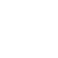
\includegraphics[width=\textwidth]{figs/book_stop.pdf}
\end{minipage}
\hspace*{0.01\textwidth}
\begin{minipage}{0.94\textwidth}
\small
{\color{\chaptercolor}\textbf{\theconcept}}
\label{#1}
}{%
\end{minipage}
\nopagebreak
\end{mdframed}
\end{center}
\vspace*{-5mm}
\noindent%
}


%
% Vastaukset STOP-kysymyksiin.
%
\newenvironment{answers}{%
\vspace*{-2mm}
\begin{mdframed}[backgroundcolor=\chapterlightcolor]
\vspace*{-2mm}
\subsection*{Vastaukset STOP-kysymyksiin}
}{
\end{mdframed}
}

% Aloita vastaus.
\newcommand{\stopA}[2]{%
\hspace*{-4mm}
\begin{minipage}{\textwidth}
\vspace*{1mm}
\noindent
\textbf{\ref{#1}} #2
\end{minipage}
}






% old - remove these
\newcommand{\stopper}[1]{%
\vspace*{-2.mm}
\begin{center}
\noindent
\refstepcounter{concept}{
\colorbox{\chapterlightcolor}{
\begin{minipage}{0.05\textwidth}
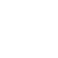
\includegraphics[width=\textwidth]{figs/book_stop.pdf}
\end{minipage}
\hspace*{0.01\textwidth}
\begin{minipage}{0.9\textwidth}
\small
{\color{\chaptercolor}\textbf{\theconcept}} #1
\end{minipage}
}
}
\end{center}
\vspace*{-2mm}
\noindent%
}

\newcommand{\narrowstopper}[2]{%
\vspace*{-2.mm}
\begin{center}
\noindent
\refstepcounter{concept}{
\colorbox{\chapterlightcolor}{
\begin{minipage}{0.05\textwidth}
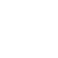
\includegraphics[width=\textwidth]{figs/book_stop.pdf}
\end{minipage}
\hspace*{0.01\textwidth}
\begin{minipage}{#1\textwidth}
\small
{\color{\chaptercolor}\textbf{\theconcept}} #2
\end{minipage}
}
}
\end{center}
\vspace*{-2mm}
\noindent%
}
% end old stuff %


%
%
% Paljon käytettyjä matemaattisia symboleja.
%
%
\newcommand{\dd}{\mathrm{d}}
\newcommand{\bs}[1]{\boldsymbol{\bar{#1}}}
\newcommand{\uv}[1]{\boldsymbol{\hat{#1}}}
\newcommand{\un}[1]{\ \text{#1}}
\newcommand{\avr}[1]{\left\langle #1 \right\rangle}
\newcommand{\ket}[1]{| #1 \rangle}
\newcommand{\ii}{\mathrm{i}}
\newcommand{\kx}{k}



%
% Kuvien ja kuvatekstien käsittelyyn.
% 
\usepackage{subcaption}
\usepackage{cleveref}
\captionsetup[subfigure]{subrefformat=simple,labelformat=simple,position=top}
\renewcommand\thesubfigure{(\alph{subfigure})}
\usepackage{pgffor}
\usepackage{listofitems}
\setsepchar{;}
\usepackage[nomessages]{fp}
\usepackage{caption}


%
% Yksittäinen kuva (float).
% 
% Käyttö: \onepicture{placement}{caption}{label}{width}{file}
%
% Esim.: \picture{tb!}{A fig.}{fig1}{0.8}{a.pdf}
%
\newcommand{\onepicture}[5]{
%
\begin{figure}[#1]
\begin{mdframed}[backgroundcolor=white,linecolor=white,% white backgrounds for dark mode
innerleftmargin=0pt,innerrightmargin=0pt,innertopmargin=0pt,innerbottommargin=0pt]

{\raggedright
\caption{#2}
\label{#3}}

\centering
\includegraphics[width=#4\textwidth]{figs/#5}

\end{mdframed}
\end{figure}
}

%
% Kuva, jossa alikuvia.
% 
% Käyttö: \pictures{placement}{captions}{labels}{widths}{image widths}{files}
%
% Anna tiedot listoina, joissa erottimena ";". Ensin koko kuvalle, jos tarvitaan, sitten alikuvat.
%
% Esim.: \pictures{tb!}{A fig.;Subfig 1;Subfig 2}{fig1;fig1a;fig1b}{0.4;0.4}{0.35;0.35}{a.pdf;b.pdf}
%
\newcommand{\pictures}[6]{
%
\readlist\cap{#2}
\readlist\lab{#3}
\readlist\wid{#4}
\readlist\fwi{#5}
\readlist\fig{#6}
\FPeval{\len}{round(\figlen{},0)}
%

\begin{figure}[#1]
\begin{mdframed}[backgroundcolor=white,linecolor=white,%
innerleftmargin=0pt,innerrightmargin=0pt,innertopmargin=0pt,innerbottommargin=0pt]

\centering
{\raggedright
\caption{\cap[1]}
\label{\lab[1]}}

\foreach \n in {1,...,\len}{
		\FPeval{\next}{round(1+\n,0)}
		\FPeval{\subwidth}{\wid[\n]}
		\FPeval{\figwidth}{\fwi[\n]}
		\subcaptionbox{\raggedright\cap[\next]\label{\lab[\next]}}[\subwidth\textwidth]{%
		\includegraphics[width=\figwidth\textwidth]{figs/\fig[\n]}}
}

\end{mdframed}
\end{figure}
}



%
% Erityisen leveä kuva.
% 
% Käyttö: \onepicture{placement}{caption}{label}{width}{file}
%
% Leveys annetaan osana maksimileveydestä. Esim. 1.0 luo koko sivun levyisen kuvan.
%
% Esim.: \picture{tb!}{A fig.}{fig1}{0.8}{a.pdf}
%
\newcommand{\onewidepicture}[5]{
%
\begin{figure}[#1]

\startwideblock

\centering

\captionsetup{margin={0cm,-4.8cm}}

{\raggedright
\caption{#2}
\label{#3}}

\begin{mdframed}[backgroundcolor=white,linecolor=white,%
innerleftmargin=0pt,innerrightmargin=0pt,innertopmargin=0pt,innerbottommargin=0pt]

\centering

\includegraphics[width=#4\textwidth]{figs/#5}

\end{mdframed}

\captionsetup{margin={0cm,0cm}}

\stopwideblock

\end{figure}
}



%
% Erityisen leveä kuva, jossa alikuvia.
% 
% Käyttö: \pictures{placement}{captions}{labels}{widths}{image widths}{files}
%
% Anna tiedot listoina, joissa erottimena ";". Ensin koko kuvalle, jos tarvitaan, sitten alikuvat.
%
% Esim.: \pictures{tb!}{A fig.;Subfig 1;Subfig 2}{fig1;fig1a;fig1b}{0.4;0.4}{0.35;0.35}{a.pdf;b.pdf}
%
\newcommand{\widepictures}[6]{
%
\readlist\cap{#2}
\readlist\lab{#3}
\readlist\wid{#4}
\readlist\fwi{#5}
\readlist\fig{#6}
\FPeval{\len}{round(\figlen{},0)}
%

\begin{figure}[#1]
%\footnotesize

\startwideblock

\centering

\captionsetup{margin={0cm,-4.8cm}}

{\raggedright
\caption{\cap[1]}
\label{\lab[1]}}

\begin{mdframed}[backgroundcolor=white,linecolor=white,%
innerleftmargin=0pt,innerrightmargin=0pt,innertopmargin=0pt,innerbottommargin=0pt]

\centering

\foreach \n in {1,...,\len}{
		\FPeval{\next}{round(1+\n,0)}
		\FPeval{\subwidth}{\wid[\n]}
		\FPeval{\figwidth}{\fwi[\n]}
		\subcaptionbox{\raggedright\cap[\next]\label{\lab[\next]}}[\subwidth\textwidth]{%
		\includegraphics[width=\figwidth\textwidth]{figs/\fig[\n]}}
}

\end{mdframed}

\captionsetup{margin={0cm,0cm}}

\stopwideblock

\end{figure}


}


%
% Kuva marginaalissa.
%
% Käyttö: \marginpicture{vspace}{caption}{label}{width}{file}
%
\usepackage{marginnote}
\newcommand{\marginpicture}[5]{
\marginnote{
\vspace*{#1 mm}
\begin{minipage}{\linewidth}
    \centering

    \captionof{figure}{\raggedright#2}
    \label{#3}
    
	\begin{mdframed}[backgroundcolor=white,linecolor=white,%
	innerleftmargin=0pt,innerrightmargin=0pt,innertopmargin=0pt,innerbottommargin=0pt]
    
	\centering    
	\vspace*{-5mm}
    
    \includegraphics[width=#4\linewidth]{figs/#5}

	\end{mdframed}

\end{minipage}
}
}




%
% Useita kuvia marginaalissa. Alikuviin EI voi viitata suoraan.
% 
% Käyttö: \marginpictures{vspace}{captions}{label}{widths}{files}
%
% Anna tiedot listoina, joissa erottimena ";". Ensin koko kuvalle, jos tarvitaan, sitten alikuvat.
%
% Esim.: \marginpictures{20}{A fig.;Subfig 1;Subfig 2}{fig1}{0.4;0.4}{0.35;0.35}{a.pdf;b.pdf}
%
\newcommand*\makealph[1]{\symbol{\numexpr96+#1}} % 1 -> a, 2 -> b, etc.
\newcommand{\marginpictures}[5]{
%
\readlist\cap{#2}
%\readlist\lab{#3}
\readlist\wid{#4}
\readlist\fig{#5}
\FPeval{\len}{round(\figlen{},0)}
%

\marginnote{
\vspace*{#1 mm}
\begin{minipage}{\linewidth}
    \centering

    \captionof{figure}{\raggedright\cap[1]}
    \label{#3}
    
	\begin{mdframed}[backgroundcolor=white,linecolor=white,%
	innerleftmargin=0pt,innerrightmargin=0pt,innertopmargin=0pt,innerbottommargin=0pt]
    
\centering
\vspace*{-5mm}

\foreach \n in {1,...,\len}{
		\FPeval{\next}{round(1+\n,0)}
		\FPeval{\subwidth}{\wid[\n]}
		%\subcaptionbox{\raggedright\cap[\next]\label{\lab[\next]}}[\textwidth]
}

\end{mdframed}

\end{minipage}
}
}












\begin{document}

\switchfont{iwona}



\startwidepage

{
\thispagestyle{empty}
\vspace*{5cm}
\begin{center}
\LARGE
\textbf{\usefont{OT1}{pag}{m}{n}\selectfont
Fysiikan perusteet
%Maailman käsikirja
}\\
\vspace*{20mm}
\large
Teemu Hynninen\\
\vspace*{2mm}
Turun yliopisto\\ 
\end{center}
}

\begin{center}
%\includegraphics[keepaspectratio,width=0.6\textwidth]{fig/cover.png}
\end{center}



\newpage

\vspace*{15cm}

\begin{center}

Tämä teos on lisensoitu Creative Commons Nimeä-JaaSamoin 4.0 Kansainvälinen -lisenssillä.
(https:\slash \slash creativecommons.org\slash licenses\slash by-sa\slash 4.0\slash legalcode.fi).

\end{center}

\newpage


\tableofcontents
\thispagestyle{fancy}

\chapter*{Johdanto}
\markboth{Johdanto}{}
\label{luku:johdanto}
\addcontentsline{toc}{chapter}{Johdanto}
\thispagestyle{empty}
\vfill
\begin{center}
\begin{minipage}{0.8\textwidth}
\begin{mdframed}[backgroundcolor=\chapterlightcolor]

Tervetuloa opiskelemaan fysiikkaa! Ennen kuin käydään varsinaiseen asiaan, on syytä pohtia hiukan fysiikkaan ja fysiikan opiskeluun liittyviä yleisiä piirteitä sekä fysiikassa tarvittavia työskentelytapoja. Fysiikan opintojen tavoite ei nimittäin ole opettaa vain faktoja vaan luonnontieteellistä ajattelutapaa. Niinpä tämä johdantoluku ei ole vain johdanto tähän materiaaliin vaan myös fysiikan esittely tieteenä sekä johdanto fysiikan opintoihin. Johdannossa annetaan vinkkejä opintojen alkuun ja selitetään yleisiä tekniikoita, joita tarvitaan kaikilla fysiikan alueilla.

Tämän luvun opiskeltuasi sinun tulee osata:

\begin{itemize}
\item kuvailla tieteellinen metodi

\item määritellä käsitteet suure ja dimensio

\item määrittää laskun lopputuloksen järkevä tarkkuus

\item tehdä yksinkertaisia suuruusluokka-arvioita

\item kuvailla fysikaalisten ongelmien ratkaisussa käytettäviä menetelmiä

\end{itemize}


\end{mdframed}
\end{minipage}
\end{center}

\stopwidepage

%\vfill
\newpage

\section*{Fysiikka tieteen\"a ja oppiaineena} 
\addcontentsline{toc}{section}{Fysiikka tieteen\"a ja oppiaineena} 

\textbf{Fysiikka} on luonnontiede, joka pyrkii selittämään luonnonilmiöitä kaikilla tasoilla alkeishiukkasten käyttäytymisestä koko maailmankaikkeuden toimintaan. Fysiikka tukee kaikkia muita luonnontieteitä ja fysikaalisten ilmiöiden kuvaamiseen luotuja ideoita sovelletaan nykyään myös selittämään ilmiöitä, jotka eivät ennen ole kuuluneet fysiikan alaan. Fysiikassa ajattelu on usein minimalistista ja analyyttistä --- monimutkaisista ilmiöistä rakennetaan mahdollisimman yksinkertaisia malleja, jotta ilmiöiden keskeiset piirteet ja selittävät tekijät voitaisiin selittää. Fysiikassa haluamme ymmärtää, miten luonto käyttäytyy ja mitkä periaatteet luonnonilmiöitä ohjaavat.

Fysiikan opiskelussa tarkoitus ei ole omaksua suurta määrää tietoa lyhyessä ajassa. Fysiikassa on loppujen lopuksi varsin vähän keskeisiä periaatteita, jotka selittävät mitä moninaisimpia ilmiöitä. Siksi laatu korvaa määrän. Opinnoissa tavoitteena on huomata, mitkä lait ja periaatteet ovat yleispäteviä sekä oppia soveltamaan näitä periaatteita. Fysiikka on eksaktia, ja lait sekä määritelmät on hallittava täsmällisesti, jotta niitä pystyisi soveltamaan. Uusia asioita opiskeltaessa väärinkäsityksiä syntyy väistämättä. Virheistä ei pidä kuitenkaan lannistua vaan ottaa opiksi. Siksi fysiikan opinnoissa onkin ensisijaisen tärkeää testata omaa osaamistaan ja harjoitella, jotta mahdolliset virheet omassa ymmärryksessä paljastuisivat. Tämä vaatii opiskelijan aktiivista toimintaa, jota opettaja ei voi mitenkään korvata.

Tämä oppimateriaali on tarkoitettu opiskelijoiden ensisijaiseksi uuden informaation lähteeksi, ja siinä yritetään selittää asioita tasolla, jonka myös asiaan ensimmäistä kertaa tutustuva lukija voisi ymmärtää. Ajoittain teksti on kuvailevaa, jolloin tarkoitus on selittää keskeiset ideat yleisellä tasolla. Yleensä näitä osioita seuraa saman asian täsmällinen matemaattinen käsittely. Tällä tavalla pyritään antamaan ensin asioista yleiskuva ja antamaan esimerkkejä aiheeseen liittyvistä fysikaalisista ilmiöistä. Matematiikkaa puolestaan käytetään suureiden ja lakien täsmällisessä määrittelyssä ja määrällisten päättelyiden ilmaisemisessa. Yleensä molempia tarvitaan, ja tavallisesti on hyödyllistä tarkastella ilmiöitä ensin puhtaasti fysikaalisesti, ilman matematiikan painolastia.

Koska fysiikka on eksakti tiede, fysiikan opinnoissa ei riitä se, että osaa nimetä suureita ja ilmiöitä. Tällainen tieto ei vielä ole ymmärrystä eikä sillä voi tehdä mitään hyödyllistä. Älä siis koskaan lukiessasi yritä opetella asioita ulkoa vaan pohdi, mitä lukemasi tarkoittaa. Toisaalta fysiikkaa ei myöskään opi pelkästään lukemalla vaan luetun ymmärtämistä pitää jatkuvasti testata väärinkäsitysten kitkemiseksi. Siksi opiskelu vaatii myös jatkuvaa harjoitteua. Opiskelkaa siis ahkerasti, kysykää, keskustelkaa ja ihmetelkää, kuinka maailma toimii!

\subsection{Tieteellinen metodi}
\label{tieteellinenmetodi}

\textbf{Tiede} on selkeästi tehokkain ihmisen kehittämistä tavoista kerätä tietoa. Tiede ei tarkoita tunnettuja tosiasioita tai viimeisintä tekniikkaa, vaan tiede on \emph{menetelmä}, jonka keskeiset ominaisuudet ovat \emph{kriittisyys} ja \emph{korjautuvuus}. Tiede ei ole erehtymätöntä, eikä tieteeltä myöskään vaadita varmuutta. Usein täyttä varmuutta asioista ei voida koskaan saavuttaakaan, ja ajatukset, jotka ovat uskottavia mutteivat aukottomasti todistettuja, voivat olla hyödyllisiä. Tieteellisen tiedon pitää kuitenkin olla \emph{perusteltua} ja \emph{testattavaa}, ja jos tieteen väitteet osoittautuvat ristiriitaisiksi, väitteitä pitää joko korjata tai niistä pitää luopua.

Tieteellinen \textbf{teoria} ei tarkoita arvausta kuten puhekielessä termiä käytetään vaan ristiriidatonta tietorakennetta, joka kykenee selittämään ilmiöitä. Esimerkiksi fysiikassa puhutaan painovoimateoriasta, mikä siis tarkoittaa painovoiman toimintaa kuvaavaa selitysmallia --- ei spekulaatiota siitä, onko painovoima olemassa. Tieteellinen arvaus on \textbf{hypoteesi}. Jotta uusi väite voisi saavuttaa fysikaalisen teorian tason, sen pitää olla sekä sisäisesti ristiriidaton että kyetä kuvailemaan asioita, joita aiemmat teoriat eivät selitä. Tämä on mahdollista, jos väite käsittelee uusia ilmiöitä, joita ei ole aiemmin tutkittu, tai jos sen ennusteet jo tunnetuista ilmiöistä ovat erilaiset kuin vanhojen teorioiden. Jos väite johtaa täsmälleen samoihin päätelmiin kuin aikaisemmat teoriat, se ei ole varsinaisesti uusi teoria vaan vain uusi tapa ilmaista vanha teoria. Tällainenkin tieteen kehitys on toki tärkeää, sillä usein monimutkaisia ilmiöitä voidaan hahmottaa useilla tavoilla.

Fysiikka on kokeellinen tiede, ja luonto on fysiikan teorioiden viimeinen tuomari. Fysiikan teorian pitää siis kyetä ennustamaan jotakin, jota voidaan verrata kokeellisiin tuloksiin, ja teoreettisen sekä kokeellisen tiedon vertaaminen onkin fysiikassa keskeistä: Tarkastelemalla asioita vain teoreettisesti ei voida saada selville, kuvaileeko teoria todella luontoa. Toisaalta tekemällä kokeita saamme tietää miten luonto käyttäytyy, mutta emme ymmärrä miksi niin tapahtuu. Luonnollisesti fysiikan teorian tarkoitus ei ole selittää vain koetuloksia vaan kokeet ovat teorian toimivuuden testi, ja teorian on ideaalisesti tarkoitus selittää luonnon toiminta \emph{kaikissa mahdollisissa tilanteissa}.

Oppiminen muistuttaa paljon tieteellistä prosessia. Teillä opiskelijoilla on omat käsityksenne siitä, kuinka maailma toimii ja kuinka fysiikan lait sitä ohjaavat. Nämä käsitykset ovat teidän oma ``fysiikan teorianne'', joka perustuu osittain aikaisempaan kouluopetukseen ja osittain omiin kokemuksiinne.
Fysiikan perusperiaatteet ovat loppujen lopuksi yksinkertaisia mutta usein abstrakteja ja niiden löytäminen pelkästään arkikokemuksen perusteella on lähes mahdotonta. Esimerkiksi ensimmäiset nykyfysiikan mukaan oikeat käsitykset esineiden liikettä ohjaavista mekaniikan laeista keksittiin vasta 1600-luvulla, vaikka ihmiset ovat aina pohtineet maailman toimintaa.
Koska teidänkin tapanne ajatella maailmasta perustuu pitkälti kokemuksiin, todennäköisesti monet nykyisistä käsityksistänne fysiikasta ovat \emph{vääriä}. Lisäksi fysiikka ulottuu alueille, joita ei normaalisti havaita, joten käsityksenne fysiikasta ovat myös \emph{puutteellisia}. Fysiikan ymmärtäminen vaatiikin siis sekä puutteellisten ajattelumallienne täydentämistä että väärien ajatusten löytämistä ja korjaamista.

Fysiikka muodostaa kumuloituvan tietorakenteen, jossa uudet teoriat ja mallit pohjautuvat aikaisempaan tietoon. Siksi onkin aivan välttämätöntä aina pyrkiä ymmärtämään yksi aihe mahdollisimman hyvin ennen seuraavaan siirtymistä. Vaikka esimerkiksi lämpöilmiöitä kuvaava termodynamiikka käsittelee näennäisesti eri ilmiöitä kuin liikettä kuvaava mekaniikka, moderni termodynamiikka kuvaa lämpöilmiöitä suurten hiukkasjoukkojen mekaniikan kautta. Niinpä termodynamiikan ymmärtäminen vaatii myös mekaniikan hallintaa. Fysiikan opinnoissa on siis syytä edetä järjestelmällisesti ja pyrkiä ennen kaikkea ymmärtämään kukin aihe mahdollisimman hyvin ennen seuraavaan siirtymistä, sillä puutteellisesti omaksutut tai väärin ymmärretyt ajattelumallit estävät oppimisen myös jatkossa.

Onkin välttämätöntä, että jatkuvasti testaatte omia käsityksiänne ja pohditte, onko oma ajattelutapanne ristiriidassa kohtaamanne oppikirjatiedon kanssa. Perinteisesti opetus on perustunut siihen, että opettaja kertoo opiskelijoille mikä on vallitseva tieteellinen käsitys. Tämä on nopeaa, ja näin voidaan käydä läpi hyvin suuri määrä informaatiota hyvin lyhyessä ajassa. Ongelmana tässä opetustavassa on kuitenkin se, ettei pelkkä asioiden kuuleminen riitä muuttamaan tapaanne ajatella, vaan se korkeintaan opettaa ratkaisemaan oppikirjatehtäviä. Oppimisen tavoite ei kuitenkaan ole tehtävien ratkaiseminen vaan oikeiden ajattelumallien omaksuminen. Tämä puolestaan vaatii teiltä opiskelijoilta työtä. Ei riitä tutustua vain vallitsevaan fysiikan teoriaan, vaan on välttämätöntä tarkastella myös sitä tukevaa todistusaineistoa --- koetuloksia ja teoreettista päättelyä --- jotta voitte ymmärtää mihin väitteet perustuvat ja löytää ne itse. Niinpä tämäkään materiaali ei anna valmiita vastauksia kaikkeen vaan pyrkii ensisijaisesti esittelemään sitä fysikaalista ajattelua, jolla vastaukset voidaan löytää.

Tehtävien tarkoitus puolestaan on antaa teille mahdollisuus testata omassa mielessänne olevaa käsitystä fysiikan laeista. Tätä varten tekstiin on sijoitettu aika-ajoin pohdintakysymyksiä, jotka liittyvät välittömästi niitä edeltäneeseen asiaan. Kysymysten tarkoitus on herättää pohtimaan luetun merkitystä, sillä pelkkä lukeminen ei vielä johda oppimiseen. Älä koskaan ohita pohdintakysymystä ennen kuin osaat mielestäsi vastata siihen! Jos huomaat, ettet osaa vastata kysymykseen, lue edellinen kappale tai luku uudestaan ja etene vasta kun osaat vastata kaikkiin kysymyksiin. Väliin jätetty kysymys tarkoittaa mitä todennäköisimmin sitä, että jotakin tärkeää on jäänyt ymmärtämättä eikä sinulla ole vielä valmiuksia oppia seuraaviakaan aiheita.

\begin{stopQ}{q:ajankaytto}Taitava opiskelija varaa aina kaikkiin tehtäviin riittävästi aikaa. Jos kuitenkin huomaat ettei sinulla olekaan tarpeeksi aikaa esimerkiksi tehdä moniosaista tehtävää kunnolla, onko parempi vilkaista nopeasti kaikkia asioita vai opiskella yksi asia kunnolla ja palata myöhemmin muihin aiheisiin?
\end{stopQ}

Myöskään virheitä ei pidä pelätä. Ette olisi opiskelemassa, jos jo tietäisitte kaiken. Väärinkäsitykset ovat tavallisia ja niiden korjaaminen voi olla hidasta, joten epäonnistumisia tapahtuu välttämättä. Tieteessä epäonnistumiset ovat jokapäiväisiä, eikä tiedettä edes tarvittaisi jos vastaukset olisivat selviä jo etukäteen. Monet suuret tieteelliset harppaukset ovatkin tapahtuneet juuri löydettäessä vallitsevan tieteellisen käsityksen kanssa ristiriitaisia ilmiöitä, sillä tällaiset ilmiöt ovat merkki vallitsevan tiedon puutteellisuudesta.
Samoin kaikkein paras mahdollisuus oppia onkin huomata, että jokin ongelma ratkeaakin eri tavalla kuin mitä itse ajattelitte, koska silloin voitte pohtia, miten oma käsityksenne vaatii korjaamista tai täydentämistä. Epäonnistuminen on merkki siitä, että ette tiedä ja osaa vielä kaikkea. Epäonnistumisen syiden pohtiminen on tie uusien asioiden oppimiseen.

\subsection{Suureet}
\label{suureet}

\index{suure}
\index{SI-järjestelmä}

Fysiikka pyrkii selittämään millainen maailmankaikkeuden rakenne on ja miten sen osat käyttäytyvät. Tutkimuksen kohteet ulottuvat hyvin konkreettisista kuten esineiden liikkeestä hyvin abstrakteihin kuten informaatioon. Erityisesti fysiikassa maailmaa pyritään kuvaamaan mitattavissa olevien ominaisuuksien eli \textbf{suureiden} avulla, ja fysiikan teorioiden eräs tavoite on kuvata, kuinka suureet riippuvat toisistaan. Luonnontieteissä on käytössä suureiden \textbf{SI-järjestelmä} (ranskaa, `Syst\`eme International d'Unit\'es'), joka määrittelee seitsemän perussuuretta ja näiden yksiköt --- metrin, kilogramman, sekunnin, ampeerin, moolin, kelvinin sekä kandelan --- ja muut suureet on ilmaistavissa näiden avulla. Järjestelmän tarkoitus on määritellä kaikki mitattavat suureet absoluuttisten luonnonvakioiden kautta, mikä onnistuikin lopulta riittävällä tarkkuudella vuoden 2019 SI-järjestelmän uudistuksessa.

Fysiikassa suureille käytetään tavallisesti lyhennysmerkintänä yhden kirjaimen \emph{symboleja}. Jotkin ovat vakiintuneet, ja esimerkiksi massan symboli on lähes aina \(m\), kun taas toisille suureille käytetään eri lähteissä eri symboleita. Jos sama symboli esiintyy useassa merkityksessä, symbolit erotellaan tavallisesti ala- tai yläindeksein tai muilla lisämerkinnöillä. Esimerkiksi eri esineiden massoja voidaan merkitä \(m_1, m_2, m_3, \ldots\) tai vaikkapa \(m, m', m''\). Joillakin symboleilla on puolestaan on useita merkityksiä, joten pelkän symbolin perusteella ei voi koskaan päätellä matemaattisten lausekkeiden merkitystä. Suureita kuvaavat symbolit kirjoitetaan tavallisesti kursiivilla erotuksena muista lyhenteistä.

\index{yksikkö}
\index{dimensio}

Fysikaalisilla suureilla on \emph{laatu} eli \textbf{dimensio}, joka kertoo, millaista fysikaalista ominaisuutta suure kuvaa. Esimerkiksi pituus, aika, lämpötila ja massa ovat erilaisia suureiden laatuja eli dimensioita. Laatuun liittyy myös aina \textbf{yksikkö}, ja suureilla laskettaessa kuhunkin suureeseen liittyvään symboliin ajatellaan sisältyvän sekä suureen suuruus että sen yksikkö. Esimerkiksi massan yksikkö on kilogramma, ja voidaan kirjoittaa \(m = 1.0 \un{kg}\) eli symboliin \(m\) sisältyy sekä suureen suuruus \(1.0\) että sen yksikkö, \(\un{kg}\). Suureen yksikköä merkitään hakasuluin, esimerkiksi \([m] = \un{kg}\).
Dimensiollisten suureiden laskutoimituksissa on seuraavat perussäännöt:

\begin{itemize}
\item Yhteen- ja vähennyslasku on mahdollinen vain samaa dimensiota olevien suureiden välillä, jolloin lopputuloksella on edelleen sama dimensio: \(a + b\) on määritelty jos ja vain jos \([a] = [b]\) ja tällöin \([a + b] = [a] = [b]\). On siis järkevää laskea \(2 \un{kg} + 1 \un{kg}\), mutta ei ole mielekästä laskea \(2 \un{kg} + 1 \un{m}\) (kilogramma + metri). Huomaa myös, että vaikka suureen arvo olisi nolla, sillä voi edelleen olla yksikkö. Esimerkiksi \(1 \un{kg} - 1 \un{kg} = 0 \un{kg}\), eikä lopputulos ole pelkkä nolla ilman yksikköä.

\item Kerto- ja jakolasku on mahdollinen eri dimensiota olevien suureiden välillä, jolloin lopputuloksena saadaan jotakin uutta dimensiota oleva suure. Esimerkiksi jos pituus (yksikkö metri, m) jaetaan ajalla (yksikkö sekunti, s), lopputuloksena saadaan suure, jonka dimensio on pituus jaettuna ajalla ja yksikkö metri\slash sekunti (m\slash s).

\item Jos suure on jonkin muun alkeisfunktion kuin polynomin tai juurifunktion argumentti, sen on oltava paljas luku (siis yksikötön suure): esim. eksponenttifunktio \(e^a\) on määritelty vain jos \([a] = 1\). Toisin sanoen jos lasketaan esimerkiksi \( y = Ae^{kx} \), missä suureen \(x\) yksikkö on m, on suureen \(k\) yksikön välttämättä oltava 1\slash m, koska eksponenttifunktion sisällä olevan lausekkeen \(kx\) on oltava yksikötön. On silti sallittua laskea esim. \(\sqrt{x} = x^{1/2}\). Jos \([x] = \un{m}\), tällöin \([x^{1/2}] = \un{m}^{1/2}\).

\item Yhtälöt pätevät vain jos niiden molemmilla puolella olevien lausekkeiden dimensio on sama: \(a = b\) on tosi vain jos \([a] = [b]\). Jotta yhtälö olisi tosi, tietenkin myös suureiden lukuarvon on oltava sama.

\end{itemize}

\index{yksikkötarkastelu}

Koska yksiköiden yhdistelyssä on näinkin vahvat rajoitukset, \textbf{yksikkötarkastelu} on hyvä ja helppo apukeino fysikaalisessa päättelyssä. Jos laskussa rikotaan jotakin yllä mainituista ehdoista tai jos laskun lopputuloksen dimensio ei vastaa suuretta, jota sen tulisi esittää, jossakin on pakko olla karkea virhe.

\begin{exam}{Yksikk\"otarkastelu}{ex:yksikot}\noindent

\problem{Opiskelijat A, B ja C ovat laskeneet erään esineen nopeuden ja saaneet tulokset
\( v_A = a x - x/t\), \(v_B = b e^{a t}\) ja \(v_C = b e^{a x}\), missä symbolien yksiköt ovat \([x] = \un{m}, [t] = \un{s}, [a] = 1/\un{s}, [b] = \un{m/s}\). Mitkä tuloksista voivat olla oikein?
}

Tarkistetaan onko tulosten yksikkö oikea nopeuden yksikkö m\slash s. Opiskelijan A vastauksen yksikkö on
\begin{equation} [v_A] = [a][x] - [x]/[t] = 1/\text{s} \cdot \text{m} - \text{m/s} = \text{m/s} - \text{m/s} = \text{m/s} \end{equation}
eli yksikkötarkastelun puolesta tulos voisi olla oikein. Opiskelijan B tulos on
\begin{equation} [v_B] = [b] [e^{a t}] = \text{m/s} \cdot [e^{1/\text{s} \cdot \text{s}}] = \text{m/s} \cdot [e^1] = \text{m/s} \cdot 1 = \text{m/s}, \end{equation}
eli tämäkin tulos voisi olla oikein.
Opiskelijan C vastauksen yksikkö puolestaan on
\begin{equation} [v_C] = [b] [e^{a x}] = \text{m/s} \cdot [e^{1/\text{s} \cdot \text{m}}] = \text{m/s} \cdot [e^{\text{m/s}}] = \text{m\"a\"arittelem\"at\"on}. \end{equation}
Lauseke on mieletön, koska vastauksessa esiintyvan eksponenttifunktion argumentin yksikkö on m\slash s eikä tätä funktiota ole määritelty dimensiolliselle suureelle. Opiskelijan B vastauksessa esiintyi myös eksponenttifunktio, mutta silloin funktion argumentti oli paljas luku, kuten pitääkin.

Siispä opiskelija A tai B voi olla oikeassa, mutta C on varmasti tehnyt virheen. Yksikkötarkastelu ei riitä kertomaan onko A tai B oikeassa, mutta sen avulla voi huomata selkeitä virheitä.
\end{exam}

\begin{stopQ}{q:yksikot}Jos suureen \(a\) yksikkö on \(\text{A}^2\) ja suureen \(b\) yksikkö on \(1/\text{A}\), onko lauseke \(a-\frac{1}{b^2} \sin(ab^2\)) järkevä? Mikä on sen yksikkö?
\end{stopQ}

\subsection{Mallit}
\label{mallit}

Maailma on monimutkainen. Tavallisetkin fysikaaliset ilmiöt syntyvät monien tekijöiden yhteisvaikutuksesta, ja fysiikan peruslakeja on vaikea ymmärtää vain tarkastelemalla luonnon toimintaa sellaisenaan. Usein fysiikan lakien ymmärtäminen onkin vaatinut tarkoin valmisteltujen kokeiden toteuttamista, jotta muiden tekijöiden vaikutus on saatu rajattua pois. Sama pätee myös fysiikan opinnoissa --- tarkastelemme usein hyvin yksinkertaisia tilanteita, jotka eivät välttämättä ole todellisuuden kannalta kovin mielenkiintoisia, jotta tilanteen ymmärtäminen ei vaatisi liian monen tekijän huomioimista.

\pictures{b}%
{Erilaisia malleja kissalle.;Yksityiskohtainen kuvaus.;Koon ja muodon kuvaus.;Koon ja sijainnin kuvaus.;Pelkän sijainnin kuvaus.}%
{fig:johdantomalli;fig:johdantomalli:tarkka;fig:johdantomalli:muoto;fig:johdantomalli:koko;fig:johdantomalli:sijainti}%
{0.22;0.22;0.22;0.22}%
{0.22;0.22;0.22;0.22}%
{johdanto_malli_1.pdf;johdanto_malli_2.pdf;johdanto_malli_3.pdf;johdanto_malli_4.pdf}

Toisaalta koska maailma on monimutkainen, todellisten fysikaalisten ilmiöiden ymmärtäminen vaatii lähes poikkeuksetta kykyä hahmottaa tilanteita, yhdistellä, tulkita ja soveltaa tietoa sekä löytää ilmiöitä ja tapahtumia ohjaavista tekijöistä tärkeimmät. Tämä ei ole helppoa ja vaatii harjoitusta, minkä vuoksi myös monimutkaisten ongelmien ratkomisen harjoittelu on oleellinen osa fysiikan opiskelua. Ongelmanratkaisutaito on luonnollisesti hyödyllinen kaikilla elämän alueilla. Itse asiassa todelliset ongelmat ovat yleensä avoimia ja epämääräisiä, ja niihin voi olla monia erilaisia ratkaisuja. Siksi ei riitä harjoitella vain hyvin määriteltyjen tehtävien selvittämistä vaan myös avointen kysymysten pohdintaa.

\index{malli}

Fysikaassa ongelmien ratkaiseminen tapahtuu \textbf{mallien} avulla. Malli on monimutkaisen tilanteen yksinkertaistus, johon otetaan mukaan vain välttämätön määrä informaatiota ja yksityiskohtia. Esimerkiksi esineitä voidaan kuvata hyvinkin monimutkaisina osien yhdistelminä tai vain pisteinä, palloina tai kuutioina, jos oleellista on vain esineiden sijainti eikä niiden muoto (kuva \autoref{fig:johdantomalli}). Yleensä kannattaa ensin muodostaa mahdollisimman yksinkertainen malli, johon tarpeen vaatiessa lisätään yksityiskohtia, kunnes malli kykenee selittämään tarkasteltavan ilmiön.

\index{approksimaatio}

Koska mallit ovat epätäydellisiä, myös niiden ennusteet ovat epätarkkoja. Lisäksi hyvin usein yksinkertaistenkin mallien käyttäytyminen on mahdotonta ratkaista täydellisesti, jolloin turvaudutaan matemaattisiin likiarvoihin eli \textbf{approksimaatioihin}. Tällöin on syytä pitää kirjaa kaikista oletuksista, joita mallin muodostamisessa ja sen matemaattisessa käsittelyssä on tehty. Kun lopputulokseen lopulta päästään, tulee tarkistaa, pätevätkö tehdyt oletukset.

\begin{stopQ}{q:mallit}Haluat tutkia ihmisen ajattelua ja aivotoimintaa. Millaista tietoa voitaisiin saada muodostamalla malli, jonka pienin yksikkö on (a) molekyyli, (b) hermosolu, (c) aivoalue, (d) ihminen, (e) ihmisjoukko (esim. yritys tai valtio)?
\end{stopQ}

 \section*{Kuvat ja geometria} \addcontentsline{toc}{section}{Kuvat ja geometria} 

Kuvat ovat tieteellisessä kommunikoinnissa ensisijaisen tärkeitä. Monimutkaisia ajattelumalleja ja suurta määrää informaatiota on usein mahdotonta välittää ilman visualisointia, sillä useimmat ihmiset käsittelevät kuvallista tietoa paljon tehokkaammin kuin sanallista. Usein on suorastaan mahdotonta ymmärtää määrällistä informaatiota ennen kuin informaatiolle löytyy sopiva kuvallinen esitys. Opiskelussakin omien ajatusten kuvallinen ilmaisu voi olla tehokas oppimistapa. Kuvien muodostaminen vaatii nimittäin informaation käsittelyä, ja kun tieto on puettu kuvan muotoon, oleellisten piirteiden huomaaminen ja muistaminen on yleensä paljon helpompaa kuin tekstin muodossa olevan tiedon.

\pictures{tb}%
{Erilaisia kuvaajia.;
Kahden suureen riippuvuuden esittävä kuvaaja.;
Kahden muuttujan funktion kuvaaja korkeuskäyrinä.}%
{fig:johdantokuva;fig:johdantokuva:kuvaaja;fig:johdantokuva:korkeus}%
{0.5;0.45}%
{0.5;0.4}%
{johdanto_kuvaaja_1.pdf;johdanto_kuvaaja_3.pdf}

Myös monimutkaisten ongelmien ratkaisemisessa kuvalliset esitykset ovat tärkeitä ajattelun apuvälineitä. Kun asiantuntija alkaa ratkaista ongelmaa, hän yleensä aloittaa piirtämällä tilanteesta kuvan. Näin siksi, että kuvaan on helppo kerätä kaikki tilanteessa oleelliset seikat ja tunnettu informaatio muotoon, josta kokonaisuuden hahmottaa helposti. Yksityiskohtia ja asioiden välisiä suhteita on niinikään helppo lisätä kuvaan. Fysiikassa mallien muodostaminen on yleensä helpointa juuri kuvien avulla. Monesti fysikaalisissa ongelmissa esineiden tai hiukkasten paikat ovat merkitykselliset, ja tällöin kuvan piirtäminen tilanteesta on lähes välttämätöntä.

\index{kuvaaja}

Fysiikassa ja muissakin luonnontieteissä \textbf{kuvaajien} tulkitseminen on välttämätön taito. Yksinkertaisesta kuvaajasta, jossa on piirretty jokin suure toisen suureen funktiona, voidaan usein suoraan päätellä esimerkiksi funktion ääriarvojen, raja-arvojen, derivaattojen, integraalien yms. johdannaisten käyttäytyminen, mikä voi laskemalla olla erittäin työlästä tai jopa mahdotonta. Asiantuntija tietää, miten suureet riippuvat toisistaan erilaisissa tilanteissa, jolloin hän voi hyvästä kuvaajasta heti huomata oleellisen tiedon. Siksi tieteellisessä esityksessä juuri kuvat ja kuvaajat --- ei teksti tai kaavat --- ovat avainasemassa informaation välittämisessä.

\index{akseli}

Kuvaajien tulkitseminen ja piirtäminen ei kuitenkaan ole itsestään selvää, ja sitä pitää harjoitella. Kuvaajan tulkinnassa ensimmäinen askel on aina tarkistaa, mitä kuvataan. Jos kyseessä on tyypillinen kaksiulotteinen koordinaatistokuvaaja kuten kuvassa \autoref{fig:johdantokuva} (a), tämä tarkoittaa kuvaajassa esitettyjen suureiden ja mittakaavan tarkistamista kuvaajan \textbf{akseleilta}. Tämän jälkeen voidaan alkaa tulkitsemaan varsinaista kuvaajaa. Riippuu kuitenkin aina tapauksesta, millaiset kuvaajan ominaisuudet ovat mielenkiintoiset. Ja toisaalta täysin samannäköiset kuvaajat voivat esittää aivan erilaisia ilmiöitä, jos kuvattavat suureet eivät olekaan niissä samat. Niinpä kuvaajien tulkitseminen edellyttää ilmiöiden ja niihin liittyvän fysiikan aitoa ymmärtämistä --- pelkkiin nyrkkisääntöihin nojaaminen ei aina onnistu.

Tässä materiaalissa esitetään dataa kuvaajien muodossa ja toisistaan riippuvien suureiden kuvailussa pyritään esittämään myös suureiden yhteydet graafisissa esityksissä. Lisäksi kuvaajien tulkintaan ja diagrammien piirtämiseen opastetaan. Kuvaajien käsittelylle annetaan materiaalissa siis erityishuomiota, ja sitä on syytä opiskella.

\begin{stopQ}{q:graafinen_esitys}Kuvassa \autoref{fig:johdantokuva} (a) on esitetty mittaustuloksia graafisesti. Arvioi kuvaajan perusteella, millä välillä suureen \(x\) todellinen arvo on, kun (a) \(t=3 \un{s}\), (b) \(t=6 \un{s}\).
\end{stopQ}

\subsection{Symmetria}
\label{symmetria}

\index{symmetria}

\textbf{Symmetria} tarkoittaa tilannetta, jossa jotakin erityisasemassa olevaa suuretta voidaan muuttaa niin ettei mikään muu asia muutu. Esimerkiksi geometriassa neliö on symmetrinen \(90^\circ\) kierron suhteen (kuten myös \(180^\circ\), \(270^\circ\) jne. kierron) sekä myös sen keskipisteen kautta kulkevien sivujen tai lävistäjien suuntaisten peilauksien suhteen, koska neliön kääntäminen tällaisilla tavoilla tuottaa kuvion, joka on täsmälleen samanlainen kuin alkuperäinen neliö. Neliön tapauksessa symmetriat ovat epäjatkuvia eli diskreettejä, koska vain tietyt operaatiot pitävät kuvion muuttumattomana. Sitä vastoin esimerkiksi ympyrässä on jatkuva symmetria, koska ympyrää voi kiertää keskipisteenstä ympäri minkä kulman verran tahansa ja ympyrä näyttää edelleen samalta.

Geometriset ja matemaattiset symmetriat ovat fysiikassa hyödyllisiä ongelmanratkaisun apuvälineitä. Esimerkiksi jos suure riippuu jostakin pisteestä mitatusta etäisyydestä, on suureen oltava sama kaikissa pisteissä, jotka ovat tästä pisteestä yhtä kaukana --- siis ympyrän kehällä tai pallon pinnalla. Kuvassa \autoref{fig:johdantosymmetria} (a) on tästä esimerkki. Tyhjässä tilassa oleva äänilähde, esimerkiksi kaiutin, lähettää ääntä kaikkiin suuntiin yhtä voimakkaasti. Tällöin tilanne on symmetrinen suuntien suhteen, joten äänenvoimakkuus on sama kaikissa suunnissa kunhan etäisyys äänilähteestä on yhtä suuri. Toisin sanoen ajattelemalla lähteen ympärille pallo, jonka keskipisteessä lähde on, äänen on oltava yhtä voimakas jokaisessa pisteessä tämän pallon pinnalla. Huomattaavaa tässä päättelyssä on se, että se ei vaadi tarkkaa tietoa äänen ominaisuuksista --- ainoastaan oletuksen siitä, että äänen eteneminen on samanlaista eri suunnissa. Koska tämä oletus liittyy vain tilanteen symmetriaan, vastaava päättely toimii mille tahansa vain suunnasta riippuvalle suureelle.

Tilanne voi olla myös päinvastainen: näemme, että jokin asia on symmetrinen, mutta emme tiedä miksi. Tällöin symmetria on vahva johtolanka siitä, että jossakin rakenteessa tai laissa on oltava vastaava symmetria. Muun muassa mineraalit ja kiteet voivat olla hyvinkin symmetrisen muotoisia riippuen niiden atomien muodostamasta rakenteesta. Esimerkiksi kuvassa \autoref{fig:johdantosymmetria:lumi} esitetyllä lumihiutaleilla on kuusikulmainen symmetria, ja tämä symmetria johtuu jääkiteessä olevien vesimolekyylien muodostamasta rakenteesta, jossa molekyylit asettuvat muodostamaan kuusikulmioita.

\pictures{tb}%
{Geometrisia symmetrioita. Symmetria yhtäällä johtaa usein symmetriaan toisaalla.;
Ääniaalto leviää symmetrisesti pallona.;
Lumihiutaleen kuusikulmaisuus johtuu molekyylien järjestäytymisestä kuusikulmioiksi.}%
{fig:johdantosymmetria;fig:johdantosymmetria:aani;fig:johdantosymmetria:lumi}%
{0.32;0.42}%
{0.24;0.42}%
{johdanto_symmetria_1.pdf;johdanto_symmetria_2.pdf}

Myös fysiikan \emph{laeissa} on symmetrioita, ja itse asiassa juuri tällaiset symmetriat ovatkin eräitä fysiikan voimakkaimpia periaatteita.
Esimerkiksi fysiikan peruslakien uskotaan olevan samanlaiset kaikkialla maailmankaikkeudessa: Jos rakennat koelaitteiston ja suoritat kokeen yhdessä paikassa, siirrät laitteiston toiseen täsmälleen samanlaiseen paikkaan (ts. paikkaan jossa olosuhteet ovat kaikin puolin samanlaiset), kaikkien samojen fysiikan lakien pitäisi päteä ja kokeen tuloksen pitäisi olla täsmälleen sama kuin ennenkin. Tätä kutsutaan lakien symmetriaksi paikan siirron suhteen, mikä tarkoittaa etteivät lait riipu mistään absoluuttisesta paikasta. Samoin jos koelaitteistolla tehdään sama koe tänään ja huomenna, tulosten pitäisi olla samat, koska fysiikan lait eivät riipu ajasta eli ne ovat symmetriset ajan muutoksen suhteen. Osoittautuu, että tällaiset symmetriat ovat erittäin tärkeitä, koska ne liittyvät säilymislakeihin, joista puhutaan tarkemmin luvussa \autoref{luku:sailymislait}.

\index{vuorovaikutus}

Uusia ilmiöitäkin on löydetty puhtaasti tutkimalla, millaisia symmetrioita fysiikan lait toteuttavat. Esimerkiksi 1900-luvun alussa kehitettiin valolle aalto-hiukkasmalli, fotoni. Aineelle kehitettiin tämän jälkeen vastaavanlainen aaltomekaaninen kuvaus tarkastelemalla hypoteesia, että valon ja aineen perusominaisuudet ovat samanlaiset --- eli että niitä kuvaavat lait ovat symmetriset. Kyseessä oli teoreettinen arvaus, jonka kokeet osoittivat myöhemmin oikeaksi. Pyrkimys symmetriaan on osoittautunut niin vahvaksi periaatteeksi teoreettisen fysiikan kehityksessä, että monet teoreetiset fyysikot pitävät modernin fysiikan yhtenä päätavoitteena ns. kaiken teoriaa eli kaikki fysiikan \emph{perusvuorovaikutukset} yhdistävää peruslakia. Tällainen on mahdollista vain jos eri vuorovaikutukset voidaan kuvata samanlaisessa, symmetrisessä muodossa.

\begin{stopQ}{q:symmetria}Hyvin pitkä, suora, ohut lanka värähtelee, jolloin sen jokainen piste toimii äänen lähteenä. Ääni kuuluu yhtä voimakkaana kaikissa niissä avaruuden pisteissä, joiden etäisyys langasta on sama. Minkä muotoisen alueen tai pinnan tällaiset pisteet muodostavat?
\end{stopQ}

 \section*{Matemaattinen analyysi} \addcontentsline{toc}{section}{Matemaattinen analyysi} 

Matematiikkaa sanotaan luonnon kieleksi, millä tarkoitetaan sitä, että matemaattisilla menetelmillä voidaan kuvata luonnonilmiöitä erittäin tarkasti. Matematiikka on tärkeä apuneuvo kaikissa luonnontieteissä, mutta luonnontieteistä fysiikka käyttää matematiikkaa epäilemättä monipuolisimmin. Fysiikka ei kuitenkaan ole matematiikkaa. Aloittelevilla fysiikan opiskelijoilla on usein harhakäsitys, että laskeminen ja kaavat ovat fysiikan tärkein sisältö. Matematiikka on kuitenkin vain työkalu, joka mahdollistaa sellaiset määrälliset päättelyt ja täsmälliset ilmaisut, jotka ilman matematiikkaa olisivat erittäin vaikeita. Esimerkiksi ilmaisut ``kappaleen kiihtyvyysvektorin ja massan tulo on yhtä suuri kuin kappaleeseen kohdistuva kokonaisvoimavektori'' ja ``\(\bs{F}_\text{kokonais} = m \bs{a}\)'' ovat merkitykseltään \emph{samat}. Matemaattinen yhtälö on vain lyhyempi kirjoittaa, joten se ei rasita ihmisen muistia niin paljon kuin pitkä sanallinen selitys. Matemaattisia lausekkeita voidaan myös käsitellä matematiikan sääntöjen avulla uusien fysikaalisten väitteiden johtamiseksi.

Yllä esitetyn väitteen sanallinen muotoilu on \emph{fysikaalinen} tapa ilmaista asia kun taas kaava on \emph{matemaattinen}, ja aina kun tutustut uuteen fysikaaliseen lakiin tai määritelmään, on syytä ymmärtää \emph{molemmat}.
Fysikaalisten lakien täsmällinen ilmaiseminen ja soveltaminen pelkästään sanallisesti on hankalaa, mutta toisaalta pelkät kaavat ovat vain merkityksettömiä symboleiden jonoja, jos et ymmärrä mitä fysikaalisia suureita ne käsittelevät ja etenkin millaisissa tilanteissa ne pätevät. Fysiikan opintojen ydin onkin ymmärtää millaiset periaatteet ja lait luonnon käyttäytymistä ohjaavat. Siksi laskutehtävissäkin oleellisinta on aina \emph{perustella} mitä ja miksi lasketaan eikä vain laskea --- varsinkin kun raaka laskeminen voidaan nykyään pitkälti antaa tietokoneiden tehtäväksi.

\index{kvalitatiivinen}
\index{kvantitatiivinen}

Laskemiselta ei kuitenkaan voi fysiikassa välttyä, koska fysiikka on eksakti luonnontiede, joka ei pyri kuvaamaan luontoa vain laadullisesti eli \textbf{kvalitatiivisesti} vaan myös määrällisesti eli \textbf{kvantitatiivisesti}. Aina kun fysiikassa lasketaan, on tulosten tarkkuus ja oikeellisuus vielä erikseen arvioitava, koska fysikaalisia tilanteita kuvaavat mallit ovat lähes aina puutteellisia ja laskuissa voi tapahtua virheitä. Tällainen arviointi vaatii selkeästi enemmän fysikaalista kuin matemaattista taitoa. Yksiköiden tarkastamisen lisäksi laskujen tulosten järkevyyden pohdinnassa hyviä keinoja ovat suuruusluokka-arviot, erikoistapausten tarkastelu sekä raja-arvojen analysointi.

\subsection{Merkitsevät numerot}
\label{merkitsevätnumerot}

Laskimet ja tietokoneet käsittelevät lukuja aina tietyllä kiinteällä tarkkuudella, jota rajoittaa muisti. Lisäksi laskukoneet käsittelevät numeroita binääriesityksessä eli kakkosen potenssien avulla. Siispä kun laskukoneelle antaa luvun 10.0, se voi ymmärtää tämän esimerkiksi muodossa \(1.0000000 \cdot 10^1\). Kun laskin suorittaa laskuja, se tuottaa uusia lukuja, jotka se tallentaa samalla tarkkuudella. Jos tuloksena saadaan luku, jonka desimaalit ovat pelkkiä nollia, laskin ymmärtää yleensä jättää ne näyttämättä, mutta muuten kone saattaa tulostaa desimaaleja niin paljon kuin sen muistissa on.

Fysikaalisesti tässä ei kuitenkaan ole mitään järkeä. Jos luvut kuvaavat fysikaalisten suureiden suuruuksia, niitä ei voida tuntea tarkasti kuin joissakin erikoistapauksissa. Tavallisesti fysikaaliset lukuarvot ilmoitetaankin aina sillä tarkkuudella kuin ne tunnetaan. Jos esimerkiksi pituus on noin \(1 \un{m}\) ja tämä tiedetään \(1 \un{cm}\) eli \(0.01 \un{m}\) tarkkuudella, on soveliasta ilmoittaa pituuden lukuarvoksi \(1.00 \un{m}\). Merkintä \(1 \un{m}\) ei ole yhtä hyvä, koska tämä periaatteessa tarkoittaa, että pituus tunnetaan 1 metrin tarkkuudella, ja merkintä \(1.000 \un{m}\) on suorastaan väärin, koska suureen arvoa ei tunneta näin tarkasti.

Merkinnässä \(1.00 \un{m}\) yksi on luvun kokonaislukuosa, piste on desimaalierotin, ja sitä seuraavat kaksi nollaa ovat \textbf{desimaalit}, eli luku on ilmoitettu kahden desimaalin tarkkuudella. (Tässä tekstissä käytetään erottimena pistettä, joka on kansainvälisesti tavallisimmin käytetty desimaalierotin, vaikka suomen kielessä normaalisti erotin onkin pilkku.) Kaikki kolme numeroa kuitenkin sisältävät informaatiota: 1 tarkoittaa yhtä metriä ja seuraavat kaksi nollaa nollaa desi- ja senttimetriä. Niinpä sanotaan, että luku on ilmoitettu kolmen \textbf{merkitsevän numeron} tarkkuudella. Luvussa, jossa ei ole lainkaan desimaaleja, merkitsevien numeroiden määrä voi olla epäselvä. Esimerkiksi kirjoitusasu 100 m voi sisältää yhden, kaksi tai kolme merkitsevää numeroa riippuen siitä, ovatko nollat todella tarkalleen nollia vai onko lukuarvo pyöristetty. Jos merkitsevien numeroiden määrä halutaan ilmaista täsmällisesti, voidaankin käyttää niin sanottua tieteellistä merkintätapaa eli kymmenen potensseja ja kirjoittaa \(1.00 \cdot 10^2 \un{m}\).

Kun fysikaalisilla suureilla lasketaan, lopputuloskin olisi syytä ilmoittaa sillä tarkkuudella, mikä alkuperäisten lukuarvojen tarkkuudesta voidaan päätellä. Yleisesti ottaen tulosten tarkkuuden määräävät huonoimman tarkkuuden lukuarvot.

\index{pyöristäminen}

\begin{itemize}
\item Yhteen- ja vähennyslaskuissa tarkkuuden ilmaisevat lukujen \emph{desimaalit}. Jos esimerkiksi lasketaan yhteen \(1.1 \un{m} + 2.34 \un{m}\) lopputuloksen järkevä tarkkuus on \(3.4 \un{m}\) eikä \(3.44 \un{m}\), koska lukuarvosta \(1.1\) ei tunneta toista desimaalia.

\item Kerto- ja jakolaskuissa tarkkuuden ilmaisevat \emph{merkitsevät numerot}. Jos esimerkiksi kerrotaan \(0.11 \un{m} \cdot 0.234 \un{m}\), lopputuloksen järkevä tarkkuus on \(0.026 \un{m}^2\), jossa on kaksi merkitsevää numeroa, eikä esimerkiksi \(0.02574 \un{m}^2\), joka on lukujen tarkka tulo. Näin siksi, että \(0.11 \un{m}\) edustaa pituutta, jonka todellinen arvo voi olla väliltä \(0.105 \ldots 0.115 \un{m}\) ja \(0.234 \un{m}\) edustaa jotakin arvoa väliltä \(0.2335 \ldots 0.2345 \un{m}\). Tällöin kertolaskun tulos voi todellisuudessa olla jotakin väliltä \(0.105 \cdot 0.02335 = 0.00245175 \ldots 0.115 \cdot 0.02345 = 0.00269675\). Toisin sanoen jo tuloksessa \(0.026 \un{m}^2\) voi olla viimeinen numero väärin, eikä ole järkevää antaa vastausta vielä tätäkin suuremmalla tarkkuudella.

\item Kun lasku sisältää muita funktioita kuten potensseja, eksponenttifunktioita, logaritmeja tai trigonometrisia funktioita, laskujen tarkkuuden analysointi vaatii periaatteessa erillisen tarkastelun. Karkeana arviona tällöinkin lienee parasta käyttää merkitsevien numeroiden lukumäärää sopivana tarkkuutena tuloksia ilmoitettaessa. Tarkempi tarkastelu on tärkeää esimerkiksi kokeellisten mittausten analyysissa, jossa pitää huomioida mittausten epätarkkuus.

\end{itemize}

Kun lukuarvoja on syytä pyöristää, tämä tapahtuu normaalien pyöristyssääntöjen mukaisesti. Tavallinen sääntö on se, että jos ensimmäinen poisjäävä numero on 5 tai suurempi, viimeinen mukaan otettava numero muutetaan yhtä suuremmaksi. Huomaa kuitenkin, että jos lasketaan välituloksia, nämä kannattaa tallentaa laskukoneeseen tai kirjoittaa muistiin mahdollisimman suurella tarkkuudella, koska lukujen pyöristäminen monta kertaa laskun aikana johtaa helposti kumuloituviin pyöristysvirheisiin. Tietenkin aina kannattaa pyrkiä laskemaan \emph{symboleilla} mahdollisimman pitkälle ja sijoittaa lukuarvot vasta lopuksi.

\begin{stopQ}{q:laskun_tarkkuus}Jos suureen \(a\) lukuarvo on \(0.12\) ja suureen \(b\) lukuarvo on \(3.45\), mikä on lausekkeen (a) \(1/b-a\), (b) \(a^2 b\), (c) \(b-a^2\) lukuarvo ja järkevä tarkkuus? Viimeisessä tapauksessa pitää tarkastella tarkkuutta erikseen kussakin laskutoimituksessa!
\end{stopQ}

\subsection{Suuruusluokat}
\label{suuruusluokat}

\index{mikroskooppinen}
\index{makroskooppinen}

Fysiikka käsittelee suureita, joiden kokoluokka ulottuu valtavan pienestä valtavan suureen, ja fyysikon on syytä osata analysoida ilmiöitä kaikissa mittakaavoissa. Alun perin monet fysiikan alueet ovat kehittyneet pelkästään ihmisten havainnoiman mittakaavan eli \textbf{makroskooppisen} mittakaavan ilmiöitä ja suureita tutkimalla. Nykyään tunnetaan kuitenkin myös alkeishiukkasten mittakaavan eli \textbf{mikroskooppisen} mittakaavan fysiikka niin tarkasti, että makroskooppiset ilmiöt voidaan selittää pelkästään tarkastelemalla hiukkasten käyttäytymistä. Makroskooppiset lait kannattaakin usein opetella yhdessä vastaavien mikroskooppisten lakien kanssa.

\onepicture{b!}%
{Pituuden suuruusluokkia atomiytimestä maailmankaikkeuden kokoon. Akseli on logaritminen: kukin pykälä on tuhat kertaa suurempi kuin edellinen. Akselilla näkyvät myös SI-järjestelmän etuliitteet.}%
{fig:johdantosuuruus}%
{1.0}%
{johdanto_suuruusluokka.pdf}

Toisaalta koska fysiikka käsittelee niin valtavaa mittakaavojen skaalaa, on syytä osata arvioida suureiden kokoluokkia.
Esimerkiksi atomiytimen kokoluokka on femtometri,
\begin{equation} 1 \un{fm} = 0.000000000000001 \un{m} = 10^{-15} \un{m}, \end{equation}
ihmisen kokoluokka on metri, \(1 \un{m}\), ja galaksin koko voi olla zettametri,
\begin{equation} 1 \un{Zm} = 1000000000000000000000 \un{m} = 10^{21} \un{m}. \end{equation}
Kuvassa \autoref{fig:johdantosuuruus} on esitetty pituuden mittakaavoja myös näiden väliltä. Fyysikon pitäisikin ymmärtää ainakin karkeasti, kuinka suurista pituuksista on tällöin kyse. Samoin fyysikon tulisi pystyä arvioimaan kaikkien suureiden kokoluokkia. Jos esimerkiksi jokin laitos tarvitsee tehoa \(1.21 \un{GW}\), kuinka paljon tämä on? Miten tämä vertautuu esimerkiksi auton, kaupungin, Suomen teollisuuden tai koko ihmiskunnan käyttämään tehoon?

\index{SI-järjestelmä}

Edellä mainitut etuliitteet ``femto'' ja ``zetta'' ovat SI-järjestelmän määrittelemiä kertoimia, jotka yhdistetään suureen yksikköön sen murto-osan tai monikerran ilmaisemiseksi. Nämä ovat kuitenkin melko harvinaisia erittäin pienen ja suuren kokonsa vuoksi, ja tavallisempia pituuden mittoja ovat esimerkiksi kilometri eli tuhat metriä, ja millimetri eli metrin tuhannesosa. Kuvassa \autoref{fig:johdantosuuruus} on listattu myös SI-järjestelmän etuliitteitä.

SI-yksiköiden ohella on vakiintunut käyttöön monia erityisyksiköitä kuten elektronivoltti (\(1 \un{eV} = 1.60 \cdot 10^{-19} \un{J}\)), atomimassayksikkö (\(1 \un{u} = 1.66 \cdot 10^{-27} \un{kg}\)) ja valovuosi (\(1 \un{ly} = 9.46 \cdot 10^{15} \un{m}\)), joiden muuntamisessa SI-järjestelmään voi tehdä helposti virheita.
Onkin tärkeää osata käsitellä suuruusluokkia myös tulosten järkevyyden arvioimiseksi.

\index{suuruusluokka-arvio}

Suuruusluokka-arvioita tekemällä saa itse asiassa ilmiöistä usein paremman näppituntuman kuin laskemalla laskuja tarkasti, koska oleelliset seikat helposti häviävät näkyvistä, kun yksityiskohtia on paljon.
Siksi onkin erittäin hyödyllistä pystyä arvioimaan erilaisten ilmiöiden suuruusluokkia ja sitä kautta tunnistaa tilanteessa vaikuttavista ilmiöistä merkittävimmät. Tällöin voikin jättää vähemmän tärkeät seikat huomioimatta ainakin aluksi. Muutenkin suuruusluokkien hahmottaminen ja arviointi on erittäin tärkeä yleistaito, josta on hyötyä kaiken toiminnan suunnittelussa taloudesta insinööritieteisiin.

Monimutkaistenkin asioiden suuruuksia voi arvioida jakamalla tarkasteltava asia pienempiin osiin, joiden suuruudet voidaan arvata tai selvittää. Kukin arvioitu lukuarvo kannattaa ilmaista yhden merkitsevän luvun tarkkuudella, jotta varsinaiset laskut pysyvät helppoina. Lopputuloksessa kuitenkaan ei ole edes tällä yhdellä merkitsevällä numerolla merkitystä, koska laskuissa kertyneet epätarkkuudet ovat mitä todennäköisimmin suuremmat, joten lopputulos pyöristetään ja ilmoitetaan kymmenen potensseissa. Suuruusluokkalaskuissa päähuomio kohdistuukin näihin kymmenen potensseihin, joille pätevät normaalit potenssien laskusäännöt,
\begin{equation} 10^a \cdot 10^b = 10^{a+b},\ (10^{a})^b = 10^{ab},\ \frac{1}{10^a} = 10^{-a}. \end{equation}

\index{logaritminen}
\index{pyöristäminen}

Lukuarvon ilmoittaminen kymmenen potensseissa tarkoittaa \textbf{logaritmisen asteikon} käyttämistä, sillä esimerkiksi \(10^3\) on kymmenen kertaa suurempi kuin \(10^2\), joka on kymmenen kertaa suurempi kuin \(10^1\) jne. Toisin sanoen asteikossa ``pykälät'' eivät ole tasaisin välein vaan peräkkäisten välien suuruuksien \emph{suhde} on aina sama. Myös pyöristäminen toimii logaritmisessa asteikossa normaalista poiketen. Nyt perussääntö on se, että jos laskun lopputuloksen ensimmäinen numero on \emph{kolme tai pienempi}, luku pyöristetään alaspäin, muuten ylöspäin. Kolme on pyöristyksen rajana, koska esimerkiksi \(3 \cdot 10^4\) on kolme kertaa suurempi kuin \(10^4\), mutta se on myös hieman alle yksi kolmasosa luvusta \(10^5\). Niinpä logaritmisessa asteikossa \(3 \cdot 10^4\) ajatellaan olevan lähempänä arvoa \(10^4\) mutta \(4 \cdot 10^4\) on lähempänä arvoa \(10^5\).

Suuruusluokkien arviointi on laskuteknisesti melko helppoa, mutta ongelmien paloittelu pienempiin osiin ja näiden arviointi voi joskus olla haastavaa, joten tätäkin taitoa on syytä erikseen harjoitella.

\begin{stopQ}{q:suuruusluokka}Arvioi, montako a-kirjainta (ei ole väliä, onko kyseessä iso vai pieni kirjain) koko tässä kirjassa (noin 800 sivua) kaikkiaan on?
\end{stopQ}

\begin{exam}{Maapallon ja atomin suuruusluokat}{ex:suuruus}\noindent

\problem{Monestako atomista Maapallo koostuu?}

Maapallo on suuri ja atomit ovat pieniä, joten vastaus on mitä ilmeisimmin hyvin suuri, mutta kuinka suuri? Ongelmaa voi lähteä tutkimaan esimerkiksi seuraavien helpommin selvitettävien kysymysten kautta:

\begin{itemize}
\item Mikä on yhden atomin keskimääräinen massa?

\item Mikä on Maapallon massa?

\item Mikä on Maapallon tilavuus?

\item Mikä on Maapallon keskimääräinen tiheys?

\end{itemize}

Maapallon massa tunnetaan kohtuulisen tarkasti, joten kyseisen arvon voisi toki hakea suoraan. Harjoituksen vuoksi arvioidaan kuitenkin sekin erikseen.

Kiviaineksen tiheys on joitakin tonneja kuutiometriä kohden, minkä voi tarkistaa mittaamalla minkä tahansa kiven tilavuuden ja painon. Maan ytimessä ei ole kiveä, mutta tiheys ei silti muutu kovin paljon --- geologisten lähteiden mukaan maan ytimen tiheys on hieman yli 10 tonnia kuutiometrissä. Arvioidaan siis Maan keskimääräiseksi tiheydeksi
\( \rho_\text{Maa} = 5 \cdot 10^3 \un{kg/m}^3. \)

Metrin alkuperäinen määritelmä oli, että se on kymmenesmiljoonasosa etäisyydestä päiväntasaajalta pohjoisnavalle. Toisin sanoen Maan ympäryysmitta on melko tarkasti 40000 km. Ympyrän ympärys on \(2 \pi R \approx 6 R\), missä \(R\) on säde, joten Maan säde on tämän mukaan
\( R_\text{Maa} = \frac{1}{6} \cdot 4 \cdot 10^7 \approx 7 \cdot 10^6 \un{m}. \)
Tästä saadaan Maapallon tilavuudeksi
\( V_\text{Maa} = \frac{4}{3}\pi R^3 \approx 4 R^3 \approx 4 \cdot 7^3 \cdot 10^{6 \cdot 3} \un{m}^3 \approx 1 \cdot 10^{21} \un{m}^3 \)
ja edelleen massaksi
\( m_\text{Maa} = \rho_\text{Maa} V_\text{Maa} = 5 \cdot 10^{24} \un{kg}. \)
(Maan tunnettu massa on \(6.0 \cdot 10^{24} \un{kg}\), joten tämä arvio on itse asiassa yllättävänkin hyvä!)

Atomimassayksikkö on \(1 \un{u} = 1.66 \cdot 10^{-27} \un{kg}\). Tämä on likimain vetyatomin massa, mutta Maa ei koostu vedystä vaan raskaammista alkuaineista, joiden massat ovat joitakin kymmeniä atomimassayksiköitä. (Maassa yleisiä alkuaineita ovat mm. happi, pii ja rauta, joiden massat ovat noin 20 u, 30 u ja 50 u.) Arvioidaan siis atomien massaksi
\( m_\text{atomi} = 3 \cdot 10^1 \un{u} = 5 \cdot 10^{-26} \un{kg}. \)
Näin ollen Maapallolla on atomeja
\begin{equation} N_\text{atomi} = \frac{m_\text{Maa}}{m_\text{atomi}} = \frac{5}{5} \cdot 10^{24-(-26)} = 1 \cdot 10^{50}. \end{equation}

Siis Maassa on noin \(10^{50}\) atomia. Kuinka paljon tämä on? Sadassa grammassa hiiltä on noin \(10^{25}\) atomia, ja tämän mukaan Maapallolla on noin \(10^{25} \cdot 10^{25}\) atomia. Maassa on siis suunnilleen yhtä monta 100 g yksikköä ainetta kuin sata grammaa ainetta sisältää atomeja.

\end{exam}

\subsection{Erityistapaukset}
\label{erityistapaukset}

\index{raja-arvo}
\index{asymptootti}

Yksittäistapaukset, joissa suureiden lukuarvot tunnetaan, on usein helpompi ratkaista kuin johtaa yleisiä riippuvuuksia suureiden välille. Puhtaasti symboleilla tapahtuva laskeminen on kuitenkin fysiikassa tärkeää, koska siten saadaan tietää, mitkä tekijät vaikuttavat toisiinsa --- eli jos jotakin muutetaan, mitkä muut asiat muuttuvat. Yksittäistapauksia voi kuitenkin käyttää testinä, kun halutaan tarkistaa johdettujen lausekkeiden oikeellisuutta. Usein nimittäin on helppo keksiä erikoistapauksia, joissa tilanteet on erityisen helppo ratkaista: massat ovat yhtä suuret, nopeudet ovat yhdensuuntaiset, asiat ovat paikoillaan tms. Jos johdettu laki, jonka pitäisi kuvata ilmiötä kaikissa tapauksissa, on oikein, sen pitää luonnollisesti kuvata oikein myös kaikki yksittäistapaukset. Myös raja-arvot ja asymptootit ovat erikoistapauksia, ja yleisten ratkaisujen käyttäytyminen kannattaa aina tarkastaa, kun niissä esiintyvät suureet ovat hyvin pienet tai hyvin suuret.

\begin{stopQ}{q:raja-arvo}Eräs suure riippuu toisesta suureesta \(t\) lausekkeen \(x(t) = 1 + \frac{2}{3 + 4t}\) mukaisesti. Mikä on suureen arvo, kun (a) \(t\) on nolla, (b) \(t\) on hyvin suuri?
\end{stopQ}

\begin{exam}{Raja-arvot}{ex:asymptootti}\noindent

\problem{Tehtävänä oli tutkia tilannetta, jossa kaksi samanlaista esinettä, joista ensimmäisen lämpötila on \(T_1\) ja toisen \(T_2 > T_1\), tuodaan yhteen. Opiskelijat A, B ja C ratkaisivat ensimmäisen esineen lämpötilan ajan funktiona ja saivat erilaiset tulokset:
\begin{eqnarray}
T_{A}(t) &=& T_1 - \frac{1}{2}(T_1 - T_2)(1-e^{-a t}) \nonumber \\ 
T_{B}(t) &=& \frac{1}{2} T_1 + \frac{1}{2} T_2 e^{-a t} \nonumber \\ 
T_{C}(t) &=& \frac{1}{2}(T_1 + T_2) + \frac{1}{2}(T_1 - T_2)e^{-a t} \nonumber 
\end{eqnarray}
missä \(a\) on jokin positiivinen vakio. Mikä ratkaisuista voisi olla oikein?
}

Esine on aluksi lämpötilassa \(T_1\) eli \(T(0) = T_1\). Toisaalta kun odotetaan tarpeeksi kauan, esineiden lämpötilat tasoittuvat, jolloin kahden samanlaisen esineen lämpötiloiksi tulee alkuperäisten lämpötilojen keskiarvo \(\frac{1}{2}(T_1 + T_2\)) eli \(\lim_{t \to \infty} T(t) = \frac{1}{2}(T_1 + T_2) \).

Kaikki opiskelijat ovat saaneet vastaukseensa eksponenttifunktion \(e^{-a t}\). Eksponenttifunktio nollasta on yksi, \(e^0 = 1\), ja jos \(a\) on positiivinen, funktio lähestyy nollaa kun \(t\) kasvaa, \(e^{-a t} \to 0\).

Opiskelijan A ratkaisussa lämpötila on aluksi \(T_A(0) = T_1 - \frac{1}{2}(T_1 - T_2)(1-1) = T_1\) ja se lähestyy arvoa \(T_A \to T_1 - \frac{1}{2}(T_1 - T_2) = \frac{1}{2}(T_1 + T_2) \), kuten pitääkin --- se voisi siis olla oikea tulos.
Opiskelijan B ratkaisussa lämpötila on aluksi \(T_B(0) = \frac{1}{2} T_1 + \frac{1}{2} T_2\) ja lopuksi \(T_B \to \frac{1}{2}T_1 \). Nämä eivät ole oikean ratkaisun alku- ja loppuarvot, joten opiskelijan B on täytynyt tehdä laskussaan virhe.
Opiskelijan C ratkaisussa lämpötila lähtee arvosta \(T_C(0) = \frac{1}{2}(T_1 + T_2) + \frac{1}{2}(T_1 - T_2) = T_1\) ja päätyy arvoon \(T_C(t) \to \frac{1}{2}(T_1 + T_2) \), eli myös tällä ratkaisulla on oikeat raja-arvot ja se voi olla oikea tulos. Itse asiassa se on aivan sama tulos kuin opiskelijalla A, mutta kirjoitettuna vain eri muotoon.

Jotta voitaisiin lopullisesti selvittää, ovatko ratkaisut oikeat, pitäisi vielä tarkistaa, että vakiolla \(a\) on oikea arvo. Sitä ei kuitenkaan saada selville raja-arvoja tarkastelemalla, koska \(a\):n arvo ei niihin vaikuta. Kuitenkin raja-arvotarkastelulla voitiin suoraan päätellä, että ratkaisu B ei voi olla oikein. Huomaa vielä, että esimerkiksi yksikkötarkastelu ei tässä kohtaa olisi pystynyt erottelemaan ratkaisuja toisistaan, sillä myös ratkaisussa B on aivan oikeat yksiköt.

\end{exam}

\subsection{Matemaattiset ohjelmistot}
\label{matemaattisetohjelmistot}

Fysiikka hyödyntää erittäin monipuolista matematiikkaa, ja monet matematiikan haarat ovat alunperin kehittyneet täyttämään fysiikan tarpeita. Jo fysiikan perusopinnoissa tarvitaan mm. differentiaalilaskentaa, vektoreita, lineaarialgebraa sekä todennäköisyyslaskentaa. Monesti teoreettisten tarkastelujen ymmärtäminen vaatii monipuolista matematiikan hallintaa, minkä vuoksi laskutekniikkaa on syytä harjoitella. Laskeminen on kuitenkin vaivalloista, eikä ole välttämätöntä aina tehdä kaikkia laskuja käsin, vaan laskuissa voi käyttää apuna matemaattisia ohjelmistoja ja laskimia. Tässä materiaalissa laskuesimerkkien yhteydessä annetaankin myös esimerkkejä, kuinka laskut voi suorittaa Mathematica-ohjelmiston avulla (ks. esimerkki \ref{ex:mathematica}). Kyseessä on symboliseen laskentaan tarkoitettu ohjelmisto, jonka ytimen päälle myös verkkopalvelu Wolfram Alpha rakentuu.

\begin{exam}{Mathematica}{ex:mathematica}\noindent

Mathematicassa ohjelman omat komennot alkavat aina isolla kirjaimella ja niiden argumentit kirjoitetaan hakasulkeisiin. Symbolien joukot kirjoitetaan aaltosulkeisiin. Komennot suoritetaan painamalla Shift+Enter.
Alla on esimerkki Mathematica-koodista, jossa määritellään funktio \( f(x) = e^{-ax} \), missä \( a = 1.2 \), ja piirretään sen kuvaaja välillä \( 0 < x < 5\).

\mbar
\begin{mathematica}
a = 1.2
f[x_] := Exp[-a x]
Plot[ f[x], {x, 0, 5} ]
\end{mathematica}
\begin{center}
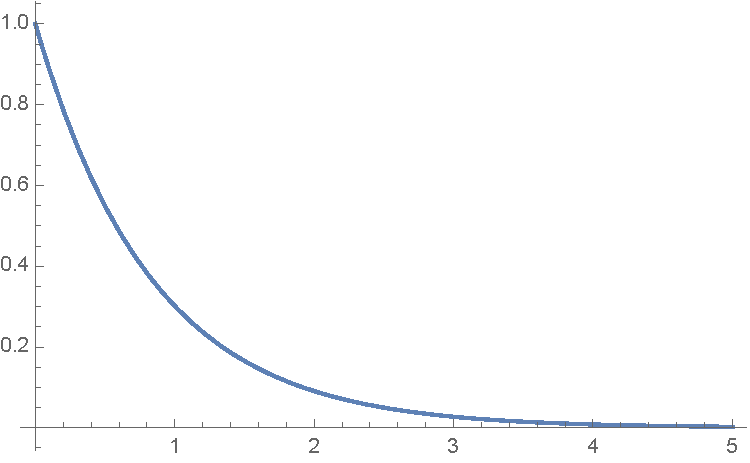
\includegraphics[width=0.25\textwidth]{figs/johdanto_mathematica.pdf}
\end{center}

\end{exam}

\begin{stopQ}{q:wolframalpha}Mene osoitteeseen wolframalpha.com ja piirrä siellä funktion \(f(x) = \sin^2 x\) kuvaaja välillä \([- \pi, \pi]\). Määritä myös sen integraalifunktio.
\end{stopQ}

\subsection{Ongelmanratkaisu}
\label{ongelmanratkaisu}

Fysiikan opinnoissa tärkeintä ei ole opetella ulkoa suurta määrää informaatiota vaan oppia soveltamaan melko pientä määrää perusperiaatteita ja -lakeja. Siksi harjoittelu, ongelmanratkaisu ja tehtävien ratkominen ovat fysiikan opinnoissa tärkeitä, ja niihin tulee varata kohtuullisen suuri osa opiskeluun käytettävästä ajasta. Perinteisesti fysiikan opetuksessa on painotettu \emph{laskutehtäviä}, joissa annetuissa tilanteissa ratkaistaan joitakin kysyttyjä suureita. Nämäkin ovat tärkeitä, mutta fysikaalisen ajattelun kehittymisessä on tärkeää harjoitella myös \emph{konseptuaalista ajattelua} eli periaatteellista päättelyä, joka ei vaadi laskemista.

Periaatteellisen ajattelun hallinta on itse asiassa edellytys useimpien laskuja vaativien ongelmien ratkaisemiseksi. Vielä lukiotasolla useat laskutehtävät ratkeavat vain oikean kaavan valinnalla ja siihen lukuarvoja sijoittamalla. Todellisuudessa kiinnostavissa fysiikan ongelmissa tämä ei käytännössä koskaan onnistu, koska valmiit kaavat pätevät vain erittäin yksinkertaisissa ja ideaalisissa tilanteissa. Sen sijaan ongelmien ratkaiseminen vaatii aina tilanteen hahmottamista, siinä vallitsevien fysikaalisten lakien ymmärtämista sekä niitä kuvaavien matemaattisten relaatioiden muodostamista, ja nämä askeleet vaativat juuri periaatteelisen eli konseptuaalisen ajattelun taitoja. Varsinainen laskutoimitus on tehtävänratkaisussa vain matemaattinen harjoitus tehtävän lopuksi --- fysiikkaa on ongelman pukeminen muotoon, johon matematiikan työkaluja voidaan soveltaa. Ohessa on esitelty eräs tapa lähteä järjestelmällisesti ratkaisemaan monimutkaista fysiikan tehtävää.

\begin{instructions}{Fysiikan laskuteht\"avien ratkaiseminen}{ohje:laskut}{h!}\noindent

\begin{enumerate}
\item \textbf{Tilanne} Useimmiten kannattaa aloittaa \emph{piirtämällä kuva}, sillä kuva on erinomainen tapa kerätä yhteen saatavilla oleva tieto. Fysiikassa usein tarkastellaan tilanteita, joissa esineiden tai hiukkasten paikat avaruudessa ovat merkitykselliset, jolloin kuva on luonnollinen tapa esittää tilanne, ja myös esineiden liikettä voi esittää kuvin tai kuvasarjoin. Fysikaalisen ongelman hahmottamista auttaa myös \emph{tunnettujen ja tuntemattomien suureiden listaaminen}. Todelliset ongelmat ovat yleensä avoimia, eikä silloin sanota suoraan, mitä pitäisi ratkaista. Tällöin kannattaa jo tässä vaiheessa pohtia, mitkä suureet voisivat olla kiinnostavia asetettuun kysymykseen vastaamisessa.

\item \textbf{Suunnitelma} Kaikkien monimutkaisten ongelmien ratkaiseminen --- myös fysikaalisten --- kannattaa aina aloittaa \emph{laatimalla suunnitelma} siitä, miten ongelma aiotaan ratkaista.
Ongelmien ratkaiseminen vaatii yleensä tarkasteltavan tilanteen pilkkomista pienempiin, helpommin hallittaviin osiin, näiden osien erillistä analysointia ja lopuksi osien yhdistämistä takaisin yhdeksi kokonaisuudeksi. Tällainen analyysi vaatii monenlaisen tiedon yhdistämistä, eivätkä pitkät päättelyketjut yleensä onnistu ilman kokonaiskuvaa siitä, mihin kukin päättelyaskel on loppujen lopuksi johtamassa.
Ongelmanratkaisu helpottuu huomattavasti, kun pohdit ensin yleisellä tasolla, kuinka ongelma voitaisiin ratkaista ilman kaikkien täsmällisten yksityiskohtien huomioimista.

\item \textbf{Ratkaisu} Kun suunnitelma on olemassa, voit toteuttaa sen. Jos suunnitelma on hyvin laadittu, tiedät jo valmiiksi mitä työvaiheita ratkaisuun kuuluu ja miksi kukin niistä on tarpeellinen. Ratkaisuvaiheessa voit keskittyä kunkin suunnitelmassa mainitun askeleen toteuttamiseen ja huomioida kaikki suunnitelmavaiheessa sivuutetut yksityiskohdat. Jos ongelman ratkaiseminen vaatii matemaattisten työkalujen käyttöä, niihin liittyvät laskut voi toteuttaa vasta tässä vaiheessa. Jos kaikki menee hyvin, ongelman pitäisi ratketa, kunhan seuraat suunnitelmaasi ja olet huolellinen sen toteuttamisessa. Hyvätkään suunnitelmat eivät tietenkään aina onnistu, etkä välttämättä pääsekään ratkaisussa haluamaasi lopputulokseen. Tällöin sinun on syytä palata suunnitelmavaiheeseen muuttamaan suunnitelmaa.

\item \textbf{Arviointi} Monimutkaisten ongelmien analyysissä voi tapahtua helposti virheitä, joten \emph{ratkaisun järkevyys pitää aina arvioida}. Muutenkin on erittäin tarpeellista osata arvioida kohtaamiesi väitteiden oikeellisuutta yksinkertaisin periaattein, koska maailma on täynnä mielettömiä väitteitä eikä sinulla ole aina mahdollista selvittää niitä yksityiskohtaisesti. Käy fysikaalisten ongelmien arvioinnissa läpi ainakin seuraavat kysymykset: Oletko vastannut kaikkiin kysymyksiin? Toteuttaako ratkaisusi erikoistapaukset, joissa ratkaisu on ilmiselvä? Oletko käyttänyt suureita johdonmukaisesti, eli ethän sekoita esimerkiksi skalaareja vektoreihin ja ovathan yksiköt oikein? Jos vastauksessasi on numeroarvo, onko siinä järkevä määrä merkitseviä numeroita ja onko vastauksesi suuruusluokka järkevä?
Kaikkien näiden asioiden muistamiseksi käy muistisääntö \emph{``KEVYT''}:

\begin{itemize}
\item Kysymyksiin vastattu?

\item Erikoistapaukset ja raja-arvot oikein?

\item Vektorit ja skalaarit oikein?

\item Yksiköt oikein?

\item Tarkkuus ja suuruusluokka oikein?

\end{itemize}

\end{enumerate}

\end{instructions}

\startwidepage

\section*{Yhteenveto: Johdanto}
\addcontentsline{toc}{section}{Yhteenveto: Johdanto}
\noindent
\begin{tabular}{p{1.15\textwidth}}
\standout{Fysiikka tieteen\"a}{
\begin{multicols}{2}

\begin{itemize}
\item \textbf{Tiede} on menetelmä tiedon systemaattiseksi keräämiseksi.

\item Luonnontieteellisten väitteiden on oltava testattavissa. Jos tieteellinen tieto osoittautuu ristiriitaiseksi, tieteen väitteitä on muokattava tai ne on korvattava uusilla. Tiede on itseään korjaava.

\item \textbf{Fysiikka} on kokeellinen tiede, jossa väittämien ja teorian ennusteiden oikeellisuuden mittarina on niiden yhteensopivuus kokeellisten havaintojen kanssa.

\end{itemize}

\end{multicols}
} \\
\standout{Suureet ja yksik\"ot}{
\begin{multicols}{2}

\begin{itemize}
\item \textbf{Suure} on mitattavissa oleva ominaisuus. Suureilla on fysiikassa sekä \textbf{suuruus} että \textbf{dimensio}.

\item \textbf{Yksikkötarkastelu} on hyvä keino tarkastaa suureiden yhteensopivuus. Suureen yksikköä merkitään hakasulkein, esim. \( [x] = \un{m} \) tarkoittaa, että suureen \(x\) laatu on pituus ja yksikkö metri.

\item Kaksi suuretta voidaan laskea yhteen jos niillä on sama dimensio: \(a + b\) on määritelty vain jos \([a] = [b]\).

\item Mitkä tahansa suureet voidaan kertoa keskenään.

\item Suure voi olla useimpien funktion argumenttina vain, jos se on paljas luku: esim. \(e^a\) on määritelty vain jos \([a] = 1\).

\item Yhtälöissä pitää aina olla sama yksikkö molemmilla puolilla: esim. \(a = b\) on tosi vain jos \([a] = [b]\).

\end{itemize}

\end{multicols}
} \\
\standout{Kuvat ja kuvaajat}{
\begin{multicols}{2}

\begin{itemize}
\item Kuvat ovat yleensä paras tapa esittää paljon informaatiota ymmärrettävässä muodossa. Kuvia voi käyttää sekä oman ajattelun tukena että muiden kanssa kommunikoinnissa.

\item \textbf{Kuvaajat} ovat tärkeä tapa esittää tietoa ja dataa fysiikassa.

\item Kuvaajien \textbf{akselit} kertovat esitettävät suureet sekä niiden mittakaavan.

\end{itemize}

\end{multicols}
} \\
\standout{Ratkaisustrategioita}{
\begin{multicols}{2}

\begin{itemize}
\item Fysikaalisten \textbf{ongelmien ratkaiseminen} etenee seuraavasti:

\begin{itemize}
\item hahmotetaan \textbf{tilanne}

\item tunnistetaan vallitsevat \textbf{fysikaaliset periaatteet}

\item muodostetaan \textbf{matemaattinen malli}

\item \textbf{ratkaistaan} tarvittavat suureet

\item \textbf{arvioidaan} saadut tulokset

\end{itemize}

\item \textbf{Tarkista} nämä:

\begin{itemize}
\item \textbf{K}ysymyksiin vastattu?

\item \textbf{E}rikoistapaukset ja raja-arvot oikein?

\item \textbf{V}ektorit, skalaarit ja differentiaalit oikein?

\item \textbf{Y}ksiköt oikein?

\item \textbf{T}arkkuus ja suuruusluokka oikein?

\end{itemize}

\item Numeeristen laskujen tulokset ovat yhtä tarkkoja kuin niissä käytettävien lukuarvojen huonoin tarkkuus:

\begin{itemize}
\item yhteenlaskussa tarkkuden määräävät \textbf{desimaalit}

\item kertolaskussa tarkkuuden määräävät \textbf{merkitsevät numerot}

\end{itemize}

\item \textbf{Suuruusluokka-arvio} voidaan muodostaa seuraavasti:

\begin{itemize}
\item jaetaan ongelma pienempiin osiin

\item arvioidaan kukin tekijä muodossa \(a \cdot 10^b\), missä \(a\):lle riittää yhden numeron tarkkuus

\item lasketaan lopputulos käyttäen potenssien laskusääntöjä
\begin{equation} 10^a \cdot 10^b = 10^{a+b}, \ (10^{a})^b = 10^{ab}, \ \frac{1}{10^a} = 10^{-a}. \nonumber \end{equation}

\item pyöristetään lopputulos kymmenen potensseiksi siten, että luvut 2--3 pyöristetään alaspäin ja 4--9 ylöspäin

\end{itemize}

\end{itemize}

\end{multicols}
} \\
\standout{Sanasto}{
\begin{multicols}{2}

\begin{itemize}
\item tiede (science)

\item teoria (theory)

\item hypoteesi (hypothesis)

\item malli (model)

\item fysiikka (physics)

\item suure (quantity)

\item dimensio (dimension)

\item yksikkö (unit)

\item yksikkötarkastelu (dimensional analysis)

\item SI-yksikköjärjestelmä (SI-units)

\item kuvaaja (graph, plot)

\item symmetria (symmetry)

\item matematiikka (mathematics)

\item merkitsevä numero (significant digit)

\item desimaali (decimal)

\item pyöristäminen (rounding)

\item suuruusluokka (order of magnitude)

\item logaritminen asteikko (logarithmic scale)

\item raja-arvo (limit)

\item approksimaatio (approximation)

\item kvalitatiivinen (qualitative)

\item kvantitatiivinen (quantitative)

\item mikroskooppinen (microscopic)

\item makroskooppinen (macroscopic)

\end{itemize}

\end{multicols}
} 

\end{tabular}


\begin{table}[h!]
\caption{Kreikkalaiset aakkoset. Etenkin pieniä kirjaimia käytetään matemaattisessa esityksessä suureiden symboleina. 
}
\label{kreikkalaiset_aakkoset}
\vspace*{-4mm}
\begin{center}
\bgroup
\small
\def\arraystretch{0.9}
\begin{tabular}{rlrlrlrlrlrl}
$A, \alpha$ & alfa & $E, \varepsilon$ & epsilon & $I, \iota$ & ioota & $N, \nu$ & nyy & $P, \rho$ & roo & $\Phi, \varphi$ & fii \\
$B, \beta$ & beeta & $Z, \zeta$ & zeeta & $K, \kappa$ & kappa & $\Xi, \xi$ & ksii & $\Sigma, \sigma$ & sigma & $X, \chi$ & khii \\
$\Gamma, \gamma$ & gamma & $H, \eta$ & eeta & $\Lambda, \lambda$ & lambda & $O, o$ & omikron & $T, \tau$ & tau & $\Psi, \psi$ & psii \\
$\Delta, \delta$ & delta & $\Theta, \theta$ & theeta & $M, \mu$ & myy & $\Pi, \pi$ & pii & $Y, \upsilon$ & ypsilon & $\Omega, \omega$ & oomega
\end{tabular}
\egroup
\end{center}
\end{table}
\newpage




\newpage\begin{answers}\noindent

\stopA{q:ajankaytto}{ Tähän ei ole yhtä oikeaa vastausta. Kumuloituvissa aineissa kuten fysiikassa täytyy yleensä edetä asia kerrallaan, koska monimutkaisemmat asiat perustuvat yleensä yksinkertaisempien asioiden soveltamiseen ja yhdistelyyn. Jos siis perusasioita ei osaa, edistyneempiä asioita ei voi mitenkään ymmärtää. Toki joskus voi olla perusteltua opiskella ensin suurempi kokonaisuus pintatasolla, jonka jälkeen voi palata pohtimaan yksityiskohtia, kun on jo jonkinlainen käsitys siitä, miten eri asiat liittyvät toisiinsa.
}

\stopA{q:yksikot}{ Ensin tarkastetaan, että sinin argumentti on paljas luku:
\([ab^2] = A^2/A^2 = 1.\)
Se on, joten sini on hyvin määritelty ja siispä
\([\sin(ab^2)] = 1.\)
Koko lausekkeen yksikkö on
\([a] - 1/[b^2][\sin(ab^2)] = A^2 - 1/(1/A)^2 = A^2.\)
}

\stopA{q:mallit}{ Tällaisilla malleilla voidaan tutkia monenlaisia asioita, esimerkiksi\\
(a) erilaisten aineiden vaikutusta hermosolujen toimintaan (neurokemia),\\
(b) informaation kulkua hermosolujen kesken (neuroverkkotiede),\\
(c) aivoalueiden tehtäviä ja niiden toimintahäiriöiden vaikutuksia (aivotutkimus),\\
(d) ihmisten käyttäytymistä ja siihen vaikuttavia tekijöitä (psykologia) ja\\
(e) joukkojen käyttäytymistä (peliteoria).
}

\stopA{q:graafinen_esitys}{ Kun \(t = 3\) s, kuvaajan datapisteestä voidaan lukea \(x = 3.3 \pm 0.3\) m. Vielä parempi arvioi voitaisiin saada datapisteiden kautta piirretyn suoran avulla, jonka perusteella \(x = 3.1 \pm 0.2\) m.

Kun \(t = 6\) s, ei olla kuvaajan alueella. Tällöin täytyy jatkaa kuvaan piirrettyä suoraa eli ekstrapoloida ja päätellä \(x\):n arvo tätä kautta. Graafisesti voidaan piirtää jyrkin ja loivin suora, joka näyttää sopivan mittapisteisiin, ja arvioida \(x\):n arvo hetkellä \(t = 6\) s näiden väliin jäävien arvojen kautta.

Laskennallisesti aikavälillä \(t = 0 \ldots 4\) s \(x\) muuttuu arviolta \(2.8 \pm 0.6\) m, ja hetkellä \(t = 2\) s suora kulkee pisteen \(x = 2.5 \pm 0.1\) m kautta, joten hetkellä \(t = 6\) s voidaan \(x\):n arvoksi arvioida \(x = 5.3 \pm 0.7\) m.
}

\stopA{q:symmetria}{ Hyvin pitkästä langasta yhtä kaukana olevat pisteet muodostavat sylinterin eli ympyrälieriön vaipan. Fysiikassa ``hyvin pitkä'' tarkoittaa yleensä sitä, että mallina käytetään äärettömän pitkää asiaa, joten tässä voidaan ajatella langan (ja sylinteripinnan) jatkuvan äärettömyyksiin.
}

\stopA{q:laskun_tarkkuus}{ Luvussa \(a = 0.12\) on kaksi merkitsevää numeroa ja luvussa \(b = 3.45\) on kolme.\\
(a) Lasku \(1/b\) on jakolasku, joten sen järkevä tarkkuus on 3 merkitsevää numeroa, \(1/b = 0.290\). Lasku \(1/b - a\) on vähennyslasku, joten sen järkevä tarkkuus määräytyy desimaaleista, \(0.290 - 0.12 = 0.17\). (Huom. varsinaiset laskut kannattaa aina tehdä niin suurella tarkkuudella kuin mahdollista, ja vasta lopuksi tulos pyöristetään sopivaan tarkkuuteen.)\\
(b) \(a^2b\) sisältää vain kertolaskua, joten sen tarkkuus on 2 merkitsevää numeroa, \(0.12^2 \cdot 3.45 = 0.050\).
(c) Laskun \(a^2\) tarkkuus on 2 merkitsevää numeroa, \(0.12^2 = 0.014\). Laskun \(b - a^2\) tarkkuus määräytyy desimaaleista, \(3.45-0.014 = 3.44\). Huomaa, että tässä järkevä tarkkuus on kaksi desimaalia eikä kaksi merkitsevää numeroa, koska viimeinen laskutoimitus on vähennyslasku kaksi- ja kolmedesimaalisen luvun välillä.
}

\stopA{q:suuruusluokka}{ A-kirjain on suomen yleisin kirjain. Arvioidaan karkeasti, että kaikista kirjaimista osuus \(n_{\text{a}/\text{kirjain}} = 10^{-1}\) on a-kirjaimia.
Yhdellä rivillä on noin \(n_{\text{kirjain}/\text{rivi}} = 10^2\) kirjainta ja yhdellä sivulla on keskimäärin noin \(n_{\text{rivi}/\text{sivu}} = 4 \cdot 10^1\) riviä (kunkin sivun rivien määrä riippuu tietenkin siitä, onko sivulla esim. kuvia). Materiaalia on noin \(n_\text{sivu} = 8 \cdot 10^{2}\) sivua, joten kaikkiaan a-kirjaimia on
\( n_{\text{a}} = n_{\text{a}/\text{kirjain}} n_{\text{kirjain}/\text{rivi}} n_{\text{rivi}/\text{sivu}} n_\text{sivu} = 10^{-1} \cdot 10^2 \cdot 4 \cdot 10^1 \cdot 8 \cdot 10^2 = 32 \cdot 10^{4} \approx 10^5. \)
Tässä materiaalissa on siis arviolta \(10^5\)--\(10^6\) a-kirjainta.
}

\stopA{q:raja-arvo}{ (a) Funktion arvo selviää suoralla sijoituksella, \(x(0) = 1 + 2/3 = 5/3\).
(b) Kun \(t\) on hyvin suuri, voidaan tarkastella raja-arvoa, kun \(t\) lähestyy ääretöntä. Siispä suurilla t:n arvoilla voidaan arvioida
\(\lim_{t \to \infty} x(t) = 1 + 2/\infty = 1 + 0 = 1\).
}

\stopA{q:wolframalpha}{ Ohjelma osaa melko hyvin arvata, mitä haluat, joten voit kokeilla esimerkiksi kirjoittaa ``plot sin\^\relax 2 x from -pi to pi''. Voit kuitenkin käyttää myös täsmällisiä Mathematica-kielen komentoja, jotka olisivat tässä ``Plot[Sin[x]\^\relax 2,{x,-Pi,Pi}]'' (tulos on kuvaaja, jossa on kaksi maksimia) sekä ``Integrate[Sin[x]\^\relax 2,x]'' (tulos on \( \frac{1}{2}(x-\sin x \cos x) + c\)).
}

\end{answers}

 \part{Mekaniikka} 

\startchapter{Liike}{liike}{%

Mekaniikan keskeinen tutkimuskohde on liike sekä vuorovaikutusten ja liikkeen yhteys. Ensimmäinen askel mekaniikassa onkin siis liikkeen täsmällinen kuvaaminen. Aloitamme liikkeen tarkastelun yhdessä ulottuvuudessa ja myöhemmin yleistämme kuvauksen kolmiulotteiseen avaruuteen. Tietenkin asiat liikkuvat todellisuudessa kolmessa ulottuvuudessa, mutta niin kauan kuin liike on ainakin likimain suoraviivaista eli esine liikkuu suoraa pitkin joko yhteen suuntaan tai edestakaisin, liikettä voi kuvata yksiulotteisena.

Lukiossa mekaniikkaa analysoidaan algebrallisesti, mikä tarkoittaa matemaattisten työkalujen rajoittuvan yksinkertaisiin laskutoimituksiin ja funktioihin. Näin ei kuitenkaan pystytä kuvaamaan kuin joitakin yksinkertaisia erikoistapauksia, ja monimutkaisempien ilmiöiden tutkiminen vaatii kehittyneempiä matemaattisia työkaluja. Erityisesti muuttuvien suureiden analyysi vaatii derivaattojen ja integraalien eli differentiaalilaskennan käyttöä, ja kolmiulotteisessa avaruudessa suuntien kuvaaminen edellyttää vektorien käsittelyä. Näitä tekniikoita esitellään jo tässä luvussa, ja niiden käyttöä harjoitellaan ja syvennetään opintojen edetessä.

Tämän luvun opiskeltuasi sinun tulee osata:

\begin{itemize}
\item määritellä paikkakoordinaatti sekä siirtymä koordinaatiston avulla

\item määritellä nopeus ja kiihtyvyys sekä näiden skalaarikomponentit

\item esittää liike kuvien ja kuvaajien avulla

\item ratkaista paikka, nopeus ja kiihtyvyys derivointia tai integrointia käyttäen

\item esittää paikka, nopeus ja kiihtyvyys vektoreina

\end{itemize}

}

\stopwidepage

%\vfill
\newpage

\section{Paikka, aika ja nopeus}
\label{paikkaaikajanopeus}

\index{paikka}
\index{pituus}
\index{matka}
\index{metri}
\index{etäisyys}
\index{kiintopiste}

\textbf{Liike} yleisesti tarkoittaa sitä, että asioiden \textbf{paikat} muuttuvat. Sinulla on varmasti intuitiivinen käsitys siitä, mitä paikka tarkoittaa puhekielessä. Kaikkien esineiden täytyy olla jossakin, ja se jossakin on
esineen paikka. Tämä on kuitenkin liian epämääräinen ajattelutapa, jotta voisimme tarkastella liikettä fysikaalisesti. Niinpä meidän täytyy määritellä paikka niin, että siitä tulee fysikaalinen suure. Toisin sanoen meidän on keksittävä keino \emph{mitata paikkoja}.

Jotta voisimme mitata paikkoja, meidän pitää ensin osata mitata \textbf{pituuksia}. Pituus on fysiikan perussuure, jonka yksikkö on metri (m). Metrin pituus määriteltiin aikoinaan niin, että \textbf{matka} maapallon päiväntasaajalta pohjoisnavalle on kymmenen miljoonaa metriä (jolloin maapallon ympärysmitta on siis 40000 km). Käytännön syistä määritelmää kuitenkin pian muutettiin ja laadittiin metrin prototyyppi eli mittatikku, jonka pituudeksi sovittiin tasan yksi metri. Metrin määritelmä perustuikin tällaiseen mittatikkuun aina 1960-luvulle asti.

Yksinkertaisin tapa mitata pituutta lieneekin ottaa jokin mittatikku kuten viivain tai mittanauha ja verrata mitattavaa pituutta tämän tunnetun mittakappaleen pituuteen. Tämä voi olla joskus hiukan epätarkkaa, ja tarkempiakin menetelmiä on tietysti olemassa, mutta tämä idea riittää meille toistaiseksi.

\subsection{Koordinaatisto}
\label{koordinaatisto}

Pituuksia mittaamalla voimme mitata asioiden välisiä \textbf{etäisyyksiä}, ja tähän perustuu myös paikan mittaaminen. Voimme nimittäin aina sopia jonkin \textbf{kiintopisteen} ja mitata esineiden etäisyydet tästä kiintopisteestä. Etäisyys on mitattavissa oleva suure, joten jos esineen paikalla tarkoitetaan sen etäisyyttä valitusta kiintopisteestä, paikkakin on mitattava suure.

\pictures{b!}%
{Yhdessä suunnassa liikkuvan esineen paikka voidaan esittää koordinaatin avulla.;%
Valitaan kiintopiste eli origo sekä positiivinen suunta ja mitataan etäisyys kiintopisteestä.;%
Esine voidaan esittää pisteenä, jolla on yksikäsitteinen paikka. Paikan kertoo koordinaatti.}%
{fig:koordinaatisto;fig:koordinaatisto:origo;fig:koordinaatisto:koordinaatti}%
{0.48;0.48}%
{0.48;0.48}%
{liike_koordinaatisto_1.pdf;liike_koordinaatisto_2.pdf}

Tämä ei kuitenkaan riitä, sillä paikka ja etäisyys eroavat toisistaan eräällä hyvin merkittävällä tavalla.
Ajattelepa vaikka jalkapallokenttää. Valitaan kentän keskellä oleva aloituspiste kiintopisteeksi, jonka suhteen haluamme mitata paikkoja. Aloituspisteen ympärillä on keskiympyrä, jonka säde on noin yhdeksän metriä. Jokainen tämän ympyrän piste on samalla etäisyydellä aloituspisteestä. Jos määrittelisimme paikan \emph{ainoastaan} käyttämällä mittarina keskipisteestä mitattua etäisyyttä, mittaisimme kaikille keskiympyrän kehän pisteille saman paikan. Lopputuloksena päättelisimme, että keskiympyrän kaikki pisteet ovat samassa paikassa, mikä ei tietenkään ole järkevää, sillä tokihan ympyrän pisteet ovat eri paikoissa.

Ongelma on se, että on olemassa paljon pisteitä, jotka ovat yhtä kaukana valitusta kiintopisteestä. Pallokenttä on kaksiulotteinen taso, ja siellä kiintopisteestä samalla etäisyydellä olevat pisteet muodostavat ympyrän.
Emme vielä tässä luvussa tutki liikettä tasossa vaan toistaiseksi pohdimme vasta suoralla tapahtuvaa liikettä. Sekään ei silti auta, sillä suorallakin on aina kaksi pistettä, jotka ovat valitusta kiintopisteestä samalla etäisyydellä. Jos esimerkiksi seisot suoralla tiellä ja sanot kaverillesi, että viiden metrin päässä on auto, se ei vielä kerro onko auto oikealla vai vasemmalla (tai edessä vai takana).

\index{koordinaatisto}
\index{koordinaatti}

Jotta ongelmasta päästäisiin eroon, pitää kiintopisteen lisäksi sopia tapa ilmoittaa, missä \emph{suunnassa} kiintopisteestä katsoen tarkastelu paikka on. Tämä onnistuu käyttämällä \textbf{koordinaatistoa}.
Koordinaatisto antaa kaikille avaruuden pisteille yksikäsitteinen numerosarjan eli \textbf{koordinaatit}, jotka ilmaisevat pisteiden paikkaa. Tavallisia symboleja koordinaateille ovat muun muassa \(x, y, z\).

\index{origo}
\index{akseli}

Kiintopistettä, jonka suhteen paikkoja mitataan, kutsutaan koordinaatiston \textbf{origoksi}.
Koordinaatistot määrittelevät aina myös \emph{positiivisen ja negatiivisen suunnan} niin, että ne pisteet, jotka ovat origosta katsoen positiivisessa suunnassa, saavat positiivisia koordinaatteja, ja negatiivisessa suunnassa olevat pisteet saavat negatiivisia koordinaatteja. Yksiulotteisessa tapauksessa tämä tarkoittaa sitä, että kahdesta pisteestä, jotka ovat esimerkiksi etäisyydellä 9 m origosta, toisen koordinaatiksi sovitaan \(x = 9 \un{m} \) ja toisen \(x = -9 \un{m} \). Origon koordinaatti on 0 m, koska sen etäisyys itsestään on nolla.

Jokaiseen pisteeseen liitetään siis numero, eikä millään kahdella pisteellä ole samaa numeroa. Niinpä jos tiedämme pisteen koordinaatin, tiedämme täsmälleen mikä piste on kyseessä ja missä se on. Ja toisin päin voimme etäisyyttä mittaamalla ja positiivisen suunnan huomioimalla laskea mille tahansa pisteelle sen koordinaatin. Näin koordinaattien avulla paikasta on tullut mitattavissa oleva asia eli fysikaalinen suure.

\begin{stopQ}{q:koordinaattimerkki}%
Seisot suoralla polulla ja katsot polkua eteenpäin. Asetetaan koordinaatisto niin, että sen origo on sinun kohdallasi ja positiivinen suunta on eteenpäin. Edessäsi 5 m päässä on iso kivi. Takanasi 2 m päässä on toinen ihminen. Mitä ovat kiven ja ihmisen (a) etäisyys sinusta, (b) paikkakoordinaatti, (c) paikkakoordinaattien erotus, (d) etäisyys toisistaan?
\end{stopQ}

\subsection{Aika}
\label{aika}

\onepicture{b}%
{Aikaa mitataan valitun hetken eli kiintopisteen suhteen.}%
{fig:aika}%
{0.9}%
{liike_aika.pdf}

\index{aika}
\index{sekunti}
\index{valonnopeus}
\index{SI-järjestelmä}
\index{metri}

Pituuden ja paikan lisäksi tarvitsemme liikkeen kuvaamiseen vielä toisenkin fysiikan perussuureen, \textbf{ajan}.
Paikan tapaan aika on asia, joka on kaikille tuttu. Aikahan kulkee tasaisesti eteenpäin, itsestään, ja aikaa voi mitata kellolla. Klassinen mekaniikka ei juurikaan tutki ajan luonnetta, vaan mekaniikassa ajan todellakin ajatellaan olevan tällainen itsestään virtaava asia, jonka suhteen muita suureita havainnoidaan. Muilla fysiikan osa-alueilla on enemmän sanottavaa siitä, mitä aika on, mutta toistaiseksi tämä yksinkertainen ajatus ajan luonteesta riittää meille ihan hyvin.

Aikaa merkitään yleensä symbolilla \(t\) (englannin `time' tai ranskan `temps' mukaisesti) ja sen perusyksikkö on \textbf{sekunti} (s). Sekunti perustuu ikivanhaan tapaan jakaa vuorokausi 24 tuntiin, tunti 60 minuuttiin ja minuutti 60 sekuntiin, jolloin yhdessä vuorokaudessa on 86400 sekuntia. Ajan mittaaminen maapallon liikkeen perusteella ei kuitenkaan ole tarpeeksi tarkkaa modernin mittaustekniikan vaatimuksille, ja niinpä sekunnin nykyinen määritelmä perustuu cesium-atomien lähettämän säteilyn värähtelyjen laskemiseen.

Myös metrin moderni määritelmä perustuu aikaan. Nykyisin metri on nimittäin määritelty sen matkan pituudeksi, jonka valo kulkee ajassa \(1 / 299792458 \) sekuntia.
Nämä modernit tavat määritellä metri ja sekunti ovat hyvin tarkkoja mutta myös hiukan teknisiä. Toistaiseksi meille riittää tavallisen mittanauhan ja kellon mittaustarkkuus.

Aivan kuten paikalle valittiin kiintopiste, myös ajalle voidaan valita kiintopiste eli \textbf{nollahetki}, ja voimme määritellä ajan mitattavana suureena tämän hetken suhteen. Käytännössä tämän voidaan ajatella tapahtuvan niin, että nollahetkellä käynnistetään kello, minkä jälkeen ajan arvo mitattavana suureena määritellään kunakin hetkenä tämän kellon lukemaksi. Tietysti aika oli olemassa jo ennen nollahetkeä, ja myös menneisyyden hetkiä voidaan verrata ajan nollahetkeen. Koska nämä hetket olivat ennen ajan kiintopistettä, aika saa niissä negatiivisen arvon. Näin määritellen aika toimii kuin koordinaatti: jokainen hetki saa ikioman ajan arvon, eikä kahdella eri hetkellä ole samaa ajan arvoa. Lisäksi mitä suurempi tämä ajan arvo on, sitä myöhemmin kyseinen hetki tapahtuu.

\begin{stopQ}{q:aikakoordinaatti}%
Asetetaan ajan nollahetki keskipäivään tasan klo 12:00:00. Mikä on aika \(t\) (i) tunteina, minuutteina ja sekunteina tai (ii) pelkkinä sekunteina, kun kello (a) on 12:13:14, (b) on 15:30:00, (c) oli 11:45:50?
\end{stopQ}

\subsection{Liikkeen graafinen esitys}
\label{liikkeengraafinenesitys}

\onepicture{tb}%
{Kävelijän liike sekä kävelijän paikan kuvaus pisteenä.}%
{fig:liikegraafinen}%
{0.6}%
{liike_malli_1.pdf}

Nyt olemme vihdoin valmiit kuvaamaan liikettä. Esineen liikkuminen nimittäin tarkoittaa, että sen paikkakoordinaatti muuttuu ajan kuluessa. Jos tiedämme, mikä koordinaatti on milläkin ajan hetkellä, tiedämme miten esine liikkuu.

Paikan ja ajan välinen riippuvuus voidaan kuvata usealla erilaisella tavalla, ja aloitamme tutkimalla \textbf{kuvallista} eli \textbf{graafista} esitystapaa. Monimutkaiset ilmiöt on melkein aina helpoin ymmärtää hyvän kuvan perusteella, ja seuraavaksi esiteltävät päättelyt osoittautuvat vielä tärkeiksi myös monessa muussakin tilanteessa kuin liikkeen kuvaamisessa.

\index{kappale}

Tarkastellaan hyvin yksinkertaista esimerkkiä liikkeestä: kävelevää ihmistä. Kuvassa \autoref{fig:liikegraafinen} on esitetty sarja kävelijää esittäviä kuvia, joissa tämä kulkee ensin eteenpäin, pysähtyy ja kulkee sitten taaksepäin. Kuvat on otettu puolen sekunnin välein, ja ne yhdessä esittävät kävelijän liikkeen \(6.5 \un{s}\) ajalta.

Tällainen kuvasarja ei ole kuitenkaan paras tapa kuvata liikettä, koska se sisältää paljon turhaa informaatiota. Emme ole kiinnostuneita kävelijän tarkasta askelluksesta vaan hänen liikkeestäään yhtenä kokonaisuutena eli \textbf{kappaleena}.
Haluamme siksi karsia tilanteen kuvauksesta pois kaiken ylimääräisen.
Pelkistetyimmillään voimme kuvata kävelijän paikkaa pelkällä paikkakoordinaatilla, jolle järkevin kohta lienee jokin sopivasti valittu piste kävelijän sisältä.
Näin saamme \emph{mallin}, jossa kävelijää kuvaa vain yksi piste. Tämän pisteen liike on yksinkertainen kuvaus koko kävelijän liikkeestä. Valitsemalla vielä kuvasta kiintopisteen voimme kiinnittää koordinaatiston ja piirtää kävelijän paikkaa kuvaavan pisteen tähän koordinaatistoon eri ajan hetkinä.

\index{kuvaaja}

\marginpicture%
{0}%
{Kävelijän paikan kuvaaja.}%
{fig:liikegraafinen2}%
{1.0}%
{liike_malli_3.pdf}

Edellä kuvattu malli on kävelijän paikan \textbf{kuvaaja}. Kuvaajassa yksi akseli esittää paikkakoordinaattia ja toinen aikaa, ja kukin kuvaajan piste ilmaisee kävelijän paikan tietyllä ajan hetkellä. Periaatteessa kuvaajissa akselit voi piirtää osoittamaan mihin suuntaan tahansa. Kuitenkin tällaisissa kuvaajissa on tavallisesti tapana piirtää riippumaton suure vaaka-akselille ja tästä riippuva suure pystyakselille. Klassisessa mekaniikassa ajan ajatellaan virtaavan itsestään ja paikan saavan jokaisena ajan hetkenä jonkin tietyn arvon, jolloin paikka riippuu ajasta mutta ei toisin päin. Siksi on tapana piirtää kuvaaja niin, että paikkakoordinaatti \(x\) on pystyakselille ja aikakoordinaatti \(t\) on vaaka-akselille. Tämä on esitetty kuvassa \autoref{fig:liikegraafinen2}. Tässä kuvaajassa pisteiden muodostama kuvio on täsmälleen sama kuin kuvassa \autoref{fig:liikegraafinen} paitsi että sitä on käännetty ja sen mittakaavaa on muutettu.

\index{lepo}

Kuvaajassa kävely eteenpäin ilmenee kuvaajan nousemisena ylöspäin. Kun kävelijä on paikoillaan, kuvaaja on vaakasuora. Lopuksi kävelijä kulkee takaperin, jolloin kuvaaja laskee alaspäin.
Tämä pätee yleisesti: kappaleen ollessa paikoillaan aika muuttuu mutta paikkakoordinaatti ei, joten kuvaaja on vaakasuora viiva. Tällöin sanotaan kappaleen olevan \textbf{levossa}. Jos kappale liikkuu positiiviseen suuntaan, sen \(x\)-koordinaatti saa yhä positiivisempia arvoja ajan kulkiessa ja kuvaaja on siten \emph{nouseva käyrä}. Vastaavasti kappaleen liikkuessa negatiiviseen suuntaan \(x\)-koordinaatti saa yhä negatiivisempia arvoja ja kuvaaja on \emph{laskeva käyrä}. Kuvaajan leikatessa \(x\)-akselin kappaleen koordinaatti saa arvon nolla eli kappale on samassa paikassa kuin koordinaatiston määrittelevä kiintopiste. Muuta erityistä merkitystä paikkakoordinaatin nollapisteellä ei ole.

\begin{stopQ}{q:paikankuvaaja}%
Miltä kävelijän paikan kuvaaja näyttäisi, jos pisteessä \(x=2 \un{m}\) olisi teleportti, joka siirtäisi hänet välittömästi pisteeseen \(x=3 \un{m}\)? (b) Koska teleportteja ei ole olemassakaan, millaisia oikeat paikan kuvaajat siis eivät saa olla?
\end{stopQ}

Paikan kuvaajasta voimme päätellä helposti monenlaisia asioita kävelijän liikkeestä. Näemme, että aluksi kävelijä on suunnilleen pisteessä \(x_\text{alku} = -0.4 \un{m}\). Hän kävelee ensin pisteeseen \(x = 3.0 \un{m}\) ja palaa sitten takaisin pisteeseen \(x_\text{loppu} = 2.2 \un{m}\). Kävelijä kulkee siis ensin \(3.4\) m eteenpäin ja sitten \(0.8\) m taaksepäin. Kaikkiaan kävelijän kulkema matka on \(3.4 \un{m} + 0.8 \un{m} = 4.2 \un{m}\).

\index{siirtymä}

Toisaalta jos meitä kiinnostaakin vain paljonko kävelijä kokonaisuudessaan siirtyy eli \textbf{siirtymä}, se selviää yksinkertaisesti katsomalla kuinka kaukana alku- ja loppupiste ovat toisistaan ja mihin suuntaan on menty.
Alku- ja loppupisteiden välinen etäisyys on kuvaajan perusteella tässä esimerkissä noin \(2.6\) m ja siinä on siirrytty \(x\)-akselin osoittamaan suuntaan,.

Kuljettu matka on tässä tapauksessa pidempi kuin siirtymä, koska kävelijä meni edestakaisin. Kävelijän siirtymä ensimmäisen kolmen sekunnin aikana on \(3.4\) m, mutta koska hän palaa sen jälkeen takaisin \(0.8\) m, siirtymä pienenee ja jäljelle jää vain \(3.4 \un{m} - 0.8 \un{m} = 2.6 \un{m}\). Kun laskimme matkaa, kaikki kuljetut matkat laskettiin suoraan yhteen. Siirtymätkin voidaan laskea yhteen, mutta vain siinä tapauksessa, että taaksepäin eli \emph{valitun koordinaatiston negatiiviseen suuntaan tapahtuvat siirtymät lasketaan negatiivisina}. Toisin sanoen ensin käveljä siirtyy \(3.4\) m ja sen jälkeen \(-0.8\) m, ja kokonaissiirtymä saadaan laskemalla nämä yhteen.

Itse asiassa näin on järkevää tehdä yleisesti. Samalla tavalla kuin \(x\)-koordinaatille eroteltiin positiiviset ja negatiiviset arvot sen mukaan, onko piste origosta positiivisessa vai negatiivisessa suunnassa, myös siirtymälle kannattaa sopia etumerkki sen mukaan kumpaan suuntaan mennään. Jos siirrytään \(x\)-akselin osoittamaan suuntaan, siirtymä on positiivinen, ja jos mennään \(x\)-akselin osoittamaa suuntaa vastaan, siirtymä on negatiivinen.

\index{liikediagrammi}
\index{rata}

\marginpicture%
{0}%
{Kävelijän liikediagrammi.}%
{fig:liikegraafinen3}%
{1.0}%
{liike_malli_2.pdf}

\textbf{Liikediagrammi} on toinen mahdollinen tapa esittää kävelijän liike.
Tällöin valitaan sopivat ajan hetket tasaisin väliajoin ja piirretään samaan kuvaan kappaleen paikka kaikkina näinä hetkinä. Kuvassa \autoref{fig:liikegraafinen3} on piirretty kävelijän liikkeen liikediagrammi, kun peräkkäisten kuvien väliseksi ajaksi on valittu yksi sekunti. Selkeyden vuoksi diagrammi on jaettu kahteen osaan sen mukaan tapahtuuko liike eteenpäin vai taaksepäin. Lopputulos muistuttaa pitkällä valotusajalla otettua valokuvaa, jossa yhdessä kuvassa näkyy kappaleen \textbf{liikerata} pitkän ajan kuluessa.

Liikediagrammissa näkyy selkeästi kappaleen siirtymä kullakin aikavälillä. Jos siirtymä on suuri, peräkkäiset kuvat ovat kaukana toisistaan. Lisäksi kuvasta nähdään helposti, tapahtuuko liike positiiviseen vai negatiiviseen suuntaan. Erityisen käyttökelpoinen liikediagrammi on kuitenkin liikkeen tapahtuessa tasossa, koska tällöin liikkeen suunta näkyy liikediagrammista. Tällaisiin liikediagrammeihin tutustumme luvuissa \autoref{luku:moniulotteinen} sekä \autoref{luku:pyorimisliike}.

\index{nopeus}
\index{keskinopeus}

Paikan muuttumista ajan kuluessa kuvaa \textbf{nopeus}. Jos kappale kulkee yhden metrin yhdessä sekunnissa, kappaleen \textbf{keskinopeus} on yksi metri sekunnissa eli 1 m\slash s. Mitä pidemmän matka kappale siirtyy ja mitä lyhyemmässä ajassa se tapahtuu, sitä suurempi on kappaleen nopeus.

Liikediagrammissa kappaleen nopeutta on kuvattu piirtämällä nuolia kappaleen peräkkäisten paikkojen välillä. Mitä pidempi nuoli, sitä vauhdikkaammin kävelijä kulkee. Nuolen suunta puolestaan osoittaa nopeuden ja siis liikkeen suunnan.
Ensimmäisen sekunnin aikana kävelijä siirtyy hieman alle yhden metrin oikealle, joten hänen nopeutensa on hieman alle 1 m\slash s oikealle. Seuraavan sekunnin aikana hän siirtyy oikealle enemmän kuin yhden metrin, joten tällä aikavälillä hänen nopeutensa on yli 1 m\slash s. Aluksi kävelijä siis kulkee hitaasti ja hänen nopeutensa on pieni. Nopeus kuitenkin kasvaa.
Neljän sekunnin aikoihin kävelijän liikkeen suunta kääntyy ympäri, ja sen jälkeen hänen nopeutensa on noin puoli metriä sekunnissa vasemmalle.

\section{Liikkeen matemaattinen kuvaus}
\label{liikkeenmatemaattinenkuvaus}

\index{funktio}

Kun kappale liikkuu, sen paikkakoordinaatti muuttuu ajan kuluessa, eli eri ajan hetkinä kappaleen paikalle mitataan eri arvot.
Tätä voidaan matemaattisesti merkitä \( x(t) \), jolloin sanotaan, että paikka \(x\) on ajan \(t\) \textbf{funktio}. Funktio on matematiikassa laskusääntö, jolle annetaan yksi tai useampi luku eli argumentti, ja funktio palauttaa näitä vastaavan uuden luvun. Funktion \( x(t) \) tapauksessa funktiolle annetaan argumenttina aika \(t\), ja funktio kertoo mikä on kappaleen paikkakoordinaatti \(x\) tuona hetkenä.
Mekaniikan perustehtäviä onkin selvittää, missä kappaleet milläkin ajan hetkellä ovat, eli mikä on kunkin kappaleen paikan funktio \(x(t)\).
Vaihtoehtoisesti saatamme tietää tämän funktion ja tehtävänämme on sen perusteella määrittää vaikkapa nopeus.

\subsection{Siirtymä ja muutos}
\label{siirtymäjamuutos}

\index{Delta, $\Delta$}
\index{muutos}

Kävelijän liikkeitä tutkiessamme puhuimme jo matkasta ja siirtymästä, ja totesimme näiden olevan eri asiat. Jos kappale liikkuu monimutkaisella tavalla, sen kulkema matka voi olla vaikea määrittää. Esimerkiksi edestakaisin värähtelevä kappale voi kulkea pitkänkin matkan siirtymättä minnekään.
Siirtymä sen sijaan on helppo laskea, jos vain tiedämme missä oltiin aluksi minne päädyttiin lopuksi. Siirtymän \(\Delta x\) voi nimittäin silloin laskea loppu- ja alkupisteen koordinaattien erotuksena
\bigeq{ \Delta x  = x_\text{loppu} - x_\text{alku}, \label{siirtyma} }
eikä ole mitään väliä, mitä alku- ja loppuhetkien välissä tapahtui.
Myös merkkisäännöt menevät tällä tavalla automaattisesti oikein. Jos loppupisteen koordinaatti on suurempi kuin alkupisteen, siirtymä on positiivinen. Jos sen sijaan loppupisteessä koordinaatti on pienempi kuin alkupisteessä, tämä laskusääntö antaa negatiivisen tuloksen kuten pitääkin. Sillä, ovatko koordinaatit itsessään positiivisia tai negatiivisia, ei ole mitään väliä.

Yhtälössä (\autoref{siirtyma}) esiintyy symboli \(\Delta\), joka voi olla sinulle uusi tuttavuus. Se on kreikkalainen iso Delta-kirjain. (Sen ja muut kreikkalaiset kirjaimet voit tarvittaessa kerrata taulukosta \autoref{kreikkalaiset_aakkoset}.)
Fysiikassa tällä symbolilla tarkoitetaan \textbf{muutosta}. Kun kirjoitetaan \(x\), tarkoitetaan kappaleen \emph{paikkakoordinaatin arvoa} tietyllä ajan hetkellä. Kun kirjoitetaan \(\Delta x\), tarkoitetaan \emph{paikkakoordinaatin muutosta} tietyllä aikavälillä. \emph{Nämä ovat eri asia} ellei liikkeelle sattumalta lähdetä pisteestä \(x=0 \un{m}\). Esimerkiksi kuvan \autoref{fig:liikegraafinen} kävelijän tapauksessa paikkakoordinaatti \(x\) oli lopuksi \(2.2\) m mutta hänen siirtymänsä \(\Delta x\) oli alku- ja lopputilanteen välillä \(2.6\) m, sillä hän oli aluksi pisteessä \(-0.4\) m.

\begin{stopQ}{q:siirtyma}%
Kappale on aluksi pisteessä \(x_0 = 1.0 \un{m}\). Siitä se siirtyy ensin pisteeseen \(x_1=-2.0 \un{m}\) ja sitten pisteeseen \(x_2=0.5 \un{m}\). (a) Mikä on kappaleen siirtymä? (b) Mikä on kappaleen kulkema matka? (c) Mitkä ovat kappaleen koordinaatit, siirtymä ja matka, jos origoksi (kiintopisteeksi) valitaankin piste, jonka koordinaatti oli alunperin \(x=2.0 \un{m}\)?
\end{stopQ}

Delta-symbolin voi yhdistää minkä tahansa muun suureen kanssa ilmaisemaan suureen muutosta, ja muutos saadaan aina vähentämällä loppuarvosta alkuarvo. Esimerkiksi
\begin{equation} \Delta t  = t_\text{loppu} - t_\text{alku}, \end{equation}
tarkoittaa ajan \(t\) muutosta. On hyvin tavallinen huolimattomuusvirhe sekoittaa suureen arvo ja suureen muutos, joten ole tarkkana näiden kanssa!

\begin{stopQ}{q:aikaero}%
Asetetaan ajan nollahetki keskipäivään tasan klo 12:00:00.
Tarkastellaan hetkiä, jolloin kello on
(1) 11:45:50, (2) 12:13:14 ja (3) 15:30:00.\\
(a) Mikä on aika sekunteina näinä hetkinä, \(t_1, t_2, t_3\)?\\
(b) Kuinka pitkä aika kuluu hetkien 1 ja 2 välillä? Entä hetkien 2 ja 3? Entä hetkien 1 ja 3?\\
(c) Mikä on \(\Delta t\) hetkien 1 ja 2 välillä? Entä hetkien 2 ja 3? Entä hetkien 1 ja 3? Vertaa edelliseen!
\end{stopQ}

\subsection{Nopeuden määrittäminen paikasta}
\label{nopeudenmäärittäminenpaikasta}

Nopeus kuvaa paikan muutosta ajan kuluessa. Jo sen yksikkö m\slash s eli metri jaettuna sekunnilla vihjaa, että nopeus voidaan laskea \emph{jakamalla paikan muutos siihen kuluneella ajalla}. Toisaalta paikan muutosta voi kuvata sekä kuljetun matkan että siirtymän avulla, ja nämä ovat eri asiat. Jos siis lähdemme määrittämään ``nopeutta'', voimme saada erilaisia tuloksia riippuen siitä, mitä täsmälleen teemme.

Kuljettu matka on aina positiivinen, joten jos laskemme ``nopeuden'' jakamalla matkan siihen kuluneella ajalla, saamme aina positiivisen lopputuloksen. Puhekielessä nopeudella usein tarkoitetaankin juuri tällä tavalla laskettua suuretta. \emph{Tämä ei kuitenkaan ole se, mitä fysiikassa kutsutaan nopeudeksi}. Se ei nimittäin ole hyvä tapa laskea nopeutta samasta syystä kuin miksi pelkällä etäisyydellä ei voi kertoa kappaleen paikkaa.

On olemassa useita pisteitä, jotka ovat yhtä kaukana koordinaatiston origosta. Halusimme antaa jokaiselle koordinaatiston pisteelle oman koordinaatin, jota ei ole millään muulla pisteellä. Siksi valitsimme koordinaatistoon \(x\)-akselille suunnan ja sovimme koordinaattien olevan positiivisia, jos ne ovat origosta katsoen tämän akselin osoittamassa suunnassa.
Samalla tavalla liikkeen suunnalla on väliä. On ihan eri asia, kulkeeko kävelijämme eteenpäin vai taaksepäin tai oikealle vai vasemmalle. Fysiikassa halutaan, että \emph{nopeudeksi kutsuttu suure ei kerro pelkästään kuinka kovaa mennään vaan myös mihin suuntaan}. Toisin sanoen vasemmalle metrin sekunnissa liikkuvalla kappaleella pitää olla \emph{eri nopeus} kuin oikealle metrin sekunnissa liikkuvalla kappaleella. Jos mittaisimme nopeutta vain kuljetun matkan perusteella, kumpikin kappale saisi ``nopeudekseen'' saman tuloksen, yhden metrin sekunnissa. Mutta koska nimenomaan haluamme määritellä suureen, joka antaa näille eri tavoin liikkuville kappaleille erilaiset nopeudet, matkaan perustuva laskutapa ei kelpaa. Suure, joka saadaan jakamalla kuljettu matka siihen kuluneella ajalla, onkin fysiikassa nimeltään \emph{keskivauhti}.

\marginpicture%
{0}%
{Kävelijän nopeuden etumerkki.}%
{fig:liikenopeusmerkki}%
{1.0}%
{liike_nopeus_suunta.pdf}

Ratkaisu pulmaan on sopia nopeudelle samanlainen merkkisääntö kuin paikkakoordinaateille. Jos kappale liikkuu koordinaatison \(x\)-akselin osoittamaan suuntaan, sen nopeus on positiivinen. Jos se taas kulkee \(x\)-akselin suuntaa vastaan, sen nopeus on negatiivinen. Näin pystymme erottelemaan päinvastaisiin suuntiin kulkevien kappaleiden nopeudet. Jos \(x\)-akseli valitaan osoittamaan kuvassa oikealle, vasemmalle kulkevan kappaleen nopeus on negatiivinen ja oikealle kulkevan positiivinen. Jos meillä siis olisi vasemmalle ja oikealle liikkuvat kappaleet, joilla olisi sama vauhti 1 m\slash s, niiden nopeudet olisivat silti eri suuruiset: -1 m\slash s ja 1 m\slash s.
Esimerkiksi kuvan \autoref{fig:liikegraafinen} kävelija liikkuu aluksi koordinaatiston positiiviseen suuntaan ja lopuksi tälle vastakkaiseen suuntaan, joten kävelijän nopeus on aluksi positiivinen ja lopuksi negatiivinen.

\index{nopeus}
\index{vauhti}
\index{keskinopeus}

Myös siirtymä noudattaa tätä merkkisääntöä. Se on positiivinen, kun siirrytään \(x\)-akselin suuntaan, ja negatiivinen suunnan ollessa päinvastainen. Niinpä fysiikassa \emph{nopeus määritelläänkin jakamalla siirtymä siihen kuluneella ajalla},
\begin{equation} v_{x,\text{keskiarvo}} = \frac{\Delta x}{\Delta t} = \frac{x_\text{loppu} - x_\text{alku}}{t_\text{loppu} - t_\text{alku}}. \label{keskinopeus}\end{equation}
Täsmällisemmin näin saadaan \emph{keskinopeus} tarkastellulla aikavälillä.
Nopeudelle käytetään tavallisesti symbolia \(v_x\), missä \(v\) tulee latinan sanasta velocitas (`nopeus') ja alaindeksi \(x\) viittaa siihen, että nopeus on nyt nimenomaan \(x\)-akselin suunnassa. Tässä kirjassa pelkkä \(v\) ilman alaindeksia tarkoittaa yleensä vauhtia.

\widepictures{b}%
{Nopeuden määrittäminen kuvaajasta.;%
Keskinopeus neljän sekunnin aikana.;%
Keskinopeus yhden sekunnin aikana.;%
Hetkellinen nopeus hetkellä \( t = 2 \un{s}\).}%
{fig:nopeus_graafisesti;fig:nopeus_graafisesti:nelja;fig:nopeus_graafisesti:kaksi;fig:nopeus_graafisesti:nolla}%
{0.3;0.3;0.3}%
{0.3;0.3;0.3}%
{liike_derivaatta_5.pdf;liike_derivaatta_6.pdf;liike_derivaatta_7.pdf}

Puhekielessä nopeus ja vauhti tarkoittavat suunnilleen samaa, minkä takia nämä sanat menevät helposti sekaisin. Fysiikassa ne ovat kuitenkin eri asiat, jotka lasketaan eri tavoin. Itse asiassa vauhti on vain harvoin kiinnostava suure kun taas nopeutta tarvitaan usein. Siksi kannattaakin opetella ajattelemaan liikettä nimenomaan siirtymän eikä matkan kautta.

\begin{stopQ}{q:vauhtinopeus}%
Juoksija harjoittelee juoksemalla edestakaisin \(15.0\) metrin matkan. Hän juoksee ensin matkan yhteen suuntaan ajassa \(3.0\) sekuntia, pysähtyy ja kääntyy ajassa \(0.5\) sekuntia, ja juoksee takaisin lähtöpisteeseensä ajassa \(4.0\) sekuntia. (a) Mikä on juoksijan nopeus ja vauhti menomatkalla? (b) Entä paluumatkalla? (c) Mikä on juoksijan keskimääräinen nopeus? (d) Entä keskimääräinen vauhti?
\end{stopQ}

Keskinopeuden voi lukea paikan kuvaajasta, mitä on havainnollistettu kuvassa \autoref{fig:nopeus_graafisesti:nelja}.
Paikan kuvaajassa kappaleen siirtymä on kahden pisteen välinen \(x\)-akselin suuntainen ero eli etäisyys pystysuunnassa. Tätä vastaava ajan muutos on pisteiden välinen \(t\)-akselin suuntainen ero eli etäisyys vaakasuunnassa.
Keskinopeuden voi siis määrittää valitsemalla kuvaajasta kaksi pistettä ja lukemalla näiden etäisyydet vaaka- ja pystysuunnissa, jolloin nopeus on näiden etäisyyksien suhde. Erityisesti nopeus on itseisarvoltaan suuri, jos valitut pisteet ovat pystysuunnassa kaukana toisistaan mutta vaakasuunnassa lähellä toisiaan. Jos piirrämme valittujen pisteiden kautta suoran, nopeus on suuri nimenomaan silloin, kun piirretty suora on jyrkkä.
Jos suora nousee ylöspäin vasemmalta oikealle kuljettaessa, siirrytään positiiviseen suuntaan ja nopeus on positiivinen. Jos taas suora laskee alaspäin, nopeus on negatiivinen. Jos suora on vaakasuora, ei siirrytä minnekään ja nopeus on nolla.

\index{sekantti}
\index{kulmakerroin}

Matematiikassa tällaista suoraa sanotaan kuvaajan \emph{sekantiksi} eli \emph{leikkaajaksi}. Pysty- ja vaakasuuntaisten muutosten suhdetta puolestaan kutsutaan suoran \textbf{kulmakertoimeksi}. Siispä \emph{kappaleen keskinopeus on paikan kuvaajan sekantin kulmakerroin}.

Nimensä mukaisesti keskinopeus on kuitenkin vain nopeuden \emph{keskiarvo} jollakin tietyllä aikavälillä, ja sen arvo yleensä riippuu valitun aikavälin pituudesta. Esimerkiksi kuvan \autoref{fig:nopeus_graafisesti} kävelijä oli hetkellä \(t = 0.0 \un{s}\) pisteessä \(x(0 \un{s}) = -0.4 \un{m}\) ja hetkellä \(t = 4.0 \un{s}\) pisteessä \(x(4 \un{s}) = 3.0 \un{m}\). Hänen siirtymänsä tällä aikavälillä oli siis \(\Delta x = 3.0 \un{m} - (-0.4 \un{m}) = 3.4 \un{m}\), josta keskinopeudeksi saadaan \(v_{x,\text{keskiarvo}} = 3.4 \un{m} / 4.0 \un{s} = 0.85 \un{m/s}\). Toisaalta hetkellä \(t = 1.5 \un{s}\) paikka oli \(x(1.5 \un{s}) = 0.7 \un{m}\) ja hetkellä \(t = 2.5 \un{s}\) puolestaan \(x(2.5 \un{s}) = 2.2 \un{m}\). Tällä aikavälillä siirtymä oli siis
\(\Delta x = 2.2 \un{m} - 0.7 \un{m} = 1.5 \un{m}\) ja keskinopeus
\(v_{x,\text{keskiarvo}} = 1.5 \un{m} / 1.0 \un{s} = 1.5 \un{m/s}\).

Ajan hetki \(t = 2.0 \un{s}\) on kummankin edellä tarkastellun aikavälin keskellä, joten kumpaakin arvoa voisi pitää jonkinlaisena arviona kävelijän nopeudelle nimenomaan tuona hetkenä. Lasketuissa arvoissa on kuitenkin suuri ero. Selvästi pitkän aikavälin keskiarvo kuvaa nopeutta yhtenä tiettynä hetkenä huonosti, sillä kävelijähän ehtii pysähtyä kokonaan kyseisellä aikavälillä. Kun keskiarvo lasketaan lyhyellä aikavälillä, nopeus ehtii muuttua kyseisellä ajalla paljon vähemmän, ja niinpä keskiarvo kuvaa paremmin nopeutta nimenomaan hetkellä \(t = 2.0 \un{s}\).
Jos tuntisimme kävelijän paikan tarkemmin, voisimme jatkaa aikavälin kutistamista yhä lyhyemmäksi ja saisimme yhä parempia arvioita nopeudelle tällä kyseisellä hetkellä.

\index{raja-arvo}
\index{tangentti}
\index{kulmakerroin}

Todellisuudessa emme pysty mittaamaan paikkoja ja nopeuksia mielivaltaisen tarkasti, mutta ideaalisissa matemaattisissa malleissa pystymme. Jos meillä siis on käytössä sellainen liikkeen malli, jossa paikka tunnetaan ajan funktiona, \( x(t) \), voimme periaatteessa laskea siirtymiä vaikka kuinka lyhyillä aikaväleillä ja tällä tavalla saada aina vain parempia arvioita nopeudelle juuri halutulla hetkellä. Matematiikassa tätä kutsutaan \emph{raja-arvon} ottamiseksi ja sanotaan, että tarkasteltavan aikavälin pituus lähestyy nollaa, \(\Delta t \to 0\). Koska aikavälin lyhentäminen antaa yhä paremman arvion nopeudelle yhtenä tiettynä ajan hetkenä, tämä raja-arvo antaa meille loppujen lopuksi täsmällisen arvon niin sanotulle \emph{hetkelliselle nopeudelle} tai yksinkertaisesti vain nopeudelle tuona hetkenä,
\begin{equation} v_x = \lim_{\Delta t \to 0} \frac{\Delta x}{\Delta t} = \lim_{t_\text{loppu} \to t_\text{alku}} \frac{x_\text{loppu}-x_\text{alku}}{t_\text{loppu}-t_\text{alku}}. \label{rajaarvo}\end{equation}

Graafisessa esityksessä tämä tarkoittaa sitä, että kuvaajasta valitut pisteet tulevat yhä lähemmäksi toisiaan. Samalla pisteiden kautta kulkeva sekantti leikkaa kuvaajaa yhä vähemmän. Loppujen lopuksi sekantti kääntyy asentoon, jossa se hipaisee paikan kuvaajaa enää yhdessä ainoassa pisteessä ja on tässä pisteessä täsmälleen kuvaajan suuntainen. Tällaista käyrää kutsutaan \textbf{tangentiksi} eli \emph{sivuajaksi} (kuva \autoref{fig:nopeus_graafisesti} (c)).
Siispä kappaleen nopeus \(x\)-suunnassa on sen \emph{paikan kuvaajan tangentin kulmakerroin}.

\pictures{b}%
{Nopeuden määrittäminen kuvaajasta.;%
Nopeuden määrittäminen eri ajan hetkinä.;%
Nopeuden kuvaaja.}%
{fig:nopeus_graafisesti2;fig:nopeus_graafisesti2:kkt;fig:nopeus_graafisesti2:kuvaaja}%
{0.4;0.4}%
{0.36;0.36}%
{liike_derivaatta_8.pdf;liike_malli_4.pdf}

Tällä tavoin voimme valita minkä tahansa ajan hetken, piirtää paikan kuvaajalle tangentin kyseisenä hetkenä ja laskea kappaleen nopeuden tangentin kulmakertoimena. Kuvassa \autoref{fig:nopeus_graafisesti2} (a) on tehty kävelijän paikan kuvaajalle näin sekunnin välein, ja tulokset on koottu kuvaan (b), johon on piirretty niiden perusteella nopeuden kuvaaja. Esimerkiksi hetkellä \(t = 0 \un{s}\) tangentti nousee loivasti, joten kulmakerroin eli nopeus on positiivinen mutta pieni. Hetkellä \(t = 2 \un{s}\) tangentti nousee jyrkästi ja nopeus on suuri. Kohdassa \(t = 4 \un{s}\) tangentti on vaakasuora, jolloin sen kulmakerroin ja siten myös nopeus on nolla. Tällöinhän kävelijä oli paikoillaan. Lopulta kun \(t = 6 \un{s}\), tangentti laskee loivasti ja nopeus on negatiivinen.

\begin{stopQ}{q:kuvaajienpiirto}%
Kappale liikkuu siten, että sen nopeus aikavälillä \(0 \ldots 1 \un{s}\) on \(1 \un{m/s}\) ja aikavälillä \(1 \ldots 2 \un{s}\) nopeus on \(2 \un{m/s}\). Miltä kappaleen paikan ja nopeuden kuvaajat näyttävät? Piirrä kuva!
\end{stopQ}

\subsection{Derivaatta}
\label{derivaatta}

Yhtälö (\autoref{rajaarvo}) näyttää hankalalta, mutta sen pitäisi olla tuttu lukion matematiikasta. Yhtälössä on suhde eli osamäärä kahden suureen erotuksesta, ja niinpä sitä kutsutaankin \emph{erotusosamääräksi}. Sattumoisin tällaisen erotusosamäärän raja-arvolla, missä osoittaja ja nimittäjä molemmat lähestyvät nollaa, on matematiikassa aivan oma erityinen merkityksensä, ja sitä kutsutaan \textbf{derivaataksi}. Lukiossa on ollut ehkä tavallisempaa, että funktiota merkitään \( f(x) \), jolloin sen derivaatta on määritelty
\begin{equation} f'(x) = \lim_{\Delta x \to 0} \frac{\Delta f}{\Delta x} = \lim_{x_\text{loppu} \to x} \frac{f(x_\text{loppu}) - f(x)}{x_\text{loppu} - x}.\label{derivaatta} \end{equation}
Nopeuden tapauksessa funktion symboli oli \(x\) ja sen argumentti oli \(t\), mutta muuten yhtälöt (\autoref{rajaarvo}) ja (\autoref{derivaatta}) ovat täsmälleen samanlaiset. Siispä yhtälö (\autoref{rajaarvo}) sanoo, että \emph{nopeus on paikan derivaatta ajan suhteen}.

Derivaatta on matemaattinen työkalu, joka kertoo \emph{miten nopeasti funktion arvo muuttuu sen argumentin muuttuessa}.
Jos funktion \( f(x) \) derivaatta on vakio ja saa vaikkapa arvon \(f'(x) = 2\), se tarkoittaa \(f\):n \emph{kasvavan} kahdella, kun \(x\) kasvaa yhdellä. Tällöin funktion kuvaaja piirtää nousevan suoran. Vastaavasti jos derivaatan arvo on \(f'(x) = -3\), \(f\) \emph{pienenee} kolmella, kun \(x\) kasvaa yhdellä, ja sen kuvaaja piirtää laskevan suoran.
Jos derivaatta on nolla, funktion arvo ei muutu vaikka \(x\) muuttuisi, ja kuvaaja on vaakasuora.

\begin{stopQ}{q:derivaatta}%
(a) Keksi kaksi eri funktiota, joille kummallekin pätee \(f'(x) = 5\) kaikilla \(x\).\\
(b) Mitä ovat funktioillesi \( f(1) \), \( f(2) \) ja \( \Delta f = f(2) - f(1) \)?\\
(c) Miten ominaisuus \(f'(x) = 5\) näkyy edellisissä tuloksissa?
\end{stopQ}

Derivaatan hienous on kuitenkin siinä, että sillä voidaan mitata hetkellistä muutosnopeutta myös funktiolle, joka ei muutu tasaisesti. Tästähän nähtiin jo esimerkki kuvassa \autoref{fig:nopeus_graafisesti}, jossa määritettiin kävelijän nopeutta eripituisilla aikaväleillä. Koska kävelijä ei liikkunut tasaisesti, hänen keskinopeudelleen saatiin erilaiset lukuarvot riippuen käytetyn aikavälin pituudesta. Nopeuden määrittämiseksi yhdellä tietyllä hetkellä vaadittiin aikavälin supistaminen hyvin lyhyeksi. Tämän takia derivaatan määritelmässä otetaan raja-arvo.

Koska derivaatta esittää yhden suureen muutoksen nopeutta toisen suureen muuttuessa, se on fysiikassa tärkeä työkalu tutkittaessa muutoksia.
Esimerkiksi nopeus on paikan derivaatta ajan suhteen nimenomaan siksi, että \emph{se mittaa paikan muuttumista ajan muuttuessa}.
Nopeus ei tietenkään ole ainoa muutosta kuvaava suure vaan fysiikassa tarkastellaan tämän tästä kaikenlaisten suureiden muutoksia, ja niinpä derivaattaa tarvitaan jatkuvasti. Itse asiassa derivaatta \emph{keksittiin} nimenomaan tällaisten fysikaalisten laskujen työkaluksi.

Matematiikassa funktion derivaattaa merkitään yleensä pilkulla, mutta fysiikassa on käytössä toisenlainen merkintätapa, johon on syytä tottua. Opimme juuri, että muutoksia merkitään isolla Delta-kirjaimella, \(\Delta t\), ja esimerkiksi keskinopeus on kahden tällaisen muutoksen suhde, \(\Delta x / \Delta t\). Derivaatassa puolestaan otetaan raja-arvo, kun nämä muutokset lähestyvät nollaa. On hirveän työlästä kirjoittaa raja-arvot näkyviin, eikä fysiikassa ole tapana niin tehdä. Se vain johtaisi sotkuisiin merkintöihin, joita olisi vaikea ymmärtää. Sen sijaan \emph{raja-arvon ottaminen ilmaistaan vaihtamalla iso Delta-kirjain pieneen d-kirjaimeen}. Esimerkiksi \(\dd t\) tarkoittaa raja-arvoa, jossa ajan muutos \(\Delta t\) lähestyy nollaa.

\index{differentiaali, $\dd$}
\index{infinitesimaali}

Näitä d-kirjaimella varustettuja suureita kuten \(\dd x\) ja \(\dd t\) kutsutaan \textbf{differentiaaleiksi} tai \textbf{infinitesimaaleiksi}. Vaikka täsmällisesti ajatellen d-merkintä tarkoittaa sitä, että suureesta halutaan ottaa raja-arvo suureen arvon lähetyessä nollaa, yksinkertaistaen kuitenkin voi ihan hyvin ajatella, että ne ovat suureita, joiden arvo on todella pieni mutta ei ihan nolla kuitenkaan.

\index{hetkellinen nopeus}

Tällä uudella merkintätavalla nopeuden määritelmä voidaan kirjoittaa yksinkertaisesti
\bigeq{ v_x(t) = x'(t) = \frac{\dd x}{\dd t}. \label{nopeuskomponentti} }
Vaikka differentiaaleja käyttävä merkintätapa edelleen näyttää jakolaskulta, sitä ei pidä ajatella eikä laskea jakolaskuna. Sen sijaan merkintä \(\dd x / \dd t\) tarkoittaa \(x\):n derivaattaa \(t\):n suhteen. Vastaavasti derivaatta \( f'(x) \) kirjoitettaisiin tällä merkintätavalla \(\dd f / \dd x\). Tässä kirjoitustavassa siis \emph{osoittajassa on derivoitava funktio ja nimittäjässä derivoimismuuttuja}.

\index{derivaatta}

Derivaatalle voidaan laskea likimääräinen arvo erotusosamääränä, jos sen arvot tunnetaan vain tietyissä pisteissä esimerkiksi mittaustuloksina. Jos kuitenkin suure tunnetaan matemaattisena funktiona teoreettisen tarkastelun kautta, derivaatta lasketaan \emph{derivoimissäännöillä}, jotka toivottavasti ovat matematiikan opinnoista tuttuja. Usein pitää derivoida esimerkiksi potenssifunktiota
\begin{equation} x(t) = a t^b \Rightarrow x'(t) =\frac{\dd x}{\dd t} =  b a t^{b-1}, \label{potenssin_derivaatta} \end{equation}
eksponenttifunktiota
\begin{equation} x(t) = a e^{bt} \Rightarrow x'(t) =\frac{\dd x}{\dd t} = b a e^{bt}, \end{equation}
summaa
\begin{equation} x(t) = f(t) + g(t) \Rightarrow x'(t) =\frac{\dd x}{\dd t} =  \frac{\dd f}{\dd t} + \frac{\dd g}{\dd t} = f'(t) + g'(t), \end{equation}
tuloa
\begin{equation} x(t) = f(t)g(t) \Rightarrow x'(t) =\frac{\dd x}{\dd t} = f(t)\frac{\dd g}{\dd t} + \frac{\dd f}{\dd t} g(t) = f(t)g'(t) + f'(t)g(t) \end{equation}
sekä yhdistettyä funktiota
\begin{equation} x(t) = x(f(t)) \Rightarrow x'(t) =\frac{\dd x}{\dd t} = \frac{\dd x}{\dd f} \frac{\dd f}{\dd t} = x'(f(t))f'(t). \label{sisafunktion_derivaatta} \end{equation}
On paljon muitakin derivoimissääntöjä, joita voi tarvittaessa etsiä matematiikan taulukoista. Matemaattiset ohjelmistotkin osaavat laskea derivaattoja, ja onkin hyödyllistä osata laskea yksinkertaisia derivaattoja itse ja monimutkaisempia tietokoneella.

\begin{stopQ}{q:laskederivaatta}%
(a) Laske käsin välivaiheineen funktion $f(x) = a + be^{-cx}$ derivaatta $f'(x)$. (b) Laske funktion $f(x) = x^x$ derivaatta. Voit pyytää esim. WolframAlphaa laskemaan derivaatan komennolla \texttt{D[funktio, muuttuja]}.
\end{stopQ}

Differentiaaleja käyttävä merkintätapa voi näyttää oudolta ja epäkäytännölliseltä, mutta sitä käytetään fysiikassa siksi, että se osoittautuu todella näppäräksi. Ensinnäkin merkintätapa kertoo heti, mitä derivoidaan minkä suhteen. Jos meillä on vain yhden muuttujan funktio, pilkkumerkintä toki riittää. Vaikkapa \(f'(x) \) on derivaatta \(x\):n suhteen, eikä tässä ole sekaannuksen vaaraa. Mutta näinpä ei enää ole, jos funktio riippuukin useasta muuttujasta. Merkinnässä \( f'(x,y) \) ei olisi lainkaan selvä, derivoidaanko funktiota \(x\):n vai \(y\):n suhteen. Sen sijaan \( \dd f / \dd x \) kertoo heti, että derivaatta lasketaan \(x\):n suhteen ja vastaavasti \( \dd f / \dd y\) on derivaatta \(y\):n suhteen.

Toinen vihje tämän merkintätavan kätevyydestä näkyy yhdistetyn funktion derivoimissäännössä (\autoref{sisafunktion_derivaatta}). Siellä nimittäin kirjoitetaan \(\frac{\dd x}{\dd t} = \frac{\dd x}{\dd f} \frac{\dd f}{\dd t}\). Tämä \emph{näyttää} ihan siltä kuin osamäärä olisi lavennettu tekijällä \(\dd f\). Ei ole mitenkään itsestään selvää, että näin saa tehdä, koska differentiaali \(\dd f\) ei ole jokin tietty luku vaan luku, josta halutaan ottaa raja-arvo. Kuitenkin osoittautuu, että näin voi tehdä ja kaikki menee ihan oikein. Siksi fysiikassa on ihan tavallista laskea differentiaaleilla kuin ne olisivat tavallisia lukuja, ja näin saadaan helposti johdettua derivaattoja koskevia tuloksia.

Ei haittaa, jos merkintä tuntuu vielä kummalliselta. Tässä vaiheessa riittää tietää, että \( \dd x / \dd t\) on vain tapa kirjoittaa derivaatta. Näet näitä differentiaaleja vielä jatkossa niin usein, että totut kyllä niihin.

\begin{stopQ}{q:differentiaalimerkinta}%
Olkoon \(x = b t^2 \) eli \(t = \sqrt{x / b} \), missä \(b\) on vakio. Mitä on (a) \(\dd x / \dd t\) ja (b) \(\dd t / \dd x\)? (c) Mitä nämä ovat, jos \(b = 2\), \(t = 1\) ja \(x = 2\)?
\end{stopQ}

\begin{exam}{Nopeus ja keskinopeus}{ex:derivaatta}\noindent

\problem{Mäkeä alas vierivän pallon paikkaa kuvaa ajan funktio \( x(t) = a t^2 \), missä vakio \(a = 2.00 \un{m/s}^2\). Mikä on pallon keskinopeus hetkestä \(t = 3.00 \un{s}\) alkavalla aikavälillä, jonka pituus on (a) 1.00 s, (b) 0.10 s, (c) 0.010 s, (d) 0.0010 s? (e) Mikä on kappaleen nopeus hetkellä \(t = 3.0 \un{s}\) täsmällisesti laskettuna?
}

 \physics Kappaleen keskinopeus aikavälillä \(t \ldots t+\Delta t\) saadaan kappaleen tämän ajan kuluessa tekemän siirtymän ja siihen käytetyn ajan suhteena. Kappaleen hetkellinen nopeus on sen paikan derivaatta ajan suhteen.

 \model  Keskinopeus on
\begin{equation} v_{x,\text{keskiarvo}} = \frac{\Delta x}{\Delta t} = \frac{x(t + \Delta t) - x(t)}{\Delta t} = a \frac{(t+ \Delta t)^2 - t^2}{\Delta t} \end{equation}
ja hetkellinen nopeus on derivoimissäännön (\autoref{potenssin_derivaatta}) perusteella
\begin{equation} v_x = \frac{\dd x}{\dd t} = 2 a t, \end{equation}
kun valitaan säännössä \(b=2\).

 \solu  Sijoittamalla lukuarvot keskinopeuksiksi saadaan

\begin{center}
\begin{tabular}{ccc}
    & $\Delta t$ & $v_{x,\text{keskiarvo}}$ \\
(a) & $1 \un{s}$ & 14 \un{m/s}\\
(b) & $0.1 \un{s}$ & 12.2 \un{m/s}\\
(c) & $0.01 \un{s}$ & 12.02 \un{m/s}\\
(d) & $0.001 \un{s}$ & 12.002 \un{m/s}
\end{tabular}
\end{center}

(e) Kappaleen nopeus on \(v_x(3 \un{s}) = 2 \cdot 2.0 \un{m/s}^2 \cdot 3.0 \un{s} = 12 \un{m/s}\).

\mbar
\begin{mathematica}[commandchars=\\!?]
(* paikka ajan funktiona *)
x[t_] := a t^2

(* tallennetaan lukuarvot *)
lukuarvot = {t0 -> 3, a -> 2};

(* lasketaan keskinopeudet *)
Table[(x[t0 + dt] - x[t0])/dt /. lukuarvot, {dt, {1, 0.1, 0.01, 0.001}}]
  \textit!{14, 12.2, 12.02, 12.002}?

(* lasketaan nopeus derivoiden *)
v = D[x[t0], t0]
  \textit!2 a t0?
v /. lukuarvot
  \textit!{12}?

\end{mathematica}

 \eval  Ilmiselvästi keskinopeuksien raja-arvo lähestyy derivoiden laskettua nopeutta \(v_x = 12 \un{m/s}\). Tämä raja-arvo voidaan laskea tarkasti, sillä keskinopeuden lauseke sievenee muotoon
\begin{equation} \frac{\Delta x}{\Delta t} = a \frac{(t+ \Delta t)^2 - t^2}{\Delta t} = a \frac{t^2 + 2 t (\Delta t) + (\Delta t)^2 - t^2}{\Delta t} = a (2 t +\Delta t). \end{equation}
Tämän raja-arvo on
\begin{equation} \lim_{\Delta t \to 0} a (2 t +\Delta t) = 2 a t \end{equation}
eli sama kuin derivoimissäännöllä laskettu tulos.
Näin tietenkin pitääkin olla, koska kyseinen sääntö on johdettu vastaavalla raja-arvotarkastelulla.

 \end{exam}

\subsection{Paikan määrittäminen nopeuden avulla}
\label{paikanmäärittäminennopeudenavulla}

Nyt osaamme laskea paikan avulla nopeuden joko kuvaajan kulmakertoimena tai matemaattisen funktion derivaattana. Usein edessä on kuitenkin päinvastainen ongelma ja tehtävänä on selvittää tunnetun nopeuden perusteella, missä kappale kulloinkin on.

\index{tasainen liike}
\index{pinta-ala}

\marginpicture%
{0}%
{Siirtymä, kun nopeus on vakio.}%
{fig:liikeintegraali:vakio}%
{1.0}%
{liike_integraali_1.pdf}

Yksinkertaisin tapaus on se, että nopeus \(x\)-suunnassa on \emph{vakio} eli kappale liikkuu \textbf{tasaisesti}. Tällöin kappale tietenkin ehtii siirtyä sitä pidemmälle mitä kauemmin se liikkuu ja mitä suurempi sen nopeus on.
Samaan päätelmään päästään toki myös laskemalla. Kun nopeus on vakio, se voidaan ilmaista siirtymän ja siihen kuluneen ajan suhteen, \(v_x = \frac{\Delta x}{\Delta t}\), ja kertomalla tämän yhtälön kumpikin puoli kuluneen ajan pituudella \(\Delta t\), siirtymäksi saadaan
\(\Delta x = v_x \Delta t\).
Jos siis kappale on aluksi paikassa \(x_\text{alku}\), se on ajan \(\Delta t\) jälkeen paikassa
\begin{equation} x_\text{loppu} = x_\text{alku} + \Delta x = x_\text{alku} + v_x \Delta t. \label{vakionopeus}\end{equation}

Kuvaan \autoref{fig:liikeintegraali:vakio} on piirretty tällaisen nopeuden kuvaaja ja lisäksi kuvaan on merkitty edellisessä laskussa käytetyt \(v_x\) ja \(\Delta t\). Koska kuvaajan pystyakselilla on nopeus, \(v_x\) näkyy kuvassa kuvaajan korkeutena. Vaaka-akselilla on puolestaan aika, joten \(\Delta t\) on kuvassa tarkasteltavaa aikaa vastaava leveys.
Yhdessä nämä kaksi toisilleen kohtisuoraa janaa rajaavat kuvasta suorakulmion, jonka pinta-ala on sen kannan ja korkeuden tulo. Kannan leveys on \(\Delta t\) ja korkeus \(v_x\), joten kuvion pinta-ala on \(v_x \Delta t\).
Mutta tämähän oli täsmälleen kappaleen siirtymää \(\Delta x\) kuvaava lauseke. Niinpä \emph{kappaleen siirtymää edustaa kuvaan piirretyn suorakaiteen pinta-ala}.

\index{siirtymä}

Jos nopeus ei ole vakio vaan muuttuu, ei ole enää mitään yhtä tiettyä nopeuden arvoa \(v_x\), jota yhtälössä (\autoref{vakionopeus}) voisi käyttää. Kuitenkin jos liikettä tarkastellaan \emph{lyhyellä} aikavälillä \(\Delta t\), voidaan nopeutta pitää sen aikana \emph{likimain vakiona}, ja kappaleen siirtymä on suunnilleen
\begin{equation} \Delta x_{t \ldots t+\Delta t} \approx v_x(t) \Delta t. \label{likimainvakionopeus} \end{equation}
Tässä merkintä \(t \ldots t+\Delta t\) on muistuttamassa siitä, että kyseessä on siirtymä, jonka kappale kulkee ajan hetkien \(t\) ja \(t + \Delta t\) välillä.

\marginpicture%
{0}%
{Siirtymä, kun nopeus muuttuu.}%
{fig:liikeintegraali:muuttuva}%
{1.0}%
{liike_integraali_2.pdf}

Siirtymä \(\Delta x_{t \ldots t+\Delta t}\) on tietysti hyvin lyhyt, koska aikaväli \(\Delta t\) on lyhyt.
Voimme kuitenkin aina jakaa pidemmätkin ajanjaksot toinen toistaan seuraavien lyhyiden aikavälien sarjaksi ja käyttää tällaista päättelyä erikseen kullakin välillä.
Jos alamme seurata kappaleen liikettä hetkellä \(t_\text{alku}\) ja lopetamma hetkeen \(t_\text{loppu}\),
voimme valita näiden hetkien väliltä joukon väliaikoja \(t_1\), \(t_2\), \(t_3\) ja niin edelleen.
Näiden avulla voimme jakaa pitkän aikajakson lyhyisiin pätkiin
\(t_\text{alku} \ldots t_1\), \(t_1 \ldots t_2\), \(t_2 \ldots t_3\) aina siihen saakka kunnes saavutamme viimeisen aikavälin \(t_{N} \ldots t_\text{loppu}\).
Tällöin kappaleen \emph{kokonaissiirtymä} saadaan laskemalla yhteen kaikki pienet siirtymät, jotka kappale kulkee kunkin lyhyen aikavälin kuluessa, eli
\begin{equation} \Delta x = \Delta x_{t_\text{alku} \ldots t_1} + \Delta x_{t_1 \ldots t_2} + \ldots + \Delta x_{t_{N} \ldots t_\text{loppu}}. \end{equation}
Kunhan aikavälit ovat kaikki tarpeeksi lyhyitä niin, että nopeutta voidaan pitää kunkin välin aikana likimain vakiona, voimme laskea jokaisen siirtymän erikseen yhtälön (\autoref{likimainvakionopeus}) avulla.

Laskua varten nopeudelle pitää valita jokaisella välillä jokin sitä hyvin kuvaava arvo. Tämä arvo voi olla esimerkiksi nopeus aikavälin alussa, puolivälissä tai lopussa. Jos aikavälit ovat tarpeeksi lyhyet, valinnalla ei ole kovin paljon merkitystä, koska nopeuden ei pitäisi ehtiä muuttua yhden lyhyen jakson aikana kovin paljon.
Nopeus voi kuitenkin muuttuu koko pitkän tarkasteluajan kuluessa paljonkin, ja siksi eri aikaväleillä nopeus voi saada hyvinkin erilaisia arvoja.

Tätä on havainnollistettu kuvassa \autoref{fig:liikeintegraali:muuttuva}.
Kuvaan on piirretty joukko kapeita pylväitä, ja jokaisen pylvään leveys edustaa yhtä lyhyttä aikaväliä. Pylvään korkeus on puolestaan kappaleen nopeus kyseisen aikavälin keskellä, jolloin tolpan pinta-ala on likimain kappaleen siirtymä kyseisellä aikavälillä.
Kokonaissiiirtymä saadaan laskemalla kaikki lyhyet siirtymät yhteen, joten sen täytyy olla kaikkien \emph{tolppien pinta-alojen summa}.

Kirjoitetaan tämä summa vielä matemaattisena lausekkeena.
Valitaan yksinkertaisuuden vuoksi nyt kullakin aikavälillä nopeutta kuvaamaan sen arvo välin alussa. Tällä valinnalla siirtymä ensimmäisellä aikavälillä on \(\Delta x_{t_\text{alku} \ldots t_1} \approx v_x(t_\text{alku}) (t_1 - t_\text{alku}) \), toisella \(\Delta x_{t_1 \ldots t_2} \approx v_x(t_1) (t_2 - t_1) \) ja niin edelleen.
Jos vielä ajan hetket poimitaan tasaisesti niin, että jokainen aikaväli on yhtä pitkä, voimme merkitä jokaisen välin pituutta samalla symbolilla \(\Delta t\).
Tällöin kokonaissiirtymälle saadaan likiarvo
\begin{equation} \Delta x \approx v_x(t_\text{alku}) \Delta t +  v_x(t_1) \Delta t + \ldots + v_x(t_{N}) \Delta t. \label{riemannsumma} \end{equation}

\begin{stopQ}{q:numeerinenintegrointi}%
Kappaleen keskinopeus on \(0.1 \un{m/s}\) aikavälillä \(t = 0.0 \ldots 0.2 \un{s}\), \(0.2 \un{m/s}\) aikavälillä \(t = 0.2 \ldots 0.4 \un{s}\), \(0.4 \un{m/s}\) aikavälillä \(t = 0.4 \ldots 0.6 \un{s}\) ja \(0.7 \un{m/s}\) aikavälillä \(t = 0.6 \ldots 0.8 \un{s}\). Mikä on kokonaissiirtymä?
\end{stopQ}

\subsection{Integraali}
\label{integraali}

\index{approksimaatio}
\index{integraali}
\index{derivaatta}
\index{raja-arvo}

Summa (\autoref{riemannsumma}) on vain likiarvo eli approksimaatio. Kuitenkin approksimaatiossa tehty virhe pienenee, kun tarkasteltava pitkä aikajakso \(t_\text{alku} \ldots t_\text{loppu}\) jaetaan yhä pienempiin osiin.
Matemaattisesti tällöin otetaan raja-arvo, kun aikavälien \(\Delta t\) lukumäärä lähestyy ääretöntä ja niiden pituus lähestyy nollaa.

Lopputulos on jälleen laskumenetelmä, jolle on matematiikassa oma nimensä ja johon olet toivottavasti jo tutustunut matematiikan opinnoissasi. Tällainen summan raja-arvo on nimittäin \textbf{integraalin} eräs määritelmä (ns. Riemannin summa Bernhard Riemannin mukaan).
Olet ehkä nähnyt integraalin määriteltynä funktiolle \( f(x) \) tähän tapaan:
\begin{equation} \int_{x_\text{alku}}^{x_\text{loppu}} f(x)\dd x = \lim_{\Delta x \to 0, N \to \infty} \sum_{i = 0}^N f(x_i) \Delta x. \end{equation}
Tässä \(\int\) on tyylitelty S-kirjain, joka tarkoittaa summaa, ja \(\Sigma\) on puolestaan iso kreikkalainen Sigma-kirjain, joka sekin tarkoittaa summaa. Ero näiden välillä on se, että integraalia merkitsevä \(\int\) tarkoittaa nimenomaan summan raja-arvoa, jossa summattavien määrä kasvaa ja niiden koko pienenee. Raja-arvosta muistuttaa myös se, että muutos \(\Delta x\) muuttuu integraalissa differentiaaliksi \(\dd x\).
Integraalisymbolin \(\int\) vieressä olevat symbolit \(x_\text{alku}\) ja \(x_\text{loppu}\) tarkoittavat summaan mukaan otettavan alueen alku- ja loppuarvoja, ja niitä kutsutaan \emph{integroimisrajoiksi}.

Sigma-summa on auki kirjoitettuna
\begin{equation} \sum_{i = 0}^N f(x_i) \Delta x = f(x_0) \Delta x + f(x_1) \Delta x + \ldots f(x_N) \Delta x, \end{equation}
mikä on aivan samanlainen kuin lausekkeessa (\autoref{riemannsumma}) esiintyvä summa, kunhan funktion symboliksi vaihdetaan \(f\):n tilalle \(v_x\) ja sen argumentiksi \(x\):n sijaan laitetaan \(t\). Tämä tarkoittaa sitä, että kun siirtymää kuvaavasta lausekkeesta otetaan raja-arvo jakamalla tarkasteltava aikaväli yhä pienempiin osiin, lopputuloksena on integraali
\bigeq{ \Delta x = \int_{t_\text{alku}}^{t_\text{loppu}} v_x(t) \dd t. \label{integraali} }
Johtopäätöksemme on siis se, että \emph{siirtymä on nopeuden integraali}.
Paikka, johon loppujen lopuksi päädytään, voidaan puolestaan kirjoittaa lähtöpaikan ja siirtymän avulla
\begin{equation} x_\text{loppu} = x_\text{alku} + \Delta x = x_\text{alku} + \int_{t_\text{alku}}^{t_\text{loppu}} v_x(t) \dd t. \label{paikkaintegraali} \end{equation}

\marginpictures%
{0}%
{Siirtymä on nopeuden integraali.;%
Siirtymä pinta-alana.;%
Vastaava paikan kuvaaja.}%
{fig:liikeintegraali2}%
{1.0;1.0}%
{liike_integraali_3.pdf;liike_integraali_4.pdf}

Graafisessa esityksessä aikavälien lyhentäminen johtaa siihen, että kuvaan piirretyt tolpat tulevat yhä kapeammiksi, jolloin niiden rajaama pinta-ala vastaa kuvaajan alle jäävää pinta-alaa yhä paremmin. Niinpä raja-arvona saatava \emph{integraali on sama asia kuin kuvaajan alle jäävää pinta-ala}, kuten kuvassa \autoref{fig:liikeintegraali2} on piirretty.
Siispä \emph{siirtymän voi määrittää graafisesti nopeuden kuvaajan rajaamana pinta-alana}. Tässä pitää kuitenkin huomioida jälleen etumerkit. Integraali laskee alan positiivisena vain, kun se on vaaka-akselin yläpuolella. Akselin alapuolella nopeus on negatiivista eli se kuvaa kappaleen liikettä negatiiviseen suuntaan. Silloin siirtymätkin ovat negatiivisia ja kuvaajan rajaama pinta-ala pitää myös tulkita negatiiviseksi.

Jos suureen kuvaaja on saatavilla, integraali voidaan siis laskea kuvaajan rajaamana pinta-alana. Jos suure tunnetaan numeerisesti esimerkiksi siksi, että sen arvoja on mitattu, integraalille voidaan laskea likiarvo summan (\autoref{riemannsumma}) tapaan. Jos funktio kuitenkin tunnetaan matemaattisena funktiona, integraalia voidaan etsiä analyyttisesti sopivien integroimissääntöjen avulla. Käytännössä tämä perustuu usein siihen, että \emph{integrointi ja derivointi ovat käänteisoperaatioita}, sillä juuri opimme, että \emph{nopeus on paikan derivaaatta} ja \emph{paikka on nopeuden integraali}. Siispä jos integroimme nopeuden saamme paikan, ja jos derivoimme sen, päädymme takaisin nopeuteen. Derivointi siis kumoaa integroinnin.

Asian voi toki osoittaa myös laskemalla.
Merkitään tätä varten funktiolla \( i(t) \) integraalia, joka laskee funktion \(v_x(t) \) rajaaman alan alkaen pisteestä \(t = 0 \un{s}\) ja lopettaen johonkin pisteeseen \(t\). Toisin sanoen
\begin{equation} i(t) = \int_{0}^t v_x(\underline{t}) \dd \underline{t}. \end{equation}
Tässä \(\underline{t}\) on aika, jonka suhteen summaa tai integraalia lasketaan, ja \(t\) on aika, johon lasku lopetetaan. Alaviiva vain erottelee nämä kaksi eri merkitystä.
Verrataan sitten funktioita \( i(t) \) ja \( i(t+\Delta t) \) eli kahta melkein samanlaista integraalia.
Näiden ero on \(\Delta t\)-pituiselle välille jäävä pinta-ala, sillä sen verran pidemmälle jälkimmäinen integraali pinta-alaa laski.
Toisaalta tätä pinta-alaa voi arvioida suorakaiteena, jonka leveys on \(\Delta t\), korkeus \( v_x(t) \) ja ala \(A = \Delta i \approx v_x(t) \Delta t\).
Niinpä integraalien välinen erotus on
\begin{equation} i(t+\Delta t) - i(t) = \Delta i \approx v_x(t) \Delta t, \end{equation}
ja tästä voidaan ratkaista integraalissa ollut funktio
\begin{equation} v_x(t) \approx \frac{i(t+\Delta t) - i(t)}{\Delta t}. \end{equation}
Kun välin \(\Delta t\) pituus lähestyy nollaa, likiarvosta tulee tarkka, mutta samalla lausekkeen vasemmasta puolesta tulee määritelmän mukaisesti derivaatta
\begin{equation} v_x(t) = \lim_{\Delta t \to 0} \frac{i(t+\Delta t) - i(t)}{\Delta t} = \frac{\dd i}{\dd t} = i'(t). \end{equation}
Siispä integraalin \(i\) derivaatta on sama funktio \(v_x\) kuin mitä alunperin integroitiin.

Edellä funktio \( i(t) \) muodostettiin aloittamalla integrointi nollasta, mutta ihan yhtä hyvin saatamme haluta laskea integraalin jostakin toisesta alkupisteestä. Kaikki tällaiset integraalit voi kuitenkin laskea funktion \( i(t) \) avulla. Jos nimittäin aloitamme integroinnin pisteestä \(t_\text{alku}\) ja lopetamme pisteeseen \(t_\text{loppu}\), tulos on kuvaajan rajaama pinta-ala näiden pisteiden välillä. Mutta (jos pisteet ovat positiivisia) tämän pinta-alan voi laskea myös laskemalla ensin pinta-alan nollasta loppupisteeseen, minkä antaa funktio \( i(t_\text{loppu}) \), ja sitten vähentämällä tästä pinta-alan nollasta alkupisteeseen, eli arvon \( i(t_\text{alku}) \). Lopputuloksena siis
\begin{equation} \int_{t_\text{alku}}^{t_\text{loppu}} v_x(t) \dd t = i(t_\text{loppu}) - i(t_\text{alku}). \label{maaratty_integraali} \end{equation}
Niinpä integraalin laskemiseksi riittää tietää funktio \( i(t) \). Tätä puolestaan voi yrittää etsiä hakemalla funktiota, jonka derivaatta on integroitava funktio, \( i'(t) = v_x(t) \).

\begin{stopQ}{q:maarattyintegraali}%
Määritellään negatiivisille \(t\):n arvoille \( i(t) = -\int_t^0 v_x(\underline{t}) \dd \underline{t} \). Funktio \( i(t) \) laskee siis välille \(t \ldots 0\) jäävän pinta-alan negatiivisena, kun \(t < 0\). Perustele, että (\autoref{maaratty_integraali}) on tällä valinnalla totta myös silloin, kun (a) \( t_\text{alku} < 0 < t_\text{loppu} \) ja (b) \( t_\text{alku} < t_\text{loppu} < 0 \).
\end{stopQ}

Derivoinnin kääntäminen ei ole kuitenkaan yksikäsitteistä. Esimerkiksi vakiofunktion
\( v_x(t) = 2 \un{m/s} \) integraalifunktioksi saadaan \( i(t) = (2 \un{m/s})t \), koska tälle funktiolle pätee \( i'(t) = \dd i / \dd t = 2 \un{m/s} = v_x(t) \). Toisaalta myös funktion \( i_2(t) = (2 \un{m/s})t + 1 \un{m} \) tai \( i_3(t) = (2 \un{m/s})t -100 \un{m} \) derivaatta on \( i_2'(t) = i_3'(t) = 2 \un{m/s}\), joten jos integroimme vain ``derivaattoja kääntämällä'', emme saa yhtä tiettyä vastausta, vaan vastaukseen voi aina lisätä minkä tahansa vakion.
Tällaista takaperin derivoimalla etsittyä funktiota kutsutaan \emph{määräämättömäksi integraaliksi} tai vain \emph{integraalifunktioksi}. Vastaavasti integraalia, jolla on alku- ja loppuraja, kutsutaan \emph{määrätyksi integraaliksi}. Määräämätön integraali merkitään jättämällä integroimisrajat pois integraalimerkinnästä. Esimerkin vakiofunktiolle siis
\begin{equation} \int a \dd t = at + C, \end{equation}
missä uusi tuntematon \(C\) on \emph{integroimisvakio}.

Säännön (\autoref{maaratty_integraali}) mukaan määrätyn integraalin voi laskea funktion \( i(t) \) avulla, ja tässä integroimisvakio ei onneksi vaikuta lopputulokseen mitenkään, koska tulos \(i(t_\text{loppu}) - i(t_\text{alku}) \) on erotus. Lisätäänpä funktioon mikä tahansa vakio \(C\), erotukseen lisätään \(C-C = 0\) eli lopputulos ei muutu.
Määrättyyn integraaliin ei siis jää integroimisvakiota, eikä tietysti pitäisikään. \emph{Määräämätön integraali} on derivaatan kumoava operaatio, joka ei ole yksikäsitteinen. Siksi siihen jää tuntematon vakio. \emph{Määrätty integraali} on puolestaan menetelmä tietyn pinta-alan tai siirtymän laskemiseen, ja siitä pitää tulla täsmällinen lopputulos.

\begin{stopQ}{q:laskeintegraali}%
(a) Laske käsin välivaiheineen funktion \( f(x) = a+be^{-cx} \) integraali \( \int f(x) \dd x \). (b) Laske määrätty integraali \( \int_0^1 f(x) \dd x \). (c) Laske funktion \( f(x) = e^{-x^2} \) määrätty integraali \( \int_0^\infty f(x) \dd x\). Voit pyytää esim. WolframAlphaa laskemaan integraalin komennolla\\
\texttt{Integrate[funktio, \{muuttuja, 0, Infinity\}]}.
\end{stopQ}

\index{differentiaali, $\dd$}
\index{infinitesimaali}
\index{muutos}
\index{Delta, $\Delta$}

Lopuksi vielä huomautus merkintätavoista.
Äsken päättelimme, että siirtymän voi määrittää kuvaajasta pinta-alana, approksimoimme alaa pylväillä, otimme raja-arvon kun pylväistä tuli yhä kapeampia, ja lopulta päättelimme tämän raja-arvon johtavan integraaliin. Oli ihan opettavaista käydä tämä päättelyketju läpi kerran, mutta samanlaisia laskuja tulee vastaan vielä monen muunkin suureen kohdalla, eikä ole järkevää kirjoittaa näin pitkästi joka kerta.

Onneksi saman päättelyn saa tiivistettyä paljon lyhyempään tilaan käyttämällä differentiaaleja.
Nopeushan määriteltiin yhtälössä (\autoref{nopeuskomponentti}) paikan derivaattana
\( v_x = \frac{\dd x}{\dd t}. \)
Jos tämän muodollisesti kertoo puolittain differentiaalilla \( \dd t \), saadaan
\begin{equation} v_x \dd t = \frac{\dd x}{\dd t} \dd t = \dd x \frac{\dd t}{\dd t} = \dd x. \end{equation}
Kun vielä integroidaan yhtälön molemmat puolet, lopputulos on
\begin{equation} \int v_x \dd t = \int \dd x = \Delta x. \end{equation}
Näin yhtälöön (\autoref{integraali}) johtanut pitkä päättely tiivistyi pariin riviin.

Tällainen differentiaaleihin perustuva kirjoitustapa, jossa raja-arvojen ottaminen jätetään merkitsemättä, on fysiikassa hyvin yleinen.
Tässä kohtaa voi tietenkin herätä epäilys, saako differentiaaleilla kertoa ja jakaa --- ja vastaus on kyllä. Differentiaaleille voi laskea aivan kuin ne olisivat normaaleja reaalilukuja. Jos tämä tuntuu hankalalta hyväksyä, laskun voi aina tehdä ensin äärellisillä muutoksilla, joista otetaan vasta lopuksi raja-arvo, kun muutosten suuruus lähestyy nollaa. Käytännössä näin ei kuitenkaan fysiikassa koskaan tehdä, koska differentiaaleilla laskien samaan lopputulokseen päästään paljon helpommin. Tällaista differentiaaleihin pohjautuvaa kirjoitustapaa tässäkin kirjassa jatkossa käytetään.

\begin{exam}{Siirtymä}{ex:integraali}\noindent

\problem{Mäkeä alas vierivän pallon nopeutta kuvaa ajan funktio \( v_x(t) = b t^2 \), missä vakio \(b = 2.00 \un{m/s}^3\). Millainen likiarvo pallon siirtymälle saadaan ajan hetkien \(t = 3.00 \un{s}\) ja \(t = 4.00 \un{s}\) välillä, jos se lasketaan jakamalla aikaväli lyhyisiin jaksoihin ja approksimoimalla nopeutta jokaisella jaksolla vakiona? Käytetään aina nopeutta jakson alussa ja jaetaan väli (a) yhteen, (b) kahteen, (c) neljään jaksoon. (d) Mikä siirtymä on täsmällisesti laskettuna?
}

 \physics Kullakin jaksolla siirtymälle saadaan likiarvo
\( \Delta x \approx v_x \Delta t \)
Ja koko jakso saadaan laskemalla pienet siirtymät yhteen.
Täsmällisesti siirtymä lasketaan nopeuden integraalina
\begin{equation} \Delta x = \int_{t_\text{alku}}^{t_\text{loppu}} v_x \dd t. \end{equation}

 \model  Funktion \(bt^2\) integraalifunktio on \( i(t) = \frac{1}{3}bt^3 \). Tämän voi tarkistaa laskemalla derivaatan \( i'(t) \), jolloin tuloksena saadaan alkuperäinen funktio, sillä \(i'(t) = \frac{1}{3}b \cdot 3t^{3-1} = bt^2 = v_x(t) \).

 \solu  Likiarvojen laskemiseksi tarvitsemme nopeuden ajan hetkinä \(3.00 \un{s}\), \(3.25 \un{s}\), \(3.50 \un{s}\) ja \(3.75 \un{s}\).
Nämä ovat
\(v_x(3.00 \un{s}) = 18.0 \un{m/s}\),
\(v_x(3.25 \un{s}) = 21.1 \un{m/s}\),
\(v_x(3.50 \un{s}) = 24.5 \un{m/s}\) sekä
\(v_x(3.75 \un{s}) = 28.1 \un{m/s}\).

(a) Aikaväliä ei jaeta lainkaan, vaan meillä on vain yksi jakso, jonka pituus on \(\Delta t = 1.00 \un{s}\). Siirtymälle saadaan arvio
\begin{equation} \Delta x \approx v_x(3.00 \un{s}) \Delta t = (18.0 \un{m/s}) \cdot (1.0 \un{s}) = 18.0 \un{m}. \end{equation}

(b) Kun aikaväli jaetaan kahtia, meillä on kaksi jaksoa, joiden pituudet ovat \(\Delta t = 0.50 \un{s}\). Siirtymän likiarvoksi saadaan
\begin{equation} \Delta x \approx v_x(3.00 \un{s}) \Delta t + v_x(3.50 \un{s}) \Delta t = 21.3 \un{m}. \end{equation}

(c) Neljäsosa aikavälistä on \(\Delta t = 0.25 \un{s}\) ja siirtymäksi arvioidaan
\begin{equation} \Delta x = [ v_x(3.00 \un{s}) + v_x(3.25 \un{s}) + v_x(3.50 \un{s}) + v_x(3.75 \un{s}) ] \Delta t = 22.9 \un{m}. \end{equation}

(d) Siirtymän tarkka arvo saadaan sijoittamalla integraalifunktioon \( i(t) \) ajan loppu- ja alkuarvot ja laskemalla niiden erotus. Tämä niin sanottu sijoitusvaihe on tapana kirjoittaa käyttäen pystyviivaa tähän tapaan
\begin{equation} \Delta x = \int_{t_\text{alku}}^{t_\text{loppu}} bt^2 \dd t = \bigg|_{t_\text{alku}}^{t_\text{loppu}} \frac{1}{3}bt^3 = \frac{1}{3}bt^3_\text{loppu} - \frac{1}{3}bt^3_\text{alku} = 24.7 \un{m}. \end{equation}

\mbar
\begin{mathematica}[commandchars=\\!?]
(* nopeus ajan funktiona *)
vx[t_] := b t^2

(* tallennetaan lukuarvot *)
lukuarvot = {t0 -> 3.0, t1 -> 4.0, b -> 2.0};

(* lasketaan siirtymälle likiarvo *)
dt = (t1 - t0)/n;
Table[Sum[vx[t0 + i dt] dt /. lukuarvot, {i, 0, n - 1}], {n, {1, 2, 4, 100, 1000}}]
  \textit!{18., 21.25, 22.9375, 24.5967, 24.6597}?

(* lasketaan siirtymä integraalina *)
dx = Integrate[vx[t], {t, t0, t1}] 
  \textit!b (-(t0^3/3) + t1^3/3)?
dx /. lukuarvot
  \textit!{24.6667}?

\end{mathematica}

 \eval  On työlästä laskea käsin siirtymälle likiarvoja jakamalla aikaväliä osiin. Selvästikin tällä tavalla saatu tulos riippuu jaksojen määrästä, mutta jako neljään ei vielä anna kovin lähellä oikeaa olevaa tulosta. Summaussäännöillä tai tietokoneella jakoa voi kyllä tihentää. Kun aikaväli jaetaan sataan jaksoon, likiarvoksi tulee \( \Delta x \approx 24.597 \un{m} \), ja tuhannella jaksolla saadaan \( \Delta x \approx 24.660 \un{m} \). Osittelemalla saatu likiarvo siis näyttää tosiaan lähestyvän integraalifunktion avulla laskettua tulosta \( \Delta x = 24.666 \un{m} \), kun jako tihenee.

 \end{exam} 

\begin{stopQ}{q:paikkanopeusyhteen}%
Selitä omin sanoin, kuinka paikasta \( x(t) \) lasketaan nopeus \( v_x(t) \) ja päinvastoin. Keksi jokin esimerkkifunktio \( v_x(t) \) (joka ei ole vakio). Laske kappaleen siirtymä ajan hetkien \(t = 1 \un{s}\) ja \(2 \un{s}\) välillä, kun se liikkuu tällä nopeudella.
\end{stopQ}

\section{Suunnat ja vektorit}
\label{suunnatjavektorit}

\index{skalaari}
\index{vektori}
\index{dimensio}
\index{yksikkö}

Suureita, joita kuvaa vain suuruus, kutsutaan \textbf{skalaareiksi}. Tällainen suure voi saada arvokseen esimerkiksi kokonais- tai reaalilukuja sekä suureen dimensiota kuvaavan yksikön. Esimerkiksi pituus, aika ja lukumäärä ovat skalaareja. On kuitenkin olemassa myös suureita, joihin liittyy enemmän ominaisuuksia kuin vain suuruus. Eräs tällainen suureiden luokka ovat suureet, joilla on suuruuden lisäksi suunta, ja näitä kutsutaan \textbf{vektoreiksi}. Koska esimerkiksi nopeudella on suunta, se on vektorisuure.

Myös vektoreilla on fysiikassa yksikkö. Esimerkiksi nopeus on vektorisuure, jonka yksikkö on m\slash s. Aivan kuten skalaarisuureen ``suuruuteen'' kuuluu sekä lukuarvo (kuinka paljon) että yksikkö (mitä laatua), myös vektorisuureilla yksikön voi ajatella kuuluvan osaksi vektorin ``suuruutta'', jolloin vektorin ``suunta'' on puhtaasti geometrinen ominaisuus, joka ainoastaan määrittelee suunnan avaruudessa.

\begin{stopQ}{q:vektorisuureet}%
Mitkä näistä suureista ovat vektoreita ja mitkä skalaareita: paikka, matka, siirtymä, vauhti, tilavuus, lämpötila? Perustele!
\end{stopQ}

\index{mittakaava}

\onepicture{t}%
{Vektorit piirretään nuolena valitussa mittakaavassa.}%
{fig:liike_mittakaava}%
{0.48}%
{liike_vektorit_0.pdf}

Graafisesti vektorit esitetään tavallisesti \emph{nuolina}. Nuolen suunta osoittaa vektorin suunnan ja nuolen pituus osoittaa vektorin suuruuden. Esimerkiksi siirtymän tapauksessa esitys on aivan konkreettinen: jos kappale siirtyy pisteestä A pisteeseen B, siirtymää voidaan esittää nuolella, joka osoittaa pisteestä A pisteeseen B. Jos siirtymän pituus eli pisteiden välinen etäisyys oli esimerkiksi \(1 \un{cm}\), siirtymää kuvaavan nuolen pituus on myös \(1 \un{cm}\). Toki jos tilanteesta piirretään kuva eri \emph{mittakaavassa}, myös siirtymiä kuvaavien nuolien pituudet muuttuvat. Jos esimerkiksi \(100 \un{km}\) siirtyneen auton siirtymä piirretään kartalle, jossa yksi senttimetri vastaa kymmentä kilometria luonnossa, siirtymää kuvaavan nuolen pituudeksi tulee 10 senttimetriä.

Muiden vektorisuureiden kohdalla suureen graafinen esitys nuolena on \emph{abstrakti}: ei ole mitään yhtä ja oikeaa tapaa valita mittakaavaa esimerkiksi nopeusvektoreille. Jos esimerkiksi auto liikkuu idästä länteen \(20 \un{m/s}\), nopeutta kuvaava nuoli tulee piirtää osoittamaan kartalla länteen, mutta tämän nuolen pituus voidaan valita vapaasti. Voidaan vaikkapa päättää, että kuvassa tätä nopeutta esittää nuoli, jonka pituus on \(2 \un{cm}\). Tietenkin mittakaavan valinnan jälkeen \emph{kaikki} samaa suuretta esittävät vektorit on piirrettävä samassa mittakaavassa. Tässä tapauksessa yksi senttimetri piirroksessa vastaisi siis 10 m\slash s vauhtia.

\pictures{b}%
{Siirtymien yhteenlasku.;%
Siirtymät samaan suuntaan.;%
Siirtymät vastakkaisiin suuntiin.}%
{fig:liike_siirtymat;fig:liike_siirtymat:sama;fig:liike_siirtymat:vasta}%
{0.48;0.48}%
{0.48;0.48}%
{liike_vektorit_3.pdf;liike_vektorit_4.pdf}

Vektorisuureiden välille voidaan määritellä monenlaisia laskutoimituksia, joista yksinkertaisin on \emph{yhteenlasku}.
Esimerkiksi jos auto siirtyy ensin viisi metriä itään ja sitten vielä kymmenen metriä lisää itään, auton kokonaissiirtymä on näiden summa, viisitoista metriä itään. Kun vielä valitaan positiivinen \(x\)-suunta itään, siirtymät voi
kirjoittaa koordinaattien avulla yksinkertaisesti \(\Delta x_\text{kokonais} = \Delta x_1 + \Delta x_2 = 5 \un{m} + 10 \un{m} = 15 \un{m}.\)
Sen sijaan jos auto siirtyy ensin viisi metriä itään ja sitten kymmenen metriä länteen, kappaleen kokonaissiirtymä on viisi metriä länteen. Koordinaattien avulla laskien sama asiaa kirjoitetaan
\(\Delta x_\text{kokonais} = \Delta x_1 + \Delta x_2 = 5 \un{m} + (- 10 \un{m}) = -5 \un{m}.\)
Koska auto liikkui länteen eli päinvastaiseen suuntaan kuin valittu positiivinen \(x\)-suunta, siirtymälle saatiin negatiivinen arvo.

Vektoreita merkitään useilla tavoilla. Yleisesti käytettyjä merkintöjä ovat yläviiva tai nuoli vektorisuureen symbolin yllä, \(\bar{v}, \vec{v}\), tai symbolin kirjoittaminen lihavoidulla, \(\boldsymbol{v}\). Tässä materiaalissa vektoreita merkitään sekä yläviivalla että lihavoinnilla, \(\bs{v}\).

Yhdessä ulottuvuudessa, jossa vielä toistaiseksi pysymme, on olemassa vain kaksi mahdollista suuntaa: ``eteenpäin'' ja ``taaksepäin'' eli koordinaatiston positiivinen ja negatiivinen suunta, jolloin vektorisuureiden matemaattisessa käsittelyssä varsinaisten vektorimerkintöjen käyttäminen ei ole välttämätöntä --- suunnanhan voi ilmaista suureen etumerkin avulla, sillä esimerkiksi negatiiviseen \(x\)-suuntaan kulkevan kappaleen nopeus on negatiivinen. Kuitenkin kahdessa ja kolmessa ulottuvuudessa liike voi suuntautua moneen eri suuntaan, joten vektorisuureen kuten nopeuden suuntaa \emph{ei voi} määritellä pelkästään etumerkillä vaan tällöin suuntien matemaattiseen kuvaamiseen todella tarvitaan vektorilaskentaa. Suureiden vektoriluonteen huomioiminen on siis aivan välttämätöntä, ja on syytä alusta alkaen opetella käyttämään vektorimerkintöjä oikein sekä erottamaan vektori- ja skalaarisuureet toisistaan.

\index{yksikkövektori}
\index{skalaarikomponentti}

Kun asetamme koordinaatiston, valitsemme samalla positiivisen suunnan \(x\)-akselille. Tätä suuntaa voidaan myös kuvata vektorilla, jota kutsutaan
koordinaatiston \textbf{yksikkövektoriksi}. Se on vektori, joka osoittaa \(x\)-akselin positiiviseen suuntaan, jonka pituus on yksi ja joka on laaduton eli yksikötön. Nimitys ``yksikkövektori'' ei siis viittaa fysikaalisten suureiden yksiköihin, vaan vektorin pituuteen, joka on yksi. Ja koska vektorin pituus on yksi, sen tehtävänä on ainoastaan ilmaista koordinaattiakselin suunta.

Vakiintunut symboli \(x\)-akselin suuntaiselle yksikkövektorille on \(\uv{i}\). Tässä yläviivan korvaaminen ``hatulla'' tarkoittaa, että kyseessä on nimenomaan yksikkövektori. Sen avulla mikä tahansa \(x\)-suuntainen vektori voidaan kirjoittaa skalaarin ja yksikkövektorin tulona. Esimerkiksi nopeus voidaan kirjoittaa muodossa
\begin{equation} \bs{v} = v_x \uv{i}, \label{skalaarikomponentti} \end{equation}
missä \(v_x\) on vektorin \textbf{skalaarikomponentti} suunnassa \(x\). Merkintä (\autoref{skalaarikomponentti}) esittää skalaarin \(v_x\) ja vektorin \(\uv{i}\) tuloa, joka on siis vektori \(\bs{v}\). Vektorin ja skalaarin tulon määritelläänkin olevan uusi vektori, joka on yhdensuuntainen alkuperäisen vektorin kanssa, ja jonka pituus on tulossa esiintyvien skalaarin itseisarvon ja vektorin pituuden tulo. Jos kertova skalaari on negatiivinen, vektorin suunta kääntyy ympäri. Näin tietysti pitääkin käydä, koska negatiivinen nopeus \(v_x\) tarkoittaa sitä, että liikutaan päinvastaiseen suuntaan kuin mihin \(\uv{i}\) osoittaa.

\index{vauhti}
\index{itseisarvo}

Vektorin pituutta merkitään yleensä samalla symbolilla kuin vektoria itseään, mutta ilman vektorimerkintää. Toisin sanoen vektorin \(\bs{v}\) pituus on \(v\). Nopeuden tapauksessa vektorin pituutta kutsutaan myös \emph{vauhdiksi}, joka on siis skalaarisuure. Vektorin pituus on aina positiivinen luku, minkä vuoksi sitä kutsutaan matematiikassa myös vektorin \textbf{itseisarvoksi} ja merkitään \(v = |\bs{v}|\). Vektorin skalaarikomponentti sen sijaan voi olla positiivinen tai negatiivinen vektorin suunnasta riippuen --- toisin sanoen vektorin pituus ja skalaarikomponentti ovat eri asiat!

\onepicture{b}%
{Vektori on yleensä paras ilmaista skalaarikomponenttina tai skalaarikomponentin ja yksikkövektorin tulona.}%
{fig:liike_vektorin_kirjoittaminen}%
{0.48}%
{liike_vektorit_5.pdf}

Koska vektoreihin liittyy näin monia erilaisia ominaisuuksia, niiden nimien ja matemaattisten merkintätapojen kanssa pitää olla tarkkana. Jos jo aikaisemmin tutkimallamme itä-länsisuuntaisella tiellä kulkee auto \(20\) m\slash s länteen ja koordinaatiston positiivinen \(x\)-suunta on edelleen itään, auton nopeuden suuruus eli \emph{vauhti} on \( v = |\bs{v}| = 20 \un{m/s} \), mutta sen nopeuden skalaarikomponentti on \( v_x = -20 \un{m/s}\).

Erityisen tavallinen aloittelijan virhe on kirjoittaa suure vektorina ja väittää sen olevan sama asia kuin kyseisen vektorin pituus. Olisi kuitenkin \emph{aivan väärin} kirjoittaa \( \bs{v} = 20 \un{m/s} \) tai \( \bs{v} = -20 \un{m/s} \), sillä \( \bs{v} \) on \emph{vektori} ja \( \pm 20 \un{m/s}\) on \emph{skalaari}. Ne eivät mitenkään voi olla sama asia eikä niitä siis saa yhtälöllä väittää samoiksi. Suositeltavaa onkin kirjoittaa vektorisuureet aina käyttäen skalaarikomponentteja eli nopeuden tapauksessa muodossa \(v_x = -20 \un{m/s}\). Jos vektorisuure halutaan kirjoittaa nimenomaan vektorimuodossa, sen voi ilmaista skalaarikomponentin ja yksikkövektorin avulla muodossa \( \bs{v} = (-20 \un{m/s}) \uv{i} \). Tämä on ihan oikein, sillä \(\bs{v}\) on vektori ja samoin skalaarin \(20 \un{m/s}\) ja vektorin \(\uv{i}\) tulo \( (-20 \un{m/s}) \uv{i} \) on vektori.

\begin{stopQ}{q:vektorimerkinta}%
Erään vektorisuureen \(\bs{B}\) suuruus on \(2.5 \un{T}\) (ei tarvitse tietää mikä tämä on) ja vektori osoittaa negatiiviseen \(x\)-suuntaan. Mikä on (a) vektorin pituus \(B\), (b) skalaarikomponentti \(B_x\), (c) itseisarvo \(|\bs{B}|\), (d) vektori \(\bs{B}\) itse skalaarikomponentin ja yksikkövektorin avulla ilmaistuna? (e) Onko siis vektorin pituus \(B\), skalaarikomponentti \(B_x\) ja vektori \(\bs{B}\) positiivinen tai negatiivinen?
\end{stopQ}

\index{paikka}

Myös kappaleen paikka voidaan määritellä vektorina. Tämä voi vaikuttaa oudolta, koska paikallahan ei sinänsä ole suuntaa. Kuitenkin paikka mitataan koordinaatistossa origon suhteen, jolloin ``paikan suunta'' on se suunta, jossa paikka on origosta katsoen. Näin määritellään \textbf{paikkavektori}, \(\bs{r}\), joka on origosta tarkasteltavaan paikkaan osoittava vektori. Yksiulotteisessa tapauksessa paikkavektori osoittaa siis suuntaan \(\uv{i}\) eli positiiviseen \(x\)-suuntaan, kun paikan koordinaatti \(x\) on positiivinen, ja suuntaan \(-\uv{i}\) eli negatiiviseen \(x\)-suuntaan, kun paikan koordinaatti on negatiivinen. Paikkavektorin pituus on tarkasteltavan paikan etäisyys origosta. Tämähän kuitenkin tarkoittaa, että \emph{paikkavektorin skalaarikomponentti on sama asia kuin paikkakoordinaatti}, joten yksiulotteisessa tapauksessa paikkavektori on yksinkertaisesti
\begin{equation} \bs{r} = x \uv{i}. \label{yksid_paikkavektori}\end{equation}

\pictures{t}%
{Jos koordinaatisto käännetään ympäri, vektorien etumerkki vaihtuu.;%
Positiivinen paikka, negatiivinen nopeus.;%
Negatiivinen paikka, positiivinen nopeus.}%
{fig:liike_vektori_koordinaatisto;fig:liike_vektori_koordinaatisto:eka;fig:liike_vektori_koordinaatisto:toka}%
{0.48;0.48}%
{0.48;0.48}%
{liike_vektorit_6.pdf;liike_vektorit_7.pdf}

Jos edelleen tuntuu siltä, että paikan ei pitäisi olla vektori, koska paikkahan on vain jokin piste avaruudessa eikä sillä oikeasti mitään suuntaa ole, voi olla parempi unohtaa hetkeksi vektori suureena jolla on suunta ja ajatella sen sijaan, että \emph{vektori on suure, joka riippuu koordinaatistosta}.
Äsken tarkastelimme länteen \(20 \un{m/s}\) kulkevaa autoa suoralla tiellä. Positiivinen \(x\)-suunta oli valittu itään, jolloin päättelimme auton nopeuden olevan \(v_x = -20 \un{m/s}\). Jotta voisimme määrittää myös auton paikkakoordinaatin, koordinaatistomme tarvitsee vielä origon. Olkoon tiellä risteys 10 m päässä autosta länteen, joten asetetaan origo risteyksen keskelle. Koska auto on risteyksen itäpuolella eli origosta katsoen positiivisessa suunnassa, auton paikkakoordinaatti on positiivinen, \(x = 10 \un{m}\). Tämä on piirretty kuvaan \autoref{fig:liike_vektori_koordinaatisto} (a).

\index{koordinaatisto}

Koordinaatisto on kuitenkin vapaasti valittavissa, joten olisimme ihan yhtä hyvin voineet asettaa \(x\)-akselin osoittamaan länteen. Jos origo pidetään yhä risteyksessä, auton etäisyys origosta ei muutu. Kuitenkin koska auto on idässä eli origosta katsoen päinvastaisessa suunnassa kuin valittu \(x\)-akselin suunta, auton paikkakoordinaatti onkin nyt negatiivinen, \(x = -10 \un{m}\). Auto kulkee länteen eli positiiviseen \(x\)-suuntaan, joten auton nopeus on nyt positiivinen, \(v_x = 20 \un{m/s}\). Tämä on kuvassa \autoref{fig:liike_vektori_koordinaatisto} (b).

Koordinaatiston kääntäminen ympäri vaihtoi siis paikkakoordinaatin ja nopeuden skalaarikomponentin etumerkit. Moni muu suure ei kuitenkaan muuttunut mihinkään. Eihän olisi mitään järkeä siinä, että vaikkapa auton paino, autojen lukumäärä tai auton lämpötila muuttuisi, kun koordinaatisto valitaan eri tavalla. Tämä onkin perustava vektorien ja skalaarien välinen ero. \emph{Vektorisuureiden arvo riippuu koordinaatiston valinnasta kun taas skalaarien arvo ei riipu}. Koska paikkakoordinaatin arvo riippuu koordinaatistosta, paikan täytyy olla vektori.

\index{siirtymä}
\index{Delta, $\Delta$}

Koska paikka tosiaan on vektori, myös paikan muutokset eli siirtymät ovat vektoreita. Vektorin muutos lasketaan samalla tavalla kuin skalaarin muutos eli vähentämällä loppuarvosta alkuarvo. Lisäksi kun vektori kirjoitetaan skalaarikomponentin ja yksikkövektorin tulona, yksikkövektorit voi ottaa laskussa yhteiseksi tekijäksi laskusäännöllä \(a\uv{i} + b\uv{i} = (a+b)\uv{i}\) ja varsinainen lasku tapahtuu skalaarikomponenteilla.
Paikkavektorin tapauksessa lopputulos on siirtymävektori
\begin{equation} \Delta \bs{r} = \bs{r}_\text{loppu} - \bs{r}_\text{alku} = x_\text{loppu} \uv{i} - x_\text{alku} \uv{i} = (x_\text{loppu} - x_\text{alku}) \uv{i} = \Delta x \uv{i}. \label{siirtymavektori} \end{equation}

\index{differentiaali, $\dd$}
\index{nollavektori}

Vektoreista voidaan ottaa myös raja-arvoja ja differentiaaleja, ja sekin onnistuu kohdistamalla kaikki matemaattiset toimenpiteet nimenomaan skalaarikomponenttiin. Siinä missä paikkakoordinaatin muutos \(\Delta x\) muuttuu differentiaaliksi \(\dd x\), kun muutoksen annetaan lähestyä nollaa, paikkavektorin muutos \(\Delta \bs{r}\) muuttuu differentiaaliksi
\begin{equation} \dd \bs{r} = \dd x \uv{i}. \end{equation}
Tällainen differentiaali on vektori, jolla on hyvin määritelty suunta (tässä \( \uv{i} \)), mutta jonka pituus on infinitesimaalisen lyhyt (tässä \(\dd x\)).
Jos ajatus äärettömän lyhyestä muttei kuitenkaan nollan pituisesta vektorista tuntuu hankalalta, voit aina ajatella differentiaalin kuvaavan jotakin hyvin lyhyttä vektoria, josta halutaan laskea raja-arvo. Oleellista on huomata, että kyseessä ei ole \textbf{nollavektori}. Nollavektori \(\bs{0}\) on nimittäin vektori, jonka pituus on nolla ja jolla siksi \emph{ei ole} hyvin määriteltyä suuntaa. Vektorin differentiaalilla on suunta.

\index{nopeus}

Tällaisia vektoridifferentiaaleja ja vektorisuureiden raja-arvoja tarvitaan, kun haluamme tietää miten vektorisuureet muuttuvat.
Esimerkiksi nopeuden skalaarikomponentti kirjoitettiin yhtälössä (\autoref{nopeuskomponentti}) paikkakoordinaatin muutoksen avulla, mutta yleisemmin \textbf{nopeusvektori} määritellään \emph{paikkavektorin derivaattana ajan suhteen},
\bigeq{ \bs{v} = \frac{\dd \bs{r}}{\dd t} = \frac{\dd x}{\dd t} \uv{i} = x'(t) \uv{i} = v_x \uv{i}. \label{nopeus} }
Jälleen kannattaa ajatella vektoria sen skalaarikomponentin ja yksikkövektorin tulona. Yksikkövektori \(\uv{i}\) on vakio, joten derivointi ei tee sille mitään. Riittää siis vain derivoida paikkavektorin skalaarikomponenttia eli paikkakoordinaattia \(x(t) \). Tämä on ihan tavallinen funktio, jonka derivoiminen tapahtuu kuten minkä tahansa funktion derivointi. Näin saadaan nopeuden skalaarikomponentti \( v_x(t) = x'(t) \). Tämä on nimensä mukaisesti skalaari mutta se voidaan vielä kertoa yksikkövektorilla \(\uv{i}\), jolloin saadaan varsinainen nopeusvektori.

\begin{exam}{Paikka- ja siirtym\"avektorit}{ex:muutosvektori}\noindent

\problem{Auto, jonka pituus on 1.8 m, on aluksi liikennemerkin takana perä 0.7 m etäisyydellä merkistä. Sitten auto pakittaa liikennemerkin eteen niin, että sen keula on 1.1 metrin päässä merkistä. Kiinnitä koordinaatisto ja määritä auton siirtymävektori tässä koordinaatistossa.}

 \twocol{0.49}{0.5}{ \setup  Valitaan liikennemerkki kiintopisteeksi ja positiivinen suunta merkistä sen takapuolelle. (Huom. tämä on vain yksi mahdollinen valinta, ja koordinaatisto voitaisiin kiinnittää muillakin tavoilla.)

 \physics Siirtymä on kappaleen paikan muutos, joten määritetään ensin auton paikka alussa ja lopussa. Tällöin siirtymä on vektori, joka osoittaa alkupisteestä loppupisteeseen. Paikkakoordinaatti pitää muistaa mitata aina samalla tavalla. Valitaan, että mitataan paikka aina auton keulasta.

}{%
\begin{center}%
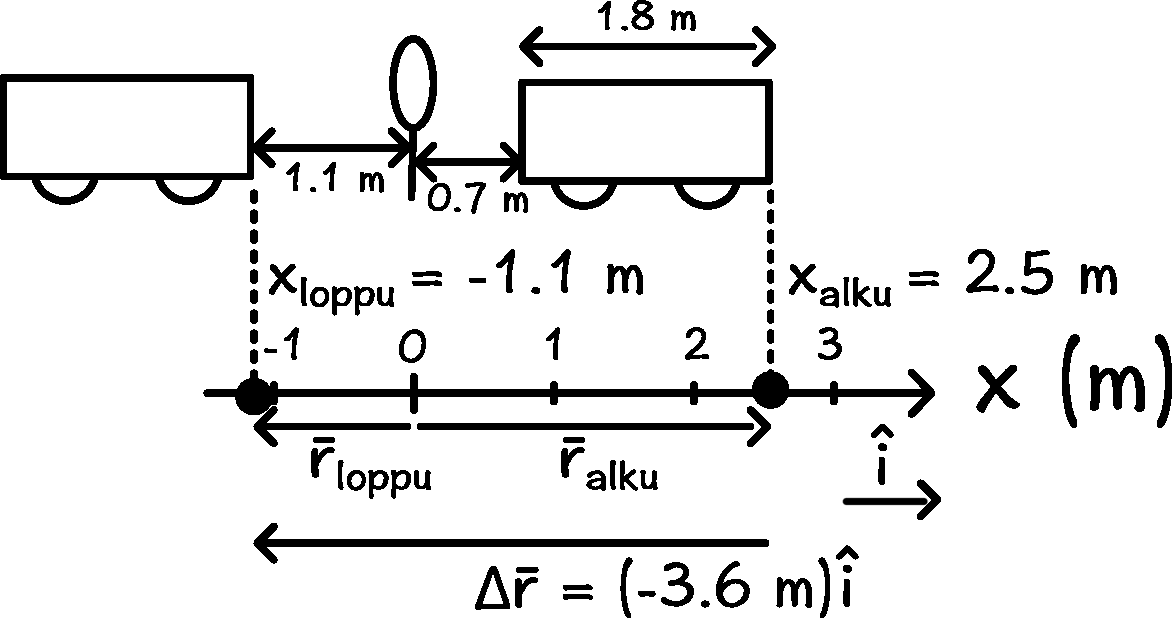
\includegraphics[width=0.9\textwidth]{figs/liike_esimerkki_siirtyma_1.pdf}%
\end{center}%
}

 \model  Jos kappaleen koordinaatit aluksi ja lopuksi ovat \(x_\text{alku}\) ja \(x_\text{loppu}\), sen koordinaatin muutos on \(\Delta x = x_\text{loppu} - x_\text{alku}\) ja siirtymävektori on \(\Delta \bs{r} = \Delta x \uv{i}\).

 \solu  Auton keula on aluksi etäisyydellä \(0.7 \un{m} + 1.8 \un{m} = 2.5 \un{m}\) merkistä. Niinpä tässä koordinaatistossa auton paikkakoordinaatti on aluksi \( x_\text{alku} = 2.5 \un{m}\). Koordinaatti on positiivinen, koska auto on merkin takana. Auto siirtyy sitten pisteeseen \( x_\text{loppu} = -1.1 \un{m} \), merkin eteen. Kappaleen paikkavektori on aluksi \( \bs{r}_\text{alku} = x_\text{alku} \uv{i} = (2.5 \un{m})\uv{i} \) ja lopuksi \(\bs{r}_\text{loppu} = x_\text{loppu} \uv{i} = (-1.1 \un{m})\uv{i}\).

Paikkakoordinaatin muutos on \(\Delta x = x_\text{loppu} - x_\text{alku} = (-1.1 \un{m}) - 2.5 \un{m} = -3.6 \un{m}\) ja paikkavektorin muutos on \(\Delta \bs{r} = \Delta x \uv{i} = (-3.6 \un{m})\uv{i} \).

 \eval Kappale siirtyy kohti negatiivista \(x\)-suuntaa, joten koordinaatin muutos on negatiivinen ja muutosvektori osoittaa kohti negatiivista \(x\)-suuntaa eli suuntaan \(-\uv{i}\).

Laskussa kaikki paikkavektoria käsittelevät suureet ovat vektoreita ja paikkakoordinaattia käsittelevät ovat skalaareita. Kaikissa yhtälöissä, joissa näitä vertaillaan, on skalaari kerrottu yksikkövektorilla \(\uv{i}\), jotta yhtälön molemmilla puolilla olisi vektorisuure.

\end{exam}

\begin{stopQ}{q:nopeusvektori}%
Eräs kappale on aluksi \(1.5\) metrin päässä koordinaatiston origosta positiivisessa \(x\)-suunnassa ja sekunnin päästä \(2.5\) metrin päässä origosta negatiivisessa \(x\)-suunnassa. Mikä on (a) kappaleen paikkakoordinaatti, (b) paikkavektori aluksi ja lopuksi? Mikä on (c) keskinopeuden skalaarikomponentti, (d) keskinopeusvektori tällä aikavälillä?
\end{stopQ}

\section{Kiihtyvyys}
\label{kiihtyvyys}

\index{kiihtyvyys}

Jos kappaleen nopeus ei ole nolla, kappale liikkuu. Harvoin kappaleen nopeus on kuitenkaan vakio, ja usein onkin tarpeellista ilmaista myös miten nopeus muuttuu. Tätä nopeuden muuttumista mittaava suure on nimeltään \textbf{kiihtyvyys}. Kiihtyvyyttä merkitään tavallisesti symbolilla \(a_x\), missä kirjain \(a\) tulee latinan sanasta accelerationem (`kiiruhtaminen').

Puhekielessä kiihtyvyydellä tarkoitetaan usein vauhdin kasvamista. Voidaan vaikkapa sanoa, että auto ``kiihdyttää'', kun sen vauhti lisääntyy, ja ``jarruttaa'' tai ``hidastaa'', kun sen vauhti pienenee. Tämä on kuitenkin fysikaalisesti epätäsmällistä kieltä. Fysiikassa ei puhuta hidastumisesta vaan \emph{kaikki liike, jossa nopeuden suuruus tai suunta muuttuu, on kiihtyvää liikettä}.

\subsection{Kiihtyvyyden suuruus ja suunta}
\label{kiihtyvyydensuuruusjasuunta}

Kiihtyvyyden ja nopeuden välistä yhteyttä on havainnollistettu kuvassa \autoref{fig:liikekiihtyvyys}, johon on piirretty liikediagrammi auton paikasta kolmena eri ajan hetkenä. Aluksi auto on paikoillaan. Sitten auto lähtee liikkeelle, ja ensimmäisen kahden sekunnin aikana se siirtyy kuvassa lyhyen matkan oikealle eli positiiviseen \(x\)-suuntaan. Seuraavan kahden sekunnin aikana auto jatkaa liikettään oikealle, mutta nyt se kulkee paljon pidemmän matkan, koska se on ehtinyt saada suuremman vauhdin.

\marginpicture%
{0}%
{Kiihtyvyys on osoittaa nopeuden muutoksen suunnan ja suuruuden.}%
{fig:liikekiihtyvyys}%
{1.0}%
{liike_kiihtyvyys_1c.pdf}

\onepicture{b!}%
{Kiihtyvyyden ja nopeuden etumerkki määräytyy sen mukaan, osoittaako kiihtyvyys- ja nopeusvektori positiiviseen vai negatiiviseen suuntaan.}%
{fig:liikekiihtyvyys_merkki}%
{1.0}%
{liike_kiihtyvyys_2c.pdf}

Nopeus on piirretty kuvaan punaisina nuolina, ja
nopeuden muutos näkyy kuvassa siten, että näiden nuolten pituus kasvaa ajan kuluessa. Kuvassa on myös määritetty nopeuden muutos piirtämällä nopeutta kuvaavat nuolet allekkain. Ensin nopeus on nolla, mitä kuvaa punainen piste. Seuraavaksi nopeus on 4 m\slash s oikealle, mitä kuvaa lyhyt oikealle osoittava nuoli. Nopeus siis muuttuu 4 m\slash s, ja tätä kuvaa oranssi nuoli oikealle.
Kolmantena tarkasteluhetkenä nopeus on jo 8 m\slash s, mitä kuvaa pitkä nuoli oikealle. Nopeuden muutos on jälleen 4 m\slash s oikealle, joten nopeuden muutosta kuvaa yhtä pitkä oranssi nuoli kuin ensimmäisellä tarkasteluvälillä.

Koska auton nopeus muuttui ensimmäisen kahden sekunnin aikana nollasta neljään eli 4 m\slash s, auton kiihtyvyys oli keskimäärin ``neljä metriä sekunnissa kahdessa sekunnissa.''
Seuraavan kahden sekunnin aikana nopeus muuttui neljästä kahdeksaan eli jälleen 4 m\slash s kahdessa sekunnissa, joten keskimääräinen kiihtyvyys oli sama kummallakin aikavälillä.

Kiihtyvyys määritellään tähän tapaan nopeuden muutoksen ja siihen kuluneen ajan suhteena.
Täsmälleen samoin määriteltiin nopeus, joka oli paikan muutoksen eli siirtymän ja siihen kuluneen ajan suhde. Kuitenkin jos auto siirtyy 4 metriä kahdessa sekunnissa, emme sano että sen nopeus on ``neljä metriä kahdessa sekunnissa'' vaan jaamme siirtymän, neljän metriä, siihen kuluneella ajalla, kahdella sekunnilla, ja saamme nopeudeksi \(4\un{m} / 2 \un{s} = 2 \un{m/s}\).
Samaan tapaan emme sano, että kiihtyvyys on ``4 m\slash s kahdessa sekunnissa''
vaan laskemme kiihtyvyydelle arvon jakamalla nopeuden muutoksen, 4 m\slash s, siihen kuluneella ajalla, 2 s, ja saamme kiihtyvyydeksi
\begin{equation} \frac{4 \un{m/s}}{2 \un{s}} = 2\ \frac{\text{m}}{\text{s} \cdot \text{s}} = 2\un{m/s}^2. \end{equation}
Tästä laskusta nähdään myös, mikä kiihtyvyyden yksikkö on. Se on ``metriä sekunnissa, sekunnissa'', joka sievenee muotoon m\slash s\(^2\) eli ``metriä per sekuntia toiseen''.

\begin{stopQ}{q:keskikiihtyvyys}%
Valitaan suoralla itä-länsisuuntaisella tiellä positiivinen suunta itään. Auto kulkee aluksi nopeudella \(v_x = 10 \un{m/s}\) itään. Mikä on (i) nopeus lopuksi (ii) nopeuden muutos ja (iii) keskimääräinen kiihtyvyys, jos auto kulkee viiden sekunnin kuluttua \(5 \un{m/s}\) (a) itään, (b) länteen?
\end{stopQ}

Kuvaan piirretty oranssi nuoli kuvasi auton nopeuden muutosta, mutta koska kiihtyvyys mittaa nopeuden muutosta, oranssi nuoli kuvaa suoraan myös auton keskimääräistä kiihtyvyyttä, kunhan mittakaava valitaan sopivasti.
Se, että kiihtyvyys piirretään nuolena, vihjaa kiihtyvyyden olevan vektorisuure. Sitä se onkin, sillä
\emph{kiihtyvyys on vektori, joka osoittaa aina siihen suuntaan, johon nopeusvektori muuttuu}.

Tätä on havainnollistettu kuvassa \autoref{fig:liikekiihtyvyys_merkki}, jonka kaikissa tilanteissa auto on kiihtyvässä liikkeessä.
Vasemmassa sarakkeessa nopeus osoittaa oikealle, sillä auto liikkuu tähän suuntaan. Koordinaatiston positiivinen suunta on myös valittu oikealla, joten auton nopeus \(v_x\) on näissä kuvissa positiivinen.
Oikeassa sarakkeessa auto kulkee vasemmalle, ja nopeus \(v_x\) on siis negatiivinen.

Taulukon ylärivillä nopeus muuttuu oikealle. Vasemmassa yläkulmassa nopeus on ensin nolla ja lopuksi se osoittaa oikealle. Tämä on täsmälleen sama tilanne kuin mitä kuvassa \autoref{fig:liikekiihtyvyys} nähtiin.
Oikeassa yläkulmassa sen sijaan nopeus on aluksi vasemmalla ja lopuksi nolla, jolloin nopeuden muutos on oikealle. Tämän voi ajatella myös niin, että jos nopeusvektorien kannat laitetaan samaan paikkaan, nopeus muuttuu siihen suuntaan johon nopeusvektorin kärki siirtyy. Vektorin kärki on aluksi vasemmalla ja se siirtyy ajan kuluessa oikealle, joten nopeuden muutos on oikealle.

Kiihtyvyys osoittaa aina nopeuden muutoksen suuntaan, joten taulukon ylärivillä oranssit kiihtyvyyttä kuvaavat nuolet osoittavat oikealle.
Kiihtyvyys on vektori, ja vektorin komponentin etumerkki riippuu vain ja ainoastaan siitä, osoittaako vektori koordinaatiston positiiviseen suuntaan. Positiivinen suunta on näissä kuvissa oikealle, ja kiihtyvyys osoittaa siihen suuntaan, joten kiihtyvyyden skalaarikomponentti \(a_x\) on positiivinen.
Huomaa erityisesti, että vasemman yläkulman kuvassa auton vauhti kasvaa mutta oikean yläkulman kuvassa vauhti pienenee. Silti kiihtyvyys on positiivinen myös oikeassa yläkulmassa. Kiihtyvyyden etumerkkiä ei siis mitenkään voi päätellä pelkästään vauhdin muuttumisesta, eikä myöskään positiivisesta kiihtyvyydestä voi päätellä vauhdin kasvavan.

\marginpictures%
{0}%
{Kiihtyvyys muuttaa nopeusvektoria.;%
Kiihtyvyys ja nopeus samaan suuntaan.;%
Kiihtyvyys ja nopeus vastakkaisiin suuntiin.}%
{fig:liike_nopeusmuuttuu}%
{0.8;0.8}%
{liike_nopeus_muuttuu_2.pdf;liike_nopeus_muuttuu_1.pdf}

Alarivin kuvissa kiihtyvyys osoittaa vasemmalle ja siispä \(a_x\) on negatiivinen. Vasemmassa alakulmassa nopeus on aluksi oikealle ja lopuksi nolla, eli auton vauhti pienenee. Oikeassa alakulmassa nopeus on aluksi nolla ja lopuksi vasemmalle, eli auton vauhti kasvaa. Tässäkin tapauksessa kiihtyvyyden \(a_x\) etumerkki määräytyy pelkästään sen mukaan, osoittaako kiihtyvyysvektori koordinaatiston positiiviseen vain negatiiviseen suuntaan.

Kiihtyvyyden etumerkistä ei siis voi päätellä, miten vauhti muuttuu. Kiihtyvyyden ja nopeuden avulla yhdessä tämä voidaan kuitenkin selvittää. Vauhti nimittäin kasvaa taulukon vasemmassa yläkulmassa sekä oikeassa alakulmassa. Yhteistä näille kuville on se, että kummassakin tapauksessa kiihtyvyys osoittaa samaan suuntaan kuin nopeus, eli \emph{vauhti kasvaa jos nopeus- ja kiihtyvyysvektorit osoittavat samaan suuntaan}.

Kiihtyvyyshän osoittaa siihen suuntaan, mihin nopeusvektorin kärki siirtyy. Jos kärki siirtyy samaan suuntaan kuin mihin nopeusvektori jo ennestään osoitti, kärki siirtyy \emph{kauemmas vektorin kannasta} ja vektorista tulee pidempi. Nopeusvektorin pituus on kuitenkin sama asia kuin vauhti, joten tällöin vauhti kasvaa.
Vauhti puolestaan pienenee silloin, kun kiihtyvyys ja nopeus osoittavat vastakkaisiin suuntiin, mikä onkin tilanne kuvan oikeassa yläkulmassa ja vasemmassa alakulmassa. Silloin nopeusvektorin kärki siirtyy \emph{kohti vektorin kantaa}, jolloin vektorin pituus lyhentyy eli vauhti pienenee.

\begin{stopQ}{q:va_etumerkit}%
Suoralla etelä-pohjoissuuntaisella tiellä on risteys. Asetetaan origo risteykseen ja positiivinen suunta pohjoiseen. Mikä on auton nopeuden \(v_x\) ja kiihtyvyyden \(a_x\) etumerkki, jos auto on (a) risteyksen pohjoispuolella matkalla kohti risteystä ja vauhti hidastuu, (b) risteyksen eteläpuolella matkalla kohti risteystä ja vauhti hidastuu, (c) risteyksen eteläpuolella matkalla poispäin risteyksestä ja vauhti kasvaa?
\end{stopQ}

\subsection{Putoamisliike}
\label{putoamisliike}

\index{vapaa pudotus}
\index{painovoima}
\index{heittoliike}
\index{vuorovaikutus}

\textbf{Vapaa pudotus} on yksinkertainen esimerkki kiihtyvästä liikkeestä. Sillä tarkoitetaan liikettä, jonka kappale kokee, kun sen annetaan pudota maapallon \emph{painovoiman} vaikutuksesta ilman muita kappaleen liikkeeseen vaikuttavia tekijöitä. Vaikka arkikielessä putoaminen tarkoittaa aina alaspäin tapahtuvaa liikettä, fysikaalisesti ylöspäin heitetty tai ammuttu kappale on vapaassa pudotuksessa myös liikkuessaan ylöspäin. Varsinainen heitto vaikuttaa tällöin kappaleen saamaan alkunopeuteen, mutta kun kappaleesta päästetään irti, sen liikerata määräytyy pelkästään painovoiman eli maapallon ja kappaleen välisen vuorovaikutuksen perusteella.

\pictures{tb}%
{Vapaa pudotus, jossa alkunopeus on ylöspäin.;%
Liikediagrammi.;%
Paikan kuvaaja.}%
{fig:liikeputoaminen;fig:liikeputoaminen:diagrammi;fig:liikeputoaminen:kuvaaja}%
{0.2;0.75}%
{0.2;0.75}%
{liike_putoaminen_1.pdf;liike_putoaminen_2.pdf}

Tällainen liike on esitetty kuvassa \autoref{fig:liikeputoaminen}.
Suoraan ylöspäin heitetty kappale liikkuu vain pystysuoraa pitkin, jolloin \(x\)-akseliksi voidaan valita pystysuora suunta. Jos lisäksi positiiviseksi suunnaksi valitaan suunta ylöspäin, \(x\)-koordinaatti mittaa kappaleen korkeutta. Tässä koordinaatistossa ylöspäin heitetyn kappaleen nopeus on aluksi positiivinen. Kappaleen vauhti kuitenkin pienenee. Lopulta kappale saavuttaa liikeratansa korkeimman kohdan eli lakipisteen. Tässä pisteessä kappaleen pystysuuntainen nopeus on hetkellisesti nolla, minkä jälkeen kappale alkaa liikkua alaspäin.

Voimme tutkia kappaleen kiihtyvyyttä liikediagrammin avulla tarkastelemalla kappaleen nopeuden muutosta. Kun kappale liikkuu ylöspäin, sen nopeusvektori osoittaa ylöspäin, mutta nopeutta kuvaavien nuolten pituus lyhenee, jolloin nopeuden muutoksen suunta on alaspäin. Kiihtyvyysvektori siis osoittaa alaspäin ja kiihtyvyys \(a_x\) on negatiivinen. Kappaleen liikkuessa alaspäin sen nopeusvektori osoittaa alaspäin, ja koska vektorin pituus kasvaa, nopeus muuttuu nytkin alaspäin. Kiihtyvyysvektori osoittaa alas siis myös kappaleen laskeutuessa.

\index{lakipiste}

\marginpicture%
{0}%
{Lakipisteessä nopeus kääntyy.}%
{fig:liikeputoaminen3}%
{0.4}%
{liike_nopeus_muuttuu_3.pdf}

Heiton lakipistettä on vielä syytä tarkastella erikseen. Juuri ennen lakipistettä kappaleen nopeusvektori osoittaa ylöspäin, ja juuri lakipisteen jälkeen nopeus osoittaa alaspäin. Nopeusvektori on siis myös heiton lakipisteessä muuttumassa alaspäin, ja niinpä kappale on kiihtyvässä liikkeessä myös lakipisteessä. Kiihtyvyysvektori osoittaa tällöinkin alaspäin.
Näin ollen kiihtyvyysvektori osoittaa alaspäin \emph{kaikkialla} kappaleen lentoradalla. Tässä koordinaatistossa kiihtyvyys on siis aina negatiivinen. On varsin tavallinen väärinkäsitys ajatella, että kappaleen kiihtyvyys olisi lakipisteessä nolla, mutta tämä on \emph{väärin}. Kappaleen \emph{nopeus} on lakipisteessä hetkellisesti nolla, mutta nopeus muuttuu koko ajan, joten nopeuden muutosta mittaava \emph{kiihtyvyys} ei ole nolla edes lakipisteessä.

\marginpicture%
{0}%
{Nopeus ja kiihtyvyys vapaassa pudotuksessa.}%
{fig:liikeputoaminen2}%
{1.0}%
{liike_putoaminen_3.pdf}

Nopeus määriteltiin paikan derivaattana, joten nopeus on graafisesti paikan kuvaajan tangentin kulmakerroin.
Aluksi paikan kuvaaja nousee jyrkästi, jolloin nopeus on positiivinen ja vauhti suuri. Kun paikan kuvaaja loivenee, vauhti pienenee. Lakipisteessä paikan kuvaaja on vaakasuora, jolloin nopeus on nolla. Kun paikan kuvaaja alkaa laskea, nopeudesta tulee negatiivinen, ja mitä jyrkemmin paikan kuvaaja laskee, sitä suuremmaksi nopeuden itseisarvo muuttuu.
Koska nopeus on aluksi positiivinen ja lopuksi negatiivinen, sen kuvaajan täytyy olla laskeva käyrä. Itse asiassa nopeuden kuvaaja on \emph{laskeva suora} kuten kuvaan \autoref{fig:liikeputoaminen2} on piirretty. Perustelemme tämän väitteen täsmällisesti hiukan myöhemmin.

\index{putoamiskiihtyvyys}
\index{tasaisesti kiihtyvä liike}

Kiihtyvyys on sen sijaan koko ajan negatiivinen, myös heiton lakipisteessä.
Ilmakehässä täysin vapaa pudotus ei käytännössä ole mahdollinen, koska putoaminen ilman läpi vaikuttaa kappaleen liikkeeseen. Kuitenkin jos kappaleen ja ilman välinen vuorovaikutus ei ole merkittävä, kappaleen kiihtyvyys on itse asiassa koko ajan sama.
Tätä vakiokiihtyvyyttä kutsutaan \textbf{putoamiskiihtyvyydeksi}, ja sen aiheuttaa yksin painovoima.

\begin{stopQ}{q:pomppukiihtyvyys}%
Kappale osuu maahan ja pomppaa takaisin ylöspäin. Mihin suuntaan kappaleen nopeus- ja kiihtyvyysvektorit osoittavat (a) juuri ennen maahan osumista, (b) kappaleen koskettaessa maata ja (c) juuri maasta irtoamisen jälkeen? (d) Mitä samaa on pomppaavalla kappaleella sen koskettaessa maata ja heitetyllä kappaleella lakipisteessä?
\end{stopQ}

\subsection{Kiihtyvyyden matemaattinen kuvaus}
\label{kiihtyvyydenmatemaattinenkuvaus}

\emph{Keskimääräinen kiihtyvyys määritellään nopeuden muutoksen ja muutokseen kuluneen ajan suhteena},
\begin{equation} a_{x,\text{keskiarvo}} = \frac{\Delta v_x}{\Delta t}. \label{keskikiihtyvyys} \end{equation}
Määritelmä on aivan samanlainen kuin keskimääräisen nopeuden määritelmä, sillä nopeushan määriteltiin paikan muutoksen ja siihen kuluneen ajan suhteena. Ero on vain siinä, että paikan muutoksen sijaan nyt tarkastellaan nopeuden muutosta. \emph{Kiihtyvyys kertoo siis nopeudesta saman, mitä nopeus kertoo paikasta.}

Jotta saisimme selville \emph{hetkellisen kiihtyvyyden} keskimääräisen kiihtyvyyden sijaan, meidän on otettava raja-arvo, kun ajan muutos lähestyy nollaa. Näin erotusosamäärä muuttuu derivaataksi ja saamme kiihtyvyyden \(x\)-komponentille täsmällisen lausekkeen
\begin{equation} a_x = \frac{\dd v_x}{\dd t} = v_x'(t). \label{kiihtyvyysderivaatta} \end{equation}
Graafisesti derivaatta vastaa kuvaajan tangentin kulmakerrointa, joten kiihtyvyys on siis nopeuden kuvaajan kulmakerroin (kuva \autoref{fig:liikekiihtyvyys_derivaatta}).
Kiihtyvyysvektori määritellään vastaavasti nopeusvektorin derivaattana
\bigeq{ \bs{a} = \frac{\dd \bs{v}}{\dd t} = \frac{\dd v_x}{\dd t} \uv{i} = v_x'(t) \uv{i} = a_x \uv{i}. \label{kiihtyvyysvektori}}
Kiihtyvyyden ja nopeuden välinen yhteys on siis täsmälleen sama kuin nopeuden ja paikan välinen yhteys.

\marginpicture%
{-20}%
{Kiihtyvyys on nopeuden kuvaajan tangentin kulmakerroin.}%
{fig:liikekiihtyvyys_derivaatta}%
{1.0}%
{liike_kiihtyvyys_derivaatta.pdf}

\index{derivaatta}
\index{differentiaali, $\dd$}

Koska nopeus on paikan derivaatta ja kiihtyvyys on nopeuden derivaatta, saadaan kiihtyvyys siis laskettua paikan avulla derivoimalla paikkaa ajan suhteen kaksi kertaa. Toisin sanoen kiihtyvyys on paikan toinen derivaatta ajan suhteen. Moninkertaisia derivaattoja voidaan merkitä esimerkiksi kahdella pilkulla \(a_x(t) = x''(t) \). Fysiikassa kuitenkin käytetään yleisemmin differentiaalimerkintää, jolloin voidaan muodollisesti kirjoittaa
\begin{equation} a_x = \frac{\dd v_x}{\dd t} = \frac{\dd \left( \dd x/\dd t\right)}{\dd t} = \frac{\dd }{\dd t} \left( \frac{\dd x}{\dd t} \right) = \frac{\dd \dd x}{\dd t \dd t} = \frac{\dd^2 x}{\dd t^2}. \end{equation}
Tässä merkinnässä on syytä huomata, kuinka viimeisen lausekkeen osoittajassa on kaksoisdifferentiaali \(\dd^2\) ja nimittäjässä on differentiaalin neliö \(\dd t^2\). Vaikka lausekkeessa esiintyykin toista potenssia muistuttavia symboleita, merkintä \emph{ei tarkoita}, että tässä laskettaisiin toisia potensseja vaan että derivointi suoritetaan kaksi kertaa.
Ihan samaan tapaan voidaan määritellä vielä korkeammankin kertaluvun derivaattoja kuvaamaan liikettä. Useimmiten kuitenkin paikka, nopeus ja kiihtyvyys riittävät.

\begin{stopQ}{q:kiihtyvyysderivaatta}%
Kappaleen paikka on \(x(t) = (2.5 \un{m/s}^3) t^3 + (4.0 \un{m/s}) t \). Mitä ovat\\
(a) kappaleen nopeus,\\
(b) kappaleen kiihtyvyys?\\
(c) Integroi kiihtyvyys ajan suhteen. Onko tulos sama kuin nopeus?
\end{stopQ}

\index{tangentti}
\index{kulmakerroin}
\index{pinta-ala}
\index{derivaatta}
\index{integraali}

\marginpictures%
{-20}%
{Kiihtyvyyden kuvaajan rajaama ala kuvaa nopeuden muutosta.;%
Kappaleen kiihtyvyys.;%
Saman kappaleen nopeus.}%
{fig:liikekiihtyvyys_integraali}%
{1.0;1.0}%
{liike_kiihtyvyys_integraali_1.pdf;liike_kiihtyvyys_integraali_2.pdf}

Täsmälleen samalla tavalla kuin yhtälössä (\autoref{paikkaintegraali}) lausutaan paikka nopeuden integraalina, voidaan nopeus ilmaista kiihtyvyyden integraalina. Toistetaan harjoituksen vuoksi tämä päättely, mutta jätetään raja-arvotarkastelut pois ja käytetään päättelyssä vain differentiaaleja.

Aloitetaan kertomalla yhtälö (\autoref{kiihtyvyysderivaatta}) puolittain differentiaalilla \(\dd t\), jolloin saadaan
\begin{equation} a_x \dd t = \frac{\dd v_x}{\dd t} \dd t = \dd v_x \frac{\dd t}{\dd t} = \dd v_x. \end{equation}
Yhtälön vasen ja oikea puoli voidaan integroida erikseen, jolloin saadaan
\begin{equation} \int_{t_{\text{alku}}}^{t_{\text{loppu}}} a_x \dd t = \int_{v_{x,\text{alku}}}^{v_{x,\text{loppu}}} \dd v_x. \end{equation}
Vasemmalla puolella on integraali tuntemattomasta funktiosta \( a_x(t) \), joka voi olla oikeastaan mitä vain, joten tätä integraalia ei voi sieventää sen enempää. Yhtälön oikealla puolella olevan integraalin sen sijaan voi laskea.

Tämä integraali voi näyttää oudolta, koska differentiaalina on siellä \(\dd v_x\), mutta ei ole mitään väliä, mitä kirjainta millekin symbolille käytetään.
Jos symbolin \(v_x\) käyttö sekoittaa ajatukset, voit ihan hyvin vaihtaa sen tilalle jonkin toisen kirjaimen, vaikkapa \(y\):n. Jos siis teemme vaihdon \(v_x = y\), laskettavana on integraali \(\int \dd y\). Näyttää, että integroitavana ei ole mitään, mutta oikeasti integraalin sisällä on vakiofunktio \( f(y) = 1 \), jonka integraalifunktio on \( i(y) = y \).
Siispä saadaan
\begin{equation} \int_{y_{\text{alku}}}^{y_{\text{loppu}}} \dd y = \bigg|_{y_{\text{alku}}}^{y_{\text{loppu}}} y = y_{\text{loppu}} - y_{\text{alku}} = \Delta y. \end{equation}
Jos vielä vaihdetaan takaisin alkuperäiseen muuttujaan \(v_x\), saadaan
\begin{equation} \int_{v_{x,\text{alku}}}^{v_{x,\text{loppu}}} \dd v_x = \Delta v_x. \end{equation}

Nopeuden differentiaalin integraali on siis sama asia kuin nopeuden muutos.
Alkuperäisen yhtälön mukaan tämän pitää olla yhtä suuri kuin kiihtyvyyden integraali ajan suhteen eli
\begin{equation} \Delta v_x = \int_{t_{\text{alku}}}^{t_{\text{loppu}}} a_x \dd t. \end{equation}
Nopeuden muutos on siis kiihtyvyyden integraali ajan suhteen.
Jos haluamme vielä ratkaista nopeuden muutoksen sijaan nopeuden ajan funktiona, voimme merkitä tarkastelujakson loppuaikaa yksinkertaisesti \(t\) pidemmän symbolin \(t_\text{loppu}\) sijaan, jolloin saamme
\begin{equation} v_x(t) = v_{x,\text{loppu}} = v_{x,\text{alku}} + \int_{t_\text{alku}}^{t} a_x(\underline{t}) \dd \underline{t}. \label{kiihtyvyysintegraali} \end{equation}

Derivaatta vastaa graafisessa esityksessä kulmakerrointa, joten kiihtyvyys on nopeuden kuvaajan tangentin kulmakerroin. Vastaavasti integraali vastaa kuvaajan rajaaman pinta-alan määrittämistä, joten nopeuden muutos tietyllä aikavälillä voidaan määrittää kiihtyvyyden kuvaajan rajaamana pinta-alana (kuva \autoref{fig:liikekiihtyvyys_integraali}).

\begin{stopQ}{q:va_esimerkki}%
Keksi esimerkki funktiosta \( x(t) \), johon liittyvä nopeus on aina negatiivinen mutta kiihtyvyys on aina positiivinen. Osoita laskemalla, että näin on.
\end{stopQ}

\begin{exam}{Juna}{ex:juna}\noindent

\index{integraali}

\problem{Juna liikkuu nopeudella \(v_{x,\text{alku}} = 150 \un{km/h}\) alkaessaan jarruttaa. Jarrutuksen aikana junan nopeutta kuvaa ajan funktio \(a_x(t) = -b + c t\) kunnes juna pysähtyy, minkä jälkeen kiihtyvyys on nolla. Vakioiden arvot ovat tässä \(b = 2.24 \un{m/s}^2\) sekä \(c = 0.0600 \un{m/s}^3\). (a) Milloin juna pysähtyy? (b) Kuinka pitkä on junan jarrutusmatka?
}

 \twocol{0.49}{0.5}{ \setup  Piirretään junan liikkeestä liikediagrammi. Merkitään junan pysähtymisen hetkeä \(t_\text{stop}\) ja junan kulkemaa matkaa \(\Delta x\). Nämä ovat kysytyt suureet.

 \physics Juna pysähtyy, kun sen nopeus saavuttaa arvon \(v_x = 0 \un{m/s}\).
Junan nopeus voidaan laskea kiihtyvyyden integraalina ja sen kulkema matka nopeuden integraalina.

Laskuja varten on lisäksi syytä muuntaa alkunopeus yksiköihin m\slash s. Koska kilometri on 1000 metriä ja tunti on 3600 sekuntia, saadaan muunnos
\begin{equation} \frac{\text{km}}{\text{h}} = \frac{1000 \un{m}}{3600 \un{s}} = \frac{10}{36} \un{m/s}. \end{equation}
Siispä alkunopeus on
\( v_\text{alku} = 150 \un{km/h} = 150 \cdot 10/36 \un{m/s} = 41.7 \un{m/s}. \)

}{%
\begin{center}%
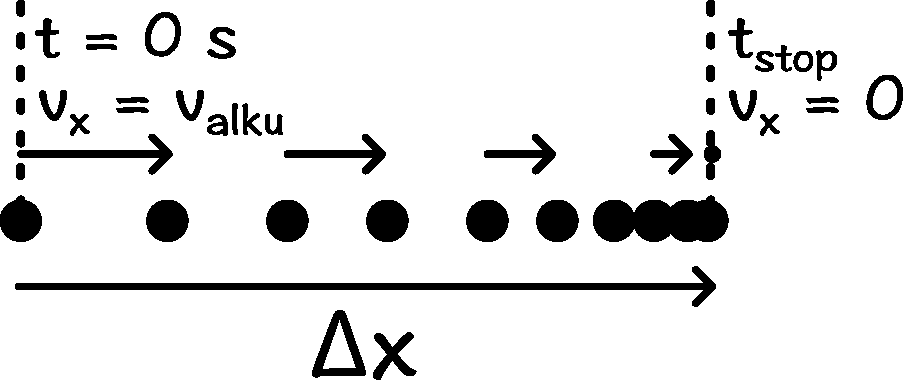
\includegraphics[width=0.9\textwidth]{figs/liike_esimerkki_juna.pdf}%
\end{center}%
}

 \model  Nopeus on yhtälön (\autoref{kiihtyvyysintegraali}) perusteella
\begin{equation} v_x(t) = v_{x,\text{alku}} + \int_{0}^{t} a_x(\underline{t}) \dd \underline{t}, \end{equation}
missä ajan nollahetki on valittu jarrutuksen alkuun, \(t_\text{alku} = 0 \un{s}\).

Kun nopeus on ratkaistu, pysähtymishetki on ratkaistavissa ehdosta
\( v_x(t_\text{stop}) = 0 \un{m/s}. \)
Ennen tätä juna ehtii kulkea matkan
\begin{equation} \Delta x = \int_{0}^{t_\text{stop}} v_x \dd t. \end{equation}

 \solu  (a) Junan nopeus on
\begin{equation} v_x(t) = v_{x,\text{alku}} + \int_{0}^{t} (-b + c \underline{t}) \dd \underline{t} = v_\text{alku} + \bigg|_{0}^{t} -b\underline{t} +\frac{1}{2}c\underline{t}^2 = v_\text{alku} - bt + \frac{1}{2}ct^2. \end{equation}
Juna pysähtyy, kun tämä on nolla eli kun
\( v_{x,\text{alku}} - b t_\text{stop} + c t_\text{stop}^2 = 0 \).
Tämä on toisen asteen yhtälö, jonka ratkaisu on
\begin{equation} t_\text{stop} = \frac{1}{2c} ( b \pm \sqrt{ b^2 - 4 c v_{x,\text{alku}} } ). \end{equation}
Sijoittamalla tähän lukuarvot saadaan mahdolliset ratkaisut \(35.1 \un{s}\) sekä \(39.5 \un{s}\).
Koska annettu nopeuden lauseke pätee vain siihen asti kunnes juna pysähtyy, ensimmäisen ajan hetken on oltava oikea ratkaisu. Siispä
\( t_\text{stop} = 35.1 \un{s}. \)

(b) Junan kulkema matka on
\begin{equation} \Delta x = \int_0^{t_\text{stop}} ( v_{x,\text{alku}} - b t_\text{stop} + \frac{1}{2}c t_\text{stop}^2 ) \dd t = \bigg|_0^{t_\text{stop}} v_{x,\text{alku}} t - \frac{1}{2} b t^2 + \frac{1}{6} c t^3 = v_{x,\text{alku}} t_\text{stop} - \frac{1}{2} b t_\text{stop}^2 + \frac{1}{6} c t_\text{stop}^3. \end{equation}
Lukuarvojen sijoitus tähän antaa ratkaisuksi noin
\( \Delta x = 515 \un{m}. \)

%\newpage
\mbar
\begin{mathematica}[commandchars=\\!?]
(* kiihtyvyys ajan funktiona *)
ax[t_] := -b + c t

(* nopeus ajan funktiona *)
vx[t_] := valku + Integrate[ax[tt], {tt, 0, t}]

(* tallennetaan lukuarvot *)
kmh = 1000/3600;
lukuarvot = {valku -> 150 kmh, c -> 0.060, b -> 2.24};

(* ratkaistaan pys\"ahtymishetki *)
stop = Solve[vx[tstop] == 0, tstop]
  \textit!{{tstop -> (-3 b + Sqrt[9 b^2 - 750 c])/(3 c)},?
  \textit! {tstop -> (3 b + Sqrt[9 b^2 - 750 c])/(3 c)}?
stop /. lukuarvot (* sijoitetaan numeroarvot *)
  \textit!{{tstop -> 35.1223}, {tstop -> 39.5444}}?

(* ratkaistaan kuljettu matka *)
matka = Integrate[vx[t], {t, 0, tstop}]
  \textit!-((b tstop^2)/2) + (c tstop^3)/6 + tstop valku?
matka /. stop /. lukuarvot
  \textit!{515.084, 514.652}?

(* nopeuden kuvaaja *)
Plot[vx[t] /. lukuarvot, {t, 0, 40}]
\end{mathematica}
\begin{center}
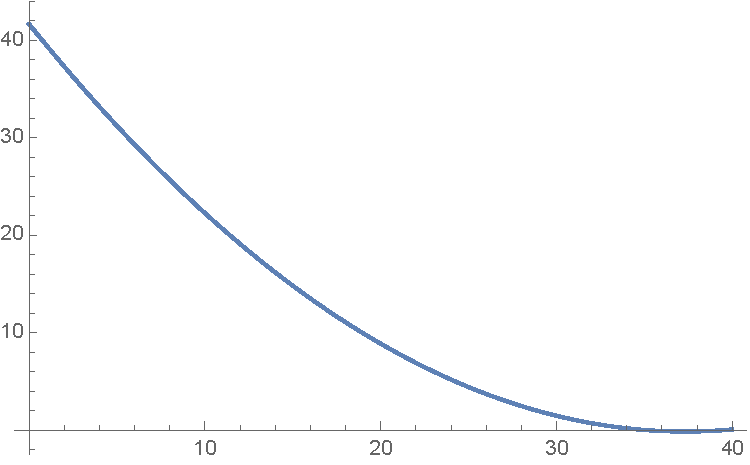
\includegraphics[width=0.4\textwidth]{figs/liike_esimerkki_junaplot.pdf}
\end{center}

 \eval  Nopeuden kuvaajasta voidaan lukea, että junan nopeus todellakin saavuttaa \(t\)-akselin eli arvon nolla kun \(t \approx 35 \un{s}\). Tämän jälkeen lauseke ei ole enää voimassa, mutta Mathematica piirtää funktion niin pitkälle kuin pyydetään. Tietokoneen antamat tulokset on siis aina tulkittava kriittisesti.

Junan kulkemaa matkaa edustaa kuvaajan alle jäänyt pinta-ala. Tätä voidaan arvioida karkeasti kolmiona, jonka kärjet ovat origossa sekä pisteissä \( (0 \un{s}, 40 \un{m/s}) \) sekä \( (30 \un{s}, 0 \un{m/s}) \). Tällaisen kolmion pinta-ala on \( \frac{1}{2} \cdot 30 \un{s} \cdot 40 \un{m/s} = 600 \un{m} \), mikä on jonkin verran enemmän kuin integroiden laskettu tarkka arvo, mutta selkeästi ratkaisun suuruusluokka on järkevä.

Ratkaisuilla on ajan ja pituuden yksiköt kuten pitääkin:
\begin{equation} [t_\text{stop}] = \frac{1}{[c]} ( [b] + \sqrt{[b^2] + [c v]} )  = \text{s}^3/\text{m} (\text{m/s}^2 + \sqrt{ \text{m}^2/\text{s}^4 + \text{m/s}^3 \cdot \text{m/s}}) = \text{s}^3/\text{m} (\text{m/s}^2 + \sqrt{ \text{m}^2/\text{s}^4 }) = \text{s}^3/\text{m} \cdot \text{m/s}^2  = \text{s}. \end{equation}
\begin{equation} [\Delta x] = [v t] + [b t^2] + [c t^3] = \text{m/s} \cdot \text{s} + \text{m/s}^2 \cdot \text{s}^2 + \text{m/s}^3 \cdot \text{s}^3 = \text{m}+\text{m}+\text{m} = \text{m}. \end{equation}

\end{exam}

\begin{stopQ}{q:ilmanvastuskiihtyvyys}%
Kun ilmanvastus huomioidaan, vapaassa pudotuksessa olevan kappaleen kiihtyvyys noudattaa likimain lauseketta \(a_x(t) = - g e^{-t / \tau} \), missä \(\tau\) on kappaleen koosta ja muodosta riippuva ilmanvastusta kuvaava vakio. Jos kappale pudotetaan levosta korkeudelta \(x_\text{alku}\), mikä on sen nopeus ja paikka ajan funktiona?
\end{stopQ}

\subsection{Tasaisesti kiihtyvä liike}
\label{tasaisestikiihtyväliike}

Esimerkissä \autoref{ex:juna} nähtiin, miten nopeus ja paikka lasketaan kiihtyvyyttä integroimalla. Tämä periaate toimii aina, koska se perustuu kiihtyvyyden määritelmään. Monesti kappaleet kuitenkin liikkuvat yksinkertaisemmilla tavoilla kuin esimerkin juna, jolloin nopeuden tai paikan ratkaiseminen voi onnistua myös ilman integraalien laskemista. Tutkitaan siis vielä muutamia yleisiä erikoistapauksia ja tutkitaan, miten nopeus ja paikka niissä käyttäytyvät.

Levossa oleminen on yksinkertaisinta liikettä, koska silloinhan ei liikuta lainkaan. Toiseksi yksinkertaisinta on tasainen liike, jolloin nopeus pysyy koko ajan samana. Oikeastaan paikoillaan oleminenkin on tasaista liikettä, sillä silloinkin nopeus on vakio. Sehän on nimittäin nolla.
Joka tapauksessa kun nopeus on vakio, oli se sitten nolla tai jotakin muuta, se ei muutu. Kiihtyvyys puolestaan kertoo, \emph{miten} nopeus muuttuu, ja niinpä jos nopeus ei muutu, kiihtyvyyttä ei ole. Toisin sanoen jos nopeus on vakio, kiihtyvyys on nolla, ja myös päinvastainen on totta: jos kiihtyvyys on nolla, nopeus ei voi muuttua.

Yksinkertaisinta liikettä, jossa nopeus muuttuu, lienee sellainen jossa kiihtyvyys on vakio. Tätä kutsutaan \textbf{tasaisesti kiihtyväksi liikkeeksi}.
Tällaisessa liikkeessä kiihtyvyyden keskiarvo on aina sama kuin kiihtyvyys itse, ja niinpä kiihtyvyys voidaan laskea mittaamalla nopeus kahtena ajan hetkenä ja jakamalla nopeuden muutos siihen kuluneella ajalla
\begin{equation} a_{x,\text{tasainen}} = \frac{\Delta v_x}{\Delta t} = \frac{v_{x,\text{loppu}} - v_{x,\text{alku}}}{ t_{\text{loppu}} - t_{\text{alku}}}.  \end{equation}

\begin{stopQ}{q:tasainenkiihtyvyys}%
Kappale liikkuu aluksi vasemmalle 2.0 m\slash s vauhdilla. Sitten kappale kääntyy tasaisella kiihtyvyydellä ympäri niin, että lopuksi sen vauhti on 2.0 m\slash s ja liike oikealle. Käännökseen kuluu aikaa 0.50 s. Valitaan positiivinen suunta vasemmalle.\\
(a) Mikä oli vauhdin muutos? (b) Mikä oli nopeuden muutos? (c) Mikä oli kiihtyvyys?
\end{stopQ}

Jos sen sijaan tiedämme alkunopeuden ja kiihtyvyyden, voimme ratkaista tästä loppunopeudeksi
\begin{equation} v_{x,\text{loppu}} = v_{x,\text{alku}} + a_{x,\text{tasainen}} \Delta t. \end{equation}
Jos loppuaikaa merkitään yksinkertaisesti \(t\), kulunut aika on \(\Delta t = t - t_\text{alku}\), ja näin nopeus saadaan kirjoitettua ajan funktiona muotoon
\begin{equation} v_x(t) = v_{x,\text{alku}} + a_{x,\text{tasainen}} (t - t_\text{alku}). \label{tasaisenkiihtyvyydennopeus} \end{equation}

\begin{stopQ}{q:integroikiihtyvyys}%
Nopeus voidaan laskea aina kiihtyvyyden integraalina yhtälön (\autoref{kiihtyvyysintegraali}) mukaan. Laske nopeus integroimalla kiihtyvyyttä (samoilla oletuksilla kuin yllä), ja tarkista, että saat saman tuloksen kuin (\autoref{tasaisenkiihtyvyydennopeus}).
\end{stopQ}

Paikan laskeminen on hieman hankalampaa kuin nopeuden, koska paikan muutos riippuu nopeudesta eikä nopeus ole nyt vakio kuten kiihtyvyys oli. Siirtymä ja paikka voidaan kuitenkin aina laskea nopeuden integraalina yhtälöiden (\autoref{integraali}) ja (\autoref{paikkaintegraali}) mukaisesti.
Kun tarkasteltavan aikajakson loppua merkitään taas symbolilla \(t\), paikalle saadaan johdettua ajan funktio

\begin{eqnarray} x(t) & = & x_\text{alku} + \int_{t_\text{alku}}^{t} v_x(\underline{t}) \dd \underline{t} \\
& = & x_\text{alku} + \int_{t_\text{alku}}^{t} \left[ v_{x,\text{alku}} + a_{x,\text{tasainen}} (\underline{t} - t_\text{alku}) \right] \dd \underline{t} \\
& = & x_\text{alku} + \bigg|_{t_\text{alku}}^{t} \left[ v_{x,\text{alku}} \underline{t} + \frac{1}{2} a_{x,\text{tasainen}} (\underline{t} - t_\text{alku})^2 \right] \\
& = & x_\text{alku} + v_{x,\text{alku}} (t - t_\text{alku}) + \frac{1}{2} a_{x,\text{tasainen}} (t - t_\text{alku})^2. \label{paikkatasaisessakiihtyvyydessa} \end{eqnarray}

Huomaa erityisesti, että integraalilaskun lopputuloksena kiihtyvyystermiin tuli kertoimeksi puolikas.

\begin{stopQ}{q:derivoikiihtyvyys}%
Kiihtyvyys on paikan toinen derivaatta, \( a_x(t) = x''(t) \).
Derivoi paikan lauseke (\autoref{paikkatasaisessakiihtyvyydessa}) kaksi kertaa ajan suhteen ja tarkista, että sitä vastaava kiihtyvyys tosiaan on vakio.
\end{stopQ}

Nopeutta kuvaava lauseke (\autoref{tasaisenkiihtyvyydennopeus}) on \emph{suoran} yhtälö, sillä siinä aika esiintyy \emph{ensimmäisen asteen polynomissa} \(  a_{x,\text{tasainen}}(t - t_\text{alku}) \).
Paikkaa kuvaava lauseke (\autoref{paikkatasaisessakiihtyvyydessa}) on puolestaan \emph{paraabelin} yhtälö, sillä siinä aika on \emph{toisen asteen polynomissa} \( \frac{1}{2} a_{x,\text{tasainen}}(t - t_\text{alku})^2 \) eli toisessa potenssissa.
Yhteenvetona siis tasaisesti kiihtyvässä liikkeessä kiihtyvyys on vakio, jolloin sen aikakuvaajan täytyy olla vaakasuora. Nopeuden kuvaaja on puolestaan suora ja paikan kuvaaja on paraabeli.

Juuri tämän näimme jo vapaasti putoavan kappaleen tapauksessa, sillä kuvassa \autoref{fig:liikeputoaminen2} nopeuden kuvaajaksi saatiin suora, ja paikan kuvaajaksi paraabeli. Edelliset laskut osoittavat, että jos heitetyn kappaleen paikkakoordinaatin kuvajaa piirtää paraabelin, se todella on tasaisesti kiihtyvässä liikkeessä. Myös päinvastainen on totta: jos jokin kappale on tasaisesti kiihtyvässä liikkeessä, sen nopeuden kuvaajasta tulee välttämättä suora ja paikan kuvaajasta paraabeli.

\subsection{Putoamiskiihtyvyys}
\label{putoamiskiihtyvyys}

Putoava kappale on siis tasaisesti kiihtyvässä liikkeessä. Selvitetään vielä kokeellisesti, kuinka suuri tämä kiihtyvyys on.
Tämä onnistuu, kun heitämme kappaleita ylöspäin tai annamme niiden pudota vapaasti alaspäin ja mittaamme niiden liikettä. Voimme esimerkiksi kuvata liikkeestä hidastetun videon, josta voidaan jälkeenpäin lukea, missä kappale milloinkin oli.

Päättelimme jo aikaisemmin, että tasaisesti kiihtyvässä liikkeessä olevan kappaleen paikan pitäisi noudattaa lauseketta (\autoref{paikkatasaisessakiihtyvyydessa}). Jos pudotamme vaikkapa tennispallon levosta, sen alkunopeus on nolla, \(v_{x,\text{alku}} = 0 \un{m/s}\). Jos valitsemme koordinaatiston origon pallon lähtöpisteeseen, alkupaikka on nolla \(x_{\text{alku}} = 0 \un{m}\). Ja jos vielä asetamme ajan nollahetkeksi sen, kun pallo päästetään putoamaan, alkuaikakin on nolla \(t_{\text{alku}} = 0 \un{s}\). Näillä oletuksilla paikan lauseke yksinkertaistuu muotoon
\begin{equation} x = \frac{1}{2} a_{x,\text{tasainen}} t^2. \end{equation}
Jos siis seuraamme putoavan pallon liikettä ajan kuluessa, voimme sen perusteella päätellä pallon kiihtyvyyden. Seuraavassa esimerkissä tehdään juuri näin.

\begin{exam}{Putoamiskiihtyvyys}{ex:g}\noindent

\problem{Pallo pudotetaan levosta.
Kädestä pudotetun tennispallon paikka mitataan suurnopeuskameran kuvasta tasaisin väliajoin, ja tulokset on taulukoitu alla. Laske arvio pallon kiihtyvyydelle (a) käyttäen vain viimeistä mittauspistettä ja (b) sovittamalla paraabeli mittaustuloksiin. (c) Piirrä paikan, nopeuden ja kiihtyvyyden kuvaajat.
}

\begin{center}
\begin{tabular}{c|cccccccccccc}
t (s) & 0.00 & 0.05 & 0.10 & 0.15 & 0.20 & 0.25 & 0.30 & 0.35 & 0.40 & 0.45 & 0.50 & 0.55 \\
x (m) & 0.00 & -0.02 & -0.05 & -0.12 & -0.20 & -0.32 & -0.45 & -0.57 & -0.81 & -0.99 & -1.21 & -1.50 \\
\end{tabular}
\end{center}

 \physics Pallon pitäisi olla likimain tasaisesti kiihtyvässä liikkeessä. Merkitään sen kiihtyvyyttä \(a_{x,\text{tasainen}}\).
Koska pallo on aluksi pisteessä \(x= 0\un{m}\) eikä sillä ole alkunopeutta, sen paikkaa \(x\) kuvaa ajan \(t\) funktio
\begin{equation} x = \frac{1}{2} a_{x,\text{tasainen}} t^2. \end{equation}
Jos tästä ratkaistaan kiihtyvyys, saadaan
\begin{equation} a_{x,\text{tasainen}} = \frac{2x}{t^2}. \end{equation}

 \solu  (a) Viimeinen mittauspiste on \( (x,t) = (-1.50 \un{m}, 0.55 \un{s}) \). Sijoittamalla lukuarvot kiihtyvyyden lausekkeeseen saadaan
\begin{equation} a_{x,\text{tasainen}} = \frac{2\cdot (-1.50 \un{m})}{(0.55 \un{s})^2} = -9.92 \un{m/s}^2. \end{equation}

(b, c) Piirretään mittaustulokset ja etsitään paraabeli tietokoneella. Tietokoneen mukaan parhaiten dataan sopivassa paraabelissa kiihtyvyys on
\begin{equation} a_{x,\text{tasainen}} = -9.83 \un{m/s}^2. \end{equation}

\mbar
\begin{mathematica}[commandchars=\\!?]
(* mittausdata *)
data = {
   {0.00, 0.00},
   {0.05, -0.02},
   {0.10, -0.05},
   {0.15, -0.12},
   {0.20, -0.20},
   {0.25, -0.32},
   {0.30, -0.45},
   {0.35, -0.57},
   {0.40, -0.81},
   {0.45, -0.99},
   {0.50, -1.21},
   {0.55, -1.50} };

(* paikka tasaisesti kiihtyvässä liikkeessä *)
paikka = 1/2 a aika^2;
nopeus = D[paikka, aika];
kiihtyvyys = D[nopeus, aika];

(* lasketaan kiihtyvyys viimeisestä mittauksesta *)
tloppu = data[[-1, 1]]; (* datataulukon viimeisen rivin ensimmäinen luku *)
xloppu = data[[-1, 2]]; (* datataulukon viimeisen rivin toinen luku *)
arvio = 2 xloppu/tloppu^2
  \textit!-9.91736?

(* etsitään parhaiten mittauksiin sopiva paraabeli *)
sovitus = FindFit[data, paikka, a, aika]
  \textit!{a -> -9.82959}?

(* piirretaan mittaustulokset mustina pisteinä *)
pisteet = ListPlot[data,
  PlotStyle -> {PointSize[0.02], Black}];
(* piirretään paikkaa kuvaava paraabeli sinisenä käyränä *)
funktio = Plot[paikka /. sovitus, {aika, 0, 0.6},
  PlotRange -> {-1.6, 0.1}, AxesLabel -> {"t (s)", "x (m)"}, PlotStyle -> Blue];
Show[funktio, pisteet]

(* piirretään nopeuden ja kiihtyvyyden kuvaaja *)
Plot[nopeus /. sovitus, {aika, 0, 0.6},
  PlotRange -> {-6.1, 0.1}, AxesLabel -> {"t (s)", "vx (m/s)"}, PlotStyle -> Red]
Plot[kiihtyvyys /. sovitus, {aika, 0, 0.6},
  PlotRange -> {-10.1, 0.1}, AxesLabel -> {"t (s)", "ax (m/s^2)"}, PlotStyle -> Orange]
\end{mathematica}
\begin{center}
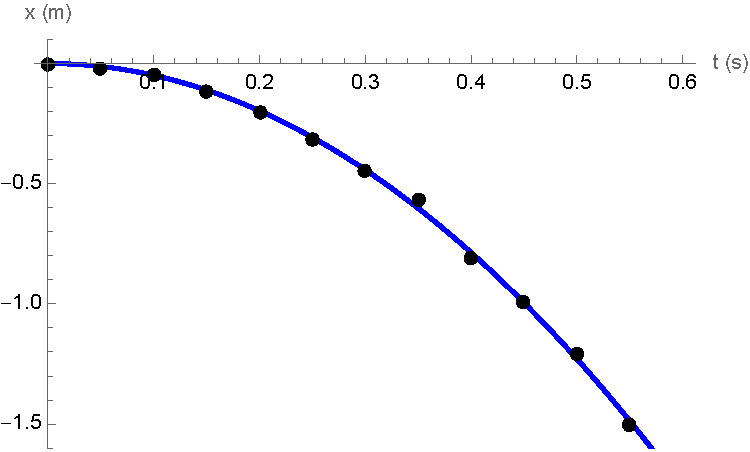
\includegraphics[width=0.3\textwidth]{figs/liike_esimerkki_pudotus1.pdf}
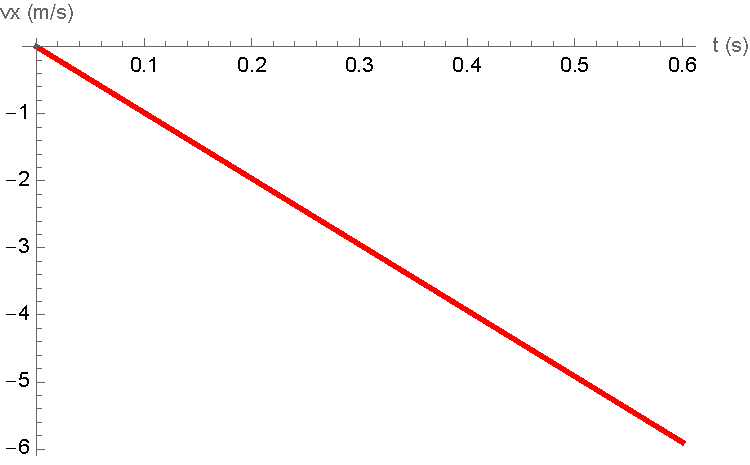
\includegraphics[width=0.3\textwidth]{figs/liike_esimerkki_pudotus2.pdf}
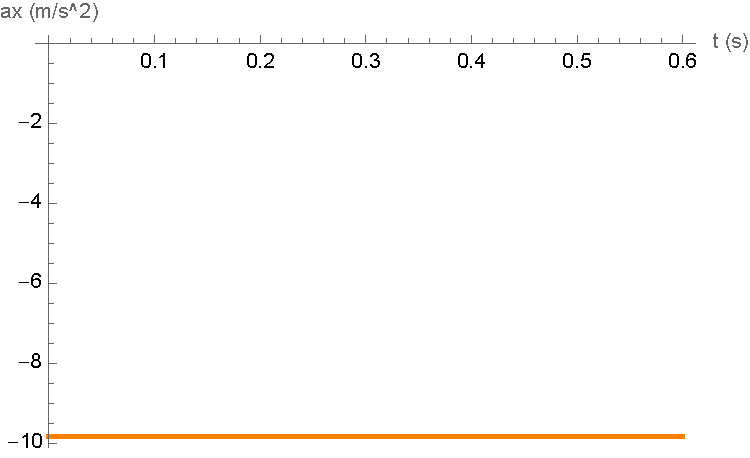
\includegraphics[width=0.3\textwidth]{figs/liike_esimerkki_pudotus3.pdf}
\end{center}

 \eval  Tietokoneen löytämä paraabeli näyttää kulkevan hyvin tarkasti mittauspisteiden kautta. Pallon paikka vaikuttaa siis noudattavan tasaisen kiihtyvyyden mallia varsin hyvin. Voimme olla varsin luottavaisia siihen, että tietokoneen löytämä paraabeli ja siitä laskettu kiihtyvyys kuvaavat mittauksia oikein melko hyvällä tarkkuudella. On toki olemassa tilastollisia menetelmiä, jolla tämä tarkkuus voidaan täsmällisesti laskea, mutta emme nyt mene analyysissä niin pitkälle.

Viimeisestä mittauksesta laskettu kiihtyvyys poikkeaa hiukan tietokoneen antamasta arvosta. Tämä johtuu siitä, että yhdestä pisteestä laskettu arvo muuttuu herkästi, jos kyseinen piste mitataan epätarkasti. Esimerkiksi jos viimeisen mittauspisteen paikaksi olisikin mitattu \(-1.49 \un{m}\) tai \(-1.51 \un{m}\), kiihtyvyydeksi olisi saatu \(-9.85 \un{m/s}^2\) tai \(-9.98 \un{m/s}^2\). Mitä usemmasta datapisteestä kiihtyvyys määritetään, sitä vähemmän yksittäiset mittausvirheet siihen vaikuttavat ja sitä luotettavampi lopputulos saadaan.

\end{exam}

Esimerkissä \autoref{ex:g} tehdyn mittauksen perusteella putoavan pallon paikan kuvaaja tosiaan on paraabeli, nopeuden kuvaaja on suora, ja kiihtyvyys on vakio. Kiihtyvyyden suuruudeksi esimerkissä mitattiin hieman alle \(10 \un{m/s}^2\).

Voimme tietenkin toistaa mittauksen erilaisilla kappaleilla, ja lopputulos on se, että valtaosa kappaleista putoaa samalla tavalla. Erityisesti \emph{kappaleet putoavat yhtä suurella kiihtyvyydellä riippumatta siitä, kuinka suuria ne ovat}. Jos vaikkapa pudotamme tennis- ja jalkapallon levosta yhden metrin korkeudelta, kummallakin kestää hieman alle puoli sekuntia pudota maahan.
Putoamiskiihtyvyys vaikuttaa siis olevan kaikille kappaleille sama vakio, jonka arvo on likimain
\begin{equation} g = 9.8 \un{m/s}^2. \label{pikkug} \end{equation}

Poikkeuksen tähän sääntöön näyttävät muodostavan jotkin hyvin kevyet kappaleet.
Esimerkiksi paperiarkki ei putoa suoraan maahan vaan leijailee hitaasti alas. Tämä johtuu ilmasta. Liikkuvat tavarat työntävät pudotessaan ilmaa pois tieltään, mikä hidastaa niitä. Etenkin jos esine on kevyt, sillä on suuri pinta-ala tai se liikkuu nopeasti, ilman läpi kulkeminen voi vaikuttaa liikkeeseen huomattavasti. Vastaavia pudotuskokeita on kuitenkin tehty tyhjiökammioissa ja jopa Kuussa, jolloin lopputulos on aina ollut se, että kun ilma ei häiritse liikettä, \emph{kaikki kappaleet} putoavat yhtä nopeasti.

\begin{stopQ}{q:ilmanvastuskoe}%
Pudota kirja ja yksittäinen paperiarkki samaan aikaan. Putoavatko ne eri tavalla? Laita sitten paperiarkki kirjan päälle ja pudota ne yhdessä. Putoavatko ne nyt eri tavalla? Miksi?
\end{stopQ}

Täsmällisesti ottaen kappaleet putoavat yhtä nopeasti, kun ne pudotetaan samassa paikassa. Kuussa esineet putoavat hitaammin kuin maapallolla, koska painovoima on Kuussa heikompi. Maassa tennis- ja koripallolla kummallakin kestää hieman alle puoli sekuntia pudota metrin korkeudelta levosta maan pinnalle. Kuussa sen sijaan kummallakin kestää samaan metrin pudotukseen hieman yli sekunti.

Itse asiassa putoamiskiihtyvyys ei ole maapallollakaan kaikkialla täsmälleen yhtä suuri vaan päiväntasaajalla asiat putoavat pikkuisen hitaammin kuin navoilla. Tämä johtuu siitä, että maapallo pyörii eikä se ole ihan täsmälleen pallon muotoinen. Putoamiskiihtyvyydelle annetaan joskus tarkempiakin arvoja kuin \(9.8 \un{m/s}^2\), mutta yleensä siihen ei ole syytä, koska kiihtyvyyden suuruus vaihtelee paikasta toiseen enemmän kuin \(0.01 \un{m/s}^2\). Jos siis asioita välttämättä haluaa laskea tarkemmin kuin kahdella merkitsevällä numerolla, on syytä ensin selvittää, missä ollaan ja kuinka suuri putoamiskiihtyvyys juuri siellä on. Usein riittää jopa käyttää yksinkertaisesti likiarvoa \(g \approx 10 \un{m/s}^2\), koska sillä on todella helppo laskea eikä virhettä tule kuin kaksi prosenttia.

\begin{exam}{Heitetyn pallon lentorata}{ex:tasainen_kiihtyvyys}\noindent

\problem{Heitetään pallo ylöspäin alkunopeudella 10.0 m\slash s. (a) Millä hetkellä pallo on korkeudella 2.0 m heittokorkeudelta mitattuna? (b) Mikä on tällöin pallon nopeus?}

 \twocol{0.59}{0.40}{\setup  Koska pallo heitettiin suoraan ylöspäin, se liikkuu ensin suoraan ylöspäin, pysähtyy sitten ja alkaa lopulta pudota suoraan alaspäin. Valitaan positiivinen suunta ylöspäin ja paikan nollakohta kappaleen lähtöpisteeseen.

 \physics Heitetty kappale on vapaassa putoamisliikkeessä koko lentonsa ajan. Tällöin sen liike on tasaisesti kiihtyvää ja kiihtyvyys on sama kuin putoamiskiihtyvyys. Kiihtyvyys osoittaa alaspäin eli koordinaatiston negatiiviseen suuntaan, joten \(a_{x,\text{tasainen}} = - g\).

}{%
\begin{center}%
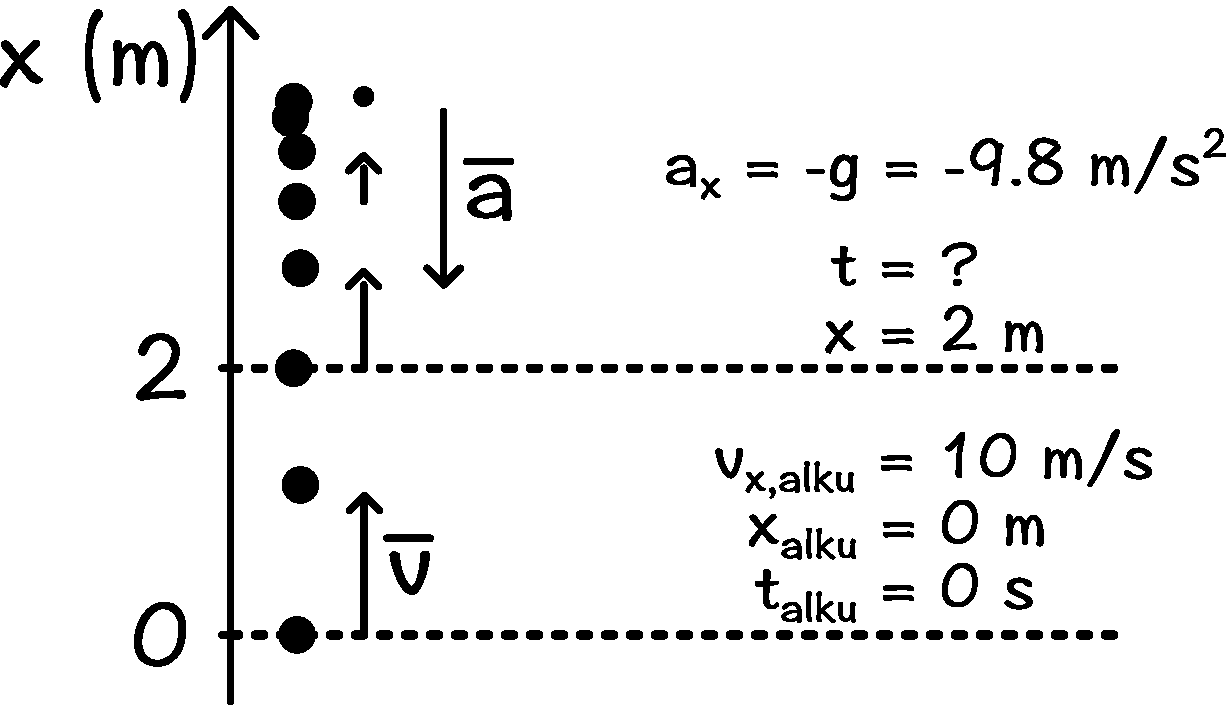
\includegraphics[width=0.90\textwidth]{figs/liike_esimerkki_heitto_1.pdf}%
\end{center}%
}

 \model  Yhtälön (\autoref{paikkatasaisessakiihtyvyydessa}) mukaan hetkellä \(t_\text{alku} = 0\un{s}\) tasaisella kiihtyvyydellä liikkeelle lähtevän kappaleen paikka muuttuu ajassa \(t\) siirtymän
\begin{equation} \Delta x = v_{x,\text{alku}} t + \frac{1}{2}a_{x,\text{tasainen}} t^2. \label{vakioa}\end{equation}
Nyt tiedämme siirtymän \(\Delta x\) alkupisteestä kysyttyyn korkeutaan ja meidän pitää ratkaista yhtälöstä aika \(t\).

Kun tiedämme pallon lentoajan, voimme edelleen selvittää pallon nopeuden tasaisesti kiihtyvän liikkeen nopeuden yhtälöstä (\autoref{tasaisenkiihtyvyydennopeus}). Kun jälleen lähtöhetkeksi valitaan \(t_\text{alku} = 0\un{s}\), nopeus on
\begin{equation} v_x = v_{x,\text{alku}} + a_{x,\text{tasainen}} t. \label{esimnopeus1} \end{equation}

 \solu  Lauseke (\autoref{vakioa}) on toisen asteen yhtälö muuttujan \(t\) suhteen ja sen ratkaisu on
\begin{equation} t = \frac{1}{a_x}\left( -v_{x,\text{alku}} \pm \sqrt{v_{x,\text{alku}}^2 + 2a_{x,\text{tasainen}}\Delta x} \right). \label{esimnopeus2} \end{equation}
Nyt siis alkunopeus on \(v_\text{alku} = 10.0 \un{m/s}\), kiihtyvyys \(a_{x,\text{tasainen}} = -g = -9.8 \un{m/s}\) ja kysyttiin aikaa korkeudella \(\Delta x = 2.0 \un{m}\).

Ratkaisuja saadaan kaksi, \(t = 0.2 \un{s}\) sekä \(t = 1.8 \un{s}\). Sijoittamalla ajan lauseke (\autoref{esimnopeus2}) nopeuden lausekkeeseen (\autoref{esimnopeus1}) nopeudeksi saadaan
\begin{equation} v_x = v_{x,\text{alku}} + a_{x,\text{tasainen}} \frac{1}{a_{x,\text{tasainen}}}\left( -v_{x,\text{alku}} \pm \sqrt{v_{x,\text{alku}}^2 + 2a_{x,\text{tasainen}}\Delta x} \right) = \pm \sqrt{v_{x,\text{alku}}^2 + 2a_{x,\text{tasainen}}\Delta x} \label{korkeusnopeus}\end{equation}
ja edelleen lukuarvojen sijoittaminen antaa nopeuden arvot \(v_x = 7.8 \un{m/s}\) sekä \(v_x = -7.8 \un{m/s}\).

\mbar
\begin{mathematica}[commandchars=\\!?]
(* tallennetaan lukuarvot *)
lukuarvot = {v0 -> 10.0, a -> -9.8, deltax -> 2.0}; 

(* ratkaistaan aika *)
Solve[ deltax == v0 t + 1/2 a t^2, t ]
  \textit!{{t -> (-v0 + Sqrt[2 a deltax + v0^2])/a},?
  \textit! {t -> -(v0 + Sqrt[2 a deltax + v0^2])/a}}?

(* tallennetaan edellinen tulos muuttujaan 'aika' *)
aika = %

(* sijoitetaan ratkaistu aika nopeuden lausekkeeseen *)
nopeus = v0 + a t /. aika
  \textit!{{ Sqrt[2 a deltax + v0^2]), -Sqrt[2 a deltax + v0^2] }}?

(* tulostetaan ratkaisu uudestaan, nyt lukuarvojen kera *)
aika /. lukuarvot
nopeus /. lukuarvot
  \textit!{{t -> 0.224751}, {t -> 1.81606}}?
  \textit!{7.79744, -7.79744}?
\end{mathematica}

 \eval  Ratkaisujen fysikaalinen merkitys on selkeä: Ratkaisuista ajoista ensimmäinen on hetki, jolloin pallo on korkeudella 2.0 m matkalla \emph{ylöspäin}. Tätä vastaava nopeus on positiivinen. Toinen ratkaisu on hetki, jolloin pallo on samalla korkeudella matkalla \emph{alaspäin}, ja tätä vastaa negatiivinen nopeus. Huomaa, että tässä kysyttiin nimenomaan hetkeä jolloin pallo on \emph{etäisyydellä} 2.0 m lähtöpisteestään --- ei hetkeä jolloin pallon kulkema matka olisi 2.0 m --- joten kumpikin ratkaisu on oikein. Pallon ollessa matkalla alaspäin se on luonnollisesti kulkenut pidemmän matkan.

Huomataan lisäksi, että pallon vauhti eli nopeuden suuruus on kummassakin tapauksessa \emph{sama}. Näin selvästikin täytyy olla ratkaisun (\autoref{korkeusnopeus}) perusteella riippumatta alkunopeudesta, kiihtyvyydestä ja tarkastelukorkeudesta.

Tarkistetaan vielä ratkaisujen yksiköt:
\begin{equation} [t] = \frac{[v_\text{alku}] + \sqrt{[2 a_{x,\text{tasainen}} \Delta x] + [v_\text{alku}^2]}}{[a_{x,\text{tasainen}}]} = \frac{\text{m/s} + \sqrt{\text{m/s}^2 \cdot \text{m} + (\text{m/s})^2}}{\text{m/s}^2} = \frac{\text{m/s} + \sqrt{\text{m}^2/\text{s}^2}}{\text{m/s}^2} = \frac{\text{m}}{\text{s}}\frac{\text{s}^2}{\text{m}} = \text{s}.  \end{equation}
\begin{equation} [v_x] = \sqrt{[v_\text{alku}^2] + [2 a_{x,\text{tasainen}} \Delta x]} = \sqrt{(\text{m/s})^2 + \text{m/s}^2 \cdot \text{m}} =\sqrt{\text{m}^2/\text{s}^2} = \text{m/s}. \end{equation}

\end{exam}

Esimerkissä \autoref{ex:tasainen_kiihtyvyys} johdettiin lauseke pystysuoraan heitetyn kappaleen nopeudelle tietyllä korkeudella, kun kappaleen lähtökorkeus ja -nopeus tunnetaan.
Korottamalla saatu lauseke (\autoref{korkeusnopeus}) puolittain neliöön ja merkitsemällä kappaleen nopeutta siirtymän \(\Delta x\) jälkeen \(v_\text{loppu}\) tulos voidaan kirjoittaa yksinkertaisempaan muotoon
\begin{equation} v_{x,\text{loppu}}^2 = v_{x,\text{alku}}^2 + 2a_{x,\text{tasainen}}\Delta x, \label{korkeusnopeusnelio} \end{equation}
jossa on päästy eroon neliöjuuresta ja plusmiinus-merkinnästä. Jos kirjoitamme edelleen \(\Delta (v_x^2) = v_{x,\text{loppu}}^2-v_{x,\text{alku}}^2\), yhtälö saa vielä tiivistetymmän muodon
\begin{equation} \Delta (v_x^2) = 2a_{x,\text{tasainen}}\Delta x. \label{nopeusneliomuutos} \end{equation}
Toisin sanoen nopeuden neliön muutos on \emph{yksiulotteisessa tasaisesti kiihtyvässä liikkeessä} aina suoraan verrannollinen kappaleen siirtymään. Tutkimme tämän tuloksen merkitystä tarkemmin luvussa \autoref{luku:sailymislait}.

\begin{stopQ}{q:heittoesimerkki}%
Edelleen olettaen ilmanvastus pieneksi, mikä on esimerkin \autoref{ex:tasainen_kiihtyvyys} pallon nopeus \(v_x\) (a) kun se on jälleen lähtökorkeudella ja (b) heiton lakipisteessä? (c) Kuinka korkealle pallo nousee?
\end{stopQ}

\startwidepage

\section*{Yhteenveto: \chaptertitle}
\addcontentsline{toc}{section}{Yhteenveto: \chaptertitle}
\noindent
\begin{tabular}{p{1.15\textwidth}}
\standout{Differentiaalit ja vektorit}{
\begin{multicols}{2}

\begin{itemize}
\item \textbf{Skalaari} on suure, jota kuvaa pelkkä suuruus. Suuruuteen kuuluu fysiikassa sekä lukuarvo että yksikkö.

\item \textbf{Vektori} on suure, jolla on sekä suunta että suuruus.

\item Koordinaatiston kääntäminen muuttaa vektoreita mutta ei skalaareja.

\item \textbf{Yksikkövektori} on vektori, jonka suuruus on yksi ja jolla ei ole yksikköä.

\item Vektorin voi esittää \textbf{skalaarikomponentin} ja yksikkövektorin tulona
\[ \bs{v} = v_x \uv{i}. \]

\item \textbf{Differentiaali} kuvaa suureen infinitesimaalista eli äärettömän pientä muutosta tai määrää.

\item \textbf{Derivaatta} kuvaa suureen muutosnopeutta toisen suureen suhteen. Matemaattisesti se voidaan määritellä muutosten osamäärän raja-arvona eli differentiaalien suhteena
\[ x'(t) = \lim_{\Delta t \to 0} \frac{\Delta x}{\Delta t} = \frac{\dd x}{\dd t}. \]

\item \textbf{Integraali} kuvaa pieniin osiin jaetun suureen kokonaismäärää. Matemaattisesti se voidaan määritellä summan raja-arvona
\[ \int_{t_\text{alku}}^{t_\text{loppu}} v_x(t) \dd t = \lim_{\Delta t \to 0} \sum_{i=0}^N v_x(t_i) \Delta t \]

\item Integrointi ja derivointi ovat toistensa käänteisoperaatiot
\[ \int \frac{\dd y}{\dd x} \dd x = y + C, \ \frac{\dd}{\dd x} \int y \dd x = y. \]

\end{itemize}

\end{multicols}
} \\
\standout{Paikka ja nopeus}{
\begin{multicols}{2}

\begin{itemize}
\item \textbf{Paikkavektori} on koordinaatiston origosta tarkastelupisteeseen osoittava vektori.

\item Paikkavektorin \textbf{skalaarikomponentti} \(x\)-suunnassa on pisteen \(x\)-koordinaatti
\[ \bs{r} = x \uv{i}. \]

\item \textbf{Siirtymä} on paikan muutos
\[ \Delta x = x_\text{loppu} - x_\text{alku}, \ \Delta \bs{r} = \bs{r}_\text{loppu} - \bs{r}_\text{alku}. \]

\item Paikkavektorin muutosnopeus eli derivaatta ajan suhteen on \textbf{nopeus}
\[ \bs{v} = \frac{\dd \bs{r}}{\dd t} = \frac{\dd x}{\dd t} \uv{i} = x'(t) \uv{i} = v_x(t) \uv{i}. \]

\item Nopeusvektorin muutosnopeus eli derivaatta ajan suhteen on \textbf{kiihtyvyys}
\[ \bs{a} = \frac{\dd \bs{v}}{\dd t} = \frac{\dd v_x}{\dd t} \uv{i} = v_x'(t) \uv{i} = x''(t) \uv{i} = a_x(t) \uv{i}. \]

\item Tasaisessa liikkeessä nopeus on vakio ja paikkaa kuvaa suora
\[ x(t) = x_\text{alku} + v_{x,\text{tasainen}} (t-t_\text{alku}) \]

\item Tasaisesti kiihtyvässä liikkeessä kiihtyvyys on vakio, nopeus suora ja paikka paraabeli
\[   v_x(t) = v_{x,\text{alku}} + a_{x,\text{tasainen}} (t - t_\text{alku}), \]
\[   x(t) = x_\text{alku} + v_{x,\text{alku}} (t - t_\text{alku}) + \frac{1}{2} a_{x,\text{tasainen}} (t - t_\text{alku})^2. \]

\item Putoavan kappaleen kiihtyvyys on noin \(g = 9.8 \un{m/s}^2\) suoraan alaspäin.

\end{itemize}

\end{multicols}
} \\
\standout{Graafinen esitys}{
\begin{multicols}{2}

\begin{itemize}
\item Vektorit voi piirtää kuviin nuolina.

\item \textbf{Liikediagrammissa} kappaleen paikka eri ajan hetkinä piirretään samaan koordinaatistoon. Kappaleen nopeus voidaan arvioida siirtymien perusteella ja kiihtyvyys nopeuden muutosten avulla.

\item Kappaleen paikan kuvaajassa kunkin pisteen paikka pystysuunnassa esittää kappaleen paikkakoordinaattia ja paikka vaakasuunnassa aikakoordinaattia. Vastaavasti voidaan esittää minkä tahansa kahden suureen välinen riippuvuus.

\item Kappaleen nopeus ilmenee paikkakoordinaatin \textbf{kuvaajan tangentin kulmakertoimena}. Samoin kiihtyvyys on nopeuden kuvaajan tangentin kulmakerroin. Yleisesti derivaatta \(f'(t) = \dd f/ \dd t\) on kuvaajan \( f(t) \) tangentin kulmakerroin.

\item Kappaleen siirtymä ilmenee nopeuden skalaarikomponentin \textbf{kuvaajan rajaamana pinta-alana}. Samoin nopeus on kiihtyvyyden kuvaajan rajaama pinta-ala. Yleisesti integraali \(\int_{t_\text{alku}}^{t_\text{loppu}} f(t) \dd t\) on kuvaajan \( f(t) \) ja \(t\)-akselin väliin jäävä pinta-ala.

\end{itemize}

\end{multicols}
} \\
\standout{Sanasto}{
\begin{multicols}{2}

\begin{itemize}
\item koordinaatti (coordinate)

\item koordinaatisto (reference frame)

\item akseli (axel)

\item liike (motion, movement)

\item paikka (position)

\item kiintopiste (reference point)

\item origo (origin)

\item metri (meter)

\item pituus (length)

\item siirtymä (displacement)

\item matka (distance)

\item aika (time)

\item sekunti (second)

\item ajan hetki (instant)

\item aikaväli (interval)

\item nopeus (velocity)

\item vauhti (speed)

\item kiihtyvyys (acceleration)

\item lepo (rest)

\item tasainen liike (uniform motion)

\item tasaisesti kiihtyvä liike (uniformly accelerated motion)

\item vapaa pudotus (free fall)

\item liikerata (trajectory)

\item putoamiskiihtyvyys (gravitational acceleration)

\item differentiaali (differential)

\item derivaatta (derivative)

\item integraali (integral)

\item tangentti (tangent)

\item kulmakerroin (slope)

\item pinta-ala (area)

\item liikediagrammi (motion diagram)

\item skalaari (scalar)

\item vektori (vector)

\item nollavektori (zero vector)

\item yksikkövektori (unit vector)

\item skalaarikomponentti (scalar component)

\item vektorin pituus (vector magnitude)

\item itseisarvo (absolute value)

\item paikkavektori (position vector)

\item sovitus (fit)

\end{itemize}

\end{multicols}
} 

\end{tabular}

\onepicture{b!}%
{Liikkeen erilaisia esitystapoja sekä liikettä kuvaavien suureiden riippuvuudet toisistaan. Taulukossa on esitetty erikseen erikoistapaukset, joissa paikka, nopeus tai kiihtyvyys ovat vakioita, sekä yleinen liike.}%
{fig:liikeyhteenveto}%
{1.0}%
{liike_yhteenveto.pdf}



\newpage

\newpage\begin{answers}\noindent

\stopA{q:koordinaattimerkki}{%
(a) Etäisyys kiveen on 5 m ja ihmiseen 2 m.\\
(b) Kiven paikkakoordinaatti on \(x_{\text{kivi}}=5 \un{m}\) ja ihmisen \(x_{\text{ihminen}}=-2 \un{m}\).\\
(c) \(x_{\text{kivi}} - x_{\text{ihminen}} = 5 \un{m} - (-2 \un{m}) = 7 \un{m}\). Tosin päin laskien erotukseksi tulee - 7 m.\\
(d) Etäisyys on sama kuin koordinaattien erotuksen itseisarvo, 7 m.
}

\stopA{q:aikakoordinaatti}{%
(a) \(t = 13 \un{min} + 14 \un{s} = 794 \un{s}\).\\
(b) \(t = 3 \un{h} + 30 \un{min} = 12600 \un{s}\).\\
(c) \(t = - 14 \un{min} - 10 \un{s} = -850 \un{s}\).
}

\stopA{q:paikankuvaaja}{%
Jos kappale siirtyy välittömästi paikasta toiseen, paikan kuvaajassa on epäjatkuvuus. Tässä tapauksessa kuvaaja siis saapuisi pisteeseen \(x=2\) m ja hyppäisi epäjatkuvasti pisteeseen \(x=3\) m. (b) Koska teleportteja ei ole oikeasti olemassa, paikan kuvaaja ei siis saa olla epäjatkuva.
}

\stopA{q:siirtyma}{%
(a) Siirtymä riippuu vain alku- ja loppupisteistä, joten \(\Delta x = x_2 - x_0 = 0.5 \un{m} - 1.0 \un{m} = -0.5 \un{m}\).\\
(b) Kuljettu matka on siirtymien itseisarvojen summa,
\(s = |x_2-x_1| + |x_1-x_0| = 2.5 \un{m} + 3.0 \un{m} = 5.5 \un{m} \).\\
(c) Koordinaatit muuttuvat origon siirron verran, jolloin saadaan\\
\(x_0 = -1.0 \un{m}\),
\(x_1 = -4.0 \un{m}\) ja
\(x_2 = -1.5 \un{m}\). Siirtymä ja kuljettu matka eivät riipu kiintopisteestä.
}

\stopA{q:aikaero}{%
(a) Nämä ratkaistiin jo aikaisemmin:
\(t_1 = -850 \un{s}\),
\(t_2 = 794 \un{s}\),
\(t_3 = 12600 \un{s}\).\\
(b, c) Kulunut aika on sama kuin loppu- ja alkuajan erotus:
\(\Delta t_{1 \ldots 2} = t_2 - t_1 = 794 \un{s} - (-850 \un{s}) = 1644 \un{s}\),\\
\(\Delta t_{2 \ldots 3} = t_3 - t_2 = 12600 \un{s} - 794 \un{s} = 11806 \un{s}\),\\
\(\Delta t_{1 \ldots 3} = t_3 - t_1 = 12600 \un{s} - (-850 \un{s}) = 13450 \un{s}\).
}

\stopA{q:vauhtinopeus}{%
Nopeus on siirtymän ja kuluneen ajan suhde. Vauhti on matkan ja kuluneen ajan suhde.\\
(a) Menomatkalla nopeus on
\(v_x = 15 \un{m} / 3 \un{s} = 5 \un{m/s}\). Vauhti on sama.\\
(b) Paluumatkalla nopeus on
\(v_x = -15 \un{m} / 4 \un{s} = -3.75 \un{m/s}\). Vauhti on yhtä suuri mutta aina positiivinen eli 3.75 m\slash s.\\
(c) Kokonaismatkalla siirtymä on nolla, joten keskimääräinen nopeus on
\(v_{x,\text{keskiarvo}} = 0 \un{m} / 3 \un{s} = 0 \un{m/s}.\)\\
(d) Kokonaismatka on \(30 \un{m}\) ja aikaa kuluu \(7.5 \un{s}\), joten keskivauhti on \(v_\text{keskiarvo} = 30 \un{m} / 7.5 \un{s} = 4.0 \un{m/s}\). Keskivauhti on siis eri asia kuin keskinopeus, eikä kumpikaan näistä ole nopeuden tai vauhdin keskiarvo.
}

\stopA{q:kuvaajienpiirto}{%
Nopeuden kuvaaja on välillä \(0 \ldots 1 \un{s}\) vaakasuora, joka kulkee korkeudella \(1\) m\slash s. Hetkellä \(t = 1 \un{s}\) kuvaaja hyppää arvoon \( 2 \un{m/s} \), ja kuvaaja on tämän jälkeen jälleen vaakasuora aikavälin \(1 \ldots 2 \un{s}\). Nopeuden kuvaajassa on siis epäjatkuvuus, jos nopeus muuttuu yhtäkkiä. Paikan kuvaaja on puolestaan suora, jonka kulmakerroin on kappaleen nopeus. Paikan kuvaajan kulmakerroin on siis aluksi \(1 \un{m/s}\) ja lopuksi \(2 \un{m/s}\). Kuvaaja on jatkuva hetkellä \(t = 1 \un{s}\), mutta siinä on kulma, koska kuvaajan jyrkkyys muuttuu yhtäkkiä.
}

\stopA{q:derivaatta}{%
(a) Tässä voi keksiä loputtomasti erilaisia funktioita, mutta kaikkien pitää olla muotoa \(f(x) = 5x + C\). Otetaan esimerkiksi \(f_a(x) = 5x \) ja \(f_b(x) = 5x + 2\).\\
(b) Esimerkkifunktioille \(f_a(1) = 5, f_a(2) = 10, \Delta f_a = 5\) sekä
\(f_b(1) = 7, f_b(2) = 12, \Delta f_b = 5\).\\
(c) Derivaatta kertoo funktion muutosjyrkkyyden. \(f'(x) = 5\) tarkoittaa sitä, että funktio muuttuu 5, kun x muuttuu 1. Edellisessä kohdassa siis saadaan aina \(\Delta f = 5\) olivatpa funktiot mitä tahansa.
}

\stopA{q:laskederivaatta}{%
(a) Merkitään symbolilla \(\frac{\dd}{\dd x}\) sitä, että derivoimme sen jälkeen tulevan lausekkeen.
Ensin derivoidaan summa termi kerrallaan: \(f'(x) = \frac{\dd f}{\dd x} = \frac{\dd}{\dd x}(a) + \frac{\dd}{\dd x}(be^{-cx}) \).
Pelkän vakion derivaatta on nolla ja vakiokertoimen saa ottaa derivaatan kertoimeksi: \(f'(x) = 0 + b \frac{\dd}{\dd x}(e^{-cx}) \).
Eksponenttifunktion derivaatta on eksponenttifunktio, ja tämä pitää kertoa eksponentissa olleen sisäfunktion derivaatalla:
\(f'(x) = b e^{-cx} \frac{\dd}{\dd x}(-cx) \).
Jäljellä on enää potenssifunktio, jonka saa derivoitua säännöllä \(\frac{\dd}{\dd x} cx^n = ncx^{n-1}\), missä nyt \(n=1\). Siispä
\(f'(x) = b e^{-cx} \cdot (-c)  = - bce^{-cx} \).\\
(b) Lopputulos on \(x^x (1 + \ln x) \).
}

\stopA{q:differentiaalimerkinta}{%
(a) \(\frac{\dd x}{\dd t} = x'(t) = 2 b t \).\\
(b) \(\frac{\dd t}{\dd x} = t'(x) = \frac{1}{2 \sqrt{b x}} \).\\
(c) \(\frac{\dd x}{\dd t} = 4\) ja \(\frac{\dd t}{\dd x} = \frac{1}{4}\). Huomaa, että \(\frac{\dd x}{\dd t} = \left(\frac{\dd t}{\dd x} \right)^{-1} \).
}

\stopA{q:numeerinenintegrointi}{%
Ensimmäisellä välillä kappale siirtyy \(\Delta x_1 = v_x \Delta t = 0.1 \un{m/s} \cdot 0.2 \un{s} = 0.02 \un{m}\). Vastaavasti seuraavilla aikaväleillä kappale siirtyy \(\Delta x_2 = 0.04 \un{m}\), \(\Delta x_3 = 0.08 \un{m}\) ja \(\Delta x_4 = 0.14 \un{m}\). Kokonaissiirtymä on näiden summa, \(\Delta x = 0.28 \un{m}\).
}

\stopA{q:maarattyintegraali}{%
(a) Integraali laskee pinta-alan aloittaen kohdasta \(t_\text{alku}\) ja lopettaen kohtaan \(t_\text{loppu}\). Tämän saa myös laskemalla ensin pinta-alan kohdasta \(t_\text{alku}\) origoon ja lisäämällä tähän pinta-alan origosta kohtaan \(t_\text{loppu}\), koska alku- ja loppupiste ovat origon eri puolilla. Ensimmäinen pinta-ala on \( -i(t_\text{alku}) \) ja toinen on \( i(t_\text{loppu}) \). Siispä koko pinta-ala on
\( i(t_\text{loppu}) + (-i(t_\text{alku})) \) eli juuri haluttu tulos.\\
(b) Nyt alku- ja loppupiste ovat kumpikin origon vasemmalla puolella. Niiden väliin jäävä ala voidaan laskea määrittämällä ensin pinta-ala alkupisteestä origoon ja vähentämällä siitä loppupisteen ja origon välinen ala. Ala alkupisteestä origoon on \( -i(t_\text{alku}) \) ja tästä vähennettävä ala on \( -i(t_\text{loppu}) \). Niinpä haluttu pinta-ala on \( -i(t_\text{alku}) - (-i(t_\text{loppu})) \). Tämäkin on sama kuin haluttu tulos.
}

\stopA{q:laskeintegraali}{%
(a) Integraalin voi laskea termeittäin:
\( \int (a+be^{-cx}) \dd x = \int a \dd x + \int be^{-cx} \dd x \).
Integrointi onnistuu etsimällä funktio, jonka derivaatta on integroitava funktio.
Potenssifunktion \( g(x) = a x^n \) derivaatta on \( g'(x) = nax^{n-1} \). Tämä on sama kuin funktio \(a\), jos \(n=1\). Siispä
\( \int a \dd x = g(x) = ax \).
Eksponenttifunktion \(h(x) = be^{-cx}\) derivaatta on \( h'(x) = -cbe^{-cx} \). Jos tämä kerrotaan vakiolla \(-\frac{1}{c}\), saadaan integraalissa oleva eksponenttifunktio, \( -\frac{1}{c} h'(x) = be^{-cx} \). Niinpä eksponenttifunktion integraali on
\( \int be^{-cx} \dd x = -\frac{1}{c} h(x) = -\frac{b}{c} e^{-cx} \).
Lopputulokseen pitää vielä muistaa lisätä integroimisvakio, joten
\( \int (a+be^{-cx}) \dd x = ax -\frac{b}{c} e^{-cx} + C \).\\
(b) Merkitään äsken laskettua integraalifunktiota
\( i(x) = ax -\frac{b}{c} e^{-cx}. \)
Määrätty integraali lasketaan sijoittamalla integraalifunktioon integroimisrajat
\begin{equation} \int_0^1 (a+be^{-cx}) \dd x = i(1) - i(0) = a -\frac{b}{c} e^{-c} - \left(-\frac{b}{c} e^{0} \right) = a + \frac{b}{c} - \frac{b}{c} e^{-c}. \end{equation}
(c) Lopputulos on (hiukan yllättäen) \(\frac{1}{2}\sqrt{\pi}\).
}

\stopA{q:vektorisuureet}{%
Skalaareja ovat matka, vauhti, tilavuus ja lämpötila. Vektoreita ovat paikka ja siirtymä. Suureet kuten pituus ja matka ilmaisevat vain etäisyyksiä ilman suuntaa, joten ne ovat skalaareja. Samalla tavalla vauhti ilmaisee vain nopeuden suuruutta ja on siis skalaari. Paikka on vektori, koska se ilmaisee valitun pisteen origosta mitatun etäisyyden ja suunnan. Siirtymä on puolestaan paikan muutos, joka ilmaisee sekä siirrytyn etäisyyden että siirron suunnan.
}

\stopA{q:vektorimerkinta}{%
(a) pituus \(B = 2.5 \un{T}\)\\
(b) skalaarikomponentti \(B_x = -2.5 \un{T}\)\\
(c) itseisarvo \(|\bs{B}| = B = 2.5 \un{T}\)\\
(d) vektori itse \(\bs{B} = B_x \uv{i} = (-2.5 \un{T}) \uv{i} \)\\
(e) Pituus on \emph{aina} positiivinen. Skalaarikomponentti on nyt negatiivinen. Vektori itse \emph{ei voi olla positiivinen eikä negatiivinen}. Positiivisuus on reaaliarvoisen suureen eli skalaarin ominaisuus. Pituus ja skalaarikomponentti ovat skalaareja, joten niille kysymys on mielekäs. Vektorille ei ole.
}

\stopA{q:nopeusvektori}{%
(a) \(x_\text{alku} = 1.5 \un{m}\), \(x_\text{loppu} = -2.5 \un{m}\),\\
(b) \(\bs{r}_\text{alku} = (1.5 \un{m}) \uv{i} \), \(\bs{r}_\text{loppu} = (-2.5 \un{m}) \uv{i} \),\\
(c) \(v_{x,\text{keskiarvo}} = (x_\text{loppu} - x_\text{alku})/\Delta t = -4.0 \un{m} / 1.0 \un{s} = -4.0 \un{m/s} \),\\
(d) \(\bs{v}_{x,\text{keskiarvo}} = (\bs{r}_\text{loppu} - \bs{r}_\text{alku})/\Delta t = (-4.0 \un{m}) \uv{i} / 1.0 \un{s} = (-4.0 \un{m/s}) \uv{i}. \)
}

\stopA{q:keskikiihtyvyys}{%
(a) \(v_{x,\text{alku}} = 10 \un{m/s}\), \(v_{x,\text{loppu}} = 5 \un{m/s}\), \(\Delta v_x = v_{x,\text{loppu}} - v_{x,\text{alku}} = -5 \un{m/s}\), \(a_{x,\text{keskiarvo}} = \frac{\Delta v_x}{\Delta t} = \frac{-5 \un{m/s}}{5 \un{s}} = -1 \un{m/s}^2. \)\\
(b) \(v_{x,\text{alku}} = 10 \un{m/s}\), \(v_{x,\text{loppu}} = -5 \un{m/s}\), \(\Delta v_x = v_{x,\text{loppu}} - v_{x,\text{alku}} = -15 \un{m/s}\), \(a_{x,\text{keskiarvo}} = \frac{\Delta v_x}{\Delta t} = \frac{-15 \un{m/s}}{5 \un{s}} = -3 \un{m/s}^2. \)
}

\stopA{q:va_etumerkit}{%
(a) Auto liikkuu etelään, joten nopeusvektori osoittaa etelään eli negatiiviseen suuntaan ja \(v_x < 0 \un{m/s}\). Vauhti hidastuu, joten kiihtyvyys osoittaa nopeutta vastaan pohjoiseen eli positiiviseen suuntaan ja \(a_x > 0 \un{m/s}^2\).\\
(b) Auto liikkuu pohjoiseen, joten nopeusvektori osoittaa pohjoiseen eli positiiviseen suuntaan ja \(v_x > 0 \un{m/s}\). Vauhti hidastuu, joten kiihtyvyys osoittaa nopeutta vastaan etelään eli negatiiviseen suuntaan ja \(a_x < 0 \un{m/s}^2\).\\
(c) Auto liikkuu etelään, joten nopeusvektori osoittaa etelään eli negatiiviseen suuntaan ja \(v_x < 0 \un{m/s}\). Vauhti kasvaa, joten kiihtyvyys osoittaa nopeuden suuntaan etelään eli negatiiviseen suuntaan ja \(a_x < 0 \un{m/s}^2\).\\
}

\stopA{q:pomppukiihtyvyys}{%
(a) Kappale putoaa alaspäin: nopeus ja kiihtyvyys osoittavat molemmat alaspäin.\\
(b) Kappale koskettaa maata: Nopeus on hetkellisesti likimain nolla. Kiihtyvyys osoittaa ylöspäin, koska kappaleen nopeusvektori osoittaa aluksi alas ja lopuksi ylös eli nopeuden muutos on ylöspäin.\\
(c) Kappale liikkuu ylöspäin mutta on vapaassa pudotuksessa: nopeus osoittaa ylöspäin, kiihtyvyys alaspäin.\\
(d) Molemmissa tilanteissa kappaleen nopeus on hetkellisesti nolla mutta kiihtyvyys ei ole. Heiton lakipisteessä kiihtyvyys on alaspäin, koska nopeuden suunta kääntyy ylhäältä alas. Pompussa kiihtyvyys on ylöspäin, koska nopeuden suunta kääntyy alhaalta ylös.
}

\stopA{q:kiihtyvyysderivaatta}{%
(a) Nopeus on paikan derivaatta, \(v_x = \frac{\dd x}{\dd t} = x'(t) = 3 \cdot (2.5 \un{m/s}^3) t^2 + 4.0 \un{m/s} = (7.5 \un{m/s}^3) t^2 + 4.0 \un{m/s} \).\\
(b) Kiihtyvyys on nopeuden derivaatta, \(a_x = \frac{\dd v_x}{\dd t} = v_x'(t) = 2 \cdot (7.5 \un{m/s}^3) t = (15.0 \un{m/s}^3) t \).\\
(c) Kiihtyvyyden integraali on \(\int (15.0 \un{m/s}^3) t \dd t = \frac{1}{2} (15.0 \un{m/s}^3) t^2 + C = (7.5 \un{m/s}^3) t^2 + C \). Tämä on sama kuin nopeus, jos ja vain jos integroimisvakioksi valitaan \(4.0 \un{m/s}\).
}

\stopA{q:va_esimerkki}{%
Esimerkiksi \( x(t) = (1 \un{m})e^{-t/(1 \un{s})} \). Nopeus on tälle
\( v_x(t) = x'(t) = (-1 \un{m/s})e^{-t/(1 \un{s})} < 0 \un{m/s} \) ja kiihtyvyys
\( a_x(t) = v_x'(t) = (1 \un{m/s}^2)e^{-t/(1 \un{s})} > 0 \un{m/s}^2. \)
}

\stopA{q:ilmanvastuskiihtyvyys}{%
Nopeus saadaan integroimalla kiihtyvyyttä ja paikka edelleen integroimalla nopeutta. Nopeus on
\begin{equation} v_x(t) = v_{x,\text{alku}} + \int_0^t -g e^{-t/\tau} \dd t = g\tau ( e^{-t/\tau} - 1) \end{equation}
ja paikka
\begin{equation} x(t) = x_{\text{alku}} + \int_0^t g\tau (e^{-t/\tau} - 1) \dd t = x_{\text{alku}} + g\tau [\tau (1 - e^{-t/\tau}) - t]. \end{equation}
}

\stopA{q:tasainenkiihtyvyys}{%
(a) Vauhti ei muuttunut, joten \(\Delta v = 0 \un{m/s}\).\\
(b) Alkunopeus oli \(v_{x,\text{alku}} = 2.0 \un{m/s}\) ja loppunopeus \(v_{x,\text{loppu}} = -2.0 \un{m/s}\). Nopeuden muutos oli siis \(\Delta v_x = v_{x,\text{loppu}} - v_{x,\text{alku}} = -4.0 \un{m/s} \).\\
(c) Kiihtyvyys oli \(a_{x,\text{tasainen}} = \frac{\Delta v_x}{\Delta t} = \frac{-4.0 \un{m/s}}{0.50 \un{s}} = -8.0 \un{m/s}^2. \)
}

\stopA{q:integroikiihtyvyys}{%
Kiihtyvyys on vakio, \(a_{x,\text{tasainen}}\). Nopeudeksi saadaan

\begin{eqnarray} v_x(t) &=& v_{x,\text{alku}} + \int_{t_\text{alku}}^t a_{x,\text{tasainen}} \dd \underline{t} \\ 
&=& v_{x,\text{alku}} + \bigg|_{t_\text{alku}}^t a_{x,\text{tasainen}}\underline{t} \\
&=&  v_{x,\text{alku}} + a_{x,\text{tasainen}} t - a_{x,\text{tasainen}} t_\text{alku} \\
&=& v_{x,\text{alku}} + a_{x,\text{tasainen}} (t - t_\text{alku}). \end{eqnarray}

Saatiin siis sama tulos tekstissä.
}

\stopA{q:derivoikiihtyvyys}{%
Ensimmäinen derivaatta on \(v_x(t) = x'(t) = v_{x,\text{alku}} + \frac{1}{2} a_{x,\text{tasainen}} \cdot 2(t-t_\text{alku})^{2-1} = v_{x,\text{alku}} + a_{x,\text{tasainen}} (t-t_\text{alku}) \).
Toinen derivaatta on \( a_x(t) = v_x'(t) = x''(t) = a_{x,\text{tasainen}} \).
}

\stopA{q:ilmanvastuskoe}{%
Erillään kirja putoaa nopeasti ja paperi hitaasti, koska ilman ja paperin välinen vuorovaikutus muuttaa kevyen paperin liikettä paljon ja painavan kirjan liikettä vain vähän. Kun paperi putoaa kirjassa kiinni, putoavan paperin edessä ei ole putoamista hidastavaa ilmaa, ja tällöin paperi putoaa yhtä nopeasti kuin kirja, putoamiskiihtyvyydellä \(g\).
}

\stopA{q:heittoesimerkki}{%
(a) Kun pallo on lähtökorkeudella, sen siirtymä on nolla, \(\Delta x = 0 \un{m}\). Yhtälön (\autoref{korkeusnopeusnelio}) perusteella siis \(v_{x,\text{loppu}}^2 = v_{x,\text{alku}}^2\) eli pallon vauhti on sama kuin alussa. Koska pallo putoaa nyt alaspäin, sen nopeuden suunta on kääntynyt eli \(v_x = -10.0 \un{m/s}\).\\
(b) Lakipisteessä pallo on hetkellisesti paikoillaan, \(v_x = 0 \un{m/s}\).\\
(c) Voimme sijoittaa yhtälöön (\autoref{korkeusnopeusnelio}) loppunopeudeksi nopeuden lakipisteessä (nolla) ja ratkaista tästä pallon siirtymän \(\Delta x\). Saamme
\begin{equation} \Delta x = -\frac{1}{2 a_{x,\text{tasainen}}} v_{x,\text{alku}}^2 = \frac{1}{2 \cdot 9.8 \un{m/s}^2} \cdot (10.0 \un{m/s})^2 = 5.1 \un{m}. \end{equation}
}

\end{answers}

\startchapter{
S\"ailymislait
}{sailymislait}{%

Olemme usein kiinnostuneita siitä, miten asiat muuttuvat, sillä muuttumattomille asioille ei tapahdu mitään. Jos suure ei muutu, voimme selvittää suureen arvon yhdellä ajan hetkellä, ja tiedämme automaattisesti suureen arvon kaikkina ajan hetkinä. Tällaiset suureet eivät vaikuta kovin kiinnostavilta. Kuitenkin fysiikan tärkeimmät ja voimakkaimmat lait koskevat nimenomaan suureita, jotka eivät muutu ajan kuluessa. Tällaisten suureiden sanotaan säilyvän. Säilyvät suureet ovat tärkeitä siksi, että koska niiden arvo ei voi muuttua, ne asettavat voimakkaita rajoituksia sille, mitä fysikaalisissa prosesseissa voi ja ei voi tapahtua.

Tutkimme aluksi yleisesti, millaisia ominaisuuksia säilyvillä suureilla on. Tämän jälkeen tutustumme mekaniikan kahteen tärkeimpään suureeseen: energiaan ja liikemäärään. Energia on fysiikan tärkein käsite, joka yhdistää kaikki fysiikan osa-alueet. Tarkasteltiinpa kappaleiden liikettä, aaltoja, lämpöä tai sähköä, energia on aina keskeisessä roolissa selittämässä mitä tapahtuu tai ylipäänsä mitä voi tai ei voi tapahtua. Liikemäärä puolestaan määrää sen, miten kappaleet ja kappaleiden joukot voivat liikkua. Liikemäärä esimerkiksi selittää sen arkisen havainnon, että raskaat kappaleet työntävät törmäyksissä kevyemmät pois tieltään kun taas kevyet kappaleet eivät kykene liikuttamaan raskaampia.

Tämän luvun opiskeltuasi sinun tulee osata:

\begin{itemize}
\item määritellä systeemi ja rajata fysikaalinen tilanne systeemiksi

\item tunnistaa ekstensiiviset suureet sekä tavat joilla nämä voivat muuttua

\item määritellä liike-energia, potentiaalienergia sekä sisäenergia

\item määritellä liikemäärä ja massakeskipiste

\item selittää, millaisessa systeemissä energia tai liikemäärä on vakio

\item selittää energian säilymislaki ja ratkaista painovoiman ja jousten liikuttamien kappaleiden liike sen avulla

\item selittää liikemäärän säilymislaki ja ratkaista kappaleiden liike törmäyksissä sen avulla

\end{itemize}

}

\stopwidepage

\newpage

\section{Säilyvät suureet}
\label{säilyvätsuureet}

\subsection{Systeemi}
\label{systeemi}

Fysikaalisten mallien muodostamisessa kantava ajatus on tilanteiden yksinkertaistaminen ja ongelmien pelkistäminen niin rajattuun muotoon, että tilanteisiin liittyvä fysiikka voidaan lopulta kuvata hyvin tarkasti yksinkertaisten periaatteiden ja lakien avulla. Tässä yksinkertaistamisessa täytyy valita kuinka tarkasti asioita kuvataan, mutta ennen muuta siinä on valittava \emph{mitä} kuvataan. Kaikkea mahdollista ei voi ottaa kerralla huomioon, eikä se ole järkevääkään. Jos tarkoitus on esimerkiksi arvioida jalkapallokentällä potkaistun pallon lentorata, voidaan hyvin jättää katsomossa istuvien ihmisten tekemiset huomioimatta. Kun tilanteesta siis muodostetaan fysikaalinen malli, katsojat ja katsomo voidaan kokonaan unohtaa ilman että mallin ennusteet muuttuisivat. Toisin sanoen tilanteen tarkastelu voidaan rajata vain tiettyihin asioihin, joiden oletetaan olevan merkittäviä.

\index{systeemi}
\index{ympäristö}

Fysiikassa sitä joukkoa kappaleita, hiukkasia tai muita fysikaalisia objekteja, joihin tarkastelu kohdistuu, kutsutaan \textbf{systeemiksi}. Kaikkea systeemin ulkopuolelle jätettyä kutsutaan systeemin \textbf{ympäristöksi}.
Systeemin määritelmään ei sisälly mitään rajoituksia vaan mikä tahansa olioiden joukko, jonka voimme mielessämme erottaa muusta todellisuudesta, voidaan valita systeemiksi. Systeemin rajauksen ei tarvitse noudattaa mitään todellista fysikaalista rajapintaa vaan erotus systeemiin ja ympäristöön on täysin kuvitteellinen.

Yleensä systeemiin valitaan mukaan kaikki asiat, joiden käyttäytymisen tarkka tuntemus on välttämätöntä. Ympäristön ei tarvitse kuitenkaan olla merkityksetön vaan systeemi voi vuorovaikuttaa ympäristönsä kanssa. Nämä vuorovaikutukset pitää kuitenkin olla kuvattavissa ilman tarkkaa tietoa esimerkiksi systeemin ulkopuolisten kappaleiden paikoista.
Systeemin rajauksen ei tarvitse myöskään kohdistua kappaleisiin tai hiukkasiin vaan systeemiksi voidaan valita myös esimerkiksi jokin tietty tilavuus tai alue, jolloin tarkastellaan kaikkia kappaleita tai hiukkasia, jotka ovat kyseisen tilavuuden sisällä. Tällöin kappaleita voi tulla systeemiin tai poistua sieltä.

\pictures{tb}%
{Tilanne, jossa potkaistaan palloa, on rajattu erilaisiksi systeemeiksi. Systeemi on rajattu katkoviivalla.;%
Systeemissä Maa, pelaaja ja pallo.;%
Systeemissä pelaaja ja pallo.;%
Systeemissä Maa ja pallo.;%
Systeemissä vain pallo.}%
{fig:energiasysteemi;fig:energiasysteemi:a;fig:energiasysteemi:b;fig:energiasysteemi:c;fig:energiasysteemi:d}%
{0.22;0.22;0.22;0.22}%
{0.22;0.22;0.22;0.22}%
{energia_systeemi_1.pdf;energia_systeemi_4.pdf;energia_systeemi_2.pdf;energia_systeemi_3.pdf}

Esimerkiksi määritettäessä potkaistun pallon liikerataa pallo lienee syytä ottaa osaksi tarkasteltavaa systeemiä, sillä juuri pallon käyttäytymisestä ollaan kiinnostuneita. Potkun aikana pallo vuorovaikuttaa pelaajan kanssa ja lentonsa aikana se vuorovaikuttaa Maan ja ilman kanssa, joten nämäkin voidaan ottaa osaksi tarkasteltavaa systeemiä. Näin ei ole kuitenkaan välttämätöntä tehdä, sillä esimerkiksi Maa ei pallon lennon aikana liiku mihinkään eikä sen paikasta siis tarvitse pitää kirjaa. Maan jättäminen pois tarkasteltavasta systeemistä ei tietenkään poista Maan ja pallon välistä vuorovaikutusta mihinkään, vaan tällöin palloon kohdistuva painovoima on huomioitava systeemin ja sen ympäristön välisenä vuorovaikutuksena.

Systeemin valinta tapahtuu siis puhtaasti ajatustasolla, eikä se tietenkään saa vaikuttaa tarkasteltavan tilanteen käyttäytymiseen, sillä luonto huomoi toiminnassaan aivan kaiken. Systeemien merkitys onkin toimia ajattelun apuvälineinä. Systeemin valinta on muistutus siitä, että systeemiin kuuluvista asioista on pidettävä kirjaa, eikä kerran valittua systeemiä saa vaihtaa kesken analyysin. On myös olemassa joukko hyvin vahvoja fysikaalisia menetelmiä, joita voi käyttää vain \emph{tietynlaisissa systeemeissä} kuten pian opimme. Niinpä rajaamalla tarkasteltava systeemi juuri sopivasti voidaan ilmiöitä ymmärtää huomattavasti helpommin kuin huonosti valittua systeemiä tutkimalla.

\subsection{Ekstensiiviset suureet}
\label{ekstensiivisetsuureet}

\index{intensiivinen}
\index{ekstensiivinen}

Fysikaalisia suureita voidaan luokitella monin tavoin. Liikkeen tarkastelun yhteydessä tarkasteltiin jo skalaareja ja vektoreita joista edellisillä ei ole suuntaa mutta jälkimmäisillä on. Toinen tärkeä luokittelu on jako \textbf{intensiivisiin} ja \textbf{ekstensiivisiin} suureisiin, mikä tarkoittaa karkeasti ilmaisten jakoa paikallisiin (aineen) ominaisuuksiin ja yleisiin (systeemin) ominaisuuksiin.

Tarkastellaan esimerkkinä muovailuvahasta tehtyä täysin tasalaatuista palloa. Mitataan vahapallon ominaisuuksia ja kirjataan nämä muistiin: esimerkiksi halkaisija, tilavuus, lämpötila, paino jne. --- emme ole määritelleet vielä näitä suureita, mutta voit varmasti keksiä vielä paljon muitakin mitattavia ominaisuuksia. Leikataan tämän jälkeen pallo osiin ja mitataan nyt samat ominaisuudet jokaiselle osalle. Jotkin suureet kuten tilavuus ovat tietenkin kullekin pallon osalle pienempiä kuin koko pallolle, mutta toiset kuten lämpötila voivat olla pienissä osissa samat kuin alkuperäisessä pallossa.

Suureet, joille voidaan määritellä arvo erikseen kussakin pisteessä, ovat \emph{intensiivisiä}. Erityisesti jos tällaisen suureen arvo on kaikkialla vakio alkuperäisessä pallossa, suureella on sama arvo myös missä tahansa pallosta leikatussa palassa. Esimerkiksi lämpötila on intensiivinen suure. Jos pallo on kauttaaltaan yhtä lämmin, sen kussakin osassa on sama lämpötila.

Tämä ei kuitenkaan päde kaikille suureille. Esimerkiksi alkuperäisestä pallosta leikatun pienen palan tilavuus on välttämättä pienempi kuin koko pallon tilavuus. Erityisesti jos vaha ei puristu leikatessa merkittävästi kokoon, voimme pallon pilkkomisen jälkeen laskea yhteen kaikkien siitä leikattujen pienten osien tilavuudet ja näiden tilavuuksien summan täytyy olla yhtä suuri kuin alkuperäisen pallon tilavuus. Tätä ominaisuutta sanotaan \emph{ekstensiivisyydeksi}.
Toisin sanoen \emph{kun kappale tai systeemi jaetaan osiin mielivaltaisella tavalla ja kustakin osasta mitataan suureen \(a\) arvo, suure on ekstensiivinen, jos näiden arvojen summa on sama kuin suureen arvo alkuperäisellä kappaleella tai systeemillä}.
Ekstensiivisen suureen arvo on siis suoraan verrannollinen kappaleen kokoon kun taas intensiivisen suureen arvo ei sitä ole.

\begin{exam}{Ekstensiiviset ja intensiiviset suureet}{ex:ekstensiivinen}\noindent

\problem{Ovatko kappaleen tilavuus, kappaleen muodostavien hiukkasten lukumäärä sekä näiden hiukkasten tiheys eli hiukkasten määrä tilavuusyksikköä kohden intensiivisiä vai ekstensiivisiä suureita?
}

 \twocol{0.55}{0.44}{\physics  Suure, joka ei muutu jaettaessa kauttaaltaan samanlaisesta aineesta tehty kappale kahtia, on intensiivinen. Sen sijaan jos suureen arvo tällöin puolittuu, kyseessä on ekstensiivinen suure. Tilannetta voi havainnollistaa piirtämällä hiukkasista koostuvan kappaleen sekä kokonaisena että osissa.

}{%
\begin{center}%
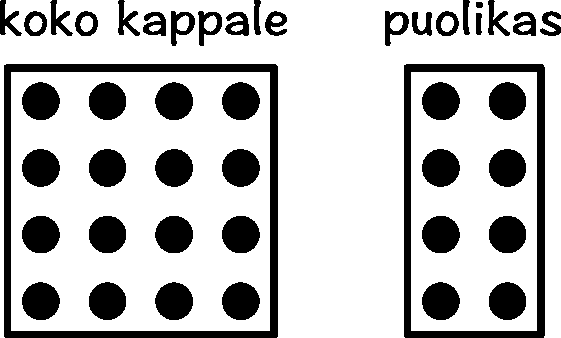
\includegraphics[width=0.7\textwidth]{figs/energia_ekstensiivinen_1.pdf}%
\end{center}%
}

 \solu  Jos kappaleen tilavuus on \(V\) ja puolitamme kappaleen, puolikkaan tilavuus on \(V/2\), joten tilavuus on \emph{ekstensiivinen}.

Jos kappale koostuu \(N\) hiukkasesta ja puolitamme kappaleen, yhteen puolikkaaseen jää \(N/2\) hiukkasta, joten hiukkasmäärä on \emph{ekstensiivinen}.

Hiukkasten lukumäärätiheys ilmaisee hiukkasten lukumäärän tilavuusyksikössä. Hiukkasten tiheys voi vaihdella kappaleessa, mutta keskimääräinen hiukkastiheys kappaleelle, joka koostuu \(N\):stä hiukkasesta ja jonka tilavuus on \(V\), on
\begin{equation} n = \frac{N}{V}. \end{equation}
Puolikkaan kappaleen hiukkastiheys on niinikään \(\frac{N/2}{V/2} = \frac{N}{V} = n\) eli sama kuin alkuperäisellä kappaleella. Hiukkastiheys on siis \emph{intensiivinen}.

 \eval  Itse asiassa jo huomio, että hiukkastiheys ei ole välttämättä vakio kappaleen sisällä kertoo, että kyseessä on intensiivinen suure, sillä vain intensiivisille suureille voidaan määritellä arvo eri paikoissa kappaleen sisällä. Ei ole mielekästä pohtia ekstensiivisen suureen kuten kappaleen tilavuuden arvoa kappaleen sisällä, koska tilavuus on koko kappaleen ominaisuus.

\end{exam}

Intensiivisillä ja ekstensiivisillä suureilla käytetään samanlaisia symboleita, joten matemaattiset lausekkeet eivät suoraan kerro, ovatko suureet intensiivisiä vai ekstensiivisiä. Fysikaalisesti intensiiviset ja ekstensiiviset ominaisuudet käyttäytyvät kuitenkin eri tavoin, eikä niitä voi yhdistellä miten sattuu. Esimerkissä \autoref{ex:ekstensiivinen} nähtiin, että kahden ekstensiivisen suureen suhde on intensiivinen. Vastaavasti koska intensiiviset suureet eivät riipu kappaleen koosta, myöskään intensiivisten suureiden tulot tai osamäärät eivät riipu kappaleen koosta ja myös ne ovat intensiivisiä suureita. Sen sijaan intensiivisen ja ekstensiivisen suureen tulo on ekstensiivinen. Esimerkiksi hiukkastiheyden (intensiivinen) ja tilavuuden (ekstensiivinen) tulona saadaan hiukkasmäärä (ekstensiivinen).

\begin{stopQ}{q:sailymislait_intensiivinen}%
(a) Selitä omin sanoin, mitä tarkoittaa intensiivisyys ja ekstensiivisyys.\\
(b) Ovatko seuraavat suureet intensiivisiä tai ekstensiivisiä: (i) nopeus, (ii) pinta-ala, (iii) tilavuuden ja nopeuden tulo?
\end{stopQ}

\subsection{Muuttuvat ja muuttumattomat suureet}
\label{muuttuvatjamuuttumattomatsuureet}

Fysiikassa usein halutaan tietää, miten suureet muuttuvat ajan kuluessa, ja riippuen suureen laadusta tämä voi tapahtua eri tavoin. Esimerkiksi kappaleen paikka muuttuu kappaleen liikkuessa. Ekstensiiviset suureet ovat kuitenkin erityisen tärkeitä, koska ne kuvaavat systeemin ominaisuuksia kokonaisuutena, joten tutkitaan nyt tällaisten suureiden muuttumista.

\widepictures{tb}%
{Systeemin sisältämän ekstensiivisen suureen muuttuminen.;%
Ekstensiivinen suure kuvaa jonkin asian määrää.;%
Suure voi muuttua vain siirtymällä ja luonnin tai hävityksen kautta.;%
Säilyvää suuretta ei voi luoda tai hävittää vaan vain siirtää.;%
Jos säilyvää suuretta ei siirry, sen määrä systeemissä on vakio.}%
{fig:energiasysteemi;fig:energiasysteemi:a;fig:energiasysteemi:b;fig:energiasysteemi:c;fig:energiasysteemi:d}%
{0.22;0.22;0.22;0.22}%
{0.22;0.22;0.22;0.22}%
{energia_sailyva_1.pdf;energia_sailyva_2.pdf;energia_sailyva_3.pdf;energia_sailyva_4.pdf}

\index{ekstensiivinen}

Ekstensiivinen suure mittaa aina jonkin asian \emph{kokonaismäärää}. Esimerkiksi hiukkasten lukumäärä kuvaa nimensä mukaisesti monestako hiukkasesta systeemi koostuu ja tilavuus kuvaa sen avaruuden määrää, jonka systeemi täyttää. Ekstensiivinen suure voikin muuttua neljällä eri tavalla: sitä voidaan tuoda systeemiin lisää, viedä pois, luoda tai hävittää. Yhtälönä tämän asian voi esittää muodossa
\begin{equation} \Delta a_\text{ekstensiivinen} = \Delta a_\text{tuonti} + \Delta a_\text{vienti} + \Delta a_\text{luonti} + \Delta a_\text{h\"avitys}. \end{equation}
Näistä eri tavoista suureen tuominen systeemiin tai vieminen sieltä pois ovat selkeästi erilaisia tapahtumia kuin luominen ja hävittäminen, sillä tuotaessa tai vietäessä suuretta vain siirtyy ympäristön ja systeemin välillä kun taas luomisen ja hävittämisen yhteydessä suureen kokonaismäärä muuttuu.

\begin{exam}{Ihmisten m\"a\"ar\"a}{ex:ekstensiivinen2}\noindent

\problem{Tarkastellaan Suomessa asuvien ihmisten lukumäärää. Millaista systeemiä, ympäristöä ja suuretta tässä tarkastellaan? Millaisissa tapahtumissa tämän suureen kokonaismäärä muuttuu?
}

 \twocol{0.39}{0.6}{ Koska suure on rajattu Suomessa asuviin ihmisiin, tarkasteltu systeemi on Suomi ja sen ympäristö ovat kaikki muut maat. Tarkasteltava suure on ihmisten lukumäärä. Rajatulla alueella asuvien ihmisten lukumäärä on myös ekstensiivinen suure, sillä se riippuu tarkasteltavan alueen koosta. Esimerkiksi Etelä-Suomen läänissä asuu vähemmän ihmisiä kuin koko Suomessa, mutta koko Suomen väkiluku on sama kuin kaikkien läänien väkilukujen summa.

}{%
\begin{center}%
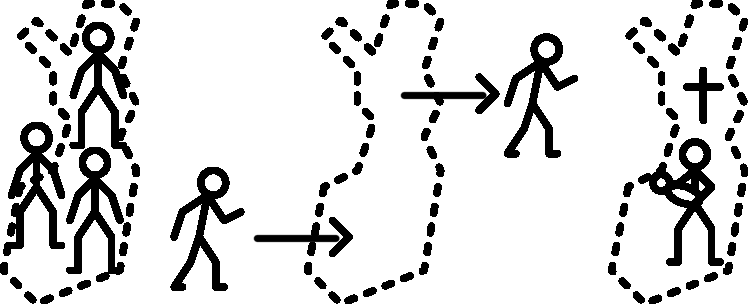
\includegraphics[width=0.7\textwidth]{figs/energia_ekstensiivinen_2.pdf}%
\end{center}%
}

Ihmisten määrä Suomessa ei muutu ihmisten muuttaessa maan sisällä, sillä tällöin asukkaiden kokonaismäärä pysyy samana ihmisten vain siirtyessä paikasta toiseen.
Ihmisten määrä voi muuttua maahanmuuton ja maastamuuton myötä, sillä tällöin ihmisiä siirtyy Suomen ja ulkomaiden välillä.
Nämä edustavat suureen siirtymistä ympäristöstä systeemiin sekä systeemistä ympäristöön. Tällöinkään kuitenkaan systeemin (Suomen) ja ympäristön (ulkomaiden) yhteenlaskettu ihmisten kokonaismäärä ei muutu.
Ihmisten määrä voi muuttua myös syntymien ja kuolemien kautta. Nämä edustavat suureen luontia ja hävittämistä, sillä niissä ihminen ei siirry minnekään vaan ihmisten kokonaismäärä todella muuttuu.

\end{exam}

\index{säilyvä}

Erityisen tärkeitä ovat ekstensiiviset suureet, joita \emph{ei voi luoda eikä hävittää}, sillä näiden suureiden mittaama asia voi ainoastaan siirtyä systeemin ja ympäristön välillä eikä sen kokonaismäärä voi muuttua. Fysiikassa tällaisten suureiden sanotaan \emph{säilyvän}. Säilyvän suureen kokonaismäärän muutos systeemissä on
\begin{equation} \Delta a_\text{s\"ailyv\"a} = \Delta a_\text{tuonti} + \Delta a_\text{vienti}. \end{equation}
Nimitys ``säilyvä'' viittaa suureen kokonaismäärään, joka säilyy muuttumattomana. Myös vektorisuureet voivat olla ekstensiivisiä säilyviä suureita, mikä tarkoittaa sitä että myös suureen suunta pysyy aina samana.

Systeemin ollessa sellainen, että säilyvää suuretta ei voi siirtyä systeemin ja ympäristön välillä eli \(\Delta a_\text{tuonti} = \Delta a_\text{vienti} = 0\), \emph{suureen kokonaismäärä systeemissä ei voi muuttua},
\begin{equation} \Delta a_\text{s\"ailyv\"a} = 0 \end{equation}
joten sen täytyy olla vakio
\begin{equation} a = \text{vakio}. \end{equation}
Edelleen koska suureen derivaatta ajan suhteen on määritelty muutosten osamäärien kautta, myös suureen aikaderivaatta on siis aina nolla
\begin{equation} \frac{\dd a}{\dd t} = 0. \end{equation}
Riippuu tilanteesta, mikä näistä tavoista esittää suureen säilyminen on käyttökelpoisin, mutta joka tapauksessa on syytä tunnistaa näiden kaikkien ilmaisevan samaa asiaa.

\textbf{Säilymislaki} on fysiikan laki, jonka mukaan fysikaalinen suure säilyy eli suuretta ei voi luoda tai hävittää. Tällöin suureen \emph{kokonaismäärä} ei muutu ajan kuluessa.
Säilymislait ovat erittäin voimakkaita fysiikan periaatteita, koska niiden avulla systeemien käytös voidaan usein analysoida yksinkertaisesti pitämällä kirjaa säilyvien suureiden käyttäytymisestä ilman tarkkaa tietoa systeemin tapahtumista. Jos säilyvän suureen määrä lisääntyy jossakin, sen on välttämättä vähennyttävä muualla yhtä paljon. Tai jos systeemi jaetaan osiin, osien on \emph{yhteensä} sisällettävä täsmälleen yhtä paljon säilyvää suuretta kuin alkuperäinen systeemi sisälsi riippumatta jaon suorittamistavasta.

\begin{exam}{Paperin s\"ailymislaki}{ex:sailyy}\noindent

\problem{Neliön muotoinen paperi leikataan neljään yhtä suureen neliön muotoiseen osaan kahdella alkuperäisten sivujen suuntaisella leikkauksella. Mikä on osien ympäryysmittojen ja pinta-alojen summa ennen ja jälkeen operaation? Entä jos paperi leikataan mielivaltaisen muotoisiin osiin?
}

 \twocol{0.35}{0.64}{ \physics  Neliön, jonka sivun pituus on \(a\), ympäryysmitta on \(4a\) ja pinta-ala \(a^2\). Kun paperi leikataan neljään osaan, saadaan neljä uutta neliötä, joiden sivujen pituudet ovat puolet alkuperäisestä.

}{%
\begin{center}%
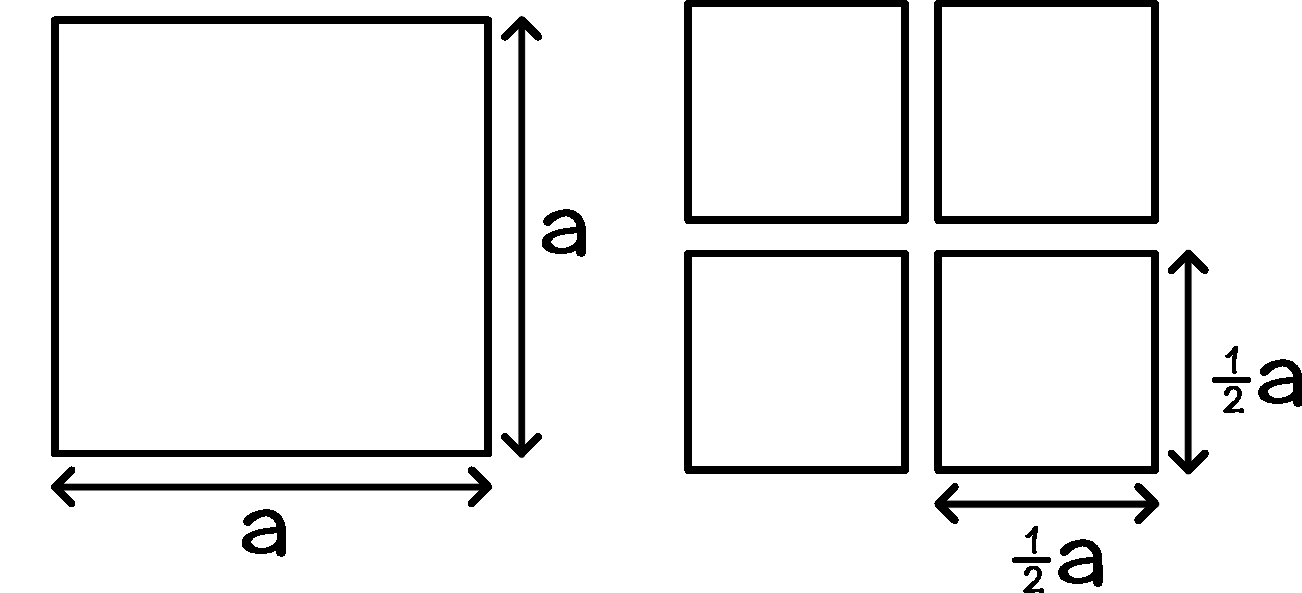
\includegraphics[width=0.7\textwidth]{figs/energia_sailyva_5.pdf}%
\end{center}%
}

 \solu  Alkuperäisen neliön sivun pituus on \(a\), ympäryysmitta \(4a\) ja pinta-ala \(a^2\).
Leikkauksen jälkeen on neljä neliön muotoista palaa, joiden kunkin sivun pituus on \(a/2\). Näiden palojen ympäryysmitta on siis \(2a\) ja pinta-ala \(a^2/4\) ja palojen yhteenlaskettu ympäryysmitta on \(4 \times 2a = 8a\) ja pinta-ala \(4 \times a^2/4 = a^2\). Palojen ympäryysmitta kasvoi mutta pinta-ala pysyi samana. Ympäryysmitta ei siis ole intensiivinen eikä ekstensiivinen suure eikä se säilynyt, mutta pinta-ala on ekstensiivinen säilyvä suure paperin leikkauksessa. (Kaksiulotteiselle kappaleelle pinta-ala on ekstensiivinen aivan samoin kuin kolmiulotteiselle kappaleelle tilavuus on ekstensiivinen suure.)

 \eval  Jos paperi leikataan mielivaltaisiin osiin, osien ympärysmitasta ei voida sanoa muuta kuin että ympärysmitta kasvaa (tämän todistaminen jätetään lukijalle). Osien kokonaispinta-ala on kuitenkin aina sama \(a^2\) riippumatta siitä, kuinka paperi on leikattu. Tämä on esimerkki säilymislakien voimasta: Vaikkemme tiedä mitään muuta kuin että paperi on leikattu, silti voidaan olla varmoja, että osien kokonaispinta-ala ei ole muuttunut, mikä on hyvin voimakas reunaehto sille, miten paperi voi leikkauksessa käyttäytyä.

Huomaa kuitenkin vielä, että paperin pinta-ala säilyy vain ideaalisessa leikkauksessa, ja pinta-alaa voidaan hävittää vaikkapa polttamalla paperi. Suureita, jotka säilyvät kaikissa mahdollisissa tapahtumissa on loppujen lopuksi hyvin vähän.

\end{exam}

\begin{stopQ}{q:muuttuvatsuureet}%
Tarkastellaan seuraavia systeemejä ja suureita. Millä tavoilla suureet voivat muuttua? Mitkä suureista pysyvät vakioina? (a) kasvien määrä puistossa, (b) ilman suhteellinen kosteus huoneessa, (c) rahan määrä lukitussa kassakaapissa.
\end{stopQ}

\section{Energia}
\label{energia}

\index{energia}

Kaikki tuntevat nykyään sanan ``energia'', koska \textbf{energia} fysikaalisena suureena on niin keskeinen modernin yhteiskunnan toiminnassa.
Karkeasti ilmaisten energia on jonkinlainen mittari sille, mitä kaikkea systeemi voi tehdä.
Ruoka sisältää kemiallista energiaa, josta saamme osan itsellemme syömällä. Tämän energian avulla pysymme lämpiminä, pystymme liikkumaan ja ylläpidämme elintoimintojamme. Käytämme myös koneita, jotka toimivat joko polttoaineiden kemiallisella energialla tai sähköisellä energialla.
Tällainen arkinen käsitys energiasta on kuitenkin monin tavoin epätäsmällinen, ja seuraavaksi tutkimme, miten energian voisi määritellä täsmällisemmin ja miten energia toimii fysikaalisissa ilmiöissä.

\subsection{Energian säilymislaki}
\label{energiansäilymislaki}

Puhekielessä sanotaan, että ``liikunta kuluttaa energiaa''. Tästä voi saada sellaisen käsityksen, että lihasten toiminta vaatii energiaa ja että samalla tämä energiaa katoaa. Tämä ei kuitenkaan ole totta. Esimerkiksi ruokaan sitoutunut kemiallinen energia on molekyylien rakenteeseen varastoitunutta energiaa. Liikuntasuorituksen aikana aineenvaihduntaan kuuluvat prosessit muuttavat kehoon varastoituneiden molekyylien rakennetta, jolloin niihin varastoitunut kemiallinen energia muuttuu. Liikuntasuorituksen aikana paljon energiaa varastoivia molekyylejä pilkotaan, jolloin niihin varastoituneen energian määrä pienenee. Energiaa siis ``kuluu'' liikuntasuorituksen aikana siinä mielessä, että kemiallinen energiavarasto hupenee.

\index{joule}

Kemiallisten energiavarastojen kuluttamisella on kuitenkin myös muita vaikutuksia. Lihakset supistuvat, ja tällä tavalla niiden omistaja voi työntää itsensä tai muut kappaleet liikkeeseen. Lisäksi lihakset lämpenevät liikuntasuorituksen aikana.
Herääkin siis kysymys, voisiko liikkeeseen ja lämpöön liittyä myös jonkinlaista energiaa, ja voiko näitä erilaisia energian muotoja mitata samalla mittarilla (samalla yksiköllä). Osoittautuu, että vastaus on \emph{kyllä}. Vaikka nämä ilmiöt ovat näennäisesti aivan erilaisia, niitä kaikkia voidaan mitata suurella nimeltä energia, jonka SI-yksikön nimeksi on annettu \textbf{joule} (James Joulen mukaan) ja symboliksi J.

Osoittautuu myös, että kun määrittelemme kemiallisen energian ja liike- sekä lämpöenergian mittarit sopivasti, lihasten toiminta lisää lämpö- ja liike-energiaa \emph{täsmälleen yhtä paljon} kuin ne kuluttavat kemiallista energiaa. Tässä mielessä lihakset eivät siis todellisuudessa \emph{kuluta} energiaa lainkaan vaan ne vain \emph{muuttavat} energiaa muodosta toiseen.

Tässä ei vielä sinänsä ole mitään ihmeellistä. Tietenkin saamme tuotettua lihaksilla sitä enemmän liikettä ja lämpöä mitä enemmän ruokaa voimme käyttää. Ei siis ole mitenkään ihmeellistä, että voimme määritellä lihasten toimintaa kuvaavan suureen, joka kertoo paljonko liikettä ja lämpöä tietyllä ruokamäärällä saadaan aikaan. Erityiseksi tämän suureen tekee se, että \emph{täsmälleen sama mittari toimii kaikissa muissakin prosesseissa}. Jos meillä on liikkuva kappale, jolla on liike-energiaa, ja vaikkapa pudotamme sen veteen, veden ja kappaleen lämpöenergia lisääntyy täsmälleen yhtä paljon kuin niiden liike-energia vähentyy.
Jos poltamme ruoan, muutamme siihen varastoituneen kemiallisen energian suoraan lämpöenergiaksi, ja tällöin lämpöenergian määrä lisääntyy yhtä paljon kuin kemiallisen energian määrä vähentyy.

Vielä tärkeämpää on se, että tämä periaate on voitu yleistää kaikkiin muihinkin ilmiöihin. Voimme nimittäin lämmittää kappaletta myös esimerkiksi valaisemalla sitä kirkkaalla valolla. Tällöin kappaleen lämpöenergia kasvaa ilman, että sen kemiallinen energia tai liike-energia muuttuisi. Tällöin voimme kuitenkin määritellä uuden energian muodon, säteilyenergian (sillä valo on säteilyä), jolloin lämpöenergian lisääntymisen voi selittää säteilyenergian vähenemisellä. Sähköjohtokin lämpenee, kun siinä kulkee sähkövirta. Tämän voimme selittää määrittelemällä sähkövirran kuljettaman sähköisen energian, jolloin johdon lämpeneminen selittyy sillä, että osa sen läpi kulkevan sähkövirran kuljettamasta sähköisestä energiasta muuttuu lämpöenergiaksi. Ja jos sähkövirta kulkee lampun läpi, lamppu lämpenee ja lähettää valoa niin, että lampun lämpöenergian kasvu ja sen lähettämän säteilyenergian määrä on täsmälleen yhtä suuri kuin sähkövirran kuljettaman sähköenergian menetys lampussa. \emph{Aina}, kun energiaa on näyttänyt katoavan tai syntyvän itsestään, on löydetty jokin uusi energian muoto, joka on selittänyt havaitut muutokset. Vaikka energian eri muodot voivat lisääntyä ja vähentyä, ei tunneta ilmiöitä, joissa kaikkien eri energian muotojen summa eli \textbf{kokonaisenergia}\\
\begin{equation} E_\text{kokonais} = E_\text{liike} + E_\text{kemia} + E_\text{l\"amp\"o} + E_\text{s\"ateily} + E_\text{s\"ahk\"o} + \ldots \end{equation}
muuttuisi. \emph{Systeemin} kokonaisenergia voi toki muuttua, sillä energiaa voi siirtyä systeemin ja sen ympäristön välillä, mutta \emph{systeemin ja sen ympäristön} yhteenlasketun kokonaisenergian täytyy olla aina vakio,
\bigeq{ \Delta E_\text{kokonais} = 0. \label{energia_sailyy} }

\index{säilyvä}

Tämä tulos on \textbf{energian säilymislaki}. Se on kaiken fysiikan tärkeimpiä periaatteita, jonka mukaan \emph{energiaa ei voi luoda eikä hävittää}. Energian säilyminen on alunperin päätelty kokeellisesti, mutta nykyisin sillä on myös vankka teoreettinen pohja.

\begin{stopQ}{q:ekstensiivinenenergia}%
(a) Jos yhdessä hampurilaisessa on kemiallista energiaa 2000 kJ, paljonko energiaa kahdessa samanlaisessa hampurilaisessa on?\\
(b) Jos yksi lamppu tarvitsee 5 J sähköenergiaa sekunnissa, paljonko kaksi lamppua tarvitsee?\\
(c) Onko energia edellisten kohtien perusteella ekstensiivinen vai intensiivinen suure?\\
(d) Miten ekstensiivisyys tai intensiivisyys liittyy siihen, että energia on säilyvä suure?
\end{stopQ}

Energian säilymislaki on tärkeä useastakin syystä. Ensinnäkin energia on kaikkia fysiikan osa-alueita yhdistävä fundamentaali suure. Toiseksi energian säilyminen rajoittaa voimakkaasti sitä, mitä voi tapahtua. Jos käytettävissä on polttoainemäärä, johon on varastoitu 1000 kJ energiaa, sillä ei voi kiihdyttää kulkuneuvoa nopeuteen, jossa liike-energia olisi tätä suurempi. Myös ikiliikkujat, jotka liikkuisivat ikuisesti ja joita voitaisiin samalla käyttää hyväksi jotenkin, ovat energian säilymisen vuoksi mahdottomia. Jos nimittäin systeemi kasvattaa ympäristönsä energiaa, systeemin energian täytyy vähentyä. Kolmanneksi energian säilymislain avulla voidaan sopivasti valituissa systeemeissä päätellä täsmälleen, miten systeemi käyttäytyy.

\begin{exam}{Systeemin valinta}{ex:systeemienergia}\noindent

\problem{Eristetyssä laatikossa on kaksi mukillista kuumaa vettä. Toinen mukeista on kannellinen pahvimuki, toinen kanneton. Millaisin tavoin tilanne voidaan rajata systeemiksi? Onko systeemin ainemäärä tai kokonaisenergia vakioita? }

 \twocol{0.4}{0.59}{ \setup  Laatikkoon kuuluu nyt kaksi mukia, niiden sisältämät vedet, ilmaa sekä laatikko itse. Mikä tahansa näiden yhdistelmä voidaan valita systeemiksi. Tarkastellaan muutamaa erikoistapausta.

}{%
\begin{center}%
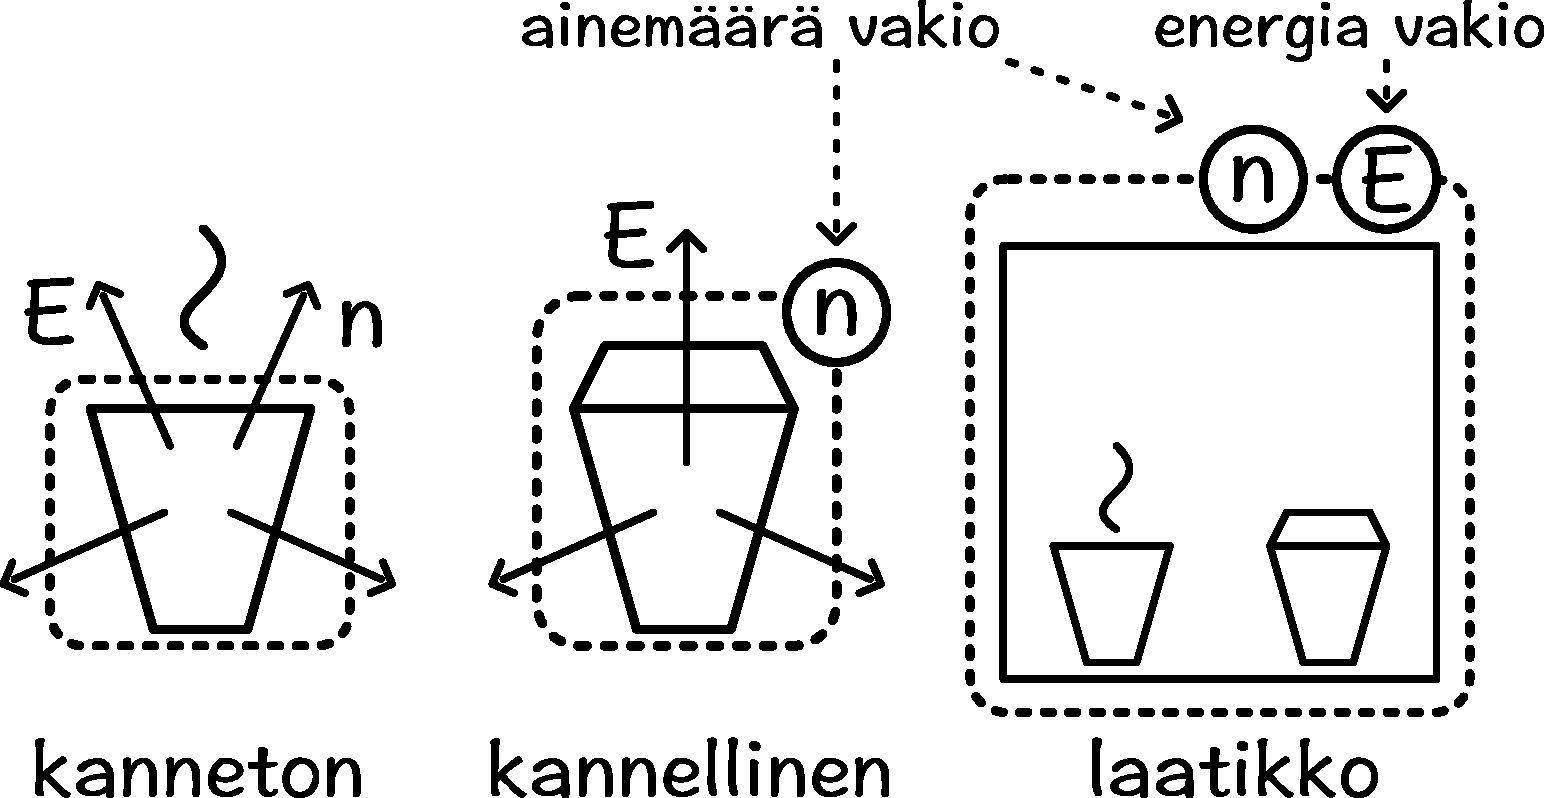
\includegraphics[width=0.8\textwidth]{figs/energia_systeemi_5.pdf}%
\end{center}%
}

 \physics Valitaan systeemiksi kanneton muki sekä sen sisältämä tilavuus. Tilavuus ei itsessään ole mikään kappale, mutta tällä tarkoitetaan systeemiin sisältävän kaiken sen aineen, joka kulloinkin on mukin sisällä. Koska vesi on kuumaa, siihen on varastoitunut lämpöenergiaa. Vesi kuitenkin jäähtyy, jolloin ilmeisesti sen sisältämän energian määrä pienenee,
\begin{equation} \Delta E_\text{systeemi} = \Delta E_\text{vesi} + \Delta E_\text{muki} < 0. \end{equation}
Systeemin \emph{kokonaisenergia siis ei ole vakio}.
Koska mukissa ei ole kantta, kuumaa vettä muuttuu myös kaasuksi ja poistuu mukista kaiken aikaa ja niinpä mukin sisältämän nestemäisen veden määrä vähenee. Tilalle tulee ilmaa, mutta tarvitaan huomattavasti pienempi määrä ilmaa korvaamaan poistunut neste. Siispä tässä systeemissä myöskään \emph{ainemäärä ei ole vakio}.

Valitaan systeemiksi sitten kannellinen muki sekä sen sisältö eli kuuma vesi. Koska mukissa on kansi, ei sieltä pääse pois vettä eikä ilmaa, joten systeemin sisältämä \emph{ainemäärä on vakio}. Muistutukseksi tästä voidaan tilanteesta piirrettyyn kuvaan merkitä systeemin rajauksen yhteyteen merkintä \(n\) osoittamaan ainemäärän olevan systeemissä vakio. Kuten kannettoman mukin tapauksessa, nytkin mukissa oleva vesi jäähtyy, sillä lämpöä pääsee virtaamaan mukin seinämien läpi ympäröivään ilmaan ja siis systeemin sisältämä \emph{kokonaisenergia ei ole vakio}.

Tarkastellaan vielä systeemiä, johon kuuluu koko laatikon sisältö ja laatikko itse. Kun kuuma vesi mukeissa jäähtyy, sen energiaa siirtyy laatikon sisältämän ilman ja laatikon itsensä lämpöenergiaksi. Jos laatikko on hyvin eristetty, lämpöenergiaa ei kuitenkaan pääse siirtymään laatikon ulkopuolelle. Tällöin veden sisältämä energiamäärä pienenee täsmälleen yhtä paljon kuin ilman ja laatikon sisältämä energia lisääntyy ja systeemin \emph{kokonaisenergia on vakio}
\begin{equation} \Delta E_\text{systeemi} = \Delta E_\text{vesi} + \Delta E_\text{mukit} + \Delta E_\text{ilma} + \Delta E_\text{laatikko} = 0. \end{equation}
Koska laatikko on tiivis, sieltä ei pääse ilmaa ulos ja myös systeemin \emph{ainemäärä on vakio}.

\end{exam}

\index{systeemi}
\index{avoin systeemi}
\index{suljettu systeemi}
\index{eristetty systeemi}

Esimerkissä \autoref{ex:systeemienergia} tarkastellaan mahdollisia tapoja rajata systeemi ja systeemin kokonaisenergian huomataan joissakin tapauksissa olevan vakio ja toisissa ei.
Jos systeemin ja sen ympäristön välillä voi siirtyä energiaa ja ainetta, systeemiä kutsutaan \textbf{avoimeksi}. Esimerkissä \autoref{ex:systeemienergia} tällainen systeemi oli kanneton muki. Jos systeemistä ei voi siirtyä ainetta ympäristöön mutta energiaa voi, systeemiä kutsutaan \textbf{suljetuksi}. Esimerkissä tällainen systeemi oli kannellinen muki. Systeemi, joka ei voi vaihtaa ainetta eikä energiaa ympäristönsä kanssa, on \textbf{eristetty} systeemi, ja tällainen oli esimerkin eristetty laatikko.

Jos systeemi on eristetty, se ei voi saada energiaa ympäristöstään eikä myöskään menettää sitä. Koska energian säilymislain mukaan energiaa ei voi luoda eikä hävittää, energian kokonaismäärän systeemissä on tällöin oltava vakio. Näin saadaan yleisen energian säilymislain erikoistapaus: \textbf{eristetyn systeemin kokonaisenergia on vakio kaikissa prosesseissa},
\bigeq{ \Delta E_\text{eristetty} = 0. }

\begin{stopQ}{q:laihdutus}%
Laihduttaminen on mahdollista liikkumalla paljon. Valitaan systeemiksi ihminen. Selitä, miten liikunta voi johtaa systeemin energian ja atomien määrän muuttumiseen.
\end{stopQ}

\index{energiaperiaate}

Eristetyn systeemin käyttäytyminen voidaan usein ennustaa varsin tarkasti pitämällä kirjaa energian eri muodoista, koska niiden summa ei muutu. Tätä kirjanpitotekniikkaa kutsutaan \textbf{energiaperiaatteeksi}. Jos nimittäin osaamme laskea systeemin kokonaisenergian määrän yhdellä ajan hetkellä, tiedämme varmasti kokonaisenergian olevan \emph{sama} minä tahansa muunakin aikana riippumatta siitä mitä systeemissä täsmälleen tapahtuu. Eritysesti jos systeemissä vain muutamat energian muodot muuttuvat, voidaan yhden energian lajin muutokset päätellä tarkastelemalla \emph{muiden} energian muotojen käyttäytymistä. On hyvin tavallista, että joidenkin energian muotojen määrä on helppo määrittää kun taas toisiin muotoihin varastoitunut energia on vaikea mitata tai laskea. Tällöin voidaan päätellä näiden hankalampienkin muotojen sisältämä energia tutkimalla helpommin havaittavia energian lajeja.

\index{energiadiagrammi}

Tällaisissa tilanteissa \textbf{energiadiagrammi} on hyvä tapa havainnollistaa energian muotojen muutokset. Energiadiagrammi on graafinen esitys, jossa systeemin kokonaisenergian jakautuminen eri muotoihin esitetään esimerkiksi pylväskuvaajana. Tällaisen kuvallisen esityksen avulla on helpompi muistaa huomioida kaikki systeemissä ilmenevät energian muodot ja ennen kaikkea niiden avulla voi suoraan nähdä miten energian eri muodot muuttuvat.

\widepictures{tb}%
{Energiadiagrammeja erilaisille systeemeille. Kuvissa (a) ja (b) kahden kappaleen väliin puristettu jousi työntää kappaleet liikkeelle. Kuvissa (c) ja (d) ihminen työntää laatikkoa.;%
Kokoon puristettuun jouseen varastoitunut elastinen energia muuttuu kappaleiden liikkeen energiaksi.;%
Osa energiasta siirtyy toiselle kappaleelle, systeemin ulkopuolelle.;%
Ihmiseen varastoitunut kemiallinen energia muuttuu ihmisen ja kappaleen liikkeen ja lämmön energiaksi.;%
Osa lämmöstä siirtyy maahan, systeemin ulkopuolelle.}%
{fig:energiadiagrammi;fig:energiadiagrammi:a;fig:energiadiagrammi:b;fig:energiadiagrammi:c;fig:energiadiagrammi:d}%
{0.22;0.2;0.23;0.23}%
{0.22;0.2;0.23;0.23}%
{energia_diagrammi_1.pdf;energia_diagrammi_6.pdf;energia_diagrammi_4.pdf;energia_diagrammi_5.pdf}

\index{jousi}

Kuvassa \autoref{fig:energiadiagrammi} on esitetty tällaisia energiadiagrammeja erilaisille systeemeille. Ensimmäisessä esimerkissä jousi on puristettu kahden kappaleen väliin. Jousen puristamiseen (muodon muutokseen) liittyy energiaa, joka muuttuu kappaleiden liikkeen energiaksi päästettäessä jousi oikenemaan. Jos nämä kappaleet eivät vuorovaikuta muiden kappaleiden kanssa, energiaa ei voi muuttua mihinkään muuhun muotoon ja systeemin kokonaisenergian täytyy olla vakio. Tällöin kappaleiden yhteen lasketun liike-energian on lopuksi oltava yhtä suuri kuin jouseen varastoitunut energia oli aluksi. Tämä ilmenee energiadiagrammissa siten, että jousen elastinen energia vähenee täsmälleen yhtä paljon kuin liike-energia kasvaa.

Edellinen tarkastelu onnistui siksi, että tarkastelimme eristettyä systeemiä. Systeemin valintahan on mielivaltainen, joten samaa tilannetta voitaisiin tarkastella myös systeeminä, johon kuuluu ainoastaan yksi kappaleista sekä jousi. Tällöin toinen kappale on osa ympäristöä. Tämä on aivan kelvollinen systeemin valinta, mutta koska jousi vuorovaikuttaa molempien kappaleiden kanssa, systeemin ja ympäristön välillä on nyt vuorovaikutus. Kummankin kappaleen nopeus muuttuu jousen vapautuessa, jolloin ympäristön kokonaisenergia muuttuu. Osa alunperin jouseen sitoutuneesta energiasta siis siirtyy systeemistä ympäristöön eikä systeemin kokonaisenergia ole nyt vakio.

Kolmannessa kuvassa on esitetty tilanne, jossa joku työntää lattialla olevan suuren laatikon liikkeelle. Tässä prosessissa työntäjä kuluttaa varastoimaansa kemiallista energiaa lihastensa liikuttamiseksi. Laatikko lähtee liikkeelle, jolloin sen liikkeen energia kasvaa. Samalla huomataan myös työntäjän, laatikon sekä lattian lämpenevän, mihin liittyy lämpöenergiaa. Kun kaikki liikkuvat ja lämpenevät kappaleet ovat mukana tarkasteltavassa systeemissä, ympäristöön jää ainoastaan asioita, joihin laatikon työntäminen ei vaikuta mitenkään. Energiaa ei siis siirry systeemistä ympäristöön ja systeemin kokonaisenergia on vakio. Prosessissa muuttuu toisikseen kolme energian muotoa --- liike-energia, lämpöenergia sekä kemiallinen energia --- mutta näiden summa pysyy samana. Diagrammissa tämä ilmenee niin, että kemiallinen energia vähenee yhtä paljon kuin lämpöön ja liikkeeseen liittyvät energiat yhteensä lisääntyvät.

Jos energiaperiaatetta käyttää, on aina oltava huolellinen systeemin valinnassa ja tarkistettava, että valitussa systeemissä energia on todella vakio. Jos nimittäin äskeisessä esimerkissä vaikkapa lattia jätetään systeemin ulkopuolelle, lattian lämmöksi muuttuva energia ei enää kuulukaan systeemiin eli systeemin kokonaisenergia pienenee vaikka systeemin ja ympäristön yhteenlaskettu energia ei muutukaan.

\begin{stopQ}{q:energiasysteemeissa}%
Muovailuvahapallo heitetään seinään, johon se tarttuu kiinni. Kun pallo vielä liikkui ennen seinään osumista, sen liikkeeseen liittyi energiaa. Onko systeemin kokonaisenergia vakio, jos systeemi on (a) pelkkä vahapallo, (b) pallo ja seinä? (c) Millaisiin muotoihin pallon liikkeen energia saattoi muuttua?
\end{stopQ}

\subsection{Liikkeen ja painovoiman energia}
\label{liikkeenjapainovoimanenergia}

Edellä puhuimme energiaperiaatteesta yleisellä tasolla, mutta jotta energiaa voisi todella käyttää fysikaalisten prosessien analyysin työkaluna, meidän täytyy ensin määritellä erilaiset energian muodot täsmällisesti. Erityisesti haluamme laskea systeemien energiasisällön eri tilanteissa. Koska mekaniikassa tutkimme pääasiassa kappaleiden liikettä, keskitymme aluksi kappaleiden nopeuksista, paikoista ja muodoista riippuviin energian muotoihin.

\index{vapaa pudotus}

Aloitetaan tutkimalla putoamisliikettä, koska kappaleen \autoref{kiihtyvyys} pohjalta osaamme jo analysoida vapaassa pudotuksessa olevan kappaleen liikkeen. Erityisesti johdimme yhtälön (\autoref{nopeusneliomuutos}) eli
\( \Delta (v_x^2) = - 2 g \Delta x, \)
jonka mukaan pystysuorassa vapaassa pudotuksessa olevan kappaleen nopeuden neliön muutos \(\Delta (v_x^2) \) on aina verrannollinen kappaleen paikan muutokseen \(\Delta x\) riippumatta siitä, miltä korkeudelta kappale putoaa tai onko kappaleella alkunopeutta. Erityiseti tulos pätee riippumatta siitä, liikkuuko kappale ylöspäin, alaspäin tai kenties edestakaisin molempiin suuntiin liikkeensä aikana.

\index{muutos}
\index{Delta, $\Delta$}

Koska tutkimme nyt nimenomaan suureiden muutoksia, kerrataan muutamia muutosten laskusääntöjä. Ensinnäkin, jos \(k\) on vakio ja suure \(a\) muuttuu määrän \(\Delta a\) eli \(a_\text{loppu} = a_\text{alku} + \Delta a\), tulo \(ka\) saa arvon \( ka_\text{loppu} = k(a_\text{alku}+\Delta a) = ka_\text{alku} + k\Delta a\). Siispä tulon \(ka\) \emph{muutos} on
\begin{equation} \Delta (ka) = ka_\text{loppu} - ka_\text{alku} = k \Delta a. \end{equation}
Vakion ja muuttuvan suureen \(a\) tulon muutos on siis yhtä suuri kuin vakion ja \(a\):n muutoksen tulo.

Samoin jos kaksi suuretta \(a\) ja \(b\) muuttuvat, niiden summa saa arvon
\(a_\text{loppu} + b_\text{loppu} = a_\text{alku} + \Delta a + b_\text{alku} + \Delta b\),
ja näin ollen suureiden summan muutos on yhtä suuri kuin niiden muutosten summa,
\begin{equation} \Delta (a + b) = (a_\text{loppu} + b_\text{loppu}) - (a_\text{alku} + b_\text{alku}) =  \Delta a + \Delta b. \end{equation}

Käyttäen näitä laskusääntöjä yhtälö (\autoref{nopeusneliomuutos}) voidaan putoamisliikeen tapauksessa (kun putoaminen tapahtuu tyhjiössä tai kappaleen vuorovaikutusta sitä ympäröivän ilman kanssa ei huomioida) kirjoittaa muotoon
\begin{equation} \Delta \left( \frac{1}{2} v_x^2 \right) = - \Delta (g x) \label{energy_fall_first} \end{equation}
ja edelleen siirtämällä kaikki termit yhtälön vasemmalle puolelle
\begin{equation} \Delta \left( \frac{1}{2} v_x^2 + g x \right) = 0, \label{energy_fall} \end{equation}
mikä siis tarkoittaa sitä, että nopeuden neliön ja kappaleen paikkakoordinaatin summa, kertoimien \(1/2\) ja \(g\) kanssa, on \emph{vakio}.

Näin johdettuna tulos voi vaikuttaa vain matemaattiselta tempulta, mutta se antaa meille vihjeen paljon syvällisemmästä fysikaalisesta yhteydestä, joten pohditaan tulosta tarkemmin.
Ensinnäkin tulos yhdistää kappaleen vauhdin ja sen korkeuden niin, että syntyy vakiona pysyvä lauseke. Toisaalta jos valitsemme systeemiksi putoavan kappaleen ja maapallon, tämä systeemi sisältää kaiken, mikä putoamisessa muuttuu (kappaleen nopeus ja sen etäisyys maasta). Putoaminen on siis prosessi, joka vaikuttaa vain valitun systeemin sisällä, ja niinpä energian säilymislain perusteella tämän systeemin kokonaisenergian täytyy myös olla vakiona pysyvä lauseke. Ehkä siis yhtälössä \autoref{energy_fall} esiintyvä lauseke liittyy systeemin kokonaisenergiaan!

\index{painovoima}

\marginpictures%
{0}%
{Liike-energia.;%
Eri nopeudella liikkuvat kappaleet.;%
Liike-energia nopeuden funktiona.}%
{fig:energia_k}%
{1.0;1.0}%
{energia_liike_funktio_1.pdf;energia_liike_funktio_2.pdf}

Yhtälön ensimmäinen termi riippuu vain kappaleen nopeudesta, ja se on sitä suurempi, mitä nopeammin kappale liikkuu. Tämän termin voisi siis tulkita liittyvän kappaleen liikkeen energiaan. Yhtälön toinen termi puolestaan riippuu putoamiskiihtyvyydestä ja kappaleen korkeudesta. Putoamiskiihtyvyys on painovoiman ominaisuus, joten ilmeisesti tämä termi kuvaa jotenkin \emph{painovoimaan varastoituvaa energiaa}.

Yhtälössä (\autoref{energy_fall}) esiintyvä lauseke ei kuitenkaan voi kuvata systeemin energiaa täsmälleen vaan se on ainoastaan siihen verrannollinen lauseke. Nopeus ja paikkakoordinaatti ovat nimittäin \emph{intensiivisiä} suureita, joten lausekkeen kuvaama suure on myös intensiivinen. Lausekkeen arvohan ei riipu mitenkään siitä, koostuuko tarkasteltava systeemi vaikkapa hiekanjyvästä vai kivenlohkareesta.

\index{ekstensiivinen}
\index{massa}
\index{kilogramma}
\index{SI-järjestelmä}

Energia on kuitenkin \emph{ekstensiivisinen} suure kuten kaikki säilyvät suureet. Jos meillä olisi esimerkiksi kaksi samanlaista, samalla nopeudella liikkuvaa kappaletta, niillä pitäisi olla kaksinkertainen energia yhteen kappaleeseen verrattuna. Samoin arkikokemuksestakin tiedämme, että on raskaampaa nostaa monta kappaletta kuin vain yksi, koska kaksi kappaletta ovat yhdessä \emph{painavammat} kuin yksi. Niinpä myös painovoiman energian täytyy riippua siitä, paljonko ainetta on. Yhtälöstä (\autoref{energy_fall}) puuttuu siis jokin kappaleen kokoon ja määrään liittyvä tekijä, joka kertoo tarkasteltavan aineen määrän.
Tämä tekijä on kappaleen \textbf{massa}. Massa on SI-järjestelmän perussuure, jonka yksikkö on \textbf{kilogramma} (kg).

\index{inertia}

Massalla on fysiikassa kaksi toisistaan täysin poikkeavaa roolia. Ensinnäkin massiiviset kappaleet ovat \emph{painavia}, mikä tarkoittaa karkeasti ilmaisten sitä, että niiden nostaminen \emph{ylöspäin} on vaikeaa. Arkikielessä yleensä puhutaankin kappaleen painosta, kun tarkoitetaan sen massaa. Toisaalta massiiviset kappaleet ovat \emph{hitaita}, mikä tarkoittaa karkeasti sitä, että suuren nopeuden antaminen kappaleelle on vaikeaa \emph{mihin tahansa suuntaan}. Jälkimmäistä ominaisuutta eli massan hitautta kutsutaan fysiikassa \textbf{inertiaksi}.
Nämä voivat vaikuttaa samankaltaisilta asioilta mutta niillä on täysin erilainen fysikaalinen merkitys. Nostaminen liittyy kappaleen \emph{paikan muuttamiseen} ja erityisesti kappaleen siirtämiseen poispäin maanpinnasta (eli yhtälössä \autoref{energy_fall} suureen \( x \) muutokseen). Nostaminen on vaikeaa, koska maa ja kappale vuorovaikuttavat \emph{painovoiman} eli \textbf{gravitaation} kautta, ja kappaleen siirtäminen poispäin varastoi energiaa gravitaatiovuorovaikutukseen. Painava massa kuvaa tämän vuorovaikutukseen voimakkuutta. Kappaleen liikkeelle saaminen puolestaan liittyy \emph{nopeuden muuttamiseen} (eli yhtälössä \autoref{energy_fall} suureen \( v_x \) muutokseen), mikä on aivan yhtä vaikeaa vaikka kappale olisi tyhjässä avaruudessa kaukana Maapallosta.
Nykytietämyksen mukaan inertia ja painava massa ovat kuitenkin täsmälleen samat kaikilla hiukkasilla ja kappaleilla.

\marginpictures%
{-10}%
{Painovoiman potentiaalienergia.;%
Eri korkeudella olevat kappaleet.;%
Potentiaalienergia paikan funktiona.}%
{fig:energia_g}%
{1.0;1.0}%
{energia_g_funktio_1.pdf;energia_g_funktio_2.pdf}

\begin{stopQ}{q:hitausjapaino}%
Jos otat käteesi esimerkiksi kuulantyönnössä käytettävän painavan kuulan ja työnnät sen liikkeelle (a) suoraan vaakasuoraan tai (b) suoraan ylös, mikä massan ominaisuus pääasiassa rajoittaa nopeutta, jonka pystyt kuulalle antamaan?
\end{stopQ}

\index{liike-energia}

Kappaleen liikkeeseen liittyy energiaa, joka riippuu kappaleen inertiasta, sillä mitä suurempi on kappaleen inertia, sitä enemmän energiaa tarvitaan, jotta kappale saataisiin kiihdytettyä johonkin nopeuteen \(v_x\). Niinpä kappaleen, jonka inertia on \(m\), \textbf{liike-energia} eli \textbf{kineettinen energia} \(K\) on yhtälön (\autoref{energy_fall}) ensimmäinen termi kerrottuna kappaleen massalla \(m\),
\bigeq{ E_\text{liike} = K = \frac{1}{2}mv_x^2. \label{kin_ene}}
Tästä yhtälöstä voimme yksikkötarkastelulla myös määrittää energian yksikön joulen perusyksiköiden avulla lausuttuna,
\begin{equation} \text{J} = [K] = [m][v_x^2] = \text{kg}\text{m}^2/\text{s}^2. \end{equation}

\index{potentiaalienergia}

Kertomalla koko yhtälö (\autoref{energy_fall}) kappaleen massalla saadaan siis varsinainen putoavan kappaleen energian säilymislaki
\begin{equation} \Delta \left( \frac{1}{2} mv_x^2 + m g x \right) = 0. \label{energy_fall_proper} \end{equation}
Yhtälön jälkimmäinen termi on kappaleen ja maan välisen painovoiman varastoima energia, jota kutsutaan fysiikassa \textbf{potentiaalienergiaksi} ja merkitään tavallisesti symbolilla \(U\)
\bigeq{ E_\text{potentiaali} = U = mgx. \label{pot_ene}}
Nimitys viittaa siihen, että tällä varastoidulla energialla voidaan esimerkiksi saada kappale liikkeelle --- sillä on siis ``potentiaalia'' saada prosesseja tapahtumaan.
Yhtälössä (\autoref{pot_ene}) massa ilmaisee sitä, että painavan kappaleen nostaminen vaatii paljon energiaa.

\index{heittoliike}

Kuvassa \autoref{fig:energiaheitto} on esitetty jo aiemmin luvussa \autoref{kiihtyvyys} analysoitu pystysuora heitto energiadiagrammein. Heitetyn kappaleen sekä Maan sisältävän systeemin kokonaisenergia on heiton aikana vakio, sillä liike-energia on kappaleen liikkeen ominaisuus ja painovoiman potentiaalienergia on maan ja kappaleen vuorovaikutuksen varastoimaa energiaa. Nämä kuuluvat systeemiin, jossa ovat sekä kappale että maa.

Liike-energia riippuu kappaleen nopeuden neliöstä, joten se ei voi koskaan olla negatiivinen. Erityisesti \emph{liike-energian etumerkki ei riipu nopeuden suunnasta kuten nopeuden skalaarikomponentti}. Potentiaalienergia puolestaan riippuu kappaleen koordinaatista pystysuunnassa. Koordinaatti kuitenkin mitataan aina jonkin kiintopisteen suhteen, ja tämä kiintopiste voidaan valita periaatteessa minne tahansa. Potentiaalienergia saa kohdassa \(x=0\un{m}\) arvon nolla, joten kiintopisteen valinta kiinnittää myös potentiaalienergian nollatason, ja tämän alapuolella \emph{potentiaalienergia on negatiivinen}. Potentiaalienergian absoluuttisella arvolla ei olekaan mitään fysikaalista merkitystä, vaan ainoastaan potentiaalienergian \emph{muutokset} ovat merkityksellisiä. Heittoliikkeen tapauksessa potentiaalienergian nollataso voidaan valita esimerkiksi kappaleen lähtöpisteeseen, mutta tämä ei ole ainoa mahdollinen valinta.

\pictures{tb}%
{Energiadiagrammi pystysuoralle heitolle.;%
Alkutilanne: kappale heitetään ylöspäin.;%
Lakipiste.;%
Jälleen lähtökorkeudella.;%
Lähtökorkeutta alempana.}%
{fig:energiaheitto;fig:energiaheitto:a;fig:energiaheitto:b;fig:energiaheitto:c;fig:energiaheitto:d}%
{0.22;0.22;0.22;0.22}%
{0.22;0.22;0.22;0.22}%
{energia_heitto_1.pdf;energia_heitto_2.pdf;energia_heitto_3.pdf;energia_heitto_4.pdf}

\index{lakipiste}

Jos potentiaalienergian nollakohdaksi valitaan kappaleen lähtöpiste, ylöspäin heitetyllä kappaleella on aluksi liike-energia \(K = \frac{1}{2}mv_x^2\) eikä lainkaan potentiaalienergiaa. Ylöspäin nousevan kappaleen potentiaalienergia kasvaa ja liike-energia pienenee niin, että kokonaisenergia on koko ajan vakio. Koska liike-energia ei voi saada negatiivisia arvoja, kappale pääsee täsmälleen niin korkealle, että kaikki sen alkuperäinen liike-energia on muuttunut potentiaalienergiaksi, jolloin sen nopeus on nolla. Tämän jälkeen kappale putoaa jälleen alaspäin ja päästyään takaisin lähtökorkeudelleen sen potentiaalienergia on jälleen nolla ja sen liike-energia on sama kuin alkuhetkellä. Kappaleen vauhtikin on siis tällöin yhtä suuri kuin heiton alussa.

Kappaleen jatkaessa putoamistaan lähtötasonsa alapuolelle sen potentiaalienergia pienenee edelleen saaden nyt \emph{negatiivisia} arvoja. Tässä ei ole mitään ihmeellistä, sillä potentiaalienergian nollakohta riippui koordinaatiston origon valinnasta. Potentiaalienergian negatiiviset arvot eivät siten tarkoita fysikaalisesti sen enempää kuin paikkakoordinaatin negatiiviset arvot: ne ainoastaan kertovat siitä, että kappale on nyt liikkunut valitusta origosta negatiiviseen suuntaan. Oleellista on se, että liike-energia aina kasvaa täsmälleen yhtä paljon kuin potentiaalienergia pienenee. Kappaleen liikkeessä liike-enegian kasvu ilmenee kappaleen nopeuden kasvamisena. Kuitenkin koska liike-energia on verrannollinen nopeuden neliöön, kappaleen nopeus kasvaa \emph{hitaammin} kuin liike-energia.

\begin{stopQ}{q:heittodiagrammi}%
Miten kuvan \autoref{fig:energiaheitto} heittoliikkeen (i) energiadiagrammi ja (ii) pallon rata muuttuvat, jos\\
(a) pallon alkunopeus on kaksinkertainen,\\
(b) potentiaalienergian nollakohta valitaan heiton lakipisteeseen?\\
(c) vuorovaikutus ilman kanssa muuttaa osan pallon liike-energiasta lämpöenergiaksi heiton aikana?
\end{stopQ}

\subsection{Elastinen energia}
\label{elastinenenergia}

\index{elastinen}
\index{jousi}

Kappaleen muodon muuttaminen on myös energiaa vaativa prosessi, ja toisaalta esimerkiksi puristetun jousen avulla voi laukaista kappaleen liikkeelle. Siispä mitä ilmeisimmin jousi tai mikä tahansa muu sopivasti taipuisa kappale kykenee varastoimaan energiaa muuttamalla muotoaan. Tällaista itsestään palautuvaa taipuisuutta kutsutaan fysiikassa \textbf{elastisuudeksi} ja jouseen varastoitunut energia on \emph{elastista potentiaalienergiaa}. Kunhan jousta ei venytetä liikaa, \emph{ideaalinen jousi} varastoikin kaiken sen puristamiseen tai venyttämiseen tarvitun energian ja voi vapauttaa sen takaisin liike-energiaksi.

\index{tasapaino}

Jos jousta ei puristeta eikä venytetä, se on niin sanotussa \emph{lepopituudessaan}. Koska jousi ei tällöin pyri itsestään muuttamaan pituuttaan, tätä kutsutaan myös jousen \emph{tasapainopituudeksi}. Jousta voidaan yleensä sekä puristaa lyhyemmäksi että venyttää pidemmäksi, ja molemmat muutokset vaativat energiaa, joten jousen potentiaalienergia on \emph{pienimmillään} jousen ollessa lepopituudessaan. Tästä syystä jousen potentiaalienergian nollakohdaksi yleensä valitaankin juuri jousen lepopituus. Itse asiassa ideaalisen jousen pituuden muuttaminen vaatii \emph{yhtä paljon} energiaa olipa kyseessä puristus tai venytys. Mitä enemmän jousen pituutta muutetaan, sitä enemmän energiaa tarvitaan, eikä kyseessä itse asiassa ole edes suora verrannollisuus vaan suurien venymien aikaansaaminen on tavallisesti huomattavasti vaikeampaa kuin pienten.

\index{malli}
\index{harmoninen}

\marginpictures%
{-25}%
{Elastinen potentiaalienergia.;%
Eripituiset jouset.;%
Energia pituuden funktiona.}%
{fig:energia_u}%
{1.0;1.0}%
{energia_k_funktio_1.pdf;energia_k_funktio_2.pdf}

Todellisen jousen potentiaalienergia voi riippua jousen pituudesta monimutkaisellakin tavalla. Kuitenkin yksinkertaisin matemaattinen funktio, jolla on edellä kuvatut elastisen potentiaalienergian ominaisuudet, on toisen asteen polynomi eli paraabeli. Niinpä jousten ja muidenkin elastisten kappaleiden varastoimaa potentiaalienergiaa kuvataan yleensä tällä yksinkertaisella mallilla,
\bigeq{ U = \frac{1}{2} k (x-x_0)^2, \label{harmoninen_pot} }
jota kutsutaan myös \emph{harmoniseksi potentiaalienergiaksi}.
Tässä \(k\) on jousen jäykkyyttä kuvaava \textbf{jousivakio}, \(x\) on jousen pituus ja \(x_0\) sen lepopituus. Etäisyys \(x-x_0\) on siis jousen normaalista pituudesta mitattu venymä. Sen positiivinen arvo kuvaa jousen venymistä pidemmäksi ja negatiivinen arvo puristumista lyhyemmäksi. Funktio \(U\) on nolla, kun venymä on nolla, ja se saa yhä suurempia positiivisia arvoja, kun jousta joko puristetaan tai venytetään. Tämä tarkoittaa jousen varastoivan yhä enemmän energiaa mitä enemmän sitä puristetaan tai venytetään, kuten kuvasta \autoref{fig:energia_u} nähdään. Mitä suurempi jousivakio \(k\) on, sitä enemmän energiaa jousen pituuden muuttaminen vaatii eli sitä \emph{jäykempi} jousi on.

\begin{stopQ}{q:energiatiivistelma}%
Kirjoita omin sanoin tiivistelmä siitä, miten kappaleen liike- ja potentiaalienergia (painovoima sekä elastisuus) voidaan laskea. Selitä myös, mikä on energiadiagrammi sekä miten esimerkiksi kappaleen nopeus voidaan ratkaista energiadiagrammin ja energiaperiaatteen avulla.
\end{stopQ}

\begin{exam}{Gravitaation ja jousen energia}{ex:jousienergia}\noindent

\problem{Kappale pudotetaan levosta korkeudelta \(0.100 \un{m}\) pystysuoran jousen päälle. Jousen jousivakio on \(100 \un{J/m}^2\) ja kappaleen massa \(0.10 \un{kg}\). Kuinka paljon jousi enimmillään puristuu?}

 \twocol{0.35}{0.64}{ \setup  Valitaan systeemiksi kappale, jousi ja Maa. Tällöin systeemin kokonaisenergia koostuu kappaleen liike-energiasta, painovoiman potentiaalienergiasta sekä jousen potentiaalienergiasta.
Asetetaan vielä gravitaation potentiaalienergian nollakohta korkeudelle, jolla kappale juuri koskettaa jousta. Piirretään putoamisesta energiadiagrammi helpottamaan kirjanpitoa eri energian muotojen muutoksille.

}{%
\begin{center}%
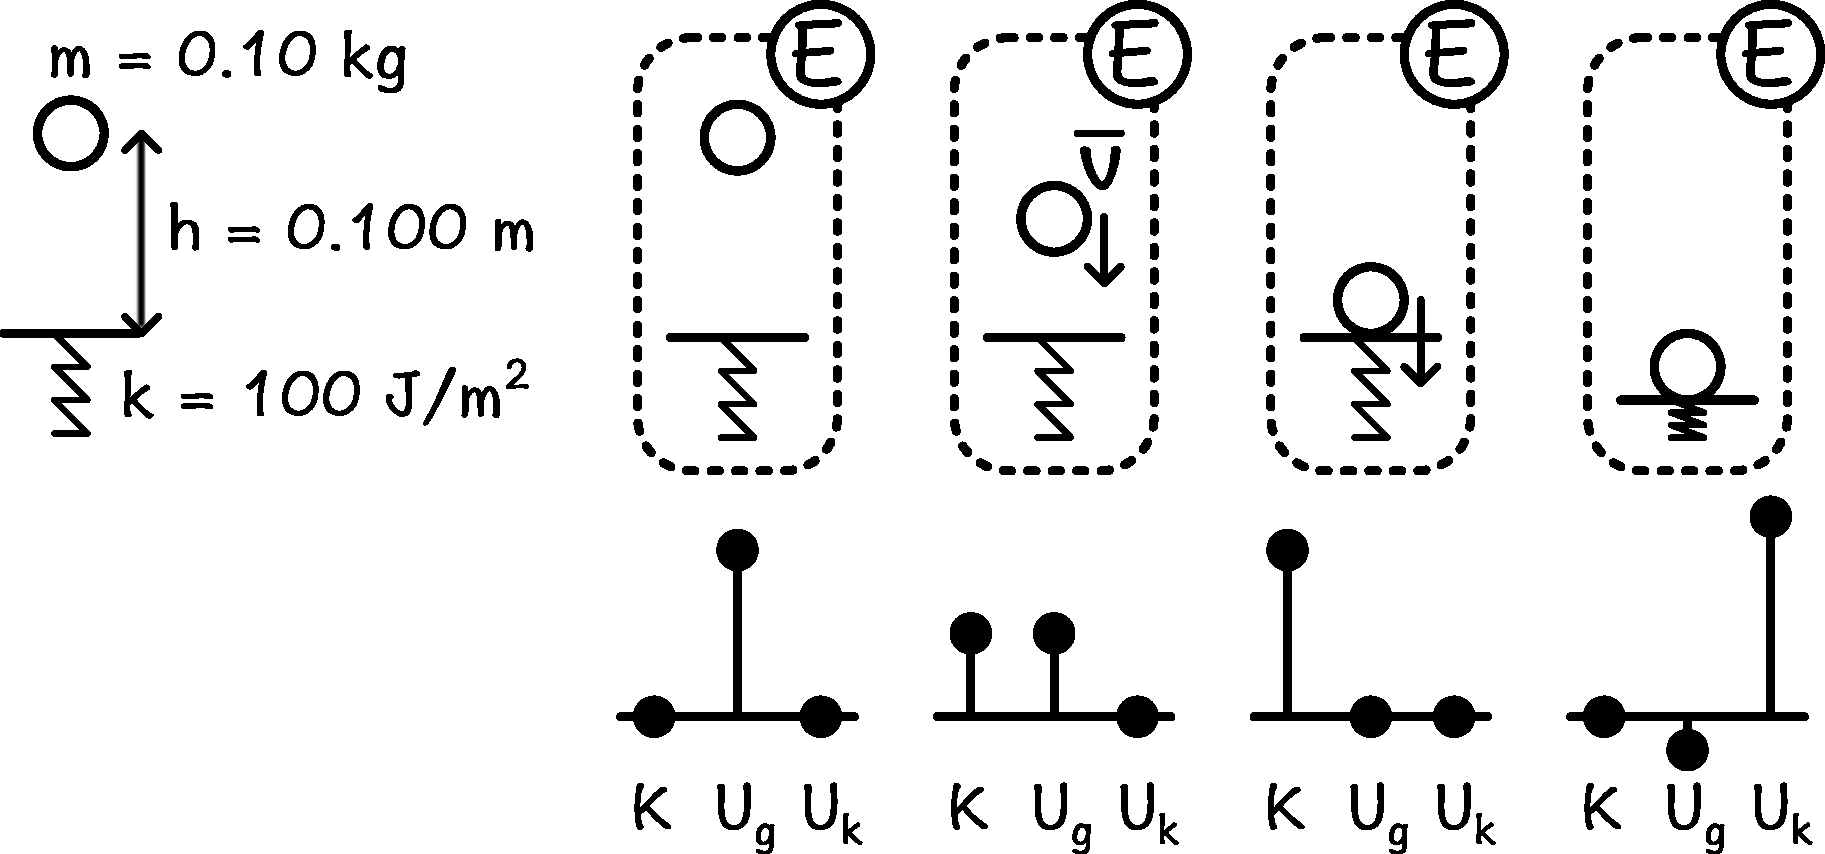
\includegraphics[width=0.9\textwidth]{figs/energia_diagrammi_7.pdf}%
\end{center}%
}

\physics Oletetaan ilmanvastus pieneksi. Tällöin, koska ainoastaan kappale ja jousi liikkuvat putoamisen aikana, valitun systeemin kokonaisenergia on vakio eli liike-energian ja potentiaalienergian summa on lopussa, jousen puristuttua sama kuin alussa, kappaleen lähtiessä liikkeelle.

Aluksi kappale on paikoillaan, joten sillä on vain potentiaalienergiaa. Pudotuksen aikana osa potentiaalienergiasta muuttuu liike-energiaksi.
Kun kappale putoaa jousen päälle, jousi puristuu varastoiden kappaleen liike-energiaa potentiaalienergiaksi. Lopulta kappale pysähtyy ja jousi heittää kappaleen jälleen ylöspäin. Jousen maksimaalinen puristuma saavutetaan kappaleen pysähtyessä, ennen kuin jousi alkaa jälleen nostaa kappaletta ylöspäin. Kappaleen ollessa paikoillaan sen liike-energia on jälleen nolla, joten gravitaation ja jousen potentiaalienergioiden summan täytyy olla sama kuin liikkeen alussa. Erityisesti kappaleella on lopuksi hiukan negatiivista gravitaation potentiaalienergiaa, joten jousen potentiaalienergia on suurempi kuin kokonaisenergia oli alussa.

 \model  Kappaleen liike-energia on
\begin{equation}K = \frac{1}{2} m v^2,\end{equation}
missä \(v\) on kappaleen nopeus.
Kappaleen pudotessa sen gravitaatiopotentiaalienergia on
\begin{equation}U_\text{gravitaatio} = mgx,\end{equation}
missä \(x\) on jousen yläpäästä mitattu pystysuora etäisyys.
Jousi puristuu vasta kappaleen kohdatessa sen, joten jousen potentiaalienergia on
\begin{equation} U_\text{jousi} = \begin{cases}
\frac{1}{2} k x^2, & x < 0 \\
0, & x > 0 \end{cases}. \end{equation}

Kappaleella on ennen pudotusta ainoastaan gravitaation potentiaalienergia \(E_\text{alku} = mgh\), missä \(h\) on kappaleen lähtöpisteen koordinaatti eli pudotuskorkeus. Energian säilymislaki saa näin ollen muodon
\begin{equation} K+U_\text{gravitaatio}+U_\text{jousi} = E_\text{alku} = mgh. \end{equation}

Kun jousi on puristunut ja kappale on jälleen pysähtynyt, kappaleen paikkakoordinaatti on negatiivinen, \(x < 0\), ja tämä on myös jousen venymä, koska origoksi valittiin jousen tasapainoasema. (Eli jousen puristuma on \(-x > 0\).)
Kokonaisenergian säilyminen saa yhtälönä muodon
\begin{equation}mgx + \frac{1}{2} k x^2 = mgh\end{equation}
huomioiden että liike-energia on nolla, \(K=0\), kun kappale on ratansa alimmassa pisteessä. Tästä voidaan ratkaista paikka \(x\).

\solu Kyseessä on toisen asteen yhtälö muuttujan \(x\) suhteen, jonka ratkaisut ovat
\begin{equation} x = -\frac{gm}{k}\left( 1 \pm \sqrt{\frac{2hk}{gm} + 1} \right). \end{equation}
Koska ratkaisun pitää olla negatiivinen, fysikaalisesti oikea valinta on
\begin{equation} x = -\frac{gm}{k}\left( 1 + \sqrt{\frac{2hk}{gm} + 1} \right), \end{equation}
sillä \(\sqrt{2hk/(gm) + 1} > 1\).

Annetuilla lukuarvoilla kappaleen alimmaksi paikaksi saadaan
\begin{equation} x = -\frac{9.8 \un{m/s}^2 \cdot 0.10 \un{kg}}{100 \un{J/m}^2} \left( 1 + \sqrt{\frac{2 \cdot 0.100\un{m} \cdot 100 \un{J/m}^2}{9.8 \un{m/s}^2 \cdot 0.10 \un{kg}} + 1} \right) = -0.055 \un{m}. \end{equation}
Jousen maksimipuristuma on siis \(-x = 5.5 \un{cm}\).

\mbar
\begin{mathematica}[commandchars=\\!?]
(* energioiden lausekkeet *)
ualku = m g h;
ugrav = m g x;
ujousi = 1/2 k x^2;

(* ratkaistaan paikkakoordinaatti, 
kun potentiaalienergia on sama kuin alussa *)
pohja = Solve[ ugrav + ujousi == ualku, x]
  \textit!{{x -> (-g m - Sqrt[g m (2 h k + g m)])/k},?
  \textit! {x -> (-g m + Sqrt[g m (2 h k + g m)])/k}}?

(* sijoitetaan lukuarvot *)
pohja /. {g -> 9.8, m -> 0.1, k -> 100, h -> 0.1}
  \textit!{{x -> -0.0551436}, {x -> 0.0355436}}?
\end{mathematica}

\eval Ratkaisun järkevyyttä voidaan arvioida yksikkötarkastelulla:
\begin{equation} [x] = \frac{[g][m]}{[k]} = \frac{\text{kgm/s}^2}{\text{J/m}^2} = \frac{\text{kgm/s}^2}{\text{kg/s}^2} = \text{m}. \end{equation}
Ratkaisulla on siis pituuden yksikkö kuten pitääkin.
Lisäksi neliöjuurilausekkeen sisältämän termin \(\frac{2hk}{gm}\) täytyy olla paljas luku, koska se lasketaan yhteen ykkösen kanssa. Sitä se on, koska \([h][k/(gm)] = \text{m} \cdot 1/\text{m} = 1\).

Voimme tutkia myös ratkaisuna saadun lausekkeen raja-arvoja. Tarkastellaan tilannetta, jossa jousi on hyvin jäykkä (\(k\) on suuri) tai kappale on hyvin kevyt (\(m\) on pieni). Jos jäykän jousen päälle pudotetaan kevyt kappale, jousi puristuu hyvin vähän ja kappale pomppaa välittömästi takaisin ilmaan. Tätä vastaa raja-arvo \(m/k \to 0\), joka voidaan laskea kirjoittamalla ratkaisu muotoon
\begin{equation} x = -\frac{gm}{k}\left( 1 + \sqrt{\frac{2hk}{gm} + 1} \right) = -\frac{gm}{k} - \sqrt{ \frac{2hgm}{k} + \frac{g^2m^2}{k^2}} \to 0. \end{equation}
Hyvin jäykkä jousi ei siis puristu, kuten pitääkin.

\end{exam}
\newpage

\section{Energian laatu}
\label{energianlaatu}

\subsection{Mekaaninen energia ja sisäenergia}
\label{mekaaninenenergiajasisäenergia}

Kappaleen nostaminen ylöspäin lisää kappaleen potentiaalienergiaa, joten tämä on yksi mahdollinen tapa \emph{varastoida energiaa}. Tätä periaatetta voidaan käyttää hyväksi esimerkiksi vesivoimalaitoksissa. Varastoimalla vettä esimerkiksi patoaltaaseen voidaan samalla varastoida energiaa veden potentiaalienergiaksi. Tarvittaessa vettä voidaan sitten juoksuttaa padossa olevan voimalaitoksen läpi, jolloin veden potentiaalienergia muuttuu ensin veden liike-energiaksi. Liikkuva vesi puolestaan pyörittää generaattoreita, jolloin osa liike-energiasta muuttuu sähköiseksi energiaksi. Sähkön avulla energiaa on helppo siirtää edelleen käytettäväksi muihin tarkoituksiin.

Myös elastisiin kappaleisiin voi varastoida energiaa puristamalla, venyttämällä tai taivuttamalla niitä. Tätä tekniikkaa on käytetty iät ja ajat esimerkiksi jousipyssyissä, joissa jousta jännitettäessä ampujan lihasten kemiallinen energia varastoituu jousen kaaren elastiseen muodonmuutokseen. Jousen vapautuessa tämä elastinen energia muuttuu nuolen liike-energiaksi.

\index{mekaaninen energia}

Kappaleiden liike-energialla ja edellä kuvatuilla potentiaalienergian eri muodoilla on se yhteinen piirre, että ne voidaan havaita makroskooppisesti. Voimme nähdä suoraan onko pallo korkealla vai matalalla, liikkuuko se nopeasti vai hitaasti ja onko se mahdollisesti myös puristunut kasaan. Koska nämä energian muodot liittyvät makroskooppisten kappaleiden paikkaan, nopeuteen ja muotoon, niitä kutsutaan yhteisnimellä \textbf{mekaaninen energia}.

Mekaanisella energialla on toinenkin merkittävä erityispiirre: mekaanisen energian eri lajit voivat muuttua helposti toisikseen. Esimerkiksi ylöspäin heitetyn pallon liike-energia muuttuu pallon potentiaalienergiaksi pallon noustessa, koska pallon vauhti pienenee ja korkeus lisääntyy. Potentiaalienergia puolestaan muuttuu jälleen liike-energiaksi pallon laskeutuessa alaspäin.
Pallon heitolle aikaisemmin päätelty energian säilymislaki (\autoref{energy_fall_proper}) voidaankin siis kirjoittaa myös muotoon
\begin{equation} E_\text{kokonais} = E_\text{liike} + E_\text{potentiaali} = K + U = \text{vakio}. \label{mek_ene_sailyy}\end{equation}
Yllä esitetty periaate toimii myös muiden vuorovaikutusten kuin gravitaation kohdalla, \emph{jos vuorovaikutuksia voidaan kuvata potentiaalienergialla} eli funktiolla, joka kuvaa vuorovaikutuksen varastoimaa energiaa ja riippuu ainoastaan kappaleiden paikoista, asennoista tai muodoista.
Tämä on energian säilymislain tärkeä erikoistapaus: \emph{Jos eristetyssä systeemissä vaikuttaa ainoastaan sellaisia vuorovaikutuksia, joihin liittyy potentiaalienergia, systeemin mekaaninen energia eli liike-energian ja potentiaalienergian summa \(K + U\) on vakio}.

\begin{stopQ}{q:uimahyppyenergia}%
Uimahyppääjä hyppää ponnahduslaudalle, ponnistaa tästä hyvin korkealle ilmaan tehden voltin ja sukeltaa lopulta veteen.\\
(a) Millaisia energian muotojen muutoksia tähän prosessiin liittyy?\\
(b) Jos systeemi on hyppääjä, lauta sekä vesi, missä vaiheissa systeemin mekaaninen energia on likimain vakio?
\end{stopQ}

\onepicture{tb}%
{Mekaaninen energia eli liike- ja potentiaalienergia on järjestynyttä energiaa. Sisäenergiaa ovat kappaleen tilasta riippuvat energian muodot.}%
{fig:energiakoherenssi}%
{1.0}%
{energia_luokat_2.pdf}

Koska mekaanista energiaa on helppo varastoida ja vapauttaa liikkeeksi, sen hyödyntäminen on melko yksinkertaista. Ennen höyrykoneiden keksimistä melkein kaikki laitteet kelloista purjelaivoihin perustuivatkin joko ``lihasvoimaan'' eli kemialliseen energiaan tai mekaaniseen energiaan.
Kaikki energian muodot \emph{eivät} kuitenkaan muutu noin vain toisikseen. Jos esimerkiksi muovailuvahasta tehty pallo putoaa lattialle, se pysähtyy lattiaan osuessaan, jolloin pallon liike-energia muuttuu muihin, ei-mekaanisiin muotoihin. Seuraavaksi tarkastelemmekin millaisia muita muotoja energialla on ja millaisia ominaisuuksia energian eri muodoilla on.

\index{tila}

Aloitimme energian tarkastelun luettelemalla energian muotoja kuten kemiallisen energian ja lämpöenergian. Nämä energian muodot poikkeavat mekaanisesta energiasta siinä, että ne liittyvät ilmiöihin, joita ei voi suoraan nähdä. Kemiallinen energia on aineiden kemialliseen koostumukseen eli niiden molekyylien rakenteeseen varastoitunutta energiaa. Lämpöenergia on puolestaan aineen kuumuuteen liittyvää energiaa. Näiden energiamuotojen mittaaminen vaatii siis enemmän tietoa kappaleista kuin vain missä ne ovat ja miten ne liikkuvat. Periaatteessa systeemin kaikkien energiamuotojen määrittäminen vaatisi sitä, että tunnemme systeemin kaikki ominaisuudet mukaan lukien niiden sisäisestä rakenteesta riippuvat näkymättömät ominaisuudet.
Fysiikassa tällaista systeemin täydellistä kuvausta kutsutaan \textbf{tilaksi}. Toisin sanoen tilan käsite sisältää paikan ja nopeuden lisäksi \emph{kaikki} systeemin fysikaaliset ominaisuudet kuten kappaleiden muodon, kemiallisen koostumuksen, lämpötilan jne. Monet energian muodot liittyvät systeemin tilaan, ja energian muutokset voivat ilmetä kappaleiden liikkeen muutosten lisäksi myös niiden tilan muutoksena.

\index{sisäenergia}

Fysiikassa kappaleen tilaan liittyvää ``näkymätöntä'' energiaa kuten kemiallista energiaa ja lämpöenergiaa kutsutaan \textbf{sisäenergiaksi}. Nimitys viittaa siihen, että tämä energia on ``piilossa'' kappaleen sisällä.
Kappaleen makroskooppiseen liikkeeseen liittyvä liike-energia ei ole sisäenergiaa kuten ei ole esimerkiksi painovoiman potentiaalienergiakaan, sillä nämä eivät riipu kappaleen sisäisistä ominaisuuksista.
Elastinen energia sen sijaan voidaan laskea sisäenergiaksi, koska kappaleen puristaminen ja venyttäminen muuttaa myös atomien keskinäisiä etäisyyksiä aineen sisällä, ja elastinen energia onkin itse asiassa näiden atomien välisten sidosten potentiaalienergiaa.

\begin{stopQ}{q:energialajeja}%
Kappale on aluksi paikoillaan, mutta lähtee liikkeelle. Missä seuraavista tapauksista kappaleen saama liike-energia on peräisin jonkin toisen kappaleen mekaanisesta energiasta ja missä sisäenergiasta? (a) Kappale putoaa. (b) Kappale työnnetään käsin liikkeelle. (c) Kappaleeseen törmää toinen kappale. (d) Kappaleen työntää liikkeelle puristunut jousi. (e) Kappaleen vieressä tapahtuu räjähdys.
\end{stopQ}

\subsection{Energian epäjärjestyminen}
\label{energianepäjärjestyminen}

Ota kirja, aseta se pöydälle ja työnnä se liukumaan pitkin pöydän pintaa. Todennäköisesti huomaat kirjan pysähtyvän melko nopeasti. Liikkuvalla kirjalla on aluksi liike-energiaa, mutta koska kirja pysähtyy, sen liike-energian täytyy olla lopuksi nolla. Jos sinulla olisi hyvin tarkka lämpömittari, voisit kuitenkin samalla havaita kirjan ja pöydän pinnan hieman lämpenevän. Kirjan liike-energia siis vähenee, ja pintojen lämpöenergia lisääntyy, joten prosessissa mekaanista liike-energiaa muuttuu kappaleiden lämpöenergiaksi eli sisäenergiaksi.

\widepictures{tb}%
{Yksinkertainen malli kitkan toiminnasta kahden liikkuvan kappaleen rajapinnalla. Pallot kuvaavat atomeja ja niiden väliset ''jouset'' atomisidoksia.;%
Pinnat liikkuvat.;%
Pinnat kohtaavat.;%
Pinnat värähtelevät.;%
Pinnat lämpenevät.}%
{fig:energiakitka;fig:energiakitka:a;fig:energiakitka:b;fig:energiakitka:c;fig:energiakitka:d}%
{0.29;0.18;0.17;0.27}%
{0.29;0.18;0.17;0.27}%
{energia_kitka_1.pdf;energia_kitka_2.pdf;energia_kitka_3.pdf;energia_kitka_4.pdf}

\index{kitka}

Tämän ilmiön selittää \textbf{kitka}, joka on koskettavien pintojen välinen vuorovaikutus. Kitka aiheutuu siitä, että toisiaan koskettavat pinnat pyrkivät tarttumaan mikroskooppisessa mittakaavassa toisiinsa kiinni (kuva \autoref{fig:energiakitka}). Jos kuitenkin kappaleet liikkuvat, nämä heikot sidokset eivät kuitenkaan välttämättä riitä saamaan kappaleita tarttumaan toisiinsa vaan sidokset vain hidastavat pintojen liukumista toistensa suhteen. Näin liikkuvien pintojen välillä syntyy jatkuvasti uusia sidoksia ja vanhoja sidoksia rikkoutuu.
Tyypillisesti sidokset venyvät ennen rikkoutumistaan, jolloin pintojen rakenteessa tapahtuu pieniä elastisia muutoksia --- ts. pinnat voivat venyä tai puristua mikroskooppisella tasolla, mihin varastoituu elastista energiaa.

Kun pinnat sitten irtoavat toisistaan, nämä muodonmuutokset pääsevät yhtäkkiä palautumaan kuin jännitetty kuminauha, jonka toinen pää päästetään vapaaksi. Tämän seurauksena pintaan varastoitunut elastinen energia muuttuu pintojen atomien liike-energiaksi, ja atomit alkavat värähdellä.
Pinnan atomien poukkoilu tönii nopeasti myös muita atomeja liikkeelle ja niin tämä liike-energia alkaa levitä muuallekin kappaleeseen. Loppujen lopuksi suuri osa liukuvan kappaleen liike-energiasta on muuttunut värähtelevien atomien liike-energiaksi, mutta nyt atomit eivät enää liiku kaikki samaan suuntaan kuten aluksi vaan nyt ne värähtelevät satunnaisesti kaikissa suunnissa. Makroskooppisesti tämä ilmenee siten, että kappale pysähtyy ja \emph{lämpenee}.

Ilman läpi kulkevaan kappaleeseen kohdistuu samantyyppinen vuorovaikutus. Ilmassa kulkevan kappaleen on työnnettävä ilmaa pois edestään, jolloin kaasun molekyylit saavat kappaleelta liike-energiaa. Molekyylien edelleen törmäillessä toisiinsa tämäkin liike-energia jakautuu satunnaisesti suurelle määrälle hiukkasia. Lopputuloksena kappaleen vauhti hidastuu ja ilma sekä kappaleen pinta lämpenevät.

\begin{stopQ}{q:ilmanvastus}%
Purjelaivoissa liikkuva ilma törmää purjeisiin työntäen laivan liikkeelle. Miten ilmanvastus tässä ilmenee? Millaisia energian muutoksia muodosta toiseen tähän prosessiin liittyy?
\end{stopQ}

Atomien poukkoilu on normaalisti täysin satunnaista eikä yksittäisiä atomeja voi havaita ilman huipputekniikkaa. Niinpä atomien \emph{satunnaisen} liikkeen liike-energiaa ei makroskooppisella tasolla nähdä liikkeenä vaan se ilmenee \emph{kuumuutena}, joka on kappaleen \emph{tilan} ominaisuus. Mikroskooppisessa mittakaavassa atomit tietenkin vain liikkuvat tietämättä onko niiden liikkeen energia meidän mielestämme liike-energiaa vai lämpöenergiaa.
Makroskooppisessa mittakaavassa liike ja kuumuus ovat kuitenkin täysin erilaisia ilmiöitä. Lämmin kappale voi olla paikoillaan eikä kylmä kappale tunnut lämpimämmältä vaikka se liikkuisi. Tämä ero on seurausta siitä, että atomit liikkuvat eri tavoin \emph{toistensa suhteen}. Kun kappale liikkuu, sen kaikki atomit liikkuvat kollektiivisesti samaan suuntaan. Sen sijaan kuuman kappaleen atomit liikkuvat satunnaisiin suuntiin. Toisin sanoen liikkuvassa kappaleessa atomien liike on \emph{järjestynyttä} kun taas kuumassa kappaleessa liike on \emph{epäjärjestynyttä}.

\onepicture%
{t}%
{Energian muutokset elastisen pallon pomppiessa.}%
{fig:energiapomppu}%
{0.6}%
{energia_pomppu_sarja.pdf}

Mekaanisen energian muodot ovat järjestynyttä energiaa. Kaikki epäjärjestyneet energian muodot ovat sisäenergiaa. Elastinen energia kuten jousen energia on järjestynyttä ja se riippuu kappaleen muodosta (siis tilasta), joten elastinen energia voidaan lukea sekä mekaaniseen energiaan että sisäenergiaan. Osoittautuu, että juuri energian järjestyneisyys on keskeinen tekijä, josta riippuu miten energian muodot voivat muuttua toisikseen ja millaiset prosessit ovat mahdollisia, kuten seuraavat esimerkit osoittavat.

\marginpictures%
{-20}%
{Energian muutos kappaleen liukuessa.;%
Kitka muuttaa liike-energian lämpöenergiaksi.;%
Lämpöenergia ei muutu itsestään liike-energiaksi.}%
{fig:energiareversiibeli}%
{1.0;1.0}%
{energia_reversiibeli_5.pdf;energia_reversiibeli_6.pdf}

Tarkastellaan kuvan \autoref{fig:energiapomppu} ideaalista elastista pomppivaa kumipalloa. Pallon osuessa maahan se painuu hetkeksi kasaan, jolloin sen liike-energia varastoituu muodonmuutokseen liittyväksi elastiseksi potentiaalienergiaksi. Tämä potentiaalienergia palautuu pallon liike-energiaksi pallon palatessa takaisin alkuperäiseen muotoonsa, jolloin pallo pomppaa takaisin ylös yhtä suurella nopeudella kuin millä se osui lattiaan. Tämän jälkeen pallon liike-energia varastoituu pallon noustessa gravitaation potentiaalienergiaksi kunnes muuttuu jälleen pallon pudotessa takaisin liike-energiaksi. Jos pallo olisi täysin elastinen ja koe suoritettaisiin tyhjiössä niin ettei ilmanvastuskaan hidasta pallon liikettä, pallo jatkaisi pomppimistaan loputtomiin liike-energian muuttuessa vuoroin elastiseksi ja vuoroin gravitaation potentiaalienergiaksi. Nämä mekaanisen energian muodot ovat kaikki järjestyneitä ja ne voivat vapaasti muuttua toisikseen.

\index{irreversiibeli}
\index{reversiibeli}

Tarkastellaan toisena esimerkkinä jo äsken tutkimaamme pöydällä liukuvaa kirjaa (kuva \autoref{fig:energiareversiibeli}). Kirjan ja pöydän pinnan välillä vaikuttava kitka muuttaa kirjan järjestyneen liike-energian epäjärjestyneeksi lämpöenergiaksi. Kuitenkin kun kirja on paikoillaan, se \emph{ei koskaan} lähde itsestään liikkeelle niin, että sen ja pöydän lämpöenergia muuttuisi kirjan liike-energiaksi. Toisin sanoen \emph{prosessi, jossa kitka pysäyttää kirjan, voi tapahtua vain yhteen suuntaan}. Tällaista prosessia kutsutaan fysiikassa \textbf{irreversiibeliksi} (engl. `irreversible', kääntämätön). Vastaavasti prosessia, joka voidaan kääntää ajassa takaperin, kutsutaan \textbf{reversiibeliksi}.

Irreversiibelit prosessit voi tunnistaa kuvittelemalla prosessin tapahtuvan takaperin tai videoimalla prosessin ja katsomalla videon lopusta alkuun. Jos takaperin tapahtuva prosessi näyttää mahdottomalta, prosessi on irreversiibeli. Liukuvan kirjan pysähtyminen, näyttää takaperin siltä, että paikoillaan ollut kirja vain yhtäkkiä lähtee liikkeelle lattian samalla viilentyessä, mitä ei todellisuudessa voi tapahtua. Sen sijaan video pomppivasta pallosta, jonka jokainen pomppu on yhtä korkea, näyttää täsmälleen samanlaiselta myös takaperin esitettynä. Prosessit, joissa mekaanisen energian muodot muuttuvat toisikseen, ovat yleensä reversiibeleitä ainakin jos prosessiin osallistuvien kappaleiden määrä on pieni. Epäjärjestyneen energian muotoja sisältävät prosessit ovat puolestaan tavallisesti irreversiibeleitä.

Koska makroskooppisella tasolla ei voida koskaan täysin välttää esimerkiksi kitkaa,
täysin reversiibeleitä prosesseja on todellisuudessa olemassa vain atomien mittakaavassa. Niinpä järjestyneen energian muodot muuttuvat jatkuvasti epäjärjestyneiksi. Myös epäjärjestynyt energia voi muuttua takaisin järjestyneeksi. Esimerkiksi räjähdyksessä kemiallinen energia muuttuu ensin lämpöenergiaksi ja sitten osa tästä lämpöenergiasta muuttuu edelleen kappaleiden liike-energiaksi. Tällä on kuitenkin rajoituksensa eikä \emph{kaikkea} epäjärjestynyttä energiaa voi koskaan palauttaa järjestyneeksi. Tässä mielessä epäjärjestynyt energia on järjestynyttä energiaa huonompaa.

Epäjärjestyneen sisäenergian mittaaminen on usein vaikeampaa kuin mekaanisen energian, minkä vuoksi mekaniikassa usein prosesseja pidetään likimain reversiibeleinä --- ts. vuorovaikutukset kuten kitka ja ilmanvastus jätetään usein huomioimatta --- sillä tällöin mekaaninen energia on likimain vakio. Näin voi kuitenkin tehdä vain, jos esimerkiksi kitka on paljon heikompi kuin muut systeemissä vaikuttavat vuorovaikutukset. Luvussa \autoref{luku:voimatyo} palaamme tarkastelemaan, kuinka energian muutoksia yhdestä muodosta toiseen voidaan tarkemmin analysoida.

\begin{stopQ}{q:reversiibelitprosessit}%
Mitkä seuraavista prosesseista ovat reversiibeleitä? (a) Kappale liukuu tasaisella nopeudella alas kaltevaa tasoa. (b) Kappale putoaa tyhjiössä. (c) Ruoka jäähtyy. (d) Täysin elastinen pallo törmää toiseen samanlaiseen palloon. (e) Täysin elastinen pallo törmää kymmenen samanlaisen pallon kasaan.
\end{stopQ}

\begin{exam}{Irreversiibeli energian muutos}{ex:dissipaatio}\noindent

\problem{Kappale (massa \(0.350 \un{kg}\)) lähtee levosta liukumaan alas kaltevaa tasoa. Kuljettuaan yhden metrin, kappale on saavuttanut nopeuden \(1.5 \un{m/s}\). Tason kaltevuuskulma vaakatasoon nähden on \(40^\circ\). Kuinka paljon energiaa on kulunut kappaleen ja sen ympäristön lämmittämiseen?
}

 \twocol{0.69}{0.3}{ \setup  Valitaan systeemiksi kappale ja maan painovoimakenttä. Piirretään systeemin kuva ja prosessia kuvaava energiadiagrammi. Merkitään kappaleen kulkemaa matkaa \(s = 1.0 \un{m}\) ja tason kaltevuuskulmaa \(\theta = 40^\circ\). Kappaleen massa on \(m = 0.350 \un{kg}\) ja sen saama nopeus \(v_{\text{loppu}} = 1.5 \un{m/s}\).

 \physics Systeemin potentiaalienergia pienenee ja liike-energia kasvaa kappaleen liikkuessa alaspäin. Kappaleeseen vaikuttavat kitka ja ilmanvastus kuitenkin muuttavat samalla liike-energiaa lämpöenergiaksi. Systeemin kokonaisenergia ei ole vakio, mutta energian säilymislain perusteella systeemistä hävinneen mekaanisen energian täytyy muuttua muihin energian muotoihin, pääasiassa lämpöenergiaksi.

 \model  Kappale siirtyy pystysuoran etäisyyden \(\Delta x = -s \sin \theta\) ja sen potentiaalienergia pienenee tällöin määrän
\( \Delta U = mg\Delta x = -mgs \sin \theta. \)
Kappaleen liike-energia puolestaan kasvaa määrän
\( \Delta K = \frac{1}{2} m \Delta (v^2) = \frac{1}{2} m v_{\text{loppu}}^2. \)
Lämmöksi muuttuu energia \( \Delta E_\text{sis\"a} = -\Delta E_\text{mekaaninen} = -\Delta U - \Delta K \).

}{%
\begin{center}%
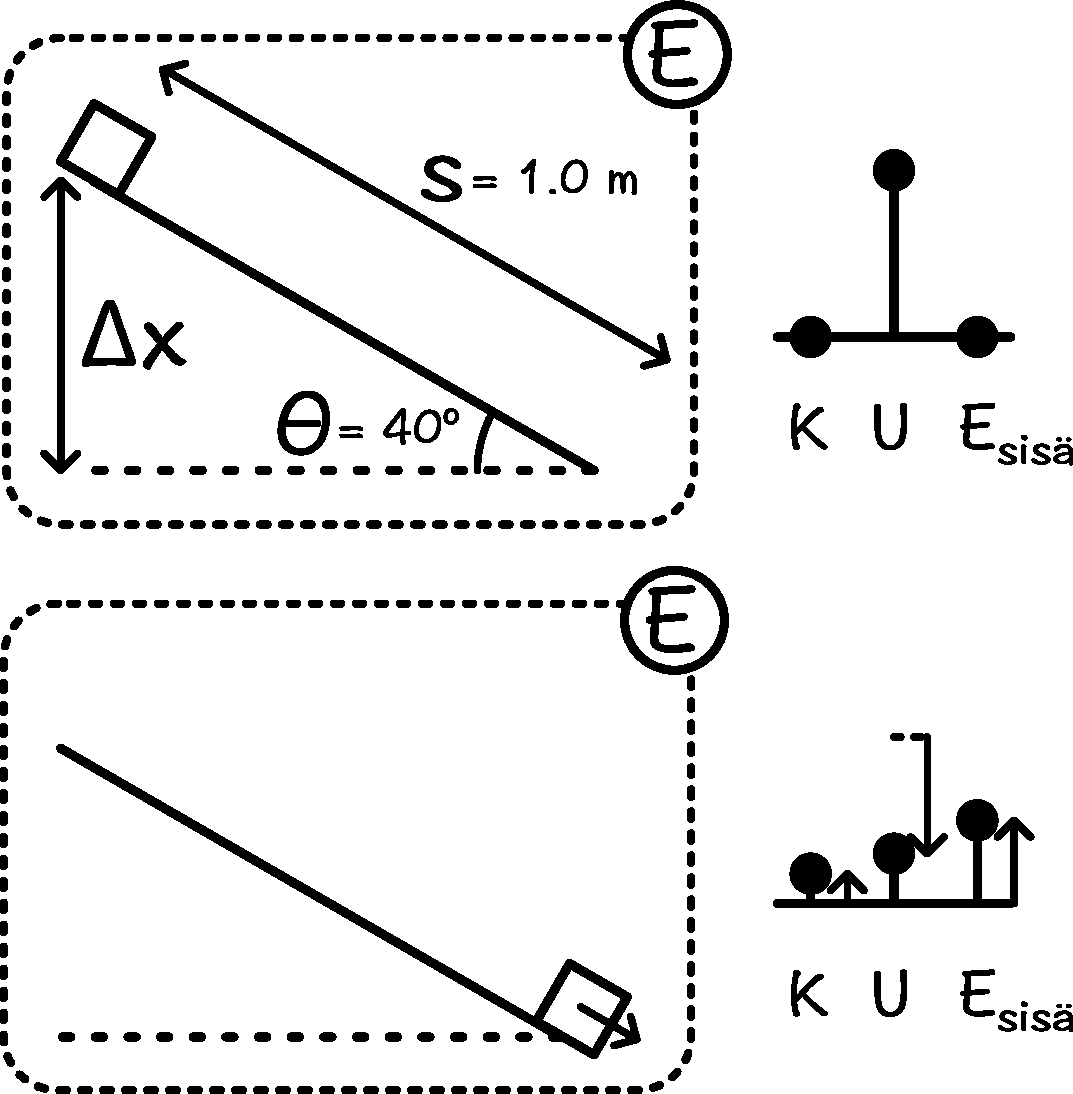
\includegraphics[width=0.9\textwidth]{figs/energia_esimerkki_sisa.pdf}%
\end{center}%
}

 \solu  Lämmöksi muuttuu energiamäärä
\( \Delta E_\text{sis\"a} = mgs \sin \theta - \frac{1}{2} m v_{\text{loppu}}^2, \)
ja lukuarvojen sijoitus antaa tulokseksi \(\Delta E_\text{sis\"a} = 1.8 \un{J}\).

 \eval  Tarkasteltaan, että ratkaisulla on energian yksikkö.
\begin{equation} [\Delta E_\text{sis\"a}] = [mgs] + [mv^2] = \text{kg m/s}^2\cdot\text{m} + \text{kgm}^2/\text{s}^2 = \text{J}. \end{equation}

\end{exam}

\begin{stopQ}{q:tiivistelmasisaenergia}%
Selitä omin sanoin käsitteet järjestynyt ja epäjärjestynyt energia sekä sisäenergia. Selitä myös millaisia rajoituksia energian eri muotojen muutoksiin liittyy, ja miksi tästä seuraa se, että jotkin prosessit eivät voi tapahtua takaperin.
\end{stopQ}

\subsection{Konservatiivisuus}
\label{konservatiivisuus}

\index{konservatiivinen}
\index{dissipatiivinen}

Painovoimaa ja elastisia vuorovaikutuksia, joihin liittyy potentiaalienergia, kutsutaan \textbf{konservatiivisiksi} vuorovaikutuksiksi, koska ne säilyttävät (engl. `conserve') järjestyneen eli mekaanisen energian. Järjestynyttä energiaa epäjärjestyneeksi muuttavat vuorovaikutukset kuten kitka ovat puolestaan \textbf{dissipatiivisia}, koska ne hukkaavat (engl. `dissipate') mekaanista energiaa. Konservatiivisilla vuorovaikutuksilla on fysiikassa erityisen tärkeä asema juuri siksi, että ne eivät muuta energian järjestyneisyyttä. Tutkitaan siis vielä, millaisia ominaisuuksia konservatiivisilla vuorovaikutuksilla on.

\index{suljettu reitti}

Tarkastellaan prosessia, jossa kappale liikkuu ja palaa lopuksi takaisin lähtöpisteeseensä. Tämä tapahtuu esimerkiksi heitettäessä pallo suoraan ylöspäin, mutta periaatteessa kappale voi kulkea millaisen reitin tahansa, kunhan se lopuksi päätyy takaisin lähtöpaikkaansa. Tällaista reittiä kutsutaan \textbf{suljetuksi}, koska reittiä pitkin piirretty viiva muodostaa suljetun silmukan.

Jos eristetyssä systeemissä vaikuttaa vain konservatiivisia vuorovaikutuksia, joita kuvaa \emph{ainoastaan paikasta riippuva potentiaalienergia}, tämän potentiaalienergian on oltava suljetun reitin lopussa \emph{sama} kuin alussa, \(U_\text{loppu} = U_\text{alku}\), koska kappale palaa suljetulla reitillä lopuksi \emph{samaan} pisteeseen kuin mistä lähti. Tämä nähdään kuvissa \autoref{fig:energiakonservatiivinen} (a) ja (b). Mekaanisen energian säilymisen perusteella kokonaisenergia ei muutu, \( K_\text{loppu} + U_\text{loppu} = \text{vakio} = K_\text{alku} + U_\text{alku} \), joten myös kappaleen \emph{liike-energian} ja siis vauhdin on oltava lopuksi sama kuin aluksi.

\pictures{t}%
{Konservatiiviset ja dissipatiiviset vuorovaikutukset voi tunnistaa tarkastelemalla kappaleen liikettä suljettua reittiä pitkin.;%
Kappale lähtee liikkeelle.;%
Kappale palaa lähtöpisteeseen ja sillä on sama vauhti kuin aluksi.;%
Kappale palaa lähtöpisteeseen ja sillä on eri vauhti kuin aluksi.}%
{fig:energiakonservatiivinen;fig:energiakonservatiivinen:a;fig:energiakonservatiivinen:b;fig:energiakonservatiivinen:c}%
{0.30;0.30;0.30}%
{0.30;0.30;0.30}%
{energia_konservatiivinen_1.pdf;energia_konservatiivinen_2.pdf;energia_konservatiivinen_3.pdf}

Päättelyn voi myös kääntää ympäri. Jos on olemassa reitti, jota pitkin kulkien kappale voi palata takaisin lähtöpisteeseensä niin, että sen vauhti \emph{ei ole lopuksi sama kuin aluksi}, kappaleen liike-energian ja potentiaalienergian summa ei ole aluksi sama kuin lopuksi, \( K_\text{loppu} + U_\text{loppu} \ne K_\text{alku} + U_\text{alku} \). Tällaisessa tapauksessa mekaanisen energian on täytynyt muuttua johonkin toiseen muotoon ja systeemissä täytyy vaikuttaa dissipatiivisia vuorovaikutuksia. Näin käy ylöspäin heitetylle kappaleelle, kun ilmanvastuksen liikettä hidastava vaikutus huomioidaan.
Kuvassa \autoref{fig:energiakonservatiivinen} on tästä esitetty esimerkkinä höyhen, joka suurellakin alkunopeudella ylöspäin heitettynä leijailee lopulta alas hyvin hitaasti.
Prosessissa osa höyhenen alkuperäisestä mekaanisesta energiasta muuttuu heiton aikana ilman liikkeen energiaksi ja lopulta lämpöenergiaksi.

\begin{stopQ}{q:konservatiivisuusmuoto}%
Jos potentiaalienergia riippuu paikan lisäksi kappaleen muodosta, onko kappaleen potentiaalienergian muutos välttämättä nolla, jos kappale kulkee suljetun reitin? Jos ei ole, mitä muuta pitää vaatia?
\end{stopQ}

\section{Liikemäärä}
\label{liikemäärä}

Edellä opimme, että kappaleen liikkeeseen sitoutuneen energian määrä riippuu sekä kappaleen massasta että kappaleen vauhdista. Tämän näkee konkreettisesti esimerkiksi kolareissa. Massiivinen ja nopeasti liikkuva auto tekee törmätessään enemmän tuhoa kuin kevyt tai hidas, koska suurella autolla on ennen törmäystä enemmän liike-energiaa.

Energia yksinään ei kuitenkaan riitä selittämään, mitä törmäyksissä tapahtuu. Ajatellaanpa tilannetta, jossa rekka ja kärpänen liikkuvat vastakkaisiin suuntiin samalla vauhdilla ja törmäävät (kuva \autoref{fig:liikemaarasuunta}). Rekan liike ei varmasti muutu törmäyksessä havaittavasti, mutta kärpänen tai mitä siitä jääkään jäljelle jää todennäköisesti kiinni rekkaan. Rekan liike-energia on törmäyksen jälkeen likimain sama kuin ennen törmäystä, koska rekan nopeus ei juuri muutu. Kärpäsen nopeuden suunta vaihtuu, mutta sen vauhti ei muutu, joten kärpäsenkin liike-energia on likimain vakio.

Tuntuu itsestään selvältä, että rekka ja kärpänen eivät voi törmätä niin, että kumpikin kimpoaisi takaisin tulosuuntaansa samalla vauhdilla kuin saapuivat (kuva \autoref{fig:liikemaarasuunta} (c)). On nimittäin aivan selvää, että kärpänen ei voi muuttaa rekan liikettä. Mutta \emph{miksi}? Energian säilyminen ei tätä selitä, sillä jos rekan liikkeen suunta kääntyy ympäri mutta vauhti pysyy vakiona, rekan liike-energia ei muutu. Täytyy olla jonkin toinen selitys sille, miksi kärpänen ei voi muuttaa rekan liikettä.

\pictures{tb}%
{Rekan törmäys kärpäseen. Molemmilla on sama nopeus, mutta massiivisen rekan liike-energia on paljon suurempi.;%
Rekka ja kärpänen kohtaavat.;%
Kärpänen jää kiinni rekkaan. Liike-energia on likimain vakio.;%
Liike-energia olisi vakio myös jos kappaleet kimpoaisivat toisistaan.}%
{fig:liikemaarasuunta;fig:liikemaarasuunta:a;fig:liikemaarasuunta:b;fig:liikemaarasuunta:c}%
{0.3;0.3;0.3}%
{0.3;0.3;0.3}%
{liikemaara_suunta_1.pdf;liikemaara_suunta_2.pdf;liikemaara_suunta_3.pdf}

\subsection{Törmäykset}
\label{törmäykset}

\index{törmäys}

\marginpictures%
{-35}%
{Vaunujen törmäyksen analyysi.;%
Videoitu liike kuvasarjana.;%
Tämän perusteella piirretty paikan kuvaaja.}%
{fig:liikemaaratormays_malli}%
{1.0;1.0}%
{liikemaara_kuvasarja.pdf;liikemaara_tormays_2.pdf}

Ymmärtääksemme rekan ja kärpäsen törmäyksen tutkimme seuraavaksi kappaleiden törmäyksiä kokeellisesti. Tätä varten hankimme suoran radan ja radalla lähes kitkattomasti liikkuvia vaunuja. Näihin vaunuihin kohdistuvat dissipatiiviset vuorovaikutukset ovat niin heikot, että vaunujen liike-energia pysyy likimain vakiona ja vaunut siis kulkevat radalla vakionopeudella. Vaunuissa on myös joustavat puskurit, jolloin ne törmätessään kimpoavat toisistaan elastisesti niin, että vaunujen muodostaman systeemin mekaaninen energia on likimain vakio.
Annamme vaunujen törmätä tällä radalla ja mittaamme vaunujen liikkeen videoimalla. Voimme kokeen jälkeen palata tutkimaan törmäyksestä saatua kuvamateriaalia kuva kuvalta (kuva \autoref{fig:liikemaaratormays_malli} (a)) ja määrittää näin vaunujen paikat tasaisin väliajoin. Tämän perusteella voimme piirtää vaunujen paikan kuvaajan (kuva \autoref{fig:liikemaaratormays_malli} (b)).

\begin{stopQ}{q:tormaysnopeus}%
Vaunu liikkuu aluksi negatiiviseen \(x\)-suuntaan vauhdilla \(2.0 \un{m/s}\) ja törmäyksen jälkeen positiiviseen suuntaan vauhdilla \(1.0 \un{m/s}\). Mikä on (a) vauhdin muutos, (b) nopeuden muutos? (c) Millainen on vaunun nopeuden kuvaaja?
\end{stopQ}

\marginpicture%
{30}%
{Vaunujen nopeuden kuvaaja.}%
{fig:liikemaaratormays1}%
{1.0}%
{liikemaara_tormays_3.pdf}

Kun tiedämme kappaleiden paikan ajan funktiona, kappaleen nopeus selviää paikan derivaattana eli paikan kuvaajan tangentin kulmakertoimena. Kuvan
\autoref{fig:liikemaaratormays_malli} törmäävien vaunujen nopeuden kuvaaja on piirretty kuvaan \autoref{fig:liikemaaratormays1}. Kumpikin vaunu liikkuu tasaisesti sekä ennen törmäystä että törmäyksen jälkeen, joten nopeuden kuvaajat ovat vaakasuoria. Törmäyksessä vaunujen nopeus muuttuu äkillisesti, ja tämä näkyy nopeuden kuvaajien askelmaisena muotona. Kummankin vaunun nopeuden muutos näkyy nopeuden kuvaajaan piirtyvän askeleen korkeutena niin, että nopeuden muutos positiiviseen suuntaan vastaa kuvassa vasemmalta oikealle nousevaa askelmaa kun taas negatiivinen nopeuden muutos näkyy laskevana portaana.

Kuvien \autoref{fig:liikemaaratormays_malli} ja \autoref{fig:liikemaaratormays1} törmäyskokeen alussa vaunu A liikkui ja vaunu B oli paikoillaan. Törmäyksessä vaunu A pysähtyy ja vaunu B saa saman nopeuden mikä vaunulla A aluksi oli. Vaunun A nopeuden kuvaaja siirtyy alaspäin, eli vaunun aluksi positiivinen \(x\)-suuntainen nopeus pienenee ja muuttuu itse asiassa nollaksi, jolloin vaunun nopeuden muutos on \(\Delta v_{x,A} = v_{x,A,\text{loppu}} - v_{x,A,\text{alku}} = - v_{x,A,\text{alku}} = -0.75 \un{m/s}\). Vaunun B kuvaaja siirtyy puolestaan ylöspäin, joten vaunun nopeuden muutos on \(x\)-suuntainen, \(\Delta v_{x,B} = v_{x,B,\text{loppu}} - v_{x,B,\text{alku}} = v_{x,B,\text{loppu}} = 0.75 \un{m/s}\). Nopeuksien muutosten suhde on siten
\begin{equation} \frac{\Delta v_{x,A} }{ \Delta v_{x,B} } = -1.00 \end{equation}
eli nopeudet muuttuvat yhtä paljon mutta vastakkaisiin suuntiin, \(\Delta v_{x,A} = - \Delta v_{x,B}\).

Toistetaan koe sitten niin, että molemmat kappaleet liikkuvat aluksi, jolloin saamme kuvan \autoref{fig:liikemaaratormays2} mukaisen tuloksen. Huomaamme, että nopeuden kuvaaja näyttää täsmälleen samalta kuin kuvassa \autoref{fig:liikemaaratormays1} paitsi että kappaleiden alku- ja loppunopeudet ovat erilaiset.
Koe voidaan toistaa useita kertoja ja riippumatta kappaleiden alkunopeuksista tulos on sama: kummankin kappaleen nopeus on lopuksi sama kuin toisen kappaleen nopeus oli aluksi. Toisin sanoen kun kaksi \emph{samanlaista} kappaletta törmää elastisesti, niiden nopeudet muuttuvat aina yhtä paljon mutta vastakkaisiin suuntiin.

\marginpictures%
{0}%
{Liikkuvien vaunujen törmäys.;%
Paikan kuvaaja.;%
Nopeuden kuvaaja.}%
{fig:liikemaaratormays2}%
{1.0;1.0}%
{liikemaara_tormays_5.pdf;liikemaara_tormays_6.pdf}

Huomaa erityisesti, että kuvassa \autoref{fig:liikemaaratormays2} vaunun A \emph{vauhti kasvaa} törmäyksessä, mutta sen \emph{nopeuden muutos on silti negatiivinen}, sillä nopeuden kuvaaja laskee eli muuttuu negatiiviseen suuntaan. Vastaavasti vaunun B vauhti pienenee, mutta sen nopeuden muutos on positiivinen. Yleisesti nopeuden muutoksen etumerkkiä ei voikaan päätellä vauhdista. Nopeus on vektori, ja sen etumerkki pitää muistaa huomioida.

Tutkitaan sitten, mitä tapahtuu, kun kaksi erikokoista kappaletta törmää. Teemme tämän niin, että kiinnitämme vaunuun A toisen samanlaisen vaunun, jolloin vaunu A on käytännössä kooltaan kaksinkertainen vaunuun B nähden.
Kuvassa \autoref{fig:liikemaaratormays3a} nähdään, mitä näiden vaunujen törmäyksessä tapahtuu. Nyt vaunujen nopeuksien kuvaajat eivät enää olekaan symmetriset
vaan kevyemmän vaunun B nopeuden muutos on itseisarvoltaan suurempi vaunuun A verrattuna.

Lasketaan täsmällisesti, kuinka paljon nopeudet muuttuvat.
Raskaampi vaunu A on aluksi liikkeessä nopeudella \(v_{x,A,\text{alku}} = 0.75 \un{m/s}\). Tämän vaunun nopeus törmäyksen jälkeen on \(v_{x,A,\text{loppu}} = 0.25 \un{m/s}\). Vaunu siis jatkaa matkaansa törmäyksen jälkeen edelleen positiiviseen \(x\)-suuntaan, mutta sen nopeuden muutos on negatiivinen, \(\Delta v_{x,A} = -0.5 \un{m/s}\). Kappale B puolestaan oli aluksi levossa ja se saa törmäyksessä nopeuden \(\Delta v_{x,B} = v_{x,B,\text{loppu}} = 1.00 \un{m/s}\). Kappaleiden nopeuksien muutosten suhde on siis nyt
\begin{equation} \frac{\Delta v_{x,A} }{ \Delta v_{x,B} } = - 0.50. \end{equation}
Vaunujen nopeudet muuttuvat siis vastakkaisiin suuntiin, mutta nyt \emph{kevyemmän vaunun nopeuden muutos on itseisarvoltaan kaksinkertainen}.

Kokeillaan vielä, mitä tapahtuu päinvastaisessa tapauksessa eli kevyen vaunun törmätessä raskaaseen. Tätä varten irrotamme vaunusta A siihen äsken liittämämme ylimääräisen vaunun ja kiinnitämme tämän lisäkuorman vaunuun B. Nyt siis vaunu A on kooltaan vain puolet vaunusta B.
Näiden vaunujen törmäys on esitetty kuvassa \autoref{fig:liikemaaratormays3b}.

\marginpicture%
{20}%
{Törmäys, kun \(m_A = 2 m_B\).}%
{fig:liikemaaratormays3a}%
{1.0}%
{liikemaara_tormays_8.pdf}

Vaunujen alkunopeudet ovat samat kuin edellisessä kokeessa,
\(v_{x,A,\text{alku}} = 0.75 \un{m/s}\) ja
\(v_{x,B,\text{alku}} = 0.00 \un{m/s}\).
Nyt kuitenkin kevyt vaunu A kimpoaa raskaasta vaunusta B takaisin, jolloin A:n loppunopeus on \(v_{x,A,\text{loppu}} = -0.25 \un{m/s}\).
Raskas vaunu B lähtee törmäyksessä liikkeelle, mutta se saa vain nopeuden \(v_{x,B,\text{loppu}} = 0.50 \un{m/s}\).
A:n nopeuden muutos on siis \(\Delta v_{x,A} = -1.00 \un{m/s}\) (huomaa, että tämä on eri asia kuin A:n vauhdin muutos) ja B:n \(\Delta v_{x,B} = 0.50 \un{m/s}\). Nopeuksien muutosten suhde on nyt
\begin{equation} \frac{\Delta v_{x,A} }{ \Delta v_{x,B} } = - 2.00 \end{equation}
eli jälleen vaunujen nopeudet muuttuvat vastakkaisiin suuntiin ja \emph{nopeuksien muutosten suhde on kääntäen verrannollinen kappaleiden kokoon tai täsmällisemmin niiden massaan}.

\marginpicture%
{40}%
{Törmäys, kun \(m_B = 2 m_A\).}%
{fig:liikemaaratormays3b}%
{1.0}%
{liikemaara_tormays_10.pdf}

\begin{stopQ}{q:tormaystehtava}%
Vaunun A massa on 2 yksikköä ja vaunun B massa 5 yksikköä. Vaunut törmäävät. Nopeudet ovat aluksi \(v_{x,A} = 3.00 \un{m/s}\) sekä \(v_{x,B} = 0.20 \un{m/s}\) ja vaunun A nopeus on lopuksi \(v_{x,A} = -1.00 \un{m/s}\). Ennusta, mikä on\\
(a) A:n nopeuden muutos,\\
(b) B:n nopeuden muutos,\\
(c) B:n loppunopeus.
\end{stopQ}

\index{elastinen}

Kaikki edellä esitetyt törmäyskokeet tehtiin vaunuilla, joissa oli elastiset puskurit. Tällöin vaunut törmätessään kimpoavat toisistaan ja törmäyksen sanotaan olevan \emph{elastinen} eli \emph{kimmoisa}. Tilanne on samanlainen kuin kuvassa \autoref{fig:energiapomppu} esitetyssä pallon pomppaamisessa. Törmäyksen alussa vaunujen puskurit joustavat, jolloin vaunujen liike-energiaa muuttuu puskureiden elastiseksi potentiaalienergiaksi. Tämä potentiaalienergia kuitenkin palautuu välittömästi vaunujen liike-energiaksi puskureiden palatessa takaisin alkuperäiseen muotoonsa. Koska täysin elastiseen muodonmuutokseen liittyvät vuorovaikutukset ovat konservatiiviset, kappaleiden muodostaman systeemin mekaaninen energia säilyy. Törmäyksen jälkeen puskurit ovat luovuttaneet kaiken potentiaalienergiansa takaisin vaunujen liike-energiaksi, joten \emph{systeemin kokonaisliike-energia törmäyksen jälkeen on sama kuin ennen törmäystä}
\begin{equation} \frac{1}{2}m_Av_{A,\text{alku}}^2 + \frac{1}{2}m_Bv_{B,\text{alku}}^2 = \frac{1}{2}m_Av_{A,\text{loppu}}^2 + \frac{1}{2}m_Bv_{B,\text{loppu}}^2. \label{tormaysenergiasailyy}\end{equation}

\index{epäelastinen}

Jos kuitenkin poistamme vaunuista puskurit ja korvaamme ne esimerkiksi muovailuvahalla, törmäykset eivät ole enää kimmoisia eikä mekaaninen energia pysy niissä vakiona. Sen sijaan osa vaunujen liike-energiasta muuttuu törmäyksessä dissipatiivisten vuorovaikutusten takia epäjärjestyneeksi energiaksi kuten lämpöenergiaksi. Tällaista törmäystä kutsutaan \emph{epäelastiseksi} eli \emph{kimmottomaksi}. Epäelastisen törmäyksen ääritapauksessa vaunut tarttuvat törmäyksessä kiinni toisiinsa, ja tätä nimitetään \emph{täysin epäelastiseksi} törmäykseksi. Esimerkiksi tennispalloista pyritään tekemään elastisia, jotta ne kimpoaisivat törmätessään maahan. Autojen rungot puolestaan suunnitellaan niin, että ne painuvat törmäyksessä kasaan ja absorboivat näin auton liike-energian, jolloin autot eivät kimpoile vaan törmäävät mahdollisimman epäelastisesti.

\marginpicture%
{-20}%
{Epäelastinen törmäys.}%
{fig:liikemaaratormays4a}%
{1.0}%
{liikemaara_tormays_12.pdf}

Kuvassa \autoref{fig:liikemaaratormays4a} on esitetty vaunujen törmäyskoe, kun kaksi samanlaista vaunua törmää epäelastisesti. Vaunujen alkunopeudet ovat samat kuin edellisissä kokeissa. Törmäyksen jälkeen vaunu A liikkuu edelleen samaan suuntaan kuin ennen törmäystä, mutta sen vauhti hidastuu niin, että vaunun loppunopeus on \(v_{x,A,\text{loppu}} = 0.25 \un{m/s}\). Vaunu B puolestaan saa nopeuden \(v_{x,B,\text{loppu}} = 0.50 \un{m/s}\). Vaunujen nopeuksien muutokset ovat siis \(\Delta v_{x,A} = -0.50 \un{m/s}\) ja \(\Delta v_{x,B} = 0.50 \un{m/s}\), joten vaikka nopeudet muuttuvat vähemmän kuin kuvan \autoref{fig:liikemaaratormays2} elastisessa törmäyksessä, muutosten suhde on nytkin
\begin{equation} \frac{\Delta v_{x,A} }{ \Delta v_{x,B} } = -1.00. \end{equation}
Se, mikä kummankin vaunun loppunopeus täsmälleen on, riippuu törmäyksen epäelastisuuden asteesta eli siitä, kuinka suuri osuus vaunujen liike-energiasta muuttuu esimerkiksi lämpöenergiaksi tai poistuu systeemistä äänen välityksellä.

\marginpicture%
{-15}%
{Täysin epäelastinen törmäys.}%
{fig:liikemaaratormays4b}%
{1.0}%
{liikemaara_tormays_14.pdf}

Ääritapaus, jossa vaunut tarttuvat toisiinsa kiinni eli törmäys on täysin epäelastinen, on esitetty kuvassa \autoref{fig:liikemaaratormays4b}.
Vaunujen alkunopeudet ovat jälleen samat, mutta
törmäyksen jälkeen kumpikin vaunu liikkuu nyt nopeudella \( v_{x,A,\text{loppu}} = v_{x,B,\text{loppu}} = 0.375 \un{m/s}. \)
Vaunujen nopeuden muutos on siis
\(\Delta v_{x,A} = -0.375 \un{m/s}\) ja
\(\Delta v_{x,B} = 0.375 \un{m/s}\) eli tässäkin tapauksessa muutosten suhde on
\begin{equation} \frac{\Delta v_{x,A} }{ \Delta v_{x,B} } = -1.00. \end{equation}

\index{räjähtävä erotus}

Epäelastisessa törmäyksessä liike-energiaa muuttuu sisäenergiaksi, mutta on myös mahdollista, että sisäenergiaa muuttuu liike-energiaksi.
Tämä on epäelastisen törmäyksen vastakohta, jota kutsutaan \emph{räjähtäväksi erotukseksi}. Tällaisessa tilanteessa kappaleiden yhteenlaskettu liike-energia \emph{kasvaa}. Tästä on esimerkki kuvassa \autoref{fig:liikemaaratormays5}, jossa kaksi vaunua on aluksi kiinni toisissaan liikkuen samalla nopeudella. Sitten vaunujen väliin puristettu jousi päästetään oikenemaan, ja tämä työntää vaunut toisistaan erilleen. Kyseessä ei ole varsinaisest räjähdys, mutta systeemi toimii täysin samalla periaatteella kuin räjähtävä kappale. Ainoa ero on se, että tässä tapauksessa jousen potentiaalienergia muuttuu liike-energiaksi kun taas varsinaisissa räjähdyksissä yleensä kemiallinen energia muuttuu lämpö- ja liike-energiaksi.

\marginpictures%
{-20}%
{Räjähtävä erotus.;%
Liike kuvasarjana..;%
Nopeuden kuvaaja.}%
{fig:liikemaaratormays5}%
{1.0;1.0}%
{liikemaara_kuvasarja_3.pdf;liikemaara_tormays_17.pdf}

Vaunujen massat ovat jälleen yhtä suuret. Nyt vaunujen alkunopeus on \(v_{x,A,\text{alku}} = v_{x,B,\text{alku}} = 0.50 \un{m/s}\), ja jousen työnnettyä kappaleet erilleen kappaleen A nopeus on \(v_{x,A,\text{loppu}} = 0.125 \un{m/s}\) ja kappaleen B nopeus on \(v_{x,B,\text{loppu}} = 0.875 \un{m/s}\). Nopeuden muutos on siten
\(\Delta v_{x,A} = -0.375 \un{m/s}\) sekä
\(\Delta v_{x,B} = 0.375 \un{m/s}\), ja näiden suhde on tässäkin tapauksessa
\begin{equation} \frac{\Delta v_{x,A} }{ \Delta v_{x,B} } = -1.00. \end{equation}

Voisimme jatkaa kokeita loputtomiin vaihdellen vaunujen massoja, alkunopeuksia ja niiden välissä olevia puskureita. Kuitenkin kaikissa kokeissa lopputulos on se, että vaunujen nopeudet muuttuvat vastakkaisiin suuntiin ja jos vaunuilla on eri massat, kevyemmän vaunun nopeus muuttuu enemmän. Täsmällisemmin nopeuden muutokset ovat kääntäen verrannolliset vaunujen massoihin eli ne noudattavat aina sääntöä
\begin{equation} \frac{\Delta v_{x,A}}{\Delta v_{x,B}} = -\frac{m_B}{m_A}. \label{tormays_liikemaara} \end{equation}
Tämä tulos pätee kaikille vaunupareille riippumatta niiden alkunopeuksista, massoista ja siitä, onko vaunujen välinen törmäys elastinen vai ei.

\begin{stopQ}{q:tormaysenergiat}%
Mikä on liike-energian muutos (a) kuvan \autoref{fig:liikemaaratormays4a} törmäyksessä, (b) kuvan \autoref{fig:liikemaaratormays4b} törmäyksessä ja (c) kuvan \autoref{fig:liikemaaratormays5} erotuksessa, jos kummankin vaunun massa on 1.0 kg?
\end{stopQ}

\subsection{Liikemäärän säilymislaki}
\label{liikemääränsäilymislaki}

Palataan nyt tarkastelemaan rekan ja kärpäsen törmäystä. Kokeellisesti havaitun tuloksen (\autoref{tormays_liikemaara}) perusteella kahden suoraan törmäävän kappaleen nopeudet muuttuvat kääntäen verrannollisesti niiden inertioihin. Erityisesti tämä tulos näyttää pätevän \emph{aina} riippumatta siitä, miten kappaleet liikkuivat ennen törmäystä, mikä kappaleiden massojen suhde on tai onko törmäys elastinen vai epäelastinen. Koska rekan inertia on valtavan suuri, rekan nopeuden muuttaminen on hyvin vaikeaa. Kärpäsen inertia on puolestaan pieni, joten kärpäsen nopeutta on helppo muuttaa, ja näiden törmätessä rekan nopeus ei siis muutu juuri lainkaan mutta kärpäsen muuttuu.

\begin{stopQ}{q:karpanen}%
Johda yhtälöstä (\autoref{tormays_liikemaara}), että jos rekan massa on paljon suurempi kuin kärpäsen, niin \(\Delta v_{x, \text{rekka}} \to 0\).
\end{stopQ}

Tässä on kyse pohjimmiltaan siitä, että rekan hidas massa eli inertia on suuri, jolloin rekan nopeuden muuttaminen on vaikeaa. Kärpäsen inertia on puolestaan pieni, joten kärpäsen nopeutta on helppo muuttaa. Liike-energia on jonkinlainen mittari sille, kuinka vaikeaa on kiihdyttää paikoillaan oleva kappale liikkeeseen, mutta rekan ja kärpäsen törmäyksessä oli kyse siitä, kumman kappaleen nopeuden \emph{suuntaa} on helpompi muuttaa. Tätä liike-energia ei kuvaa mitenkään, koska liike-energia riippuu vain nopeuden suuruudesta eikä lainkaan sen suunnasta.

Törmäyskokeiden perusteella kaikissa kahden kappaleen törmäyksissä pätee yhtälö (\autoref{tormays_liikemaara}),
\( \Delta v_{x,A} / \Delta v_{x,B} = -m_B / m_A, \)
jos kappaleet eivät vuorovaikuta voimakkaasti ympäristönsä kanssa, ja tämä sääntö antaa meille mahdollisuuden määritellä suure, joka huomioi sekä kappaleiden inertian että niiden liikkeen suunnan. Voimme nimittäin kirjoittaa yhtälön myös muotoon
\begin{equation} m_A \Delta v_{x,A} = - m_B \Delta v_{x,B} \end{equation}
josta saadaan edelleen
\begin{equation} \Delta (m_A v_{x,A} + m_B v_{x,B}) = 0. \end{equation}
Tämän perusteella lauseke \(m_A v_{x,A} + m_B v_{x,B}\) on kahden kappaleen törmäyksessä vakio!

\begin{stopQ}{q:ekstensiivinenliikemaara}%
Perustele, miksi suure \(m_A v_{x,A} + m_B v_{x,B}\) on ekstensiivinen. Miksi tämä on tärkeää?
\end{stopQ}

\index{liikemäärä}

Koska suure \(m_A v_{x,A} + m_B v_{x,B}\) on ekstensiivinen ja se pysyy vakiona, kyseessä voi olla säilyvä suure. Osoittautuu, että näin juuri onkin. Tätä suuretta kutsutaan kappaleiden A ja B muodostaman systeemin \textbf{liikemääräksi}, ja se koostuu siis kappaleen A liikemäärästä \(p_{x,A} = m_A v_{x,A}\) sekä kappaleen B liikemäärästä
\(p_{x,B} = m_B v_{x,B}\). Koska nopeus on vektori, liikemääräkin on vektori, ja yleisesti yksittäisen kappaleen liikemääräksi määritellään
\bigeq{ \bs{p} = m \bs{v}. \label{liikemaara} }
Systeemin kokonaisliikemäärä saadaan puolestaan laskemalla systeemin kaikkien osien liikemäärät yhteen,
\begin{equation} \bs{p}_\text{kokonais} = \bs{p}_1 + \bs{p}_2 + \ldots = \sum_i \bs{p}_i = \sum_i m_i \bs{v}_i. \label{kokonaisliikemaara} \end{equation}
Yhdessä ulottuvuudessa tämä yksinkertaistuu muotoon
\begin{equation} p_{x,\text{kokonais}} = p_{x,1} + p_{x,2} + \ldots = \sum_i p_{x,i} = \sum_i m_i v_{x,i} , \label{kokonaisliikemaara_x} \end{equation}
ja tässäkin liikemäärän vektoriluonne ilmenee siinä, että nopeudet \(v_{x,i}\) ovat eri kappaleiden nopeuksien \(x\)-suunnan skalaarikomponentteja. Nopeuden ja liikemäärän \(x\)-skalaarikomponentti on negatiivinen, jos kappale liikkuu negatiivisen \(x\)-akselin suuntaan. Näin ollen systeemin \emph{kokonaisliikemäärä voi olla nolla vaikka sen osat eivät olisi paikoillaan}, jos nämä osat liikkuvat \emph{vastakkaisiin suuntiin}.

\index{säilyvä}

Edellä päättelimme kokeellisesti, että kahden kappaleen törmäyksessä kappaleiden kokonaisliikemäärä on vakio. Osoittautuu kuitenkin, että sama tulos pätee kaikissa sellaisissa systeemeissä, jotka eivät vuorovaikuta ympäristönsä kanssa (tai joissa vuorovaikutukset ympäristön kanssa kumoavat toisensa). Toisin sanoen \emph{liikemäärä on säilyvä suure, jota ei voi luoda eikä hävittää}, ja jos systeemiin ei kohdistu vuorovaikutuksia, systeemin kokonaisliikemäärä on vakio,
\bigeq{ \Delta \bs{p}_\text{kokonais} = 0. \label{liikemaarasailyy} }
Tämä on \textbf{liikemäärän säilymislaki}.

\begin{stopQ}{q:liikemaaratjaenergiat}%
Kappale liikkuu positiivisen \(x\)-akselin suuntaan nopeudella \(4 \un{m/s}\). Millä seuraavista on siihen verrattuna sama (i) liike-energia, (ii) liikemäärä? (a) Kaksi kappaletta, jotka liikkuvat yhdessä positiiviseen suuntaan nopeudella \(2 \un{m/s}\). (b) Neljä kappaletta, jotka liikkuvat yhdessä positiiviseen suuntaan nopeudella \(2 \un{m/s}\). (c) Kappale, joka liikkuu negatiiviseen suuntaan nopeudella \(4 \un{m/s}\).
\end{stopQ}

\onepicture%
{t}%
{Kitka pysäyttää kappaleen.}%
{fig:liikemaarakitka_1}%
{0.5}%
{liikemaara_kitka_2.pdf}

Liikemäärä on energian jälkeen mekaniikan tärkein suure, ja se kuvaa nimensä mukaisesti systeemin tai kappaleen liikettä. Liikemäärän säilyminen tarkoittaa siis sitä, että kappaleiden liike ei muutu ellei jokin ulkoinen vuorovaikutus niitä muuta. On tavallinen väärinkäsitys ajatella, että kappaleet pysähtyvät, jos niiden liikettä ei pidetä yllä. Tämä ajatus on kuitenkin \emph{väärä}. Ajatus on uskottava, koska arkikokemuksen mukaan kaikki kappaleet pysähtyvät itsestään. Tämä johtuu kuitenkin siitä, että makroskooppisessa mittakaavassa vuorovaikutuksia kuten kitkaa ja ilmanvastusta ei voi koskaan välttää. Kappaleet pysähtyvät siksi, että nämä vuorovaikutukset muuttavat niiden liikemäärää ja liike-energiaa (kuva \autoref{fig:liikemaarakitka_1}).

Kappaleiden liike kuitenkin muuttuu sitä hitaammin, mitä suurempi inertia kappaleella on, ja sitä nopeammin, mitä voimakkaampi vuorovaikutus liikkeen pyrkii pysäyttämään.
Esimerkiksi jäällä kitka on hyvin heikko, ja niinpä jääkiekko voi liukua pitkään pysähtymättä. Avaruuden lähes täydellisessä tyhjiössä kappaleet liikkuvat käytännössä ikuisesti tai ainakin siihen asti kunnes törmäävät johonkin. Liikkeen perusominaisuus ei siis olekaan pyrkimys pysähtyä vaan \emph{pyrkimys olla muuttumatta}.

Liikettä ei voi myöskään muuttaa millaisella vuorovaikutuksella tahansa.
Tarinoissa sankari saattaa ottaa itseään kirjaimellisesti niskasta kiinni ja vetää itsensä näin pystyyn. Tämä on hassua, koska näin ei tietenkään voi tehdä. Pystyyn voi nousta ottamalla tukea jostakin toisesta kappaleesta kuten maanpinnasta, mutta itseään ei voi vetää pystyyn niskasta nostaen. Samasta syystä lentoon ei voi nousta vetämällä kengännauhoista ylöspäin. Jonkun \emph{toisen} voi toki nostaa näin ilmaan, mutta \emph{ei itseään}.

\index{vuorovaikutus}
\index{ympäristö}
\index{ulkoinen vuorovaikutus}
\index{sisäinen vuorovaikutus}

Samantyyppinen ilmiö tapahtuu jäällä. Normaalisti kävely tai ajaminen on helppoa, koska voimme työntää itsemme liikkeelle maanpinnasta kitkan avulla ponnistaen. Hyvin liukkaalla pinnalla on kitkan puuttuessa kuitenkin vaikea päästä liikkeelle, pysähtyä tai kääntyä, koska nämä kaikki toimet vaativat vuorovaikutuksen maanpinnan kanssa.
Nämä havainnot osoittavat, että systeemi (tässä siis ihminen tai auto) voi lähteä liikkeelle, pysähtyä tai kääntyä vain \emph{vuorovaikuttamalla ympäristönsä} kanssa. Fysiikassa tällaisia systeemin ja sen ympäristön välisiä vuorovaikutuksia kutsutaan systeemin \textbf{ulkoisiksi vuorovaikutuksiksi}. Vastaavasti vuorovaikutukset, joiden kaikki osapuolet kuuluvat systeemiin, ovat systeemin \textbf{sisäisiä} vuorovaikutuksia.

\index{systeemi}

Liikemäärän säilymislain mukaan liikkeen muuttaminen vaatii aina ulkoisia vuorovaikutuksia. Tämä on luonnon perusperiaate, jonka mukaan \emph{systeemin sisäiset vuorovaikutukset eivät voi muuttaa systeemin liikemäärää}. Systeemin sisäiset vuorovaikutukset voivat kyllä saada systeemin osat liikkeelle, mutta aina jos yhden systeemin osan liike muuttuu johonkin tiettyyn suuntaan, muiden osien liikkeen on muututtava vastakkaiseen suuntaan niin, että systeemin liikemäärä kokonaisuutena ei muutu. Sisäiset vuorovaikutukset voivat vaikuttaa systeemin ulkoisiin vuorovaikutuksiin ja sitä kautta ne voivat vaikuttaa systeemin liikkeeseen (esimerkiksi kävellessä lihaksissa vaikuttavat vuorovaikutukset muuttavat kehon asentoa, mikä puolestaan vaikuttaa jalkojen ja maan välisiin vuorovaikutuksiin). Tällöinkin kuitenkin ulkoiset vuorovaikutukset aiheuttavat lopulta systeemin liikemäärän muutokset (kävellessä kävelijää työntää jalan ja maanpinnan välinen kitkavuorovaikutus).

\begin{stopQ}{q:sisaisetvuorovaikutuksetenergia}%
Voivatko systeemin sisäiset vuorovaikutukset muuttaa systeemin kokonaisliike-energiaa (eli sen osien liike-energioiden summaa)? Entä systeemin kokonaisenergiaa?
\end{stopQ}

\marginpictures%
{0}%
{Systeemin liikemäärän muuttaminen vaatii ulkoisen vuorovaikutuksen.;%
Sisäinen vuorovaikutus.;%
Ulkoinen vuorovaikutus.}%
{fig:liikemaaraulkoiset1}%
{0.8;0.8}%
{liikemaara_ulkoinen_3.pdf;liikemaara_ulkoinen_4.pdf}

Tätä periaatetta on havainnollistettu kuvassa \autoref{fig:liikemaaraulkoiset1}. Kuvassa (a) on levy, jonka kulmiin on kiinnitetty narut. Henkilö vetää naruista ylöspäin seisoen samalla levyn päällä. Levy ei tällöin tietenkään nouse, ja tämän voi selittää liikemäärän säilymislain avulla. Jos nimittäin systeemiksi valitaan nostaja ja levy yhdessä, kaikki nostajan ja levyn väliset vuorovaikutukset ovat systeemin sisäisiä, eivätkä ne siis voi saada systeemiä liikkeelle.

Sen sijaan jos nostaja ei seiso kappaleen päällä kuten kuvassa \autoref{fig:liikemaaraulkoiset1} (b), nostaminen onnistuu. Tällöin voidaan systeemiksi valita pelkästään nostettava kappale. Kappale vuorovaikuttaa nostajan kanssa kosketuksen välityksellä ja maan kanssa painovoiman kautta, ja jos nostava vuorovaikutus on painovoimaa vahvempi, kappale nousee eli sen liike muuttuu. Tässä esimerkissä nostava vuorovaikutus on ulkoinen vuorovaikutus, joten sen on mahdollista muuttaa systeemin liikettä.

\marginpictures%
{50}%
{Systeemin osien liikettä voi muuttaa sisäisellä vuorovaikutuksella.;%
Sisäinen vuorovaikutus.;%
Ulkoinen vuorovaikutus.}%
{fig:liikemaaraulkoiset2}%
{1.0;1.0}%
{liikemaara_ulkoinen_5.pdf;liikemaara_ulkoinen_6.pdf}

Kuvassa \autoref{fig:liikemaaraulkoiset2} tarkastellaan puolestaan rullalautailijaa, joka hyppää pois laudaltaan. Aluksi lauta ja lautailija ovat molemmat paikoillaan. Hypätessään lautailija ponnistaa laudasta, jolloin lautailija lähtee liikkeelle eteenpäin ja lauta taaksepäin. Jos systeemiin sisällytetään sekä lauta että lautailija, ponnistus laudalta on systeemin sisäinen vuorovaikutus, joka ei voi muuttaa systeemin liikettä kokonaisuudessaan. Systeemin \emph{osien} liike toki muuttuu laudan ja lautailijan lähtiessä liikkeelle. Systeemin kokonaisliikemäärä on kuitenkin lautailijan ja laudan liikemäärien summa, ja tässä tapauksessa lauta saa yhtä suuren mutta vastakkaissuuntaisen liikemäärän lautailijaan verrattuna, jolloin kokonaisliikemäärä on hypynkin jälkeen nolla. Tässä mielessä systeemin liike ei siis muutu.

Aivan yhtä hyvin systeemiksi olisi tässä tilanteessa voitu valita myös pelkkä lautailija kuten kuvassa \autoref{fig:liikemaaraulkoiset2} (b). Tällä valinnalla systeemin liikemäärä muuttuu, mutta nyt lautailijan vuorovaikutus laudan kanssa on systeemin \emph{ulkoinen vuorovaikutus}, joten se voi muuttaa systeemin liikemäärää. Lauta on nyt puolestaan osa systeemin ympäristöä, joten systeemin liikemäärän muuttuessa myös ympäristön liikemäärä muuttuu.

\begin{stopQ}{q:mahdotonvuorovaikutus}%
Oletetaan, että meillä on kaksi eksoottista kappaletta, A ja B, joiden välillä vaikuttaa seuraavanlainen vuorovaikutus: jos kappaleet ovat lähempänä kuin \(0.5 \un{m}\) toisistaan, B:hen kohdistuu vakiokiihtyvyys kohti A:ta (ts. A vetää B:tä puoleensa), mutta A:n liike ei muutu (B ei vedä A:ta puoleensa). Kiinnität kappaleen B kengänpohjiisi ja pidät kappaletta A kädessäsi. (a) Valitaan systeemiksi sinä + A + B. Onko kuvattu vuorovaikutus systeemin sisäinen? (b) Mitä tapahtuu, kun tuot kappaleen A lähelle kenkiäsi? (c) Onko tällainen vuorovaikutus mahdollinen?
\end{stopQ}

\index{dissipatiivinen}

Lopuksi on vielä syytä täsmentää dissipatiivisten vuorovaikutusten ja liikemäärän suhdetta. Opimme jo aikaisemmin, että dissipatiiviset vuorovaikutukset voivat muuttaa liike-energian esimerkiksi lämpöenergiaksi, jolloin systeemin liike-energia voi vähentyä, vaikka energiaa ei energian säilymislain mukaan voikaan hävittää. Tämä pätee kuitenkin vain energialle. Liikemäärälläkin on olemassa muita muotoja kuin massiivisten kappaleiden liike, sillä esimerkiksi valollakin on pieni liikemäärä. Kuumuuteen ei kuitenkaan liity mitään liikemäärää eivätkä dissipatiiviset vuorovaikutukset voi muuttaa systeemin liikemäärää muihin muotoihin samaan tapaan kuin liike-energiaa. Sen sijaan jos vaikkapa kirja liukuu pöydällä ja pysähtyy kitkan vaikutuksesta, kirjan liikemäärä ei katoa vaan siirtyy pöydälle ja pöydältä edelleen maalle. Maapallo on kuitenkin niin suuri, että vaikka kirjan koko liikemäärä siirtyy maahan, maapallon liike ei muutu havaittavasti. Maapallon näkökulmasta kirja tai mikä tahansa ihmisen rakennelma on mitättömämpi kuin kärpänen rekkaan verrattuna.

\index{kitka}

\onepicture%
{t}%
{Kitka siirtää liikemäärää kappaleelta toiselle.}%
{fig:liikemaarakitka_2}%
{0.7}%
{liikemaara_kitka_1.pdf}

Sen, että kitka ei hävitä liikemäärää vaan siirtää sen vain kappaleelta toiselle, voi todeta seuraavalla kuvassa \autoref{fig:liikemaarakitka_2} esitetyllä kokeella. Asetetaan lähes kitkattomalle suoralle radalle pitkä kappale B ja tämän päälle toinen kappale A. Kappale B on aluksi levossa, mutta kappale A työnnetään liikkeelle. Koska B on kitkattomalla radalla, sen alapintaan ei vaikuta kitka. A:n ja B:n välisellä pinnalla kitkaa kuitenkin on, ja tämä kitka pyrkii pysäyttämään pintojen liikkeen \emph{toistensa suhteen}. Tämä tarkoittaa sitä, että kitka hidastaa kappaleen A liikettä mutta samalla se vetää kappaleen B liikkeelle. Lopputulos on se, että kappaleet päätyvät liikkumaan samalla nopeudella, ja tämä nopeus määräytyy liikemäärän säilymislain mukaisesti niin, että lopputilanteessa kappaleiden A ja B liikemäärien summa on sama kuin kappaleen A liikemäärä alkutilanteessa. Tässä kokeessa kitka on siis systeemin sisäinen vuorovaikutus, joka siirtää liikemäärää kappaleelta A kappaleelle B, mutta sekään ei voi hävittää liikemäärää. Tämä koe on myös esimerkki tilanteesta, jossa kitka ei pyri pysäyttämään kappaletta, sillä nyt kitka nimenomaan työntää kappaleen B liikkeelle. Kitka kuten muutkin dissipatiiviset vuorovaikutukset pyrkivät saamaan kappaleet liikkumaan samalla nopeudella, mutta tämä nopeus ei välttämättä ole nolla.

\begin{stopQ}{q:tiivistelmatormaykset}%
Kirjoita tiivistelmä törmäyksistä ja säilyvistä suureista. Kuvaile elastiset ja epäelastiset törmäykset sekä räjähtävät erotukset. Selitä erityisesti milloin ja miksi liike-energia tai liikemäärä on vakio ja selitä, mikä näitä suureita voi muuttaa.
\end{stopQ}

\begin{exam}{Ep\"aelastinen t\"orm\"ays}{ex:epaelastinentormays}\noindent

\index{epäelastinen}
\index{törmäys}

\problem{Kaksi kappaletta, joiden massat ovat \(0.55 \un{kg}\) ja \(0.68 \un{kg}\), liikkuvat nopeuksilla \(1.2 0 \un{m/s}\) positiiviseen ja \(0.45 \un{m/s}\) negatiiviseen \(x\)-suuntaan. Mikä on kappaleiden loppunopeus suoran törmäyksen jälkeen (kappaleet pysyvät \(x\)-akselilla), jos törmäys on täysin epäelastinen.
}

 \twocol{0.5}{0.45}{ \setup  Merkitään kappaleita indeksein A ja B, niiden
massoja \(m_A = 0.55 \un{kg}\) ja \(m_B = 0.68 \un{kg}\) sekä nopeuksia
\(v_{x,A,\text{alku}} = 1.20 \un{m/s}\) ja \(v_{x,B,\text{alku}} = -0.45 \un{m/s}\).

\physics Oletetaan törmäys niin nopeaksi, että ulkoiset vuorovaikutukset eivät ehdi sen aikana merkittävästi vaikuttaa kappaleiden liikemääriin. Tällöin systeemin kokonaisliikemäärä on törmäyksessä vakio.
Täysin epäelastisessa törmäyksessä kappaleet tarttuvat yhteen joten törmäyksen jälkeen kappaleiden loppunopeudet ovat samat. Systeemin kokonaisenergia on vakio, mutta törmäyksessä vaikuttaa dissipatiivisia vuorovaikutuksia jotka muuttavat liike-energiaa sisäenergiaksi eikä liike-energia ole vakio.

}{%
\begin{center}%
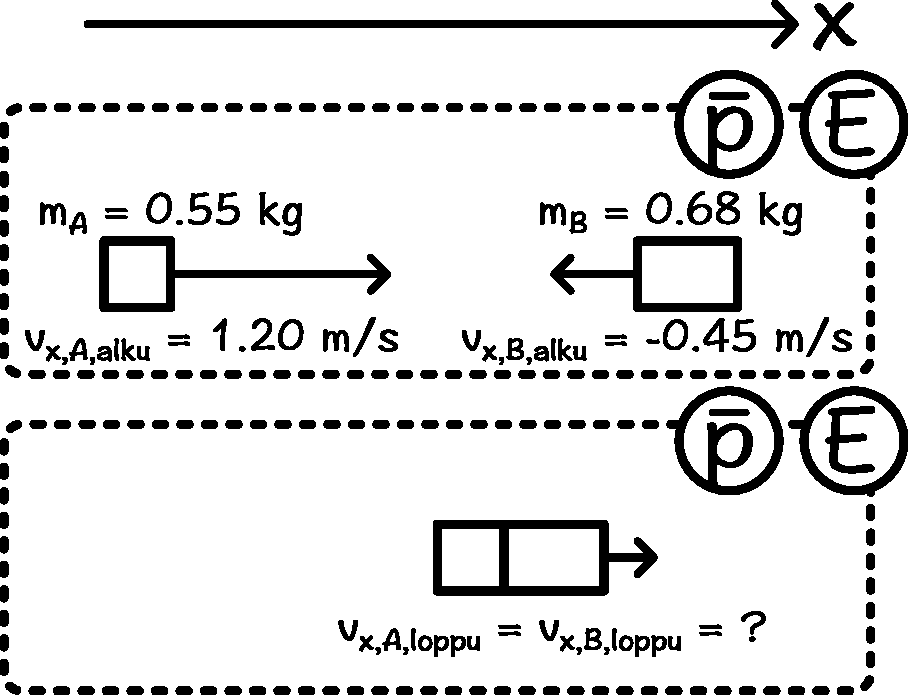
\includegraphics[width=0.9\textwidth]{figs/liikemaara_esimerkki_tormays_2.pdf}%
\end{center}%
}

 \model  Täysin epäelastisen törmäyksen jälkeen kappaleiden nopeudet ovat samat
\begin{equation} v_{x,A,\text{loppu}} = v_{x,B,\text{loppu}} = v_{x,\text{loppu}}. \label{tormaysesim3}\end{equation}
Liikemäärän säilyminen tarkoittaa puolestaan sitä, että kokonaisliikemäärän on oltava aluksi sama kuin lopuksi eli
\begin{equation} m_A v_{x,A,\text{alku}} + m_B v_{x,B,\text{alku}} = (m_A + m_B) v_{x,\text{loppu}}. \label{tormaysesim1b} \end{equation}

\solu Voimme ratkaista loppunopeuden suoraan yhtälöstä (\autoref{tormaysesim1b}), ja ratkaisuksi saadaan
\begin{equation} v_{x,\text{loppu}} = \frac{ m_A v_{x,A,\text{alku}} + m_B v_{x,B,\text{alku}}}{m_A + m_B}. \end{equation}
Sijoittamalla numeroarvot saadaan loppunopeudeksi
\begin{equation} v_{x,\text{loppu}} = 0.29 \un{m/s}. \end{equation}

\begin{minipage}{\textwidth}
\mbar
\begin{mathematica}[commandchars=\\!?]
(* ratkaistaan liikem\"a\"ar\"an s\"ailymisen yht\"al\"o *)
ratkaisu = Solve[ mB (vloppu - vBalku) == -mA (vloppu - vAalku), vloppu]
  \textit!{{vloppu -> (mA vAalku + mB vBloppu) / (mA + mB)}}?

(* sijoitetaan ratkaisuun lukuarvot *)
ratkaisu /. {mA -> 0.55, mB -> 0.68, vAalku -> 1.20, vBalku -> -0.45}
  \textit!{{vloppu -> 0.287805}}?
\end{mathematica}
\end{minipage}

\eval Loppunopeus on alkunopeuksien väliltä kuten pitääkin. Yksinkertaisin tapa tarkastaa tulos täsmällisesti on laskea liikemäärä ennen törmäystä sekä sen jälkeen.
Kokonaisliikemäärä on aluksi
\( p_{x,\text{alku}} = m_A v_{x,A,\text{alku}} + m_B v_{x,B,\text{alku}} = 0.354 \un{kgm/s} \)
ja lopuksi
\( p_{x,\text{loppu}} = m_A v_{x,A,\text{loppu}} + m_B v_{x,B,\text{loppu}} = 0.354 \un{kgm/s}, \)
joten liikemäärä on vakio. Siispä tulos toteuttaa liikemäärän säilymisehdon.

\end{exam}

\begin{exam}{Elastinen t\"orm\"ays}{ex:elastinentormays}\noindent

\index{elastinen}
\index{törmäys}

\problem{Kaksi kappaletta, joiden massat ovat \(0.55 \un{kg}\) ja \(0.68 \un{kg}\), liikkuvat nopeuksilla \(1.2 0 \un{m/s}\) positiiviseen ja \(0.45 \un{m/s}\) negatiiviseen \(x\)-suuntaan. Mikä on kappaleiden loppunopeus suoran törmäyksen jälkeen (kappaleet pysyvät \(x\)-akselilla), jos törmäys on elastinen?
}

 \twocol{0.5}{0.45}{ \setup  Tilanne on täsmälleen samanlainen kuin esimerkissä \autoref{ex:epaelastinentormays} paitsi ettei törmäys ole elastinen. Merkitään kappaleita indeksein A ja B, niiden
massoja \(m_A = 0.55 \un{kg}\) ja \(m_B = 0.68 \un{kg}\) sekä nopeuksia
\(v_{x,A,\text{alku}} = 1.20 \un{m/s}\) ja \(v_{x,B,\text{alku}} = -0.45 \un{m/s}\).

\physics Oletetaan jälleen törmäys niin nopeaksi, että ulkoiset vuorovaikutukset eivät ehdi sen aikana merkittävästi vaikuttaa kappaleiden liikemääriin. Tällöin systeemin kokonaisliikemäärä on törmäyksessä vakio.
Elastisen törmäyksen tapauksessa myös systeemin kokonaisliike-energia on törmäyksessä vakio.

}{%
\begin{center}%
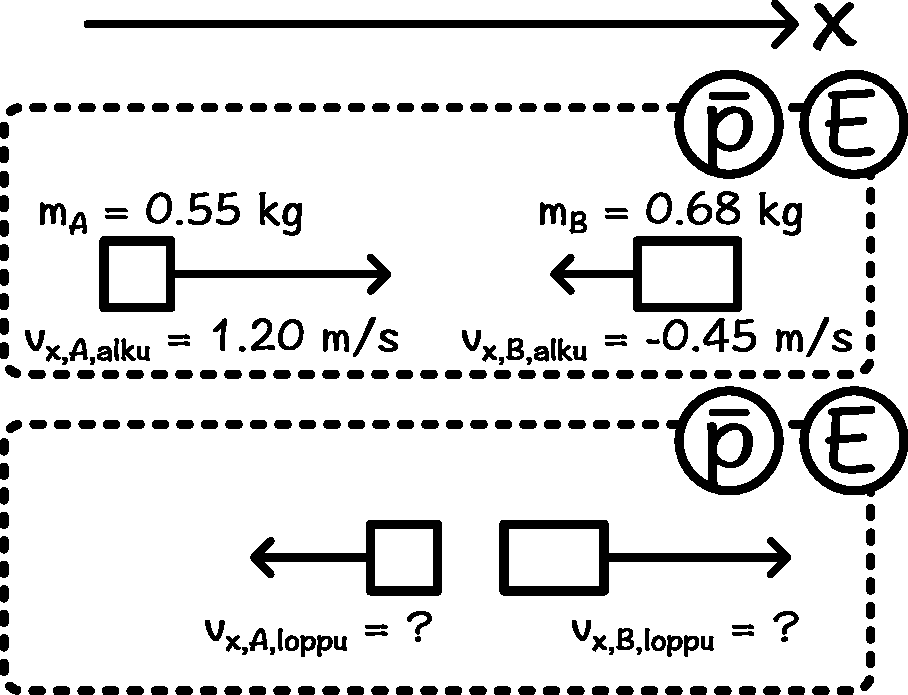
\includegraphics[width=0.9\textwidth]{figs/liikemaara_esimerkki_tormays_1.pdf}%
\end{center}%
}

 \model  Liikemäärän säilyminen tarkoittaa kahden kappaleen tapauksessa sitä, että kappaleiden nopeuksien muutokset ovat kääntäen verrannolliset kappaleiden massoihin eli
\begin{equation} \Delta v_{x,B} = -\frac{m_A}{m_B} \Delta v_{x,A}. \label{tormaysesim1} \end{equation}
Elastisessa törmäyksessä liike-energia on vakio
\begin{equation} \frac{1}{2}m_Av_{x,A,\text{alku}}^2 + \frac{1}{2}m_Bv_{x,B,\text{alku}}^2 = \frac{1}{2}m_Av_{x,A,\text{loppu}}^2 + \frac{1}{2}m_Bv_{x,B,\text{loppu}}^2. \label{tormaysesim2} \end{equation}

\solu Nopeudet voidaan ratkaista yhtälöistä (\autoref{tormaysesim1}) sekä (\autoref{tormaysesim2}). Periaatteessa lasku onnistuu ratkaisemalla liikemäärän säilymislain avulla esimerkiksi kappaleen B loppunopeus ja sijoittamalla tämä energian säilymislain yhtälöön. Lopputuloksena saadaan toisen asteen yhtälö, jonka ratkaisuna saadaan kappaleen A loppunopeus. Tämä voidaan sijoittaa takaisin liikemäärän säilymislakiin, jolloin saadaan myös kappaleen B loppunopeus. Lasku on kuitenkin varsin pitkä ja työläs, ja ratkaisu löytyy helpomminkin.

Termejä ryhmittelemällä liike-energian säilymislaki (\autoref{tormaysesim2}) voidaan kirjoittaa muodossa
\begin{equation} \frac{1}{2}m_B (v_{x,B,\text{loppu}}^2 - v_{x,B,\text{alku}}^2) = -\frac{1}{2}m_A (v_{x,A,\text{loppu}}^2 - v_{x,A,\text{alku}}^2). \end{equation}
Tässä yhtälössä on kummallakin puolella neliöiden erotus, joka voidaan hajottaa laskusäännöllä
\begin{equation} a^2 - b^2 = (a-b)(a+b). \end{equation}
Huomioiden vielä, että \(\Delta v_{x,B} = v_{x,B,\text{loppu}} - v_{x,B,\text{alku}}\), liike-energian säilyminen voidaan kirjoittaa muotoon
\begin{equation} \frac{1}{2}m_B  \Delta v_{x,B} (v_{x,B,\text{loppu}} + v_{x,B,\text{alku}}) = -\frac{1}{2}m_A \Delta v_{x,A} (v_{x,A,\text{loppu}} + v_{x,A,\text{alku}}). \end{equation}
Sijoittamalla tähän liikemäärän säilymisen ehto (\autoref{tormaysesim1}) saadaan tulos
\begin{equation} -\frac{1}{2}m_B \frac{m_A}{m_B}  \Delta v_{x,A} (v_{x,B,\text{loppu}} + v_{x,B,\text{alku}}) = -\frac{1}{2}m_A \Delta v_{x,A} (v_{x,A,\text{loppu}} + v_{x,A,\text{alku}}) \end{equation}
josta yhteiset tekijät supistaen
\begin{equation} v_{x,B,\text{loppu}} + v_{x,B,\text{alku}} = v_{x,A,\text{loppu}} + v_{x,A,\text{alku}}. \label{tormaysoho} \end{equation}
Tämä yllättävän yksinkertainen tulos siis sanoo, että kummankin kappaleen alku- ja loppunopeuden summa (tai keskiarvo) on \emph{sama}. Tämä pätee kuitenkin vain yksiulotteisissa elastisissa törmäyksissä.

Yhtälöt (\autoref{tormaysesim1}) sekä (\autoref{tormaysoho}) muodostavat yhtälöparin, josta loppunopeudet voidaan ratkaista. Esimerkiksi jälkimmäisen yhtälön mukaan kappaleen B loppunopeus on
\begin{equation} v_{x,B,\text{loppu}} = v_{x,A,\text{loppu}} + v_{x,A,\text{alku}} -  v_{x,B,\text{alku}} \label{tormaysbloppu} \end{equation}
ja tämän sijoitus ensimmäiseen antaa
\begin{equation} v_{x,A,\text{loppu}} + v_{x,A,\text{alku}} - 2 v_{x,B,\text{alku}} = - \frac{m_A}{m_B} (v_{x,A,\text{loppu}} - v_{x,A,\text{alku}}). \end{equation}
Siirtämällä kaikki kappaleen A loppunopeutta sisältävät termit yhtälön vasemmalle puolelle saadaan
\begin{equation} \left( 1+ \frac{m_A}{m_B} \right)  v_{x,A,\text{loppu}} = \left( \frac{m_A}{m_B} -1 \right) v_{x,A,\text{alku}} + 2 v_{x,B,\text{alku}} \end{equation}
ja tästä edelleen kappaleen A loppunopeudeksi
\begin{equation} v_{x,A,\text{loppu}} = \left( \frac{m_A-m_B}{m_B} v_{x,A,\text{alku}} + 2 v_{x,B,\text{alku}} \right) / \left( \frac{m_A + m_B}{m_B} \right) = \frac{(m_A-m_B) v_{x,A,\text{alku}} +2 m_B v_{x,B,\text{alku}}}{m_A + m_B}. \end{equation}

Sijoitus takaisin yhtälöön (\autoref{tormaysbloppu}) antaa kappaleen B loppunopeuden
\begin{equation} v_{x,B,\text{loppu}} = \frac{(m_B-m_A) v_{x,B,\text{alku}} +2 m_A v_{x,A,\text{alku}}}{m_A + m_B}. \end{equation}
Sijoittamalla numeroarvot saadaan loppunopeuksiksi
\begin{equation} v_{x,A,\text{loppu}} = -0.62 \un{m/s}, \ v_{x,B,\text{loppu}} = 1.0 \un{m/s}.\end{equation}

\mbar
\begin{mathematica}[commandchars=\\!?]
(* ratkaistaan energian ja liikem\"a\"ar\"an s\"ailymisen yht\"al\"opari *)
ratkaisu = Solve[{
   mA vAloppu^2 + mB vBloppu^2 == mA vAalku^2 + mB vBalku^2, 
   mB (vBloppu - vBalku) == -mA (vAloppu - vAalku)
 }, 
 {vAloppu, vBloppu}]
  \textit!{{vAloppu -> vAloppu, vBloppu -> vBloppu},?
  \textit! {vAloppu -> ((mA - mB) vAalku + 2 mB vBalku) / (mA + mB), ?
  \textit!  vBloppu -> (2 mA vAalku + (mB - mA) vBalku) / (mA + mB)}}?

(* sijoitetaan ratkaisuun lukuarvot *)
ratkaisu /. {mA -> 0.55, mB -> 0.68, vAalku -> 1.20, vBalku -> -0.45}
  \textit!{{vAloppu -> 1.2, vBloppu -> -0.45}, {vAloppu -> -0.62439, vBloppu -> 1.02561}}?
\end{mathematica}

\eval Kappaleen A loppunopeus on negatiivinen ja kappaleen B positiivinen, joten kappaleet kääntyvät törmäyksessä ympäri mikä on järkevää. Yksinkertaisin tapa tarkastaa tulos täsmällisesti on laskea energia ja liikemäärä ennen törmäystä sekä sen jälkeen. Kokonaisenergiaksi saadaan aluksi
\begin{equation}K_\text{alku} = \frac{1}{2}m_Av_{x,A,\text{alku}}^2 + \frac{1}{2}m_Bv_{x,B,\text{alku}}^2 = 0.465 \un{J}\end{equation}
sekä lopuksi
\begin{equation}K_\text{loppu} = \frac{1}{2}m_Av_{x,A,\text{loppu}}^2 + \frac{1}{2}m_Bv_{x,B,\text{loppu}}^2 = 0.465 \un{J},\end{equation}
joten liike-energia on vakio.
Kokonaisliikemäärä on aluksi
\begin{equation} p_{x,\text{alku}} = m_A v_{x,A,\text{alku}} + m_B v_{x,B,\text{alku}} = 0.354 \un{kgm/s}\end{equation}
ja lopuksi
\begin{equation} p_{x,\text{loppu}} = m_A v_{x,A,\text{loppu}} + m_B v_{x,B,\text{loppu}} = 0.354 \un{kgm/s}, \end{equation}
joten myös liikemäärä on vakio. Siispä tulos toteuttaa vaaditut fysikaaliset ehdot.

Tarkastelluilla yhtälöillä on toinenkin ratkaisu, jonka Mathematica-ratkaisu löysi. Nimittäin jos kummankaan kappaleen nopeus ei muutu, liikemäärä ja liike-energia tietenkin ovat vakiot. Yllä esitetyssä laskussa tätä ratkaisua ei löydetty, koska yhtälössä (\autoref{tormaysoho}) on supistettu pois termi \(\Delta v_{x,A}\), mikä on sallittua vain jos ko. termi ei ole nolla. Fysikaalisesti tämä ratkaisu tietenkin tarkoittaa sitä, että kappaleet eivät törmää lainkaan, joten ratkaisu ei kelpaa. Yhtälöiden matemaattisessa käsittelyssä on kuitenkin aina syytä olla tarkkana, jottei fysikaalisesti merkityksellisiä ratkaisuja unohdu.

\end{exam}

\subsection{Impulssi}
\label{impulssi}

Edellä todettiin, että systeemin kokonaisliikemäärä on vakio, kun systeemiin ei vaikuta ulkoisia vuorovaikutuksia. Usein on kuitenkin tarpeellista tarkastella systeemejä, joiden kokonaisliikemäärä muuttuu. On siis tarpeen pystyä analysoimaan myös vuorovaikutusten liikemäärää muuttavaa vaikutusta.

\index{impulssi}

Vuorovaikutuksen kykyä muuttaa systeemin liikemäärää mittaa suure nimeltä \textbf{impulssi}.
Ympäristönsä kanssa vuorovaikuttavaan systeemiin kohdistuva impulssi määritellään \emph{yhtä suureksi kuin systeemin liikemäärän muutos}
\bigeq{ \bs{I} = \Delta \bs{p}. \label{impulssip} }
Yhtälö (\autoref{impulssip}) tarkoittaa impulssin olevan \emph{yhtä suuri} kuin liikemäärän muutos, mutta nämä ovat fysikaalisesti \emph{eri asioita}. Impulssi on \emph{vuorovaikutuksen voimakkuutta} kuvaava suure kun taas liikemäärän muutos on \emph{kappaleen liikettä} kuvaava suure. Tämä määritelmä siis kertoo, kuinka \emph{vuorovaikutus vaikuttaa liikkeeseen}. Se ei tarkoita sitä, että impulssi olisi kappaleiden liikettä kuvaava suure.

\widepictures{tb}%
{Jousi työntää kaksi kappaletta erilleen. Kappaleiden kokonaisliikemäärä on koko ajan nolla, mutta kappaleiden liikemäärät erikseen muuttuvat, sillä vuorovaikutus kohdistaa kumpaankin kappaleeseen impulssin.;%
Kahden kappaleen systeemin kokonaisliikemäärä on vakio.;%
Kappale A kohdistaa kappaleeseen B impulssin jolloin B:n liikemäärä muuttuu.;%
Myös kappale A saa impulssin ja sen liikemäärä muuttuu.}%
{fig:liikemaaraimpulssi;fig:liikemaaraimpulssi:a;fig:liikemaaraimpulssi:b;fig:liikemaaraimpulssi:c}%
{0.3;0.3;0.3}%
{0.3;0.3;0.3}%
{liikemaara_impulssi_4.pdf;liikemaara_impulssi_5.pdf;liikemaara_impulssi_6.pdf}

\begin{stopQ}{q:golfimpulssi}%
Miten voisit määrittää golfpalloon golflyönnin aikana kohdistuvan impulssin suuruuden?
\end{stopQ}

Kuvassa \autoref{fig:liikemaaraimpulssi} tarkastellaan kahden kappaleen, A ja B, yksinkertaista vuorovaikutusta erilaisin systeemirajauksin. Toisessa kappaleessa on jousi, joka on aluksi puristunut kokoon. Vapautuessaan jousi työntää kappaleet liikkeelle. Kappaleiden muodostamaan systeemiin ei kohdistu ulkoisia vuorovaikutuksia, joten sen kokonaisliikemäärä on vakio. Merkitsemällä kappaleiden liikemääriä \(\bs{p}_A\) ja \(\bs{p}_B\), systeemin kokonaisliikemäärä on näiden summa joka siis ei muutu,\\
\begin{equation} \Delta \bs{p}_\text{kokonais} = \Delta (\bs{p}_A + \bs{p}_B) = \Delta \bs{p}_A + \Delta \bs{p}_B = \bs{0}. \label{liikemaaravakio}\end{equation}

Kuitenkin jos systeemiksi valitaan vain toinen kappaleista, systeemin liikemäärä selvästikään ei ole vakio. Systeemin liikemäärä muuttuu, koska nyt kappaleiden välinen vuorovaikutus on ulkoinen vuorovaikutus, ja se kohdistaa systeemiin impulssin. Esimerkiksi kappaleen A kappaleeseen B kohdistama impulssi on impulssin määritelmän (\autoref{impulssip}) nojalla yhtä suuri kuin kappaleen B liikemäärän muutos
\begin{equation} \bs{I}_{A \to B} = \Delta \bs{p}_{B}. \end{equation}
Koska myös kappaleen A liikemäärä muuttuu, myös siihen täytyy kohdistua vuorovaikutuksessa impulssi
\begin{equation} \bs{I}_{B \to A} = \Delta \bs{p}_{A}. \end{equation}

Koska kappaleiden liikemäärien muutosten summa on liikemäärän säilymisen (\autoref{liikemaaravakio}) perusteella nollavektori, näiden muutosten täytyy olla yhtä suuret ja vastakkaissuuntaiset
\begin{equation} \Delta \bs{p}_A = -\Delta \bs{p}_B. \end{equation}
Toisaalta, koska kummankin kappaleen saama impulssi on yhtä suuri kuin kappaleen liikemäärän muutos, kappaleiden vuorovaikutuksessa saamien impulssien täytyy olla niinikään \emph{yhtä suuret mutta vastakkaissuuntaiset}
\begin{equation} \bs{I}_{A\to B} = - \bs{I}_{B \to A}. \label{vastaimpulssi} \end{equation}

Päättelyn tulos oli siis seuraava: koska kahden vain keskenään vuorovaikuttavan kappaleen kokonaisliikemäärä on liikemäärän säilymislain nojalla vakio, niiden keskinäiset vuorovaikutukset välttämättä kohdistavat impulssin \emph{kumpaankin} kappaleeseen. Toisin sanoen vuorovaikutukset todella ovat vastavuoroisia --- ei ole mahdollista, että vuorovaikutus kohdistuisi vain yhteen kappaleeseen vaan molempien vuorovaikutusten osapuolten on koettava impulssi. Liikemäärän säilymislaki asettaa näin ollen voimakkaita rajoituksia sille, millaiset vuorovaikutukset ovat fysikaalisesti sallittuja.
Huomaa vielä, että vaikka kuvassa \autoref{fig:liikemaaraimpulssi} vuorovaikutus oli seurausta jousen elastisuudesta, tässä esitetyssä päättelyssä ei missään vaiheessa tarvinnut tietää vuorovaikutuksen ominaisuuksia. Niinpä päättely toimii \emph{mille tahansa} kahden kappaleen väliselle vuorovaikutukselle.

\newpage\begin{exam}{Liikkuva laatikko}{ex:kokonaisliikemaara}\noindent

\problem{Laatikon (massa 0.20 kg) sisällä on jousi ja pallo, jonka massa on yhtä suuri kuin laatikon massa. Aluksi sekä laatikko että pallo ovat paikoillaan, ja jousi on puristettu kokoon niin, että jouseen on varastoitunut 20 J energiaa. Sitten jousi vapautetaan, jolloin se työntää pallon liikkeelle ja pallo alkaa kimpoilla edestakaisin laatikon kahdesta vastakkaisesta sivusta. (Jousi itse ponnahtaa pois pallon tieltä.) Laatikko on vaakasuoralla lähes kitkattomalla pinnalla ja törmäykset ovat täysin elastiset. Millaisia impulsseja pallo ja laatikko toisilleen antavat? Miltä laatikon liike ulospäin näyttää?
}

 \twocol{0.65}{0.3}{ \setup  Valitaan systeemiksi pallo, jousi ja laatikko. Piirretään kappaleiden liikkeestä kuvasarja auttamaan tilanteen hahmottamista.

\physics Aluksi pallo ja laatikko ovat paikoillaan, joten niiden liike-energiat ja liikemäärät ovat nollia. Jousella on potentiaalienergiaa. Kun jousi vapautuu, sen potentiaalienergia muuttuu pallon ja laatikon liike-energiaksi.

Pallon ja laatikon muodostamaan systeemiin vaikuttaa ulkoinen gravitaatio sekä kosketusvuorovaikutus maanpinnan kanssa. Koska systeemi ei liiku pystysuunnassa, näiden vuorovaikutusten täytyy kuitenkin olla tasapainossa eikä systeemiin kohdistu ulkoisia vuorovaikutuksia, jotka vaikuttaisivat kappaleiden vaakasuuntaiseen liikkeeseen. Niinpä systeemin kokonaisliikemäärä on vakio. Koska systeemi on aluksi paikoillaan, sen kokonaisliikemäärä on nolla, ja siispä systeemin kokonaisliikemäärän pitää olla nolla \emph{aina}. Näin ollen pallon nopeuden muuttuessa myös laatikon nopeuden täytyy myös muuttua vastakkaiseen suuntaan, jotta systeemin kokonaisliikemäärä säilyisi nollana.

 \model  Merkitään pallon ja laatikon massaa \(m = 0.20 \un{kg}\) ja niiden nopeuden skalaarikomponentteja
\( v_{x,\text{pallo}} \)
ja
\( v_{x,\text{laatikko}}. \)
Tällöin niiden liikemäärät ovat
\begin{equation} \bs{p}_\text{pallo} = m v_{x,\text{pallo}} \uv{i} , \bs{p}_\text{laatikko} = m v_{x,\text{laatikko}} \uv{i}. \end{equation}

Systeemin kokonaisliikemäärä on nolla koko liikkeen ajan
\begin{equation} \bs{p}_\text{kokonais} = \bs{p}_\text{pallo} + \bs{p}_\text{laatikko} = m (v_{x,\text{pallo}} + v_{x,\text{laatikko}}) \uv{i} = \bs{0}. \label{nollamom} \end{equation}
ja systeemin liike-energia on yhtä suuri kuin jouseen aluksi varastoitunut energia
\begin{equation} K = \frac{1}{2} m v_{x,\text{pallo}}^2 + \frac{1}{2} m v_{x,\text{laatikko}}^2 = U_\text{jousi, alku}. \label{utokp} \end{equation}

Törmäyksissä pallo ja laatikko kohdistavat toisiinsa impulssin. Kappaleen saama impulssi on yhtä suuri kuin kappaleen liikemäärän muutos,
\begin{equation} \bs{I} = \Delta \bs{p}. \end{equation}

}{%
\begin{center}%
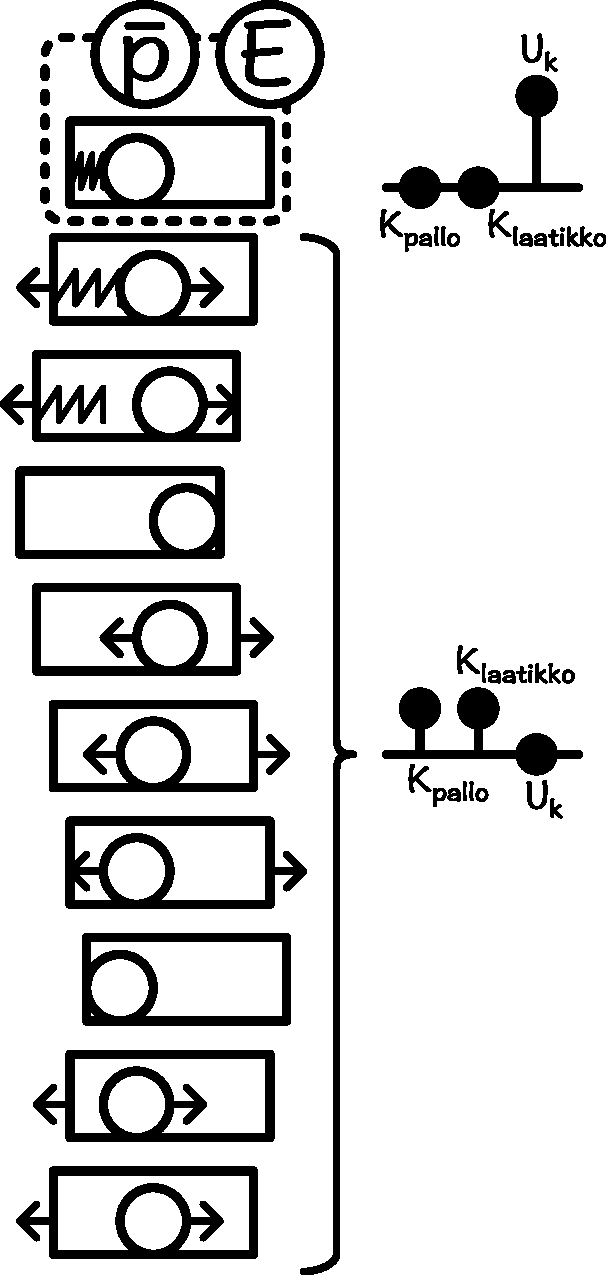
\includegraphics[width=0.95\textwidth]{figs/liikemaara_esimerkki_pallolaatikko.pdf}%
\end{center}%
}

\solu Yhtälön (\autoref{nollamom}) mukaan systeemin kokonaisliikemäärävektori on nollavektori. Tämä tarkoittaa sitä, että vektorin pituus on nolla, eli
\begin{equation} m(v_{x,\text{pallo}} + v_{x,\text{laatikko}}) = 0. \end{equation}
Koska kappaleiden massat eivät ole nollia, tämä toteutuu vain kun
\( v_{x,\text{pallo}} = - v_{x,\text{laatikko}} \label{vastanopeudet} \)
eli kun kappaleet liikkuvat vastakkaisiin suuntiin itseisarvoltaan yhtä suurilla nopeuksilla.

Voidaan siis päätellä, että jousen työntäessä pallon liikkeelle, se työntää myös laatikon liikkeelle vastakkaiseen suuntaan. (Tämä on räjähtävä erotus.) Samoin jokaisessa törmäyksessä pallon nopeuden vaihtaessa suuntaa (\(v_{x,\text{pallo}} \to -v_{x,\text{pallo}}\)) myös laatikon nopeus vaihtaa suuntaa. Laatikko alkaa siis poukkoilemaan edestakaisin samalla nopeudella mutta vastakkaiseen suuntaan kuin sen sisällä liikkuva pallo.

Kappaleiden vauhti selviää nyt energiaperiaatteella. Merkitsemällä \(v = |v_{x,\text{pallo}}| = |v_{x,\text{laatikko}}|\) yhtälöstä (\autoref{utokp}) saadaan

\begin{equation} v = \sqrt{U_\text{jousi, alku} / m} = 10 \un{m/s}. \end{equation}
Pallon vauhti on kussakin törmäyksessä vakio, mutta sen nopeus ei ole, koska liikeen suunta muuttuu. Nopeuden muutos on suuruudeltaan
\begin{equation} |\Delta v_{x,\text{pallo}}| = |v_{x,\text{pallo, loppu}} - v_{x,\text{pallo, alku}}| = 2 v = 20 \un{m/s}. \end{equation}
Jos pallo on aluksi liikkeessä positiiviseen suuntaan, sen saama impulssi on
\begin{equation} I_{x,\text{laatikko} \to \text{pallo}} = \Delta p_{x,\text{pallo}} = m \Delta v_{x,\text{pallo}} = - 4.0 \un{kgm/s}. \end{equation}
Laatikon saama impulssi on yhtä suuri mutta vastakkaissuuntainen,
\( I_{x,\text{pallo} \to \text{laatikko}} = - I_{x,\text{laatikko} \to \text{pallo}}. \)

\eval
Sekä pallo että laatikko liikkuvat, mutta edestakaisin. Kumpikaan ei pääse puolta laatikon mittaa kauemmaksi alkuperäiseltä paikaltaan, koska tällöin laatikko ja pallo jo törmäävät. Systeemin osat siis liikkuvat mutta systeemi itsessään ei lähde liikkeelle. Tämä on järkevä tulos, koska systeemiin vaikutti vain sisäisiä vuorovaikutuksia, jotka eivät voi muuttaa systeemin kokonaisliikemäärää.
\end{exam}

\section{Massakeskipiste}
\label{massakeskipiste}

Esimerkissä \autoref{ex:kokonaisliikemaara} nähtiin, että vaikkei systeemin sisäinen vuorovaikutus voi saada systeemiä jatkuvaan suoraviivaiseen liikkeeseen, se voi kuitenkin saada systeemin osat liikkumaan systeemin suhteen. Kokonaisliikemäärä kertoo meille systeemin liiketilan, ja erityisesti kokonaisliikemäärän ollessa nolla systeemi on kokonaisuutena paikoillaan.
Edelleen jos systeemi on paikoillaan, on luonnollista kysyä \emph{missä} systeemi on. Kuitenkaan systeemin osien liikkuessa minkään yksittäisen kappaleen paikka ei ole hyvä tapa kuvata systeemin sijaintia. Ilmeisesti jonkinlainen keskiarvo eri kappaleiden paikoista olisi tähän tarkoitukseen parempi suure.

Massa on ekstensiivinen suure, joten systeemin kokonaismassa on sen kaikkien osien massojen summa. Jos systeemi koostuu esimerkiksi hiukkasista, joiden massat ovat \(m_1\), \(m_2\), jne., kokonaismassa on
\begin{equation} M = m_1 + m_2 + \ldots = \sum_i m_i. \label{kokonaismassa}\end{equation}
Jos nyt systeemin kokonaisliikemäärä voidaan kirjoittaa muodossa
\begin{equation} \bs{p}_\text{kokonais} = M \bs{v}_\text{cm}, \label{kokomom} \end{equation}
eli systeemin kokonaismassan ja jonkin ``keskiarvonopeuden'' \(\bs{v}_\text{cm}\) tulona, tämä nopeus voisi olla hyvä mittari systeemin kollektiiviselle liikkeelle. (Lyhenteen `cm' merkitys selviää pian. Se ei tarkoita senttimetriä.) Erityisesti \emph{paikoillaan} olevalle systeemille, jolle kokonaisliikemäärä on nolla, tällaisen keskiarvoisen nopeuden pitäisi lausekkeen (\autoref{kokomom}) mukaan olla \emph{nolla}.

Rajoitutaan tarkastelemaan yksiulotteista, \(x\)-suuntaista liikettä, jolloin voimme poimia kokonaisliikemäärän (\autoref{kokomom}) \(x\)-skalaarikomponentin ja kirjoittaa ilman vektoreita
\begin{equation} p_{x,\text{kokonais}} = M v_{x,\text{cm}}. \label{kokomom3} \end{equation}
Systeemin keskiarvoisen nopeuden määritteleminen onnistuu laventamalla kokonaisliikemäärän lauseke (\autoref{kokonaisliikemaara_x}) kokonaismassalla (\autoref{kokonaismassa}), jolloin voidaan kirjoittaa
\begin{equation} p_{x,\text{kokonais}} = M \left(\frac{m_1}{M} v_{x,1} + \frac{m_2}{M} v_{x,2} + \ldots\right) =  M \sum_i \frac{m_i}{M} v_{x,i}. \label{kokomom1} \end{equation}
Lopputuloksena saadussa yhtälössa (\autoref{kokomom1}) summassa esiintyvä tekijät \(m_i/M\) ovat kunkin hiukkasen massan ja systeemin kokonaismassan suhde. Nämä ovat siis vain joitakin reaalilukuja, joten lausekkeessa esiintyvässä summassa yksinkertaisesti lasketaan yhteen kaikkien hiukkasten nopeudet kerrottuna kyseisen hiukkasen massan osuudella systeemin kokonaismassasta. Summa on siis hiukkasten nopeuksien \emph{massoilla painotettu keskiarvo}.
Näin kokonaisliikemäärä on kirjoitettu systeemin kokonaismassan sekä hiukkasten nopeuksien painotetun keskiarvon tulona
aivan kuten yhtälössä (\autoref{kokomom1}). Siispä tämä nopeuksien painotettu keskiarvo kuvaa systeemin kollektiivista nopeutta
\begin{equation} v_{x,\text{cm}} = \sum_i \frac{m_i}{M} v_{x,i}. \label{cmnopeus} \end{equation}

\index{paikka}

Koska voimme nyt ilmaista systeemin nopeuden hyvin määritellyllä tavalla, seuraava askel on määritellä systeemin \emph{paikka} yksikäsitteisesti.
Teemme tämän käyttämällä nopeuden määritelmää \autoref{nopeus}, jonka mukaan nopeus on paikkavektorin derivaatta. Jos nimittäin voimme kirjoittaa systeemin nopeuden muodossa
\begin{equation} v_{x,\text{cm}} = \frac{\dd x_\text{cm}}{\dd t}, \label{cmderivaatta} \end{equation}
missä \(x_\text{cm}\) on jokin hyvin määritelty paikkakoordinaatti, tämä koordinaatti on myös järkevä tapa määritellä systeemin paikka.

Edellä johdetussa nopeuden lausekeessa (\autoref{cmnopeus}) esiintyy hiukkasten nopeuksia, mutta voimme kirjoittaa nämä myös hiukkasten paikkakoordinaattien derivaattoina, jolloin saadaan
\begin{equation} v_{x,\text{cm}} =  \sum_i \frac{m_i}{M} \frac{\dd x_i}{\dd t} = \frac{m_1}{M} \frac{\dd x_1}{\dd t} + \frac{m_2}{M} \frac{\dd x_2}{\dd t} + \ldots. \end{equation}
Edelleen summan derivoimissäännön \(\frac{\dd x_1}{\dd t} + \frac{\dd x_2}{\dd t} = \frac{\dd }{\dd t}(x_1+x_2) \) perusteella tämä on sama asia kuin
\begin{equation} v_{x,\text{cm}} =  \frac{\dd}{\dd t} \left( \frac{m_1}{M} x_1 + \frac{m_2}{M} x_2 + \ldots \right) = \frac{\dd}{\dd t}\left( \sum_i \frac{m_i}{M} x_i \right). \label{kokomom2}\end{equation}
Toisin sanoen on sama asia laskea ensin hiukkasten koordinaatit yhteen ja derivoida niiden summaa kuin derivoida erikseen jokaista koordinaattia ja laskea derivaatat yhteen.

\pictures{tb}%
{Massakeskipiste on kappaleiden paikkojen keskiarvo.;%
Massakeskipisteen paikka.;%
Massakeskipisteen nopeus.;%
Massakeskipiste on lähellä massiivisia kappaleita.}%
{fig:liikemaaramassakeskipiste;fig:liikemaaramassakeskipiste:a;fig:liikemaaramassakeskipiste:b;fig:liikemaaramassakeskipiste:c}%
{0.3;0.3;0.3}%
{0.3;0.3;0.3}%
{liikemaara_massakeskipiste_1b.pdf;liikemaara_massakeskipiste_2b.pdf;liikemaara_massakeskipiste_3b.pdf}

Edellä johdetussa viimeisessä lausekkeessa derivoitava summa \(\sum_i \frac{m_i}{M} x_i\) on nyt hiukkasten \emph{paikkakoordinaattien massoilla painotettu keskiarvo} --- siis jonkin avaruuden pisteen koordinaatti sekin.
Näin keskiarvonopeus \(v_{x,\text{cm}}\)
on kirjoitettu täsmälleen haluttuun muotoon (\autoref{cmderivaatta}) systeemin kokonaismassan ja koordinaatin derivaatan avulla.
Niinpä voimme määritellä systeemin \(x\)-koordinaatiksi tämän hiukkasten koordinaattien keskiarvon
\begin{equation} x_\text{cm} = \sum_i \frac{m_i}{M} x_i \label{mkp_x} \end{equation}

\index{massakeskipiste}

Samanlainen päättely toimii erikseen missä tahansa suunnassa ja sama määritelmä yleisesti vektorein kirjoittaen on
\bigeq{ \bs{r}_\text{cm} = \sum_i \frac{m_i}{M} \bs{r}_i. \label{massakeskipiste} }
Tätä kutsutaan systeemin \textbf{massakeskipisteeksi} ja nopeus
\begin{equation} \bs{v}_\text{cm} = \sum_i \frac{m_i}{M} \bs{v}_i \end{equation}
on systeemin \textbf{massakeskipistenopeus}. (Lyhenne `cm' tulee englanninkielisestä termistä `center of mass'.) Massakeskipistevektori on samaan tapaan määritelty vektori kuin paikkavektorikin, eli se on koordinaatiston origosta varsinaiseen massakeskipisteeseen osoittava vektori, jonka \(x\)-komponentti on \(x_\text{cm}\).

Massakeskipisteen käsitteen avulla edellä esitetyt ilmaukset, joissa puhutaan ``systeemin paikasta'' tulevat täsmällisiksi. Kun systeemin paikaksi määritellään massakeskipiste ja systeemin nopeudeksi massakeskipisteen nopeus, systeemin kokonaisliikemäärä voidaan kirjoittaa systeemin kokonaismassan ja massakeskipisteen nopeuden tulona (\autoref{kokomom}). Systeemi on siis paikoillaan täsmälleen silloin kun sen \emph{massakeskipiste ei liiku}. Liikemäärän säilymislaki voidaan ilmaista myös niin, että \emph{systeemin sisäiset vuorovaikutukset eivät voi muuttaa massakeskipisteen nopeutta}. Myös yksittäisten kappaleiden paikkakoordinaatille saadaan näin hyvä ja yksikäsitteinen määritelmä: Kappaleen paikaksi voidaan aina sopia kappaleen muodostavien \emph{hiukkasten} massakeskipiste.

\begin{stopQ}{q:massakeskipiste}%
Jos systeemissä on kaksi kappaletta, joiden massat ovat 1.0 ja 2.0 kg ja vauhdit 3.0 ja 1.0 m\slash s vastakkaisiin suuntiin, ja kappaleiden välinen etäisyys on 3 m, mikä on systeemin (a) kokonaismassa, (b) massakeskipistenopeus? (c) Missä on systeemin massakeskipiste?
\end{stopQ}

\subsection{Massakeskipisteen energia}
\label{massakeskipisteenenergia}

Massakeskipiste on hyödyllinen työkalu sekä energiaan että liikemäärään perustuvissa tarkasteluissa. Tutkitaan nyt, miten massakeskipisteen avulla voidaan laskea kappaleen tai systeemin energia.

\marginpicture%
{0}%
{Epäsäännöllisen kappaleen massakeskipiste.}%
{fig:liikemaara_mkp_jako_1}%
{1.0}%
{liikemaara_massakeskipiste_jako_1.pdf}

Äsken opimme laskemaan hiukkasista koostuvan systeemin massakeskipisteen paikan ja nopeuden, mutta sama tekniikka toimii myös silloin, kun systeemi koostuu kokonaisista kappaleista. Jos nimittäin määritämme ensin kunkin kappaleen massan ja massakeskipisteen, näiden kappaleiden muodostaman systeemin massakeskipiste saadaan kappaleiden massakeskipisteiden paikkojen painotettuna keskiarvona. Toisaalta jako kappaleisiin on aivan mielivaltainen, joten sama periaate pätee myös kappaleiden osille. Tämän idean avulla voimme etsiä massakeskipisteen myös epäsäännöllisen muotoisille kappaleille kuten kuvassa \autoref{fig:liikemaara_mkp_jako_1}. Kuvan kappaleen muoto muistuttaa C-kirjainta, eikä ole lainkaan selvää, missä kappaleen massakeskipiste täsmälleen on. Voimme kuitenkin ajatella kappaleen koostuvan kolmesta suorakulmaisesta osasta. Jos kappale koostuu kauttaaltaan samanlaisesta aineesta, kunkin suorakulmaisen osan massa on verrannollinen osan kokoon ja kunkin osan massakeskipiste on symmetrian perusteella osan keskipisteessä. Koko kappaleen massakeskipisteen paikka saadaan puolestaan laskettua yhtälöllä \autoref{massakeskipiste} näiden kolmen osan massakeskipisteen paikkakoordinaattien painotettuna keskiarvona. Tässä tapauksessa massakeskipiste on hieman kappaleen ulkopuolella, mutta ei kuitenkaan täsmälleen kappaleen sisään jäävän aukon keskellä.

\index{potentiaalienergia}

Kun tunnemme kappaleen massan ja massakeskipisteen paikan, voimme laskea helposti kappaleen painovoiman potentiaalienergian sen avulla. Jos nimittäin kappale koostuu osista, joiden massat ovat \(m_1\), \(m_2\) jne. ja joiden koordinaatit pystysuunnassa ovat \(x_1\), \(x_2\) jne., näiden osien potentiaalienergia on
\(U_1 = m_1 g x_1 \), \(U_2 = m_2 g x_2\) jne. ja koko kappaleen potentiaalienergia on
\begin{equation} U = m_1 g x_1 + m_2 g x_2 + \ldots = g \sum_i m_i x_i. \end{equation}
Mutta toisaalta massakeskipisteen paikkakoordinaatti on yhtälön (\autoref{mkp_x}) perusteella
\( x_\text{cm} = \frac{1}{M} \sum_i m_i x_i, \)
joten potentiaalienergian voi kirjoittaa kappaleen kokonaismassan ja massakeskipisteen avulla muodossa
\begin{equation} U = M g x_{\text{cm}}. \end{equation}

\begin{stopQ}{q:mkpenergia}%
Systeemi koostuu kahdesta osasta, joiden massat ovat \(2.0 \un{kg}\) ja \(3.0 \un{kg}\). Kevyemmän osan massakeskipiste on korkeudella \(0.5 \un{m}\) ja raskaamman \(1.2 \un{m}\). Mikä on systeemin
(a) massakeskipisteen korkeus?
(b) kummankin osan potentiaalienergia?
(c) massakeskipisteen avulla laskettu potentiaalienergia?
\end{stopQ}

\onepicture%
{tb}%
{Epäsäännöllisen kappaleen potentiaalienergia.}%
{fig:liikemaara_mkp_jako_2}%
{0.7}%
{liikemaara_massakeskipiste_jako_2.pdf}

Epäsäännöllisen muotoisen kappaleen potentiaalienergian voi siis laskea kahdella tavalla (kuva \autoref{fig:liikemaara_mkp_jako_2}). Yksi tapa on jakaa kappale osiin ja laskea kunkin osan potentiaalienergia erikseen, jolloin koko kappaleen potentiaalienergia on sen osien energioiden summa. Toinen tapa on määrittää ensin kappaleen massakeskipisteen paikka. Kappaleella on nimittäin sama potentiaalienergia kuin pallolla, jolla on sama massa ja joka on samalla korkeudella kuin kappaleen massakeskipiste.

Systeemin \emph{liike-energiaa ei kuitenkaan voi laskea yhtä yksinkertaisesti}. Jos systeemin kaikki kappaleet liikkuvat samaan suuntaan samalla nopeudella \(v_x\), myös systeemin massakeskipisteen nopeus on sama, \(v_{x,\text{cm}} = v_x\) ja tällöin systeemin liike-energia voidaan laskea massakeskipisteen massan ja nopeuden avulla,

\begin{eqnarray} K &=& \frac{1}{2} m_1 v_{x,1}^2 + \frac{1}{2} m_2 v_{x,2}^2 + \ldots \\
&=& \frac{1}{2} m_1 v_{x,\text{cm}}^2 + \frac{1}{2} m_2 v_{x,\text{cm}}^2 + \ldots \\
&=& \frac{1}{2} (m_1 + m_2 + \ldots) v_{x,\text{cm}}^2 \\
&=/ \frac{1}{2} M v_{x,\text{cm}}^2. \end{eqnarray}

Yleensä tämä \emph{ei kuitenkaan päde}! Esimerkiksi jos systeemiin kuuluu kaksi vastakkaiisin suuntiin kulkevaa kappaletta, joilla on sama massa ja sama vauhti, niiden muodostaman systeemin massakeskipistenopeus on nolla, vaikka systeemillä selvästikin on liike-energiaa. Niinpä yleisesti pätee
\begin{equation} K_\text{systeemi} \ge \frac{1}{2} M v_{x,\text{cm}}^2, \end{equation}
ja yhtäsuuruus on voimassa vain kun kaikilla kappaleilla on sama nopeus.

\begin{stopQ}{q:mkpliike}%
Kysymyksen \autoref{q:mkpenergia} systeemin kevyt kappale liikkuu ylöspäin vauhdilla \(1.5 \un{m/s}\) ja raskas kappale alaspäin vauhdilla \(0.8 \un{m/s}\). Mikä on systeemin
(a) massakeskipisteen nopeus?
(b) massakeskipisteen avulla laskettu liike-energia?
(c) todellinen liike-energia?
\end{stopQ}

\subsection{Massakeskipisteen liike törmäyksessä}
\label{massakeskipisteenliiketörmäyksessä}

\pictures{b!}%
{Massakeskipiste liikkuu törmäyksissä tasaisesti. Tässä kappaleen A massa on kaksinkertainen kappaleeseen B verrattuna, \(m_A = 2 m_B\), joten massakeskipiste on kappaleiden välissä lähempänä A:ta.;%
Kappaleiden liike kuvasarjana.;%
Kappaleiden paikan kuvaaja.;%
Kappaleiden nopeuden kuvaaja.}%
{fig:liikemaaratormays6;fig:liikemaaratormays6:a;fig:liikemaaratormays6:b;fig:liikemaaratormays6:c}%
{0.35;0.28;0.28}%
{0.35;0.28;0.28}%
{liikemaara_kuvasarja_4.pdf;liikemaara_tormays_20.pdf;liikemaara_tormays_21.pdf}

Tarkastellaan sitten systeemin massakeskipisteen käyttäytymistä tilanteessa kuten törmäyksessä, jossa systeemin liikemäärä on vakio.
Kuvaan \autoref{fig:liikemaaratormays6} on piirretty tällainen tilanne.
Kyseessä on sama törmäys kuin kuvassa \autoref{fig:liikemaaratormays3a}, jossa kappale A törmää aluksi levossa olleeseen kappaleeseen B, jonka inertia on puolet kappaleen A inertiasta. Nyt kuvaan on kuitenkin piirretty myös systeemin massakeskipisteen liike.

Merkitään kappaleen B massaa \(m_B = m\), jolloin kappaleen A massa on \(m_A = 2m \) ja systeemin kokonaismassa on \(M=3m\). Jos kappaleen A koordinaatti on \(x_A\) ja kappaleen B \(x_B\), massakeskipisteen \(x\)-koordinaatti on määritelmän (\autoref{massakeskipiste}) mukaisesti
\(x_\text{cm} = \frac{1}{3m}(2m x_A + m x_B) = \frac{2}{3} x_A + \frac{1}{3} x_B. \) Tämä on piste, joka on kappaleiden A ja B paikkoja kuvaavien pisteiden välissä ja jakaa niiden yhdysjanan suhteessa \(1:2\). Toisin sanoen massakeskipiste on kaksi kertaa niin kaukana kappaleesta B kuin kappaleesta A.

Piirtämällä massakeskipiste samaan tapaan jokaisella ajan hetkellä kappaleiden väliin näemme massakeskipisteen liikkeen törmäyksessä. Kuvasta nähdään suoraan, että massakeskipisteen paikkaa kuvaa suora eli massakeskipiste liikkuu \emph{tasaisesti}. Myös nopeuden kuvaajassa massakeskipisteen nopeus on kappaleiden A ja B nopeuksien kuvaajien välissä, lähempänä kappaleen A nopeutta. Tässä graafissa massakeskipisteen nopeuden kuvaajaksi piirtyy vaakasuora viiva, mikä tarkoittaa massakeskipisteen nopeuden olevan vakio, kuten tasaisessa liikkeessä pitää ollakin. Erityisesti massakeskipisteen liike on tasaista myös törmäyksen aikana vaikka kummankin kappaleen nopeus tällöin muuttuu.

Systeemin massakeskipisteen nopeus kuvaa systeemin kollektiivista liikettä. Erityisesti massakeskipisteen nopeus kerrottuna systeemin kokonaismassalla on sama kuin systeemin kokonaisliikemäärä yhtälön (\autoref{kokomom}) mukaisesti. Niinpä jos systeemin massakeskipiste liikkuu tasaisella nopeudella ja systeemin kokonaismassa on vakio, systeemin kokonaisliikemäärä on siis myös vakio. Juuri näin onkin törmäyksissä, joissa ulkoiset vuorovaikutukset eivät ole merkittäviä, ja massakeskipisteen tasainen liike on osoitus kokonaisliikemäärän säilymisestä.

Massakeskipisteen liikkeen analysointia ja graafista esitystä voidaan myös käyttää kappaleiden törmäysten tutkimisen apuvälineenä. Kahden kappaleen massakeskipiste on nimittäin \emph{aina} kappaleiden välissä --- ei koskaan niiden yhdysjanan ulkopuolella. Niinpä kokonaisliikemäärän ollessa vakio kappaleiden liikkeen on \emph{aina} tapahduttava siten, että tasaisesti liikkuva massakeskipiste pysyy kappaleiden välissä.

\begin{stopQ}{q:mkptormays}%
Kaksi kappaletta liikkuvat vastakkaisiin suuntiin niin, että systeemin kokonaisliikemäärä on nolla. Kappaleet törmäävät. (a) Mitä voit päätellä kappaleiden liikemääristä ennen törmäystä? (b) Entä törmäyksen jälkeen, jos törmäys on täysin elastinen? (c) Entä jos törmäys on täysin epäelastinen?
\end{stopQ}

\pictures{tb}%
{Vapaassa pudotuksessa oleva kappale räjähtää kahteen osaan. Osien massakeskipiste jatkaa vapaassa pudotuksessa eikä kappaleen hajoaminen vaikuta siihen.;%
Kappaleiden osien sekä massakeskipisteen liikerata.;%
Osien ja massakeskipisteen nopeus.}%
{fig:liikemaaraputous;fig:liikemaaraputous:a;fig:liikemaaraputous:b}%
{0.59;0.36}%
{0.59;0.36}%
{liikemaara_putous_1.pdf;liikemaara_putous_2.pdf}

Massakeskipisteen nopeus ei muutu myöskään räjähdyksissä, jos räjähdyksen sinkoamat kappaleet eivät osu mihinkään. Esimerkiksi kun räjähtävä kappale on ennen räjähdystä paikoillaan, räjähdyksessä liikkeelle lähtevien kappaleiden massakeskipiste pysyy paikoillaan myös räjähdyksen jälkeen. Käytännössä tämä tarkoittaa sitä, että räjähdys sinkoaa kappaleita yhtä paljon kaikkiin suuntiin. Vastaavasti liikkuvan kappaleen räjähtäessä sen osien massakeskipiste jatkaa samalla nopeudella kuin alkuperäinen kappale.

Esimerkiksi räjähtävän ilotulitusraketin massakeskipiste jatkaa räjähdyksen jälkeen samalla radalla kuin ennen räjähdystä.
Räjähdettyään raketti on vapaassa pudotuksessa, joten sen osat jatkavat samalla vapaan pudotuksen liikeradalla, jolla rakettikin olisi liikkunut jollei olisi hajonnut osiin, kuten kuvassa \autoref{fig:liikemaaraputous}. Toisin sanoen räjähdys, joka on systeemin sisäinen vuorovaikutus, ei vaikuta massakeskipisteen liikkeeseen. Massakeskipisteen liikerata muuttuu ainoastaan, jos kappaleen hajoaminen osiin muuttaa kappaleeseen vaikuttavia ulkoisia vuorovaikutusia. Raketin tapauksessa ilmanvastus voi olla osiin hajonneelle raketille erilainen kuin ehjälle.

\begin{stopQ}{q:mkptiivistelma}%
Kirjoita tiivistelmä massakeskipisteen ominaisuuksista. Keksi esimerkki systeemistä, jossa on vähintään kolme kappaletta (eri pisteissä, eri nopeudet) ja laske systeemin massakeskipisteen paikka ja nopeus. Selitä erityisesti, voiko systeemin liikemäärän, liike-energian tai potentiaalienergian päätellä suoraan massakeskipisteen ominaisuuksista.
\end{stopQ}

\begin{exam}{Helminauhan massakeskipiste}{ex:massakeskipiste}\noindent

\problem{Helminauhassa on erikokoisia helmiä. Ensimmäinen helmistä on massaltaan 10 g, toinen 20 g jne. niin että kukin helmi on aina 10 g massiivisempi kuin edellinen. Nauhan massa on pieni helmiin verrattuna. Vierekkäisten helmien välinen etäisyys on 1.0 cm. Mikä on nauhan kokonaismassa ja missä on sen massakeskipiste nauhan ollessa suora, jos nauhassa on (a) 5 tai (b) N helmeä?
}

 \twocol{0.45}{0.5}{ \setup  Valitaan \(x\)-akseli nauhan suuntaiseksi ja olkoon origo 1 cm päässä ensimmäisestä helmestä.

\physics Systeemin kokonaismassa on sen kaikkien osien yhteenlaskettu massa.
Massakeskipisteen \(x\)-koordinaatti on systeemin osien koordinaattien massoilla painotettu keskiarvo.

}{%
\begin{center}%
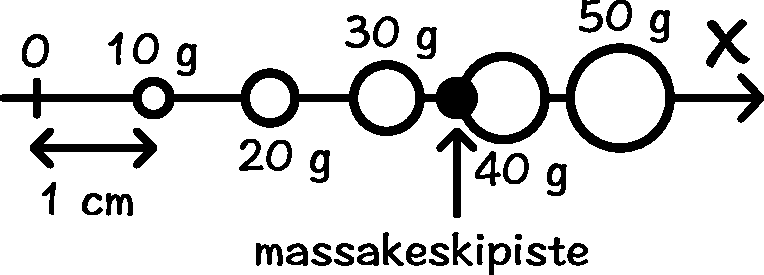
\includegraphics[width=0.95\textwidth]{figs/liikemaara_esimerkki_massakeskipiste.pdf}%
\end{center}%
}

 \model  Helmien välinen etäisyys on \(\Delta x = 1 \un{cm}\) ja ensimmäisen helmen paikkakoordinaatti on valitussa koordinaatistossa \(x_1 = 1 \un{cm}\). Niinpä kunkin helmen paikkakoordinaatti on
\begin{equation} x_i = x_1 + (i-1)\Delta x =  i \Delta x, \end{equation}
missä indeksi \(i\) on helmen järjestysnumero.

Vierekkäisten helmien massojen ero on \(\Delta m = 10 \un{g}\) ja ensimmäisen helmen massa on \(m_1 = 10 \un{g}\), joten kunkin helmen massa on
\begin{equation} m_i = m_1 + (i-1) \Delta m = i \Delta m.\end{equation}

Helminauhan kokonaismassa on näillä merkinnöillä
\begin{equation} M = \sum_{i=1}^N m_i \end{equation}
ja massakeskipisteen paikkakoordinaatti
\begin{equation} x_\text{cm} = \sum_{i=1}^N \frac{m_i}{M} x_i. \end{equation}

\solu Nauhan kokonaismassa on
\begin{equation} M = \sum_{i=1}^N i \Delta m = \Delta m \sum_{i=1}^N i. \end{equation}
Lausekkeessa esiintyy aritmeettinen summa
\begin{equation} \sum_{i=1}^N i = 1 + 2 + 3 + \ldots + N = \frac{1}{2}N(N+1). \end{equation}
Summan arvon voi päätellä esimerkiksi huomaamalla, että summassa on \(N\) summattavaa, joiden keskiarvo on \( (N+1)/2 \). Kokonaismassaksi saadaan siis
\begin{equation} M = \frac{1}{2}N(N+1) \Delta m. \label{kokomassaesim} \end{equation}

Erikoistapauksessa \(N=5\) kokonaismassaksi tulee \begin{equation} M_5 = (1+2+3+4+5) \Delta m = 15 \Delta m = 150 \un{g}. \end{equation} Edellä johdettu yleinen lauseke (\autoref{kokomassaesim}) antaa saman tuloksen \(M_5 = 5 \cdot 6 / 2 \cdot \Delta m = 15 \Delta m\) kuten pitääkin.

Massakeskipisteen paikka on puolestaan
\begin{equation} x_\text{cm} = \frac{1}{M} \sum_{i=1}^N m_i x_i = \frac{\Delta m \Delta x}{M} \sum_{i=1}^N i^2. \end{equation}
Tässä lausekkeessa esiintyy neliösumma, jonka laskeminen on huomattavasti vaikeampi tehtävä kuin edellä esitetyn aritmeettisen summan. Kyseessä on kuitenkin tunnettu pyramidilukujen jono, jonka summa tunnetaan (http:\slash \slash en.wikipedia.org\slash wiki\slash Square\_pyramidal\_number),
\begin{equation} \sum_{i=1}^N i^2 = 1^2 + 2^2 + 3^2 + \ldots + N^2 = \frac{1}{6}N(N+1)(2N+1). \end{equation}
Massakeskipisteen paikaksi saadaan siis
\begin{equation} x_\text{cm} = \Delta x \frac{N(N+1)(2N+1)/6}{N(N+1)/2} = \Delta x \frac{1}{3}(2N + 1) \label{cmesim} \end{equation}

Erikoistapauksessa \(N=5\) massakeskipisteen paikkakoordinaatti on
\begin{equation} x_{\text{cm},5} = \frac{1}{M_5} (m_1 x_1 + m_2 x_2 + m_3 x_3 + m_4 x_4 + m_5 x_5) = \frac{1}{M_5} (1 + 2^2 + 3^2 + 4^2 + 5^2) \Delta m \Delta x = \frac{55 \Delta m \Delta x}{15\Delta m} = \frac{11}{3} \Delta x \approx 3.7 \un{cm} \end{equation}
eli massakeskipiste on kolmannen ja neljännen helmen välissä (ks. kuva).
Jälleen yleinen lauseke (\autoref{cmesim}) antaa saman tuloksen \(x_{\text{cm},5} = (2\cdot 5 +1)/3 \cdot \Delta x = 11/3 \cdot\Delta x. \)

\mbar
\begin{mathematica}[commandchars=\\!?]
(* helmen massa ja paikkakoordinaatti i:n funktioina *)
m[i_] := i dm
x[i_] := i dx

(* nauhan kokonaismassa *)
M = Sum[m[i], {i, 0, N}]
  \textit!dm N (1 + N) / 2?

(* nauhan massakeskipisteen koordinaatti *)
xcm = 1/M Sum[m[i] x[i], {i, 0, N}]
  \textit!dx (1 + 2 N) / 3?

(* erikoistapaus N = 5 *)
{M, xcm} /. N -> 5
  \textit!{15 dm, 11 dx / 3}?
{M, xcm} /. {N -> 5, dx -> 1.0, dm -> 10}
  \textit!{150, 3.66667}?
\end{mathematica}

\eval Koska johdettu yleinen lauseke antoi saman tuloksen kuin erikoistapaus \(N=5\), lauseke vaikuttaa oikealta. Toki lisävarmistukseksi voitaisiin tarkastella muitakin erikoistapauksia.
Nauhan pidentyessä eli \(N\) kasvaessa massakeskipiste siirtyy positiiviseen \(x\)-suuntaan, mikä on järkevää, koska nauhaan lisätään tällöin yhä raskaampia helmiä yhä kauemmas origosta. Toisaalta, koska nauhan kokonaispituus on \(L = N \Delta x\), massakeskipisteen paikka suhteessa nauhan pituuteen ei kasva rajatta,
\(\frac{x_\text{cm}}{L} = \frac{2N + 1}{3N} = \frac{2 + 1/N}{3} \to \frac{2}{3}.\)
Toisin sanoen massakeskipiste on etäisyydellä \(2L/3\) nauhan keveästä ja \(L/3\) nauhan raskaasta päästä. Tämäkin on järkevä tulos, koska massakeskipisteen täytyy olla jossakin helmien välissä (ei nauhan ulkopuolella). Lisäksi massakeskipisteen täytyy olla lähempänä sitä päätä, jossa raskaat helmet ovat.

\end{exam}

\startwidepage

\section*{Yhteenveto: \chaptertitle}
\addcontentsline{toc}{section}{Yhteenveto: \chaptertitle}
\noindent
\begin{tabular}{p{1.15\textwidth}}
\standout{Systeemi ja s\"ailyv\"at suureet}{
\begin{multicols}{2}

\begin{itemize}
\item \textbf{Systeemi} tarkoittaa niiden asioiden joukkoa, johon tarkastelu on rajattu.

\item \textbf{Ympäristö} on kaikki muu fysikaalinen todellisuus, joka ei kuulu kulloinkin valittuun systeemiin.

\item \textbf{Intensiivinen suure} kuvaa aineen tai kappaleen paikallista ominaisuutta. Sen arvo ei riipu systeemin koosta.

\item \textbf{Ekstensiivinen suure} kuvaa jonkin asian kokonaismäärää systeemissä. Ekstensiivisen suureen arvo on suoraan verrannollinen aineen määrään tai systeemin kokoon.

\item \textbf{Säilymislaki} on fysikaalinen laki jonka mukaan jotakin ekstensiivistä suuretta ei voi luoda eikä hävittää. Tällöin sanotaan, että suure \emph{säilyy}.

\item \textbf{Avoin systeemi} voi vaihtaa energiaa ja ainetta ympäristönsä kanssa, eli näitä voi siirtyä systeemin ja ympäristön välillä.

\item \textbf{Suljettu systeemi} voi vaihtaa energiaa mutta ei ainetta ympäristönsä kanssa.

\item \textbf{Eristetty systeemi} ei voi vaihtaa energiaa eikä ainetta ympäristönsä kanssa.

\item \textbf{Vuorovaikutus} on kahden tai useamman fysikaalisen olion (kappaleen, hiukkasen, tms.) välinen vaikutussuhde.

\item Systeemin ja sen ympäristön välistä vuorovaikutusta kutsutaan \textbf{ulkoiseksi} vuorovaikutukseksi. Systeemin osien väliset vuorovaikutukset ovat \textbf{sisäisiä} vuorovaikutuksia.

\end{itemize}

\end{multicols}
} \\
\standout{Energia}{
\begin{multicols}{2}

\begin{itemize}
\item \textbf{Energia} on kaiken fysiikan tärkein suure. Fysikaalisissa \emph{prosesseissa} energia muuttuu muodosta toiseen, ja prosessi on mahdollinen vain jos systeemissä on siihen tarpeeksi energiaa.

\item \textbf{Kokonaisenergia} on kaikkien eri energian muotojen summa. Energiaa ei voi luoda eikä hävittää,
\begin{equation} \Delta E_\text{kokonais} = 0,\ \text{eli}\ E_\text{kokonais} = \text{vakio}. \nonumber \end{equation}
Tämä on \textbf{energian säilymislaki}.

\item Systeemin kokonaisenergia \emph{ei ole vakio}, jos systeemi voi vaihtaa energiaa ympäristönsä kanssa. \emph{Eristetyn} systeemin kokonaisenergia \emph{on vakio}.

\item Kappaleen liikkeeseen liittyy \textbf{liike-energia} eli \textbf{kineettinen energia}
\begin{equation} K = \frac{1}{2}mv_x^2, \nonumber\end{equation}
missä \(m\) on kappaleen \textbf{inertia} eli \textbf{massa} ja \(v\) nopeus.

\item \textbf{Potentiaalienergia} on vuorovaikutusten varastoimaa energiaa, joka riippuu ainoastaan kappaleiden paikoista. Painovoiman potentiaalienergia on
\begin{equation} U_\text{painovoima} = mgx, \nonumber \end{equation}

\item Elastisella kappaleella kuten jousella on potentiaalienergia
\begin{equation} U_\text{elastinen} = \frac{1}{2}k(x-x_0)^2, \nonumber \end{equation}
missä \(x\) on kappaleen pituus ja \(k\) on \textbf{jousivakio}.

\item \textbf{Mekaaninen energia} on liike-energian ja potentiaalienergian summa. Jos eristetyssä systeemissä vaikuttaa vain \textbf{konservatiivisia} vuorovaikutuksia, systeemin mekaaninen energia on vakio.

\item Systeemin \textbf{tilan} muista ominaisuuksista kuin paikasta ja nopeudesta riippuva energia on \textbf{sisäenergiaa}.

\item \textbf{Dissipatiiviset} vuorovaikutukset muuttavat järjestynyttä mekaanista energiaa epäjärjestyneeksi energiaksi kuten lämpöenergiaksi.

\end{itemize}

\end{multicols}
} \\
\standout{Liikem\"a\"ar\"a}{
\begin{multicols}{2}

\begin{itemize}
\item Kappaleen \textbf{liikemäärä} on sen inertian (eli massan) ja nopeuden tulo
\begin{equation} \bs{p} = m\bs{v}. \nonumber \end{equation}
Yksiulotteisessa tapauksessa liikemäärä on
\begin{equation} p_x\uv{i} = m v_x \uv{i}. \nonumber \end{equation}

\item Systeemin \textbf{kokonaisliikemäärä} on sen kaikkien osien (kappaleiden, hiukkasten) liikemäärien \emph{vektorisumma}
\begin{equation} \bs{p}_\text{kokonais} = \sum_i \bs{p}_i = \sum_i m_i v_{x,i} \uv{i}. \nonumber \end{equation}
Liikemäärää ei voi luoda eikä hävittää
\begin{equation} \Delta \bs{p}_\text{kokonais} = \bs{0} , \ \text{eli} \ \bs{p}_\text{kokonais} = \text{vakio}. \nonumber \end{equation}
Tämä on \textbf{liikemäärän säilymislaki}.

\item Systeemin kokonaisliikemäärä on vakio, jos siihen ei vaikuta ulkoisia vuorovaikutuksia tai jos ulkoiset vuorovaikutukset kumoavat toisensa. Jos systeemin liikemäärä muuttuu, ympäristön liikemäärän on muututtava yhtä paljon mutta vastakkaiseen suuntaan.

\item Jos systeemiin tai kappaleeseen vaikuttaa ulkoisia vuorovaikutuksia, sen liikemäärä voi muuttua. Systeemin liikemäärän kokonaismuutos on yhtä suuri kuin systeemin saama \textbf{impulssi}
\begin{equation} \bs{I} = \Delta \bs{p}. \nonumber \end{equation}

\item Kahden kappaleen vuorovaikutuksessa kappaleiden saamat impulssit ovat yhtä suuret mutta vastakkaissuuntaiset
\begin{equation} \bs{I}_{A \to B} = - \bs{I}_{B \to A}. \nonumber \end{equation}

\end{itemize}

\end{multicols}
}
\end{tabular}
\newpage
\noindent
\begin{tabular}{p{1.15\textwidth}}
\standout{Massakeskipiste}{
\begin{multicols}{2}

\begin{itemize}
\item Systeemin paikkaa kuvaa sen \textbf{massakeskipiste} eli sen osien paikkojen massoilla painotettu keskiarvo
\begin{equation} \bs{r}_\text{cm} = \sum_i \frac{m_i}{M}\bs{r}_i, \nonumber \end{equation}
missä \(M\) on systeemin kokonaismassa \(M = \sum_i m_i\).
Massakeskipisteen \(x\)-koordinaatti on
\begin{equation} x_\text{cm} = \sum_i \frac{m_i}{M}x_i. \nonumber \end{equation}

\item Systeemin kollektiivista liikettä kuvaa sen massakeskipisteen nopeus
\begin{equation} \bs{v}_\text{cm} = \sum_i \frac{m_i}{M}\bs{v}_i, \nonumber \end{equation}
Massakeskipisteen nopeuden \(x\)-komponentti on
\begin{equation} v_{x,\text{cm}} = \sum_i \frac{m_i}{M}v_{x,i}. \nonumber \end{equation}

\item Systeemin kokonaisliikemäärä on sen kokonaismassan ja massakeskipisteen nopeuden tulo
\begin{equation} \bs{p}_\text{kokonais} = M \bs{v}_\text{cm}. \nonumber\end{equation}

\item Painovoiman potentiaalienergia voidaan laskea kappaleen kokonaismassan ja sen massakeskipisteen korkeuden avulla,
\begin{equation} U_\text{painovoima} = Mgx_\text{cm}. \nonumber \end{equation}

\item Jos systeemiin ei vaikuta ulkoisia vuorovaikutuksia, sen massakeskipisteen nopeus ei muutu.

\end{itemize}

\end{multicols}
} \\
\standout{Sanasto}{
\begin{multicols}{2}

\begin{itemize}
\item systeemi (system)

\item ympäristö (environment)

\item avoin systeemi (open system)

\item suljettu systeemi (closed system)

\item eristetty systeemi (isolated system)

\item intensiivinen suure (intensive quantity)

\item ekstensiivinen suure (extensive quantity)

\item säilymislaki (conservation law)

\item hiukkasmäärä (particle number)

\item tilavuus (volume)

\item hiukkastiheys (particle density)

\item vuorovaikutus (interaction)

\item painovoima, gravitaatio (gravity)

\item massa (mass)

\item inertia (inertia)

\item kilogramma (kilogram)

\item jousi (spring)

\item harmoninen vuorovaikutus (harmonic interaction)

\item kitka (friction)

\item väliaineen vastus (drag, resistance)

\item konservatiivinen vuorovaikutus (conservative interaction)

\item dissipatiivinen vuorovaikutus (dissipative interaction)

\item energia (energy)

\item joule (joule)

\item liike-energia, kineettinen energia (kinetic energy)

\item potentiaalienergia (potential energy)

\item sisäenergia (internal energy)

\item mekaaninen energia (mechanical energy)

\item reversiibeli prosessi (reversible process)

\item irreversiibeli prosessi (irreversible process)

\item liikemäärä (momentum)

\item sisäinen vuorovaikutus (internal interaction)

\item ulkoinen vuorovaikutus (external interaction)

\item impulssi (impulse)

\item massakeskipiste (center-of-mass)

\item massakeskipistenopeus (center-of-mass velocity)

\item törmäys (collision)

\item elastinen, kimmoisa (elastic)

\item epäelastinen (inelastic)

\item räjähtävä erotus (explosive separation)

\end{itemize}

\end{multicols}
} 

\end{tabular}

\newpage

\newpage\begin{answers}\noindent

\stopA{q:sailymislait_intensiivinen}{%
(i) Nopeus on intensiivinen suure. Jos kappale liikkuu suoraviivaisesti nopeudella \(\bs{v}\), sen mikä tahansa osa liikkuu myös tällä nopeudella. Toisaalta jos kappale ei ole jäykkä, sen eri osat voivat liikkua eri nopeuksilla, joten nopeuden voi määritellä kappaleen eri osille erikseen, mikä on myös intensiivisen suureen ominaisuus.\\
(ii) Pinta-ala on kahdessa ulottuvuudessa ekstensiivinen ominaisuus. Jos nimittäin kaksiulotteisen kappaleen (esim. ohuen paperin) leikkaa osiin, näiden osien pinta-ala on yhteensä sama kuin alkuperäisen paperin ala. Kolmessa ulottuvuudessa pinta-ala ei kuitenkaan ole ekstensiivinen eikä intensiivinen.\\
(iii) Tilavuus on ekstensiivinen suure ja nopeus on intensiivinen suure, joten niiden tulo on ekstensiivinen.
}

\stopA{q:muuttuvatsuureet}{%
Kasvien määrä on ekstensiivinen suure, joten se voi muuttuua luomalla, hävittämällä, tuomalla tai viemällä. Luonti tarkoittaa uusien kasvien kasvua, hävittäminen kasvien kuolemaa. Tuonti tarkoittaa uusein kasvien tuomista ja istuttamista ja vienti kasvien korjaamista ja viemistä pois.\\
(b) Kosteus voi muuttua ilmaan kuuluvan veden määrän muuttuessa, mutta toisaalta se voi muuttua myös esimerkiksi ilman lämpötilan muuttuessa. Veden määrä on ekstensiivinen suure, mutta suhteellinen kosteus ei ole, joten sitä \emph{ei} voi muuttaa luomalla, hävittämällä, tuomalla ja viemällä.\\
(c) Rahan määrä on ekstensiivinen suure, joten periaatteessa sitä voi muuttaa luomalla, hävittämällä, tuomalla ja viemällä. Rahaa ei varmasti synny kaapissa lisää. Lisäksi jos kassakaappi on hyvä ja se pysyy lukossa, sen pitäisi suojella rahoja hävitykseltä (esim. tulelta) eikä sieltä voi myöskään viedä tai sinne tuoda lisää rahaa. Tässä systeemissä rahan määrä on siis vakio.
}

\stopA{q:ekstensiivinenenergia}{%
Kahdessa hampurilaisessa on 4000 kJ energiaa.\\
(b) Kaksi lamppua tarvitsee 10 J energiaa sekunnissa.\\
(c) Koska kahdessa samanlaisessa systeemissä on kaksinkertainen määrä energiaa yhteen systeemiin verrattuna, energian määrä on siis suoraan verrannollinen systeemin kokoona. Energia on siis ekstensiivinen suure.\\
(d) Intensiivinen suure voi olla vakio jossakin tilanteessa, mutta vain ekstensiiviset suureet voivat olla yleisesti säilyviä. Energia voi olla säilyvä suure vain koska se on ekstensiivinen.
}

\stopA{q:laihdutus}{%
Energia on säilyvä suure. Atomien määrä ei yleisesti ole, mutta liikuntasuorituksen aikana ei varmasti tapahdu mitään prosesseja, joissa aineen atomit hajoaisivat tai muuttuisivat, koska ihminen ei ole ydinreaktori. Siispä ainoa tapa vähentää näitä suureita on poistaa niitä systeemistä. Liikkuessa kemiallisen energian varastot muuttuvat osittain liike-energiaksi ja pääasiassa lämpöenergiaksi. Lämpö voi siirtyä systeemistä ympäristöön itsestään. Atomien määrä muuttuu siksi, että liikuntasuorituksen aikana kehoon varastoituneet orgaaniset molekyylit muodostavat hapen kanssa pääasiassa vettä ja hiilidioksidia, jotka poistuvat elimistöstä. Laihtumisen kannalta tärkein mekanismi onkin se, että uloshengityksen kautta elimistöstä poistuu paljon hiilidioksidia. (Kasveissa prosessi tapahtuu toiseen suuntaan, kun kasvit sitovat itseensä ilman hiilidioksidia yhteyttäessään. Siksi kasvillisuuden suojelu on tärkeää ilmastonmuutoksen pysäyttämiseksi.)
}

\stopA{q:energiasysteemeissa}{%
(c) Törmäyksessä pallon liike-energia muuttuu pääasiassa lämpöenergiaksi, josta osa siirtyy seinään. Osa energiasta voi myös kulkeutua pois äänen mukana. Niinpä (a) pallon energia ei ole vakio ja (b) pallon ja seinän energia on likimain vakio.
}

\stopA{q:hitausjapaino}{%
(a) Vaakasuorassa työnnössä kuulan nopeutta rajoittaa vain inertia. Tämän huomaa esimerkiksi siitä, että vaakasuorassa työnnössä kuulan liike-energia muuttuu (riippuu inertiasta) mutta potentiaalienergia ei (riippuu painosta). (b) Pystysuorassa työnnössä nopeutta rajoittaa sekä inertia että paino, sillä tällöin sekä liike- että potentiaalienergia muuttuvat.
}

\stopA{q:heittodiagrammi}{%
(a) Jos alkunopeus on kaksinkertainen, pallolla on aluksi nelinkertainen liike-energia. Pallo siis nousee nelinkertaiselle korkeudelle (alkutasosta mitattuna).\\
(b) Jos potentiaalienergian nollakohta valitaan lakipisteeseen, pallon liike ei muutu mitenkään. Energiadiagrammeissa kaikki potentiaalienergiat kuitenkin siirtyvät kohti negatiivista.\\
(c) Jos ilmanvastus muuttaa liike-energiaa lämpöenergiaksi, energiadigrammiin täytyy lisätä lämpöenergiaa kuvaava pylväs. Tämä pylväs kasvaa jatkuvasti heiton aikana, jolloin lakipisteessä kappaleella täytyy olla vähemmän potentiaalienergiaa kuin kuvassa. Siispä pallo ei nouse yhtä korkealle ja putoava pallo ei saa yhtä suurta nopeutta.
}

\stopA{q:uimahyppyenergia}{%
Aluksi hyppääjä muuttaa varastoimaansa kemiallista energia liike-energiaksi. Liike-energiaa varastoituu ponnahduslautaan elastiseksi potentiaalienergiaksi ja siitä takaisin hyppääjän liike-energiaksi. (Ponnahduslaudalta voi hypätä korkealle juuri siksi, että siihen voi varastoida energiaa korkeaa hyppyä varten.) Lennon aikana liike-energiasta osa muuttuu painovoiman potentiaalienergiaksi (mutta ei kaikki, koska hyppääjä pyörii ja siihen liittyy myös liike-energiaa) ja siitä jälleen takaisin liike-energiaksi. Hyppääjän osuessa veteen hyppääjän liike-energiasta suurin osa siirtyy veden liike-energiaksi ja lämpöenergiaksi. Mekaaninen energia on likimain vakio hyppääjän irrottua laudasta, ennen hyppääjän osumista veteen koska silloin vain liike-energia ja potentiaalienergia muuttuvat toisikseen.
}

\stopA{q:energialajeja}{%
(a) Energia on peräisin painovoiman potentiaalienergiasta, joka on mekaanista energiaa.\\
(b) Energia on peräisin työntäjän varastoimasta kemiallisesta energiasta, joka on sisäenergiaa.\\
(c) Energia on peräisin törmäävän kappaleen liike-energiasta, joka on mekaanista energiaa.\\
(d) Energia on peräisin jouseen varastoituneesta elastisesta energiasta, joka on sekä mekaanista energiaa että sisäenergiaa.\\
(e) Energia on peräisin räjähdysaineeseen varastoituneesta kemiallisesta energiasta, joka on sisäenergiaa.
}

\stopA{q:ilmanvastus}{%
Ilmanvastus vastustaa purjeen ja ilman liikettä toistensa suhteen. Koska ilma virtaa eri nopeudella kuin purje liikkuu, ilmanvastus pyrkii saamaan nämä nopeudet samoiksi. Ilman vauhti siis pienenee ja purjeen vauhti kasvaa. Tässä prosessissa ilman liike-energiaa muuttuu purjeen ja laivan liike-energiaksi sekä lämpöenergiaksi.
}

\stopA{q:reversiibelitprosessit}{%
(a) Kappale ei voi liukua ylöspäin tasaisella nopeudella, joten ilmiö on irreversiibeli. Jos kappale liikkuu alas tasaisella nopeudella, siihen täytyy kohdistua kitkavoima tason suunnassa ylöspäin. Jos kappale liikkuisi vastakkaiseen suuntaan, kitkan täytyisi vaikuttaa vastakkaiseen suuntaan.\\
(b) Kappale putoaa tasaisella kiihtyvyydellä riippumatta siitä, onko se liikkeessä ylös- vai alaspäin. Ilmiö on siis reversiibeli.\\
(c) Ruoka jäähtyy ja sitä ympäröivä ilma lämpenee. Ei ole mahdollista, että ruoka lämpenisi ja ilma jäähtyisi samalla, joten tämä on irreversiibeli prosessi.\\
(d) Elastinen törmäys voi tapahtua täsmälleen samalla lailla takaperin, joten kyseessä on reversiibeli prosessi.\\
(e) Jokainen törmäys on reversiibeli, joten periaatteessa prosessi on reversiibeli. Ts. jos pallojen nopeudet käännettäisiin törmäyksen jälkeen ympäri, 10 palloa palaisi yhteen kasaan ja vain yksi jäisi liikkelle. Kuitenkin pienikin muutos pallojen nopeuksissa johtaisi erilaiseen lopputulokseen, joten käytännössä prosessia ei voi toistaa takaperin.
}

\stopA{q:konservatiivisuusmuoto}{%
Ei ole. Jos esimerkiksi jousi on aluksi lepopituudessa ja se puristetaan kokoon sen kulkiessa suljetun reitin, systeemin potentiaalienergia ei ole lopuksi sama kuin aluksi. Painovoiman potentiaalienergia ei tässä muutu, joten voimme päätellä painovoiman olevan konservatiivinen. Elastisen vuorovaikutuksen konservatiivisuus näkyy siinä, että jousen elastisen potentiaalienergian muutos on nolla, jos jousta puristetaan tai venytetään ja sitten se palautetaan alkuperäiseen pituuteen.
}

\stopA{q:tormaysnopeus}{%
Aluksi \(v_{x,\text{alku}} = -2.0 \un{m/s}\) ja lopuksi \(v_{x,\text{loppu}} = 1.0 \un{m/s}\). Siispä\\
(a) \( \Delta v = v_{\text{loppu}} - v_{\text{alku}} = 1.0 \un{m/s} - 2.0 \un{m/s} = -1.0 \un{m/s} \),\\
(b) \( \Delta v_x = v_{x,\text{loppu}} - v_{x,\text{alku}} = 1.0 \un{m/s} - (-2.0 \un{m/s}) = 3.0 \un{m/s} \).\\
(c) Kuvaaja on aluksi korkeudella \(-2.0 \un{m/s}\) ja lopuksi \(1.0 \un{m/s}\). Kuvaajan muoto näiden välillä riippuu siitä, miten nopeuden muutos tapahtuu.
}

\stopA{q:tormaystehtava}{%
(a) Vaunun A nopeuden muutos on \( \Delta v_{x,A} = -4.00 \un{m/s} \).\\
(b) Edellisten kokeiden perusteella nopeuden muutos on kääntäen verrannollinen vaunujen massaan. Niinpä
\begin{equation} \Delta v_{x,B} = - \frac{m_{A}}{m_{B}} \Delta v_{x,A} = 1.60 \un{m/s}. \end{equation}
(c) Tämän perusteella B:n loppunopeus on
\( v_{x,B,\text{loppu}} = v_{x,B,\text{alku}} + \Delta v_{x,B} = 1.80 \un{m/s}\).
}

\stopA{q:tormaysenergiat}{%
(a) Aluksi liike-energia on noin \(0.281 \un{J}\) ja lopuksi \(0.156 \un{J}\). Energian muutos on siis \(\Delta K = -0.125 \un{J}\).\\
(b) Liike-energia on aluksi sama kuin edellä. Lopuksi energia on \(0.141 \un{J}\), ja energian muutos on \(\Delta K = -0.141 \un{J}\). Koska tämä on täysin epäelastinen törmäys, liike-energia vähentyy enemmän kuin osittain epäelastisessa tapauksessa.\\
(c) Nyt liike-energia on aluksi \(0.125 \un{J}\) ja lopuksi \(0.391 \un{J}\). Energian muutos on \(\Delta K = 0.266 \un{J}\). Räjähtävässä erotuksessa liike-energia lisääntyy.
}

\stopA{q:karpanen}{%
Yhtälön (\autoref{tormays_liikemaara}) mukaan
\begin{equation} \Delta v_{x,\text{rekka}} = - \frac{m_\text{k\"arp\"anen}}{m_\text{rekka}} \Delta v_{x,\text{k\"arp\"anen}}. \end{equation}
Sen, että rekan massa on paljon kärpäsen massaa suurempi, voi ilmaista raja-arvona \( m_\text{k\"arp\"anen} / m_\text{rekka} \to 0 \), joten \( \Delta v_{x,\text{rekka}} \to 0 \). Kahden hyvin erimassaisen kappaleen törmäyksessä suuremman kappaleen nopeus ei siis juurikaan muutu.
}

\stopA{q:ekstensiivinenliikemaara}{%
Tekninen perustelu: nopeus on intensiivinen suure, mutta massa on ekstensiivinen, joten näiden tulo \(m v_x\) on ekstensiivinen. Fysikaalinen perustelu: Tässä \(m_A v_{x,A}\) on A:n liikemäärä ja \(m_B v_{x,B}\) on B:n liikemäärä. Koska koko systeemin liikemäärä saadaan näiden summana, suureen täytyy olla ekstensiivinen. Vain ekstensiiviset suureet voivat olla säilyviä.
}

\stopA{q:liikemaaratjaenergiat}{%
Jos kappaleen massa on 1 kg, sen liike-energia on \(K = 8 \un{J}\) ja liikemäärä \(p_x = 4 \un{kgm/s}\).\\
(a) Kappaleiden liike-energia on \(K = 4 \un{J}\) ja liikemäärä \(p_x = 4 \un{kgm/s}\). Liikemäärä on sama mutta energia ei.\\
(b) Nyt \(K = 8 \un{J}\) ja \(p_x = 8 \un{kgm/s}\). Energia on siis sama mutta liikemäärä ei.\\
(c) Nyt \(K = 8 \un{J}\) ja \(p_x = - 4 \un{kgm/s}\). Energia on siis sama mutta liikemäärä ei. Huomaa, että liikemäärä on vektorisuure, ja liikemäärän etumerkki muuttuu, kun kappaleen liikkeen suunta vaihtuu.
}

\stopA{q:sisaisetvuorovaikutuksetenergia}{%
Sisäiset vuorovaikutukset voivat muuttaa systeemin osien liikettä. Esimerkiksi jos kahden levossa olevan kappaleen välissä on puristettu jousi, jousen oikeneminen voi työntää kappaleet liikkeelle. Kokonaisiikemäärä ei tällöin muutu, koska vastakkaissuuntaiset muutokset liikemäärässä kumoavat toisensa. Liike-energia ei kuitenkaan riipu liikkeen suunnasta, joten tässä prosessissa kappaleiden liike-energia kasvaa. Sisäinen vuorovaikutus voi siis muuttaa systeemin liike-energiaa. Sisäinen vuorovaikutus ei kuitenkaan voi energian säilymislain perusteella muuttaa systeemin kokonaisenergiaa. Kahden kappaleen ja jousen esimerkissä jousen potentiaalienergia pienenee täsmälleen yhtä paljon kuin kappaleiden liike-energia kasvaa, jolloin kokonaisenergia on vakio.
}

\stopA{q:mahdotonvuorovaikutus}{%
(a) On. (b) Kappale A vetää B:tä ylöspäin mutta B ei vaikuta A:han, joten kenkäsi alkavat nousta ylöspäin. Nouset siis lentoon. (c) Ei. Itseään ei voi nostaa ilmaan edes eksoottisilla kappaleilla. Ei siis voi olla kappaleita A ja B niin, että A vetää B:tä puoleensa mutta B ei vaikuta A:han.
}

\stopA{q:golfimpulssi}{%
Impulssi on määritelmän mukaisesti sama kuin kappaleen liikemäärän muutos. Pallon liikemäärä on aluksi nolla, joten jos mittaamme pallon nopeuden lyönnin jälkeen, voimme laskea tämän avulla pallon liikemäärän muutoksen, ja impulssin täytyy olla yhtä suuri.
}

\stopA{q:massakeskipiste}{%
(a) 3 kg. (b) 0.33 m\slash s kevyemmän kappaleen liikkeen suuntaan. (c) Massakeskipiste on kappaleiden välisellä suoralla 2 m päässä kevyestä ja 1 m päässä raskaasta kappaleesta.
}

\stopA{q:mkpenergia}{%
(a) Massakeskipiste on korkeudella \(0.92 \un{m}\). (b) Osien potentiaalienergiat ovat
\(U_A = 2.0 \un{kg} \cdot 9.8 \un{m/s}^2 \cdot 0.5 \un{m} = 9.8 \un{J}\) sekä \(U_B = 3.0 \un{kg} \cdot 9.8 \un{m/s}^2 \cdot 1.2 \un{m} = 35.28 \un{J}\).
(c) Massakeskipisteen avulla laskettu potentiaalienergia on
\( U = 5.0 \un{kg} \cdot 9.8 \un{m/s}^2 \cdot 0.92 \un{m} = 45.08 \un{J}\).
Tämä on sama kuin osien energioiden summa, \(U = U_A + U_B\).
}

\stopA{q:mkpliike}{%
(a) Massakeskipistenopeus on \(0.12 \un{m/s}\) kevyemmän kappaleen liikkeen suuntaan. (b) Massakeskipisteen avulla laskettu liike-energia olisi
\(0.5 \cdot 5.0 \un{kg} \cdot (0.12 \un{m/s})^2 = 0.036 \un{J}. \)
Tämä ei ole kuitenkaan systeemin liike-energia!
(c) Kappaleiden liike-energiat ovat
\(K_A = 2.25 \un{J}\)
ja \(K_B = 0.96 \un{J}\), joten systeemin liike-energia on
\(K = K_A + K_B = 3.21 \un{J}\).
}

\stopA{q:mkptormays}{%
(a) Kappaleilla täytyy olla yhtä suuret mutta vastakkaissuuntaiset liikemäärät. (b) Systeemin liikemäärä on vakio, joten kokonaisliikemäärä on myös törmäyksen jälkeen nolla. Niinpä kappaleiden nopeudet ovat törmäyksen jälkeenkin yhtä suuret mutta vastakkaissuuntaiset. Elastisessa törmäyksessä liike-energiakin on vakio, joten jos kappaleet liikkuvat suoralla, niiden vauhtien täytyy olla törmäyksen jälkeen samat kuin ennen törmäystä. Kappaleiden nopeusvektorit siis kääntyvät ympäri. (c) Nytkin kappaleiden nopeudet ovat törmäyksen jälkeen samat mutta vastakkaissuuntaiset. Täysin epäelastisessa törmäyksessä kappaleet tarttuvat toisiinsa, joten kappaleiden täytyy jäädä törmäyksen jälkeen paikoilleen.
}

\end{answers}

\startchapter{
Voima ja ty\"o
}{voimatyo}{%

Energian ja liikemäärän käsitteet ovat tärkeitä kaikilla fysiikan osa-alueilla ja energian sekä liikemäärän säilymislait ovat yleispätevät. Mekaniikassa nämä lait voidaan kuitenkin muotoilla myös voiman käsitteen avulla Newtonin lakeina. Vaikka nykyään suuria säilymislakeja pidetään fysiikan peruslakeina, historiallisesti Newton muotoili nimeään kantavat lait ensin ja mekaniikassa säilymislait voidaan itse asiassa johtaa Newtonin laeista. Tässä luvussa tarkastellaankin mekaniikan lakeja voiman kautta.

Voima on vuorovaikutuksia kuvaava suure, ja kuten edellisissä luvuissa opimme, vuorovaikutukset voivat muuttaa energiaa muodosta toiseen tai siirtää liikemäärää kappaleelta toiselle. Voiman avulla voidaankin suoraan määrittää, kuinka vuorovaikutus muuttaa kappaleiden energiaa ja liikemäärä. Voiman aiheuttamaa energian muutosta kuvaavaa suuretta kutsutaan työksi ja vastaava liikemäärän muutosta kuvaava suure on impulssi.

Tämän luvun opiskeltuasi sinun tulee osata:

\begin{itemize}
\item määritellä voima sekä sen avulla työ, impulssi ja teho

\item selittää Newtonin lait sekä sanallisesti että matemaattisesti

\item tunnistaa kappaleisiin vaikuttavat voimat ja piirtää vapaakappalekuva

\item määrittää vektoreiden komponentit sekä laskea vektoreita yhteen graafisesti

\item ratkaista kappaleiden liike Newtonin lakien avulla

\item määrittää konservatiivisen vuorovaikutuksen tuottama voima, kun potentiaalienergia tunnetaan

\item määrittää muutokset kappaleen energiassa ja liikemäärässä työn ja impulssin avulla, kun kappaleeseen vaikuttava voima tunnetaan

\item määrittää kappaleen tasapainotila suoraviivaisen liikkeen suhteen

\end{itemize}

}

\stopwidepage

\newpage

\section{Voima liikkeen muuttajana}
\label{voimaliikkeenmuuttajana}

Usein mekaniikan ongelmia on helpoin ratkaista säilymislakien avulla, koska tällöin ei välttämättä tarvitse tietää täsmälleen miten prosessit tapahtuvat vaan lopputulos voidaan päätellä suoraan alkutilanteesta. Esimerkiksi jos tiedetään, mistä kappale lähtee liikkeelle ja minne se päätyy, energiaperiaatteen avulla voi olla mahdollista päätellä kappaleen loppunopeus tietämättä kappaleen tarkkaa rataa.
Toisaalta monesti ollaan nimenomaisesti kiinnostuttu siitä, \emph{miten} asiat tapahtuvat. Esimerkiksi jos kappaleen paikka ja sen kokemat vuorovaikutukset tunnetaan, voidaan haluta ennustaa, millaista rataa kappale kulkee. Tämä onnistuu Isaac Newtonin mukaan nimettyjen \textbf{Newtonin lakien} avulla, sillä nämä lait kertovat miten vuorovaikutukset vaikuttavat kappaleiden liikkeeseen.

\index{voima}
\index{Newtonin lait}
\index{newton}

Newtonin laeissa vuorovaikutuksia kuvaava suure on \textbf{voima}. Voiman käsite on intuitiivisesti tuttu: Kun esimerkiksi työnnämme tai nostamme kappaleita, kohdistamme niihin voiman, joka \emph{muuttaa niiden liikettä}. Jos pudotamme kappaleen, se on kiihtyvässä liikkeessä kohti Maata, koska siihen vaikuttaa \emph{painovoima}. Voimalla voi myös muuttaa kappaleiden ominaisuuksia kuten puristaa jousia tai taivuttaa rautalankaa uuteen muotoon. Kummassakin tapauksessa voimaa karakterisoi sekä suuruus --- kuinka nopeasti kappale saadaan liikkeelle tai kuinka paljon jäykkä kappale taipuu --- että suunta --- mihin suuntaan kappaleen nopeus muuttuu tai muoto taipuu. Voima on siis \emph{vektorisuure}. Voiman yksikkö on \textbf{newton} (N).

\pictures{tb}%
{Voima kuvaa vuorovaikutusten suuruutta ja suuntaa. Voima voi vaikuttaa sekä kappaleen liikkeeseen että tilaan.;%
Nopeuden muuttaminen.;%
Pyörimisen tai muodon muuttaminen.}%
{fig:voimavaikutus;fig:voimavaikutus_a;fig:voimavaikutus_b}%
{0.4;0.4}%
{0.4;0.4}%
{voima_vaikutus_1.pdf;voima_vaikutus_2.pdf}

Vaikka voiman käsite on intuitiivinen, sen täsmällinen fysikaalinen merkitys ei ole itsestäänselvä. Eräs tavallinen voimiin liittyvä harhaluulo on se, että voiman tuottaminen vaatii lihaksen tai moottorin kaltaisen laitteen. Tämä on ymmärrettävää, sillä voima liittyy liikkeeseen ja eläimet ja koneethan liikkuvat lihasten tai moottoreiden avulla. Ajatus on kuitenkin \emph{väärä}, sillä voimia voivat tuottaa myös elottomat kappaleet, jotka eivät itsestään liiku. Jos puristamme jousen kokoon ja laitamme sen päälle kappaleen, jousi voi suoristuessaan työntää kappaleen liikkeelle. Tällöin jousi selvästikin kohdistaa kappaleeseen liikkeen muutoksen aiheuttavan voiman. Tai jos päinvastoin pudotamme kappaleen jousen päälle, liikkuva kappale puristaa jousen kasaan ennen pysähtymistään. Tällöin kappale kohdistaa jouseen muodonmuutoksen aiheuttavan voiman. Voiman tuottaminen \emph{ei} siis vaadi lihaksia vaan kaikki kappaleet kohdistavat koskettaessaan toisiinsa voimia. Lihasten ja moottorien erikoisominaisuus onkin se, että ne pystyvät muuttamaan kemiallista \emph{energiaa} mekaaniseksi energiaksi. Puhekielessä termejä energia ja voima käytetäänkin sekaisin ja puhutaan esimerkiksi ``vesivoimasta'', kun tarkoitetaan virtaavan veden liike-energian hyödyntämistä. Fysiikassa voima ja energia toki liittyvät toisiinsa kuten tässä luvussa opitaan, mutta ne ovat silti aivan erilaiset suureet, joita ei pidä sekoittaa.

\subsection{Kokonaisvoima}
\label{kokonaisvoima}

\pictures{tb}%
{Kappaleen liikkeen muutos riippuu siihen vaikuttavasta kokonaisvoimasta.;%
Nopeuden muuttaminen.;%
Kappaleeseen vaikuttaa yksi voima, joka muuttaa sen liikettä.;%
Vastakkaiset yhtä suuret voimat kumoavat toisensa. }%
{fig:voimakokonais;fig:voimakokonais_a;fig:voimakokonais_b;fig:voimakokonais_c}%
{0.7;0.7;0.7}%
{0.7;0.7;0.7}%
{voima_kokonais_1.pdf;voima_kokonais_2.pdf;voima_kokonais_3.pdf}

Kappale voi vuorovaikuttaa samanaikaisesti useiden kappaleiden kanssa, jolloin kaikki nämä vuorovaikutukset voivat kohdistaa kappaleeseen voiman. Jos kappaleeseen kohdistuu useita samansuuntaisia voimia, ne vaikuttavat yhdessä voimakkaammin kuin yksinään. Esimerkiksi raskaan taakan nostaminen on sitä helpompaa mitä useampia nostajia on. Toisaalta jos kappaleeseen kohdistuu useita vastakkaisuuntaisia voimia, niiden vaikutus voi olla heikompi kuin yksittäisten voimien vaikutus. Tästä käy esimerkiksi vaikkapa kädessä pideltävä esine, joka voidaan pitää paikoillaan kohdistamalla siihen ylöspäin suuntautuva voima, joka on yhtä suuri kuin esinettä alaspäin vetävä painovoima.

\index{superpositio}

Voimien yhteisvaikutus on täsmällisemmin seuraava: \emph{usean voiman vaikutus kappaleen suoraviivaiseen liikkeeseen on sama kuin yhden voiman, joka saadaan laskemalla voimat vektoreina yhteen}.
Tätä voimien summaa kutsutaan kappaleeseen vaikuttavaksi \textbf{kokonaisvoimaksi}. Jos siis kappaleeseen vaikuttaa voimat \(\bs{F}_1, \bs{F}_2\) jne., kokonaisvoima on
\begin{equation} \bs{F}_\text{kokonais} = \bs{F}_1 + \bs{F}_2 + \ldots = \sum_i \bs{F}_i. \end{equation}
Yksiulotteisessa tapauksessa tämä voidaan kirjoittaa skalaarikomponenttimuodossa
\begin{equation} F_{x,\text{kokonais}} = F_{x,1} + F_{x,2} + \ldots = \sum_i F_{x,i}. \end{equation}
Tätä voimien yhteenlaskemisen periaatetta kutsutaan \textbf{voimien superpositioksi}. (Superpositio tarkoittaa kirjaimellisesti `olla päällekkäin'. Fysiikassa superpositioperiaatteilla yleensä tarkoitetaan yhteenlaskusääntöjä.)

\index{skalaarikomponentti}

Vektorisuureena voiman suuruus on aina positiivinen. Kuitenkin jos esimerkiksi kappaletta työnnetään koordinaatiston negatiiviseen suuntaan, voimavektori osoittaa negatiiviseen \(x\)-suuntaan ja tällöin voiman \emph{skalaarikomponentti} \(x\)-akselin suunnassa on negatiivinen.
Jos siis kappaleeseen vaikuttaa monta samansuuntaista voimaa, voimat pyrkivät kaikki työntämään kappaletta samaan suuntaan ja niinpä niiden yhteisvaikutusta kuvaava kokonaisvoima on \emph{suurempi} kuin yksikään alkuperäisistä voimista. Matemaattisesti tämä ilmenee niin, että voimien skalaarikomponentit ovat kaikki joko positiivisia tai negatiivisia, jolloin niiden summa on itseisarvoltaan suuri.
Sen sijaan jos voimat osoittavat eri suuntiin, ne pyrkivät työntämään kappaletta eri suuntiin ja yhteisvaikutusta kuvaava kokonaisvoima voi olla pienempi kuin yksikään sen muodostavista voimista. Tällöin joidenkin voimien skalaarikomponentit ovat positiivisia ja joidenkin negatiivisia ja niiden summa voi olla itseisarvoltaan kuinka pieni tahansa.
Erityisesti jos voimien summa on nolla, niiden vastakkaissuuntaiset vaikutukset ovat yhtä suuret eivätkä voimat muuta kappaleen liikettä \emph{lainkaan}.
Tällaisissa tapauksissa voimien sanotaan \emph{kumoavan} toisensa. Huomaa kuitenkin, että tämä koskee vain voimien vaikutusta etenevään liikkeeseen.
Vaikka kokonaisvoima olisi nolla, voimat voivat silti vaikuttaa esimerkiksi kappaleen pyörimiseen tai muotoon.

\begin{stopQ}{q:usean_voiman_summa}%
Voiko kappaleeseen kohdistuva kokonaisvoima olla nolla, jos kappaleeseen kohdistuu (a) yksi, (b) kaksi, (c) kolme erisuuruista voimaa, (d) kolme yhtä suurta voimaa?
\end{stopQ}

\index{jatkavuuden laki}
\index{Newtonin lait}

Jo liikemäärän säilymislain yhteydessä totesimme, että systeemin liike ei voi muuttua, ellei systeemiin vaikuta ulkoisia vuorovaikutuksia. Voiman käsitteen avulla voimme täsmentää tätä lakia: \emph{jos systeemiin kohdistuvien ulkoisten vuorovaikutusten systeemiin kohdistama kokonaisvoima on nolla, systeemin liikemäärä ei muutu}. Toisin sanoen systeemiin siis voi kohdistua ulkoisia vuorovaikutuksia, mutta jos ne kumoavat toisensa, kokonaisliikemäärä ei muutu.
Tätä tulosta kutstuaan Newtonin ensimmäiseksi laiksi eli \textbf{jatkavuuden laiksi}. Sen mukaan kappale, johon vaikuttava kokonaisvoima on nolla, jatkaa liikettään tasaisella nopeudella kuten kuvassa \autoref{fig:voimanewton1}.
Modernissa fysiikassa liikemäärän säilymislakia pidetään peruslakina ja jatkavuuden laki on sen seuraus, mutta historiallisesti jatkavuuden lain esitti Galileo Galilei jo ennen Newtonia ja liikemäärän käsitteen olemassaoloa.

\pictures{tb}%
{Jatkavuuden laki ilmaistuna sekä kappaleen liikkeen että liikemäärän kautta. Jos kappaleeseen vaikuttavien voimien summa on nolla, kappaleen liikemäärä ei muutu.;%
Kuvasarja tasaisesti liikkuvan kappaleen liikkeestä.;%
Liikediagrammi ja systeemin liikemäärä.}%
{fig:voimanewton1;fig:voimanewton1_a;fig:voimanewton1_b}%
{0.45;0.45}%
{0.45;0.45}%
{voima_newton_1a.pdf;voima_newton_1b.pdf}

\subsection{Liikkeen tasapaino}
\label{liikkeentasapaino}

\widepictures%
{b!}%
{Liikkeen tasapaino.;%
Liikkuva kappale voi olla tasapainossa.;%
Erilaisia tasapainotiloja.}%
{fig:voimatasapaino;fig:voimatasapaino_a;fig:voimatasapaino_b}%
{0.45;0.45}%
{0.45;0.45}%
{voima_tasapaino_2.pdf;voima_tasapaino_1.pdf}

\index{tasapaino}

Jos kappaleeseen kohdistuva kokonaisvoima on nolla, kappaleen sanotaan olevan \textbf{tasapainossa} suoraviivaisen liikkeen suhteen.
Arkikielessä tasapainolla tarkoitetaan yleensä tilannetta, jossa kappale pysyy paikoillaan kun siihen ei kosketa. Jos kappale pysyy paikoillaan, sen liikemäärä on vakio ja niinpä kappaleeseen kohdistuvan kokonaisvoimankin täytyy olla nolla.
Fysikaalisesti tasapaino on kuitenkin laajempi käsite, sillä myös tasaisessa liikkeessä olevaan kappaleeseen vaikuttava kokonaisvoima on nolla, joten \emph{myös tasainen liike on tasapainotila} (kuva \autoref{fig:voimatasapaino} (a)).

Jos tasapainossa oleva kappale on levossa, se pysyy paikoillaan. Tällöinkin voidaan erottaa erityyppisiä tasapainotiloja riippuen kappaleen käyttäytymisestä, jos se siirretään pois tasapainosta. \textbf{Vakaassa} eli stabiilissa tasapainossa kappale palaa takaisin tasapainopisteeseen itsestään. Tällainen tilanne on esimerkiksi kuopassa oleva pallo (kuva \autoref{fig:voimatasapaino} (b)), joka vierii takaisin kuoppaan, jos sitä hieman siirretään. \textbf{Epämääräisessä} eli indifferentissä tasapainossa kappaleen kaikki läheiset tilat ovat tasapainotiloja, jolloin kappaleen siirtäminen aiheuttaa kappaleen asettumisen uuteen tasapainoon. Esimerkki tästä on pallo vaakasuoralla pinnalla, joka jää paikoilleen uuteen kohtaan, jos sitä liikutetaan. \textbf{Epävakaassa} eli labiilissa tasapainossa kappaleen siirtäminen pois tasapainosta saa kappaleen etääntymään alkuperäisestä tasapainoasemastaan yhä kauemmas. Näin käy esimerkiksi mäen päällä olevalle pallolle, joka vierii pois, jos se siirtyy pois täsmälleen mäen päältä.

Tasapainon käsite on fysiikassa yleinen, eikä se rajoitu vain kappaleiden liikkeeseen. Periaatteessa minkä tahansa suureen voidaan sanoa olevan tasapainossa, jos sitä muuttavat tekijät kumoavat toisensa. Nyt määritellyn suoraviivaisen liikkeen tasapainon lisäksi määrittelemme myöhemmin vielä \emph{pyörimisliikkeen} tasapainon, ja esimerkiksi lämpöopin yhteydessä käsitellään \emph{termodynaamista} tasapainoa, jolla tarkoitetaan systeemin \emph{tilan} tasapainoa eli tilannetta, jossa systeemin ominaisuudet kuten lämpötila eivät muutu.

\begin{stopQ}{q:tasapaino}%
Missä seuraavista tilanteista olet tasapainossa ja miksi? (a) Seisot paikoillasi. (b) Rullalautailet suoraan vakionopeudella. (c) Ponnistat maasta (et ole vielä ilmassa). (d) Olet hypännyt ilmaan.
\end{stopQ}

\subsection{Dynamiikan peruslaki}
\label{dynamiikanperuslaki}

\marginpictures%
{0}
{Dynamiikan peruslaki.;%
Voima muuttaa kappaleen liikettä.;%
Voima tuottaa impulssin.}%
{fig:voimanewton2}%
{1.0;1.0}%
{voima_newton_2a.pdf;voima_newton_2b.pdf}

\index{Newtonin lait}
\index{dynamiikan peruslaki}

Kappaleen nopeus ja liikemäärä ovat siis vakioita, jos kappaleeseen kohdistuva kokonaisvoima on nolla.
Tämä kuitenkin tarkoittaa, että jos kappaleen nopeus ja liikemäärä muuttuvat, kappaleeseen täytyy kohdistua nollasta poikkeava kokonaisvoima. Tämän kokonaisvoiman vaikutuksen kappaleen liikkeeseen kertoo täsmällisesti Newtonin toinen laki eli \textbf{dynamiikan peruslaki}.

\index{voima}
\index{liikemäärä}

Totesimme jo aikaisemmin, että vuorovaikutuksen aiheuttamaa \emph{kokonaismuutosta} kappaleen tai systeemin liikemäärässä kuvaa \emph{impulssi}. Dynamiikan peruslain mukaan \emph{voima} kuvaa liikemäärän muutoksen \emph{nopeutta}.
Täsmällisesti kappaleen liikemäärän muutosnopeus ajan suhteen on yhtä suuri kuin kappaleeseen kohdistuva kokonaisvoima,
\bigeq{ \bs{F}_{\text{kokonais}} = \frac{\dd \bs{p}}{\dd t}. \label{newton2} }
Tätä voidaan pitää voiman \emph{määritelmänä}.

\index{kiihtyvyys}

Tavallisesti kappaleiden massa on vakio, jolloin liikemäärän määritelmän (\autoref{liikemaara}) perusteella dynamiikan peruslaki voidaan kirjoittaa myös muotoihin
\begin{equation} \bs{F}_{\text{kokonais}} = m \frac{\dd \bs{v}}{\dd t} = m\bs{a}. \end{equation}
Tämä laki siis sanoo, että kappaleeseen vaikuttava voima muuttaa kappaleen nopeutta eli antaa sille kiihtyvyyden.
Erityisesti \(x\)-suunnassa voidaan kirjoittaa skalaarikomponenteilla
\begin{equation} F_{x,\text{kokonais}} = \frac{\dd p_x}{\dd t} = m \frac{\dd v_x}{\dd t} =  m a_x. \label{xsuunta_newton2} \end{equation}
Kiihtyvyyden ja voiman välinen verrannollisuuskerroin on kappaleen inertia, mikä jälleen ilmentää sitä tosiseikkaa, että massiivisten kappaleiden liikettä on vaikea muuttaa.

\pictures{tb}%
{Kappaleen nopeus ja liikemäärävektorit muuttuvat voiman osoittamaan suuntaan.;%
Liikkeen suuntainen voima pidentää liikemäärävektoria.;%
Liikkeen suuntaan vastakkainen voima lyhentää liikemäärävektoria.;%
Liikettä vastaan kohtisuora voima kääntää liikemäärävektoria.}%
{fig:voima_muutos;fig:voima_muutos_a;fig:voima_muutos_b;fig:voima_muutos_c;}%
{0.3;0.3;0.28}%
{0.3;0.3;0.25}%
{voima_muutos_1.pdf;voima_muutos_2.pdf;voima_muutos_3.pdf}

\index{newton}
\index{SI-järjestelmä}

Yhtälö (\autoref{newton2}) antaa meille myös mahdollisuuden määritellä voiman yksikkö täsmällisesti. Jos yhden kilogramman massaiseen levossa olevaan kappaleeseen vaikuttaa yhden newtonin vakiovoima sekunnin ajan, kappale saa liikemäärän \(1 \un{kgm/s}\). Näin voidaan ilmaista voiman yksikkö SI-järjestelmän perusyksiköiden avulla,
\begin{equation} \text{N} = [F] = \frac{[p]}{[t]} = \frac{\text{kgm/s}}{\text{s}} = \text{kgm/s}^2. \end{equation}

Dynamiikan peruslakia sovellettaessa on ehdottoman tärkeää huomata, että kyseessä on vektoriyhtälö, jonka mukaan kappaleen \emph{liikemäärä muuttuu aina siihen suuntaan, johon kokonaisvoima osoittaa} eli toisin sanoen kappaleen \emph{kiihtyvyys osoittaa aina samaan suuntaan kuin kokonaisvoima} (kuva \autoref{fig:voima_muutos}). Jos kappaleeseen kohdistuu voima, joka osoittaa sen nopeuteen nähden vastakkaiseen suuntaan, kappaleen vauhti pienenee eli nopeus- ja liikemäärävektorit lyhentyvät. Jos kappaleeseen kohdistuu voima, joka osoittaa sen nopeuden suuntaan, kappaleen vauhti kasvaa. Moniulotteisessa tapauksessa on vielä sekin mahdollisuus, että kappaleeseen kohdistuva voima osoittaa kohtisuoraan kappaleen liikettä vastaan, ja tällöin kappaleen nopeus \emph{kääntyy}, mikä on sekin kiihtyvää liikettä. Voi tavallaan ajatella, että voima venyttää, puristaa tai kääntää liikemäärävektoria.

\begin{stopQ}{q:voiman_etumerkki}%
Jos kappale liikkuu negatiiviseen \(x\)-suuntaan ja sen vauhti hidastuu, millainen kokonaisvoima kappaleeseen täytyy kohdistua? Jos voima on vakio sekä suunnaltaan että suuruudeltaan ja se vaikuttaa edelleen kappaleen pysähdyttyä, miten kappale liikkuu? Vertaa tilannetta ylöspäin heitettyyn kappaleeseen.
\end{stopQ}

\section{Voiman ja vastavoiman laki}
\label{voimanjavastavoimanlaki}

\marginpictures%
{0}
{Voiman ja vastavoiman laki.;%
Vuorovaikutus muuttaa kappaleiden liikettä.;%
Kokonaisliikemäärä ei muutu.}%
{fig:voimanewton3a}%
{1.0;1.0}%
{voima_newton_3a.pdf;voima_newton_3b.pdf}

\index{vuorovaikutus}

Newtonin kaksi ensimmäistä lakia käsittelevät voimien vaikutusta kappaleiden liikkeeseen, mutta kolmas Newtonin mukaan nimetty laki käsittelee voimia itseään. Se ei siis ole dynamiikkaa vaan \emph{vuorovaikutusten luonnetta} koskeva laki. Tämä laki liittyy jo aikaisemmin tutkimaamme liikemäärän säilymislakiin.

Liikemäärän säilymislain mukaan minkään systeemin sisäiset vuorovaikutukset eivät voi muuttaa systeemin kokonaisliikemäärää. Sisäiset vuorovaikutukset voivat kyllä muuttaa systeemin osien liikettä --- esimerkiksi kuvassa \autoref{fig:voimanewton3a} on esitetty kappaleiden A ja B törmäys, jossa kappaleet vuorovaikuttavat ja niiden nopeus muuttuu. Kuitenkin jos systeemiin valitaan molemmat kappaleet, systeemin kokonaisliikemäärän täytyy pysyä törmäyksessä vakiona.
Edelleen, koska kappaleiden kokonaisliikemäärä on vakio, kappaleiden liikemäärien täytyy muuttua yhtä paljon mutta vastakkaisiin suuntiin. Tämä puolestaan tarkoittaa sitä, että kappaleiden välisen vuorovaikutuksen on pakko antaa kappaleille yhtä suuret mutta vastakkaissuuntaiset impulssit yhtälön (\autoref{vastaimpulssi}) mukaisesti.

Vaunujen törmätessä impulssin tuottaa vaunujen välinen kosketusvuorovaikutus, ja sitä voidaan kuvata impulssin sijaan myös voimien avulla. Vuorovaikutuksen kappaleisiin kohdistamat voimat muuttavat kappaleiden liikemäärää dynamiikan peruslain mukaisesti, ja koska kokonaisliikemäärä on tässä systeemissä \emph{aina} vakio, kappaleiden liikemäärien on muututtava vastakkaisiin suuntiin \emph{yhtä nopeasti}. Niinpä kappaleisiin kohdistuvien voimien on oltava \emph{aina} suuruudeltaan yhtä suuret mutta vastakkaisuuntaiset.

\index{Newtonin lait}
\index{vastavoima}

Tämä tulos ei riipu mitenkään siitä, millainen vuorovaikutus voiman tuottaa. Kahden kappaleen systeemissä kappaleiden välinen vuorovaikutus on aina systeemin sisäinen vuorovaikutus, joka ei voi muuttaa systeemin kokonaisliikemäärää. Niinpä edellinen vuorovaikutus pätee \emph{kaikille} kahden kappaleen välisille vuorovaikutuksille. Ei ole myöskään mitään väliä, liikkuvatko vuorovaikuttavat kappaleet vai ovatko ne levossa.
Toisin sanoen, jos kaksi kappaletta, A ja B, vuorovaikuttavat niin että kappale B kohdistaa vuorovaikutuksessa A:han voiman \(\bs{F}_{B\to A}\), vuorovaikutuksen täytyy kohdistaa kappaleeseen B yhtä suuri mutta vastakkaissuuntainen voima eli ns. vastavoima
\begin{equation} \bs{F}_{B \to A} = - \bs{F}_{A \to B}. \label{vastavoima}\end{equation}
Tämä on Newtonin kolmas laki eli \textbf{voiman ja vastavoiman laki}.

\begin{stopQ}{q:miten_kokonaisvoima}%
Jos jokaista voimaa kohti on aina olemassa toinen yhtä suuri mutta vastakkaissuuntainen voima, miten mihinkään kappaleeseen voi koskaan kohdistua nollasta poikkeava kokonaisvoima?
\end{stopQ}

\pictures{tb}%
{Pöydällä olevan kirjan kokemien vuorovaikutusten voima-vastavoimaparit.;%
Vuorovaikuttavat kappaleet.;%
Gravitaatiovuorovaikutus.;%
Kosketusvuorovaikutus.}%
{fig:voima_vastavoima;fig:voima_vastavoima_a;fig:voima_vastavoima_b;fig:voima_vastavoima_c;}%
{0.28;0.28;0.34}%
{0.3;0.3;0.355}%
{voima_vastavoima_1.pdf;voima_vastavoima_2.pdf;voima_vastavoima_3.pdf}

Vastavoimien käsitettä on havainnollistettu kuvassa \autoref{fig:voima_vastavoima}, jossa tarkastellaan pöydällä olevaa kirjaa.
Kirjaan kohdistuu Maan vetovoima, joka pyrkii vetämään kirjaa kohti Maata.
Kirja ei kuitenkaan putoa, koska pöydän pinta kannattelee sitä. Pöytä kohdistaa siis kirjaan kosketusvoiman, joka kumoaa painovoiman ja pitää kirjan tasapainossa.
Tilanteessa kirjaan vaikuttaa siis kaksi vuorovaikutusta: gravitaatio kirjan ja Maan välillä sekä kosketus kirjan ja pöydän välillä. Kumpikin vuorovaikutus kohdistaa voiman sekä kirjaan että vuorovaikutuksen toiseen osapuoleen.

Gravitaatiovuorovaikutus kohdistaa kirjaan alaspäin osoittavan voiman ja \emph{Maahan} ylöspäin osoittavan voiman. Tämä Maahan kohdistuva voima on painovoima, jolla \emph{kirja vetää Maata puoleensa}. Se on suuruudeltaan yhtä suuri kuin kirjaan kohdistuva painovoima mutta sen suunta on ylöspäin. On ehkä hiukan yllättävää, että pieni kirja kohdistaa suureen Maahan yhtä suuren voiman kuin Maa kirjaan. Tässä on kuitenkin kyse siitä, että vaikka kirja luo ympärilleen hyvin heikon painovoimakentän, Maan koko valtava massa tuntee tämän kentän ja yhteensä kirja kohdistaa Maahan kokonaisvoiman, joka on yhtä suuri kuin Maan voimakkaan painovoimakentän pieneen kirjaan kohdistama kokonaisvoima. Edelleen jos kirja pudotetaan, vaikka kumpaankin kappaleeseen kohdistuu yhtä suuri voima, havaitsemme muutoksen vain kirjan liikkeessä, koska Maan inertia on niin suuri. Kuten kärpänen ei saa rekkaa liikkeelle, koska rekan inertia on niin suuri, myöskään kirja ei saa Maata liikkeelle.

Kirjan ja pöydän välinen kosketusvuorovaikutus kohdistaa kirjaan voiman, jonka suunta on ylöspäin, ja pöytään yhtä suuren voiman, jonka suunta on alaspäin. Toisin sanoen kirja \emph{painaa} pöytää alaspäin. Jos pöytä on jäykkä ja kirja on kevyt, tätä ei juurikaan huomaa, mutta jos oikean pöydän päälle pinoaa paljon lastia, voi helposti huomata pöydän taipuvan. Tässä ilmiössä on kyse pöytään kohdistuvan voiman vaikutuksesta pöydän muotoon, ja mitä suurempi voima pöytää painaa alaspäin, sitä enemmän pöytälevy taipuu.

Edellisessä esimerkissä voima ja vastavoima -pareja olivat siis Maahan ja kirjaan kohdistuvat gravitaatiovuorovaikutuksen voimat sekä pöytään ja kirjaan kohdistuvat kosketusvuorovaikutuksen voimat.
On tavallinen väärinkäsitys ajatella voiman ja vastavoiman lain tarkoittavan samaan kappaleeseen kohdistuvia toisensa kumoavia voimia, mutta näin ei suinkaan ole, sillä esimerkissä kirjaan kohdistuivat ja toisensa tasapainottivat voimat olivat kirjaan kohdistuva painovoima sekä kirjaan kohdistuva kosketusvoima. Nämä ovat siis \emph{samaan kappaleeseen} kohdistuvia \emph{eri vuorovaikutusten} tuottamia voima.
Vastavoiman laki sen sijaan puhuu aina \emph{eri kappaleisiin} kohdistuvista voimista, jotka ovat seurausta \emph{samasta kappaleiden välisestä vuorovaikutuksesta}.

\begin{stopQ}{q:etsi_vastavoimat}%
Mitkä ovat seuraavien voimien vastavoimat? (a) Voima jolla heität palloa. (b) Voima jolla maa vetää sinua puoleensa. (c) Voima jolla maanpinta kannattelee sinua.
\end{stopQ}

\section{Voimien graafinen analyysi}
\label{voimiengraafinenanalyysi}

\subsection{Vapaakappalekuva}
\label{vapaakappalekuva}

\index{vapaakappalekuva}
\index{kappale}

Jos systeemiin kuuluu useita vuorovaikuttavia kappaleita, kaikkiin kappaleisiin kohdistuvien voimavektoreiden piirtäminen yhteen kuvaan johtaa helposti hyvin monimutkaiseen ja vaikeasti tulkittavaan kuvaan.
Kuitenkin kunkin kappaleen liikkeeseen vaikuttavat vain kyseiseen kappaleeseen kohdistuvat voimat, joten kappaleiden liikkeen analysoimiseksi pitää pystyä erottelemaan mikä voima vaikuttaa mihinkin kappaleeseen. Tämä on usein helpointa \textbf{vapaakappalekuvan} avulla.
Vapaakappalekuva on diagrammi, jossa systeemin jokainen yksittäinen kappale erotetaan omaksi kuvakseen ja kuhunkin kuvaan merkitään kaikki \emph{kyseiseen kappaleeseen} vaikuttavat voimat mutta ei muihin kappaleisiin vaikuttavia voimia.
Nimitys ``vapaakappale'' viittaa siihen, että tässä esityksessä kappale piirretään erilleen kaikista muista kappaleista. Kappale ei siis ole fysikaalisesti ``vapaa'' siinä mielessä, että se vuorovaikuttaa muiden kappaleiden kanssa ja siihen kohdistuu vuorovaikutusten tuottamia voimia. Piirroksessa kappaleet kuitenkin piirretään toisistaan erilleen, jotta olisi selvää mihin kappaleeseen mikäkin voima vaikuttaa.

Voimat piirretään vapaakappalekuvaan nuolin, joiden pituus kuvaa voiman suuruutta ja suunta voiman vaikutussuuntaa. Jos kappaleen muodolla tai asennolla ei ole merkitystä, kappaleita voi kuvata pelkkänä massakeskipisteenä. Tällöin kaikki nuolet piirretään lähtemään kappaletta esittävästä pisteestä. Jos halutaan huomioida myös voimien vaikutus kappaleen asentoon, voimat piirretään niin että joko voimaa kuvaavan nuolen kärki tai kanta asetetaan pisteeseen, jossa voiman arvioidaan vaikuttavan. Suoraviivaisen liikkeen kannalta ei ole väliä, minne nuolet piirtää, mutta esimerkiksi pyörimisliikkeen kannalta tällä on merkitystä, joten voimat on syytä opetella piirtämään oikeisiin paikkoihin. Tästä on myös se hyöty, että jo pelkästään voimavektorin paikan perusteella voi päätellä, mihin vuorovaikutukseen kukin voima liittyy. Kappaleet esimerkiksi vuorovaikuttavat kosketusvuorovaikutuksen kautta niissä paikoissa, joissa ne ovat kiinni toisissa kappaleissa. Niinpä esimerkiksi maassa seisovan ihmisen jalkoihin täytyy kohdistua maanpinnan jalkoihin kohdistama kosketusvoima.

\pictures{tb}%
{Yksinkertaisen tilanteen analyysi vapaakappalekuvan avulla. Hyppäävään ihmiseen kohdistuu painovoima ja maanpinnan kosketusvoima.;%
Vuorovaikuttavat kappaleet.;%
Hyppääjän ja Maan vapaakappalekuvat. Vastavoimaparit on yhdistetty nuolin.;%
Kokonaisvoima on voimien summa ja kiihtyvyys kokonaisvoiman suuntainen.}%
{fig:voimavapaakappale;fig:voimavapaakappale_a;fig:voimavapaakappale_b;fig:voimavapaakappale_c;}%
{0.15;0.5;0.25}%
{0.13;0.51;0.25}%
{voima_vapaakappale_1.pdf;voima_vapaakappale_2.pdf;voima_vapaakappale_3.pdf}

Kuvassa \autoref{fig:voimavapaakappale} on piirretty vapaakappalekuvat kuvaamaan ylöspäin suuntautuvaa hyppyä. Tilanteessa hyppääjä vuorovaikuttaa maanpinnan kanssa kosketusvoiman kautta ja koko Maapallon kanssa gravitaation kautta.
Jos olemme kiinnostuneet hyppääjän liikkeestä, periaatteessa riittää piirtää vapaakappalekuva vain hyppääjälle. Monimutkaisessa tilanteessa on kuitenkin helppo unohtaa jokin tilanteessa vaikuttava voima, joten on aina suositeltavaa piirtää vapaakappalekuviot \emph{kaikille} prosessiin osallistuville kappaleille. Niinpä tässäkin kuvassa on piirretty vapaakappalekuvat sekä hyppääjälle että Maalle. Kaikkein tavanomaisin virhe vapaakappalekuvioiden laadinnassa on vastavoimien unohtaminen, ja siksi kannattaa myös aina varmistaa, että löytää jokaiselle piirtämälleen voimalle vastavoiman. Esimerkiksi kuvassa \autoref{fig:voimavapaakappale} vastavoimaparit on yhdistetty katkoviivalla, mutta tämän voi tehdä myös luetteloimalla. Jos jollekin voimalle ei löydy vastavoimaa, tämä on varma merkki siitä, että jokin voima on jäänyt piirtämättä.

Vapaakappalekuvan piirtämisessä perusajatus on jälleen ongelman pilkkominen mahdollisimman pieniin osiin ja näiden osien systemaattinen ratkaiseminen. On helpompi etsiä kappale kerrallaan kaikki vuorovaikutukset, joihin kukin yksittäinen kappale osallistuu, kuin usean kappaleen systeemin kaikki vuorovaikutukset. Merkitsemällä kuvaan kappaleeseen kohdistuvien vuorovaikutusten voimat, vapaakappalekuva toimii myös visuaalisena muistin ja hahmottamisen apuvälineenä, josta voi helposti nähdä, millaisia voimia kappaleeseen vaikuttaa. Kun kappaleeseen kohdistuvat voimat on löydetty, kappaleeseen vaikuttava kokonaisvoima voidaan määrittää piirtämällä vektoreita kuvaavien nuolten summa \emph{graafisten yhteenlaskusääntöjen} kautta. Näin voidaan arvioida ilman varsinaisia laskuja, mihin suuntaan kappaleeseen vaikuttava kokonaisvoima suuntautuu tai onko se mahdollisesti nolla.
Esimerkiksi kuvan \autoref{fig:voimavapaakappale} (c) perusteella hyppääjään kohdistuva kokonaisvoima osoittaa ylöspäin, koska kappaletta ylös työntävä kosketusvoima on suurempi kuin alas vetävä painovoima. Edelleen, koska kokonaisvoima osoittaa ylöspäin, hyppääjän täytyy olla kiihtyvässä liikkeessä ylöspäin.
Myös käänteinen päättely on mahdollinen: jos esimerkiksi tiedetään, että kappale on tasapainossa, siihen vaikuttavan kokonaisvoiman on oltava nolla. Tällöin vapaakappalekuvan avulla voidaan päätellä kuinka pitkiä ja minkä suuntaisia voimia kuvaavien nuolten pitäisi olla, jotta niiden summa olisi nolla.

\begin{stopQ}{q:ylos_vai_alas}%
Onko kuvan \autoref{fig:voimavapaakappale} hyppääjä ponnistamassa vai laskeutumassa takaisin maahan hypyn jälkeen? Perustele tarkastelemalla erikseen kumpaakin tapausta!
\end{stopQ}

Vaikka vapaakappalekuvan avulla voidaan päätellä kappaleen kiihtyvyys, vapaakappalekuvaan ei kuulu piirtää muita vektoreita kuin voimia. Toki voi olla hyödyllistä piirtää myös esimerkiksi kappaleen nopeus tai kiihtyvyysvektori samaan kuvaan, mutta sekaannusten välttämiseksi muut kuin voimavektorit on syytä piirtää selvästi erilleen kappaleesta. Vapaakappalekuvan perusteella usein määritetään kappaleeseen vaikuttava kokonaisvoima, ja jos kuvaan on merkitty muitakin suureita kuin voimia, voi helposti käydä niin, että tulee laskettua yhteen eri suureita. Fysiikassa ei kuitenkaan koskaan voi laskea yhteen suureita, joilla on eri yksiköt. Esimerkiksi nopeus- ja voimavektoreiden yhteenlaskussa ei olisi mitään järkeä.

Myös kokonaiselle systeemille tai useasta osasta koostuvalle kappaleelle voidaan piirtää vapaakappalekuvan kaltainen voimadiagrammi, jossa näkyvät kaikki systeemiin kohdistuvat voimat. Tällöin riittää kuitenkin piirtää ainoastaan systeemiin vaikuttavien \emph{ulkoisten vuorovaikutusten} voimavektorit, koska systeemin sisäiset vuorovaikutukset eivät voi vaikuttaa systeemin liikkeeseen, kuten liikemäärän säilymislain yhteydessä todettiin.

\begin{stopQ}{q:sisaisia_voimia_vkk}%
Ajatellaan kuvan \autoref{fig:voimavapaakappale} hyppääjä jaetuksi jalkoihin ja muuhun kehoon. Millaisen voiman jalat kohdistavat kehoon? Millaisen voiman keho kohdistaa jalkoihin? Millainen kokonaisvaikutus näillä voimilla on koko hyppääjän liikkeeseen? Millä voimalla on suurin vaikutus hyppääjän massakeskipisteen nopeuteen?
\end{stopQ}

\begin{exam}{Vapaakappalekuva}{ex:vapaakappalekuva}\noindent

\problem{Auto ajaa loivaa mäkeä ylös kasvattaen vauhtiaan. Ilmanvastus on merkittävä. (a) Piirrä autolle vapaakappalekuva. (b) Etsi kaikille autoon kohdistuville voimille vastavoimat ja piirrä nekin kuvaan.
}

\index{vapaakappalekuva}

\physics  Päätellään ensin autoon kohdistuvat voimat. Painovoima vetää autoa suoraan alaspäin. Koska auto ei kuitenkaan vajoa maan sisään, sen renkaisiin täytyy kohdistua maanpinnan kosketuksen tuottama voima, joka työntää autoa ylöspäin kohtisuorassa pintaa vasten. Koska auto liikkuu ylämäen suuntaan, ilmanvastuksen täytyy osoittaa liikettä vastaan eli alamäkeen (ellei ole hyvin voimakas myötätuuli, mutta oletetaan auton liikkuvan ilmaa nopeammin maan suhteen). Auton renkaisiin kohdistuu vierimisvastus, joka myös osoittaa auton liikettä vastaan. Lisäksi koska auton vauhti kasvaa, sillä täytyy olla kiihtyvyyttä ylämäen suuntaan. Tämän kiihtyvyyden se saa siitä, että moottori pyörittää renkaita, jotka maanpintaa vasten kitkan avulla ponnistaen työntävät autoa ylämäen suuntaan. Renkaathan pyörivät niin päin, että ne tavallaan yrittävät työntää maanpintaa kulkusuuntaan nähden taaksepäin, jolloin maanpinta työntää autoa eteenpäin.

\begin{center}%
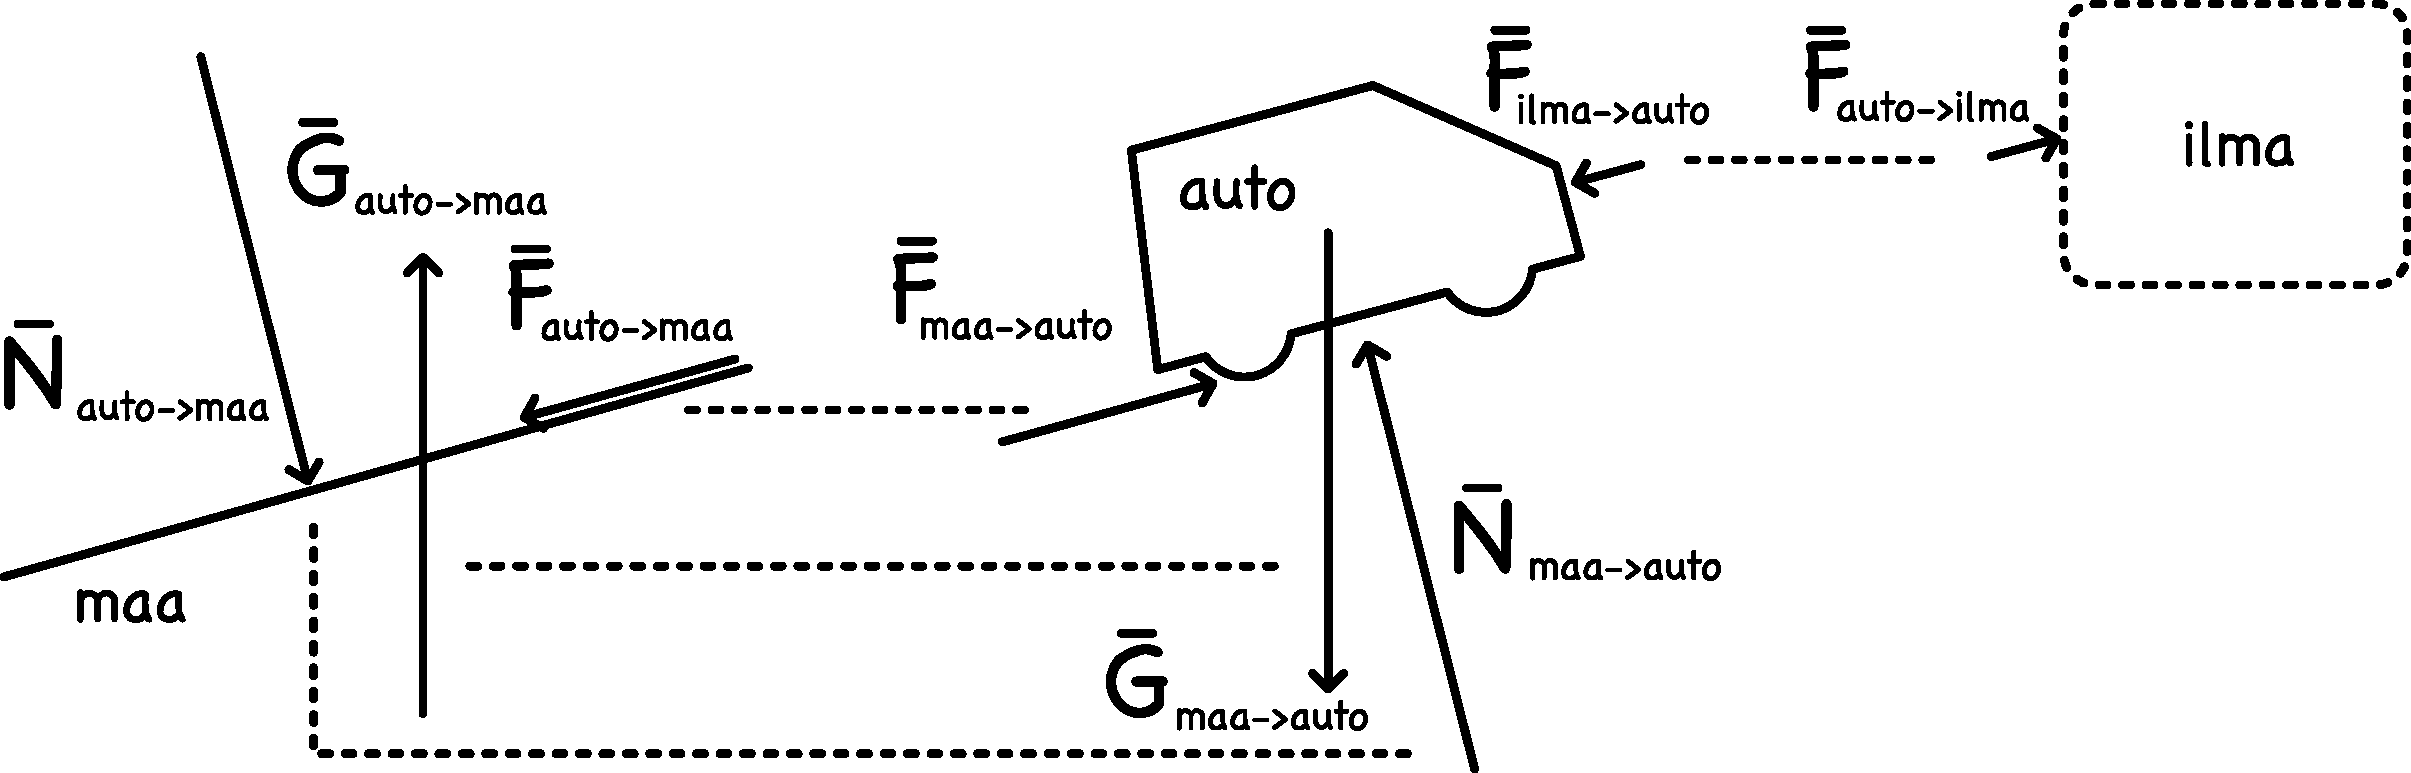
\includegraphics[width=0.95\textwidth]{figs/voima_esim_vkk.pdf}%
\end{center}%

\solu Piirretään vapaakappalekuva autolle. Merkitään painovoimaa \( \bs{G}_{\text{maa} \to \text{auto}} \), koska maa kohdistaa painovoiman autoon. Samoin merkitään maanpinnan kosketuksen tuottamaa autoa kannattelevaa voimaa \( \bs{N}_{\text{maa} \to \text{auto}} \), ja renkaisiin kohdistuvaa voimaa, joka työntää autoa ylämäkeen, \( \bs{F}_{\text{maa} \to \text{auto}} \). Todellisuudessa nämä voimat kohdistuvat auton kaikkiin renkaisiin, mutta piirretään yksinkertaisuuden vuoksi vain yksi nuoli kuvaamaan kummankin voimien kokonisvaikutusta. Täsmällisessä tarkastelussa on väliä, minne voimanuolet piirretään, mutta haluamme nyt piirtää mahdollisimman yksinkertaisen mallin, jossa tämä tarkkuus riittää.

Jätetään vierimisvastusta kuvaava nuoli piirtämättä erikseen. Vierimisvastus olisi myös maanpinnan renkaisiin kohdistama pinnan suuntainen voima, mutta koska kuvassa on jo yksi tällainen voima, voimme ajatella, että vierimisvastuskin sisältyy voimaan \( \bs{F}_{\text{maa} \to \text{auto}} \). Näin kuvasta tulee yksinkertaisempi.

Piirretään kuitenkin ilmanvastus erikseen näkyviin, koska se syntyy ilman ja auton välisestä vuorovaikutuksesta eikä maan ja auton. Merkitään sitä \( \bs{F}_{\text{ilma} \to \text{auto}} \). Koska autolla on kiihtyvyyttä ylämäen suuntaan, ilmanvastusta kuvaavan nuolen täytyy olla selvästi lyhyempi kuin ylämäen suuntaan osoittavan voimanuolen.

Kaikkien voimien vastavoimat löytyvät, kun vaihdetaan niiden alaindekseissä sanojen paikkoja. Toisin sanoen esimerkiksi maan autoon kohdistaman painovoiman \( \bs{G}_{\text{maa} \to \text{auto}} \) vastavoima on auton maahan kohdistama painovoima \( \bs{G}_{\text{auto} \to \text{maa}} \). Koska tämä voima kohdistuu maahan, sitä ei missään nimessä saa piirtää auton kuvaan vaan sitä varten kuvaan on lisättävä uusi kappale, maa, johon maahan kohdistuva painovoima piirretään. Yhdistetään voima-vastavoimapari vielä katkoviivalla.

Maahan kohdistuu myös voima \( \bs{N}_{\text{auto} \to \text{maa}} \), jolla auton renkaat painavat maata (tämä voima tuottaa renkaanjäljet, jos auto ajaa pehmeässä maastossa), sekä voima \( \bs{F}_{\text{auto} \to \text{maa}} \), jolla renkaat työntävät maanpintaa auton kulkusuuntaan nähden taaksepäin (tämä voima viskoo irtonaista maata taaksepäin, jos renkaat jäävät pehmeässä maastossa sutimaan).

Ilmanvastus on auton ja ilman välinen vuorovaikutus, joten se kohdistaa voimia autoon ja ilmaan. Niinpä lisätään kuvaan myös kappale kuvaamaan ilmaa, ja siihen kohdistuu ilmanvastusvoima \( \bs{F}_{\text{auto} \to \text{ilma}} \). Tämä on se voima, jolla liikkuva auto työntää ilmaa pois tieltään.

\eval Kaikille autoon kohdistuville voimille löydettiin vastavoimat kuten pitääkin, ja kaikkia voima-vastavoimapareja kuvaavat nuolet ovat yhtä pitkät ja vastakkaisuuntaiset. Voimanuolten mittakaava vaikuttaa myös järkevältä. Auton paino on varmasti siihen kohdistuvista voimista suurin, sillä autoa on paljon helpompi liikuttaa maanpinnan suunnassa kuin nostaa ylöspäin.

\end{exam}

\begin{instructions}{Vapaakappalekuvan laatiminen}{ohje:vapaakappalekuva}{ht!}\noindent

\begin{enumerate}
\item Piirrä erikseen kappale, jonka vapaakappalekuva halutaan piirtää.

\item Tunnista \emph{ulkoiset} vuorovaikutukset, jotka kappale kokee. Kaikilla kosketuspinnoilla voi vaikuttaa normaalivoima ja kitkavoima. Yleensä kappaleisiin vaikuttaa myös painovoima. Myöhemmin tutustutaan muihinkin vuorovaikutuksiin kuten nosteeseen ja sähkömagneettisiin vuorovaikutuksiin, jotka myös voivat kohdistaa kappaleeseen voiman.

\item Päättele jokaiselle vuorovaikutukselle, mihin suuntaan sen tuottama voima osoittaa ja mihin kohtaan vuorovaikutus kohdistuu. Piirrä jokaista voimaa kuvaava nuoli, joka osoittaa voiman vaikutussuuntaan ja jonka kärki tai kanta on voiman vaikutuspisteessä. Jos mahdollista, yritä päätellä myös voimien keskinäiset suuruudet ja piirrä nuolet sitä pidemmiksi mitä suurempaa voimaa ne kuvaavat.

\item Nimeä voimia kuvaavat nuolet (vektorit). Jos esimerkiksi kappale A vuorovaikuttaa kappaleen B kanssa, voit nimetä vuorovaikutuksen kappaleeseen A kohdistaman voiman \(\bs{F}_{B \to A}\).

\item Jos systeemissä on useita kappaleita, joille täytyy piirtää vapaakappalekuvat, toista vaiheet 1. -- 4. kullekin kappaleelle.

\item Merkitse jokaiselle voimalle, mikä on sen vastavoima. Voit tehdä tämän esimerkiksi yhdistämällä voima--vastavoimaparit katkoviivoin tai listaamalla parit. Muista, että voima ja vastavoima kohdistuvat aina \emph{eri kappaleisiin}. Mikään vuorovaikutus ei voi tuottaa voimaa vain yhteen kappaleeseen, joten jokaisella voimalla \emph{täytyy} olla vastavoima. Tämän vaiheen tarkoitus on tarkistaa, ettei mitään voimia ole unohtunut.

\item Jos mahdollista, päättele voimien suhteelliset suuruudet kappaleen liikkeen reunaehdoista. Esimerkiksi jos kappale liikkuu suoralla, siihen kohdistuvan kokonaisvoiman täytyy osoittaa tämän suoran suuntaan. Erityisesti jos kappale on paikoillaan tai liikkuu tasaisesti, kokonaisvoiman on oltava nolla.

\item Voit piirtää kuhunkin kappaleeseen kohdistuvaa kokonaisvoimaa ja kappaleen kiihtyvyyttä kuvaavat nuolet vapaakappalekuvan viereen, mutta \emph{älä} piirrä niitä varsinaiseen vapaakappalekuvaan, sillä siihen on tarkoitus merkitä ainoastaan vuorovaikutusten kappaleisiin kohdistamat voimat.

\end{enumerate}

\end{instructions}

\subsection{Vektorien graafinen yhteenlasku}
\label{vektoriengraafinenyhteenlasku}

Vapaakappalekuvaan nuolin piirrettyjen voimavektoreiden summa kuvaa kappaleeseen vaikuttavaa kokonaisvoimaa, ja Newtonin toisen lain mukaisesti kappaleen kiihtyvyys on verrannollinen tähän kokonaisvoimavektoriin. Vapaakappalekuvan graafinen tapa esittää vektoreita onkin hyvä tapa määrittää kappaleeseen vaikuttava kokonaisvoimavektori.

\index{vektori}

\marginpictures%
{0}
{Vektorien graafisia laskusääntöjä.;%
Summa.;%
Erotus.;%
Usean vektorin summa.;%
Laskujärjestyksellä ei ole väliä.}%
{fig:voimavektorit1}%
{1.0;1.0;1.0;1.0}%
{voima_vektorit_1.pdf;voima_vektorit_3.pdf;voima_vektorit_4.pdf;voima_vektorit_5.pdf}

Vektoreiden ollessa yhdensuuntaisia vektoreiden yhteenlasku onnistuu yksinkertaisesti laskemalla \emph{samansuuntaisten} vektoreiden pituudet yhteen ja vähentämällä niistä \emph{vastakkaissuuntaisten} vektorien yhteenlaskettu pituus. Tähän perustuu myös vektorien skalaarikomponenteilla laskeminen, ja tekniikka perustuu yksinkertaisesti siihen, että yhdessä ulottuvuudessa vektoreilla on vain kaksi mahdollista suuntaa.
Kolmiulotteisessa avaruudessa vektoreilla on kuitenkin äärettömästi mahdollisia suuntia ja kaksi vektoria eivät yleensä ole yhdensuuntaiset. Vektoreiden ollessa \emph{erisuuntaiset} vektoreiden suunnat onkin erikseen huomioitava. Tämä on mahdollista sekä graafisesti (geometrisesti) että algebrallisesti (analyyttisen geometrian keinoin). Nyt tarkastelemme graafista tapaa, joka on yleensä paras tekniikka tilanteiden hahmottamiseen ja arvioiden tekemiseen. Luvussa \autoref{luku:moniulotteinen} perehdytään algebrallisiin vektorilaskennan menetelmiin, joita tarvitaan tarkemmassa laskennassa.

Nuolin piirretyt vektorit lasketaan graafisesti yhteen siirtämällä vektorit peräkkäin niin, että kunkin vektoria kuvaavan nuolen pituus ja suunta pysyy muuttumattomana. Asettamalla kaksi vektoria \(\bs{A}\) ja \(\bs{B}\) niin, että nuolen \(\bs{B}\) kanta on samassa pisteessä kuin nuolen \(\bs{A}\) kärki, summavektoria \(\bs{A} + \bs{B}\) esittää nuolen \(\bs{A}\) kannasta nuolen \(\bs{B}\) kärkeen piirretty nuoli, kuten kuvassa \autoref{fig:voimavektorit1} (a) on esitetty. Toinen tapa laskea vektorien summa on asettaa vektorien kannat samaan pisteeseen ja piirtää suunnikas, jonka sivut ovat nämä vektorit. Tällöin summavektoria kuvaa suunnikkaan lävistäjä, joka lähtee alkuperäisten vektoreiden kantapisteestä ja päättyy suunnikkaan vastakkaiseen kulmaan.

Vektoreita voidaan myös vähentää toisistaan. Tällöin negatiivisena esitetty vektori yksinkertaisesti käännetään ympäri ennen yhteenlaskua. Itse asiassa vektorien erotuslaskun merkitys onkin se, että ensin vähennettävä vektori kerrotaan luvulla \(-1\), jolloin vektoria kuvaava nuoli kääntyy.
\begin{equation} \bs{B} - \bs{A} = \bs{B} + (-\bs{A}) = \bs{B} + (-1) \bs{A}. \end{equation}
Tämä on esitetty kuvassa \autoref{fig:voimavektorit1} (b).

Graafisesti voidaan todeta myös, että vektorien yhteenlaskussa pätee vaihdantalaki eli yhteenlaskettavien järjestystä saa muuttaa lopputuloksen muuttumatta
\begin{equation} \bs{A} + \bs{B} = \bs{B} + \bs{A} \end{equation}
kuten skalaarienkin yhteenlaskussa. Tämä on melko ilmeistä suunnikkaan perusteella esitetyn yhteenlaskusäännön avulla, koska summattavat vektorit ovat symmetrisessä asemassa tässä laskutavassa.
Vähennyslaskussa laskujärjestyksellä kuitenkin on väliä, kuten skalaareillakin,
\begin{equation} \bs{A} - \bs{B} = - (\bs{B} - \bs{A}) \ne \bs{B} - \bs{A}. \end{equation}

Samaan tapaan monta vektoria voidaan summata yhteen asettamalla ne peräkkäin yksi toisensa jälkeen, jolloin vektorien summa on ensimmäisen summattavan nuolen kannasta viimeisen kärkeen piirretty nuoli. Tässäkään tapauksessa summauksen järjestyksellä ei ole merkitystä. Riippumatta järjestyksestä, johon vektorit asetellaan, seuraamalla vektorien merkitsemää reittiä kulkien aina yhden vektorin kannasta kärkeen päädytään aina samaan loppupisteeseen.

Jos yhteen lasketaan siirtymävektoreita \(\Delta \bs{r}\), kuvassa \autoref{fig:voimavektorit1} (d) esitetyt erilaiset järjestykset kuvaavat erilaisia \emph{reittejä}. Minkä tahansa reitin voi ajatella muodostuvan pienten peräkkäisten siirtymien yhdistelmänä, ja kokonaissiirtymä reitin alkupisteestä loppupisteeseen saadaan reitin muodostavien siirtymävektoreiden summana. Jos vaihdamme siirtymien järjestyksen saamme tietenkin erilaisen reitin. Kuitenkin koska vektoreiden yhteenlaskussa järjestyksellä ei ole väliä, tällä tavalla muodostettu uusi reitti päättyy samaan pisteeseen kuin alkuperäinen reitti.

Laskettaessa yhteen voimavektoreita ei kuitenkaan ole olemassa mitään sääntöä, \emph{missä järjestyksessä} nämä voimat pitäisi laskea yhteen, sillä kaikki voimat kohdistuvat kappaleeseen samanaikaisesti. Niinpä onkin fysikaalisesti järkevää ja suorastaan välttämätöntä, että vektoreiden yhteenlaskussa järjestyksellä ei ole väliä. Voimavektorit voi siis laskea yhteen eli graafisessa ratkaisussa asettaa peräkkäin \emph{missä tahansa järjestyksessä} eikä lopputuloksena saatava kokonaisvoima siitä muutu.

Erityisesti jos kappaleeseen vaikuttava kokonaisvoima on nolla, vektoreita kuvaavat nuolet muodostavat peräkkäin asetettuina kuvion, jossa viimeisen vektorin kärki on samassa pisteessä kuin ensimmäisen vektorin kanta. Toisin sanoen \emph{joko} vektoreita kuvaavat nuolet ovat vastakkaissuuntaiset ja eri suuntiin osoittavien nuolien yhteispituus on yhtä suuri \emph{tai} nuolet muodostavat umpinaisen silmukan. Jälkimmäisessä tapauksessa yhdenkään vektorin ei välttämättä tarvitse olla vastakkaissuuntainen minkään toisen vektorin kanssa vaan myös erisuuntaiset vektorit voivat summautua nollaksi.

\begin{stopQ}{q:kolmioepayhtalo}%
(a) Missä tapauksessa kahden vektorin summan pituus \(|\bs{A} + \bs{B}|\) on yhtä suuri kuin niiden pituuksien summa \(A + B\)? (b) Onko mahdollista, että \(|\bs{A} + \bs{B}| = |\bs{A}|\) vaikka \( \bs{B} \) ei ole nollavektori? Jos on, keksi esimerkki jossa näin on.
\end{stopQ}

\subsection{Vektorien jako komponentteihin}
\label{vektorienjakokomponentteihin}

\marginpictures%
{0}
{Vektorien jako komponentteihin.;%
Vaaka- ja pystykomponentit.;%
Jaon voi tehdä missä suunnassa tahansa.}%
{fig:voimakomponentit}%
{1.0;1.0}%
{voima_vektorit_6.pdf;voima_vektorit_7.pdf}

\index{vektorikomponentti}

Vektoreiden yhteenlaskun periaatetta voidaan käyttää myös käänteisesti vektorien yhdistämisen sijaan niiden hajottamiseksi osiin. Jos esimerkiksi ystäväsi ripustaa taulua seinälle ja sinun pitäisi antaa ohjeita taulun saamiseksi oikeaan kohtaan, on todennäköisesti molemmille helpompaa käyttää ohjeissa suuntia ylös--alas sekä vasen--oikea kuin neuvoa siirtämään taulua viistoon tietty matka tiettyyn suuntaan. Näin siksi, että jotkut suunnat kuten pysty- ja vaakasuunta ovat usein erityisasemassa ja helppo hahmottaa. Esimerkiksi pystysuunta määritellään sen mukaan mihin suuntaan painovoima vaikuttaa, ja vaakasuunta taas on tätä vastaan kohtisuora suunta. Fysikaalisesti taulun siirtäminen askeleittain pysty- ja vaakasuunnissa tarkoittaa sitä, että siirtymä jaetaan pysty- ja vaakasuuntaisiin osiin. Aivan vastaavasti mikä tahansa muukin vektorisuure kuten nopeus, liikemäärä tai voima voidaan jakaa osiin eli \textbf{vektorikomponentteihin} tai lyhyesti vain komponentteihin.

Komponenttijakoa on havainnollistettu kuvassa \autoref{fig:voimakomponentit} (a), jossa vektorit \(\bs{A}\) ja \(\bs{B}\) on jaettu komponentteihin vaaka- ja pystysuunnissa, joita on merkitty alaindekseillä \(x\) ja \(y\). Kuvassa vektori \(\bs{A}\) on jo valmiiksi vaakasuuntainen, joten sen \(x\)-suuntainen komponentti on vektori itse, \(\bs{A}_x = \bs{A}\), ja \(y\)-suuntainen komponentti on nolla, \(\bs{A}_y = \bs{0}\). Vektori \(\bs{B}\) sen sijaan osoittaa viistoon, joten sen komponentit eivät ole nollia eivätkä sama kuin vektori itse. Kuten kuvasta nähdään, komponentit osoittavat yhtä pitkälle pysty- ja vaakasuunnissa kuin mitä vektori itse ulottuu ja niiden summa on alkuperäinen vektori itse
\begin{equation} \bs{B}_x + \bs{B}_y = \bs{B}. \label{vektorikomponenttisumma} \end{equation}

\index{skalaarikomponentti}

Vektorikomponentti \(\bs{A}_x\) ja skalaarikomponentti \(A_x\) liittyvät toisiinsa mutta eivät ole sama asia.
Vektorikomponentti on nimensä mukaisesti \emph{vektori} ja skalaarikomponentti on \emph{skalaari}. Jos esimerkiksi vektorin \(x\)-vektorikomponentti osoittaa positiiviseen \(x\)-suuntaan, vektorin \(x\)-skalaarikomponentti on sama kuin vektorikomponentin pituus, \(A_x = |\bs{A}_x|\). Jos vektorin \(x\)-vektorikomponentti osoittaa negatiiviseen \(x\)-suuntaan, vektorin \(x\)-skalaarikomponentti on itseisarvoltaan yhtä suuri kuin vektorikomponentin pituus mutta \emph{negatiivinen}, \(A_x = -|\bs{A}_x|\). Matemaattisesti tämä voidaan esittää \(x\)-suuntaisen yksikkövektorin \(\uv{i}\) avulla
\begin{equation} \bs{A}_x = A_x \uv{i}. \label{komponenttiyhteys}\end{equation}

Komponenttijaon ei tietenkään tarvitse tapahtua juuri pysty- ja vaakasuunnissa, vaan mitkä tahansa suunnat voidaan valita komponenttijaon perustaksi. Esimerkiksi tarkasteltaessa kappaleita kaltevalla tasolla on usein kätevää valita koordinaatiston akselit tason pinnan suuntaisesti ja pintaan nähden kohtisuoraan. Tällöin vektorin jako komponentteihin on tietenkin erilainen kuin jaon tapahtuessa pysty- ja vaakakomponentteihin, kuten kuvassa \autoref{fig:voimakomponentit} (b) nähdään. Kuitenkin riippumatta siitä missä suunnissa vektorin jako komponentteihin tehdään, komponenttien summan pitää aina olla alkuperäinen vektori yhtälön (\autoref{vektorikomponenttisumma}) mukaisesti.

\marginpictures%
{0}
{Komponenttijaon yksikäsitteisyys.;%
Samanlaisten vektoreiden komponentit.;%
Erilaisten vektoreiden komponentit.}%
{fig:voimakomponenttisumma}%
{1.0;1.0}%
{moniulotteinen_yhtasuuruus_1.pdf;moniulotteinen_yhtasuuruus_2.pdf}

Vaikka vektorin voi jakaa komponentteihin äärettömän monella tavalla valitsemalla koordinaatiston akseleille eri suunnat, koordinaatiston valinnan jälkeen vektori voidaan jakaa komponentteihin koordinaattiakselien suunnissa \emph{vain yhdellä tavalla}. Toisin sanoen kun koordinaatisto on valittu, vektoreiden komponenttijako on yksikäsitteinen. Tämän ominaisuuden ansiosta vektorien yhtäsuuruuden voi tarkistaa myös komponenttien kautta. Kaksi vektoria ovat samat jos ja vain jos niiden \emph{kaikki} komponentit ovat samat (kuva \autoref{fig:voimakomponenttisumma}). Toisin sanoen \(\bs{A} = \bs{B}\) on totta täsmälleen silloin, kun \(\bs{A}_x = \bs{B}_x\) ja \(\bs{A}_y = \bs{B}_y\) (ja kolmessa ulottuvuudessa lisäksi \(\bs{A}_z = \bs{B}_z\)).

\begin{stopQ}{q:harjoitellaan_komponentteja}%
Erääseen kappaleeseen vaikuttaa kaksi voimaa, \(\bs{F}_A\) ja \(\bs{F}_B\). Voimalla A on komponentti \(1.5 \un{N}\) positiiviseen \(x\)-suuntaan ja komponentti \(1.1 \un{N}\) negatiiviseen \(y\)-suuntaan. Voiman B pituus on \(2.0 \un{N}\) ja voimavektori osoittaa \(xy\)-koordinaatistossa yläviistoon vasemmalle niin, että voimavektorin ja \(x\)-akselin välinen kulma on \(150^\circ\). Kuinka pitkät ovat kokonaisvoiman \(x\)- ja \(y\)-komponentit ja mihin suuntaan ne osoittavat?
\end{stopQ}

\marginpictures%
{10}
{Vektorien yhteenlasku komponenteittain.;%
Graafinen yhteenlasku.;%
Summan komponentit.;%
Komponenttien summa.}%
{fig:voimakomponentit2}%
{1.0;0.7;1.0}%
{voima_vektorit_10.pdf;voima_vektorit_11.pdf;voima_vektorit_12.pdf}

Myös laskutoimitukset usein helpottuvat huomattavasti, kun vektorit jaetaan ensin komponentteihin.
Esimerkiksi vektoreiden yhteenlasku voidaan helposti tehdä komponenttien avulla kuvan \autoref{fig:voimakomponentit2} tapaan. Jos nimittäin merkitään vektorien \(\bs{A}\) ja \(\bs{B}\) summaa symbolilla \(\bs{C} = \bs{A} + \bs{B}\), voidaan tämä vektori jakaa usealla tavalla osiin. Ensinnäkin \emph{summavektorilla} on komponenttijako
\begin{equation} \bs{C} = \bs{C}_x + \bs{C}_y. \end{equation}
Toisaalta \emph{summattavat vektorit} voidaan jakaa erikseen komponentteihin ja näiden komponenttien summan voi järjestellä uudelleen,

\begin{eqnarray} \bs{C} &=&  \bs{A} + \bs{B} \\ \nonumber
&=& (\bs{A}_x + \bs{A}_y) + (\bs{B}_x + \bs{B}_y) \\ \nonumber
&=& (\bs{A}_x + \bs{B}_x) + (\bs{A}_y + \bs{B}_y). \end{eqnarray}

Tässä siis \(\bs{A}_x + \bs{B}_x\) on \(x\)-suuntainen vektori ja \(\bs{A}_y + \bs{B}_y\) on \(y\)-suuntainen vektori. Vektorin komponenttijako on kuitenkin yksikäsitteinen, joten on vain yksi tapa esittää summavektori \(\bs{C}\) \(x\)- ja \(y\)-suuntaisten komponenttien summana. Niinpä summan \(\bs{A}_x + \bs{B}_x\) on oltava vektorin \(\bs{C}\) \(x\)-komponentti eli sen täytyy olla sama vektori kuin \(\bs{C}_x\). Samoin voidaan päätellä \(y\)-suunnassa, joten
\begin{equation} \bs{C}_x  = \bs{A}_x + \bs{B}_x, \ \bs{C}_y = \bs{A}_y + \bs{B}_y. \end{equation}
Tämä tarkoittaa, että vektorien summa voidaan laskea jakamalla vektorit ensin komponentteihin, laskemalla sitten yhdensuuntaiset komponentit yhteen ja lopuksi yhdistämällä erisuuntaiset komponentit geometrisesti. Jos vektoreita on monta, tämä on helpoin tapa laskea, koska esimerkiksi kaikki \(x\)-komponentit ovat keskenään \emph{yhdensuuntaisia} ja yhdensuuntaisten vektoreiden yhteenlaskussa pitää ainoastaan huomioida osoittavatko vektorit samaan vai vastakkaiseen suuntaan.

Myös vapaakappalekuvien analyysi usein helpottuu jakamalla voimat pysty- ja vaakasuuntaisiin komponentteihin. Esimerkiksi jos kappaleen tiedetään liikkuvan vain vaakasuunnassa, sen kiihtyvyysvektorin on joko oltava nolla tai osoitettava vaakasuoraan. Tällöin kiihtyvyyden pystykomponentti on välttämättä nolla ja myös kappaleeseen kohdistuvan kokonaisvoiman pystysuuntaisen komponentin on oltava nolla, koska kappaleen kiihtyvyys osoittaa samaan suuntaan kuin sen tuottava kokonaisvoima.

\begin{stopQ}{q:tiivistelma_vkk}%
Kirjoita omin sanoin ohjeet vapaakappalekuvien piirtämiseen sekä vektoreiden yhteenlaskuun ja komponenttijakoon. Keksi esimerkki, jossa on kolme toistensa kanssa vuorovaikuttavaa kappaletta, piirrä sille vapaakappalekuvio, ja määritä kuvion avulla kuhunkin kappaleeseen kohdistuvaa kokonaisvoimaa kuvaava nuoli.
\end{stopQ}

\newpage\begin{exam}{Vektorien yhteenlasku}{ex:vektorisummaus}\noindent

\problem{Auto ajaa loivaa mäkeä ylös. Mäen kaltevuuskulma on \(5^\circ\). Auton massa on 980 kg. Maanpinta kannattelee autoa \(9570 \un{N}\) kosketusvoimalla, renkaat työntävät autoa ylöspäin yhteensä \(1070 \un{N}\) voimalla ja ilmanvastus vastustaa liikettä \(60 \un{N}\) voimalla. Mikä on auton kiihtyvyys?
}

\setup  Piirsimme auton vapaakappalekuvan esimerkissä \autoref{ex:vapaakappalekuva}. Kopioidaan sieltä vain autoa kuvaava osuus tähän.
Merkitään mäen kaltevuuskulmaa \( \theta = 5^\circ \).

\begin{center}%
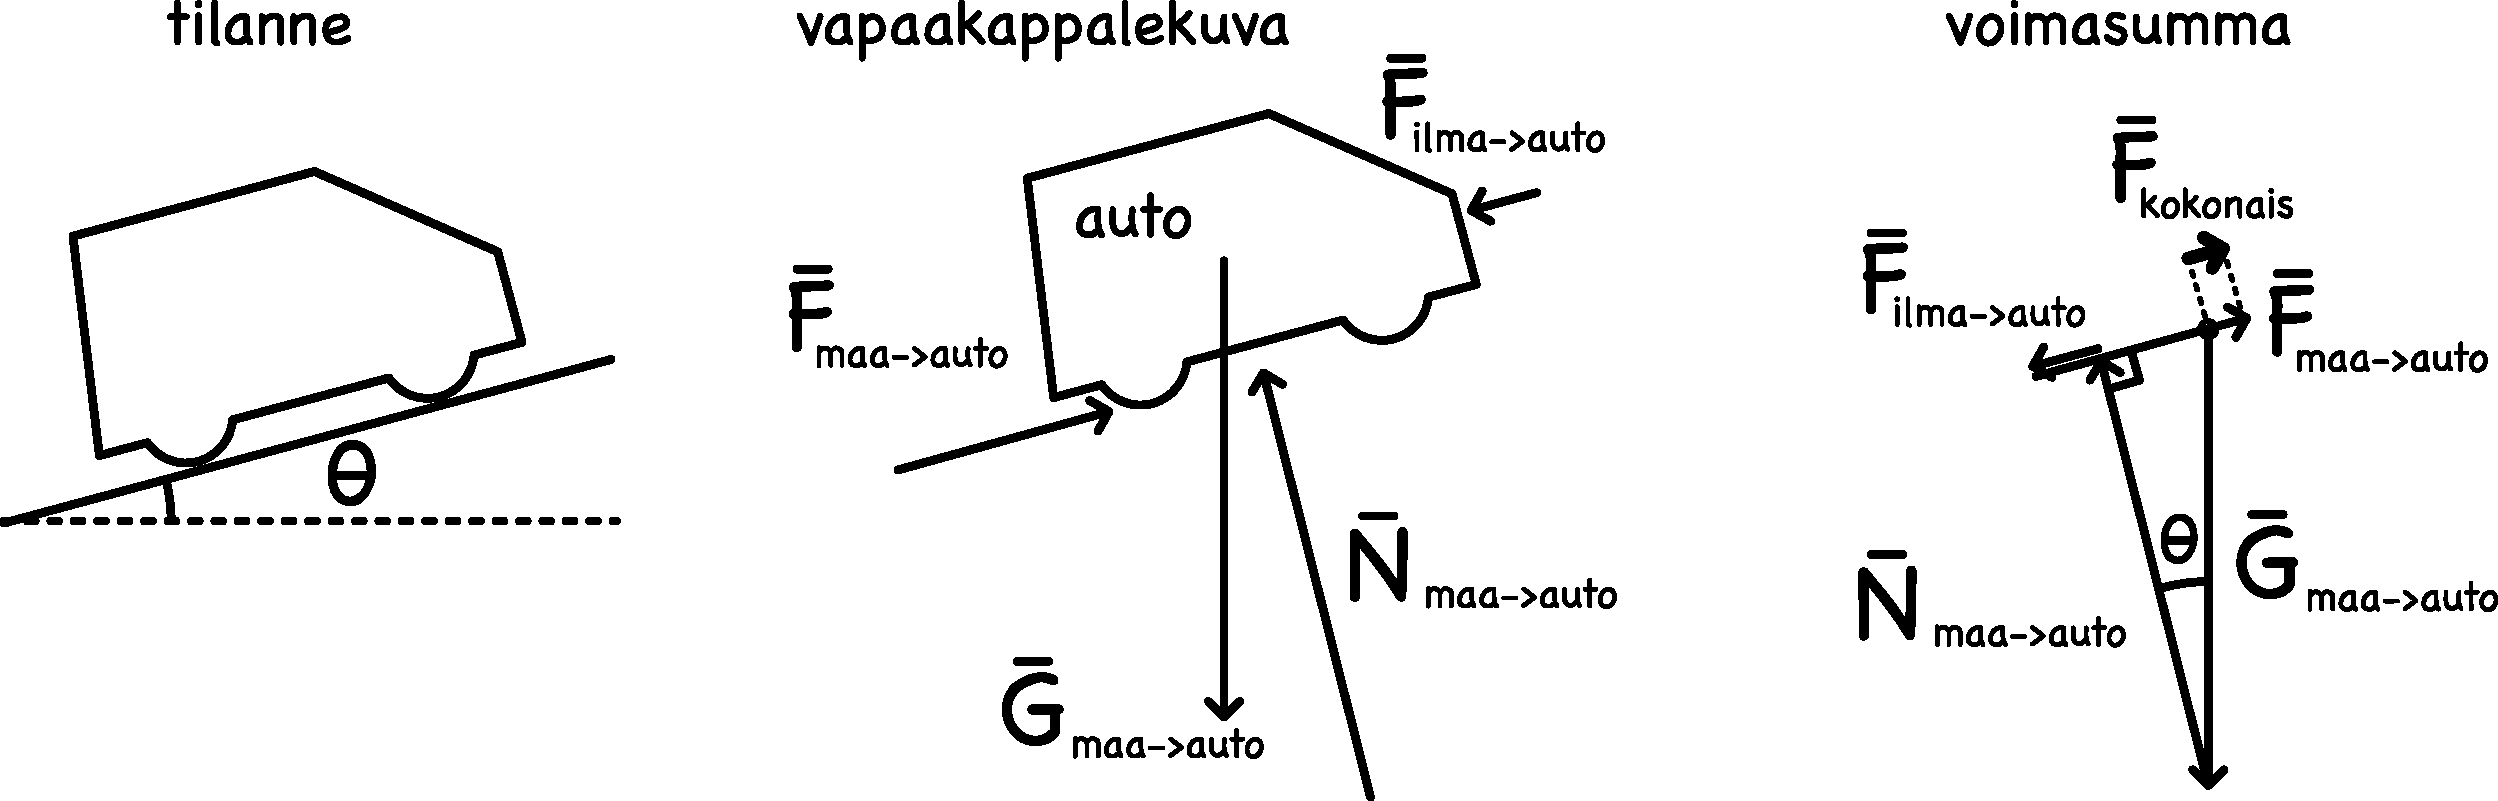
\includegraphics[width=0.95\textwidth]{figs/voima_esim_vektorisumma.pdf}%
\end{center}%

\physics Kiihtyvyyden aiheuttaa dynamiikan peruslain mukaisesti autoon kohdistuva kokonaisvoima,
\begin{equation} a = \frac{1}{m} F_\text{kokonais}, \end{equation}
ja tämä saadaan kaikkien autoon kohdistuvien voimien summana eli piirtämällä voimia kuvaavat nuolet peräkkäin. Lopuksi kokonaisvoimaa kuvaava nuoli voidaan lisätä kuvaan ensimmäisen summaan piirretyn nuolen kannasta viimeisen nuolen kärkeen osoittavana nuolena.

Nuolet voi piirtää mihin tahansa järjestykseen, mutta on kätevää piirtää ne niin, että kuvioon muodostuu suorakulmainen kolmio.
Kolmion täytyy olla suorakulmainen, koska autolla ei voi olla merkittävää kiihtyvyyttä maanpinnan suuntaa vasten kohtisuoraan pintaa vasten ylöspäin. Muutenhan auto nousisi ilmaan tai vajoaisi maan sisään. Kolmion terävin kulma on sama kuin mäen kaltevuuskulma.

Kuvan perusteella kokonaisvoiman suuruus saadaan vähentämällä renkaiden tuottamasta työntövoimasta ilmanvastusvoima sekä painovoiman ja kosketusvoiman muodostaman kolmion lyhyemmän kateetin pituus. Tämä on järkevää, sillä renkaat työntävät autoa ylämäkeen kun taas ilmanvastus vastustaa liikettä ja painovoima vetää autoa alamäen suuntaan. Kolmion lyhyemmän kateetin pituus kertoo, kuinka voimakkaasti painovoima vetää autoa taaksepäin.

\solu Kolmion hypotenuusan pituus on autoon kohdistuvan painovoiman suuruus
\begin{equation} G_{\text{maa} \to \text{auto}} = mg = 980 \un{kg} \cdot 9.8 \un{m/s}^2 = 9600 \un{N}. \end{equation}
Kolmion pidemmän kateetin pituus on likimain yhtä suuri, sillä se on autoa kannattelevan voiman suuruus,
\begin{equation} N_{\text{maa} \to \text{auto}} = 9570 \un{N}. \end{equation}
Kolmion lyhyemmän kateetin pituus voidaan laskea trigonometrialla, ja se on
\begin{equation} F_\text{kateetti} =  G_{\text{maa} \to \text{auto}} \sin \theta = 840 \un{N}. \end{equation}
Näin ollen kokonaisvoiman suuruus on
\begin{equation} F_\text{kokonais} = F_{\text{maa} \to \text{auto}} - F_{\text{ilma} \to \text{auto}} - F_\text{kateetti} = 1070 \un{N} - 60 \un{N} - 840 \un{N} = 170 \un{N} \end{equation}
ja auton kiihtyvyys on
\begin{equation} a = \frac{1}{m} F_\text{kokonais} = \frac{170 \un{N}}{980 \un{kg}} = 0.17 \un{m/s}^2\end{equation}

\eval Auton kiihtyvyys on siis pieni. Tavallisten autojen kiihtyvyydet ovat putoamiskiihtyvyyttä \(9.8 \un{m/s}^2\) pienemmät, mutta tasaisella maalla nopeasti liikkeelle lähtevän auton kiihtyvyys voi olla selvästi yli \(1 \un{m/s}^2\). Tällaisen kiihtyvyyden auto saisikin 1070 N työntövoimalla, jos ylämäkeen noustessa painovoima ei vetäisi autoa alamäen suuntaan.

\end{exam}\newpage

\section{Vuorovaikutuksiin liittyviä voimia}
\label{vuorovaikutuksiinliittyviävoimia}

\subsection{Konservatiiviset voimat}
\label{konservatiivisetvoimat}

\index{konservatiivinen}
\index{vuorovaikutus}

Gravitaation tuottama voima eli painovoima osoittaa aina alaspäin, sillä voimme määritellä suunnan ``alas'' tarkoittavan painovoiman vaikutussuuntaa.
Vapaasti putoavan kappaleen liikkeessä tämä ilmenee niin, että kappale on tasaisesti kiihtyvässä liikkeessä, jossa kiihtyvyysvektori (\autoref{putoamiskiihtyvyys}) osoittaa aina painovoiman vaikutussuuntaan eli alaspäin.
Toisaalta kuten luvussa \autoref{luku:sailymislait} todettiin, painovoiman potentiaalienergia pienenee siirryttäessä alaspäin, joten selvästikin putoava kappale pyrkii liikkumaan kohti pienenevää potentiaalienergiaa. Täsmällisemmin ilmaisten gravitaatiovuorovaikutus kohdistaa kappaleisiin voiman, joka osoittaa kohti pienenevää potentiaalienergiaa.
Vastaavasti venytetty jousi pyrkii palaamaan tasapainopituuteensa, joten jousi kohdistaa siihen kiinnitettyyn kappaleeseen voiman, joka osoittaa aina kohti tasapainopistettä eli jousen potentiaalienergian minimiä.
Tämä havainto pätee itse asiassa aina: \emph{Konservatiivinen vuorovaikutus kohdistaa kappaleeseen voiman suuntaan, johon siirryttäessä vuorovaikutuksen potentiaalienergia pienenee.}
Todistamme seuraavaksi tämän väitteen ja tutkimme samalla sen merkitystä.

Määritellään ensin, mitä tässä tarkoitetaan potentiaalienergian muuttumisella. Tarkastellaan esimerkiksi painovoimakentässä liikkuvaa kappaletta, jonka massa on \(1 \un{kg}\) ja määritellään positiivinen \(x\)-suunta ylöspäin. Jos kappale siirtyy ylöspäin yhden metrin, \(\Delta x = 1 \un{m}\), gravitaation potentiaalienergian muutos on \(\Delta U = m g \Delta x = 9.8 \un{J}\). Potentiaalienergian muutoksen suhde paikan muutokseen on siis \(\Delta U / \Delta x = mg = 9.8 \un{J/m}\). Toisaalta jos kappale liikkuu tämän matkan nopeudella \(v_x = 2.0 \un{m/s}\), tähän siirtymään kuluu aika \(\Delta t = \Delta x / v_x = 0.5 \un{s}\) ja potentiaalienergian muutoksen suhde ajan muutokseen on \(\Delta U / \Delta t = v_x \Delta U/ \Delta x = 19.6 \un{J/s}\). Toisin sanoen energia muuttuu ajan kuluessa sitä nopeammin mitä enemmän energia muuttuu kappaleen siirtyessä \emph{ja} mitä nopeammin kappale liikkuu. Täsmälleen samanlainen päättely toimii myös differentiaaleilla. Joten vaikka tarkasteltavat suureet eivät olisi vakioita kuten edellä, voimme aina kirjoittaa
\begin{equation} \frac{\dd U}{\dd t} = \frac{\dd x}{\dd t} \frac{\dd U}{\dd x} = v_x \frac{\dd U}{\dd x}. \label{u_muunnos}\end{equation}

Kun puhumme suunnasta, jossa potentiaalienergia pienenee, tarkoitamme siis suuntaa johon liikuttaessa \(U\) pienenee kun paikkakoordinaatti \(x\) muuttuu. Jos tämä suunta on \emph{positiivinen} \(x\)-suunta, tämä tarkoittaa sitä, että potentiaalienergia pienenee siirryttäessä positiiviseen suuntaan. Toisin sanoen \(\dd U < 0 \un{J}\) jos \(\dd x > 0 \un{m}\), jolloin \(\dd U / \dd x < 0 \un{J/m}\) eli potentiaalienergian derivaatta paikan suhteen on \emph{negatiivinen}.
Graafisessa esityksessä tämä ilmenee siten, että potentiaalienergian kuvaaja on paikan funktiona laskeva käyrä, jossa derivaatan negatiivisuus näkyy negatiivisena tangentin kulmakertoimena.
Vastaavalla päättelyllä derivaatta on \emph{positiivinen} jos potentiaalienergia pienenee \emph{negatiiviseen} \(x\)-suuntaan siirryttäessä, ja tällöin potentiaalienergian kuvaaja on nouseva käyrä.

\begin{stopQ}{q:potentiaalienergian_etumerkkeja}%
Miten edellä tarkastellun painovoimakentässä liikkuvan kappaleen potentiaalienergia muuttuu ajan kuluessa, jos kappaleen nopeus on \(0.5 \un{m/s}\) alaspäin? Mitkä ovat tällöin derivaattojen \(\dd U / \dd t\) ja \(\dd U / \dd x\) etumerkit? Miten suureiden etumerkit muuttuvat, jos positiivinen \(x\)-suunta valitaankin alaspäin?
\end{stopQ}

Tarkastellaan sitten kuinka kappaleen liike-energia muuttuu. Kun massa on vakio, liike-energian muutos riippuu vain kappaleen nopeuden neliön muutoksesta,
\begin{equation} \frac{\dd K}{\dd t} = \frac{1}{2} m \frac{\dd (v_x^2)}{\dd t}. \end{equation}
Tässä esiintyvän nopeuden neliön derivaatan laskeminen onnistuu käyttäen yhdistetyn funktion derivaatan laskusääntöä \( \frac{\dd}{\dd t}[ f(g(t)) ] = f'(g(t))g'(t) \). Nimittäin valitsemalla ulkofunktioksi potenssin \( f(g) = g^2 \) ja sisäfunktioksi nopeuden \( g(t) = v_x \) saamme yhdistetyksi funktioksi nopeuden neliön, \( f(g(t)) = v_x^2 \), ja derivaatoiksi \( f'(g) = 2g \) sekä \( g'(t) = \frac{\dd v_x}{\dd t} \). Niinpä laskussa tarvittava nopeuden neliön aikaderivaatta on
\begin{equation} \frac{\dd (v_x^2)}{\dd t} = \frac{\dd}{\dd t}[ f(g(t)) ] = 2 v_x \frac{\dd v_x}{\dd t} \end{equation}
ja tämän perusteella liike-energian aikaderivaataksi saadaan
\begin{equation} \frac{\dd K}{\dd t} = m v_x \frac{\dd v_x}{\dd t} = m v_x a_x. \label{k_muunnos} \end{equation}
Toisin sanoen koska liike-energia riippuu nopeuden neliöstä, sen muuttuminen ajan funktiona riippuu sekä kappaleen nopeudesta \(v_x\) että sen \emph{kiihtyvyydestä} \(a_x\).

\begin{stopQ}{q:harjoitellaan_derivaattoja}%
Kappale, jonka massa on \(1.000 \un{kg}\), liikkuu nopeudella \(3.000 \un{m/s}\) positiiviseen \(x\)-suuntaan. Kappaleen kiihtyvyys on vakio \(0.500 \un{m/s}^2\) negatiiviseen \(x\)-suuntaan. (a) Mikä on kappaleen liike-energian muutos \(0.010 \un{s}\) aikana? (b) Mikä on liike-energian ja ajan muutoksen suhde \(\Delta K / \Delta t\)? (c) Onko tulos sopusoinnussa yhtälön (\autoref{k_muunnos}) kanssa?
\end{stopQ}

\index{potentiaalienergia}
\index{voima}
\index{derivaatta}

Tarkastellaan sitten \emph{kokonaisenergian} muuttumista sellaisessa systeemissä, johon tarkasteltava kappale sisältyy. Energian säilymislain yhteydessä opimme, että jos systeemissä vaikuttaa \emph{ainoastaan konservatiivisia vuorovaikutuksia}, joiden yhteenlaskettu potentiaalienergia \(U(x) \) riippuu tarkasteltavan kappaleen paikasta \(x\), systeemin \emph{mekaaninen energia on vakio}. Tämä tarkoittaa sitä, että mekaaninen energia \emph{ei muutu ajan kuluessa} eli sen derivaatta ajan suhteen on nolla,
\begin{equation} \frac{\dd}{\dd t} \left( K + U \right) = \frac{\dd K}{\dd t} + \frac{\dd U}{\dd t} = 0. \end{equation}
Nyt sijoittamalla tähän edellä johdetut potentiaalienergian ja liike-energian derivaatat (\autoref{u_muunnos}) ja (\autoref{k_muunnos}) saadaan
\begin{equation} m v_x a_x + v_x \frac{\dd U}{\dd x} = 0, \end{equation}
ja supistamalla tästä pois nopeus \(v_x\) sekä siirtämällä potentiaalitermi yhtäsuuruusmerkin toiselle puolelle
\begin{equation} m a_x = - \frac{\dd U}{\dd x}. \end{equation}
Mutta dynamiikan peruslain (\autoref{xsuunta_newton2}) mukaisesti massan ja kiihtyvyyden tulo on sama kuin kappaleeseen kohdistuva \emph{kokonaisvoima}. Niinpä olemme päätelleet seuraavan tuloksen: jos systeemissä vaikuttaa vain konservatiivisia vuorovaikutuksia, kappaleeseen kohdistuvan kokonaisvoiman \(x\)-skalaarikomponentti on sama kuin systeemin potentiaalienergian \(x\)-derivaatan vastaluku. Erityisesti jokaisen konservatiivisen vuorovaikutuksen voima saadaan derivoimalla kyseisen vuorovaikutuksen potentiaalienergiaa,
\bigeq{ F_{x} = - \frac{\dd U}{\dd x}. \label{voima_derivaattana} }

\widepictures{b!}%
{Vuorovaikutuksen potentiaalienergian ja voiman välinen yhteys kuvaajin esitettynä. Voima osoittaa kohti pienenevän potentiaalienergian suuntaa ja sen suuruus on verrannollinen potentiaalienergian kuvaajan tangentin kulmakertoimeen.;%
Voima ja energia riippuvat paikasta.;%
Potentiaalienergian ja voiman kuvaajat.}%
{fig:voimapotenekuvaaja;fig:voimapotenekuvaaja_a;fig:voimapotenekuvaaja_b;}%
{0.26;0.7}%
{0.259;0.641}%
{voima_energiakuvaaja_3.pdf;voima_energiakuvaaja_2.pdf}

Voima on siis verrannollinen potentiaalienergian derivaatan vastalukuun ja tämä derivaatta kuvaa potentiaalienergian muuttumista \emph{siirryttäessä} (paikan funktiona). Derivaatan ollessa itseisarvoltaan suuri energia muuttuu paljon lyhyellä matkalla ja voima on suuri. Vastaavasti jos potentiaalienergia on vakio, derivaatta ja samoin voima on nolla. Jos derivaatta on positiivinen, miinusmerkistä johtuen voima on negatiivinen eli se osoittaa kohti negatiivista \(x\)-suuntaa --- siis pienenevän potentiaalienergian suuntaan --- ja päinvastoin jos derivaatta on negatiivinen.
Toisin sanoen, jos kappaleeseen vaikuttaa konservatiivinen vuorovaikutus, jonka potentiaalienergia riippuu vain \(x\)-koordinaatista, tämä vuorovaikutus kohdistaa kappaleeseen \emph{voiman, joka osoittaa pienenevän potentiaalienergian suuntaan ja on sitä suurempi mitä nopeammin potentiaalienergia muuttuu}.

Vaikka edellä tehtyjä päätelmiä havainnollistettiin gravitaation ja jousen avulla, tulos ei riippunut mitenkään siitä, millainen funktio potentiaalienergia \( U(x) \) on. Niinpä kappaleet käyttäytyvät tähän tapaan kokiessaan \emph{minkä tahansa} konservatiivisen vuorovaikutuksen. Potentiaalienergiafunktiot voivat olla joskus hyvinkin monimutkaisia, mutta kappaleisiin vaikuttavat voimat vetävät niitä aina kohti pienenevää potentiaalienergiaa. Kappaleet siis käyttäytyvät samaan tapaan kuin mäkeen asetettu pallo, joka pyrkii vierimään kohti kuopan pohjaa, jossa sen potentiaalienergia minimoituu.
Itse asiassa analogia minkä tahansa potentiaalienergian ja mäen välillä on niin hyvä, että fyysikot yleisesti kutsuvat potentiaalienergiafunktion minimejä \emph{potentiaalikuopiksi} tai \emph{-kaivoiksi}, vaikkei tarkasteltavana olisikaan gravitaatiovuorovaikutus eikä kappaleen korkeudella olisi asian kanssa mitään tekemistä.

Kuvassa \autoref{fig:voimapotenekuvaaja} on piirretty potentiaalienergia ja sitä vastaava voima paikan funktiona systeemissä, joka on samanlainen kuin esimerkissä \autoref{ex:jousienergia}: pystysuorassa liikkuvan kappaleen alla on jousi. Kappaleen ollessa jousta korkeammalla siihen vaikuttaa vain gravitaatio ja potentiaalienergian kuvaaja on suora. Liikkuessaan alaspäin kappale puristaa jousta, jolloin jouseen varastoituu elastista potentiaalienergiaa ja potentiaalienergian kuvaaja on paraabeli. Kun potentiaalienergia kasvaa ylöspäin siirryttäessä, positiiviseen \(x\)-suuntaan, voima osoittaa alaspäin eli voiman \(x\)-komponentti on negatiivinen. Jousen puristuessa potentiaalienergia saavuttaa \emph{minimin}, jolloin voima on \emph{nolla}. Tätä alempana potentiaalienergia kasvaa alaspäin siirryttäessä ja voima osoittaa ylöspäin, positiiviseen \(x\)-suuntaan. Potentiaalienergian minimi on kappaleen \emph{tasapainopiste}, sillä tässä pisteessä kappaleeseen kohdistuva kokonaisvoima on nolla.

Kuvassa \autoref{fig:voimapotenekuvaaja} esitetyssä tilanteessa kappale on tasapainossa pisteessä \(x=0.2\un{m}\), jolloin gravitaation ja jousen siihen kohdistamat voimat ovat yhtä suuret mutta vastakkaissuuntaiset. Voiman \(x\)-komponentin kuvaaja leikkaa tällöin \(x\)-akselin, koska voima on nolla. Tällöin potentiaalienergian kuvaajan tangentti on \emph{vaakasuora} joten tasapainopiste on siis potentiaalienergian kuvaajan minimikohdassa. Tämä on vakaa tasapainotila, koska jos kappaletta siirretään alaspäin, jousivoima kasvaa suuremmaksi kuin painovoima ja se pyrkii työntämään kappaleen takaisin ylöspäin. Vastaavasti jos kappaletta siirretään ylöspäin, jousivoima pienenee ja painovoima pyrkii vetämään kappaleen takaisin alaspäin. Voimat pyrkivät siis tuomaan kappaleen takaisin tasapainoasemaan (vrt. pallo kuopassa). Aivan samalla tavalla vaakasuora potentiaalienergian kuvaaja esittää epämääräistä tasapainotilaa (vrt. pallo vaakasuoralla tasolla) ja potentiaalienergian maksimi on epävakaa tasapainotila (vrt. pallo mäen huipulla).

\begin{stopQ}{q:voiman_kuvaajan_luku}%
Miksi kuvassa \autoref{fig:voimapotenekuvaaja} voiman kuvaaja muuttuu laskevasta suorasta vaakasuoraksi? Miten kappaleen kokemat vuorovaikutukset liittyvät tähän? Miten tämä ilmenee potentiaalienergian kuvaajassa?
\end{stopQ}

Kirjoitetaan vielä edelliset päättelyt matemaattiseen muotoon.
Vapaasti putoava kappale on yhtälön (\autoref{putoamiskiihtyvyys}) mukaisesti tasaisesti kiihtyvässä liikkeessä putoamiskiihtyvyydellä \(\bs{a} = \bs{g} = -g\uv{i}\), jos positiivinen \(x\)-suunta valitaan ylöspäin. Newtonin toisen lain (\autoref{newton2}) mukaisesti siihen täytyy silloin vaikuttaa kokonaisvoima
\begin{equation} F_x = m a_x = - m g, \label{painovoima}\end{equation}
joka vapaassa pudotuksessa johtuu ainoastaan painovoimasta eli gravitaatiosta. Toisin sanoen kappaleeseen kohdistuvan painovoiman suuruus on suoraan verrannollinen putoamiskiihtyvyyteen sekä kappaleen massaan. Koska putoamiskiihtyvyys osoittaa alaspäin, myös painovoima osoittaa aina alaspäin.

\index{painovoima}

Voima voidaan päätellä myös potentiaalienergiasta. Painovoiman potentiaalienergiahan on \(U=mgx\), kun \(x\)-suunta valitaan ylöspäin, joten tähän vuorovaikutukseen liittyvän voiman on oltava yhtälön (\autoref{voima_derivaattana}) mukaan
\begin{equation} F_x = -\frac{\dd U}{\dd x}  = -mg. \end{equation}
Saatiin siis sama tulos kuin putoamiskiihtyvyyden kautta pääteltiin, kuten tietysti pitikin. Gravitaatiovoimaa merkitään usein isolla ``G''-kirjaimella eli symbolilla \(\bs{G}\).

\begin{stopQ}{q:potentiaalienergia_voima_nollakohta}%
Gravitaation potentiaalienergian arvo riippuu siitä, minkä suhteen korkeutta mitataan eli tässä \(x\)-koordinaatin nollakohdasta. Gravitaatiovoiman suuruus ei kuitenkaan riipu nollakohdasta. Miten toinen suureista voi riippua nollakohdasta ja toinen ei?
\end{stopQ}

Tarkastellaan sitten jousen tuottamaa voimaa.
Luvussa \autoref{luku:sailymislait} todettiin, että elastista potentiaalienergiaa voidaan kuvata melko hyvällä tarkkuudella mallilla \(U = \frac{1}{2}k(x-x_0)^2\), (\autoref{harmoninen_pot}). Potentiaalienergian lausekkeessa \(x_0\) on piste, jossa energia on minimissään, ja \(x-x_0\) on etäisyys tästä pisteestä. Esimerkiksi jousen tapauksessa \(x_0\) on jousen luonnollinen pituus ja \(x-x_0\) on jousen venymä. Tällaista potentiaalienergiaa vastaa voima
\begin{equation} F_x =  -\frac{\dd U}{\dd x} = -k(x-x_0). \label{harmoninen_voima}\end{equation}
Voima on siis suoraan verrannollinen venymään ja verrannollisuuskerroin on jousivakio \(k\). Tämä tulos tunnetaan \textbf{Hooken lakina} (Robert Hooken mukaan).

\index{jousi}
\index{elastinen}
\index{harmoninen}
\index{tasapaino}

Muotoa (\autoref{harmoninen_voima}) olevaa voimaa, joka on suoraan verrannollinen poikkeamaan tasapainopisteestä, kutsutaan yleisesti \emph{harmoniseksi voimaksi}.
Jos potentiaalienergian minimipisteestä poiketaan negatiiviseen \(x\)-suuntaan, poikkeama \(x-x_0\) on negatiivinen, ja voima osoittaa positiiviseen suuntaan, koska lausekkeessa (\autoref{harmoninen_voima}) on miinusmerkki. Vastaavasti jos poikkeama on positiiviseen suuntaan, voima osoittaa negatiiviseen suuntaan. Toisin sanoen \emph{voima osoittaa aina kohti potentiaalienergian minimiä eli tasapainopistettä}.
Tämän ominaisuuden vuoksi harmoninen potentiaali on hyvä malli lähes kaikille \emph{vakaille tasapainopisteille}: jos kappaletta siirretään pois tasapainopisteestään eli potentiaalienergian minimistä, siihen vaikuttaa aina voima, joka pyrkii siirtämään kappaleen takaisin tasapainoon. Jos siirtymä on kyllin pieni, voimaa voidaan yleensä approksimoida harmonisen voiman lausekkeella (\autoref{harmoninen_voima}).

Huomaa, että jousen tapauksessa yhtälö (\autoref{harmoninen_voima}) kuvaa voimaa, jonka \emph{jousi kohdistaa sitä venyttävään tai puristavaan kappaleeseen}. Jos esimerkiksi pystysuoran jousen päällä on kappale, jousi puristuu ja kohdistaa kappaleeseen ylöspäin osoittavan voiman. Kappale puolestaan kohdistaa vastavoiman lain mukaisesti jouseen alaspäin osoittavan voiman, joka puristaa jousta kasaan. Nämä voimat ovat yhtä suuret mutta vastakkaissuuntaiset, joten jouseen kohdistuvaa voimaa kuvaa muuten sama lauseke (\autoref{harmoninen_voima}) mutta ilman miinusmerkkiä.

\begin{stopQ}{q:tiivistelma_konservatiiviset_voimat}%
Kirjoita omin sanoin tiivistelmä konservatiivisista voimista. Selitä erityisesti, miten voima ja potentiaalienergia liittyvät toisiinsa ja millainen voima ja energia gravitaatiolla ja jousilla on.
\end{stopQ}

\subsection{Jännitysvoimat}
\label{jännitysvoimat}

\marginpictures%
{0}
{Elastisuus johtuu itsestään palautuvista muutoksista atomien paikoissa.;%
Alkuperäinen muoto.;%
Elastinen muodonmuutos.;%
Plastinen muodonmuutos.}%
{fig:voimaplastinen}%
{0.62;0.62;1.0}%
{voima_plastisuus_1.pdf;voima_plastisuus_2.pdf;voima_plastisuus_3.pdf}

\index{jännitys}

Kun poikkeamat tasapainosta ovat tarpeeksi pieniä, palauttava voima on useimmissa todellisissa tasapainoilmiöissä suoraan verrannollinen poikkeamaan kuten Hooken laissa. Tämä ei kuitenkaan enää päde jos poikkeamat ovat hyvin suuria --- esimerkiksi jos jousta venytetään hyvin paljon se voi suoristua eikä enää toimi jousena. Näin käy siksi, että materiaalia muokkaavan voiman ollessa heikko materiaaleissa tapahtuu pieniä muodonmuutoksia, jotka pyrkivät palautumaan itsestään. Hyvin suuret voimat voivat kuitenkin aiheuttaa pysyviä muodonmuutoksia, jolloin jousi ei enää palaakaan alkuperäiseen muotoonsa. Voimia, jotka pyrkivät yhdessä muuttamaan kappaleen muotoa venyttämällä tai puristamalla, kutsutaan \textbf{jännitykseksi}. Jännitysvoimille käytetään usein symbolia \(\bs{T}\) (englanninkielisen termin `tension' mukaan).

Ilmiön tarkka selitys vaatii melko syvällistä ymmärrystä aineen mikroskooppisesta rakenteesta, mutta oleellisesti kyse on siitä, että kiinteissä aineissa atomit ovat järjestäytyneet säännöllisiin rakenteisiin ja kappaleiden muodonmuutokset vaativat tämän rakenteen muuttamista kuten kuvassa \autoref{fig:voimaplastinen}. Jännityksen ollessa kyllin pieni atomit siirtyvät hieman lähemmäksi toisiaan tai kauemmaksi toisistaan, mutta aineen rakenne ei muutu. Niinpä atomien väliset vuorovaikutukset pyrkivät vetämään atomit takaisin alkuperäisille paikoilleen. Kuitenkin jos jännitys on tarpeeksi voimakas, atomien väliset sidokset voivat rikkoutua ja aineen rakenne muuttuu. Hauraan materiaalin tapauksessa tämä voi johtaa kappaleen hajoamiseen osiin, mutta on myös mahdollista, että atomit liittyvät välittömästi uusiin sidoksiin muodostaen uuden, \emph{erilaisen rakenteen}. Tällöin materiaali ei rikkoudu mutta kappaleen muoto muuttuu. Koska samat atomit eivät ole enää sitoutuneet toisiinsa samoin kuin aikaisemmin, tällainen muodonmuutos ei palaudu itsestään.

\begin{stopQ}{q:jousivakio_graafinen_esitys}%
Miten kuvan \autoref{fig:voimapotenekuvaaja} potentiaalienergian ja voiman kuvaajat muuttuvat, jos jousivakio \(k\) kasvaa? Miten jousen jäykkyys tällöin muuttuu? Millainen voiman kuvaaja saadaan, jos jousta venytetään hyvin paljon?
\end{stopQ}

\index{elastinen}
\index{plastinen}

Itsestään palautuvia aineen muodonmuutoksia, joita Hooken laki kuvaa yleensä hyvin, kutsutaan \textbf{elastisiksi} ja tälläisissa tapauksissa vaikuttavaa jousivoimaa \emph{elastiseksi voimaksi}. Pysyviä muodonmuutoksia puolestaan kutsutaan \textbf{plastisiksi}. Elastisen muodonmuutokset ovat reversiibeleitä prosesseja ja niihin sitoutunut potentiaalienergia vapautuu lähes täydellisesti kappaleen palatessa alkuperäiseen muotoonsa. Plastiset muodonmuutokset puolestaan ovat irreversiibeleitä ja niissä osa muodonmuutokseen tarvitusta energiasta väistämättä muuttuu epäjärjestyneeseen muotoon, pääasiassa lämpöenergiaksi.

\index{jäykkä}

Elastisuutta ja plastisuutta esiintyy kaikissa aineissa ja riippuu materiaalista, kuinka pienillä voimilla kappaleet ovat vielä elastisia. Esimerkiksi kuminauha on erittäin elastinen kun taas muovailuvaha on erittäin plastinen kappale. Monet kovat materiaalit kuten metallit ovat elastisia vaikka niitä puristettaisiin tai venytettäisiin melko suurellakin voimalla, koska niissä tapahtuvat muodonmuutokset ovat tavallisesti pienet. Vaikka siis kaikki kappaleet muuttavat jännitettyinä jonkin verran muotoaan, voidaan kovista materiaaleista tehtyjä kappaleita usein pitää likimain \textbf{jäykkinä} eli muotonsa säilyttävinä.

\begin{stopQ}{q:jousen_muoto}%
Miksi teräsjousen muotoa on helppo muuttaa vaikka samasta teräksestä valmistettu tanko on hyvin jäykkä?
\end{stopQ}

\widepictures{tb}%
{Massaton köysi välittää siihen kohdistuvat voimat. Tämä tarkoittaa sitä, että jos köyttä vedetään sen päistä, köysi kohdistaa sitä vetäviin kappaleisiin yhtä suuret voimat.;%
Ihminen nostaa laatikkoa köydellä.;%
Vapaakappalekuvat laatikon ja köyden ollessa tasapainossa. Köyden päihin kohdistuvat jännitysvoimat ovat yhtä suuret, jos köyden painovoimaa ei huomioida.;%
Jos laatikolla on kiihtyvyyttä, myös köydellä on.;%
Vapaakappalekuvat laatikon ja köyden ollessa kiihtyvässä liikkeessä ylöspäin. Köyden päihin kohdistuvat jännitysvoimat ovat nytkin yhtä suuret.}%
{fig:voimajannitys;fig:voimajannitys_a;fig:voimajannitys_b;fig:voimajannitys_c;fig:voimajannitys_d;}%
{0.25;0.7;0.25;0.7}%
{0.252;0.648;0.252;0.648}%
{voima_koysi_1.pdf;voima_koysi_2.pdf;voima_koysi_3.pdf;voima_koysi_4.pdf}

Köydet, langat ja ketjut eivät ole jäykkiä puristettaessa, koska niiden rakenne sallii laskostumisen. Nekin kuitenkin vastustavat \emph{venytystä}, ja usein yksinkertaisin tapa kuvata jännitettyä köyttä on olettaa, ettei sen pituus muutu, vaikka sen päistä vedettäisiin.
Köyden pituuden vakioisuus tarkoittaa yksinkertaisesti sitä, että jos köyden yksi pää siirtyy tietyn matkan, myös köyden toinen pää siirtyy yhtä pitkän matkan. Esimerkiksi jos köysi yhdistää kaksi kappaletta toisiinsa ja köysi pysyy jännitettynä, kappaleiden siirtymien täytyy aina olla yhtä pitkät. Tämä tarkoittaa samalla sitä, että myös kappaleiden nopeuksien ja kiihtyvyyksien täytyy olla yhtä suuret.

\index{malli}

Lisäksi koska köyden massa on usein huomattavasti pienempi kuin muiden tarkasteltavien kappaleiden, \emph{massaton köysi} on hyvin yleisesti käytetty malli. Tarkastellaan tämän mallin merkitystä kuvan \autoref{fig:voimajannitys} esimerkin kautta, jossa laatikkoa nostetaan köydellä. Nostaja kohdistaa köyden yläpäähän voiman, joka vetää \emph{köyttä} ylöspäin. Tämän vastavoima vetää \emph{nostajaa} alaspäin. Köysi kohdistaa voiman myös \emph{laatikkoon}, ja tämä voima vetää laatikkoa ylöspäin. Tämän vastavoima vetää \emph{köyttä} alaspäin. Sekä köyteen että laatikkoon vaikuttaa lisäksi painovoima alaspäin.

Köyden ja laatikon roikkuessa paikoillaan niihin kumpaankin kohdistuvan kokonaisvoiman on oltava nolla. Köyden laatikkoon kohdistaman voiman täytyy siis olla yhtä suuri kuin laatikon painovoima. Nostajan köyteen kohdistaman voiman puolestaan täytyy olla yhtä suuri kuin köyden painovoiman ja laatikon köyteen kohdistaman voiman summa. Jos köyden massa on pieni, köyden painovoima voidaan jättää huomioimatta ja tällöin \emph{nostajan} köyteen kohdistaman voiman täytyy olla yhtä suuri kuin \emph{laatikon} köyteen kohdistama voima.

Jos nostaja kohdistaa köyteen \emph{suuremman} voiman kuin laatikkoon kohdistuva painovoima, köysi ja laatikko saavat kiihtyvyyden ylöspäin ja alkavat nousta. Köyden venymättömyys tarkoittaa tässä sitä, että laatikko nousee ylöspäin yhtä paljon kuin nostaja saa vedettyä köyttä ja sekä köysi että laatikko nousevat yhtä nopeasti. Erityisesti niillä on tällöin myös yhtä suuret kiihtyvyydet. Kuitenkin koska laatikon massa on paljon suurempi kuin köyden, laatikkoon kohdistuvan kokonaisvoiman on oltava paljon suurempi kuin köyteen kohdistuvan kokonaisvoiman. Jos köyden massa on esimerkiksi yksi sadasosa laatikon massasta, köyteen kohdistuvan kokonaisvoiman on oltava yksi sadasosa laatikkoon kohdistuvasta kokonaisvoimasta. Jos köyden massaa pidetään mitättömänä, köyteen kohdistuvan kokonaisvoiman on oltava likimain \emph{nolla} riippumatta köyden kiihtyvyydestä. Niinpä tässäkin tapauksessa köysi kohdistaa laatikkoon yhtä suuren voiman kuin millä nostaja vetää köyttä. Tällaisissa tapauksissa sanotaankin, että köysi \emph{välittää} nostajan voiman laatikkoon.

\begin{stopQ}{q:kaksi_nostajaa}%
Kuinka suuret voimat kohdistuvat edellä kuvatun esimerkin köyteen, jos köyttä vetää ylöspäin yksi nostaja köyden päästä ja toinen köyden keskikohdasta?
\end{stopQ}

\begin{exam}{J\"annitysvoima}{ex:jannitysvoima}\noindent

\problem{Kappale (massa \(M\)) roikkuu langan varassa (massa \(m\)) hissin katosta. (a) Millaiset voimat kohdistuvat kappaleeseen ja lankaan kun hissi lähtee ylöspäin kiihtyvyydellä \(a_x\)? (b) Mitä voimista voidaan päätellä, jos lanka on hyvin paljon kevyempi kuin kappale?
}

 \twocol{0.35}{0.6}{ \setup  Merkitään langan kappaleeseen kohdistamaa voimaa \(\bs{T}_{L\to K}\), kappaleen lankaan kohdistamaa voimaa \(\bs{T}_{K\to L}\) ja hissin lankaan kohdistamaa voimaa \(\bs{T}_{H\to L}\). Langan kappaleeseen kohdistama voima ja kappaleen lankaan kohdistama voima ovat voima-vastavoimapari. Hissin lankaan kohdistaman voiman vastavoima on langan hissiin kohdistama voima. Kappaleeseen vaikuttaa myös maan painovoima \(\bs{G}_{M\to K}\) ja lankaan \(\bs{G}_{M\to L}\). Näiden vastavoimat kohdistuvat maapalloon. Valitaan positiivinen \(x\)-suunta ylöspäin.

}{%
\begin{center}%
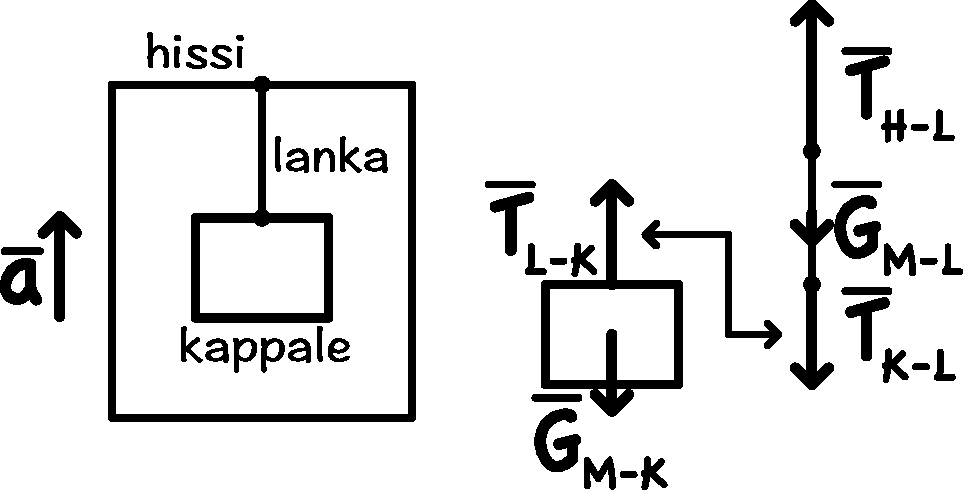
\includegraphics[width=0.95\textwidth]{figs/voima_esimerkki_lanka.pdf}%
\end{center}%
}

\solu (a) Kappaleeseen kohdistuu painovoima \(G_{x,M \to K} = -Mg\) sekä langan kiinnityskohdassa vaikuttava kosketusvoima \( T_{x,L \to K}\), jotka ovat vastakkaissuuntaiset. Kappaleeseen kohdistuva kokonaisvoima antaa kappaleelle kiihtyvyyden, joten
\begin{equation} F_{x,K,\text{kokonais}} = T_{x,L \to K} + G_{x,M \to K} = Ma_x \end{equation}
ja siis jännitysvoiman täytyy olla
\begin{equation} T_{x,L \to K} = Ma_x - G_{x,M \to K} = M(a_x + g). \end{equation}

Lankaan kohdistuu kappaleen kosketusvoima \( T_{x,K \to L} = -T_{x,L \to K} = -M(a_x+g) \), hissin kosketusvoima \(T_{x,H \to L}\) ja painovoima \(G_{x, M \to L} = -m g. \)
Näiden summa on lankaan kohdistuva kokonaisvoima, joka antaa langalle kiihtyvyyden, joten
kappaleelle kiihtyvyyden, joten
\begin{equation} F_{x,L,\text{kokonais}} = T_{x,H \to L} +T_{x,K \to L} +G_{x,M \to L} = ma_x \end{equation}
ja jännitysvoima langan yläpäässä on siis
\begin{equation} T_{x,H \to L} = ma_x - T_{x,K \to L} - G_{x,M \to L} = (M+m)(a_x + g). \end{equation}

(b) Langan yläpäähän kohdistuu suurempi jännitysvoima kuin alapäähän, koska alapäähän kohdistuva voima oleellisesti vetää ylöspäin vain roikkuvaa kappaletta, mutta yläpäähän kohdistuvan voiman täytyy vetää myös lankaa itseään. Näiden voimien suhde on
\begin{equation} \frac{T_{x,H \to L}}{T_{x,L \to K}} = 1 + \frac{m}{M}. \end{equation}
Sen, että langan massa on hyvin pieni, voi matemaattisesti kuvata raja-arvona \(m/M \to 0\), ja tällä rajalla langan päihin kohdistuvien jännitysvoimien suhteeksi saadaan \(T_{x,H \to L} / T_{x,L \to K} \to 1\). Jos langan massa on siis pieni, jännitysvoima on langan kummassakin päässä yhtä suuri. Tähän tulokseen perustuu massattoman langan malli.

\end{exam}

\subsection{Kosketus- eli normaalivoima}
\label{kosketus-elinormaalivoima}

Jäykät kappaleet eivät kulje toistensa läpi, minkä vuoksi esimerkiksi maan pinta kannattelee sinua ja voit ottaa esineitä käsiisi.
Syy tähän piilee jälleen aineen mikroskooppisessa rakenteessa (kuva \autoref{fig:voimanormaali}). Kiinteiden aineiden mikroskooppisen rakenteen rikkominen vaatii paljon energiaa, eikä edes suuren rakennuksen paino riitä hajottamaan rakennusta kannattelevan maaperän atomirakennetta. Lisäksi vaikka atomit voivat muodostaa sidoksia ja vetää toisiaan puoleensa, hyvin lähelle toisiaan puristetut atomit hylkivät toisiaan.
Niinpä yhteen puristettujen kappaleiden pintojen atomien väliset vuorovaikutukset estävät kappaleita kulkemasta toistensa läpi.

Tarkastellaan esimerkiksi maassa olevaa kirjaa. Kirjaan kohdistuu painovoima, joka pyrkii vetämään kirjaa kohti maata. Kirja ei kuitenkaan pääse liikkumaan, koska sen tiellä on maanpinta. ``Tiellä oleminen'' ei ole kuitenkaan fysikaalinen vuorovaikutus, vaan pinnan täytyy kohdistaa kirjaan voima, joka kumoaa painovoiman kirjaa alaspäin vetävän vaikutuksen.

\index{normaalivoima}
\index{kohtisuora}

\pictures{t}%
{Kosketusvoima syntyy pintojen puristuessa toisiaan vasten.;%
Kirjan paino puristaa pintoja yhteen.;%
Vapaakappalekuva.;%
Kaksinkertainen paino puristaa pintoja kovemmin.;%
Vapaakappalekuva.}%
{fig:voimanormaali;fig:voimanormaali_a;fig:voimanormaali_b;fig:voimanormaali_c;fig:voimanormaali_d}%
{0.35;0.6;0.35;0.6}%
{0.35;0.6;0.35;0.6}%
{voima_normaali_1.pdf;voima_normaali_2.pdf;voima_normaali_3.pdf;voima_normaali_4.pdf}

Tämä tapahtuu niin, että kirjan ja maanpinnan atomit alkavat \emph{hylkiä} toisiaan niiden joutuessa liian lähekkäin. Makroskooppisessa mittakaavassa tämä hylkiminen ilmenee vuorovaikutuksena, joka kohdistaa kirjaan voiman ylöspäin (maanpinta kannattelee kirjaa) sekä maahan voiman alaspäin (kirja painaa maata). Nämä ovat vuorovaikutukseen liittyvä voiman ja vastavoiman lain (\autoref{vastavoima}) kuvaama voimien pari. Koska kirjaan kohdistuva kosketusvoima ainoastaan estää kirjaa siirtymästä maan sisään, sen suunnan on oltava aina maan ja kirjan kosketuspintaa vastaan kohtisuorassa. Kohtisuoria suuntia kutsutaan matematiikassa toistensa normaaleiksi, minkä vuoksi kosketusvoiman toinen nimitys on \textbf{normaalivoima} ja sen symbolina käytetään usein kirjainta \(\bs{N}\).

Kosketusvoima on siis \emph{elastinen} vuorovaikutus aivan kuten jousen tuottama voima niin kauan kuin pinnat eivät rikkoudu. Sekä kirjan että pöydän pinnat joustavat hieman niiden koskettaessa, ja vuorovaikutuksen voimakkuus riippuu kirjan täsmällisestä paikasta ja asennosta maanpinnan suhteen. Kuitenkin koska vuorovaikutus syntyy atomien tasolla, voiman suuruus voi muuttua hyvin voimakkaasti kirjan siirtyessä mikrometrienkin matkan. Makroskooppisessa mittakaavassa on siis täysin mahdotonta määrittää normaalivoiman suuruus tarkastelemalla kirjan täsmällistä paikkaa. Sen sijaan normaalivoiman suuruus voi olla pääteltävissä siitä, että kappaleet eivät saa liikkua toistensa sisälle. Jos kirja on paikoillaan, kirjan ja maanpinnan välisen normaalivoiman on oltava täsmälleen yhtä suuri kuin muiden kirjaan kohdistuvien alaspäin osoittavien voimien summa, jotta kirjaan kohdistuva kokonaisvoima olisi nolla.

Jos maassa on vain yksi kirja, kirjan ja maanpinnan välinen normaalivoima on voimakkuudeltaan yhtä suuri kuin kirjaan kohdistuva painovoima. Jos kirjoja on kaksi päällekäin kuten kuvassa \autoref{fig:voimanormaali} (d), ylempi kirja (kuvassa A) painaa alempaa (kuvassa B) yhtä suurella kosketusvoimalla kuin kirjaan A kohdistuva painovoima. Alempi kirja B puolestaan painaa maanpintaa kosketusvoimalla, joka on voimakkuudeltaan yhtä suuri kuin kirjan B painovoima ja kirjan A siihen kohdistama kosketusvoima \emph{yhteensä}. Toisin sanoen mitä suurempi kirjapino kootaan, sitä suuremmalla kosketusvoimalla maanpinnan täytyy pinoa kannatella ja sitä suuremmalla kosketusvoimalla pino painaa maata. Tämä on helppo havaita itsekin pitämällä kirjoja kädessä: suurta kirjapinoa on raskas kannatella, koska se vaatii suuremman pystysuuntaisen kosketusvoiman kuin vain yhden kirjan pitely paikoillaan.

\begin{stopQ}{q:normaalivoiman_paattely}%
Kuinka suuri normaalivoima seuraavissa tilanteissa kohdistuu kappaleeseen, jonka massa on \(1.0 \un{kg}\)? (a) Kappale on paikoillaan olevan hissin lattialla. (b) Kappale on ylöspäin kiihtyvyydellä \(1.0 \un{m/s}^2\) nousevan hissin lattialla. (c) Kappale on ylöspäin tasaisella nopeudella \(2.0 \un{m/s}\) nousevan hissin lattialla. (d) Kappale on alaspäin kiihtyvyydellä \(3.0 \un{m/s}^2\) laskeutuvan hissin lattialla.
\end{stopQ}

\newpage

\subsection{Kitka}
\label{kitka}

\index{kitka}
\index{lepokitka}
\index{liikekitka}

Myös kitka on kosketusvoima, mutta normaalivoimasta poiketen kitka vaikuttaa koskettavien pintojen suuntaisesti. Luvussa \autoref{luku:sailymislait} tarkastelimme jo kitkaa esimerkkinä dissipatiivisesta vuorovaikutuksesta, joka syntyy kappaleiden pintojen tarttuessa mikroskooppisella tasolla toisiinsa kiinni. Tällöin tarkastelimme liukuvien kappaleiden välistä \textbf{liikekitkaa}. Kuitenkin myös toistensa suhteen paikoillaan olevat kappaleet tarttuvat toisiinsa hiukan kiinni, jolloin kyseessä on \textbf{lepokitka}.

\pictures%
{tb}
{Kitka vaikuttaa koskettavilla pinnoilla.;%
Liikekitka.;%
Lepokitka.}%
{fig:voimakitka;fig:voimakitka_a;fig:voimakitka_b}%
{0.45;0.45}%
{0.45;0.45}%
{voima_kitka_1.pdf;voima_kitka_2.pdf}

Kokeellisesti voidaan todeta, että liikekitkan aiheuttama voima osoittaa kappaleiden pintojen liukuessa toistensa suhteen aina pinnan suhteellista liikettä vastaan. Tavallisesti tämä tarkoittaa sitä, että kitka vaikuttaa kappaleen nopeuteen nähden vastakkaiseen suuntaan.
Liikekitkan suuruus puolestaan ei juurikaan riipu kappaleiden muodosta eikä liikkeen nopeudesta vaan ainoastaan liikkuvien pintojen laadusta (liukkaudesta) sekä pintojen välisen normaalivoiman suuruudesta \(N\). Pintojen liukkautta kuvaa \textbf{liikekitkakerroin} \(\mu\), jonka avulla kitkavoiman suuruus voidaan ilmaista muodossa
\begin{equation} F_\text{liikekitka} = \mu N. \end{equation}
Erityisesti liikekitkan voimakkuus ei riipu pintojen kosketuspinta-alasta. Tämä on hieman yllättävää, mutta kyse on yksinkertaisesti siitä, että vaikka suurempi kosketuspinta-ala lisää kitkavoimaa, se johtaa myös pintoja yhteen puristavan voiman jakautumiseen suuremmalle pinta-alalle. Nämä vaikutukset kumovat toisensa, jolloin lopputuloksena kosketuspinta-ala ei vaikuta kitkavoimaan.

\pictures{b!}%
{Kitkavoima vastustaa pintojen suhteellista liikettä. Tässä molemmat kappaleet liikkuvat oikealle, mutta A liikkuu oikealle nopeammin kuin B, joten suhteessa A:han B liikkuu vasemmalle.;%
Liukuva kappale työntää toisen kappaleen liikkeelle.;%
Vapaakappalekuvat: Kappaleisiin A ja B kohdistuvat kitkavoimat ovat vastakkaissuuntaiset.}%
{fig:voimakitkasuunta;fig:voimakitkasuunta_a;fig:voimakitkasuunta_b;}%
{0.4;0.5}%
{0.4;0.5}%
{voima_kitka_suunta_1.pdf;voima_kitka_suunta_2.pdf}

Myös lepokitka vaikuttaa aina koskettavien pintojen suuntaisesti, mutta se vaikuttaa vain toistensa suhteen liikkumattomien pintojen välillä ja pyrkii pitämään kappaleet paikoillaan toistensa suhteen.
Lepokitka on \emph{elastinen} voima, joka syntyy koskettavien pintojen tarttuessa heikosti yhteen. Kun pintoja yritetään liikuttaa, pintojen väliset heikot sidokset venyvät, mutta eivät vielä katkea, jolloin kappale ei lähde liikkeelle eikä liike-energiaa muutu lämmöksi.
Riittävän suuri ulkoinen voima pystyy kuitenkin rikkomaan pintojen väliset liitokset, jolloin kappaleet alkavat liukua toistensa suhteen ja lepokitka häviää muuttuen liikekitkaksi. \emph{Suurin mahdollinen voima}, jonka lepokitka pystyy tuottamaan, riippuu liikekitkan tavoin pintojen laadusta ja niiden välisestä normaalivoimasta
\begin{equation}F_\text{lepokitka} \le \mu_\text{lepo} N,  \end{equation}
missä \(\mu_\text{lepo}\) on \textbf{lepokitkakerroin}. Lepokitkakerroin on aina hieman \emph{suurempi} kuin liikekitkakerroin, koska paikoillaan olevat pinnat pääsevät tarttumaan toisiinsa voimakkaammin kuin liikkuvat.
Lepokitka ei kuitenkaan käytännössä koskaan ole näin suuri vaan tämä on vain voiman \emph{maksimisuuruus} eli raja jolloin kappaleet lähtevät liikkeelle. Lepokitkan suuruus pitää siis käytännössä päätellä aina epäsuorasti siitä ehdosta, että kappaleet eivät liiku toistensa suhteen aivan kuten normaalivoiman suuruus määräytyy siitä, etteivät kappaleet saa kulkea toistensa läpi.

Liikekitkan suunnan päättelyssä on huomioitava, että liikekitka vaikuttaa aina pintojen suhteellista liikettä vastaan. Liikemäärän yhteydessä tarkasteltiin esimerkkiä, jossa kappale (A) liukui toisen kappaleen (B) päällä ja työnsi sen liukuessaan liikkeelle kitkan avulla, kuten kuvassa \autoref{fig:voimakitkasuunta}. Tässä tapauksessa kappale B lähti liikkeelle kuvassa oikealle, joten myös kappaleen liikkeelle työntänyt kitkavoima osoitti oikealle eli samaan suuntaan kuin mihin kappale liikkui. Oleellista ei olekaan kappaleen nopeus vaan toistensa suhteen liukuvien pintojen suhteelliset nopeudet. Koska kappale A liikkui oikealle \emph{nopeammin} kuin kappale B, kappaleen A pinta liikkui kappaleeseen B verrattuna oikelle ja kappaleen B pinta liikkui kappaleeseen A verrattuna \emph{vasemmalle}. Niinpä kappaleeseen A vaikutti kitkavoima vasemmalle ja kappaleeseen B oikealle. Nämä voimat ovat vastavoimapari, joten niiden täytyy osoittaa vastakkaisiin suuntiin, vaikka kyseisessä tapauksessa kummatkin kappaleet liikkuivat kuvassa samaan suuntaan, oikealle.

\begin{stopQ}{q:potkulautailijan_lahto_ja_jarrutus}%
Mikä voima muuttaa seuraavissa tapauksissa potkulautailijan ja hänen lautansa (i) liike-energiaa ja (ii) liikemäärää? (a) Lautailija potkaisee toisella jalallaan maasta vauhtia. (b) Lautailija jarruttaa astumalla laudan takapyörän päälle, jolloin pyörä pyörii vähitellen hidastuen.
\end{stopQ}

\begin{exam}{Levossa kaltevalla tasolla}{ex:kaltevalepo}\noindent

\index{lepokitka}

\problem{Kirja on pöydällä, jota aletaan kallistamaan. Mistä tekijöistä riippuu, kuinka jyrkkään kulmaan pöytälevy voidaan kallistaa ennen kuin kirja alkaa liukua? Valitse jotkin järkevät arvot näille tekijöille ja laske maksimikulma valitsemillasi arvoilla.
}

 \twocol{0.35}{0.6}{ \setup  Piirretään kuva tilanteesta sekä kirjan vapaakappalekuva.
Mahdollisia kirjaan vaikuttavia tekijöitä voisivat olla ainakin kirjan massa \(m\) sekä kirjan ja pöydän välinen lepokitkakerroin \(\mu_\text{lepo}\). Merkitään pöydän kallistuskulmaa symbolilla \(\theta\).

}{%
\begin{center}%
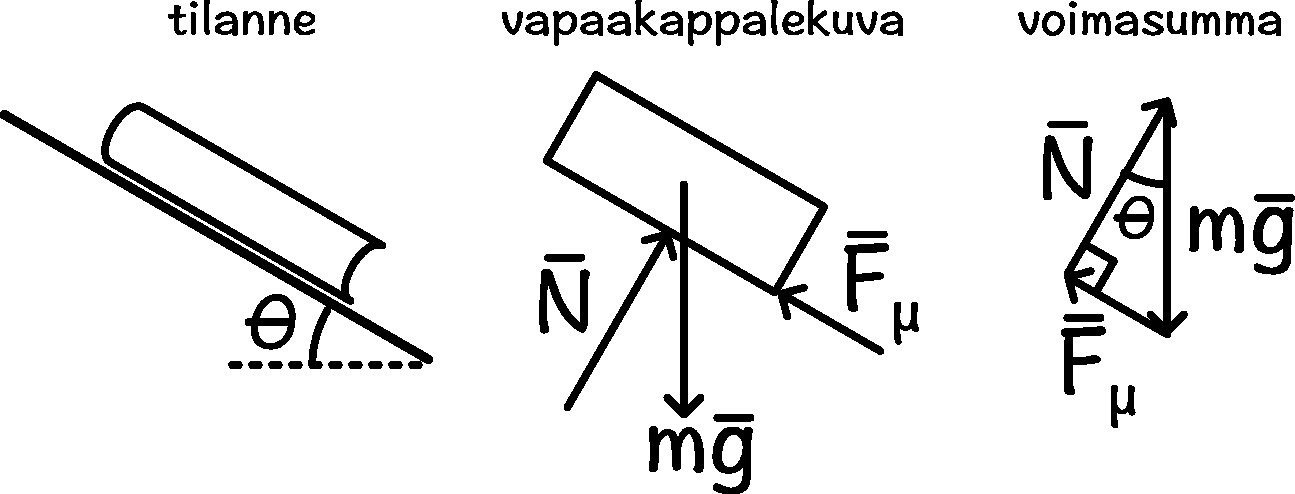
\includegraphics[width=0.95\textwidth]{figs/voima_esimerkki_kitka_1.pdf}%
\end{center}%
}

\physics Kirjaan vaikuttaa painovoima \(\bs{G} = m\bs{g} \) alaspäin.
Kirja ei putoa pöydän läpi, koska pöydän pinta kohdistaa kirjaan normaalivoiman \(\bs{N}\). Tämä voima on kohtisuorassa pyödän pintaa vastaan, ja kuviosta nähdään tämän suunnan olevan kulmassa \(\theta\) pystysuuntaan nähden.
Koska kirja pysyy paikoillaan eli on tasapainossa, siihen täytyy vaikuttaa myös pinnan suuntainen lepokitka \(\bs{F}_\mu\) niin, että kirjaan vaikuttavien voimien summa on nolla.

Lepokitkan suuruus määräytyy tasapainoehdosta mutta kitkavoiman suuruus ei voi kasvaa rajatta vaan sillä on kitkakertoimesta riippuva maksimiarvo. Pyödän kallistaminen heikentää pinnan tukivoimaa ja samalla kirjan paikoillaan pitäminen vaatii yhä suuremman kitkavoiman. Suurimmalla mahdollisella kallistuskulmalla \(\theta_{\max}\) kitkavoima saa maksimiarvonsa.

 \model  Piirretään voimien vektorisumma vapaakappalekuvioon merkittyjen nuolten perusteella.
Koska voimien summan täytyy olla nolla, voimia kuvaavien nuolten pitää muodostaa kolmio. (Asettamalla nuolet peräkkäin täytyy syntyä kuvio, joka palaa alkupisteeseensä.)
Normaalivoima ja kitkavoima ovat kohtisuorassa toisiaan vasten, joten kolmio on suorakulmainen. Lisäksi painovoiman ja normaalivoiman välinen kulma on \(\theta\), joten kolmion muoto voidaan ratkaista geometrisesti.

Painovoimavektorin pituus on \(mg\). Muiden vektorien pituus saadaan trigonometrialla,
\begin{equation} N = mg \cos \theta \end{equation}
sekä
\begin{equation} F_\mu = mg \sin \theta. \end{equation}
Kitkavoiman suuruuden maksimi riippuu normaalivoimasta sekä lepokitkakertoimesta
\begin{equation} F_{\mu,\max} = \mu_\text{lepo} N. \label{maksimikitkaehto} \end{equation}

 \solu  Suurimmalla kallistuskulmalla pätee ehto
\begin{equation} mg \sin \theta_{\max} = \mu_\text{lepo} mg \cos \theta_{\max}. \end{equation}
Tästä voidaan supistaa painovoima pois ja ratkaista kulma muistamalla trigonometrinen sääntö \(\tan \theta = \sin \theta / \cos \theta\) sekä käänteisfunktio \( \theta = \arctan x \Rightarrow \tan \theta = x\)
\begin{equation} \theta_{\max} = \arctan \mu_\text{lepo}. \end{equation}

Kallistuskulma riippuu siis ainoastaan kirjan ja pöydän välisestä lepokitkakertoimesta eikä lainkaan esimerkiksi kirjan massasta. Lepokitkakertoimet vaihtelevat huomattavasti. Esimerkkejä eri materiaalien välisistä kitkakertoimista voi helposti hakea vaikkapa verkosta. Joka tapauksessa pöytien pinnat ovat usein varsin liukkaat, joten järkevä arvo kitkakertoimelle voisi olla esimerkiksi \(\mu_\text{lepo} = 0.3\). Tällöin kirja lähtee liikkeelle kallistuskulmalla
\(\theta_{\max} \approx 0.3 \un{rad} \approx 20^\circ\).

\eval Arkustangentti on kasvava funktio, joten mitä suurempi kitkakerroin on, sitä suurempaan kulmaan pöytä voidaan kallistaa, mikä on järkevä tulos. Laskettu kulma on kohtuullisen pieni, mutta asiaahan voi myös helposti testata itse laittamalla kirja pöydälle ja kokeilemalla, paljonko pyötää pitää kallistaa, jotta kirja alkaisi liukua.

Kitkakerroin on yksikötön luku, joten se voi olla funtion argumentti. Lisäksi \emph{kulma} on myös yksikötön suure, \([\theta] = \un{rad} = 1\), joten ratkaisulla on oikea yksikkö. Trigonometrisen funktion tulos on nimittäin paljas luku --- funktio ei lisää tulokseensa yksikköä. Myöskään \emph{aste} ei ole yksikkö vaan \emph{muuntokerroin}. Täyskulma on nimittäin \(360^\circ = 2\pi\), joten aste on
\begin{equation}1^\circ = \frac{2\pi}{360} = 0.01745\ldots \end{equation}

\end{exam}

%\newpage

\begin{exam}{Liikkeell\"a kaltevalla tasolla}{ex:kaltevaliike}\noindent

\index{liikekitka}

\problem{Kirja lähtee levosta liukumaan alas kaltevaa tasoa. Tason kallistuskulma on \(36^\circ\). Kuinka suuri on kirjan kiihtyvyys, jos kirjan ja pöydän väliset lepo- ja liikekitkakertoimet ovat \(0.30\) ja \(0.20\)?
}

 \twocol{0.45}{0.5}{ \setup  Piirretään kuva tilanteesta sekä kirjan vapaakappalekuva. Tilanne on muuten samankaltainen kuin esimerkissä \autoref{ex:kaltevalepo}, mutta nyt kirja liikkuu. Merkitään kaltevan tason suuntaa \(x\) ja tason normaalin suuntaa \(y\).

\physics Kirjaan vaikuttaa painovoima \(\bs{G} = m\bs{g} \) ja normaalivoima \(\bs{N}\) viistoon ylöspäin. Koska kirja liikkuu, siihen vaikuttaa myös pinnan suuntainen liikekitka \(\bs{F}_\mu\).

Normaalivoiman suuruus määräytyy ehdosta, että kirja ei saa liikkua pinnan sisään. Toisin sanoen pintaa vastaan kohtisuorassa suunnassa voimien summan täytyy olla nolla.
Liikekitkan suuruus riippuu normaalivoiman suuruudesta sekä liikekitkakertoimesta \(\mu\). Koska kirja lähtee liikkeelle levosta, siihen kohdistuvan kokonaisvoiman täytyy olla nollasta poikkeava. Lisäksi, koska mikään kirjaan kohdistuvista voimista ei riipu kirjan nopeudesta tai paikasta, tämän kokonaisvoiman täytyy olla vakio ja siispä myös kirjan kiihtyvyys on dynamiikan peruslain mukaisesti vakio.

}{%
\begin{center}%
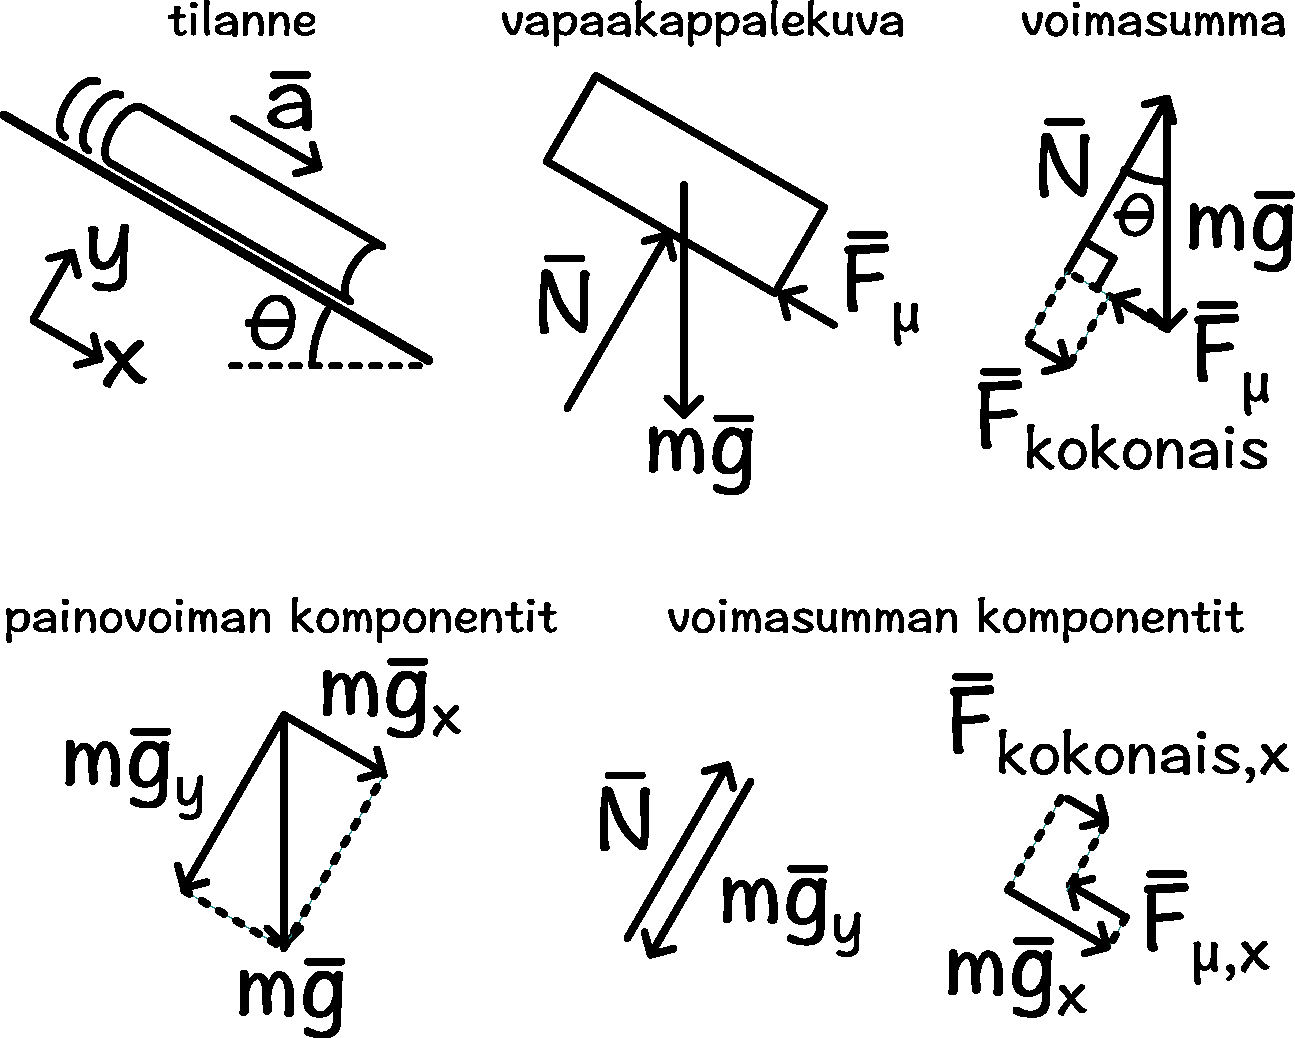
\includegraphics[width=0.95\textwidth]{figs/voima_esimerkki_kitka_3.pdf}%
\end{center}%
}

 \model  Piirretään voimien vektorisumma vapaakappalekuvioon merkittyjen nuolten perusteella ja jaetaan voimat pinnan suuntaisiin ja kohtisuoriin komponentteihin.\\
Voimien pintaa vasten kohtisuorien komponenttien täytyy summautua nollaksi,
\begin{equation} \bs{N}_y + m\bs{g}_y = \bs{0}, \end{equation}
koska kirja liikkuu pinnan suunnassa.
Kirjaan vaikuttaa liikekitka (ei lepokitka), joten kitkavoiman suuruus riippuu normaalivoimasta sekä liikekitkakertoimesta
\begin{equation} F_{\mu} = \mu N. \end{equation}
Kokonaisvoima on \(x\)-suuntaisten voimien summa
\begin{equation} \bs{F}_{\text{kokonais}} = \bs{F}_{x,\text{kokonais}} = \bs{F}_{\mu,x} + m\bs{g}_x \end{equation}
ja kiihtyvyys on
\begin{equation} \bs{a} = \frac{1}{m} \bs{F}_{\text{kokonais}}. \end{equation}

 \solu 
Painovoiman komponenttien pituus voidaan päätellä kuvasta trigonometrisesti. Painovoima osoittaa positiiviseen \(x\)-suuntaan ja negatiiviseen \(y\)-suuntaan, joten painovoiman skalaarikomponentit ovat

\begin{eqnarray} mg_x &=& |m\bs{g}_x| = mg \sin \theta \\
    mg_y &=& -|m\bs{g}_y| =  - mg \cos \theta. \end{eqnarray}

Siispä normaalivoiman suuruuden on oltava
\begin{equation} N = N_y = - mg_y = mg \cos \theta. \end{equation}
ja kitkavoiman suuruus on
\begin{equation} F_{\mu} = \mu N = \mu  mg \cos \theta. \end{equation}
Kitkavoima osoittaa negatiiviseen \(x\)-suuntaan, joten sen skalaarikomponentti on negatiivinen
\begin{equation} F_{\mu,x} = -|\bs{F}_{\mu,x}| = - \mu  mg \cos \theta. \end{equation}
Kokonaisvoiman osoittaa positiiviseen \(x\)-suuntaan ja sen suuruus on
\begin{equation} F_\text{kokonais} = F_{\text{kokonais},x} = mg_x + F_{\mu,x} = mg \sin \theta - \mu  mg \cos \theta. \end{equation}
Kappaleen kiihtyvyys osoittaa positiiviseen \(x\)-suuntaan ja sen suuruus on
\begin{equation} a_x = g (\sin \theta - \mu \cos \theta) = 9.8\un{m/s}^2 \cdot (\sin 36^\circ - 0.20\cdot \cos 36^\circ) =  4.2 \un{m/s}^2. \end{equation}

\end{exam}

\section{Voiman impulssi ja työ}
\label{voimanimpulssijatyö}

\subsection{Voiman impulssi}
\label{voimanimpulssi}

\marginpictures%
{0}
{Impulssi on funktion \( F(t) \) rajaama pinta-ala.;%
Impulssi integraalina.;%
Liikemäärän muutos.}%
{fig:voimaimpulssiintegraali}%
{1.0;1.0}%
{voima_impulssi_integraali_3.pdf;voima_impulssi_integraali_4.pdf}

Liikemäärän yhteydessä totesimme, että vuorovaikutus voi muuttaa kappaleen liikemäärää antamalla sille impulssin.
Dynamiikan peruslain (\autoref{newton2}) mukaan puolestaan voima muuttaa kappaleen liikemäärää ajan kuluessa, joten voiman ja impulssin täytyy kuvata samaa asiaa --- vuorovaikutuksen kykyä muuttaa liikemäärää. Suureiden ero on ainoastaan se, että impulssi kuvaa vuorovaikutuksen tuottamaa liikemäärän kokonaismuutosta \emph{jollakin aikavälillä} kun taas voima kuvaa vuorovaikutuksen tuottamaa liikemäärän muutosnopeutta \emph{yhdellä ajan hetkellä}.

Dynamiikan peruslain mukaisesti kappaleen liikemäärä muuttuu sitä enemmän, mitä suurempi kokonaisvoima kappaleeseen kohdistuu ja mitä kauemmin tämä voima kappaleeseen vaikuttaa.
Jos kappaleeseen kohdistuu vakiovoima \(\bs{F}\) ajan \(\Delta t\), liikemäärän muutos on \(\Delta \bs{p} = \bs{F} \Delta t\). Toisaalta impulssi määriteltiin niin, että se on vuorovaikutuksen tuottama liikemäärän kokonaismuutos, joten vakiovoiman impulssi on siis
\begin{equation} \bs{I}_{\text{vakiovoima}} = \Delta \bs{p} = \bs{F}_{\text{kokonais}} \Delta t. \label{impulssi_vakiovoima} \end{equation}
Skalaarikomponenttien avulla ilmaistuna sama asia on
\begin{equation} I_{x,\text{vakiovoima}} = \Delta p_x = F_{x,\text{kokonais}} \Delta t. \label{impulssi_vakiovoima_x} \end{equation}

Jos voima ei ole vakio vaan riippuu ajasta, impulssia ei voida laskea voiman ja sen vaikutusajan tulona, mutta pitkäkin aikaväli voidaan jakaa pieniin osiin, joiden aikana voima on likimain vakio kuten kuvassa \autoref{fig:voimaimpulssiintegraali} (b).
Kullakin lyhyellä aikavälillä \(\Delta t\)) kappale saa tällöin pienen impulssin
\begin{equation} I_x \approx F_{x,\text{kokonais}}(t) \Delta t\end{equation}
ja kappaleen saama kokonaisimpulssi saadaan laskemalla nämä yhteen
\begin{equation} I_x \approx F_{x,\text{kokonais}}(t_0) \Delta t + \ldots + F_{x,\text{kokonais}}(t_{N-1}) \Delta t. \end{equation}
Ottamalla raja-arvo, kun aikavälien pituus \(\Delta t\) lähestyy nolla tämä approksimaatio tulee tarkaksi ja summaus muuttuu integraaliksi
\begin{equation} I_x = \int_{t_\text{alku}}^{t_\text{loppu}} F_{x,\text{kokonais}} \dd t. \label{impulssi_x} \end{equation}
\emph{Impulssi on siis voiman integraali ajan suhteen}.
Graafisesti impulssin \(x\)-skalaarikomponentti saadaan siis määrittämällä voiman \(x\)-komponentin \emph{aikakuvaajan} \(F_x(t) \) ja aika-akselin rajaama pinta-ala (kuva \autoref{fig:voimaimpulssiintegraali} (a)).

\index{impulssi}

Impulssi on vektorisuure, ja äskeisessä analyysissä johdettiin impulssin \(x\)-komponentin ja voiman \(x\)-komponentin välinen yhteys.
Sama asia voidaan kirjoittaa yleisemmin ja helpommin käyttämällä differentiaaleja ja vektoreita. Infinitesimaalisen lyhyen ajan \(\dd t\) aikana voima nimittäin antaa kappaleelle impulssin
\begin{equation} \dd \bs{I} = \dd \bs{p} = \bs{F}_{\text{kokonais}} \dd t. \end{equation}
Kokonaisimpulssi saadaan laskemalla nämä pienet impulssit yhteen eli integroimalla
\bigeq{ \bs{I} = \int_{t_\text{alku}}^{t_\text{loppu}} \bs{F}_{\text{kokonais}} \dd t. \label{impulssi} }
Tämä on impulssin ja voiman välinen yleinen yhteys, joka yksiulotteisessa tapauksessa voidaan kirjoittaa \(x\)-skalaarikomponenttien avulla yhtälön (\autoref{impulssi_x}) muotoon.

\widepictures{tb}%
{Kappaleiden välinen vuorovaikutus törmäyksessä. Kappaleisiin vaikuttaa joka hetki yhtä suuri voima ja ne saavat yhtä suuret impulssit. Kappaleen A inertia on kuitenkin kaksinkertainen kappaleeseen B verrattuna.;%
Liikekuvasarja.;%
Nopeuden kuvaaja.;%
Voiman kuvaaja.}%
{fig:voimaimpulssi;fig:voimaimpulssi_a;fig:voimaimpulssi_b;fig:voimaimpulssi_c;}%
{0.4;0.25;0.25}%
{0.381;0.248;0.271}%
{voima_impulssi_1.pdf;voima_impulssi_3.pdf;voima_impulssi_4.pdf}

Luvussa \autoref{luku:sailymislait} törmäysten tarkastelussa todettiin kappaleiden liikemäärien muuttuvan kappaleiden saamien impulssien takia. Kuvassa \autoref{fig:voimaimpulssi} on esitetty kahden kappaleen törmäys mukaanlukien kappaleisiin vaikuttavien voimien kuvaaja. Kuvan esimerkissä kappaleen A massa on kaksinkertainen kappaleen B massaan nähden, sillä kappaleen A nopeuden muutos on törmäyksessä vain puolet kappaleen B vastaavasta. Kuitenkin koska systeemin liikemäärä on vakio, kummankin kappaleen liikemäärän pitää muuttua yhtä paljon mutta vastakkaiseen suuntaan eli kappaleet saavat yhtä suuret impulssit. Kappaleisiin kohdistuvien voimien kuvaajassa impulssi on kuvaajan ja aika-akselin väliin jäävä pinta-ala, joka on molemmilla kappaleilla itseisarvoltaan sama mutta vastakkaismerkkinen, koska kappaleisiin kohdistuvilla voimilla on eri etumerkit. Erot kappaleiden nopeuksien muutoksissa ovat seurausta kappaleiden erilaisista inertioista --- kappaleiden saamat impulssit ovat yhtä suuret.

Impulssin ja voiman yhteyttä voidaan käyttää myös voiman arvioimiseksi, kun kappaleen saama impulssi tunnetaan. Jos nimittäin törmäys kestää ajan \(\Delta t\) ja voiman on tässä ajassa tuotettava \(x\)-suuntainen impulssi \(I_x\), voiman suuruuden on oltava keskimäärin
\(F_x = I_x / \Delta t, \)
ja koska voima ei käytännössä ole kuitenkaan vakio, sen maksimiarvo voi olla tätä selvästi suurempikin.
Tästä syystä esimerkiksi kolarit ja korkealta putoaminen ovat vaarallisia. Liikemäärän \emph{suuri} muutos vaatii suuren impulssin ja liikemäärän \emph{nopea} muutos tarkoittaa impulssin tapahtuvan lyhyessä ajassa. Molemmat ehdot vaativat, että impulssin tuottava voima on suuri. Materiaalien kestäminen tai rikkoutuminen rasituksessa riippuu pääasiassa niihin kohdistuvan voiman suuruudesta (vrt. elastiset ja plastiset muodonmuutokset), joten nopea pysähtyminen suuresta vauhdista on vaaraksi niin esineille kuin elollisille olennoillekin.

\begin{stopQ}{q:gravitaation_impulssi}%
Kappale (massa \(1.0 \un{kg}\)) on vapaassa pudotuksessa. Valitaan positiivinen suunta alas.\\
(a) Kuinka suuren impulssin gravitaatio antaa kappaleelle yhden sekunnin aikana?\\
(b) Mikä on kappaleen liikemäärän muutos sekunnin aikana, jos alkunopeus on \(2.0 \un{m/s}\) ylös?\\
(c) Entä jos alkunopeuden suunta on alaspäin?
\end{stopQ}

\subsection{Voiman tekemä työ}
\label{voimantekemätyö}

\index{työ}

\pictures{b!}%
{Työ on positiivinen voiman osoittaessa liikkeen suuntaan ja negatiivinen voiman osoittaessa liikkeeseen nähden vastakkaiseen suuntaan.;%
Kappale työnnetään liikkeelle: positiivinen työ lisää kappaleen energiaa.;%
Kappale pysäytetään: negatiivinen työ vähentää kappaleen energiaa.}%
{fig:voimatyoselitys2;fig:voimatyoselitys2_a;fig:voimatyoselitys2_b;}%
{0.45;0.45}%
{0.45;0.45}%
{voima_tyoselitys_4.pdf;voima_tyoselitys_5.pdf}

Kappaleeseen vaikuttava voima tuottaa impulssin ja muuttaa siten kappaleen liikemäärää, mutta jos kappaleen liikemäärä muuttuu, myös kappaleen \emph{liike-energia} muuttuu. Niinpä voima pystyy muuttamaan liikemäärän lisäksi myös kappaleen \emph{energiaa}. Siinä missä impulssi kuvaa voiman aiheuttamaa muutosta liikemäärässä, voiman aiheuttamaa muutosta energiassa kuvaa suure nimeltä \textbf{työ}.
Esimerkiksi kuvassa \autoref{fig:voimatyoselitys2_a} työnnetään vaunua, jolloin se lähtee liikkeelle suuntaan, johon voima sitä työntää. Tällöin vaunun liike-energia kasvaa ja fysiikassa sanotaan, että \emph{voima tekee vaunuun työtä}. Vastaavasti kuvassa \autoref{fig:voimatyoselitys2_b} liikkuva vaunu pysäytetään työntämällä sitä vaunun liikkeeseen nähden vastakkaiseen suuntaan. Tällöin vaunun energia vähentyy.

Kuvan \autoref{fig:voimatyoselitys2} esimerkissä oleellista on se, että molemmissa tilanteissa vaunut \emph{liikkuvat} ja voima vaikuttaa liikkeen suunnassa. Kun voima osoittaa vaunun liikkeen suuntaan, vaunun vauhti kasvaa ja siten myös sen liike-energia kasvaa. Kun voima osoittaa vastakkaiseen suuntaan liikkeeseen nähden, vauhti pienenee ja liike-energia vähenee.
Työ liittyy siis aina prosessiin, jossa kappale \emph{liikkuu} ja voima on \emph{liikkeen suuntainen}.

\marginpictures%
{0}
{Työ mittaa energian muutosta.;%
Työ muuttaa liike-energiaa.;%
Työ muuttaa sisäenergiaa.}%
{fig:voimatyoselitys1}%
{1.0;1.0}%
{voima_tyoselitys_2.pdf;voima_tyoselitys_3.pdf}

Yksinkertainen esimerkki tällaisesta prosessista, jossa voima vaikuttaa kappaleen liikkeen suunnassa, on kappaleen vapaa putoaminen suoraan alaspäin (kuva \autoref{fig:voimatyoselitys1} (a)). Tällöin kappaleeseen vaikuttaa vain painovoima, joka on suuruudeltaan vakio, \(G_x = -mg\), missä positiivinen \(x\)-suunta on valittu ylöspäin.
Toisaalta mekaanisen energian säilymislain perusteella putoavan kappaleen liike-energian muutos riippuu kappaleen
kokeman pystysuuntaisen siirtymän pituudesta,
\begin{equation} \Delta K = - \Delta U = - mg \Delta x = G_x \Delta x. \end{equation}
Toisin sanoen potentiaalienergiaa muuttuu liike-energiaksi määrä, jonka suuruus on voiman suuruuden ja kappaleen pystysuuntaisen siirtymän tulo. Toisin sanoen painovoima tekee kappaleeseen työtä, joka muuttaa vuorovaikutuksen potentiaalienergiaa kappaleen liike-energiaksi. Voima voi siis sekä lisätä että vähentää kappaleen energiaa tekemällä työtä. Kuitenkin koska energia on säilyvä suure, työ ei voi luoda eikä hävittää energiaa vaan ainoastaan muuttaa sitä muodosta toiseen tai siirtää kappaleelta toiselle. Voiman tekemä \emph{työ siis mittaa kuinka paljon energiaa muuttuu muodosta toiseen}.

Huomaa erityisesti, että edellinen päättely pätee riippumatta siitä, liikkuuko kappale ylös- vai alaspäin. Jos kappale putoaa alaspäin, painovoima osoittaa samaan suuntaan kuin mihin kappale liikkuu ja voima tekee \emph{positiivista} työtä kasvattaen kappaleen liike-energiaa (ja vähentäen gravitaation potentiaalienergiaa). Jos kappale on heitetty ylöspäin, painovoima osoittaa liikkeeseen nähden vastakkaiseen suuntaan ja tekee kappaleeseen \emph{negatiivista} työtä vähentäen kappaleen liike-energiaa (ja lisäten gravitaation potentiaalienergiaa). Työn etumerkki siis kuvaa siirtyvän energian suuntaa: kappaleeseen (tai systeemiin) tehty positiivinen työ lisää kappaleen (tai systeemin) energiaa kun taas negatiivinen työ vähentää energiaa.

Samanlainen päättely toimii mille tahansa vakiovoimalle: \emph{voiman tekemä työ on suoraan verrannollinen voiman suuruuteen sekä kappaleen siirtymään. Työ on positiivinen, jos voima on samansuuntainen siirtymän kanssa, ja negatiivinen jos voima ja siirtymä ovat vastakkaissuuntaiset}. Yhtälönä tämän asian voi ilmaista yksinkertaisesti niin, että työ on vakiovoiman \(x\)-skalaarikomponentin ja \(x\)-suuntaisen siirtymän tulo,
\begin{equation} W = F_x \Delta x. \label{tyo_vakiovoima_x} \end{equation}
Voiman osoittaessa \emph{samaan suuntaan} kuin mihin kappale liikkuu eli suureiden \(F_x\) ja \(\Delta x\) ollessa samanmerkkiset työ on \emph{positiivinen}. Jos puolestaan voima osoittaa \emph{vastakkaiseen suuntaan} kuin mihin kappale liikkuu, toinen suureista \(F_x\) ja \(\Delta x\) on negatiivinen ja toinen positiivinen, jolloin työ on \emph{negatiivinen}.
Vaikka voima ja siirtymä ovat vektoreita, työn määritelmässä esiintyy ainoastaan vektoreiden skalaarikomponentteja, joten työ on on \emph{skalaari} aivan kuten energiakin. Työ siis joko lisää tai vähentää kappaleen energiaa. Tämä on oleellinen ero impulssiin, joka on vektori ja jonka suunta osoittaa liikemäärävektorin muutoksen suunnan.

\begin{stopQ}{q:mekaanisen_tyon_maaritelma}%
Kuinka suuren työn teet, jos nostat \(0.8 \un{kg}\) massan maasta \(1.2 \un{m}\) korkeudelle (a) 1 sekunnissa, (b) 10 sekunnissa? (c) Entä jos nostat kymmenen samanlaista kappaletta yhden kerrallaan, yhden sekunnissa? (d) Entä jos nostat kymmenen samanlaista kappaletta kerralla 10 sekunnissa? (e) Entä jos kannattelet kappaletta tällä korkeudella 1 minuutin?
\end{stopQ}

Putoavan kappaleen tapauksessa kappaleen potentiaalienergia ja liike-energia on helppo laskea kappaleen paikan ja nopeuden avulla, eikä työn laskeminen voiman kautta ole erityisen hyödyllistä. Työ kuitenkin ilmaisee \emph{aina} vuorovaikutuksen aiheuttaman energiamuodon muutoksen suuruutta, ja niinpä työn avulla voidaan laskea myös sellaiset energian muutokset, joita \emph{ei voida} päätellä tarkastelemalla vain prosessin alku- ja lopputilaa. Esimerkiksi ilman puristaminen pumpulla vaatii voimaa ja voima tekee pumpussa olevaan ilmaan työtä (kuva \autoref{fig:voimatyoselitys1} (b)). Työn tekeminen kasvattaa ilman ja pumpun energiaa, ja koska prosessissa liike- tai potentiaalienergia eivät ilmeisesti muutu, työn on kasvatettava systeemin sisäenergiaa. Toisin sanoen ilma \emph{lämpenee}, ja \emph{lämpöenergian muutoksen on oltava yhtä suuri kuin voiman tekemä työ}. Erityisesti tällaisissa prosesseissa työ on huomattavan vahva työkalu, sillä sen avulla voidaan mekaanisten suureiden perusteella määrittää myös epäjärjestyneen sisäenergian muutoksia, joita voisi muuten olla mahdoton laskea.

\marginpictures{0}%
{Systeemin sisäisten vuorovaikutusten tekemä työ muuttaa energiaa muodosta toiseen, mutta systeemin kokonaisenergia ei muutu.;%
Nostaja tekee työtä laatikkoon ja nostajan sisäenergiaa muuttuu gravitaation potentiaalienergiaksi.;%
Nostajan ja laatikon välinen vuorovaikutus kohdistaa molempiin voimat.}%
{fig:voimatyoselitys3}%
{1.0;0.8}%
{voima_tyoselitys_8.pdf;voima_tyoselitys_7.pdf}

Myös systeemin \emph{sisäiset} vuorovaikutukset voivat tehdä työtä, mutta tällöin systeemin kokonaisenergia ei muutu vaan energia muuttaa muotoaan systeemin sisällä. Kuvan \autoref{fig:voimatyoselitys3} esimerkissä laatikkoa nostetaan ylöspäin painovoimakentässä, mikä vaatii ylöspäin vaikuttavan voiman kohdistamisen kappaleeseen. Tämä nostava voima kumoaa laatikkoon kohdistuvan painovoiman. Nostava voima on laatikon noustessa samansuuntainen kuin liike eli voiman kappaleeseen tekemä työ on positiivinen. Kuitenkin nostajan ja laatikon välisen vuorovaikutuksen täytyy kohdistaa voima \emph{myös nostajaan} ja voiman ja vastavoiman lain mukaisesti tämä voima on yhtä suuri mutta vastakkaissuuntainen laatikkoon kohdistuvaan voimaan nähden. Koska tämä voima on vastakkaissuuntainen nostajan käsien siirtymään nähden, se tekee nostajaan negatiivisen työn, joka on itseisarvoltaan yhtä suuri kuin laatikkoon tehty positiivinen työ.

Laatikkoa nostaa ihminen, ja prosessissa tehty negatiivinen työ kuluttaa häneen sitoutunutta kemiallista energiaa. Samalla positiivinen työ lisää kappaleen ja Maan välisen gravitaatiovuorovaikutuksen potentiaalienergiaa. Toisin sanoen ihmisen sisäenergiaa muuttuu mekaaniseksi energiaksi, ja energian muutos on yhtä suuri kuin vuorovaikutuksen tekemä työ.
Nostajalle tulee prosessissa myös lämmin eli kemiallista energiaa muuttuu myös lämpöenergiaksi. Tätä muutosta ei \emph{laatikon ja nostajan välisen vuorovaikutuksen} tekemä työ kuitenkaan mittaa, sillä muutokset nostajan sisäenergiassa johtuvat \emph{hänen} sisäisistä vuorovaikutuksistaan.

\begin{stopQ}{q:tyo_pallon_heitossa}%
Palloa heitetään ylöspäin vakiovoimalla, jolloin pallo on kiihtyvässä liikkeessä. Pallo saa heiton aikana (ennen kädestä irtoamista) liike-energian \(2 \un{J}\) ja sen gravitaatiopotentiaalienergian muutos on \(1 \un{J}\). (a) Mikä on heittäjän palloon tekemä työ? (b) Mikä on painovoiman palloon tekemä työ? (c) Mikä on pallon heittäjään tekemä työ? (d) Miten heittäjän energia muuttuu heiton aikana? (e) Onko kokonaisenergia (likimain) vakio systeemissä, johon kuuluu heittäjä, pallo ja maapallon gravitaatio?
\end{stopQ}

Painovoiman voimakkuus on maanpinnalla likimain vakio, mutta yleisesti voimat muuttuvat. Esimerkiksi kuvan \autoref{fig:voimatyoselitys1} (b) pumpun tapauksessa vaaditaan sitä suurempi voima mitä pienempään tilavuuteen ilma puristetaan. Tällöin voidaan käyttää samaa ositteluperiaatetta kuin aikaisemminkin muuttuvien suureiden analyysissä on käytetty. Kappaleen kulkema reitti jaetaan hyvin pieniin siirtymiin \(\dd x\), joilla voiman \(x\)-komponenttia \(F_x\) voidaan pitää vakiona. Tällöin kunkin pienen siirtymän matkalla voima tekee kappaleeseen työn
\begin{equation} \dd W = F_x \dd x \end{equation}
ja koko matkalla pisteestä \(x_\text{alku}\) pisteeseen \(x_\text{loppu}\) tehty työ saadaan laskemalla nämä yhteen eli integroimalla voimaa \emph{siirtymän} suhteen
\bigeq{ W = \int_{x_\text{alku}}^{x_\text{loppu}} F_x \dd x. \label{tyo} }
Graafisesti työ on siis voiman paikkakuvaajan, \(F_x(x) \), ja paikka-akselin rajaama pinta-ala.

\marginpicture%
{-50}%
{Työ on funktion $ F(x) $ rajaama ala.}%
{fig:voimatyointegraali}%
{1.0}%
{voima_tyointegraali_3.pdf}

\index{integraali}
\index{energia}
\index{liikemäärä}
\index{skalaari}
\index{vektori}

Työn määritelmä (\autoref{tyo}) muistuttaa impulssin lauseketta (\autoref{impulssi}), sillä molemmat ovat \emph{voiman integraaleja}. Kuitenkin työ on voiman integraali \emph{paikan} suhteen ja se kertoo vuorovaikutuksen aiheuttaman muutoksen kappaleen \emph{energiassa}. Impulssi sen sijaan on voiman integraali \emph{ajan} suhteen ja se kertoo vuorovaikutuksen aiheuttaman muutoksen kappaleen \emph{liikemäärässä}. Työ on \emph{skalaari} aivan kuten energia ja impulssi on liikemäärän tavoin \emph{vektori}.

\onepicture%
{tb}
{Kahteen kappaleeseen vaikuttavat samanlaiset voimat antavat samat impulssit vaikutettuaan yhtä kauan ja tekevät yhtä suuren työn kappaleiden liikuttua yhtä pitkän matkan.}%
{fig:voimatyoimpulssi}%
{0.6}%
{voima_impulssi_5.pdf}

Työn ja impulssin eroa on havainnollistettu kuvassa \autoref{fig:voimatyoimpulssi}. Kahteen kappaleeseen, joilla on erilaiset inertiat, vaikuttaa kumpaankin samanlainen voima. Kappaleet ovat aluksi levossa ja voima kiihdyttää ne liikkeelle. Inertialtaan suurempi kappale kuitenkin kiihtyy hitaammin, joten sen nopeus on aina pienempi kuin pienemmän kappaleen. Kuitenkin koska voiman antama impulssi on suoraan verrannollinen siihen kuinka kauan voima kappaleisiin vaikuttaa, kappaleiden liikemäärät muuttuvat yhtä nopeasti ja millä tahansa ajan hetkellä kummallakin on yhtä suuri liikemäärä. Kappaleisiin tehty työ sen sijaan riippuu siitä, kuinka pitkän matkan kappale on kulkenut voiman vaikutussuunnassa. Koska suurempi kappale liikkuu hitaammin, voima tekee siihen työtä hitaammin ja kullakin ajan hetkellä sen liike-energia on pienempi kuin kevyen kappaleen. Kuitenkin valitaanpa mikä tahansa etäisyys lähtöpisteestä, kappaleiden liike-energia tällä etäisyydellä on sama. Raskaamman kappaleen nopeus on silti tällöinkin pienempi kuin kevyen kappaleen.

Esimerkki tällaisesta tilanteesta voisi olla vaikkapa heitto. Kevyt pallo on helppo heittää nopeasti, mutta se ei silti saa suurta liikemäärää, koska voima ehtii vaikuttaa siihen vain vähän aikaa. Raskasta palloa puolestaan ei saa liikkeelle yhtä nopeasti eikä sen loppunopeus ole yhtä suuri, mutta sille voi antaa helpommin suuren liikemäärän, koska heittoliike kestää kauemmin. Koska heittoa rajoittaa käden pituus, samanlaisella heittotekniikalla, jos kumpaankin palloon kohdistuu heiton aikana likimain yhtä suuri voima, kumpikin pallo saa kuitenkin heitossa yhtä suuren liike-energian.

Yleisesti, jos voima tunnetaan ajan funktiona, sen tuottama impulssi voidaan laskea integroimalla ajan suhteen ja näin voidaan määrittää kappaleen saama impulssi ja sen liikemäärän muutos. Työtä sen sijaan ei voida laskea ratkaisematta ensin voimaa paikan funktiona. Jos sen sijaan voima tunnetaan paikan funktiona, sen tekemä työ voidaan laskea integroimalla paikan suhteen ja näin voidaan määrittää kappaleeseen tehty työ ja sen energian muutos. Impulssia sen sijaan ei voida laskea ratkaisematta ensin voimaa ajan funktiona.

\begin{stopQ}{q:impulssi_tyo_kuvaajina}%
Aluksi levossa olevaan kappaleeseen vaikuttaa vakiovoima \(F_x > 0 \un{N}\). Millainen kuvaaja saadaan, jos piirretään (a) kappaleen saama kokonaisimpulssi ajan funktiona, \(I_x(t) \), (b) kappaleen saama kokonaisimpulssi paikan funktiona, \(I_x(x) \), (c) kappaleeseen tehty työ paikan funktiona, \(W(x) \) ja (d) kappaleeseen tehty työ ajan funktiona, \(W(t) \)?
\end{stopQ}

\begin{exam}{Purjeveneet}{ex:purjevene}\noindent

\problem{Kaksi ulkoisesti samanlaista purjevenettä lähtee levosta liikkeelle. Kumpaankin veneeseen vaikuttaa yhtä suuri liikkeen suuntainen kokonaisvoima, joka on vakio. Veneistä toisen massa on kaksinkertainen toiseen nähden. Mikä on veneiden (a) liike-energian ja (b) vauhtien suhde niiden kuljettua sata metriä? }

 \setup  Koska veneiden massoja ja niihin kohdistuvia voimia ei tunneta, energioita ja nopeuksia ei voida ratkaista tarkasti. Sen sijaan voimme tarkastella niiden suhteellista suuruutta. Merkitään pienempää venettä A (massa \(m\)) ja suurempaa B (massa \(2m\)). Merkitään veneisiin vaikuttavaa voimaa \(F_\text{kokonais}\), niiden kulkemaa matkaa \(\Delta x\) ja niiden loppunopeuksia \(v_A\) sekä \(v_B\).

\physics Voima tekee veneisiin työtä, joka on verrannollinen voiman suuruuteen ja veneiden kulkemaan matkaan.
Veneiden liike-energian muutos on sama kuin niihin tehty työ. Koska veneet ovat aluksi paikoillaan, niiden liike-energia on aluksi nolla. Siispä veneiden liike-energia lopuksi on yhtä suuri kuin niihin tehty työ.

Koska veneisiin kohdistuu vakiovoima, ne ovat tasaisesti kiihtyvässä liikkeessä.

\solu (a) Voiman tekemä työ on \(W_\text{kokonais} = F_\text{kokonais} \Delta x\) ja tämä on siis sama kuin veneiden saama liike-energia, \(K = W_\text{kokonais}\). Kuljettuaan yhtä pitkän matkan \(\Delta x\) veneisiin on tehty \emph{yhtä suuri} työ. Siispä niillä on myös \emph{sama} liike-energia, koska niihin vaikuttaa yhtä suuri voima.

(b) Veneen A liike-energia on \(K_A = \frac{1}{2}m v_A^2 = W\), joten sen loppunopeus on
\( v_A = \sqrt{2W/m}. \)
Koska veneen B massa on kaksinkertainen, sen loppunopeus on \emph{pienempi}, \(v_B = \sqrt{W/m}\). Nopeuksien suhde on
\begin{equation} v_A / v_B = \sqrt{\frac{2W}{m}}/\sqrt{\frac{W}{m}} = \sqrt{\frac{2W}{m} \frac{m}{W}} = \sqrt{2}. \end{equation}

 \eval  Veneiden saama liike-energia on yhtä suuri, mutta raskaamman veneen vauhti on pienempi. Näin täytyy olla, koska raskaalla veneellä on suurempi inertia. Huomaa myös, että veneiden liike-energia on sama kun ne ovat kulkeneet \emph{yhtä pitkät matkat}. Raskaalta veneeltä tähän luonnollisesti kuluu enemmän aikaa.

Koska työ riippuu kappaleen siirtymästä, työ ja energia ovat usein parhaat tavat ratkaista kappaleen liike \emph{paikan funktiona}. Jos liike halutaan ratkaista \emph{ajan funktiona}, on helpointa käyttää dynamiikan peruslakia.

\end{exam}

\subsection{Liikettä vastaan kohtisuora voima}
\label{liikettävastaankohtisuoravoima}

\index{kohtisuora}

Edellä todettiin, että kappaleeseen vaikuttava voima tekee positiivisen työn kappaleen liikkuessa voiman suuntaan ja negatiivisen työn kappaleen liikkuessa voimaan nähden vastakkaiseen suuntaan. On kuitenkin myös mahdollista, että voima ei vaikuta liikkeen suunnassa vaan siihen nähden \emph{kohtisuoraan}. Esimerkiksi kitkattomalla vaakasuoralla tasolla liikkuvaan kappaleeseen vaikuttaa painovoima ja pinnan tukivoima, jotka ovat molemmat liikkeen suuntaan nähden kohtisuorassa (kuva \autoref{fig:voimatyoselitys6} (a)). Tällaisen kappaleen potentiaalienergia ei muutu, koska kappale ei liiku pystysuunnassa. Kappale myös liikkuu tasaisella nopeudella, koska siihen kohdistuva kokonaisvoima on nolla. Kappaleen liikkeeseen ei siis liity mitään energian muodon muutoksia eikä kappaleeseen tehdä työtä vaikka se liikkuu ja siihen vaikuttaa voimia.

Energian näkökulmasta on ymmärrettävää, että tässä tapauksessa painovoima tai normaalivoima eivät voi tehdä työtä. Jos voimat nimittäin tekisivät kappaleeseen työtä, energiaa pitäisi muuttua muodosta toiseen. Kuitenkin gravitaation potentiaalienergia on vakio vaakasuorassa liikkeessä, eikä lattiassa tapahdu liikkeen aikana muutoksia. Koska energia ei muuta muotoaan kappaleessa eikä sen ympäristössä, prosessiin ei voi liittyä työtä.

\pictures{b!}%
{Siirtymään nähden kohtisuorat voimat eivät tee työtä.;%
Liikkeen suuntaan kohtisuorat voimat eivät tee työtä.;%
Levossa olevaan kappaleeseen ei tehdä työtä.;%
Vain voiman liikkeen suuntainen komponentti tekee työtä.}%
{fig:voimatyoselitys6;fig:voimatyoselitys6_a;fig:voimatyoselitys6_b;fig:voimatyoselitys6_c;}%
{0.65;0.2;0.9}%
{0.65;0.2;0.9}%
{voima_tyoselitys_9.pdf;voima_tyoselitys_10.pdf;voima_tyoselitys_11.pdf}

Esimerkin päätelmä on yleispätevä: \emph{kappaleen liikkeen suuntaan nähden kohtisuorat voimat eivät tee kappaleeseen työtä.}
Edelleen voimat, jotka eivät ole liikkeen suuntaisia eivätkä siihen nähden täsmälleen kohtisuorassa, voidaan aina jakaa liikkeen suuntaiseen ja kohtisuoraan komponenttiin (kuva \autoref{fig:voimatyoselitys6} (c)). Tällöin voiman tekemä työ voidaan määrittää laskemalla erikseen kummankin komponentin tekemän työn ja summaamalla nämä yhteen, ja koska kohtisuoran komponentin työ on nolla, \emph{ainoastaan voiman liikkeen suuntainen komponentti tekee työtä}.

Työ on nolla myös jos kappale \emph{ei liiku}, sillä tällöin ei ole olemassakaan liikkeen suuntaista voiman komponenttia. Tämän voi havainnollistaa esimerkiksi tarkastelemalla jousesta roikkuvaa kappaletta (kuva \autoref{fig:voimatyoselitys6} (b)). Kappale vuorovaikuttaa sekä jousen että gravitaatiokentän kanssa, mutta kummankaan vuorovaikutuksen potentiaalienergia ei muutu ellei kappaleen paikka muutu, eikä kappaleen liike-energiakaan muutu jos kappale on levossa. Energian muodot eivät siis muutu eikä mikään vuorovaikutuksista tee työtä. On tavallinen harhakäsitys ajatella pelkän voiman tuottamisen vaativan työtä, sillä painavien kappaleiden kannatteleminen väsyttää. Tällöin kyse on kuitenkin ihmisen fysiologian rajoitteista. Lihasvoiman ylläpitäminen esimerkiksi kappaleen kannattelemiseksi vaatii toki energiaa, mutta tämä energia ei siirry kappaleelle vaan muuttuu lihaksissa lämpöenergiaksi. Kappaleen energia ei muutu prosessissa eikä kappaleeseen tehdä työtä.

\begin{stopQ}{q:halfpipe}%
Rullalauta rullaa puoliympyrän muotoisen ``half-pipen'' puolelta toiselle. (a) Tuottaako lautaan kohdistuva normaalivoima impulssin? (b) Tekeekö normaalivoima työtä?
\end{stopQ}

\subsection{Työ ja mekaaninen energia}
\label{työjamekaaninenenergia}

Kuten edellä huomasimme vapaassa pudotuksessa olevalle kappaleelle, painovoiman tekemä työ muuttaa potentiaalienergiaa liike-energiaksi. Toisin sanoen painovoiman potentiaalienergian muutos on voiman tekemän työn vastaluku, \(\Delta U = - W\), missä miinus ilmaisee sitä, että positiivinen työ johtaa potentiaalienergian vähenemiseen. Tämä on itseasiassa yleisesti totta kaikille konservatiivisille vuorovaikutuksille. Nimittäin kohdistuupa konservatiivinen vuorovaikutus mihin tahansa kappaleeseen tai systeemiin ja tämä vuorovaikutus tekee työtä, tämä työ kasvattaa kappaleen tai systeemin energiaa. Energiaa ei kuitenkaan voi luoda vaan ainoastaan siirtää, joten tämän energian täytyy tulla vuorovaikutuksen varastoimasta potentiaalienergiasta.

Matemaattisesti tämä tulos on suora seuraus siitä, että voima on konservatiivisten vuorovaikutusten tapauksessa potentiaalienergian derivaatta paikan suhteen yhtälön \autoref{voima_derivaattana} mukaisesti. Nimitääin koska integrointi on derivoinnin käänteisoperaatio, \emph{potentiaalienergian täytyy olla voiman integraali paikan suhteen}. Toisin sanoen \(x\)-suuntaisen vain paikasta riippuvan konservatiivisen vuorovaikutuksen potentiaalienergia voidaan laskea integroimalla vuorovaikutuksen tuottamaa voimaa paikan suhteen,
\begin{equation} \int F_x \dd x = \int -\frac{\dd U}{\dd x} \dd x = -\int \dd U = -U(x) + U_0, \end{equation}
missä \(U_0\) on integrointivakio. Tällä vakiolla ei ole kuitenkaan fysikaalista merkitystä, sillä potentiaalienergialla ei ole absoluuttisia arvoja. Toisin sanoen potentiaalienergian nollakohta voidaan aina valita vapaasti ja ainoastaan potentiaalienergian muutokset ovat merkityksellisiä. Kuitenkin kun valinta on kerran tehty, sitä ei saa enää muuttaa. Jos esimerkiksi päätetään, että potentiaalienergia on nolla pisteessa \(x_0\), eli \(U(x_0) = 0\), määräytyy potentiaalienergia yksikäsitteisesti kaikissa muissa pisteissä, ja
\bigeq{ U(x) = - \int_{x_0}^{x} F_x \dd x = - W_{x_0 \to x}, \label{tyo_u} }
missä \(W_{x_0 \to x}\) tarkoittaa vuorovaikutuksen tekemää työtä kappaleen siirtyessä paikasta \(x_0\) paikkaan \(x\).
Tätä voidaan pitää potentiaalienergian \emph{määritelmänä}: \emph{konservatiivisen vuorovaikutuksen potentiaalienergian muutos kappaleen liikkuessa on aina yhtä suuri ja vastakkaismerkkinen kuin vuorovaikutukseen liittyvän voiman kappaleeseen tekemä työ}.

\index{potentiaalienergia}
\index{konservatiivinen}

\begin{stopQ}{q:jousen_potentiaalienergia_tyosta}%
Jousivoima on Hooken lain mukaisesti \(F_x = - k(x - x_0\)). Johda lauseke jousen potentiaalienergialle yhtälöstä (\autoref{tyo_u}). Mitä saat, jos potentiaalienergian nollakohta onkin pisteessä \(x_1\), joka on eri kuin jousen lepopituutta merkitsevä paikka \(x_0\)?
\end{stopQ}

Kappaleen liikkeen kannalta erityisen tärkeässä asemassa on siihen vaikuttavan \emph{kokonaisvoiman} tekemä työ, koska juuri kokonaisvoima vaikuttaa kappaleen liikemäärään dynamiikan peruslain (\autoref{newton2}) mukaisesti. Koska kokonaisvoima vaikuttaa liikkeeseen, voisi arvata kokonaisvoiman tekemän työn aiheuttavan kappaleen liike-energian muutokset. Näin juuri onkin.

Kun osoitimme aikaisemmin konservatiivisen voiman ja potentiaalienergian derivaatan yhteyden, saimme tuloksen (\autoref{k_muunnos}), jonka mukaan liike-energian muutosnopeus on verrannollinen kappaleen nopeuteen ja kiihtyvyyteen,
\( \dd K/\dd t = m a_x v_x, \)
ja koska kappaleen kiihtyvyys riippuu siihen vaikuttavasta kokonaisvoimasta, \(a_x = F_{x,\text{kokonais}}/m\), tämä on voiman ja paikan muutoksen avulla lausuttuna
\begin{equation} \frac{\dd K}{\dd t} = F_{x,\text{kokonais}} \frac{\dd x}{\dd t}. \end{equation}
Koska derivointi ja integrointi ovat toistensa käänteisoperaatiot, liike-energian muutos äärellisellä aikavälillä saadaan tämän lausekkeen integraalina ajan suhteen
\begin{equation} \Delta K = \int_{t_\text{alku}}^{t_\text{loppu}} \frac{\dd K}{\dd t} \dd t = \int_{t_\text{alku}}^{t_\text{loppu}} F_{x,\text{kokonais}} \frac{\dd x}{\dd t} \dd t = \int_{x_\text{alku}}^{x_\text{loppu}} F_{x,\text{kokonais}} \dd x. \end{equation}
Mutta tässä viimeinen lauseke on sama asia kuin kokonaisvoiman kappaleeseen tekemä työ.
Siispä \emph{kappaleeseen vaikuttavan kokonaisvoiman kappaleeseen tekemä työ on yhtä suuri kuin kappaleen liike-energian muutos}
\begin{equation} W_{\text{kokonais}} = \Delta K. \label{tyo_k} \end{equation}
Tämä tulos on nimeltään \textbf{työ-energiateoreema}.

Johdimme aikaisemmin liike-energialle lausekkeen \(K = \frac{1}{2}mv_x^2\) tarkastelemalla gravitaatiota, mutta silloin kyseessä oli erikoistapaus. Nyt tarkastelimme yleisempää tapausta, jossa kappaleeseen vaikuttaa \emph{mielivaltainen} kokonaisvoima, joka voi riippua sekä ajasta että paikasta. Erityisesti kappaleeseen voi vaikuttaa sekä konservatiivisia että dissipatiivisia vuorovaikutuksia, ja yllä johdettu tulos pätee silti, sillä päättelyssä käytettiin ainoastaan dynamiikan peruslakia ja nopeuden ja työn määritelmiä. Niinpä vaikuttipa kappaleeseen \emph{millaisia voimia tahansa}, niiden kappaleeseen tekemä kokonaistyö ilmenee aina kappaleen liike-energian muutoksena.

\index{liike-energia}

Koska työ-energiateoreema on yleispätevä, liike-energia voidaan \emph{määritellä} sen avulla. Jos nimittäin levossa olevan kappaleen liike-energia on nolla ja kokonaisvoima tekee siihen työn \(W_{0\to v_x}\), kappale saa työ-energiateoreeman mukaisesti liike-energian
\begin{equation} K = \frac{1}{2}mv_x^2 = W_{0 \to v_x}. \end{equation}
Kappaleen liike-energia on siis se kokonaistyö, joka kappaleeseen on tehty, kun se on kiihdytetty nopeuteensa. Erityisen huomattavaa tässä on se, että tehty työ ei riipu esimerkiksi siitä, kuinka nopeasti kiihdytys tapahtuu tai onko kiihtyvyys \(a_x\) positiivinen vaan \emph{ainoastaan} kappaleen saamasta loppunopeudesta.

Yhdistämällä edellä saadut tulokset, jonka mukaan konservatiivisten vuorovaikutusten tekemä työ ilmaisee vuorovaikutusten varastoiman potentiaalienergian muutosta, \(\Delta U = -W\), ja kokonaisvoiman tekemä työ ilmaisee kappaleen liike-energian muutosta, \(\Delta K = W\), päädymme tuttuun mekaanisen energian säilymislakiin: Jos systeemissä vaikuttaa vain konservatiivisia vuorovaikutuksia, niiden yhdessä tekemä työ on aina yhtä suuri kuin potentiaalienergian muutos liike-energiaksi ja näiden summa on vakio
\begin{equation} \Delta K + \Delta U = W - W = 0. \end{equation}
Päättelimme tuloksen jo aikaisemmin suoraan energian säilymislaista, mutta koska onnistuimme nyt johtamaan sen työn määritelmän avulla, tulos on osoitus siitä että näin määriteltynä työ on järkevä suure joka todella kuvaa energiamuotojen muuttumista toisikseen.

\begin{stopQ}{q:tyo_ja_energia_nostossa}%
Kappaleen massa on \(1.0 \un{kg}\) ja sitä nostetaan ylöspäin \(15.0 \un{N}\) vakiovoimalla \(1.0 \un{m}\) matka. (a) Kuinka suuren työn nostava voima tekee? (b) Kuinka suuren työn painovoima tekee? (c) Kuinka suuren työn kokonaisvoima tekee? (d) Mikä on gravitaation potentiaalienergian muutos? (e) Mikä on kappaleen liike-energian muutos? (f) Miten edellä lasketut työt ja energioiden muutokset liittyvät toisiinsa?
\end{stopQ}

\newpage\begin{exam}{Liikkuvan kappaleen lepokitka}{ex:lepokitkaliike}\noindent

\problem{Kirja on liikkuvan auton kyydissä vaakasuoralla alustalla. Kuinka suuri kitkavoima kirjaan kohdistuu? Kuinka voimakkaasti auto voi jarruttaa niin että kirja pysyy auton suhteen paikoillaan?
}

 \twocol{0.45}{0.5}{ \setup  Piirretään tilanteesta kuva ja kirjan vapaakappalekuva. Kirja ja auto ovat molemmat kiihtyvässä liikkeessä.
Merkitään kirjan massaa \(m\), auton kiihtyvyyttä \(\bs{a}\) sekä lepo- ja liikekitkakertoimia \(\mu_\text{lepo}\) ja \(\mu\).

}{%
\begin{center}%
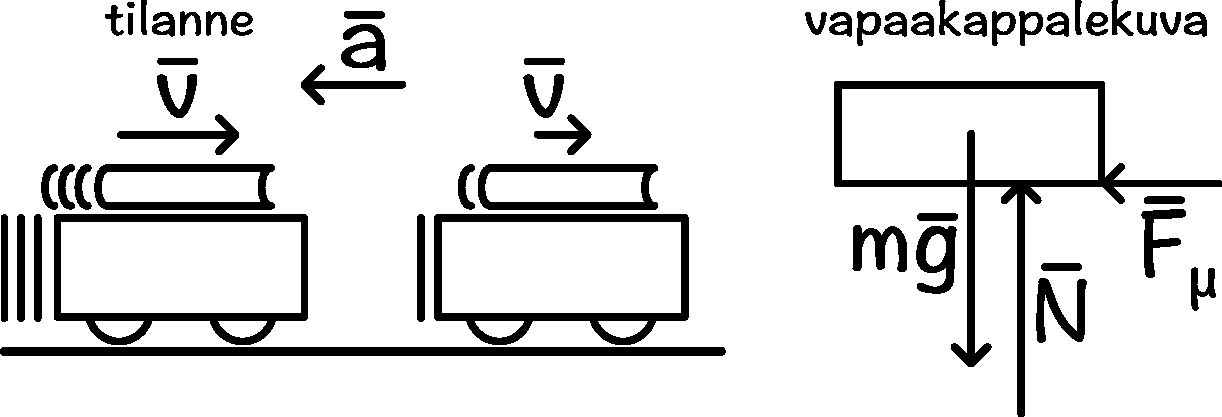
\includegraphics[width=0.95\textwidth]{figs/voima_esimerkki_kitka_2.pdf}%
\end{center}%
}

\physics Jotta kirja pysyisi auton suhteen paikoillaan, sen täytyy liikkua aina samalla nopeudella kuin auto. Tällöin kirjan kiihtyvyyden pitää myös olla sama kuin auton kiihtyvyys, ja kirjaan täytyy kohdistua nollasta poikkeava kokonaisvoima.

Kirjaan vaikuttaa painovoima, normaalivoima sekä kitka. Vaikka kappale ulkopuolisen havaitsijan mielestä liikkuu, kirjan ja alustan pinnat eivät liiku toistensa suhteen, joten kyseessä on lepokitka --- ei liikekitka. Kitkavoiman suuruus määräytyy niin, että kirjan kiihtyvyys on sama kuin auton. Lepokitkan suurin mahdollinen arvo riippuu kirjan ja alustan välisen normaalivoiman suuruudesta sekä lepokitkakertoimesta.

 \model  Koska kirja ei liiku pystysuunnassa, siihen kohdistuva normaalivoima on yhtä suuri kuin painovoima
\begin{equation} N = mg. \end{equation}
Kirjaan kohdistuva kokonaisvoima osoittaa siis vaakasuoraan ja koska tässä suunnassa vaikuttaa ainoastaan kitka, kokonaisvoiman täytyy olla sama kuin kitkavoima.
Kokonaisvoiman suuruus voi siis olla korkeintaan kitkavoiman maksimisuuruus
\begin{equation} F_{\text{kokonais},\max} = F_{\mu,\max} = \mu_\text{lepo} N. \end{equation}

Kirjan kiihtyvyyden skalaarikomponentti liikkeen suunnassa on
\begin{equation} a_x = \frac{1}{m}F_{\text{kokonais},x} = \frac{1}{m}F_{\mu,x} = -\frac{1}{m}F_{\mu}. \end{equation}
Koska voiman suuruudella on maksimi, myös kiihtyvyyden itseisarvolla on maksimi
\begin{equation} a_{\max} = \frac{1}{m}F_{\text{kokonais},\max}. \end{equation}

 \solu  Kirjan kiihtyvyys voi olla korkeintaan
\begin{equation} a_{\max} = \frac{1}{m}\mu_\text{lepo} N = \mu_\text{lepo} g. \end{equation}
Kun auto jarruttaa kiihtyvyydellä \(a\), joka on itseisarvoltaan tätä pienempi, lepokitkan voimakkuuden on oltava
\begin{equation} F_{\mu} = m a,\ \ (a <  a_{\max})\end{equation}
jotta kirja pysyisi paikoillaan.
Jos auto jarruttaa kiihtyvyydellä, joka on suurempi kuin \(a_{\max}\), lepokitka ei ole riittävä pitämään kirjaa paikoillaan ja se alkaa liikkua. Tällöin kirjaan vaikuttaa liikekitka, joka riippuu normaalivoimasta
\begin{equation} F_{\mu} = \mu N = \mu m g,\ \ (a >  a_{\max}). \end{equation}

\eval Huomaa, että tässä esimerkissä kirjan liike-energia pienenee, koska lepokitka tekee siihen negatiivista työtä. Joskus näkee väitettävän, että lepokitka ei voi tehdä työtä, koska se vaikuttaa vain paikoillaan oleviin kappaleisiin, mutta tämä ei ole totta. Lepokitka vaikuttaa tässä esimerkissä kirjaan, koska kirja ei liiku \emph{auton suhteen}, mutta ulkopuolisen tarkastelijan näkökulmasta kirja liikkuu ja lepokitka tekee siihen työtä. Samalla kun kitka tekee kirjaan negatiivista työtä, se tekee autoon yhtä paljon positiivista työtä.

Mitä suurempi lepokitkakerroin on, sitä suuremmalla kiihtyvyydellä kirja pysyy auton suhteen paikoillaan. Tämä on järkevää, sillä jarruttavassa autossa sileillä, liukkailla pinnoilla olevat tavarat lähtevät liukumaan helpommin kuin karkeilla.

\end{exam}\newpage

\subsection{Moniosaisiin systeemeihin tehty työ}
\label{moniosaisiinsysteemeihintehtytyö}

\marginpictures%
{0}
{Moniosaisen systeemin työ.;%
Systeemi levossa.;%
Systeemiä työnnetään.;%
Työ riippuu siirtymästä.}%
{fig:voimatyomoniosainen}%
{0.741;0.845;1.0}%
{voima_moniosainen_1.pdf;voima_moniosainen_2.pdf;voima_moniosainen_3.pdf}

Työ-energiateoreemassa tarkasteltiin yhden kappaleen liikkeen muuttumista siihen vaikuttavan kokonaisvoiman vaikutuksesta. Täsmälleen sama päättely toimii myös systeemeille, kun kokonaisvoimana käytetään systeemiin vaikuttavien \emph{ulkoisten voimien summaa}, systeemin paikkana \emph{massakeskipistettä}, systeemin massana sen \emph{kokonaismassaa} ja systeemin nopeutena \emph{massakeskipisteen nopeutta}.
Tällöin siis työ-energiateoreeman mukaan, jos \(F_{x,\text{kokonais}}\) on systeemiin vaikuttavien ulkoisten voimien summa, systeemin massakeskipisteen avulla lasketulle liike-energialle pätee
\begin{equation} \Delta  \left( \frac{1}{2} M v_\text{cm}^2 \right)  = \int_{x_\text{alku}}^{x_\text{loppu}} F_{x,\text{kokonais}} \dd x_\text{cm}. \end{equation}
Jos systeemi on yksi jäykkä kappale, kappaleen ja sen massakeskipisteen liike ovat sama asia, jolloin massakeskipisteen avulla laskettu liike-energia on systeemin liike-energia. Opimme kuitenkin jo aikaisemmin, että tämä ei ole yleisesti totta, koska systeemi voi koostua eri tavoin liikkuvista osista. Niinpä moniosaisen systeemin liike-energian muutos \emph{ei ole} sama asia kuin systeemiin vaikuttavan kokonaisvoiman ja systeemin massakeskipisteen siirtymän tulo.

Lisäksi jos systeemi koostuu useista kappaleista tai se on kappale, jonka muoto voi muuttua, systeemi yleensä sisältää \emph{muutakin} energiaa kuin liike-energiaa. Työ on suure, joka mittaa energian muutosta, joten systeemiin tehdyn työn pitää vastata systeemin \emph{kokonaisenergian} muutosta. Tutkitaan nyt, miten työ pitää määritellä, jotta tämä olisi totta.

Tarkastellaan yksinkertaista kuvan \autoref{fig:voimatyomoniosainen} esimerkkiä asian havainnollistamiseksi: Kitkattomalla suoralla radalla on kaksi samanlaista vaunua, jotka on kytketty yhteen jousella. Vaunut ovat aluksi levossa, mutta sitten toista vaunuista aletaan työntää liikkeelle. Molemmat vaunut eivät liiku heti yhtä nopeasti, sillä ensimmäisen vaunun työntäminen puristaa vaunujen välistä jousta ja vasta puristuneen jousen toiseen vaunuun kohdistama voima työntää toisen vaunun liikkeelle. Siispä jousi puristuu prosessissa ja varastoi samalla potentiaalienergiaa. Systeemin energia kasvaa siis \emph{enemmän} kuin mitä systeemin liike-energia kasvaa.

Voimme jälleen tarkastella erikseen systeemin sisäisiä ja ulkoisia voimia. Sisäiset voimat ovat nyt kappaleiden ja jousen väliset voimat, jotka muuttavat kappaleiden liike-energiaa ja jousen potentiaalienergiaa toisikseen. Ainoa systeemiin vaikuttava ulkoinen voima on ensimmäiseen kappaleeseen kohdistuva voima, jolla kappaletta työnnetään. Tämän voiman kappaleeseen tekemä työ on työn määritelmän mukaisesti voiman liikkeen suuntaisen komponentin sekä \emph{kappaleen siirtymän} tulo, \(W = F_{x,\text{kokonais}} \Delta x_\text{kappale}\). Tämän täytyy olla siis myös ulkoisten voimien systeemiin tekemä työ ja systeemin \emph{kokonaisenergian} muutoksen täytyy prosessissa olla yhtä suuri kuin tämä työ. Voiman tekemä työ on todellakin suurempi kuin massakeskipisteen liike-energian muutosta kuvaava suure \(F_{x,\text{kokonais}} \Delta x_\text{cm}\), sillä jousen puristuessa ensimmäinen kappale siirtyy \emph{pidemmän} matkan kuin massakeskipiste.

\index{vaikutuspiste}

Vastaava päättely pätee mille tahansa moniosaiselle systeemille. Systeemin massakeskipisteen liike-energian muutoksen voi aina laskea systeemiin vaikuttavien ulkoisten voimien summan ja massakeskipisteen siirtymän avulla, mutta systeemiin tehtyä työtä ei voi. Sen sijaan jokaisen voiman tekemä työ riippuu voiman \emph{vaikutuspisteen siirtymästä}. Jos systeemin muoto muuttuu, eri voimien vaikutuspisteet voivat siirtyä eri tavalla, ja tällöin kunkin voiman tekemä työ täytyy laskea erikseen. Erityisesti voimat, joiden vaikutuspiste ei liiku, eivät tee lainkaan työtä.

\begin{stopQ}{q:tiivistelma_impulssi_tyo}%
Selitä omin sanoin voiman tuottama impulssi ja työ sekä miten voit laskea nämä suureet. Selitä erityisesti, milloin suureet ovat positiivisia, negatiivisia tai nollia. Keksi esimerkki, jossa voima tai voimat tuottavat impulssin mutta niiden tekemä työ on nolla. Keksi myös esimerkki, jossa voimat tekevät työtä mutta niiden impulssi on nolla.
\end{stopQ}

\newpage\begin{exam}{Rullalauta}{ex:skeitti}\noindent

\problem{Rullalautailija ottaa vauhtia potkaisemalla maasta (tasaisella maalla). (a) Minkä vuorovaikutuksen voima työntää lautailijan liikkeelle? (b) Mikä on tämän voiman tekemä työ?}

 \twocol{0.5}{0.45}{ \setup  Tarkastellaan systeeminä lautailijan ja rullalaudan yhdistelmää ja piirretään näiden
vapaakappalekuva.

\physics (a) Systeemiin kohdistuvat ulkoiset voimat ovat painovoima, maanpinnan tukivoima sekä maanpinnan ja kengän välinen kitkavoima. Painovoima ja tukivoima ovat vastakkaissuuntaiset ja kumoavat toisensa. Kitkavoima aiheuttaa lautailijalle vaakasuuntaisen kiihtyvyyden.

(b) Voima osoittaa liikkeen suuntaan, joten lautailijaan tehty työ riippuu voiman suuruudesta ja potkun pituudesta.
Potkun aikana kenkä on kuitenkin maan suhteen paikoillaan, joten \emph{kitka ei tee lainkaan työtä}.

}{%
\begin{center}%
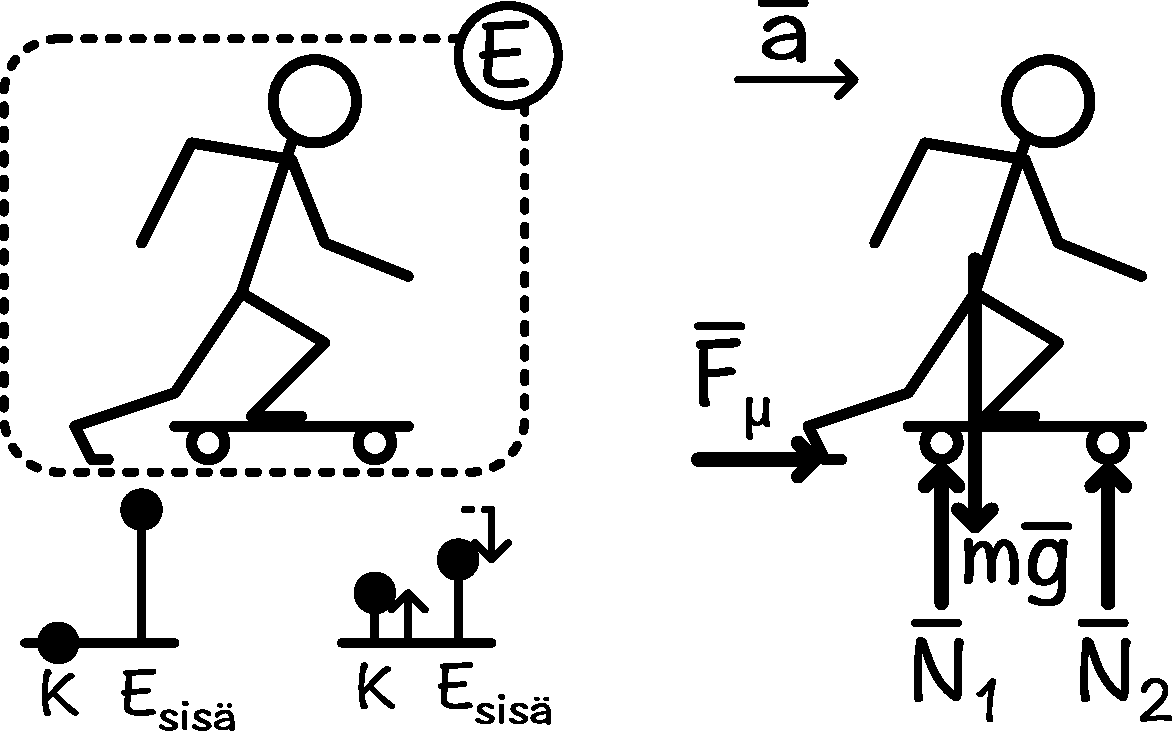
\includegraphics[width=0.95\textwidth]{figs/voima_esimerkki_skeitti.pdf}%
\end{center}%
}

 \eval  Voi olla outo tulos, että lautailijan liikkeelle työntävä voima ei tee lautailijaan työtä. Tämä kuitenkin johtuu siitä, että lautailija on moniosainen systeemi ja työtä tekevät \emph{lautailijan jalan lihakset} eikä maan pinta. Työhän mittaa energian siirtymistä, eikä maasta siirry energiaa lautailijaan. Sen sijaan prosessissa muuttuu lautailijaan varastoitunutta kemiallista energiaa lämpö- ja liike-energiaksi. Voimien avulla ilmaisten tämä ilmenee niin, että potkun aikana lautailijan jalka liikkuu, joten jalan eri osiin vaikuttavat voimat tekevät mekaanista työtä.

Tavallinen intuitiivinen käsitys voimasta on se, että voimia voivat tuottaa vain elolliset olennot tai korkeintaan moottorien kaltaiset laitteet. Tämä on kuitenkin aivan väärä käsitys, sillä myös paikoillaan pysyvä lattia kohdistaa sen päällä seisovaan ihmiseen voimia kuten tässäkin esimerkissä. \emph{Voiman} tuottaminen vaatii vain kappaleiden kosketuksen.
Intuitio on kuitenkin siinä mielessä oikeilla jäljillä, että paikoillaan pysyvä lattia ei pysty tekemään sen päällä seisovaan ihmiseen \emph{työtä} eli \emph{energiaa} ei siirry lattiasta ihmiseen.

\end{exam}

\subsection{Dissipatiivisten voimien työ}
\label{dissipatiivistenvoimientyö}

Myös dissipatiiviset voimat tekevät työtä, mutta tämä työ ei voi varastoitua potentiaalienergiaksi, koska dissipatiivisia vuorovaikutuksia ei voi kuvata potentiaalienergialla. Kappaleiden liike-energian muuttuminen lämpöenergiaksi kitkan vaikutuksesta on tyypillinen esimerkki dissipatiivisen vuorovaikutuksen tekemästä työstä.
Esimerkiksi kuvassa \autoref{fig:voimatyodissipatiivinen} (a) laatikkoa työnnetään pitkin maata. Tällöin työntäjä kohdistaa laatikkoon voiman laatikon liikkeen suuntaan ja liikekitka voiman vastakkaiseen suuntaan kuin mihin laatikko liikkuu. Siispä työntäjä tekee laatikkoon positiivista ja kitka negatiivista työtä. Työntäjän tekemä työ ilmenee häneen varastoituneen kemiallisen energian vähentymisenä ja laatikon liike-energian lisääntymisenä. Kitkan tekemä työ puolestaan ilmenee laatikon liike-energian vähenemisenä ja laatikon sekä lattian lämpöenergian lisääntymisenä. Lopputuloksena siis osa työntäjän käyttämästä energiasta muuttuu laatikon liikkeeksi ja osa lämpöenergiaksi.
Energiaa ei voi luoda, joten systeemin kokonaisenergia on silti vakio.

\index{dissipatiivinen}

Dissipatiivisten vuorovaikutusten ollessa merkittävät on systeemin valinnassa oltava erityisen huolellinen, jos tarkoitus on pitää kirjaa energian eri muotojen säilymisestä. Esimerkiksi lattialla liukuvaan kappaleeseen vaikuttava kitka muuttaa liike-energiaa lämpöenergiaksi eli sisäenergiaksi. Tämä sisäenergia kuitenkin jakautuu \emph{kaikkien} vuorovaikuttavien kappaleiden kesken, eikä \emph{yhden} kappaleen sisäenergian muutos prosessin lopussa välttämättä ole yhtä suuri kuin dissipatiivisen voiman siihen tekemä työ. Esimerkiksi liukuvan kappaleen ja lattian välinen kitka lämmittää sekä kappaletta että lattiaa. Niinpä jos systeeminä tarkastellaan vain työntäjää ja liukuvaa kappaletta kuten kuvassa \autoref{fig:voimatyodissipatiivinen} (b), systeemin sisäenergian muutos \emph{ei ole} yhtä suuri kuin laatikon liike-energian energian muutos, sillä osa tästä energiasta voi siirtyä systeemin ulkopuolelle, lattiaan. Tämän systeemin kokonaisenergia ei siis ole prosessissa vakio.

\pictures{tb}%
{Systeemin ulkoiset dissipatiiviset vuorovaikutukset voivat siirtää energiaa systeemin ja ympäristön välillä.;%
Dissipatiivinen vuorovaikutus systeemin sisällä: systeemin kokonaisenergia on vakio.;%
Dissipatiivinen vuorovaikutus systeemin reunalla: energiaa siirtyy systeemistä ympäristöön.}%
{fig:voimatyodissipatiivinen;fig:voimatyodissipatiivinen_a;fig:voimatyodissipatiivinen_b;}%
{0.4;0.4}%
{0.4;0.4}%
{voima_dissipatiivinen_1.pdf;voima_dissipatiivinen_2.pdf}

\index{lämpö}

Itse asiassa on mahdollista, että systeemin kokonaisenergia ei ole vakio, vaikka kaikkien systeemiin kohdistuvien ulkoisten voimien tekemä työ olisi nolla. Osoittautuu nimittäin, että energiaa voi siirtyä työn lisäksi myös \emph{lämpönä}, kuten vaikkapa kuuman kahvin jäähtyminen osoittaa. Käytännössä tämä tarkoittaa sitä, että koska lämpimien kappaleiden atomeilla on paljon epäjärjestynyttä liike-energiaa, kylmän kappaleen kanssa kontaktissa olevan lämpimän kappaleen atomit alkavat töniä myös kylmän kappaleen atomeja nopeampaan liikkeeseen itse samalla hidastuen. Mikroskooppisessa mittakaavassa tämäkin voidaan selittää atomien välisten voimien tekemänä työnä, mutta makroskooppisesta näkökulmasta lämpöenergia näyttää tällöin siirtyvän itsestään kappaleesta toiseen.
Lämmön kautta tapahtuvaa energian siirtymistä ja tähän liittyviä lainalaisuuksia kuvaa \emph{termodynamiikka}, johon tutustumme myöhemmin.

Energian säilymislain perusteella emme siis voi päätellä paljonko työntäjän, laatikon ja lattian sisäenergiat muuttuvat, joten vaikka tarkastelisimme systeemiä, johon nämä kaikki kuuluvat ja jonka energia on vakio, emme pysty suoraan päättelemään esimerkiksi laatikon saamaa liike-energiaa. Työn avulla voimme kuitenkin tämän selvittää. Laatikon työntäjältä saama liike-energia on nimittäin täsmälleen yhtä suuri kuin työntäjän laatikkoon tekemä työ. Vastaavasti kitka kuluttaa laatikon liike-energiaa täsmälleen kitkavoiman tekemän työn verran. Niinpä voimme määrittää laatikon liike-energian muutoksen siihen kohdistuvien voimien tekemänä kokonaistyönä.

\begin{stopQ}{q:tyonto_kitka_tyo}%
Työntäjä kohdistaa laatikkoon \(100 \un{N}\) vakiovoiman oikealle ja laatikkoon vaikuttaa \(80 \un{N}\) kitkavoima vasemmalle. Työntäjä työntää laatikkoa yhden metrin oikealle. (a) Paljonko laatikko saa työntäjältä liike-energiaa? (b) Paljonko laatikko menettää kitkan takia liike-energiaa? (c) Mikä on laatikon liike-energian muutos? (d) Mikä on työntäjän, laatikon, ilman ja lattian muodostaman systeemin sisäenergian kokonaismuutos?
\end{stopQ}

\begin{exam}{Dissipatiivinen työ}{ex:dissipatiivinentyo}\noindent

\problem{Auto ajaa loivaa mäkeä ylös. Mäen kaltevuuskulma on \(5^\circ\). Auton massa on 980 kg. Maanpinta kannattelee autoa \(9570 \un{N}\) kosketusvoimalla, renkaat työntävät autoa ylöspäin yhteensä \(1070 \un{N}\) voimalla ja ilmanvastus vastustaa liikettä \(60 \un{N}\) voimalla. (a) Paljonko työtä voimat tekevät, kun auto kulkee \(10 \un{m}\)?
(b) Millaisia muutoksia energian eri muodoissa tapahtuu? Piirrä energiadiagrammi.
}

\setup  Tilanne on täsmälleen sama kuin esimerkissä \autoref{ex:vektorisummaus}.
Merkitään jälleen mäen kaltevuuskulmaa \( \theta = 5^\circ \),
renkaiden työntövoimaa \( F_{\text{maa} \to \text{auto}} = 1070 \un{N} \),
ilmanvastusta \( F_{\text{ilma} \to \text{auto}} = 60 \un{N} \),
painovoiman komponenttia alamäen suuntaan \( G_{x,\text{maa} \to \text{auto}} = -840 \un{N} \) ja
auton siirtymää mäen suunnassa \(\Delta x = 10 \un{m}\).

\physics Ilmanvastus osoittaa auton liikettä vastaan, joten se tekee negatiivista työtä,
\begin{equation} W_\text{ilmanvastus} = - F_{\text{ilma} \to \text{auto}} \Delta x = -600 \un{J}. \end{equation}
Samoin painovoimalla on komponentti liikettä vastaan, joten sekin tekee negatiivista työtä,
\begin{equation} W_\text{painovoima} = G_{x,\text{maa} \to \text{auto}} \Delta x = -8400 \un{J}. \end{equation}
Voima, jolla maanpinta kannattelee autoa on puolestaan kohtisuorassa liikkeen suuntaa vastaan, joten se ei tee työtä lainkaan.

Voima, jolla renkaat työntävät autoa, osoittaa auton liikkeen suuntaan, mutta se ei vielä tarkoita, että tämä voima tekisi autoon työtä. Tämä voima nimittäin vaikuttaa aina pisteessä, jossa renkaat koskevat maata, ja jos renkaat eivät sudi, renkaan pinta on maata koskettaessaan hetkellisesti paikoillaan. Niinpä myöskään tämä voima ei tee autoon työtä. Tilanne on sama kuin esimerkissä \autoref{ex:skeitti}, jossa maanpinta ei tehnyt työtä jalkaan.

(b) Painovoiman tekemä työ muuttaa auton liike-energiaa painovoiman potentiaalienergiaksi. Ilmanvastuksen tekemä työ muuttaa auton liike-energiaa ilman liike-energiaksi ja lämpöenergiaksi. Lisäksi auton liikkeeseen liittyy muitakin dissipatiivisia vuorovaikutuksia kuten kitkaa ja vierimisvastusta, jotka muuttavat liike-energiaa lämpöenergiaksi. Jos kyseessä on polttomoottoriauto, polttoaineen palaminen muuttaa polttoaineen kemiallista energiaa lämpöenergiaksi, ja vain pieni osa tästä energiasta saadaan muutettua liike-energiaksi. Jos kyseessä on sähköauto, sen moottori muuntaa akkuun varastoitunutta sähköistä energiaa liike-energiaksi. Tällöinkin osa sähköisestä energiasta muuttuu väistämättä lämpöenergiaksi, mutta paljon suurempi osuus varastoituneesta energiasta saadaan muutettua liike-energiaksi kuin polttomoottorissa.

Autoon tehdään vain negatiivista työtä, joten sen kokonaisenergia pienenee,
\begin{equation} \Delta E_\text{auto,kokonais} = W_\text{ilmanvastus} + W_\text{painovoima} = -9 \un{kJ}. \end{equation}
Jos systeemiin otetaan mukaan myös autoa ympäröivä ilma ja maanpinta sekä painovoima, niiden kaikkien yhteinen kokonaisenergia on energian säilymislain perusteella välttämättä vakio.
Esimerkin \autoref{ex:vektorisummaus} perusteella autolla oli pieni kiihtyvyys ylämäkeen, jolloin sen vauhti ja siis liike-energia kasvaa.
Samalla myös painovoiman potentiaalienergia kasvaa ja auton, ilman sekä maan lämpöenergia kasvaa. Autoon varastoidun kemiallisen tai sähköisen energian täytyy siis vähentyä niin paljon, että se riittää kattamaan täsmälleen kaikkien muiden energian lajien lisääntymisen. Pelkästään annetuilla tiedoilla emme kuitenkaan voi päätellä, kuinka suuret nämä muutokset ovat.

Hahmotellaan vielä energiadiagrammi alussa ja lopussa. Koska tarkkoja arvoja ei voi laskea, diagrammi ei ole välttämättä oikeassa mittakaavassa. Joka tapauksessa polttoaineeseen tai akkuun varastoituneen energian täytyy olla hyvin suuri, koska sen täytyy riittää pitkillekin matkoille.

\begin{center}%
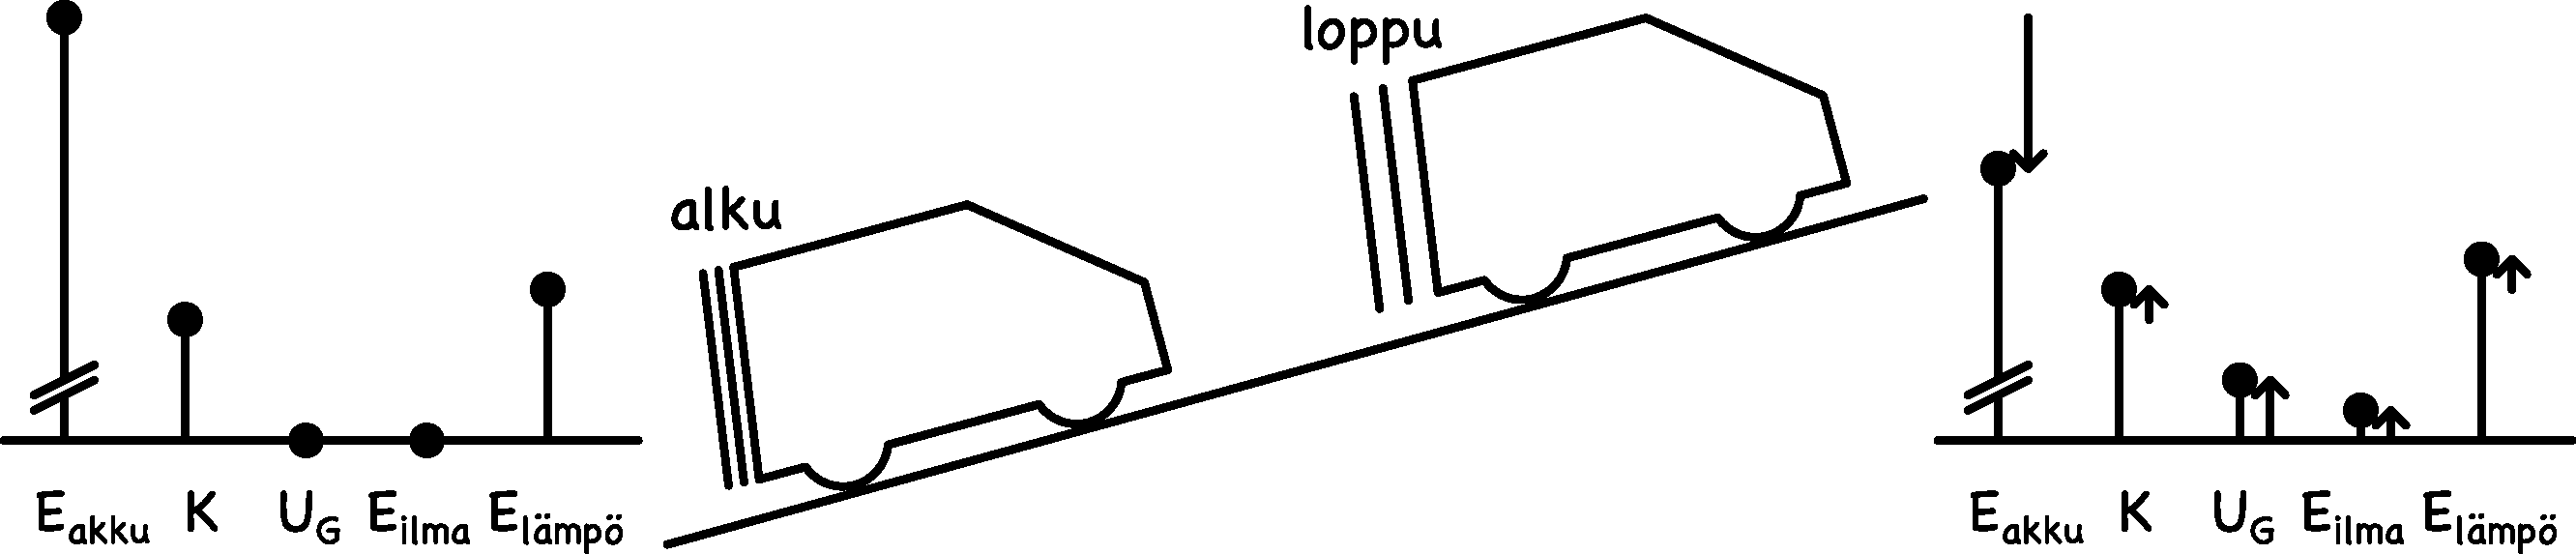
\includegraphics[width=0.95\textwidth]{figs/voima_esim_diagrammi.pdf}%
\end{center}%

\end{exam}

\subsection{Teho}
\label{teho}

\index{teho}

Energian säilymislakia sovellettaessa ei usein välitetä kuinka nopeasti prosessit tarkalleen tapahtuvat, koska lopputulos voidaan päätellä suoraan loppu- ja alkutilan perusteella. Sen sijaan systeemien dynamiikkaa tarkasteltaessa tapahtumien nopeus voi olla hyvinkin kiinnostavaa. Koska prosesseja voidaan lähes aina kuvata energian muuttumisena muodosta toiseen, prosessien nopeutta voidaan kuvata tarkastelemalla kuinka nopeasti tämä tapahtuu. Tätä kuvaava suure on \textbf{teho}, joka määritellään energian (jonkin muodon) derivaattana ajan suhteen
\bigeq{ P = \frac{\dd E}{\dd t}. }
Tehon yksikkö on watti
\begin{equation} \text{W} = [P] = \frac{[E]}{[t]} = \frac{\text{J}}{\text{s}} = {\text{kgm}^2/\text{s}^3}.\end{equation}

\pictures{b}%
{Teho kuvaa energian muutoksen nopeutta.;%
Kappaleen hitaaseen nostamiseen riittää pieni teho.;%
Kappaleen nopeaan nostamiseen tarvitaan suuri teho.}%
{fig:voimateho;fig:voimateho_a;fig:voimateho_b;}%
{0.55;0.35}%
{0.541;0.359}%
{voima_teho_1.pdf;voima_teho_2.pdf}

Voiman tekemän työn teho kuvaa sitä, kuinka nopeasti voiman kuvaama vuorovaikutus muuttaa energiaa muodosta toiseen. Esimerkiksi kappaleeseen vaikuttavan kokonaisvoiman teho ilmaisee kuinka nopeasti kappaleen liike-energia muuttuu. Työn määritelmän mukaisesti \(x\)-suunnassa liikkuvaan kappaleeseen vaikuttavan liikkeen suuntaisen voiman teho on
\begin{equation} P = \frac{\dd W}{\dd t} = F_x \frac{\dd x}{\dd t} = F_x v_x. \end{equation}
Siispä voima tekee kappaleeseen työtä sitä suuremmalla teholla, mitä nopeammin kappale liikkuu. Tämä johtuu yksinkertaisesti siitä, että työ riippuu \emph{matkasta}, jolla voima vaikuttaa, ja nopea kappale kulkee pitkän matkan lyhyessä ajassa. Esimerkiksi painovoimakentässä ylöspäin nousevan kappaleen potentiaalienergia kasvaa sitä suuremmalla teholla mitä nopeammin kappale nousee (kuva \autoref{fig:voimateho}).

Teho on keskeinen suure monissa energiansiirron käytännön sovelluksissa. Esimerkiksi jos auto pitää pystyä kiihdyttämään tiettyyn nopeuteen tietyssä ajassa, sen moottorin on pystyttävä tuottamaan tähän vaadittava teho. Vastaavasti jarrutuksessa kitka lämmittää jarrupaloja yhtä suurella teholla kuin millä auton liike-energia vähenee. Lämmitettäessä rakennusta tietyllä teholla pitää eristys mitoittaa niin, ettei rakenteiden kautta hukattu lämpöteho ole lämmitystehoa suurempi, sillä muuten rakennus jäähtyy. Tai päinvastoin jos tietokoneen prosessori kuumenee käytössä tietyllä teholla, lämpöä on kyettävä siirtämään pois yhtä tehokkaasti tai muuten laite ylikuumenee.

\begin{stopQ}{q:tehoharjoitus}%
Liukuvaan laatikkoon kohdistuu \(80 \un{N}\) kitkavoima. (a) Kuinka nopeasti laatikkoa voi työntää, jos käytettävissä on yhden hevosvoiman eli n. \(740 \un{W}\) teho? (b) Jos laatikkoa työnnetään \(160 \un{N}\) voimalla, kuinka suurella teholla tehdään työtä laatikon ollessa lähdössä liikkeelle (ts. laatikko ei vielä liiku).
\end{stopQ}

\begin{exam}{Moottorin teho}{ex:autoteho}\noindent

\problem{Auton massa on \(1400 \un{kg}\). Kuinka suuri keskimääräinen teho vaaditaan, jos auton pitää pystyä kiihdyttämään nopeudesta \(60 \un{km/h}\) nopeuteen \(100 \un{km/h}\) seitsemän sekunnin aikana? }

 \setup  Merkitään auton massaa \(m=1400 \un{kg}\) ja alku- ja loppunopeutta \(v_{\text{alku}} = 60 \un{km/h}\) sekä \(v_{\text{loppu}} = 100 \un{km/h}\). Olkoon kiihdytykseen tarvittu aika \(\Delta t = 7 \un{s}\).

\physics Kysytty teho on auton energian muutos jaettuna tähän muutokseen tarvitulla ajalla. Nopeudet on syytä muuttaa ensin SI-yksiköihin kertoimella \(\text{km/h} = \frac{10}{36} \un{m/s}.\) (Ks. esimerkki \autoref{ex:juna}).

 \model  Liike-energian muutos on \(\Delta K = \frac{1}{2}m(v_{\text{loppu}}^2 - v_{\text{alku}}^2\)) ja keskimääräinen teho \(P_\text{keskiarvo} = \frac{\Delta K}{\Delta t}.\)

\solu Liike-energia alussa on \(K_\text{alku} = \frac{1}{2}mv_{\text{alku}}^2 = 194 \un{kJ}\) ja lopussa \(K_\text{loppu} = \frac{1}{2}mv_{\text{loppu}}^2 = 540 \un{kJ}\). Liike-energian muutos on siis \(\Delta K = 346 \un{kJ}\) ja teho \(P = 49 \un{kW}\).

 \eval  Moottoreiden yhteydessä käytetään tehon yhteydessä usein vanhanaikaista yksikköä hevosvoima, joka on noin 740 W. Tarvittava teho on siis \(P = 49400 \un{W} / 740 \un{W/hv} \approx 67 \un{hv}\). Tämä ei ole polttomoottorille vielä kovin paljon, mutta kyseessä oli tarvittavan tehon keskiarvo, ja lisäksi moottorin tehosta vain pieni osa kuluu auton liike-energian kasvattamiseen. Polttoaineen kemiallisesta energiasta vain osa voidaan muuntaa moottorissa mekaaniseksi energiaksia ja esimerkiksi ilmanvastuksen autoon kohdistama voima tekee siihen jatkuvasti negatiivista työtä, ja osa moottorin tehosta kuluu tämän työn kattamiseksi.

\end{exam}

\startwidepage

\section*{Yhteenveto: \chaptertitle}
\addcontentsline{toc}{section}{Yhteenveto: \chaptertitle}
\noindent
\begin{tabular}{p{1.15\textwidth}}
\standout{Differentiaalit ja vektorit}{
\begin{multicols}{2}

\begin{itemize}
\item Vektorisuureita voidaan graafisesti esittää nuolina, joiden pituus kuvaa suureen suuruutta ja suunta suureen suuntaa.

\item Vektorisumma voidaan esittää graafisesti piirtämällä vektoreita kuvaavat nuolet peräkkäin. Tällöin vektorien summaa esittää ensimmäisen vektorin kannasta viimeisen vektorin kärkeen piirretty nuoli.

\item Vektorin \(\bs{A}\) \textbf{vektorikomponentti} \(\bs{A}_x\) suuntaan \(\uv{i}\) on tähän suuntaan osoittava vektori, joka ulottuu kyseisessä suunnassa yhtä pitkälle kuin vektori \(\bs{A}\). Vektorin voi esittää eri suuntaisten vektorikomponenttien summana
\begin{equation} \bs{A} = \bs{A}_x + \bs{A}_y + \bs{A}_z. \end{equation}

\item Vektorikomponentin pituus on yhtä suuri kuin vektorin skalaarikomponentin itseisarvo kyseiseen suuntaan
\begin{equation} \bs{A}_x = A_x \uv{i}. \end{equation}

\end{itemize}

\end{multicols}
}\\
\standout{Vapaakappalekuva}{
\begin{multicols}{2}

\begin{itemize}
\item \textbf{Voima} on suure, joka kuvaa vuorovaikutuksen vaikutusta kappaleen liikkeeseen ja muotoon. Voimalla on suuruus ja suunta eli se on \emph{vektorisuure}.

\item \textbf{Vapaakappalekuva} on graafinen esitys, johon merkitään kaikki yhteen kappaleeseen vaikutavat voimat.

\item Kappaleeseen vaikuttava \textbf{kokonaisvoima} on siihen vaikuttavien voimien \textbf{vektorisumma}
\begin{equation} \bs{F}_\text{kokonais} = \sum_i \bs{F}_i. \nonumber \end{equation}

\end{itemize}

\end{multicols}
} \\
\standout{Newtonin lait}{
\begin{multicols}{2}

\begin{itemize}
\item Jos kappaleeseen vaikuttava kokonaisvoima on nolla, se liikkuu tasaisella nopeudella. Tämä on \textbf{jatkavuuden laki}.

\item Kappaleen liikemäärän muutosnopeus on yhtä suuri kuin siihen vaikuttava kokonaisvoima
\begin{equation} \bs{F}_\text{kokonais} = \frac{\dd \bs{p}}{\dd t}. \nonumber \end{equation}
Tämä on \textbf{dynamiikan peruslaki}.

\item Jos kappaleet A ja B vuorovaikuttavat ja vuorovaikutus kohdistaa kappaleeseen A voiman \(\bs{F}_{B \to A}\), vuorovaikutus kohdistaa kappaleeseen B voiman \(\bs{F}_{A \to B}\). Nämä voimat ovat yhtä suuret mutta vastakkaissuuntaiset
\begin{equation} \bs{F}_{A \to B} = - \bs{F}_{B \to A}. \nonumber \end{equation}
Tämä on \textbf{voiman ja vastavoiman laki}.

\end{itemize}

\end{multicols}
}\\
\standout{Vuorovaikutuksia}{
\begin{multicols}{2}

\begin{itemize}
\item Elastinen muodonmuutos (kuten jousi) tuottaa voiman, joka osoittaa aina kohti tasapainopistettä ja jonka suuruus on verrannollinen pituuden muutokseen
\begin{equation} \bs{F}_\text{elastinen} = -k (x-x_0) \uv{i}. \nonumber \end{equation}

\item Gravitaatio tuottaa voiman, jonka suuruus on verrannollinen kappaleiden massaan ja suunta on aina alaspäin
\begin{equation} \bs{F}_\text{gravitaatio} = m\bs{g} = -mg\uv{i}. \nonumber \end{equation}

\item Pinnan tukivoima eli \textbf{normaalivoima} \(\bs{N}\) on koskettavien kappaleiden välinen voima, joka estää kappaleita liikkumasta toistensa lävitse. Normaalivoiman suunta on aina kohtisuoraan kosketuspintaa vastaan ja sen suuruus määräytyy niin, että kappale ei saa liikkua pinnan läpi.

\item \textbf{Liikekitka} tuottaa voiman, joka pyrkii hidastamaan pinnalla liukuvan kappaleen nopeutta \emph{pinnan suhteen}. Liikekitkan suuruus on suoraan verrannollinen pinnan ja kappaleen väliseen normaalivoimaan sekä pintojen \textbf{liikekitkakertoimeen} \(\mu\) ja sen suunta on aina vastakkainen kappaleen pinnan suhteen mitattuun nopeuteen nähden,
\begin{equation} F_\text{liikekitka} = \mu N. \nonumber \end{equation}

\item \textbf{Lepokitka} tuottaa voiman, joka pyrkii estämään kappaleiden välisiä kosketuspintoja liikkumasta toistensa suhteen. Lepokitkan suuruus määräytyy ehdosta, että kappale ei saa liikkua alustansa suhteen.
Lepokitkalla on kappaleen ja pinnan välisestä normaalivoimasta sekä pintojen \textbf{lepokitkakertoimesta} \(\mu_\text{lepo}\) riippuva \emph{maksimisuuruus},
\begin{equation} F_\text{lepokitka} \le \mu_\text{lepo} N. \nonumber \end{equation}

\end{itemize}

\end{multicols}
} \\
\standout{Sanasto}{
\begin{multicols}{2}

\begin{itemize}
\item voima (force)

\item vapaakappalekuva (free body diagram)

\item vektorisumma (vector sum)

\item vektorikomponentti (vector component)

\item yhdensuuntainen (parallel)

\item kohtisuora (perpendicular)

\item voimien superpositio (superposition of forces)

\item Newtonin lait (Newton's laws)

\item jatkavuuden laki (law of inertia)

\item dynamiikan peruslaki (Newton's equation of motion)

\item voiman ja vastavoiman laki (law of action and reaction)

\item jousivoima (spring force)

\item Hooken laki (Hooke's law)

\item jäykkä kappale (rigid body)

\item vakaa tasapaino (stable equilibrium)

\item epämääräinen tasapaino (neutral equilibrium)

\item epävakaa tasapaino (unstable equilibrium)

\item elastisuus (elasticity)

\item plastisuus (plasticity)

\item jännitys (tension)

\item normaalivoima (normal force)

\item lepokitka (static friction)

\item liikekitka (kinetic friction)

\item kitkakerroin (coefficient of friction)

\item potentiaalikuoppa (potential well)

\item työ (work)

\item työ-energiateoreema (work-energy theorem)

\item teho (power)

\end{itemize}

\end{multicols}
}
\end{tabular}
\newpage

\noindent
\begin{tabular}{p{1.15\textwidth}}
\standout{Voima, ty\"o ja impulssi}{
\begin{multicols}{2}

\begin{itemize}
\item Vuorovaikutuksen tekemä \textbf{työ} mittaa vuorovaikutuksen aiheuttamaa muutosta energiassa.

\item Vuorovaikutuksen tuottama impulssi mittaa vuorovaikutuksen aiheuttamaa muutosta liikemäärässä.

\item Jos kappaleeseen vaikuttaa \(x\)-suuntainen \emph{vakiovoima} \(\bs{F} = F_x\uv{i}\) ja kappale siirtyy \(x\)-suunnassa matkan \(\Delta x\), voima tekee kappaleeseen \emph{työn}
\begin{equation} W = F_x \Delta x. \nonumber \end{equation}

\item Jos kappaleeseen vaikuttaa \(x\)-suuntainen paikasta riippuva voima \(\bs{F} = F_x\uv{i}\) ja kappale liikkuu \(x\)-suunnassa pisteestä \(x_\text{alku}\) pisteeseen \(x_\text{loppu}\), voima tekee kappaleeseen työn
\begin{equation} W = \int_{x_\text{alku}}^{x_\text{loppu}} F_x \dd x. \nonumber \end{equation}

\item Kappaleen liike-energian muutos on aina yhtä suuri kuin \emph{kokonaisvoiman} kappaleeseen tekemä työ
\begin{equation} \Delta K = W_\text{kokonais}. \nonumber \end{equation}

\item Konservatiivinen vuorovaikutus, johon liittyy koordinaatista \(x\) riippuva potentiaalienergia \(U(x) \), tuottaa voiman
\begin{equation} \bs{F} = -\frac{\dd U}{\dd x}\uv{i}. \nonumber\end{equation}
Tämä voima on vektori, jonka suunta on aina \emph{pienenevän potentiaalienergian suuntaan} ja suuruus on \emph{sitä suurempi mitä nopeammin potentiaalienergia muuttuu paikan suhteen}.

\item Konservatiiviseen \(x\)-suuntaiseen voimaan \(\bs{F} = F_x\uv{i}\) liittyvä potentiaalienergia on yhtä suuri mutta vastakkaismerkkinen kuin voiman kappaleeseen tekemä työ
\begin{equation} U(x) = -W_{x_0 \to x} = -\int_{x_0}^{x} F_x \dd x. \nonumber \end{equation}

\item \textbf{Teho} on \emph{energian muutosnopeutta} esittävä suure
\begin{equation} P = \frac{\dd E}{\dd t}. \nonumber \end{equation}

\item Suuntaan \(x\) nopeudella \(v_x\) liikkuvaan kappaleeseen vaikuttava voima \(\bs{F} = F_x\uv{i}\) tekee kappaleeseen työtä teholla \begin{equation} P = F_x v_x. \nonumber \end{equation}

\item Jos kappaleeseen vaikuttaa ajasta riippuva voima aikavälillä \(t_\text{alku} \ldots t_\text{loppu}\), kappaleen saama \emph{impulssi} on dynamiikan peruslain mukaisesti
\begin{equation} \Delta \bs{p} = \bs{I} = \int_{t_\text{alku}}^{t_\text{loppu}} \bs{F} \dd t. \nonumber \end{equation}
Impulssin \(x\)-suuntainen skalaarikomponentti saadaan vastaavasti voiman skalaarikomponentin integraalina
\begin{equation} I_x = \int_{t_\text{alku}}^{t_\text{loppu}} F_x \dd t. \nonumber \end{equation}

\end{itemize}

\end{multicols}
} 

\end{tabular}


\begin{table}[hb]
\caption{Voiman, työn ja impulssin ominaisuuksia. Huomaa, että koska voima ja impulssi ovat vektoreita, niiden skalaarikomponenttien merkki riippuu koordinaatistosta. Energia on skalaari, joten sen etumerkkiin koordinaatiston valinta ei vaikuta.
}
\begin{center}
\bgroup
\def\arraystretch{1.1}
\begin{tabular}{rccc}
 & \textbf{voima} & \textbf{impulssi} & \textbf{ty\"o} \\
\textbf{tyyppi} & vektori & vektori & skalaari \\
\textbf{yhteys voimaan} & - & ajan integraali & paikan integraali \\
\textbf{muuttaa} & - & liikem\"a\"ar\"a\"a & energiaa \\
\textbf{positiivinen kun} & voima $x$-suuntaan$^*$ & voima $x$-suuntaan$^*$ & voima siirtym\"an suuntaan
\end{tabular}\\
\vspace*{3mm}
$^*$: P\"atee skalaarikomponentille $F_x$ tai $I_x$.
\egroup
\end{center}
\end{table}

\newpage

\newpage\begin{answers}\noindent

\stopA{q:usean_voiman_summa}{%
Jos kappaleeseen kohdistuu yksi voima (ei nolla), tämä on myös kokonaisvoima, joka siis ei ole nolla. Jos voimia on kaksi tai useampia, on aina mahdollista, että voimien summa on nolla, koska vastakkaissuuntaiset voimat voivat kumota toisensa. Kaksi erisuuruista voimaa ei kuitenkaan voi kumota toisiaan. Samoin kolme yhtä suurta voimaa ei voi kumota toisiaan, jos voimat ovat yhdensuuntaiset. Kuitenkin jos voimat saavat osoittaa eri suuntiin, ne voivat kumota toisensa, kunhan voimien vektorisumma on nolla.
}

\stopA{q:tasapaino}{%
Tasapainotiloja ovat (a) ja (b), koska näissä liikut tasaisella nopeudella (joka on paikoilla seisoessa nolla) ja sinuun kohdistuva kokonaisvoima on nolla. Tilat (c) ja (d) eivät ole tasapainossa. Ponnistuksessa olet kiihtyvässä liikkeessä ylöspäin, joten sinuun täytyy kohdistua kokonaisvoima ylöspäin. Tämän voiman tuottaa jalkojen ja maanpinnan välinen kosketusvuorovaikutus. Ilmalennon aikana olet puolestaan kiihtyvässä liikkeessä alaspäin, koska sinuun kohdistuu painovoima. Tämä pätee koko ilmalennon ajan ml. hypyn lakipisteessä, jossa nopeus on hetkellisesti nolla.
}

\stopA{q:voiman_etumerkki}{%
Kappaleeseen kohdistuvan kiihtyvyyden täytyy osoittaa positiiviseen \(x\)-suuntaan, joten myös kokonaisvoiman täytyy osoittaa tähän suuntaan. Siis \(F_x > 0\). Jos voima on vakio, kappale on kiihtyvässä liikkeessä positiiviseen \(x\)-suuntaan myös pysähdyttyään, jolloin kappale saa siis positiivisen nopeuden, jonka itseisarvo kasvaa. Ts. kappale kääntyy ympäri ja sen vauhti alkaa kasvaa.
}

\stopA{q:miten_kokonaisvoima}{%
Voima ja vastavoima kohdistuvat aina eri kappaleisiin. Jos kappaleeseen A kohdistuu voima \(\bs{F}_{B \to A}\), tämän vastavoima \(\bs{F}_{A \to B}\) kohdistuu kappaleeseen B. Jos nämä ovat ainoat kappaleisiin kohdistuvat voimat, kappaleeseen A kohdistuu siis kokonaisvoima \(\bs{F}_{B \to A}\) ja B:hen kokonaisvoima \(\bs{F}_{A \to B}\) eikä näistä kumpikaan ole nolla. Voiman ja vastavoiman laki on aivan eri asia kuin tasapainoehto!
}

\stopA{q:etsi_vastavoimat}{%
(a) Kosketusvoima, jolla pallo painaa kättäsi.\\
(b) Painovoima, jolla sinä vedät maata puoleesi.\\
(c) Kosketusvoima, jolla sinä painat maanpintaa.
}

\stopA{q:ylos_vai_alas}{%
Tilannetta ei voi päätellä kuvasta. Ponnistuksessa hyppääjän nopeus muuttuu nollasta ylöspäin osoittavaksi vektoriksi, joten hyppääjän kiihtyvyysvektori osoittaa nopeuden muutoksen suuntaan eli ylöspäin. Mutta laskeutumisessa nopeus muuttuu alaspäin osoittavasta nollaksi, jolloin kiihtyvyysvektori osoittaa jälleen nopeuden muutoksen suuntaan eli ylöspäin. Kuva voi siis esittää sekä ponnistusta että laskeutumista. Voit todeta tämän itsekin. Tee tasajalkahyppy suoraan ylöspäin. Tunnet jalkapohjiesi puristuvan maanpintaa vasten normaalia voimakkaammin sekä ponnistuksessa että laskeutumisessa.
}

\stopA{q:sisaisia_voimia_vkk}{%
Jalat kohdistavat kehoon voiman ylöspäin. Tämä voima työntää kehoa ylöspäin. Keho puolestaan kohdistaa voiman ja vastavoiman lain mukaisesti jalkoihin yhtä suuren voiman alaspäin. Jos tarkastelemme systeeminä koko hyppääjää, näiden voimien kokonaisvaikutus systeemiin on nolla, koska ne ovat yhtä suuret mutta vastakkaissuuntaiset. Voimat eivät siis muuta hyppääjän massakeskipisteen liikettä mitenkään. (Nämä ovat systeemin sisäisiä voimia, jotka eivät voi muuttaa systeemin kokonaisliikemäärää.) Hyppääjän massakeskipiste lähtee liikkeelle ylöspäin siksi, että jalkojen painuminen maanpintaa vasten voimistaa jalkojen ja maanpinnan välistä kosketusvuorovaikutusta. Maanpinta kohdistaa siis hyppääjän jalkoihin suuren voiman ylöspäin, ja tämä (ulkoinen) voima työntää hyppääjän liikkeelle ylöspäin.
}

\stopA{q:kolmioepayhtalo}{%
(a) \(|\bs{A} + \bs{B}|\) on sama kuin \(A + B\) vain jos vektorit ovat samansuuntaiset.\\
(b) On. Vektorien pitää vain olla sopivassa asennossa niin, että niiden summavektori on yhtä pitkä kuin vektori \(\bs{A}\). Esimerkiksi jos kummankin vektorin pituus on 1 ja vektorien välinen kulma on \(120^\circ\), myös summavektorin pituus on 1.
}

\stopA{q:harjoitellaan_komponentteja}{%
Voiman A skalaarikomponentit ovat \(F_{x,A} = 1.5 \un{N}\) ja \(F_{y,A} = -1.1 \un{N}\). Voiman B skalaarikomponentit voidaan puolestaan ratkaista trigonometrialla, jolloin saadaan
\(F_{x,B} = ( 2.0 \un{N}) \cos 150^\circ \approx -1.7 \un{N}\) ja
\(F_{y,B} = ( 2.0 \un{N}) \sin 150^\circ = 1.0 \un{N}\). Kokonaisvoiman skalaarikomponentit ovat siis
\(F_{x,\text{kokonais}} = F_{x,A} + F_{x,B} = -0.2 \un{N} \) sekä
\(F_{y,\text{kokonais}} = F_{y,A} + F_{y,B} = -0.1 \un{N} \).
Kokonaisvoiman \(x\)-komponentin pituus on siis \(0.2 \un{N}\) ja se osoittaa negatiiviseen \(x\)-suuntaan. Voiman \(y\)-komponentin pituus on puolestaan \(0.1 \un{N}\) ja se osoittaa negatiiviseen \(y\)-suuntaan. Kokonaisvoimavektori osoittaa siis alaviistoon vasemmalle.
}

\stopA{q:potentiaalienergian_etumerkkeja}{%
Nopeus on \(v_x = -0.5 \un{m/s}\), kun positiivinen suunta on ylöspäin. Tällöin potentiaalienergia muuttuu ajassa \(\Delta t = 1 \un{s}\) määrän \(\Delta U / \Delta t = m g \Delta x / \Delta t = mgv_x = -4.9 \un{J/s}\). Siis \(\dd U / \dd t < 0\). Potentiaalienergia kasvaa koordinaatin \(x\) kasvaessa, joten \(\dd U / \dd x > 0\).
Jos \(x\)-akseli osoittaakin alaspäin, potentiaalienergia pienenee koordinaatin \(x\)-kasvaessa, koska tällöin siirrytään alaspäin, \(\dd U / \dd x < 0\). Muutos ajan suhteen ei kuitenkaan muutu, koska alaspäin liikkuvan kappaleen potentiaalienergia pienenee riippumatta koordinaatiston valinnasta, \(\dd U / \dd t < 0\).
}

\stopA{q:harjoitellaan_derivaattoja}{%
Nyt \(v_{x,\text{alku}} = 3.0 \un{m/s}\) ja \(a_x = -0.5 \un{m/s}^2\). Ajassa \(\Delta t = 0.01 \un{s}\) nopeuden muutos on \(\Delta v_x = a_x \Delta t = -0.005 \un{m/s}\), joten nopeus tämän ajan kuluttua on \(v_{x,\text{loppu}} = 2.995 \un{m/s}\).\\
(a) Liike-energian muutos on siis
\begin{equation} \Delta K = \frac{1}{2}m ( v_{x,\text{loppu}}^2 - v_{x,\text{alku}}^2 ) = -0.0149875 \un{J}. \end{equation}
(b) Tämän suhde ajan muutokseen on
\begin{equation} \frac{\Delta K}{\Delta t} = -1.49875 \un{J/s}. \end{equation}
(c) Yhtälön (\autoref{k_muunnos}) mukaan
\begin{equation} \frac{\Delta K}{\Delta t} \approx \frac{\dd K}{\dd t} = m v_x a_x. \end{equation}
jos nopeudelle käytetään sen alkuarvoa \(v_{x,\text{alku}} = 3.0 \un{m/s}\), yhtälö antaa suhteeksi \(-1.5 \un{J/s}\). Jos nopeudelle käytetään sen keskiarvoa tarkasteltavalla aikavälillä, \(v_{x,\text{keskiarvo}} = 2.9975 \un{m/s}\), suhteeksi saadaan \(-1.49875 \un{J/s}\) eli täsmälleen sama tulos kuin kohdassa (b).
}

\stopA{q:voiman_kuvaajan_luku}{%
Voiman kuvaaja on laskeva suora, kun kappaleeseen kohdistuu jousen tuottama voima, sillä tämän voiman suuruus riippuu jousen puristumasta ja siten myös kappaleen paikasta. Kun kappale kohoaa tarpeeksi korkealle, siihen kohdistuu enää painovoima, joka on vakio. Tällöin voiman kuvaaja on suora. Potentiaalienergian kuvaajassa tämä näkyy niin, että kun voiman kuvaaja on laskeva suora, potentiaalienergian kuvaaja on ylöspäin aukeava paraabeli. Kun voiman kuvaaja on vaakasuora, potentiaalienergian kuvaaja on suora.
}

\stopA{q:potentiaalienergia_voima_nollakohta}{%
Energian nollakohta ei voi vaikuttaa voimaan, koska painovoiman suuruus ei riipu siitä, miten valitsemme koordinaatiston. Se on aina vakio. Potentiaalienergia sen sijaan riippuu siitä, kuinka korkealle kappale nostetaan, joten se riippuu kiintopisteen valinnasta. Matemaattisesti kyse on siitä, että vaikka potentiaalienergiaan \(U\) lisättäisiin mikä tahansa vakio, tämä vakio ei vaikuta potentiaalienergian derivaattaan eli voimaan.
}

\stopA{q:jousivakio_graafinen_esitys}{%
Jos jousivakio on suuri, voiman kuvaaja on jyrkästi laskeva suora ja potentiaalienergian kuvaaja kapea, jyrkkäreunainen paraabeli. Tällöin jousi on jäykkä. Jos jousta venytetään liikaa, se ei enää käyttäydy elastisesti. Tällöin jousi ei vastusta enää venytystä voimalla, joka kasvaa pituuden lisääntyessä, vaan venytystä vastustava voima on tyypillisesti Hooken lain ennustamaa voimaa pienempi, mahdollisesti jopa jousen pituudesta riippumaton vakio. Voiman kuvaaja on siis laskeva suora vain tarpeeksi pienillä venymillä ja suurilla venymillä se voi muuttua esimerkiksi vaakasuoraksi.
}

\stopA{q:jousen_muoto}{%
Ero johtuu kappaleen muodosta. Jousessa tanko muodostaa spiraalin, ja kun jousta puristetaan kokoon, spiraalin muodostava terästanko kiertyy mutta ei puristu kasaan. Teräs vastustaa puristusta voimakkaasti mutta kiertoa ja taivutusta paljon heikommin. Samasta syystä esimerkiksi paperiarkki on helppo repiä ottamalla kiinni arkin yhdestä reunasta kahdesta kohdasta ja vetämällä eri suuntiin, koska paperi ei pysty vastustamaan tällaista leikkaavaa repimistä kovin hyvin. Paperia on sen sijaan vaikea repiä ottamalla kiinni arkin vastakkaisista reunoista ja vetämällä näitä reunoja erilleen, koska paperi vastustaa venytystä voimakkaasti.
}

\stopA{q:kaksi_nostajaa}{%
Merkitään köyden yläpäähän kohdistuvaa vetävää voimaa \(\bs{F}_A\) ja keskikohtaan kohdistuvaa voimaa \(\bs{F}_B\). Jos köyden massa on hyvin pieni, voimme jättää köyteen kohdistuvan painovoiman huomioimatta ja köyteen kohdistuvan kokonaisvoiman täytyy olla likimain nolla. Niinpä köyden alapäähän täytyy kohdistua voima \(\bs{F} = -\bs{F}_A - \bs{F}_B\). Köyden alapäässä kiinni olevaan kappaleeseen kohdistuu siis voima \(-\bs{F} = \bs{F}_A + \bs{F}_B\). Köysi siis välittää molemmat sitä ylöspäin vetävät voimat sen päässä roikkuvaan kappaleeseen.
}

\stopA{q:normaalivoiman_paattely}{%
Kappale ei saa pudota hissin lattian läpi, joten kappaleeseen kohdistuvan kokonaisvoiman täytyy olla nolla ja normaalivoiman täytyy kumota kappaleeseen kohdistuva painovoima. Siis \(N_x = -G_x = -m g = 9.8 \un{N}\), kun valitaan \(x\)-akseli ylöspäin.\\
(b) Kappaleeseen täytyy kohdistua kokonaisvoima \(F_x = N_x + G_x = m a_x = 1.0 \un{N}\) ylöspäin. Siispä normaalivoiman pitää olla painovoimaa suurempi, \(N_x = F_x - G_x = 10.8 \un{N}\).\\
(c) Jos hissi liikkuu tasaisella nopeudella, kappale on tasapainossa ja siihen kohdistuva kokonaisvoima on nolla. Tilanne on siis sama kuin kohdassa a, \(N_x = 9.8 \un{N}\).\\
(d) Laskussa kappaleeseen kohdistuu kokonaisvoima \(F_x = m a_x = -3.0 \un{N}\). Siispä normaalivoima on pienempi kuin painovoima, \(N_x = 6.8 \un{N}\).
}

\stopA{q:potkulautailijan_lahto_ja_jarrutus}{%
(a) Liikemäärää muuttaa jalan ja maanpinnan välinen lepokitkavoima. Voiman lautailijaan kohdistaa siis maanpinta. Voiman suunta on eteenpäin, jos jalalla työnnetään taaksepäin, sillä lepokitka estää jalkaa liukumasta maanpinnan suhteen. Voiman suuruus voitaisiin päätellä mittaamalla lautailijan kiihtyvyys.\\
Liike-energian lautailija saa omista kemiallisen energian varastoistaan. Hän on syönyt ruokaa ja käyttää ruoan energiaa liikkuakseen.
(b) Jarrutuksessa vaikuttaa liikekitka lautailijan kengän ja pyörän välillä (koska pyörä edelleen pyörii ja pyörän pinta siis liikkuu kengän pinnan suhteen) sekä lepokitka pyörän ja maanpinnan välillä (sillä pyörä ei liu'u maanpinnan suhteen vaan vierii). Valitaan systeemiksi pyöräilijä ja potkulauta. Kengän ja pyörän välinen liikekitka on dissipatiivinen vuorovaikutus, joka muuttaa systeemin liike-energiaa lämpöenergiaksi. Se on kuitenkin systeemin sisäinen vuorovaikutus, joten se ei voi muuttaa systeemin liikemäärää. Systeemin liikemäärää muuttaa pyörän ja maanpinnan välinen lepokitka, joka on ulkoinen vuorovaikutus. On ehkä yllättävää, että energian ja liikemäärän muutokset johtuvat eri voimista, mutta mieti mitä tapahtuu, jos potkulauta rullaisi hyvin liukkaalla jäällä, jolla renkaan ja maanpinnan välillä ei ole juurikaan kitkaa. Tällöin jarruttaminen pysäyttäisi kyllä renkaan pyörimisen (tämä muuttaa liike-energiaa lämpöenergiaksi), mutta lautailija itsessään jatkaisi matkaansa suoraan jäällä liukuen, koska systeemin sisäinen vuorovaikutus ei voi muuttaa systeemin liikemäärää.
}

\stopA{q:gravitaation_impulssi}{%
Kappaleeseen kohdistuu voima \(F_x = mg = 9.8 \un{N}\).\\
(a) Voima antaa impulssin \(I_x = F_x \Delta t = 9.8 \un{Ns}\).\\
(b, c) Liikemäärän muutos on sama kuin impulssi, \(\Delta p_x = I_x = 9.8 \un{Ns}\). Tämä ei riipu alkunopeudesta.\\
}

\stopA{q:mekaanisen_tyon_maaritelma}{%
(a, b) Vakiovoiman työ on voiman ja sen vaikutuspisteen voiman suuntaisen siirtymän tulo, \(W = F_x \Delta x = m g \Delta x = 9.4 \un{J}\). Tämä ei riipu siitä, kuinka nopeasti prosessi tapahtuu.\\
(c, d) Jos nostat kymmenen kappaletta, teet kymmenkertaisen työn, \(W = 94 \un{J}\).\\
(e) Jos voiman vaikutuspiste ei liiku, työtä ei tehdä, \(W = 0 \un{J}\). Kannattelu kyllä väsyttää, mutta tämä johtuu siitä, että jännitetyt lihakset joutuvat käyttämään kemiallista energiaa myös staattisessa rasituksessa. Energia ei kuitenkaan tällöin muutu kannateltavan kappaleen potentiaalienergiaksi vaan lihasten lämpöenergiaksi, joten kappaleeseen ei tehdä työtä.
}

\stopA{q:tyo_pallon_heitossa}{%
(a) Koska pallon kokonaisenergian muutos on \(3 \un{J}\), palloon tehdyn työn täytyy olla myös \(3 \un{J}\).\\
(b) Painovoima tekee palloon työn \(- 1 \un{J}\). Tämä työ siis vähentää pallon liike-energiaa yhden joulen ja muuttaa sen painovoiman potentiaalienergiaksi, jolloin potentiaalienergia lisääntyy yhden joulen.\\
(c) Pallo tekee heittäjään työn \(-3 \un{J}\). Tämän työn tekee heittäjän palloon kohdistaman voiman vastavoima (pallon heittäjän käteen kohdistama voima).\\
(d) Heittäjään varastoitunutta kemiallista energiaa muuttuu lämpöenergiaksi ja heittäjän käden liike-energiaksi. Kolme joulea energiaa siirtyy myös heittäjästä palloon. Työ mittaa juuri tätä energian siirtymää. Koska pallo saa heittäjältä energiaa, heittäjä tekee palloon positiivisen työn, ja koska heittäjä luovuttaa energiaa pallolle, pallo tekee heittäjään negatiivisen työn.\\
(e) On, likimain. Energiaa siirtyy heittäjältä pallolle, mutta systeemin kokonaisenergian määrä ei muutu. Tämä ei ole täsmälleen totta, koska systeemistä voi siirtyä energiaa esimerkiksi äänenä ja lämpönä ympäröivään ilmaan.
}

\stopA{q:impulssi_tyo_kuvaajina}{%
Kun voima on vakio, kappale on tasaisesti kiihtyvässä liikkeessä.\\
(a) Impulssi on voiman integraali ajan suhteen, ja kun voima on vakio, impulssi kasvaa lineaarisesti ajan kuluessa, \(I_x = F_x t\). Kuvaaja on siis origon kautta kulkeva nouseva suora, jonka kulmakerroin on \(F_x\).\\
(b) Kappaleen paikka on \(x = \frac{1}{2} \frac{F_x}{m} t^2\), joten pisteeseen \(x\) pääsyyn kuluu aikaa \(t = \sqrt{2 m x / F_x}\) ja impulssi on \(I_x = \sqrt{2 m F_x x}\). Kuvaaja on siis neliöjuuren kuvaajan muotoinen (sivulle aukeava paraabeli).\\
(c) Kappaleeseen tehty työ on suoraan verrannollinen siirtymään, joten \(W = F_x x\) ja kuvaaja on nouseva suora.\\
(d) Työn riippuvuus ajasta on nyt \(W = \frac{1}{2} \frac{F_x^2}{m} t^2\), joten kuvaaja on ylöspäin aukeava paraabeli.
}

\stopA{q:halfpipe}{%
(a) Tuottaa. Impulssi on voiman integraali ajan suhteen, ja maanpinta kohdistaa lautaan voiman. Jos lauta on alussa ja lopussa paikoillaan, sen liikemäärän muutos on nolla. Painovoima tuottaa lautaan prosessin aikana impulssin alaspäin, joten normaalivoiman täytyy tuottaa impulssi ylöspäin niin, että kokonaisimpulssi on nolla. Jos normaalivoima ei tuottaisi impulssia, lautailija saisi impulssin vain painovoimalta, jolloin liikemäärä muuttuisi suoraan alaspäin ja ilmeisesti lautailijan pitäisi upota maan sisään.\\
(b) Ei tee. Jos lattia ei jousta ja lauta liikkuu aina pinnan suuntaan nähden kohtisuoraan, voima ja laudan siirtymän suunta ovat koko ajan toisiinsa nähden kohtisuorassa. Voiman komponentti liikkeen suunnassa on siis aina nolla eikä voima tee työtä. Tämä tarkoittaa sitä, että lautaan tekee työtä vain painovoima, ja tämä työ muuttaa painovoiman potentiaalienergiaa laudan liike-energiaksi ja takaisin. Todellisuudessa lautailijaan vaikuttaa toki myös ilmanvastus sekä renkaiden kitka ja vierimisvastus, mutta nämä ovat eri asia kuin normaalivoima.
}

\stopA{q:jousen_potentiaalienergia_tyosta}{%
Integroidaan voima paikan suhteen. Jos valitaan potentiaalienergian nollakohdaksi tasapainopiste \(x_0\), saadaan
\begin{equation} U(x) = - \int_{x_0}^x -k(x-x_0) \dd x = \bigg|_{x_0}^x \frac{1}{2}k(x-x_0)^2 = \frac{1}{2}k(x-x_0)^2. \end{equation}
Tämä on harmonisen potentiaalienergian lauseke kuten pitääkin.
Jos potentiaalienergian nollkohta ei ole tasapainopisteessä, potentiaalienergia on
\begin{equation} U(x) = - \int_{x_1}^x -k(x-x_0) \dd x = \bigg|_{x_1}^x \frac{1}{2}k(x-x_0)^2 = \frac{1}{2}k(x-x_0)^2 - \frac{1}{2}k(x_1-x_0)^2. \end{equation}
Nyt energia tasapainopisteessä on \( U(x_0) = -\frac{1}{2}k(x_1-x_0)^2 \), joten voidaan kirjoittaa
\begin{equation} U(x) = U(x_0) + \frac{1}{2}k(x-x_0)^2. \end{equation}
Tämä on harmonisen potentiaalienergian yleisempi lauseke, jossa huomioidaan se, ettei energian tarvitse välttämättä olla tasapainopisteessä nolla.
}

\stopA{q:tyo_ja_energia_nostossa}{%
(a) Nostava voima tekee työn \(W_F = F_x \Delta x = 15.0 \un{J}\).\\
(b) Painovoima tekee työn \(W_G = G_x \Delta x = -9.8 \un{J}\).\\
(c) Kokonaisvoima tekee työn \(W = W_F + W_G = 5.2 \un{J}\).\\
(d) Potentiaalienergian muutos on \(\Delta U = - W_G = 9.8 \un{J}\).\\
(e) Liike-energian muutos on \(\Delta K = W = 5.2 \un{J}\).\\
(f) Potentiaalienergian muutos on yhtä suuri kuin painovoiman tekemän voiman työ, mutta vastakkaismerkkinen. Tämä johtuu siitä, että painovoima muuttaa kappaleen liike-energiaa vuorovaikutuksen potentiaalienergiaksi. Liike-energian muutos on yhtä suuri kuin kaikkien kappaleeseen vaikuttavien voimien tekemä työ yhteensä.
}

\stopA{q:tyonto_kitka_tyo}{%
(a) Laatikko saa energiaa siihen tehdyn työn verran, \(100 \un{J}\).\\
(b) Kitka kuluttaa mekaanista energiaa \(-80 \un{J}\).\\
(c) Liike-energian muutos on näiden summa, \(20 \un{J}\).\\
(d) Työntäjä menettää sisäenergiaa (kemiallista energiaa) \(100 \un{J}\) ja laatikko sekä lattia saavat sisäenergiaa (lämpöenergiaa) \(80 \un{J}\). Koko systeemin sisäenergia siis vähentyy \(20 \un{J}\). Tämän verran systeemin liike-energia kasvoi, joten kokonaisenergia on vakio.
}

\stopA{q:tehoharjoitus}{%
(a) Maksimivauhdilla kaikki työntävän voiman tekemä työ kuluu kitkan kautta lämpöenergiaksi, jolloin liike-energia on vakio. Kitkan teho on \(P = F_x v_x\), ja tämän pitää olla siis itseisarvoltaan \(740 \un{W}\). Maksiminopeus on siis \(v_x = 9.25 \un{m/s}\).\\
(b) Kun laatikko ei vielä liiku, siihen tehdään työtä teholla nolla riippumatta voiman suuruudesta. Työtä aletaan kuitenkin tehdä välittömästi, kun laatikko alkaa liikkua.
}

\end{answers}

\startchapter{
Moniulotteinen liike
}{moniulotteinen}{%

Toistaiseksi olemme tarkastelleet vain suoraviivaista liikettä yhdessä ulottuvuudessa. Todellisuudessa kappaleet tietenkin yleensä liikkuvat useammassa ulottuvuudessa. Onneksi tähän mennessä esitellyt fysikaaliset konseptit --- energia, liikemäärä, voima, työ ja impulssi --- toimivat useammassa ulottuvuudessa täsmälleen samoin kuin yhdessäkin ja kappaleiden liikkeen kuvaus onnistuu niiden avulla. Suurin muutos siirryttäessä useaan ulottuvuuteen tapahtuukin ilmiöiden matemaattisessa kuvauksessa, sillä kolmiulotteisessa avaruudessa vektorisuureiden kuten nopeuden, liikemäärän ja voiman suunnat on välttämättä huomioitava. Olemme jo tutustuneet vektoreiden graafiseen käsittelyyn sekä vektorien esittämiseen komponenttien avulla. Tässä luvussa täydennämme kolmiulotteisessa avaruudessa tarvittavia vektorimatematiikan työkaluja esittämällä vektorit kolmiulotteisessa koordinaatistossa ja ottamalla käyttöön vektorien pistetulon.

Tämän luvun opiskeltuasi sinun tulee osata:

\begin{itemize}
\item esittää vektorit komponenteittain sekä laskea vektoreiden summa ja pistetulo karteesisessa koordinaatistossa

\item ratkaista kappaleen liikerata useassa ulottuvuudessa, kun kappaleeseen vaikuttavat voimat tunnetaan ajan funktiona

\item määrittää kappaleiden liike törmäyksessä

\item määrittää kappaleeseen vaikuttava voima, kun sen potentiaalienergia tunnetaan

\item määrittää kappaleeseen tehty työ, kun siihen vaikuttava voima tunnetaan paikan funktiona

\end{itemize}

}

\stopwidepage

\newpage

\section{Kolmiulotteinen avaruus}
\label{kolmiulotteinenavaruus}

\index{kolmiulotteinen}

Klassisessa mekaniikassa avaruutta pidetään muuttumattomana tyhjänä tilana, joka sisältää maailmankaikkeuden. Tämä avaruus on passiivinen näyttämö, joka ulottuu tasaisesti äärettömyyksiin kolmessa ulottuvuudessa ollen kaikkialla samanlainen. Matemaattisesti tällaista tilaa sanotaan \emph{kolmiulotteiseksi euklidiseksi avaruudeksi} (muinaisen kreikkalaisen matemaatikon Eukleideen mukaan), ja siinä pätevät koulusta tutut (euklidisen) geometrian säännöt, kuten että kolmion kulmien summa on \(180^\circ\). Modernin fysiikan mukaan juuri mitkään näistä oletuksista eivät ole täysin oikeat --- avaruus ei todennäköisesti ole passiivinen, muuttumaton, tyhjä, tasainen eikä välttämättä edes kolmiulotteinen. Nämä poikkeamat intuitiivisesti tutusta avaruuden käsitteestä kolmiulotteisena tilana ovat kuitenkin ihmisen mittakaavassa täysin mahdottomia havaita, joten klassisessa mekaniikassa avaruutta voidaan pitää tyhjänä ``laatikkona''.

Avaruuden kolmiulotteisuus sen sijaan on keskeinen ominaisuus myös klassisessa mekaniikassa. Kappaleet eivät liiku aina suoraa pitkin, ja onkin välttämätöntä laajentaa aiemmissa luvuissa käsitelty yksiulotteinen fysiikka kolmeen ulottuvuuteen. Onneksi kaikki tähän asti käsitellyt konseptit toimivat useassa ulottuvuudessa aivan samoin kuin yhdessäkin. Karkeasti sanoen kaikki tähän mennessä esitellyt skalaarisuureita käsittelevät lait kuten energian säilymislaki toimivat kolmessa ulottuvuudessa aivan samoin kuin yhdessäkin. Myös vektorisuureita sisältävien lakien ja yhtälöiden merkitys on sama ulottuvuuksien määrästä riippumatta. Esimerkiksi voiman tekemä työ kuvaa edelleen vuorovaikutuksesta johtuvaa energian muutosta. Joidenkin tällaisten suureiden matemaattista kuvausta täytyy kuitenkin laajentaa ottamaan huomioon tapaukset, joissa kaikki ei enää tapahdukaan yhdellä suoralla.

\subsection{Karteesinen koordinaatisto}
\label{karteesinenkoordinaatisto}

\index{koordinaatisto}

Jo yksiulotteisen liikkeen tapauksessa koordinaatiston käyttö osoittautui erinomaiseksi työkaluksi. Tähän kuului positiivisen suunnan sekä kiintopisteen eli origon valinta, jonka jälkeen esimerkiksi kappaleiden paikka voitiin määritellä yksikäsitteisesti origon suhteen mitatun koordinaatin avulla. Lisäksi koordinaatistossa vektorisuureet kuten nopeus voitiin näppärästi ilmoittaa niiden skalaarikomponentin ja positiivista suuntaa edustavan yksikkövektorin avulla. Paikan kuvaaminen kolmiulotteisessa avaruudessa tapahtuu täsmälleen samalla periaatteella, mutta nyt toisistaan riippumattomia suuntia on kolme. Nämä suunnat voidaan valita monin tavoin, ja riippuu systeemin geometriasta, millainen valinta on hyödyllisin. Yksinkertaisin kolmiulotteinen koordinaatisto on kuitenkin sellainen, jossa positiivisiksi suunniksi valitaan kolme toisiinsa nähden kohtisuoraa, muuttumatonta suuntaa. Näitä suuntia kutsutaan tavallisesti \(x\)-, \(y\)- ja \(z\)-suunniksi ja niiden suuntaisia yksikkövektoreita merkitään usein symboleilla \(\uv{i}\), \(\uv{j}\) sekä \(\uv{k}\). Tällaista koordinaatistoa kutsutaan \textbf{karteesiseksi koordinaatistoksi} (Ren\'e Descartesin mukaan).

\onepicture{b!}%
{Karteesinen \(xyz\)-koordinaatisto sekä sen yksikkövektorit. Pisteen \(P\) paikkavektori on origosta pisteeseen osoittava vektori, joka voidaan esittää koordinaattiakselien suuntaisten komponenttien summana.}%
{fig:moniulotteinenkarteesinen}%
{0.6}%
{moniulotteinen_koordinaatisto.pdf}

\index{origo}

Kolmiulotteisessa avaruudessa pisteen \(P\) paikkaa kuvaa kolme koordinaattia \( (x,y,z) \), ja ne ilmaisevat kuinka pitkä matka origosta pitää siirtyä positiivisiin \(x\)-, \(y\)- ja \(z\)-suuntiin, jotta saavuttaisiin pisteeseen \(P\). Kuten yhdessä ulottuvuudessa, esimerkiksi koordinaatti \(x\) on positiivinen, jos pisteeseen \(P\) päästään siirtymällä positiiviseen \(x\)-suuntaan, ja negatiivinen, jos siirtymä täytyy tehdä negatiiviseen \(x\)-suuntaan. Koordinaatin itseisarvo ei kuitenkaan kolmessa ulottuvuudessa ole sama asia kuin \emph{etäisyys origosta}, koska pisteeseen \(P\) pääsemiseksi voidaan joutua siirtymään myös \(y\)- ja \(z\)-suunnissa. Koordinaatin \(x\) itseisarvo ilmaiseekin \(x\)-suuntaisen etäisyyden \(yz\)-tasosta eli siitä tasosta, johon origosta päästään siirtymättä lainkaan \(x\)-suunnassa.

\index{paikka}
\index{vektori}

Koordinaatit voidaan määritellä myös pisteen \(P\) paikkavektorin \(\bs{r}\) avulla. Kyseessähän oli vektori, joka osoittaa origosta kyseiseen pisteeseen. Paikkavektori voidaan jakaa komponentteihin koordinaatiston määrittelemissä suunnissa
\begin{equation} \bs{r} = \bs{r}_x + \bs{r}_y + \bs{r}_z, \end{equation}
ja nämä komponentit esittävät eri suuntaisia siirtymiä, jotka johtavat yhdessä origosta pisteeseen \(P\). Vektorikomponenttien esittelyn yhteydessä kuitenkin todettiin, että vastaavat \emph{skalaarikomponentit} kertovat itseisarvollaan vektorikomponenttien pituuden ja etumerkillään niiden suunnan yhtälön (\autoref{komponenttiyhteys}) mukaisesti. Koordinaatit ilmaisevat siirtymien pituutta ja suuntaa juuri tällä tavalla, joten \emph{koordinaatit ovat paikkavektorin skalaarikomponentit}
\begin{equation} \bs{r} = x \uv{i} + y \uv{j} + z \uv{k}. \label{karteesinen_paikkavektori} \end{equation}
Tämä on yhtälön (\autoref{yksid_paikkavektori}) suora yleistys kolmeen ulottuvuuteen.

\index{itseisarvo}

Pisteen \(P\) etäisyys origosta on paikkavektorin pituus eli itseisarvo. Koska koordinaatiston suunnat ovat toisiaan vastaan kohtisuorat, tämä pituus voidaan laskea geometrisesti. Vektorin pituus vastaa nimittäin sellaisen suorakulmaisen särmiön lävistäjän pituutta, jonka sivujen pituudet ovat \(x\), \(y\) ja \(z\).
Jakamalla geometria sopivasti kolmioihin ja käyttämällä Pythagoraan lausetta saadaan tulokseksi
\begin{equation} r = |\bs{r}| = \sqrt{x^2 + y^2 + z^2}. \label{paikkapythagoras}\end{equation}

Edellä esitetyt tulokset voidaan kaikki johtaa alkeisgeometriasta, sillä vektorit ja koordinaatit mittasivat todellisia fysikaalisia pituuksia. Kuitenkin samat tulokset pätevät \emph{mille tahansa} vektoreille niiden yksiköistä riippumatta. Mikä tahansa vektorisuure \(\bs{A}\) voidaan jakaa komponentteihin
\begin{equation} \bs{A} = \bs{A}_x + \bs{A}_y + \bs{A}_z = A_x\uv{i} + A_y\uv{j} + A_z\uv{k} \end{equation}
ja vektorin pituus voidaan laskea skalaarikomponenteista
\begin{equation} A = \sqrt{A_x^2 + A_y^2 + A_z^2}. \label{pythagoras}\end{equation}
Voidaan ajatella, että geometria on koordinaatiston ja sen suuntia ilmaisevien yksikkövektorien ominaisuus. Fysikaaliset yksiköt sisältyvät vektorien skalaarikomponentteihin eivätkä vaikuta geometriasta johdettuihin laskusääntöihin.

\begin{exam}{Vektorikomponentit}{ex:vektorikomp}\noindent

\problem{Kappale liikkuu suoraa pitkin \(xy\)-tasossa. Kappaleen vauhti on \(5.5 \un{m/s}\) ja sen liikesuunnan sekä \(x\)-akselin välinen kulma on \(110^\circ\) vastapäivään \(x\)-akselista mitattuna. Mitkä ovat kappaleen nopeuden karteesiset skalaari- ja vektorikomponentit?}

 \twocol{0.69}{0.3}{ \setup  Piirretään tilanteesta kuva. Merkitään kappaleen nopeutta \(\bs{v}\) ja tehtävässä mainittua kulmaa \(\theta\).

\physics Nopeusvektorin komponentit \(x\)- ja \(y\)-suunnissa voidaan päätellä geometrisesti. Koska nopeus suuntautuu koordinaatistossa ylävasemmalle, nopeuden \(x\)-skalaarikomponentin on oltava negatiivinen ja \(y\)-komponentin positiivinen. Koska liike tapahtuu \(xy\)-tasossa, \(z\)-komponentti on ilmeisesti nolla.

\solu Nopeuden skalaarikomponentti \(x\)-suunnassa on trigonometristen funktioiden yksikköympyrämääritelmän perusteella \(v_x = v \cos \theta\) ja vastaavasti \(y\)-suunnassa \(v_y = v \sin \theta\). Vastaavasti vektorikomponentit ovat \(\bs{v}_x = v_x \uv{i} = v \cos \theta \ \uv{i}\) sekä \(\bs{v}_y = v_y \uv{j} = v \sin \theta \ \uv{j}\). Lukuarvojen sijoitus antaa skalaarikomponenteiksi \(v_x = -1.9 \un{m/s}\) sekä \(v_y = 5.2 \un{m/s}\).

}{%
\begin{center}%
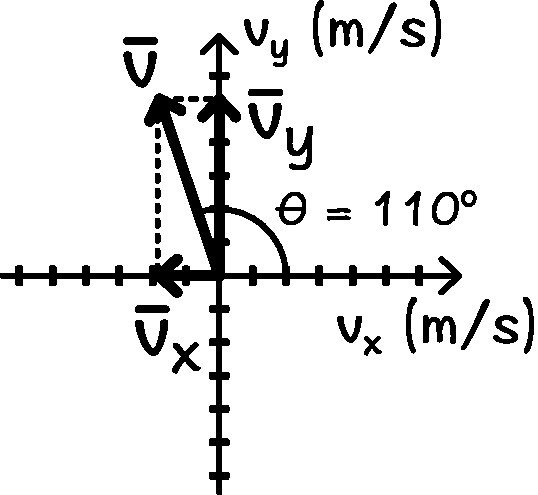
\includegraphics[width=0.95\textwidth]{figs/moniulotteinen_esimerkki_komponentit.pdf}%
\end{center}%
}

 \eval  Komponenteilla on oikeat etumerkit ja ne ovat molemmat itseisarvoltaan pienemmät kuin vauhti \(v\), kuten pitääkin. Piirretyn kuvan perusteella skalaarikomponenteille lasketut arvot myös vaikuttavat järkeviltä. Voidaan vielä tarkistaa, että komponenttieihin jaetun vektorin pituus on oikein, \(v = \sqrt{v_x^2 + v_y^2} = 5.5 \un{m/s}\).

\end{exam}

\index{skalaarikomponentti}

Kuten luvussa \autoref{vektoriengraafinenyhteenlasku} vektoreiden geometristen laskusääntöjen yhteydessä huomattiin, vektoreilla laskeminen on yleensä helpompaa komponenteittain. Tällöin rajoituttiin yksinkertaisuuden vuoksi kaksiulotteisiin esimerkkeihin. Kolmiulotteisessa avaruudessa geometriaan perustuva vektorien käsittely on usein suorastaan mahdotonta ja jako komponentteihin on monesti ainoa järkevä tapa laskea vektoreilla. Esimerkiksi vektorien yhteenlasku onnistuu komponenteittain, jolloin summavektorin skalaarikomponentit saadaan laskemalla summattavien skalaarikomponentit yhteen
\begin{equation} \bs{A} + \bs{B} = (A_x\uv{i} + A_y\uv{j} + A_z\uv{k}) + (B_x\uv{i} + B_y\uv{j} + B_z\uv{k}) = (A_x + B_x)\uv{i} + (A_y + B_y)\uv{j} + (A_z+ B_z) \uv{k}. \end{equation}
Toisin sanoen vektorien yhteenlasku voidaan laskutoimituksena hoitaa yksinkertaisesti laskemalla erikseen yhteen vektorien \(x\)-, \(y\)- ja \(z\)-skalaarikomponentit.

\begin{stopQ}{q:moniulotteinen_komponentit}%
Kappaleeseen vaikuttaa kaksi voimaa, A ja B. Voima A on suuruudeltaan \(3.0 \un{N}\) ja osoittaa positiivisen \(x\)-akselin suuntaan. Voima B on suuruudeltaan \(4.0 \un{N}\) ja osoittaa suuntaan, joka on \(60^\circ\) \(x\)-akselista negatiivisen \(y\)-akselin suuntaan. Mikä on kappaleeseen vaikuttava kokonaisvoima komponentein esitettynä?
\end{stopQ}

Edellä avaruuden piste esitettiin kahdella eri tavalla, koordinaatein \( (x,y,z) \) sekä paikkavektorin \( \bs{r} = x \uv{i} + y \uv{j} + z \uv{k} \) avulla. Molemmissa esityksissä on täsmälleen yhtä paljon informaatiota ja kolmiulotteisen vektorin voikin aivan hyvin esittää matemaattisesti lukukolmikkona. Samaan tapaan minkä tahansa vektorin \(\bs{A}\) voi kuvata kolmikkona \( (A_x, A_y, A_z) \). Matematiikassa tällainen vektorin esitys lukujoukkona on tavallinen ja käytännöllinen, koska matemaattisilla vektoreilla voi olla kuinka monta komponenttia tahansa. Fysiikassa kuitenkin käytetään yleensä avaruuden vektoreiden esittämisessä yksikkövektoreita, koska avaruuden vektoreiden komponenttiesitys riippuu käytettävästä koordinaatistosta, ja joskus on tarpeellista käyttää saman tilanteen analyysissa erilaisia koordinaattijärjestelmiä. Tällöin yksikkövektoreilla voidaan ilmaista mitä koordinaatistoa kulloinkin käytetään.

\begin{stopQ}{q:moniulotteinen_kierto}%
Määritellään kaksi tason koordinaatistoa, \(xy\) ja \(x'y'\), joista jälkimmäistä on kierretty \(45^\circ\) vastapäivään ensimmäisen suhteen. Koordinaatistojen yksikkövektorit ovat \(\uv{i}, \uv{j}\) ja \(\uv{i}', \uv{j}'\). Mikä on vektorin \(\bs{A} = 3 \uv{i} + 4 \uv{j}\) komponenttiesitys toisessa koordinaatistossa?
\end{stopQ}

\section{Dynamiikka}
\label{dynamiikka}

Olemme jo oppineet laskemaan suoralla kulkevan kappaleen nopeuden ja paikan sen kiihtyvyyden tai siihen kohdistuvan voiman avulla. Kappaleet kuitenkin harvoin kulkevat suoraan, joten nyt opettelemme päättelemään miten asiat liikkuvat tasossa. Käytännössä useasta kappaleesta koostuvan systeemin liikkeen ratkaiseminen on usein vaikeaa, koska systeemin osat voivat vuorovaikuttaa keskenään. Tätä emme edes yritä. Sen sijaan jos kappaleeseen vaikuttava voima on vakio tai riippuu vain ajasta, kappaleen liikeradan laskeminen onnistuu.

\subsection{Heittoliike}
\label{heittoliike}

\index{heitto}
\index{vapaa pudotus}
\index{tasaisesti kiihtyvä liike}

Ideaalinen \textbf{heittoliike} eli \textbf{ballistinen liike} on vapaan pudotuksen yleistys useampaan ulottuvuuteen. Luvussa \autoref{kiihtyvyys} vapaa pudotus määriteltiin liikkeeksi, jossa kappaleella on vakiokiihtyvyys \(\bs{g}\) alaspäin. Tällä määritelmällä myös ylöspäin heitetty kappale on vapaassa pudotuksessa, sillä senkin \emph{kiihtyvyys} on vakio ja osoittaa alaspäin, vaikka nopeus suuntautuisikin ylöspäin.
Aivan samalla perusteella myös viistoon heitetty kappale on vapaassa pudotuksessa, sillä jos ilmanvastus ei ole merkittävä, kappaleeseen vaikuttaa ainoastaan painovoima ja kappale on tasaisesti kiihtyvässä liikkeessä alaspäin. Ainoa ero pystysuoraan liikkeeseen nähden on nyt vain se, että kappaleella on nopeutta myös vaakasuunnassa eli voimaa vastaan kohtisuorassa suunnassa.

Tarkastellaan tilannetta, jossa pallo heitetään jollakin alkunopeudella \(v_\text{alku}\) kulmassa \(\theta\) vaakatasoon nähden. Kappaleen liikkeen kuvaamisessa ensimmäinen askel on koordinaatiston kiinnittäminen, ja se kannattaa tehdä nyt niin, että \(x\)-suunta osoittaa vaakasuoraan ja \(y\)-suunta on ylöspäin (kuva \autoref{fig:moniulotteinenballistiikka}). Kappaleen kiihtyvyys on tällöin liikkeen aikana pelkästään \(y\)-suuntaan,
\begin{equation} \bs{a} = -g\uv{j}. \end{equation}
Kappaleen alkunopeus voidaan myös jakaa vaaka- ja pystykomponentteihin kuten kuvassa \autoref{fig:moniulotteinenballistiikka_a}, jolloin saadaan
\begin{equation} \bs{v}_\text{alku} = v_{x,\text{alku}} \uv{i} + v_{y,\text{alku}} \uv{j} = (v_\text{alku} \cos \theta) \uv{i} + (v_\text{alku} \sin \theta) \uv{j}. \end{equation}

\widepictures{tb}%
{Heittoliikkeen analyysi liikkeen komponenttijaon avulla.;%
Ratkaistaan nopeus ja paikka erikseen \(x\)- ja \(y\)-suunnissa liikeradan selvittämiseksi.;%
Nopeuden skalaarikomponentit.}%
{fig:moniulotteinenballistiikka;fig:moniulotteinenballistiikka_a;fig:moniulotteinenballistiikka_b;}%
{0.655;0.245}%
{0.652;0.248}%
{moniulotteinen_ballistiikka_3.pdf;moniulotteinen_ballistiikka_2.pdf}

Näiden tietojen avulla voidaan ratkaista kappaleen nopeus ajan funktiona. Ensinnäkin, koska kappaleella ei ole kiihtyvyyttä vaakasuunnassa, sen \emph{vaakasuuntainen nopeus ei muutu}. Kappale liikkuu siis \(x\)-suuntaan vakionopeudella.
Pystysuunnassa kappaleen kiihtyvyys on vakio, joten \emph{pystysuuntainen nopeus muuttuu} täsmälleen samoin kuin suoraan ylöspäin heitetyllä kappaleella: aluksi kappaleen nopeuden pystykomponentti on positiivinen eli kappale liikkuu ylöspäin. Koska kappaleella on kiihtyvyyttä alaspäin, pystysuuntainen nopeus kuitenkin pienenee jatkuvasti ja nopeus kääntyy pian alaspäin. Nopeuden skalaarikomponentteja kuvaa yhtälö (\autoref{tasaisenkiihtyvyydennopeus}), joten jos alkuhetkeksi valitaan \(t_\text{alku} = 0 \un{s}\), pystysuuntaiselle nopeudelle saadaan lauseke
\begin{equation} v_y(t) = v_{y,\text{alku}} + a_{y,\text{tasainen}} (t - t_\text{alku}) = v_\text{alku} \sin \theta - gt. \end{equation}

Nopeuden komponenttien avulla voidaan edelleen ratkaista kappaleen paikkakoordinaatit. Nopeuden kukin komponentti nimittäin ilmaisee vastaavan paikkakoordinaatin muuttumisvauhtia, joten koordinaatit saadaan nopeuden skalaarikomponenttien integraaleina yhtälön (\autoref{paikkatasaisessakiihtyvyydessa}) mukaisesti.
Vaakasuunnassa nopeus on vakio, joten siirtymä on suoraan verrannollinen siihen käytettyyn aikaan
\begin{equation} x(t) = x_\text{alku} + v_{x,\text{alku}} t. \label{heittox} \end{equation}
Pystysuunnassa vastaavasti
\begin{equation} y(t) = y_\text{alku} + v_{y,\text{alku}}  t - \frac{1}{2}gt^2. \label{heittoy} \end{equation}
Kappaleen rata muodostaa siis paraabelin kuten kuvasta \autoref{fig:moniulotteinenballistiikka_a} ilmenee.

\index{liikediagrammi}
\index{rata}
\index{nopeus}

Kuvan \autoref{fig:moniulotteinenballistiikka_a} liikediagrammiin on piirretty nopeusvektori sekä nopeuden komponentit koordinaattiakselien suunnassa muutamina ajan hetkinä. Vaakasuora komponenttinuoli on aina yhtä pitkä. Pystykomponentti sen sijaan osoittaa ensin ylöspäin ja kääntyy sitten osoittamaan alaspäin, koska kappaleen kiihtyvyys on alaspäin. Nopeusvektori itsessään on aina \emph{radan tangentin suuntainen}. Tämä ei ole vain heittoliikkeen ominaisuus vaan tämä on aina totta, sillä \emph{nopeusvektori osoittaa suuntaan, johon kappale liikkuu}.

\begin{stopQ}{q:moniulotteinen_voima_kiihtyvyys}%
Hiihtäjä laskee alas mäkeä, jonka muoto muistuttaa ylöspäin aukeavaa paraabelia. Hiihtäjän vauhti on likimain vakio hänen ollessaan paraabelin pohjalla. (a) Muuttuuko hiihtäjän nopeuden suunta? (b) Miten hiihtäjän nopeuden komponentit muuttuvat? (c) Millainen on hiihtäjän kiihtyvyysvektori? (d) Millainen on hiihtäjään kohdistuva kokonaisvoima?
\end{stopQ}

\newpage\begin{exam}{Kantama}{ex:heitto}\noindent

\problem{Missä kulmassa pallo tulee heittää, jotta sen kantama olisi mahdollisimman pitkä, jos pallon lähtövauhti ei riipu heittokulmasta? Oletetaan, että ilmanvastus on pieni ja että pallo lähtee likimain maanpinnan tasolta.}

 \twocol{0.59}{0.4}{ \setup  Merkitään pallon lähtökulmaa \(\theta\) ja sen lähtönopeutta \(\bs{v}_\text{alku}\). Valitaan koordinaatisto siten, että pallo liikkuu \(xy\)-tasossa, \(x\)-akseli on vaakasuuntainen ja \(y\)-akseli pystysuuntainen. Asetetaan origo pallon lähtöpisteeseen.

\physics Jos ilmanvastusta ei huomioida, pallo on vapaassa pudotuksessa. Tällöin sen liike \(x\)-suunnassa on tasaista ja \(y\)-suunnassa tasaisesti kiihtyvää. Pallon kantama on sen \(x\)-suunnassa kulkema matka ennen osumista maahan eli ennen kuin pallon \(y\)-koordinaatti saa arvon nolla. Pisin kantama löydetään etsimällä tämän maksimi lähtökulman suhteen esimerkiksi derivaatan nollakohtia tutkimalla.

}{%
\begin{center}%
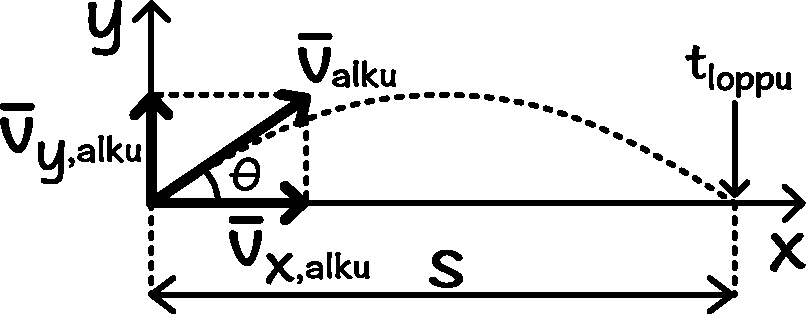
\includegraphics[width=0.95\textwidth]{figs/moniulotteinen_esimerkki_kantama.pdf}%
\end{center}%
}

 \model  Pallon alkunopeuden komponentit ovat \(v_{x,\text{alku}} = v_\text{alku} \cos \theta\) ja \(v_{y,\text{alku}} = v_\text{alku} \sin \theta\). Pallon koordinaatit saadaan yhtälöistä (\autoref{heittox}) ja (\autoref{heittoy}).

Pallo osuu maahan hetkellä \(t_\text{loppu}\), jolle pätee \(y(t_\text{loppu}) = 0 \un{m}\). Kappaleen siirtymä \(x\)-suunnassa on silloin \(s = x(t_\text{loppu}) \).

\solu Pallon maahanosumishetki ratkeaa yhtälöstä \(y(t_\text{loppu}) = v_\text{alku} t_\text{loppu} \sin \theta - \frac{1}{2} g t_\text{loppu}^2 = 0 \un{m}\). Tästä voidaan ratkaista aika
\begin{equation}t_\text{loppu} = \frac{2 v_\text{alku} \sin \theta}{g}.\end{equation}

Pallon \(x\)-koordinaatti on tuolloin
\begin{equation} s = x(t_\text{loppu}) = v_\text{alku} t_\text{loppu} \cos \theta = \frac{2 v_\text{alku}^2 \sin \theta \cos \theta}{g} = \frac{v_\text{alku}^2 \sin 2\theta}{g}, \end{equation}
missä on käytetty trigonometrista sääntöä \(\sin 2\theta = 2 \sin \theta \cos \theta\).

Kantaman ääriarvot löytyvät sen derivaatan nollakohdista. Derivaatta pitää laskea luonnollisesti sen muuttujan suhteen, jonka suhteen maksimia etsitään, eli heittokulman. Derivoidaan siis kantama,
\begin{equation} \frac{\dd s}{\dd \theta} = \frac{v_\text{alku}^2}{g} \frac{\dd}{\dd \theta} \sin 2\theta = \frac{v_\text{alku}^2}{g} 2  \cos 2\theta. \end{equation}
Tämä on nolla täsmälleen silloin kun funktio \(\cos 2 \theta\) on nolla. Kosini on jaksollinen funktio, joten sillä on äärettömästi nollakohtia \(\cos \pi/2 = \cos 3\pi/2 = \cos 5\pi/2 = \ldots = 0\). Nyt voidaan kuitenkin tyytyä tarkastelemaan kulmia välillä \(\theta \in [0,90^\circ] = [0, \pi/2]\), ja tällöin nollakohtia on vain yksi, \(\cos (2 \cdot \pi/4) = \cos \pi/2 = 0\).

Siispä kantamalla saavuttaa ääriarvon heittokulmalla \(\pi/4 = 45^\circ\). Tämän täytyy olla myös maksimikantama, koska kulmilla \(0\) ja \(90^\circ\) kantamaksi saadaan nolla, ja varmastikin viistoon heitetty pallo lentää tätä pidemmälle. Huomaa, että todellisissa pallopeleissä ilmanvastus on merkittävä, joten tulos ei ole lähimainkaan tarkka.

\mbar
\begin{mathematica}[commandchars=\\!?]
(* koordinaatit ajan ja kulman funktioina *)
x[t_, theta_] := valku Cos[theta] t
y[t_, theta_] := valku Sin[theta] t - 1/2 g t^2 

(* ratkaistaan maahan osumisen hetki *)
maassa = Solve[y[tloppu, theta] == 0, tloppu]
  \textit!{{tloppu -> 0}, {tloppu -> (2 valku Sin[theta])/g}}?
(* ratkaistaan kantama k\"aytt\"aen toista ratkaisua *)
kantama = x[tloppu, theta] /. maassa[[2]] // Simplify (* sievennet\"a\"an samalla *)
  \textit!(valku^2 Sin[2 theta])/g?

(* derivoidaan kantama kulman suhteen ja etsit\"a\"an maksimi *)
derivaatta = D[kantama, theta] // Simplify
  \textit!(2 valku^2 Cos[2 theta])/g?
ratkaisu = Solve[{derivaatta == 0, 0 < theta < Pi/2}, theta] (* v\"ali [0, pi/2] *)
  \textit!{{theta -> Pi/4}}?

(* kappaleen rata kolmella heittokulmalla *)
rata[theta_] := {x[t, theta], y[t, theta]} /. {valku -> 10, g -> 9.8}
ParametricPlot[{rata[30 Degree], rata[45 Degree], rata[60 Degree]}, 
  {t, 0, 2}, PlotRange -> {{0, 12}, {0, 4}}]
\end{mathematica}
\begin{center}
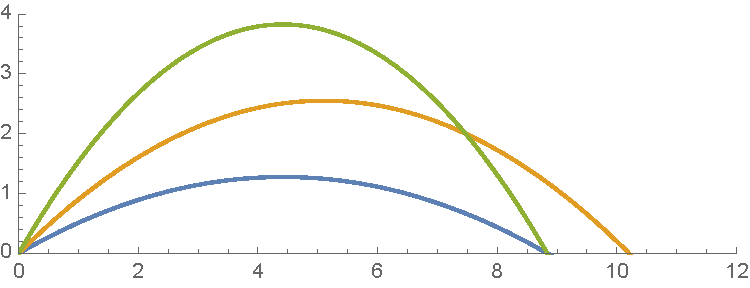
\includegraphics[width=0.4\textwidth]{figs/moniulotteinen_esimerkki_heittoplot.pdf}
\end{center}

\end{exam}

\subsection{Liike ajasta riippuvan voiman vaikuttaessa}
\label{liikeajastariippuvanvoimanvaikuttaessa}

\index{derivaatta}
\index{integraali}

Heittoliikkeen analyysissä huomattiin, että liike voitiin jakaa eri suuntaisiin komponentteihin ja nopeudet sekä paikka voitiin ratkaista näissä suunnissa erikseen toisistaan riippumatta.
Matemaattisesti tämä perustuu siihen, että derivointi ja integrointi ovat \emph{lineaarisia operaatioita} eli summan voi derivoida tai integroida termi kerrallaan.
Lisäksi koska yksikkövektorit ovat vakioita, ne voidaan siirtää derivaattojen ja integraalien ulkopuolelle.
Niinpä esimerkiksi nopeuden \(y\)-skalaarikomponentti voitiin laskea integroimalla kiihtyvyyden \(y\)-skalaarikomponenttia ajan suhteen.
Yleisesti minkä tahansa vektorin derivaatta voidaan laskea karteesisessa koordinaatistossa komponenteittain,
\begin{equation} \frac{\dd \bs{A}}{\dd t} = \frac{\dd A_x}{\dd t}\uv{i} + \frac{\dd A_y}{\dd t}\uv{j} + \frac{\dd A_z}{\dd t}\uv{k}\end{equation}
ja vastaavasti integroinnille pätee
\begin{equation} \int_{t_\text{alku}}^{t_\text{loppu}} \bs{A} \dd t = \left( \int_{t_\text{alku}}^{t_\text{loppu}} A_x \dd t \right) \uv{i} + \left( \int_{t_\text{alku}}^{t_\text{loppu}} A_y \dd t \right) \uv{j} + \left( \int_{t_\text{alku}}^{t_\text{loppu}} A_z \dd t \right) \uv{k}. \label{vektori-integraali} \end{equation}

\index{kiihtyvyys}

Kiihtyvyyden määritelmä (\autoref{kiihtyvyysvektori}) on siten komponenttimuodossa
\begin{equation} \bs{a} = \frac{\dd \bs{v}}{\dd t} = \frac{\dd v_x}{\dd t}\uv{i} + \frac{\dd v_y}{\dd t}\uv{j} + \frac{\dd v_z}{\dd t}\uv{k} \end{equation}
ja kääntäen nopeus saadaan kiihtyvyyden integraalina
\begin{equation} \bs{v}(t) = \bs{v}_\text{alku} + \int_{t_\text{alku}}^{t} \bs{a} \dd t, \end{equation}
mikä voidaan edelleen hajottaa komponentteihin yhtälön \autoref{vektori-integraali} avulla.
Jos siis kiihtyvyyden skalaarikomponentit tunnetaan, nopeuden \(x\)-, \(y\)- ja \(z\)-skalaarikomponentit saadaan integroimalla erikseen kiihtyvyyden vastaavia komponentteja. Esimerkiksi \(x\)-suunnassa pätee
\begin{equation} v_x(t) =  v_{x,\text{alku}} + \int_{t_\text{alku}}^{t} a_x \dd t \end{equation}
ja muissa suunnissa saadaan täsmälleen samanlaiset tulokset.
Kappaleen paikkakoordinaatit saadaan edelleen integroimalla nopeuden skalaarikomponentteja.

\index{dynamiikan peruslaki}

Kappaleen liikkeen ratkaisemiseksi täytyy siis tuntea sen kiihtyvyyden komponentit, ja ne saadaan ainakin periaatteessa ratkaistua dynamiikan peruslaista (\autoref{newton2}),
joka komponenttimuodossa saa muodon
\begin{equation} a_x\uv{i} + a_y\uv{j} + a_z\uv{k} = \frac{1}{m}F_{x,\text{kokonais}}\uv{i} + \frac{1}{m}F_{y,\text{kokonais}}\uv{j} + \frac{1}{m}F_{z,\text{kokonais}}\uv{k}. \end{equation}
Komponenttijaon käyttäminen tässä tilanteessa voi vaikuttaa ongelman hankaloittamiselta, koska yhtälössä on nyt kuusi termiä, mutta yhtälön kumpikin puoli voidaan tulkita saman vektorin komponenttiesitykseksi. Koska vektorin komponentit karteesisessa koordinaatistossa ovat \emph{yksikäsitteiset}, lukukolmikon \( (a_x, a_y, a_z) \) pitää siis olla sama kuin lukujen \( (\frac{1}{m}F_{x,\text{kokonais}} \), \(\frac{1}{m}F_{y,\text{kokonais}}\), \( \frac{1}{m}F_{z,\text{kokonais}}) \). Siispä vektorimuotoinen yhtälö
\(\bs{a} = \frac{1}{m}\bs{F}_{\text{kokonais}}\) voidaan komponenttien avulla muuttaa kolmeksi skalaariyhtälöksi
\begin{equation} a_x = \frac{1}{m}F_{x,\text{kokonais}}, \ a_y = \frac{1}{m} F_{y,\text{kokonais}}, \ a_z = \frac{1}{m}F_{z,\text{kokonais}}, \label{komponenttiyhtalo}\end{equation}
joista kiihtyvyyden komponentit voidaan ratkaista.
Jos voima tunnetaan \emph{ajan funktiona}, kiihtyvyyden komponentit voidaan suoraan integroida ajan suhteen nopeuden ja paikan ratkaisemiseksi, mistä on esimerkki \autoref{ex:aikavoima} luvun lopussa. Jos voima riippuu muista tekijöistä kuten paikasta tilanne on huomattavasti hankalampi.

\begin{stopQ}{q:moniulotteinen_tasainen_kiihtyvyys}%
Kappaleeseen (massa \(1 \un{kg}\)) vaikuttavan kokonaisvoiman skalaarikomponentit riippuvat ajasta niin, että \(F_x\) on aluksi \(2.0 \un{N}\) ja sekunnin päästä \(-1.0 \un{N}\) ja \(F_y\) on aluksi \(2.0 \un{N}\) ja sekunnin päästä \(4.0 \un{N}\). Kumpikin komponentti muuttuu lineaarisesti ajan funktiona (eli niiden kuvaajat ovat suorat). Jos kappale liikkuu aluksi negatiiviseen \(x\)-suuntaan \(1.0 \un{m/s}\) vauhdilla, mitkä ovat sen nopeuden komponentit sekunnin päästä?
\end{stopQ}

\begin{exam}{Kuulapeli}{ex:aikavoima}\noindent

\problem{Kuulapelissä pyritään ohjaamaan pientä kuulaa (massa \(10 \un{g}\)) labyrintissä kallistamalla pelilautaa, jolloin painovoima vetää kuulaa aina jyrkimmän laskun suuntaan. Pelaaja voi kahdesta nupista kääntämällä vaikuttaa laudan kallistumaan ja samalla siis kuulaan kohdistuvaan kokonaisvoimaan kahdessa kohtisuorassa suunnassa \(x\) ja \(y\). Millaisen reitin levosta lähtevä kuula kulkee kahden sekunnin aikana, jos siihen vaikuttavan kokonaisvoiman \(x\)-suuntainen skalaarikomponentti on \(F_x = A t \) ja \(y\)-suuntainen \(F_y = B \sin C t\), missä \(A = 3.0\cdot10^{-4} \un{N/s}, B = 7.0\cdot10^{-4} \un{N}, C = 3.5 \un{s}^{-1}\)?
}

 \twocol{0.5}{0.45}{ \setup  Systeemiin kuuluu vain kuula, johon kohdistuvat voimat tunnetaan komponenteittain ajan funktiona.

 \physics Kuulan kiihtyvyys, nopeus ja paikka voidaan ratkaista dynamiikan peruslain ja kiihtyvyyden määritelmän avulla, koska voima tunnetaan ajan funktiona. Kaikkien näiden vektorisuureiden \(x\)- ja \(y\)-komponentit voidaan määrittää toisistaan riippumatta, koska voima ei riipu paikasta vaan ainoastaan ajasta.

}{%
\begin{center}%
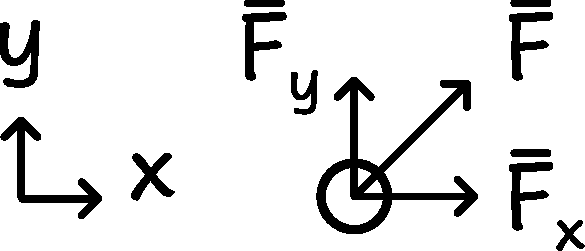
\includegraphics[width=0.95\textwidth]{figs/moniulotteinen_esimerkki_dynamiikka.pdf}%
\end{center}%
}

 \model  Kun kuulaan vaikuttavan kokonaisvoiman skalaarikomponentti suunnassa \(x\) on \(F_x\), kuulan kiihtyvyys tässä suunnassa on \(a_x = F_x/m\). Nopeus on kiihtyvyyden integraali
\(v_x = v_{x,\text{alku}} + \int_0^t a_x \dd t'\) ja paikka on nopeuden integraali
\(x = x_\text{alku} + \int_0^t v_x \dd t'\). Tässä integroimismuuttujaa on selvyyden vuoksi merkitty pilkulla, \(t'\), erotuksena integraalin ylärajassa esiintyvästä niinikään aikaa esittävästä symbolista \(t\).
Suunnassa \(y\) pätevät täsmälleen samat yhtälöt. Lisäksi tiedetään, että kuulan alkunopeus on nolla, \(v_{x,\text{alku}} = 0, v_{y,\text{alku}} = 0\) ja koordinaatiston origo voidaan valita kuulan lähtöpisteeseen, jolloin myös \(x_\text{alku} = 0, y_\text{alku} = 0\).

 \solu  Nopeudeksi saadaan

\begin{eqnarray} v_x &=& \int_0^t \frac{F_x}{m} \dd t' = \frac{A}{m} \int_0^t t' \dd t' = \frac{1}{2} \frac{A}{m} t'^2 \\
v_y &=& \int_0^t \frac{F_y}{m} \dd t' = \frac{B}{m} \int_0^t \sin C t' \dd t' = \frac{B}{m} \bigg|_0^t -\frac{1}{C}\cos Ct' = \frac{B}{mC}(1 - \cos Ct) \end{eqnarray}

ja tästä edelleen paikaksi

\begin{eqnarray} x &=& \int_0^t \frac{1}{2} \frac{A}{m} t'^2 \dd t' = \frac{1}{6} \frac{A}{m} t^3 \\
y &=& \int_0^t \frac{B}{mC}(1 - \cos Ct') \dd t' = \frac{B}{mC} \bigg|_0^t t' - \frac{1}{C} \sin Ct' = \frac{B}{mC^2}( Ct -\sin Ct).
\end{eqnarray}

Kuulan paikka millä tahansa ajan hetkellä \(t\) selviää sijoittamalla lukuarvot näihin lausekkeisiin. Kappaleen reitti voidaan piirtää valitsemalla aikoja tasaisin välein (esim. \(t=0.0\un{s}, 0.5\un{s}, \ldots\)), ratkaisemalla kappaleen koordinaatit näinä hetkinä ja piirtämällä pisteet koordinaatistoon. Reitin piirtäminen onnistuu myös tietokoneella.

\mbar
\begin{mathematica}[commandchars=\\!?]
(* voimat *)
fx = a t; fy = b Sin[c t];
lukuarvot = {a -> 3*10^-4, b -> 7*10^-4, c -> 3.5, m -> 0.01};

(* nopeudet *)
vx = Integrate[fx/m, {t, 0, t}]
  \textit!(a t^2)/(2 m)?
vy = Integrate[fy/m, {t, 0, t}]
  \textit!(b - b Cos[c t])/(c m)?

(* paikkakoordinaatit *)
x = Integrate[vx, {t, 0, t}]
  \textit!(a t^3)/(6 m)?
y = Integrate[vy, {t, 0, t}]
  \textit!(b (c t - Sin[c t]))/(c^2 m)?

(* piirret\"a\"an kuvaaja *)
viiva = ParametricPlot[{x, y} /. lukuarvot, {t, 0, 2}, 
  AspectRatio -> 1, PlotRange -> {{0, 0.05}, {0, 0.05}}]; (* reitti *)

(* lasketaan paikka tasaisin aikav\"alein *)
npisteet = 10; aika = 2; 
koordinaatit = Table[{x, y} /. lukuarvot /. t -> i*aika/npisteet, {i, 0, npisteet}];
paikat = ListPlot[koordinaatit, 
  AspectRatio -> 1, PlotRange -> {{0, 0.05}, {0, 0.05}}]

(* lasketaan nopeus ja voima tasaisin aikav\"alein *)
vskaala = 0.1; fskaala = 10;
nopeusvektorit = Graphics[
  Table[{Arrow[{{x, y}, {x + vskaala*vx, y + vskaala*vy}}]} 
    /. lukuarvot /. t -> i*aika/npisteet, {i, 0, npisteet}], 
    Axes -> True];
voimavektorit = Graphics[
  Table[{Arrow[{{x, y}, {x + fskaala*fx, y + fskaala*fy}}]} 
    /. lukuarvot /. t -> i*aika/npisteet, {i, 0, npisteet}], 
    Axes -> True];

(* Piirret\"a\"an yhdess\"a *)
Show[pisteet, nopeusvektorit]
Show[viiva, pisteet, voimavektorit]
\end{mathematica}
\begin{center}
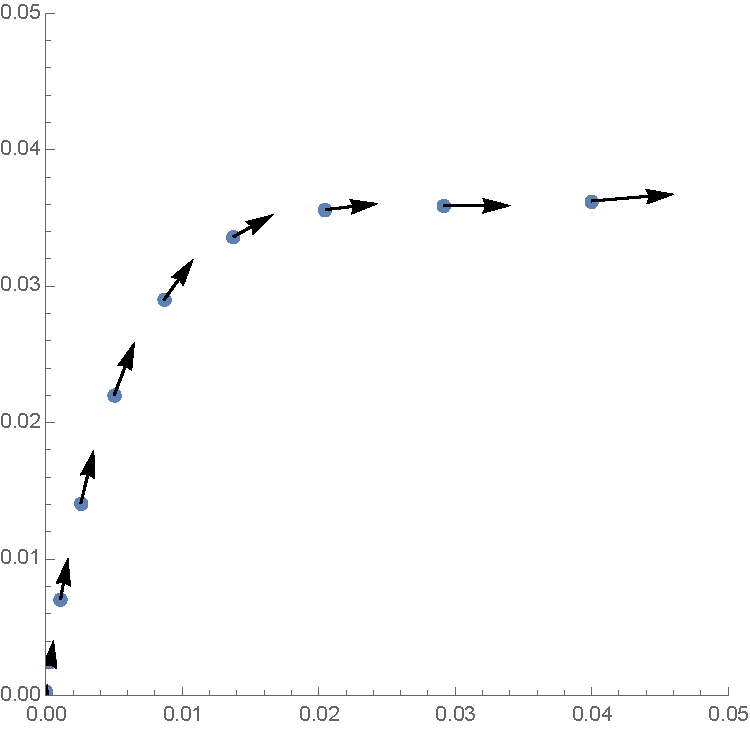
\includegraphics[width=0.4\textwidth]{figs/moniulotteinen_dynamiikka_1.pdf}
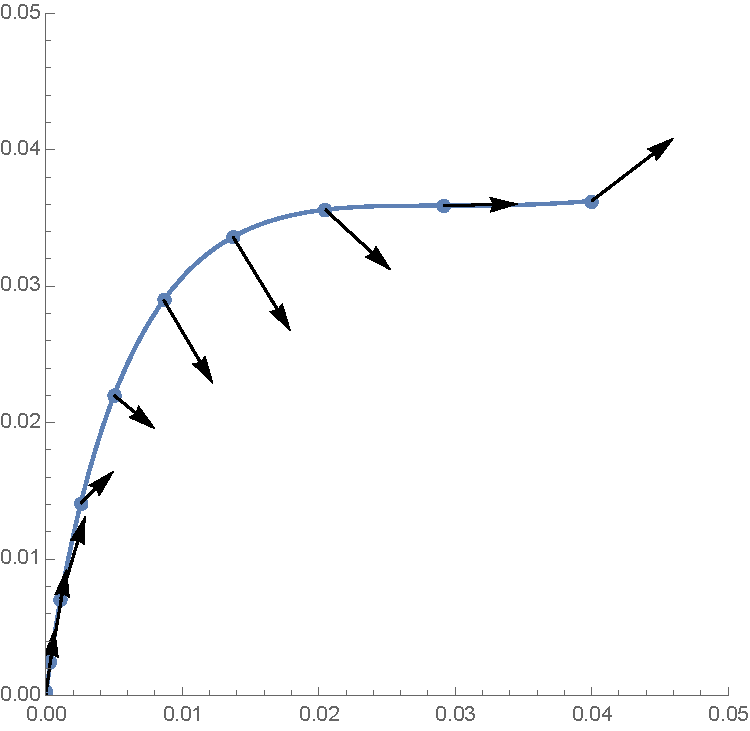
\includegraphics[width=0.4\textwidth]{figs/moniulotteinen_dynamiikka_2.pdf}
\end{center}

\eval Kappaleeseen vaikuttaa koko ajan \(x\)-suunnassa positiivinen voima, joten se liikkuu tähän suuntaan kiihtyvällä nopeudella (ei kuitenkaan tasaisesti kiihtyvällä nopeudella, koska kiihtyvyys ei ole vakio). Suunnassa \(y\) voima on aluksi positiivinen ja sitten negatiivinen, joten kappale lähtee liikkeelle positiiviseen \(y\) suuntaan mutta sitten liike tässä suunnassa pysähtyy, jolloin kappale siis liikkuu vain \(x\)-suuntaan.

Tarkistetaan myös paikkakoordinaattien yksiköt:
\begin{equation} [x] = \frac{[A]}{[m]} [t^3] = \frac{\text{N/s} \cdot \text{s}^3}{\text{kg}} = \frac{\text{kg m/s}^2 \cdot \text{s}^2}{\text{kg}} = \text{m} \end{equation}
\begin{equation} [y] = \frac{[B]}{[mC^2]} [( Ct -\sin Ct)] = \frac{\text{N}}{\text{kg s}^{-2}}\cdot 1 = \frac{\text{Ns}^2}{\text{kg}} = \text{m}. \end{equation}

\end{exam}

\section{Liikemäärä}
\label{liikemäärä}

\widepictures{tb}%
{Kahden kappaleen törmäys tasossa. Kokonaisliikemäärän komponentit \(x\)- ja \(y\)-suunnissa ovat vakiot ja massakeskipisteen liike on tasaista.;%
Liikediagrammi \(xy\)-tasossa sekä \(y\)-koordinaatin kuvaaja ajan suhteen.;%
Nopeuden \(y\)-komponentin kuvaaja.;%
Liikediagrammi \(xy\)-tasossa sekä \(x\)-koordinaatin kuvaaja ajan suhteen. Liikediagrammi on käännetty \(90^\circ\) kuvaan (a) nähden.;%
Nopeuden \(x\)-komponentin kuvaaja.}%
{fig:moniulotteinentormays;fig:moniulotteinentormays_a;fig:moniulotteinentormays_b;fig:moniulotteinentormays_c;fig:moniulotteinentormays_d;}%
{0.622;0.278;0.622;0.278}%
{0.622;0.278;0.622;0.278}%
{moniulotteinen_liikemaara_11.pdf;moniulotteinen_liikemaara_12.pdf;moniulotteinen_liikemaara_13.pdf;moniulotteinen_liikemaara_14.pdf}

\index{liikemäärä}

Liikemäärän säilymislaki muotoiltiin jo luvussa \autoref{luku:sailymislait} vektorimuodossa, ja sen sisältö on useassa ulottuvuudessa täsmälleen sama kuin yhdessäkin ulottuvuudessa. Jos systeemiin ei vaikuta ulkoisia vuorovaikutuksia tai jos nämä vuorovaikutukset kumoavat toisensa, systeemin kokonaisliikemäärä on vakio. Lisäksi koska kokonaisliikemäärä on vektori, sekä sen suunta että suuruus pysyvät tällöin muuttumattomina. Yhdessä ulottuvuudessa suunnat ilmaistiin skalaarikomponenttien etumerkkien avulla. Useammassa ulottuvuudessa liikemäärävektorit voidaan esittää joko graafisesti nuolien avulla tai komponenteittain.

\index{törmäys}

Kuvassa \autoref{fig:moniulotteinentormays} on esitetty kahden kappaleen törmäys tasossa sekä liikediagrammina että kuvaajina.
Kappaleen B massa on kaksinkertainen kappaleen A massaan nähden. A liikkuu aluksi \(y\)-suuntaan ja B viistoon, jolloin sillä on nopeutta sekä \(x\)- että \(y\)-suunnissa. Liikediagrammin perustella selvästikin kummankin kappaleen nopeus muuttuu törmäyksessä sekä suunnaltaan että suuruudeltaan.

\pictures{tb}%
{Törmäävien kappaleiden liikemäärävektorit, jos kappaleen A massa on 1 kg ja kappaleen B 2 kg. Kokonaisliikemäärävektori on sama alussa ja lopussa, mutta kappaleiden liikemäärät muuttuvat.;%
Liikediagrammi ja kappaleiden nopeudet.;%
Kappaleiden nopeus- ja liikemäärävektorit.;%
Kappaleet saavat yhtä suuret mutta vastakkaissuuntaiset impulssit.;%
Liikemäärän komponentit aluksi ja lopuksi.}%
{fig:moniulotteinenliikemaara;fig:moniulotteinenliikemaara_a;fig:moniulotteinenliikemaara_b;fig:moniulotteinenliikemaara_c;fig:moniulotteinenliikemaara_d;}%
{0.38;0.57;0.38;0.57}%
{0.38;0.57;0.38;0.57}%
{moniulotteinen_liikemaara_15.pdf;moniulotteinen_liikemaara_16.pdf;moniulotteinen_liikemaara_17.pdf;moniulotteinen_liikemaara_18.pdf}

Kuvassa on esitetty myös erikseen kappaleiden paikkakoordinaattien ja nopeuskomponenttien kuvaajat ajan funktiona. Tarkastellaan ensin kuvassa \autoref{fig:moniulotteinentormays_a} esitettyä paikan \(y\)-komponenttia.
Kappale A kulkee ensin positiiviseen \(y\)-suuntaan mutta kääntyy törmäyksessä negatiiviseen \(y\)-suuntaan. Kappale B kulkee negatiiviseen \(y\)-suuntaan sekä ennen törmäystä että sen jälkeen, mutta sen vauhti pienenee törmäyksessä. Kappaleiden nopeuden \(y\)-komponentit voidaan määrittää \( y(t) \)-kuvaajien kulmakertoimista aivan kuten yksiulotteisessakin tapauksessa, ja näin määritetyt nopeuden \(y\)-skalaarikomponenttien kuvaajat on piirretty kuvaan \autoref{fig:moniulotteinentormays_b}.
Tämän perusteella kappaleen A \(y\)-suuntaisen nopeuden muutos on \(\Delta v_{y,A} = -6.0 \un{m/s}\) ja kappaleen B \(\Delta v_{y,B} = 3.0 \un{m/s}\). Nopeuskomponenttien muutosten suhde on siis
\begin{equation} \frac{\Delta v_{y,A}}{\Delta v_{y,B}} = - 2.0 = -\frac{m_B}{m_A}. \end{equation}
Toisin sanoen aivan kuten yksiulotteisessakin törmäyksessä kappaleiden nopeuksien \(y\)-suuntaisten komponenttien muutosten suhde on kääntäen verrannollinen kappaleiden massojen suhteeseen yhtälön (\autoref{tormays_liikemaara}) mukaisesti. Mutta tämä ehtohan tarkoitti yhdessä ulottuvuudessa \emph{liikemäärän olevan vakio}. Niinpä edellisen analyysin mukaan tässä törmäyksessä \emph{liikemäärän \(y\)-komponentti on vakio}.

\begin{stopQ}{q:moniulotteinen_liikediagrammi}%
Tee kuvan \autoref{fig:moniulotteinentormays} mukainen liikediagrammi kappaleelle, joka liikkuu aluksi \(45^\circ\) kulmassa \(x\)-akseliin nähden ja törmää elastisesti \(y\)-akselin suuntaiseen seinään. Miltä näyttävät kappaleen paikkakoordinaattien ja nopeuden skalaarikomponenttien kuvaajat ajan funktiona?
\end{stopQ}

\index{liikediagrammi}

Kuvassa \autoref{fig:moniulotteinentormays_c} on esitetty saman törmäyksen liikediagrammi sekä kappaleiden \(x\)-suuntaisten komponenttien kuvaajat. Huomaa, että liikediagrammi on nyt käännetty \(90^\circ\) kuvaan (a) verrattuna, jotta sen \(x\)-akseli olisi pystysuuntainen kuten viereisessä paikkakoordinaatin kuvaajassa.
Kappaleen A nopeuden \(x\)-suuntainen komponentti on aluksi nolla ja törmäyksessä kappale saa nopeutta negatiiviseen \(x\)-suuntaan. Kappale B liikkuu positiiviseen \(x\)-suuntaan sekä ennen törmäystä että sen jälkeen, ja törmäyksessä kappaleen vauhti \emph{kasvaa}. Kappaleiden nopeuden \(x\)-skalaarikomponentit voidaan määrittää \(x(t) \)-kuvaajien kulmakertoimista ja nämä on esitetty kuvassa \autoref{fig:moniulotteinentormays} (d). Tässä kappaleen A nopeuskomponentin muutos on \(\Delta v_{x,A} = -2.6 \un{m/s} \) ja kappaleen B \(\Delta v_{x,B} = 1.3 \un{m/s}\). Siispä tässäkin suunnassa pätee
\begin{equation} \frac{\Delta v_{x,A}}{\Delta v_{x,B}} = - 2.0 = -\frac{m_B}{m_A}, \end{equation}
joten myös \emph{liikemäärän \(x\)-komponentti on törmäyksessä vakio}.
Toisin sanoen yhdessä ulottuvuudessa aikaisemmin esitetty törmäysten analyysi toimii myös useassa ulottuvuudessa, kun kukin koordinaatiston suunta eli nopeuden karteesinen komponentti käsitellään erikseen.

Tulos voidaan selittää liikemäärän vektoriluonteen avulla. Kuvassa \autoref{fig:moniulotteinenliikemaara} on piirretty törmäyksestä liikediagrammi, jonka perusteella voidaan piirtää kappaleiden nopeusvektoreita kuvaavat nuolet sekä ennen törmäystä että sen jälkeen. Kappaleiden liikemäärävektoreita kuvaavat nuolet ovat samansuuntaiset näiden nopeusvektoreiden kanssa, mutta koska kappaleen B massa oli kaksinkertainen kappaleeseen A nähden, B:n liikemäärää kuvaavat nuolet on piirretty pituudeltaan kaksinkertaisiksi nopeuteen nähden siinä missä A:n liikemäärävektorit ovat kuvassa yhtä pitkät nopeusvektorien kanssa.

Selvästikään kummankaan kappaleen liikemäärä ei ole vakio törmäyksessä, mutta kokonaisliikemäärä eli niiden vektorisumma on,
\begin{equation} \bs{p}_{A,\text{alku}} + \bs{p}_{B,\text{alku}} = \bs{p}_{\text{kokonais,alku}} =  \bs{p}_{\text{kokonais,loppu}} =\bs{p}_{A,\text{loppu}} + \bs{p}_{B,\text{loppu}}. \end{equation}
Graafisesti kokonaisliikemäärä voidaan esittää piirtämällä kappaleiden liikemäärävektoreita kuvaavat nuolet peräkkäin, ja kuvasta nähdään että näin muodostetut kokonaisliikemäärää esittävät nuolet ovat samat sekä ennen törmäystä että sen jälkeen. Tämä nuoli osoittaa itse asiassa aina systeemin massakeskipisteen liikkeen suuntaan, ja kokonaisliikemäärän säilyminen tarkoittaa myös sitä, että massakeskipiste liikkuu koko ajan tasaisella nopeudella.

\index{säilyvä}

Toisaalta vektorit voidaan jakaa komponentteihin, jolloin kokonaisliikemäärävektorin jokaisen komponentin pitää erikseen olla vakio

\begin{eqnarray} p_{x,A,\text{alku}} + p_{x,B,\text{alku}} &=& p_{x,A,\text{loppu}} + p_{x,B,\text{loppu}} \\
p_{y,A,\text{alku}} + p_{y,B,\text{alku}} &=& p_{y,A,\text{loppu}} + p_{y,B,\text{loppu}} \\
p_{z,A,\text{alku}} + p_{z,B,\text{alku}} &=& p_{z,A,\text{loppu}} + p_{z,B,\text{loppu}}. \end{eqnarray}

Siispä aivan kuten vektorimuotoinen dynamiikan peruslaki (\autoref{newton2}) voitiin karteesisessa koordinaatistossa hajottaa kolmeen skalaariyhtälöön (\autoref{komponenttiyhtalo}), myös liikemäärän säilymislaki on oikeastaan kolmen skalaariyhtälön ryhmä.

\index{elastinen}
\index{epäelastinen}

Aivan kuten yhdessä ulottuvuudessa, myös useassa ulottuvuudessa törmäys voi olla elastinen tai epäelastinen. Energia ei kuitenkaan ole vektori vaan skalaari ja niinpä liike-energia ei ole välttämättä vakio, jos tarkastellaan nopeuksien komponentteja vain yhdessä suunnassa. Esimerkiksi kuvan \autoref{fig:moniulotteinentormays} tapauksessa \(x\)-suunnassa kappaleiden liike-energia näyttäisi kasvavan. Kokonaisenergia ei kuitenkaan lisäänny, sillä \(y\)-suunnassa kappaleiden liike-energia pienenee.
Vaikka törmäys olisi täysin elastinen, kappaleiden loppunopeuksia ei voi ennustaa pelkästään niiden alkunopeuksien perusteella, koska nämä riippuvat myös asennosta, jossa kappaleet törmäävät toisiinsa.

\begin{exam}{T\"orm\"ays tasossa}{ex:tormays_tasossa}\noindent

\problem{Kaksi kiekkoa, A (massa \(180.0 \un{g}\)) ja B (massa \(90.0 \un{g}\)), liikkuvat aluksi nopeuksilla \(\bs{v}_{A,\text{alku}} = (2.50 \un{m/s})\uv{i} + (2.50 \un{m/s})\uv{j}\) sekä \(\bs{v}_{B,\text{alku}} = (-2.50 \un{m/s})\uv{i} + (1.25 \un{m/s})\uv{j}\). Kiekon A nopeus törmäyksen jälkeen on \(\bs{v}_{A,\text{loppu}} = (-0.75 \un{m/s})\uv{i} + (1.50 \un{m/s})\uv{j}\). Mikä on (a) kiekon B nopeus, (b) kiekkojen saamat impulssit, (c) kokonaisliike-energian muutos törmäyksessä?
}

 \setup  Merkitään systeemiin kuuluvien kiekkojen massoja \(m_A = 180.0 \un{g}\) ja \(m_B = 90.0 \un{g}\). Piirretään tilanteesta kuva nopeuksien ja suuntien hahmottamiseksi.

\begin{center}%
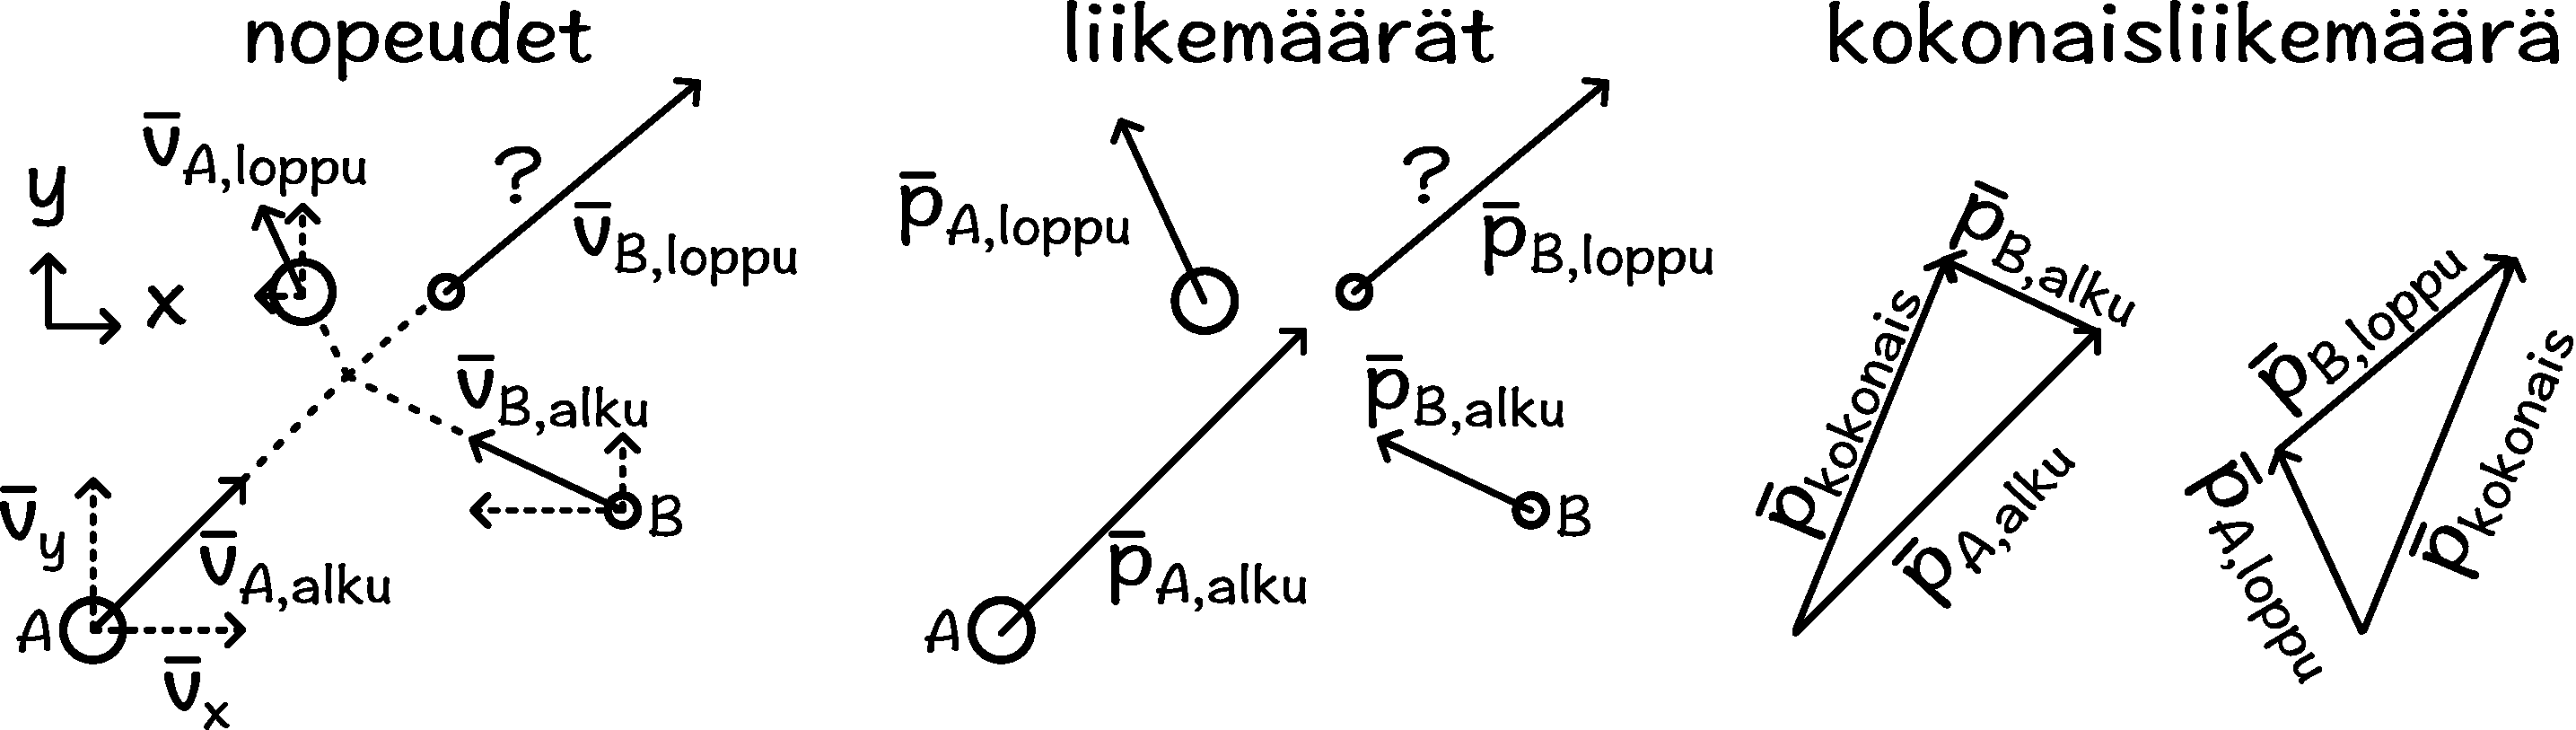
\includegraphics[width=0.85\textwidth]{figs/moniulotteinen_esimerkki_liikemaara.pdf}%
\end{center}%

 \physics Törmäyksessä systeemiin vaikuttavat ulkoiset voimat kumoavat toisensa, joten systeemin kokonaisliikemäärä on vakio. Tämän perusteella voidaan ratkaista kiekon B loppunopeus. Kummankin kiekon saama impulssi on yhtä suuri kuin kyseisen kiekon liikemäärän muutos. Myös liike-energian muutos voidaan laskea kappaleiden nopeuksista.

 \model  Kokonaisliikemaara on vakio erikseen \(x\)- ja \(y\)-suunnissa

\begin{eqnarray} m_A v_{x,A,\text{alku}} + m_B v_{x,B,\text{alku}} &=& m_A v_{x,A,\text{loppu}} + m_B v_{x,B,\text{loppu}} \\
m_A v_{y,A,\text{alku}} + m_B v_{y,B,\text{alku}} &=& m_A v_{y,A,\text{loppu}} + m_B v_{y,B,\text{loppu}}. \end{eqnarray}

Tästä voidaan ratkaista kiekon B loppunopeuden komponentit.

Kiekon A saama impulssi on
\begin{equation} \bs{I}_{B \to A} = \Delta \bs{p}_A = m_A (\bs{v}_{A,\text{loppu}} - \bs{v}_{A,\text{alku}}) \end{equation}
ja vastaavasti kiekolle B. Impulssitkin kannattaa laskea komponenteittain.

Kokonaisliike-energian muutos on
\begin{equation} \Delta K = K_\text{loppu}-K_\text{alku} = \frac{1}{2}m_A v_{A,\text{loppu}}^2 + \frac{1}{2}m_B v_{B,\text{loppu}}^2 - \frac{1}{2}m_A v_{A,\text{alku}}^2 - \frac{1}{2}m_B v_{B,\text{alku}}^2. \end{equation}

 \solu  Kiekon nopeuden skalaarikomponentit ovat

\begin{eqnarray} v_{x,B,\text{loppu}} &=& v_{x,B,\text{alku}} + \frac{m_A}{m_B}(v_{x,A,\text{alku}} - v_{x,A,\text{loppu}}) = 4.00 \un{m/s} \\
v_{y,B,\text{loppu}} &=& v_{y,B,\text{alku}} + \frac{m_A}{m_B}(v_{y,A,\text{alku}} - v_{y,A,\text{loppu}}) = 3.25 \un{m/s}
\end{eqnarray}

Kiekon A saaman impulssin komponentit ovat

\begin{eqnarray} I_{x,B \to A} &=& m_A (v_{x,A,\text{loppu}} - v_{x,A,\text{alku}}) = -0.585 \un{Ns} \\
I_{y,B \to A} &=& m_A (v_{y,A,\text{loppu}} - v_{y,A,\text{alku}}) = -0.180 \un{Ns} \end{eqnarray}

ja vastaavasti kiekkoon B kohdistuu impulssi

\begin{eqnarray} I_{x,A \to B} &=& m_B (v_{x,B,\text{loppu}} - v_{x,B,\text{alku}}) = 0.585 \un{Ns} \\
I_{y,A \to B} &=& m_B (v_{y,B,\text{loppu}} - v_{y,B,\text{alku}}) = 0.180 \un{Ns}. \end{eqnarray}

Liike-energia on ennen törmäystä
\begin{equation} K_\text{alku} = \frac{1}{2}m_A (v_{x,A,\text{alku}}^2 + v_{y,A,\text{alku}}^2) + \frac{1}{2}m_B (v_{x,B,\text{alku}}^2 + v_{y,B,\text{alku}}^2) = 1.48 \un {J} \end{equation}
ja törmäyksen jälkeen
\begin{equation} K_\text{loppu} = \frac{1}{2}m_A (v_{x,A,\text{loppu}}^2 + v_{y,A,\text{loppu}}^2) + \frac{1}{2}m_B (v_{x,B,\text{loppu}}^2 + v_{y,B,\text{loppu}}^2) = 1.45 \un {J} \end{equation}
joten liike-energiaa katoaa (muuttuu mm. lämpöenergiaksi). Liike-energian muutos on
\begin{equation} \Delta K = K_\text{loppu} - K_\text{alku} = -0.03 \un{J}. \end{equation}

\mbar
\begin{mathematica}[commandchars=\\!?]
(* nopeusvektorit ja inertiat *)
vAalku = {2.5, 2.5}; vBalku = {-2.5, 1.25}; 
vAloppu = {-0.75, 1.5}; vBloppu = {vxBloppu, vyBloppu};
mA = 0.180; mB = 0.090;

(* ratkaistaan liikem\"a\"ar\"ayht\"al\"o *)
ratkaisu = Solve[mA vAalku + mB vBalku == mA vAloppu + mB vBloppu, {vxBloppu, vyBloppu}]
  \textit!{{vxBloppu -> 4., vyBloppu -> 3.25}}?

(* impulssit *)
impulssiA = mA (vAloppu - vAalku) /. ratkaisu
  \textit!{{-0.585, -0.18}}?
impulssiB = mB (vBloppu - vBalku) /. ratkaisu
  \textit!{{0.585, 0.18}}?

(* liike-energia *)
k[m_, v_] := 0.5 m v.v (* v.v on pistetulo, = v^2 *)
kloppu = k[mA, vAloppu] + k[mB, vBloppu] /. ratkaisu
  \textit!{1.44844}?
kalku = k[mA, vAalku] + k[mB, vBalku] /. ratkaisu
  \textit!{1.47656}?
kloppu - kalku
  \textit!{-0.028125}?
\end{mathematica}

\eval Liikemäärän vakioisuuden voi tarkistaa laskemalla kokonaisliikemäärän sekä ennen törmäystä että sen jälkeen. Tuloksena saadaan molemmissa tapauksissa
\begin{equation} \bs{p}_\text{kokonais} = (0.225 \un{kgm/s})\uv{i} + (0.5625 \un{kgm/s})\uv{j} \end{equation}
joten kokonaisliikemäärä on todellakin vakio. Liike-energia vähenee hiukan, mikä on järkevää, sillä liike-energia ei voi törmäyksessä lisääntyä (kyseessä ei ole räjähtävä erotus).
Kiekkojen saamat impulssit ovat yhtä suuret mutta vastakkaissuuntaiset, kuten liikemäärän säilymislain (tai voiman ja vastavoiman lain) perusteella pitääkin olla.
\end{exam}

\begin{stopQ}{q:moniulotteinen_elastisuus}%
Kuinka suuri osuus liike-energiasta muuttuu muihin muotoihin kuvan \autoref{fig:moniulotteinentormays} törmäyksessä?
\end{stopQ}

\section{Työ}
\label{työ}

\index{työ}

Yksiulotteisen liikkeen tapauksessa vakiovoiman kappaleeseen tekemä työ määritellään voiman liikkeen suuntaisen skalaarikomponentin ja voiman vaikutuspisteen siirtymän tulona. Vastaavasti muuttuvan voiman tekemä työ saadaan integroimalla liikkeen suuntaista voiman skalaarikomponenttia paikan suhteen. Työn määritelmä on kolmiulotteisessa avaruudessa sama kuin yhdessäkin ulottuvuudessa, mutta työn laskeminen on kuitenkin vaikeampaa, koska kolmessa ulottuvuudessa kappaleet voivat liikkua eri suuntiin. Työn laskemiseksi tarvitaan siis käytännöllinen laskentamenetelmä voiman liikkeen suuntaisen komponentin löytämiseksi liikkuipa kappale \emph{mihin tahansa} suuntaan.

\subsection{Pistetulo}
\label{pistetulo}

\index{projektio}

Pohditaan ensin yleisesti, miten minkä tahansa vektorin komponentti voitaisiin määrittää missä tahansa suunnassa. Aloitetaan tutkimalla varjoja. Ota kappale ja valaise sitä kohdevalolla niin, että kappaleen takana olevalle seinälle piirtyy varjo. Varjoon jäävät ne seinän pisteet, joihin matkalla ollut valo törmää kappaleeseen, joten varjon muoto on kaksiulotteinen kuva alkuperäisen kolmiulotteisen kappaleen muodosta. Varjoa kutsutaankin kappaleen \textbf{projektioksi}.
Varjon muoto tietenkin muuttuu, jos kappaletta käännetään, mutta se muuttuu myös siinä tapauksessa, että valoa tai seinää käännetään. Projektio on siis kuvaus, joka riippuu sekä kuvattavasta kappaleesta että siitä, miten kuvaus tehdään.

\index{kohtisuora}

Asetetaan seinä ja valo sitten niin, että valo saapuu seinälle kohtisuoraan. Valitaan kappaleeksi ohut sauva ja tutkitaan nyt tämän sauvan varjoa. Huomataan, että tällaisen sauvan varjo on suora viiva, jonka suunta ja pituus seinällä riippuu sauvan asennosta. Jos sauva on seinän suuntainen, varjo on yhtä pitkä kuin sauva itse. Jos sauva on puolestaan seinään nähden kohtisuorassa, sen varjo on vain piste. Ja yleisesti, jos sauvan pituus on \(L_\text{sauva}\) ja sauvan sekä seinän välinen kulma on \(\theta\), yksinkertaisella geometrialla voimme ratkaista varjon pituuden. Tässä nimittäin muodostuu suorakulmainen kolmio, jonka hypotenuusa on sauva itse ja sen viereinen kateetti on sauvan varjo. Niinpä varjon pituuden \(L_\text{varjo}\) ja sauvan pituuden suhde on niiden välisen kulman kosini,
\begin{equation} \frac{L_\text{varjo}}{L_\text{sauva}} = \cos \theta, \end{equation}
ja varjon pituus on siis
\begin{equation} L_\text{varjo} = L_\text{sauva} \cos \theta. \label{projektiopituus}\end{equation}
Koska tässä tilanteessa valo saapui kohtisuoraan seinään nähden, varjoa kutsutaan sauvan \emph{kohtisuoraksi projektioksi}.

\marginpictures%
{-50}
{Kohtisuora projektio.;%
Varjo on projektio.;%
Vektorin projektio.}%
{fig:moniulotteinen_projektio}%
{0.8;0.7}%
{moniulotteinen_projektio_1.pdf;moniulotteinen_projektio_2.pdf}

Vektorin komponentin löytäminen toisen vektorin suunnassa on matemaattisesti samanlainen ongelma kuin ohuen sauvan varjon pituuden laskeminen. Tarkastellaan esimerkiksi vektoria \(\bs{A}\), jonka komponentin haluamme löytää vektorin \(\bs{B}\) suunnassa. Ajatellaan nyt vektorin \(\bs{A}\) tilalle ohut sauva, asetetaan seinä niin, että vektori \(\bs{B}\) on seinän pinnalla, ja suunnataan valo seinään nähden kohtisuoraan niin, että sauvan varjo piirtyy seinälle vektorin \(\bs{B}\) suuntaisesti. Seinälle piirtyvä varjo on nyt yhtä pitkä kuin vektorin \(\bs{A}\) kohtisuora komponentti vektorin \(\bs{B}\) suunnassa ja se on myös vektorin \(\bs{B}\) kanssa yhdensuuntainen. Tämä varjo on vektorin \(\bs{A}\) kohtisuora projektio vektorille \(\bs{B}\) eli vektorin \(\bs{A}\) kohtisuora komponentti vektorin \(\bs{B}\) suunnassa, ja merkitsemme sitä \(\bs{A}_B\) (samaan tapaan kuin vektorin \(\bs{A}\) projektiota \(x\)-akselille merkitään \(\bs{A}_x\)).

Vektorin projektion pituus selviää samanlaisella geometrialla kuin sauvan varjon pituus, joten sille pätee yhtälöä (\autoref{projektiopituus}) vastaava sääntö.
Jos vektorien välinen kulma on \(\theta\), vektorikomponentin pituus on vektorin \(\bs{A}\) pituus kerrottuna vektorien välisen kulman kosinilla
\begin{equation} |\bs{A}_B| = |A \cos \theta|. \end{equation}

\marginpicture%
{0}%
{Vektorin komponentti toisen vektorin suunnassa.}%
{fig:moniulotteinenpistetulo1}%
{0.8}%
{moniulotteinen_pistetulo_3.pdf}

Projektio \(\bs{A}_B\) on myös vektori, joten silläkin on suunta, ja ajatus projektiosta vektorin varjona antaa luonnollisen tavan valita tämä suunta. Jos nimittäin ajattelemme, että vektori on nuoli ja sillä on kärki, myös tämän kärjen kuva piirtyy vektorin varjoon. Määritellään siis projektion suunta niin, että projektion kärki on siellä missä kärki piirtyy varjoon (kuva \autoref{fig:moniulotteinenpistetulo1}). Projektio \(\bs{A}_B\) on aina yhdensuuntainen vektorin \(\bs{B}\) kanssa, mutta riippuu siis vektorin \(\bs{A}\) suunnasta, onko projektio samansuunainen vai vastakkaissuuntainen verrattuna vektoriin \(\bs{B}\).

Projektio \(\bs{A}_B\) on vektorin \(\bs{A}\) vektorikomponentti vektorin \(\bs{B}\) suunnassa, mutta voimme tietenkin määritellä myös sitä vastaavan skalaarikomponentin \(A_B\).
Tämä skalaarikomponentti on itseisarvoltaan yhtä suuri kuin vektorikomponentin pituus \(|\bs{A}_B|\), mutta skalaarikomponentin etumerkki riippuu projektion \(\bs{A}_B\) suunnasta. Skalaarikomponentti on positiivinen vektorikomponentin \(\bs{A}_B\) osoittaessa samaan suuntaan kuin \(\bs{B}\) ja negatiivinen näiden ollessa vastakkaissuuntaiset. Onneksi kosinifunktio huolehtii tästä etumerkistä automaattisesti, sillä kosini muuttuu positiivisesta negatiiviseksi kulman ylittäessä arvon \(\theta = 90^\circ = \pi / 2\). Niinpä skalaarikomponentille saadaan yksinkertainen esitys
\begin{equation} A_B = A \cos \theta. \label{a_komponentti_b} \end{equation}
Aivan vastaavasti vektorin \(\bs{B}\) skalaarikomponentti vektorin \(\bs{A}\) suunnassa on
\begin{equation} B_A = B \cos \theta. \label{b_komponentti_a} \end{equation}

\index{pistetulo}

Kolmiulotteisessa avaruudessa vektoreiden välisten kulmien määrittäminen alkeisgeometrian avulla on kuitenkin erittäin vaikeaa, joten yllä esitetty komponenttien määrittely ei kelpaa työkaluksi varsinaisiin laskuihin. Käytännössä nämä lasketaankin vektorien \textbf{pistetulon} avulla.
Vektorien \(\bs{A}\) ja \(\bs{B}\) välinen pistetulon määritellään olevan \emph{vektorien pituuksien ja vektorien välisen kulman kosinin tulo}
\begin{equation} \bs{A} \cdot \bs{B} = A B \cos \theta, \label{pistetulo}\end{equation}
ja nimensä mukaisesti sitä merkitään pisteellä. (Koska vektoreille voidaan määritellä monenlaisia kertolaskuja, pistettä ei saa jättää merkitsemättä!) Pistetulon tulos on skalaari, joten sitä kutsutaan myös \emph{skalaarituloksi}. Lisäksi pistetulo on erikoistapaus matematiikassa paljon yleisemmin määritellystä \emph{sisätulosta}, joten tätäkin nimitystä käytetään.

Pistetulo voidaan kirjoittaa myös projektioiden avulla sijoittamalla projektion skalaarikomponentin lauseke (\autoref{a_komponentti_b}) tai (\autoref{b_komponentti_a}) pistetulon määritelmään (\autoref{pistetulo}), jolloin saadaan
\begin{equation} \bs{A} \cdot \bs{B} = A B_A = A_B B. \end{equation}
Pistetulo on siis yhden vektorin pituuden ja toisen projektion skalaarikomponentin tulo. Tästä seuraa suoraan, että projektiolle pätee
\begin{equation} A_B = \frac{1}{B} \bs{A} \cdot \bs{B}. \label{komponentti_pistetulosta}\end{equation}
Jos siis opimme tekniikan laskea pistetuloja helposti, kuten kohta teemme, voimme laskea vektorin projektion toisen vektorin suunnassa helposti tällä säännöllä.

\marginpicture%
{0}%
{Summan projektio on projektion summa.}%
{fig:moniulotteinenpistetulo2}%
{1.0}%
{moniulotteinen_projektio.pdf}

Pistetulolle pätevät pitkälti samanlaiset laskusäännöt kuin normaalille kertolaskullekin.
Tekijöiden järjestyksellä ei ole merkitystä, sillä
\begin{equation} \bs{A} \cdot \bs{B} = A B \cos \theta = B A \cos \theta = \bs{B} \cdot \bs{A}. \end{equation}
Samoin pistetulon ja skalaarilla kertomisen järjestystä voi vaihtaa
\begin{equation} c(\bs{A} \cdot \bs{B}) = c A B \cos \theta = (c\bs{A}) \cdot \bs{B} = \bs{A} \cdot (c\bs{B}). \end{equation}
Pistetulolle ja yhteenlaskulle pätee myös osittelulaki (eli summan kertomisen sääntö), sillä jos merkitään \( \bs{A} + \bs{B} = \bs{C}\), voidaan kirjoittaa (kuva \autoref{fig:moniulotteinenpistetulo2})
\begin{equation} (\bs{A} + \bs{B}) \cdot \bs{D} = \bs{C} \cdot \bs{D} 
= C_D D 
= (A_D + B_D) D 
= A_D D + B_D D 
= (\bs{A} \cdot \bs{D}) + (\bs{B} \cdot \bs{D}). \end{equation}
Pistetulosta voi siis ottaa yhteisen tekijän.
Koska pistetulo on skalaari ja pistetulon tekijöiden pitää olla vektoreita, lauseketta \( (\bs{A} \cdot \bs{B}) \cdot \bs{C}\) ei ole määritelty, sillä \( \bs{A} \cdot \bs{B}\) \emph{ei ole vektori vaan skalaari}. Sen sijaan \( (\bs{A} \cdot \bs{B})\bs{C} \) on hyvin määritelty lauseke, joka tarkoittaa vektorin \(\bs{C}\) kertomista pistetulon \( \bs{A} \cdot \bs{B} \) arvolla.

\begin{stopQ}{q:moniulotteinen_vektoreita}%
Vektorin \(\bs{A}\) pituus on \(1.5\) ja sen suunta on \(xy\)-tasossa \(40^\circ\) \(x\)-akselista vastapäivään. Vektorin \(\bs{B}\) pituus on \(2.0\) ja sen suunta on \(xy\)-tasossa \(20^\circ\) \(x\)-akselista myötäpäivään. Vektorin \(\bs{C}\) pituus on \(2.5\) ja sen suunta on \(xy\)-tasossa \(50^\circ\) \(x\)-akselista myötäpäivään. Mitä on (a) \(\bs{A} \cdot \bs{B}\), (b) \(\bs{A} \cdot \bs{C}\), (c) \(\bs{A} \cdot (\bs{B} + \bs{C}) \), (d) \( (\bs{A} \cdot \bs{B}) \bs{C} \)?
\end{stopQ}

Sääntö \(AB = 0 \Leftrightarrow A = 0\ \text{tai}\ B=0\) \emph{ei päde} pistetulolle. Pistetulo on nimittäin nolla jos jompikumpi tekijöistä on nollavektori \emph{tai jos vektorit ovat toisiaan vasten kohtisuorassa}
\begin{equation} \bs{A} \cdot \bs{B} = 0 \Leftrightarrow \bs{A} = \bs{0}\ \text{tai}\ \bs{B} = \bs{0}\  \text{tai}\ \bs{A} \perp \bs{B}. \end{equation}
Tämä seuraa suoraan pistetulon määritelmästä, sillä kohtisuorille vektoreille \(\cos \theta = 0\). Tämä yksinkertaiselta tuntuva ominaisuus tekee pistetulosta hyvin voimakkaan työkalun, koska toisiaan vastaan kohtisuorat vektorit ovat varsin yleisiä ja niiden pistetulo on aina nolla riippumatta vektorien pituuksista.
Erityisesti karteesiset yksikkövektorit ovat nimittäin toisiaan vastaan kohtisuorassa, joten kunkin yksikkövektorin tulo itsensä kanssa on 1 ja tulot muiden yksikkövektorien kanssa ovat kaikki nollia

\begin{eqnarray} \uv{i} \cdot \uv{i} = \uv{j} \cdot \uv{j} = \uv{k} \cdot \uv{k} &=& 1\\
\uv{i} \cdot \uv{j} = \uv{j} \cdot \uv{k} = \uv{k} \cdot \uv{i} &=& 0. \label{karteesiset_pistetulot} \end{eqnarray}

\index{skalaarikomponentti}

Niinpä kahden vektorin pistetulo voidaan kirjoittaa \emph{komponenttimuodossa}

\begin{eqnarray} \bs{A} \cdot \bs{B} &=& (A_x\uv{i} + A_y\uv{j} + A_z\uv{k}) \cdot (B_x\uv{i} + B_y\uv{j} + B_z\uv{k}) \\
&=& A_x\uv{i} \cdot B_x\uv{i} + A_x\uv{i} \cdot B_y\uv{j} + A_x\uv{i} \cdot B_z\uv{k} + A_y\uv{j} \cdot B_x\uv{i} + \ldots + A_z\uv{k} \cdot B_z\uv{k} \\
&=& A_xB_x \uv{i} \cdot \uv{i} + A_xB_y \uv{i} \cdot \uv{j} + A_xB_z \uv{i} \cdot \uv{k} + A_yB_x\uv{j} \cdot \uv{i} + \ldots + A_zB_z\uv{k} \cdot \uv{k}.
\end{eqnarray}

Tässä on siis kirjoitettu molemmat vektorit komponenteittan ja kerrottu pistetulo auki. Näin saatavassa lausekkeessa on yhdeksän termiä, mutta näistä kuusi on nollia yksikkövektorien kohtisuoruusehdon (\autoref{karteesiset_pistetulot}) vuoksi (esim. \( A_xB_y \uv{i} \cdot \uv{j} = 0\)).
Lopuissa kolmessa esiintyy kunkin yksikkövektorin tulo itsensä kanssa, mikä on 1 (esim. \(A_xB_x \uv{i} \cdot \uv{i} = A_xB_x\)).
Tulos sievenee siis muotoon
\begin{equation} \bs{A} \cdot \bs{B} = A_xB_x + A_yB_y + A_zB_z \label{pistetulokomponenteittain}\end{equation}
joten minkä tahansa kahden vektorin \emph{pistetulo voidaan laskea yksinkertaisesti kertomalla vektoreiden \(x\)-, \(y\)- ja \(z\)-skalaarikomponentit keskenään ja laskemalla näin saadut luvut yhteen}.

\onepicture{tb}%
{Vektoreiden pistetulo saadaan laskettua karteesisten komponenttien avulla kertomalla samansuuntaiset komponentit keskenään ja laskemalla nämä tulot yhteen.}%
{fig:moniulotteinenpistejako}%
{0.95}%
{moniulotteinen_pistetulo_2.pdf}

Pistetulon laskeminen komponenteista on siis erittäin helppoa, ja niinpä pistetulon avulla voidaan laskea hyvin tehokkaasti sellaisia geometrisiä ominaisuuksia, joiden määrittäminen kolmiulotteisessa avaruudessa olisi muilla keinoilla hyvin hankalaa. Esimerkiksi kahden vektorin välinen kulma voidaan ratkaista pistetulon määritelmästä (\autoref{pistetulo})
\begin{equation} \cos \theta = \frac{\bs{A} \cdot \bs{B}}{AB} \end{equation}
ja vektorin skalaarikomponentti saadaan säännöllä (\autoref{komponentti_pistetulosta}).

\begin{stopQ}{q:moniulotteinen_vektoreita_2}%
Mitä ovat vektorien \(\bs{A} = 1 \uv{i} + 2 \uv{j} - 3 \uv{k}\) sekä \(\bs{B} = 4 \uv{i} - 5 \uv{j} - 6 \uv{k}\) (a) pituudet, (b) pistetulo, (c) välinen kulma?
\end{stopQ}

\begin{exam}{Varjo}{ex:varjo}\noindent

\problem{Seinässä on vino lipputanko. Tangon pituus on \(1.0 \un{m}\) ja se on \(30^\circ\) kulmassa seinään nähden. Aurinko paistaa \(45^\circ\) asteen kulmassa maahan ja seinään nähden niin, että tangon varjo seinällä on pystysuora. Kuinka pitkä varjo on?}

 \twocol{0.6}{0.39}{ \setup  Valitaan \(x\)-akseli vaakasuoraan poispäin seinästä ja \(y\)-akseli ylöspäin. Valo saapuu siis suunnasta \(\bs{A} = \uv{i} + \uv{j}\). Määritellään tankoa kuvaava vektori \(\bs{T}\) ja varjoa kuvaava vektori \(\bs{V}\).

\physics Varjo on pystysuora, joten
\( \bs{V} = V \uv{j}, \)
missä \(V\) on varjon pituus. Tanko on \(60^\circ\) kulmassa \(x\)-akseliin nähden, joten
\( \bs{T} = (1.0 \un{m})\cos 60^\circ \uv{i} + (1.0 \un{m})\sin 60^\circ \uv{j}. \)

Jos tangon kärjestä piirretään suora valon suuntaan, tämä suora kohtaa seinän varjon kärkipisteessä. Toisin sanoen lipputankoa kuvaava vektori voidaan muodostaa lisäämällä vektoriin \(\bs{V}\) sopivan pituinen valon kulkusuuntaan osoittava vektori \(a \bs{A}\). Toisin sanoen jollakin \(a\) pätee
\begin{equation} \bs{T} = \bs{V} + a \bs{A}. \label{linyhtalo} \end{equation}

}{%
\begin{center}%
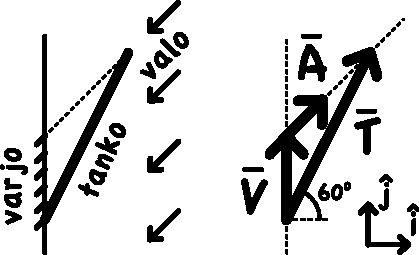
\includegraphics[width=0.95\textwidth]{figs/moniulotteinen_esimerkki_varjo.pdf}%
\end{center}%
}

\solu Sijoittamalla vektorien lausekkeet yhtälöön (\autoref{linyhtalo}) saamme komponenttimuotoisen yhtälön
\begin{equation} (1.0 \un{m})\cos 60^\circ \uv{i} + (1.0 \un{m})\sin 60^\circ \uv{j} = V \uv{j} + a(\uv{i} + \uv{j}) = a \uv{i} + (V + a) \uv{j}. \end{equation}
Yhtälön kummallakin puolella on \(x\)- ja \(y\)-komponentteihin jaettu vektori, ja koska komponenttijako on yksikäsitteinen, vektoreilla täytyy olla samat komponentit. Siispä \(x\)-komponenteille saadaan yhtälö
\( (1.0 \un{m})\cos 60^\circ = a \)
ja \(y\)-komponenteille
\( (1.0 \un{m})\sin 60^\circ = V + a. \)
Ensimmäinen yhtälö kertoo meille suoraan tuntemattoman \(a\) arvon, ja tämän sijoitus jälkimmäiseen yhtälöön antaa varjon pituudeksi
\begin{equation} V = (1.0 \un{m})\sin 60^\circ - a = (1.0 \un{m})(\sin 60^\circ - \cos 60^\circ) = 0.366 \un{m}. \end{equation}

 \eval  Tangon kohtisuoran projektion pituus seinällä olisi
\(T_V = (1.0 \un{m})\sin 60^\circ = 0.866 \un{m}\). Nyt valo ei kuitenkaan saavu seinälle kohtisuoraan, joten kyseessä ei ole kohtisuora projektio. Kuvasta näemme, että varjon pituus on noin puolet tangon korkeudesta. Laskettu pituus on hieman pienempi kuin \(|T_V|/2\), joten tulos on järkevä.

\end{exam}

\subsection{Vakiovoiman tekemä työ}
\label{vakiovoimantekemätyö}

\index{työ}

Pistetulon avulla työn matemaattinen määritelmä yleistyy helposti kolmeen ulottuvuuteen. Kappaleeseen vaikuttavan voiman \(\bs{F}\) ollessa vakio ja kappaleen siirtyessä matkan \(\Delta \bs{r}\) voiman tekemä työ saadaan voiman \emph{siirtymän suuntaisen komponentin} ja siirtymän pituuden tulona.
\begin{equation} W = F_{\Delta r} \Delta r. \end{equation}
Voiman komponentti puolestaan voidaan kirjoittaa yhtälön (\autoref{komponentti_pistetulosta}) perusteella muodossa
\begin{equation} F_{\Delta r} = \frac{1}{\Delta r} \bs{F} \cdot \Delta \bs{r}, \end{equation}
joten työ on yksinkertaisesti \emph{voiman ja siirtymän pistetulo}
\begin{equation} W = \bs{F} \cdot \Delta \bs{r}, \label{tyo_pistetulo}\end{equation}
ja pistetulon komponenttiesityksen avulla tämän voi jakaa koordinaattiakseleiden suuntaisiin osiin
\begin{equation} W = F_x\Delta x + F_y\Delta y + F_z \Delta z. \end{equation}

\pictures%
{tb}
{Vakiovoiman tekemä työ.;%
Työ on voiman ja siirtymän pistetulo.;%
Työn lasku komponenteittain.}%
{fig:moniulotteinen_vakiotyo;fig:moniulotteinen_vakiotyo_a;fig:moniulotteinen_vakiotyo_b}%
{0.45;0.45}%
{0.45;0.45}%
{moniulotteinen_vakiotyo_1.pdf;moniulotteinen_vakiotyo_2.pdf}

\index{teho}

Vastaavalla tavalla voidaan määrittää myös voiman tekemän työn teho. Tehohan mittaa nopeutta, jolla energia siirtyy, eli jos vakiovoima tekee ajassa \(\Delta t\) työn \(W\), sen keskimääräinen teho on
\begin{equation} P_\text{keskiarvo} = \frac{W}{\Delta t} = \bs{F} \cdot \frac{\Delta \bs{r}}{\Delta t}. \end{equation}
Hetkellinen teho saadaan raja-arvona kun aikaväli \(\Delta t\) lähestyy nollaa,
\begin{equation} P = \lim_{\Delta t \to 0} \bs{F} \cdot \frac{\Delta \bs{r}}{\Delta t} = \bs{F} \cdot \frac{\dd \bs{r}}{\dd t} = \bs{F} \cdot \bs{v}. \label{voiman_teho} \end{equation}
Työn teho on siis voimavektorin ja nopeusvektorin pistetulo. Tämä on yleinen tulos joka pätee myös vaikkei voima olisi vakio, koska lauseke johdettiin differentiaalisen lyhyellä ajanjaksolla \(\dd t\), jonka aikana muuttuvaakin voimaa voidaan pitää vakiona.

\begin{stopQ}{q:moniulotteinen_skalaari}%
Miksi voimalle pätee \(F = \sqrt{F_x^2 + F_y^2 + F_z^2}\) mutta työlle kuitenkin \(W \ne \sqrt{(F_x \Delta x)^2 + (F_y\Delta y)^2 + (F_z \Delta z)^2} \)?
\end{stopQ}

\subsection{Viivaintegraali}
\label{viivaintegraali}

\pictures{b!}%
{Muuttuvan voiman tekemä työ käyräviivaista reittiä pitkin on voiman viivaintegraali.;%
Kappale kulkee käyrää pitkin.;%
Jaetaan reitti suoriin osiin.;%
Siirtymän suuntainen voima tekee työtä.;%
Tehdään jaosta mielivaltaisen tiheä.}%
{fig:moniulotteinenviivaintegraali;fig:moniulotteinenviivaintegraali_a;fig:moniulotteinenviivaintegraali_b;fig:moniulotteinenviivaintegraali_c;fig:moniulotteinenviivaintegraali_d;}%
{0.22;0.22;0.22;0.22}%
{0.2;0.2;0.2;0.2}%
{moniulotteinen_viivaintegraali_1.pdf;moniulotteinen_viivaintegraali_2.pdf;moniulotteinen_viivaintegraali_3.pdf;moniulotteinen_viivaintegraali_4.pdf}

Yhdessä ulottuvuudessa muuttuvan voiman tekemä työ laskettiin jakamalla kappaleen siirtymä infinitesimaalisiin osiin, joilla voima on vakio, laskemalla kullakin pienellä siirtymällä tehty infinitesimaalinen työ ja summaamalla nämä yhteen --- eli integroimalla paikan suhteen. Kolmessa ulottuvuudessa työ lasketaan samalla periaatteella, mutta asiaa hankaloittaa lisäksi se, että kappale ei välttämättä kulje suoraan vaan sen reitti voi olla kaareva. Kaarevankin reitin voi kuitenkin jakaa pieniin suoriin osiin ja näin muodostunut murtoviiva lähestyy aidosti kaarevaa reittiä jaon tihentyessä.

\index{rata}

\marginpictures%
{-5}
{Erilaisia viivaintegraaleja. Polkua ympäröivän viivan väri kertoo, onko liike samaan vai vastakkaiseen suuntaan voimaan nähden.;%
Reitti voiman suuntaan.;%
Reitti voimaa vastaan.;%
Reitti edestakaisin.;%
Muuttuva voima.}%
{fig:moniulotteinenviivaintegraali2}%
{0.9;0.9;0.9;0.9}%
{moniulotteinen_viivaintegraali_5.pdf;moniulotteinen_viivaintegraali_6.pdf;moniulotteinen_viivaintegraali_7.png;moniulotteinen_viivaintegraali_8.png}

Tarkastellaan kappaletta, joka kulkee pisteestä \(\bs{r}_\text{alku}\) pisteeseen \(\bs{r}_\text{loppu}\) kaarevaa reittiä \(P\) pitkin (kuva \autoref{fig:moniulotteinenviivaintegraali}). Jaetaan reitti pieniin suoriin siirtymiin \(\Delta \bs{r}_i = \bs{r}_{i+1} - \bs{r}_i \) niin, että nämä siirtymät yhdessä kulkevat reitin alusta loppuun
\begin{equation} \bs{r}_\text{loppu} - \bs{r}_\text{alku} = \sum_{i=0}^N \Delta \bs{r}_i. \end{equation}
Kun siirtymät ovat kyllin lyhyet, kappaleeseen vaikuttava voima \(\bs{F}_i\) on likimain vakio kunkin siirtymän aikana. Tällöin kullakin siirtymällä voima tekee yhtälön (\autoref{tyo_pistetulo}) mukaisesti työn
\begin{equation} W_i = \bs{F}_i \cdot \Delta \bs{r}_i \end{equation}
ja kappaleeseen tehty kokonaistyö on näiden summa. Ottamalla raja-arvo, kun reitti jaetaan äärettömän lyhyisiin osiin, sekä reitin approksimaation että voiman vakioksi olettamisen virhe lähestyvät nollaa ja saadaan työn tarkka arvo,
\bigeq{ W = \lim_{\Delta r \to 0} \sum_{i=0}^N \bs{F}_i \cdot \Delta \bs{r}_i = \int_{P} \bs{F} \cdot \dd \bs{r}. \label{yleinen_tyo} }
Tämä on työn yleinen määritelmä.

\index{työ}
\index{viivaintegraali}

Yhtälössä esiintyvä lauseke on \textbf{viivaintegraali}, jossa integroidaan suuretta jotakin tiettyä avaruuden \emph{reittiä} pitkin. Koska integroitavana on kahden vektorin pistetulo, joka on skalaari, lopputulos on myös skalaari. Yhdessä ulottuvuudessa viivaintegraaleja ei ole, koska liike on rajoitettu suoralle ja voi siten tapahtua korkeintaan edestakaisin. Siksi yhdessä ulottuvuudessa määrättyjen integraalien arvo riippuu alku- ja loppupisteestä. Kolmessa ulottuvuudessa lasketun viivaintegraalin arvo voi sen sijaan riippua myös siitä, \emph{mitä kautta} alkupisteestä siirrytään loppupisteeseen.

\begin{stopQ}{q:moniulotteinen_reittiriippuvuus}%
Haluat kulkea luentosalista ruokalaan. Voit mennä sinne mitä reittiä haluat. Mitkä seuraavista suureista riippuvat valitsemastasi reitistä? (a) Matkan pituus, (b) oman gravitaatiopotentiaalienergiasi muutos, (c) kitkan ja ilmanvastuksen sinuun tekemä työ, (d) gravitaation sinuun tekemä työ?
\end{stopQ}

Viivaintegraalin fysikaalista merkitystä on pyritty havainnollistamaan kuvassa \autoref{fig:moniulotteinenviivaintegraali2}. Kuvassa (a) kappale liikkuu käyräviivaista polkua pitkin ylöspäin ja siihen kohdistuu samalla ylöspäin vaikuttava voima. Koska liike on aina samaan suuntaan kuin voiman liikkeen suuntainen komponentti, viivaintegraali on \emph{positiivinen} ja voima tekee koko matkan positiivista työtä kappaleeseen. Tämä on esitetty kuvassa kappaleen kulkemaa polkua ympäröivällä vihreällä viivalla.

Tässä tarkasteltu voima \emph{ei ole} kappaleeseen vaikuttava kokonaisvoima, koska kappaleen kiihtyvyys ei selvästikään osoita ylöspäin. Tämän voi päätellä siitä, että rata mutkittelee. Jos kiihtyvyys osoittaisi ylöspäin, rata olisi ylöspäin aukeava paraabeli. Kyseessä voisi olla esimerkiksi tilanne, jossa ihminen kulkee nousevassa hississä edestakaisin ja tarkasteltu voima on häneen kohdistuva hissin lattian tukivoima. Hissin matkustajaan kohdistava tukivoima pitää hänet ylöspäin nousevalla radalla ja tekee samalla matkustajaan työtä.

Kuvassa (b) on sama reitti, mutta nyt voima osoittaa alaspäin. Tällöin voiman komponentti radan tangentin suunnassa osoittaa aina vastakkaiseen suuntaan kuin mihin kappale liikkuu, joten voiman tekemä työ on negatiivinen. Tämä on esitetty kuvassa rataa ympäröivänä punaisena viivana.
Tämä voima voisi olla samaiseen hissimatkustajaan vaikuttava painovoima. Painovoima tekee nousevaan kappaleeseen negatiivista työtä, koska se \emph{vähentää} kappaleen liike-energiaa muuttaen sen vuorovaikutuksen varastoimaksi potentiaalienergiaksi.

Edellisissä esimerkeissä oli yksinkertaista päätellä, onko viivaintegraali positiivinen vai negatiivinen, koska liike tapahtui aina joko likimain voiman suuntaan tai siihen nähden vastakkaiseen suuntaan. Yleisesti kuitenkin tilanne voi vaihdella. Kuvassa \autoref{fig:moniulotteinenviivaintegraali2}(c) kappale kulkee välillä voiman suuntaan eli kuvassa oikealle, jolloin voima tekee kappaleeseen positiivista työtä (vihreä). Välillä kappale kuitenkin kääntyy ja alkaa kulkea voimaan nähden vastakkaiseen suuntaan, jolloin työ on negatiivinen (punainen). Kappaleen liikkuessa voiman suuntaan nähden kohtisuoraan, voima ei tee työtä lainkaan (harmaa). Kuvassa (d) puolestaan \emph{voima} muuttuu kappaleen kulkiessa, jolloin aluksi kappaleeseen tehdään positiivista ja lopuksi negatiivista työtä.

Koko matkan aikana tehty työ saadaan laskemalla positiivinen ja negatiivinen työ yhteen, ja tämä kokonaistyö on siis positiivinen, jos kappaleeseen tehdään enemmän positiivista kuin negatiivista työtä, ja päinvastoin negatiivinen, jos negatiivisen työn osuus on suurempi. Jos positiivista ja negatiivista työtä tehdään yhtä paljon, kokonaistyö on \emph{nolla}. Tämä on myös viivaintegraalin fysikaalinen merkitys. Karkeasti ilmaisten viivaintegraali nimittäin mittaa sitä, osoittaako integroitava vektorisuure kuljetulla polulla enemmän kulkusuuntaan vai sitä vastaan.

\begin{stopQ}{q:moniulotteinen_viivaintegraalin_merkki}%
Ovatko kuvissa \autoref{fig:moniulotteinenviivaintegraali2} (c) ja (d) esitetyt viivaintegraalit positiivisia, negatiivisia vai nollia?
\end{stopQ}

Viivaintegraalin laskeminen on mahdollista myös tarkasti, jos sekä kappaleen reitti että siihen vaikuttava voima pystytään ilmoittamaan jonkin parametrin kuten kuljetun matkan tai ajan avulla. Esimerkiksi jos tiedetään kappaleeseen vaikuttava voima ajan funktiona, \(\bs{F}(t) \) sekä kappaleen paikka \(\bs{r}(t) \), viivaintegraali voidaan muuttaa integraaliksi ajan suhteen
\begin{equation} W = \int_{P} \bs{F} \cdot \dd \bs{r} = \int_{t_\text{alku}}^{t_\text{loppu}} \bs{F}(t) \cdot \frac{\dd \bs{r}}{\dd t} \dd t = \int_{t_\text{alku}}^{t_\text{loppu}} \bs{F}(t) \cdot \bs{v}(t) \dd t. \end{equation}
Tämän voi puolestaan jakaa edelleen komponentteihin pistetulon laskusäännön avulla, jolloin voidaan laskea erikseen voiman erisuuntaisten komponenttien tekemä työ.
\begin{equation} W = \int_{t_\text{alku}}^{t_\text{loppu}} F_xv_x \dd t + \int_{t_\text{alku}}^{t_\text{loppu}} F_yv_y \dd t + \int_{t_\text{alku}}^{t_\text{loppu}} F_zv_z \dd t. \end{equation}
Näin monimutkaiselta näyttänyt viivaintegraali on pilkottu kolmen tavallisen yhden muuttujan integraalin summaksi, ja näiden laskeminen onnistuu tavallisilla integrointisäännöillä.
Esimerkissä \autoref{ex:viivaintegraali} näytetään, miten tällainen lasku tehdään.

Edellisessä analyysissä työ, joka on voiman ja \emph{siirtymän} pistetulo, muutettiin muotoon, jossa esiintyy voiman ja \emph{nopeuden} pistetulo. Tämähän on kappaleeseen työtä tekevän voiman \emph{teho}, ja se ilmaisee kuinka \emph{nopeasti} energiaa siirtyy kappaleelle. Kappaleelle siirtyvä kokonaisenergiamäärä eli kappaleeseen tehty työ on puolestaan teho (kuinka nopeasti energiaa siirtyy) kerrottuna ajalla (kuinka kauan energiaa siirtyy), jos teho on vakio. Jos teho ei ole vakio, kokonaistyö saadaan integroimalla tehoa ajan suhteen.

\begin{stopQ}{q:moniulotteinen_tyo_yhteenveto}%
Selitä omin sanoin, miten työ lasketaan kappaleen liikkuessa kahdessa tai kolmessa ulottuvuudessa. Selitä erityisesti milloin pistetulo ja viivaintegraali ovat positiivisia, negatiivisia tai nollia.
\end{stopQ}

\begin{exam}{Ty\"o viivaintegraalina}{ex:viivaintegraali}\noindent

\problem{Kuinka suuren työn kokonaisvoima tekee määritelmän mukaisesti esimerkin \autoref{ex:aikavoima} kuulaan kahden sekunnin aikana?
}

 \twocol{0.6}{0.35}{ \setup  Kuulan liikerata, nopeus sekä kuulaan vaikuttavat voimat on ratkaistu komponenteittain esimerkissä \autoref{ex:aikavoima}. Tarkastelaan prosessia ajan välillä \(t_\text{alku} = 0\un{s}\) ja \(t_\text{loppu} = 2\un{s}\).

 \physics Kuulaan tehty työ on määritelmän mukaisesti voiman viivaintegraali siirtymän suhteen. Jotta tällaisen integraalin voisi laskea, pitää kuitenkin tietää sekä kuulan paikka että siihen vaikuttava voima jonkin parametrin funktiona. Mahdollisia vaihtoehtoja ovat esimerkiksi kuljetun matkan pituus tai matkaan käytetty aika. Koska nyt tiedämme jo valmiiksi kaikki suureet ajan funktiona, on järkevintä esittää voima ja siirtymä ajan funktioina.
Erityisesti siirtymä voidaan ilmoittaa nopeuden ja ajan muutoksen tulona.

}{%
\begin{center}%
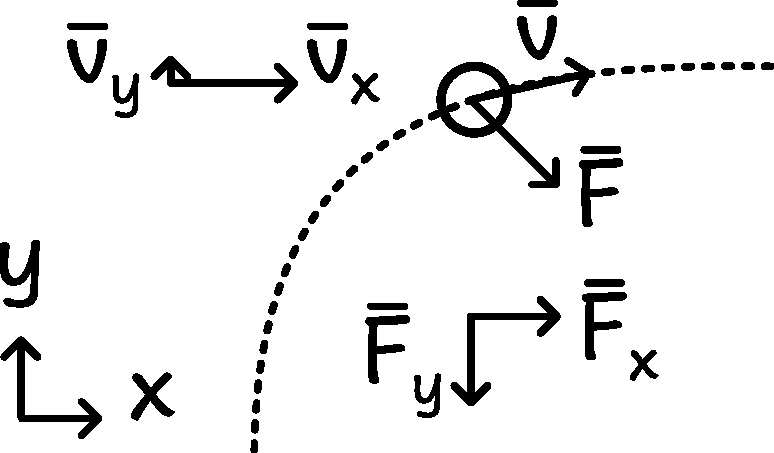
\includegraphics[width=0.95\textwidth]{figs/moniulotteinen_esimerkki_viivaintegraali.pdf}%
\end{center}%
}

 \model  Työ on määritelmän mukaisesti
\begin{equation} W = \int_{\bs{r}_\text{alku}}^{\bs{r}_\text{loppu}} \bs{F} \cdot \dd \bs{r}. \end{equation}
Jos kuulan nopeus ajan hetkellä \(t\) on \(\bs{v}(t) \), on kuulan siirtymä lyhyen ajan \(\dd t\) kuluessa nopeuden määritelmän mukaisesti \(\dd \bs{r} = \bs{v} \dd t\). Työ voidaan siis kirjoittaa myös muodossa
\begin{equation} W = \int_{t_\text{alku}}^{t_\text{loppu}} \bs{F} \cdot \bs{v} \dd t. \end{equation}
Tämä voidaan päätellä myös työn tekemän tehon avulla, sillä teho on
\( P = \frac{\dd W}{\dd t} = \bs{F} \cdot \bs{v}, \)
joten työ saadaan integroimalla lauseketta \(\dd W = \bs{F} \cdot \bs{v} \dd t \).
Käytännössä lasku onnistuu hajottamalla pistetulo komponentteihin
\begin{equation} W = \int_{t_\text{alku}}^{t_\text{loppu}} (F_x v_x + F_y v_y) \dd t. \end{equation}

 \solu  Lasketaan ensin \(x\)-suuntaisen voiman tekemä työ
\begin{equation} W_{F_x} = \int_{t_\text{alku}}^{t_\text{loppu}} F_x v_x \dd t = \int_{t_\text{alku}}^{t_\text{loppu}} \frac{1}{2} \frac{A^2}{m} t^3 \dd t = \frac{1}{8}\frac{A^2}{m} (t_\text{loppu}^4 - t_\text{alku}^4). \end{equation}
Sijoittamalla lukuarvot saadaan \(W_{F_x} = 1.8\cdot10^{-5} \un{J}\).
Vastaavasti \(y\)-suunnassa
\begin{equation} W_{F_y} = \int_{t_\text{alku}}^{t_\text{loppu}} F_y v_y \dd t = \int_{t_\text{alku}}^{t_\text{loppu}} \frac{B^2}{mC}(1 - \cos Ct)\sin Ct \dd t. \end{equation}
Tässä integraalissa on kaksi termiä, joista ensimmäisen integraali on \(\int \sin Ct \dd t = -\frac{1}{C} \cos Ct + c\) ja toisen integrointi onnistuu esimerkiksi trigonometristen laskusääntöjen avulla \(\int -\cos Ct \sin Ct \dd t = \int -\frac{1}{2} \sin 2Ct \dd t = \frac{1}{4C} \cos 2Ct + c\). Kaikkiaan siis
\begin{equation} W_{F_y} = \bigg|_{t_\text{alku}}^{t_\text{loppu}} \frac{B^2}{mC^2}\left( \frac{1}{4} \cos 2Ct - \cos Ct \right) = \frac{B^2}{mC^2}\left( \frac{1}{4} \cos 2Ct_\text{loppu} - \cos Ct_\text{loppu} \right) - \frac{B^2}{mC^2} \left( \frac{1}{4} \cos 2Ct_\text{alku} - \cos Ct_\text{alku} \right). \end{equation}
Sijoittamalla lukuarvot saadaan \(W_{F_y} = 1.2\cdot10^{-7} \un{J}\).

Kokonaistyö on näiden summa, ja koska \(y\)-suuntaisten voimien tekemä työ on huomattavasti pienempi kuin \(x\)-suuntaisten, kokonaistyö on kahden merkitsevän numeron tarkkuudella sama kuin pelkkä \(x\)-suuntaisen voiman komponentin tekemä työ \(W = W_{F_x} + W_{F_y} = 1.8\cdot10^{-5} \un{J}\).

\mbar
\begin{mathematica}[commandchars=\\!?]
(* voimat *)
fx = a t; fy = b Sin[c t];
lukuarvot = {a -> 3*10^-4, b -> 7*10^-4, c -> 3.5, m -> 0.01};
aika = {talku -> 0, tloppu -> 2}

(* nopeudet *)
vx = Integrate[fx/m, {t, 0, t}]
  \textit!(a t^2)/(2 m)?
vy = Integrate[fy/m, {t, 0, t}]
  \textit!(b - b Cos[c t])/(c m)?

(* ty\"o *)
wx = Integrate[fx vx, {t, talku, tloppu}]
  \textit!-((a^2 talku^4)/(8 m)) + (a^2 tloppu^4)/(8 m)?
wx /. lukuarvot /. aika
  \textit!0.000018?
wy = Integrate[fy vy, {t, talku, tloppu}]
  \textit!(b^2 (4 Cos[c talku] - Cos[2 c talku] - 4 Cos[c tloppu] + Cos[2 c tloppu]))/(4 c^2 m)?
wy /. lukuarvot /. aika
  \textit!1.21128*10^-7?

(* kokonaisty\"o *)
w = wx + wy /.lukuarvot /. aika
  \textit!0.0000181211?

(* kuulan saaman liike-energian pit\"a\"a olla sama kuin siihen tehty kokonaisty\"o *)
kx = 1/2 m vx^2 /. lukuarvot /. t->2
  \textit!0.000018?
ky = 1/2 m vy^2 /. lukuarvot /. t->2
  \textit!1.21128*10^-7?
\end{mathematica}
\begin{center}
\end{center}

\eval Kuulan liike-energian muutoksen täytyy olla yhtä suuri kuin kuulaan tehty kokonaistyö. Sijoitus liike-energian lausekkeeseen osoittaa, että näin on
\begin{equation} K = \frac{1}{2}mv^2 = \frac{1}{2}mv_x^2 + \frac{1}{2}mv_y^2 = 1.8\cdot10^{-5} \un{J} = W. \end{equation}

Tarkistetaan myös työn yksiköt:
\begin{equation} [W_x] = \frac{[A^2]}{[m]} [t^4] = \frac{\text{N}^2/\text{s}^2}{\text{kg}} \text{s}^4 = \frac{\text{kg}^2 \text{m}^2/\text{s}^4}{\text{kg}} \text{s}^2 = \text{kg} \text{m}^2/\text{s}^2 = \text{J} \end{equation}
\begin{equation} [W_y] = \frac{[B^2]}{[mC^2]} [\cos 2Ct] = \frac{\text{N}^2}{\text{kg s}^{-2}}\cdot 1 = \frac{\text{N}^2\text{s}^2}{\text{kg}} = \text{J}. \end{equation}

\end{exam}

\subsection{Konservatiivisuus}
\label{konservatiivisuus}

\index{konservatiivinen}

Aikaisemmin määrittelimme konservatiivisiksi sellaiset vuorovaikutukset, joihin liittyy potentiaalienergia. Edelleen jos systeemissä vaikuttaa vain konservatiivisia vuorovaikutuksia, mekaaninen energia on systeemissä vakio, ja tämä ominaisuus tekee konservatiivisuudesta erittäin tärkeän teoreettisen työkalun.
Lisäksi yhdessä ulottuvuudessa opimme myös, että potentiaalienergia voidaan määrittää konservatiivisen voiman tekemän työn kautta
\begin{equation} \Delta U = - W_\text{konservatiivinen} = - \int_{x_\text{alku}}^{x_\text{loppu}} F_x \dd x, \end{equation}
eli integraalina. Tämä tulos perustui siihen, että työ mittaa vuorovaikutuksen siirtämää energiaa, ja konservatiivisen vuorovaikutuksen tapauksessa tämä energia tulee vuorovaikutuksen varastoimasta potentiaalienergiasta.
Vastaavasti voima saadaan potentiaalienergian derivaattana,
\begin{equation} F_x = -\frac{\dd U}{\dd x}. \end{equation}
Seuraavaksi tarkastelemme, miten konservatiivisuus ilmenee kolmiulotteisessa avaruudessa.

Myös kolmessa ulottuvuudessa potentiaalienergia määritellään niin, että konservatiivisen vuorovaikutuksen potentiaalienergian muutos missä tahansa prosessissa on tämän vuorovaikutuksen tekemän työn vastaluku \(\Delta U = - W_\text{konservatiivinen}\).
Potentiaalienergialla ei ole absoluuttista arvoa, mutta jos valitaan jokin piste \(\bs{r}_0\) potentiaalienergian nollakohdaksi, konservatiivisen vuorovaikutuksen potentiaalienergia missä tahansa pisteessä \(\bs{r}\) on voiman tekemän työn vastaluku kappaleen siirtyessä nollapisteestä tähän tarkastelupisteeseen
\begin{equation} U(\bs{r}) = - W_{\bs{r}_0 \to \bs{r}}. \label{potene_tyo_yleinen} \end{equation}

Kolmessa ulottuvuudessa on kuitenkin huomioitava, että kappale voi tehdä siirtymän \(\bs{r}_0 \to \bs{r}\) \emph{mielivaltaista reittiä pitkin} ja työ määriteltiin kolmessa ulottuvuudessa \emph{viivaintegraalina}.
Kuitenkin koska potentiaalienergia on paikan funktio, sillä täytyy olla pisteessä \(\bs{r}\) jokin tietty yksikäsitteinen arvo. Niinpä yhtälö (\autoref{potene_tyo_yleinen}) on mielekäs vain jos työ \(W_{\bs{r}_0 \to \bs{r}}\) saa \emph{saman arvon kulkipa kappale mitä tahansa reittiä pitkin}. Tämä on kolmessa ulottuvuudessa konservatiivisuuden määritelmä: \emph{vuorovaikutus on konservatiivinen jos ja vain jos sen tekemä työ kappaleen siirtyessä minkä tahansa kahden pisteen välillä ei riipu reitistä, jota pitkin kappale kulkee}.

\pictures{tb}%
{Viivaintegraali suljetulla reitillä.;%
Konservatiivisen voiman työ on nolla.;%
Työ on positiivinen, joten vuorovaikutus ei ole konservatiivinen.;%
Työ on negatiivinen, joten vuorovaikutus ei ole konservatiivinen.}%
{fig:moniulotteinenreitti;fig:moniulotteinenreitti_a;fig:moniulotteinenreitti_b;fig:moniulotteinenreitti_c;}%
{0.35;0.27;0.27}%
{0.351;0.274;0.274}%
{moniulotteinen_viivaintegraali_9.png;moniulotteinen_viivaintegraali_10.pdf;moniulotteinen_viivaintegraali_11.pdf}

\index{suljettu reitti}

Toinen tapa ilmaista sama asia on vaatia, että jos kappale kulkee \emph{suljetun reitin}, konservatiivisen voiman siihen tekemän työn täytyy olla \emph{nolla}. Näin siksi, että kuljettuaan suljetun reitin kappale palaa takaisin alkupisteeseensä jolloin potentiaalienergian täytyy olla lopuksi \emph{sama} kuin aluksi. Potentiaalienergian muutos kierroksen jälkeen, jonka täytyy olla sama kuin vuorovaikutuksen tekemä työ, on siis nolla
\( W_\text{suljettu} = - \Delta U = 0 \un{J}. \)
Tätä on havainnollistettu kuvassa \autoref{fig:moniulotteinenreitti} (a), jossa voima tekee silmukan kulkevaan kappaleeseen yhtä paljon positiivista ja negatiivista työtä jolloin kokonaistyö on nolla.

Aina näin ei kuitenkaan välttämättä ole ja kappaleeseen tehty kokonaistyö voi olla nollasta poikkeava vaikka kappale kulkisi suljetun reitin. Näin on kuvissa \autoref{fig:moniulotteinenreitti} (b) ja (c), joissa molemmissa voima on aina yhdensuuntainen liikkeen kanssa --- joko samansuuntainen, jolloin työ on positiivinen, tai vastakkaissuuntainen, jolloin työ on negatiivinen.

Täsmälleen sama ajatus esiteltiin jo luvussa \autoref{luku:sailymislait} tarkasteltaessa kappaleita, jotka kuljettuaan edestakaisen matkan palasivat samaan pisteeseen. Jos kappaleen mekaaninen energia säilyi, siihen tehty kokonaistyö oli nolla ja vuorovaikutukset olivat konservatiivisia. Jos puolestaan kappaleen mekaanista energiaa oli muuttunut sisäenergiaksi tai päinvastoin, kappaleeseen täytyi vaikuttaa myös dissipatiivisia vuorovaikutuksia.

\begin{stopQ}{q:moniulotteinen_konservatiivisuus}%
(a) Kappaletta nostetaan ensin metri suoraan ylös ja sitten lasketaan metri alas. Mihin suuntaan painovoima osoittaa ja millainen on sen kappaleeseen tekemä työ?
(b) Kappaletta työnnetään lattialla ensin metri eteenpäin ja sitten metri takaisin. Mihin suuntaan liukukitka osoittaa ja millainen on sen kappaleeseen tekemä työ?
(c) Mitä tulokset kertovat voimien konservatiivisuudesta?
\end{stopQ}

\index{painovoima}

Tarkastellaan lopuksi vielä painovoimaa esimerkkinä konservatiivisesta vuorovaikutuksesta.
Painovoimallahan on potentiaalienergia (\autoref{pot_ene}), joten painovoiman on sen perusteella oltava konservatiivinen vuorovaikutus. Perustelimme tämän aikaisemmin kuitenkin vain \emph{pystysuoralle} liikkeelle. Kolmessa ulottuvuudessa kappaleet voivat kuitenkin liikkua myös \emph{vaakasuunnassa}, ja jotta painovoima todella olisi konservatiivinen, sen tekemän työn täytyy olla nolla minkä tahansa suljetun reitin kulkeneeseen kappaleeseen.
Päätellään nyt, että painovoiman tapauksessa näin todella tapahtuu.

Tarkastellaan ensin yksinkertaista tapausta --- vapaata liikettä kaltevalla tasolla.
Suora siirtymä kaltevalla tasolla voidaan jakaa pysty- ja vaakasuoraan komponenttiin \(\Delta \bs{r} = \Delta x \uv{i} + \Delta y \uv{j}\), jolloin painovoiman tekemä työ on
\begin{equation} W = \bs{G} \cdot \Delta \bs{r} = -mg \uv{j} \cdot (\Delta x \uv{i} + \Delta y \uv{j}) = -mg\uv{j} \cdot \Delta x \uv{i} - mg \uv{j} \cdot \Delta y \uv{j}. \end{equation}
Tässä kuitenkin painovoiman ja vaakasiirtymän pistetulo on nolla, \(-mg\uv{j} \cdot \Delta x \uv{i} = 0\), koska nämä ovat kohtisuorassa, joten työ riippuu ainoastaan \emph{pystysuuntaisesta} siirtymästä
\begin{equation} W = -mg \uv{j} \cdot \Delta y \uv{j} = -mg \Delta y. \end{equation}
Tämä on sama tulos kuin pystysuorassa liikkeessä. Kaltevaa tasoa pitkin liikkuva kappale toki joutuu kulkemaan pidemmän matkan ja se käyttää tähän matkaan enemmän aikaa, mutta kappaleen saama energia on sama kuin suorassa pudotuksessa.

\pictures{tb}%
{Painovoima on konservatiivinen, koska sen kappaleeseen tekemä työ ei riipu kappaleen kulkemasta reitistä vaan vain pystysuuntaisesta siirtymästä.;%
Pystysuora, vino ja kaareva reitti.;%
Siirtymän jako pysty- ja vaakakomponentteihin.;%
Kaarevaa reittiä voi approksimoida murtoviivana.}%
{fig:energiagravitaatio;fig:energiagravitaatio_a;fig:energiagravitaatio_b;fig:energiagravitaatio_c;}%
{0.85;0.45;0.45}%
{0.85;0.45;0.45}%
{energia_reitti_1.pdf;moniulotteinen_reitti_3.pdf;energia_reitti_2.pdf}

Tapaus, jossa kappale liikkuu pitkin käyräviivaista reittiä, voidaan analysoida edellisen tuloksen avulla. Mikä tahansa reitti voidaan nimittäin jakaa lyhyisiin osiin ja näitä osia voidaan pitää likimain suorina siirtyminä kuten kuvassa \autoref{fig:energiagravitaatio} (b) on esitetty. Tämä on tietenkin approksimaatio, jos kappale todellisuudessa kulkee käyräviivaista rataa, mutta mitä lyhyempiin osiin reitti jaetaan, sitä tarkemmin suorista siirtymistä koostuva reitti muistuttaa todellista käyrää.

Kullakin lyhyellä siirtymällä kappaleeseen tehty työ riippuu vain kappaleen pystysuuntaisesta siirtymästä ja kokonaistyö saadaan laskemalla nämä yhteen. Koska massa ja putoamiskiihtyvyys ovat tässä vakioita, tämä kuitenkin johtaa vain pystysuuntaisten siirtymien yhteenlaskuun. Kuvan \autoref{fig:energiagravitaatio} (c) esimerkissä reitti on jaettu neljään osaan, jolloin
\begin{equation} W = W_1 + W_2 + W_3 + W_4 = -mg (\Delta y_1 + \Delta y_2 + \Delta y_3 + \Delta y_4) = -mg \Delta y_\text{kokonais}. \end{equation}
Tulos on sama riippumatta siitä miten reitti jaettiin osiin, joten sen täytyy päteä \emph{mille tahansa} reitille, jonka loppu- ja alkupisteen välinen etäisyys on pystysuunnassa \(\Delta y\).
Näin on siis päätelty, että \emph{mitä tahansa reittiä} kappale kulkeekaan painovoimakentässä, sen liike-energian muutos riippuu ainoastaan sen siirtymästä \emph{pystysuunnassa}. Siispä gravitaatiota todella kuvaa ainoastaan kappaleen pystysuuntaisesta koordinaatista riippuva potentiaalienergia (\autoref{pot_ene}) ja vuorovaikutus on konservatiivinen.

\begin{stopQ}{q:moniulotteinen_suljettu}%
Päättele edellä esitetyn perusteella vielä, että jos kappale kulkee suljetun reitin, painovoiman siihen tekemä työ on nolla. Selitä, miksi tämä on tärkeää.
\end{stopQ}

\section{Kentät}
\label{kentät}

\subsection{Kenttä vuorovaikutuksen välittäjänä}
\label{kenttävuorovaikutuksenvälittäjänä}

\index{vuorovaikutus}

Vuorovaikutuksilla tarkoitetaan fysiikassa yleisesti kahden tai useamman olion välistä vaikutussuhdetta, joka ohjaa olioiden käyttäytymistä. Vuorovaikutukset tuottavat voimia ja niihin voi liittyä potentiaalienergiaa. Fysiikka tuntee neljä perusvuorovaikutusta, jotka ovat \emph{gravitaatiovuorovaikutus} eli painovoima, \emph{sähkömagneettinen vuorovaikutus}, \emph{heikko vuorovaikutus} sekä \emph{vahva vuorovaikutus}.

\index{atomi}

Kaikki aine koostuu pienenpienistä atomeista, ja
heikko sekä vahva vuorovaikutus vaikuttavatkin vain atomiydinten ja alkeishiukkasten mittakaavassa. Ne ovat tärkeitä vuorovaikutuksia, sillä ne pitävät atomien ytimet koossa ja vaikuttavat ilmiöissä kuten radioaktiivisuudessa. Kuitenkaan makroskooppisessa, arkielämän mittakaavassa niitä ei voi suoraan havaita, emmekä tässä materiaalissa käsittele lainkaan näitä vuorovaikutuksia.

\index{massa}

Gravitaatio on kaikkien \emph{massallisten} kappaleiden ja hiukkasten välinen vuorovaikutus, joka saa kappaleet vetämään toisiaan puoleensa. Ilmeisin esimerkki gravitaatiosta on se, että kappaleet putoavat kohti maata, sillä maapallo vuorovaikuttaa gravitaation kautta kaikkien massallisten kappaleiden kanssa vetäen niitä puoleensa.

\index{protoni}
\index{neutroni}
\index{sähkövaraus}
\index{elektroni}

Sähkömagneettinen vuorovaikutus puolestaan vaikuttaa hiukkasiin, joilla on \emph{sähkövaraukseksi} kutsuttu ominaisuus. Atomiytimet koostuvat \emph{protoneista} ja \emph{neutroneista}, ja kaikissa atomeissa ytimen ympärillä on \emph{elektroneja}.
Protonit ja elektronit ovat sähköisesti varattuja, ja ne vetävät toisiaan puoleensa sähkömagneettisen vuorovaikutuksen kautta, ja niinpä tämäkin vuorovaikutus on välttämätön, jotta atomit ja aine pysyisi koossa. Sähkömagneettinen vuorovaikutus voidaan havaita suoraan myös makroskooppisessa mittakaavassa sähköisesti varattujen, magneettisten ja virtaa kuljettavien kappaleiden vuorovaikutuksina. Tutustumme sähkömagnetismiin tarkemmin luvusta \autoref{luku:sahkostatiikka} alkaen.

Myös esimerkiksi kemia, aineen makroskooppiset ominaisuudet ja arkipäiväiset vuorovaikutukset kuten kosketusvuorovaikutukset ovat pohjimmiltaan sähkömagneettisen vuorovaikutuksen aikaansaamia. Ne ovat nimittäin kaikki seurausta atomeissa olevien elektronien vuorovaikutuksista ja kvanttimekaanisista ominaisuuksista. Kappaleet eivät esimerkiksi kulje toistensa läpi, koska niiden rakenteen hajottaminen edellyttäisi atomiydinten ja elektronien välisen sähkömagneettisen vuorovaikutuksen synnyttämien sidosten rikkomista, mikä vaatisi hyvin paljon energiaa. Ainetta \emph{on} toki mahdollista hajottaa, mutta se ei ole yleensä aivan helppoa.

Sähkömagneettinen vuorovaikutus voi saada hiukkaset joko hylkimään toisiaan tai vetämään toisiaan puoleensa. Gravitaatio puolestaan saa kappaleet aina vetämään toisiaan puoleensa. Mitä suurempi on kappaleiden massa, sitä voimakkaampi on niiden välinen gravitaatio. Gravitaatio on kuitenkin paljon heikompi kuin kaikki muut perusvuorovaikutukset (myös heikompi kuin ``heikko'' vuorovaikutus), joten tarvitaan valtavan suuria massakeskittymiä kuten tähtiä ja planeettoja, jotta gravitaation vaikutukset voitaisiin havaita. Planeettoja ja tähtiä kuitenkin on olemassa, ja niinpä hyvin suuressa mittakaavassa gravitaatio on usein merkittävä vuorovaikutus. On ehkä yllättävää, että gravitaatio, joka tavallisesti tuntuu hyvin vahvalta vuorovaikutukselta onkin ylivoimaisesti heikoin luonnon vuorovaikutus. Tämän voi ymmärtää paremmin huomaamalla, että vaikka pitelisit kädessäsi vaikkapa painavaa kirjaa, jota vetää puoleensa \emph{koko maapallon massa}, pieni alue sormiesi pinnalla pystyy kosketuksen kautta helposti vuorovaikuttamaan kirjan kanssa voimakkaammin ja nostamaan kirjan ylös. Ja kosketuksessakin välittyy vain sähkömagneettisen vuorovaikutuksen pieni sivujäänne.

Monet arkipäiväiset vuorovaikutukset vaativat kappaleiden koskettamista, koska ne syntyvät kappaleiden pintojen atomien kohdatessa. Oleellisesti kysymys on siitä, että atomien elektronit eivät voi helposti kulkea toistensa läpi.
Gravitaatio ja sähkömagneettinen vuorovaikutus kuitenkin toimivat vaikka vuorovaikuttavat hiukkaset olisivat \emph{kuinka kaukana tahansa}, minkä vuoksi niitä kutsutaan \textbf{etävuorovaikutuksiksi}. Esimerkiksi maapallo on noin 150 miljoonan kilometrin päässä Auringosta, mutta silti Auringon ja Maan välinen gravitaatiovuorovaikutus pitää Maan Aurinkoa kiertävällä radalla. Herääkin kysymys, kuinka tällaiset etävuorovaikutukset ovat mahdollisia.

\index{kenttä}

Gravitaation voidaan ajatella toimivan niin, että massalliset kappaleet synnyttävät ympärilleen \textbf{gravitaatiokentän} eli jonkinlaisen näkymättömän rakenteen, joka levittäytyy kaikkialle avaruuteen ja vaikuttaa siellä muiden kappaleiden käyttäytymiseen. Vastaavasti sähköinen vuorovaikutus toimii siten, että varatut hiukkaset synnyttävät avaruuteen \emph{sähkökentän}, joka vaikuttaa toisten varattujen hiukkasten liikkeeseen.
Koska kenttä leviää avaruuteen, se mahdollistaa vuorovaikutukset mielivaltaisen pitkien etäisyyksien päästä ilman, että kentän kohtaava kappale tietäisi, millainen kappale kentän on synnyttänyt. Itse asiassa kenttä leviää avaruuteen äärellisellä nopeudella, joten kentän synnyttänyt kappale on voinut jo siirtyä muualle, kun kentän tuottama vuorovaikutus lopulta tunnetaan.
Fysiikassa tästä mekanismista sanotaan, että kenttä \emph{välittää} vuorovaikutuksen kappaleiden välillä.

\widepictures{tb}%
{Gravitaatiovuorovaikutuksen voi ajatella välittyvän kappaleiden kesken gravitaatiokentän avulla.;%
Maa synnyttää kentän.;%
Kuu tuntee kentän.;%
Myös Kuu synnyttää kentän, jonka Maa tuntee.;%
Lähellä Maan pintaa kenttä on tasainen.}%
{fig:energiagravitaatiokentta;fig:energiagravitaatiokentta_a;fig:energiagravitaatiokentta_b;fig:energiagravitaatiokentta_c;fig:energiagravitaatiokentta_d;}%
{0.225;0.225;0.225;0.225}%
{0.225;0.225;0.225;0.225}%
{energia_kentta_1.pdf;energia_kentta_2.pdf;energia_kentta_3.pdf;energia_kentta_4.pdf}

Matemaattisesti kenttä on avaruudessa määritelty paikan funktio. \textbf{Skalaarikenttä} on funktio, jolla on jokaisessa avaruuden pisteessä jonkin skalaariarvo eli suuruus. Vastaavasti \textbf{vektorikenttä} on funktio, jolla on jokaisessa avaruuden pisteessä vektoriarvo eli sekä suuruus että suunta. Gravitaatio- ja sähkökenttä ovat tärkeitä esimerkkejä fysikaalisista kentistä, mutta periaatteessa mikä tahansa avaruudessa määritelty funktio voi olla kenttä.

\begin{stopQ}{q:moniulotteinen_kentta}%
Keksi lisää esimerkkejä kentistä, jotka voidaan määritellä tavallisessa huoneessa. Ovatko esimerkkisi skalaari- vai vektorikenttiä?
\end{stopQ}

\begin{exam}{Virtauskentt\"a}{ex:field}\noindent

 \twocol{0.49}{0.5}{  Putkessa virtaa kaasua. Virtausnopeus on vektorisuure, joka ilmaisee nopeuden, jolla kaasun molekyylit keskimäärin liikkuvat \emph{yhdessä} avaruuden pisteessä. Periaatteessa kaasun virtausnopeus voidaan mitata missä tahansa pisteessä putken sisällä. Koska kaasu voi liikkua putken eri osissa eri nopeuksilla ja eri suuntiin, virtausnopeus riippuu mittauspisteestä.

Kaasun virtausta kokonaisuutena kuvaa virtauskenttä, joka sisältää tiedon kaasun nopeudesta \emph{kaikissa} avaruuden pisteessä. Voidaan valita mikä tahansa piste putken sisältä, ja virtauskenttä kertoo, mikä on kaasun nopeus kyseisessä pisteessä. Se on siis paikan funktio eli kenttä. Koska virtausnopeus on vektori, kyseessä on vektorikenttä.

}{%
\begin{center}%
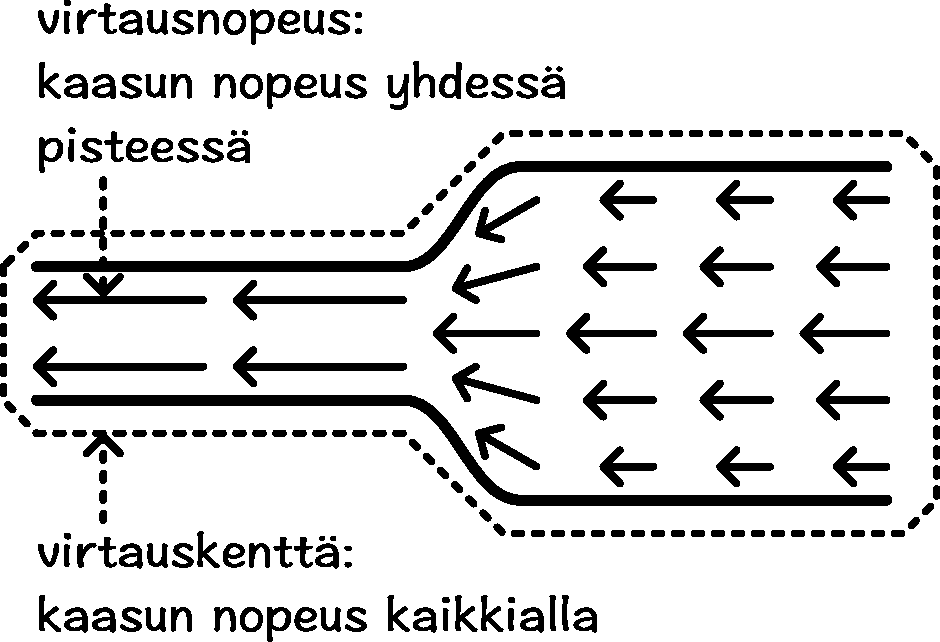
\includegraphics[width=0.9\textwidth]{figs/energia_esimerkki_kentta.pdf}%
\end{center}%
}

\end{exam}

Esimerkiksi gravitaation potentiaalienergia on \emph{skalaarikenttä}, sillä kappaleen potentiaalienergia riippuu sen paikasta. Gravitaation kappaleeseen kohdistama voima on puolestaan \emph{vektorikenttä}. Voimahan on vektori ja painovoima riippuu periaatteessa kappaleen paikasta. Lähellä maanpintaa painovoima on vakio, mutta kaukana maapallosta näin ei enää ole. Gravitaatiovoima ja sen potentiaalienergia ovat kuitenkin loppujen lopuksi vain kaksi erilaista tapaa kuvata gravitaatiovuorovaikutusta, joten ne liittyvät kiinteästä toisiinsa.
Seuraava tavoitteemme onkin tutkia, miten näitä kenttiä kuvataan matemaattisesti. Erityisesti haluamme selvittää, miten konservatiivisen vuorovaikutuksen voima lasketaan, kun vuorovaikutuksen potentiaalienergia tunnetaan.

\subsection{Voiman määrittäminen potentiaalienergiasta}
\label{voimanmäärittäminenpotentiaalienergiasta}

Potentiaalienergia määritellään voiman tekemänä työnä eli matemaattisesti integraalina. Yhdessä ulottuvuudessa tämä tarkoitti toisaalta sitä, että konservatiivisen vuorovaikutuksen voima saatiin potentiaalienergian derivaattana, sillä derivointi ja integrointi ovat käänteisoperaatiot.
Samanlainen periaate pätee myös kolmessa ulottuvuudessa, mutta aivan kuten työn määrittely vaati uudenlaisen integraalin, viivaintegraalin, voiman määrittäminen potentiaalienergian perusteella vaatii derivaatan määrittelyn useassa ulottuvuudessa.

Pohditaan aluksi, millaisia ominaisuuksia konservatiivisella voimalla pitäisi olla. Ajatellaan jälleen analogiaa mäessä vierivään palloon: Palloon kohdistuva kokonaisvoima osoittaa aina alamäkeen vetäen palloa tähän suuntaan. Lisäksi jyrkkään mäkeen asetettu pallo alkaa vieriä nopeammin kuin loivaan rinteeseen tuotu pallo, joten jyrkässä mäessä palloon vaikuttava kokonaisvoima on suurempi. Tilanne on kuitenkin monimutkaisempi kuin yhdessä ulottuvuudessa, koska ``alamäki'' voi eri paikoissa osoittaa eri suuntiin. Pallon liikkuessa tämä alamäen suunta todennäköisesti vielä muuttuu, jolloin palloon kohdistuvan voiman suunta myös muuttuu. Jotta tietäisimme minnepäin palloon vaikuttava voima missäkin vaikuttaa, meillä pitäisi olla jokin keino laskea suunta, johon mäki kussakin pisteessä jyrkimmin laskee. Koska tämä riippuu vain mäen korkeuden muutoksista, periaatteessa ongelman pitäisi olla ratkaistavissa kunhan tiedämme kuinka korkealla mäki kussakin pisteessä on.
Tämä tehtävä yleistyy mielivaltaisen potentiaalienergian tapaukseen: jos tiedämme kappaleen potentiaalienergian avaruuden jokaisessa pisteessä, kuinka lasketaan suunta, johon kappaleeseen vaikuttava voima osoittaa --- eli johon liikuttaessa potentiaalienergia pienenee nopeiten? Ja edelleen, kuinka nopeasti potentiaalienergia tuossa suunnassa muuttuu?

\widepictures{tb}%
{Maaston korkeus esimerkkinä usean muuttujan funktiosta. Korkeutta voidaan kuvata esimerkiksi korkeuskäyrillä ja korkeuden muuttumista paikan funktiona voidaan kuvata osittaisderivaatoilla ja gradientilla.;%
Maaston muoto kahden kukkulan ympäristössä.;%
Maaston muoto korkeuskäyrinä.;%
Jyrkimmän nousun suunta ja jyrkkyys eli gradientti.;%
Maaston profiili \(x\)- (sininen) ja \(y\)-suunnassa (punainen).;%
Profiilikuvaajien sijainti.;%
Korkeuden osittaisderivaatat kulmakertoimina.}%
{fig:moniulotteinen_gradientti;fig:moniulotteinen_gradientti_a;fig:moniulotteinen_gradientti_b;fig:moniulotteinen_gradientti_c;fig:moniulotteinen_gradientti_d;fig:moniulotteinen_gradientti_e;fig:moniulotteinen_gradientti_f;}%
{0.4;0.25;0.25;0.4;0.25;0.25}%
{0.394;0.256;0.256;0.394;0.256;0.256}%
{moniulotteinen_korkeuskayra_1.pdf;moniulotteinen_korkeuskayra_2.pdf;moniulotteinen_korkeuskayra_3.pdf;moniulotteinen_korkeuskayra_4.pdf;moniulotteinen_korkeuskayra_5.pdf;moniulotteinen_korkeuskayra_6.pdf}

Suureen muutosta toisen suureen muuttuessa kuvaa derivaatta, joten mitä ilmeisimmin edellä esitetty ongelma liittyy jotenkin derivaattoihin. Useassa ulottuvuudessa on kuitenkin mahdollista derivoida eri koordinaattien suhteen, joten täytyy olla erityisen tarkkana sen suhteen \emph{millaisia} derivaattoja kulloinkin lasketaan. Erityisesti voi olla tilanne, jossa suureet riippuvat toisistaan ja yhden suureen muuttaminen vaikuttaa toisiin suureisiin.

\index{derivaatta}
\index{osittaisderivaatta}

Usean muuttujan funktiolle määritellään \textbf{osittaisderivaatta} tavallisen derivaatan tapaan erotusosamääränä. Esimerkiksi funktion \(f(x,y,z) \) osittaisderivaattaa muuttujan \(x\) suhteen merkitään
\begin{equation} \frac{\partial f}{\partial x} = \lim_{\Delta x \to 0} \frac{f(x+\Delta x, y, z)- f(x,y,z)}{\Delta x}. \label{osittaisderivaatta} \end{equation}
Huomattavaa tässä määritelmässä on se, että raja-arvo lasketaan erotuksesta, jossa ainoastaan \emph{yhden} suureen, tässä \(x\), annetaan muuttua ja kaikki muut ovat vakioita. Tällainen derivaatta lasketaan normaaleilla derivoimissäännöillä, mutta näitä sääntöjä sovelletaan ainoastaan derivoimismuuttujaan ja kaikki muut suureet käsitellään kuin ne olisivat vakioita.

Osittaisderivaatan käsitettä on havainnollistettu kuvassa (\autoref{fig:moniulotteinen_gradientti}), jossa on kuvattu epätasaisen maaston muoto \(500 \un{m} \times 500 \un{m}\) kokoisella alueella. Tässä tarkasteltava funktio on maan pinnan korkeus, \(h\), joka on itä--länsi-suuntaisen koordinaatin \(x\) ja pohjois--etelä-suuntaisen koordinaatin \(y\) funktio, \(h(x,y) \). Kuvissa (a) ja (b) maaston korkeus on kuvattu korkeuskäyrillä eli käyrillä, joilla korkeus on vakio. Esimerkiksi \(70 \un{m}\) korkeuskäyrän kaikki pisteet ovat \(70 \un{m}\) merenpinnan yläpuolella. Kuvassa (d) maaston muoto on esitetty toisella tavalla piirtämällä maastoon \(x\)- ja \(y\)-suunnissa kulkevat viivat. Käytännössä nämä voisivat olla vaikkapa maastossa suoraan kulkevia teitä. Mittaamalla maaston korkeuden tällaista tietä pitkin saamme maaston poikkileikkauksen eli profiilin yhdessä suunnassa. Nämä on piirretty kuvaan (f). Profiilista voimme edelleen määrittää maaston jyrkkyyden \emph{kuljetun tien suunnassa}. Jos profiilia esittävä kuvaaja on laskeva käyrä, kuten tässä \(x\)-suunnassa kuvattu profiili (sininen kuvaaja) teiden risteyspisteessä on, korkeus pienenee \(x\):n funktiona (ts. tiessä on alamäki positiiviseen \(x\)-suuntaan). Laskun jyrkkyys puolestaan selviää tarkastelemalla profiilikuvaajan \emph{tangentin kulmakerrointa}, joka kertoo paljonko korkeuden \(h\) arvo muuttuu koordinaatin \(x\) muuttuessa ja koordinaatin \(y\) pysyessä vakiona. Matemaattisesti tämä kulmakerroin on täsmälleen korkeuden \(h\) osittaisderivaatta \(x\):n suhteen, \(\frac{\partial h}{\partial x}\). Vastaavasti osittaisderivaatta \(y\)-koordinaatin suhteen on \(y\)-suuntaisen profiilin kuvaajan tangentin kulmakerroin, joka tässä esimerkissä on positiivinen, koska tarkastelupisteessä \(y\)-suuntainen tie nousee \(y\)-suuntaan kuljettaessa.

Usean muuttujan funktioille määritellään myös \textbf{kokonaisderivaatta}, joka edellä mainitulle funktiolle \( f(x,y,z) \) esimerkiksi muuttujan \(x\) suhteen on
\begin{equation} \frac{\dd f}{\dd x} = \frac{\partial f}{\partial x} + \frac{\partial f}{\partial y}\frac{\dd y}{\dd x} + \frac{\partial f}{\partial z} \frac{\dd z}{\dd x}. \label{kokonaisderivaatta} \end{equation}
Tämä on selvästikin eri asia kuin pelkkä osittaisderivaatta. Ero on se, että siinä missä osittaisderivaatta ilmaisee funktion muutosnopeutta yhden muuttujan suhteen \emph{jos kaikki muut muuttujat pysyvät vakioina}, kokonaisderivaatta ottaa huomioon sen, että esimerkiksi suureen \(x\) muutos voi vaikuttaa myös suureiden \(y\) ja \(z\) arvoihin. Tätä eroa on havainnollistettu esimerkissä \autoref{ex:osittaisderivaatta}, jossa tarkastellaan jyrkkyyttä tietyllä polulla.

\begin{stopQ}{q:moniulotteinen_osittaisderivaatta}%
Määritellään funktiot \(f = xy\) ja \(y=x^2\). Mitä ovat derivaatat \(\frac{\partial f}{\partial x}\), \(\frac{\partial f}{\partial y}\), \(\frac{\dd y}{\dd x}\) ja \(\frac{\dd f}{\dd x}\)? Saatko kokonaisderivaatalle saman tuloksen sekä yhtälöllä (\autoref{kokonaisderivaatta}) että suoraan derivoimalla lauseketta \(f = xy = x^3\)?
\end{stopQ}

\index{differentiaali, $\dd$}
\index{Delta, $\Delta$}

Kertomalla kokonaisderivaatan lauseke (\autoref{kokonaisderivaatta}) differentiaalilla \(\dd x\) saadaan vielä funktion \(f\) \textbf{kokonaisdifferentiaali}
\begin{equation} \dd f = \frac{\partial f}{\partial x} \dd x+ \frac{\partial f}{\partial y} \dd y + \frac{\partial f}{\partial z} \dd z. \label{kokonaisdifferentiaali} \end{equation}
Tämä kertoo paljonko funktion \(f\) arvo muuttuu, jos sen argumentteihin tehdään differentiaaliset muutokset \(\dd x\), \(\dd y\) ja \(\dd z\). Differentiaalimuodossa tämä on tarkka lauseke, mutta sitä käytetään usein myös approksimaationa äärellisten muutosten tapauksessa
\begin{equation} \Delta f \approx \frac{\partial f}{\partial x} \Delta x+ \frac{\partial f}{\partial y} \Delta y + \frac{\partial f}{\partial z} \Delta z. \label{kokonaismuutos} \end{equation}

\begin{exam}{Osittaisderivaatta}{ex:osittaisderivaatta}\noindent

\problem{Maaston korkeus riippuu eräällä alueella paikasta funktion \(h(x,y) = a x^2 - b y^2 \) mukaisesti, missä \(a = 0.2 \un{m}^{-1}, b = 0.1 \un{m}^{-1}\). Maastossa kulkee polku, jota kuvaa yhtälö \(y = c x^2\), missä \(c = 1.0 \un{m}^{-1} \). Kuinka jyrkästi kulkija joutuu kiipeämään rinnettä, jos hän on pisteessä \( (1\un{m},1\un{m}) \) ja kulkee (a) \(x\)-suuntaan, (b) \(y\)-suuntaan tai (c) polkua pitkin?
}

\physics Rinteen jyrkkyys tarkoittaa kuinka nopeasti maasto kohoaa sivusuunnassa liikuttaessa, ja tätä kuvaa korkeuden derivaatta paikan suhteen. Jyrkkyys \(x\)-suunnassa saadaan derivoimalla korkeutta koordinaatin \(x\) suhteen niin ettei \(y\) muutu ja vastaavasti \(y\)-suunnassa derivoimalla \(y\):n suhteen pitäen \(x\)-koordinaatin vakiona. Polkua pitkin siirryttäessä nousun voi laskea esimerkiksi derivoimalla korkeutta \(x\)-koordinaatin suhteen huomioiden, että \(y\) muuttuu samalla.

 \solu  (a) Jyrkkyys \(x\)-suuntaan on korkeuden osittaisderivaatta \(x\):n suhteen
\( \frac{\partial h}{\partial x} = 2a x. \)
Kysytyssä pisteessä jyrkkyys on siis 0.4 eli tähän suuntaan rinne kohoaa paikallisesti 40 cm siirryttäessä 1 m.

(b) Suuntaan \(y\) vastaavasti
\( \frac{\partial h}{\partial y} = -2b y, \)
joka saa kysytyssä pisteessä arvon -0.2. Maasto siis laskee 20 cm yhden metrin matkalla.

(c) Polulla korkeuden muutoksen kertoo kokonaisderivaatta. Jos korkeutta derivoidaan esimerkiksi \(x\)-koordinaatin suhteen, derivaatta kertoo maaston korkeuden muutoksen \(x\)-koordinaatin muutoksen suhteen kuljettaessa pitkin polkua. Tämä voidaan laskea kokonaisderivaatan lausekkeella (\autoref{kokonaisderivaatta})
\begin{equation} \frac{\dd h}{\dd x} = \frac{\partial h}{\partial x} + \frac{\partial h}{\partial y} \frac{\dd y}{\dd x}, \end{equation}
josta osittaisderivaatat on jo ratkaistu. Polun lausekkeesta \(y=cx^2\) voidaan ratkaista \(y\):n derivaatta
\begin{equation} \frac{\dd y}{\dd x} =  2c x \end{equation}
joten
\begin{equation} \frac{\dd h}{\dd x} = 2a x + (-2by)(2cx) = 2ax - 4bc^2x^3. \label{osideriesim}\end{equation}
Lukuarvojen sijoitus osoittaa, että tämä on nolla, eli polku kulkee kysytyssä pisteessä vaakasuoraan.

Kokonaisderivaatan voi laskea myös sijoittamalla heti polun lausekkeen maaston korkeutta kuvaavaan funktioon, jolloin saadaan \emph{polun korkeutta} kuvaava funktio
\begin{equation} h = ax^2-bc^2x^4. \end{equation}
Tämän derivaatta on
\begin{equation} \frac{\dd h}{\dd x} = 2ax - 4bc^2x^3 \end{equation}
eli sama tulos kuin yhtälössä (\autoref{osideriesim}) saatiin.

\mbar
\begin{mathematica}[commandchars=\\!?]
(* polun ja maaston korkeuden yht\"al\"ot *)
h[x_, y_] := a x^2 - b y^2
ypolku[x_] := c x^2
lukuarvot = {a -> 0.2, b -> 0.1, c -> 1}
paikka = {x -> 1, y -> 1}

(* osittaisderivaatat *)
xsuunta = D[h[x, y], x]
  \textit!{2 a x}?
xsuunta /. lukuarvot /. paikka
  \textit!{0.4}?

ysuunta = D[h[x, y], y]
  \textit!{2 b y}?
ysuunta /. lukuarvot /. paikka
  \textit!{-0.2}?

(* kokonaisderivaatta sijoittamalla polun lauseke *)
kokonais = D[h[x, ypolku[x]], x]
  \textit!{2 a x - 4 b c^2 x^3}?
kokonais /. lukuarvot /. paikka
  \textit!{-0.}?

(* piirret\"a\"an kuva*)
pinta = Plot3D[h[x, y] /. lukuarvot, {x, -2, 2}, {y, -2, 2}];
polku = ParametricPlot3D[
   {x, ypolku[x], h[x, ypolku[x]]} /. lukuarvot, 
   {x, -2, 2}, 
   PlotStyle -> {Black, Thick}];
piste = Graphics3D[{Black, PointSize[0.05], 
   Point[{1, 1, h[1, 1]} /. lukuarvot]}];
Show[pinta, polku, piste]
\end{mathematica}
\begin{center}
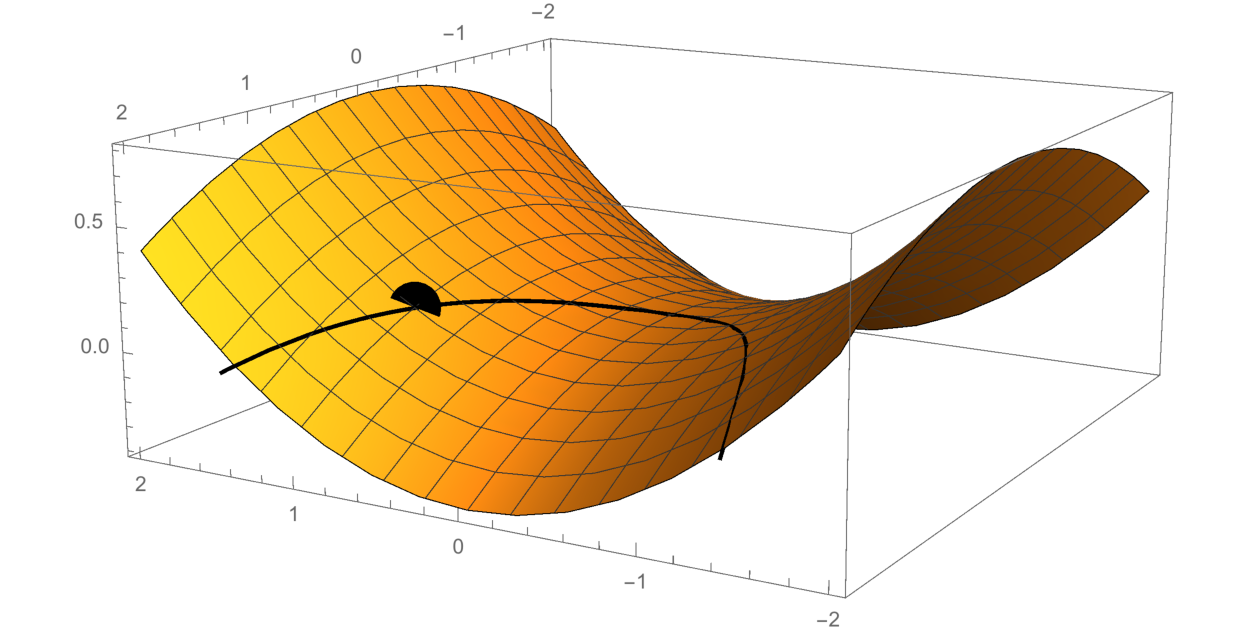
\includegraphics[width=0.5\textwidth]{figs/moniulotteinen_osittais.pdf}
\end{center}

\end{exam}

\begin{stopQ}{q:moniulotteinen_korkeus}%
Mikä on korkeuden muutos kuvan \autoref{fig:moniulotteinen_gradientti} esimerkissä, jos siirrytään merkitystä tarkastelupisteestä (a) \(20 \un{m}\) pohjoiseen, (b) \(20 \un{m}\) itään, (c) ensin \(20 \un{m}\) pohjoiseen ja sitten saman verran itään, eli noin \(30 \un{m}\) koilliseen? Arvioi muutos sekä kuvan korkeuskäyrien perusteella että yhtälön (\autoref{kokonaismuutos}) avulla. Saatko likimain saman tuloksen?
\end{stopQ}

\index{gradientti}

Osittaisderivaatta siis kertoo miten usean muuttujan funktio kuten kuvassa \autoref{fig:moniulotteinen_gradientti} maastonkorkeus muuttuu yhden koordinaattiakselin suunnassa liikuttaessa ja kokonaisdifferentiaali ilmaisee funktion kokonaismuutoksen kun kuljemme jonkin tietyn siirtymän. Haluaisimme kuitenkin vielä keinon selvittää, \emph{mihin suuntaan kuljettaessa korkeus muuttuu kaikkein nopeimmin}, ja tätä varten määrittelemme \textbf{gradientin}.
Korkeuden gradientti on \emph{vektori}, joka osoittaa aina maaston \emph{jyrkimmän nousun suuntaan} ja jonka pituus kertoo \emph{kuinka nopeasti korkeus muuttuu} tähän suuntaan kuljettaessa. Jyrkimmän nousun suunta selvästikin riippuu siitä, missä pisteessä kulloinkin olemme, joten gradientti on myös paikan funktio. Se on siis matemaattisesti vektorikenttä.

Korkeuden gradientti on esitetty kuvassa \autoref{fig:moniulotteinen_gradientti} (c), jossa gradienttivektori on esitetty nuolin tasaisin välein valituissa maaston pisteissä. Kuvassa on esitetty taustalla myös korkeuskäyrät.
Käyrät ovat kartalla sitä \emph{lähempänä} toisiaan, mitä jyrkemmin maasto kohoaa tai laskee eli maaston jyrkkyys on kääntäen verrannollinen korkeuskäyrien väliseen etäisyyteen kartalla. Eli jyrkkyys on suuri, jos korkeuskäyrät ovat \emph{tiheässä}. Niinpä myös gradienttivektorit, jotka ilmaisevat maaston jyrkkyyttä, ovat \emph{pitkiä} korkeuskäyrien ollessa lähellä toisiaan ja lyhyitä käyrien ollessa toisistaan kaukana. Erityisesti mäkien huipuilla ja kuoppien pohjilla gradientti on nolla, koska maasto on paikallisesti tasainen eikä jyrkimmän nousun suuntaa ole.
Maaston korkeus \emph{ei muutu} myöskään kuljettaessa pitkin korkeuskäyrää, joten jyrkimmän nousun suunnan täytyy olla \emph{korkeuskäyriin nähden kohtisuorassa}. Niinpä gradientti on aina kohtisuorassa korkeuskäyriä vastaan.

\index{tasa-arvopinta}

Gradientti voidaan määritellä mille tahansa skalaarikentälle, ja konservatiivisen vuorovaikutuksen potentiaalienergian gradientti on erityisen tärkeä, koska se on suoraan verrannollinen vuorovaikutuksen tuottamaan voimaan.
Kolmiulotteisessa avaruudessa määritellyn potentiaalienergian tapauksessa pisteet, joissa potentiaalienergia on vakio, eivät yleensä muodosta käyriä vaan pintoja, ja näitä kutsutaan potentiaalienergian \textbf{tasa-arvopinnoiksi}. Samaan tapaan kuin korkeuden gradientti on kohtisuorassa korkeuskäyriä vastaan ja osoittaa kohti jyrkintä nousua, potentiaalienergian gradientti on kohtisuorassa tasa-arvopintoja vastaan ja osoittaa potentiaalienergian voimakkaimman kasvun suunnan. Koska voima osoittaa potentiaalienergian jyrkimmän \emph{laskun} suuntaan (``alamäkeen''), voiman suunta on aina vastakkainen potentiaalienergian gradientin suuntaan nähden.

Johdetaan lopuksi vielä tarkka matemaattinen sääntö potentiaalienergian gradientin laskemiseksi.
Tarkastellaan potentiaalienergian muutosta kappaleen liikkuessa \(x\)-suunnassa infinitesimaalisen lyhyen matkan \(\dd x\), \(y\)-suunnassa matkan \(\dd y\) sekä \(z\)-suunnassa matkan \(\dd z\).
Tällöin kappaleen siirtymä on siis
\begin{equation} \dd \bs{r} = \dd x \uv{i} + \dd y \uv{j} + \dd z \uv{k}. \end{equation}
Jos kappaleeseen vaikuttaa konservatiivinen voima \(\bs{F}\), se tekee siirtymässä kappaleeseen työn yhtälön (\autoref{tyo_pistetulo}) mukaisesti
\begin{equation} \dd W = \bs{F} \cdot \dd \bs{r} = F_x \dd x + F_y \dd y + F_z \dd z, \end{equation}
ja koska tämä työ siirtää vuorovaikutuksen potentiaalienergiaa kappaleelle, potentiaalienergian muutos on
\begin{equation} \dd U = - \dd W = -F_x \dd x - F_y \dd y - F_z \dd z. \label{dutyo}\end{equation}

\begin{stopQ}{q:moniulotteinen_dU}%
Jos kappaleeseen kohdistuva konservatiivinen voima on \(\bs{F} = (2.5 \un{N})\uv{i} - (0.5 \un{N})\uv{j} \) ja kappale kulkee siirtymän \(\Delta \bs{r} = (1.0 \un{mm})\uv{i} + (2.0 \un{mm})\uv{j} \), mikä on potentiaalienergian muutos olettaen että voima on tällä matkalla likimain vakio?
\end{stopQ}

Toisaalta potentiaalienergian \emph{kokonaisdifferentiaali} on määritelmän (\autoref{kokonaisdifferentiaali}) mukaisesti
\begin{equation} \dd U = \frac{\partial U}{\partial x} \dd x + \frac{\partial U}{\partial y} \dd y + \frac{\partial U}{\partial z} \dd z, \label{duosideri}\end{equation}
ja tämän pitää siis olla sama lauseke kuin (\autoref{dutyo}).
Huomaa, että yhtälö (\autoref{dutyo}) on \emph{fysikaalinen laki}, joka perustuu työn ominaisuuksiin kun taas yhtälö (\autoref{duosideri}) on \emph{matemaattinen laki}, joka perustuu osittaisderivaatan \emph{määritelmään}.

\index{konservatiivinen}

Koska lausekkeet (\autoref{dutyo}) ja (\autoref{duosideri}) ovat samat, pitää kunkin differentiaalin \(\dd x\) jne. kertoimen olla kummassakin sama.
Nyt nimittäin tarkastelimme potentiaalienergian muutosta mielivaltaisessa siirtymässä, joten voimme \emph{valita} millainen tämä siirtymä on. Esimerkiksi jos tarkastellaan \(x\)-suuntaista siirtymää \(\dd \bs{r} = \dd x \uv{i}\), pätee \(\dd y = \dd z = 0\) ja täytyy siis olla
\begin{equation} \dd U = -F_x \dd x = \frac{\partial U}{\partial x} \dd x \end{equation}
mistä saadaan samanlainen yhtälö kuin yksiulotteisessa tapauksessa, (\autoref{voima_derivaattana}),
\begin{equation} F_x = -  \frac{\partial U}{\partial x}. \end{equation}
Täsmälleen samoin voidaan valita \(\dd x = \dd z = 0\), mistä voidaan päätellä \( F_y = -  \frac{\partial U}{\partial y} \). Samoin valinnasta \( \dd x = \dd y = 0\) seuraa \( F_z = -  \frac{\partial U}{\partial z} \). Voimavektorin skalaarikomponentit kussakin koordinaattiakselin suunnassa saadaan siis \emph{osittaisderivoimalla potentiaalienergiaa kyseisen koordinaatin suhteen} ja siispä voimavektorin on oltava
\bigeq{ \bs{F}_\text{konservatiivinen} = -\frac{\partial U}{\partial x} \uv{i} - \frac{\partial U}{\partial y} \uv{j} - \frac{\partial U}{\partial z} \uv{k} = - \nabla U. \label{gradientti} }

\begin{stopQ}{q:moniulotteinen_gradientti}%
Mihin suuntaan osoittaa korkeuden gradientti kuvan \autoref{fig:moniulotteinen_gradientti} esimerkin tarkastelupisteessä? Mitkä ovat gradienttivektorin \(x\)- ja \(y\)-skalaarikomponenttien etumerkit ja suhteelliset suuruudet? Miten ne liittyvät korkeuden osittaisderivaattoihin?
\end{stopQ}

\index{nabla, $\nabla$}

Yhtälössä (\autoref{gradientti}) esiintyy uusi symboli \(\nabla\), \textbf{nabla}, joka on lyhennysmerkintä yhtälössä esitetylle osittaisderivaattojen muodostamalle vektorille. Nabla ei itse ole skalaari, vektori tai funktio vaan \textbf{operaattori}. Kun nabla yhdistetään \emph{skalaarikentän} eli avaruudessa määritellyn funktion \(U\) kanssa, tuloksena on uusi funktio \(\nabla U\), jota kutsutaan \(U\):n \textbf{gradientiksi}. Tällöin nablan sanotaan \emph{operoivan} funktioon \(U\). Gradienttifunktio on määritelty kaikkialla avaruudessa mutta sen arvot ovat \emph{vektoreita} eli \(\nabla U\) on \emph{vektorikenttä}.

\begin{stopQ}{q:moniulotteinen_dU2}%
Vuorovaikutuksen potentiaalienergia riippuu kappaleen paikasta yhtälön \( U(x,y) = (1.5 \un{J/m}^2) x^2 - (4.0 \un{J/m}) y \) mukaisesti. Kappale on aluksi pisteessä \( (x,y) = (0.5 \un{m}, 1.5 \un{m}) \). (a) Mikä on kappaleeseen kohdistuva voima? (b) Mikä on kappaleen potentiaalienergian muutos, jos kappaleen paikka muuttuu siirtymän \( (\Delta x, \Delta y) = (-1.0 \un{mm}, 2.0 \un{mm}) \)?
\end{stopQ}

\begin{exam}{Gradientti}{ex:gradientti}\noindent

\problem{Kappale on kiinnitetty lattiaan jousella (lepopituus \(0.10 \un{m}\) ja jousivakio \(100 \un{N/m}\)), jonka lattiassa kiinni oleva pää pääsee vapaasti kääntymään kaikkiin suuntiin. Miten kappaleeseen vaikuttava voima riippuu kappaleen paikasta olettaen ettei kappale nouse lattialta?
}

 \twocol{0.6}{0.35}{ \setup  Piirretään tilanteesta kuva. Valitaan origoksi jousen kiinnitetty pää.
Merkitään \(r_0 = 0.10 \un{m}\) (lepopituus) ja \(k = 100 \un{N/m}\) (jousivakio).

 \physics Kappaleeseen kohdistuu gravitaatio, pinnan tukivoima sekä jousen jännitys. Gravitaatio ja tukivoima suuntautuvat aina pystysuuntaan ja kumoavat toisensa. Niinpä kappaleeseen kohdistuva kokonaisvoima on yhtä suuri kuin jousen voima. Voiman voi määrittää suoraan Hooken laista tai vaihtoehtoisesti voimme laskea ensin potentiaalienergian ja määrittää voiman sen gradienttina.

}{%
\begin{center}%
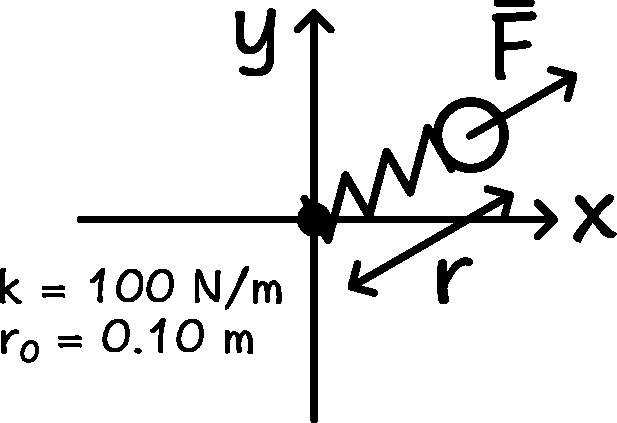
\includegraphics[width=0.85\textwidth]{figs/moniulotteinen_esimerkki_gradientti_1.pdf}%
\end{center}%
}

 \model  Jousen potentiaalienergia on
\begin{equation} U = \frac{1}{2}k(r-r_0)^2, \end{equation}
missä etäisyys origosta on
\( r = \sqrt{x^2 + y^2}, \)
sillä pystysuuntainen koordinaatti on vakio \(z = 0\).
Kappaleeseen vaikuttava voima on siten
\begin{equation} \bs{F} = -\nabla U. \end{equation}

 \solu  Lasketaan jousivoiman gradientti komponenteittain. Esimerkiksi \(x\)-suunnassa saadaan sisäfunktion derivoimissäännöllä
\begin{equation} F_{x} = -\frac{\partial U}{\partial x} = -\frac{\partial U}{\partial r}\frac{\partial r}{\partial x} = -k(r-r_0) \frac{\partial r}{\partial x} \end{equation}
ja vastaavasti muissa suunnissa. Etäisyyden \(r\) derivaatta puolestaan on
\begin{equation} \frac{\partial r}{\partial x} = \frac{\partial }{\partial x} (x^2 + y^2)^{1/2} = \frac{1}{2}(x^2 + y^2)^{-1/2}\cdot 2x = \frac{x}{r}. \end{equation}
Koska \(r\) on symmetrinen koordinaattien suhteen, \(y\)-suunnassa saadaan täsmälleen samoin
\begin{equation} \frac{\partial r}{\partial y} = \frac{y}{r}. \end{equation}
Voiman \(z\)-komponentti on nolla.
Jousivoimaksi saadaan siten Hooken lain mukainen tulos
\begin{equation} \bs{F} = -k\frac{(r-r_0)}{r} (x\uv{i} + y\uv{j}) = -k\frac{(r-r_0)}{r}\bs{r}= -k(r-r_0) \uv{r}. \end{equation}

\mbar
\begin{mathematica}[commandchars=\\!?]
(* potentiaalienergia *)
u = 1/2 k (Sqrt[x^2 + y^2] - r0)^2
lukuarvot = {r0 -> 0.1, k -> 100}

(* voima *)
voima = -Grad[u, {x, y}]
  \textit!{ -((k x (-r0 + Sqrt[x^2 + y^2]))/Sqrt[x^2 + y^2]), ?
  \textit!  -((k y (-r0 + Sqrt[x^2 + y^2]))/Sqrt[x^2 + y^2]) }?
Simplify[voima /. Sqrt[x^2 + y^2] -> r] (* sievennet\"a\"an *)
  \textit!{ (k (-r + r0) x)/r,?
  \textit!  (k (-r + r0) y)/r }?

(* kuvaajat *)
voimat = VectorPlot[voima /. lukuarvot, {x, -0.15, 0.15}, {y, -0.15, 0.15}, 
  VectorStyle -> RGBColor[0, 0.5, 0]];
potentiaali = ContourPlot[u /. lukuarvot, {x, -0.15, 0.15}, {y, -0.15, 0.15}, 
  ContourShading -> None]
Plot3D[u /. lukuarvot, {x, -0.15, 0.15}, {y, -0.15, 0.15}]
Show[potentiaali, voimat]

\end{mathematica}
\begin{center}
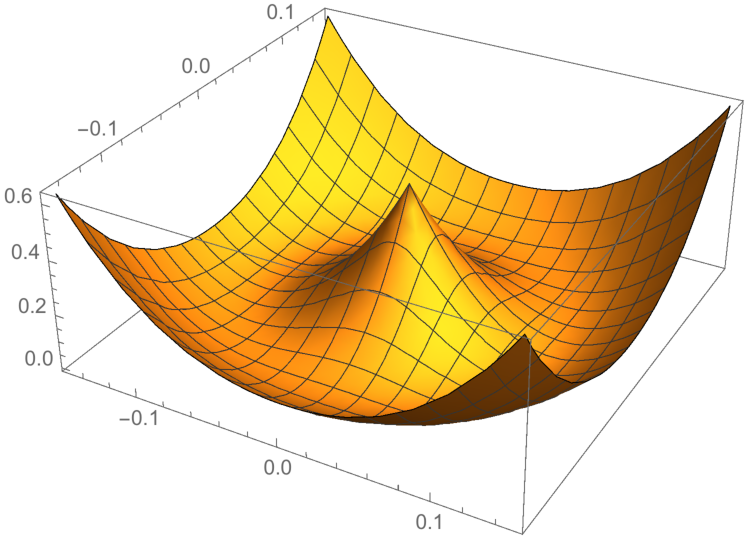
\includegraphics[width=0.44\textwidth]{figs/moniulotteinen_gradienttiplot_1.pdf}
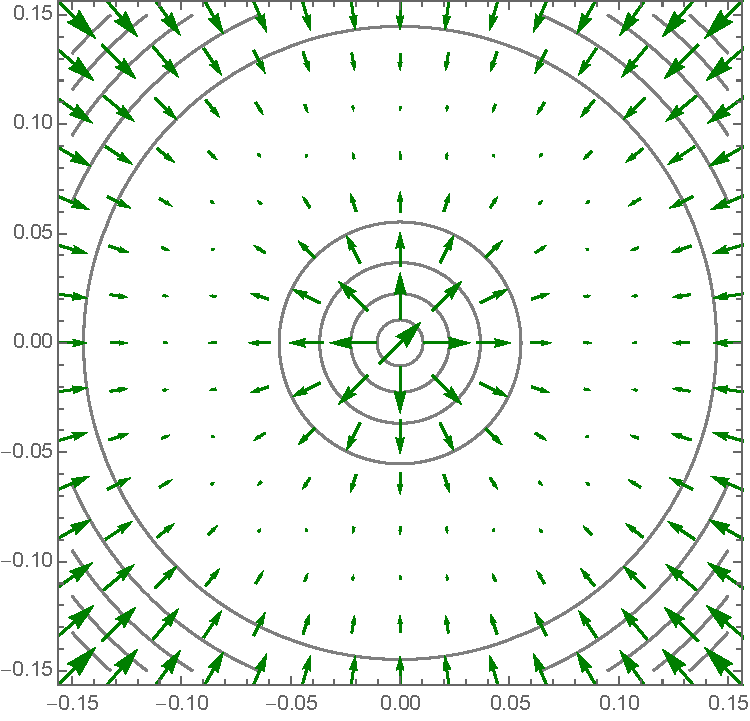
\includegraphics[width=0.33\textwidth]{figs/moniulotteinen_gradienttiplot_2.pdf}
\end{center}

\end{exam}

\pictures{b!}%
{Voima osoittaa konservatiivisen potentiaalienergian pienenemissuunnan ja -nopeuden. Voima on kohtisuorassa potentiaalienergian tasa-arvopintoja vastaan ja sitä suurempi mitä lähempänä nämä ovat toisiaan.;%
Painovoimakenttä on homogeeninen lähellä maanpintaa.;%
Avaruudessa painovoimakenttä on epähomogeeninen.}%
{fig:moniulotteinenpainovoimakentta;fig:moniulotteinenpainovoimakentta_a;fig:moniulotteinenpainovoimakentta_b;}%
{0.47;0.41}%
{0.482;0.418}%
{moniulotteinen_gradientti_1.pdf;moniulotteinen_gradientti_3.pdf}

\index{homogeeninen}

Tarkastellaan vielä lopuksi painovoimaa fysikaalisena kenttänä.
Gravitaation tuottama voima on lähellä maanpintaa massan ja putoamiskiihtyvyyden tulo. Näistä massa on kappaleen ominaisuus ja putoamiskiihtyvyys kentän ominaisuus. Gravitaatiokenttää voidaan siis kuvata myös \emph{voimakenttänä}, jonka voimakkuus on kaikkialla sama, \(\bs{g}\), ja itseasiassa puhuttaessa painovoimakentästä yleensä tarkoitetaan juuri tätä voimakenttää. Kentässä olevaan \(m\)-massaiseen kappaleeseen kohdistuu gravitaatiokentässä kaikkialla voima \(m\bs{g}\), joka on kappaleen massan ja kentän voimakkuuden tulo. Tällaista voimakenttää, jonka tuottama \emph{voima} on kaikkialla sama, kutsutaan \textbf{homogeeniseksi kentäksi}.

Koska voimakentän arvot ovat vektoreita, kyseessä on vektorikenttä, ja koska gravitaatio on konservatiivinen vuorovaikutus, kenttään liittyvä voima voidaan laskea kenttään liittyvästä potentiaalienergiasta gradientin avulla. Gravitaation tapauksessa potentiaalienergia lähellä maanpintaa riippuu vain korkeudesta, joten valitsemalla \(z\)-akseli osoittamaan ylöspäin gravitaation potentiaalienergia \(m\)-massaiselle kappaleelle on \( U = mgz \). Gravitaation tuottama painovoima voidaan puolestaan määrittää laskemalla gradientti
\begin{equation} \bs{G} = -\nabla U = -mg \nabla z = -mg\left( \frac{\partial z}{\partial x} \uv{i} + \frac{\partial z}{\partial y} \uv{j} + \frac{\partial z}{\partial z} \uv{k} \right). \label{gradgrav1}\end{equation}
Lausekkeessa esiintyy korkeuden \(z\) osittaisderivaattoja eri koordinaattien suhteen, ja nämä on helppo laskea muistaen osittaisderivaatan määritelmä. Osittaisderivaattahan lasketaan niin, että muiden muuttujien ajatellaan olevan derivoinnissa vakioita, ja vakion derivaatta on nolla, joten \(\frac{\partial z}{\partial x} = \frac{\partial z}{\partial y} = 0\). Toisaalta koordinaatin derivaatta sen itsensä suhteen on yksi, \(\frac{\partial z}{\partial z} = 1\), joten
\begin{equation} \bs{G} = -mg\left(0 \uv{i} + 0 \uv{j} + 1 \uv{k} \right) = -mg\uv{k}. \label{gradgrav}\end{equation}
Näin saatiin siis tuttu tulos, jonka mukaan painovoiman suunta on alaspäin negatiivisen \(z\)-akselin suuntaan ja sen voimakkuus on vakio.

Painovoiman määrittäminen gradientin avulla ei ole erityisen mielenkiintoista, koska painovoima on vakio. Epähomogeeniset kentät ovat kuitenkin fysiikassa yleisiä, ja näissä tilanteissa gradienttia tarvitaan voiman määrittämiseen, jos tunnetaan vain potentiaalienergia. Esimerkiksi maapallon painovoimakenttä vaikuttaa homogeeniselta ainoastaan lähellä maanpintaa. Avaruudesta katsoen planeetta näyttää pallolta ja maan gravitaatiokenttä onkin avaruudessa itse asiassa pallosymmetrinen.
Gradienttia tarvitaan myös sähkövarausten synnyttämien \emph{sähkökenttien} analyysissä, jota tarkastelemme luvussa \autoref{luku:sahkostatiikka}. Sähköinenkin vuorovaikutus on konservatiivinen, joten myös siihen liittyy potentiaalienergia ja sen tuottama voima osoittaa aina kohti pienenevän potentiaalienergian suuntaa.

\begin{stopQ}{q:moniulotteinen_kentta_yhteenveto}%
Selitä omin sanoin, mitä kenttä tarkoittaa matematiikassa ja fysiikassa. Selitä erityisesti, miten konservatiivisen vuorovaikutuksen potentiaalienergia ja voima liityvät toisiinsa ja miten voit laskea yhden kun tunnet toisen.
\end{stopQ}

\startwidepage

\section*{Yhteenveto: \chaptertitle}
\addcontentsline{toc}{section}{Yhteenveto: \chaptertitle}
\noindent
\begin{tabular}{p{1.15\textwidth}}
\standout{Differentiaalit ja vektorit}{
\begin{multicols}{2}

\begin{itemize}
\item Kolmiulotteinen koordinaatisto, jonka akselit \(x, y, z\) ovat toisiaan vastaa kohtisuorassa, on \textbf{karteesinen koordinaatisto}. Vektorit tässä koordinaatistossa voidaan kirjoittaa akselien suuntaisten
\emph{yksikkövektoreiden} ja \emph{skalaarikomponenttien} avulla
\begin{equation} \bs{A} = A_x \uv{i} + A_y \uv{j} + A_z \uv{k}. \nonumber \end{equation}

\item Vektorin pituus saadaan Pythagoraan lauseesta
\begin{equation} A = |\bs{A}| = \sqrt{A_x^2 + A_y^2 + A_z^2}. \nonumber \end{equation}

\item Vektorisumma voidaan laskea komponenteittain
\begin{equation} \bs{A} + \bs{B} = (A_x+B_x) \uv{i} + (A_y+B_y) \uv{j} + (A_z+B_z) \uv{k}. \nonumber \end{equation}

\item \textbf{Pistetulo} eli skalaaritulo on kahden vektorin välinen kertolasku. Sen lopputulos on skalaari, ja tulon suuruus on vektorien pituuksien sekä niiden välisen kulman \(\theta\) kosinin tulo
\begin{equation} \bs{A} \cdot \bs{B} = AB \cos \theta. \nonumber \end{equation}
Pistetulo voidaan laskea karteesisessa koordinaatistossa \emph{vektorien komponenttien tulojen summana}
\begin{equation} \bs{A} \cdot \bs{B} = A_x B_x + A_y B_y + A_z B_z. \nonumber \end{equation}

\item Vektorin komponentti minkä tahansa toisen vektorin suunnassa saadaan pistetulon avulla
\begin{equation} A_B = \frac{1}{B}\bs{A} \cdot \bs{B}. \nonumber \end{equation}

\item Kaksi vektoria ovat yhtä suuret jos ja vain jos sekä niiden pituudet että suunnat ovat samat. Karteesisessa koordinaatistossa tämä tarkoittaa sitä, että vektorien kaikki skalaarikomponentit ovat yhtä suuret
\begin{equation} \bs{A} = \bs{B} \Leftrightarrow A_x = B_x, A_y = B_y, A_z = B_z. \nonumber \end{equation}

\item Vektorin derivaatta ja integraali voidaan karteesisessa koordinaatistossa laskea komponenteittain
\begin{equation} \frac{\dd \bs{A}}{\dd t} = \frac{\dd A_x}{\dd t}\uv{i} + \frac{\dd A_y}{\dd t}\uv{j} + \frac{\dd A_z}{\dd t}\uv{k} \nonumber\end{equation}
\begin{equation} \int \bs{A} \dd t = \int A_x \dd t \ \uv{i} + \int A_y \dd t \ \uv{j} + \int A_z \dd t \ \uv{k} \nonumber\end{equation}

\item \textbf{Osittaisderivaatta} on usean muuttujan funktion derivaatta yhden muuttujan suhteen\begin{equation} \frac{\partial f}{\partial x} = \lim_{\Delta x \to 0} \frac{f(x + \Delta x,y,z) - f(x,y,z)}{\Delta x}. \nonumber \end{equation}

\item \textbf{Gradientti} on derivaatan yleistys useaan ulottuvuuteen. Funktion \(f\) gradientti on \emph{vektori}, joka osoittaa suuntaan, jossa funktion arvo kasvaa nopeimmin, ja sen pituus kertoo kuinka paljon funktion arvo muuttuu tähän suuntaan siirryttäessä. Karteesisessa koordinaatistossa gradientin skalaarikomponentti kussakin suunnassa on funktion osittaisderivaatta tähän suuntaan mitatun koordinaatin suhteen
\begin{equation} \nabla f = \frac{\partial f}{\partial x}\uv{i} + \frac{\partial f}{\partial y}\uv{j} + \frac{\partial f}{\partial z}\uv{k}. \nonumber\end{equation}
Symboli \(\nabla\), \textbf{nabla}, on lyhennysmerkintä yllä esitetylle lausekkeelle.

\item \textbf{Viivaintegraali} on määrätyn integraalin yleistys useaan ulottuvuuteen. Reittiä \(P\) pitkin laskettava integraali voidaan määritellä jakamalla reitti osiin ja antamalla jaon tulla äärettömän tiheäksi
\begin{equation} \lim_{\Delta r \to 0} \sum_{i=0}^N \bs{A}_i \cdot \Delta \bs{r}_i = \int_{P} \bs{A} \cdot \dd \bs{r} = \int_{t_\text{alku}}^{t_\text{loppu}} \bs{A} \cdot \bs{v} \dd t. \nonumber \end{equation}

\end{itemize}

\end{multicols}
} \\
\standout{Liikem\"a\"ar\"a ja dynamiikka}{
\begin{multicols}{2}

\begin{itemize}
\item Jos kappaleeseen vaikuttaa kokonaisvoima \(\bs{F}_\text{kokonais}\), kappaleen kiihtyvyys on komponenteittain
\begin{equation} a_x = \frac{1}{m}F_{x,\text{kokonais}}, \ a_y = \frac{1}{m}F_{y,\text{kokonais}}, \ a_z = \frac{1}{m}F_{z,\text{kokonais}}.\nonumber \end{equation}

\item Jos kappaleeseen vaikuttava kokonaisvoima tunnetaan \emph{ajan funktiona}, kappaleen nopeus ja paikka voidaan ratkaista komponenteittain kiihtyvyyden integraaleina.

\item Jos systeemiin ei vaikuta ulkoisia vuorovaikutuksia, kokonaisliikemäärä on vakio.
Tällöin kokonaisliikemäärävektorin kukin komponentti on erikseen vakio
\begin{equation}  p_{x,\text{alku}} = p_{x,\text{loppu}}, \ p_{y,\text{alku}} = p_{y,\text{loppu}}, \ p_{z,\text{alku}} = p_{z,\text{loppu}}.  \nonumber \end{equation}

\end{itemize}

\end{multicols}
} \\
\standout{Energia ja ty\"o}{
\begin{multicols}{2}

\begin{itemize}
\item Jos kappaleeseen vaikuttaa \emph{vakiovoima} \(\bs{F}\) ja kappale siirtyy matkan \(\Delta \bs{r}\), voima tekee kappaleeseen työn
\begin{equation} W = \bs{F} \cdot \Delta \bs{r}. \nonumber \end{equation}

\item Jos kappaleeseen vaikuttaa \emph{mikä tahansa voima} \(\bs{F}\) ja kappale liikkuu pisteestä \(\bs{r}_\text{alku}\) pisteeseen \(\bs{r}_\text{loppu}\) reittiä \(P\), voima tekee kappaleeseen työn
\begin{equation} W = \int_P \bs{F} \cdot \dd \bs{r}. \nonumber \end{equation}

\item Liikkuvaan kappaleeseen vaikuttava voima \(\bs{F}\) tekee työtä kappaleeseen teholla
\begin{equation} P = \bs{F} \cdot \bs{v}. \nonumber \end{equation}

\item Vuorovaikutus on konservatiivinen jos ja vain jos siihen liittyvän voiman tekemä työ pisteestä \(\bs{r}_\text{alku}\) pisteeseen \(\bs{r}_\text{loppu}\) siirtyvään kappaleeseen \emph{ei riipu reitistä, jonka kappale kulkee}. Tällöin vuorovaikutuksen potentiaalienergia on
\begin{equation} U(\bs{r}) = -W_{\bs{r}_0 \to \bs{r}} = -\int_{\bs{r}_0}^{\bs{r}} \bs{F}_\text{konservatiivinen} \cdot \dd \bs{r}. \nonumber\end{equation}

\item Konservatiivinen vuorovaikutus, johon liittyy potentiaalienergia \(U(x,y,z) \), tuottaa voiman
\begin{equation} \bs{F}_\text{konservatiivinen} = -\nabla U = -\frac{\partial U}{\partial x}\uv{i} - \frac{\partial U}{\partial y}\uv{j} - \frac{\partial U}{\partial z}\uv{k}. \nonumber\end{equation}

\end{itemize}

\end{multicols}
} \\
\standout{Sanasto}{
\begin{multicols}{2}

\begin{itemize}
\item karteesiset koordinaatit (Cartesian coordinates)

\item pistetulo, skalaaritulo (dot product, scalar product)

\item osittaisderivaatta (partial dervative)

\item kokonaisdervaatta (total derivative)

\item kokonaisdifferentiaali (total differential)

\item gradientti (gradient)

\item nabla (nabla, del, grad)

\item operaattori (operator)

\item viivaintegraali (line integral)

\item potentiaalienergian tasa-arvopinta (equipotential surface)

\item perusvuorovaikutus (fundamental interaction)

\item kenttä (field)

\item homogeeninen (homogeneous)

\item heittoliike (projectile motion)

\end{itemize}

\end{multicols}
} 

\end{tabular}
\newpage

\newpage\begin{answers}\noindent

\stopA{q:moniulotteinen_komponentit}{%\\
Voiman A komponentit ovat \(F_{x,A} = 3.0 \un{N} \) ja \(F_{y,A} = 0.0 \un{N}\). Voiman B komponentit ovat
\(F_{x,B} = (4.0 \un{N}) \cos(-60^\circ) = 2.0 \un{N}\) ja \(F_{y,B} = (4.0 \un{N}) \sin(-60^\circ) = -3.46 \un{N}\). Kokonaisvoiman komponentit saadaan näiden summana, \(F_{x} = F_{x,A} + F_{x,B} = 5.0 \un{N}\) ja \(F_{y} = F_{y,A} + F_{y,B} = -3.46 \un{N}\). Kokonaisvoima on siis
\begin{equation} \bs{F} = (5.0 \un{N}) \uv{i} + (-3.46 \un{N}) \uv{j}. \end{equation}
}

\stopA{q:moniulotteinen_kierto}{%\\
Vektorin \(\bs{A}\) pituus on \(A = \sqrt{3^2+4^2} = 5\) ja se on kulmassa \(\theta = \arctan \frac{4}{3} = 0.927 = 53.1^\circ\) (vastapäivään) \(x\)-akseliin nähden. Koska \(x'\)-akseli on kulmassa \(45^\circ\) \(x\)-akseliin nähden, vektori \(\bs{A}\) on kulmassa \(\theta' = \theta - 45^\circ = 8.1^\circ\) \(x'\)-akseliin nähden. Niinpä vektorin komponenttiesitys koordinaatistossa \(x'y'\) on
\begin{equation} \bs{A} = 5 \cos \theta' \uv{i}' + 5 \sin \theta' \uv{j}' = 4.95 \uv{i}' + 0.71 \uv{j}' \end{equation}
}

\stopA{q:moniulotteinen_voima_kiihtyvyys}{%\\
(a) Muuttuu. Nopeusvektori kääntyy ylöspäin.\\
(b) Jos valitsemme \(x\)-suunnan vaakatasoon ja \(y\)-suunnan ylöspäin, \(x\)-komponentti on kuopan pohjalla likimain vakio ja \(y\)-komponentti muuttuu positiiviseen suuntaan.\\
(c) Kiihtyvyysvektori osoittaa nopeuden muutoksen suuntaan eli ylöspäin.\\
(d) Kokonaisvoiman täytyy osoittaa samaan suuntaan kuin kiihtyvyysvektorikin.
}

\stopA{q:moniulotteinen_tasainen_kiihtyvyys}{%\\
Kappaleen nopeuden muutos kussakin suunnassa saadaan kiihtyvyyden vastaavan komponentin integraalina tai graafisesti kuvaajan rajaamana pinta-alana. Siis \(x\)-suunnassa
\begin{equation} \Delta v_x = \frac{1}{m} \int F_x \dd t = 0.5 \un{m/s} \end{equation}
ja \(y\)-suunnassa
\begin{equation} \Delta v_y = \frac{1}{m} \int F_y \dd t = 3.0 \un{m/s}. \end{equation}
Kappaleen alkunopeus oli \(\bs{v}_\text{alku} = (-1.0 \un{m/s}) \uv{i} \), joten sen loppunopeuden komponentit ovat
\(v_x = -0.5 \un{m/s}\) ja \(v_y = 3.0 \un{m/s}. \)
}

\stopA{q:moniulotteinen_liikediagrammi}{%\\
Liikediagrammi näyttää sivuttain käännetyltä V-kirjaimelta, jonka kärki koskettaa seinää. Nopeuden \(y\)-komponentti on vakio, joten sen kuvaaja on vaakasuora ja \(y\)-koordinaatin kuvaaja on suora. Nopeuden \(x\)-komponentti kääntyy törmäyksessä ympäri, joten sen kuvaaja näyttää jyrkältä askelmalta ja \(x\)-koordinaatin kuvaaja on V:n muotoinen.
}

\stopA{q:moniulotteinen_elastisuus}{%\\
Kappaleen A alkunopeuden komponentit ovat likimain \(v_{x,A} = 0.0 \un{m/s}\) ja \(v_{y,A} = 4.0 \un{m/s}\). Kappaleen B vastaavat nopeuden komponentit ovat \(v_{x,B} = 2.0 \un{m/s}\) ja \(v_{y,B} = -4.0 \un{m/s}\). Jos A:n massa on esimerkiksi \(1 \un{kg}\) (ja B:n massa on kaksinkertainen), kappaleiden liike-energia alussa oli \(K_A = 8.0 \un{J}\) ja \(K_B = 20.0 \un{J}\). Lopuksi kappaleiden nopeuskomponentit ovat likimain \(v_{x,A} = -2.0 \un{m/s}\), \(v_{y,A} = -2.6 \un{m/s}\), \(v_{x,B} = 1.0 \un{m/s}\) ja \(v_{y,B} = 3.3 \un{m/s}\). Kappaleiden liike-energiat ovat siis törmäyksen jälkeen noin
\(K_A = 5.4 \un{J}\) ja \(K_B = 11.9 \un{J}\). Systeemin kokonaisliike-energia oli siis aluksi \(K = 28 \un{J}\) ja lopuksi \(K = 17.3 \un{J}\). Liike-energiasta muuttui lämpöenergiaksi ym. muotoihin noin \(38 \ \%\).
}

\stopA{q:moniulotteinen_vektoreita}{%\\
(a) Vektoreiden \(\bs{A}\) ja \(\bs{B}\) välinen kulma on \(60^\circ\), joten \(\bs{A} \cdot \bs{B} = A B \cos 60^\circ = 1.5 \cdot 2.0 \cdot 0.5 = 1.5\).\\
(b) Vektorit \(\bs{A}\) ja \(\bs{C}\) ovat toisiinsa nähden kohtisuorassa, joten \(\bs{A} \cdot \bs{C} = 0\).\\
(c) \(\bs{A} \cdot (\bs{B} + \bs{C}) = \bs{A} \cdot \bs{B} + \bs{A} \cdot \bs{C} = 1.5 + 0.0 = 1.5. \)\\
(d) Ensinnäkin \( \bs{A} \cdot \bs{B} = 1.5 \) on skalaari, joten laskun lopputulos on vektori \(1.5 \cdot \bs{C}\). Tämä on vektori, jonka pituus on \(1.5 \cdot 2.5 = 3.75\) ja joka osoittaa samaan suuntaan kuin \(\bs{C}\) eli \(50^\circ\) \(x\)-akselista myötäpäivään.
}

\stopA{q:moniulotteinen_vektoreita_2}{%\\
(a) \( A = \sqrt{1^2 + 2^2 + (-3)^2} = 3.74 \) ja \( B = \sqrt{4^2 + (-5)^2 + (-6)^2} = 8.77 \).\\
(b) \(\bs{A} \cdot \bs{B} = 1\cdot 4 + 2 \cdot (-5) + (-3) \cdot (-6) = 12 \).\\
(c) \(\theta = \arccos \frac{12}{3.74 \cdot 8.77} = 1.20 = 69^\circ \).
}

\stopA{q:moniulotteinen_skalaari}{%\\
Voima on vektori, ja kaikkien vektorien pituus saadaan Pythagoraan lauseen perusteella niiden karteesisten komponenttien neliöiden summan neliöjuurena. Työ sen sijaan on skalaari, jolla ei ole edes olemassa karteesisia komponentteja. Niinpä Pythagoraan lause, joka on siis geometrinen tulos, ei voi mitenkään päteä työlle. Työ on määritelty kahden vektorin pistetulona, joten työn voi kirjoittaa näiden vektoreiden komponenttien avulla, mutta pistetulossa karteesisten komponenttien tulot vain lasketaan yhteen. Pistetuloon ei kuulu neliöintiä eikä neliöjuuren ottoa.
}

\stopA{q:moniulotteinen_reittiriippuvuus}{%\\
Reitistä riippuvat matkan pituus ja dissipatiivisten vuorovaikutusten tekemä työ. Jos kuljet suoraan, matka on lyhyempi ja vähemmän rasittava kuin jos vaikkapa juokset ensin pari kertaa yliopiston ympäri. Gravitaation tekemä työ ja siihen liittyvä potentiaalienergian muutos sen sijaan eivät riipu kulkemastasi reitistä, vaan ainoastaan siitä, kuinka paljon korkeammalla tai matalalla ruokala on luentosaliin verrattuna.
}

\stopA{q:moniulotteinen_viivaintegraalin_merkki}{%\\
Kuvan (c) viivaintegraali on positiivinen. Vaikka reitillä kuljetaan sekä voiman suuntaan että sitä vastaan, voiman suuntaan kuljetaan enemmän. Kuvan (d) integraali on nolla. Reitin alussa integraali on positiivinen, koska kuljetaan voiman suuntaan, mutta reitin lopussa integraali on negatiivinen siirtymän ollessa voimaa vastaan. Reitti ja voima ovat ainakin likimain symmetriset, joten integraalin positiivinen ja negatiivinen osuus melko tarkasti kumoavat toisensa.
}

\stopA{q:moniulotteinen_konservatiivisuus}{%\\
(a) Nostettaessa painovoima tekee negatiivisen työn ja laskettaessa yhtä suuren positiivisen työn. Työ on siis kokonaisuudessaan nolla.\\
(b) Liikekitka tekee tässä prosessissa koko ajan negatiivista työtä.\\
(c) Kitka ei voi olla konservatiivinen vuorovaikutus, koska se teki kappaleeseen nollasta poikkeavan työn, kun kappale kulki suljetun reitin. Painovoima on konservatiivinen.
}

\stopA{q:moniulotteinen_suljettu}{%\\
Tekstissä pääteltiin, että gravitaation kappaleeseen tekemä työ riippuu ainoastaan kappaleen korkeuden muutoksesta. Otetaan nyt mielivaltainen suljettu reitti ja etsitään reitin korkein ja matalin piste. Olkoon näiden välinen korkeusero \(\Delta y\). Kuljettaessa reitin ylimmästä pisteestä alimpaan painovoima tekee positiivisen työn \(W_\text{alas} = m g \Delta y\). Kun sitten alimmasta pisteestä palataan takaisin ylimpään pisteeseen, painovoima tekee negatiivisen työn \(W_\text{yl\"os} = -mg \Delta y\). Painovoiman tekemä kokonaistyö tällä suljetulla reitillä on siis
\( W = W_\text{alas} + W_\text{yl\"os} = m g \Delta y - m g \Delta y = 0. \)
}
Tämä on tärkeää siksi, että tämä osoittaa painovoiman olevan konservatiivinen vuorovaikutus. Siitä puolestaan seuraa, että painovoimaa voi kuvata potentiaalienergialla.

\stopA{q:moniulotteinen_kentta}{%\\
Mikä tahansa intensiivinen suure, jolle voidaan määritellä arvo kussakin huoneen pisteessä, muodostaa matemaattisessa mielessä kentän. Esimerkiksi lämpötila, ilmanpaine ja korkeus ovat skalaarikenttiä. Ilman virtausnopeus tai vaikkapa suunta kohti lähintä lamppua ovat vektorikenttiä.
}

\stopA{q:moniulotteinen_osittaisderivaatta}{%\\
\(\frac{\partial f}{\partial x} = y\),
\(\frac{\partial f}{\partial y} = x\),
\(\frac{\dd y}{\dd x} = 2 x\) ja
\( \frac{\dd f}{\dd x} = \frac{\partial f}{\partial x} + \frac{\partial f}{\partial y} \frac{\dd y}{\dd x} = y + 2 x^2 = x^2 + 2x^2 = 3x^2. \). Sama tulos saadaan suoraan derivoimalla lauseketta \(f = x^3\) kuten pitääkin.
}

\stopA{q:moniulotteinen_korkeus}{%\\
(a) Tarkastelupisteessä maaston korkeus muuttuu pohjoiseen kuljettaessa jyrkkyydellä \(\partial h / \partial y \approx 0.12\) eli maasto nousee noin \(12 \un{cm}\) jokaista pohjoiseen siirryttyä metriä kohden. Niinpä siirryttäessä \(\Delta y = 20 \un{m}\) pohjoiseen noustaan
\( \Delta h \approx \frac{\partial h}{\partial y} \Delta y = 0.12 \cdot 20 \un{m} = 2.4 \un{m}. \)
(b) Itään kuljettaessa korkeus muuttuu jyrkkyydellä \(\partial h / \partial x \approx -0.12\) eli maasto laskee tähän suuntaan \(12 \un{cm}\) metrillä. Korkeuden muutos on siis
\( \Delta h \approx \frac{\partial h}{\partial x} \Delta x = -0.12 \cdot 20 \un{m} = -2.4 \un{m}. \)
(c) Korkeuden kokonaismuutos voidaan arvioida kokonaisdifferentiaalilla.
\begin{equation} \Delta h \approx \frac{\partial h}{\partial x} \Delta x + \frac{\partial h}{\partial y} \Delta y = 2.4 \un{m} -2.4 \un{m} = 0.0 \un{m}. \end{equation}
Toisin sanoen koilliseen kuljettaessa korkeus ei tämän arvion mukaan juuri muutu. Näin todella on, sillä tarkastelupisteen ympäristössä korkeuskäyrät kulkevat koillisesta lounaaseen (yläoikealta alavasemmalle).
}

\stopA{q:moniulotteinen_dU}{%\\
Vakiovoima tekee työn
\( W = \bs{F} \cdot \Delta \bs{r} = F_x \Delta x + F_y \Delta y = (2.5 \un{N}) \cdot (1.0 \un{mm}) + (-0.5 \un{N}) \cdot (2.0 \un{mm}) = 1.5 \un{mJ}. \)
Potentiaalienergian muutos on siis \(U = -W = -1.5 \un{mJ}\).
}

\stopA{q:moniulotteinen_gradientti}{%\\
Gradientti osoittaa kuvan \autoref{fig:moniulotteinen_gradientti} (c) perusteella luoteeseen (ylävasemmalle). Korkeuden osittaisderivaatat ovat tarkastelupisteessä
\(\partial h / \partial x \approx -0.12\) ja
\(\partial h / \partial y \approx 0.12\).
Nämä ovat gradienttivektorin skalaarikomponentit \(x\)- ja \(y\)-suunnissa, joten komponentit ovat siis itseisarvoltaan likimain yhtä suuret, mutta \(x\)-komponentti on negatiivinen.
Korkeusfunktion \(h\) gradientti on siis
\( \nabla h = \frac{\partial h}{\partial x} \uv{i} + \frac{\partial h}{\partial y} \uv{j} = -0.12 \uv{i} + 0.12 \uv{j}. \)
Tämä on luoteeseen osoittava vektori, joten laskun tulos on sopusoinnussa kuvan kanssa.
}

\stopA{q:moniulotteinen_dU2}{%\\
(a) Lasketaan ensin potentiaalienergian osittaisderivaatat.
Ensin \(x\)-suunnassa \( \partial U / \partial x = (3.0 \un{J/m}^2) x \), ja pisteessä \( (0.5 \un{m}, 1.5 \un{m}) \) tämä saa arvon \(1.5 \un{J/m}\).
Sitten \(y\)-suunnassa \( \partial U / \partial y = -4.0 \un{J/m} \).
Voima on siis
\( \bs{F} = - \nabla U = - \frac{\partial U}{\partial x} \uv{i} - \frac{\partial U}{\partial y} \uv{j} = (-1.5 \un{N}) \uv{i} + (4.0 \un{N}) \uv{j}. \)
(b) Potentiaalienergian muutos on helpoin laskea kokonaisdifferentiaalilla,
\( \Delta U \approx \frac{\partial U}{\partial x} \Delta x + \frac{\partial U}{\partial y} \Delta y = (1.5 \un{J/m}) \cdot (-1.0 \un{mm}) + (-4.0 \un{J/m}) \cdot (2.0 \un{mm}) = -9.5 \un{mJ}. \)
Energian muutoksen voi toki laskea myös ``tarkasti'', mutta tämä on vaivalloista. Ensin pitää määrittää kappaleen loppusijainti, joka on \( (0.499 \un{m}, 1.502 \un{m}) \). Sitten voimme laskea potentiaalienergian alussa ja lopussa, jolloin tulokseksi saadaan
\(U_\text{alku} = U(0.5 \un{m}, 1.5 \un{m}) = -5.625 \un{J}\) ja
\(U_\text{loppu} = U(0.499 \un{m}, 1.502 \un{m}) = -5.6344985 \un{J}\). Muutos on näiden erotus, \(\Delta U = U_\text{loppu} - U_\text{alku} = -9.4985 \un{mJ}\). Ero kokonaisdifferentiaalilla laskettuun arvioon on luokkaa \(0.01 \%\), mikä on paljon vähemmän kuin annettujen lukuarvojen tarkkuus.
}

\end{answers}

\startchapter{
Py\"orimisliike
}{pyorimisliike}{%

Toistaiseksi olemme tarkastelleet vain etenevää liikettä, jossa kappaleiden paikka muuttuu mutta niiden asento ei. Liike on kuitenkin harvoin tällaista, ja tässä luvussa tutustummekin kappaleiden asennon muuttumiseen niiden pyöriessä.
Pyöriminen on moniulotteisen liikkeen erikoistapaus, sillä kappaleen pyöriessä kiinteän akselin ympäri sen jokainen piste liikkuu tasossa ympyräradalla. Itse asiassa aloitammekin pyörimisen tarkastelun nimenomaan tutkimalla tällaista ympyräliikettä.
Näemme, että sekä ympyräliikettä että pyörimistä voidaan kuvata määrittelemällä kappaleen asentoa kuvaava kulma samaan tapaan kuin suoraviivaisessa liikkeessä määriteltiin paikkaa kuvaava koordinaatti. Tällöin useimmat pyörimistä kuvaavat mekaniikan lait saavat täsmälleen saman muodon kuin yksiulotteisen liikkeen lait kunhan suoraviivaisen liikkeen suureet korvataan vastaavilla pyörimisliikkeen suureilla.
Lopuksi esitellään, kuinka tämä kuvaus yleistyy tapaukseen, jossa kappaleet voivat pyöriä erisuuntaisten akselien ympäri.

Tämän luvun opiskeltuasi sinun tulee osata:

\begin{itemize}
\item esittää kappaleen paikka napakoordinaatistossa ja jakaa vektorit napakoordinaatiston radiaali- ja tangenttikomponentteihin

\item määritellä kulmaliikkeen suureet: kulmanopeus ja -kiihtyvyys, hitausmomentti sekä momentti

\item määrittää ympyräradalla liikkuvan kappaleen nopeus- ja kiihtyvyysvektorit

\item määrittää pyörimisen liike-energia ja momentin tekemä työ

\item määritellä kulmaliikemäärä ja kuvailla sen säilymislaki

\item esittää kappaleen liike suoraviivaisen liikkeen ja pyörimisen yhdistelmänä ja ratkaista vierivän kappaleen liike

\item laskea vektoreiden ristitulo ja ilmaista pyörimisliikkeen suureet vektorimuodossa

\end{itemize}

}

\stopwidepage

\newpage

\section{Ympyräliike}
\label{ympyräliike}

\index{ympyräliike}
\index{kiertoliike}

Kappaleen \textbf{pyöriessä} kiinteän \textbf{akselin} ympäri sen jokainen piste liikkuu ympyräradalla. Akseli voi olla todellinen kiinteä kappale kuten oven sarana, joka estää kappaleen muun liikkeen pyörimistä lukuun ottamatta. Toisaalta kappale voi pyöriä myös kuvitteellisen akselin ympäri kuten heitetty frisbee. Kummassakin tapauksessa kappaleen \textbf{pyörimisakselilla} olevat hiukkaset pysyvät paikoillaan ja muut hiukkaset \textbf{kiertävät} tätä akselia ympyräradoilla. Myös kokonainen kappale voi olla \textbf{ympyräliikkeessä}, jolloin se kiertää pyörimisakselia. Ero pyörimisen ja ympyräliikkeen välillä onkin siinä, että pyörimisakseli on pyörimisliikkeen tapauksessa kappaleen \emph{sisällä} (tai kappale ainakin ympäröi sitä) ja ympyräliikkeen tapauksessa akseli on selkeästi kappaleen \emph{ulkopuolella}. Pyöriminen ja ympyräliike ovatkin siis kumpikin \textbf{kiertoliikkeen} muotoja. Aloitamme kiertoliikkeen tarkastelun ympyräliikkeestä. Ensimmäinen askel on jälleen liikkeen täsmällinen määrittely.

\subsection{Kulma ja napakoordinaatisto}
\label{kulmajanapakoordinaatisto}

Kuvailimme suoraviivaisen liikkeen luvussa \autoref{luku:liike} kiinnittämällä kiintopisteen eli origon ja mittaamalla kappaleen paikan tämän suhteen. Kiintopisteen lisäksi valitaan positiivinen suunta, jolloin kappaleen koordinaatti määritellään positiiviseksi sen siirtyessä origosta tähän suuntaan. Ympyräliike tapahtuu tasossa, joten se on kaksiulotteista. Samalla ympyräliike on rajoitettua, sillä ympyrän pisteet ovat kaikki yhtä kaukana ympyrän keskipisteestä. Kappaleen paikka ympyräradalla voidaankin karakterisoida määrittämällä, missä kappale sijaitsee \emph{ympyrän kaarella}. Ympyrän tapauksessa \(x\)- tai \(y\)-koordinaatin arvo yksin ei riitä tähän. Kappaleen paikka voidaan kuitenkin kuvata yhdellä koordinaatilla kiinnittämällä jokin kiintopiste ympyrän kaarelta ja mittaamalla matka \(s\), joka täytyy kulkea \emph{kaarta pitkin} kappaleen saavuttamiseksi. Kuten suoraviivaisessa liikkeessä piti valita positiivinen suunta paikkakoordinaatin yksikäsitteiseksi määrittämiseksi, myös ympyrän tapauksessa valitaan positiivinen ja negatiivinen suunta, jotta voidaan erottaa mihin suuntaan ympyrää kierretään.

\pictures{tb}%
{Ympyräliikettä ja pyörimistä voidaan molempia kuvata kulmakoordinaatilla.;%
Ympyräliikkeessä kappale kiertää akselia.;%
Pyörimisliikkeessä kappale pyörii akselin ympäri.;%
Kulma määritellään kaaren pituuden ja säteen suhteena.}%
{fig:pyoriminenkulma;fig:pyoriminenkulma_a;fig:pyoriminenkulma_b;fig:pyoriminenkulma_c;}%
{0.3;0.3;0.3}%
{0.301;0.297;0.301}%
{pyoriminen_kulma_1.pdf;pyoriminen_kulma_2.pdf;pyoriminen_kulma_3.pdf}

\index{radiaani}
\index{kulma}
\index{jaksollinen}

Kaarenpituuden mittaaminen ei välttämättä ole käytännössä helppoa, ja onkin käytännöllisempää mitata valitun kiintopisteen, ympyrän keskipisteen sekä kappaleen paikan määrittelemä \textbf{kulmakoordinaatti}. Tämä kulma on kaarenpituuden \(s\) ja radan säteen \(r\) suhde (kuva \autoref{fig:pyoriminenkulma})
\begin{equation} \theta = \frac{s}{r}. \label{kulma} \end{equation}
Tämä on itse asiassa \textbf{radiaanin} eli absoluuttisen kulmayksikön \emph{määritelmä}.
Kappaleen kiertäessä kokonaisen kierroksen se kulkee matkan \(s=2\pi r\), jolloin kulma on määritelmän mukaisesti \(\theta = 2 \pi \). Kahden kierroksen kiertäminen vastaa kulmaa \(\theta = 4 \pi\) jne. Koska täysien kierrosten kiertäminen ei muuta kappaleen paikkaa, kulman \(2\pi\) monikerran lisääminen kappaleen paikkaa kuvaavaan kulmakoordinaattiin ei muuta kappaleen paikkaa. Tällöin sanotaan, että kappaleen paikka on \(2\pi\)-\textbf{jaksollinen} kulmakoordinaatin suhteen.

\begin{stopQ}{q:pyorimisliike_kulma}%
Valitaan positiivinen kiertosuunta vastapäivään. Mikä on kulmakoordinaatti (välillä \([0, 2\pi]\)), jos akselin ympäri kierretään (a) \(3/4\) kierrosta vastapäivään, (b) \(1/3\) kierrosta myötäpäivään, (c) \(11/8\) kierrosta vastapäivään?
\end{stopQ}

\widepictures{tb}%
{Karteesisen koordinaatiston ja napakoordinaatiston vertailu.;%
Karteesinen koordinaatisto tasossa.;%
Napakoordinaatisto.;%
Muunnos koordinaattien välillä.}%
{fig:pyoriminennapakoordinaatisto;fig:pyoriminennapakoordinaatisto_a;fig:pyoriminennapakoordinaatisto_b;fig:pyoriminennapakoordinaatisto_c;}%
{0.3;0.3;0.3}%
{0.3;0.3;0.3}%
{pyoriminen_napakoordinaatisto_1.pdf;pyoriminen_napakoordinaatisto_2.pdf;pyoriminen_napakoordinaatisto_3.pdf}

\index{radiaalinen}
\index{napakoordinaatisto}

Kulmakoordinaattia ja kappaleen etäisyyttä origosta eli \textbf{radiaalikoordinaattia} voidaan käyttää kappaleen paikan määrittämiseksi muulloinkin kuin ympyräliikkeen tapauksessa, sillä jokaista tason pistettä vastaa yksikäsitteinen koordinaattipari \( (r,\theta) \). Tätä kutsutaan \textbf{napakoordinaatistoksi}, ja se on yleensä kätevin tapa kuvata systeemejä, jotka ovat ympyräsymmetrisiä.
Samaa kaksiulotteista tasoa voidaan tietenkin kuvata sekä karteesisilla että napakoordinaateilla, ja voi olla hyödyllistä esittää suureita molemmissa koordinaateissa. Yleensä tapana on valita kulmakoordinaatin kiintopisteeksi \(x\)-akseli ja positiiviseksi kiertosuunnaksi kierto vastapäivään. Näillä valinnoilla koordinaatistoja yhdistää muunnos (kuva \autoref{fig:pyoriminennapakoordinaatisto})

\begin{eqnarray} x &=& r \cos \theta \label{napakoordinaatit2} \\
y &=& r \sin \theta. \label{napakoordinaatit} \end{eqnarray}

\begin{stopQ}{q:pyorimisliike_napakoordinaatit}%
(a) Mitkä ovat kappaleen karteesiset koordinaatit, jos sen etäisyys origosta on \(2.0 \un{m}\) ja sen kiertokulma \(x\)-akselista on \(\frac{2}{3} \pi\)? (b) Mitkä ovat kappaleen napakoordinaatit, jos sen karteesiset koordinaatit ovat \( (x,y) = (1.0 \un{m}, -1.0 \un{m}) \).
\end{stopQ}

\subsection{Nopeusvektori napakoordinaatistossa}
\label{nopeusvektorinapakoordinaatistossa}

\widepictures{b!}%
{Kappaleen nopeusvektori voidaan määrittää tarkastelemalla kappaleen siirtymää. 
Hetkellinen nopeus osoittaa aina radan tangentin suuntaan.;%
Pitkä aikaväli.;%
Keskipitkä aikaväli.;%
Lyhyt aikaväli.;%
Yksi hetki.}%
{fig:pyoriminentangenttinopeus;fig:pyoriminentangenttinopeus_a;fig:pyoriminentangenttinopeus_b;fig:pyoriminentangenttinopeus_c;fig:pyoriminentangenttinopeus_d;}%
{0.225;0.225;0.225;0.225}%
{0.219;0.219;0.227;0.235}%
{pyoriminen_tangenttinopeus_1.pdf;pyoriminen_tangenttinopeus_2.pdf;pyoriminen_tangenttinopeus_3.pdf;pyoriminen_tangenttinopeus_4.pdf}

\index{tangentti}

Matemaattisesti kappaleen nopeus määritellään paikkavektorin \emph{derivaattana} yhtälön (\autoref{nopeus}) mukaisesti. Toisin sanoen samoin kuin yhdessä ulottuvuudessa nopeus voidaan päätellä määrittämällä ensin kappaleen keskinopeus lyhyellä aikavälillä ja tarkastelemalla tämän keskinopeuden raja-arvoa, kun aikavälin pituus lähestyy nollaa.
Keskimääräinen nopeus lasketaan valitsemalla kappaleen paikka kahtena lähekkäisenä ajan hetkenä ja mittaamalla kappaleen siirtymä näiden hetkien välillä kuten kuvassa \autoref{fig:pyoriminentangenttinopeus}, jolloin keskinopeus on siirtymä jaettuna siihen käytetyllä ajalla. Graafisesti siirtymävektori on kappaleen alkupisteestä sen loppupisteeseen osoittava nuoli. Valitsemalla paikat yhä lähempää toisiaan eli yhä lyhyemmän ajan välein tämä keskinopeus lähestyy kappaleen hetkellistä nopeutta, mikä graafisessa esityksessä ilmenee nopeusvektoria esittävän nuolen kääntymisenä osoittamaan \emph{radan tangentin suuntaan}. Itse asiassa vastaavalla päättelyllä voidaan todeta nopeusvektorin olevan kappaleen liikeradan tangentin suuntainen aina --- ei vain ympyräliikkeen tapauksessa, ja itse asiassa huomasimme jo heittoliikettä tarkastellessamme, että tasossa liikkuvan kappaleen nopeusvektori on aina kappaleen radan tangentin suuntainen. Tämä tarkoittaa yksinkertaisesti sitä, että nopeus ja radan tangentti kumpikin osoittavat aina suuntaan, johon kappale kullakin hetkellä on liikkumassa.

\begin{stopQ}{q:pyorimisliike_keskinopeus}%
Miksi kuvassa \autoref{fig:pyoriminentangenttinopeus} keskinopeutta kuvaavan vektorin pituus on eri kuvissa likimain sama vaikka siirtymävektorin pituus muuttuu?
\end{stopQ}

Heittoliikkeen tapauksessa kappaleen liikkeen jako \(x\)- ja \(y\)-komponentteihin oli hyvä tapa ratkaista kappaleen paikka ja nopeus ajan funktiona. Tämä toimi erityisesti sen takia, että heittoliikkeessä kappaleen kiihtyvyys oli \(y\)-suuntainen.
Ympyräliikkeen tapauksessa nopeusvektori osoittaa aina radan tangentin suuntaan, joten sen täytyy \emph{pyöriä}, eikä nopeuden kumpikaan karteesinen komponentti ole vakio. Sen sijaan ympyräliikkeessä etäisyys origosta on vakio ja nopeus on aina radan tangentin suuntainen, joten tässä tapauksessa on kätevämpää jakaa vektorit \(x\)- ja \(y\)-komponenttien sijaan \textbf{tangentti-} ja \textbf{radiaalikomponentteihin}.

\marginpicture%
{0}%
{Napakoordinaatiston yksikkövektorit riippuvat paikasta.}%
{fig:pyoriminenyksikkovektorit}%
{1.0}%
{pyoriminen_napakoordinaatisto_4.pdf}

Tangenttikomponentti kuvaa vektorin komponenttia ympyrän tangentin suunnassa ja radiaalikomponentti kuvaa ympyrän keskipisteestä poispäin osoittavaa komponenttia. Periaatteessa tämä komponenttijako toimii täsmälleen samalla tavalla kuin vektorien jako komponentteihin karteesisessa koordinaatistossakin, mutta oleellinen ero on se, että tämä komponenttijako \emph{riippuu kappaleen sijainnista}. Näin on siksi, että ympyrän tangentti osoittaa eri suuntaan kaaren eri kohdissa ja samoin suunta poispäin ympyrän keskipisteestä riippuu paikasta.
Tangentti- ja radiaalikomponentit voidaan esittää skalaarikomponenttien ja yksikkövektoreiden avulla kuten karteesisessakin koordinaatistossa, jolloin siis esimerkiksi nopeusvektori voidaan kirjoittaa muodossa
\begin{equation} \bs{v} = v_r \uv{r} + v_\vartheta \uv{\vartheta} \end{equation}
missä \(v_r\) on nopeuden skalaarikomponentti radiaalisuunnassa ja \(v_\vartheta\) tangenttisuunnassa.
Koska ympyräradalla liikkuvan kappaleen nopeus on aina radan tangentin suuntainen, sen \emph{radiaalikomponentin täytyy olla aina nolla}
\begin{equation} v_r = 0. \end{equation}
Yllä esitetyssä komponenttijaossa yksikkövektori \(\uv{r}\) osoittaa poispäin origosta ja yksikkövektori \(\uv{\vartheta}\) osoittaa ympyrän tangentin suunnassa positiiviseen kiertosuuntaan (kuva \autoref{fig:pyoriminenyksikkovektorit}).
Koska tangentti- ja radiaalisuunnat riippuvat kappaleen paikasta, myös \emph{nämä yksikkövektorit muuttuvat kappaleen liikkuessa}. Täsmällisemmin yksikkövektorit kääntyvät yhtä nopeasti kuin kappale kiertää ympyrää.

\begin{stopQ}{q:pyorimisliike_nopeusvektori}%
Ympyrärataa vastapäivään vauhdilla \(3.0 \un{m/s}\) kiertävän kappaleen kulmakoordinaatti on \(\frac{3}{4}\pi\) ja radiaalikoordinaatti \(2.0 \un{m}\). (a) Mikä on kappaleen nopeusvektorin kulma \(x\)-akselista positiiviseen kiertosuuntaan mitattuna? (b) Mikä on nopeusvektorin \(x\)-komponentti? (c) Mikä on nopeusvektorin tangenttikomponentti?
\end{stopQ}

\index{kulmanopeus}

Jos kaksi kappaletta kiertää saman origon ympäri niin, että ne kulkevat täyden kierroksen samassa ajassa mutta eri etäisyyksillä, kauempana origosta olevan eli suurempisäteistä ympyrää kiertävän kappaleen täytyy kulkea samassa ajassa pidempi matka. Siispä ympyräradalla kappaleen nopeus on tässä mielessä verrannollinen sen radan säteeseen. Toisaalta mitä nopeammin kappale kiertää eli mitä nopeammin kulma \(\theta\) muuttuu, sitä suurempi on kappaleen nopeus.
Tämän havainnon voi esittää täsmällisesti kulmakoordinaatin (\autoref{kulma}) määritelmän kautta. Jos kappale nimittäin kulkee kaarta pitkin matkan \(\Delta s\), kulmakoordinaatin muutos on
\begin{equation} \Delta \theta = \theta_\text{loppu} - \theta_\text{alku} = \frac{s_\text{loppu}}{r} - \frac{s_\text{alku}}{r} = \frac{\Delta s}{r}. \end{equation}
Kuljetun matkan lähestyessä nollaa kulma pienenee ja kappaleen kulkema reitti lähestyy suoraa. Suoraviivaisessa liikkeessä kappaleen nopeus on määritelmän mukaisesti kuljetun matkan ja siihen käytetyn ajan suhde, joten
\begin{equation} v_\vartheta = \lim_{\Delta t \to 0} \frac{\Delta s}{\Delta t} = \lim_{\Delta t \to 0} \frac{\Delta \theta}{\Delta t} r = \frac{\dd \theta}{\dd t} r. \end{equation}
Nopeus on siis verrannollinen radan säteeseen ja kulman \(\theta\) aikaderivaattaan eli muuttumisnopeuteen. Kulman \(\theta\) muutosnopeutta kutsutaan \textbf{kulmanopeudeksi} ja se määritellään kulmakoordinaatin derivaattana ajan suhteen samaan tapaan kuin nopeus \(x\)-suunnassa määritellään paikkakoordinaatin derivaattana ajan suhteen,
\bigeq{ \omega_\theta = \frac{\dd \theta}{\dd t}. \label{kulmanopeus} }
Kappaleen nopeus on sen avulla lausuttavissa muodossa
\begin{equation} v_\vartheta = \omega_\theta r. \label{tangenttinopeus} \end{equation}

\begin{stopQ}{q:pyorimisliike_karuselli1}%
Karuselli tekee kierroksen 20 sekunnissa ja matkustajat ovat \(1.5 \un{m}\) ja \(2.5 \un{m}\) päässä karusellin keskiakselista. Mitkä ovat matkustajien nopeus ja kulmanopeus?
\end{stopQ}

\marginpicture%
{0}%
{Muunnos napakoordinaatiston ja karteesisen koordinaatiston yksikkövektorien välillä.}%
{fig:pyoriminenyksikkovektorit2}%
{1.0}%
{pyoriminen_napakoordinaatisto_5.pdf}

Samaan tulokseen päästäisiin myös vektorilaskulla.
Ensinnäkin napakoordinaatiston ja karteesisen koordinaatiston yksikkövektorit voidaan esittää toistensa avulla muunnoksella

\begin{eqnarray} \uv{r} &=& \cos \theta \uv{i} + \sin \theta \uv{j} \label{napavektorit1} \\
\uv{\vartheta} &=& -\sin \theta \uv{i} + \cos \theta \uv{j}. \label{napavektorit2} \end{eqnarray}

Tämä muunnos perustuu kuvaan \autoref{fig:pyoriminenyksikkovektorit2} piirrettyyn geometriaan.
Napakoordinaateista puolestaan voidaan siirtyä karteesisiin koordinaatteihin muunnoksen (\autoref{napakoordinaatit}) avulla. Kappaleen nopeuden \(x\)- ja \(y\)-komponentit saadaan näiden koordinaattien derivaattoina, joten

\begin{eqnarray} v_x &=& \frac{\dd x}{\dd t} = \frac{\dd }{\dd t} (r \cos \theta) = -r \sin \theta \frac{\dd \theta}{\dd t} = -\omega_\theta r \sin \theta \\
v_y &=& \frac{\dd y}{\dd t} = \frac{\dd }{\dd t} (r \sin \theta) = r \cos \theta \frac{\dd \theta}{\dd t} = \omega_\theta r \cos\theta. \end{eqnarray}

Tämän perusteella kappaleen nopeusvektori on siis
\begin{equation} \bs{v} = v_x \uv{i} + v_y \uv{j} = -\omega_\theta r \sin \theta \uv{i} + \omega_\theta r\cos \theta \uv{j} = \omega_\theta r (-\sin \theta \uv{i} + \cos \theta \uv{j}) = \omega_\theta r \uv{\vartheta}, \end{equation}
mikä on täsmälleen sama tulos kuin mitä edellä pääteltiin geometrisesti.

\begin{stopQ}{q:pyorimisliike_muunnos}%
Tarkista muunnoksen (\autoref{napavektorit1}) ja (\autoref{napavektorit2}) järkevyys tarkastelemalla tapauksia (a) \(\theta = 0\), (b) \(\theta = 0.1\) ja (c) \(\theta = \frac{2}{3} \pi\). Päättele erityisesti yksikkövektorien \(\uv{r}\) ja \(\uv{\vartheta}\) \(x\)- ja \(y\)-komponenttien etumerkit geometrisesti ja vertaa muunnosyhtälöiden antamiin tuloksiin.
\end{stopQ}

Symbolit \(\theta\) ja \(\vartheta\) ovat molemmat sama kirjain, kreikkalainen `theta', hiukan eri tavoin kirjoitettuna. Merkinnässä \(v_\vartheta\) symboli kertoo, että kyseessä on nopeusvektorin komponentti yksikkövektorin \(\uv{\vartheta}\) suunnassa eli siis nopeuden tangentiaalinen komponentti. Kyseessä on siis aivan samanlainen merkintä kuin \(x\)-komponenttia tarkoittavassa tapauksessa \(v_x\). Merkinnässä \(\omega_\theta\) symboli puolestaan kertoo, että kulmanopeus on määritelty nimenomaan kulman \(\theta\) suhteen. Tarkastelemme aluksi vain tasossa tapahtuvaa ympyräliikettä, jonka kuvaamiseen riittää yksi kulmakoordinaatti, mutta yleisesti pyöriminen voi tapahtua \emph{erisuuntaisten} akselien ympäri, jolloin kuvauksen täytyy sisältää myös tieto \emph{pyörimisakselin suunnasta}. Tällöin kulmaliikemäärä määritellään \emph{vektorina}, jonka suunta osoittaa pyörimisakselin suunnan. Merkintä \(\omega_\theta\) tarkoittaa siis täsmällisemmin sitä, että kyseessä on ainoastaan tämän kulmaliikemäärävektorin yksi komponentti. Vaikka molemmat symbolit liittyvät kulmaan \(\theta\), kyseessä on kuitenkin eri komponenttijako, joten näille käytetään tässä eri symboleita. Pyörimisliikkeen vektorikuvaus esitellään tarkemmin luvussa \autoref{moniulotteinenpyörimisliike}.

\subsection{Kiihtyvyys ympyräliikkeessä}
\label{kiihtyvyysympyräliikkeessä}

Selvitetään seuraavaksi kappaleen kiihtyvyys ympyräliikkeessä ja tarkastellaan ensin tapausta, jossa kappaleen vauhti ei muutu eli kappaleen nopeuden itseisarvo on vakio. Intuitiivisesti voi helposti ajatella, että vakionopeudella ympyrärataa kulkevalla kappaleella ei ole kiihtyvyyttä, mutta tässä sekoittuu kiihtyvyyden arkipäiväinen käyttö suureen täsmälliseen fysikaaliseen määritelmään. Kiihtyvyys nimittäin mittaa fysiikassa nopeuden muutosta, ja kuten edellä päättelimme, ympyräradalla kulkevan kappaleen nopeus muuttuu, koska nopeusvektori \emph{kääntyy}. Niinpä kappaleella täytyy olla kiihtyvyyttä, joka osoittaa \emph{nopeusvektorin muutoksen suuntaan}. Asiaa voi tarkastella myös jatkavuuden lain kannalta. Jos kappaleeseen kohdistuva voima on nolla, se liikkuu \emph{suoraan} tasaisella nopeudella. Jos kappale on \emph{ympyräradalla}, siihen täytyy kohdistua nollasta poikkeava voima, joka aiheuttaa kappaleen kiihtyvyyden ja saa kappaleen radan poikkeamaan suorasta.

Kappaleen nopeusvektori on edellä tarkastellun perusteella aina sen liikeradan tangentin suuntainen. Toisaalta ympyräliikkeessä kappale kulkee ympyräradalla, jonka tangentti on aina kohtisuorassa ympyrän sädettä eli kappaleen paikkavektoria vastaan. Kappaleen liikkuessa vakiovauhdilla se siis kiertää ympyrää vakiokulmanopeudella ja sekä paikkavektori että nopeusvektori pysyvät liikkeen aikana yhtä pitkinä ja \emph{kääntyvät samalla kulmanopeudella}.

\widepictures{tb}%
{Kappaleen kiihtyvyysvektori voidaan määrittää tarkastelemalla kappaleen nopeuden muutosta. 
Hetkellinen kiihtyvyys osoittaa radan keskipisteen suuntaan, jos nopeus on vakio.;%
Pitkä aikaväli.;%
Keskipitkä aikaväli.;%
Lyhyt aikaväli.;%
Yksi hetki.}%
{fig:pyoriminenkeskeiskiihtyvyys;fig:pyoriminenkeskeiskiihtyvyys_a;fig:pyoriminenkeskeiskiihtyvyys_b;fig:pyoriminenkeskeiskiihtyvyys_c;fig:pyoriminenkeskeiskiihtyvyys_d;}%
{0.225;0.225;0.225;0.225}%
{0.219;0.219;0.227;0.235}%
{pyoriminen_keskeiskiihtyvyys_1.pdf;pyoriminen_keskeiskiihtyvyys_2.pdf;pyoriminen_keskeiskiihtyvyys_3.pdf;pyoriminen_keskeiskiihtyvyys_4.pdf}

\index{keskeiskiihtyvyys}

Kiihtyvyysvektori voidaan näin ollen määrittää nopeusvektorin muutoksen perusteella täsmälleen samalla tavalla kuin nopeusvektori määritettiin paikkavektorista.
Kuvassa \autoref{fig:pyoriminenkeskeiskiihtyvyys} on piirretty kappaleen nopeusvektoreita kuvaavia nuolia sekä näiden muutoksia, joiden perusteella voidaan päätellä kappaleen keskimääräinen kiihtyvyys lyhyillä aikaväleillä.
Kun tarkastellun aikavälin pituus lähestyy nollaa, keskikiihtyvyyttä kuvaavat vektorit kääntyvät yhä tarkemmin \emph{nopeusvektoria vastaan kohtisuoraan}. Tämä raja-arvo on kappaleen hetkellistä kiihtyvyyttä kuvaava vektori, ja se selvästikin osoittaa \emph{kohti liikeradan keskipistettä} --- siis suuntaan, johon nopeusvektori kääntyy.
Koska kiihtyvyysvektori osoittaa kohti radan keskipistettä, sillä on ainoastaan radiaalikomponentti
\begin{equation} \bs{a} = a_r \uv{r}. \end{equation}
Tätä kiihtyvyyttä kutsutaan \textbf{keskeiskiihtyvyydeksi}, koska se suuntautuu kohti radan keskipistettä.

Voimme päätellä keskeiskiihtyvyyden suuruuden samaan tapaan kuin nopeuden ja kulmanopeuden välisen yhteyden. Jos nimittäin kappaleen kulmakoordinaatti muuttuu määrän \(\dd \theta\), sen siirtymä on
\begin{equation} |\dd \bs{r}| = \dd s = r \dd \theta. \end{equation}
Kappaleen nopeusvektori kääntyy tällöin \emph{yhtä paljon}, joten nopeuden muutos on aivan samalla päättelyllä
\begin{equation} |\dd \bs{v}| = v_\vartheta \dd \theta. \end{equation}
Yhdistämällä nämä tulokset voidaan kiihtyvyyden itseisarvo kirjoittaa muotoihin
\begin{equation} |\bs{a}| = \frac{|\dd \bs{v}|}{\dd t} = v_\vartheta \frac{\dd \theta}{\dd t} = v_\vartheta \omega_\theta = \frac{v_\vartheta^2}{r} = \omega_\theta^2 r. \end{equation}
Koska tämä kiihtyvyys osoittaa aina kohti ympyrän keskipistettä ja vektorin radiaalikomponentti määriteltiin positiiviseksi osoittaessaan keskipisteestä poispäin, on kappaleen kiihtyvyyden radiaalikomponentti siis \emph{negatiivinen}.
Kiihtyvyysvektori on näin ollen komponenttimuodossa
\begin{equation} \bs{a} = -\frac{v_\vartheta^2}{r} \uv{r} = -\omega_\theta^2 r \uv{r}. \label{radiaalikiihtyvyys} \end{equation}

\begin{stopQ}{q:pyorimisliike_karuselli2}%
Karuselli tekee kierroksen 20 sekunnissa ja matkustajat ovat \(1.5 \un{m}\) ja \(2.5 \un{m}\) päässä karusellin keskiakselista. Mitkä ovat matkustajien kiihtyvyydet?
\end{stopQ}

Kappaleella on siis ympyräliikkeessä aina kiihtyvyys kohti ympyrän keskipistettä, ja tämän keskeiskiihtyvyyden suuruus yhdessä rataliikkeen vauhdin kanssa määrää ympyräradan säteen. Mitä suurempi keskeiskiihtyvyys on, sitä pienempää ympyrää kappale kulkee ja päinvastoin mitä pienempi kappaleen keskeiskiihtyvyys on, sitä suurempaa ympyrää kappale kiertää. Jos keskeiskiihtyvyys on \emph{nolla}, radan säde on \emph{ääretön}, eli kappale kulkee suoraan kuten sen jatkavuuden lain mukaan pitäisikin.

\index{kulmakiihtyvyys}

Kappaleella voi tietenkin olla myös kiihtyvyyttä \emph{radan tangentin suuntaan}, ja tämä vaikuttaa kappaleen liikkeeseen oleellisesti eri tavalla kuin keskeiskiihtyvyys. Kuten kappaleen kulkiessa suoraan myös ympyräradalla nopeuden suuntainen kiihtyvyys kasvattaa kappaleen vauhtia kun taas nopeuteen nähden vastakkaissuuntainen kiihtyvyys hidastaa vauhtia. Toisin sanoen \emph{jos kappaleen kiihtyvyyden tangenttikomponentti ei ole nolla, kappaleen vauhti muuttuu}.
Koska liike suoralla on tavallaan ympyräliikkeen erikoistapaus, jossa ratasäde on ääretön, tangenttikiihtyvyyden vaikutuksen kappaleen nopeuteen täytyy olla täsmälleen sama kuin yksiulotteisen liikkeen tapauksessa eli toisin sanoen kiihtyvyyden tangenttikomponentin täytyy olla nopeuden tangenttikomponentin derivaatta,
\begin{equation} a_\vartheta = \frac{\dd v_\vartheta}{\dd t} = \frac{\dd \omega_\theta}{\dd t} r. \end{equation}
Tangenttikiihtyvyys voitiin tässä kirjoittaa myös kulmanopeuden avulla, sillä ympyräradalla kulmanopeus ja nopeus ovat suoraan verrannolliset yhtälön (\autoref{kulmanopeus}) mukaisesti.
Määritellään vielä \textbf{kulmakiihtyvyys} kulmanopeuden aikaderivaattana
\bigeq{ \alpha_\theta = \frac{\dd \omega_\theta}{\dd t} = \omega_\theta'(t) = \frac{\dd^2 \theta}{\dd t^2} = \theta''(t), \label{kulmakiihtyvyys}}
jolloin kiihtyvyyden tangenttikomponentti on suoraan verrannollinen kappaleen kulmakiihtyvyyteen
\begin{equation} a_\vartheta = \alpha_\theta r, \end{equation}
aivan kuten kappaleen nopeuden tangenttikomponentti on verrannollinen kappaleen kulmanopeuteen.

\widepictures{tb}%
{Kappaleen kiihtyvyyden radiaalikomponentti kääntää nopeuden suuntaa ja tangenttikomponentti muuttaa nopeuden itseisarvoa.;%
Nopeuden muutos, kun vauhti ei ole vakio.;%
Nopeuden muutoksen ja kiihtyvyyden komponentit.}%
{fig:pyoriminentangenttikiihtyvyys;fig:pyoriminentangenttikiihtyvyys_a;fig:pyoriminentangenttikiihtyvyys_b;}%
{0.379;0.521}%
{0.425;0.475}%
{pyoriminen_tangenttikiihtyvyys_1.pdf;pyoriminen_tangenttikiihtyvyys_2.pdf}

Kiihtyvyysvektori on siis kaikkiaan
\begin{equation} \bs{a} = a_r \uv{r} + a_\vartheta \uv{\vartheta} = -\omega_\theta^2 r \uv{r} + \alpha_\theta r \uv{\vartheta}. \end{equation}
Vektorin pituus eli kiihtyvyyden itseisarvo saadaan Pythagoraan lauseesta aivan kuten karteesisessakin koordinaatistossa, koska radiaali- ja tangenttikomponentit ovat toisiaan vastaan kohtisuorat,
\begin{equation} a = \sqrt{a_r^2 + a_\vartheta^2}. \end{equation}

\begin{stopQ}{q:pyorimisliike_karuselli3}%
Karuselli tekee täydessä vauhdissa kierroksen 20 sekunnissa ja siltä kestää 2 sekuntia saavuttaa tämä kulmanopeus levosta lähtiessään. Karusellin kulmakiihtyvyys on tänä aikana likimain vakio. Matkustaja on etäisyydellä \(1.5 \un{m}\) karusellin keskiakselista. Mikä on sekunnin kuluttua liikkeelle lähdöstä matkustajan (a) radiaalikiihtyvyys, (b) tangenttikiihtyvyys, (c) kiihtyvyyden itseisarvo?
\end{stopQ}

Voidaan siis tehdä seuraava yhteenveto ympyräliikkeestä sekä kappaleen nopeus- ja kiihtyvyysvektoreista:

\begin{itemize}
\item Nopeusvektori on \emph{aina} radan tangentin suuntainen.

\item Nopeuden suuruus on verrannollinen kulmanopeuteen ja ympyrän säteeseen.

\item Kiihtyvyysvektorilla on \emph{aina} komponentti kohti ympyrän keskipistettä.

\item Tämän keskeiskiihtyvyyden suuruus on verrannollinen kappaleen nopeuden \emph{neliöön}.

\item Jos kappaleen vauhti muuttuu, sen kiihtyvyysvektorilla on lisäksi komponentti radan tangentin suuntaan.

\item Tämän tangenttikiihtyvyyden suuruus on verrannollinen kappaleen kulmakiihtyvyyteen ja ympyrän säteeseen.

\end{itemize}

Kappaleen kiihtyvyyden tangentti- ja radiaalikomponenteilla on siis selkeästi toisistaan eroavat fysikaaliset merkitykset: \emph{radiaalikomponentti eli keskeiskiihtyvyys liittyy ainoastaan kappaleen liikkeen suunnan muuttumiseen kun taas tangenttikomponentti liittyy ainoastaan kappaleen vauhdin muuttumiseen}.
Koska kappaleen kiihtyvyysvektori on dynamiikan peruslain mukaan verrannollinen kappaleeseen vaikuttavaan kokonaisvoimaan, tulos voidaan tulkita myös voimien avulla: Kappaleeseen kohdistuvan voiman liikkeen suuntainen komponentti pyrkii muuttamaan kappaleen nopeuden suuruutta mutta ei vaikuta liikkeen suuntaan
\begin{equation} F_\vartheta = m a_\vartheta = m \alpha_\theta r. \label{tangenttivoima} \end{equation}
Sen sijaan kappaleeseen kohdistuvan voiman liikettä vastaan kohtisuora komponentti pyrkii ainoastaan muuttamaan nopeuden suuntaa mutta ei vaikuta liikkeen vauhtiin
\begin{equation} F_r = m a_r = -m \frac{v_\vartheta^2}{r}. \label{keskeisvoima} \end{equation}
Ympyräliike on siis mahdollista vain jos kappaleeseen kohdistuu voima kohti ympyrän keskipistettä, ja mitä nopeammin kappale liikkuu tai mitä pienempi on sen radan säde, sitä suurempi voima vaaditaan pitämään kappale radalla.

\begin{stopQ}{q:pyorimisliike_ympyra_yhteenveto}%
Kirjoita omin sanoin tiivistelmä ympyräliikkeestä. Selitä erityisesti, mitä tarkoitetaan kulmanopeudella ja -kiihtyvyydellä, sekä millaisia nopeus- ja kiihtyvyysvektorit ovat ympyräliikkeessä. Taulukoi nämä suureet yhdistävät yhtälöt.
\end{stopQ}

\begin{exam}{Ympyr\"aliike}{ex:ympyraliike}\noindent

\problem{Hiukkanen kiertää origoa ympyräradalla tasaisella vauhdilla \(v = 1.5 \un{m/s}\) vastapäivään. Hiukkanen on eräällä ajan hetkellä pisteessä \( (x,y) = (0.35 \un{m}, -1.20 \un{m}) \). Mikä on hiukkasen (a) radan säde, (b) kulmanopeus, (c) nopeusvektori, (d) kulmakiihtyvyys, (e) kiihtyvyysvektori? Esitä vektorit karteesisissa komponenteissa.
}

 \twocol{0.6}{0.35}{ \setup  Piirretään tilanteesta kuva.

 \physics Radan säde voidaan selvittää laskemalla hiukkasen etäisyys origosta. Origokeskisellä ympyräradalla tämä on vakio.

Hiukkasen nopeusvektorin pituus on sama kuin hiukkasen vauhti ja se osoittaa radan tangentin suuntaan. Kulmanopeus puolestaan on vauhdin ja säteen suhde. Hiukkasen kiihtyvyysvektori osoittaa kohti origoa ja kulmakiihtyvyys on nolla, koska vauhti oli vakio. Kiihtyvyyden suuruus riippuu vauhdin neliöstä ja radan säteestä.

}{%
\begin{center}%
\includegraphics[width=0.75\textwidth]{figs/pyoriminen_esimerkki_ympyraliike.pdf}%
\end{center}%
}

 \model  Etäisyys origosta on \(r = \sqrt{x^2 + y^2}\). Radiaalinen yksikkövektori osoittaa origosta kohti hiukkasen paikkaa, joten se saadaan jakamalla hiukkasen paikkavektori origosta mitatulla etäisyydellä
\begin{equation} \uv{r} = \frac{1}{r}\bs{r} = \frac{1}{\sqrt{x^2 + y^2}} (x \uv{i} + y \uv{j}). \end{equation}
Tangenttisuuntainen yksikkövektori on tätä vastaan kohtisuorassa
\begin{equation} \uv{\vartheta} = \frac{1}{\sqrt{x^2 + y^2}} (-y \uv{i} + x \uv{j}). \end{equation}

Hiukkasen kulmanopeus on \(\omega_\theta = v/r\) ja nopeusvektori \(\bs{v} = v \uv{\vartheta}\).
Hiukkasen kulmakiihtyvyys on \(\alpha_\theta = 0\) ja kiihtyvyysvektori \(\bs{a} = -v^2/r \uv{r}\).

 \solu  (a) Sijoittamalla hiukkasen koordinaatit radan säteeksi saadaan
\(r = 1.25 \un{m}\) ja napakoordinaatiston yksikkövektorit ovat siis \(\uv{r} = 0.28\uv{i} - 0.96 \uv{j}\) sekä \(\uv{\vartheta} = 0.96\uv{i}+0.28\uv{j}\).

(b) Kulmanopeus on \(\omega_\theta = 1.2 \un{s}^{-1}\), (c) nopeusvektori \(\bs{v} = (1.4 \un{m/s}) \uv{i} + (0.42 \un{m/s}^2) \uv{j}\), (d) kulmakiihtyvyys on nolla ja (e) kiihtyvyysvektori \(\uv{a} = (-0.50 \un{m/s}^2) \uv{i} + (1.7 \un{m/s}) \uv{j}\).

\mbar
\begin{mathematica}[commandchars=\\!?]

(* paikka- ja yksikk\"ovektorit *)
x = 0.35; y = -1.20; v = 1.5;
paikka = {x, y} (* paikkavektori *)
r = Sqrt[paikka.paikka] (* paikka.paikka on pistetulo *)
  \textit!1.25?
radiaali = 1/r paikka
  \textit!{0.28, -0.96}?
tangentti = 1/r {-y, x}
  \textit!{0.96, 0.28}?

(* nopeudet ja kiihtyvyydet *)
omega = v/r
  \textit!1.2?
nopeus = v tangentti
  \textit!{1.44, 0.42}?
kiihtyvyys = -v^2 / r radiaali
  \textit!{-0.504, 1.728}?

(* tarkistus derivoimalla paikkavektoria *)
rvektori = {r Cos[omega t], r Sin[omega t]};
aika = Solve[rvektori == paikka, t]
  \textit!{{t -> -1.0725}}?
D[rvektori, t] /. aika (* nopeusvektori on paikan aikaderivaatta *)
  \textit!{{1.44,0.42}}?
D[rvektori, {t, 2} ] /. aika (* kiihtyvyysvektori on paikan toinen aikaderivaatta *)
  \textit!{{-0.504, 1.728}}?

(* kuva *)
nopeusnuoli = Graphics[Arrow[{paikka, paikka + nopeus}]];
kiihtyvyysnuoli = Graphics[ Arrow[{paikka, paikka + kiihtyvyys}]];
rata = Graphics[Circle[{0, 0}, r]];
Show[rata, nopeusnuoli, kiihtyvyysnuoli]
\end{mathematica}
\begin{center}
\includegraphics[width=0.25\textwidth]{figs/pyoriminen_esimerkki_ympyraplot.pdf}
\end{center}

\eval Piirretyn kuvan perusteella vektorit osoittavat oikeisiin suuntiin.
Tarkistukseksi voimme myös ratkaista hiukkasen nopeuden ja kiihtyvyyden ajan funktiona.
Nopeus- ja kiihtyvyysvektori voidaan nimittäin laskea suoraan derivoimalla kappaleen paikkavektoria ajan suhteen (ks. Mathematica-koodi yllä). Kappaleen paikkavektori on
\begin{equation} \bs{r} = r \uv{r} = r (\cos \theta \uv{i} + \sin \theta \uv{j}) = r (\cos (\omega_\theta t)\ \uv{i} + \sin (\omega_\theta t)\ \uv{j}) \end{equation}
joten nopeus- ja kiihtyvyysvektorit ovat
\begin{equation} \bs{v} = \frac{\dd \bs{r}}{\dd t} = \omega_\theta r (-\sin (\omega_\theta t)\ \uv{i} + \cos (\omega_\theta t)\ \uv{j}) \end{equation}
sekä
\begin{equation} \bs{a} = \frac{\dd \bs{v}}{\dd t} = \omega_\theta^2 r (-\cos (\omega_\theta t)\ \uv{i} - \sin (\omega_\theta t)\ \uv{j}). \end{equation}
Kappale on tehtävässä annetussa paikassa esimerkiksi hetkellä \(t = -1.0725 \un{s}\), ja sijoittamalla tämän sekä muut lukuarvot derivoiden johdettuihin nopeuden ja kiihtyvyyden lausekkeisiin saadaan samat tulokset kuin edellä tangentti- ja radiaalikomponenttien avulla laskien.

\end{exam}

\section{Pyörimisliike}
\label{pyörimisliike}

\subsection{Etenevä ja pyörivä liike}
\label{eteneväjapyöriväliike}

\index{pyöriminen}

Pyörivän jäykän kappaleen asento voidaan määritellä kulmakoordinaatin avulla täsmälleen samoin kuin ympyräliikkeessäkin olevan kappaleen. Jos nimittäin kappaleen muoto ei muutu, sen jokainen piste kääntyy kappaleen pyöriessä aina \emph{yhtä suuren kulman}, ja niinpä voimme mitata kappaleen kiertokulman minkä tahansa sellaisen pisteen perusteella, joka ei ole pyörimisakselilla. Tällöin asennon muutosta kuvaa kulmanopeus ja kulmanopeuden muutosta edelleen kulmakiihtyvyys aivan samoin kuin ympyräliikkeenkin tapauksessa, ja nämäkin ovat \emph{samat} jokaiselle kappaleen hiukkaselle. Sen sijaan pyörimisakseliin nähden eri paikoissa olevien hiukkasten nopeudet ja kiihtyvyydet \emph{eivät ole samat}, sillä mitä kauempana pyörimisakselista hiukkanen on, sitä nopeammin sen täytyy liikkua. Niinpä pyörimisliikkeen kuvauksessa on mielekästä esittää liike pelkästään kulmamuuttujien \(\theta, \omega_\theta, \alpha_\theta\) jne. avulla.

\widepictures{tb}%
{Pyörivän kappaleen kulmakoordinaatin, -nopeuden ja -kiihtyvyyden kuvaajat.;%
Tasaisesti pyörivä kappale.;%
Tasaisella kulmakiihtyvyydellä pyörivä kappale.}%
{fig:pyoriminenkulmakuvaajat;fig:pyoriminenkulmakuvaajat_a;fig:pyoriminenkulmakuvaajat_b;}%
{0.95;0.95}%
{0.95;0.95}%
{pyoriminen_kuvaajat_1.pdf;pyoriminen_kuvaajat_2.pdf}

Aivan kuten suoraviivaisen etenemisliikkeen tapauksessa voidaan pyörimisliikkeessäkin erotella erikoistapauksia kuten tasainen pyörimisliike \(\omega_\theta = \text{vakio}\) ja tasaisesti kiihtyvä pyörimisliike \(\alpha_\theta = \text{vakio}\). Nämä on havainnollistettu kuvassa \autoref{fig:pyoriminenkulmakuvaajat}. Koska kulmanopeus (\autoref{kulmanopeus}) ja -kiihtyvyys (\autoref{kulmakiihtyvyys}) määritellään kulman derivaattoina täsmälleen samoin kuin nopeus ja kiihtyvyys suoraviivaisessa liikkeessä, niille pätevät myös muut paikan-, nopeuden- ja kiihtyvyyden väliset relaatiot kuten integraaliesitykset

\begin{eqnarray} \Delta \theta &=& \int_{t_\text{alku}}^{t_\text{loppu}} \omega_\theta \dd t \\
\Delta \omega_\theta &=& \int_{t_\text{alku}}^{t_\text{loppu}} \alpha_\theta \dd t. \end{eqnarray}

Tässä \(\Delta \theta\) on kappaleen asentoa kuvaavan kulman muutos eli \textbf{kierto} ja \(\Delta \omega_\theta\) on kappaleen kulmanopeuden muutos.
Graafisesti kulmanopeus voidaan määrittää kulman kuvaajan tangentin kulmakertoimena ja samoin kulmakiihtyvyys on kulmanopeuden tangentin kulmakerroin. Kulmakoordinaatin muutos puolestaan on kulmanopeuden kuvaajan rajaama pinta-ala ja kulmanopeuden muutos saadaan kulmakiihtyvyyden kuvaajan rajaamana pinta-alana.

\begin{stopQ}{q:pyorimisliike_analogia}%
(a) Kuinka pitkän siirtymän kappale kulkee kahdessa sekunnissa, jos sen nopeus on aluksi \(v_x = 1.0 \un{m/s}\) ja kiihtyvyys \(a_x = -0.4 \un{m/s}^2\)?\\
(b) Kuinka suuren kulman pyörivä kappale kiertyy kahdessa sekunnissa, jos sen kulmanopeus on aluksi \(\omega_\theta = 1.0 \un{1/s}\) ja kulmakiihtyvyys \(\alpha_\theta = -0.4 \un{1/s}^2\).
\end{stopQ}

\onewidepicture{tb}%
{Jäykän kappaleen mielivaltainen liike voidaan kuvata massakeskipisteen etenevän liikkeen ja massakeskipisteen ympäri tapahtuvan pyörimisen yhdistelmänä.}%
{fig:pyoriminenliikkeenjako}%
{1.0}%
{pyoriminen_liikkeenjako_1.pdf}

Liikemäärän säilymislain perusteella kappale, johon vaikuttava kokonaisvoima on nolla, liikkuu tasaisella nopeudella tai on levossa. Erityisesti kappaleen massakeskipisteen nopeus on tällöin vakio --- mahdollisesti nolla. Tämä ei kuitenkaan tarkoita, etteivätkö kappaleen osat voisi liikkua massakeskipisteen suhteen. Erityisesti kappale voi pyöriä massakeskipisteensä ympäri. Jos kappale on etenemisliikkeen suhteen paikoillaan mutta pyörii, sen massakeskipiste ei liiku mutta kappaleen jokainen hiukkanen on ympyräliikkeessä massakeskipisteen ympäri nopeudella \(v_\vartheta = \omega_\theta r\), missä \(r\) on kunkin hiukkasen etäisyys massakeskipisteestä. Jos kappale lisäksi liikkuu, sen \emph{liike voidaan jakaa massakeskipisteen etenevään liikkeeseen sekä pyörimisliikkeeseen massakeskipisteen ympäri}. Tällöin kappaleen kukin hiukkanen voi kulkea varsin monimutkaistakin rataa, kuten kuvassa \autoref{fig:pyoriminenliikkeenjako} on esitetty.

Oleellista tässä jaossa etenevään ja pyörivään liikkeeseen on huomata, että pyörivällekin kappaleelle massakeskipisteen liikettä kuvaavat mekaniikan lait ovat \emph{täsmälleen samanlaiset} kuin kappaleelle, joka ei pyöri. Toisin sanoen kappaleen etenemisliikkeen kuvaus onnistuu käyttäen jo aikaisemmin opittuja liikemäärän säilymislakia ja dynamiikan peruslakia. Kappaleen pyörimisen kuvaaminen puolestaan tapahtuu \emph{täsmälleen samalla tavalla} riippumatta siitä, liikkuuko kappaleen massakeskipiste vai ei. Niinpä koska osaamme jo kuvata kappaleen suoraviivaisen liikkeen, jos vielä ymmärrämme kuinka paikoillaan olevan kappaleen pyöriminen tapahtuu, pystymme kuvaamaan kappaleen \emph{minkä tahansa} liikkeen näiden kahden yhdistelmänä.

\begin{stopQ}{q:pyorimisliike_vasara}%
Kuvan \autoref{fig:pyoriminenliikkeenjako} vasaran merkitty piste on etäisyydellä \(20 \un{cm}\) massakeskipisteestä. Jos vasaran massakeskipiste liikkuu tasaisella nopeudella \(2.0 \un{m/s}\) ja sen kulmanopeus on \(6.5 \un{s}^{-1}\), mikä on merkityn pisteen suurin ja pienin nopeus?
\end{stopQ}

\subsection{Hitausmomentti ja pyörimisen liike-energia}
\label{hitausmomenttijapyörimisenliike-energia}

\index{hitausmomentti}

Suoraviivaisen liikkeen laeissa kuten liikemäärän säilymislaissa ja dynamiikan peruslaissa esiintyy kaikissa kappaleen \emph{inertiaa} kuvaava massa, joka kertoo kuinka vaikea kappaleen etenemisliikettä on muuttaa. Myös pyörimisliikkeeseen liittyy inertia, joka kertoo kuinka vaikeaa kappaleen pyörimisliikettä on muuttaa. Tätä pyörimisen inertiaa kutsutaan \textbf{hitausmomentiksi}.

\widepictures{b!}%
{Jäykän sauvan hitausmomentti riippuu akselista, jonka suhteen se määritetään.;%
Akseli sauvaa pitkin: pieni hitausmomentti.;%
Akseli sauvan keskellä: suuri hitausmomentti.;%
Akseli sauvan päässä: hyvin suuri hitausmomentti.}%
{fig:pyoriminenakselihitausmomentti;fig:pyoriminenakselihitausmomentti_a;fig:pyoriminenakselihitausmomentti_b;fig:pyoriminenakselihitausmomentti_c;}%
{0.215;0.293;0.391}%
{0.24;0.281;0.379}%
{pyoriminen_hitausmomentti_7.pdf;pyoriminen_hitausmomentti_8.pdf;pyoriminen_hitausmomentti_9.pdf}

Hitausmomentti riippuu massasta, sillä aivan kuten massiivisia kappaleita on raskas työntää liikkeelle, niitä on myös raskas pyörittää. Hitausmomentti riippuu kuitenkin myös kappaleiden \emph{muodosta}, minkä huomaa helposti pyörittämällä kahta yhtä massiivista mutta eri muotoista esinettä. Esimerkiksi pieni pallo on helppo saada pyörimään, mutta yhtä raskaan sauvan saaminen pyörimään on vaikeampaa.

Lisäksi hitausmomentti riippuu siitä, minkä akselin ympäri kappale pyörii. Esimerkiksi ohutta sauvaa on helppo pyörittää sen pituusakselin ympäri (kuva \autoref{fig:pyoriminenakselihitausmomentti} (a)), mutta sauvan pyörittäminen tähän nähden kohtisuoraan suuntaan on vaikeampaa (kuva \autoref{fig:pyoriminenakselihitausmomentti} (b)). Ja sauvan pyörittäminen sen päästä on (kuva \autoref{fig:pyoriminenakselihitausmomentti} (c)) on vielä vaikeampaa kuin sauvan pyörittäminen sen keskipisteen ympäri. Yleisesti kappaleen pyörittäminen on vaikeaa eli hitausmomentti on suuri, jos pyörivän kappaleen osat ovat kaukana pyörimisakselista, koska tällöin nämä osat joutuvat kiertämään pyörimisakselia suurella nopeudella.

Tarkastellaan tämän ymmärtämiseksi kuvassa \autoref{fig:pyoriminenhitausmomentti} esitettyä systeemiä, jossa kaksi lasta istuu hyvin kevyellä keinulaudalla. Keinulauta työnnetään liikkeelle toisesta päästään, jolloin laudan ja lasten muodostaman systeemin energia lisääntyy systeemiin tehdyn työn verran. Lapset ovat yhtä suuret ja istuvat yhtä kaukana akselista, joten toisen lapsen noustessa toinen laskeutuu yhtä paljon ja kaikkiaan systeemin potentiaalienergia on vakio. Jos lisäksi lautaan vaikuttavat dissipatiiviset voimat ovat heikot (akseli on hyvin rasvattu), mekaanista energiaa ei katoa ja kaikki systeemiin tehty työ lisää systeemin liike-energiaa. Lauta siis alkaa kääntyä ja lapset liikkuvat kiihtyvällä vauhdilla.

\widepictures{tb}%
{Keinulauta työnnetään vauhtiin, jolloin voiman tekemä työ lisää systeemin liike-energiaa. Voiman tehdessä yhtä suuren työn laudalla istuvat lapset saavat yhtä suuret nopeudet.;%
Lasten istuessa lähellä akselia lauta kääntyy nopeasti.;%
Lasten istuessa kaukana akselista lauta kääntyy hitaasti.}%
{fig:pyoriminenhitausmomentti;fig:pyoriminenhitausmomentti_a;fig:pyoriminenhitausmomentti_b;}%
{0.45;0.45}%
{0.413;0.487}%
{pyoriminen_hitausmomentti_1.pdf;pyoriminen_hitausmomentti_2.pdf}

Työnnetään keinulauta ensin liikkeelle niin, että lapset istuvat lähellä akselia. Toistetaan koe sitten niin, että lapset istuvat laudan päissä kaukana akselista. Molemmissa tapauksissa lautaa työnnetään samalla voimalla. Tällöin huomataan, että lauta kääntyy huomattavasti \emph{nopeammin} lasten istuessa \emph{lähellä} akselia verrattuna tapaukseen, jossa lapset ovat kaukana akselista. Tämä tarkoittaa sitä, että pyörimisliikkeen muutosta vastustava inertia eli hitausmomentti on pienempi lasten istuessa lähellä akselia.

Tämä voidaan ymmärtää yksinkertaisesti energian säilymislain perusteella.
Jos lauta on kevyt, systeemin liike-energia on ympyräradalla liikkuvien lasten liike-energiaa.
Lisäksi jos kummassakin tilanteessa lautaa työnnetään samalla voimalla yhtä pitkä matka, systeemiin tehty työ on molemmissa tapauksissa \emph{sama}. Niinpä systeemin saama liike-energia on molemmissa tapauksissa \emph{sama} ja siten lasten \emph{nopeuksien} on oltava kummassakin tapauksessa samat. Koska lapset kuitenkin istuvat eri etäisyyksillä laudan pyörimisakselista, laudan \emph{kulmanopeus} ei ole sama.

Vivun kulmanopeuden \(\omega_\theta = v_\vartheta/r\), lasten massojen \(m\) sekä lasten akselista mitatun etäisyyden \(r\) avulla ilmaistuna systeemin liike-energia on lasten liike-energioiden summa
\begin{equation} K_\text{rotaatio} = 2 \left(\frac{1}{2} m v_\vartheta^2\right). \end{equation}
Merkitsemällä lasten kokonaismassaa \(M = 2m\)
liike-energia voidaan kirjoittaa myös muotoon
\begin{equation} K_\text{rotaatio} = \frac{1}{2} M r^2 \omega_\theta^2 \end{equation}
eli \emph{kulmanopeuden} neliön avulla.
Tällöin kuitenkin liike-energian lausekkeessa esiintyy lasten massan lisäksi heidän istumapaikkojensa \emph{pyörimisakselista mitatun etäisyyden neliö}. Määritellään nyt \(r\)-säteisellä \emph{ympyräradalla liikkuvan massan hitausmomentiksi}
\begin{equation} I_\theta = Mr^2. \label{hiukkanenhitausmomentti} \end{equation}
Hitausmomentti riippuu akselista, jonka suhteen se mitataan, ja tässä alaindeksi \(\theta\) onkin muistuttamassa siitä, että käytössä on sama akseli jonka suhteen myös kulma \(\theta\) määriteltiin.
Nyt kulmanopeuden avulla lausuttu liike-energia saa muodon
\bigeq{ K_\text{rotaatio} = \frac{1}{2} I_\theta \omega_\theta^2. \label{pyorimisenergia} }
Tämä lauseke on täsmälleen samanlainen kuin suoraviivaisen liikkeen liike-energian lauseke, kun nopeus korvataan kulmanopeudella ja inertia hitausmomentilla.

\begin{stopQ}{q:pyorimisliike_hitausmomentti1}%
Kahteen identtiseen palloon on kumpaankin kiinnitetty hyvin kevyt lanka. Langoista pidempi on pituudeltaan kaksinkertainen lyhyempään nähden. Palloja pyöritetään langan päästä kiinni pitäen niin, että kummallakin pallolla on sama vauhti, joka on likimain vakio. Kummalla pallolla on suurempi (a) hitausmomentti radan keskipisteen suhteen, (b) kulmanopeus, (c) liike-energia?
\end{stopQ}

Yleensä kappaleen massa ei ole keskittynyt vain yhteen pisteeseen kuten edellisessä esimerkissä oletettiin, vaan massa on jakautunut koko kappaleeseen. Tarkasteltaessa kappaletta hiukkasten joukkona kokonaismassa saadaan yhtälön (\autoref{kokonaismassa}) mukaisesti laskemalla kaikkien hiukkasten massat yhteen, koska massa on \emph{ekstensiivinen suure}. Makroskooppisten kappaleiden hiukkasia ei tavallisesti voi havaita, ja siksi onkin usein kätevä ajatella kappaleiden koostuvan \emph{jatkuvasta aineesta}. Tällöinkin kuitenkin voidaan kappale ajatella jaetuksi pieniin osiin, jolloin kappaleen kokonaismassa saadaan laskemalla näiden osien massat yhteen.
Osoittautuu, että myös hitausmomentti on \emph{ekstensiivinen suure}, joten suuren kappaleen hitausmomenttikin voidaan laskea jakamalla kappale osiin, määrittämällä kunkin osan hitausmomentti (aina saman akselin suhteen) ja laskemalla nämä hitausmomentit yhteen.

\index{tiheys}

Makroskooppisessa mittakaavassa massan jakautumista kuvaa \emph{intensiivinen} suure \textbf{tiheys}, joka kertoo paljonko massaa kappale sisältää tilavuusyksikköä kohden. Jos massa on tasaisesti jakautunut, kappaleen tiheys on vakio: massan ja tilavuuden suhde
\begin{equation} \rho = \frac{m}{V}. \end{equation}
Jos massa on jakautunut epätasaisesti, tiheys ei ole vakio vaan riippuu paikasta. Tällöin tiheys missä tahansa pisteessä \(\bs{r}\) voidaan määritellä tarkastelemalla infinitesimaalisen pientä tilavuutta \(\dd V\) tämän pisteen ympärillä. Koska tilavuus on pistemäinen, tiheyttä voidaan pitää siinä vakiona. Jos tilavuus sisältää massan \(\dd m\), tiheyden arvo tässä pisteessä on jälleen massan ja tilavuuden suhde
\begin{equation} \rho = \frac{\dd m}{\dd V}. \end{equation}
Vastaavasti jos kappaleen tiheys tunnetaan, voidaan tilavuuden \(\dd V\) massa kirjoittaa muodossa
\begin{equation} \dd m = \rho \dd V. \end{equation}
Kappaleen kokonaismassa saadaan tällöin jakamalla koko kappale pieniin osiin kuvassa \autoref{fig:pyoriminenkappaleenhitausmomentti} (b) kuvattuun tapaan, laskemalla näiden osien massat sekä summaamalla massat yhteen. Infinitesimaalisten massojen tapauksessa summaaminen tapahtuu integroimalla
\begin{equation} m = \int \dd m = \int_V \rho \dd V. \label{massaint} \end{equation}
Tässä alaindeksi \(V\) muistuttaa vain siitä, että yhteen lasketaan kaikki osat kappaleen tilavuuden \(V\) sisältä.

\begin{stopQ}{q:pyorimisliike_summa}%
Eräs sauva koostuu kolmesta osasta, joiden tiheydet ovat järjestyksessä \(800 \un{kg/m}^3\), \(1000 \un{kg/m}^3\) ja \(1300 \un{kg/m}^3\) ja pituudet \(5.0 \un{cm}\), \(15.0 \un{cm}\) ja \(10.0 \un{cm}\).
Sauvan poikkileikkauksen pinta-ala on \(1.0 \un{cm}^2\). Mikä on sauvan massa?
\end{stopQ}

Edellisessä tarkastelussa differentiaalin symbolia \(\dd\) käytettiin merkitsemään infinitesimaalisen pientä tilavuutta ja massaa. Tämän merkinnän tulkinta tässä tapauksessa on se, että kappale ajatellaan jaettavan osiin ja näiden osien koon annetaan lähestyä nollaa. Kyseessä \emph{ei siis ole} tässä tapauksessa kappaleen tilavuuden tai massan \emph{muutos}, kuten esimerkiksi merkinnässä \(v_x = \dd x / \dd t\), sillä kappaleen koko ei muutu ajan kuluessa mihinkään. Ero merkinnän fysikaalisessa tulkinnassa johtuu siitä, että massa ja tilavuus ovat kappaleen \emph{ekstensiivisiä} ominaisuuksia, jotka voidaan jakaa osiin, ja on mielekästä puhua pienen tilavuuden sisältämästä pienestä massasta. Paikka ja aika eivät ole ekstensiivisiä suureita, joten niiden tapauksessa differentiaali merkitsee suureen hyvin pientä muutosta. Kummassakin tapauksessa differentiaalimerkintä tarkoittaa yksinkertaisesti sitä, että kyseinen suure on infinitesimaalisen pieni eli matemaattisesti laskussa otetaan raja-arvo suureen lähestyessä nollaa.

\widepictures{tb}%
{Kappaleen massa ja hitausmomentti voidaan määrittää kappaleen tiheyden avulla. Tällöin ajatellaan kappale jaetuksi pieniin osiin, joiden massa ja hitausmomentti voidaan laskea. Koko kappaleen massa ja hitausmomentti saadaan näiden summana.;%
Hiukkasista koostuva kappale.;%
Jatkuvasta aineesta koostuva kappale.;%
Pyörivä kappale.;%
Kappaleen hitausmomentti.}%
{fig:pyoriminenkappaleenhitausmomentti;fig:pyoriminenkappaleenhitausmomentti_a;fig:pyoriminenkappaleenhitausmomentti_b;fig:pyoriminenkappaleenhitausmomentti_c;fig:pyoriminenkappaleenhitausmomentti_d;}%
{0.225;0.225;0.225;0.225}%
{0.225;0.225;0.225;0.225}%
{pyoriminen_hitausmomentti_3.pdf;pyoriminen_hitausmomentti_4.pdf;pyoriminen_hitausmomentti_6.pdf;pyoriminen_hitausmomentti_5.pdf}

Samantyyppisellä päättelyllä voidaan määrittää kappaleen hitausmomentti.
Jos kappale pyörii paikoillaan pysyvän pyörimisakselin ympäri, sen hiukkaset liikkuvat eri nopeuksilla, mutta jokainen hiukkanen kiertää akselia \emph{samalla kulmanopeudella} (kuva \autoref{fig:pyoriminenkappaleenhitausmomentti} (c)).
Tällöin koko kappaleen pyörimiseen liittyvä liike-energia voidaan määrittää laskemalla kaikkien hiukkasten liike-energiat yhteen. Jos jätämme nyt hiukkasten satunnaisen liikkeen huomioimatta ja oletamme niiden todellakin pelkästään kiertävän akselia, kappaleen kokonaisliike-energia on
\begin{equation} K_\text{rotaatio} = \frac{1}{2} m_1 v_{\vartheta,1}^2 + \frac{1}{2} m_2 v_{\vartheta,2}^2 + \ldots = \sum_i \frac{1}{2} m_i v_{\vartheta,i}^2 \end{equation}
Kappaleen eri osat kuitenkin liikkuvat \emph{eri nopeuksilla}, joten nopeus \(v_{\vartheta,i}\) on hiukkasen akselista mitatun etäisyyden \(r_i\) funktio eikä vakio. Niinpä kappaleen liike-energiaa ei voi ilmaista sen hiukkasten nopeuksien avulla tätä yksinkertaisemmassa muodossa.
Kappaleen kaikki osat liikkuvat kuitenkin \emph{samalla kulmanopeudella} \(\omega_\theta = v_{\vartheta,i}/r_i\), joten tämä voidaan sijoittaa liike-energian lausekkeeseen ja ottaa summassa yhteiseksi tekijäksi
\begin{equation} K_\text{rotaatio} = \frac{1}{2} m_1 \omega_\theta^2 r_1^2 + \frac{1}{2} m_2 \omega_\theta^2 r_2^2 + \ldots = \frac{1}{2} \left( m_1  r_1^2 + m_2  r_2^2 + \ldots  \right) \omega_\theta^2= \frac{1}{2} \left(\sum_ i m_i r_i^2 \right) \omega_\theta^2. \end{equation}
Määrittelemällä jälleen kappaleen hitausmomentti
\begin{equation} I_\theta = m_1 r_1^2 + m_2 r_2^2 + \ldots = \sum_i m_i r_i^2, \end{equation}
myös pyörivän kappaleen pyörimisen liike-energia voidaan kirjoittaa muodossa \( K_\text{rotaatio} = \frac{1}{2} I_\theta \omega_\theta^2. \)
Toisin sanoen kappaleen hitausmomentti pyörimisakselin suhteen saadaan \emph{laskemalla yhteen sen jokaisen hiukkasen hitausmomentti} (tämän saman akselin suhteen mitattuna). Hitausmomentti on siis \emph{ekstensiivinen} suure kuten massakin.

Huomaa erityisesti, että yhtälö (\autoref{hiukkanenhitausmomentti}), \(I = mr^2\), pätee ainoastaan kappaleille, joiden \emph{kaikki} massa on keskittynyt etäisyydelle \(r\) pyörimisakselista. Jos näin ei ole, kyseistä sääntöä \emph{ei voi käyttää} kappaleen hitausmomentin laskemiseksi. Sääntö pätee kuitenkin kappaleen jokaiselle hiukkaselle erikseen, ja koko kappaleen hitausmomentti saadaan laskemalla hiukkasten hitausmomentit yhteen.

\begin{stopQ}{q:pyorimisliike_hitausmomentti2}%
Käsipainossa on melko kevyt varsi ja sen kummassakin päässä on raskas massa. Jos painoa pyöritetään sen varteen nähden kohtisuoran akselin ympäri, onko tämä helpompaa akselin kulkiessa painon keskipisteen vai toisen pään kautta? Mikä on näiden akseleiden suhteen laskettujen hitausmomenttien suhde?
\end{stopQ}

\index{integraali}

Makroskooppisessa mittakaavassa hitausmomentti voidaan määrittää samalla periaatteella, mutta nyt kappaletta ei kannata ajatella jaetuksi hiukkasiin vaan pieniin osiin, joiden tilavuus on \(\dd V\) ja massa \(\dd m\). Laskemalla näiden osien liike-energiat \(\dd K = \frac{1}{2} (\dd m) v^2\) yhteen päädytään integraaliin
\begin{equation} K_\text{rotaatio} = \int \frac{1}{2} v_\vartheta^2 \dd m = \frac{1}{2} \int_V \rho v_\vartheta^2 \dd V. \end{equation}
Siirtymällä jälleen käyttämään kulmanopeutta tämä saa muodon
\begin{equation} K_\text{rotaatio} = \frac{1}{2}\omega_\theta^2 \int_V \rho r^2 \dd V \end{equation}
ja integroitavaksi jäävät vain kappaleen materiaalista ja muodosta riippuvat suureet.
Lopputuloksena saadaan siis jälleen sama pyörimisen liike-energian lauseke \(K = \frac{1}{2} I_\theta \omega_\theta^2\) kuin yhtälössä (\autoref{pyorimisenergia}), kun kappaleen hitausmomentiksi määritellään
\bigeq{ I_\theta = \int r^2 \dd m = \int_V \rho r^2 \dd V. \label{hitausmomentti} }
Hitausmomentti on siis muuten samanlainen tiheyden integraali kuin kappaleen kokonaismassa (\autoref{massaint}) paitsi että hitausmomenttia määritettäessä tiheyttä täytyy painottaa sen pyörimisakselista mitatun etäisyyden neliöllä.

Edellisissä tarkasteluissa osoitettiin, että kappaleen pyörimisen liike-energia voidaan \emph{aina} esittää hitausmomentin ja kulmanopeuden avulla yhtälön (\autoref{pyorimisenergia}) mukaisesti, olipa kyseessä pyörimis- tai ympyräliike. Lisäksi koska etenevä ja pyörivä liike voidaan erottaa toisistaan, myös kappaleen \emph{liike-energia voidaan erotella} etenevän ja pyörivän liikkeen osuuksiin
\begin{equation} K = K_\text{cm} + K_\text{rotaatio} = \frac{1}{2} m v_\text{cm}^2 + \frac{1}{2} I_\theta \omega_\theta^2. \end{equation}
Tämä pätee jos kappale liikkuu ja pyörii samalla massakeskipisteensä ympäri, jolloin myös hitausmomenttina täytyy käyttää juuri massakeskipisteen suhteen laskettua hitausmomenttia. Jos kappale pyörii jonkin toisen, kiinteän akselin ympäri, sen pyörimisen energia voidaan laskea yksinkertaisesti käyttämällä tämän akselin suhteen määritettyä hitausmomenttia, joka on siis aina \emph{suurempi} kuin massakeskipisteen suhteen laskettu hitausmomentti. Tällöin massakeskipisteen liikkeen energiaa \emph{ei} kuitenkaan pidä laskea enää erikseen mukaan, koska se huomioidaan jo pyörimisliikkeen energiassa suuremman hitausmomentin kautta.

\begin{stopQ}{q:pyorimisliike_hitausmomentti3}%
Oven massa on \(30 \un{kg}\), leveys \(1.0 \un{m}\), hitausmomentti saranoiden suhteen \(10.0 \un{kgm}^2\) ja hitausmomentti massakeskipisteen suhteen \(2.5 \un{kgm}^2\). Ovi sulkeutuu tasaisella kulmanopeudella niin, että se kääntyy neljänneskierroksen kahdessa sekunnissa. Mikä on (a) oven massakeskipisteen liike-energia, (b) pyörimisen liike-energia massakeskipisteen ympäri, (c) pyörimisen liike-energia saranoiden ympäri?
\end{stopQ}

\newpage\begin{exam}{Hitausmomentti}{ex:hitausmomentti}\noindent

\problem{Laske homogeenisen (tiheys vakio) sylinterin hitausmomentti sen keskiakselin suhteen. Ilmaise tulos sylinterin kokonaismassan \(m\), korkeuden \(L\) ja säteen \(R\) avulla.
}

 \twocol{0.55}{0.44}{ \setup  Piirretään tilanteesta kuva. Merkitään akselista mitattua etäisyyttä \(r\).

 \physics Kappaleen jokaisen pisteen hitausmomentti riippuu pisteen massasta ja sen akselista mitatusta etäisyydestä. Sylinteri voidaan ajatella jaetuksi ohuisiin, \(\dd r\)-paksuisiin kuoriin, jolloin kunkin kuoren kaikki hiukkaset ovat yhtä kaukana akselista. Niinpä tällaisen kuoren hitausmomentti saadaan kertomalla keskenään kuoren massa ja sen akselista mitatun etäisyyden neliö. Koko sylinterin hitausmomentti saadaan laskemalla kuorien hitausmomentit yhteen.

}{%
\begin{center}%
\includegraphics[width=0.65\textwidth]{figs/pyoriminen_esimerkki_hitausmomentti.pdf}%
\end{center}%
}

 \model  Yhden \(r\)-säteisen kuoren pinta-ala on sen korkeuden \(L\) ja ympärysmitan \(2 \pi r\) tulo, \(A = 2 \pi r L\). Kuoren tilavuus voidaan arvioida sen pinta-alan \(A\) ja tätä vastaan kohtisuoran korkeuden \(\dd r\) tulona, \begin{equation}\dd V = 2 \pi r L \dd r. \end{equation} Tämä tilavuus voidaan laskea myös \(r\)-säteisen sylinterin tilavuuden \(V = \pi r^2 L\) kautta, sillä tilavuuden derivaatta säteen suhteen on \(\frac{\dd V}{\dd r} = 2 \pi r L\) eli tilavuuden muutos säteen kasvaessa infinitesimaalisen määrän \(\dd r\) on \(\dd V = 2 \pi r L \dd r\).

Kuoren massa on verrannollinen sylinterin tiheyteen. Koska tiheys on tässä vakio, se on yksinkertaisesti sylinterin kokonaismassan ja kokonaistilavuuden suhde \(\rho = m/V = m / (\pi R^2 L) \). Ohuen kuoren massa on siten
\( \dd m = \rho \dd V = \frac{2 m r}{R^2} \dd r \).

Kuoren hitausmomentti on näin ollen \(\dd I_\theta = r^2 \dd m = \frac{2 m r^3}{R^2} \dd r\). Ja koko sylinterin hitausmomentti saadaan laskemalla yhteen kaikkien kuorien hitausmomentit \begin{equation} I_\theta = \int \dd I_\theta = \int_{0}^{R} \frac{2 m r^3}{R^2} \dd r. \end{equation}

 \solu  Hitausmomentiksi saadaan
\begin{equation} I_\theta = \bigg|_0^R \frac{2 m r^4}{4 R^2} = \frac{1}{2}mR^2. \end{equation}

\mbar
\begin{mathematica}[commandchars=\\!?]
(* sylinterin tilavuus ja tiheys *)
V[r_] := Pi r^2 l; rho = m / V[R]; dVperdr = D[V[r], r]
  \textit!2 l Pi r?

(* hitausmomentti *)
i = Integrate[rho r^2 dVperdr, {r, 0, R}]
  \textit!m R^2 / 2?
\end{mathematica}

\eval Hitausmomentti on verrannollinen kappaleen massaan ja sen säteen neliöön kuten pitääkin. Tekijä \(1/2\) seuraa kappaleen muodosta, eikä sitä voi helposti päätellä laskematta integraalia.

\end{exam}

\subsection{Vieriminen}
\label{vieriminen}

\marginpictures%
{0}
{Vierivän kappaleen liike.;%
Kehän pisteiden nopeudet.;%
Kehän pisteen liikerata.}%
{fig:pyoriminenvieriminen}%
{1.0;1.0}%
{pyoriminen_vieriminen_1.pdf;pyoriminen_vieriminen_2.pdf}

\index{vieriminen}

Yleinen ja tärkeä erikoistapaus etenevän ja pyörivän liikkeen yhdistelmästä on \textbf{vieriminen} liukumatta. Lähes mikä tahansa pyöreä kappale nimittäin päätyy vierimään, jos sen annetaan liikkua vapaasti, ja esimerkiksi renkailla kulkevien ajoneuvojen liikkuminen perustuu renkaiden vierimiseen. Vierimisen \emph{liukumattomuus} tarkoittaa yksinkertaisesti sitä, että pinnalla vierivän kappaleen pintaa koskettavat osat \emph{eivät liiku} pinnan suhteen. Kappaleet voivat vieriä myös liukuen, mikä esimerkiksi renkaiden tapauksessa tarkoittaa sutimista tai lukkojarrutusta. Tällöin pinnat liukuvat toistensa suhteen ja niiden välillä vaikuttaa liukukitka. Kappaleiden vieriessä liukumatta pinnat ovat paikoillaan toistensa suhteen ja niiden välillä vaikuttaa lepokitka.

Jos pinnat ovat paikoillaan toistensa suhteen, niiden molempien täytyy joko olla paikoillaan tai liikkua samalla nopeudella. Esimerkiksi maata pitkin vierivän pallon täytyy liikkua niin, että sen maata koskettava piste on aina hetkellisesti paikoillaan. Tämä voi olla helpoin ymmärtää jakamalla pallon liike etenevään ja pyörivään osuuteen. Pallon massakeskipiste etenee nopeudella
\begin{equation} \bs{v}_\text{cm} = v_x\uv{i}, \end{equation}
mutta samalla se pyörii niin että sen pinnan pisteet liikkuvat massakeskipisteen suhteen nopeudella
\begin{equation} \bs{v}_\text{rotaatio} = -\omega_\theta r \uv{\vartheta}, \end{equation}
jos pallon säde on \(r\). Kappaleen kunkin pisteen nopeus on näiden summa
\begin{equation} \bs{v} = \bs{v}_\text{cm} + \bs{v}_\text{rotaatio}. \end{equation}
Erityisesti maata koskettavan pisteen pyörimisnopeus on
\(\bs{v}_\text{rotaatio} = -\omega_\theta r \uv{i}\),
joten piste on paikoillaan jos
\begin{equation} \bs{v} = (v_x -\omega_\theta r) \uv{i} = \bs{0}. \end{equation}
Näin on jos pallon nopeuden ja kulmanopeuden välillä pätee \textbf{vierimisehto}
\begin{equation} v_x = \omega_\theta r. \end{equation}
Lisäksi koska tämän täytyy päteä aina, nopeuden ja kulmanopeuden täytyy muuttua yhtä nopeasti, ja kiihtyvyyksille pätee vastaava ehto
\begin{equation} a_x = \frac{\dd v_x}{\dd t} = \frac{\dd \omega_\theta}{\dd t} r = \alpha_\theta r. \end{equation}

\begin{stopQ}{q:pyorimisliike_vieriminen}%
Liukuhihna kulkee nopeudella \(1 \un{m/s}\) lattian suhteen ja sen päällä vierii liukumatta pallo nopeudella \(1 \un{m/s}\) lattian suhteen päinvastaiseen suuntaan. Pallon säde on \(10 \un{cm}\). Mikä on pallon kulmanopeus?
\end{stopQ}

\begin{exam}{Vieriminen}{ex:vieriminen}\noindent

\problem{Pallo (massa \(m\) ja säde \(R\)) lähtee vierimään liukumatta alas rinnettä, jonka kaltevuuskulma on \(\phi\). (a) Kuinka suuri kitkavoima palloon vaikuttaa? (b) Mikä on pallon nopeus, kun se on kulkenut tasoa pitkin matkan \(s\)?
}

 \twocol{0.4}{0.59}{ \setup  Piirretään pallolle vapaakappalekuva ja energiadiagrammi. Valitaan systeemiksi pallo ja painovoimakenttä.

 \physics Palloon vaikuttaa painovoima sekä kosketus- ja kitkavoima sen kosketuspisteessä tason kanssa. Kitka on lepokitkaa, sillä pallo ei liu'u. Palloon kohdistuvat voimat voidaan jakaa pinnan suuntaisiin (\(x\)) ja sitä vastaan kohtisuoriin komponentteihin (\(y\)). Koska pallo liikkuu pinnan suunnassa, palloon kohdistuvan kokonaisvoiman on oltava \(y\)-suunnassa nolla. Kokonaisvoiman \(x\)-komponentti kiihdyttää pallon liikkeeseen. Koska pallo ei liu'u, sillä on oltava kulmakiihtyvyys, joka saa pallon pyörimään. Tämän kulmakiihtyvyyden tuottaa kitkavoiman momentti, sillä muiden voimien momentti pallon keskipisteen suhteen on nolla.

}{%
\begin{center}%
\includegraphics[width=0.95\textwidth]{figs/pyoriminen_esimerkki_vieriminen.pdf}%
\end{center}%
}

Kitka ja kosketusvoima eivät kuitenkaan tee palloon työtä, sillä voimien vaikutuspiste ei liiku. Tämä voi vaikuttaa oudolta, sillä pallohan liikkuu alas tasoa, mutta koska pallo vierii, sen pinnan pisteet saapuvat tasolle kohtisuorassa tasoon nähden (vertaa kuvaan \autoref{fig:pyoriminenvieriminen}) ja tasoon koskettavat pallon pisteet ovat aina tason suhteen paikoillaan. Niinpä systeemin kokonaisenergia on vakio. Aluksi pallolla on potentiaalienergiaa, ja tämä muuttuu prosessissa pallon suoraviivaisen ja pyörivän liikkeen liike-energiaksi.

 \model  Palloon kohdistuvan kokonaisvoiman \(x\)-komponentti on \(F_{x,\text{kokonais}} = mg \sin \phi - F_\mu\). Palloon kohdistuva kokonaismomentti on puolestaan \(\tau_\theta = R F_\mu\). Pallon etenevän liikkeen liikeyhtälö dynamiikan peruslain mukaisesti on \(F_{x,\text{kokonais}} = m a_x\) ja vastaavasti pyörimiselle \(\tau_\theta = I_\theta \alpha_\theta\).

Pallon kulkiessa matkan \(s\) se laskeutuu matkan \(\Delta h = - s \sin \phi\). Tällöin sen potentiaalienergian muutos on \(\Delta U = mg \Delta h = -mgs \sin \phi\). Koska pallon vauhti kasvaa, sen liike-energia lisääntyy, \(\Delta K = \Delta K_\text{etenev\"a} + \Delta K_\text{rotaatio} = \frac{1}{2}mv_x^2 + \frac{1}{2}I_\theta \omega_\theta^2\). Energian säilymisestä seuraa \(\Delta K = - \Delta U\).

Vierimisehdon mukaan pallon kulmanopeuden ja nopeuden välillä on yhteys \(v_x = \omega_\theta R\) ja samoin kulmakiihtyvyyden ja kiihtyvyyden välillä pätee \(a_x = \alpha_\theta R\). Pallon hitausmomentti puolestaan on \(I_\theta = \frac{2}{5}mR^2\), minkä voi laskea esimerkin \autoref{ex:hitausmomentti} tapaan tai etsiä taulukosta.

 \solu  (a) Liikeyhtälöt voi yhdistää vierimisehdon avulla
\begin{equation} R F_\mu = \tau_\theta = I_\theta \alpha_\theta = \frac{2}{5}mR^2 \alpha_\theta = \frac{2}{5}mR a_x = \frac{2}{5} R F_{x,\text{kokonais}} = \frac{2}{5} R(mg \sin \phi - F_\mu). \end{equation}
Tästä voidaan ratkaista kitkavoima
\begin{equation} F_\mu = \frac{2}{7} mg \sin \phi. \end{equation}

(b) Liike-energian muutos on
\begin{equation} \Delta K =  \frac{1}{2}mv_x^2 + \frac{1}{2} \frac{2}{5}mR^2 \frac{v_x^2}{R^2} = \frac{7}{10} m v_x^2. \end{equation}
Niinpä energian vakioisuudesta seuraa \(\frac{7}{10} m v_x^2 = mgs \sin \phi\) eli pallon saama nopeus on
\begin{equation} v_x = \sqrt{\frac{10}{7}gs \sin \phi }. \end{equation}

%\begin{mathematica}[commandchars=\\!?]
%(* hitausmomentti *)
%i = Integrate[rho r^2 dV, {r, 0, R}]
%  \textit!m R^2 / 2?
%\end{mathematica}

\eval Huomaa, että ratkaisussa ei käytetty kitkakerrointa vaan kitkavoiman suuruus määräytyi vierimisehdosta. Tällöin oletettiin, että lepokitka voi olla kyllin suuri estämään pallon liukumisen. Jos näin ei ole, pallo alkaa liukua ja palloon vaikuttaa liukukitka.

Helppoja erikoistapauksia ovat \(\phi = 0\) (vaakasuora taso) ja \(\phi = \pi/2\) (pystysuora taso). Kun taso on vaakasuora, pallon nopeus on \(v_x = 0 \un{m/s}\), mikä on järkevää, koska pallon nopeuden ei kuulukaan muuttua sen vieriessä vaakatasossa. Kun taso on pystysuora, pallon nopeus on \(v_x = \sqrt{10gs/7}\). Tämä on vähemmän kuin vapaassa pudotuksessa, jossa \(v_x = \sqrt{2gs}\). Näin pitää olla, koska nyt osa potentiaalienergiasta kuluu pallon pyörimisen liike-energiaksi, jolloin suoraviivaisen liikkeen liike-energian täytyy olla pienempi kuin vapaassa pudotuksessa, jossa kaikki potentiaalienergia muuttuu suoran liikkeen energiaksi.

\end{exam}

\section{Momentti}
\label{momentti}

\index{momentti}

Kappaleiden vuorovaikutuksia voidaan kuvata voiman, impulssin, työn tai potentiaalienergian avulla, ja näiden suureiden perusteella voidaan myös päätellä kuinka vuorovaikutukset vaikuttavat kappaleiden liikkeeseen. Vuorovaikutukset ovat vastuussa sekä kappaleiden etenevän että pyörivän liikkeen muutoksista, ja seuraavaksi tarkastelemme miten vuorovaikutusten tuottamat voimat vaikuttavat pyörimiseen.
Pyörivien kappaleiden hiukkasethan ovat etenemisliikkeessä, jonka muutoksia voidaan kuvata voimien avulla, joten myös pyörimisen dynamiikka voidaan selittää tarkastelemalla hiukkasiin kohdistuvia voimia.
Osoittautuu kuitenkin, että pyörimisliikkeen tapauksessa kappaleiden dynamiikan kuvaus helpottuu, kun määrittelemme uuden suureen, \textbf{momentin}.

Nimitys momentti on hiukan huono, koska se viittaa mekaniikassa yleisesti pyörimiseen. Esimerkiksi hitausmomentti tarkoittaa pyörimisen hitautta eli inertiaa. Niinpä momenttia kutsutaankin joskus myös voiman momentiksi tai vääntömomentiksi sekaannusten välttämiseksi. Kuitenkin pelkkä ``momentti'' viittaa aina juuri tähän vuorovaikutuksia kuvaavaan suureeseen, eikä sitä pidä sekoittaa muihin suureisiin, joiden nimessä sana momentti esiintyy.

\subsection{Voiman momentti}
\label{voimanmomentti}

\pictures{b!}%
{Voiman kyky kääntää kappaletta riippuu voiman suuruudesta, suunnasta sekä vaikutuspisteestä. Kuvassa on esitetty kolme tapaa kääntää keinulautaa yhtä nopeasti.;%
Voima kaukana akselista.;%
Viistoon kohti akselia osoittava voima.;%
Voima lähellä akselia.}%
{fig:pyoriminenmomentti;fig:pyoriminenmomentti_a;fig:pyoriminenmomentti_b;fig:pyoriminenmomentti_c;}%
{0.3;0.3;0.3}%
{0.3;0.3;0.3}%
{pyoriminen_momentti_1.pdf;pyoriminen_momentti_2.pdf;pyoriminen_momentti_3.pdf}

Tarkastellaan jälleen keinulautaa, jolla istuu lapsi. Lapseen kohdistuu painovoima, joka pyrkii kääntämään laudan ja lapsen muodostaman systeemin niin, että lapsi liikkuu kohti maata. Jos nyt lapsi halutaan nostaa ylös laudan toiselta puolelta työntämällä, nostaja huomaa tämän onnistuvan helpoiten laudan päästä lautaa vasten kohtisuoraan työntäen (kuva \autoref{fig:pyoriminenmomentti}). Työntäminen läheltä akselia tai vinosti laudan suuntaan nähden vaatii huomattavasti suurempaa voimaa. Toisin sanoen voiman kappaletta kääntävä vaikutus riippuu voiman suuruuden lisäksi voiman \emph{suunnasta} sekä \emph{paikasta, johon voima kohdistuu}.

Tämän kvalitatiivisen havainnon täsmentäminen onnistuu jälleen tarkastelemalla systeemin energiaa ja siihen tehtyä työtä. Tarkastellaan yksinkertaisuuden vuoksi prosessia, jossa lautaa työnnetään voimalla \(\bs{F}\) niin, että lapsi nousee ylös ja lauta kääntyy kulman \(\Delta \theta\). Tällöin systeemin energia kasvaa määrän \(\Delta E\). Jos dissipatiiviset voimat ovat heikot, mekaanista energiaa ei katoa, ja näin ollen systeemin mekaanisen energian muutoksen on oltava yhtä suuri kuin systeemiin tehty työ, \(W = \Delta E\).

Lautaa kääntävä voima kohdistuu laudan pisteeseen, joka on etäisyydellä \(r\) akselista. Tämä piste kulkee laudan kääntyessä ympyrän kaaren muotoista rataa ja tällöin \emph{työtä tekee ainoastaan siirtymän suuntainen voiman komponentti} eli tässä tapauksessa voiman \emph{tangenttikomponentti} (kuva \autoref{fig:pyoriminenmomentti2}).
Jos voiman tangenttikomponentti on liikkeen aikana vakio, sen tekemä työ on yksinkertaisesti kuljetun matkan ja voiman liikkeen suuntaisen komponentin eli tangenttikomponentin tulo,
\begin{equation} W = F_\vartheta \Delta s. \end{equation}
Yleisesti työ on voiman liikkeen suuntaisen komponentin integraali kuljetun matkan suhteen
\begin{equation} W = \int \bs{F} \cdot \dd \bs{r} = \int F_\vartheta \dd s. \end{equation}

\marginpicture%
{-20}%
{Voiman radiaali- ja tangenttikomponentti.}%
{fig:pyoriminenmomentti2}%
{1.0}%
{pyoriminen_momentti_4.pdf}

Lisäksi koska voima vaikuttaa aina samalla etäisyydellä kappaleen pyörimisakselista, voiman vaikutuspiste siirtyy kappaleen kääntyessä kulman \(\dd \theta\) matkan
\begin{equation} \dd s = r \dd \theta. \end{equation}
Jos tangenttikomponentti on vakio, tehty työ on siis
\begin{equation} W = F_\vartheta r \Delta \theta\end{equation}
ja yleisesti
\begin{equation} W = \int_{\theta_\text{alku}}^{\theta_\text{loppu}} F_\vartheta r \dd \theta. \label{momenttijohto} \end{equation}
Tuloksesta nähdään, että laudan kääntyessä lautaan tehty työ riippuu siihen kohdistuvan \emph{voiman tangenttikomponentista} sekä \emph{voiman vaikutuspisteen etäisyydestä pyörimisakseliin}.
Jos esimerkiksi lautaa halutaan kääntää lähempää akselia (eli \(r\) on pienempi), on käytettävä suurempaa voimaa, jotta laudan kääntyessä yhtä suuren kulman saataisiin tehtyä yhtä suuri työ.

Tämä voiman tangenttikomponentin ja pyörimisakselista mitatun etäisyyden tulo on \emph{voiman momentti akselin suhteen}
\bigeq{ \tau_\theta = rF_\vartheta. \label{momentti} }
Edellä esitetyn perusteella \emph{vakiomomentti} tekee kappaleen kääntyessä työn
\begin{equation} W = \tau_\theta \Delta \theta, \end{equation}
ja \emph{muuttuvan momentin} tapauksessa työ on yhtälön (\autoref{momenttijohto}) mukaisesti
\bigeq{ W = \int_{\theta_\text{alku}}^{\theta_\text{loppu}} \tau_\theta \dd \theta. \label{momenttityo} }
Huomaa, että näin saatu momentin työn lauseke on täsmälleen samanlainen kuin voiman työn lauseke yksiulotteisen liikkeen tapauksessa, kun voiman skalaarikomponentti liikkeen suunnassa on korvattu momentilla ja siirtymä kiertokulmalla.

Edelleen jos momentin aiheuttaa \emph{konservatiivinen} vuorovaikutus, sen tekemä työ on vastakkaismerkkinen vuorovaikutuksen potentiaalienergian muutoksen kanssa
\begin{equation} - \dd U = \dd W = \tau_\theta \dd \theta, \end{equation}
ja momentti on siten yhtä suuri ja vastakkaismerkkinen kuin potentiaalienergian derivaatta \emph{kulman suhteen}
\begin{equation} \tau_\theta = -\frac{\dd U}{\dd \theta} \end{equation}
aivan kuten \emph{voima} on potentiaalienergian derivaatta \emph{paikan} suhteen. Konservatiivisen voiman momentti pyrkii siis aina kääntämään kappaleita suuntaan, johon potentiaalienergia pienenee, aivan kuten voima osoittaa pienenevän potentiaalienergian suuntaan.

Momentin yksikkö on
\begin{equation} [\tau_\theta] = [r] [F_\vartheta] = \un{Nm}, \end{equation}
mikä on periaatteessa sama kuin työn ja energian yksikkö, joule. Kuitenkin koska momentin luonne on täysin erilainen kuin työllä, momentin yksikköä ei koskaan kutsuta jouleksi, vaan se on ``newtonmetri''. Huomaa myös, että laskettaessa momentin tekemää työtä momentti kerrotaan kiertokulmalla \(\Delta \theta\), jonka yksikkö on radiaani. Radiaani kuitenkin on vain kulman absoluuttiselle yksikölle annettu erikoisnimi, ja periaatteessa radiaani on
\begin{equation} \text{rad} = \frac{[s]}{[r]} = \frac{\text{m}}{\text{m}} = 1 \end{equation}
eli kulma on \emph{yksikötön suure}. Niinpä momentin ja kiertokulman tulon yksikkö, \(\text{Nm} \times \text{rad}\), on dimensioltaan edelleen ``newton kertaa metri'', mutta koska tämä suure on momentin tekemä työ, sitä kutsutaan jouleksi eikä ``newtonmetriksi''.

\marginpicture%
{0}%
{Momentin voi laskea voiman varren avulla.}%
{fig:pyoriminenmomentti2b}%
{1.0}%
{pyoriminen_momentti_5.pdf}

\index{voiman varsi}

Voiman akselia kohti osoittava komponentti ei tee työtä kappaleen kääntyessä joten se ei voi myöskään vaikuttaa kappaleen pyörimiseen. Jos voimavektorin ja akselista voiman vaikutuspisteeseen osoittavan paikkavektorin välinen kulma on \(\phi\) (kuva \autoref{fig:pyoriminenmomentti2b}), voiman skalaarikomponentti paikkavektoriin nähden \emph{kohtisuorassa} suunnassa, \(F_{\perp r}\), on
\begin{equation} |F_\vartheta| = F \sin \phi = F_{\perp r}. \end{equation}
Toisaalta paikkavektorin voimaan nähden kohtisuora skalaarikomponentti on
\begin{equation} r_{\perp F} = r \sin \phi, \end{equation}
joten momentti voidaan kirjoittaa vaihtoehtoisiin muotoihin
\begin{equation} |\tau_\theta| = |rF_\vartheta| = rF \sin \phi = r F_{\perp r} = r_{\perp F} F. \end{equation}
Näitä vaihtoehtoisia esitystapoja käytettäessä on huomioitava, että momentilla on etumerkki. Jos momentti pyrkii kääntämään kappaletta kulman \(\theta\) kasvusuuntaan, momentti on positiivinen, ja päinvastaisessa tapauksessa negatiivinen.
Paikkavektorin skalaarikomponenttia voimavektoria \(\bs{F}\) vastaan kohtisuorassa suunnassa, \(r_{\perp F}\), kutsutaan \emph{voiman varreksi} tai \emph{vipuvarreksi}. Voiman momentti on siis sitä suurempi mitä pidempi on voiman varsi, ja siksi kappaleiden kääntäminen onnistuu pienelläkin voimalla kunhan voima vaikuttaa tarpeeksi kaukaa ja se osoittaa pyörimissuuntaan eikä kohti akselia.

Momentti määriteltiin yllä nimenomaan origon suhteen. Momenttia laskettaessa täytyy \emph{aina} valita jokin kiintopiste, jonka suhteen voiman varsi tai voiman tangenttisuunta määritellään. Kiintopisteen ei tarvitse olla koordinaatiston origossa, vaan sen voi valita vapaasti.
Usein hyödyllisin valinta tälle kiintopisteelle on joko kiinteä akseli, jonka ympäri kappale pyörii, tai kappaleen massakeskipiste, jos kappale liikkuu vapaasti.
Kuitenkin kun kiintopiste on kerran valittu, \emph{kaikkien voimien momentit pitää määrittää saman kiintopisteen suhteen}, koska eri akseleiden suhteen lasketut momentit eivät ole samat. Aivan samoin kappaleen \emph{hitausmomentti} riippuu pisteestä, jonka suhteen se määritetään. \emph{Kaikki} kulmamuuttujat pitääkin määrittää saman kiintopisteen suhteen!

\begin{stopQ}{q:pyorimisliike_momentti1}%
Kappale on kiinnitetty kiinteään akseliin, joka on koordinaatiston origossa. Kappaleeseen kohdistuu voima \(\bs{F} = (2.0 \un{N}) \uv{i} + (2.0 \un{N}) \uv{j} \), joka vaikuttaa pisteessä \(\bs{r} = (-3.0 \un{m}) \uv{i} \). (a) Mikä on voiman suuruus? (b) Mikä on voiman vaikutuspisteen etäisyys origosta? (c) Mikä on voiman tangenttikomponentti? (d) Mikä on voiman varren pituus? (e) Mikä on voiman momentin suuruus? (f) Pyrkiikö voima kääntämään kappaletta myötä- vai vastapäivään?
\end{stopQ}

\subsection{Pyörimisen liikeyhtälö}
\label{pyörimisenliikeyhtälö}

Momentti siis tekee kääntyvään kappaleeseen työtä aivan samoin kuin voima tekee työtä siirtyvään kappaleeseen. Jos kappaleeseen kohdistuu vain yksi momentti, sen tekemän työn täytyy siirtää energiaa kappaleen liikkeeseen eli toisin sanoen momentin täytyy pystyä muuttamaan kappaleen pyörimisliikettä. Momentti siis vaikuttaa pyörimisliikkeeseen aivan samoin kuin voima vaikuttaa etenevään liikkeeseen, ja erityisesti pyörimisliikkeelle pitäisi päteä samantyyppinen laki kuin dynamiikan peruslaki, \(F_x = ma_x\), kun voima, inertia ja kiihtyvyys korvataan vastaavilla kulmasuureilla: momentilla, hitausmomentilla sekä kulmakiihtyvyydellä. Seuraavaksi päättelemme, että näin todella on.

Kun kappaleeseen vaikuttaa useita voimia, ne kaikki kohdistavat kappaleeseen momentin ja \emph{kokonaismomentti} on näiden summa
\begin{equation} \tau_{\theta,\text{kokonais}} = \tau_{\theta,1} + \tau_{\theta,2} + \ldots  = \sum_i \tau_{\theta,i}. \end{equation}
Kuten suoraviivaisenkin liikkeen tapauksessa kappaleeseen kohdistuvan kokonaisvoiman tekemä työ muuttaa kappaleen suoraviivaisen liikkeen liike-energiaa, \emph{kokonaismomentin tekemä työ muuttaa kappaleen pyörimisliikkeen liike-energiaa}
\begin{equation} \Delta K_\text{rotaatio} = W_\text{kokonais}. \end{equation}
Niinpä momentin täytyy muuttaa kappaleen kulmanopeutta eli se \emph{aiheuttaa kulmakiihtyvyyden}.

\index{pyörimisen liikeyhtälö}

Tarkastellaan ensin ympyräradalla kulkevaa hiukkasta. Ympyrärataa kulkevalla hiukkasella on aina keskeiskiihtyvyyttä kohti radan keskipistettä, ja tämän kiihtyvyyden täytyy aiheutua hiukkaseen kohdistuvasta kohti radan keskustaa osoittavasta voiman radiaalikomponentista. Jos hiukkasen radan säde on \(r\), siihen kohdistuvan kokonaisvoiman \(\bs{F}_\text{kokonais}\) radiaalikomponentin suuruus määräytyy yhtälön (\autoref{keskeisvoima}) perusteella, eikä tämä komponentti muuta hiukkasen vauhtia. (Tai toisin päin: hiukkaseen kohdistuvan voiman radiaalikomponentin suuruus määrää hiukkasen radan säteen.)
Kokonaisvoiman tangenttikomponentti sen sijaan muuttaa yhtälön (\autoref{tangenttivoima}) mukaisesti hiukkasen vauhtia eli tuottaa hiukkaselle radan tangentin suuntaisen kiihtyvyyden
\begin{equation} F_{\vartheta,\text{kokonais}} = m a_\vartheta = m \alpha_\theta r. \end{equation}
Koska kaikki yhteen hiukkaseen kohdistuvat voimat vaikuttavat samassa pisteessä yhtä kaukana pyörimisakselista, \(r_i = r\), tämä yhtälö voidaan momentin avulla kirjoittaa muodossa
\begin{equation} \tau_{\theta,\text{kokonais}} = r_1 F_{\vartheta,1} + r_2 F_{\vartheta,2} + \ldots = r (F_{\vartheta,1} + F_{\vartheta,2} + \ldots) = r F_{\vartheta,\text{kokonais}} = r m a_\vartheta = m r^2 \alpha_\theta. \end{equation}
Huomataan vielä, että \(I_\theta = m r^2\) on hiukkasen hitausmomentti, joten voidaan kirjoittaa
\bigeq{ \tau_{\theta,\text{kokonais}} = I_\theta \alpha_\theta. \label{momenttiliikeyhtalo} }
Tämä on \textbf{pyörimisen liikeyhtälö, kun hitausmomentti on vakio}, ja tämäkin laki on täsmälleen samanlainen kuin vastaava suoraviivaisen liikkeen yhtälö \(F_x = m a_x\), missä suureet on korvattu vastaavilla pyörimisliikkeen suureilla.

\marginpicture%
{-20}%
{Momentti tuottaa kulmakiihtyvyyden.}%
{fig:pyoriminenmomentti4}%
{1.0}%
{pyoriminen_momentti_6.pdf}

Edellisessä analyysissä tutkimme pistemäistä kappaletta, mutta sama tulos pätee myös suuremmille kappaleille, mikä nähdään tutkimalla momentin vaikutusta pyörivän kappaleen energiaan.
Jos kappale nimittäin kääntyy pienen kulman \(\dd \theta\), sen liike-energia muuttuu momentin tekemän työn vaikutuksesta määrän
\begin{equation} \dd W_\text{kokonais} = \tau_{\theta,\text{kokonais}} \dd \theta = \dd K = \frac{1}{2}I_\theta\dd(\omega_\theta^2). \end{equation}
Edelleen jakamalla tämä kulman differentiaalilla saadaan ratkaistua momentti
\begin{equation} \tau_{\theta,\text{kokonais}} = \frac{1}{2}I_\theta \frac{\dd(\omega_\theta^2)}{\dd \theta} .\label{momenttiliikeyhtalojohto1}\end{equation}
Käyttämällä kulmanopeuden määritelmää ja derivoinnin ketjusääntöä (eli differentiaaleilla laventamista) nähdään lausekkeessa esiintyvän derivaatan olevan verrannollinen kulmakiihtyvyyteen
\begin{equation} \frac{\dd(\omega_\theta^2)}{\dd \theta} = \frac{\dd(\omega_\theta^2)}{\dd \omega_\theta}\frac{\dd \omega_\theta}{\dd \theta} = 2 \omega_\theta \frac{\dd \omega_\theta }{\dd \theta} = 2 \frac{\dd \theta}{\dd t} \frac{\dd \omega_\theta }{\dd \theta} = 2  \frac{\dd \omega_\theta }{\dd t} = 2 \alpha_\theta. \end{equation}
Sijoittamalla tämä yhtälöön (\autoref{momenttiliikeyhtalojohto1}) saadaan tuloksena jälleen \(\tau_{\theta,\text{kokonais}} = I_\theta \alpha_\theta\) eli liikeyhtälö (\autoref{momenttiliikeyhtalo}).

\marginpicture%
{0}%
{Sisäisten voimien momentit kumoutuvat.}%
{fig:pyoriminenmomentti4b}%
{1.0}%
{pyoriminen_momentti_7.pdf}

Pyörivän jäykän kappaleen tapauksessa kappaleeseen kohdistuva kokonaismomentti voidaan määrittää laskemalla yhteen kaikkiin kappaleen osiin kohdistuvat momentit. Kappaleen sisäisten vuorovaikutusten voimien momentit eivät voi vaikuttaa kappaleen pyörimiseen, sillä jos kaksi kappaleen hiukkasta, A ja B, vuorovaikuttavat, niihin kohdistuu yhtä suuret mutta vastakkaissuuntaiset voimat (kuva \autoref{fig:pyoriminenmomentti4b}). Koska voimat ovat yhdensuuntaiset hiukkasten kautta kulkevan suoran kanssa, niillä täytyy olla yhtä suuret vipuvarret ja niinpä ne kohdistavat kappaleeseen yhtä suuret mutta vastakkaissuuntaiset momentit. Siispä näiden sisäisten vuorovaikutusten vaikutus kappaleen pyörimiseen kumoutuu, ja \emph{ainoastaan ulkoisten vuorovaikutusten momentit muuttavat kappaleen kulmanopeutta}.

Yllä esitetyissä laskuissa oletettiin hitausmomentin \(I_\theta\) olevan \emph{vakio}, ja näin johdettu liikeyhtälö pätee vain tässä erikoistapauksessa. Jäykkien kappaleiden hitausmomentit toki ovat vakiot, mutta hitausmomentti voi kuitenkin helposti muuttua, jos pyörivä kappale \emph{ei ole jäykkä} tai tarkastellaan \emph{liikkuvista osista} koostuvaa pyörivää systeemiä. Esittelemme kaikissa tilanteissa pätevän pyörimisen yleisen liikeyhtälön luvun lopussa, kun tarkastelemme pyörimisliikkeen esitystä kolmessa ulottuvuudessa.

\begin{stopQ}{q:pyorimisliike_momentti2}%
Keinulaudalla istuu kaksi lasta, joiden massat ovat \(15 \un{kg}\) sekä \(20 \un{kg}\). (a) Millainen kokonaismomentti lautaan kohdistuu, jos kumpikin istuu \(1.0 \un{m}\) etäisyydellä laudan akselista? (b) Jos laudan hitausmomentti on \(8.0 \un{kgm}^2\), mikä on laudan ja lasten muodostaman systeemin kulmakiihtyvyys? (c) Miten lasten pitäisi istua, jotta kulmakiihtyvyys olisi nolla?
\end{stopQ}

\newpage\begin{exam}{Lelu}{ex:lelu}\noindent

\problem{Hyrrässä on naru, josta se vedetään pyörimään. Narun pituus on \(45 \un{cm}\), ja se on kiinni akselissa, jonka säde on \(1.0 \un{cm}\). Hyrrän hitausmomentti on \(2.5 \cdot 10^{-4} \un{kgm}^2\). Vedät narusta keskimäärin \(9.0 \un{N}\) voimalla. (a) Kuinka suuren kulmakiihtyvyyden hyrrä saa? (b) Kuinka suuren kulmanopeuden hyrrä saa? (c) Pyörivää hyrrää jarruttaa kitkan tuottama \(6.0 \cdot 10^{-4} \un{Nm}\) momentti. Kuinka kauan kestää, että hyrrä pysähtyy? }

 \twocol{0.6}{0.35}{ \setup  Piirretään hyrrästä kuva ylhäältä katsoen. Merkitään hyrrän akselin sädettä \(r = 0.010 \un{m}\), hitausmomenttia \(I_\theta = 2.5 \cdot 10^{-4} \un{kgm}^2\), narun pituutta \(s = 0.45 \un{m}\), vetävää voimaa \(F = 9.0 \un{N}\) ja jarruttavaa momenttia \(\tau_{\theta,\mu} = -6.0 \cdot 10^{-4} \un{Nm}\).

\physics (a) Narua vetävä voima kohdistaa hyrrään momentin sen massakeskipisteen suhteen, ja momentin suuruus on voiman ja sen varren pituuden tulo. Voima on nyt akselin tangentin suuntainen, joten varren pituus on sama kuin akselin säde \(r\) ja momentti on
\begin{equation} \tau_\theta = r_{\perp F} F = rF. \end{equation}
Tämä momentti tuottaa hyrrälle kulmakiihtyvyyden
\begin{equation} \alpha_\theta = \frac{1}{I_\theta} \tau_\theta. \end{equation}

}{%
\begin{center}%
\includegraphics[width=0.95\textwidth]{figs/pyoriminen_esim_momentti.pdf}%
\end{center}%
}

(b) Koska tiedämme narun pituuden emmekä sitä vetevän voiman vaikutusaikaa, loppunopeus on helpoin laskea energiaperiaatteella. Voima osoittaa narun suuntaan ja sen vaikutuspiste siirtyy narun pituuden verran. Niinpä voima tekee naruun työn
\begin{equation} W = \bs{F} \cdot \Delta \bs{r} = F s. \end{equation}
Hyrrä oli aluksi levossa ja lähes kaikki voiman tekemä työ siirtyy hyrrän liike-energiaksi, joten vedon jälkeen liike-energia on
\begin{equation} K = \frac{1}{2} I_\theta \omega_{\theta,\text{max}}^2 = W, \end{equation}
mistä voidaan ratkaista kulmanopeus \(\omega_{\theta,\text{max}}\).

(c) Jälleen momentti tuottaa kulmakiihtyvyyden, ja kulmakiihtyvyys määritelmän mukaisesti on kulmanopeuden muutosnopeus. Nyt momentti on likimain vakio, joten myös kulmakiihtyvyys on vakio,
\begin{equation} \alpha_{\theta,\mu} = \frac{\Delta \omega_\theta}{\Delta t}. \end{equation}
Kulmanopeus muuttuu (b)-kohdassa lasketusta arvosta nollaan, \(\Delta \omega_\theta = - \omega_{\theta,\text{max}}\), ja tähän kuluu siis aika
\begin{equation} \Delta t = -\frac{\omega_{\theta,\text{max}}}{\alpha_{\theta,\mu}} \end{equation}

 \solu  (a) Kulmakiihtyvyydeksi saadaan
\begin{equation} \alpha_\theta = \frac{rF}{I_\theta} = \frac{0.010 \un{m} \cdot 9.0 \un{N}}{2.5 \cdot 10^{-4} \un{kgm}^2} = 360 \un{s}^{-2}. \end{equation}

(b) Kulmanopeudeksi saadaan
\begin{equation} \omega_{\theta,\text{max}} = \sqrt{\frac{2 F s}{I_\theta}} = \sqrt{\frac{2 \cdot 9.0 \un{N} \cdot 0.45 \un{m}}{2.5 \cdot 10^{-4} \un{kgm}^2}} = 180 \un{s}^{-1}. \end{equation}

(c) Hyrrän pysähtyminen kestää tämän mallin mukaan
\begin{equation} \Delta t = -\frac{I_\theta \omega_{\theta,\text{max}}}{\tau_{\theta,\mu}} = \frac{2.5 \cdot 10^{-4} \un{kgm}^2 \cdot 180 \un{s}^{-1}}{6.0 \cdot 10^{-4} \un{Nm}} = 75 \un{s}. \end{equation}
Tämä on kuitenkin aika, joka kestäisi hyrrän täydelliseen pysähtymiseen, jos sitä jarruttava hitausmomentti olisi vakio. Todellisuudessa hyrrä kaatuu selvästi tätä ennen, kun sen pyöriminen hidastuu.

 \eval  Hyrrä pyörii mallin mukaan yli minuutin, mikä on aivan realistinen tulos.

Hyrrän kulmanopeus laskettiin kulmanopeuden absoluuttisissa yksiköissä radiaania sekunnissa. Joskus pyörivien kappaleiden pyörimisnopeuksia ilmoitetaan myös esimerkiksi yksiköissä kierrosta sekunnissa tai kierrosta minuutissa (englanniksi `rounds per minute', rpm). Hyrrämme pyörimisnopeus olisi tällaisissa yksiköissä
\begin{equation} \frac{  180 \un{rad/s} \cdot 60 \un{s/min} }{ 2\pi \un{rad/kierros}} = 1700 \un{kierrosta/min}. \end{equation}
Tämäkin on aivan järkevä tulos, sillä hyrrät voivat pyöriä jopa yli 10000 kierrosta minuutissa.

\end{exam}

\subsection{Vapaakappalekuva ja tasapaino}
\label{vapaakappalekuvajatasapaino}

Vapaakappalekuvat piirretään pyöriville kappaleille samalla tavalla kuin voiman yhteydessä opittiin, mutta koska voiman momentti riippuu voiman vaikutuspisteestä, on pyörimisen analysoimiseksi voimat piirrettävä niin, että niiden vipuvarsi on oikean mittainen. Koska vipuvarsi riippuu ainoastaan voiman kohtisuorasta etäisyydestä pyörimisakseliin nähden, ei ole väliä piirretäänkö voiman vaikutuspisteeseen voimaa kuvaavan nuolen kärki vai kanta, mutta voimanuolen on osoitettava oikeaan suuntaan ja nuolen on oltava oikealla etäisyydellä pyörimisakselista.

Tietenkään voimat eivät todellisuudessa kohdistu vain yhteen pisteeseen. Esimerkiksi painovoima vaikuttaa kappaleen \emph{jokaiseen} hiukkaseen. Olemme kuitenkin aina piirtäneet kappaleeseen kohdistuvan painovoiman vapaakappalekuviin \emph{yhtenä massakeskipisteeseen vaikuttavana voimana}. Tämä on sallittua, koska tällainen voima vaikuttaa kappaleen etenemis- ja pyörimisliikkeeseen täsmälleen samoin kuin kappaleeseen todellisuudessa vaikuttava painovoima.
Näin on, koska tämä kokonaisvoima kohdistaa kappaleeseen yhtä suuren momentin \emph{minkä tahansa pisteen suhteen} laskettuna kuin todellinen, kaikkiin hiukkasiin vaikuttava painovoima.

Todistetaan yllä esitetty väite. Jos kappale koostuu hiukkasista, joiden massat ovat \(m_i\), kappaleeseen kohdistuu kokonaispainovoima
\begin{equation} \bs{G} = \sum_i m_i \bs{g} = M \bs{g}. \end{equation}
Tämän voiman momentti saadaan laskemalla kaikkiin hiukkasiin kohdistuvien momenttien summa.
Koska painovoima osoittaa aina alaspäin, sen voiman varsi on aina hiukkasen pyörimisakselista mitattu etäisyys vaakasuunnassa --- merkitään tätä etäisyyttä tässä \(x\)-koordinaatilla. Siispä pisteessä \(x_i\) olevaan hiukkaseen kohdistuvan painovoiman momentti on \(\tau_i = x_i m_i g\), ja koko kappaleeseen kohdistuva momentti on
\begin{equation} \tau_{\theta,\text{kokonais}} = \sum_i m_i x_i g. \end{equation}
Kappaleen massakeskipisteen \(x\)-koordinaatti \(x_\text{cm} = \frac{1}{M}\sum_i m_i x_i\), joten kokonaismomentti on yhtä suuri kuin massakeskipisteeseen asetetun kokonaispainovoiman momentti
\begin{equation} \tau_{\theta,\text{kokonais}} = M \left( \frac{1}{M} \sum_i m_i x_i \right) g =  x_\text{cm} M g = x_\text{cm} G. \end{equation}
Niinpä tämän kokonaisvoiman \(\bs{G}\) momentti on sama kuin kappaleeseen kohdistuvan todellisen painovoiman momentti, ja kokonaisvoiman vaikutus kappaleen liikkeeseen on täsmälleen sama kuin kappaleeseen todellisuudessa kohdistuvan voiman. Näin ollen voimme kuvata painovoimaa yhtenä massakeskipisteeseen vaikuttavana voimana, vaikka se todellisuudessa vaikuttaakin koko kappaleeseen.

\index{painopiste}
\index{resultantti}

Voimaa \(\bs{G}\), jonka vaikutus on täsmälleen sama kuin kappaleen kaikkiin hiukkasiin kohdistuvan painovoiman kutsutaan gravitaation \textbf{resultanttivoimaksi} ja pistettä, johon tämä painovoimaa kuvaava yksittäinen voima kohdistuu, kutsutaan \textbf{painopisteeksi}. Homogeenisessa painovoimakentässä painopiste on sama kuin massakeskipiste, kuten edellä johdettiin.

\widepictures{tb}%
{Tasapainossa sekä kappaleeseen kohdistuva kokonaisvoima että kokonaismomentti on nolla.;%
Kappale on tasapainossa.;%
Kaltevalla tasolla kappaletta tukeva normaalivoima kohdistuu pohjan reunaan.;%
Kappale kaatuu jos painopiste siirtyy sivuun pohjan päältä.}%
{fig:pyoriminentasapaino;fig:pyoriminentasapaino_a;fig:pyoriminentasapaino_b;fig:pyoriminentasapaino_c;}%
{0.3;0.3;0.3}%
{0.3;0.3;0.3}%
{pyoriminen_tasapaino_1.pdf;pyoriminen_tasapaino_2.pdf;pyoriminen_tasapaino_3.pdf}

Edellä esitetty tekniikka, jossa kappaleen eri puolille kohdistuvaa vuorovaikutusta kuvataan yhdellä resultanttivoimalla, toimii usein myös muille vuorovaikutuksille, mutta tällöin resultanttivoiman vaikutuspiste ei välttämättä ole massakeskipiste. Esimerkiksi pintojen välinen normaalivoima kohdistuu kaikkiin pisteisiin, joissa pinnat koskettavat, mutta sitäkin voidaan kuvata yhtenä resultanttivoimana, kunhan voiman suuruus, suunta ja vaikutuspiste valitaan niin että sekä sen kokonaisvoima että -momentti ovat samat kuin todellisen vuorovaikutuksen tuottamat voima ja momentti.

\begin{stopQ}{q:pyorimisliike_integraali}%
Tuuli kohdistaa purjeeseen voiman. Kuitenkin koska tuulen nopeus kasvaa ylöspäin noustessa, voimakin on purjeen yläosissa suurempi kuin alaosissa. Oletetaan, että korkeudella \(z\) olevaan \(\dd z\)-korkuiseen purjeen osaan kohdistuu voima \(\dd F = a z \dd z\), missä \(a\) on jokin vakio. Purje ulottuu korkeudelta \(z=0\) korkeudelle \(z=L\). (a) Mikä on purjeeseen kohdistuva kokonaisvoima? (b) Mikä on purjeeseen kohdistuva kokonaismomentti purjeen alaosan suhteen? (c) Mille korkeudelle resultanttivoima kohdistuu?
\end{stopQ}

Vapaakappalekuva on erityisen hyödyllinen työkalu tasapainossa olevien kappaleiden voimien analyysissä.
Kappalehan on etenevän liikkeen suhteen tasapainossa, jos siihen kohdistuva kokonaisvoima on nolla, koska tällöin sen nopeus ei muutu ja kappale on joko levossa tai liikkuu tasaisella nopeudella. Kappaleen pyörimisen huomioiminen antaa kuitenkin lisää mahdollisia tapoja liikkua: kappale voi olla etenevän liikkeen suhteen tasapainossa, jolloin sen massakeskipisteen liike on tasaista, mutta sen pyörimisliike massakeskipisteen ympäri voi muuttua. Jos kappaleeseen vaikuttaa nollasta poikkeava kokonaismomentti, kappaleen kulmanopeus muuttuu, ja tämä on mahdollista vaikka kappaleeseen kohdistuva kokonaisvoima olisi nolla eli vaikka kappale olisi etenevän liikkeen suhteen tasapainossa.

\index{tasapaino}

Niinpä onkin välttämätöntä määritellä myös \textbf{pyörimisen tasapaino}. Kappaleen sanotaan olevan pyörimisliikkeen suhteen tasapainossa, jos siihen kohdistuva \emph{kokonaismomentti on nolla}
\begin{equation} \tau_{\theta,\text{kokonais}} = 0. \end{equation}
Tällöin kappale joko ei pyöri lainkaan tai se pyörii \emph{tasaisella kulmanopeudella}. Erityisesti jos kappale on täysin paikoillaan, se ei liiku eikä pyöri, ja tällöin sen on oltava samanaikaisesti tasapainossa sekä etenevän että pyörivän liikkeen suhteen.
Kappale voi kuitenkin olla tasapainossa sekä etenevän että pyörivän liikkeen suhteen, jos se liikkuu ja pyörii tasaisella nopeudella ja kulmanopeudella. Esimerkiksi tasaisella nopeudella vierivä pallo on tasapainossa.

Tasapainoehtojen avulla voidaan päätellä levossa oleviin kappaleisiin kohdistuvien voimien suuruudet, koska mihin tahansa levossa olevaan kappaleeseen kohdistuvan kokonaisvoiman ja kokonaismomentin on oltava nolla. Tämä on tärkeä menetelmä esimerkiksi rakennustekniikassa, sillä sen avulla voidaan laskea mm. talojen rakenteisiin kohdistuvien voimien suuruuksia ja suunnitella tarvittavan kuormituksen kestäviä rakenteita.

\begin{stopQ}{q:pyorimisliike_tasapaino}%
Voiko kappale olla (i) tasapainossa etenevän mutta ei pyörivän liikkeen suhteen tai (ii) tasapainossa pyörivän mutta ei etenevän liikkeen suhteen, jos kappaleeseen kohdistuu (a) yksi voima, (b) kaksi samaan pisteeseen kohdistuvaa voimaa, (c) kaksi eri pisteisiin kohdistuvaa voimaa?
\end{stopQ}

\begin{exam}{Korttitalo}{ex:korttitalo}\noindent

\problem{Rakennat korttitaloa perinteiseen tapaan asettamalla kortteja nojaamaan toisiaan vasten symmetrisesti A-kirjaimen muotoon. Rakennat taloa alustalle, jonka lepokitkakerroin on \(\mu\). Kuinka jyrkkään kulmaan kortit on asetettava, jotta kortit eivät ala liukua, jolloin A-kirjain romahtaa? (a) Johda symbolinen lauseke. (b) Laske kulma, kun \(\mu = 0.3\). }

 \twocol{0.75}{0.24}{ \setup  Piirretään kuva yhdestä korttiparista. Kutsutaan parin kortteja nimillä ``vasen'' ja ``oikea''. Oletetaan, että rakennamme tässä vaiheessa vain korttitalon pohjakerrosta eikä korttien päällä ole toisia kortteja. Merkitään kortin massaa \(m\), pituutta \(L\) ja kulmaa vaakatasosta mitattuna \(\theta\).

\physics Korttien täytyy pysyä tasapainossa. Ne ovat tasapainossa suoraviivaisen liikkeen suhteen, jos ja vain jos niihin kohdistuvien voimien summa on nolla. Erityisesti voimien \(x\)- ja \(y\)-komponenttien pitää molempien summautua erikseen nollaksi, jotta voimien vektorisumma olisi nolla. Kortit ovat pyörimisen suhteen tasapainossa, jos ja vain jos niihin kohdistuvien momenttien summa on nolla.

}{%
\begin{center}%
\includegraphics[scale=0.37]{figs/pyoriminen_esim_korttitalo_1.pdf}%
\end{center}%
}

 \twocol{0.53}{0.46}{ Piirretään korttien vapaakappalekuvat. Oletetaan, että rakennelma on täysin symmetrinen, jolloin oikean ja vasemman kortin vapaakappalekuvat ovat toistensa peilikuvat. Kumpaakin korttia vetää alaspäin maan painovoima (\( \bs{G} \)). Ne eivät vajoa alustan sisään, koska niitä kannattelee pinnan kosketuksen tukivoima (\( \bs{N} \)). Kortin ja alustan välillä vaikuttaa myös lepokitkavoima (\( \bs{F}_\mu \)), joka estää korttien alareunoja lähtemästä liukumaan ulospäin ainakin niin kauan kun talo pysyy pystyssä. Yläreunastaan kortit koskettavat toisiaan, jolloin korttien välinen kosketusvoima (\( \bs{F} \)) estää niitä kaatumasta toistensa lävitse. Koska oletimme yksinkertaisuuden vuoksi rakenteen täysin symmetriseksi, korttien välisen voiman täytyy olla vaakasuorassa. Muussa tapauksessa toiseen korttiin kohdistuisi yläviistoon ja toiseen alaviistoon osoittava voima. Tämä on toki todellisuudessa aivan mahdollista, mutta silloin rakennelma ei ole symmetrinen.

}{%
\begin{center}%
\includegraphics[scale=0.37]{figs/pyoriminen_esim_korttitalo_2.pdf}%
\end{center}%
}

Tarkastellaan sitten pelkästään vasemman kortin voimatasapainoa. Korttiin kohdistuu kaksi pystysuuntaista ja kaksi vaakasuuntaista voimaa, jolloin voimien tasapaino toteutuu vain jos nämä voimat ovat keskenään yhtä suuret ja vastakkaissuuntaiset. (Näinhän ei yleisesti tarvitsisi olla, koska nämä eivät ole toistensa vastavoimia.) Siispä, kun jätetään yksinkertaisuuden vuoksi pitkät alaindeksit kirjoittamatta, tasapainossa täytyy olla
\( N = G  \)
ja
\( F = F_{\mu}. \)

Painovoiman suuruus tunnetaan, \(G = mg\) ja lepokitkakerroin antaa maksimin kitkavoiman suuruudelle, \(F_\mu \le \mu N\). Nyt halutaan kuitenkin selvittää ääritilanne, jossa kortit juuri ja juuri pysyvät pystyssä. Tässä tilanteessa lepokitkavoima on maksimissaan, ja epäyhtälössä saavutetaan yhtäsuuruus, \(F_\mu = \mu N\).

 \twocol{0.65}{0.34}{ Pyörimisen tasapainoehtoa varten on määritettävä vielä voimien momentit. Yleisesti momentti on voiman suuruuden ja sen varren pituuden tulo,
\( \tau_\theta = F r_{\perp F}. \)
Momentit voi laskea minkä tahansa akselin suhteen, ja niiden summan on oltava tasapainossa aina nolla. Tässä on kätevintä valita akseli kortin alareunaan. Näin siksi, että akseliin kohdistuvan voiman varren pituus \(r_{\perp,F}\) ja siten myös momentti on nolla. Nyt kortin alareunaan kohdistuu kaksi voimaa, joten kun akseli valitaan tänne, tiedämme laskemattakin näiden voimien momenttien olevan nollia.

Jäljelle jää painovoima ja korttien välinen kosketusvoima. Painovoima vaikuttaa kortin keskipisteeseen, etäisyydellä \(L/2\) akselista, ja sen varren pituudeksi saadaan trigonometrialla
\begin{equation} r_{\perp G} = \frac{1}{2} L \cos \theta. \end{equation}
Korttien välinen kosketusvoima vaikuttaa kortin yläpäässä etäisyydellä \(L\) akselista, ja tämän voiman varren pituus on
\begin{equation} r_{\perp F} = L \sin \theta. \end{equation}

}{%
\begin{center}%
\includegraphics[scale=0.37]{figs/pyoriminen_esim_korttitalo_3.pdf}%
\end{center}%
}

 \solu  Vasempaan korttiin kohdistuva kokonaismomentti on nolla ja kortti tasapainossa, jos painovoiman ja korttien välisen kosketusvoiman momentit ovat yhtä suuret,
\begin{equation} G r_{\perp G} = |\tau_{\theta,G}| = |\tau_{\theta,F}| = F r_{\perp F}. \end{equation}
Sijoittamalla edellä johdetut lausekkeet tähän yhtälöön saadaan tasapainoehto
\begin{equation} \frac{1}{2} mgL \cos \theta = \mu mg L \sin \theta, \end{equation}
jonka ainoa tuntematon on kulma \(\theta\). Jaetaan yhtälö vielä puolittain tekijöillä \(\cos \theta\) sekä \(\mu mgL\), niin saamme
\begin{equation} \tan \theta = \frac{\sin \theta}{\cos \theta} = \frac{\frac{1}{2} mgL}{\mu mg L} = \frac{1}{2 \mu}. \end{equation}
Jos kitkakerroin on \(\mu = 0.3\), kulmaksi tulee
\begin{equation} \theta = \arctan \frac{1}{2 \mu} = \arctan \frac{1}{0.6} = 1.030 \un{rad} = 59^\circ. \end{equation}

 \eval  Lopputulos on yllättävän yksinkertainen, mutta koska kaikkien voimien suuruus on verrannollinen korttien painoon ja voimien varsien pituudet ovat verrannolliset kortin pituuteen, nämä tekijät supistuvat lopputuloksesta pois. Korttitalo on siis statiikan näkökulmasta ihan yhtä helppo rakentaa minkä kokoisista korteista tahansa.

Kun kitkakerroin kasvaa, \(\frac{1}{2 \mu}\) pienenee. Arkustangentti on aidosti kasvava funktio, joten myös \(\theta = \arctan \frac{1}{2 \mu}\) pienenee. Tämä on järkevää, koska korttitalon rakentaminen on sitä helpompaa, mitä vähemmän kortit pääsevät liukumaan. Siispä suuren kitkakertoimen alustalla talo pysyy pystyssä pienemmällä kulmalla \(\theta\).

Kitkakertoimella 0.3 kulmaksi saatiin likimain \(60^\circ\), eli korteista voi tehdä suunnilleen tasasivuisen kolmion, ja se pysyy vielä pystyssä. Tulos on järkevä, mutta tässä analysoitiin vasta tilanne, jossa korttien päällä ei ole kuormaa. Jos otetaan huomioon, että yleensä korttitaloissa kortteja ladotaan kerroksittain toistensa päälle, vapaakappalekuvaan pitää lisätä A-muodon päällä olevien korttien paino, joka tuottaa korttien yläpäähän niitä alaspäin painavan voiman. Tällöin korttien pitää olla jyrkemmin pystyssä, jotta talo ei kaatuisi. (Voit itse ratkaista tämän hiukan monimutkaisemman tapauksen. Lopputulos on, että jos korttien päällä on paljon painoa, ne pysyvät pystyssä kunhan kulma \(\theta\) on vähintään \(73^\circ\).)

\end{exam}

\section{Kulmaliikemäärä}
\label{kulmaliikemäärä}

\index{kulmaliikemäärä}

Suoraviivaista liikettä kuvaavista suureista liike-energian ohella liikemäärä on tärkein, ja liikemäärän säilymislaki on fysiikan tärkeimpiä peruslakeja. Pyörimisliikettä kuvaavaa liikemäärää vastaava suure on \textbf{kulmaliikemäärä}, jota kutsutaan myös pyörimismääräksi tai liikemäärämomentiksi. Liikemäärän säilyminen oli yhtäpitävä sen havainnon kanssa, että systeemin sisäiset vuorovaikutukset eivät voi muuttaa koko systeemin etenemisliikettä vaan ainoastaan systeemin osien liikettä toistensa suhteen. Aivan vastaavasti \emph{systeemin sisäiset vuorovaikutukset eivät voi muuttaa systeemin pyörimisliikettä kokonaisuutena} vaan ne voivat ainoastaan saada systeemin osat pyörimään toistensa suhteen.
Tästä seuraa, että myös \emph{kulmaliikemäärä on säilyvä suure}, ja tämän vuoksi se onkin energian ja liikemäärän ohella fysiikan tärkeimpiä käsitteitä.

Kulmaliikemäärän säilymislaki on fysiikan peruslakeja, mutta jäykkien kappaleiden liikkeen tapauksessa se voidaan johtaa jo aiemmin käsitellyistä energian ja liikemäärän säilymislaeista tai Newtonin laeista. Seuraavaksi tarkastelemmekin kuinka kulmaliikemäärä määritellään ja millaisissa systeemeissä kulmaliikemäärä on vakio.

\subsection{Kappaleiden ja hiukkasten kulmaliikemäärä}
\label{kappaleidenjahiukkastenkulmaliikemäärä}

Ennen kuin voimme puhua kulmaliikemäärän säilymisestä, meidän on syytä määritellä kulmaliikemäärä.
Lähtökohtana tähän voimme käyttää pyörimisen liikeyhtälöä (\autoref{momenttiliikeyhtalo}), jonka mukaan kappaleeseen kohdistuva momentti aiheuttaa kappaleen kulmakiihtyvyyden ja on yhtä suuri kuin hitausmomentin ja kulmakiihtyvyyden tulo. Tämä on täysin analoginen suoraviivaisessa liikkeessä pätevän dynamiikan peruslain kanssa, jonka mukaan voima on yhtä suuri kuin kappaleen inertian ja kiihtyvyyden tulo tai tarkemmin \emph{voima on sama kuin kappaleen liikemäärän muutosnopeus}. Jotta kulmaliikemäärän ja momentin yhteys olisi samanlainen kuin voiman ja liikemäärän yhteys, \emph{momentin pitäisi siis olla sama kuin kulmaliikemäärän muutosnopeus} eli
\begin{equation} \tau_\theta = \frac{\dd L_\theta}{\dd t}, \label{tau_dl} \end{equation}
missä \(L_\theta\) on kulmaliikemäärä saman akselin suhteen kuin minkä suhteen momentti on määritetty.
Vertaamalla tätä jäykän kappaleen pyörimisen liikeyhtälöön näemme, että näin on jos \emph{kulmaliikemäärä määritellään kappaleen hitausmomentin ja kulmanopeuden tulona},
\bigeq{ L_\theta = I_\theta \omega_\theta, \label{kulmaliikemaara_rigid} }
sillä tällöin jäykälle kappaleelle, jonka hitausmomentti on vakio, pätee
\begin{equation} \tau_\theta = \frac{\dd L_\theta}{\dd t} = I_\theta \frac{\dd \omega_\theta}{\dd t} = I_\theta \alpha_\theta. \end{equation}
Tämäkin määritelmä on aivan analoginen liikemäärän määritelmän kanssa, kun suoran liikkeen suureet liikemäärä, inertia ja nopeus on korvattu vastaavilla kulmasuureilla eli kulmaliikemäärällä, hitausmomentilla sekä kulmanopeudella.

Edellä esitetty määritelmä toimii aivan yhtä hyvin sekä pyöriville että ympyräliikkeessä oleville kappaleille, kun kulmaliikemäärä määritetään pyörimisakselin tai liikeradan keskipisteen suhteen, sillä tällöin kappaleella on hyvin määritelty kulmanopeus ja hitausmomentti.

\begin{stopQ}{q:pyorimisliike_kuu}%
Kuu kiertää Maata niin, että siitä näkyy Maahan aina sama puoli. Toisin sanoen se pyörii oman akselinsa ympäri samalla kulmanopeudella kuin millä se kiertää Maata. Kumpaan liittyy suurempi kulmaliikemäärä Maan keskipisteen suhteen --- Kuun pyörimiseen vai sen kiertoliikkeeseen?
\end{stopQ}

Tavallisesti kappaleet eivät kuitenkaan liiku ympyräradoilla --- esimerkiksi planeettojen radat ovat ellipsejä --- joten on syytä määritellä kulmaliikemäärä yleisesti \emph{kaikenlaiselle} etenevälle liikkeelle.
Tarkastellaan esimerkkinä tasaisessa liikkeessä olevaa palloa, joka liikkuu suoraan vakionopeudella. Koska pallo on tasaisessa liikkeessä, voimme olettaa, ettei siihen kohdistu ulkoisia voimia, ja tällöin palloon kohdistuva kokonaismomentti on nolla. Tällöin myös pallon kulmaliikemäärän pitää olla \emph{vakio}.

Voisi olla houkuttelevaa määritellä suoraan liikkuvan pallon kulmaliikemääräksi nolla, mutta tämä ei toimi. Haluamme nimittäin määritellä kulmaliikemäärän niin, että kyseessä on säilyvä suure liikemäärän tapaan. Kuitenkin jos suoraan liikkuva kappale törmää toiseen, levossa olevaan kappaleeseen, on hyvin mahdollista, että toinen kappaleista tai ne kummatkin alkavat törmäyksen seurauksena pyöriä. Jos suoraan liikkuvan kappaleen kulmaliikemäärä olisi nolla mutta pyörivän kappaleen kulmaliikemäärä ei, kulmaliikemäärä muuttuisi tällaisessa törmäyksessä eikä se siis voisi mitenkään olla säilyvä suure. Niinpä myös suoraan liikeeseen täytyy liittyä kulmaliikemäärää.

\marginpicture%
{0}%
{Suora liike ja kiertoliike, joilla on sama kulmaliikemäärä.}%
{fig:pyoriminenkulmaliikemaara2a}%
{1.0}%
{pyoriminen_kulmaliikemaara_3.pdf}

Suoraan kulkevan kappaleen tai hiukkasen kulmaliikemäärä määritelläänkin seuraavasti: \emph{Jos hiukkanen liikkuu vauhdilla \(v\) pitkin suoraa, joka ohittaa valitun pyörimisakselin lähimmillään etäisyydeltä \(r_{\perp v}\), hiukkasen kulmaliikemäärä on yhtä suuri kuin akselia \(r_{\perp v}\)-säteisellä ympyräradalla kiertävän hiukkasen kulmaliikemäärä} (kuva \autoref{fig:pyoriminenkulmaliikemaara2a}).
Jos piirrämme suoran, joka kulkee hiukkasen kautta ja on hiukkasen nopeusvektorin suuntainen, etäisyys \(r_{\perp v}\) on tämän suoran etäisyys valitusta pyörimisakselista.

Ympyräradalla hiukkasen hitausmomentti on \(I_\theta = m r_{\perp v}^2\) ja kulmanopeus \(\omega_\theta = v / r_{\perp v}\), joten tämä kulmaliikemäärä on
\begin{equation} |L_\theta| = |I_\theta \omega_\theta| = r_{\perp v} m v = r_{\perp v} p. \end{equation}
Liikkuvan hiukkasen kulmaliikemäärän matemaattinen lauseke on hyvin samanlainen kuin momentin lauseke, sillä momentti voidaan laskea voiman \(F\) ja voiman varren \(r_{\perp F}\) tulona, kun taas kulmaliikemäärä lasketaan liikemäärän \(p\) ja liikemäärän ``varren'' \(r_{\perp v}\) tulona.
Lisäksi samoin kuin momentilla kulmaliikemäärälläkin on etumerkki: Kulmaliikemäärä on positiivinen jos ja vain jos liike tapahtuu positiiviseen kiertosuuntaan.

\begin{stopQ}{q:pyorimisliike_suora_kulmaliikemaara}%
(a) Tasaisessa liikkeessä kulmaliikemäärän pitää olla yhtälön (\autoref{tau_dl}) perusteella vakio. Osoita tämä.\\
(b) Riippuuko suoraan kulkevan kappaleen kulmaliikemäärä pyörimisakselin valinnasta?\\
(c) Riippuuko ympyräradalla olevan kappaleen kulmaliikemäärä pyörimisakselin valinnasta?\\
(d) Riippuuko massakeskipisteen ympäri pyörivän kappaleen kulmaliikemäärä pyörimisakselin valinnasta?
\end{stopQ}

Kulmaliikemäärä on ekstensiivinen suure, joten minkä tahansa kappaleen kulmaliikemäärä on sen hiukkasten kulmaliikemäärien summa. Lisäksi jäykkien kappaleiden kulmaliikemäärä voidaan määrittää laskemalla erikseen kappaleen massakeskipisteen rataliikkeen kulmaliikemäärä ja kappaleen pyörimisen kulmaliikemäärä massakeskipisteen ympäri. Tällöin kappaleen kokonaiskulmaliikemäärä saadaan näiden summana,
\begin{equation} L_{\theta} = L_{\theta,\text{cm}} + L_{\theta,\text{rotaatio}}, \end{equation}
aivan samaan tapaan kuin kappaleen liike-energia voitiin laskea massakeskipisteen rataliikkeen energian ja massakeskipisteen ympäri tapahtuvan pyörimisen liike-energian summana.

\begin{exam}{Kulmaliikem\"a\"ar\"a}{ex:kulmaliikemaara_lasku}\noindent

\problem{Frisbee-kiekon säde on \(12 \un{cm}\) ja massa \(42 \un{g}\). Kaverisi heittää kiekkonsa niin, että se pyörii \(8.5\) kierrosta sekunnissa ja etenee suoraan \(3.5 \un{m/s}\) vauhdilla. Kiekko ohittaa sinut \(1.3 \un{m}\) etäisyydeltä. Mikä on kiekon kulmaliikemäärä sinun suhteesi?
}

 \twocol{0.55}{0.44}{ 
\setup  Piirretään tilanteesta kuva. Tehtävässä ei kerrottu, kumpaan suuntaan kiekko pyörii, joten on syytä tarkastella erikseen kumpikin suunta, mutta piirretään kuvaan vain toinen mahdollinen tapaus. Merkitään kiekon sädettä \(R = 0.12 \un{m}\), sen massaa \(m = 0.042 \un{kg}\), hitausmomenttia massakeskipisteen suhteen \(I_{\theta,\text{cm}}\), kulmanopeutta \(\omega_{\theta,\text{cm}} = 2\pi \un{rad/kierros} \cdot 8.5 \un{kierros/s} = 53.4 \un{s}^{-1}\), vauhtia \(v = 3.5 \un{m/s}\) ja ohitusetäisyyttä \(r_{\perp v} = 1.3 \un{m}\).

}{%
\begin{center}%
\includegraphics[width=0.85\textwidth]{figs/pyoriminen_esim_kulmaliikemaara.pdf}%
\end{center}%
}

 \physics  Kiekolla on sekä etenevän että pyörivän liikkeen kulmaliikemäärää. Pyörivän liikkeen kulmaliikemäärä lasketaan kiekon massakeskipisteen suhteen, ja se on hitausmomentin ja kulmanopeuden tulo,
\begin{equation} L_{\theta,\text{rotaatio}} = I_{\theta,\text{cm}} \omega_{\theta,\text{cm}}. \end{equation}
Kiekon muotoisen kappaleen hitausmomentti on esimerkin \autoref{ex:hitausmomentti} perusteella
\begin{equation} I_{\theta,\text{cm}} = \frac{1}{2}mR^2, \end{equation}
ja vaikka Frisbee-kiekot eivät olekaan aivan ideaalisia, symmetrisiä kiekkoja, tämä malli riittää.

Etenevän liikkeen kulmaliikemäärä riippuu akselista, jonka suhteen se lasketaan. Kulmaliikemäärä on kiekon massakeskipisteen liikesuoran akselista mitatun lyhyimmän etäisyyden sekä kiekon liikemäärän tulo,
\begin{equation} L_{\theta,\text{cm}} = r_{\perp v} p = r_{\perp v} m v. \end{equation}

Kokonaiskulmaliikemäärä on näiden summa,
\begin{equation} L_{\theta} = L_{\theta,\text{cm}} + L_{\theta,\text{rotaatio}}. \end{equation}
Tässä kuitenkin pitää huomioida pyörimissuunnat. Kuvassa positiivinen suunta on valittu myötäpäivään. Kiekko pyörii myötäpäivään ja ohittaa akselin kuvassa yläpuolelta liikkuen oikealle eli samaan suuntaan kuin myötäpäivään kiertäessä. Niinpä etenevän ja pyörivän liikkeen kulmaliikemäärät ovat molemmat kuvassa positiivisia ja niiden suuruudet lasketaan yhteen. Jos kiekko pyörisikin vastakkaiseen suuntaan, pyörivän liikkeen kulmaliikemäärä olisi negatiivinen. Erityisesti kulmaliikemäärillä olisi tällöin vastakkaiset etumerkit, ja kokonaiskulmaliikemäärä olisi niiden itseisarvojen erotus,
\begin{equation} L_{\theta} = |L_{\theta,\text{cm}}| - |L_{\theta,\text{rotaatio}}|. \end{equation}

 \solu  Kiekon pyörivän liikkeen kulmaliikemäärä on
\begin{equation} L_{\theta,\text{rotaatio}} = \frac{1}{2}mR^2 \omega_{\theta,\text{cm}}
 = 0.016 \un{kgm}^2/\text{s}, \end{equation}
ja etenevän liikkeen
\begin{equation} L_{\theta,\text{cm}} = r_{\perp v} m v = 0.191 \un{kgm}^2/\text{s}. \end{equation}
Yhteensä kuvan tilanteessa kulmaliikemäärä on
\begin{equation} L_{\theta} = |L_{\theta,\text{cm}}| + |L_{\theta,\text{rotaatio}}| = 0.21 \un{kgm}^2/\text{s}. \end{equation}
Jos kiekko pyöriikin vastakkaiseen suuntaan, kulmaliikemäärä on
\begin{equation} L_{\theta} = |L_{\theta,\text{cm}}| - |L_{\theta,\text{rotaatio}}| =  0.17 \un{kgm}^2/\text{s}. \end{equation}

\eval Kiekon etenevän liikkeen kulmaliikemäärä on paljon suurempi kuin sen pyörimisen kulmaliikemäärä. Tässä ei ole mitään ihmeellistä, sillä etenevän liikkeen kulmaliikemäärä on sitä suurempi, mitä kauempaa kappale akselin ohittaa. Tämä kulmaliikemäärä voi siis olla kuinka suuri tahansa. Erityisesti ei siis saa ajatella, että kulmaliikemäärä liittyy vain pyörimiseen.

Tehdäänpä vielä hiukan tarkempi vertailu. Kiekon pyöriessä sen ulkoreunan pisteet liikkuvat massakeskipisteen suhteen nopeudella
\begin{equation} v_\vartheta = \omega_{\theta, \text{cm}} R = 6.4 \un{m/s}. \end{equation}
Jos kiekon koko massa olisi sen ulkoreunalla etäisyydellä \(R\) keskipisteestä ja kiertäisi sitä tällä vauhdilla, sillä olisi kulmaliikemäärä
\begin{equation} L_{\theta} = R m v_\vartheta = 0.032 \un{kgm}^2/\text{s}. \end{equation}
Tämä on itse asiassa täsmälleen kaksinkertainen arvo verrattuna äsken laskettuun pyörivän liikkeen kulmaliikemäärään \(L_{\theta,\text{rotaatio}} = 0.016 \un{kgm}^2/\text{s}\). Tämä johtuu siitä, että kiekon koko massa ei ole sen reunalla vaan massaa on jakautunut koko kiekon alueella, ja sen takia kiekon hitausmomentin lausekkeessa on kerroin \(\frac{1}{2}\).

Joka tapauksessa pyörivän liikkeen kulmaliikemäärä on suuruusluokkaa
\begin{equation} L_{\theta,\text{rotaatio}} \approx R m v_\vartheta \end{equation}
ja etenevän liikkeen kulmaliikemäärä on
\begin{equation} L_{\theta,\text{cm}} = r_{\perp v} m v. \end{equation}
Näiden suhde on siis
\begin{equation} \frac{L_{\theta,\text{rotaatio}}}{L_{\theta,\text{cm}}} \approx \frac{R v_\vartheta}{r_{\perp v} v}. \end{equation}
Tässä esimerkissä kiekon ulkoreuna kiertää sen keskusta noin kaksinkertaisella nopeudella kuin millä kiekon keskipiste liikkuu, mutta kiekon säde on vain kymmenesosa etäisyydestä, jolla kiekko ohittaa akselin. Niinpä tämän arvion mukaan \( \frac{L_{\theta,\text{rotaatio}}}{L_{\theta,\text{cm}}} \approx \frac{1}{5} \) eli pyörimisen kulmaliikemäärä on selvästi pienempi kuin etenevän liikkeen kulmaliikemäärä. Aikaisemman laskumme mukaan itse asiassa \( \frac{L_{\theta,\text{rotaatio}}}{L_{\theta,\text{cm}}} \approx \frac{1}{10} \), ja ero johtuu taas siitä, että hitausmomentin kerroin \(1/2\) jätettiin äskeisessä karkeassa arviossa huomioimatta.

\end{exam}

\subsection{Kulmaliikemäärän säilymislaki}
\label{kulmaliikemääränsäilymislaki}

Tutkitaan sitten kulmaliikemäärän muutoksia törmäyksessä tarkastelemalla kuvassa \autoref{fig:pyoriminenkulmaliikemaara1} esitettyä koetta, jossa suoraan etenevä pallo törmää levossa olevaan tankoon elastisesti.
Kun pallon alkunopeus on kokeessa valittu sopivasti niin, että pallo jää paikoilleen ja toisesta päästään kiinteään akseliin kiinnitetty tanko alkaa pyöriä akselinsa ympäri pallon törmätessä tangon vapaaseen päähän.

Toistetaan koe sitten samalla pallolla ja tangolla niin, että pallolle annetaan sama alkunopeus mutta pallo osuukin nyt tangon keskelle. Tässä toisessa kokeessa saadaan \emph{erilainen} tulos: pallo kimpoaa takaisin ja tanko saa pienemmän kulmanopeuden kuin ensimmäisessä kokeessa. Toisin sanoen pallon osumakohdan etäisyys pyörimisakselista vaikuttaa kappaleiden liikkeeseen törmäyksen jälkeen. Tämä johtuu siitä, että törmäyksessä sekä palloon että tankoon kohdistuu voima, ja tämä voima kääntää tankoa sitä helpommin mitä kauempana akselista se vaikuttaa. Niinpä pallon osuessa tangon vapaaseen päähän tanko saa suuremman nopeuden kuin jos pallo osuu tangon keskelle. Kuitenkin aivan kuten liikkuvien kappaleiden törmäykset oli helpoin ymmärtää liikemäärän säilymislain avulla, tämäkin törmäys kannattaa analysoida voimien sijaan säilymislakien avulla.

\pictures{tb}%
{Pallon törmäys toisesta päästään saranoituun tankoon. Törmäys on erilainen riippuen pallon osumakohdasta.;%
Pallo törmää tangon päähän ja jää paikoilleen. Tanko saa suuren kulmanopeuden.;%
Pallo törmää tangon keskelle ja kimpoaa takaisin. Tanko saa pienen kulmanopeuden.}%
{fig:pyoriminenkulmaliikemaara1;fig:pyoriminenkulmaliikemaara1_a;fig:pyoriminenkulmaliikemaara1_b;}%
{0.45;0.45}%
{0.45;0.45}%
{pyoriminen_kulmaliikemaara_1.pdf;pyoriminen_kulmaliikemaara_2.pdf}

Valitaan tarkasteltavaksi systeemiksi vain tanko ja pallo. Tanko on toisesta päästään kiinni akselissa (ei kuulu systeemiin), joka voi kohdistaa systeemiin törmäyksen aikana varsin suuren voiman. Kuitenkin koska tangon akselissa kiinni oleva pää ei liiku, tämä voima ei tee tangon ja pallon muodostamaan systeemiin työtä. Niinpä systeemin \emph{kokonaisenergia} on törmäyksessä vakio.
Lisäksi koska törmäys on elastinen, energiaa ei muutu epäjärjestyneisiin muotoihin ja systeemin \emph{mekaaninen energia} on vakio.
Toisaalta koska akseli kohdistaa systeemiin ulkoisen voiman, systeemin \emph{kokonaisliikemäärä ei ole vakio}. Vaikka törmäys olisi nopea, tätä akselin tankoon kohdistamaa voimaa ei voi jättää huomioimatta, sillä se voi olla suuruudeltaan samaa kokoluokkaa kuin pallon ja tangon väliset voimat.

\begin{stopQ}{q:pyorimisliike_tormays}%
Miten pallon ja tangon käytös törmäyksessä muuttuu, jos tanko ei ole kiinni akselissa ja pallon tuottamaa voimaa lukuunottamatta siihen kohdistuvat ulkoiset voimat kumoavat toisensa (esim. tanko on jäällä)? Mitkä suureet ovat tällöin systeemissä vakioita ja miksi?
\end{stopQ}

Oletetaan, että kaikki liikettä vastaan kohtisuorat voimat kuten painovoima ja normaalivoimat ovat aina tasapainossa ja jätetään ne tarkastelussa huomioimatta.
Tällöin pallo vuorovaikuttaa törmäyksessä ainoastaan tangon kanssa, ja tämä vuorovaikutus kohdistaa kumpaankin kappaleeseen yhtä suuren ja vastakkaissuuntaisen voiman
\begin{equation} \bs{F}_{\text{pallo} \to \text{tanko}} = - \bs{F}_{\text{tanko} \to \text{pallo}}. \label{ljohtovastavoima} \end{equation}
Lisäksi koska nämä voimat vaikuttavat yhtä kaukana pyörimisakselista, ne kohdistavat palloon ja tankoon yhtä suuret mutta vastakkaissuuntaiset momentit
\begin{equation} \tau_{\theta,\text{pallo} \to \text{tanko}} = - \tau_{\theta,\text{tanko} \to \text{pallo}}. \label{ljohtovastamomentti} \end{equation}

Tanko vuorovaikuttaa lisäksi myös akselin kanssa. Akselin tankoon kohdistaman voiman vaikutuspiste osoittaa kuitenkin kohti akselin keskipistettä, joten akselin suhteen mitattuna tämän voiman varsi on nolla. Jos akselissa ei vaikuta myöskään kitka (se on hyvin öljytty), akselin tankoon kohdistaman voiman \emph{momentti on nolla} eikä se siis vaikuta tangon pyörimiseen. Koska myöskään palloon ei kohdistu ulkoisten vuorovaikutusten momenttia, \emph{systeemiin kohdistuvien ulkoisten vuorovaikutusten kokonaismomentti on nolla}. Suoraviivaisen liikkeen tapauksessa \emph{ulkoisten voimien} summan ollessa nolla systeemin kokonaisliikemäärä ei voi muuttua. Nyt systeemiin kohdistuvien \emph{ulkoisten momenttien} summa on nolla, joten systeemin kokonaiskulmaliikemäärä ei voi muuttua vaan sen täytyy olla vakio. Sekä pallon että tangon kulmaliikemäärät kyllä muuttuvat, mutta pallon kulmaliikemäärän muutos on yhtä suuri ja vastakkainen tangon kulmaliikemäärän muutokseen nähden.

\index{impulssimomentti}

Käydään edellä esitetty päättely vielä läpi matemaattisesti.
Tangon kulmanopeus muuttuu siihen törmäyksessä kohdistuneen voiman momentin \(\tau_{\theta, \text{pallo} \to \text{tanko}}\) vuoksi.
Täsmällisemmin tämä on pyörimisen liikeyhtälön mukaan sama asia kuin tangon kulmaliikemäärän muutosnopeus
\begin{equation} \frac{\dd L_{\theta,\text{tanko}}}{\dd t} = \tau_{\theta, \text{pallo} \to \text{tanko}}, \end{equation}
joten kulmaliikemäärän kokonaismuutos saadaan tästä integroimalla ajan suhteen
\begin{equation} \Delta L_{\theta,\text{tanko}} = \int \tau_{\theta, \text{pallo} \to \text{tanko}} \dd t. \label{kulmaimpulssijohto} \end{equation}
Tämä muistuttaa suoraviivaisen liikkeen yhtälöä
\( \Delta p_x = \int F_x \dd t = I_x, \)
jonka vasen puoli on kappaleen liikemäärän muutos ja oikea puoli voiman impulssi. Voimmekin määritellä \textbf{impulssimomentin} momentin integraalina ajan suhteen,
\bigeq{ J_\theta = \int \tau_{\theta} \dd t, \label{impulssimomentti} }
jolloin yhtälö (\autoref{kulmaimpulssijohto}) sanoo, että \emph{tangon kulmaliikemäärän muutos on yhtä suuri kuin siihen kohdistunut impulssimomentti}
\begin{equation} \Delta L_{\theta,\text{tanko}} = J_{\theta,\text{pallo} \to \text{tanko}}. \end{equation}
Impulssimomentti siis mittaa vuorovaikutuksen aiheuttamaa kokonaismuutosta kappaleen kulmaliikemäärässä samaan tapaan kuin impulssi mittaa vuorovaikutuksen aiheuttamaa kokonaismuutosta kappaleen liikemäärässä.

\widepictures{tb}%
{Pallon ja tangon törmäyksen kuvaus voimien ja säilymislakien avulla.;%
Palloon ja tankoon törmäyksen aikana vaikuttavat voimat.;%
Systeemin mekaaninen energia ja kulmaliikemäärä ovat törmäyksessä vakiot.}%
{fig:pyoriminenkulmaliikemaara3;fig:pyoriminenkulmaliikemaara3_a;fig:pyoriminenkulmaliikemaara3_b;}%
{0.3;0.6}%
{0.304;0.596}%
{pyoriminen_kulmaliikemaara_5.pdf;pyoriminen_kulmaliikemaara_6.pdf}

Vastaavasti pallon kulmaliikemäärän muutoksen aiheuttaa tangon palloon kohdistama momentti ja kulmaliikemäärän kokonaismuutos on yhtä suuri kuin pallon saama impulssimomentti
\begin{equation} \Delta L_{\theta,\text{pallo}} = \int \tau_{\theta,\text{tanko} \to \text{pallo}} \dd t = J_{\theta,\text{tanko} \to \text{pallo}}. \end{equation}
Toisaalta voiman ja vastavoiman lain mukaisesti vuorovaikutus kohdistaa kumpaankin osapuoleen yhtä suuret mutta vastakkaiset momentit, joten
\begin{equation}  J_{\theta,\text{pallo} \to \text{tanko}} = \int \tau_{x,\text{pallo} \to \text{tanko}} \dd t = -\int \tau_{x,\text{tanko} \to \text{pallo}} \dd t = -J_{\theta,\text{tanko} \to \text{pallo}}. \label{vastaimpulssimomentti}\end{equation}
Tanko ja pallo saavat siis törmäyksessä yhtä suuret mutta vastakkaismerkkiset impulssimomentit tangon akselin suhteen, ja näin ollen niiden kulmaliikemäärät muuttuvat yhtä paljon mutta vastakkaisiin suuntiin.
\emph{Systeemin kokonaiskulmaliikemäärän muutos on siten nolla}
\begin{equation} \Delta L_{\theta,\text{kokonais}} = (\Delta L_{\theta,\text{pallo}} + \Delta L_{\theta,\text{tanko}}) = (J_{\theta,\text{tanko} \to \text{pallo}} + J_{\theta,\text{pallo} \to \text{tanko}}) = 0. \end{equation}

\begin{stopQ}{q:pyorimisliike_tormays2}%
Kuvassa \autoref{fig:pyoriminenkulmaliikemaara1} esitettiin kaksi törmäyskoetta pallon ja tangon välillä. Kummassa tapauksessa (a) pallon saama impulssi on (itseisarvoltaan) suurempi, (b) tangon saama impulssimomentti on suurempi, (c) pallon saama impulssimomentti on suurempi?
\end{stopQ}

Prosessissa siis kokonaisenergian lisäksi \emph{kokonaiskulmaliikemäärä} on vakio, ja aivan vastaavanlainen päättely toimii aina kun systeemiin kohdistuvien ulkoisten vuorovaikutusten \emph{kokonaismomentti on nolla}. Näin siksi, että systeemin sisäisissä vuorovaikutuksissa kappaleiden väliset voimat voivat kyllä muuttaa yksittäisten kappaleiden kulmaliikemääriä (aivan kuten pallon ja tangon esimerkissä molempien kappaleiden kulmaliikemäärät muuttuivat törmäyksessä) mutta tällöin kappaleiden kokonaiskulmaliikemäärän muutoksen on oltava aina nolla (aivan kuten pallon ja tangon tapauksessa kappaleiden kulmaliikemäärät muuttuivat yhtä paljon vastakkaisiiin suuntiin). Systeemin ulkoiset vuorovaikutukset voivat muuttaa systeemin kokonaiskulmaliikemäärää, mutta se on mahdollista vain jos nämä vuorovaikutukset kohdistavat systeemiin nollasta poikkeavan momentin.

\index{säilyvä}

Tässä \emph{johdimme} kulmaliikemäärän säilymislain jäykille kappaleille lähtien vuorovaikutuksia kuvaavista voimista. Kuitenkin kuten energia ja liikemääräkin, kulmaliikemäärä on laajempi käsite kuin pelkkää kappaleiden mekaanista liikettä kuvaava suure, ja niinpä \textbf{kulmaliikemäärän säilymislakia} pidetään omana peruslakinaan. Sen mukaan kulmaliikemäärää ei voi luoda eikä hävittää. Kulmaliikemäärää voi siirtyä systeemin ja sen ympäristön välillä vain jos systeemiin kohdistuu ulkoisen vuorovaikutuksen momentti --- muutoin systeemin kulmaliikemäärä on vakio.

\begin{stopQ}{q:pyorimisliike_kulmaliikemaara_yhteenveto}%
Kirjoita omin sanoin tiivistelmä kulmaliikemäärästä. Määrittele sekä pyörivän että etenevän liikkeen kulmaliikemäärä, selitä miten kulmaliikemäärä voi muuttua, ja perustele tätä kautta, millaisessa systeemissä kulmaliikemäärä on vakio.
\end{stopQ}

\begin{exam}{Kulmaliikem\"a\"ar\"an s\"ailyminen}{ex:kulmaliikemaara}\noindent

\problem{Satelliitti pyörii pituusakselinsa ympäri nopeudella 1.62 radiaania sekunnissa. Satelliitin rungon hitausmomentti on 2.30 kgm\(^2\). Lisäksi satelliitissa on kaksi kevyttä ``käsivartta'', joiden päissä on 353 g massaiset mittalaitteet. Käsivarret ovat symmetrisesti satelliitin vastakkaisilla puolilla. Aluksi laitteet ovat etäisyydellä 12 cm satelliitin pyörimisakselista. Sitten käsivarret oikaistaan, jolloin mittalaitteet siirtyvät etäisyydelle 55 cm satelliitin pyörimisakselista. Mikä on satelliitin pyörimisnopeus tämän jälkeen?
}

 \twocol{0.55}{0.44}{ 
\setup  Merkitään rungon hitausmomenttia \(I_\theta = 2.30 \un{kgm}^2\), laitteiden massaa \(m = 0.353 \un{kg}\), niiden etäisyyttä pyörimisakselista \(r_\text{alku} = 0.12 \un{m}\) ja \(r_\text{loppu} = 0.55 \un{m}\) ja satelliitin kulmanopeutta \(\omega_{\theta,\text{alku}} = 1.62 \un{s}^{-1}\) ja \(\omega_{\theta,\text{loppu}}\).

 \physics Satelliittiin ei vaikuta avaruudessa painovoimaa lukuunottamatta ulkoisia vuorovaikutuksia, ja painovoiman momentti satelliitin massakeskipisteen suhteen on nolla. Niinpä satelliitin kulmaliikemäärä on vakio. Satelliitin hitausmomentti kasvaa mittalaitteiden siirtyessä kauemmas sen pyörimisakselista, joten satelliitin pyörimisnopeuden täytyy samalla pienentyä.

}{%
\begin{center}%
\includegraphics[width=0.85\textwidth]{figs/pyoriminen_esimerkki_kulmaliikemaara.pdf}%
\end{center}%
}

 \model  Satelliitin kokonaishitausmomentti on aluksi \(I_{\theta,\text{kokonais,alku}} = I_\theta + 2 mr_\text{alku}^2\) ja lopuksi \(I_{\theta,\text{kokonais,loppu}} = I_\theta + 2 mr_\text{loppu}^2\). Satelliitin kulmaliikemäärä on \(L_\theta = I_\theta \omega_\theta\), ja tämä on vakio.

 \solu  Kulmaliikemäärän vakioisuuden perusteella \(I_{\theta,\text{kokonais,alku}} \omega_{\theta,\text{alku}} = I_{\theta,\text{kokonais,loppu}} \omega_{\theta,\text{loppu}}\) eli
\begin{equation} ( I_\theta + 2 mr_\text{alku}^2 ) \omega_{\theta,\text{alku}} = ( I_\theta + 2 mr_\text{loppu}^2 ) \omega_{\theta,\text{loppu}}. \end{equation}
Tästä voidaan ratkaista kulmanopeus lopuksi
\begin{equation} \omega_{\theta,\text{loppu}} = \frac{I_\theta + 2 mr_\text{alku}^2}{I_\theta + 2 mr_\text{loppu}^2} \omega_{\theta,\text{alku}} = 1.49 \un{s}^{-1}. \end{equation}

\eval Jos laitteet siirtyisivät hyvin kauas, satelliitin hitausmomentti kasvaisi mielivaltaisen suureksi ja sen kulmanopeus lähestyisi nollaa. Tämä pätee johdetulle ratkaisulle, sillä \(\lim_{r_\text{loppu} \to \infty} \omega_{\theta,\text{loppu}} = 0 \un{s}^{-1}\).

\end{exam}\newpage

\section{Moniulotteinen pyörimisliike}
\label{moniulotteinenpyörimisliike}

\subsection{Pyöriminen kolmiulotteisessa avaruudessa}
\label{pyöriminenkolmiulotteisessaavaruudessa}

\marginpicture%
{0}%
{Kulmanopeusvektori on pyörimisakselin suuntainen.}%
{fig:pyoriminenvektorit}%
{1.0}%
{pyoriminen_suunnat_4.pdf}

\index{vektori}
\index{kolmiulotteinen}

Edellä olemme käsitelleet pyörimistä vain tasossa. Tällöin pyörimisliikkeen lait ovat analogiset yksiulotteisen etenevän liikkeen kanssa, kun paikkakoordinaatti korvataan kulmakoordinaatilla. Kuitenkin aivan kuten etenevä liike voi todellisuudessa tapahtua eri suuntiin, kappaleet voivat myös pyöriä erisuuntaisten akseleiden ympäri. Etenevää liikettä voidaan kuvata nopeusvektorilla, jonka suunta kertoo liikkeen suunnan, ja samoin pyörimisliikettä voidaan kuvata \emph{kulmanopeusvektorilla} \(\bs{\omega}\), jonka suunta osoittaa \emph{pyörimisakselin suunnan} ja suuruus kulmanopeuden suuruuden. Jos esimerkiksi kappale pyörii karteesisen koordinaatiston \(xy\)-tasossa, sen pyörimisakseli ja kulmanopeusvektori on \(z\)-suuntainen.

\index{oikean käden sääntö}

Pelkkä pyörimisakselin suunta ei kuitenkaan riitä määrittelemään pyörimistä, koska kappale voi pyöriä akselin ympäri kahteen eri suuntaan. Pyörimisen tapahtuessa tasossa valittiin positiivinen kiertosuunta ja kulmanopeuden \(\omega_\theta\) etumerkki kertoi kumpaan suuntaan kappale pyörii. Samoin kolmessa ulottuvuudessa pitää valita pyörimiselle positiivinen suunta. Tämä tapahtuu niin sanotun \textbf{oikean käden säännön} avulla (kuva \autoref{fig:pyoriminenvektorit}): Jos oikean käden sormet käännetään nyrkkiin ja käsi asetetaan niin, että nämä sormet osoittavat kappaleen pyörimissuuntaan, kulmanopeusvektori osoittaa ojennetun peukalon suuntaan. Näin määritellen kulmanopeusvektorin suunta kääntyy ympäri, jos kappaleen pyörimissuunta kääntyy, eli kulmanopeusvektorin suunta kertoo kappaleen pyörimissuunnan. Itse asiassa tähän asti käyttämämme skalaarinen kulmanopeus \(\omega_\theta\) on kulmanopeusvektorin \emph{skalaarikomponentti}, joten vektorin suunnan kääntäminen vaihtaa myös sen skalaarikomponentin etumerkin.

\begin{stopQ}{q:pyorimisliike_polkupyora}%
Mihin suuntaan osoittaa eteenpäin ajavan polkupyörän renkaan kulmanopeusvektori?
\end{stopQ}

\onepicture%
{b!}%
{Kulmakiihtyvyys muuttaa pyörimisen suuruutta tai suuntaa.}%
{fig:pyoriminenvektorit2}%
{0.9}%
{pyoriminen_suunnat_2.pdf}

Kun kulmanopeus on näin määritelty vektorina, monet muutkin kulmaliikkeen suureet voidaan määritellä vektoreina.
Esimerkiksi kulmakiihtyvyysvektori määritellään kulmanopeusvektorin derivaattana
\begin{equation} \bs{\alpha} = \frac{\dd \bs{\omega}}{\dd t}. \end{equation}
Kulmakiihtyvyys on siis vektori, joka osoittaa kulmanopeusvektorin muutoksen suunnan aivan kuten kiihtyvyys on vektori, joka osoittaa nopeuden muutoksen suunnan. Jos kulmakiihtyvyys on kulmanopeusvektorin suuntainen, kulmanopeusvektori pitenee. Jos kulmakiihtyvyys on kulmanopeudelle vastakkaissuuntainen, kulmanopeusvektori lyhenee. Ja jos kulmakiihtyvyysvektori on kohtisuorassa kulmanopeusvektorin suuntaan nähden, kulmanopeusvektori \emph{kääntyy}. Tällöin pyörimisliikkeen vauhti ei muutu, mutta pyörimisakseli kääntyy.

\subsection{Momentti ja ristitulo}
\label{momenttijaristitulo}

Joidenkin suureiden yleistys kolmeen ulottuvuuteen ei kuitenkaan ole aivan suoraviivaista. Tarkastellaan esimerkiksi pyörää, joka pyörii akselinsa ympäri ja jolle annetaan lisää vauhtia reunasta vetämällä. Pyörään kohdistuva voimavektori osoittaa tällöin pyörän \emph{ulkoreunan suuntaan}. Pyörän kulmanopeusvektori kuitenkin osoittaa määritelmänsä mukaan \emph{pyörimisakselin suuntaan} --- siis eri suuntaan kuin voimavektori.
Pyörän pyörimisvauhti lisääntyy, koska voima kohdistaa pyörään momentin, ja tällöin kulmanopeusvektorin pituuden täytyy kasvaa. Tarvitaan siis tapa yhdistää voima, momentti ja kulmaliikemäärä vektoreina.

\index{ristitulo}

Idea on seuraava: Aivan kuten kulmanopeusvektorin suunta määriteltiin osoittamaan pyörimisakselin suuntaan, määritellään momenttivektorin \(\bs{\tau}\) suunta osoittamaan sen akselin suuntaan, jonka ympäri voima pyrkii kappaletta kääntämään. Tarkastellun pyörän tapauksessa \emph{momentti osoittaa tällöin pyörimisakselin suuntaan} ja kulmanopeusvektori muuttuu momenttivektorin osoittamaan suuntaan. Tällöin jäykän kappaleen pyörimisen liikeyhtälöksi saadaan yksinkertaisesti
\begin{equation} \bs{\tau}_\text{kokonais} = I\bs{\alpha} = I \frac{\dd \bs{\omega}}{\dd t}. \label{jaykkamomenttiliike} \end{equation}
Määritelläksemme momenttivektorin täsmällisesti tarvitsemme kuitenkin uuden vektorilaskennan työkalun, \textbf{ristitulon}.

Voiman momentti riippuu voiman suuruuden lisäksi sen vipuvarren pituudesta. Niinpä voiman momentti voidaan määritellä vektorina muodossa
\begin{equation} \bs{\tau} = ( rF \sin \phi ) \uv{c}, \end{equation}
missä yksikkövektori \(\uv{c}\) on kohtisuorassa sekä voimavektoria \(\bs{F}\) että pyörimisakselista voiman vaikutuspisteeseen osoittavaa paikkavektoria \(\bs{r}\) vastaan.
Vektorin \(\uv{c}\) suunta on valittava niin, että kulmanopeudelle määritelty oikean käden sääntö pätee. Siispä jos oikean käden koukistetut sormet osoittavat pyörimissuunnan, johon voima pyrkii kappaletta kääntämään, ojennettu peukalo osoittaa momenttivektorin suunnan (eli yksikkövektorin \(\uv{c}\) suunnan).
Määritellään tämän perusteella paikka- ja voimavektoreiden ristitulo
\begin{equation} \bs{r} \times \bs{F} = ( rF \sin \phi ) \uv{c}. \end{equation}
jolloin momenttivektori on yksinkertaisesti
\bigeq{ \bs{\tau} = \bs{r} \times \bs{F}. }

\widepictures{tb}%
{Momenttivektorin määrittely ristitulon avulla.;%
Momenttivektori osoittaa sen akselin suuntaan, jonka ympäri voima pyrkii kappaletta kääntämään.;%
Kulmanopeusvektori muuttuu momenttivektorin suuntaan.}%
{fig:pyoriminenristitulomomentti;fig:pyoriminenristitulomomentti_a;fig:pyoriminenristitulomomentti_b;}%
{0.389;0.511}%
{0.376;0.524}%
{pyoriminen_momenttivektori_1.pdf;pyoriminen_momenttivektori_2.pdf}

\marginpicture%
{-20}%
{Ristitulo.}%
{fig:pyoriminenoikeakasi}%
{1.0}%
{pyoriminen_ristitulo_3.pdf}

Ristitulo on kahden vektorin kertolasku ja laskutoimituksen tulos on uusi vektori, minkä vuoksi ristituloa kutsutaankin myös vektorituloksi. Tämän vektorin pituus on alkuperäisten vektoreiden pituuksien sekä niiden suuntien välisen kulman sinin tulo. Koska sinifunktio nollakulmasta tai oikokulmasta on nolla, kahden yhdensuuntaisen vektorin välinen ristitulo on nolla. Momentin tapauksessa tämä vastaa tapausta, jossa voimavektori osoittaa kohti pyörimisakselia. Tällöin voiman varsi on nolla ja niinpä myös momentti on nolla. Erityisesti minkä tahansa vektorin ristitulo itsensä kanssa on nolla.

Ristitulon suunta on molempia alkuperäisiä vektoreita vastaan kohtisuorassa niin, että oikean käden sääntö toteutuu.
Yleisesti kahden vektorin ristitulon suunta voidaan määritellä niin, että jos vektori \(\bs{A}\) osoittaa oikean käden peukalon suuntaan ja \(\bs{B}\) etusormen suuntaan, ristitulo \(\bs{A} \times \bs{B}\) osoittaa kämmentä vastaan kohtisuoraan asetetun keskisormen suuntaan. Tästä säännöstä seuraa suoraan, että \emph{vektorien vaihtaminen keskenään kääntää ristitulovektorin}
\begin{equation} \bs{A} \times \bs{B} = - \bs{B} \times \bs{A}. \end{equation}
Matematiikassa tällaisesta ominaisuudesta sanotaan, että tulo on \emph{antikommutatiivinen}. Useimmat muut normaalin kertolaskun ominaisuudet toimivat ristitulollekin, mutta tulon tekijöiden järjestyksen vaihtaminen on siis kiellettyä.

\begin{stopQ}{q:pyorimisliike_polkupyora2}%
Eteenpäin ajava polkupyörä jarruttaa, jolloin renkaan yläosassa sijaitsevat jarrupalat kohdistavat renkaaseen sen pyörimisliikettä hidastavan momentin. (a) Mihin suuntaan renkaan akselista katsoen jarrupalojen paikkavektori osoittaa? (b) Mihin suuntaan jarrupalojen renkaaseen kohdistama kitkavoima osoittaa? (c) Mihin suuntaan renkaaseen kohdistuvan momentin vektori osoittaa? (d) Miten renkaan kulmaliikemäärävektori muuttuu?
\end{stopQ}

\marginpicture%
{-10}%
{Vektorin kohtisuora komponentti.}%
{fig:pyoriminenristituloB}%
{1.0}%
{pyoriminen_ristitulo_4.pdf}

Pistetulo on verrannollinen vektoreiden välisen kulman kosiniin, minkä vuoksi vektorin komponentti toisen vektorin suunnassa voidaan esittää pistetulon avulla. Ristitulo on verrannollinen vektoreiden välisen kulman siniin, joten ristitulon itseisarvon avulla voidaan esittää vektorin toista vektoria vastaan \emph{kohtisuoran komponentin pituus},
\begin{equation} A_{\perp B} = A \sin \phi = \frac{1}{B} |\bs{A} \times \bs{B}|. \end{equation}
Tästä seuraa myös se, että ristitulon itseisarvo on yhtä suuri kuin sellaisen suunnikkaan pinta-ala, jonka sivut ovat vektorit \(\bs{A}\) ja \(\bs{B}\).

Kuten pistetulo, ristitulokin voidaan laskea karteesisissa koordinaateissa. Karteesisten yksikkövektoreiden ristitulot ovat nimittäin
\begin{equation} \uv{i} \times \uv{j} = \uv{k}, \ \uv{j} \times \uv{k} = \uv{i}, \ \uv{k} \times \uv{i} = \uv{j} \end{equation}
ja vektorin ristitulo itsensä kanssa on aina nolla
\begin{equation} \uv{i} \times \uv{i} =  \uv{j} \times \uv{j} = \uv{k} \times \uv{k} = \bs{0}, \end{equation}
joten kahden komponenteissa esitetyn vektorin ristitulo voidaan kertoa auki ja lopputulokseksi saadaan

\begin{eqnarray} \bs{A} \times \bs{B} & = & (A_x\uv{i} + A_y\uv{j} + A_z\uv{k}) \times (B_x\uv{i} + B_y\uv{j} + B_z\uv{k}) \\
% & =& A_x\uv{i} \times B_x\uv{i} + A_x\uv{i} \times B_y\uv{j} + A_x\uv{i} \times B_z\uv{k} + A_y\uv{j} \times B_x\uv{i} \ldots \\
& = & A_x B_x (\uv{i} \times \uv{i}) + A_x B_y (\uv{i} \times \uv{j}) + A_x B_z (\uv{i} \times \uv{k}) + A_y B_x (\uv{j} \times \uv{i}) + \ldots \\
& = & A_x B_y \uv{k} - A_x B_z \uv{j} - A_y B_x \uv{k} + \ldots \\
& = & (A_y B_z - A_z B_y) \uv{i}+(A_z B_x - A_x B_z) \uv{j}+(A_x B_y - A_y B_x) \uv{k}.
\end{eqnarray}

\begin{stopQ}{q:pyorimisliike_ristitulo}%
Olkoot \( \bs{A} = 5 \uv{i} - 2 \uv{j} + 3 \uv{k} \) ja \( \bs{B} = -4 \uv{i} - 1 \uv{j} + 6 \uv{k} \). Mitä on (a) \(\bs{A} \cdot \bs{B}\), (b) \(\bs{A} \times \bs{B}\)?
\end{stopQ}

\subsection{Kulmaliikemäärä}
\label{kulmaliikemäärä}

\marginpicture%
{0}%
{Suoran liikkeen kulmaliikemäärä.}%
{fig:pyoriminenkulmaliikemaaravektori}%
{1.0}%
{pyoriminen_kulmaliikemaaravektori_1.pdf}

Momentin ohella myös etenevän liikkeen kulmaliikemäärän määritelmässä tarvittiin kahden vektorin, nopeuden ja paikan, toisiaan vastaan kohtisuoria komponentteja, joten ristitulo sopii myös kulmaliikemäärän määrittelemiseen kolmessa ulottuvuudessa. Ensinnäkin paikkavektorin ja liikemäärän ristitulon itseisarvo on
\begin{equation} |\bs{r} \times \bs{p}| = |r p \sin \theta| = |r_{\perp p} p| = |L_\theta|, \end{equation}
eli siis sama kuin kappaleen kulmaliikemäärän suuruus origon suhteen. Lisäksi ristitulon suunta on kohtisuorassa pyörimistasoa vastaan, joten oikean käden säännön perusteella kulmaliikemäärävektori osoittaa samaan suuntaan kuin kulmanopeusvektori. Niinpä \emph{etenevän hiukkasen kulmaliikemääräksi} määritellään yleisesti
\bigeq{ \bs{L} = \bs{r} \times \bs{p}. \label{kulmaliikemaaravektori}}
\emph{Pyörivän kappaleen kulmaliikemäärä} voidaan kirjoittaa myös kappaleen hitausmomentin ja kulmanopeuden avulla
\bigeq{ \bs{L} = I \bs{\omega}. }

\marginpicture%
{0}%
{Pyörimisen kulmaliikemäärä.}%
{fig:pyoriminenkulmaliikemaaravektori}%
{0.8}%
{pyoriminen_kulmaliikemaaravektori_2.pdf}

Pyörimisen liikeyhtälön mukaan jäykän kappaleen kulmanopeuden muutosnopeus on verrannollinen kappaleeseen vaikuttavaan kokonaismomenttiin, joten pyörimisen liikeyhtälö voidaan kirjoittaa myös kulmaliikemäärän avulla muodossa
\bigeq{ \bs{\tau}_\text{kokonais} = \frac{\dd \bs{L}}{\dd t}. \label{pyorimisenliikeyhtalo} }
Toisin sanoen kappaleen \emph{kulmaliikemäärän muutosnopeus on yhtä suuri kuin kappaleeseen kohdistuva kokonaismomentti}. Tämä on totta yleisesti, sillä kulmaliikemäärän säilymislain mukaan systeemin tai kappaleen kulmaliikemäärä voi muuttua vain, jos kappaleeseen kohdistuu ulkoinen momentti. Erityisesti jos kappaleeseen tai systeemiin kohdistuva kokonaismomentti on nolla, sen kulmaliikemäärävektori on \emph{vakio}.

Tuloksen voi johtaa myös derivoimalla hiukkasen kulmaliikemäärän määritelmää (\autoref{kulmaliikemaaravektori}) ja käyttämällä kertolaskun derivoimissääntöä:
\begin{equation} \frac{\dd \bs{L}}{\dd t} = \frac{\dd}{\dd t} (\bs{r} \times \bs{p})= \frac{\dd \bs{r}}{\dd t} \times \bs{p} + \bs{r} \times \frac{\dd \bs{p}}{\dd t}. \end{equation}
Nyt kuitenkin paikkavektorin derivaatta ajan suhteen on nopeus \(\bs{v}\), joka on yhdensuuntainen liikemäärän kanssa, joten ensimmäinen termi on nolla,
\begin{equation} \frac{\dd \bs{r}}{\dd t} \times \bs{p} = \bs{v} \times (m\bs{v}) = \bs{0}. \end{equation}
Lisäksi dynamiikan peruslain mukaan liikemäärän derivaatta ajan suhteen on yhtä suuri kuin kappaleeseen vaikuttava voima, joten jälkimmäinen termi on yhtä suuri kuin hiukkaseen vaikuttava momentti
\begin{equation} \bs{r} \times \frac{\dd \bs{p}}{\dd t} = \bs{r} \times \bs{F}_\text{kokonais} = \bs{\tau}_\text{kokonais}. \end{equation}
Niinpä kulmaliikemäärän muutosnopeuden on oltava yhtä suuri kuin hiukkaseen kohdistuva kokonaismomentti.
Tulos voidaan yleistää kappaleille jakamalla kappaleet osiin ja laskemalla kaikkien osien kulmaliikemäärien muutokset yhteen.

Huomaa erityisesti, että liikeyhtälö \(\tau_\theta = I_\theta \alpha_\theta\) eli yhtälö (\autoref{jaykkamomenttiliike}) pätee vain, jos \emph{kappaleen hitausmomentti on vakio}. Jos kappaleen hitausmomentti muuttuu esimerkiksi kappaleen muodon muuttuessa, kappaleeseen vaikuttava kokonaismomentti on sama kuin kappaleen kulmaliikemäärän muutos eli yhtälö (\autoref{pyorimisenliikeyhtalo}) \emph{pätee}, mutta momentti \emph{ei ole} sama kuin kappaleen hitausmomentin ja kulmanopeuden muutoksen tulo, joten yhtälö (\autoref{jaykkamomenttiliike}) \emph{ei päde}. Klassinen esimerkki tästä on piruettia tekevä taitoluistelija, jonka kulmanopeus hidastuu luistelijan levittäessä kätensä. Luistelijaan \emph{ei vaikuta} tällöin merkittävää ulkoista momenttia joten myöskään hänen kulmaliikemääränsä ei muutu. Kuitenkin koska hänen hitausmomenttinsa kasvaa massan siirtyessä kauemmas pyörimisakselista, kulmanopeuden on samalla pienennyttävä, jotta kulmaliikemäärä pysyisi vakiona.

\begin{stopQ}{q:pyorimisliike_momentti_3d}%
Millainen momentti viistoon heitettyyn palloon kohdistuu heittoliikkeen aikana, jos akseli on kiinnitetty heittäjään? Miten pallon kulmaliikemäärä muuttuu heiton aikana? Entä jos akseli on kiinnitetty heiton lakipisteeseen?
\end{stopQ}

\widepictures{tb}%
{Pyörivään kappaleeseen kohdistuvat voimat voivat kääntää kappaleen pyörimisakselin suuntaa. Akseli ei kuitenkaan välttämättä käänny samaan suuntaan kuin mihin kappale alkaisi pyöriä, jos se olisi aluksi levossa.;%
Pyörimissuunnan muutoksen päättely voima- ja nopeusvektoreiden avulla.;%
Pyörimissuunnan muutoksen päättely momentti- ja kulmaliikemäärävektorin avulla.}%
{fig:pyoriminen3d;fig:pyoriminen3d_a;fig:pyoriminen3d_b;}%
{0.95;0.95}%
{0.95;0.95}%
{pyoriminen_3d_1.pdf;pyoriminen_3d_2.pdf}

Kun levossa olevaan kappaleeseen kohdistuu nollasta poikkeava kokonaismomentti, kappale alkaa pyöriä. Tällöin kappale saa kulmaliikemäärää ja sen kulmaliikemäärävektori osoittaa samaan suuntaan kuin mihin momenttivektori osoitti. Kappale alkaa näin ollen pyöriä intuitiivisesti odotettuun suuntaan. Esimerkiksi kuvassa \autoref{fig:pyoriminenristitulomomentti} kiekkoon kohdistuu sen sivun suuntainen voima, ja tämä voima tuottaa kiekon keskipisteen suhteen momentin, joka osoittaa kuvassa suoraan ylöspäin. Näin ollen kiekko alkaa pyöriä kuvassa ylöspäin osoittavan akselin ympäri, kuten odotettua.

Myös pyörivien kappaleiden liikettä voidaan muuttaa kohdistamalla niihin momentti, mutta tällaisten kappaleiden liikkeen muutokset ovat usein varsin epäintuitiivisia. Tästä on esimerkki kuvassa \autoref{fig:pyoriminen3d}. Kuvassa kaksi palloa on yhdistetty toisiinsa jäykällä sauvalla, ja pallojen muodostama kappale pyörii massakeskipisteensä ympäri. Aluksi pyörimisakseli on kuvassa pystysuora. Sitten palloihin kohdistuu samanaikaisesti yhtä suuret, mutta vastakkaissuuntaiset voimat. Jos pallot olisivat paikoillaan, kumpikin niistä alkaisi liikkua siihen kohdistuvan voiman osoittamaan suuntaan. Nyt kuitenkin pallot ovat jo liikkeessä, joten kummankin pallon nopeusvektori muuttuu palloon kohdistuvan voiman osoittamaan suuntaan. Näin pallojen muodostaman kappaleen pyörimisakseli kääntyy kuvassa hieman vasemmalle. Voimapari saa siis kappaleen pyörimisakselin kääntymään eri suuntaan kuin mihin ne kääntäisivät levossa olevaa kappaletta!

Tässä esimerkissä kappaleen liikkeen muutos voitiin päätellä helposti tarkastelemalla palloihin kohdistuvia voimia ja niiden vaikutusta pallojen nopeusvektoreihin, mutta usein tällainen analyysi on vaikeaa. Sen sijaan pyörimisliikettä kannattaa analysoida momentin ja kulmaliikemäärän avulla kuten
kuvassa \autoref{fig:pyoriminen3d} (b). Aluksi kappaleen pyörimisakseli on pystysuorassa, joten kulmaliikemäärävektori osoittaa oikean käden säännön mukaisesti ylöspäin. Samoin oikean käden säännön mukaisesti kumpaankin palloon kohdistuva voima tuottaa kuvassa vasemmalle osoittavan momenttivektorin. Kulmaliikemäärä muuttuu kokonaismomenttivektorin osoittamaan suuntaan eli kuvassa vasemmalle, ja niinpä kappaleen pyörimisakseli kääntyy hieman vasemmalle.

\begin{stopQ}{q:pyorimisliike_3d_yhteenveto}%
Kirjoita omin sanoin tiivistelmä pyörimisen kolmiulotteisesta kuvauksesta. Selitä erityisesti miten momentti- ja kulmaliikemäärävektorien suunnat päätellään oikean käden säännöillä sekä miten ne lasketaan ristitulon avulla.
\end{stopQ}

\begin{exam}{Hyrr\"a}{ex:hyrra}\noindent

\problem{Miksei pyörivä hyrrä kaadu?
}

 \twocol{0.7}{0.29}{ 

 \physics Hyrrään kohdistuu maanpinnan tukivoima sekä painovoima. Jos hyrrä on hieman vinossa, nämä voimat kohdistavat hyrrään momentin. Oikean käden sääntö määrää momenttivektorin suunnan. Jos hyrrää katsotaan suunnasta, jossa se näyttää olevan vinossa vasemmalle, momenttivektori osoittaa kohti katsojaa.

Pyörivällä hyrrällä on kulmaliikemäärää. Jos hyrrä pyörii ylhäältä katsoen vastapäivään, kulmaliikemäärävektori osoittaa ylöspäin.

Kulmaliikemäärävektorin muutosnopeus on sama kuin momenttivektori. Koska momenttivektori osoittaa vaakasuuntaan, kulmaliikemäärävektorin täytyy myös kääntyä tähän suuntaan. Niinpä hyrrä ei kaadu maahan vaan kääntyy pystysuunnan ympäri. Samalla hyrrään kohdistuva momenttivektori kääntyy ja niin hyrrä kiertää kehää. Tätä liikettä kutsutaan \emph{prekessioksi}.

}{%
\begin{center}%
\includegraphics[width=0.85\textwidth]{figs/pyoriminen_esimerkki_hyrra.pdf}%
\end{center}%
}

\end{exam}

\startwidepage

\section*{Yhteenveto: \chaptertitle}
\addcontentsline{toc}{section}{Yhteenveto: \chaptertitle}
\noindent
\begin{tabular}{p{1.15\textwidth}}
\standout{Vektorit}{
\begin{multicols}{2}

\begin{itemize}
\item \textbf{Napakoordinaatisto} on kaksiulotteinen koordinaatisto, jossa kunkin pisteen paikkaa kuvaa \emph{radiaalinen} eli etäisyys origosta, \(r\), sekä \(x\)-akselin suhteen vastapäivään mitattu \emph{kulmakoordinaatti}, \(\theta\).

\item Napakoordinaatiston yksikkövektorit eivät ole vakiot vaan kussakin avaruuden pisteessä määritellään \textbf{radiaaliyksikkövektori} \(\uv{r}(\theta) \), joka osoittaa poispäin origosta, sekä \textbf{tangenttiyksikkövektori} \(\uv{\vartheta}(\theta) \), joka osoittaa aina kulmakoordinaatin kasvusuuntaan.

\item Vektorit voidaan jakaa radiaali- ja tangenttikomponentteihin
\begin{equation} \bs{A} = A_r \uv{r} + A_\vartheta \uv{\vartheta}. \nonumber \end{equation}

\item \textbf{Ristitulo} eli vektoritulo on kahden vektorin välinen kertolasku, jonka tulos on vektori. Tämän vektorin pituus on\\
vektorien pituuksien sekä niiden välisen kulman \(\phi\) sinin tulo
\begin{equation} |\bs{A} \times \bs{B}| = AB \sin \phi. \nonumber \end{equation}
Ristitulon suunta on alkuperäisiä vektoreita vastaan kohtisuoraan
\begin{equation} \bs{A} \times \bs{B} \perp \bs{A}, \bs{B} \nonumber \end{equation}
niin että ns. oikean käden sääntö pätee: jos oikean käden peukalo ja etusormi osoittavat vektorien \(\bs{A}\) ja \(\bs{B}\) suuntiin, ristitulo osoittaa keskisormen suuntaan.

\item Ristitulo voidaan karteesisissa koordinaateissa kirjoittaa komponenttimuodossa
\begin{equation} \bs{A} \times \bs{B} = (A_y B_z - A_z B_y) \uv{i} + (A_z B_x - A_x B_z) \uv{j} + (A_x B_y - A_y B_x) \uv{k} \nonumber\end{equation}

\item Vektorin toista vektoria vastaan \emph{kohtisuora komponentti} voidaan laskea ristitulon avulla
\begin{equation} A_{\perp B} = \frac{1}{B}|\bs{A} \times \bs{B}|. \nonumber \end{equation}

\end{itemize}

\end{multicols}
} \\
\standout{Py\"orimisliike}{
\begin{multicols}{2}

\begin{itemize}
\item Ympyräradalla liikkuvan tai kiinteän akselin ympäri pyörivän kappaleen asentoa voidaan kuvata \textbf{kulmakoordinaatilla}. Ympyräradan tapauksessa tämä kiertokulma on kappaleen kulkeman matkan \(s\) ja ympyräradan säteen \(r\) suhde
\begin{equation} \theta = \frac{s}{r}. \nonumber \end{equation}

\item Kappaleen kulmanopeus \(\omega_\theta\) ja kulmakiihtyvyys \(\alpha_\theta\) ovat kiertokulman derivaatat ajan suhteen

\end{itemize}

\begin{eqnarray} \omega_\theta &=& \frac{\dd \theta}{\dd t} \nonumber \\
\alpha_\theta &=& \frac{\dd \omega_\theta}{\dd t} = \frac{\dd^2 \theta}{\dd t^2}. \nonumber \end{eqnarray}

\begin{itemize}
\item Ympyräradalla olevan kappaleen nopeusvektori on aina radan tangentin suuntainen. Nopeuden tangentti- ja radiaalikomponentit ovat

\end{itemize}

\begin{eqnarray} v_\vartheta &=& \omega_\theta r  \nonumber \\
v_r &=& 0. \nonumber \end{eqnarray}

\begin{itemize}
\item Ympyräradalla liikkuvan kappaleen kiihtyvyysvektorilla on aina komponentti \emph{kohti ympyrän keskipistettä}. Tämän \textbf{keskeiskiihtyvyyden} suuruus riippuu kappaleen nopeudesta \(v\) sekä radan säteestä \(r\). Jos kappaleella on kiihtyvyyden komponentti liikkeen suunnassa, sen kulmanopeus muuttuu. Tämä \textbf{tangenttikiihtyvyys} on verrannollinen kulmakiihtyvyyteen.

\end{itemize}

\begin{eqnarray} a_r &=& -\frac{v_\vartheta^2}{r} = - \omega_\theta^2 r. \nonumber \\
 a_\vartheta &=& \alpha_\theta r. \nonumber \end{eqnarray}

\begin{itemize}
\item Liikkuvaan kappaleeseen kohdistuvan voiman liikkeen suuntainen komponentti muuttaa kappaleen nopeutta mutta ei vaikuta sen suuntaan kun taas liikettä vastaan kohtisuora komponentti muuttaa kappaleen suuntaa mutta ei vaikuta sen nopeuteen.

\item Kolmessa ulottuvuudessa kulmanopeus on vektori, jonka suunta osoittaa pyörimisakselin suuntaan.

\end{itemize}

\end{multicols}
} \\
\standout{Energia ja kulmaliikem\"a\"ar\"a}{
\begin{multicols}{2}

\begin{itemize}
\item Kappaleen \textbf{hitausmomentti} kuvaa kappaleen kiertoliikkeen inertiaa eli sen kykyä vastustaa pyörimisliikkeen muutosta. Ympyräliikkeessä olevan \(m\)-massaisen hiukkasen hitausmomentti \emph{ympyrän keskipisteen suhteen} on
\begin{equation} I_\theta = mr^2. \nonumber \end{equation}

\item Kappaleen hitausmomentti saadaan laskemalla yhteen sen kaikkien hiukkasten hitausmomentit \emph{pyörimisakselin suhteen}
\begin{equation} I_\theta = \int r^2 \dd m = \int \rho r^2 \dd V, \nonumber\end{equation}
missä \(r\) on infinitesimaalisen massan \(\dd m\) etäisyys pyörimisakselista, \(\rho\) on tiheys ja \(\dd V\) on infinitesimaalinen tilavuus.

\item Pyörimisliikkeen liike-energia on
\begin{equation} K_\text{rotaatio} = \frac{1}{2} I_\theta \omega_\theta^2. \nonumber \end{equation}

\item Pyörivän kappaleen \textbf{kulmaliikemäärä} on
\begin{equation} L_{\text{rotaatio},\theta} = I_\theta \omega_\theta. \nonumber\end{equation}

\item Liikkuvan hiukkasen kulmaliikemäärän suuruus \emph{origon suhteen} on
\begin{equation} L_\theta = m v_{\vartheta} r =  m \omega_\theta r^2 =  \pm m v r_{\perp v}. \nonumber\end{equation}
missä \(r_{\perp v}\) on kappaleen \emph{nopeutta vastaan kohtisuora etäisyys origosta}. Kulmaliikemäärällä on etumerkki: se on positiivinen kappaleen pyöriessä positiiviseen kiertosuuntaan.

\item Kolmessa ulottuvuudessa kulmaliikemäärä on vektori, jonka suunta osoittaa \emph{pyörimisakselin suunnan} oikean käden säännön mukaisesti. Liikkuvan hiukkasen kulmaliikemäärä on
\begin{equation} \bs{L} = \bs{r} \times \bs{p}. \nonumber \end{equation}
ja pyörivän kappaleen
\begin{equation} \bs{L} = I\bs{\omega}. \nonumber\end{equation}

\item Kulmaliikemäärä on ekstensiivinen suure ja systeemin kokonaiskulmaliikemäärä on sen kaikkien osien kulmaliikemäärien summa. Kulmaliikemäärää ei voi luoda eikä hävittää
\begin{equation} \Delta \bs{L}_\text{kokonais} = \bs{0} , \ \text{eli} \ \bs{L}_\text{kokonais} = \text{vakio}. \nonumber \end{equation}
Tämä on \textbf{kulmaliikemäärän säilymislaki}.

\item Systeemin kokonaiskulmaliikemäärä on vakio, jos siihen vaikuttavien ulkoisten vuorovaikutusten momentti on nolla.

\end{itemize}

\end{multicols}
}
\end{tabular}
\newpage

\noindent
\begin{tabular}{p{1.15\textwidth}}
\standout{Py\"oriv\"a ja etenev\"a liike}{
\begin{multicols}{2}

\begin{itemize}
\item Kappaleen liike voidaan jakaa massakeskipisteen etenemisliikkeeseen ja massakeskipisteen ympäri tapahtuvaan pyörimisliikkeeseen.

\item Kappaleen liike-energia jaettuna etenevään ja pyörivään osaan
\begin{equation} K = K_\text{cm} + K_\text{rotaatio} = \frac{1}{2}mv_\text{cm}^2 + \frac{1}{2}I_\theta\omega_\theta^2. \nonumber\end{equation}

\item Kappaleen kulmaliikemäärä jaettuna etenevään ja pyörivään osaan
\begin{equation} L_\theta = L_{\text{cm},\theta} + L_{\text{rotaatio},\theta} = m v_{\vartheta, \text{cm}} r_{\text{cm}} + I_\theta \omega_\theta \end{equation}

\item Kappale \textbf{vierii} pinnalla liukumatta, kun kappaleen pintaa koskettava piste on kosketushetkellä paikoillaan pinnan suhteen. Tällöin \(R\)-säteisen kappaleen pinnan suhteen mitattu etenemisnopeus ja kulmanopeus ovat toisiinsa verrannolliset,

\end{itemize}

\begin{eqnarray} v &=& \omega_\theta R \nonumber \\
a &=& \alpha_\theta R. \nonumber \end{eqnarray}

\end{multicols}
} \\
\standout{Momentti, ty\"o ja impulssi}{
\begin{multicols}{2}

\begin{itemize}
\item Voima \(\bs{F}\), joka vaikuttaa kappaleeseen pisteessä \(\bs{r}\), kohdistaa siihen origon kautta kulkevan akselin suhteen \textbf{momentin}
\begin{equation} |\tau_\theta| = |r F_{\vartheta}| = r_{\perp F} F. \nonumber \end{equation}
Momentti voi olla positiivinen tai negatiivinen riippuen siitä, osoittaako voima positiiviseen vai negatiiviseen kiertosuuntaan.

\item Kappaleeseen vaikuttava kokonaismomentti on siihen kohdistuvien momenttien summa
\begin{equation} \tau_{\theta,\text{kokonais}} = \sum_i \tau_{\theta,i}. \nonumber \end{equation}

\item Pyörimisen liikeyhtälö on
\begin{equation} \tau_{\theta,\text{kokonais}} = \frac{\dd L_\theta}{\dd t}. \nonumber \end{equation}
Jäykän kappaleen, jonka \emph{hitausmomentti on vakio}, liikeyhtälö on
\begin{equation} \tau_{\theta,\text{kokonais}} = I_\theta \alpha_\theta. \nonumber \end{equation}

\item Kappaleeseen vaikuttava \emph{vakiomomentti} tekee kappaleen kääntyessä työn
\begin{equation} W = \tau_\theta \Delta \theta. \nonumber \end{equation}

\item Muuttuva momentti tekee työn
\begin{equation} W = \int_{\theta_\text{alku}}^{\theta_\text{loppu}} \tau_\theta \dd \theta. \nonumber\end{equation}

\item Kappaleeseen vaikuttava momentti kohdistaa kappaleeseen \textbf{impulssimomentin}
\begin{equation} J_\theta = \int_{t_\text{alku}}^{t_\text{loppu}} \tau_\theta \dd t, \nonumber\end{equation}
ja kappaleen kulmaliikemäärän muutos on yhtä suuri kuin sen saama kokonaisimpulssimomentti
\begin{equation} \Delta L_\theta = J_{\theta,\text{kokonais}}. \nonumber \end{equation}

\item Kolmessa ulottuvuudessa momentin yleinen määritelmä on
\begin{equation} \bs{\tau} = \bs{r} \times \bs{F}. \nonumber\end{equation}
ja yleinen pyörimisen liikeyhtälö on
\begin{equation} \bs{\tau}_\text{kokonais} = \frac{\dd \bs{L}}{\dd t}. \nonumber\end{equation}

\end{itemize}

\end{multicols}
} \\
\standout{Sanasto}{
\begin{multicols}{2}

\begin{itemize}
\item ympyräliike (circular motion)

\item pyörimisliike (rotational motion)

\item kiertoliike (revolving motion)

\item pyörimisakseli (axel of rotation)

\item napakoordinaatit (polar coordinates)

\item radiaalikoordinaatti (radial coordinate)

\item kulmakoordinaatti (angular coordinate)

\item tangenttikiihtyvyys (tangential acceleration)

\item keskeiskiihtyvyys (centripetal acceleration)

\item kulmanopeus (angular velocity)

\item kulmakiihtyvyys (angular acceleration)

\item hitausmomentti (rotational inertia, moment of inertia)

\item tiheys (density)

\item momentti (torque)

\item vieriminen (rolling)

\item resultanttivoima (resultant force)

\item painopiste (center-of-gravity)

\item kulmaliikemäärä (angular momentum)

\item impulssimomentti (angular impulse)

\end{itemize}

\end{multicols}
} 

\end{tabular}

\begin{table}[hb]
\caption{Yksiulotteista ja pyörivää liikettä kuvaavat suureet skalaarimuodossa.
}
\begin{center}
\bgroup
\def\arraystretch{1.1}
\begin{tabular}{rlrl}
\multicolumn{2}{c}{\textbf{suora liike}}                                  & \multicolumn{2}{c}{\textbf{py\"oriv\"a liike}} \\
\hline 
paikkakoordinaatti & $x$                        & kulmakoordinaatti & $\theta$ \\
nopeus          & $v_x = \frac{\dd x}{\dd t}$   & kulmanopeus       & $\omega_\theta = \frac{\dd \theta}{\dd t}$ \\
kiihtyvyys      & $a_x = \frac{\dd v_x}{\dd t}$ & kulmakiihtyvyys   & $\alpha_\theta = \frac{\dd \omega_\theta}{\dd t}$ \\
inertia            & $m$                        & hitausmomentti    & $I_\theta = \sum_i m_i r_i^2$ \\
liike-energia   & $K = \frac{1}{2}mv_x^2$ & liike-energia & $K_\text{rotaatio} = \frac{1}{2}I_\theta\omega^2$ \\
liikem\"a\"ar\"a   & $p_x = mv_x$           & kulmaliikem\"a\"ar\"a & $L_{\theta,\text{rotaatio}} = I_\theta\omega$ \\
                   &                            &                   & $L_{\theta,\text{cm}} = mv_{\text{cm},\vartheta} r = m\omega_\theta r^2$ \\
voima              & $F_x$                      & momentti          & $\tau_\theta = r F_\vartheta$ \\
liikeyht\"al\"o & $F_{x,\text{kokonais}} = \frac{\dd p_x}{\dd t} $ & liikeyht\"al\"o   & $\tau_{\theta,\text{kokonais}} = \frac{\dd L_\theta}{\dd t}$ \\
ty\"o              & $W = \int F_x \dd x$       & ty\"o             & $W = \int \tau_\theta \dd \theta$ \\
impulssi           & $I_x = \int F_x \dd t$     & impulssimomentti  & $J_\theta = \int \tau_\theta \dd t$
\end{tabular}
\egroup
\end{center}
\end{table}
\newpage

\newpage\begin{answers}\noindent

\stopA{q:pyorimisliike_kulma}{%\\
(a) Yksi kierros on kulma \(2\pi\), joten \(3/4\) kierrosta on \(3/4 \cdot 2\pi = 3/2 \pi\).\\
(b) \(1/3\) kierrosta myötäpäivään vastaa \(2/3\) kierrosta vastapäivään, joten kulma on \(4/3 \pi\).\\
(c) \(11/8\) kierrosta johtaa samaan pisteeseen kuin \(3/8\) kierrosta, joten kulma on \(3/4 \pi\).
}

\stopA{q:pyorimisliike_napakoordinaatit}{%\\
(a) Koordinaatit ovat \(x = (2.0 \un{m})\cos \frac{2}{3}\pi = -1 \un{m} \) sekä \(y = (2.0 \un{m})\sin \frac{2}{3}\pi = \sqrt{3} \un{m} \approx 1.732 \un{m} \).\\
(b) Pisteen etäisyys origosta on \(r = \sqrt{(1 \un{m})^2 + (-1 \un{m})^2} = \sqrt{2} \un{m} \approx 1.414 \un{m}\). Tähän pisteeseen päästään kiertämällä \(3/8\) kokonaisesta kierroksesta, joten kulmakoordinaatti on \(\theta = \frac{3}{4}\pi\).
}

\stopA{q:pyorimisliike_keskinopeus}{%\\
Keskinopeus on siirtymän ja kuluneen ajan suhde. Vaikka siirtymä lyhenee kuvasarjassa vasemmalta oikealle, myös siirtymään kulunut aika lyhenee, jolloin näiden suhde ei juuri muutu.
}

\stopA{q:pyorimisliike_nopeusvektori}{%\\
(a) Ympyräradalla vastapäivään kiertävän kappaleen nopeusvektori on kohtisuorassa paikakvektoriin nähden niin, että nopeusvektorin kulma \(x\)-akseliin nähden on \(90^\circ = \pi/2\) suurempi kuin paikkavektorin kulma. Niinpä nopeusvektorin kulma on \(\theta_v = \frac{5}{4}\pi\).\\
(b) Kappaleen paikkavektori osoittaa origosta ylävasemmalle ja nopeusvektori osoittaa alavasemmalle. Nopeuden \(x\)- ja \(y\)-komponenttien täytyy siis olla negatiiviset. Täsmällisesti \(x\)-komponentti on
\(v_x = v \cos \theta_v = (3.0 \un{m/s}) \cos \frac{5}{4}\pi = -2.12 \un{m/s}. \)\\
(c) Koska kappale liikkuu ympyrän tangentin suuntaan, sen nopeusvektorin tangenttikomponentti on sama kuin kappaleen vauhti, \(v_\vartheta = v = 3.0 \un{m/s}\).
}

\stopA{q:pyorimisliike_karuselli1}{%\\
Karuselli tekee kierroksen eli kulman \(\Delta \theta = 2 \pi\) ajassa \(\Delta t = 20 \un{s}\), joten kulmanopeus on \(\omega_\theta = \frac{1}{10} \pi \un{s}^{-1} = 0.314 \un{s}^{-1}. \) Tämä on sama kummallekin matkustajalle. Kauempana akselista oleva matkustaja kuitenkin liikkuu nopeammin, sillä hän kulkee pidemmän ympyrän karusellin tehdessä kierroksen. Nopeudet ovat \(0.47 \un{m/s}\) ja \(0.79 \un{m/s}\).
}

\stopA{q:pyorimisliike_muunnos}{%\\
(a) Kun \(\theta=0\), \(\uv{r} = \uv{i}\) ja \(\uv{\vartheta} = \uv{j}\). Näin pitääkin olla, koska tarkastelupiste on \(x\)-akselilla.\\
(b) Kun \(\theta\) on hyvin pieni, tarkastelupiste on siirtynyt hieman positiiviseen kiertosuuntaan. Tällöin \(\uv{r}\) kääntyy hieman kohti positiivista \(y\)-suuntaa ja \(\uv{\vartheta}\) kohti negatiivista \(x\)-suuntaa. Kun \(\theta = 0.1\), vektoreiksi saadaan
\(\uv{r} \approx 0.995 \uv{i} + 0.1 \uv{j} \) sekä
\(\uv{\vartheta} \approx -0.1 \uv{i} + 0.995 \uv{j}\), joten näin todella käy.\\
(c) Kun \(\theta = \frac{2}{3}\pi\), tarkastelupiste on kääntynyt \(30^\circ\) ohi positiivisesta \(y\)-akselista. Radiaalivektorin täytyy osoittaa origosta ylävasemmalle, jolloin sillä on negatiivinen \(x\)-komponentti sekä positiivinen \(y\)-komponentti, ja näistä \(y\)-komponentti on itseisarvoltaan suurempi. Vastaavasti tangenttivektori osoittaa alavasemmalle, joten tällä vektorilla sekä \(x\)- että \(y\)-komponentit ovat negatiiviset, ja \(x\)-komponentti on pidempi.
Muunnosyhtälöt antavat vektoreiksi
\(\uv{r} \approx -0.5 \uv{i} + 0.866 \uv{j} \) sekä
\(\uv{\vartheta} \approx -0.886 \uv{i} -0.5 \uv{j}\), joten tulos on järkevä.
}

\stopA{q:pyorimisliike_karuselli2}{%\\
Kulmanopeus on \(\omega_\theta = \frac{1}{10} \pi \un{s}^{-1} = 0.314 \un{s}^{-1}. \) Matkustajilla on radiaalikiihtyvyys kohti karusellin keskustaa, ja tämän kiihtyvyyden suuruus riippuu etäisyydestä. Kiihtyvyydet ovat \(0.148 \un{m/s}^2\) ja \(0.247 \un{m/s}^2\).
}

\stopA{q:pyorimisliike_karuselli3}{%\\
Karusellin kulmanopeus muuttuu \(\Delta \omega_\theta = \frac{1}{10} \pi \un{s}^{-1} = 0.314 \un{s}^{-1} \) ajassa \(\Delta t = 2 \un{s}\), joten sen kulmakiihtyvyys on \(\alpha_\theta = \Delta \omega_\theta / \Delta t = \frac{1}{20} \pi \un{s}^{-2} = 0.157 \un{s}^{-2}. \) Tämä on kulmakiihtyvyys siis myös hetkellä \(t=1 \un{s}\). Kulmanopeus on tällöin puolet lopullisesta kulmanopeudesta eli \(\omega_\theta = \alpha_\theta \frac{1}{2} \Delta t = \frac{1}{20} \pi \un{s}^{-1} = 0.157 \un{s}^{-1} \).
(a) Matkustajan radiaalikiihtyvyys on \(a_r = -\omega_\theta^2 r = -0.037 \un{m/s}^2\).\\
(b) Matkustajan tangenttikiihtyvyys on \(a_\vartheta = \alpha_\theta r = 0.236 \un{m/s}^2\).\\
(c) Kiihtyvyysvektorin pituus saadaan Pyhtagoraan lauseella,
\(a = \sqrt{a_r^2 + a_\vartheta^2} = 0.239 \un{m/s}^2 . \)
}

\stopA{q:pyorimisliike_analogia}{%\\
(a) Siirtymä on \(\Delta x = v_{x,\text{alku}} \Delta t + \frac{1}{2} a_x (\Delta t)^2 = (1.0 \un{m/s}) \cdot (2 \un{s}) + 0.5 \cdot (-0.4 \un{m/s}^2)\cdot(2 \un{s})^2 = 1.2 \un{m} \).\\
(b) Kierto on \(\Delta \theta = \omega_{\theta, \text{alku}} \Delta t + \frac{1}{2} \alpha_\theta (\Delta t)^2 = 1.2 \). Kierto lasketaan siis täysin samalla tavalla kuin yksiulotteinen siirtymä.
}

\stopA{q:pyorimisliike_vasara}{%\\
Pisteen tangenttinopeus massakeskipiteen ympäri on
\(v_\vartheta = \omega_\theta r = 1.3 \un{m/s}\).
Piste saavuttaa siis suurimman nopeutensa silloin, kun sen tangenttinopeus on massakeskipisteen liikkeen suuntainen, ja pienimmän nopeutensa silloin, kun tangenttinopeus on massakeskipisteen liikettä vastaan. Nopeudet ovat siis
\(0.7 \un{m/s}\) ja \(3.3 \un{m/s}\).
}

\stopA{q:pyorimisliike_hitausmomentti1}{%\\
(a) Pidemmän langan pallon hitausmomentti on nelinkertainen lyhyempään lankaan verrattuna.\\
(b) Koska palloilla on sama vauhti, pidemmän langan pallon kulmanopeuden täytyy olla puolet lyhyeen lankaan verrattuna.\\
(c) Koska palloilla on sama vauhti, niillä on myös sama liike-energia.
}

\stopA{q:pyorimisliike_summa}{%\\
Sauvan kokonaismassa on sen osien massojen summa. Ensimmäinen osa: \(m_1 = \rho_1 V_1 = \rho_1 L_1 A = 4 \un{g}\). Toinen osa: \(m_2 = \rho_2 L_2 A = 15 \un{g}\). Kolmas osa: \(m_3 = \rho_3 L_3 A = 13 \un{g}\). Yhteensä
\(M = m_1 + m_2 + m_3 = 32 \un{g}\).
}

\stopA{q:pyorimisliike_hitausmomentti2}{%\\
Pyörittäminen sauvan pään kautta kulkevan akselin ympäri on vaikeampaa, koska tällöin toinen massa on hyvin kaukana pyörimisakselista. Merkitään käsipainon päissä olevia massoja \(m\) ja oletetaan yksinkertaisuuden vuoksi ne pistemäisiksi. Merkitään massojen välistä etäisyyttä \(L\).
Yhden massan hitausmomentti painon keskipisteen kautta kulkevan akselin suhteen on \(m (L/2)^2 = \frac{1}{4}mL^2\), joten kahden massan hitausmomentti on \(I_{\theta, \text{keskipiste}} = \frac{1}{2}mL^2. \)
Jos pyörimisakseli asetetaan käsipainon päähän, toisen massan hitausmomentti on likimain nolla (koska sen etäisyys akselista on lähes nolla), mutta toisen massan hitausmomentti on
\(I_{\theta, \text{p\"a\"a}} = mL^2. \)
Niinpä hitausmomentti pään suhteen on suurempi kuin keskipisteen suhteen. Tämä on yleisesti totta: hitausmomentti kappaleen massakeskipisteen kautta kulkevan akselin suhteen on aina pienempi kuin hitausmomentti minkä tahansa muun samansuuntaisen akselin suhteen.
}

\stopA{q:pyorimisliike_hitausmomentti3}{%\\
Oven kulmanopeus on \(\omega_\theta = \frac{\pi}{4} \un{s}^{-1} = 0.785 \un{s}^{-1}\) ja sen massakeskipiste, joka on etäisyydellä \(r=0.5 \un{m}\) saranasta, liikkuu vauhdilla \(v_{\text{cm}} = \omega_\theta r = 0.393 \un{m/s}\).\\
(a) Massakeskipisteen liikkeen energia on
\(K_\text{cm} = \frac{1}{2} m v_\text{cm}^2 = 2.31 \un{J}\).\\
(b) Pyörimisliikkeen energia massakeskipisteen ympäri on
\(K_\text{rotaatio} = \frac{1}{2} I_{\theta} \omega_\theta^2 = 0.77 \un{J}\).
Tässä pitää käyttää hitausmomenttia massakeskipisteen suhteen.\\
(c) Pyörimisliikkeen energia saranan suhteen on
\(K = \frac{1}{2} I_{\theta} \omega_\theta^2 = 3.08 \un{J}\),
missä energia lasketaan siis käyttäen hitausmomenttia saranan suhteen.
Tämä on sama kuin massakeskipisteen rataliikkeen ja massakeskipisteen suhteen tapahtuvan pyörimisliikkeen energioiden summa,
\(K = K_\text{cm} + K_\text{rotaatio}. \)
Kappaleen massakeskipisteen liike sekä pyöriminen massakeskipisteen ympäri voidaan aina erottaa ja näiden energiat voidaan laskea erikseen. Tällöin kappaleen kokonaisliike-energia on näiden summa. Kuitenkin jos kappale pyörii kiinteän akselin ympäri (tässä sarana), kappaleen kokonaisliike-energia saadaan myös laskemalla kappaleen pyörimisen liike-energia tämän kiinteän akselin suhteen.
}

\stopA{q:pyorimisliike_vieriminen}{%\\
Pallo liikkuu nopeudella \(2 \un{m/s}\) hihnan pinnan suhteen, joten pallon kulmanopeuden täytyy olla \(\omega_\theta = 2 \un{m/s} / 0.10 \un{m} = 20 \un{s}^{-1}.\) Huomaa, että vierimisehto \(v_x = \omega_\theta R\) pätee pallon ja hihnan suhteelliselle nopeudelle \(v_x = 2 \un{m/s}\) mutta ei pallon varsinaiselle nopeudelle \(v_x = 1 \un{m/s}\).
}

\stopA{q:pyorimisliike_momentti1}{%\\
Kuvan piirtäminen auttaa tehtävän ratkaisua. Vastaukset ovat: (a) \(F = 2.83 \un{N}\), (b) \(r = 3.0 \un{m}\), (c) \(F_\vartheta = - 2.0 \un{N}\), (d) \(r_{\perp F} = 2.12 \un{m}\), (e) \( |\tau_\theta| = |r F_\vartheta| = r_{\perp F} F = 6.0 \un{Nm} \), (f) Momentti kääntää kappaletta myötäpäivään.
}

\stopA{q:pyorimisliike_momentti2}{%\\
(a) Oletetaan, että lauta on likimain vaakatasossa, jolloin voiman varsi on sama kuin lasten etäisyys akselista. Tällöin lapset kohdistavat lautaan vastakkaissuuntaiset momentit \(\tau_{\theta, A} = -147 \un{Nm}\) sekä \(\tau_{\theta, B} = 196 \un{Nm}\), jolloin kokonaismomentti on
\(\tau_\theta = \tau_{\theta, A} + \tau_{\theta, B} = 49 \un{Nm}.\)
(jos positiivinen kiertosuunta valitaan momentin suuntaan).\\
(b) Kulmakiihtyvyys on \(\alpha_\theta = \tau_\theta / I_\theta = 6.1 \un{s}^{-2}\).\\
(c) Kulmakiihtyvyys on nolla jos kokonaismomentti on nolla. Näin on, jos lasten painon tuottamat momentit kumoavat toisensa täsmälleen. Näin käy esimerkiksi siinä tapauksessa, että suurempi lapsi asettuu istumaan etäisyydelle \(0.75 \un{m}\) akselista, koska tällöin hänenkin painonsa tuottaa momentin \(\tau_{\theta, B} = 147 \un{Nm}\).
}

\stopA{q:pyorimisliike_integraali}{%\\
(a) Purjeeseen kohdistuu kokonaisvoima \(F = \int \dd F = \int_0^L a z \dd z = \frac{1}{2} a L^2, \) missä \(L\) on purjeen korkeus. Vakion \(a\) voi siis kirjoittaa kokonaisvoiman avulla muodossa \(a = 2 F / L^2\).
(b) Purjeen pieneen osaan kohdistuva voima tuottaa momentin \(\dd \tau_\theta = z \dd F = a z^2 \dd z \) purjeen alaosan suhteen.
Kokonaismomentti on puolestaan \( \tau_\theta = \int \dd \tau_\theta = \int_0^L a z^2 \dd z = \frac{1}{3} a L^3 = \frac{2}{3} F L \).
(c) Voima \(F\) tuottaisi saman momentin, jos se kohdistuisi korkeudelle \(z = \frac{2}{3}L \), mikä on siis purjeen keskikohdan \(z = \frac{1}{2}L\) yläpuolella.
}

\stopA{q:pyorimisliike_tasapaino}{%\\
(a) (i) Kappale ei voi olla etenevän liikkeen suhteen tasapainossa. (ii) Se voi olla pyörimisliikkeen suhteen tasapainossa, jos voima osoittaa kohti kappaleen massakeskipistettä.\\
(b) (i) Ei. Jos kappale on etenevän liikkeen suhteen tasapainossa, voimien täytyy olla yhtä suuret mutta vastakkaissuuntaiset. Koska voimat vaikuttavat samaan pisteeseen, niiden momenttienkin täytyy kumota toisensa. Kappaleen täytyy siis olla myös pyörimisliikkeen suhteen tasapainossa. (ii) Kyllä. Jos esimerkiksi molemmat voimat osoittavat kohti massakeskipistettä, kappale on pyörimisliikkeen suhteen tasapainossa, mutta sen ei tarvitse olla etenemisen suhteen tasapainossa.\\
(c) (i) Kyllä. Näin on, jos voimat ovat yhtä suuret mutta vastakkaissuuntaiset mutta ne eivät vaikuta samalla suoralla. (ii) Kyllä, kuten (b)-kohdassa.
}

\stopA{q:pyorimisliike_kuu}{%\\
Kiertoliikkeeseen Maan ympäri liittyy paljon suurempi kulmaliikemäärä. Kumpikin kiertoliike tapahtuu samalla kulmanopeudella, mutta kiertoliikkeen kulmaliikemäärä riippuu Kuun hitausmomentista Maan keskipisteen suhteen kun taas pyörimisliikkeen kulmaliikemäärä riippuu hitausmomentista Kuun keskipisteen suhteen. Kuun massa on melko lähellä Kuun omaa keskipistettä mutta hyvin kaukana Maan keskipisteesestä, joten hitausmomentti Maan suhteen on valtavan paljon suurempi.
}

\stopA{q:pyorimisliike_suora_kulmaliikemaara}{%\\
(a) Tasaisessa liikkeessä liikemäärä \(p\) on vakio ja koska liike tapahtuu suoralla, myös etäisyys \(r_{\perp v}\) on vakio. Niinpä myös näiden tulona laskettava kulmaliikemäärä on vakio.\\
(b) Riippuu, koska etäisyys \(r_{\perp v}\) riippuu akselista. \emph{Kaikki} kulmasuureet riippuvat akselin valinnasta!\\
(c) Riippuu. Huomaa erityisesti, että ympyräliikkeen kulmaliikemäärä on vakio vain ympyrän keskipisteeseen asetetun akselin suhteen.\\
(d) Ei riipu. Jos kappaleella on sekä etenevää että pyörivää liikettä, sen etenevän liikkeen kulmaliikemäärä riippuu valitusta akselista mutta sen pyörivän liikkeen kulmaliikemäärä on sama kaikkien akselien suhteen.
}

\stopA{q:pyorimisliike_tormays}{%\\
Jos systeemiin ei kohdistu ulkoisia voimia, energian ja kulmaliikemäärän lisäksi myös systeemin kokonaisliikemäärä on vakio. Nyt siis törmäyksessä tanko saa impulssin ja se alkaa liikkua pallon alkuperäisen nopeuden suuntaan. Tanko alkaa myös pyöriä, mutta törmäyksen jälkeen tangon massakeskipisteen täytyy liikkua tasaisella nopeudella, joten tangon liikkeen on helpoin ajatella koostuvan massakeskipisteen tasaisesta liikkeestä sekä pyörimisliikkeestä massakeskipisteen ympäri.
}

\stopA{q:pyorimisliike_tormays2}{%\\
(a) Pallon nopeus muuttuu enemmän kuvassa (b), joten impulssi on siinä suurempi.\\
(b) Tangon kulmaliikemäärä muuttuu enemmän kuvassa (a), joten impulssimomentti on siinä suurempi.\\
(c) Pallo saa yhtä suuren impulssimomentin kuin tanko, joten tämäkin on kuvassa (a) suurempi. Huomaa, että pallo saa suuremman impulssin kuvassa (b), mutta koska voima vaikuttaa siinä lähempänä pyörimisakselia, sen tuottama impulssimomentti on pienempi.
}

\stopA{q:pyorimisliike_polkupyora}{%\\
Renkaan yläpuoli pyörii eteenpäin. Jos asetamme oikean käden sormet tähän suuntaan, peukalo osoittaa vasemmalle. Siispä kulmaliikemäärävektori osoittaa liikkeen suuntaan vasemmalle.
}

\stopA{q:pyorimisliike_polkupyora2}{%\\
(a) Paikkavektori osoittaa ylöspäin. (b) Renkaan yläosa liikkuu jarrupaloihin nähden eteenpäin, joten kitkavoima osoittaa taaksepäin. (c) Momenttivektori osoittaa oikean käden säännön perusteella kulkusuuntaan nähden oikealle. (d) Kulmaliikemäärävektori muuttuu momentin suuntaan eli oikealle. Edellisessä kysymyksessä päättelimme kulmaliikemäärävektorin osoittavan vasemmalle, joten vektori siis lyhentyy. Näin tietysti pitääkin tapahtua, koska renkaan pyöriminen hidastuu jarrutuksessa.
}

\stopA{q:pyorimisliike_ristitulo}{%\\
(a) \( \bs{A} \cdot \bs{B} = 0 \),
(b) \( \bs{A} \times \bs{B} = -9 \uv{i} -42 \uv{j} -13 \uv{k} \)
}

\stopA{q:pyorimisliike_momentti_3d}{%\\
Palloon kohdistuu koko ajan painovoima alaspäin, joten jos akseli valitaan heittäjään, painovoiman momentti akselin suhteen on itseisarvoltaan sitä suurempi, mitä kauemmas heittäjästä pallo on vaakasuunnassa edennyt. Pallon kulmaliikemäärä on aluksi nolla, koska etäisyys \(r_{\perp v} = 0\). Momentti muuttaa kulmaliikemäärää jatkuvasti, joten kulmaliikemäärän itseisarvo kasvaa jatkuvasti ballistisen liikkeen aikana.
Jos akseli sen sijaan on asetettu lakipisteeseen, pallolla on aluksi kulmaliikemäärää. Ennen kuin pallo saavuttaa lakipisteen, painovoiman momentti on vastakkaissuuntainen pallon kulmaliikemäärään nähden, joten kulmaliikemäärä pienenee. Lakipisteessä kulmaliikemäärä on nolla, koska etäisyys \(r_{\perp v} = 0\). Tämän jälkeen momentin suunta vaihtuu ja pallon kulmaliikemäärä alkaa jälleen kasvaa.
}

\end{answers}

\part{Mekaniikasta termodynamiikkaan} 

\startchapter{
Suhteellisuus
}{suhteellisuus}{%

Fysiikassa suhteellisuus tarkoittaa sitä, että joidenkin suureiden mitatut arvot riippuvat siitä, miten ne mitataan. Tässä ei ole sinänsä mitään ihmeellistä, sillä esimerkiksi kappaleen paikkaa ilmaisevat koordinaatit mitataan aina jonkin kiintopisteen suhteen, jolloin tämän kiintopisteen muuttaminen luonnollisesti muuttaa myös näitä koordinaatteja. Tässä luvussa tutkimme erityisesti, millaiset suureet muuttuvat jos niitä mitataan toistensa suhteen liikkuvissa koordinaatistoissa. Tällainen tarkastelu tekee joistakin ilmiöistä helpompia käsitellä matemaattisesti, mutta ennen kaikkea suureiden suhteellisuus kuitenkin kertoo meille suureiden fysikaalisesta luonteesta. Suureet, joiden arvot ovat kaikissa koordinaatistoissa samat, ovat perustavalla tavalla erilaisia verrattuna suureisiin, joiden arvot riippuvat mittaajasta. Tämä tarkastelu johdattaa meidät lopulta suppeaan suhteellisuusteoriaan ja siihen päätelmään, että jopa intuitiivisesti absoluuttiselta tuntuva aika on suhteellinen suure.

Tämän luvun opiskeltuasi sinun tulee osata:

\begin{itemize}
\item selittää ekvivalenssi- ja suhteellisuusperiaate

\item määritellä inertiaali- ja massakeskipistekoordinaatisto

\item muuntaa yhdessä koordinaatistossa mitatut koordinaatit toiseen inertiaalikoordinaatistoon

\item määrittää kappaleen massan ja sen hiukkasten satunnaisliikkeen sisäenergia

\item kuvailla suhteellisuusteoreettisia ilmiöitä ja arvioida niiden merkittävyyttä eri koordinaatistoissa

\item kuvailla epäinertiaalikoordinaatistoissa havaittavia ilmiöitä

\end{itemize}

}

\stopwidepage

\newpage

\section{Tasainen ja kiihtyvä suhteellinen liike}
\label{tasainenjakiihtyväsuhteellinenliike}

\index{kiintopiste}

Luvussa \autoref{luku:liike} määrittelimme paikan fysikaalisena suureena koordinaatiston avulla. Valitsimme kiintopisteen eli origon, jonka suhteen paikkoja mittasimme, ja tällöin pystyimme ilmaisemaan paikan koordinaattien avulla.
Havainnoidessamme liikettä arkisissa tilanteissa kiintopisteeksi valitaan usein jokin \emph{maapallon pinnan piste}, koska valtavan suurena kappaleena Maa vaikuttaa meistä liikkumattomalta. Näin ei kuitenkaan tarvitse tehdä. Aivan yhtä hyvin kiintopisteeksi voidaan valita jokin \emph{Maan suhteen liikkuva piste}. Erityisesti jos liikumme itse Maan suhteen tai teemme mittauksia liikkuvilla havaintovälineillä, on järkevää valita kiintopisteeksi \emph{havaitsija}.
Kuitenkin jos paikkaa mitataan eri kiintopisteiden suhteen, mittaustuloksina saadut koordinaatit ovat luonnollisesti erilaiset. Myös monet muut suureet saavat eri koordinaatistoissa eri arvot, ja tässä luvussa tutkimme, miten havaitsijan liike vaikuttaa hänen tekemiinsä havaintoihin.

\subsection{Inertiaalikoordinaatistot}
\label{inertiaalikoordinaatistot}

\pictures{tb}%
{Tarkastellaan palloa, johon ei vaikuta voimia, jarruttavassa autossa (suorakaide). Ulkopuolisen havaitsijan mielestä Newtonin lait pätevät. Automatkustajan mielestä pallo on kiihtyvässä liikkeessä vaikkei siihen kohdistu voimaa.;%
Pallo liikkuu tasaisella nopeudella, auton vauhti hidastuu.;%
Autossa pallo on kiihtyvässä liikkeessä vaikka kokonaisvoima on nolla.}%
{fig:voimainertiaali;fig:voimainertiaali_a;fig:voimainertiaali_b;}%
{0.6;0.3}%
{0.599;0.301}%
{voima_inertiaali_5.pdf;voima_inertiaali_6.pdf}

Jos kappaleeseen kohdistuva kokonaisvoima on nolla, jatkavuuden lain perusteella kappale liikkuu suoraan vakionopeudella. Toisaalta tällöin myös dynamiikan peruslain (\autoref{newton2}) perusteella kappaleen liikemäärän muutosnopeus on nolla eli liikemäärä on vakio. Jatkavuuden lain voisi siis periaatteessa unohtaa kokonaan, koska se sisältyy jo dynamiikan peruslakiin. Se kuitenkin erotellaan omaksi laikseen kahdesta syystä. Ensinnäkin jatkavuuden lailla on historiallinen merkitys ja sen ymmärtäminen on ensimmäinen askel Newtonilaisen mekaniikan omaksumisessa. Ennen Galilein ja Newtonin tutkimuksia yleisesti vallalla oli \emph{väärä} Aristoteleen näkemys, jonka mukaan kappaleet pysähtyvät itsestään, jos niihin ei vaikuta mitään voimaa. Toiseksi on tilanteita, joissa Newtonin lait näennäisesti eivät pädekään, ja jatkavuuden laki on yksinkertainen testi näiden tilanteiden tunnistamiseksi.

Jos esimerkiksi olet liikkuvassa autossa, joka yhtäkkiä jarruttaa, auton sisällä näyttää siltä, että tavarat alkavat yhtäkkiä liikkua eteenpäin kiihtyvällä nopeudella vaikkei niihin vaikuta mitään vuorovaikutuksia, kuten kuvassa \autoref{fig:voimainertiaali} on havainnollistettu. Tämä johtuu siitä, että kappaleet auton sisällä jatkavat suoraviivaista liikettään jatkavuuden lain mukaisesti ja auto itsessään on kiihtyvässä liikkeessä.
Auton mukana liikkuvan havaitsijan mielestä näyttää siltä, että jatkavuuden laki ei päde, vaikka auton ulkopuolella olevan havaitsijan mukaan laki pätee. Samoin myöskään dynamiikan peruslaki ei auton sisällä näytä pätevän, koska palloon kohdistuva kokonaisvoima on nolla, mutta pallon kiihtyvyys ei ole nolla.

\index{inertiaalikoordinaatisto}
\index{epäinertiaalikoordinaatisto}
\index{koordinaatisto}

Fysiikassa havaintojärjestelmää, jossa jatkavuuden laki pätee, kutsutaan \textbf{inertiaalikoordinaatistoksi}, ja tällaisessa koordinaatistossa Newtonin lait sekä säilymislait ovat voimassa. Jos jatkavuuden laki ei päde, kuten tässä auton mukana matkustavan havaitsijan mielestä tilanne on, kyseessä on \emph{epäinertiaalikoordinaatisto}.

\subsection{Ekvivalenssiperiaate}
\label{ekvivalenssiperiaate}

\index{inertia}
\index{painovoima}
\index{massa}
\index{kiihtyvyys}

Totesimme jo luvussa \autoref{luku:sailymislait} mekaanista energiaa määritellessämme, että massalla on fysiikassa kaksi roolia. Ensinnäkin massa vastustaa esineiden liikkeen muutosta, ja tämä ominaisuus on massan \emph{inertia}. Toiseksi massat vuorovaikuttavat gravitaation välityksellä, mikä havaitaan \emph{painona}. Massan inertia ilmenee esimerkiksi dynamiikan peruslaissa, jonka mukaan kappaleeseen kohdistuva kokonaisvoima aiheuttaa massaan kääntäen verrannollisen kiihtyvyyden. Massan paino puolestaan ilmenee painovoimassa, joka on suoraan verrannollinen massaan.

\pictures{b!}%
{Jousen päällä oleva kappale puristaa jousta. Jos muita havaintoja ei voi tehdä, on mahdotonta tietää johtuuko tämä painovoimasta vai siitä, että koordinaatisto on kiihtyvässä liikkeessä.;%
Maassa oleva kappale.;%
Avaruusaluksessa oleva kappale Maan koordinaatistossa.;%
Avaruusaluksessa oleva kappale aluksen koordinaatistossa.}%
{fig:suhteellisuus_kiihtyvyys_1;fig:suhteellisuus_kiihtyvyys_1_a;fig:suhteellisuus_kiihtyvyys_1_b;fig:suhteellisuus_kiihtyvyys_1_c;}%
{0.9;0.9;0.9}%
{0.9;0.9;0.9}%
{suhteellisuus_kiihtyvyys_1.pdf;suhteellisuus_kiihtyvyys_2.pdf;suhteellisuus_kiihtyvyys_3.pdf}

Jos otamme kaksi kappaletta, voimme mitata niiden inertioiden suhteen törmäyskokeella liikemäärän säilymislakiin perustuen. Toisaalta voimme ottaa painovoimaan perustuvan vaa'an, ja mitata kappaleiden massojen suhteen sen avulla. Olivatpa kappaleet millaiset tahansa, \emph{kumpikin koe antaa massojen suhteelle saman arvon}.
Nämä havainnot tarkoittavat sitä, että kappaleiden \emph{inertia ja painava massa ovat samat}.
Periaatteessa näin ei tarvitsisi olla. Voisi aivan hyvin olla niin, että vaikka kahdelle kappaleelle mitattaisiin vaa'alla sama paino, niillä olisi silti eri kiihtyvyys saman kokonaisvoiman vaikuttaessa niihin. Kokeellisesti kuitenkin tiedetään erittäin tarkasti, että näin ei ole. \emph{Samanpainoiset kappaleet kokevat aina saman kiihtyvyyden, jos niihin vaikuttaa sama kokonaisvoima}.

\begin{stopQ}{q:suhteellisuus_outo}%
Oletetaan, että on olemassa oudosta aineesta tehty kappale, jonka inertia on \(2 \un{kg}\) mutta sen painava massa on \(1 \un{kg}\). Mikä on kappaleen (a) potentiaalienergia \(1 \un{m}\) korkeudella potentiaalienergian nollatasosta? (b) Liike-energia nopeudella \(1 \un{m/s}\)? (c) Kiihtyvyys, kun kappaleeseen kohdistuu \(1 \un{N}\) voima? (d) Kuinka suuren nopeuden kappale saa, jos se pudotetaan levosta \(1 \un{m}\) korkeudelta?
\end{stopQ}

Eräs tapa punnita kappaleen paino on asettaa se jousivaa'alle. Kappaleen ollessa tasapainossa siihen kohdistuva kokonaisvoima on nolla, jolloin jousen täytyy kohdistaa kappaleeseen sen painon kumoava kosketusvoima. Voiman ja vastavoiman lain mukaisesti kappale kohdistaa tällöin jouseen yhtä suuren mutta vastakkaissuuntaisen kosketusvoiman, joka puristaa jousta kokoon. Vaaka toimii yksinkertaisesti mittaamalla jousen pituuden muutoksen.

Edellä kuvailtu periaate painon mittaamiseksi on esitetty kuvassa \autoref{fig:suhteellisuus_kiihtyvyys_1}. Kuvassa on esitetty myös sama koejärjestely avaruusaluksessa, joka liikkuu tasaisella kiihtyvyydellä kaukana avaruudessa. Alus liikkuu alueessa, jossa painovoimakentän voimakkuus on nolla, joten kappaleeseen \emph{ei kohdistu lainkaan painovoimaa}. Kuitenkin koska kappale liikkuu aluksen mukana, se on kiihtyvässä liikkeessä ja siihen täytyy kohdistua nollasta poikkeava kokonaisvoima. Koska kappale vuorovaikuttaa ainoastaan jousen kanssa, jousen täytyy kohdistaa kappaleeseen voima ja niinpä tässäkin tapauksessa jousi puristuu kasaan.

\index{ekvivalenssiperiaate}

Jos raketin kiihtyvyys on sama kuin putoamiskiihtyvyys Maassa, jousi puristuu kummassakin tapauksessa täsmälleen yhtä paljon, ja tilanne näyttää Maassa olevan havaitsijan näkökulmasta täsmälleen samalta kuin avaruusaluksella matkustavan havaitsijan näkökulmasta.
Avaruusaluksessa oleva havaitsija voi toki päätellä olevansa kiihtyvässä liikkeessä mittaamalla oman sijaintinsa muuttumista esimerkiksi tähtien suhteen. Jos havaitsija kuitenkaan ei havainnoi aluksen ympäristöä vaan tarkastelee vain aluksen sisältöä, hän ei voi mitenkään päätellä onko hän painovoimakentässä vai kiihtyvässä liikkeessä.
Tämä tulos saadaan käytettiinpä painon mittaamiseen \emph{mitä tahansa menetelmää}. Toisin sanoen kiihtyvässä liikkeessä olevassa koordinaatistossa \emph{havaitsija ei voi erottaa oman koordinaatistonsa tasaisesti kiihtyvää liikettä homogeenisesta painovoimakentästä}. Tätä kutsutaan painovoiman ja kiihtyvyyden \textbf{ekvivalenssiperiaatteeksi}.

\index{näennäisvoima}

Avaruusaluksessa oleva kappale käyttäytyy avaruusaluksen mukana matkustavan havaitsijan mielestä aivan kuin siihen vaikuttaisi aluksen kiihtyvyyteen nähden vastakkaissuuntainen voima, jonka suuruus on verrannollinen kappaleen massaan ja aluksen kiihtyvyyteen.
Kyseessä ei kuitenkaan ole todellinen voima vaan \emph{näennäisvoima}, koska sitä ei aiheuta mikään vuorovaikutus vaan havaitsijan koordinaatiston kiihtyvä liike.

\begin{stopQ}{q:suhteellisuus_vastavoima}%
Onko näennäisvoimilla vastavoimaa?
\end{stopQ}

\widepictures{tb}%
{Liikkuvassa autossa tunnetaan kiihtyvyydestä johtuvia näennäisvoimia, jos auto on kiihtyvässä liikkeessä. Näitä näennäisvoimia ei voi erottaa painovoimasta, joten ajoneuvon kiihtyvä liike tuntuu samalta kuin kallistuma.;%
Auto tasaisessa liikkeessä.;%
Auto kiihdyttää eteenpäin.;%
Auto kiihdyttää taaksepäin (jarruttaa).;%
Ei kallistusta.;%
Kallistus taaksepäin.;%
Kallistus eteenpäin.}%
{fig:suhteellisuus_kiihtyvyys_3;fig:suhteellisuus_kiihtyvyys_3_a;fig:suhteellisuus_kiihtyvyys_3_b;fig:suhteellisuus_kiihtyvyys_3_c;fig:suhteellisuus_kiihtyvyys_3_d;fig:suhteellisuus_kiihtyvyys_3_e;fig:suhteellisuus_kiihtyvyys_3_f;}%
{0.3;0.3;0.3;0.3;0.3;0.3}%
{0.3;0.3;0.3;0.3;0.3;0.3}%
{suhteellisuus_kiihtyvyys_6.pdf;suhteellisuus_kiihtyvyys_7.pdf;suhteellisuus_kiihtyvyys_8.pdf;suhteellisuus_kiihtyvyys_9.pdf;suhteellisuus_kiihtyvyys_10.pdf;suhteellisuus_kiihtyvyys_11.pdf}

Arkisempi esimerkki samasta ilmiöstä on automatkustajan tuntemat auton liikkeen aiheuttamat näennäisvoimat kuten kuvassa \autoref{fig:suhteellisuus_kiihtyvyys_3}.
Auton liikkuessa vakionopeudella täysin suoraan sekä auto että matkustaja ovat tasaisessa liikkeessä eikä autossa havaita mitään näennäisvoimia. Jos auto ei tärise eikä matkustaja katso ulos, hän ei voi mitenkään \emph{tuntea} liikkuuko auto vai onko se paikoillaan. Autot harvemmin liikkuvat tarpeeksi tasaisesti, jottei mitään liikettä tuntisi, mutta hitaasti liikkuvassa junassa tämän ilmiön voi havaita melko helposti. Jos asemalla lähtöä odottavan junan ikkunasta näkee toisen hitaasti liikkeelle lähtevän junan, voi olla vaikea hahmottaa liikkuuko oma vai ikkunasta näkyvä juna.

Sen sijaan auton lisätessä tai vähentäessä vauhtia matkustaja havaitsee näennäisvoimia. Auton kiihdyttäessä suurempaan vauhtiin eli kiihtyvyyden osoittaessa \emph{eteenpäin} matkustaja tuntee \emph{taaksepäin} suuntautuvan näennäisvoiman, joka painaa häntä vasten istuimen selkänojaa.
Aivan samoin jarruttavan auton kiihtyvyys osoittaa \emph{taaksepäin}, jolloin matkustaja ja kaikki autossa olevat kappaleet kokevat auton koordinaatistossa \emph{eteenpäin} suuntautuvan näennäisvoiman.
Tilanne on näissä tapauksissa matkustajan kannalta täsmälleen samanlainen kuin jos painovoimalla olisi komponentti auton liikkeen suunnassa taaksepäin tai eteenpäin. Tätä hyödynnetään esimerkiksi lentosimulaattoreissa, joissa kiihtyvyyden tunne tuotetaan simulaattoria kallistamalla. Simulaattorin sisällä oleva ``matkustaja'' ei erota painovoiman suunnan muutosta ajoneuvon kiihtyvästä liikkeestä.

\index{keskipakoisvoima}
\index{Coriolis-voima}

Koska auto on kiihtyvässä liikkeessä myös kääntyessään, matkustaja tuntee kääntyvässäkin autossa näennäisvoiman, jota yleisesti kutsutaan keskipakoisvoimaksi. Keskipakoisvoima \emph{ei ole oikea voima} vaan yksinkertaisesti seuraus siitä, että ympyräradalla kulkeva auto on kiihtyvässä liikkeessä \emph{kohti liikeradan piirtämän ympyrän keskustaa}, ja tällöin auton mukana liikkuva havaitsija tuntee omassa koordinaatistossaan \emph{poispäin ympyrän keskustasta osoittavan näennäisvoiman}.
Keskipakoisvoiman lisäksi pyörivissä koordinaatistoissa kuten maapallon pinnalla liikkuviin kappaleisiin kohdistuu \emph{Coriolis-näennäisvoima} (Gaspard-Gustave de Coriolisin mukaan), joka vaikuttaa esimerkiksi ilmakehän liikkeeseen ja siten sääilmiöihin.

\begin{stopQ}{q:suhteellisuus_ilmapallo}%
Auton sisällä on narulla kiinnitetty helium-ilmapallo. Mihin suuntaan se liikkuu auton lähtiessä liikkeelle ja jarruttaessa?
\end{stopQ}

\pictures{tb}%
{Vapaassa pudotuksessa oleva havaitsija kokee olevansa painottomassa tilassa.;%
Kaikki vapaassa pudotuksessa olevat kappaleet liikkuvat samalla kiihtyvyydellä.;%
Vapaassa pudotuksessa olevassa koordinaatistossa kappaleet havaitaan painottomina.}%
{fig:suhteellisuus_kiihtyvyys_2;fig:suhteellisuus_kiihtyvyys_2_a;fig:suhteellisuus_kiihtyvyys_2_b;}%
{0.8;0.8}%
{0.8;0.8}%
{suhteellisuus_kiihtyvyys_4.pdf;suhteellisuus_kiihtyvyys_5.pdf}

\index{vapaa pudotus}
\index{painottomuus}

Ekvivalenssiperiaatteen kannalta \emph{vapaa pudotus} on erityisen mielenkiintoinen tilanne. Vapaassa pudotuksessa olevat kappaleet liikkuvat samalla kiihtyvyydellä, jolloin vapaassa pudotuksessa oleva havaitsija näkee muiden vapaassa pudotuksessa olevien kappaleiden olevan paikoillaan tai liikkuvan tasaisella nopeudella aivan kuin ne leijuisivat.
Vapaassa pudotuksessa olevan koordinaatiston kiihtyvyys on \(\bs{g}\), joten kaikki koordinaatiston kappaleet käyttäytyvät ikään kuin niihin vaikuttaisi painovoiman kumoava näennäisvoima \(- m \bs{g}\). Niinpä havaitsija ei ainoastaan \emph{näe} kappaleiden leijuvan vaan hän myös \emph{tuntee} itsensä painottomaksi.
Toisin sanoen vapaassa pudotuksessa oleva koordinaatisto on \emph{painottomassa tilassa}.

Tästä ilmiöstä johtuen esimerkiksi Maata kiertävällä avaruusasemalla ei tunneta painovoimaa.
Kiertoradalla oleva asema on toki kauempana maan pinnasta, mistä johtuen Maan painovoimakenttä on asemalla heikompi kuin maanpinnalla. Tämä ero on kuitenkin vain kymmenen prosentin luokkaa. Oleellista on se, että asema on Maata kiertäessään ympyräradalla ja siten jatkuvasti kiihtyvässä liikkeessä kohti Maata. Tämän kiihtyvyyden aiheuttaa ainoastaan Maan asemaan kohdistama painovoima, joten asema on vapaassa pudotuksessa. Asema ei koskaan osu maahan, koska sen \emph{maanpinnan suuntainen} nopeus on niin suuri --- asema putoaa jatkuvasti Maasta ``ohi'' --- mutta tällainenkin kiertorataliike on vapaata putoamista. Myös kaikki aseman sisällä olevat kappaleet ovat vapaassa pudotuksessa ja niinpä aseman koordinaatistossa ei havaita painovoimaa. Ilmiö on sama kuin kaartavassa autossa, jossa näennäinen keskipakoisvoima vetää matkustajia kohti auton ulkoreunaa. Avaruusasemalla näennäinen keskipakoisvoima osoittaa täsmälleen painovoimaa vastaan ja näennäisesti painovoiman vaikutus kumoutuu.

\begin{stopQ}{q:suhteellisuus_sukkula}%
Avaruussukkula kiertää maata \(300 \un{km}\) korkeudella, jossa putoamiskiihtyvyys on noin \(8.9 \un{m/s}^2\).\\
(a) Jos sukkulan pystysuuntainen nopeus on aluksi nolla, kuinka pitkän pystysuuntaisen matkan sukkula putoaa yhden sekunnin aikana?\\
(b) Maapallon säde on \(6400 \un{km}\). Kuinka pitkä matka sukkulan täytyy sekunnissa edetä maanpinnan suunnassa, jotta se olisi sekunnin putoamisen jälkeen edelleen samalla etäisyydellä maanpinnasta?\\
(c) Tarkista tulos tasaisen ympyräliikkeen normaalikiihtyvyyden lausekkeella.
\end{stopQ}

\section{Klassinen suhteellisuus}
\label{klassinensuhteellisuus}

Toistensa suhteen kiihtyvässä liikkeessä olevissa koordinaatistoissa mekaniikan lait eivät näennäisesti päde, koska koordinaatistojen kiihtyvyydestä johtuen kappaleet käyttäytyvät aivan kuin niihin vaikuttaisi voimia, joita ei tuota mikään vuorovaikutus. Tasaisella nopeudella liikkuvissa \emph{inertiaalikoordinaatistoissa} mekaniikan lait pätevät, ja tämän vuoksi juuri tasaisessa liikkeessä olevat koordinaatistot ovat mekaniikassa erityisasemassa. Jatkossa tarkastelemmekin ainoastaan inertiaalikoordinaatistoja.
Lisäksi tasaisella nopeudella liikkuva havaitsija ei voi itse tuntea liikkuvansa, koska tasaisella nopeudella liikkuvassa koordinaatistossa ei havaita näennäisvoimia tai muita poikkeamia mekaniikan laeista.
Tällä havainnolla on sekä käytännöllistä että teoreettista merkitystä. Joskus fysikaalisia prosesseja on helpompi analysoida tarkastelemalla niitä juuri tietyssä koordinaatistossa. Toisaalta jo se, että voimme tarkastella prosesseja useasta näkökulmasta, antaa mahdollisuuden ymmärtää niiden fysiikkaa paremmin.

Vaikka luonnonlait ovat inertiaalikoordinaatistoissa samanlaiset, kaikkia ilmiöitä ei havaita eri koordinaatistoissa samanlaisina eikä kaikille suureille mitata kaikissa koordinaatistoissa samoja arvoja. Pohdimmekin seuraavaksi, millaisille suureille eri havaitsijat mittaavat eri arvot ja miten eri koordinaatistoissa tehdyt mittaukset liittyvät toisiinsa.

\subsection{Liikkuvat havaitsijat}
\label{liikkuvathavaitsijat}

\pictures{b!}%
{Yksiulotteinen liike kahden toistensa suhteen liikkuvan havaitsijan koordinaatistossa.;%
Kameran A näkökulma.;%
Kameran B näkökulma.}%
{fig:suhteellisuus_alku;fig:suhteellisuus_alku_a;fig:suhteellisuus_alku_b}%
{0.45;0.45}%
{0.45;0.45}%
{suhteellisuus_mittaus_1.pdf;suhteellisuus_mittaus_2.pdf}

Tehdään koe, jossa suoralla radalla liikkuvan vaunun liikettä kuvataan kahdella kameralla.
Kuvassa \autoref{fig:suhteellisuus_alku} (a) on esitetty suoralla vaunun liike Maan suhteen paikoillaan olevan kameran (A) kuvaamana. Kuvassa näkyy myös rataan kiinnitetty pituusmitta (A), jolla vaunun paikka voidaan mitata. Vaunun vieressä on toinen rata, jolla kulkee liikkuva kamera (B) ja tähän kameraan kiinnitetty toinen pituusmitta (B). Kuvassa \autoref{fig:suhteellisuus_alku} (b) on esitetty vaunun liike tämän toisen kameran kuvaamana, ja koska mitta B liikkuu yhtä nopeasti kuin kamera B, se näyttää pysyvän tämän kameran kuvaamana paikoillaan. Kamerat on säädetty niin, että ensimmäinen kuva on otettu juuri silloin kun pituusmitat ovat samassa kohdassa liikkeen suunnassa. Toinen kuva on otettu yhden sekunnin tämän jälkeen. Kummankin kameran ottamat kuvat esittävät näin ollen samaa tilannetta mutta hiukan eri paikoista katsottuna.

Maan suhteen paikoillaan olevan kameran näkökulmasta mitta A on paikoillaan, joten vaunun paikka kameran suhteen voidaan lukea tästä mitasta. Kutsutaankin jatkossa kameran A näkökulmaa koordinaatistoksi A, ja tässä koordinaatistossa \(x\)-koordinaatin määrittelee mitta A. Vastaavasti kameran B näkökulma olkoon koordinaatisto B, jossa \(x\)-koordinaatin määrittelee mitta B.
Merkitään vaunun paikkaa koordinaatistossa A \(x_{\text{vaunu} (A)}\) ja koordinaatistossa B \(x_{\text{vaunu} (B)}\). Merkitään lisäksi \emph{koordinaatiston B origon sijaintia koordinaatiston A origoon nähden} \(x_{B (A)}\). Tässä siis sulkuihin on merkitty koordinaatisto, jonka suhteen paikkaa mitataan, ja sulkujen edessä on mitattava asia eli tässä tapauksessa vaunun tai koordinaatiston B (origon) paikka. Vastaavasti koordinaatiston A origon paikkakoordinaatti koordinaatistossa B on \(x_{A (B)}\).

Valitaan koordinaatiston A origoksi mitan A keskipiste (merkitty kuvaan ympyrällä) ja valitaan positiivinen \(x\)-akseli kuvassa oikealle.
Näin määritellyssä koordinaatistossa A vaunu on aluksi pisteessä \(x_{\text{vaunu} (A)} = -0.6 \un{m}\) ja sekunnin päästä pisteessä \(x_{\text{vaunu} (A)} = 1.0 \un{m}\).
Vaunu liikkuu siis yhdessä sekunnissa siirtymän \(\Delta x_{\text{vaunu} (A)} = 1.6 \un{m}\). Vaunun liike on tänä aikana likimain tasaista, joten vaunun nopeus on sama kuin sen keskinopeus, \(v_{x,\text{vaunu (A)}} = \Delta x_\text{vaunu (A)} / \Delta t = 1.6 \un{m/s}\). Liikkuvaan kameraan kiinnitetty mitta on saman kuvan perusteella
aluksi pisteessä \(x_{B (A)} = 0.0 \un{m}\) ja lopuksi pisteessä \(x_{B (A)} = 0.7 \un{m}\), joten sen siirtymä on
\(\Delta x_{B (A)} = 0.7 \un{m}\).

Koska liikkuva kamera B kulkee vaunun kanssa samaan suuntaan, tämän kameran näkökulmasta vaunu siirtyy sekunnissa \emph{lyhyemmän} matkan.
Vaunu on nimittäin aluksi pisteessä \(x_{\text{vaunu} (B)} = -0.6 \un{m}\) ja sekunnin päästä pisteessä
\(x_{\text{vaunu} (B)} = 0.3 \un{m}\), joten vaunun siirtymä on vain \(\Delta x_{\text{vaunu} (B)} = 0.9 \un{m}\).
Niinpä tämän kameran koordinaatistossa vaunun nopeus on \(v_{x,\text{vaunu} (B)} = 0.9 \un{m/s}\). Maan suhteen paikoillaan pysyvä mitta puolestaan siirtyy \emph{vasemmalle} eli negatiiviseen suuntaan siirtymän \(\Delta x_{A (B)} = -0.7 \un{m}\).

Tässä kokeessa vaunulle siis mitataan \emph{eri nopeus} käyttämällä kahta eri mittaa, jotka liikkuvat toistensa suhteen. Maan suhteen paikoillaan pysyvä mitta on tavallinen valinta, mutta ei ole \emph{mitään} syytä miksi liikkuvan mitan antamat tulokset olisivat jotenkin huonommat. Maa on usein luonnollinen valinta siksi, että mikään ihmisten tekemä koe ei voi muuttaa Maan liikettä Maan suuren inertian takia. Niinpä Maa \emph{vaikuttaa} pysyvän aina paikoillaan. Maa on kuitenkin Aurinkoa kiertävä planeetta, joka ei Aurinkokunnan mittakaavassa ole paikoillaan. Myöskään Aurinko ei ole paikoillaan vaan kiertää Linnunrataa, joka puolestaan liikkuu toisten galaksien suhteen. Maahan kiinnitetty koordinaatisto ei siis ole mitenkään erityinen verrattuna Maan suhteen liikkuvaan koordinaatistoon. Eri koordinaatistoissa mitatut nopeudet ovat kaikki yhtä ``oikein''. Fysiikassa sanotaan, että nopeus on \textbf{suhteellinen} suure, mikä tarkoittaa sen riippuvan havaitsijan liikkeestä.

\index{suhteellinen}
\index{suhteellisuusperiaate}

Maan suhteen paikoillaan pysyvä ja liikkuva koordinaatisto ovat siis yhdenvertaisia eli \emph{kumman tahansa} voidaan ajatella olevan paikoillaan ja toisen liikkuvan. Esimerkissä kameran A näkökulmasta kamera B liikkuu ja kameran B näkökulmasta Maa ja sen mukana kamera A liikkuvat, ja kumpikin näkökulma on yhtä hyvä.
Voisi silti olla mahdollista, että on olemassa jokin avaruuden rakenteeseen liittyvä absoluuttinen koordinaatisto, jonka suhteen kaikkien muiden koordinaatistojen liikettä tulisi mitata. Vaunujen törmäyskoe ei sitä voi paljastaa, mutta periaatteessa voisi olla olemassa jokin ilmiö, joka käyttäytyisi tässä absoluuttisessa koordinaatistossa eri tavalla kuin muissa, sen suhteen liikkuvissa koordinaatistoissa.
Tätä ajatusta on fysiikassa pohdittu ja testattu sekä kokeellisesti että teoreettisesti, mutta nykyisen käsityksen mukaan \emph{mitään absoluuttista koordinaatistoa ei ole olemassa}. Universumilla ei ole keskipistettä eikä nopeutta, jonka suhteen kappaleiden liikettä pitäisi mitata. \emph{Kaikki} toistensa suhteen tasaisella nopeudella liikkuvat koordinaatistot ovat keskenään samanarvoiset, ja niissä havaitaan \emph{täsmälleen samanlaiset fysiikan lait}. Tätä kutsutaan \textbf{suhteellisuusperiaatteeksi}. Tämän periaatteen mukaan ei ole olemassa \emph{mitään} fysikaalista koetta, jonka avulla voisi kahdesta tasaisesti kulkevasta koordinaatistosta päätellä toisen olevan absoluuttisesti paikoillaan ja toisen liikkuvan, vaan paikoillaan oleminen ja liikkuminen ovat suhteellisia, havaitsijasta riippuvia ominaisuuksia.

\subsection{Galilei-muunnos}
\label{galilei-muunnos}

\pictures%
{tb}
{Paikan mittaus eri kiintopisteiden suhteen.;%
Kappale ja kaksi mittaa.;%
Mitan A koordinaatisto.;%
Mitan B koordinaatisto.}%
{fig:suhteellisuus_galilei;fig:suhteellisuus_galilei_a;fig:suhteellisuus_galilei_b;fig:suhteellisuus_galilei_c}%
{0.6;0.6;0.6}%
{0.45;0.45;0.45}%
{suhteellisuus_mittaus_3.pdf;suhteellisuus_mittaus_4.pdf;suhteellisuus_mittaus_5.pdf}

Minkä tahansa pisteen paikkakoordinaatti määritellään niin, että koordinaatin arvo on sama kuin koordinaattiakselin suuntaan kuljettava siirtymä, kun origosta siirrytään tarkasteltavaan paikkaan. Erityisesti koordinaatti on negatiivinen, jos siirtymä tapahtuu negatiiviseen suuntaan.
Esimerkiksi vaunun paikkakoordinaatti koordinaatistossa A saadaan mittaamalla siirtymä origosta paikkaan, jossa vaunu on, kuten kuvassa \autoref{fig:suhteellisuus_galilei} on esitetty.
Kuitenkin koska yksi siirtymä voidaan aina suorittaa osissa, vaunun koordinaatti koordinaatistossa A voidaan selvittää myös siirtymällä \emph{ensin} origosta A origoon B ja \emph{sitten} origosta B vaunuun. Tässä kuitenkin ensimmäinen siirtymä on \emph{origon B koordinaatti A:ssa} ja toinen siirtymä on \emph{vaunun koordinaatti B:ssä}.
Niinpä eri koordinaatistoissa mitatuille koordinaateille pätee
\begin{equation} x_{(A)} = x_{B (A)} + x_{(B)} \end{equation}
tai toisin päin tästä ratkaisten koordinaatti B:ssä,
\begin{equation} x_{(B)} = x_{(A)} - x_{B (A)}. \end{equation}
Sama päättely toimii mille tahansa paikkakoordinaatille, ei vain vaunun paikalle, joten tästä on jätetty alaindeksi ``vaunu'' pois. Sen sijaan useita koordinaatistoja tarkasteltaessa pitää aina olla huolellinen siitä, minkä koordinaatiston suhteen paikkaa mitataan, joten koordinaatiston määrittelevää indeksiä ei saa unohtaa.

Kuvasta \autoref{fig:suhteellisuus_galilei} huomataan myös, että koordinaatiston B paikka A:n suhteen on yhtä suuri mutta vastakkaissuuntainen kuin koordinaatiston A paikka B:n suhteen, eli
\begin{equation} x_{B (A)} = -x_{A (B)}. \end{equation}
Tämä johtuu yksinkertaisesti siitä, että jos siirrytään ensin A:sta B:hen ja sitten B:stä takaisin A:han, kokonaissiirtymä on nolla, joten täytyy päteä \( x_{B (A)} + x_{A (B)} = 0 \un{m} \).

\index{Galilei-muunnos}

Edellinen päättely toimii aina olivatpa koordinaatistot paikoillaan tai liikkeessä, mutta jos koordinaatistot \emph{liikkuvat toistensa suhteen}, koordinaatistojen välinen siirtymä \(x_{B (A)}\) \emph{muuttuu} ajan kuluessa.
Erityisesti jos koordinaatistot liikkuvat tasaisella nopeudella toistensa suhteen, on olemassa täsmälleen yksi ajan hetki jolloin niiden origot ovat samassa pisteessä ja niissä mitataan samat \(x\)-koordinaatit. Tällöin koordinaatiston B origon paikka koordinaatistossa A on \emph{nolla} eli \(x_{B (A)} = 0 \un{m}\).
Jos ajan nollahetkeksi \(t=0 \un{s}\) valitaan tämä hetki, koordinaatiston B nopeus koordinaatiston A suhteen on määritelmän mukaisesti
\begin{equation} v_{x,B(A)} = \frac{\Delta x_{B (A)}}{\Delta t} = \frac{x_{B (A)}(t) - x_{B (A)}(0)}{t-0} = \frac{x_{B (A)}(t)}{t} \end{equation}
ja tämän perusteella B-origon paikka minä tahansa ajan hetkenä \(t\) on
\begin{equation} x_{B (A)}(t) = v_{x,B(A)} t. \end{equation}
Näin ollen vaunun paikka koordinaatistoissa A ja B liittyy toisiinsa muunnoksella
\begin{equation} x_{(B)} = x_{(A)} - v_{x,B(A)} t, \end{equation}
\emph{jos koordinaatistot ovat ajan nollahetkellä samassa paikassa}. Sama päättely toimii myös kolmessa ulottuvuudessa, jolloin saadaan vektorimuotoinen muunnos
\bigeq{ \bs{r}_{(B)} = \bs{r}_{(A)} - \bs{v}_{B(A)} t. \label{galilei_muunnos} }
Tätä kutsutaan \textbf{Galilei-muunnokseksi} (Galileo Galilein mukaan), ja se kertoo kuinka yhdessä koordinaatistossa mitatusta paikkakoordinaatista voidaan selvittää vastaava paikkakoordinaatti toisessa koordinaatistossa.

\begin{stopQ}{q:suhteellisuus_vaihto}%
(a) Miten kirjoitetaan Galilei-muunnos koordinaatistossa A mitatulle paikalle käyttäen A:n nopeutta B:n suhteen? (b) Miten nopeudet \(\bs{v}_{B(A)}\) ja \(\bs{v}_{A(B)}\) liittyvät toisiinsa?
\end{stopQ}

Edelleen, koska nopeus määritellään siirtymän \(\Delta x\) ja siihen käytetyn ajan \(\Delta t\) suhteena,
Galilei-muunnoksen mukaan nopeuksille pätee
\begin{equation} v_{x,\text{vaunu} (B)} = \frac{\Delta x_{(B)}}{\Delta t} = \frac{\Delta x_{(A)}}{\Delta t} - v_{x,B(A)} \frac{\Delta t}{\Delta t} = v_{x,(A)} - v_{x,B (A)}. \end{equation}
Siispä kahdessa eri koordinaatistossa mitattujen \emph{nopeuksien ero on sama kuin koordinaatistojen suhteellinen nopeus}.
Sama päättely toimii myös jos siirtymät ovat infinitesimaalisen pienet eli jos siirtymät \(\Delta x\) korvataan paikan differentiaaleilla \(\dd x\), jolloin samat tulokset saadaan hetkellisille nopeuksille keskinopeuksien sijaan. Päättely toimii myös kolmessa ulottuvuudessa, jolloin skalaarikomponenttien sijaan voidaan kirjoittaa vektoreilla
\bigeq{ \bs{v}_{(B)} = \bs{v}_{(A)} - \bs{v}_{B (A)}. \label{galilei_nopeudet} }

\begin{stopQ}{q:suhteellisuus_muunnos}%
Tarkista, että edellä johdetut muunnosyhtälöt pätevät kuvan \autoref{fig:suhteellisuus_alku} vaunulle mitatuille paikoille ja nopeuksille.
\end{stopQ}

Edellä esitettyä tarkastelua, jossa kappaleelle mitataan eri paikkakoordinaatit ja nopeudet eri koordinaatistoissa kutsutaan \emph{Galilei-suhteellisuudeksi}. Tässä Galilein nimi viittaa siihen, että kyseessä on nimenomaan klassisen fysiikan sääntöjä noudattava koordinaatistomuunnos. Osoittautuu nimittäin, että tämä intuitiivisesti varsin ilmeiseltä tuntuva päättely pätee vain koordinaatistojen suhteellisen nopeuden ollessa pieni. Nopeuksien ollessa hyvin suuret Galilei-muunnos ei päde vaan tarvitaan \emph{suhteellisuusteoriaa}, johon tutustumme luvussa \autoref{suhteellisuusteoria}.

\begin{exam}{Suhteellinen liike}{ex:suhteellinen_liike}\noindent

\problem{Juna liikkuu aseman ohitse tasaisella nopeudella \(10.0 \un{m/s}\). Ohittaessaan asemalla olevan kyltin konduktööri on \(3.0 \un{m}\) päässä junan keulasta. Konduktööri kulkee tasaisella nopeudella kohti junan perää niin, että \(2.5 \un{s}\) päästä hän on etäisyydellä \(10.5 \un{m}\) junan keulasta. (a) Mikä on konduktöörin paikkakoordinaatti ja nopeus aluksi ja lopuksi, jos koordinaatiston kiintopiste on junan keula ja positiivinen suunta kohti junan kulkusuuntaa?
(b) Entä jos koordinaatiston kiintopiste on aseman kyltti?
}

 \setup  Merkitään konduktöörin paikkakoordinaattia ja nopeutta junan keulan suhteen mitattuna \(x_{\text{K(J)}}\) ja \(v_{x,\text{K(J)}}\) ja aseman kyltin suhteen mitattuna \(x_{\text{K(A)}}\) ja \(v_{x,\text{K(A)}}\). Merkitään junan keulan vastaavia suureita \(x_{\text{J(A)}}\) ja \(v_{x,\text{J(A)}}\). Olkoon hetki, jolloin konduktööri on kyltin kohdalla \(t_0 = 0.0 \un{s}\) ja tarkasteluhetki \(t_1 = 2.5 \un{s}\).

 \physics Tässä tarkastellaan kahta toistensa suhteen tasaisella nopeudella liikkuvaa koordinaatistoa (asema ja juna). Koska koordinaatistojen akselit ovat samat, saadaan konduktöörin etäisyys asemasta laskettua määrittämällä ensin junan keulan etäisyys asemasta ja vähentämällä konduktöörin etäisyys junan keulasta (koska konduktööri on keulasta nähden lähempänä asemaa). Nyt junan koordinaatti on aseman suhteen positiivinen ja konduktöörin koordinaatti junan keulan suhteen negatiivinen. Niinpä konduktöörin paikkakoordinaatti aseman suhteen saadaan laskemalla yhteen junan koordinaatti aseman suhteen ja konduktöörin koordinaatti junan suhteen.

 \model 
Kun paikat tunnetaan, konduktöörin nopeus saadaan siirtymän ja käytetyn ajan osamääränä, koska nopeus on vakio.
Koordinaattien välinen yhteys on
\( x_{\text{K(A)}} = x_{\text{K(J)}} + x_{\text{J(A)}} \)
ja nopeuksien välinen yhteys on
\( v_{x,\text{K(A)}} = v_{x,\text{K(J)}} + v_{x,\text{J(A)}}. \)

 \solu  (a) Konduktööri on alussa junan keulasta katsoen perään päin eli negatiiviseen suuntaan. Niinpä konduktöörin paikkakoordinaatti junan keulan suhteen mitattuna on aluksi \(x_{\text{K(J)}}(t_0) = -3.0 \un{m}\) ja lopuksi \(x_{\text{K(J)}}(t_1) = -10.5 \un{m}\). Konduktöörin nopeus on vakio \(v_{x,\text{K(J)}} = [x_{\text{K(J)}}(t_1) - x_{\text{K(J)}}(t_0)] / 2.5 \un{s} = -3.0 \un{m/s}\).

(b) Konduktöörin paikka aseman suhteen on aluksi \(x_{\text{K(A)}}(t_0) = 0.0 \un{m}\), sillä konduktööri on tällöin juuri aseman kyltin kohdalla. Niinpä junan keulan koordinaatti on tällöin \(x_{\text{J(A)}}(t_0) = x_{\text{K(A)}}(t_0) - x_{\text{K(J)}}(t_0) = 3.0 \un{m}\). Junan siirtymä kahden ja puolen sekunnin aikana on \(\Delta x_{\text{J(A)}} = v_{x,\text{J(A)}} \Delta t = 25.0 \un{m}\), joten junan koordinaatti on lopuksi \(x_{\text{J(A)}}(t_1) = x_{\text{J(A)}}(t_0) + \Delta x_{\text{J(A)}} = 28.0 \un{m}\). Konduktöörin paikka lopuksi on siten \(x_{\text{K(A)}}(t_1) = x_{\text{K(J)}}(t_1) + x_{\text{J(A)}}(t_1) = 17.5 \un{m}\). Konduktöörin nopeus aseman suhteen on \(v_{x,\text{K(A)}} = [x_{\text{K(A)}}(t_1) - x_{\text{K(A)}}(t_0)] / 2.5 \un{s} = 7.0 \un{m/s} \).

 \eval  Konduktöörin nopeus aseman suhteen voidaan laskea myös suoraan summaamalla yhteen konduktöörin nopeus junan suhteen ja junan nopeus aseman suhteen \(v_{x,\text{K(A)}} = v_{x,\text{K(J)}} + v_{x,\text{J(A)}} = 7.0 \un{m/s}\). Tulos on sama kuin konduktöörin siirtymän kautta laskettu nopeus, kuten pitääkin.
\end{exam}

\begin{stopQ}{q:suhteellisuus_inertiaali_yhteenveto}%
Selitä omin sanoin mitä tarkoitetaan epäinertiaalisilla ja inertiaalisilla koordinaatistoilla. Selitä myös, miksi joillekin suureille mitataan eri koordinaatistoissa eri arvot.
\end{stopQ}

\section{Liikemäärän ja energian suhteellisuus}
\label{liikemääränjaenergiansuhteellisuus}

\subsection{Liikemäärän suhteellisuus}
\label{liikemääränsuhteellisuus}

\marginpictures%
{-10}
{Liikkuvien vaunujen törmäys laboratorion koordinaatistossa A.;%
Liikediagrammi.;%
Nopeuden kuvaaja.}%
{fig:suhteellisuus_tormays}%
{1.0;1.0}%
{suhteellisuus_liikemaara_1.pdf;suhteellisuus_liikemaara_2.pdf}

\index{säilyvä}

Opimme jo luvussa \autoref{luku:sailymislait}, että energia ja liikemäärä ovat säilyviä suureita, joita ei voi luoda eikä hävittää. Erityisesti eristetyssä systeemissä energian määrä on vakio ja systeemissä, johon kohdistuva ulkoinen kokonaisvoima on nolla, liikemäärä on vakio. Oleellista näiden lakien soveltamisen kannalta oli siis tarkasteltavan \emph{systeemin} luonne.
Näitä lakeja esiteltäessä emme kuitenkaan kiinnittäneet erityisesti huomiota siihen, millaisessa \emph{koordinaatistossa} prosesseja tarkastellaan. Nyt onkin aika pohtia, muuttuvatko säilymislait jotenkin koordinaatistoa vaihdettaessa.

Tutkimme jo aikaisemmin liikemäärän ja energian säilymistä törmäyskokeilla, ja teemme niin nytkin. Kuvassa \autoref{fig:suhteellisuus_tormays} on esitetty sama kahden vaunun törmäys kahdessa eri koordinaatistossa, A ja B.
Vaunuja on merkitty kuvassa kirjaimin V (vasen) ja O (oikea), koska kirjaimet A ja B käytettiin jo koordinaatistojen merkitsemiseen.

Koordinaatistossa A vaunu O on aluksi levossa ja vaunu V liikkuu sitä kohti nopeudella \(v_{x,V(A), \text{alku}} = 0.75 \un{m/s}\). Törmäyksessä vaunu V saa impulssin kuvassa vasemmalle eli negatiiviseen suuntaan ja sen nopeus törmäyksen jälkeen on \(v_{x,V(A), \text{loppu}} = 0.25 \un{m/s}\). Vaunun nopeuden muutos on siis \(\Delta v_{x,V(A)} = -0.5\un{m/s}\). Vaunu O saa törmäyksessä impulssin kuvassa oikealle eli positiiviseen suuntaan, ja sen nopeudeksi tulee törmäyksen jälkeen \(v_{x,O(A), \text{loppu}} = 1.0 \un{m/s}\). Vaunun nopeuden muutos on siten niin ikään \(\Delta v_{x,O(A)} = 1.0\un{m/s}\).
Koska vaunun O nopeuden muutos on itseisarvoltaan kaksinkertainen vaunuun V nähden, vaunun V täytyy siis olla inertialtaan kaksinkertainen O:hon verrattuna.

Kuvaan on piirretty myös vaunujen muodostaman systeemin massakeskipiste, joka on lähempänä massiivisempaa vaunua V.
Massakeskipiste liikkuu kuvassa oikealle, eli sen nopeuden skalaarikomponentti on positiivinen. Massakeskipisteen nopeus voidaan laskea myös täsmälleen määritelmän (\autoref{cmnopeus}) avulla huomioiden vaunujen inertioiden suhde, \(m_V = 2 m_O\) ja kokonaismassa \(M = m_V + m_O = 3 m_O\). Tässä tapauksessa massakeskipisteen nopeudeksi saadaan
\begin{equation} v_{x,\text{cm}(A)} = \frac{m_V}{M} v_{x,V(A)} + \frac{m_O}{M} v_{x,O(A)} = \frac{2}{3}v_{x,V(A)} + \frac{1}{3}v_{x,O(A)} = 0.5 \un{m/s}. \end{equation}

Systeemin kokonaisliikemäärä \(p_{x,\text{kokonais} (A)} = M v_{x,\text{cm}(A)}\) on kokonaismassan ja massakeskipisteen nopeuden tulo, joten koska massakeskipisteen nopeus on positiivinen, systeemillä on myös positiivinen kokonaisliikemäärä. Erityisesti systeemin kokonaisliikemäärä \emph{ei ole nolla}.
Lisäksi koska vaunuihin kohdistuva ulkoinen kokonaisvoima on likimain nolla, systeemin kokonaisliikemäärä on vakio ja massakeskipiste liikkuu vakionopeudella. Kummankaan vaunun liikemäärä ei ole erikseen vakio, koska vaunut saavat törmäyksessä impulssin vuorovaikuttaessaan keskenään.

\marginpictures%
{-20}
{Liikkuvien vaunujen törmäys massakeskipistekoordinaatistossa B.;%
Liikediagrammi.;%
Nopeuden kuvaaja.}%
{fig:suhteellisuus_tormays_b}%
{1.0;1.0}%
{suhteellisuus_liikemaara_3.pdf;suhteellisuus_liikemaara_4.pdf}

\index{ajatuskoe}

Ei ole kuitenkaan mitään syytä, miksi koe pitäisi analysoida juuri siinä koordinaatistossa, jossa rata on paikoillaan. Meidän ei myöskään tarvitse oikeasti havainnoida koetta liikkuvalla kameralla, sillä voimme aina Galilei-muunnoksen avulla määrittää miltä tilanne näyttäisi \emph{jos} havaitsija liikkuisi. Toisin sanoen tilanne voidaan aina analysoida käyttäen mitä tahansa koordinaatistoa ja koordinaatistosta toiseen siirtyminen voidaan tehdä \emph{ajatuskokeena}.

Valitaan nyt toiseksi tarkasteltavaksi koordinaatistoksi B sellaisen havaitsijan näkökulma, joka liikkuu koordinaatiston A suhteen nopeudella \(v_{x,B(A)} = 0.5 \un{m/s}\) positiiviseen \(x\)-suuntaan (kuva \autoref{fig:suhteellisuus_tormays_b}). Galilei-muunnoksen nopeuksien yhteenlaskusäännön (\autoref{galilei_nopeudet}) perusteella kaikille kappaleille mitatut nopeudet koordinaatistossa B ovat siis siirtyneet tämän verran \emph{negatiiviseen suuntaan} verrattuna koordinaatistoon A. Kappale V siis liikkuu aluksi hitaammin oikealle ja sen liikkeen suunta kääntyy törmäyksessä ympäri toisin kuin koordinaatistossa A. Kappale O puolestaan ei ole tässä koordinaatistossa aluksi levossa vaan liikkuu negatiiviseen suuntaan ja tämänkin kappaleen nopeus kääntyy törmäyksessä ympäri.

Tämä nopeuksien muutos ilmenee kuvan \autoref{fig:suhteellisuus_tormays_b} nopeuskuvaajassa, joka on täsmälleen samanlainen kuin kuvan \autoref{fig:suhteellisuus_tormays} koordinaatistossa A mitattu kuvaaja paitsi, että kaikki kuvaajat ovat siirtyneet koordinaatistossa B alaspäin \(0.5 \un{m/s}\) eli koordinaatistojen välisen nopeuden verran.
Erityisesti kummankin vaunun alku- ja loppunopeudet muuttuvat koordinaatistomuunnoksessa samalla tavalla, jolloin vaunun V nopeuden \emph{muutos} törmäyksessä on

\begin{eqnarray} \Delta v_{x,V(B)} & = & v_{x,V(B), \text{loppu}} - v_{x,V(B), \text{alku}} \nonumber \\
& = & (v_{x,V(A), \text{loppu}} - v_{x,B(A)}) - (v_{x,V(A), \text{alku}} - v_{x,B(A)}) \nonumber \\
& = & v_{x,V(A), \text{loppu}} - v_{x,V(A), \text{alku}} \nonumber\\
& = & \Delta v_{x,V(A)}. \label{suhteellinen_deltav} \end{eqnarray}

Toisin sanoen vaunun V nopeuden \emph{muutokselle} mitataan kummassakin koordinaatistossa sama arvo
ja vastaava päättely toimii luonnollisesti myös vaunulle O. Edelleen, koska liikemäärä on verrannollinen kappaleen nopeuteen, kummankin vaunun liikemäärän \emph{muutos} on verrannollinen nopeuden muutokseen. Koska jokaisen kappaleen nopeuden muutos on sama kummassakin koordinaatistossa, myös kappaleiden liikemäärät muuttuvat kaikissa koordinaatistoissa saman verran. Esimerkiksi vaunun V liikemäärän muutos on
\begin{equation} \Delta p_{x,V(B)} = m_V \Delta v_{x,V(B)} = m_V \Delta v_{x,V(A)} = \Delta p_{x,V(A)} \end{equation}
ja samoin vaunulle O \(\Delta p_{x,O(B)} = \Delta p_{x,O(A)}\). Siispä vaikka systeemin liikemäärälle mitataan koordinaatistoissa eri arvot, liikemäärän \emph{muutokset} ovat kaikkien havaitsijoiden mittauksissa samat. Erityisesti tässä tapauksessa kokonaisliikemäärän muutos on kaikissa koordinaatistoissa nolla eli systeemin \emph{kokonaisliikemäärä on vakio riippumatta siitä, missä koordinaatistossa sitä mitataan}.

\index{massakeskipistekoordinaatisto}

Koordinaatisto B on siten erikoinen, että siinä \emph{massakeskipiste on paikoillaan}. Tämä myös tarkoittaa sitä, että koordinaatistossa B systeemin \emph{kokonaisliikemäärä on nolla}, ja koska systeemissä on vain kaksi kappaletta täytyy kappaleiden liikemäärien olla yhtä suuret mutta vastakkaissuuntaiset. Tämän erikoisominaisuuden vuoksi koordinaatistoa B kutsutaankin systeemin \textbf{massakeskipistekoordinaatistoksi} eli \emph{nollaliikemääräkoordinaatistoksi}.

Koska massakeskipisteen liike ei muutu törmäyksessä, massakeskipiste on tässä koordinaatistossa paikoillaan myös törmäyksen jälkeen. Tämän ominaisuuden vuoksi liikemäärän säilymislain soveltaminen törmäysten analysoinnissa on usein erityisen helppoa juuri massakeskipistekoordinaatistossa, koska törmäävien kappaleiden liikemäärien summan täytyy olla törmäyksen jälkeen \emph{nolla}. Usein törmäyksiä tutkittaessa kannattaakin ensin siirtyä törmäävien kappaleiden muodostaman systeemin massakeskipistekoordinaatistoon, analysoida törmäys tässä koordinaatistossa, ja siirtyä sitten takaisin alkuperäiseen koordinaatistoon.

\begin{stopQ}{q:suhteellisuus_mkp}%
(a) Kaksi kappaletta tarttuu törmäyksessä toisiinsa kiinni. Mikä on kappaleiden nopeus törmäyksen jälkeen massakeskipistekoordinaatistossa?\\
(b) Hiukkanen hajoaa kahdeksi pienemmäksi hiukkaseksi, joiden massat ovat \(m_A\) ja \(m_B = 2m_A\). Vertaa syntyvien hiukkasten liikemääriä massakeskipistekoordinaatistossa.
\end{stopQ}

Edellisessä törmäysesimerkissä vaunujen muodostaman systeemin kokonaisliikemäärä oli törmäyksessä vakio kummassakin tarkastellussa koordinaatistossa, sillä systeemiin kohdistuneiden ulkoisten voimien summa oli molemmissa tapauksissa likimain nolla. Kappaleisiin kohdistuva painovoima ja radan niihin kohdistama normaalivoima eivät nimittäin riipu siitä, miten satumme kappaleita katsomaan. Kuitenkin tämän kokonaisliikemäärän arvo on näissä koordinaatistoissa \emph{eri suuri}: koordinaatistossa A kokonaisliikemäärä on \emph{positiivinen} ja koordinaatistossa B se on \emph{nolla}. Tämä johtuu yksinkertaisesti siitä, että liikemäärä riippuu nopeudesta ja nopeus on suhteellinen suure. Niinpä myös \emph{liikemäärä on suhteellinen} suure.

\index{suhteellinen}
\index{absoluuttinen}
\index{invariantti}

On toki olemassa myös suureita, joille kaikki havaitsijat mittaavat samat arvot ja ovat riippumattomia siitä, kuinka niitä tarkastellaan. Esimerkiksi tässä törmäyskokeessa on kaikissa koordinaatistoissa \emph{kaksi} vaunua riippumatta siitä kuinka havaitsija liikkuu vaunujen suhteen.
Tällaisia asioita, jotka havaitaan kaikissa koordinaatistoissa samalla tavalla, kutsutaan \textbf{absoluuttisiksi}.
Kuten säilyvien suureiden arvot ovat \emph{vakiot} ajan muuttumisen suhteen, absoluuttisten suureiden arvot ovat \textbf{invariantteja} (engl. invariant, `muuttumaton') koordinaatiston vaihdon suhteen.

Absoluuttisuus on siis suhteellisuuden vastakohta, mutta kyseessä on täysin eri asia kuin suureen säilyvyys. Säilyvän suureen kokonaismäärä ei muutu \emph{ajan kuluessa}, mutta eri havaitsijoiden mittaamana tämä kokonaismäärä voi kuitenkin saada eri arvoja. Esimerkiksi törmäyksessä kokonaisliikemäärä on säilyvä suure --- sitä ei voi luoda eikä hävittää. Havainto on puolestaan absoluuttinen, jos kaikki havaitsijat havaitsevat sen samalla tavalla, mutta absoluuttisen suureen ei tarvitse olla säilyvä. Esimerkiksi vaunujen lukumäärä on absoluuttinen suure, mutta se ei välttämättä ole säilyvä. Vaunuja voidaan nimittäin hajottaa ja koota, jolloin niiden kokonaismäärä muuttuu eikä kyseessä siis ole säilyvä suure. Ei ole kuitenkaan mahdollista, että vaunu hajoaa yhdessä koordinaatistossa mutta säilyy ehjänä toisessa.

\begin{stopQ}{q:suhteellisuus_absoluuttinen}%
Törmäävä vaunu hajoaa, jos se kokee törmäyksessä liian suuren voiman. Koordinaatistossa A vaunun nopeus on pieni eikä se hajoa törmäyksessä. Koordinaatisto B liikkuu kuitenkin hyvin nopeasti A:n suhteen, joten tässä koordinaatistossa vaunulla on hyvin suuri nopeus. Voiko vaunu hajota B:ssä? Mitä voidaan päätellä vaunuun kohdistuvista voimista eri koordinaatistoissa?
\end{stopQ}

\subsection{Työn ja energian suhteellisuus}
\label{työnjaenergiansuhteellisuus}

\widepictures{tb}%
{Säilyvät suureet törmäävien vaunujen muodostamassa systeemissä.;%
Systeemin energia ja liikemäärä koordinaatistossa A.;%
Systeemin energia ja liikemäärä koordinaatistossa B.}%
{fig:suhteellisuus_sailyvat;fig:suhteellisuus_sailyvat_a;fig:suhteellisuus_sailyvat_b;}%
{0.47;0.47}%
{0.47;0.47}%
{suhteellisuus_sailyvat_1.pdf;suhteellisuus_sailyvat_2.pdf}

Liikemäärä on siis suhteellinen suure, koska se riippuu kappaleiden nopeudesta ja nopeus on suhteellinen. Myös kappaleiden liike-energia riippuu nopeudesta, joten mitä ilmeisimmin myös energia on suhteellinen suure. Tämä ilmenee kuvasta \autoref{fig:suhteellisuus_sailyvat}, jossa on piirretty edellisen esimerkin vaunujen energiadiagrammit: koordinaatistossa A aluksi vaunu V kulkee suurella nopeudella ja lopuksi nopeasti liikkuu vaunu O. Niinpä systeemillä on tässä koordinaatistossa paljon liike-energiaa. Lisäksi koska vaunut törmäävät elastisesti, kokonaisliike-energia on törmäyksessä vakio. Sen sijaan koordinaatistossa B kumpikin vaunu liikkuu melko hitaasti, jolloin liike-energia on pienempi.
Tämän voi tarkistaa myös laskemalla. Jos esimerkiksi vaunun V massa on \(2 \un{kg}\) ja vaunun O \(1 \un{kg}\) (massojen suhdehan oli 2), vaunujen liike-energioiden summa on koordinaatistossa A noin \(0.6 \un{J}\) kun taas koordinaatistossa B se on \(0.2 \un{J}\). Systeemin kokonaisenergia on kummassakin koordinaatistossa vakio, koska vaunujen muodostama systeemi on likimain eristetty havaitsijan liikkeestä riippumatta.

Energiadiagrammista nähdään myös, että vaikka systeemin kokonaisenergia on vakio kummassakin koordinaatistossa, yksittäisten kappaleiden liike-energioiden muutokset ovat \emph{erilaiset} eri koordinaatistoissa. Koordinaatistossa A kappaleen V vauhti pienenee joten myös sen liike-energia vähenee. Samalla aluksi levossa olleen kappaleen O liike-energia lisääntyy. Koordinaatistossa B sen sijaan kummankin kappaleen nopeusvektori kääntyy mutta kappaleiden vauhdit eivät muutu. Niinpä myöskään kappaleiden liike-energiat eivät muutu lainkaan. Tämä on selkeä ero liikemäärään verrattuna, sillä edellä pääteltiin kaikkien havaitsijoiden mittaavan kappaleiden liikemäärille samat muutokset. Sen sijaan kunkin yksittäisen kappaleen energian muutos riippuu valitusta koordinaatistosta.

\begin{stopQ}{q:suhteellisuus_liikeenergia_tarkistus}%
Tarkista laskemalla, että tässä törmäyskokeessa systeemin kokonaisenergia on kummassakin koordinaatistossa sama ennen törmäystä ja sen jälkeen.
\end{stopQ}

\marginpictures%
{0}
{Vaunujen räjähtävä erotus.;%
Koordinaatisto A.;%
Massakeskipistekoordinaatisto B.}%
{fig:suhteellisuus_sailyvat_2}%
{1.0;1.0}%
{suhteellisuus_sailyvat_3.pdf;suhteellisuus_sailyvat_4.pdf}

Tarkastellaan toisena esimerkkinä identtisiä vaunuja, joiden välillä on puristettu jousi (kuva \autoref{fig:suhteellisuus_sailyvat_2}). Vaunut on aluksi lukittu yhteen niin, että vaunujen keskinäinen etäisyys pysyy vakiona eikä jousi pääsee oikenemaan. Vaunuille annetaan koordinaatistossa A alkunopeus positiiviseen \(x\)-suuntaan ja vaunujen liikkuessa niiden välinen lukitus aukaistaan, jolloin jousi työntää vaunut erilleen. Vaunujen alkunopeus oli valittu niin, että vasemmanpuoleinen vaunu V jää jousen vapauduttua paikoilleen. Oikeanpuoleinen vaunu O saa puolestaan lopuksi suuremman vauhdin kuin aluksi.

Jos valitaan systeemiksi vaunut ja jousi, alussa vaunujen liikkuessa yhdessä systeemin massakeskipiste liikkuu vaunujen mukana. Tämä tarkoittaa sitä, että vaunut ovat massakeskipistekoordinaatistossa (B) aluksi levossa. Vapautuva jousi työntää tässä koordinaatistossa vaunut liikkeelle. Tällöin prosessissa kummankin vaunun vauhti kasvaa. Koska tässä kokeessa vaunujen inertia oli yhtä suuri, vaunut saavat liikemäärän säilymislain nojalla yhtä suuret mutta vastakkaissuuntaiset nopeudet.

Prosessin energiadiagrammi on piirretty kuvaan \autoref{fig:suhteellisuus_sailyvat_2b}. Jouseen on aluksi varastoitunut potentiaalienergiaa, joka muuttuu prosessissa vaunujen liike-energiaksi, mutta \emph{energian jakautuminen riippuu koordinaatistosta}.
Massakeskipistekoordinaatistossa B systeemi on täysin symmetrinen \(x\)-akselin suhteen. Koko koe näyttäisi täsmälleen samalta, vaikka koejärjestely käännettäisiin ympäri, joten ei ole mitään syytä miksi jompikumpi vaunuista saisi enemmän energiaa ja suuremman vauhdin kuin toinen. Niinpä jousen potentiaalienergia siirtyy vaunuille ja jakautuu \emph{tasan} niiden kesken. Tämä päätelmä pätee kuitenkin vain siksi, että vaunut ovat identtiset eikä systeemi aluksi liiku mihinkään suuntaan.

\begin{stopQ}{q:suhteellisuus_tormays_mkp}%
Millaiset vauhdit vaunut saisivat massakeskipistekoordinaatistossa, jos vaunun V massa olisi kaksinkertainen vaunuun O nähden? Missä suhteessa liike-energia tällöin jakautuisi vaunujen kesken?
\end{stopQ}

\widepictures{tb}%
{Säilyvät suureet erkanevien vaunujen muodostamassa systeemissä.;%
Systeemin energia ja liikemäärä koordinaatistossa A.;%
Systeemin energia ja liikemäärä koordinaatistossa B.}%
{fig:suhteellisuus_sailyvat_2b;fig:suhteellisuus_sailyvat_2b_a;fig:suhteellisuus_sailyvat_2b_b;}%
{0.43;0.43}%
{0.43;0.43}%
{suhteellisuus_sailyvat_7.pdf;suhteellisuus_sailyvat_8.pdf}

Koordinaatistossa A systeemi liikkuu positiiviseen suuntaan, joten tilanne ei ole symmetrinen eikä jousen energia jakaudu vaunuille tasan.
Itse asiassa tässä koordinaatistossa kummallakin vaunulla on aluksi liike-energiaa, mutta lopuksi systeemin \emph{kaikki} energia on siirtynyt vaunulle O. Toisin sanoen vaunu O saa prosessissa sekä kaiken jousen energian että myös kaiken vaunulla V alussa olleen liike-energian. Systeemin kokonaisenergia on tässäkin koordinaatistossa vakio, mutta energian jakautuminen tapahtuu eri koordinaatistoissa täysin eri tavoin.

\marginpicture%
{-10}%
{Vaunujen vapaakappalekuvat.}%
{fig:suhteellisuus_tyo}%
{1.0}%
{suhteellisuus_tyo_1.pdf}

Energia siirtyy vaunujen ja jousen välillä, koska jousivoima tekee vaunuihin työtä. Nämä jousen ja vaunujen väliset voimat on piirretty kuvan \autoref{fig:suhteellisuus_tyo} vapaakappalekuviin. Kuvista on selkeyden vuoksi jätetty pois toisensa kumoavat painovoima ja radan vaunuihin kohdistama normaalivoima.
Vaunut puristavat jousta kokoon ja oietakseen jousen täytyy kohdistaa vaunuihin voimat, jotka työntävät niitä poispäin toisistaan.
Jousen vaunuun kohdistama voima riippuu Hooken lain mukaisesti vain jousen puristumasta, ja erityisesti jos jousi on kevyt, se kohdistaa kumpaankin kappaleeseen \emph{yhtä suuren voiman} samalla perusteella kuin kevyen köyden jännitysvoima on köyden kummassakin päässä yhtä suuri.

Koska jousivoima riippuu vain jousen pituudesta ja jousen pituus on kaikissa koordinaatistoissa sama, vaunuihin kohdistuvat voimat ovat \emph{samat} kaikissa koordinaatistoissa. Toisin sanoen voima on \emph{absoluuttinen} suure.
Tämä pätee itse asiassa kaikille voimille. Päättelimme nimittäin jo aikaisemmin, että kaikki havaitsijat mittaavat samat \emph{liikemäärän muutokset}. Erityisesti jos ajassa \(\dd t\) kappaleen liikemäärän muutos koordinaatistossa A on \(\dd p_{x,(A)}\), sen liikemäärä muuttuu yhtä paljon myös koordinaatistossa B.
Niinpä kappaleeseen kohdistuvan kokonaisvoiman täytyy olla dynamiikan peruslain perusteella sama kummassakin koordinaatistossa,
\begin{equation} F_{x, \text{kokonais} (A)} = \frac{\dd p_{x,(A)}}{\dd t} = \frac{\dd p_{x,(B)}}{\dd t} = F_{x, \text{kokonais} (B)}. \end{equation}

\begin{stopQ}{q:suhteellisuus_impulssi}%
Onko impulssi suhteellinen vai absoluuttinen suure? Entä jousen potentiaalienergia?
\end{stopQ}

\marginpictures%
{-50}
{Jousen vaunuihin tekemä työ riippuu vaunujen siirtymästä.;%
Siirtymät koordinaatistossa A.;%
Siirtymät koordinaatistossa B.}%
{fig:suhteellisuus_tyo_2}%
{0.8;0.8}%
{suhteellisuus_tyo_2.pdf;suhteellisuus_tyo_3.pdf}

Koordinaatistossa B kumpikin vaunu on aluksi paikoillaan, joten kumpikin vaunu alkaa kulkea siihen suuntaan, johon vaunuun kohdistuva voima osoittaa. Vaunu V liikkuu siis vasemmalle ja vaunu O oikealle, kuten kuvassa \autoref{fig:suhteellisuus_tyo_2} (b) on kuvattu. Koska vaunuilla on aina yhtä suuri vauhti, ne liikkuvat jousen oikenemisen aikana yhtä pitkän matkan. Ja koska vaunuihin kohdistuu yhtä suuret voimat, jousi tekee niihin kumpaankin yhtä suuren työn. Näin ollen tässä koordinaatistossa jousi siirtää kummallekin vaunulle yhtä paljon energiaa.

Koordinaatistossa A (kuva \autoref{fig:suhteellisuus_tyo_2} (a)) sen sijaan vaunut liikkuvat aluksi kuvassa oikealle. Vaunu O liikkuu koko ajan oikealle eli samaan suuntaan kuin siihen kohdistuva voima, joten voima tekee siihen positiivisen työn. Koska vaunulla on koordinaatistossa A suurempi nopeus kuin koordinaatistossa B, vaunu ehtii tässä koordinaatistossa kulkea \emph{pidemmän matkan} ja voima tekee siihen myös suuremman työn. Niinpä vaunun O liike-energia kasvaa koordinaatistossa A \emph{enemmän} kuin koordinaatistossa B.
Vaunu V sen sijaan pysähtyy prosessissa, mutta ennen sitä se ehtii siirtyä kuvassa oikealle. Vaunuun kohdistuva voima kuitenkin osoittaa kuvassa vasemmalle eli \emph{vastakkaiseen suuntaan} siirtymään nähden. Niinpä tämä voima hidastaa vaunun vauhtia ja tekee siihen negatiivisen työn. Vaunun V liike-energia siis \emph{pienenee} koordinaatistossa A. Kaikkiaan siis energiaa siirtyy vaunusta V jouseen ja jousesta edelleen vaunuun O. Systeemin kokonaisenergia kuitenkin pysyy vakiona.

Yhteenvetona siis voima ja liikemäärän muutokset ovat absoluuttisia eli havaitsijasta riippumattomia suureita, vaikka liikemäärä itsessään on suhteellinen. Kuitenkin koska \emph{siirtymä} on suhteellinen suure, voiman ja siirtymän tulo eli \emph{työ}, on myös suhteellinen suure. Tämän takia yksittäisen kappaleen energian muutos on suhteellinen eli eri havaitsijat mittaavat erilaiset energioiden muutokset. Energia on silti säilyvä suure kaikissa koordinaatistoissa ja jos systeemi on eristetty yhdessä koordinaatistossa se on eristetty myös kaikissa muissa koordinaatistoissa.

\begin{stopQ}{q:suhteellisuus_epainertiaalisuus}%
Olet aluksi paikoillasi Maan suhteen ja lähdet sitten juoksemaan tasaisella nopeudella \(5 \un{m/s}\) kohti yliopistoa. (a) Mikä on liike-energiasi omassa koordinaatistossasi aluksi ja lopuksi? (b) Mikä on yliopiston liike-energia omassa koordinaatistossasi aluksi ja lopuksi? (c) Säilyykö energia koordinaatistossasi?
\end{stopQ}

\subsection{Sisäenergian absoluuttisuus}
\label{sisäenergianabsoluuttisuus}

Jouseen varastoitunut potentiaalienergia riippuu ainoastaan jousen muodosta, mikä ei riipu koordinaatistosta. Toisin sanoen jos jousta puristetaan tietyllä voimalla yhdessä koordinaatistossa, tämä puristava voima on sama muissakin koordinaatistoissa, ja jousi puristuu kaikkien havaitsijoiden mielestä yhtä paljon. Liike-energia on eri koordinaatistoissa erilainen siksi, että kappaleiden havaitaan liikkuvan eri nopeuksilla, mutta jousi näyttää samalta kaikista havaitsijoista.

Monet muutkin kappaleiden ominaisuudet ovat absoluuttisia. Auton polttoainesäiliössä olevan polttoaineen määrä on kaikkien havaitsijoiden mielestä sama. Kuuma kappale on kuuma ja kylmä kappale on kylmä kaikkien havaitsijoiden mielestä. Samoin jos astiaan laitetaan vettä, sen täytyy olla kaikkien havaitsijoiden mielestä samassa olomuodossa --- jäänä, vetenä tai kaasuna.

\index{sisäenergia}

Näissä kaikissa tapauksissa kappaleen \emph{tila} on kaikkien havaitsijoiden mielestä sama nopeutta lukuunottamatta. Tilaan liittyvän \emph{sisäenergian} täytyy siis olla absoluuttinen suure. Auton polttoaineeseen on sitoutunut kemiallista energiaa, ja tämän energian määrän täytyy olla kaikissa koordinaatistoissa sama koska polttoaineen määrä on. Lämpötilaan ja aineen olomuodon muutoksiin sitoutuu myös lämpöenergiaa, ja tämän energian määrän täytyy niin ikään olla absoluuttinen.

\index{satunnaisliike}

Sisäenergialla on useita muotoja, joista yksi on hiukkasten \emph{satunnaisliikkeeseen} sitoutunut liike-energia. Karkeasti ilmaisten mitä nopeammin aineen atomit ja molekyylit liikkuvat ja värähtelevät, sitä enemmän niihin on sitoutunut liike-energiaa ja sitä kuumempaa aine on. Kuitenkin hiukkasten nopeus on suhteellinen suure, minkä pitäisi tämän ajatuksen mukaan vaikuttaa kappaleen havaittuun lämpötilaan. Kylmän kappaleen hiukkaset ovat kappaleen massakeskipistekoordinaatistossa B lähes paikoillaan. Tämän suhteen nopeudella \(\bs{v}_{A(B)}\) liikkuvassa koordinaatistossa A hiukkaset kuitenkin liikkuvat likimain nopeudella \(-\bs{v}_{A(B)}\). Kappale kuitenkin havaitaan tässäkin koordinaatistossa yhtä kylmänä! Ainoa ero havainnoissa on se, että koordinaatistossa A kappale \emph{liikkuu}.
Mikä tahansa hiukkasten liike \emph{ei} siis ilmene lämpötilana. Koordinaatistossa A kaikki hiukkaset liikkuvat samalla nopeudella, joten tähän liikkeeseen liittyvä energia on \emph{järjestynyttä} liike-energiaa. Lämpöenergia liittyykin vain hiukkasten \emph{epäjärjestyneeseen} satunnaisliikkeeseen.

Tätä eroa on havainnollistettu kuvassa \autoref{fig:suhteellisuus_liikelampo}, jossa on eroteltu kappaleen makroskooppisesti havaittujen ominaisuuksien, liikkeen ja lämpötilan, ero hiukkasten liikkeen kannalta. Kappale on levossa, jos sen hiukkasten massakeskipiste ei liiku eli jos massakeskipistenopeus on nolla. Tämä on mahdollista jos hiukkaset ovat paikoillaan, jolloin kappale on kylmä, tai jos hiukkaset liikkuvat satunnaisesti vastakkaisiin suuntiin, jolloin kappale on kuuma. On toki vielä mahdollista, että kappale \emph{pyörii} massakeskipisteensä ympäri tai että sen muoto muuttuu, mutta näitä vaihtoehtoja ei ole tässä yksinkertaisuuden vuoksi erikseen käsitelty.

\onepicture{tb}%
{Hiukkasten satunnainen liike ilmenee kappaleen lämpötilana ja niiden järjestäytynyt liike kappaleen liikkeenä. Kappaleen nopeus riippuu koordinaatistosta, mutta kuuman kappaleen hiukkaset liikkuvat satunnaisesti kaikissa koordinaatistoissa.}%
{fig:suhteellisuus_liikelampo}%
{0.9}%
{suhteellisuus_sisaenergia_1.pdf}

Toisessa koordinaatistossa sama kappale liikkuu. Jos kappale on kylmä, sen hiukkaset liikkuvat tällöin samaan suuntaan, mikä siis ilmenee kappaleen liikkeenä. Jos kappale on kuuma, sen hiukkaset liikkuvat edelleen satunnaisesti kappaleen sisällä sen massakeskipisteen suhteen. Kuitenkin tämän lisäksi hiukkaset liikkuvat kollektiivisesti kappaleen mukana.
Toisin sanoen tällöin hiukkaset liikkuvat satunnaisesti, mutta niiden satunnaisten nopeuksien massoilla painotettu keskiarvo ei ole nolla kuten kappaleen ollessa levossa. Sen sijaan kappaleen liikkeen suuntaan liikkuu hiukan enemmän hiukkasia hiukan suuremmalla vauhdilla kuin päinvastaiseen suuntaan, jolloin hiukkasten muodostama kappale liikkuu.

\begin{stopQ}{q:suhteellisuus_jaapala}%
Junassa on jääpala. Juna on aluksi paikoillaan asemalla ja lähtee sitten liikkeelle. Kuinka junan liikkuminen muuttaa asemalla olevan havaitsijan koordinaatistossa jään (a) molekyylien nopeusvektoreita, (b) molekyylien vauhteja, (c) lämpötilaa, (d) liike-energiaa?
\end{stopQ}

Hiukkasten satunnaista liikettä ei makroskooppisessa mittakaavassa voi nähdä, joten siihen liittyvä liike-energia on kappaleen \emph{sisäenergiaa}, ja mitä enemmän tähän satunnaisliikkeeseen liittyy energiaa, sitä \emph{kuumempana} kappale makroskooppisesti havaitaan. Hiukkasten kollektiivinen liike sen sijaan nähdään myös makroskooppisesti kappaleen \emph{liikkeenä}, johon liittyy mekaanista liike-energiaa. Liike-energia on suhteellinen suure, mutta kappaleen lämpötila ei ole, joten hiukkasten satunnaisliikkeen energian pitäisi tämän perusteella olla riippumaton koordinaatistosta. Näin todella on, kuten seuraavaksi osoitetaan.

\marginpictures{-40}%
{Hiukkasen liikkeen massakeskipisteen suhteen.;%
Hiukkasen liike koordinaatistossa A, jossa kappale liikkuu.;%
Massakeskipistekoordinaatistossa B kappale ei liiku.;%
Hiukkasen nopeuden jako massakeskipisteen nopeuteen ja nopeuteen massakeskipisteen suhteen.}%
{fig:suhteellisuus_sisaenergia}%
{0.9;0.9;0.617}%
{suhteellisuus_sisaenergia_2.pdf;suhteellisuus_sisaenergia_3.pdf;suhteellisuus_sisaenergia_4.pdf}

Olkoon koordinaatisto, jossa kappale liikkuu A, ja kappaleen massakeskipistekoordinaatisto B kuten kuvassa \autoref{fig:suhteellisuus_sisaenergia} on piirretty. Koska koordinaatisto B liikkuu kappaleen mukana, sen nopeus koordinaatiston A suhteen on siis sama kuin kappaleen nopeus koordinaatistossa A eli
\begin{equation} \bs{v}_{B(A)} = \bs{v}_{\text{cm}(A)}. \end{equation}
Jos siis yksittäinen hiukkanen liikkuu nopeudella \(\bs{v}_{(B)}\) koordinaatistossa B, jossa kappale on levossa, se liikkuu koordinaatistossa A nopeudella
\begin{equation} \bs{v}_{(A)} = \bs{v}_{(B)} + \bs{v}_{B(A)} = \bs{v}_{(B)} + \bs{v}_{\text{cm}(A)}. \label{cmnopeusjako} \end{equation}
Toisin sanoen hiukkasen nopeus tässä koordinaatistossa saadaan yhdistämällä hiukkasen nopeus \emph{massakeskipisteen suhteen} sekä kappaleen makroskooppisesti havaittava massakeskipistenopeus.

Jos kappaleen kaikki hiukkaset luetteloidaan ja merkitään indeksein \(i = 1, 2, 3, \ldots\),
hiukkasten yhteenlaskettu liike-energia koordinaatistossa A on
\begin{equation} K_{\text{kokonais},(A)} = \frac{1}{2} m_1 v_{1(A)}^2 + \frac{1}{2} m_2 v_{2(A)}^2 + \ldots = \sum_i \frac{1}{2}m_i v_{i(A)}^2. \end{equation}
Nopeuden neliö voidaan kirjoittaa komponenteittain Pythagoraan lauseen avulla muodossa
\begin{equation} v_{i(A)}^2 = v_{x,i(A)}^2 + v_{y,i(A)}^2 + v_{z,i(A)}^2, \end{equation}
joten liike-energia voidaan laskea erikseen \(x\)-, \(y\)- ja \(z\)-suunnissa,
\begin{equation} K_{\text{kokonais},(A)} = \sum_i \frac{1}{2}m_i (v_{x,i(A)}^2 + v_{y,i(A)}^2 + v_{z,i(A)}^2) = K_{x\text{-suunta},(A)} + K_{y\text{-suunta},(A)} + K_{z\text{-suunta},(A)}. \end{equation}
Jos vielä \(x\)-akseli valitaan kappaleen liikkeen suuntaan, hiukkasten nopeuden \(y\)- ja \(z\)-komponentit ovat \emph{samat} koordinaatistoissa A ja B, ja siten näihin suuntiin liittyvä liike-energia on kummassakin koordinaatistossa yhtä suuri, \(K_{y\text{-suunta},(A)} = K_{y\text{-suunta},(B)}\) ja \(K_{z\text{-suunta},(A)} = K_{z\text{-suunta},(B)}\).
Niinpä voimme rajoittua tarkastelemaan vain \(x\)-suuntaisen liikkeen energiaa
\begin{equation} K_{x\text{-suunta},(A)} = \frac{1}{2} m_1 v_{x,1(A)}^2 + \frac{1}{2} m_2 v_{x,2(A)}^2 + \ldots = \sum_i \frac{1}{2}m_i v_{x,i(A)}^2. \end{equation}

\begin{stopQ}{q:suhteellisuus_k_muunnos}%
Hiukkasen (massa \(1.0 \un{g}\)) nopeus on koordinaatistossa A \(\bs{v}_{(A)} = (100 \un{m/s}) \uv{i} + (100 \un{m/s}) \uv{j}\). Koordinaatisto B liikkuu koordinaatiston A suhteen nopeudella \(\bs{v}_{B(A)} = (10 \un{m/s}) \uv{i}\). Mikä on kummassakin koordinaatistossa hiukkasen (a) nopeuden \(x\)- ja \(y\)-komponentit, (b) vauhti, (c) \(x\)- ja \(y\)-suuntaisen liikkeen liike-energia, (d) kokonaisliike-energia?
\end{stopQ}

Koordinaatistossa A mitattu nopeuden neliö voidaan kirjoittaa yhtälön (\autoref{cmnopeusjako}) perusteella massakeskipistenopeuden ja massakeskipisteen suhteen mitatun nopeuden avulla. Tuloksena saadaan
\begin{equation} v_{x,i(A)}^2 = (v_{x,i(B)} + v_{\text{cm}(A)})^2 = v_{x,i(B)}^2 + 2 v_{x,i(B)} v_{\text{cm}(A)} + v_{\text{cm}(A)}^2. \end{equation}
Tässä massakeskipistenopeuden symbolista on jätetty alaindeksi \(x\) pois, koska kappale liikkuu positiiviseen \(x\)-suuntaan. Tällöin massakeskipisteen nopeuden \(x\)-skalaarikomponentti on sama kuin massakeskipisteen nopeuden itseisarvo eli \(v_{x,\text{cm}(A)} = v_{\text{cm}(A)}\).
Tämän hajotelman sijoitus hiukkasen \(i\) liike-energian lausekkeeseen antaa
\begin{equation} \frac{1}{2} m_i v_{x,i(A)}^2 = \frac{1}{2} m_i v_{x,i(B)}^2 + m_i v_{x,i(B)} v_{\text{cm}(A)} + \frac{1}{2} m_i v_{\text{cm}(A)}^2 \end{equation}
ja hiukkasten yhteenlasketuksi liike-energiaksi tulee

\begin{eqnarray} K_{x\text{-suunta},(A)} &=& \left(\frac{1}{2} m_1 v_{x,1(B)}^2 + \frac{1}{2} m_2 v_{x,2(B)}^2 + \ldots \right) + \nonumber \\
 & & \frac{1}{2} \left( m_1 + m_2 + \ldots \right) v_{\text{cm}(A)}^2. \end{eqnarray}

Tämän summan ensimmäinen osa on yksinkertaisesti \emph{hiukkasten liike-energia koordinaatistossa B},
\begin{equation} K_{x\text{-suunta},(B)} = \left(\frac{1}{2} m_1 v_{x,1(B)}^2 + \frac{1}{2} m_2 v_{x,2(B)}^2 + \ldots \right) = \sum_i \frac{1}{2} m_i v_{x,i(B)}^2. \end{equation}

Summan toinen osa puolestaan sisältää hiukkasten \emph{liikemäärien summan koordinaatistossa B} eli kappaleen \emph{kokonaisliikemäärän}.
Koordinaatisto B on kuitenkin massakeskipistekoordinaatisto, jossa \emph{kokonaisliikemäärä on nolla}. Niinpä tämän termin täytyy olla nolla,
\begin{equation} m_1 v_{x,1(B)} +  m_2 v_{x,2(B)} + \ldots = p_{x,1(B)} + p_{x,2(B)} \ldots = p_{x,\text{kokonais}(B)} = 0. \end{equation}

Summan viimeinen osa on myös liike-energiaa muistuttava termi, mutta siinä esiintyy kappaleen massakeskipisteen nopeus sekä kaikkien hiukkasten massojen summa. Kuitenkin massakeskipisteen nopeus on sama asia kuin kappaleen makroskooppinen nopeus ja hiukkasten massojen summa on kappaleen kokonaismassa.
Niinpä kyseessä on \emph{kappaleen makroskooppiseen liikkeeseen liittyvä energia koordinaatistossa A},
\begin{equation} K_{\text{cm},(A)} = \frac{1}{2} \left( m_1 + m_2 + \ldots \right) v_{\text{cm}(A)}^2 = \sum_i \frac{1}{2} m_i v_{\text{cm}(A)}^2 = \frac{1}{2} M v_{\text{cm}(A)}^2. \end{equation}

Näin ollen hiukkasten liike-energioiden summa koordinaatistossa A on hiukkasten koordinaatistossa B mitattujen liike-energioiden summan sekä hiukkasten muodostaman kappaleen koordinaatistossa A mitatun makroskooppisen liike-energian summa,
\begin{equation} K_{x\text{-suunta},(A)} = \sum_i \frac{1}{2} m_i v_{x,i(B)}^2 + 
\frac{1}{2} M v_{\text{cm}(A)}^2 = K_{x\text{-suunta},(B)} + K_{\text{cm}(A)}. \end{equation}
Yhdistämällä tähän vielä hiukkasten \(y\)- ja \(z\)-suuntaisen liikkeen energiat, jotka ovat kummassakin koordinaatistossa samat, voidaan hiukkasten liikkeeseen liittyvä energia
erotella kappaleen \emph{mekaaniseksi liike-energiaksi}
\( K_{(A)} = K_{\text{cm}(A)} \)
sekä hiukkasten massakeskipisteen suhteen tapahtuvan satunnaisliikkeeseen varastoituneeksi epäjärjestyneeksi \emph{sisäenergiaksi}
\begin{equation} E_\text{sis\"a} = K_{x\text{-suunta},(B)} + K_{y\text{-suunta},(B)} + K_{z\text{-suunta},(B)}. \end{equation}
Hiukkasten liikkeen energia koordinaatistossa A on näillä merkinnöillä siis
\begin{equation} E_{\text{kokonais},(A)} = K_{(A)} + E_\text{sis\"a} \end{equation}
ja koordinaatistossa B
\begin{equation} E_{\text{kokonais},(B)} = E_\text{sis\"a}. \end{equation}

Toisin sanoen hiukkasten satunnaisliikkeeseen liittyvä sisäenergia on \emph{sama} kaikissa koordinaatistoissa --- se on absoluuttinen suure. Näin pitääkin olla, koska tämä energia liittyy kappaleen lämpötilaan, joka on absoluuttinen.
Hiukkasten liikkeen järjestynyt osuus ilmenee kappaleen makroskooppisena liikkeenä, ja tämän liikkeen nopeus on suhteellinen suure.
Erityisesti massakeskipistekoordinaatistossa kappale on paikoillaan, jolloin kaikki hiukkasten liike-energia on kappaleen sisäenergiaa.

\begin{stopQ}{q:suhteellisuus_mkp_suhteen}%
Systeemin muodostaa kaksi samanlaista hiukkasta (massa \(1.0 \un{g}\)). Koordinaatistossa A hiukkaset liikkuvat positiiviseen \(x\)-suuntaan nopeuksilla \(v_{x,1(A)} = 150 \un{m/s}\) ja \(v_{x,2(A)} = 120 \un{m/s}\). Systeemin massakeskipistekoordinaatisto on B. Mikä on kummassakin koordinaatistossa (a) hiukkasten kokonaisliike-energia, (b) massakeskipisteen liikkeen energia, (c) massakeskipisteen liikkeen suhteen tapahtuvan liikkeen energia?
\end{stopQ}

\begin{exam}{L\"amp\"oliike}{ex:lampoliike}\noindent

\problem{Typpikaasun N\(_2\) tiedetään sisältävän huoneenlämmössä noin \(230 \un{kJ/kg}\) sisäenergiaa, josta \(1/5\) on molekyylien \(x\)-suuntaisen liikkeen liike-energiaa. Arvioi yhden hiukkasen keskimääräinen \(x\)-suuntainen vauhti ja liike-energia.
}

 \physics Merkitään sisäenergiaa \(E_\text{sis\"a} = M e_\text{sis\"a}\), missä \(M\) on kaasun massa ja \(e_\text{sis\"a} = 230 \un{kJ/kg}\). Merkitään \(x\)-suuntaisen liike-energian osuutta sisäenergiasta \(\eta = 1/5\).
Typpimolekyylin massa on \(m_{N_2} = 2 \cdot 14.01 u = 46.52 \cdot 10^{-27} \un{kg}\). Molekyylin liike-energia riippuu sen massasta, ja samoin kaasun sisältämien molekyylien lukumäärä on kaasun massa jaettuna yhden molekyylin massalla. Molekyyleillä on kaasussa eri liike-energioita, mutta merkitään kulmasulkeilla yhden molekyylin \(x\)-suuntaisen liikkeen liike-energian keskiarvoa \(\langle K_{N_2} \rangle\). Tämä saadaan laskemalla kaikkien molekyylien liike-energiat yhteen ja jakamalla molekyylien lukumäärällä.

 \model  Kaasussa on \(N=M/m_{N_2}\) molekyyliä. Yhden molekyylin liike-energia on \(K_{N_2,i} = \frac{1}{2}m_{N_2}v_{x,i}^2\) ja molekyylien keskimääräinen liike-energia on
\begin{equation} \langle K_{N_2} \rangle = \frac{1}{N} (K_{N_2,1} + K_{N_2,2} + K_{N_2,3} + \ldots) = \frac{1}{N} \sum_i K_{N_2,i}. \end{equation}
Toisaalta molekyylien kokonaisliike-energia on sisäenergian perusteella
\( \sum_i K_{N_2,i} = \eta E_\text{sis\"a} = \eta M e_\text{sis\"a}. \)

 \solu  Keskimääräinen liike-energia on
\(\langle K_{N_2} \rangle = \frac{1}{N} \eta E_\text{sis\"a} = \frac{m_{N_2}}{M} \eta M e_\text{sis\"a} = \eta m_{N_2} e_\text{sis\"a} = 2.2 \cdot 10^{-21} \un{J}\).

Hiukkasen keskimääräistä vauhtia ei voi näillä tiedoilla laskea, mutta hiukkasen nopeuden neliön keskiarvo sen sijaan ratkeaa. Tämä on
\begin{equation} \langle v_x^2 \rangle = \frac{1}{N} \sum_i v_{x,i}^2 = \frac{2}{m_{N_2}} \frac{1}{N} \sum_i \frac{1}{2}m_{N_2} v_{x,i}^2 =  \frac{2}{m_{N_2}} \frac{1}{N} \sum_i K_{N_2,i} = \frac{2}{m_{N_2}} \langle K_{N_2} \rangle. \end{equation}
Arvioidaan hiukkasten vauhtia tämän neliöjuurella
\( \langle |v_x| \rangle \approx \sqrt{\langle v_x^2 \rangle} = \sqrt{\frac{2}{m_{N_2}} \langle K_{N_2} \rangle} = \sqrt{2 \eta e_\text{sis\"a}} = 300 \un{m/s}. \)

 \eval  Tulos on ehkä yllättävänkin suuri. Se on kuitenkin järkevä, sillä äänen nopeus ilmassa on samaa luokkaa, noin 340 m\slash s, ja myös ääni kulkee ilman molekyylien yhteisen liikkeen kautta.

\end{exam}

\section{Suhteellisuusteoria}
\label{suhteellisuusteoria}

\subsection{Valonnopeuden absoluuttisuus}
\label{valonnopeudenabsoluuttisuus}

\index{valonnopeus}

Sähkömagnetismin teorian kehittymisen myötä 1800-luvun lopussa selvisi, että valo on sähkömagneettinen aalto, jonka nopeus tyhjiössä on \(c = 299792458 \un{m/s}\). Nykyisin metri on määritelty valonnopeuden kautta, joten tämä on valonnopeuden \emph{täsmällinen tarkka arvo}. (Yleensä kuitenkin arvio \(c \approx 3.00 \cdot 10^8 \un{m/s}\) on täysin riittävä, ja tällä likiarvolla on helppo laskea.) Valon nopeuden arvo seuraa suoraan sähkömagnetismin peruslaeista, joten tämä nopeus on fundamentaali luonnonvakio. Tästä syystä tällä vakion arvolla onkin erityinen nimi \textbf{valonnopeus} (yhdyssana).

\widepictures{tb}%
{Valonnopeuden absoluuttisuus on ristiriidassa Galilei-suhteellisuuden kanssa.;%
Valo liikkuu koordinaatistossa A yhtä nopeasti kaikkiin suuntiin.;%
Galilei-suhteellisuuden mukaan valo liikkuu eri suuntiin eri nopeuksilla koordinaatistossa B.;%
Suhteellisuusteorian mukaan valo liikkuu yhtä nopeasti kaikissa koordinaatistoissa.}%
{fig:suhteellisuus_valonnopeus;fig:suhteellisuus_valonnopeus_a;fig:suhteellisuus_valonnopeus_b;fig:suhteellisuus_valonnopeus_c;}%
{0.3;0.3;0.3}%
{0.3;0.3;0.3}%
{suhteellisuus_c1.pdf;suhteellisuus_c2.pdf;suhteellisuus_c3.pdf}

Valon nopeuden mittaamisen pitäisi periaatteessa olla yksinkertaista: lähetämme valosignaalin ja mittaamme kuinka pitkän matkan se kulkee tietyssä ajassa. Tällöin valon nopeus on valon kulkeman matkan suhde matkan kulkemiseen käytettyyn aikaan. Tällainen mittaus on esitetty kuvassa \autoref{fig:suhteellisuus_valonnopeus} (a), jossa valon havaitaan kulkevan kaikkiin suuntiin yhtä nopeasti. Yhden metrin kulkemiseen valolta kuluu aikaa noin \(3.3 \un{ns}\) riippumatta siitä mihin suuntaan valo kulkee.

Kuvassa \autoref{fig:suhteellisuus_valonnopeus} (b) on esitetty sama tilanne toisessa koordinaatistossa B, joka liikkuu A:n suhteen positiiviseen \(x\)-suuntaan.
Jos valo liikkuu koordinaatistossa A vauhdilla \(c_{(A)}\) kaikkiin suuntiin, koordinaatistossa B valo ehtii \emph{Galilei-suhteellisuuden mukaan} liikkumaan positiiviseen \(x\)-suuntaan hieman lyhyemmän matkan, koska koordinaatisto B ``ottaa valoa kiinni''. Vastaavasti negatiivisessa \(x\)-suunnassa valo kulkee hieman pidemmän matkan, koska valosignaali ja koordinaatisto B liikkuvat vastakkaisiin suuntiin koordinaatistossa A. Siispä koordinaatistossa B valolle pitäisi mitata tämän mukaan eri nopeus tarkastelusuunnasta riippuen.
Positiiviseen \(x\)-suuntaan kulkevien valonsäteiden pitäisi liikkua tässä koordinaatistossa nopeudella \(c_{x,(B)} = c_{(A)} - v_{x,B(A)}\) eli hitaammin kuin \(c_{(A)}\),
ja vastaavasti negatiiviseen \(x\)-suuntaan kulkevien valonsäteiden nopeudeksi pitäisi koordinaatistossa B mitata \(c_{x,(B)} = -c_{(A)} - v_{x,B(A)}\) eli näiden valonsäteiden vauhti \(|c_{x,(B)}| = c_{(A)} + v_{x,B(A)}\) olisi suurempi kuin \(c_{(A)}\).

\begin{stopQ}{q:suhteellisuus_koord_nopeus}%
Mikä on koordinaatistojen välinen nopeus kuvassa \autoref{fig:suhteellisuus_valonnopeus}? Jos Galilei-muunnos olisi oikein, mitä arvoja valonnopeudelle mitattaisiin koordinaatistossa B kuvan (b) mukaan?
\end{stopQ}

Tämä kuitenkin tarkoittaisi, että koordinaatisto A olisi erityisasemassa kaikkiin muihin koordinaatistoihin nähden. Valonnopeus olisi kaikissa suunnissa sama \emph{vain} tässä koordinaatistossa ja kaikissa muissa A:n suhteen liikkuvissa koordinaatistoissa valon havaittaisiin kulkevan johonkin suuntaan nopeammin kuin toisiin. Voitaisiin siis ajatella, että A on absoluuttisesti paikoillaan oleva koordinaatisto ja kaikkien muiden koordinaatistojen liike A:n suhteen voitaisiin määrittää mittaamalla valon nopeutta. Tämä kuitenkin rikkoo suhteellisuusperiaatetta, jonka mukaan ei ole olemassa mitään luonnonlakia, joka havaittaisiin toistensa suhteen tasaisesti liikkuvissa koordinaatistoissa eri tavoin.

On siis kolme vaihtoehtoa: joko suhteellisuusperiaate on väärin, valonnopeus ei olekaan luonnonvakio (jolloin sähkömagnetismin peruslait olisivat väärin) tai Galilei-muunnos on väärin. Kokeellisissa mittauksissa on kuitenkin moneen otteeseen vahvistettu, että \emph{valonnopeudelle mitataan kaikissa koordinaatistoissa sama arvo \(c\) kaikissa suunnissa}, kuten kuvassa \autoref{fig:suhteellisuus_valonnopeus} (c). Valonnopeus todella on luonnonvakio ja suhteellisuusperiaate on oikein. Niinpä ainoa vaihtoehto on se, että \emph{Galilei-muunnos on väärin}. Galilei-suhteellisuus toki toimii erinomaisella tarkkuudella, kun koordinaatistojen suhteelliset nopeudet ovat huomattavasti pienemmät kuin valonnopeus, joten normaalisti emme huomaa siinä mitään vikaa. Kuitenkin nopeuksien ollessa lähellä valonnopeutta koordinaatistojen välisen yhteyden \emph{täytyy} olla erilainen, jotta valonnopeus olisi kaikissa koordinaatistoissa sama.

\index{suhteellisuusteoria}

Tarvittavan koordinaatistomuunnoksen matematiikan kuvasivat 1800- ja 1900-lukujen vaihteessa mm. Hendrik Lorentz ja Henri Poincar\'e, ja tämän kuvauksen viimeisteli fysikaaliseksi teoriaksi Einstein \emph{suppeassa suhteellisuusteoriassa}.
Nimitys ``suppea'' viittaa tässä siihen, että on olemassa myös yleinen suhteellisuusteoria. Suppea suhteellisuusteoria käsittelee pääasiassa suhteellisuusperiaatetta ja toistensa suhteen tasaisesti liikkuvia inertiaalikoordinaatistoja. Yleinen suhteellisuusteoria puolestaan perustuu ekvivalenssiperiaatteelle, ja se käsittelee kiihtyvyyden ja painovoiman aiheuttamia ilmiöitä. Tässä materiaalissa käsittelemme ainoastaan suppeaa suhteellisuusteoriaa.

\subsection{Tapahtumat ja mittaaminen}
\label{tapahtumatjamittaaminen}

\index{tapahtuma}

Kuten jo Galilei-muunnoksen yhteydessä huomasimme, monet suureet ovat suhteellisia ja monet absoluuttisia. Niinpä prosessien kuvaaminen eri koordinaatistoissa vaatii erityistä huolellisuutta, sillä yhdessä koordinaatistossa tietyllä tavalla tehty havainto voi olla toisessa koordinaatistossa aivan erilainen. Tarvitsemme siis jonkin yleisen menetelmän monimutkaisten prosessien analysoimiseksi eri koordinaatistoissa. Suhteellisuusteoriassa tämä onnistuu ajattelemalla prosessien koostuvan \textbf{tapahtumista}.

\index{koordinaatisto}

Tapahtumat määritellään suhteellisuusteoriassa asioiksi, joilla on \emph{täsmällinen paikka ja täsmällinen aika}. Esimerkiksi on tapahtuma, että aloitit lukemaan juuri tätä lausetta. Voit mitata paikkasi esimerkiksi Maapallon pituus- ja leveyspiirien suhteen ja tarkistaa ajan kellosta, joka mittaa aikaa yhteisesti sovitun nollahetken suhteen. Siispä sillä, että juuri sinä luit edellisen lauseen ensimmäistä kertaa oli täsmällisesti määriteltävissä oleva paikka ja aika, ja niinpä se on suhteellisuusteoreettinen tapahtuma. Matemaattisesti kukin tapahtuma määrittelee siis aika- ja paikkakoordinaatin eli tapahtuma on \(xyzt\)-koordinaatiston \emph{piste}.

Tapahtumat ovat keskeisessä asemassa siksi, että ne ovat absoluuttisia. Jos esimerkiksi lamppu syttyy tai lasi rikkoutuu yhdessä koordinaatistossa, lampun täytyy syttyä ja lasin rikkoutua myös kaikissa muissakin koordinaatistoissa. Koordinaatiston valinta nimittäin liittyy vain siihen, miten tapahtumia \emph{havainnoidaan}, eikä se vaikuta itse tapahtumiin mitenkään. Niinpä koordinaatiston valinta ei voi vaikuttaa tapahtumien toteutumiseen.
Yksittäinen tapahtuma ei välttämättä ole vielä kovin kiinnostava, mutta mikä tahansa prosessi voidaan ajatella erilaisten tapahtumien ketjuksi, jossa tapahtumat voivat olla toisten, niitä seuraavien tapahtumien aiheuttajia.
Suhteellisuusteoreettisten tarkastelujen lähtökohtana onkin yleensä prosessien jako tapahtumiin, koska jokaisen tapahtuman täytyy varmasti tapahtua kaikissa koordinaatistoissa.

Prosessit voivat todellisuudessa kestää pitkiäkin aikoja ja niihin voi liittyä suuriakin etäisyyksiä, mutta suhteellisuusteoriassa puhuttaessa tapahtumasta tarkoitetaan jotakin tiettyä ajan hetkeä ja paikkaa. Esimerkiksi ``lamppu palaa'' ei ole tapahtuma, koska lamppu voi palaa pitkän ajan. ``Lamppu syttyy'' ja ``lamppu sammuu'' kuitenkin ovat tapahtumia, koska syttymisen ja sammumisen voi ajatella ainakin likimain tapahtuvan tiettynä ajan hetkenä ja lamppua voi pitää likimain yhdessä paikassa sijaitsevana kappaleena. Niinpä prosessia ``lamppu palaa'' kuvataan suhteellisuusteoriassa tapahtumien ``lamppu syttyy'' ja ``lamppu sammuu'' väliin jäävänä jaksona.

\begin{stopQ}{q:suhteellisuus_tapahtuma}%
Heität pallon kymmenen metrin päähän. Millaisia tapahtumia voit määritellä tähän prosessiin liittyen? Jos tapahtuma ``pallo on heiton lakipisteessä'' valitaan paikan ja ajan nollapisteeksi, \(x\)-akseli asetetaan vaakatasoon heiton suuntaan ja \(y\)-akseli asetetaan ylöspäin, millaisia paikan ja ajan arvoja liittyy muihin keksimiisi tapahtumiin?
\end{stopQ}

\pictures{tb}%
{Jotta valon äärellinen nopeus ei vaikuttaisi mittaustuloksiin, suhteellisuusteoriassa avaruuden ajatellaan olevan täynnä mittalaitteita, jotka havainnoivat tapahtumia lähistöltään.;%
Valonnopeuden äärellisyys vaikuttaa siihen mitä nähdään.;%
Kellojen ja kameroiden avulla voidaan mitata tapahtumien tarkat ajat ja paikat.}%
{fig:suhteellisuus_tapahtuma;fig:suhteellisuus_tapahtuma_a;fig:suhteellisuus_tapahtuma_b;}%
{0.52;0.38}%
{0.522;0.378}%
{suhteellisuus_tapahtuma_1.pdf;suhteellisuus_tapahtuma_2.pdf}

Suhteellisuudesta puhuttaessa usein käytetään ilmaisuja kuten ``koordinaatistossa A havaitaan tapahtuma tietyssä paikassa tiettyyn aikaan''. Galilei-suhteellisuuden tapauksessa on melko selvä mitä tämä tarkoittaa, koska havaitsija voi esimerkiksi katsoa ja nähdä tapahtuman. Suhteellisuusteoriassa on kuitenkin syytä määritellä tarkemmin miten aikaa ja paikkaa mitataan, sillä valon äärellinen nopeus on tarkasteluissa keskeisessä asemassa. Jos havaitseminen tapahtuisi vain katselemalla, tieto kaukaisista tapahtumista saavuttaisi havaitsijan vasta valon saapuessa havaitsijan silmiin.

Kuvassa \autoref{fig:suhteellisuus_tapahtuma} (a) on esitetty tilanne, jossa kaksi havaitsijaa, V ja O, ovat paikoillaan samassa koordinaatistossa ja havaitsijoiden sivuilla syttyy samanaikaisesti lamput. Kutsutaan näiden syttymisiä tapahtumiksi 1 ja 2. Kumpikaan havaitsija ei voi vielä tässä vaiheessa tietää lamppujen syttyneen, sillä lampuista lähtenyt valo ei ole vielä saapunut heidän luokseen. Koska havaitsija V on lähempänä tapahtumaa 1, tästä lähtenyt valo saavuttaa hänet ensin ja niinpä tämän havaitsijan näkökulmasta tapahtuma 1 \emph{näyttää} tapahtuvan ensin. Vastaavasti havaitsija O on lähempänä tapahtumaa 2, joten hänen näkökulmastaan tapahtuma 2 \emph{näyttää} tapahtuvan ensin.
Siitä huolimatta lamput todellisuudessa syttyvät yhtä aikaa. Valon äärellinen nopeus siis vaikuttaa siihen mitä katselija näkee, mutta nyt \emph{emme tarkastele sitä miltä tilanteet näyttävät vaan sitä mitä todella tapahtuu.} Niinpä tapahtumien havainnointi ei voi perustua vain katselemiseen.

Tapahtumien 1 ja 2 ajat voidaan mitata niin, että tuodaan ennen koetta kummankin lampun luo kello ja kamera kuten kuvassa \autoref{fig:suhteellisuus_tapahtuma} (b). Kellot voidaan asettaa samaan aikaan esimerkiksi niin, että mitataan niiden välisen janan keskikohta ja lähetetään siitä valosignaali kohti kumpaakin kelloa. Tämä signaali saapuu kummallekin kellolle samaan aikaan, ja jos kellot on asetettu käynnistymään valosignaalin saapuessa, ne näyttävät tämän jälkeen samaa aikaa eli kellot on \emph{synkronoitu}. Tämän jälkeen kumpikin kamera kuvaa sekä vieressään olevaa lamppua että aikaa näyttävää kelloa, jolloin lamppujen syttymishetket eli tapahtumien 1 ja 2 ajat tallentuvat. Koska kumpikin kamera on aivan lampun vieressä, lamppujen syttymiset havaitaan välittömästi eikä valon äärellinen nopeus vaikuta mittauksiin.

Kokeen jälkeen kummankin kameran ottamat kuvat voidaan tarkastaa, jolloin nähdään täsmälleen milloin lamput syttyivät. Tässä tapauksessa kamerat havaitsevat kellojen näyttävän täsmälleen samaa aikaa lamppujen syttyessä, joten tapahtumat 1 ja 2 ovat \emph{samanaikaiset}. Tämä voidaan itse asiassa ottaa samanaikaisuuden määritelmäksi: kaksi tapahtumaa ovat samanaikaiset, jos niiden luona olevat synkronoidut kellot näyttävät tapahtumahetkellä samaa aikaa. Jos kellot näyttävät tapahtumien hetkillä eri aikoja, tapahtumat ovat \emph{eriaikaiset} ja ensin tapahtuu luonnollisesti se tapahtuma, jolle kellon lukema on pienempi.

Periaatteessa samaa ajatusta voidaan käyttää yleisesti ajan ja paikan mittaamiseen missä tahansa koordinaatistossa. Aluksi koordinaatistoon asetetaan säännöllisin välimatkoin kelloja ja kameroita, jotka ovat tässä koordinaatistossa paikoillaan. Kellot synkronoidaan niin, että ne kaikki näyttävät samaa aikaa ja jokaiseen kelloon merkitään missä paikassa se on.
Kun näin on tehty, kamerat käynnistetään ja jokaisen tapahtuman havaitsee sitä lähin kamera.
Myöhemmin kameroiden kuvamateriaali voidaan analysoida, jolloin tapahtuman \emph{paikka} voidaan päätellä siitä, mikä kamera tapahtuman havaitsi. Kameran kello puolestaan tallentaa tapahtuman tarkan \emph{ajan}.
Näin voimme myöhemmin varmistaa täsmälleen missä ja milloin mitäkin tapahtuu.

Jos tarkastelemme useita toistensa suhteen liikkuvia koordinaatistoja, edellä kuvattu järjestelmä pitää rakentaa jokaisessa koordinaatistossa erikseen. Mittauksiin tarvitaan siis useita toistensa suhteen liikkuvia kellojen ja kameroiden joukkoja, joista kukin on paikoillaan yhdessä tarkasteltavista koordinaatistoista. Käytännössä tämä on hyvin hankalaa, mutta emme nyt olekaan tekemässä oikeita kokeita. Oleellista on se, että voimme ainakin periaatteessa mitata missä tahansa koordinaatistossa minkä tahansa tapahtuman täsmällisen paikan ja ajan. Seuraavaksi tarkasteltavissa ajatuskokeissa oletetaan tällaisen mittauslaitteiston olevan käytössä.

\begin{stopQ}{q:suhteellisuus_kellohila}%
Asetetaan \(x\)-akselille kelloja metrin välein ja säädetään kellot niin, että ne käynnistyvät vastaanottaessaan lähettämämme valosignaalin. Signaali lähetetään koordinaatiston origosta, jossa oleva kello näyttää käynnistyessään täsmälleen ajan hetkeä nolla. Miten muiden kellojen ajat pitää ennen signaalin lähettämistä asettaa, jotta lopputuloksena kaikki kellot olisivat täsmälleen samassa ajassa?
\end{stopQ}

\subsection{Samanaikaisuuden suhteellisuus}
\label{samanaikaisuudensuhteellisuus}

Pohditaan seuraavaa ajatuskoetta. Olkoon Maan koordinaatisto A ja Maan suhteen hyvin nopeasti suoraan tasaisella nopeudella liikkuvan avaruusaluksen koordinaatisto B. Aluksen keulassa ja perässä on lamput ja aluksen keskellä yhtä kaukana kummastakin lampusta on valoanturi, joka aktivoituu vain jos siihen saapuu valonsäde yhtä aikaa sekä aluksen keulasta että sen perästä. Toisin sanoen anturi aktivoituu vain jos sekä keulan että perän lamppujen lähettämä valo saapuu siihen samanaikaisesti. Jos anturi aktivoituu, se ampuu aluksesta luotaimen kohti Maata.

\widepictures{tb}%
{Samanaikaisuus on suhteellista. Tapahtumat voivat olla yhdessä koordinaatistossa samanaikaiset ja toisessa eriaikaiset.;%
Avaruusaluksessa kaksi lamppua syttyy samanaikaisesti ja niiden valot saapuvat anturiin samanaikaisesti.;%
Jos lamput syttyisivät maan koordinaatistossa samanaikaisesti, niiden valot saapuisivat anturiin eriaikaisesti.;%
Valot voivat saapua anturiin samanaikaisesti vain jos lamput syttyvät eriaikaisesti.}%
{fig:suhteellisuus_samanaikaisuus;fig:suhteellisuus_samanaikaisuus_a;fig:suhteellisuus_samanaikaisuus_b;fig:suhteellisuus_samanaikaisuus_c;}%
{0.3;0.3;0.3}%
{0.3;0.3;0.3}%
{suhteellisuus_samanaikaisuus_1.pdf;suhteellisuus_samanaikaisuus_2.pdf;suhteellisuus_samanaikaisuus_3.pdf}

\onepicture{b!}%
{Koordinaatistossa B synkronoidut kellot näyttävät eri aikaa koordinaatistossa A, jossa ne liikkuvat. Liikkeen suunnassa ensimmäisenä kulkevat kellot ovat jäljessä niitä seuraavia kelloja.}%
{fig:suhteellisuus_samanaikaisuus2}%
{0.8}%
{suhteellisuus_samanaikaisuus_4.pdf}

Avaruusaluksen koordinaatistossa B lamput on säädetty niin, että ne syttyvät täsmälleen samanaikaisesti kuten kuvassa \autoref{fig:suhteellisuus_samanaikaisuus} (a). Tässä koordinaatistossa lamput sekä aluksen keskellä oleva anturi ovat paikoillaan, koska kyseessä on juuri aluksen koordinaatisto. Koska kumpikin lamppu on yhtä kaukana anturista ja kummastakin lampusta lähtenyt valonsäde liikkuu yhtä nopeasti, valonnopeudella, valonsäteet saapuvat anturille samanaikaisesti, anturi aktivoituu, ja luotain lähetetään Maahan.

Jos luotain irtoaa aluksesta aluksen koordinaatistossa B, sen \emph{täytyy} varmasti irrota aluksesta myös Maan koordinaatistossa A. Toisaalta koska luotaimen lähettäminen tapahtuu vain, jos avaruusaluksen lamppujen lähettämät valonsäteet saavuttavat anturin samanaikaisesti, myös tämän täytyy olla absoluuttista. Siispä valonsäteet saavuttavat anturin samanaikaisesti myös koordinaatistossa A.
Näin ei kuitenkaan tapahtuisi \emph{jos lamput syttyisivät samanaikaisesti} koordinaatistossa A, mikä näkyy kuvassa \autoref{fig:suhteellisuus_samanaikaisuus} (b). Maan koordinaatistossa avaruusalus nimittäin liikkuu, jolloin sen keskellä oleva anturi liikkuu kohti aluksen keulaa. Koska lamppujen lähettämiltä säteiltä kuluu jonkin aikaa ennen kuin ne ehtivät saavuttaa anturin, anturi ehtii siirtyä hiukan lähemmäksi pistettä, jossa keulan lamppu syttyessään oli ja hiukan kauemmaksi pisteestä, jossa perän lamppu syttyessään oli. Kummankin lampun lähettämä valo kulkee samalla vauhdilla, joten tässä tapauksessa \emph{keulasta lähtenyt valo saavuttaisi anturin ensin}. Näin ollen valonsäteet saapuisivat anturiin \emph{eri aikaan}, eikä anturi aktivoituisi. Tämä ei voi olla mahdollista, koska luotaimen lähettämisen täytyy tapahtua kaikissa koordinaatistoissa, joten \emph{lamput eivät voi syttyä samaan aikaan koordinaatistossa A}.

Tapahtumien oikea järjestys koordinaatistossa A on esitetty kuvassa \autoref{fig:suhteellisuus_samanaikaisuus} (c). Jotta valonsäteet saavuttaisivat anturin samanaikaisesti myös koordinaatistossa A, jossa alus liikkuu, aluksen perässä olevan lampun täytyy syttyä \emph{ensin}. Tällöin tämän lampun lähettämällä valolla on \emph{enemmän aikaa} saavuttaa anturi kuin keulan lampusta lähteneellä valolla, ja valonsäteet todella saapuvat anturille yhtä aikaa.

Kuvassa \autoref{fig:suhteellisuus_samanaikaisuus2} on esitetty sama tilanne niin, että alukseen on asetettu lamppujen ja anturin kohtiin synkronoidut kellot. Nämä kellot näyttävät, millä ajan hetkellä kukin tapahtuma tapahtuu \emph{aluksen koordinaatistossa}.
Lampun syttyminen on tapahtuma, ja voimme havaita sen lampun luo asetettujen kameroiden avulla, jolloin havaitsemme myös lampun vieressä olevan kellon näyttämän ajan lampun syttyessä. Kellon näyttämä ei kuitenkaan voi riippua siitä, miten tapahtuman havaitseva kamera liikkuu --- jos lampun syttymisen kuvaa yksi aluksen suhteen paikoillaan oleva kamera sekä toinen Maan suhteen paikoillaan oleva kamera, kummankin kameran kuvassa kellon täytyy valon syttyessä näyttää \emph{samaa aikaa}.
Erityisesti lamppujen kohdalla olevat kellot näyttävät siis myös Maan koordinaatistossa ajan, jolloin lamput syttyvät \emph{aluksen koordinaatistossa}. Kuvassa \autoref{fig:suhteellisuus_samanaikaisuus2} tämä näkyy niin, että lampun luona oleva kello näyttää lampun syttyessä samaa aikaa kummassakin koordinaatistossa.
Kuitenkin aluksen perässä oleva lamppu syttyy Maan koordinaatistossa ensin, joten perässä oleva kello näyttää aluksessa mitattua lampun syttymisaikaa ensin. Toisin sanoen Maan koordinaatistossa \emph{aluksen perässä oleva kello on edellä aluksen keulassa olevaa kelloa}. Niinpä se, mikä on yksi samanaikainen hetki aluksen koordinaatistossa, ei olekaan Maan koordinaatistossa yksi hetki. Sen sijaan tuon aluksessa koetun hetken tapahtumat ovat levittäytyneet Maan koordinaatistossa pitkälle ajanjaksolle.

Tämä ajatuskoe osoittaa, että \emph{samanaikaisuus on suhteellista}. Valonsäteiden saapuminen anturille on samanaikainen tapahtuma kummassakin koordinaatistossa, koska tämä tapahtuu sekä samassa paikassa että samaan aikaan. Sen sijaan lamppujen syttyminen on samanaikainen vain aluksen koordinaatistossa B, ja Maan koordinaatistossa A aluksen perässä oleva lamppu syttyy ennen aluksen keulassa olevaa lamppua. Yhdessä koordinaatistossa samaan aikaan mutta eri paikoissa havaittavat tapahtumat voivat tapahtua toisessa koordinaatistossa myös eri aikoihin.

\begin{stopQ}{q:suhteellisuus_samanaikaisuus}%
Käyvätkö aluksen liikkuvat kellot kuvan \autoref{fig:suhteellisuus_samanaikaisuus2} mukaan Maan koordinaatistossa keskenään yhtä nopeasti? Entä kulkevatko aluksen liikkuvat kellot kuvassa yhtä nopeasti kuin Maan koordinaatiston oma kello?
\end{stopQ}

\subsection{Ajan suhteellisuus}
\label{ajansuhteellisuus}

\begin{figure}[t!]
\caption{Kellon voi rakentaa mittaamalla aikaa, joka valolta kuluu lampusta anturiin kulkemiseen. Liikkuvassa kellossa valo joutuu kulkemaan pitemmän matkan kuin kellon ollessa levossa, joten liikkuva kello jätättää.
}
\footnotesize
\begin{center}
%\hspace*{-1.5cm}
\begin{tabular}{p{0.45\textwidth} p{0.45\textwidth} }
\begin{adjustbox}{valign=t}
\begin{tabular}{p{0.45\textwidth}}
(a) Levossa olevassa kellossa valo saavuttaa anturin aikaisemmin kuin liikkuvassa kellossa.
\\
\vspace*{1mm}
\includegraphics[width=0.45\textwidth]{figs/suhteellisuus_dilataatio_1.pdf}
\end{tabular}
\end{adjustbox}
& 
\begin{adjustbox}{valign=t}
\begin{tabular}{p{0.45\textwidth}}
(b) Liikkuvassa kellossa valo kulkee viistoon.
\\
\includegraphics[width=0.45\textwidth]{figs/suhteellisuus_dilataatio_2.pdf} \\
(c) Koordinaatistossa A kello B liikkuu.
\\
\includegraphics[width=0.45\textwidth]{figs/suhteellisuus_dilataatio_3.pdf} \\
(d) Koordinaatistossa B kello A liikkuu. 
\\
\includegraphics[width=0.45\textwidth]{figs/suhteellisuus_dilataatio_4.pdf}
\end{tabular}
\end{adjustbox}
\end{tabular}

\end{center}
\label{fig:suhteellisuus_dilataatio}
\end{figure}

Edellä pääteltiin, että ajan havaitseminen riippuu koordinaatistosta.
Edelleen koska ajan mittaaminen vaatii kellojen käyttöä, eri koordinaatistossa havaitaan kellojen toimivan eri tavoilla.
Jatketaan siis ajan suhteellisuuden pohdintaa tutkimalla kellojen käyttäytymistä eri koordinaatistoissa kuten kuvassa \autoref{fig:suhteellisuus_dilataatio}. Tutkittavat koordinaatistot ovat jälleen Maa (A) sekä Maan suhteen liikkuva avaruusalus (B).
Maahan on tuotu kello A, joka on siis paikoillaan Maan koordinaatistossa. Toinen kello B on avaruusaluksen kyydissä, joten se liikkuu Maan koordinaatistossa. Sen sijaan avaruusaluksen koordinaatistossa kello B on paikoillaan ja kello A liikkuu.

Käytetään kokeessa kelloja, jotka perustuvat valon kulkuajan mittaamiseen. Kelloissa on lamppu ja valoanturi etäisyydellä \( L \) toisistaan. Kello toimii niin, että lamppu välähtää ja lähettää valosignaalin kohti anturia, ja anturin havaitessa valon kellon näyttämä siirtyy eteenpäin. Jos lampun ja anturin välinen etäisyys on esimerkiksi \(L = 3 \un{m}\), lampun syttymisen ja valon havaitsemisen välillä kuluu aika \(L/c = 10 \un{ns}\). Tämä on siis kellon mittaama aikayksikkö.

Anturiin voidaan liittää numeronäyttö tai kellotaulu ja tämä voidaan asettaa päivittymään aina anturin aktivoituessa.
Myös lamppu voidaan kytkeä anturiin niin, että valon havaitseminen saa lampun välähtämään uudelleen. Näin uusi valosignaali lähetetään aina edellisen kuljettua kellon läpi ja kello mittaa aikaa laskemalla kuinka monta kertaa valo on sen läpi kulkenut (eli kuinka monta kertaa anturi on aktivoitunut). Näin mitattu aika voidaan lukea helposti kaikissa koordinaatistoissa kelloon liitetystä näytöstä.

\begin{stopQ}{q:suhteellisuus_valokello}%
Jos anturi ja lamppu ovat kellon eri puolilla etäisyydellä \(L\) toisistaan, voiko anturin aktivoituminen saada lampun välähtämään heti? Jos ei, kuinka pian anturin aktivoitumisen jälkeen lamppu voi aikaisintaan välähtää uudestaan?
\end{stopQ}

\index{aikadilataatio}

Kuvassa \autoref{fig:suhteellisuus_dilataatio} (a) on esitetty tällaisten kellojen A ja B toiminta Maan koordinaatistossa valosignaalin kulkiessa kerran laitteen läpi. Kello A on paikoillaan, joten siinä anturi ei liiku valon kulkiessa. Kello B sen sijaan liikkuu, ja erityisesti sen anturi liikkuu valon kulkiessa kauemmas pisteestä, josta valosignaali lähti liikkeelle. Tällöin saavuttaakseen anturin valo joutuu kulkemaan \emph{pidemmän matkan} kuin kellossa A, ja näin ollen kellolla B kuluu \emph{kauemmin} yhden aikayksikön mittaamiseen. Itse asiassa kello B tarvitsee enemmän aikaa jokaisen aikayksikön mittaamiseen, joten \emph{liikkuva kello B käy hitaammin kuin levossa oleva kello A}. Tätä ilmiötä kutsutaan \textbf{aikadilataatioksi} (engl. dilation, `laajeneminen'), koska liikkuvan kellon aika tavallaan ``pitenee''.

\begin{stopQ}{q:suhteellisuus_aikadilataatio}%
Jos kellon sekuntiviisari siirtyy \(1.2 \un{s}\) välein, kuinka pitkän ajan kello mittaa yhdessä minuutissa?
\end{stopQ}

Äkkiseltään tämän voisi ajatella tarkoittavan vain sitä, että kellon liike häiritsee sen toimintaa. Tästä ei kuitenkaan ole kysymys, sillä tämä tulos pätee \emph{vain koordinaatistossa A}. Koordinaatistossa B kello B on paikoillaan ja kello A liikkuu, joten sama päättely voidaan toistaa tässä koordinaatistossa ja lopputulos on se, että koordinaatistossa B kello A käy hitaammin kuin kello B. Toisin sanoen se, mikä kello käy nopeammin ja mikä hitaammin on suhteellista. Jokaisessa koordinaatistossa nopeiten käyvät levossa olevat kellot ja kaikki liikkuvat kellot käyvät hitaammin. Se mikä kello on paikoillaan ja mikä liikkuu riippuu kuitenkin koordinaatiston valinnasta.

\index{ominaisaika}

Mikä sitten on oikea tapa mitata aikaa, jos eri nopeuksilla liikkuvat kellot mittaavat aikaa eri tavoin?
Luonnollisin tapa on käyttää koordinaatistossa paikoillaan olevaa kelloa. Tavallaan voi ajatella, että koska kello ei liiku, suhteellisuudesta seuraavat ilmiöt eivät muuta sen toimintaa ja näin saadaan mitattua ``oikea aika''. Suhteellisuusteoriassa paikoillaan olevan kellon mittaamaa aikaa kutsutaankin koordinaatiston \textbf{ominaisajaksi} ja sitä merkitään usein symbolilla \(\tau\) tavallisen ajan symbolin \(t\) sijaan tämän ajan erityisaseman korostamiseksi.

On myös psykologinen syy, miksi juuri paikoillaan olevan kellon aika on hyvä tapa mitata ajan kulumista. Nimittäin vaikka tässä tarkasteltiin vain valon kulkuun perustuvaa kelloa, \emph{kaikki} liikkuvat kellot kokevat samanlaisen aikadilataation. Voimme nimittäin kiinnittää mihin tahansa kelloon jonkinlaisen osoittimen (esimerkiksi viisarin tai näytön), josta kellon käyminen voidaan lukea. Jos kellot ovat levossa esimerkiksi Maan koordinaatistossa A, tässä koordinaatistossa niiden viisarit liikkuvat ja näytöt päivittyvät \emph{yhtä usein} ja kellot käyvät samalla nopeudella. Voimme lisäksi liittää Maan kelloihin merkkivalon, joka syttyy jos kahden kellon näyttämät poikkeavat toisistaan. Jos kellot toimivat kunnolla, tämä valo \emph{ei syty} Maan koordinaatistossa.
Koordinaatistossa B Maassa olevat kellot liikkuvat ja \emph{ainakin} edellä kuvattu valokello kokee aikadilataation ja käy Maassa hitaammin kuin avaruusaluksen oma kello. Jos nyt jokin toinen Maassa oleva kello kokisi \emph{erilaisen} aikadilataation (tai ei dilataatiota lainkaan), se kävisi eri nopeudella Maan valokelloon nähden ja merkkivalo \emph{syttyisi}. Valon syttyminen on kuitenkin tapahtuma, joten se on absoluuttinen. Niinpä koska valo ei syty Maan koordinaatistossa, se ei voi syttyä myöskään avaruusaluksen koordinaatistossa. Siispä mikään Maan kelloista ei voi käydä eri nopeudella Maan valokelloon verrattuna.

Kuitenkin \emph{mikä tahansa ajasta riippuva prosessi voi toimia kellona}. Erityisesti \emph{biologiset prosessit} riippuvat ajasta ja tapahtuvat tietyllä nopeudella, joten myös ne kokevat aikadilataation. Tämä tarkoittaa sitä, että organismien elintoimintojen havaitaan hidastuvan koordinaatistoissa, joissa ne liikkuvat. Myös ihmisten vanhenemisen ja ajattelun havaitaan hidastuvan, koska solujen toiminta ja hermoimpulssien kulku hidastuu. Niinpä esimerkiksi avaruusaluksen miehistö toimii Maan koordinaatistossa kuin hidastetussa elokuvassa. Maan koordinaatistossa \emph{kaikki} liikkuvassa avaruusaluksessa tapahtuvat prosessit havaitaan tapahtuvan hitaammin kuin Maassa, joten voidaan aivan hyvin sanoa, että liikkuvassa aluksessa \emph{aika hidastuu}.
Avaruusaluksen koordinaatistossa sen sijaan miehistö toimii aivan normaalisti ja Maa liikkuu, joten tässä koordinaatistossa Maassa tapahtuvat prosessit toimivat hitaammin kuin vastaavat prosessit aluksessa. Jokainen on \emph{omassa koordinaatistossaan} paikoillaan, eikä aikadilataatiota siis voi kokea omalla kohdallaan. Kaikki havaitsijat \emph{kokevat} siis omassa koordinaatistossaan kyseisen koordinaatiston \emph{ominaisajan}.

Määritetään vielä kuinka paljon aikadilataatio vaikuttaa liikkuvan kellon käymiseen.
Valon kulkema matka kummassakin kellossa on esitetty kuvassa \autoref{fig:suhteellisuus_dilataatio} (b). Kellossa A lamppu ja anturi ovat paikoillaan ja valo kulkee matkan \(L = \Delta y_{(A)}\). Merkitsemällä tähän kuluvaa aikaa \(\Delta \tau\) (tämä kello on paikoillaan, joten se mittaa ominaisaikaa) valon kulkema matka on siis
\begin{equation} \Delta y_{(A)} = c \Delta \tau. \end{equation}
Olkoon vastaavasti valosignaalin matka-aika kellossa B \(\Delta t\).
Jos kellon B nopeus on koordinaatistossa A \(v_{x,B(A)}\), kello ehtii siirtyä sivusuunnassa (\(x\)-suunnassa) valon kulkiessa matkan
\begin{equation} \Delta x_{B(A)} = v_{x,B(A)} \Delta t. \end{equation}
Pystysuunnassa (\(y\)-suunnassa) lampun ja anturin etäisyys on sama kuin kellossa A, \(\Delta y_{(A)}\).
Niinpä valo joutuu kaikkiaan kulkemaan viistoon matkan, joka on pidempi kuin valon kellossa A kulkema matka.
Koska valo kulkee kaikkiin suuntiin valonnopeudella --- myös viistoon --- tämä matka voidaan ilmaista valonnopeuden ja matkaan käytetyn ajan tulona
\begin{equation} \Delta r = c \Delta t. \label{dilataatio1} \end{equation}
Toisaalta tämän matkan pituuden voi ratkaista kuvioon syntyvästä kolmiosta Pythagoraan lauseella, jolloin saadaan
\begin{equation} (\Delta r)^2 = (\Delta x_{B(A)})^2 + (\Delta y_{(A)})^2 = v_{x,B(A)}^2 (\Delta t)^2 + c^2 (\Delta \tau)^2. \label{dilataatio2} \end{equation}

Saimme siis valon kulkemalle matkalle yhden esitysmuodon (\autoref{dilataatio1}) valonnopeuden absoluuttisuudesta ja toisen muodon (\autoref{dilataatio2}) geometriasta. Yhdistämällä nämä voimme eliminoida yhtälöistä matkan \(\Delta r\) ja ratkaista kellon B aikayksikön \(\Delta t\) ja kellon A aikayksikön \(\Delta \tau\) välisen yhteyden.
Suora sijoitus antaa
\begin{equation} c^2 (\Delta t)^2 = v_{x,B(A)}^2 (\Delta t)^2 + c^2 (\Delta \tau)^2, \end{equation}
ja jakamalla valonnopeuden neliöllä sekä termejä ryhmittelemällä tämä voidaan kirjoittaa muotoon
\begin{equation} \left( 1 - \frac{ v_{x,B(A)}^2 }{c^2} \right) (\Delta t)^2 = (\Delta \tau)^2 . \end{equation}
Kellon B aikayksiköksi (jonka pitää olla positiivinen) ratkeaa tästä
\begin{equation} \Delta t = \frac{1}{ \sqrt{1 - \frac{ v_{x,B(A)}^2 }{c^2}} } \Delta \tau. \label{aikadilataatio} \end{equation}

\index{Lorentzin tekijä}

Tässä esiintyvää nopeudesta riippuvaa kerrointa kutsutaan \textbf{Lorentzin tekijäksi} ja sitä merkitään kreikkalaisella gamma-kirjaimella,
\begin{equation} \gamma_{B(A)} = \frac{1}{ \sqrt{1 - \frac{ v_{x,B(A)}^2 }{c^2}} }, \end{equation}
missä \(v_{x,B(A)}\) on koordinaatistojen välinen nopeus (eli liikkuvan kellon nopeus). Lorentzin tekijän avulla kellojen aikayksikköjen välinen yhteys voidaan siis kirjoittaa yksinkertaisemmin \(\Delta t = \gamma_{B(A)} \Delta \tau\).
Jos kellon nopeus on nolla eli kello on paikoillaan, Lorentzin tekijän arvo on yksi. Tällöin kellon mittaama aika on sama kuin koordinaatiston ominaisaika, kuten pitääkin.
Kellon nopeuden kasvaessa tekijä kasvaa yhtä suuremmaksi eli \(\Delta t > \Delta \tau\). Liikkuvan kellon näyttämän muuttumista pitää siis \emph{odottaa kauemmin}, eli kello käy hitaasti.

Kellon nopeuden lähestyessä valonnopeutta neliöjuuren alla oleva lauseke lähestyy nollaa ja gamma lähestyy ääretöntä. Toisin sanoen mitä lähempänä valonnopeutta kello B liikkuu, sitä hitaammin se käy.
Kellon B:n nopeuden \emph{täytyy} olla pienempi kuin valonnopeus, koska muutoin gamma ei olisi reaaliluku. Tämä johtuu siitä, että jos kello B liikkuisi valonnopeutta nopeammin, valosignaali ei saavuttaisi \emph{koskaan} kellon anturia. Kuitenkin koska signaali saavuttaa anturin koordinaatistossa B, sen \emph{täytyy} saavuttaa anturi kaikissa muissakin koordinaatistoissa. Siispä kello B \emph{ei voi liikkua valoa nopeammin} missään koordinaatistossa --- kuten ei mikään muukaan massallinen kappale.

\begin{stopQ}{q:suhteellisuus_lorentzin_tekija}%
Mikä on Lorentzin tekijän arvo, kun liikkeen nopeus on (a) \(1000 \un{m/s}\), (b) \(10^7 \un{m/s}\), (c) \(10^8 \un{m/s}\), (d) \(2.7 \cdot 10^8 \un{m/s}\). Miten tekijä näyttää käyttäytyvän nopeuden muuttuessa?
\end{stopQ}

\begin{exam}{Aikadilataatio}{ex:aikadilataatio}\noindent

\problem{Koordinaatistossa A on kaksi kelloa. Kello A on paikoillaan ja kello B liikkuu nopeudella \(v_{x,B(A)} = 0.6 c\). Kuinka paljon aikaa on kulunut kellon B mukaan, kun kellon A mukaan on kulunut täsmälleen 1 sekunti?
}

\physics Liikkuva kello B kokee suhteellisuusteoreettisen aikadilataation, jolloin se käy hitaammin kuin kello A. Sen, kuinka paljon hitaammin kello B käy, kertoo Lorentzin tekijä.

 \model  Jos kellolta A kuluu yhden sekunnin mittaamiseen aika \(\Delta \tau = 1 \un{s}\), kellolta B kuluu yhden sekunnin mittaamiseen tässä koordinaatistossa aika \(\Delta t = \gamma \Delta \tau\). Toisin sanoen jos kellot näyttivät molemmat tässä koordinaatistossa nollaa samaan aikaan, \emph{kello A} näyttää jo lukemaa \(t_{A(A)} = \Delta t\) kun \emph{kello B} näyttää vasta aikaa \(t_{B(A)} = \Delta \tau\).

 \solu  Kellojen lukemien suhde on
\begin{equation} \frac{t_{B(A)}}{t_{A(A)}} = \frac{\Delta \tau}{\Delta t} = \frac{\Delta \tau}{\gamma \Delta \tau} = \frac{1}{\gamma}. \end{equation}
Niinpä kellon B lukema on
\begin{equation} t_{B(A)} = \frac{1}{\gamma} t_{A(A)}. \end{equation}
Tässä tapauksessa \(\frac{v_{x,B(A)}^2}{c^2} = 0.36\), joten Lorentz-tekijän suuruus on
\begin{equation} \gamma = \left( 1 - \frac{v_{x,B(A)}^2}{c^2} \right)^{-1/2} = \left( 0.64 \right)^{-1/2} = 1.25. \end{equation}
Kellon A näyttäessä yhtä sekuntia kello B näyttää siis aikaa
\begin{equation} t_{B(A)} = \frac{1}{1.25} 1 \un{s} = 0.8 \un{s}. \end{equation}

\eval Kello B käy hitaammin kuin kello A, kuten pitääkin. Huomaa, että aikadilataation yhtälö (\autoref{aikadilataatio}) kertoo kuinka paljon pidempi aika kellolta B kuluu tietyn ajan mittaamiseen. Tämä on \emph{suoraan verrannollinen} Lorentzin tekijään eli kellolla B kestää kauemmin mitata yksi sekunti. Kellon käymisnopeus on \emph{kääntäen verrannollinen} Lorentzin tekijään eli kello B näyttää vähemmän kuin koordinaatistossa A kulunutta ominaisaikaa mittaava kello A.

\end{exam}

\subsection{Pituuden suhteellisuus}
\label{pituudensuhteellisuus}

Galilei-suhteellisuus ennustaa siis väärin, että valon nopeus riippuu koordinaatistosta, ja edelliset ajatuskokeet osoittavat, että ainoa tapa korjata tilanne on hylätä ajatus absoluuttisesta ajasta ja hyväksyä ajan olevan suhteellinen suure.
Näin siksi, että nopeus mitataan kuljetun matkan ja siihen käytetyn ajan suhteena, jolloin mitattujen \emph{aikojen} täytyy olla eri koordinaatistoissa erilaiset, jotta \emph{nopeudet} olisivat samat. Toisaalta nopeus riippuu myös kuljetusta matkasta, joten suhteellisuus voi vaikuttaa myös havaittuihin \emph{pituuksiin}.

Tarkastellaan ensin seuraavaa kuvassa \autoref{fig:suhteellisuus_kontraktio_1} esitettyä ajauskoetta: Avaruusalus lentää kahden Maan koordinaatistossa paikoillaan olevan esteen välistä. Aluksen kyljissä on ulokkeet, joiden välinen etäisyys on täsmälleen sama kuin esteiden välinen etäisyys ja niinpä ulokkeet ja esteet osuvat toisiinsa. Törmäysten täytyy tapahtua myös Maan koordinaatistossa, joten aluksen leveyden täytyy olla myös Maan koordinaatistossa sama kuin esteiden välisen etäisyyden. Jos aluksen leveys olisi Maan koordinaatistossa pienempi, alus lentäisi esteiden välistä, ja jos leveys olisi suurempi, esteet törmäisivät jo aluksen keulaan. Siispä toistensa suhteen liikkuvissa koordinaatistoissa mitataan samat etäisyydet \emph{koordinaatistojen liikkeeseen nähden kohtisuorassa suunnassa}.

\widepictures{tb}%
{Avaruusalus lentää kahden Maan koordinaatistossa paikoillaan olevan esteen ohi. Jos aluksen kyljissä olevat ulokkeet osuvat esteisiin aluksen koordinaatistossa, niiden on osuttava esteisiin myös Maan koordinaatistossa.;%
Avaruusaluksen koordinaatistossa esteet liikkuvat ja osuvat aluksen kylkiin.;%
Maan koordinaatistossa alus liikkuu ja sen kyljet osuvat esteisiin.;%
Jos alus olisi Maan koordinaatistossa kapeampi, se ei osuisi esteisiin.;%
Jos alus olisi Maan koordinaatistossa leveämpi, sen keula osuisi esteisiin.}%
{fig:suhteellisuus_kontraktio_1;fig:suhteellisuus_kontraktio_1_a;fig:suhteellisuus_kontraktio_1_b;fig:suhteellisuus_kontraktio_1_c;fig:suhteellisuus_kontraktio_1_d;}%
{0.36;0.36;0.36;0.36}%
{0.36;0.36;0.36;0.36}%
{suhteellisuus_kontraktio_4.pdf;suhteellisuus_kontraktio_5.pdf;suhteellisuus_kontraktio_6.pdf;suhteellisuus_kontraktio_7.pdf}

Tässä kokeessa pituus mitattiin vertaamalla tunnetun matkan pituuteen (esteiden väliseen etäisyyteen) eli periaatteessa käyttämällä pituusmittaa. Saman periaatteen käyttäminen liikkuvien kappaleiden liikkeen suunnassa on kuitenkin hankalaa, joten mitataan avaruusaluksen pituus käyttämällä aluksen nopeuteen perustuvaa menetelmää, joka on esitetty kuvassa \autoref{fig:suhteellisuus_kontraktio_2}. Maahan asennetaan Maan koordinaatistossa paikoillaan pysyvä mittausasema ja aluksen keulaan sekä perään asennetaan tunnisteet. Sitten aluksen annetaan lentää mittausaseman ohitse, jolloin asema rekisteröi ajat, jolloin aluksen keula ja perä ohittavat sen. Näin ohitusprosessin määrittelee kaksi tapahtumaa: (1) aluksen keula ohittaa mittauspisteen ja (2) aluksen perä ohittaa mittausaseman. Ohitukseen kuluva aika on näiden tapahtumien välinen aikaero,
\begin{equation} \Delta \tau = \tau_{\text{per\"a}} - \tau_{\text{keula}}. \end{equation}

Toisaalta ohitukseen kuluva aika on sitä pidempi mitä pidempi alus on ja sitä lyhyempi mitä nopeammin alus kulkee. Jos aluksen pituus on \(L\) ja vauhti \(v = v_{x,B(A)}\), ohitukseen kuluva aika on
\begin{equation} \Delta \tau = \frac{L}{v}. \end{equation}
Tässä käytetään nimenomaan koordinaatiston todellista aikaa eli ominaisaikaa, koska nopeus määritellään aluksen kulkeman matkan ja koordinaatistossa todellisuudessa kuluneen ajan suhteena. Niinpä ajan mittauksessa täytyy käyttää aina koordinaatistossa levossa olevaa kelloa.
Tämä mittausperiaate toimii \emph{missä tahansa koordinaatistossa}, kunhan kaikki suureet ovat kyseisessä koordinaatistossa mitattuja suureita.

\begin{stopQ}{q:suhteellisuus_liikkuva_kello}%
Jos kuvan \autoref{fig:suhteellisuus_dilataatio} (a) tilanteessa käytettäisiin ajan mittaamiseen liikkuvaa kelloa B, millainen arvo saataisiin valonnopeudelle, kun valon kulkeman matkan pituus jaetaan tämän kellon mittaamalla ajalla?
\end{stopQ}

Jos alus liikkuu Maan koordinaatistossa nopeudella \(v_{x,B(A)}\), mittauspiste liikkuu aluksen koordinaatistossa yhtä suurella mutta vastakkaissuuntaisella nopeudella \(v_{x,A(B)} = -v_{x,B(A)}\), ja voimme merkitä tätä vauhtia yksinkertaisesti \(v = |v_{x,B(A)}| = |v_{x,A(B)}|\). Niinpä jos aluksen pituus on sen omassa koordinaatistossa \(L_{(B)}\), mittauspiste ohittaa sen \emph{aluksen kellojen mukaan} ajassa

\begin{equation} \Delta \tau_{(B)} = \frac{1}{v} L_{(B)}. \end{equation}
Tässä pitää käyttää mittaamiseen nimenomaan aluksen kelloja, koska nämä kellot ovat aluksen koordinaatistossa paikoillaan ja ne mittaavat siis koordinaatiston ominaisaikaa.
Koska mittauspiste liikkuu aluksen koordinaatistossa, mittauspisteen kello käy aikadilataation vuoksi aluksen kelloja hitaammin. Tämä kello käy mittauspisteen ohituksen kuluessa ajan
\begin{equation} \Delta t_{A(B)} = \frac{1}{\gamma} \Delta \tau_{(B)}, \end{equation}
joka on \emph{vähemmän} kuin aluksen kellojen mittaama aika.

Maan koordinaatistossa ohitukseen kuluu vastaavasti aika
\begin{equation} \Delta \tau_{(A)} = \frac{1}{v} L_{(A)}, \end{equation}
mutta tässä koordinaatistossa ominaisaikaa mittaa paikoillaan oleva \emph{mittauspisteen kello}, joka tässä koordinaatistossa käy normaalilla nopeudella. \emph{Jos} nyt aluksen pituus olisi kummassakin koordinaatistossa sama, \(L_{(A)} = L_{(B)}\), Maan koordinaatistossa ohitukseen kuluisi yhtä kauan kuin aluksen koordinaatistossa, \(\Delta \tau_{(A)} = \Delta \tau_{(B)}\). Mittapisteen kello siis kävisi Maan koordinaatistossa ohituksen aikana saman verran kuin aluksen kellot käyvät aluksen koordinaatistossa.
Perän saapuminen mittauspisteeseen on kuitenkin tapahtuma, ja koska mittausaseman kello on samassa paikassa kuin mittauspiste, tämän kellon täytyy näyttää kaikissa koordinaatistoissa samaa aikaa perän ollessa mittauspisteen kohdalla.
Voimmehan aina asentaa mittauspisteeseen ja aluksen perään kamerat, jotka kuvaavat mittauspisteen kellon täsmälleen perän ollessa mittauspisteen kohdalla, eikä ole mahdollista, että kello näyttäisi eri aikaa eri kameroiden kuvissa.

\widepictures{tb}%
{Avaruusaluksen pituus voidaan mitata Maan koordinaatistossa kiinnittämällä havaintopiste ja mittaamalla milloin aluksen keula ja perä havaitaan tässä pisteessä. Mitä pidempi kappale on, sitä pidempi aika alukselta kuluu havaintopisteen ohitukseen.;%
Avaruusaluksen koordinaatistossa havaintopiste liikkuu ja ohittaa aluksen.;%
Maan koordinaatistossa alus liikkuu ja ohittaa paikoillaan olevan havaintopisteen.;%
Aluksen pituus on lyhyempi koordinaatistoissa, joissa alus liikkuu.}%
{fig:suhteellisuus_kontraktio_2;fig:suhteellisuus_kontraktio_2_a;fig:suhteellisuus_kontraktio_2_b;fig:suhteellisuus_kontraktio_2_c;}%
{0.3;0.3;0.3}%
{0.3;0.3;0.3}%
{suhteellisuus_kontraktio_1.pdf;suhteellisuus_kontraktio_2.pdf;suhteellisuus_kontraktio_3.pdf}

Kuitenkin äsken päättelimme, että avaruusaluksen koordinaatistossa mittauspisteen kello mittaa ohituksen kuluessa ajan
\begin{equation} \Delta \tau_{(A)} = \Delta t_{A(B)} = \frac{1}{\gamma} \Delta \tau_{(B)}, \end{equation}
eli vähemmän kuin äskeisen mallin mukaan Maan koordinaatistossa.
Jos siis alus olisi molemmissa koordinaatistoissa yhtä pitkä kuten kuvassa \autoref{fig:suhteellisuus_kontraktio_2} (b), mittauspisteen kello näyttäisi eri koordinaatistoissa eri aikaa aluksen perän ollessa mittauspisteessä. Koska tämä ei ole mahdollista, \emph{aluksen täytyy olla eri koordinaatistoissa eri pituinen}.

Kerrataan vielä: aluksen koordinaatistossa mittauspisteen kello käy hitaasti ja mittaa aluksen ohitukselle lyhyemmän ajan kuin aluksen kello. Toisaalta mittauspisteen kellon on mitattava kaikissa koordinaatistossa sama ohitusaika, joten
Maan koordinaatistossa alus ohittaa mittauspisteen \emph{lyhyemmässä ajassa} kuin aluksen omassa koordinaatistossa. Tämä on kuitenkin mahdollista vain jos \emph{aluksen pituus on Maan koordinaatistossa lyhyempi kuin sen omassa koordinaatistossa}.
Täsmällisemmin aluksen pituus Maan koordinaatistossa A on
\begin{equation} L_{(A)} = v \Delta \tau_{(A)} = v \frac{1}{\gamma} \Delta \tau_{(B)} = \frac{1}{\gamma} L_{(B)} \end{equation}
eli liikkuvan aluksen pituus muuttuu \emph{liikkeen suunnassa} Lorentzin tekijän määräämällä tavalla. Ilmiötä kutsutaan \textbf{pituuskontraktioksi} (engl. contract, `supistua'), koska kappaleiden pituuksien havaitaan kutistuvan koordinaatistoissa, joissa kappaleet liikkuvat. Riippuvuus on täsmälleen sama kuin liikkuvien kellojen käymisnopeudessa esiintyvä tekijä, koska pituus voidaan mitata eri koordinaatistojen kellojen avulla.

\pictures{tb}%
{Pituuskontraktio havaitaan myös kappaleiden väliselle etäisyydelle. Tässä kahden aluksen nopeus muuttuu koordinaatistossa A samanaikaisesti mutta koordinaatistossa B eriaikaisesti.;%
Avaruusalukset lähtevät Maassa liikkeelle samanaikaisesti.;%
Liikkuvassa koordinaatistossa alusten nopeudet muuttuvat eriaikaisesti.}%
{fig:suhteellisuus_kontraktio_3;fig:suhteellisuus_kontraktio_3_a;fig:suhteellisuus_kontraktio_3_b;}%
{0.36;0.36}%
{0.36;0.36}%
{suhteellisuus_kontraktio_8.pdf;suhteellisuus_kontraktio_9.pdf}

Edellisessä ajatuskokeessa pituuskontraktion pääteltiin seuraavan kellojen käyntinopeuksien suhteellisuudesta. Kuvassa \autoref{fig:suhteellisuus_kontraktio_3} on puolestaan esitetty ajatuskoe, jossa pituuskontraktion nähdään seuraavan samanaikaisuuden suhteellisuudesta. Maassa (A) on aluksi levossa kaksi avaruusalusta, V ja O. Kummassakin aluksessa on synkronoitu kello, ja kellon näyttäessä tiettyä aikaa kumpikin alus kiihdyttää nopeasti liikkeelle. Maan koordinaatistossa alukset lähtevät siis liikkeelle samanaikaisesti ja saavat saman nopeuden \(v_{x,B(A)}\), jolloin niiden välinen etäisyys on prosessissa vakio.

Tarkastellaan sitten samaa prosessia koordinaatistossa B, joka liikkuu nopeudella \(v_{x,B(A)}\) koordinaatiston A suhteen. Tämä koordinaatisto liikkuu siis samalla nopeudella kuin minkä alukset lopuksi saavat. Koska alukset olivat aluksi levossa koordinaatistossa A, koordinaatistossa B alukset ovat aluksi liikkeessä ja kiihdytyksen jälkeen alukset pysähtyvät. Siis alusten lepokoordinaatisto on aluksi A ja lopuksi B. Samanaikaisuuden suhteellisuuden perusteella alusten synkronoidut kellot eivät kuitenkaan näytä samaa aikaa koordinaatistossa B vaan koordinaatiston liikkeen suunnassa kaukaisemmat kellot ovat ajassa edellä lähempänä olevia kelloja. Tässä tapauksessa siis aluksen O kello on edellä aluksen V kelloon nähden. Tämä tarkoittaa kuitenkin sitä, että aluksen O kello saavuttaa \emph{ensin} hetken, jolloin aluksen nopeus muuttuu, eli alus O pysähtyy ensin. Tämän jälkeen on aikajakso, jolloin alus O on levossa mutta alus V vielä liikkuu, ja tällöin alusten välinen etäisyys kasvaa. Alus V pysähtyy vasta kun sen kellon mukaan on aika kiihdyttää, ja näin ollen koordinaatistossa B alusten lopullinen etäisyys toisistaan on \emph{suurempi} kuin koordinaatistossa A.
Tässäkin on kyseessä pituuskontraktio. Koordinaatisto B on alusten ja \emph{niiden välisen matkan} lepokoordinaatisto, joten tässä koordinaatistossa alusten välinen etäisyys on suurimmillaan. Koordinaatistossa A alukset sekä niiden väli liikkuvat, joten tässä koordinaatistossa alusten välinen etäisyys havaitaan kutistuneena.

\begin{stopQ}{q:suhteellisuus_liike_jarjestys}%
Miltä kuvan \autoref{fig:suhteellisuus_kontraktio_3} prosessi näyttäisi koordinaatistossa A, jos avaruusalukset pysähtyisivät samanaikaisesti koordinaatistossa B? Havattaisiinko koordinaatistojen välillä pituuskontraktiota?
\end{stopQ}

Yhteenvetona siis toistensa suhteen liikkuvien koordinaatistojen etäisyydet eivät muutu liikettä vastaan kohtisuorassa suunnassa, mutta liikkeen suunnassa ne muuttuvat niin, että liikkuvat systeemit havaitaan liikkeen suunnassa lyhentyneinä.
Tämä tarkoittaa sitä, että \emph{minkä tahansa pituuden mittaus antaa suurimman tuloksen koordinaatistossa, jossa mitattava pituus on paikoillaan}. Tätä pituutta kutsutaan \textbf{ominaispituudeksi} samaan tapaan kuin levossa olevan kellon mittaama aika on ominaisaika. Ominaispituutta voidaan pitää kappaleiden todellisena pituutena siinä mielessä, että jokainen havaitsija on omassa koordinaatistossaan levossa ja mittaa siis omaksi pituudekseen juuri ominaispituutensa.
Pituuskontraktio koskee sekä kappaleiden pituuksia että niiden välisiä etäisyyksiä eli toisin sanoen \emph{kaikkia pituuksia}. Kysymys ei ole siitä, että liikkuvat kappaleet puristuisivat kasaan jonkin voiman vaikutuksesta, eikä myöskään siitä, että kappaleet ajautuisivat toisistaan kauemmas. Koska pituuskontraktio vaikuttaa kaikkiin liikkeen suuntaisiin etäisyyksiin, tämä tarkoittaa että \emph{avaruus itse} ilmenee eri koordinaatistoissa eri tavoin.

\begin{stopQ}{q:suhteellisuus_alphac}%
Avaruusalus on matkalla Maasta Alpha Centauriin 4 valovuoden päähän. Aluksen nopeus näiden tähtien suhteen on \(0.98 c\), jolloin \(\gamma \approx 5\). (a) Kuinka kauan aluksen matka kestää Maan koordinaatistossa? (b) Kuinka paljon aikaa avaruusaluksen kellon mukaan kuluu matkan aikana? (c) Kuinka nopeasti alus liikkuu omassa koordinaatistossaan? (d) Kuinka nopeasti Alpha Centauri liikkuu aluksen koordinaatistossa? (e) Kuinka pitkä matka Alpha Centauriin on aluksen koordinaatistossa? (f) Kuinka kauan matka kestää aluksen koordinaatistossa?
\end{stopQ}

\begin{exam}{Myonit}{ex:myonit}\noindent

\problem{Ilmakehän yläkerroksiin saapuva kosminen säteily tuottaa myoneja --- hiukkasia joiden puoliintumisaika on \(1.6 \mu\text{s}\). (Toisin sanoen puolet kaikista hiukkasista hajoaa tämän ajan kuluessa.)
Hiukkaset syntyvät noin \(10 \un{km}\) korkeudella ja niiden vauhti on \(0.98c\).
Jos tietyssä ajassa syntyy \(10^7\) myonia, kuinka monta hiukkasta havaitaan maan pinnalla?
}

 \setup  Merkitään myonien alkumäärää \(N_\text{alku} = 10^7\), ilmakehän paksuutta Maan koordinaatistossa A \(L_{(A)} = 10 \un{km}\) ja myonien puoliintumisaikaa niiden omassa lepokoordinaatistossa B \(t_{1/2,(B)} = \tau_{1/2} = 1.6 \mu\text{s}\). Myonien nopeus on \(v_{B(A)} = 0.98c\).

\physics Hiukkasten määrä pienenee eksponentiaalisesti ajan kuluessa, ja maahan saapuvien hiukkasten määrä voidaan laskea kun tunnetaan aika, joka hiukkasilta kuluu matkaan ilmakehän läpi. Hiukkasten nopeudet ovat lähellä valonnopeutta, joten Maan koordinaatistossa A hiukkasten aika on hidastunut aikadilataation vuoksi ja hiukkaset säilyvät pidempään kuin omassa koordinaatistossaan. Myonien koordinaatistossa B puolestaan Maa ja ilmakehä kokevat pituuskontraktion, joten myonien matka on lyhyempi.

 \model  Kun aikaa kuluu yksi puoliintumisaika \( t = t_{1/2} \), puolet hiukkasista häviää eli \(N(t_{1/2}) = \frac{1}{2} N_\text{alku}\). Kahden puoliintumisajan jälkeen \( t = 2 t_{1/2}\) hiukkasia on jäljellä neljäsosa, \(N(2 t_{1/2}) = \frac{1}{2^2} N_\text{alku}\), jne. Yleisesti ajan \(t\) jälkeen hiukkasia on jäljellä
\( N(t) = \frac{1}{2^{t/t_{1/2}}} N_\text{alku}. \)

Maan koordinaatistossa myonien hajoaminen on hidastunut ja niiden puoliintumisaika on pitkä,
\( t_{1/2,(A)} = \gamma \tau_{1/2}. \)
Myonien koordinaatistossa ilmakehän paksuus on lyhentynyt,
\( L_{(B)} = \frac{1}{\gamma} L_{(A)}. \)
Maan koordinaatistossa myonien matka-aika on
\( \Delta t_{(A)} = \frac{1}{v_{B(A)}} L_{(A)}. \)
Myonien koordinaatistossa Maa liikkuu kohti myoneja nopeudella \(v_{A(B)} = v_{B(A)}\), jolloin Maa saavuttaa myonit ajassa
\( \Delta t_{(B)} = \frac{1}{v_{A(B)}} L_{(B)}. \)

 \solu  Koordinaatistojen välinen Lorentz-tekijä on
\( \gamma = \left( 1 - \frac{v_{B(A)}^2}{c^2} \right)^{-1/2} = 5.0. \)
Maan koordinaatistossa myonien matkaan kuluu aikaa
\begin{equation} \Delta t_{(A)} = \frac{1}{v_{B(A)}} L_{(A)} = \frac{10^4 \un{m}}{0.98 \cdot 3 \cdot 10^8 \un{m/s}} = 34 \mu\text{s}, \end{equation}
ja myonien puoliintumisaika on
\( t_{1/2,(A)} = 5.0 \cdot 1.6 \mu\text{s} = 8.0 \mu\text{s}, \)
joten myonien joukko kokee matkallaan \(\Delta t_{(A)} / t_{1/2,(A)} = 4.25\) puoliintumista.
Myoneja saapuu siis maahan
\begin{equation} N_{(A)} = \frac{1}{ 2^{\Delta t_{(A)} / t_{1/2,(A)} } } N_\text{alku} = \frac{1}{ 2^{4.25} } 10^7 = 5 \cdot 10^5. \end{equation}

Myonien koordinaatistossa Maa saavuttaa myonit ajassa
\begin{equation} \Delta t_{(B)} = \frac{1}{v_{A(B)}} L_{(B)} = \frac{1}{v_{A(B)}} \frac{1}{\gamma} L_{(A)} = \frac{0.2 \cdot 10^4 \un{m}}{0.98 \cdot 3 \cdot 10^8 \un{m/s}} = 6.8 \mu\text{s}, \end{equation}
joten myonit kokevat jälleen \(\Delta t_{(B)} / t_{1/2,(B)} = 4.25\) puoliintumista
ja niitä saapuu maahan myös tässä koordinaatistossa
\( N_{(B)} = 5 \cdot 10^5. \)

\eval Molemmissa koordinaatistoissa saadaan sama tulos kuten pitääkin. Myonin saapuminen maan pinnalle on nimittäin tapahtuma, joten jokainen maahan saapuva myoni saavuttaa Maan kaikissa koordinaatistoissa.

Vertailun vuoksi voimme laskea myös paljonko myoneja epärelativistinen mekaniikka ennustaa saapuvan maahan. Jos suhteellisuus jätetään huomioimatta, myonin matka-aika on \(\Delta t_\text{klassinen} = 34 \mu\text{s}\) ja puoliintumisaika on \(t_{1/2,\text{klassinen}} = 1.6 \mu\text{s}\), joten puoliintumisia ehtii tapahtua \(\Delta t_{\text{klassinen}} / t_{1/2,\text{klassinen}} = 21.25\). Tämän mukaan maahan pitäisi saapua vain
\(N_{\text{klassinen}} = \frac{1}{ 2^{21.25} } 10^7 = 4 \) myonia! Myoneja todella havaitaan maassa, joten tämä ilmiö on eräs epäsuora todiste suhteellisuusteorian oikeellisuudesta.

\end{exam}

\section{Avaruusaika}
\label{avaruusaika}

\index{avaruusaika}
\index{aika-avaruus}

Suhteellisuusteoriassa siis sekä avaruus että aika ilmenevät eri koordinaatistoissa eri tavoin. Yhdessä koordinaatistossa samaa aikaa näyttävät kellot näyttävätkin toisessa koordinaatistossa eri aikoja ja kellojen näyttämä aika riippuu niiden paikasta. Samoin pituudet ilmenevät eri koordinaatistoissa eri tavoin. Suhteellisuusteoriassa avaruus ja aika ovatkin hyvin samankaltaisia ja toisiinsa perustavalla tavalla kytkeytyneitä suureita, minkä vuoksi usein ei puhutakaan erikseen avaruudesta ja ajasta vaan \textbf{avaruusajasta} tai \emph{aika-avaruudesta}, jossa aika ja avaruuden kolme suuntaa muodostavat yhdessä \emph{neliulotteisen koordinaatiston}.

\subsection{Lorentz-muunnos}
\label{lorentz-muunnos}

Galilei-suhteellisuuden mukaan toistensa suhteen liikkuvissa koordinaatistoissa mitataan tapahtumille erilaiset paikkakoordinaatit, koska koordinaatiston kiintopisteet siirtyvät toistensa suhteen ajan kuluessa. Tämän takia myös esimerkiksi kappaleiden nopeuksille mitataan erilaiset arvot. Jos tapahtuman paikkakoordinaatit tunnetaan yhdessä koordinaatistossa A, ne voidaan laskea toisessa koordinaatistossa B Galilei-muunnoksen (\autoref{galilei_muunnos}) avulla.

\index{Lorentz-muunnos}
\index{valonnopeus}

Suhteellisuusteoriassa Galilei-muunnosta vastaava sääntö koordinaattien muuntamiseksi koordinaatistossa toiseen on \textbf{Lorentz-muunnos}. Nopeuksien ollessa selkeästi valonnopeutta pienemmät Lorentz- ja Galilei-muunnokset antavat samat tulokset, mutta koordinaatistojen liikkuessa toistensa suhteen lähes valonnopeudella Galilei-muunnos ei toimi ja on käytettävä nimenomaan Lorentz-muunnosta, sillä \emph{valonnopeus on Lorentz-invariantti} eli valonnopeuden arvo ei muutu Lorentz-muunnoksessa.

Lorentz-muunnos on seuraava:
Valitaan kaksi koordinaatistoa A ja B niin, että koordinaatistojen \(x\)-, \(y\)- ja \(z\)-akselit osoittavat samaan suuntaan. Annetaan B:n liikkua A:n suhteen \(x\)-suuntaisella vakionopeudella \(v_{x,B(A)}\) ja valitaan koordinaatistoille myös sama origo. Tämä tarkoittaa sitä, että koordinaatiston A ajan hetkellä \(t_{(A)} = 0\) avaruuden pisteessä \( (x,y,z)_{(A)} = (0,0,0) \) havaittu tapahtuma tapahtuu myös koordinaatistossa B ajan hetkellä \(t_{(B)} = 0\) avaruden pisteessä \( (x,y,z)_{(B)} = (0,0,0) \).
Nyt jos jollekin toiselle tapahtumalle mitataan koordinaatistossa A paikka- ja aikakoordinaatit \( (x_{(A)}, y_{(A)}, z_{(A)}, t_{(A)}) \), tälle tapahtumalle mitataan koordinaatistossa B koordinaatit

\begin{eqnarray} x_{(B)} &=& \gamma_{B(A)} (x_{(A)} - v_{x,B(A)} t_{(A)}) \label{lorentz-x} \\
y_{(B)} &=& y_{(A)} \\
z_{(B)} &=& z_{(A)} \\
t_{(B)} &=& \gamma_{B(A)} \left(t_{(A)} - \frac{1}{c^2}v_{x,B(A)} x_{(A)} \right). \label{lorentz-t}
\end{eqnarray}

Lorentz-muunnoksen mukaan tapahtumille mitataan siis eri koordinaatistoissa \emph{koordinaatistojen liikkeen suunnassa} erilaiset paikkakoordinaatit kuten Galilei-muunnoksessakin. Koordinaatin \(x\) muunnos on itse asiassa Lorentzin tekijää lukuunottamatta täsmälleen samanlainen kuin Galilei-muunnos. Liikettä vastaan kohtisuorat suunnat \(y\) ja \(z\) eivät muutu mitenkään.
Oleellinen ero Galilei-muunnokseen on kuitenkin se, että Lorentz-muunnoksessa myös \emph{aikakoordinaatit} muuttuvat koordinaatistoa vaihdettaessa.

Emme johda Lorentz-muunnosta, mutta perustelemme muunnosyhtälöiden järkevyyden tarkastelemalla valosignaalin kulkua kahdessa eri koordinaatistossa.
Signaalin kulun voi kuvata kahtena tapahtumana: ensin valo lähtee, ja sitten se havaitaan.
Valon lähtö voi tapahtua missä vain ja milloin vain, mutta oletetaan yksinkertaisuuden vuoksi, että valosignaali lähetetään koordinaatiston A origosta. Toisin sanoen signaalin lähtö on tapahtuma, jonka koordinaatit ovat \( (0,0,0,0)_{(A)} \).
Valon havaitseminen on myös tapahtuma, ja olkoon tämän koordinaatit \( (x_{(A)}, y_{(A)}, z_{(A)}, t_{(A)}) \).

\index{avaruusaikaintervalli}

Valon havaintopisteen etäisyyden neliö valon lähtöpisteestä on Pythagoraan lauseen mukaisesti
\begin{equation} (\Delta r_{(A)})^2 = (\Delta x_{(A)})^2 + (\Delta y_{(A)})^2 + (\Delta z_{(A)})^2. \end{equation}
Toisaalta signaali kulkee valonnopeudella, joten valo kulkee matkan ajassa \(\Delta t_{(A)}\), missä
\begin{equation} \Delta r_{(A)} = c \Delta t_{(A)}. \end{equation}
Näin ollen signaalin lähdön ja havainnon koordinaattien erolle täytyy päteä
\begin{equation} (c \Delta t_{(A)})^2 - (\Delta r_{(A)})^2 = 0. \end{equation}
Lauseketta
\begin{equation} s^2_{(A)} =  c^2 (\Delta t_{(A)})^2 - (\Delta r_{(A)})^2 = c^2 (\Delta t_{(A)})^2 - [(\Delta x_{(A)})^2 + (\Delta y_{(A)})^2 + (\Delta z_{(A)})^2] \end{equation}
kutsutaan tapahtumien väliseksi \textbf{avaruusaikaintervalliksi}, ja avaruusaikaintervalli saa siis arvon nolla tapahtumille, joita yhdistää valonnopeudella kulkeva signaali.

\begin{stopQ}{q:suhteellisuus_koordinaatit}%
Kuvan \autoref{fig:suhteellisuus_dilataatio} kello B toimii lähettämällä ja vastaanottamalla valosignaalin. Kellon korkeus on \(L\) ja se liikkuu koordinaatistossa A nopeudella \(v_x\). (a) Jos tapahtuma ``valo lähtee'' valitaan origoksi, mitkä ovat tapahtuman ``valo havaitaan'' koordinaatit koordinaatistossa A ja B? (b) Mikä on tapahtumien välinen avaruusaikaintervalli \(s^2\) A:ssa ja B:ssä?
\end{stopQ}

Myös koordinaatistossa B havaitaan edellä kuvatut tapahtumat: ensin valosignaali lähtee ja sitten se havaitaan.
Kuitenkin jos valonnopeus on kaikissa koordinaatistoissa sama, näitä tapahtumia täytyy yhdistää valonnopeudella kulkeva signaali myös tässä koordinaatistossa ja niinpä tapahtumien välisen avaruusaikaintervallin täytyy olla nolla myös koordinaatistossa B
\begin{equation} s_{(B)}^2 = 0. \end{equation}

\index{invariantti}

Valo lähtee myös koordinaatistossa B liikkeelle origosta, koska koordinaatistot oli valittu niin, että niiden origot ovat samat. Näin ollen tämän tapahtuman koordinaatit ovat \( (0,0,0,0)_{(B)} \). Valon havaitsemisen koordinaatit ovat puolestaan \( (x_{(B)}, y_{(B)}, z_{(B)}, t_{(B)}) \), missä koordinaatistoissa A ja B mitattuja koordinaatteja yhdistää Lorentz-muunnos (\autoref{lorentz-x}) -- (\autoref{lorentz-t}).
Valo havaitaan siis koordinaatistossa B ajan hetkellä \(t_{(B)} = \gamma_{B(A)} (t_{(A)} - \frac{1}{c^2} v_{B(A)} x_{(A)}) \), ja
havaintopisteen \(x\)-koordinaatti on \(x_{(B)} = \gamma_{B(A)} (x_{(A)} - v_{B(A)} t_{(A)}) \).
Näiden tulosten sijoitus koordinaatistossa B mitattuun avaruusaikaintervallin lausekkeeseen ja sievennys osoittaa, että välimatka on \emph{Lorentz-invariantti},
\begin{equation} s_{(B)}^2 =  c^2 (\Delta t_{(B)})^2 - (\Delta r_{(B)})^2  = c^2 (\Delta t_{(A)})^2 - (\Delta r_{(A)})^2 = s_{(A)}^2. \end{equation}
Toisin sanoen avaruusaikaintervallin \(s^2\) arvo on \emph{sama} kaikissa toistensa suhteen liikkuvissa inertiaalikoordinaatistoissa. Erityisesti jos tapahtumat ovat valosignaalin kulkureitillä, niiden välinen avaruusaikaintervalli on kaikissa koordinaatistoissa \emph{nolla}, mikä tarkoittaa valon kulkevan tapahtumien välin valonnopeudella kaikissa koordinaatistoissa.

\begin{stopQ}{q:suhteellisuus_intervalli}%
Sijoita lausekkeet (\autoref{lorentz-x}) sekä (\autoref{lorentz-t}) koordinaatiston B avaruusaikaintervallin lausekkeeseen ja osoita, että sievennys antaa tulokseksi saman lausekkeen koordinaatistossa A mitattuna.
\end{stopQ}

Jos koordinaatistojen välinen nopeus on pieni verrattuna valonnopeuteen, pätee \(v_{x,B(A)}/c \approx 0\), ja tällöin myös Lorentzin tekijä on likimain yksi, \(\gamma_{B(A)} \approx 1\).
Tässä tapauksessa paikkakoordinaatin muunnosyhtälöksi saadaan
\begin{equation} x_{(B)} \approx x_{(A)} - v_{x,B(A)}t_{(A)} \end{equation}
ja aikakoordinaatin muunnokseksi puolestaan
\begin{equation} t_{(B)} \approx t_{(A)} \end{equation}
eli samat muunnosyhtälöt kuin Galilei-suhteellisuudessa. Koordinaatistojen liikkuessa hitaasti suhteellisuusteoria antaa siis saman tuloksen kuin klassinen mekaniikka. Näin tietysti pitääkin olla, koska Galilei-muunnos selvästikin toimii arkipäiväisissä nopeuksissa ja suhteellisuusteoriaa tarvitaan vain tarkasteltaessa hyvin suuria nopeuksia. Nyrkkisääntönä suhteellisuusteoreettisten ilmiöiden tärkeyden voikin arvioida Lorentzin tekijän avulla: mitä enemmän tekijä poikkeaa yhdestä, sitä suurempi virhe tehdään Galilei-muunnosta käytettäessä Lorentz-muunnoksen sijaan.

Tutustuimme luvussa \autoref{suhteellisuusteoria} suhteellisuusteoreettisiin ilmiöihin ajatuskokeilla, joissa ilmenevät samanaikaisuuden suhteellisuus, aikadilataatio sekä pituuskontraktio. Nämä ajatuskokeet oli suunniteltu erittäin yksinkertaisiksi, jotta kussakin tilanteessa ilmenisi jokin näistä ilmiöistä. Monimutkaisissa suhteellisuusteoreettisissa prosesseissa nämä ilmiöt kuitenkin tapahtuvat yhdessä, ja prosessien analyysi on yleensä hyvin vaikeaa pelkästään pohtimalla esimerkiksi aikadilataation ja pituuskontraktion vaikutusta erikseen. Lorentz-muunnos sen sijaan toimii varmasti. Niinpä varmin tapa analysoida suhteellisuusteoreettisia prosesseja eri koordinaatistoissa on määrittää prosessin keskeiset tapahtumat ja etsiä näiden tapahtumien koordinaatit jossakin tarkastelluista koordinaatistoista. Tällöin tapahtumien koordinaatit voi \emph{aina} määrittää kaikissa muissa koordinaatistoissa Lorentz-muunnoksella, ja prosessin kulku on helpointa hahmottaa tarkastelemalla tapahtumien paikkoja ja aikoja.

\subsection{Nopeuksien yhteenlasku}
\label{nopeuksienyhteenlasku}

Galilei-muunnoksen mukaan nopeudet ovat additiiviset eli eri koordinaatistoissa mitattujen nopeuksien erotus on sama kuin koordinaatistojen välinen nopeus. Suhteellisuusteoriassa valonnopeudelle mitataan kuitenkin kaikissa koordinaatistoissa sama arvo. Mikään kappale ei myöskään voi liikkua yli valonnopeudella. Niinpä mitattujen nopeuksien muuntuminen koordinaatistosta toiseen ei voi olla additiivinen.

Tutkitaan nopeuksien muuntumista koordinaatistojen välillä tarkastelemalla kahta avaruusalusta, B ja C, jotka liikkuvat Maan koordinaatistossa A tasaisella vauhdilla vastakkaisiin suuntiin (kuva \autoref{fig:suhteellisuus_nopeudet}). Aluksen C keulassa on vilkkuva valo, joten voimme havainnoida aluksen liikkeen mittaamalla paikat ja ajat, joissa valo välähtää. Tämän jälkeen voimme mitata aluksen nopeuden määrittämällä kahden välähdyksen välisen etäisyyden ja aikaeron, sillä nopeushan on määritelmän mukaisesti kuljetun matkan ja siihen käytetyn ajan suhde.

Asetetaan koordinaatiston A origo pisteeseen, jossa aluksen C valo välähtää ensimmäisen kerran. Olkoon valon ensimmäinen välähdys siis tapahtuma 1, jonka koordinaatit ovat \( (x_{1(A)}, t_{1(A)}) = (0 \un{m},0 \ \mu\text{s}) \). Asetetaan myös avaruusalusten koordinaatistojen origot tähän pisteeseen, jolloin valon ensimmäisen välähdyksen koordinaatit ovat \( (0 \un{m},0 \ \mu\text{s}) \) kaikissa koordinaatistoissa.

Valitaan koordinaatistojen positiivinen \(x\)-akseli aluksen C liikkeen suuntaan, jolloin alus B liikkuu negatiiviseen \(x\)-suuntaan. Alusten vauhdit ovat tässä esimerkissä \(0.75 c\) ja aluksen C valo on säädetty välähtämään kahden mikrosekunnin välein \emph{aluksen C oman kellon mukaan}. Valon toinen välähdys on siten tapahtuma 2, joka aluksen C koordinaatistossa tapahtuu pisteessä \( (x_{2(C)}, t_{2(C)}) = (0 \un{m}, 2.0 \ \mu\text{s}) \). Tapahtuman paikkakoordinaatti on nolla, koska alus C on omassa koordinaatistossaan paikoillaan.

Maan nopeus koordinaatiston C suhteen on \(v_{x,A(C)} = -0.75 c\), koska Maa liikkuu aluksen C suhteen negatiiviseen \(x\)-suuntaan.
Niinpä Lorentz-muunnoksen perusteella valon toinen välähdys havaitaan Maan koordinaatistossa A paikassa
\begin{equation} x_{2(A)} = \gamma_{A(C)} (x_{2(C)} - v_{x,A(C)} t_{2(C)}) = 1.51 \cdot (0 \un{m} - (- 0.75 \cdot 3.0 \cdot 10^8 \un{m/s}) \cdot 2.0 \cdot 10^{-6} \un{s} ) = 680 \un{m} \end{equation}
ajan hetkellä
\begin{equation} t_{2(A)} = \gamma_{A(C)} \left(t_{2(C)} - \frac{1}{c^2} v_{x,A(C)} x_{2(C)} \right) = 1.51 \cdot (2.0 \cdot 10^{-6}\un{s} - 0 \un{s} ) = 3.0 \ \mu\text{s}. \end{equation}
Koordinaatistossa A aluksen C nopeudeksi mitataan siis
\begin{equation} v_{x,C(A)} = \frac{\Delta x_{C(A)}}{\Delta \tau_{(A)}} = \frac{x_{2(A)}}{t_{2(A)}} = \frac{680 \un{m}}{3.0 \ \mu\text{s}} = 0.75 c, \end{equation}
kuten pitääkin.

\pictures{tb}%
{Liikkuvan avaruusaluksen nopeus voidaan mitata havaitsemalla aluksen paikka kahtena ajan hetkenä.;%
Maan koordinaatistossa alukset liikkuvat vastakkaisiin suuntiin vauhdeilla \(0.75 c\).;%
Aluksen B koordinaatistossa alus C liikkuu nopeudella \(0.96 c\).}%
{fig:suhteellisuus_nopeudet;fig:suhteellisuus_nopeudet_a;fig:suhteellisuus_nopeudet_b;}%
{0.45;0.45}%
{0.45;0.45}%
{suhteellisuus_nopeudet_1.pdf;suhteellisuus_nopeudet_2.pdf}

Voimme laskea Lorentz-muunnoksen avulla toisen välähdyksen eli tapahtuman 2 paikan ja ajan myös koordinaatistossa B. Emme voi laskea näitä suoraan tapahtuman 2 koordinaatistossa C mitattujen paikan ja ajan avulla, \emph{koska emme tiedä koordinaatistojen B ja C suhteellista nopeutta}. Tiedämme kuitenkin, että koordinaatisto B liikkuu koordinaatiston A suhteen nopeudella \(v_{x,B(A)} = -0.75 c\), joten voimme laskea tapahtuman 2 koordinaatit äsken koordinaatistossa A määrittämiemme koordinaattien avulla. Näin saamme valon toisen välähdyksen paikaksi aluksen B koordinaatistossa
\begin{equation} x_{2(B)} = \gamma_{B(A)} (x_{2(A)} - v_{x,B(A)} t_{2(A)}) = 1.51 \cdot (680 \un{m} - (- 0.75 \cdot 3.0 \cdot 10^8 \un{m/s}) \cdot 3.0 \cdot 10^{-6} \un{s} ) = 2050 \un{m} \end{equation}
ja ajan hetkeksi
\begin{equation} t_{2(B)} = \gamma_{B(A)} \left(t_{2(A)} - \frac{1}{c^2} v_{x,B(A)} x_{2(A)} \right) = 1.51 \cdot \left(3.0 \cdot 10^{-6} \un{s} - \frac{- 0.75 }{ 3.0 \cdot 10^8 \un{m/s}} \cdot 680 \un{m} \right) = 7.1 \ \mu\text{s}. \end{equation}
Koordinaatistossa B aluksen C nopeudeksi mitataan siis
\begin{equation} v_{x,C(B)} = \frac{\Delta x_{C(B)}}{\Delta \tau_{(B)}} = \frac{x_{2(B)}}{t_{2(B)}} = \frac{2050 \un{m}}{7.1 \ \mu\text{s}} \approx 0.96 c. \end{equation}

Vaikka koordinaatistossa A \emph{alusten välinen etäisyys} kasvaa nopeudella \(1.5 c\) eli valonnopeutta nopeammin, kumpikaan aluksista ei liiku valoa nopeammin. Koordinaatistossa B alus C liikkuu kuitenkin vain nopeudella \(0.96 c\), ja koska alus B on tässä koordinaatistossa paikoillaan, tämä on myös alusten välisen etäisyyden muuttumisen nopeus. Tässä tapauksessa nopeuksia ei voi vain laskea suoraan yhteen, koska suhteellisuusteoriassa avaruudelliset etäisyydet ja kellojen käynti riippuu koordinaatistosta. Koordinaatistossa B alus C liikkuu lähellä valonnopeutta, joten sen kello käy hyvin hitaasti ja kahden valon välähdyksen välillä kuluu yli kaksinkertainen aika koordinaatistoon A verrattuna. Toisaalta myös \(x\)-suuntaiset etäisyydet muuntuvat, joten aluksen C kulkema matka välähdysten välillä on koordinaatistossa B vain noin kolminkertainen koordinaatistossa A kuljettuun matkaan nähden.

\index{Lorentz-muunnos}

Voimme johtaa samalla periaatteella yleisen nopeuksien yhteenlaskusäännön.
Jos nimittäin kappale C liikkuu koordinaatistossa B nopeudella
\begin{equation} v_{x,C(B)} = \frac{\Delta x_{C(B)}}{\Delta t_{C(B)}}  = \frac{x_{2(B)}}{t_{2(B)}}, \end{equation}
voimme sijoittaa tähän Lorentz-muunnosyhtälöt (\autoref{lorentz-x}) ja (\autoref{lorentz-t}), jolloin nopeudeksi saadaan koordinaatistossa A mitattujen koordinaattien avulla ilmaistuna
\begin{equation} v_{x,C(B)} = \frac{ x_{2(A)} - v_{x,B(A)} t_{2(A)} }{ t_{2(A)} - \frac{1}{c^2} v_{x,B(A)} x_{2(A)} }. \end{equation}
Edelleen supistamalla tämä ajan arvolla \(t_{2(A)}\), nopeuden lauseke saa muodon
\begin{equation} v_{x,C(B)} = \frac{ \frac{ x_{2(A)} }{ t_{2(A)} } - v_{x,B(A)}  }{ 1 - \frac{1}{c^2} v_{x,B(A)} \frac{ x_{2(A)} }{ t_{2(A)} } }. \end{equation}
Kuitenkin tässä lausekkeessa esiintyvä koordinaatistossa A mitattu paikan ja ajan suhde on määritelmän mukaisesti aluksen nopeus koordinaatistossa A, \(v_{x,C(A)} =  x_{2(A)} / t_{2(A)} \), joten koordinaatistossa B mitattu nopeus voidaan kirjoittaa koordinaatistossa A mitattujen nopeuksien avulla muodossa
\begin{equation} v_{x,C(B)} = \frac{ v_{x,C(A)} - v_{x,B(A)}  }{ 1 - \frac{1}{c^2} v_{x,B(A)} v_{x,C(A)} }. \label{lorentz_nopeus} \end{equation}
Tämä on yleinen \emph{yhdensuuntaisten nopeuksien yhteenlaskusääntö}, kun koordinaatistoja yhdistää Lorentz-muunnos.

Jos koordinaatistojen välinen nopeus tai aluksen nopeus on selkeästi valonnopeutta pienempi, yhdistettyjen nopeuksien lausekkeen (\autoref{lorentz_nopeus}) nimittäjä on \( 1 - \frac{1}{c^2} v_{x,B(A)} v_{x,C(A)}  \approx 1 \) ja nopeuden muunnos saadaan yksinkertaisesti säännöstä \(v_{x,C(B)} = v_{x,C(A)} - v_{x,B(A)}\), joka on sama kuin Galilei-muunnoksen tulos. Kuitenkin jos sekä koordinaatistojen välinen nopeus että aluksen nopeus ovat lähellä valonnopeutta, tulos poikkeaa selvästi Galilei-muunnoksesta. Erityisesti koska alus liikkuu yhdessä koordinaatistossa valoa hitaammin, sen täytyy liikkua \emph{kaikissa} koordinaatistoissa valoa hitaammin.

\begin{stopQ}{q:suhteellisuus_yhteenlasku}%
Alus B liikkuu Maan koordinaatistossa nopeudella \(v_{x,B(A)} = -0.6c\) ja alus C nopeudella \(v_{x,C(A)} = 0.75 c\). Aluksen C valo välähtää koordinaatistossa A samoissa pisteissä kuin kuvassa \autoref{fig:suhteellisuus_nopeudet}. (a) Missä pisteissä valo välähtää koordinaatistossa B? (b) Laske C:n nopeus koordinaatistossa B matkan ja ajan suhteena. (c) Laske C:n nopeus nopeuksien yhteenlaskusäännöllä.
\end{stopQ}

\subsection{Avaruusajan graafinen kuvaus}
\label{avaruusajangraafinenkuvaus}

Jos tunnemme tapahtuman koordinaatit yhdessä koordinaatistossa, voimme Lorentz-muunnoksen avulla laskea koordinaatit muissa koordinaatistoissa, ja paras tapa analysoida prosessien kulku on määrittää prosessiin liittyvien tapahtumien paikat ja ajat tarkasteltavissa koordinaatistoissa. Tapahtumien suhdetta toisiinsa on kuitenkin hyvin vaikea hahmottaa tarkastelemalla koordinaatteja vain numeroina. Niinpä usein onkin tarpeellista \emph{piirtää} tapahtumat koordinaatistoon.

\index{tapahtuma}

\widepictures{b!}%
{Tapahtumat voi kuvata kahdessa koordinaatistossa joko muuntamalla tapahtumien sijaintia koordinaatistossa tai muuttamalla koordinaatistoa itseään.;%
Koordinaatistomuunnoksen kuvaus siirtämällä tapahtumia.;%
Koordinaatistomuunnoksen kuvaus muuntamalla koordinaatistoa.}%
{fig:suhteellisuus_minkowski_1;fig:suhteellisuus_minkowski_1_a;fig:suhteellisuus_minkowski_1_b;}%
{0.8;0.8}%
{0.8;0.8}%
{suhteellisuus_minkowski_1.pdf;suhteellisuus_minkowski_2.pdf}

Tarkastellaan jälleen Maata (koordinaatisto A) sekä avaruusalusta (koordinaatisto B), joka liikkuu Maan suhteen nopeudella \(v_{x,B(A)} = 0.6c\).
Avaruusaluksen keskellä on lamppu, joka välähtää kerran mikrosekunnissa. Asetetaan aluksen koordinaatistossa origo tämän lampun kohdalle, joten näiden välähdysten paikkakoordinaatti on \(x_{(B)} = 0 \un{m}\). Koska alus liikkuu koordinaatistossa A, välähdykset eivät tapahdu samassa paikassa vaan mitä myöhemmästä välähdyksestä on kyse, sitä edempänä \(x\)-suunnassa se tapahtuu koordinaatistossa A. Tämä on piirretty kuvaan \autoref{fig:suhteellisuus_minkowski_1} (a) punaisesta siniseen väritettynä tapahtumasarjana. Aika-akseli on tässä piirretty pystysuoraan ja paikka-akseli vaakasuoraan, joten koordinaatistossa B tapahtumat muodostavat pystysuoran jonon. (Tämä on tavallinen valinta akseleiden suunnille suhteellisuusteoriassa, mutta periaatteessa akseleiden järjestyksellä ei ole väliä.) Koordinaatistossa A tapahtumat muodostavat \emph{vinon} suoran, koska alus liikkuu. Lisäksi koska aluksen kello käy Maan koordinaatistossa aikadilataation vuoksi hitaasti, välähdysten välinen aika on koordinaatistossa A \emph{pidempi} kuin yksi mikrosekunti. Koordinaatistojen välinen Lorentz-tekijä on \(\gamma_{A(B)} = 1.25\), joten välähdysten välinen aika on \(\Delta t_{(A)} = \gamma_{A(B)} \Delta t_{(B)} = 1.25 \ \mu\text{s}\).

Koordinaatistojen välinen nopeus voidaan lukea esimerkiksi kuvaan sinisellä merkitystä tapahtumasta. Tapahtuman koordinaatit aluksessa ovat \( (0 \un{m}, 2\ \mu\text{s})_{(B)} \), jolloin Lorentz-muunnoksen perusteella koordinaatit Maassa ovat \( (450 \un{m}, 2.5\ \mu\text{s})_{(A)} \). Tämä tapahtuma on koordinaatiston B origossa, joten se kuvaa aluksen siirtymää Maan koordinaatistossa. Aluksen eli koordinaatiston B nopeus koordinaatistossa A on siten
\begin{equation} v_{x,B(A)} = \frac{\Delta x_{B(A)}}{\Delta \tau_{(A)}} = \frac{x_{\text{sininen}(A)} - x_{\text{keltainen}(A)}}{t_{\text{sininen}(A)} - t_{\text{keltainen}(A)}} = \frac{450 \un{m}}{2.5 \ \mu\text{s}} = 0.6 c, \end{equation}
kuten alunperin oletettiinkin.

Aluksessa on muitakin lamppuja, ja lamput on ohjelmoitu välähtämään aluksen koordinaatistossa yhtä aikaa aluksen kellon näyttäessä nollaa. Tämä on esitetty kuvassa \autoref{fig:suhteellisuus_minkowski_1} (a) koordinaatistoon B piirrettynä keltaisten tapahtumien vaakarivinä. Samanaikaisuuden suhteellisuuden vuoksi nämä tapahtumat eivät kuitenkaan ole samanaikaiset koordinaatistossa A, vaan nämäkin tapahtumat muodostavat kuvaan \emph{vinon} suoran. Aluksen liikkeen suunnassa taaimmainen välähdys (valkoinen tapahtuma) tapahtuu Maan koordinaatistossa ensimmäisenä ja liikkeen suunnassa etummainen välähdys (harmaa) tapahtuu viimeisenä.

Koordinaatistot on kuvassa piirretty niin, että aika-akselin yksikön suuruus on yksi mikrosekunti ja paikka-akselin yksikkö on 300 metriä, joka on valon yhdessä mikrosekunnissa kulkema matka.
Toisin sanoen aika- ja paikka-akseleiden \emph{mittakaavat ovat samat}, kun aika kerrotaan valonnopeudella. Kun mittakaava valitaan näin, tapahtumat siirtyvät Lorentz-muunnoksessa symmetrisesti. Koordinaatistossa B aika-akselilla havaitut (samanpaikkaiset) tapahtumat sijoittuvat koordinaatistossa A suoralle, joka on kääntynyt ja venynyt koordinaatiston aika-akseliin nähden. Samoin koordinaatistossa B paikka-akselilla havaitut (samanaikaiset) tapahtumat sijoittuvat koordinaatistossa A suoralle, joka on kääntynyt ja venynyt koordinaatiston paikka-akseliin nähden. Muunnoksen symmetrisyys ajan ja paikan suhteen näkyy siinä, että nämä suorat ovat kääntyneet ja venyneet \emph{yhtä paljon}.

\widepictures{tb}%
{Graafinen Lorentz-muunnos eri nopeuksilla liikkuvien koordinaatistojen välillä.;%
Nopeudella \(0.25 c\) liikkuva koordinaatisto.;%
Nopeudella \(0.75 c\) liikkuva koordinaatisto.}%
{fig:suhteellisuus_minkowski_2;fig:suhteellisuus_minkowski_2_a;fig:suhteellisuus_minkowski_2_b;}%
{0.45;0.45}%
{0.46;0.46}%
{suhteellisuus_minkowski_7.pdf;suhteellisuus_minkowski_6.pdf}

Edellä Lorentz-muunnos kuvattiin siten, että sekä Maalle että alukselle piirrettiin kummallekin \emph{oma koordinaatistonsa}, ja tapahtumien paikat määritettiin näissä erikseen. Näin piirretyt kuvat ovat erilaiset: koordinaatistossa B plus-kuvion muodostavat tapahtumat ovat koordinaatistossa A kapean X-kirjaimen muodossa. On kuitenkin myös toinen tapa esittää koordinaatistojen välinen muunnos graafisesti. Voimme nimittäin antaa tapahtumien olla molemmissa koordinaatistoissa samoilla paikoilla ja \emph{muuttaa koordinaatistoa} itseään.

Otetaan nyt lähtökohdaksi koordinaatisto A. Tiedämme, että kuvassa \autoref{fig:suhteellisuus_minkowski_1} (a) tapahtumasarja punaisesta siniseen on koordinaatiston B \emph{aika-akselilla} \(t_{(B)}\) ja erityisesti tapahtumat ovat akselilla yhden mikrosekunnin välein. Vastaavasti tapahtumasarja valkoisesta harmaaseen on koordinaatiston \emph{paikka-akselilla} \(x_{(B)}\) 300 metrin välein. Niinpä voimme \emph{piirtää koordinaatiston A päälle toisen koordinaatiston B}, jonka aika-akseli kulkee tapahtumasarjan punainen-sininen kautta ja paikka-akseli tapahtumasarjan valkoinen-harmaa kautta.
Lopputulos on esitetty kuvassa \autoref{fig:suhteellisuus_minkowski_1} (b). Näin piirtäen koordinaatiston B akselit tulevat vinoon, mikä voi vaikuttaa asioiden monimutkaistamiselta. Esityksen hyödyllisyys on kuitenkin siinä, että koordinaatistossa A määritetyt tapahtumat asettuvat näin automaattisesti oikeille paikoilleen myös koordinaatistossa B. Toisin sanoen voimme piirtää yhden kuvan ja lukea siitä minkä tahansa tapahtuman koordinaatit kummassakin koordinaatistossa, A ja B.

\index{Minkowski-koordinaatisto}
\index{koordinaatisto}

Tätä graafista esitystä kutsutaan \textbf{Minkowski-koordinaatistoksi} (Hermann Minkowskin mukaan).
Huomaa, että vaikka kuvaan \autoref{fig:suhteellisuus_minkowski_1} (b) on piirretty kaksi kuvaajaa, nämä ovat muuten \emph{täsmälleen sama kuva} paitsi että toisessa on korostettu koordinaatiston A akseleita ja toisessa koordinaatistoa B.
Kuvassa esimerkkinä käytetyn tapahtuman \( (900 \un{m}, 1\ \mu\text{s})_{(A)} \) koordinaateiksi saadaan Lorentz-muunnoksella laskien \( (900 \un{m}, -1\ \mu\text{s})_{(B)} \), mutta sama tulos voidaan myös lukea kuvasta. Koska koordinaatisto A on kuvassa suorakulmainen, tapahtuman koordinaatit voidaan lukea helposti etsimällä paikan ja ajan arvot pysty- ja vaakasuunnassa. Koordinaatisto B on kuitenkin vinoviivainen, joten siinä koordinaattien lukeminenkin tapahtuu ``vinoon''. Käytännössä tämä onnistuu piirtämällä tapahtumaa kuvaavasta pisteestä koordinaattiakseleiden suuntaiset apuviivat (kuvassa punaisella), jolloin paikka-akselin suuntaisen apuviivan leikkauspiste aika-akselilla kertoo tapahtuman aikakoordinaatin ja vastaavasti aika-akselin suuntaisen apuviivan leikkauspiste paikka-akselilla kertoo tapahtuman paikka-koordinaatin.

\widepictures{tb}%
{Pituuskontraktio avaruusaikadiagrammissa.;%
Ohitus Maan koordinaatistossa.;%
Ohitus aluksen koordinaatistossa.}%
{fig:suhteellisuus_minkowski_3;fig:suhteellisuus_minkowski_3_a;fig:suhteellisuus_minkowski_3_b;}%
{0.45;0.45}%
{0.46;0.46}%
{suhteellisuus_minkowski_8.pdf;suhteellisuus_minkowski_9.pdf}

\begin{stopQ}{q:suhteellisuus_minkowski}%
Arvioi kuvan \autoref{fig:suhteellisuus_minkowski_1} (b) koordinaatistojen avulla tapahtuman \( (600 \un{m}, 1 \ \mu\text{s})_{(B)} \) koordinaatit koordinaatistossa A. Tarkista tuloksesi laskemalla.
\end{stopQ}

Diagrammi ei ole yksikäsitteinen siinä mielessä, että aivan yhtä hyvin koordinaatiston B akselit voitaisiin piirtää suorakulmaisiksi ja koordinaatiston A akselit vinoon. Tai vaihtoehtoisesti \emph{molempien} koordinaatistojen akselisto voitaisiin piirtää vinoviivaisiksi.
Joka tapauksessa mitä lähempänä valonnopeutta koordinaatistojen välinen nopeus on, sitä enemmän koordinaattiakselit muuntuvat toistensa suhteen. Kuvassa \autoref{fig:suhteellisuus_minkowski_2} on esimerkkinä piirretty muunnos nopeuksilla \(0.25 c\) sekä \(0.75 c\), kun koordinaatisto A on valittu suorakulmaiseksi. Mitä lähempänä valonnopeutta koordinaatiston B nopeus on A:n suhteen, sitä lähemmäksi \(45^\circ\) kulmaa koordinaattiakselit kääntyvät ja sitä enemmän niiden mittakaava venyy. Valon kulkua kuvaa diagrammissa täsmälleen \(45^\circ\) kulmassa kulkeva suora, koska koordinaattiakseleille valittiin tällainen mittakaava.

Kuvassa \autoref{fig:suhteellisuus_minkowski_3} on esimerkki avaruusaikadiagrammien käytöstä prosessien analyysissä. Diagrammi esittää täsmälleen samaa koetta kuin kuvassa \autoref{fig:suhteellisuus_kontraktio_2}, jossa avaruusalus ja Maassa oleva mittauspiste ohittavat toisensa. Punainen viiva kuvaa aluksen keulassa olevan tunnisteen liikerataa ja vihreä viiva on aluksen perässä oleva tunniste. Maan koordinaatistossa alus liikkuu, joten nämä viivat ovat koordinaatiston akseleihin nähden vinossa.
Aluksen pituus voidaan määrittää diagrammista lukemalla missä keula ja perä ovat \emph{samalla ajan hetkellä} eli määrittämällä viivojen välinen etäisyys \(x\)-akselin suunnassa. Tässä diagrammissa koordinaatisto A on piirretty suorakulmaiseksi, joten samanaikaiset tapahtumat ovat vaakasuorilla viivoilla. Niinpä aluksen pituus on Maan koordinaatistossa punaisen ja vihreän viivan välinen vaakasuora etäisyys, \(L_{(A)} = 450 \un{m}\).

Aluksen koordinaatistossa B aluksen keula ja perä ovat paikoillaan, joten niitä kuvaavat viivat ovat yhdensuuntaiset koordinaatiston aika-akselin kanssa. Keulaa kuvaava punainen viiva on suora \(x_{\text{keula}(B)} = 0 \un{m}\) ja perää kuvaava vihreä viiva on suora \(x_{\text{per\"a}(B)} = -680 \un{m}\). Aluksen pituus voidaan jälleen määrittää keulan ja perän välisenä etäisyytenä, joka on siis aluksen koordinaatistossa \( L_{(B)} = 680 \un{m} \). Alus on siis omassa koordinaatistossaan pidempi kuin Maan koordinaatistossa aivan kuten aikaisemmin päättelimme.

Diagrammiin on myös merkitty tapahtumina aluksen keulan ja mittauspisteen kohtaaminen (punainen) sekä aluksen perän ja mittauspisteen kohtaaminen (vihreä). Maan koordinaatistossa alus ohittaa mittauspisteen kahdessa mikrosekunnissa, mikä voidaan lukea näiden tapahtumien välisestä \(t_{(A)}\)-akselin suuntaisesta etäisyydestä. Sen sijaan aluksen koordinaatistossa mittauspiste ohittaa aluksen \emph{kolmessa} mikrosekunnissa, mikä ilmenee tapahtumien välisestä \(t_{(B)}\)-akselin suuntaisesta etäisyydestä.

\begin{stopQ}{q:suhteellisuus_avaruusaika_tiivistelma}%
Kirjoita omin sanoin tiivistelmä suhteellisuusteoriasta ja avaruusajasta. Selitä erityisesti, miten prosesseja kuvataan tapahtumien avulla ja kuinka koordinaatistosta siirrytään toiseen Lorentz-muunnoksen avulla.
\end{stopQ}

\begin{exam}{Avaruusseikkailu}{ex:avaruusseikkailu}\noindent

\problem{Scifi-elokuvassa avaruusalus lentää avaruusaseman ohi tasaisella nopeudella \(0.6c\). Kun aluksen kellon mukaan ohituksesta on kulunut \(1000 \un{s}\), aluksesta havaitaan suoraan kohti asemaa nopeudella \(0.5c\) aseman suhteen kulkeva vihollisalus etäisyydellä \(150 \cdot 10^{9} \un{m}\) suoraan edessä. Alus lähettää välittömästi varoituksen avaruusasemalle. Selvitä ohjaajalle, paljonko aikaa aseman asukkailla on evakuointiin.
}

 \setup  Merkitään asemaa A, avaruusalusta B ja vihollisalusta C. Aluksen nopeus on \( v_{x,B(A)} = 0.6 c \) ja vihollisten nopeus on \( v_{x,C(A)} = -0.5 c \).
Määritellään seuraavat tapahtumat ja piirretään kuva tapahtumasarjasta.

\begin{itemize}
\item 1: alus B ohittaa aseman A

\item 2: valo lähtee vihollisaluksesta C (valo, joka aluksessa B havaitaan)

\item 3: vihollisaluksesta lähtenyt valo havaitaan aluksessa B ja varoitus lähetetään

\item 4: varoitus havaitaan asemalla A

\item 5: vihollisalus C saapuu asemalle A

\end{itemize}

\begin{center}%
\includegraphics[width=0.8\textwidth]{figs/suhteellisuus_esim_avaruus.pdf}%
\end{center}%

Asetetaan origo tapahtumaan 1, jolloin \( (x_1, t_1) = (0,0) \) kaikissa koordinaatistoissa. Tällöin tapahtuman 3 ja tapahtuman 1 välinen aika aluksen koordinaatistossa B on \( \Delta t_{1 \to 3,(B)} = t_{3(B)} = 1000 \un{s} \). Vihollisalus havaitaan etäisyydellä \( \Delta L_{(B)} = 1.5 \cdot 10^{11} \un{m} \) aluksesta, mutta koska vihollisaluksesta lähteneeltä valolta kuluu aikaa saapua alukselle, tämä on vihollisten sijainti aluksen koordinaatistossa valon lähtiessä vihollisaluksesta eli tapahtuman 2 hetkellä, \( x_{2(B)} = \Delta L_{(B)} \).

Alus on aina oman koordinaatistonsa B origossa, joten tapahtuman 3 paikkakoordinaatti on nolla, \( x_{3(B)} = 0 \).
Vastaavasti avaruusasema on oman koordinaatistonsa origossa, joten tapahtumien 4 ja 5 paikkakoordinaatit ovat nolla koordinaatistossa A, \(x_{4(A)} = x_{5(A)} = 0\).

Koordinaatistossa B alus on paikoillaan joten sen reittiä kuvaa pystysuora viiva. Asema A liikkuu negatiiviseen suuntaan nopeudella \(0.6 c\), joten aseman reittiä kuvaa vino suora, joka siirtyy vasemmalle kolme pituusyksikköä (\(9 \cdot 10^{11} \un{m}\)) viiden aikayksikön (\(2500 \un{s}\)) aikana. Vihollisaluksesta C alukseen B kulkeva valo ja edelleen aluksesta B asemalle A kulkeva valosignaali piirtävät koordinaatistoon \(45^\circ\) kulmassa kulkevan suoran. Aseman reitin ja valon reittien leikkauspiste on tapahtuma 4, jolloin asema vastaanottaa aluksen lähettämän viestin. Vihollisalus kulkee koordinaatistossa B hiukan valoa hitaammin, ja saavuttaa aseman kun aseman ja aluksen reitit leikkaavat. Aseman koordinaatistossa A alus C kulkee vauhdilla \(0.5 c\), joten se siirtyy \(x\)-suunnassa yhden yksikön (\(3 \cdot 10^{11} \un{m}\)) ajan edetessä kaksi yksikköä. (\(1000 \un{s}\))

Selvitettävänä on nyt tapahtumien 4 ja 5 välinen aikaväli \emph{aseman koordinaatistossa A}, \( \Delta t_{4 \to 5,(A)} = t_{5(A)} - t_{4(A)} \). Kuvan perusteella tämä on \(1000 \un{s}\). Tarkistetaan kuitenkin graafinen ratkaisu laskemalla.

\physics Tapahtumia 2 ja 3 yhdistää vihollisaluksesta havainnon tekevään alukseen valonnopeudella kulkeva valosignaali, joten tapahtumien välisille koordinaateille pätee
\begin{equation} \frac{\Delta x_{2 \to 3,(B)} }{ \Delta t_{2 \to 3, (B)} } = -c. \label{esim_dt23} \end{equation}
Samoin tapahtumia 3 ja 4 yhdistää valosignaali, joten vastaava yhteys pätee myös näille koordinaateille
\begin{equation} \frac{\Delta x_{3 \to 4,(B)} }{ \Delta t_{3 \to 4, (B)} } = -c. \end{equation}
Tapahtumia 2 ja 5 puolestaan yhdistää aseman koordinaatistossa nopeudella \(v_{x,C(A)}\) kulkeva vihollisalus, joten näille pätee
\begin{equation} \frac{\Delta x_{2 \to 5,(A)} }{ \Delta t_{2 \to 5, (A)} } = -0.5 c. \end{equation}

Jos tapahtuman koordinaatit tunnetaan yhdessä koordinaatistossa, koordinaatit toisessa koordinaatistossa saadaan Lorentz-muunnoksella. Koordinaatistosta B siirrytään koordinaatistoon A muunnoksella

\begin{eqnarray} x_{(A)} &=& \gamma_{A(B)} (x_{(B)} - v_{x,A(B)} t_{(B)})  \\
t_{(A)} &=& \gamma_{A(B)} \left(t_{(B)} - \frac{1}{c^2}v_{x,A(B)} x_{(B)} \right). 
\end{eqnarray}

 \solu  Koordinaatistossa B tapahtuman 2 ajaksi saadaan yhtälön (\autoref{esim_dt23}) perusteella
\begin{equation} t_{2(B)} =  t_{3(B)} - \frac{1}{c} \Delta x_{2 \to 3,(B)}  = t_{3(B)} - \frac{1}{c} \Delta L_{(B)} = 1000 \un{s} - \frac{1.5 \cdot 10^{11} \un{m}}{3 \cdot 10^8 \un{m/s}} = 500 \un{s} \end{equation}

Koordinaatistojen A ja B välinen Lorentz-tekijä on
\begin{equation} \gamma_{A(B)} = \frac{1}{\sqrt{1-0.6^2}} = 1.25 \end{equation}
ja Lorentz-muunnoksen perusteella tapahtuman 2 koordinaatit aseman koordinaatistossa A ovat

\begin{eqnarray}
x_{2(A)} & = & 1.25 \cdot ( 1.5 \cdot 10^{11} \un{m} + 0.6 \cdot 3 \cdot 10^{8} \un{m/s} \cdot 500 \un{s} ) = 3.0 \cdot 10^{11} \un{m} \\
t_{2(A)} & = & 1.25 \cdot \left( 500 \un{s} + 0.6 \frac{1.5 \cdot 10^{11} \un{m}}{3 \cdot 10^{8} \un{m/s}} \right) = 1000 \un{s}.
\end{eqnarray}

Vastaavasti tapahtuman 3 koordinaatit aseman koordinaatistossa ovat

\begin{eqnarray}
x_{3(A)} & = & 1.25 \cdot ( 0 \un{m} + 0.6 \cdot 3 \cdot 10^{8} \un{m/s} \cdot 1000 \un{s} ) = 2.25 \cdot 10^{11} \un{m} \\
t_{3(A)} & = & 1.25 \cdot ( 1000 \un{s} + 0 \un{s} ) = 1250 \un{s}.
\end{eqnarray}

Aluksen B lähettämältä signaalilta kestää matkaan aseman koordinaatistossa A aika
\begin{equation} \Delta t_{3 \to 4, (A)} = \frac{1}{c} \Delta x_{3 \to 4, (A)} = \frac{1}{c} x_{3 (A)} = \frac{2.25 \cdot 10^{11} \un{m}}{3 \cdot 10^{8} \un{m/s}} = 750 \un{s}, \end{equation}
joten varoitus havaitaan ajan hetkellä
\begin{equation} t_{4(A)} = t_{3(A)} + \Delta t_{3 \to 4, (A)} = 1250 \un{s} + 750 \un{s} = 2000 \un{s}. \end{equation}

Vihollisalus puolestaan kulkee tapahtuman 2 ja 5 välisen matkan ajassa
\begin{equation} \Delta t_{2 \to 5, (A)} = \frac{1}{-0.5 c} \Delta x_{2 \to 5, (A)} = \frac{1}{-0.5 c} (-x_{2 (A)}) = \frac{3.0 \cdot 10^{11} \un{m}}{0.5 \cdot 3 \cdot 10^{8} \un{m/s}} = 2000 \un{s}, \end{equation}
joten alus saapuu asemalle hetkellä
\begin{equation} t_{5(A)} = t_{2(A)} + \Delta t_{2 \to 5, (A)} = 1000 \un{s} + 2000 \un{s} = 3000 \un{s}. \end{equation}
Asemalla kuluu siis varoituksen saapumisesta vihollisten saapumiseen aika
\begin{equation} \Delta t_{4 \to 5,(A)} = t_{5(A)} - t_{4(A)} = 1000 \un{s} = 16 \un{min} \ 40 \un{s}. \end{equation}
Kovin paljon valmistautumisaikaa ei siis jää.

\eval Laskien saatiin sama tulos kuin graafisesti.
Voimme vielä tarkistukseksi laskea tapahtumien 4 ja 5 koordinaatit aluksen koordinaatistossa B Lorentz-muunnoksella. Tulokset on esitetty alla taulukossa ja kaikki koordinaatit vastaavat koordinaatistoon piirrettyä kuvaa.

\begin{center}%
\begin{tabular}{ccccc}
tapahtuma &  $x_{(A)}$  &  $t_{(A)}$  &  $x_{(B)}$  &  $t_{(B)}$ \\
\hline
1  &  $0 \un{m}$ &  $0 \un{s}$  &  $0 \un{m}$  &  $0 \un{s}$ \\
2  &  $3.0 \cdot 10^{11} \un{m}$  &  $1000 \un{s}$  &  $1.5 \cdot 10^{11} \un{m}$  &  $500 \un{s}$ \\
3  &  $2.25 \cdot 10^{11} \un{m}$  &  $1250 \un{s}$  &  $0 \un{m}$  &  $1000 \un{s}$ \\
4  &  $0 \un{m}$  &  $2000 \un{s}$  &  $-4.5 \cdot 10^{11} \un{m}$  &  $2500 \un{s}$ \\
5  &  $0 \un{m}$  &  $3000 \un{s}$  &  $-6.75 \cdot 10^{11} \un{m}$  &  $3750 \un{s}$ 
\end{tabular}
\end{center}%

Lisäksi voimme näiden perusteella laskea eri kappaleiden nopeudet. Esimerkiksi vihollisaluksen C nopeus aluksen B koordinaatistossa on nopeuden yhteenlaskusäännön perusteella
\begin{equation} v_{x,C(B)} = \frac{v_{x,C(A)} - v_{x,B(A)}}{ 1 - \frac{1}{c^2} v_{x,C(A)} v_{x,B(A)}} = \frac{-0.5c - 0.6c}{1 + 0.5 \cdot 0.6} = -0.846 c. \end{equation}
Vertaamalla tapahtumien 2 ja 5 koordinaatteja koordinaatistossa B saamme saman tuloksen
\begin{equation} v_{x,C(B)} = \frac{ \Delta x_{2 \to 5, (B)} }{ \Delta t_{2 \to 5, (B)} } = \frac{-8.25 \cdot 10^{11} \un{m} }{ 3250 \un{s} } = -2.538 \cdot 10^8 \un{m/s} = -0.846 c. \end{equation}

\end{exam}

\subsection{Kausaliteetti}
\label{kausaliteetti}

\index{kausaliteetti}

\onewidepicture{b!}%
{Tapahtumien vuorovaikutus toisiinsa. Tapahtumien välillä voi olla syy-seuraussuhde vain jos valosignaali ehtii kulkemaan tapahtumasta toiseen.}%
{fig:suhteellisuus_kausaliteetti}%
{0.8}%
{suhteellisuus_kausaliteetti.pdf}

\emph{Syy ja seuraus} eli \emph{kausaliteetti} on tärkeä ajan kokemukseen liittyvä ilmiö. Jos tapahtuma 1 nimittäin aiheuttaa tapahtuman 2 eli on sen syy, tapahtuman 1 täytyy tapahtua \emph{ensin}. Kuitenkin tapahtumien aikajärjestys riippuu havaitsijan koordinaatistosta, joten herää kysymys voiko suhteellisuusteoria sekoittaa tapahtumien kausaaliset suhteet. Onko esimerkiksi mahdollista, että tapahtuma 1 aiheuttaa tapahtuman 2 yhdessä koordinaatistossa mutta tapahtuma 2 silti tapahtuu ennen tapahtumaa 1 jossakin toisessa koordinaatistossa?

Tätä kysymystä on havainnollistettu kuvassa \autoref{fig:suhteellisuus_kausaliteetti}, jossa on merkitty neljä tapahtumaa avaruusaikakoordinaatistoon. Tapahtuma 2 on sijoitettu koordinaatiston origoon, ja koordinaatistossa A tapahtuma 1 havaitaan ennen tapahtumaa 2 ja tapahtumat 3 ja 4 sen jälkeen. Koordinaatistossa B tapahtumat 1, 2 ja 3 ovat samassa järjestyksessä, mutta tapahtuma 4 tapahtuu \emph{ennen} tapahtumaa 2.

Koordinaatistoihin on merkitty myös origon kautta kulkevien valosignaalien radat. Valonnopeudella kulkeva signaali piirtää koordinaatistossa \(45^\circ\) asteen kulmassa olevat suorat, joten nämä signaalit jakavat koordinaatiston neljään osaan.
Origosta alaspäin aukeavan valkoisena kuvattu alue sisältää ne avaruusajan pisteet, joista voidaan lähettää valonnopeudella tai sitä hitaammin kulkeva signaali origoon. Tapahtuma 1 on tässä alueessa, joten siitä voi kulkea signaali tapahtumaan 2. Jos tapahtuma 1 on esimerkiksi valokatkaisijan kääntäminen, tapahtuma 2 voi olla tästä seuraava lampun syttyminen. Erityisesti tapahtuma 1 voi siis olla tapahtuman 2 syy.
Vastaavasti origosta ylöspäin aukeava valkoinen alue sisältää pisteet, joihin origosta lähtevä signaali voi ehtiä. Koska tapahtuma 3 on tässä alueessa, tapahtuma 2 voi olla tapahtuman 3 syy.

Origosta kummallekin sivuille on piirretty myös harmaa alue. Jos korkeintaan valonnopeudella kulkeva signaali lähtee liikkeelle jossakin tässä alueessa, \emph{se ei voi ehtiä origoon}. Vastaavasti origosta lähtevä signaali ei voi saavuttaa harmaan alueen pisteitä. \emph{Valonnopeus on kuitenkin informaation suurin mahdollinen nopeus}. Niinpä vaikka tapahtuma 4 tapahtuu koordinaatistossa A vasta tapahtuman 2 jälkeen, tieto tapahtumasta 2 ei voi mitenkään saavuttaa tapahtumaa 4 ajoissa eikä tapahtuma 2 voi olla tapahtuman 4 syy. Vastaavasti koordinaatistossa B tapahtuma 4 tapahtuu ennen tapahtumaa 2, mutta tieto tapahtumasta 4 ei voi ehtiä tapahtumaan 2, joten tapahtuma 4 ei voi aiheuttaa tapahtumaa 2. Tapahtumat 2 ja 4 voivat kyllä molemmat olla seurausta tapahtumasta 1, mutta niiden välillä ei voi olla keskinäistä syy-seuraussuhdetta.

Kuvassa origosta ylöspäin piirretty valkoinen alue kuvaa tapahtuman 2 \emph{tulevaisuutta}. Tämän alueen tapahtumat havaitaan \emph{kaikissa koordinaatistoissa} vasta tapahtuman 2 jälkeen, ja ne voivat olla seurausta tapahtumasta 2.
Vastaavasti origosta alaspäin piirretty valkoinen alue kuvaa tapahtuman 2 \emph{menneisyyttä}. Tämän alueen tapahtumat havaitaan kaikissa koordinaatistoissa ennen tapahtumaa 2, ja ne voivat olla tapahtuman 2 syy. Harmaan alueen suhde tapahtumaan 2 on epämääräinen. Olipa tapahtuma missä tahansa harmaalla alueella, on olemassa koordinaatistot, joista toisessa tämä tapahtuma havaitaan ennen tapahtumaa 2 ja toisessa tapahtuman 2 jälkeen. Mutta toisaalta harmaan alueen tapahtumat eivät voi vaikuttaa tapahtumaan 2, joten näiden aikajärjestyksen suhteellisuus ei riko kausaliteettia. Kahden tapahtuman syyn ja seurauksen suhde on siis absoluuttinen.

\begin{stopQ}{q:suhteellisuus_kausaliteetti}%
Otat laserosoittimen ja menet seisomaan pitkän muurin luo. Osoitat laserin muurin yhteen päähän ja sitten käännät laserin nopeasti osoittamaan muurin toiseen päähän. Määritellään tapahtumat 1: käännät laserosoitinta, 2: valopilkku muurissa lähtee liikkeelle ja 3: valopilkku saapuu perille. (a) Minkä tapahtumien välillä on syy-seuraussuhde? (b) Voiko tapahtumien aikajärjestys riippua koordinaatistosta? (c) Kuinka nopeasti valopilkku voi liikkua?
\end{stopQ}

\section{Säilymislait suhteellisuusteoriassa}
\label{säilymislaitsuhteellisuusteoriassa}

\index{säilyvä}

Suhteellisuusteoreettisten prosessien analyysi ei ole aina helppoa, koska Lorentz-muunnos on matemaattisesti hankalampi ja erityisesti epäintuitiivisempi kuin klassinen Galilei-muunnos. Kuitenkaan usein ei ole tarpeellista analysoida prosessien kulkua yksityiskohtaisesti vaan säilymislakien ja systeemin alkutilan perusteella voimme päätellä paljon siitä, millainen systeemin lopputilan pitää olla. Energian ja liikemäärän säilymislait pätevät myös suhteellisuusteoriassa, mutta kuten Galilei-muunnos on vain hitaissa nopeuksissa toimiva approksimaatio, myös klassiset liike-energian ja liikemäärän lausekkeet pätevät vain kappaleiden ja hiukkasten liikkuessa hitaasti. Tehtävämme onkin lopuksi tutkia miten nämä säilyvät suureet voidaan kuvata nopeuksien lähestyessä valonnopeutta.

\subsection{Liikemäärä}
\label{liikemäärä}

Kuvassa \autoref{fig:suhteellisuus_relativistinen_liikemaara} on esitetty kahden kappaleen elastinen törmäys. Kappaleiden V (vihreä) ja P (punainen) massat ovat yhtä suuret ja kappaleet liikkuvat koordinaatistossa A aluksi yhtä suurilla vauhdeilla vastakkaisiin suuntiin. Systeemin kokonaisliikemäärä on siis nolla eli koordinaatisto A on kappaleiden massakeskipistekoordinaatisto.

\pictures{tb}%
{Mitä nopeammin kappale liikkuu, sitä suurempi sen inertia on.;%
Kaksi samanlaista kappaletta törmää täysin elastisesti.;%
Törmäys koordinaatistossa, jossa toinen kappaleista ei liiku \(x\)-suunnassa.}%
{fig:suhteellisuus_relativistinen_liikemaara;fig:suhteellisuus_relativistinen_liikemaara_a;fig:suhteellisuus_relativistinen_liikemaara_b;}%
{0.4;0.5}%
{0.4;0.5}%
{suhteellisuus_relativistinen_liikemaara_1.pdf;suhteellisuus_relativistinen_liikemaara_2.pdf}

Koordinaatiston \(x\)-suunta on valittu niin, että kummankin kappaleen törmäyksessä saama impulssi on \(y\)-suuntainen ja koordinaatiston origon määrittelee kappaleiden törmäys (joka on tapahtuma). Kuvan esimerkissä kappaleen P alkunopeus on \(\bs{v}_{\text{alku},P(A)} = (0.6 c) \uv{i} + (0.6 c) \uv{j} \) ja kappaleen V \(\bs{v}_{\text{alku},V(A)} = (-0.6 c) \uv{i} + (-0.6 c) \uv{j} \). Törmäyksessä kummankin kappaleen nopeuden \(x\)-komponentti on vakio, ja koska myös kokonaisliike-energia on elastisessa törmäyksessä vakio, kappaleiden \(y\)-suuntaiset nopeuskomponentit kääntyvät ympäri.
Kappaleiden nopeudet voidaan jälleen määrittää havaitsemalla kappaleet törmäyksen jälkeen. Kuvassa kappaleen V havaitseminen on tapahtuma pisteessä \( (x,y,t)_{V(A)} = (-900 \un{m}, 900 \un{m}, 5 \ \mu\text{s}) \) ja kappaleen P havainto tapahtuu pisteessä \( (x,y,t)_{P(A)} = (900 \un{m}, -900 \un{m}, 5 \ \mu\text{s}) \).

Kummankin kappaleen mukana \(x\)-suunnassa kulkee kello, ja koska kellot liikkuvat koordinaatistossa A vauhdilla \(0.6 c\), ne käyvät koordinaatiston ominaisaikaa hitaammin. Tätä nopeutta vastaava Lorenzin tekijä on
\begin{equation} \gamma(0.6 c) = \frac{1}{\sqrt{1-0.6^2}} = 1.25, \end{equation}
joten kellot ehtivät mittaamaan \emph{neljä mikrosekuntia} kun koordinaatistossa kuluu aikaa \emph{viisi mikrosekuntia}. Niinpä säätämällä kellot osoittamaan täsmälleen nollaa törmäyshetkellä, ne näyttävät siis aikaa \(4 \ \mu\text{s}\), kun kappaleet havaitaan.

Tarkastellaan sitten samaa törmäystä koordinaatistossa B, joka liikkuu \(x\)-suunnassa A:n suhteen nopeudella \(v_{x,B(A)} = -0.6 c\). Koska koordinaatisto B liikkuu koordinaatiston A suhteen \(x\)-suunnassa samalla nopeudella kuin kappale V, kappaleen V nopeuden \(x\)-komponentti on tässä koordinaatistossa nolla, \(v_{x,V(B)} = 0 \). Tässäkin koordinaatistossa törmäys tapahtuu origossa, mutta kappaleiden havaintopisteiden koordinaatit muuttuvat Lorentz-muunnoksen määräämällä tavalla. Kappaleen V havaintopisteen \(x\)-koordinaatti on \emph{nolla}, koska kappale ei liiku \(x\)-suunnassa. Sen \(y\)-koordinaatti on sama kuin koordinaatistossa A, \(y_{V(B)} = 900 \un{m}\), koska liikettä vastaan kohtisuorat etäisyydet eivät muutu. Havaintoaika on kuitenkin
\begin{equation} t_{V(B)} = \gamma_{B(A)} \left( t_{V(A)} - \frac{1}{c^2} v_{x,B(A)} x_{V(A)} \right) = 1.25 \cdot \left( 5 \cdot 10^{-6} \un{s} - \frac{-0.6}{3 \cdot 10^8 \un{m/s}} (-900 \un{m}) \right) = 4 \ \mu\text{s} \end{equation}
eli törmäyksestä kappaleen havaitsemiseen kestää koordinaatistossa B \emph{vähemmän aikaa} kuin koordinaatistossa A.

Tämän voi ymmärtää tarkastelemalla koordinaatistossa A kappaleen V mukana \(x\)-suunnassa kulkevaa kelloa. Kello mittaa koordinaatistossa A neljä mikrosekuntia törmäyksen ja kappaleen V havaitsemisen välillä. Kellon lukeman pitää kuitenkin olla sama, nolla, kaikissa koordinaatistoissa törmäyksen tapahtuessa ja samoin lukeman pitää olla sama, neljä mikrosekuntia, kappaleen V havainnon tapahtuessa. Kuitenkin tämä kello on koordinaatistossa B paikoillaan, joten se mittaa koordinaatiston ominaisaikaa. Niinpä koordinaatistossa B täytyy kulua neljä mikrosekuntia törmäyksen ja kappaleen V havaitsemisen välillä.

Vastaavasti voimme laskea kappaleen P havaintopisteen koordinaatit koordinaatistossa B, jolloin tulokseksi saadaan \( (x,y,t)_{P(B)} = (2250 \un{m}, -900 \un{m}, 8.5 \ \mu\text{s}) \). Nyt havaitaan törmäyksestä kappaleen P havaitsemiseen kuluvan ajan \emph{pidentyvän} verrattuna koordinaatistoon A. Tämä johtuu siitä, että kappaleen P mukana \(x\)-suunnassa kulkeva kello liikkuu koordinaatistossa B vielä nopeammin kuin koordinaatistossa A, joten se käy vielä hitaammin. Koska kappaleen havainto tapahtuu kellon näyttäessä neljää mikrosekuntia, tätä täytyy odottaa koordinaatistossa B kauemmin kuin koordinaatistossa A.

Kappaleiden saama impulssi on kummassakin koordinaatistossa \(y\)-suuntainen, ja vain kappaleiden nopeuden \(y\)-komponentti muuttuu.
Lisäksi koska törmäys on massakeskipistekoordinaatistossa symmetrinen, \(y\)-komponentit yksinkertaisesti kääntyvät ympäri.
Nopeudet siis muuttuvat yhtä paljon mutta vastakkaisiin suuntiin,
\begin{equation} \Delta v_{y,V(A)} = 2 v_{y,\text{loppu},V(A)} = 1.2 c = -2 v_{y,\text{loppu},P(A)} = - \Delta v_{y,P(A)}. \end{equation}
Näin pitää ollakin, koska systeemin liikemäärä on törmäyksessä vakio ja kappaleiden massat ovat yhtä suuret.

Koska koordinaatisto B liikkuu A:n suhteen \(x\)-suunnassa, \(y\)-komponentit kääntyvät ympäri myös tässä koordinaatistossa.
Koordinaatistossa B kappaleiden nopeuksien muutokset ovat kuitenkin \emph{eri suuret}. Kappaleen V nopeuden komponentit törmäyksen jälkeen ovat

\begin{eqnarray} v_{x,\text{loppu},V(B)} & = & \frac{\Delta x_{V(B)}}{\Delta \tau_{(B)}} = \frac{x_{V(B)}}{t_{V(B)}} = \frac{0 \un{m}}{4 \ \mu\text{s}} = 0.0 c \\
v_{y,\text{loppu},V(B)} & = & \frac{\Delta y_{V(B)}}{\Delta \tau_{(B)}} = \frac{y_{V(B)}}{t_{V(B)}} = \frac{900 \un{m}}{4 \ \mu\text{s}} = 0.75 c,
\end{eqnarray}

joten kappaleen nopeuden muutos törmäyksessä on
\begin{equation} \Delta v_{y,V(B)} = 2 v_{y,\text{loppu},V(B)} = 1.5 c. \end{equation}
Kappaleen P nopeuden komponentit ovat puolestaan

\begin{eqnarray} v_{x,\text{loppu},P(B)} & = & \frac{\Delta x_{P(B)}}{\Delta \tau_{(B)}} = \frac{x_{P(B)}}{t_{P(B)}} = \frac{2250 \un{m}}{8.5 \ \mu\text{s}} = 0.88 c \\
v_{y,\text{loppu},P(B)} & = & \frac{\Delta y_{P(B)}}{\Delta \tau_{(B)}} = \frac{y_{P(B)}}{t_{P(B)}} = \frac{-900 \un{m}}{8.5 \ \mu\text{s}} = -0.35 c,
\end{eqnarray}

joten tämän kappaleen nopeuden muutos törmäyksessä on
\begin{equation} \Delta v_{y,P(B)} = 2 v_{y,\text{loppu},P(B)} = -0.7 c. \end{equation}
Toisin sanoen kappale P, joka liikkuu tässä koordinaatistossa \emph{nopeammin} kuin kappale V, käyttäytyy törmäyksessä kuin sillä olisi \emph{suurempi inertia}.

\begin{stopQ}{q:suhteellisuus_liikemaara_x}%
Mikä on kappaleen P nopeuden \(x\)-komponentti koordinaatistossa B nopeuden yhteenlaskusäännön (\autoref{lorentz_nopeus}) perusteella? Onko tulos sama kuin yllä laskettu arvo?
\end{stopQ}

Ero mitatuissa nopeuksissa johtuu aikadilataatiosta. Kappaleiden mukana liikkuvat kellot kulkevat koordinaatistossa A samalla vauhdilla ja käyvät siis yhtä nopeasti, mutta koordinaatistossa B kappaleen P mukana kulkeva kello käy hitaasti. Tämä kello liikkuu koordinaatistossa B samalla nopeudella kuin kappale P liikkuu \(x\)-suunnassa, \(v_{x,P(B)} = 0.88 c\), joten kellon käynti on hidastunut tekijällä
\begin{equation} \gamma_{\text{kello}(B)} = 2.125 \end{equation}
verrattuna kappaleen V mukana kulkevaan kelloon.
Koska nopeus on matkan ja ajan suhde, ja kappaleiden \(y\)-suunnassa kulkemat matkat ovat kokeessa samat, kappaleen P \(y\)-suuntainen nopeus on koordinaatistossa B tekijän \( \gamma_{\text{kello}(B)} \) verran kappaleen V nopeutta pienempi, ja nopeuden muutosten suhde on siis
\begin{equation} \frac{\Delta v_{y,V(B)}}{\Delta v_{y,P(B)}} = -\gamma_{\text{kello}(B)}. \end{equation}

Johdimme aikaisemmin tuloksen (\autoref{tormays_liikemaara}), jonka mukaan liikemäärän säilymisen seurauksena kahden kappaleen törmäyksessä nopeuden muutosten suhde on kääntäen verrannollinen kappaleiden inertioihin. Kummallakin kappaleella on tässä esimerkissä sama \emph{massa}, mutta kokeen perusteella nopeasti liikkuvan kappaleen P \emph{inertia} on koordinaatistossa B suurempi kuin hitaammin liikkuvan kappaleen V inertia ja erityisesti inertioiden suhde on
\begin{equation} \frac{m_{\text{inertia},P(B)}}{m_{\text{inertia},V(B)}} = -\frac{\Delta v_{y,V(B)}}{\Delta v_{y,P(B)}} = \gamma_{\text{kello}(B)}. \end{equation}
Toisin sanoen kappaleen inertia riippuu sen nopeudesta.

Koska kumpikin kappale liikkuu koordinaatistossa B, tämä tulos ei suoraan kerro kuinka yksittäisen kappaleen inertia riippuu sen nopeudesta. Kuitenkin klassisessa mekaniikassa kappaleiden massa ja inertia ovat samat, joten myös suhteellisuusteoriassa hitaasti kulkevan kappaleen inertian täytyy olla likimain sama kuin sen massa. Niinpä jos toistamme kokeen niin, että kappaleiden \(y\)-suuntaiset nopeudet ovat pienet verrattuna valonnopeuteen, kappale V on koordinaatistossa B lähes levossa, \(v_{V(B)} \approx 0\) ja kappale P liikkuu lähes suoraan \(x\)-suuntaan samalla nopeudella kuin sen vierellä kulkeva kello, \(v_{P(B)} \approx v_{x,P(B)} = v_{x,\text{kello}(B)}\). Tällöin kappaleen V inertia on sama kuin sen massa, \(m_{\text{inertia},V(B)} \approx m\), ja kappaleen P inertia on
\( m_{\text{inertia},P(B)} = \gamma_{\text{kello}(B)} m_{\text{inertia},V(B)} \approx \gamma_{P(B)} m. \)
Niinpä olemme päätelleet, että suhteellisuusteoriassa kappaleen \emph{inertia on sen massan ja Lorentzin tekijän tulo}.

\begin{stopQ}{q:suhteellisuus_inertiasuhde}%
(a) Mikä ovat kuvassa \autoref{fig:suhteellisuus_relativistinen_liikemaara} (b) kappaleiden V ja P vauhti koordinaatistossa B? (b) Mitkä ovat näitä vauhteja vastaavat Lorentzin tekijät? (c) Jos kappaleiden massa on \(1 \un{kg}\), mikä on niiden inertia? (d) Mikä on inertioiden suhde? Vertaa tätä kappaleiden nopeuden \(y\)-komponentin muutoksen suhteeseen.
\end{stopQ}

\index{liikemäärä}

Tämän päättelyn avulla voimme yleistää liikemäärän käsitteen suhteellisuusteoriaan. Kappaleen liikemäärä määriteltiin klassisessa mekaniikassa inertian ja nopeuden tulona, ja tämä sama määritelmä toimii edelleen kunhan huomioidaan inertian riippuvuus kappaleen nopeudesta,
\bigeq{ \bs{p} = m_{\text{inertia}} \bs{v} = \gamma m \bs{v}. \label{relativistinen_liikemaara} }
Näin määritelty liikemäärä on säilyvä suure, ja jos systeemiin kohdistuvien ulkoisten voimien summa on nolla, systeemin kokonaisliikemäärä on vakio.

\index{massa}
\index{inertia}

Tässä käytämme termiä \emph{massa} ja symbolia \(m\) ilmaisemaan kappaleen \emph{omassa koordinaatistossa} mitattua massaa ja inertiaa, jotka ovat siis yhtä suuret. Termillä \emph{inertia} tarkoitetaan puolestaan liikemäärän määritelmässä esiintyvää nopeudesta riippuvaa suuretta \(m_{\text{inertia}} = \gamma m\). Nämä eivät kuitenkaan ole yleisesti vakiintuneita nimityksiä, vaan joissakin lähteissä kappaleen lepokoordinaatistossa mitattua massaa kutsutaan \emph{lepomassaksi} ja merkitään symbolilla \(m_0\) ja kappaleen inertiaa kutsutaan yleisesti massaksi. Oleellista on joka tapauksessa huomata, että kappaleen massaan ja inertiaan liittyy sekä invariantti ominaisuus (massa) että havaitsijan koordinaatistosta riippuva ominaisuus (inertia). Tutustuessasi uuteen tietolähteeseen on aina syytä tarkistaa, millä nimellä näitä kutsutaan!

\subsection{Energia}
\label{energia}

Klassisen mekaniikan liikemäärä siis yleistyy suhteellisuusteoriaan, kun huomioidaan inertian riippuvuus kappaleen nopeudesta.
Inertia esiintyy kuitenkin liikemäärän ohella myös \emph{liike-energian} lausekkeessa, joten mitä ilmeisimmin myös kappaleen liike-energian lauseke on suhteellisuusteoriassa erilainen kuin klassisessa mekaniikassa. Tässä tapauksessa kuitenkaan \emph{ei riitä} vain vaihtaa klassisen mekaniikan liike-energian lausekkeeseen massan \(m\) tilalle suhteellisuusteoreettista inertiaa \(m_\text{inertia}\). Viimeisenä tehtävänämme onkin nyt johtaa liike-energialle yleinen lauseke suhteellisuusteoriassa.

Klassisessa mekaniikassa opimme, että \emph{työ} kuvaa energian siirtymistä muodosta toiseen, eikä suhteellisuusteoria muuta tätä periaatetta mitenkään.
Erityisesti kappaleen \emph{liike-energia määriteltiin kappaleeseen kohdistuvan kokonaisvoiman tekemänä työnä}, kun kappale kiihdytetään levosta nopeuteen \(v\). Yksiulotteisen liikkeen tapauksessa liike-energia on siis
\begin{equation} K = W = \int F_{x,\text{kokonais}} \dd x. \end{equation}
Voima puolestaan määritellään \emph{liikemäärän aikaderivaattana},
\begin{equation} F_{x,\text{kokonais}} = \frac{\dd p_x}{\dd t}. \end{equation}
Nämä määritelmät pätevät myös suhteellisuusteoriassa, ja ainoa ero klassiseen mekaniikkaan verrattuna on liikemäärän määritelmä, jossa vakiona pysyvän massan sijaan on käytettävä nopeudesta riippuvaa inertiaa.

Lasketaan siis ensin suhteellisuusteoreettisen liikemäärän derivaatta ajan suhteen. Koska liikemäärän lausekkeessa esiintyy sekä Lorentzin tekijä \(\gamma\) että nopeus \(v_x\), jotka molemmat muuttuvat ajan kuluessa (koska kappale on kiihtyvässä liikkeessä), voimme laskea tämän tulon derivoimissäännöllä,
\begin{equation} \frac{\dd p_x}{\dd t} = \frac{\dd (\gamma m v_x)}{\dd t} = \frac{\dd \gamma }{\dd t} m v_x + \gamma m \frac{\dd v_x}{\dd t}. \end{equation}
Edelleen Lorentzin tekijän derivaatta on yhdistetyn funktion derivoimissäännön perusteella
\begin{equation} \frac{\dd \gamma }{\dd t} = \frac{\dd }{\dd t} \left( 1- \frac{v_x^2}{c^2} \right)^{-1/2}  = \left( 1- \frac{v_x^2}{c^2} \right)^{-3/2} \frac{v_x}{c^2} \frac{\dd v_x}{\dd t},\end{equation}
joten liikemäärän aikaderivaatta on

\begin{eqnarray}
\frac{\dd p_x}{\dd t} &=& \left[ \frac{\frac{v_x^2}{c^2}}{\left( 1- \frac{v_x^2}{c^2} \right)^{3/2}}  + \frac{1}{\left( 1- \frac{v_x^2}{c^2} \right)^{1/2}} \right] m \frac{\dd v_x}{\dd t} \\
% &=& \left[  \frac{ \frac{v_x^2}{c^2} + 1- \frac{v_x^2}{c^2} }{\left( 1- \frac{v_x^2}{c^2} \right)^{3/2}} \right] m \frac{\dd v_x}{\dd t} \\
&=& \left[  \frac{ 1 }{\left( 1- \frac{v_x^2}{c^2} \right)^{3/2}} \right] m \frac{\dd v_x}{\dd t} \\
&=& \gamma^3 m \frac{\dd v_x}{\dd t}.
\end{eqnarray}

Tämä on samalla myös suoraan liikkuvaan kappaleeseen kohdistuva kokonaisvoima
\begin{equation} F_{x,\text{kokonais}} = \frac{\dd p_x}{\dd t} = \gamma^3 m \frac{\dd v_x}{\dd t} = \gamma^3 m a_x. \end{equation}
Huomaa erityisesti, että \(F_{x,\text{kokonais}} \ne m_\text{inertia} a_x\) eli dynamiikan peruslain inertian ja kiihtyvyyden avulla lausuttu muoto \emph{ei päde} suhteellisuusteoriassa.

\begin{stopQ}{q:suhteellisuus_voiman}%
Onko voima suhteellinen suure (a) Galilei-suhteellisuudessa, (b) suhteellisuusteoriassa?
\end{stopQ}

\index{liike-energia}

Tämän perusteella kappaletta kiihdyttävän kokonaisvoiman tekemä työ on
\begin{equation} W = \int \frac{\dd p_x}{\dd t} \dd x = \int  \frac{ 1 }{\left( 1- \frac{v_x^2}{c^2} \right)^{3/2}} m \frac{\dd v_x}{\dd t} \dd x. \end{equation}
Voimme tässä vaihtaa differentiaalien järjestyksen ja kirjoittaa
\begin{equation} \frac{\dd v_x}{\dd t} \dd x = \frac{\dd x}{\dd t} \dd v_x = v_x \dd v_x \end{equation}
samoin kuin luvussa \autoref{luku:voimatyo} klassisen mekaniikan liike-energiaa laskettaessa. Tämä vaihtaa integroimismuuttujaksi nopeuden, jolloin laskettavaksi jää integraali
\begin{equation} W = \int \frac{ m v_x }{\left( 1- \frac{v_x^2}{c^2} \right)^{3/2}} \dd v_x. \end{equation}
Integroitavan funktion \( f(v_x) =  m v_x \left( 1- \frac{v_x^2}{c^2} \right)^{n} \) integraalifunktio on \( F(v_x) = -\frac{m c^2}{2(n+1)} \left( 1- \frac{v_x^2}{c^2} \right)^{n+1} \) ja tässä \(n = -3/2\). Niinpä kun kappale kiihdytetään levosta nopeuteen \(v\), siihen tehdään työ
\begin{equation} W_{0 \to v} = \bigg|_0^v m c^2 \left( 1- \frac{v_x^2}{c^2} \right)^{-\frac{1}{2}} = \frac{mc^2}{\sqrt{1- \frac{v_x^2}{c^2}}} - mc^2 = (\gamma - 1) mc^2. \end{equation}
Tämä on siis myös kappaleen suhteellisuusteoreettinen liike-energia
\bigeq{ K =  (\gamma - 1) mc^2. }

\begin{stopQ}{q:suhteellisuus_derivoi_energia}%
Derivoi edellä mainittu funktio \(F(v_x) \) ja osoita, että sen derivaatta on \( f(v_x) \). Koska integrointi ja derivointi ovat käänteisoperaatiot, täytyy funktion \(f(v_x) \) integraalin olla siis \( F(v_x) \).
\end{stopQ}

\index{energia}
\index{sisäenergia}

Liike-energian lausekkeen voi kirjoittaa myös muotoon
\begin{equation} K = \gamma m c^2 - m c^2 = m_\text{inertia}c^2 - mc^2. \label{relativistinen_k} \end{equation}
Levossa kappaleen inertia ja massa ovat samat, joten levossa olevan kappaleen liike-energia on nolla kuten pitääkin. Liike-energian lauseke kuitenkin koostuu nopeudesta riippuvasta osuudesta \(\gamma m c^2\) sekä nopeudesta riippumattomasta osuudesta \(m c^2\), ja näilläkin on fysikaalinen merkitys.
Tämä analyysi ei sitä todista, mutta vakiotermi on kappaleen \emph{massasta riippuva sisäenergia},
\bigeq{ E_\text{sis\"a} = mc^2 }
ja nopeudesta riippuva osuus on kappaleen \emph{kokonaisenergia}
\bigeq{ E_\text{kokonais} = m_\text{inertia}c^2 = \gamma m c^2. }
Liike-energian lauseke (\autoref{relativistinen_k}) siis yksinkertaisesti kuvaa energian jakautumisen liike- ja sisäenergiaksi
\begin{equation} K = E_\text{kokonais} - E_\text{sis\"a}. \end{equation}

\begin{stopQ}{q:suhteellisuus_sarjakehitelma}%
Jos \(x\) on paljon yhtä pienempi, pätee sarjakehitelmä \( (1-x)^{-1/2} = 1 +\frac{1}{2}x + \frac{3}{8}x^2 + \ldots \approx 1 + \frac{1}{2} x \). Kirjoita tämän avulla sarjakehitelmä Lorentzin tekijälle, kun \(x = v^2/c^2 \ll 1\). Päättele edelleen, että nopeuden ollessa paljon valonnopeutta pienempi liike-energialle pätee klassinen lauseke \(K \approx \frac{1}{2} m v^2\).
\end{stopQ}

\widepictures{tb}%
{Kappaleen liikemäärän ja liike-energian riippuvuus nopeudesta suhteellisuusteoriassa (oikein) sekä klassisen mekaniikan mukaan (väärin).;%
Liikemäärä nopeuden funktiona.;%
Liike-energia nopeuden funktiona.}%
{fig:suhteellisuus_pk;fig:suhteellisuus_pk_a;fig:suhteellisuus_pk_b;}%
{0.45;0.45}%
{0.4;0.4}%
{suhteellisuus_relativistinen_p.pdf;suhteellisuus_relativistinen_k.pdf}

\widepictures{b!}%
{Vakiovoiman vaikutus aluksi levossa olevaan kappaleeseen.;%
Klassisen mekaniikan mukaan kappaleen liike on tasaisesti kiihtyvää.;%
Suhteellisuusteorian mukaan kappaleen nopeus ei voi ylittää valonnopeutta.}%
{fig:suhteellisuus_vakiovoima;fig:suhteellisuus_vakiovoima_a;fig:suhteellisuus_vakiovoima_b;}%
{0.8;0.8}%
{0.8;0.8}%
{suhteellisuus_vakiovoima_1.pdf;suhteellisuus_vakiovoima_2.pdf}

Tämä on suhteellisuusteorian kuuluisimpia tuloksia, jonka mukaan \emph{kappaleen massaan liittyy energia} \(mc^2\), vaikka kappale olisi levossa. Tätä energiaa kutsutaankin myös \emph{lepoenergiaksi}.
Massa on siis energian muoto ja toisaalta energia ilmenee massana. Koska näiden välinen verrannollisuuskerroin \(c^2\) on hyvin suuri luku, arkisiin prosesseihin liittyvät energiamäärät ovat liian pieniä, jotta massan muutoksia havaittaisiin. Sen sijaan ydin- ja hiukkasfysiikassa tulos on aivan keskeinen, sillä esimerkiksi ydinreaktioissa ja hiukkasten hajoamisissa syntyvien hiukkasten kokonaismassa on tavallisesti \emph{eri suuri} kuin alkuperäisten hiukkasten kokonaismassa, ja massojen erotukseen liittyvä energia siirtyy tällaisissa reaktioissa hiukkasten liike-energiaksi.

Kuvassa \autoref{fig:suhteellisuus_pk} on piirretty kappaleen liikemäärän itseisarvo ja liike-energia nopeuden funktiona sekä klassisen mekaniikan perusteella (\emph{väärin}) että suhteellisuusteorian mukaisesti (\emph{oikein}). Newtonin mekaniikassa liikemäärä on suoraan verrannollinen nopeuteen ja liike-energia nopeuden neliöön. Tämä pätee erittäin hyvin, kun nopeus on selkeästi valonnopeutta pienempi. Sen sijaan nopeuden lähestyessä valonnopeutta sekä liikemäärä että liike-energia kasvavat rajatta. Tämä johtuu siitä, että kappaleen \emph{inertia} kasvaa nopeuden kasvaessa ja lähestyy ääretöntä nopeuden lähestyessä valonnopeutta. Niinpä mitä lähempänä valonnopeutta kappale liikkuu, sitä suurempi työ sen \emph{nopeuden} muuttamiseen tarvitaan, eikä massallista kappaletta voi koskaan saada liikkumaan valonnopeudella tai sitä nopeammin missään koordinaatistossa. Valonnopeus on siis universumin yleinen nopeusrajoitus: kappaleet eivät voi liikkua sitä nopeammin, eikä ole myöskään mielekästä tarkastella toistensa suhteen valoa nopeammin kulkevia koordinaatistoja.

Kappaleen nopeuden, liikemäärän ja liike-energian muutosta on havainnollistettu myös liikediagrammein kuvassa \autoref{fig:suhteellisuus_vakiovoima}. Kuvassa on esitetty aluksi levossa olevan kappaleen liike vakiovoiman vaikuttaessa kappaleeseen jälleen sekä klassisen mekaniikan (a, \emph{väärin}) että suhteellisuusteorian (b, \emph{oikein}) perusteella. Klassinen kappale on koko ajan tasaisesti kiihtyvässä liikkeessä. Kappaleen nopeus ja liikemäärä ovat suoraan verrannolliset voiman \emph{vaikutusaikaan}, sillä mitä kauemmin voima ehtii kappaletta kiihdyttää, sitä suuremman impulssin kappale saa. Kappaleen saama liike-energia puolestaan on verrannollinen \emph{siirtymään}, sillä mitä pidemmän matkan kappale kulkee, sitä suuremman työn voima siihen tekee.
Suhteellisuusteoriassa impulssi- ja työperiaatteet toimivat täsmälleen samoin kuin klassisessa mekaniikassa. Kappaleen saama impulssi ja siis sen liikemäärä on suoraan verrannollinen siihen, kuinka kauan kappaletta kiihdytetään. Kappaleeseen tehty työ ja siten kappaleen liike-energia puolestaan on suoraan verrannollinen siihen, kuinka pitkän matkan kappale on kiihdytyksen aikana kulkenut. Ero klassiseen mekaniikkaan on vain siinä, että vaikka liikemäärä ja liike-energia kasvavat, nopeus ei voi koskaan ylittää valonnopeutta. Kappaleelle voidaan kuitenkin antaa mielivaltaisen suuri liikemäärä ja liike-energia.

\begin{stopQ}{q:suhteellisuus_vertailu}%
Vertaa kuvan \autoref{fig:suhteellisuus_vakiovoima} klassista (a) ja suhteellisuusteoreettista (b) liikediagrammia. Kuvaan (a) piirretyssä viimeisessä (oikeanpuolimmaisessa) havaintopisteessä kappaleen nopeus, liikemäärä ja liike-energia ovat \(v_x\), \(p_x\) ja \(K\). Missä kohtaa kuvan (b) liikeradalla kappaleella on sama nopeus, liikemäärä tai liike-energia?
\end{stopQ}

\subsection{Energian ja liikemäärän yhteys}
\label{energianjaliikemääränyhteys}

Näiden tulosten perusteella voimme myös johtaa yhteyden hiukkasten kokonaisenergian ja liikemäärän välille. Suoraan laskemalla näemme, että kokonaisenergian ja liikemäärän \emph{neliöiden} erotukselle pätee
\begin{equation} E_\text{kokonais}^2 - p^2 c^2 = \gamma^2 m^2 c^4 - \gamma^2 m^2 v^2 c^2 = \gamma^2 m^2 c^2 (c^2 - v^2). \end{equation}
Toisaalta Lorentzin tekijän neliö on
\begin{equation} \gamma^2 = \frac{1}{1 - \frac{v^2}{c^2}} = \frac{c^2}{c^2 - v^2}, \end{equation}
joten
\begin{equation} E_\text{kokonais}^2 - p^2 c^2 = \frac{c^2}{c^2 - v^2} m^2 c^2 (c^2 - v^2) = m^2 c^4. \end{equation}
Kokonaisenergian ja liikemäärän neliöille pätee siis
\bigeq{ E_\text{kokonais}^2 - (p c)^2 = (m c^2)^2 = E_\text{sis\"a}^2. \label{relativistinen_invariantti_energia} }
Relaatio on erityisen käyttökelpoinen siksi, että se ei sisällä hiukkasen nopeutta lainkaan. Sekä energia että liikemäärä riippuvat hiukkasen nopeudesta Lorenzin tekijän kautta, ja tämä sisältää matemaattisesti hankalan neliöjuurilausekkeen. Tuloksen (\autoref{relativistinen_invariantti_energia}) perusteella kokonaisenergian ja liikemäärän neliöiden välillä on kuitenkin yksinkertainen yhteys. Niinpä esimerkiksi alkeishiukkasprosessit, joissa sekä kokonaisenergia että -liikemäärä ovat vakioita, on yleensä helpoin analysoida suoraan energian ja liikemäärän avulla ratkaisematta välillä hiukkasten nopeutta.

\pictures{b!}%
{Graafinen muistisääntö energian, liikemäärän ja massan yhteydelle. Suureiden arvot muodostavat kaikissa koordinaatistoissa suorakulmaisen kolmion, jonka sivu \(mc^2\) on kaikissa koordinaatistoissa sama.;%
Kokonaisenergia, liikemäärä ja massa.;%
Aikaero, etäisyys ja avaruusaikaintervalli, kun \( s^2 > 0\).}%
{fig:suhteellisuus_invariantti;fig:suhteellisuus_invariantti_a;fig:suhteellisuus_invariantti_b;}%
{0.46;0.46}%
{0.46;0.46}%
{suhteellisuus_invariantti_1.pdf;suhteellisuus_invariantti_2.pdf}

\index{invariantti}

Lausekkeen (\autoref{relativistinen_invariantti_energia}) oikealla puolella esiintyy vain kappaleen massa ja valonnopeus, jotka ovat molemmat \emph{invariantteja}. Niinpä myös lausekkeen vasemman puolen täytyy olla invariantti. Toisin sanoen vaikka kokonaisenergia \(E_\text{kokonais}\) ja liikemäärä \(p\) riippuvat koordinaatistosta, niiden neliöiden erotus \(E_\text{kokonais}^2 - (pc)^2\) ei riipu.
Sääntö muistuttaa Pythagoraan lausetta, ja sen voikin muistaa kuvassa \autoref{fig:suhteellisuus_invariantti} esitetyn suorakulmaisen kolmion avulla. Hiukkasen kokonaisenergia, liikemäärä ja massa muodostavat suorakulmaisen kolmion \emph{kaikissa} koordinaatistoissa, ja kolmion sisäenergiaa kuvaavan sivun pituus on kaikissa koordinaatistoissa \emph{sama}.

Tulos muistuttaa avaruusaikaintervallin lauseketta
\begin{equation} s^2 = (c \Delta t)^2 - [(\Delta x)^2 + (\Delta y)^2 + (\Delta z)^2] = \text{invariantti}, \label{invarianttiintervalli} \end{equation}
joka on niin ikään invariantti. Myös avaruusaikaintervallin lausekkeessa esiintyy suureiden neliöitä, koska se johdettiin \emph{avaruuden geometriasta} käyttäen Pythagoraan lausetta. Osoitamme vielä lopuksi, että energian ja liikemäärän yhteys voidaan johtaa suoraan avaruusaikaintervallin lausekkeesta, ja tämän vuoksi energian ja liikemäärän välillä on Pythagoraan lauseen tapainen neliöllinen riippuvuus.

Hiukkanen voidaan havaita koordinaatistossa A kahdessa avaruusaikakoordinaatiston pisteessä ja näiden havaintotapahtumien välille voidaan laskea avaruusaikaintervalli, joka siis ei riipu koordinaatistosta. Jos samalla mitataan havaintojen välinen ominaisaika hiukkasen omassa koordinaatistossa B, \(\Delta \tau_{(B)} = \frac{1}{\gamma_{B(A)}} \Delta t_{(A)} \), intervallin
paikkakoordinaateista riippuvat termit ovat verrannolliset hiukkasen liikemäärän skalaarikomponentteihin
\begin{equation} \left(\frac{\Delta x_{(A)}}{\Delta \tau_{(B)}} \right)^2 = \left( \gamma_{B(A)} \frac{\Delta x_{(A)}}{\Delta t_{(A)}} \right)^2 = (\gamma_{B(A)} v_{x,(A)})^2 = \left( \frac{p_{x,(A)}}{m} \right)^2 \end{equation}
ja ajasta riippuva osuus on verrannollinen hiukkasen kokonaisenergiaan
\begin{equation} \left(c \frac{\Delta t_{(A)}}{\Delta \tau_{(B)}} \right)^2 =  \left( c \gamma_{B(A)} \frac{\Delta t_{(A)}}{\Delta t_{(A)}} \right)^2 = (c \gamma_{B(A)})^2 = \left( \frac{E_{\text{kokonais},(A)}}{mc} \right)^2 \end{equation}
Niinpä avaruusaikaintervallin lausekkeen (\autoref{invarianttiintervalli}) kertominen termillä \( (mc)^2 / (\Delta \tau_{(B)})^2 \) antaa tuloksen
\begin{equation} E_{\text{kokonais},(A)}^2 - p_{(A)}^2 c^2 = \text{invariantti}. \end{equation}
Tulos on sama kuin yhtälö (\autoref{relativistinen_invariantti_energia}), mutta tässä se johdettiin avaruusaikaintervallia tarkastellen. Tämä päättely osoittaa, että energian ja liikemäärän suhde on suhteellisuusteoriassa hyvin samankaltainen kuin ajan ja paikan suhde. Siinä missä liikemäärä liittyy paikan muuttumiseen, energia liittyy kappaleen ajan muuttumiseen. Itse asiassa jos ajan ajatellaan olevan avaruusajan yksi ulottuvuus, kappaleen kokonaisenergiaa voi tavallaan pitää sen liikemäärävektorin ``komponenttina'' aikaulottuvuuden suunnassa.

\begin{stopQ}{q:suhteellisuus_hiukkaset}%
Protoni liikkuu koordinaatistossa A vauhdilla \(0.6c\) ja on koordinaatistossa B levossa. Mikä on kummassakin koordinaatistossa protonin (a) sisäenergia, (b) liike-energia, (c) kokonaisenergia, (d) liikemäärä, (e) lausekkeen \(E^2_\text{kokonais} - (pc)^2\) arvo?
\end{stopQ}

\begin{exam}{Relativistinen t\"orm\"ays}{ex:relativistinen_tormays}\noindent

\problem{Nopeasti liikkuva protoni törmää toiseen levossa olevaan protoniin. Törmäyksessä yksi protoni muuttuu neutroniksi sekä pioniksi. Neutronin massa on likimain sama kuin protonin ja pionin massa on 0.149-kertainen protoniin verrattuna. Törmäyksen jälkeen kaikki hiukkaset liikkuvat likimain samalla nopeudella. Mikä on protonin liike-energia ennen törmäystä?
}

 \twocol{0.4}{0.59}{\setup  Protonin massa on \(m_p = 1.7 \cdot 10^{-27} \un{kg}\), neutronin \(m_n \approx m_p\) ja pionin \(m_\pi = 0.149 m_p\). Merkitään aluksi liikkuvaa protonia indeksillä A ja levossa olevaa protonia indeksillä B. Koska hiukkaset liikkuvat lopuksi kaikki samalla nopeudella, voimme kuvata niitä yhtenä hiukkasena C, jonka massa on \(m_C = 2m_p + m_\pi = 2.149 m_p\). Piirretään kuva systeemistä ennen törmäystä ja sen jälkeen.

}{%
\begin{center}%
\includegraphics[width=0.90\textwidth]{figs/suhteellisuus_esim_tormays.pdf}%
\end{center}%
}

\physics Oletetaan ettei protoneihin kohdistu ulkoisia vuorovaikutuksia. Tällöin protonien ja pionin muodostaman systeemin kokonaisenergia ja kokonaisliikemäärä ovat vakiot. Aluksi systeemin energia koostuu protonien lepoenergiasta ja protonin A liike-energiasta. Lopuksi systeemin energia koostuu yhdistetyn hiukkasen C lepo- ja liike-energioista. Törmäyksessä systeemin massa kasvaa pionin massan verran, ja tähän massaan liittyvän lepoenergian täytyy tulla protonin liike-energiasta. Liikemäärän säilymisen johdosta hiukkaset liikkuvat myös törmäyksen jälkeen, joten systeemillä on edelleen myös liike-energiaa.

 \model  Protonien energiat ja liikemäärät liittyvät toisiinsa. Protonille A pätee
\begin{equation} E_A^2 - p_A^2 c^2 = m_p^2 c^4 \end{equation}
ja protonille B, jonka liikemäärä on nolla, \(p_B = 0\),
\begin{equation} E_B = m_p c^2. \end{equation}
Reaktiossa syntyvän hiukkasen C energialle ja liikemäärälle pätee
\begin{equation} E_C^2 - p_C^2 c^2 = m_C^2 c^4 = (2.149 m_p)^2 c^4. \label{hitu_c_ene} \end{equation}
Näillä merkinnöillä kokonaisenergian vakioisuuden perusteella siis
\begin{equation} E_A + E_B = E_C \label{suhtisene} \end{equation}
ja liikemäärän vakioisuudesta seuraa
\begin{equation} p_A = p_C. \label{suhtislm} \end{equation}

 \solu  Säilymislakien perusteella voimme sijoittaa yhtälössä (\autoref{hitu_c_ene}) hiukkasen C energian tilalle protonien A ja B kokonaisenergian (\autoref{suhtisene}) ja liikemäärän tilalle hiukkasen A liikemäärän (\autoref{suhtislm}). Näin saadaan relaatio
\begin{equation} (E_A + E_B)^2 - p_A^2 c^2 = (2.149 m_p)^2 c^4. \end{equation}
Tässä voidaan kertoa binomin neliö auki
\begin{equation} (E_A + E_B)^2 = E_A^2 + 2 E_A E_B + E_B^2, \end{equation}
jolloin saadaan
\begin{equation} E_A^2 - p_A^2 c^2 + 2 E_A E_B + E_B^2 = 2.149^2 m_p^2 c^4. \end{equation}
Tässä esiintyvät lausekkeet \(  E_A^2 - p_A^2c^2 \) sekä \(E_B^2\) ovat kuitenkin yhtä suuret kuin \(m_p^2 c^4\), joten hiukkasen B energia ja hiukkasen A liikemäärä voidaan eliminoida. Näin saadaan yhtälö
\begin{equation} 2m_p c^2 E_A + 2m_p^2 c^4 = 2.149^2 m_p^2 c^4, \end{equation}
jossa ainoa tuntematon on hiukkasen A kokonaisenergia, jonka arvoksi ratkeaa
\begin{equation} E_A = \frac{1}{2}(2.149^2 - 2)m_p c^2 = 1.309 m_pc^2. \end{equation}
Hiukkasen A \emph{liike-energia} voidaan edelleen laskea vähentämällä kokonaisenergiasta lepoenergia,
\begin{equation} K_A = E_A - m_pc^2 = 0.309 m_pc^2 = 0.309 \cdot 1.7 \cdot 10^{-27} \un{kg} \cdot ( 3.0 \cdot 10^8 \un{m/s} )^2 = 4.73 \cdot 10^{-11} \un{J}. \end{equation}

\mbar
\begin{mathematica}[commandchars=\\!?]
(* massat ja hiukkanen B (asetetaan m_p = 1 ja c = 1) *)
mA = 1;
mB = 1;
mC = 2.149;
eneB = mB;
pB = 0;

(* E ja p ovat vakiot *)
eneC = eneA + eneB;
pC = pA + pB;

(* ratkaistaan E_A ja p_A relaation E^2 - p^2 c^2 = m^2 c^4 avulla *)
ratkaisuA = Solve[{
   eneA^2 - pA^2 == mA^2, 
   eneC^2 - pC^2 == mC^2
   }, {eneA, pA}]
  \textit!{{eneA -> 1.3091, pA -> -0.844834}, {eneA -> 1.3091, pA -> 0.844834}}?

{eneC, pC} /. ratkaisuA[[2]]
  \textit!{2.3091, 0.844834}?

(* lukuarvot *)
mp = 1.7*10^-27;
c = 3*10^8;
kA = (eneA - 1) mp c^2 /. ratkaisuA[[2]]
  \textit!{4.72924*10^-11}?
\end{mathematica}

\eval Systeemin kokonaisenergia on \(E_A + E_B = 2.31 m_p c^2\), josta protonin A liike-energian osuus on \( 0.31 / 2.31 = 0.13 \). Liike-energiaa muuttuu prosessissa pionin lepoenergiaksi \(\Delta E_\text{sis\"a} = 0.15 m_p c^2\), joten hiukkasten liike-energiaksi jää törmäyksen jälkeen \(K_C = K_A - \Delta E_\text{sis\"a} = 0.16 m_p c^2\). Siispä likimain \emph{puolet} protonin liike-energiasta muuttuu pionin lepoenergiaksi (siis massaksi). Kaikki protonin liike-energia \emph{ei voi} muuttua törmäyksessä pionin energiaksi, sillä liikemäärän säilymislain takia hiukkasten täytyy olla törmäyksen jälkeen edelleen liikkeessä ja niillä on edelleen liike-energiaa.

Tarkistetaan, että liikemäärä ja energia säilyvät.
Protonin A liikemäärä on aluksi
\begin{equation} p_A = \sqrt{ \frac{1}{c^2}E_A^2 - m_p^2 c^2 } = \sqrt{1.309^2 - 1} m_p c = 0.845 m_p c \end{equation}
ja tämän täytyy olla siis myös hiukkasten kokonaisliikemäärä lopuksi, \(p_C = 0.845 m_p c\).
Voimme laskea hiukkasten kokonaisenergian törmäyksen jälkeen tämän liikemäärän perusteella,
\begin{equation} E_C = \sqrt{p_C^2 c^2 + (m_C c^2)^2} = \sqrt{5.332} m_p c^2 = 2.31 m_p c^2. \end{equation}
Tämä on sama kuin kokonaisenergia aluksi, \(E_C = E_A + E_B\), joten kokonaisenergia on vakio ja säilymislait toteutuvat.

Hiukkasten nopeuksia ei kysytty eikä niitä tarvittu laskussa. Itse asiassa lasku olisi huomattavan vaikea, jos yrittäisimme ensin ratkaista nopeudet. Nyt kuitenkin kun hiukkasten energiat ja liikemäärät tunnetaan, voimme laskea myös hiukkasten nopeudet tilanteen hahmottamiseksi. Protoni B on aluksi levossa ja sen nopeus on nolla. Protonin A nopeus on helpoin laskea energian avulla, sillä hiukkasen Lorentz-tekijä on
\( \gamma_A = E_A / (m_p c^2) = 1.309 \) ja nopeus on siten
\begin{equation} v_{x,A} = c \sqrt{1-\frac{1}{\gamma_A^2}} = c \sqrt{1 - \frac{1}{1.309^2}} = 0.645 c. \end{equation}
Hiukkasjoukon C Lorentz-tekijä on puolestaan \( \gamma_C = E_C / (m_C c^2) = 2.309 / 2.149 = 1.075 \) ja nopeus
\begin{equation} v_{x,C} = c \sqrt{1-\frac{1}{\gamma_C^2}} = c \sqrt{1-\frac{1}{1.075^2}} = 0.366 c. \end{equation}
Hiukkasten nopeus on siis törmäyksen jälkeen hieman suurempi kuin puolet alkuperäisestä nopeudesta. Tämä on järkevää, sillä liikkuvan hiukkasjoukon massa on lopuksi likimain kaksinkertainen aluksi liikkeessä olleen protonin massaan verrattuna. Toisaalta protonin alkunopeus on niin suuri, että suhteellisuusteoreettinen inertian kasvu täytyy huomioida. Systeemin liikemäärä aluksi ja lopuksi on sama,
\begin{equation} p_{x,\text{alku}} = \gamma_A m_A v_{x,A} = 1.29 \cdot m_p \cdot 0.63  c = 0.82 m_p c = 1.07 \cdot 2.14 m_p \cdot 0.36 c = \gamma_C m_C v_{x,C} = p_{x,\text{loppu}}, \end{equation}
kuten pitääkin.

\end{exam}

\begin{stopQ}{q:suhteellisuus_energia_yhteenveto}%
Kirjoita omin sanoin tiivistelmä suhteellisuusteoreettisesta liikemäärästä ja energiasta. Pohdi, mitä samaa ja mitä erilaista näiden suureiden kuvauksessa on klassiseen mekaniikkaan verrattuna. Taulukoi yhtälöt, jotka yhdistävät nopeuden, liikemäärän ja kokonaisenergian.
\end{stopQ}

\startwidepage

\section*{Yhteenveto: \chaptertitle}
\addcontentsline{toc}{section}{Yhteenveto: \chaptertitle}
\noindent
\begin{tabular}{p{1.15\textwidth}}
\standout{Suhteellisuus}{
\begin{multicols}{2}

\begin{itemize}
\item Suure on \textbf{suhteellinen}, jos sen arvo voi saada eri koordinaatistoissa eri arvoja.

\item Suure on \textbf{absoluuttinen} eli sen arvo on \textbf{invariantti}, jos se havaitaan samanlaisena kaikissa koordinaatistoissa.

\item \textbf{Suhteellisuusperiaatteen} mukaan kaikki luonnonlait havaitaan täsmälleen samanlaisina kaikissa toistensa suhteen tasaisella nopeudella liikkuvissa koordinaatistoissa. Jos koordinaatistot A ja B liikkuvat toistensa suhteen, ei ole mahdollista määrittää absoluuttisesti kumpi on paikoillaan ja kumpi liikkuu.

\item \textbf{Valonnopeus} eli valon nopeus tyhjiössä, \(c = 299792458 \un{m/s} \approx 3.00 \cdot 10^{8} \un{m/s}\), on invariantti luonnonvakio, jolle mitataan sama arvo kaikissa koordinaatistoissa.

\item \textbf{Tapahtuma} on paikka-aikakoordinaatiston piste eli asia, jolla on täsmälliset paikka- ja aikakoordinaatit \( (x,y,z,t) \).

\item Jos koordinaatisto B liikkuu koordinaatiston A suhteen nopeudella \(v_{x,B(A)}\), ja koordinaatistossa A havaitaan tapahtuma \( (x,y,z,t)_{(A)} \), tapahtuman koordinaatit B:ssä ovat \textbf{Galilei-muunnoksen} mukaan

\end{itemize}

\begin{eqnarray} x_{(B)} &=& x_{(A)} - v_{x,B(A)} t_{(A)} \nonumber \\
y_{(B)} &=& y_{(A)} \nonumber \\
z_{(B)} &=& z_{(A)} \nonumber \\
t_{(B)} &=& t_{(A)}. \nonumber \end{eqnarray}

\begin{itemize}
\item Galilei-muunnos pätee vain, jos koordinaatistot liikkuvat huomattavasti valoa hitaammin, \(v_{x,B(A)} \ll c\).

\item Jos \(x\)-suuntaan liikkuvan kappaleen nopeus koordinaatistossa A on \(v_{x,(A)}\), sen nopeus koordinaatistossa B on Galilei-muunnoksen perusteella
\begin{equation} v_{x,(B)} = v_{x,(A)} - v_{x,B(A)}. \nonumber \end{equation}

\item Koordinaatistojen välinen täsmällinen muunnos on \textbf{Lorentz-muunnos}, joka pätee myös nopeuksien lähestyessä valonnopeutta

\end{itemize}

\begin{eqnarray} x_{(B)} &=& \gamma_{B(A)} (x_{(A)} - v_{x,B(A)} t_{(A)}) \nonumber \\
y_{(B)} &=& y_{(A)} \nonumber \\
z_{(B)} &=& z_{(A)} \nonumber \\
t_{(B)} &=& \gamma_{B(A)} \left(t_{(A)} - \frac{1}{c^2} v_{x,B(A)} x_{(A)} \right), \nonumber \end{eqnarray}

\begin{itemize}
\item Lorentz-muunnoksessa esiintyy ns. \emph{Lorentzin tekijä}
\begin{equation} \gamma_{B(A)} = \frac{1}{\sqrt{1- \frac{v_{x,B(A)}^2}{c^2} }}. \end{equation}

\item Jos \(x\)-suuntaan liikkuvan kappaleen nopeus koordinaatistossa A on \(v_{x,(A)}\), sen nopeus koordinaatistossa B on Lorentz-muunnoksen perusteella
\begin{equation} v_{x,(B)} = \frac{v_{x,(A)} - v_{x,B(A)}}{1 - \frac{1}{c^2} v_{x,B(A)} v_{x,(A)} }. \nonumber \end{equation}

\item Lorentz-muunnoksen mukaan aika ja pituus ovat suhteellisia, toisistaan riippuvia suureita, jotka muodostavat yhdessä neliulotteisen \textbf{avaruusajan}.

\item Lorentzin tekijä on yksi, kun koordinaatistot eivät liiku toistensa suhteen. Tekijä lähestyy ääretöntä koordinaatistojen nopeuksien lähestyessä valonnopeutta. Galilei-suhteellisuus on sitä parempi approksimaatio, mitä lähempänä tekijä on arvoa yksi.

\item Kahden tapahtuman välinen \textbf{avaruusaikaintervalli} on neliöllinen etäisyys
\begin{equation} s^2 = (c \Delta t)^2 - [ (\Delta x)^2 + (\Delta y)^2 + (\Delta z)^2 ]. \nonumber \end{equation}
Tämä suure on \textbf{Lorentz-invariantti}.

\end{itemize}

\end{multicols}
} \\
\standout{S\"ailymislait}{
\begin{multicols}{2}

\begin{itemize}
\item Liikemäärä ja energia ovat säilyviä mutta suhteellisia suureita. Niitä ei voi luoda eikä hävittää, mutta niille mitataan eri koordinaatistoissa erilaiset arvot.

\item Kappaleen kokonaisenergia on sen makroskooppisen liike-energian ja sisäenergian summa
\begin{equation} E_\text{kokonais} = K + E_\text{sis\"a}\end{equation}
Liike-energia on suhteellinen suure, mutta sisäenergia on absoluuttinen suure. Esimerkiksi kappaleen lämpötila ei riipu koordinaatistosta, jossa sitä tarkastellaan.

\item Hiukkasista koostuvan kappaleen hiukkasten liike voidaan jakaa järjestyneeseen massakeskipisteen liikkeeseen sekä hiukkasten satunnaisliikkeeseen massakeskipisteen suhteen. Järjestynyt osuus on kappaleen liike-energiaa ja epäjärjestynyt osuus sisäenergiaa (lämpöenergiaa).

\item Nopeudella \(\bs{v}\) liikkuvan kappaleen tai hiukkasen liikemäärä on
\begin{equation} \bs{p} = \gamma m \bs{v} = \frac{m \bs{v}}{\sqrt{1-\frac{v^2}{c^2}} }. \end{equation}

\item Kappaleen kokonaisenergia on
\begin{equation} E_\text{kokonais} = \gamma mc^2 = \frac{m c^2}{\sqrt{1-\frac{v^2}{c^2}} }, \end{equation}
mikä koostuu liike-energiasta
\begin{equation} K = (\gamma - 1)mc^2 = \frac{m c^2}{\sqrt{1-\frac{v^2}{c^2}} } - mc^2 \end{equation}
sekä sisäenergiasta
\begin{equation} E_\text{sis\"a} = mc^2. \end{equation}
Siispä myös levossa olevalla hiukkasella on sen massaan liittyvää energiaa.

\item Kappaleen kokonaisenergia, liikemäärä, massa ja sisäenergia riippuvat toisistaan
\begin{equation} E_\text{kokonais}^2 - (pc)^2 = (mc^2)^2 = E_\text{sis\"a}^2. \end{equation}
Massa ja sisäenergia ovat Lorentz-invariantit.

\end{itemize}

\end{multicols}
} \\
\standout{Sanasto}{
\begin{multicols}{2}

\begin{itemize}
\item koordinaatisto (reference frame)

\item inertiaalikoordinaatisto (inertial frame)

\item massakeskipistekoordinaatisto (center of mass frame)

\item näennäisvoima (fictitious force)

\item keskipakoisvoima (centrifugal force)

\item painottomuus (weightlessness)

\item suhteellinen (relative)

\item absoluuttinen (absolute)

\item invariantti (invariant)

\item suppea suhteellisuusteoria (special relativity)

\item yleinen suhteellisuusteoria (general relativity)

\item ekvivalenssiperiaate (principle of equivalence)

\item suhteellisuusperiaate (principle of relativity)

\item valonnopeus (light speed)

\item muunnos (transformation)

\item tapahtuma (event)

\item aikadilataatio (time dilation)

\item pituuskontraktio (length contraction)

\item samanaikaisuus (simultaneity)

\item ominaisaika (proper time)

\item ominaispituus (proper length)

\item avaruusaika (spacetime)

\item intervalli (interval)

\end{itemize}

\end{multicols}
} 

\end{tabular}
\newpage

\newpage\begin{answers}\noindent

\stopA{q:suhteellisuus_outo}{%\\
Merkitään \(m_\text{inertia} = 2 \un{kg}\) ja \(m_\text{paino} = 1 \un{kg}\).\\
(a) Potentiaalienergia riippuu painavasta massasta, \(U = m_\text{paino} g h = 9.8 \un{J}\).\\
(b) Liike-energia riippuu inertiasta, \(K = \frac{1}{2} m_\text{inertia} v^2 = 1 \un{J}\).\\
(c) Kiihtyvyys riippuu inertiasta, \(a = F/m_\text{inertia} = 0.5 \un{m/s}^2\).\\
(d) Energiaperiaatteella \(\Delta K = - \Delta U\) eli \(\frac{1}{2} m_\text{inertia} v^2 = m_\text{paino} g h\) josta nopeudeksi saadaan
\(v = \sqrt{2 g h m_\text{paino} / m_\text{inertia}} = 3.1 \un{m/s} \).\\
Tällaista kappaletta ei tietenkään ole, mutta esimerkiksi vakiosähkökentässä \(E\) olevan sähkövarauksen \(q\) potentiaalienergia etäisyydellä \(h\) potentiaalienergian nollatasosta on \(U = q E h\). Jos tällainen varattu hiukkanen päästetään putoamaan sähkökentässä, se saa vauhdin
\( v = \sqrt{2 E h q / m }. \) Varaus sähkökentässä on siis esimerkki tilanteesta, jossa hiukkasen potentiaalienergia ja liike-energia riippuvat eri ominaisuuksista, varauksesta ja massasta. Onkin yllättävää, että gravitaation potentiaalienergia riippuu samasta ominaisuudesta kuin hiukkasen liike-energia!
}

\stopA{q:suhteellisuus_vastavoima}{%\\
Ei. Näennäisvoima ei aiheudu vuorovaikutuksesta, joten ei ole olemassa mitään kappaleiden paria, joihin kumpaankin vuorovaikutuksen pitäisi kohdistaa voima. Asian voi ajatella myös niin, että voiman ja vastavoiman laki seuraa liikemäärän säilymislaista, mutta epäinertiaalikoordinaatistossa liikemäärän säilymislaki ei näennäisesti päde. Niinpä voiman ja vastavoiman lainkaan ei tarvitse toteutua näennäisvoimille.
}

\stopA{q:suhteellisuus_ilmapallo}{%\\
Jarrutuksessa auton koordinaatisto käyttäytyy ikään kuin painovoima vaikuttaisi viistosti alas ja eteenpäin kulkusuuntaan nähden. Pallo pyrkii kohoamaan painovoimaan nähden vastakkaiseen suuntaan, joten se siirtyy taaksepäin. Tämä on ehkä hiukan epäintuitiivinen tulos, koska pallollakin on inertiaa, ja sen voisi kuvitella kokevan näennäisvoiman eteenpäin kuten muutkin kappaleet. Niin se kokeekin, mutta autossa oleva ilma kokee vielä suuremman näennäisvoiman eteenpäin, jolloin ilma virtaa jarrutuksessa auton etuosaan ja työntää kevyen heliumin taakseen auton takaosaan.
}

\stopA{q:suhteellisuus_sukkula}{%\\
(a) Sukkulan voi ajatella olevan tasaisesti kiihtyvässä vapaassa pudotuksessa, joten se putoaa levosta sekunnissa matkan
\(\Delta y = \frac{1}{2} g (\Delta t)^2 = 4.45 \un{m}.\)
(Huomaa, että nyt \(g=8.9 \un{m/s}^2\).\\
(b) Jos sukkulalla olisi nopeus \(v\) maanpinnan suuntaan ja se ei putoaisi alaspäin, se kulkisi sekunnissa sivusuuntaisen matkan \(\Delta x = v \Delta t\). Voimme piirtää suorakulmaisen kolmion, jonka yksi kärki (A) on maan keskipisteessä, toinen (B) sukkulan alkuperäisessä paikassa, ja kolmas (C) sukkulan paikassa siirtymän jälkeen. Kateetin AB pituus on \(L_{AB} = 6700 \un{km}\) ja kateetin BC pituus on \(L_{BC} = \Delta x\). Hypotenuusa AC on hieman kateettia AB pidempi, \(L_{AC} = \sqrt{L_{AB}^2 + L_{BC}^2} = \sqrt{L_{AB}^2 + (\Delta x)^2}\). Kuitenkin koska sukkula todellisuudessa putoaa, se ei päädy pisteeseen C vaan likimain matkan \(\Delta y = 4.45 \un{m}\) tätä lähemmäs pistettä A. Nyt pitää siis ratkaista \(\Delta x\) niin, että \(L_{AC} = L_{AB} + \Delta y. \) Korottamalla tämä yhtälö puolittain neliöön ja sijoittamalla aikaisemmat tulokset saadaan
\( L_{AC}^2 = L_{AB}^2 + (\Delta x)^2 = L_{AB}^2 + 2L_{AB} \Delta y + (\Delta y)^2 \) josta \( (\Delta x)^2 = 2L_{AB} \Delta y + (\Delta y)^2 \) eli
\( \Delta x = \sqrt{2L_{AB} \Delta y + (\Delta y)^2} \approx \sqrt{2L_{AB} \Delta y } \approx 7700 \un{m}. \)
Sukkulan pitää siis liikkua sivusuuntaisella nopeudella \( 7.7 \un{km/s}\), jotta se pysyisi vapaassa pudotuksessa jatkuvasti yhtä kaukana maasta (eli kiertoradalla).\\
(c) Ympyräliikkeessä \(a_r = - v^2/r\). Edellä lasketulla nopeudella saadaan
\(a_r = - (7700 \un{m/s})^2/6700000 \un{m} = 8.85 \un{m/s}^2 \), mikä on juuri sukkulan putoamiskiihtyvyys.
}

\stopA{q:suhteellisuus_vaihto}{%\\
(a) Voimme aina vaihtaa koordinaatistojen nimiä, joten jos Galilei-muunnoksessa vaihdetaan kirjaimet A ja B keskenään, mikään ei muutu. Siispä pätee \(\bs{r}_{(A)} = \bs{r}_{(B)} - \bs{v}_{A(B)} t\), ja tästä voidaan edelleen ratkaista paikka koordinaatistossa B, jolloin
\(\bs{r}_{(B)} = \bs{r}_{(A)} + \bs{v}_{A(B)} t.\)\\
(b) Vertaamalla tätä tulosta yhtälöön (\autoref{galilei_muunnos}) nähdään, että
\(\bs{v}_{A(B)} = - \bs{v}_{B(A)}\). Tämä tarkoittaa yksinkertaisesti sitä, että jos koordinaatisto A liikkuu koordinaatiston B suhteen nopeudella \(\bs{v}\), koordinaatisto B liikkuu A:n suhteen nopeudella \(-\bs{v}\).
}

\stopA{q:suhteellisuus_muunnos}{%\\
Kummassakin koordinaatistossa vaunu on hetkellä \(t = 0 \un{s}\) pisteessä \(x_{(A)} = x_{(B)} = -0.6 \un{m}\), sillä koordinaatistojen origot ovat samassa paikassa. Hetkellä \(t=1 \un{s}\) vaunu on koordinaatistossa A pisteessä \(x_{(A)} = 1.0 \un{m}\) ja koordinaatistossa B pisteessä \(x_{(B)} = 0.3 \un{m}\). Koordinaatiston B origo on pisteessä \(x_{B(A)} = 0.7 \un{m}\). Vaunun nopeudeksi mitataan \(v_{x,(A)} = 1.6 \un{m/s}\) ja \(v_{x,(B)} = 0.9 \un{m/s}\). Koordinaatistojen välinen nopeus on \(v_{x,B(A)} = 0.7 \un{m/s}\). Vaunun koordinaattien sijoitus paikan Galilei-muunnokseen antaa
\( 0.3 \un{m} = 1.0 \un{m} - 0.7 \un{m/s} \cdot 1 \un{s}, \)
mikä on tosi yhtälö. Nopeuksien sijoitus nopeuden Galilei-muunnokseen antaa
\( 0.9 \un{m/s} = 1.6 \un{m/s} - 0.7 \un{m/s}, \)
mikä myös pätee. Galilei-muunnos siis toimii.
}

\stopA{q:suhteellisuus_mkp}{%\\
Massakeskipistekoordinaatistossa systeemin kokonaisliikemäärä on nolla. (a) Toisiinsa tarttuneiden kappaleiden täytyy jäädä paikoilleen, jotta liikemäärä olisi nolla ja massakeskipiste levossa.\\
(b) Systeemi koostuu nyt kahdesta hiukkasesta, joten sen kokonaisliikemäärä on nolla vain jos hiukkasilla on yhtä suuret mutta vastakkaissuuntaiset liikemäärät, \(\bs{p}_A = - \bs{p}_B\). Tämä ei riipu mitenkään syntyneistä hiukkasista.
}

\stopA{q:suhteellisuus_absoluuttinen}{%\\
Vaunun hajoaminen on absoluuttinen tapahtuma, joten jos se ei tapahdu A:ssa, se ei varmasti tapahdu myöskään B:ssä. Niinpä vaunuun ei voi kohdistua suuria voimia myöskään koordinaatistossa B. Syy tähän on se, että vaikka vaunun nopeus on B:ssä suuri, nopeuden muutos on sama kummassakin koordinaatistossa.
}

\stopA{q:suhteellisuus_liikeenergia_tarkistus}{%\\
Koordinaatistossa A vaunun V energian muutos on
\(\Delta K_{V(A)} = -0.5 \un{J} \) ja vaunun O
\(\Delta K_{O(A)} = 0.5 \un{J} \). Niinpä kokonaisliike-energian muutos on nolla. Koordinaatistossa B kummankaan vaunun vauhti ei muutu, joten kokonaisliike-energia on tässäkin koordinaatistossa vakio.
}

\stopA{q:suhteellisuus_tormays_mkp}{%\\
Massakeskipistekoordinaatistossa vaunujen täytyy saada yhtä suuret mutta vastakkaissuuntaiset liikemäärät, \(p_{x,V} = -p_{x,O}\), jotta kokonaisliikemäärä olisi nolla. Kevyemmän vaunun täytyy siis saada suurempi vauhti. Ts. koska \( m_V v_{x,V} = - m_O v_{x,O} \) niin jos \(m_V = 2 m_O\), pitää olla \(v_{x,O} = -2 v_{x,V}\). Tällöin vaunujen liike-energioiden suhde on
\begin{equation} \frac{ K_{O} }{ K_{V} } = \frac{ \frac{1}{2} m_O v_{x,O}^2 }{ \frac{1}{2} m_V v_{x,V}^2 } = \frac{ m_O (2 v_{x,V})^2 }{ 2 m_O v_{x,V}^2 } = 2 \end{equation}
eli kevyempi vaunu saa kaksinkertaisen liike-energian.
}

\stopA{q:suhteellisuus_impulssi}{%\\
Impulssi on yhtä suuri kuin liikemäärän muutos, joka puolestaan riippuu massasta ja nopeuden muutoksesta. Nopeus on suhteellinen suure mutta nopeuden muutos on kaikissa inertiaalikoordinaatistoissa sama, joten impulssi on siis absoluuttinen suure Galilei-suhteellisuudessa. Tämän perusteella myös voima on absoluuttinen suure. Jousen potentiaalienergia puolestaan riippuu jousen pituudesta. Jousen päiden paikkakoordinaatit ovat suhteellisia, mutta niiden välinen etäisyys ei ole, joten jousen potentiaalienergiakin on absoluuttinen.
}

\stopA{q:suhteellisuus_epainertiaalisuus}{%\\
(a) Omassa koordinaatistossasi olet aina paikoillasi, joten liike-energiasi on nolla (jos jätämme heiluvien käsien ja jalkojen liike-energian huomioimatta). (b) Yliopisto oli aluksi paikoillaan, jolloin sen liike-energia oli nolla. Lopuksi yliopisto liikkuu \(5 \un{m/s}\) vauhdilla. Koska yliopiston massa on valtava, sen liike-energiakin on hyvin suuri. (c) Ei tietenkään. Mistä ihmeestä yliopiston saama valtava liike-energia voisi tulla? Selitys tähän on se, että et ole inertiaalikoordinaatistossa, jos kiihdytät levosta \(5 \un{m/s}\) nopeuteen. Säilymislait eivät päde epäinertiaalikoordinaatistoissa.
}

\stopA{q:suhteellisuus_jaapala}{%\\
(a) Kaikki nopeusvektori muuttuvat junan liikkeen suuntaan.\\
(b) Jääpalan massakeskipisteen suhteen samaan suuntaan liikkuvien molekyylien vauhti kasvaa. Vastakkaiseen suuntaan liikkuvien molekyylien vauhti pienenee.\\
(c) Lämpötila ei tietenkään muutu.\\
(d) Liike-energia kasvaa.
}

\stopA{q:suhteellisuus_k_muunnos}{%\\
(a) A:ssa \(v_{x,(A)} = 100 \un{m/s}\) ja \(v_{y,(A)} = 100 \un{m/s}\). B:ssä \(v_{x,(B)} = 90 \un{m/s}\) ja \(v_{y,(B)} = 100 \un{m/s}\).\\
(b) A:ssa \(v_{(A)} = 141.4 \un{m/s}\) ja B:ssä \( v_{(B)} = 134.5 \un{m/s}\).\\
(c) Liike-energia on A:ssa \(K_{x\text{-suunta},(A)} = \frac{1}{2}mv_{x,(A)}^2 = 5.0 \un{J}\) ja samoin \(K_{y\text{-suunta},(A)} = 5.0 \un{J}\). B:ssä \(K_{x\text{-suunta},(B)} = 4.05 \un{J}\) ja \(K_{y\text{-suunta},(B)} = 5.0 \un{J}\).\\
(d) Kokonaisliike-energia on A:ssa \(K_{(A)} = 10.0 \un{J}\) ja B:ssä \(K_{(A)} = 9.05 \un{J}\).
}

\stopA{q:suhteellisuus_mkp_suhteen}{%\\
Massakeskipisteen nopeus on \(v_{x,\text{cm}(A)} = v_{x,B(A)} = 135 \un{m/s}\). Hiukkasten nopeudet B:ssä ovat \(v_{x,1(B)} = 15 \un{m/s}\) ja
\(v_{x,2(B)} = -15 \un{m/s}\).\\
(a) A:ssa liike-energiat ovat \(K_{1(A)} = 11.25 \un{J}\) ja \(K_{2(A)} = 7.2 \un{J}\), joten kokonaisenergia on \(K_{(A)} = 18.45 \un{J}\). B:ssä puolestaan \(K_{1(B)} = K_{2(B)} = 0.1125 \un{J}\) ja \(K_{(B)} = 0.225 \un{J} \).\\
(b) Massakeskipisteen liikkeen energia on A:ssa \(K_{\text{cm}(A)} = \frac{1}{2}M v_{x,\text{cm}(A)}^2 = 18.225 \un{J} \). B:ssä massakeskipiste ei liiku, joten \(K_{\text{cm}(B)} = 0 \un{J}\).\\
(c) Massakeskipisteen suhteen tapahtuvan liikkeen energia on A:ssa \(K_{(A)} - K_{\text{cm}(A)} = 0.225 \un{J}\). Tämä on sama myös B:ssä, jossa se on myös kokonaisenergia.\\
Tässä esimerkissä massakeskipisteen liikkeen energia vastaa mikroskooppisen systeemin liike-energiaa ja massakeskipisteen suhteen tapahtuvan liikkeen energia sisäenergiaa. Kohdan (c) tulos vastaa tekstissä johdettua tulosta, jonka mukaan sisäenergia on invariantti.
}

\stopA{q:suhteellisuus_koord_nopeus}{%\\
Kuvien välillä valo kulkee yhden metrin, joten niiden välillä kuluu aikaa \(\Delta t = \Delta x / c = 3.3 \un{ns}\). Koordinaatisto B kulkee tässä ajassa \(0.1 \un{m}\) A:n suhteen, joten sen nopeus on \(v_{x,B(A)} = 0.1 c\). Jos kuva (b) olisi oikein, valo kulkisi kuvien välillä yhteen suuntaan matkan \(1.1 \un{m}\) ja toiseen suuntaan matkan \(0.9 \un{m}\). Niinpä valolle mitattaisiin yhteen suuntaan nopeus \(1.1 c\) ja toiseen \(0.9 c\), mikä on suhteellisuusperiaatteen mukaan väärin.
}

\stopA{q:suhteellisuus_tapahtuma}{%\\
Tapahtumia ovat erimerkiksi ``pallo irtoaa kädestä'', ``pallo on lakipisteessä'' ja ``pallo osuu maahan''. Valitussa koordinaatistossa tapahtuman ``pallo irtoaa kädestä'' \(x\)- ja \(y\)- ja \(t\)-koordinaatit ovat kaikki negatiiviset. Tapahtuman ``pallo osuu maahan'' \(x\)- ja \(t\)-koordinaatit ovat positiiviset mutta \(y\)-koordinaatti on negatiivinen.
}

\stopA{q:suhteellisuus_kellohila}{%\\
Jos kellon etäisyys origosta on \(s\), signaalilta kestää aika \(\Delta t = s/c\) saavuttaa kello. Niinpä tällainen kello pitää asettaa tämän verran edelle origossa olevaa kelloa, jotta kellot olisivat lopuksi samassa ajassa. Yhden metrin matkalla tämä aikaero on \(\Delta t = 3.3 \un{ns}\).
}

\stopA{q:suhteellisuus_samanaikaisuus}{%\\
Aluksen kellot käyvät maan koordinaatistossa keskenään yhtä nopeasti, mutta ne ovat eri ajassa. Ne käyvät kuvan perusteella myös hitaammin kuin maan kello, sillä koordinaatistossa A maan kello ja aluksen perän kello näyttävät molemmat aikaa ``15 yli'' kun viimeisessä kuvassa maan kello on ajassa ``15 vaille'' kun taas aluksen perän kello on vasta noin ``20 vaille''.
}

\stopA{q:suhteellisuus_valokello}{%\\
Jos anturin ja lampun välillä on matkaa, tieto valon saapumisesta anturiin ei voi siirtyä välittömästi lamppuun. Tieto voidaan siirtää korkeintaan valonnopeudella, joten jos lampun välähdyksestä valon havaitsemiseen kuluu \( L/c \), lampun seuraavaan välähdykseen kuluu vielä toiset \( L/c \).
}

\stopA{q:suhteellisuus_aikadilataatio}{%\\
Viisari ehtii minuutissa siirtyä \(60 \un{s} / 1.2 \un{s} = 50\) kertaa, joten kello mittaa minuutissa tämän ajan. Kello siis jätättää 10 sekuntia joka minuutti.
}

\stopA{q:suhteellisuus_lorentzin_tekija}{%\\
Käytetään valonnopeudelle arvoa \(c = 3.0 \cdot 10^8 \un{m/s}\).
(a) \(\gamma = 1.0000\), (b) \(\gamma = 1.0006\), (c) \(\gamma = 1.06\), (d) \(\gamma = 2.29\).
}

\stopA{q:suhteellisuus_liikkuva_kello}{%\\
Jos valon kulku levossa olevan kellon läpi vaatii ajan \(\Delta \tau\), kello siis mittaa tämän ajan valon kulkiessa kerran sen läpi. Liikkuvassa kellossa valo joutuu kulkemaan matkan \(\Delta r = c \Delta t\), mutta kello mittaa tällöin ajan vain ajan \(\Delta \tau\). Valon nopeudelle saataisiin siis tämän kellon mukaan arvo \(v = \Delta r/\Delta \tau = c \Delta t/\Delta \tau\). Koska \(\Delta t > \Delta \tau\), valolle mitattaisiin tämän kellon mukaan suurempi nopeus kuin \(c\). Aika pitää siis jokaisessa koordinaatistossa mitata nimenomaan levossa olevalla kellolla.
}

\stopA{q:suhteellisuus_liike_jarjestys}{%\\
Jos alukset pysähtyisivät B:ssä samanaikaisesti, alus V lähtisi liikkeelle koordinaatistossa A ennen alusta O. Näin ollen alusten välinen etäisyys olisi B:ssä vakio, mutta A:ssa liikkuvien alusten välinen etäisyys olisi pienempi kuin paikoillaan olevien, koska ensiksi liikkeelle lähtevä alus V ehtisi liikkua lähemmäs alusta O ennen O:n lähtöä liikkeelle. Koordinaatistojen välillä havaittaisiin samanlainen pituuskontraktio kuin kuvassa \autoref{fig:suhteellisuus_kontraktio_3}. Aluksi alusten välinen etäisyys olisi suurempi A:ssa (jossa alusten väli on paikoillaan), mutta lopuksi alusten väli olisi suurempi B:ssä (jossa alusten väli on paikoillaan). Alusten välinen etäisyys on suurimmillaan aina siinä koordinaatistossa, jossa alukset ovat levossa.
}

\stopA{q:suhteellisuus_alphac}{%\\
(a) Noin 4 vuotta. (b) Liikkuvan aluksen kello käy maan koordinaatistossa hitaammin aikadilataation vuoksi. Kellon käynti on hidastunut tekijän 1\slash 5 verran, joten aikaa kuluu aluksessa noin 4\slash 5 vuotta. (c) Omassa koordinaatistossaan alus on paikoillaan. (d) Alpha Centauri liikkuu nopeudella \(0.98c\). (e) Matka on pituuskontraktion vuoksi 4\slash 5 valovuotta. (f) Aikaa kuluu noin 4\slash 5 vuotta. Siis vaikka maan koordinaatistossa mikään ei voi päästä Alpha Centauriin nopeammin kuin 4 vuodessa, aluksen miehistön näkökulmasta matkan voi tehdä selvästi lyhyemmässä ajassa.
}

\stopA{q:suhteellisuus_koordinaatit}{%\\
(a) Tapahtuman ``valo lähtee'' koordinaatit ovat \( (x,y,z)_1 = (0,0,0) \) kummassakin koordinaatistossa. Tapahtuman ``valo havaitaan'' koordinaatit ovat silloin B:ssä \( (x,y,z)_{2(B)} = (0, L, \tau) \) ja A:ssä \( (x,y,z)_{2(A)} = (v_x t, L, t) \). Tässä \(\tau = L/c\) ja \(t = \gamma \tau\) aikadilataation perusteella.\\
(b) B:ssä tapahtumien aikaeron neliö on \( (\Delta t_{(B)})^2 = \tau^2 = L^2/c^2 \) ja A:ssa \( (\Delta t_{(A)})^2 = t^2 = \gamma^2 \tau^2 \). B:ssä tapahtumien välisen etäisyyden neliö on \( (\Delta r_{(B)})^2 = L^2\) ja A:ssa \( (\Delta r_{(A)})^2 = (v t)^2 + L^2 = (v_x \gamma L /c)^2 + L^2 \). Avaruusaikaintervalli on B:ssä siis
\( s^2_{(B)} = c^2 (\Delta t_{(B)})^2 - (\Delta r_{(B)})^2 = c^2 (L/c)^2 - L^2 = 0\)
ja A:ssa
\(s^2_{(A)} = c^2 (\Delta t_{(A)})^2 - (\Delta r_{(A)})^2 = c^2 \gamma^2 (L/c)^2 - (v_x L /c)^2 - L^2 = \gamma^2 (1-v_x^2/c^2) L^2 - L^2. \) Mutta koska \(\gamma^2 = 1/(1-v_x2/c^2) \), tämänkin lausekkeen arvo on itse asiassa \(s^2_{(A)} = 0\). Näin pitää ollakin, koska \(s^2\) on invariantti eli sillä pitää olla sama arvo sekä A:ssa että B:ssä. Lisäksi avaruusaikaintervalli on \emph{aina} nolla tapahtumille, joita yhdistää suoraan valonnopeudella kulkeva signaali.
}

\stopA{q:suhteellisuus_intervalli}{%\\
Sijoitus antaa

\begin{eqnarray} s_{(B)}^2 &=& c^2 (\Delta t_{(B)})^2 - (\Delta r_{(B)})^2 \nonumber \\
&=& c^2 \gamma^2 (t_{(A)} - \frac{v}{c^2} x_{(A)})^2 - \gamma^2(x_{(A)} - v t_{(A)})^2 - y_{(A)}^2 - z_{(A)}^2 \nonumber \\
&=&  \gamma^2 c^2 t_{(A)}^2 - 2 \gamma^2 t_{(A)} v x_{(A)} +  \frac{v^2}{c^2} x_{(A)}^2 - \gamma^2 x_{(A)}^2 + 2 \gamma^2 x_{(A)} v t_{(A)} - \gamma^2 v^2 t_{(A)}^2 - y_{(A)}^2 - z_{(A)}^2 \nonumber \\
&=& \gamma^2 (1 - \frac{v^2}{c^2} ) t_{(A)}^2 - \gamma^2 (1 - \frac{v^2}{c^2} )x_{(A)}^2 - y_{(A)}^2 - z_{(A)}^2.  \end{eqnarray}

Edelleen koska \(\gamma^2 = 1/(1 - \frac{v^2}{c^2} ) \), pätee \( \gamma^2 (1 - \frac{v^2}{c^2} ) = 1 \) ja niinpä tämä sievenee muotoon
\begin{equation}s_{(B)}^2 =  t_{(A)}^2 - x_{(A)}^2 - y_{(A)}^2 - z_{(A)}^2  = s_{(A)}^2. \end{equation}
}

\stopA{q:suhteellisuus_yhteenlasku}{%\\
(a) A:ssa välähdykset ovat tapahtumat 1: \( (x,t)_{(A)} = (0,0) \) ja 2: \( (x,t)_{(A)} = (680, 3) \), missä yksiköt ovat metrejä ja mikrosekunteja. Tapahtuman 1 koordinaatit B:ssä ovat \( (x,t)_{(B)} = (0,0) \) ja tapahtuman 2 koordinaatit ovat

\begin{eqnarray} x_{2(B)} &=& \gamma (x_{(A)} - v_{x,B(A)} t_{(A)}) = 1.25 \cdot ( 680 \un{m} + 0.6 \cdot 300 \un{m}/\mu\text{s} \cdot 3.0 \ \mu\text{s} ) = 1525 \un{m} \\
t_{2(B)} &=& \gamma (t_{(A)}- \frac{1}{c^2} v_{x,B(A)} x_{(A)}) = 1.25 \cdot ( 3.0 \ \mu\text{s}  + 0.6 / 300 \un{m}/\mu\text{s} \cdot 680 \un{m} ) = 5.45 \ \mu\text{s}. \end{eqnarray}

(b) C:n nopeus on \( v_{x,C(B)} = 1525 \un{m} / 5.45 \ \mu\text{s} = 279.8 \un{m}/\mu\text{s} = 0.93 c. \)\\
(c) Yhteenlaskusääntö antaa
\begin{equation} v_{x,C(B)} = \frac{v_{x,C(A)} - v_{x,B(A)}}{1 - \frac{1}{c^2} v_{x,B(A)} v_{x,C(A)} } = \frac{0.75 c + 0.6 c}{1 + 0.75 \cdot 0.6} = 0.93 c \end{equation}
eli saman tuloksen kuin (b)-kohta, kuten pitääkin.
}

\stopA{q:suhteellisuus_minkowski}{%\\
Kuvan \autoref{fig:suhteellisuus_minkowski_1} (b) perusteella paikkakoordinaatin täytyy olla hieman yli \(900 \un{m}\) ja ajan hieman alle \(3 \ \mu\text{s}\). Lorentz-muunnos nopeudella \(v_{x,A(B)} = -0.6 c\) antaa tarkoiksi koordinaateiksi

\begin{eqnarray} x_{(A)} &=& \gamma (x_{(B)} - v_{x,A(B)} t_{(B)}) = 1.25 \cdot ( 600 \un{m} + 0.6 \cdot 300 \un{m}/\mu\text{s} \cdot 1.0 \ \mu\text{s} ) = 975 \un{m} \\
t_{(A)} &=& \gamma (t_{(B)} - \frac{1}{c^2} v_{x,A(B)} x_{(B)}) = 1.25 \cdot ( 1.0 \ \mu\text{s} + 0.6 / 300 \un{m}/\mu\text{s} \cdot 600 \un{m} ) = 2.75 \ \mu\text{s}. \end{eqnarray}

}

\stopA{q:suhteellisuus_kausaliteetti}{%\\
(a) 1 (laserin kääntö) aiheuttaa tapahtumat 2 ja 3 (pilkun liike).\\
(b) Tapahtuma 1 on aina ennen tapahtumia 2 ja 3, mutta tapahtumien 2 ja 3 järjestys riippuu koordinaatistosta. (c) Pilkku voi liikkua mielivaltaisen nopeasti, myös nopeammin kuin valonnopeus. Tässä ei ole mitään ihmeellistä, koska vaikka pilkku voi liikkua tapahtumasta 2 tapahtumaan 3 mielivaltaisen nopeasti (eikä pilkun liike suinkaan ole tasaista), tapahtuma 2 ei ``lähetä'' pilkkua matkaan eikä tällä tavalla siis voi lähettää signaalia tapahtumasta 2 tapahtumaan 3. Ei siis myöskään ole mitään ongelmaa siinä, että joissakin koordinaatistoissa 3 tapahtuu ennen tapahtumaa 2.
}

\stopA{q:suhteellisuus_liikemaara_x}{%\\
Nyt \(x\)-suuntaiset nopeudet ovat \(v_{x,P(A)} = 0.6 c\) ja \(v_{x,B(A)} = -0.6 c\). Nopeuksien yhteenlaskusäännöllä
\( v_{x,P(B)} = (v_{x,P(A)} - v_{x,B(A)}) / (1 + v_{x,B(A)}v_{x,B(A)} / c^2) = (0.6c + 0.6 c) / (1+ 0.6^2) = 0.88c \). Tämä on sama tulos kuin tekstissä. Huomaa, että \(y\)-suuntaisia nopeuksia ei voi laskea \(x\)-suuntaisten nopeuksien yhteenlaskusäännöllä!
}

\stopA{q:suhteellisuus_inertiasuhde}{%\\
(a) Kappaleen V vauhti on \(v_{V(B)} = 0.75c\). Kappaleen P vauhti on puolestaan \(v_{P(B)} = \sqrt{v_{x,P(B)}^2 + v_{y,P(B)}^2} = 0.95 c \).\\
(b) Lorentzin tekijät ovat \(\gamma_{V(B)} = 1.512\) ja \(\gamma_{P(B)} = 3.213\).\\
(c) Inertiat ovat \(m_{\text{inertia},V(B)} = 1.512 \un{kg}\) ja \(m_{\text{inertia},P(B)} = 3.213 \un{kg}\).\\
(d) Inertioiden suhde on \( m_{\text{inertia},P(B)} / m_{\text{inertia},V(B)} = 3.213 / 1.51 = 2.125\). Tämä on täsmälleen sama kuin tekstissä laskettu kappaleiden nopeuden muutoksen suhde, joten suhteellisuusteoreettisen inertian ja nopeuden tulona määritelty liikemäärä on törmäyksessä vakio.
}

\stopA{q:suhteellisuus_voiman}{%\\
Galilei-suhteellisuudessa liikemäärän muutokset ovat absoluuttiset, joten voimakin on. Suhteellisuusteoriassa liikemäärän muutos on suhteellinen, koska liikemäärä riippuu nopeudesta epälineaarisesti Lorentz-tekijästä johtuen. Niinpä voimakin on suhteellisuusteoriassa suhteellinen suure. Osoittautuu kuitenkin, että jos kappale kulkee suoraan \(x\)-akselia pitkin ja siihen kohdistuu vain \(x\)-suuntainen voima (eli tilanne on täysin yksiulotteinen), tämä voima on sama kaikissa \(x\)-suuntaan liikkuvissa inertiaalikoordinaatistoissa. Toisin sanoen vaikka \(x\)-suuntaiselle voimalle saatiin hankalalta näyttävä lauseke \(F_x = \gamma^3 m a_x\), tämä lauseke on itse asiassa yksiulotteisessa liikkeessä invariantti.
}

\stopA{q:suhteellisuus_derivoi_energia}{%\\
\(F'(v_x) = -mc^2/(2n+2) \cdot (n+1)(1-v_x^2/c^2)^n \frac{\dd}{\dd v_x} (1-v_x^2/c^2) = -\frac{1}{2} mc^2 (1-v_x^2/c^2)^n \cdot -2 v_x/c^2 = m v_x (1-v_x^2/c^2)^n \).
}

\stopA{q:suhteellisuus_sarjakehitelma}{%\\
\(\gamma = (1-\frac{v^2}{c^2})^{-1/2} \approx 1 + \frac{v^2}{2c^2} \). Niinpä liike-energialle pätee
\(K = (\gamma - 1)mc^2 \approx  \frac{v^2}{2c^2} mc^2 = \frac{1}{2} m v^2. \)
}

\stopA{q:suhteellisuus_vertailu}{%\\
Klassisen mallin nopeus ylittää valonnopeuden, mitä suhteellisuusteoriassa ei voi tapahtua. Liikemäärä on yhtä suuri, kun voima on vaikuttanut yhtä kauan eli antanut saman impulssin. Liike-energia on yhtä suuri, kun voima on tehnyt työtä yhtä pitkän siirtymän yli.
}

\stopA{q:suhteellisuus_hiukkaset}{%\\
Protonin massa on \(m = 1.67 \cdot 10^{-27} \un{kg}\).\\
(a) \(E_\text{sis\"a} = m c^2 = 1.50 \cdot 10^{-10} \un{J}\) kummassakin koordinaatistossa.\\
(b) \(K_{(A)} = (\gamma_{(A)} - 1)m c^2 = 3.75 \cdot 10^{-11} \un{J}\) ja \(K_{(B)} = 0 \un{J}\).\\
(c) \(E_{(A)} = \gamma_{(A)} m c^2 = K_{(A)} + E_\text{sis\"a} = 1.88 \cdot 10^{-10} \un{J}\) ja \(E_{(B)} = E_\text{sis\"a} = 1.50 \cdot 10^{-10} \un{J}\).\\
(d) \(p_{(A)} = \gamma_{(A)} m v_{(A)} = 3.76 \cdot 10^{-19} \un{kgm/s} \) ja \(p_{(B)} = 0 \un{kgm/s}\).\\
(e) \(E_{(A)}^2 - (pc)^2 = 2.26 \cdot 10^{-20} \un{J}^2 = E_\text{sis\"a}^2\) ja samoin \(E_{(B)}^2 - (pc)^2 = 2.26 \cdot 10^{-20} \un{J}^2\). Tämä lauseke on invariantti, joten sen täytyykin saada sama arvo kummassakin koordinaatistossa.
}

\end{answers}

\startchapter{
Jatkuva aine
}{jatkuva_aine}{%

Aine koostuu atomeista, mutta makroskooppisesta näkökulmasta tämä ei ole mitenkään ilmeistä. Ihmisen mittakaavassa yksittäisiä atomeja ei voi havaita vaan aineet vaikuttavat jatkuvilta ja itse asiassa monien ilmiöiden kuvaaminen on paljon helpompaa, kun aineen ajatellaan olevan jatkuvaa materiaa erillisten atomien sijaan. Tässä luvussa tutustummekin jatkuvan aineen malliin. Kuvaamme tämän mallin avulla virtaavien aineiden eli nesteiden ja kaasujen käyttäytymistä yksinkertaisissa tilanteissa.
Aloitamme myös lämpöoppiin tutustumisen tutkimalla energian siirtymistä lämpönä ja sen vaikutusta aineiden lämpötilaan, paineeseen, tilavuuteen ja olomuotoon.

Tämän luvun opiskeltuasi sinun tulee osata:

\begin{itemize}
\item kuvailla aineen olomuotojen ominaisuuksia ja tulkita faasidiagrammia

\item määritellä paine ja lämpötila sekä selittää, kuinka näitä suureita voidaan mitata

\item kuvailla millaista on kokoonpuristumattoman nesteen pyörteetön virtaus ja määrittää paine tällaisessa virtauksessa

\item selittää termodynamiikan pääsäännöt sanallisesti

\item määritellä lämpö, lämpökapasiteetti ja latenttilämpö sekä selittää kuinka näihin liittyvä energia voi siirtyä tai varastoitua

\item määrittää lämpönä siirtyvän energian teho, kun lämmönjohtavuus tunnetaan

\item selittää, mikä on tilanyhtälö, ja määrittää kaasun tilanmuuttujien arvot ideaalikaasun tilanyhtälön avulla

\item määrittää kappaleen koon muutos, kun sen lämpölaajenemiskerroin tunnetaan

\end{itemize}

}

\stopwidepage

\newpage

\section{Paine}
\label{paine}

\subsection{Aineen olomuodot}
\label{aineenolomuodot}

\index{olomuoto}
\index{kiinteä}
\index{neste}
\index{kaasu}
\index{kolloidi}

Mekaniikassa tarkastelimme \emph{kiinteästä aineesta} tehtyjen jäykkien kappaleiden liikettä. Maailma ei kuitenkaan koostu vain kiinteästä aineesta vaan myös \emph{nesteistä} ja \emph{kaasuista}.
Kiinteä, neste ja kaasu ovat aineen tavallisimmat \textbf{olomuodot} (kuva \autoref{fig:jatkuva_olomuodot}). Esimerkiksi vesi voi esiintyä nestemäisenä vetenä, kiinteänä jäänä tai kaasumaisena höyrynä. Eri olomuodossa olevat aineet voivat myös sekoittua keskenään, ja tällaisia sekoituksia kutsutaan \emph{kolloideiksi}. Esimerkiksi huonekaluissa yleisesti pehmusteena käytetty vaahtomuovi on kiinteän aineen (muovin) ja kaasun (ilman) yhdistelmä. Kermavaahto puolestaan on nesteiden (kerman, joka on veden ja rasvan sekoitus) ja kaasun (ilman) sekoitus.

\index{plasma}
\index{faasi}

On olemassa muitakin olomuotoja kuin edellä mainitut kiinteä, neste ja kaasu. Esimerkiksi tähdissä aine on \emph{plasmaa}, jossa atomit ovat hajonneet ja ytimet sekä elektronit ovat toisistaan erillään.
Aineilla voi myös olla useita tapoja esiintyä näissä olomuodoissa. Esimerkiksi grafiitti (lyijykynän kärki) ja timantti ovat kumpikin hiilen kiinteitä olomuotoja, mutta näillä on aivan erilaiset ominaisuudet.
Fysiikassa olomuotoa yleisempi termi aineen tietylle esiintymismuodolle onkin \textbf{faasi}. Grafiitti ja timantti ovat siis eri faaseja, vaikka kumpikin on kiinteää hiiltä.
Joissakin tapauksissa eri faasit voivat olla hyvinkin samanlaisia ja erota vain jonkin tietyn ominaisuuden suhteen.
Esimerkiksi tietyt raudan yhdisteet voivat olla magneettisia tai ei-magneettisia. Nämäkin ovat aineen eri faaseja.

\pictures{tb}%
{Aineen tavalliset olomuodot.;%
Kiinteä.;%
Neste.;%
Kaasu.}%
{fig:jatkuva_olomuodot;fig:jatkuva_olomuodot_a;fig:jatkuva_olomuodot_b;fig:jatkuva_olomuodot_c;}%
{0.2;0.2;0.2}%
{0.2;0.2;0.2}%
{jatkuva_olomuodot_1.pdf;jatkuva_olomuodot_2.pdf;jatkuva_olomuodot_3.pdf}

Kiinteällä kappaleella on tietty ominainen koko ja muoto, jotka kappale säilyttää ellei jokin ulkoinen tekijä niitä muuta. Esimerkiksi jääkuutio pysyy kuution muotoisena vaikka sen pudottaisi pyöreäpohjaiseen lasiin. Nesteilläkin on tietty tilavuus, mutta niillä ei ole ominaista muotoa. Jos nelikulmaisesta lasista kaataa nestemäistä vettä pyöreäpohjaiseen lasiin, vesi mukautuu lasin muotoon. Vesi täyttää kummastakin lasista kuitenkin yhtä suuren tilavuuden. Kaasuilla sen sijaan ei ole ominaista muotoa eikä tilavuutta, vaan kaasut pyrkivät laajenemaan ja täyttämään niille annetun tilavuuden kokonaan. Jos esimerkiksi heliumilla täytetyn ilmapallon rikkoo, pallon sisällä ollut heliumkaasu pakenee ja leviää pallon ympäristöön.

Mikroskooppisessa mittakaavassa eri olomuodot eroavat niiden atomien järjestäytymisessä. Kiinteissä aineissa atomit ja molekyylit ovat kiinnittyneet toisiinsa ja järjestyneet yleensä varsin säännöliseen rakenteeseen. Atomit eivät pääse liikkumaan toistensa suhteen ja siksi aine ei muuta helposti muotoaan.
Nesteissäkin molekyylit kiinnittyvät toisiinsa ja ovat lähekkäin, mutta nesteissä molekyylit liikkuvat niin nopeasti, että niiden väliset sidokset voivat ajoittain rikkoutua, jolloin molekyylit pääsevät liikkumaan toistensa suhteen. Nesteellä on ominainen tilavuus, koska sen molekyylejä ei ole helppo puristaa lähemmäs toisiaan tai vetää toisistaan kauemmas. Nesteellä ei kuitenkaan ole ominaista muotoa, koska molekyylit pääsevät liikkumaan.
Kaasuissa molekyylien väliset sidokset ovat hajonneet ja molekyylit ovat kaukana toisistaan. Nopeasti liikkuvat molekyylit pääsevät näin ollen leviämään minkä muotoiseen ja kokoiseen astiaan tahansa.

\begin{stopQ}{q:jatkuva_aine_vesi}%
Etsi tietoa veden faaseista. Onko vedellä olemassa erilaisia kiinteitä faaseja?
\end{stopQ}

\subsection{Jännitys ja paine}
\label{jännitysjapaine}

\index{jännitys}

Edelliset havainnot pätevät täsmälleen vain silloin kun aineeseen ei kohdistu suuria ulkoisia voimia. Kuten mekaniikan yhteydessä opimme, mitkään kiinteät aineet eivät ole täysin jäykkiä vaan niiden muotoa ja kokoa voidaan muuttaa \emph{jännitysvoimien} avulla. Jos jännitysvoimat ovat heikot, kiinteiden kappaleiden muoto muuttuu elastisesti Hooken lain mukaan ja kappaleet pyrkivät palaamaan takaisin alkuperäiseen muotoonsa. Hyvin voimakas jännitys puolestaan johtaa plastisiin muodonmuutoksiin, jotka eivät enää itsestään palaudu. Aineiden kovuus ja pehmeys riippuukin siitä, kuinka herkästi ne muuttavat muotoaan jännityksessä.

\pictures{tb}%
{Jännitys saa kiinteän aineen muuttamaan muotoaan.;%
venytysjännitys.;%
puristusjännitys.;%
tilavuusjännitys.;%
leikkausjännitys.}%
{fig:jatkuva_stressi;fig:jatkuva_stressi_a;fig:jatkuva_stressi_b;fig:jatkuva_stressi_c;fig:jatkuva_stressi_d;}%
{0.29;0.19;0.19;0.19}%
{0.29;0.19;0.19;0.19}%
{jatkuva_stressi_1.pdf;jatkuva_stressi_2.pdf;jatkuva_stressi_3.pdf;jatkuva_stressi_4.pdf}

Aineet reagoivat erityyppisiin jännitysvoimiin eri tavoin, kuten kuvassa \autoref{fig:jatkuva_stressi}. Jos kappaletta puristetaan vastakkaisilta puolilta, se pyrkii tavallisesti leviämään muihin suuntiin eli litistymään. Tällöin kappaleen kokonaistilavuus muuttuu yleensä hyvin vähän.
Tilavuutta voidaan muuttaa puristamalla kappaletta kaikista suunnista, mutta kiinteiden aineiden tilavuuden muuttaminen vaatii tavallisesti hyvin suuria jännitysvoimia.

\marginpicture%
{0}%
{Nesteet ja kaasut käyttäytyvät puristuksessa eri tavoin. Nuolet kuvaavat nesteen ja kaasun mäntään kohdistamaa voimaa.}%
{fig:jatkuva_paine_1a}%
{1.0}%
{jatkuva_paine_1.pdf}

Kiinteitä kappaleita voidaan myös vääntää kohdistamalla niihin voimia, joilla on eri vaikutussuorat. Esimerkiksi kuvassa \autoref{fig:jatkuva_stressi} (d) kuutiota venytetään sen tahkojen suuntaisilla voimilla. Tätä kutsutaan leikkausjännitykseksi. Vaikka aine vastustaisi puristus- ja venytysjännitystä voimakkaasti, sitä voi silti olla helppo taivuttaa tai leikata. Esimerkiksi tavallista paperia täytyy venyttää hyvin voimakkaasti ennen kuin paperi repeää, mutta paperia on silti helppo repiä, leikata ja taivuttaa.

Tarkastellaan seuraavaksi nesteiden ja kaasujen käyttäytymistä erilaisten jännitysvoimien vaikuttaessa.
Voit tehdä tai kuvitella seuraavan kokeen. Aseta kämmenesi veden alle vastakkain mutta hieman irti toisistaan. Siirrä sitten käsiäsi lähemmäs toisiaan. Käsien liikkuessa tunnet kämmenissäsi veden niihin kohdistaman voiman, joka vastustaa käsien liikettä.
Tässä kokeessa puristat vettä kahdelta vastakkaiselta puolelta, jolloin nesteeseen kohdistuu \emph{puristusjännitys}. Tämä saa nesteen liikkumaan pois käsiesi välistä, ja nesteen kykyä vastustaa tätä virtausta kutsutaan \emph{viskositeetiksi}. Veden viskositeetti on pieni eli vesi liikkuu helposti, kun taas esimerkiksi siirapin viskositeetti on suuri.

Kuitenkin kun pysäytät kätesi, voimaa ei enää tunnu. Jos olisit puristanut jousta, jousi pyrkisi nyt työntämään kämmeniäsi poispäin toisistaan. Vesi ei kuitenkaan tee näin, koska neste saa tilanteessa uuden muodon eikä pyri palautumaan alkuperäiseen muotoonsa. Jos teet saman kokeen ilmassa, tulos on sama.
Voit toistaa saman kokeen myös niin, että liikutatkin käsiäsi kämmenien suunnassa pitäen kämmenien välisen etäisyyden vakiona. Tällöin veteen (tai ilmaan) kohdistuu \emph{leikkausjännitys}. Tässäkin tapauksessa vesi (tai ilma) vastustaa hieman käsien liikettä, mutta se ei pyri vetämään käsiäsi takaisin alkuasentoon.
Nesteet ja kaasut eivät siis ole elastisia puristus- tai leikkausjännityksen suhteen.

\index{kokoonpuristumaton}

Jatketaan puristuskokeita täyttämällä tiivis, liikkuvalla männällä suljettu astia nesteellä kuvan \autoref{fig:jatkuva_paine_1a} tapaan. Männän päällä on paino, johon kohdistuva painovoima vetää mäntää alaspäin.
Tällöin mäntä kohdistaa astiassa olevaan nesteeseen voiman alaspäin, ja tämän voiman vastavoima on nesteen mäntään kohdistama voima ylöspäin. Mäntä on tasapainossa, kun sitä alhaalta kannatteleva voima on yhtä suuri kuin sitä päältä alaspäin työntävä voima.

Painon lisääminen männän päälle kasvattaa mäntää alaspäin vetävää voimaa ja niinpä myös nesteen mäntään kohdistaman voiman täytyy tasapainossa olla sitä suurempi mitä enemmän lastia männän päällä on. Puristaminen työntää nestettä sivusuuntaan pois männän ja astian pohjan välistä, mutta koska astia on tiivis, neste ei pääse leviämään myöskään sivuttain. Tämä tarkoittaa sitä, että astian seinämien täytyy kohdistaa nesteeseen sivusuuntainen voima, joka estää nestettä liikkumasta. Nesteeseen kohdistuu tässä tilanteessa siis \emph{tilavuuspuristusjännitys}, jossa astian reunat kohdistavat siihen kaikkialla yhtä suuren astian ja nesteen rajapintaan nähden kohtisuoran voiman (kuva \autoref{fig:jatkuva_paine_1b}). Nesteet pyrkivät säilyttämään tilavuutensa, joten vaikka männän päällä olevaa massaa kasvatetaan ja vettä kokoon puristava voima kasvaa, veden tilavuus ei käytännössä juurikaan muutu eikä mäntä liiku.
Tätä ominaisuutta kutsutaan \emph{kokoonpuristumattomuudeksi}.

\marginpicture%
{0}%
{Paine jakautuu virtaavissa aineissa tasaisesti.}%
{fig:jatkuva_paine_1b}%
{0.7}%
{jatkuva_paine_2.pdf}

Kuvassa \autoref{fig:jatkuva_paine_1a} on esitetty myös vastaava puristuskoe, kun astian sisällä on kaasua. Kaasukin pystyy kannattelemaan mäntää, mutta kaasulla ei ole ominaista tilavuutta vaan kaasun tilavuus riippuu puristusjännityksen suuruudesta. Kun männän päälle lisätään painoa, kaasu puristuu pienempään tilavuuteen. Mitä pienempään tilavuuteen kaasu puristetaan, sitä suuremman voiman se mäntään kohdistaa, ja näin saavutetaan lopulta uusi tasapainotila, jossa kaasun tilavuus on pienempi kuin ennen painon lisäämistä. Kaasut siis eivät ole kokoonpuristumattomia.

\index{paine}

Kaasujen ja nesteiden toisiin kappaleisiin kohdistamat voimat siis jakautuvat tasaisesti kaikkialle niitä koskettaville pinnoille, ja nämä voimat ovat aina tarkastelupintaa vasten kohtisuorassa. Kuvassa \autoref{fig:jatkuva_paine_1b} astian pohjan \emph{jokaiseen pisteeseen kohdistuu pieni voima}, ja tämä voima on kaikissa pisteissä suuruudeltaan sama. Näiden voimien summa on luonnollisesti kokonaisvoima, jolla nesteen ja sen päällä olevan taakan massa painaa astian pohjaa. Jos tarkastelemme vain osaa astian pohjasta, tarkasteltavaan alueeseen kohdistuvan voiman täytyy olla pienempi kuin astian koko pohjaan kohdistuvan voiman. Erityisesti koska pohjan kaikkiin pisteisiin kohdistuu yhtä suuri voima, tarkasteltavaan \emph{alueeseen kohdistuvan voiman suuruuden täytyy olla suoraan verrannollinen tarkastelualueen pinta-alaan}, \(F = \frac{A}{A_\text{pohja}} F_\text{pohja}\). Esimerkiksi kuvassa \autoref{fig:jatkuva_paine_1b} tarkasteltavaksi alueeksi on rajattu kolmannes astian pohjan pinta-alasta, ja tähän alueeseen kohdistuu kolmannes koko pohjaan kohdistuvasta voimasta. Sama asia voidaan ilmaista myös niin, että \emph{tarkasteltavaan alueeseen kohdistuvan voiman suhde alueen pinta-alaan on vakio}, \(F/A = F_\text{pohja}/A_\text{pohja} = \text{vakio}\). Tämä voiman ja sen vaikutusalan suhde on nesteen \textbf{paine} astian pohjalla
\bigeq{ p = \frac{F}{A}. }
Paineen yksiköllä on erikoisnimi pascal (Blaise Pascalin mukaan), joka on perusyksiköiden avulla kirjoitettuna \(\text{Pa} = \un{N/m}^2 = \un{kgm}^{-1}\text{s}^{-2} \).

\marginpicture%
{0}%
{Nesteen paine voi olla negatiivinen.}%
{fig:jatkuva_paine_1c}%
{1.0}%
{jatkuva_paine_3.pdf}

Paine ja voima liittyvät toisiinsa, mutta ne ovat selkeästi eri suureet. Hyvin pienikin voima voi tuottaa suuren paineen, jos voima kohdistuu pienelle pinta-alalle. Vastaavasti suuri voima voi saada aikaan vain pienen paineen, jos voima jakautuu tarpeeksi suurelle pinta-alalle. Voima on vektorisuure, jolla on aina suunta. Paine sen sijaan on skalaari, jolla on vain suuruus. Nestettä tai kaasua koskettavaan suoraan pintaan kohdistuu aina voima, jonka suunta on kohtisuoraan pintaa vastaan (eli pinnan normaalin suuntainen), ja jonka suuruus on nesteen tai kaasun paineen ja pinnan pinta-alan tulo.
Esimerkiksi kuvan \autoref{fig:jatkuva_paine_1b} astiaan kohdistuva \emph{voima} riippuu sekä nesteen paineesta että astian muodosta. Nesteen \emph{paine} sen sijaan \emph{ei riipu astiasta} vaan ainoastaan siitä, kuinka kovasti nestettä puristetaan eli puristusjännityksestä. Paine on siis \emph{vain nesteen tai kaasun ominaisuus}. Voima sen sijaan riippuu sekä paineesta että astiasta, sillä sama paine tuottaa erilaisiin kappaleisiin erilaiset voimat.

Kuvassa \autoref{fig:jatkuva_paine_1c} on esitetty koe, jossa havaitaan toinenkin nesteiden ja kaasujen ero. Jos astia nimittäin käännetään ympäri, painovoima ei enää työnnä mäntää astian sisään vaan vetää sitä ulos. Kaasulla täytetystä astiasta mäntä liukuu tällöin ulos, mutta nesteellä täytetyssä astiassa mäntä pysyy paikoillaan kunhan se ei ole liian painava. Tämä johtuu siitä, että nesteissä molekyylien välillä on sidoksia, jotka vetävät molekyylejä yhteen ja vastustavat venytystä. Molekyylit voivat muodostaa sidoksia myös männän pinnan kanssa, jolloin ne kohdistavat mäntäänkin voiman, joka vastustaa männän vetämistä ulos.
Kaasussa molekyylit sen sijaan eivät muodosta sidoksia eivätkä siten myöskään vedä toisiaan puoleensa. Kaasu ei siis voi vetää mäntää astian sisään vaan vain työntää sitä ulos, ja niinpä ympäri käännetystä astiasta mäntä putoaa, jos mikään ulkoinen voima ei sitä kannattele.

Kuvien \autoref{fig:jatkuva_paine_1b} ja \autoref{fig:jatkuva_paine_1c} nesteellä täytettyjen astioiden seinämiin kohdistuvien voimien suunnat ovat päinvastaiset, sillä kuvassa \autoref{fig:jatkuva_paine_1b} painovoima työntää mäntää astian sisään ja kuvassa \autoref{fig:jatkuva_paine_1c} se vetää mäntää ulos. Kummassakin tilanteessa nesteen paine välittää männän työntävän tai vetävän voiman astian kaikkiin seiniin. Kun nestettä puristetaan, paineen määritellään olevan positiivinen, ja kun nestettä venytetään, \emph{paine on negatiivinen}. Kaasu voi tuottaa mäntään ainoastaan ulospäin työntävän voiman, joten \emph{kaasun paineen täytyy olla aina positiivinen}. Jos kaasusäiliön mäntää vedetään ulospäin, kaasu laajenee itsestään täyttämään näin syntyneen tilan, jolloin kaasun tilavuus kasvaa ja paine pienenee pysyen kuitenkin aina positiivisena.

\subsection{Hydrostaattinen paine}
\label{hydrostaattinenpaine}

\pictures{tb}%
{Hydrostaattinen paine kasvaa syvemmälle siirryttäessä.;%
Osiin jaetun nesteen vapaakappalekuvat.;%
Nestekappalen pohjassa on suurempi paine.}%
{fig:jatkuva_paine_2;fig:jatkuva_paine_2_a;fig:jatkuva_paine_2_b;}%
{0.7;0.25}%
{0.656;0.244}%
{jatkuva_paine_4.pdf;jatkuva_paine_5.pdf}

Kuvan \autoref{fig:jatkuva_paine_1b} astia ja sen sisältämä neste ovat levossa, joten niihin kohdistuvan kokonaisvoiman täytyy olla nolla. Muutenhan kappaleet olisivat kiihtyvässä liikkeessä. Astian ja nesteen välisten voimien täytyy siis olla astian vastakkaisilla seinämillä yhtä suuret ja vastakkaissuuntaiset, mikä tarkoittaa nesteen paineen olevan sama kummallakin seinällä. Toisin sanoen \emph{puristusjännitys pyrkii leviämään nesteissä ja kaasuissa tasaisesti niin, että paine on kaikkialla yhtä suuri}.
Tulosta kutsutaan \emph{Pascalin laiksi}, mutta itse asiassa tämä ei yleensä ole täsmälleen totta. Edellisessä päättelyssä nimittäin oletettiin, että neste ei liiku ja että siihen ei kohdistu muita ulkoisia voimia kuin astian seinämien siihen kohdistamat voimat. Kumpikin näistä --- nesteen liike tai ulkoiset voimat ---
muuttavat paineen jakautumista ja voivat johtaa siihen, että paine ei ole astiassa kaikkialla sama.

Erityisesti nesteillä ja kaasuilla on massa, joten niihin kohdistuu painovoima, ja tästä johtuen astiassa olevan nesteen \emph{paineen täytyy olla pohjalla suurempi kuin pinnalla}. Nesteen voi nimittäin aina ajatella koostuvan ohuista, toistensa päällä olevista ``nestekappaleista'', joista alemmat kannattelevat ylempiään ja vastaavasti ylemmät puristavat alempiaan.
Esimerkiksi kuvassa \autoref{fig:jatkuva_paine_2} neste on jaettu kolmeen osaan, joita on merkitty kirjaimin A, B ja C. Näistä ylimpään, osaan A, kohdistuu kolme pystysuuntaista voimaa. Männän kosketusvoima ja osaan kohdistuva painovoima vetävät kappaletta alaspäin, ja osan B kosketusvoima kannattelee kappaletta. Koska neste ei liiku, voimien summan täytyy olla nolla. Siispä osan B kosketusvoiman täytyy olla yhtä suuri kuin männän kosketusvoiman ja osan A painovoiman yhteensä.
Toisaalta osan A kuhunkin pintaan kohdistuvan voiman täytyy olla yhtä suuri kuin nesteen paine kyseisellä pinnalla kerrottuna pinnan alalla. Tässä esimerkissä osan A ylä- ja alapinnat ovat yhtä suuret, mutta alapintaan kohdistuu suurempi voima, joten \emph{nesteen paineen täytyy olla alapinnalla suurempi.}

Täsmälleen samanlainen päättely toimii myös osille B ja C: kunkin osan alapintaan kohdistuvan voiman täytyy olla suurempi kuin osan yläpintaan kohdistuvan voiman, koska myös nesteen painovoima vetää näitä osia alaspäin.
Esimerkiksi osaa B painaa alaspäin osan A kosketusvoima, \(\bs{N}_{A \to B}\), ja sitä kannattelee osan C kosketusvoima \(\bs{N}_{C \to B}\). Lisäksi tätä vesimassaa vetää alaspäin osan B paino \(\bs{G}_B\), joten veteen kohdistuvien voimien summa on nolla jos
\begin{equation} N_{C \to B} = N_{A \to B} + G_{B}. \label{hydrostaattinen1} \end{equation}
Tässä esimerkissä astia on suoran lieriön muotoinen, joten kappaleen B ylä- ja alapintojen pinta-ala on sama, \(A\).
Kappaleen paino riippuu sen tilavuudesta, joka on tämän pinta-alan ja kappaleen korkeuden \(\Delta z\) tulo,
\begin{equation} G_{B} = mg = \rho V g = \rho A \Delta z g. \label{hydrostaattinen2} \end{equation}
Toisaalta veden kuhunkin pintaan kohdistuva voima voidaan ilmaista paineen ja pinta-alan tulona,
\( N_{B} = p A, \)
joten kappaleen ylä- ja alapinnan välillä täytyy olla paine-ero
\begin{equation} \Delta p = \frac{\Delta N_{B}}{A} =  \frac{1}{A} [ N_{B}(z + \Delta z) - N_{B}(z) ] = \frac{1}{A} (N_{A \to B} - N_{C \to B}), \end{equation}
joka voidaan voimatasapainoehdon (\autoref{hydrostaattinen1}) ja veden painon (\autoref{hydrostaattinen2}) perusteella kirjoittaa myös muotoon
\begin{equation} \Delta p = -\frac{1}{A} G_{B} = -\rho \Delta z g. \end{equation}
Paine siis muuttuu pystysuuntaan siirryttäessä jyrkkyydellä
\begin{equation} \frac{\Delta p}{\Delta z} = -\rho g, \end{equation}
ja tässä miinusmerkki tarkoittaa sitä, että paine pienenee, kun \(z\)-koordinaatti kasvaa eli kun siirrytään ylöspäin. Näin juuri pitääkin käydä, koska nesteen oma paino lisää painetta astian pohjalla.
Erityisesti jos paine astian yläreunassa (veden pinnalla) on \(p_0\), ja asetamme \(z\)-akselin nollakohdan tälle korkeudelle, \(p(0) = p_0\), paine korkeudella \(z\) on
\bigeq{ p(z) = p_0 + \Delta p = p_0 - \rho g \Delta z = p_0 - \rho g z. \label{hydrostaattinen_paine} }
Yhtälössä esiintyvää korkeudesta riippuvaa termiä \(\rho g z\) kutsutaan \textbf{hydrostaattiseksi paineeksi} (kreikkaa, `hydro' vesi; engl., `static' liikkumaton).

\index{hydrostaattinen}

\begin{stopQ}{q:jatkuva_aine_kiihtyvyys}%
Tiivis suorakulmainen astia on täynnä nestettä. Astiaa työnnetään sivulta vakiovoimalla, jolloin astia ja sen sisältö ovat tasaisesti kiihtyvässä liikkeessä (kiihtyvyys \(a_x > 0\)). Miten tämä vaikuttaa paineen jakautumiseen nesteessä?
\end{stopQ}

\index{ilmanpaine}

Myös kaasuilla on massaa, ja siksi myös kaasut tuottavat hydrostaattisen paineen. Erityisen tärkeä esimerkki tästä on \emph{ilmanpaine}, joka on seurausta siitä, että elämme valtavan ``ilmameren'' pohjalla. Avaruudessa vallitsee lähes täydellinen tyhjiö, joten paine avaruudessa on nolla. Maata ympäröivään ilmakehään ei siis kohdistu lainkaan ulkoista painetta, joka puristaisi ilmakehän kaasuja kasaan. Ainoa voima, joka estää ilmakehän kaasuja karkaamasta avaruuteen, onkin ilmakehään itseensä kohdistuva painovoima. Ilmakehän yläkerroksissa paine on hyvin pieni, mutta koska ilmakehä on varsin paksu ja sisältää hyvin suuren määrän kaasua, ilmakehän kokonaismassa on suuri. Koko ilmakehään kohdistuva painovoima jakautuu Maan pinnalle, joka kannattelee ilman painoa, ja niinpä ilmakehän alaosissa täytyy olla merkittävä paine. Keskimääräinen ilmanpaine merenpinnan korkeudella onkin \(p_\text{ilma} = 101325 \un{Pa} = 1 \un{atm}\). Nesteiden hydrostaattisen paineen tapaan myös ilmanpaine pienenee ylöspäin siirryttäessä. Kuitenkin koska ilma on kaasu, se ei ole nesteiden tapaan kokoonpuristumatonta. Yläilmakehässä paine on pieni ja kaasu pääsee laajenemaan lähes vapaasti, joten kaasun tiheys on hyvin pieni. Ilmakehän alaosissa ylempien ilmakerrosten paino sen sijaan puristaa kaasua kasaan, ja siksi ilman tiheys kasvaa maanpintaa lähestyttäessä.
Suurin osa ilmakehän massasta onkin keskittynyt ilmakehän alaosiin.

\begin{stopQ}{q:jatkuva_aine_ilmanpaine}%
(a) Kuinka suuren voiman ilmanpaine kohdistaa \(10 \un{cm} \times 10 \un{cm}\) pinnalle?\\
(b) Kuinka suuri ilmamassa tällaisen pinnan päällä siis on?\\
(c) Arvioi koko ilmakehän massa ilmanpaineen ja Maan koon perusteella.
\end{stopQ}

\subsection{Paineen sovelluksia}
\label{paineensovelluksia}

Edellä johdimme hydrostaattiselle paineelle lausekkeen suorassa astiassa.
Tutkimme seuraavaksi astian muodon vaikutustua paineeseen kuvan \autoref{fig:jatkuva_uputki} avulla. Kuva esittää symmetrisessä U-putkessa olevaa nestettä.
Kuvassa \autoref{fig:jatkuva_uputki} (a) putken kummassakin haarassa on sama ulkoinen paine, ilmanpaine \(p_\text{ilma}\), joka työntää nestettä putkeen.
Nesteen pintaan kohdistuu siis sama voima kummassakin haarassa, ja neste on tasapainossa sen ollessa symmetrisesti pinta yhtä korkealla kummassakin putken haarassa.

Jos nestepinta on haaroissa \emph{eri} korkeudella, tilanne on kuten kuvassa \autoref{fig:jatkuva_uputki} (b).
Tässä tapauksessa neste voidaan ajatella jaetuksi kahdeksi kappaleeksi: symmetriseen U:n muotoiseen osaan sekä putken oikeassa haarassa tämän U:n päällä olevaan osaan.
Ulkoinen ilmanpaine on edelleen sama kummassakin haarassa, joten ilmanpaine kohdistaa nytkin yhtä suuren voiman nesteen pintaan kummassakin haarassa.
U-putken vasemmassa haarassa tämä voima kohdistuu U:n muotoisen nestekappaleen pintaan, mutta oikean puoleisessa haarassa ilmanpaineen tuottama voima kohdistuu U:n päällä olevaan kappaleeseen. Tähän kappaleeseen kohdistuu myös painovoima, joten nyt U:n muotoisen nestekappaleen oikeanpuoleisen haaran päällä on ylimääräistä painoa ja U-kappaleen oikeaa haaraa siis työntää putken sisään suurempi voima kuin vasenta haaraa. U-kappaleeseen kohdistuvat voimat eivät siis ole tasapainossa, ja niinpä nesteen täytyy olla kiihtyvässä liikkeessä. (Putken seinämät kohdistavat toki nekin nesteeseen voimia, joita ei ole kuvaan piirretty, mutta nämä eivät vaikuta nesteen virtaukseen putkea pitkin jos viskositeetti on pieni.) Tasapaino saavutetaan silloin, kun U-kappaletta työntää putken sisään yhtä suuri voima kummassakin haarassa eli kun nesteen pinta on kummassakin haarassa yhtä korkealla (kuva (a)).

\pictures{tb}%
{U-putkessa olevan nesteen paine ja nestepatsaiden vapaakappalekuvat.;%
Haaroissa sama ulkoinen paine: tasapainossa nesteen pinta yhtä korkealla kummassakin haarassa.;%
Haaroissa sama ulkoinen paine: neste ei ole tasapainossa, jos pinta ei ole kaikkialla yhtä korkealla.;%
Haaroissa eri paine: tasapainossa nesteen pinta on eri haaroissa eri korkeudella.}%
{fig:jatkuva_uputki;fig:jatkuva_uputki_a;fig:jatkuva_uputki_b;fig:jatkuva_uputki_c;}%
{0.6;0.6;0.6}%
{0.6;0.6;0.6}%
{jatkuva_uputki1.pdf;jatkuva_uputki2.pdf;jatkuva_uputki3.pdf}

On toki mahdollista työntää nestettä putkeen muuttamalla ulkoista painetta putken toisessa haarassa. Kuvassa \autoref{fig:jatkuva_uputki} (c) putken vasemman haaran sulkee säiliö, jonka painetta voidaan muuttaa. Kuvan tilanteessa säiliön paine on suurempi kuin ilmanpaine ja neste on tasapainossa sen pinnan ollessa oikeanpuoleisessa haarassa korkeammalla kuin vasemmassa. Tämäkin tilanne voidaan analysoida jakamalla neste kahteen kappaleeseen, joista toinen on symmetrinen, U:n muotoinen kappale. Koska neste on tasapainossa, U-kappaleen kumpaankin pintaan täytyy kohdistua yhtä suuri voima. Kappaleen vasemmassa haarassa tämän voiman tuottaa säiliön paine \(p_\text{s\"aili\"o}\) ja oikeassa haarassa ulkoinen ilmanpaine sekä U-kappaleen päällä olevan nesteen hydrostaattinen paine, \(p_\text{ilma} + \rho g h\), missä \(h\) on nesteen pinnankorkeuden ero haarojen välillä. Tasapainossa olevan U-kappaleen kummallakin pinnalla on sama paine, joten
\begin{equation} p_\text{s\"aili\"o} = p_\text{ilma} + \rho g h. \end{equation}

Koska paine työntää nesteitä ja kaasuja, nämä olomuodot saadaan \emph{virtaamaan} tuottamalla paine-eroja. Nesteitä ja kaasuja kutsutaankin yhteisnimellä \emph{virtaavat aineet} eli \emph{fluidit}. Kuvan \autoref{fig:jatkuva_uputki} (c) tilanteessa paine-ero nostaa nestettä putkeen, jolloin virtaus pysähtyy, mutta jos kyseessä olisi vaakasuora putki, putken suiden välinen paine-ero voisi tuottaa jatkuvan virtauksen.

\begin{stopQ}{q:jatkuva_aine_pilli}%
Mehupillin toiminta perustuu siihen, että suu on pillin toisen pään sulkeva painesäiliö, jossa paine on pienempi kuin ulkoinen ilmanpaine.
(a) Selitä mehupillin toiminta tämän perusteella ja vertaa sitä kuvaan \autoref{fig:jatkuva_uputki} (c).
(b) Vaikuttaako pillin pituus, leveys tai korkeus sen toimintaan?
\end{stopQ}

U-putkea voidaan käyttää myös paineen mittaamiseen.
Jos nimittäin nesteen pinta asettuu tasapainossa U-putken haaroissa eri korkeudelle, ulkoisen paineen täytyy olla putken eri haaroissa erilainen kuten kuvassa \autoref{fig:jatkuva_uputki} (c).
Tasapainossa nesteen kokonaispaineen täytyy olla sama kaikissa samalla korkeudella olevissa pisteissä, minkä perusteella voidaan määrittää nesteen pinnalla putken eri haaroissa vallitsevien paineiden erot mittaamalla nestepintojen korkeuserot.
Erityisesti jos paine U-putken toisessa haarassa tunnetaan, näin voidaan määrittää paine myös putken toisessa päässä.
Jos esimerkiksi painesäiliön paine tunnetaan, ulkoinen ilmanpaine voidaan määrittää nestepatsaan korkeuden perusteella. Ensimmäiset nesteilmapuntarit perustuivatkin juuri tähän periaatteeseen.

\index{poikkipinta-ala}

Edellä tutkittiin symmetristä U-putkea, mutta tarkastellaan seuraavaksi miten putken epäsymmetria vaikuttaa systeemin käyttäytymiseen.
Tarkastellaan tätä varten kuvan \autoref{fig:jatkuva_hydrauliikka} kaksihaaraista, nesteellä täytettyä putkea. Putken vasen haara on kapea, ja sen poikkipinta-alaa on merkitty kuvassa \(A_\text{pieni}\). Oikea haara on puolestaan leveä, ja sen poikkipinta-ala on \(A_\text{suuri}\). Putken kummankin pään sulkee kevyt mäntä, joka pääsee liikkumaan helposti. Kuvassa \autoref{fig:jatkuva_hydrauliikka} (a) systeemi on tasapainossa, mutta mäntiin \emph{ei silti kohdistu yhtä suuret voimat}. Sen sijaan kapean putken päällä on \emph{pieni} paino ja leveän putken päällä on \emph{suuri} paino.

\widepictures{tb}%
{U-putkessa olevan nesteen paine ja nestepatsaiden vapaakappalekuvat.;%
Tasapainossa nesteen paineen täytyy olla yhtä suuri kaikissa samalla korkeudella olevissa pisteissä.;%
Pieneen mäntään tehdään työtä, jolloin suuri mäntä nousee.}%
{fig:jatkuva_hydrauliikka;fig:jatkuva_hydrauliikka_a;fig:jatkuva_hydrauliikka_b;}%
{0.338;0.562}%
{0.334;0.566}%
{jatkuva_hydrauliikka_1.pdf;jatkuva_hydrauliikka_2.pdf}

Kuvassa \autoref{fig:jatkuva_hydrauliikka} (a) on merkitty astian pohjalla olevat pisteet C ja D, jotka ovat yhtä korkealla.
Näiden pisteiden välillä on vain nestettä, joten jos paine olisi esimerkiksi pisteessä D suurempi kuin pisteessä C, tämän paine-eron täytyisi työntää nestettä kohti pistettä C. Tällöin neste ei olisi tasapainossa vaan kiihtyvässä liikkeessä. Niinpä koska \emph{neste on tasapainossa}, pisteissä C ja D on pakko olla \emph{sama paine},
\begin{equation} p_C = p_D . \end{equation}
Toisaalta pisteiden A ja C sekä B ja D välinen etäisyys pystysuunnassa on sama. Niinpä näiden pisteiden välisen hydrostaattisesta paineesta johtuvan paine-eron on oltava yhtä suuri,
\begin{equation} \Delta p_{AC} = \Delta p_{BD}. \end{equation}
Näin ollen myös pisteissä A ja B täytyy olla keskenään sama paine,
\begin{equation} p_A = p_C + \Delta p_{AC} = p_D + \Delta p_{BD} = p_B, \end{equation}
vaikka nämä pisteet ovat putken eri haaroissa.
Samaan tapaan voidaan päätellä, että \emph{kaikissa} pisteissä, jotka ovat yhtä korkealla kuin piste A, on oltava sama paine.
Nesteen tai kaasun hydrostaattinen paine ei siis riipu astian muodosta vaan hydrostaattinen paine on sama riippumatta siitä, onko neste leveässä, kapeassa, suorassa tai mutkittelevassa astiassa.

Koska paine on putken kummassakin haarassa sama, täytyy nesteen pintaan kohdistuvan \emph{voiman} olla leveässä putkessa suurempi, sillä voimahan on paineen ja putken poikkipinta-alan tulo. Täsmällisesti leveässä putkessä neste kohdistaa mäntään voiman
\( F_\text{suuri} = p_B A_\text{suuri} \)
ja kapeassa putkessa voiman
\( F_\text{pieni} = p_A A_\text{pieni}. \)
Koska paine on kummassakin putkessa sama, voimien suhde on sama kuin pinta-alojen suhde,
\begin{equation} F_\text{suuri} = F_\text{pieni} \frac{A_\text{suuri}}{A_\text{pieni}}. \label{hydraulinen_voima} \end{equation}
Neste siis välittää siihen kohdistetun paineen, ja näin nestettä voidaan käyttää sekä voiman siirtämiseen että sen suuruuden muuttamiseen. Tätä kutsutaan \emph{hydrauliikaksi}, ja sitä sovelletaan yleisesti konetekniikassa. Esimerkiksi autojen jarruissa käytetään hydraulista voimansiirtoa.
Kuljettajan painaessa jarrupoljinta jarruneste välittää voiman tuottaman paineen jarruihin. Vaikka kuljettaja painaisi poljinta vain pienellä voimalla, näin syntyvä paine puristaa jarrupaloja suurella voimalla, koska jarrupolkimeen on liitetty pieni mäntä ja jarrupaloihin suuri.

Hydrauliikkaa käytetään myös työkoneissa kuten nostureissa ja kaivinkoneissa. Tällöin hydraulisessa järjestelmässä käytettävään nesteeseen tuotetaan pumpulla suuri paine, ja tämän paineen tuottaman voiman avulla tehdään työtä kuten nostetaan raskaita taakkoja. Kuvassa \autoref{fig:jatkuva_hydrauliikka} (b) on tästä yksinkertaistettu esimerkki: kaksihaarainen U-putki, jonka toinen haara on kapea ja toinen leveä. Kapeassa haarassa on mäntä, jota puristaa voima \(F_\text{pieni}\). Leveässä haarassa olevan männän päällä puolestaan on nostettava taakka.
Systeemiksi on tässä valittu putkessa oleva neste sekä nostettava taakka. Pieneen mäntään kohdistuva voima on systeemiin työtä tekevä ulkoinen voima.

Ulkoinen voima on tässä kyllin suuri painaakseen pientä mäntää sisään, jolloin suuri mäntä taakkoineen nousee ylöspäin. Kuitenkin koska neste on kokoonpuristumatonta, sen kokonaistilavuus ei saa muuttuua. Pienen männän siirtyessä matkan \(s_\text{pieni}\) putken sisään, se työntää nestettä pienestä putkesta suureen. Nesteen pinnan pitää siis nousta suuressa putkessa matka \(s_\text{suuri}\) niin, että suuressa putkessa olevan nesteen tilavuus kasvaa yhtä paljon kuin pienessä putkessa olevan nesteen tilavuus pienentyi.

Nesteen tilavuuden muutos pienessä putkessa on
\( \Delta V_\text{pieni} = - A_\text{pieni} s_\text{pieni} \)
ja vastaavasti suuressa putkessa nesteen tilavuus kasvaa määrän
\( \Delta V_\text{suuri} = A_\text{suuri} s_\text{suuri}. \)
Kokonaistilavuuden pitää olla vakio, joten
\( \Delta V_\text{suuri} = - \Delta V_\text{pieni}, \)
mistä saadaan mäntien siirtymiksi
\begin{equation} s_\text{suuri} = s_\text{pieni} \frac{A_\text{pieni}}{A_\text{suuri}}. \label{hydraulinen_matka} \end{equation}
Suuri mäntä siirtyy siis lyhyemmän matkan kuin pieni mäntä kuten kuvastakin nähdään.

Koska pieni mäntä liikkuu samaan suuntaan kuin mihin siihen kohdistuva voima osoittaa, voima tekee työtä mäntään ja niinpä kuvan \autoref{fig:jatkuva_hydrauliikka} (b) systeemin energia kasvaa. Tämä energia muuttuu nesteen ja nostettavan taakan potentiaalienergiaksi (ja mahdollisesti myös liike-energiaksi). Jos nesteen paino on pieni verrattuna nostettavan taakan painoon, nesteen energian muutos on pieni verrattuna taakan energian muutokseen, ja tällöin ulkoisen voiman tekemän työn täytyy olla likimain yhtä suuri kuin taakan potentiaalienergian muutos. Näin onkin, sillä pieneen mäntään kohdistuva voima tekee systeemiin työn
\( W = F_\text{pieni} s_\text{pieni} \)
ja taakan energian muutos on puolestaan
\( \Delta E = F_\text{suuri} s_\text{suuri}. \)
Voimien suuruuksille pätee likimain yhtälö (\autoref{hydraulinen_voima}), joka oli seurausta siitä, että \emph{paine} on kummassakin putkessa sama. Yhtälö ei päde täsmälleen, sillä mäntien siirtyessä niiden pintojen välille syntyy nesteen hydrostaattisesta paineesta johtuen paine-ero. Jos kuitenkin nesteen paino on pieni verrattuna taakan painoon, tämä ero ei ole merkittävä.
Mäntien kulkemille matkoille puolestaan pätee aina yhtälö (\autoref{hydraulinen_matka}), kun neste on kokoonpuristumatonta.
Näillä oletuksilla systeemiin tehty työ on sama kuin taakan energian muutos,
\begin{equation} W = F_\text{suuri} s_\text{suuri} = F_\text{pieni} \frac{A_\text{suuri}}{A_\text{pieni}} s_\text{pieni} \frac{A_\text{pieni}}{A_\text{suuri}} = F_\text{pieni} s_\text{pieni} = \Delta E. \end{equation}
Erityisesti jos nosto tapahtuu hitaasti eikä taakka saa kovin suurta liike-energiaa, suureen mäntään kohdistuva voima on sama kuin taakan paino, \(F_\text{suuri} = mg\), ja systeemiin tehty työ muuttuu nostettavan lastin potentiaalienergiaksi,
\begin{equation} W = \Delta E = \Delta U = mg s_\text{suuri}. \end{equation}

\begin{stopQ}{q:jatkuva_aine_neste_energia}%
Mihin energian muotoihin ulkoisen voiman tekemä työ kuvassa \autoref{fig:jatkuva_hydrauliikka} (b) muuttuu, jos\\
(a) nesteen paino on merkittävä nostettavaan taakkaan verrattuna?\\
(b) ulkoinen voima on suuri ja nosto tapahtuu nopeasti?\\
(c) nesteen sijaan putkessa onkin kaasua (eli kyseessä on \emph{pneumaattinen} laite)?
\end{stopQ}

\newpage\begin{exam}{Hydrauliikka}{ex:paine}\noindent

\problem{Hydraulisen nosturin pumppu työntää nestettä putkeen, jonka säde on 5.0 mm. Neste työntää puolestaan mäntää putkessa, jonka säde on 40.0 mm. Mäntä nostaa 150 kg taakan 0.5 m korkeudelle 22 sekunnissa. (a) Mikä on pumpun teho, jos dissipatiiviset vuorovaikutukset ja nesteen oma liike- ja potentiaalienergia jätetään huomioimatta? (b) Kuinka suuri paine nesteeseen täytyy tuottaa? (c) Kuinka nopeasti neste virtaa pumpusta pieneen putkeen?
}

 \twocol{0.4}{0.59}{\setup 
Merkitään ohuen putken sädettä \(r_\text{pieni} = 0.005 \un{m}\) ja paksun \(r_\text{suuri} = 0.040 \un{m}\). Putkien poikkipinta-alat ovat siis
\(A_\text{pieni} = \pi r_\text{pieni}^2 = 7.85 \cdot 10^{-5} \un{m}^2\) ja
\(A_\text{suuri} = \pi r_\text{suuri}^2 = 5.03 \cdot 10^{-3} \un{m}^2\). Taakan siirtymä on sama kuin männän siirtymä paksussa putksessa, \(s_\text{suuri} = 0.5 \un{m}\). Kulunut aika on \(\Delta t = 22 \un{s}\).

}{%
\begin{center}%
\includegraphics[width=0.90\textwidth]{figs/jatkuva_esimerkki_hydrauliikka.pdf}%
\end{center}%
}

\physics Pumppu työntää nestettä, jolloin sen paine kasvaa, ja hitaasti virtaavassa nesteessä paine on kaikkialla sama. Paine puolestaan kohdistaa voiman kaikkiin nestettä ympäröiviin pintoihin, myös mäntään. Tämä voima työntää mäntää ja nostaa männän kannatteleman taakan, jos voima on suurempi kuin taakan paino.

Taakan noustessa sen gravitaation potentiaalienergia kasvaa, joten nosto vaatii työtä. Todellisuudessa myös nesteen potentiaalienergia muuttuu ja kitka kuluttaa mekaanista energiaa lämpöenergiaksi, mutta jos näitä tekijöitä ei huomioida, tarvittava työ on yhtä suuri kuin taakan potentiaalienergian muutos.

Kun mäntä liikkuu putkessa, nesteen täytyy täyttää vapautuva tilavuus. Kummassakin putkessa siirtyvän nesteen tilavuus saadaan putken pinta-alan ja siirtymän tulona. Pumppu siirtää ohueeseen putkeen yhtä suuren tilavuuden kuin mitä ohuesta putkesta virtaa paksuun putkeen, joten ohuessa putkessa neste siirtyy pidemmän matkan kuin paksussa.

 \model  Jos nesteen paine on \(p\), se tuottaa mäntään voiman
\begin{equation} F = p A_\text{suuri}. \end{equation}
Jotta taakka nousisi, tämän voiman täytyy olla suurempi kuin taakkaan kohdistuva painovoima. Jos taakka nousee tasaisella nopeudella, voima on yhtä suuri kuin painovoima, \(F = m g \), josta ratkeaa paineeksi
\begin{equation} p = \frac{mg}{A_\text{suuri}}. \end{equation}

Potentiaalienergian muutos on
\( W = \Delta U = m g s_\text{suuri} \)
ja pumpun teho on työ jaettuna kuluneella ajalla
\begin{equation} P = \frac{W}{\Delta t}. \end{equation}

Putkeen siirtyy nestettä tilavuus
\( \Delta V = A_\text{suuri} s_\text{suuri} = A_\text{pieni} s_\text{pieni}, \)
josta saadaan nesteen siirtymäksi pienessä putkessä
\( s_\text{pieni} =  s_\text{suuri} \frac{A_\text{suuri}}{A_\text{pieni}}. \)
Nesteen virtausnopeus on siirtymä jaettuna kuluneella ajalla
\begin{equation} v_{\text{pieni}} = \frac{s_\text{pieni}}{\Delta t}. \end{equation}

 \solu  (a) Paine on
\begin{equation} p = \frac{mg}{A_\text{suuri}} = 292000 \un{Pa}. \end{equation}

(b) Pumpulta vaaditaan teho
\begin{equation} P = \frac{m g s_\text{suuri}}{\Delta t} = 33 \un{W}. \end{equation}

(c) Nesteen virtausnopeus ohuessa putkessa on
\begin{equation} v_{\text{pieni}} =  \frac{A_\text{suuri} s_\text{suuri}}{A_\text{pieni} \Delta t} = 1.5 \un{m/s}. \end{equation}

\eval Koska energiaa ei voi luoda, taakan nostaminen tälle korkeudelle vaatii aina saman verran energiaa riippumatta siitä, miten nosto tehdään. Pumpulta vaadittava teho on kuitenkin sitä pienempi, mitä hitaammin nosto tapahtuu, ja vaadittava paine on sitä pienempi, mitä leveämpi on taakkaa nostava mäntä. Näin nostotyö saadaan tehtyä hyvin vaatimattomallakin pumpulla.

\end{exam}

\subsection{Noste}
\label{noste}

\index{noste}

Hydrostaattinen paine on siis sekä kaasuissa että nesteissä sitä suurempi, mitä alemmas siirrytään. Tästä johtuen nesteen tai kaasun ympäröimän kappaleen alapintoihin kohdistuu suurempi paine kuin sen yläpintoihin. Edelleen, koska kappaleiden alapinnat ovat suuremmassa paineessa, niihin kohdistuu myös suurempi voima pinta-alayksikköä kohden kuin yläpintoihin. Paineen tuottama voima on kohtisuorassa kappaleen pintaa vastaan, joten ympäröivän nesteen tai kaasun paine kohdistaa yleisesti kappaleen alapintoihin ylöspäin osoittavan voiman ja vastaavasti yläpintoihin alaspäin osoittavan voiman. Paine-erosta johtuen näiden voimien ylöspäin osoittavat pystysuorat komponentit ovat alaspäin osoittavia hieman suuremmat, ja niinpä \emph{ympäröivä paine kohdistaa kappaleeseen ylöspäin suuntautuvan kokonaisvoiman}. Tätä voimaa kutsutaan \textbf{nosteeksi}.

\marginpicture%
{0}%
{Suorakulmaisen kappaleen noste.}%
{fig:jatkuva_noste_a}%
{0.6}%
{jatkuva_noste_1.pdf}

Analysoidaan nosteen vaikutus ensin kuvaan \autoref{fig:jatkuva_noste_a} piirretyn suorakulmaisen kappaleen tapauksessa. Kuvan kappaleen kaikki sivut ovat vaaka- tai pystysuorat, ja niihin kohdistuvat voimat osoittavat kohtisuoraan kappaleen pintoja vastaan eli myös pysty- tai vaakasuuntaan. Vastakkaisiin sivuihin kohdistuvat vaakasuuntaiset voimat ovat yhtä suuret, joten ne kumoavat toisensa. Sen sijaan kappaleen alapintaan kohdistuu voima ylöspäin, ja koska alapinta on suora taso, tämän voiman suuruus on pinnan pinta-alan ja pinnalla vallitsevan paineen tulo,
\( F_\text{alapinta} = p_\text{alapinta} A. \)
Vastaavasti kappaleen yläpintaan kohdistuva voima on
\( F_\text{yl\"apinta} = p_\text{yl\"apinta} A. \)

Koska kappale oli suorakulmainen särmiö, ylä- ja alapintojen alat ovat samat.
Pintojen välinen paine-ero johtuu puolestaan hydrostaattisesta paineesta, joten jos kappaleen korkeus on \(h\), alapinnan paine on
\begin{equation} p_\text{alapinta} = p_\text{yl\"apinta} + \rho g h. \end{equation}
Kappaleeseen kohdistuva paineesta johtuva kokonaisvoima eli noste on siis
\begin{equation} F_\text{noste} = F_\text{alapinta} - F_\text{yl\"apinta} = p_\text{alapinta} A - p_\text{yl\"apinta} A = \rho g h A. \end{equation}
Toisaalta kappaleen tilavuus on sen korkeuden ja pohjan alan tulo,
\( V = A h, \)
joten kappaleeseen kohdistuva noste voidaan ilmaista myös kappaleen tilavuuden ja sitä ympäröivän nesteen tai kaasun tiheyden \(\rho\) avulla
\bigeq{ F_\text{noste} = \rho g V. \label{noste} }

\index{Arkhimedeen laki}

Tiheyden ja tilavuuden tulo on massa mutta nosteen lausekkeessa (\autoref{noste}) \(\rho\) on \emph{ympäröivän aineen} tiheys ja \(V\) on \emph{kappaleen} tilavuus. Niinpä lausekkeessa esiintyvä tulo \(\rho V\) on massa, joka kappaleen tilavuutta vastaavalla määrällä nestettä tai kaasua olisi näissä olosuhteissa. Tätä kutsutaan \emph{kappaleen syrjäyttämäksi} nesteeksi tai kaasuksi. Massan tulo putoamiskiihtyvyyden kanssa on puolestaan tämän aineen paino. Niinpä nosteen suuruus voidaan ilmaista myös \emph{Arkhimedeen lakina}: Kaasun tai nesteen ympäröimään kappaleeseen kohdistuu voima (noste), jonka suunta on painovoiman suuntaan nähden vastakkainen ja jonka suuruus vastaa kappaleen syrjäyttämän kaasu- tai nestemäärän painoa.

\marginpicture%
{0}%
{Epäsäännöllisen kappaleen noste.}%
{fig:jatkuva_noste_b}%
{1.0}%
{jatkuva_noste_2.pdf}

Edellä johdimme nosteen suuruuden suorakulmaiselle kappaleelle tarkastelemalla kappaleen eri pintoihin kohdistuvia voimia. Mielivaltaisen muotoiselle kappaleelle nosteen laskeminen suoraan paineen tuottamien voimien avulla on hankalampaa, koska paine tuottaa aina pintaa vastaan kohtisuoran voiman. Jos kappale on erikoisen muotoinen, siihen kohdistuva voima pitäisi periaatteessa laskea jakamalla kappaleen pinta pieniin osiin, määrittämällä kuhunkin osaan kohdistuva voima, ja laskemalla nämä voimat vektoreina yhteen.
Voimme kuitenkin päätellä Arkhimedeen lain pätevän kaikille kappaleille niiden muodosta riippumatta yksinkertaisella ajatuskokeella, joka on esitetty kuvassa \autoref{fig:jatkuva_noste_b}.

Kuvassa on kaksi astiaa. Toisessa on vain nestettä ja toisessa on nesteeseen upotettu kappale.
Neste, jonka ominaisuudet ovat kauttaaltaan samanlaiset (painetta lukuunottamatta) pysyy astiassa paikoillaan, koska ei ole mitään syytä, miksi neste alkaisi virrata itsestään. Nestettä täynnä olevassa astiassa neste on siis kauttaaltaan paikoillaan, tasapainossa. Vaikka astia onkin täynnä vain vettä, voimme aina ajatuksissamme jakaa nesteen kahteen osaan: ``nestekappaleeksi'', joka on täsmälleen samanmuotoinen ja -kokoinen kuin toisessa astiassa oleva oikea kappale, ja tätä nestekappaletta ympäröiväksi nesteeksi. Koska nestekappale on tasapainossa, siihen kohdistuvan kokonaisvoiman täytyy olla nolla. Toisaalta nestekappaleeseen kohdistuu ainoastaan sen omasta massasta johtuva painovoima sekä ympäröivän nesteen noste. Koska kappale on tasapainossa, näiden voimien täytyy olla täsmälleen yhtä suuret ja vastakkaissuuntaiset.
Nosteen kuitenkin aiheuttaa kappaletta \emph{ympäröivä neste}, ja tämä on täsmälleen samanlainen sekä nestekappaleen että oikean kappaleen tapauksessa. Niinpä oikeaan kappaleeseen täytyy kohdistua täsmälleen samanlainen noste kuin sitä vastaavaan nestekappaleeseen. Näin ollen nosteen täytyy olla täsmälleen yhtä suuri ja vastakkaissuuntainen kuin kappaleen syrjäyttämää nestettä vastaavaan nestekappaleeseen kohdistuva painovoima.

\begin{stopQ}{q:jatkuva_aine_noste}%
Kuution muotoisessa astiassa on aluksi vettä (tilanne 1). Sitten astiaan laitetaan langasta roikkuva pallo, joka on vettä tiheämpi (tilanne 2). Sitten lanka katkaistaan, jolloin pallo uppoaa astian pohjalle ja jää sinne paikoilleen (tilanne 3). Vertaa seuraavien voimien suuruutta sekä keskenään että eri tilanteissa: (a) pallon paino, (b) palloon kohdistuva noste, (c) astian pohjaan kohdistuva voima.
\end{stopQ}

\begin{exam}{Vene}{ex:noste}\noindent

\problem{Veneen pohja on likimain \(0.7 \un{m} \times 2.4 \un{m}\) muotoinen suorakaide. Kuinka syvälle vene keskimäärin vajoaa, jos veneen ja sen kuorman kokonaismassa on \(550 \un{kg}\)?
}

 \twocol{0.6}{0.39}{\setup 
Pohjan pinta-ala on \(A = 1.68 \un{m}^2\). Merkitään kuorman massaa \(m = 550 \un{kg}\). Oletetaan yksinkertaisuuden vuoksi, että on tyyntä ja vene vajoaa suoraan alaspäin niin, että pohja on etäisyyden \(\Delta z\) vedenpinnan alapuolella. Veden tiheys on noin \(\rho_\text{vesi} = 1000 \un{kg/m}^3\).

\physics Veneeseen kohdistuu painovoima alaspäin ja veden noste ylöspäin (ilman noste on pieni). Tasapainossa nämä ovat yhtä suuret. Painovoima riippuu vain kuormasta, mutta noste riippuu siitä, paljonko vettä vene syrjäyttää. Täsmällisesti noste on yhtä suuri kuin sen vesimäärän paino, joka mahtuisi veneen vedenpinnan alapuoliseen tilavuuteen.

}{%
\begin{center}%
\includegraphics[width=0.90\textwidth]{figs/jatkuva_esimerkki_noste.pdf}%
\end{center}%
}

 \model  Veneen paino on \(G = mg\). Noste on
\begin{equation} F_\text{noste} = \rho_\text{vesi} V g, \end{equation}
missä \(V = A \Delta z\) on veneen vedenpinnan alapuolelle jäävä tilavuus. Tasapainossa nämä ovat yhtä suuret, \(G = F_\text{noste}\).

 \solu  Tasapainoehto on siis \(mg = \rho_\text{vesi} A \Delta z g\), josta uppoumaksi ratkeaa
\begin{equation} \Delta z = \frac{m}{\rho_\text{vesi} A} = 0.33 \un{m}. \end{equation}

\eval Vene on soutuveneen suuruusluokkaa, ja sen kyydissä on kohtuullinen lasti, joten on aivan järkevää, että sen pohja uppoaa joitakin kymmeniä senttimetrejä.

\end{exam}

\begin{stopQ}{q:jatkuva_aine_tiivistelma_paine}%
Kirjoita omin sanoin tiivistelmä paineesta ja sen sovelluksista. Selitä erityisesti mistä hydrostaattinen paine ja noste johtuvat.
\end{stopQ}\newpage

\section{Virtausmekaniikkaa}
\label{virtausmekaniikkaa}

\index{virtaus}
\index{pyörre}

\marginpictures{0}%
{Virtauksen esitys virtaviivoina. Käyrät kuvaavat virtaavan aineen hiukkasten kulkemia reittejä.;%
Pyörteetön eli laminaarinen virtaus.;%
Pyörteinen eli turbulentti virtaus.}%
{fig:jatkuva_virtaus}%
{1.0;1.0}%
{jatkuva_virtaus_1.pdf;jatkuva_virtaus_2.pdf}

Edellisissä esimerkeissä tarkasteltiin levossa olevia nesteitä ja kaasuja. Nämä olomuodot voivat kuitenkin virrata, minkä vuoksi ne ovat varsin harvoin levossa, eivätkä edellä esitellyt tulokset tällöin päde.
Nesteiden ja kaasujen liikettä kuvaava \emph{virtausmekaniikka} on kuitenkin yleisesti ottaen erittäin vaikea fysiikan osa-alue, koska virtaukset voivat olla hyvin monimutkaisia. Virtaavilla aineilla on erityisesti taipumus muodostaa \emph{pyörteitä} niiden virratessa esteiden ohi (tai kappaleiden liikkuessa niiden läpi), ja pyörteiden käytös on tavallisesti kaoottista ja nopeasti muuttuvaa.

\index{virtaviiva}
\index{laminaarinen}
\index{turbulentti}

Pyörteet ovat yleensä haitallisia käytännön sovelluksissa, koska pyörteet jarruttavat virtauksia ja lisäävät väliaineen vastusta. Tämä johtuu siitä, että pyörteisiin sitoutuu liike-energiaa, jonka virtaavan aineen viskositeetti (sisäinen kitka) kuluttaa lopulta dissipativiisesti lämpöenergiaksi.
Kun esimerkiksi auto kulkee ilman läpi, se työntää ilmaa pois tieltään ja vastaavasti ilma kohdistaa autoon sen liikettä vastustavan ilmanvastusvoiman.
Jos auto on \emph{virtaviivainen}, ilman täytyy vain väistää liikkuvaa autoa, jolloin autosta siirtyy vain vähän energiaa ilmaan ja ilmanvastus on pieni. Tällöin ilmavirta auton ympäri on pyörteetön eli \emph{laminaarinen}.
Kuvassa \autoref{fig:jatkuva_virtaus} (a) on piirretty yksinkertainen esimerkki pyörteettömästä virtauksesta virtaviivaisen kappaleen ohitse. Kuvaan piirretyt käyrät ovat \emph{virtaviivoja}, ja ne on piirretty niin, että kullakin käyrällä virtaavan aineen nopeus on kussakin pisteessä käyrän tangentin suuntainen.
Nimitys virtaviivainen tarkoittaakin sitä, että kappaleen muoto mukailee virtaviivoja mahdollisimman hyvin, jolloin virtaviivojen ei tarvitse taipua kovin paljon.

Jos auto sen sijaan ei ole virtaviivainen, sen liike synnyttää ilmaan pyörteitä, jolloin energiaa siirtyy autosta ilmaan suurella teholla. Tällöin ilman virtaus on \emph{turbulentti}, mistä kuva \autoref{fig:jatkuva_virtaus} (b) on esimerkki.
Pyörteisten virtausten täsmällinen analyysi on niin vaikeaa, että emme yritä sitä tässä tehdä. Tarkastelemme siis vain täysin ideaalisia virtauksia, joissa ei ole lainkaan pyörteitä ja joihin ei liity lainkaan dissipatiivisia vuorovaikutuksia.

\onepicture%
{b!}%
{Nesteen virtaus kapenevan putken läpi. Tarkasteltavaksi systeemiksi on valittu rajallinen nestemäärä, joka liikkuu putken suhteen.}%
{fig:jatkuva_bernoulli_a}%
{0.7}%
{jatkuva_bernoulli_1.pdf}

Tarkastellaan kuvan \autoref{fig:jatkuva_bernoulli_a} putkea esimerkkinä kokoonpuristumattoman nesteen pyörteettömästä virtauksesta. Virtaus saapuu kuvassa vasemmalta, putken leveästä osasta ja kulkee oikealle, putken kapeaan osaan. Systeemiksi on valittu tietty nestemäärä putken sisällä, ja systeemi siis liikkuu nesteen virratessa.
Koska neste on kokoonpuristumatonta, sen tilavuus ei muutu. Niinpä aivan kuten kuvassa \autoref{fig:jatkuva_hydrauliikka} (b) nesteen pinnan täytyi siirtyä kapeassa putkessa pidempi matka kuin leveässä, tässäkin tilanteessa systeemiksi rajattu vesimassa etenee kapeassa putkessa pidemmän matkan kuin leveässä putkessa.

Koska kyseessä on jatkuva, pyörteetön virtaus, nesteen nopeus on paksussa putkessa kaikkialla sama ja ajasta riippumaton, \(v_\text{suuri}\). Samoin nopeus on kapeassa putkessa kaikkialla sama, \(v_\text{pieni}\), mutta tämä nopeus ei ole sama kuin virtausnopeus leveässä putkessa.
Koska nesteen täytyy kapeassa putkessa kulkea pidempi matka samassa ajassa, \emph{neste siis virtaa kapeassa putkessa nopeammin kuin leveässä}.
Tässä on kyse yksinkertaisesti siitä, että leveässä putkessa kulkeva neste ei pääse kapeaan putkeen ennen kuin kapeassa putkessa jo ennestään oleva neste siirtyy pois tieltä. Ilmiön näkee selkeästi esimerkiksi lääkeruiskussa, jossa nestettä työnnetään männällä kapean neulan läpi. Männän hidaskin työntäminen saa nesteen suihkuamaan neulasta suurella nopeudella.

\begin{stopQ}{q:jatkuva_aine_jatkuva_virtaus}%
Suuri joukko ihmisiä kulkee samaan suuntaan pitkin leveää tietä, joka muuttuu yhtäkkiä kapeaksi poluksi. Miten tämä vaikuttaa joukon nopeuteen ja tiheyteen? Selitä miten ja miksi ihmiset käyttäytyvät samalla tai eri tavalla kuin neste.
\end{stopQ}

\index{jatkuvuus}

Nesteen kulkema matka putken kussakin osassa on yhtälön (\autoref{hydraulinen_matka}) mukaisesti kääntäen verrannollinen putken poikkipinta-alaan.
Virtausnopeus on puolestaan nesteen kulkeman matkan suhde tähän käytettyyn aikaan, joten myös \emph{virtausnopeus on kääntäen verrannollinen putken poikkipinta-alaan}.
Yhtälönä kirjoitettuna
\begin{equation} v_\text{suuri} A_\text{suuri} = v_\text{pieni} A_\text{pieni}. \label{virtausjatkuvuus} \end{equation}
Tätä kutsutaan virtauksen \emph{jatkuvuusyhtälöksi}, ja nimi viittaa siihen, että yhtälö kuvaa jatkuvaa virtausta, joka pysyy kaikkialla samanlaisena vaikka aika kuluisi.
Nesteen kulkeman matkan ja poikkipinta-alan tulo on putken läpi virranneen nesteen tilavuus,
\( s A = V, \)
ja nesteen nopeuden ja poikkipinta-alan tulo on siten putken läpi virranneen nesteen tilavuus aikayksikköä kohden,
\( v A = s A / \Delta t = V / \Delta t. \)
Yhtälö (\autoref{virtausjatkuvuus}) siis sanoo, että putken jokaisen kohdan läpi pitää joka sekunti virrata yhtä paljon nestettä. Erityisesti jos putken yhdestä päästä tulee sisään tietty määrä nestettä, saman verran pitää poistua putken toisesta päästä. Tämä vaikuttaa melko itsestään selvältä, mutta ehto pätee vain jatkuvassa virtauksessa. Jos nimittäin putki on vaikkapa alussa \emph{tyhjä}, aluksi putkeen tulee sisään vettä mutta vettä ei poistu sieltä lainkaan, koska putki vasta täyttyy. Tällöin jatkuvuusyhtälö ei päde --- mutta toisaalta virtauskaan ei ole jatkuvaa, koska veden määrä putkessa muuttuu ajan kuluessa.

\begin{stopQ}{q:jatkuva_aine_kaasun_jatkuvuus}%
Jatkuvuusyhtälön (\autoref{virtausjatkuvuus}) mukaan putken yhdestä päästä tulee sisään yhtä suuri tilavuus nestettä kuin toisesta poistuu. Kaasut voivat kuitenkin puristua kasaan, joten niille jatkuvuusehto sanoo, että putkeen tulee yhtä paljon massaa kuin mitä sieltä poistuu. Johda kaasuvirtaukselle jatkuvuusyhtälö poikkipinta-alan, virtausnopeuden ja tiheyden avulla.
\end{stopQ}

\marginpicture%
{0}%
{Paine tekee nesteeseen työtä.}%
{fig:jatkuva_bernoulli_b}%
{1.0}%
{jatkuva_bernoulli_2.pdf}

Nesteen vauhti kasvaa sen siirtyessä leveästä putkesta kapeaan, joten myös sen liike-energia kasvaa. Tämä kuitenkin tarkoittaa sitä, että jonkin \emph{ulkoisen voiman täytyy tehdä nesteeseen työtä}. Kuvan \autoref{fig:jatkuva_bernoulli_a} esimerkissä putki on vaakasuora, joten painovoima \emph{ei} tee nesteeseen työtä. Sen sijaan nestemassaa työntää eteenpäin kuvassa sen vasemmalla puolella oleva, oikealle virtaava neste, joka työntää edellään kulkevaa nestettä suurempaan vauhtiin. Systeemiin tekee siis työtä sitä \emph{ympäröivän nesteen paineen} tuottama voima. Voiman tekemä työ on positiivinen, kun voiman vaikutuspiste liikkuu voiman osoittamaan suuntaan, joten positiivista työtä tekee tässä esimerkissä leveässä putkessa vaikuttavan paineen voima. Kapeassa putkessa \emph{systeemi työntää edellään olevaa nestettä}, joten siellä ympäristön systeemiin tekemä työ on negatiivinen ja energiaa siirtyy systeemistä ympäristöön.

Tässä esimerkissä systeemin kokonaisenergia kasvaa, joten positiivisen työn täytyy olla itseisarvoltaan suurempi kuin negatiivisen.
Emme nyt tiedä painetta putken eri osissa, joten emme voi sitä kautta laskea paineesta johtuvan voiman tekemän työn suuruutta. Voimme kuitenkin kääntää tarkastelumme päinvastaiseksi ja \emph{määrittää paineen putken eri osissa} nesteeseen tehdyn työn perusteella.
Jatkuvuusehdon (\autoref{virtausjatkuvuus}) nimittäin täytyy päteä joka tapuksessa, ja siitä voidaan suoraan päätellä virtausnopeuden suhteellinen muutos putken kaventuessa. Otamme siis lähtökohdaksi sen, että nesteen virtausnopeus on tunnettu suure, ja haluamme määrittää paineen tämän perusteella.

Lasketaan ensin nesteen energian muutos.
Koko systeemi siirtyy ajan kuluessa, mutta jos tarkastelemme lyhyttä aikaväliä \(\Delta t\), valtaosa nesteestä säilyttää saman virtausnopeuden. Merkitystä on vain sillä, paljonko \emph{systeemiin kuuluvan nesteen määrä} kummassakin putken osassa muuttuu. Tämä nestemäärä on merkitty kuvaan \autoref{fig:jatkuva_bernoulli_a} raidoitettuna tilavuutena.
Leveässä putkessa olevan nesteen tilavuus vähentyy yhtä paljon kuin kapeassa putkessa olevan nesteen määrä kasvaa, ja tämän tilavuuden \(\Delta V\) sisältämän nesteen massa on \( m = \rho \Delta V. \)
Leveässä putkessa olevan nesteen liike-energia muuttuu siis määrän
\( \Delta K_\text{suuri} = -\frac{1}{2} m v_\text{suuri}^2 \)
ja kapeassa putkessa olevan nesteen liike-energia määrän
\( \Delta K_\text{pieni} = \frac{1}{2} m v_\text{pieni}^2. \)
Kaikkiaan systeemin liike-energian muutos on siis
\begin{equation} \Delta K = \Delta K_\text{suuri} + \Delta K_\text{pieni} = \frac{1}{2} m (v_\text{pieni}^2 - v_\text{suuri}^2). \end{equation}

Määritetään sitten systeemiin tehty työ, jonka täytyy olla yhtä suuri kuin systeemin energian muutos.
Leveässä putkessa paine \(p_\text{suuri}\) kohdistaa nesteeseen voiman
\( F_\text{suuri} = p_\text{suuri} A_\text{suuri}, \)
joka tekee systeemiin työn
\begin{equation} W_\text{suuri} = F_\text{suuri} s_\text{suuri} = p_\text{suuri} A_\text{suuri} s_\text{suuri} = p_\text{suuri} \Delta V. \end{equation}
Erityisesti huomataan, että \emph{paineen tekemä työ voidaan ilmaista paineen ja tilavuuden muutoksen tulona}.
Tulos osoittautuu vielä erittäin tärkeäksi luvussa \autoref{luku:termodynamiikka}, kun tutkimme laajenevien kaasujen tekemää työtä.

Paineen tuottama voima tekee työtä myös pienessä putkessa, mutta siellä paineen tuottama voima osoittaa liikkeen suuntaa vastaan ja tekee siis \emph{negatiivisen} työn
\begin{equation} W_\text{pieni} = -F_\text{pieni} s_\text{pieni} = -p_\text{pieni} \Delta V. \end{equation}
Systeemiin tehty kokonaistyö on näin ollen
\begin{equation} W_\text{kokonais} = W_\text{suuri} + W_\text{pieni} = (p_\text{suuri} - p_\text{pieni}) \Delta V. \end{equation}
Tehty kokonaistyö riippuu siis leveässä ja kapeassa putkessa vallitsevasta \emph{paine-erosta}.
Jos paine olisi putkessa kaikkialla sama, systeemiin tehty työ olisi \emph{nolla}. Näin ei kuitenkaan voi olla, koska nesteen liike-energia kasvaa, ja siispä putken eri osissa täytyy olla eri paine. Täsmällisemmin systeemiin tehdyn kokonaistyön täytyy olla positiivinen, joten \emph{leveässä putkessa täytyy olla suurempi paine kuin kapeassa putkessa}, \(p_\text{suuri} > p_\text{pieni}\).

\onepicture%
{t}%
{Nesteen virtaus putkessa, jonka paksuus ja korkeus muuttuvat.}%
{fig:jatkuva_bernoulli_2}%
{0.7}%
{jatkuva_bernoulli_3.pdf}

Edellisessä esimerkissä putki oli vaakasuora, mutta tietenkin neste voi virrata myös pystysuunnassa kuten kuvassa \autoref{fig:jatkuva_bernoulli_2}. Tällöin myös nesteen potentiaalienergia muuttuu. Potentiaalienergian muutos voidaan määrittää tarkastelemalla sitä, paljonko \emph{systeemiin kuuluvaa} nestettä siirtyy pystysuunnassa, ja jälleen on helpointa tutkia vain paljonko nesteen määrä muuttuu putken kummassakin osassa. Putken leveästä osasta poistuu massa \(m\) nestettä korkeudelta \(z_\text{suuri}\), ja yhtä paljon nestettä tulee lisää kapeaan putkeen korkeudelle \(z_\text{pieni}\). Nesteen potentiaalienergian muutos on silloin
\begin{equation} \Delta U = m g (z_\text{pieni} - z_\text{suuri}). \end{equation}

\index{Bernoullin yhtälö}

Systeemin kokonaisenergian muutoksen täytyy nyt olla yhtä suuri kuin systeemiin tehty kokonaistyö,
\( W_\text{kokonais} = \Delta K + \Delta U, \)
ja sijoittamalla tähän edellä johdetut lausekkeet saadaan yhtälö
\begin{equation} (p_\text{suuri} - p_\text{pieni}) \Delta V = \frac{1}{2} m (v_\text{pieni}^2 - v_\text{suuri}^2) + m g (z_\text{pieni} - z_\text{suuri}). \end{equation}
Siirtynyt massa \(m\) ja tilavuus \(\Delta V\) riippuvat tarkasteltavan ajanjakson pituudesta, mutta niiden suhde eli nesteen tiheys \(\rho = m / \Delta V \) on vakio.
Niinpä edellinen yhtälö voidaan jakaa puolittain tekijällä \(\Delta V\), jolloin saadaan
\begin{equation} p_\text{suuri} - p_\text{pieni} = \frac{1}{2} \rho (v_\text{pieni}^2 - v_\text{suuri}^2) + \rho g (z_\text{pieni} - z_\text{suuri}). \end{equation}
Tämä voidaan edelleen ryhmitellä niin, että putken leveää ja kapeaa puoliskoa kuvaavat termit ovat yhtäsuuruusmerkin eri puolilla,
\begin{equation} p_\text{suuri} + \frac{1}{2} \rho v_\text{suuri}^2 + \rho g z_\text{suuri} = p_\text{pieni} + \frac{1}{2} \rho v_\text{pieni}^2 + \rho g z_\text{pieni}. \end{equation}
Nyt yhtäsuuruusmerkin molemmin puolin on kirjoitettuna sama lauseke erikseen putken leveälle ja kapealle osuudelle. Lausekkeella on siis putkessa sama arvo \emph{kaikkialla}, eli
\bigeq{ p + \frac{1}{2}\rho v^2 + \rho g z = \text{vakio}. \label{bernoulli}}
Tätä tulosta kutsutaan \textbf{Bernoullin yhtälöksi} (Daniel Bernoullin mukaan), ja se kertoo kuinka virtaavan aineen paine, nopeus ja korkeus riippuvat toisistaan, kun kuljetaan virtauksen suunnassa.

\begin{stopQ}{q:jatkuva_aine_putket}%
Vertaa kuvia \autoref{fig:jatkuva_bernoulli_a} ja \autoref{fig:jatkuva_bernoulli_2}. Putken leveys on kummassakin kuvassa sama kuten myös paine ja nesteen virtausnopeus leveässä putkessa. Kummassa kuvassa on suurempi (a) virtausnopeus kapeassa putkessa, (b) systeemin liike-energian muutos, (c) systeemiin tehty työ, (d) paine kapeassa putkessa? Perustele!
\end{stopQ}

Edellisessä päättelyssä Bernoullin yhtälö johdettiin putkessa virtaavalle nesteelle, ja samalla tehtiin paljon oletuksia.
Virtauksen piti olla jatkuvaa, kokoonpuristumatonta ja pyörteetöntä, eikä nesteessä saanut vaikuttaa dissipatiivisia vuorovaikutuksia. Nämä oletukset eivät yleensä päde, minkä vuoksi Bernoullin yhtälökään ei yleensä ole tarkka. Se on kuitenkin usein varsin hyvä approksimaatio, jolla voidaan kuvata myös esimerkiksi kaasujen virtauksia. Virtausten ei myöskään tarvitse olla rajoitettu putkiin kuten tarkastelemassamme esimerkissä, vaan yhtälön avulla voidaan arvioida paineen vaihteluita myös esimerkiksi ilmavirtauksissa. Tällöin pitää kuitenkin huomioida se, että Bernoullin yhtälö toimii vain samalla virtaviivalla oleville pisteille.

\begin{stopQ}{q:jatkuva_aine_bernoulli}%
Selitä perustellen päteekö Bernoullin yhtälö, kun\\
(a) vesi virtaa pumpun läpi (tarkastelupisteet ennen pumppua ja sen jälkeen),\\
(b) vesi putoaa vapaasti hanasta lavuaariin (tarkastelupisteet hanan suu ja vesinoro matkan puolivälissä),\\
(c) vesi virtaa joen pinnalla nopeasti mutta pohjalla hitaasti (tarkastelupisteet pinnalla ja pohjalla)?
\end{stopQ}

\newpage\begin{exam}{Vuoto}{ex:bernoulli}\noindent

\problem{Suuren vesisäiliön pohjassa on pieni reikä. Säiliö on ylhäältä katsoen ympyrän muotoinen. Sen säde on \(0.40 \un{m}\) ja veden korkeus pohjasta \(0.30 \un{m}\). Reiän säde on \(1.0 \un{mm}\).
Millä nopeudella vesi suihkuaa reiästä?
}

 \twocol{0.4}{0.59}{\setup  Piirretään kuva säiliöstä. Merkitään kuvaan kolme tarkastelupistettä: A veden pinnalla, B säiliön pohjalla hieman reiän yläpuolella ja C säiliön ulkopuolella hieman reiän alapuolella.
Merkitään säiliön sädettä \(r_\text{s\"aili\"o} = 0.40 \un{m}\), reiän sädettä \(r_\text{reik\"a} = 0.0010 \un{m}\) ja veden korkeutta \( h = 0.30 \un{m} \). Asetetaan \(z\)-akseli niin, että pisteiden B ja C korkeus on likimain nolla, \(z_B \approx z_C \approx 0 \un{m} \), jolloin pisteen A korkeus on siis sama kuin veden korkeus \( z_A = h = 0.30 \un{m}\). Veden tiheys on \(\rho = 1000 \un{kg/m}^3\).
Säiliön ulkopuolella vallitsee ilmanpaine, \( p_\text{ilma} \approx 100 \un{kPa} \).

}{%
\begin{center}%
\includegraphics[width=0.90\textwidth]{figs/jatkuva_esim_bernoulli.pdf}%
\end{center}%
}

\physics Säiliössä olevan veden paino vetää vettä alaspäin ja työntää sitä reiästä läpi. Tällöin säiliön pohjalla pisteessä B täytyy olla suurempi paine kuin säiliön pinnalla pisteessä A tai säiliön ulkopuolella pisteessä C, ja pisteiden B ja C välinen paine-ero työntää veden nopeaan liikkeeseen reiän läpi. Pisteessä A paineen täytyy olla sama kuin ilmanpaineen, koska tässä pisteessä neste kohtaa ilman. Myös piste C on hyvin lähellä nesteen ja ilman rajapintaa, joten sielläkin paineen täytyy olla sama kuin ilmanpaineen. Pisteessä B paine sen sijaan on ilmanpaineen ja säiliössä olevan nesteen hydrostaattisen paineen summa. Näillä tiedoilla voimme laskea pisteiden B ja C välisen paine-eron.

 \model  Paineen ja virtausnopeuden yhteyden kertoo meille Bernoullin yhtälö.
\begin{equation} p + \rho g z + \frac{1}{2} \rho v^2 = \text{vakio}. \end{equation}
Siispä kun paine-ero pisteiden B ja C välillä tunnetaan, virtausnopeudet näissä pisteissä voidaan ratkaista.

Yksinkertaisuuden vuoksi voidaan olettaa, että virtausnopeus pisteessä B on likimain nolla, \(v_B \approx 0\).
Todellisuudessa vesi kyllä virtaa alaspäin myös säiliössä, mutta koska säiliön poikkipinta-ala on niin suuri reikään verrattuna, virtaus on säiliössä hyvin hidasta. Täsmällisesti virtauksen pitää toteuttaa jatkuvuusyhtälö
\begin{equation} vA = \text{vakio}. \end{equation}
Piste B on säiliössä, joten siinä pinta-ala \(A\) on säiliön poikkipinta-ala. Piste C puolestaan on reiän alla, joten siinä pinta-ala \(A\) on reiästä tulevan vesisuihkun poikkipinta-ala eli reiän pinta-ala. Siispä näissä pisteissä virtausnopeuksien suhde on
\begin{equation} \frac{v_B}{v_C} = \frac{A_\text{reik\"a}}{A_\text{s\"aili\"o}} = \frac{r_\text{reik\"a}^2}{r_\text{s\"aili\"o}^2} = 6.25 \cdot 10^{-6}. \end{equation}
Virtausnopeus on siis pisteessä B hyvin paljon pienempi kuin pisteessä C.

 \solu  Paine pisteessä B on \(p_B = p_\text{ilma} + \rho g h\) ja pisteessä C \(p_C = p_\text{ilma}\).
Huomioimalla, että \(z_B\), \(z_C\) ja \(v_B\) ovat kaikki likimain nollia, Bernoullin yhtälön perusteella täytyy olla
\begin{equation} p_B = p_C + \frac{1}{2} \rho v_C^2. \end{equation}
Tästä voidaan ratkaista nopeus pisteessä C,
\begin{equation} v_C = \sqrt{ \frac{2}{\rho} (p_B - p_C) } = \sqrt{ \frac{2}{\rho} (\rho g h) } = \sqrt{2 g h} = 2.4 \un{m/s}. \end{equation}

\eval Tarkasteltu säiliö ja reikä olivat arkipäiväistä kokoluokkaa, joten varmastikaan veden nopeus ei voi olla satoja metrejä sekunnissa tai sitä suurempi. Tuloksen suuruusluokka on metrejä sekunnissa, mikä on järkevää.

Itse asiassa ratkaisuna saatu veden nopeus \(\sqrt{2 g h}\) on täsmälleen sama kuin nopeus, jonka vapaasti putoava kappale saa pudotessaan matkan \(h\). Näin pitääkin olla, koska virtauksen voi ajatella tapahtuvan niin, että vesisäiliön pinnalta korkeudelta \( z = h\) poistuu vettä, jolloin vesisäiliön potentiaalienergia pienenee. Samalla yhtä paljon vettä siirtyy reiästä ulos korkeudelle \( z = 0 \).

\end{exam}

\begin{stopQ}{q:jatkuva_aine_tiivistelma_bernoulli}%
Kirjoita omin sanoin tiivistelmä laminaarisista virtauksista. Selitä erityisesti, mitä tarkoittaa virtauksen jatkuvuusehto, mikä on Bernoullin yhtälö sekä miten ja millä oletuksilla näitä voidaan käyttää.
\end{stopQ}

\section{Lämpötila ja lämpöenergia}
\label{lämpötilajalämpöenergia}

Lämpöön liittyvät ilmiöt ovat jokapäiväisiä ja niitä voidaan havaita monin tavoin. Kuumaa tai kylmää kappaletta koskettamalla lämmön voi tuntea. Veden lämmittäminen saa sen kiehumaan ja muuttamaan olomuotoaan nesteestä kaasuksi, ja jäähdyttämällä veden voi puolestaan saada jäätymään kiinteäksi. Jotkin aineet syttyvät tarpeeksi lämmetessään palamaan, mikä on lisää lämpöä vapauttava kemiallinen reaktio. Tämän ansiosta palamisreaktiota voidaan käyttää kemiallisen energian muuttamiseksi lämpöenergiaksi ja edelleen mekaaniseksi energiaksi esimerkiksi polttomoottoreissa tai voimalaitoksissa.

Vaikka lämpöilmiöt ovat yleisiä, niiden tutkiminen ei ole yhtä helppoa kuin mekaanisten ilmiöiden, koska lämpöilmiöihin liittyviä suureita ovat vaikeampia havaita ja mitata kuin mekaanisia suureita kuten paikkaa ja nopeutta. Lisäksi lämpöilmiöitä ohjaavien mekanismien suora havaitseminen on vaikeaa tai mahdotonta, koska lämpöä itsessään ei voi nähdä. Näistä syistä lämpöilmiöitä opittiin ymmärtämään ja hyödyntämään huomattavasti myöhemmin kuin mekaanisia ilmiöitä.

Lämpöilmiöt syntyvät pohjimmiltaan atomitasolla. Näitä ilmiöitä kuitenkin alettiin tutkia jo ennen kuin aineen tiedettiin koostuvan atomeista, ja lämpöilmiöiden toiminta opittiinkin hallitsemaan varsin hyvin ilman atomimalliakin. Tässä luvussa aloitamme lämpöilmiöihin tutustumisen samaan tapaan kuin miten ilmiöitä historiallisesti tutkittiin --- tarkastelemalla kokeellisesti ilmiöihin liittyviä säännönmukaisuuksia.

\subsection{Lämpötila}
\label{lämpötila}

\index{lämpötila}

Opimme jo aikaisemmin, että lämpö liittyy aineiden varastoimaan lämpöenergiaan, joka on sisäenergian muoto. Mitä enemmän aineessa on lämpöenergiaa, sitä kuumempaa aine on. Historiallisesti lämpöilmiöitä ei kuitenkaan alunperin kuvattu energian avulla vaan päinvastoin lämpöopin kehittyminen johti aikoinaan energian käsitteen ja energian säilymislain keksimiseen. Historiallisesti lämpöopin kehitys alkoikin pyrkimyksistä mitata ``kylmyyttä'' ja ``kuumuutta'' eli \textbf{lämpötilaa}.

Emme vielä määrittele lämpötilaa täsmällisesti. Lämpötilan arkipäiväinen merkitys on kuitenkin se, että lämpötila on sitä korkeampi, mitä kuumempaa aine on, ja tämä intuitiivinen käsitys riittää näin aluksi.
Lämpötilaa mitataan \emph{lämpömittareilla}, ja periaatteessa mikä tahansa lämpötilasta jatkuvasti riippuva ilmiö voi toimia lämpömittarina, kunhan mittari ensin \emph{kalibroidaan}. Jotta mittaukset olisivat vertailtavissa, lämpötilalle pitää myös sopia jokin mittayksikkö ja mittakaava. Suomessa ja muuallakin maailmassa yleisimmin käytetään \emph{Celsius-asteikkoa} (Anders Celsiuksen mukaan), jossa lämpötila \(0\ ^\circ \text{C}\) on asetettu veden jäätymispisteeseen (1 atm paineessa) ja lämpötila \(100\ ^\circ \text{C}\) veden kiehumispisteeseen. Tietenkin käytettävä lämpömittari on myös säädettävä niin, että se todella näyttää oikeita arvoja näissä lämpötiloissa.

\pictures{b!}%
{Kaasulämpömittari ja absoluuttinen lämpötila.;%
U-putkeen perustuva kaasulämpömittari.;%
Eri kaasujen paineen riippuvuus lämpötilasta. Ekstrapoloidut kuvaajat saavuttavat nollapaineen samassa lämpötilassa.}%
{fig:jatkuva_kaasulampomittari;fig:jatkuva_kaasulampomittari_a;fig:jatkuva_kaasulampomittari_b;}%
{0.35;0.55}%
{0.346;0.554}%
{jatkuva_lampotila_1.pdf;jatkuva_lampotila_2.pdf}

Kaasulämpömittari on eräs yksinkertainen mutta silti varsin tarkka tapa mitata lämpötilaa. Tällainen mittari on esitetty kuvassa \autoref{fig:jatkuva_kaasulampomittari} (a).
Mittari koostuu ohuesta U-putkesta, jossa on nestettä. Putken toisessa päässä on tunnettu paine --- esimerkiksi jos putkessa on tyhjiö, paine on nolla. Toisessa päässä on puolestaan kaasusäiliö. Kuten kuvassa \autoref{fig:jatkuva_uputki} nähtiin, paine-ero putken haarojen välillä kohdistaa nesteeseen voiman, joka työntää nestettä kohti pienempää painetta.
Tässä siis kaasusäiliön paine työntää nestettä tyhjiön puolelle.
Tasapainossa nesteessä on sama hydrostaattinen paine kaikissa yhtä korkealla olevissa pisteissä, ja näin nestepinnan korkeutta voidaan käyttää kaasusäiliön paineen mittarina.

Jos kaasusäiliötä lämmitetään, kaasun havaitaan työntävän nestettä pidemmälle U-putkeen. Siispä \emph{kaasun paineen täytyy kasvaa sen lämmetessä}. Tämä tarkoittaa myös sitä, että U-putken avulla voidaan mitata kaasun lämpötilaa. Jos kaasusäiliö ympäröidään jäävedellä, kaasu jäähtyy lämpötilaan \(0 \ ^\circ\text{C}\), ja näin saamme selville, millä korkeudella nesteen pinta on tässä lämpötilassa. Vastaavaan tapaan kaasusäiliö voidaan ympäröidä kiehuvalla vedellä, jolloin kaasu lämpenee lämpötilaan \(100 \ ^\circ\text{C}\) ja neste U-putkessa nousee tätä lämpötilaa vastaavalle korkeudelle. Tämän jälkeen voimme määritellä muut lämpötilat niin, että lämpötilan muutos on suoraan verrannollinen nesteen pinnan korkeuden muutokseen.
Toisin sanoen kaasun lämpötila on esimerkiksi \(50 \ ^\circ\text{C}\) silloin, kun nesteen pinta on tasapainossa täsmälleen puolivälissä lämpötiloissa \(0 \ ^\circ\text{C}\) ja \(100 \ ^\circ\text{C}\) mitattuihin korkeuksiin nähden.

Kaasulämpömittarilla voidaan siis mitata kaasun paineen ja lämpötilan välinen riippuvuus. Kaasun paine ei tietenkään riipu pelkästään lämpötilasta vaan myös kaasun lajista ja määrästä sekä kaasusäiliön koosta. (Jo kuvassa \autoref{fig:jatkuva_paine_1a} nähtiin, että kaasun puristaminen pienentää kaasun tilavuutta ja kasvattaa sen painetta.)
Kuvassa \autoref{fig:jatkuva_kaasulampomittari} (b) on piirretty erilaisissa astioissa olevien erilaisten kaasujen paine lämpötilan funktiona. Kaikissa tapauksissa kaasun paine riippuu lineaarisesti lämpötilasta, mikä näkyy kuvassa siten, että mitatut paineen ja lämpötilan arvot asettuvat kullakin kaasulla nousevalle suoralle. Koska kaasut ovat erilaisia, kuvaajilla on eri kulmakertoimet.

\begin{stopQ}{q:jatkuva_aine_lineaarisuus}%
Se, että kaasun paine riippuu lineaarisesti lämpötilasta, johtuu tavastamme määrittellä lämpötila kaasulämpömittarin nestepatsaan korkeuden kautta. Selitä miksi!
\end{stopQ}

\index{celsius}
\index{kelvin}
\index{absoluuttinen nollapiste}

Kun samassa kuvassa mittapisteiden kautta piirretään suorat ja näitä suoria jatketaan eli ekstrapoloidaan kohti yhä pienempiä lämpötiloja, suorien huomataan leikkaavan lämpötila-akselin samassa pisteessä, lämpötilassa \(-273.15 \ ^\circ\text{C}\).
Tämä on erittäin tärkeä havainto, sillä sen mukaan kaikkien kaasujen paine on suoraan verrannollinen \emph{pisteen \(-273.15 \ ^\circ\text{C}\) suhteen mitattuun lämpötilaan}. Celsiusasteikon nollakohta \(0 \ ^\circ\text{C}\) on mielivaltaisesti valittu, mutta tämän havainnon mukaan lämpötila-asteikon nollakohdaksi kannattaisikin valita piste \(-273.15 \ ^\circ\text{C}\). Lämpötilaa \(T\), jonka nollakohta on valittu näin, kutsutaan \textbf{absoluuttiseksi lämpötilaksi} ja piste \(-273.15 \ ^\circ\text{C}\) on lämpötilan \textbf{absoluuttinen nollapiste}. Absoluuttisen lämpötilan SI-yksikkö on \textbf{kelvin}, K (Lordi Kelvinin mukaan). Kelvin-asteikon jakoväli on sama kuin Celsius-asteikon. Siispä \(1 \un{K}\) lämpötilan muutos on yhtä suuri kuin \(1 \ ^\circ\text{C}\) muutos. Asteikkojen ainoa ero onkin nollapisteen valinta, ja celsius-asteissa annettu lämpötila saadaan muunnettua kelvineiksi yksinkertaisesti lisäämällä vakio \(273.15\).

\begin{stopQ}{q:jatkuva_aine_nestemittari}%
Jos kuvan \autoref{fig:jatkuva_kaasulampomittari} (b) tapainen kuvaaja piirrettäisiin pelkkää nestettä sisältävien lämpömittarien nesteen tilavuuden ja lämpötilan välille, leikkaisivatko mittauspisteiden kautta piirretyt suorat absoluuttisessa nollapisteessä?
\end{stopQ}

Tämä tulos ei tarkoita, että kaasulämpömittarit todella toimisivat näin kylmissä lämpötiloissa. Se kuitenkin tarkoittaa sitä, että tarpeeksi korkeissa lämpötiloissa minkä tahansa kaasun paine ja absoluuttinen lämpötila ovat toisiinsa suoraan verrannolliset. Jos tämä riippuvuus pätisi mielivaltaisen kylmissä lämpötiloissa, kaasun paine saavuttaisi arvon nolla lämpötilassa \(-273.15 \ ^\circ \text{C}\). Kaasun paine ei voi olla negatiivinen, joten tämä tulos viittaa pienimmän mahdollisen lämpötilan olemassaoloon (mutta ei todista sitä).
Tämä kaasujen ominaisuuksia koskeva havainto oli ensimmäinen vihje siitä, että lämpötilalle on järkevää määritellä absoluuttinen asteikko. Myöhemmin on osoittautunut, että absoluuttinen lämpötila on lämpöilmiöiden fysiikassa erittäin tärkeä suure, ja fysiikassa ``lämpötilalla'' tarkoitetaankin aina juuri absoluuttista lämpötilaa. Käytännössä siis lämpötilat ilmaistaan aina kelvineinä ellei erityisesti ole syytä käyttää jotakin muuta yksikköä.

\subsection{Nollas pääsääntö}
\label{nollaspääsääntö}

\pictures{tb}%
{Termodynamiikan nollannen pääsäännön ansiosta lämpötila erottelee termodynaamiset tasapainotilat. Kappaleet ovat tasapainossa vain jos niillä on sama lämpötila.;%
Jos parit (A,B) ja (A,C) ovat tasapainossa, myös (B,C) on.;%
Lämpömittarien tasapaino.;%
Lämpötilan mittaus.}%
{fig:jatkuva_nollas;fig:jatkuva_nollas_a;fig:jatkuva_nollas_b;fig:jatkuva_nollas_c;}%
{0.45;0.15;0.25}%
{0.511;0.122;0.268}%
{jatkuva_nollas_1.pdf;jatkuva_nollas_3.pdf;jatkuva_nollas_4.pdf}

\index{termodynamiikan pääsäännöt}

Edellisessä tarkastelussa oletettiin asiaa erityisesti mainitsematta, että on olemassa yksi yleinen kuumuutta kuvaava suure nimeltä lämpötila. Tämä on totta, mutta on syytä pohtia tämän oletuksen merkitystä.
Tehdään ajatuskoe: Otetaan kappale (A), ja annetaan sen koskettaa kahta muuta kappaletta (B ja C) niin että nämä kappaleet eivät kosketa toisiaan (kuva \autoref{fig:jatkuva_nollas} (a)). Jos toisiaan koskettavilla kappaleilla on eri lämpötilat, kuumat kappaleet alkavat \emph{itsestään} jäähtyä ja kylmät lämmetä. Prosessi jatkuu jonkin aikaa, kunnes kappaleiden kuumuus ei enää muutu. Tällöin toisiaan koskettavien kappaleiden A ja B sekä A ja C sanotaan olevan \emph{termodynaamisessa tasapainossa}. Poistetaan nyt kappale A ja annetaan kappaleiden B ja C koskettaa toisiaan. Onko mahdollista, että toinen kappaleista alkaa lämmetä ja toinen viilentyä?
Kumpikin kappaleista B ja C oli tasapainossa kappaleen A kanssa, mutta voiko olla niin, että B ja C eivät silti ole keskenään tasapainossa? Vastaus on \emph{ei.} Jos kappaleet A ja B sekä A ja C ovat keskenään termodynaamisessa tasapainossa, myös kappaleet B ja C ovat tasapainossa.
Tätä lainalaisuutta kutsutaan \textbf{termodynamiikan nollanneksi pääsäännöksi}. Nimi tulee siitä, että termodynamiikan ensimmäinen ja toinen pääsääntö (joihin tutustumme pian) oli jo numeroitu ennen kuin tämän säännön merkitys oivallettiin. Sitä voi kuitenkin pitää näistä pääsäännöistä perustavimpana, koska sen ansiosta lämpötila on järkevä suure.

Lämpötilan mittaaminen lämpömittarilla edellyttää sitä, että mittarin lämpötila on sama kuin mitattavan kappaleen lämpötila. Termodynaamisen tasapainon käsitteen ansiosta tämä on mahdollista. Jos nimittäin kappaleen annetaan koskettaa mittaria, mittari ja kappale hakeutuvat itsestään termodynaamiseen tasapainoon. Tällöin voimme sanoa, että kappaleen lämpötila on sama kuin mittarin näyttämä lämpötila. Tästä seuraa ensinnäkin se, että samaa lämpötilaa näyttävien lämpömittareiden täytyy olla keskenään termodynaamisessa tasapainossa (kuva \autoref{fig:jatkuva_nollas} (b)). Toiseksi, jos kappale on tasapainossa yhden lämpömittarin kanssa, sen täytyy olla tasapainossa myös kaikkien muidenkin samaa lämpötilaa näyttävien mittareiden kanssa (kuva \autoref{fig:jatkuva_nollas} (c)). Kolmanneksi, kaikki keskenään tasapainossa olevat kappaleet ovat tasapainossa myös samojen lämpömittareiden kanssa eli niillä on kaikilla sama lämpötila.

Lämpötilan avulla ilmaisten 0. pääsääntö sanoo siis sen, että jos \(T_A = T_B\) ja \(T_A = T_C\), täytyy olla myös \(T_B = T_C\).
Tämä on tietenkin ilmeistä, kun nyt tiedämme lämpötilan olevan hyvin määritelty suure.
Nollannen pääsäännön merkitys onkin siinä, että ilman sitä termodynaamista tasapainoa ei voisi kuvata yhdellä luvulla \(T\) eli lämpötilalla. Samalla se antaa lämpötilalle syvällisemmän merkityksen kuin olla vain ``kuumuuden mittari''. \emph{Lämpötila nimittäin erottelee termodynaamiset tasapainotilat}:
kappaleet ovat tasapainossa keskenään vain jos niillä on sama lämpötila.

\begin{stopQ}{q:jatkuva_aine_nollas}%
Jos nollas pääsääntö ei olisi totta, kaksi toimivaa lämpömittaria voisi näyttää samalle kappaleelle eri lämpötiloja. (a) Selitä miksi. (b) Miksi tämä olisi ongelmallista lämpötilan määrittelyn kannalta?
\end{stopQ}

\subsection{Lämpönä siirtyvä energia}
\label{lämpönäsiirtyväenergia}

\marginpicture%
{-20}%
{Energiaa voi siirtää lämpönä.}%
{fig:jatkuva_entropia_lampo_a}%
{1.0}%
{entropia_lampo_1.pdf}

Aineiden lämmittäminen vaatii energiaa, ja kuumiin kappaleisiin on varastoitunut paljon sisäenergiaa.
Sisäenergialla on kuitenkin monia muotoja, ja näistä vain jotkin ilmenevät kappaleiden kuumuutena, ``lämpöenergiana''.
Atomien satunnaisliikkeen energia havaitaan makroskooppisesti kuumuutena, kuten luvussa \autoref{luku:suhteellisuus} nähtiin, ja muitakin tällaisia lämpöenergian muotoja on olemassa. Toisaalta esimerkiksi molekyylien kemiallisiin sidoksiin sitoutunut energia ei ilmene kuumuutena. Vaikkapa paristoon varastoituneen energian määrä ei suoraan vaikuta siihen, onko paristo kylmä tai kuuma.

Koska lämpötila riippuu kappaleen energiasta, lämpötilan muuttumiseen täytyy aina liittyä energian siirtymistä tai muuttumista muodosta toiseen.
Esimerkiksi palaminen nostaa yleensä palavan aineen lämpötilaa, koska palaminen on kemiallinen prosessi, jossa aineeseen sitoutunut kemiallinen sisäenergia muuttuu lämpöenergiaksi.
Myös esimerkiksi liukuvat pinnat lämpenevät, kun kitka muuttaa mekaanista energiaa lämpöenergiaksi.
Kuumalla keittolevyllä oleva kattilakin lämpenee, kun lämpöenergiaa siirtyy suoraan levystä kattilaan.

\index{lämpö}

Lämpenemisprosessi on näissä tilanteissa kussakin erilainen. Palavassa aineessa aineen sisäenergia muuttaa muotoaan, mutta prosessi ei muuta aineen kokonaisenergiaa. Jos kappaletta työnnetään, siihen \emph{tehdään työtä}, ja tämän vuoksi kappaleen kokonaisenergia lisääntyy.
Työn tekeminen vaatii aina jonkinlaista makroskooppista vetämistä tai työntämistä, koska työ määriteltiin voimavektorin ja sen \emph{vaikutuspisteen siirtymän} tulona tai yleisemmin voiman viivaintegraalina.
Jos kuitenkin kappale on paikoillaan eikä sen muoto muutu, kappaleeseen ei tehdä työtä. Keittolevyllä oleva kattila ei liiku eikä levy tee siihen työtä, mutta kuitenkin energiaa siirtyy kuumasta levystä viileämpään kattilaan. Tämä energia ei siirry työnä vaan \textbf{lämpönä}.

Lämpönä siirtyvää energiaa merkitään tavallisesti symbolilla \(Q\). Termi ``lämpö'' tarkoittaa fysiikassa nimenomaan prosessissa \emph{siirtyvää} energiaa aivan kuten työkin ilmaisee siirtyvää energiaa eikä mitään tiettyä energiamuotoa. Atomien satunnaisliikkeeseen varastoitunutta energiaa voidaan kutsua lämpöenergiaksi \(E_\text{l\"amp\"o}\) tai mieluummin sisäenergiaksi \(E_\text{sis\"a}\), mutta ei siis pelkäksi lämmöksi. Termiä ei pidä myöskään sekoittaa lämpötilaan \(T\), jolla on jopa eri dimensio. Koska nämä lämpöopin termit ovat niin samankaltaiset, käytämme tässä tekstissä selvyyden vuoksi pidempää ilmaisua ``lämpönä siirtyvä energia'', kun tarkoitamme suuretta \(Q\).

\onepicture%
{t}%
{Lämpö siirtyy atomitason vuorovaikutuksissa.}%
{fig:jatkuva_entropia_lampo_b}%
{0.55}%
{entropia_lampo_2.pdf}

Mikroskooppisesti lämmön siirtyminen toimii niin, että kuuman lieden atomit värähtelevät huomattavasti rajummin kuin kylmän kattilan atomit. Nämä atomit kohtaavat toisensa lieden ja kattilan rajapinnalla, ja atomien törmätessä ne vaihtavat energiaa keskenään. Tällaisessa atomien välisessä törmäyksessä energiaa voi periaatteessa siirtyä kumpaan tahansa suuntaan riippuen siitä, miten atomit sattuvat toisensa kohtaamaan. On kuitenkin hyvin paljon todennäköisempää, että nopeasti liikkuvat lieden atomit tönäisevät kattilan atomit nopeampaan liikkeeseen hidastuen samalla itse, jolloin energiaa siirtyy nimenomaan liedestä kattilaan. Ja koska törmäileviä atomeja on niin paljon, makroskooppisessa mittakaavassa energiaa havaitaan siirtyvän vain yhteen suuntaan, liedestä kattilaan.

\index{termodynamiikan pääsäännöt}

\pictures{b!}%
{Termodynamiikan pääsäännöt.;%
0. pääsääntö: on lämpötila.;%
1. pääsääntö: energiaa voi siirtää työnä tai lämpönä.;%
2. pääsääntö: lämpötilaerot pyrkivät tasoittumaan itsestään.}%
{fig:jatkuva_paasaannot;fig:jatkuva_paasaannot_a;fig:jatkuva_paasaannot_b;fig:jatkuva_paasaannot_c;}%
{0.151;0.425;0.324}%
{0.151;0.425;0.324}%
{jatkuva_paasaannot_1.pdf;jatkuva_paasaannot_2.pdf;jatkuva_paasaannot_3.pdf}

Tämä pätee yleisesti: jos eri lämpötiloissa olevat kappaleet koskettavat, \emph{energia virtaa lämpönä aina itsestään korkeammassa lämpötilassa olevasta kappaleesta matalammassa lämpötilassa olevaan kappaleeseen eli kuumasta kylmään}. Tällöin kuumempi kappale jäähtyy ja kylmempi lämpenee, ja termodynaaminen tasapaino saavutetaan, kun kappaleilla on sama lämpötila. Se, että \emph{tasapainotila on olemassa} ja että sitä kuvaa lämpötila, on termodynamiikan nollannen pääsäännön seuraus.
Se, että lämpö virtaa itsestään aina kuumasta kylmään eli että \emph{systeemit pyrkivät tasapainoon} on puolestaan \textbf{termodynamiikan toinen pääsääntö.}

Työnä ja lämpönä siirtyvä energia on erilaista, kuten edellisessä esimerkissä nähtiin. Mekaaniseen työhön liittyy makroskooppista liikettä, mutta lämpö siirtyy ilman näkyvää liikettä, koska lämpöenergiaa siirtävät vuorovaikutukset tapahtuvat mikroskooppisessa mittakaavassa. Tämä ei ole kuitenkaan työn ja lämmön tärkein ero.
Yleisesti fysiikassa \emph{työ tarkoittaa hyvin järjestyneen energian siirtymistä}, ja \emph{lämpö on epäjärjestyneen energian siirtymistä}.
Mekaanisen työn lisäksi esimerkiksi sähköiset voimat voivat tehdä työtä liikkuviin sähköisiin hiukkasiin, vaikkei esimerkiksi sähköjohdossa kulkevan sähkövirran liikettä makroskooppisesti näekään. Lämpönä energia puolestaan voi siirtyä esimerkiksi \emph{johtumalla} kahden eri lämpötilassa olevan kappaleen koskettaessa kuten kattilan tapauksessa tai \emph{säteilemällä} kaukaistenkin kappaleiden välillä. Kolmas tapa siirtää energiaa lämpönä on yksinkertaisesti lämpimän aineen siirtäminen paikasta toiseen, jolloin aineen sisältämä lämpöenergia siirtyy sen mukana.

Energian säilymislain perusteella minkä tahansa systeemin kokonaisenergian muutos missä tahansa prosessissa on yhtä suuri kuin systeemiin työnä ja lämpönä tuodun energian summa. Tämä energian säilymislain muoto on \textbf{termodynamiikan ensimmäinen pääsääntö.}
Meille energian säilymislaki on jo tuttu luvusta \autoref{luku:sailymislait}, mutta historiallisesti tämä laki on löydetty kokeellisesti ennen yleisen energian käsitteen keksimistä.

\begin{stopQ}{q:jatkuva_aine_paasaannot_tiivistelma}%
Selitä termodynamiikan pääsäännöt omin sanoin. Keksi jokaisen lain kohdalla esimerkki selvästi mahdottomasta ilmiöstä tai koneesta, joka voisi olla mahdollinen, jos laki ei pätisi.
\end{stopQ}

\subsection{Lämpökapasiteetti}
\label{lämpökapasiteetti}

Kappaleen lämpöenergian lisääminen nostaa sen lämpötilaa, ja kappale voi vastaanottaa energiaa sekä työnä että lämpönä.
Lämpötilan muuttamiseen tarvittava energiamäärä riippuu kuitenkin sekä lämmitettävästä aineesta että sen määrästä. Esimerkiksi saunassa olevan ilman lämmittäminen vaatii paljon vähemmän energiaa kuin yhtä suuren vesisäiliön sisällön lämmittäminen. Ja tietenkin kahden saunan lämmittäminen vaatii kaksinkertaisen energiamäärän yhteen verrattuna.

\pictures{b!}%
{Lämpökapasiteetti mittaa systeemin kykyä varastoida lämpönä vastaanotettua energiaa.;%
Pieni lämpökapasiteetti: pieni lämpömäärä muuttaa lämpötilaa paljon.;%
Suuri lämpökapasiteetti: lämpötilan muuttaminen vaatii paljon energiaa.}%
{fig:jatkuva_kapasiteetti;fig:jatkuva_kapasiteetti_a;fig:jatkuva_kapasiteetti_b;}%
{0.33;0.4}%
{0.3264;0.3936}%
{jatkuva_kapasiteetti_1.pdf;jatkuva_kapasiteetti_2.pdf}

\index{lämpökapasiteetti}

Kappaleen tai systeemin kykyä varastoida lämpöenergiaa kuvaa \textbf{lämpökapasiteetti}.
Suuri lämpökapasiteetti tarkoittaa sitä, että vaikka systeemiin tuodaan suuri määrä energiaa lämpönä, \(Q\), kappaleen lämpötilan muutos, \(\Delta T\) on silti pieni. Lämpökapasiteetti on näiden suureiden suhde,
\begin{equation} C = \frac{Q}{\Delta T}, \end{equation}
ja tämä suhde on siis suuri, jos lämpötilan muutos on pieni lämpönä tuotuun energiamäärän verrattuna.
Tai toisin päin käännettynä: lämpötilan muutokseen \(\Delta T\) vaadittava lämpömäärä voidaan laskea lämpötilan muutoksen ja lämpökapasiteetin suhteena,
\begin{equation} Q = C \Delta T. \end{equation}
Mitä suurempi lämpökapasiteetti on, sitä enemmän energiaa lämpötilan muutos vaatii.

Edelliset lausekkeet pätevät vain silloin, kun lämpökapasiteetti on vakio, koska tällöin kappaleen lämpötilan muutos on aina suoraan verrannollinen kappaleen lämpönä vastaanottaman energian määrään.
Todellisuudessa lämpökapasiteetti voi kuitenkin riippua lämpötilasta, ja tällöin se määritellään täsmällisesti systeemin vastaanottaman lämmön derivaattana lämpötilan suhteen,
\begin{equation} C = \frac{\partial Q}{\partial T}. \end{equation}
Vastaavasti lämpönä vastaanotettu kokonaisenergia voidaan laskea lämpökapasiteetin integraalina
\begin{equation} Q = \int C \dd T. \end{equation}

\index{ominaislämpökapasiteetti}

Lämpökapasiteetti on \emph{ekstensiivinen} suure, sillä mitä suurempi systeemi on, sitä enemmän siinä voi olla lämpöenergiaa varastoivaa ainetta.
Aineiden ominaisuuksista puhuttaessa on usein hyödyllisempää tarkastella \textbf{ominaislämpökapasiteettia}, joka on \emph{intensiivinen} suure. Ominaislämpökapasiteetti mittaa aineen kykyä varastoida lämpönä siirtyvää energiaa, ja jotta kyseessä olisi kappaleen koosta riippumaton suure, ominaislämpökapasiteetti määritellään jakamalla kappaleen lämpökapasiteetti kappaleen kokoa kuvaavalla suureella kuten massalla. Näin voidaan määritellä useita erilaisia ominaislämpökapasiteetteja. Yleisimmin käytetään massaa \(m\), ainemäärää \(n\) ja hiukkasten lukumäärää \(N\) kohden laskettuja ominasilämpökapasiteetteja, jotka määritellään
\bigeq{ c^m = \frac{1}{m} \frac{\partial Q}{\partial T}, \ c^n = \frac{1}{n} \frac{\partial Q}{\partial T}, \ c^N = \frac{1}{N} \frac{\partial Q}{\partial T}. }
Erilaisille lämpökapasiteeteille ei ole vakiintuneita merkintätapoja, vaan eri kirjoissa käytetään eri merkityksissä pieniä ja suuria kirjaimia. Tässä materiaalissa suuri \(C\) merkitsee systeemin tai kappaleen kokonaislämpökapasiteettia ja pieni \(c\) aineen ominaislämpökapasiteettia. Symbolit \(m\), \(n\) ja \(N\) eivät ole tässä eksponentteja vaan yläindeksejä, joilla vain merkitään se ekstensiivinen suure, jolla kokonaislämpökapasiteetti on jaettu.

\index{ainemäärä}
\index{mooli}
\index{Avogadron vakio}
\index{SI-järjestelmä}

\textbf{Ainemäärä} tarkoittaa tässä samannimistä SI-perusyksikköä, joka on suoraan verrannollinen hiukkasten määrään. Ainemäärän yksikkö on \textbf{mooli}, joka on nykyisen määritelmän mukaan täsmälleen \( 6.02214076 \cdot 10^{23}\) hiukkasta. Tätä lukua merkitään tavallisesti symbolilla \(N_A \approx 6.022 \cdot 10^{23} \ 1/\text{mol}\) ja sitä kutsutaan \emph{Avogadron vakioksi} (Amedeo Avogadron mukaan). Aineen hiukkasten lukumäärän \(N\) ja ainemäärän eli moolien määrän \(n\) välillä on siis yhteys
\begin{equation} N = n N_A .\end{equation}
Pohjimmiltaan ainemäärä siis mittaa aivan samaa asiaa kuin hiukkasten lukumäärä. Kuitenkin koska makroskooppisissa kappaleissa on suuruusluokkaa \(10^{23}\) hiukkasta, on näitä tarkasteltaessa usein kätevämpää puhua mooleista kuin hiukkasten lukumääristä, koska näin saadaan pienempiä lukuarvoja. Mitään muuta eroa näillä suureilla ei ole.

\begin{stopQ}{q:jatkuva_aine_ominaislampokapasiteetti}%
Veden ominaislämpökapasiteetti massayksikköä kohti on 4.2 kJ\slash (kgK) ja veden atomimassa on 18 g\slash mol. Mikä on tämän perusteella (a) yhden vesimolekyylin massa, (b) molekyylien määrä 1 kg vesimassassa, (c) ominaislämpökapasiteetti hiukkasten lukumäärää kohti, (d) ominaislämpökapasiteetti ainemäärää kohti.
\end{stopQ}

\subsection{Olomuodon muutosten energia}
\label{olomuodonmuutostenenergia}

\index{olomuodon muutos}
\index{latenttilämpö}

Lämpötila ei ole ainoa asia, johon lämmittäminen vaikuttaa, sillä aineen sisäenergian muuttuminen voi myös muuttaa aineen olomuotoa.
Esimerkiksi jään lämmittäminen saa sen sulamaan nestemäiseksi vedeksi, ja veden lämmittäminen edelleen saa sen lopulta kiehumaan ja muuttumaan kaasuksi.
Sulaminen nesteeksi ja höyrystyminen kaasuksi ovat molemmat prosesseja, joissa aineeseen varastoituu sisäenergiaa, ja näille vastakkaiset jähmettyminen ja tiivistyminen ovat energiaa vapauttavia prosesseja. Olomuodon muutoksiin liittyvää energiaa kutsutaan yleisesti \textbf{latenttilämmöksi} (latinaa `latere', olla piilossa).

Latenttilämpö on lämpökapasiteetin tapainen suure, sillä kumpikin kuvaa systeemin kykyä varastoida energiaa. Oleellinen ero näiden kahden välillä on kuitenkin se, että latenttilämpöön ei liity lämpötilan muutosta toisin kuin lämpökapasiteettiin. Olomuodon muutosten latenttilämpö kuvaa \emph{vain} aineen rakenteen muutokseen liittyvää energiaa. Esimerkiksi veden muuttuessa nesteestä kaasuksi vesimolekyylien väliset sidokset rikkoutuvat, ja näiden sidosten rikkominen vaatii energiaa. Kaasumaisen veden sisäenergia on siis suurempi kuin nestemäisen veden, vaikka nämä olisivat samassa lämpötilassa, ja latenttilämpö kuvaa tätä energiaeroa. Jos sekä aineen olomuoto että sen lämpötila muuttuvat, prosessiin liittyvä energian muutos saadaan laskemalla \emph{erikseen} olomuodon muutoksen energia latenttilämmön kautta ja lämpötilan muutoksen energia lämpökapasiteetin avulla. Tällöin on kuitenkin huomioitava, missä olomuodossa aine kulloinkin on, sillä yleensä eri olomuodoilla on eri ominaislämpökapasiteetit. Vaatii siis eri määrän energiaa ensin lämmittää vettä 10 K ja sitten keittää se kuin keittää vesi ensin ja sitten lämmittää kaasumaista vettä vielä 10 K.

\onepicture{tb}%
{Lämmitetyn veden muutos kiinteästä nesteeksi ja edelleen kaasuksi normaalipaineessa. 
Sulamisen aikana lämpö kuluu olomuodon muutokseen ja vesi on kiinteän ja nestemäisen aineen sekoitus lämpötilassa 273 K.
Sulamisen jälkeen lämpö nostaa nesteen lämpötilaa. Lämpötilassa 373 K neste höyrystyy kaasuksi.}%
{fig:jatkuva_faasit_1}%
{1.0}%
{jatkuva_faasit_1.pdf}

Aivan kuten voidaan erotella lämpökapasiteetti ja ominaislämpökapasiteetti, voidaan myös erottaa systeemin kokonaislatenttilämpö ja aineen ominaislatenttilämpö. Esimerkiksi latenttilämpö massayksikköä kohti määritellään
\begin{equation} L = \frac{1}{m} Q, \end{equation}
missä \(m\) on systeemin massa ja \(Q\) sen lämpönä vastaanottama energia.
Yleisesti lämmittäminen vaatii hyvin paljon energiaa ja olomuotojen muutokset vaativat vielä enemmän energiaa.
Esimerkiksi nestemäisellä vedellä on suuri ominaislämpökapasiteetti, noin \(c^m = 4200 \un{J/(kgK)}\), joten 1 kg vesimassan lämmittäminen \(1 \un{K}\) verran vaatii energiaa \(4200 \un{J}\).
Veden sulamisen latenttilämpö on puolestaan \( L = 334000 \un{J/kg} \) ja höyrystymisen latenttilämpö valtavat \( L = 2260000 \un{J/kg} \)!

\begin{stopQ}{q:jatkuva_aine_lampo_liike}%
(a) Paljonko energiaa vaatii 10 g jääpalan muuttaminen kaasuksi sulattamalla, lämmittämällä ja kiehuttamalla? Kuinka suuri osuus energiasta kuluu kuhunkin vaiheeseen?
(b) Jos jääpalalle annettaisiin yhtä paljon liike-energiaa, kuinka suuren vauhdin se saisi?
\end{stopQ}

Aineen olomuoto riipppuu sen lämpötilasta. Arkikielessä lämpötilaa, jossa aine jähmettyy ja sulaa, kutsutaan sulamispisteeksi, ja lämpötilaa, jossa se höyrystyy ja tiivistyy, kutsutaan kiehumispisteeksi. Tämä on kuitenkin vain osa totuudesta, sillä olomuoto riippuu muistakin ominaisuuksista kuin lämpötilasta. Esimerkiksi vesi kiehuu lämpötilassa \(100 \ ^\circ\text{C}\) vain normaalipaineessa, ja tätä suuremmassa paineessa veden kiehuminen vaatii korkeamman lämpötilan.

\index{faasi}

\onepicture%
{tb}%
{Veden faasidiagrammi. Huomaa, että paine on esitetty logaritmisella asteikolla.}%
{fig:jatkuva_faasit_2}%
{0.7}%
{jatkuva_faasit_2.png}

Aineen olomuodon tai yleisemmin sen faasin riippuvuus useasta suureesta voidaan esittää \emph{faasidiagrammin} avulla.
Kuvassa \autoref{fig:jatkuva_faasit_2} on piirretty esimerkkinä veden faasidiagrammi. Faasidiagrammi on koordinaatisto, jonka akseleina ovat olomuotoon vaikuttavat suureet kuten tässä tapauksessa lämpötila ja paine. Kukin koordinaatiston piste kuvaa siis tiettyjä olosuhteita. Olosuhteet, joissa aine on kussakin olomuodossa, muodostavat koordinaatistoon tavallisesti yhtenäisiä alueita. Näitä erottavat käyrät, joilla kaksi eri olomuotoa voi esiintyä yhtä aikaa termodynaamisessa tasapainossa. Jos olosuhteet muuttuvat niin, että niitä kuvaava piste kulkee diagrammissa tällaisen käyrän yli, tapahtuu olomuodon muutos eli \emph{faasitransitio}.

Tavallisesti aineen ominaisuudet kuten tiheys ja ominaislämpökapasiteetti ovat kussakin olomuodossa lähes vakiot tai ne muuttuvat hitaasti ja jatkuvasti lämpötilan ja paineen funktiona. Eri olomuodoissa nämä ominaisuudet sen sijaan ovat tyypillisesti erilaiset.
Niinpä olomuodon muutoksessa aineen ominaisuudet voivat muuttua epäjatkuvasti. Esimerkiksi kiehumalla kaasuksi muuttuvan nesteen tiheys muuttuu huomattavasti vaikka sekä kiehuvan veden että höyrystyneen kaasun lämpötila olisi sama 373 K.
Näin ei kuitenkaan tapahdu kaikissa olomuotojen muutoksissa.
Esimerkiksi hyvin korkeassa lämpötilassa ja paineessa muutos nesteestä kaasuksi tapahtuu vähitellen ilman selkeää faasitransitiota. Kuvan \autoref{fig:jatkuva_faasit_2} faasidiagrammissa tämä näkyy siten, että neste- ja kaasufaasia erottava tasapainokäyrä päättyy niin sanottuun kriittiseen pisteeseen. Jos lämpötila ja paine ovat tätä suuremmat, kaasun ja nesteen ominaisuudet muuttuvat vähitellen toisikseen.

Faasidiagrammi kertoo aineen olomuodon termodynaamisessa tasapainossa. Toisin sanoen se kertoo mihin olomuotoon aine \emph{loppujen lopuksi} muuttuu, jos odotetaan tarpeeksi kauan. Jos esimerkiksi
vesilasiin laitetaan jääpaloja ja lasin ympäristön lämpötila on 300 K ja paine 100 kPa, jää sulaa ja loppujen lopuksi jäljelle jää vain nestettä. Jos ympäristön lämpötila onkin 260 K, lopputulos on pelkkää kiinteää jäätä. Lämpötilassa 273 K ja paineessa 100 kPa veden nestemäinen ja kiinteä olomuoto ovat tasapainossa, joten näissä olosuhteissa osa vedestä pysyy nesteenä ja osa kiinteänä.

Jos olosuhteet muuttuvat hitaasti, aine hakeutuu aina itsestään tasapainotilaansa ja on siis aina faasidiagrammin osoittamassa olomuodossa. Jos esimerkiksi nestemäistä vettä lämmitetään hitaasti, se pysyy nestemäisenä kunnes saavuttaa lämpötilan, jossa nestemäinen ja kaasumainen olomuoto ovat tasapainossa. Tällöin vesi ei enää lämpene vaan veden lämpönä vastaanottama energia saa nesteen höyrystymään. Lämmitys alkaa jälleen nostaa lämpötilaa vasta sitten, kun kaikki vesi on muuttunut kaasuksi.

Termodynaamista tasapainoa ei kuitenkaan aina saavuteta heti. Esimerkiksi nestemäisen veden voi jäähdyttää selvästi alempaan lämpötilaan kuin 273 K veden jäätymättä. Jäätyminen on nimittäin monimutkainen prosessi, joka ei välttämättä käynnisty heti. Jos siis vettä jäähdytetään tehokkaasti, se voi säilyä nestemäisenä myös olosuhteissa, joissa sen faasidiagrammin mukaan pitäisi olla kiinteää. Tällöin nesteen sanotaan olevan alijäähtynyttä. Tässä ei ole mitään ristiriitaa, sillä alijäähtyneenä neste ei ole termodynaamisessa tasapainossa, jota faasidiagrammi kuvaa. Jos odotetaan tarpeeksi kauan, jäätyminen kyllä jossakin vaiheessa käynnistyy, jolloin vesi jäätyy nopeasti ja saavuttaa näin tasapainon. Tilanne on hieman samanlainen kuin kuopan reunalla olevalla pallolla. Pallo olisi tasapainossa kuopan pohjalla, ja sinne pallo asettuukin, jos se kuoppaan putoaa. Pallo kuitenkin voi pysyä kuopan reunalla putoamatta kuoppaan, jos sitä ei häiritä.

\subsection{Lämmönjohtavuus}
\label{lämmönjohtavuus}

\index{johde}
\index{eriste}

Johtumista tapahtuu aina, kun kaksi eri lämpötiloissa olevaa kappaletta koskettaa toisiaan. Koska kappaleet ovat eri lämpötiloissa, ne eivät ole termodynaamisessa tasapainossa, ja siksi niiden välillä täytyy siirtyä energiaa lämpönä.
Toisen pääsäännön mukaisesti energia siirtyy lämpönä aina kuumasta kylmään, mutta tämän energian siirron nopeus eli teho riippuu tilanteesta. Energiaa siirtyy nopeasti, jos kappaleiden lämpötilojen välillä on suuri ero, ja hitaasti lämpötilojen ollessa lähes samat. Lisäksi jotkin aineet johtavat lämpöä paremmin kuin toiset. Esimerkiksi metallit ovat hyviä \emph{lämmönjohteita}, minkä voi huomata vaikkapa koskettamalla kuumaa metallikattilaa. Kattila tuntuu kuumalta, koska sen kuumasta pinnasta siirtyy energiaa lämpönä koskettajan ihoon. Ihon lämmetessä kattilan pinta jäähtyy, mutta koska metalli on hyvä lämmönjohde, kattilan muista osista virtaa nopeasti lisää lämpöä kosketuskohtaan. Näin kosketuspiste pysyy kuumana.
Esimerkiksi puu sen sijaan on melko huono lämmönjohde eli se on \emph{lämpöeriste}. Vaikka kattilassa olisi puinen kauha, jonka lämpötila on sama kuin kattilan, kauha ei koskettaessa tuntuisi lainkaan yhtä kuumalta kuin kattilan metallinen pinta. Tämä johtuu siitä, että kosketettaessa kauhan kuuma pinta kyllä hetken aikaa lämmittää koskettajan ihoa, mutta tällöin puu itsessään jäähtyy. Koska puu ei johda lämpöä kovin tehokkaasti, kosketuspiste pysyy jäähdyttyään yhtä lämpimänä kuin koskettajan iho eikä siis tunnu enää kuumalta.

\index{lämmönjohtavuus}

\marginpicture%
{0}%
{Jos kappaleen reunat ovat eri lämpötiloissa, kappaleen läpi siirtyy energiaa lämpönä johtumalla.}%
{fig:jatkuva_johtavuus_1a}%
{0.8}%
{jatkuva_johtavuus_1.pdf}

Aineen kykyä siirtää energiaa lämpönä johtumalla kuvaa \textbf{lämmönjohtavuus}. Määritellään tämä suure kuvan \autoref{fig:jatkuva_johtavuus_1a} esimerkin kautta. Kuvassa on kauttaaltaan samasta aineesta valmistettu kappale kahden eri lämpötiloissa olevan \emph{lämpösäiliön} välillä. Lämpösäiliö voi olla mikä tahansa suuri kappale tai systeemi, joka on kauttaaltaan samassa vakiolämpötilassa. Erityisesti lämpösäiliöiden lämpötilan ajatellaan pysyvän aina samana. Tämä on hyvä approksimaatio, jos säiliön lämpönä vastaanottaman ja luovuttaman energian määrä on pieni säiliön kaikkiaan varastoimaan energiaan verrattuna. Kuvassa lämpösäiliöt ovat eri lämpötiloissa, \(T_\text{kuuma}\) ja \(T_\text{kylm\"a}\). Energia pyrkii siirtymään itsestään lämpönä aina kuumasta kylmään, joten tässäkin tilanteessa energiaa virtaa kuumasta säiliöstä kylmään johtumalla näiden välissä olevaa kappaletta pitkin.

Energiaa siirtyy sitä nopeammin, mitä kuumempi kuuma säiliö on ja mitä kylmempi kylmä säiliö on. Täsmällisesti teho on suoraan verrannollinen lämpösäiliöiden väliseen lämpötilaeroon
\begin{equation} \Delta T = T_\text{kuuma} - T_\text{kylm\"a}. \end{equation}
Toisin sanoen jos säiliöiden välillä lämpönä siirtyvän energian kokonaismäärää merkitään \(Q\), lämpövirran kuljettama teho on
\begin{equation} P = \frac{\dd Q}{\dd t} =  k \Delta T, \label{johtavuusteho} \end{equation}
missä verrannollisuuskerroin \(k\) on \emph{kappaleen kokonaislämmönjohtavuus}.

\marginpicture%
{-10}%
{Kaksi kappaletta rinnakkain.}%
{fig:jatkuva_johtavuus_1b}%
{0.8}%
{jatkuva_johtavuus_2.pdf}

Yhtälössä \autoref{johtavuusteho} esiintyvä kerroin \(k\) ei ole kuitenkaan \emph{aineen} ominainen lämmönjohtavuus, koska se riippuu kappaleen koosta.
Jos yhden kappaleen sijaan säiliöiden välillä olisikin kaksi kappaletta rinnakkain kuten kuvassa \autoref{fig:jatkuva_johtavuus_1b}, nämä molemmat kuljettaisivat yhtä suuren lämpövirran säiliöstä toiseen. Tällöin teho olisi kaksinkertainen. Toisaalta kaksi vierekkäistä, samasta aineesta valmistettua kappaletta ei eroa mitenkään yhdestä kappaleesta, jonka poikkipinta-ala on kaksinkertainen. Siispä kappaleen poikkipinta-alan kaksinkertaistamisen täytyy myös kaksinkertaistaa kappaleen läpi johtuva teho eli siirtyvän tehon on oltava suoraan verrannollinen kappaleen poikkipinta-alaan.

\marginpicture%
{10}%
{Kaksi kappaletta peräkkäin.}%
{fig:jatkuva_johtavuus_1c}%
{1.0}%
{jatkuva_johtavuus_3.pdf}

Jos säiliöiden välillä sen sijaan on kaksi peräkkäin asetettua kappaletta, siirtyvän tehon täytyy pienentyä. Tilannetta voisi verrata lämmitettyyn taloon. Talon sisällä on lämmin ja ulkona kylmä, jolloin energia pyrkii virtaamaan sisältä ulos talon rakenteita pitkin. Tämän estämiseksi seiniin laitetaan eristettä, ja siirtyvä lämpöteho on sitä pienempi, mitä paksumpi eristekerros on. Lämpöä johtavan kerroksen paksuuden kasvattamisen täytyy siis pienentää kerroksen läpi virtaavan energian tehoa. Täsmällisesti teho on kääntäen verrannollinen lämpöä johtavan kappaleen paksuuteen.
Tämän voi päätellä helposti kuvan \autoref{fig:jatkuva_johtavuus_1c} avulla. Koska nyt lämpösäiliöiden välillä on kaksi kappaletta, lämpötilaero \(\Delta T\) jakautuu näille kappaleille. Tässä kappaleet ovat samanlaiset, joten symmetrian perusteella lämpötilaero kummankin kappaleen päiden välillä on puolet lämpösäiliöiden lämpötilojen erosta eli \(\frac{1}{2} \Delta T\). Toisaalta koska johtumalla siirtyvän energian teho on yhtälön (\autoref{johtavuusteho}) mukaisesti verrannollinen tähän lämpötilaeroon, kappaleen päiden välisen lämpötilaeron puolittuminen puolittaa myös kappaleen läpi siirtyvän lämpövirran tehon. Teho on nyt siis \( P = k \frac{1}{2} \Delta T \).
Kahden samanlaisen kappaleen yhdistäminen peräkkäin on sama asia kuin kappaleen pituuden kaksinkertaistaminen, joten lämpöä johtavan kappaleen pituuden kaksinkertaistaminen lämmön virtaussuunnassa puolittaa kappaleen kokonaislämmönjohtavuuden. Samanlainen päättely toimii yhdistettiinpä kappaleita kuinka monta tahansa. Siispä kappaleen lämmönjohtavuuden täytyy olla kääntäen verrannollinen kappaleen pituuteen.

\begin{stopQ}{q:jatkuva_aine_lampovuo}%
Kahden kappaleen lämmönjohtavuudet ovat \(k_A = 1 \un{W/K}\) ja \(k_B = 2 \un{W/K}\). Kappaleet asetetaan peräkkäin kahden lämpösäiliön väliin (lämpötilat 280 K ja 310 K), jolloin kappaleiden läpi kulkee energiaa lämpönä tasaisena virtana. (a) Selitä, miksi kummankin kappaleen läpi täytyy kulkea lämpöä yhtä suurella teholla. (b) Mikä on tämän perusteella lämpötila kappaleiden välisessä liitoskohdassa? (c) Millä teholla energia virtaa kappaleiden läpi? (d) Mikä on yhdistettyjen kappaleiden kokonaislämmönjohtavuus?
\end{stopQ}

Näin olemme päätelleet, että kappaleen kokonaislämmönjohtavuus on suoraan verrannollinen kappaleen poikki-pinta-alaan \(A\) ja kääntäen verrannollinen kappaleen pituuteen \(L\), eli
\begin{equation} k = \lambda \frac{A}{L}. \end{equation}
Tässä esiintyvä verrannollisuuskerroin \(\lambda\) on aineen ominainen lämmönjohtavuus. Sijoittamalla tämä yhteys kappaleen kuljettamaa lämpötehoa kuvaavaan yhtälöön (\autoref{johtavuusteho}) saamme johtuen siirtyvän lämmön tehoksi
\begin{equation} P = \lambda A \frac{\Delta T}{L}, \label{johtavuusteho1} \end{equation}
kun lämpö siirtyy kauttaaltaan samasta materiaalista valmistetun kappaleen läpi.

\begin{stopQ}{q:jatkuva_aine_johtavuus}%
Mikä on kappaleen kokonaislämmönjohtavuuden \(k\) ja aineen ominaislämmönjohtavuuden \(\lambda\) yksikkö? Eräässä rakennusoppaassa kerrotaan, että ikkunan lämmönläpäisykerroin on 1.0 W\slash (Km\(^2\)). Mitä tämä yksikkö kertoo ikkunan lämmönjohtavuudesta?
\end{stopQ}

Edellä johdettu lämpötehon lauseke kuvaa kuumasäilliöstä kylmäsäiliöön siirtyvän energian määrää, mutta tämä lauseke ei huomioi mitenkään missä nämä säiliöt ovat tai mihin avaruuden suuntaan energia kulkee. Voimme kuitenkin yleistää tuloksen huomioimaan myös suunnat kuvan \autoref{fig:jatkuva_johtavuus_2} tapaan kiinnittämällä koordinaatiston niin, että \(x\)-akseli osoittaa kappaleen pituussuuntaan eli suuntaan, jossa lämpötila muuttuu.
Kappaleen pituus voidaan nyt kirjoittaa sen päiden \(x\)-koordinaattien erona, \(L = \Delta x\). Tällöin lämpötehon lausekkeessa (\autoref{johtavuusteho1}) esiintyvä osamäärä \(\Delta T / L\) saa muodon \( \Delta T / \Delta x \).
Määritellään myös lämpötilaero \(\Delta T\) niin, että se kertoo lämpötilan muutoksen nimenomaan siirryttäessä \(\Delta x\) positiiviseen \(x\)-suuntaan eli
\begin{equation} \Delta T = T(x+\Delta x) - T(x). \end{equation}
Kuvassa \autoref{fig:jatkuva_johtavuus_2} (a) lämpötila pienenee \(x\)-suunnassa, joten \(\Delta T < 0\). Lämpötilan kuvaaja on tässä tapauksessa laskeva suora ja \( \Delta T / \Delta x < 0\) on tämän suoran kulmakerroin.
Kuvassa (b) lämpötila puolestaan kasvaa \(x\)-suuntaan siirryttäessä, joten kulmakerroin \( \Delta T / \Delta x > 0\).

\widepictures{tb}%
{Lämpövuo kertoo sekä lämpönä siirtyvän energian tehon että kulkusuunnan. Lämpö siirtyy suuntaan, jossa lämpötila pienenee.;%
\(\frac{\dd T}{\dd x} < 0\) joten \( \Phi_Q > 0 \).;%
\(\frac{\dd T}{\dd x} > 0\) joten \( \Phi_Q < 0 \).;%
Kun \(\left | \frac{\dd T}{\dd x} \right| \) on suuri myös \( | \Phi_Q | \) on.}%
{fig:jatkuva_johtavuus_2;fig:jatkuva_johtavuus_2_a;fig:jatkuva_johtavuus_2_b;fig:jatkuva_johtavuus_2_c;}%
{0.33;0.33;0.25}%
{0.325;0.325;0.25}%
{jatkuva_johtavuus_4.pdf;jatkuva_johtavuus_5.pdf;jatkuva_johtavuus_6.pdf}

Lämpö siirtyy itsestään aina siihen suuntaan, jossa lämpötila on pienempi, joten kuvassa \autoref{fig:jatkuva_johtavuus_2} (a) energiaa siirtyy lämpönä positiiviseen \(x\)-suuntaan. Kuvassa (b) vastaavasti lämpö virtaa negatiiviseen suuntaan.
Määritellään \textbf{lämpövuo} \( \Phi_Q \) niin, että sen suuruus on sama kuin kappaleen läpi kulkevan lämpövirran kuljettama teho, \( |\Phi_Q| = P \), mutta sen etumerkki on positiivinen vain jos energia kulkee positiiviseen \(x\)-suuntaan.
Näin määriteltynä lämpövuo on siis kuvassa (a) positiivinen ja kuvassa (b) negatiivinen. Mutta tällöin lämpövuon etumerkki on aina \emph{päinvastainen} lämpötilan kuvaajan kulmakertoimeen \( \Delta T / \Delta x \) verrattuna.
Lämpövuon lauseke on siis sama kuin siirtyvän lämpötehon yhtälö (\autoref{johtavuusteho1}), mutta koska yhtälössä esiintyvällä osamäärällä \( \Delta T / \Delta x \) on eri etumerkki kuin lämpövuolla \( \Phi_Q \), yhtälöön täytyy lisätä miinusmerkki. Näin ollen lämpövuo on
\begin{equation}  \Phi_Q = - \lambda A \frac{\Delta T}{\Delta x}. \label{lampovuob}\end{equation}

\index{vuo}
\index{lämpövuo}

Mitä nopeammin lämpötila muuttuu \emph{paikan suhteen} eli mitä jyrkempi on lämpötilan kuvaaja, sitä suurempi on lämpövuo ja sitä nopeammin energiaa siirtyy lämpönä \emph{ajan kuluessa} (kuva \autoref{fig:jatkuva_johtavuus_2} (c)). Jos lämpötilan kuvaaja ei ole suora, lämpövuokaan ei ole kaikkialla sama. Tällöin lämpö virtaa suurimmalla teholla alueilla, joilla lämpötila muuttuu paljon lyhyillä matkoilla eli joilla lämpötilan kuvaajan kulmakerroin on suuri.
Lämpövuon lausekkeessa esiintyvä suoran kulmakerroin \( \Delta T / \Delta x \) pitää tällaisessa tapauksessa korvata käyrän tangentin kulmakertoimella eli derivaatalla \( \dd T / \dd x \).
Näin lämpövuolle saadaan yleinen lauseke
\bigeq{  \Phi_Q = - \lambda A \frac{\dd T}{\dd x}. \label{lampovuo} }

\begin{stopQ}{q:jatkuva_aine_lampo_yhteenveto}%
Selitä omin sanoin, mitä tarkoittaa lämpökapasiteetti, latenttilämpö ja lämmönjohtavuus. Selitä erityisesti, mitä erilaisia tapoja näiden suureiden määrittelyyn on (esim. mitä tarkoittaa ominaislämpökapasiteetti ja pelkkä lämpökapasiteetti). Pohdi, mitkä suureet ovat intensiivisiä tai ekstensiivisiä.
\end{stopQ}

\subsection{Differentiaaliyhtälöt}
\label{differentiaaliyhtälöt}

Tarkastellaan seuraavaksi tilannetta, jossa yhdistyvät edellä esitellyt lämpönä siirtyvää energiaa koskevat fysikaaliset konseptit: lämpötila, lämpökapasiteetti, energian siirtyminen lämpönä johtumalla ja systeemien pyrkimys termodynaamiseen tasapainoon.
Esimerkkinämme on kuvan \autoref{fig:jatkuva_dy_1} suljettu pahvinen kahvikuppi, jossa on aluksi kahvia lämpötilassa \(T_\text{alku} = 355 \un{K}\). Ilman lämpötila on \(T_\text{ilma} = 295 \un{K}\).
Ympäristöään kuumempi kahvi jäähtyy itsestään, koska se pyrkii termodynaamiseen tasapainoon ympäristönsä kanssa. Tällöin energiaa siirtyy lämpönä kahvikupista ympäristöön ja kahvi menettää sisäenergiaansa. Samalla kahvin lämpötila laskee, koska lämpötila ja sisäenergia riippuvat toisistaan. Prosessi jatkuu kunnes kahvi saavuttaa ympäristönsä lämpötilan.

\onepicture{b!}%
{Kappaleesta siirtyy energiaa ympäristöön sitä nopeammin, mitä suurempi kappaleen ja ympäristön lämpötilaero on.}%
{fig:jatkuva_dy_1}%
{0.8}%
{jatkuva_dy_1.pdf}

Jäähtymisprosessissa energia virtaa lämpönä pääasiassa johtumalla kupin seinämien läpi. Kupin lämmittäessä ilmaa sen ympärille syntyy ohut ilmakerros, jossa lämpötila muuttuu kupin pinnan lämpötilasta ympäröivän ilman lämpötilaan. Myös tämä ohut ilmakerros toimii eristeenä, ja lämmön täytyy kulkea myös sen läpi.
Jos kahvin lämpötila on \(T\), lämpönä siirtyvän energian teho on
\begin{equation} P = k (T - T_\text{ilma}), \label{dy_johtumisteho} \end{equation}
missä \(k\) on kupin ja sitä ympäröivän lämpimän ilmakerroksen kokonaislämmönjohtavuus. Tämä voi olla vaikea laskea, mutta tässä esimerkissä lämmönjohtavuuden arvo on tunnettu, \( k = 0.70 \un{W/K} \).

Lyhyessä ajassa \( \dd t \) kupista siirtyy ympäröivään ilmaan energiaa lämpönä määrä
\begin{equation} \dd Q_\text{ulos} = P \dd t. \end{equation}
Toisaalta koska kupista siirtyy energiaa pois lämpönä, sen lämpötila laskee. Siirtyvän energian ja lämpötilan muutoksen suhde on kupin ja sen sisältämän kahvin kokonaislämpökapasiteetti \(C\), joten
\begin{equation} \dd Q_\text{ulos} = - C \dd T. \label{dy_dqdt} \end{equation}

\begin{stopQ}{q:jatkuva_aine_etumerkki}%
Miksi yhtälössä (\autoref{dy_dqdt}) on miinusmerkki?
\end{stopQ}

\onepicture%
{t}%
{Kuvaaja on sitä jyrkempi, mitä enemmän se poikkeaa arvosta \(T_\text{ilma}\)}%
{fig:jatkuva_dy_2a}%
{0.7}%
{jatkuva_dy_2.pdf}

Kupissa oleva kahvi on pääasiassa \(0.2 \un{kg}\) vettä, joten lämpökapasiteetti on noin \( C = 840 \un{J/K} \).
Voimme näin ollen yhdistää lämpötilan muutoksen siihen kuluvaan aikaan siirtyvän energian kautta,
\begin{equation} - C \dd T = \dd Q_\text{ulos} = P \dd t. \end{equation}
Tästä voidaan edelleen ratkaista lämpötilan muutos ja sijoittaa tehon \(P\) tilalle lauseke (\autoref{dy_johtumisteho}), jolloin saadaan
\begin{equation} \dd T = - \frac{P}{C} \dd t = - \frac{k}{C} (T - T_\text{ilma}) \dd t. \label{dy1} \end{equation}
Yhtälön vasemmalla puolella on \emph{lämpötilan muutos} lyhyessä ajassa ja sen oikealla puolella on ajan muutos kerrottuna \emph{lämpötilasta riippuvalla tekijällä}. Yhtälö siis kertoo meille sen, että lämpötilan muuttuminen riippuu lämpötilasta itsestään. Erityisesti lämpötila muuttuu sitä nopeammin, mitä kuumempaa kahvi on. Kahvi siis jäähtyy ensin nopeasti, koska kuumasta kahvista siirtyy energiaa lämpönä ympäristöön suurella teholla. Mitä pienemmäksi kahvin ja sitä ympäröivän ilman lämpötilaero käy, sitä pienemmäksi lämpövuo kahvista ilmaan käy ja sitä hitaammin kahvi jäähtyy.

Tämä on esitetty graafisesti kuvassa \autoref{fig:jatkuva_dy_2a}, johon on hahmoteltu kahvin lämpötila ajan funktiona. Ilman lämpötilaa, joka on vakio, kuvaa paksu vaakasuora katkoviiva. Kahvin ja ilman välistä lämpötilaeroa esittää puolestaan kuvaajan pystysuora etäisyys tästä katkoviivasta. Kahvin lämpötilan muutosnopeus näkyy kuvassa käyrän jyrkkyytenä eli tangentin kulmakertoimena. Koska kahvi jäähtyy nopeasti ollessaan ympäröivää ilmaa kuumempaa, sen kuvaajan täytyy olla sitä jyrkempi, mitä kauempana ilman lämpötilaa esittävästä katkoviivasta se on. Aluksi kuvaaja laskee jyrkästi, mutta mitä lähemmäksi katkoviivaa kuvaaja tulee, sitä loivemmaksi se käy.

Voisi ajatella, että jos yhtälöön (\autoref{dy1}) sijoittaa kahvin alkulämpötilan \( T = T_\text{alku} \), yhtälöstä voi laskea kahvin lämpötilan muutoksen, kun aika kuluu. \emph{Tämä on kuitenkin väärin!} Jos kulunut aika on hyvin lyhyt, näin saadaan approksimaatio lämpötilan muutokselle, mutta lasku menee sitä enemmän väärin mitä pidempää aikaa tarkastellaan.
Tämä johtuu siitä, että kun vähän aikaa on kulunut, kahvin lämpötila \(T\) on muuttunut (ks. kuva \autoref{fig:jatkuva_dy_2a}). Tällöin ei enää päde \( T = T_\text{alku} \) eikä yhtälön oikean puolen arvo siis enää ole sama. Yhtälöstä ei siis voi suoraan laskea lämpötilan arvoa, vaan lämpötila on ratkaistava jollakin toisella menetelmällä.

\begin{stopQ}{q:jatkuva_aine_lampotilan_muutos}%
Eräälle kappaleelle \( k/C = 0.5 \un{s}^{-1} \). Kappaleen lämpötila on aluksi \(T_\text{alku} = 300 \un{K}\) ja sen ympäristön lämpötila on \(T_\text{ilma} = 280 \un{K}\). (a) Paljonko kappaleen lämpötilan pitäisi muuttua yhtälön (\autoref{dy1}) mukaan yhdessä sekunnissa, jos oletetaan lämpötilan olevan koko tämän ajan \( T = T_\text{alku} \)? (b) Mikä kappaleen lämpötilan pitäisi siis olla hetkellä \(t = 1 \un{s}\) eli mitä on \( T(1) \)? (c) Paljonko kappaleen lämpötilan pitäisi muuttua seuraavan sekunnin aikana, jos lämpötilan muutos lasketaan taas yhtälöstä (\autoref{dy1}) olettaen, että \( T = T(1) \)? (d) Mikä olisi silloin kappaleen lämpötila hetkellä \(t = 2 \un{s}\)? (e) Mitä saataisiin kappaleen lämpötilaksi hetkellä \(t = 2 \un{s}\), jos lämpötilan muutos laskettaisiin neljässä askeleessa (eli lämpötilan ajateltaisiin olevan vakio aina puoli sekuntia kerrallaan)? (f) Kumpi malli on parempi?
\end{stopQ}

\index{differentiaali, $\dd$}
\index{differentiaaliyhtälö}

Yhtälö (\autoref{dy1}) voidaan jakaa puolittain differentiaalilla \( \dd t \), jolloin se saa muodon
\begin{equation} \frac{\dd T}{\dd t} = - \frac{k}{C} (T - T_\text{ilma}). \label{dy2} \end{equation}
Tässä muodossa yhtälön vasemmalla puolella on \emph{lämpötilan derivaatta} ja sen oikealla puolella on \emph{lämpötila itse}.
Tällaista yhtälöä, jossa esiintyy tuntematon funktio (tässä \( T(t) \), lämpötila ajan funktiona) ja sen derivaattoja (tässä \( \frac{\dd T}{\dd t} = T'(t) \), lämpötilan derivaatta ajan suhteen) kutsutaan \textbf{differentiaaliyhtälöksi}.
Johdimme yhtälön yleisistä fysikaalisista periaatteista, joten sen täytyy päteä koko jäähtymisen ajan, kaikilla ajan hetkillä \(t\).
Siispä jos haluamme selvittää kahvin lämpötilan jollakin ajan hetkellä, meidän \emph{täytyy löytää funktio \(T(t) \), joka toteuttaa tämän differentiaaliyhtälön kaikilla muuttujan \(t\) arvoilla}. Kun funktio on selvillä, voimme laskea sen avulla lämpötilan \(T\) millä tahansa ajan \(t\) arvolla.

\index{yrite}

Differentiaaliyhtälöiden ratkaiseminen yleisesti on vaikeaa, mutta tässä tapauksessa ratkaisu voidaan löytää monellakin tavalla. Jos tiedämme jo etukäteen, millainen funktio yhtälön voisi ratkaista, \textbf{yrite} on helpoin tapa ratkaista differentiaaliyhtälö. Jäähtyvän kahvin tapauksessa tiedämme, että kahvi on aluksi lämpötilassa \(T_\text{alku}\) ja sen lämpötila lähestyy vähitellen ympäröivän ilman lämpötilaa \(T_\text{ilma}\). Lämpötilaa täytyy siis kuvata funktio, joka lähestyy vakioarvoa. Esimerkiksi eksponenttifunktio on tällainen, joten ratkaisu voisi olla
\begin{equation} T(t) = a + b e^{- t / c }, \label{dy_yrite} \end{equation}
missä \(a\), \(b\) ja \(c\) ovat jotkin vakiot. Yrite on siis \emph{arvaus}. Meidän täytyy laskea funktion derivaatta ja sijoittaa funktio derivaattoineen differentiaaliyhtälöön (\autoref{dy2}) selvittääksemme, onko arvaus oikein. Jos on, voimme samalla ratkaista ainakin osan tuntemattomista vakioista \(a\), \(b\) ja \(c\) tunnettujen fysikaalisten parameterien \(k\), \(C\), \(T_\text{alku}\) ja \(T_\text{ilma}\) avulla.

\begin{stopQ}{q:jatkuva_aine_yrite}%
(a) Mitkä ovat yritteessä \autoref{dy_yrite} esiintyvien vakioiden yksiköt?\\
(b) Osoita, että jos \(c > 0\), yrite lähestyy vakioarvoa, kun aika kuluu.\\
(c) Mikä on yritteen mukaan lämpötila aluksi ja pitkän ajan kuluttua vakioiden \(a\), \(b\) ja \(c\) avulla lausuttuna?
\end{stopQ}

Derivoidaan yrite siis kerran, jolloin saadaan
\begin{equation} \frac{\dd T}{\dd t} = T'(t) = -\frac{b}{c} e^{- t / c } \end{equation}
Tämän derivaattafunktion ja alkuperäisen yritefunktion (\autoref{dy_yrite}) sijoitus differentiaaliyhtälöön (\autoref{dy2}) tuottaa tavallisen yhtälön
\begin{equation} -\frac{b}{c} e^{- t / c} = - \frac{k}{C} (a + b e^{- t / c } - T_\text{ilma}). \end{equation}
Yhtälössä esiintyy nyt vakiotermejä ja eksponenttifunktioita, ja selkeyden vuoksi nämä kannattaa ryhmitellä yhtälön eri puolille, jolloin yhtälö saadaan kirjoitettua muotoon
\begin{equation} b\left( \frac{k}{C} - \frac{1}{c} \right) e^{- t / c } = - \frac{k}{C} (a - T_\text{ilma}). \label{eidy} \end{equation}
Nyt seuraa tärkeä päättelyaskel: Tarkasteltava differentiaaliyhtälö johdettiin fysikaalisista perusperiaatteista ja se kuvaa lämpötilan muutosta koko jäähtymisprosessin ajan. Sen täytyy siis olla voimassa kaikilla ajan hetkillä, ja sen ratkaisevan funktion \( T(t) \) täytyy toteuttaa yhtälö \emph{kaikilla ajan \(t\) arvoilla}. Koska yritteen sijoitus differentiaaliyhtälöön tuotti tavallisen yhtälön (\autoref{eidy}), yrite toteuttaa differentiaaliyhtälön täsmälleen silloin kun tämä yhtälö on voimassa. Ja koska yritteen täytyy toteuttaa differentiaaliyhtälö \emph{aina, kaikilla ajan hetkillä}, yrite on differentiaaliyhtälön ratkaisu jos ja vain jos yhtälö (\autoref{eidy}) toteutuu \emph{aina, kaikilla ajan hetkillä}. Mutta yhtälössä (\autoref{eidy}) on vasemmalla puolella ajasta \(t\) riippuva funktio \( b ( k/C - 1/c ) e^{- t / c} \) ja oikealla puolella oleva lauseke \( -k/C (a - T_\text{ilma}) \) on ajan suhteen \emph{vakio}. Yhtälö voi olla voimassa kaikilla ajan \(t\) arvoilla vain, jos \emph{yhtälön vasen puoli on sama vakio kuin oikea puoli}. Lauseke \( b ( k/C - 1/c ) e^{- t / c} \) on vakio muuttujan \(t\) suhteen vain jos
\( k/C - 1/c = 0\) eli jos
\begin{equation} c = \frac{C}{k}, \end{equation}
sillä silloin lauseke on \emph{nolla}. Lausekkeen \( -k/C (a - T_\text{ilma}) \) pitää siis niin ikään olla nolla, ja näin on jos
\begin{equation} a = T_\text{ilma}. \end{equation}
Jos vakioilla \(a\) ja \(c\) on nämä arvot, yhtälö (\autoref{eidy}) sievenee muotoon \( 0 = 0 \), joka on tietenkin totta olipa ajan \(t\) arvo mitä tahansa. Niinpä olemme osoittaneet, että funktio (\autoref{dy_yrite}) toteuttaa differentiaaliyhtälön (\autoref{dy2}) kaikilla ajan hetkillä, jos vakioille valitaan arvot \(a = T_\text{ilma} = 295 \un{K}\) ja \(c = C/k = (840 \un{J/K}) / (0.7 \un{W/K}) = 1200 \un{s}\). Differentiaaliyhtälön ratkaisu on siis funktio
\begin{equation} T(t) = T_\text{ilma} + b e^{-\frac{k}{C} t }. \label{dy_ratkaisu_1} \end{equation}

\widepictures{tb}%
{Differentiaaliyhtälön ratkaisuja eri parametrien arvoilla.;%
\( a = 275, 285, 295, 305, 315 \un{K} \).;%
\( b = 20, 40, 60, 80, 100 \un{K} \).;%
\( c = 400, 800, 1200, 1600, 2000 \un{s} \).;%
Kaikki parametrit.}%
{fig:jatkuva_dy_2;fig:jatkuva_dy_2_a;fig:jatkuva_dy_2_b;fig:jatkuva_dy_2_c}%
{0.3;0.3;0.3}%
{0.3;0.3;0.3}%
{diff_eq_1.pdf;diff_eq_2.pdf;diff_eq_3.pdf}

Pohditaan vielä ratkaistujen vakioiden merkitystä.
Kuvassa \autoref{fig:jatkuva_dy_2} on piirretty yritteenä käytetty funktio (\autoref{dy_yrite}) vakioiden \(a\), \(b\) ja \(c\) eri arvoilla. Kuvassa \autoref{fig:jatkuva_dy_2} (a) vakiolle \(a\) on annettu eri arvoja, jolloin lämpötilaa kuvaava funktio \( T(t) \) siirtyy pystysuunnassa. Vakio \(a\) kuvaakin lämpötilaa, jota funktio \( T(t) \) lähestyy ajan kuluessa. Tässä tapauksessa kahvi jäähtyy lopulta samaan lämpötilaan kuin sitä ympäröivä ilma, joten vakion \(a\) arvon täytyy olla sama kuin ulkoilman lämpötilan \(T_\text{ilma}\).

\index{aikavakio}

Kuvassa \autoref{fig:jatkuva_dy_2} (c) vakio \(c\) puolestaan saa eri arvoja. Tämä vaikuttaa siihen, kuinka nopeasti lämpötila muuttuu. Mitä pienempi \(c\) on, sitä nopeammin lämpötila lähestyy vakiota eli sitä nopeammin kahvi jäähtyy. Koska vakio \(c\) määrää jäähtymisen nopeuden, sitä kutsutaankin ratkaisun \textbf{aikavakioksi}.
Kahvi tietenkin jäähtyy sitä nopeammin mitä paremmin sitä ympäröivä kuppi ja ilma johtavat lämpöä eli mitä suurempi on lämmönjohtavuus.
Tässä tapauksessa aikavakio \(c\) on lämpökapasiteetin ja lämmönjohtavuuden suhde, joten suuri lämmänjohtavuus \(k\) tarkoittaa pientä aikavakiota. Tällöin siis ratkaisumme mukaan kahvin lämpötila lähestyy ilman lämpötilaa nopeasti, mikä on järkevää.
Sitä vastoin jos lämpökapasiteetti \(C\) olisi suurempi --- esimerkiksi jos kupissa olisi enemmän kahvia --- myös vakio \(c\) olisi suurempi ja kahvi jäähtyisi hitaammin. Fysikaalisesti tämä johtuu siitä, että suuri lämpökapasiteetti tarkoittaa systeemin varastoivan paljon energiaa. Suuremman energiamäärän siirtäminen vaatisi enemmän aikaa, joten jäähtyminen olisi hitaampaa.

\begin{stopQ}{q:jatkuva_aine_aikavakio}%
Tarkastele kuvaan \autoref{fig:jatkuva_dy_2} (c) piirrettyjä funktioita.\\
(a) Mikä on punaisen käyrän osoittama lämpötila hetkellä \(t = 1200 \un{s}\)?\\
(b) Laske tarkasti, mikä on kunkin piirretyn funktion arvo hetkellä \(t = c\) (kussakin eri \(c\)).\\
(c) Kullakin käyrällä lämpötila muuttuu kaikkiaan \(60 \un{K}\) pitkän ajan kuluessa. Kuinka suuri osuus tästä muutoksesta tapahtuu ajassa \(t = c\)?
\end{stopQ}

\marginpicture{-20}%
{Parametrien \(a\), \(b\) ja \(c\) vaikutus funktioon \( T(t) = a + b e^{-t / c} \).}%
{fig:jatkuva_dy_2_d}%
{1.0}%
{jatkuva_dy_params.pdf}

Kaikki edellä havaitut riippuvuudet on vielä koottu yhteen kuvassa \autoref{fig:jatkuva_dy_2_d}. Parametri \(a\) määrää funktion loppuarvon. Parametri \(b\) on alku- ja loppuarvon ero. Parametri \(c\) eli aikavakio määrää ajan, jossa funktio muuttuu alkuarvosta \(a+b\) arvoon \(a+b/e\).

Olet ehkä kuullut radioaktiivisuudesta ja puoliintumisajasta. Puoliintumisaika on se aika, jolloin puolet radioaktiivisen aineen atomiytimistä hajoaa muuttuen toisiksi alkuaineiksi. Toisin sanoen yhden puoliintumisajan jälkeen ytimiä on jäljellä puolet alkuperäisestä määrästä. Kahden puoliintumisajan jälkeen jäljellä on neljäsosa, kolmen jälkeen kahdeksasosa jne., sillä jokainen seuraava puoliintumisaika puolittaa aina jäljelle jääneen määrän.

Aikavakio on aivan samanlainen suure kuin puoliintumisaika. Äskeisen pohdintatehtävän oikea lopputulos on se, että kun lämpötila on aluksi \(355 \un{K}\) ja lopuksi \(295 \un{K}\) eli kokonaismuutos on \(60 \un{K}\), yhden aikavakion \(c\) pituisessa ajassa muutoksesta ehtii tapahtua noin kaksi kolmannesta eli likimain \(40 \un{K}\). Seuraavan yhtä pitkän ajan kuluessa jäljelle jäänyt \(20 \un{K}\) ero loppulämpötilaan pienenee jälleen likimain yhteen kolmasosaan, jolloin \(60 \un{K}\) kokonaismuutoksesta on jäljellä enää noin yhdeksäsosa. Aina kun aikaa kuluu aikavakion verran, jäljellä olevasta erosta lopputilaan häviää noin kaksi kolmasosaa ja yksi kolmasosa jää vielä jäljelle. Puoliintumisaikaan verraten aikavakion voikin ajatella olevan likimain ``kolmasosiintumisaika''. Täsmällisesti jäljelle jää osuus \(1/e \approx 0.368\) eli hieman enemmän kuin yksi kolmasosa.

\index{alkuehto}

Kuvassa \autoref{fig:jatkuva_dy_2} (b) muuttuu vakion \(b\) arvo, ja selvästikin tämä vakio säätelee funktion \( T(t) \) alkuarvoa, sillä käyrät alkavat kuvassa eri kohdista. Tätä vakiota emme saaneet ratkaistua differentiaaliyhtälöstä, eikä sitä voikaan sen perusteella ratkaista. Differentiaaliyhtälöön (\autoref{dy2}) nimittäin sisältyy tieto lämmönjohtavuudesta \(k\), lämpökapasiteetista \(C\) ja ympäristön lämpötilasta \(T_\text{ilma}\), \emph{mutta siinä ei ole tietoa kahvin lämpötilasta alussa}. Vakion \(b\) ratkaisemiseen tarvitaan siis \textbf{alkuehto}. Tässä tapauksessa tiedämme, että kahvin lämpötila oli aluksi
\( T(0) = T_\text{alku} = 355 \un{K}, \)
ja toisaalta ratkaisuna saadun lausekkeen (\autoref{dy_ratkaisu_1}) arvo alkuhetkellä on
\begin{equation} T(0) = T_\text{ilma} + b e^{ 0 } = T_\text{ilma} + b. \end{equation}
Siispä täytyy päteä \( T_\text{ilma} + b = T_\text{alku} \) eli
\begin{equation} b = T_\text{alku} - T_\text{ilma}. \end{equation}
Näin kaikki yritteen tuntemattomat on ratkaistu ja kahvin lämpötilaksi ajan funktiona on saatu
\begin{equation} T(t) = T_\text{ilma} + ( T_\text{alku} - T_\text{ilma} ) e^{- \frac{k}{C} t }. \label{dy_ratkaisu_2} \end{equation}

\begin{stopQ}{q:jatkuva_aine_vakiot}%
Mitkä vakioista \(a\), \(b\) ja \(c\) olisi voinut päätellä suoraan kahvin alkuperäisen ja lopullisen lämpötilan perusteella ratkaisematta differentiaaliyhtälöä? Miten?
\end{stopQ}

On myös fysikaalisesti järkevää, ettei vakiota \(b\) voi ratkaista jäähtymistä kuvaavasta differentiaaliyhtälöstä. Yhden kahvikupillisen sijaan voisimme nimittäin aivan hyvin tarkastella kahta kupillista, jotka ovat muuten samanlaiset mutta aluksi eri lämpötiloissa. Jos kupit ovat samanlaiset, niillä on sama lämmönjohtavuus ja lämpökapasiteetti, ja niinpä kummankin jäähtymistä kuvaa \emph{sama} differentiaaliyhtälö (\autoref{dy2}). Niiden lämpötila siis lähestyy samaa arvoa samalla suhteellisella muutosnopeudella. Toinen kupeista on kuitenkin aluksi kuumempi, joten kupeilla täytyy olla jäähtymisen aikana eri lämpötila ja lämpötilaa kuvaava funktio. Differentiaaliyhtälön ratkaisuun (\autoref{dy_ratkaisu_1}) oli siis pakko jäädä yksi tuntematon vakio, jonka arvo määräytyy alkuehdon perusteella. Tätä vakiota lukuunottamatta differentiaaliyhtälön ratkaisu on silti yksikäsitteinen. Toisin sanoen ei ole olemassa mitään muuta funktiota kuin eksponenttifunktio, joka toteuttaisi tässä tarkastellun differentiaaliyhtälön.

\begin{stopQ}{q:jatkuva_aine_dy_ratkaisu}%
Eräälle kappaleelle \( k/C = 0.5 \un{s}^{-1} \). Kappaleen lämpötila on aluksi \(T_\text{alku} = 300 \un{K}\) ja sen ympäristön lämpötila on \(T_\text{ilma} = 280 \un{K}\). (a) Mikä on kappaleen lämpötila hetkellä \(t=2 \un{s} \)? (b) Vertaa ratkaisua aikaisempaan kysymykseen, jossa lämpötilan muutoksia laskettiin askeleittain.
\end{stopQ}

\index{separointi}

Näin selvitimme kahvin lämpötilan millä tahansa ajan hetkellä kertovan funktion \( T(t) \) yritteellä.
Jos haluamme tietää lämpötilan jollakin tietyllä ajan hetkellä, voimme laskea sen tämän funktion avulla.
Aina yritettä ei ole kuitenkaan helppo keksiä, jolloin ratkaisua voidaan etsiä jollakin systemaattisella menetelmällä. \textbf{Separointi} eli toisistaan riippuvien suureiden erottelu (engl. separate `erottaa') on eräs tällainen menetelmä. Ratkaistaan sama differentiaaliyhtälö nyt myös tällä tavalla.

Otetaan lähtökohdaksi yhtälö (\autoref{dy1}), joka yhdistää lämpötilan ja ajan differentiaalit. Separoinnin idea on se, että kaikki lämpötilaa \(T\) sisältävät tekijät siirretään yhtälön vasemmalle puolelle ja kaikki aikaa \(t\) sisältävät tekijät yhtälön oikealle puolelle, minkä jälkeen yhtälön kumpikin puoli voidaan integroida erikseen vain ko. puolella esiintyvän suureen suhteen. Tämä ei aina ole mahdollista, mutta nyt se onnistuu jakamalla yhtälö (\autoref{dy1}) puolittain tekijällä \( T - T_\text{ilma} \), jolloin saadaan
\begin{equation} \frac{\dd T}{T - T_\text{ilma}} = - \frac{k}{C} \dd t. \end{equation}
Tämän yhtälön vasemmalla puolella esiintyy symboli \(T\) ja sen differentiaali \(\dd T\) mutta ei symbolia \(t\). Yhtälön oikealla puolella taas esiintyy differentiaali \(\dd t\) mutta ei symbolia \(T\). Kun toisistaan riippuvat suureet \(T\) ja \(t\) on näin separoitu, yhtälön voi integroida puolittain.
On siis oikein kirjoittaa
\begin{equation} \int_{T_\text{alku}}^{T(t)} \frac{\dd T}{T - T_\text{ilma}} = - \frac{k}{C} \int_0^{t} \dd t, \label{dy_separointi} \end{equation}
missä vasen integraali lasketaan muuttujan \(T\) suhteen ja oikea muuttujan \(t\) suhteen. Tässä on valittu määrätyt integraalit, jolloin ajan integroimisrajat ovat \( 0 \) ja \( t \) ja lämpötilan rajat ovat \emph{lämpötilan arvot näillä ajan hetkillä} eli \( T(0) = T_\text{alku} \) ja \( T(t) \). Näin alkuehto tulee automaattisesti huomioitua integraalien alarajassa. Jos yhtälössä (\autoref{dy_separointi}) käytettäisiin määräämättömiä integraaleja, ratkaisuun jäisi integroimisvakio, joka pitäisi lopuksi ratkaista alkuehdosta samaan tapaan kuin vakio \(b\) määrittäessämme ratkaisun yritteen avulla.

\begin{stopQ}{q:jatkuva_aine_virhe}%
Mitä menee väärin, jos kirjoitetaan \( \int \dd T = - \frac{k}{C} \int (T - T_\text{ilma}) \dd t \), lasketaan \( T = - \frac{k}{C} (T - T_\text{ilma}) t \) ja ratkaistaan tästä
\( T = T_\text{ilma} \frac{k t / C}{1 + k t / C}\)?
\end{stopQ}

Integraali ajan suhteen on helppo laskea,
\begin{equation} - \frac{k}{C} \int_0^{t} \dd t = - \frac{k}{C} \bigg|_0^{t} t = - \frac{k}{C} t. \end{equation}
Lämpötilan integrointi onnistuu integroimissäännöllä \( \int 1 / (x - a) \dd x = \ln | x - a | + c \), jolla saadaan
\begin{equation} \int_{T_\text{alku}}^{T(t)} \frac{\dd T}{T - T_\text{ilma}} = \bigg|_{T_\text{alku}}^{T(t)} \ln | T - T_\text{ilma} | = \ln | T(t) - T_\text{ilma} | - \ln | T_\text{alku} - T_\text{ilma} | = \ln \frac{ T(t) - T_\text{ilma} }{ T_\text{alku} - T_\text{ilma} }. \end{equation}
Itseisarvot voi jättää pois, koska kahvin lämpötila on tässä tapauksessa aina korkeampi kuin sitä ympäröivän ilman.
Näiden tulosten avulla yhtälö (\autoref{dy_separointi}) voidaan kirjoittaa muotoon
\begin{equation} \ln \frac{ T(t) - T_\text{ilma} }{ T_\text{alku} - T_\text{ilma} } = - \frac{k}{C} t. \end{equation}
Tämä on periaatteessa differentiaaliyhtälön ratkaisu, mutta se on nyt muodossa, josta selviää aika \(t\), kun lämpötila \(T\) tunnetaan. Ts. tämä yhtälö kertoo kauanko pitää odottaa, jotta kahvi jäähtyisi tiettyyn lämpötilaan. Haluamme nyt kuitenkin tietää lämpötilan \(T\) ajan funktiona, joten meidän on ratkaistava tästä \( T(t) \).

Logaritmi on eksponenttifunktion käänteisfunktio, joten jos \(\ln x = y\) pätee myös \(x = e^y\) ja päinvastoin. Siispä täytyy päteä
\begin{equation} \frac{ T(t) - T_\text{ilma} }{ T_\text{alku} - T_\text{ilma} } = e^{- \frac{k}{C} t}. \end{equation}
Tämän yhtälön kertominen puolittain tekijällä \( T_\text{alku} - T_\text{ilma} \) antaa
\begin{equation}  T(t) - T_\text{ilma}  = (T_\text{alku} - T_\text{ilma}) e^{- \frac{k}{C} t} \end{equation}
ja vakiotermin \( T_\text{ilma} \) lisääminen yhtälön kummallekin puolelle johtaa lopputulokseen
\begin{equation}  T(t) = T_\text{ilma} + (T_\text{alku} - T_\text{ilma}) e^{- \frac{k}{C} t}. \end{equation}
Tämä on täsmälleen sama kuin yritteellä etsitty ratkaisu (\autoref{dy_ratkaisu_2}).
Näin pitää olla, koska ei ole tietenkään mitään väliä, miten ratkaisun etsii. Siksi differentiaaliyhtälöitä ratkaistaessa kannattaakin miettiä, miten pääsee helpoimmalla. Jos ratkaisun osaa arvata, yritteen avulla arvauksen voi osoittaa oikeaksi. Separointia kannattaa yrittää, jos arvaaminen ei onnistu. Silloinkin ratkaisu kannattaa ehdottomasti aina tarkistaa sijoittamalla se alkuperäiseen differentiaaliyhtälöön ja tutkimalla, toteutuuko yhtälö.

\begin{stopQ}{q:jatkuva_aine_yhteenveto_dy}%
Selitä omin sanoin, mikä on differentiaaliyhtälö. Mikä on yrite, ja miten ratkaiset differentiaaliyhtälön, jos tiedät sopivan yritteen? Mikä on alkuarvo, ja miksi sellaisia tarvitaan?
\end{stopQ}

\begin{exam}{Korkoa korolle}{ex:dy}\noindent

\problem{Erään tilin tuotto on huikeat 125 \% vuodessa. Jos tilillä on aluksi 100 euroa, paljonko siellä on vuoden päästä jos korko lasketaan (a) kerran vuodessa, (b) kerran kuukaudessa, (c) kerran sekunnissa, (d) jatkuvasti?
}

\setup  Merkitään tilillä kulloinkin olevaa rahamäärää \(M\), jolloin siis aluksi tilillä on rahaa \(M_0 = 100\) e. Merkitään korkotekijää on \(p = 1.25\), mikä vastaa siis 125 prosenttia.

%}{%
%\begin{center}%
%\includegraphics[width=0.90\textwidth]{figs/jatkuva_esim_bernoulli.pdf}%
%\end{center}%
%}

\physics Jos korko lasketaan vain kerran vuodessa, rahamäärä kerrotaan yhden kerran tekijällä \(1+p\).
Yleisesti jos korko lasketaan aikavälein \(\Delta t\), korkoa maksetaan ajassa \(t_0 = 1 \un{a}\) yhteensä
\(n = t_0/\Delta t\) kertaa. Tämä tarkoittaa sitä, että rahamäärä kerrotaan tekijällä \(1 + p/n\) tänä aikana \(n\) kertaa. Jos korko poistettaisiin tililtä aina maksun jälkeen, kumpikin tapa tuottaisi vuodessa rahamäärän \(p M_0\). Jos korko kuitenkin aina jää tilille, seuraavan koron maksun yhteydessä maksetaan korkoa myös aikaisemmin maksetulle korolle. Näin ollen tuotto on sitä suurempi mitä tiheämmin korkoa maksetaan.

 \model  Koron maksussa raha lisääntyy aina määrän
\begin{equation} \Delta M = \frac{p}{n} M. \end{equation}
Ensimmäisen koron maksun jälkeen tilillä on siis rahaa
\begin{equation} M_1 = M_0 + \Delta M = \left( 1 + \frac{p}{n} \right) M_0. \end{equation}
Toisen maksun jälkeen rahaa on
\begin{equation} M_2 = \left( 1 + \frac{p}{n} \right) M_1 = \left( 1 + \frac{p}{n} \right)^2 M_0, \end{equation}
ja yleisesti \(n\) maksun jälkeen
\begin{equation} M_n = \left( 1 + \frac{p}{n} \right)^n M_0. \end{equation}
(Oletetaan, että korot lasketaan tarkasti eikä rahamäärää välillä pyöristetä.)

Jatkuvan koron tapaus tarkoittaa periaatteessa raja-arvoa \(n \to \infty\).
Toinen tapa ajatella asiaa on ilmaista rahamäärän muutos maksujen välisen ajan \(\Delta t\) avulla muodossa
\begin{equation} \Delta M = \frac{p}{n} M = \frac{p}{t_0} M \Delta t, \end{equation}
jolloin rahamäärän muutosnopeus on
\begin{equation} \frac{\Delta M}{\Delta t} = \frac{p}{t_0} M . \end{equation}
Jatkuva korko tarkoittaa tässä maksujen välisen ajan lähestyvän nollaa, jolloin äärellisten muutosten suhteesta tulee derivaatta,
\begin{equation} \frac{\dd M}{\dd t} = \frac{p}{t_0} M . \end{equation}
Tämä on differentiaaliyhtälö, jonka ratkaisu on rahamäärän kullakin ajan hetkellä kertova funktio \( M(t) \).
Ratkaistaan yhtälö yritteellä
\begin{equation} M(t) = a + b e^{t / c}. \end{equation}

 \solu  (a) Kun korkoa maksetaan kerran, rahamääräksi tulee
\( M(1\un{a}) = (1 + p) M_0 = 225 \un{e} \)

(b) Kuukausittain laskien \(n = 12\). Rahamääräksi tulee
\( M(1\un{a}) = \left( 1 + \frac{p}{12} \right)^{12} M_0 = 328.41 \un{e} \)

(c) Vuodessa on \(n = 365 \cdot 24 \cdot 60 \cdot 60 = 31536000\) sekuntia. Rahamääräksi tulee siis
\begin{equation} M(1\un{a}) = \left( 1 + \frac{p}{31536000} \right)^{31536000} M_0 = 349.03 \un{e} \end{equation}

(d) Yritteen derivaatta on \( M'(t) = \frac{b}{c} e^{t / c} \), ja tämän sijoitus differentiaaliyhtälöön antaa
\begin{equation} \frac{b}{c} e^{t / c} = \frac{p}{t_0} (a + b e^{t / c}). \end{equation}
Yhtälön voi ryhmitellä myös muotoon
\begin{equation} b \left(\frac{p}{t_0} - \frac{1}{c} \right) e^{- t / c} = a \frac{p}{t_0}, \end{equation}
ja jotta tämä toteutuisi kaikilla ajan \(t\) arvoilla, yhtälön kummankin puolen täytyy olla vakio. Yhtälön vasen puoli on vakio täsmälleen silloin, kun
\( p / t_0 - 1 / c = 0 \)
eli kun \(c = t_0 / p \), jolloin vasen puoli on nolla. Oikea puoli on myös nolla, jos \(a = 0\).
Vakio \(b\) ratkeaa alkuehdosta \( M(0) = M_0 = 100 \) e, josta saadaan \(b = M_0\).
Yhtälön ratkaisu on siis funktio
\begin{equation} M(t) = M_0 e^{\frac{p}{t_0} t}, \end{equation}
josta rahamääräksi vuoden päästä ratkeaa
\( M(1 \un{a}) = M_0 e^{1.25} = 349.03 \un{e} \)

Alla on ratkaistu tehtävä Mathematicalla ja piirretty tilillä oleva rahamäärä. Punainen piste saadaan tilittämällä korko kerran vuodessa. Siniset pisteet kuvaavat tuottoa, kun korko lasketaan joka kuukausi. Käyrä kuvaa jatkuvaa korkoa.

\mbar
\begin{mathematica}[commandchars=\\!?]
lukuarvot = {M0 -> 100, p -> 1.25, t0 -> 1};
Mi[n_, i_] := (1 + p/n)^i M0; (* i kpl koronlaskuja *)
Ma[n_] := (1 + p/n)^n M0; (* n kpl koronlaskuja *)

(* ratkaisut *)
{Ma[1], Ma[12], Ma[365*24*60*60], Limit[Ma[n], n -> Infinity]} /. lukuarvot
  \textit!{225., 328.409, 349.034, 349.034}?

(* ratkaistaan DY *)
dy = DSolve[{M'[t] == p/t0 M[t], M[0] == M0}, M, t];
M[t] /. dy
M[t0] /. dy /. lukuarvot
  \textit!{E^((p t)/t0) M0}?
  \textit!{349.034}?

(* kuvaajat *)
vuosi = ListPlot[ Table[{1/1 t, Mi[1, t] /. lukuarvot}, {t, 0, 1}],
   PlotStyle -> {PointSize[Large], Red},
   PlotRange -> {0, 350},
   AxesLabel -> {"t (a)", "M (e)"}];
kk = ListPlot[ Table[{1/12 t, Mi[12, t] /. lukuarvot}, {t, 0, 12}],
   PlotStyle -> PointSize[Large]];
jatkuva = Plot[M[t] /. dy /. lukuarvot, {t, 0, 1},
   PlotStyle -> {Thickness[0.01], Black}];
Show[{vuosi, kk, jatkuva}]


\end{mathematica}
\begin{center}
\includegraphics[width=0.4\textwidth]{figs/jatkuva_esim_korko.pdf}
\end{center}

\eval Rahamäärä on sitä suurempi, mitä useammin korko lasketaan, kuten pitääkin. Lisäksi (c)- ja (d)-kohdissa saatiin sama tulos, mikä on järkevää, koska vuoden jakaminen 36266400 osaan ei poikkea paljonkaan sen jakamisesta äärettömän moneen osaan.

Kohdan (d) vastaus saataisiin myös raja-arvona
\begin{equation} \lim_{n \to \infty} \left( 1 + \frac{p}{n} \right)^n M_0 = e^p M_0. \end{equation}
Tämä on sama tulos kuin differentiaaliyhtälön kautta laskettu ratkaisu, mutta tässä laskussa tarvitaan luvun \(e\) määritelmää raja-arvona. Historiallisesti luvun \(e\) ensimmäisiä sovelluksia ovat olleet juuri tällaisten korkoa korolle -ongelmien ratkaisut!

Huomaa myös, että jatkuvan koron tapauksessa rahamäärää kuvaa eksponenttifunktio aivan kuten jäähtyvän kahvikupin lämpötilaakin. Tämä johtuu siitä, että differentiaaliyhtälöt
\( M'(t) = \frac{p}{t_0} M(t)  \)
ja
\( T'(t) = - \frac{k}{C} [T(t) - T_\text{ilma}] \)
ovat kumpikin samaa muotoa: derivaatta = funktio + vakio, eli fysikaalisesti suureen muutosnopeus = suureen arvo + vakio. Tällaisessa tapauksessa suureen muutosta kuvaa \emph{aina} eksponenttifunktio, täysin riippumatta siitä, mikä suure on kyseessä.

\end{exam}

\begin{stopQ}{q:jatkuva_aine_korko}%
Taloutta mitataan bruttokansantuotteella \(B\), joka laskee vuoden aikana tuotettujen tavaroiden ja palveluiden rahallisen arvon. Oletetaan, että talous kasvaa aidosti (inflaatio yms. tekijät huomioiden) \(n\) \% vuodessa.
Silloin \( B(t + 1 \un{a}) = (1 + \frac{1}{100}n) B(t) \).\\
(a) Osoita, että funktio \(B(t) = B_0 e^{t/c} \) toteuttaa tämän ehdon vakiolla \(c = (1 \un{a})/\ln(1 + \frac{1}{100}n) \).\\
(b) Vuonna 2010 maailmantalouden koko oli likimain 10 kertaa niin suuri kuin vuonna 1950. Mikä oli sen perusteella vakio \(c\) ja kasvuprosentti \(n\) tällä välillä?\\
(c) Mikä on \(B\) (i) 2100, (ii) 2200 ja (iii) 3000 verrattuna vuoteen 1950?\\
(d) Taloudessa toivotaan, että kasvu jatkuu. Onko se mahdollista pitkällä aikavälillä?
\end{stopQ}

\section{Tilanmuuttujat}
\label{tilanmuuttujat}

\index{tilanmuuttuja}

Mekaniikassa hiukkasen tilan voi kuvata sen paikan ja liikemäärän avulla, sillä jos hiukkasen massa tunnetaan, näiden suureiden perusteella on mahdollista määrittää esimerkiksi hiukkasen liike- ja potentiaalienergia. Jäykän kappaleen tila sisältää myös tiedon kappaleen kulmaliikemäärästä, lämpötilasta ja kappaleeseen kohdistuvasta jännityksestä.
Kaasun tilan kuvaaminen puolestaan vaatii tietoa muun muassa kaasun lämpötilasta, paineesta ja tilavuudesta. Lämpöopissa tällaisia tilan ominaisuuksia kuvaavia suureita kutsutaan \textbf{tilanmuuttujiksi}, ja lämpöilmiöiden ymmärtäminen tarkoittaakin yleensä nimenomaan tilanmuuttujien käytöksen tutkimista, sillä systeemin kaikkien tilanmuuttujien tunteminen kertoo meille millaisessa tilassa systeemi on.

Tilanmuuttujat siis kertovat systeemin ominaisuudet. On syytä kuitenkin erottaa toisistaan ekstensiiviset ja intensiiviset tilanmuuttujat. Esimerkiksi tilavuus ja ainemäärä ovat ekstensiivisiä tilanmuuttujia, sillä näiden arvo riippuu tarkasteltavan systeemin koosta. Jos esimerkiksi kauttaaltaan samanlainen kappale puolitetaan, kummankin puolikkaan ainemäärä ja tilavuus on puolet alkuperäisestä. Sen sijaan paine ja lämpötila ovat intensiivisiä tilanmuuttujia, sillä nämä suureet eivät muutu systeemin koon muuttuessa.
Ekstensiiviset tilanmuuttujat kuvaavat aina jotakin kokonaismäärää, ja niillä on systeemissä tyypillisesti yksikäsitteinen arvo. Esimerkiksi kannelliseen astiaan suljetulla kaasulla on käytettävissään astian määräämä tilavuus ja kaasu koostuu tietystä määrästä ainetta.
Intensiiviset tilanmuuttujat sen sijaan kuvaavat aina jotakin paikallista ominaisuutta, ja niillä voi olla systeemin eri osissa eri arvot. Esimerkiksi lämmönjohtavuuden yhteydessä (kuva \autoref{fig:jatkuva_johtavuus_2}) tarkastelimme kappaleita, joiden päät olivat eri lämpötiloissa ja joiden sisällä lämpötila muuttui paikasta toiseen siirryttäessä. Hydrostaattista painetta tutkiessamme (kuva \autoref{fig:jatkuva_paine_2}) opimme paineen riippuvan korkeudesta. Intensiivisillä tilanmuuttujilla ei siis yleensä ole systeemissä vain yhtä arvoa vaan niiden arvo riippuu paikasta. Systeemien tilan kuvaaminen yksinkertaistuu kuitenkin huomattavasti, jos myös jokaisella intensiivisillä tilanmuuttujalla on ainakin likimain sama arvo kaikkialla systeemissä, koska tällöin kutakin tilanmuuttujaa kuvaa systeemissä vain yksi numeroarvo. Termodynaamisten tilojen tarkastelussa yleensä oletetaankin näin olevan, jos intensiivisten tilanmuuttujien paikkariippuvuutta ei ole erityisesti syytä huomioida. Silloinkin kun tämä ei ole totta, systeemi voidaan usein jakaa pienempiin osiin niin, että kussakin osassa jokaisella tilanmuuttujalla on yksi vakioarvo.

\begin{stopQ}{q:jatkuva_aine_tilanmuuttuja}%
Kuvaako seuraavissa systeemeissä kaikkia tilanmuuttujia vain yksi arvo koko systeemissä?\\
(a) Suljetussa asiassa on kaasua vakiolämpötilassa.\\
(b) Kappale on kahden lämpösäiliön välissä ja johtaa lämpöä.\\
(c) Kaksi eri lämpötiloissa olevaa kappaletta koskettaa toisiaan.
\end{stopQ}

Oletetaan siis systeemin olevan tilassa, jossa sen jokaisella tilanmuuttujalla on kaikkialla sama arvo. Esimerkiksi systeemissä on kauttaaltaan sama lämpötila.
Tilanmuuttujien arvojen tunteminen kuvaa siis systeemin tilan, mutta tämä logiikka toimii myös kääntäen. Tapahtuipa systeemille mitä tahansa, jos se palaa takaisin samaan tilaan kuin missä se aluksi oli, sen tilanmuuttujien täytyy saada samat arvot kuin mitä niillä oli aluksi.
Jos esimerkiksi säiliössä olevaa kaasua jäähdytetään ja sitten kaasu taas lämmitetään takaisin samaan lämpötilaan ja tilavuuteen kuin aluksi, kaasu palaa samaan tilaan kuin missä se alunperinkin oli. Tällöin luonnollisesti kaasun lämpötila palaa samaan arvoon kuin aluksi, mutta niin palaavat \emph{kaikki muutkin} tilanmuuttujat. Ei ole mahdollista jäähdyttää ja lämmittää kaasua niin, että sillä olisi lopuksi esimerkiksi sama ainemäärä, lämpötila ja tilavuus kuin aluksi mutta eri paine.
Huomaa kuitenkin että kaikki suureet eivät ole tilanmuuttujia. Esimerkiksi mekaanisen kappaleen paikka on sen tilaa kuvaava suure, mutta kappaleen kulkeman matkan pituus ei ole, sillä samaan paikkaan voi päästä monia eri reittejä pitkin. Samaan tapaan lämpötila on tilanmuuttuja, mutta lämpönä siirtynyt energia ei ole, koska kappaleen voi lämmittää tiettyyn lämpötilaan monella eri tavalla.

\subsection{Tilanyhtälöt}
\label{tilanyhtälöt}

\index{tilanyhtälö}

\marginpicture%
{-65}%
{\(n, T\) vakio: \(p\) kaksinkertaistuu ja \(V\) puolittuu.}%
{fig:jatkuva_tilanyhtalo_a}%
{0.62}%
{jatkuva_tilanyhtalo_1.pdf}

Mekaniikassa tilaa kuvaavat suureet kuten kappaleen paikka ja nopeus ovat pääasiassa toisistaan riippumattomia. Yleensä kappaleen paikkaa ei voi päätellä, jos tunnetaan kappaleen nopeus yhdellä hetkellä, sillä se, miten kappale yksittäisellä hetkellä liikkuu, ei mitenkään määrää sitä, missä kappale on. Lämpöilmiöitä kuvaavien tilanmuuttijen tapauksessa näin ei kuitenkaan ole. Suureet kuten paine, tilavuus ja lämpötila kaikki \emph{riippuvat toisistaan}. Jos tilanmuuttujista muutama tunnetaan, kaikkien muiden arvot voidaan päätellä tämän perusteella. Tällaista tilanmuuttujien keskinäistä riippuvuutta kuvaavia matemaattisia lausekkeita kutsutaan \textbf{tilanyhtälöksi}.

\marginpicture%
{-33}%
{\(n, p\) vakio: \(T\) ja \(V\) kaksinkertaistuvat.}%
{fig:jatkuva_tilanyhtalo_b}%
{0.56}%
{jatkuva_tilanyhtalo_2.pdf}

Tarkastellaan esimerkkejä tällaisista tilanmuuttujien välisistä riippuvuuksista. Kuvassa \autoref{fig:jatkuva_tilanyhtalo_a} männällinen kaasusäiliö on ympäröity jään ja veden sekoituksella, jonka lämpötila on 273 K. Tämä pitää myös kaasun lämpötilan vakiona. Säiliön männän päällä oleva paino työntää mäntää säiliön sisään ja puristaa kaasua tuottaen paineen. Männän päälle lisätään sitten painoa, jolloin mäntä liikkuu säiliön sisään kunnes kaasun paineen mäntään kohdistama voima tasapainottaa painovoiman. Painoa lisätään sen verran, että kaasun paine kaksinkertaistuu, jolloin huomataan kaasun tilavuuden puolittuvan alkuperäiseen verrattuna. Kaasun paineen kasvattaminen ainemäärän ja lämpötilan ollessa vakio siis pienentää kaasun tilavuutta. Kokeet osoittavat, että \emph{kaasun tilavuus on kääntäen verrannollinen sen paineeseen}. Yhtälönä tämän voi kirjoittaa esimerkiksi muodossa
\begin{equation} n, T = \text{vakio} \Rightarrow V = \frac{c_1}{p}, \label{ideaalijohto1} \end{equation}
missä \(c_1 \) on jokin lämpötilasta ja ainemäärästä riippuva verrannollisuuskerroin. Erityisesti \(c_1\) ei riipu tilavuudesta tai paineesta, joten jos ainemäärä ja lämpötila pidetään vakioina, \(c_1\) on vakio ja \(V\) sekä \(p\) ovat kääntäen verrannolliset toisiinsa.

\marginpicture%
{-31}%
{\(n, V\) vakio: \(T\) ja \(p\) kaksinkertaistuvat.;}%
{fig:jatkuva_tilanyhtalo_c}%
{0.56}%
{jatkuva_tilanyhtalo_3.pdf}

Myös kuvassa \autoref{fig:jatkuva_tilanyhtalo_b} kaasu on männällisessä säiliössä, jonka päällä oleva paino työntää mäntää ja tuottaa kaasuun paineen. Nyt männän päällä oleva paino pidetään vakiona, joten kaasun paineenkin täytyy pysyä vakiona. Kaasu on aluksi kylmää, mutta sitä lämmitetään kunnes sen lämpötila on kaksinkertaistunut alkuperäiseen verrattuna. Lämmittäminen pyrkii kasvattamaan kaasun painetta, mikä saa kaasun työntämään mäntää ylöspäin. Kaasu laajenee kunnes mäntään kohdistivat voimat ovat jälleen tasapainossa. Kaasun lämpötilan kasvattaminen ainemäärän ja paineen ollessa vakio siis kasvattaa kaasun tilavuutta. Täsmällisesti tilavuus on suoraan verrannollinen lämpötilaan,
\begin{equation} n, p = \text{vakio} \Rightarrow V = c_2 T, \end{equation}
missä \(c_2 \) riippuu paineesta ja ainemäärästä.

Kuvassa \autoref{fig:jatkuva_tilanyhtalo_c} kaasua lämmitetään niin, että säiliön tilavuus pidetään vakiona. Tällöin lämpötilan kaksinkertaistuessa paine kaksinkertaistuu, eli jos tilavuus pysyy vakiona, \emph{kaasun paine on suoraan verrannollinen sen lämpötilaan},
\begin{equation} n, V = \text{vakio} \Rightarrow p = c_3 T, \end{equation}
missä \(c_3 \) riippuu tilavuudesta ja ainemäärästä.

\marginpicture%
{-40}%
{\(p, T\) vakio: \(n\) ja \(V\) kaksinkertaistuvat.}%
{fig:jatkuva_tilanyhtalo_d}%
{1.0}%
{jatkuva_tilanyhtalo_4.pdf}

Kaasun ainemääräkin voi toki muuttua, ja tämän vaikutuksen voi päätellä kuvan \autoref{fig:jatkuva_tilanyhtalo_d} kokeella. Otetaan nyt kaksi samanlaista säiliötä kuin edellisessä kokeessa. Kummassakin on yhtä paljon samaa kaasua samassa paineessa ja lämpötilassa. Säiliöiden välissä on suljettu venttiili, joten kyseessä on kaksi erillistä kaasusäiliötä. Sitten venttiili kuitenkin avataan, jolloin kaasut pääsevät leviämään kumpaan tahansa säiliöön ja lopputuloksena on yksi kaasusäiliö, jonka tilavuus on kaksinkertainen kumpaankin alkuperäiseen nähden. Samoin tämän säiliön sisällä on kaksinkertainen määrä kaasua kumpaankin yksittäiseen säiliöön verrattuna. Kaasujen lämpötila tai paine eivät luonnollisesti muutu mihinkään, koska kummassakin säiliössä oli samaa kaasua täsmälleen samassa tilassa. Siispä tässä prosessissa lämpötila ja paine ovat vakiot ja \emph{kaasun tilavuus on suoraan verrannollinen sen ainemäärään},
\begin{equation} p, T = \text{vakio} \Rightarrow V = c_4 n, \end{equation}
missä \( c_4 \) riippuu paineesta ja lämpötilasta.

\index{ideaalikaasu}
\index{kaasuvakio}

Nämä kokeelliset tulokset voidaan yhdistää yhdeksi yhtälöksi
\begin{equation} pV = n R T, \label{tilanyhtalo_n} \end{equation}
missä \(R\) on jokin vakio.
Tämä yhtälö nimittäin toteuttaa kaikki edellä luetellut ehdot. Esimerkiksi jos \(n\) ja \(T\) eivät muutu, lauseke \(nRT\) on vakio, eli \(pV\) on vakio. Tämä on kuitenkin sama asia kuin ehto (\autoref{ideaalijohto1}), jonka mukaan \(p\) ja \(V\) ovat kääntäen verrannolliset.
Voimme johtaa muutkin äsken esitellyt riippuvuudet tästä samasta yhtälöstä asettamalla sopivasti kaksi muuttujaa vakioksi ja tutkimalla, miten kaksi vapaaksi jäänyttä muuttujaa riippuvat toisistaan.

Yhtälöä \autoref{tilanyhtalo_n} kutsutaan \textbf{ideaalikaasun tilanyhtälöksi}, ja se yhdistää kaasun tilaa kuvaavat suureet toisiinsa.
Nimitys ``ideaalikaasu'' viittaa siihen, että yhtälöön liittyy oletuksia, jotka eivät aina ole voimassa. Se on approksimaatio, joka pätee kaasun tiheyden ollessa pieni. Erityisesti jos kaasun lämpötila ja paine ovat lähellä olosuhteita, joissa kaasu tiivistyy nesteeksi, tilanmuuttujat eivät enää noudata tätä tilanyhtälöä. Silloinkin tilanmuuttujat kyllä riippuvat toisistaan, mutta tätä riippuvuutta kuvaamaan tarvitaan monimutkaisempi matemaattinen lauseke. Jos kuitenkin kaasun lämpötila on korkea, paine pieni ja tilavuus suuri niin, että ollaan kaukana tiivistymisolosuhteista, tämä sama tilanyhtälö kuvaa \emph{kaikkia kaasuja}. Erityisesti vakiolle \(R\), jota kutsutaan \emph{kaasuvakioksi}, saadaan kokeellisesti sama arvo \(R = 8.314 \un{J/(mol K)}\) kaikille kaasuille.

\index{Boltzmannin vakio}
\index{SI-järjestelmä}
\index{kelvin}

Koska ainemäärä on suoraan verrannollinen kaasun sisältämien hiukkasten lukumäärään, ideaalikaasun tilanyhtälön (\autoref{tilanyhtalo_n}) voi kirjoittaa myös hiukkasten määrän \(N\) avulla ainemäärän \(n\) sijaan. Ainemäärän ja hiukkasten määrän välillä on yhteys \(n = N/N_A\), ja tämän sijoitus tilanyhtälöön antaa \( pV = N T R/N_A \). Tässä symbolit \(p\), \(V\), \(N\) ja \(T\) ovat kaasua kuvaavia tilanmuuttujia, ja \(R\) sekä \(N_A\) ovat vakioita. Erityisesti näiden vakioiden suhde on myös vakio. Tätä vakiota kutsutaan \textbf{Boltzmannin vakioksi} (Ludwig Boltzmannin mukaan) ja sillä on vakiintunut symboli
\begin{equation} k_B = R/N_A = 1.380649 \cdot 10^{-23} \un{J/K}. \label{boltzmannvakio} \end{equation}
Tämän vakion avulla ideaalikaasun tilanyhtälö voidaan siis kirjoittaa vaihtoehtoisiin muotoihin
\bigeq{ pV = nRT = Nk_BT. \label{ideaalikaasuntilanyhtalo} }
Boltzmannin vakio on erittäin tärkeä fysiikan perusvakio, jonka syvempi merkitys selviää seuraavissa luvuissa. Boltzmannin vakion arvo on tarkka, sillä vuoden 2019 SI-yksiköiden uudessa määrittelyssä lämpötilan yksikkö kelvin \emph{määritellään} Boltzmannin vakion arvon kautta.

Vaikka kuvissa \autoref{fig:jatkuva_tilanyhtalo_a} - \autoref{fig:jatkuva_tilanyhtalo_d} on kuvattu neljä täysin erilaista prosessia, kaasu esiintyy kuvissa vain neljässä eri tilassa, jotka on merkitty kuvaan kirjaimin A, B, C ja D. Esimerkiksi \autoref{fig:jatkuva_tilanyhtalo_a} alkutilassa A kaasun tilavuus on suuri mutta paine, lämpötila ja ainemäärä ovat pienet. Kaasulla on kuitenkin sama ainemäärä, tilavuus ja lämpötila myös kuvan \autoref{fig:jatkuva_tilanyhtalo_c} alkutilassa. Tämä tarkoittaa ensinnäkin sitä, että kaasulla täytyy olla myös sama paine näissä tilanteissa, koska tilanyhtälö sitoo tilanmuuttujat toisiinsa. Jos kaasulla on kahdessa tilanteessa sama \(T\), \(V\) ja \(n\), niillä \emph{on pakko olla myös sama} \(p\). Toiseksi tämä tarkoittaa sitä, että kaasu on näissä tilanteissa \emph{täsmälleen samassa tilassa}, jota tässä on siis merkitty kirjaimella A.

\begin{stopQ}{q:jatkuva_aine_tilanyhtalo}%
Edellä tarkastellun kuvasarjan tilassa A lämpötila on \(T_A = 273 \un{K} \), tilavuus \( V_A = 0.010 \un{m}^3 \) ja paine \( p_A = 105 \un{kPa} \). Mitkä ovat kaikkien tilanmuuttujien \(T\), \(V\), \(p\) ja \(n\) arvot kaikissa kuvasarjan tiloissa A, B, C ja D?
\end{stopQ}

\subsection{Lämpölaajeneminen}
\label{lämpölaajeneminen}

\index{lämpölaajeneminen}

Tilanyhtälöt eivät yhdistä tilanmuuttujien arvoja vain kaasuissa vaan tilanmuuttujat riippuvat toisistaan aineen \emph{kaikissa} olomuodoissa. Riippuvuus on kuitenkin eri olomuodoissa erilainen. Jos neste tai kiinteä aine tuodaan suureen paineeseen, myös näiden olomuotojen tilavuus pienenee hieman. Yleensä nämä tilavuuden muutokset ovat kuitenkin niin pieniä ja vaativat niin suuren paineen, että nesteitä ja kiinteitä aineita voi usein pitää kokoonpuristumattomina. Tarkkaan ottaen tilavuus ja paine (tai täsmällisemmin jännitys) riippuvat aina toisistaan. Samoin jos nestettä tai kiinteää ainetta lämmittää, niiden tilavuus yleensä kasvaa. Nesteitä ja kiinteitä aineita kuvaavat tilanyhtälöt ovat kuitenkin yleensä huomattavasti monimutkaisempia kuin ideaalikaasun tilanyhtälö, emmekä yritä tässä johtaa mitään yleistä tilanyhtälöä näille olomuodoille. Tutkimme sen sijaan yhtä esimerkkiä tilanmuuttujien välisestä yhteydestä: kiinteän kappaleen koon ja lämpötilan välistä riippuvuutta eli \textbf{lämpölaajenemista}.

Tavallisesti kiinteiden aineiden tilavuus kasvaa niiden lämpötilan noustessa, jos ulkoinen paine ei muutu. Kuvassa \autoref{fig:jatkuva_laajeneminen_a} on esimerkkinä tästä pitkä ja kapea sauva, joka pitenee lämmetessään. Sauvan alkuperäistä pituutta on merkitty symbolilla \(L\) ja pituuden muutosta \(\Delta L\).
Kuvassa on myös toinen, pituudeltaan kaksinkertainen sauva, jonka pituuden muutos on kaksinkertainen lyhyempään sauvaan nähden, kun sauvojen lämpötilat muuttuvat yhtä paljon. Näin täytyy olla, koska pitkän sauvan voi ajatella koostuvan kahdesta peräkkäin asetetusta lyhyestä sauvasta, ja jos kummankin lyhyen sauvan pituuden muutos on \(\Delta L\), ne yhdessä pitenevät määrän \( 2 \Delta L \). Suhteellinen muutos eli pituuden muutoksen suhde alkuperäiseen pituuteen on siis kummassakin tilanteessa sama.
Jos lämpötilan muutos \(\Delta T\) ei ole kovin suuri, sauvan pituuden suhteellinen muutos on suoraan verrannollinen lämpötilan muutokseen,
\begin{equation} \frac{\Delta L}{L} = \alpha \Delta T. \label{lampolaajeneminen} \end{equation}
Tässä verrannollisuuskerroin
\begin{equation} \alpha = \frac{1}{L} \frac{\Delta L}{\Delta T} \end{equation}
on \textbf{pituuden lämpölaajenemiskerroin}.

\marginpicture%
{-40}%
{Pitkän kiinteän kappaleen lämpölaajeneminen.}%
{fig:jatkuva_laajeneminen_a}%
{1.0}%
{jatkuva_laajeneminen_1B.pdf}

Jos lämpölaajenemiskerroin on suuri, pieni lämpötilan muutos riittää aiheuttamaan suuren muutoksen sauvan pituudessa. Yleensä lämpölaajenemiskertoimet ovat kuitenkin varsin pieniä, jolloin merkittävä koon muutos vaatii suuren muutoksen lämpötilassa. Tyypillisesti kiinteiden aineiden lämpölaajenemiskertoimet ovat suuruusluokkaa \(10^{-5} \un{K}^{-1}\).
Lämpölaajenemiskertoimet eivät ole kuitenkaan vakioita vaan ne riippuvat lämpötilasta. Niinpä yhtälö (\autoref{lampolaajeneminen}) on vain approksimaatio, joka pätee sitä paremmin mitä pienempi lämpötilan muutos on. Yleisesti lämpölaajenemiskerroin määritelläänkin pituuden derivaattana lämpötilan suhteen,
\begin{equation} \alpha = \frac{1}{L} \frac{\partial L}{\partial T}. \end{equation}

\begin{stopQ}{q:jatkuva_aine_silta}%
Selvitä, mikä on betonin pituuden lämpölaajenemiskerroin. Arvioi paljonko betonisen sillan pituudessa on eroa talven ja kesän välillä. Pitääkö tämä huomioida rakentamisessa?
\end{stopQ}

\marginpicture%
{0}%
{Tasomaisen kappaleen lämpölaajeneminen.}%
{fig:jatkuva_laajeneminen_b}%
{1.0}%
{jatkuva_laajeneminen_2B.pdf}

Jos kappale on tehty kauttaaltaan samasta materiaalista, sen koko muuttuu kaikissa suunnissa suhteellisesti yhtä paljon, jolloin kappaleen muoto ei muutu.
Tätä on havainnollistettu kuvassa \autoref{fig:jatkuva_laajeneminen_b}, jossa tarkastellaan suorakulmaisen levyn lämpölaajenemista. Levyn sivujen pituudet ovat aluksi \(L_x\) ja \(L_y\), ja nämä pidentyvät lämpenemisen aikana suhteellisesti yhtä paljon, sivusuunnassa
\( \Delta L_x = L_x \alpha \Delta T \)
ja pystysuunnassa
\( \Delta L_y = L_y \alpha \Delta T. \)
Levyn pinta-ala on siis aluksi
\begin{equation} A_\text{alku} = L_x L_y \end{equation}
ja lopuksi
\begin{equation} A_\text{loppu} = (L_x + \Delta L_x) (L_y + \Delta L_y) = L_x L_y + L_x \Delta L_y + L_y \Delta L_x + \Delta L_x \Delta L_y. \end{equation}
Näiden termien kuvaamat pinta-alat on merkitty myös kuvaan \autoref{fig:jatkuva_laajeneminen_b}.
Kuvassa pituuden suhteellisia muutoksia on kuitenkin liioiteltu. Kuten edellä todettiin, pituuden suhteellinen muutos on kiinteiden aineiden lämpölaajenemisessa tavallisesti hyvin pieni. Niinpä pituuden muutokset \(\Delta L_x\) ja \(\Delta L_y\) ovat todellisuudessa huomattavasti pienemmät kuin alkuperäispituudet \(L_x\) ja \(L_y\). Tästä johtuen myös pinta-alan \( \Delta L_x \Delta L_y \) täytyy olla todellisessa lämpölaajenemisessa hyvin pieni pinta-aloihin \( L_x \Delta L_y \) ja \( L_y \Delta L_x \) verrattuna. Näin voidaan approksimoida
\begin{equation} A_\text{loppu} \approx L_x L_y + L_x \Delta L_y + L_y \Delta L_x. \end{equation}

\begin{stopQ}{q:jatkuva_aine_aukko}%
Metallilevyssä on keskellä aukko. Levyä lämmitetään, jolloin metalli lämpölaajenee. Miten aukon koko muuttuu?
\end{stopQ}

Nyt pituuden muutokset voidaan kirjoittaa lämpölaajenemiskertoimen ja lämpötilan muutoksen avulla, jolloin loppupinta-alan lausekkeeksi saadaan
\begin{equation} A_\text{loppu} = L_x L_y + L_x L_y \alpha \Delta T + L_y L_x \alpha \Delta T = A_\text{alku} ( 1 + 2 \alpha \Delta T ). \end{equation}
Pinta-alan suhteellinen muutos on siis
\begin{equation} \frac{\Delta A}{A} = \frac{A_\text{loppu} - A_\text{alku}}{ A_\text{alku} } = 2 \alpha \Delta T = \beta \Delta T, \end{equation}
missä \( \beta = 2 \alpha \) on \emph{pinta-alan lämpölaajenemiskerroin}.
Tämän tuloksen mukaan pinta-alan suhteellinen muutos on verrannollinen lämpötilan muutokseen kuten pituudenkin suhteellinen muutos, mutta tämäkin on jälleen approksimaatio. Itse asiassa tämä tulos seuraa suoraan siitä, että jätimme pinta-alan \( \Delta L_x \Delta L_y \) huomioimatta. Jos lämpötilan muutokset ovat suuria, tämä ei ole välttämättä enää perusteltua eikä pinta-alan muutos ole enää suoraan verrannollinen lämpötilan muutokseen.

Tilavuuden lämpölaajeneminen voidaan analysoida aivan vastaavalla tavalla. Lopputulos on se, että jos lämpötila ei muutu kovin paljon, tilavuuden suhteellinen muutos on
\begin{equation} \frac{\Delta V}{V} = 3 \alpha \Delta T = \gamma \Delta T, \end{equation}
ja tässä \( \gamma = 3\alpha \) on siis \emph{tilavuuden lämpölaajenemiskerroin}.

\begin{stopQ}{q:jatkuva_aine_ideaali_laajeneminen}%
Mikä on ideaalikaasun tilavuuden lämpölaajenemiskerroin tilanyhtälön (\autoref{ideaalikaasuntilanyhtalo}) mukaan?
\end{stopQ}

\begin{exam}{Kitara}{ex:kitara}\noindent

\problem{Eräässä kitarassa on teräskieli, jonka pituus on \(610.0 \un{mm}\). Kieli on vireessä, kun sitä jännittävä voima on \(67.0 \un{N}\). Kieli viritetään lämpötilassa \(0.0\ ^\circ\text{C}\), ja seuraavaksi kitaraa soitetaan paikassa, jossa lämpötila on \(30.0\ ^\circ\text{C}\). Mikä on nyt kielen jännitysvoima, jos kitaraa ei viritetä uudelleen? Kielen jousivakio on noin \(49.0 \un{kN/m}\), ja voit olettaa sen pysyvän muuttumattomana. Teräksen pituuden lämpölaajenemiskerroin on noin \(12 \cdot 10^{-6} \un{K}^{-1}\).
}

 \twocol{0.6}{0.39}{\setup 
Merkitään kielen pituutta \(L = 610.0 \un{mm}\), sen jousivakiota \(k = 49.0 \un{kN/m}\) ja tarvittavaa jännitysvoimaa \(F = 67.0 \un{N}\). Lämpötilan muutos on \(\Delta T = 30.0 \un{K}\) ja lämpölaajenemiskerroin \(\alpha = 12 \cdot 10^{-6} \un{K}^{-1}\).

\physics Jännittävä voima venyttää kieltä hiukan, jolloin jännitysvoima riippuu Hooken lain mukaisesti venymästä. Kielen lepopituus \(L_0\) on siis lyhyempi kuin kielen todellinen pituus \(L\).
Kun kieli lämpenee, se lämpölaajenee. Oletetaan, että kitaran kaula ei juuri lämpölaajene (tämä ei ole totta, mutta esimerkiksi puu lämpölaajenee vähemmän kuin teräs), jolloin kielen päät on koko ajan kiinnitetty 610 mm etäisyydelle toisistaan. Kielen todellinen pituus ei siis muutu. Kielen lepopituus kuitenkin kasvaa lämpölaajenemisen takia, jolloin kielen venymä pienenee ja niinpä myös venyttämiseen tarvittava jännitysvoima pienenee.

}{%
\begin{center}%
\includegraphics[width=0.95\textwidth]{figs/jatkuva_esimerkki_lampolaajeneminen.pdf}%
\end{center}%
}

 \model  Jännityksen tuottama venymä on
\begin{equation} \Delta L_{F} = \frac{F}{k}. \end{equation}
Lämpölaajenemisen tuottama lepopituuden muutos on puolestaan
\begin{equation} \Delta L_{T} = L_0 \alpha \Delta T. \end{equation}

 \solu  Kielen venymä on aluksi
\( \Delta L_{F, 0^\circ\text{C}} = F / k = 1.3 \un{mm}, \)
joten lepopituus on aluksi noin
\(L_{0,0^\circ\text{C}} = L - \Delta L_{F} = 608.7 \un{mm}. \)
Kun kieli lämpenee, sen lepopituuden muutos on
\begin{equation} \Delta L_{T} = L_0 \alpha \Delta T = 0.2 \un{mm}, \end{equation}
eli uusi lepopituus on \(L_{0,30^\circ\text{C}} = 608.9 \un{mm}\).
Jännitysvoiman tuottama venymä on nyt siis vain \( \Delta L_{F, 30  ^\circ\text{C}} = 1.1 \un{mm} \),
joten jännitysvoima on
\begin{equation} F_{30  ^\circ\text{C}} = k \Delta L_{F, 30  ^\circ\text{C}} = 54 \un{N}. \end{equation}

\eval Kielen jännitysvoima pienenee, mikä on järkevää. Jännitysvoiman muutos on noin 20 \%, mikä vaikuttaa merkittävästi soittimen ääneen ja kitara pitää siis virittää uudestaan.

\end{exam}

\stopper{Selitä omin sanoin, mitä tarkoitetaan tilanmuuttujilla ja -yhtälöillä. Selitä, miten lämpötila, tilavuus ja paine riippuvat toisistaan kaasuissa ja kiinteissä aineissa.
}

\startwidepage

\section*{Yhteenveto: \chaptertitle}
\addcontentsline{toc}{section}{Yhteenveto: \chaptertitle}
\noindent
\begin{tabular}{p{1.15\textwidth}}
\standout{Virtaavat aineet}{
\begin{multicols}{2}

\begin{itemize}
\item \textbf{Kiinteä}, \textbf{neste} ja \textbf{kaasu} ovat aineen \textbf{olomuotoja}. Aineen erilaisia tapoja järjestyä kutsutaan yleisesti \textbf{faaseiksi}.

\item \textbf{Faasidiagrammi} on koordinaatisto, jossa on esitetty aineen tasapainofaasi eri olosuhteissa.

\item \textbf{Paine} on pintaan kohdistuvan voiman ja pinta-alan suhde,
\begin{equation} p = \frac{F}{A}. \nonumber \end{equation}

\item Nesteet ja kaasut eli \emph{fluidit} välittävät paineen kaikille koskettamilleen pinnoille.

\item Nesteen tai kaasun ympäröimään kappaleeseen kohdistuu \textbf{noste}. Nosteen suunta on painovoimaa vastaan ja sen suuruus on sama kuin kappaleen syrjäyttämän fluidin paino
\begin{equation} F_\text{noste} = \rho g V. \nonumber \end{equation}

\item Kokoonpuristumatonta jatkuvaa virtausta kuvaa \emph{jatkuvuusyhtälö},
\begin{equation} v A = \text{vakio}, \end{equation}
jonka mukaan virtaavaa ainetta saapuu ja poistuu kaikkialla yhtä suuri tilavuus.

\item Pyörteettömässä kokoonpuristumattomassa virtauksessa painetta kuvaa \textbf{Bernoullin yhtälö}, jonka mukaan \emph{virtaviivalla} pätee
\begin{equation} p + \frac{1}{2}\rho v^2 + \rho g z = \text{vakio}. \nonumber \end{equation}
Tämän mukaan paine kasvaa siirryttäessä alaspäin ja virtausnopeuden pienentyessä.

\end{itemize}

\end{multicols}
} \\
\standout{L\"amp\"oilmiot}{
\begin{multicols}{2}

\begin{itemize}
\item \textbf{Lämpötila} on termodynaamista \textbf{tasapainotilaa} kuvaava suure. \textbf{Termodynamiikan 0. pääsäännön} perusteella kaikki keskenään tasapainossa olevat kappaleet ovat samassa lämpötilassa.

\item Lämpötilalla on absoluuttinen asteikko, jonka nollapiste on \(0 \un{K}\) eli \(-273.15\ ^\circ\text{C}\).

\item \textbf{Lämpö} \(Q\) on epäjärjestyneenä siirtyvää energiaa. \textbf{Termodynamiikan 1. pääsäännön} mukaan energiaa voi siirtää sekä työnä että lämpönä.

\item Systeemin kykyä vastaanottaa energiaa lämpönä kuvaa \textbf{lämpökapasiteetti}
\begin{equation} C = \frac{\partial Q}{\partial T}. \end{equation}
Aineen vastaava ominaisuus on \emph{ominaislämpökapasiteetti}.

\item Olomuodon muutoksiin liittyvää energiaa kutsutaan \textbf{latenttilämmöksi}.

\item Eri lämpötiloissa olevat kappaleet pyrkivät termodynaamiseen tasapainoon. Niinpä energia virtaa itsestään aina korkeasta lämpötilasta matalaan kunnes lämpötilaerot tasoittuvat. Tämä on \textbf{termodynamiikan 2. pääsääntö}.

\item Jos kappaleen eri osat ovat eri lämpötiloissa, energia siirtyy lämpönä \emph{johtumalla}. Siirtyvää energiaa kuvaa \textbf{lämpövuo}
\begin{equation} \Phi_Q = - \lambda A \frac{\dd T}{\dd x}. \nonumber \end{equation}
Tässä \(\lambda\) on aineen ominainen \textbf{lämmönjohtavuus}.

\item \textbf{Ainemäärä} kuvaa kappaleen sisältämien hiukkasten määrää. Yksi \emph{mooli} tarkoittaa \(6.022 \cdot 10^{23}\) hiukkasta.

\item Systeemin tilaa kuvaavia suureita kutsutaan \textbf{tilanmuuttujiksi}. Tilanmuuttujien välistä riippuvuutta kuvaa \textbf{tilanyhtälö}. Kaasuille pätee likimain \emph{ideaalikaasun tilanyhtälö}
\begin{equation} pV = nRT = Nk_B T. \nonumber \end{equation}
Tässä vakio \(R = 8.314 \un{J/(mol K)}\) on \emph{kaasuvakio} ja \(k_B = 1.381 \cdot 10^{-23} \un{J/K}\) on \emph{Boltzmannin vakio}.

\item Kiinteissä aineissa pituuden ja lämpötilan yhteyttä kuvaa \textbf{lämpölaajeneminen}
\begin{equation} \frac{\Delta L}{L} = \alpha \Delta T,\ \frac{\Delta V}{V} = \gamma \Delta T \nonumber \end{equation}

\end{itemize}

\end{multicols}
} \\
\standout{Differentiaaliyht\"al\"ot}{
\begin{multicols}{2}

\begin{itemize}
\item \textbf{Differentiaaliyhtälö} on yhtälö, jossa esiintyy funktio ja sen derivaattoja. Tämän ratkaiseminen tarkoittaa differentiaaliyhtälön toteuttavan funktion etsimistä.

\item Differentiaaliyhtälöiden ratkaisemiseksi on monia menetelmiä:

\begin{itemize}
\item \textbf{Yrite} on ratkaisun arvaus. Se voidaan osoittaa oikeaksi sijoittamalla differentiaaliyhtälöön.

\item \textbf{Separoinnissa} toisitaan riippuvat muuttujat erotellaan ja integroidaan erikseen.

\end{itemize}

\item Yhtälön
\begin{equation} f'(t) + A f(t) + B = 0 \nonumber \end{equation}
ratkaisu on funktio
\begin{equation} f(t) = -\frac{B}{A} + C e^{-A t}. \nonumber \end{equation}
Tässä \(f\) ja \(t\) voivat olla mitkä tahansa toisistaan riippuvat suureet,
\(A\) ja \(B\) ovat tunnetut vakiot, ja
vakio \( C \) täytyy määrittää erillisen \textbf{alkuehdon} avulla.

\end{itemize}

\end{multicols}
} \\
\standout{Sanasto}{
\begin{multicols}{2}

\begin{itemize}
\item olomuoto, faasi (phase)

\item kiinteä (solid)

\item neste (liquid)

\item kaasu (gas)

\item virtaava aine, fluidi (fluid)

\item puristusjännitys (compressive stress)

\item venytysjännitys (tensile stress)

\item tilavuuspuristusjännitys (bulk stress)

\item leikkausjännitys (shear stress)

\item paine (pressure)

\item kokoonpuristumaton (incompressible)

\item noste (buoyancy)

\item virtaus (flow)

\item virtaviiva (streamline)

\item pyörteetön, laminaarinen (laminar)

\item pyörteellinen, turbulentti (turbulent)

\item lämpötila (temperature)

\item ainemäärä (amount of substance)

\item mooli (mole)

\item absoluuttinen nollapiste (absolute zero)

\item tasapainotila (equilibrium state)

\item lämpö (heat)

\item latenttilämpö (latent heat)

\item vuo (flux)

\item lämmönjohtavuus (thermal conductivity)

\item lämpökapasiteetti (heat capacity)

\item lämpölaajeneminen (thermal expansion)

\item tilanmuuttuja (state variable)

\item tilanyhtälö (equation of state)

\item differentiaaliyhtälö (differential equation)

\item yrite (ansatz)

\item alkuehto (initial condition)

\end{itemize}

\end{multicols}
} 

\end{tabular}

\newpage

\newpage\begin{answers}\noindent

\stopA{q:jatkuva_aine_vesi}{%\\
Vedellä on useita erilaisia kiinteitä faaseja eli on olemassa monenlaista jäätä. Maapallolla näistä esiintyy vain yhtä, tavallista jäätä, mutta hyvin suuressa paineessa ja matalissa lämpötiloissa vesimolekyylit voivat muodostaa monenlaisia rakenteita.
}

\stopA{q:jatkuva_aine_kiihtyvyys}{%\\
Ekvivalenssiperiaatteen mukaisesti astian koordinaatistossa havaitaan kiihtyvyydestä johtuva näennäisvoima. Tämä näennäisvoima vaikuttaa nesteeseen painovoiman tavoin, mutta voiman suunta on kiihtyvyydelle vastakkainen ja voiman suuruus on \(ma_x\) eikä \(mg\). Niinpä näennäisvoima tuottaa nesteeseen sivusuuntaisen hydrostaattisen paineen \(p(x) = p_0 - \rho a_x x\). (Toki nesteeseen vaikuttaa myös todellisen painovoiman hydrostaattinen paine.) Paine on siis työnnettävällä sivulla suurempi kuin vastakkaisella sivulla.
}

\stopA{q:jatkuva_aine_ilmanpaine}{%\\
(a) Ilmanpaine on noin \(p = 10^5 \un{Pa}\), joten se kohdistaa pinta-alaan \(A = 0.1 \un{m} \times 0.1 \un{m} = 0.01 \un{m}^2\) voiman \(F=pA= 1000 \un{N}\).\\
(b) Vastaavan voiman tuottaa massa \(m\), jolla \(F = mg\) eli \(m = F/g \approx 100 \un{kg}\).\\
(c) Maan säde on noin \(R = 6 \cdot 10^6 \un{m}\), joten maapallon pinta-ala on noin \(A = 4 \pi R^2 = 5 \cdot 10^{14}\). Koko pintaan ilmanpaine kohdistaa voiman \(F = pA = 5 \cdot 10^{19} \un{N}\), mikä vastaa ilmamassaa \(m = F/g = 5 \cdot 10^{18} \un{kg}\).
}

\stopA{q:jatkuva_aine_pilli}{%\\
(a) Pilli toimii niin, että imemällä tuotetaan alipaine pillin yläpäähän. Tällöin mehulasissa olevan mehun pintaan kohdistuva ilmanpaine tuottaa mehuun voiman, joka työntää mehua pilliä ylös. Suussa olevan ilman paine työntää mehua alaspäin, mutta koska suussa paine on pienempi kuin ilmanpaine, tämä voima on mehua ylös työntävää painetta pienempi. Lisäksi mehun kohotessa pilliin, mehun oma paino vetää mehua alaspäin. Mehu nousee niin korkealle, että suussa oleva paine ja pillissä olevan mehun hydrostaattinen paine ovat lasissa olevan mehun pinnan tasolla yhteensä yhtä suuret kuin ulkoinen ilmanpaine.\\
(b) Jos pilli on hyvin leveä, pillin sisään voi päästä ilmakuplia ja pilliin voi muodostua virtauksia. Periaatteessa kuitenkin mielivaltaisen leveä pilli tai putki voi toimia. Pilli ei kuitenkaan voi olla mielivaltaisen korkea. Jos pillin yläpäähän imetään tyhjiö, paine siellä on nolla. Tällöin ulkoinen ilmanpaine voi työntää nesteen korkeintaan niin korkealle, että pilliin nousseen nestepatsaan hydrostaattinen paine pillin alapäässä on yhtä suuri kuin ilmanpaine, \(p_\text{ilma} = \rho g z_\text{max}\). Veden tapauksessa siis \(z_\text{max} = p_\text{ilma} / (\rho g) \approx 10^5 \un{Pa} / (10^3 \un{kg/m}^3 \cdot 10 \un{m/s}^2) = 10 \un{m} \). Mehua ei siis voi imeä pillillä 10 metriä korkeammalle.
}

\stopA{q:jatkuva_aine_neste_energia}{%\\
(a) Jos nesteen paino on merkittävä, osa työstä kuluu nesteen potentiaalienergian kasvattamiseen.\\
(b) Jos nosto tapahtuu nopeasti, osa työstä kuluu taakan liike-energian kasvattamiseen.\\
(c) Kaasu ei ole kokoonpuristumatonta, jolloin osa työstä voi kulua kaasun puristamiseen, mikä lämmittää kaasua. Tosin, näin käy vain siinä tapauksessa, että aluksi putki itsessään kannattelee suurta mäntää. Jos mäntä lepää vain kaasun päällä, taakka on puristanut kaasun jo valmiiksi kasaan eikä kaasu puristu enempää. Tällöin laite toimii aivan samalla tavalla kuin hydraulinen laite.
}

\stopA{q:jatkuva_aine_noste}{%\\
(a) Pallon paino eli siihen kohdistuva painovoima on vakio, \(G_\text{pallo} = mg = \rho_\text{pallo} V_\text{pallo} g\).\\
(b) Kappaleeseen kohdistuva noste riippuu kappaleen syrjäyttämän veden tilavuudesta, joten noste on tilanteessa 1 nolla ja muissa tilanteissa \(F_\text{noste} = \rho_\text{vesi} V_\text{pallo} g\). Noste on pienempi kuin pallon paino, koska kappale on vettä tiheämpi.\\
(c) Kaikissa tilanteissa astia joutuu kannattelemaan veden ja sen päällä olevan ilman painoa, ja tilanteessa 1 tämä on astian ja veden välinen kokonaisvoima. Voit ajatella niin, että astian pohjalla vallitsee paine \(p = p_\text{ilma} + \rho_\text{vesi} g h_\text{vesi}\), jolloin vesi kohdistaa astian pohjaan voiman \( F_{\text{vesi} \to \text{astia}} = p A = p_\text{ilma} A + \rho_\text{vesi} g h_\text{vesi} A = p_\text{ilma} A + \rho_\text{vesi} g V_\text{vesi} = p_\text{ilma} A + G_\text{vesi}\). Astia kohdistaa vastavoiman lain mukaan veteen yhtä suuren voiman.
Tilanteessa 2 vesi kohdistaa palloon nosteen ylöspäin, jolloin pallo kohdistaa veteen tämän vastavoiman alaspäin. Niinpä nyt astian pohjaan kohdistuu voima
\( F_{\text{vesi} \to \text{astia}} = p_\text{ilma} A + G_\text{vesi} + F_\text{noste}. \)
Samaan tulokseen päästäisiin myös paineen kautta. Nyt nimittäin veden pinta on korkeammalla kuin tilanteessa 1, koska pallo syrjäyttää oman tilavuutensa verran vettä, \(V_\text{pallo} = A \Delta h_\text{vesi}\). Niinpä
\( F_{\text{vesi} \to \text{astia}} = p A = p_\text{ilma} A + \rho_\text{vesi} g (h_\text{vesi} + \Delta h_\text{vesi}) A = p_\text{ilma} A + \rho_\text{vesi} g (V_\text{vesi} + V_\text{pallo}) = p_\text{ilma} A + G_\text{vesi} + F_\text{noste}. \)
Tilanteessa 3 astian pohja joutuu kannattelemaan myös pohjalla makaavaa palloa. Niinpä astian pohjaan kohdistuu vedenpaineen voima sekä kappaleen ja astian välinen normaalivoima. Koska vesi ja pallo ovat levossa, astian pohjan täytyy kohdistaa niihin yhtä suuri voima kuin veden ja pallon paino yhteensä,
\( F_{\text{vesi} \to \text{astia}} = p_\text{ilma} A + G_\text{vesi} + G_\text{pallo}. \) Voima on siis suurempi kuin tilanteessa 2.
}

\stopA{q:jatkuva_aine_jatkuva_virtaus}{%\\
Todennäköisesti ihmisten kulkunopeus hidastuu polulla ja polun alkuun syntyy ruuhka. Ihmiset siis käyttäytyvät täysin päinvastoin kuin virtaava neste. Tämä johtuu siitä, että ihmisten virtaus ei ole tasainen eikä kokoonpuristumaton. Jos ihmisiä olisi niin paljon, että leveä tie olisi aivan täynnä, ihmiset joutuisivat jonottamaan polulle pääsyä. Tällöin ihmisten nopeus tiellä olisi pienempi kuin polulla, ja ihmisten virtaus käyttäytyisi samaan tapaan kuin virtaavan nesteen virtaus.
}

\stopA{q:jatkuva_aine_kaasun_jatkuvuus}{%\\
Putken poikkileikkauksen läpi kulkeva tilavuusvuo (tilavuus\slash aika) on siis \(\Delta V = v A \). Virtauksen kuljettama massavuo (massa\slash tilavuus) on siis \(\Delta m = \rho \Delta V = \rho v A\). Jatkuvuusyhtälöksi saadaan siis
\begin{equation} \rho_\text{suuri} v_\text{suuri} A_\text{suuri} = \rho_\text{pieni} v_\text{pieni} A_\text{pieni} \end{equation}
}

\stopA{q:jatkuva_aine_putket}{%\\
Ainoa ero kuvissa on putken kapeamman pään korkeus. (a) Virtausnopeus pienessä putkessa määräytyy jatkuvuusyhtälöstä, joten nopeus on sama kummassakin kuvassa. (b) Koska nopeus on sama, myös liike-energia on sama. (c) Kun putken loppupää on korkealla, nesteen potentiaalienergia kasvaa. Niinpä nesteeseen täytyy tehdä enemmän työtä kuvassa \autoref{fig:jatkuva_bernoulli_2}. (d) Koska nesteeseen tehdään enemmän työtä kuvassa \autoref{fig:jatkuva_bernoulli_2}, paine-ero putken päiden välillä on tässä kuvassa suurempi. Niinpä paine kapeassa putkessa on pienempi kuvassa \autoref{fig:jatkuva_bernoulli_2}.
}

\stopA{q:jatkuva_aine_bernoulli}{%\\
(a) Ei. Pumppu tekee veteen työtä ja tuottaa sitä kautta ylimääräisen paine-eron.\\
(b) Pätee. Kyseessä on tasainen virtaus, vaikka neste ei olekaan putkessa.\\
(c) Ei. Valitut pisteet eivät ole samalla virtaviivalla.
}

\stopA{q:jatkuva_aine_lineaarisuus}{%\\
Nesteen korkeus mittarissa on suoraan verrannollinen kaasusäiliönpaineeseen, joten mittari mittaa oikeastaan tätä painetta. Jos määrittelemme lämpötilan tämän lämpömittarin lukeman kautta, ja lukema mittaa painetta, paineen ja lämpötilan täytyy olla lineaarisesti verrannolliset.
}

\stopA{q:jatkuva_aine_nestemittari}{%\\
Ei. Nesteiden tilavuus riippuu lämpötilasta, mutta tilavuus ei ole suoraan verrannollinen absoluuttiseen lämpötilaan kuten kaasuilla. Se että kaasuilla ekstrapoloidut kuvaajat leikkaavat samassa pisteessä, ei ole mitenkään itsestään selvää.
}

\stopA{q:jatkuva_aine_nollas}{%\\
Jos 0. sääntö ei pätisi, kappale voisi olla tasapainossa kahden eri lämpömittarin kanssa niin, että lämpömittarit eivät kuitenkaan olisi tasapainossa keskenään. Kuitenkin jos lämpömittarit eivät ole keskenään tasapainossa, ne näyttävät eri lämpötiloja. Jos siis tällainen tilanne olisi mahdollinen, kaksi erilaista periaatteessa toimivaa ja kalibroitua lämpömittaria näyttäisi kappaleelle erilaista lämpötilaa. Ja jos näin olisi, lämpötilaa ei voisi luotettavasti mitata. Itse asiassa lämpötila itsessään ei olisi järkevä suure.
}

\stopA{q:jatkuva_aine_ominaislampokapasiteetti}{%\\
(a) Moolissa on \(N_A = 6.0 \cdot 10^{23} \un{mol}^{-1}\) molekyyliä, joten yhden molekyylin massa on \(m = 0.018 \un{kg/mol} / N_A = 3.0\cdot 10^{-26} \un{kg}\).\\
(b) Kilogrammassa vettä on siis \(1 \un{kg} / (3.0\cdot 10^{-26} \un{kg}) = 3.3 \cdot 10^{25}\) molekyyliä.\\
(c) Ominaislämpökapasiteetti molekyyliä kohti on \( 4.2 \un{kJ/kgK} / 3.3 \cdot 10^{25} \un{kg}^{-1} = 1.3 \cdot 10^{-22} \un{J/K} \).\\
(d) Ominaislämpökapasiteetti moolia kohti on \( 4.2 \un{kJ/kgK} * 0.018 \un{kg/mol} = 76 \un{J/molK} \).
}

\stopA{q:jatkuva_aine_lampo_liike}{%\\
(a) Oletetaan jään olevan jo lämpötilassa \(0\ ^\circ\)C. Sulatus vaatii energian \(Q_\text{sulaminen} = m L = 0.010 \un{kg} \cdot 334 \un{kJ/kg} = 3.34 \un{kJ}\), lämmitys \(Q_\text{l\"ampeneminen} = C m \Delta T = 4.2 \un{kJ/kgK} \cdot 0.010 \un{kg} \cdot 100 K = 4.2 \un{kJ}\) ja kiehutus \(Q_\text{h\"oyrystyminen} = m L = 0.010 \un{kg} \cdot 2260 \un{kJ/kg} = 22.6 \un{kJ}\). Kaikkiaan energiaa vaaditaan \(Q_\text{kokonais} = Q_\text{sulaminen} + Q_\text{l\"ampeneminen} + Q_\text{h\"oyrystyminen} = 30.1 \un{kJ}\). Tästä sulattamiseen kului 11 \%, lämmittämiseen 14 \% ja höyrystämiseen 75 \%.\\
(b) Jos kuutiolla olisi tämä liike-energia, \(K = \frac{1}{2}mv^2 = Q_\text{kokonais}\), se saisi vauhdin \(v = \sqrt{2 Q_\text{kokonais} / m } = 2500 \un{m/s}\). Tämä on valtava vauhti. Tarinan opetus on se, että lämpöilmiöihin liittyvät energiat ovat tavallisesti paljon suuremmat kuin mekaanisiin ilmiöihin liittyvät energiat.
}

\stopA{q:jatkuva_aine_lampovuo}{%\\
(a) Kappaleiden läpi voi toki kulkea erilaiset tehot, mutta silloin kappaleiden liitoskohtaan saapuvan energian ja sieltä poistuvan energian tehot eivät ole samat. Tällöin energian määrä liitoskohdassa joko lisääntyy tai vähentyy ja lämpötila muuttuu rajapinnalla. Loppujen lopuksi rajapinta asettuu lämpötilaan, jossa lämpöä siirtyy kummankin kappaleen läpi samalla teholla.\\
(b) Merkitään lämpötilaeroa A:n ja liitoskohdan välillä kappaleen A päiden välillä \(\Delta T_A\) ja B:n vastaavasti \(\Delta T_B\). Nyt siis \(P_A = k_A \Delta T_A = k_B \Delta T_B = P_B\), josta \(\Delta T_A / \Delta T_B = k_B / k_A = 2\) eli \(\Delta T_A = 2 \Delta T_B\). Koska lämpötilaero lämpösäiliöiden välillä on \(\Delta T_A + \Delta T_B = 30 \un{K}\), täytyy olla \(\Delta T_A = 20 \un{K}\) ja \(\Delta T_B = 10 \un{K}\). Lämpötila liitoskohdassa on siis 300 K.\\
(c) Energiaa siirtyy teholla \(P = P_A = P_B = k_A \Delta T_A = 20 \un{W}\).\\
(d) Kokonaislämmönjohtavuus on \(k = P/\Delta T = 20 \un{W}/30\un{K} = 0.67 \un{W/K}\). Huomaa, että kokonaislämmönjohtavuus on pienempi kuin kumpikaan johtavuuksista \(k_A\) tai \(k_B\). Näin täytyy olla, koska kaksi peräkkäistä eristettä eristää paremmin kuin kumpikaan yksinään.
}

\stopA{q:jatkuva_aine_johtavuus}{%\\
Kokonaislämmönjohtavuus: \([k] = [P]/[\Delta T] = \un{W/K}\). Ominaislämmönjohtavuus: \([\lambda] = [P][L]/([A][\Delta T]) = \un{W/Km}\).
Ikkunan lämmönjohtavuus on ilmoitettu pinta-alaa kohti, joten kyseessä on vakio \(a\) yhtälöstä \(P = a A \Delta T\). Vakio kertoo, kuinka suuri teho ikkunan läpi kulkee ikkunapinta-alaa ja lämpötilaeroa kohden.
}

\stopA{q:jatkuva_aine_etumerkki}{%\\
\(\dd Q_\text{ulos}\) on systeemistä ulos virtaava energia. Jos systeemi jäähtyy, tämä on positiivinen, koska lämpöä siirtyy ympäristöön. \(\dd T\) on systeemin lämpötila. Jos systeemi jäähtyy, tämä on negatiivinen. Niinpä \(\dd Q_\text{ulos} \) ja \(\dd T\) ovat erimerkkiset, ja koska \(C\) on positiivinen, yhtälöön tarvitaan miinusmerkki.
}

\stopA{q:jatkuva_aine_lampotilan_muutos}{%\\
(a) Jos lämpötila olisi vakio, lämpötilan muutokseksi sekunnissa saataisiin \(\Delta T = - \frac{k}{C} (T_\text{alku} - T_\text{ilma}) \Delta t = 0.5 \un{s}^{-1} \cdot 20 \un{K} \cdot 1 \un{s} = -10 \un{K}\).\\
(b) Tällöin siis olisi \( T(1) = 290 \un{K} \).\\
(c) Nyt \(\Delta T = - \frac{k}{C} (T_\text{alku} - T_\text{ilma}) \Delta t = 0.5 \un{s}^{-1} \cdot 10 \un{K} \cdot 1 \un{s} = -5 \un{K}\).\\
(d) Siis \( T(2) = 285 \un{K}\).\\
(e) Edellisessä mallissa lämpötilan muutos oli aina puolet kappaleen ja ympäristön välisestä lämpötilaerosta. Jos aika-askeleen pituus on vain puoli sekuntia, lämpötilan muutos on \(\Delta T = - \frac{k}{C} (T_\text{alku} - T_\text{ilma}) \Delta t = 0.25 (T - T_\text{ilma}) \) eli neljännes lämpötilaerosta. Niinpä tässä mallissa saataisiin
\(T(0) = 300 \un{K}\), \(T(0.5) = 295 \un{K}\), \(T(1) = 291.25 \un{K}\), \(T(1.5) = 288.4 \un{K}\) ja \(T(2) = 286.3 \un{K}\).\\
(f) Mitä lyhyempää aika-askelta käytetään, sitä parempi tulos luonnollisesti saadaan. Siispä \(T(2) = 286.3 \un{K}\) on parempi arvio kappaleen lämpötilalle kahden sekunnin kuluttua kuin \( T(2) = 285 \un{K}\). Täsmällinen lasku vaatii raja-arvoa, jossa aika-askeleen pituus lähestyy nollaa.
}

\stopA{q:jatkuva_aine_yrite}{%\\
(a) Ensinnäkin eksponenttifunktio on yksikötön samoin kuin sen argumentti. Siksi pitää olla \([c] = \un{s}\). Yhtälön kummallakin puolella on oltava sama yksikkö, joten \([T] = [a] + [b] = \un{K}\), joten \([a] = [b] = \un{K}\).\\
(b) Jos \(c > 0\), \(e^{-t/c} \to 0\), kun \(t\to \infty\). Siispä \(T = a + b e^{-t/c} \to a\).\\
(c) Aluksi lämpötila on yritteen mukaan \(T(0) = a + b e^0 = a+ b\) ja lopuksi edellisen kohdan mukaan \(b\). Vakiot \(a\) ja \(b\) voidaan siis ratkaista suoraan, alku- ja loppulämpötilojen perusteella. Vakiota \(c\) sen sijaan ei voi.
}

\stopA{q:jatkuva_aine_aikavakio}{%\\
Kysytty lämpötila on noin 318 K kaikissa tapauksissa. Vakio \(c\) on se aika, jossa systeemin ja ympäristön lämpötilaero muuttuu tekijällä \(e^{-1} = 0.368\). Tässä lämpötilaero on aluksi \(60 \un{K}\), joten ajan \(c\) kuluttua eroksi jää \(0.368 \cdot 60 \un{K} \approx 22 \un{K}\). Ympäristön lämpötila on tässä \(a = 295 \un{K}\), joten systeemin lämpötila on \(295 \un{K} + 22 \un{K} = 317 \un{K}\)
}

\stopA{q:jatkuva_aine_vakiot}{%\\
Vakiot \(a\) ja \(b\). Ks. vastaus 7.25.
}

\stopA{q:jatkuva_aine_dy_ratkaisu}{%\\
Lämpötila on ajan funktiona \( T(t) = 280 \un{K} + 20 \un{K} \cdot e^{-0.5 \un{s}^{-1} \cdot t} \), joten \( T(2 \un{s}) = 287.4 \un{K}\). Tehtävässä 7.18 saimme arviot 285 K ja 286.3 K jakamalla ajan yhden sekunnin ja puolen sekunnin askeleisiin. Todellinen ratkaisu on näitä hieman suurempi.
}

\stopA{q:jatkuva_aine_virhe}{%\\
Virhe tapahtuu integraalissa \(\int (T - T_\text{ilma}) \dd t\). Kysymyksen virheellinen lasku toimii vain, jos \( T - T_\text{ilma} \) on vakio. Nyt kuitenkin lämpötila on ajan funktio, jolloin pitää integroida ajasta riippuvaa funktiota \(\int [T(t) - T_\text{ilma}] \dd t\). Tätä integraalia ei voi laskea tuntematta funktiota \( T(t) \), joten differentiaaliyhtälöä ei voi ratkaista tällä tavalla. (Jos haluat lisäharjoitusta, voit sijoittaa integraaliin lausekkeen
\( T(t) = T_\text{ilma} + ( T_\text{alku} - T_\text{ilma} ) e^{- \frac{k}{C} t } \) ja integroida. Tulokseksi pitäisi tulla
\(\int (T - T_\text{ilma}) \dd t = ( T_\text{alku} - T_\text{ilma} ) e^{- \frac{k}{C} t } + c\), missä \(c\) on integrointivakio. Tämä lasku antaa kyllä oikean lopputuloksen, mutta näin ei tosiaan voi laskea ellei funktiota \( T(t) \) tiedetä jo etukäteen.)
}

\stopA{q:jatkuva_aine_korko}{%\\
(a) Yritteen mukaan
\begin{equation} B(t + 1 \un{a}) = B_0 e^{\frac{1}{c}(t + 1\un{a})} = B_0 e^{\frac{1}{c}t}e^{\frac{1}{c} (1 \un{a})} \end{equation}
ja tämän pitää siis olla sama kuin
\begin{equation} \left(1 + \frac{1}{100}n \right) B(t) = \left(1 + \frac{1}{100}n \right) B_0 e^{\frac{1}{c}t}. \end{equation}
Näin on täsmälleen silloin, jos
\( (1 + \frac{1}{100}n) = e^{\frac{1}{c} (1\un{a})} \).
Otetaan tästä puolittain logaritmi
\( \ln (1 + \frac{1}{100}n) = \frac{1}{c} (1\un{a}) \)
ja ratkaistaan vielä vakio
\( c = (1\un{a}) / \ln (1 + \frac{1}{100}n). \)\\
(b) Pätee siis \( \frac{ B(2010 \un{a}) }{ B(1950 \un{a}) } = 10 \).
Edellisen kohdan perusteella
\( B(1950 \un{a}) = B_0 e^{\frac{1}{c}(1950 \un{a})} \) ja
\( B(2010 \un{a}) = B_0 e^{\frac{1}{c}(1950 \un{a} + 60 \un{a})} =  B_0 e^{\frac{1}{c}(1950 \un{a})}e^{\frac{1}{c}(60 \un{a})}, \) joten
\( \frac{ B(2010 \un{a}) }{ B(1950 \un{a}) } = e^{\frac{1}{c}(60 \un{a})} = 10 \).
Tästä ratkeaa
\( c = \frac{60 \un{a}}{\ln 10} \approx 26 \un{a} \) sekä
\( n = 100 (e^{(1\un{a}) / c} -1) \approx 3.9 \).
Talous on siis kasvanut keskimäärin noin 4 \% vuodessa.\\
(c) Suoralla sijoituksella
\(B(2100 \un{a}) \approx 316 B(1950 \un{a}) \),\\
\(B(2200 \un{a}) \approx 14700 B(1950 \un{a}) \),\\
\(B(3000 \un{a}) \approx (1.2 \cdot 10^{17}) B(1950 \un{a}) \).\\
(d) Ei ole. Ihmisten toiminta ylittää jo nyt maapallon kantokyvyn, eikä talouden kasvattaminen satoja kertoja suuremmaksi luonnonvaroja käyttämällä ole mahdollista. Vaikka taloutta saisi uusilla teknologioilla jonkin verran kasvatettua ilman luonnonvarojen käytön lisäämistäkin, raja tulee silti vastaan melko pian, koska eksponentiaalinen kasvu vain kiihtyy. Edes koko galaksin asuttaminen, mikä ei tapahdu 1000 vuodessa, ei kasvattaisi taloutta \(10^{17}\)-kertaiseksi.
}

\stopA{q:jatkuva_aine_tilanmuuttuja}{%\\
(a) Kyllä, jos kaasun lämpötila ja paine ovat likimain vakiot koko astiassa.\\
(b) Ei. Kappaleen päät ovat selvästikin eri lämpötiloissa, jolloin yksi lämpötilan arvo ei voi kuvata koko systeemiä.\\
(c) Ei. Kappaleet ovat eri lämpötiloissa, jolloin yksi lämpötilan arvo ei voi kuvata koko systeemiä.
}

\stopA{q:jatkuva_aine_tilanyhtalo}{%\\
Tilassa A ainemäärä on ideaalikaasun tilanyhtälön perusteella \(n = p V / (RT) = 0.46 \un{mol}\).\\
Tilassa B: \(n = 0.46 \un{mol}\), \(T = 273 \un{K}\), \(p = 210 \un{kPa}\) ja \(V = 0.005 \un{m}^3\).\\
Tilassa C: \(n = 0.46 \un{mol}\), \(T = 546 \un{K}\), \(p = 210 \un{kPa}\) ja \(V = 0.010 \un{m}^3\).\\
Tilassa D: \(n = 0.92 \un{mol}\), \(T = 273 \un{K}\), \(p = 105 \un{kPa}\) ja \(V = 0.020 \un{m}^3\).
}

\stopA{q:jatkuva_aine_silta}{%\\
Betonin pituuden lämpölaajenemiskerroin on luokkaa \(2 \cdot 10^{-5} \un{K}^{-1}\), joten jos talven ja kesän välillä voi olla esim. \(50 \un{K}\) lämpötilaero, tämä tarkoittaa esim. 10 m pituisessa sillassa pituuseroa \(\Delta L = 1 \un{cm}\). Tämä on tarpeeksi aiheuttamaan halkeamia, minkä vuoksi betonirakennuksiin kuten siltoihin jätetään betoniosien väliin rakoja.
}

\stopA{q:jatkuva_aine_aukko}{%\\
Levyn lämpölaajeneminen suurentaa levyn kaikkia mittoja samalla kertoimella, jolloin myös aukko laajenee, ja aukon laajenemista kuvaa sama lämpölaajenemiskerroin kuin ympäröivää levyä.
}

\stopA{q:jatkuva_aine_ideaali_laajeneminen}{%\\
Ideaalikaasun tilanyhtälön mukaan \(V = \frac{1}{p} n R T\). Niinpä jos kaasun lämpötila muuttuu määrän \(\Delta T\), sen uudeksi tilavuudeksi tulee \(V + \Delta V = \frac{1}{p} n R (T + \Delta T) = V + \frac{1}{p} n R \Delta T\). Siispä tilavuuden muutos on \(\Delta V = \frac{1}{p} n R \Delta T\) ja suhteellinen muutos on
\begin{equation} \frac{\Delta V}{V} = \frac{ n R \Delta T / p }{ n R T / p } = \frac{1}{T} \Delta T. \end{equation}
Vertaamalla tätä yhtälöön \(\Delta V / V = \gamma \Delta T\) nähdään, että kaasun tilavuuden lämpölaajenemiskerroin on \(\gamma = 1/T\).
}

\end{answers}

\startchapter{
Hiukkasista koostuva aine
}{hiukkaset}{

Edellisessä luvussa tutustuimme lämpöilmöihin käyttäen pelkästään jatkuvan aineen mallia. Opimme paljon siitä \emph{miten} lämpöilmiöt käyttäytyvät, mutta emme kuitenkaan juuri voineet selittää \emph{miksi} ilmiöt toimivat kuten toimivat. Tiedämme esimerkiksi, että energia pyrkii siirtymään itsestään aina kuumasta kylmään eikä koskaan päinvastoin, mutta syytä tähän jatkuvan aineen lämpöoppi ei kerro. Aine ei kuitenkaan todellisuudessa ole jatkuvaa vaan se koostuu atomeista ja molekyyleistä --- siis hiukkasista. Tässä luvussa tutkimmekin aineen hiukkasmallia ja opimme kuinka makroskooppiset lämpöilmiöt voidaan ymmärtää mikroskooppisten atomien ja molekyylien mekaniikan kautta. Makroskooppisessa mittakaavassa yksittäisiä hiukkasia ei voi havaita, mutta makroskooppiset suureet kuvastavat hiukkasjoukon \emph{keskimääräisiä} ominaisuuksia. Keskiarvot käyttäytyvät oleellisesti eri tavoin kuin yksittäisten kappaleiden tai hiukkasten ominaisuudet, ja niille pätevät erilaiset lait kuin yksittäisille hiukkasille. Erityisesti hiukkasten keskimääräinen käyttäytyminen selittää, miksi lämpötilaerot tasaantuvat itsestään ja systeemit pyrkivät termodynaamiseen tasapainoon. Tähän liittyy erityisen tärkeä uusi suure, entropia.

Tämän luvun opiskeltuasi sinun tulee osata:

\begin{itemize}
\item kuvailla, miten hiukkasten keskiarvoiset ominaisuudet liittyvät aineen makroskooppisiin suureisiin

\item määritellä vapausaste ja määrittää molekyylin vapausasteiden määrä

\item määrittää ideaalikaasun paine, sisäenergia, lämpötila ja ominaislämpökapasiteetti sen molekyylien ominaisuuksien avulla

\item määritellä entropia hiukkasjoukon ominaisuuksien perusteella ja laskea yksinkertaisen systeemin entropia

\item laskea ideaalikaasun entropia

\item määritellä lämpötila entropian avulla

\end{itemize}

}

\stopwidepage

\newpage

\section{Kaasun hiukkasmalli}
\label{kaasunhiukkasmalli}

Tutustuimme kaasujen tilanmuuttujiin ja niiden välisiä riippuvuuksia kuvaavaan ideaalikaasun tilanyhtälöön jo aikaisemmin. Tällöin kuitenkin hyväksyimme tilanyhtälön kokeellisena havaintona. Nyt tarkoituksenamme on tutkia tarkemmin, miten kaasuja makroskooppisesti kuvaavat suureet kuten paine ja lämpötila syntyvät mikroskooppisten kaasuhiukkasten käytöksestä.

\index{ideaalikaasu}
\index{malli}

Aloitetaan määrittelemällä täsmällisesti, mitä oikein tarkoitetaan ideaalikaasulla.
Kaasu on aineen olomuoto, jossa molekyylien liike-energia on kyllin suuri rikkomaan niiden väliset sidokset. Niinpä kaasuissa molekyylit liikkuvat nopeasti, vuorovaikuttavat hyvin heikosti ja molekyylien väliset etäisyydet ovat molekyylien kokoon nähden suuret.
\emph{Ideaalikaasu} puolestaan on hyvin yksinkertainen kaasujen \emph{malli}.
Ideaalikaasun voi ajatella olevan kuin kokoelma äärimmäisen pieniä kumipalloja, jotka liikkuvat hyvin nopeasti ja pomppivat lakkaamatta täysin elastisesti.
Ideaalikaasumallissa tehdään seuraavat oletukset:

\begin{itemize}
\item Kaasu koostuu hiukkasista (atomeista tai molekyyleistä) joiden tilavuus on nolla.

\item Hiukkaset vuorovaikuttavat vain törmätessään toisiinsa.

\end{itemize}

Ensimmäinen oletus tarkoittaa sitä, että jos kaasu on suljettu säiliöön, kaasumolekyyleillä on käytettävissään koko säiliön tilavuus. Todellisen kaasun tapauksessa näin ei ole, sillä molekyyleillä on pieni mutta nollaa suurempi koko ja etenkään kaasua ei voi puristaa mielivaltaisen pieneen tilavuuteen. Toinen oletus tarkoittaa puolestaan sitä, että molekyylien välillä ei ole pitkän kantaman vuorovaikutuksia, jotka vaikuttaisivat molekyylien liikkeeseen tai niiden energiaan. Vaikka ideaalikaasun molekyylit voivat periaatteessa törmäillä, yleensä voi aivan hyvin ajatella, että kaasu on harvaa ja molekyylit törmäävät hyvin harvoin. Yksittäiset molekyylit voivat siis kulkea lähes vapaasti ja niiden voi ajatella liikkuvan kuin ne olisivat yksin säiliössään.

\onepicture{tb}%
{Ideaalikaasumalli kuvaa kaasua joukkona hyvin pieniä, törmäileviä hiukkasia, jotka eivät vuorovaikuta lähes ollenkaan.}%
{fig:entropiaideaalikaasu}%
{1.0}%
{entropia_ideaalikaasu_1.pdf}

Ideaalikaasu kuvaa todellisia kaasuja hyvin, kun kaasujen lämpötila on suuri tai paine on pieni, koska tällöin kaasumolekyylit liikkuvat nopeasti ja niillä on paljon tilaa, jolloin ne eivät juurikaan huomaa muita molekyylejä. Jos lämpötila sen sijaan on matala ja paine suuri, lähestytään olosuhteita, jossa kaasu nesteytyy, ja tällöin todellisten kaasujen käytös ei vastaa ideaalikaasun ennusteita. Ei olekaan mielekästä pohtia, mitkä kaasut noudattavat ideaalikaasumallia vaan missä \emph{olosuhteissa} mikäkin kaasu käyttäytyy kuten ideaalikaasu.

Vaikka todelliset molekyylit ovat monimutkaisempia olioita kuin ``äärimmäisen pienet kumipallot'', ideaalikaasumallin avulla voidaan selittää monia todellisten kaasujen makroskooppisia ominaisuuksia pelkästään kaasun muodostavien hiukkasten mekaniikan kautta.
Makroskooppisista suureista tilavuus on luonnollisesti kaasun sisältävän säiliön koko ja ainemäärä mittaa kaasun muodostavien hiukkasten määrää. Kaasun paine syntyy mallin mukaan hiukkasten törmäyksistä säiliön seiniin, ja lämpötila puolestaan mittaa hiukkasten liike-energiaa --- siis vauhtia.

\subsection{Ideaalikaasun paine}
\label{ideaalikaasunpaine}

Tarkastellaan ideaalikaasua, joka on suljettu kuution muotoiseen säiliöön, missä sivun pituus on \(L\). Kokeellisesti tiedämme, että kaasu kohdistaa säiliön seinämiin paineen, joka pyrkii työntämään seiniä ulospäin. Toisin sanoen kaasu vuorovaikuttaa säiliön seinien kanssa. Ideaalikaasussa vuorovaikutukset ovat törmäyksiä, joten paineen täytyy syntyä kaasun molekyylien törmäyksistä säiliön seinämiin.
Molekyylit ovat pieniä, joten yhdessä törmäyksessä seinä saa mitättömän impulssin. Toisaalta makroskooppisessa säiliössä on valtava määrä nopeasti liikkuvia molekyylejä, ja seinään kohdistuvien törmäysten yhteisvaikutus voi tuottaa suurenkin voiman ja sitä kautta paineen.

Tarkastellaan ensin yksittäisen molekyylin yhtä törmäystä seinään. Koska molekyyli ei pääse seinän läpi, seinän täytyy kohdistaa molekyyliin törmäyksessä impulssi (kuva \autoref{fig:entropiaideaalikaasutormays} (a))
\begin{equation} \bs{I}_{\text{sein\"a}\to\text{molekyyli}}, \end{equation}
ja samalla molekyyli kohdistaa seinään yhtä suuren mutta vastakkaissuuntaisen vastaimpulssin
\begin{equation} \bs{I}_{\text{molekyyli} \to \text{sein\"a}} = -\bs{I}_{\text{sein\"a}\to\text{molekyyli}}. \end{equation}
Molekyyliin kohdistunut impulssi muuttaa molekyylin liikkeen suuntaa niin, että molekyyli kimpoaa takaisin säiliöön. Seinään kohdistunut impulssi puolestaan työntää seinää ulospäin.

\pictures{tb}%
{Törmätessään säiliön seinään kaasumolekyyli kohdistaa siihen impulssin. Nämä törmäykset synnyttävät kaasun paineen.;%
Impulssi muuttaa molekyylin liikemäärää.;%
Törmäyksessä molekyylin nopeuden seinälle kohtisuora komponentti kääntyy.;%
Törmäysten välillä molekyyli kulkee kahdesti säiliön poikki.}%
{fig:entropiaideaalikaasutormays;fig:entropiaideaalikaasutormays_a;fig:entropiaideaalikaasutormays_b;fig:entropiaideaalikaasutormays_c;}%
{0.35;0.3;0.25}%
{0.355;0.302;0.243}%
{entropia_ideaalikaasu_4.pdf;entropia_ideaalikaasu_3.pdf;entropia_ideaalikaasu_2.pdf}

Törmäyksen tarkkaa analyysiä varten asetetaan koordinaatisto niin, että säiliön seinä on \(yz\)-tasossa ja positiivinen \(x\)-suunta on kohti seinää. Oletetaan myös seinän olevan täysin sileä ja törmäyksien elastiset. Molekyylien mittakaavassa sileys ei ole järkevä oletus, mutta näin säästymme eri suuntiin tapahtuvien kimpoamisten huomioimiselta ja lopputulos on sama. Elastisuus puolestaan on järkevä oletus, koska jos kaasuhiukkaset ovat atomeja tai jäykkiä molekyylejä, niiden liike-energia ei voi muuttua sisäenergiaksi kuten makroskooppisten kappaleiden törmäyksissä.

Tämän mallin mukaan molekyylin saama impulssi osoittaa seinää vastaan kohtisuoraan, negatiiviseen \(x\)-suuntaan, ja niinpä myös molekyylin liikemäärän muutos on negatiiviseen \(x\)-suuntaan. Liikemäärän \(y\)- ja \(z\)-komponentit ovat siis vakiot ja \(x\)-suuntainen komponentti vaihtaa suuntaa. Edelleen koska törmäys on elastinen, molekyylin liike-energia on törmäyksen jälkeen sama kuin ennen törmäystä eli molekyylin \emph{vauhdin} on säilyttävä vakiona. Mutta vektorin \(\bs{v}\) pituus ja kaksi komponenttia voivat pysyä vakioina ainoastaan jos kolmannenkaan komponentin pituus ei muutu. Siispä nopeuden \(x\)-komponentin täytyy kääntyä ympäri (kuva \autoref{fig:entropiaideaalikaasutormays} (b))
\begin{equation} v_{x,\text{loppu}} = -v_{x,\text{alku}}. \end{equation}

Molekyylin liikemäärän muutos on siten
\begin{equation} \Delta \bs{p} = \bs{p}_\text{loppu} - \bs{p}_\text{alku} = m\bs{v}_\text{loppu} - m\bs{v}_\text{alku} = m (v_{x,\text{loppu}} - v_{x,\text{alku}})\uv{i} = -2 m v_{x,\text{alku}} \uv{i}. \end{equation}
Impulssin määritelmän (\autoref{impulssip}) perusteella molekyylin liikemäärän muutoksen täytyy olla yhtä suuri kuin molekyylin saama impulssi, joten \emph{seinän} saama impulssi on
\begin{equation} \bs{I}_{\text{molekyyli} \to \text{sein\"a}} = -\bs{I}_{\text{sein\"a}\to\text{molekyyli}} = -\Delta \bs{p} = 2 m v_{x,\text{alku}} \uv{i} = 2 m |v_{x}| \uv{i}. \label{molekyyli-impulssi} \end{equation}
Viimeisessä yhtäsuuruudessa on huomioitu se, että molekyylin nopeuden itseisarvo ei törmäyksessä muutu, joten molekyylin alkunopeuden \(x\)-skalaarikomponentti on sama kuin molekyylin nopeuden \(x\)-komponentin itseisarvo milloin tahansa.

Koska seinään kohdistuva paine syntyy useiden törmäysten yhteisvaikutuksesta, arvioidaan seuraavaksi kuinka usein molekyyli törmää seinään. Koska molekyyli on säiliön sisällä, se kimpoilee edestakaisin säiliön kahden \(yz\)-suuntaisen seinän välissä vakiovauhdilla. Törmättyään seinään kerran molekyylin täytyy kulkea vastakkaiselle seinälle ja takaisin ennen kuin se törmää samaan seinään uudestaan (kuva \autoref{fig:entropiaideaalikaasutormays} (c)). Koska säiliön pituus \(x\)-suunnassa on \(L\), molekyyli kulkee edestakaisen matkan \(2 L\) säiliön poikki ajassa
\begin{equation} \Delta t_\text{osuma} = \frac{2L}{|v_{x}|}. \end{equation}
Tämä molekyyli ehtii ajassa \(\Delta t\) törmätä samaan seinään
\begin{equation} n_\text{osuma} = \frac{\Delta t}{\Delta t_\text{osuma}} = \frac{\Delta t |v_{x}|}{2L} \end{equation}
kertaa. Kaikkiaan molekyyli tuottaa siis tässä ajassa kokonaisimpulssin
\begin{equation} I_{x,\text{molekyyli}} = n_\text{osuma} I_{x,\text{molekyyli} \to \text{sein\"a}} = \frac{\Delta t |v_x|}{2L} 2 m |v_x| = \frac{m}{L}v_x^2 \Delta t. \label{ideaalivali} \end{equation}

\index{keskiarvo}

Koska säiliössä on \(N\) molekyyliä, seinään kohdistuva kokonaisimpulssi saadaan laskemalla näiden molekyylien törmäysten antamat impulssit yhteen. Jos merkitään molekyylejä indeksein \(1\), \(2\), jne., kokonaisimpulssi on
\begin{equation} I_{x,\text{kokonais}} = I_{x,1} + I_{x,2} + \ldots = \frac{m}{L}v_{x,1}^2 \Delta t + \frac{m}{L}v_{x,2}^2 \Delta t + \ldots = \frac{m}{L} ( v_{x,1}^2 + v_{x,2}^2 + \ldots  ) \Delta t = \frac{m}{L} \Delta t \sum_{i=1}^N v_{x,i}^2. \end{equation}
Tässä lausekkeessa esiintyy summa kaikkien kaasun hiukkasten nopeuksien \(x\)-komponenttien neliöistä, jota emme tietenkään voi sellaisenaan laskea.
Tämä voidaan kuitenkin kirjoittaa yksinkertaisemmin \emph{hiukkasten yli lasketun keskiarvon} avulla. Tällainen keskiarvo lasketaan määritelmän mukaisesti summaamalla yhteen suureen arvo jokaiselle hiukkaselle ja jakamalla hiukkasten lukumäärällä. Merkitsemme tässä tekstissä suureen keskiarvoa kulmasulkeilla
\begin{equation} \avr{v_x^2} = \frac{1}{N} ( v_{x,1}^2 + v_{x,2}^2 + \ldots  )  = \frac{1}{N} \sum_{i=1}^N v_{x,i}^2. \label{hiukkaskeskiarvo} \end{equation}
Kokonaisimpulssi voidaan tämän avulla ilmoittaa muodossa
\begin{equation} I_{x,\text{kokonais}} = \frac{Nm\avr{v_x^2}}{L} \Delta t. \end{equation}

\begin{stopQ}{q:hiukkasaine_superpallot}%
Sinulla on laatikossa 100 superpalloa (massa 50 g). Kaadat pallot maahan 2 m korkeudelta. Pallot pomppaavat likimain elastisesti osuessaan maahan. Kuinka suuren impulssin pallot antavat maanpinnalle törmäyksessä?
\end{stopQ}

\onepicture{tb}%
{Kaasun seinään kohdistaman impulssin mikroskooppinen ja makroskooppinen selitys.}%
{fig:entropiapaine}%
{1.0}%
{entropia_ideaalikaasu_5.pdf}

\index{paine}

Makroskooppisessa mittakaavassa hiukkasten seinään kohdistama voima on vakio, koska hiukkastörmäyksiä tapahtuu niin paljon, että keskimäärin seinään on aina törmäämässä yhtä paljon hiukkasia. Edelleen vakiovoiman impulssi on voima kerrottuna voiman vaikutusajalla, \(I_x = F_x \Delta t\), yhtälön (\autoref{impulssi_vakiovoima}) mukaisesti. Niinpä seinään kohdistuva voima on
\begin{equation} F_{x,\text{kokonais}} = \frac{I_{x,\text{kokonais}}}{\Delta t} = \frac{Nm\avr{v_x^2}}{L} \end{equation}
ja edelleen paine on seinään kohdistuva voima jaettuna seinän pinta-alalla
\begin{equation} p = \frac{F_{x,\text{kokonais}}}{L^2} = \frac{Nm\avr{v_x^2}}{L^3} = \frac{Nm\avr{v_x^2}}{V}, \end{equation}
missä on sijoitettu laatikon tilavuus \(V=L^3\). Tarkastelimme tässä yksinkertaisuuden vuoksi kuution muotoista säiliötä, mutta koska kaasun paine jakautuu tasaisesti, säiliön \emph{muodolla} ei loppujen lopuksi ole merkitystä vaan ainoastaan tilavuudella.

\begin{stopQ}{q:hiukkasaine_ideaalipaine}%
Kaasun paine kasvaa, jos säiliön tilavuus pienenee tai molekyylien nopeus kasvaa. Selitä kuvan \autoref{fig:entropiapaine} ylärivin kuvien perusteella, mihin asioihin säiliön koko ja molekyylien nopeus vaikuttaa. Selitä erityisesti miksi paine on suoraan verrannollinen molekyylien nopeuden neliöön (eikä esimerkiksi nopeuteen itseensä).
\end{stopQ}

Kuvassa \autoref{fig:entropiapaine} on kuvallisesti esitetty edellä käytetty päättely sekä makroskooppisessa että mikroskooppisessa mittakaavassa. Mikroskooppisesti kaasun seinään kohdistama impulssi ja voima pääteltiin laskemalla paljonko molekyylejä seinään törmää ja kuinka suuren impulssin ne antavat. Toisaalta makroskooppisesti sama asia ilmaistiin kaasun paineen ja säiliön koon perusteella, ja näin mikroskooppiset ja makroskooppiset suureet saatiin yhdistettyä.

Tulosta voidaan kuitenkin edelleen sieventää. Keskiarvon ottaminen on \emph{lineaarinen operaatio}, mikä tarkoittaa summan keskiarvon olevan sama kuin keskiarvojen summa, \(\avr{a+b} = \avr{a} + \avr{b}\). Tämän voi päätellä suoralla laskulla
\begin{equation} \avr{a+b} = \frac{1}{N} (a_1 + b_1 + a_2 + b_2 + \ldots) = \frac{1}{N}(a_1 + a_2 + \ldots) + \frac{1}{N}(b_1 + b_2 + \ldots) = \avr{a} + \avr{b}.\end{equation}
Lisäksi nopeusvektorille pätee Pythagoraan lause \(v^2 = v_x^2 + v_y^2 + v_z^2\), joten nopeuden neliön keskiarvo on sama kuin nopeuden skalaarikomponenttien neliöiden keskiarvojen summa
\begin{equation} \avr{v^2} = \avr{v_x^2} + \avr{v_y^2} + \avr{v_z^2}. \end{equation}
Edelleen koska ei ole mitään syytä miksi kaasun molekyylit liikkuisivat mihinkään suuntaan nopeammin kuin toisiin, täytyy näiden komponenttien neliöiden keskiarvojen olla symmetrian perusteella samat,
\begin{equation} \avr{v_x^2} = \avr{v_y^2} = \avr{v_z^2}, \end{equation}
ja niinpä nopeuden keskiarvo ja yhden komponentin keskiarvo ovat toisiinsa verrannolliset
\begin{equation} \avr{v^2} = \avr{v_x^2} + \avr{v_y^2} + \avr{v_z^2}  = 3 \avr{v_x^2}. \label{vsq_decomposition}\end{equation}
Edellä esitettyä keskiarvoihin liittyvää päättelyä on havainnollistettu kuvassa \autoref{fig:entropia_keskiarvot}, jossa on piirretty erisuuntaisten vektoreiden pituuksien ja skalaarikomponenttien jakaumia ja näiden perusteella laskettuja keskiarvoja. Esimerkki on \emph{kaksiulotteinen}, joten siinä nopeuksien \(y\)-komponenttien neliöiden keskiarvoksi \(\avr{v_y^2}\) saadaan \emph{puolet} nopeuksien neliöiden keskiarvosta \(\avr{v^2}\). \emph{Kolmessa ulottuvuudessa} nopeuden kunkin skalaarikomponentin neliön keskiarvo on samalla periaatteella \emph{kolmannes} nopeuden neliöiden keskiarvosta \(\avr{v^2}\).

\index{kolmiulotteinen}

\widepictures{tb}%
{Vektorisuureiden statistiikkaa. Kahdeksan yhtä pitkän mutta erisuuntaisen vektorin pituuden, skalaarikomponentin sekä näiden neliön jakaumat ja keskiarvot.;%
Nopeusvektoreita.;%
Vektorien pituudet.;%
\(y\)-komponentit.;%
Pituuksien neliöt.;%
\(y\)-komponenttien neliöt.}%
{fig:entropia_keskiarvot;fig:entropia_keskiarvot_a;fig:entropia_keskiarvot_b;fig:entropia_keskiarvot_c;fig:entropia_keskiarvot_d;fig:entropia_keskiarvot_e;}%
{0.19;0.17;0.17;0.17;0.17}%
{0.190;0.172;0.172;0.172;0.172}%
{entropia_keskiarvo_1.pdf;entropia_keskiarvo_2.pdf;entropia_keskiarvo_3.pdf;entropia_keskiarvo_4.pdf;entropia_keskiarvo_5.pdf}

\index{rms-nopeus}

Paineen lausekkeessa esiintyvä molekyylien \emph{nopeuden \(x\)-komponenttien} neliöllinen keskiarvo voidaan siis korvata \emph{nopeuden} neliöiden keskiarvolla lisäämällä samalla mukaan kerroin \(1/3\),
\begin{equation} p = \frac{Nm\avr{v^2}}{3V}. \label{molekyylien_paine} \end{equation}
Kaasun paine on siis verrannollinen molekyylien nopeuksien neliöiden keskiarvoon. Neliöllinen verrannollisuus johtuu edellä esitetyn mukaan siitä, että sekä molekyylitörmäysten lukumäärä että yhden törmäyksen antama impulssi ovat molemmat suoraan verrannollisia molekyylien nopeuteen. Keskiarvo \(\avr{v^2}\) on hiukkasten statistiikassa niin tärkeä, että sen neliöjuurelle on annettu oma nimi, \textbf{neliöllinen keskinopeus} eli \textbf{rms-nopeus} (engl. \emph{root-mean-square})
\begin{equation} v_\text{rms} = \sqrt{\avr{v^2}}. \end{equation}
Rms-nopeus on tilastollinen tunnusluku, joka määritelmän mukaisesti saadaan

\begin{itemize}
\item laskemalla nopeuden neliö kaikille kaasun hiukkasille

\item laskemalla nämä nopeuden neliöt yhteen

\item jakamalla hiukkasten kokonaismäärällä ja

\item ottamalla neliöjuuri.

\end{itemize}

\begin{stopQ}{q:hiukkasaine_keskiarvot}%
Systeemissä on kolme hiukkasta, joiden nopeusvektorit ovat
\(\bs{v}_1 = (1 \un{m/s})\uv{i} + (4 \un{m/s})\uv{j} \),
\(\bs{v}_2 = (-3 \un{m/s})\uv{i} + (-2 \un{m/s})\uv{j} \) ja
\(\bs{v}_3 = (2 \un{m/s})\uv{i} + (-2 \un{m/s})\uv{j} \).
Mitä ovat seuraavat keskiarvot? (a) \(\avr{v_x}\), (b) \(\avr{v_y}\), (c) \(\avr{\bs{v}}\), (d) \(\avr{v}\), (e) \(\avr{v_x^2}\), (f) \(\avr{v^2}\), (g) \(\sqrt{\avr{v^2}}\).
\end{stopQ}

Paine voidaan kirjoittaa rms-nopeuden avulla myös muodossa \(p = Nmv_\text{rms}^2/(3V) \).
Koska rms-nopeuden määritelmässä nopeudet korotetaan ensin neliöön ja vasta näiden summasta otetaan neliöjuuri, rms-nopeus on aina \emph{suurempi tai yhtä suuri} kuin hiukkasten vauhtien keskiarvo \(\avr{v}\). Tavallisesti keskinopeus ja rms-nopeus ovat kuitenkin samaa suuruusluokkaa.

\subsection{Ideaalikaasun lämpötila}
\label{ideaalikaasunlämpötila}

Vertaamalla molekyylimallin perusteella johdettua paineen lauseketta (\autoref{molekyylien_paine}) kokeellisesti löydettyyn ideaalikaasun tilanyhtälöön
\begin{equation}pV = N k_B T\end{equation}
nähdään heti, että makroskooppisen lämpötilan ja mikroskooppisten suureiden välillä täytyy päteä yhteys
\begin{equation} k_B T = \frac{1}{3}m\avr{v^2} = \frac{1}{3}mv_\text{rms}^2. \end{equation}
Kaasun lämpötila kuten painekin on siis verrannollinen molekyylien rms-nopeuden neliöön. Kysymys on siitä, että lämpötila liittyy aineen \emph{sisäenergiaan} --- mitä kuumempi kappale on, sitä enemmän sisäenergiaa siihen on sitoutunut.
Toisaalta ainakin osa kaasun sisäenergiasta on molekyylien liikkeen energiaa, joten mitä nopeammin molekyylit liikkuvat, sitä kuumempi kappale on.

\index{lämpötila}
\index{liike-energia}

Molekyylien etenevän liikkeen liike-energioiden keskiarvo on
\begin{equation} \avr{K_\text{molekyyli}} = \avr{\frac{1}{2}mv^2} = \frac{1}{2}m \avr{v^2} = \frac{1}{2}m v_\text{rms}^2, \label{molekyyli_energia} \end{equation}
joten lämpötila ja liike-energia ovat tämän perusteella \emph{suoraan verrannolliset} toisiinsa,
\begin{equation} k_B T = \frac{2}{3} \avr{K_\text{molekyyli}} \end{equation}
tai päinvastoin
\begin{equation} \avr{K_\text{molekyyli}} = \frac{3}{2} k_B T. \end{equation}
Yhtälössä esiintyvän Boltzmannin vakion \(k_B = 1.38\cdot10^{-23} \un{J/K} \) yksikkö on energia jaettuna lämpötilalla, joten tämän vakion fysikaalinen merkitys on muuntaa lämpötilan yksiköt energian yksiköiksi. Vakion numeerinen arvo puolestaan riippuu siitä, millaisia yksiköitä lämpötilalle ja energialle käytetään. Koska \(\avr{K_\text{molekyyli}}\) on \emph{yhden} molekyylin keskimääräinen liike-energia, joka on jouleissa hyvin pieni koska molekyylin massa on pieni, myös Boltzmannin vakion arvo on SI-yksiköissä pieni.

\begin{stopQ}{q:hiukkasaine_lineaarinen_keskiarvo}%
(a) Miksi yhtälössä (\autoref{molekyyli_energia}) voitiin siirtää keskiarvo lausekkeen \(\frac{1}{2}mv^2\) ympäriltä sen sisälle? Toisin sanoen milloin on sallittua kirjoittaa \(\avr{ab} = a \avr{b}\)? (b) Onko \(\avr{ab} = \avr{a} \avr{b}\) yleisesti totta?
\end{stopQ}

\index{ekvipartitio}

Liike-energian ja lämpötilan välinen verrannollisuuskerroin \(3/2\) on myös mielenkiintoinen. Liike-energia voidaan nimittäin yhtälön (\autoref{vsq_decomposition}) mukaisesti hajottaa liikkeen erisuuntaisten komponenttien osuuksiksi, koska liike-energia on verrannollinen nopeuden neliöön
\begin{equation} \avr{K_\text{molekyyli}} = \frac{1}{2}m \avr{v^2} = \frac{1}{2}m \avr{v_x^2} + \frac{1}{2}m \avr{v_y^2} + \frac{1}{2}m \avr{v_z^2} = \avr{K_{v_x}} + \avr{K_{v_y}} + \avr{K_{v_z}}, \end{equation}
missä esimerkiksi \(\avr{K_{v_x}} = \frac{1}{2}m \avr{v_x^2}\) on molekyylien \(x\)-suuntaisen liikkeen keskimääräinen energia. Edelleen koska kaasun hiukkasia liikkuu keskimäärin yhtä paljon eri suuntiin, näiden erisuuntaisten nopeuden komponenttien varastoimat energiat ovat \emph{yhtä suuret},
\bigeq{ \avr{K_{v_x}} = \avr{K_{v_y}} = \avr{K_{v_z}} = \frac{1}{3}\avr{K_\text{molekyyli}} = \frac{1}{2} k_B T. }
Toisin sanoen kolmiulotteisessa avaruudessa kaasun hiukkaset liikkuvat \(x\)-, \(y\)- ja \(z\)-suunnissa, ja \emph{jokaisessa suunnassa tapahtuvaan liikkeeseen liittyy lämpötilassa \(T\) keskimäärin energia} \(\frac{1}{2}k_BT\) molekyyliä kohti. Tätä on havainnollistettu kuvassa \autoref{fig:entropianopeusekvipartitio}. Periaatetta, jonka mukaan tietyssä lämpötilassa kaikkiin eri energian muotoihin on varastoitunut keskimäärin yhtä paljon energiaa, kutsutaan \textbf{energian ekvipartitioksi} (latinaa, equi- = `tasan', partitio = `jako'). Tämä on hiukkasten fysiikassa erittäin tärkeä ja hyödyllinen periaate, ja tutkimme sitä tarkemmin luvussa \autoref{mikro-jamakrotilat}.

\begin{stopQ}{q:hiukkasaine_4d}%
Mikä olisi yksiatomisen ideaalikaasun sisäenergian riippuvuus lämpötilasta, jos avaruudessa olisi neljä paikkaulottuvuutta?
\end{stopQ}

\pictures{tb}%
{Kaasun hiukkasilla on satunnaiset nopeudet, mutta jos liike-energia jaetaan erisuuntaisten nopeuden komponenttien osuuksiin, jokaisessa suunnassa hiukkasilla on yhteensä yhtä paljon energiaa.;%
Yhdellä hiukkasella on satunnaiset nopeuden komponentit.;%
Yhdessä hiukkasilla on jokaisessa suunnassa yhtä paljon energiaa.}%
{fig:entropianopeusekvipartitio;fig:entropianopeusekvipartitio_a;fig:entropianopeusekvipartitio_b;}%
{0.3;0.65}%
{0.291;0.609}%
{entropia_nopeuskomponentit_1.pdf;entropia_nopeuskomponentit_2.pdf}

\index{sisäenergia}

Koska ideaalikaasun hiukkaset eivät vuorovaikuta lähes ollenkaan, \emph{atomeista} koostuvan kaasun sisäenergia on \emph{pelkästään} hiukkasten etenevän liikkeen energiaa. Niinpä tällaisessa kaasussa yhden hiukkasen energia on keskimäärin \(\avr{K_\text{molekyyli}}\) ja kaikkiaan \(N\) atomista koostuvan kaasun sisäenergia on
\begin{equation} E_\text{sis\"a,yksiatominen} = N \avr{K_\text{molekyyli}} = \frac{3}{2} N k_B T, \label{yksiatominen_sisaenergia}\end{equation}
missä tekijä 3 on siis edellä esitetyn päättelyn perusteella \emph{avaruuden ulottuvuuksien lukumäärä}.
Erityisesti huomataan, että \emph{ideaalikaasun sisäenergia riippuu ainoastaan lämpötilasta ja ainemäärästä}. Vaikka kaasun painetta ja tilavuutta muutettaisiin, kaasuun varastoituneen energian määrä ei muutu, jos kaasun lämpötila pysyy vakiona.

Jos kaasu kuitenkin koostuu molekyyleistä eikä atomeista kuten useimmat todelliset kaasut, molekyyleillä voi olla \emph{tämän lisäksi} muutakin energiaa kuin pelkkää suoraviivaisen liikkeen energiaa ja niinpä tällaisten kaasujen sisäenergia on samassa lämpötilassa \emph{suurempi} kuin yhtälön (\autoref{yksiatominen_sisaenergia}) esittämä energia. Tällaisten kaasujen kykyä varastoida energiaa tarkastelemme seuraavassa luvussa.

\begin{stopQ}{q:hiukkasaine_ideaalikaasu_tiivistelma}%
Kirjoita omin sanoin tiivistelmä ideaalikaasun hiukkasmallista. Kerro erityisesti, miten malli selittää paineen ja lämpötilan sekä mistä tekijöistä (hiukkasmäärä, hiukkasten massa, hiukkasten nopeus, säiliön tilavuus) nämä riippuvat.
\end{stopQ}

\newpage\begin{exam}{Ideaalikaasun paine ja l\"amp\"otila}{ex:ideaalipaine}\noindent

\problem{Kaasusäiliöissä A ja B on \(2 \un{mol}\) heliumia He. Säiliön A tilavuus on \(0.02 \un{m}^3\) ja säiliön B tilavuus on \(0.04 \un{m}^2\). Kaasuatomien rms-vauhti on \(1270 \un{m/s}\). (a) Mikä on kaasun sisäenergia? (b) Mikä on kaasun lämpötila? (c) Mikä on kaasun paine? }

\physics Heliumatomien massa on noin \(m_\text{He} = 4.00 u = 6.64 \cdot 10^{-27} \un{kg}\). Sisäenergia riippuu vain kaasuhiukkasten massasta ja nopeudesta, ja lämpötila on suoraan verrannollinen sisäenergiaan. Nämä suureet ovat siis samat kummassakin säiliössä. Paine sen sijaan riippuu näiden lisäksi säiliön tilavuudesta, joten säiliössä on eri paine.

Kaasuhiukkasia on noin
\begin{equation} N = nN_A = 1.2 \cdot 10^{24}. \end{equation}
Yhden hiukkasen keskimääräinen energia on \( \avr{K} = \frac{1}{2}m v_\text{rms}^2 \) joten koko kaasun sisäenergia on
\begin{equation} E_\text{sis\"a} = N \avr{K}. \end{equation}
Toisaalta sisäenergia on suoraan verrannollinen lämpötilaan
\begin{equation} E_\text{sis\"a} = \frac{3}{2} N k_B T, \end{equation}
joten lämpötila voidaan ratkaista tästä.
Kaasun paine voidaan laskea relaatiolla (\autoref{molekyylien_paine}),
\begin{equation} p = \frac{Nmv_\text{rms}^2}{3V}. \end{equation}

\solu (a) Sisäenergia on
\( E_\text{sis\"a} = 6.4 \un{kJ}. \)
(b) Lämpötilaksi ratkeaa
\begin{equation} T = \frac{2 E_\text{sis\"a}}{3 N k_B} = \frac{m v_\text{rms}^2}{3 k_B} = 260 \un{K}. \end{equation}
(c) Paine säiliössä A on
\( p_A = 215 \un{kPa} \)
ja säiliössä B
\( p_B = 108 \un{kPa}. \)

\eval Voimme tarkistaa tuloksen sijoittamalla lasketut arvot ideaalikaasun tilanyhtälöön. Paineen ja tilavuuden tulo on kummassakin säiliössä \(pV = 4310 \un{J}\). Lämpötilan, hiukkasmäärän ja Boltzmannin vakion tulo on samoin \(N k_B T = 4310 \un{J}\). Tilanyhtälö \(pV = Nk_B T\) siis pätee.

Huomaa, että vaikka kaasuhiukkasten vauhti on huimat \(1270 \un{m/s}\), kaasun lämpötila on vain \(260 \un{K}\) eli noin \(-13 ^\circ\text{C}\). Heliumatomit kulkevat matalissakin lämpötiloissa hyvin nopeasti, koska niiden massa on niin pieni.

\end{exam}

\section{Kaasujen ominaislämpökapasiteetti}
\label{kaasujenominaislämpökapasiteetti}

\index{ominaislämpökapasiteetti}
\index{lämpökapasiteetti}

Lämpökapasiteetteja on makroskooppisesti melko helppo mitata, ja näin voidaan taulukoida ominaislämpökapasiteettien arvoja eri aineille. Näin tehtäessä huomataan kuitenkin, että ominaislämpökapasiteeteissa on säännönmukaisuutta. Esimerkiksi jalokaasujen kuten heliumin (He), neonin (Ne) ja argonin (Ar) vakiotilavuudessa ainemäärää kohti mitatut ominaislämpökapasiteetit ovat \emph{samat}, noin \(c_V^n = 12.5 \un{J/(molK)}\). Vastaavasti monien tavallisten kaksiatomisten kaasujen kuten vedyn (H\(_2\)), hapen (O\(_2\)) ja typen (N\(_2\)) ominaislämpökapasiteetit ovat keskenään likimain samat, noin \(c_V^n = 21 \un{J/(molK)}\). Makroskooppinen jatkuvan aineen malli ei kuitenkaan lainkaan selitä \emph{miksi} näin on. Tässä luvussa käytämmekin aineen hiukkasmallia näiden havaintojen ymmärtämiseksi.

\begin{stopQ}{q:hiukkasaine_kapasiteetti_mN}%
Jos kahden kaasun ominaislämpökapasiteetti ainemäärää kohden on sama, ovatko myös kaasujen massaa tai hiukkasmäärää kohden lasketut ominaislämpökapasiteetit samat?
\end{stopQ}

\subsection{Vapausasteet}
\label{vapausasteet}

Opimme juuri, että \emph{yksiatomisista hiukkasista} koostuvan ideaalikaasun sisäenergia riippuu lämpötilasta yhtälön (\autoref{yksiatominen_sisaenergia}) mukaisesti, \(E_\text{sis\"a,yksiatominen} = \frac{3}{2} N k_B T\). Jos tällaista kaasua lämmitetään, sen lämpötila nousee, koska kaasun sisäenergia kasvaa lämmön siirtyessä ympäristöstä kaasuun. Erityisesti, jos kaasua lämmitetään \emph{vakiotilavuudessa}, kaikki tuotu lämpö \(Q\) siirtyy kaasun sisäenergiaksi, \(\Delta E_\text{sis\"a} = Q\).
Tällöin kaasun ominaislämpökapasiteetin täytyy määritelmän mukaisesti olla
\begin{equation} c_{V,\text{yksiatominen}}^n = \frac{1}{n} \frac{\partial Q}{\partial T} = \frac{1}{N/N_A} \frac{\partial E_\text{sis\"a}}{\partial T}, \end{equation}
missä on huomioitu, että ainemäärä \(n\) on hiukkasten lukumäärä jaettuna Avogadron luvulla (koska yhdessä moolissa on \(N_A\) hiukkasta).
Derivoimalla sisäenergian lauseketta ja huomioimalla, että kaasuvakion \(R = 8.31 \un{J/(molK)}\), Boltzmannin vakion \(k_B\) sekä Avogadron luvun välillä on yhteys \(R = N_A k_B\), saadaan hyvin yksinkertainen tulos
\begin{equation} c_{V,\text{yksiatominen}}^n = \frac{N_A}{N} \frac{3}{2} N k_B = \frac{3}{2} N_A k_B = \frac{3}{2}R = 12.5 \frac{\text{J}}{\text{molK}}. \end{equation}

Tämän päättelyn mukaan atomeista koostuvan ideaalikaasun ominaislämpökapasiteetti ainemäärää kohti vakiotilavuudessa on \( c_{V,\text{yksiatominen}}^n = \frac{3}{2} k_B N_A = \frac{3}{2} R\). Tuloksessa on paljon tärkeää huomattavaa. Ensinnäkään se \emph{ei riipu kaasun ominaisuuksista} muuten kuin että kaasun oletettiin koostuvan atomeista (eikä molekyyleistä). Toiseksi, lasketun vakion arvo on erinomaisessa sopusoinnussa jalokaasujen kokeellisesti määritetyn ominaislämpökapasiteetin kanssa. Jalokaasut koostuvat atomeista, koska niiden atomit eivät muodosta keskenään kemiallisia sidoksia, joten tässä käytetty ideaalikaasumalli mitä ilmeisimmin kuvaa jalokaasuja hyvin.

\begin{stopQ}{q:hiukkasaine_kapasiteetti_N}%
Yllä johdettiin ominaislämpökapasiteetti ainemäärää kohden. Mikä on yksiatomisen ideaalikaasun ominaislämpökapasiteetti hiukkasten lukumäärää kohden, \(c_V^N\)?
\end{stopQ}

\marginpicture%
{0}%
{Kolme suoran liikkeen vapausastetta.}%
{fig:entropiavapausasteet_a}%
{0.5}%
{entropia_vapausasteet_1.pdf}

Kuitenkaan tämä tulos \emph{ei} päde useampiatomisista molekyyleistä koostuville kaasuille, joten siitä puuttuu vielä jotakin tärkeää. Kokeellisesti on havaittu, että monien kaksiatomisista molekyyleistä koostuvien kaasujen ominaislämpökapasiteetti on likimain \(c_{V,\text{kaksiatominen}}^n = 21 \un{J/(molK)} = \frac{5}{2} k_B N_A = \frac{5}{2} R\). Tämäkin on jälleen \(R/2\) monikerta, mutta nyt kerroin on 5 kun se yksiatomiselle kaasulle oli 3. Ilmeisesti siis kaasumolekyylien koko jotenkin vaikuttaa kaasun kykyyn varastoida energiaa.

\index{vapausaste}

Palataan vielä tarkastelemaan atomeista koostuvaa kaasua. Ideaalikaasumallin mukaan tällainen kaasu varastoi energiaa \emph{pelkästään atomien suoraviivaiseen liikkeeseen}. Erityisesti kaasun sisäenergian yhtälöä (\autoref{yksiatominen_sisaenergia}) johdettaessa huomattiin, että siinä esiintyvä kerroin 3 oli \emph{avaruuden suuntien lukumäärä}, sillä atomien liikkeeseen \(x\)-, \(y\)- ja \(z\)-suunnissa liittyi aina keskimäärin energia \(\frac{1}{2}k_BT\). Yksiatomisella kaasulla on siis \emph{kolme erilaista tapaa varastoida energiaa} atomiensa liikkeeseen. Koska kaksiatomisen kaasun ominaislämpökapasiteetissa vastaava kerroin näyttäisi olevan 5, vaikuttaa siltä, että tällaisella kaasulla on \emph{viisi} tapaa varastoida energiaa. Vielä suuremmista molekyyleistä koostuvien kaasujen ominaislämpökapasiteetit ovat vielä suuremmat, joten ilmeisesti niillä on vielä enemmän näitä energian varastoinnin tapoja. Näitä molekyylin erilaisia tapoja vastaanottaa energiaa kutsutaan \textbf{vapausasteiksi}.

\marginpictures%
{0}
{Kaksiatomisilla molekyyleillä on kaksi pyörimisen vapausastetta. Pyöriminen pituusakselin ympäri ei varastoi energiaa.;%
Atomit liikkuvat molekyylin pyöriessä.;%
Pyöriminen pituusakselin ympäri ei liikuta atomeja.}%
{fig:entropiavapausasteet_b}%
{1.0;0.5}%
{entropia_vapausasteet_2.pdf;entropia_vapausasteet_3.pdf}

Energiaa on mikroskooppisessakin mittakaavassa monessa muodossa, mutta ominaislämpökapasiteetin kannalta oleellista on tarkastella \emph{mitkä energian lajit muuttuvat lämpötilan muuttuessa}. Esimerkiksi atomit koostuvat ytimestä ja elektroneista, joiden vuorovaikutukseen liittyy paljon energiaa. Kuitenkin ellei kaasu ole erittäin kuumaa, atomien väliset törmäykset eivät yleensä ole tarpeeksi voimakkaita, jotta ne voisivat muuttaa atomien elektronirakennetta. Niinpä atomiydinten ja elektronien välisen vuorovaikutuksen energia ei muutu vaikka lämpötila muuttuisi, eikä tällä energialla ole merkitystä ominaislämpökapasiteetille. Atomit ovat myös lähes pistemäisiä, eivätkä niiden väliset törmäykset voi muuttaa atomien pyörimistä. Niinpä ainoastaan atomien suoraviivaisen liikkeen energia riippuu lämpötilasta ja yksiatomisen kaasun ominaislämpökapasiteetti mittaa tätä atomien liike-energian varastoitumista. Tästä juontuu myös nimitys vapausaste: atomi on ``vapaa'' liikkumaan kolmiulotteisen avaruuden kolmessa kohtisuorassa suunnassa, joten sillä on kolme \emph{siirtymä- eli translaatiovapausastetta} (kuva \autoref{fig:entropiavapausasteet_a}).

Kaksiatomiset molekyylit sen sijaan voivat törmätessään myös muuttaa toistensa \emph{pyörimistä}, ja erityisesti tällaisissa törmäyksissä voi molekyylien suoraviivaisen liikkeen energiaa muuttua pyörimisen energiaksi ja päinvastoin. Niinpä myös molekyylien pyörimisliikkeeseen varastoitunut energia riippuu lämpötilasta. Toisin sanoen molekyyleillä on myös pyörimiseen liittyviä \emph{pyörimis- eli rotaatiovapausasteita}. Koska kaksiatomisella molekyylillä on kokeellisesti viisi vapausastetta, joista kolme liittyvät suoraan liikkeeseen kuten atomeillakin, pyörimisen vapausasteita on ilmeisesti kaksi. Tämä voi olla yllättävä tulos. Molekyylinhän voisi ajatella voivan pyöriä \(x\)-, \(y\)- ja \(z\)-suuntaisten akseleiden ympäri, jolloin sillä olisi \emph{kolme} pyörimisen vapausastetta. Kysymys on taas siitä, että molekyylien väliset törmäykset voivat kyllä saada molekyylin atomit kiertämään molekyylin massakeskipistettä (kuva \autoref{fig:entropiavapausasteet_b} (a)), mutta ne \emph{eivät voi} vaikuttaa molekyylin pyörimiseen pituusakselinsa ympäri (kuva \autoref{fig:entropiavapausasteet_b} (b)). Niinpä kaksiatomisella molekyylillä on kolme suoran liikkeen ja kaksi pyörimisen vapausastetta.

Energian ekvipartitioperiaatteen mukaan pyörimisvapausasteisiin liittyy keskimäärin \emph{yhtä suuri energia} kuin etenevän liikkeen vapausasteisiin, \(\avr{E_\text{vapausaste}} = \frac{1}{2}k_B T\), ja yhden molekyylin keskimääräinen pyörimisenergia on
\begin{equation} \avr{K_\text{molekyyli,rotaatio}} = \frac{1}{2}I_{\theta_1} \avr{\omega_{\theta_1}^2 } + \frac{1}{2}I_{\theta_2} \avr{\omega_{\theta_2}^2 } = \frac{1}{2} k_B T + \frac{1}{2} k_B T = k_B T. \end{equation}
Tällaisista molekyyleistä koostuvan kaasun sisäenergia on siis kaikkiaan

\begin{eqnarray} E_\text{sis\"a,kaksiatominen} &=& N \avr{K_\text{molekyyli,translaatio}} + N \avr{K_\text{molekyyli,rotaatio}} \nonumber \\
&=& N N_\text{vapaus} \avr{E_\text{vapausaste}} =\frac{5}{2} N k_B T, \label{kaksiatominen_sisaenergia} \end{eqnarray}

ja sen ominaislämpökapasiteetti on
\begin{equation} c_{V,\text{kaksiatominen}}^n = \frac{5}{2} k_B N_A = \frac{5}{2} R, \end{equation}
sopusoinnussa kokeellisen tuloksen kanssa.

\begin{stopQ}{q:hiukkasaine_vapausasteet_kolme}%
Montako translaatio- ja rotaatiovapausastetta on kolmiatomisella molekyylillä, jonka atomit muodostavat (a) kolmion, (b) suoran?
\end{stopQ}

\subsection{Ominaislämpökapasiteetin riippuvuus lämpötilasta}
\label{ominaislämpökapasiteetinriippuvuuslämpötilasta}

Edellä jätettiin mainitsematta se, että kokeelliset ominaislämpökapasiteetin arvot oli mitattu huoneenlämmössä eli noin \(300 \un{K}\) lämpötilassa. Lämpökapasiteetti ei monilla aineilla riipu kovin voimakkaasti lämpötilasta, mutta kaksiatomisten kaasujen tapauksessa ominaislämpökapasiteetti \emph{muuttuu}, kun kaasun lämpötila on hyvin matala tai hyvin korkea, kuten kuvassa \autoref{fig:entropiakapasiteetti_t} on esitetty. Riippuu kaasusta, mikä lämpötila on ``matala'' ja mikä ``korkea'', mutta yleisesti matalissa lämpötiloissa kaasujen lämpökapasiteetti on \emph{pieni}, \(c_V^n = \frac{3}{2} R\), ja korkeissa lämpötiloissa \emph{suuri}, \(c_V^n = \frac{7}{2} R\). Näyttäisi siltä, että kylmässä kaasussa on vain \emph{kolme} vapausastetta kun taas kuumassa kaasussa vapausasteita on \emph{seitsemän}.

\pictures{b!}%
{Kaksiatomisista molekyyleistä koostuvan kaasun ominaislämpökapasiteetti riippuu lämpötilasta.;%
Ominaislämpökapasiteetti lämpötilan funktiona.;%
Energiaa varastoivat vapausasteet eri lämpötiloissa.}%
{fig:entropiakapasiteetti_t;fig:entropiakapasiteetti_t_a;fig:entropiakapasiteetti_t_b;}%
{0.45;0.45}%
{0.45;0.45}%
{entropia_lampokapasiteetti_1.pdf;entropia_lampokapasiteetti_2.pdf}

\index{kvanttimekaniikka}

Tämän ilmiön selittäminen aiheutti fyysikoille pitkään ongelmia, ja itse asiassa sen ymmärtäminen vaatii \emph{kvanttimekaniikkaa}. Kvanttimekaniikan mukaan tietyissä olosuhteissa hiukkaset eivät voi liikkua miten tahansa vaan ainoastaan jotkin tavat liikkua ovat mahdollisia. Erityisesti hiukkasten liike-energia voi saada \emph{vain joitakin tiettyjä arvoja}. Esimerkiksi kaksiatomisella molekyylillä on olemassa tila, jossa se ei pyöri lainkaan, ja tällä tilalla on pyörimisen liike-energia \(K_0 = 0 \un{J}\). Tästä tilasta energia-asteikossa seuraavana on toinen tila, jossa molekyyli pyörii niin hitaasti kuin kvanttimekaniikan säännöt sallivat ja sillä on liike-energia \(K_1\). Edelleen tämän jälkeen tulevat tilat, joissa molekyyli pyörii aina hieman nopeammin ja joissa sen energia on aina suurempi, \(K_2, K_3,\) jne. Ero peräkkäisten tilojen energioissa on hyvin pieni. Huoneenlämmössä molekyyleillä onkin aina paljon energiaa verrattuna peräkkäisten pyörimistilojen energioihin, ja niinpä molekyylien pyörimisenergia voi helposti muuttua molekyylien välisissä törmäyksissä. Sen sijaan hyvin matalissa lämpötiloissa lähes kaikki molekyylit ovat pienimmän energian tilassa, jossa ne eivät pyöri. Molekyyleillä on tällöin niin vähän liike-energiaa, että niiden väliset törmäykset eivät ole tarpeeksi voimakkaita saamaan molekyylejä pyörimään nopeammin. Toisin sanoen törmäyksissä molekyylien välillä siirtyvät energiat ovat lähes aina pienemmät kuin hitaimpien pyörimistilojen välinen ero energiassa \(\Delta K = K_1 - K_0\), joten \emph{molekyylit eivät melkein koskaan pääse tilalle, jonka energia on} \(K_1\). Tällöin sanotaan pyörimisen vapausasteiden \emph{jäätyvän}, koska niiden energia ei muutu eivätkä ne siis pysty varastoimaan energiaa. Suoraviivaisen liikkeen vapausasteet eivät jäädy, joten molekyyleille jää matalissa lämpötiloissa kolme vapausastetta ja niiden ominaislämpökapasiteetti on \(c_V^n = \frac{3}{2} R\).

Kyseessä ei ole kuitenkaan vain erittäin matalien lämpötilojen ilmiö. Molekyyleillä on nimittäin jäätyneitä vapausasteita myös huoneenlämmössä! Laskiessamme kaksiatomisen molekyylin vapausasteita jätimme huomioimatta sen, että molekyyli ei ole jäykkä kappale, vaan molekyylin muodostavat atomit voivat siirtyä lähemmäs tai kauemmas toisistaan. Molekyyleissä atomeja sitoo yhteen \emph{kovalenttinen sidos}, joka on tyypillisesti erittäin vahva. Yksinkertaistaen voi kuitenkin ajatella, että atomien välissä on pieni, erittäin jäykkä jousi, joka kiinnittää atomit toisiinsa. Jousen kiinnittämät atomit voivat \emph{värähdellä} edestakaisin, ja tähän värähtelyliikkeeseen liittyy myös \emph{värähtely- eli vibraatiovapausasteita}.

Molekyylien värähtelyllä on myös kvanttimekaniikan määräämä pienimmän energian tila, jossa atomit värähtelevät niin vähän kuin mahdollista sekä tätä korkeamman energian tiloja, joissa liike on nopeampaa ja atomeja yhdistävä sidos (jousi) venyy enemmän. Näiden värähtelytilojen energiat ovat yleensä huomattavasti kauempana toisistaan kuin pyörimistilojen energiat, joten värähtelyyn liittyvät vapausasteet pysyvät jäätyneinä korkeammissa lämpötiloissa. Huoneenlämmössä monien kaasujen molekyylit ovat värähtelyn pienimmän energian tilassa eli ne värähtelevät niin vähän kuin mahdollista. Vasta useiden satojen kelvinien lämpötiloissa molekyyleillä on tarpeeksi energiaa, jotta niiden väliset törmäykset voisivat muuttaa niiden värähtelyä.

\marginpicture%
{0}%
{Kaksiatomisella molekyylillä on yksi tapa värähdellä.}%
{fig:entropiavapausasteet_c}%
{0.6}%
{entropia_vapausasteet_4.pdf}

Kaksiatominen molekyyli voi värähdellä vain yhdessä suunnassa: atomien kautta kulkevan suoran suunnassa niin, että atomien välinen etäisyys muuttuu (kuva \autoref{fig:entropiavapausasteet_c}). Värähtely kuitenkin poikkeaa suorasta liikkeestä ja pyörimisestä siinä suhteessa, että atomeja yhdistävä sidos rajoittaa liikettä. Erityisesti molekyylin värähdellessä molekyylin atomeilla on sekä värähtelyyn liittyvää liike-energiaa että \emph{sidoksen venyttämiseen liittyvää potentiaalienergiaa}. Energian ekvipartitioperiaatteen mukaisesti näihin \emph{molempiin} liittyy keskimäärin energia
\begin{equation} \avr{K_\text{vibraatio,molekyyli}} = \avr{U_\text{vibraatio,molekyyli}} = \avr{E_\text{vapausaste}} = \frac{1}{2} k_B T \end{equation}
joten vaikka värähtelytapoja on vain yksi, siihen liittyy kaksi tapaa varastoida energiaa. Niinpä voimme sanoa, että värähtelyyn liittyy \emph{kaksi} vapausastetta: yksi liike-energian ja yksi potentiaalienergian vapausaste. Näin ollen kaksiatomisella molekyylillä on korkeissa lämpötiloissa yhteensä \emph{seitsemän} vapausastetta, joihin se voi varastoida energiaa: kolme liittyen etenevään liikkeeseen, kaksi pyörivään liikkeeseen, yksi värähtelevien atomien liikkeeseen ja yksi värähtelevän sidoksen venymiseen. Näin ollen kaasun ominaislämpökapasiteetti on \(c_V^n = \frac{7}{2} R\).

\begin{stopQ}{q:hiukkasaine_potentiaalivapausaste}%
Onko mahdollista, että värähtelyn liike-energiaan liittyvä vapausaste vastaanottaa energiaa mutta potentiaalienergiaan liittyvä ei?
\end{stopQ}

Suuremmistakin molekyyleistä koostuvien kaasujen ominaislämpökapasiteetit voidaan selittää samaan tapaan tarkastelemalla molekyylien vapausasteiden lukumäärää, ja yleisesti jos kaasussa on \(N\) molekyyliä ja molekyyleillä on \(N_\text{vapaus}\) vapausastetta, kaasun sisäenergia on
\bigeq{ E_\text{sis\"a} = N_\text{vapaus} N \avr{E_\text{vapausaste}} = \frac{1}{2} N_\text{vapaus} N k_B T, \label{moniatominen_sisaenergia} }
ja ominaislämpökapasiteetti
\bigeq{ c_V^n = \frac{1}{2} N_\text{vapaus} k_B N_A = \frac{1}{2} N_\text{vapaus} R. \label{kapasiteettiv} }
Tämän mallin soveltamisessa on kuitenkin rajoituksensa. Vapausasteiden jäätyminen ja vapautuminen ei nimittäin tapahdu yhtäkkisesti jossakin tietyssä lämpötilassa vaan vähitellen lämpötilan muuttuessa kuten kuvassa \autoref{fig:entropiakapasiteetti_t}. Suurilla molekyyleillä on monia erilaisia tapoja värähdellä ja näiden vapausasteet voivat jäätyä eri lämpötiloissa, ja niinpä on tavallista, että jotkin vapausasteet voivat olla osittain jäätyneitä. Tällöin \(N_\text{vapaus}\) ei välttämättä ole kokonaisluku.

Sama idea toimii itse asiassa myös kiinteissä aineissa, joissa atomit muodostavat säännöllisiä rakenteita. Tällöin jokainen atomi voi nimittäin liikkua mihin tahansa avaruuden kolmesta suunnasta, mutta koska atomien välillä on sidoksia, atomien liikkeeseen liittyy aina sekä liike-energian että sidosten potentiaalienergian muutos. Tällöin atomeilla on \emph{kuusi} vapausastetta: kolme liittyen liikkeeseen kolmessa ulottuvuudessa ja kolme liittyen sidosten venymiseen näissä suunnissa. Siispä tällaisen kiinteän aineen ominaislämpökapasiteetti on
\begin{equation} c_V^n = 3 k_B N_A = 3 R. \end{equation}
Tämä tulos on ns. \emph{Dulongin ja Petitin laki} (Pierre Louis Dulongin ja Alexis Thérèse Petitin mukaan), ja se pätee hyvin mm. monille metalleille hyvin matalia lämpötiloja lukuunottamatta (jolloin kvanttimekaaniset ilmiöt ovat jälleen tärkeitä).

\begin{stopQ}{q:hiukkasaine_jaatyminen}%
Erään kaasun molekyylit ovat kolmiatomisia. Mikä on kaasun ominaislämpökapasiteetti lämpötilassa, jossa kaikki pyörimisliikkeen vapausasteet ovat aktiivisia, yksi värähtelytapa on puoliksi jäätynyt ja muut värähtelyt ovat täysin jäätyneet?
\end{stopQ}

\begin{exam}{Ideaalikaasun energia}{ex:vapausasteet}\noindent

\problem{Kaasusäiliössä A on heliumia He ja säiliössä B typpeä N\(_2\) \(100\) kPa paineessa ja \(300\) K lämpötilassa. Säiliöiden tilavuus on \(1.0 \un{m}^3\). (a) Mikä on kaasun sisäenergia? (b) Mikä on yksittäisten molekyylien keskimääräinen suoraviivaisen liikkeen liike-energia? (c) Mikä on molekyylien rms-vauhti? }

\physics Helium on jalokaasu, joka koostuu yksittäisistä atoimeista. Näillä on kolme vapausastetta. Typpi koostuu kaksiatomisista molekyyleistä. Näillä on tässä lämpötilassa kolme suoraviivaisen liikkeen ja kaksi pyörimisliikkeen vapausastetta.

Ideaalikaasun tilanyhtälön perusteella kummankin kaasun ainemäärä on
\begin{equation} n = \frac{pV}{RT} = 40 \un{mol} \end{equation}
eli kaasuhiukkasia on noin
\begin{equation} N = nN_A = 2.4 \cdot 10^{25}. \end{equation}
Kaasun lämpötila ja sisäenergia ovat suoraan verrannolliset. Ekvipartitioperiaatteen mukaisesti kuhunkin vapausasteeseen liittyy yhdessä molekyylissä keskimäärin energia
\( \frac{1}{2} k_B T. \)
Kaasun sisäenergia on siis
\begin{equation} E_\text{sis\"a} = \frac{1}{2} N_\text{vapaus} N k_B T. \end{equation}
Kummassakin kaasussa jokaisella molekyylillä on kolme suoran liikkeen vapausastetta, joten molekyylien suoraviivaisen liikkeen energia on
\begin{equation} \langle K_\text{suora} \rangle = \frac{3}{2} k_B T. \end{equation}
Toisaalta liike-energia on \( \langle K_\text{suora} \rangle = \frac{1}{2} m \langle v^2 \rangle = \frac{1}{2} m v_\text{rms}^2 \),
joten rms-nopeus on
\begin{equation} v_\text{rms} = \sqrt{ \frac{2}{m} \langle K_\text{suora} \rangle } = \sqrt{ \frac{3 k_B T}{m} }. \end{equation}
Heliumatomien massa on noin \(m_\text{He} = 4.00 u = 6.64 \cdot 10^{-27} \un{kg}\) ja typpimolekyylien massa on \(m_{N_2} = 2 \cdot 14.01 u = 46.5 \cdot 10^{-27} \un{kg}\).

\solu (a) Sisäenergia heliumissa on
\( E_\text{sis\"a, He} = 150 \un{kJ} \)
ja typessä
\( E_{\text{sis\"a, N}_2} = 250 \un{kJ}. \)

(b) Yhden hiukkasen suoraviivaisen liikkeen energia on kummassakin kaasussa sama,
\( \langle K \rangle = 6.2 \cdot 10^{-21} \un{J}. \)

(c) Heliumatomien rms-vauhti on
\( v_{\text{rms, He}} = 1370 \un{m/s} \)
ja typpimolekyylien
\( v_{\text{rms, N}_2} = 520 \un{m/s}. \)

\eval Samassa lämpötilassa olevissa kaasuissa hiukkasilla on yhtä paljon suoraviivaisen liikkeen energiaa. Tällöin kuitenkin kevyemmät heliumatomit liikkuvat nopeammin kuin raskaammat typpimolekyylit. Typpimolekyylit voivat lisäksi myös pyöriä, joten niillä on suoran liikkeen energian lisäksi pyörimisliikkeen energiaa. Tämän vuoksi typpeen on varastoitunut kaikkiaan enemmän energiaa.

Tarkastelimme typpimolekyylien liikettä jo aikaisemmin tehtävässä \autoref{ex:lampoliike}. Tällöin arvioimme molekyylien \(x\)-suuntaisen liikkeen vauhdiksi noin \(300 \un{m/s}\). Toisaalta
\( \langle v^2 \rangle = \langle v_x^2 \rangle + \langle v_y^2 \rangle + \langle v_z^2 \rangle  = 3 \langle v_x^2 \rangle\),
joten rms-nopeuden pitäisi tämän mukaan olla
\begin{equation} v_\text{rms} = \sqrt{\langle v^2 \rangle} = \sqrt{3 \langle v_x^2 \rangle} \approx \sqrt{3} \cdot 300 \un{m/s} = 520 \un{m/s.} \end{equation}
Tehtävissä saamamme tulokset ovat siis sopusoinnussa.

\end{exam}

\begin{stopQ}{q:hiukkasaine_vapausasteet_tiivistelma}%
Selitä omin sanoin, mitä ovat vapausasteet. Miten ja miksi vapausasteet vaikuttavat kaasujen ominaisuuksiin? Mitkä tekijät määräävät, montako vapausastetta kaasulla on?
\end{stopQ}

\section{Mikro- ja makrotilat}
\label{mikro-jamakrotilat}

Energian säilymislaista seuraa, että \emph{eristetyssä} systeemissä kokonaisenergia on vakio, koska energiaa ei pääse siirtymään systeemistä pois tai sinne sisään. Energia voi kuitenkin siirtyä systeemin sisällä. Esimerkiksi säiliössä olevan kaasun molekyylit liikkuvat, joten niillä on mikroskooppisessa mittakaavassa liike-energiaa. Molekyylit voivat myös törmäillä keskenään elastisesti, jolloin yksittäisten molekyylien energia voi muuttua. Jos siis kaasun kokonaisenergia on \(E_\text{kokonais}\), tämä energiamäärä jakautuu kaasun molekyyleille ja tämä \emph{energian jakautuminen} voi muuttua ajan kuluessa. Energian ekvipartitioperiaatteen mukaan kuhunkin vapausasteeseen liittyy tällöin \emph{keskimäärin} yhtä paljon energiaa, mutta kunkin yksittäisen molekyylin energia voi poiketa tästä keskiarvosta. Seuraavaksi tutkimme tarkemmin miten energia tällaisessa systeemissä täsmällisemmin jakautuu ja mitä siitä seuraa.

\onepicture{b!}%
{Kaikki mahdolliset tavat jakaa 6 yksikköä energiaa 4 hiukkaselle. Kukin laatikko kuvaa yhtä mahdollisuutta, ja laatikon pylväät eri hiukkasia. Keltaiset neliöt ovat energiayksiköitä.}%
{fig:entropiataulu1}%
{1.0}%
{entropia_mahdolliset_1.pdf}

Tarkastellaan yksinkertaisena esimerkkinä systeemiä, jossa on 4 hiukkasta ja kullakin hiukkasella on yksi vapausaste. Kullakin hiukkasella voi olla energia \(0\epsilon, 1\epsilon, 2 \epsilon,\) jne., ja systeemin kokonaisenergia on \(E_\text{kokonais} = 6 \epsilon\), missä \(\epsilon\) on jokin pieni energiamäärä. Toisin sanoen systeemissä on kuusi yksikköä energiaa, ja nämä yksiköt voidaan jakaa neljälle hiukkaselle miten tahansa. Kyseessä on vain yksinkertaistettu esimerkki, mutta kvanttimekaniikassa tilanne, jossa vain tietyt energian arvot ovat sallittuja, on aivan tavallinen. Niinpä esimerkki voisi aivan hyvin kuvata todellistakin systeemiä.

Koska systeemi on niin pieni, voimme yksinkertaisesti \emph{taulukoida} kaikki mahdolliset tavat jakaa energia hiukkasten kesken. Kuvassa \autoref{fig:entropiataulu1} on esitetty kaikki nämä mahdollisuudet, joita on yhteensä 84 kappaletta. Taulukossa systeemit on jaoteltu sen mukaan paljonko energiaa yhdellä hiukkasella on maksimissaan, ja siitä nähdään, että noin puolessa systeemeistä korkeintaan puolet systeemin energiasta on yhdellä hiukkasella. Toisessa puolessa yhdellä hiukkasella on yli puolet systeemin kokonaisenergiasta.

\index{tila}
\index{mikrotila}
\index{makrotila}
\index{mikroskooppinen}
\index{makroskooppinen}

Olemme tähän mennessä puhuneet paljon \emph{tilasta}, jolla tarkoitetaan kappaletta tai systeemiä kuvaavien fysikaalisten suureiden joukkoa. Nyt on syytä laajentaa tilan käsitettä erottelemalla \textbf{makrotila} ja \textbf{mikrotila}. Mikrotilalla tarkoitetaan systeemin täydellistä kuvausta. Kaasun mikrotilaan esimerkiksi kuuluu tieto kaasun \emph{kaikkien hiukkasten} paikoista, nopeuksista ja energioista. Makrotilalla puolestaan tarkoitetaan systeemin kuvausta makroskooppisesti havaittavien suureiden kuten lämpötilan ja paineen avulla. Esimerkiksi kuvassa \autoref{fig:entropiataulu1} kukin erilainen tapa jakaa energiayksiköt hiukkasten kesken on eri mikrotila ja systeemillä on siis 84 mahdollista mikrotilaa.

Jako makro- ja mikrotilan ominaisuuksiin ei ole yksikäsitteinen, vaan se riippuu siitä, mitä systeemistä pystytään suoraan havainnoimaan. Esimerkiksi jos edellä tarkasteltuun neljän hiukkasen systeemiin liitetään kuvitteellinen sensori, joka pystyy mittaamaan paljonko energiaa yhdellä hiukkasella maksimissaan on (mutta ei paljonko energiaa kullakin hiukkasella täsmälleen on), ominaisuus ``yhden hiukkasen maksimienergia'', \(E_{\max}\), on makrotilaa kuvaava suure. Tällöin systeemissä on 7 mahdollista makrotilaa --- \(E_{\max} = 0, \epsilon, 2 \epsilon, \ldots, 6 \epsilon\). Kuvan \autoref{fig:entropiataulu1} esittämässä taulukossa kukin systeemi (84 kpl) esittää eri mikrotilaa ja niiden ryhmät esittävät eri makrotiloja.

\begin{stopQ}{q:hiukkasaine_makrotilat}%
Kuvassa \autoref{fig:entropiataulu1} on vain 5 eri makrotilaa vaikka tekstissä todettiin makrotiloja olevan 7. Mitkä makrotilat puuttuvat kuvasta ja miksi?
\end{stopQ}

\index{multiplisiteetti}

Makrotilaa voi vastata monta erilaista mikrotilaa. Esimerkiksi makrotilaa \(E_{\max} = 6 \epsilon\) (kaikki energia yhdellä hiukkasella) vastaa neljä eri mikrotilaa (energia voi olla millä tahansa hiukkasista). Lisäksi eri makrotiloja vastaavien mikrotilojen määrä vaihtelee. Kaikkein eniten mikrotiloja, 34 erilaista, liittyy makrotilaan \(E_{\max} = 3 \epsilon\). Makrotilaan liittyvien mikrotilojen määrää kutsutaan \emph{multiplisiteetiksi} ja sitä merkitään usein kreikkalaisella omega-kirjaimella, \(\Omega\).

\index{todennäköisyys}

Jos hiukkaset pääsevät vaihtamaan keskenään energiaa vapaasti, jokaisen \emph{mikrotilan} kuvassa \autoref{fig:entropiataulu1} täytyy olla \emph{yhtä todennäköinen}. Tällöin systeemin \emph{todennäköisyys olla missä tahansa makrotilassa on sitä suurempi mitä enemmän mikrotiloja makrotilaan liittyy}. Todennäköisyyden perusmääritelmän mukaan makrotilan todennäköisyys on siihen liittyvien mikrotilojen lukumäärän (multiplisiteetin) ja kaikkien mahdollisten mikrotilojen lukumäärän suhde
\begin{equation} P_\text{makrotila} = \frac{\Omega_\text{makrotila}}{\Omega_\text{kaikki}}. \label{pmakrotila} \end{equation}
Esimerkiksi todennäköisyys sille, että yksi hiukkanen saa kaiken systeemissä tarjolla olevan energian, on \(P(E_{\max} = 6\epsilon) = \frac{4}{84} \approx 0.048\).

\begin{stopQ}{q:hiukkasaine_todennakoisyys}%
Mikä on tässä esimerkissä kunkin makrotilan todennäköisyys? Mikä on näiden todennäköisyyksien summa?
\end{stopQ}

\subsection{Energian ekvipartitio}
\label{energianekvipartitio}

Jatketaan saman esimerkin analysointia kuin edellä mutta valitaan nyt makrosuureeksi yhden tietyn hiukkasen energia --- esimerkiksi hiukkasen 1, \(E_1\). Tämä on järkevä tapa määritellä makrotila, jos hiukkanen 1 on erilainen kuin systeemin muut hiukkaset (esimerkiksi huomattavasti suurempi) ja pystymme jotenkin mittaamaan juuri tämän hiukkasen energian mutta emme muiden hiukkasten energioita.
Kutakin tällaista makrotilaa vastaavat mikrotilat on listattu kuvassa \autoref{fig:entropiataulu2}. Kuvassa on täsmälleen samat 84 mikrotilaa kuin kuvassa \autoref{fig:entropiataulu1}, mutta nyt ne on ryhmitelty uudelleen hiukkasen 1 energian mukaan. Näidenkin makrotilojen todennäköisyydet saadaan yhtälöllä (\autoref{pmakrotila}). Selkeästi mitä vähemmän energiaa hiukkasella on, sitä todennäköisempi tila on kyseessä.

\onepicture{tb}%
{Kaikki mahdolliset tavat jakaa 6 yksikköä energiaa 4 hiukkaselle. Kukin laatikko kuvaa yhtä mahdollisuutta, ja laatikon pylväät eri hiukkasia. Keltaiset neliöt ovat energiayksiköitä.}%
{fig:entropiataulu2}%
{1.0}%
{entropia_mahdolliset_2.pdf}

\index{odotusarvo}
\index{keskiarvo}

Yksittäisen hiukkasen mahdollisista energian arvoista \(E_1 = 0\) on kaikkein todennäköisin, sillä \(P(E_1 = 0) = \frac{28}{84} = 0.33\). Kuitenkaan hiukkasen energia todennäköisesti \emph{ei ole} nolla, koska todennäköisyys nollaa suurempaan energiaan on \(P(E_1 > 0) = 1 - P(E_1 = 0) = \frac{56}{84} = 0.67\). Onkin kiinnostavaa tutkia, mikä on hiukkasten energioiden \textbf{odotusarvo} \(\avr{E_1}\). Odotusarvo nimittäin ennustaa satunnaismuuttujan keskiarvon, kun muuttuja mitataan monta kertaa. Fysikaalisesti tämä tarkoittaa sitä, että jos systeemin annetaan toimia vapaasti ja hiukkasen 1 energiaa mitataan \(N\) kertaa, saadaan jotkin satunnaiset mittaustulokset \((E_{1})_1, (E_{1})_2, (E_{1})_3,\) jne. ja näiden \emph{mittausten keskiarvo lähestyy satunnaismuuttujan odotusarvoa, kun mittausten lukumäärä kasvaa}
\begin{equation} \avr{E_1} = \lim_{N \to \infty} \frac{1}{N} \sum_{i=1}^N (E_1)_i. \label{suuretluvut}\end{equation}
Vaihtoehtoisesti \emph{suuressa systeemissä} voidaan ajatella, että sama satunnainen ominaisuus määritetään yhtä aikaa monelle samanlaiselle hiukkaselle, ja tällöin myös näiden mittausten keskiarvo lähestyy satunnaismuuttujan odotusarvoa, kun hiukkasten lukumäärä kasvaa.
Tätä eri hiukkasille laskettua keskiarvoa käytimme jo aikaisemmin ideaalikaasun tarkastelussa mm. yhtälössä (\autoref{hiukkaskeskiarvo}).
Vaikka periaatteessa keskiarvon laskeminen yli systeemin hiukkasten on eri asia kuin yhden hiukkasen ominaisuuksien keskiarvoistaminen ajan kuluessa,
kummatkin keskiarvot \emph{lähestyvät samaa odotusarvoa mittausten määrän lähestyessä ääretöntä}, ja niinpä esimerkiksi hiukkasen energian keskiarvon voi yleensä tulkita kummallakin tavalla.

Satunnaismuuttujan \(X\) odotusarvo saadaan laskemalla kunkin mahdollisen tuloksen \(X_i\) ja sen todennäköisyyden \(P(X=X_i) \) tulojen summa,
\bigeq{ \avr{X} = \sum_{i} P(X=X_i)X_i, }
eli tässä esimerkissä
\begin{equation} \avr{E_1} = P(E_1 = 0)\cdot 0 + P(E_1 = \epsilon)\cdot \epsilon + P(E_1 = 2 \epsilon)\cdot 2 \epsilon + \ldots + P(E_1 = 6 \epsilon) \cdot 6\epsilon. \end{equation}
Lukemalla todennäköisyydet kuvan \autoref{fig:entropiataulu2} taulukosta, saadaan odotusarvoksi yhden hiukkasen energialle
\begin{equation} \avr{E_1} = \frac{28}{84}\cdot 0 + \frac{21}{84}\cdot \epsilon + \frac{15}{84}\cdot 2\epsilon + \ldots + \frac{1}{84}\cdot 6 \epsilon = 1.5 \epsilon. \end{equation}

Laskettu odotusarvo on siis täsmälleen yksi neljännes systeemin kokonaisenergiasta eli \(\avr{E_1} = \frac{1}{4}E_\text{kokonais}\). Toisin sanoen hiukkasella 1 on \emph{keskimäärin} täsmälleen neljännes systeemin kokonaisenergiasta. Huomaa kuitenkin, että vaikka hiukkasella voi olla yhdellä ajan hetkellä mikä tahansa energia \(E_1 = 0, \epsilon, \ldots 6 \epsilon\), sillä \emph{ei voi} tässä esimerkissä koskaan olla energiaa \(1.5 \epsilon\). Odotusarvo ei siis kerro paljonko energiaa hiukkasella on todennäköisimmin (todennäköisin energia on \(E_1 = 0\)). Sen sijaan jos systeemin antaa toimia vapaasti, hiukkaset vaihtavat keskenään energiaa ja välillä hiukkasen 1 energia on enemmän kuin \(\frac{1}{4}E_\text{kokonais}\) ja välillä vähemmän. Odotusarvo kertoo paljonko energiaa hiukkasella keskimäärin on ajan kuluessa.

Samanlainen päättely voidaan toistaa tarkastelemalla hiukkasia 2, 3 ja 4, ja koska tilanne on täysin symmetrinen hiukkasten vaihdon suhteen, jokaisen hiukkasen energian odotusarvon täytyy olla sama, \(\avr{E_2} = \avr{E_3} = \avr{E_4} = \frac{1}{4}E_\text{kokonais}\). Jokaisella hiukkasella on siis \emph{keskimäärin} yhtä paljon energiaa, ja energia siis \emph{keskimäärin} jakautuu tasaisesti kaikkien hiukkasten tai tarkemmin sanoen kaikkien vapausasteiden kesken --- tämä on energian ekvipartitioperiaate.

\begin{stopQ}{q:hiukkasaine_keskienergia}%
Jos systeemissä on 200 hiukkasta ja 500 yksikköä energiaa, paljonko energiaa yhdellä hiukkasella on keskimäärin?
\end{stopQ}

\marginpictures%
{0}%
{Kahteen osaan jaettu systeemi.;%
Osassa A on 4 ja osassa B 6 hiukkasta.;%
Hiukkasten energioiden kuvaaja.}%
{fig:entropiayhdistetty_a}%
{1.0;1.0}%
{entropia_systeemiAB_1.pdf;entropia_systeemiAB_2.pdf}

Edellä tarkastelimme energian jakautumista usean hiukkasen kesken, mutta käytännössä makroskooppisessa mittakaavassa ei havainnoida hiukkasia vaan systeemejä, ja niinpä onkin mielenkiintoisempaa tutkia, miten energia jakautuu kahteen osaan jaetun systeemin osien välillä. Tilanne on tällöin erilainen kuin vain yksittäisiä hiukkasia tarkasteltaessa, koska energia voi jakautua myös systeemin osien \emph{sisällä}.
Tarkastellaan siis toisena esimerkkinä kuvan \autoref{fig:entropiayhdistetty_a} 10 hiukkasen systeemiä, joka on jaettu kahteen osaan, A ja B, niin että osassa A on neljä yhden vapausasteen hiukkasta ja osassa B kuusi. Systeemin kokonaisenergia on 10 yksikköä ja valitaan makrotilan määritteleväksi suureeksi osan A kokonaisenergia. Tällainen systeemi voisi kuvata esimerkiksi kahta hyvin pientä kosketuksissa olevaa kappaletta, jotka voivat vaihtaa keskenään energiaa.

Koska systeemissä on 10 yksikköä energiaa, makrotiloja on 11: \(E_A = 0, E_A = \epsilon, \ldots, E_A = 10\epsilon\). Rajoitutaan aluksi tarkastelemaan ainoastaan osaa A. Tilannetta jossa osassa A ei ole lainkaan energiaa vastaa vain yksi osan A mikrotila: sellainen jossa osan A millään hiukkasella ei ole energiaa. Merkitään tätä \(\Omega_{A,0} = 1\). Seuraava mahdollisuus on se, että osassa A on yksi yksikkö energiaa, ja tällöin mahdollisia osan A mikrotiloja on 4, sillä tämä yksi yksikkö energiaa voi olla millä tahansa osan A hiukkasista, \(\Omega_{A,1} = 4 \). Näin voidaan laskea kaikkia eri energioita \(E_A\) vastaavien osan A mikrotilojen lukumäärä. Tulokset on annettu taulukossa \autoref{table:entropiaomegat} sarakkeessa \(\Omega_A\). Voit huomata, että tapauksessa, jossa osassa A on 6 yksikköä energiaa, mikrotiloja on \(\Omega_{A,6} = 84\). Nämä ovat kuvissa \autoref{fig:entropiataulu1} ja \autoref{fig:entropiataulu2} esitetyt mikrotilat.

Osa A ei kuitenkaan ole koko systeemi. Jos osan A energia on \(E_A\), osan B kokonaisenergian täytyy olla \(E_B = E_\text{kokonais} - E_A\) ja myös tämä energia voi jakautua osan B hiukkasten kesken useilla tavoilla. Osan B mikrotilojen lukumäärät on niin ikään koottu taulukkoon \autoref{table:entropiaomegat}.

\begin{table}[htb]
\caption{Mikrotilojen lukumäärä systeemille, joka on jaettu osiin A (4 hiukkasta) ja B (6 hiukkasta), kun systeemin kokonaisenergia on 10 yksikköä.
}
\label{table:entropiaomegat}
\begin{center}
\bgroup
\def\arraystretch{1.1}
\small
\begin{tabular}{cccccc}
A:n energia & B:n energia & A:n mikrotiloja & B:n mikrotiloja & mikrotiloja & todenn\"ak\"oisyys \\
$E_A$ & $E_B$ & $\Omega_A$ & $\Omega_B$ & $\Omega$ & P\\
\hline
0 & 10 & 1 & 3003 & 3003 & 0.03 \\
1 & 9 & 4 & 2002 & 8008 & 0.09\\
2 & 8 & 10 & 1287 & 12870 & 0.14\\
3 & 7 & 20 & 792 & 15840 & 0.17\\
4 & 6 & 35 & 462 & 16170 & 0.18\\
5 & 5 & 56 & 252 & 14112 & 0.15\\
6 & 4 & 84 & 126 & 10584 & 0.11\\
7 & 3 & 120 & 56 & 6720 & 0.07\\
8 & 2 & 165 & 21 & 3465 & 0.04\\
9 & 1 & 220 & 6 & 1320 & 0.01\\
10 & 0 & 286 & 1 & 286 & 0.00
\end{tabular}
\egroup
\end{center}
\end{table}

\onepicture{b!}%
{Mahdolliset mikrotilat 10 hiukkasen systeemissä, joka on jaettu 4 hiukkasen (A) ja 6 hiukkasen osiin (B), kun osassa A on 4 yksikköä energiaa ja osassa B 6 yksikköä.}%
{fig:entropiayhdistetty}%
{0.8}%
{entropia_systeemiAB_3.pdf}

Osien A ja B mikrotilojen lukumäärät eivät kerro energian jakautumisen todennäköisyyttä vaan tämä riippuu \emph{koko systeemin} mikrotilojen määristä. Nämä mikrotilat voidaan kuitenkin muodostaa osien A ja B tiloja yhdistelemällä kuten kuvassa \autoref{fig:entropiayhdistetty} on havainnollistettu makrotilalle, jossa osassa A on neljä ja osassa B kuusi energiayksikköä. Jos nimittäin osa A voi olla mikrotiloissa \(A_1, A_2,\) jne. (\( \Omega_A\) kpl.) ja osa B mikrotiloissa \(B_1, B_2,\) jne. (\( \Omega_B\) kpl.), koko systeemin tiloja ovat kaikki näiden yhdistelmät. Esimerkiksi jos osa A on mikrotilassa \(A_1\), osa B voi olla mikrotiloissa \(B_1\), \(B_2\) jne. On siis \(\Omega_B\) erilaista koko systeemin mikrotilaa, joissa osaa A edustaa mikrotila \(A_1\). Vastaavasti on \(\Omega_B\) systeemin mikrotilaa, jossa A on mikrotilassa \(A_2\). Näin voidaan käydä läpi kaikki \(\Omega_A\) osan A mikrotilaa ja kaikkiaan systeemin makrotilaan liittyy
\begin{equation} \Omega = \Omega_A \Omega_B \label{omegaab} \end{equation}
mikrotilaa.

Todennäköisyyslaskennan kielellä sama asia voidaan ilmaista niin, että jos osalla A on \(\Omega_A\) erilaista mahdollista mikrotilaa, joiden todennäköisyydet ovat yhtä suuret, todennäköisyys löytää A mistä tahansa tietystä mikrotilasta \(A_i\) on \(P_A = 1/\Omega_A\). Samoin todennäköisyys, että B on täsmälleen tietyssä mikrotilassa \(B_j\) on \(P_B = 1/\Omega_B\). Jos osien A ja B mikrotilat ovat \emph{toisistaan riippumattomat}, systeemin todennäköisyys olla täsmälleen siinä mikrotilassa, joka on tilojen \(A_i\) ja \(B_j\) yhdistelmä, on \(P = 1/\Omega = P_AP_B = 1/(\Omega_A \Omega_B) \).

\index{ekvipartitio}

Taulukosta \autoref{table:entropiaomegat} nähdään, että osien A ja B mikrotilojen lukumäärät eli multiplisiteetit kasvavat osien sisältämän energian lisääntyessä. Kuitenkin koska koko systeemin mikrotilojen määrä riippuu osien A ja B multiplisiteettien tulosta, systeemin multiplisiteetillä on \emph{maksimi}, kun \(E_A = 4 \epsilon\) ja \(E_B = 6 \epsilon\). Toisin sanoen systeemi on kaikkein todennäköisimmin tilassa, jossa osassa A on neljä yksikköä energiaa ja osassa B kuusi. Tämä on järkevää, koska osa A sisälsi neljä hiukkasta ja osa B kuusi ja tasan jakautuneena jokaisella hiukkasella on keskimäärin yksi yksikkö energiaa. Ekvipartitioperiaatteen mukaan osassa A täytyy olla \emph{keskimäärin} neljä kymmenesosaa systeemin koko energiasta, ja koska tässä energian todennäköisyysjakauma on likimain symmetrinen, myös jakauman maksimi (todennäköisin makrotila) on kohdassa \(E_A = 4 \epsilon\).

\begin{stopQ}{q:hiukkasaine_taulukko}%
Laske taulukon \autoref{table:entropiaomegat} sarakkeen \(\Omega\) avulla osan A energian odotusarvo \(\avr{E_A}\) ja vertaa tulosta ekvipartitioperiaatteen ennusteeseen. Mikrotiloja on kaikkiaan \(\Omega_\text{kaikki} = 92378\) kpl.
\end{stopQ}

\subsection{Tasapainotila}
\label{tasapainotila}

Taulukosta \autoref{table:entropiaomegat} nähdään myös, että osan A ei tarvitse välttämättä sisältää juuri energiaa \(E_A = 4 \epsilon\). Tämä johtuu siitä, että osat A ja B vuorovaikuttavat ja energiaa voi siirtyä niiden välillä. Yhdenkin energiayksikön siirtyminen osasta toiseen aiheuttaa suuren suhteellisen muutoksen, koska systeemi on niin pieni, ja niinpä energian jakauma voi poiketa tasaisesta huomattavasti.

\marginpicture%
{0}%
{Osan A sisältämä osuus energiasta erikokoisille systeemeille, kun osien kokojen suhde on 4:6.}%
{fig:entropiajakauma_a}%
{1.0}%
{entropia_prob_1.pdf}

\onepicture{b!}%
{Energia jakautuu todennäköisimmin likimain tasan osien A ja B kokojen suhteessa. Mitä suurempi systeemi on, sitä epätodennäköisempää on, että energian jakautuminen poikkeaa tästä.}%
{fig:entropiajakauma}%
{0.7}%
{entropia_systeemiAB_4.pdf}

Osan A sisältämän energian todennäköisyysjakauma kuitenkin riippuu systeemin koosta.
Kuvassa \autoref{fig:entropiajakauma_a} on piirretty todennäköisyysjakaumat osassa A olevan energian määrälle, kun systeemin koko on 10, 100 tai 1000 hiukkasta ja systeemin kokonaisenergia on yksi yksikkö hiukkasta kohden. Osan A koko on kaikissa tapauksissa 40 \% systeemin hiukkasista eli 4, 40 ja 400 hiukkasta. Kuvaajasta nähdään, että todennäköisyysjakauman keskipiste on aina tilassa, jossa A:ssa on 40 \% systeemin kokonaisenergiasta. Toisin sanoen energia on aina keskimäärin jakautunut osan A ja B välillä niin, että kummankin osan sisältämä energia on verrannollinen osan sisältämien hiukkasten määrään. Kuitenkin kun systeemi on pieni, todennäköisyysjakauma on leveä ja on siis varsin tavallista, että energian jakauma poikkeaa odotusarvosta.
Kuitenkin mitä suurempi systeemi on, sitä kapeammaksi todennäköisyysjakauma muuttuu.
Tämä tarkoittaa sitä, että suuret poikkeamat keskiarvosta tulevat hyvin epätodennäköisiksi. Sadan hiukkasen systeemissä osan A sisältämä energia on aina lähes varmasti 20 -- 60 \% systeemin kokonaisenergiasta, sillä muiden makrotilojen todennäköisyys on lähes nolla.
Tuhannen hiukkasen systeemissä A:ssa on lähes varmasti 30 -- 50 \% systeemin kokonaisenergiasta, ja mitä suuremmaksi systeemi kasvaa, sitä kapeammalle välille osan A energia jää.

\index{tasapaino}

Todennäköisyysjakauman kaventuminen johtuu siitä, että systeemin koon kasvaessa mikrotilojen lukumäärä kasvaa käsittämättömän nopeasti. Esimerkiksi tuhannen hiukkasen ja tuhannen energiayksikön systeemillä on luokkaa \(\Omega_\text{kaikki} = 10^{600}\) erilaista mikrotilaa! Tämän lisäksi mikrotilojen määrä kasvaa kaikkein nopeimmin juuri siinä makrotilassa, jossa energia on jakautunut tasaisesti ja muiden makrotilojen suhteellinen todennäköisyys lähestyy nollaa systeemin koon kasvaessa.
Makroskooppisissa kappaleissa hiukkasten lukumäärä on Avogadron vakion \(N_A \approx 10^{23}\) suuruusluokkaa, jolloin tilan \(E_A = 0.4 E_\text{kokonais}\) todennäköisyys on käytännössä yksi ja kaikkien muiden makrotilojen todennäköisyys on nolla. Toisin sanoen vaikka energiaa voi virrata osasta A osaan B ja päinvastoin, suuressa systeemissä olisi \emph{äärimmäisen epätodennäköistä}, että energiaa siirtyisi koskaan \emph{enemmän} yhdestä osasta toiseen. Niinpä osien sisältämä energia pysyy vakiona. Koska systeemin osien energiat ovat tässä makrotilassa tasapainossa, sitä kutsutaankin \textbf{termodynaamiseksi tasapainotilaksi}.

Makroskooppisissa systeemeissä sisäenergia liittyy systeemin lämpötilaan, ja tasapainotila edustaakin tällöin makrotilaa, jossa systeemin \emph{lämpötila on kaikkialla sama}. Vastaavasti esimerkiksi tilassa, jossa osassa A on suhteellisesti enemmän energiaa kuin osassa B, osa A on korkeammassa lämpötilassa kuin B. Tämän tilan todennäköisyys on nolla, mikä tarkoittaa sitä, että jos systeemin osat A ja B ovat samassa lämpötilassa (tasapainotila), systeemi ei koskaan itsestään muutu niin, että sen osista toinen lämpenisi toista kuumemmaksi.

\begin{stopQ}{q:hiukkasaine_energian_jako}%
Arvioi kuvan \autoref{fig:entropiajakauma_a} jakaumien perusteella, kuinka todennäköisesti osa A sisältää yli puolet systeemin kokonaisenergiasta, jos hiukkasia on 10, 100 tai 1000. (Muistathan todennäköisyyslaskennasta, että todennäköisyyttä kuvaa jakaumafunktion rajaama \emph{pinta-ala}.)
\end{stopQ}

\begin{exam}{Mikrotilat}{ex:mikrotilat}\noindent

\problem{ Kappaleet A ja B ovat samaa materiaalia, mutta kappale B on kooltaan kolminkertainen kappaleeseen A verrattuna. Ts. kappale A koostuu \(N_A = N\) hiukkasesta ja kappale B \(N_B = 3N\) hiukkasesta. Kullakin hiukkasella on yksi vapausaste, jonka energia voi olla \(0, \epsilon, 2 \epsilon, \ldots \)
Kappaleiden muodostaman eristetyn systeemin kokonaisenergia on \(E_\text{kokonais} = 8N \epsilon\), ja energia voi siirtyä vapaasti kaikkien hiukkasten välillä \(\epsilon\) kokoisina paketteina.
Tutki seuraavia kysymyksiä, kun \(N = 1, 10, 100, 1000\):\\
(a) Mikä on A:n energian odotusarvo, \(\avr{E_A}\)?\\
(b) Mikä on A:n energian todennäköisin arvo?\\
(c) Montako mikrotilaa systeemillä kaikkiaan on?\\
(d) Millä todennäköisyydellä A:n energian poikkeama odotusarvosta on korkeintaan 5 \% kokonaisenergiasta?
}

\physics Ekvipartitioperiaatteen mukaan A:ssa täytyy olla keskimäärin neljäsosa systeemin koko energiasta eli \(\avr{E_A} = \frac{1}{4} E_\text{kokonais} = 2 N \epsilon\).
Huom. todennäköisin energia on tätä lähellä, mutta sen ei tarvitse olla täsmälleen sama kuin odotusarvo.

Todennäköisyyksien laskemiseksi meidän on laskettava \(E_A\):n todennäköisyysjakauma. Todennäköisyys sille, että A:n energia on \(E_A = N_\epsilon \epsilon\), saadaan laskemalla monessako mikrotilassa A:lla on tämä energia ja jakamalla tämä kaikkien mahdollisten mikrotilojen lukumäärällä,
\begin{equation} P (E_A = N_\epsilon \epsilon) = \frac{\Omega(E_A = N_\epsilon \epsilon)}{\Omega_\text{kaikki}}. \end{equation}
Tässä puolestaan mikrotilojen määrä selviää laskemalla erikseen, monellako tavalla \(N_\epsilon\) yksikköä energiaa voidaan jakaa \(N_A\) hiukkaselle, \( \Omega(N_\epsilon, N_A) \), sekä monellako tavalla loput \( 8N - N_\epsilon \) yksikköä voidaan jakaa \(N_B\) hiukkaselle, \( \Omega(8N - N_\epsilon, N_B) \). Koko systeemissä on tällöin energiaa \(E_A = N_\epsilon \epsilon\) vastaavia mikrotiloja
\begin{equation} \Omega(E_A = N_\epsilon \epsilon) = \Omega(N_\epsilon, N_A) \Omega(8N - N_\epsilon, N_B) \end{equation}

Haluamme laskea, kuinka monella tavalla \(N_\epsilon\) yksikköä energiaa voidaan jakaa \(N_\text{vapaus}\) vapausasteelle. Kyseessä on täsmälleen sama ongelma kuin jos haluaisimme selvittää monellako eri tavalla \(N_\epsilon\) samanlaista palloa voidaan jakaa \(N_\text{vapaus}\) erilaiseen laatikkoon. Tämä on tunnettu kombinatorinen ongelma, jonka ratkaisu on
\begin{equation} \Omega(N_\epsilon, N_\text{vapaus}) = \frac{ (N_\epsilon + N_\text{vapaus} - 1)! }{ N_\epsilon ! (N_\text{vapaus} - 1)! }. \end{equation}
Emme johda tulosta tässä, mutta voit etsiä sen itse hakemalla kombinatoriikan menetelmää nimeltä ``stars and bars''.

\solu Ensimmäiset tapaukset voi laskea vielä käsin, mutta suuremmat systeemit on laskettava tietokoneella. Ratkaisun antava Mathematica-ohjelma on annettu alla tapauksessa \(N=1000\). Tässä on taulukoituna lopputulokset.

\begin{center}
\begin{tabular}{cccccc}
$N$ & $\Omega_\text{kaikki}$ & $\avr{E_A}$ ($\epsilon$) & $\max {P(E_A)}: E_A$ ($\epsilon$) & $P(E_A \notin [\avr{E_A} - \delta, \avr{E_A} + \delta])$ \\
\hline
$1$ & $165$ & $2$ & $1$ & $0.83$ \\
$10$ & $3.8 \cdot 10^{31}$ & $20$ & $19$ & $0.50$ \\
$100$ & $4.3 \cdot 10^{329}$ & $200$ & $199$ & $0.055$ \\
$1000$ & $4.2 \cdot 10^{3314}$ & $2000$ & $1999$ & $4.0 \cdot 10^{-9}$ 
\end{tabular}
\end{center}

\mbar
\begin{mathematica}[commandchars=\\"?]
(* hiukkaset ja energia *)
n = 1000;
nA = n;
nB = 3n;
nEkokonais = 8n;

(* multiplisiteetti *)
omega[nE_, nH_] := (nE + nH - 1)!/(nE! (nH - 1)!)
omegaKaikki = omega[nEkokonais, nA + nB] // N
omegaA[nE_] := omega[nE, nA] omega[nEkokonais - nE, nB]
p[nE_] := omegaA[nE]/omegaKaikki
  \textit"4.225569151121798*10^3314?

(* energian odotusarvo, todenn\"ak\"oisin energia *)
eAkeski = nEkokonais*nA/(nA + nB)
Maximize[{p[ne], eAkeski - 2 < ne < eAkeski + 2}, {ne}, Integers] // N
  \textit"2000?
  \textit"{0.00594745, {ne -> 1999.}}?

(* yli 5 prosentin poikkeaman todenn\"ak\"oisyys *)
1.0 - Sum[ omegaA[ne],
    {ne, Ceiling[eAkeski - 0.05 nEkokonais], Floor[eAkeski + 0.05 nEkokonais]}
    ]/omegaKaikki // N
  \textit"3.97673*10^-9?
\end{mathematica}

\eval Tarkastetaan laskemalla todennäköisyyksien summa
\begin{equation}\sum_{n_\epsilon=0}^{8 N} n_\epsilon  P(E_A = n_\epsilon \epsilon) \end{equation}
sekä odotusarvo
\begin{equation} \avr{E_A} = \sum_{n_\epsilon=0}^{8 N} n_\epsilon \epsilon P(E_A = n_\epsilon \epsilon) \end{equation}
suoraan. Mathematicassa riittää komennot
\texttt{Sum[p[ne],{ne,0,nEkokonais}]}
sekä
\texttt{Sum[ne*p[ne],{ne,0,nEkokonais}]}.
Todennäköisyyksien summaksi saadaan kaikissa tapauksissa \(1\) ja odotusarvoksi \(2 N_\epsilon \epsilon\) kuten pitääkin.

Tuloksista nähdään, kuinka systeemin koon kasvattaminen lisää mikrotilojen määrää aivan mielettömästi. Mikrotilojen määrä kasvaa voimakkaimmin juuri odotusarvon ympäristössä, ja niinpä selvästi odotusarvosta poikkeavien energioiden todennäköisyys pienenee. Jo 4000 hiukkasen systeemissä todennäköisyys poiketa odotusarvosta on luokkaa \(10^{-8}\), ja systeemin kasvaessa tämä todennäköisyys pienenee entisestään. Makroskooppisissa kappaleissa hiukkasia on niin paljon, että todennäköisyys mille tahansa mainittavalle poikkeamalle odotusarvosta on käytännössä nolla.

\end{exam}

\subsection{Pyrkimys tasapainoon}
\label{pyrkimystasapainoon}

Edellä tarkasteltu mikrotilojen lukumäärään pohjautuva päättely perustuu oletukseen, että kaikki mikrotilat ovat yhtä todennäköisiä, mikä pätee tasapainossa olevalle eristetylle systeemille. Systeemi voi kuitenkin ulkoisten vuorovaikutusten takia päätyä johonkin epätasapainotilaan. Esimerkiksi jos yhdistämme kappaleen A, jonka hiukkasilla on paljon energiaa, sekä kappaleen B, jonka hiukkasilla energiaa on vähän, päädymme tilanteeseen, jossa systeemin osassa A on suhteellisesti enemmän energiaa kuin mitä tasapainotilassa sillä kuuluisi olla. Käytännössä näin voidaan tehdä esimerkiksi yhdistämällä kuuma ja kylmä kappale. Jos systeemi tämän jälkeen eristetään ja sen annetaan kehittyä itsekseen, kappaleiden lämpötilojen voidaan havaita muuttuvan energian alkaessa virrata osasta A osaan B. Tämä prosessi jatkuu kunnes kappaleilla on \emph{samat lämpötilat}, jolloin myös energia on keskimäärin jakautunut systeemissä tasaisesti.

Todellinen fysikaalinen systeemi on aina jossakin tietyssä mikrotilassa, eikä se voi hypätä siitä yhtäkkiä mihin tahansa toiseen mikrotilaan. Sen sijaan muutokset tapahtuvat askeleittain: hiukkaset voivat vuorovaikuttaa esimerkiksi törmäilemällä (kuten kaasussa), jolloin energiaa siirtyy hiukkaselta toiselle, ja systeemin mikrotila hieman muuttuu. Makroskooppisissa systeemeissä näitä hiukkasten välisiä vuorovaikutuksia tapahtuu koko ajan ja jos systeemi on tasapainossa, vuorovaikutukset yhdessä siirtävät energiaa systeemin eri osien välillä täsmälleen yhtä paljon kaikkiin suuntiin, eikä energian kokonaismäärä systeemin eri osissa muutu. Sen sijaan jos systeemi \emph{ei ole tasapainossa}, tapahtumat, joissa systeemin tila muuttuu enemmän tasapainotilan kaltaiseksi, ovat \emph{todennäköisempiä} kuin tapahtumat, joissa systeemi siirtyy kauemmas tasapainosta. Niinpä epätasapainossa olevan systeemin tila muuttuu jatkuvasti enemmän tasapainotilan kaltaiseksi kunnes systeemi lopulta saavuttaa tasapainon.

\onepicture{b!}%
{Kaikki mahdolliset mikrotilat, joihin eräästä alkutilasta voi päästä antamalla kahden hiukkasen vaihtaa keskenään yhden energiayksikön. Koska systeemin osassa A on suhteellisesti vähemmän energiaa kuin osassa B, on todennäköisempää että A:n energia lisääntyy kuin vähentyy.}%
{fig:entropiakorrelaatio}%
{0.9}%
{entropia_korrelaatio.pdf}

Tätä on havainnollistettu kuvassa \autoref{fig:entropiakorrelaatio} edellä tarkastellulle 10 hiukkasen systeemille. Kuvassa on esitetty eräs tila, jossa osan A energia on \(E_A = 0.1E_\text{kokonais}\) sekä kaikki mahdolliset tilat, joihin on mahdollista siirtyä siirtämällä yksi energiayksikkö. Kuten kuvasta nähdään, on mahdollista, että osan A energia vähentyy, säilyy samana tai lisääntyy. Kuitenkin koska alkutilassa osassa A on vähemmän energiaa kuin tasapainossa, on \emph{enemmän} tapoja muuttaa systeemiä niin että osan A energia lisääntyy kuin vähentyy. Niinpä on todennäköisempää, että osa A vastaanottaa energiaa osalta B eikä päinvastoin.

Arkinen esimerkki tästä ilmiöstä on toisiaan koskettavat kylmä kappale A ja kuuma kappale B. Kappaleiden ollessa kontaktissa niiden pintojen hiukkasten törmäyksissä siirtyy energiaa hiukkaselta toiselle. Kuuman kappaleen B hiukkasilla on paljon energiaa eli ne liikkuvat nopeasti, kun taas kappaleen A hiukkasilla on vähän energiaa ja ne liikkuvat keskimäärin hitaammin kuin kappaleen B hiukkaset. Nopean ja hitaan hiukkasen törmäyksessä yleensä energiaa siirtyy nopealta hiukkaselta hitaalle, joten on todennäköisempää, että kappaleen B hiukkaset menettävät energiaa ja kappaleen A hiukkaset saavat sitä lisää. Makroskooppisesti tämä tarkoittaa kappaleen B lämpötilan laskevan ja kappaleen A lämpötilan nousevan.

Kuvan \autoref{fig:entropiakorrelaatio} esimerkissä kyseessä on pieni systeemi, joten energian on mahdollista siirtyä myös osasta A osaan B, vaikka tämä onkin epätodennäköistä. Samoin kun kuuman ja kylmän kappaleen toisiaan koskettavien pintojen atomit törmäilevät toisiinsa, joissakin törmäyksissä voi sattumalta käydä niin, että kylmän kappaleeen atomi luovuttaa energiaa kuuman kappaleen atomille, jolloin energiaa siirtyy kylmästä kappaleesta kuumaan. Kuitenkin valtaosa törmäyksistä on sellaisia, että niissä energiaa siirtyy kuuman kappaleen atomeilta kylmän kappaleen atomeille. Makroskooppisessa systeemissä pintojen atomeita törmää jatkuvasti valtavat määrät toisiinsa, jolloin energiaa siirtyy aina yhteensä enemmän kuumasta kappaleesta kylmään kuin toisin päin.
Niinpä jos makroskooppisen systeemin osan A lämpötila on matalampi kuin osan B, energian täytyy \emph{aina} siirtyä osasta B osaan A eli kuumasta kylmään eikä koskaan päinvastoin. Tällöin kuuma osa jäähtyy ja kylmä osa lämpenee. Vasta tasapainotilassa eli osien A ja B ollessa samassa lämpötilassa energiaa siirtyy yhtä paljon kumpaankin suuntaan, jolloin kummankin osan kokonaisenergia ei enää muutu.

\index{termodynamiikan pääsäännöt}

Tasapainotilassakin on periaatteessa mahdollista, että systeemi siirtyy hieman pois tasapainosta, mutta heti jos niin tapahtuu, systeemiä takaisin tasapainoon vievät tapahtumat ovat jälleen todennäköisempiä kuin systeemiä kauemmas tasapainosta vievät ja systeemi palaa välittömästi takaisin tasapainotilaan. Makroskooppisissa systeemeissä epätasapainotilojen todennäköisyydet ovat niin pienet, että vaikka tasapainotilassa olevaa systeemiä seurattaisiin koko universumin ikä, havaittavaa poikkeamaa tasapainotilasta ei nähtäisi (ks. esimerkki \autoref{ex:mahdotonta}). Tämä tosiasia voidaan muotoilla seuraavaksi fysiikan laiksi: \emph{Makroskooppinen eristetty systeemi pyrkii makrotilaan, jota vastaavien mikrotilojen lukumäärä \(\Omega\) on suurin mahdollinen. Tässä tilassa systeemi on tasapainossa. Eristetyn systeemin makrotila ei voi itsestään muuttua niin että makrotilaa vastaavien mikrotilojen lukumäärä pienenisi.} Tämä on \textbf{termodynamiikan toinen pääsääntö} systeemin hiukkasten ja mikrotilan käsitteen avulla muotoiltuna.

\index{irreversiibeli}

Makroskooppisessa mittakaavassa tämä systeemin pyrkimys tasapainotilaan ilmenee prosessien \emph{irreversiibeliytenä}. Esimerkiksi kaksi eri lämpötilassa olevaa kappaletta pyrkivät samaan lämpötilaan, koska tämä on systeemin tasapainotila. Ei kuitenkaan koskaan käy niin, että samassa lämpötilassa olevista kahdesta kappaleesta toisen lämpötila alkaisi itsestään nousta ja toisen laskea. Ei ole myöskään mahdollista, että kappaleen hiukkasten satunnaisliikkeen epäjärjestynyt sisäenergia muuttuisi spontaanisti järjestyneeksi liike-energiaksi, koska on olemassa paljon mikrotiloja, joissa hiukkaset liikkuvat satunnaisiin suuntiin, ja vähän mikrotiloja, joissa kaikki hiukkaset liikkuvat samaan suuntaan. Esimerkiksi vedessä liikkuva pallo pysähtyy, koska pallon yhteen suuntaan liikkuvat atomit törmäävät vesimolekyyleihin, jolloin niiden kollektiivisen liikkeen liike-energia siirtyy vesimolekyylien satunnaiseksi liikkeeksi. Sen sijaan olisi äärimmäisen epätodennäköistä, että makroskooppisen kappaleen pinnalla olevat vesimolekyylit sattumalta liikkuisivat kaikki samaan suuntaan ja näin työntäisivät pallon liikkeelle. (Tämä on kuitenkin mahdollista hyvin pienille hiukkasille. Mikroskoopilla voidaankin nähdä vedessä kelluvien mikroskooppisten hiukkasten poukkoilevan niihin törmäävien vesimolekyylien antamien impulssien johdosta. Ilmiötä kutsutaan \emph{Brownin liikkeeksi}.)

\begin{stopQ}{q:hiukkasaine_mirkotilat_tiivistelma}%
Kerro omin sanoin, mitä ovat mikro- ja makrotilat. Selitä tämän perusteella, miksi jotkin makrotilat ovat toisia todennäköisempiä. Perustele erityisesti, mitä tästä seuraa systeemien koon kasvaessa, ja miten tämä liittyy irreversiibeleihin prosesseihin.
\end{stopQ}

\newpage\begin{exam}{Itsest\"a\"an liikkeelle}{ex:mahdotonta}\noindent

\problem{Jalkapallo kelluu paikoillaan täysin tyynessä vedessä. Palloa ympäröivät vesimolekyylit poukkoilevat satunnaisesti, ja periaatteessa voisi olla mahdollista, että molekyylit sattuisivat liikkumaan samaan suuntaan työntäen pallon liikkeelle. Arvioi, kuinka epätodennäköistä tämä on.}

\physics Valitaan \(x\)-akseli johonkin mielivaltaiseen suuntaan ja tarkastellaan molekyylien todennäköisyyksiä liikkua positiiviseen ja negatiiviseen \(x\)-suuntaan. Koska vesi ei virtaa, kullakin yksittäisellä molekyylillä on yhtä suuri todennäköisyys liikkua mihin tahansa suuntaan. Nopeuden \(x\)-komponentti on siis positiivinen todennäköisyydellä \(p = 0.5\) ja negatiivinen yhtä suurella todennäköisyydellä. Millä tahansa hetkellä \(N\) molekyylistä hyvin tarkasti noin puolet liikkuu positiiviseen suuntaan ja puolet negatiiviseen suuntaan, jolloin niiden palloon kohdistamat impulssit kumoavat toisensa eikä pallo lähde liikkeelle. Periaatteessa on mahdollista, että jonakin hetkenä molekyylejä liikkuu enemmän vaikkapa positiiviseen \(x\)-suuntaan kuin negatiiviseen, jolloin molekyylit antaisivat pallolle impulssin \(x\)-suuntaan ja pallo lähtisi liikkeelle. Arvioidaan, kuinka epätodennäköistä tämä on. Lasketaan, kuinka suurella todennäköisyydellä vähintään 50.01 \% pallon pinnalla olevista molekyyleistä liikkuu positiiviseen tai negatiiviseen \(x\)-suuntaan. Tämä määrä ei riittäisi vielä työntämään palloa havaittavasti liikkeelle, mutta jos tämä on hyvin epätodennäköistä, pallon lähteminen itsestään liikkeelle on vielä epätodennäköisempää.

\solu Jalkapallon säde on luokkaa \(R = 10^{-1} \un{m}\). Jos pallo kelluu niin, että puolet siitä on veden alla, vedessä olevan osan pinta-ala on \(A = 2 \pi R^2 \approx 6 \cdot 10^{-2} \un{m}^2\).
Vesimolekyylien välinen keskimääräinen etäisyys nestemäisessä vedessä on puolestaan luokkaa \(r = 3 \cdot 10^{-10} \un{m}\), joten pallon pinnalla on keskimäärin yksi molekyyli noin pinta-alaa \(r^2\) kohden. Pallon pinnalla on siten noin
\begin{equation} N = \frac{A}{r^2} = 7 \cdot 10^{17} \end{equation}
molekyyliä.

Oletetaan pallon pinnalla olevien molekyylien liike toisistaan riippumattomaksi ja tarkastellaan satunnaismuuttuujaa \(n\): ``tarkasteluhetkellä positiiviseen \(x\)-suuntaan liikkuvien molekyylien lukumäärä''. Koska meillä on \(N\) molekyyliä, joista kukin liikkuu positiiviseen suuntaan todennäköisyydellä \(p\), positiiviseen suuntaan liikkuvien molekyylien lukumäärä \(n\) noudattaa binomijakaumaa odotusarvolla \(\mu = Np\) ja hajonnalla \(\sigma = \sqrt{Np(1-p)}\). Koska \(N\) on hyvin suuri, jakauma ei käytännössä poikkea lainkaan normaalijakaumasta, jolla on sama odotusarvo ja keskihajonta.

Todennäköisyys sille, että normaalijakautunut satunnaismuuttuja \(n\) poikkeaa odotusarvostaan enemmän kuin \(x\) keskihajontaa, eli että \( |n - \mu| > x \sigma \), pienenee nopeasti hajontojen määrän \(x\) kasvaessa. Esimerkiksi todennäköisyys sille, että satunnaismuuttujan \(n\) arvo poikkeaa odotusarvosta enemmän kuin \( 2.6 \sigma \), on \(P = 0.01\). Arvo poikkeaa odotusarvosta yli \( 3.9 \sigma \) todennäköisyydellä \(P = 0.0001\) ja yli \( 4.9 \sigma \) todennäköisyydellä \(P = 0.000001\). Kun \(x\) on suuri, satunnaismuuttuja poikkeaa odotusarvostaan enemmän kuin \(x\) keskihajontaa todennäköisyydellä
\begin{equation} P(|n - \mu| > x \sigma) \approx \sqrt{\frac{2}{\pi}} \frac{1}{x} e^{-x^2 / 2}. \end{equation}

Haluamme laskea todennäköisyyden sille, että molekyyleistä yli 50.01 \% liikkuu samaan suuntaan eli että \(n\) poikkeaa odotusarvostaan \(\mu = Np \) enemmän kuin 0.01 \%. Siispä haluamme laskea todennäköisyyden
\( P( |n - Np| > 0.0001 N ). \)
Keskihajonta oli \(\sigma = \sqrt{Np(1-p)}\), joten tämän poikkeaman voi kirjoittaa myös hajontojen monikertana \(0.0001 N = x \sigma = x \sqrt{Np(1-p)} \), mistä hajontojen määräksi ratkeaa
\begin{equation} x = \frac{0.0001 N}{\sqrt{Np(1-p)}} = 10^{-4} \sqrt{ \frac{N}{p(1-p)} } \approx 10^5. \end{equation}
Odotusarvoisesti molekyylejä liikkuu yhtä paljon kumpaankin suuntaan. Yli 0.01 \% poikkeama tästä tasajakaumasta vastaa 100000 keskihajontaa. Tämä on mielettömän suuri poikkeama odotusarvosta, ja sen todennäköisyys on luokkaa
\( P \approx 10^{-5} e^{-5 \cdot 10^9}. \)
Luvun voi muuntaa \(e\)-kannasta \(10\)-kantaiseksi logaritmilla, sillä
\( \log P \approx -2 \cdot 10^9, \)
joten
\begin{equation} P \approx 10^{-2 \cdot 10^9} = 10^{-2000000000}. \end{equation}
Toisin sanoen \(P \approx 0.0000 \ldots 0001\), missä on siis noin \(2000000000\) nollaa!

\eval Todennäköisyys on pieni, mutta eikö periaatteessa näin voisi käydä, kun tarpeeksi kauan odotetaan? Verrataanpa laskettua todennäköisyyttä maailmankaikkeuden kokoon ja ikään. Havaittavissa olevassa maailmankaikkeudessa on arvioitu olevan noin \(10^{80}\) atomia. Maailmankaikkeuden ikä on puolestaan noin 13 miljardia vuotta eli \(4 \cdot 10^{17} \un{s}\). Molekyylien liikkeen aikaskaala on femtosekunnin luokkaa, joten voimme arvioida molekyylien osuvan pallon pintaan \(10^{-15} \un{s}\) välein. Havaittavissa maailmankaikkeudessa on siis varmasti vähemmän kuin \(10^{80}\) jalkapalloa ja vaikka pallot olisivat kelluneet vedessä maailmankaikkeuden syntyhetkestä alkaen, niitä ympäröivät molekyylit olisivat ehtineet törmätä niihin korkeintaan noin \(4 \cdot 10^{32}\) kertaa. Siispä jos koko maailmankaikkeus olisi täynnä vedessä kelluvia jalkapalloja, edellä tarkasteltu tilanne olisi ehtinyt tapahtua korkeintaan noin \(M \approx 10^{112}\) kertaa. Tämä on mielettömän paljon mutta silti mitättömän vähän todennäköisyyteen \(P \approx 10^{-2000000000}\) verrattuna. Todennäköisyys sille, että vesimolekyylien satunnaisliike olisi työntänyt kelluvan pallon liikkeelle \emph{missään koko maailmankaikkeuden historian aikana}, on tämän perusteella edelleen luokkaa \(MP \approx 10^{-2000000000+100} \approx 10^{-2000000000}\) eli käytännössä nolla. Ja samanlainen päättely toimii mille tahansa prosessille, jossa satunnaisesti järjestynyttä energiaa muuttuisi spontaanisti järjestyneeksi energiaksi. Vaikka tällaiset prosessit ovat mekaanisesti mahdollisia, niiden todennäköisyys on niin pieni, ettei niitä ole voinut tapahtua ikinä missään. Tämä on termodynamiikan toinen pääsääntö.

\end{exam}

\section{Entropia}
\label{entropia}

Makroskooppisissa systeemeissä mikrotilojen määrittäminen on käytännössä täysin mahdotonta, koska atomaaristen hiukkasten paikkoja ja nopeuksia on yleensä mahdoton mitata ja joka tapauksessa hiukkasia on aivan liian paljon niiden kaikkien havainnoimiseksi. Makrotila sen sijaan voidaan määrittää muutamia makroskooppisia suureita kuten lämpötilaa, painetta, ainemäärä ja tilavuutta mittaamalla. Makroskooppisten suureiden käytös kuitenkin pohjautuu mikroskooppisen maailman statistiikkaan, joten makroskooppisten ilmiöiden ymmärtämiseksi tarvitsisimme keinon liittää makroskooppiset suureet mikroskooppisiin. Erityisesti koska mikrotilojen lukumäärä kuvaa makrotilan todennäköisyyttä, olisi erittäin hyödyllistä löytää keino mitata mikrotilojen lukumäärää makroskooppisten suureiden avulla.

\widepictures{b!}%
{Taulukossa \ref{table:entropiaomegat} esitetyn systeemin entropia. Epätasapainossa olevan eristetyn systeemin tila siirtyy itsestään kohti tasapainotilaa, jolloin systeemin energia on vakio mutta entropia kasvaa.;%
Entropia maksimoituu tasapainossa.;%
Systeemin eräs mahdollinen reitti kohti tasapainoa.;%
Kokonaisenergia ja -entropia.}%
{fig:entropiamaksimi;fig:entropiamaksimi_a;fig:entropiamaksimi_b;fig:entropiamaksimi_c;}%
{0.386;0.402;0.112}%
{0.404;0.4;0.095}%
{entropia_maksimoituu_1.pdf;entropia_maksimoituu_2.pdf;entropia_maksimoituu_3.pdf}

\index{entropia}

Tätä päämäärää varten määrittelemme makroskooppisen suureen \textbf{entropia} makrotilaan liittyvien mikrotilojen lukumäärän logaritmina
\bigeq{ S = k_B \ln \Omega \label{entropia}. }
Logaritmi on aidosti kasvava funktio, joten kun mikrotilojen määrä \(\Omega\) kasvaa, myös entropia kasvaa, ja niinpä mikrotilojen lukumäärän maksimoituminen on sama asia kuin entropian maksimoituminen. Lisäksi vaikka mikrotilojen määrä on todellisissa systeemeissä käsittämättömän suuri, niiden logaritmit ovat paremmin hahmotettavissa ja näin määritellyn entropian arvot ovat helpommin käsiteltävissä. Ja ennen kaikkea yhdistettäessä kaksi kappaletta yhdeksi systeemiksi systeemin mikrotilojen lukumäärä saadaan osien mikrotilojen lukumäärien \emph{tulona} yhtälön (\autoref{omegaab}) mukaisesti. Logaritmin laskusäännön \(\ln ab = \ln a + \ln b\) perusteella systeemin kokonaisentropia saadaan kuitenkin sen osien entropioiden \emph{summana}
\begin{equation} S_\text{kokonais} = k_B\ln \Omega = k_B\ln \Omega_A \Omega_B = k_B\ln \Omega_A + k_B\ln \Omega_B = S_A + S_B. \end{equation}
tai yleisemmin
\bigeq{ S_\text{kokonais} = \sum_i S_i. }
Multiplisiteetin logaritmina määritelty entropia on siis \emph{ekstensiivinen suure}.

\begin{stopQ}{q:hiukkasaine_enropialasku}%
Systeemi koostuu kolmesta osasta. Nämä osat ovat makrotiloissa, joihin liittyy
\(\Omega_A = 7.0 \cdot 10^{100}\),
\(\Omega_B = 1.5 \cdot 10^{200}\) sekä
\(\Omega_C = 2.0 \cdot 10^{300}\)
mikrotilaa. (a) Mikä on kunkin osan entropia? (b) Montako mikrotilaa systeemin makrotilaan kaikkiaan liittyy? (c) Mikä on systeemin kokonaisentropia?
\end{stopQ}

Usein entropiaa kutsutaan systeemin epäjärjestyksen mitaksi, koska yleensä on vain vähän tapoja järjestää systeemi säännönmukaisesti (esimerkiksi niin, että atomit ovat kaikki rivissä) mutta on paljon tapoja miten systeemi voi olla epäjärjestynyt (atomit miten sattuu). Täsmällisemmin kuitenkin entropia mittaa makroskooppisessa mittakaavassa \emph{puuttuvaa informaatiota}. Jos makrotilan entropia on pieni, siihen liittyy vähän mikrotiloja ja pelkästään makrotilan perusteella tiedämme suunnilleen miten hiukkasten täytyy olla järjestyneet. Jos sen sijaan entropia on suuri, mahdollisia mikrotiloja on paljon emmekä tiedä millainen systeemi tarkalleen on mikroskooppisessa mittakaavassa.

\index{eristetty}
\index{termodynamiikan pääsäännöt}

Termodynamiikan toisen pääsäännön mukaan eristetty systeemi kehittyy aina kohti makrotilaa, johon liittyy eniten mikrotiloja, ja tähän tasapainotilaan päässeen systeemin makrotila ei enää muutu. Sama asia voidaan entropian avulla lausua seuraavasti: \emph{Makroskooppisen eristetyn systeemin entropia voi ainoastaan kasvaa. Systeemi on tasapainossa, kun sen entropia on maksimissaan, ja tällöin entropia ei muutu.}
\bigeq{ \Delta S_\text{eristetty} \ge 0. }

Kuvassa \autoref{fig:entropiamaksimi} on piirretty entropia samalle 10 hiukkasen systeemille kuin mitä taulukossa \autoref{table:entropiaomegat} analysoitiin numeerisesti. Kuvaan on piirretty erikseen osien A ja B entropiat sekä systeemin kokonaisentropia osan A sisältämän energian funktiona. Tasapainotilaan \(E_A = 0.4 E_\text{kokonais}\) liittyy eniten mikrotiloja, joten myös sen kokonaisentropia on suurin. Makrotiloihin, joissa osan A energia on jotain muuta, liittyy aina pienempi kokonaisentropia.

Kummankaan osan A tai B entropia \emph{ei ole} tasapainotilassa suurimmillaan vaan kummankin osan entropia kasvaa osan sisältämän energian kasvaessa. Jos systeemi on aluksi esimerkiksi tilassa \(E_A = 0.1 E_\text{kokonais}\) (A on kylmä ja B kuuma), se alkaa spontaanisti kulkemaan kohti tasapainotilaa (A:lla ja B:llä sama lämpötila). Tällöin systeemin kokonaisentropia kasvaa, mutta osan B entropia \emph{pienenee}. Tämä johtuu siitä, että jos tarkastelemme systeeminä ainoastaan osaa B, tämä \emph{ei ole eristetty systeemi} (vaan ainoastaan suljettu), sillä se vaihtaa energiaa osan A kanssa. Energian siirtyessä osasta B osaan A eli B:n sisältämien energiayksiköiden vähentyessä B:n makrotilaan liittyvien mikrotilojen lukumäärä vähentyy. Näin siksi, että mitä enemmän energiayksiköitä B sisältää, sitä enemmän erilaisia tapoja niiden jakamiselle B:n hiukkasten kesken on olemassa. Siispä B:n menettäessä energiaa myös sen entropia pienenee. Kuitenkin samalla osan A energia lisääntyy ja niinpä A:ta kuvaavien mikrotilojen määrä kasvaa, ja koska A:ssa oli aluksi niin vähän energiaa, entropia kasvaa A:ssa \emph{nopeammin} kuin se pienenee B:ssä. Tällöin eristetyn systeemin kokonaisentropia, joka on sen osien entropioiden summa, kasvaa. Tarinan opetus on siis se, että termodynamiikan toisen pääsäännön entropiaa koskeva muoto \emph{pätee vain eristetyille systeemeille}. Avoimissa ja suljetuissa systeemeissä, joiden kokonaisenergia voi muuttua vuorovaikutuksissa ympäristön kanssa, entropia voi kasvaa, pienentyä tai olla vakio.

\begin{stopQ}{q:hiukkasaine_entropia_ekstensiivisyys}%
(a) Laske taulukon \autoref{table:entropiaomegat} perusteella osien A ja B entropiat sekä systeemin kokonaisentropia, kun (i) \(E_A = 0.3 E_\text{kokonais}\), (ii) \(E_A = 0.4 E_\text{kokonais}\), (iii) \(E_A = 0.5 E_\text{kokonais}\). (b) Vertaa kuvaan \autoref{fig:entropiamaksimi}. (c) Päteekö aina \(S_\text{kokonais} = S_A + S_B\)?
\end{stopQ}

\pictures{tb}%
{Entropian muutos ja reversiibeliys. Jos eristetyn systeemin entropia kasvaa jossakin prosessissa, saman prosessin tapahtuminen ajassa takaperin pienentäisi entropiaa. Tämä ei ole mahdollista, joten tällainen prosessi on irreversiibeli. Jos entropia ei muutu, prosessi voi tapahtua myös ajassa takaperin. Avointen systeemien (osat A ja B) entropia voi vähentyä.;%
Irreversiibeli prosessi ei ole mahdollinen takaperin.;%
Reversiibeli prosessi on mahdollinen myös takaperin.}%
{fig:entropia_irreversiibeliys;fig:entropia_irreversiibeliys_a;fig:entropia_irreversiibeliys_b;}%
{0.47;0.47}%
{0.45;0.45}%
{entropia_irreversiibeliys_1.pdf;entropia_irreversiibeliys_2.pdf}

\index{irreversiibeli}
\index{reversiibeli}

Entropia antaa meille myös uuden keinon tarkastella reversiibeliyttä eli sitä, millaiset prosessit voivat tapahtua ajassa kumpaan suuntaan tahansa (kuva \autoref{fig:entropia_irreversiibeliys}).
Nimittäin jos prosessi johtaa makroskooppisen eristetyn systeemin entropia kasvuun, prosessin kääntäminen ajassa takaperin johtaisi eristetyn systeemin entropian pienenemiseen. Tämä on kuitenkin termodynamiikan toisen pääsäännön mukaan mahdotonta, joten prosessi \emph{ei voi tapahtua ajassa takaperin}. Siispä tällainen prosessi on \emph{irreversiibeli}. Prosessit, joissa eristetyn systeemin entropia ei muutu, sen sijaan voivat tapahtua myös takaperin, ja ne ovat siis \emph{reversiibeleitä}.

\subsection{Entropian riippuvuus tilavuudesta}
\label{entropianriippuvuustilavuudesta}

Edellä on tarkasteltu esimerkkejä, joissa systeemin mikrotila kuvattiin pelkästään hiukkasten energian avulla. Todellisuudessa tämä ei yleensä riitä, vaan mikrotila sisältää \emph{kaiken} informaation systeemistä. Esimerkiksi kaasun tapauksessa tämä tarkoittaa sekä hiukkasten liikemäärien että niiden paikkojen tuntemista. Mikrotilat, joissa hiukkaset ovat samoissa paikoissa mutta liikkuvat eri nopeuksilla ovat \emph{eri mikrotilat} ja ne voivat itse asiassa liittyä myös eri makrotiloihin. Aivan samoin mikrotilat, joissa hiukkasten nopeudet ovat samat mutta hiukkaset ovat eri paikoissa, ovat eri mikrotiloja. Seuraavaksi tarkastelemmekin mikrotilojen määrän ja siten entropian riippuvuutta hiukkasten mahdollisista paikoista ja systeemin makroskooppisesta tilavuudesta.

\widepictures{tb}%
{Yhden hiukkasen mahdolliset mikrotilat riippuvat siitä, monessako eri paikassa hiukkanen voi olla, ja tämä riippuu sen tilavuuden suuruudesta, jossa hiukkanen on.;%
Hiukkasen paikka.;%
Mahdolliset paikat.;%
Mahdolliset paikkavektorit.;%
Suuri tilavuus.}%
{fig:entropiatilavuus;fig:entropiatilavuus_a;fig:entropiatilavuus_b;fig:entropiatilavuus_c;fig:entropiatilavuus_d;}%
{0.191;0.234;0.234;0.242}%
{0.191;0.234;0.234;0.242}%
{entropia_tilavuus_1.pdf;entropia_tilavuus_2.pdf;entropia_tilavuus_3.pdf;entropia_tilavuus_4.pdf}

Otetaan esimerkkitapaukseksi säiliöön suljettu ideaalikaasu ja tarkastellaan aluksi kaasun yhtä hiukkasta. Hiukkanen voi tietenkin olla missä tahansa säiliön sisällä, mutta analyysin mahdollistamiseksi ajatellaan säiliön tilavuus \(V\) jaetuksi pieniin osiin \(\Delta V\), joita on yhteensä \(M = \frac{V}{\Delta V}\) kappaletta. Koska yksi hiukkanen voi olla missä tahansa näistä osista, sillä on \(M\) mahdollista paikkaa, eli systeemillä on \(\Omega = M\) erilaista mikrotilaa. Jos hiukkasia on kaksi, ensimmäinen hiukkasista voi olla missä tahansa \(M\) eri paikasta ja samoin toinen hiukkanen voi olla missä tahansa, joten kahden hiukkasen systeemillä on yhteensä \(\Omega = M^2\) mikrotilaa. Samalla päättelyllä \(N\) hiukkasta voivat olla \(\Omega = M^N\) eri mikrotilassa olettaen, että missä tahansa pienessä tilavuudessa \(\Delta V\) voi olla kuinka monta hiukkasta tahansa ja että hiukkaset ovat tunnistettavissa toisistaan.
(Ensimmäinen oletus on yksinkertaistus, joka yleensä tehdään ideaalikaasumallissa. Se on hyvä approksimaatio kaasun ollessa harvaa, koska silloin kaasun hiukkasten kohtaaminen on harvinaista. Toinen oletus tarkoittaa sitä, että mikrotila, jossa hiukkaset A ja B ovat paikoissa \(\bs{r}_A\) ja \(\bs{r}_B\), on \emph{eri mikrotila} kuin se jossa hiukkaset ovat paikoissa \(\bs{r}_B\) ja \(\bs{r}_A\) --- siis vaihdettu keskenään. Osoittautuu, että tämä oletus \emph{ei päde}, mutta yksinkertaisuuden vuoksi emme tässä ota siitä seuraavia korjauksia huomioon.)

\begin{stopQ}{q:hiukkasaine_hylly}%
Hyllyssä on kuusi tasoa ja kolme esinettä. Monellako erilaisella tavalla esineet voidaan asettaa eri tasoille, jos (a) esineet ovat erilaiset ja samalla tasolla saa olla monta esinettä (mutta samalla tasolla olevien esineiden järjestyksellä ei ole väliä), (b) esineet ovat täysin samanlaiset (niitä ei voi tunnistaa toisistaan) ja yhdellä tasolla saa olla vain yksi esine kerrallaan?
\end{stopQ}

Tällöin systeemin entropia on määritelmän mukaisesti
\begin{equation} S_\text{ideaalikaasu} = k_B \ln M^N = N k_B \ln M, \end{equation}
missä on käytetty logaritmin laskusääntöä \(\ln a^b = b \ln a\).
Edelleen sijoittamalla tilavuusalkioiden lukumäärä
\begin{equation} S_\text{ideaalikaasu} = N k_B \ln \frac{V}{\Delta V}. \end{equation}
Näin laskettu entropian arvo riippuu tilavuusalkion \(\Delta V\) koosta, joten näin emme saa entropialle täsmällistä arvoa.
Periaatteessa tilavuusalkion koon voi valita mielivaltaisen pieneksi, jolloin alkioita on äärettömästi ja myös entropia on ääretön. Entropian \emph{muutokset} säiliön tilavuuden muuttuessa ovat kuitenkin äärellisiä ja niillä on täsmällinen arvo. Jos nimittäin säiliön tilavuus on aluksi \(V_\text{alku}\) ja tilavuuden annetaan muuttua arvoon \(V_\text{loppu}\), kaasumolekyylien käytössä oleva tilavuus muuttuu. Näin ollen kaasun entropia on aluksi \(S_\text{alku} = N k_B \ln \frac{V_\text{alku}}{\Delta V}\) ja lopuksi \(S_\text{loppu} = N k_B \ln \frac{V_\text{loppu}}{\Delta V}\). Entropian muutos tilavuuden muuttuessa on siten
\begin{equation} \Delta S = S_\text{loppu} - S_\text{alku} = N k_B \left(\ln \frac{V_\text{loppu}}{\Delta V} - \ln \frac{V_\text{alku}}{\Delta V}\right) = N k_B \ln \frac{V_\text{loppu}}{V_\text{alku}}. \label{entropia_tilavuus_muutos}\end{equation}
Erityisesti entropian muutos \emph{ei riipu} mitenkään mielivaltaisesti valitusta tilavuusalkion koosta \(\Delta V\), joten tämä muutos on hyvin määritelty pelkästään systeemin koon suhteellisesta muutoksesta riippuva suure.

Entropian muutos on positiivinen systeemin tilavuuden kasvaessa eli suuren tilavuuden täyttävällä kaasulla on suuri entropia. Tämä johtuu yksinkertaisesti siitä, että suuressa tilavuudessa kaasumolekyyleillä on suhteellisesti enemmän mahdollisia paikkoja kuin pienessä tilavuudessa. Entropialle ei tämän analyysin perusteella voitu antaa mitään absoluuttista arvoa, mutta voimme silti määritellä yhtälön (\autoref{entropia_tilavuus_muutos}) toteuttavan entropiafunktion
\begin{equation} S_\text{ideaalikaasu} = Nk_B \ln \frac{V}{V_0}, \label{entropia_tilavuus} \end{equation}
missä \(V_0\) on jokin tuntematon vakio. Edelleen koska entropian absoluuttisella arvolla ei makroskooppisessa mittakaavassa ole merkitystä vaan tavallisesti halutaan vain tietää milloin entropia on maksimissaan, voidaan tälle vakiolle käyttää esimerkiksi arvoa \(V_0 = 1 \un{m}^{3}\).

\begin{stopQ}{q:hiukkasaine_tilavuus_entropia}%
Säiliön tilavuus on \(1.0 \un{m}^3\) ja siinä on 1 mooli kaasua.
(a) Kuinka suuri on entropian muutos, jos kaasun tilavuus (i) kasvaa \(0.5 \un{m}^3\) tai (ii) kaksinkertaistuu?
(b) Onko tulos erilainen, jos säiliön alkutilavuus onkin \(0.1 \un{m}^3\)?
(c) Onko tulos erilainen, jos yhtälön (\autoref{entropia_tilavuus}) vakion \(V_0\) arvo onkin \(V_0 = 0.1 \un{m}^{3}\)?
\end{stopQ}

\subsection{Entropian riippuvuus energiasta}
\label{entropianriippuvuusenergiasta}

Aikaisemmassa systeemin osia A ja B käsitelleessä esimerkissä päättelimme osan A entropian kasvavan sen sisäenergian lisääntyessä. Samoin osan B sisäenergian kasvaessa tämän osan entropia kasvaa. Näin tapahtuu yleisesti: \emph{systeemin entropia kasvaa sen sisäenergian kasvaessa}. Tämän perusteella kaasun tilavuuden lisäksi myös sen sisältämä energia vaikuttaa sen entropiaan. Analysoimme seuraavaksi millainen tämä riippuvuus on.

Pohjimmiltaan kyse on aivan samanlaisesta päättelystä kuin tilavuudenkin tapauksessa. Kaasun molekyylien paikkavektorien muuttuminen tarkoittaa kaasun mikrotilan muuttumista, ja koska kaasun tilavuuden kasvaessa paikkavektoreilla voi olla enemmän erilaisia arvoja, myös mahdollisten mikrotilojen lukumäärä kasvaa. Näin ollen tilavuuden kasvaminen lisää entropiaa.
Aivan samoin molekyylien \emph{nopeusvektorien} muuttuminen tarkoittaa kaasun mikrotilan muuttumista, joten kaasun entropia kasvaa myös silloin, kun molekyylien nopeusvektorien mahdolliset arvot lisääntyvät.

\widepictures{b!}%
{Yhden hiukkasen mahdolliset mikrotilat riippuvat siitä, mitä erilaisia nopeuksia hiukkasella voi olla, ja tämä riippuu hiukkasen suurimmasta mahdollisesta liike-energiasta.;%
Hiukkasen nopeusvektori.;%
Mahdolliset nopeusvektorit.;%
Suuri energia.}%
{fig:entropiaenergia;fig:entropiaenergia_a;fig:entropiaenergia_b;fig:entropiaenergia_c;}%
{0.252;0.283;0.365}%
{0.252;0.283;0.365}%
{entropia_nopeusvektorit_1.pdf;entropia_nopeusvektorit_2.pdf;entropia_nopeusvektorit_3.pdf}

Kaasumolekyylien nopeusvektoreiden suunnat ovat satunnaiset, koska kullakin ajan hetkellä jokainen molekyyli voi olla liikkeessä mihin suuntaan tahansa. Nopeusvektoreilla on siis yhtä paljon erilaisia suuntia kaikissa tiloissa. Sen sijaan jos molekyylien keskimääräinen vauhti lisääntyy, nopeusvektoreilla on enemmän mahdollisia \emph{pituuksia} (kuva \autoref{fig:entropiaenergia}). Suurempi vauhti puolestaan tarkoittaa suurempaa liike-energiaa. Siispä kaasun energian lisääntyessä molekyyleillä on enemmän mahdollisia nopeusvektoreita ja sitä kautta enemmän erilaisia mikrotiloja. Näin ollen myös entropia kasvaa.

Oletetaan nyt yksinkertaisuuden vuoksi, että jokaisella molekyylillä voi olla mikä tahansa nopeus, jonka nopeusvektorin pituus on korkeintaan \(v_{\max} = a v_\text{rms}\), missä vakio \(a\) ilmaisee nopeuksien rms-keskiarvon \(v_\text{rms}\) ja maksimivauhdin välistä suhdetta. Tämä tarkoittaa sitä, että jos asetamme molekyylien nopeusvektorien kannat koordinaatiston origoon, niiden päät ovat \(v_{\max}\)-säteisen pallon sisällä ja ne täyttävät tämän pallon tasaisesti. Tämä ei ole täsmälleen totta, mutta oikean nopeusjakauman käyttö ei muuta päättelyn kulkua eikä lopputulosta.

\begin{stopQ}{q:hiukkasaine_naulat}%
Paperille on piirretty ympyrä. Sinulla on joukko ohuita, eripituisia nauloja ja tehtäväsi on asettaa ympyrään mahdollisimman monta naulaa niin, että jokaisen naulan kanta on ympyrän keskipisteessä ja kaikkien naulojen kärjet ovat vähintään \(1 \un{cm}\) päässä toisistaan. Montako naulaa saat sopimaan ympyrään, jos ympyrän säde on (a) \(1 \un{cm}\), (b) \(2 \un{cm}\), (c) \(3 \un{cm}\). (d) Miten ympyrään mahtuvien naulojen määrä riippuu ympyrän säteestä?
\end{stopQ}

Nyt voimme käyttää samaa päättelyä kuin edellä tilavuuden tapauksessa. Nopeusvektorit täyttävät nyt \(v_xv_yv_z\)-koordinaatistossa pallomaisen tilan (statistisessa fysiikassa tätä kutsutaan \emph{nopeusavaruudeksi}), jonka ``tilavuus'' on pallon tilavuuden lausekkeen perusteella
\begin{equation} V_v = \frac{4}{3}\pi v_{\max}^3. \label{nopeuspallo} \end{equation}
Toisaalta rms-nopeus riippuu kaasun hiukkasten liike-energiasta eli kaasun sisäenergiasta yhtälöiden (\autoref{molekyyli_energia}), \( \avr{K_\text{molekyyli}} = \frac{1}{2} m v_\text{rms}^2 \), sekä (\autoref{yksiatominen_sisaenergia}), \(E_\text{sis\"a,yksiatominen} = N \avr{K_\text{molekyyli}} \), mukaisesti. Niinpä voimme kirjoittaa maksiminopeuden \(v_{\max}\) kaasun molekyylien liike-energian avulla
\begin{equation} v_{\max} = a v_\text{rms} = a \left( \frac{2}{m}\avr{K_\text{molekyyli}} \right) ^{1/2} =  a \left( \frac{2}{m} \frac{E_\text{sis\"a,yksiatominen}}{N} \right)^{1/2}, \end{equation}
joten nopeusvektorien täyttämän pallon ``tilavuus'' on
\begin{equation} V_v = \frac{8 \sqrt{2}}{3}\pi \frac{a^3}{m^{3/2}} \left( \frac{E_\text{sis\"a,yksiatominen}}{N} \right)^{3/2}. \end{equation}

Entropian muutos noudattaa nyt täsmälleen samaa periaatetta kuin todellisenkin tilavuuden muuttuessa. Energian \(E_\text{sis\"a,yksiatominen}\) kasvaessa nopeusvektoreilla on enemmän mahdollisia arvoja ja entropia riippuu tilavuudesta \(V_v\) yhtälön (\autoref{entropia_tilavuus}) mukaisesti
\begin{equation} S_\text{ideaalikaasu} = N k_B \ln \frac{V_v}{V_{v,0}} = N k_B \ln \left[ \frac{8 \sqrt{2}}{3}\pi \frac{a^3}{m^{3/2} V_{v,0}} \left( \frac{E_\text{sis\"a,yksiatominen}}{N} \right)^{3/2} \right]. \end{equation}
Merkitsemällä logaritmin sisällä olevaa tuntematonta vakiota lyhyemmin \( \frac{8 \sqrt{2}}{3} \pi a^3 / (m^{3/2} V_{v,0}) = (N_0/E_0)^{3/2}\) ja käyttämällä jälleen logaritmin laskusääntöä \(\ln a^b = b \ln a\) lauseke voidaan kirjoittaa yksinkertaisemmin
\begin{equation} S_\text{ideaalikaasu} = \frac{3}{2} N k_B \ln \frac{E_\text{sis\"a,yksiatominen}}{N} \bigg/ \frac{E_0}{N_0}. \label{entropia_energia} \end{equation}
Lausekkeessa esiintyville vakioille voidaan jälleen valita jotkin sopivat arvot kuten \(E_0= 1 \un{J}\) ja \(N_0 = N_A\).

Tuloksena saatu riippuvuus energiasta on samanlainen kuin yhtälön (\autoref{entropia_tilavuus}) kuvaama riippuvuus tilavuudesta paitsi että eksponentti \(3/2\) on nyt siirtynyt kertoimeksi. Kerroin 3 on yhtälössä (\autoref{nopeuspallo}) esiintynyt avaruuden ulottuvuuksien lukumäärä eli suoraviivaisen liikkeen \emph{vapausasteiden lukumäärä}. Niinpä yhtälö (\autoref{entropia_energia}) päteekin täsmälleen ottaen vain atomeista koostuvalle kaasulle ja moniatomisen kaasun tapauksessa kerroin 3 korvataan vapausasteiden lukumäärällä. Entropian energiasta riippuva osuus onkin näillä kaasuilla \emph{suurempi} kuin yksiatomisella kaasulla. Tämä johtuu siitä, että jos molekyylit voivat pyöriä tai värähdellä, niillä on myös \emph{erilaisia tapoja} pyöriä ja värähdellä. Niinpä moniatomisilla molekyyleillä on enemmän eri tapoja liikkua kuin pelkillä atomeilla ja niiden entropiakin on siten suurempi.

\subsection{Entropia ja lämpötila}
\label{entropiajalämpötila}

Atomeista koostuvan ideaalikaasun sisäenergia saadaan yhtälöstä (\autoref{yksiatominen_sisaenergia}), \(E_\text{sis\"a,yksiatominen} = \frac{3}{2} N k_B T\), jonka mukaan sisäenergia ja lämpötila ovat toisiinsa suoraan verrannolliset. Niinpä tällaisen ideaalikaasun energiasta riippuva entropia (\autoref{entropia_energia}) voidaan kirjoittaa lämpötilan avulla muotoon
\begin{equation} S_\text{ideaalikaasu} = \frac{3}{2} N k_B \ln \frac{\frac{3}{2} N_0 k_B T}{E_0} = \frac{3}{2} N k_B \ln \frac{T}{T_0}, \label{entropia_lampotila}\end{equation}
missä \(T_0\) on jälleen uusi tuntematon vakio, jolle voidaan valita arvoksi esimerkiksi \(1 \un{K}\).

\onepicture{tb}%
{Yhden hiukkasen mahdolliset tilat saadaan yhdistämällä hiukkasen mahdolliset paikat ja nopeudet.}%
{fig:entropiahiukkastilat}%
{0.8}%
{entropia_hiukkastilat.pdf}

Kaasun entropia riippuu siis yhtälön (\autoref{entropia_tilavuus}) mukaan sen tilavuudesta, koska mitä suuremmassa tilassa kaasun molekyylit saavat liikkua, sitä enemmän mahdollisia mikrotiloja \(\Omega_\text{paikka}\) niillä on. Toisaalta yhtälön (\autoref{entropia_lampotila}) mukaan entropia riippuu myös lämpötilasta, koska korkeassa lämpötilassa kaasun molekyyleillä voi olla enemmän energiaa ja sitä kautta myös enemmän mahdollisia nopeuteen liittyviä mikrotiloja \(\Omega_\text{nopeus}\). Kaasun mikrotilan kuvaamiseen tarvitaankin sekä tietoa molekyylien nopeuksista että niiden paikoista, joten kaikkiaan kaasulla on
\begin{equation} \Omega = \Omega_\text{paikka} \Omega_\text{nopeus} \end{equation}
mikrotilaa, kuten yhdelle hiukkaselle on havainnollistettu kuvassa \autoref{fig:entropiahiukkastilat}. Kaasun entropia on siis kaikkiaan tilavuudesta riippuvan osuuden ja lämpötilasta riippuvan osuuden \emph{summa}
\begin{equation} S_\text{ideaalikaasu} = k_B \ln \Omega = k_B \ln \Omega_\text{paikka} + k_B \ln \Omega_\text{nopeus} = S_\text{ideaalikaasu,paikka} + S_\text{ideaalikaasu,nopeus}, \end{equation}
eli auki kirjoitettuna
\begin{equation} S_\text{ideaalikaasu} = Nk_B \ln \frac{V}{V_0} + \frac{3}{2} N k_B \ln \frac{T}{T_0}. \end{equation}
Edelleen jos kaasu koostuu molekyyleistä, jotka voivat pyöriä tai värähdellä, lämpötilasta riippuvassa entropiassa täytyy kerroin 3 korvata molekyylien vapausasteiden lukumäärällä. Näin ideaalikaasun entropian lausekkeeksi saadaan lopulta
\bigeq{ S_\text{ideaalikaasu} = Nk_B \ln \frac{V}{V_0} + \frac{1}{2} N_\text{vapaus} N k_B \ln \frac{T}{T_0}. \label{entropiakaava} }

\index{entropia}
\index{ideaalikaasu}

\begin{stopQ}{q:hiukkasaine_entropia_vapausasteet}%
Miksei vapausasteiden lukumäärä vaikuta entropian tilavuudesta riippuvaan osuuteen?
\end{stopQ}

\begin{exam}{Tasapaino}{ex:entropiamaksimi}\noindent

\problem{Kaksi kaasusäiliötä on kiinni toisissaan. Säiliössä A on \(10 \un{mol}\) heliumia \(300 \un{K}\) lämpötilassa, ja säiliössä B on \(20 \un{mol}\) heliumia \(330 \un{K}\) lämpötilassa. Säiliöt on eristetty ympäristöstään, mutta ne voivat vaihtaa keskenään energiaa. (a) Mihin lämpötilaan säiliöt lopulta asettuvat? (b) Miten kaasujen entropia muuttuu? Entä miten muuttuu kokonaisentropia?}

\physics Kyseessä on irreversiibeli prosessi, jossa lämpötilaerot tasaantuvat. Säiliöt päätyvät siis loppujen lopuksi samaan lämpötilaan niin, että systeemin kokonaisenergia on vakio.

Oletetaan itse säiliöiden lämpökapasiteetit pieniksi. Koska säiliössä B on kaksinkertainen määrä kaasua, säiliöön A verrattuna, B:n lämpökapasiteetinkin täytyy olla kaksinkertainen. Niinpä A:n lämpötilan muutoksen täytyy olla prosessissa itseisarvoltaan kaksinkertainen. Näin on, jos \(\Delta T_A = 20 \un{K}\) ja \(\Delta T_B = -10 \un{K}\), jolloin kumpikin säiliö päätyy loppulämpötilaan \(T_\text{loppu} = 320 \un{K}\).

Entropian muutokset voi laskea kaasun lämpötilasta riippuvaa entropiaa kuvaavasta lausekkeesta
\begin{equation} \Delta S  = \frac{1}{2} N_\text{vapaus} N k_B \ln \frac{T_\text{loppu}}{T_\text{alku}} = \frac{1}{2} N_\text{vapaus} n R \ln \frac{T_\text{loppu}}{T_\text{alku}}. \end{equation}

\solu (a) Loppulämpötila on siis \(320 \un{K}\).

(b) Pienemmän kaasusäiliön entropian muutos on
\begin{equation} \Delta S_A = \frac{3}{2} \cdot 10 \un{mol} \cdot 8.314 \un{J/molK} \cdot\ln \frac{320 \un{K}}{300 \un{K}} = 8.0 \un{J/K} \end{equation}
ja suuremman
\begin{equation} \Delta S_B = \frac{3}{2} \cdot 20 \un{mol} \cdot 8.314 \un{J/molK} \cdot \ln \frac{320 \un{K}}{330 \un{K}} = -7.7 \un{J/K}. \end{equation}
Kokonaisentropian muutos on siis
\begin{equation} \Delta S = \Delta S_A + \Delta S_B = 0.3 \un{J/K} \end{equation}

\eval Lämpötilojen spontaani tasaantuminen on irreversiibeli prosessi, joten eristetyn systeemin entropian täytyy kasvaa sen aikana. Kumpikaan säiliö ei yksinään ole eristetty, joten säiliön B entropia voi aivan hyvin pienentyä. Yhdessä säiliöt kuitenkin muodostavat eristetyn systeemin, joten kokonaisentropian täytyy kasvaa, kuten tapahtuukin.

Itse asiassa kokonaisentropialla täytyy olla toisen pääsäännön mukaan tasapainotilassa maksimi, ja näin onkin. Jos nimittäin säiliöt olisivat aluksi lämpötilassa \(320 \un{K}\) ja säiliön A lämpötilaa muutettaisiin \(\Delta T_A = 0.2 \un{K}\) (jolloin \(\Delta T_B = - 0.1 \un{K}\), kokonaisentropian muutos olisi \(\Delta S = -0.037 \un{mJ/K}\). Entropia vähenisi likimain yhtä paljon myös jos \(\Delta T_A = -0.2 \un{K}\) ja \(\Delta T_B = 0.1 \un{K}\). Toisin sanoen tasapainolämpötilassa \(320 \un{K}\) kaikki lämpötilojen muutokset laskisivat entropiaa, joten kyseessä täytyy olla entropian maksimi. Eristetyn systeemin kokonaisentropia ei voi itsestään pienentyä, joten kun kaasut ovat kerran saavuttaneet tasapainolämpötilan \(320 \un{K}\), lämpötilassa ei voi enää tapahtua muutoksia ellei jokin ulkoinen tekijä vaikuta systeemiin.

\end{exam}

Kaasun entropia on siis sen ainemäärän, tilavuuden ja lämpötilan funktio. Erityisesti jos kaasulla on jokin tietty tilavuus ja lämpötila, sen entropia ei riipu siitä, \emph{miten} kaasu on saanut lämpötilansa ja tilavuutensa vaan ainoastaan kaasun \emph{makrotilasta}. Toisin sanoen entropia on \emph{tilanmuuttuja}. Erityisesti jos kaasu käy läpi prosessin ja se palautetaan takaisin samaan tilaan kuin aluksi, kaasun entropia palaa samaan arvoon kuin aluksi riippumatta siitä, mitä kaasulle välillä tapahtui. Tämä ei ole myöskään ideaalikaasun ominaisuus vaan se pätee kaikille aineille.

Entropian, sisäenergian ja lämpötilan välillä on kuitenkin vielä paljon syvällisempi yhteys.
Tarkastellaan jälleen eristettyä systeemiä, joka on jaettu kahteen osaan, A ja B.
Nyt systeemi on kuitenkin makroskooppinen toisin kuin aikaisemmin tarkasteltu 10 hiukkasen systeemi.
Kyseessä voi olla esimerkiksi kaasusäiliö, joka on jaettu kahtia lämpöä johtavan kalvon avulla.

\onepicture{b!}%
{Kahteen osaan jaetun systeemin entropia osien sisäenergioiden funktiona. Tasapainossa entropialla on maksimi, jolloin osien entropiat muuttuvat yhtä nopeasti.}%
{fig:entropialampotila}%
{1.0}%
{entropia_lampotila.pdf}

Kuvassa \autoref{fig:entropialampotila} on esitetty systeemin ja sen muodostavien osien entropiat systeemin A sisäenergian funktiona (vrt. kuvaan \autoref{fig:entropiamaksimi} (a)). Tasapainotilassa systeemin kokonaisentropia maksimoituu, mikä graafisesti tarkoittaa entropian kuvaajan tangentin olevan vaakasuorassa. Matemaattisesti siis kokonaisentropian derivaatta energian suhteen on tasapainossa nolla
\begin{equation} \frac{\dd S_\text{kokonais}}{\dd E_\text{sis\"a,A}} = \frac{\dd S_{A}}{\dd E_\text{sis\"a,A}} + \frac{\dd S_{B}}{\dd E_\text{sis\"a,A}} = 0 \label{entropiatasapaino} \end{equation}
eli osan A ja osan B entropioiden derivaatat ovat tasapainossa yhtä suuret mutta vastakkaismerkkiset
\begin{equation} \frac{\dd S_{A}}{\dd E_\text{sis\"a,A}} = - \frac{\dd S_{B}}{\dd E_\text{sis\"a,A}}. \label{entropiatasapaino2} \end{equation}
Edelleen koska systeemin kokonaisenergia on vakio, osan B energia on
\( E_\text{sis\"a,B} = E_\text{kokonais} - E_\text{sis\"a,A} \)
ja niinpä osan B entropian derivaatta \emph{osan B sisäenergian suhteen} on niin ikään vastakkaismerkkinen vastaavaan osan A energian suhteen laskettuun derivaattaan nähden
\begin{equation} \frac{\dd S_{B}}{\dd E_\text{sis\"a,A}} = \frac{\dd S_{B}}{\dd E_\text{sis\"a,B}} \frac{\dd E_\text{sis\"a,B}}{\dd E_\text{sis\"a,A}} = -\frac{\dd S_{B}}{\dd E_\text{sis\"a,B}}. \end{equation}
Niinpä tasapainoehto (\autoref{entropiatasapaino2}) voidaan kirjoittaa myös muotoon
\begin{equation} \frac{\dd S_{A}}{\dd E_\text{sis\"a,A}} = \frac{\dd S_{B}}{\dd E_\text{sis\"a,B}} \label{entropiatasapaino3}. \end{equation}
Siispä vaikka tasapainossa systeemin osien entropiat \emph{eivät ole} yhtä suuret, osien entropiat \emph{muuttuvat sisäenergian funktiona} yhtä nopeasti. Kuvaajassa \autoref{fig:entropialampotila} tämä näkyy osien A ja B entropian kuvaajien tangenttien yhtä jyrkkinä kulmakertoimina.

Edelleen kuvaajan \autoref{fig:entropialampotila} mukaan kummankin osan entropian kuvaaja nousee sitä \emph{voimakkaammin}, mitä \emph{vähemmän} energiaa osa sisältää. Makroskooppisesti kuitenkin suhteellisesti vähän energiaa sisältävä osa on kylmä, eli sen \emph{lämpötila on matala}. Niinpä näyttäisi siltä, että \emph{mitä matalampi osan lämpötila on, sitä nopeammin osan entropia kasvaa sen sisäenergian lisääntyessä}. Lisäksi kokeellisesti tiedetään, että kaksi kappaletta ovat termodynaamisessa tasapainossa, kun niiden lämpötilat ovat samat, joten tasapainoehdon \autoref{entropiatasapaino3} perusteella osien A ja B \emph{entropioiden muutosnopeuksien yhtäsuuruus} voidaan tulkita tarkoittavan osien \emph{lämpötilojen yhtäsuuruutta}.

\index{lämpötila}

Lasketaan esimerkin vuoksi entropian muutosnopeus ideaalikaasulle, kun kaasun sisäenergia muuttuu. Koska kaasun entropia riippuu myös tilavuudesta ja ainemäärästä, tarkastellaan erityisesti entropian muutosta \emph{tilavuuden ja ainemäärän ollessa vakiot}, mitä merkitään derivaatan alaindekseillä \(V,N\),
\begin{equation} \left( \frac{\partial S}{\partial E_\text{sis\"a}} \right)_{V,N} = \frac{\partial}{\partial E_\text{sis\"a}} \left( \frac{1}{2} N_\text{vapaus} N k_B \ln \frac{E_\text{sis\"a}}{E_0} \right) = \frac{1}{2} \frac{N_\text{vapaus} N k_B}{E_\text{sis\"a}}. \end{equation}
Toisaalta koska kaasun sisäenergia on \(E_\text{sis\"a} = \frac{1}{2} N_\text{vapaus} N k_B T\), tulos sievenee yksinkertaisesti muotoon
\bigeq{ \left( \frac{\partial S}{\partial E_\text{sis\"a}} \right)_{V,N} = \frac{1}{T}. \label{entropian_muutos} }

\begin{stopQ}{q:hiukkasaine_lampotilan_maaritelma}%
Koska ideaalikaasun lämpötila on verrannollinen kaasun sisäenergiaan, kaasun entropian derivaatan sisäenergian suhteen täytyy olla kääntäen verrannollinen kaasun energiaan, \(\partial S / \partial E_\text{sis\"a} = a/E_\text{sis\"a}\). Miten tämä näkyy kuvan \autoref{fig:entropialampotila} funktion \( S_A(E_A) \) kuvaajassa?
\end{stopQ}

Tämä yksinkertainen tulos on yhteensopiva edellä esitettyjen pohdintojen kanssa: Mitä pienempi on lämpötila, sitä nopeammin entropia muuttuu energian funktiona eli sitä suurempi on entropian derivaatta. Tasapainossa systeemin osien entropioiden derivaatat ovat samat, joten osat ovat samassa lämpötilassa.

Vaikka tässä tulos (\autoref{entropian_muutos}) johdettiin vain ideaalikaasulle, se pätee yleisesti. Historiallisesti, ennen aineen mikroskooppisen rakenteen selvittämistä, \emph{entropia määriteltiin} hyvin samantyyppisen säännön kautta. Modernissa statistisessa fysiikassa asia on käännetty päinvastoin: tämä on nykyisin \emph{lämpötilan määritelmä}!

\begin{stopQ}{q:hiukkasaine_entropia_tiivistelma}%
Selitä omin sanoin entropia. Selitä sekä miten entropia määritellään mikrotilojen kautta että miten entropian muutokset käytännössä lasketaan ideaalikaasulle. Miten entropia liittyy irreversiibeliyteen ja toiseen pääsääntöön?
\end{stopQ}

\startwidepage

\section*{Yhteenveto: \chaptertitle}
\addcontentsline{toc}{section}{Yhteenveto: \chaptertitle}
\noindent
\begin{tabular}{p{1.15\textwidth}}
\standout{Todenn\"ak\"oisyyslaskenta}{
\begin{multicols}{2}

\begin{itemize}
\item Jos satunnaismuuttujalla \(X\) on \(\Omega\) mahdollista arvoa, joiden todennäköisyydet ovat \emph{yhtä suuret}, kunkin arvon todennäköisyys on \( P = \frac{1}{\Omega}. \) Jos tapahtumaan A kuuluu \(\Omega_A\) satunnaismuuttujan \(X\) arvoa, tapahtuman todennäköisyys on
\begin{equation} P_A = \frac{\Omega_A}{\Omega}. \nonumber \end{equation}

\item Jos satunnaismuuttujan \(X\) mahdolliset arvot ovat \(X_i\) ja näiden todennäköisyydet ovat \(P(X=X_i\)), satunnaismuuttujan \textbf{odotusarvo} on
\begin{equation} \avr{X} = \sum_{i} P(X=X_i) X_i. \nonumber \end{equation}

\item Jos satunnaismuuttuja \(X\) mitataan \(N\) kertaa ja saadaan mittaustulokset \(x_i\), näiden keskiarvo lähestyy muuttujan odotusarvoa mittausten määrän kasvaessa
\begin{equation} \lim_{N \to \infty} \frac{1}{N} \sum_{i=1}^N x_i = \avr{X}. \nonumber \end{equation}

\item Kolmiulotteiselle satunnaisvektorille \(\bs{v}\), jolle kaikki suunnat ovat yhtä todennäköiset, pätee
\begin{equation} \avr{v_x^2} = \avr{v_y^2} = \avr{v_z^2} = \frac{1}{3}\avr{v^2}. \nonumber \end{equation}

\item \emph{Rms-nopeus} on nopeusvektorien neliöiden keskiarvon neliöjuuri
\begin{equation} v_\text{rms} = \sqrt{\avr{v^2}}. \nonumber \end{equation}

\end{itemize}

\end{multicols}
} \\
\standout{Ideaalikaasu ja ominaisl\"amp\"okapasiteetti}{
\begin{multicols}{2}

\begin{itemize}
\item \textbf{Ideaalikaasu} on yksinkertainen malli kaasuille. Mallissa kaasun molekyylejä kuvataan törmäilevinä hiukkasina,
kaasun paine on seurausta molekyylien törmäyksistä ja sisäenergia on molekyylien satunnaisliikkeeseen varastoitunutta energiaa.

\item \textbf{Vapausasteilla} tarkoitetaan atomien ja molekyylien erilaisia tapoja varastoida liike- tai potentiaalienergiaa. Näitä ovat mm. liikkeen ja pyörimisen \emph{eri suunnat}.

\item Pyörimisen ja värähtelyn vapausasteet \emph{jäätyvät} matalissa lämpötiloissa, jolloin niihin ei varastoidu energiaa.

\item \textbf{Ekvipartitioperiaatteen} mukaan molekyyleillä on kussakin aktiivisessa vapausasteessa keskimäärin energia
\begin{equation} \avr{E_\text{vapausaste}} = \frac{1}{2} k_B T \nonumber \end{equation}

\item Ideaalikaasun paine on
\begin{equation} p = \frac{Nmv_\text{rms}^2}{3V} = \frac{Nk_B T}{V}, \nonumber  \end{equation}
sisäenergia
\begin{equation} E_\text{sis\"a} = N_\text{vapaus} N \avr{E_\text{vapausaste}} = \frac{1}{2} N_\text{vapaus} N k_B T \nonumber \end{equation}
ja ominaislämpökapasiteetti vakiotilavuudessa
\begin{equation} c_V^n = \frac{1}{2} N_\text{vapaus} N_A k_B = \frac{1}{2} N_\text{vapaus} R. \nonumber \end{equation}

\end{itemize}

\end{multicols}
} \\
\standout{Entropia}{
\begin{multicols}{2}

\begin{itemize}
\item \textbf{Makrotila} tarkoittaa systeemin kuvausta makroskooppisten suureiden kuten lämpötilan, paineen ja tilavuuden avulla.

\item \textbf{Mikrotila} tarkoittaa systeemin kuvausta mikroskooppisten suureiden kuten hiukkasten paikkojen ja liikemäärien avulla.

\item \emph{Eristetyssä systeemissä} kaikkien mikrotilojen todennäköisyydet ovat yhtä suuret. Jos eristetyn systeemin makrotilaa A vastaa \(\Omega_A\) mikrotilaa, ja systeemillä on kaikkiaan \(\Omega_\text{kaikki}\) mikrotilaa, systeemin todennäköisyys olla makrotilassa A on
\begin{equation} P_A = \frac{\Omega_A}{\Omega_\text{kaikki}}. \nonumber \end{equation}

\item Makrotilan \textbf{entropia} on sen mikrotilojen määrän logaritmi
\begin{equation} S = k_B \ln \Omega.\nonumber \end{equation}
Entropia on siis sitä suurempi mitä enemmän mikrotiloja makrotilaan liittyy.

\item Entropia on ekstensiivinen suure eli systeemin kokonaisentropia on sen osien entropioiden summa
\begin{equation} S_\text{kokonais} = \sum_i S_i. \nonumber \end{equation}

\item Eristetty systeemi pyrkii muuttumaan itsestään niin, että sen entropia kasvaa. Kun entropia on saavuttanut maksimin, systeemi on \emph{tasapainotilassa}, jossa entropia on vakio. \emph{Makroskooppisen eristetyn systeemin entropia ei voi koskaan vähentyä.}
\begin{equation} \Delta S_\text{eristetty} \ge 0. \nonumber \end{equation}
Tämä on \emph{termodynamiikan toinen pääsääntö} entropian avulla lausuttuna.

\item \emph{Suljettujen} ja \emph{avointen} systeemien entropia voi vähentyä.

\item Eristetyn systeemin prosessit, joissa entropia kasvaa, ovat \emph{irreversiibeleitä}. Prosessit joissa entropia on vakio, ovat \emph{reversiibeleitä}.

\item Ideaalikaasun entropia on
\begin{equation} S_\text{ideaalikaasu} = Nk_B \ln \frac{V}{V_0} + \frac{1}{2} N_\text{vapaus} N k_B \ln \frac{T}{T_0}. \nonumber \end{equation}

\item Lämpötila \emph{määritellään} entropian muutoksena energian suhteen
\begin{equation} \left( \frac{\partial S}{\partial E_\text{sis\"a}} \right)_{V,N} = \frac{1}{T}. \nonumber \end{equation}

\end{itemize}

\end{multicols}
} \\
\standout{Sanasto}{
\begin{multicols}{2}

\begin{itemize}
\item lämpö (heat)

\item ideaalikaasu (ideal gas)

\item yksiatominen (monatomic)

\item kaksiatominen (diatomic)

\item rms-nopeus (root-mean-square velocity)

\item keskiarvo (average)

\item satunnaismuuttuja (random variable)

\item todennäköisyys (probability)

\item odotusarvo (expectation value)

\item ominaislämpökapasiteetti (specific heat capacity)

\item vapausaste (degree of freedom)

\item siirtyminen, translaatio (translation)

\item pyöriminen, rotaatio (rotation)

\item värähtely, vibraatio (vibration)

\item ekvipartitio (equipartition)

\item mikrotila (microstate)

\item makrotila (macrostate)

\item multiplisiteetti (multiplicity)

\item tilanmuuttuja (state variable)

\item tasapainotila (equilibrium state)

\item termodynamiikan 2. pääsääntö (2nd law of thermodynamics)

\item entropia (entropy)

\end{itemize}

\end{multicols}
} 

\end{tabular}

\newpage

\newpage\begin{answers}\noindent

\stopA{q:hiukkasaine_superpallot}{%\\
Kunkin pallon pystysuora nopeus selviää energiaperiaatteella, josta \(v_z = -\sqrt{2 g h} = -6.26 \un{m/s}\) (kun \(z\)-akseli on ylöspäin). Pallojen vaakasuuntaiset nopeudet voivat vaihdella, mutta tällä ei ole väliä. Yksittäisen pallon nopeuden muutos törmäyksessä on \( \Delta v_z = -2 v_z = 12.5 \un{m/s} \), joten kukin pallo saa maanpinnalta impulssin
\begin{equation} I_{z,\text{maa} \to \text{pallo}} = m \Delta v_z = 0.63 \un{kgm/s}. \end{equation}
Maanpinta saa törmäyksessä yhtä suuren mutta vastakkaissuuntaisen impulssin, ja koska palloja on sata, kokonaisimpulssi on
\begin{equation} I_{z,\text{maa, kokonais}} = -N I_{z,\text{maa} \to \text{pallo}} = -63 \un{kgm/s}. \end{equation}
}

\stopA{q:hiukkasaine_ideaalipaine}{%\\
Jos säiliön koko pienenee, hiukkasten tarvitsee kulkea lyhyempi matka törmäysten välillä, jolloin törmäyksiä tapahtuu enemmän ja paine kasvaa. Jos hiukkasten vauhti kasvaa, hiukkaset kulkevat törmäysten välisen matkan lyhyemmässä ajassa. Tämä aiheuttaa paineeseen ensimmäisen kertaluvun riippuvuuden hiukkasten nopeudesta. Lisäksi hiukkaset tuottavat törmäyksissä sitä suuremman impulssin mitä nopeammin ne liikkuvat, ja tämäkin on suoraan vauhtiin verrannollinen tekijä paineessa. Yhdessä nämä tekijät johtavat siihen, että paine on suoraan verrannollinen nopeuden neliöön.
}

\stopA{q:hiukkasaine_keskiarvot}{%\\
(a) \( \avr{v_x} = 0 \un{m/s} \),\\
(b) \( \avr{v_y} = 0 \un{m/s} \),\\
(c) \( \avr{\bs{v}} = \bs{0} \un{m/s} \),
(d) \( \avr{v} = 3.519 \un{m/s} \),
(e) \( \avr{v_x^2} = 4.667 (\text{m/s})^2 \),
(f) \( \avr{v^2} = 12.667 (\text{m/s})^2 \),
(g) \( v_\text{rnm} = 3.559 \un{m/s} \)
}

\stopA{q:hiukkasaine_lineaarinen_keskiarvo}{%\\
(a) Yhtälö \(\avr{ab} = a \avr{b}\) pätee, jos \(a\) on vakio. Lausekkeessa \(\frac{1}{2}mv^2\) tekijä \(\frac{1}{2}m\) on vakio, jos kaikki hiukkaset ovat samanlaisia ja niillä on sama massa. Tällöin pätee
\( \avr{ \frac{1}{2}mv^2 } = \avr{ \frac{1}{2}m } v^2\).\\
(b) Ei, tähän on helppo keksiä vastaesimerkkejä. Esimerkiksi jos \(a\) saa arvot 1 ja 2 sekä \(b\) arvot 3 ja 4, saadaan \(\avr{a} = 1.5\) ja \(\avr{b} = 3.5\), mutta \(\avr{ab} = 5.5\) kun taas \(\avr{a} \avr{b} = 5.25\). Keskiarvoa ei siis voi ottaa tulosta tekijä kerrallaan. Kaasumallin tapauksessa erityisesti \(\avr{v^2} \ne \avr{v}\avr{v} = \avr{v}^2\), joten \(\sqrt{\avr{v^2}} \ne \avr{v}\).
}

\stopA{q:hiukkasaine_4d}{%\\
Kaasulla on keskimäärin energia \(\frac{1}{2} N k_B T\) jokaista liikkeen suuntaa kohden, joten neljässä ulottuvuudessa sisäenergia olisi
\(4 \times \frac{1}{2} N k_B T = 2 N k_B T\).
}

\stopA{q:hiukkasaine_kapasiteetti_mN}{%\\
Ominaislämpökapasiteetti hiukkasten määrää kohden on sama, sillä \(n = N/N_A\), missä \(N_A\) on kaikille aineille sama Avogadron vakio. Siispä \(c^N = \frac{1}{N} C = \frac{1}{n N_A} C = \frac{1}{N_A} c^n\). Ominaislämpökapasiteetti massaa kohden sen sijaan ei ole sama, koska \(n = m/M\), missä \(M\) on aineesta riippuva moolimassa. Niinpä
\(c^m = \frac{1}{m} C = \frac{1}{n M} C = \frac{1}{M} c^n\).
}

\stopA{q:hiukkasaine_kapasiteetti_N}{%\\
Edellisen vastauksen perusteella siis \(c^N = \frac{1}{N_A} c^n\), joten \(c_{V,\text{yksiatominen}}^N = \frac{3}{2} k_B\). Yleisesti ainemäärää kohden lasketut tulokset saadaan muutettua hiukkasten lukumäärää kohden lasketuiksi arvoiksi, kun lausekkeissa korvataan kaasuvakio \(R\) Boltzmannin vakiolla \(k_B\).
}

\stopA{q:hiukkasaine_vapausasteet_kolme}{%\\
Translaatiovapausasteita on aina kolme. (a) Rotaatiovapausasteita on kolme, kun molekyyli on aidosti kolmiulotteinen, koska tällöin molekyyli voi pyöriä kolmen kohtisuoran pyörimisakselin ympäri. (b) Rotaatiovapausasteita on vain kaksi, jos molekyyli on suora. Tällöin molekyyli ei nimittäin pääse pyörimään symmetria-akselinsa ympäri.
}

\stopA{q:hiukkasaine_potentiaalivapausaste}{%\\
Ei. Jos molekyyli pääsee värähtelemään, sen liikkeeseen täytyy vaikuttaa jokin vuorovaikutus, joka vetää molekyylin atomeita aina takaisin kohti tasapainoasemaa. Tähän vuorovaikutukseen täytyy liittyä myös potentiaalienergiaa. Jos tällaista vuorovaikutusta ei ole, liike ei voi olla värähtelyä vaan suoraviivaista tai pyörivää liikettä.
}

\stopA{q:hiukkasaine_jaatyminen}{%\\
Oletetaan, että molekyylit eivät ole suoria (ks. vastaus 8.9), jolloin molekyylillä on 3 translaatio- ja 3-rotaatiovapausastetta. Kuhunkin värähtelytapaan liittyy kaksi vapausastetta (liike-energian ja potentiaalienergian), joten jos yksi värähtelytapa on puoliksi jäätynyt, se vastaa yhtä vapausastetta. Yhteensä vapausasteita on siis noin 7. Ominaislämpökapasiteetti on tällöin \( c_V^n = \frac{7}{2} R \)
}

\stopA{q:hiukkasaine_makrotilat}{%\\
Puuttuvat makrotilat ovat \(E_{\max} = 0 \epsilon\) ja \(E_{\max} = 1 \epsilon\). Nämä puuttuvat, koska ei ole olemassa sellaista mikrotilaa, jossa yhdelläkään hiukkasella ei olisi vähintään kahta yksikköä energiaa.
}

\stopA{q:hiukkasaine_todennakoisyys}{%\\
Todennäköisyydet ovat \(P(E_{\max} = 6 \epsilon) = 4/84 = 0.048\), \(P(E_{\max} = 5 \epsilon) = 12/84 = 0.143\), \(P(E_{\max} = 4 \epsilon) = 24/84 = 0.286\), \(P(E_{\max} = 3 \epsilon) = 34/84 = 0.405\), \(P(E_{\max} = 2 \epsilon) = 10/84 = 0.119\).
}

\stopA{q:hiukkasaine_keskienergia}{%\\
Kullakin hiukkasella on keskimäärin 1\slash 200-osa kokonaisenergiasta eli \(500/200 = 2.5\) yksikköä. Huomaa, että tämä on vain keskiarvo. Jos yhden hiukkasen energia voi saada vain arvot 0, 1, 2, 3 jne., yhdelläkään hiukkasella ei ole koskaan täsmälleen 2.5 yksikköä energiaa.
}

\stopA{q:hiukkasaine_taulukko}{%\\
Energian A odotusarvo on
\begin{eqnarray}
\avr{E_A} &=& 0 \cdot P(E_A = 0) + 1 \cdot P(E_A = 1) + \ldots + 10 \cdot P(E_A = 10) \\ 
&=& 0 \cdot \frac{3003}{92378} + 1 \cdot \frac{8008}{92378} + \ldots + 10 \cdot \frac{286}{92378} = \frac{369512}{92378} = 4. 
\end{eqnarray}
Ekvipartitioteoreeman mukaan energia jakautuu systeemin hiukkasille tasan, joten osassa A pitääkin olla täsmälleen \(4/10\) systeemin kokonaisenergiasta.
}

\stopA{q:hiukkasaine_energian_jako}{%\\
Kun hiukkasia on 10, kuvaajan alle jäänyt pinta-ala on melkein puolet koko pinta-alasta eli todennäköisyys on hieman alle 0.5. Kun hiukkasia on 100, suurin osa pinta-alasta on kuvan keskikohdan vasemmalla puolella. Rajan \(E_A = 0.5 E_\text{kokonais} \) oikealle puolelle jää noin kymmenys kokonaispinta-alasta, joten todennäköisyys on noin 0.1. Kun hiukkasia on 1000, kaikki pinta-ala on rajan vasemmalla puolella, joten todennäköisyys on nolla. Tässä on kysymys siitä, että kun systeemin koko kasvaa, osan A energian todennäköisyysjakauma kaventuu pisteen \( E_A = 0.4 E_\text{kokonais} \) ympäristöön. Toisin sanoen mitä suurempi systeemi on kyseessä, sitä epätodennäköisemmäksi suuret poikkeamat ekvipartitioteoreeman ennusteesta \( E_A = 0.4 E_\text{kokonais} \) tulevat. Kun systeemi on makroskooppinen eli siinä on luokkaa \(10^{20}\) hiukkasta, osan A energia on mittaustarkkuuden rajoissa täsmälleen \( E_A = 0.4 E_\text{kokonais} \) todennäköisyydellä yksi.
}

\stopA{q:hiukkasaine_enropialasku}{%\\
(a) \(S_A = 3.2 \cdot 10^{-21} \un{J/K}\),
\(S_B = 6.4 \cdot 10^{-21} \un{J/K}\),
\(S_C = 9.5 \cdot 10^{-21} \un{J/K}\).\\
(b) Mikrotiloja on \( \Omega = \Omega_A \Omega_B \Omega_C = 2.1 \cdot 10^{601}\).\\
(c) Entropia on \(S = S_A + S_B + S_C = 1.9 \cdot 10^{-20} \un{J/K}\). Tämän voisi laskea myös mikrotiloista, \(S = k_B \ln \Omega = 1.9 \cdot 10^{-20} \un{J/K}\).
}

\stopA{q:hiukkasaine_entropia_ekstensiivisyys}{%\\
(a) (i) \(S_A = 3.00 k_B\), \(S_B = 6.67 k_B\), \(S_\text{kokonais} = 9.67 k_B\), (ii) \(S_A = 3.56 k_B\), \(S_B = 6.14 k_B\), \(S_\text{kokonais} = 9.69 k_B\), (iii) \(S_A = 4.03 k_B\), \(S_B = 5.53 k_B\), \(S_\text{kokonais} = 9.55 k_B\).\\
(b) Lasketut arvot vastaavat kuvaan piirrettyjä pisteitä. Huomaa erityisesti, että \(S_A\) kasvaa, kun \(E_A\) kasvaa ja \(S_B\) pienenee. Kokonaisentropialla on kuitenkin maksimi, kun \(E_A = 0.4 E_\text{kokonais}\).\\
(c) Pätee. Yllä esitetyissä numeroissa on hiukan pyöristyksistä johtuvaa epätarkkuutta, mutta tarkasti laskien yhtälö on voimassa.
}

\stopA{q:hiukkasaine_hylly}{%\\
(a) Jokainen esine voidaan asettaa toisista riippumatta kuudelle eri tasolle. Ensimmäisellä esineellä on siis 6 eri paikkaa. Toisella esineellä on myös 6 eri paikkaa, joten kahdella esineellä on yhteensä \(6^2 = 36\) järjestystä. Kolmannellakin esineellä on kuusi paikkaa, joten esineillä on yhteensä \(6^3 = 216\) järjestystä. Yleisesti \(N\) erilaista kappaletta voidaan asettaa \(M\) paikkaan \(\Omega = M^N\) tavalla.\\
(b) Ensimmäinen esine voidaan nyt asettaa 6 eri paikkaan. Toiselle jää sitten 5 eri paikkaa, koska se ei voi olla samalla hyllyllä kuin ensimmäinen. Yhteensä olisi siis \(5 \cdot 6 = 30\) järjestystä, jos esineet olisivat erilaiset. Kolmannella esineellä on vielä 4 mahdollista paikkaa, joten yhteensä järjestyksiä on \(4 \cdot 5 \cdot 6 = 120\). Lisäksi, koska esineitä ei voi tunnistaa, esineiden vaihtaminen keskenään ei tuota uusia järjestyksiä. Siispä tilanteet, joissa esimerkiksi esine 1 on ylimmällä hyllyllä ja esine 2 toiseksi ylimmällä, lasketaan samaksi tilanteeksi kuin jos 1 olisi toisiksi ylimmällä ja 2 ylimmällä hyllyllä. Kolme esinettä voidaan asettaa yhteensä 6 erilaiseen järjetykseen, joten edellinen tulos 120 pitää jakaa vielä 6:lla, jotta saadaan oikea lopputulos. Erilaisia järjestyksiä on siis kaikkiaan vain \(20\). Kysymys on sama kuin miten monella tavalla \(M\) tasosta voidaan valita \(N\) kpl. Yleisesti vastaus on \( \frac{M!}{N! (M-N)!} \). Tämän tehtävän opetus on se, että statistiikka riippuu siitä, millaisia kappaleita tutkitaan. Tekstissä hiukkasia käsitellään kohdan (a) tapaan kuin ne olisivat toisistaan erotettavia. Fysiikassa hiukkaset ovat kuitenkin tavallisesti tunnistamattomia, joten itse asiassa yleensä pitäisi laskea kohdan (b) tapaan. Tämä on kuitenkin hieman monimutkaisempaa, joten yksinkertaisuuden vuoksi tulokset on johdettu kohdan (a) laskutavalla.
}

\stopA{q:hiukkasaine_tilavuus_entropia}{%\\
Kaasun tilavuudesta riippuvan entropian muutos on \(\Delta S = N k_B \ln \frac{V_\text{loppu}}{V_\text{alku}} = n R \ln \frac{V_\text{loppu}}{V_\text{alku}} \).\\
(a) (i) \(\Delta S = 3.37 \un{J/K}\), (ii) \(\Delta S = 5.76 \un{J/K}\).\\
(b) (i) \(\Delta S = 14.90 \un{J/K}\), (ii) \(\Delta S = 5.76 \un{J/K}\). Tilavuuden kaksinkertaistuessa entropia muuttuu siis yhtä paljon riippumatta alkuperäisestä tilavuudesta.\\
(c) Entropian muutos ei riipu vakiosta \(V_0\).
}

\stopA{q:hiukkasaine_naulat}{%\\
(a) Ympyrään mahtuu 7 naulaa: Yhden hyvin lyhyen naulan kärki on likimain keskipisteessä ja 6 1 cm pituista naulaa voidaan asettaa \(60^\circ\) kulmiiin toisiinsa nähden.\\
(b) Ympyrän keskelle voi asettaa samat 7 naulaa kuin kohdassa (a). Tämän lisäksi ympyrän kehälle mahtuu kahdentoista 2 cm -pituisen naulan kärjet. Yhteensä siis 19 naulaa.\\
(c) Ympyrän keskelle mahtuu samat 19 naulaa kuin kohdassa (b). Lisäksi kehälle mahtuu nyt 3 cm -pituisten naulojen kärkiä 18 kpl. Yhteensä siis 37 naulaa.\\
(d) Kun ympyrän säde kasvaa, ympyrän reunalle mahtuu aina enemmän ja enemmän lisää naulojen kärkiä. Niinpä naulojen määrä kasvaa nopeammin kuin ympyrän säde. Voit ajatella vaikkapa niin, että kunkin naulan kärjen kohdalle piirretään piste. Näiden pisteiden tiheys on ympyrässä likimain vakio (jos nauloja on maksimimäärä), jolloin naulojen lukumäärän täytyy olla verrannollinen ympyrän pinta-alaan. Siispä likimain \(N_\text{naula} \propto r^2\). (Kohdissa (a)--(c) itse asiassa \(N_\text{naula} = 1 + (3 \un{cm}^{-1}) r + (3 \un{cm}^{-2}) r^2, \) mutta tämä ei päde täsmälleen suurilla ympyröillä.)\\
Tehtävä liittyy nopeusvektoreiden entropiaan. Kaksiulotteiseen ympyrään mahtuvien nuolien määrä on verrannollinen ympyrän pinta-alaan. Kolmiulotteiseen palloon mahtuvien nuolien määrä on puolestaan verrannollinen pallon tilavuuteen.
}

\stopA{q:hiukkasaine_entropia_vapausasteet}{%\\
Hiukkasen paikkaa kuvaa kolme koordinaattia täysin riippumatta siitä, voiko hiukkanen esimerkiksi pyöriä. Niinpä entropian tilavuustermi ei riipu vapausasteiden määrästä. Periaatteessa molekyylillä, joka voi olla eri asennoissa ja siis pyöriä, on suurempi entropia kuin pistemäisellä hiukkasella, koska myös molekyylin eri asennot luovat erilaisia tiloja. Molekyylillä on kuitenkin aivan yhtä paljon erilaisia asentoja riippumatta siitä, kuinka suuressa tilavuudessa se on, joten tämä osuus esimerkiksi kaksiatomisen kaasun entropiasta on vakio, eikä sitä tarvitse huomioida entropian muutoksia laskettaessa.
}

\stopA{q:hiukkasaine_lampotilan_maaritelma}{%\\
Derivaatta on kuvaajan kulmakerroin, joten kun energia kasvaa, kulmakertoimen täytyy pienentyä. Kuvaajasta nousee siis pienillä energioilla jyrkästi ja mitä suurempi sisäenergia systeemillä on, sitä loivemmin entropian kuvaaja kasvaa energian funktiona.
}

\end{answers}

\startchapter{
Termodynamiikka
}{termodynamiikka}{

Edellisissä luvuissa tutustuimme jatkuvaa ainetta kuvaaviin perussuureisiin kuten paineeseen ja lämpötilaan ja selitimme näiden suureiden käyttäytymistä tutkimalla jatkuvan ja hiukkasista koostuvan aineen malleja. Tässä luvussa yhdistämme nämä näkökulmat yhdeksi lämpöilmiöiden yleiseksi teoriaksi eli termodynamiikaksi ja tutkimme tämän sovelluksia. Termodynamiikka syntyi 1800-luvulla tarpeesta ymmärtää etenkin höyrykoneiden toimintaa, ja siksi nimenomaan energian muodonmuutosten kuvaaminen on termodynamiikan keskeinen tavoite. Höyrykoneet kuten modernit polttomoottoritkin toimivat tuottamalla polttoaineen avulla korkeita lämpötiloja ja muuttaen sitten osan tästä lämpöenergiasta mekaaniseksi energiaksi. Vastaavanlaisia prosesseja tapahtuu yleisesti myös luonnossa. Esimerkiksi auringon lämmittäessä maata epätasaisesti syntyy lämpötilaeroja, ja ilmakehän sääilmiöt saavat tätä kautta energiansa.
Tällaisia epäjärjestynyttä energiaa järjestyneeksi mekaaniseksi energiaksi muuttavia prosesseja kutsutaan yleisesti lämpövoimakoneiksi, ja termodynamiikka kuvaa tällaisten prosessien toimintaa. Erityisesti osoittautuu, ettei epäjärjestynyttä energiaa voi muuttaa järjestyneeksi miten tahansa, ja termodynamiikka selittää millaisia rajoituksia tähän liittyy.

Tämän luvun opiskeltuasi sinun tulee osata:

\begin{itemize}
\item muotoilla termodynamiikan pääsäännöt matemaattisesti

\item määritellä kvasistaattinen, isoterminen, isokoorinen, isobaarinen, isentrooppinen ja adiabaattinen prosessi sekä selittää ideaalikaasun tilanmuuttujien käyttäytyminen näissä prosesseissa

\item laatia termodynaamisia prosesseja kuvaavia pV- ja entropiadiagrammeja

\item määrittää lämpövoimakoneen tekemä työ ja hyötysuhde

\item kuvailla Carnot'n kone ja arvioida lämpövoimakoneiden rajoituksia tämän koneen perusteella

\end{itemize}

}

\stopwidepage

\newpage

\section{Kvasistaattiset prosessit}
\label{kvasistaattisetprosessit}

\subsection{Ensimmäinen pääsääntö}
\label{ensimmäinenpääsääntö}

\pictures{tb}%
{Systeemin kokonaisenergia voi muuttua jos systeemi vaihtaa energiaa ympäristönsä kanssa. Tämä voi tapahtua lämmön tai työn kautta.;%
Kuumasta kaasusta siirtyy lämpöä kylmään, jolloin kylmä kaasu lämpenee.;%
Kaasua puristava mäntä tekee työtä kaasuun, jolloin kaasu lämpenee.}%
{fig:termodynamiikka_lampotyo;fig:termodynamiikka_lampotyo_a;fig:termodynamiikka_lampotyo_b;}%
{0.45;0.45}%
{0.45;0.45}%
{termodynamiikka_lampo_1.pdf;termodynamiikka_lampo_2.pdf}

Kuvassa \autoref{fig:termodynamiikka_lampotyo} on tarkasteltu kahta prosessia, joissa toisessa systeemi vastaanottaa energiaa lämpönä ja toisessa työnä. Systeemi on kummassakin tapauksessa kaasusäiliö, ja koska säiliö on paikoillaan, systeemillä on vain sisäenergiaa, joka ilmenee kaasun lämpötilana. Alkutilanteessa kaasun lämpötila on matala molemmissa esimerkeissä. Ensimmäisessä prosessissa kaasusäiliö on kosketuksissa toisen, kuumaa kaasua sisältävän säiliön kanssa, jolloin lämpöä virtaa kuumasta säiliöstä kylmään. Säiliöt on eristetty muusta ympäristöstään, joten kaikki kuuman kaasun menettämä energia siirtyy kylmään kaasuun ja prosessi jatkuu kunnes kaasujen lämpötilat ovat samat. Prosessissa systeemin sisäenergia kasvaa täsmälleen yhtä paljon kuin kaasuun siirtyy lämpöä.

\index{adiabaattinen}

Toisessa esimerkissä kaasusäiliön yksi sivu on liikkuva mäntä, jota jousi puristaa sisään. Säiliö on tässäkin tapauksessa lämpöeristetty muusta ympäristöstään, joten säiliön ja ympäristön välillä ei siirry lämpöä, \(Q = 0\). Tällainen prosessi on \emph{lämmönvaihdoton} eli \textbf{adiabaattinen} (kreikkaa, `läpäisemätön').
Kaasun paine työntää mäntää ulospäin, joten mäntään kohdistuu sekä paineen tuottama työntövoima ulospäin että jousen tuottama voima sisäänpäin. Männän siirtyessä kaasun tilavuus pienenee ja sen paine kasvaa, ja tällöin myös ulospäin työntävä voima kasvaa. Samalla jousi oikenee, jousivoima heikkenee ja mäntä asettuu loppujen lopuksi asemaan, jossa jousivoima ja kaasun paineen tuottama voima ovat tasapainossa. Prosessin aikana jousen pituus muuttuu ja siihen sitoutunut elastinen potentiaalienergia vähenee. Jousivoima tekee kuitenkin mäntään työtä ja mäntä tekee edelleen kaasuun työtä, joten jousen potentiaalienergia siirtyy työnä kaasun sisäenergiaksi.

\index{termodynamiikan pääsäännöt}

Kummassakin prosessissa pätee energian säilymislaki eli termodynamiikan ensimmäinen pääsääntö. Jos systeemi vaihtaa energiaa ympäristönsä kanssa, systeemin kokonaisenergian muutoksen täytyy olla aina täsmälleen yhtä suuri kuin systeemin ja ympäristön välillä siirtyneen energian määrä, koska energiaa ei voi luoda eikä hävittää vaan vain siirtää. Systeemin energian muutos voidaan siis kirjoittaa systeemin vastaanottaman ja luovuttaman lämmön ja työn avulla muodossa
\bigeq{ \Delta E_\text{kokonais} = Q_\text{kokonais} + W_\text{kokonais} = Q_\text{sis\"a\"an} - Q_\text{ulos} + W_\text{sis\"a\"an} - W_\text{ulos}. }
Tässä alaindeksi ``sisään'' viittaa systeemin vastaanottamaan energiaan ja ``ulos'' systeemin luovuttamaan energiaan. Monissa lähteissä lämmölle ja työlle käytetään vain symboleita \(Q\) ja \(W\), jolloin pitää aina erikseen tarkistaa merkitsevätkö nämä systeemin saamaa vai luovuttamaa energiaa.
Tässä esimerkissä kaasusäiliö oli kiinnitetty paikoilleen, joten sen liike- tai potentiaalienergia ei voi muuttua kummassakaan prosessissa. Niinpä kaasun sisäenergia kasvaa riippumatta siitä, vastaanottaako kaasu energiaa lämpönä vai työnä. Edelleen koska kaasun lämpötila on suoraan verrannollinen kaasun sisäenergiaan, kaasun lämpötilan täytyy kasvaa kummassakin tapauksessa.

\pictures{tb}%
{Kaasumolekyylin vauhti ei muutu sen kimmotessa paikoillaan olevasta seinästä, mutta vauhti muuttuu jos seinä liikkuu.;%
Törmäys paikoillaan olevasta seinästä.;%
Törmäys liikkuvasta seinästä.}%
{fig:termodynamiikka_manta;fig:termodynamiikka_manta_a;fig:termodynamiikka_manta_b;}%
{0.4;0.4}%
{0.4;0.4}%
{termodynamiikka_manta_1.pdf;termodynamiikka_manta_2.pdf}

Olemme jo aikaisemmin nähneet esimerkkejä prosesseista, joissa työ muuttuu lämpöenergiaksi. Dissipatiiviset vuorovaikutukset kuten kitka toimivat juuri näin. Kuvan \autoref{fig:termodynamiikka_lampotyo} (b) prosessissa ei kuitenkaan ole kyse kitkasta vaan mekaaninen energia muuttuu lämpöenergiaksi kaasumolekyylien ja männän välisissä \emph{elastisissa} törmäyksissä kuten kuvassa \autoref{fig:termodynamiikka_manta} on havainnollistettu. Kun kaasumolekyyli törmää elastisesti paikoillaan olevaan seinään, sen nopeusvektori kääntyy mutta vauhti ei muutu. Sen sijaan liikkuvaan mäntään törmäävän molekyylin \emph{vauhti kasvaa}, jos mäntä liikkuu kohti molekyyliä. Aivan samaan tapaan tennispallo voi saada hyvin suuren nopeuden, kun sitä lyö mailalla ``vastapalloon''. Tällä tavalla liikkuva mäntä lisää kaasumolekyylien liike-energiaa (menettäen samalla itse energiaa), ja molekyylien edelleen törmäillessä keskenään tämä liike-energia jakautuu niiden kesken satunnaisesti. Niinpä kaasun sisäenergia kasvaa ja lämpötila nousee. Vastaavasti jos mäntä liikkuu törmäyshetkellä poispäin kaasumolekyylistä, molekyyli työntää törmäyksessä mäntää suurempaan vauhtiin menettäen samalla itse omaa vauhtiaan. Tällöin kaasun sisäenergia pienenee ja männän liike-energia kasvaa.

\begin{stopQ}{q:termodynamiikka_manta}%
Molekyylin nopeus \(x\)-suunnassa on \(200 \un{m/s}\) ja männän nopeus on \(-1 \un{m/s}\). Molekyyli törmää suoraan mäntää vasten. (a) Mikä on molekyylin alkunopeus koordinaatistossa, jossa mäntä on paikoillaan? (b) Mikä on molekyylin loppunopeus tässä koordinaatistossa? (c) Mikä on molekyylin loppunopeus alkuperäisessä koordinaatistossa, jossa mäntä liikkuu?
\end{stopQ}

Jos mäntä liikkuu molekyylien suuntaan, se puristaa kaasua kokoon ja kaasun tilavuus pienenee. Jos taas mäntä liikkuu poispäin kaasumolekyyleistä, kaasu laajenee ja sen tilavuus kasvaa. Niinpä voimme yleisesti päätellä, että \emph{kaasua puristettaessa pienempään tilavuuteen siihen tehdään työtä} kun taas \emph{kaasun laajentuessa suurempaan tilavuuteen kaasu tekee työtä}.
Tämä on oleellinen ero esimerkiksi kitkaan verrattuna. Jos kappaletta vedetään pitkin karkeaa pintaa, kitka muuttaa aina järjestynyttä mekaanista energiaa epäjärjestyneeksi lämpöenergiaksi. Männällisen kaasusäiliön avulla sen sijaan voi myös muuttaa lämpöenergiaa takaisin mekaaniseksi energiaksi.

\subsection{Kvasistaattisuus}
\label{kvasistaattisuus}

Kitkan vaikutuksesta hidastuvan kappaleen liike on aina irreversiibeli prosessi, koska kitka kuluttaa mekaanista energiaa lämpöenergiaksi eikä koskaan muuta lämpöenergiaa takaisin mekaaniseksi energiaksi.
Kaasun puristuminen tai laajeneminen sen sijaan voi olla reversiibeli tai irreversiibeli riippuen siitä, miten prosessi tapahtuu. Kuvassa \autoref{fig:termodynamiikka_kvasistaattinen} (a) on esitetty kaasun laajentuminen männän liikkuessa \emph{hitaasti} poispäin kaasusta. Koska kaasumolekyylit liikkuvat hyvin nopeasti mäntään verrattuna, ne täyttävät säiliön tasaisesti koko prosessin ajan. Kaasun laajetessa sen paine voi muuttua, mutta jokaisella ajan hetkellä kaasun paine on likimain sama kaikkialla säiliön sisällä. Samoin lämpötila voi prosessin lopussa olla eri kuin alussa, mutta silti kullakin ajan hetkellä säiliön ylä- ja alapäässä on sama lämpötila.
Tällainen likimain termodynaamisessa tasapainossa tapahtuva prosessi on \textbf{kvasistaattinen} (kvasi- `näennäinen', staattinen `paikoillaan').

\index{kvasistaattinen}

Kuvassa \autoref{fig:termodynamiikka_kvasistaattinen} (b) on esitetty samanlainen laajeneminen, mutta nyt mäntä liikkuu \emph{nopeasti} kaasumolekyyleihin verrattuna. Tällöin säiliön tilavuus kasvaa nopeammin kuin kaasu ehtii laajentua ja säiliön yläosaan syntyy hetkeksi alue, jossa ei ole lainkaan kaasumolekyylejä eli siis tyhjiö. Nyt systeemi ei selvästikään ole prosessin aikana tasapainossa, koska paine säiliön alaosassa on suurempi kuin säiliön yläosassa. Kaasusäiliön \emph{ekstensiiviset} suureet kuten tilavuus ovat prosessin aikana hyvin määritellyt, mutta \emph{intensiiviset} suureet kuten lämpötila ja paine ovat erilaiset säiliön eri osissa, joten ei ole mielekästä edes puhua ``koko kaasun paineesta''. Tämä prosessi ei siis ole myöskään kvasistaattinen, koska systeemi ei ole sen aikana tasapainossa.

\begin{stopQ}{q:termodynamiikka_tasapainoarvo}%
Tarkastellaan systeeminä suljettua kaasusäiliötä. Millä seuraavista suureista on systeemissä aina jokin täsmällinen arvo ja millä tällainen arvo on olemassa vain tasapainossa? (a) paine, (b) tilavuus, (c) lämpötila, (d) ainemäärä, (e) entropia, (f) kokonaisenergia.
\end{stopQ}

\widepictures{tb}%
{Kvasistaattisessa prosessissa systeemi on aina likimain termodynaamisessa tasapainossa.;%
Kvasistaattinen prosessi: kaasu laajenee hitaasti.;%
Ei-kvasistaattinen prosessi: kaasu laajenee tyhjään tilaan.}%
{fig:termodynamiikka_kvasistaattinen;fig:termodynamiikka_kvasistaattinen_a;fig:termodynamiikka_kvasistaattinen_b;}%
{0.45;0.45}%
{0.45;0.45}%
{termodynamiikka_kvasistaattinen_1.pdf;termodynamiikka_kvasistaattinen_2.pdf}

Hitaasti tapahtuvan kvasistaattisen laajenemisprosessin voi ajatella tapahtuvan myös kääntäen, jolloin kaasua puristetaan hitaasti kokoon. Tällöin prosessi näyttää täsmälleen samanlaiselta kuin laajentuminen paitsi että se tapahtuu takaperin.
Laajentuva kaasu tekee työtä, jolloin kaasun sisäenergia vähenee. Puristettaessa kaasuun tehdään työtä, jolloin kaasun sisäenergia kasvaa. Jos kaasun annetaan ensin laajentua ja sitten se puristetaan kasaan, systeemi päätyy täsmälleen samaan tilaan kuin mistä prosessi lähti liikkeelle. Prosessi on \emph{reversiibeli}, koska se voi tapahtua samanlaisena alusta loppuun tai lopusta alkuun.

Sen sijaan nopeasti tapahtunut laajeneminen ei voi tapahtua samanlaisena ajassa takaperin. Jos näin tapahtuisi, kaasumolekyylien pitäisi yhtäkkiä pakkautua säiliön alaosaan \emph{ennen kuin mäntää puristetaan}. Yksittäinen molekyyli voi aina ajautua sattumalta säiliön alaosaan, mutta on äärimmäisen epätodennäköistä, että makroskooppisen kaasun \emph{kaikki} molekyylit yhtäkkiä sattuisivat päätymään samalle puolelle säiliötä. Toki kaasun voi puristaa takaisin kokoon, mutta tällöin se ei päädy samaan tilaan kuin missä se prosessin alussa oli. Levitessään tyhjään tilaan kaasumolekyylit eivät törmää mäntään eivätkä siis myöskään tee työtä, joten nopeassa laajenemisessa kaasun sisäenergia ei muutu. Kaasun puristaminen kokoon kuitenkin vaatii työtä, joten jos kaasu puristetaan takaisin alkuperäiseen tilavuuteen, se päätyy tilaan, jossa sen sisäenergia ja siis lämpötila on suurempi kuin alkutilassa.
Prosessi on siis \emph{irreversiibeli}.

Prosessi ei voi olla reversiibeli ellei se ole kvasistaattinen. Tämä johtuu siitä, että ei-kvasistaattisessa prosessissa systeemi ei ole tasapainossa. Systeemi pyrkii aina tasapainoon eikä koskaan pois tasapainosta, ja niinpä poissa tasapainosta olevan systeemin täytyy kehittyä irreversiibelisti. Esimerkiksi tyhjään tilaan leviävä kaasu pyrkii täyttämään kaasusäiliön tasaisesti, eikä kaasun leviäminen säiliöön voi tapahtua takaperin.
Kvasistaattiset prosessit eivät kuitenkaan välttämättä ole reversiibeleitä. Kuvan \autoref{fig:termodynamiikka_kvasistaattinen} (a) kvasistaattinen prosessi on reversiibeli jos mäntä on kitkaton, mutta jos mäntään vaikuttaa kitka (kuten todellisuudessa aina tietenkin vaikuttaa), tämäkin prosessi on irreversiibeli.

\begin{stopQ}{q:termodynamiikka_kvasistaattinen}%
Mitkä näistä prosesseista ovat kvasistaattisia tai reversiibeleitä? (a) Sokeri liukenee kahviin. (b) Kupissa oleva kahvi jäähtyy. (c) Ilmapallo laajenee ulkoisen ilmanpaineen pienentyessä. (d) Ilmapallo poksahtaa ja sen sisältämä helium leviää ympäröivään ilmaan.
\end{stopQ}

\subsection{Kvasistaattisen prosessin entropia}
\label{kvasistaattisenprosessinentropia}

Seuraavaksi tarkastelemme entropian muutoksia kaasun laajentuessa.
Tätä varten on kuitenkin syytä määritellä tarkemmin, millaista systeemiä kulloinkin tarkastelemme. Etenkin kaasusäiliön ympäristö vaikuttaa prosessien kulkuun, koska kaasu voi esimerkiksi vastaanottaa lämpöä riippuen säiliötä ympäröivän aineen ominaisuuksista.
Tilanteen täsmentämiseksi laajennamme tarkasteltavia systeemejä kuten kuvissa \autoref{fig:termodynamiikka_adiabaatti_2} ja \autoref{fig:termodynamiikka_adiabaatti_1}: ajatellaan, että kaasusäiliöiden ympärillä on suurempi, täysin eristetty ja tyhjä säiliö. Tämä suurempi säiliö muodostaa \emph{eristetyn systeemin}, joten sen kokonaisenergian täytyy olla energian säilymislain perusteella vakio. Tyhjiöllä ei ole sisäenergiaa, joten kaasu ei siis vaihda myöskään ympäröivän säiliön kanssa lämpöä.
Lisäksi termodynamiikan toisen pääsäännön perusteella eristetyn systeemin entropia ei voi vähentyä, joten suuremman säiliön kokonaisentropian täytyy joko olla vakio tai kasvaa kaikissa prosesseissa.

\widepictures{tb}%
{Kaasun ei-kvasistaattinen adiabaattinen laajeneminen. Kaasu laajenee tyhjään tilaan. Sen molekyylit eivät tällöin törmää liikkuvaan mäntään eikä niiden vauhti muutu. Siispä kaasun sisäenergia on vakio.;%
Alkutila.;%
Vapaa laajeneminen.;%
Kaasun entropia on kasvanut.}%
{fig:termodynamiikka_adiabaatti_2;fig:termodynamiikka_adiabaatti_2_a;fig:termodynamiikka_adiabaatti_2_b;fig:termodynamiikka_adiabaatti_2_c;}%
{0.3;0.3;0.3}%
{0.3;0.3;0.3}%
{termodynamiikka_adiabaatti_4.pdf;termodynamiikka_adiabaatti_5.pdf;termodynamiikka_adiabaatti_6.pdf}

\widepictures{tb}%
{Kaasun kvasistaattinen adiabaattinen laajeneminen. Kaasu laajenee työntämällä mäntää, mutta tätä jarruttaa männän päällä olevan hiekan paino. Hiekan valuessa pois kaasun paine työntää mäntää ja hiekkaa ylöspäin, jolloin kaasumolekyylit hidastuvat ja kaasun sisäenergia vähenee.;%
Alkutila.;%
Kaasu tekee työtä.;%
Kaasun energia on pienentynyt.}%
{fig:termodynamiikka_adiabaatti_1;fig:termodynamiikka_adiabaatti_1_a;fig:termodynamiikka_adiabaatti_1_b;fig:termodynamiikka_adiabaatti_1_c;}%
{0.3;0.3;0.3}%
{0.3;0.3;0.3}%
{termodynamiikka_adiabaatti_1.pdf;termodynamiikka_adiabaatti_2.pdf;termodynamiikka_adiabaatti_3.pdf}

Kuvassa \autoref{fig:termodynamiikka_adiabaatti_2} mäntä siirtyy nopeasti ylös ja kaasu saa laajentua vapaasti tyhjään tilaan.
Männän nopea liike voidaan toteuttaa esimerkiksi pienellä moottorilla. Jos männän massa on hyvin pieni, tämä vaatii vain vähän energiaa ja männän liikuttamisen vaikutus systeemin entropiaan on pieni. Niinpä ei oikeastaan ole väliä, kuinka mäntä nostetaan, kunhan se vain tapahtuu nopeasti.
Männän liikkuessa nopeasti molekyylit eivät ehdi törmätä siihen, jolloin kaasu ei tee laajetessaan mäntään työtä. Kaasun ympärillä on tyhjiö, jolla ei ole sisäenergiaa, joten kaasuun ei voi myöskään siirtyä lämpöä. Niinpä kaasun sisäenergia ei prosessissa muutu. Kaasumolekyylit liikkuvat laajenemisen jälkeen yhtä nopeasti kuin aluksi, kaasun lämpötila on lopuksi sama kuin aluksi, ja kaasun entropian \emph{lämpötilasta riippuva osuus} on vakio. Kaasun tilavuus kuitenkin kasvaa, joten entropian \emph{tilavuudesta riippuva osuus} kasvaa. Niinpä kaasun \emph{kokonaisentropia kasvaa} prosessissa, \(\Delta S_\text{kaasu} > 0\). Tyhjiön mikrotila on aina sama, mitään ei ole missään, joten tyhjiön entropia on \emph{nolla}. Näin ollen systeemin muiden osien entropia ei muutu, \(\Delta S_\text{s\"aili\"o} = 0\), ja \emph{systeemin kokonaisentropia kasvaa}, \(\Delta S_\text{systeemi} = \Delta S_\text{kaasu} + \Delta S_\text{s\"aili\"o} > 0\). Näin pitää ollakin, koska prosessi on irreversiibeli ja eristetyn systeemin kokonaisentropian täytyy kasvaa irreversiibelissä prosessissa.

Kuvassa \autoref{fig:termodynamiikka_adiabaatti_1} on kuvattu vastaava prosessi, kun mäntä nousee hitaasti.
Männän hidas liike voidaan toteuttaa esimerkiksi kasaamalla männän päälle hiekkaa ja antamalla sen valua hitaasti pois. Systeemi on tasapainossa, kun hiekan painon tuottama mäntää alaspäin työntävä voima ja kaasun paineen ylöspäin työntävä voima ovat yhtä suuret. Kun hiekkaa valuu pois, mäntää alas painava voima heikkenee ja kaasu pääsee työntämään mäntää ylöspäin. Toisaalta laajenevan kaasun paine pienenee, jolloin systeemi saavuttaa heti uuden tasapainotilan ja prosessi on kvasistaattinen.

Männän noustessa kaasun tekemä työ siirtää kaasun sisäenergiaa hiekan potentiaalienergiaksi. (Kuvassa hiekka valuu kaasusäiliön viereen asetettuun telineeseen. Näin hiekan potentiaalienergian muutos näkyy selkeästi eikä säiliön pohjalle putoava hiekka pääse lämmittämään säiliötä.) Nostaminen ei muuta hiekan entropiaa, koska hiekanjyvien tilavuus tai lämpötila ei muutu, joten tässäkin tapauksessa kaasua ympäröivän säiliön entropia on vakio, \(\Delta S_\text{s\"aili\"o} = 0\).

Kaasun laajentuessa sen lämpötila laskee, mikä pienentää kaasun entropiaa, mutta samalla kaasun tilavuus kasvaa, mikä kasvattaa entropiaa. Niinpä ei ole itsestäänselvää, kuinka entropia kaikkiaan muuttuu.
Termodynamiikan toisen pääsäännön mukaan kuitenkin reversiibeleissä prosesseissa eristetyn systeemin kokonaisentropia on vakio. Tässä on kyseessä reversiibeli prosessi eristetyssä systeemissä, joten systeemin kokonaisentropian täytyy olla tässä prosessissa vakio, \(\Delta S_\text{kokonais} =  \Delta S_\text{kaasu} + \Delta S_\text{s\"aili\"o} = 0\). Koska säiliön entropia ei muutu, myöskään kaasun entropia ei siis voi muuttua, \(\Delta S_\text{kaasu} = 0\). Niinpä tässä tapauksessa kaasun lämpötilan ja tilavuuden muutokset muuttavat kaasun entropiaa täsmälleen yhtä paljon mutta vastakkaisiin suuntiin, jolloin kaasun kokonaisentropia on vakio.

\begin{stopQ}{q:termodynamiikka_kaasuprosesseja}%
Miten kaasun entropia ja energia muuttuvat, kun kaasusäiliötä (a) lämmitetään, (b) jäähdytetään, (c) puristetaan, (d) nostetaan, (e) kiihdytetään nopeaan liikkeeseen?
\end{stopQ}

\index{isentrooppinen}

Edelliset prosessit ovat molemmat \emph{adiabaattisia}, koska niissä ei siirtynyt lainkaan lämpöä. Hidas laajeneminen on lisäksi \emph{kvasistaattinen}, koska siinä systeemi on aina likimain termodynaamisessa tasapainossa, ja tässä tapauksessa systeemin \emph{entropia on vakio}. Tällaista vakioentropiassa tapahtuvaa prosessia kutsutaan \textbf{isentrooppiseksi} (kreikkaa, isos `sama'). Samanlainen päättely voidaan toistaa mille tahansa muullekin systeemille, joka tekee työtä mutta ei vaihda lämpöä, ja lopputulos on sama: \emph{systeemin entropia ei muutu kvasistaattisessa adiabaattisessa prosessissa}. Tämä pätee kuitenkin nimenomaan vain kvasistaattisille prosesseille. Kaasun nopea laajeneminen ei ole kvasistaattinen prosessi, ja siinä kaasun entropia kasvaa prosessin irreversiibeliyden takia.

Tästä tuloksesta voimme myös päätellä, että kaasun entropia \emph{ei voi olla vakio}, jos kaasu käy läpi kvasistaattisen prosessin, joka \emph{ei ole} adiabaattinen.
Jos nimittäin kaasua jäähdytettäisiin sen laajentuessa, kaasun lämpötila laskisi prosessissa enemmän kuin adiabaattisessa prosessissa. Tällöin kaasun entropian lämpötilasta riippuva osuus pienenisi enemmän kuin tilavuudesta riippuva osuus kasvaisi, ja niinpä kaasun kokonaisentropia pienenisi. Vastaavasti jos kaasua lämmitettäisiin, sen lämpötila laskisi vähemmän tai voisi jopa nousta prosessissa. Tällöin kaasun kokonaisentropia kasvaisi. Niinpä olemme päätelleet, että \emph{kvasistaattisessa prosessissa systeemin entropia kasvaa, kun systeemi vastaanottaa lämpöä, ja pienenee, kun systeemi luovuttaa lämpöä}. Tässä on oleellista huomata, että entropia riippuu nimenomaan \emph{lämpönä} siirtyneestä energiasta mutta ei työstä. Adiabaattisesti ja kvasistaattisesti laajeneva kaasu tekee työtä, mutta sen entropia on silti vakio.

\begin{stopQ}{q:termodynamiikka_kaasuprosessit_tiivistelma}%
Selitä omin sanoin, mitä tarkoittavat adiabaattinen, kvasistaattinen ja reversiibeli prosessi. Milloin kaasuprosessi on likimain jokin näistä? Miten entropia muuttuu näissä prosesseissa?
\end{stopQ}

\section{Termodynaamiset perusprosessit}
\label{termodynaamisetperusprosessit}

Todelliset termodynaamiset prosessit ovat harvoin täsmälleen adiabaattisia, isentrooppisia tai kvasistaattisia, mutta tällaiset ideaaliset mallit ovat usein käyttökelpoisia. Esimerkiksi täydellistä lämpöeristystä ei ole olemassakaan. Kuitenkin jos systeemi on hyvin lämpöeristetty ja prosessi tapahtuu melko nopeasti, sen aikana siirtyy vain hyvin vähän lämpöä ja prosessia voidaan pitää likimain adiabaattisena. Prosesseja kannattaa aina kuvata mahdollisimman yksinkertaisilla malleilla, joten jos prosessi on melkein adiabaattinen, on yleensä helpointa ajatella prosessin olevan täydellisen adiabaattinen.

Tietenkään kaikkia prosesseja ei voi mitenkään pitää adiabaattisena, sillä monesti siirtyvä lämpö vaikuttaa oleellisesti prosessin kulkuun. Seuraavaksi tutustummekin termodynaamisten prosessien kuvaamiseen ja tutkimme muutamien tärkeiden kvasistaattisten prosessityyppien ominaisuuksia.

\subsection{PV-diagrammit}
\label{pv-diagrammit}

Jos systeemi on termodynaamisessa tasapainossa, tilanmuuttujat kuten lämpötila ja paine ovat samat kaikkialla systeemissä. Tällöin systeemin makrotilan voi kuvata yksinkertaisesti listaamalla sen tilanmuuttujien arvot. Lisäksi koska tilanmuuttujia yhdistää tilanyhtälö, systeemin tilan kuvaamiseen riittää tuntea vain jotkin tilanmuuttujat. Esimerkiksi jos tunnemme tasapainossa olevan ideaalikaasun ainemäärän, paineen ja tilavuuden, voimme määrittää kaasun lämpötilan, entropian ja sisäenergian näiden perusteella.

\begin{stopQ}{q:termodynamiikka_vertailu}%
Kahdessa kaasusäiliössä on \(1.5 \un{mol}\) yksiatomista kaasua. Säiliön A tilavuus on \(0.030 \un{m}^3\) ja paine \(125 \un{kPa}\), B:n \(0.034 \un{m}^3\) sekä \(105 \un{kPa}\). Vertaa kaasujen (a) lämpötiloja, (b) entropioita, (c) sisäenergioita.
\end{stopQ}

\index{pV-diagrammi}

Termodynaamisessa prosessissa kaasun tila muuttuu, joten myös sen tilanmuuttujien arvot muuttuvat. Jos prosessi ei ole kvasistaattinen, intensiivisillä tilanmuuttujilla kuten paineella ei ole prosessin aikana yksikäsitteistä arvoa, joten pelkät tilanmuuttujat eivät riitä kuvaamaan prosessin kulkua. Kvasistaattisessa prosessissa systeemi on kuitenkin aina likimain tasapainossa ja myös esimerkiksi paineella on jokaisella hetkellä yksi ja sama arvo kaikkialla systeemissä. Tällaisessa tilanteessa prosessin kulku voidaan kuvata esittämällä tilanmuuttujien arvojen muuttuminen prosessin aikana. Jos esimerkiksi tarkastelemme suljetussa kaasusäiliössä tapahtuvaa kvasistaattista prosessia, kaasun ainemäärä on vakio ja kaasun \emph{tilan kullakin hetkellä määrittelee kaasun paine ja tilavuus}.
Tällaisen prosessin kulun voi esittää graafisesti yksinkertaisesti piirtämällä kooordinaatiston, jonka akseleina on kaasun paine ja tilavuus, eli niin sanotun \textbf{pV-diagrammin} (kuva \autoref{fig:termodynamiikka_pv_1}). Tällaisessa koordinaatistossa kaasun tilaa yhtenä ajan hetkenä kuvaa siis \emph{piste}, ja alkutilasta lopputilaan kulkevaa kvasistaattista prosessia kuvaa näitä tiloja vastaavia pisteitä yhdistävä \emph{käyrä}. Periaatteessa diagrammissa ei ole väliä kumpi suure on pysty- ja kumpi vaaka-akselilla, mutta tavallisesti paine piirretään pystyakselille.

\begin{stopQ}{q:termodynamiikka_pv_kvasi}%
Voiko ei-kvasistaattista prosessia kuvata \(pV\)-diagrammina? Jos voi, miten? Jos ei voi, miksi ei?
\end{stopQ}

\pictures{tb}%
{Kvasistaattisen prosessin \(pV\)-diagrammi. Kukin koordinaatiston piste esittää tasapainotilaa. Kvasistaattinen prosessi koostuu tasapainotilojen sarjasta, joten sitä kuvaa alkutilaa esittävästä pisteestä lopputilaa esittävään pisteeseen kulkeva käyrä.;%
Prosessit voivat olla monimutkaisia.;%
Ideaalikaasun perusprosesseja.}%
{fig:termodynamiikka_pv_1;fig:termodynamiikka_pv_1_a;fig:termodynamiikka_pv_1_b;}%
{0.45;0.45}%
{0.45;0.45}%
{termodynamiikka_pv_4.pdf;termodynamiikka_pv_5.pdf}

Periaatteessa termodynaaminen prosessi voi piirtää \(pV\)-diagrammiin millaisen käyrän tahansa. Jos kyseessä on esimerkiksi männällisessä säiliössä oleva kaasu, kaasun tilavuutta voidaan muuttaa siirtämällä mäntää. Kaasun paine puolestaan riippuu kaasun tilanyhtälön mukaisesti tilavuudesta ja lämpötilasta, ja jos säiliötä lämmitetään tai jäähdytetään sopivasti, myös kaasun painetta voidaan muuttaa. Kunhan kaasua ei jäähdytetä tai puristeta niin paljon, että se muuttuu nesteeksi, sen tilanmuuttujia voidaan ainakin periaatteessa ohjata kuten halutaan.

Yleensä ei kuitenkaan ole syytä tavoitella kovin erikoisia prosesseja, koska sellaiset vaativat monimutkaista ohjaamista. Adiabaattisen prosessin ohella tavallisia prosesseja ovatkin sellaiset, jossa jokin tilanmuuttujista pidetään likimain vakiona. Esimerkiksi kaasun tilavuus voidaan pitää vakiona lukitsemalla kaasusäiliön koko. Paine voidaan puolestaan pitää vakiona antamalla kaasusäiliön männän liikkua vapaasti. Jos nimittäin kaasun paine kasvaa suuremmaksi kuin ulkoinen paine, kaasu laajenee työntäen mäntää ulospäin. Tällöin kaasun paine pienenee, kunnes se on tasapainossa ulkoisen paineen kanssa.

\begin{stopQ}{q:termodynamiikka_isoterminen}%
Miten voidaan käytännössä toteuttaa prosessi, jossa kaasun lämpötila on vakio?
\end{stopQ}

\index{isokoorinen}
\index{isobaarinen}
\index{isoterminen}

Vakiotilavuudessa tapahtuvaa prosessia kutsutaan \textbf{isokooriseksi}, vakiopaineessa tapahtuvaa \textbf{isobaariseksi} ja vakiolämpötilassa \textbf{isotermiseksi}. Kuvassa \autoref{fig:termodynamiikka_pv_1} (b) on esimerkki tällaisten prosessien \(pV\)-diagrammeista. Koska diagrammissa paine on pysty- ja tilavuus vaaka-akselilla, vakiotilavuudessa tapahtuvaa isokoorista prosessia kuvaa pystysuora jana. Vastaavasti vakiopaineessa tapahtuvaa isobaarista prosessia esittää vaakasuora jana. Prosessilla on täsmällinen alku- ja lopputila, joten myös prosessin kuvaajalla on täsmällinen alku- ja loppupiste. Kuvaajat eivät siis ole käyriä ilman alkua ja loppua kuten funktioiden kuvaajat.

Isotermisen prosessin kuvaamiseksi meidän täytyy tietää, kuinka paine riippuu tilavuudesta lämpötilan ollessa vakio. Tämä on kuitenkin helppo päätellä ideaalikaasun tilanyhtälöstä, jonka mukaan paineen riippuvuus muista tilanmuuttujista on \(p = \frac{1}{V} N k_B T \). Toisin sanoen lämpötilan ja ainemäärän ollessa vakiot paine on \emph{kääntäen verrannollinen tilavuuteen}, ja isotermistä prosessia kuvaava käyrä on osa \emph{hyperbeliä}. Tilanyhtälön perusteella itse asiassa kaikki samassa lämpötilassa olevat tilat ovat \(pV\)-diagrammissa samalla hyperbelikäyrällä eli \textbf{isotermillä}. Mitä korkeammasta lämpötilasta on kyse, sitä kauempana koordinaatiston origosta hyperbeli kulkee (kuva \autoref{fig:termodynamiikka_pv_2} (a)). Tämä tulos pätee luonnollisesti vain silloin, kun ideaalikaasumalli kuvaa todellisia kaasuja hyvin.

\subsection{Isentrooppi}
\label{isentrooppi}

\index{isentrooppinen}

Neljäs tärkeä erikoistapaus on isentrooppinen (eli kvasistaattinen ja adiabaattinen) prosessi. Kuten kuvan \autoref{fig:termodynamiikka_adiabaatti_1} esimerkissä huomattiin, isentrooppisessa laajenemisessa kaasu tekee työtä mutta ei vastaanota lämpöä. Tällöin kaasu menettää sisäenergiaansa ja sen lämpötila laskee. Vastaavasti isentrooppisessa puristuksessa kaasuun tehdään työtä, joten sen lämpötila nousee. Niinpä \(pV\)-kuvaajassa isentrooppisen prosessin alku- ja loppupisteet ovat \emph{eri isotermeillä} niin, että suuremmassa tilavuudessa oleva piste on alemman lämpötilan käyrällä. Siispä prosessia kuvaava käyrä laskee \emph{jyrkemmin} kuin isotermi. Aivan kuten samassa lämpötilassa olevat tilat muodostavat diagrammiin isotermin, samaa entropiaa vastaavat tilat piirtävät \textbf{isentroopin}. Mitä suurempaa entropiaa tarkastellaan, sitä kauempana origosta isentrooppi kulkee. Isentrooppikäyriä on piirretty kuvaan \autoref{fig:termodynamiikka_pv_2} (b).

\begin{stopQ}{q:termodynamiikka_dS}%
Kuvassa \autoref{fig:termodynamiikka_pv_1} (b) pisteen A lämpötila on \(300 \un{K}\) ja kaasulla on 5 vapausastetta. (a) Mikä on kaasuhiukkasten lukumäärä (tai ainemäärä)? (b) Mikä on kaasun lämpötila pisteissä B ja C? (c) Laske entropian muutos prosessissa A \(\to\) B ja A \(\to\) C.
\end{stopQ}

\widepictures{tb}%
{Ideaalikaasun isotermejä ja isentrooppeja, kun \(N_\text{vapaus} = 5\).;%
Isotermillä lämpötila on vakio.;%
Isentroopilla entropia on vakio.;%
Isentroopit ovat jyrkempiä kuin isotermit.}%
{fig:termodynamiikka_pv_2;fig:termodynamiikka_pv_2_a;fig:termodynamiikka_pv_2_b;fig:termodynamiikka_pv_2_c;}%
{0.3;0.3;0.3}%
{0.3;0.3;0.3}%
{termodynamiikka_pv_1.pdf;termodynamiikka_pv_2.pdf;termodynamiikka_pv_3.pdf}

Ratkaistaan vielä isentrooppikäyrien muotoa kuvaava täsmällinen matemaattinen lauseke. Koska isentroopilla entropia on vakio, otamme lähtökohdaksi ideaalikaasun entropian lausekkeen (\autoref{entropiakaava}). Ideaalikaasun tilanyhtälön perusteella voimme korvata lausekkeessa esiintyvän lämpötilan paineen ja tilavuuden tulolla, \(T = pV / (Nk_B) \), jolloin entropian riippuvuus paineesta ja tilavuudesta on
\begin{equation} Nk_B \ln \frac{V}{V_0} + \frac{1}{2} N_\text{vapaus} N k_B \ln \frac{pV}{p_0 V_0} = S_\text{ideaalikaasu} = \text{vakio} \end{equation}
Tässä \(p_0\), \(V_0\) ja \(S_\text{ideaalikaasu}\) ovat jotkin vakiot, joiden täsmällisiä arvoja emme tunne. Koska kaasun ainemäärä on vakio, voimme jakaa yhtälön puolittain tekijällä \(N k_B\), jolloin saadaan
\begin{equation} \ln \frac{V}{V_0} + \frac{1}{2} N_\text{vapaus} \ln \frac{pV}{p_0 V_0} = \text{vakio} . \end{equation}
Edelleen käyttämällä logaritmin laskusääntöä \(\ln (ab) = \ln a + \ln b\) voimme erotella lausekkeessa paineen ja tilavuuden
\begin{equation} \ln \frac{V}{V_0} + \frac{1}{2} N_\text{vapaus} \ln \frac{p}{p_0} +\frac{1}{2} N_\text{vapaus} \ln \frac{V}{V_0} = \text{vakio} , \end{equation}
ja yhdistämällä kaikki tilavuutta sisältävät termit sekä jakamalla vielä tekijällä \(N_\text{vapaus} / 2\) saadaan
\begin{equation} \left( \frac{1 + N_\text{vapaus}/2}{N_\text{vapaus}/2} \right) \ln \frac{V}{V_0} + \ln \frac{p}{p_0} = \text{vakio} . \label{isentrovali} \end{equation}
Tässä lausekkeessa esiintyvä vapausasteiden lukumäärästä riippuva kerroin
\begin{equation} \gamma = \frac{1 + N_\text{vapaus}/2}{N_\text{vapaus}/2} = 1 + \frac{2}{N_\text{vapaus}} \label{adiabaattivakio1} \end{equation}
on kaasun \textbf{adiabaattivakio}, missä nimi luonnollisesti viittaa siihen, että tässä tarkasteltu isentrooppinen prosessi on myös adiabaattinen, jos se on kvasistaattinen.

\index{adiabaattivakio}
\index{adiabaattilaki}

\begin{stopQ}{q:termodynamiikka_gamma}%
Mikä on adiabaattivakio, jos kaasu on (a) yksiatominen, (b) kaksiatominen ja värähtelyn vapausasteet ovat jäätyneet, (c) kaksiatominen ja kaikki vapausasteet ovat aktiiviset?
\end{stopQ}

Huomioimalla vielä logaritmin laskusääntö \(b \ln a = \ln a^b\), yhtälö (\autoref{isentrovali}) voidaan kirjoittaa yksinkertaisempaan muotoon
\begin{equation} \ln \left(\frac{V}{V_0}\right)^\gamma + \ln \frac{p}{p_0} = \ln \frac{pV^\gamma}{p_0V_0^\gamma} = \text{vakio}. \end{equation}
Toisaalta koska eksponenttifunktio on logaritmifunktion käänteisfunktio, muotoa \(\ln a = b = \text{vakio}\) olevasta yhtälöstä voidaan ottaa puolittain eksponentti ja saadaan \(e^{\ln a} = a = e^b = \text{uusi vakio}\). Niinpä tämä isentrooppia kuvaava yhtälö voidaan kirjoittaa myös muotoon
\begin{equation} \frac{pV^\gamma}{p_0V_0^\gamma} = \text{vakio}, \end{equation}
ja koska \(p_0V_0^\gamma\) on myös jokin vakio, voimme kertoa yhtälön vielä tällä tekijällä ja saamme hyvin yksinkertaisen lopputuloksen
\bigeq{ pV^\gamma = \text{vakio}. \label{adiabaattilaki} }
Tämä on ideaalikaasun \textbf{adiabaattilaki}, joka siis kuvaa kaasun paineen ja tilavuuden välistä riippuvuutta kvasistaattisessa adiabaattisessa prosessissa, jossa entropia on vakio.

\begin{stopQ}{q:termodynamiikka_isentrooppi}%
Miten kaasun vapausasteiden lukumäärä vaikuttaa isentrooppikäyrän jyrkkyyteen \(pV\)-diagrammissa?
\end{stopQ}

\begin{exam}{Isentrooppinen prosessi}{ex:adiabaattiprosessi}\noindent

\problem{Kaasusäiliössä on typpeä N\(_2\) lämpötilassa \(350 \un{K}\), paineessa \(200 \un{kPa}\) ja tilavuudessa \(0.10 \un{m}^3\).
Kaasu laajenee isentrooppisesti tilavuuteen \(0.15 \un{m}^3\).
(a) Mikä on kaasun ainemäärä? (b) Montako vapausastetta kaasulla on? (c) Mikä on kaasun paine ja lämpötila lopuksi?
}

 \setup  Merkitään tilanmuuttujia alkutilassa \( (p_\text{alku}, V_\text{alku}, T_\text{alku}) = (200 \un{kPa}, 0.10 \un{m}^3, 350 \un{K}) \). Lopputilasta tunnetaan \(V_\text{loppu} = 0.15 \un{m}^3\).

 \physics Typpi on kaksiatominen kaasu, ja tässä lämpötilassa sen värähtelyn vapausasteet ovat jäätyneet, joten kaasulla on 3 suoran liikkeen ja 2 pyörimisen vapausastetta.

Oletetaan, että typpi käyttäytyy prosessissa ideaalikaasun tavoin, jolloin aina pätee tilanyhtälö
\begin{equation} pV = Nk_B T = nRT. \end{equation}

Isentrooppinen laajeneminen on kvasistaattinen adiabaattinen prosessi, joten siinä pätee myös adiabaattilaki, jonka mukaan \(pV^\gamma\) on vakio. Erityisesti tämän lausekkeen arvo on koko ajan sama kuin aluksi, joten pätee
\begin{equation} pV^\gamma = p_\text{alku} V_\text{alku}^\gamma, \end{equation}
missä adiabaattivakio on
\( \gamma = 1 + \frac{2}{N_\text{vapaus}}. \)

 \solu  (a) Ainemäärä pysyy vakiona, ja se on
\( n = \frac{pV}{RT} = 6.9 \un{mol}. \)

(b) Vapausasteita on \(N_\text{vapaus} = 5\), ja tästä adiabaattivakioksi saadaan \(\gamma = 1.4\).

(c) Loppupaine on adiabaattilain mukaan
\( p_\text{loppu} = p_\text{alku} \frac{V_\text{alku}^\gamma}{V_\text{loppu}^\gamma} = 113 \un{kPa}, \)
jolloin lämpötila on tilanyhtälön perusteella
\( T_\text{loppu} = \frac{ p_\text{loppu} V_\text{loppu} }{ n R } = T_\text{alku} \frac{p_\text{loppu} V_\text{loppu}}{ p_\text{alku} V_\text{alku} } = 298 \un{K}. \)

 \eval  Adiabaattisessa prosessissa ei siirry lämpöä, ja laajetessa kaasu tekee työtä, joten sen täytyy menettää sisäenergiaa ja lämpötilan täytyy pienentyä. Tulos on siis järkevä.

\end{exam}

\begin{stopQ}{q:termodynamiikka_prosessit_yhteenveto}%
Selitä omin sanoin, millaisia ovat ideaalikaasun isoterminen, isobaarinen, isokoorinen ja isentrooppinen prosessi. Millainen kuvaaja kullakin prosessilla on \(pV\)-koordinaatistossa. Jos tiedät ideaalikaasun alkupaineen ja -tilavuuden, \(p_\text{alku}\) ja \(V_\text{alku}\) sekä joko loppupaineen \(p_\text{loppu}\) tai -tilavuuden \(V_\text{loppu}\), miten saat laskettua näistä suureista toisen lopputilassa? Selitä kullekin prosessille!
\end{stopQ}

\section{Energian ja entropian muutokset}
\label{energianjaentropianmuutokset}

\subsection{Prosessin tekemä työ}
\label{prosessintekemätyö}

Systeemin sisältämä energia ja entropia riippuvat vain systeemin tilasta. Hiukkasten mikroskooppinen liike-energia riippuu niiden nopeuksista ja niiden potentiaalienergia riippuu niiden paikoista. Ja jos systeemin makroskooppiset ominaisuudet kuten paine ja tilavuus eivät muutu, myöskään systeemin sisäenergia ei voi muuttua vaan sillä on tässä makrotilassa tietty vakioarvo, vaikka systeemin mikrotila jatkuvasti muuttuukin hiukkasten liikkuessa. Systeemin entropia puolestaan mittaa sitä, montako erilaista mikrotilaa yhteen makrotilaan liittyy eli monellako tavalla hiukkaset voidaan järjestää niin, että systeemi näyttää makroskooppisesti aina samanlaiselta.

Erityisesti sisäenergia ja entropia eivät riipu siitä, miten systeemi on tilaan tuotu. Voimme esimerkiksi valmistella useita kaasusäiliöitä, joissa on kaikissa yhtä paljon samanlaista kaasua mutta eri lämpötila, paine ja tilavuus. Kaasuilla on tällöin luonnollisesti erisuuruiset sisäenergiat ja entropiat. Kuitenkin jos sitten säädämme jokaisen säiliön tilavuuden ja paineen samaksi, kaikki kaasut saavat automaattisesti saman lämpötilan, entropian ja sisäenergian riippumatta siitä, miten tämä säätö tehdään.
Samoin jos systeemi on jossakin alkutilassa \( (V_\text{alku}, p_\text{alku}) \) ja se käy läpi prosessin, joka siirtää sen toiseen tilaan \( (V_\text{loppu}, p_\text{loppu}) \), muutos systeemin energiassa ja entropiassa riippuu vain näistä alku- ja lopputiloista eikä lainkaan prosessista, joka muutoksen aiheutti. Tämä pätee vaikka prosessi olisi irreversiibeli ja ei-kvasistaattinen.

\widepictures{b!}%
{Kaasu laajenee isobaarisesti. Laajeneva kaasu tekee työtä, ja samalla kaasua on lämmitettävä.;%
Kaasua lämmitetään vakiopaineessa.;%
Voiman tekemä työ.;%
Työtä kuvaa prosessin rajaama ala.}%
{fig:termodynamiikka_pv_3;fig:termodynamiikka_pv_3_a;fig:termodynamiikka_pv_3_b;fig:termodynamiikka_pv_3_c;}%
{0.391;0.196;0.313}%
{0.394;0.173;0.334}%
{termodynamiikka_pv_6.pdf;termodynamiikka_pv_10.pdf;termodynamiikka_pv_7.pdf}

Sama ei kuitenkaan päde prosessissa tehdylle työlle ja siirtyvälle lämmölle vaan nämä \emph{riippuvat siitä, kuinka prosessi tapahtuu}. Kuvissa \autoref{fig:termodynamiikka_pv_3} ja \autoref{fig:termodynamiikka_pv_4} on tästä esimerkki. Kuvissa on kaksi kaasusäiliötä, joista kummassakin on liikkuva mäntä ja tämän männän päällä paino. Kuvassa \autoref{fig:termodynamiikka_pv_3} painona toimii yksi kiinteä kappale kun taas kuvassa \autoref{fig:termodynamiikka_pv_4} paino on hiekkaa. Kappaleen ja hiekkakasan massat ovat yhtä suuret. Säiliön ympärillä on tyhjiö, joten ulkoisen ilman paine ei purista mäntää sisään vaan mäntää painaa alaspäin ainoastaan sen päällä olevan kappaleen tai hiekan paino.

Ensimmäisessä prosessissa kaasua lämmitetään, jolloin lämpöä siirtyy kaasuun ja kaasun sisäenergia kasvaa. Samalla kaasun paine pyrkii kasvamaan, jolloin kaasu työntää mäntää ylöspäin ja kaasu laajenee. Laajetessaan kaasu tekee mäntään työtä, mikä ilmenee männän päällä olevan massan kohoamisena ylöspäin. Koska lämmitys tapahtuu vähitellen, prosessi on kvasistaattinen ja systeemi on koko ajan likimain tasapainossa. Tämä tarkoittaa sitä, että kaasu laajenee aina juuri sen verran, että mäntää alaspäin painava voima ja kaasun paineen sitä ylöspäin työntävä voima ovat aina yhtä suuret. Koska mäntää alaspäin painava voima on tässä tapauksessa kappaleen painovoiman suuruinen ja siis vakio, täytyy myös kaasun paineen olla prosessin aikana vakio. Prosessissa siis kaasun paine on vakio mutta tilavuus kasvaa ja lämpötila nousee. Kaasun vastaanottamasta lämmöstä osa muuttuu kaasun sisäenergiaksi ja osa siirtyy kappaleen potentiaalienergiaksi kaasun tehdessä siihen työtä.

\begin{stopQ}{q:termodynamiikka_paine_malli}%
Miksi kaasun paine pysyy kuvan \autoref{fig:termodynamiikka_pv_3} (a) prosessissa vakiona vaikka molekyylien nopeus kasvaa? Selitä tämä molekyylien liikkeen kautta käyttämättä ideaalikaasun tilanyhtälöä.
\end{stopQ}

\widepictures{tb}%
{Kaksivaiheinen prosessi, jossa kaasu ensin laajenee isentrooppisesti ja sitten lämpenee isokoorisesti.;%
Kaasu laajenee ensin ja lämpenee sitten.;%
Työ on pienempi kuin vakiopaineessa.}%
{fig:termodynamiikka_pv_4;fig:termodynamiikka_pv_4_a;fig:termodynamiikka_pv_4_b;}%
{0.587;0.313}%
{0.604;0.296}%
{termodynamiikka_pv_8.pdf;termodynamiikka_pv_9.pdf}

Toinen prosessi alkaa täsmälleen samoin kuin kuvan \autoref{fig:termodynamiikka_adiabaatti_1} prosessi. Kaasusäiliö on aluksi lämpöeristetty, joten kaasu ei voi vastaanottaa lämpöä. Sen sijaan männän päällä oleva hiekka valuu vähitellen pois, jolloin mäntää alaspäin painava voima heikkenee ja kaasun paine työntää mäntää ylöspäin. Laajeneva kaasu tekee tällöin jälleen työtä ja nostaa hiekkaa ylöspäin. Samalla kaasun sisäenergia vähenee ja kaasun lämpötila laskee, mikä edelleen johtaa kaasun paineen pienenemiseen. Prosessi on kvasistaattinen, joten kaasun paine muuttuu aina niin, että sen mäntää ylöspäin työntävä voima on yhtä suuri kuin hiekan painosta johtuva mäntää alaspäin työntävä voima. Männän päällä ollut hiekka valuu säiliön vierellä olevaan telineeseen, jolloin se jää aina suunnilleen sille korkeudelle, jolla mäntä oli hiekan poistuessa sen päältä.

Männän annetaan nousta kummassakin prosessissa yhtä paljon, jolloin kaasut päätyvät samaan tilavuuteen. Ensimmäinen prosessi (kuva \autoref{fig:termodynamiikka_pv_3}) tapahtui vakiopaineessa eli se oli isobaarinen ja niinpä sitä kuvaa \(pV\)-koordinaatistossa vaakasuora jana. Koska toinen prosessi (kuva \autoref{fig:termodynamiikka_pv_4}, alku) oli lämmönvaihdoton eli adiabaattinen, siinä kaasun paine ja lämpötila laskevat ja prosessin \(pV\)-kuvaaja seuraa isentrooppikäyrää. Jotta molemmat prosessit saataisiin tuotua samaan lopputilaan, voimme lukita toisessa prosessissa säiliön männän paikoilleen ja lämmittää säiliötä kunnes sen lämpötila on sama kuin ensimmäisen prosessin säiliön. Tätä prosessin vaihetta kuvaa \(pV\)-koordinaatistossa pystysuora jana.

Molemmat prosessit päätyvät samaan lopputilaan, jolloin niillä on lopussa sama lämpötila ja sisäenergia. Prosessit eivät kuitenkaan tehneet yhtä paljon työtä eikä säiliöiden lämmittäminen vaatinut yhtä paljon lämpöä. Isobaarisessa prosessissa kaasu nimittäin nosti koko kappaleen yhtä korkealle kuin mäntä nousi, mutta adiabaattisessa prosessissa osa hiekasta valui prosessin aikana kaasusäiliön viereiseen telineeseen ja nousi siis lyhyemmän matkan ylöspäin. \emph{Kiinteän kappaleen potentiaalienergia siis kasvoi enemmän kuin hiekan}, ja ilmeisesti kaasu teki adiabaattisessa prosessissa vähemmän työtä.

Voiman tekemä työ riippuu voiman suuruudesta ja suunnasta sekä voiman vaikutuspisteen kulkemasta matkasta. Isobaarisessa prosessissa kaasun paineen mäntään kohdistama voima on koko ajan likimain yhtä suuri kuin männän päällä olevan kappaleen painovoima, joten voiman suuruus on vakio. Jos männän pinta-ala on \(A\), paineen siihen kohdistama voima on siis
\begin{equation} F_x = p A, \end{equation}
kun positiivinen \(x\)-suunta valitaan ylöspäin.
Lisäksi jos mäntä liikkuu matkan \( \Delta x \), tämän vakiovoiman tekemä työ on
\begin{equation} W = F_x \Delta x = p A \Delta x = p \Delta V = p (V_\text{loppu} - V_\text{alku}), \end{equation}
missä \(\Delta V = A \Delta x\) on kaasusäiliön tilavuuden muutos.

\index{työ}

Adiabaattisessa prosessissa kaasun paine pienenee tilavuuden kasvaessa. Tällöin myös paineen mäntään kohdistama voima pienenee männän liikkuessa ja niinpä työ täytyy laskea voiman integraalina. Toisaalta jokaisella lyhyellä männän siirtymällä \(\dd x\) tehty työ on
\begin{equation} \dd W = F_x \dd x = p A \dd x = p \dd V, \end{equation}
joten kaasun laajetessaan tekemä työ voidaan ilmaista \emph{paineen integraalina tilavuuden suhteen}
\begin{equation} W = \int_{V_\text{alku}}^{V_\text{loppu}} p \dd V. \end{equation}
Jos kaasu laajenee eli lopputilavuus on alkutilavuutta suurempi, integraali on positiivinen ja integraalin arvo todellakin ilmaisee kaasun tekemää työtä eli systeemistä poistuvan energian määrää. Jos kaasua puristetaan, lopputilavuus on alkutilavuutta pienempi ja integraalin arvo on negatiivinen. Integraali kertoo siis edelleen systeemistä poistuvan energian määrän, sillä systeemin vastaanottaessa energiaa siitä poistuva energiamäärä on negatiivinen. Systeemin työnä \emph{vastaanottama} energia on siis
\bigeq{ W_\text{kokonais} = -\int_{V_\text{alku}}^{V_\text{loppu}} p \dd V }
riippumatta siitä laajeneeko vai supistuuko systeemi.

\begin{stopQ}{q:termodynamiikka_paineen_tyo}%
Kaasusäiliön sisäinen paine on \(120 \un{kPa}\) ja säiliön ulkopuolinen ilmanpaine on \(100 \un{kPa}\). Säiliön yksi seinä on mäntä, joka on aluksi lukittu paikoilleen. Lukitus avataan, jolloin säiliön sisällä oleva ylipaine kohdistaa mäntään suuremman voiman kuin ulkoinen paine ja mäntä alkaa liikkua ulospäin. Hetken päästä säiliön tilavuus on kasvanut \(0.01 \un{m}^3\) ja paine säiliössä on enää \(110 \un{kPa}\). (a) Arvioi, paljonko työtä säiliön sisällä oleva kaasu on tehnyt? (b) Paljonko työtä säiliön ulkoinen ilmanpaine on tehnyt? (c) Paljonko säiliön sisältämän kaasun sisäenergia on muuttunut? (d) Muuttuvatko muut energian muodot? Jos muuttuvat, kuinka paljon?
\end{stopQ}

Koska prosessi (b) on lämmönvaihdoton ja kvasistaattinen, paine riippuu siinä tilavuudesta adiabaattilain (\autoref{adiabaattilaki}) mukaisesti, \(pV^\gamma = p_\text{alku} V_\text{alku}^\gamma\). Paine on siis tilavuuden funktiona
\begin{equation} p = p_\text{alku} V_\text{alku}^\gamma V^{-\gamma}, \end{equation}
ja prosessissa tehty työ on

\begin{eqnarray} W_\text{ulos} &=& p_\text{alku} V_\text{alku}^\gamma \int_{V_\text{alku}}^{V_\text{loppu}} V^{-\gamma} \dd V \\
&=& p_\text{alku} V_\text{alku}^\gamma \bigg|_{V_\text{alku}}^{V_\text{loppu}} \frac{1}{1-\gamma} V^{1-\gamma} \\
&=& p_\text{alku} V_\text{alku}^\gamma \frac{1}{1-\gamma} \left( V^{1-\gamma}_\text{loppu} - V^{1-\gamma}_\text{alku} \right) \\
&=& \frac{1}{1-\gamma} \left( p_\text{alku} V_\text{alku}^\gamma V^{1-\gamma}_\text{loppu} - p_\text{alku} V_\text{alku} \right).
\end{eqnarray}

Tässä voi vielä huomata, että adiabaattilain perusteella \(p_\text{loppu}V_\text{loppu}^\gamma = p_\text{alku} V_\text{alku}^\gamma\), joten kaasun tekemä työ sievenee muotoon
\begin{equation} W_\text{ulos}  = \frac{1}{1-\gamma} ( p_\text{loppu} V_\text{loppu} - p_\text{alku} V_\text{alku} ). \label{adiabaattinentyo} \end{equation}
Tämä työ on aina \emph{pienempi} kuin vastaavassa isobaarisessa prosessissa, jossa kaasun alkupaine ja tilavuuden muutos on sama.

\begin{stopQ}{q:termodynamiikka_tyon_lasku}%
Kaasun vapausasteiden lukumäärä on 5. Kaasu on aluksi paineessa \(100 \un{kPa}\) ja tilavuudessa \(0.02 \un{m}^3\). Kuinka suuren työn kaasu tekee laajetessaan kaksinkertaiseen tilavuuteen (a) isobaarisesti, (b) adiabaattisesti? (c) Kummmassa tapauksessa työ on suurempi? Vertaa prosessien kuvaajiin \(pV\)-diagrammissa.
\end{stopQ}

Graafisessa esityksessä integraali vastaa integraalifunktion rajaamaa pinta-alaa. Esimerkiksi työ, joka on voiman integraali siirtymän suhteen, on voimaa paikan funktiona kuvaavan käyrän ja \(x\)-akselin väliin jäävä pinta-ala. Samaan tapaan kaasun tekemä työ on paineen integraali tilavuuden suhteen, joten \emph{kaasun tekemää työtä kuvaa \(pV\)-diagrammissa prosessia esittävän käyrän ja \(V\)-akselin väliin jäävä pinta-ala}. \(V\)-akseli onkin tapana asettaa diagrammissa vaakasuuntaan juuri siksi, että tällöin pinta ala on prosessin kuvaajan ja vaaka-akselin välinen ala. Jos akselit valitsisi toisin päin, työtä esittäisi kuvaajan ja pystyakselin välinen ala.

Edellä tarkasteltujen prosessien \(pV\)-diagrammien perusteella onkin selvää, että isobaarisen kvasistaattisen prosessin tekemän työn täytyy olla suurempi kuin adiabaattisen, jos kaasujen alku- ja lopputilavuudet ovat samat. Kuvassa \autoref{fig:termodynamiikka_pv_3} (c) kaasun isobaarisessa prosessissa tekemää työtä esittää värillisen suorakaiteen pinta-ala. Kuvassa \autoref{fig:termodynamiikka_pv_4} (b) on vastaava adiabaattisen prosessin kuvaaja. Koska adiabaattisessa prosessissa kaasun paine pienenee, kuvaaja kulkee aina alempana kuin vastaavan isobaarisen prosessin kuvaaja. Niinpä kuvaaja myös rajaa \(pV\)-diagrammissa pienemmän pinta-alan, mikä fysikaalisesti tarkoittaa kaasun tekevän vähemmän työtä kuin isobaarisessa prosessissa. Kuvassa \autoref{fig:termodynamiikka_pv_4} (b) esitetyn kaksivaiheisen prosessin jälkimmäisessä osassa (C \(\to\) B) kaasua lämmitetään isokoorisesti eli vakiotilavuudessa. Tämän aikana prosessin \(pV\)-kuvaaja on pystysuora ja sen rajaama pinta-ala on \emph{nolla}. Niinpä \emph{isokoorinen prosessi ei tee työtä lainkaan}.

Näissä prosesseissa tarkasteltu kaasusysteemi laajeni, joten se teki työtä ympäristöönsä. Työ siirsi kaasun sisäenergiaa kaasusäiliön päällä olevan kappaleen ja hiekan potentiaalienergiaksi. Vastaavasti \(pV\)-kuvaajassa kaasun laajeneminen ilmenee tilavuuden kasvuna. Toisin sanoen jos prosessin \(pV\)-kuvaajassa lopputilan tilavuus on suurempi kuin alkutilan eli prosessi kulkee kuvassa vasemmalta oikealle, systeemi tekee työtä ympäristöönsä. Tilanne on päinvastainen, jos kaasun tilavuus pienenee: tällöin \(pV\)-diagrammissa prosessi kulkee oikealta vasemmalle ja kuvaajan rajaama pinta-ala esittää ympäristön kaasuun tekemää työtä.

\begin{stopQ}{q:termodynamiikka_lampo}%
Tarkastele kuvien \autoref{fig:termodynamiikka_pv_3} ja \autoref{fig:termodynamiikka_pv_4} prosesseja. (a) Missä prosesseista A \(\to\) B, A \(\to\) C ja C \(\to\) B siirtyy lämpönä suurin ja pienin energiamäärä?
\end{stopQ}

\begin{exam}{Isoterminen prosessi}{ex:isoterminen}\noindent

\problem{Ideaalikaasu on suljettu männälliseen säiliöön, jota ei ole lämpöeristetty ja jonka ympärillä on vettä. Vesi on samassa lämpötilassa kuin kaasu alkutilassa. Kaasua puristetaan hitaasti pienempään tilavuuteen. (a) Paljonko työtä vaatii kaasun puristaminen alkutilavuudesta \(V_\text{alku}\) lopputilavuuteen \(V_\text{loppu}\)? (b) Paljonko kaasun ja sen ympäristön välillä siirtyy prosessissa lämpöä?
}

 \physics Veden ominaislämpökapasiteetti on suuri, joten voimme olettaa kaasua ympäröivän veden pysyvän koko ajan samassa lämpötilassa. Puristaminen tekee kaasuun työtä, joka kasvattaa kaasun sisäenergiaa ja pyrkii nostamaan sen lämpötilaa. Lämpöä kuitenkin pääsee siirtymään kaasun ja sitä ympäröivän veden välillä, joten vesi jäähdyttää kaasua. Lisäksi koska puristaminen tapahtuu hitaasti, voimme olettaa systeemin olevan aina likimain tasapainossa ja kaasun samassa lämpötilassa veden kanssa, jolloin prosessi on kvasistaattinen ja isoterminen.

 \model  Ideaalikaasun tilanyhtälön mukaisesti kaasun paine ja tilavuus riippuvat toisistaan,
\begin{equation} p = \frac{1}{V} N k_B T. \end{equation}
Kaasuun tehty työ puolestaan saadaan integroimalla painetta tilavuuden muutoksen suhteen,
\begin{equation} W_\text{sis\"a\"an} = W_\text{kokonais} = -\int_{V_\text{alku}}^{V_\text{loppu}} p \dd V. \end{equation}

Kaasun sisäenergia riippuu ainoastaan sen lämpötilasta, joten isotermisessä prosessissa lämpötila ja sisäenergia ovat vakiot,
\( \Delta E_\text{sis\"a} = 0. \)
Tällöin energian säilymisen perusteella kaasun täytyy luovuttaa prosessissa ympäristöönsä energiaa lämpönä yhtä paljon kuin se vastaanottaa työnä, \(Q_\text{ulos} = W_\text{sis\"a\"an}\).

 \solu  Lasketaan tehty työ integroimalla.
\begin{equation} W_\text{sis\"a\"an} = -N k_B T \int_{V_\text{alku}}^{V_\text{loppu}} \frac{1}{V} \dd V = -N k_B T \bigg|_{V_\text{alku}}^{V_\text{loppu}} \ln V = -N k_B T (\ln V_\text{loppu} - \ln V_\text{alku} ) = N k_B T \ln \frac{V_\text{alku}}{V_\text{loppu}}. \label{isoterminentyo} \end{equation}
Kaasu luovuttaa lämpöä yhtä paljon.

 \eval  Puristettaessa alkutilavuus on suurempi kuin lopputilavuus, joten saatu työ on positiivinen. Näin pitääkin olla, koska puristuksessa kaasuun tehdään työtä ja laskimme juuri kaasuun työnä siirtyvän energian määrän. Työtä pitää tehdä sitä enemmän mitä enemmän kaasua on ja mitä korkeampi sen lämpötila on. Tämä on järkevää, koska ainemäärän lisääminen tai lämpötilan nostaminen kasvattaa kaasun painetta.

\end{exam}

\subsection{Ominaislämpökapasiteetit}
\label{ominaislämpökapasiteetit}

Lämpökapasiteetti kuvaa systeemin kykyä varastoida lämpönä siirtyvää energiaa ja erityisesti lämpötilan muutosten riippuvuutta vastaanotetusta lämmöstä. Mitä suurempi lämpökapasiteetti on, sitä enemmän systeemiin pitää tuoda lämpöä, jotta sen lämpötila muuttuisi tietyn määrän.
Prosessissa siirtyvä lämpö riippuu kuitenkin siitä, kuinka prosessi tapahtuu. Niinpä on mahdollista siirtää systeemi yhdestä lämpötilasta \(T_\text{alku}\) toiseen lämpötilaan \(T_\text{loppu}\) eri tavoin, ja näissä eri prosesseissa systeemin vastaanottama lämpö voi hyvinkin olla eri suuruinen. Tämä tarkoittaa sitä, että lämpökapasiteetti ei ole vain systeemin vaan \emph{systeemin ja prosessin yhteinen ominaisuus}.

\index{ominaislämpökapasiteetti}
\index{lämpökapasiteetti}

Lämpötilaa muuttavia prosesseja on äärettömästi erilaisia, ja niinpä systeemin lämpökapasiteettikin voisi periaatteessa saada äärettömästi erilaisia arvoja. Yksinkertaisuuden vuoksi lämpökapasiteetti yleensä määritellään kuitenkin vain joko \emph{vakiotilavuudessa} tai \emph{vakiopaineessa}. Merkittäessä lämpökapasiteettia symbolilla tämä ero ilmaistaan alaindeksillä, joka ilmoittaa kulloinkin vakiona pidettävän suureen. Toisin sanoen lämpökapasiteettia vakiopaineessa merkitään symbolilla \(C_p\) ja vakiotilavuudessa \(C_V\). Vastaavasti esimerkiksi ominaislämpökapasiteettia ainemäärää kohden vakiopaineessa merkitään \(c^n_p\) ja vakiotilavuudessa \(c^n_V\).
Jos aineen tilavuuden muutos sen lämpötilan muuttuessa on pieni, lämpökapasiteetti vakiotilavuudessa on likimain sama kuin vakiopaineessa. Esimerkiksi useimmat kiinteät aineet lämpölaajenevat kuumetessaan niin vähän, ettei ilmiöllä ole lämpökapasiteetin kannalta juuri merkitystä. Kaasujen tilavuus, paine ja lämpötila ovat sen sijaan vahvasti kytkeytyneet, joten kaasuilla eri tavoin mitatut ominaislämpökapasiteetit poikkeavat toisistaan merkittävästi.

\begin{stopQ}{q:termodynamiikka_kapasiteetit}%
Miksei ole järkevää määritellä lämpökapasiteettia isotermisessä tai adiabaattisessa prosessissa?
\end{stopQ}

\widepictures{b!}%
{Ominaislämpökapasiteetin määrittäminen vakiopaineessa ja -tilavuudessa.;%
Lämmitys vakiopaineessa.;%
Lämmitys vakiotilavuudessa.}%
{fig:termodynamiikka_kapasiteetti;fig:termodynamiikka_kapasiteetti_a;fig:termodynamiikka_kapasiteetti_b}%
{0.45;0.45}%
{0.45;0.45}%
{termodynamiikka_kapasiteetti_1.pdf;termodynamiikka_kapasiteetti_2.pdf}

\onepicture{t}%
{Lämmitys vakiopaineessa ja -tilavuudessa samaan lopputilaan.}%
{fig:termodynamiikka_kapasiteetti_c}%
{0.5}%
{termodynamiikka_kapasiteetti_3.pdf}

Kuvassa \autoref{fig:termodynamiikka_kapasiteetti} on esitetty prosessit, joilla kaasun ominaislämpökapasiteetti voidaan mitata sekä vakiopaineessa että vakiotilavuudessa. Kummassakin tapauksessa kaasu pidetään suljetussa säiliössä, jolloin sen ainemäärä on vakio. Säiliöitä lämmitetään, jolloin kaasuun siirtyy energiaa lämpönä ja kaasun lämpötila kasvaa.
Kuvassa (a) säiliössä on vapaasti liikkuva mäntä ja tämän päällä kappale, jonka paino tuottaa mäntää alaspäin työntävän voiman. Prosessi on kvasistaattinen, joten systeemi on aina tasapainossa ja kaasun paine työntää mäntää ylöspäin yhtä suurella voimalla kuin millä kappale painaa sitä alaspäin. Kaasun lämmetessä sen paine pyrkii kasvamaan ja kaasu laajenee, mutta toisaalta laajentuvan kaasun paine pienenee. Koska mäntää alas painava voima on vakio, kaasun paineen täytyy kuitenkin pysyä vakiona ja niinpä tilavuuden ja lämpötilan muutosten vaikutukset kaasun paineeseen kumoavat toisensa.
Kuvassa (b) kaasusäiliön koko sen sijaan ei muutu. Niinpä kaasun lämmetessä sen tilavuus pysyy vakiona ja paine kasvaa.

Prosessien \(pV\)-diagrammit on piirretty kuvaan \autoref{fig:termodynamiikka_kapasiteetti_c}. Kaasujen alkulämpötila on sama, ja ne päätyvät myös lopuksi samaan lopputilaan. Kuitenkin koska toisessa prosessissa muuttuu paine ja toisessa tilavuus, kaasuilla on alkutilassa eri paine ja tilavuus. Koska prosessi A \(\to\) B tapahtuu vakiopaineessa, sitä kuvaa vaakasuora jana. Prosessi C \(\to\) B puolestaan tapahtuu vakiotilavuudessa, ja sitä kuvaa pystysuora viiva.

Ideaalikaasun sisäenergia on pelkästään sen molekyylien liike-energiaa, ja tämä liike-energia on suoraan verrannollinen lämpötilaan yhtälön (\autoref{moniatominen_sisaenergia}) mukaisesti. Niinpä myös sisäenergian \emph{muutos} on verrannollinen lämpötilan muutokseen,
\begin{equation} \Delta E_{\text{sis\"a}} = \frac{1}{2} N N_\text{vapaus} k_B \Delta T. \end{equation}
Kaasuilla on lopputilassa yhtä suuri sisäenergia, koska kummassakin prosessissa on sama lopputila, mutta niillä on täsmälleen sama sisäenergia myös alkutilassa, koska \emph{lämpötila} on alkutilassa sama. Niinpä kaasun sisäenergian muutos on kummassakin prosessissa yhtä suuri.

Systeemin sisäenergia kasvaa, koska kaasu vastaanottaa lämpöä. Isokoorisen prosessin tapauksessa \emph{kaikki} kaasun vastaanottama lämpö siirtyy sen sisäenergiaksi eli
\begin{equation} \Delta E_{\text{sis\"a}} = Q_{\text{sis\"a\"an},V}. \end{equation}
Niinpä määritelmän mukaisesti kaasun ominaislämpökapasiteetti vakiotilavuudessa on
\begin{equation} c^n_V = \frac{1}{n} \frac{\partial Q_{\text{sis\"a\"an},V}}{\partial T} = \frac{1}{n} \frac{\partial E_{\text{sis\"a}}}{\partial T}. \end{equation}
Kaasun lämpötilan muuttuessa sen vapausasteiden lukumäärä voi muuttua, jolloin myös lämpökapasiteetti muuttuu. Siksi lämpökapasiteetti määritellään täsmällisesti lämmön derivaattana lämpötilan suhteen. Jos kuitenkin kaasun vapausasteiden lukumäärä pysyy prosessissa vakiona, myös lämpökapasiteetti on vakio ja voimme laskea sen sisäenergian kokonaismuutoksen suhteena lämpötilan kokonaismuutokseen. Tällöin huomioiden yhteydet \(N = nN_A\) (hiukkasten määrä on sama kuin moolien määrä kerrottuna yhden moolin sisältämällä hiukkasmäärällä) sekä \(R = N_A k_B\) tulokseksi saadaan
\begin{equation} c^n_V = \frac{1}{n} \frac{\Delta E_{\text{sis\"a}}}{\Delta T} = \frac{1}{2} N_\text{vapaus} \frac{Nk_B}{n} = \frac{1}{2} N_\text{vapaus} R, \end{equation}
mikä on sama tulos kuin jo aikaisemmin johdettu (\autoref{kapasiteettiv}). Täsmällinen lasku derivaatan avulla antaa aivan saman lopputuloksen, jos vapausasteiden määrä on vakio.

Sen sijaan isobaarisessa prosessissa kaasu tekee laajetessaan työtä ja tällöin kaasun sisäenergiaa muuttuu ylöspäin nousevan kappaleen potentiaalienergiaksi. Kaasun sisäenergian muutos on tällöin
\begin{equation} \Delta E_{\text{sis\"a}} = Q_{\text{sis\"a\"an},p} - W_{\text{ulos},p}. \end{equation}
Koska kaasun lämpötila muuttuu kummassakin prosessissa yhtä paljon, kaasun sisäenergian muutos on sama kuin isokoorisessa prosessissa. Osa systeemin energiasta siirtyy kuitenkin nousevan kappaleen potentiaalienergiaksi, joten \emph{systeemiin täytyy vakiopaineessa tapahtuvassa prosessissa tuoda enemmän lämpöä kuin vakiotilavuudessa}. Tällöin myös ominaislämpökapasiteetti vakiopaineessa on suurempi kuin vakiotilavuudessa. Olettaen taas kaasun vapausasteiden pysyvän vakiona tämä on
\begin{equation} c^n_p = \frac{1}{n} \frac{Q_{\text{sis\"a\"an},p}}{\Delta T} = \frac{1}{n} \frac{\Delta E_{\text{sis\"a}}}{\Delta T} + \frac{1}{n} \frac{W_{\text{ulos},p}}{\Delta T} = c^n_V +  \frac{1}{n} \frac{W_{\text{ulos},p}}{\Delta T}. \label{cpvali}\end{equation}

\begin{stopQ}{q:termodynamiikka_kapasiteetin_riippuvuus}%
Oletetaan, että haluamme mitata kaasun lämpökapasiteetin prosessissa, jossa kaasua lämmitetään ja puristetaan samanaikaisesti. (a) Onko tämä kuvitteellinen lämpökapasiteetti suurempi, pienempi tai yhtä suuri kuin \(c^n_p\) tai \(c^n_V\)? (b) Riippuuko tämä lämpökapasiteetti nopeudesta, jolla kaasua puristetaan? Jos riippuu, kuinka pieni tai suuri lämpökapasiteetti voi olla?
\end{stopQ}

Laajetessaan tilavuuden \(\Delta V\) kaasu tekee aina työn \( W_\text{ulos} = p \Delta V \). Lisäksi tässä tarkastellussa isobaarisessa prosessissa laajeneminen tapahtuu paineen ja ainemäärän pysyessä vakioina, joten ideaalikaasun tilanyhtälön perusteella tilavuuden muutos on suoraan verrannollinen lämpötilan muutokseen \(\Delta V = \frac{1}{p} nR \Delta T\), ja niinpä kaasun tekemä työ voidaan ilmaista myös lämpötilan muutoksen avulla muodossa
\begin{equation} W_{\text{ulos},p} = nR \Delta T. \end{equation}
Sijoittamalla tämä yhtälöön (\autoref{cpvali}) saadaan yksinkertainen tulos
\bigeq{ c^n_p = c^n_V + R. \label{kapasiteettiero} }
Toisin sanoen vakiopaineessa ominaislämpökapasiteetti on suurempi kuin vakiotilavuudessa, koska laajeneva kaasu tekee laajentuessaan työtä ja systeemiin tuodun lämmön täytyy kattaa myös tähän työhön kuluva energia. Ideaalikaasun tapauksessa ero moolia kohden lasketuissa lämpökapasiteeteissa on täsmälleen kaasuvakion suuruinen.

\begin{stopQ}{q:termodynamiikka_hiukkasta_kohden}%
Yllä laskettiin moolia kohti määriteltyjen ominaislämpökapasiteettien ero. Mikä on hiukkasten määrää kohden määritettyjen ominaislämpökapasiteettien ero, \(c^N_p - c^N_V\)?
\end{stopQ}

\index{adiabaattivakio}

Vakiotilavuudessa määritetyn lämpökapasiteetin (\autoref{kapasiteettiv}) sekä ominaislämpökapasiteettien eron (\autoref{kapasiteettiero}) perusteella ideaalikaasun ominaislämpökapasiteetti vakiopaineessa on näin ollen
\begin{equation} c^n_p = \frac{1}{2}N_\text{vapaus} R + R = \left( 1 + \frac{1}{2}N_\text{vapaus} \right) R. \end{equation}
Näimme samantyyppisen lausekkeen jo aikaisemmin adiabaattivakion (\autoref{adiabaattivakio1}) osoittajassa.
Itse asiassa \emph{adiabaattivakio määritellään ominaislämpökapasiteettien suhteena}
\bigeq{ \gamma = \frac{c_p}{c_V} = \frac{1 + N_\text{vapaus}/2}{N_\text{vapaus}/2} = 1 + \frac{2}{N_\text{vapaus}}. \label{adiabaattivakio} }
Koska kyseessä on suhde, ei ole väliä lasketaanko se kokonaislämpökapasiteeteille vai ominaislämpökapasiteeteille.

\begin{exam}{Adiabaattilaki}{ex:adiabaatti}\noindent

\problem{Johda ideaalikaasun kvasistaattisen adiabaattisen prosessin adiabaattilaki ehdosta \(Q_\text{kokonais} = 0\) käyttämättä hyväksi entropian lauseketta.
}

 \setup  Adiabaattilaki on kvasistaattisen adiabaattisen prosessin tilanmuuttujia yhdistävä laki. Historiallisesti adiabaattisuutta on tutkittu jo ennen entropian käsitteen keksimistä, joten on hyödyllistä tutkia kuinka adiabaattilaki voidaan päätellä energian säilymislaista ja ideaalikaasun tilanyhtälöstä ilman entropian käsitettä.

 \physics Adiabaattisessa prosessissa ei siirry lämpöä, joten kaasun sisäenergia muuttuu täsmälleen yhtä paljon kuin kaasuun tehdään työtä. Toisaalta kaasun sisäenergia on suoraan verrannollinen lämpötilaan, ja niinpä lämpötilakin muuttuu.
Haluamme siis ilmaista kaasun lämpötilan ja tilavuuden muutosten välisen yhteyden, mikä onnistuu ideaalikaasun tilanyhtälön avulla. Koska suureet muuttuvat prosessin aikana, prosessi pitää jakaa lyhyisiin osiin, jolloin voimme laskea suureiden suhteellisen muutoksen kunkin osan aikana. Suureiden arvot missä tahansa prosessin vaiheessa saadaan tämän jälkeen laskemalla pienet muutokset yhteen eli integroimalla.

Kaasun sisäenergian muutos voidaan ilmaista vakiotilavuudessa määritellyn lämpökapasiteetin avulla, koska vakiotilavuudessa lämpökapasiteetti mittaa ainoastaan sisäenergian muutosta. Jos siis kaasun lämpötila muuttuu määrän \(\dd T\), sen energian muutos on
\begin{equation} \dd E_\text{sis\"a} = nc_V^n \dd T. \end{equation}
Toisaalta tämän täytyy adiabaattisessa prosessissa olla energian säilymisen takia olla yhtä suuri kuin kaasuun tehty työ,
\begin{equation} \dd E_\text{sis\"a} = \dd W_\text{kokonais} = - p \dd V. \end{equation}
Ideaalikaasun tilanyhtälön avulla voimme ilmaista paineen lämpötilan ja tilavuuden avulla. Koska yhtälöissämme esiintyy lämpötilan ja tilavuuden differentiaalit, on helpointa ratkaista ensin nimenomaan näiden välinen riippuvuus.

 \solu  Sisäenergian muutos on siis lämpötilan ja tilavuuden avulla kirjoitettuna
\begin{equation} nc_V^n \dd T = - p \dd V = - \frac{nRT}{V}\dd V. \end{equation}
Tämän voi separoida, mikä tarkoittaa kaikkien lämpötilaa ja tilavuutta sisältävien tekijöiden siirtoa yhtälön vastakkaisille puolille. Näin saadaan
\begin{equation} \frac{\dd T}{T} = -\frac{R}{c_V^n} \frac{\dd V}{V}. \end{equation}
Tässä esintyvä vakio voidaan kirjoittaa adiabaattivakion avulla. Nimittäin \(R = c_p^n - c_V^n\) ja \(\gamma = c_p^n / c_V^n\), joten
\begin{equation} \frac{R}{c_V^n} = \frac{c_p^n - c_V^n}{c_V^n} = \frac{c_p^n }{ c_V^n } - 1 = \gamma -1. \label{cvrtogamma} \end{equation}
Näin ollen meillä on ratkaistavana differentiaaliyhtälö
\begin{equation}  \frac{\dd T}{T} = -(\gamma - 1) \frac{\dd V}{V}. \end{equation}
Yhtälö tarkoittaa sitä, että kaasun tilavuuden kasvaessa määrän \(\dd V\) lämpötila laskee määrän \(\dd T\). (Koska vakio \(-(\gamma-1) \) on aina negatiivinen, suureet muuttuvat eri suuntiin.) Ja mitä suurempi adiabaattivakio on, sitä suurempi on lämpötilan suhteellinen muutos verrattuna tilavuuden suhteelliseen muutokseen.

Suureiden arvot prosessin aikana saadaan ratkaistua laskemalla suureiden muutokset niiden alkuarvoista, ja tämä onnistuu laskemalla kaikki infinitesimaalisen pienet muutokset yhteen eli integroimalla. Tällöin kumpikin puoli yhtälöstä integroidaan nimenomaan sen muuttujan suhteen, jonka differentiaali siinä esiintyy (differentiaali ilmaisee minkä muuttujan muutoksia lasketaan yhteen).
Näin saadaan integrointisäännön \(\int \dd x/x = \ln x\) sekä logaritmin laskusääntöjen \(\ln a + \ln b = \ln (ab) \), \(\ln a - \ln b = \ln (a/b) \) ja \(a \ln b = \ln b^a \) avulla

\begin{eqnarray} \int_{T_\text{alku}}^{T} \frac{\dd T}{T} &=& -(\gamma - 1) \int_{V_\text{alku}}^{V} \frac{\dd V}{V} \\
\ln T - \ln T_\text{alku} &=& -(\gamma-1) ( \ln V - \ln V_\text{alku} ) \\
\ln \frac{T}{T_\text{alku}} + (\gamma -1) \ln \frac{V}{V_\text{alku}} &=& 0 \\
\ln \frac{TV^{\gamma-1}}{T_\text{alku}V_\text{alku}^{\gamma-1}} &=& 0.
\end{eqnarray}

Edelleen ottamalla tästä puolittain eksponenttifunktio saadaan tulos
\begin{equation} \frac{TV^{\gamma-1}}{T_\text{alku}V_\text{alku}^{\gamma-1}} = e^0 = 1 \end{equation}
eli
\begin{equation} TV^{\gamma-1} = T_\text{alku}V_\text{alku}^{\gamma-1}. \end{equation}

Tämä on vaihtoehtoinen muoto adiabaattilaille. Jos tulos halutaan kirjoittaa mieluummin paineen ja tilavuuden avulla yhtälön (\autoref{adiabaattilaki}) muotoon \(pV^\gamma = \text{vakio}\), muunnos onnistuu ideaalikaasun tilanyhtälön kautta. Nimittäin \(p = Nk_BT/V \), joten
\begin{equation} pV^\gamma = Nk_B TV^{\gamma-1} = Nk_B T_\text{alku}V_\text{alku}^{\gamma-1} = p_\text{alku}V_\text{alku}^\gamma. \end{equation}

\end{exam}

\begin{exam}{L\"amp\"okapasiteetti}{ex:kapasiteetit}\noindent

\problem{Typen ominaislämpökapasiteetti vakiopaineessa tavallisen huoneen lämpötilassa on \(29.2 \un{J/(Kmol)}\). Mikä on tällöin typen (a) ominaislämpökapasiteetti vakiotilavuudessa? (b) adiabaattivakio? (c) vapausasteiden määrä? (d) Paljonko lämpöä tarvitaan, kun 1 mooli typpeä lämmitetään vakiopaineessa 1 K? (e) Mikä on tällöin kaasun sisäenergian muutos?
}

 \setup  Tunnetaan ominaislämpökapasiteetti \(c^n_p = 29.2 \un{J/(Kmol)}\) ja lämpötilan muutos \(\Delta T = 1 \un{K}\). Kysytään suureita \(c^n_V\), \(\gamma\), \(N_\text{vapaus}\), \(Q\) sekä \(\Delta E_\text{sis\"a}\). Kaasuvakio \(R=8.314 \un{J/(Kmol)}\), Boltzmannin vakio \(k_B = 1.381 \cdot 10^{-23} \un{J/K}\) ja Avogadron vakio \(N_A=6.022\cdot 10^{23} \un{mol}^{-1}\).

 \physics Oletetaan typen käyttäytyvän ideaalikaasun tavoin. Tämä on järkevä oletus, koska typpi ei ole normaalioloissa lähelläkään nesteytymistä.

Lämpökapasiteetti vakiotilavuudessa on pienempi kuin vakiopaineessa, ja eron suuruus on ideaalikaasulla sama kuin kaasuvakio. Tämän perusteella voidaan laskea adiabaattivakio lämpökapasiteettien suhteena ja edelleen tämän perusteella vapausasteiden lukumäärä yhtälöstä \(\gamma = 1 + 2/N_\text{vapaus}\).

Lämmitykseen tarvittava lämpömäärä saadaan laskettua suoraan lämpökapasiteetin \(c^n_p\) avulla. Lämpömäärä on suurempi kuin kaasun sisäenergian muutos, koska kaasu tekee tällöin työtä. Kuitenkin vakiotilavuudessa kaasun lämmitykseen käytettävä energia siirtyy kaikki kaasun sisäenergiaksi, joten kaasun sisäenergian muutos voidaan laskea lämpökapasiteetin \(c^n_V\) avulla.

 \solu  (a) Lämpökapasiteetti vakiotilavuudessa on
\( c^n_V = c^n_p - R = 29.2 \un{J/(Kmol)} - 8.3 \un{J/(Kmol)} = 20.9 \un{J/(Kmol)}. \)

(b) Adiabaattivakio on
\( \gamma = c^n_p / c^n_V = 29.2 / 20.9 = 1.40. \)

(c) Vapausasteiden lukumäärä on
\( N_\text{vapaus} = \frac{2}{\gamma - 1} = 2 / 0.40 = 5.0. \)

(d) Lämpöä tarvitaan
\( Q_{\text{sis\"a\"an},p} = n c^n_p \Delta T = 1 \un{mol} \cdot 29.2 \un{J/(Kmol)} \cdot 1 \un{K} = 29.2 \un{J}. \)

(e) Sisäenergian muutos on sama kuin vastaavassa vakiotilavuudessa tapahtuvassa prosessissa, joten
\begin{equation} \Delta E_\text{sis\"a} = Q_{\text{sis\"a\"an},V} = n c^n_V \Delta T = 1 \un{mol} \cdot 20.9 \un{J/(Kmol)} \cdot 1 \un{K} = 20.9 \un{J}.\end{equation}

 \eval  Typpi on kaksiatominen kaasu, ja tällaisen kaasun vapausasteiden lukumäärä normaaliolosuhteissa on tavallisesti 5, koska molekyylillä on kolme suoran liikkeen vapausastetta ja kaksi pyörivän liikkeen vapausastetta. (Värähtelyn vapausasteet eivät tässä lämpötilassa vastaanota energiaa.) Tämä tulos saatiin myös tässä laskussa. Laskettu lämpökapasitetti vakiotilavuudessa voidaan myös tarkistaa taulukoista.

\end{exam}

\begin{stopQ}{q:termodynamiikka_tyo_yhteenveto}%
Selitä omin sanoin, miten voit määrittää kaasuprosessin tekemän työn laskemalla tai kuvaajasta lukemalla. Miten voit päätellä, tekeekö kaasu työtä vai tehdäänkö kaasuun työtä? Entä miten voit laskea, paljonko lämpöä prosessissa siirtyy?
\end{stopQ}

\subsection{Entropia ideaalikaasuprosesseissa}
\label{entropiaideaalikaasuprosesseissa}

Päättelimme jo aikaisemmin, että kvasistaattisessa adiabaattisessa prosessissa entropia ei muutu, mistä seuraa suoraan, että muunlaisissa kvasistaattisissa prosesseissa entropian täytyy muuttua. Entropia on energian ohella termodynamiikan tärkein suure, joten seuraavaksi on aika määrittää tarkemmin miten entropia muuttuu erilaisissa prosesseissa. Tarkastelemme jälleen ensimmäiseksi ideaalikaasuprosesseja.

Kuvassa \autoref{fig:termodynamiikka_pv_2} (b) esitettiin ideaalikaasun isentrooppeja eri \(pV\)-diagrammin käyriä, joilla kaasun entropia on vakio. Jos kaasu käy läpi isentrooppisen prosessin, prosessin kuvaaja seuraa aina alkupisteen kautta kulkevaa isentrooppikäyrää. Vastaavasti jos kaasun tila muuttuu prosessissa niin, että tilaa kuvaava piste siirtyy pois isentroopilta, entropia muuttuu. Entropia kasvaa pisteen siirtyessä poispäin origosta ja pienenee pisteen siirtyessä kohti origoa. Tällä perusteella kaasun isobaarisessa ja isotermisessä laajenemisessa entropia kasvaa. Entropia kasvaa myös paineen kasvaessa isokoorisessa prosessissa. Yleisesti ideaalikaasun entropian muutos missä tahansa prosessissa on yhtälön (\autoref{entropiakaava}) perusteella
\begin{equation} \Delta S_\text{ideaalikaasu} = Nk_B \left( \ln \frac{V_\text{loppu}}{V_\text{alku}} + \frac{1}{2}N_\text{vapaus} \ln \frac{T_\text{loppu}}{T_\text{alku}} \right). \label{entropiadelta} \end{equation}

Tilavuuden ollessa vakio entropian tilavuudesta riippuva osuus on vakio ja niinpä entropian muutos on yksinkertaisesti
\begin{equation} \Delta S_{\text{ideaalikaasu},V} = \frac{1}{2}N_\text{vapaus}Nk_B \ln \frac{T_\text{loppu}}{T_\text{alku}} = n c^n_V \ln \frac{T_\text{loppu}}{T_\text{alku}}, \label{kaasu_s_v} \end{equation}
missä on huomioitu ominaislämpökapasiteetin lauseke \(c^n_V = \frac{1}{2}N_\text{vapaus}R\) sekä yhteys \(Nk_B = n R\).
Vastaavasti paineen ollessa vakio tilavuus on ideaalikaasun tilanyhtälön perusteella suoraan verrannollinen lämpötilaan ja niinpä \(V_\text{loppu} / V_\text{alku} = T_\text{loppu} / T_\text{alku}\). Tämän perusteella entropian muutos vakiopaineessa on
\begin{equation} \Delta S_{\text{ideaalikaasu},p} = Nk_B \left( 1 + \frac{1}{2}N_\text{vapaus} \right) \ln \frac{T_\text{loppu}}{T_\text{alku}} = n c^n_p \ln \frac{T_\text{loppu}}{T_\text{alku}}. \label{isobaarientropia} \end{equation}

\index{entropia}

Lämpötilan ollessa vakio entropian lämpötilasta riippuva osuus ei muutu, joten entropia riippuu ainoastaan tilavuudesta,
\begin{equation} \Delta S_{\text{ideaalikaasu},T} = Nk_B \ln \frac{V_\text{loppu}}{V_\text{alku}}. \end{equation}
Kuitenkin esimerkin \autoref{ex:isoterminen} ja yhtälön (\autoref{isoterminentyo}) mukaan isotermisessä prosessissa kaasu vastaanottaa lämmön
\begin{equation} Q_\text{kokonais} = N k_B T \ln \frac{V_\text{loppu}}{V_\text{alku}}, \end{equation}
joten entropian muutos vakiolämpötilassa voidaan ilmaista myös yksinkertaisesti muodossa
\begin{equation} \Delta S_{\text{ideaalikaasu},T} = \frac{Q_\text{kokonais}}{T} \label{isotermientropia} \end{equation}
eli \emph{entropian muutos on verrannollinen systeemin vastaanottaman lämmön määrään ja kääntäen verrannollinen systeemin lämpötilaan}.

Tämän tuloksen fysikaalinen merkitys on karkeasti seuraava: Lämpönä tuotu energia lisää systeemin epäjärjestynyttä energiaa ja siten sen epäjärjestystä. Koska entropia puolestaan mittaa tätä epäjärjestyneisyyttä, entropian täytyy kasvaa systeemin vastaanottaessa lämpöä. Entropian muutos on kääntäen verrannollinen lämpötilaan siksi, että jos lämpötila on matala, systeemi on aluksi melko hyvin järjestyneessä tilassa ja pienikin lämpömäärä riittää lisäämään systeemin epäjärjestystä huomattavasti. Sen sijaan jos lämpötila on korkea, systeemi on jo valmiiksi epäjärjestyneessä tilassa eikä pieni lämpömäärä muuta tilannetta kovin paljon.

Ideaalikaasun kvasistaattisten perusprosessien ominaisuuksia on koottu taulukkoon \autoref{table:ideaalikaasu}. Taulukossa on listattu kaasun sisäenergian ja entropian muutokset, kaasuun lämpönä ja työnä tuotu energia sekä kaasun paine tilavuuden tai lämpötilan funktiona. Ideaalikaasun tilanyhtälö esiintyy isokoorisen ja isotermisen prosessin kohdalla, mutta tilanyhtälö pätee myös isobaarisessa ja isentrooppisessa prosessissa vaikkei sitä olekaan erikseen listattu. Termodynamiikan pääsäännöt pätevät luonnollisesti \emph{kaikissa} prosesseissa.

\begin{table}[htb]
\caption{Ideaalikaasun perusprosessien ominaisuuksia.
}
\label{table:ideaalikaasu}
\begin{center}
\bgroup
\def\arraystretch{1.8}
\small
\begin{tabular}{rcccccc}
prosessi        & vakio & $p(V,T)$ & $\Delta E_\text{sis\"a}$ & $Q_\text{kokonais}$ & $W_\text{kokonais}$ & $\Delta S$ \\
\hline 
isokoorinen     & $V$   & $\displaystyle p = \frac{Nk_B}{V_\text{alku}} T$  & $Nc_V^N \Delta T$   & $\Delta E_\text{sis\"a}$ & $0$                & $\displaystyle Nc_V^N \ln \frac{T_\text{loppu}}{T_\text{alku}}$ \\
isobaarinen     & $p$   & $p = p_\text{alku}$  & $Nc_V^N \Delta T$         & $Nc_p^N \Delta T$   & $-Nk_B \Delta T$    & $\displaystyle Nc_p^N \ln \frac{T_\text{loppu}}{T_\text{alku}}$ \\
isoterminen     & $T$   & $\displaystyle p = Nk_BT_\text{alku} \frac{1}{V}$  & $0$ & $\displaystyle Nk_B T \ln \frac{V_\text{loppu}}{V_\text{alku}}$ & $-Q_\text{kokonais}$ & $\displaystyle \frac{Q_\text{kokonais}}{T}$ \\
isentrooppinen  & $S$   & $\displaystyle p = p_\text{alku} V_\text{alku}^\gamma \frac{1}{V^\gamma}$  & $Nc_V^N \Delta T$         & $0$                 & $\Delta E_\text{sis\"a}$   & $0$ 
\end{tabular}
\egroup
\end{center}
\end{table}

\begin{stopQ}{q:termodynamiikka_taulukko}%
Tarkastele taulukkoa \autoref{table:ideaalikaasu}.
(a) Miten ominaislämpökapasiteetit hiukkasta kohden \(c^N\) voi muuntaa ominaislämpökapasiteeteiksi ainemäärää kohden \(c^n\)?
(b) Miksi \(c_V^N\) esiintyy myös isobaarisen ja isentrooppisen prosessin riveillä, vaikka niissä tilavuus ei ole vakio?
(c) Onko työ positiivinen vai negatiivinen, kun lämpötila kasvaa (i) isobaarisessa ja (ii) isentrooppisessa prosessissa? Miksi?
\end{stopQ}

\subsection{Nesteiden ja kiinteiden aineiden entropia}
\label{nesteidenjakiinteidenaineidenentropia}

Yhtälöä (\autoref{entropiadelta}) voi käyttää ainoastaan kaasuille, joten sen avulla emme voi laskea nesteiden tai kiinteiden aineiden entropiaa. Näilläkin olomuodoilla entropian, lämpötilan ja lämmön välillä on kuitenkin yhtälöä (\autoref{isotermientropia}) muistuttava yhteys. Lämpötila nimittäin \emph{määriteltiin} yhtälössä (\autoref{entropian_muutos}) käyttämällä entropian derivaattaa systeemin sisäenergian suhteen tilavuuden ja ainemäärän ollessa vakiot. Nesteillä ja kiinteillä aineilla tilavuuden muutokset ovat yleensä pieniä, joten niille siis pätee tämän perusteella
\begin{equation} \frac{\dd S}{\dd E_\text{sis\"a}} = \frac{1}{T}. \end{equation}
Lisäksi jos aineiden tilavuus tai muoto ei muutu, niihin ei voi myöskään tuoda energiaa työn avulla ja tällöin niiden sisäenergiaa voi muuttaa ainoastaan siirtämällä energiaa niihin tai niistä lämpönä,
\begin{equation} \dd E_\text{sis\"a} = \dd Q_\text{kokonais}. \end{equation}
Siispä nesteiden ja kiinteiden aineiden vastaanottaessa pienen lämpömäärän niiden entropian muutos on
\bigeq{ \dd S = \frac{\dd Q_\text{kokonais}}{T}. \label{dsdq} }
Vaikka tässä yhtälö perusteltiin vain vakiotilavuudessa tapahtuville prosesseille, se pätee itse asiassa yleisesti \emph{kvasistaattisissa prosesseissa}. Erityisesti yhtälö pätee myös ideaalikaasulle.

Systeemin entropian kokonaismuutos voidaan laskea integroimalla yhtälöä (\autoref{dsdq}). Isoterminen prosessi on yksinkertaisin tapaus, sillä lämpötilan ollessa vakio voidaan laskea
\begin{equation} \Delta S_T = \int \dd S = \int \frac{\dd Q_\text{kokonais}}{T} = \frac{1}{T} \int \dd Q_\text{kokonais} = \frac{Q_\text{kokonais}}{T}. \label{isotermientro}\end{equation}
Tämä on sama tulos kuin mitä ideaalikaasun entropian lausekkeen avulla johdettiin.
Jos systeemin tilavuus on vakio, yhtälön (\autoref{dsdq}) voi ilmaista lämpökapasiteetin avulla muodossa
\begin{equation} \dd S = n c^n_V \frac{\dd T}{T}, \end{equation}
ja entropian kokonaismuutokseksi saadaan
\begin{equation} \Delta S_V = n c^n_V \int_{T_\text{alku}}^{T_\text{loppu}} \frac{\dd T}{T} = n c^n_V \bigg|_{T_\text{alku}}^{T_\text{loppu}} \ln T = n c^n_V \ln \frac{T_\text{loppu}}{T_\text{alku}}. \end{equation}
Tämäkin on sama tulos kuin mitä ideaalikaasun isokooriselle prosessille johdettiin, ja myös isobaarisen prosessin entropian muutos (\autoref{isobaarientropia}) voidaan johtaa samalla tavalla.

Entropia voidaan laskea samalla periaatteella myös aineen olomuodon muutoksissa.
Esimerkiksi kiinteän aineen sulattaminen vaatii energiaa, jonka aine yleensä vastaanottaa pelkästään lämpönä. Sulamisen aikana systeemi koostuu kiinteän ja nestemäisen aineen sekoituksesta, ja prosessin edetessä kiinteän aineen osuus vähenee ja nesteen määrä lisääntyy. Jos prosessi on nopea, nesteen lämpötila voi olla sulamispistettä korkeampi ja kiinteän aineen lämpötila tätä matalampi, mutta jos prosessi on kvasistaattinen, systeemin täytyy olla koko ajan likimain tasapainossa ja siten kauttaaltaan samassa lämpötilassa. Tämän lämpötilan täytyy olla sulamislämpötila, koska kiinteä ja nestemäinen olomuoto voivat olla tasapainossa vain sulamislämpötilassa, ja niinpä \emph{kvasistaattisen olomuodon muutoksen täytyy tapahtua vakiolämpötilassa}. Tällöin entropian muutos sulamisen aikana saadaan laskettua yhtälöllä (\autoref{isotermientro}), missä systeemin vastaanottama lämpö on olomuodon muutokseen tarvittava latenttilämpö, \(Q_\text{sis\"a\"an} = Lm\).

\begin{stopQ}{q:termodynamiikka_latenttilampo}%
Pakastimeen asetetaan \(0.010 \un{kg}\) vettä lämpötilassa \(18.0\ ^\circ\text{C}\). Vedestä tulee jääkuutio, joka saa lämpötilan \(-18.0\ ^\circ\text{C}\). Mikä on entropian muutos (a) veden jäähtyessä, (b) veden jäätyessä, (c) jään jäähtyessä, (d) yhteensä?
\end{stopQ}

\begin{exam}{Sulamisen entropia}{ex:sulaminen}\noindent

\problem{Otat pakastimesta jääkuution (massa 10 g, lämpötila -18 \(^\circ\)C). (a) Mikä on jään entropian muutos, kun siitä tulee vettä (loppulämpötila 0 \(^\circ\)C)? (b) Mikä on ympäristön entropian muutos, jos ympäristön lämpötila on vakio 20 \(^\circ\)C? (c) Mikä on entropian kokonaismuutos?
}

 \setup  Jään ominaislämpökapasiteetti on noin \(c^m_V = 2.1 \un{J/gK}\) ja veden sulamisen latenttilämpö on \(L = 334 \un{J/g}\).
Jään alkulämpötila on noin \(T_\text{alku} = 255 \un{K}\) ja loppulämpötila \(T_\text{loppu} = 273 \un{K}\). Ympäristön lämpötila on \(T_\text{ymp\"arist\"o} = 293 \un{K}\).

 \physics Jääpala vastaanottaa energiaa lämpönä, joten prosessissa \(\dd Q_\text{kokonais}\) on jääpalalle koko ajan positiivinen ja palan entropia kasvaa. Ympäristö puolestaan luovuttaa energiaa lämpönä, joten ympäristön entropia pienenee. Molemmille entropian muutos on
\begin{equation} S = \int \frac{\dd Q_\text{kokonais}}{T}. \end{equation}

 \solu  (a) Palan lämpenemisessä entropian muutos on
\begin{equation} \Delta S_{255 \un{K} \to 273 \un{K}} = \int_{T_\text{alku}}^{T_\text{loppu}} m c^m_V \frac{\dd T}{T} = m c^m_V \ln \frac{T_\text{loppu}}{T_\text{alku}} = 1.4 \un{J/K}. \end{equation}
Tässä on pakko integroida, koska lämpötila ei ole prosessissa vakio.
Sulamisen aikana lämpötila sen sijaan on vakio, joten entropian muutos on yksinkertaisesti
\begin{equation} \Delta S_\text{sulaminen} = \frac{Q_\text{sulaminen}}{T_\text{loppu}} = \frac{Lm}{T_\text{loppu}} = 12.2 \un{J/K}. \end{equation}
Kaikkiaan jääpalan entropian muutos on
\( \Delta S_\text{j\"a\"a} = \Delta S_{255 \un{K} \to 273 \un{K}} + \Delta S_\text{sulaminen} = 13.6 \un{J/K}. \)

(b) Ympäristön lämpötila on vakio, joten sen entropian muutos on
\begin{equation} \Delta S_\text{ymp\"arist\"o} = -\frac{Q_\text{kokonais}}{T_\text{ymp\"arist\"o}} = -\frac{mc_V^m(T_\text{loppu}-T_\text{alku}) + Lm}{T_\text{ymp\"arist\"o}} = -12.7 \un{J/K}.  \end{equation}

(c) Entropian kokonaismuutos on
\( \Delta S_\text{kokonais} = \Delta S_\text{j\"a\"a} + \Delta S_\text{ymp\"arist\"o} = 0.9 \un{J/K}. \)

 \eval  Prosessi on kokonaisuudessaan irreversiibeli, sillä lämpimään huoneeseen jätetty jääpala muuttuu itsestään vesilammikoksi, mutta vesilammikko ei muutu itsestään jääpalaksi. Tämä näkyy myös siinä, että palan ja sitä ympäröivän huoneen kokonaisentropia kasvaa. Huonehan voisi olla eristetty systeemi, joten sen sisällä tapahtuvassa irreversiibelissä prosessissa entropian täytyy kasvaa.

\end{exam}

Edellisissä tapauksissa prosessien oletettiin aina olevan kvasistaattisia, sillä yhtälö (\autoref{dsdq}) pätee kvasistaattisissa prosesseissa. Esimerkiksi kuvassa \autoref{fig:termodynamiikka_adiabaatti_2} tarkastelimme kaasun laajenemista ei-kvasistaattisesti tyhjään tilaan. Tällöin kaasu ei vastaanota lainkaan lämpöä, joten koko prosessin ajan \(\dd Q = 0\). Entropian muutos olisi tällöin yhtälön (\autoref{dsdq}) mukaan myös nolla, mutta tämä on \emph{väärin}, sillä tässä prosessissa kaasun entropia kasvaa.

Tämä on irreversiibeleiden prosessien ominaisuus. Jos prosessi on kvasistaattinen ja reversiibeli, systeemin entropian muutos riippuu systeemin vastaanottamasta lämmöstä yhtälön (\autoref{dsdq}) mukaisesti. Sen sijaan jos prosessi ei tapahdu kvasistaattisesti eli systeemi ei ole tasapainossa, prosessiin liittyy aina irreversiibeleitä komponentteja, joissa entropia lisääntyy. Kaasun vapaan laajenemisen tapauksessa irreversiibeliys johtuu siitä, että kaasu voi levitä itsestään tyhjään tilaan, mutta se ei koskaan itsestään palaa takaisin pieneen tilavuuteen. Laajenemisessa kaasun entropia kasvaa eikä käänteinen prosessi, jossa entropia pienenisi itsestään, ole mahdollinen.

Entropian muutosta ei siis voi laskea irreversiibeleille prosesseille suoraan kaavaa (\autoref{dsdq}) integroimalla, koska tämä sisältää vain lämmön siirtoon liittyvän entropian muutoksen. Entropia on kuitenkin vain systeemin tilasta riippuva tilanmuuttuja, joten
ideaalikaasun tapauksessa voimme \emph{aina} laskea kaasun entropian prosessin alussa ja lopussa käyttäen yhtälöä (\autoref{entropiakaava}).

\begin{stopQ}{q:termodynamiikka_entropia_yhteenveto}%
Kirjoita omin sanoin tiivistelmä entropian muutoksista erilaisissa prosesseissa. Selitä erityisesti, miten voit laskea entropian muutoksen kaasussa ja miten lasket sen muissa olomuodoissa.
\end{stopQ}

\section{Energian hyödynnettävyys}
\label{energianhyödynnettävyys}

\subsection{Kokonaisentropia}
\label{kokonaisentropia}

Termodynamiikan toisen pääsäännön mukaan eristetyn systeemin entropia ei voi pienentyä vaan sen täytyy kaikissa prosesseissa joko pysyä vakiona tai kasvaa.
Entropia voi kuitenkin pienentyä systeemeissä, jotka eivät ole eristettyjä, koska entropia pienentyy systeemin luovuttaessa lämpöä. Esimerkiksi ideaalikaasun entropia pienenee, jos kaasu jäähtyy. Toinen pääsääntö ei siis päde suljetuille tai avoimille systeemeille. Kuitenkin jos koko maailmankaikkeus on eristetty systeemi, joka ei vaihda lämpöä minkään ulkopuolisen ympäristön kanssa, toinen pääsääntö pätee koko maailmankaikkeudelle. Siispä maailmankaikkeuden kokonaisentropia ei voi vähentyä ja kaikissa irreversiibeleissä prosesseissa maailmankaikkeuden kokonaisentropia kasvaa.

Tarkastelimmepa millaista systeemiä tahansa systeemi ja sen ympäristö yhdessä kattavat periaatteessa koko maailmankaikkeuden. Niinpä vaikka systeemin entropia voi pienentyä systeemin luovuttaessa lämpöä, \emph{systeemin ja sen ympäristön yhteinen kokonaisentropia voi vain kasvaa}. Toisin sanoen jos prosessi pienentää systeemin entropiaa määrän \(\Delta S_\text{systeemi} < 0\), systeemin ympäristön entropian täytyy välttämättä kasvaa samassa prosessissa vähintään määrä \(\Delta S_\text{ymp\"arist\"o} = -\Delta S_\text{systeemi} > 0\).
Jos prosessi on reversiibeli, nämä muutokset ovat itseisarvoltaan yhtä suuret ja kokonaisentropia on vakio
\begin{equation} \Delta S_\text{kokonais, reversiibeli} = \Delta S_\text{systeemi} + \Delta S_\text{ymp\"arist\"o} = 0. \end{equation}
Jos prosessi on irreversiibeli, kokonaisentropian muutos on positiivinen
\begin{equation} \Delta S_\text{kokonais, irreversiibeli} = \Delta S_\text{systeemi} + \Delta S_\text{ymp\"arist\"o} > 0. \end{equation}

\index{energiansiirtokaavio}

Systeemin vuorovaikutuksia ympäristönsä kanssa ja tämän vaikutusta energiaan voidaan esittää \emph{energiasiirtokaavioilla}. Systeemi voi vaihtaa energiaa ympäristönsä kanssa joko työn tai lämmön kautta, ja prosessista riippuen energiaa voi siirtyä systeemiin tai systeemistä pois. Näitä eri mahdollisuuksia edustaa kaaviossa energiavirtoja kuvaavat nuolet. Kuvassa \autoref{fig:termodynamiikka_energiakaavio_1} on esitettynä laite, joka vastaanottaa lämpöenergiaa ja muuntaa osan siitä työksi. Tämä voisi olla esimerkiksi polttomoottori, joka muuntaa osan palavan polttoaineen tuottamasta lämmöstä auton liike-energiaksi ja vapauttaa osan hukkalämpönä. Kuvassa \autoref{fig:termodynamiikka_energiakaavio_2} on puolestaan laite, johon tehdään työtä ja joka siirtää tämän avulla lämpöä kylmästä kuumaan. Tämä voisi olla esimerkiksi jääkaappi, johon kompressori tekee työtä ja joka tämän avulla jäähdyttää kylmäsäiliötä.

\begin{stopQ}{q:termodynamiikka_energian_siirto}%
Millainen energiansiirtodiagrammi vastaa kuvan \autoref{fig:termodynamiikka_kapasiteetti} prosesseja, joissa ominaislämpökapasiteetti mitataan vakiopaineessa ja -tilavuudessa.
\end{stopQ}

\widepictures{t!}%
{Energian siirtoa kuvaavia kaavioita.;%
Moottorin energiakaavio.;%
Jääkaapin energiakaavio.}%
{fig:termodynamiikka_energiakaavio;fig:termodynamiikka_energiakaavio_1;fig:termodynamiikka_energiakaavio_2}%
{0.45;0.45}%
{0.45;0.45}%
{termodynamiikka_kaavio_1.pdf;termodynamiikka_kaavio_2.pdf}

\onepicture%
{b!}%
{Entropian muutokset energian siirtyessä.}%
{fig:termodynamiikka_energiakaavio_3}%
{0.7}%
{termodynamiikka_kaavio_3.pdf}

Kuvan \autoref{fig:termodynamiikka_energiakaavio_3} kaavioon on merkitty systeemin kaikki mahdolliset tavat vaihtaa energiaa ympäristönsä kanssa sekä näihin liittyvät entropian muutokset.
Opimme jo aikaisemmin, että systeemiin tehty työ ei muuta sen entropiaa, joten työtä kuvaaviin nuoliin ei liity lainkaan entropian muutosta. Sen sijaan lämmön siirtyessä systeemin ja ympäristön välillä molempien entropia muuttuu. Erityisesti lämmönsiirrossa \emph{lämpöä luovuttavan puolen entropia pienenee ja lämpöä vastaanottavan puolen entropia kasvaa}. Huomaa myös, että kaavioon ei ole merkitty systeemin sisäisten prosessien aiheuttamia entropian muutoksia vaan ainoastaan systeemin ja sen ympäristön välisen energianvaihdon vaikutus entropiaan. Systeemin entropia nimittäin kasvaa myös, jos sen sisällä tapahtuu irreversiibeleitä prosesseja. Sisäiset prosessit eivät kuitenkaan toisen pääsäännön perusteella voi koskaan pienentää systeemin entropiaa.

\begin{stopQ}{q:termodynamiikka_ympariston_entropia}%
Tarkastele kuvien \autoref{fig:termodynamiikka_adiabaatti_2}, \autoref{fig:termodynamiikka_adiabaatti_1} sekä \autoref{fig:termodynamiikka_pv_3} prosesseja. Miten systeemin, sen ympäristön sekä näiden yhteen laskettu entropia muuttuu kussakin prosessissa (kasvaa, pienenee, on vakio)? Muuttuuko systeemin entropia lämmönvaihdon tai sisäisten prosessien kautta?
\end{stopQ}

\pictures{tb}%
{Systeemin ja sen ympäristön entropian muutos. Systeeminä on tässä kuuma kaasu ja ympäristönä kylmä kaasu. Systeemin entropia pienenee, mutta ympäristön entropia kasvaa vielä enemmän ja kokonaisentropia lisääntyy.;%
Prosessin energia- ja entropiadiagrammit.;%
Energiansiirtokaavio.}%
{fig:termodynamiikka_entropia_1;fig:termodynamiikka_entropia_1_a;fig:termodynamiikka_entropia_1_b;}%
{0.67;0.24}%
{0.668;0.232}%
{termodynamiikka_entropia_1.pdf;termodynamiikka_entropia_2.pdf}

Kuvassa \autoref{fig:termodynamiikka_entropia_1} on yksinkertainen esimerkki lämmönsiirtoprosessista. Tässä tarkasteltava systeemi on säiliö täynnä kuumaa kaasua ja systeemin ympäristönä on toinen kylmää kaasua sisältävä säiliö. Prosessissa lämpöä siirtyy kylmän ja kuuman kaasusäiliön välillä, jolloin kuuma kaasu luovuttaa lämmön \(\dd Q\) kylmälle kaasulle.
Koska prosessi tapahtuu vakiotilavuudessa, entropian muutos noudattaa yhtälöä (\autoref{dsdq}), jonka mukaan kummankin kaasun entropian muutos on suoraan verrannollinen kaasun lämpönä vastaanottamaan energiamäärään ja kääntäen verrannollinen kaasun lämpötilaan. Kylmä kaasu vastaanottaa lämmön \(\dd Q_\text{kokonais} = \dd Q\) lämpötilassa \(T_\text{kylm\"a}\), joten sen entropian muutos on positiivinen eli entropia kasvaa,
\begin{equation} \dd S_\text{kylm\"a} = \frac{\dd Q_\text{kokonais}}{T} = \frac{\dd Q}{T_\text{kylm\"a}} > 0. \label{scold1} \end{equation}
Kuuma kaasu sen sijaan luovuttaa lämpöä, joten sen vastaanottama lämpömäärä on negatiivinen, \(\dd Q_\text{kokonais} = -\dd Q\), ja niinpä myös entropian muutos on negatiivinen eli entropia pienenee,
\begin{equation} \dd S_\text{kuuma} = \frac{\dd Q_\text{kokonais}}{T} = -\frac{\dd Q}{T_\text{kuuma}} < 0. \label{shot1} \end{equation}

Prosessi jatkuu kunnes kaasut saavuttavat saman lämpötilan ja systeemi on tasapainossa ympäristönsä kanssa. Kaasujen lämpötilat muuttuvat prosessin aikana, mutta koko prosessin ajan kuuma kaasu jäähtyy ja kylmä kaasu lämpenee, jolloin kuuman kaasun entropia pienenee ja kylmän kasvaa. Koska lämpötilat eivät ole vakiot, entropian kokonaismuutos prosessin aikana pitää laskea integroimalla lausekkeita (\autoref{scold1}) ja (\autoref{shot1}) tai käyttämällä yhtälöä (\autoref{kaasu_s_v}).
Kuitenkin koska kuuman säiliön lämpötila on koko prosessin ajan korkeampi kuin kylmän säiliön, \(T_\text{kylm\"a} < T_\text{kuuma}\), \emph{kylmän kaasun entropian täytyy koko prosessin ajan muuttua nopeammin kuin kuuman kaasun}.
Näin ollen systeemin entropia pienenee prosessissa vähemmän kuin ympäristön entropia kasvaa ja systeemin sekä sen ympäristön yhteinen kokonaisentropia kasvaa,
\begin{equation} \dd S_\text{kokonais} = \dd S_\text{kylm\"a} + \dd S_\text{kuuma} = \dd Q \left(\frac{1}{T_\text{kylm\"a}} - \frac{1}{T_\text{kuuma}} \right) > 0. \end{equation}

\begin{stopQ}{q:termodynamiikka_reversiibeli_entropia}%
Onko kuvan \autoref{fig:termodynamiikka_entropia_1} prosessi reversiibeli vai irreversiibeli? Oletetaan, että kylmää ja kuumaa kaasua on kumpaakin 1 mooli, kaasuilla on 5 vapausastetta, ja kaasujen alkulämpötilat ovat \(300 \un{K}\) sekä \(500 \un{K}\), jolloin kaasujen lämpötila tasapainossa on \(400 \un{K}\). Laske kummankin kaasun entropian muutos sekä kaasujen kokonaisentropian muutos prosessissa.
\end{stopQ}

\subsection{Kiertoprosessit ja lämpövoimakoneet}
\label{kiertoprosessitjalämpövoimakoneet}

\pictures{tb}%
{Kolmivaiheinen kiertoprosessi. Prosessissa kaasu laajenee isentrooppisesti, supistuu isobaarisesti, ja lämpenee isokoorisesti.;%
Kiertoprosessin vaiheet.;%
\(pV\)-diagrammi.;%
Energiansiirtokaavio.}%
{fig:termodynamiikka_kierto_1;fig:termodynamiikka_kierto_1_a;fig:termodynamiikka_kierto_1_b;fig:termodynamiikka_kierto_1_c;}%
{0.95;0.48;0.48}%
{0.95;0.48;0.48}%
{termodynamiikka_kierto_1.pdf;termodynamiikka_kierto_2.pdf;termodynamiikka_kierto_4.pdf}

Epäjärjestynyttä lämpöenergiaa voidaan muuttaa järjestyneeksi mekaaniseksi energiaksi esimerkiksi antamalla kaasun laajentua isentrooppisesti. Tällöin kaasun epäjärjestynyt energia pienenee kaasun tehdessä työtä ympäristöönsä ja ympäristön järjestynyt energia voi kasvaa. Tällaisen prosessin voi kuitenkin toteuttaa sellaisenaan vain kerran, koska prosessin lopuksi kaasu on eri tilassa kuin aluksi eikä sen voi antaa laajentua loputtomiin. Jos prosessi halutaan toteuttaa uudestaan, kaasu on puristettava takaisin alkutilaansa.

Jos kaasun laajeneminen tapahtui kvasistaattisesti sekä adiabaattisesti ja kaasu puristetaan takaisin alkutilaan niin ikään kvasistaattisesti ja adiabaattisesti, kaasuun täytyy tehdä puristettaessa täsmälleen yhtä paljon työtä kuin mitä se laajentuessaan teki. Tällöin prosessi vain muuntaa lämpöenergiaa ja mekaanista energiaa edestakaisin toisikseen. Kaasu voidaan kuitenkin puristaa takaisin kokoon \emph{eri tavalla} kuin miten se laajeni. Kuvassa \autoref{fig:termodynamiikka_kierto_1} on esimerkki monivaiheisesta prosessista, jossa kaasu ensin laajenee isentrooppisesti tehden työtä ympäristöönsä (vaihe A \(\to\) B). Sen jälkeen kaasu puristetaan takaisin alkutilavuuteensa isobaarisesti eli vakiopaineessa (vaihe B \(\to\) C). Puristettaessa kaasun lämpötila ja paine pyrkivät kasvamaan, jolloin kaasua täytyy samalla jäähdyttää, jotta paine pysyisi vakiona. Tämän jäähdytyksen takia kaasun lämpötila on tilassa C pienempi kuin alkutilassa A, mutta kaasu voidaan lämmittää vakiotilavuudessa takaisin samaan lämpötilaan kuin missä se aluksi oli, jolloin systeemi palaa lopuksi takaisin alkutilaansa A.

\index{kiertoprosessi}

Tällaista mekanismia kutsutaan \textbf{kiertoprosessiksi}, sillä prosessi suorittaa toimiessaan \emph{kierron} eli \emph{syklin}, jonka päätteeksi se palaa takaisin lähtötilaansa. Prosessin \(pV\)-kuvaajakin muodostaa tällöin suljetun silmukan, sillä sen täytyy palata lopuksi takaisin samaan pisteeseen mistä lähti. Koska kiertoprosessi palaa lopuksi alkutilaansa, se voidaan toistaa yhä uudestaan, ja tämän vuoksi polttomoottorit ja kylmälaitteet yleensä perustuvatkin juuri kiertoprosesseihin.

Kuvan \autoref{fig:termodynamiikka_kierto_1} kiertoprosessissa kaasun paine ja lämpötila ovat laajentumisvaiheessa suuremmat kuin supistumisvaiheessa, joten kaasu tekee laajentuessaan suuremman työn kuin mitä kaasuun tehdään sitä puristettaessa, \( W_\text{sis\"a\"an} < W_\text{ulos} \). Niinpä kaasun tekemä kokonaistyö yhden kierron aikana on positiivinen eli toisin sanoen kaasuun tehty kokonaistyö on negatiivinen, \(W_\text{kokonais} = W_\text{sis\"a\"an} - W_\text{ulos} < 0\).
Kiertoprosessin tekemää työtä kuvaa \(pV\)-diagrammissa prosessin kuvaajan sisään jäävä pinta-ala, kuten kuvassa \autoref{fig:termodynamiikka_kierto_2} on havainnollistettu. Laajetessaan kaasu tekee työtä, jota kuvaa laajenemisprosessia A \(\to\) B kuvaavan käyrän alle jäävä pinta-ala. Supistumisen aikana kaasuun tehdään työtä, jota kuvaa prosessin B \(\to\) C alle jäävä ala. Kun nämä pinta-alat vähennetään toisistaan, jäljelle jää silmukan A \(\to\) B \(\to\) C \(\to\) A sisään jäävä pinta-ala. Tässä tapauksessa kaasu laajenee korkeammassa paineessa kuin supistuu, jolloin kaasu tekee ympäristöönsä enemmän työtä kuin mitä kaasuun tehdään. Diagrammissa tämä näkyy siten, että kiertoa kuvaava silmukka kulkee \emph{myötäpäivään}. Päinvastaisessa prosessissa kuvaaja kierrettäisiin vastapäivään, ja tällöin kaasuun tehtäisiin työtä enemmän kuin mitä kaasu tekee.

\onepicture{tb}%
{Kiertoprosessin tekemä työ on prosessin \(pV\)-diagrammissa rajaama pinta-ala.}%
{fig:termodynamiikka_kierto_2}%
{0.99}%
{termodynamiikka_kierto_3.pdf}

Systeemin sisäenergia ja entropia riippuvat ainoastaan sen tilasta, joten vaikka systeemin energia ja entropia voivat kiertoprosessin kuluessa muuttua, ne \emph{palaavat aina takaisin alkuarvoihinsa kierron päätteeksi}, \(E_\text{systeemi, loppu} = E_\text{systeemi, alku}, S_\text{systeemi, loppu} = S_\text{systeemi, alku}\). Niinpä systeemin kokonaisenergian ja entropian muutos kierron jälkeen on \emph{nolla}, \(\Delta E_\text{systeemi} = E_\text{systeemi, loppu} - E_\text{systeemi, alku} = 0 \un{J}\) ja \(\Delta S_\text{systeemi} = S_\text{systeemi, loppu} - S_\text{systeemi, alku} = 0 \un{J/K}\). Näin täytyy olla riippumatta siitä millainen kiertoprosessi on kyseessä.

\begin{stopQ}{q:termodynamiikka_entropia_tilanmuuttuja}%
Päteekö \(\Delta E_\text{systeemi} = 0 \un{J}\) ja \(\Delta S_\text{systeemi} = 0 \un{J/K}\) kiertoprosessille, johon kuuluu ei-kvasistaattisia prosesseja? Entä jos systeemissä vaikuttaa dissipatiivisia vuorovaikutuksia?
\end{stopQ}

Tästä seuraa ensinnäkin se, että energian säilymislain perusteella systeemin tekemän kokonaistyön täytyy olla täsmälleen yhtä suuri kuin systeemin vastaanottaman kokonaislämmön,
\begin{equation} |W_\text{kokonais}| = -W_\text{kokonais} = Q_\text{kokonais} = Q_\text{sis\"a\"an} - Q_\text{ulos}. \end{equation}
Tässä työ on merkitty itseisarvoihin siksi, että määrittelimme symbolin \( W_\text{kokonais} \) tarkoittavan \emph{systeemiin tehtyä} työtä, jolloin \emph{systeemin tekemä} työ on \( - W_\text{kokonais} = |W_\text{kokonais}| \), kun kyseessä on työtä tekevä prosessi.
Energiansiirtokaaviossa energian säilyminen näkyy niin, että \emph{kiertoprosessia kuvaavassa kaaviossa systeemiin tulevien ja sieltä poistuvien energiavirtojen pitää olla yhtä suuret}.

\onepicture{b!}%
{Kokonaistyön ja hyötysuhteen määrittäminen energiansiirtodiagrammista.}%
{fig:termodynamiikka_hyotysuhde}%
{1.0}%
{termodynamiikka_hyotysuhde.pdf}

\index{lämpövoimakone}

Lämpöä työksi jalostavia prosesseja kutsutaan \textbf{lämpövoimakoneiksi}. Koneen sisällä olevaa ainetta kuten kaasua, jonka tilan muutoksiin koneen toiminta perustuu, kutsutaan puolestaan koneen \textbf{toimivaksi aineeksi}. Nimestään huolimatta lämpövoimakoneen ei tarvitse olla kone vaan se voi olla millainen tahansa lämpöä työksi muuntava prosessi. Samoin lämpövoimakoneen lämmitys ja jäähdytys voivat olla millaisia tahansa lämpöä siirtäviä prosesseja. Esimerkiksi kuvan \autoref{fig:termodynamiikka_kierto_1} laite on lämpövoimakone kuten myös kaikki polttoaineen lämpöenergian hyödyntämiseen perustuvat laitteet polttomoottoreista voimaloiden turbiineihin. Tällaisissa koneissa lämmitys tapahtuu yleensä niin, että koneen polttoaineessa tapahtuu lämpöä vapauttavia kemiallisia (tai ydinfysikaalisia) reaktioita, jotka nostavat koneen sisällä olevan aineen lämpötilaa. Jäähdytys puolestaan voi tapahtua esimerkiksi johtamalla kuumat pakokaasut ulos koneesta tai vaikkapa ympäröimällä laite kylmällä vedellä.
Lämpövoimakoneet ovat yleisiä myös luonnossa. Esimerkiksi Maapallon ilmasto ja sää ovat valtavia lämpövoimakoneita, jotka jatkuvasti muuntavat Auringosta säteilynä saapuvaa lämpöä ilman ja veden liikkeen mekaaniseksi energiaksi. Sään tapauksessa koneen jäähdytys perustuu siihen, että Maapallo lähettää jatkuvasti lämpöä avaruuteen infrapunasäteilynä.

\index{hyötysuhde}

Termodynamiikan pääsäännöt asettavat samanlaiset rajoitukset kaikkien lämpövoimakoneiden toiminnalle olipa kyseessä ihmisen rakentama laite tai luonnon prosessi.
Koska lämpövoimakoneiden teknologinen käyttötarkoitus on muuttaa lämpöä työksi, konetta voi pitää sitä parempana mitä suuremman osuuden vastaanottamastaan lämmöstä se pystyy muuttamaan työksi. Esimerkiksi auton moottori on taloudellinen, jos se pystyy kuljettamaan autoa pitkän matkan polttaen vain vähän bensiiniä.
Tätä mittaa \textbf{hyötysuhde}, joka on koneen tekemän kokonaistyön \(| W_\text{kokonais} | \) suhde koneen vastaanottamaan lämpöön \(Q_\text{sis\"a\"an}\) (kuva \autoref{fig:termodynamiikka_hyotysuhde})
\begin{equation} \eta = \frac{|W_\text{kokonais}|}{Q_\text{sis\"a\"an}}. \end{equation}
Hyötysuhde ei tietenkään ole ainoa koneiden toimivuuden mittari, sillä hyötysuhteeltaan hyvä moottori ei välttämättä ole tehokas eli se ei välttämättä pysty tekemään paljon työtä lyhyessä ajassa.

Toiseksi, koska systeemin ja sen ympäristön yhteinen kokonaisentropia ei voi koskaan vähentyä, \emph{kiertoprosessi voi ainoastaan kasvattaa ympäristön entropiaa tai pitää sen vakiona}.
Tämä ehto asettaa \emph{rajoituksia sille, kuinka paljon eri muodoissa energiaa voi siirtyä}, mikä ilmenee energiansiirtodiagrammissa niin, että eri nuolet eivät voi olla minkä kokoisia tahansa.
Esimerkiksi laite, joka pelkästään ottaisi lämpöä ja tekisi työtä on mahdoton, koska laitteen ottaessa lämpöä ympäristön entropia pienenee ja laitteen tehdessä työtä entropia ei muutu. Näin ollen laite pienentäisi ympäristön entropiaa, mikä ei ole toisen pääsäännön mukaan mahdollista.
Lämpöä työksi muuntava kiertoprosessi ei siis voi toimia pelkästään lämmityksen avulla, vaan tällaisen kierron pitää välttämättä myös luovuttaa lämpöä ympäristöönsä. Kiertoprosessi ei siis voi koskaan muuntaa kaikkea lämpöä työksi, vaan lämpöä hyödyntävät laitteet välttämättä hukkaavat osan vastaanottamastaan lämmöstä.

Koska lämpövoimakone ei voi luoda energiaa, hyötysuhde ei voi olla yli 1. Mutta itse asiassa termodynamiikan toinen pääsääntö rajoittaa hyötysuhdetta vielä paljon voimakkaammin, jolloin edes ideaalisen koneen hyötysuhde ei yleensä voi olla lähelläkään yhtä. Tämä johtuu siitä, että systeemin ja sen ympäristön yhteinen kokonaisentropia ei voi koskaan vähentyä. Koska kiertoprosessissa koneen entropia palaa kierron lopuksi samaan arvoon kuin aluksi, \emph{kiertoprosessi voi ainoastaan kasvattaa ympäristön entropiaa tai pitää sen vakiona}. Toisaalta lämpövoimakone muuttaa ympäristönsä entropiaa vain energian siirtyessä lämpönä koneen ja ympäristön välillä. Esimerkiksi laite, joka pelkästään ottaisi lämpöä ja tekisi työtä on mahdoton, koska laitteen ottaessa lämpöä ympäristön entropia \emph{pienenee} ja laitteen tehdessä työtä ympäristön entropia \emph{ei muutu}. Kokonaisuudessaan tällainen laite siis pienentäisi ympäristön entropiaa, mikä ei ole toisen pääsäännön mukaan mahdollista.

Sen sijaan ympäristön entropia kasvaa, kun energiaa siirtyy lämpönä koneesta ympäristöön. Niinpä lämpöä vastaanottavan kiertoprosessin on \emph{pakko} myös luovuttaa lämpöä ympäristöön, jotta ympäristön entropia ei vähentyisi. Mutta tämä tarkoittaa sitä, että kone ei voi muuntaa kaikkea lämpönä saamaansa energiaa työksi, sillä sen on pakko luovuttaa osa takaisin ympäristöön hukkalämpönä. Näin ollen koneen hyötysuhteen täytyy olla selvästi alle 1.

\index{entropiadiagrammi}

Seuraava kysymys onkin, kuinka hyvä lämpövoimakoneen hyötysuhde voisi teoriassa olla. Tähän vastaaminen edellyttää koneen \emph{ympäristön} entropian muutosten analysointia, koska koneen toimintaa rajoittaa nimenomaan termodynamiikan toisen pääsäännön asettama ehto, jonka mukaan \emph{ympäristön} entropian täytyy olla sama tai suurempi koneen palatessa alkutilaansa kierron jälkeen. Kuvassa \autoref{fig:termodynamiikka_kone_1} on esitetty lämpövoimakonetta esittävä malli ja energiansiirtokaavio sekä koneen ympäristön entropian muutoksia esittävä \textbf{entropiadiagrammi}.

\widepictures{tb}%
{Kiertoprosessin entropiadiagrammi. Ympäristön entropia kasvaa prosessin luovuttaessa lämpöä ja pienenee prosessin vastaanottaessa lämpöä. Entropian muutos on siirtyvän lämmön ja ympäristön lämpötilan suhde.;%
Lämpövoimakone.;%
Energiansiirtokaavio.;%
Entropiadiagrammi.}%
{fig:termodynamiikka_kone_1;fig:termodynamiikka_kone_1_a;fig:termodynamiikka_kone_1_b;fig:termodynamiikka_kone_1_c;}%
{0.28;0.34;0.32}%
{0.273;0.344;0.320}%
{termodynamiikka_kone_1.pdf;termodynamiikka_kone_2.pdf;termodynamiikka_kone_3.pdf}

Koneen ympäristöksi voidaan entropiadiagrammissa huomioida vain lämmitin ja jäähdytin, sillä kone muuttaa ympäristönsä entropiaa ainoastaan lämmön siirtyessä koneen ja ympäristön välillä. Yleisesti lämmittimen ja jäähdyttimen lämpötilat voivat prosessin aikana muuttua, mutta tarkastellaan nyt yksinkertaisuuden vuoksi konetta, jonka lämmitin on vakiolämpötilassa \(T_\text{kuuma}\) ja jäähdytin vakiolämpötilassa \(T_\text{kylm\"a}\). Tällainen kone pienentää ympäristönsä entropiaa määrän \(\Delta S_\text{ymp\"arist\"o} = - Q_\text{sis\"a\"an} / T_\text{kuuma} \) vastaanottaessaan lämpöä ja kasvattaa ympäristön entropiaa määrän \(\Delta S_\text{ymp\"arist\"o} = Q_\text{ulos} / T_\text{kylm\"a} \) luovuttaessaan hukkalämpöä. Entropiadiagrammissa näitä muutoksia voidaan kuvata piirtämällä koordinaatisto, jonka vaaka-akselilla on siirtyvä lämpö \(Q\) ja pystyakselilla lämpötilan käänteisluku \(1/T\). Kumpaakin lämmönsiirtoprosessia kuvaa tässä koordinaatistossa suorakaide, jonka leveys vastaa lämpönä siirtyvän energian määrää ja korkeus lämpötilaa, jossa lämpö siirtyy. Tässä tosin korkeus kuvaa käänteistä lämpötilaa eli kuviot ovat sitä korkeammat mitä matalampi lämpötila on. \emph{Entropian muutosta kuvaa suorakaiteen pinta-ala}, joista koneen lämmitystä kuvaava pinta-ala vastaa ympäristön entropian pienenemistä ja jäähdytystä kuvaava ala esittää ympäristön entropian kasvua. Koska ympäristön entropia voi kiertoprosessissa kokonaisuudessaan vain kasvaa, \emph{jäähdytystä kuvaavan suorakaiteen pinta-alan täytyy olla vähintään yhtä suuri kuin lämmitystä kuvaavan suorakaiteen}.

\begin{stopQ}{q:termodynamiikka_jaakaappi}%
Laite, joka siirtäisi kiertoprosessilla lämpöä kylmästä kuumaan ilman että siihen tehtäisiin työtä, on mahdoton. Jääkaappi on kuitenkin aivan toimiva laite. (a) Millaiset ovat näiden laitteiden energiansiirtokaaviot ja entropiadiagrammit? (b) Perustele näiden avulla, miksi lämpö ei voi siirtyä itsestään kylmästä kuumaan.
\end{stopQ}

Tämä ehto asettaa voimakkaita rajoituksia lämpönä siirtyvien energiamäärien ja lämpötilojen suuruuksille. Jos kone toimii tiettyjen äärilämpötilojen \(T_\text{kuuma}\) ja \(T_\text{kylm\"a}\) välillä, sen täytyy jäähdytyksessä luovuttaa vähintään lämpömäärä
\begin{equation} Q_\text{ulos, min} = Q_\text{sis\"a\"an} \frac{T_\text{kylm\"a}}{T_\text{kuuma}}, \end{equation}
jotta jäähdytystä kuvaavan suorakaiteen pinta-ala olisi entropiadiagrammissa ainakin yhtä suuri kuin lämmitystä kuvaavan suorakaiteen.
Prosessin tekemä työ on täsmälleen sen vastaanottaman ja luovuttaman lämpömäärän erotus, joten kone voi tehdä työtä maksimissaan määrän
\begin{equation} |W_\text{kokonais, max}| =  Q_\text{sis\"a\"an} - Q_\text{ulos, min} = Q_\text{sis\"a\"an} \left( 1 - \frac{T_\text{kylm\"a}}{T_\text{kuuma}} \right), \end{equation}
ja näin ollen minkä tahansa lämpövoimakoneen \emph{paras mahdollinen hyötysuhde on}
\begin{equation} \eta_\text{max} = \frac{|W_\text{kokonais, max}|}{Q_\text{sis\"a\"an}} = 1 - \frac{T_\text{kylm\"a}}{T_\text{kuuma}}, \label{optimihyotysuhde} \end{equation}
kun koneen lämmitin ja jäähdytin ovat vakiolämpötilassa \(T_\text{kuuma}\) ja \(T_\text{kylm\"a}\).
Jos lämpövoimakoneen lämmitys ja jäähdytys tapahtuvat lämpötiloissa, jotka eivät ole kovin kaukana toisistaan, koneen hyötysuhde on siis välttämättä huono, eikä tämä rajoitus riipu lainkaan siitä, miten kone käytännössä toimii. Lämpövoimakoneiden hyötysuhdetta voidaan kuitenkin parantaa lämmittämällä niitä kuumemmissa lämpötiloissa ja jäähdyttämällä kylmemmissä.

\widepictures{tb}%
{Lämpövoimakoneiden entropiadiagrammeja. Ideaalinen kone ei muuta ympäristön entropiaa, jolloin entropian muutoksia kuvaavat pinta-alat ovat yhtä suuret. Todellisessa koneessa tapahtuu irreversiibeleitä prosesseja, jolloin entropia kasvaa ja entropian kasvua kuvaava pinta-ala on suuri. Entropiaa pienentävä kone on mahdoton.;%
Ideaalinen kone.;%
Todellinen kone.;%
Mahdoton kone.}%
{fig:termodynamiikka_kone_2;fig:termodynamiikka_kone_2_a;fig:termodynamiikka_kone_2_b;fig:termodynamiikka_kone_2_c;}%
{0.36;0.27;0.27}%
{0.344;0.278;0.278}%
{termodynamiikka_entropia_3.pdf;termodynamiikka_entropia_4.pdf;termodynamiikka_entropia_5.pdf}

Todellisten lämpövoimakoneiden hyötysuhteet ovat tavallisesti paljon huonommat kuin tässä esitetty paras mahdollinen tapaus, koska todellisissa koneissa on aina myös dissipatiivisia vuorovaikutuksia, jotka lisäävät koneen entropiaa sen toimiessa. Koska koneen entropia palautuu kunkin kierron päätteeksi samaan arvoon kuin aluksi, täytyy jäähdytyksen näin ollen pienentää koneen entropiaa ja lisätä sen ympäristön entropiaa \emph{enemmän} kuin ideaalisessa tapauksessa (kuva \autoref{fig:termodynamiikka_kone_2}). Esimerkiksi moottorissa vaikuttava kitka muuttaa mekaanista energiaa lämpöenergiaksi, jolloin moottorin kuumenemisen estämiseksi jäähdytyksen täytyy poistaa moottorista enemmän lämpöä kuin ideaalisessa kitkattomassa koneessa. Samalla moottori tekee vähemmän työtä ja sen hyötysuhde on huonompi.
Entropiadiagrammissa tämä ilmenee niin, että jäähdytystä kuvaava suorakaide on pinta-alaltaan selkeästi \emph{suurempi} kuin lämmitystä kuvaava suorakaide.

\begin{stopQ}{q:termodynamiikka_entropiadiagrammi}%
(a) Miten kuvan \autoref{fig:termodynamiikka_kone_2} (a) entropiadiagrammi muuttuu, jos (i) jäähdytys tapahtuu matalammassa lämpötilassa ja koneesta poistuu enemmän lämpöä, (ii) jäähdytys tapahtuu matalammassa lämpötilassa ja koneesta poistuu vähemmän lämpöä, (iii) jäähdytys tapahtuu korkeammassa lämpötilassa ja koneesta poistuu vähemmän lämpöä? (b) Mitkä näistä muutoksista ovat mahdollisia? (c) Miten nämä muutokset vaikuttavat koneen hyötysuhteeseen?
\end{stopQ}

\widepictures{b!}%
{Carnot-kiertoprosessilla saavutetaan paras mahdollinen hyötysuhde, kun prosessin äärilämpötilat on kiinnitetty.;%
\(pV\)-diagrammi.;%
Energiansiirtokaavio.;%
Entropiadiagrammi.}%
{fig:termodynamiikka_carnot;fig:termodynamiikka_carnot_a;fig:termodynamiikka_carnot_b;fig:termodynamiikka_carnot_c;}%
{0.3;0.3;0.3}%
{0.302;0.294;0.304}%
{termodynamiikka_carnot.pdf;termodynamiikka_carnot_2.pdf;termodynamiikka_carnot_3.pdf}

\index{Carnot'n prosessi}

Tällaisen ideaalisen lämpövoimakoneen voi teoriassa toteuttaa esimerkiksi kuvassa \autoref{fig:termodynamiikka_carnot} esitetyn kiertoprosessin avulla. Prosessissa kaasua lämmitetään ja jäähdytetään tuomalla kone vuorotellen kosketuksiin kuuman ja kylmän lämpösäiliön kanssa.
Tilassa A koneen lämpötila on sama kuin kuuman lämpösäiliön, \(T_\text{kuuma}\). Kone pidetään kiinni tässä lämpösäiliössä ja sen sisältämän kaasun annetaan laajeta isotermisesti (prosessi A \(\to\) B), jolloin kone sekä vastaanottaa lämpöä että tekee työtä. Tämän jälkeen kone irrotetaan lämpösäiliöstä ja kaasun annetaan laajentua isentrooppisesti (B \(\to\) C), jolloin se tekee työtä mutta ei vastaanota lämpöä. Kun kaasun lämpötila on saavuttanut kylmäsäiliön lämpötilan \(T_\text{kylm\"a}\), kone kiinnitetään kylmäsäiliöön ja kaasua puristetaan ensin isotermisesti (C \(\to\) D) ja lopuksi vielä isentrooppisesti lämpösäiliöistä erillään (D \(\to\) A). Tätä kiertoa kutsutaan \textbf{Carnot'n kiertoprosessiksi} (Sadi Carnot'n mukaan), ja jos koneessa tapahtuvat prosessit ovat kvasistaattiset, siinä saavutetaan yhtälön (\autoref{optimihyotysuhde}) hyötysuhde, sillä kone vaihtaa lämpöä vain vakiolämpötilassa olevien lämpösäiliöiden kanssa.

Carnot-kierto on teoreettisesti tärkeä, koska siinä saavutetaan paras mahdollinen lämpötilojen \(T_\text{kylm\"a}\) ja \(T_\text{kuuma}\) välillä toimivien koneiden hyötysuhde (\autoref{optimihyotysuhde}). Prosessi ei ole kuitenkaan tehokas, koska isotermiset prosessit ovat yleensä hitaita ja Carnot-prosessi tekee yhden kierron aikana melko pienen työn, mikä näkyy \(pV\)-kuvaajan rajaaman pinta-alan pienuutena. Niinpä todellisissa moottoreissa käytetään muita kiertoprosesseja. Esimerkiksi isokooriset ja isobaariset prosessit voidaan toteuttaa käytännössä melko nopeasti ja niiden avulla saadaan muodostettua \(pV\)-diagrammissa suuremman pinta-alan rajaavia ja siis enemmän työtä yhden kierron aikana tekeviä prosesseja.

\widepictures{tb}%
{Otto-kiertoprosessilla voidaan saavuttaa parempi teho kuin Carnot-prosessilla, mutta sen hyötysuhde on välttämättä huonompi.;%
\(pV\)-diagrammi.;%
Energiansiirtokaavio.;%
Entropiadiagrammi.}%
{fig:termodynamiikka_otto;fig:termodynamiikka_otto_a;fig:termodynamiikka_otto_b;fig:termodynamiikka_otto_c;}%
{0.3;0.3;0.3}%
{0.302;0.294;0.304}%
{termodynamiikka_otto.pdf;termodynamiikka_otto_2.pdf;termodynamiikka_otto_3.pdf}

Kuvassa \autoref{fig:termodynamiikka_otto} on esitetty esimerkkinä \emph{Otto-prosessi} (Nikolaus Otton mukaan), joka on melko hyvä malli tavallisten bensiinikäyttöisten polttomoottoreiden toiminnalle. Tässä prosessissa kaasun isentrooppinen laajentuminen ja supistuminen on yhdistetty isokoorisilla lämmitys- ja jäähdytysprosesseilla. Käytännössä tämä tapahtuu niin, että polttoaine palaa moottorin sylinterissä likimain vakiotilavuudessa (A \(\to\) B), jolloin kuumat palokaasut laajenevat työntäen mäntää (B \(\to\) C), ja mäntää työntävä voima välitetään auton renkaita pyörittäväksi momentiksi. Tämä laajeneminen on niin nopeaa, että lämpöä ei ehdi juurikaan siirtymään sylinterin ja moottorin muiden osien välillä, joten prosessi on likimain adiabaattinen. Sylinterin jäähdytys tapahtuu nopeasti likimain vakiotilavuudessa poistamalla sylinteristä kuumat pakokaasut ja korvaamalla ne uudella, kylmällä ilman ja polttoaineen seoksella (C \(\to\) D). Lopuksi mäntä puristaa kaasut takaisin alkutilavuuteen uutta polttoa varten (D \(\to\) A).

Otto-kierto on tavallisesti paljon tehokkaampi kuin Carnot-kierto, sillä se voi tehdä paljon työtä lyhyessä ajassa. Otto-kierto ei kuitenkaan voi olla hyötysuhteeltaan parempi kuin Carnot-kierto, jos kiertojen äärilämpötilat ovat samat. Tämä johtuu siitä, että Otto-kierrossa lämmitys ja jäähdytys eivät tapahdu vakiolämpötilassa kuten Carnot-kierrossa vaan koneen toimivan aineen lämpötila kasvaa lämmityksen aikana ja pienenee jäähdytyksen aikana.

\begin{stopQ}{q:termodynamiikka_otto}%
Tarkastele kuvan \autoref{fig:termodynamiikka_otto} Otto-kiertoa esimerkin \autoref{ex:otto} pohjalta. Voit olettaa, että koneen toimivana aineena on kaksiatomista ideaalikaasua.
(a) Mitkä ovat parametrit \(r\) ja \(s\) kuvassa esitetylle prosessille?
(b) Paljonko kaasua moottorissa on?
(c) Mikä on prosessin teoreettinen hyötysuhde?
\end{stopQ}

Kuvan \autoref{fig:termodynamiikka_carnot} esimerkissä Carnot-kierto tapahtuu lämpötilojen \(300 \un{K}\) ja \(600 \un{K}\) välillä, joten sen hyötysuhde on \(\eta = 1-300 \un{K} / 600 \un{K} = 1/2\). Kuvan \autoref{fig:termodynamiikka_otto} Otto-kierto tapahtuu lämpötilojen \(300 \un{K}\) ja \(900 \un{K}\), mutta sen hyötysuhde on silti vain noin \(\eta \approx 1/3\), kun vastaavalla lämpötilavälillä Carnot-kierron hyötysuhde olisi 2\slash 3.

Syy tähän selviää tarkastelemalla entropiadiagrammia. Jäähdytyksen aluksi Otto-koneen lämpötila on \(600 \un{K}\) ja lopuksi \(300 \un{K}\). Jos ympäristön lämpötila olisi sama kuin koneen, ympäristön entropian kasvua esittävä kuvio ei olisi enää suorakaide vaan likimain puolisuunnikas. Vastaavasti lämmityksen aikana prosessin lämpötila muuttuu arvosta \(450 \un{K}\) arvoon \(900 \un{K}\). Tästä johtuen Otto-prosessissa entropian lisääntymistä esittävä oikeanpuoleinen kuvio on \emph{matala} ja entropian vähentymistä esittävä vasemmanpuoleinen kuvio on \emph{korkea} vastaavaan Carnot-kiertoon verrattuna. Edelleen, koska näistä kuvioista oikeanpuoleisen (entropian kasvun) on oltava pinta-alaltaan suurempi, sen on oltava siis myös suhteellisesti \emph{leveämpi} kuin Carnot-kierrossa. Kuvion leveys kuitenkin esittää koneen hukkalämpöä, joten Otto-kierron vastaanottamasta lämmöstä poistuu hukkalämpönä suurempi \emph{osuus} kuin Carnot-kierrossa.
Esimerkissä \autoref{ex:otto} on analysoitu täsmällisesti Otto-kierron vastaanottama ja luovuttama lämpö sekä kierron tekemä työ ja hyötysuhde.

\begin{stopQ}{q:termodynamiikka_kone_yhteenveto}%
Kirjoita omin sanoin tiivistelmä lämpövoimakoneista. Määrittele hyötysuhde. Selitä, miksi ja miten toinen pääsääntö rajoittaa lämpövoimakoneiden toimintaa sekä mitä erityistä on Carnot'n koneessa.
\end{stopQ}

\begin{exam}{Otto-kierto}{ex:otto}\noindent

\problem{Otto-kiertoa suorittavan moottorin sylintereissä kaasun tilavuus vaihtelee välillä \(V_\text{min}\) ja \(V_\text{max}=r V_\text{min}\), missä \(r = 10\) on niin sanottu puristussuhde. Kaasun suurin paine ja lämpötila kierron aikana on \(p_\text{max}\) ja \(T_\text{max}\). Polttoaineen palaessa kaasun lämpötila kasvaa kertoimella \(s = 2\).
Tarkastellaan täysin ideaalista moottoria, jonka kaikki prosessit ovat reversiibeleitä ja kaasu käyttäytyy kuin ideaalikaasu, jolla on 5 vapausastetta.
(a) Mikä on kaasun paine, tilavuus, ja lämpötila (suhteessa näiden maksimi- tai minimiarvoihin), kierron ääripisteissä (\(pV\)-kuvaajan kulmissa)?
(b) Paljonko lämpöä moottori vastaanottaa kierron aikana?
(c) Paljonko lämpöä moottori luovuttaa kierron aikana?
(d) Mikä on moottorin tekemä kokonaistyö kierron aikana?
(e) Mikä on moottorin hyötysuhde?
(f) Mikä on vastaavien äärilämpötilojen välillä toimivan moottorin suurin mahdollinen hyötysuhde?
}

 \setup  Otto-kierrossa kaasu käy läpi vuorotellen isokoorisia ja isentrooppisia prosesseja.
Piirretään kierron \(pV\)-diagrammi ja energiansiirtokaavio. Merkitään kierron ääripisteitä kirjaimin A -- D (sama järjestys kuin kuvassa \autoref{fig:termodynamiikka_otto}).
Pisteessä B kaasun lämpötila on maksimissaan, joten käytetään tämän pisteen paineen, tilavuuden ja lämpötilan arvoja vertailukohtana muille pisteille.
Kaasun tilavuus on minimissään pisteissä A ja B, \(V_A = V_B = V_\text{min}\), ja maksimissaan pisteissä C ja D, \(V_C = V_D = V_\text{max} = r V_B\). Kaasu vastaanottaa lämpöä prosessissa A \(\to\) B ja luovuttaa lämpöä prosessissa C \(\to\) D. Kaasu tekee työtä prosessissa B \(\to\) C ja kaasuun tehdään työtä prosessissa D \(\to\) A.
Kaasun lämpötila muuttuu prosessissa A \(\to\) B kertoimella \(s\) eli \(T_A = T_B/s\). Ideaalikaasun tilanyhtälön mukaisesti paine on vakiotilavuudessa suoraan verrannollinen lämpötilaan, joten myös paine muuttuu tässä prosessissa samalla kertoimella \(p_A = p_B/s\).

Koska kaasulla on viisi vapausastetta, sen adiabaattivakio on \(\gamma = 1 + 2/5 = 1.4\). Tämä vastaa kaksiatomista kaasua, jota ilmakin suurimmaksi osaksi on.

 \physics Paine kussakin pisteessä voidaan ratkaista adiabaattilain avulla ja lämpötila edelleen paineen ja tilavuuden perusteella ideaalikaasun tilanyhtälöstä. Kun tilanmuuttujien arvot kussakin pisteessä tunnetaan, voimme laskea kussakin prosessissa lämpönä tai työnä siirtyneen energian esimerkiksi taulukon \autoref{table:ideaalikaasu} avulla.
Hyötysuhde taas saadaan näiden avulla tehdyn kokonaistyön suhteena vastaanotettuun lämpöön.
Paras mahdollinen hyötysuhde saadaan myös laskettua suoraan prosessin äärilämpötilojen perusteella.

 \solu  (a) Prosessissa B \(\to\) C pätee adiabaattilaki \(pV^\gamma = \text{vakio}\), joten
\begin{equation} p_C = p_B V_B^\gamma / V_C^\gamma = \frac{1}{r^\gamma} p_B. \end{equation}
Vastaavasti prosessissa D \(\to\) A
\begin{equation} p_D = p_A V_A^\gamma / V_D^\gamma = \frac{1}{r^\gamma} p_A = \frac{1}{s r^{\gamma}} p_B. \end{equation}
Lämpötilat eri pisteissä ovat näin ollen tilanyhtälön perusteella

\begin{eqnarray} T_A &=& \frac{p_A V_A}{Nk_B} = \frac{\frac{1}{s} p_B V_B}{Nk_B} = \frac{1}{s} T_B  \\
T_C &=& \frac{p_C V_C}{Nk_B} = \frac{r^{-\gamma} p_B r V_B}{Nk_B} = \frac{1}{r^{\gamma-1}} T_B \\
T_D &=& \frac{p_D V_D}{Nk_B} = \frac{\frac{1}{s} r^{-\gamma} p_B r V_B}{Nk_B} = \frac{1}{s r^{\gamma-1}} T_B. \end{eqnarray}

Selkeyden vuoksi lienee parasta taulukoida tilanmuuttujien arvot. Taulukkoon on myös sijoitettu lukuarvot \(r=10\), \(s=2\) ja \(\gamma = 1.4\).

\vspace*{-5mm}
\begin{center}
\def\arraystretch{1.8}
\begin{tabular}{cccc}
tila & $p/p_\text{max}$ & $V/V_\text{min}$ & $T/T_\text{max}$ \\
\hline
A & $\displaystyle \frac{1}{s} = 0.5$ & $1$ & $\displaystyle  \frac{1}{s} = 0.5$ \\
B & $1$ & $1$ & $1$ \\
C & $\displaystyle  \frac{1}{r^\gamma} = 0.04$ & $r = 10$ & $\displaystyle  \frac{1}{r^{\gamma-1}} = 0.40$ \\
D & $\displaystyle  \frac{1}{s r^\gamma} = 0.02$ & $r = 10$ & $\displaystyle  \frac{1}{s r^{\gamma-1}} = 0.20$
\end{tabular}
\end{center}

(b) Moottorin vastaanottama lämpö prosessissa A \(\to\) B on
\begin{equation} Q_\text{sis\"a\"an} = nc_V^n (T_B - T_A) = \frac{1}{2} \left(1 - \frac{1}{s}\right) N_\text{vapaus} N k_B T_B , \end{equation}
ja numeroarvot sijoittaen \(Q_\text{sis\"a\"an} = 1.25 N k_B T_\text{max}\).

(c) Moottorin luovuttama lämpö prosessissa C \(\to\) D on
\begin{equation} Q_\text{ulos} = nc_V^n (T_C - T_D) = \frac{1}{2} \frac{1}{r^{\gamma-1}}\left(1 - \frac{1}{s} \right) N_\text{vapaus} N k_B T_B ,  \label{ottoqulos} \end{equation}
eli \(Q_\text{ulos} = 0.50 N k_B T_\text{max}\).

(d) Moottorin tekemä kokonaistyö on
\begin{equation} |W_\text{kokonais}| = Q_\text{sis\"a\"an} - Q_\text{ulos} = \frac{1}{2} \left(1 - \frac{1}{r^{\gamma-1}}\right) \left(1 - \frac{1}{s} \right)N_\text{vapaus} N k_B T_B, \end{equation}
eli \( |W_\text{kokonais}| = 0.75 N k_B T_\text{max}\).

(e) Hyötysuhde on
\begin{equation} \eta = \frac{|W_\text{kokonais}|}{Q_\text{sis\"a\"an}} = 1 - \frac{1}{r^{\gamma-1}}, \label{ottohyoty} \end{equation}
joka ei siis riipu prosessin ääriarvoista vaan ainoastaan puristussuhteesta. Tässä käytetyillä lukuarvoilla teoreettinen hyötysuhde on
\(\eta = 0.60\).

(f) Moottorin ylin lämpötila on \(T_B\) ja alin \(T_D\).
Hyötysuhteen paras mahdollinen arvo riippuu näiden suhteesta,
\begin{equation} \eta_\text{max} = 1 - \frac{T_\text{min}}{T_\text{max}} = 1- \frac{1}{sr^{\gamma-1}} = 0.80. \end{equation}

 \eval  Todellisen moottorin hyötysuhde ei ole koskaan näin korkea, koska moottorissa vaikuttaa aina dissipatiivisia vuorovaikutuksia eikä lämmönvaihto ympäristön kanssa tapahdu reversiibelisti. Lasku kuitenkin osoittaa, että ensinnäkään näillä parametreilla Otto-kierto ei voi \emph{mitenkään} saavuttaa hyötysuhdetta, joka olisi parempi kuin \(0.6\). Toiseksi \emph{mikään} vastaavien lämpötilojen välillä toimiva lämpövoimakone ei voi saavuttaa hyötysuhdetta, joka olisi parempi kuin \(0.8\).

Koska hyötysuhde mittaa tehdyn työn ja vastaanotetun lämmön suhdetta, se ei riipu tekijöistä, jotka kasvattavat molempia samassa suhteessa. Jos esimerkiksi kierron maksimilämpötilaa kasvatetaan mutta minimi- ja maksimitilavuudet pysyvät samoina, tämä muuttaa prosessin ottamaa ja luovuttamaa lämpöä sekä sen tekemää kokonaistyötä samassa suhteessa, eikä hyötysuhde muutu.

Lisätarkistukseksi voimme laskea prosessin tekemän ja siihen tehdyn työn yhtälön (\autoref{adiabaattinentyo}) avulla. Laajentuessaan kaasu tekee työn
\begin{equation} W_\text{ulos} = \frac{1}{\gamma - 1} (p_B V_B - p_C V_C) = \frac{p_B V_B}{\gamma - 1} \left( 1 - \frac{1}{r^{\gamma-1}} \right) \end{equation}
ja puristuksessa kaasuun tehdään työ
\begin{equation} W_\text{sis\"a\"an} = \frac{1}{\gamma - 1} (p_D V_D - p_A V_A) = \frac{p_B V_B}{\gamma - 1} \left( 1 - \frac{1}{r^{\gamma-1}} \right) \frac{1}{s} . \end{equation}
Kaasun tekemä kokonaistyö on siten
\begin{equation} |W_\text{kokonais}| = W_\text{ulos} - W_\text{sis\"a\"an} = \frac{p_B V_B}{\gamma - 1} \left( 1 - \frac{1}{r^{\gamma-1}} \right) \left( 1 - \frac{1}{s} \right). \end{equation}
Huomioimalla vielä, että \(\gamma-1 = N_\text{vapaus} / 2\) ja \(p_B V_B = N k_B T_B\), tämän voi kirjoittaa myös muotoon
\begin{equation} |W_\text{kokonais}| = \frac{1}{2} \left( 1 - \frac{1}{r^{\gamma-1}} \right) \left( 1 - \frac{1}{s} \right) N_\text{vapaus} N k_B T_B, \end{equation}
ja tämä on sama tulos kuin mitä edellä saatiin.

\end{exam}

\startwidepage

\section*{Yhteenveto: \chaptertitle}
\addcontentsline{toc}{section}{Yhteenveto: \chaptertitle}
\noindent
\begin{tabular}{p{1.15\textwidth}}
\standout{Termodynaamiset prosessit}{
\begin{multicols}{2}

\begin{itemize}
\item \textbf{Termodynamiikan ensimmäinen pääsääntö} on energian säilymislaki: systeemin kokonaisenergian muutos on yhtä suuri kuin systeemin vastaanottama lämpö ja systeemiin tehty työ yhteensä.

\item Termodynamiikan toisen pääsäännön voi muotoilla esimerkiksi seuraavilla tavoilla:

\begin{itemize}
\item Eristetyn systeemin kokonaisentropia ei voi vähentyä.

\item Systeemin ja sen ympäristön yhteinen kokonaisentropia ei voi vähentyä.

\item Jatkuvasti toimiva laite, joka pelkästään ottaa lämpöä ja tekee työtä, on mahdoton.

\item  Jatkuvasti toimiva laite, joka siirtää lämpöä kylmästä kuumaan ilman että siihen tehdään työtä, on mahdoton.

\end{itemize}

\item Prosessi on \textbf{kvasistaattinen}, jos systeemi on prosessin aikana koko ajan likimain termodynaamisessa tasapainossa.

\item Prosessi on \textbf{adiabaattinen}, jos systeemi ei vaihda lämpöä.

\item Prosessi on \textbf{isentrooppinen}, jos systeemin entropia on vakio.

\item Prosessi on \textbf{isokoorinen}, jos systeemin tilavuus on vakio.

\item Prosessi on \textbf{isobaarinen}, jos systeemin paine on vakio.

\item Prosessi on \textbf{isoterminen}, jos systeemin lämpötila on vakio.

\item Laajentuva systeemi tekee työtä ympäristöönsä ja ympäristö tekee työtä supistuvaan systeemiin. Kvasistaattisessa prosessissa systeemiin tehty kokonaistyö on
\begin{equation}  W_\text{kokonais} = -\int_{V_\text{alku}}^{V_\text{loppu}} p \dd V. \nonumber \end{equation}

\item Systeemin lämmittäminen vakiopaineessa vaatii yleensä enemmän energiaa kuin vakiotilavuudessa, koska vakiopaineessa systeemi laajenee lämmetessään ja tekee työtä ympäristöönsä. Ideaalikaasun ominaislämpökapasiteetti vakiotilavuudessa ja vakiopaineessa on

\end{itemize}

\begin{eqnarray} c^n_V &=& \frac{1}{2}N_\text{vapaus} R,  \nonumber \\
c^n_p &=& c^n_V + R = \left( 1 + \frac{1}{2}N_\text{vapaus} \right) R \nonumber \end{eqnarray}

\begin{itemize}
\item Kvasistaattinen adiabaattinen prosessi on isentrooppinen. Jos kyseessä on ideaalikaasun prosessi, kaasun paine ja tilavuus noudattavat \textbf{adiabaattilakia}
\begin{equation} pV^\gamma = \text{vakio}, \nonumber \end{equation}
missä \textbf{adiabaattivakio} on
\begin{equation} \gamma = \frac{c_p}{c_V} = 1 + \frac{2}{N_\text{vapaus}}. \nonumber \end{equation}

\item Reversiibeleissä prosesseissa systeemin entropian muutos on suoraan verrannollinen systeemin vastaanottamaan lämpöön ja kääntäen verrannollinen sen lämpötilaan
\begin{equation} \dd S = \frac{\dd Q_\text{kokonais}}{T}. \nonumber \end{equation}

\end{itemize}

\end{multicols}
} \\
\standout{L\"amp\"ovoimakoneet}{
\begin{multicols}{2}

\begin{itemize}
\item \textbf{Kiertoprosessi} on prosessi, joka palaa säännöllisesti takaisin alkutilaansa.

\item Kiertoprosessin läpikäyneen systeemin tilanmuuttujat kuten sisäenergia ja entropia saavat kierroksen lopussa samat arvot kuin alussa, koska ne riippuvat vain systeemin tilasta. Prosessin tekemän työn ja sen vastaanottaman lämmön ei tarvitse kuitenkaan olla nolla.

\item Kiertoprosessia suorittavan systeemin käydessä läpi yhden kierroksen systeemin entropia ei muutu ja ympäristön entropia joko ei muutu tai kasvaa.

\item \textbf{Lämpövoimakone} on prosessi, joka vastaanottaa ja luovuttaa lämpöä ja muuntaa osan lämmöstä työksi.

\item \textbf{Hyötysuhde} on lämpövoimakoneen tekemän työn suhde sen vastaanottamaan lämpöön
\begin{equation} \eta = \frac{|W_\text{kokonais}|}{Q_\text{sis\"a\"an}}. \nonumber \end{equation}

\item Jos lämpövoimakoneen minimi- ja maksimilämpötilat sen kierron aikana ovat \(T_\text{kylm\"a}\) ja \(T_\text{kuuma}\), koneen hyötysuhde voi olla parhaimmillaan
\begin{equation} \eta_\text{max} = 1 - \frac{T_\text{kylm\"a}}{T_\text{kuuma}}. \nonumber\end{equation}
Tämä hyötysuhde saavutetaan ideaalisessa \textbf{Carnot-kierrossa}.

\end{itemize}

\end{multicols}
} \\
\standout{Graafinen esitys}{
\begin{multicols}{2}

\begin{itemize}
\item Tasapainossa olevan systeemin tilaa voidaan kuvata \emph{\(pV\)-diagrammissa} yhtenä pisteenä \( (V,p) \). Epätasapainossa olevalle systeemille tämä ei onnistu, koska paine ei ole välttämättä koko systeemissä sama.

\item Kvasistaattisessa prosessissa systeemi on koko ajan likimain tasapainossa, joten systeemiä kuvaa jokaisella ajan hetkellä jokin \(pV\)-koordinaatiston piste. Ajan kuluessa systeemin tila muuttuu, joten tämä piste siirtyy.
Prosessia voi kuvata \(pV\)-diagrammissa tämän pisteen piirtämänä käyränä.

\item Prosessin tekemää työtä esittää \(pV\)-käyrän rajaama pinta-ala.

\item \emph{Energiansiirtokaaviossa} systeemiin tai systeemistä siirtyvää työtä ja lämpöä kuvataan nuolin, joiden paksuus esittää siirtyvän energian määrää.

\item \emph{Entropiadiagrammi} kuvaa kiertoprosessin jäähdyttimen ja lämmittimen käänteistä lämpötilaa \(1/T\) niiden lämpönä vastaanottaman energian funktiona. Diagrammissa kuvaajien rajaama pinta-ala esittää ympäristön entropian muutosta, joka on jäähdyttimelle positiivinen ja lämmittimelle negatiivinen.

\item Ympäristön kokonaisentropia ei voi kiertoprosessissa vähentyä, joten entropiadiagrammin jäähdytystä edustavan kuvion pinta-alan on oltava aina suurempi kuin lämmitystä kuvaavan kuvion.

\end{itemize}

\end{multicols}
} \\
\standout{Sanasto}{
\begin{multicols}{2}

\begin{itemize}
\item isokoorinen (isochoric)

\item isobaarinen (isobaric)

\item isoterminen (isothermal)

\item isentrooppinen (isentropic)

\item adiabaattinen (adiabatic)

\item adiabaattivakio (heat capacity ratio)

\item kvasistaattinen (quasistatic)

\item kierto (cycle)

\item kiertoprosessi (cyclic process)

\item lämpövoimakone (heat engine)

\item toimiva aine (working substance)

\item hyötysuhde (efficiency)

\item kylmäkone, jääkaappi (refrigerator)

\item lämpöpumppu (heat pump)

\end{itemize}

\end{multicols}
} 

\end{tabular}

\newpage

\newpage\begin{answers}\noindent

\stopA{q:termodynamiikka_manta}{%\\
(a) Siirtyminen männän koordinaatistoon muuttaa kaikkien kappaleiden nopeuksia 1 m\slash s. Tässä koordinaatistossa molekyylin nopeus on siis aluksi 201 m\slash s.\\
(b) Elastisessä törmäyksessä molekyylin nopeus kääntyy ympäri. Loppunopeus on siis -201 m\slash s.\\
(c) Siirtyminen alkuperäiseen koordinaatistoon muuttaa nopeuksia -1 m\slash s. Molekyylin loppunopeus on siis -202 m\slash s. Molekyylin vauhdin muutos oli siis kaksinkertainen männän nopeuteen verrattuna.
}

\stopA{q:termodynamiikka_tasapainoarvo}{%\\
Täsmällinen arvo on ekstensiivisillä suureilla: tilavuus, ainemäärä, entropia ja kokonaisenergia. Intensiivisillä suureilla (paine ja lämpötila) voi olla yksi arvo säiliön yhdessä osassa ja toinen arvo toisessa osassa, jolloin suureilla ei ole systeemissä mitään yhtä täsmällistä arvoa. Tasapainossa säiliössä on kuitenkin kaikkialla sama paine ja sama lämpötila, jolloin voidaan puhua koko systeemin paineesta ja lämpötilasta.
}

\stopA{q:termodynamiikka_kvasistaattinen}{%\\
(a) Prosessi on irreversiibeli, koska kahviin liuennut sokeri ei itsestään erotu kahvista ja kiteydy. Prosessi ei ole kvasistaattinen, koska sokerin konsentraatio ei ole kaikkialla sama ennen kuin kaikki sokeri on liuennut.\\
(b) Prosessi on irreversiibeli, koska kahvi ei itsestään ala lämmetä. Jos systeeminä tarkastellaan vain kahvia, prosessi voi olla likimain kvasistaattinen, jos kahvissa on aina kauttaaltaan sama lämpötila. Jos systeemi on kahvi ja sitä ympäröivä ilma yhdessä, prosessi ei ole kvasistaattinen, koska kahvi ja ilma eivät ole keskenään tasapainossa.\\
(c) Ilmapallon sisäinen paine on aina likimain yhtä suuri kuin ulkoisen paineen ja pallon kuoren jännityksen tuottama paine yhteensä. Niinpä prosessi on kvasistaattinen. Prosessi on myös reversiibeli, koska jos ilmanpaine kasvaa, pallo supistuu takaisin alkutilaansa.\\
(d) Prosessi on selvästi irreversiibeli. Se ei ole kvasistaattinen, koska heliumin tiheys ei ole prosessin aikana kaikkialla sama.
}

\stopA{q:termodynamiikka_kaasuprosesseja}{%\\
(a) Energia ja entropia kasvavat.\\
(b) Energia ja entropia pienenevät.\\
(c) Jos kaasua ei samalla jäähdytetä eli jos prosessi on adiabaattinen, kaasun energia kasvaa, koska kaasuun tehdään työtä. Kaasun entropia on tällaisessa prosessissa vakio.\\
(d) Kaasun entropia ei muutu. Kaasuun itseensä varastoitunut energiakaan ei muutu, mutta kaasun potentiaalienergia painovoimakentässä kasvaa.\\
(e) Kaasun makroskooppinen liike-energia kasvaa. Kaasun sisäenergia ei muutu, joten myöskään sen entropia ei muutu.
}

\stopA{q:termodynamiikka_vertailu}{%\\
(a) Kaasujen lämpötilat ovat ideaalikaasun tilanyhtälön mukaisesti \(T_A = 300 \un{K}\) ja \(T_B = 286 \un{K}\).\\
(b) Kaasun entropia riippuu vakioiden \(V_0\) ja \(T_0\) arvosta, mutta voimme laskea entropioiden eron, joka ei riipu näistä. Kaasun B entropia on \(0.64 \un{J/K}\) suurempi kuin kaasun A.\\
(c) Kaasujen sisäenergia on suoraan verrannollinen niiden lämpötiloihin, \(K_A = 5610 \un{J}\) ja \(K_B = 5350 \un{J}\).
}

\stopA{q:termodynamiikka_pv_kvasi}{%\\
Jos prosessi ei ole kvasistaattinen, systeemin eri osissa voi olla eri paine prosessin aikana. Siispä systeemillä ei ole yhtä tiettyä paineen arvoa millään ajan hetkellä, eikä systeemin tilaa voi kuvata \(pV\)-diagrammin pisteenä. Prosessiakaan ei silloin voi kuvata \(pV\)-diagrammin käyränä. Jos prosessin alussa ja lopussa systeemi on tasapainossa, näitä pisteitä voi kuvata pisteinä, mutta prosessin kulkua näiden välillä ei voi piirtää diagrammiin.
}

\stopA{q:termodynamiikka_isoterminen}{%\\
Tähän on monia tapoja. Kaasusäiliön voi esimerkiksi ympäröidä aineella, jonka lämpötila pysyy hyvin tarkasti vakiona, kuten jäävedellä. Jos prosessi sitten toteutetaan hyvin hitaasti, kaasun ja jääveden lämpötilat ehtivät aina tasaantua jolloin kaasu pysyy koko ajan samassa lämpötilassa kuin jäävesi.
}

\stopA{q:termodynamiikka_dS}{%\\
(a) Piste A on \( (V,p)_A \approx (0.03 \un{m}^3, 80 \un{kPa}) \), joten ideaalikaasun tilanyhtälön perusteella
\(n = p_A V_A/(RT_A) = 0.96 \un{mol}\).\\
(b) Pisteet B ja C ovat \( (V,p)_B \approx (0.08 \un{m}^3, 30 \un{kPa}) \) ja \( (V,p)_B \approx (0.08 \un{m}^3, 20 \un{kPa}) \). Niinpä \(T_B = p_BV_B /(nR) = 300 \un{K}\) ja \(T_C = p_C V_C / (nR) = 200 \un{K} \). Koska prosessi \(A \to B\) on isoterminen, täytyy olla \(T_A = T_B\), kuten onkin.\\
(c) Entropia voidaan laskea sijoittamalla kaasun tilavuus ja lämpötila ideaalikaasun entropian lausekkeeseen kussakin tilassa. Jos valitsemme \(V_0 = 1 \un{m}^3\) ja \(T_0 = 1 \un{K}\), saamme
\(S_A = 86 \un{J/K}\), \(S_B = 94 \un{J/K}\) ja \(S_C = 86 \un{J/K}\). Entropian muutos (joka ei siis riipu vakioista \(V_0\) tai \(T_0\) on kummassakin prosessissa
\(\Delta S_{A \to B} = 8 \un{J/K}\) sekä
\(\Delta S_{A \to C} = 0 \un{J/K}\). Koska prosessi \(A \to C\) on isentrooppinen, entropian muutoksen pitääkin olla siinä nolla.
}

\stopA{q:termodynamiikka_gamma}{%\\
(a) Vapausasteita on kolme, joten \(\gamma = 5/3 \approx 1.7\).\\
(b) Vapausasteita on viisi, joten \(\gamma = 7/5 = 1.4\).\\
(c) Vapausasteita on seitsemän, joten \(\gamma = 9/7 \approx 1.3\).
}

\stopA{q:termodynamiikka_isentrooppi}{%\\
Jos vapausasteita on vähän, adiabaattivakio on suuri ja adiabaattista prosessia kuvaava isentrooppikäyrä \(p = p_0 V_0 V^{-\gamma}\) laskee jyrkästi \(V\):n funktiona. Jos vapausasteita on paljon, adiabaattivakio lähestyy yhtä ja käyrä lähestyy isotermikäyrää.
}

\stopA{q:termodynamiikka_paine_malli}{%\\
Molekyylien nopeuden kasvaessa kunkin yksittäisen molekyylin törmäys tuottaa säiliön seiniin suuremman impulssin ja siis suuremman paineen. Kuitenkin säiliön tilavuuden kasvaessa törmäyksien välinen aika kasvaa, jolloin paine pienenee. Kun tilavuutta kasvatetaan sopivasti lämpötilan kasvaessa, nämä vaikutukset kumoavat toisensa täsmälleen.
}

\stopA{q:termodynamiikka_paineen_tyo}{%\\
(a) Prosessi on todennäköisesti nopea, jolloin lämpöä ei ehdi siirtyä kaasusta ympäristöön. Tällöin prosessi on adiabaattinen, ja voisimme laskea työn adiabaattilain kautta. Yksinkertaisuuden vuoksi voimme kuitenkin arvioida, että kaasusäiliön paine muuttuu likimain lineaarisesti arvosta 120 kPa arvoon 110 kPa kaasun laajentuessa, jolloin kaasun paine tekee työn
\begin{equation} W_\text{kaasu} = p_\text{keskiarvo}\Delta V \approx \frac{1}{2}(p_\text{alku} + p_\text{loppu}) \Delta V = 1150 \un{J}. \end{equation}
(b) Ulkoinen paine on vakio, joten sen tekemä työ on
\begin{equation} W_\text{ulko} = - p_\text{ulko} \Delta V = -1000 \un{J}. \end{equation}
Tämä on negatiivinen, koska ulkoinen paine työntää mäntää sisään, mutta mäntä liikkuu ulospäin.\\
(c) Koska energiaa ei ehdi siirtyä lämpönä, kaasun sisäenergia muuttuu vain työn kautta. Kaasu tekee työtä mäntään, jolloin kaasu menettää energiaa,
\begin{equation} \Delta E_\text{sis\"a} = -W_\text{kaasu} = -1150 \un{J}. \end{equation}
(d) Koska mäntään tehdään työtä, männän liike-energia muuttuu. Liike-energian muutos on sama kuin mäntään tehty kokonaistyö,
\begin{equation} \Delta K = W_\text{kaasu} + W_\text{ulko} = 150 \un{J}. \end{equation}
Tämän lisäksi mäntä tekee työtä ympäröivään ilmaan, mikä lisää ympäristön sisäenergiaa.\\
Huomaa, että tässä tapauksessa kaasun sisäenergian muutosta ei voinut laskea ulkoisen paineen avulla, koska osa kaasun energiasta muuttui männän energiaksi. Kaasun ja männän kokonaisenergian muutos on kuitenkin yhtä suuri kuin ulkoisen paineen mäntään tekemä työ.
}

\stopA{q:termodynamiikka_tyon_lasku}{%\\
(a) Isobaarisessa prosessissa paine on vakio. Työ on siis
\begin{equation} W = p \Delta V = 100 \un{kPa} \cdot 0.02 \un{m}^3 = 2000 \un{J}. \end{equation}
(b) Adiabaattisessa laajenemisessa kaasun paine pienenee adiabaattilain mukaisesti. Adiabaattivakio on \(\gamma = 1 + 2/5 = 7/5 = 1.4\). Loppupaine on \(p_\text{loppu} = p_\text{alku} V_\text{alku}^\gamma / V_\text{loppu}^\gamma = 37.9 \un{kPa} \). Kaasun tekemä työ on näin ollen
\begin{equation} W = \frac{1}{1-\gamma} ( p_\text{loppu} V_\text{loppu} - p_\text{alku} V_\text{alku} ) = -\frac{5}{2} (37.9 \un{kPa} \cdot 0.04 \un{m}^3 - 100 \un{kPa} \cdot 0.02 \un{m}^3) = 1210 \un{J}. \end{equation}
(c) Isobaarisen prosessin kuvaaja on vaakasuora kun taas adiabaattisen prosessin kuvaaja on laskeva suora (ks. kuvat \autoref{fig:termodynamiikka_pv_3} ja \autoref{fig:termodynamiikka_pv_4}). Työ on kuvaajan alle jäävä pinta-ala, joten adiabaattisen prosessin täytyy tehdä tässä vähemmän työtä kuin isobaarisen. Laskun tulos on siis järkevä.
}

\stopA{q:termodynamiikka_lampo}{%\\
Prosessi \(A \to C\) on adiabaattinen, joten siinä ei siirry lainkaan lämpöä. Kaasun alku- ja lopputilat ovat samat prosesseissa \(A \to B\) ja \(A \to C \to B\), joten kaasun sisäenergian muutos on kummassakin tapauksessa sama. Kaasu kuitenkin tekee suuremman työn prosessissa \(A \to B\), koska tämä on isobaarinen prosessi (vrt. kysymys 9.13). Kaasun täytyy siis saada prosessissa \(A \to B\) energiaa lämpönä enemmän kuin prosessissa \(A \to C \to B\). Ja koska lämpöä ei siirry prosessissa \(A \to C\) lainkaan, koko tämän lämpömäärän täytyy siirtyä prosessissa \(C \to B\). Niinpä energiaa siirtyy prosessissa \(A \to B\) enemmän kuin prosessissa \(C \to B\). Tämän näkee myös kuvien energiadiagrammeista, sillä lämpöä \(Q\) kuvaava palkki on kuvassa \autoref{fig:termodynamiikka_pv_4} pienempi kuin kuvassa \autoref{fig:termodynamiikka_pv_3}.
}

\stopA{q:termodynamiikka_kapasiteetit}{%\\
Lämpökapasiteetti mittaa lämpönä siirtyvän energian ja lämpötilan muutoksen suhdetta. Isotermisessä prosessissa lämpötilan muutos on nolla, jolloin tämä suhde on ääretön. Adiabaattisessa prosessissa ei puolestaan siirry energiaa lämpönä, joten suhde on nolla.
}

\stopA{q:termodynamiikka_kapasiteetin_riippuvuus}{%\\
Jos kaasua puristetaan, siihen tehdään työtä. Tällöin kaasun sisäenergia kasvaa enemmän kuin vastaavassa vakiotilavuudessa tapahtuvassa lämmitysprosessissa. Ts. jos kaasuun tuodaan lämpö \(Q\) vakiotilavuudessa ja kaasun lämpötilan muutos on \(\Delta T_V\), tässä prosessissa lämpö \(Q\) ja työ \(W\) yhdessä muuttavat lämpötilaa enemmän \(\Delta T > \Delta T_V\). Ominaislämpökapasiteetti on näin olle pienempi kuin vastaava suure vakiopaineessa,
\begin{equation} c^n = \frac{1}{n} \frac{Q}{\Delta T} < \frac{1}{n} \frac{Q}{\Delta T_V} = c_V^n. \end{equation}
Siten se on myös pienempi kuin ominaislämpökapasiteetti vakiopaineessa, \(c^n < c_V^n < c_p^n\).
}

\stopA{q:termodynamiikka_hiukkasta_kohden}{%\\
Ainemäärää ja hiukkasmäärää kohden määritettyjen suureiden suhde on
\begin{equation} \frac{c^N}{c^n} = \frac{1}{N} \bigg/ \frac{1}{n} = \frac{n}{N} = \frac{1}{N_A}. \end{equation}
Niinpä hiukkasten määrää kohden lasketuille ominaislämpökapasiteeteille pätee
\begin{equation} c^N_p - c^N_V = (c^n_p - c^n_V)/N_A = R/N_A = k_B. \end{equation}
Tämä on järkevää, koska kaasuvakio \(R\) mittaa lämpöön liittyvää energiaa suhteessa ainemäärään kun taas Boltzmannin vakio \(k_B\) mittaa samaa energiaa hiukkasta kohden.
}

\stopA{q:termodynamiikka_taulukko}{%\\
(a) Kertomalla Avogadron luvulla \(N_A\), ks. vastaus 9.17.\\
(b) Isokoorisessa prosessissa kaasu ei tee työtä, joten lämpökapasiteetti vakiopaineessa mittaa kaasun sisäenergian muutosta. Niinpä kaasun sisäenergian muutos saadaan missä tahansa prosessissa laskettua lausekkeesta
\begin{equation} \Delta E_\text{sis\"a} = N c_V^N \Delta T. \end{equation}
Isokoorisessa prosessissa tämä energia siirtyy lämpönä. Isentrooppisessa prosessissa energia siirtyy puolestaan työnä. Isobaarisessa prosessissa kaasu tekee työtä, joten kaasun pitää vastaanottaa energiaa kattamaan sekä sisäenergian muutos että tehty työ. Sääntö pätee myös isotermisessä prosessissa, mutta koska tässä prosessissa \(\Delta T = 0\), on myös \(\Delta E_\text{sis\"a} = 0\).
}

\stopA{q:termodynamiikka_latenttilampo}{%\\
(a) Veden lämpökapasiteetti on noin \(C = c^m m = 42 \un{J/K}\). Niinpä entropian muutos on
\begin{equation} \Delta S_\text{vesi} = \int_{T_\text{alku}}^{T_\text{j\"a\"atyminen}} C \frac{\dd T}{T} = C \ln \frac{T_\text{j\"a\"atyminen}}{T_\text{alku}} = 42 \un{J/K} \cdot \ln \frac{273.15 \un{K}}{291.15 \un{K}} = -2.7 \un{J/K}. \end{equation}
(b) Jäätyminen tapahtuu vakiolämpötilassa ja vapauttaa latenttilämmön \(Q_\text{j\"a\"atyminen} = - Lm = -3340 \un{J}\), joten
\begin{equation} \Delta S_\text{j\"a\"atyminen} = \frac{Q_\text{j\"a\"atyminen}}{T_\text{j\"a\"atyminen}} = \frac{-3340 \un{J}}{273.15 \un{K}} = -12.2 \un{J/K}. \end{equation}
(c) Jään lämpökapasiteetti on noin \(C = 21 \un{J/K}\). Siispä
\begin{equation} \Delta S_\text{j\"a\"a} = \int_{T_\text{j\"a\"atyminen}}^{T_\text{loppu}} C \frac{\dd T}{T} = C \ln \frac{T_\text{loppu}}{T_\text{j\"a\"atyminen}} = 21 \un{J/K} \cdot \ln \frac{255.15 \un{K}}{273.15 \un{K}} = -1.4 \un{J/K}. \end{equation}
(d) Kaikkiaan entropian muutos on
\begin{equation} \Delta S = \Delta S_\text{vesi} + \Delta S_\text{j\"a\"atyminen} + \Delta S_\text{j\"a\"a} = -16.3 \un{J/K}. \end{equation}
}

\stopA{q:termodynamiikka_energian_siirto}{%\\
Vakiotilavuusprosessissa energiansiirtokaaviossa on vain yksi nuoli systeemin sisään, \(Q_\text{sis\"a\"an}\). Systeemin sisäenergian muutos on yhtä suuri kuin sen vastaanottamaa lämpö.
Vakiopaineprosessissa systeemin sisään kulkee nuoli \(Q_\text{sis\"a\"an}\) ja systeemistä ulos kulkee nuoli \(W_\text{ulos}\). Työtä kuvaava nuoli on pienempi kuin vastaanotettua lämpöä kuvaava nuoli, koska tässäkin prosessissa systeemin sisäenergia kasvaa.
}

\stopA{q:termodynamiikka_ympariston_entropia}{%\\
Kuvan \autoref{fig:termodynamiikka_adiabaatti_1} prosessi on isentrooppinen, joten siinä systeemin entropia on vakio. Samoin ympäristön entropia on vakio, joten myös systeemin ja ympäristön kokonaisentropia on vakio.
}

\stopA{q:termodynamiikka_reversiibeli_entropia}{%\\
Tilanne on samankaltainen kuin esimerkissä \autoref{ex:entropiamaksimi}. Nyt kaasujen lämpökapasiteetit ovat \(C = n c_V^n = \frac{1}{2} N_\text{vapaus} n R = \frac{5}{2} n R. \)
Kuuman kaasun entropian muutos on
\begin{equation} \Delta S_\text{kuuma} = \int_{500 \un{K}}^{400 \un{K}} C \frac{\dd T}{T} = \frac{5}{2} n R \ln \frac{4}{5} = -4.64 \un{J/K} \end{equation}
ja kylmän kaasun
\begin{equation} \Delta S_\text{kylm\"a} = \int_{300 \un{K}}^{400 \un{K}} C \frac{\dd T}{T} = \frac{5}{2} n R \ln \frac{4}{3} = 5.98 \un{J/K}. \end{equation}
Kokonaisuudeessaan kaasujen entropian muutos on
\begin{equation} \Delta S = \Delta S_\text{kuuma} + \Delta S_\text{kylm\"a} = 1.34 \un{J/K}. \end{equation}
Aluksi systeemi ei ole tasapainossa, koska kaasut ovat eri lämpötiloissa. Lämpötilojen tasaantuminen eli termodynaamiseen tasapainoon siirtyminen on irreversiibeli prosessi, joten kokonaisentropia kasvaa.
}

\stopA{q:termodynamiikka_entropia_tilanmuuttuja}{%\\
Pätee, kun tarkastellaan kokonaisen kierroksen alku- ja loppupisteitä, jotka ovat siis sama tila. Näin täytyy olla siksi, että energia ja entropia ovat tilanmuuttujia, jotka siis riippuvat vain systeemin tilasta. Jos systeemi on lopuksi samassa tilassa kuin aluksi, sillä on lopuksi myös sama energia ja entropia kuin aluksi. Kierron aikana systeemin energia ja entropia voivat kyllä muuttua. Jos prosessit ovat irreversiibeleitä tai niihin liittyy dissipatiivisia vuorovaikutuksia, systeemin entropia kasvaa kierron aikana enemmän kuin jos siihen liittyisi vain reversiibeleitä prosessja. Kuitenkin jotta systeemi saataisiin takaisin alkutilaan, systeemin täytyy vuorovaikuttaa ympäristön kanssa niin, että systeemin entropia pienenee. Käytännössä tämä tarkoittaa sitä, että systeemiä täytyy jäähdyttää, sillä systeemin entropia pienenee sen luovuttaessa lämpöä. Samalla ympäristön entropia kasvaa. Jos systeemin entropia on kasvanut irreversiibeleissä prosesseissa paljon, tarvitaan tehokkaampaa jäähdytystä ja tällöin ympäristön entropia kasvaa paljon. Näin irreversiibelit prosessit päätyvät loppujen lopuksi kasvattamaan ympäristön entropiaa.
}

\stopA{q:termodynamiikka_jaakaappi}{%\\
(a) Lämpöä kylmästä kuumaan siirtävän laitteen energiansiirtokaaviossa on kaksi nuolta, lämpö sisään kylmästä \(Q_\text{sis\"a\"an}\) ja lämpö ulos kuumaan \(Q_\text{ulos}\). Jos kone toimisi ilman työtä, kaaviossa nämä nuolet olisivat yhtä suuret. Entropiadiagrammissa olisi kaksi laatikkoa, jotka olisivat yhtä leveät (sama \(Q\)). Kylmästä siirtyvää lämpöä kuvaava laatikko olisi korkeampi (suurempi \(1/T\)).
}

\stopA{q:termodynamiikka_entropiadiagrammi}{%\\
(a) Entropian kasvua kuvaava laatikko muuttuu (i) korkeammaksi ja leveämmäksi eli saadaan kuva (b), (ii) korkeammaksi ja kapeammaksi, (iii) matalammaksi ja kapeammaksi eli saadaan kuva (c).\\
(b) Rajoitus on se, että entropian kasvua kuvaava laatikko ei saa olla pienempi kuin entropian pienenemistä kuvaava laatikko. Muutos (i) on siis aina mahdollinen ja (iii) aina mahdoton. Muutos (ii) voi olla mahdollinen, jos laatikon pinta-ala ei pienene.\\
(c) Hyötysuhde paranee, jos kone hukkaa vähemmän lämpöä. Niinpä hyötysuhde heikkenee muutoksessa (i) ja paranee muutoksissa (ii) ja (iii). Ts. hyötysuhteen huonontaminen on aina mahdollista, mutta sen parantaminen tällä tavalla onnistuu vain, jos jäähdytys tapahtuu matalammassa lämpötilassa.
}

\stopA{q:termodynamiikka_otto}{%\\
(a) Lämpötila kasvaa palaessa kaksinkertaiseksi, joten \(s = 2\). Tilavuus puolestaan kolminkertaistuu laajenemisprosessin aikana, joten \(r = 3\).\\
(b) Kaasun adiabaattivakio on \(\gamma = 1.4\). Kaasu luovuttaa yhtälön (\autoref{ottoqulos}) mukaan Otto-kierrossa energiaa hukkalämpönä määrän
\begin{equation} Q_\text{ulos} =  \frac{1}{2} \frac{1}{r^{\gamma-1}}\left(1 - \frac{1}{s} \right) N_\text{vapaus} N k_B T_\text{max} = (241 \un{K}) nR. \end{equation}
Entropiadiagrammin perusteella \(Q_\text{ulos}\) on noin 700 J, joten \(n = 0.35 \un{mol}\).\\
(c) Hyötysuhde on yhtälön (\autoref{ottohyoty}) perusteella
\begin{equation} \eta = 1 - \frac{1}{r^{\gamma-1}} = 0.36. \end{equation}
Entropiadiagrammin perusteella kone ottaa kierron aikana lämpöä noin 1100 J ja luovuttaa hukkalämpöä 700 J, joten koneen tekemä työ on 400 J. Hyötysuhde on siis \(\eta = 400/1100 = 0.36\), mikä täsmää.
}

\end{answers}

 \part{S\"ahk\"omagnetismi} 

\startchapter{
S\"ahk\"ovaraus ja -kentt\"a
}{sahkostatiikka}{

\emph{Sähkö} on tuttu arkinen termi. Monet laitteet toimivat nykyään sähköllä, ja koko modernin yhteiskunnan toiminta on riippuvainen sähköstä.
Sähkön merkitys on siis kaikille tuttu, mutta sähkön toiminta ei. Sähkölaitteista ei nimittäin näe päältä \emph{miten} sähkö vaikuttaa niiden toimintaan.
Sähköisten ilmiöiden ymmärtäminen vaatiikin niiden systeemaattista tutkimista.

Tässä luvussa aloitamme sähköön liittyvien ilmiöiden opiskelun tarkastelemalla sähköisesti varattuja kappaleita.
Selvitämme mitä sähkövaraus on, ja miten sähkövaraukset vuorovaikuttavat keskenään sähkökentän välityksellä. Tutustumme myös erilaisiin tapoihin kuvata sähkökenttää ja määrittää varausten synnyttämän sähkökentän ominaisuudet. Lopuksi opimme, kuinka varausta voidaan siirtää paristoilla ja varastoida kondensaattoreihin.

Tämän luvun opiskeltuasi sinun tulee osata:

\begin{itemize}
\item selittää millä tavoilla kappaleet voivat olla varautuneet ja miten tämä vaikuttaa niiden väliseen sähköiseen vuorovaikutukseen

\item laskea pistevarausten ja symmetristen varausjakaumien sähkökenttä, sähkövuo ja potentiaali Coulombin ja Gaussin lakien avulla

\item selittää potentiaalin ja sähkökentän yhteys ja määrittää nämä sekä laskien että graafisesti, kun toinen tunnetaan

\item laskea varaukseen kohdistuva voima ja sen potentiaalienergia sähkökentän ja potentiaalin avulla

\item selittää miten erilaiset materiaalit käyttäytyvät sähkökentässä

\item selittää pariston ja kondensaattorin toiminta sekä määritellä lähdejännite ja kapasitanssi

\end{itemize}

}

\stopwidepage

\newpage

\section{Sähkövaraus}
\label{sähkövaraus}

\subsection{Sähköinen vuorovaikutus}
\label{sähköinenvuorovaikutus}

\index{vuorovaikutus}

Kokeile seuraavaa: Revi paperista pieniä palasia. Kampaa sitten hiuksiasi hetken aikaa ja tuo kampa paperinpalojen yläpuolelle. Jos koe onnistuu, paperisilppu hyppää itsestään kiinni kampaan ja tarttuu siihen. Kappaleiden tarttuminen yhteen ei ole mitenkään erikoista, mutta merkittävää tässä kokeessa on se, että kampa vetää paperin itseensä kiinni \emph{koskettamatta} sitä. Toisin sanoen paperin ja kamman välillä täytyy olla etävuorovaikutus, joka toimii vaikka vuorovaikutuksen osapuolet olisivat toisistaan erillään. Olemme tähän mennessä tutustuneet yhteen etävuorovaikutukseen, gravitaatioon. Mutta kampa ei selvästikään vedä paperia puoleensa gravitaation avulla, koska se on siihen aivan liian pieni. Olemme havainneet uuden, \textbf{sähköisen vuorovaikutuksen}.

Havaittu vuorovaikutus voi vaikuttaa heikolta eikä kovin mielenkiintoiselta. Huomaa kuitenkin, että koska kampa vetää papereita ylöspäin, pienen kamman papereihin kohdistama sähköinen voima on suurempi kuin koko valtavan Maapallon niihin kohdistama painovoima! Sähköinen vuorovaikutus onkin siis itse asiassa paljon voimakkaampi kuin painovoima ja ehdottomasti tarkemman tutkimisen arvoinen.

\index{sähkövaraus}

Tavallisesti kappaleet eivät kuitenkaan koe voimakkaita sähköisiä vuorovaikutuksia. Tässäkin kokeessa paperi hyppää kampaan kiinni vain, jos kammalla on juuri kammattu. Kampaaminen siis muuttaa kamman ominaisuuksia niin, että se alkaa vuorovaikuttaa sähköisesti.
Kutsumme kappaleiden kykyä vuorovaikuttaa painovoiman kautta painavaksi massaksi. Samaan tapaan kappaleiden kyvylle vuorovaikuttaa sähköisesti on annettu nimeksi \textbf{sähkövaraus} tai usein lyhyemmin pelkkä \emph{varaus}. Sähköisesti vuorovaikuttavilla kappaleilla on siis sähkövarausta, ja tällaisten kappaleiden sanotaan olevan \emph{varattuja}. Kappaleita, joilla ei ole sähkövarausta, kutsutaan sähköisesti \emph{neutraaleiksi}.
Esimerkiksi edellisessä kokeessa kampaaminen tuottaa kampaan varauksen ja saa tällä tavalla kamman vuorovaikuttamaan sähköisesti. Jonkin ajan kuluttua kampa ei enää vedä paperisilppua puoleensa, joten sen sähkövaraus ilmeisesti katoaa ajan kuluessa. Tällöin varauksen sanotaan \emph{purkautuvan}.

\pictures{tb}%
{Rullasta vedetyllä teipillä on sähkövaraus, sillä teippi vuorovaikuttaa sähköisesti toisten kappaleiden kanssa.;%
Vedetään rullasta pätkä teippiä.;%
Käsi vetää teippiä puoleensa.;%
Teipit hylkivät toisiaan.}%
{fig:sahko_teippi_1;fig:sahko_teippi_1_a;fig:sahko_teippi_1_b;fig:sahko_teippi_1_c;}%
{0.4;0.2;0.25}%
{0.461;0.219;0.219}%
{sahko_teippi_1.pdf;sahko_teippi_2.pdf;sahko_teippi_3.pdf}

Jatketaan sähköisen vuorovaikutuksen tutkintaa ja käytetään seuraavissa kokeissa teippiä (esim. ``Scotch Magic Tape'' toimii hyvin).
Vedä teippirullasta nopeasti pitkähkö (20 cm) pala teippiä ja kiinnitä se toisesta päästään esimerkiksi pöydän reunaan niin, että teippi roikkuu alaspäin kuten kuvassa \autoref{fig:sahko_teippi_1}. Jos tuot kätesi teipin lähelle, huomaat teipin kääntyvän kättäsi kohti.
Teippi ja sen lähelle tuodut kappaleet vetävät siis toisiaan puoleensa.
Tässäkin on kyseessä sähköinen vuorovaikutus, ja koska teipin lähelle tuodut kappaleet vetävät puoleensa teippiä mutta eivät toisiaan, juuri teipin täytyy olla sähköisesti varattu. Kokeen tulos on siis se, että \emph{sähköisesti varattujen ja neutraalien kappaleiden välillä on attraktiivinen eli puoleensa vetävä vuorovaikutus}, kuten kamman ja paperinkin avulla jo havaittin.

Repäise sitten teippirullasta toinen samanlainen teipinpala. Pidä tätä teippiä kiinni toisesta päästä ja vie teippi lähelle ensimmäistä, pöytään kiinnitettyä teippiä (kuva \autoref{fig:sahko_teippi_1} (c)). Nyt käy päinvastoin kuin edellisessä kokeessa. Teipit eivät käänny toisiaan kohti vaan \emph{toisistaan poispäin}. Toisin sanoen \emph{kahden samanlaisen varatun kappaleen välillä on repulsiivinen eli pois työntävä vuorovaikutus}.
Tämä on merkittävä ero painovoimaan nähden. Painovoimahan on aina attraktiivinen vuorovaikutus eli kappaleet voivat ainoastaan vetää toisiaan puoleensa painovoiman välityksellä. Sähköinen vuorovaikutus sen sijaan voi sekä olla attraktiivinen että repulsiivinen.

Jatketaan vielä tutkimusta. Seuraava askel vaatii hieman enemmän valmistelua kuten kuvassa \autoref{fig:sahko_teippi_2} on näytetty. Vedä nyt varovasti pala teippiä ja kiinnitä se koko pituudeltaan sileän pöydän pintaan (kuitenkin niin että esimerkiksi yksi teipin kulma on irti, jotta saat teipin helposti irrotettua). Voit vielä hieroa teippiä kevyesti ylimääräisen varauksen poistamiseksi. Kutsutaan tätä teipiksi A. Ota sitten toinenkin pala teippiä niin ikään hitaasti vetäen ja kiinnitä se täsmälleen edellisen teipin päälle. Tämä on teippi B. Tämän jälkeen irrota alempi teippi A pöydästä ja lopuksi vedä teipit A ja B nopeasti irti toisistaan.

Voit testata ovatko teipit A ja B varautuneet samaan tapaan kuin aikaisemminkin. Kiinnitä kumpikin teippi yhdestä päästään pöydän reunaan ja tuo kätesi teippien lähelle.
Huomaat, että \emph{kumpikin} teippi kääntyy kättäsi kohti (kuva \autoref{fig:sahko_teippi_3} (a) ja (b)). Sekä A että B ovat siis sähköisesti varattuja.
Irrota sitten teippi B pöydästä ja tuo se teipin A viereen kuten kuvassa \autoref{fig:sahko_teippi_3} (c). Huomaat, että nämä teipit vetävät toisiaan puoleensa! Ne käyttäytyvät siis päinvastoin kuin kaksi suoraan teippirullasta vedettyä teippiä, jotka pyrkivät kauas toisistaan. Kaksi samalla tavalla valmistettua teippiä ovat mitä ilmeisimmin myös samalla tavalla varautuneet, joten näiden kokeiden perusteella samalla tavalla varautuneet kappaleet kokevat repulsiivisen vuorovaikutuksen. Toisaalta koska teipit A ja B vuorovaikuttavat attraktiivisesti, \emph{ne eivät voi olla samalla tavalla varattuja}.
On siis olemassa \emph{erilaisia} sähkövarauksia, ja \emph{kahden eri tavoin varatun kappaleen välillä on attraktiivinen vuorovaikutus}.

\pictures{t}%
{Kahden eri tavoin varatun teipin valmistaminen.;%
Liimataan kaksi teippiä toisiinsa. Tämä on helpointa pöydällä.;%
Irrotetaan teipit pöydästä.;%
Irrotetaan teipit nopeasti toisistaan.}%
{fig:sahko_teippi_2;fig:sahko_teippi_2_a;fig:sahko_teippi_2_b;fig:sahko_teippi_2_c;}%
{0.281;0.246;0.373}%
{0.281;0.246;0.373}%
{sahko_teippi_4.pdf;sahko_teippi_5.pdf;sahko_teippi_6.pdf}

\widepictures{b!}%
{Eri tavoin varautuneiden teippien vuorovaikutuksia.;%
A ja käsi.;%
B ja käsi.;%
A ja B.;%
A ja A.;%
B ja B.}%
{fig:sahko_teippi_3;fig:sahko_teippi_3_a;fig:sahko_teippi_3_b;fig:sahko_teippi_3_c;fig:sahko_teippi_3_d;fig:sahko_teippi_3_e;}%
{0.162;0.162;0.19;0.162;0.162}%
{0.162;0.162;0.19;0.162;0.162}%
{sahko_teippi_7.pdf;sahko_teippi_8.pdf;sahko_teippi_9.pdf;sahko_teippi_10.pdf;sahko_teippi_11.pdf}

Voit valmistaa lisää varattuja teippejä tai muita varattuja kappaleita ja testata, kuinka nämä vuorovaikuttavat A- ja B-tyypin teippien kanssa. Jos teet näin, huomaat kaikkien varattujen kappaleiden vetävän puoleensa toista teipeistä A tai B ja työntävän pois toista. Neutraalit kappaleet vetävät kumpaakin puoleensa, mutta \emph{mikään} varattu kappale ei tee niin. Tämä on yleisesti tosi kokeellinen havainto. Jos meillä on kaksi eri tavoin varattua kappaletta kuten tässä teipit A ja B, kaikki muut varatut kappaleet kokevat näistä toisen kanssa attraktiivisen ja toisen kanssa repulsiivisen vuorovaikutuksen. Tämän kokeellisen faktan perusteella voimme päätellä, että \emph{varausta on olemassa täsmälleen kahta lajia}, ja nämä vuorovaikuttavat siten, että samanlaiset varaukset hylkivät toisiaan ja erilaiset varaukset vetävät toisiaan puoleensa. Näitä sähkövarauksen lajeja kutsutaan \textbf{positiiviseksi} ja \textbf{negatiiviseksi} varaukseksi.

\begin{stopQ}{q:sahkokentta_kaksi}%
Oletetaan, että löytyisi kappale, joka vetää puoleensa neutraaleja kappaleita ja kumpaakin teippiä A sekä B. Miten tämä havainto muuttaisi edellä esitettyä kahden varauksen mallia?
\end{stopQ}

\subsection{Varauksen siirtyminen}
\label{varauksensiirtyminen}

Nykyään tiedetään, että aine koostuu sähköisesti varatuista hiukkasista. Atomit ovat rakentuneet ytimistä ja niitä ympäröivien elektronien muodostamasta pilvimäisestä kuoresta. Atomiytimissä olevilla protoneilla on positiivinen varaus ja ytimiä ympäröivillä elektroneilla on negatiivinen varaus. Protonien lisäksi ytimissä on myös neutroneja, jotka ovat nimensä mukaisesti sähköisesti neutraaleja. Varausten lajit on historiallisesti sovittu näin päin. Aivan yhtä hyvin voitaisiin sopia, että elektronin varaus on positiivinen ja protonin negatiivinen. Fysikaalisesti oleellista on se, että näiden hiukkasten varaukset ovat \emph{eri lajia}.

Sähkövaraus on ekstensiivinen suure aivan kuten massakin. Toisin sanoen usean hiukkasen muodostaman systeemin \textbf{kokonaissähkövaraus} saadaan laskemalla systeemin sisältämien hiukkasten varaukset yhteen, ja systeemi vuorovaikuttaa sähköisesti sitä voimakkaammin, mitä enemmän se sisältää varausta.
Lisäksi koska negatiivinen ja positiivinen varaus vuorovaikuttavat täsmälleen päinvastaisilla tavoilla, negatiivisen varauksen lisääminen positiivisesti varattuun systeemiin muuttaa systeemin kykyä vuorovaikuttaa sähköisesti samalla tavalla kuin positiivisen varauksen vähentäminen. Näin ollen on järkevää määritellä systeemin kokonaissähkövaraus \(Q_\text{kokonais}\) siten, että lasketaan yhteen systeemin sisältämä positiivinen varaus ja vähennetään siitä systeemin sisältämä negatiivinen varaus,
\begin{equation} Q_\text{kokonais} = Q_\text{positiivinen} - |Q_\text{negatiivinen}|. \end{equation}
Juuri tämän ominaisuuden johdosta varauksen eri lajeja kutsutaankin positiiviseksi ja negatiiviseksi.
Jos systeemissä on enemmän positiivista kuin negatiivista varausta, systeemi on kokonaisuudessaan positiivisesti varautunut. Samaten systeemi on negatiivisesti varautunut, jos siinä on enemmän negatiivista varausta kuin positiivista. Jos kumpaakin varauksen lajia on yhtä paljon, systeemi on neutraali.

\index{alkeisvaraus}
\index{coulombi}
\index{protoni}
\index{elektroni}
\index{SI-järjestelmä}

Atomeissa on normaalisti yhtä monta protonia ja elektronia, ja hyvin tarkkojen kokeellisten mittausten perusteella tällaiset atomit ovat aina täsmälleen neutraaleja (kuva \autoref{fig:sahko_varaus_1} (a)). Tämä puolestaan tarkoittaa, että protonien ja elektronien sähkövarauksen täytyy olla itseisarvoltaan täsmälleen yhtä suuri.
Tätä varauksen suuruutta kutsutaan \textbf{alkeisvaraukseksi}, ja sitä merkitään
\begin{equation} e = 1.602176634 \cdot 10^{-19} \un{C}, \label{alkeisvaraus} \end{equation}
missä C on SI-järjestelmän sähkövarauksen yksikkö \textbf{coulombi} (Charles Augustin de Coulombin mukaan). Vuoden 2019 SI-järjestelmän uudistuksesta lähtien tämä on ollut coulombin virallinen määritelmä, ja niinpä yhtälö \autoref{alkeisvaraus} on tarkka.
Protonin varaus on siis \(e\) ja elektronin \(-e\).

\begin{stopQ}{q:sahkokentta_coulombi}%
Selvitä, onko yksi coulombi paljon vai vähän varausta. Arvioi sitten, paljonko 20 cm pituisessa teipissä on kaikkiaan atomeja, protoneja, ja elektroneja. Arvioi tämän perusteella, mikä on elektronien ja protonien lukumäärien suhde kuvan \autoref{fig:sahko_teippi_1} negatiivisesti varatussa teipissä. Onko elektronien ylimäärä suuri vai pieni verrattuna neutraalissa teipissä olevien elektronien määrään?
\end{stopQ}

\pictures{tb}%
{Tavallinen aine koostuu positiivisesti varatuista protoneista ja negatiivisesti varatuista elektroneista. 
Näitä hiukkasia voi luoda ja hävittää, mutta kokonaisvarausta ei voi.;%
Neutraalissa atomissa kokonaisvaraus on nolla.;%
Kokonaisvaraus ei muutu edes elektronin tuhoutuessa.}%
{fig:sahko_varaus_1;fig:sahko_varaus_1_a;fig:sahko_varaus_1_b;}%
{0.4;0.45}%
{0.412;0.488}%
{sahko_varaus_1.pdf;sahko_varaus_2.pdf}

\index{ioni}

Protonien ja elektronien varaus ei voi muuttua, vaan jokaisen protonin ja elektronin varaus on aina sama. Siispä kappaleen varausta ei voi muuttaa muuttamalla sen sisältämien hiukkasten varauksia. Varausta voi kuitenkin muuttaa \emph{siirtämällä} protoneja tai elektroneja. Jos esimerkiksi atomi menettää tai saa lisää elektroneja, siihen jää ylimäärä joko positiivista tai negatiivista varausta, jolloin atomista tulee varattu \textbf{ioni}. Samaan tapaan makroskooppiset kappaleet voivat varautua saamalla tai menettämällä protoneja tai elektroneja. Jokaisen elektronin tai protonin lisäys tai menetys muuttaa ionin tai kappaleen kokonaisvarausta aina yhden alkeisvarauksen verran, joten kaikkien kappaleiden --- niin mikroskooppisten kuin makroskooppistenkin --- kokonaisvarauksen täytyy aina olla jokin alkeisvarauksen monikerta.
Itse asiassa \emph{kaikkien} luonnossa vapaasti havaittavien hiukkasten varaus on alkeisvaraus jollakin kokonaisluvulla kerrottuna (mahdollisesti myös nolla), joten alkeisvaraus todella on varauksen perusyksikkö.

\index{säilyvä}

Protonit ja elektronit ovat vakaita hiukkasia, jotka eivät tavallisesti häviä minnekään, joten varaus ei yleensä voi muuttua tälläkään tavalla. Tämä ei ole kuitenkaan yleisesti totta, sillä on olemassa hiukkasreaktioita, joissa alkeishiukkaset tuhoutuvat tai muuttuvat toisiksi hiukkasiksi. Protoneja ja elektroneja voi siis luoda ja hävittää, ja tällaisissa reaktioissa positiivisten ja negatiivisten varausten määrä voi muuttua. On esimerkiksi olemassa hiukkanen nimeltä positroni (tämä on eri hiukkanen kuin protoni), joka on ominaisuuksiltaan muuten samanlainen kuin elektroni paitsi että sen varaus on positiivinen, \(e\). Kun elektroni ja positroni kohtaavat (kuva \autoref{fig:sahko_varaus_1} (b)), voi tapahtua annihilaatioksi kusuttu reaktio, jossa kumpikin hiukkanen häviää ja jäljelle jää vain säteilyä, jolla ei ole sähkövarausta. Tässä reaktiossa häviää sekä positiivinen että negatiivinen alkeisvaraus, joten varauksen eri lajit eivät erikseen säily. \emph{Kokonaisvaraus} on kuitenkin edellä kuvatussa reaktiossa nolla sekä reaktion alussa että sen lopussa, joten se ei muutu. Itse asiassa kokonaisvaraus on muuttumaton vakio \emph{kaikissa} tunnetuissa reaktiossa.
Pätee siis suuri \textbf{varauksen säilymislaki}: kokonaissähkövaraus on säilyvä suure, jota ei voi luoda eikä hävittää. Systeemin kokonaisvarausta voi muuttaa ainoastaan siirtämällä varausta systeemin ja sen ympäristön välillä, ja tavallisesti tämä tapahtuu siirtämällä elektroneja tai protoneja.

\index{varauksenkuljettaja}

Varattuja hiukkasia kutsutaan yhteisesti \textbf{varauksenkuljettajiksi}, koska varaus liikkuu niiden mukana, ja \emph{makroskooppisten kappaleiden varautuminen johtuukin aina varauksenkuljettajien siirtymisestä.} Kappaleiden pintojen hierominen toisiaan vasten voi siirtää varattuja hiukkasia kappaleesta toiseen, jolloin kumpikin pinta varautuu. Tästä johtuu kamman varautuminen. Teippien tapauksessa liimapinnan rikkominen jättää pinnan eri puolille ylimääräisiä varauksia. Esimerkiksi varattujen teippien A ja B valmistus perustuu siihen, että hitaasti irrotetut teipit ovat lähes neutraalit, mutta kun kaksi teippiä revitään nopeasti irti toisistaan, toiseen teippiin jää hiukan enemmän positiivista ja toiseen negatiivista varausta (kuva \autoref{fig:sahko_varaus_2}).

\widepictures{tb}%
{Varattujen teippien valmistuksessa sähkövarausta siirtyy teipistä toiseen.;%
Neutraalissa teipissä on yhtä monta protonia ja elektronia.;%
Irrotuksessa osa elektroneista jää A-teippiin.;%
Ylimääräinen varaus teipeissä.}%
{fig:sahko_varaus_2;fig:sahko_varaus_2_a;fig:sahko_varaus_2_b;fig:sahko_varaus_2_c;}%
{0.297;0.347;0.256}%
{0.297;0.347;0.256}%
{sahko_varaus_3.pdf;sahko_varaus_4.pdf;sahko_varaus_5.pdf}

Sähköisiä vuorovaikutuksia ei tavallisesti huomaa, koska yleensä aine on neutraalia tai ainakin likimain neutraalia. Edellisissä kokeissa käytetty varattu kampa ja teippi muuttuvat nekin varaamisensa jälkeen melko pian sähköisesti neutraaleiksi. Tämä johtuu siitä, että erilaiset varaukset vetävät toisiaan puoleensa. Esimerkiksi negatiivisesti varattu kappale vetää positiivisia kappaleita kuten ilmassa leijuvassa pölyssä olevia varattuja pölyhituja puoleensa. Kun positiiviset hiukkaset päätyvät negatiiviselle kappaleelle, kappaleessa oleva negatiivisen varauksen ylimäärä pienenee eli kappale muuttuu neutraalimmaksi. Vähitellen varaukset tasoittuvat ja kappaleesta tulee lopulta täysin neutraali ellei sitä varata uudestaan.

\widepictures{tb}%
{Varaus ei liiku kumissa, joten kumi on eriste. Metalli on johde, ja siinä varaus pääsee liikkumaan.;%
Kumisauvan varaaminen hieromalla.;%
Vain sauvan toinen pää on varattu.;%
Koko metallitanko varautuu, kun sitä kosketaan.}%
{fig:sahko_johtavuus_1;fig:sahko_johtavuus_1_a;fig:sahko_johtavuus_1_b;fig:sahko_johtavuus_1_c;}%
{0.282;0.167;0.45}%
{0.282;0.167;0.45}%
{sahko_johtavuus_1.pdf;sahko_johtavuus_2.pdf;sahko_johtavuus_3.pdf}

\onewidepicture{b!}%
{Johteessa varaus leviää aina kappaleen pinnalle, koska samanlaiset varaukset hylkivät toisiaan.}%
{fig:sahko_johtavuus_2}%
{0.9}%
{sahko_johtavuus_4.pdf}

Varaus siis siirtyy varauksenkuljettajien mukana. Seuraavaksi haluammekin selvittää, \emph{miten} varauksenkuljettajat käyttäytyvät erilaisissa materiaaleissa. Tutkitaan tätä varten
kuvassa \autoref{fig:sahko_johtavuus_1} esitettyjä kokeita, joissa tarvitaan hieman enemmän välineitä kuin vain teippiä.
Otetaan kuminen sauva ja hierotaan sen toista päätä kankaalla, jolloin varausta siirtyy sauvan sekä kankaan välillä ja kappaleet varautuvat. Tämä on samanlainen prosessi kuin hiusten kampaaminen, mutta kumisauvaan saadaan kerättyä varausta helpommin kuin kampaan.
Ripustetaan pieni neutraali teräskuula roikkumaan langasta ja tuodaan kumisauva sen lähelle. Varattu sauva ja neutraali pallo vetävät toisiaan puoleensa, mikä näkyy pallon siirtymisenä kohti sauvaa. Tämä koe osoittaa, että sauva on todella varautunut. (Koe onnistunee parhaiten ontolla kuulalla, koska umpiteräksinen kuula voi olla liian raskas.)

Käännetään sauva sitten ympäri ja tuodaan sauvan vastakkainen pää (jota ei hierottu kankaalla) lähelle palloa. Nyt pallo ei liiku, joten sauvan tämän pään täytyy olla neutraali (kuva \autoref{fig:sahko_johtavuus_1} (b)). Toisin sanoen vaikka sauvan yhdessä päässä on ylimääräistä varausta, varaus ei itsestään liiku sauvan läpi sen toiseen päähän.

Otetaan seuraavaksi terästanko ja asetetaan se kuvan \autoref{fig:sahko_johtavuus_1} (c) tapaan toinen pää metallikuulan lähelle. Kosketetaan sitten terästangon kuulaan nähden vastakkaista päätä kumisauvan varatulla päällä. Tämä saa kuulan heilahtamaan kohti metallitankoa, mikä osoittaa metallitangon varautuneen koskettaessaan kumisauvaa. Varauksenkuljettajia siis siirtyy tankojen välillä niiden koskettaessa toisiaan. Erityistä tässä kokeessa on se, että metallitankoa kosketettiin kuulasta \emph{kaukana} olevaan päähän, mutta kuulan heilahdus osoittaa metallitangon varautuneen myös kuulaa \emph{lähellä} olevasta päästään. Toisin sanoen metallitangon yhden pään varaaminen saa myös sen toisenkin pään varautumaan. \emph{Varaus siis liikkuu metallin läpi itsestään.}

\index{johde}
\index{eriste}

Aineita, joissa varaus liikkuu helposti, kutsutaan \textbf{johteiksi}. Aineet, joissa varaus ei pääse liikkumaan, ovat puolestaan \textbf{eristeitä}. Kyseessä on samankaltainen jaottelu kuin aineiden jako lämmönjohteisiin ja lämpöeristeisiin, ja itse asiassa sähköä hyvin johtavat aineet tavallisesti johtavat hyvin myös lämpöä. Sähköisten johteiden ja eristeiden erot ovat kuitenkin yleensä paljon selkeämmät kuin lämmonjohteiden ja -eristeiden. Tämä johtuu siitä, että lämpöä siirtyy atomien värähtelyjen levitessä, mitä tapahtuu kaikissa aineissa. Sähkövarauksen siirtäminen vaatii kuitenkin varauksenkuljettajien siirtämista paikasta toiseen, mikä on mahdollista vain jos varatut hiukkaset pääsevät liikkumaan aineessa kohtuullisen helposti. Esimerkiksi metallit ovat hyviä johteita, koska niissä osa elektroneista ei ole kiinnittynyt mihinkään yksittäiseen atomiytimeen vaan nämä elektronit pääsevät liikkumaan aineen läpi kuljettaen varausta mukanaan. Myös monet nestemäiset liuokset ovat tavallisesti hyviä johteita, koska niissä on paljon ioneja, jotka pääsevät liikkumaan nesteessä ja kuljettamaan näin varausta. Kumissa sen sijaan kaikki elektronit ovat sitoutuneet atomeihin ja molekyyleihin, eivätkä nämäkään pääse liikkumaan toistensa suhteen. Kumi on siis eriste, koska siinä kaikki varauksenkuljettajat on vangittu tiukasti paikoilleen.

Eristekappaleessa varaus voi asettua melkein miten vain, koska varauksenkuljettajat eivät pääse siinä liikkumaan. Jos esimerkiksi varatulla kumisauvalla kosketetaan kumipalloa, varausta siirtyy ainoastaan kappaleiden kosketuspintojen välillä. Tällä tavalla kumipalloon voi ``asetella'' varausta haluttuihin kohtiin.
Johteessa tämä ei onnistu. Jos metallista palloa koskettaa varatulla sauvalla, varauksenkuljettajia siirtyy jälleen kosketuspintojen välillä. Jos esimerkiksi neutraalia palloa koskettaa negatiivisesti varatulla sauvalla, palloon siirtyy ylimääräisiä negatiivisesti varautuneita elektroneja kuten kuvassa \autoref{fig:sahko_johtavuus_2}. Kuitenkin koska elektroneilla on keskenään samanlainen varaus, niiden välillä on repulsiivinen vuorovaikutus. Elektronit siis työntävät toinen toistaan kauemmaksi toisistaan. Metallissa elektronit pääsevät liikkumaan vapaasti, joten tämä työntävä voima saa ne liikkeelle. Elektronit pyrkivät levittymään metalliin, ja ne liikkuvat mahdollisimman kauas toisistaan. Pallossa tämä tarkoittaa sitä, että varaus jakautuu tasaisesti pallon pinnalle. Samalla periaatteella \emph{kaikissa johteissa ylimääräinen varaus levittäytyy aina johteen pinnoille}.

\begin{stopQ}{q:sahkokentta_kuulat}%
Sinulla on punaisia ja sinisiä kuulia. Oletetaan, että samanväriset kuulat hylkivät toisiaan ja eriväriset vetävät toisiaan puoleensa. Miten kuulat käyttäytyvät, jos laitat ämpäriin (a) vain punaisia kuulia, (b) yhtä paljon molempia kuulia, (c) enemmän sinisiä kuin punaisia kuulia? Kuulia on niin vähän, että ne pääsevät liikkumaan vapaasti.
\end{stopQ}

\subsection{Polarisaatio}
\label{polarisaatio}

Vielä on selittämättä, miksi sähköinen voima vaikuttaa neutraalien ja varattujen kappaleiden välillä. Sähkövaraushan määriteltiin niin, että se kuvaa kappaleen kykyä vuorovaikuttaa sähköisesti. Tämän perusteella voisi ajatella, että neutraali kappale ei voi vuorovaikuttaa sähköisesti, koska sillä ei ole sähkövarausta. Tämä on kuitenkin väärä päätelmä, koska neutraalikin aine on täynnä sähkövarausta. Neutraaleissa kappaleissa positiivista ja negatiivista varausta vain on kumpaakin yhtä paljon. Tavallisesti positiivinen ja negatiivinen varaus jakautuvat aineeseen tasaisesti, jolloin eri varauksiin kohdistuvat sähköiset vuorovaikutukset kumoavat toisensa täydellisesti. Näin ei kuitenkaan tarvitse olla, koska varaus voi siirtyä myös neutraalin kappaleen sisällä.

\pictures{b!}%
{Neutraali metallipallo polarisoituu ulkoisen varauksen lähellä.;%
Ulkoinen varaus työntää metallin elektroneja.;%
Elektronit siirtyvät. Pallon yhdelle sivulle jää elektronien vajaus ja toiselle ylimäärä.;%
Ulkoisen varauksen puoleiseen sivuun kohdistuu suurempi voima.}%
{fig:sahko_polarisaatio_1;fig:sahko_polarisaatio_1_a;fig:sahko_polarisaatio_1_b;fig:sahko_polarisaatio_1_c;}%
{0.267;0.312;0.321}%
{0.267;0.312;0.321}%
{sahko_polarisaatio_1.pdf;sahko_polarisaatio_2.pdf;sahko_polarisaatio_4.pdf}

\index{polarisaatio}

Jos negatiivisesti varautuneen terästangon pää tuodaan neutraalin teräspallon lähelle, tangon negatiivinen varaus vetää pallon sisäistä positiivista varausta puoleensa ja työntää negatiivista varausta poispäin (kuva \autoref{fig:sahko_polarisaatio_1} (a)).
Teräspallossa positiivisesti varautuneet atomiytimet eivät pääse juurikaan liikkumaan, mutta elektronit pääsevät. Niinpä elektroneja alkaa siirtyä kohti pallon sitä puoliskoa, joka on kaukana varatusta tangosta. Tämä johtaa ylimääräisten elektronien kertymiseen pallon tangosta katsoen kaukaisemmalle sivulle, jolloin pallon tämä puoli varautuu negatiivisesti. Samalla tangonpuoleiselle sivulle jää vähemmän elektroneja kuin mitä siellä on protoneja atomiytimissä, jolloin tällä sivulla on ylimääräistä positiivista varausta (kuva \autoref{fig:sahko_polarisaatio_1} (b)).
Pallon vastakkaiset sivut siis varautuvat vastakkaismerkkisesti, jolloin pallon sanotaan \textbf{polarisoituvan}.

\begin{stopQ}{q:sahkokentta_osapolarisaatio}%
Kuvassa \autoref{fig:sahko_polarisaatio_1} (b) on esitetty, kuinka osa teräspallon elektroneista siirtyy pallon vasemmalta laidalta oikeaan laitaan. Mikseivät kaikki elektronit siirry pallon oikeaan laitaan?
\end{stopQ}

Polarisoitunut pallo on edelleen kokonaisuudessaan neutraali, sillä siinä on yhtä paljon positiivista ja negatiivista varausta. Pallossa on kuitenkin positiivisesti ja negatiivisesti varautuneet alueet, jotka vuorovaikuttavat sähköisesti muiden varausten kanssa.
Sähköinen vuorovaikutus toimii pitkienkin etäisyyksien päästä, eikä varauksien välissä oleva aine estä vuorovaikutusta. Niinpä varattu tanko vuorovaikuttaa pallon kummankin varatun puoliskon kanssa.
Tässä tapauksessa pallon positiivisesti varautuneeseen sivuun kohdistuva voima osoittaa kohti negatiivisesti varattua tankoa ja negatiivisesti varautuneeseen sivuun kohdistuva voima osoittaa tangosta poispäin (kuva \autoref{fig:sahko_polarisaatio_1} (c)).
Sähköinen vuorovaikutus on kuitenkin sitä voimakkaampi, mitä lähempänä toisiaan sähkövaraukset ovat.
Koska polarisoituneen pallon positiivinen sivu on lähempänä negatiivisesti varattua tankoa, siihen kohdistuu suurempi sähköinen voima kuin pallon negatiiviseen sivuun. Näin ollen neutraaliin mutta \emph{polarisoituneeseen palloon kohdistuu kokonaisvoima kohti varattua tankoa}. Vastaavasti sauvaan kohdistuu voima kohti palloa.

\begin{stopQ}{q:sahkokentta_polarisaatio_voima}%
Miten neutraali metallipallo polarisoituu, jos sen vieressä on positiivisesti varautunut sauva? Millainen voima pallon eri osiin silloin kohdistuu ja millainen kokonaisvoima palloon vaikuttaa? Millainen voima kohdistuu tällöin sauvaan?
\end{stopQ}

\pictures{b!}%
{Polarisaatio johtuu aina positiivisen ja negatiivisen varauksen erottumisesta. Metalleissa elektronit pääsevät liikkumaan vapaasti. Eristeissä varauksenkuljettajat siirtyvät vain vähän. Polarisaation suuntaa ja voimakkuutta kuvaa dipolimomentti. Se on vektori, jonka suunta on negatiivisesta positiiviseen ja jonka suuruus on erotettujen varausten itseisarvon ja niiden välisen etäisyyden tulo.;%
Kun varaukset siirtyvät toistensa suhteen, syntyy positiivisen ja negatiivisen varauksen alueet.;%
Polarisaation kuvaus dipolimomenttivektorilla.;%
Dipolipolarisaatio: aineessa luonnostaan olevat dipolit kääntyvät.;%
Atomipolarisaatio: atomien ytimet ja elektronit siirtyvät toistensa suhteen.}%
{fig:sahko_polarisaatio_2;fig:sahko_polarisaatio_2_a;fig:sahko_polarisaatio_2_b;fig:sahko_polarisaatio_2_c;fig:sahko_polarisaatio_2_d;}%
{0.4;0.4;0.4;0.4}%
{0.4;0.4;0.4;0.4}%
{sahko_polarisaatio_5.pdf;sahko_polarisaatio_8.pdf;sahko_polarisaatio_6.pdf;sahko_polarisaatio_7.pdf}

Polarisaatiota voi kuvata myös kuvassa \autoref{fig:sahko_polarisaatio_2} (a) esitetyllä yksinkertaistetulla mallilla. Tässä mallissa neutraalin pallon ajatellaan koostuvan täsmälleen päällekäin olevista positiivisen ja negatiivisen varauksen muodostamista palloista. Positiivinen pallo edustaa siis aineen atomiytimiä ja negatiivinen pallo sen elektroneja, mutta tässä mallissa aineen mikroskooppinen rakenne jätetään huomioimatta. Alue, jossa pallot ovat päällekäin (kuvassa raidoitettu alue), on neutraali. Kun teräspallon lähellä ei ole muita varattuja kappaleita, pallo on kauttaaltaan neutraali, joten se on kuvassa piirretty kokonaan raidalliseksi.

Pallon lähelle tuotu negatiivisesti varattu tanko kohdistaa positiivisesti varattuun palloon voiman kuvassa vasemmalle ja negatiivisesti varattuun palloon voiman oikealle. Tämä saa varatut pallot siirtymään toistensa suhteen, ja näin pallon reunoihin muodostuu positiivisen ja negatiivisen varauksen alueet.
Kuvassa varattujen alueiden koko on liioiteltu, eikä palloon todellisuudessa muodostu alueita, joissa olisi pelkästään positiivista tai negatiivista varausta. Tässäkin yksinkertaisessa mallissa on silti oikea perusajatus, ja monesti on kätevää kuvata polarisaatiota tällaisella yksinkertaisella mallilla. Erityisesti malli kuvaa polarisaation voimakkuuden yksinkertaisella tavalla: \emph{mitä enemmän positiivinen ja negatiivinen pallo ovat siirtyneet toistensa suhteen ja mitä suurempia pallojen varaukset ovat, sitä voimakkaammin pallo on polarisoitunut.}

\index{dipoli}

Tällaista mallia, jossa polarisoitunutta kappaletta kuvataan kahtena toistensa suhteen siirtyneenä positiivisena ja negatiivisena varauksena, kutsutaan \textbf{dipoliksi} (kreikkaa di `kaksi', poli `napa', `puoli').
Dipoli on erittäin tärkeä malli, koska vaikka sekä useimmat makroskooppiset kappaleet että mikroskooppiset atomit ja molekyylit ovat kokonaisuudessaan neutraaleja, ne voivat silti olla polarisoituneita. Tällöin niiden kokemaa sähköistä vuorovaikutusta ei voi kuvata kokonaisvarauksella (joka on nolla), vaan sitä täytyy kuvata polarisaation suunnan ja voimakkuuden kautta. Dipoli on yksinkertaisin tällaisia kappaleita kuvaava malli.

Matemaattisesti dipolin polarisaation suuntaa ja suuruutta kuvaa \textbf{dipolimomentti}, jota on havainnollistettu kuvassa \autoref{fig:sahko_polarisaatio_2} (b). Dipolimomentti on vektorisuure, jonka on sovittu osoittavan aina dipolin negatiivisesta päästä kohti sen positiivista päätä. Dipolimomenttivektorin pituus on puolestaan dipolin muodostavien varausten itseisarvon ja niiden välisen etäisyyden tulo. Jos siis esimerkkimme varattujen pallojen varaukset ovat \(q\) ja \(-q\), ja negatiivisen pallon keskipisteestä positiivisen pallon keskipisteeseen osoittava vektori on \(\bs{r}_{- \to +}\), polarisaatiota kuvaava dipolimomenttivektori on
\bigeq{ \bs{p} = q \bs{r}_{- \to +}. \label{dipolimomenttivektori} }

\begin{stopQ}{q:sahkokentta_dipoleja}%
(a) Systeemissä on varaukset \(1 \un{nC}\) pisteissä \( (0,0) \) ja \( (1,0) \) (nanometrejä) sekä varaukset \(-1 \un{nC}\) pisteissä \( (1,0) \) sekä \( (2,0) \). Mikä on systeemin dipolimomentin suuruus? (b) Onko dipolimomentti tämän perusteella ekstensiivinen suure? (c) Jos kahdella systeemillä on sama dipolimomenttivektori, täytyykö systeemien varausten olla keskenään samanlaiset?
\end{stopQ}

\begin{exam}{Vesimolekyylin dipolimomentti}{ex:vesidipoli}\noindent

\problem{Vesimolekyylissä H\(_2\)O atomit muodostavat leveän V-kirjaimen muotoisen molekyylin, jossa sidosten pituus on \(0.096 \un{nm}\) ja niiden välinen kulma on noin \(105^\circ\). Happi on hyvin elektronegatiivinen alkuaine, joten happiatomi vetää elektroneja voimakkaasti puoleensa. Tästä johtuen happiatomi on lievästi negatiivisesti varautunut ja vedyt positiivisesti. Molekyylin dipolimomentiksi mitataan \(6.2 \cdot 10^{-30} \un{Cm}\). Mikä on happi- ja vetyatomien nimellinen varaus?
}

 \setup  Piirretään kuva molekyylistä. Merkitään sidosten pituuksia \(d = 9.6 \cdot 10^{-11} \un{m} = 0.96 \un{\AA}\) (tässä esiintyvä erikoisyksikkö \(1 \un{\AA} = 10^{-10} \un{m}\) on nimeltään \AA ngström, Anders \AA ngströmin mukaan), sidosten välistä kulmaa \(\theta = 105^\circ\) ja vetyatomien varausta \(q\). Symmetrian perusteella kummankin vedyn varauksen pitää olla sama, ja koska molekyyli on kokonaisuudessaan neutraali, hapen varauksen täytyy olla \(-2q\). Molekyylin kokonaismomentti on \(p_\text{kokonais} = 6.2 \cdot 10^{-30} \un{Cm}\).

\begin{center}%
\includegraphics[width=0.95\textwidth]{figs/sahko_esimerkki_dipoli.pdf}%
\end{center}%

 \physics Ajatellaan hapen varauksen koostuvan kahdesta pistevarauksesta \(-q\). Tällöin voimme yhdistää yhden näistä varauksista \(-q\) dipoliksi yhden vedyn varauksen \(q\) kanssa, ja toisen varauksen \(-q\) dipoliksi toisen vedyn varauksen \(q\) kanssa. Näin systeemin voi ajatella sisältävän kaksi dipolimomenttivektoria.
Kahden pistevarauksen dipolimomentin suuruus on varausten itseisarvon \(q\) ja niiden välisen etäisyyden \(d\) tulo, \(p = p_1 = p_2 = qd\), ja momenttivektorin suunta on negatiivisesta (hapesta) positiiviseen (vetyyn). Koko molekyylin dipolimomentti saadaan näiden vektoreiden summana.

 \solu  Dipolimomenttivektorit muodostavat tasakylkisen kolmion, jonka kanta on kokonaismomenttivektori. Kannan puolikkaan pituus saadaan kyljen pituuden avulla,
\begin{equation} \frac{1}{2}p_\text{kokonais} = p \cos \frac{\theta}{2} = qd \cos \frac{\theta}{2}, \end{equation}
ja tästä voidaan ratkaista varaukseksi
\begin{equation} q = \frac{p_\text{kokonais}}{2 d \cos(\theta / 2) } = \frac{6.2 \cdot 10^{-30} \un{Cm}}{2 \cdot 9.6 \cdot 10^{-11} \un{m} \cdot \cos 52.5^\circ} = 5.3 \cdot 10^{-20} \un{C}. \end{equation}

\eval Vetyatomin varaus on siis \(q = 0.3 e\), eli vedyltä puuttuu noin puoli elektronia. Atomista ei voi poistaa puolikasta elektronia, mutta nyt kovalenttisen sidoksen muodostavat elektronit ovat levittyneet sekä hapen että vedyn ympärille ja väliin, ja elektronit ovat keskimäärin lähempänä happea. Yksinkertainen dipolimalli, jossa varausten ajatellaan olevan pistemäisiä, ei siis tässä tapauksessa ole täsmälleen totta. Tulos on silti järkevä, koska vetyatomissa on vain yksi protoni, joten vedylle ei voi mitenkään antaa suurempaa varausta kuin \(e\).

\end{exam}

Johteet polarisoituvat voimakkaasti, koska niissä varaukset pääsevät liikkumaan helposti. Myös eristeet polarisoituvat vaikkakaan eivät yhtä paljon kuin johteet, sillä vaikka varauksenkuljettajat eivät pääse liikkumaan eristeen läpi, varaukset pääsevät eristeissäkin siirtymään pieniä matkoja.
Jotkin eristemateriaalit koostuvat molekyyleistä, jotka ovat luonnostaan dipoleja. Tällaiset dipolit ovat tavallisesti kääntyneet satunnaisiin asentoihin, jolloin keskimäärin kaikkialla on yhtä paljon positiivista ja negatiivista varausta ja makroskooppisessa mittakaavassa aine on neutraalia. Jos tällaisen materiaalin lähelle tuodaan negatiivinen varaus, se vetää puoleensa dipolien positiivisia päitä ja työntää pois negatiivisia. Vaikkeivat dipolit pääsisikään siirtymään, tämä vuorovaikutus saa dipolit silti \emph{kääntymään yhdensuuntaisiksi} niin, että kaikkien molekyylien positiivisesti varautunut pää osoittaa ulkoista negatiivista varausta kohti (kuva \autoref{fig:sahko_polarisaatio_2} (c)). Näin aineen pinnalle kertyy pieni positiivinen varaus ulkoisen varauksen lähelle ja negatiivinen varaus vastakkaiselle pinnalle. Dipolimomenttivektoreiden avulla ilmaisten kaikkien molekyylien dipolimomentit kääntyvät osoittamaan samaan suuntaan, jolloin kappaleen kokonaisdipolimomentti saadaan laskemalla kaikkien mikroskooppisten dipolien dipolimomenttivektorit yhteen.

Jos eriste ei koostu dipoleista, yllä kuvattu polarisaatiomekanismi ei ole mahdollinen. Kaikki aine kuitenkin koostuu atomeista eli positiivisesti varatuista ytimistä ja niiden ympärillä olevista negatiivisesti varatuista elektroneista. Koska elektroneilla ja ytimellä on erilaiset sähkövaraukset, ne vetävät toisiaan sähköisesti puoleensa hyvin voimakkaasti. Näin elektronit pysyvät kiinni ytimessä.
Tavallisesti elektronit ovat levittyneet symmetrisesti ytimen ympärille niin, että atomi vaikuttaa ulospäin täysin neutraalilta. Jos kuitenkin atomin lähellä on sähkövaraus, tämä varaus kohdistaa ytimeen ja elektroneihin vastakkaiset voimat. Esimerkiksi kuvassa \autoref{fig:sahko_polarisaatio_2} (d) negatiivisesti varautunut kappale vetää ydintä puoleensa ja työntää elektroneja poispäin. Elektronit eivät irtoa ytimestä ellei atomin lähellä oleva sähkövaraus ole hyvin suuri ja hyvin lähellä atomia, mutta ydin ja elektronit kuitenkin siirtyvät hieman toistensa suhteen. Näin atomi itsessään polarisoituu muuttuen pieneksi dipoliksi. Tällä mekanismilla myös pelkästään neutraaleista atomeista koostuva eriste polarisoituu, kun sen lähelle tuodaan varattu kappale.

\begin{stopQ}{q:sahkokentta_varaus_tiivistelma}%
Kirjoita omin sanoin tiivistelmä sähkövarauksista. Millainen vuorovaikutus varausten välillä havaitaan? Mistä tiedetään varausta olevan täsmälleen kahta tyyppiä? Mikä on dipoli ja miten se vuorovaikuttaa varausten kanssa?
\end{stopQ}

\section{Sähkökenttä}
\label{sähkökenttä}

\subsection{Pistevarausten välinen vuorovaikutus}
\label{pistevaraustenvälinenvuorovaikutus}

\index{pistevaraus}

Edellä tarkastelluissa kokeissa näimme, että sähkövaraukset kohdistavat toisiinsa voiman. Toistaiseksi kuitenkin selvitimme vasta sen, että samanlaiset varaukset kohdistavat toisiinsa repulsiivisen ja erilaiset varaukset attraktiivisen voiman. Nyt kuvailemme tarkemmin, millainen sähkövarausten välinen voima on.
Yleisesti varattujen kappaleiden väliset voimat riippuvat kappaleiden muodosta ja siitä, miten varaus on niissä jakautunut. Kokeellisesti kuitenkin havaitaan, että jos varatut kappaleet ovat pieniä niiden väliseen etäisyyteen verrattuna, kappaleiden välinen voima ei riipu kappaleiden täsmällisestä muodosta vaan ainoastaan niiden välisestä etäisyydestä ja varauksista. Tämän voi ajatella johtuvan siitä, että tarpeeksi kaukaa katsottuna minkään äärellisen kokoisen kappaleen muotoa ei voi tarkkaan havaita vaan kaikki kappaleet näyttävät kaukaa vain yhdeltä pieneltä pisteeltä. Samaan tapaan minkä tahansa kahden äärellisen kokoisen varatun kappaleen välillä vaikuttava sähköinen voima on samanlainen kuin jos kummankin kappaleen kokonaisvaraus puristettaisiin yhteen pisteeseen, kunhan kappaleet ovat tarpeeksi kaukana toisistaan.
Tämän havainnon ansiosta minkä tahansa tarpeeksi pienen varatun kappaleen voi ajatella olevan yksi varattu piste tai hiukkanen. Tätä kutsutaan \textbf{pistevarausmalliksi.}

\index{Coulombin laki}
\index{voima}

Pistevarausten välistä voimaa tutkittiin kokeellisesti jo 1700-luvulla. Tällöin havaittiin, että \emph{kahden pistevarauksen välinen voima on suoraan verrannollinen varausten suuruuteen ja kääntäen verrannollinen varausten välisen etäisyyden neliöön} (kuva \autoref{fig:sahko_coulomb} (a)). Jos varauksilla on sama merkki, voima työntää varauksia toisistaan poispäin. Jos sen sijaan toinen varaus on positiivinen ja toinen negatiivinen, voima vetää varauksia kohti toisiaan (kuva \autoref{fig:sahko_coulomb} (b)). Tämä tulos tunnetaan \textbf{Coulombin lakina}. Matemaattisesti laki voidaan ilmaista seuraavasti: Merkitään pistevarauksia A ja B ja niiden paikkavektoreita \(\bs{r}_A\) ja \(\bs{r}_B\). Tällöin voiman
suuruus on
\begin{equation} F_\text{pistevaraukset} = k_\varepsilon \frac{q_A q_B}{r_{A \to B}^2}, \end{equation}
missä verrannollisuuskerroin \(k_\varepsilon = 8.988 \cdot 10^9 \un{Nm}^2 \text{C}^{-2} \) on ns. Coulombin vakio ja \(r_{A \to B} = |\bs{r}_B - \bs{r}_A|\) on varausten välinen etäisyys.
Voiman suunnan voi puolestaan ilmaista varauksesta A kohti varausta B osoittavan yksikkövektorin avulla (kuva \autoref{fig:sahko_coulomb} (c)),
\begin{equation} \uv{r}_{A \to B} = \frac{\bs{r}_{A \to B}}{r_{A \to B}} = \frac{\bs{r}_B - \bs{r}_A}{|\bs{r}_B - \bs{r}_A|}. \end{equation}
Yhdistämällä suuruus ja suunta saadaan varaukseen B kohdistuvan voimavektorin lausekkeeksi
\begin{equation} \bs{F}_{A \to B}  = k_\varepsilon \frac{q_A q_B}{r_{A \to B}^2} \uv{r}_{A \to B}. \end{equation}
Varaukseen A kohdistuva voima on yhtä suuri mutta vastakkaissuuntainen,
\( \bs{F}_{B \to A}  = - \bs{F}_{A \to B}. \)

\widepictures{tb}%
{Kahden pistevarauksen välinen voima.;%
Voiman suuruus on kääntäen verrannollinen varausten välisen etäisyyden neliöön.;%
Voiman suunta.;%
Vektoriesitys.}%
{fig:sahko_coulomb;fig:sahko_coulomb_a;fig:sahko_coulomb_b;fig:sahko_coulomb_c;}%
{0.483;0.208;0.208}%
{0.462;0.207;0.231}%
{sahko_coulomb_1.pdf;sahko_coulomb_3.pdf;sahko_coulomb_2.pdf}

Coulombin laki on yksinkertainen ja helppo soveltaa, mutta siihen liittyy joukko oletuksia. Kuten jo mainittiin, laki pätee vain pistevarauksille. Käytännössä tämä tarkoittaa sitä, että laki toimii vain silloin, kun varattujen kappaleiden välinen etäisyys on paljon suurempi kuin kappaleiden halkaisija. Osoittautuu myös, että laki pätee tarkasti vain \emph{paikoillaan oleville varauksille}. Se on hyvä approksimaatio varausten liikkuessa hitaasti, mutta nopeasti liikkuvien varausten väliset voimat eivät noudata Coulombin lakia.

\begin{stopQ}{q:sahkokentta_sahkovoimalasku}%
Pistevaraukset (suuruus 1 nC) ovat tason pisteissä A: \( (1.0,1.0) \) ja B: \( (-2.0,3.0) \) (yksiköt metrejä).\\
(a) Mikä on varausten välinen etäisyys?\\
(b) Mikä on pisteestä A pisteeseen B osoittava vektori (karteesisissa komponenteissa)?\\
(c) Mikä on pisteestä A pisteen B suuntaan osoittava yksikkövektori?\\
(d) Mikä on varaukseen B kohdistuvan voiman suuruus?\\
(e) Mikä on varaukseen B kohdistuva voimavektori?
\end{stopQ}

\subsection{Vuorovaikutuksen välittäjä}
\label{vuorovaikutuksenvälittäjä}

\pictures{tb}%
{Kenttä on malli, joka selittää vuorovaikutuksen välittymisen pitkien matkojen päähän.;%
Positiivinen varaus luo avaruuteen sähkökentän.;%
Kenttä kohdistaa negatiiviseen varaukseen voiman.;%
Negatiivinen varaus luo myös sähkökentän.;%
Positiivinen varaus tuntee tämän kentän.}%
{fig:sahko_kentta_1;fig:sahko_kentta_1_a;fig:sahko_kentta_1_b;fig:sahko_kentta_1_c;fig:sahko_kentta_1_d;}%
{0.22;0.22;0.22;0.22}%
{0.22;0.22;0.22;0.22}%
{sahko_kentta_1.pdf;sahko_kentta_2.pdf;sahko_kentta_3.pdf;sahko_kentta_4.pdf}

Sähköinen vuorovaikutus toimii periaatteessa äärettömän pitkien etäisyyksien yli. Coulombin lain mukaisesti kahden pistevarauksen välisen sähköisen voiman suuruus kyllä heikkenee etäisyyden kasvaessa, mutta se ei koskaan ole täsmälleen nolla. Tässä suhteessa vuorovaikutus toimii samaan tapaan kuin gravitaatio, joka sekin vaikuttaa mielivaltaisen kaukaa.

\index{kenttä}
\index{sähkökenttä}

Esittelimme jo luvussa \autoref{luku:moniulotteinen} gravitaatiokentän idean selittämään, kuinka painovoima toimii pitkien etäisyyksienkin päästä.
Tämän mallin mukaan massiiviset kappaleet kuten Maapallo luovat ympärilleen gravitaatiokentän --- jonkinlaisen muutoksen avaruuden ominaisuuksissa --- ja tämä kenttä leviää kaikkialle avaruuteen. Muut massiiviset kappaleet tuntevat tämän kentän ja niihin kohdistuu kentässä painovoima, joka riippuu kappaleiden painavan massan suuruudesta että kentän ominaisuuksista. Aivan samaan tapaan sähkövarausten voi ajatella synnyttävän \textbf{sähkökentän}, joka leviää varauksista kaikkialle avaruuteen. Kuvassa \autoref{fig:sahko_kentta_1} on havainnollistettu positiivisen ja negatiivisen varauksen vuorovaikutus tämän kenttämallin avulla. Positiivinen varaus luo ympärilleen sähkökentän, joka on olemassa kaikkialla avaruudessa riippumatta siitä, onko avaruudessa muita varauksia. Kun tähän kenttään tuodaan toinen, negatiivinen varaus, tämä varaus tuntee kentän ja siihen kohdistuu kentässä sähköinen voima kohti kentän lähdettä eli positiivista varausta. Vastaavasti negatiivinen varaus synnyttää ympärilleen sähkökentän, ja tämä kenttä kohdistaa positiiviseen varaukseen voiman.

\begin{stopQ}{q:sahkokentta_johdatus_potentiaaliin}%
Kuvassa \autoref{fig:sahko_kentta_1} varausten luoma kenttää on piirretty niin, että positiivisen varauksen lähellä kenttää kuvaa vaalea väri ja negatiivisen varauksen lähellä tumma väri. Kenttään tuodaan (i) positiivinen tai (ii) negatiivinen varaus. Voiko varaukseen kohdistuvan voiman suunnan päätellä jotenkin näistä väreistä? Riippuuko tulos jotenkin siitä, onko kentän luonut positiivinen vai negatiivinen varaus?
\end{stopQ}

\pictures{tb}%
{Sähköistä vuorovaikutusta ja gravitaatiota voi kumpaakin kuvata kenttämallilla.;%
Maan massa luo gravitaatiokentän. Kentässä oleva kappale kokee voiman.;%
Mitä suurempi massa, sitä suurempi voima.;%
Kenttä on olemassa kaikkialla.;%
Varaus luo sähkökentän. Kentässä oleva toinen varaus kokee voiman.;%
Mitä suurempi varaus, sitä suurempi voima.;%
Kenttä on olemassa kaikkialla.}%
{fig:sahko_kentta_2;fig:sahko_kentta_2_a;fig:sahko_kentta_2_b;fig:sahko_kentta_2_c;fig:sahko_kentta_2_d;fig:sahko_kentta_2_e;fig:sahko_kentta_2_f;}%
{0.3;0.3;0.3;0.3;0.3;0.3}%
{0.25;0.25;0.25;0.25;0.25;0.25}%
{sahko_kentta_11.pdf;sahko_kentta_12.pdf;sahko_kentta_15.pdf;sahko_kentta_13.pdf;sahko_kentta_14.pdf;sahko_kentta_16.pdf}

Kuvassa \autoref{fig:sahko_kentta_2} on havainnollistettu sähkökentän ominaisuuksia vertailemalla gravitaatio- ja sähkökenttiä. Kuvassa \autoref{fig:sahko_kentta_2} (a) on piirretty gravitaatiokenttä sekä kentässä oleva kappale, johon kohdistuu painovoima kuvassa alaspäin, kohti kentän lähdettä eli Maapalloa. Kuvassa (b) on täsmälleen sama kenttä, mutta nyt kentässä on massaltaan kaksinkertainen kappale, johon kohdistuu tietenkin kaksinkertainen voima pienempään kappaleeseen verrattuna.
Huomaa, että kuviin ei ole piirretty kentän synnyttänyttä massaa. Kyseessä voi olla Maapallon gravitaatiokenttä, mutta sen ei tarvitse olla. Gravitaatio vaikuttaa mielivaltaisen pitkien etäisyyksien päästä, eikä gravitaatiokentässä oleva kappale ``tiedä'' miten kenttä on syntynyt. Kappale reagoi vain siihen, millainen gravitaatiokenttä juuri sen kohdalla sattuu kulloinkin olemaan.

Painovoimakentän tapauksessa kentän voimakkuutta voidaan kuvata putoamiskiihtyvyydellä \(\bs{g}\). Jos kenttään tuodaan kappale, jonka massa on \(m\), kappaleeseen kohdistuu painovoima \( \bs{G} = m\bs{g} \). Putoamiskiihtyvyyden suunta siis kertoo mihin suuntaan kentässä olevaan kappaleeseen kohdistuva painovoima osoittaa ja voiman suuruus on putoamiskiihtyvyyden ja kappaleen massan tulo. Lähellä maanpintaa kappaleeseen kohdistuu kaikkialla yhtä suuri ja samaan suuntaan osoittava painovoima, joten putoamiskiihtyvyyden \(\bs{g}\) täytyy olla kaikkialla sama eli kentän täytyy olla homogeeninen (kuva \autoref{fig:sahko_kentta_2} (c)). Planeettojen välisessä avaruudessa näin ei ole, joten yleisesti painovoimakentän voimakkuus ja suunta riippuu siitä, missä avaruuden pisteessä ollaan.

Kuvassa \autoref{fig:sahko_kentta_2} (d) on piirretty samaan tapaan sähkökenttä positiivisen pistevarauksen ympärillä sekä tässä kentässä olevaan toiseen varaukseen kohdistuva voima. Kuvassa (e) on sama kenttä, mutta kentässä oleva varaus on kaksinkertainen edelliseen kuvaan verrattuna, joten varaukseen kohdistuva voimakin on voimakkuudeltaan kaksinkertainen. Aivan kuten kappaleen massaan kohdistuu painovoimakentän \(\bs{g}\) suuntainen ja kentän voimakkuuteen verrannollinen voima, voimme määritellä myös sähkökenttää kuvaavan vektorikentän \(\bs{E}\) niin, että tässä kentässä levossa olevaan positiiviseen pistevaraukseen kohdistuu kentässä voima, jonka suunta on sama kuin sähkökentän \(\bs{E}\) suunta varauksen kohdalla ja jonka suuruus on varauksen suuruuden \(q\) ja kentän voimakkuuden tulo,
\bigeq{ \bs{F} = q \bs{E}. \label{e_kentta_voima} }
Sähkökentän yksikkö on tämän määritelmän mukaisesti \( [E] = [F]/[q] = \un{N/C} \).

\marginpictures{-30}%
{Tieto varausten siirtymisestä etenee kentässä äärellisellä nopeudella.;%
Varaus paikoillaan.;%
Varaus siirtyy, mutta kenttä kaukana varauksesta ei ole vielä muuttunut.;%
Varaus jälleen paikoillaan, kenttä on nyt muuttunut.}%
{fig:sahko_kentta_nopeus}%
{0.7;0.7;0.7}%
{sahko_kentta_5.pdf;sahko_kentta_6.pdf;sahko_kentta_7.pdf}

Negatiiviseen varaukseen kohdistuva voima osoittaa puolestaan sähkökenttään nähden vastakkaiseen suuntaan. Tämäkin on huomioitu määritelmässä (\autoref{e_kentta_voima}), sillä jos varaus \(q\) on negatiivinen, vektorit \(\bs{F}\) ja \(\bs{E}\) ovat vastakkaissuuntaiset.

Coulombin lain mukaisesti kahden positiivisen pistevarauksen välillä vaikuttaa aina repulsiivinen vuorovaikutus, joten positiivisen pistevarauksen kenttään tuotuun toiseen positiiviseen pistevaraukseen kohdistuu aina voima poispäin kentän lähteenä toimivasta varauksesta. Niinpä \emph{positiivisen varauksen sähkökenttä osoittaa kaikkialla poispäin varauksesta}. Lisäksi koska sähköinen voima heikkenee pistevarauksesta kauemmas siirryttäessä, myös sähkökentän täytyy olla sitä heikompi, mitä kauempana kentän lähteestä ollaan. Tätä on havainnollistettu kuvassa \autoref{fig:sahko_kentta_2} (f), jossa on piirretty kenttävektoreita muutamissa tarkastelupisteissä.

Coulombin laki ja tässä kuvattu kenttämalli voivat vaikuttaa saman asian sanomiselta kahdella eri tavalla. Kertoohan kumpikin malli meille, millainen voima kahden pistevarauksen välillä vaikuttaa. Malleissa on kuitenkin oleellisia fysikaalisia eroja. Jotta Coulombin lakia nimittäin voisi soveltaa, täytyy tietää täsmälleen missä pistevaraukset toistensa suhteen ovat. Coulombin laissa siis oletetaan implisiittisesti, että kaikki varaukset ``tietävät'' missä toiset varaukset ovat. Näin ajatellen varausten liikkuminen tuottaa kuitenkin ongelman. Jos Coulombin laki olisi totta myös liikkuville varauksille, yhden varauksen siirtäminen muuttaisi toiseen varaukseen kohdistuvaa voimaa heti riippumatta siitä, kuinka kaukana varaukset ovat toisistaan. Suhteellisuusteorian mukaan informaatio ei kuitenkaan voi edetä valonnopeutta nopeammin, joten \emph{tämä ei voi olla mahdollista}. Niinpä Coulombin laki ei voi olla täsmälleen oikein, kun varaukset liikkuvat.
Kenttämallissa tällaista ongelmaa ei ole. Varauksen siirtyminen nimittäin muuttaa varauksen luomaa sähkökenttää, ja tämä muutos voi edetä korkeintaan valonnopeudella, kuten kuvassa \autoref{fig:sahko_kentta_nopeus} on esitetty. Jos varaus siirtyy, hyvin kaukaisessa havaintopisteessä mitattu sähkökenttä ei voi muuttua ennen kuin tieto varauksen siirtymisestä saapuu kentän muutoksen mukana.

\begin{stopQ}{q:sahkokentta_kenttalasku}%
Kun 1 nC pistevaraus tuodaan avaruuden pisteeseen P, siihen kohdistuu voima \(\bs{F} = (300 \un{nN}) \uv{i} + (400 \un{nN}) \uv{j} \). (a) Mikä oli sähkökenttä pisteessä P ennen kuin varaus tuotiin? (b) Jos tämän sijaan pisteeseen tuodaan -3 nC varaus, millainen voima siihen kohdistuu?
\end{stopQ}

\subsection{Sähkökentän vektorikenttäesitys}
\label{sähkökentänvektorikenttäesitys}

\widepictures{p}%
{Sähkökenttä voidaan mitata testivarauksella. Tarkastelupisteessä olevaan testivaraukseen kohdistuu kentän suuntainen ja sen voimakkuuteen verrannollinen voima. Kenttä on olemassa kaikkialla, ja sen voi periaatteessa mitata kuinka monessa pisteessä tahansa.
Kun kentän luo monta varausta, näiden tuottama sähkökenttä saadaan laskemalla yksittäisten varausten tuottamat kenttävektorit yhteen.;%
Varaus A kohdistaa voiman testivaraukseen.;%
Varauksen A kenttä pisteessä.;%
Varauksen A kentän vektorikuvaaja.;%
Varaus B kohdistaa voiman testivaraukseen.;%
Varauksen B kenttä pisteessä.;%
Varauksen B kentän vektorikuvaaja.;%
Varausten yhdessä tuottama voima.;%
Varausten yhdessä luoma kenttä.;%
Varausten yhdessä luoman kentän vektorikuvaaja.}%
{fig:sahko_kentta_4;fig:sahko_kentta_4_a;fig:sahko_kentta_4_b;fig:sahko_kentta_4_c;fig:sahko_kentta_4_d;fig:sahko_kentta_4_e;fig:sahko_kentta_4_f;fig:sahko_kentta_4_g;fig:sahko_kentta_4_h;fig:sahko_kentta_4_i;}%
{0.22;0.22;0.42;0.22;0.22;0.42;0.22;0.22;0.42}%
{0.22;0.22;0.42;0.22;0.22;0.42;0.22;0.22;0.42}%
{sahko_superpositio_1.pdf;sahko_superpositio_2.pdf;sahko_superpositio_3.pdf;sahko_superpositio_4.pdf;sahko_superpositio_5.pdf;sahko_superpositio_6.pdf;sahko_superpositio_7.pdf;sahko_superpositio_8.pdf;sahko_superpositio_9.pdf}

\index{testivaraus}

Sähkökenttä on periaatteessa olemassa avaruuden jokaisessa pisteessä riippumatta siitä, onko pisteessä sähkövarausta, johon kenttä kohdistaisi voiman.
(Toki kenttä voi olla joissakin pisteissä nolla, \(\bs{E} = \bs{0} \).)
Sähkökentän havaitseminen kuitenkin edellyttää varauksen tuomista kenttään, koska sähkökenttä kohdistaa kentässä oleviin varauksiin voiman, ja tämä voima voidaan mitata. Näin voimme siis määritellä ja mitata sähkökentän missä tahansa avaruuden pisteessä: Otetaan pieni varattu kappale, ideaalisesti pistevaraus, jonka varauksen suuruus \(q_\text{testi}\) tunnetaan. Tätä kutsutaan \emph{testivaraukseksi}, koska sen avulla testataan sähkökentän voimakkuutta ja suuntaa. Asetetaan tämä testivaraus pisteeseen, jossa sähkökenttä halutaan selvittää, ja mitataan sitten varaukseen kohdistuva voima. Yhtälön (\autoref{e_kentta_voima}) mukaisesti testivaraukseen kohdistuva voima on suoraan verrannollinen varauksen suuruuteen ja havaintopisteessä vallitsevaan sähkökenttään, joten \emph{sähkökentän täytyy kyseisessä pisteessä olla voiman ja varauksen suhde},
\begin{equation} \bs{E} = \frac{1}{q_\text{testi}} \bs{F}_\text{testi}. \end{equation}
Tätä periaatetta on havainnollistettu kuvissa \autoref{fig:sahko_kentta_4} (a) ja (b), joissa positiivisen varauksen A sähkökenttä mitataan havaintopisteessä. Kuvassa (a) havaintopisteeseen on asetettu testivaraus, johon kohdistuu voima. Kuvassa (b) on piirretty tämän voiman aiheuttava sähkökenttä, joka on siis yhdensuuntainen kuvassa (a) piirretyn voimavektorin kanssa ja osoittaa poispäin kentän luovasta varauksesta A.

Koska sähkökentän synnyttää tässä tapauksessa paikoillaan oleva pistevaraus A, voimme päätellä kentän voimakkuuden Coulombin lain avulla. Coulombin lakihan sanoo, että pisteessä olevaan testivaraukseen kohdistuvan voiman suuruus on
\begin{equation} F_{A \to \text{testi}} = k_\varepsilon \frac{q_A q_\text{testi}}{r_{A \to \text{testi}}^2}. \end{equation}
Tämän perusteella varauksen A tuottama kenttä on havaintopisteessä voimakkuudeltaan
\bigeq{ E_\text{pistevaraus} = \frac{1}{q_\text{testi}} F_{A \to \text{testi}} = k_\varepsilon \frac{q_A}{r_{A \to \text{testi}}^2}. \label{e_kentta_piste} }
Pistevarauksen sähkökenttä on siis suoraan verrannollinen varauksen suuruuteen ja kääntäen verrannollinen havaintopisteen varauksesta mitatun etäisyyden neliöön.

Huomaa erityisesti, että tässä ei sanottu lainkaan, mikä testivarauksen suuruus on. Mitä suurempaa testivarausta käytetään, sitä suurempi voima siihen kohdistuu, joten sekä \(F_{A \to \text{testi}}\) että \(q_\text{testi}\) riippuvat kentän mittauksessa käytetyn varauksen suuruudesta. Kuitenkin koska voima on suoraan verrannollinen testivarauksen suuruuteen, voiman ja varauksen suhde \emph{ei riipu testivarauksen suuruudesta}. Niinpä tämä määritelmä toimii, kunhan testivarausta voidaan pitää pistemäisenä.

\begin{stopQ}{q:sahkokentta_testimassa}%
Kuinka voit mitata gravitaatiokentän voimakkuuden ja suunnan paikoillaan olevan testimassan avulla? Millaisella mittavälineellä tämä käytännössä onnistuu? Vertaa tätä sähkökentän mittaamiseen.
\end{stopQ}

\index{vektorikenttäkuvaaja}

Sama mittaus voidaan toistaa niin monessa pisteessä kuin tarvitaan, ja näin voidaan selvittää sähkökenttä missä pisteessä tahansa. Kuvassa \autoref{fig:sahko_kentta_4} (c) kenttä on määritetty kaksiulotteiseen tasoon tasavälein asetetuissa pisteissä, ja kussakin pisteessä mitattu sähkökenttävektoria esittää havaintopisteeseen asetettu nuoli. Tällainen esitys on \emph{vektorikenttäkuvaaja}. Kaikki kuvaajan sähkökenttävektorit on piirretty samassa mittakaavassa, joten nuolten pituus esittää kentän voimakkuutta kussakin pisteessä. Coulombin lain mukaisesti sähkökenttä heikkenee pistevarauksesta etäännyttäessä, ja tämä näkyykin kuvaajassa niin, että lähellä pistevarausta nuolet ovat pitkät.
Nuolten suunnat esittävät tietenkin kentän suuntaa, ja osoittavat kaikkialla poispäin positiivisesta varauksesta. Kenttä on olemassa kaikkialla, myös kuvaajaan valittujen pisteiden välissä, mutta tietenkään jokaiseen pisteeseen ei voi piirtää nuolta.

Kuvassa \autoref{fig:sahko_kentta_4} (f) on esitetty samaan tapaan negatiivisen pistevarauksen B sähkökenttä. Positiiviseen testivaraukseen kohdistuva voima osoittaa kohti negatiivista varausta, joten negatiivisen varauksen kenttä osoittaa kaikkialla \emph{kohti} varausta. Muuten kenttä on samanlainen kuin positiivisen varauksen luoma kenttä.

Kuvassa \autoref{fig:sahko_kentta_4} (g) on puolestaan määritetty testivaraukseen kohdistuva voima, kun sähkökentän luovat edellisten kohtien varaukset A ja B \emph{yhdessä}. Varaus A kohdistaa testivaraukseen voiman \(\bs{F}_{A \to \text{testi}}\) kuvassa yläviistoon oikealle aivan kuten kuvassa \autoref{fig:sahko_kentta_4} (a), ja varaus B kohdistaa testivaraukseen \(\bs{F}_{B \to \text{testi}}\) voiman oikealle alaviistoon kuvan \autoref{fig:sahko_kentta_4} (d) tapaan. Testivaraukseen kohdistuva kokonaisvoima on voimien superpositioperiaatteen mukaisesti näiden voimien vektorisumma,
\begin{equation} \bs{F}_{\text{kokonais}} = \bs{F}_{A \to \text{testi}} + \bs{F}_{B \to \text{testi}}. \end{equation}
Havaintopisteen sähkökenttä saadaan määritelmän mukaisesti jakamalla tämä kokonaisvoima testivarauksen suuruudella, joten sähkökenttä havaintopisteessä on
\begin{equation} \bs{E}_\text{kokonais} = \frac{1}{q_\text{testi}} \bs{F}_{\text{kokonais}} = \frac{1}{q_\text{testi}} \bs{F}_{A \to \text{testi}} + \frac{1}{q_\text{testi}} \bs{F}_{B \to \text{testi}}. \end{equation}
Toisaalta varaus A loisi yksin kentän
\(\bs{E}_A = \bs{F}_{A \to \text{testi}} / q_\text{testi}\)
ja varaus B loisi yksin kentän
\(\bs{E}_B = \bs{F}_{B \to \text{testi}} / q_\text{testi}\),
joten kokonaiskenttä on varausten yksin luomien kenttien vektorisumma,
\begin{equation} \bs{E}_\text{kokonais}  = \bs{E}_A + \bs{E}_B \end{equation}
kuten kuvaan \autoref{fig:sahko_kentta_4} (h) on piirretty.
Sama periaate toimii riippumatta kentän tuottavien varausten lukumäärästä.
Toisin sanoen \emph{sähkökentälle pätee superpositioperiaate} samaan tapaan kuin voimalle.

\index{superpositio}

Kuvassa \autoref{fig:sahko_kentta_4} (i) on piirretty varausten A ja B luoman kokonaissähkökentän vektorikenttäkuvaaja. Edellä kuvattu superpositioperiaate pätee erikseen kussakin avaruuden pisteessä, ja kuvaajan jokaisessa pisteessä onkin esitetty sekä varausten A ja B erikseen luomat kentät vaaleina nuolina että näiden superpositio eli kokonaissähkökenttä tummana nuolena. Vaaleat nuolet ovat täsmälleen samat kuin kuvaajissa \autoref{fig:sahko_kentta_4} (c) ja (f), joissa on piirretty varausten A ja B kentät erikseen. Usean varauksen synnyttämä sähkökenttä saadaan siis määritettyä selvittämällä ensin erikseen jokaisen varauksen \emph{yksinään} tuottama kenttä kussakin avaruuden pisteessä ja laskemalla sitten nämä kenttävektorit \emph{pisteittäin} yhteen.

\begin{stopQ}{q:sahkokentta_kenttavektorilasku}%
Varaus 1 nC on tason pisteessä \( (0,1) \) (metrejä) ja varaus -2 nC on pisteessä \( (2,0) \). Mikä on sähkökenttävektori origossa?
\end{stopQ}

\begin{exam}{Pistevarausten s\"ahk\"okentt\"a}{ex:pistevaraukset}\noindent

\problem{Kolme varausta, A, B ja C, on asetettu pisteisiin A: \( (1,0) \), B: \( (-1,1) \), C: \( (-1,-1) \) (yksiköt metrejä). Varausten suuruudet ovat A: \(1.0 \un{nC}\), B: \(1.0 \un{nC}\) ja C: \(-1.0 \un{nC}\). Mikä on näiden varausten yhdessä synnyttämä sähkökenttä origossa?
}

 \setup  Piirretään koordinaatisto ja merkitään varausten paikat. Merkitään myös havaintopiste P: \( (0,0) \). Merkitään \(q = \un{1 \un{nC}}\), jolloin \(k_\varepsilon q \approx 9.0 \un{Nm}^2/\text{C} \).

\begin{center}%
\includegraphics[width=0.75\textwidth]{figs/sahko_esimerkki_pistevaraukset.pdf}%
\end{center}%

 \physics Positiiviset varaukset tuottavat niistä poispäin osoittavan sähkökentän ja negatiiviset varaukset niitä kohti osoittavan kentän.
Varausten yhdessä synnyttämä kenttä saadaan kaikkien varausten yksin tuottamien kenttien superpositiona eli vektorisummana.

 \model  Vektorimuodossa yhden varauksen kenttä on
\begin{equation} \bs{E}_{i \to P} = k_\varepsilon \frac{q_i}{r_{i \to P}^2} \uv{r}_{i \to P}. \end{equation}
Kokonaiskenttä on näiden vektorisumma,
\( \bs{E}_\text{kokonais} = \bs{E}_{A \to P} + \bs{E}_{B \to P} + \bs{E}_{C \to P}. \)
Tämä summa on helpoin laskea etsimällä ensin kaikkien vektoreiden \(x\)- ja \(y\)-komponentit ja summaamalla nämä erikseen.

 \solu  Lasketaan ensin etäisyys kustakin varauksesta origoon. Kahden pisteen \(i\) ja \(P\) välinen etäisyys on
\begin{equation} r_{i \to P} = \sqrt{(x_P - x_i)^2 + (y_P - y_i)^2}, \end{equation}
joten \(r_{A \to P} = 1 \un{m} \) ja \(r_{B \to P} = r_{C \to P} = \sqrt{2} \un{m}\).
Varausten tuottamien sähkökenttien voimakkuudet ovat siis
\(E_{A \to P} = 9.0 \un{N/C}\) sekä \(E_{B \to P} = E_{C \to P} = 4.5 \un{N/C}\).

Päätellään sitten sähkökenttien suunnat.
Varaus A on positiivinen, joten se tuottaa kentän itsestään poispäin eli kuvassa vasemmalle suuntaan \(\uv{r}_{A \to P} = -\uv{i}\).
Varaus B tuottaa myös kentän itsestään poispäin eli alaoikealle suuntaan \(\uv{r}_{B \to P} = (\uv{i} - \uv{j}) / \sqrt{2} \).
Varaus C on sen sijaan negatiivinen, joten sen kenttä osoittaa kohti varausta suuntaan \(-\uv{r}_{C \to P} = (-\uv{i} - \uv{j}) / \sqrt{2} \).
Varaukset tuottavat siis yksittäin sähkökentät
\( \bs{E}_{A \to P} = (-9.0 \un{N/C}) \uv{i} \),
\( \bs{E}_{B \to P} = (3.2 \un{N/C}) \uv{i} + (-3.2 \un{N/C}) \uv{j} \) sekä
\( \bs{E}_{C \to P} = (-3.2 \un{N/C}) \uv{i} + (-3.2 \un{N/C}) \uv{j} \)
ja kokonaiskenttä on
\begin{equation} \bs{E}_\text{kokonais} = (-9.0 \un{N/C}) \uv{i} + (-6.4 \un{N/C}) \uv{j}. \end{equation}

\mbar
\begin{mathematica}[commandchars=\\!?]
(* vakiot *)
a = {1, 0}; b = {-1, 1}; c = {-1, -1}; p = {0, 0}; 
k = 8.988; qa = 1; qb = 1; qc = -1;

(* vektori A -> P, sen pituus ja suunta *)
vec[a_, p_] := p-a
dist[a_, p_] := Sqrt[ (p-a).(p-a) ]
unit[a_, p_] := vec[a,p] / dist[a,p]

(* varauksen (suuruus qa, paikka a) kentta pisteessa p *)
e[a_, p_, qa_] := ( kq*qa / dist[a,p]^2 ) * unit[a,p]

ekok = e[a, p, qa] + e[b, p, qb] + e[c, p, qc]
  \textit!{ -8.988, -6.35548 }?

\end{mathematica}
%\begin{center}
%\includegraphics[width=0.4\textwidth]{figs/moniulotteinen_dynamiikka_1.pdf}
%\end{center}
\vspace*{-1mm}

\eval Kuvan perusteella kokonaissähkökenttää kuvaava vektori osoittaa koordinaatistossa viistoon alavasemmalle. Sähkökentän \(x\)- ja \(y\)-skalaarikomponenttien pitää siis olla negatiiviset, kuten laskemamme tuloksen mukaan on. Lisäksi vektori osoittaa hieman enemmän negatiivisen \(x\)-akselin suuntaan kuin negatiivisen \(y\)-akselin suuntaan, joten \(x\)-komponentin pitää olla itseisarvoltaan suurempi, kuten onkin.

\end{exam}

\subsection{Varatun kappaleen sähkökenttä}
\label{varatunkappaleensähkökenttä}

Coulombin lain esittelyn yhteydessä totesimme, että pistevarausmalli toimii vain silloin, kun varatut kappaleet ovat pieniä verrattuna niiden etäisyyteen havaintopisteestä. On kuitenkin usein tarpeellista selvittää sähkökenttä \emph{lähellä} suurta varattua kappaletta, jolloin yksinkertainen pistevarausmalli ei toimi. Tällaisessakin tapauksessa voimme kuitenkin käyttää pistevarausmallia kuvaamaan varatun kappaleen \emph{osia}. Tällöin kunkin osan luoman sähkökentän voi laskea pistevarausmallin perusteella, jolloin kappaleen synnyttämä kokonaissähkökenttä saadaan laskemalla nämä kentät vektoreina yhteen sähkökentän superpositioperiaatteen mukaisesti.

\pictures{b!}%
{Suuren varatun kappaleen luoma sähkökenttä voidaan määrittää missä tahansa tarkastelupisteessä jakamalla kappale useaan pieneen osaan, laskemalla kunkin pienen osan tuottama kenttä tarkastelupisteessä ja summaamalla nämä kentät yhteen.;%
Malli, jossa varattu tanko on jaettu 2 osaan.;%
Malli, jossa varattu tanko on jaettu 8 osaan.}%
{fig:sahko_integraali_1;fig:sahko_integraali_1_a;fig:sahko_integraali_1_b;}%
{0.45;0.45}%
{0.45;0.45}%
{sahko_kentta_integraali_1.pdf;sahko_kentta_integraali_2.pdf}

Tarkastellaan esimerkkinä ohutta, tasaisesti varattua sauvaa. Merkitään sauvan pituutta symbolilla \(L\) ja sen kokonaisvarausta \(Q\).
Yksinkertaisin malli sauvan sähkökentälle on pistevarauksen \(Q\) sähkökenttä, mutta tämä malli kuvaa sauvan kenttää huonosti, jos tarkastelupisteen etäisyys sauvasta on pienempi kuin sauvan pituus. Astetta parempi malli saadaan, kun sauva ajatellaan jaetuksi kahteen osaan ja kumpaakin osaa kuvataan pistevarauksena \(Q/2\), jolloin sauvan kokonaisvaraus on edelleen \(Q\).
Tämä malli ja sen mukaan laskettu sähkökenttä on esitetty kuvassa \autoref{fig:sahko_integraali_1} (a). Kaukana sauvasta kenttä ei juurikaan poikkea kuvaan \autoref{fig:sahko_kentta_4} (c) piirretystä yhden pistevarauksen kentästä, mutta sauvan lähellä nämä kentät ovat selvästi erilaiset.

Mallia voi parantaa systemaattisesti jakamalla sauvan yhä useampaan osaan ja kuvaamalla jokaista osaa yhtenä pistevarauksena. Mitä pienempiä nämä osat ovat, sitä paremmin pistevarausmalli kuvaa niistä kutakin ja sitä paremmin malli kokonaisuutena toimii. Kuvaan \autoref{fig:sahko_integraali_1} (b) on esimerkkinä piirretty malli, jossa sauva on jaettu kahdeksaan osaan ja kunkin osan varaus on \(Q/8\). Kuvaan on myös piirretty sähkökentän kuvaaja, joka on laskettu näiden kahdeksan pistevarauksen sähkökentän superpositiona. Lähellä sauvaa tämä kuvaaja (\autoref{fig:sahko_integraali_1} (b)) poikkeaa edellisestä, kahden pistevarauksen mallin ennustamasta kuvaajasta (\autoref{fig:sahko_integraali_1} (a)), ja kahdeksan varauksen malli on luonnollisesti tarkempi.

Matemaattisesti tämän osiin jakamisen voi ilmaista seuraavasti. Numeroidaan sauvan osat indeksillä \(i = 1,2, \ldots , N\) ja merkitään näiden osien paikkoja \(\bs{r}_i\) sekä varauksia \(\Delta q_i = Q/N\), missä \(N\) on osien lukumäärä. Havaintopisteessä P kunkin yksittäisen osan tuottama sähkökenttä on pistevarausmallin mukaan
\begin{equation} \bs{E}_i = k_\varepsilon \frac{\Delta q_i}{r_{i \to P}^2} \uv{r}_{i \to P}. \end{equation}
Sähkökentän superpositioperiaatteen mukaisesti sauva tuottaa kokonaisuudessaan pisteessä P kentän
\begin{equation} \bs{E}_\text{kokonais} = \bs{E}_1 + \bs{E}_2 + \ldots = k_\varepsilon \frac{\Delta q_1}{r_{1 \to P}^2} \uv{r}_{1 \to P} + k_\varepsilon \frac{\Delta q_2}{r_{2 \to P}^2} \uv{r}_{2 \to P} + \ldots = \sum_{i=1}^N k_\varepsilon \frac{\Delta q_i}{r_{i \to P}^2} \uv{r}_{i \to P}. \end{equation}

\index{integraali}

Tällaisen summan laskeminen ei ole vaikeaa, jos osia ei ole kovin monta. Lasku käy kuitenkin sitä työläämmäksi, mitä useampaan osaan sauva jaetaan. Ja mitä lähempänä sauvaa sähkökenttä halutaan laskea, sitä pienempiin osiin sauva pitää jakaa. Yleisen lausekkeen johtaminen vaatiikin käytännössä raja-arvon laskemista, kun sauva jaetaan äärettömän moneen osaan, \(N \to \infty\). Tällöin myös kunkin osan varaus lähestyy nollaa, \(\Delta q_i \to \dd q\), jolloin päädytään laskemaan yhteen äärettömän monta infinitesimaalisen pientä lukua. Tällainen summan raja-arvo on \emph{integraali}, joten voidaan muodollisesti kirjoittaa
\begin{equation} \bs{E}_\text{kokonais} = \lim_{N \to \infty} \sum_{i=1}^N k_\varepsilon \frac{\Delta q_i}{r_{i \to P}^2} \uv{r}_{i \to P} = \int  k_\varepsilon \frac{\dd q}{r_{q \to P}^2} \uv{r}_{q \to P}. \end{equation}
Tässä muodossa integraalia ei kuitenkaan voi vielä laskea. Etäisyys kulloinkin tarkasteltavasta sauvan osasta tarkastelupisteeseen samoin kuin tarkastelupisteeseen osoittava yksikkövektori nimittäin riippuvat siitä, mitä sauvan osaa kulloinkin tarkastellaan. Integroinnin mahdollistamiseksi kaikki suureet, jotka saavat sauvan eri osissa eri arvon, pitää kirjoittaa samojen integrointimuuttujien avulla. Käytännössä integrointimuuttujaksi valitaan aina jokin sopiva koordinaatti tai koordinaatit, jos varattu kappale on kaksi- tai kolmiulotteinen.

\onepicture%
{b!}%
{Sauvan pienen osan tuottaman sähkökentän laskemisessa tarvittava geometria.}%
{fig:sahko_integraali_2}%
{0.6}%
{sahko_kentta_integraali_3.pdf}

Lasketaan esimerkin vuoksi sauvan synnyttämä sähkökenttä sauvan keskipisteen kautta kulkevalla, sauvan pituussuuntaan nähden kohtisuoralla akselilla.
Asetetaan tätä varten koordinaatiston origo sauvan keskipisteeseen, \(y\)-akseli sauvan suuntaan ja \(x\)-akseli sauvaa vasten kohtisuoraan kuten kuvassa \autoref{fig:sahko_integraali_2}. Valitaan tarkastelupisteeksi P \(x\)-akselin piste etäisyydeltä \(x_P\) sauvasta --- siis koordinaatiston piste \( (x_P, 0) \). Lasketaan ensimmäiseksi sähkökenttä, jonka yksi sauvan infinitesimaalisen lyhyt varattu osa tähän pisteeseen synnyttää. Olkoon tämä osa pisteessä \( (0, y_q) \) ja olkoon sen pituus \( \dd y_q \) sekä varaus \( \dd q \). Tässä alaindeksi \(q\) viittaa siihen, että kyseessä on nimenomaan varauksen \(y\)-koordinaatti.
Koska tarkasteltu sauvan osa on hyvin pieni, sitä voidaan kuvata pistevarauksena, ja sen synnyttämä sähkökenttä voidaan laskea pistevarauksen sähkökentän lausekkeesta (\autoref{e_kentta_piste}).
\begin{equation} \dd \bs{E} = k_\varepsilon \frac{\dd q}{r_{q \to P}^2} \uv{r}_{q \to P}. \end{equation}
Kyseessä on infinitesimaalisen pieni sähkökenttä, koska sen synnyttää infinitesimaalisen pieni varaus. Siksi merkitsemme \(\dd \bs{E}\) eikä vain \(\bs{E}\).

Lausekkeessa esiintyvä symboli \(r_{q \to P}\) on etäisyys tarkasteltavasta sauvan osasta (pistevarauksesta) havaintopisteeseen ja tämä voidaan laskea helposti Pythagoraan lauseella, sillä origo, varaus ja tarkastelupiste muodostavat suorakulmaisen kolmion, jonka kateettien pituudet ovat \(x_P\) sekä \(y_q\) ja hypotenuusan pituus on \(r_{q \to P}\). Siispä
\begin{equation} r_{q \to P} = \sqrt{x_P^2 + y_q^2} = (x_P^2 + y_q^2)^{1/2}. \end{equation}

Sähkökentän lausekkeessa esiintyvä vektori \(\uv{r}_{q \to P}\) on puolestaan varauksesta tarkastelupisteen suuntaan osoittava yksikkövektori eli pisteestä \( (0,y_q) \) pisteen \( (x_P, 0) \) suuntaan osoittava yksikkövektori. Tämä on helpoin laskea seuraavasti: Merkitään varauksen ja tarkastelupisteen paikkavektoreita \(\bs{r}_q = y_q \uv{j}\) ja \(\bs{r}_P = x_P \uv{i}\). Varauksesta tarkastelupisteeseen osoittava vektori saadaan näiden avulla loppu- ja alkupisteiden paikkavektoreiden erotuksena, joten tämä vektori on
\begin{equation} \bs{r}_{q \to P} = \bs{r}_P - \bs{r}_q = x_P \uv{i} - y_q \uv{j}. \end{equation}
Vektorin suuntainen yksikkövektori saadaan edelleen jakamalla vektori omalla pituudellaan, joten
\begin{equation} \uv{r}_{q \to P} = \frac{\bs{r}_{q \to P}}{r_{q \to P}} = \frac{x_P}{r_{q \to P}} \uv{i} - \frac{y_q}{r_{q \to P}} \uv{j}. \end{equation}

Sijoittamalla nämä tulokset sähkökentän lausekkeeseen saamme sähkökenttävektorille esityksen karteesisissa komponenteissa,
\begin{equation} \dd \bs{E} = k_\varepsilon \frac{\dd q}{r_{q \to P}^2} \left( \frac{x_P}{r_{q \to P}} \uv{i} - \frac{y_q}{r_{q \to P}} \uv{j} \right) = k_\varepsilon \frac{\dd q}{(x_P^2 + y_q^2)^{3/2}} ( x_P \uv{i} - y_q \uv{j} ) . \end{equation}
Sähkökentän \(x\)-skalaarikomponentti on siis
\begin{equation} \dd E_x = k_\varepsilon \frac{x_P \dd q}{(x_P^2 + y_q^2)^{3/2}} \end{equation}
ja sen \(y\)-skalaarikomponentti on
\begin{equation} \dd E_y = - k_\varepsilon \frac{y_q \dd q}{(x_P^2 + y_q^2)^{3/2}}. \label{e_kentta_sauva_y}\end{equation}
Kuvasta \autoref{fig:sahko_integraali_2} nähdään, että kun \(x_P\) ja \(y_q\) ovat positiiviset, sähkökentän \(x\)-komponentin täytyy olla positiivinen ja \(y\)-komponentin negatiivinen, kuten tulokseksi saatiinkin.

\begin{stopQ}{q:sahkokentta_integraalilasku}%
Jos tarkastelupiste olisikin \( (x_P, y_P) \), missä \(y_P\) ei ole nolla, mikä olisi (a) etäisyys \(r_{q \to P}\), (b) yksikkövektori \(\uv{r}_{q \to P}\) ja (c) sähkökentän komponentit \(\dd E_x\) ja \(\dd E_y\)?
\end{stopQ}

Sähkökentän komponentit voi päätellä myös kuvan \autoref{fig:sahko_integraali_2} geometriasta laskematta yksikkövektoria, sillä sähkökenttävektori \(\dd \bs{E}\) sekä sen vektorikomponentit \(\dd \bs{E}_x\) ja \(\dd \bs{E}_y\) muodostavat suorakulmaisen kolmion, joka on yhdenmuotoinen varauksen, origon ja tarkastelupisteen P muodostaman kolmion kanssa. Näiden kolmioiden sivujen pituuksilla täytyy olla samat suhteet, joten yhdenmuotoisuuden nojalla täytyy päteä
\begin{equation} \left| \frac{ \dd E_x }{ \dd E} \right| = \left| \frac{ x_P }{ r_{q \to P} } \right|, \end{equation}
ja valitsemalla oikea etumerkki tästä seuraa
\begin{equation} \dd E_x = \frac{x_P }{ r_{q \to P} } \dd E. \end{equation}
Pistevarauksen sähkökentän voimakkuus on
\begin{equation} \dd E = k_\varepsilon \frac{\dd q}{r_{q \to P}^2}, \end{equation}
joten sähkökentän \(x\)-komponentin täytyy olla
\begin{equation} \dd E_x = \frac{x_P }{ r_{q \to P} } k_\varepsilon \frac{\dd q}{r_{q \to P}^2} = k_\varepsilon \frac{x_P \dd q}{r_{q \to P}^3} = k_\varepsilon \frac{x_P \dd q}{(x_P^2 + y_q^2)^{3/2}}, \end{equation}
eli sama tulos kuin mitä edellä johdettiin.

\begin{stopQ}{q:sahkokentta_geometrialla}%
Johda sähkökentän \(y\)-komponentille \(\dd E_y\) lauseke kolmioiden yhdenmuotoisuutta käyttäen. Tarkista, että saat saman tuloksen kuin yhtälössä (\autoref{e_kentta_sauva_y}).
\end{stopQ}

\widepictures{b!}%
{Pituusvaraustiheys kuvaa kappaleen varausta pituusyksikköä kohti. Varaus pinta-alaa kohden on pintavaraustiheys ja varaus tilavuutta kohden on tilavuusvaraustiheys tai vain varaustiheys.;%
Tasaisesti varatun sauvan pituusvaraustiheys.;%
Kuvan levyillä on sama pintavaraustiheys. Samoin laatikoilla on keskenään sama varaustiheys.}%
{fig:sahko_tiheys;fig:sahko_tiheys_a;fig:sahko_tiheys_b;}%
{0.5;0.45}%
{0.476;0.424}%
{sahko_tiheys_1.pdf;sahko_tiheys_2.pdf}

\index{varaustiheys}

Jotta nämä lausekkeet voitaisiin integroida, myös niissä esiintyvä differentiaalinen varaus \( \dd q \) täytyy ilmaista geometristen suureiden avulla. Kuten kuvissa \autoref{fig:sahko_integraali_1} (a) ja (b) nähtiin, mitä lyhyempiin osiin sauva jaetaan, sitä pienempi varaus kuhunkin osaan jää, koska sauva on tasaisesti varattu ja sen kokonaisvaraus on \( Q \). Kun sauva jaettiin 8 yhtä suureen osaan, kuhunkin osaan jäi varausta \(Q/8\). Tämä johtuu siitä, että varaus on ekstensiivinen suure.
Varausta kuvaava intensiivinen suure on \textbf{varaustiheys},
\begin{equation} \rho = \frac{Q}{V}, \end{equation}
joka kertoo varauksen määrän tilavuusyksikköä kohti samaan tapaan kuin massatiheys \(\rho_m = m/V\) kertoo massan määrän tilavuusyksikköä kohti.
Jos sauva on tasaisesti varattu, siinä on kaikkialla varausta yhtä tiheässä ja kunkin sauvan osan varaustiheys on sama riippumatta siitä, kuinka pieniin osiin sauva jaetaan. (Yleisesti varaustiheys voi kuitenkin riippua paikasta aivan kuten massatiheyskin, koska varausta voi olla yhtäällä tiheämmässä kuin toisaalla.) Kääntäen, jos varatun kappaleen tai kappaleen osan tilavuus on \(V\) ja varaustiheys \(\rho\) on vakio, kappale sisältää kokonaisvarauksen
\begin{equation} Q = \rho V. \end{equation}

\index{pintavaraustiheys}
\index{pituusvaraustiheys}

Varaustiheys on käyttökelpoinen suure, kun varaus on jakautunut koko kappaleen tilavuuteen. Jos kappale on ohut levy tai kappaleen sisältämä varaus on levinnyt vain kappaleen pinnalle (kuten johteissa on), \emph{pintavaraustiheys} eli varauksen määrä pinta-alaa kohden,
\begin{equation} \sigma = \frac{Q}{A}, \end{equation}
on käyttökelpoisempi suure.
Yksiulotteisessa kappaleessa kuten nyt tarkasteltavassa ohuessa sauvassa kannattaa puolestaan käsitellä \emph{pituusvaraustiheyttä} eli varauksen määrää pituutta kohti,
\begin{equation} \lambda = \frac{Q}{L}. \end{equation}
Nyt haluamme määrittää sauvan lyhyen osan sisältämän varauksen määrän, ja tämä onnistuu pituusvaraustiheyden avulla helposti.
Tasaisesti varatussa sauvassa pituusvaraustiheys on kaikkialla sama, jolloin \(\Delta L\)-pituisen sauvan osan sisältämä kokonaisvaraus on
\begin{equation} \Delta Q = \lambda \Delta L. \end{equation}
Samalla periaatteella infinitesimaalisen lyhyen \(\dd y_q\)-pituisen sauvan osan sisältämä kokonaisvaraus on
\begin{equation} \dd q = \lambda \dd y_q = \frac{Q}{L} \dd y_q. \end{equation}

\begin{stopQ}{q:sahkokentta_pituusvaraustiheys}%
Sauvan poikkipinta-ala on \(1.0 \cdot 10^{-4} \un{m}^2\) ja sen pituus on \(0.20 \un{m}\). Sauvan kokonaisvaraus on \(1.0 \un{nC}\), ja sauva on tasaisesti varattu. (a) Mikä on sauvan varaustiheys ja pituusvaraustiheys? (b) Paljonko varausta sisältää sauvan osa, jonka pituus on \(0.030 \un{m}\)?
\end{stopQ}

Tämän tuloksen avulla voimme korvata sähkökentän lausekkeessa esiintyvän varauksen differentiaalin pituuden differentiaalilla, jolloin sähkökentän komponenteiksi saadaan
\begin{equation} \dd E_x = k_\varepsilon \frac{Q}{L} \frac{x_P \dd y_q}{(x_P^2 + y_q^2)^{3/2}} \end{equation}
sekä
\begin{equation} \dd E_y = - k_\varepsilon \frac{Q}{L} \frac{y_q \dd y_q}{(x_P^2 + y_q^2)^{3/2}}. \end{equation}
Nyt lausekkeet ovat vihdoinkin muodossa, jotka voidaan integroida, koska kaikki tarkasteltavasta varauksesta riipuvat suureet (varauksen suuruus, varauksen etäisyys tarkastelupisteestä ja varauksesta tarkastelupisteeseen osoittavan yksikkövektorin suunta) on ilmaistu koordinaattien \(x_P\) ja \(y_q\) avulla, ja lausekkeessa esiintyväksi differentiaaliksi on niin ikään vaihdettu \(\dd y_q\).
Koko sauvan synnyttämän sähkökentän \(x\)-komponentille saadaan näin ollen lauseke
\begin{equation} E_x = \int \dd E_x = \int_{-L/2}^{L/2} k_\varepsilon \frac{Q}{L} \frac{x_P \dd y_q}{(x_P^2 + y_q^2)^{3/2}}. \end{equation}
Tämä on integraali \emph{koordinaatin \(y_q\) ylitse}, ja koska tarkoitus on laskea yhteen kaikkien sauvan sisältämien varausten tuottamat sähkökentät, \(y_q\)-koordinaatin täytyy integroidessa kulkea sauvan yhdestä päästä toiseen. Tässä tapauksessa sauvan päät ovat pisteissä \( (0, -L/2) \) ja \( (0, L/2) \), joten integroimisväliksi valitaan \(-L/2 \le y_q \le L/2\).

Sähkökentän \(y\)-komponenttia ei tarvitse erikseen laskea, koska sen täytyy olla symmetrian perusteella nolla. Kuten kuvasta \autoref{fig:sahko_integraali_2} nähdään, tarkastelupiste P on systeemin symmetria-akselilla. Symmetrian perusteella mikään ei muutu, jos koko systeemi käännetään pystysuunnassa ympäri niin, että \(x\)-akseli pysyy paikoillaan. Niinpä myöskään sähkökenttä symmetria-akselilla olevassa pisteessä P ei saa muuttua.
Tämä tarkoittaa sitä, että sähkökenttä ei voi pisteessä P osoittaa ylöspäin eikä alaspäin, koska systeemin kääntyessä ylöspäin osoittava kenttävektori kääntyisi osoittamaan alaspäin ja päinvastoin. Niinpä sähkökentän täytyy osoittaa täsmälleen vaakasuoraan, jolloin kentän \(y\)-komponentin täytyy olla nolla.

\begin{stopQ}{q:sahkokentta_nollaintegraali}%
Laske komponentti \(E_y\) integroimalla ja osoita tällä tavalla, että se todella on nolla.
\end{stopQ}

Sähkökentän \(x\)-komponentti ei ole nolla, joten siinä esiintyvä integraali pitää todella laskea. Tässä tapauksessa integroitava funktio on muotoa \( f(y) = x (x^2 + y^2)^{-3/2} \) ja integrointi tapahtuu muuttujan \(y\) suhteen. Funktion \(f\) integraalifunktio on \( F(y) = \frac{y}{x} (x^2 + y^2)^{-1/2} \).
Sähkökentän \(x\)-komponentiksi saadaan siis

\begin{eqnarray} E_x &=& \int_{-L/2}^{L/2} k_\varepsilon \frac{Q}{L} \frac{x_P \dd y_q}{(x_P^2 + y_q^2)^{3/2}} \\
 &=& k_\varepsilon \frac{Q}{L} \bigg|_{-L/2}^{L/2} \frac{y_q}{x_P (x_P^2 + y_q^2)^{1/2}} \\
 &=& k_\varepsilon \frac{Q}{L} \left( \frac{L/2}{x_P (x_P^2 + (L/2)^2)^{1/2}} - \frac{-L/2}{x_P (x_P^2 + (-L/2)^2)^{1/2} } \right) \\
 &=& k_\varepsilon \frac{Q}{L} \frac{L}{x_P (x_P^2 + L^2/4)^{1/2} }.
% &=& k_\varepsilon \frac{Q}{x_P \sqrt{x_P^2 + L^2/4}}. 
\label{e_kentta_tanko_lyhyt}  \end{eqnarray}

Sähkökenttävektori pisteessä \( (x_P, 0) \) on näin ollen
\begin{equation} \bs{E} = k_\varepsilon \frac{Q}{x_P \sqrt{x_P^2 + L^2/4}} \uv{i}. \label{integroitue} \end{equation}

\begin{stopQ}{q:sahkokentta_dervointi}%
Derivoi funktio \( F(y) \) muuttujan \(y\) suhteen ja osoita, että tulos on \( f(y) \). Tämä todistaa, että \(F\) on funktion \(f\) integraalifunktio, sillä integrointi ja derivointi ovat käänteisoperaatiot.
\end{stopQ}

\index{asymptootti}

Selvästikään sauvan sähkökentän lauseke ei ole sama kuin pistevarauksen sähkökentän lauseke, joten pistevarausmalli ei ole riittävä kuvaamaan varattua sauvaa. Jos sauvaa kuitenkin tarkastellaan hyvin kaukaa, sitä ei voi erottaa pisteestä, ja tällöin pistevarausmallin pitäisi toimia. Matemaattisesti tämä tarkoittaa sitä, että jos etäisyys sauvasta on suuri verrattuna sauvan pituuteen, sauvan sähkökentän pitäisi olla likimain sama kuin sauvan keskipisteeseen asetetun pistevarauksen \(Q\) sähkökentän. Näin todella onkin, sillä jos \(x_P \gg L\) pätee likimain \( x_P^2 + L^2/4 \approx x_P^2 \) ja edelleen \( x_P \sqrt{x_P^2 + L^2/4} \approx x_P^2\). Tässä approksimaatiossa sauvan sähkökentän voimakkuudelle saadaan siten likimääräinen lauseke
\begin{equation} E \approx k_\varepsilon \frac{Q}{x_P^2}, \end{equation}
ja tämä on juuri pistevarauksen \(Q\) sähkökentän voimakkuus etäisyydellä \(x_P\). Matematiikassa sanotaan, että lauseke \(E_\text{sauva} = k_\varepsilon \frac{Q}{x_P \sqrt{x_P^2 + L^2/4}} \) lähestyy asymptoottisesti lauseketta \(E_\text{piste} = k \frac{Q}{x_P^2}\), ja se tarkoittaa näiden lausekkeiden suhteen lähestyvän yhtä, \(E_\text{sauva} / E_\text{piste} \to 1\), kun etäisyys \(x_P\) kasvaa.
Tätä merkitään \(E_\text{sauva} \sim E_\text{piste}\).

\begin{stopQ}{q:sahkokentta_asymptootti}%
Erään varausjakauman sähkökentän voimakkuus noudattaa funktiota \(E = a/r^3 \), missä \(a\) on jokin vakio. Voiko tämä funktio lähestyä asymptoottisesti pistevarauksen sähkökentän lauseketta?
\end{stopQ}

Tässä esimerkissä laskimme makroskooppisen kappaleen sähkokentän yhdessä pisteessä P jakamalla kappaleen osiin, käsittelemällä kutakin osaa pistevarauksena ja laskemalla kaikkien osien sähkökentät yhteen. Samalla periaatteella lasketaan myös kappaleeseen kohdistuva voima, jos tiedetään millaisessa sähkökentässä kappale on. Sähkökenttähän kohdistaa kentässä oleviin kappaleisiin voiman, joka riippuu sekä kentästä että varauksesta. Jos sähkökenttä on homogeeninen, voima on yksinkertaisesti kappaleen kokonaisvaraus kerrottuna sähkökentällä. Aivan samalla tavalla painovoima voidaan laskea homogeenisessa kentässä kappaleen massan ja gravitaatiokentän (eli putoamiskiihtyvyyden) tulona. Jos sähkökenttä ei kuitenkaan ole homogeeninen, sähkökentän suuruus ja suunta voi vaihdella kappaleen eri osien välillä, ja näihin voi kohdistua varsin erilaiset voimat. Tällöinkin voimme jakaa kappaleen useisiin pieniin osiin ja ajatella sähkökentän olevan paikallisesti likimain vakio kunkin osan kohdalla. Silloin jokaiseen osaan kohdistuva voima voidaan laskea erikseen osan varauksen \(\dd q\) ja osaa ympäröivän sähkökentän \(\bs{E}\) tulona, \(\dd \bs{F} = \bs{E} \dd q\), ja kokonaisvoima on kaikkien näiden voimien summa eli integraali
\begin{equation} \bs{F}_\text{kokonais} = \int \bs{E} \dd q. \end{equation}

\begin{exam}{Kiekon s\"ahk\"okentt\"a}{ex:varattu_kiekko}\noindent

\problem{Mikä on tasaisesti varatun kiekon (säde \(R\), varaus \(Q\)) sähkökenttä kiekon symmetria-akselille etäisyydellä \(x\) kiekon keskipisteestä?
}

 \setup  Lasketaan ensin ohuen renkaan (säde \(r\), varaus \(q\)) tuottama sähkökenttä renkaan symmetria-akselilla. Kun renkaan luoma kenttä tunnetaan, kiekon kenttä voidaan laskea jakamalla kiekko ohuiksi renkaiksi ja summaamalla näiden renkaiden synnyttämät kentät yhteen.
Alla on piirretty kuvat näistä tilanteista. Symmetria-akselilla (\(x\)) oleva tarkastelupiste on merkitty symbolilla P. Renkaan jokainen piste on tästä yhtä kaukana, etäisyydellä
\( s \).

\begin{center}%
%\includegraphics[width=0.5\textwidth]{figs/sahko_esimerkki_rengas.pdf}%
\includegraphics[width=0.94\textwidth]{figs/sahko_esimerkki_kiekko.pdf}%
\end{center}%

 \physics Renkaan voi ajatella jaetuksi hyvin moneen pieneen osaan, jolloin kullekin osalle voidaan käyttää pistevarausmallia. Eri pisteiden luomat sähkökentät osoittavat eri suuntiin, mutta symmetrian perusteella näiden summana saatavan kokonaiskentän täytyy olla symmetria-akselin suuntainen. Niinpä riittää laskea yhteen renkaan eri osien tuottaman sähkökentän akselin suuntainen komponentti.

Kiekko voidaan jakaa puolestaan ohuiksi renkaiksi. Edellisen päättelyn mukaan jokaisen renkaan tuottama kenttä on symmetria-akselin suuntainen, joten koko kiekon kenttä saadaan suoraan laskemalla yhteen sen muodostamien renkaiden sähkökentät.

 \model  Tarkastellaan renkaan osaa A, jonka pituus on \(\dd l\). Koko renkaan kaaren pituus on \(L = 2 \pi r\), ja renkaan pituusvaraustiheys on \( \lambda = q/L\), joten tämän osan varaus on
\begin{equation} \dd q = \lambda \dd l = \frac{q}{2 \pi r} \dd l. \end{equation}
Pistevarausmallin mukaisesti varaus luo pisteeseen P sähkökentän, jonka voimakkuus on
\begin{equation} \dd E_{A \to P} = k_\varepsilon \frac{\dd q}{s^2}. \end{equation}
Lisäksi etäisyydet
\( s = \sqrt{x^2 + r^2} \)
ja \(x\) muodostavat suorakulmaisen kolmion, joka on yhdenmuotoinen sähkökenttävektorin \(\dd \bs{E}_{A \to P}\) sekä sen symmetria-akselin suuntaisen komponentin \(\dd \bs{E}_{x,A \to P}\) muodostaman kolmion kanssa, joten näiden kolmioiden sivujen pituuksien suhteen täytyy olla sama,
\begin{equation} \frac{\dd E_{x,A \to P}}{\dd E_{A \to P}} = \frac{x}{s}, \end{equation}
mistä voidaan ratkaista sähkökentän \(x\)-komponentin pituus.
Koko renkaan tuottama sähkökenttä on \(x\)-suuntainen ja se saadaan \(x\)-komponenttien integraalina, kun integroidaan koko renkaan ympäri.

Jaetaan sitten kiekko renkaisiin, ja tarkastellaan \(r\)-säteistä ja \(\dd r\)-paksuista rengasta. Kiekon pinta-ala on \(A = \pi R^2\) ja sen pintavaraustiheys on \(\sigma = Q/A\), joten renkaan varaus on
\begin{equation} \dd Q = \sigma \dd A = \frac{Q}{\pi R^2} \dd A. \end{equation}
Varaus riippuu siis renkaan pinta-alasta, ja tämä voidaan päätellä seuraavasti: Ajatellaan, että rengas katkaistaan jostakin kohdasta ja taivutetaan suoraksi. Näin muodostuu likimain suorakulmio, jonka korkeus on renkaan paksuus \(\dd r\) ja kannan leveys on renkaan ympärysmitta \(L = 2 \pi r\). Suorakulmion pinta-ala on kannan ja korkeuden tulo eli
\begin{equation} \dd A = L \dd r = 2 \pi r \dd r. \end{equation}
(Sama tulos saataisiin myös laskemalla funktion \(A(r) = \pi r^2\) derivaatta \(\dd A / \dd r = A'(r) = 2 \pi r \), josta \(\dd A = A'(r) \dd r = 2 \pi r \dd r\).)
Näin saadaan selville yhden renkaan varaus, ja tästä voidaan laskea edelleen renkaan tuottama sähkökenttä. Kokonaiskenttä saadaan laskemalla kaikkien renkaiden luomat kentät yhteen eli integroimalla koko kiekon yli.

 \solu  Tarkastellun renkaan osan luoman sähkökentän voimakkuus on
\begin{equation} \dd E_{A \to P} =  k_\varepsilon \frac{q}{2 \pi r} \frac{1}{x^2 + r^2} \dd l, \end{equation}
ja sen \(x\)-skalaarikomponentti on
\begin{equation} \dd E_{x,A \to P} = \frac{x}{s} \dd E_{A \to P} = k_\varepsilon \frac{q}{2 \pi r} \frac{x}{(x^2 + r^2)^{3/2}}\dd l. \end{equation}
Koko renkaan tuottama kenttä saadaan integroimalla muuttujaa \(l\) renkaan ympäri eli arvosta \(l = 0\) arvoon \(l = L = 2 \pi r\). Koska renkaan kaikki pisteet ovat yhtä kaukana tarkastelupisteestä, integroitava funktio on vakio tämän muuttujan suhteen ja integraalin laskeminen on helppoa,
\begin{equation} E_\text{rengas} = E_{x,A \to P} = k_\varepsilon \frac{q}{2 \pi r} \frac{x}{(x^2 + r^2)^{3/2}} \int_0^{2 \pi r} \dd l = k_\varepsilon \frac{x q}{(x^2 + r^2)^{3/2}}. \label{rengaskentta} \end{equation}

Tämän tuloksen avulla saamme laskettua kiekon sähkökentän. Tarkastellun \(\dd r\)-levyisen renkaan varaus on
\begin{equation}  \dd Q = Q \frac{2r}{R^2} \dd r, \end{equation}
joten sen luoma sähkökenttä on lausekkeen (\autoref{rengaskentta}) perusteella
\begin{equation} \dd E_{r \to P} = k_\varepsilon Q \frac{2xr}{R^2 (x^2 + r^2)^{3/2}} \dd r. \end{equation}
Kokonaissähkökenttä saadaan integroimalla muuttujaa \(r\) koko kiekon yli eli arvosta \(r=0\) arvoon \(r=R\).
Tässä integrointi onnistuu huomaamalla, että funktion \( f(r) = (x^2 + r^2)^{-1/2} \) derivaatta on \( f'(r)  = -1/2 \cdot 2 r \cdot (x^2 + r^2)^{-3/2}  \). Niinpä funktion \( -f'(r) = r (x^2 + r^2)^{-3/2} \) integraalin täytyy olla \( -f(r) =-(x^2 + r^2)^{-1/2} \), ja näin saamme tuloksen
\begin{equation} E_\text{kiekko} = k_\varepsilon \frac{2xQ}{R^2} \int_0^R \frac{r}{(x^2 + r^2)^{3/2}} \dd r = k_\varepsilon \frac{2xQ}{R^2} \bigg|_0^R - \frac{1}{\sqrt{x^2 + r^2}} = k_\varepsilon \frac{2Q}{R^2}  \left( 1 - \frac{x}{\sqrt{x^2 + R^2}} \right). \end{equation}

\mbar
\begin{mathematica}[commandchars=\\!?]
(* vakiot *)
L = 2 Pi r; A = Pi R^2; s = Sqrt[x^2 + r^2]; lambda = q/L; sigma = Q/A;

(* pistevarauksen kentta, sen x-komponentti, renkaan kentta *)
dEpiste = k q/s^2 /. q -> lambda;
dErengas = x/s dEpiste;
eRengas = Integrate[dErengas, {l, 0, L}]
  \textit!(k q x)/(r^2 + x^2)^(3/2)?

(* kiekon kentta *)
dEkiekko = eRengas /. q -> Q L/A;
eKiekko = 
 Integrate[dEkiekko, {r, 0, R}, 
  Assumptions -> {x > 0, R > 0, k > 0, Q > 0}]
  \textit!(2 k Q (1 - x/Sqrt[R^2 + x^2]))/R^2?

(* kentta etaisyyden funktiona *)
R = 1; k = 1; Q = 1; q = 1; r = 1;
Plot[{eRengas, eKiekko, 1/x^2}, {x, 0, 5},
 PlotRange -> {0, 2},
 PlotStyle -> Thick,
 AxesLabel -> {"x", "E"}]
\end{mathematica}
\begin{center}
\includegraphics[width=0.4\textwidth]{figs/sahko_esimerkki_kiekko_e.pdf}
\end{center}

\eval Yllä on piirretty ratkaisuna saadut renkaan ja kiekon sähkökenttien kuvaajat etäisyyden \(x\) funktiona sekä myös pistevarauksen kentän \(E_\text{piste} \sim 1/x^2\) kuvaaja. (Kaikille vakioille on kuvassa annettu yksinkertaisuuden vuoksi arvoksi 1.)
Sekä renkaan että kiekon kentät lähestyvät tämän perusteella pistevarauksen kenttää etäisyyden \(x\) kasvaessa kuten pitääkin. Lisäksi kuvaajasta nähdään, että renkaan sähkökentän voimakkuus on nolla, kun \(x = 0\). Näin pitää olla, koska tällöin tarkastelupiste on kiekon keskipisteessä ja symmetrian perusteella tässä pisteessä sähkökentän on oltava nolla.

\end{exam}

\begin{stopQ}{q:sahkokentta_kentta_tiivistelma}%
Kirjoita omin sanoin tiivistelmä varausten luomista sähkökentistä. Miten sähkökenttä voidaan havaita? Millaisen kentän yksi pistevaraus luo? Miten lasket sähkökentän, jonka monta pistevarausta luo yhdessä? Miten lasket sähkökentän, jonka luo varattu kappale?
\end{stopQ}

\section{Gaussin laki}
\label{gaussinlaki}

Sähkökenttä on siis sähköistä vuorovaikutusta välittävä, koko avaruuden täyttävä rakenne, ja sähköisten ilmiöiden kuvaaminen vaatii yleensä sähkökentän ominaisuuksien tuntemista. Tähän mennessä olemme oppineet kuvaamaan pienten tai kaukana olevien varauttujen kappaleiden sähkökenttää pistevarausmallilla ja Coulombin lailla sekä laskemaan suurten kappaleiden kentän jakamalla kappaleet pieniin osiin ja laskemalla kaikkien osien tuottamat kentät yhteen integraalina.

\index{Gaussin laki}

Coulombin lain yhteydessä kuitenkin totesimme, että laki pätee vain paikoillaan oleviin varauksiin. Seuraava askeleemme onkin tutkia, millainen laki sähkökenttää kuvaa \emph{yleisesti}. Itse asiassa osoittautuu, että sähkökenttää kuvaavia peruslakeja on \emph{kaksi}, ja tässä luvussa tutustumme niistä ensimmäiseen, \textbf{Gaussin lakiin} (Carl Friedrich Gaussin mukaan), jonka erikoistapaus Coulombin lakikin on. Sähkökenttien toista peruslakia tutkimme aikanaan luvussa \autoref{luku:sahkomagnetismi}.

\subsection{Sähkökentän kenttäviivaesitys}
\label{sähkökentänkenttäviivaesitys}

\pictures{tb}%
{Sähkökentän esitys kenttäviivoilla.;%
Sähkökenttä osoittaa aina kenttäviivojen suuntaan.;%
Kahden varauksen sähkökentän kenttäviivaesitys.}%
{fig:sahko_kenttaviiva;fig:sahko_kenttaviiva_a;fig:sahko_kenttaviiva_b;}%
{0.334;0.566}%
{0.334;0.566}%
{sahko_kenttaviiva_1.pdf;sahko_kenttaviiva_2.pdf}

Kuvasimme aikaisemmin sähkökenttää vektorikenttäkuvaajilla, joissa sähkökenttävektoreita piirretään nuolina avaruuden eri pisteisiin kuvaamaan kussakin pisteessä vallitsevaa sähkökenttää. Tässä esityksessä nuolet piirretään tasaisin välein, joten nuolten määrä on vain valinta, joka ei itsessään kuvaa mitään. Nuolten pituus ja suunta sen sijaan kuvaavat sähkökentän voimakkuuttaa ja suuntaa.

\index{kenttäviiva}

Voimme kuitenkin esittää sähkökentän muillakin tavoilla, ja \textbf{kenttäviivaesitys} on erityisen hyödyllinen. Kenttäviivojen ideaa on havainnollistettu kuvassa
\autoref{fig:sahko_kenttaviiva}, jossa sähkökentän luovat positiivinen ja negatiivinen pistevaraus yhdessä. Kenttäviivaa aletaan piirtää positiivisesta varauksesta lähtien, ja jokaisessa pisteessä viiva etenee sähkökentän suuntaan. Kuvan \autoref{fig:sahko_kenttaviiva} (a) tapauksessa tällä tavalla piirretty kenttäviiva päätyy lopulta negatiiviseen varaukseen, ja tänne kenttäviiva myös loppuu. Tämä on kenttäviivaesityken perusominaisuus: \emph{kenttäviivat alkavat aina positiivisista varauksista ja päättyvät negatiivisiin varauksiin elleivät jatku äärettömyyksiin}. Kenttäviivoilla ei saa koskaan olla ``vapaita päitä'' vaan kenttäviivat voivat alkaa ja päättyä ainoastaan sähkövarauksiin.

\index{tangentti}

Näin piirtäen \emph{sähkökenttä on kaikissa kenttäviivan pisteissä kenttäviivan tangentin suuntainen}. Yksi kenttäviiva ei tietenkään kuvaa sähkökenttää kuin pienessä avaruuden alueessa, mutta piirtämällä useita kenttäviivoja saadaan sähkökentälle luotua laajan alueen kattava esitys kuten kuvassa \autoref{fig:sahko_kenttaviiva} (b).
(Voit verrata tätä kenttäviivaesitystä kuvan \autoref{fig:sahko_kentta_4} (i) vektorikenttäkuvaajaan, sillä molemmat esittävät täsmälleen samaa sähkökenttää.)

Kenttäviivojen kokonaismäärä kenttäviivaesityksessä on periaatteessa mielivaltainen.
Esimerkiksi kuvan \autoref{fig:sahko_kenttaviiva} (b) kenttäviivaesityksessä positiivisesta varauksesta lähtee 12 kenttäviivaa ja negatiiviseen varaukseen päättyy samaten 12 kenttäviivaa, mutta aivan yhtä hyvin positiivisesta varauksesta olisi voitu piirtää lähtemään vaikkapa 10 kenttäviivaa. Kenttäviivoja ei kuitenkaan pidä piirtää miten sattuu. Esimerkiksi pistevarauksen sähkökenttä leviää samanlaisena kaikkiin suuntiin, joten tällaisen sähkökentän kenttäviivaesityksenkin pitää olla symmetrinen. Varauksesta pitää siis lähteä joka suuntaan keskimäärin yhtä paljon kenttäviivoja.

\begin{stopQ}{q:sahkokentta_kenttaviiva}%
Voiko kaksi kenttäviivaa koskettaa toisiaan muualla kuin alku- tai loppupisteessään? Voivatko viivat leikata toisensa?
\end{stopQ}

\pictures{b!}%
{Pistevarauksen kenttäviivat hajaantuvat joka suuntaan. Jos kenttäviivat läpäisevät etäisyydellä \(r\) kohtisuoran pinnan \(A\), etäisyydellä \(2r\) ne läpäisevät pinnan \(4 A\). Viivojen tiheys on siis kääntäen verrannollinen etäisyyden neliöön. Myös pistevarauksen sähkökentän voimakkuus on kääntäen verrannollinen etäisyyden neliöön, joten viivojen tiheys on suoraan verrannollinen sähkökentän voimakkuuteen.;%
Kenttäviivoja kolmessa ulottuvuudessa.;%
Kenttäviivojen tiheys pienenee kaukana pistevarauksesta.}%
{fig:sahko_vuo_3;fig:sahko_vuo_3_a;fig:sahko_vuo_3_b;}%
{0.35;0.5}%
{0.3;0.5}%
{sahko_kenttaviiva_3.pdf;sahko_vuo_4.pdf}

Todellisuudessa sähkökenttä täyttää kolmiulotteisen avaruuden, joten periaatteessa kenttäviivaesityksetkin pitäisi piirtää kolmiulotteisiksi kuten kuvassa \autoref{fig:sahko_vuo_3} (a). Tämä on kuitenkin hankalaa ja johtaisi usein liian monimutkaiseen kuvaan, joten piirrämme yleensä kenttäviivaesitykset kaksiulotteisiksi. Tästäkin saa kohtuullisen hyvän käsityksen kentän muodosta, jos tarkasteltava geometria ei ole kovin monimutkainen. Joissakin tapauksissa avaruuden kolmiulotteisuutta ei kuitenkaan voi jättää huomioimatta.

Positiivisen pistevarauksen sähkökenttä osoittaa kaikkialla suoraan varauksesta poispäin, joten pistevarauksen sähkökenttää kuvaavien kenttäviivojen täytyy olla suoria viivoja. Lisäksi koska kenttäviivat alkavat positiivisesta varauksesta eivätkä ne saa katketa tyhjässä avaruudessa, kenttäviivat jatkuvat äärettömyyksiin ja niiden välinen etäisyys kasvaa sitä suuremmaksi mitä kauempana pistevarauksesta ollaan. Tätä on havainnollistettu kuvassa \autoref{fig:sahko_vuo_3} (b), jossa pistevarauksen ympärille on piirretty erikokoisia pallopintoja. Yksinkertaisuuden vuoksi tähän kuvaan ei ole piirretty koko sähkökentän kenttäviivaesitystä vaan vain neljä kenttäviivaa, jotka kuvaavat ainoastaan pientä osuutta pistevarauksen koko sähkökentästä. Mitä kauemmas varauksesta siirrytään, sitä suuremmalle pinta-alalle kenttäviivat leviävät. Tämä näkyy kuvassa niin, että pallopinnoista on väritetty se osuus, jonka läpi juuri nämä kenttäviivat kulkevat.
Jos siis viivat kattavat etäisyydellä \(r\) alan \(A\), etäisyydellä \(2 r\) ne ovat levinneet alalle \(4 A\) ja etäisyydellä \(3r\) alalle \(9 A\) koska pallon pinta-ala on verrannollinen sen säteen neliöön.

\begin{stopQ}{q:sahkokentta_viivat_ja_kentta}%
Oletetaan, että kuvan \autoref{fig:sahko_vuo_3} (b) varauksesta lähtee kaikkiaan \(n_\text{viiva} = 360\) kenttäviivaa ja että \(r = 1 \un{m}\).\\
(a) Montako kenttäviivaa läpäisee kunkin kuvaan piirretyn pallopinnan?\\
(b) Mikä on kenttäviivojen tiheys \(n_\text{viiva} / A_\text{pallo}\) kullakin pallopinnalla?\\
(c) Mikä on tämän perusteella kuvaan piirretyn alan \(A\) suuruus?\\
(d) Jos varauksen suuruus on \(Q\), mikä on sähkökentän voimakkuus kullakin pallopinnalla?\\
(e) Mikä on sähkökentän voimakkuuden ja kenttäviivojen tiheyden suhde kullakin pinnalla?
\end{stopQ}

Kenttäviivaojen levitessä yhä suuremmalle pinta-alalle niiden tiheys eli viivojen määrän \(n_\text{viiva}\) suhde viivojen läpäisemään pinta-alaan pienenee. Kuvassa \autoref{fig:sahko_vuo_3} kenttäviivojen lukumäärä on \(n_\text{viiva} = 4\), mutta viivojen läpäisemän pinnan ala riippuu siitä, kuinka kaukana pistevarauksesta kenttää tarkastellaan. Etäisyydellä \(r\) viivojen tiheys on \(4/A\), mutta etäisyydellä \(2 r\) tiheys on tästä vain neljännes, \(4/(4A) = 1/A\).
Toisaalta Coulombin lain perusteella myös pistevarauksen luoman sähkökentän voimakkuus pienenee neljännekseen, kun etäisyys varauksesta kaksinkertaistuu, koska sähkökentän voimakkuus on kääntäen verrannollinen etäisyyden neliöön. Tämä tarkoittaa siis sitä, että \emph{kenttäviivojen tiheys on suoraan verrannollinen sähkökentän voimakkuuteen}.

Tässä suhteessa kenttäviivaesitys on aivan erilainen kuin vektorikenttäesitys. Vektorikenttäkuvaajassahan sähkökentän voimakkuus ilmenee nuolten pituudesta. Nuolten tiheys ja lukumäärä sen sijaan eivät merkitse mitään, koska nuolet piirretään tavallisesti tasaisin välein. Kenttäviivaesityksessä sen sijaan viivojen pituus on merkityksetön, koska viivat kulkevat joko positiivisista varauksista negatiivisiin tai vaihtoehtoisesti jatkuvat äärettömyyksiin. Sen sijaan \emph{voimakasta sähkökenttää kuvaa se, että kenttäviivat kulkevat lähellä toisiaan.}

\subsection{Sähkövuo}
\label{sähkövuo}

\index{vuo}
\index{sähkövuo}

Gaussin lain muotoilemiseksi tarvitsemme uuden sähkökenttää kuvaavan käsitteen, \textbf{sähkövuon}. Sähkövuo on kuitenkin varsin abstrakti suure, joten ennen sen määrittelyä tutkimme yleisemmin mitä \emph{vuo} tarkoittaa fysiikassa. Tavoitteenamme on saada jonkinlainen käsitys siitä, mitä vuo kuvaa ja miten se lasketaan. Tarkastellaan siis ensin sähkövuon mekaanista analogiaa, virtausvuota.

Vuo tarkoittaa fysiikassa yleisesti \emph{pinnan läpi virtaavan suureen määrää aikayksikköä kohti}.
Kohtasimme vuon käsitteen jo lämpöopin yhteydessä luvussa \autoref{luku:jatkuva_aine}, kun määrittelimme \emph{lämpövuon} kuvaamaan kappaleen läpi lämpönä siirtyvän energian tehoa.
Lämpövuossa virtaava suure on lämpönä siirtyvä energia ja lämpövuo kertoo sekä kappaleen poikkileikkauspinnan läpi virtaavan energian määrän aikayksikköä kohti että virtauksen suunnan.
Lämpövuota tarkasteltaessa virtaukselle määritellään aina \emph{positiivinen suunta}, jolloin vuo on positiivinen, kun energiaa siirtyi tähän suuntaan.
Tässä tapauksessa tarkastelupinta oli todellisen, fysikaalisen kappaleen rajaama. Vuon voi kuitenkin määrittää aivan hyvin myös \emph{kuvitteellisten pintojen} läpi.

\marginpicture%
{-30}%
{Nopea virtaus kuljettaa pienenkin pinnan läpi suuren vuon.}%
{fig:sahko_vuo_1a}%
{1.0}%
{sahko_vuo_9.pdf}

Kuvassa \autoref{fig:sahko_vuo_1a} on toinen esimerkki vuosta: putken läpi virtaavan nesteen määrä. Samaan tapaan kuin lämpövuo kuvaa pinnan läpi siirtyvän energian määrää aikayksikössä, voidaan määritellä virtauksen tilavuusvuo, \(\Phi_V\), joka kuvaa tarkastelupinnan läpi virtaavan nesteen tilavuutta aikayksikössä. Virtausmekaniikkaa tutkiessamme päättelimme, että pinta-alan \(A\) läpi virtaa ajassa \(\Delta t\) tilavuus
\begin{equation} \Delta V = A v \Delta t, \end{equation}
missä \(A\) on putken poikkipinta-ala ja \(v\) virtauksen nopeus. Tilavuusvuo putken läpi on siten
\begin{equation} \Phi_V = \frac{\Delta V}{\Delta t} = A v \end{equation}
eli \emph{vuo on suoraan verrannollinen tarkasteltavan pinnan alaan ja virtauksen nopeuteen}.

Kuvaan on merkitty kaksi tarkastelupintaa, joiden kummankin läpi virtaa koko putken sisältö. Koska kyseessä on kokoonpuristumaton virtaus, kummankin pinnan läpi kulkee samassa ajassa yhtä paljon nestettä eli vuo kummankin pinnan läpi on yhtä suuri. Pintojen pinta-alat eivät ole yhtä suuret, mutta neste virtaa kapeassa putkessa nopeammin kuin leveässä niin, että pinta-alan ja virtausnopeuden tulo on vakio.

\marginpicture%
{0}%
{Nopeuden kuvaus vektorikenttänä ja virtaviivoina.}%
{fig:sahko_vuo_1b}%
{1.0}%
{sahko_vuo_8.pdf}

\index{virtaviiva}

Nesteen virtausnopeus on vektorikenttä. Voimme nimittäin määrittää nesteen virtausnopeuden, joka on vektori, erikseen jokaisessa avaruuden pisteessä. Tätä vektorikenttää on havainnollistettu kuvassa \autoref{fig:sahko_vuo_1b} kahdella tavalla. Ylemmässä kuvassa nopeus on piirretty vektorikenttäkuvaajana, joka on samanlainen graafinen esitys kuin sähkökentän vektorikenttäkuvaaja. Alemmassa kuvassa virtaus on kuvattu virtaviivaesityksenä, joka piirretään samaan tapaan kuin sähkökentän kenttäviivaesitys. Neste liikkuu jokaisessa virtaviivan pisteessä virtaviivan tangentin suuntaan. Pyörteettömässä virtauksessa neste myös kulkee virratessaan virtaviivaa pitkin niin, että virtaviivalla virtauksen alkupäässä oleva vesimassa on samalla virtaviivalla myös virtauksen lopussa. Virtaviivat eivät voi jatkuvassa virtauksessa myöskään katketa, koska nestettä ei saa kadota minnekään.
Kuvassa tämä näkyy siten, että putken kapeassa osassa on yhtä monta virtaviivaa kuin leveässäkin. Nämä viivat ovat kapeassa putkessa vain lähempänä toisiaan.

Kuvassa putken vasemmasta päästä saapuu sisään kolme virtaviivaa ja sen oikeasta päästä poistuu niin ikään kolme virtaviivaa. Toisaalta putken vasemmasta päästä saapuu yhtä paljon nestettä kuin sen oikeasta päästä poistuu. Tämä tarkoittaa sitä, että virtaviivojen lukumäärä on verrannollinen putken läpi virtaavan nesteen määrään aikayksikköä kohti. Mutta tämä on sama asia kuin virtauksen tilavuusvuo, joten \emph{vuon täytyy olla suoraan verrannollinen tarkastelupinnan läpi kulkevien virtaviivojen lukumäärään},
\begin{equation} \Phi_V = a n_\text{viiva}. \end{equation}
Tässä vakio \(a\) kuvaa sitä, kuinka suuren nestemäärän virtausta kukin virtaviiva kuvaa, ja sen arvo riippuu siitä, kuinka virtaviivaesitys on piirretty.
Virtaviivojen \emph{tiheys} ei kuvaa virtaavan aineen määrää vaan \emph{virtauksen nopeutta}. Kapeassa putkessa virtaus on nopeaa ja virtaviivat ovat tiheässä, kun taas leveässä putkessä virtaus on hidasta ja virtaviivat ovat toisistaan kaukana.

\begin{stopQ}{q:sahkokentta_virtaviiva}%
Kuvassa \autoref{fig:sahko_vuo_1b} kukin tarkastelupinnan läpäisevä virtaviiva kuvaa \(0.002 \un{m}^3\) tilavuuden virtausta sekunnissa. Putken leveän osan poikkipinta-ala on \(0.015 \un{m}^2\) ja kapean \(0.003 \un{m}^2\).\\
(a) Paljonko nestettä putken läpi virtaa sekunnissa?\\
(b) Mikä on nesteen virtausnopeus kummassakin putkessa?\\
(c) Mikä on virtauksen tilavuusvuo kummankin tarkastelupinnan läpi?
\end{stopQ}

\pictures{tb}%
{Vuo kuvaa pinnan läpi kulkevien virtaviivojen määrää. Kun virtaus on vakio, vuo on verrannollinen tarkastelupinnan poikki-pinta-alaan.;%
Virtaviivojen ja pintojen kaksiulotteinen esitys.;%
Virtaviivojen ja pintojen kolmiulotteinen esitys.;%
Vuon laskeminen vektorien avulla.}%
{fig:sahko_vuo_2;fig:sahko_vuo_2_a;fig:sahko_vuo_2_b;fig:sahko_vuo_2_c;}%
{0.8;0.8;0.8}%
{0.8;0.8;0.8}%
{sahko_vuo_11.pdf;sahko_vuo_12.pdf;sahko_vuo_13.pdf}

Edellisessä esimerkissä tarkasteltiin virtauksen vuota virtaukseen nähden kohtisuoran pinnan läpi, mutta edelliset havainnot voidaan yleistää myös tapauksiin, joissa virtaus ei suuntaudu kohtisuoraan pinnan läpi. Tätä on havainnollistettu kuvassa \autoref{fig:sahko_vuo_2} (a). Kuvaan on piirretty kolme erilaista tarkastelupintaa (A, B ja C) sekä virtausta kuvaava virtaviivaesitys. Pinta B on kohtisuorassa virtaviivoja vastaan, joten sen läpi kulkee mahdollisimman suuri määrä nestettä ja siis mahdollisimman suuri vuo. Pinta A on yhtä suuri kuin B, muuta se on noin \(45^\circ\) asteen kulmassa virtaukseen nähden, joten pienempi osa virtauksesta osuu siihen ja kulkee sen läpi. Tämä näkyy kuvassa siten, että pinnan A läpi kulkee vain kaksi virtaviivaa kun pinnan B läpi viivoja kulkee kolme.

\index{poikkipinta-ala}

Pinta C on kaareva, mutta myös sen läpi kulkee kaksi virtaviivaa eli yhtä monta kuin pinnan A läpi. Vuo pintojen A ja C läpi onkin yhtä suuri.
Tämä johtuu siitä, että pinnoilla A ja C on sama virtauksen suuntaan nähden kohtisuora \emph{poikkipinta-ala} \(A_\perp\), ja vuo on suoraan verrannollinen nimenomaan tähän poikkipinta-alaan,
\begin{equation} \Phi_V = A_\perp v, \end{equation}
eikä siis pinnan kokonaisalaan.

\index{kohtisuora}
\index{vektori}
\index{pintavektori}

Suoralle pinnalle poikkipinta-alan määrittäminen onnistuu helpoiten pinnan \emph{normaalisuunnan} (eli pintaan nähden kohtisuoran suunnan) ja virtauksen suunnan välisen kulman \(\theta\) avulla.
Jos pinnan normaali on virtauksen suuntainen, poikkipinta-ala on sama kuin pinnan todellinen ala ja vuo on suuri. Jos sen sijaan pinnan normaali on kohtisuorassa virtausta vastaan, virtaus on pinnan suuntainen eikä pinnan läpi kulje mitään. Tällöin vuo on nolla. Yleisesti suoran pinnan poikkipinta-ala on
\( A_\perp = A \cos \theta, \)
ja vuo on siten
\( \Phi_V = A v \cos \theta. \)
Saman voi kirjoittaa lyhyesti myös vektoreilla. Pintaa voidaan nimittäin kuvata sitä vastaan kohtisuoraan asetetulla \textbf{pintavektorilla} \(\bs{A}\), jonka pituus on sama kuin pinnan pinta-ala.
Virtauksen nopeutta ja suuntaa kuvaa puolestaan vektori \(\bs{v}\).
Koska pistetulo määritellään vektoreiden pituuksien ja niiden välisen kulman kosinin tulona, vuo on yksinkertaisesti pintavektorin ja nopeusvektorin pistetulo
\begin{equation} \Phi_V = A v \cos \theta = \bs{v} \cdot \bs{A}. \end{equation}

Saman tuloksen voi päätellä myös tarkastelemalla virtausnopeusvektorin pinnan suuntaista komponenttia \(\bs{v}_\parallel\) ja pintaan nähden kohtisuoraa komponenttia \(\bs{v}_\perp\) kuten kuvassa \autoref{fig:sahko_vuo_2} (c). Pinnan suuntainen virtaus ei kuljeta nestettä pinnan läpi, joten se ei vaikuta lainkaan vuohon. Niinpä vuo riippuu ainoastaan pintaa vastaan kohtisuorasta komponentista \(\bs{v}_\perp\), eli
\( \Phi_V = A v_\perp. \)
Mutta koska nopeuden kohtisuoran komponentin pituus on \(v_\perp = v \cos \theta\), tämä johtaa samaan lopputulokseen kuin mitä edellä pääteltiin.

Jos pinta on kaareva kuten kuvan pinta C, sillä ei ole yksikäsitteistä normaalia eikä pintavektoria \(\bs{A}\). Vuo on tällöinkin suoraan verrannollinen pinnan läpäisevien virtaviivojen määrään, mutta vuon täsmällinen laskeminen edellyttää pinnan jakamista pieniin osiin, vuon määritystä kullekin osalle erikseen, ja näiden laskemista yhteen. Esimerkiksi kuvassa \autoref{fig:sahko_vuo_2} (c) Pinta C on jaettu osiin, joiden pintavektorit ovat \(\dd \bs{A}\). Vuo kunkin osan läpi on \(\dd \Phi_V = \bs{v} \cdot \dd \bs{A}\), ja kokonaisvuo saadaan summaamalla nämä yhteen. Kun pinta jaetaan tällä tavalla äärettömän moneen osaan, päädytään \emph{pinta-integraaliin}
\begin{equation} \Phi_V = \int \bs{v} \cdot \dd \bs{A}. \end{equation}

Yhteenvetona siis \emph{virtauksen vuo} kuvaa pinnan läpi yhdessä aikayksikössä virtaavan nesteen tilavuutta ja se voidaan määrittää karkeasti laskemalla tarkasteltavan pinnan läpi kulkevien virtaviivojen lukumäärä. Suoran pinnan läpäisevä vuo voidaan laskea täsmällisesti pintaa kuvaavan pintavektorin ja virtausnopeusvektorin pistetulona.
Sähkökenttä ei kuvaa aineen liikettä kuten virtaus, joten sähkökentän vuo eli \emph{sähkövuo} ei kuvaa minkään siirtyvän aineen määrää.
Sähkökenttä on kuitenkin matemaattisesti samanlainen vektorikenttä kuin virtausnopeuskenttäkin, joten voimme määritellä sähkövuon matemaattisesti täsmälleen samalla tavalla kuin virtauksen tilavuusvuon. Toisin sanoen \emph{sähkövuo kuvaa pinnan läpi kulkevien kenttäviivojen määrää},
\begin{equation} \Phi_E = a n_\text{viiva}, \end{equation}
samaan tapaan kuin virtauksen vuo kuvaa pinnan läpi kulkevien virtaviivojen määrää.
Tässä \(a\) on jokin kenttäviivaesityksen tiheydestä riippuva vakio.
Lisäksi \emph{suoran pinnan läpi kulkevan homogeenisen kentän sähkövuo määritellään täsmällisesti sähkökenttävektorin ja pintavektorin pistetulona},
\bigeq{ \Phi_E = \bs{E} \cdot \bs{A} = E A \cos \theta \label{sahkovuo}, }
josta saadaan myös sähkövuon yksiköksi \( [\Phi_E] = [E][A] = \un{Nm}^2/\text{C} \).
Sähkövuo on suoraan verrannollinen pinnan läpi kulkevien kenttäviivojen määrään myös silloin kun pinnat ovat kaarevia tai kenttä on epähomogeeninen aivan kuten virtauksen tilavuusvuokin. Tällaisessa tapauksessa vuo määritellään täsmällisesti kentän pintaintegraalina
\bigeq{ \Phi_E = \int \bs{E} \cdot \dd \bs{A}. }

\begin{stopQ}{q:sahkokentta_vuo_yhteenveto}%
Selitä omin sanoin, mitä ovat kenttäviivat ja vuo? Miten kenttäviivoilla kuvataan sähkökenttää? Vertaa virtaviivoihin. Mitä virtauksen ja sähkökentän vuo kuvaa, ja miten vuo liittyy virta- ja kenttäviivoihin?
\end{stopQ}

\subsection{Gaussin laki}
\label{gaussinlaki}

\index{lähde}
\index{nielu}

Vuon käsitteen avulla voimme vihdoinkin muotoilla sähkökenttien Gaussin lain, mutta lain sisällön ymmärtämiseksi palaamme vielä sitä ennen tutkimaan virtauksia ja virtaviivaesityksiä. Tarkastellaan nyt esimerkkinä kuvan \autoref{fig:sahko_gauss_1} lavuaaria, johon virtaa vettä hanasta ja josta poistuu vettä viemärin kautta. Oletetaan, että virtaus on tasaista ja hanasta saapuu vettä täsmälleen yhtä nopeasti kuin mitä viemäristä poistuu, jolloin veden määrä altaassa ei muutu. Kuvassa \autoref{fig:sahko_gauss_1} (b) on esitetty veden virtauksen virtaviivaesitys altaan pohjan tasossa. Hana on merkitty kuvaan vaaleana ympyränä. Tässä kohdassa altaaseen saapuu lisää vettä, joka virtaa heti altaaseen saavuttuaan nopeasti pois saapumispisteestään. Tämä näkyy kuvassa siten, että tästä pisteestä \emph{lähtee} virtaviivoja. Viemäri on puolestaan merkitty kuvaan tummana ympyränä. Vesi virtaa viemäriin ja \emph{poistuu} sitä kautta altaasta, ja tämä näkyy kuvassa viemäriin päättyvinä virtaviivoina. Tämän takia hanaa, josta virtaviivat lähtevät, kutsutaankin virtauksen \emph{lähteeksi}. Vastaavasti viemäriä, johon virtaviivat päättyvä, kutsutaan virtauksen \emph{nieluksi}.

\widepictures{b!}%
{Tasainen virtaus lavuaarissa, jossa viemärin kautta poistuu yhtä paljon vettä kuin hanasta saapuu eikä vettä kerry mihinkään. Lavuaarin tasossa virtauksen vuo hanaa ympäröivän suljetun pinnan sisältä ulos on yhtä suuri kuin hanasta saapuvan veden määrä aikayksikössä. Vuo viemäriä ympäröivän suljetun pinnan ulkoa sisään on yhtä suuri. Jos pinta ei ympäröi kumpaakaan, pinnan läpi täytyy virrata sisään ja ulos yhtä paljon vettä ja vuo on nolla.;%
Hana ja viemäri ovat veden lähde ja nielu.;%
Virtaus lavuaarin tasossa.;%
Vuo suljettujen pintojen läpi.}%
{fig:sahko_gauss_1;fig:sahko_gauss_1_a;fig:sahko_gauss_1_b;fig:sahko_gauss_1_c;}%
{0.3;0.3;0.3}%
{0.3;0.3;0.3}%
{sahko_vuo_14.pdf;sahko_vuo_15.pdf;sahko_vuo_16.pdf}

Kuvassa \autoref{fig:sahko_gauss_1} (c) on piirretty sama virtaviivakuvio uudelleen, mutta nyt kuvaan on lisätty kolme pintaa, A, B ja C. Pinnat eivät ole mitään todellisia fysikaalisia pintoja vaan altaassa vain kuvitellaan olevan tällaiset pinnat, jotta voimme tarkastella virtauksen vuota. Toisin kuin aikaisemmin tarkastelemamme pinnat, nämä pinnat muodostavat suljetut ympyrät, ja koska kyseessä on kaksiulotteinen systeemi, kukin pinnoista jakaa avaruuden kahteen osaan, pinnan sisä- ja ulkopuolelle (äärelliseen ja äärettömään alueeseen). Tällaisia kutsutaan \textbf{suljetuiksi pinnoiksi}. Tasossa suljettu pinta on silmukan muodostama käyrä kuten ympyrä. Kolmiulotteisessa avaruudessa suljettu pinta on aukoton kuori kuten pallon pinta.

Kuten edellisessä luvussa opimme, virtauksen vuo minkä tahansa pinnan läpi on verrannollinen pinnan läpi kulkevien virtaviivojen määrään, \(\Phi_V = a n_\text{viiva}\), sillä kukin virtaviiva esittää tiettyä virtaavan aineen määrää aikayksikössä. Ei ole kuitenkaan samantekevää, mihin \emph{suuntaan} virtaviivat kulkevat, sillä vuo ilmaisee etumerkillään sen, mihin suuntaan virtaus tapahtuu.
Vuon määrityksessä käytettäville pinnoille pitääkin aina määritellä \emph{positiivinen läpäisysuunta}, jolloin vuo on positiivinen, jos ainetta virtaa pinnan läpi tähän suuntaan eli jos virtaviivat läpäisevät pinnan positiiviseen suuntaan. Erityisesti jos pinnan läpi kulkee virtaviivoja vastakkaisiin suuntiin, positiiviseen suuntaan kulkevat virtaviivat lasketaan positiivisina ja vastakkaiseen suuntaan kulkevat virtaviivat puolestaan negatiivisina, jolloin kokonaisvuo on näiden summa
\begin{equation} \Phi_V = a (n_{\text{viiva},+} - n_{\text{viiva},-}). \end{equation}

Jos pinta ei ole suljettu, positiivinen suunta voidaan valita vapaasti. Suljettujen pintojen tapauksessa yleinen käytäntö on kuitenkin se, että \emph{positiivinen suunta valitaan aina sisältä ulos}. Näin valiten vuo suljetun pinnan läpi ilmaisee aina pinnan sisältä ulos virtaavan aineen määrää. Kuvassa \autoref{fig:sahko_gauss_1} (c) pinnan A sisältä ulos kulkee 6 virtaviivaa eikä sisään kulje ainuttakaan viivaa, joten tälle pinnalle \(n_{\text{viiva},+} = 6\) ja \(n_{\text{viiva},-} = 0\). Oletetaan, että yksi virtaviiva kuvaa tässä \( a = 1.0 \cdot 10^{-5} \un{m}^3/\text{s}\) virtausta. Tällöin virtauksen vuo pinnan A sisältä ulos on
\begin{equation} \Phi_{V,A} = 1.0 \cdot 10^{-5} \frac{\text{m}^3}{\text{s}} \cdot(6-0) = 6.0 \cdot 10^{-5} \frac{\text{m}^3}{\text{s}} .\end{equation}
Tämä tarkoittaa fysikaalisesti sitä, että hanasta saapuu joka sekunti \(6.0 \cdot 10^{-5} \un{m}^3\) (eli 0.6 desilitraa) vettä, joka virtaa pinnan A läpi muualle altaaseen. \emph{Vuo suljetun pinnan A läpi kuvaa siis sitä, paljonko vettä pinnan sisällä oleva virtauksen lähde eli hana tuottaa.}

Pinnan B läpi kulkee myös 6 virtaviivaa, mutta nämä kulkevat kaikki ulkoa sisään eli negatiiviseen läpäisysuuntaan. Niinpä tälle pinnalle \(n_{\text{viiva},+} = 0\) ja \(n_{\text{viiva},-} = 6\), jolloin vuo pinnan sisältä ulos on
\begin{equation} \Phi_{V,B} =  1.0 \cdot 10^{-5} \frac{\text{m}^3}{\text{s}} \cdot(0-6) = - 6.0 \cdot 10^{-5} \frac{\text{m}^3}{\text{s}}. \end{equation}
Vuo on negatiivinen, koska vesi virtaa pinnan ulkopuolelta sen sisään. Vuon itseisarvo puolestaan ilmaisee sen, paljonko vettä pinnan sisällä oleva virtauksen nielu eli viemäri poistaa altaasta.

Pinnan C sisällä ei ole hanaa eikä viemäriä, joten sen sisällä veden määrä ei lisäänny eikä vähenny. (Virtaus oletettiin tasaiseksi, joten vettä ei myöskään saa kertyä pinnan sisälle varastoon.) Toisin sanoen vesi vain virtaa pinnan rajaaman alueen läpi sisään yhdestä reunasta ja ulos toisesta. Tämä näkyy virtaviivakuviossa siinä, että pinnan ulkoa sisään kulkee kaksi virtaviivaa ja samoin pinnan sisältä ulos kulkee kaksi virtaviivaa. Tälle pinnalle siis \(n_{\text{viiva},+} = 2\) ja \(n_{\text{viiva},-} = 2\), jolloin vuo pinnan läpi on
\begin{equation} \Phi_{V,C} =  1.0 \cdot 10^{-5} \frac{\text{m}^3}{\text{s}} \cdot(2-2) = 0 \frac{\text{m}^3}{\text{s}}. \end{equation}
Nollavuo ilmaisee juuri sitä, että vettä virtaa pinnan läpi sisään ja ulos yhtä paljon eikä veden määrä pinnan sisällä siis muutu.

\begin{stopQ}{q:sahkokentta_suljettu_pinta}%
Kuvittele kuvaan \autoref{fig:sahko_gauss_1} (c) pinta, jonka sisällä ovat sekä hana että viemäri. Montako kenttäviivaa valitsemasi pinnan läpi kulkee sisään ja ulos? Mikä on vuo pinnan läpi? Mitä tämä kertoo pinnan sisältämistä lähteistä ja nieluista?
\end{stopQ}

Yhteenvetona virtauksen vuo suljetun pinnan läpi on \emph{positiivinen}, jos pinnan sisällä on virtauksen lähde tai yleisemmin \emph{enemmän lähteitä kuin nieluja}. Tällöin vuo kertoo, kuinka nopeasti virtaavan aineen määrä lisääntyy pinnan sisällä.
Vastaavasti vuo on \emph{negatiivinen}, jos suljetun pinnan sisällä on \emph{enemmän nieluja kuin lähteitä}, ja vuon itseisarvo ilmaisee tällöin kuinka nopeasti ainetta poistetaan pinnan sisällä. Jos pinnan sisällä ei ole lähteitä tai nieluja tai jos näitä on yhtä paljon, vuo on nolla.

\widepictures{b!}%
{Sähköiset kenttäviivat lähtevät aina positiivisista varauksista ja päättyvät negatiivisiin varauksiin tai jatkuvat äärettömyyksiin. Kenttäviivoja ei voi alkaa eikä loppua alueessa, jossa ei ole varausta. Tämän vuoksi suljetun pinnan läpi kulkevien kenttäviivojen vuo on verrannollinen pinnan sisällä olevaan kokonaisvaraukseen.;%
Pinnan sisällä varaus \(+Q\), vuo 4 kenttäviivaa.;%
Pinnan sisällä varaus \(-2Q\), vuo -8 kenttäviivaa.;%
Kenttäviivojen vuo on aina \(n_{\text{viiva},+}-n_{\text{viiva},-} = 4 Q_\text{sis\"all\"a} \).}%
{fig:sahko_gauss_2;fig:sahko_gauss_2_a;fig:sahko_gauss_2_b;fig:sahko_gauss_2_c;}%
{0.225;0.225;0.45}%
{0.225;0.225;0.45}%
{sahko_vuo_5.pdf;sahko_vuo_6.pdf;sahko_vuo_7.pdf}

Samanlainen yhteys pätee myös sähkökentän lähteille ja nieluille sekä sähkövuolle, mitä on havainnollistettu kuvassa \autoref{fig:sahko_gauss_2}. Kuvassa (a) on positiivinen pistevaraus \(Q\) ja tämän sähkökentän kenttäviivaesitys. Tässä kenttäviivaesitys on piirretty niin, että varauksesta lähtee neljä kenttäviivaa.
Varauksen ympärille on piirretty myös kaksi suljettua pintaa. Kuvan kaksiulotteisuuden takia pinnat on piirretty ympyröinä, mutta todellisuudessa tilanne on kolmiulotteinen ja piirretyt pinnat esittävät onttoja pallokuoria, joiden sisällä varaus on. Varauksesta lähtevät virtaviivat jatkuvat suorina äärettömyyksiin, joten kaikki neljä kenttäviivaa läpäisevät sekä pienemmän että suuremman tarkastelupinnan. Kummankin pinnan läpi kulkee siis neljä kenttäviivaa sisältä ulos, \(n_{\text{viiva},+} = 4\), ja sähkövuo kummankin pinnan läpi on \(\Phi_E = a (n_{\text{viiva},+} - n_{\text{viiva},-}) = 4 a,\) missä \(a\) on nyt jokin varauksen suuruudesta riippuva vakio.

Kuvassa \autoref{fig:sahko_gauss_2} (b) on negatiivinen pistevaraus \(-2 Q\) ja tämän sähkökenttä samassa mittakaavassa kuin kuvassa (a). Koska varaus on negatiivinen, kenttäviivat kulkevat kuvan ulkoa keskelle ja päättyvät varaukseen. Jos varaus olisi \(-Q\), siihen päättyisi neljä kenttäviivaa aivan kuten kuvassa (a) positiivisesta varauksesta lähti neljä kenttäviivaa. Nyt varaus on kuitenkin suuruudeltaan kaksinkertainen kuvan (a) varaukseen verrattuna, joten sen luoman sähkökentän täytyy olla voimakkuudeltaan kaksinkertainen. Sähkökentän voimakkuus on kuitenkin verrannollinen kenttäviivojen tiheyteen, joten kuvaan (b) täytyy piirtää kenttäviivoja kaksinkertaisella tiheydellä kuvaan (a) verrattuna. Näin ollen kuvaan tulee piirtää yhteensä kahdeksan kenttäviivaa. \emph{Varatusta kappaleesta lähtevien tai siihen päättyvien kenttäviivojen lukumäärä siis kuvaa kappaleen kokonaisvarausta.}
Kuvassa (b) varausta ympäröivien pintojen läpi kulkee 8 kenttäviivaa negatiiviseen suuntaan, ja vuo pintojen läpi on
\(\Phi_E = - 8 a.\)

\begin{stopQ}{q:sahkokentta_gaussin_idea}%
Kuvassa \autoref{fig:sahko_gauss_2} (b) ulompi suljettu pinta on neliö (kolmessa ulottuvuudessa kuutio). Jos tämä pinta korvattaisiin pinta-alaltaan yhtä suurella pallopinnalla, miten muuttuisi\\
(a) pinnan läpäisevien kenttäviivojen määrä,\\
(b) pinnan läpäisevän sähkövuon suuruus?\\
(c) Entä jos varausta siirretään niin, että se pysyy kuution sisällä muttei ole enää keskellä?
\end{stopQ}

Kuvassa \autoref{fig:sahko_gauss_2} (c) on kahden varauksen \(3Q\) ja \(-3Q\) synnyttämä sähkökenttä sekä neljä erilaista suljettua pintaa. Nyt kenttäviivat eivät ole enää suoria viivoja, mutta ne noudattavat edelleen kenttäviivojen sääntöjä, joiden mukaan viivat voivat alkaa vain positiivisista varauksista ja päättyä negatiivisiin varauksiin. Lisäksi kuten juuri päättelimme, kustakin varauksesta lähtevien kenttäviivojen määrä on verrannollinen varauksen suuruuteen. Tässä kuvassa varaukset ovat itseisarvoltaan kolminkertaiset kuvaan (a) nähden, joten positiivisesta varauksesta lähtee 12 kenttäviivaa ja negatiiviseen varaukseen päättyy 12 kenttäviivaa, kolminkertainen määrä kuvaan (a) verrattuna.

Pinta A on positiivista varausta ympäröivä pallopinta, ja kaikki 12 tästä varauksesta lähtevää kenttäviivaa kulkevat pinnan läpi. Vuo pinnan läpi on siis \(\Phi_{E,A} = 12 a.\) Samoin pinta B ympäröi negatiivista varausta ja sen läpi kulkee 12 kenttäviivaa ulkoa sisään. Vuo tämän pinnan läpi on
\(\Phi_{E,B} = -12 a.\) Pinta C on ellipsoidi, jonka sisällä ei ole varauksia. Pinnan läpi kulkee kaksi kenttäviivaa sisään ja kaksi kenttäviivaa ulos, jolloin kokonaisvuo pinnan läpi on \(\Phi_{E,C} = (2-2) a = 0.\) Pinta D on jokin epäsäännöllisen muotoinen pinta, ja kumpikin varaus jää sen sisään. Tämän pinnan sisältä ulos kulkee 9 kenttäviivaa ja ulkoa sisään kulkee myös 9 kenttäviivaa. Niinpä vuo tämänkin pinnan läpi on \(\Phi_{E,D} = (9-9) a = 0.\)

Edelliset havainnot voidaan yhdistää seuraavasti. Jos suljetun pinnan sisällä on positiivinen kokonaisvaraus, vuo pinnan läpi on positiivinen. Vastaavasti jos pinnan sisällä on negatiivinen kokonaisvaraus, vuo pinnan läpi on negatiivinen. Lisäksi vuo on itseisarvoltaan sitä suurempi, mitä suurempi varaus pinnan sisällä on. Jos pinnan sisällä ei ole lainkaan varausta tai jos positiivista ja negatiivista varausta on yhtä paljon, vuo on nolla. Tämä johtuu siitä, että vuo laskee pinnan läpi kulkevia kenttäviivoja, ja kenttäviivat syntyvät varauksista. \emph{Positiiviset varaukset ovat sähkökentän lähteitä} (vrt. hana), joista lähtee kenttäviivoja, ja \emph{negatiiviset varaukset ovat sähkökentän nieluja} (vrt. viemäri), joihin kenttäviivat päättyvät. Jos vuo suljetun pinnan läpi on positiivinen, kenttäviivoja kulkee enemmän sisältä ulos kuin ulkoa sisään (vrt. nestettä virtaa ulos), ja niinpä pinnan sisällä täytyy olla \emph{enemmän lähteitä kuin nieluja}. Kääntäen jos vuo on negatiivinen, kenttäviivoja kulkee enemmän ulkoa sisään (vrt. nestettä virtaa sisään) ja pinnan sisällä täytyy olla enemmän nieluja kuin lähteitä. Jos pinnan sisällä on yhtä paljon lähteitä ja nieluja, vuo on nolla.

Tämän päättelyn nojalla \emph{suljetun pinnan ulkopuoliset varaukset eivät vaikuta pinnan läpi kulkevaan vuohon lainkaan.} Tämä johtuu siitä, että jos vaikkapa positiivinen varaus on pinnan ulkopuolella, varauksesta lähtevät kenttäviivat \emph{joko} kulkevat kokonaan pinnan ohitse eivätkä läpäise sitä lainkaan \emph{tai} ne kulkevat pinnan yhdeltä puolelta sisään ja toiselta puolelta ulos. Kenttäviivat muuttavat sähkövuota vain, jos ne alkavat tai päättyvät pinnan sisällä, ja tämä on mahdollista vain jos pinnan sisällä on varauksia.

\index{sähkövakio}
\index{permittiivisyys}
\index{Gaussin laki}

Nämä havainnot yhdessä muodostavat \emph{Gaussin lain}, jonka mukaan \emph{suljetun pinnan läpi kulkeva sähkövuo on suoraan verrannollinen pinnan sisältämään kokonaisvaraukseen},
\bigeq{ \Phi_E = \frac{1}{\varepsilon_0} Q_\text{sis\"all\"a}. \label{gaussin_laki} }
Tässä esiintyvä verrannollisuuskerroin \(\varepsilon_0 = 8.854 \cdot 10^{-12} \un{C}^2/(\text{Nm}^2) \) on \textbf{sähkövakio} eli historialliselta nimeltään \emph{tyhjiön permittiivisyys} (engl. `permeate', läpäistä tai levitä --- nimi viittaa siihen, että vakio kuvaa varauksen kykyä luoda ja levittää sähkökenttää avaruuteen).

Gaussin laki voi vaikuttaa oudolta, koska se puhuu sähkövuosta eikä sähkökentästä itsestään. Gaussin laista ei yleensä voikaan suoraan päätellä sähkökenttää yksittäisessä avaruuden pisteessä, sillä valittiinpa millainen suljettu pinta tahansa, on olemassa paljon erilaisia sähkökenttiä, jotka tuottavat saman sähkövuon. Gaussin lain soveltaminen ei olekaan yhtä suoraviivaista kuin Coulombin lain.
Gaussin laki on kuitenkin sähkökenttien fundamentaali laki, joka \emph{pätee aina}.

\begin{stopQ}{q:sahkokentta_gauss_yhteenveto}%
Kirjoita tiivistelmä Gaussin laista. Selitä laki sekä sanoin että matemaattisesti. Mitä ovat lähteet ja nielut? Mitä laki sanoo sähkökentän kenttäviivaesityksestä?
\end{stopQ}

\subsection{Symmetrisiä sähkökenttiä}
\label{symmetrisiäsähkökenttiä}

\index{symmetria}

Sähkökentän päättely Gaussin lain perusteella on yleensä vaikeaa, mutta \emph{symmetrisissä systeemeissä} sähkökenttä on itse asiassa paljon helpompi päätellä Gaussin lain avulla kuin Coulombin lain kautta varausjakaumia integroiden. Tutkitaan nyt muutaman esimerkin avulla, kuinka tämä tapahtuu.

\pictures{tb}%
{Pallosymmetrisen varausjakauman sähkökenttien päättely Gaussin lain avulla. 
Valitaan Gaussin pinta aina niin, että pinnalla on sama symmetria kuin varausjakaumalla. Tällöin sähkökenttä on kaikkialla Gaussin pintaa vastaan kohtisuora. Lisäksi kenttä on pinnalla suuruudeltaan vakio, joten vuo saadaan laskettua kertomalla keskenään kentän voimakkuus ja Gaussin pinnan pinta-ala.;%
Pallosymmetria: kiertosymmetria kaikkien akselien ympäri.;%
Varattu pallo ja pallomainen Gaussin pinta.;%
Gaussin pinnan ala on \(A = 4 \pi r^2\).}%
{fig:sahko_gauss_3;fig:sahko_gauss_3_a;fig:sahko_gauss_3_b;fig:sahko_gauss_3_c;}%
{0.3;0.3;0.3}%
{0.3;0.3;0.3}%
{sahko_symmetria_1.pdf;sahko_symmetria_2.pdf;sahko_symmetria_3.pdf}

Johdetaan ensimmäiseksi Coulombin laki Gaussin lain ja symmetrian avulla.
Symmetria tarkoittaa sitä, että systeemiä voi muuttaa jollakin tavalla ja systeemi on muutoksen jälkeen täsmälleen samanlainen kuin aluksi. Esimerkiksi pallo on \emph{kiertosymmetrinen} keskipisteensä suhteen, koska pallo pysyy samanlaisena vaikka sitä käännettäisiin minkä tahansa sen keskipisteen läpi kulkevan akselin ympäri (kuva \autoref{fig:sahko_gauss_3} (a)). Tätä kutsutaan pallosymmetriaksi.

\index{Gaussin pinta}

Pistevaraus on pallosymmetrinen systeemi, sillä pistevaraus näyttää aivan samalta kaikista suunnista ja asennoista tarkasteltuna. Kuvitellaan nyt varauksen ympärille suljettu pallopinta, jonka säde on \(r\) --- Gaussin lain yhteydessä suljettuja pintoja kutsutaan myös \emph{Gaussin pinnoiksi} --- jonka keskipisteessä varaus on (kuva \autoref{fig:sahko_gauss_3} (b)). \emph{Gaussin lain mukaan} sähkövuon tämän pinnan läpi täytyy olla
\begin{equation} \Phi_E = \frac{Q}{\varepsilon_0}, \end{equation}
koska varaus \(Q\) on pinnan sisällä.

Toisaalta koska systeemi on pallosymmetrinen, sähkökentän täytyy kaikkialla osoittaa suoraan poispäin varauksesta. Lisäksi koska valittu Gaussin pinta on pallo, jonka keskipiste on samassa pisteessä kuin pistevaraus, sähkökentän täytyy olla kaikkialla kohtisuorassa pintaa vasten (kuva \autoref{fig:sahko_gauss_3} (c)). Sähkövuo \emph{määriteltiin} sähkökenttävektorin pintaa vasten kohtisuoran komponentin ja pinnan alan tulona, ja koska nyt kenttä on kaikkialla kohtisuorassa Gaussin pintaa vasten, kentän pintaa vasten kohtisuora komponentti on sama kuin kentän suuruus.
Pallon pinta-ala puolestaan on \(A = 4 \pi r^2\), joten sähkövuo on määritelmän mukaan
\begin{equation} \Phi_E = E A = 4 \pi r^2 E. \end{equation}

Näin saimme sähkövuolle kaksi erilaista esitystapaa. Sähkövuon määritelmä on \emph{matemaattinen sääntö}, joka kertoo miten vuo riippuu sähkökentästä sekä pinnan muodosta ja pinta-alasta. Gaussin laki sen sijaan on \emph{fysikaalinen laki}, joka yhdistää sähkövuon ja pinnan sisältämän varauksen. Kumpikin on totta, joten niiden perusteella johdettujen sähkövuon lausekkeiden täytyy olla yhtä suuret. Siispä valitulla Gaussin pinnalla täytyy olla \(Q/\varepsilon_0 = 4 \pi r^2 E\), ja tästä voidaan ratkaista sähkökentän voimakkuudeksi
\begin{equation} E = \frac{1}{4\pi \varepsilon_0} \frac{Q}{r^2}. \label{e_kentta_piste_gauss} \end{equation}
Näin olemme johtaneet paikoillaan olevan pistevarauksen tuottaman sähkökentän voimakkuuden etäisyydellä \(r\) Gaussin laista.

Tulos on sama kuin Coulombin laista johdettu pistevarauksen sähkökentän lauseke (\autoref{e_kentta_piste}). Pistevarauksen sähkökenttä on suoraan verrannollinen varauksen suuruuteen ja kääntäen verrannollinen etäisyyden neliöön. Ainoa ero on verrannollisuuskerroin, joka on Coulombin lain mukaan Coulombin vakio \(k_\varepsilon\) ja Gaussin lain mukaan lauseke \( 1 / (4 \pi \varepsilon_0) \). Nämä ovat kuitenkin sama vakio, sillä
\begin{equation} k_\varepsilon = \frac{1}{4 \pi \varepsilon_0}. \end{equation}
Coulombin laki ja Gaussin laki ovat siis sopusoinnussa, kun sähkökentän tuottaa paikoillaan oleva pistevaraus. Gaussin laki kuitenkin pätee aina toisin kuin Coulombin laki, joten \emph{Coulombin laki on Gaussin lain erikoistapaus}. Tästä syystä myös sähkövakiota \(\varepsilon_0\) pidetään fundamentaalina luonnonvakiona, josta Coulombin vakio voidaan laskea, eikä toisin päin.

Tämä päättely antaa myös syyn sille, miksi etäisyys esiintyy Coulombin laissa juuri muodossa \(r^{-2}\). Varauksen luoma sähkökenttä nimittäin jakautuu pallopinnalle, jonka pinta-ala on verrannollinen pallon säteen neliöön. Gaussin lain mukaan sähkövuo on sama riippumatta pallopinnan koosta, joten sähkökentän voimakkuuden täytyy pienentyä yhtä nopeasti kuin pinta-ala kasvaa. Eksponentti -2 johtuu siis geometriasta, ja tästä syystä sen täytyy olla kokonaisluku.

\begin{stopQ}{q:sahkokentta_gauss_2d}%
Mikä olisi Gaussin lain mukaan pistevarauksen sähkökenttä etäisyydellä \(r\), jos maailmankaikkeus olisi 2-ulotteinen?
\end{stopQ}

\pictures{tb}%
{Pistevarauksen, varatun pallon ja onton varatun pallokuoren sähkökenttien täytyy olla samat kappaleiden ulkopuolella, koska niillä on samanlainen symmetria. Vuo palloa ympäröivän Gaussin pinnan läpi riippuu vain pallon kokonaisvarauksesta, ei lainkaan pallon koosta. Onton pallon sisällä sen sijaan ei ole varausta, joten myös sähkövuon täytyy olla siellä nolla.;%
Pistevaraus.;%
Ontto pallo (Gaussin pinta ulkona).;%
Ontto pallo (Gaussin pinta sisällä).}%
{fig:sahko_gauss_4;fig:sahko_gauss_4_a;fig:sahko_gauss_4_b;fig:sahko_gauss_4_c;}%
{0.3;0.3;0.3}%
{0.3;0.3;0.3}%
{sahko_symmetria_10.pdf;sahko_symmetria_11.pdf;sahko_symmetria_12.pdf}

Äsken tarkastelimme pistevarausta, mutta Gaussin laki pätee kaikille varauksille ja niiden luomille sähkökentille.
Se, että edellisessä päättelyssä tarkasteltiin pistevarausta, ilmeni \emph{ainoastaan} siinä, että systeemin oletettiin olevan pallosymmetrinen. Päättely toimiikin täsmälleen samalla tavalla \emph{kaikille pallosymmetrisille systeemeille} kuten palloille ja pallokuorille. Kuvassa \autoref{fig:sahko_gauss_4} (a) ja (b) on verrattu pistevarauksen (tai pienen pallon) ja yhtä suuren varauksen sisältävän onton pallokuoren sähkökenttiä.
Kumpikin systeemi on pallosymmetrinen, ja kappaleiden ympärillä on yhtä suuret Gaussin pinnat.
Koska varattujen kappaleiden kokonaisvaraus on yhtä suuri, kummankin Gaussin pinnan läpi täytyy kulkea yhtä suuri sähkövuo. Edelleen symmetrian vuoksi sähkökentän täytyy osoittaa kummassakin tapauksessa poispäin systeemin keskipisteestä, joten kenttä on Gaussin pinnalla kaikkialla kohtisuorassa pintaa vasten, ja näin ollen sähkökentän voimakkuuden täytyy olla sama kummallakin Gaussin pinnalla. Kummassakin systeemissä sähkökenttä on siis Gaussin pinnalla samansuuntainen ja yhtä voimakas, joten kentän täytyy olla \emph{sama}. \emph{Pallon tai pallokuoren sähkökenttä on siis täsmälleen samanlainen kuin pallon keskipisteessä olevan pistevarauksen kenttä.}

Tämä kuitenkin pätee vain pallon ulkopuolella. Kuvassa \autoref{fig:sahko_gauss_4} (c) on tarkasteltu onton pallokuoren kenttää pallon \emph{sisällä}. Nyt Gaussin pinta on asetettu varatun pallon sisään, ja koska pallo on ontto, Gaussin pinnan sisään ei jää lainkaan varausta. Siispä sähkövuo pinnan läpi on myös nolla. Vuo voisi olla nolla siksi, että pinnan läpi kulkee yhtä paljon kenttäviivoja sekä sisään että ulos, mutta symmetrian vuoksi tämä ei ole mahdollista. Siksi \emph{sähkökentän täytyy olla nolla varatun pallokuoren sisällä}. Esimerkiksi metallipallon varautuessa varaus leviää itsestään pallon pinnalle, joten pallon pinta muodostaa itsestään varatun pallokuoren, eikä pallon sisään jää lainkaan ylimääräistä varausta. Niinpä varatun metallipallon sisällä ei ole lainkaan sähkökenttää.

\begin{stopQ}{q:sahkokentta_gauss_ontto}%
Seuraako Gaussin laista, että sähkökenttä on nolla kaikkien onttojen varattujen kappaleiden sisällä? Jos seuraa, miksi? Jos ei, millä ehdolla kenttä on nolla varatun kappaleen sisällä?
\end{stopQ}

\widepictures{tb}%
{Sähkökenttä tasaisesti varatun pallon sisällä (säde \(R\)). Valitaan Gaussin pinnaksi pienempi pallo (säde \(r\)), jonka keskipiste on suuren pallon keskipisteessä. Gaussin lain mukaisesti sähkövuo tämän Gaussin pinnan läpi riippuu vain pinnan sisällä olevasta varauksesta, joten vuo voidaan laskea tuntematta sähkökenttää. Symmetrian perusteella sähkökentän voimakkuus on pinnalla kaikkialla sama, joten sähkökentän voimakkuus Gaussin pinnalla voidaan päätellä tunnetun sähkövuon perusteella.;%
Varauksen jako Gaussin pinnan sisä- ja ulkopuoliseen osuuteen.;%
Vuon päättely kahdella tavalla.;%
Sähkökentän voimakkuus pallon keskipisteestä mitatun etäisyyden funktiona.}%
{fig:sahko_gauss_5;fig:sahko_gauss_5_a;fig:sahko_gauss_5_b;fig:sahko_gauss_5_c;}%
{0.9;0.5;0.4}%
{0.9;0.514;0.37}%
{sahko_gauss_pallo_1.pdf;sahko_gauss_pallo_2.pdf;sahko_gauss_pallo_3.pdf}

Johde ei voi olla sisältä varattu, koska toisiaan hylkivät varauksenkuljettajat hakeutuvat aina johteen pinnalle mahdollisimman kauas toisistaan.
Eristepallossa varauksen ei kuitenkaan tarvitse välttämättä olla pallon pinnalla vaan eriste voi olla kauttaaltaan varautunut. Tällaisenkin pallon sähkökenttä voidaan määrittää Gaussin lain avulla, jos varaus on jakautunut palloon symmetrisesti. Tarkastellaan siis vielä esimerkkinä tasaisesti varautuneen pallon sähkökenttää.

Edellisten päättelyiden nojalla pallon ulkopuolella sähkökenttä on samanlainen kuin pistevarauksen kenttä.
Pallon sisällä kenttä on kuitenkin erilainen kuin johdepallon sisällä tai pistevarauksen ympärillä. Tämän pallon sisäisen sähkökentän saamme selville asettamalla pallon sisään Gaussin pinnan, jonka säde \(r\) on pienempi kuin varatun pallon säde \(R\) kuten kuvassa \autoref{fig:sahko_gauss_5}. Nyt voimme tarkastella erikseen Gaussin pinnan sisään ja sen ulkopuolelle jäävää varausta. Pinnan ulkopuolelle jäävä varaus muodostaa onton pallokuoren, ja kuten juuri päättelimme, ontto varattu pallokuori ei luo sisäänsä lainkaan sähkökenttää. Niinpä Gaussin pinnan läpäisevän vuon tuottaa \emph{pelkästään pinnan sisään jäävä varaus}.

Koko pallon tilavuus on \(V_\text{pallo} = \frac{4}{3} \pi R^3\) ja koska pallo oli tasaisesti varattu, pallon varaustiheys on
\begin{equation} \rho = \frac{Q}{V_\text{pallo}} = \frac{3 Q}{4 \pi R^3}. \end{equation}
Gaussin pinnan sisään jää tilavuus \(V_\text{Gauss} = \frac{4}{3} \pi r^3 \) ja varaus
\begin{equation} Q_\text{Gauss} = \rho V_\text{Gauss} = Q \frac{V_\text{Gauss}}{V_\text{pallo}} = Q \frac{r^3}{R^3}. \end{equation}
Gaussin lain mukaan sähkövuo Gaussin pinnan läpi on siten
\begin{equation} \Phi_E = \frac{1}{\varepsilon_0} Q_\text{Gauss} = \frac{Q r^3}{\varepsilon_0 R^3}. \end{equation}
Toisaalta Gaussin pinnan pinta-ala on \(A_\text{Gauss} = 4 \pi r^2\) ja sähkökenttä on kaikkialla pintaa vasten kohtisuorassa, joten vuo pinnan läpi on määritelmän mukaan
\begin{equation} \Phi_E = E A = 4 \pi r^2 E. \end{equation}
Tämän täytyy olla sama kuin Gaussin lain antama vuon lauseke, joten \( Q r^3 / (\varepsilon_0 R^3) = 4 \pi r^2 E\), ja tästä ratkeaa sähkökentäksi
\begin{equation} E = \frac{Q r}{4 \pi \varepsilon_0 R^3}. \end{equation}

Pallon sisällä sähkökenttä ei siis heikkene pallon keskipisteestä mitatun etäisyyden \(r\) funktiona vaan kasvaa. Tämä johtuu siitä, että sähkökentän voimakkuuteen vaikuttaa kaksi kilpailevaa tekijää. Ensinnäkin mitä suurempi Gaussin pinnan säde on, sitä laajemmalle pinnalle sähkövuo leviää. Tämä heikentää sähkökenttää kääntäen verrannollisesti säteen neliöön, \(r^{-2}\). Toisaalta mitä suurempi Gaussin pinnan säde on, sitä suurempi tilavuus ja varaus sen sisään jää. Tämä voimistaa sähkökenttää suoraan verrannollisesti säteen kuutioon, \(r^3\). Kun nämä tekijät yhdistetään, jäljelle jää suora verrannollisuus säteeseen, \(r^{-2} \cdot r^3 = r\). Jos sen sijaan koko varattu pallo on Gaussin pinnan sisällä, pinnan sisältämä kokonaisvaraus ei riipu pinnan täsmällisestä koosta eli säteestä \(r\). Tällöin sähkökentän voimakkuus heikkenee kääntäen verrannollisesti Gaussin pinnan pinta-alaan eli sen säteen neliöön, \(r^{-2}\).

\pictures{tb}%
{Sylinterisymmetrisen varausjakauman sähkökentän päättely Gaussin lain avulla. Valitaan Gaussin pinta aina niin, että pinnalla on sama kiertosymmetria kuin varausjakaumalla. Tällöin sähkökenttä on kaikkialla joko Gaussin pinnan suuntainen tai sitä vastaan kohtisuora. Kentän vuo poikkeaa nollasta vain niissä paikoissa, joissa se on Gaussin pintaan nähden kohtisuorassa. Lisäksi kenttä on näissä alueissa aina suuruudeltaan vakio, joten vuo saadaan laskettua kertomalla keskenään kentän voimakkuus ja sen alueen pinta-ala, jossa kenttä on kohtisuorassa pintaa vasten.;%
Sylinterisymmetria: kierto- ja siirtosymmetria yhden akselin suhteen.;%
Äärettömän pitkä varattu sauva ja sylinterimäinen Gaussin pinta.;%
Nollasta poikkeavan vuon tuottavan pinnan ala on \(A = 2 \pi r L\).}%
{fig:sahko_gauss_6;fig:sahko_gauss_6_a;fig:sahko_gauss_6_b;fig:sahko_gauss_6_c;}%
{0.3;0.3;0.3}%
{0.3;0.3;0.3}%
{sahko_symmetria_4.pdf;sahko_symmetria_5.pdf;sahko_symmetria_6.pdf}

\index{malli}

Gaussin lain avulla voidaan päätellä myös sylinterisymmetrisen varatun kappaleen sähkökenttä. Sylinterisymmetria on esitelty kuvassa \autoref{fig:sahko_gauss_6} (a). Ympyräsylinteri on kiertosymmetrinen sen keskeltä kulkevan akselin suhteen. Äärettömän pitkä sylinteri on myös \emph{siirtosymmetrinen} tämän akselin suunnassa, koska äärettömän pitkä sylinteri ei muutu sen akselin suuntaisessa siirrossa mitenkään. Lisäksi sylinteri on \emph{peilaussymmetrinen} akselinsa suunnassa, koska systeemi ei muutu myöskään silloin, jos se peilataan pystysuunnassa keskikohtansa suhteen.
Äärettömän pitkiä sylintereitä ei tietenkään ole oikeasti olemassa, mutta äärettömyys on käyttökelpoinen malli hyvin suurille kappaleille. Jos esimerkiksi olet hyvin pitkällä, suoralla tiellä, et voi nähdä tien alku- tai loppupisteitä. Tällöin tie näyttää samalta kuin miltä äärettömän pitkä tie näyttäisi. Samaan tapaan jos haluamme määrittää sähkökentän esimerkiksi lähellä pitkän sauvan pintaa, voi olla yksinkertaisempaa ajatella sauvan olevan äärettömän pitkä, jolloin systeemi on ainakin likimain siirtosymmetrinen, vaikkei äärellinen systeemi sitä todellisuudessa tarkalleen ottaen ole.

Tarkastellaan siis hyvin pitkää ja ohutta varattua tankoa kuten kuvassa \autoref{fig:sahko_gauss_6} (b). Jos ajattelemme tangon olevan äärettömän pitkä, systeemi on peilaus- ja siirtosymmetrinen tangon suunnassa. Tällöin sähkökentällä ei voi olla komponenttia pystysuunnassa vaan sähkökentän täytyy olla kaikkialla kohtisuorassa tangon symmetria-akseliin nähden.

Valitaan nyt Gaussin pinnaksi umpinainen sylinteri, jonka pituus on \(L\) ja säde \(r\), ja asetetaan pinta niin, että systeemin kiertosymmetria säilyy. Gaussin pinnan sisään jää tangosta pituus \(L\), joten pinnan sisään jää varaus \(Q = \lambda L\), missä \(\lambda\) on pituusvaraustiheys. Gaussin lain perusteella sähkövuo pinnan läpi on siten
\begin{equation} \Phi_E = \frac{Q}{\varepsilon_0} = \frac{\lambda L}{\varepsilon_0}. \end{equation}

Sähkökenttä on kaikkialla kohtisuorassa sylinterin muotoisen Gaussin pinnan vaippaa vasten, ja koska systeemi on kiertosymmetrinen, kentän täytyy olla tällä vaipalla myös kaikkialla yhtä voimakas (kuva \autoref{fig:sahko_gauss_6} (c)).
Niinpä vuo tämän vaipan läpi on sähkökentän voimakkuuden ja vaipan pinta-alan tulo.
Sylinterin korkeus on \(L\) ja sen ympäryysmitta on ympyrän kaaren pituus \(2 \pi r\). Vaipan pinta-ala on sen korkeuden ja ympäryysmitan tulo, \(A = 2 \pi r L\), ja näin ollen vuo vaipan läpi on
\begin{equation} \Phi_E = E A = 2 \pi r L E. \end{equation}
Gaussin pinta on umpinainen joten siihen kuuluu myös sylinterin pohja ja kansi. Näillä pinnoilla sähkökenttä on kuitenkin kaikkialla pinnan suuntainen, joten sähkövuo näiden pintojen läpi on nolla, ja vuo sylinterin vaipan läpi on siten kokonaisvuo koko Gaussin pinnan läpi.

Yhdistämällä Gaussin lain ja sähkövuon määritelmän antamat lausekkeet sähkövuolle saamme yhtälön \(\lambda L / \varepsilon_0 = 2 \pi r L E\), ja tästä voimme ratkaista sähkökentän
\begin{equation} E = \frac{\lambda}{2 \pi \varepsilon_0 r}. \label{pitka_sauva_kentta} \end{equation}
Lopputulos on samankaltainen kuin pistevarauksen ja pallon sähkökentän lauseke. Suurin ero on se, että pallon kentän lausekkeen nimittäjässä on pallon pinta-alaa kuvaava tekijä \(4 \pi r^2\), mutta varatun sauvan kentän lausekkeessa on ympyrän kaaren pituutta kuvaava tekijä \(2 \pi r\). Tämä johtuu siitä, että sylinterisymmetrinen systeemi on aivan samanlainen kuin kaksiulotteinen, ympyräsymmetrinen systeemi. Niinpä sylinterisymmetriassa sähkökenttä leviää ympyrän kaarelle ja heikkenee säteen \(r\) funktiona yhtä nopeasti kuin ympyrän kaaren pituus kasvaa.

\onepicture{tb}%
{Sähkökenttä etäisyydellä \(r\) pistevarauksesta, \(L\)-pituisen varatun sauvan keskipisteestä ja äärettömän pitkän varatun sauvan akselilta. Kaukaa mikä tahansa äärellisen kokoinen kappale näyttää pisteeltä, joten lyhyen sauvan kenttä lähestyy pistevarauksen kenttää suurilla \(r\). Toisaalta tarpeeksi läheltä katsoen lyhytkin sauva näyttää pitkältä, joten pienillä \(r\) lyhyen sauvan kenttä lähestyy äärettömän pitkän sauvan kenttää.}%
{fig:sahko_asymptootti}%
{0.9}%
{sahko_asymptootti.pdf}

\index{asymptootti}

Kuvaan \autoref{fig:sahko_asymptootti} on piirretty pistevarauksen, äärettömän pitkän sauvan, ja
jo aikaisemmin laskemamme \(L\)-pituisen sauvan sähkökenttä eli lauseke (\autoref{e_kentta_tanko_lyhyt}), missä etäisyyttä sauvan keskipisteestä on nyt merkitty symbolilla \(r\) aikaisemmin käytetyn symbolin \(x_P\) sijaan.
Kaukana äärellisen pituista sauvaa ei voi erottaa pistevarauksesta, jolloin sauvan sähkökenttä lähestyy asymptoottisesti pistevarauksen sähkökenttää etäisyyden \(r\) kasvaessa. Vastaavasti hyvin läheltä katsoen äärellinen sauva vaikuttaa pitkältä, ja niinpä äärellisen sauvan sähkökenttä lähestyy asymptoottisesti äärettömän pitkän sauvan kenttää, kun etäisyys sauvasta pienenee.

Erityisesti kuvaajasta nähdään, että sopivissa tilanteissa yksinkertaistetut mallit, joissa sauvan ajatellaan olevan piste tai äärettömän pitkä, ovat erittäin hyviä. Alue, jossa kumpikin yksinkertainen malli poikkeaa selvästi äärellisen sauvan mallista, on melko pieni. Toisaalta ei ole mitään etäisyyttä \(r\), jossa kumpikin yksinkertainen malli toimisi hyvin. Yksinkertaisia malleja kannattaa siis käyttää silloin kun ne toimivat, mutta aina pitää ymmärtää milloin ja miksi mikäkin malli toimii.

\begin{stopQ}{q:sahkokentta_pitka_sauva}%
Miksei äärettömän pitkän sauvan sähkökenttä lähesty asymptoottisesti pistevarauksen sähkökenttää pitkillä etäisyyksillä?
\end{stopQ}

Pallo- ja sylinterisymmetrian ohella myös tasosymmetria on usein käyttökelpoinen, sillä suuret levyt ovat likimain tasosymmetrisiä. Itse asiassa \emph{mikä tahansa sileä pinta} vaikuttaa tarpeeksi läheltä tarkasteltuna likimain äärettömältä, suoralta tasolta. Esimerkiksi maapallo on pyöreä pallo, mutta pinnalta katsoen planeetan pyöreyttä ei juurikaan huomaa vaan maanpinta vaikuttaa valtavalta tasolta.
Johdetaan siis vielä varatun tason sähkökenttä Gaussin lain ja tasosymmetrian avulla.

Ääretön taso on kiertosymmetrinen tason normaalin suuntaisen akselin ympäri sekä siirtosymmetrinen tason suunnassa (kuva \autoref{fig:sahko_gauss_7} (a)). Tasaisesti varatun tason sähkökentälläkin pitää olla tämä symmetria, joten sähkökentällä ei voi olla komponenttia tason suunnassa vaan kentän täytyy osoittaa kohtisuoraan tason pintaan nähden (kuva \autoref{fig:sahko_gauss_7} (b)).

\pictures{tb}%
{Tasosymmetrisen varausjakauman sähkökentän päättely Gaussin lain avulla.;%
Tasosymmetria: kiertosymmetria yhden ja siirtosymmetria kahden akselin suhteen.;%
Ääretön varattu taso ja sylinterimäinen Gaussin pinta.;%
Nollasta poikkeavan vuon tuottavan pinnan ala on \(A = 2 \pi r^2 \).}%
{fig:sahko_gauss_7;fig:sahko_gauss_7_a;fig:sahko_gauss_7_b;fig:sahko_gauss_7_c;}%
{0.3;0.3;0.3}%
{0.3;0.3;0.3}%
{sahko_symmetria_7.pdf;sahko_symmetria_8.pdf;sahko_symmetria_9.pdf}

Valitaan Gaussin pinnaksi samanlainen sylinteri kuin mitä käytimme sylinterisymmetrisen systeemien analysoinnissa. Sylinterin korkeus on \(L\) ja säde \(r\). Asetetaan pinta niin, että sylinterin pohja ja kansi ovat yhdensuuntaiset varatun tason kanssa.
Tällöin sylinterin sisään jää varatusta tasosta ympyrän muotoinen osa, jonka pinta-ala on \(A = \pi r^2\) ja joka sisältää varauksen
\begin{equation} Q = \sigma A = \sigma \pi r^2, \end{equation}
missä \(\sigma\) on tason pintavaraustiheys. Gaussin lain mukaan vuo Gaussin pinnan läpi on siis
\begin{equation} \Phi_E = \frac{Q}{\varepsilon_0} = \frac{\sigma \pi r^2}{\varepsilon_0}. \end{equation}

Sähkökenttä on pystysuuntainen ja siten sähkökentällä ei ole komponenttia sylinterin muotoisen Gaussin pinnan vaipan läpi. Niinpä sähkövuo vaipan läpi on nolla. Sähkökenttä on kuitenkin kohtisuorassa sylinterin pohjaa ja kantta vasten, joten vuo näiden läpi on kentän voimakkuuden ja pinta-alan tulo. Sylinterin pohjan ala on jälleen \(\pi r^2\), ja koska pintoja on kaksi, pohja ja kansi, kokonaispinta-ala on \(A = 2 \pi r^2\). Lisäksi jos Gaussin pinta on valittu niin, että varattu taso on täsmälleen sen keskellä, sähkökenttä on symmetrian johdosta varmasti yhtä voimakas kummallakin pinnalla. Niinpä sähkövuo Gaussin pinnan läpi on kaikkiaan
\begin{equation} \Phi_E = E A = 2 \pi r^2 E. \end{equation}

Yhdistämällä Gaussin lain ja vuon määritelmän avulla lasketut sähkövuon lausekkeet saamme yhtälön \(\sigma \pi r^2 / \varepsilon_0 = 2 \pi r^2 E\) ja tästä ratkeaa sähkökentän voimakkuudeksi
\begin{equation} E = \frac{\sigma}{2 \varepsilon_0}. \label{e_kentta_taso} \end{equation}
Sähkökenttä riippuu siis ainoastaan pintavaraustiheydestä mutta ei lainkaan siitä, kuinka kaukana pinnasta ollaan. Tämän olisi itse asiassa voinut päätellä jo kuvaan \autoref{fig:sahko_gauss_7} (b) piirretystä kenttäviivaesityksestä. Sähkökenttää kuvaavat kenttäviivat ovat yhdensuuntaiset, jolloin niiden tiheyskin on vakio. Toisaalta kenttäviivaesityksessä sähkökentän voimakkuutta kuvaa nimenomaan viivojen tiheys, joten kentän voimakkuuden pitää olla vakio. Tulos on ehkä yllättävä, koska kentän kuvittelisi olevan aina sitä heikompi mitä kauempana varauksesta ollaan. Näin ei kuitenkaan ole, koska tässä tarkasteltiin \emph{ääretöntä} varattua tasoa ja ääretön taso näyttää äärettömältä riippumatta siitä, kuinka kaukaa sitä tarkastellaan. \emph{Äärellisen} tason sähkökenttä kyllä heikkenee kaukana tasosta, kuten nähtiin esimerkissä \autoref{ex:varattu_kiekko}.

\begin{stopQ}{q:sahkokentta_symmetria_yhteenveto}%
Selitä omin sanoin, millaisia symmetristen varattujen kappaleiden sähkökentät ovat. Kerro erityisesti, millaisia ovat pistevarausten, pallojen, sauvojen ja tasojen luomat kentät. Kuinka nopeasti kentät heikkenevät etäisyyden funktiona? Miten symmetrisen systeemin sähkökenttä voidaan päätellä Gaussin lain avulla?
\end{stopQ}

\newpage\begin{exam}{Gaussin laki}{ex:gauss}\noindent

\problem{Kuution (sivun pituus \(L\)) kulmassa on pistevaraus \(q\). Mikä on sähkövuo yhden varaukselle vastakkaisen kuution sivun läpi?
}

 \twocol{0.6}{0.39}{ \physics  Kuvittele pistevarauksen ympärille kuutio, jonka sivun pituus on \(2L\). Gaussin lain mukaan vuo tämän kuution pinnan läpi sisältä ulos on
\begin{equation} \Phi_E = \frac{1}{\varepsilon_0} q. \end{equation}
Jos varaus on kuution keskellä, vuo on symmetrian perusteella sama kunkin sivun läpi, ja niinpä vuo yhden sivun läpi on kuudennes kokonaisvuosta, \(\Phi_{E,2L \times 2L} =  \frac{1}{6\varepsilon_0} q\).

Tehtävässä tarkasteltava \(L\)-sivuinen kuutio saadaan, kun kuvittelemamme kuutio jaetaan kahdeksaan osaan. Erityisesti suuremman kuution kukin sivu (ala \(2L \times 2L\)) tulee tällöin jaetuksi neljään osaan (ala \(L \times L\)). Symmetrian perusteella vuo kunkin tällaisen osan läpi on neljännes koko sivun läpäisevästä vuosta,
\begin{equation} \Phi_{E,L \times L} = \frac{1}{4}\Phi_{E,2L \times 2L} = \frac{1}{24\varepsilon_0} q. \end{equation}
Toisaalta tämä on juuri tehtävässä kysytty sivu, joten tämä on myös vastaus annettuun kysymykseen. Tulos ei riipu sivun pituudesta.

}{%
\begin{center}%
\includegraphics[width=0.90\textwidth]{figs/sahko_esim_gauss.pdf}%
\end{center}%
}

 \eval Jos varaus on origossa, tarkasteltavan sivun keskipiste on sopivasti valitussa koordinaatistossa \( (L, \frac{1}{2}L, \frac{1}{2}L) \) (sivu on tällöin \(yz\)-suuntainen). Etäisyys varauksesta tähän pisteeseen on \(r = L\sqrt{3/2} \), joten sähkökentän voimakkuus pisteessä on \( E = \frac{1}{4 \pi \varepsilon_0} \frac{q}{\frac{3}{2}L^2} \approx 0.053 \frac{q}{\varepsilon_0 L^2}. \)
Kentän suuntainen yksikkövektori on \( \uv{E} = \sqrt{\frac{2}{3}} ( \uv{i} + \frac{1}{2} \uv{j} + \frac{1}{2} \uv{k} ) \), jolloin kentän sivua vasten kohtisuoran komponentin pituus on
\( E_\perp = \bs{E} \cdot \uv{i} = E \uv{E} \cdot \uv{i} = \sqrt{\frac{2}{3}} E \approx 0.043 \frac{q}{\varepsilon_0 L^2}. \)
Jos kenttä olisi vakio, sähkövuo sivun läpi olisi \( \Phi_E = E_\perp L^2 \approx 0.043 \frac{q}{\varepsilon_0}. \)
Gaussin lain avulla saatu tarkka tulos \(\phi_E = \frac{q}{24\varepsilon_0} \approx 0.042 \frac{q}{\varepsilon_0} \) on tätä hyvin lähellä.

\end{exam}

\section{Potentiaali}
\label{potentiaali}

\subsection{Sähköinen potentiaalienergia}
\label{sähköinenpotentiaalienergia}

Kun tunnemme sähkökentän, voimme laskea mihin tahansa varaukseen kohdistuvan voiman olipa varaus missä tahansa avaruudessa. Ja kun tiedämme varattuun kappaleeseen kohdistuvan voiman, voimme laskea sen liikeradan dynamiikan peruslain avulla. Tämä ei kuitenkaan ole tavallisesti helpoin tapa tutkia varattujen kappaleiden ja hiukkasten liikettä, koska liikeratojen laskeminen voiman ja dynamiikan peruslain kautta on usein vaikeaa. Yleensä prosesseja on helpompi analysoida \emph{energiaperiaatteen} avulla.

\index{energiaperiaate}

\pictures{tb}%
{Massa ja varaus homogeenisessa gravitaatio- ja sähkökentässä.;%
Systeeminä massallinen kappale ja gravitaatiokenttä.;%
Potentiaalienergia kasvaa kappaleen noustessa.;%
Systeeminä varaus ja sähkökenttä.;%
Potentiaalienergia kasvaa varauksen kulkiessa kenttää vastaan.}%
{fig:sahko_potentiaali_1;fig:sahko_potentiaali_1_a;fig:sahko_potentiaali_1_b;fig:sahko_potentiaali_1_c;fig:sahko_potentiaali_1_d;}%
{0.45;0.45;0.45;0.45}%
{0.45;0.45;0.45;0.45}%
{potentiaali_analogia_1.pdf;potentiaali_analogia_2.pdf;potentiaali_analogia_3.pdf;potentiaali_analogia_4.pdf}

Sähkökenttä vaikuttaa varauksiin samaan tapaan kuin gravitaatiokenttä vaikuttaa massallisiin kappaleisiin, joten sähkökenttään liittyvä potentiaalienergiakin toimii samaan tapaan. Tätä on havainnollistettu kuvassa \autoref{fig:sahko_potentiaali_1}. Kuvissa (a) ja (b) massallinen kappale liikkuu homogeenisessa gravitaatiokentässä ylöspäin. Systeemiksi on valittu kappale ja gravitaatiokenttä, joten kentän potentiaalienergia kuuluu systeemiin. Potentiaalienergian nollakohta voidaan valita vapaasti, ja nollakohdaksi on valittu kuvassa (a) esitetty alkutilanne, jossa kappale on maanpinnalla. Painovoima pyrkii vetämään kappaletta alaspäin, joten kappaleen nostaminen ylöspäin on mahdollista vain, jos jokin ulkoinen voima nostaa kappaletta ylöspäin. Tätä voimaa ei ole kuvaan piirretty, mutta voit vaikkapa ajatella, että ihminen nostaa kappaleen ylös. Tällöin nostaja tekee kappaleeseen työtä, ja systeemin energian muutoksen täytyy olla yhtä suuri kuin systeemiin tehty työ.

Mekaniikassa opimme, että homogeenisessa gravitaatiokentässä potentiaalienergian muutos on
\begin{equation} \Delta U = mg \Delta z \end{equation}
massan \(m\) siirtyessä kenttää vastaan (eli ylöspäin) matkan \(\Delta z\)
riippumatta siitä, mitä reittiä kappale kulkee. Kerrataan nyt, miksi näin on.

Kappale lähtee liikkeelle levosta ja se myös pysähtyy nousun jälkeen, joten systeemin liike-energia on nolla sekä alussa että lopussa. Oletetaan myös dissipatiiviset vuorovaikutukset heikoiksi, jolloin systeemin sisäenergia ei muutu. Näin ollen prosessissa muuttuu ainoastaan potentiaalienergia, ja siksi potentiaalienergian muutoksen täytyy olla yhtä suuri kuin ulkoisen voiman systeemiin tekemän työn,
\begin{equation} \Delta E_\text{kokonais} = \Delta U = W_\text{ulkoinen}. \end{equation}

Toisaalta jos systeeminä tarkastellaan \emph{pelkästään kappaletta}, sekä nostava voima että gravitaatio ovat systeemin ulkoisia voimia. Kappaleen kokonaisenergian muutos on siis nostavan voiman ja painovoiman tekemien töiden summa,
\begin{equation} \Delta E_\text{kappale} = W_\text{ulkoinen} + W_G. \end{equation}
Mutta koska kappale on levossa sekä prosessin alussa että sen lopussa,
sen energian muutos prosessissa on \emph{nolla}, \(\Delta E_\text{kappale} = 0\). Niinpä nostava voima tekee tässä prosessissa yhtä suuren mutta vastakkaismerkkisen työn gravitaatioon verrattuna \(W_\text{ulkoinen} = - W_G\).
Tämän perusteella potentiaalienergian muutoksen täytyy olla yhtä suuri mutta vastakkaismerkkinen painovoiman tekemään työhön verrattuna.
\begin{equation} \Delta U = W_\text{ulkoinen} = -W_G. \end{equation}
Tämän voi ajatella niin, että \emph{jos} painovoimaa ei olisi, ulkoisen nostavan voiman tekemä työ työntäisi kappaleen liikkeeseen, jolloin se saisi liike-energiaa. Nyt painovoiman tekemä työ muuttaa tämän liike-energian kentän potentiaalienergiaksi. Painovoima siis vähentää \emph{kappaleen} liike-energiaa, jolloin sen \emph{kappaleeseen} tekemä työ on negatiivinen. Energia siirtyy kappaleesta kenttään itseensä, jolloin kentän potentiaalienergia lisääntyy.

\marginpicture%
{-40}
{Potentiaalienergia muuttuu vain siirryttäessä kentän suuntaan.}%
{fig:sahko_potentiaali_2a}%
{1.0}%
{potentiaali_tyo_1.pdf}

Kappaleeseen kohdistuu maanpinnan lähellä painovoima
\begin{equation} \bs{G} = -mg\uv{k} \end{equation}
alaspäin eli negatiiviseen \(z\)-suuntaan.
Voima tekee kuitenkin työtä ainoastaan kappaleen siirtyessä voiman vaikutussuunnassa eli tässä tapauksessa \(z\)-suunnassa (kuva \autoref{fig:sahko_potentiaali_2a}). Jos siis kappale siirtyy esimerkiksi vektorin
\begin{equation} \Delta \bs{r} = \Delta x \uv{i} + \Delta y \uv{j} + \Delta z \uv{k} \end{equation}
osoittaman reitin, painovoiman tekemä työ on yksinkertaisesti
\begin{equation} W_G = \bs{G} \cdot \Delta \bs{r} = -mg\uv{k} \cdot (\Delta x \uv{i} + \Delta y \uv{j} + \Delta z \uv{k}) = -mg \Delta z \end{equation}
ja näin ollen potentiaalienergian muutos on \(\Delta U = mg \Delta z\), kuten pitääkin.

\marginpicture%
{0}
{Käyrä reitti jaettuna pieniin osiin.}%
{fig:sahko_potentiaali_2b}%
{1.0}%
{potentiaali_tyo_2.pdf}

Jos kappale kulkee käyräviivaisen reitin, reitti voidaan aina ajatella jaetuksi infinitesimaalisen lyhyisiin suoriin osiin \(\dd \bs{r}\) (kuva \autoref{fig:sahko_potentiaali_2b}). Tällöin potentiaalienergian muutos on kullakin osalla
\begin{equation} \dd U = -\dd W = - \bs{G} \cdot \dd \bs{r} = mg \dd z, \end{equation}
ja energian muutos koko prosessissa saadaan laskemalla nämä muutokset yhteen eli integroimalla
\begin{equation} \Delta U = \int \dd U = \int_{z_\text{alku}}^{z_\text{loppu}} mg \dd z = mg (z_\text{loppu} - z_\text{alku}) = mg\Delta z. \end{equation}

Kuvissa \autoref{fig:sahko_potentiaali_1} (c) ja (d) on esitetty vastaava prosessi, jossa varattu kappale siirtyy sähkökentässä. Prosessi toimii täsmälleen samalla tavalla kuin painovoimakentässä, sillä ainoa ero edelliseen tarkasteluun verrattuna on se, että varattuun hiukkaseen kohdistuu voima
\begin{equation} \bs{F} = -qE\uv{k}, \end{equation}
missä \(q\) on hiukkasen varaus ja \(E\) sähkökentän voimakkuus. Verrattuna painovoimaan tässä siis massa on korvattu varauksella (kummatkin kuvaavat kappaleen kykyä reagoida kenttään) ja putoamiskiihtyvyys sähkökentän suuruudella (kummatkin kuvaavat kentän voimakkuutta).

Kappaleen siirtyessä kuvassa ylöspäin eli \emph{sähkökentän suuntaa vastaan} sähköinen voima tekee kappaleeseen negatiivista työtä, \(W_E < 0\), mikä siirtää energiaa kappaleesta sähkökenttään. Tämä energia varastoituu sähkökenttään potentiaalienergiana ja kappaleen siirtyessä matkan \(\Delta z\) kentän suuntaa vastaan kentän potentiaalienergian muutos on
\begin{equation} \Delta U = -W_E = q E \Delta z. \end{equation}
Potentiaalienergian ja \(z\)-akselin nollakohta voidaan valita vapaasti, joten jos nollakohdaksi valitaan kuvan \autoref{fig:sahko_potentiaali_1} (c) tilanne, kuvassa (d) systeemin potentiaalienergia on \(U = q E z. \)

\marginpicture%
{0}%
{Potentiaalienergia pistevarauksen kentässä.}%
{fig:sahko_potentiaali_2c}%
{1.0}%
{potentiaali_tyo_3.pdf}

Edellinen tarkastelu pätee kuitenkin vain homogeenisessa sähkökentässä, jonka kentän suunta ja voimakkuus ovat kaikkialla samat! Useimmat sähkökentät \emph{eivät ole homogeenisia}. Esimerkiksi pistevarauksen luoman sähkökentän suunta ja suuruus riippuvat siitä, missä pisteessä kenttää tarkastellaan, joten edellä johdettu sähköisen potentiaalienergian lauseke \emph{ei kuvaa} kahden keskenään vuorovaikuttavan pistemäisen hiukkasen potentiaalienergiaa. Potentiaalienergian määritelmä kentän tekemän työn vastalukuna, \(\Delta U = - W_E\), kuitenkin pätee edelleen, ja voimme laskea pistevarausten potentiaalienergian sen avulla.

Tarkastellaan kahta pistevarausta, A ja B, joiden varaukset ovat \(q_A\) ja \(q_B\). Varaus A pysyy paikoillaan ja varaus B siirtyy kuten kuvaan \autoref{fig:sahko_potentiaali_2c} on piirretty. Koska varaus A on paikoillaan, siihen ei tehdä työtä. Voimme siis laskea varausten välisen vuorovaikutuksen energian tarkastelemalla pelkästään hiukkaseen B kohdistuvan voiman tekemää työtä hiukkasen B siirtyessä.
Kuvaan onkin piirretty vain varauksen A luoma sähkökenttä, joka kohdistaa voiman varaukseen B.
Kenttä osoittaa kaikkialla suoraan poispäin varauksesta A, joten voima tekee työtä vain varauksen B siirtyessä joko kohti varausta A tai siitä poispäin. Jos varaus B kiertäisi kehää varauksen A ympäri, se liikkuisi aina kohtisuoraan siihen kohdistuvaan voimaan nähden eikä voima tekisi silloin lainkaan työtä.

\begin{stopQ}{q:sahkokentta_tyon_merkki}%
Kuvassa \autoref{fig:sahko_potentiaali_2c} varaukset A ja B ovat positiivisia. Onko (i) sähköisen voiman tekemä työ ja (ii) potentiaalienergian muutos positiivinen vai negatiivinen, kun varaus B lähestyy varausta A? Entä jos toinen varauksista tai molemmat olisi negatiivisia?
\end{stopQ}

Kuvassa varaus B kulkee käyräviivaista reittiä, jolla se sekä lähestyy varausta A että kiertää sen ympäri. Tällöin voimme jälleen ajatella reitin jaetuksi lyhyisiin suoriin osiin. Lisäksi jokaisen osan voi jakaa edelleen kentän suuntaiseen ja kenttää vastaan kohtisuoraan komponenttiin, joista vain kentän suuntainen siirtymä vaikuttaa varaukseen B tehtyyn työhön. Jos siis varauksesta A varaukseen B osoittava vektori on \(\bs{r}_{A \to B}\), varaukseen B tehty työ lyhyellä siirtymällä \(\dd \bs{r}_{A \to B}\) riippuu vain siirtymän komponentista \emph{kohti tai poispäin varauksesta A}. Jos siis merkitsemme etäisyyttä varauksesta A varaukseen B \(r_{A \to B} = |\bs{r}_{A \to B}|\), kullakin lyhyellä siirtymällä varaukseen B tehty työ riippuu vain tämän etäisyyden muutoksesta \( \dd r_{A \to B} \). Niinpä systeemin potentiaalienergian muutos kullakin lyhyellä siirtymällä on

\begin{equation} \dd U = - \dd W = - \bs{F}_{A \to B} \cdot \dd \bs{r}_{A \to B} = - F_{r, A \to B} \dd r_{A \to B}, \end{equation}
missä \(F_{r,A \to B}\) on varauksen A varaukseen B kohdistaman voiman radiaalikomponentti eli poispäin A:sta osoittava komponentti.

Positiivinen pistevaraus A kuitenkin kohdistaa toiseen positiiviseen varaukseen B \emph{aina} voiman itsestään poispäin, joten tämä radiaalikomponentti on sama kuin voiman suuruus, joka Coulombin lain mukaan on
\begin{equation} F_{r,A \to B} = F_{A \to B} = \frac{1}{4 \pi \varepsilon_0} \frac{q_A q_B}{r_{A \to B}^2}. \end{equation}
Niinpä systeemin potentiaalienergian muutos kullakin lyhyellä siirtymällä on
\begin{equation} \dd U = - \frac{1}{4 \pi \varepsilon_0} \frac{q_A q_B}{r_{A \to B}^2} \dd r_{A \to B} \end{equation}
ja potentiaalienergian kokonaismuutos saadaan laskemalla yhteen kaikki nämä pienet muutokset eli integroimalla
\begin{equation} \Delta U = \int \dd U = \int_{r_\text{alku}}^{r_\text{loppu}} - \frac{1}{4 \pi \varepsilon_0} \frac{q_A q_B}{r_{A \to B}^2} \dd r_{A \to B}. \end{equation}
Tässä integroimismuuttuja on nyt etäisyys varauksesta A varaukseen B ja integroitavassa funktiossa tämä esiintyy eksponentissa \(r_{A \to B}^{-2}\). Tämän integrointi onnistuu säännöllä \( \int r^n \dd r = \frac{1}{n+1}r^{n+1} + C\), missä nyt \(n = -2\). Näin potentiaalienergian muutokseksi saadaan
\begin{equation} \Delta U = \bigg|_{r_\text{alku}}^{r_\text{loppu}} \frac{1}{4 \pi \varepsilon_0} \frac{q_A q_B}{r_{A \to B}} = \frac{q_A q_B}{4 \pi \varepsilon_0} \left( \frac{1}{r_\text{loppu}} - \frac{1}{r_\text{alku}} \right). \label{u_pistevaraukset_muutos} \end{equation}

\index{potentiaalienergia}

Tämä on siis potentiaalienergian \emph{muutos} hiukkasen B siirtyessä etäisyydeltä \(r_\text{alku}\) etäisyydelle \(r_\text{loppu}\) varauksesta A.
Emme saaneet potentiaalienergialle absoluuttista lauseketta, koska potentiaalienergian nollakohta voidaan aina valita mielivaltaisesti, eikä tässä laskussa nollakohtaa kiinnitetty minnekään. Pistevarauksia tarkasteltaessa on kuitenkin tavanomaista valita nollakohdaksi tilanne, jossa varaukset ovat \emph{äärettömän kaukana toisistaan}. Tällä valinnalla potentiaalienergialle saadaan nimittäin lauseke
\bigeq{ U_\text{pistevaraus} = \frac{1}{4 \pi \varepsilon_0}\frac{q_A q_B}{r_{A \to B}}. \label{u_pistevaraukset} }
Tämä on siis kahden pistevarauksen A ja B välisen sähköisen vuorovaikutuksen potentiaalienergia varausten ollessa etäisyydellä \(r_{A \to B}\) toisistaan, \emph{kun potentiaalienergia on nolla varausten ollessa äärettömän kaukana toisistaan}, \(\lim_{r_{A \to B} \to \infty} U_\text{pistevaraus} = 0\).

\begin{stopQ}{q:sahkokentta_potentiaalienergia}%
(a) Tarkista, että lauseke (\autoref{u_pistevaraukset}) (i) antaa potentiaalienergiaksi nollan, kun varaukset ovat äärettömän kaukana toisistaan ja (ii) toteuttaa yhtälön (\autoref{u_pistevaraukset_muutos}).\\
(b) Kasvaako vai pieneneekö potentiaalienergia varausten lähestyessä toisiaan, jos varauksilla on (i) sama merkki tai (ii) eri merkki?\\
(c) Onko potentiaalienergia tällöin positiivinen vai negatiivinen?
\end{stopQ}

\subsection{Sähköinen potentiaali}
\label{sähköinenpotentiaali}

Sähkökenttä, sähköinen voima ja sähköinen potentiaalienergia kuvaavat kaikki omalla tavallaan sähköistä vuorovaikutusta, ja kuvassa \autoref{fig:sahko_potentiaali_3} on esitetty yhteenveto näiden suureiden välisistä suhteista ja niiden analogiasta gravitaatioon.
Aivan kuten gravitaatiokenttään tuotuun massaan kohdistuu painovoima (kuva (a)), sähkökenttään tuotuun varaukseen kohdistuu sähköinen voima (kuva (b)) kentän suuntaan. Voiman suuruus on massan tai varauksen ja kentän voimakkuuden tulo, joten mitä suurempi varaus sähkökenttään tuodaan, sitä suurempi voima siihen kohdistuu (kuva (c)). Tässä ``sähkökenttä'' tarkoittaa nimenomaan \emph{muiden} varausten luomaa kenttää, johon ei lasketa mukaan kuvaan piirretyn positiivisen varauksen kenttää. Toki jokainen varaus luo ympärilleen oman sähkökenttänsä, joka muuttaa avaruudessa vallitsevaa kokonaissähkökenttää. Varaus ei voi kuitenkaan vuorovaikuttaa itsensä kanssa, joten kuhunkin varaukseen kohdistuvan voiman tuottaa \emph{kaikkien muiden} varausten yhdessä luoma sähkökenttä, johon varauksen omaa kenttää ei lasketa mukaan. Tämä muiden varausten luoma kenttä on luonnollisesti riippumaton kuvaan piirretystä varauksesta ja on olemassa avaruuden kaikissa pisteissä vaikkei niissä olisikaan varausta, johon kenttä kohdistaisi voiman.

Samanlainen analogia pätee energialle. Massan tuominen gravitaatiokenttään muuttaa kentän potentiaalienergiaa (kuva (e)), ja samoin varauksen tuominen sähkökenttään muuttaa tämän kentän energiaa (kuva (f)). Kuvaan piirretyssä esimerkissä molemmat kentät ovat homogeeniset, jolloin kentän suunta ja voimakkuus ovat kaikkialla samat. Tällöin massaan tai varaukseen kohdistuu kaikkialla samanlainen voima. Siitä huolimatta potentiaalienergia riippuu siitä, minne massa tai kappale asetetaan. Maan painovoimakentässä potentiaalienergia on sitä suurempi, mitä korkeammalle eli mitä kauemmas maanpinnasta massa asetetaan. Sähkökentässä positiivisen varauksen potentiaalienergia on sitä suurempi, mitä kauemmas muista negatiivisista varauksista ja mitä lähemmäs muita positiivisia varauksia varaus asetetaan. Yleisesti gravitaation potentiaalienergia pienenee, kun massa siirtyy painovoimakentän suuntaan (alaspäin), ja potentiaalienergia kasvaa, kun massa siirtyy kenttään nähden vastakkaiseen suuntaan (ylöspäin). Samoin sähköinen potentiaalienergia pienenee positiivisen varauksen siirtyessä sähkökentän suuntaan ja kasvaa varauksen siirtyessä kenttään nähden vastakkaiseen suuntaan. Kuvaan (e) on merkitty katkoviivoin korkeudet, joille 1 kg massa pitää asettaa, jotta systeemin potentiaalienergia olisi 0 J, 1 J, 2 J jne., kun potentiaalienergian nollakohdaksi on valittu maanpinta. Aivan samaan tapaan kuvaan (f) on piirretty katkoviivoin korkeus, jolle 1 C varaus täytyy asettaa, jotta systeemin potentiaalienergia olisi 0 J, 1 J, 2 J jne.
Potentiaalienergia ei muutu, jos massaa tai varausta siirretään kenttään nähden kohtisuoraan, joten nämä katkoviivat ovat kuvissa vaakasuorat.

\widepictures{tb}%
{Sähkökentässä olevaan varaukseen kohdistuu kentässä voima ja tällöin kentällä on potentiaalienergiaa. Nämä riippuvat kentässä olevan varauksen suuruudesta ja paikasta. Kenttä itsessään on kuitenkin olemassa vaikkei siellä olisikaan varausta. Kentän voimakkuus kuvaa voimaa, joka \(1 \un{C}\) varaukseen kohdistuisi, jos se tuotaisiin kenttään. Potentiaali puolestaan kuvaa potentiaalienergiaa, joka systeemillä olisi, jos kenttään tuotaisiin varaus.
;%
Gravitaatiokenttä tuottaa painovoiman.;%
Sähkökenttä tuottaa sähköisen voiman.;%
Voima riippuu varauksesta.;%
Kenttä on varauksesta riippumaton.;%
Potentiaalienergia riippuu siitä, kuinka korkealle massa asetetaan.;%
Potentiaalienergia riippuu siitä, minne varaus asetetaan.;%
Energia riippuu varauksesta.;%
Potentiaali on varauksesta riippumaton.}%
{fig:sahko_potentiaali_3;fig:sahko_potentiaali_3_a;fig:sahko_potentiaali_3_b;fig:sahko_potentiaali_3_c;fig:sahko_potentiaali_3_d;fig:sahko_potentiaali_3_e;fig:sahko_potentiaali_3_f;fig:sahko_potentiaali_3_g;fig:sahko_potentiaali_3_h;}%
{0.22;0.22;0.22;0.22;0.22;0.22;0.22;0.22}%
{0.22;0.22;0.22;0.22;0.22;0.22;0.22;0.22}%
{potentiaali_korkeus_1.pdf;potentiaali_korkeus_2.pdf;potentiaali_korkeus_3.pdf;potentiaali_korkeus_4.pdf;potentiaali_korkeus_5.pdf;potentiaali_korkeus_6.pdf;potentiaali_korkeus_7.pdf;potentiaali_korkeus_8.pdf}

Aivan kuten sähköisen voiman suuruus riippuu kenttään tuodun varauksen suuruudesta, myös systeemin potentiaalienergia riippuu kenttään tuodun varauksen suuruudesta. Kuva (g) on muuten samanlainen kuin kuva (f) paitsi että kuvassa (g) sähkökenttään tuodaan kaksinkertainen varaus, \(2 \un{C}\). Potentiaalienergian nollakohta on valittu kummassakin kuvassa samaan tasoon, joten energiaa 0 J kuvaava viiva on kummassakin tilanteessa sama. Sähkökentän voimakkuus on kuvassa \(10 \un{N/C}\), joten \(1 \un{C}\) varaukseen kohdistuu \(10 \un{N}\) voima ja \(2 \un{C}\) varaukseen \(20 \un{N}\) voima. Tällöin \(1 \un{C}\) varauksen potentiaalienergia muuttuu \(0.1 \un{m}\) pystysuuntaisessa siirtymässä \(10 \un{N} \cdot 0.1 \un{m} = 1 \un{J}\) mutta \(2 \un{C}\) varauksen potentiaalienergian muutos on samalla matkalla \(20 \un{N} \cdot 0.1 \un{m} = 2 \un{J}\).
Potentiaalienergia riippuu siis kenttään tuodusta varauksesta: mitä suurempi on kappaleen varaus, sitä enemmän potentiaalienergia muuttuu kappaleen siirtyessä. Riippuvuus on samanlainen kuin sähköisen voiman ja sähkökentän välinen yhteys, sillä sähkökenttä kohdistaa varattuun kappaleeseen sitä suuremman voiman mitä suurempi kappaleen varaus on.

\index{potentiaali}

Usein emme kuitenkaan halua tietää varauksiin kohdistuvia voimia vaan pelkästään niiden energian. Edellisissä esimerkeissä laskimme varatun kappaleen potentiaalienergian määrittämällä ensin kappaleeseen kohdistuvan voiman sähkökentän perusteella ja sitten potentiaalienergian laskemalla tämän voiman tekemän työn. Olisi kuitenkin helpompaa, jos meillä olisi sähkökenttää kuvaava suure, josta systeemin potentiaalienergia voitaisiin laskea yhtä helposti kuin sähköinen voima voidaan laskea sähkökentästä.
Kuten kuvista \autoref{fig:sahko_potentiaali_3} (f) ja (g) nähtiin sähköinen potentiaalienergia on suoraan verrannollinen sähkökenttään tuodun varauksen suuruuteen (kunhan potentiaalienergian nollakohtaa ei muuteta). Systeemin potentiaalienergia voidaan siis kirjoittaa sähkökenttään tuodun varauksen suuruuden \(q\) ja verrannollisuuskertoimen \(V\) tulona,
\bigeq{ U = q V. \label{potentiaali} }
Potentiaalienergia \( U \) riippuu paikasta, johon varaus \(q\) asetetaan, joten verrannollisuuskerroin \(V\) on itse asiassa \emph{paikan funktio} \( V(x,y,z) \), missä \( (x,y,z) \) ovat systeemiin tuodun varauksen koordinaatit. Funktio \(V\) ei kuitenkaan riipu mitenkään kenttään tuodun varauksen suuruudesta, joten \emph{se on ainaostaan sähkökenttää kuvaava suure}. Funktio \(V\) on nimeltään sähköinen \textbf{potentiaali}.

Aivan kuten sähkökenttään \(\bs{E}\) pisteeseen \( (x,y,z) \) tuotuun varaukseen \(q\) kohdistuva voima saadaan varauksen ja kentän tulona, \(\bs{F} = q \bs{E}(x,y,z) \), kenttään tuodun varauksen \emph{potentiaalienergia saadaan varauksen ja kentän potentiaalin tulona}, \( U = q V(x,y,z) \).
Varausten energian laskeminen sähkökentän integraalina on vaikeaa, mutta energian laskeminen kertomalla varaus potentiaalin arvolla tarkastelupisteessä on erittäin helppoa. Tämän vuoksi potentiaali onkin yleensä sähköisiä vuorovaikutuksia kuvaavista suureista tärkein ja laskuissa käyttökelpoisin!

\begin{stopQ}{q:sahkokentta_suureita}%
Sähkökenttä, sähköinen voima, potentiaali ja potentiaalienergia kuvaavat kaikki sähköistä vuorovaikutusta.\\
(a) Mitkä näistä ovat skalaareja ja mitkä vektoreita?\\
(b) Mitkä näistä voivat riippua kenttään tuodun varauksen suuruudesta?\\
(c) Mitkä näistä voivat riippua kenttään tuodun varauksen paikasta?\\
(d) Mitkä näistä poikkeavat nollasta, jos avaruudessa on vain yksi pistevaraus?
\end{stopQ}

\index{voltti}

Kuvassa \autoref{fig:sahko_potentiaali_3} (h) on esitetty sähkökentän potentiaali. Yhtälön (\autoref{potentiaali}) mukaisesti potentiaali saadaan jakamalla potentiaalienergia sähkövarauksella,
\begin{equation} V = \frac{U}{q}, \end{equation}
Kuvassa (f) systeemin potentiaalienergia on \(1 \un{J}\), kun \(1 \un{C}\) varaus on \(0.1 \un{m}\) etäisyydellä potentiaalienergian nollatasosta. Niinpä potentiaali tällä etäisyydellä on \(1 \un{J} / 1 \un{C} = 1 \un{J/C} \). Potentiaalin yksikölle on kuitenkin annettu oma erityinen nimi, \emph{voltti} (Alessandro Voltan mukaan),
\begin{equation} [V] = \frac{[U]}{[q]} = \frac{\text{J}}{\text{C}} = \un{V}. \end{equation}
Potentiaali on siis tarkastelupisteessä yksi voltti, jos systeemiin potentiaalienergia on yksi joule, kun tarkastelupisteeseen tuodaan yhden coulombin varaus. Vastaavasti kuvassa (g) potentiaalienergia on \(2 \un{J}\), kun \(2 \un{C}\) varaus on \(0.1 \un{m}\) etäisyydellä potentiaalienergian nollatasosta, joten tälläkin tavalla laskien potentiaaliksi saadaan tarkastelupisteessä \(2 \un{J} / 2 \un{C} = 1 \un{J/C} = 1 \un{V} \). Näin pitää olla, sillä potentiaali on vain kentän ominaisuus, joka ei riipu kenttään tuodusta varauksesta.

\begin{stopQ}{q:sahkokentta_potentiaali_tiivistelma}%
Kirjoita omin sanoin tiivistelmä potentiaalienergiasta ja potentiaalista. Mitä samaa on sähkö- ja gravitaatiokenttien potentiaalienergioissa? Miten potentiaali ja potentiaalienergia liittyvät toisiinsa?
\end{stopQ}

\subsection{Potentiaalin ja sähkökentän yhteys}
\label{potentiaalinjasähkökentänyhteys}

Vaikka määrittelimme potentiaalin systeemin potentiaalienergian kautta, potentiaalia ei käytännössä kannata laskea tätä kautta. Sähkökentän ja potentiaalin käyttökelpoisuus matemaattisina työkaluina perustuu pitkälti juuri siihen, että ne kuvaavat kenttää vaikkei kentässä olisi varausta, johon kohdistuisi voima ja jolla olisi kentässä potentiaalienergiaa. Käytännössä yleensä haluammekin määrittää potentiaalin suoraan sähkökentän perusteella tai päinvastoin sähkökentän potentiaalin perusteella.
Kuvasta \autoref{fig:sahko_potentiaali_3} (h) voimme saada idean, kuinka tämä käytännössä onnistuu. Jos \(z\)-akseli on kuvassa ylöspäin, sähkökentän \(z\)-komponentti on
\begin{equation} E_z = - 10 \un{N/C} . \end{equation}
\emph{Jos} systeemiin tuotaisiin testivaraus \(q_\text{testi} = 1 \un{C}\), tähän kohdistuisi voima
\begin{equation} F_{z,\text{testi}} = q_\text{testi} E_z = 1 \un{C} \cdot (- 10 \un{N/C}) = - 10 \un{N}. \end{equation}
Jos testivarausta siirretään \(z\)-suuntaan matka \(\Delta z = 0.1 \un{m}\), systeemin potentiaalienergia muuttuu määrän
\begin{equation} \Delta U = -W_E = - F_{z,\text{testi}} \Delta z = -q_\text{testi} E_z \Delta z = 10 \un{N} \cdot 0.1 \un{m} = 1 \un{J}. \end{equation}
Näin ollen systeemin potentiaali muuttuu tällä matkalla
\begin{equation} \Delta V = \frac{1}{q_\text{testi}} \Delta U = - E_z \Delta z = 10 \un{N/C} \cdot 0.1 \un{m} = 1 \un{J/C} = 1 \un{V}. \label{e2pot_1} \end{equation}

Testivarauksen suuruus supistuu pois, jolloin potentiaalin muutos saadaan laskettua pelkästään sähkökentän ja siirtymän avulla. Tässä tapauksessa tarkastelupiste siirtyy kuvassa ylöspäin, \(\Delta z > 0\), ja sähkökenttä osoittaa alaspäin \(E_z < 0\), jolloin potentiaalin muutos on positiivinen \(\Delta V > 0\). \emph{Potentiaali siis kasvaa, kun siirrytään sähkökenttään nähden vastakkaiseen suuntaan} tai toisin sanoen \emph{sähkökenttä osoittaa siihen suuntaan, johon siirryttäessä potentiaali pienenee}.

\begin{stopQ}{q:sahkokentta_konsevatiivinen}%
Voidaanko mihin tahansa vektorikenttään liittää potentiaalin kaltainen funktio, jolla on se ominaisuus, että funktio pienenee aina, kun avaruudessa siirrytään kentän suuntaan? Jos ei voi, keksi esimerkki vektorikentästä, jossa tämä ei ole mahdollista.
\end{stopQ}

\widepictures{tb}%
{Sähkökentän esitys vektorikenttäkuvaajana, kenttäviivoina ja tasapotentiaalikäyrinä. Potentiaalin nollakohta voidaan valita vapaasti.;%
Heikko kenttä: lyhyet vektorit, harvat kenttäviivat, harvat tasapotentiaalikäyrät.;%
Vahva kenttä: pitkät vektorit, tiheät kenttäviivat, tiheät tasapotentiaalikäyrät.}%
{fig:sahko_potentiaali_4;fig:sahko_potentiaali_4_a;fig:sahko_potentiaali_4_b;}%
{0.45;0.45}%
{0.45;0.45}%
{potentiaali_esitys_1.pdf;potentiaali_esitys_2.pdf}

Potentiaalin muutos on yhtälön (\autoref{e2pot_1}) perusteella suoraan verrannollinen siirtymän pituuteen ja sähkökentän voimakkuuteen, joten \emph{potentiaali muuttuu sitä nopeammin, mitä suurempi sähkökenttä on}. Tästä yhtälöstä voi myös ratkaista sähkökentän \(z\)-komponentin, jolloin saadaan yhtälö
\begin{equation} E_z = - \frac{\Delta V}{\Delta z} = -\frac{1 \un{V}}{0.1 \un{m}} = -10 \un{V/m}. \label{pot2e_1} \end{equation}
Tästäkin muodosta nähdään, että mitä enemmän potentiaali muuttuu kuljettua matkaa kohti (suuri \(\Delta V\) ja pieni \(\Delta z\)), sitä suurempi sähkökentän täytyy olla. Yhtälö osoitaa myös sen, että ``volttia per metriä'' on kelvollinen sähkökentän yksikkö. Sähkökentällä voikin käyttää kahta erilaista yksikköä, jotka viittaavat sähkökentän eri rooleihin. Sähkökenttään \(E = 1 \un{N/C} = 1 \un{V/m}\) tuotuun \(1 \un{C}\) varaukseen kohdistuu \(1 \un{N}\) voima. Toisaalta tässä sähkökentässä potentiaali muuttuu \(1 \un{V}\), kun sähkökentän suunnassa siirrytään \(1 \un{m}\) matka.

Kuvassa \autoref{fig:sahko_potentiaali_3} (h) potentiaalia on kuvattu keltaisella värillä. Värin sävy kuvaa potentiaalin arvoa siten, että kirkkaat ja vaaleat sävyt esittävät suurta potentiaalia ja tummat värit pientä potentiaalia. Koska potentiaalin nollakohta on kiinnitetty potentiaalienergian nollakohtaan, ja potentiaalienergian nollakohta on mielivaltainen, myös potentiaalin nollakohta on mielivaltainen. Toisin sanoen \emph{potentiaalin arvon nolla voi periaatteessa valita minne tahansa}, eikä sillä ole mitään fysikaalista merkitystä. Siksi suuri ja pieni ovat potentiaalista puhuttaessa suhteellisia käsitteitä. Potentiaalilla ei ole mitään absoluuttista arvoa, mutta potentiaalin muutoksilla on. Voidaan siis sanoa, että potentiaali on yhtäällä suurempi kuin toisaalla, ja tätä siis on kuvattu kuvan väreillä: potentiaali kasvaa siirryttäessä tummasta väristä vaaleaan.

\index{tasa-arvopinta}

Potentiaali on esitetty kuvassa myös katkoviivoin. Kuhunkin katkoviivaan on merkitty potentiaalin arvo, ja potentiaali saa siis jokaisella viivan pisteellä saman arvon. Näitä viivoja kutsutaan \textbf{tasapotentiaalikäyriksi}.
Koska potentiaali muuttuu sähkökentän suuntaan liikuttaessa, se \emph{ei muutu sähkökenttää vasten kohtisuoraan kuljettaessa}. Niinpä \emph{tasapotentiaalikäyrät ovat aina kohtisuorassa sähkökentän suuntaan nähden}. Kuvassa tämä tarkoittaa sitä, että sähkökentän kenttäviivat leikkaavat tasapotentiaalikäyrät aina suorassa kulmassa. Koska tässä esimerkissä sähkökenttä kulkee pystysuoraan, tasapotentiaalikäyrät ovat vaakasuoria. Yleisesti kenttäviivat voivat olla kaarevia ja kulkea mihin suuntaan tahansa, ja tällöin tasapotentiaalikäyrätkin ovat kaarevia käyriä. Ja itse asiassa tasapotentiaalikäyrät ovat ``käyriä'' vain kaksiulotteisessa kuvassa. Sähkökentän kenttäviivat ovat kolmessakin ulottuvuudessa edelleen käyriä, ja potentiaali muuttuu näiden käyrien suuntaan kuljettaessa. Tällöin pisteet, joissa potentiaali saa saman arvon, muodostavat \emph{tasapotentiaalipintoja}. Asia voi jälleen olla helpoin ymmärtää gravitaatioanalogian kautta. Homogeenisessa gravitaatiokentässä kappale saa saman potentiaalienergian kaikissa \emph{yhtä korkealla} olevissa pisteissä. Jos meillä on vaikkapa tasainen, täysin vaakasuora pöytä, kappaleen potentiaalienergian on tuon pyödän päällä sama kaikkialla. Tässä tapauksessa pyödän pinta on siis osa gravitaation tasapotentiaalipintaa.

Edellisten havaintojen perusteella potentiaali ei ole sähkökentästä riippumaton ominaisuus vaan se on \emph{uusi tapa kuvata sähkökenttää.} Kuvaan \autoref{fig:sahko_potentiaali_4} onkin tehty yhteenveto, jossa verrataan eri tapoja esittää sähkökenttä. Vektorikenttäkuvaajassa nuolten pituus ja suunta kuvaavat sähkökentän suuntaa ja voimakkuutta. Kenttäviivaesityksessä viivojen suunta kuvaa kentän suuntaa, mutta kentän suuruutta kuvaa viivojen \emph{tiheys}. Mitä lähempänä viivat ovat toisiaan, sitä voimakkaampi kenttä on kyseessä. Kentän voi kuitenkin kuvata myös tasapotentiaalikäyrien avulla. Tällöin sähkökentän suunta on aina \emph{kohtisuoraan tasapotentiaalikäyriä vastaan suuntaan, jossa potentiaali pienenee}, ja sähkökenttä on sitä voimakkaampi, mitä lähempänä toisiaan tasapotentiaalikäyrät ovat. Samat säännöt ilmenevät myös kuvassa \autoref{fig:sahko_potentiaali_5}, johon on piirretty kahden pistevarauksen kenttä. Lähellä varauksia ja varausten välissä kenttä on voimakkaimmillaan, ja siellä kenttävektorit ovat pitkät ja kenttäviivat sekä tasapotentiaalikäyrät lähellä toisiaan. Vaikka kenttäviivat ja tasapotentiaalikäyrät ovat kuvassa käyräviivaisia, ne ovat silti kaikkialla kohtisuorassa toisiinsa nähden.

\pictures{tb}%
{Kahden varauksen sähkökentän ja potentiaalin esitys vektorikenttäkuvaajana, kenttäviivoina ja tasapotentiaalikäyrinä.;%
Vektorikenttäkuvaaja sekä tasapotentiaalikäyriä.;%
Kenttäviivaesitys sekä tasapotentiaalikäyriä.}%
{fig:sahko_potentiaali_5;fig:sahko_potentiaali_5_a;fig:sahko_potentiaali_5_b;}%
{0.45;0.45}%
{0.45;0.45}%
{potentiaali_dipoli_1.pdf;potentiaali_dipoli_2.pdf}

\begin{stopQ}{q:sahkokentta_potentiaali_pistevaraus}%
Selitä kuvan \autoref{fig:sahko_potentiaali_5} perusteella, miten seuraavat sähkökentän ominaisuudet muuttuvat lähestyttäessä positiivista tai negatiivista varausta: (a) kenttäviivojen välinen etäisyys, (b) tasapotentiaalikäyrien välinen etäisyys, (c) potentiaalin arvo, (d) potentiaalin jyrkkyys (muutosnopeus siirryttäessä), (e) sähkökentän voimakkuus. Selitä myös miten nämä asiat liittyvät toisiinsa!
\end{stopQ}

Nämä päättelyt voidaan tietenkin lausua myös matemaattisesti. Yhtälön (\autoref{e2pot_1}) mukaan potentiaalin muutos on sähkökentän ja kentän suuntaisen siirtymän tulon vastaluku, \(\Delta V = - E_z \Delta z\), mutta tämä pätee vain \(z\)-suuntaiselle vakiokentälle. Yleisesti, jos sähkökenttä on vakio mutta ei \(z\)-suuntainen, myös siirtymät \(x\)- ja \(y\)-suuntiin muuttavat potentiaalia, ja tämä muutos riippuu näiden siirtymien pituudesta ja sähkökentän \(x\)- ja \(y\)-komponenttien suuruudesta. Yhdistämällä potentiaalin muutokset eri suunnissa saadaan kokonaismuutos sievennettyä yksinkertaiseen muotoon
\begin{equation} \Delta V = -E_x \Delta x - E_y \Delta y - E_z \Delta z = - \bs{E} \cdot \Delta \bs{r}. \label{e2pot_2} \end{equation}
Potentiaalin muutos on siis siirtymävektorin ja sähkökenttävektorin pistetulon vastaluku.
Ja vielä yleisemmin, jos sähkökenttä ei ole vakio, siirtymä pitää jakaa lyhyisiin osiin \(\dd \bs{r}\) ja potentiaalin muutos saadaan laskemalla nämä yhteen eli viivaintegraalina
\bigeq{ \Delta V = -\int \bs{E} \cdot \dd \bs{r}. \label{e2pot_3} }

\begin{stopQ}{q:sahkokentta_pot_etumerkki}%
Mikä fysikaalinen merkitys on yhtälöissä (\autoref{e2pot_2}) ja (\autoref{e2pot_3}) esiintyvillä miinusmerkeillä?
\end{stopQ}

\index{gradientti}

Kääntäen, yhtälön (\autoref{pot2e_1}) mukaan sähkökenttä voidaan laskea potentiaalin muutoksen ja siirtymän suhteen vastalukuna, \(E_z = - \frac{\Delta V}{\Delta z} \), mutta tämäkin pätee vain \(z\)-suuntaiselle vakiokentälle. Jos kenttä on \(z\)-suuntainen mutta kentän voimakkuus riippuu paikasta, täytyy tarkasteluvälin \(\Delta z\) antaa lähestyä nollaa, jolloin muutosten osamäärästä tulee derivaatta,
\begin{equation} E_z = -\frac{\partial V}{\partial z}. \label{pot2e_2}\end{equation}
Ja jos sähkökenttä ei ole \(z\)-suuntainen, potentiaali muuttuu myös \(x\)- ja \(y\)-suunnissa, jolloin sähkökentän kukin karteesinen skalaarikomponentti pitää laskea erikseen derivoimalla potentiaalia kyseisen koordinaatin suhteen,
\bigeq{ \bs{E} = - \frac{\partial V}{\partial x} \uv{i} - \frac{\partial V}{\partial y} \uv{j} - \frac{\partial V}{\partial z} \uv{k} = - \nabla V. \label{pot2e_3} }
\emph{Sähkökenttä saadaan siis määrittämällä potentiaalin gradientti}.

\pictures{tb}%
{Maaston korkeus \(h\) esitetään kartoissa korkeuskäyrillä. Samalla tavalla potentiaali \(V\) esitetään tasapotentiaalikäyrillä ja -pinnoilla. Varausten lähellä potentiaali muuttuu jyrkästi ja tasapotentiaalikäyrät olisivat hyvin lähellä toisiaan. Tämän vuoksi kuvasta on jätetty piirtämättä hyvin suuria ja pieniä potentiaaleja kuvaavat käyrät. Paksummalla viivalla piirrettyihin käyriin ei liity mitään erikoista. Nämä on piirretty paksulla viivalla vain siksi, että viivojen hahmottaminen olisi helpompaa.;%
Korkeuskäyrästö.;%
Jyrkimmän laskun suunta, \(- \nabla h \).;%
Tasapotentiaalikäyrästö.;%
Jyrkimmän laskun suunta eli sähkökenttä, \(\bs{E} = - \nabla V\).}%
{fig:sahko_potentiaali_6;fig:sahko_potentiaali_6_a;fig:sahko_potentiaali_6_b;fig:sahko_potentiaali_6_c;fig:sahko_potentiaali_6_d;}%
{0.45;0.45;0.45;0.45}%
{0.45;0.45;0.45;0.45}%
{potentiaali_korkeuskayra_1.pdf;potentiaali_korkeuskayra_2.pdf;potentiaali_korkeuskayra_3.pdf;potentiaali_korkeuskayra_4.pdf}

Luvussa \autoref{luku:moniulotteinen} tutkimme konservatiivisen voiman ja potentiaalienergian yhteyttä, ja johdimme silloin aivan vastaavan tuloksen, jonka mukaan konservatiivisen vuorovaikutuksen tuottama voima saadaan laskettua potentiaalienergian gradientin vastavektorina. Fysikaalisesti tämä tarkoittaa sitä, että konservatiiviseen voimakenttään kuten painovoimaan liittyy potentiaalienergia, ja tämä potentiaalienergia riippuu siitä, missä kappale on. Kappaleen siirtäminen muuttaa potentiaalienergiaa, ja kappaleeseen kohdistuva voima osoittaa aina siihen suuntaan, johon kappaletta siirtämällä potentiaalienergia pienenee nopeimmin. Esimerkkinä tästä käytimme mäkeä: mäen korkeudelle \(h\) voidaan myös laskea (kaksiulotteinen) gradientti \(\nabla h = \frac{\partial h}{\partial x} \uv{i} + \frac{\partial h}{\partial y} \uv{j}\), ja tämä gradientti osoittaa aina suuntaan, jossa mäki kohoaa jyrkimmin. Gradientin vastavektori \(-\nabla h\) osoittaa puolestaan suuntaan, jossa mäki laskee jyrkimmin.

Mäen korkeus \(h\), potentiaalienergia \(U\) ja potentiaali \(V\) ovat kaikki skalaarikenttiä, joiden gradientti osoittaa jyrkimmän kasvun suunnan ja gradientin vastavektori jyrkimmän laskun suunnan. Korkeuden gradientin vastavektori \(-\nabla h\) on jyrkimmän alamäen suunta, potentiaalienergian gradientin vastavektori on potentiaalienergiaan liittyvä voima, \(\bs{F} = - \nabla U\), ja potentiaalin gradientin vastavektori on sähkökenttä \(\bs{E} = -\nabla V\). \emph{Potentiaali onkin sähkökentälle samantyyppinen ominaisuus kuin korkeus on painovoimakentälle.} Korkealle asetettu massallinen kappale pyrkii putoamaan alas (siis suuntaan johon korkeus pienenee) ja vapaassa pudotuksessa oleva kappale saa pudotessaan sitä suuremman liike-energian mitä korkeammalta kappale putoaa (siis mitä suurempi on korkeuden muutos). Samaan tapaan korkeaan potentiaaliin asetettu positiivinen varaus pyrkii ``putoamaan'' suuntaan, johon potentiaali pienenee, ja se saa sitä suuremman liike-energian, mitä suurempi on potentiaalin muutos.
Kartalla yhtä korkealla olevat pisteet muodostavat \emph{korkeuskäyrän}, ja jyrkimmän laskun suunta on aina kohtisuorassa korkeuskäyrää vastaan (kuvat \autoref{fig:sahko_potentiaali_6} (a) ja (b)).
Aivan samaan tapaan sähkökentän graafisessa esityksessä samassa potentiaalissa olevat pisteet muodostavat \emph{tasapotentiaalikäyrän tai -pinnan}, ja sähkökenttä on aina kohtisuorassa tasapotentiaalikäyrää vastaan (kuvat \autoref{fig:sahko_potentiaali_6} (c) ja (d)).
Tämä korkeuden ja potentiaalin välinen analogia on niin vahva, että fysiikassa puhutaankin tavallisesti korkeasta ja matalasta potentiaalista eikä suuresta tai pienestä.

\begin{stopQ}{q:sahkokentta_negatiivinen}%
Mihin suuntaan negatiivinen varaus pyrkii ``putoamaan'' (a) sähkökentän suhteen ja (b) potentiaalin suhteen?
\end{stopQ}

Korkeutta, potentiaalienergiaa ja potentiaalia yhdistää myös se, että millään niistä ei ole absoluuttista nollakohtaa. Korkeuden nollatasoksi voidaan valita esimerkiksi merenpinnan taso, mutta tämä on vain yksi mahdollinen valinta. Samoin potentiaalin nollapisteeksi voidaan valita äärettömän kaukana oleva piste, mutta tämäkin on vain valinta.
Korkeuden ja potentiaalin ero kahden pisteen välillä on kuitenkin absoluuttinen. Esimerkiksi huoneen lattian ja katon ``korkeuden'' arvo riippuu siitä, valitaanko korkeuden nollataso merenpinnan tai vaikkapa lattian tasoon.
Katon ja lattian välinen korkeusero ei kuitenkaan riipu nollatason valinnasta mitenkään. Aivan samaan tapaan minkään yksittäisen avaruuden pisteen A potentiaalilla \(V_A\) ei ole yksikäsitteistä arvoa, koska potentiaalin nollakohta voidaan valita. Kahden pisteen, A ja B, potentiaalien ero
\begin{equation} \Delta V_{A \to B} = V_B - V_A \end{equation}
ei kuitenkaan riipu nollakohdan valinnasta mitenkään.
Potentiaaliero on siis mitattavissa oleva suure, mutta potentiaali ei.
Tämän vuoksi potentiaalierolle onkin annettu myös erikoisnimi \textbf{jännite}.

\index{jännite}

\pictures{tb}%
{Potentiaalin arvot riippuvat nollakohdan valinnasta. Siksi yksittäisten pisteiden potentiaalien arvoilla ei ole fysikaalista merkitystä. Kahden pisteen potentiaalien ero eli jännite on kuitenkin nollakohdan valinnasta riippumaton suure.;%
Nollakohta valittu kuvan keskelle.;%
Nollakohta valittu kuvan alareunaan.}%
{fig:sahko_jannite;fig:sahko_jannite_a;fig:sahko_jannite_b;}%
{0.45;0.45}%
{0.45;0.45}%
{potentiaali_jannite_1.pdf;potentiaali_jannite_2.pdf}

Potentiaali kertoo systeemin potentiaalienergian, kun systeemissä olevaan sähkökenttään tuodaan varaus \(q_\text{testi}\). \emph{Jännite puolestaan kertoo systeemin potentiaalienergian muutoksen, kun varaus siirretään pisteestä A pisteeseen B},
\begin{equation} \Delta U_{A \to B} = U_B - U_A = q_\text{testi} V_B - q_\text{testi} V_A = q_\text{testi} (V_B - V_A) = q_\text{testi} \Delta V_{A \to B}. \end{equation}
Jännitteellä on sama yksikkö kuin potentiaalilla, voltti, ja jos pisteiden A ja B välinen jännite on yksi voltti, systeemin potentiaalienergia muuttuu yhden joulen, kun yhden coulombin varaus siirtyy pisteestä A pisteeseen B.
Kun yksi \emph{alkeisvaraus} \(e\) siirtyy yhden voltin jännitteen yli, potentiaalienergian muutos on
\begin{equation} \Delta U = e \Delta V = 1.602 \cdot 10^{-19} \un{C} \cdot 1 \un{V} = 1.602 \cdot 10^{-19} \un{J}. \end{equation}
Tätä energiamäärää kutsutaan \textbf{elektronivoltiksi} ja sitä merkitään \( 1 \un{eV} = e \cdot 1 \un{V} = 1.602 \cdot 10^{-19} \un{J} \). Kyseessä on hyvin pieni \emph{energian} yksikkö, mutta esimerkiksi atomiytimiin sitoutuneiden elektronien energiat ovat samaa suuruusluokkaa, ja siksi tämä yksikkö on tavallinen atomien ja alkeishiukkasten fysiikassa.

\index{elektronivoltti}

\begin{stopQ}{q:sahkokentta_jannite_yhteenveto}%
Selitä omin sanoin, miten potentiaali ja sähkökenttä liittyvät toisiinsa. Mitä sähkökenttä kertoo potentiaalista tai sen muutoksesta ja mitä potentiaali kertoo sähkökentästä tai sen muutoksesta? Jos tunnet yhden, miten lasket toisen? Miksi potentiaalia voi pitää varaukselle hiukan samanlaisena suureena kuin korkeutta massalliselle kappaleelle?
\end{stopQ}

\begin{exam}{Kentt\"a ja potentiaali}{ex:kentta_pot}\noindent

\problem{Pisteiden A ja B välinen etäisyys on 2.0 metriä. Pisteessä A potentiaali on \(20 \un{V}\). Sähkökenttä osoittaa pisteestä A kohti pistettä B. Kenttä ei ole vakio vaan se voimistuu pistettä B lähestyttäessä niin, että voimakkuus on pisteen A kohdalla \(10 \un{V/m}\) ja pisteen B kohdalla \(15 \un{V/m}\). Mikä on pisteen B potentiaali?
}

 \setup  Valitaan origoksi piste A ja asetetaan \(x\)-akseli kohti pistettä B, jolloin \(x_B = 2.0\un{m}\). Merkitään potentiaalia A:ssa \(V_A = 20 \un{V}\). Emme tiedä, miten sähkökentän voimakkuus muuttuu pisteiden välillä, joten tehtävää ei voi ratkaista täsmällisesti. Jotta saamme jonkinlaisen arvion, oletetaan kentän voimistuvan tasaisesti A:sta kohti B:tä siirryttäessä.

 \physics Sähkökenttä osoittaa potentiaalin pienenemissuunnan, joten potentiaali pienenee A:sta B:hen siirryttäessä ja B:n potentiaali on siis pienempi kuin A:n. Kentän voimakkuus kertoo potentiaalin muutoksen jyrkkyyden. Nyt sähkökentän voimakkuus pisteiden A ja B välillä on keskimäärin noin \(E_{x,\text{keskiarvo}} = 12.5 \un{V/m}\), joten potentiaali laskee keskimäärin 12.5 volttia jokaista metriä kohden kentän suuntaan kuljettaessa. Kahden metrin matkalla kokonaismuutos on siis 25 volttia, eli pisteen B potentiaali on
\begin{equation} V_B = V_A + \Delta V_{A \to B} = V_A - E_{x,\text{keskiarvo}} \Delta x_{A \to B} = 20 \un{V} - 12.5 \un{V/m} \cdot 2 \un{m} = - 5 \un{V}. \end{equation}
Täsmällisesti potentiaalin muutos saadaan sähkökentän integraalina.

 \solu  Jos sähkökenttä muuttuu tasaisesti tarkastelupisteiden välillä, sitä kuvaa funktio
\( E_x(x) = 10 \un{V/m}  + (2.5 \un{V/m}^2) x, \)
sillä tälle pätee \(E_x(x_A) = 10 \un{V/m}\) ja \(E_x(x_B) = 15 \un{V/m}\). Potentiaali on siis
\begin{equation} V(x) = V_A - \int_{x_A}^x E_x \dd x = 20 \un{V} - (10 \un{V/m}) x - (1.25 \un{V/m}^2) x^2, \end{equation}
mistä pisteen B potentiaaliksi ratkeaa
\( V_B = V(x_B) = -5 \un{V}. \)

\eval Pisteiden A ja B väliseksi potentiaalieroksi saatiin 25 volttia ensin yksinkertaisesti kertomalla sähkökentän voimakkuuden keskiarvo pisteiden välisellä etäisyydellä ja sitten hiukan monimutkaisemmin integoimalla sähkökentän lauseketta. Koska tulokset ovat samat, ne lienevät oikein. Huomaa erityisesti, että koska kenttä osoittaa A:sta kohti B:tä, potentiaalin täytyy olla B:ssä alempi kuin A:ssa.

\end{exam}

\subsection{Varausten luoma potentiaali}
\label{varaustenluomapotentiaali}

Sähkökenttä ja potentiaali siis riippuvat toisistaan, ja kun niistä tunnetaan yksi, toinen voidaan laskea sen perusteella. Jos sähkökenttä tunnetaan, potentiaali saadaan laskettua viivaintegraalina yhtälön (\autoref{e2pot_3}) mukaisesti. Jos taas potentiaali tunnetaan, sähkökenttä saadaan määritettyä gradienttina yhtälön (\autoref{pot2e_3}) perusteella. Gradientin laskeminen tarkoittaa potentiaalifunktion derivointia eri koordinaattien suhteen, mikä on yleensä melko suoraviivaista. Integrointi voi puolestaan olla varsin vaikeaa, joten usein on helpompaa laskea sähkökenttä potentiaalista kuin päinvastoin potentiaali sähkökentästä. Potentiaalin avulla voidaan siis selvittää helposti sekä systeemin potentiaalienergia että sähkökenttä, ja niinpä \emph{potentiaali on usein kaikkein käyttökelpoisin tapa kuvata varausten luomia sähkökenttiä}. Tämän vuoksi onkin syytä tutkia, kuinka voimme laskea varausten tuottaman potentiaalin suoraan selvittämättä ensin sähkökenttää.

Aloitetaan tutkimalla yhden pistevarauksen (A) systeemiä.
Potentiaali kertoo meille mikä systeemin potentiaalienergia \(U\) olisi, \emph{jos} systeemiin tuotaisiin toinenkin varaus \(q_\text{testi}\), sillä
\begin{equation} U = q_\text{testi} V. \end{equation}
Toisaalta jos varauksen A luo tuodaan testivaraus, systeemistä tulee kahden pistevarauksen systeemi, jonka potentiaalienergian osaamme jo laskea lausekkeen (\autoref{u_pistevaraukset}) avulla.
Jos siis testivaraus asetetaan etäisyydelle \(r_{A \to \text{testi}}\), systeemin potentiaalienergia on
\begin{equation} U = \frac{1}{4\pi \varepsilon_0} \frac{q_A q_\text{testi}}{r_{A \to \text{testi}}}, \end{equation}
ja varauksen A luoma potentiaali on näin ollen
\bigeq{ V = \frac{1}{q_\text{testi}} U = \frac{1}{4\pi \varepsilon_0} \frac{q_A}{r_{A \to \text{testi}}}. \label{v_piste} }

\index{potentiaali}

\pictures{tb}%
{Pistevarauksen potentiaali esitettynä sekä tasapotentiaalipinnoin että varauksesta mitatun etäisyyden funktiona, kun potentiaalin nollakohta on valittu äärettömän kauas. Positiivisen pistevarauksen lähellä potentiaali lähestyy ääretöntä ja negatiivisen varauksen lähellä negatiivista ääretöntä. Tämä näkyy tasapotentiaalikäyrissä niin, että tasaisin välein piirretyt käyrät ovat sitä lähempänä toisiaan, mitä lähempänä varausta ollaan.;%
Positiivisen varauksen potentiaali.;%
Negatiivisen varauksen potentiaali.}%
{fig:sahko_potentiaali_7;fig:sahko_potentiaali_7_a;fig:sahko_potentiaali_7_b;}%
{0.45;0.45}%
{0.45;0.45}%
{potentiaali_piste_1.pdf;potentiaali_piste_2.pdf}

Intuitiivisesti voisi arvata, että usean pistevarauksen potentiaali saadaan laskemalla yksittäisten varausten potentiaalit yhteen, ja näin todella on.
Tämä johtuu sähkökenttien superpositioperiaatteesta. Jos nimittäin systeemissä on useita sähkövarauksia \(q_1, q_2, \ldots q_N\), ja kukin varaus luo yksin sähkökentän \(\bs{E}_1\), \(\bs{E}_2\) jne.,
nämä luovat yhdessä sähkökentän
\begin{equation} \bs{E}_{\text{kokonais}} = \bs{E}_1 + \bs{E}_2 + \ldots + \bs{E}_N = \sum_{i=1}^N \bs{E}_{i}. \end{equation}
Yhtälön (\autoref{e2pot_3}) perusteella tähän sähkökenttään liittyvän potentiaalin muutos saadaan sähkökentän viivaintegraalina,
\begin{equation} \Delta V_{\text{kokonais}} = - \int \bs{E}_{\text{kokonais}} \cdot \dd \bs{r} = -\int (\bs{E}_{1} + \ldots + \bs{E}_N) \cdot \dd \bs{r} = - \int \sum_{i=1}^N \bs{E}_{i} \cdot \dd \bs{r}. \end{equation}
Integraali on kuitenkin lineaarinen laskutoimitus, joten summan voi siirtää integraalin ulkopuolelle säännön \(\int (a+b) \dd x = \int a \dd x + \int b \dd x\) avulla. Näin ollen potentiaalin muutoksen voi kirjoittaa myös muotoon
\begin{equation} \Delta V_{\text{kokonais}}  = -\int \bs{E}_{1} \cdot \dd \bs{r} - \ldots -\int \bs{E}_{N} \cdot \dd \bs{r}  = - \sum_{i=1}^N \int \bs{E}_{i} \cdot \dd \bs{r}. \end{equation}
Näin saimme jaettua usean varauksen yhdessä tuottaman sähkökentän integraalin osiin niin, että voimme laskea erikseen jokaisen varauksen yksin tuottaman sähkökentän integraalin. Nämä integraalit kuvaavat kuitenkin yhtälön (\autoref{e2pot_3}) perusteella kunkin yksittäisen varauksen tuottamaa potentiaalin muutosta erikseen,
\begin{equation} \Delta V_i = - \int \bs{E}_{i} \cdot \dd \bs{r}. \end{equation}
Niinpä kaikkien varausten yhdessä tuottaman potentiaalin muutokset saadaan laskettua kunkin varauksen yksinään tuottaman potentiaalin muutosten summana,
\begin{equation} \Delta V_{\text{kokonais}} = \Delta V_1 + \ldots + \Delta V_N = \sum_{i=1}^N \Delta V_i. \end{equation}

Tämä tulos pätee kaikille varauksille. Mutta erityisesti jos varaukset \(q_i\) ovat pistemäisiä ja potentiaalin nollakohta valitaan äärettömän kauas kaikista varauksista, kunkin pistevarauksen potentiaalille voidaan käyttää lauseketta (\autoref{v_piste}), ja potentiaalille saadaan tarkastelupisteessä P lauseke
\begin{equation} V_{\text{kokonais}} = \sum_{i=1}^N \frac{1}{4\pi \varepsilon_0} \frac{q_i}{r_{i \to P}}, \end{equation}
missä \(r_{i \to P}\) on etäisyys varauksesta \(q_i\) tarkastelupisteeseen P.

\begin{stopQ}{q:sahkokentta_potentiaalilasku}%
Varaus 1 nC on tason pisteessä \( (0,1) \) (metrejä) ja varaus -2 nC on pisteessä \( (2,0) \). Mikä on sähkökentän voimakkuus ja potentiaali origossa?
\end{stopQ}

\onepicture{b!}%
{Sauvan pienen osan tuottaman potentiaalin laskemisessa tarvittava geometria.}%
{fig:potentiaali_integraali}%
{0.6}%
{potentiaali_integraali_1.pdf}

Tämän päättelyn perusteella voimme laskea myös suurten varattujen kappaleiden luoman potentiaalin samaan tapaan kuin niiden sähkökentänkin. Jos varattu kappale on pieni ja sitä tarkastellaan kaukaa, sille voidaan käyttää pistevarausmallia. Tällöin kappaleen luomaa potentiaalia kuvaa lauseke (\autoref{v_piste}). Jos kappale on suuri, pistevarausmalli ei toimi, mutta kappale voidaan silti jakaa pieniin osiin, ja näitä osia voidaan kuvata pistevarauksina \(q_i\). Tällöin voimme valita avaruudesta tarkastelupisteen, laskea kunkin pistevarauksen tuottaman potentiaalin tässä pisteessä erikseen, ja laskea lopuksi nämä potentiaalit yhteen.
Kun osien määrä lähestyy ääretöntä ja niiden varaus nollaa, \(q_i \to \dd q\), summa muuttuu integraaliksi
\begin{equation} V_{\text{kokonais}} = \frac{1}{4\pi \varepsilon_0} \int \frac{\dd q}{r_{q \to P}}. \label{potint} \end{equation}

Laskimme aikaisemmin luvussa \autoref{sähkökenttä} esimerkkinä \(L\)-pituisen sauvan sähkökentän jakamalla sauvan osiin ja laskemalla integroiden kaikkien osien tuottamat sähkökentät yhteen. Lasketaan nyt integroiden saman sauvan potentiaali sauvan keskipisteen kautta kulkevalla sauvaan nähden kohtisuoralla suoralla. Käytetään samaa geometriaa ja merkintöjä kuin aikaisemminkin: \(y\)-askeli kulkee sauvan suuntaan ja origo on sauvan keskipisteessä. Tarkastelupisteen koordinaatit ovat \( (x_P, 0) \) ja varatun sauvan pienen osan koordinaatit \( (0, y_q) \).
Osan pituus on \( \dd y_q \) ja sen varaus on \( \dd q = \lambda \dd y_q = (Q/L) \dd y_q \).
Etäisyys varatusta osasta pisteeseen P on
\begin{equation} r_{q \to P} = \sqrt{x_P^2 + y_q^2}. \end{equation}
Sijoittamalla nämä tekijät lausekkeeseen (\autoref{potint}) potentiaaliksi pisteessä P saadaan integraali
\begin{equation} V = \frac{1}{4\pi \varepsilon_0} \frac{Q}{L} \int_{-L/2}^{L/2}  \frac{\dd y_q}{\sqrt{x_P^2 + y_q^2}}. \end{equation}
Funktion \( f(y) = 1/\sqrt{x^2 + y^2} \) integraalifunktio on \( F(y) = \ln(\sqrt{x^2 + y^2} + y) + C \), joten potentiaaliksi saadaan

\begin{eqnarray} V &=& \frac{1}{4\pi \varepsilon_0} \frac{Q}{L} \bigg|_{-L/2}^{L/2} \ln\left( \sqrt{x_P^2 + y_q^2} + y_q \right) \\
&=& \frac{1}{4\pi \varepsilon_0} \frac{Q}{L} \left[ \ln \left(\sqrt{x_P^2 + L^2/4} + L/2\right) - \ln\left(\sqrt{x_P^2 + L^2/4} - L/2\right) \right] \\
&=& \frac{1}{4\pi \varepsilon_0} \frac{Q}{L} \ln \frac{\sqrt{x_P^2 + L^2/4} + L/2}{\sqrt{x_P^2 + L^2/4} - L/2}. \end{eqnarray}

Tämä on siis \(L\)-pituisen tasaisesti varatun sauvan potentiaali kohtisuoralla etäisyydellä \(x_P\) sauvan keskipisteestä.

\begin{stopQ}{q:sahkokentta_derivaattalasku2}%
Derivoi funktio \( F(y) \) muuttujan \(y\) suhteen ja osoita, että tulos on \( f(y) \). Tämä todistaa, että \(F\) on funktion \(f\) integraalifunktio, sillä integrointi ja derivointi ovat käänteisoperaatiot.
\end{stopQ}

Laskussa esiintyvä integraali ei ole aivan helppo laskea, mutta integraalifunktion voi etsiä taulukkokirjoista tai laskea tietokoneella. Integraalin muodostaminen oli kuitenkin nyt huomattavasti helpompaa kuin sähkökenttää laskettaessa, koska \emph{potentiaali on skalaari} ja \emph{sähkökenttä on vektori}. Sähkökenttien yhteenlaskussa täytyy huomioida sähkökenttävektorien komponentit, mutta potentiaalien yhteenlaskussa ei, koska potentiaalilla ei ole komponentteja. Tämä näkyy myös kuvissa \autoref{fig:sahko_integraali_2} ja \autoref{fig:potentiaali_integraali}, joissa on esitetty sähkökentän ja potentiaalin laskussa tarvittava geometria. Sähkökentän määrityksessä tarvittu kuva \autoref{fig:sahko_integraali_2} on monimutkaisempi, sillä siihen on täytynyt piirtää myös vektoreiden komponentteja ja yhdenmuotoisia kolmioita.

\begin{stopQ}{q:sahkokentta_gradienttilasku}%
Yllä kuvatun sauvan sähkökenttä on \(x\)-akselilla symmetrian perusteella \(x\)-suuntainen, ja sähkökentän \(x\)-komponentti pisteessä P on yhtälön (\autoref{pot2e_3}) mukaisesti potentiaalin derivaatta tarkastelupisteen \(x_P\)-koordinaatin suhteen, \(E_x = - \frac{\partial V}{\partial x_P}\). Laske sähkökenttä tämän säännön avulla ja vertaa aikaisemmin laskettuun tulokseen (\autoref{e_kentta_tanko_lyhyt}).
\end{stopQ}

\begin{exam}{Kiekon potentiaali}{ex:varattu_kiekko_pot}\noindent

\problem{Mikä on tasaisesti varatun kiekon (säde \(R\), varaus \(Q\)) potentiaali kiekon symmetria-akselille etäisyydellä \(x\) kiekon keskipisteestä?
}

 \setup  Kyseessä on sama tilanne kuin esimerkissä \autoref{ex:varattu_kiekko}. Lasketaan jälleen ensin ohuen renkaan (säde \(r\), varaus \(q\)) tuottama potentiaali renkaan symmetria-akselilla. Kiekon potentiaali voidaan laskea jakamalla kiekko ohuiksi renkaiksi ja summaamalla näiden renkaiden potentiaalit yhteen.

 \physics Lasku tapahtuu samalla periaatteella kuin esimerkissä \autoref{ex:varattu_kiekko} paitsi että nyt laskemme potentiaalia sähkökentän sijaan. Koska potentiaali on skalaari, vektoreiden komponenteista ei tarvitse välittää.

 \model  Tarkastellaan renkaan osaa A, jonka pituus on \(\dd l\) ja varaus
\( \dd q = \lambda \dd l = \frac{q}{2 \pi r} \dd l. \)
Pistevarausmallin mukaisesti varaus luo pisteeseen P potentiaalin
\begin{equation} \dd V_{A \to P} = \frac{1}{4 \pi \varepsilon_0} \frac{\dd q}{s}. \end{equation}

Jaetaan sitten kiekko renkaisiin, ja tarkastellaan \(r\)-säteistä ja \(\dd r\)-paksuista rengasta, jonka varaus on
\begin{equation} \dd Q = \sigma \dd A = \frac{Q}{\pi R^2} \dd A. \end{equation}
Kokonaispotentiaali saadaan laskemalla kaikkien renkaiden luomat potentiaalit yhteen eli integroimalla koko kiekon yli.

 \solu  Tarkastellun renkaan osan luoma potentiaali on
\begin{equation} \dd V_{A \to P} =  \frac{1}{4 \pi \varepsilon_0} \frac{q}{2 \pi r} \frac{1}{\sqrt{x^2 + r^2}} \dd l. \end{equation}
Koko renkaan potentiaali saadaan integroimalla muuttujaa \(l\) renkaan ympäri eli arvosta \(l = 0\) arvoon \(l = L = 2 \pi r\).
Integroitava funktio on jälleen vakio, koska renkaan kaikki pisteet ovat yhtä kaukana pisteestä P,
\begin{equation} V_\text{rengas} = \frac{1}{4 \pi \varepsilon_0} \frac{q}{2 \pi r} \frac{1}{\sqrt{x^2 + r^2}} \int_0^{2 \pi r} \dd l = \frac{1}{4 \pi \varepsilon_0} \frac{q}{\sqrt{x^2 + r^2}}. \label{rengaspot} \end{equation}

Tämän tuloksen avulla saamme laskettua kiekon potentiaalin. Tarkastellun \(\dd r\)-levyisen renkaan varaus on
\begin{equation}  \dd Q = Q \frac{2r}{R^2} \dd r, \end{equation}
joten sen luoma potentiaali on lausekkeen (\autoref{rengaspot}) perusteella
\begin{equation} \dd V_{r \to P} = \frac{1}{4 \pi \varepsilon_0} Q \frac{2r}{R^2 \sqrt{x^2 + r^2}} \dd r. \end{equation}
Kokonaispotentiaali saadaan integroimalla muuttujaa \(r\) koko kiekon yli eli arvosta \(r=0\) arvoon \(r=R\).
Tässä integrointi onnistuu huomaamalla, että funktion \( f(r) = (x^2 + r^2)^{1/2} \) derivaatta on \( f'(r)  = 1/2 \cdot 2 r \cdot (x^2 + r^2)^{-1/2}  \), joten funktion \( f'(r) = r (x^2 + r^2)^{-1/2} \) integraalin täytyy olla \( f(r) = (x^2 + r^2)^{1/2} \), ja näin saamme tuloksen
\begin{equation} V_\text{kiekko} = \frac{1}{4 \pi \varepsilon_0} \frac{2Q}{R^2} \int_0^R \frac{r}{\sqrt{x^2 + r^2}} \dd r = \frac{1}{4 \pi \varepsilon_0} \frac{2Q}{R^2} \bigg|_0^R \sqrt{x^2 + r^2} = \frac{1}{4 \pi \varepsilon_0} \frac{2Q}{R^2}  \left( \sqrt{x^2 + R^2} - x \right). \end{equation}

\mbar
\begin{mathematica}[commandchars=\\!?]
(* vakiot *)
L = 2 Pi r; A = Pi R^2; s = Sqrt[x^2 + r^2]; lambda = q/L; sigma = Q/A;

(* pistevarauksen ja renkaan potentiaali *)
dVpiste = k q/s /. q -> lambda;
vRengas = Integrate[dVpiste, {l, 0, L}]
  \textit!(k q)/Sqrt[r^2 + x^2]?

(* kiekon potentiaali *)
dVkiekko = vRengas /. q -> Q L/A;
vKiekko = 
 Integrate[dVkiekko, {r, 0, R}, 
  Assumptions -> {x > 0, R > 0, k > 0, Q > 0}]
  \textit!(2 k Q (-x + Sqrt[R^2 + x^2]))/R^2?

(* sahkokentta *)
eKiekko = -D[vKiekko, x]
  \textit!-((2 k Q (-1 + x/Sqrt[R^2 + x^2]))/R^2)?

(* potentiaali etaisyyden funktiona *)
R = 1; k = 1; Q = 1; q = 1; r = 1;
Plot[{vRengas, vKiekko, 1/x}, {x, 0, 5},
 PlotRange -> {0, 2},
 PlotStyle -> Thick,
 AxesLabel -> {"x", "V"}]
\end{mathematica}
\begin{center}
\includegraphics[width=0.4\textwidth]{figs/sahko_esimerkki_kiekko_v.pdf}
\end{center}

\eval Potentiaalin kuvaajasta nähdään potentiaalin heikkenevän asymptoottisesti nopeudella \(V \sim 1/x\), kun \(x\) on suuri. Tämä on järkevää, koska kaukaa katsoen kiekko näyttää pistevaraukselta, jonka potentiaali on kääntäen verrannollinen etäisyyteen.
Lisäksi sähkökenttä on potentiaalin gradientin vastavektori, ja erityisesti sähkökentän \(x\)-komponentti on potentiaalin \(x\)-derivaatan vastaluku,
\begin{equation}E_x = - \frac{\partial V}{\partial x}. \end{equation}
Funktion \(V_\text{kiekko}\) derivaatta on

\begin{eqnarray} - \frac{\partial V_\text{kiekko}}{\partial x} & = & -\frac{1}{4 \pi \varepsilon_0} \frac{2Q}{R^2}  \left( \frac{\partial}{\partial x} (x^2 + R^2)^{1/2} - \frac{\partial}{\partial x}x \right) \\
 & = & -\frac{1}{4 \pi \varepsilon_0} \frac{2Q}{R^2}  \left( \frac{1}{2}\cdot 2x \cdot (x^2 + R^2)^{-1/2} - 1 \right) \\
 & = & \frac{1}{4 \pi \varepsilon_0} \frac{2Q}{R^2}  \left( 1-\frac{x}{ \sqrt{x^2 + R^2} } \right). \end{eqnarray}

Tämä on sama funktio kuin esimerkissä \autoref{ex:varattu_kiekko} laskettu sähkökenttä \(E_{x,\text{kiekko}}\). Niinpä laskettu sähkökenttä ja potentiaali vastaavat toisiaan kuten pitääkin. Huomaa myös, että on helpompi laskea potentiaali ja päätellä siitä sähkökenttä kuin laskea sähkökenttä ja päätellä siitä potentiaali.

\end{exam}

\section{Sähkövarauksen ja -kentän manipulointi}
\label{sähkövarauksenja-kentänmanipulointi}

Tähän mennessä olemme pääasiassa tutkineet sähkövarausten ja -kenttien perusominaisuuksia sekä tapoja kuvata näitä suureita. Olemme oppineet määrittämään varausten luoman sähkökentän ja potentiaalin, ja tiedämme myös millaisen voiman sähkökenttä kohdistaa varattuihin kappaleisiin sekä mikä on tällöin sähköisen vuorovaikutuksen potentiaalienergia. Sähköisistä ilmiöistä olemme tutustuneet staattiseen varautumiseen, polarisaatioon sekä varautuneiden kappaleiden välisiin vuorovaikutuksiin.

Jotta sähköisistä ilmiöistä olisi jotain hyötyä, niitä pitää kuitenkin pystyä hallitsemaan. Tavoitteenamme onkin oppia ymmärtämään, miten varaukset asettuvat erilaisissa materiaaleissa ja rakenteissa, ja millaisia sähkökenttiä näin voidaan luoda. Luvun päätteksi tutustumme yksinkertaiseen sähkötekniseen komponenttiin, kondensaattoriin, jolla voidaan varastoida sähkövarausta ja sähköisen vuorovaikutuksen potentiaalienergiaa.

\subsection{Aineet sähkökentässä}
\label{aineetsähkökentässä}

Aloitimme sähköoppiin tutustumisen tutkimalla varattujen ja neutraalien kappaleiden välisiä vuorovaikutuksia, jolloin havaitsimme varattujen kappaleiden vetävän puoleensa sekä vastakkaismerkkisesti varautuneita että neutraaleja kappaleita. Neutraalitkin kappaleet nimittäin polarisoituvat varatun kappaleen läheisyydessä niiden sisältämien positiivisten ja negatiivisten varausten siirtyessä, jolloin nekin kokevat sähköisen vuorovaikutuksen.
Selitimme polarisaation alunperin tarkastelemalla erilaisten varausten välisiä voimia, mutta nyt tiedämme, että näitä voimia välittää sähkökenttä. Kappaleet ja materiaalit eivät siis oikeastaan polarisoidu siksi, että niiden lähellä on toinen, varattu kappale, vaan siksi että ne joutuvat tämän varatun kappaleen luomaan sähkökenttään. Polarisaatiota onkin parempi tarkastella nimenomaan sähkökentän ja aineen välisenä vuorovaikutuksena.

\widepictures{tb}%
{Johdekappale ulkoisessa kentässä. Kenttä liikuttaa varauksenkuljettajia ja johde polarisoituu. Varaukset ovat tasapainossa, kun johteen sisällä ei ole lainkaan sähkökenttää. Tällöin johteen polarisaation luoma kenttä kumoaa ulkoisen kentän johteen sisällä täydellisesti.;%
Kenttä ilmestyy, varaus ei ole vielä siirtynyt.;%
Varaus on siirtynyt, johteen sisällä ei ole kenttää.}%
{fig:sahko_polarisaatio_johde_1;fig:sahko_polarisaatio_johde_1_a;fig:sahko_polarisaatio_johde_1_b;}%
{0.21;0.69}%
{0.21;0.69}%
{kapasitanssi_polarisaatio_1.pdf;kapasitanssi_polarisaatio_2.pdf}

Kuvassa \autoref{fig:sahko_polarisaatio_johde_1} on esitetty, kuinka johdekappale (metallikuula) reagoi ulkoiseen sähkökenttään, missä ``ulkoinen'' tarkoittaa sitä, että sähkökentän luo jokin kentässä olevasta kappaleesta riippumaton ja tarkasteltavan syteemin ulkopuolinen varaus.
Kun ulkoista sähkökenttää ei ole, kuula on täysin neutraali ja polarisoitumaton. Ajatellaan sitten, että kuulan ympärille luodaan yhtäkkiä homogeeninen sähkökenttä, joka ei ilmestymisensä jälkeen enää muutu. Sähkökenttä voisi syntyä esimerkiksi niin, että kuulan lähelle tuodaan nopeasti muita varauksia, mutta periaatteessa kentän syntytavalla ei ole mitään väliä, sillä kuula reagoi vain kenttään tietämättä lainkaan, mistä kenttä on peräisin. Sähkökenttä läpäisee kuulan, jolloin sen vapaisiin varauksenkuljettajiin kohdistuu sähköinen voima. Metallikuulassa varauksenkuljettajat ovat elektroneja, joihin negatiivisesti varattuina hiukkasina kohdistuu voima sähkökenttään nähden päinvastaiseen suuntaan. Tähän suuntaan elektronit myös alkavat liikkua, jolloin kuulan vastakkaisille reunoille syntyy positiivisen ja negatiivisen varauksen alueet eli kuula polarisoituu.

\index{johde}

Polarisoituvan kuulan positiivisesti ja negatiivisesti varatut reunat synnyttävät luonnollisesti myös oman sähkökenttänsä, ja kuulassa sekä sen ulkopuolella vallitseva kokonaissähkökenttä on alkuperäisen, ulkoisen sähkökentän ja polarisoituneen kuulan synnyttämien sähkökenttien superpositio. Kuvassa \autoref{fig:sahko_polarisaatio_johde_1} ulkoinen sähkökenttä osoittaa oikealta vasemmalle, jolloin kuulan vasempaan reunaan kertyy positiivista ja oikeaan reunaan negatiivista varausta. Näiden varausten synnyttämä sähkökenttä osoittaa positiivisesti varatusta reunasta negatiivisesti varattuun reunaan eli kuvassa vasemmalta oikealle, ulkoista sähkökenttää vastaan. Niinpä kuulan polarisoituminen \emph{heikentää sähkökenttää kuulan sisällä}. Koska aine on johde, varaukset liikkuvat siinä niin kauan kuin sen sisällä on sähkökenttä. Polarisaatio siis vahvistuu, jolloin sähkökenttä kuulan sisällä heikkenee entisestään. Tämä johtaa siihen, että \emph{lopulta polarisaation tuottama sähkökenttä kumoaa ulkoisen kentän täydellisesti kuulan sisällä}. Tällöin varauksenkuljettajiin kohdistuva voima on nolla, eikä varausta siirry enempää.

Käytännössä tämä prosessi tapahtuu johteissa hyvin nopeasti. Esimerkiksi metalleissa on paljon vapaita elektroneja, ja elektronien pienikin siirtymä tuottaa varsin voimakkaan polarisaation ja sähkökentän. Niinpä ulkoiseen sähkökenttään tuotu metallikappale polarisoituukin lähes välittömästi. Lopputulos on kuitenkin aina sama: loppujen lopuksi \emph{ulkoinen sähkökenttä ei pääse metallin tai minkään muunkaan johteen sisään}. Nimittäin niin kauan kuin metallin sisällä on sähkökenttä, sen elektroneihin kohdistuu voima, joka pitää elektronit liikkeessä. Kun elektronit lopulta löytävät tasapainon, metallin sisään ei voi jäädä sähkökenttää. Käytännössä tällainen tasapaino löytyy hyvin nopeasti.

Polarisoituneen kuulan varautuneet sivut tuottavat tietenkin sähkökentän myös kuulan ulkopuolelle kuten kuvaan \autoref{fig:sahko_polarisaatio_johde_1} (b) on piirretty. Täälläkin kenttäviivat lähtevät positiivisista varauksista ja päättyvät negatiivisiin varauksiin, mutta nyt kuulan ulkopuolelta kiertäen. Metallin ulkopuolella polarisaation tuottama kenttä ei kuitenkaan kumoa ulkoista kenttää vaan muuttaa sitä vain hiukan. Itse asiassa kuvasta nähdään, että kokonaissähkökenttää kuvaavat kenttäviivat taipuvat kohti metallin pintaa. Näin käy kaikissa johteissa, ja selitys on sama kuin sille, miksei johteen sisällä voi olla sähkökenttää. Jos johtavan kappaleen pinnalla olisi nimittäin pinnan suuntainen sähkökenttä, tämä kenttä kohdistaisi pinnan varauksenkuljettejiin voiman, ja nämä lähisivät liikkeelle. Tasapainossa varauksenkuljettajat ovat kuitenkin myös pinnalla paikoillaan, joten \emph{johteen pinnalla ei voi olla pinnan suuntaista sähkökenttää}.

\begin{stopQ}{q:sahkokentta_johteen_pinta}%
Miksi johteen pinnalla sen ulkopuolella voi olla pintaa vasten kohtisuora sähkökenttä? Toisin sanoen, miksi yllä esitetty päättely, jonka mukaan johteen pinnalla ei voi olla pinnan suuntaista kenttää, ei päde pintaa vasten kohtisuoralle kentälle?
\end{stopQ}

\widepictures{tb}%
{Potentiaali ja sähkökenttä polarisoituneen johteen sisällä ja sen ympäristössä.;%
Potentiaalin tasa-arvokäyriä.;%
Potentiaali kappaleen läpi kulkevalla suoralla.;%
Sähkökenttä kappaleen läpi kulkevalla suoralla.}%
{fig:sahko_polarisaatio_johde_2;fig:sahko_polarisaatio_johde_2_a;fig:sahko_polarisaatio_johde_2_b;fig:sahko_polarisaatio_johde_2_c;}%
{0.259;0.321;0.321}%
{0.259;0.321;0.321}%
{kapasitanssi_polarisaatio_3.pdf;kapasitanssi_polarisaatio_4.pdf;kapasitanssi_polarisaatio_5.pdf}

Edellä tarkasteltua sähkökenttää vastaava potentiaali on piirretty kuvaan \autoref{fig:sahko_polarisaatio_johde_2} (a) tasapotentiaalikäyrin. Sähkökenttä osoittaa aina pienenevän potentiaalin suuntaan, joten ulkoisen kentän potentiaali on kuvan vasemmassa reunassa pieni ja oikeassa reunassa suuri. Kun metalli on polarisoitunut, sähkökenttä sen sisällä on nolla. Toisaalta sähkökenttä kertoo potentiaalin muuttumisen suunnan, joten jos kenttää ei ole, potentiaalikaan ei muutu mihinkään suuntaan. \emph{Johteessa potentiaali on siis vakio}. Potentiaalin ei kuitenkaan tarvitse olla nolla. Potentiaalin nollakohtahan on mielivaltainen, ja tässä tilanteessa nollakohdan voi valita muuallekin. Potentiaalin arvolla nolla ei ole mitään erityistä fysikaalista merkitystä, eikä se kerro sähkökentästä mitään. Erityisesti se, että potentiaali on nolla, ei tarkoita sähkökentän olevan nolla. Myöskään päinvastainen ei ole totta: nollakenttä ei tarkoita, että potentiaalin pitäisi olla nolla.

Kuvaan \autoref{fig:sahko_polarisaatio_johde_2} (b) on piirretty potentiaalin profiili kuulan läpi kulkevalla \(x\)-akselilla ja kuvaan \autoref{fig:sahko_polarisaatio_johde_2} (c) sähkökentän komponentti tämän akselin suunnassa. Kuviin on piirretty katkoviivoin myös ulkoinen potentiaali ja sähkökenttä, ja nämä kertovat millainen kenttä olisi, jos metallikuula poistettaisiin. Kaukana kuulasta ulkoinen potentiaali ja todellinen potentiaali eivät poikkea paljonkaan toisistaan, koska polarisoituneen kuulan sähkökenttä heikkenee nopeasti kuulasta loitottaessa. Lähellä kuulaa potentiaali ja sähkökenttä kuitenkin poikkeavat ulkoisesta kentästä selvästi. Potentiaali on johteen sisällä vakio, joten sen kuvaaja on vaakasuora. Koska sähkökenttä on potentiaalin derivaatta, se voidaan määrittää graafisesti potentiaalin kuvaajasta tangentin kulmakertoimena. Vaakasuoralle kuvaajalle tämä on nolla, joten sähkökenttä on nolla johteen sisällä. Kuulan ulkopuolella lähellä johteen pintaa potentiaalin kuvaaja nousee jyrkästi, jolloin kuvaajan tangentin kulmakerroin on suuri ja sähkökenttä on siis ulkoista kenttää voimakkaampi.

Potentiaalin kuvaaja muistuttaa vasemmalta oikealle kohoavaa mäkeä, ja potentiaalin sekä sähkökentän käytös voikin olla jälleen helpompi ymmärtää vertaamalla potentiaalia mäen korkeuteen ja sähkökenttää mäen jyrkkyyteen. Mäen korkeutta voidaan mitata vaikkapa merenpinnan suhteen, jolloin meren pinnalla korkeus on nolla. Jos ajattelemme potentiaalin kuvaajan esittävän mäkeä, merenpinta olisi siis \(x\)-akselilla. Selvästikään rinteen \emph{jyrkkyys} meren pinnalla eli kuvaajan tangentin kulmakerroin ei kuitenkaan ole nolla. Potentiaalin jyrkkyyttä kuvaa sähkökenttä, joten myöskään sähkökentän ei tarvise olla nolla, vaikka potentiaali olisikin nolla. Sen sijaan rinteen jyrkkyys on nolla, kun mäessä on tasanne, sillä tasanteella korkeus on vakio. Samoin sähkökenttä on nolla, kun potentiaalin kuvaajassa on ``tasanne'' eli kun potentiaali on vakio.

\begin{stopQ}{q:sahkokentta_korkeusanalogia}%
Mitataan korkeutta merenpinnan suhteen. Missä tilanteessa rinteen jyrkkyys ja korkeus ovat yhtä aikaa nollia? Sitten meren pinta nousee. Miten korkeus ja rinteen jyrkkyys muuttuvat? Millaista sähkökenttää ja potentiaalia nämä tilanteet vastaisivat?
\end{stopQ}

\marginpictures%
{-20}
{Faradayn häkki.;%
Ontto johdekappale kentässä.;%
Varaus onton johteen sisällä.}%
{fig:sahko_faradayhakki}%
{1.0;1.0}%
{kapasitanssi_ontto_2.pdf;kapasitanssi_ontto_3.pdf}

\index{Faradayn häkki}

Siispä kun johdekappale on ulkoisessa sähkökentässä, johde polarisoituu aina niin, että sähkökenttä johteen sisällä häviää ja potentiaali on johteessa kaikkialla vakio. Tämä tulos ei riipu mitenkään johteen muodosta, joten se pätee kaikenlaisille yhtenäisille johdekappaleille.
Erityisesti tulos on voimassa myös \emph{ontoille} kappaleille, ja tällä onkin itse asiassa tärkeä käytännön sovellus.
Kuvaan \autoref{fig:sahko_faradayhakki} (a) on piirretty esimerkkinä ontto metallinen pallokuori ulkoisessa sähkökentässä. Pallo polarisoituu sähkökentässä, ja koska se on johde, varauksenkuljettajien täytyy asettua siinä niin, että metallissa ei ole sähkökenttää. Tällöin myös potentiaalin täytyy olla pallokuorella vakio.
Jos nyt pallon sisällä ei ole varauksia, ei ole mitään syytä, miksi potentiaali muuttuisi vakiopotentiaalissa olevan pallokuoren sisällä. Siispä \emph{potentiaali on vakio myös pallokuoren sisällä}. Toisaalta potentiaalin ollessa vakio sähkökenttä on nolla, joten sähkökenttä on kuoren sisällä nolla. \emph{Metallinen pallokuori siis estää ulkoisen sähkökentän pääsyn sisälleen}. Tätä ilmiötä kutsutaan \emph{Faradayn häkiksi} (Michael Faradayn mukaan), ja sen avulla voidaan suojautua ulkoisilta sähkökentiltä.

Faradayn häkinkin sisällä voi toki olla sähkökenttiä, mutta näiden lähteiden täytyy olla häkin sisällä kuten kuvassa \autoref{fig:sahko_faradayhakki} (b).
Tässäkin tapauksessa pallokuoren täytyy olla vakiopotentiaalissa. Jos kuitenkin sähkökentän tuottava varaus on pallokuoren sisällä, polarisoituminen tapahtuu kuoren sisä- ja ulkopintojen välillä. Esimerkiksi kuvassa pallon sisällä on positiivinen varaus, jolloin tämän varauksen sähkökenttä vetää kuoren sisäpinnalle negatiivisen varauksen ja ulkopinnalle jää vastaavasti positiivinen varaus. Pallon sisäpinnan varaus tuottaa sähkökentän, joka kumoaa pallon sisällä olevan varauksen kentän täydellisesti johteen sisällä. Pallon ulkopinnan positiivinen varaus kuitenkin luo pallon ulkopuolelle samanlaisen kentän kuin mitä pallon sisällä oleva pistevarauskin tuottaa. Toisin sanoen pallon sisällä olevan varauksen synnyttämä sähkökenttä pääsee Faradayn häkistä ulos, vaikka ulkoinen kenttä ei pääsekään häkkiin sisälle.

\begin{stopQ}{q:sahkokentta_faradayn_hakki}%
Ajattele kuvaan \autoref{fig:sahko_faradayhakki} (b) Gaussin pinta, jonka sisään jää pallon sisäpinta mutta ei ulkopintaa.\\
(a) Mikä on sähkövuo tämän pinnan läpi?\\
(b) Mikä on pinnan sisältämä kokonaisvaraus?\\
(c) Mitä tämän perusteella voidaan päätellä pallon sisällä olevan varauksen ja pallon sisä- ja ulkopinnoille kerääntyneiden varausten suuruuksista?
\end{stopQ}

\widepictures{tb}%
{Potentiaali ja sähkökenttä polarisoituneen eristeen sisällä ja sen ympäristössä.;%
Potentiaalin tasa-arvokäyriä.;%
Potentiaali kappaleen läpi kulkevalla suoralla.;%
Sähkökenttä kappaleen läpi kulkevalla suoralla.}%
{fig:sahko_polarisaatio_eriste_2;fig:sahko_polarisaatio_eriste_2_a;fig:sahko_polarisaatio_eriste_2_b;fig:sahko_polarisaatio_eriste_2_c;}%
{0.259;0.321;0.321}%
{0.259;0.321;0.321}%
{kapasitanssi_polarisaatio_8.pdf;kapasitanssi_polarisaatio_9.pdf;kapasitanssi_polarisaatio_10.pdf}

\index{eriste}

Myös eristeet polarisoituvat ulkoisessa sähkökentässä, mutta koska niissä ei ole vapaasti liikkuvia varauksenkuljettajia, polarisaatio jää heikommaksi kuin johteissa. Eristeen polarisoitumisen tuottama sähkökenttä ei siis ole riittävän voimakas kumoamaan ulkoista sähkökenttää eristeen sisältä, ja näin ollen ulkoinen sähkökenttä pääsee tunkeutumaan eristeiden sisään. Kokonaiskenttä on kuitenkin eristeen polarisoitumisen takia aineen sisällä ulkoista kenttää heikompi kuten kuvaan \autoref{fig:sahko_polarisaatio_eriste_2} on piirretty.

\index{permittiivisyys}

Sähkökentän voimakkuutta eristeissä kuvataan aineen \emph{suhteellisella permittiivisyydellä}, ja tätä suuretta merkitään tavallisesti symbolilla \(\kappa\) tai \(\varepsilon_r\). Suhteellinen permitiivisyys voidaan määritellä niin, että kun eriste tuodaan ulkoiseen sähkökenttään \(\bs{E}_\text{ulkoinen}\),
eristeen sisälle muodostuu sähkökenttä
\begin{equation} \bs{E}_\text{aine} = \frac{1}{\kappa} \bs{E}_\text{ulkoinen}. \label{dielektrinen} \end{equation}
Tyhjiön suhteellinen permittiivisyys on yksi, ja eristeillä suhteellinen permittiivisyys on yhtä suurempi, koska niiden sisällä oleva kenttä on ulkoista kenttää heikompi. Mitä suurempi aineen suhteellinen permittiivisyys on, sitä voimakkaammin aine polarisoituu ulkoisessa sähkökentässä ja sitä heikompi sähkökenttä aineen sisään pääsee.

\begin{stopQ}{q:sahkokentta_permittiivisyys}%
Permittiivisyydellä kuvataan yleensä eristeitä, mutta mikä olisi johteen permittiivisyys?
\end{stopQ}

\subsection{Varausten erottelu ja varastoiminen}
\label{varaustenerottelujavarastoiminen}

\onepicture%
{tb}%
{Staattisen varauksen varastoiminen.}%
{fig:sahko_varaaminen}%
{0.6}%
{kapasitanssi_varaaminen.pdf}

Aloitimme sähköisiin ilmiöihin tutustumisen tarkastelemalla, kuinka kappaleita voidaan varata. Havaitsimme, että varausta voidaan siirtää kappaleesta toiseen esimerkiksi hieromalla kappaleita yhteen tai koskettamalla varatulla kappaleella neutraalia kappaletta. Nämä tekniikat yhdistämällä voidaan kerätä hyvin suuriakin varauksia kuvan \autoref{fig:sahko_varaaminen} tapaan.
Kuvassa johdepallon sisäpintaa kosketaan varatulla sauvalla, jolloin varausta siirtyy sauvasta palloon.
Ylimääräiset varauksenkuljettajat pyrkivät johteissa aina mahdollisimman kauas toisistaan, jolloin varaus kulkeutuu itsestään onton johdekappaleen ulkopinnalle jättäen sisäpinnan neutraaliksi.
Niinpä sauva voidaan varata uudelleen, ja kun sillä kosketetaan jälleen pallon sisäpintaa, varauksenkuljettajia siirtyy sauvasta pallon neutraaliin pintaan, vaikka pallo kokonaisuudessaan olisikin varattu. Samaan tapaan jatkaen palloon voidaan kerätä varsin suuri sähkövaraus.
Samaan ideaan perustuu esimerkiksi \emph{Van de Graaff -generaattori} (nimetty Robert Van de Graaffin mukaan), jossa varausta siirretään onttoon metallikappaleeseen liikkuvan varatun hihnan avulla.

Tämä menetelmä ei kuitenkaan ole yleensä kovin käytännöllinen tapa varastoida varausta, koska suurten varausten tuottamat voimakkaat sähkökentät voivat olla vaarallisia. Lisäksi varauksen siirto tapahtuu tässä mekaanisesti, mikä on hidasta ja vaivalloista. On kuitenkin mahdollista varastoida suuria sähkövarauksia niin, että varausten synnyttämät sähkökentät saadaan samalla vangittua turvallisesti rajattuun tilaan. Lisäksi tämä varauksen varastointi on mahdollista tuottaa sähkökemiallisesti ilman mekaanista työtä ja kappaleiden siirtämistä, mikä on yleensä nopeaa ja tehokasta. Tutkitaan nyt, kuinka tämä onnistuu.

\widepictures{b!}%
{Positiivisesti ja negatiivisesti varattujen kappaleiden välillä on sähkökenttä. Kappaleiden lähestyessä toisiaan kenttä voimistuu niiden välissä ja heikkenee muualla. Varsinkin yhdensuuntaisten varattujen levyjen kenttä on keskittynyt lähes pelkästään levyjen väliin.;%
Kappaleet kaukana toisistaan.;%
Kappaleet lähekkäin.;%
Kaksi levyä lähekkäin.;%
Kaksi hyvin leveää levyä lähekkäin.}%
{fig:sahko_kondensaattori_1;fig:sahko_kondensaattori_1_a;fig:sahko_kondensaattori_1_b;fig:sahko_kondensaattori_1_c;fig:sahko_kondensaattori_1_d;}%
{0.268;0.116;0.116;0.401}%
{0.268;0.116;0.116;0.401}%
{kapasitanssi_varatut_1.pdf;kapasitanssi_varatut_2.pdf;kapasitanssi_varatut_4.pdf;kapasitanssi_varatut_5.pdf}

Sähkökentän kenttäviivaesityksessä kustakin kappaleesta lähtevien kenttäviivojen lukumäärä on Gaussin lain mukaisesti \emph{aina} verrannollinen kappaleen omaan varaukseen. Muut kappaleet voivat kuitenkin vaikuttaa kenttäviivojen suuntaan ja tiheyteen.
Erityisesti kun positiivisesti ja negatiivisesti varatut kappaleet ovat lähellä toisiaan, niiden sähkökentät vahvistavat toisiaan kappaleiden välissä ja heikentävät toisiaan muualla. Tämän vuoksi sähkökenttä keskittyy sitä voimakkaammin kappaleiden väliin mitä lähempänä kappaleet ovat toisiaan, kuten kuvissa \autoref{fig:sahko_kondensaattori_1} (a) ja (b) nähdään. Tämä pätee kaikenmuotoisille kappaleille, mutta ilmiö on erityisen voimakas levyillä, sillä kaksi levyä voidaan asettaa niin, että niiden pinnat ovat lähellä toisiaan \emph{kaikkialla}, jolloin niiden luoma sähkökenttä jää suurimmaksi osaksi levyjen väliin ja vain pieni osa kentästä pääsee karkaamaan muualle (kuva \autoref{fig:sahko_kondensaattori_1} (c)). Itse asiassa levyjen sähkökenttä onkin keskittynyt levyjen väliin sitä täydellisemmin, mitä leveämpiä levyt ovat ja mitä lähempänä ne ovat toisiaan. Suurille levyille voikin tavallisesti käyttää yksinkertaistettua mallia, jossa levyjen sähkökenttä on keskittynyt \emph{kokonaan} levyjen väliin.

\pictures{tb}%
{Potentiaali ja sähkökenttä kahden varatun levyn välissä. Mitä enemmän levyissä on varausta, sitä enemmän kenttäviivoja niistä lähtee. Toisaalta mitä tiheämmässä kenttäviivat ovat, sitä voimakkaampi sähkökenttä on ja sitä jyrkemmin potentiaali muuttuu. Levyjen välinen jännite on siten verrannollinen levyjen varaustiheyteen ja levyjen väliseen etäisyyteen toisistaan.;%
Levyissä suuri varaus.;%
Levyissä pieni varaus: pieni jännite.;%
Levyt kaukana: suuri jännite.}%
{fig:sahko_kondensaattori_2;fig:sahko_kondensaattori_2_a;fig:sahko_kondensaattori_2_b;fig:sahko_kondensaattori_2_c;}%
{0.25;0.25;0.25}%
{0.25;0.25;0.25}%
{kapasitanssi_kondensaattori_2.pdf;kapasitanssi_kondensaattori_1.pdf;kapasitanssi_kondensaattori_3.pdf}

Suuria, lähellä toisiaan olevia levyjä voidaan varsin tarkasti kuvata äärettömän varatun levyn mallilla, ja tällaisten levyjen luoman sähkökentän ominaisuudet päättelimme jo aikaisemmin Gaussin lain avulla. Yksi varattu levy luo sähkökentän kummallekin puolelleen. Positiivisesti varatun levyn kenttä osoittaa kaikkialla levystä poispäin ja sen voimakkuus on vakio,
\begin{equation} E = \frac{\sigma}{2 \varepsilon_0}. \end{equation}
Negatiivisesti varatun levyn kenttä on muuten samanlainen, paitsi että se osoittaa kaikkialla kohti levyä. Kun kaksi tällaista levyä on vierekkän, niiden kentät lasketaan yhteen (kuva \autoref{fig:sahko_kondensaattori_1} (d)). Levyjen välissä kummankin levyn erikseen luoma kenttä osoittaa positiivisesta levystä negatiiviseen, joten kentät vahvistavat toisiaan. Tässä alueessa kokonaiskentän voimakkuus on siten kaksinkertainen yksittäisen levyn luomaan kenttään verrattuna,
\begin{equation} E = \frac{\sigma}{\varepsilon_0}. \label{levykondensaattori_kentta} \end{equation}
Kummassakin levyssä on itseisarvoltaan yhtä suuri varaustiheys, mutta negatiivisesti varautuneessa levyssä varaustiheys on luonnollisesti negatiivinen. Tässä yhtälössä \(\sigma\) kuvaa kummankin levyn varaustiheyden itseisarvoa, joka on siis sama kuin positiivisesti varautuneen levyn varaustiheys.

Levyjen väliin jäävän alueen ulkopuolella positiivisen ja negatiivisen levyn luomat sähkökentät osoittavat päinvastaisiin suuntiin, jolloin ne kumoavat toisensa täydellisesti. Niinpä levyjen välisen alueen ulkopuolella sähkökenttä on täsmälleen nolla eli äärettömän suuret levyt luovat sähkökentän \emph{vain} väliinsä. Tämä tulos pätee todellisille levyille sitä tarkemmin, mitä suurempia levyt ovat ja mitä lähempänä ne ovat toisiaan.

Tutkitaan sitten, miten levyjen varaus ja niiden välinen etäisyys vaikuttavat levyjen väliseen potentiaalieroon eli jännitteeseen.
Tarkastellaan ensin kuvaa \autoref{fig:sahko_kondensaattori_2} (a). Levyjen varaus on esitetty kuvassa plus- ja miinus-symbolein, sähkökenttä kenttäviivoin, ja potentiaali sekä värein että tasapotentiaalikäyrin.
Sähkökenttä osoittaa positiivisesta varauksesta negatiiviseen, ja toisaalta sähkökenttä osoittaa potentiaalin pienenemisen suuntaan, joten \emph{potentiaalin täytyy laskea levyjen välillä positiiviselta levyltä negatiiviselle siirryttäessä}. Kuvan esimerkissä potentiaalin nollakohta on valittu levyjen väliin ja levyjen potentiaalit ovat \(2 \un{V}\) sekä \(-2 \un{V}\), jolloin levyjen välinen jännite on \(4 \un{V}\).

Kuvassa \autoref{fig:sahko_kondensaattori_2} (b) on muuten samanlaiset levyt, mutta nyt levyjen varaustiheys on vain puolet kuvaan (a) verrattuna. Gaussin lain mukaisesti levyistä lähtevien kenttäviivojen määrä on suoraan verrannollinen levyjen varaukseen (eli kuvassa plus- ja miinusmerkkien määrään), joten myös kenttäviivojen tiheys on kuvassa (b) vain puolet kuvan (a) vastaavasta. Toisaalta kenttäviivojen tiheys kuvaa sähkökentän voimakkuutta, joten kuvassa (b) sähkökentän voimakkuus on puolet siitä mitä kuvassa (a). Sähkökenttä kuvaa potentiaalin muutoksen jyrkkyyttä, joten kuvassa (b) potentiaali muuttuu samalla matkalla vain puolet siitä, mitä kuvassa (a), ja levyjen välinen jännite on siis \(2 \un{V}\) eli puolikas kuvaan (a) verrattuna. \emph{Toisin sanoen levyjen välinen jännite on suoraan verrannollinen niiden varaustiheyteen.}

\pictures{tb}%
{Kahden varatun levyn väliin asetettu eriste polarisoituu. Tämä heikentää levyjen välistä sähkökenttää ja pienentää levyjen välistä jännitettä.;%
Eriste heikentää levyjen välistä sähkökenttää.;%
Pieni jännite.}%
{fig:sahko_kondensaattori_3;fig:sahko_kondensaattori_3_a;fig:sahko_kondensaattori_3_b;}%
{0.703;0.197}%
{0.703;0.197}%
{kapasitanssi_eriste_1.pdf;kapasitanssi_eriste_2.pdf}

Kuvassa \autoref{fig:sahko_kondensaattori_2} (c) levyjen varaus on puolestaan sama kuin kuvassa (a), mutta levyt ovat nyt kauempana toisistaan. Levyjen välinen sähkökenttä on kuvissa (a) ja (c) sama, joten myös potentiaali muuttuu niiden välillä yhtä jyrkästi. Pidemmällä matkalla potentiaali ehtii kuitenkin muuttua enemmän, joten levyjen välinen jännite on kuvassa (c) suurempi kuin kuvassa (a).

Voimme koota edelliset tulokset myös matemaattiseksi lausekkeeksi. Valitaan \(x\)-akseli kohtisuoraan levyjä vastaan, jolloin sähkökenttä on siis \(x\)-suuntainen. Sähkökenttä kuvaa potentiaalin jyrkkyttä, joten potentiaalin muutos matkalla \( \Delta x \) on
\begin{equation} \Delta V = - E_x \Delta x. \end{equation}
Tässä miinusmerkki johtuu siitä, että sähkökentän osoittaessa positiiviseen \(x\)-suuntaan potentiaali laskee tähän suuntaan kuljettaessa.
Emme nyt kuitenkaan halua mitata potentiaalin muutosta \(x\)-akselin suunnassa vaan negatiivisesti varautuneelta levyltä positiiviselle levylle, joten voimme kirjoittaa potentiaalin muutoksen sähkökentän voimakkuuden \(E = |E_x|\) sekä levyjen välisen etäisyyden \(d = |\Delta x|\) avulla muodossa
\begin{equation} \Delta V = E d. \end{equation}
Sähkökentän voimakkuus on yhtälön (\autoref{levykondensaattori_kentta}) mukaisesti suoraan verrannollinen levyjen varaustiheyteen, joten
\begin{equation} \Delta V = \frac{\sigma}{\varepsilon_0} d. \end{equation}
Jännite on siis suoraan verrannollinen levyjen varaustiheyteen ja niiden väliseen etäisyyteen aivan kuten kuvasarjassa \autoref{fig:sahko_kondensaattori_2} nähtiin.
Varaustiheyden voi ilmaista myös levyn kokonaisvarauksen ja sen pinta-alan suhteena, \(\sigma = Q/A\), joten jännitteen voi kirjoittaa myös näiden avulla muodossa
\begin{equation} \Delta V = \frac{Q}{A \varepsilon_0} d. \label{levyjannite} \end{equation}
Koska \(\sigma\) oli positiivisen levyn varaustiheys, myös \(Q\) on siis positiivisen levyn varaus.

Levyjen väliseen jännitteeseen voi vaikuttaa myös lisäämällä levyjen väliin eristeen kuten kuvassa \autoref{fig:sahko_kondensaattori_3}. Eriste polarisoituu levyjen luomassa sähkökentässä, ja tällöin eristeen sisälle muodostuva kenttä on voimakkuudeltaan heikompi kuin levyjen yksinään muodostama kenttä olisi. Heikommassa kentässä potentiaalikin muuttuu loivemmin, joten \emph{eriste pienentää levyjen välistä potentiaalieroa}.
Yhtälön (\autoref{dielektrinen}) mukaisesti eristeeseen muodostuva sähkökenttä on
\begin{equation} E = \frac{\sigma}{\kappa \varepsilon_0}, \end{equation}
ja näin ollen levyjen välinen potentiaaliero on
\begin{equation} \Delta V = E d = \frac{\sigma}{\kappa \varepsilon_0} d = \frac{Q}{A \kappa \varepsilon_0} d. \label{levyjannite_dielektri} \end{equation}

\begin{stopQ}{q:sahkokentta_varastointi}%
Haluamme varastoida kahteen levyyn mahdollisimman paljon varausta mutta pitää levyjen välisen jännitteen ja sähkökentän mahdollisimman pieninä. Jos voimme muuttaa levyjen kokoa, niiden välistä etäisyyttä sekä levyjen välissä olevan aineen permittiivisyyttä, miten nämä suureet kannattaa valita?
\end{stopQ}

\subsection{Jännitelähde}
\label{jännitelähde}

\widepictures{tb}%
{Pariston toimintaperiaate. Positiivisella elektrodilla kemialliset reaktiot yhdistävät elektrodin elektroneja liuoksen positiivisiin ioneihin. Negatiivisella elektrodilla reaktiot hajottavat neutraaleja molekyylejä vapaiksi elektroneiksi ja ioneiksi. Samalla kemiallista energiaa muuttuu elektronien ja ionien sähköiseksi potentiaalienergiaksi. Kokonaisuudessaan paristo siis siirtää elektroneja positiiviselta navalta negatiiviselle. Tämä ylläpitää jännitettä pariston napojen välillä.;%
Litiumioniakun perusreaktiot.;%
Varauksen siirtyminen synnyttää potentiaalieron eli jännitteen pariston napojen välille.}%
{fig:sahko_paristo_1;fig:sahko_paristo_1_a;fig:sahko_paristo_1_b;}%
{0.543;0.357}%
{0.543;0.357}%
{kapasitanssi_paristo_1.pdf;kapasitanssi_paristo_2.pdf}

\index{jännitelähde}
\index{sähköpari}
\index{paristo}

Edellä kuvatut kahden varatun levyn systeemit voitaisiin valmistaa keräämällä varausta kahteen levyyn ja asettamalla levyt vastakkain, jolloin varausten luoma sähkökenttä saataisiin vangittua levyjen väliin. Varausta ei kuitenkaan yleensä kerätä mekaanisesti kuten kuvassa \autoref{fig:sahko_varaaminen} vaan on paljon tehokkaampaa ohjata varauksia niin, että ne siirtyvä levyille itse. Tämä on mahdollista \textbf{jännitelähteen} kuten pariston tai akun avulla.
Paristoja ja akkuja on monenlaisia, mutta niiden kaikkien toiminta perustuu \emph{sähköpariksi} kutsuttuun ilmiöön. Nimensä mukaisesti paristo on useiden sähköparien yhdistelmä.

\index{elektrodi}
\index{elektrolyytti}
\index{napa}

Sähköparissa kaksi eri johdetta eli \emph{elektrodia} yhdistetään ioneja sisältävällä liuoksella eli \emph{elektrolyytillä}. Elektrodeja kutsutaan myös sähköparin \emph{navoiksi}. Elektrodien ja elektrolyytin kohdatessa niiden rajapinnoilla tapahtuu kemiallisia reaktioita, joissa positiiviset ionit ja elektronit voivat yhdistyä neutraaleiksi molekyyleiksi tai päinvastoin molekyylit voivat hajota ioneiksi ja elektroneiksi. Periaatteessa näitä elektroneja sitovia ja vapauttavia reaktioita voi tapahtua kummallakin elektrodilla, mutta koska elektrodit valmistetaan \emph{eri materiaaleista}, varauksenkuljettajia sitovat reaktiot tapahtuvat \emph{helpommin} yhdellä elektrodilla ja niitä vapauttavat reaktiot toisella.
Lopputulos on se, että sähköparissa alkaa tapahtua itsestään kemiallisia reaktioita, joissa elektrodimateriaalit muuttuvat uusiksi kemiallisiksi yhdisteiksi vapauttaen samalla kemiallista energiaa (eli atomien välisten kemiallisten sidosten potentiaalienergiaa). Tämä vapautuva energia muuttuu vapautuvien varauksenkuljettajien liike- ja potentiaalienergiaksi.

Kuvassa \autoref{fig:sahko_paristo_1} (a) on piirretty tästä yksinkertaistettu kuva, jossa esimerkkinä on litiumioniakussa tapahtuva reaktio.
Kuvassa ylemmäksi piirretyllä navalla elektrolyytissä olevat litium-ionit yhdistyvät elektrodilla olevien elektronien kanssa, jolloin litium-atomeja tarttuu elektrodiin reaktiossa
\begin{equation} \text{CoO}_2 + \text{Li}^+ + e^- \to \text{LiCoO}_2. \end{equation}
Samalla toisella elektrodilla litium-atomi hajoaa ioniksi ja vapaaksi elektroniksi. Elektroni siirtyy elektrodille ja ioni liukenee elektrolyyttiin reaktiossa
\begin{equation} \text{LiC}_6 \to \text{C}_6 + \text{Li}^+ + e^-. \end{equation}
Kokonaisuudessaan elektrodeilla tapahtuu reaktio
\begin{equation} \text{LiC}_6 + \text{CoO}_2 \to \text{C}_6 + \text{LiCoO}_2. \end{equation}
Kuvassa ylemmäksi piirretyllä elektrodilla litiumionit sieppaavat elektroneja, jolloin elektrodille jää positiivisen varauksen ylimäärä. Kuvan alemmalla elektrodilla litiumatomit puolestaan luovuttavat elektronin ja jäljelle jääneet positiiviset ionit siirtyvät elektrolyyttiliuokseen. Tälle elektrodille siis kertyy negatiivista varausta.
Kaikkiaan nämä kemialliset reaktiot siis siirtävät elektroneja ylemmältä, positiiviselta elektrodilta alemmalle, negatiiviselle elektrodille ja litiumioneja negatiiviselta elektrodilta positiiviselle.

\begin{stopQ}{q:sahkokentta_elektrolyytti}%
Muuttuuko elektrolyytin koostumus paristossa tapahtuvissa reaktioissa?
\end{stopQ}

Positiiviselle elektrodille kerääntyvä positiivinen varaus ja negatiiviselle elektrodille kertyvä negatiivinen varaus tuottavat pariston sisään sähkökentän,
joka osoittaa positiivisesta varauksesta negatiiviseen.
Kemialliset reaktiot siis pyrkivät siirtämään varausta negatiiviselta navalta positiiviselle, mutta sähkökenttä vetää varausta päinvastaiseen suuntaan positiiviselta navalta negatiiviselle (kuva \autoref{fig:sahko_paristo_1} (b)). Sähkökenttä siis vastustaa varauksen siirtymistä.
Saman asian voi ilmaista myös potentiaalin kautta: sähkökenttä osoittaa potentiaalin laskun suuntaan, joten positiivisen elektrodin täytyy olla korkeammassa potentiaalissa kuin negatiivisen elektrodin. Elektrodien välille siis syntyy potentiaaliero eli jännite \(\Delta V\), ja yhden elektronin siirtämiseen positiiviselta elektrodilta negatiiviselle liittyy sähköisen potentiaalienergian muutos
\begin{equation} \Delta U = e \Delta V. \end{equation}
Varausten siirtäminen siis vaatii energiaa, ja tämä energia on peräisin navoilla tapahtuneissa reaktioissa vapautuneesta kemiallisesta energiasta.

Mitä enemmän varausta parin navoille on kertynyt, sitä voimakkaampi sähkökenttä ja suurempi jännite paristossa on.
Niinpä varauksen siirtäminen elektrodilta toiselle tulee sitä vaikeammaksi ja vaatii sitä enemmän energiaa, mitä enemmän varausta on jo siirtynyt.
Jossakin vaiheessa varauksen siirtäminen sähköparin läpi vaatisi enemmän energiaa kuin mitä kemiallisista reaktioista on saatavilla, ja tällöin kemialliset reaktiot sekä varauksen siirtyminen loppuu.
Tämä tapahtuu viimeistään silloin, kun varauksenkuljettajien potentiaalienergian muutos vastaa vapautuvan kemiallisen energian määrää,
\begin{equation} \Delta U = e \Delta V = -\Delta E_\text{kemia}. \end{equation}
Vapautuvan kemiallisen energian määrä riippuu luonnollisesti elektrodeilla tapahtuvista reaktioista, ja nämä puolestaan riippuvat sähköparissa käytetyistä materiaaleista.

\index{lähdejännite}

Varauksenkuljettajien vastaanottaman energian suhdetta siirtyvään varaukseen kutsutaan \textbf{lähdejännitteeksi} ja sitä merkitään
\begin{equation} \mathcal{E} = \frac{-\Delta E_\text{kemia}}{e}. \end{equation}
Kun kaikki kemiallinen energia muuttuu varauksenkuljettajien potentiaalienergiaksi, lähdejännitteeksi saadaan
\begin{equation} \mathcal{E} = \frac{e \Delta V}{e} = \Delta V. \end{equation}
Tällöin lähdejännite on siis yhtä suuri kuin pariston napojen potentiaaliero.
Tämä onkin paristojen perusominaisuus: \emph{paristoissa tapahtuvat kemialliset reaktiot pyrkivät siirtämään varausta pariston napojen välillä niin, että napojen välinen jännite pysyy vakiona, samana kuin pariston lähdejännite}.

Pariston napojen välinen jännite ei kuitenkaan ole \emph{välttämättä} sama kuin sen lähdejännite, sillä dissipatiiviset vuorovaikutukset voivat muuttaa osan vapautuvasta kemiallisesta energiasta myös lämpöenergiaksi.
Energiaa ei voi luoda, joten kemiallisen energian muutoksen täytyy kattaa myös tällaiset energian muutokset, jolloin vapautuvan kemiallisen energian määrän täytyy olla suurempi kuin sähköisen potentiaalienergian muutos,
\begin{equation} -\Delta E_\text{kemia} = \Delta U + \Delta E_\text{l\"amp\"o}  > \Delta U = e \Delta V. \end{equation}
Tällöin elektrodien välinen potentiaaliero jää lähdejännitettä pienemmäksi,
\begin{equation} \mathcal{E} = \frac{-\Delta E_\text{kemia}}{e} > \Delta V. \end{equation}
Usein on kuitenkin hyödyllistä ajatella paristojen olevan täysin ideaalisia, jolloin dissipatiiviset vuorovaikutukset voidaan jättää huomioimatta ja lähdejännite on sama asia kuin pariston napojen välinen jännite.

\widepictures{tb}%
{Johteen maadoittaminen. Maa on valtava neutraali kappale, joka voi helposti vastaanottaa tai luovuttaa paljon varauksenkuljettajia. Jos varattu johdekappale koskettaa maata, kaikki johteessa oleva ylimääräinen varaus siirtyy maahan ja kappale neutraloituu. Tällöin johde saa myös saman potentiaalin kuin maa, ja tavallinen sopimus on valita potentiaalin nollakohta maahan, \(V_\text{maa} = 0 \un{V}\).;%
Maadoittaminen.;%
Johteen ja maan potentiaalit.;%
Varaus siirtyy maahan, ja johde saa saman potentiaalin kuin maa.}%
{fig:sahko_maadoitus;fig:sahko_maadoitus_a;fig:sahko_maadoitus_b;fig:sahko_maadoitus_c;}%
{0.3;0.3;0.3}%
{0.3;0.3;0.3}%
{kapasitanssi_maadoitus_1.pdf;kapasitanssi_maadoitus_2.pdf;kapasitanssi_maadoitus_3.pdf}

\widepictures{tb}%
{Levyjen varaaminen paristolla. Aluksi levyt ovat samassa potentiaalissa. Johteissa varaus pyrkii asettumaan niin, että potentiaali on johteen sisällä vakio. Niinpä pariston vastakkaisiin napoihin kiinnitetyt levyt saavat samat potentiaalit kuin mitä pariston navoilla on. Näin levyt joutuvat eri potentiaaleihin, jolloin niiden välissä on pakko olla muuttuva potentiaali ja siis sähkökenttä.;%
Koetilanne.;%
Aluksi levyt ovat vakiopotentiaalissa.;%
Paristo siirtää varausta ja levyt saavat eri potentiaalit.}%
{fig:sahko_paristo_2;fig:sahko_paristo_2_a;fig:sahko_paristo_2_b;fig:sahko_paristo_2_c;}%
{0.3;0.3;0.3}%
{0.3;0.3;0.3}%
{kapasitanssi_paristo_3.pdf;kapasitanssi_paristo_4.pdf;kapasitanssi_paristo_5.pdf}

\begin{stopQ}{q:sahkokentta_paristo}%
Ideaalisen pariston lähdejännite on 9 V. (a) Mikä on pariston positiivisen navan potentiaali, jos sen negatiivisen navan potentiaali on 2 V? (b) Mikä on negatiivisen navan potentiaali, jos positiivisen navan potentiaali on 6 V? (c) Mikä on positiivisen navan potentiaali, jos negatiivinen napa on kytketty toisen 9 V pariston positiiviseen napaan?
\end{stopQ}

Paristossa tapahtuvat kemialliset reaktiot siis siirtävät varausta, ja niinpä paristoja ja muita vastaavia jännitelähteitä voidaan käyttää myös sähkövarauksen varastoimiseksi toisiin johdinkappaleisiin.
Tutkitaan, miten tämä tapahtuu käytännössä.

\index{maadoitus}

Kuten aikaisemmin huomasimme, varausta voidaan varastoida kahdelle lähekkäin asetetulle levylle. Otetaan siis kaksi metallilevyä, ja kiinnitetään levyihin johtavat kuparilangat, joita pitkin varausta voidaan siirtää. Aivan ensimmäiseksi levyt on syytä \textbf{maadoittaa} niissä mahdollisesti jo ennestään olevan varauksen poistamiseksi. Maadoittaminen tarkoittaa metallilevyyn kiinnitetyn johtimen yhdistämistä maanpintaan, mikä on esitetty kuvassa \autoref{fig:sahko_maadoitus}. Maa on levyihin verrattuna käytännössä äärettömän suuri neutraali kappale, ja jos metallilevyissä oli alunperin ylimääräistä varausta, tämä varaus pääsee nyt siirtymään maahan, jolloin levytkin neutraloituvat.
Samalla levyt ja kuperilangat saavat saman potentiaalin kuin maanpinta, sillä johteissa varausten täytyy asettua niin, että potentiaali on vakio. Potentiaalin nollakohta on mielivaltainen, mutta on tavallista valita nollakohdaksi maa, jolloin \emph{maadoitettujen levyjen potentiaali on \(0 \un{V}\)}.

Asetetaan sitten levyt lähekkäin ja yhdistetään niihin kiinnitetyt kuparilangat pariston vastakkaisiin napoihin (kuva \autoref{fig:sahko_paristo_2} (a)).
Koska levyt maadoitettiin, kummankin potentiaali on ennen paristoon kiinnittämistä nolla. Levyjen välillä ei siis ole potentiaalieroa eikä myöskään sähkökenttää (kuva \autoref{fig:sahko_paristo_2} (b)).
Kun levy yhdistetään pariston positiiviseen napaan, tälle navalle kertynyt positiivinen varaus pääsee nyt siirtymään johtavaan kuparilankaan. Varaukset pyrkivät leviämään johteiden pinnoille mahdollisimman kauas toisistaan, joten tämä varaus leviää nyt kuparilangan sekä lankaan kiinnitetyn metallilevyn pinnalle.
Lisäksi koska kuparin pinta-ala on pieni ja levyn suuri, suurin osa varauksesta kertyy levyn pinnalle.
Samaan tapaan negatiiviselle navalle kerääntynyt negatiivinen varaus leviää tähän napaan kiinnitettyyn kuparilankaan ja metallilevyyn.
Levyjen positiivinen ja negatiivinen varaus vetävät toisiaan puoleensa ja niinpä lähes kaikki varaus kertyy toisiaan lähellä oleville levyjen pinnoille.
Koska levyt eivät kosketa, varaus ei pääse siirtymään levyltä toiselle.

Varauksen siirtäminen pariston navoilta metallilevyille luonnollisesti vähentää navoille kertyneen varauksen määrää. Samalla kuitenkin pariston sisäinen sähkökenttä heikkenee, ja paristossa tapahtuvat kemialliset reaktiot käynnistyvät jälleen. Nämä reaktiot käynnistyvät aina, kun pariston napojen välinen todellinen jännite \(\Delta V\) putoaa pariston kemian määräämää lähdejännitettä \(\mathcal{E}\) pienemmiksi, ja pysähtyvät jos todellinen jännite nousee yhtä suureksi kuin lähdejännite. \emph{Paristo pyrkii siis aina säilyttämään napojensa välillä saman lähdejännitteen.} Tässä tilanteessa paristo siirtää jatkuvasti lisää elektroneja positiiviselta navaltaan negatiiviselle, jottei napojen välinen jännite laskisi. Positiiviselle navalle siis kertyy lisää positiivista varausta, joka kuitenkin pääasiassa siirtyy tähän napaan yhdistetylle metallilevylle. Vastaavasti negatiiviselle navalle siirtyy negatiivista varausta, joka niin ikään kulkeutuu napaan kiinnitetylle levylle. Käytännössä paristo pumppaa elektroneja positiiviseen napaan kiinnitetyltä levyltä negatiiviseen napaan kiinnitetylle levylle.

Kun levyille kertyy varausta, niiden välille syntyy likimain homogeeninen sähkökenttä, ja sähkökenttään liittyy aina potentiaalin muutos. Levyjen välille siis syntyy potentiaaliero eli jännite, ja tämä jännite kasvaa yhtälön (\autoref{levyjannite}) mukaisesti sitä suuremmaksi, mitä enemmän varausta levyillä on. Paristo jatkaa levyjen varaamista siihen asti, kunnes levyt ovat samassa potentiaalissa kuin pariston navat (kuva \autoref{fig:sahko_paristo_2} (c)). Tässä tilanteessa systeemi on jälleen tasapainossa: pariston napojen välinen jännite on sama kuin pariston lähdejännite ja kaikki johdekappaleet ovat kauttaaltaan vakiopotentiaalissa.
Lopputuloksena saimme eroteltua metallilevyille positiivista ja negatiivista sähkövarausta pelkän kemiallisen energian avulla ilman mekaanista työtä, ja tämän varauksen tuottama sähkökenttä on turvallisesti vangittu levyjen väliin.

\begin{stopQ}{q:sahkokentta_konkan_muutos}%
Olkoot kuvan \autoref{fig:sahko_paristo_2} levyjen varaukset \(Q\) ja \(-Q\) ja niiden välinen jännite \(\Delta V = \mathcal{E}\).
Miten varaus ja jännite muuttuvat, jos (a) levyjä siirretään kauemmas toisistaan tai (b) levyjen väliin asetetaan eristekappale, kun (i) kuparilangat on kiinni paristossa tai (ii) kuparilangat irrotetaan ensin paristosta?
\end{stopQ}

\subsection{Kapasitanssi}
\label{kapasitanssi}

\index{kondensaattori}
\index{kapasitanssi}
\index{faradi}

Kuvassa \autoref{fig:sahko_paristo_2} esitelty sähkövarausta varastoiva kahden levyn systeemi on yksinkertainen esimerkki \textbf{kondensaattoriksi} kutsutusta sähköisestä komponentista. Kondensaattori on tyypillisesti kahdesta johtimesta koostuva laite, joka varastoi itseensä sähkövarausta, kun johdinten eli päiden välillä on jännite.
Tyypillisesti kondensaattori varastoi sitä enemmän varausta mitä suurempi jännite sen päiden välillä on.
Kondensaattorin toimintaa kuvataankin siihen varastoidun sähkövarauksen \(Q\) ja johdinten välisen jännitteen \(\Delta V\) suhteella, jota kutsutaan \textbf{kapasitanssiksi}
\bigeq{ C = \frac{Q}{\Delta V}. \label{kapasitanssi} }
Kapasitanssin yksiköllä on erikoisnimi \textbf{faradi} (jälleen Michael Faradayn mukaan)
\begin{equation} [C] = [Q]/[V] = \un{C/V} = \un{F}. \end{equation}

Suuri kapasitanssi tarkoittaa sitä, että kondensaattori pystyy varastoimaan itseensä paljon varausta pienelläkin jännitteellä. Tämä on hyvä asia, sillä kondensaattorin tehtävä on juuri sähkövarauksen varastointi.
Suurten jännitteiden tuottaminen vaatii paljon energiaa ja voi olla vaarallistakin, joten yleensä on sitä parempi, mitä pienemmällä jännitteellä kondensaattorit saadaan toimimaan.
Kuten coulombi, myös faradi on erittäin suuri yksikkö, ja tyypillisten kondensaattoreiden kapasitansseja mitataan nano- ja mikrofaradeissa. Periaatteessa mitkä tahansa kaksi johdetta toimivat kondensaattorina, mutta elleivät kappaleet ole hyvin suuret tai hyvin lähellä toisiaan, niiden kapasitanssi on yleensä erittäin pieni.

Kondensaattoriin varastoitu sähkövaraus pystytään yleensä vapauttamaan nopeasti --- paljon nopeammin kuin mitä paristot siirtävät varausta --- joten kondensaattoreita käytetään varauksen lähteenä laitteissa, joissa tarvitaan paljon varausta nopeasti.
Joissakin laitteissa suuria kondensaattoreita käytetään myös väliaikaisina varauksen lähteinä esimerkiksi paristojen vaihtojen aikana.
Kondensaattoreita käytetään myös muiden sähkölaitteiden suojaamisessa ja varausten liikkeen säätelyssä, koska ylimääräinen varaus voidaan väliaikaisesti varastoida kondensaattoreihin.

\index{levykondensaattori}

Kahden vierekkäisen levyn muodostama rakenne on \emph{levykondensaattori}. Kuten edellä päättelimme, levykondensaattorissa levyjen välinen jännite riippuu levyjen varauksesta, pinta-alasta ja etäisyydestä sekä levyjen välisen aineen permittiivisyydestä. Yhtälön (\autoref{levyjannite_dielektri}) mukaisesti
levyjen välinen jännite on
\begin{equation} \Delta V = \frac{Q}{A \kappa \varepsilon_0} d, \end{equation}
joten kummallekin levylle varastoituneen sähkövarauksen itseisarvoksi voidaan tästä ratkaista
\begin{equation} Q = \frac{1}{d} A \kappa \varepsilon_0 \Delta V. \end{equation}
Levykondensaattorin kapasitanssi on siis määritelmän mukaisesti
\begin{equation} C = \frac{Q}{\Delta V} = \frac{1}{d} A \kappa \varepsilon_0. \label{levykapasitanssi} \end{equation}
Kapasitanssi on siis suuri ja kondensaattori on hyvä, jos levyjen pinta-ala on suuri. Tämä johtuu siitä, että suurelle pinta-alalle levinneen varauksen \emph{varaustiheys} on pieni, jolloin kondensaattorin sähkökenttä on heikko ja levyjen välinen jännite on pieni.
Kapasitanssia voi kasvattaa myös asettamalla levyjen väliin eristettä, jonka permittiivisyys on suuri, koska tämäkin heikentää levyjen välistä sähkökenttää. Kapasitanssi on myös sitä suurempi mitä lähempänä levyt ovat toisiaan. Tämä ei vaikuta levyjen väliseen sähkökenttään eli potentiaalin muutoksen jyrkkyyteen, mutta lyhyellä matkalla potentiaali ei ehdi muuttua paljon, jolloin lähekkäisten levyjen välinen potentiaaliero on pieni.

\begin{stopQ}{q:sahkokentta_lapilyonti}%
(a) Jos levykondensaattori (levyjen ala \(A = 0.01 \un{m}^2\), levyjen etäisyys \(d = 0.001 \un{m}\), eristeen permittiivisyys \(\kappa \approx 1.1\)) kestäisi mielivaltaisen suuria jännitteitä, kuinka paljon varausta se voisi enimmillään varastoida?
(b) Entä jos levyjen välillä oleva eriste hajoaa sähkökentässä \(E = 3 \cdot 10^6 \un{V/m}\)?
\end{stopQ}

Oikeat sähkölaitteissa käytettävät kondensaattorit eivät ole yleensä levykondensaattoreita vaan niissä johteet voivat olla esimerkiksi ohuita eristeen erottamia kalvoja, jotka on kierretty rullalle. Tällaisten kondensaattoreiden kapasitanssia ei voi laskea suoraan lausekkeesta (\autoref{levykapasitanssi}) vaan yleisesti kapasitanssi selviää määritelmän (\autoref{kapasitanssi}) mukaisesti kondensaattorin varauksen ja jännitteen suhteesta.
Kapasitanssi riippuu kuitenkin aina samoista perusperiaatteista: kapasitanssi on sitä suurempi mitä suurempi on kondensaattorin muodostavien johteiden pinta-ala, mitä lähempänä toisiaan johteet ovat, ja mitä parempi eriste niiden välillä on.

\pictures{tb}%
{Kondensaattoreiden yhdistäminen. Vierekkäin eli rinnan kytketyissä kondensaattoreissa on sama jännite, koska potentiaali on vakio toisiinsa yhdistetyissä johteissa. Peräkkäin eli sarjaan kytketyissä kondensaattoreissa on sama varaus, koska kondensaattoreiden väliin jäävän johteen kokonaisvarauksen täytyy olla nolla.;%
Rinnankytkentä.;%
Rinnankytkettyjen kondensaattoreiden potentiaali ja varaus.;%
Sarjaankytkentä.;%
Sarjaankytkettyjen kondensaattoreiden potentiaali ja varaus.}%
{fig:sahko_kondensaattori_yhteenlasku;fig:sahko_kondensaattori_yhteenlasku_a;fig:sahko_kondensaattori_yhteenlasku_b;fig:sahko_kondensaattori_yhteenlasku_c;fig:sahko_kondensaattori_yhteenlasku_d;}%
{0.38;0.55;0.38;0.55}%
{0.358;0.542;0.358;0.542}%
{kapasitanssi_rinnan_1.pdf;kapasitanssi_rinnan_2.pdf;kapasitanssi_sarjaan_1.pdf;kapasitanssi_sarjaan_2.pdf}

\index{rinnankytkentä}

Suurten yksittäisten kondensaattoreiden valmistaminen on vaikeaa, mutta kondensaattoreita voidaan myös yhdistää niiden kapasitanssin kasvattamiseksi. Kuvassa \autoref{fig:sahko_kondensaattori_yhteenlasku} (a) on esitetty tilanne, jossa kaksi kondensaattoria on yhdistetty johtimilla toisiinsa ja paristoon. Kuvassa kondensaattoreiden vasemmanpuoleiset levyt on yhdistetty johtimilla sekä toisiinsa että pariston positiiviseen napaan, joten nämä levyt ovat samassa, korkeassa potentiaalissa. Kondensaattoreiden oikeanpuoleiset levyt on yhdistetty pariston negatiiviseen napaan, joten niilläkin on keskenään sama, matala potentiaali. Potentiaaliero eli jännite on näin ollen kummassakin kondensaattorissa sama, \(\Delta V\). Tällaista tapaa yhdistää kondensaattorit toisiinsa kutsutaan \emph{rinnankytkennäksi}.

Jos kondensaattoreiden kapasitanssit ovat \(C_1\) ja \(C_2\), niiden varaukset ovat kapasitanssin määritelmän perusteella \(Q_1 = C_1 \Delta V\) sekä \(Q_2 = C_2 \Delta V\). Yhteensä kondensaattoreihin on varastoitunut sähkövaraus
\begin{equation} Q = Q_1 + Q_2 = (C_1 + C_2) \Delta V, \end{equation}
joten kapasitanssin määritelmän mukaisesti kondensaattorit muodostavat yhdessä laitteen, jonka kokonaiskapasitanssi on
\begin{equation} C = \frac{Q}{\Delta V} = C_1 + C_2. \end{equation}
Rinnan kytkettyjen kondensaattoreiden kapasitanssit lasketaan siis suoraan yhteen, jolloin kondensaattorit toimivat yhdessä kuin yksi suuri kondensaattori. Sama periaate toimii riippumatta kondensaattoreiden määrästä, kunhan kaikki kondensaattorit kytketään rinnan. Tällä tavalla voidaan valmistaa hyvin suuren kapasitanssin kondensaattorikytkentöjä, joihin voidaan varastoida suuri sähkövaraus.

\index{sarjaankytkentä}

Kondensaattorit voi yhdistää toisellakin tavalla, kuten kuvassa \autoref{fig:sahko_kondensaattori_yhteenlasku} (c). Kuvassa vasemmanpuoleisen kondensaattorin yksi levy on yhdistetty pariston positiiviseen napaan ja sen toinen levy oikeanpuoleisen kondensaattorin levyyn. Tämän kondensaattorin toinen levy on edelleen yhdistetty pariston negatiiviseen napaan. Tätä kutsutaan \emph{sarjaankytkennäksi}.
Tässä kytkennässä on nyt \emph{kolme} toisistaan erillistä johdekappaletta: pariston positiiviseen napaan kytketty levy, pariston negatiiviseen napaan kytketty levy sekä \emph{toisiinsa} kytketyt levyt, joita ei ole yhdistetty paristoon. Nämä kaikki voivat olla eri potentiaaleissa, joten kondensaattoreiden jännitteet eivät välttämättä ole yhtä suuret. Kondensaattoreiden varauksen sen sijaan täytyy olla yhtä suuri. Tämä johtuu siitä, että kun paristo siirtää varausta kytkennän uloimpiin levyihin, tämä varaus vetää puoleensa kytkennän keskelle jääneen kappaleen varauksia. Näin tämä keskimmäinen kappale polarisoituu, ja sen täytyy vieläpä polarisoitua niin, että kappaleen kokonaisvaraus on vakio, nolla. Niinpä yhdistetyille levyille kertyy toiselle positiivinen ja toiselle itseisarvoltaan yhtä suuri negatiivinen varaus. \emph{Kaikilla} kondensaattorilevyillä on siis oltava tässä kytkennässä itseisarvoltaan yhtä suuri varaus, \(Q\).

Jos siis kondensaattoreiden kapasitanssit ovat erillään \(C_1\) ja \(C_2\), kondensaattoreiden jännitteiden pitää olla
\(\Delta V_1 = Q / C_1\) ja \(\Delta V_2 = Q / C_2\). Koska keskenään yhteen kytkettyjen levyjen täytyy olla samassa potentiaalissa, potentiaaliero kytkennän päiden välillä saadaan laskemalla yhteen potentiaaliero kummankin kondensaattorin yli,
\begin{equation} \Delta V = \Delta V_1 + \Delta V_2 = \frac{Q}{C_1} + \frac{Q}{C_2} = Q \frac{C_1 + C_2}{C_1 C_2}. \end{equation}
Nämä kondensaattorit muodostavat siis yhdessä laitteen, jonka kapasitanssi on
\begin{equation} C = \frac{Q}{\Delta V} = \frac{C_1 C_2}{C_1 + C_2}. \end{equation}
Tulos sievenee yksinkertaisempaan muotoon laskemalla kapasitanssin käänteisluku,
\begin{equation} \frac{1}{C} = \frac{\Delta V}{Q} = \frac{1}{C_1} + \frac{1}{C_2}. \end{equation}
Toisin sanoen sarjaan kytkettyjen kondensaattoreiden kapasitanssien käänteisluvut lasketaan yhteen.

\begin{stopQ}{q:sahkokentta_kondensaattorikytkenta}%
(a) Tarkista, että kuvan \autoref{fig:sahko_kondensaattori_yhteenlasku} kytkennät toteuttavat kapasitanssien yhteenlaskusäännöt.\\
(b) Parantaako sarjan- tai rinnankytkentä kondensaattorien kykyä varastoida varausta?
\end{stopQ}

\begin{exam}{Kondensaattorit}{ex:konkka}\noindent

\problem{Kaksi metallilevyä muodostavat levykondensaattorin. Levyjen ala on \(0.010 \un{m}^2\) ja niiden välinen etäisyys \(0.1 \un{mm}\). Laske seuraavissa tapauksissa levyjen kapasitanssi, jännite ja varaus. (a) Levyt yhdistetään \(100 \un{V}\) jännitelähteellä. (b) Levyt siirretään etäisyydelle \(0.2 \un{mm}\). (c) Paristo poistetaan, jolloin jää kaksi erillistä levyä. (d) Levyt siiretään takaisin etäisyydelle \(0.1 \un{mm}\).
}

\begin{center}%
\includegraphics[width=0.85\textwidth]{figs/sahko_esim_konkka.pdf}%
\end{center}%

 \physics Levykondensaattorin kapasitanssin voimme laskea yksinkertaisesti lausekkeella (\autoref{levykapasitanssi}),
\begin{equation} C = \frac{Q}{\Delta V} = \frac{1}{d} A \varepsilon_0. \end{equation}
Oletetaan, että levyjen välissä on ilmaa, jolle \(\kappa \approx 1\).

Kun paristo yhdistää levyt, se pitää levyjen välisen jännitteen vakiona,
\(\Delta V = \mathcal{E} = 100 \un{V}\). Tämän se tekee siirtämällä tarpeen mukaan varausta levyltä toiselle. Kun paristo poistetaan, varaus ei pääse siirtymään levyltä toiselle. Tällöin kondensaattorin varauksen täytyy olla vakio.

 \solu  (a) Kapasitanssiksi saadaan noin \( C = 890 \un{pF} \). Jännitelähde pakottaa jännitteeksi \(\Delta V = 100 \un{V}\), jolloin kondensaattorin varaus on \(Q = C \Delta V = 89 \un{nC} \). Tämä tarkoittaa sitä, että yhdellä levyllä on varaus \( 89 \un{nC} \) ja toisella \(- 89 \un{nC} \). Systeemi on kokonaisuudessaan neutraali.

(b) Paristo pitää jännitteen vakiona, joten nytkin \(\Delta V = 100 \un{V}\). Kapasitanssi pienenee levyjen etääntyessä, ja uusi kapasitanssi on \( C = 440 \un{pF} \). Kondensaattorin uusi varaus on \( Q = 44 \un{nC} \). Paristo siis pitää jännitteen vakiona siirtämällä varausta positiivisesti varatulta levyltä negatiivisesti varatulle levylle, jolloin kondensaattorin nimellisvaraus \(Q\) pienenee. Systeemin kokonaisvaraus on koko ajan nolla.

(c) Pariston poistaminen ei muuta mitään, koska varaus ei pääse poistumaan levyiltä. Paristohan pyrkii vain pitämään napojensa välisen jännitteen vakiona, ja koska mikään muu asia ei muutu, levyjen jännite on sama \(100 \un{V}\) kuin ennen pariston poistamista. Levyillä on siis edelleen \(\pm 44 \un{nC}\) varaus ja kondensaattorin kapasitanssi on yhä \( 440 \un{pF} \).

(d) Kun levyt siirretään takaisin alkuperäisille paikoilleen, kondensaattorin kapasitanssi kasvaa takaisin alkuperäiseen arvoonsa \( C = 890 \un{pF} \). Varaus ei pääse siirtymään levyltä toiselle, joten positiivisesti varatun levyn varaus on edelleen \( 44 \un{pC} \) ja negatiivisesti varautun levyn varaus on \(- 44 \un{pC} \). Kondensaattorin nimellisvaraus on siis yhä \(Q = 44 \un{pC}\) ja levyjen välinen jännite on \(\Delta V = Q/C = 50 \un{V}\).

 \eval  Huomaa, että kondensaattorin kapasitanssi ei riipu siitä, onko kondensaattori kytketty paristoon vai ei. Siksi kapasitanssi on sama kohdissa (a) ja (d). Kapasitanssi kertoo kondensaattorin varauksen ja jännitteen suhteen, ja kapasitanssin muuttaminen muuttaa siis aina jompaakumpaa. Kun levyjä yhdistää paristo, jännite on vakio ja varauksen täytyy muuttua siirtymällä pariston läpi levyltä toiselle. Kun levyjä ei yhdistä mikään, varaus ei pääse siirtymään ja niinpä jännitteen täytyy muuttua.

\end{exam}

\begin{stopQ}{q:sahkokentta_konkka_yhteenveto}%
Selitä omin sanoin, millaisia komponentteja ovat ideaalinen paristo ja kondensaattori. Miten jännite ja kapasitanssi kuvaa niiden toimintaa? Mistä tekijöistä pariston napojen välinen potentiaaliero riippuu? Entä kondensaattorin?
\end{stopQ}

\startwidepage

\section*{Yhteenveto: \chaptertitle}
\addcontentsline{toc}{section}{Yhteenveto: \chaptertitle}
\noindent
\begin{tabular}{p{1.15\textwidth}}
\standout{S\"ahk\"ovaraus ja -kentt\"a}{
\begin{multicols}{2}

\begin{itemize}
\item \textbf{Sähkövaraus} kuvaa aineen kykyä kokea sähköisiä vuorovaikutuksia. Varausta on kahta lajia, positiivista ja negatiivista.

\item Protonin varaus on \begin{equation} e = 1.602 \cdot 10^{-19} \un{C} \end{equation} ja elektronin varaus on \(-e\). Tämä on \textbf{alkeisvaraus}, ja kaikki luonnossa vapaasti esiintyvät sähkövaraukset ovat sen monikertoja.

\item Sähkövarausta ei voi luoda eikä hävittää vaan vain siirtää
\begin{equation} \Delta q_\text{kokonais} = 0 , \ \text{eli} \ q_\text{kokonais} = \text{vakio}. \nonumber \end{equation}
Tämä on \textbf{varauksen säilymislaki}.

\item Varaukset luovat ympärilleen koko avaruuden täyttävän \textbf{sähkökentän}. Pistevarauksen A sähkökenttä pisteessä P on \emph{Coulombin lain} mukaan
\begin{equation} \bs{E}_{A \to P} =  \frac{1}{4\pi \varepsilon_0} \frac{q_A}{r_{A \to P}^2} \uv{r}_{A \to P}, \nonumber \end{equation}
missä \(\varepsilon_0 = 8.854 \cdot 10^{-12} \un{C}^2/(\text{Nm}^2\)) on \textbf{sähkövakio}.

\item Usean varauksen tuottama kokonaissähkökenttä saadaan laskemalla yhteen kunkin varauksen yksinään tuottama kenttä,
\begin{equation} \bs{E}_\text{kokonais} = \sum_i \bs{E}_i. \nonumber \end{equation}
Varatun kappaleen sähkökenttä voidaan laskea jakamalla kappale pieniin osiin, laskemalla kunkin osan luoma kenttä pistevarausmallin kautta ja laskemalla kaikkien osien tuottamat kentät yhteen.

\item Sähkökentässä \(\bs{E}\) olevaan varaukseen \(q\) kohdistuu voima
\begin{equation} \bs{F} = q \bs{E}. \nonumber \end{equation}

\item \textbf{Sähkövuo} kuvaa pinnan läpäisevän sähkökentän määrää samaan tapaan kuin virtauksen tilavuusvuo kuvaa pinnan läpi aikayksikössä virtaavan nesteen tilavuutta.

\item Vakiosähkökentän vuo suoran pinnan läpi on sähkökenttävektorin ja pintavektorin pistetulo,
\begin{equation} \Phi_E = \bs{E} \cdot \bs{A}. \nonumber \end{equation}
Yleisesti sähkövuo on sähkökentän pintaintegraali
\begin{equation} \Phi_E = \int \bs{E} \cdot \dd \bs{A}. \nonumber \end{equation}

\item Sähkövuo minkä tahansa suljetun pinnan läpi on suoraan verrannollinen pinnan sisältämään kokonaissähkövaraukseen,
\begin{equation} \Phi_E = \frac{1}{\varepsilon_0} Q_\text{sis\"all\"a}. \nonumber \end{equation}
Tämä on \textbf{Gaussin laki}, yksi sähkökenttien fundamentaaleista peruslaeista.

\end{itemize}

\end{multicols}
} \\
\standout{S\"ahk\"oinen potentiaalienergia ja potentiaali}{
\begin{multicols}{2}

\begin{itemize}
\item Sähkövarausten synnyttämä sähkökenttä on konservatiivinen ja siihen liittyy potentiaalienergia.

\item \textbf{Potentiaali} kuvaa sähkökenttää samaan tapaan kuin korkeus kuvaa painovoimakenttää. Potentiaaliin \(V\) tuodun varauksen \(q\) potentiaalienergia on
\begin{equation} U = q V. \nonumber \end{equation}

\item Potentiaalin muutos on sähkökentän viivaintegraali
\begin{equation} \Delta V = -\int \bs{E} \cdot \dd \bs{r} \nonumber \end{equation}
ja sähkökenttä on potentiaalin gradientin vastavektori
\begin{equation} \bs{E} = - \nabla V. \nonumber \end{equation}
Sähkökenttä siis osoittaa potentiaalin jyrkimmän laskun suuntaan. Sähkökentän suuruus kertoo potentiaalin muutoksen kuljettua matkaa kohti tässä suunnassa.

\item Potentiaalin nollakohta on mielivaltainen. Tavallisesti nollakohta valitaan äärettömän kauas tarkasteltavasta systeemistä tai \textbf{maadoitettuun} pisteeseen.
Potentiaaliero eli \textbf{jännite} on fysikaalisesti mitattavissa oleva suure, joka ei riipu nollakohdasta.

\item Pistevarauksen A potentiaali pisteessä P on
\begin{equation} V_{A \to P} = \frac{1}{4\pi \varepsilon_0} \frac{q_A}{r_{A \to P}}. \nonumber \end{equation}

\item Usean varauksen tuottama kokonaispotentiaali saadaan laskemalla yhteen kunkin varauksen yksinään tuottama potentiaali,
\begin{equation} V_\text{kokonais} = \sum_i V_i. \nonumber \end{equation}
Varatun kappaleen potentiaali voidaan laskea jakamalla kappale pieniin osiin, laskemalla kunkin osan luoma potentiaali pistevarausmallin kautta ja laskemalla kaikkien osien tuottamat potentiaalit yhteen.

\end{itemize}

\end{multicols}
} \\
\standout{Graafinen esitys}{
\begin{multicols}{2}

\begin{itemize}
\item Sähkökentän \emph{vektorikenttäkuvaajassa} sähkökenttää kuvaavia nuolia piirretään tasaisin välein valittuihin avaruuden pisteisiin. Kunkin nuolen suunta ja pituus kuvaa sähkökentän suuntaa ja voimakkuutta kyseisessä pisteessä.

\item Sähkökentän \emph{kenttäviivaesityksessä} sähkökenttää kuvataan jatkuvin kenttäviivoin. Kenttäviivaesitys noudattaa seuraavia sääntöjä:

\begin{itemize}
\item Sähkökenttä on kenttäviivojen tangentin suuntainen.

\item Kenttäviivat eivät voi koskaan leikata toisiaan.

\item Kenttäviivat alkavat positiivisista varauksista ja päättyvät negatiivisiin varauksiin (tai jatkuvat äärettömyyksiin). Kenttäviivat eivät voi katketa tai päättyä tyhjään avaruuteen.

\item Kustakin kappaleesta alkavien tai siihen päättyvien kenttäviivojen lukumäärä on suoraan verrannollinen kappaleen kokonaisvaraukseen.

\item Sähkökentän voimakkuus on suoraan verrannollinen kenttäviivojen tiheyteen (eli kääntäen verrannollinen viivojen välisiin etäisyyksiin).

\item Pinnan läpäisevä sähkövuo on suoraan verrannollinen pinnan läpi kulkevien kenttäviivojen lukumäärään.

\end{itemize}

\item Potentiaalia voi kuvata \emph{tasapotentiaalikäyrillä ja -pinnoilla}. Tasapotentiaalikäyrän kussakin pisteessä potentiaalilla on sama arvo.

\item Kenttäviivaesityksellä ja tasapotentiaalikäyrillä on seuraavat riippuvuudet:

\begin{itemize}
\item Kenttäviivat leikkaavat tasapotentiaalikäyrät kohtisuoraan.

\item Kenttäviivat osoittavat suuntaan, jossa potentiaali pienenee.

\item Mitä tiheämmässä tasapotentiaalikäyrät ovat, sitä jyrkemmin potentiaali muuttuu, sitä voimakkaampi on sähkökenttä, ja sitä tiheämmässä kenttäviivat kulkevat.

\end{itemize}

\end{itemize}

\end{multicols}
}
\end{tabular}
\newpage
\noindent
\begin{tabular}{p{1.15\textwidth}}
\standout{Polarisaatio, l\"ahdej\"annite ja kapasitanssi}{
\begin{multicols}{2}

\begin{itemize}
\item \textbf{Johde} on aine, jossa varauksenkuljettajat pääsevät liikkumaan helposti. \textbf{Eristeessä} varauksenkuljettajat on vangittu paikoilleen.

\item Kaksi yhtä suurta mutta vastakkaista varausta muodostavat yhdessä \textbf{dipolin}. Dipolin suuntaa ja kykyä kokea sähköisiä vuorovaikutuksia kuvaa \textbf{dipolimomentti}
\begin{equation} \bs{p} = q \bs{r}_{- \to +}. \nonumber \end{equation}
Neutraalitkin aineet polarisoituvat ulkoisessa sähkökentässä, jolloin ne kokevat sähköisen vuorovaikutuksen.

\item Johteet polarisoituvat ulkoisessa kentässä täydellisesti, jolloin sähkökenttä niiden sisällä on nolla ja potentiaali vakio.

\item Eristeet polarisoituvat ulkoisessa kentässä osittain, jolloin niiden sisään jää heikko kenttä
\begin{equation} \bs{E} = \frac{1}{\kappa} \bs{E}_\text{ulkoinen}, \nonumber \end{equation}
missä \(\kappa\) on aineen \emph{permittiivisyys}.

\item Paristot ja akut ovat \textbf{jännitelähteitä}, jotka pyrkivät aina pitämään napojensa välillä saman \emph{lähdejännitteen}.

\item \textbf{Kondensaattori} on sähkövarausta varastoiva laite. Sen toimintakykyä kuvaa \textbf{kapasitanssi}
\begin{equation} C = \frac{Q}{\Delta V} \nonumber \end{equation}

\item Levykondensaattorin kapasitanssi on
\begin{equation} C = \frac{1}{d} A \kappa \varepsilon_0. \nonumber \end{equation}

\item Rinnan kytketyt kondensaattorit vastaavat yhtä kondensaattoria, jonka kapasitanssi on alkuperäisten kondensaattoreiden kapasitanssien summa,
\begin{equation} C = \sum_i C_i. \nonumber \end{equation}

\item Sarjaan kytketyt kondensaattorit vastaavat yhtä kondensaattoria, jonka kapasitanssin käänteisluku on alkuperäisten kondensaattoreiden kapasitanssien käänteislukujen summa,
\begin{equation} \frac{1}{C} = \sum_i \frac{1}{C_i}. \nonumber \end{equation}

\end{itemize}

\end{multicols}
} \\
\standout{Sanasto}{
\begin{multicols}{2}

\begin{itemize}
\item sähkövaraus (electric charge)

\item johde (conductor)

\item eriste (insulator, dielectric)

\item varauksenkuljettaja (charge carrier)

\item polarisaatio (polarisation)

\item dipoli (dipole)

\item sähkökenttä (electric field))

\item pinta (surface)

\item kenttäviiva (field line)

\item lähde (source)

\item nielu (drain)

\item sähkövuo (electric flux)

\item permittiivisyys (permittivity)

\item asymptootti (asymptote)

\item sähköinen potentiaali (electric potential)

\item tasapotentiaalikäyrä (equipotential line)

\item jännite (potential difference)

\item lähdejännite (electromotive force)

\item paristo (battery)

\item elektrodi (electrode)

\item elektrolyytti (electrolyte)

\item maadoitus (grounding)

\item kondensaattori (capacitor)

\item kapasitanssi (capacitance)

\item rinnankytkentä (parallel connection)

\item sarjaankytkentä (serial connection)

\end{itemize}

\end{multicols}
} 

\end{tabular}

\newpage

\newpage\begin{answers}\noindent

\stopA{q:sahkokentta_kaksi}{%\\
Jos kappale vetää puoleensa neutraaleja kappaleita, sen täytyy olla sähköisesti varattu (tai sitten olemme löytäneet jälleen uuden vuorovaikutuksen). Jos tämä varattu kappale vetää puoleensa teippejä A ja B, sen varauksen täytyy olla erilainen kuin kummankaan teipin. Niinpä tämä havainto tarkoittaisi, että sähköisiä varauksia onkin kolmea eri tyyppiä. (Näinhän ei kuitenkaan ole.)
}

\stopA{q:sahkokentta_coulombi}{%\\
Coulombi on hyvin suuri sähkövaraus, joten varatun teipin varauksen täytyy olla tätä paljon, paljon pienempi. Teipin ainemäärä on noin 1 mol eli atomeja on luokkaa \(10^{23}\) kpl, ja näissä on noin kymmenkertainen määrä protoneja ja elektroneja, \(n_e = n_p = 10^{24}\). Elektronin varaus on noin \(e = 10^{-19}\) C, joten kaikkiaan teipissä on positiivista ja negatiivista varausta luokkaa \(n_e e = 10^5\) C. Jos teipin kokonaisvaraus olisi esimerkiksi pikocoulombi eli \(\pm 10^{-12}\) C, tämä tarkoittaisi, että teipissä on noin \(n_\text{yli} = 10^7\) elektronia liikaa tai liian vähän. Vaikka tämä on monta elektronia, sen suhde elektronien kokonaismäärään on vain \(n_\text{yli} / n_e = 10^{-17}\). Toisin sanoen havaitsemme teippikokeessamme aivan minimaalisen poikkeaman elektronien ja protonien tasapainosta. Tämä osoittaa, kuinka voimakas sähköinen vuorovaikutus on.
}

\stopA{q:sahkokentta_kuulat}{%\\
(a) Kuulat ajautuvat tasaisesti ämpärin reunoille, mahdollisimman kauas toisistaan. (b) Kuulat pyrkivät muodostamaan punaisten ja sinisten kuulien pareja. Ne voivat muodostaa esimerkiksi ``shakkilautakuvion'', jossa punaiset ja siniset kuulat vuorottelevat. (c) Kuulat jälleen muodostavat pareja ja mahdollisesti shakkilautakuvion, mutta koska sinisiä kuulia on enemmän, ylimääräiset siniset kuulat keräytyvät kuvion reunoille. Näin sähkövarauksetkin käyttäytyvät johteissa: Jos kappaleessa on jompaakumpaa varausta toista enemmän, ylimääräiset varaukset kerääntyvät kappaleen pinnoille.
}

\stopA{q:sahkokentta_osapolarisaatio}{%\\
Pallon sisällä olevat protonit muodostavat valtavan positiivisen sähkövarauksen, joka vetää elektroneja puoleensa. Toisen kappaleen sähkövaraus voi vetää tai työntää elektronit hieman pois normaaleilta paikoiltaan, mutta se ei mitenkään pysty erottamaan kaikkia elektroneja ja protoneja toisistaan.
}

\stopA{q:sahkokentta_polarisaatio_voima}{%\\
Positiivisesti varatun sauvan puolelle kerääntyy negatiivista varausta ja vastakkaiselle puolelle positiivista varausta. Sauva vetää puoleensa pallon kappaleen puoleista (negatiivista) sivua ja hylkii vastakkaista (positiivista) sivua. Palloon kohdistuva kokonaisvoima on kohti sauvaa ja sauvaan kohdistuva voima on kohti palloa.
}

\stopA{q:sahkokentta_dipoleja}{%\\
(a) Tämän voi ajatella kahdella tavalla. Ensinnäkin voit ajatella, että systeemissä on kaksi dipolia, joiden varaukset ovat 1 nm etäisyydellä toisistaan. Kummankin dipolin dipolimomentti on siten erikseen \(1 \cdot 10^{-9} \un{C} \cdot 1 \cdot 10^{-9} \un{m} = 1 \cdot 10^{-18} \un{Cm}\). Voit myös ajatella niin, että pisteen \( (1,0) \) varaukset kumoavat toisensa, jolloin dipolin muodostavat vain pisteiden \( (0,0) \) ja \( (2,0) \) varaukset. Varausten välinen etäisyys on 2 nm, joten niiden dipolimomentti on \(2 \cdot 10^{-18} \un{Cm}\).\\
(b) Systeemin dipolimomentti on \(2 \cdot 10^{-18} \un{Cm}\), mutta toisaalta systeemin voi ajatella koostuvan kahdesta samansuuntaisesta dipolista, joiden kummankin dipolimomentti on \(1 \cdot 10^{-18} \un{Cm}\), joten ilmeisesti dipolimomentit voi laskea yhteen ja kyseessä on ekstensiivinen suure. (Näin todella on, mutta tässä pitää muistaa, että dipolimomentti on vektori. Kaksi vastakkaissuuntaista momenttia kumoaa toisensa.)\\
(c) Ei. Esimerkisi \(\pm 2 \un{nC}\) varaukset \(1 \un{nm}\) päässä toisistaan muodostavat saman dipolimomentin kuin \(\pm 1 \un{nC}\) varaukset \(2 \un{nm}\) päässä toisistaan.
}

\stopA{q:sahkokentta_sahkovoimalasku}{%\\
(a) Siirtymän komponentit A:sta B:hen ovat \(\Delta x = -3.0 \un{m}\) ja \(\Delta y = 2.0 \un{m}\), joten \(r_{A \to B} = \sqrt{ (\Delta x)^2 + (\Delta y)^2 } = 3.61 \un{m}\).\\
(b) \(\bs{r}_{A \to B} = \Delta x \uv{i} + \Delta y \uv{j} = (-3.0 \un{m})\uv{i} + (2.0 \un{m})\uv{j}. \)\\
(c) \(\uv{r}_{A \to B} = \bs{r}_{A \to B} / r_{A \to B} = (-0.83)\uv{i} + (0.55)\uv{j}. \)\\
(d) Coulombin lain mukaan \(F_{A \to B} = k \frac{q_A q_B}{r_{A \to B}^2} = 0.69 \un{nN}. \)\\
(e) \(\bs{F}_{A \to B} = F_{A \to B} \uv{r}_{A \to B} = (-0.57 \un{nN})\uv{i} + (0.38 \un{nN})\uv{j}.\)
}

\stopA{q:sahkokentta_johdatus_potentiaaliin}{%\\
(i) Positiiviseen varaukseen kohdistuu voima kohti negatiivista varausta ja poispäin positiivisesesta varauksesta eli aina kohti tummaa väriä. (ii) Negatiiviseen varaukseen kohdistuu aina voima päinvastaiseen suuntaan eli kohti vaaleaa väriä. Tämä tulos ei riipu mitenkään siitä, millaiset varaukset kentän ovat luoneen. Tämä väri itse asiassa kuvaa suuretta nimeltä potentiaali, johon tutustumme vähän myöhemmin.
}

\stopA{q:sahkokentta_kenttalasku}{%\\
(a) Sähkökenttä oli \(\bs{E} = \bs{F}/q = (300 \un{N/C}) \uv{i} + (400 \un{N/C}) \uv{j}\).\\
(b) Voima on nyt \(\bs{F} = q \bs{E} = (-900 \un{nN}) \uv{i} + (-1200 \un{nN}) \uv{j}\).
}

\stopA{q:sahkokentta_testimassa}{%\\
Jos massan suuruus \(m\) tunnetaan, voimme mitata siihen kohdistuvan painovoiman \(\bs{G}\) esimerkiksi vaa'alla. Gravitaatiokentäksi (mittauspisteessä) saadaan näin ollen painovoiman ja massan suhde,
\( \bs{g} = \bs{G} / m. \)
Lähellä maanpintaa tämä on kaikkialla likimain sama putoamiskiihtyvyys kohti maapallon keskipistettä, mutta avaruudessa painovoimakenttä ei ole vakio.
}

\stopA{q:sahkokentta_kenttavektorilasku}{%\\
Piirrä kuva! Varaus \(1 \un{nC}\) tuottaa origoon sähkökentän \(\bs{E}_1 = (-9.0 \un{N/C}) \uv{j}\) ja \(-2 \un{nC}\) kentän \(\bs{E}_2 = (4.5 \un{N/C}) \uv{i} \). Kokonaiskenttä on \(\bs{E} = (4.5 \un{N/C}) \uv{i} + (-9.0 \un{N/C}) \uv{j} \). (Tätä ei kysytty, mutta kentän voimakkuus on noin \(E = 10.0 \un{N/C}\). )
}

\stopA{q:sahkokentta_integraalilasku}{%\\
(a) \(r_{q \to P} = \sqrt{ x_P^2+(y_P - y_q)^2 } \).\\
(b) \( \uv{r}_{q \to P} = \frac{x_P}{r_{q \to P}} \uv{i} + \frac{y_P - y_q}{r_{q \to P}} \uv{j} \).\\
(c) \(\dd E_x = k \frac{x_P \dd q}{r_{q \to P}^3} \) ja \(\dd E_y = k \frac{(y_P - y_q) \dd q}{r_{q \to P}^3} \).
}

\stopA{q:sahkokentta_geometrialla}{%\\
Geometriasta seuraa
\begin{equation} \left| \frac{ \dd E_y }{ \dd E} \right| = \left| \frac{ y_q }{ r_{q \to P} } \right|, \end{equation}
jolloin etumerkin oikealla valinnalla
\begin{equation} \dd E_y = -\frac{ y_q }{ r_{q \to P} } \dd E. \end{equation}
Kentän voimakkuus on
\begin{equation} \dd E = k \frac{\dd q}{r_{q \to P}^2}, \end{equation}
joten sähkökentän \(y\)-komponentiksi saadaan
\begin{equation} \dd E_y = -\frac{ y_q }{ r_{q \to P} } k \frac{\dd q}{r_{q \to P}^2} = -k \frac{y_q \dd q}{r_{q \to P}^3} = -k \frac{y_q \dd q}{(x_P^2 + y_q^2)^{3/2}}. \end{equation}
Saatiin siis sama tulos kuin yhtälössä (\autoref{e_kentta_sauva_y}) kuten pitikin.
}

\stopA{q:sahkokentta_pituusvaraustiheys}{%\\
(a) Sauvan tilavuus on \(V = 2.0 \cdot 10^{-5} \un{m}^3\), joten jos sauvan kokonaisvaraus on \(Q\), sen varaustiheys on \(\rho = Q/V = 5.0 \cdot 10^{-5} \un{C/m}^3\). Sauvan pituusvaraustiheys on \(\lambda = Q/L = \rho A = 5.0 \cdot 10^{-9} \un{C/m}\).\\
(b) \(L\)-pituisen osan varaus on \(q = L \lambda = 1.5 \cdot 10^{-10} \un{C}\). Voi laskea myös osan tilavuuden \(V = LA = 3.0 \cdot 10^{-6} \un{m}^3\), jolloin sen varaus on \(q = \rho V\). Näin saadaan tietenkin sama tulos, ja lasku on helpompi käyttämällä suoraan pituusvaraustiheyttä.
}

\stopA{q:sahkokentta_nollaintegraali}{%\\
Funktion \( F(y) = (x^2 + y^2)^{-1/2} \) derivaatta \(y\):n suhteen on \( f(y) = F'(y) = - \frac{1}{2} (x^2 + y^2)^{-3/2} \cdot 2 y = - y / (x^2 + y^2)^{-3/2}, \). Niinpä funktion \(f\) integraali on funktio \(F\) eli
\begin{equation} \int \frac{y_q \dd y_q}{(x_P^2 + y_q^2)^{3/2}} = - \frac{1}{(x_P^2 + y_q^2)^{1/2}} + C. \end{equation}
Näin saamme laskettua sähkökentän \(y\)-komponentin,

\begin{eqnarray} E_y &=&  -k\frac{Q}{L} \int_{-L/2}^{L/2} \frac{y_q \dd y_q}{(x_P^2 + y_q^2)^{3/2}} \\
&=& -k\frac{Q}{L} \bigg|_{-L/2}^{L/2} \frac{1}{(x_P^2 + y_q^2)^{1/2}} \\
&=& -k\frac{Q}{L} \left( \frac{1}{(x_P^2 + L^2/4)^{1/2}} - \frac{1}{(x_P^2 + L^2/4)^{1/2}} \right) \\
&=& 0. \end{eqnarray}

}

\stopA{q:sahkokentta_dervointi}{%\\
Funktion \(F(y) \) derivaatta \(y\):n suhteen on

\begin{eqnarray} F'(y) &=& \frac{1}{x} (x^2 + y^2)^{-1/2} + \frac{y}{x} \cdot \left(-\frac{1}{2}\right) (x^2 + y^2)^{-3/2} \cdot 2 y \\
&=& \frac{x^2 + y^2}{x (x^2 + y^2)^{3/2}} - \frac{y^2}{x (x^2 + y^2)^{3/2}} \\
&=& \frac{x^2}{x (x^2 + y^2)^{3/2}} \\
&=& \frac{x}{(x^2 + y^2)^{3/2}} \\
&=& f(y). \end{eqnarray}

Siispä \(F\) on funktion \(f\) integraalifunktio.
}

\stopA{q:sahkokentta_asymptootti}{%\\
Ei voi. Asymptoottinen käytös tarkoittaisi sitä, että \( \frac{E}{a/r^2} \to 1 \), mutta nyt \(\frac{E}{a/r^2} = \frac{1}{r} \to 0\). Siis vaikka pistevarauksen kenttä ja nyt tarkasteltu kenttä kumpikin heikkenevät etäisyyden kasvaessa ja lähestyvät nollaa, \(E = a/r^3\) lähestyy nollaa nopeammin kuin pistevarauksen kenttä. Asymptoottisuus ei siis tarkoita sitä, että funktioilla on sama raja-arvo. Tämä ei myöskään ollut vain keksitty esimerkki vaan tällaisia kenttiä on olemassa, sillä sähköisen dipolin kentän voimakkuus heikkenee nopeudella \(E \sim 1/r^3\).
}

\stopA{q:sahkokentta_kenttaviiva}{%\\
Ei voi kumpaakaan. Kussakin pisteessä kentällä on yksikäsitteinen suunta, joten jos kenttäviivaa aletaan piirtämään yhdestä pisteestä, voidaan saada vain yksi käyrä (ellei kenttää muuteta). Jos viivat sivuaisivat, yhdestä pisteestä lähtisi kaksi käyrää. Jos viivat risteäisivät, niiden risteyskohdassa ei olisi edes yksikäsitteistä viivan tangentin suuntaa.
}

\stopA{q:sahkokentta_viivat_ja_kentta}{%\\
(a) Kaikki 360 viivaa.\\
(b) 1. pallo: \(360 / 4 \pi (1 \un{m})^2 = 28.6 \un{m}^{-2} \), 2. pallo: \(360 / 4 \pi (2 \un{m})^2 = 7.2 \un{m}^{-2} \), 3. pallo: \(360 / 4 \pi (3 \un{m})^2 = 3.2 \un{m}^{-2} \).\\
(c) Alan \(A\) läpi kulkee 1. pallossa 4 viivaa, joten \( A = 4 / 28.6 \un{m}^{-2} = 0.14 \un{m}^2\).\\
(d) ensimmäinen pallo: \(E = \frac{k Q}{(1 \un{m})^2} \),
toinen pallo: \(E = \frac{k Q}{(2 \un{m})^2} \),
kolmas pallo: \(E = \frac{k Q}{(3 \un{m})^2} \).\\
(e) Suhde on jokaisella pinnalla sama. Esim. 1. pallon arvoilla laskien \( \frac{k Q}{(1 \un{m})^2} / \frac{360}{ 4 \pi (1 \un{m})^2 } = \frac{k Q \pi}{90} \).
}

\stopA{q:sahkokentta_virtaviiva}{%\\
(a) Kolme virtaviivaa vastaa \(0.006 \un{m}^3/\text{s}\) virtausta.\\
(b) Leveässä putkessa \(v = \frac{0.006 \un{m}^3/\text{s}}{0.015 \un{m}^2} = 0.4 \un{m/s} \) ja kapeassa \(v = \frac{0.006 \un{m}^3/\text{s}}{0.003 \un{m}^2} = 2.0 \un{m/s} \).\\
(c) Tilavuusvuo on sama kuin putken läpi virtaavan nesteen määrä aikayksikössä, \(\Phi_V = 0.006 \un{m}^3/\text{s}\).
}

\stopA{q:sahkokentta_suljettu_pinta}{%\\
Vastaus riippuu siitä, millaisen pinnan valitset. Kuitenkin kaikilla pinnoilla ulos ja sisään täytyy kulkea yhtä monta virtaviivaa, jolloin koko pinnan läpi kulkeva tilavuusvuo on nolla. Tämä tarkoittaa sitä, että pinnan sisällä on oltava yhtä paljon lähteitä ja nieluja. Huomaa, että tämä EI tarkoita sitä, että pinnan sisällä ei olisi lähteitä tai nieluja lainkaan.
}

\stopA{q:sahkokentta_gaussin_idea}{%\\
(a) Ei mitenkään. Pinnan läpi kulkisi silti 8 viivaa.\\
(b) Ei mitenkään. Sähkövuo on suoraan verrannollinen kenttäviivojen määrään.\\
(c) Ei vaikutusta, koska edelleen pinnan läpäisisi 8 viivaa. Varauksen siirtäminen kyllä muuttaisi sähkökentän voimakkuutta ja suuntaa kuution kaikilla pinnoilla, mutta näiden muutosten täytyy täsmälleen kumota toisensa niin, että sähkövuo pysyy vakiona.
}

\stopA{q:sahkokentta_gauss_2d}{%\\
Jos maailma olisi 2-ulotteinen, kenttäviivat leviäisivät vain kahteen eikä kolmeen ulottuvuuteen. Jos varauksen ympäri piirrettäisiin ympyrä, kaikki viivat läpäisisivät tämän ympyrän, ja niinpä viivojen tiheys olisi kääntäen verrannollinen tällaisen ympyrän kaaren pituuteen eikä pallon pinta-alaan. Siispä pistevarauksen kentän lausekkeessa pallon ala \(4 \pi r^2\) pitäisi korvata ympyrän kaaren pituudella \(2 \pi r\), eli
\(E = \frac{q}{2 \pi \varepsilon_0 r}. \)
Juuri tämä tulos saadaan äärettömän pitkän varatun sauvan sähkökentälle, koska sauvan kenttä leviää sylinterisymmetrisesti.
}

\stopA{q:sahkokentta_gauss_ontto}{%\\
Ei. Pallokuoren sisällä kentän saattoi päätellä olevan nolla siksi, että varausjakauma on kuorella symmetrinen. Jos esimerkiksi vain toinen puoli pallosta on varattu, sen sisällä on sähkökenttä.
}

\stopA{q:sahkokentta_pitka_sauva}{%\\
Äärellisen kokoisten varattujen kappaleiden kenttä lähestyy aina pistevarauksen kenttää, kun mennään tarpeeksi kauas, koska mikä tahansa äärellinen kappale näyttää pistemäiseltä kyllin kaukaa katsottuna. (Esim. tähdet ovat aivan valtavia, mutta nekin näyttävät taivaalla pistemäisiltä.) Äärettömän pitkä sauva sen sijaan näyttää äärettömän pitkältä --- ei siis pisteeltä ---riippumatta siitä, kuinka kaukaa sitä tarkastelee. Niinpä äärettömän kappaleen kenttä ei ikinä lähesty pistevarauksen kenttää.
}

\stopA{q:sahkokentta_tyon_merkki}{%\\
Varaukseen B kohdistuu voima poispäin A:sta. Niinpä (i) voiman tekemä työ on negatiivinen ja (ii) potentiaalienergian muutos on positiivinen. Jos toinen varaus olisi negatiivinen, tulos olisi päinvastainen. Jos molemmat varaukset olisivat negatiiviset, tulos olisi sama.
}

\stopA{q:sahkokentta_potentiaalienergia}{%\\
(a) Näin on, koska \(\lim_{r \to \infty} \frac{1}{r} = 0\).\\
(b, c) Jos varaukset ovat samat, \(q_A q_B > 0\), joten myös \(U > 0\). Tällöin varausten lähestyessä potentiaalienergia kasvaa. Jos etumerkit ovat erilaiset, potentiaalienergia on negatiivinen ja se siis pienenee.
}

\stopA{q:sahkokentta_suureita}{%\\
(a) Skalaarit: potentiaalienergia, potentiaali. Vektorit: voima, sähkökenttä.\\
(b) Riippuvat testivarauksesta: potentiaalienergia, voima.\\
(c) Kaikki voivat riippua paikasta.\\
(d) Nollasta poikkeavat: sähkökenttä, potentiaali ja mahdollisesti potentiaalienergia. Koska varauksia on vain yksi, ei ole mitään toista varausta, jonka kanssa tämä varaus voisi vuorovaikuttaa. Niinpä voima ainakin on nolla. Potentiaalienergian nollakohdan voi valita vapaasti, joten sen voi asettaa nollaan. Myöhemmin opimme, että sähkökenttään liittyy energiaa, joten siinä mielessä on itse asiassa perusteltua sanoa, että potentiaalienergia ei ole nolla. Joka tapauksessa potentiaalienergia on vakio.
}

\stopA{q:sahkokentta_konsevatiivinen}{%\\
Ei voi. Ainoastaan konservatiivisiin vektorikenttiin liittyy potentiaalia vastaava funktio. Mikä tahansa vektorikenttä, jossa on pyörre, on ei-konservatiivinen eikä sillä voi olla potentiaalia.
}

\stopA{q:sahkokentta_potentiaali_pistevaraus}{%\\
(a) Viivojen välinen etäisyys pienenee.\\
(b) Tasapotentiaalikäyrien välinen etäisyys pienenee.\\
(c) Potentiaali kasvaa lähellä positiivista varausta ja pienenee lähellä negatiivista varausta.\\
(d) Potentiaalin jyrkkyys kasvaa.\\
(e) Sähkökentän voimakkuus kasvaa.\\
Kaikki tähän listatut ominaisuudet paitsi (c) ovat merkkejä sähkökentän voimakkuuden kasvusta. Voimakkaassa kentässä kenttäviivat ja tasapotentiaalikäyrät ovat tiheässä ja potentiaali muuttuu jyrkästi.
}

\stopA{q:sahkokentta_pot_etumerkki}{%\\
Ilman miinusmerkkiä sähkökenttä osoittasi potentiaalin kasvun suuntaan. Miinus kääntää suunnan niin, että kenttä osoittaa potentiaalin laskusuuntaan. Vastaavasti potentiaali pienenee kuljettaessa sähkökentän suuntaan.
}

\stopA{q:sahkokentta_negatiivinen}{%\\
Negatiivinen varaus ``putoaa'' (eli siihen kohdistuu voima) vastakkaiseen suuntaan sähkökenttään nähden eli kohti korkeaa potentiaalia.
}

\stopA{q:sahkokentta_potentiaalilasku}{%\\
Jos valitaan potentiaalin nollakohta äärettömän kauas, \(1 \un{nC}\) varaus tuottaa origoon potentiaalin \(V_1 = 9.0 \un{V}\) ja \(-2 \un{nC}\) potentiaalin \(V_2 = -9.0 \un{V}\). Kokonaispotentiaali on \(V = 0.0 \un{V}\). Huomaa, että tämä on sama tilanne kuin kysymyksessä 10.12, jossa totesimme, että sähkökentän voimakkuus origossa on noin \(E = 10.0 \un{N/C}\). Se, että potentiaalin arvo origossa sattuu olemaan nolla, ei tarkoita sitä, että sähkökentänkin pitäisi hävitä. Sähkökenttä riippuu potentiaalin muutoksen jyrkkyydestä eikä sen arvosta.
}

\stopA{q:sahkokentta_derivaattalasku2}{%\\
Derivaatta on

\begin{eqnarray} F'(y) &=& \frac{1}{\sqrt{x^2 + y^2} + y} \frac{\partial}{\partial y} (\sqrt{x^2 + y^2} + y) \\
&=& \frac{1}{\sqrt{x^2 + y^2} + y} [\frac{1}{2} (x^2 + y^2)^{-1/2} \cdot 2 y + 1] \\
&=& \frac{1}{\sqrt{x^2 + y^2} + y} \left( \frac{y + \sqrt{x^2 + y^2}}{\sqrt{x^2 + y^2}} \right) \\
&=& \frac{1}{\sqrt{x^2 + y^2}} = f(y). \end{eqnarray}

}

\stopA{q:sahkokentta_gradienttilasku}{%
Jätetään alaindeksi \(P\) pois. Merkitään \( f(x) = \sqrt{x^2 + L^2/4} \), jolloin \( f'(x) = x / \sqrt{x^2 + L^2/4} \). Niinpä

\begin{eqnarray} E_x &=& -\frac{\partial V}{\partial x} \\
&=& -\frac{1}{4 \pi \varepsilon_0} \frac{Q}{L} \frac{\partial}{\partial x} \ln \frac{f(x) + L/2 }{f(x) - L/2} \\
&=& -\frac{1}{4 \pi \varepsilon_0} \frac{Q}{L} \frac{f(x) - L/2}{f(x) + L/2 } \frac{\partial}{\partial x} \frac{f(x) + L/2 }{f(x) - L/2} \\
&=& -\frac{1}{4 \pi \varepsilon_0} \frac{Q}{L} \frac{f(x) - L/2}{f(x) + L/2 } \frac{f'(x) [f(x) - L/2] - f'(x)[f(x) + L/2]}{[f(x) - L/2]^2} \\
&=&  \frac{1}{4 \pi \varepsilon_0} \frac{Q}{L} \frac{1}{f(x) + L/2 } \frac{f'(x) L}{f(x) - L/2} \\
&=& \frac{1}{4 \pi \varepsilon_0} \frac{Q}{L} \frac{x L}{f(x)[f(x)^2 - L^2/4]} \\
&=& \frac{1}{4 \pi \varepsilon_0} Q \frac{x}{\sqrt{x^2 + L^2/4} \cdot (x^2 + L^2/4 - L^2/4)} \\
&=& \frac{1}{4 \pi \varepsilon_0} Q \frac{1}{x \sqrt{x^2 + L^2/4}}. \end{eqnarray}

Tämä on sama lauseke kuin mitä aikaisemmin johdettiin sähkökentän superpositioperiaatteella.
}

\stopA{q:sahkokentta_johteen_pinta}{%\\
Johteen pinnalla ei voi olla pinnan suuntaista kenttää, koska tällainen kenttä saa varaukset liikkumaan niin kauan kunnes kenttää ei enää ole. Pinnalla voi kuitenkin olla pintaan nähden kohtisuora kenttä, koska pinta pysäyttää varausten liikkeen. Ts. varaukset eivät pääse johteesta irti, jolloin ne eivät voi siirtyä loputtomiin vaikka pinnalla olisikin pinnan suuntainen kenttä.
}

\stopA{q:sahkokentta_korkeusanalogia}{%\\
Jyrkkyys ja korkeus ovat nollia vain, jos pinnan tasolla on tasainen maa. Kun meren pinta nousee, rinteen jyrkkyys pysyy tällä tasaisella maalla nollassa, mutta maan korkeudesta tulee negatiivinen. Korkeus vastaa potentiaalia ja jyrkkyys sähkökentän voimakkuutta. Alkutilanne vastaa siis tilannetta, jossa potentiaali on vakio, nolla ja sähkökenttä on myös nolla. Jälkimmäinen tilanne vastaa sitä, että sähkökenttä on nolla ja potentiaali vakio, mutta potentiaali ei ole enää nolla vaan negatiivinen. Tästä analogiasta on tarkoitus huomata, että sähkökenttä on nolla, kun potentiaali on vakio, mutta potentiaalin nollakohdan voi siirtää ilman että sähkökenttä siitä muuttuisi. Potentiaalin ei tarvitse olla nolla vaikka sähkökenttä olisi ja päinvastoin.
}

\stopA{q:sahkokentta_faradayn_hakki}{%\\
(a) Nolla. (b) Gaussin lain perusteella nolla. (c) Pallon sisäpinnan varauksen täytyy olla yhtä suuri kuin pallon sisällä oleva varaus. Toisaalta varauksen säilymisen perusteella pallon sisä- ja ulkopintojen varauksen täytyy olla yhteensä nolla. Niinpä pallon ulkopinnalla täytyy olla täsmälleen yhtä suuri varaus kuin pallon sisällä.
}

\stopA{q:sahkokentta_permittiivisyys}{%\\
Ulkoinen kenttä ei pääse johteen sisään, joten \(E_\text{aine} = 0\). Siispä \(\kappa = E_\text{ulkoinen} / E_\text{aine} = \infty\).
}

\stopA{q:sahkokentta_varastointi}{%\\
Levyistä kannattaa tehdä pinta-alaltaan mahdollisimman suuret (pieni varaustiheys, vaikka varaus olisikin suuri) ja ne kannattaa asettaa lähelle toisiaan (pieni jännite, vaikka sähkökenttä olisikin suuri). Levyjen väliin kannattaa valita aine, jolla on suuri permittiivisyys (heikko sähkökenttä, vaikka varaus olisikin suuri).
}

\stopA{q:sahkokentta_elektrolyytti}{%\\
Kokonaisuudessaan ei, ainakaan jos reaktiot ovat ideaaliset. Yhdellä elektrodilla liuoksesta poistuu litiumioneja ja toisella elektrodilla ioneja tulee yhtä paljon lisää. Sen sijaan reaktio kuluttaa elektrodimateriaaleja.
}

\stopA{q:sahkokentta_paristo}{%\\
(a) Paristo pitää napojensa välisen potentiaalieron vakiona, ja positiivisen navan potentiaali on korkeampi. Siis potentiaali on 11 V. (b) -3 V. Negatiivinen arvo ei tarkoita mitään erikoista. (c) Tähän ei voi vastata. Potentiaalin nollakohta on mielivaltainen, eikä kumpikaan paristo kiinnitä sitä.
}

\stopA{q:sahkokentta_konkan_muutos}{%\\
(a) (i) Paristo pitää levyjen välisen potentiaalieron eli jännitteen koko ajan samana. Toisaalta potentiaali muuttuu levyjen välissä, koska siellä on sähkökenttä. Jos jännite pysyy samana mutta levyjen välinen etäisyys kasvaa, sähkökentän täytyy heikentyä (koska kentän voimakkuus riippuu potentiaalin muutoksen jyrkkyydestä). Tämä puolestaan tarkoittaa sitä, että levyjen varauksen täytyy pienentyä, koska levyjen välinen kenttä on verrannollinen levyjen pintavaraustiheyteen. (ii) Levyjen varaus pysyy vakiona, koska varaus ei pääse irrallisilta levyiltä minnekään. Tällöin levyjen välinen sähkökenttä pysyy vakiona, ja jos levyt siirtyvät toisistaan kauemmas, niiden välinen jännite kasvaa.
(b) (i) Eriste polarisoituu ja heikentää näin sähkökenttää levyjen välissä. Paristo pyrkii pitämään levyjen välisen jännitteen samana, joten myös sähkökentän täytyy pysyä samana. Niinpä pariston täytyy siirtää levyille lisää varausta. (ii) Varaus pysyy vakiona, jolloin eristeen lisääminen heikentää levyjen välistä sähkökenttää. Niinpä levyjen välinen jännitekin pienenee.
}

\stopA{q:sahkokentta_lapilyonti}{%\\
(a) Jos kondensaattori ei ikinä hajoa, se voi varastoida äärettömästi varausta. Kondensaattorissa varaus ja jännite ovat suoraan verrannolliset.\\
(b) Sähkökenttä eristeessä on \(E = Q/(A \kappa \varepsilon_0) \), joten maksimivaraus on
\begin{equation} Q_\text{max} = E_\text{max} A \kappa \varepsilon_0 \approx 2.9 \cdot 10^{-7} \un{C}. \end{equation}
Tätä ei kysytty, mutta maksimijännite, jonka kondensaattori kestää, on \(\Delta V_\text{max} = E_\text{max} d = 3000 \un{V}\).
}

\stopA{q:sahkokentta_kondensaattorikytkenta}{%\\
(a) Kuva (b): Erikseen jännite \(\Delta V = 5 \un{V}\), varaus \(Q_1 = 5 \un{nC}\) ja \(Q_2 = 2 \un{nC}\). Kapasitanssit ovat siis \(C_1 = Q_1/\Delta V = 1 \un{nF}\) sekä \(C_2 = Q_2/\Delta V = 0.4 \un{nF}\). Yhdessä \(\Delta V = 5 \un{V}\) ja \(Q = 7 \un{V}\), joten \(C = Q/\Delta V = 1.4 \un{nF} = C_1 + C_2\).
Kuva (d): Erikseen varaus \(Q = 3 \un{nC}\), jännite \(\Delta V_1 = 2 \un{V}\) ja \(\Delta V_2 = 3 \un{V}\). Siispä kapasitanssit ovat \(C_1 = Q / \Delta V_1 = 1.5 \un{nF}\) ja \(C_2 = Q / \Delta V_2 = 1.0 \un{nF}\). Yhdessä \(Q = 3 \un{nC}\) ja \(\Delta V = 5 \un{V}\), joten \(C = Q / \Delta V = 0.6 \un{nF}\). Pätee
\begin{equation} \frac{1}{0.6 \un{nF}} = \frac{1}{1.0 \un{nF}} + \frac{1}{1.5 \un{nF}}. \end{equation}
(b) Rinnankytkentä parantaa kondensaattorien kykyä varastoida varausta. Sarjaankytkentä heikentää tätä.
}

\end{answers}

\startchapter{
S\"ahk\"ovirta
}{sahkovirta}{

Tähän asti olemme tarkastelleet sähköstatiikkaa eli tilanteita, joissa sähkövaraukset ovat tasapainossa. Toki esimerkiksi kappaleen tuominen sähkökenttään tai pariston kiinnittäminen kondensaattoriin siirtää varauksia, mutta tällöinkin varaukset järjestyvät hyvin nopeasti uuteen tasapainotilaan ja jäävät paikoilleen. Useimmat sähköisten ilmiöiden käytännön sovellukset kuitenkin perustuvat varaustenkuljettajien liikkumiseen, koska liikkuvan sähkövarauksen avulla voidaan siirtää hyvin järjestynyttä energiaa eli tehdä työtä (esim. sähkömoottorissa) tai informaatiota (esim. mikroprosessorissa). Tutustummekin nyt liikkuvien varausten ja niitä kuvaavan sähkövirran perusominaisuuksiin. Opimme myös analysoimaan yksinkertaisten paristoista, johteista, vastuksista ja kondensaattoreista rakennettujen laitteiden eli sähköpiirien toimintaa.

Tämän luvun opiskeltuasi sinun tulee osata:

\begin{itemize}
\item Määritellä sähkövirta ja virrantiheys sekä laskea yksi kun toinen tunnetaan.

\item Selittää Ohmin laki virrantiheydelle ja virralle sekä määritellä resistanssi ja johtavuus.

\item Selittää Kirchhoffin säännöt ja soveltaa niitä piirianalyysissä.

\item Tulkita piirikaaviota ja tunnistaa johteen, jännitelähteen, vastuksen, kondensaattorin ja maadoituksen symbolit.

\item Ratkaista potentiaali ja virta paristoista, vastuksista ja kondensaattoreista koostuvissa tasavirtapiireissä.

\item Ratkaista latautuvien ja purkautuvien kondensaattoreiden varaus ajan funktiona.

\item Määrittää energian muutokset sähköisissä komponenteissa.

\end{itemize}

}

\stopwidepage

\newpage

\section{Sähkövirta}
\label{sähkövirta}

Opimme edellisessä luvussa, että johdekappaleen sisällä ei tavallisesti voi olla sähkökenttää. Jos johdekappaleen tuo sähkökenttään, tämä kenttä saa johteen polarisoitumaan, ja varaukset hakeutuvat sellaiseen tasapainotilaan, jossa sähkökenttä johteen sisällä on nolla. Tämä johtuu siitä, että sähkökenttä kohdistaa varauksenkuljettajiin niitä liikkeelle työntävän voiman, ja varaus pysyy liikkeessä, kunnes sähkökenttä katoaa johteen sisältä. Tavallisesti johteet polarisoituvat erittäin nopeasti, eikä ulkoinen sähkökenttä siis pääse tunkeutumaan johteen sisälle.

Ulkoinen sähkökenttä ei ole kuitenkaan ainoa tapa siirtää varausta johteessa, sillä paristo pyrkii ylläpitämään napojensa välillä lähdejännitteensä suuruista potentiaalieroa. Myös potentiaalieron avulla voidaan ohjata varauksen liikettä, ja kuten varmasti tiedät, paristojen avulla voidaan käyttää monia sähkölaitteita. Paristokäyttöisten laitteiden toiminnan ymmärtämiseksi tutkimme seuraavaksi kuvassa \autoref{fig:virta_lamppu} esitettyä koetta, jossa tavallinen, vanhanaikainen hehkulamppu saadaan palamaan pariston avulla.
Hehkulampussa on kaksi napaa hiukan samaan tapaan kuin paristossakin, joten otamme ensin kaksi kuparilankaa ja kiinnitämme kumpaankin lampun napaan yhden kuparilangan pään (kuva \autoref{fig:virta_lamppu} (a)). Seuraavaksi otamme lankojen vapaista päistä yhden ja yhdistämme sen pariston positiiviseen napaan (kuva \autoref{fig:virta_lamppu} (b)). Tässä vaiheessa lamppu \emph{ei} vielä syty palamaan. Lopuksi otamme kuparilankojen viimeisen vapaan pään ja yhdistämme sen pariston negatiiviseen napaan (kuva \autoref{fig:virta_lamppu} (c)). Nyt lamppu alkaa loistaa! Hehkulamppu myös kuumenee loistaessaan, mutta kuparijohtimet eivät tässä kokeessa juurikaan lämpene.
Valon tuottaminen ja lampun lämpeneminen vaativat molemmat energiaa, ja selvästikin ainoa energiaa varastoiva laite systeemissä on paristo, joten energian täytyy siirtyä paristosta sähköisesti johtimia pitkin lamppuun, jossa osa energiasta muuttuu lämpöenergiaksi ja osa poistuu lämpö- ja valosäteilyn mukana.

\widepictures{tb}%
{Lampun kytkeminen paristoon. Lampussa on kaksi napaa, ja se ei pala, jos vain toinen navoista on kytketty paristoon. Vasta molempien napojen yhdistäminen saa lampun palamaan. Tällöin paristo tuottaa lampun napojen välille potentiaalieron eli jännitteen.;%
Lamppu kokonaan irti paristosta.;%
Lampun toinen napa kytketty paristoon.;%
Lampun navat kytketty pariston napoihin.;%
Lampussa vakiopotentiaali.;%
Lampussa yhä vakiopotentiaali.;%
Potentiaali muuttuu lampussa.}%
{fig:virta_lamppu;fig:virta_lamppu_a;fig:virta_lamppu_b;fig:virta_lamppu_c;fig:virta_lamppu_d;fig:virta_lamppu_e;fig:virta_lamppu_f;}%
{0.3;0.3;0.3;0.3;0.3;0.3}%
{0.3;0.3;0.3;0.3;0.3;0.3}%
{sahkovirta_lamppu_1.pdf;sahkovirta_lamppu_2.pdf;sahkovirta_lamppu_3.pdf;sahkovirta_lamppu_4.pdf;sahkovirta_lamppu_5.pdf;sahkovirta_lamppu_6.pdf}

Kuvassa \autoref{fig:virta_lamppu} on esitetty myös sähkövarauksen ja potentiaalin käyttäytyminen kokeen aikana.
Paristossa tapahtuvat kemialliset reaktiot pyrkivät siirtämään varausta navalta toiselle, minkä vuoksi pariston positiivisella navalla on ylimääräistä positiivista varausta ja negatiivisella navalla negatiivista varausta.
Kuparilangat ovat aluksi neutraaleja, joten niissä ei ole lainkaan ylimääräistä varausta. Ne ovat myös johteita, joten potentiaalin täytyy olla niissä kaikkialla sama.
Hehkulampun hehkulankakin on vain ohut, ympäristöltään suojattu johdin, joten sekin on aluksi samassa potentiaalissa kuin siihen yhdistetyt kuparilangat.

Kun yksi kuparilanka kiinnitetään pariston napaan, siihen siirtyy paristosta hyvin pieni sähkövaraus, ja \emph{johdin saa saman potentiaalin kuin pariston napa}, johon johdin kytkettiin.
Johdin toimii siis periaatteessa samalla tavalla kuin paristoon kiinnitetty kondensaattorin levy, mutta kuparilangan kapasitanssi on erittäin pieni, joten langan potentiaalin muuttamiseen riittää äärimmäisen pieni sähkövaraus. Johtimen saama varaus on itse asiassa niin pieni, että johdinta voi aivan hyvin pitää edelleen likimain neutraalina. Erityisesti varausta siirtyy niin vähän ja niin nopeasti, että lamppu ei tähän reagoi.

Kun toinenkin kuparilanka kytketään pariston vastakkaiseen napaan, tämäkin lanka saa saman potentiaalin kuin pariston napa. Tähänkin kuparilankaan siirtyy paristosta hyvin pieni varaus, jolloin kuparilangat saavat pienet, vastakkaismerkkiset sähkövaraukset.
Koko ajan paristo pyrkii pitämään napojensa välisen potentiaalieron vakiona, samassa arvossa kuin pariston kemian määräämä lähdejännite, \(\Delta V = \mathcal{E}\). Toisaalta johteet pyrkivät pysymään kauttaaltaan samassa potentiaalissa eli pitämään päidensä välisen potentiaalieron nollassa, \(\Delta V = 0 \un{V}\), joten \emph{pariston vastakkaisiin napohin kytketyt kuparijohtimet saavat eri potentiaalit}. Edelleen koska lampun navat on yhdistetty näihin kuparijohtimiin, lampun napojen välille syntyy potentiaaliero eli jännite.

\marginpictures%
{0}
{Potentiaaliero luo sähkökentän ja virran.;%
Vakiopotentiaali.;%
Paikasta riippuva potentiaali.}%
{fig:virta_jannite}%
{1.0;1.0}%
{sahkovirta_jannite_1.pdf;sahkovirta_jannite_2.pdf}

Lampun potentiaalin muuttaminen ei siis saanut lamppua palamaan, mutta potentiaalieron eli jännitteen tuottaminen lampun napojen välille sai. Tämä johtuu siitä, että potentiaalin arvo itsessään on merkityksetön, mutta potentiaalieroihin liittyy aina sähkökenttä. Jos lampun hehkulanka on kauttaaltaan samassa potentiaalissa, sen sisällä ei voi olla sähkökenttää. Tällöin langassa olevat varauksenkuljettajat ovat tasapainossa kuten kuvassa \autoref{fig:virta_jannite} (a). Potentiaalin nollakohta on vain valinta, joten ei ole väliä onko hehkulangan potentiaali \(0 \un{V}\) tai vaikka \(1000 \un{V}\).
Jos kuitenkin hehkulangan päät ovat \emph{eri} potentiaaleissa, potentiaalin täytyy muuttua langan sisällä. Sähkökenttä osoittaa aina korkeasta potentiaalista matalaan potentiaaliin, joten tällöin \emph{langan sisällä on sähkökenttä} (kuva \autoref{fig:virta_jannite} (b)). Tämä sähkökenttä kohdistaa langassa oleviin elektroneihin niitä liikkeelle vetävän voiman sähkökenttään nähden vastakkaiseen suuntaan, ja niinpä \emph{elektronit alkavat liikkua hehkulangassa potentiaalin kasvusuuntaan}.

\begin{stopQ}{q:virtapiirit_sahkokentta_lampussa}%
Tarkastellaan kuvan \autoref{fig:virta_lamppu} hehkulankaa.\\
(a) Mihin suuntaan sähkökenttä osoittaa hehkulangassa?\\
(b) Selitä sähkökentän synty ja suunta kuparijohdinten varausten avulla.
\end{stopQ}

\index{dissipatiivinen}

Sähkökenttä tekee hehkulangassa liikkuviin elektroneihin työtä, jolloin elektronien sähköinen potentiaalienergia muuttuu niiden liike-energiaksi. Positiivisesti varatuille hiukkasillehan potentiaali on samantapainen käsite kuin korkeus on painovoimakentässä oleville kappaleille, joten ne tavallaan ``putoavat'' korkeasta potentiaalista matalaan. Elektronit ovat kuitenkin negatiivisesti varautuneita hiukkasia, joten ne käytäytyvät päinvastoin ja ``putoavat'' hehkulangan läpi matalasta potentiaalista korkeaan.
Koska lanka on johde, elektronit pääsevät liikkumaan siinä helposti, mutta eivät kuitenkaan täysin vapaasti. Lankaa pitkin \emph{liikkuviin elektroneihin kohdistuu nimittäin langassa niiden liikettä vastustava dissipatiivinen vuorovaikutus}, joka muuttaa niiden liike-energian nopeasti lämpöenergiaksi samaan tapaan kuin ilmanvastus muuttaa putoavan kappaleen liike-energiaa lämpöenergiaksi. Näin hehkulanka kuumenee, ja tarpeeksi kuumana metalli alkaa hehkua, jolloin lamppu säteilee valoa.

Elektronit siis liikkuvat hehkulangassa ja lämmittävät sitä. Kuparijohtimet ja paristo eivät kokeessa juurikaan lämpene, joten ei ole ilmeistä, liikkuuko varaus myös niissä.
Voimme kuitenkin epäsuorasti päätellä, että varaus ei voi siirtyä vain hehkulangassa vaan varauksenkuljettajien \emph{täytyy} liikkua kaikissa toisiinsa yhdistetyissä johtimissa.
Elektronithan lähtivät alunperin liikkeelle hehkulangassa siksi, että kuparijohdinten kiinnittäminen paristoon siirsi johtimiin hyvin pienen ylimäärän positiivista ja negatiivista varausta. Tämä pieni ylimääräinen varaus synnyttää hehkulankaan sähkökentän ja potentiaalieron sekä saa siten langan elektronit liikkeelle. Pariston negatiiviseen napaan kiinnitetyssä johtimessa on pieni ylimäärä elektroneja (negatiivinen varaus) ja pariston positiiviseen napaan kiinnitetyssä johtimessa on pieni elektronien vajaus (positiivinen varaus). Elektronit siirtyvät hehkulangassa nimenomaan negatiiviselta johtimelta positiiviselle, joten jos varausta siirtyisi ainoastaan hehkulankaa pitkin, negatiivisessa johtimessa oleva elektronien ylimäärä siirtyisi erittäin nopeasti korvaamaan positiivisen johtimen elektronivajausta. Tällöin kummastakin johtimesta tulisi jälleen neutraali ja ne saisivat saman potentiaalin. Varaus ei tietenkään enää kulkisi hehkulangassakaan eikä lamppu palaisi. Näin tapahtuukin, jos toinen kuparijohdin irrotetaan paristosta, ja tällöin lamppu sammuu välittömästi.

\index{jatkuva virtaus}

Paristoon kytketty lamppu kuitenkin loistaa jatkuvasti, joten johtimissa olevan pienen varausepätasapainon täytyy säilyä muuttumattomana niin kauan kuin johtimet on yhdistetty paristoon. Langassa kulkevat elektronit siirtävät \emph{negatiivista} varausta negatiiviselta johtimelta positiiviselle, joten pariston täytyy siirtää \emph{positiivista} varausta negatiiviselta johtimelta positiiviselle. Näin tapahtuu, koska paristo pyrkii pitämään napojensa välisen potentiaalieron vakiona, samana kuin mikä pariston lähdejännite on. Elektronien siirtyminen hehkulangan kautta johtimelta toiselle pienentää johdinten välistä potentiaalieroa, jolloin pariston elektrodien kemialliset reaktiot käynnistyvät ja siirtävät kuparijohtimiin varausta korvaamaan hehkulangan kautta siirtynyttä varausta. Systeemi saavuttaa hyvin nopeasti \emph{jatkuvan virtauksen tilan}, jossa varausta siirtyy johdinten välillä jatkuvasti pariston ja hehkulangan kautta täsmälleen yhtä nopeasti eikä johdinten varaus muutu.

\marginpictures%
{0}
{Varauksenkuljettajat liikkuvat kuin kokoonpuristumaton neste.;%
Johtimeen saapuu yhtä monta elektronia kuin sieltä poistuu.;%
Analogia: putkeen saapuu yhtä paljon nestettä kuin sieltä poistuu.}%
{fig:virta_kokoonpuristumaton}%
{1.0;1.0}%
{sahkovirta_kokoonpuristumaton.pdf;sahkovirta_kokoonpuristumaton_2.pdf}

Sähkövarausten tasainen virtaus muistuttaa hyvin paljon putkessa virtaavan kokoonpuristumattoman nesteen tasaista virtausta. Aivan kuten kokoonpuristumattoman nesteen tiheys ei voi muuttua, myöskään johtimissa liikkuvien elektronien tiheys ei saa muuttua. Jos nimittäin elektronien tiheys muuttuisi, jonnekin kerääntyisi enemmän tai vähemmän elektroneja, jolloin tämän alueen varaus muuttuisi. Tämä muuttaisi heti myös johteen potentiaalia ja sähkökenttää, jolloin varausten virtauskin muuttuisi. Johtimissa on hyvin, hyvin pieni sähkövaraus myös tasaisen virtauksen tilassa, mutta koska varaukset virtaavat tasaisesti, johdinten varauksen täytyy olla \emph{muuttumaton}. Niinpä myös liikkuvien varausten tiheyden täytyy pysyä muuttumattomana.

Varauksenkuljettajien tiheys on metalleissa tyypillisesti hyvin suuri. Esimerkiksi kuparissa on luokkaa \(10^{29}\) varausta kuljettavaa elektronia kuutiometrissä. Metallijohdin on siis ``täynnä'' elektroneja ja sen voikin ajatella toimivan kuin nestettä täynnä olevan putki (kuva \autoref{fig:virta_kokoonpuristumaton}). Jos haarattoman putken yhdessä kohdassa oleva neste siirtyy, nesteen täytyy siirtyä putkessa \emph{kaikkialla}, koska yksikään nestepisara ei voi puristua kasaan, venyä tai kulkea toisten pisaroiden ``läpi''. Samaan tapaan elektronien siirtäminen metallisen johtimen yhdessä kohdassa on mahdollista vain, jos elektronit samalla siirtyvät \emph{kaikkialla} johtimessa. Lampun ja kuparijohdinten tapauksessa tämä tarkoittaa sitä, että jos negatiivisesta kuparijohtimesta siirtyy hehkulankaan tietty määrä elektroneja, hehkulangan toisesta päästä täytyy samanaikaisesti siirtyä positiiviseen johtimeen yhtä paljon elektroneja, ja samalla kaikki muutkin elektronit siirtyvät hehkulangassa eteenpäin. Elektronit liikkuvat tällöin myös kuparijohtimissa, koska negatiivisen johtimen elektronien täytyy liikkua eteenpäin täyttämään hehkulankaan siirtyneiden elektronien jättämä tila, ja positiivisessa johtimessa olevien elektronien pitää siirtyä tekemään tilaa hehkulangasta saapuville uusille elektroneille.

\pictures{tb}%
{Sähkövirta määritellään siirtyneen kokonaisvarauksen ja siirtoon kuluneen ajan suhteena.;%
Systeemistä A siirtyy positiivista varausta systeemiin B, joten sähkövirta kulkee A:sta B:hen.;%
Systeemistä B siirtyy negatiivista varausta systeemiin A, joten sähkövirta kulkee A:sta B:hen.}%
{fig:virta_maaritelma;fig:virta_maaritelma_a;fig:virta_maaritelma_b;}%
{0.4;0.4}%
{0.4;0.4}%
{sahkovirta_maaritelma_1.pdf;sahkovirta_maaritelma_2.pdf}

Pariston sisällä olevassa elektrolyytissä ei ole vapaita elektroneja, joten paristo \emph{ei} kuljeta varausta johdinten välillä siirtämällä elektroneja. Sen sijaan elektrolyytissä on positiivisesti varautuneita ioneita, ja varaus kulkeekin pariston läpi niiden välityksellä. Elektronit siis kuljettavat \emph{negatiivista} varausta johtimia pitkin pariston negatiiviselta navalta positiiviselle, ja samalla ionit kuljettavat täsmälleen yhtä paljon \emph{positiivista} varausta pariston läpi negatiiviselta navalta positiiviselle. Negatiivisella elektrodilla neutraaleja molekyylejä hajoaa ioneiksi ja elektroneiksi, ja samalla positiivisella elektrodilla ionit ja elektronit yhdistyvät jälleen neutraaleiksi yhdisteiksi. Kaikkiaan vapaiden elektronien ja ionien kokonaismäärä pysyy vakiona ja ainoastaan elektrodien kemiallinen koostumus muuttuu prosessissa.

\index{sähkövirta}
\index{ampeeri}

Tällaista varauksenkuljettajien virtausta kutsutaan \textbf{sähkövirraksi}. Kun virtaus on tasainen, sähkövirta määritellään \emph{siirtyneen kokonaisvarauksen määrän \(\Delta q\) suhteena siirtoon kuluneeseen aikaan \(\Delta t\)},
\begin{equation} i_\text{keskiarvo} = \frac{\Delta q}{\Delta t}. \end{equation}
Jos virtaus muuttuu ajan kuluessa, hetkellinen sähkövirta saadaan tarkastelemalla infinitesimaalisen lyhyttä aikaa \(\dd t\), jolloin virraksi saadaan siis varauksen derivaatta ajan suhteen
\bigeq{ i = \frac{\dd q}{\dd t}. \label{sahkovirta} }
Sähkövirran yksiköllä on erityisnimi \textbf{ampeeri} (Andr\'e-Marie Amp\`eren mukaan),
\begin{equation} [i] = \frac{[q]}{[t]} = \frac{\text{C}}{\text{s}} = \text{A}. \end{equation}
Vuoteen 2019 asti coulombi määriteltiin sähkövarauksena, jonka yhden ampeerin virta siirtää sekunnissa, ja ampeeri määriteltiin sähkövirran magneettisten ominaisuuksien kautta. Nykyään ampeeri on määritelmän mukaisesti sähkövirta, joka syntyy, kun yhdessä sekunnissa siirtyy yksi coulombi varausta.

\begin{stopQ}{q:virtapiirit_virran_maaritelma}%
Laitteen A läpi kulkee keskimäärin yksi elektroni sekunnissa nopeudella \(100 \un{m/s}\). Laitteen B läpi kulkee kaksi elektronia sekunnissa nopeudella \(1 \un{m/s}\). Kumman laitteen läpi kulkee itseisarvoltaan suurempi sähkövirta?
\end{stopQ}

Tätä sähkövirran määritelmää on havainnollistettu kuvassa \autoref{fig:virta_maaritelma}. Kuvassa on tarkasteltu kahta systeemiä, A ja B, joiden välillä siirtyy varauksia. Kuvassa (a) systeemistä A siirtyy positiivisia varauksenkuljettajia systeemiin B, jolloin systeemin A kokonaisvaraus pienenee ja systeemin B kasvaa. Systeemistä A kulkee siis sähkövirta systeemiin B, ja virta on sitä suurempi mitä enemmän varausta siirtyy aikayksikössä.
Samaan tapaan kuvassa (b) systeemistä B siirtyy negatiivisia varauksenkuljettajia systeemiin A, jolloin jälleen systeemin A kokonaisvaraus pienenee ja B:n kasvaa. Tässäkin tapauksessa \emph{sähkövirta kulkee systeemistä A systeemiin B}, vaikka varauksenkuljettajat siirtyivät päinvastaiseen suuntaan, koska sähkövirta mittaa nimenomaan \emph{kokonaisvarauksen siirtymisen nopeutta} eikä suinkaan varauksenkuljettajien liikkeen nopeutta.

\begin{stopQ}{q:virtapiirit_skalaari}%
Onko sähkövirta skalaari- vai vektorisuure?
\end{stopQ}

\pictures{tb}%
{Sähkövaraus voidaan määritellä myös tarkastelupinnan (johtimen poikkileikkauksen) läpi kulkevan varauksen avulla. Tämän varauksen määrä on suoraan verrannollinen varausta kuljettavien hiukkasten pituusvaraustiheyteen ja niiden kulkemaan matkaan.;%
Sähkövirran siirtämä varaus on varauksenkuljettajien pituustiheyden ja näiden siirtymän tulo.;%
Analogia: liukuhihnan siirtämien kappaleiden määrä on kappaleiden pituustiheyden ja hihnan siirtymän tulo.}%
{fig:virta_kuljetus;fig:virta_kuljetus_a;fig:virta_kuljetus_b;}%
{0.45;0.45}%
{0.424;0.476}%
{sahkovirta_kuljetus_1.pdf;aallot_energiatiheys_2b.pdf}

Kuvan \autoref{fig:virta_maaritelma} esimerkeissä sähkövirta määritettiin systeemien A ja B varauksen muutoksen perusteella, mutta voimme määritellä sähkövirran myös yleisemmin.
Kuvassa systeemejä A ja B yhdistää johdin, jota pitkin varauksenkuljettajat siirtyvät, ja voimme määrittää virran myös tarkastelemalla tämän johtimen läpi kulkevien varausten määrää. Kuvissa johtimen keskelle on piirretty tarkastelupinta (samanlainen kuin mitä käytimme vuon määrittelyyn luvussa \autoref{luku:sahkostatiikka}), ja \emph{tämän pinnan läpi täytyy kulkea yhtä paljon varausta kuin mitä systeemistä toiseen siirtyy}. Voimme siis määritellä johtimen läpi kulkevan sähkövirran tarkastelupinnan (johtimen poikkileikkauksen) läpi kulkevana kokonaisvarauksena \(\Delta q\) jaettuna tarkasteluajalla \(\Delta t\).

Tämä ajatus on esitetty täsmällisemmin kuvassa \autoref{fig:virta_kuljetus}, jossa on tarkasteltu metallijohtimessa kulkevien elektronien kuljettamaa varausta. Metalli on tietenkin täynnä sekä positiivista että negatiivista varausta, mutta kuvaan piirretyt hiukkaset edustavat nyt ainoastaan liikkuvia ja siten varausta kuljettavia elektroneja.
Kuvassa näitä elektroneja on piirretty 12 kpl yhden nanometrin pituiselle matkalle, joten varausta kuljettavien elektronien pituusvaraustiheys on nyt
\( \lambda = q/L = -12 e / 1 \un{nm} \).
Johtimen poikkipinta-ala on \(A = 1 \un{nm}^2\), joten elektronien varaustiheys on
\( \rho = q/V = -12 e / 1 \un{nm}^3 \).
Kuten nähdään, pituus- ja tilavuusvaraustiheyksiä yhdistää relaatio
\begin{equation} \lambda = \rho A, \end{equation}
joka pätee suorassa, tasapaksussa johtimessa.

Kun aika kulkee eteenpäin pienen määrän \(\Delta t\), elektronit ovat siirtyneet 0.5 nm matkan kuvassa vasemmalle. Valitaan positiivinen suunta oikealle, jolloin elektronien siirtymä on
\( \Delta x = -0.5 \un{nm}. \)
Johtimeen on merkitty myös tarkastelupinta, ja tarkastellulla aikavälillä pinnan läpi on kulkenut kuusi elektronia oikealta vasemmalle.
Pinnan läpi siirtynyt varaus on nyt siis
\begin{equation} \Delta q = \lambda \Delta x = 6 e. \end{equation}
Pinnan läpi kulkenut varaus on positiivinen, koska positiivinen suunta valittiin kuvassa oikealle, ja nyt meillä kulki negatiivista varausta vastakkaiseen suuntaan. Tämän perusteella myös sähkövirta kulkee positiiviseen suuntaan eli kuvassa oikealle, ja sen suuruus on \(i = \Delta q / \Delta t = 6 e / \Delta t \).
Yleisesti, jos tarkastelupinnan läpi kulkee positiivinen kokonaisvaraus, sähkövirran suunta on sama kuin varauksen kulkusuunta. Jos pinnan läpi kulkee negatiivinen kokonaisvaraus, virran suunta on varausten liikkeen suuntaan nähden vastakkainen.

Asia voi olla helpompi sisäistää ajattelemalla kuvassa \autoref{fig:virta_kuljetus} (b) esitettyä analogiaa liukuhihnalla kulkeviin kappaleisiin.
Jos liukuhihnalla on jonossa esimerkiksi 10 kappaletta metrin matkalla, kappaleiden lukumäärän pituustiheys on 10 kpl\slash m. Jos hihnan nopeus on puoli metriä sekunnissa, yhden sekunnin aikana hihna etenee puoli metriä ja kaikkiaan kappaleita saapuu tänä aikana hihnan päähän 5 kappaletta. Kappaleiden siirtonopeus on siis 5 kappaletta sekunnissa, mikä on kappaleiden tiheyden ja hihnan nopeuden tulo. Samaan tapaan johteen siirtämän varauksen määrä voidaan ilmaista johteessa liikkuvien varauksenkuljettajien pituustiheyden ja niiden siirtymän tulona.

Toinen hyvä analogia sähkövirralle on jo aikaisemmin mainittu nesteen virtaus putkessa. Jos putken poikkileikkaus on \(A\) ja putkessa virtaa nestettä nopeudella \(v_x\), virtauksen tilavuusvuo putken läpi on \(\Phi_V = Av_x\) ja ajassa \(\Delta t\) putken läpi virtaa tilavuus
\begin{equation} \Delta V = \Phi_V \Delta t = A v_x \Delta t. \end{equation}
Edelleen jos nesteen tiheys on \(\rho_m\), putken läpi virtaa tässä ajassa massa
\begin{equation} \Delta m = \rho_m \Delta V = \rho_m A v_x \Delta t. \end{equation}
Aivan samalla periaatteella jos varausta kuljettavien elektronien varaustiheys johtimessa on \(\rho\) ja ne kulkevat keskimäärin nopeudella \(v_{x,\text{keskiarvo}}\), elektronit kuljettavat positiiviseen \(x\)-suuntaan johtimen läpi varauksen
\begin{equation} \Delta q = \lambda \Delta x = \rho A v_{x,\text{keskiarvo}} \Delta t, \label{dqvsv} \end{equation}
sillä \(\lambda = \rho A\) ja \(\Delta x = v_{x,\text{keskiarvo}} \Delta t\).
Johtimessa kulkeva sähkövirta on näin ollen suoraan verrannollinen varauksenkuljettajien varaustiheyteen johdemateriaalissa, johtimen poikkipinta-alaan sekä varauksenkuljettajien keskinopeuteen,
\begin{equation} i = \frac{\Delta q}{\Delta t} = \rho A v_{x,\text{keskiarvo}}. \label{ivsv} \end{equation}

\begin{stopQ}{q:virtapiirit_tiheys}%
Suorassa putkessa virtaa vettä vakionopeudella \(1.5 \un{m/s}\). Putken poikkipinta-ala on \(0.01 \un{m}^2\).\\
(a) Mikä on veden pituustiheys (massa metrin pituisen putken osan sisällä)?\\
(b) Paljonko vettä (yksiköissä kg) putkesta virtaa yhdessä sekunnissa?\\
Kuparijohtimessa kulkee elektroneja keskinopeudella \(0.15 \un{mm/s}\). Kuparissa on noin \( 8.5 \cdot 10^{28} \) vapaata elektronia kuutiometrissä. Johtimen poikkipinta-ala on \(0.5 \un{mm}^2\).\\
(c) Mikä on elektronien pituusvaraustiheys?\\
(d) Paljonko varausta johtimen läpi kulkee yhdessä sekunnissa (eli mikä on sähkövirta)?
\end{stopQ}

\pictures{tb}%
{Energian muutokset virtapiirissä sekä sitä vastaavassa mekaanisessa laitteessa. Paristo nostaa positiivista varausta korkeaan potentiaaliin ja muuntaa näin varastoimaansa kemiallista energiaa varaustenkuljettajien sähköiseksi potentiaalienergiaksi. Lampussa tämä potentiaalienergia muuttuu lämpö- ja säteilyenergiaksi. Piiri toimii kuin laite, jossa hissi nostaa kuulia ylös, ja kuulat rullaavat alas omalla painollaan.;%
Varauksenkuljettajat kiertävät virtapiirissä kehää.;%
Analogia: virtapiiri toimii kuin kuularata.}%
{fig:virta_mekaniikka;fig:virta_mekaniikka_a;fig:virta_mekaniikka_b;}%
{0.611;0.289}%
{0.611;0.289}%
{sahkovirta_mekaniikkaanalogia_1.pdf;sahkovirta_mekaniikkaanalogia_2.pdf}

Tarkastelemassamme lamppuesimerkissä sähkövirtaa kuljettavat sekä positiiviset että negatiiviset varauksenkuljettajat. Kuparijohtimet ja lampun hehkulanka ovat metalleja, joissa varausta kuljettavat negatiiviset elektronit. Elektronit kulkevat kohti korkeaa potentiaalia, jolloin sähkövirta kulkee päinvastaiseen suuntaan kohti matalaa potentiaalia. Pariston negatiivinen napa on matalassa potentiaalissa, joten \emph{johtimissa sähkövirta kulkee siis positiiviselta navalta negatiiviselle}.
Paristossa sen sijaan positiivisesti varautuneet ionit kulkevat negatiiviselta navalta positiiviselle, ja siispä \emph{pariston sisällä kulkee sähkövirta negatiiviselta navalta positiiviselle}.

\index{virtapiiri}

Varauksenkuljettajien liike paristossa ja johtimissa on esitetty kuvassa \autoref{fig:virta_mekaniikka} (a), ja samaan kuvaan on merkitty myös virran kulkusuunta, joka on kaikkialla \emph{myötäpäivään}.
Todellisuudessa varauksenkuljettajat liikkuvat nuolten osoittamaan suuntaan vain pariston sisällä, ja
suurimmassa osassa piiriä varauksenkuljettajina toimivat \emph{vastapäivään} liikkuvat, negatiivisesti varatut elektronit. Tällä ei ole kuitenkaan väliä, koska \emph{piiri toimisi aivan samoin, vaikka piirissä todella kiertäisi positiivisia varauksenkuljettajia myötäpäivään}. Siksi yleensä voidaankin unohtaa, että varausta kuljettavat sekä ionit että elektronit. Sen sijaan voidaan ajatella yksinkertaisemmin, että \emph{sähkövirta kiertää kehää}. Pariston sekä siihen kytkettyjen johdinten ja lampun sanotaankin muodostavan \textbf{virtapiirin}, koska sähkövaraus pyörii niissä ympäri kuin piirissä.

Virtapiirin toiminnan fysiikkaa voi olla helpompi ymmärtää vertaamalla sitä kuvassa \autoref{fig:virta_mekaniikka} (b) kuvattuun mekaaniseen laitteeseen. Siinä missä virtapiirissä energiaa kuljettaa sähkövirta, piirin mekaanisessa vastineessa energia siirtyy liikkuvien kuulien mukana.
Paristo on piirin energianlähde, joka muuntaa varastoimaansa kemiallista energiaa varausten sähköiseksi potentiaalienergiaksi.
Piiriä vastaavassa mekaanisessa koneessa pariston toimintaa vastaa kuulia nostava hissi, sillä se lisää kuulien potentiaalienergiaa gravitaatiokentässä.
Lampussa sähköistä potentiaalienergiaa hyödynnetään valon tuottamisessa, vaikkakin suurin osa potentiaalienergiasta muuttuu lämpöenergiaksi. Koneessa lampun vastine on pyörivä ratas, joka muuttaa osan sen läpi kulkevien kuulien potentiaalienergiasta hyötykäyttöön rattaan liike-energiaksi.

\begin{stopQ}{q:virtapiirit_virta_yhteenveto}%
Kirjoita omin sanoin tiivistelmä sähkövirrasta. Miten virta määritellään? Miksi pariston napojen yhdistäminen suljetuksi piiriksi saa virran kulkemaan ja millaisia varauksenkuljettajia virtapiireissä liikkuu? Miten virta liittyy varauksenkuljettajien määrään ja niiden liikkeeseen?
\end{stopQ}

\section{Johtavuus ja resistanssi}
\label{johtavuusjaresistanssi}

\subsection{Ohmin laki}
\label{ohminlaki}

Hehkulamppu siis palaa täsmälleen silloin, kun sen napojen välillä on potentiaaliero, koska tällöin lampun läpi kulkee hehkulankaa lämmittävä sähkövirta. Totesimme aikaisemmin, että liikkuviin elektroneihin kohdistuu metallissakin ilmanvastusta muistuttava dissipatiivinen vuorovaikutus, joka muuttaa elektronien liike-energiaa lämpöenergiaksi. Seuraava tehtävämme onkin tutkia tätä varauksenkuljettajia jarruttavaa vuorovaikutusta, ja aloitamme selittämällä, miksi liikkuviin elektroneihin kohdistuu niiden liikettä vastustava voima.

\index{hila}

Potentiaalieroihin liittyy aina sähkökenttä, ja tämä sähkökenttä vetää johdinten elektronit liikkeelle. Jos elektronit olisivat sähkökentässä tyhjässä avaruudessa, niiden pitäisi olla kiihtyvässä liikkeessä.
Lampun hehkulanka kuten muutkin metallit koostuvat kuitenkin elektronien lisäksi myös atomiytimistä. Metallissa varausta kuljettavat elektronit liikkuvat siis ydinten muodostamassa säännöllisessä rakenteessa eli \emph{hilassa}, ja elektronit voivat vuorovaikuttaa ydinten kanssa.
Nämä vuorovaikutukset voivat olla varsin monimutkaisia, emmekä tässä ala niitä tarkkaan analysoimaan. Yksinkertaistaen voimme kuitenkin ajatella, että \emph{elektronit voivat törmätä ytimiin}.

\index{sironta}

Törmäyksissä elektronien liikkeen suunta muuttuu, ja tavallisesti elektroneilta siirtyy liike-energiaa ytimille (kuva \autoref{fig:virta_sironta} (a)). Tätä kutsutaan elektronien \textbf{sironnaksi}. Lopputulos on se, että vaikka sähkökenttä pyrkii vetämään kaikkia elektroneja samaan suuntaan, sironnat muuttavat tämän järjestyneen liikkeen hyvin nopeasti elektronien sekä atomiytimien satunnaiseksi liikkeeksi, mikä havaitaan makroskooppisessa mittakaavassa metallin lämpenemisenä.

\widepictures{tb}%
{Elektronit ovat sähkökentässä kiihtyvässä liikkeessä. Johteessa elektronit kuitenkin törmäävät atomiytimiin, jolloin osa elektronien energiasta siirtyy atomien satunnaisliikkeen energiaksi.
Näin elektronien järjestynyt liike kentän suunnassa muuttuu nopeasti satunnaisliikkeeksi. Lopputulos on se, että elektronien joukko liikkuu keskimäärin vakionopeudella, jonka suuruus on verrannollinen sähkökentän voimakkuuteen.;%
Elektronit siroavat atomiytimistä sitä enemmän, mitä voimakkaammin ytimet värähtelevät.;%
Vaellusnopeus on elektronien keskimääräinen nopeus.}%
{fig:virta_sironta;fig:virta_sironta_a;fig:virta_sironta_b;}%
{0.45;0.45}%
{0.45;0.45}%
{sahkovirta_vaellus_2.pdf;sahkovirta_vaellus_1.pdf}

\index{vaellusnopeus}

Sirontojen takia elektronien liike on johteessa pääasiassa satunnaista (kuva \autoref{fig:virta_sironta} (b)).
Vaikka johteen sisällä olisi elektroneja tiettyyn suuntaan vetävä sähkökenttä, elektronit pääasiassa poukkoilevat sinne tänne. Elektronien joukon liikettä voidaan kuvata elektronien keskimääräisellä nopeudella (eli niiden massakeskipistenopeudella), jota kutsutaan myös elektronien \emph{vaellusnopeudeksi}, \(\bs{v}_\text{vaellus}\). Tavallisesti vaellusnopeus on hyvin pieni verrattuna yksittäisten elektronien keskimääräiseen vauhtiin.

\begin{stopQ}{q:virtapiirit_suhteellinen}%
Koordinaatistossa A levossa olevassa pitkässä kuparitangossa kulkee sähkövirta. Virtaa kuljettavat vaellusnopeudella \(v_{x,\text{vaellus}} > 0 \un{m/s}\) kulkevat elektronit.\\
(a) Kulkeeko virta positiiviseen vai negatiiviseen \(x\)-suuntaan?\\
Koordinaatisto B liikkuu koordinaatiston A suhteen nopeudella \(v_{x,B,(A)} = v_{x,\text{vaellus}}\).\\
(b) Mikä on elektronien vaellusnopeus B:ssä?\\
(c) Kuljettavatko elektronit virtaa B:ssä? Mihin suuntaan?\\
(d) Kuljettavatko atomiytimet virtaa B:ssä? Mihin suuntaan?\\
(e) Kulkeeko liikkuvan tangon mukana sähkövirtaa B:ssä? Mihin suuntaan?
\end{stopQ}

Jos sähkökenttä häviää johteen sisältä, sironnat pysäyttävät elektronijoukon vaelluksen lähes välittömästi. Yksittäiset elektronit eivät tällöinkään pysähdy vaan ne päätyvät liikkumaan täysin satunnaisesti. Elektronien vauhti voi olla hyvin suuri, mutta niitä liikkuu yhtä paljon kaikkiin suuntiin, jolloin niiden vaellusnopeus on edelleen nolla. Tällöin varausta ei keskimäärin siirry mihinkään suuntaan, joten tällaiset elektronit eivät myöskään kuljeta sähkövirtaa mihinkään suuntaan.

Kun metalli on hyvin kylmä, atomiytimet ovat lähes paikoillaan ja elektronit törmäilevät ytimiin varsin harvoin. Kuitenkin mitä lämpimämpi metalli on, sitä enemmän ytimet värähtelevät ja sitä enemmän ydinten ja elektronien välisiä törmäyksiä tapahtuu.
Elektronien vaellusnopeus on hyvin pieni yksittäisten elektronien keskimääräiseen vauhtiin verrattuna, joten vaellusnopeuden suuruus ei juurikaan vaikuta siihen, kuinka usein elektronit törmäävät ytimiin ja kuinka suuria impulsseja elektronit näissä törmäyksissä saavat.
Kuitenkin mitä suurempi vaellusnopeus on, sitä todennäköisemmin kullakin yksittäisellä elektronilla on nopeuden komponentti vaellusnopeuden suuntaan, ja sitä todennäköisemmin \emph{siihen kohdistuu törmäyksessä voima vaellusnopeuteen nähden vastakkaiseen suuntaan}.
Niinpä yksittäiseen elektroniin kohdistuu sen kokemissa törmäyksissä keskimäärin voima
\begin{equation} \avr{ \bs{F}_e } = - a \bs{v}_\text{vaellus}, \end{equation}
missä \(a\) on jokin (metallin ominaisuuksista ja lämpötilasta riippuva) verrannollisuuskerroin.
Kokonaisen elektronijoukon (\(n_e\) elektronia) vaellusta jarruttaa siis voima
\begin{equation} \bs{F}_\text{sironta} = n_e \avr{\bs{F}_e} = -n_e a \bs{v}_\text{vaellus}. \end{equation}

\pictures{b!}%
{Metallin läpi kulkeviin elektroneihin kohdistuu sironnoista johtuen niiden liikettä vastustava voima. Kun metallissa on sähkökenttä, elektronit saavuttavat nopeasti sellaisen vaellusnopeuden, jolla sirontojen tuottama voima kumoaa sähkökentän tuottaman voiman.;%
Loivasti muuttuvassa potentiaalissa sähkökenttä on heikko ja vaellusnopeus pieni.;%
Jyrkästi muuttuvassa potentiaalissa sähkökenttä on voimakas ja vaellusnopeus suuri.}%
{fig:virta_sironta_2;fig:virta_sironta_2_a;fig:virta_sironta_2_b;}%
{0.4;0.4}%
{0.38;0.38}%
{sahkovirta_resistanssi_1.pdf;sahkovirta_resistanssi_2.pdf}

Elektroneja kiihdyttävä voima on puolestaan verrannollinen niiden kokonaisvaraukseen \(q = -n_e e\) ja sähkökenttään \(\bs{E}\),
\begin{equation} \bs{F}_E = q \bs{E} = -n_e e \bs{E}. \end{equation}
Jos sähkökentän tuottama voima on suurempi kuin liikettä vastustava voima, elektronien vaellusnopeus kasvaa. Ja päinvastoin jos liikettä vastustava voima on sähkökentän voimaa suurempi, vaellusnopeus pienenee. Loppujen lopuksi elektronijoukko saavuttaa tasapainotilan, jossa nämä voimat keskimäärin kumoavat toisensa,
\begin{equation} \bs{F}_E + \bs{F}_\text{sironta} = -n_e e \bs{E} -a n_e \bs{v}_\text{vaellus} = 0. \end{equation}
Tämä tapahtuu täsmälleen silloin, kun elektronien vaellusnopeus on
\begin{equation} \bs{v}_\text{vaellus} = -\frac{e}{a} \bs{E}. \label{melkeinohm} \end{equation}
Toisin sanoen \emph{elektronien vaellusvauhti on suoraan verrannollinen johteen sisäisen sähkökentän voimakkuuteen}.

Pohditaan tämän tuloksen merkitystä tarkastelemalla jälleen lampun hehkulankaa. Asetetaan \(x\)-akseli langan suuntaan ja merkitään langan pituutta \(\Delta x\) sekä poikkipinta-alaa \(A\). Oletetaan myös langan koostuvan kauttaaltaan samasta metallista. Jos langan päiden välille tuotetaan potentiaaliero \(\Delta V\), tämä luo lankaan sähkökentän
\begin{equation} E_x = -\frac{\Delta V}{\Delta x}, \end{equation}
joka siis osoittaa korkeasta potentiaalista kohti matalaa potentiaalia (kuva \autoref{fig:virta_sironta_2}).
Yhtälön (\autoref{melkeinohm}) mukaan tämä sähkökenttä saa hehkulangan elektronit kulkemaan kohti korkeaa potentiaalia vaellusnopeudella
\begin{equation} v_{x,\text{vaellus}} = \frac{e}{a} \frac{\Delta V}{\Delta x}, \label{vvsdv}\end{equation}
jolloin johtimessa kulkee sähkövirta päinvastaiseen suuntaan, korkeasta potentiaalista matalaan.

\index{johtavuus}

Johdimme jo aikaisemmin lausekkeen (\autoref{ivsv}), \(i = \rho A v_{x,\text{keskiarvo}}\), joka kertoo johtimessa kulkevan virran suuruuden johtimen ominaisuuksien ja varauksenkuljettajien keskimääräisen nopeuden perusteella. Yhtälössä esiintyvä keskimääräinen nopeus on nimenomaan vaellusnopeus, \(v_{x,\text{keskiarvo}} = v_{x,\text{vaellus}}\), joten voimme sijoittaa sen paikalle lausekkeen (\autoref{vvsdv}), ja näin saamme johtimessa kulkevaksi sähkövirraksi
\begin{equation} i = \frac{\rho e}{a} A \frac{\Delta V}{\Delta x} . \label{melkeinohm2} \end{equation}
Tämän yhtälön mukaan \emph{johtimessa kulkeva sähkövirta \(i\) on suoraan verrannollinen johtimen päiden väliseen potentiaalieroon \(\Delta V\)}.
Yhtälössä esiintyvä verrannollisuuskerroin riippuu johdinmateriaalin ominaisuuksista: elektronien varaustiheydesta \(\rho\) sekä elektroneja hidastavan vuorovaikutuksen voimakkuutta kuvaavasta kertoimesta \(a\). Nämä ominaisuudet voidaan yhdistää yhdeksi vakioksi
\begin{equation} \sigma = \left| \frac{\rho e}{a} \right| = -\frac{\rho e}{a}, \label{johtavuus} \end{equation}
jota kutsutaan johdinmateriaalin \textbf{johtavuudeksi}. (Tässä on miinusmerkki siksi, että elektronien varaustiheys on negatiivinen, mutta johtavuus on positiivinen vakio. Johtavuudelle käytetään usein samaa symbolia kuin pintavaraustiheydelle, mutta kyseessä on aivan erilainen suure.)
Näin yhtälö (\autoref{melkeinohm2}) voidaan kirjoittaa hieman yksinkertaisempaan muotoon
\begin{equation} i = -\sigma A \frac{\Delta V}{\Delta x}. \label{ohm1} \end{equation}

\widepictures{b!}%
{Sähkön- ja lämmönjohtavuuden analogia.;%
Varaus (lämpö) virtaa kohti matalaa potentiaalia (lämpötilaa).;%
Paksuun johteeseen mahtuu suuri virta.;%
Pitkässä johteessa potentiaali (lämpötila) muuttuu loivasti, jolloin virta on pieni.}%
{fig:virta_lampoanalogia;fig:virta_lampoanalogia_a;fig:virta_lampoanalogia_b;fig:virta_lampoanalogia_c;}%
{0.279;0.279;0.342}%
{0.279;0.279;0.342}%
{sahkovirta_lampoanalogia_1.pdf;sahkovirta_lampoanalogia_2.pdf;sahkovirta_lampoanalogia_3.pdf}

Sähkövirran ja potentiaalin muutoksen yhdistävä laki (\autoref{ohm1}) on matemaattisesti samaa muotoa kuin lämmönjohtavuutta kuvaava yhtälö (\autoref{lampovuob}),
\begin{equation} \Phi_Q = - \lambda A \frac{\Delta T}{\Delta x}, \end{equation}
joka yhdistää lämpövuon, lämmönjohtavuuden ja lämpötilaeron. Lämmön- ja sähkönjohtavuuden välillä onkin täsmällinen analogia (kuva \autoref{fig:virta_lampoanalogia}). Lämmön siirtyminen johtumalla vaatii lämpötilaeron, ja lämpöä siirtyy sitä nopeammin, mitä jyrkemmin lämpötila muuttuu paikan funktiona ja mitä parempi lämmönjohde on kyseessä. Vastaavasti yhtälön (\autoref{ohm1}) mukaan sähkövirran kulku johteessa vaatii potentiaalieron, ja sähkövarausta siirtyy sitä nopeammin, mitä jyrkemmin potentiaali muuttuu paikan funktiona ja mitä parempi sähkönjohde on kyseessä. Lämpö siirtyy johtumalla korkeasta lämpötilasta kohti matalaa lämpötilaa, ja sähkövirta kulkee korkeasta potentiaalista kohti matalaa potentiaalia.

\index{resistanssi}
\index{Ohmin laki}
\index{ohmi}

Yhtälö (\autoref{ohm1}) ei ole aina kovin käyttökelpoinen, koska siinä on mukana vielä johtimen pituus, poikkipinta-ala ja johtavuus, ja näitä voi olla vaikea määrittää esimerkiksi lampun hehkulangalle. Siksi on kätevämpää koota ne kaikki yhdeksi vakioksi
\begin{equation} R = \frac{\Delta x}{\sigma A}, \end{equation}
jota kutsutaan johtimen \textbf{resistanssiksi}.
Tämän vakion avulla yhtälö (\autoref{ohm1}) voidaan kirjoittaa hyvin yksinkertaiseen muotoon
\bigeq{ i = - \frac{1}{R} \Delta V, \label{ohmin_laki} }
jota kutsutaan \emph{Ohmin laiksi} (Georg Ohmin mukaan).
Resistanssin yksikkö on helppo päätellä Ohmin laista, mutta tällä yksiköllä on myös erikoisnimi \textbf{ohmi}, ja sitä merkitään suurella kreikkalaisella omega-kirjaimella,
\begin{equation} [R] = \frac{[\Delta V]}{[i]} = \frac{\text{V}}{\text{A}} = \Omega. \end{equation}

Ohmin lain mukaan johtimen läpi kulkeva virta \(i\) on sitä suurempi, mitä suurempi potentiaaliero \(\Delta V\) johtimen päiden välillä on. Virran ja potentiaalieron välinen verrannollisuuskerroin on johtimen resistanssi, ja virta on siis sitä suurempi, mitä pienempi resistanssi on.
Toisin sanoen \emph{johteen päiden välille luotu potentiaaliero saa johteessa aikaan sähkövirran, ja resistanssi kuvaa johteen kykyä vastustaa tämän virran kulkua}.
Yhtälössä (\autoref{ohmin_laki}) esiintyvä miinusmerkki muistuttaa siitä, että kun johtimen läpi kuljetaan virran kulkusuuntaan (eli \(i\) on positiivinen), potentiaali pienenee (eli \(\Delta V\) on negatiivinen). Monissa lähteissä laki kirjoitetaan ilman tätä miinusmerkkiä, mutta tällöin on erikseen huolehdittava siitä, että potentiaalin muutos tulee laskettua oikein päin.

\index{vastus}

Ohmin laki pätee vain materiaaleille, joissa varauksenkuljettajien liikettä vastustaa niiden vaellusnopeuteen verrannollinen voima. Johteet kuten metallit ovat tällaisia, vaikkakin esimerkiksi metallien johtavuus on hyvin suuri, jolloin suurten metallikappaleiden resistanssi on hyvin pieni.
Sähkötekniikassa komponentteja, joilla on resistanssia ja joita siis kuvaa Ohmin laki, kutsutaan \textbf{vastuksiksi}, koska ne vastustavat sähkövirran kulkua.
Huomaa kuitenkin, että Ohmin laki pätee \emph{vain} vastuksille, eikä kyseessä siis ole yleispätevä virran ja potentiaalierojen välinen laki. Muissa komponenteissa sähkövirran ja jännitteen välinen riippuvuus on erilainen.

\begin{stopQ}{q:virtapiirit_johdin_vastus}%
Erään sähköisen komponentin navalle A saapuu 5 A sähkövirta ja navalta B poistuu 5 A sähkövirta. Mikä on potentiaaliero \(\Delta V_{A \to B} = V_B - V_A\) napojen välillä, jos kyseessä on (a) ideaalinen johdin, (b) 10 V ideaalinen paristo (plusnapa B:n puolella), (c) 10 nF ideaalinen varaamaton kondensaattori tai (d) 10 \(\Omega\) ideaalinen vastus?
\end{stopQ}

\begin{exam}{Virta ja vastus}{ex:vastus}\noindent

\problem{Kuparijohtimen pituus on \(15.0 \un{m}\) ja säde \(0.10 \un{mm}\). Johtimen päät yhdistetään ideaaliseen paristoon, jonka jännite on \(1.5 \un{V}\). (a) Mikä on johtimen resistanssi? (b) Kuinka suuri virta johtimen läpi kulkee? (c) Kuinka nopeasti elektronit vaeltavat?
}

 \setup  Kuparin johtavuus on \(\sigma = 6.0 \cdot 10^7 \un{m}^{-1} \Omega^{-1} \) ja sähköä kuljettavien elektronien tiheys on kuparissa noin \(\rho_e = 8.5 \cdot 10^{28} \un{m}^{-3}\), jolloin elektronien varaustiheys on \(\rho = \rho_e e\).

 \physics Johtimen resistanssi on suoraan verrannollinen johtimen pituuteen \(L\) ja kääntäen verrannollinen sen poikkipinta-alaan \(A\) ja johtavuuteen,
\begin{equation} R = \frac{L}{\sigma A} = \frac{L}{\sigma \pi R^2}. \end{equation}
Paristo tuottaa johtimen päiden välille potentiaalieron, jolloin johtimessa alkaa kulkea Ohmin lain mukaisesti sähkövirta
\begin{equation} |i| = \frac{1}{R} \Delta V \end{equation}
korkeasta potentiaalista (pariston plusnapa) kohti matalaa potentiaalia (pariston miinusnapa).
Virran voi kirjoittaa myös varauksen määrän ja sen nopeuden avulla muodossa
\( i = \rho A v_\text{vaellus} = \rho_e e \pi R^2 v_\text{vaellus}, \)
jolloin vaellusnopeudeksi ratkeaa
\begin{equation} v_\text{vaellus} = \frac{i}{\rho_e e \pi R^2}. \end{equation}

 \solu  (a) Resistanssi on \(R = 8.0 \ \Omega\), (b) virta \(i = 0.19 \un{A}\) ja (c) vaellusnopeus
\( v_\text{vaellus} = 0.44 \un{mm/s}. \)

\eval Kupari on erinomainen johde, ja usein lyhyitä kuparijohtimia voikin pitää ideaalisina johtimina, joilla ei ole lainkaan vastusta. Tässä tarkasteltu johdin on kuitenkin pitkä ja hyvin ohut, joten sen resistanssi ei ole aivan mitätön. Huomaa myös, kuinka hitaasti elektronit vaeltavat.

\end{exam}

\subsection{Virrantiheys}
\label{virrantiheys}

\index{virrantiheys}

Sähkövirta kuvaa koko johtimen kautta kulkevan sähkövarauksen kokonaismäärää, mutta joskus on tarpeellista tietää tarkemmin, miten varauksenkuljettajat liikkuvat. Esimerkiksi jos virta kulkee eri materiaaleista koostuvan tai epäsäännöllisen muotoisen kappaleen läpi, varauksenkuljettajien tiheys sekä niiden vaellusnopeus saattavat olla eri paikoissa erilaiset, jolloin myös varausta siirtyy eri paikoissa eri nopeudella. Tällaisissa tapauksissa \textbf{virrantiheys} on käyttökelpoinen suure varausten liikkeen kuvaamisessa.

Virrantiheys kuvaa varaustenkuljettajien siirtämän varauksen määrää aikaa ja pinta-alaa kohden. Esimerkiksi suorassa virtajohtimessa, jonka poikkipinta-ala on \(A\) ja jossa kulkee homogeeninen sähkövirta \(i\), virrantiheys on
\begin{equation} j_x = \frac{i}{A} = \frac{1}{A} \frac{\Delta q}{\Delta t}. \end{equation}
Päättelimme jo aikaisemmin, että kun kytkimme lampun kuparijohtimilla paristoon virtapiiriksi, kaikkialla piirissä alkoi kulkea sama virta \(i\). Kuitenkin koska lampun hehkulanka on hyvin ohut verrattuna kuparijohtimiin, hehkulangassa kulkee tällöin paljon suurempi virrantiheys kuin kuparissa. Tästä syystä hehkulanka kuumenee mutta kupari ei.
Samalla periaatteella hyvin pienissä elektronisissa komponenteissa voi olla suuri virrantiheys, vaikka niissä kulkisikin vain hyvin pieni sähkövirta, ja tämä on otettava huomioon elektronisten laitteiden suunnittelussa.

\onepicture{b!}%
{Virta kertoo johtimen läpi kulkevan varauksen määrän. Virrantiheys on tämän varauksen määrä pinta-alayksikköä kohti, ja se on myös verrannollinen varauksenkuljettajien nopeuteen.}%
{fig:virta_virrantiheys}%
{0.95}%
{sahkovirta_virrantiheys_1.pdf}

Virrantiheyden voi yhdistää myös varauksenkuljettajien määrään ja liikkeeseen. Suorassa johtimessa kulkeva sähkövirta on nimittäin yhtälön (\autoref{ivsv}) mukaisesti verrannollinen varauksenkuljettajien varaustiheyteen \(\rho\), niiden vaellusnopeuteen \(v_{x,\text{vaellus}}\) ja johtimen poikkipinta-alaan \(A\). Toisaalta koska virrantiheys on sähkövirran ja johtimen pinta-alan suhde, virrantiheyden täytyy olla verrannollinen vain varauksenkuljettajien varaustiheyteen ja nopeuteen,
\begin{equation} j_x = \rho v_{x,\text{vaellus}}. \label{virrantiheys_nopeus} \end{equation}
On tavallinen väärinkäsitys ajatella sähkövirran kuvaavan varauksenkuljettajien liikkeen nopeutta.
Näinhän ei ole, vaan sähkövirta kuvaa siirtyneen varauksen kokonaismäärää.
Varausta toki siirtyy sitä nopeammin mitä nopeammin varauksenkuljettajat liikkuvat, mutta virta riippuu myös johtimen poikkipinta-alasta, ja paksun johtimen läpi voi kulkea suuri virta vaikka varauksenkuljettajat liikkuisivatkin siinä hitaasti (kuva \autoref{fig:virta_virrantiheys}).
Virrantiheyden voi sen sijaan ajatella todella kuvaavan varauksen liikkeen nopeutta. Sekin riippuu toki varaustiheydestä, mutta varaustiheys on johdinmateriaalista riippuva vakio, johon esimerkiksi johtimen koko tai muoto ei vaikuta mitenkään.

\begin{stopQ}{q:virtapiirit_virrantiheys}%
(a) Kuvassa \autoref{fig:virta_virrantiheys} kukin pallo on yksi elektroni ja vierekkäisten kuvien välinen aikaero on \(\Delta t = 1.0 \mu \text{s}\). Mikä on (i) virta ja (ii) virrantiheys kussakin kuvassa?\\
(b) Mikä olisi virta johtimessa, jonka poikkipinta-ala on \(1 \un{mm}^2\) ja jossa on yhtä suuri virrantiheys kuin kuvissa?
\end{stopQ}

Myös Ohmin lain voi kirjoittaa virrantiheyden avulla kokonaisvirran sijaan. Suoran johtimen läpi kulkevan virran voi nimittäin kirjoittaa yhtälön (\autoref{ohm1}) perusteella potentiaalin muutoksen avulla, joten virrantiheydeksi saadaan
\begin{equation} j_x = \frac{i}{A} = -\sigma \frac{\Delta V}{\Delta x}. \end{equation}
Ja edelleen koska sähkökenttä osoittaa potentiaalin pienenemissuuntaan yhtälön \(E_x = - \Delta V / \Delta x\) mukaisesti, \emph{virrantiheyden täytyy olla verrannollinen sähkökenttään ja johtavuuteen},
\begin{equation} j_x = \sigma E_x. \end{equation}
Tämä tulos pätee siis suorassa johtimessa, joka on \(x\)-akselin suuntainen. Yleisesti sama tulos pätee kaikkien koordinaattiakselien suunnissa, jolloin saamme yhtälön
\bigeq{ \bs{j} = \sigma \bs{E}. \label{virrantiheys_ohm} }
Tämä on \emph{Ohmin laki virrantiheydelle}.

Kokonaista johdetta koskeva Ohmin laki (\autoref{ohmin_laki}) kertoi meille, että johtimen päiden välinen potentiaaliero tuottaa johtimeen sähkövirran. Ohmin lain muoto (\autoref{virrantiheys_ohm}) puolestaan osoittaa sen, että johtimessa oleva sähkökenttä synnyttää johtimeen virrantiheyden. Fysikaalisesti nämä ovat sama asia, mutta vain eri näkökulmasta. Kokonaisvirtaa koskeva muoto puhuu \emph{koko johtimen} päiden potentiaaleista ja johtimen läpi kulkevan varauksen kokonaismäärästä. Virrantiheyttä koskeva muoto puolestaan tarkastelee johtimen \emph{yhtä pistettä} yhdistäen tässä pisteessä vaikuttavan sähkökentän varauksenkuljettajien liikkeeseen tässä kyseisessä pisteessä.

\begin{exam}{Virta ja virrantiheys}{ex:virrantiheys}\noindent

\problem{Eräs poikkileikkaukseltaan ympyrän muotoinen johdin (säde \(R = 4.0 \cdot 10^{-4} \un{m}\)) ei ole kauttaaltaan samanlaista materiaalia, ja siinä virrantiheys riippuu keskiakselista mitatusta etäisyydestä \(r\) funktion \(j_x = a r^2\) mukaisesti (\( a = 3.0 \cdot 10^{12} \un{A}/\text{m}^4 \)). Kuinka suuri virta johtimessa kulkee?
}

 \setup  Piirretään kuva johtimesta. Jaetaan johdin analyysiä varten kapeisiin renkaisiin, joiden paksuus on \(\dd r\).
Näiden renkaiden pinta-ala on \( \dd A = 2 \pi r \dd r. \)

 \twocol{0.5}{0.49}{
\physics Jos virrantiheys on vakio, virta on virrantiheyden ja johtimen poikkipinta-alan tulo. Nyt virrantiheys ei ole vakio, mutta voimme jakaa johtimen pieniin osiin, joissa virrantiheys on likimain vakio. Tällöin kunkin osan läpi kulkeva virta saadaan osan pinta-alan ja sen läpi kulkevan virrantiheyden tulona. Nyt virrantiheys riippuu vain säteestä, joten johdin voidaan jakaa ohuisiin renkaisiin, ja virrantiheys kunkin renkaan läpi on likimain vakio. Kokonaisvirta koko johtimen läpi saadaan laskemalla kaikkien renkaiden läpi kulkeva virta yhteen.

}{%
\begin{center}%
\includegraphics[width=0.90\textwidth]{figs/sahkovirta_esimerkki_kiekko.pdf}%
\end{center}%
}

 \model  Virta kunkin renkaan läpi on
\begin{equation} \dd i = j_x(r) \dd A = 2 \pi a r^3 \dd r \end{equation}
ja kokonaisvirta on integraali \(i = \int \dd i\).

 \solu  Kokonaisvirta on siis
\begin{equation} i = \int_0^R 2 \pi a r^3 \dd r = 2\pi a \bigg|_0^R \frac{1}{4}r^4 = \frac{1}{2} \pi a R^4 = 120 \un{mA}. \end{equation}

\eval Virrantiheyden maksimi on \(j_{x,\max} = a R^2 = 4.8 \cdot 10^{5} \un{A/m}^2\) ja johtimen pinta-ala on \(A = \pi R^2 = 5.0 \cdot 10^{-7} \un{m}^2 \). Kokonaisvirran pitää siis olla samaa luokkaa mutta pienempi kuin \(i_{\max} = j_{x,\max} A = 240 \un{mA}\) kuten onkin.

\end{exam}

\begin{stopQ}{q:virtapiirit_resistanssi_yhteenveto}%
Kirjoita omin sanoin tiivistelmä resistanssista ja vastuksista. Määrittele johtavuus ja resistanssi. Selitä miksi ja miten vastuksessa virta ja jännite sekä toisaalta virrantiheys ja sähkökenttä ovat toisiinsa verrannolliset.
\end{stopQ}

\subsection{Ideaalinen johde ja jännitelähde}
\label{ideaalinenjohdejajännitelähde}

Palataan vielä analysoimaan pariston, kuparijohdinten sekä lampun muodostamaa virtapiiriä, ja tarkastellaan sitä nyt erityisesti johtavuuden ja resistanssin näkökulmasta. Tämä piirihän toimii niin, että paristo pyrkii pitämään napojensa välisen potentiaalieron vakiona, jolloin vastakkaisiin napoihin kiinnitetyt johtimet saavat eri potentiaalit. Tämä saa aikaan potentiaalieron hehkulampun napojen välille, ja tämä potentiaaliero synnyttää hehkulankaan Ohmin lain mukaisen sähkövirran. Mutta toisaalta päättelimme jo aikaisemmin, että jos elektronit liikkuvat hehkulangassa, niiden täytyy liikkua myös kuparijohtimissa. Näin ollen myös kuparijohtimissa kulkee sähkövirta, ja koska kuparikin on johde, Ohmin laki pätee myös sille. Näin ollen myös kuparijohdinten päiden välillä pitäisi olla potentiaaliero, vaikka aikaisemmin väitimme näiden johdinten olevan kauttaaltaan samassa potentiaalissa. Tässä on ristiriita, joka kaipaa selvittämistä.

Piirissä liikkuvat elektronit käyttäytyvät kuin kokoonpuristumaton neste, jolloin \emph{sekä kuparijohdinten että hehkulangan läpi täytyy kaikkialla kulkea yhtä paljon elektroneja} (vrt. kuva \autoref{fig:virta_jannite}). Hehkulanka on kuitenkin hyvin paljon ohuempi kuin kuparilangat, jolloin elektronien täytyy vaeltaa hehkulangassa selvästi \emph{nopeammin} kuin kuparissa (vrt. nesteen nopeus ohuessa ja paksussa putkessa). Elektronien vaellusnopeus on yhtälön (\autoref{virrantiheys_nopeus}) mukaisesti suoraan verrannollinen virrantiheyteen, joten virrantiheys on hehkulangassa paljon suurempi kuin kuparissa,
\begin{equation} j_\text{hehkulanka} \gg j_\text{kuparijohdin}. \end{equation}
Virrantiheys on puolestaan yhtälön (\autoref{virrantiheys_ohm}) mukaan verrannollinen johteessa vaikuttavaan sähkökenttään, joten \emph{hehkulangassa täytyy olla selvästi voimakkaampi sähkökenttä kuin kuparijohtimissa}
\begin{equation} E_\text{hehkulanka} \gg E_\text{kuparijohdin}. \end{equation}
Toisaalta sähkökenttä kertoo potentiaalin jyrkkyyden, joten hehkulangassa potentiaalin täytyy muuttua paljon lyhyellä matkalla. Kuparijohtimessa sähkökenttä on heikko, joten potentiaali muuttuu pitkilläkin matkoilla vain vähän. Niinpä hehkulangan päiden välillä on suuri potentiaaliero, mutta kuparijohtimissa potentiaali on melkein sama johtimen kummassakin päässä.

Saman asian voi päätellä myös suoraan sähkövirran kautta. Kuten sanottu, sekä kuparijohdinten että hehkulangan läpi täytyy kaikkialla kulkea yhtä paljon elektroneja. Tämä kuitenkin tarkoittaa sitä, että \emph{piirissä kulkee kaikkialla sama sähkövirta}, koska sähkövirta mittaa nimenomaan siirtyneen varauksen määrää (eikä esimerkiksi elektronien vaellusnopeutta, joka \emph{ei ole} sama kaikkialla). Siispä
\begin{equation} i_\text{hehkulanka} = i_\text{kuparijohdin}. \end{equation}
Kuparijohtimet ovat kuitenkin huomattavasti paksummat, lyhyemmät ja paremmin johtavat kuin hehkulampun hehkulanka (joka on yleensä hyvin ohut ja pitkä, spiraalille kierretty wolframlanka), joten niiden resistanssi on paljon pienempi kuin hehkulangan,
\begin{equation} R_\text{hehkulanka} \gg R_\text{kuparijohdin}. \end{equation}
Ohmin laki (\autoref{ohmin_laki}) pätee molemmille, ja jos ratkaisemme siitä potentiaalin muutoksen, saamme epäyhtälön
\begin{equation} \Delta V_\text{hehkulanka} = R_\text{hehkulanka} i_\text{hehkulanka} \gg R_\text{kuparijohdin} i_\text{kuparijohdin} = \Delta V_\text{kuparijohdin}. \end{equation}

Kuparijohtimet eivät siis ole täsmälleen vakiopotentiaalissa vaan niissä on jännite. Potentiaaliero kuparijohdinten päiden välillä on kuitenkin huomattavasti pienempi kuin lampun napojen välinen jännite, joten yksinkertaistettu malli, jossa kuparijohdinten ajatellaan olevan vakiopotentiaalissa, on varsin hyvä. Tämä malli vastaa approksimaatiota \(R_\text{kuparijohdin} = 0\), ja sitä kutsutaan \emph{ideaalisen johteen malliksi}. Ideaalisessa johteessa johtavuus on ääretön ja varaus pääsee liikkumaan täysin ilman resistanssia. Tällöin minkä tahansa sähkövirran tuottamiseen riittää mielivaltaisen heikko sähkökenttä ja siten kuinka pieni potentiaaliero tahansa. Niinpä siinä missä todelliset johteet ovat vakiopotentiaalissa vain, jos niissä ei kulje sähkövirtaa, \emph{ideaalisessa johteessa potentiaali on aina sama kaikkialla}. Jos virtapiirissä on komponentteja kuten lamppuja, joiden resistanssi on paljon suurempi kuin piirissä käytettävien johdinten, johtimet ovat likimain vakiopotentiaalissa. Tällöin on yleensä helpointa ajatella johdinten olevan ideaalisia, jolloin ne ovat täsmälleen vakiopotentiaalissa.

Myös paristoissa kulkeviin ioneihin kohdistuu väliaineen vastus niiden liikkuessa elektrolyytissä, ja niinpä myös paristoilla on sisäistä resistanssia, \(R_\text{sis\"ainen}\). Virran kulkiessa pariston läpi tämä resistanssi aiheuttaa potentiaalin muutoksen pariston napojen välillä, ja Tästä syystä napojen välinen jännite vastaa lähdejännitettä vain silloin, kun pariston läpi ei kulje lainkaan sähkövirtaa. Virran kulkiessa pariston läpi negatiiviselta navalta positiiviselle napojen välinen potentiaaliero on resistanssin vuoksi hieman lähdejännitettä pienempi,
\begin{equation} \Delta V = \mathcal{E} - R_\text{sis\"ainen} i. \label{epaideaalinen_paristo} \end{equation}
Tavallisesti paristojen sisäinen resistanssi on kuitenkin varsin pieni, joten sekin voidaan usein jättää huomioimatta. Tätä kutsutaan \emph{ideaalisen jännitelähteen malliksi}. Ideaalinen jännitelähde pitää napojensa välisen potentiaalin \emph{aina} täsmälleen samana.

\begin{stopQ}{q:virtapiirit_sis_res}%
Luvussa \autoref{jännitelähde} tarkastelimme energian muutoksia paristossa. Vertaa energiatarkastelua ja tässä esitettyä sisäisen resistanssin mallia. Miten resistanssi ilmenee luvun \autoref{jännitelähde} tarkastelussa?
\end{stopQ}

\widepictures{tb}%
{Ideaalisen johtimen ja jännitelähteen malli. Ideaalinen johdin on aina kauttaaltaan vakiopotentiaalissa. Ideaalisen pariston napojen välinen jännite on aina sama kuin pariston lähdejännite. Nämä ideaaliset mallit toimivat tavallisesti melko hyvin, mutta oikosulkutilanteessa johdinten ja paristojen resistanssit ovat merkittävät.;%
Potentiaali ideaalisessa piirissä.;%
Potentiaali todellisessa piirissä.;%
Potentiaali oikosulussa.}%
{fig:virta_ideaalisuus;fig:virta_ideaalisuus_a;fig:virta_ideaalisuus_b;fig:virta_ideaalisuus_c;}%
{0.32;0.32;0.26}%
{0.32;0.32;0.26}%
{sahkovirta_ideaalinen_1.pdf;sahkovirta_ideaalinen_2.pdf;sahkovirta_ideaalinen_3.pdf}

Ideaalisen johteen ja jännitelähteen malli on havainnollistettu kuvassa \autoref{fig:virta_ideaalisuus}. Kuvassa (a) on ideaalinen paristo, jonka napojen välinen jännite on täsmälleen \(5 \un{V}\). Potentiaalin nollatasoksi on valittu pariston negatiivinen napa, joten pariston positiivisen navan potentiaali on siis \(5 \un{V}\). Paristoon on kiinnitetty ideaaliset johtimet, joissa potentiaali on vakio. Niinpä positiiviseen napaan kiinnitetty johdin on kauttaaltaan potentiaalissa \(5 \un{V}\) ja negatiiviseen napaan kiinnitetty potentiaalissa \(0 \un{V}\). Johtimet on yhdistetty lamppuun, jonka hehkulangan päiden välinen potentiaaliero on siis sama kuin pariston, \(5 \un{V}\).

Kuvassa (b) on esitetty vastaava tilanne, kun paristo ja johtimet ovat epäideaaliset. Pariston lähdejännite on yhä \(5 \un{V}\), mutta sen napojen välinen jännite on hieman tätä pienempi, \(4.8 \un{V}\). Paristoon kytketyt johtimetkaan eivät ole täysin vakiopotentiaalissa, vaan potentiaali muuttuu kummassakin johtimessa \(0.1 \un{V}\). Näin ollen hehkulangan päiden välinen potentiaaliero on \(4.6 \un{V}\), mikä on hieman vähemmän kuin mitä ideaalisten johdinten ja pariston malli ennusti.
Riippuu tilanteesta ja vaaditusta tarkkuudesta, onko ideaalisten komponenttien malli tarpeeksi hyvä vai pitääkö paristojen ja johdinten resistanssi ottaa erikseen huomioon.

\index{oikosulku}

On kuitenkin eräs tilanne, jossa ideaalisten komponenttien malli ei koskaan toimi, ja tämä on esitetty kuvassa (c). Tässä kytkennässä pariston navat yhdistetään suoraan kiinni toisiinsa johtimilla. Tällöin paristo yrittää pitää napojensa välillä aina saman \emph{potentiaalieron}, kun taas johdin yrittää pitää pariston navat \emph{samassa potentiaalissa}. Ehdot on mahdoton toteuttaa samanaikaisesti, joten ideaalisten komponenttien malli johtaisi tässä tilanteessa ristiriitaan. Tätä tilannetta kutsutaan \textbf{oikosuluksi}. Ohmin lain (\autoref{ohmin_laki}) mukaan virtapiirissä kiertävä sähkövirta on kääntäen verrannollinen piirin resistanssiin, ja ideaalisissa komponenteissa resistanssi on nolla, jolloin piirissä pitäisi kulkea äärettömän suuri \emph{oikosulkuvirta}. Tämä ei ole tietenkään mahdollista, joten pariston ja johdinten pieni mutta nollaa suurempi resistanssi on otettava huomioon. Kuitenkin koska komponenttien resistanssi on hyvin pieni, oikosuljetussa piirissä kulkee hyvin suuri virta, jolloin potentiaaliero pariston napojen välillä on selvästi pienempi kuin lähdejännite.

\begin{stopQ}{q:virtapiirit_pariston_energia}%
(a) Mihin muotoihin pariston varastoima kemiallinen energia muuttuu kuvan \autoref{fig:virta_ideaalisuus} (b) ja (c) tilanteissa (i) paristossa ja (ii) johtimissa ja hehkulangassa?\\
(b) Kummassa tilanteessa kemiallista energiaa muuttuu nopeammin (eli suuremmalla teholla)?\\
(c) Oikosulku voi olla vaarallinen. Selitä tämän perusteella miksi.
\end{stopQ}

\section{Virtapiirit}
\label{virtapiirit}

\marginpictures{-110}%
{Tavallisia sähköisten komponenttien symboleja.;%
Johdin.;%
Paristo.;%
Kondensaattori.;%
Vastus.;%
Lamppu.;%
Maadoitus.}%
{fig:virta_symbolit}%
{0.5;0.5;0.5;0.5;0.5;0.5}%
{sahkovirta_symbolit_1.pdf;sahkovirta_symbolit_2.pdf;sahkovirta_symbolit_3.pdf;sahkovirta_symbolit_4.pdf;sahkovirta_symbolit_5.pdf;sahkovirta_symbolit_6.pdf}

Sähkötekniikassa ja elektroniikassa käytetään monenlaisia komponentteja, ja niistä voidaan rakentaa monimutkaisia virtoja ja jännitteitä ohjaavia virtapiirejä. Tähän mennessä olemme tutustuneet johtimiin, kondensaattoreihin, jännitelähteisiin, vastuksiin, lamppuihin sekä maadoitukseen, ja tietenkin elektronisia komponentteja on olemassa paljon muitakin kuin tässä mainitut. Kerrataan näiden komponenttien ideaaliset ominaisuudet:

\begin{itemize}
\item Johtimen kaikki pisteet ovat aina samassa potentiaalissa.

\item Kondensaattoriin voi kulkea virta vain silloin, kun kondensaattorin varaus muuttuu, ja potentiaaliero kondensaattorin napojen välillä on suoraan verrannollinen varaukseen.

\item Jännitelähteen napojen välillä on aina sama potentiaaliero.

\item Vastuksen ja lampun läpi kulkee virta laskevan potentiaalin suuntaan. Virta on suoraan verrannollinen potentiaalieroon.

\item Maadoituspisteen potentiaaliksi on sovittu nolla.

\end{itemize}

\index{piirikaavio}

Piirien rakenne esitetään tavallisesti \emph{piirikaavioina}, joissa kutakin komponenttia kuvaa oma symbolinsa (kuva \autoref{fig:virta_symbolit}).
Joistakin komponenteista on käytössä myös muita vaihtoehtoisia symboleita, mutta tässä materiaalissa käytämme näitä. Seuraava tehtävämme onkin siirtyä yksittäisten komponenttien tarkastelusta tutkimaan piirien toimintaa.

\newpage\begin{exam}{Komponentit}{ex:komponentit}\noindent

\problem{Paristo (\(9 \un{V}\)), vastus (\(4.5 \un{k}\Omega\)) ja kondensaattori (\(300 \un{nF}\), ei varausta) on kytketty toisesta navastaan maahan kuten kuvassa. (a) Mikä on potentiaali piirin pisteissä A--D? (b) Mikä on virta kunkin komponentin läpi? (c) Komponenttien toisetkin navat (pisteet A--C) yhdistetään johtimella. Mitkä ovat tämän jälkeen potentiaalit ja virrat? (d) Pisteet A--C yhdistävä johdin poistetaan jälleen, jolloin kytkentä on jälleen sama kuin aluksi. Mitkä ovat nyt potentiaalit ja virrat?
}

 \twocol{0.7}{0.29}{ \solu  Maadoituspisteen D potentiaaliksi on sovittu nolla, joten aina pätee \(V_D = 0 \un{V}\). Maadoitus ei tässä vaikuta piirin toimintaan millään muulla tavalla.

Paristo pitää napojensa välisen jännitteen vakiona, ja nyt plusnapa on kytketty pisteeseen A, joten \(\Delta V_{D \to A} = V_A -V_D = 9 \un{V}\) ja siis aina \(V_A = 9 \un{V}\).

Vastuksen napojen välillä on jännite, jos vastuksen läpi kulkee virta, ja kondensaattorin napojen välillä on jännite, jos kondensaattorissa on varaus. Alkutilanteessa ei ole suljettua piiriä, joten virta ei voi kulkea (pisteeseen B ei voi kerääntyä varausta) ja siis \(V_B = 0 \un{V}\). Kondensaattorissa ei myöskään ole varausta, joten \(V_C = 0 \un{V}\).
Virta on nolla kaikkialla.

}{%
\begin{center}%
\includegraphics[width=0.80\textwidth]{figs/sahkovirta_esim_komponentit.pdf}%
\end{center}%
}

Kun pisteet A, B ja C yhdistetään, ne saavat kaikki saman potentiaalin. Siispä \(V_A = V_B = V_C = 9 \un{V}\), koska paristo pitää pisteen A potentiaalin aina 9 volttia pisteen D potentiaalia korkeammalla. Nyt vastuksen päiden välillä on jännite, joten sen läpi kulkee virta
\begin{equation} i_{B \to D} = - \frac{1}{R} \Delta V_{B \to D}  = - \frac{1}{R} V_D - V_B = -\frac{1}{4.5 \un{k}\Omega} \cdot (-9 \un{V}) = 2 \un{mA}. \end{equation}
Virta kulkee siis pisteestä B kohti pistettä D.

Kondensaattorin navat ovat nyt myös eri potentiaalissa, joten kondensaattorilla täytyy olla varaus
\( Q = C \Delta V = 2700 \un{nC}. \)
Paristo siis siirtää positiivista varausta kondensaattorin yhdelle levylle ja negatiivista toiselle, kunnes yhden levyn varaus on \(+Q\) ja toisen \(-Q\). Varautumisen aikana kondensaattoriin kulkee hyvin lyhyen hetken virta, mutta kun kondensaattori on varautunut niin että sen jännite on yhtä suuri kuin pariston jännite, varausta ei enää siirry eikä kondensaattoriin siis kulje virtaa. Virta kulkee siis vain pariston ja vastuksen läpi reittiä \(D \to A \to B \to D\).

Kun pisteet A--C yhdistävä johdin jälleen poistetaan, kytkentä palaa samanlaiseksi kuin aluksi. Virta ei enää pääse kulkemaan, ja pisteen B potentiaali on jälleen sama kuin pisteen D potentiaali, \(V_B = 0 \un{V}\). Kondensaattori on kuitenkin edelleen varattu, sillä nyt pisteen C puoleinen kondensaattorin levy on täysin eristetty muista komponenteista eikä sinne varastoitunut sähkövaraus pääse poistumaan. Niinpä kondensaattorissa on edelleen varaus \(Q = 2700 \un{nC}\). Levyjen välillä on siis sähkökenttä ja potentiaaliero \(\Delta V_{D \to C} = Q/C = 9 \un{V}\). Pisteen C potentiaali on siis \(V_C = 9 \un{V}\). (Näin siis ideaalisessa kondensaattorissa. Todellisissa kondensaattoreissa levyjen välinen eriste ei ole täydellinen, jolloin varausta pääsee vähitellen siirtymään levyltä toiselle ja kondensaattorin varaus purkautuu.)

 \end{exam}

\subsection{Vastuskytkennät}
\label{vastuskytkennät}

\marginpictures%
{-15}
{Kirchhoffin risteyssääntö.;%
Elektroneja täytyy saapua ja poistua yhtä paljon.;%
Risteyssääntö piirikaaviossa.}%
{fig:virta_kirchhoff_1}%
{0.7;0.7}%
{sahkovirta_kirchhoff_1.pdf;sahkovirta_kirchhoff_2.pdf}

Monimutkaisten piirien analyysi perustuu tavallisesti piirien tarkastelemiseen osissa. Tavoite on yleensä piirin jakaminen niin pieniin osiin, että kuhunkin osaan kuuluu vain yksi sähkökomponentti. Tällöin näihin osiin voidaan soveltaa yksittäisten komponenttien toimintaa kuvaavia sääntöjä. Ja kun jokaisen yksittäisen osan toiminta tunnetaan, voidaan koko piirin toiminta päätellä niiden pohjalta.

\index{silmukka}
\index{risteys}

Sähkökomponenttien lisäksi piirien perusyksikköjä ovat \textbf{silmukat} ja \textbf{risteykset}.
Risteys on kohta, jossa kolmen tai useamman johtimen päät kohtaavat toisensa eli johdin haarautuu kuten kuvassa \autoref{fig:virta_kirchhoff_1}. Päättelimme jo aikaisemmin, että kun piiri on tasaisen virtauksen tilassa, minkä tahansa suoran johtimen läpi kulkee kaikkialla yhtä suuri sähkövirta. Tasaisessa virtauksessahan elektronit liikkuvat kuin kokoonpuristumaton neste, jonka tiheys ei muutu. Jos siis johtimen yhdestä päästä saapuu elektroneja, niitä on poistuttava johtimen toisesta päästä yhtä paljon. Sama periaate pätee myös johdinten risteyksessä. Jos joitakin johtimia pitkin risteykseen saapuu elektroneja, niitä on poistuttava toisia johtimia pitkin aivan yhtä paljon. Muutoin risteykseen kertyisi elektronien ylimäärä tai vajaus ja risteys varautuisi. Koska sähkövirta kuvaa siirtyneen varauksen määrää, tämän periaatteen mukaisesti \emph{risteykseen saapuvien ja sieltä poistuvien sähkövirtojen täytyy olla yhtä suuret},
\bigeq{ \sum_\text{saapuva} i = \sum_\text{poistuva} i \label{kirchhoff_risteys} }
Tämä on \textbf{Kirchhoffin risteyssääntö} tai virtasääntö (Gustav Kirchhoffin mukaan).

\index{Kirchhoffin säännöt}

\pictures{b!}%
{Vastusten yhdistäminen. Peräkkäin eli sarjaan kytketyissä vastuksissa kulkee sama virta, koska virtaavien elektronien tiheys on vakio.;%
Sarjaankytkentä.;%
Sarjaankytkettyjen vastusten potentiaali ja virta.}%
{fig:sahko_vastus_yhteenlasku_1;fig:sahko_vastus_yhteenlasku_1_a;fig:sahko_vastus_yhteenlasku_1_b;}%
{0.333;0.567}%
{0.333;0.567}%
{sahkovirta_vastuskytkenta_3.pdf;sahkovirta_vastuskytkenta_4.pdf}

\index{sarjaankytkentä}

Risteyssäännön perusteella voimme johtaa vastuksille samankaltaiset yhteenlaskusäännöt kuin kondensaattoreille. Kun kaksi vastusta tai lamppua kytketään sarjaan kuten kuvassa \autoref{fig:sahko_vastus_yhteenlasku_1} (a) ja (b), vastukset ja johtimet muodostavat sähkövirralle yhden katkeamattoman kulkuväylän. Sähkövirran pitää olla tällä väylällä kaikkialla sama, joten erityisesti kummankin vastuksen läpi täytyy kulkea sama virta \(i\).
Merkitään vastusten resistansseja \(R_1\) ja \(R_2\) sekä niiden napojen välillä olevaa potentiaalieroa \(\Delta V_1\) ja \(\Delta V_2\).
Sarjaankytkennässä nämä potentiaalierot ovat tavallisesti erisuuruiset. Joka tapauksessa potentiaaliero koko kytkennän yli on näiden summa,
\(\Delta V = \Delta V_1 + \Delta V_2. \)
Tässä kytkennässä kokonaispotentiaalieron \(\Delta V\) määrää pariston lähdejännite, ja kytkennän läpi kulkeva virta riippuu tästä jännitteestä sekä kytkennän kokonaisresistanssista \(R\) Ohmin lain mukaisesti,
\( i = - \Delta V / R. \)
Toisaalta potentiaalieron ja virran yhteys noudattaa Ohmin lakia myös kummassakin vastuksessa erikseen, joten potentiaali muuttuu vastuksessa 1 määrän
\( \Delta V_1 = -R_1 i \) ja vastuksessa 2 \( \Delta V_2 = -R_2 i \).
Sarjaankytkentä toimii siis kokonaisuudessaan kuin yksi vastus, jonka resistanssi on
\begin{equation} R = -\frac{\Delta V}{i} = -\frac{\Delta V_1}{i} -\frac{\Delta V_2}{i} = R_1 + R_2. \label{vastus_sarjassa} \end{equation}
Sarjaankytkettyjen vastusten resistanssit lasketaan siis suoraan yhteen, ja sama periaate toimii riippumatta siitä, kuinka monta vastusta sarjassa on.

\pictures{tb}%
{Vastusten yhdistäminen. Viereen eli rinnan kytketyissä vastuksissa on sama jännite, koska potentiaali on ideaalisissa johtimissa vakio.;%
Rinnankytkentä.;%
Rinnankytkettyjen vastusten potentiaali ja virta.}%
{fig:sahko_vastus_yhteenlasku_2;fig:sahko_vastus_yhteenlasku_2_a;fig:sahko_vastus_yhteenlasku_2_b;}%
{0.333;0.567}%
{0.333;0.567}%
{sahkovirta_vastuskytkenta_1.pdf;sahkovirta_vastuskytkenta_2.pdf}

\index{rinnankytkentä}

Kuvassa \autoref{fig:sahko_vastus_yhteenlasku_2} (a) ja (b) on puolestaan esitetty kahden vastuksen rinnankytkentä. Tässä kytkennässä vastusten kuvassa vasemmanpuoleiset navat on yhdistetty keskenään johtimella, joten ne ovat samassa potentiaalissa. Samoin vastusten oikeanpuoleiset navat on kytketty yhteen samaan potentiaaliin. Niinpä potentiaaliero \(\Delta V\) on sama kummassakin vastuksessa. Kummankin vastuksen läpi kulkeva virta on kääntäen verrannollinen vastuksen resistanssiin, joten virrat ovat
\( i_1 = -\Delta V/R_1 \)
sekä
\( i_2 = -\Delta V/R_2. \)
Risteyssäännön perusteella koko kytkennän läpi kulkeva virta saadaan laskemalla eri reittejä kulkevat virrat yhteen, koska saapuva virta jakautuu kytkennässä kulkemaan kummankin vastuksen läpi,
\(i = i_1 + i_2.\)
Toisaalta kytkennän voi ajatella toimivan kuin yksi vastus, jolloin virran voi esittää myös potentiaalieron ja kytkennän kokonaisresistanssin \(R\) avulla,
\begin{equation} -\frac{1}{R} \Delta V = i = i_1 + i_2 = -\frac{1}{R_1} \Delta V -\frac{1}{R_2} \Delta V. \end{equation}
Potentiaaliero \(\Delta V\) voidaan supistaa tästä yhtälöstä pois, jolloin jäljelle jää
\begin{equation} \frac{1}{R} = \frac{1}{R_1} + \frac{1}{R_2}. \label{vastus_rinnan} \end{equation}
Siispä rinnankytkennässä vastusten resistanssien käänteisluvut lasketaan yhteen.

\begin{stopQ}{q:virtapiirit_vastuskytkennat}%
(a) Tarkista vastusten sarjaan- ja rinnankytkentäsäännöt kuvissa \autoref{fig:sahko_vastus_yhteenlasku_1} ja \autoref{fig:sahko_vastus_yhteenlasku_2}.\\
(b) Mikä on kunkin lampun resistanssi?
\end{stopQ}

Vastusten kytkentäsäännöt ovat samantyyppiset kuin kondensaattoreidenkin, mutta resistanssit käyttäytyvät sarjaan- ja rinnankytkennässä päinvastoin kuin kapasitanssit: resistanssit lasketaan suoraan yhteen sarjaankytkennässä ja kapasitanssit rinnankytkennässä. Pohjimmiltaan kyse on siitä, että \emph{sarjaankytkennässä komponenttien jännitteet eli potentiaalierot lasketaan suoraan yhteen, mutta rinnankytkennässä summataan sähkövaraukset tai -virrat}. Resistanssi on määritelty suoraan verrannolliseksi potentiaalieroon, joten resistanssit lasketaan sarjaankytkennässä suoraan yhteen. Kapasitanssi taas on suoraan verrannollinen varaukseen, joten kapasitanssit lasketaan yhteen rinnankytkennässä.

\onepicture{b!}%
{Vastuskytkennän pelkistäminen kokonaisresistanssiksi. Paristo voidaan erottaa ideaaliseksi jännitelähteeksi (lähdejännite) sekä vastukseksi (sisäinen resistanssi). Rinnan- ja sarjaankytketyt vastukset voidaan puolestaan yhdistää yhdeksi piirin kokonaisresistanssia kuvaavaksi vastukseksi. Kun kokonaisresistanssi on selvillä, pariston läpi kulkeva virta selviää suoraan Ohmin laista.}%
{fig:sahko_vastus_redusointi}%
{0.9}%
{sahkovirta_redusointi_1.pdf}

Vastuskytkentöjen korvaaminen yhdellä kokonaisresistanssilla on joskus helpoin tapa selvittää piirissä kulkeva kokonaisvirta. Tätä tekniikkaa on havainnollistettu kuvassa \autoref{fig:sahko_vastus_redusointi}, jossa halutaan selvittää paristosta ja kolmesta vastuksesta koostuvan piirin toiminta.
Piirissä on kolme vastusta, joiden resistanssit ovat yhden ohmin kokoluokkaa. Pariston sisäinen resistanssi on 0.1 \(\Omega\), mikä on vain kertaluokkaa pienempi, joten myös pariston resistanssi on otettu huomioon. Tämä onnistuu kuvaamalla paristo ideaalisen jännitelähteen sekä ideaalisen vastuksen sarjaankytkentänä. Nämä komponentit kuvaavat siis pariston lähdejännitettä (tässä 6 V) ja sisäistä resistanssia, ja yhdessä tämä kytkentä tuottaa yhtälöä (\autoref{epaideaalinen_paristo}) noudattavan virrasta riippuvan napajännitteen.

Kun pariston sisäinen resistanssi on erotettu omaksi komponentikseen, se ei poikkea mitenkään piirin muiden komponenttien resistansseista. Seuraava askel onkin vastusten resistanssien yhdistäminen yhdeksi, koko piiriä kuvaavaksi resistanssiksi. Tässä esimerkissä tämä onnistuu askeleittain. Ensin rinnankytketyt \(2 \ \Omega\) ja \(3 \ \Omega\) ohmin vastukset voidaan kuvata kokonaisresistanssilla \(R\), jonka suuruus saadaan laskettua rinnankytkentäsäännöllä (\autoref{vastus_rinnan}),
\begin{equation} R_\text{rinnan} = \left( \frac{1}{2 \ \Omega} + \frac{1}{3 \ \Omega} \right)^{-1} = \left( \frac{5}{6 \ \Omega} \right)^{-1} = \frac{6}{5} \ \Omega = 1.2 \ \Omega. \end{equation}
Tämän jälkeen piirissä on jäljellä kolme sarjaankytkettyä vastusta, joiden kokonaisresistanssi saadaan sarjaankytkentäsäännön (\autoref{vastus_sarjassa}) perusteella suoralla yhteenlaskulla
\begin{equation} R_\text{sarjassa} = 1 \ \Omega + 1.2 \ \Omega + 0.1 \ \Omega = 2.3 \ \Omega. \end{equation}
Nyt kaikki piirin resistanssit on yhdistetty, joten tämä on koko piirin resistanssi. Piirissä kulkeva kokonaisvirta on Ohmin lain mukaisesti siis
\begin{equation} |i| = \frac{1}{R}\Delta V = \frac{6 \un{V}}{2.3 \ \Omega} = 2.6 \un{A}. \end{equation}
Kun virta tunnetaan, potentiaalierot on helppo laskea sarjaankytketyissä vastuksissa, ja edelleen kun potentiaalierot tunnetaan, on helppo laskea virta rinnankytketyissä vastuksissa. Näin voidaan tarvittaessa selvittää alkuperäisen piirin kaikkien komponenttien läpi kulkevat virrat ja niiden napojen väliset potentiaalierot.

\begin{stopQ}{q:virtapiirit_ideaalinen_kytketty}%
Mikä on kytkennän kokonaisresistanssi, jos kytket vastuksen \(R\) kanssa (a) sarjaan tai (b) rinnan ideaalisen johtimen? Selitä omin sanoin, mitä tulos tarkoittaa!
\end{stopQ}

\begin{exam}{Vastuskytkent\"a}{ex:vastukset}\noindent

\problem{Paristo ja kolme vastusta on kytketty piiriin kuten kuvassa. Pariston jännite on \(6 \un{V}\) ja vastusten resistanssit ovat \(1 \un{k}\Omega\), \(2 \un{k}\Omega\) ja \(3 \un{k}\Omega\). Ratkaise potentiaali pisteissä A--C sekä virta kunkin komponentin läpi.
}

 \twocol{0.7}{0.29}{ \physics  Maadoituspisteen potentiaali on sovitusti nolla, joten \(V_B = 0 \un{V}\). Paristo pitää napojensa välisen potentiaalieron vakiona, joten \(\Delta V_{C \to A} = 6 \un{V}\). Vastuksissa potentiaaliero ja virta ovat suoraan verrannolliset Ohmin lain mukaisesti,
\begin{equation} \Delta V = -R i. \end{equation}

}{%
\begin{center}%
\includegraphics[width=0.80\textwidth]{figs/sahkovirta_esim_vastukset.pdf}%
\end{center}%
}

Vastuksen 1 napojen välinen potentiaaliero on sama kuin pariston jännite, joten sen läpi kulkeva virta voidaan ratkaista heti. Jotta saisimme selville vastusten 2 ja 3 läpi kulkevan virran, voimme laskea niiden kokonaisresistanssin vastusten yhteenlaskusäännöllä ja soveltaa Ohmin lakia kuvitteelliseen vastukseen, jonka resistanssi on sama kuin vastusten 2 ja 3 resistanssit yhteensä. Tämä virta kulkee sekä vastuksen 2 että 3 läpi, joten sen avulla voimme lopuksi laskea potentiaalin muutoksen kummassakin vastuksessa erikseen.

 \solu  Virta vastuksen 1 läpi on
\begin{equation} i_{1, A \to C} = - \Delta V_{A \to C} / R_1 = 6.0 \un{mA}. \end{equation}
Vastukset 2 ja 3 on kytketty sarjaan, joten niiden kokonaisresistanssi saadaan suoraan summana
\(R_{2+3} = R_2 + R_3 = 5 \un{k}\Omega. \)
Virta näiden vastusten läpi on siis
\begin{equation} i_{2, A \to B} = i_{3, B \to C} = - \Delta V_{A \to C} / R_{2+3} = 1.2 \un{mA}. \end{equation}
Pariston kautta kulkeva virta jakautuu pisteessä A kahtia, joten Kirchhoffin risteyssäännön mukaisesti pariston läpi kulkevan virran täytyy olla näiden virtojen summa,
\( i_{\text{paristo},C \to A} = i_{1, A \to C} + i_{2, A \to B} = 7.2 \un{mA}. \)

Potentiaaliero vastuksen 2 päiden välillä on
\( \Delta V_{A \to B} = - R_2 i_{2, A \to B} = - 2.4 \un{V}, \)
eli pisteen A potentiaali on
\( V_A = V_B + \Delta V_{B \to A} = V_B - \Delta V_{A \to B} = 2.4 \un{V}. \)
Vastaavasti potentiaaliero vastuksen 3 päiden välillä on \(\Delta V_{B \to C} = - R_3 i_{3, B \to C} = - 3.6 \un{V}\)
joten pisteen C potentiaali on
\( V_C = V_B + \Delta V_{B \to C} = -3.6 \un{V}. \)
Yhteenvetona siis \( V_A= 2.4 \un{V}\), \( V_B= 0 \un{V}\) ja \( V_C= -3.6 \un{V}\).

 \eval  Pisteen A potentiaali on korkeampi kuin pisteen C kuten pitääkin, koska näitä pisteitä erottaa paristo, ja A on kytketty pariston positiiviseen napaan. Pariston jännite on \(\Delta V_{C \to A} = V_A - V_C = 2.4 \un{V} - (-3.6 \un{V}) = 6.0 \un{V} \) kuten pitääkin.
Kytkennän kokonaisresistanssi on \( R_{1+2+3} = (R_1^{-1} + R_{2+3}^{-1})^{-1} = 0.83 \un{k}\Omega \), minkä perusteella kokonaisvirta on \( i_{A \to C} = - \Delta V_{A \to C} / R_{1+2+3} = 7.2 \un{mA} \) eli sama kuin edellä laskettu virta pariston läpi.

\end{exam}

\begin{exam}{Kondensaattorikytkent\"a}{ex:kondensaattorit}\noindent

\problem{Paristo ja kolme kondensaattoria on kytketty piiriin kuten kuvassa. Pariston jännite on \(6 \un{V}\) ja kondensaattoreiden kapasitanssit ovat \(1 \un{nF}\), \(2 \un{nF}\) ja \(3 \un{nF}\). Ratkaise potentiaali pisteissä A--C sekä kunkin kondensaattorin varaus.
}

 \twocol{0.7}{0.29}{ \physics  Maadoituspisteen potentiaali on sovitusti nolla, joten \(V_B = 0 \un{V}\). Paristo pitää napojensa välisen potentiaalieron vakiona, joten \(\Delta V_{C \to A} = 6 \un{V}\). Kondensaattorien läpi ei kulje virtaa, ja niissä potentiaaliero ja varaus ovat suoraan verrannolliset,
\begin{equation} \Delta V = \frac{1}{C} Q. \label{esimkonkka} \end{equation}

}{%
\begin{center}%
\includegraphics[width=0.80\textwidth]{figs/sahkovirta_esim_kondensaattorit.pdf}%
\end{center}%
}

Kondensaattorin 1 napojen välinen potentiaaliero on sama kuin pariston jännite, joten sen varaus voidaan ratkaista heti. Jotta saisimme selville kondensaattoreiden 2 ja 3 varaukset, voimme laskea niiden kokonaiskapasitanssin kondensaattoreiden yhteenlaskusäännöllä ja soveltaa yhtälöä \autoref{esimkonkka} kuvitteelliseen kondensaattoriin, jonka kapasitanssi on sama kuin kondensaattorien 2 ja 3 kokonaiskapasitanssi. Kondensaattoreissa 2 ja 3 on sama varaus, joten sen avulla voimme lopuksi laskea jännitteen kummassakin kondensaattorissa erikseen.

 \solu  Kondensaattorin 1 varaus on
\begin{equation} Q_{1} = C_1 \Delta V_{C \to A} = 6.0 \un{nC}. \end{equation}
Kondensaattorit 2 ja 3 on kytketty sarjaan, joten niiden kokonaiskapasitanssi saadaan käänteisarvojen summana
\(C_{2+3} = (C_2^{-1} + C_3^{-1})^{-1} = 1.2 \un{nF}. \)
Näiden kondensaattoreiden varaus on siis
\begin{equation} Q_{2} = Q_{3} = C_{2+3} \Delta V_{C \to A} = 7.2 \un{nC}. \end{equation}
Kondensaattorissa 2 pisteen A puoleinen levy varautuu positiivisesti (\(q_{2,A} = 7.2 \un{nC}\)) ja pisteen B puoleinen levy negatiivisesti (\(q_{2,B} = -7.2 \un{nC}\)). Kondensaattorissa 3 pisteen B puoleinen levy varautuu positiivisesti (\(q_{3,B} = 7.2 \un{nC}\)) ja pisteen C puoleinen levy negatiivisesti (\(q_{3,C} = -7.2 \un{nC}\)). Kondensaattoreilla täytyy olla sama varaus, koska ne varautuvat niin, että varausta siirtyy pisteen B kautta kondensaattorista 2 kondensaattoriin 3, ja siis (\(q_{2,B} = - q{3,B} \)).

Potentiaaliero kondensaattorin 2 levyjen välillä on
\( |\Delta V_{A \to B}| = \frac{Q_2}{C_2} = 3.6 \un{V}, \)
ja koska pisteen A puoleinen levy on positiivisesti varattu, sen täytyy olla korkeammassa potentiaalissa, \(\Delta V_{A \to B} < 0 \un{V}\). Siispä pisteen A potentiaali on
\( V_A = V_B + \Delta V_{B \to A} = V_B - \Delta V_{A \to B} = 3.6 \un{V}. \)
Vastaavasti potentiaaliero kondensaattorin 3 levyjen välillä on \(\Delta V_{B \to C} = Q_3/C_3 = - 2.4 \un{V}\)
ja pisteen C potentiaali on
\( V_C = V_B + \Delta V_{B \to C} = -2.4 \un{V}. \)
Yhteenvetona siis \( V_A= 3.6 \un{V}\), \( V_B= 0 \un{V}\) ja \( V_C= -2.4 \un{V}\).

 \eval  Kytkennän kokonaiskapasitanssi on \( C_{1+2+3} = C_1 + C_{2+3} = 2.2 \un{nF} \), minkä perusteella kokonaisvaraus on \( Q = C_{1+2+3} \Delta V_{C \to A} = 13.2 \un{nC} \). Tämä on sama kuin pisteeseen A (tai C) kytkettyjen kondensaattorilevyjen kokonaisvaraus \( Q = q_{1,A} + q_{2,A}\), kuten pitääkin. Huomaa, että tässä piirissä on vain korvattu tehtävän \autoref{ex:vastukset} vastukset kondensaattoreilla, ja lopputulos on monin tavoin erilainen.

\end{exam}

\begin{stopQ}{q:virtapiirit_konkka_varaus}%
Miksi esimerkin \autoref{ex:kondensaattorit} lopuksi laskettu kokonaisvaraus ei ole sama kuin kondensaattoreiden varausten summa, eli miksi \(Q \ne Q_1 + Q_2 + Q_3\)?
\end{stopQ}

\subsection{Piirianalyysi}
\label{piirianalyysi}

\marginpictures%
{0}
{Kirchhoffin silmukkasäännön mukaan potentiaalin muutos on nolla, kun kierretään kokonainen silmukka.;%
Suljetun polun alussa ja lopussa on sama potentiaali.;%
Silmukkasääntö piirikaaviossa.}%
{fig:virta_kirchhoff_2}%
{1.0;1.0}%
{sahkovirta_kirchhoff_3.pdf;sahkovirta_kirchhoff_4.pdf}

Vastusten korvaaminen kokonaisresistanssilla toimii silloin, kun piirin voi palauttaa \emph{yhdeksi silmukaksi}.
Silmukka tarkoittaa tässä johdinten ja niiden yhdistämien komponenttien muodostamaa suljettua polkua, jota pitkin kiertämällä päästään takaisin lähtöpisteeseen kuten kuvassa \autoref{fig:virta_kirchhoff_2}.
Kaikkia piirejä ei kuitenkaan voi kuvata yhtenä silmukkana, sillä piirit voivat sisältää monimutkaisilla tavoilla haarautuvia johtimia, joiden muodostamia kytkentöjä ei voi välttämättä palauttaa sarjaan- ja rinnankytkennöiksi. Lisäksi piirit voivat koostua monenlaisista muistakin komponenteista pelkkien vastusten lisäksi. Tarvitsemme siis yleisemmän tavan analysoida piirejä.

\index{Kirchhoffin säännöt}

Palataan kuitenkin vielä tutkimaan yksittäistä silmukkaa.
Voimme valita silmukasta minkä tahansa kohdan alkupisteeksi ja lähteä kiertämään silmukkaa ympäri.
Yleensä silmukkaan kuuluu komponentteja, joiden napojen välillä on potentiaaliero, ja niinpä potentiaali muuttuu silmukkaa pitkin kuljettaessa. Potentiaali on kuitenkin paikan funktio, joten riippumatta siitä, millainen potentiaali on silmukan eri kohdissa, valitun alkupisteen potentiaali on se mikä on. Niinpä kun seuraamme koko silmukan ympäri ja palaamme takaisin alkupisteeseen, päädymme takaisin samaan potentiaaliin kuin mistä aloitimme. Niinpä \emph{suljettua silmukkaa pitkin kuljettaessa mitattujen potentiaalin muutosten täytyy summautua nollaksi},
\bigeq{ \sum_\text{silmukka} \Delta V = 0 \un{V}. \label{kirchhoff_silmukka} }
Tämä on \textbf{Kirchhoffin silmukkasääntö} tai jännitesääntö.

Silmukka- ja risteyssääntö riittävät yhdessä paristoja, vastuksia ja kondensaattoreita kuvaavien sääntöjen kanssa minkä tahansa näistä komponenteista koostuvan piirin toiminnan kuvaamiseen.
Kuvassa \autoref{fig:virta_piirianalyysi} (a) on esimerkki virtapiiristä sekä sen analyysistä silmukoiden ja risteysten avulla. Piirianalyysissä tavoite on ratkaista sekä potentiaali kaikissa piirin pisteissä että jokaisen johtimen ja komponentin läpi kulkeva virta, ja tätä varten potentiaalit sekä virrat pitää nimetä. Kuvassa \autoref{fig:virta_piirianalyysi} (c) onkin valittu piiristä joukko pisteitä, ja nämä on merkitty kirjaimin A--H. Tavoitteemme on laskea potentiaali näissä pisteissä. Kuvaan on myös piirretty joukko johtimien suuntaan osoittavia nuolia, jotka on merkitty numeroin 1--6. Toinen tavoitteemme on laskea nuolten suuntaan kulkeva virta kussakin johtimessa. Nuolten suunta pitää valita, mutta tällä valinnalla ei loppujen lopuksi ole mitään väliä. Jos virta kulkee johtimessa päinvastaiseen suuntaan kuin mihin nuoli oli valittu osoittamaan, tälle virralle saadaan ratkaisussa negatiivinen arvo.

\widepictures{tb}%
{Piirin jakaminen silmukoihin ja risteyksiin analyysiä varten.;%
Virtapiirin kaaviokuva.;%
Virtapiiristä valittuja silmukoita.;%
Merkitään kirjaimilla potentiaaleja ja numeroilla virtoja.;%
Virtapiiristä valittuja risteyksiä.}%
{fig:virta_piirianalyysi;fig:virta_piirianalyysi_a;fig:virta_piirianalyysi_b;fig:virta_piirianalyysi_c;fig:virta_piirianalyysi_d;}%
{0.232;0.668;0.232;0.668}%
{0.232;0.668;0.232;0.668}%
{sahkovirta_piiri_1.pdf;sahkovirta_piiri_4.pdf;sahkovirta_piiri_3.pdf;sahkovirta_piiri_2.pdf}

Nyt voimme analysoida piirin kukin komponentti, silmukka ja risteys kerrallaan.
Aivan ensimmäiseksi kannattaa etsiä ilmiselvät yhteydet. Ensinnäkin piste G on maadoitettu, joten sen potentiaali on sopimuksen mukaisesti nolla,
\begin{equation} V_G = 0 \un{V}. \label{piiri1} \end{equation}
Toiseksi jos oletamme kaikki komponentit ideaalisiksi, kukin johdin on vakiopotentiaalissa. Pisteitä E ja H yhdistää vain ideaalinen johdin, joten niiden potentiaalien täytyy olla samat,
\begin{equation} V_E = V_H. \label{piiri2} \end{equation}
Huomaa myös, että joillakin kuvaan piirretyillä nuolilla on sama numero. Yhtenäisessä johtimessa täytyy kulkea kaikkialla sama virta, joten myös \emph{sarjaan kytkettyjen komponenttien läpi kulkee yhtä suuri virta}. Niinpä esimerkiksi numerolla 1 merkitty virta kulkee sekä pariston että kahden vastuksen läpi.

Seuraavaksi voimme soveltaa kunkin komponentin tunnettuja ominaisuuksia. Esimerkiksi koska pisteiden F ja A välissä on paristo, niiden potentiaalieron täytyy aina olla sama kuin pariston lähdejännite,
\begin{equation} V_A - V_F = \Delta V_{F \to A} = \mathcal{E}. \label{piiri4} \end{equation}
Pisteitä A ja B puolestaan erottaa vastus, jonka läpi kulkee virta \(i_1\), joten jos vastuksen resistanssi on \(R\), näiden pisteiden välinen potentiaaliero on
\begin{equation} V_B - V_A = \Delta V_{A \to B} = - R i_1. \label{piiri5} \end{equation}
Samaan tapaan voimme muodostaa lausekkeet kaikkien vierekkäisten (yhden komponentin erottamien) pisteiden välisille potentiaalieroille.

Pelkkä komponenttien analyysi ei kuitenkaan riitä, vaan tarvitsemme myös risteys- ja silmukkasääntöjä (\autoref{kirchhoff_risteys}) ja (\autoref{kirchhoff_silmukka}).
Piiristä voidaan valita silmukoita hyvin monin tavoin, mutta yleensä kannattaa valita mahdollisimman pienet ja yksinkertaiset silmukat. Piirin kolme pienintä silmukkaa on esitetty kuvassa \autoref{fig:virta_piirianalyysi} (b).
Kullekin silmukalle voidaan soveltaa silmukkasääntöä erikseen. Esimerkiksi ensimmäiselle kuvaan piirretylle silmukalle pätee
\begin{equation} \Delta V_{A \to B} + \Delta V_{B \to D} + \Delta V_{D \to G} + \Delta V_{G \to F} + \Delta V_{F \to A} = 0 \un{V}. \label{piiri6} \end{equation}
Tässä muodossa yhtälö ei ole vielä kovin hyödyllinen, mutta kukin yhtälössä esiintyvä potentiaaliero edustaa yhden komponentin jännitettä, joten voimme sijoittaa komponentteja kuvaavat lausekkeet tähän yhtälöön.
Esimerkiksi \(\Delta V_{F \to A}\) on pariston jännite yhtälön (\autoref{piiri4}) mukaisesti, \(\Delta V_{A \to B}\) on yhtälön (\autoref{piiri5}) kuvaama vastuksen jännite jne. Loppujen lopuksi yhtälö (\autoref{piiri6}) voidaan kirjoittaa muotoon
\begin{equation} \mathcal{E} - 2R i_1 - R i_4 - R i_6 = 0 \un{V}. \label{piiri8} \end{equation}
Tässä silmukassa siis potentiaali kasvaa kuljettaessa pariston läpi virran 1 kulkusuuntaan, mutta potentiaali pienenee kuljettaessa vastusten läpi virtojen 1, 4 ja 6 kulkusuuntiin. Yhteensä potentiaalin täytyy pienentyä vastuksissa täsmälleen yhtä paljon kuin se kasvoi paristossa.

Yhtälössä (\autoref{piiri8}) jännitteet on kirjoitettu komponenttien ominaisuuksien ja piirissä kulkevien \emph{virtojen} avulla, joten tätä yhtälöä voidaan käyttää näiden tuntemattomien virtojen ratkaisemisessa.
Kaksi muuta kuvaan \autoref{fig:virta_piirianalyysi} (c) piirrettyä silmukkaa voidaan analysoida samaan tapaan, ja näin saatavat yhtälöt on johdettu esimerkissä \autoref{ex:virtapiiri}.
Yhdessä nämä kolme silmukkaa käyvät läpi \emph{kaikki} piirin johtimet ja komponentit, joten enempää silmukoita ei kannata etsiä. Piirissä on kyllä enemmänkin silmukoita. Esimerkiksi piirin ``ulkoreunaa'' kulkeva, virtojen 1, 2 ja 3 reittiä kulkeva polku on myös aivan kelvollinen silmukka, ja sille voidaan kirjoittaa silmukkasäännön perusteella oma jänniteyhtälönsä, joka on näennäisesti erilainen kuvan \autoref{fig:virta_piirianalyysi} (c) kolmesta silmukasta saatuihin yhtälöihin verrattuna. Tämä neljäs yhtälö ei kuitenkaan sisältäisi mitään uutta informaatiota, sillä sen voisi johtaa jo kolmesta ensimmäisestä yhtälöstä. (Matematiikassa sanotaan, että nämä neljä yhtälöä olisivat toisitaan lineaarisesti riippuvaiset.) Yhteensä jännitesääntö antaa meille tässä esimerkissä siis täsmälleen kolme toisistaan riippumatonta yhtälöä.

Piirissä on myös useita risteyksiä, mutta näistäkin riittää poimia vain niin monta, että saamme tarpeeksi yhtälöitä kaikkien virtojen ratkaisemiseksi. Tässä tapauksessa riittää kolme risteystä, ja kuvaan \autoref{fig:virta_piirianalyysi} (d) on valittu jotkin kolme risteystä. Kuvan ensimmäiseen risteykseen saapuu virta 1 ja sieltä lähtevät virrat 2 ja 4, joten risteyssäännön mukaan
\begin{equation} i_1 = i_2 + i_4. \label{piiri7} \end{equation}
Muistakin risteyksistä saadaan yhtälöt samaan tapaan.

Risteyssäännön avulla saamme siis muodostettua yhtälöitä, jotka yhdistävät eri johtimissa kulkevat virrat toisiinsa.
Silmukkasäännön perusteella saamme puolestaan johdettua piirin komponenttien ominaisuuksia virtoihin yhdistäviä lausekkeita.
Kun piiri käydään tällä tavalla järjestelmällisesti läpi, päädymme loppujen lopuksi \emph{yhtälöryhmään}, jonka avulla virrat voidaan ratkaista.

\index{yhtälöryhmä}

Yleisesti yhtälöryhmien ratkaiseminen perustuu tuntemattomien muuttujien systemaattiseen eliminointiin.
Tarkastellaan esimerkkinä kahden yhtälön ryhmää

\begin{eqnarray} a_1 i_1 + a_2 i_2 & = & a_3 \\
b_1 i_1 + b_2 i_2 & = & b_3, \end{eqnarray}

missä \(i_1\) ja \(i_2\) ovat tuntemattomat muuttujat ja \(a\) sekä \(b\) ovat tunnettuja vakioita.
Ryhmän ensimmäisestä yhtälöstä voidaan ratkaista muodollisesti \(i_1\), jolloin saadaan
\begin{equation} i_1 = \frac{a_3}{a_1} - \frac{a_2}{a_1} i_2. \label{yhtryhma1}\end{equation}
Tulos voidaan sitten sijoittaa ryhmän toiseen yhtälöön, jolloin saadaan yhtälö pelkästään tuntemattomalle \(i_2\),
\begin{equation} b_1 \left( \frac{a_3}{a_1} - \frac{a_2}{a_1} i_2 \right) + b_2 i_2 = b_3. \end{equation}
Näin päästiin yhdestä tuntemattomasta eroon, eli tässä tapauksessa kahden yhtälön ja tuntemattoman ryhmästä tuli yhden tuntemattoman yhtälö.
Ratkaisuksi saadaan
\begin{equation} i_2 = \left( b_2 - \frac{b_1 a_2}{a_1}  \right)^{-1} \left( b_3 - \frac{b_1 a_3}{a_1} \right) = \left( \frac{a_1 b_2 - b_1 a_2}{a_1}  \right)^{-1} \left( \frac{a_1 b_3 - b_1 a_3}{a_1} \right) = \frac{a_1 b_3 - b_1 a_3}{a_1 b_2 - b_1 a_2}. \end{equation}
Tämä voidaan sijoittaa takaisin yhtälöön (\autoref{yhtryhma1}), jolloin saadaan selville myös \(i_1\),
\begin{equation} i_1 = \frac{a_3}{a_1} - \frac{a_2}{a_1} \frac{a_1 b_3 - b_1 a_3}{a_1 b_2 - b_1 a_2} = \frac{1}{a_1} \frac{a_3 a_1 b_2 - a_3 b_1 a_2 - a_2 a_1 b_3 + a_2 b_1 a_3}{a_1 b_2 - b_1 a_2} = \frac{b_2 a_3 - a_2 b_3}{a_1 b_2 - b_1 a_2}. \end{equation}

\index{matriisi}

Yhtälöryhmien ratkaisemisessa voidaan käyttää myös lineaarialgebraa, ja tavallisesti etenkin hyvin suuret yhtälöryhmät ratkaistaan tietokoneilla matriisimuotoisina yhtälöinä. Esimerkiksi tässä esitetyn laskun voisi kirjoittaa matriisina muodossa
\begin{equation} \left[ \begin{array}{cc}  
a_1 & a_2 \\
b_1 & b_2
\end{array} \right] 
\left[ \begin{array}{c}  
i_1 \\
i_2 
\end{array} \right] =
\left[ \begin{array}{c}  
a_3 \\
b_3
\end{array} \right]
\Rightarrow
\left[ \begin{array}{c}  
i_1 \\
i_2 
\end{array} \right] =
\left[ \begin{array}{cc}  
a_1 & a_2 \\
b_1 & b_2
\end{array} \right] ^{-1}
\left[ \begin{array}{c}  
a_3 \\
b_3
\end{array} \right] .
\end{equation}

Tarkastelemassamme virtapiirissä silmukka- ja risteyssäännöt antavat yhteensä \emph{kuusi} toisistaan riippumatonta yhtälöä, ja näiden kuuden yhtälön perusteella saamme ratkaistua \emph{kuusi} tuntematonta sähkövirtaa. Kun virrat tunnetaan, voimme helposti laskea potentiaalin piirin jokaisessa pisteessä. Laskun yksityiskohdat on esitetty esimerkissä \autoref{ex:virtapiiri}.

\begin{stopQ}{q:virtapiirit_tasa_tiivistelma}%
Kirjoita omin sanoin tiivistelmä tasavirtapiireistä. Selitä erityisesti Kirchhoffin säännöt sekä miten niitä sovelletaan paristoista ja vastuksista koostuvien piirien analysoinnissa.
\end{stopQ}

\begin{exam}{Virtapiiri}{ex:virtapiiri}\noindent

\problem{Mitkä ovat potentiaalit ja virrat kuvan \autoref{fig:virta_piirianalyysi} (b) piiriin merkityissä pisteissä ja johtimissa? Kaikkien vastusten resistanssi on \(R\) ja paristojen jännite \(\mathcal{E}\).
}

 \setup  Tarkasteltava tilanne on piirretty jo kuvaan. Käytetään myös kuvaan merkittyjä kirjaimia ja numeroita, ja merkitään potentiaaleja \(V_A\), \(V_B\) jne. ja virtoja \(i_1\), \(i_2\) jne.

 \physics Oletetaan kaikki komponentit ideaalisiksi. Tällöin jokaisen pariston napojen välillä on lähdejännitettä vastaava potentiaaliero
ja jokaisen vastuksen napojen välinen potentiaaliero on Ohmin lain mukaisesti suoraan verrannollinen vastuksen läpi kulkevaan virtaan. Erityisesti vastuksissa potentiaali pienenee virran kulkusuunnassa.
Kirchhoffin silmukkasääntö pätee jokaisessa johdinsilmukassa, mutta sitä riittää soveltaa kuvassa \autoref{fig:virta_piirianalyysi} (c) valittuihin silmukoihin. Samoin jokaisessa risteyksessä pätee Kirchhoffin risteyssääntö, ja sitä sovellamme kuvan \autoref{fig:virta_piirianalyysi} (d) risteyksiin.
Tuntemattomia virtoja on kuusi, joten tarvitsemme kuusi yhtälöä. Näistä kaksi, (\autoref{piiri8}) ja (\autoref{piiri7}) johdettiin jo edellä.
Kun virrat tunnetaan, potentiaalit voidaan ratkaista laskemalla potentiaaliero kussakin komponentissa.

 \model  Muodostetaan aivan ensin komponentteja kuvaavat yhtälöt. Tekstissä mainittu yhtälö (\autoref{piiri4}) kuvaa pariston 1 jännitettä. Vastaava yhtälö paristolle 4 on
\begin{equation} V_E - V_C = \Delta V_{C \to E} = -\mathcal{E}. \end{equation}
Huomaa, että tämä potentiaaliero on \emph{negatiivinen}, koska pariston positiivinen napa (symbolin pitkä viiva) on kytketty pisteeseen C ja negatiivinen napa (lyhyt viiva) pisteeseen E. Päinvastaiseen suuntaan potentiaaliero on positiivinen, \( V_C - V_E = \Delta V_{E \to C} = \mathcal{E} \).

Yhtälö (\autoref{piiri5}) kuvaa puolestaan vastuksen 2 jännitettä. Vastaavat yhtälöt muille vastuksille ovat

\begin{eqnarray} V_F - V_G = \Delta V_{G \to F} & = & -R i_1 \\
V_C - V_B = \Delta V_{B \to C} & = & -R i_2 \\
V_G - V_H = \Delta V_{H \to G} & = & -R i_3 \\
V_D - V_B = \Delta V_{B \to D} & = & -R i_4 \\
V_E - V_D = \Delta V_{D \to E} & = & -R i_5 \\
V_G - V_D = \Delta V_{D \to G} & = & -R i_6. \end{eqnarray}

Tarvitsemme näitä potentiaalieroja silmukkasäännön perusteella muodostettujen jänniteyhtälöiden muuttamiseksi virtoja kuvaaviksi yhtälöiksi.

Tekstissä analysoitiin jo yksi silmukka, mistä saatiin yhtälö (\autoref{piiri8}).
Kulkemalla kuvan \autoref{fig:virta_piirianalyysi} (c) toinen silmukka ympäri myötäpäivään saadaan jännitteille yhtälö
\begin{equation} \Delta V_{B \to C} + \Delta V_{C \to E} + \Delta V_{E \to D} + \Delta V_{D \to B} = 0 \un{V}, \end{equation}
ja sijoittamalla tähän edellä listatut potentiaalierojen lausekkeet yhtälö saadaan kirjoitettua virtojen avulla muotoon
\begin{equation} -R i_2 - \mathcal{E} + R i_5 + R i_4 = 0 \un{V}. \label{piiri9} \end{equation}
Huomaa, että tässä pariston jännitteen edessä on miinusmerkki kun taas kahden vastuksen jännitteellä on plusmerkki.
Koska silmukka kuljettiin myötäpäivään, siihen kuuluvan pariston läpi kuljettiin positiiviselta navalta negatiiviselle, jolloin potentiaali laskee.
Kaksi vastuksista puolestaan ohitettiin nuolten 4 ja 5 kulkusuuntaan nähden vastakkaiseen suuntaan, jolloin niissä potentiaali kasvaa (jos virta todella kulkee nuolen osoittamaan suuntaan).

Kuvan kolmannelle silmukalle pätee
\begin{equation} \Delta V_{D \to E} + \Delta V_{E \to H} + \Delta V_{H \to G} + \Delta V_{G \to D} = 0 \un{V}, \end{equation}
josta saadaan yhtälö
\begin{equation} -R i_5 + 0 \un{V} - R i_3 + R i_6 = 0 \un{V}. \label{piiri10} \end{equation}
Tässä silmukassa ei ole yhtään paristoa, mutta yksi vastuksista ohitetaan virran kulkusuuntaan nähden vastakkaiseen suuntaan, joten siinä potentiaali kasvaa.

Yhtälö (\autoref{piiri7}) saatiin risteyssäännöllä. Kuvan \autoref{fig:virta_piirianalyysi} (d) kaksi muuta risteystä antavat virroille yhtälöt

\begin{eqnarray} i_4 &=& i_5 + i_6 \label{piiri11} \\ 
i_2 + i_5 &=& i_3. \label{piiri12} \end{eqnarray}

 \solu  Meillä on kuuden yhtälön ryhmä, (\autoref{piiri8}), (\autoref{piiri7}), (\autoref{piiri9}), (\autoref{piiri10}), (\autoref{piiri11}) sekä (\autoref{piiri12}), eli

\begin{eqnarray} 2R i_1 + R i_4 + R i_6 &=& \mathcal{E} \\
-R i_2 + R i_4 + R i_5 &=& \mathcal{E} \\
-R i_3 -R i_5 + R i_6 &=& 0 \un{V} \\
i_1 - i_2 - i_4 &=& 0 \un{A} \\
-i_4 + i_5 + i_6 &=& 0 \un{A} \\
i_2 - i_3 + i_5 &=& 0 \un{A} \end{eqnarray}

Näistä yhtälöistä voimme ratkaista tuntemattomat kuusi virtaa normaaleilla yhtälöryhmien ratkaisumenetelmillä.
Esimerkiksi kolmesta viimeisestä yhtälöstä voidaan ratkaista virrat \(i_1\), \(i_4\) ja \(i_3\) muiden virtojen avulla, ja tulokset voidaan sijoittaa kolmeen ensimmäiseen yhtälöön. Tämän jälkeen ensimmäisestä yhtälöstä ratkeaa virta \(i_6\), sitten kolmannesta yhtälöstä \(i_3\) ja lopuksi toisesta yhtälöstä \(i_5\). Nämä tulokset voidaan sijoittaa takaisin kolmeen viimeiseen yhtälöön, jolloin loputkin virrat ratkeavat.

Yhtälöryhmän voi kirjoittaa myös kompaktisti matriisina:
\begin{equation} \left[ \begin{array}{cccccc}  
2  &  0  &  0  &  1  &  0  &  1 \\
0  & -1  &  0  &  1  &  1  &  0 \\
0  &  0  & -1  &  0  & -1  &  1 \\
1  & -1  &  0  & -1  &  0  &  0 \\
0  &  0  &  0  & -1  &  1  &  1 \\
0  &  1  & -1  &  0  &  1  &  0
\end{array} \right] 
\left[ \begin{array}{c}  
i_1 \\
i_2 \\
i_3 \\
i_4 \\
i_5 \\
i_6
\end{array} \right] =
\left[ \begin{array}{c}  
\mathcal{E}/R \\
\mathcal{E}/R \\
0 \un{A} \\
0 \un{A} \\
0 \un{A} \\
0 \un{A}
\end{array} \right].
\end{equation}
Tämän matriisiyhtälön voi ratkaista käsin aivan samaan tapaan kuin yhtälöryhmän. Matriisiesityksessä on kuitenkin se etu, että tietokoneet ovat hyvin tehokkaita suurtenkin matriisiyhtälöiden ratkaisemisessa. Nyt ratkaisuksi saadaan
\begin{equation} i_1 = \frac{4}{24}\frac{\mathcal{E}}{R}, i_2 = -\frac{7}{24}\frac{\mathcal{E}}{R}, i_3 = -\frac{1}{24}\frac{\mathcal{E}}{R}, i_4 = \frac{11}{24}\frac{\mathcal{E}}{R}, i_5 = \frac{6}{24}\frac{\mathcal{E}}{R}, i_6 = \frac{5}{24}\frac{\mathcal{E}}{R}. \end{equation}

Virtojen avulla voimme ratkaista potentiaalierot vastuksissa, jolloin saamme vierekkäisten pisteiden välisiksi potentiaalieroiksi
\( V_B - V_A = \Delta V_{A \to B}  =  - \frac{4}{24} \mathcal{E} \),
\( V_F - V_G = \Delta V_{G \to F}  =  - \frac{4}{24} \mathcal{E} \),
\( V_C - V_B = \Delta V_{B \to C}  =  \frac{7}{24} \mathcal{E} \),
\( V_G - V_H = \Delta V_{H \to G}  =  \frac{1}{24} \mathcal{E} \),
\( V_D - V_B = \Delta V_{B \to D}  =  - \frac{11}{24} \mathcal{E} \),
\( V_E - V_D = \Delta V_{D \to E}  =  - \frac{6}{24} \mathcal{E} \),
\( V_G - V_D = \Delta V_{D \to G}  =  - \frac{5}{24} \mathcal{E} \),
\( V_H - V_E = \Delta V_{E \to H}  =  0 \un{V} \),
\( V_A - V_F = \Delta V_{F \to A}  =  \mathcal{E} \),
\( V_E - V_C = \Delta V_{C \to E}  =  - \mathcal{E}. \)

Yksittäisten pisteiden potentiaalit ratkeavat näiden potentiaalierojen avulla. Maadoituspisteen G potentiaali on nolla, joten esimerkiksi pisteen F potentiaali on \(V_F = V_G + \Delta V_{G \to F} = - \frac{4}{24} \mathcal{E}\). Samaan tapaan voidaan ratkaista potentiaali kaikissa pisteissä, ja tulokseksi saadaan
\begin{equation} V_A = \frac{20}{24} \mathcal{E},
V_B = \frac{16}{24} \mathcal{E},
V_C = \frac{23}{24} \mathcal{E},
V_D = \frac{5}{24} \mathcal{E},
V_E = - \frac{1}{24} \mathcal{E},
V_F = - \frac{4}{24} \mathcal{E},
V_G = 0 \un{V},
V_H = - \frac{1}{24} \mathcal{E}. \end{equation}

\mbar
\begin{mathematica}[commandchars=\\!?]
(* ratkaistaan virrat *)
m = { {2, 0, 0, 1, 0, 1},
   {0, -1, 0, 1, 1, 0},
   {0, 0, -1, 0, -1, 1},
   {1, -1, 0, -1, 0, 0},
   {0, 0, 0, -1, 1, 1},
   {0, 1, -1, 0, 1, 0} };
v = {e/r, e/r, 0, 0, 0, 0};
{i1, i2, i3, i4, i5, i6} = LinearSolve[m, v]
  \textit!{e/(6 r), -((7 e)/(24 r)), -(e/(24 r)), (11 e)/(24 r), e/(4 r), (
 5 e)/(24 r)}?

(* ratkaistaan potentiaalit *)
Solve[{
  vb - va == -r i1,
  vf - vg == -r i1,
  vc - vb == -r i2,
  vg - vh == -r i3,
  vd - vb == -r i4,
  ve - vd == -r i5,
  vg - vd == -r i6,
  vh - ve == 0,
  va - vf == e,
  ve - vc == -e,
  vg == 0 
}, {va, vb, vc, vd, ve, vf, vg, vh}]
  \textit!{{va -> (5 e)/6, vb -> (2 e)/3, vc -> (23 e)/24, vd -> (5 e)/24,?
  \textit!  ve -> -(e/24), vf -> -(e/6), vg -> 0, vh -> -(e/24)}}?
\end{mathematica}

\eval Voimme tarkistaa, että risteyssääntö toteutuu kaikissa risteyksissä. Esimerkiksi pisteeseen G saapuu virta \(i_6 = \frac{5}{24}\frac{\mathcal{E}}{R}\) ja sieltä poistuu virrat \(i_1 = \frac{4}{24}\frac{\mathcal{E}}{R}\) ja \(-i_3 = \frac{1}{24}\frac{\mathcal{E}}{R}\). (Huom. virran \(i_3\) etumerkki on ratkaisussa negatiivinen, joten tämän virran suunta arvattiin kuvassa \autoref{fig:virta_piirianalyysi} (b) väärin!). Näille pätee \( i_6 = i_1-i_3, \)
joten risteyssääntö toteutuu kuten pitääkin. Samalla tavalla voidaan tarkistaa risteyssääntö kaikissa risteyksissä.

Voimme ottaa myös mitkä tahansa kaksi vierekkäistä pistettä ja tarkistaa niiden välisen potentiaalieron ja virran yhteensopivuuden. Esimerkiksi pisteiden D ja E välinen potentiaaliero on
\( \Delta V_{D \to E} = V_E - V_D = - \frac{1}{24} \mathcal{E} - \frac{5}{24} \mathcal{E} = -\frac{6}{24} \mathcal{E}, \)
joten niiden välisen vastuksen läpi pitäisi kulkea virta
\( i_5 = - \frac{1}{R} \Delta V_{D \to E} = \frac{6}{24} \frac{\mathcal{E}}{R}. \)
Näin on, joten ratkaistut potentiaali ja virta ovat näissä pisteissä järkevät. Kaikki vierekkäiset pisteet kannattaa tarkistaa samalla tavalla.

\end{exam} \newpage

Esimerkissä \autoref{ex:virtapiiri} ratkaistiin kuvan \autoref{fig:virta_piirianalyysi} virtapiirissä kulkevat virrat ja potentiaali piirin eri pisteissä.
Tulos on piirretty kuvaan \autoref{fig:virta_piirianalyysi_valmis}, kun paristojen lähdejännite on \(\mathcal{E} = 24 \un{V}\) ja vastusten resistanssi on \(R = 1 \un{k}\Omega\).
Laskuesimerkissä virroille \(i_2\) ja \(i_3\) saatiin negatiiviset lukuarvot, mikä tarkoittaa näiden virtojen kulkevan vastakkaiseen suuntaan kuvaan \autoref{fig:virta_piirianalyysi} piirrettyihin nuoliin nähden. Kuvassa \autoref{fig:virta_piirianalyysi_valmis} näitä virtoja kuvaavat nuolet on piirretty virran kulkusuuntaan, joten nämä nuolet osoittavat siis näissä kahdessa kuvassa vastakkaisiin suuntiin.
Nuolten paksuus osoittaa virtojen suuruuden.

\onepicture{tb}%
{Esimerkissä \ref{ex:virtapiiri} laskettujen potentiaalien ja virtojen havainnollistus.}%
{fig:virta_piirianalyysi_valmis}%
{1.0}%
{sahkovirta_piiri_5.pdf}

Vastuksissa potentiaali laskee, kun siirrytään virran kulkusuuntaan, ja potentiaalin muutos on Ohmin lain mukaisesti suoraan verrannollinen virran suuruuteen. Kuvan \autoref{fig:virta_piirianalyysi_valmis} kiloohmin vastuksissa yhden voltin potentiaaliero tuottaa yhden milliampeerin virran.

Jos piiriä ei olisi maadoitettu, yhdelläkään pisteellä ei olisi täsmällistä potentiaalin arvoa, koska potentiaalin nollakohta on mielivaltainen. Tällöin voitaisiin laskea ainoastaan pisteiden väliset potentiaalierot.
Nyt kuitenkin maadoitettu johdin on samassa potentiaalissa kuin maa eli sen potentiaali on sopimuksen mukaisesti nolla, ja niinpä kaikilla piirin pisteillä on täsmällinen potentiaalin arvo.

Maadoitetusta pisteestä kulkee virta vastusten kautta pisteisiin F ja H (kuva \autoref{fig:virta_piirianalyysi}), joten näiden pisteiden potentiaalin täytyy olla matalampi kuin maadoituspisteen. Toisin sanoen näiden pisteiden potentiaalin täytyy olla negatiivinen. Tässä ei ole mitään ihmeellistä, koska potentiaalin nollakohdalla tai negatiivisilla arvoilla ei ole mitään fysikaalista merkitystä.

\begin{stopQ}{q:virtapiirit_tuplamaadoitus}%
Maadoitus tarkoittaa piirin yhdistämistä maahan johtimella. Kuvan \autoref{fig:virta_piirianalyysi_valmis} mukaan maadoitusjohtimessa ei kulje sähkövirtaa.
(a) Jos maadoitusjohtimessa kulkisi jatkuva virta, mitä se tarkoittaisi piirin kokonaisvaraukselle? Selitä tämän perusteella, miksi maadoitusjohtimessa ei voi kulkea virtaa.
(b) Pätisikö edellinen päättely, jos myös piirin piste A olisi yhdistetty maahan maadoitusjohtimella?
\end{stopQ}

\newpage

\subsection{Muuttuva virtapiiri}
\label{muuttuvavirtapiiri}

\index{RC-piiri}

Edellä tarkastelimme tasaisia, samanlaisena pysyviä sähkövirtoja. Jos virtapiirissä ei tapahdu muutoksia, piiri saavuttaa nopeasti tasaisen virtauksen tilan, jossa virrat ja potentiaalit ovat ajasta riippumattomia. Jos piiri kuitenkin muuttuu, myös potentiaalit ja virrat muuttuvat ja riippuvat siis ajasta. Tutkimme nyt esimerkkinä tällaisesta tilanteesta kuvan \autoref{fig:virta_rc_1} paristosta, kondensaattorista ja lampusta koostuvaa piiriä, joka voisi olla vaikkapa yksinkertaistettu versio kameran salamavalosta. Kytkentää kutsutaan \emph{RC-piiriksi}, koska sen toiminta riippuu lampun resistanssista \(R\) sekä kondensaattorin kapasitanssista \(C\).

\widepictures{tb}%
{Kondensaattori latautuu ollessaan kytkettynä paristoon. 
Kondensaattori saa varauksen, jolla sen levyjen välinen potentiaaliero on sama kuin pariston lähdejännite.
Kun ladatun kondensaattorin levyt yhdistetään lampun (vastuksen) napoihin, lampun navat saavat saman potentiaalieron.
Tämä potentiaaliero synnyttää sähkövirran, ja näin varaus alkaa siirtyä lampun kautta kondensaattorilevyltä toiselle. Tällöin lamppu palaa.
Levyistä tulee nopeasti jälleen neutraalit, jolloin kondensaattori ja lamppu ovat kauttaaltaan samassa potentiaalissa eikä virta kulje.;%
Alkutilanne.;%
Kytkin käännetään, lamppu syttyy.;%
Lamppu sammuu nopeasti.;%
Potentiaali alkutilanteessa.;%
Kytkin muuttaa potentiaalia, virta kulkee.;%
Potentiaali lopputilanteessa.}%
{fig:virta_rc_1;fig:virta_rc_1_a;fig:virta_rc_1_b;fig:virta_rc_1_c;fig:virta_rc_1_d;fig:virta_rc_1_e;fig:virta_rc_1_f;}%
{0.3;0.3;0.3;0.3;0.3;0.3}%
{0.3;0.3;0.3;0.3;0.3;0.3}%
{sahkovirta_rc-piiri_1.pdf;sahkovirta_rc-piiri_2.pdf;sahkovirta_rc-piiri_3.pdf;sahkovirta_rc-piiri_4.pdf;sahkovirta_rc-piiri_5.pdf;sahkovirta_rc-piiri_6.pdf}

Pariston negatiivinen napa (kuvan oikea puoli) on kytketty kondensaattorilevyyn ja lampun toiseen napaan. Tämä puoli piiristä on myös maadoitettu, joten sen potentiaali on sopimuksen mukaan nolla.
Kaikkien komponenttien vastakkaiset navat on yhdistetty kytkimeen, joka aluksi yhdistää pariston kondensaattoriin. Näistä kumpikaan ei ole yhteydessä lamppuun. Alkutilanteessa kondensaattori on siis yhdistetty paristoon, jolloin paristo lataa kondensaattorin.
Kondensaattorilevyjen välille tulee näin sama potentiaaliero kuin pariston napojen välille (kuva \autoref{fig:virta_rc_1} (a) ja (d)), ja koska pariston negatiivisen navan potentiaali on nolla, positiivisella navalla potentiaalin täytyy olla positiivinen. Samoin kondensaattorin positiivisesti varatun levyn potentiaalin täytyy olla positiivinen. Lamppu on kytketty vain yhdestä navastaan maadoitettuun piirin puoliskoon, joten potentiaali on koko lampussa nolla. Lamppu ei pala, koska sen napojen välillä ei ole potentiaalieroa.

Sitten kytkin käännetään niin, että se yhdistää kondensaattorin ja lampun toisiinsa mutta ei paristoon (kuva \autoref{fig:virta_rc_1} (b) ja (e)). Kytkin toimii ideaalisen johteen tavoin, joten kytkimen kääntäminen yhdistää kondensaattorin positiivisesti varatun, positiivisessa potentiaalissa olevan levyn lampun napaan. Tämä lampun napa oli aikaisemmin nollapotentiaalissa, joten johde yhdistää nyt kaksi piirin osaa, jotka olivat aluksi eri potentiaaleissa. Ideaalisessa johteessa potentiaali on kuitenkin kaikkialla sama, joten kytkin pyrkii saamaan kondensaattorilevyn ja lampun navan samaan potentiaaliin. Kondensaattorilevyillä on edelleen sähkövaraus, joka tuottaa levyjen väliin sähkökentän. Sähkökentässä potentiaali muuttuu, joten varattujen levyjen välillä täytyy olla edelleen potentiaaliero. Kondensaattorin negatiivisesti varattu napa on maadoitettu, joten sopimuksen mukaisesti sen potentiaali on aina nolla.
Niinpä \emph{positiivisesti varatun kondensaattorilevyn potentiaali ei voi muuttua heti} vaan sen täytyy olla positiivinen vielä kytkimen kääntämisen jälkeenkin.
Myös lampun maadoitettu napa pysyy nollapotentiaalissa, mutta lampun kytkimeen yhdistetyn navan potentiaalin muuttaminen vaatii vain sitä, että lampun hehkulankaan syntyy jännite. Tähän riittää hyvin pieni elektronien paikkojen muutos johtimissa, joten \emph{lampun napa saa saman potentiaalin kuin kondensaattorilevy lähes välittömästi.}

Kun lampun napojen välillä on jännite, hehkulangassa täytyy olla sähkökenttä ja tämä kenttä vetää elektronit liikkelle. Lampussa alkaa siis kulkea sähkövirta. Piirin mittakaavassa tämä virta syntyy siitä, että negatiivisella kondensaattorilevyllä on liikaa ja positiivisella liian vähän elektroneja, ja kun nämä varatut kappaleet on yhdistetty johtimella, niiden varaukset pyrkivät tasoittumaan. Tätä sanotaan kondensaattorin purkautumiseksi. Lopputulos on se, että kondensaattoriin ei jää lainkaan varausta ja kondensaattorilevyt päätyvät samaan potentiaaliin (kuva \autoref{fig:virta_rc_1} (c) ja (f)). Kuitenkin koska lampun hehkulangan resistanssi vastustaa elektronien liikettä, varaukset eivät pääse tasoittumaan mielivaltaisen nopeasti vaan tämä prosessi vaatii jonkin verran aikaa. Kondensaattori purkautuu siis vähitellen, ja tämä kestää sitä kauemmin mitä enemmän kondensaattoriin on varastoitu varausta (eli mitä suurempi sen kapasitanssi on) ja mitä enemmän lamppu vastustaa varausten siirtymistä (eli mitä suurempi sen resistanssi on).

\begin{stopQ}{q:virtapiirit_muutos}%
Jos kuvan \autoref{fig:virta_rc_1} piirissä olisikin maadoitettu pariston positiivinen napa, mikä olisi potentiaali (i) kummallakin kondensaattorilevyllä ja (ii) lampun navoilla (a) ennen kytkimen kääntämistä, (b) heti kääntämisen jälkeen, (c) lopuksi? Pariston jännite on 6 V.
\end{stopQ}

\widepictures{tb}%
{Mitä suurempi potentiaaliero kondensaattorilevyjen välillä on, sitä suurempi virta vastuksen läpi kulkee. Virta siirtää varausta levyltä toiselle, joten levyjen välinen sähkökenttä heikkenee ja potentiaaliero pienenee. Tällöin myös virta pienenee. Varaus muuttuu siis aluksi nopeasti, mutta varauksen muuttuminen hidastuu nopeasti. Varauksenkuljettajat eivät kuitenkaan kulje prosessissa levyltä toiselle. Sen sijaan kaikki johteiden elektronit siirtyvät vain lyhyen matkan. Tilanne on samantyyppinen kuin nesteen virtaus kahden säiliön välillä.;%
Alkutilanne: levyissä suuri varaus, varaus muuttuu nopeasti.;%
Hetken päästä: levyissä pieni varaus, varaus muuttuu hitaasti.;%
Lopputilanne: levyjen kokonaisvaraus nolla, piiri tasapainossa.;%
Alkutilanne: neste selvästi eri korkeuksilla, nopea virtaus.;%
Hetken päästä: neste hiukan eri korkeuksilla, hidas virtaus.;%
Lopputilanne: nestepinnat samalla korkeudella, tasapaino.}%
{fig:virta_rc_2;fig:virta_rc_2_a;fig:virta_rc_2_b;fig:virta_rc_2_c;fig:virta_rc_2_d;fig:virta_rc_2_e;fig:virta_rc_2_f;}%
{0.3;0.3;0.3;0.3;0.3;0.3}%
{0.3;0.3;0.3;0.3;0.3;0.3}%
{sahkovirta_rc-piiri_tasapaino_4.pdf;sahkovirta_rc-piiri_tasapaino_5.pdf;sahkovirta_rc-piiri_tasapaino_6.pdf;sahkovirta_rc-piiri_tasapaino_1.pdf;sahkovirta_rc-piiri_tasapaino_2.pdf;sahkovirta_rc-piiri_tasapaino_3.pdf}

Kuvassa \autoref{fig:virta_rc_2} on tarkasteltu kondensaattorin purkautumista varauksenkuljettajien näkökulmasta. Kuvassa (a) on esitetty tilanne heti kytkimen kääntämisen jälkeen. Piirissä on kaikkialla paljon sekä positiivista että negatiivista varausta, mutta positiivisesti varautuneella levyllä on elektronien vajaus ja negatiivisella levyllä on ylimääräisiä elektroneja. Levyjen välillä on siis sähkökenttä ja potentiaaliero, ja niinpä elektronit lähtevät liikkumaan negatiivisesti varatulta levyltä kasvavan potentiaalin suuntaan positiiviselle levylle.
Varauksen siirto ei kuitenkaan tapahdu niin, että negatiivisesti varatulla levyllä olevat elektronit kulkisivat johdinta pitkin koko piirin ympäri positiivisesti varatulle levylle. Sen sijaan elektronit vaeltavat \emph{kaikkialla} piirissä ja yksittäisten elektronien keskimääräinen siirtymä on hyvin pieni.
Varausten tasoittumiseen riittääkin se, että kondensaattorilevyjen elektronit siirtyvät vain hiukan, joten purkautuminen on kuitenkin ihmisten mittakaavassa tavallisesti varsin nopeaa.
Elektronien liikkeen vastus syntyy siitä, että vaikka elektronit vaeltavat muualla piirissä hitaasti, ne joutuvat virtaamaan kapean hehkulangan läpi varsin nopeasti. Hehkulanka on siis elektronien virtauksen pullonkaula.

Prosessia voi tarkastella jälleen myös nesteanalogian kautta kuten kuvissa \autoref{fig:virta_rc_2} (d) -- (f). Alkutilanteessa kondensaattorilevyille on varastoitunut eri määrä elektroneja, joten levyt toimivat hiukan samoin kuin kaksi nestesäiliötä, joissa ei ole yhtä paljon nestettä. (Huom. tämä analogia \emph{ei} kuvaa kondensaattoria yleisesti.) Levyjen yhdistäminen johtimella vastaa analogiassa sitä, että säiliöt yhdistetään putkella, ja ohutta hehkulankaa kuvaa hyvin kapea putki. Koska nestepinta on toisessa säiliössä korkeammalla kuin toisessa, hydrostaattinen paine säiliöiden pohjalla on erisuuruinen. Tämä paine-ero työntää nesteen liikkeeseen kohti säiliötä, jossa nesteen pinta on matalammalla. Kondensaattorin purkautumista vastaa tässä tilanteessa nestepintojen tasaantuminen. Kapea putki muodostaa kuitenkin virtaukseen pullonkaulan, joten nestepintojen tasaantuminen tapahtuu vähitellen.

Mitä enemmän nestepinnat poikkeavat toisistaan, sitä suurempi paine-ero säiliöiden välillä on ja sitä nopeammin neste virtaa. Tällöin säiliöiden nestemäärät myös muuttuvat nopeasti. Kuitenkin kun pinnat ovat lähes samalla tasolla, paine-ero pienenee ja virtaus hidastuu. Nesteen pinta laskee siis täydemmässä säiliössä aluksi nopeammin kuin lopuksi, ja vastaavasti vähemmän täydessä säiliössä pinta nousee aluksi nopeasti ja sitten hitaammin. Nesteen ja varauksen virtaukset eivät käyttäydy täsmälleen samoin, mutta samantapainen ilmiö tapahtuu myös kondensaattorin ja vastuksen muodostamassa piirissä. Aluksi kondensaattorilevyissä on paljon varausta ja niiden välinen potentiaaliero on suuri. Vastuksen napojen välinen potentiaaliero on yhtä suuri kuin kondensaattorin jännite, joten tällöin potentiaalin muutos on suuri myös vastuksessa, ja niinpä vastuksen läpi kulkee suuri virta. Koska virta siirtää varausta kondensaattorin levyltä toiselle, kondensaattorin varaus pienenee aluksi nopeasti.
Kuitenkin sitä mukaa kun kondensaattorin varaus pienenee, myös potentiaaliero kondensaattorissa ja vastuksessa pienenee, ja siispä myös varausta siirtävän sähkövirran täytyy pienentyä. Mitä pienempi varaus kondensaattorissa siis on, sitä hitaammin varaus muuttuu.

Ratkaistaan nyt täsmällisesti piirissä kulkeva virta ja kondensaattorin varaus ajan funktiona.
Kuvaan \autoref{fig:virta_rc_3} on piirretty kytkentää kuvaava piirikaavio ja siihen on merkitty neljä piiristä valittua pistettä A---D.
Piste D on maadoitettu, joten sen potentiaali on aina nolla, \(V_D = 0 \un{V}\). Paristo pitää pisteen B ja D välisen potentiaalieron vakiona, joten jos pariston lähdejännite on \(\mathcal{E}\), pisteen B potentiaali on aina \(V_B = V_D + \Delta V_{D \to B} =\mathcal{E}.\) Pisteiden B ja D potentiaalit eivät siis muutu.

\onepicture{b!}%
{Potentiaali ajan funktiona RC-piirin eri osissa. Kytkin käännetään ajan hetkellä nolla. Piste D on maadoitettu, joten sen potentiaali on aina nolla. Paristo pitää pisteen B aina korkeassa potentiaalissa. Piste C on aluksi korkeassa potentiaalissa, mutta sen potentiaali lähestyy nollaa kondensaattorin purkautuessa. Piste A saa kytkimen kääntyessä saman potentiaalin kuin piste C.}%
{fig:virta_rc_3}%
{0.99}%
{sahkovirta_rc-piiri_potentiaalit.pdf}

Pisteen C potentiaali on aluksi sama kuin pisteen B, koska kytkin yhdistää nämä pisteet.
Toisaalta pistettä C erottaa pisteestä D kondensaattori (kapasitanssi \(C\)), jonka jännite on verrannollinen sen levyjen varaukseen \(q\),
\begin{equation} V_C = V_D + \Delta V_{D \to C} = \frac{q}{C}. \label{rcpiiri1} \end{equation}
Aluksi levyjen välinen potentiaaliero on sama kuin pariston lähdejännite, joten kondensaattorin varauksen täytyy olla alussa
\begin{equation} q_\text{alku} = C \Delta V_{D \to C} = C \mathcal{E}. \end{equation}
Kondensaattorin varaus ei muutu välittömästi kytkintä käännettäessä, joten myöskään sen jännite ei muutu. Niinpä pisteen C potentiaalin täytyy olla heti kytkimen kääntämisen jälkeen edelleen \(\mathcal{E}\).
Lopuksi kondensaattorilevyjen varaus on nolla,
jolloin ne päätyvät samaan potentiaaliin. Pisteen C potentiaalin täytyy siis lopuksi olla sama kuin pisteen D eli nolla.

Pistettä A erottaa pisteestä D vastus (resistanssi \(R\)), joten näiden pisteiden välinen jännite riippuu vastuksen läpi kulkevan sähkövirran \(i\) suuruudesta,
\begin{equation} V_A = V_D + \Delta V_{D \to A} = R i \end{equation}
Tässä sähkövirran positiivinen suunta on valittu pisteestä A kohti pistettä D, joten piste A on korkeammassa potentiaalissa kuin piste D, kun virta on positiivinen. Ennen kytkimen kääntämistä pisteet A ja D ovat samassa potentiaalissa ja vastuksen läpi kulkeva virta on nolla. Kun kytkin käännetään, piste A yhdistyy pisteeseen C, jonka potentiaali on kytkimen kääntämisen jälkeen edelleen \(\mathcal{E}\). Johdin tasaa pisteiden A ja C potentiaalit lähes välittömästi, ja koska pisteen C potentiaali ei voi muuttua nopeasti, pisteen A potentiaaliksi pitää tulla \(\mathcal{E}\) lähes välittömästi kytkimen kääntämisen jälkeen. Tällöin pisteiden A ja D välille tulee potentiaaliero ja piirissä alkaa kulkea sähkövirta
\begin{equation} i = \frac{1}{R} \Delta V_{D \to A} = \frac{1}{R} V_A. \end{equation}

Kun kytkin yhdistää pisteet A ja C, näillä on aina sama potentiaali, \(V_A = V_C\). Toisaalta pisteen C potentiaali riippuu kondensaattorin varauksesta yhtälön (\autoref{rcpiiri1}) mukaisesti, joten piirissä kulkeva virta riippuu kondensaattorin varauksesta,
\begin{equation} i = \frac{1}{R} V_C = \frac{q}{RC}. \label{rcpiiri2} \end{equation}
Toisaalta piirissä kulkeva sähkövirta ilmaisee varauksen siirtymisen nopeutta, joten yhtälön (\autoref{sahkovirta}) mukaisesti
\begin{equation} i = -\frac{\dd q}{\dd t}. \label{rcpiiri3} \end{equation}
Yhtälössä on miinusmerkki, koska virran suunta on valittu positiiviselta levyltä negatiiviselle, jolloin positiivinen virta pienentää kondensaattorin varausta. Yhtälöt (\autoref{rcpiiri2}) ja (\autoref{rcpiiri3}) yhdistämällä saamme kondensaattorin varaukselle \emph{differentiaaliyhtälön}
\begin{equation} \frac{\dd q}{\dd t} = -\frac{1}{RC} q. \label{rcdy} \end{equation}

\index{differentiaaliyhtälö}
\index{yrite}

Tämä on samankaltainen ensimmäisen kertaluvun differentiaaliyhtälö kuin aikaisemmin tarkastelemamme jäähtymistä kuvaava yhtälö (\autoref{dy2}), ja se voidaan ratkaista samalla tavalla separoiden tai yritteellä. Jäähtymistä tutkiessamme opimme, että jos suureen muutosnopeus on suoraan verrannollinen suureeseen itseensä, suureen muuttumista ajan kuluessa kuvaa eksponenttifunktio. Nyt kondensaattorin varauksen muutosnopeus on suoraan verrannollinen kondensaattorin varaukseen, joten varauksen täytyy noudattaa eksponenttifunktiota
\begin{equation} q(t) = a + b e^{- t / c}, \label{rcyrite} \end{equation}
missä \(a\), \(b\) ja \(c\) ovat jotkin vakiot. Voimme siis käyttää tätä funktiota yritteenä ja sijoittaa sen differentiaaliyhtälöön (\autoref{rcdy}).
Yritteen derivaatta on
\begin{equation} \frac{\dd q}{\dd t} = q'(t) = -\frac{b}{c} e^{-t / c}, \end{equation}
joten sijoitus differentiaaliyhtälöön antaa meille tavallisen yhtälön
\begin{equation} \frac{b}{c} e^{- t/c} = \frac{1}{RC}(a + b e^{-t/c} ). \end{equation}
Erottelemalla ajasta riippuvat ja riippumattomat termit tämä yhtälö voidaan kirjoittaa myös muotoon
\begin{equation} b \left(\frac{1}{c} - \frac{1}{RC}\right) e^{-t/c} = \frac{a}{RC}. \end{equation}
Yhtälön pitää toteutua kaikilla ajan hetkillä \(t\), ja koska sen oikea puoli on vakio, myös vasemman puolen täytyy olla vakio. Vasemmalla puolella esiintyy kuitenkin ajasta riippuva eksponenttifunktio, joten vasen puoli voi olla vakio vain, jos eksponenttifunktion kerroin on nolla. Näin on, jos
\begin{equation} c = RC. \end{equation}
Tällöin siis yhtälön vasen puoli on nolla, joten oikean puolen on myös oltava nolla, ja tästä ratkeaa
\( a = 0 \un{C}. \)

\index{aikavakio}

\begin{stopQ}{q:virtapiirit_aikavakio}%
(a) Tarkista, että vakion \(c = RC\) yksikkö on sekunti. Miksi näin pitää olla?\\
(b) Jos \(a = 0\) ja \(b = 1\), mikä on funktion (\autoref{rcyrite}) arvon suhteellinen muutos, kun aika \(t\) muuuttuu arvosta \(0\) arvoon \(c\)?\\
(c) Mikä on funktion suhteellinen muutos, kun \(t\) muuttuu arvosta \(c\) arvoon \(2 c\)?\\
(d) Vakiota \(c = RC\) kutsutaan piirin aikavakioksi. Miksiköhän?
\end{stopQ}

Vakioa \(b\) ei voida ratkaista differentiaaliyhtälöstä vaan se täytyy päätellä alku- ja loppuehdon perusteella. Tiedämme, että tässä piirissä kondensaattorin varaus on aluksi \(q_\text{alku} = C \mathcal{E}\) ja lopuksi varaus on \(q_\text{loppu} = 0 \un{C}\).
Valitaan siis ajan nollahetkeksi \(t = 0\un{s}\) hetki välittömästi kytkimen kääntymisen jälkeen.
Yritefunktio saa ajan hetkellä nolla arvon \(q(0) = a + b = b\), joten saamme alkuehdon
\begin{equation} q(0) = b = q_\text{alku} =  C \mathcal{E}. \end{equation}
Näin kaikki tuntemattomat vakiot on ratkaistu ja kondensaattorin varaukselle on saatu funktio
\begin{equation} q(t) = C \mathcal{E} e^{- \frac{1}{RC} t}. \end{equation}
Voimme vielä tarkistaa, että ratkaisu lähestyy nollaa ajan kuluessa,
\begin{equation} \lim_{t \to \infty} q(t) = 0 \un{C} = q_\text{loppu}. \end{equation}
Tämäkin ehto toteutuu, joten ratkaisu on järkevä.

Kun varaus tunnetaan, sähkövirta ja potentiaalit eri pisteissä on helppo laskea.
Kytkimen kääntämisen jälkeen (eli kun \(t > 0\)) potentiaali pisteissä A ja C on suoraan verrannollinen kondensaattorin varaukseen,
\begin{equation} V_A(t) = V_C(t) = \frac{1}{C}q(t) = \mathcal{E} e^{- \frac{1}{RC} t}. \end{equation}
Myös sähkövirta on verrannollinen varaukseen,
\begin{equation} i(t) = \frac{1}{RC} q(t) = \frac{\mathcal{E}}{R} e^{- \frac{1}{RC} t}. \end{equation}

\begin{stopQ}{q:virtapiirit_rajat}%
(a) Mikä on yllä ratkaistujen lausekkeiden mukaan (i) pisteen A potentiaali ja (ii) piirissä kulkeva sähkövirta hetkellä \(t = 0\) ja pitkän ajan kuluttua?\\
(b) Päättelimme jo aikaisemmin differentiaaliyhtälöä ratkaisematta, miten potentiaalin ja virran täytyy muuttua kondensaattorin purkautuessa. Onko laskettu ratkaisu sopusoinnussa näiden päätelmien kanssa?
\end{stopQ}

\begin{exam}{Nopeat ja hitaat muutokset}{ex:rc-piiri}\noindent

\problem{Paristo (\(6 \un{V}\)), vastukset (\(10 \un{k}\Omega\)), kondensaattori (\(1 \ \mu\text{F}\)) ja kytkin muodostavat piirin kuten kuvassa. Aluksi kytkin on auki, sitten kytkin suljetaan, ja lopuksi se avataan jälleen. Mitkä ovat pisteiden A--D potentiaalit, virrat vastusten 1 ja 2 läpi sekä kondensaattorin varaus (a) aluksi, (b) heti sulkemisen jälkeen, (c) jonkin aikaa sulkemisen jälkeen, (d) heti avaamisen jälkeen ja (e) jonkin aikaa avaamisen jälkeen?
}

 \twocol{0.7}{0.29}{ \physics  Maadoituspisteen D potentiaali on sovittu nollaksi, \(V_D = 0 \un{V}\). Pariston napojen välinen potentiaaliero on aina 6 V, joten \(V_A = 6 \un{V}\). Vastuksessa potentiaaliero riippuu Ohmin lain mukaisesti virrasta
\begin{equation} \Delta V_\text{vastus} = -R i, \end{equation}
ja kondensaattorissa varauksesta
\begin{equation} \Delta V_\text{kondensaattori} = \frac{Q}{C}. \end{equation}

Kun kytkin suljetaan, pisteitä B ja C yhdistää ideaalinen johde, ja tällöin pisteet saavat saman potentiaalin lähes välittömästi. Kondensaattorin varaus ja siten myös sen jännite sen sijaan muuttuu vähitellen, koska varauksen siirtäminen vie aikaa.

}{%
\begin{center}%
\includegraphics[width=0.80\textwidth]{figs/sahkovirta_esim_rc-piiri.pdf}%
\end{center}%
}

 \solu  (a) Aluksi piirissä ei kulje lainkaan virtaa, koska kondensaattori on latautunut ja kytkin on auki. Niinpä kummassakaan vastuksessa ei ole jännitettä. Siispä \(V_B = V_A = 6 \un{V}\) ja \(V_C = V_D = 0 \un{V}\). Kondensaattorin jännite on \(|\Delta V_{B \to D}| = 6 \un{V}\), joten kondensaattorissa on varaus \(Q = C |\Delta V_{B \to D}| = 6\ \mu\text{C}\).

(b) Kondensaattorissa on edelleen sama varaus \(Q = 1\ \mu\text{C}\), joten kondensaattorin jännite on yhä 6 volttia ja siispä \(V_B = 6 \un{V}\). Vastuksen 1 päiden välillä ei siis ole jännitettä ja niinpä \(i_{1,A \to B} = 0 \un{A}\). Kytkin yhdistää pisteet B ja C, joten \(V_C = V_B = 6 \un{V}\). Vastuksen 2 päiden välillä on nyt jännite \(\Delta V_{C \to D} = -6 \un{V}\), joten sen läpi kulkee virta \(i_{2,C \to D} = 0.6 \un{mA}\). Tämä virta ei siis tule aluksi paristosta vaan kondensaattorista. Kondensaattori alkaa purkautua.

(c) Kondensaattorin purkautuessa potentiaalit ja virrat muuttuvat eksponentiaalisesti kunnes ne hetken kuluttua saavuttavat uudet vakioarvot. Tällöin kondensaattorin varaus on jälleen vakio eikä kondensaattoriin kulje virtaa. Tämä tarkoittaa sitä, että virta kulkee vain vastusten läpi reittiä \(A \to B \to C \to D \to A\). Tällöin kummankin vastuksen läpi kulkee sama virta ja koska resistanssit ovat yhtä suuret, potentiaali muuttuu kummassakin vastuksesa yhtä paljon. Siispä yhdessä vastuksessa jännitteen täytyy olla puolet pariston jännitteestä,
\( \Delta V_{A \to B} = \Delta V_{C \to D} = - \frac{1}{2} \Delta V_{D \to A} = -3 \un{V}. \) Siispä pisteiden B ja C potentiaalin täytyy olla \(V_B = V_C = 3 \un{V}\). Virta vastusten läpi on \(i_{1,A \to B} = i_{2, C \to D} = 0.3 \un{mA}\). Kondensaattorin jännite on \(|\Delta V_{B \to D}| = 3 \un{V}\), joten kondensaattoriin jää varaus \(Q = 3\ \mu\text{C}\).

(d) Kytkimen avaaminen katkaisee vastuksen 2 kautta kulkevan piirin, joten virta tämän vastuksen läpi katkeaa heti. Niinpä vastuksessa 2 ei ole jännitettä, \(\Delta V_{C \to D} = 0 \un{V}\), ja pisteen C potentiaali on \(V_C=V_D = 0 \un{V}\). Kondensaattorin varaus on yhä \(Q = 3\ \mu\text{C}\), joten kondensaattorin jännite on 3 volttia ja siis \(V_B = 3 \un{V}\). Vastuksen 1 päiden välinen potentiaaliero on \(\Delta V_{A \to B} = - 3 \un{V}\), joten virta sen läpi on \(i_{1,A \to B} = 0.3 \un{mA}\). Tämä virta menee kondensaattoriin, joten kondensaattori alkaa jälleen varautua.

(e) Kun kondensaattori on jälleen varautunut, tilanne on sama kuin alussa. Alla on yhteenveto tuloksista.

\begin{center}
\begin{tabular}{cccccccc}
 & $V_A$ & $V_B$ & $V_C$ & $V_D$ & $i_{1,A \to B}$ & $i_{2,C \to D}$ & $Q$ \\
\hline
(a, e) & 6 V & 6 V & 0 V & 0 V & 0.0 mA & 0.0 mA & 6 $\mu$C \\
(b)    & 6 V & 6 V & 6 V & 0 V & 0.0 mA & 0.6 mA & 6 $\mu$C \\
(c)    & 6 V & 3 V & 3 V & 0 V & 0.3 mA & 0.3 mA & 3 $\mu$C \\
(d)    & 6 V & 3 V & 0 V & 0 V & 0.3 mA & 0.0 mA & 3 $\mu$C \\
\end{tabular}
\end{center}

 \eval  Taulukosta voidaan tarkistaa, että \(Q\) on sama kohdissa (a) ja (b) sekä (c) ja (d) kuten pitääkin, koska varaus muuttuu vähitellen. Potentiaalit \(V_A\) ja \(V_D\) ovat vakiot, \(V_B\) on suoraan verrannollinen varaukseen \(Q\) ja \(V_C = V_B\) tapauksissa (b) ja (c) eli kytkimen ollessa kiinni. Virta vastuksen 1 läpi on verrannolinen erotukseen \(V_A - V_B\) ja virta vastuksen 2 läpi erotukseen \(V_C - V_D\).

Tässä piirissä nähdään, kuinka kondensaattoria voidaan käyttää vastuksen 1 suojana. Koska kondensaattori estää pisteen B potentiaalin nopean muutoksen, myöskään vastuksen 1 jännite ja sen läpi kulkeva virta eivät voi muuttua nopeasti. Tällä tavalla kondensaattoreita voidaan käyttää muutosten tasaamiseen ja herkkien komponenttien suojaamiseen.

\end{exam}

\begin{stopQ}{q:virtapiirit_muutos_yhteenveto}%
Kirjoita omin sanoin tiivistelmä muutoksista vastusten ja kondensaattoreiden muodostamissa piireistä. Selitä erityisesti mitkä asiat voivat muuttua nopeasti (epäjatkuvasti) ja mitkä hitaasti (jatkuvasti) sekä miksi näin on. Miten ratkaiset tarkasti virran ja potentiaalit tällaisessa piirissä ajan funktiona?
\end{stopQ}

\section{Energia virtapiirissa}
\label{energiavirtapiirissa}

Sähköisten laitteiden ja virtapiirien toiminta perustuu potentiaalien ja virtojen ohjaamiseen, mutta jotta näillä laitteilla voitaisiin saada aikaan jotakin hyödyllistä kuten liikuttaa moottoreita tai tuottaa valoa, sähkövirran täytyy myös kuljettaa energiaa. Opimme jo aikaisemmin, että esimerkiksi paristot muuttavat kemiallista energiaa varauksenkuljettajien sähköiseksi potentiaalienergiaksi, mutta nyt tarkastelemme täsmällisemmin sähkövirtojen kuljettamaa energiaa ja sen tehoa.

\subsection{Sähkövirran siirtämä energia}
\label{sähkövirransiirtämäenergia}

Virtapiireissä sähköä kuljettavien elektronien massa on hyvin pieni, ja vaikka niiden satunnaisliike on nopeaa, ne vaeltavat hyvin hitaasti. Niinpä elektronien vaellukseen liittyvä liike-energia on mitättömän pieni, eikä sähkövirran mukana siirtyvä energia liity käytännössä lainkaan elektronien liike-energiaan. Tässä mielessä sähkövirta on aivan \emph{erilainen} kuin esimerkiksi nesteen virtaus, jota olemme käyttäneet sähkövirran analogiana. Nesteen virtauksessa siirtyy paljon massaa, ja virtaavan nesteen liike-energia voi olla hyvinkin suuri. Elektronienkin avulla voi kuitenkin siirtää paljon energiaa, koska esimerkiksi metalleissa on hyvin paljon vapaasti liikkuvia elektroneja, ja niiden \emph{potentiaalienergia} voi muuttua niiden liikkuessa huomattavasti.

Potentiaali \emph{määriteltiin} alunperin sähkövarauksen potentiaalienergian ja sen varauksen suhteena yhtälön (\autoref{potentiaali}), \( U_E = q V \), mukaisesti. Tässä ideana oli se, että kun tiedämme potentiaalin jossakin pisteessä, saamme selville varatun hiukkasen potentiaalienergian kyseisessä pisteessä yksinkertaisesti kertomalla potentiaalin arvon varauksen suuruudella. Virtapiireissä voimme määrittää potentiaalin kaikissa piirin pisteissä, joten tällä periaatteella on helppo laskea piirissä liikkuvien varauksenkuljettajien potentiaalienergia missä tahansa.

\onepicture{tb}%
{Varauksenkuljettajien potentiaalienergia muuttuu niiden kulkiessa potentiaalieron ylitse. Sähkövirran kulkiessa varauksia kulkee jatkuvasti. Sähköisen komponentin läpi kulkevan virran potentiaalienergian kokonaismuutos saadaan siis potentiaalieron, virran ja kuluneen ajan tulona.}%
{fig:virta_sahkoteho}%
{0.99}%
{sahkovirta_energia_4.pdf}

Paikoillaan olevien varausten sähköinen potentiaalienergia ei muutu, joten ne eivät siirrä energiaa. Varausten potentiaalienergia ei muutu myöskään silloin, kun ne liikkuvat vakiopotentiaalissa. Jos varaus kuitenkin siirtyy eri potentiaaliin, myös sen potentiaalienergia muuttuu, ja potentiaalienergian muutos on suoraan verrannollinen varauksen alku- ja loppupisteiden potentiaalien eroon,
\begin{equation} \Delta U_E = q \Delta V. \end{equation}
Yleisemmin infinitesimaalisen pienen varauksen \(\dd q\) siirto potentiaalieron \(\Delta V\) yli muuttaa systeemin potentiaalienergiaa määrän
\begin{equation} \dd U_E = \dd q \Delta V. \end{equation}
Tyypillisessä virtapiirissä paristo siirtää positiivisia ioneja korkeampaan potentiaaliin, jolloin niiden potentiaalienergia kasvaa. Tällöin siis pariston varastoima kemiallinen energia muuttuu sähköiseksi potentiaalienergiaksi. Vastuksissa puolestaan negatiiviset elektronit kulkevat aina kohti korkeaa potentiaalia, jolloin niiden potentiaalienergia pienenee. Tällöin elektronien potentiaalienergia muuttuu lämpöenergiaksi.

\index{teho}

Riippumatta siitä, siirtyykö varaus ionien vai elektronien välityksellä, sähkövirta kuvaa aina kokonaisvarauksen siirtymistä. Niinpä varauksenkuljettajien potentiaalienergia kasvaa, jos sähkövirta kulkee kohti kasvavaa potentiaalia, ja potentiaalienergia pienenee, jos virta kulkee kohti pienenevää potentiaalia. Täsmällisemmin sähkövirta kertoo siirtyneen varauksen määrän siirtoon kulunutta aikaa kohti,
\begin{equation} i = \frac{\dd q}{\dd t}, \end{equation}
joten sähkövirran avulla voidaan esittää potentiaalienergian muutos siihen kulunutta aikaa kohti eli energian muutoksen \emph{teho},
\bigeq{P = \frac{\dd U_E}{\dd t} = \frac{\dd q}{\dd t} \Delta V = i \Delta V. \label{sahkoteho}}
Toisin sanoen jos sähköisen komponentin läpi kulkee virta \(i\) ja potentiaali muuttuu komponentin läpi kuljettaessa virran kulkusuunnassa määrän \(\Delta V\), varauksenkuljettajien potentiaalienergian muutosnopeus on virran ja potentiaalin muutoksen tulo.

Edellisessä päättelyssä käytettiin vain virran ja potentiaalin määritelmiä, joten se pätee \emph{mille tahansa} sähköiselle komponentille riippumatta siitä, millaiseen muotoon potentiaalienergia muuttuu. Tilanne on samanlainen kuin painovoimakentässä liikkuvilla kappaleilla: kappaleen gravitaatiopotentiaalienergia pienenee sen siirtyessä alaspäin ja kasvaa sen siirtyessä ylöspäin. Riippuu tietenkin tilanteesta, millaisten muotojen välillä energia tällaisissa tapauksissa muuttuu. Vapaasti putoavalla kappaleella potentiaalienergia muuttuu liike-energiaksi, mutta esimerkiksi tasaisella nopeudella pitkin kaltevaa tasoa liukuvalla kappaleella kitka muuttaa potentiaalienergian lämpöenergiaksi. Jos ihminen nostaa kappaleen ylös, hän muuttaa varastoimaansa kemiallista energiaa kappaleen potentiaalienergiaksi. Jokaisessa tapauksessa potentiaalienergian muutos riippuu kuitenkin vain siitä, miten korkeus muuttuu niiden siirtyessä. Täsmälleen samalla tavalla sähkövarausten potentiaalienergian muutos riippuu vain siitä, paljonko potentiaali muuttuu niiden siirtyessä.

Jos ideaalisen pariston läpi kulkee virta \(i\) negatiiviselta navalta positiiviselle, potentiaalin muutos virran kulkusuunnassa on sama kuin pariston lähdejännite,
\begin{equation} \Delta V = \mathcal{E}, \end{equation}
ja niinpä paristosta siirtyy virtapiiriin varauksenkuljettajille energiaa teholla
\begin{equation} P_{\text{paristo} \to \text{varaus}} = i \Delta V = i \mathcal{E}. \end{equation}
Huomaa kuitenkin, että virran ei ole pakko kulkea paristossa tähän suuntaan. Esimerkiksi akkuja ladattaessa ne kytketään toisten jännitelähteiden kanssa piiriin ``takaperin'' niin, että niissä kulkee virta positiiviselta navalta negatiiviselle. Tällöin potentiaaliero virran kulkiessa akun läpi on negatiivinen,
\begin{equation} \Delta V =- \mathcal{E}, \end{equation}
ja varauksenkuljettajien energia muuttuu teholla
\begin{equation} P_{\text{paristo} \to \text{varaus}} = i \Delta V = -i \mathcal{E}. \end{equation}
Energiaa siis siirtyy varauksenkuljettajilta akkuun teholla
\begin{equation} P_{\text{varaus} \to \text{paristo}} = - P_{\text{paristo} \to \text{varaus}} = i \mathcal{E}. \end{equation}
Ladattavan akun tapauksessa virran ajaminen akun läpi ``väärään suuntaan'' kääntää kemiallisten reaktioiden suunnan, jolloin varauksenkuljettajien luovuttama energia muuttuu takaisin akun kemialliseksi energiaksi. Jos paristo ei ole ladattava, reaktioita ei voi kääntää virran avulla, ja tällöin varauksenkuljettajien luovuttama energia kuluu pääasiassa pariston lämmittämiseen.

Vastuksessa virta sen sijaan kulkee aina Ohmin lain mukaisesti potentiaalin laskusuuntaan,
\begin{equation} i = -\frac{1}{R} \Delta V. \end{equation}
Niinpä varauksenkuljettajien potentiaalienergia aina pienenee vastuksessa. Varauksenkuljettajien energia muuttuu teholla
\begin{equation} P_{\text{vastus} \to \text{varaus}} = i \Delta V = - \frac{1}{R}(\Delta V)^2, \end{equation}
missä miinusmerkki siis tarkoittaa sähköisen potentiaalienergian pienenevän.
Vastuksessa potentiaalienergia muuttuu lämpöenergiaksi, joten virta siis lämmittää vastusta teholla
\begin{equation} P_{\text{varaus} \to \text{vastus}}  = -P_{\text{vastus} \to \text{varaus}} = \frac{1}{R}(\Delta V)^2. \end{equation}
Ohmin lain mukaisesti potentiaalin muutos vastuksessa on
\begin{equation} \Delta V = -R i, \end{equation}
joten vastuksessa kuluvan tehon voi ilmaista myös virran avulla muodossa
\begin{equation} P_{\text{varaus} \to \text{vastus}}  = Ri^2. \end{equation}

\begin{stopQ}{q:virtapiirit_lamppu_teho}%
Kuvissa \autoref{fig:sahko_vastus_yhteenlasku_1} ja \autoref{fig:sahko_vastus_yhteenlasku_2} oli kahden lampun rinnan- ja sarjaankytkennät.\\
(a) Mitkä ovat lamppujen resistanssit?\\
(b) Mikä on kussakin lampussa kuluva teho (kaikissa tapauksissa)?\\
(c) Hehkulamppu on sitä kirkkaampi, mitä suurempi teho siinä kuluu. Järjestä lamput kirkkauden mukaan.\\
(d) Kuinka suurella teholla pariston energia muuttuu?
\end{stopQ}

\subsection{Sähkökentän energia}
\label{sähkökentänenergia}

Kun virtapiiri on tasaisen virtauksen tilassa, kondensaattoreiden läpi ei kulje sähkövirtaa. Tällöin niiden varaus ja energia ovat vakiot. Kondensaattorin latautuessa tai purkautuessa kondensaattorin varaus kuitenkin muuttuu. Kondensaattorin \emph{läpi} ei tällöinkään varsinaisesti kulje sähkövirtaa, koska kondensaattorilevyjen välillä on eristettä. Kuitenkin esimerkiksi kondensaattorin latautuessa sen positiiviselle levylle saapuu sähkövirta ja sen negatiiviselta navalta lähtee yhtä suuri sähkövirta. Kondensaattorin näkökulmasta varausta siirtyy sen matalassa potentiaalissa olevalta levyltä sen korkeassa potentiaalissa olevalle levylle, jolloin varauksen potentiaalienergia kasvaa. Latautuva kondensaattori siis \emph{varastoi} varaustenkuljettajien sähköistä potentiaalienergiaa. Vastaavasti kondensaattorin purkautuessa varausta siirtyy korkeasta potentiaalista matalaan potentiaaliin, jolloin varauksen potentiaalienergia pienenee.

\onepicture{tb}%
{Kondensaattori varastoi potentiaalienergiaa, kun sille kerääntyy positiivista varausta korkeaan potentiaaliin ja negatiivista varausta matalaan potentiaaliin.}%
{fig:virta_kenttaenergia_1}%
{0.99}%
{sahkovirta_energia_1.pdf}

Ulkoa katsoen kondensaattorin yhdelle navalle saapuu virta ja toiselta navalta lähtee virta, joten vaikuttaa siltä kuin virta todella kulkisi kondensaattorin läpi. Kondensaattorin latautuessa tämä virta näyttäisi kulkevan kondensaattorin positiiviselta levyltä eli korkeasta potentiaalista negatiiviselle levylle eli matalaan potentiaaliin, jolloin \emph{näennäisesti} virta kulkee kondensaattorissa laskevan potentiaalin suuntaan. Potentiaaliero kondensaattorin levyjen välillä on suoraan verrannollinen kondensaattorin varaukseen, joten
\begin{equation} \Delta V = - \frac{1}{C} q. \end{equation}
Todellisuudessa kondensaattoriin saapuvien varauksenkuljettajien potentiaalienergia ei muutu, koska kondensaattoriin kytketyt johtimet ovat samassa potentiaalissa kuin kondensaattorilevytkin. Kuitenkin jos ajattelemme virran todella kulkevan kondensaattorin läpi, varauksenkuljettajien potentiaalienergia näyttäisi tällöin pienenevän teholla
\begin{equation} P_{\text{kondensaattori} \to \text{varaus}} = i \Delta V = - \frac{1}{C} q i. \end{equation}
Toisin sanoen energiaa näyttäisi siirtyvän varauksenkuljettajilta kondensaattorille teholla
\begin{equation} P_{\text{varaus} \to \text{kondensaattori}} = - P_{\text{kondensaattori} \to \text{varaus}} = \frac{1}{C} q i, \end{equation}
ja tämä energia siis varastoituu kondensaattoriin sähköisenä potentiaalienergiana (kuva \autoref{fig:virta_kenttaenergia_1}).
Kun kondensaattori sitten purkautuu, tämä potentiaalienergia näyttäisi palautuvan varauksenkuljettajille.

Kondensaattorin latautuessa sekä varaus että virta muuttuvat ajan kuluessa, mutta voimme jälleen käyttää virran ja varauksen välistä yhtälöä (\autoref{sahkovirta}), jonka mukaan virta on varauksen aikaderivaatta,
\begin{equation} i = \frac{\dd q}{\dd t}. \end{equation}
Tässä tapauksessa positiivinen virta tarkoittaa varauksen kasvavan, joten yhtälössä ei ole miinusmerkkiä. Tämän perusteella kondensaattorin energia muuttuu teholla
\begin{equation} \frac{\dd U}{\dd t} = P_{\text{varaus} \to \text{kondensaattori}} = \frac{1}{C} q \frac{\dd q}{\dd t}. \end{equation}
Kun kondensaattorin varaus muuttuu infinitesimaalisen määrän \(\dd q\), sen energian muutos on siis
\begin{equation} \dd U_E = \frac{1}{C} q \dd q. \end{equation}
Jos varaamattoman kondensaattorin energia on nolla, varaukseen \(Q\) asti varatun kondensaattorin energia saadaan laskemalla yhteen kaikki pienet energian muutokset varauksesta \(q = 0\) varaukseen \(q = Q\) eli integroimalla,
\begin{equation} U_E = \frac{1}{C} \int_0^Q  q \dd q = \frac{1}{C} \bigg|_0^Q \frac{1}{2}q^2 = \frac{Q^2}{2C}. \label{kondensaattori_energia_1} \end{equation}
Kondensaattorin varastoima energia on siis verrannollinen sen varauksen neliöön. Tässä suhteessa kondensaattori toimii siis samaan tapaan kuin mekaaninen jousi. Levossa olevaa jousta on helppo venyttää, mutta venyttäminen tulee sitä vaikeammaksi, mitä enemmän jousi on jo venynyt, ja jouseen varastoitunut energia on verrannollinen jousen venymän neliöön. Samalla tavalla varauksen lisääminen kondensaattoriin on sitä vaikeampaa, mitä enemmän varausta kondensaattorissa jo on, ja siksi kondensaattorin energia on verrannollinen sen varauksen neliöön.
Lisäksi koska kondensaattorilevyjen välinen potentiaaliero on suoraan verrannollinen kondensaattorin varaukseen,
\begin{equation} Q = C \Delta V, \end{equation}
varastoituneen energian voi kirjoittaa myös potentiaalieron avulla muodossa
\begin{equation} U_E = \frac{Q^2}{2C} = \frac{(C \Delta V)^2}{2C}  = \frac{1}{2} C (\Delta V)^2. \label{kondensaattori_energia_2} \end{equation}

\begin{stopQ}{q:virtapiirit_konkka_teho}%
Tarkastellaan kuvaa \autoref{fig:virta_kenttaenergia_1}. Levyjen välinen jännite on \(\Delta V = q/C\) ja kondensaattorin positiivisen levyn varaus muuttuu \(\dd q\) sekä negatiivisen \(-\dd q\). Miksi siis \(\dd U_E = \frac{1}{C}q \dd q = \Delta V \dd q\) eikä \(\dd U_E = \Delta V \dd q + (-\Delta V)(-\dd q) = 2 \Delta V \dd q\)?
\end{stopQ}

\onepicture{tb}%
{Kondensaattorin potentiaalienergian voi määrittää myös laskemalla kondensaattorin keräämän positiivisen varauksen energian negatiivisen varauksen kentässä.}%
{fig:virta_kenttaenergia_2}%
{0.99}%
{sahkovirta_energia_2.pdf}

Pohditaan hiukan tämän tuloksen merkitystä. Kondensaattorihan varastoi energiaa siihen kerättyjen varausten sähköisenä potentiaalienergiana. Painovoimakentässä kappaleilla on sitä enemmän potentiaalienergiaa mitä korkeammalla ne ovat ja mitä suurempi niiden massa on, koska Maa ja kappaleet vetävät toisiaan gravitaation välityksellä puoleensa.
Samaan tapaan kondensaattorin positiivinen ja negatiivinen varaus vetävät toisiaan puoleensa sähköisellä voimalla, joten niiden välisen sähköisen vuorovaikutuksen potentiaalienergian täytyy olla sitä suurempi mitä suuremmat varaukset ovat ja mitä kauemmaksi toisistaan ne on erotettu. Esimerkiksi levykondensaattorin energia vastaa siis sitä energiaa, mikä periaatteessa tarvittaisiin neutraalin levyn jakamiseksi kahteen varattuun levyyn (varaukset \(Q\) ja \(-Q\)) sekä näiden levyjen erottamiseen toisistaan (kuva \autoref{fig:virta_kenttaenergia_2}). Homogeenisessa painovoimakentässä \(\bs{G} = -g \uv{k}\) massan \(m\) nostaminen korkeudelle \(\Delta z\) vaatii työn \(W = mg \Delta z\). Samalla tavalla homogeenisessa sähkökentässä \(\bs{E} = -E \uv{k}\) varauksen \(Q\) siirtäminen etäisyydelle \(\Delta z\) vaatii työn
\( W = QE\Delta z. \)
Kondensaattorin varastoiman potentiaalienergian täytyy olla yhtä suuri kuin työ, joka kondensaattorin varausten \(Q\) ja \(-Q\) vetäminen erilleen toisistaan vaatii, \(U_E=W\).

Levykondensaattorin sisäinen sähkökenttä on
\( E = \sigma / (\kappa \varepsilon_0), \)
missä \(\sigma\) on levyjen varaustiheys,
mutta tämä on positiivisen ja negatiivisen varauksen \emph{yhdessä} tuottama kokonaiskenttä. Positiiviseen varaukseen kohdistuu voima vain negatiivisen varauksen tuottamasta kentästä, joka on \emph{puolet kokonaiskentästä},
\begin{equation} E = \frac{\sigma}{2 \kappa \varepsilon_0} = \frac{Q}{2 A \kappa \varepsilon_0}, \end{equation}
missä \(A\) on yhden levyn pinta-ala.
Kondensaattorin varausten siirtäminen varastoi siis potentiaalienergian
\begin{equation} U_E = W = \frac{\Delta z}{2 A \kappa \varepsilon_0} Q^2. \end{equation}
Tämä on sama energia kuin aikaisemmin johdettu yhtälö (\autoref{kondensaattori_energia_1}), sillä levykondensaattorin kapaistanssi on yhtälön (\autoref{levykapasitanssi}) mukaan
\begin{equation} C = \frac{1}{\Delta z} A \kappa \varepsilon_0. \label{kapasitanssilauseke} \end{equation}

\begin{stopQ}{q:virtapiirit_konkka_energia}%
Miksi edellä laskettuun tulokseen ei pidä listätä negatiivisen varauksen potentiaalienergiaa positiivisen varauksen kentässä?
\end{stopQ}

Voimme tarkastella kondensaattorin varastoimaa energiaa vielä kolmannestakin näkökulmasta. Sähköinen potentiaalienergia ei nimittäin ole oikeastaan varattujen hiukkasten potentiaalienergiaa vaan \emph{sähköisen vuorovaikutuksen} potentiaalienergiaa. Niinpä sen sijaan, että ajattelisimme sähköisen potentiaalienergian olevan hiukkasten sijaintiin liittyvää energiaa, on parempi ajatella sen olevan hiukkasten muodostamaan \emph{sähkökenttään itseensä sitoutunutta energiaa}. Varaamaton kondensaattori ei luo lainkaan sähkökenttää, joten siihen ei ole varastoitunut myöskään energiaa. Kun kondensaattoriin kerätään varausta, sen sisään syntyy myös sähkökenttä, ja mitä voimakkaampi tämä kenttä on, sitä enemmän energiaa siihen liittyy.

\onepicture{tb}%
{Sähköinen potentiaalienergia varastoituu sähkökenttään. Energiaa on kaikkialla, missä sähkökenttä ei ole nolla, ja ideaalisessa levykondensaattorissa kenttä ja sen energia on vangittu levyjen väliin.}%
{fig:virta_kenttaenergia_3}%
{0.99}%
{sahkovirta_energia_3.pdf}

Sähkökenttään liittyvä energia on helppo laskea tarkastelemalla suurta levykondensaattoria.
Kondensaattoriin varastoitunut potentiaalienergia on
\begin{equation} U_E = \frac{1}{2} C (\Delta V)^2, \end{equation}
mutta toisaalta kondensaattorilevyjen välinen potentiaaliero on sähkökentän voimakkuuden \(E\) ja levyjen välisen etäisyyden \(\Delta z\) tulo,
\( \Delta V = E \Delta z. \)
Niinpä kondensaattorin energian voi ilmaista sähkökentän voimakkuuden avulla muodossa
\begin{equation} U_E = \frac{1}{2} C (\Delta z)^2 E^2. \end{equation}
Äärettömien levyjen mallissa kondensaattorin sähkökenttä on levyjen ulkopuolella nolla ja levyjen välissä homogeeninen.
Sähkökenttä on siis vangittu tilavuuteen
\( V = A \Delta z, \)
ja kenttä on siellä voimakkuudeltaan vakio, joten voimme määritellä \textbf{sähkökentän energiatiheyden} jakamalla sähkökentän kokonaisenergian sen täyttämällä tilavuudella (kuva \autoref{fig:virta_kenttaenergia_3})
\begin{equation} u_E = \frac{U_E}{V} = \frac{1}{2A} C \Delta z E^2. \end{equation}
Näennäisesti tämä lauseke riippuu kondensaattorin ominaisuuksista, mutta sähkökentän energiatiheyden pitäisi olla vain sähkökentän ominaisuus, joka ei riipu lainkaan siitä, millaisen kondensaattorin sisällä kenttä on. Näin onkin, mikä nähdään sijoittamalla yhtälöön kapasitanssin lauseke (\autoref{kapasitanssilauseke}). Tällöin kondensaattorin kokoa kuvaavat suureet supistuvat pois, ja jäljelle jää lauseke
\begin{equation} u_E =  \frac{1}{2A} \left( \frac{1}{\Delta z} A \kappa \varepsilon_0 \right) \Delta z E^2 = \frac{1}{2} \kappa \varepsilon_0 E^2. \end{equation}
Erityisesti tyhjiössä \(\kappa = 1\) ja sähkökenttään sitoutuneen energian tiheys on
\bigeq{ u_E = \frac{1}{2} \varepsilon_0 E^2 . \label{sahkokentan_energiatiheys} }

\index{energiatiheys}

Vaikka johdimme tuloksen käyttäen ideaalista levykondensaattoria, se pätee yleisesti. Toisin sanoen minkä tahansa varauksista koostuvan systeemin potentiaalienergian voidaan ajatella olevan varausten muodostaman kentän energiaa, ja tämän energian määrä tilavuusyksikköä kohti on kaikkialla suoraan verrannollinen kentän voimakkuuden neliöön.

\begin{stopQ}{q:virtapiirit_kenttaenergia}%
Elektronit ovat jakautuneet tasaisesti pienen johdepallon pinnalle. Elektronit hylkivät toisiaan, joten systeemillä on potentiaalienergiaa. Sitten elektronit siirretään toisen suuremman johdepallon pinnalle, jolloin niiden välinen keskimääräinen välimatka kasvaa.\\
(a) Kasvaako vai pieneneekö elektronien välisen vuorovaikutuksen potentiaalienergia?\\
(b) Vertaa elektronien synnyttämää sähkökenttää alussa ja lopussa. Mitä eroa kentissä on?\\
(c) Selitä potentiaalienergian muutos kentän muutoksen ja kentän energiatiheyden kautta.
\end{stopQ}

\begin{exam}{Latautuva kondensaattori}{ex:tehopiiri}\noindent

\problem{Jännitelähde (\(60 \un{V}\)), vastus (\(50 \un{k}\Omega\)), kondensaattori (\(500 \un{nF}\)) ja kytkin muodostavat piirin kuten kuvassa. Aluksi kondensaattorissa ei ole varausta, mutta kytkimen sulkemisen jälkeen kondensaattori latautuu. (a) Mitkä ovat pisteiden A--D potentiaalit aluksi, heti kytkimen sulkemisen jälkeen ja jonkin ajan kuluttua? (b) Ratkaise virta ja potentiaalit ajan funktiona. (c) Ratkaise teho ja energian kokonaismuutos kussakin komponentissa ajan funktiona. Mitä energian muotoja prosessiin liittyy?
}

 \twocol{0.75}{0.24}{ \physics  Piste C on maadoitettu, joten sen potentiaali on aina \(V_C = 0 \un{V}\). Jännitelähde toimii kuin paristo ja sen napojen välillä on aina 60 voltin potentiaaliero, \(\Delta V_{D \to A} = 60 \un{V}\). Vastuksessa potentiaaliero on verrannollinen virtaan, \(\Delta V_{A \to B} = -R i_{A \to B} \) ja kondensaattorissa varaukseen \( |\Delta V_{B \to C}| = q / C \).

Kun kytkin on auki, virta ei pääse kulkemaan ja vastuksen jännite on nolla. Samoin kondensaattori oli varaamaton, joten senkin jännite on nolla. Niinpä ainoa potentiaaliero on paristossa, eli \(V_A = V_B = 0 \un{V}\) ja \(V_D = -60 \un{V}\).

Kun kytkin suljetaan, virta pääsee kulkemaan ja pisteet C ja D saavat saman potentiaalin, \(V_D = V_C = 0 \un{V}\). Pariston vuoksi pisteen A potentiaaliksi tulee siis \(V_A = 60 \un{V}\). Varauksen siirtäminen kondensaattoriin vie hetken, joten heti kytkimen sulkemisen jälkeen kondensaattorin varaus on yhä nolla ja niinpä sen jännitekin on nolla, eli \(V_B = 0 \un{V}\). Vastuksen päiden välillä on nyt potentiaaliero \(\Delta V_{A \to B} = - 60 \un{V}\), joten virta sen läpi on \(i_{A \to B} = -\Delta V_{A \to B} / R = 1.2 \un{mA}\).

}{%
\begin{center}%
\includegraphics[width=0.70\textwidth]{figs/sahkovirta_esim_rc-piiri_2.pdf}%
\end{center}%
}

Virta siirtää varausta pisteeseen C kiinnitetyltä kondensaattorin levyltä pisteeseen B kiinnitetylle levylle, jolloin kondensaattori latautuu. Tällöin kondensaattorilevyjen välinen potentiaaliero kasvaa niin, että levy B saa korkeamman potentiaalin. Lopulta piiri asettuu uuteen tasapainotilaan, jolloin kondensaattorin varaus on vakio eikä virta enää kulje. Pisteiden C ja D potentiaali on koko ajan \(V_C = V_D = 0 \un{V}\) ja pisteen A potentiaali on \(V_A = 60 \un{V}\). Kun virtaa ei enää ole, vastuksen päiden välillä ei enää ole potentiaalieroa ja pisteen B potentiaalin täytyy siis olla \(V_B = V_A = 60 \un{V}\). Kondensaattori saa siis lopuksi saman jännitteen kuin paristo, jolloin siinä täytyy olla varaus \(q = C |\Delta V_{B \to C}| = 30 \ \mu\text{C}\).

Voimme laskea suureet ajan funktiona kirjoittamalla Kirchoffin silmukkasäännön mukaisen jänniteyhtälön piirille, kun kytkin on suljettu:
\begin{equation} \Delta V_{A \to B} + \Delta V_{B \to C} + \Delta V_{C \to D} + \Delta V_{D \to A} = -R i - \frac{1}{C} q + \mathcal{E} = 0\end{equation}
Koska piirissä kulkee kaikkialla sama virta, merkitään virtaa vastuksessa yksinkertaisesti \(i = i_{A \to B}\). Virta kuljettaa positiivista varausta kondensaattoriin B-levylle ja negatiivista C-levylle, joten kondensaattorin varauksen muutosnopeus on
\( i = \frac{\dd q}{\dd t}. \)
Huomaa, että koska kondensaattorin B-levy saa positiivisen varauksen, potentiaali pienenee B:stä C:hen ja \(\Delta V_{B \to C} = -\frac{1}{C} q < 0 \un{V}\).
Sijoittamalla virran ja varauksen välinen yhteys jänniteyhtälöön saamme varaukselle differentiaaliyhtälön
\begin{equation} R \frac{\dd q}{\dd t} + \frac{1}{C} q = \mathcal{E} \end{equation}

Varaus saadaan ajan funktiona tämän differentiaaliyhtälön ratkaisuna, kun huomioidaan alkuehto \( q(0) = 0 \un{C}\), jonka mukaan kondensaattorissa ei ole varausta kytkimen sulkeutuessa eli ajan hetkellä \(t = 0\) s. Virta saadaan edelleen varauksen aikaderivaattana ja pisteen B potentiaali on suoraan verrannollinen varaukseen.

Varauksenkuljettajien potentiaalienergian muutoksen teho on kaikissa sähkökomponenteissa virran ja jännitteen tulo,
\( P_\text{varaus} = i \Delta V, \)
jolloin komponentin energian muutos on tämän vastaluku
\( P_\text{komponentti} = -P_\text{varaus} = -i \Delta V. \)
Virran kulkiessa paristo muuttaa kemiallista energiaa elektronien potentiaalienergiaksi, jolloin pariston varastoima energia muuttuu teholla \(P_\text{paristo} = -i \Delta V_{D \to A} = -i \mathcal{E}\). Vastus kuluttaa elektronien energiaa lämpöenergiaksi teholla \(P_\text{vastus} = -i \Delta V_{A \to B} = R i^2\), jolloin vastus siis lämpenee tällä teholla. Kondensaattori varastoi energiaa teholla \(P_\text{kondensaattori} = -i \Delta V_{B \to C} = i \frac{q}{C}. \)
Energian kokonaismuutos kussakin komponentissa saadaan integroimalla tehoa ajan suhteen,
\begin{equation} \Delta E_\text{komponentti} = \int_0^\infty P_\text{komponentti} \dd t. \end{equation}

 \solu  (a) Tulokset on taulukoitu alla.

\begin{center}
\begin{tabular}{ccccccc}
 & $V_A$ & $V_B$ & $V_C$ & $V_D$ & $i$ & $q$ \\
\hline
alku ($t < 0$) & $0$ V & $0$ V & $0$ V & $-60$ V & 0.0 mA & 0 $\mu$C \\
heti ($t = 0$) & $60$ V & $0$ V & $0$ V & $0$ V & 1.2 mA & 0 $\mu$C \\
loppu ($t \to \infty$)& $60$ V & $60$ V & $0$ V & $0$ V & 0.0 mA & 30 $\mu$C \\
\end{tabular}
\end{center}

(b) Ratkaistaan differentiaaliyhtälö yritteellä
\( q(t) = a + b e^{-t/c}. \)
Yritteen sijoitus differentiaaliyhtälöön antaa
\begin{equation} -R\frac{b}{c} e^{-t/c} + \frac{a}{C} + \frac{b}{C} e^{-t/c} = \mathcal{E}, \end{equation}
ja tämä toteutuu kaikilla ajan hetkinä, kun ajasta riippuvien termien kertoimien summa on nolla, \(-R\frac{b}{c} + \frac{b}{C} = 0\), ja kun yhtälön kummallakin puolella on sama vakiotermi, \(\frac{a}{C} = \mathcal{E}\). Ratkaisu on \(c = RC\) ja \(a = C \mathcal{E}\). Alkuehdosta saadaan vielä \( q(0) = a + b = 0 \) eli \(b = - a = - C \mathcal{E}\). Varaus, virta ja pisteen B potentiaali ovat siis
\begin{equation} q(t) = C \mathcal{E} \left( 1 - e^{-\frac{1}{RC} t} \right), \ 
i(t) = q'(t) = \frac{\mathcal{E}}{R} e^{-\frac{1}{RC} t}, \ 
V_B(t) = \frac{1}{C} q(t) = \mathcal{E} \left( 1 - e^{-\frac{1}{RC} t} \right). \end{equation}

(c) Paristo muuttaa kemiallista energiaa elektronien potentiaalienergiaksi teholla
\( P_\text{paristo} = -i \mathcal{E} = -\frac{\mathcal{E}^2}{R} e^{-\frac{1}{RC} t}. \)
Kaikkiaan pariston varastoimaa energiaa kuluu
\begin{equation} \Delta E_\text{paristo} = -\frac{\mathcal{E}^2}{R} \int_0^\infty e^{-\frac{1}{RC} t} \dd t = C \mathcal{E}^2 \bigg|_0^\infty e^{-\frac{1}{RC} t} = -C \mathcal{E}^2 = -1.8 \un{mJ}. \end{equation}
Vastus muuttaa elektronien paristolta saamaa energiaa lämmöksi teholla
\( P_\text{vastus} = R i^2 = \frac{\mathcal{E}^2}{R} e^{-\frac{2}{RC} t}, \)
jolloin kokonaismuutos on
\begin{equation} \Delta E_\text{vastus} = \frac{\mathcal{E}^2}{R} \int_0^\infty e^{-\frac{2}{RC} t} \dd t = \frac{1}{2}C \mathcal{E}^2 = 0.9 \un{mJ}. \end{equation}
Kondensaattori varastoi energiaa teholla
\( P_\text{kondensaattori} = i \frac{q}{C} = \frac{\mathcal{E}^2}{R} ( e^{-\frac{1}{RC} t} - e^{-\frac{2}{RC} t} ), \)
ja kokonaisuudessaan kondensaattoriin varastoituu energiaa
\begin{equation} \Delta E_\text{kondensaattori} = \frac{\mathcal{E}^2}{R} \int_0^\infty \left( e^{-\frac{1}{RC} t} - e^{-\frac{2}{RC} t} \right) \dd t = \frac{1}{2}C \mathcal{E}^2 = 0.9 \un{mJ}. \end{equation}

\mbar
\begin{mathematica}[commandchars=\\!?]
(* ratkaistaan varaus differentiaaliyht\"al\"ost\"a *)
lukuarvot = {e -> 60, R -> 50000, c -> 500*10^-9};
ratkaisu = DSolve[ {R q'[t] + q[t]/c == e, q[0] == 0}, q, t ];
q[t] /. ratkaisu[[1]] // Simplify
  \textit!c e ( 1 - E^( -(t/(c R)) ) )?

(* virta ja pisteen B potentiaali *)
i[t_] := If[ t < 0, 0, q'[t] /. ratkaisu[[1]] ]
vb[t_] := If[ t < 0, 0, q[t]/c /. ratkaisu[[1]] ]
Plot[ i[t] /. lukuarvot, {t, -0.1, 0.1 },
 PlotRange -> {-0.002, 0.002},
 PlotStyle -> Thickness[0.01], AxesLabel -> {"t (s)", "i, (A)"} ]
Plot[ vb[t] /. lukuarvot, {t, -0.1, 0.1 },
 PlotRange -> {-100, 100},
 PlotStyle -> Thickness[0.01], AxesLabel -> {"t (s)", "V(B), (V)"} ]

(* energia *)
Eparisto = Integrate[ -e i[t], {t, 0, Infinity}, Assumptions -> c R > 0 ]
  \textit!-c e^2?
Evastus = Integrate[ R i[t]^2, {t, 0, Infinity}, Assumptions -> c R > 0 ]
  \textit!(c e^2)/2?
Ekondensaattori = Integrate[ i[t] vb[t], {t, 0, Infinity}, Assumptions -> c R > 0 ]
  \textit!(c e^2)/2?
{Eparisto, Evastus, Ekondensaattori, Eparisto + Evastus + Ekondensaattori} /. lukuarvot
  \textit!{-0.00018, 0.0009, 0.0009, 0}?

\end{mathematica}
\begin{center}
\includegraphics[width=0.38\textwidth]{figs/sahko_esimerkki_rc_virta.pdf}
\includegraphics[width=0.38\textwidth]{figs/sahko_esimerkki_rc_potentiaali.pdf}
\end{center}

 \eval  Tarkistetaan, että ratkaisuna saadut funktiot saavat oikeat alku- ja loppuarvot. Varaus on aluksi \(q(0) = 0 \un{C} \) ja lopuksi \( \lim_{t \to \infty} q(t) = C \mathcal{E} = 30 \ \mu\text{C}. \)
Virta on aluksi \(i(0) = \frac{\mathcal{E}}{R} = 1.2 \un{mA}\) ja lopuksi \(\lim_{t \to \infty} i(t) = 0 \un{A}\). Pisteen B potentiaali on aluksi \(V_B(0) = q(t)/C = 0 \un{V}\) ja lopuksi \(\lim_{t \to \infty} V_B(t) = \mathcal{E} = 60 \un{V}\). Kaikki siis toimii.

Energian pitää säilyä, joten vastuksen ja kondensaattorin täytyy kuluttaa energiaa täsmälleen yhtä paljon kuin mitä paristo antaa. Näin tapahtuukin. Itse asiassa täsmälleen puolet pariston antamasta energiasta varastoituu kondensaattoriin ja puolet muuttuu vastuksessa lämmöksi, eikä tämä riipu komponenttien ominaisuuksista. Jos energiaa ei haluta hukata lämmöksi, kondensaattori täytyy ladata jännitelähteellä, jonka jännitettä voidaan kasvattaa vähitellen.

\end{exam}

\stopper{Kirjoita omin sanoin tiivistelmä energiasta virtapiireissä. Mistä riippuu sähköisen komponentin teho yleisesti? Selitä miksi! Miten teho lasketaan paristossa, vastuksessa ja kondensaattorissa? Miten määrität kondensaattoriin varastoituneen energian?
}

\startwidepage

\section*{Yhteenveto: \chaptertitle}
\addcontentsline{toc}{section}{Yhteenveto: \chaptertitle}
\noindent
\begin{tabular}{p{1.15\textwidth}}
\standout{Virta, resistanssi ja energia}{
\begin{multicols}{2}

\begin{itemize}
\item \textbf{Sähkövirta} ilmaisee siirtyvän varauksen määrää aikayksikössä,
\begin{equation} i = \frac{\dd q}{\dd t}. \nonumber \end{equation}

\item \textbf{Virrantiheys} ilmaisee sähkövirran pinta-alaa kohti. Jos virrantiheys on vakio ja \(x\)-suuntainen,
\begin{equation} j_x = \frac{i}{A}. \nonumber \end{equation}
Virrantiheys on varauksenkuljettejien tiheyden ja niiden vaellusnopeuden tulo,
\begin{equation} \bs{j} = \rho \bs{v}_\text{vaellus}. \nonumber \end{equation}

\item Jos johteessa on sähkökenttä ja siis muuttuva potentiaali, siinä kulkee virta. \emph{Ohmin lain} mukaan virta on verrannollinen johtimen päiden väliseen potentiaalieroon
\begin{equation} i = -\frac{1}{R} \Delta V, \nonumber \end{equation}
ja virrantiheys sähkökenttään
\begin{equation} \bs{j} = \sigma \bs{E}. \nonumber \end{equation}
Tässä \(R\) on \textbf{resistanssi} ja \(\sigma\) \textbf{johtavuus}.

\item Sarjaankytkettyjen vastusten resistanssit lasketaan yhteen
\begin{equation} R = \sum_i R_i \nonumber \end{equation}
ja samoin rinnankytkettyjen resistanssien käänteisluvut
\begin{equation} \frac{1}{R} = \sum_i \frac{1}{R_i}. \nonumber \end{equation}

\item Potentiaalieron \(\Delta V\) yli kulkevan virran \(i\) potentiaalienergia muuttuu teholla
\begin{equation} P = \frac{\dd U_E}{\dd t} = i \Delta V. \nonumber \end{equation}

\item Vastuksessa potentiaalienergia muuttuu lämpöenergiaksi teholla
\begin{equation} P = \frac{1}{R}(\Delta V)^2 = Ri^2. \nonumber \end{equation}

\item Kondensaattori varastoi energian sähkökenttään. Kondensaattorin varastoima energia on
\begin{equation} E = \frac{Q^2}{2C} = \frac{1}{2} C (\Delta V)^2. \nonumber \end{equation}

\item Sähkökentän energiatiheys on
\begin{equation} u_E = \frac{1}{2} \varepsilon_0 E^2. \nonumber\end{equation}

\end{itemize}

\end{multicols}
} \\
\standout{Virtapiirit}{
\begin{multicols}{2}

\begin{itemize}
\item \textbf{Oikosulku} tarkoittaa sähköisen komponentin napojen yhdistämistä johtimella. Pariston napojen oikosulku tuottaa hyvin suuren oikosulkuvirran.

\item Suorassa virtajohtimessa kulkee kaikkialla yhtä suuri virta. Usean johtimen risteykseen saapuvien virtojen summan on oltava sama kuin sieltä poistuvien virtojen,
\begin{equation} \sum_{\text{saapuva}} i = \sum_{\text{poistuva}} i. \nonumber\end{equation}
Tämä on \emph{Kirchhoffin risteyssääntö}.

\item Potentiaalin muutosten summa on nolla kierrettäessä johdinsilmukan ympäri
\begin{equation} \sum_{\text{silmukka}} \Delta V = 0 \un{V}. \nonumber \end{equation}
Tämä on \emph{Kirchhoffin silmukkasääntö}.

\item Virtapiirissä kulkevat virrat voidaan määrittää muodostamalla Kirchhoffin sääntöjen avulla virtoja kuvaava yhtälöryhmä ja ratkaisemalla se.

\item Virtapiirin muuttuessa potentiaalit muuttuvat lähes välittömästi, mutta suurten kondensaattoreiden varausten muutos tapahtuu vähitellen.

\end{itemize}

\end{multicols}
} \\
\standout{Sanasto}{
\begin{multicols}{2}

\begin{itemize}
\item virta (current)

\item hehkulamppu (lightbulb)

\item hehkulanka (filament)

\item vastus (resistor)

\item resistanssi (resistance)

\item johtavuus (conductivity)

\item sironta (scattering)

\item vaellusnopeus (drift velocity)

\item virrantiheys (current density)

\item virtapiiri (electric circuit)

\item oikosulku (short circuit)

\item piirikaavio (circuit diagram)

\item risteys (junction)

\item silmukka (loop)

\item kytkin (switch)

\end{itemize}

\end{multicols}
} 

\end{tabular}



\onepicture{h}%
{Ideaalisten sähkökomponenttien ominaisuuksia.}%
{fig:virta_yhteenveto}%
{1.0}%
{sahkovirta_yhteenveto.pdf}

\newpage\begin{answers}\noindent

\stopA{q:virtapiirit_sahkokentta_lampussa}{%\\
(a) Langan vasen pää on korkeassa ja oikea pää matalassa potentiaalissa, joten sähkökenttä osoittaa vasemmalta oikealle, potentiaalin pienenemisen suuntaan.\\
(b) Pariston positiiviseen napaan kiinnitetyn kuparilangan pinnalle kerääntyy hyvin pieni positiivinen sähkövaraus. Negatiiviseen napaan kiinnitetyn langan pinnalle puolestaan kerääntyy hyvin pieni negatiivinen sähkövaraus. Nämä varaukset luovat positiivisesti varautuneesta puoliskosta negatiivisesti varautuneeseen puoliskoon osoittavan sähkökentän.
}

\stopA{q:virtapiirit_virran_maaritelma}{%\\
Virta A:n läpi on itseisarvoltaan \(|i_A| = 1 e/1 \un{s} = 1.6 \cdot 10^{-19} \un{A}\). Virta B:n läpi on \(|i_B| = 2 e/1 \un{s} = 3.2 \cdot 10^{-19} \un{A}\). Siis \(|i_B| > |i_A|\).
}

\stopA{q:virtapiirit_skalaari}{%\\
Sähkövirta on skalaari. Sähkövirran tulee helposti mieltäneeksi suureeksi, jolla on suunta, mutta sillä ei itse asiassa ole suuntaa. Sähkövirta on määritelty varauksen muutoksen avulla, ja varauksen muutos on vain positiivinen tai negatiivinen eli siis skalaari. Myöhemmin näemme vielä ilmiöitä, joissa sähkövirralle tarvitaan todella suunta, mutta tällöin suunnan määrittelee aina jokin toinen vektori.
}

\stopA{q:virtapiirit_tiheys}{%\\
(a) \(\lambda = \rho A = 1000 \un{kg/m}^3 \cdot 0.01 \un{m}^2 = 10 \un{kg/m}\).\\
(b) \(\Delta m / \Delta t = \lambda v_x = 10 \un{kg/m} \cdot 1.5 \un{m/s} = 15 \un{kg/s}\).\\
(c) \(\lambda = \rho A = -e n A = -1.6 \cdot 10^{-19} \un{C} \cdot 8.5 \cdot 10^{28} \un{m}^{-3} \cdot  0.5 \cdot 10^{-6} \un{m}^2 = -6800 \un{C/m} \).\\
(d) \(i = \Delta q / \Delta t = -6800 \un{C/m} \cdot 1.5 \cdot 10^{-4} \un{m/s} = -102 \cdot 10^{-2} \un{C/s} = -1.0 \un{A}. \)\\
Huomasitko, että vaikka johtimessa kulkee varsin suuri sähkövirta (ampeeri on suuri yksikkö), elektronien keskimääräinen virtausnopeus on hyvin pieni, vain noin millimetri sekunnissa.
}

\stopA{q:virtapiirit_suhteellinen}{%\\
(a) Koska elektronit liikkuvat positiiviseen \(x\)-suuntaan, tähän suuntaan siirtyy negatiivista varausta. Sähkövirta kulkee siis päinvastaiseen suuntaan eli negatiiviseen \(x\)-suuntaan.\\
(b) \(v_{x,\text{vaellus},(B)} = 0 \un{m/s}\).\\
(c) Elektronit eivät kuljeta varausta, koska ne ovat keskimäärin paikoillaan.\\
(d) Atomiytimet liikkuvat B:ssä negatiiviseen \(x\)-suuntaan, ja koska niiden varaus on positiivinen, ne kuljettavat siis virtaa negatiiviseen \(x\)-suuntaan.\\
(e) Kulkee, negatiiviseen \(x\)-suuntaan. B:ssä virtaa kuljettavat atomiytimet.
}

\stopA{q:virtapiirit_johdin_vastus}{%\\
(a) Ideaalisessa johtimessa on vakiopotentiaali, \(\Delta V_{A \to B} = 0 \un{V}\). (b) Potentiaaliero pariston päiden välillä on vakio, \(\Delta _{A \to B} = 10 \un{V}\). (c) Kondensaattorin jännite on verrannollinen varaukseen. Nyt varaus on nolla, joten jännite on nolla, \(\Delta V_{A \to B} = 0 \un{V}\). (d) Vastuksessa potentiaali pienenee virran kulkusuunnassa, ja potentiaaliero on Ohmin lain mukaan \(\Delta V_{A \to B} = -R i_{A \to B} = -50 \un{V}\).
}

\stopA{q:virtapiirit_virrantiheys}{%\\
(a) (i) Vasemmanpuoleisissa kuvissa johtimen poikki kulkee ajassa \(\Delta t = 10^{-6} \un{s}\) kaksi elektronia eli \(\Delta q = 2 e = 3.2 \cdot 10^{-19} \un{C}\). Virta on siis \(i = \Delta q / \Delta t \approx 3 \cdot 10^{-13} \un{A}\). Oikeanpuoleisissa kuvissa johtimen poikki kulkee neljä elektronia, joten virta on kaksinkertainen, \(i = 6 \cdot 10^{-13} \un{A} \). (ii) Ylemmissä kuvissa johtimen läpi kulkee 2 elektronia \(1 \un{nm}^2\) pinta-alalla ja 4 elektronia \(2 \un{nm}^2\) pinta-alalla, jolloin virrantiheys on \(j_x = \Delta q / (A \Delta t) = i / A \approx 3 \cdot 10^{5} \un{A/m}^2\). Alemmissa kuvissa kulkee 2 elektronia \(0.5 \un{nm}^2\) alan ja 4 elektronia \(1 \un{nm}^2\) alan läpi, jolloin virrantiheys on \(j_x = 6 \cdot 10^{5} \un{A/m}^2\).\\
(b) Näillä virrantiheyksillä johtimen läpi kulkisi virta \(i = j_x A = 3 \cdot 10^{5} \un{A/m}^2 \cdot 10^{-6} \un{m}^2 = 0.3 \un{A}\) tai \(i = 0.6 \un{A}\). Nämä ovat aivan realistisia virtoja, joten kuvassa esitetyt virrantiheydet (n. 1 elektroni mikrosekunnissa neliönanometrillä) ovat normaaleja tavallisissa sähköjohdoissa.
}

\stopA{q:virtapiirit_sis_res}{%\\
Jännitelähteessä kemiallista energiaa muuttuu varauksenkuljettajien potentiaalienergiaksi sekä lämmöksi
\(-\Delta E_\text{kemia} = \Delta U + \Delta E_\text{l\"amp\"o} = e \Delta V + \Delta E_\text{l\"amp\"o}\).
Lähdejännite määriteltiin vapautuneen kemiallisen energian ja siirtyvän varauksen suhteena, joten
\(\mathcal{E} = -\frac{1}{e} \Delta E_\text{kemia} = \Delta V + \frac{1}{e}\Delta E_\text{l\"amp\"o} \)
tai termejä siirtämällä
\(\Delta V = \mathcal{E} - \frac{1}{e}\Delta E_\text{l\"amp\"o} \)-
Vertaamalla tätä yhtälöön (\autoref{epaideaalinen_paristo}) näemme, että sisäisestä resistanssista johtuva jännitehäviö johtuu siitä, että resistanssi muuttaa osan pariston kemiallisesta energiasta lämmöksi,
\(R_\text{sis\"ainen} i = \frac{1}{e}\Delta E_\text{l\"amp\"o} \).
}

\stopA{q:virtapiirit_pariston_energia}{%\\
(a) Kuvassa (b) pariston kemiallinen energia muuttuu potentiaalienergiaksi, ja tämä potentiaalienergia muuttuu lämpöenergiaksi pääasiassa hehkulangassa. Kuvassa (c) pariston kemiallinen energia muuttuu paristossa pääasiassa lämpöenergiaksi. Pieni osa energiasta muuttuu potentiaalienergiaksi, joka muuttuu edelleen johtimessa lämpöenergiaksi.\\
(b) Kuvan (c) ikosulussa piirin resistanssi on pieni, jolloin piirissä kulkee suuri sähkövirta. Paristossa tapahtuu siis paljon kemiallisia reaktioita, jolloin kemiallista energiaa myös vapautuu suuremmalla teholla.\\
(c) Oikosulussa paristo muuttaa kemiallista energiaansa lämpöenergiaksi suurella teholla, jolloin paristo lämpenee nopeasti. Tämä voi pahimmillaan aiheuttaa jopa pariston räjähtämisen.
}

\stopA{q:virtapiirit_vastuskytkennat}{%\\
Ylemmässä kuvassa lamppujen läpi kulkee virta \(i = 1 \un{A}\) ja potentiaalierot ovat \(\Delta V_1 = -4 \un{V}\) sekä \(\Delta V_2 = -2 \un{V}\). Resistanssit ovat siis \(R_1 = -\Delta V_1 / i = 4 \ \Omega\) sekä \(R_2 = -\Delta V_2 / i = 2 \ \Omega\). Koko kytkennän virta on myös \(1 \un{A}\) ja jännite \(\Delta V = -6 \un{V}\), joten \(R = -\Delta V/i = 6 \ \Omega = R_1 + R_2\).
}

\stopA{q:virtapiirit_ideaalinen_kytketty}{%\\
Ideaalisen johtimen resistanssi on nolla, \(R_j=0 \ \Omega\). (a) \(R_\text{sarjaan} = R + R_j = R\). Sarjaankytkennässä johdin ei vaikuta resistanssiin. Tämä tarkoittaa sitä, että ideaalisessa piirissä resistanssi on keskittynyt vastuksiin eivätkä johtimet vaikuta tähän.\\
(b) \(R_\text{rinnan} = (1/R + 1/R_j)^{-1} = 1/\infty = 0\). Rinnankytkennässä resistanssi on nolla eikä vastus vaikuta tähän mitenkään. Tämä johtuu siitä, että nyt vastus on oikosuljettu. Ts. sen navat on yhdistetty ideaalisella johtimella, jossa potentiaali on vakio. Vastuksessa ei siis voi olla potentiaalieroa eikä sen läpi kulje virtaa, joten se ei vaikuta virran kulkuun mitenkään. Asian voi ajatella myös niin, että jos vastus ja johde kytketään rinnan, virta voisi periaatteessa kulkea kumpaa tahansa reittiä, ja koska ideaalinen johdin ei vastusta virran kulkua lainkaan, kaikki virta kulkee johtimen kautta eikä vastuksen kautta kulje lainkaan virtaa.
}

\stopA{q:virtapiirit_konkka_varaus}{%\\
Paristo lataa kondensaattorit niin, että kondensaattoreiden 1 ja 3 C-puolen levyiltä poistuu hieman varausta (sinne tulee lisää elektroneja eli negatiivista varausta) ja kondensaattoreiden 1 ja 2 A-puolen levyille tulee lisää varausta (sieltä poistuu elektroneja). Pariston läpi kulkevan varauksen määrä on siis sama kuin näiden levyjen varauksen muutos, \( Q_1 + Q_2 = |\Delta q_{1,A} + \Delta q_{2,A}| = |\Delta q_{1,C} + \Delta q_{3,C}| = Q_1 + Q_3. \) Pisteeseen B kytkettyjen levyjen varaus muuttuu, kun varausta siirtyy kondensaattorista 3 kondensaattoriin 2, mutta tämä varaus ei kulje pariston kautta. Nyt jos ajattelemme, että kondensaattorit 1, 2 ja 3 korvattaisiin yhdellä kondensaattorilla, tämän kondensaattorin latautuminen tarkoittaisi vain varauksen \(Q = Q_1 + Q_2 < Q_1 + Q_2 + Q_3\) siirtämistä sen levyltä toiselle. Se, että todellisessa kytkennässä varausta siirtyy kondensaattoreiden 2 ja 3 välillä ei ``näy'' kytkennän ulkopuolelle.
}

\stopA{q:virtapiirit_tuplamaadoitus}{%\\
(a) Jos piirin ja maan välillä kulkevassa johtimessa kulkee sähkövirta, varausta siirtyy piirin ja maan välillä. Jatkuva virta tarkoittaisi kuitenkin sitä, että piiri alkaa varautua yhä enemmän ja enemmän. Mutta maahan yhdistetty virtapiiri nimenomaan ei voi varautua vaan piirissä mahdollisesti ollut ylimääräinen varaus poistuu maadoitusjohtoa pitkin maahan ja piiri pysyy sen jälkeen neutraalina. Jos siis piirissä oli alunperin varausta, maadoitusjohdossa kulkee hetken virta, kun tämä varaus siirtyy maahan, ja sen jälkeen johdossa ei voi kulkea virtaa.\\
(b) Jos piiristä on yhdistetty maahan kaksi pistettä, maadoitusjohdoissa voi kulkea virta. Jos nimittäin yhtä maadoistusjohtoa pitkin kulkee piiriin virta \(i\) ja toista pitkin piiristä kulkee pois yhtä suuri virta, piiri pysyy neutraalina. Itse asiassa näin tapahtuukin, jos jokin piirin komponentti pyrkii luomaan potentiaalieron maadoitettujen pisteiden välillä. Koska kaikkien maadoitettujen pisteiden potentiaali on nolla, tämä johtaa oikosulkuun.
}

\stopA{q:virtapiirit_muutos}{%\\
(a) Aluksi kondensaattorin levyt olisivat potentiaaleissa \(0 \un{V}\) sekä \(-6 \un{V}\). Lampun navat olisivat keskenään samassa potentiaalissa, \(-6 \un{V}\).
(b) Pariston napojen potentiaali ei muutu kytkimen kääntämisestä mitenkään, koska maadoituspisteen potentiaaliksi on valittu \(0 \un{V}\) ja paristo pitää negatiivisen navan aina potentiaalissa \(-6 \un{V}\). Kondensaattorin negatiivisesti varattu levy on puolestaan kytketty pariston negatiiviseen napaan, joten sen potentiaali on koko ajan niin ikään \(-6 \un{V}\). Kondensaattorin varauksen muutos tapahtuu vähitellen, joten välittömästi kytkimen kääntämisen jälkeen kondensaattorin positiivinen levy on edelleen potentiaalissa \(0 \un{V}\). Kytkin yhdistää lampun navat kondensaattorin levyihin, joten nyt lampun napojen potentiaalit ovat \(0 \un{V}\) sekä \(-6 \un{V}\). Lampun läpi kulkee nyt virta, koska sen napojen välillä on jännite.\\
(c) Lopuksi kondensaattori on purkautunut, jolloin sen levyt ovat samassa potentiaalissa \(-6 \un{V}\). Myös lampun navat ovat tässä potentiaalissa.
}

\stopA{q:virtapiirit_aikavakio}{%\\
(a) \( [RC] = \Omega \cdot \text{F} = V/A \cdot C/V = 1/A \cdot As = s \). Näin pitää olla mm. siksi, että eksponenttifunktion \(e^{-t/c} = e^{-\frac{1}{RC} t}\) eksponentin täytyy olla paljas luku ilman yksikköä, jolloin suureella \(RC\) täytyy olla sama yksikkö kuin suurella \(t\) eli ajalla.\\
(b) Aluksi funktio saa arvon \(q(0) = 1\) ja sitten \(q(c) = e^{-1} \approx 0.368\). Suhteellinen muutos on siis \( [q(c)-q(0)] / q(0) = -0.632 \) eli funktion arvo pienenee noin 63 \%.\\
(c) Suhteellinen muutos on sama kuin (b)-kohdassa.\\
(d) Kondensaattori menettää varauksestaan 63 \% jokaisen aikajakson \(\Delta t = c = RC\) aikana.
}

\stopA{q:virtapiirit_rajat}{%\\
(a) Aluksi potentiaali on \( V_A(0) = \mathcal{E} \) ja lopuksi \( V_A(t) \to 0 \). Virta on aluksi \( i(0) = \mathcal{E}/R \) ja lopuksi \( i(t) \to 0 \).\\
(b) Aluksi pisteen A potentiaali on sama kuin kondensaattorin ja pariston alkujännite ja lopuksi nolla, kun kondensaattori on tyhjä. Virta lähtee heti kulkemaan ja pienenee kondensaattorin varauksen vähentyessä. Ratkaisu toteuttaa nämä ehdot.
}

\stopA{q:virtapiirit_lamppu_teho}{%\\
(a) Resistanssit laskettiin kysymyksessä 11.12. Ne ovat \(R_1 = 4 \ \Omega\) ja \(R_2 = 2 \ \Omega\).\\
(b) Teho on sarjaankytkennässä \(P_1 = R_1 i^2 = 4 \un{W}\) ja \(P_2 = R_2 i^2 = 2 \un{W}\) ja rinnankytkennässä \(P_1 = (\Delta V)^2/R_1 = 9 \un{W}\) sekä \(P_2 = (\Delta V)^2/R_2 = 18 \un{W}\).\\
(c) Järjestys kirkkaimmasta himmeimpään on lamppu 2 rinnankytkennässä, lamppu 1 rinnankytkennässä, lamppu 1 sarjaankytkennässä, lamppu 2 rinnankytkennässä. Huomaa, että yhdessä tapauksessa lamppu 2 kirkkaampi, toisessa himmeämpi. Kirkkaus ei siis ole vain lampun ominaisuus.\\
(d) Sarjaankytkennässä pariston energian muutosteho on \(P = i \Delta V = 1 \un{A} \cdot -6 \un{V} = -6 \un{W} \) ja rinnankytkennässä \(P = 4.5 \un{A} \cdot -6 \un{V} = -27 \un{W}\). Kummassakin kytkennässä paristo muuttaa kemiallista energiaa varausten potentiaalienergiaksi yhtä suurella teholla kuin millä lamput muuttavat potentiaalienergiaa valo- ja lämpöenergiaksi.
}

\stopA{q:virtapiirit_konkka_teho}{%\\
Levyjen potentiaali ei ole \(V = \pm \Delta V\) vaan tämä on levyjen potentiaalien ero. Ts. jos levyt ovat A (negatiivinen) ja B (positiivinen) ja levyjen potentiaalit ovat \(V_A\) sekä \(V_B\), kondensaattorin jännite on \(\Delta V_{A \to B} = V_B - V_A\). Jos nyt levyltä A poistetaan varaus \(\dd q\), levyn energian muutos on
\( \dd U_A = - V_A \dd q \). Ja kun levylle B lisätään varaus \(\dd q\), energian muutos on \( \dd U_B = V_B \dd q\). Koko kondensaattorin energian muutos on siis
\begin{equation} \dd U = \dd U_B + \dd U_A = (V_B - V_A) \dd q = \Delta V \dd q. \end{equation}
}

\stopA{q:virtapiirit_konkka_energia}{%\\
Idea tässä laskussa on se, että aluksi positiivinen ja negatiivinen varaus ovat yhdessä, ja ne vedetään toisistaan erilleen. Voimme valita koordinaatiston niin, että negatiivinen varaus pysyy paikoillaan ja positiivinen liikkuu. Kumpaankin varaukseen kohdistuu prosessissa voima. Tämä voima tekee negatiivista työtä positiiviseen varaukseen, koska varaus liikkuu voimaan nähden vastakkaiseen suuntaan, ja potentiaalienergia määritellään työn kautta, \( \Delta U = -W \). Negatiiviseen varaukseen kuitenkaan ei tehdä työtä, koska siihen kohdistuvan voiman vaikutuspiste ei liiku. Niinpä potentiaalienergia voidaan laskea pelkästään positiivista varausta tarkastelemalla. Positiivinen varaus ei kuitenkaan ole mitenkään erikoisasemassa, ja toisella koordinaatiston valinnalla potentiaalienergian laskussa pitäisi huomioida kummankin varauksen siirtymä.
}

\stopA{q:virtapiirit_kenttaenergia}{%\\
(a) Elektronit hylkivät toisiaan, joten niihin kohdistuu pallon pinnalla voima poispäin pallon keskustasta. Tämä tarkoittaa myös sitä, että elektronien potentiaalienergia pienenee elektronien siirtyessä poispäin pallon keskuksesta. Elektronien siirto suuren pallon pinnalle siis pienentää systeemin potentiaalienergiaa. (Tämän voisi päätellä myös pistevarausten potentiaalienergian lausekkeen avulla. Elektronien potentiaalienergia pienenee niiden välisen etäisyyden kasvaessa.)\\
(b) Pallokuoren kenttä on nolla pallon sisällä ja samanlainen kuin pistevarauksen kenttä pallon ulkopuolella. Niinpä elektronit luovat kummankin pallon pinnalla täsmälleen samanlaisen sähkökentän pallon ulkopuolelle. Pallon sisäpuolinen tilavuus on tietenkin suurella pallolla suurempi, joten sähkökentätön alue on suurella pallolla suurempi.\\
(c) Sähkökenttään liittyy positiivinen potentiaalienergia. Niinpä sähkökentättömän alueen kasvattaminen pienentää systeemin potentiaalienergiaa. Siispä suuren varatun pallokuoren potentiaalienergian pitää olla pienempi kuin pienen pallokuoren.
}

\end{answers}

\startchapter{
Magneettikentt\"a
}{magnetismi}{

Magneetit ovat kaikille tuttuja arkipäiväisiä esineitä. Magneettien tunnetuin erityisominaisuus on tietenkin se, että magneetit vetävät puoleensa joitakin mutta ei kaikkia materiaaleja. Esimerkiksi rautanaula tarttuu magneettiin mutta muovikappale ei.
Magneettisuus on onkin varsin erikoinen aineen ominaisuus, ja tässä luvussa tutkimme tämän ilmiön toimintaa.

Magnetismilla ja sähköllä ei ensialkuun vaikuta olevan mitään yhteistä. Magneetit ovat tavallisesti sähköisesti neutraaleja, joten magneettinen vuorovaikutus vaikuttaisi olevan eri asia kuin sähköinen vuorovaikutus. Osoittautuu kuitenkin, että sähköinen ja magneettinen voima ovat saman sähkömagneettisen vuorovaikutuksen eri ilmenemismuotoja.

Tämän luvun opiskeltuasi sinun tulee osata:

\begin{itemize}
\item kuvailla magneettisten materiaalien rakenne ja selittää, miten magneetit vuorovaikuttavat

\item määritellä magneettikenttä ja kuvailla millaisen kentän kestomagneetti ja virtajohdin tuottavat

\item määrittää liikkuviin varauksiin ja sähkövirtoihin kohdistuva magneettinen voima

\item selittää magneettikenttää kuvaavat Biot'n ja Savartin, Gaussin sekä Amp\`eren lait ja laskea magneettikenttä niiden avulla

\item kuvailla dipolin luoma kenttä ja laskea dipoliin kohdistuva momentti sekä dipolin energia ulkoisessa kentässä

\end{itemize}

}

\stopwidepage

\newpage

\section{Magneetit}
\label{magneetit}

\index{magneetti}

Magneettisista ilmiöistä varmasti yleisesti tunneituin on \textbf{magneettien} kyky vetää puoleensa joitakin materiaaleja kuten rautaa. Itse asiassa nimi ``magneetti'' tulee kreikkalaiselta Magnesian alueelta, jossa esiintyy tällaista rautaan tarttuvaa magneettista magnetiitti-mineraalia. Magneettien vanhin käytännön sovellus lienee puolestaan kompassi, jossa magneettinen nuoli pyrkii aina osoittamaan kohti pohjoista.
Nykyisin magneetteja käytetään monissa laitteissa sähkömoottoreista lääketieteellisiin instrumentteihin.
Aloitamme kuitenkin magnetismin tutkimisen yksinkertaisista kestomagneeteista ja kompasseista.

\pictures{tb}%
{Magneeteilla on kaksi napaa, joita kutsutaan pohjois- ja etelänavoiksi. 
Nimet tulevat siitä, että kompassineulakin on magneetti, ja sen pohjoisnapa pyrkii kääntymään pohjoiseen.
Magneettien erilaiset navat vetävät toisiaan puoleensa ja samanlaiset navat hylkivät toisiaan.;%
Kompassi.;%
Etelänavan tunnistaminen.;%
Pohjoisnavan tunnistaminen.;%
Eri navat vastakkain.;%
Pohjoisnavat vastakkain.;%
Etelänavat vastakkain.}%
{fig:magnetismi_magneetit_1;fig:magnetismi_magneetit_1_a;fig:magnetismi_magneetit_1_b;fig:magnetismi_magneetit_1_c;fig:magnetismi_magneetit_1_d;fig:magnetismi_magneetit_1_e;fig:magnetismi_magneetit_1_f;}%
{0.3;0.3;0.3;0.3;0.3;0.3}%
{0.3;0.3;0.3;0.3;0.3;0.3}%
{magnetismi_kompassi.pdf;magnetismi_kompassi_1.pdf;magnetismi_kompassi_2.pdf;magnetismi_magneetit_1.pdf;magnetismi_magneetit_2.pdf;magnetismi_magneetit_3.pdf}

\index{vuorovaikutus}

Kompassineula pyrkii tavallisesti aina kääntymään kohti pohjoista. Tämä tarkoittaa sitä, että vaikka kompassia itsessään käännettäisiin, neulaan täytyy kohdistua voimia, joiden momentti vääntää neulan osoittamaan pohjoiseen (kuva \autoref{fig:magnetismi_magneetit_1} (a)). Neulaan täytyy siis kohdistua jonkinlainen etävuorovaikutus. Kompassineula kääntyy samaan suuntaan, vaikka neula tuotaisiin ulkoiseen sähkökenttään, joten kyseessä ei voi olla luvussa \autoref{luku:sahkostatiikka} tarkasteltu sähköinen vuorovaikutus.
Sen sijaan jos kompassin lähelle tuodaan magneetti, tämä saa neulan kääntymään (kuva \autoref{fig:magnetismi_magneetit_1} (b)). Kompassineulan ja magneetin välillä on siis vuorovaikutus, joka on \emph{erilainen} kuin sähköinen vuorovaikutus, ja kutsumme tätä \textbf{magneettiseksi vuorovaikutukseksi}. Päätavoitteemme tässä luvussa on selvittää tämän vuorovaikutuksen toimintaperiaate.

Koska kompassi reagoi magneettiin, voimme käyttää kompassia magneettisen vuorovaikutuksen havaitsemiseen. Jos jokin kappale saa kompassineulan kääntymään, kappaleen täytyy vuorovaikuttaa neulan kanssa magneettisesti. Esimerkiksi kompassineulan pyrkimys kääntyä kohti pohjoista johtuu \emph{neulan ja Maapallon välisestä magneettisesta vuorovaikutuksesta}.

\index{napa}
\index{pohjoisnapa}
\index{etelänapa}

Kompasseissa neulan päät on yleensä väritetty eri väreillä. Näin tehdään tietenkin siksi, että jos neulan yksi pää osoittaa pohjoiseen, sen toinen pää osoittaa etelään, ja nämä suunnat täytyy tunnistaa. Pohjoiseen kääntyy aina neulan \emph{sama pää}, joten neulan päiden täytyy olla jollakin tavalla erilaiset. Sanotaankin, että neulalla on kaksi napaa. Pohjoiseen kääntyvää neulan päätä kutsutaan \textbf{pohjoisnavaksi} ja etelään kääntyvää \textbf{etelänavaksi}. Näitä merkitään tavallisesti kirjaimilla N (englannin tai ranskan sanojen north tai nord, `pohjoinen', mukaan) sekä S (south tai sud, `etelä').

Tutkitaan seuraavaksi tarkemmin kompassin reagointia sen lähellä olevaan sauvamagneettiin.
Ensimmäiseksi voimme tutkia, onko magneetillakin kaksi napaa kompassineulan tavoin. Tämä onnistuu kuvissa \autoref{fig:magnetismi_magneetit_1} (b) ja (c) esitetyllä kokeella.
Kuvan (b) tilanteessa kompassin pohjoisnapa kääntyy kohti magneettia, joten magneetti näyttäisi vetävän kompassin pohjoisnapaa puoleensa. Jos kuitenkin magneetti käännetään ympäri kuten kuvassa (c), kompassineulakin kääntyy ympäri. Nyt magneetti siis vetääkin puoleensa kompassineulan etelänapaa.
Erilaisilla magneeteilla pohjois- ja etelänapoja puoleensa vetävät alueet voivat olla eri paikoissa, mutta \emph{kaikilla} magneeteilla saadaan sama tulos: magneetin yksi alue vetää puoleensa kompassin pohjoisnapaa ja toinen alue vetää puoleensa kompassin etelänapaa.

Kokeen voi selittää ajattelemalla pohjois- ja etelänavan käyttäytyvän kuin positiivisen ja negatiivisen varauksen. Tiedämme, että samanlaiset varaukset hylkivät toisiaan ja erilaiset vetävät toisiaan puoleensa. Ehkä siis sauvamagneetissakin on erikseen pohjois- ja etelänapa, ja ehkä sauvamagneetin etelänapa vetää puoleensa kompassineulan pohjoisnapaa ja päinvastoin.
Tämän mallin mukaan kompassineulan pohjoisnapa kääntyy kohti magneettia, jos kompassin lähelle tuo magneetin etelänavan. Sen sijaan jos kompassin viereen tuo magneetin pohjoisnapa edellä, magneettia päin kääntyykin kompassineulan etelänapa.

Tämä koe ei vielä kuitenkaan osoita tätä mallia oikeaksi. Kompassin avulla voimme todeta, että sauvamagneetissakin on kaksi erilaista napaa, mutta se ei vielä todista, että \emph{erilaiset} navat vetävät toisiaan puoleensa. Voisihan aivan hyvin olla niin, että sauvamagneetin pohjoisnapa vetää kompassineulan pohjoisnapaa puoleensa. Kuvissa \autoref{fig:magnetismi_magneetit_1} (d) -- (f) esitetyt kokeet kuitenkin osoittavat, että nimenomaan erilaiset navat vetävät toisiaan puoleensa. Voimme nimittäin ottaa kaksi sauvamagneettia ja etsiä niistä kompassin avulla samanlaiset navat. Voimme merkitä kumpaankin magneettiin neulan pohjoisnapaa puoleensa vetävän pään kirjaimella S ja neulan etelänapaa puoleensa vetävän pään kirjaimella N. Jos nyt asetamme sauvamagneetit niin, että toisen S-napa kohtaa toisen N-navan, magneetit tarttuvat toisiinsa (kuva (d)). Vastaavasti jos asetamme vastakkain kaksi N-napaa tai kaksi S-napaa, magneetit hylkivät toisiaan (kuvat (e) ja (f)). Tämä koe osoittaa, että nimenomaan magneettien erilaiset navat vetävät toisiaan puoleensa ja samanlaiset navat hylkivät toisiaan.

\begin{stopQ}{q:magnetismi_napojen_tunnistaminen}%
Kuvitellaan, että magneetit toimisivatkin niin, että niiden samanlaiset navat vetävät toisiaan puoleensa ja erilaiset hylkivät toisiaan. Miten magneettisten napojen tunnistaminen nyt tapahtuisi ja mitä tapahtuisi kuvan \autoref{fig:magnetismi_magneetit_1} kokeissa? Selitä tämän perusteella, miksi tämä koe osoittaa, että todellisuudessa nimenomaan eri navat vetävät toisiaan puoleensa.
\end{stopQ}

Magneettien N- ja S-napojen välillä oleva magneettinen vuorovaikutus näyttäisi siis toimivan samalla tavalla kuin positiivisten ja negatiivisten sähkövarausten välillä vaikuttava sähköinen vuorovaikutus.
Yhdessä suhteessa magneettien navat kuitenkin toimivat eri tavalla kuin varautuneet kappaleet. Kappaleella voi nimittäin olla positiivinen tai negatiivinen kokonaisvaraus, mutta ainakaan toistaiseksi \emph{ei ole löydetty ainetta, joka voisi olla magneettisesti varautunut}. Toisin sanoen magneetissa täytyy \emph{aina} olla sekä pohjois- että etelänapa. Ei ole mahdollista, että kappaleessa olisi vain yksi napa tai että napojen voimakkuus olisi erilainen. Vaikka sauvamagneetin leikkaisi keskeltä kahtia, tuloksena ei ole erillisiä pohjois- ja etelänapoja vaan kaksi pienempää magneettia, joilla kummallakin on omat pohjois- ja etelänapansa (kuva \autoref{fig:magnetismi_magneetit_2}).

\marginpictures%
{0}
{Magneettisia napoja ei voi erottaa. Magneetin jakaminen luo kaksi uutta kaksinapaista magneettia.;%
Magneetin jakaminen.;%
Magneetti koostuu dipoleista.}%
{fig:magnetismi_magneetit_2}%
{1.0;1.0}%
{magnetismi_magneetit_4.pdf;magnetismi_magneetit_5.pdf}

\index{dipoli}

Tämä johtuu siitä, että ainakaan mitkään toistaiseksi tunnetut hiukkaset eivät ole magneettisesti varautuneet. Kappaleethan varautuvat sähköisesti, jos niissä olevien positiivisten ja negatiivisten hiukkasten määrä muuttuu. Mutta koska ei ole olemassa magneettisesti varautuneita hiukkasia, kappaleitakaan ei voi varata magneettisesti. Sen sijaan monet hiukkaset ovat magneettisesti polarisoituneet.
Esimerkiksi elektronilla on magneettinen pohjois- ja etelänapa ja hiukkanen toimii kuin äärimmäisen pieni magneetti. Elektroni on siis \textbf{magneettinen dipoli}. Edelleen koska atomeissa on elektroneja, myös atomit ja niiden muodostamat rakenteet voivat polarisoitua magneettisesti. Elektronille magneettisuus on pysyvä ominaisuus, ja kaikkien elektronien magneettiset navat ovat yhtä voimakkaat.
Elektronien magneettisten napojen asento voi kuitenkin muuttua, ja atomien sekä niiden muodostamien rakenteiden magneettisuus riippuukin pääasiassa siitä, millaisissa asennoissa elektronit ovat.
Tavallisesti elektronit asettuvat aineessa pareittain niin, että kussakin parissa elektronit ovat täsmälleen vastakkaisissa asennoissa. Jos parin yhden elektronin pohjoisnapa on vaikkapa yläpuolella, toisella elektronilla pohjoisnapa on alapuolella.
Tällöin elektronien magneettiset ominaisuudet kuomoavat toisensa eikä pari yhdessä ole magneettinen.

\index{polarisaatio}

Magneettisissa aineissa näin ei kuitenkaan tapahdu vaan jotkin elektronit jäävät ilman pareja. Tällaisessa tapauksessa aineen atomeillakin on magneettiset pohjois- ja etelänavat eli atomitkin ovat magneettisia dipoleja.
Tämäkään ei vielä tarkoita, että kyseinen aine olisi magneetti, sillä myös atomit voivat muodostaa pareja, joissa dipolit asettuvat vastakkaisiin suuntiin. Silloin atomien magneettiset dipolit kumoavat toisensa eikä materiaali ole makroskooppisessa mittakaavassa magneetti.
Joissakin erikoisissa materiaaleissa atomien magneettiset dipolit kuitenkin pyrkivät kääntymään samansuuntaisiksi, jolloin niiden magneettiset ominaisuudet vahvistavat toisiaan ja materiaali on \emph{magneettisesti polarisoitunut}. Kaikki magneetit on tehty tällaisista aineista.
Magneeteilla ei siis itse asiassa ole kahta suurta pohjois- ja etelänapaa, vaan magneetti koostuu valtavasta määrästä mikroskooppisia magneettisia dipoleja. Kun tällaisen magneetin jakaa kahteen osaan, kumpikin osa koostuu edelleen mikroskooppisista magneettisista dipoleista. Kumpikin osa on siis edelleen magneettisesti polarisoitunut, jolloin kummassakin on oma pohjois- ja etelänapansa.

\pictures{tb}%
{Magneettisessa polarisaatiossa aineen mikroskooppiset magneettiset dipolit kääntyvät samansuuntaisiksi.
Ilmiö on samankaltainen kuin sähköisistä dipoleista koostuvan aineen sähköinen polarisaatio.;%
Sähköinen ja magneettinen polarisaatio.;%
Polarisaatio seuraa dipolien järjestymisestä.}%
{fig:magnetismi_polarisaatio_2;fig:magnetismi_polarisaatio_2_a;fig:magnetismi_polarisaatio_2_b;}%
{0.3;0.42}%
{0.3;0.42}%
{magnetismi_polarisaatio_7.pdf;magnetismi_polarisaatio_8.pdf}

Magneettiset materiaalit koostuvat siis mikroskooppisista magneettisista dipoleista, ja aine on magneettinen makroskooppisessa mittakaavassa, jos nämä dipolit kääntyvät osoittamaan samaan suuntaan. Magneettinen aine muistuttaakin ominaisuuksiltaan sähköisistä dipoleista koostuvaa eristemateriaalia. Jos sähködipolit ovat satunnaisissa asennoissa, aineella ei ole makroskooppisessa mittakaavassa sähköisesti varautuneita alueita. Sen sijaan jos dipolit kääntyvät samansuuntaisiksi, aine polarisoituu ja sen vastakkaisilla pinnoilla havaitaan makroskooppinen sähkövaraus. Tämä voidaan saada aikaan tuomalla aineen lähelle toinen, sähköisesti varattu kappale, jonka luoma sähkökenttä vetää dipoleja samaan suuntaan ja polarisoi aineen.

Joissakin aineissa dipolit järjestyvät itsestään osoittamaan samaan suuntaan, jolloin aine on aina magneettisesti polarisoitunutta. On kuitenkin myös magneettisia materiaaleja, joissa magneettiset dipolit ovat normaalisti epäjärjestyneet ja osoittavat satunnaisiin suuntiin. Tällainen aine ei ole magneetti, mutta sekin voidaan polarisoida magneettisesti tuomalla sen lähelle magneetti, joka vetää aineen sisäiset dipolit samansuuntaisiksi. Tällöin aineen vastakkaisilla pinnoilla havaitaan magneettiset navat samaan tapaan kuin sähköisesti polarisoituneen kappaleen pinnoilla havaitaan vastakkaismerkkiset sähkövaraukset (kuva \autoref{fig:magnetismi_polarisaatio_2}).

\index{magnetoituminen}

Kaikki magneettiset aineet eivät polarisoidu yhtä voimakkaasti. Jotkin aineet voivat polarisoitua magneettisesti magneetin lähellä mutta menettävät magneettisuutensa heti, kun magneetti poistetaan. Jotkin aineet kuten rauta kuitenkin polarisoituvat voimakkaasti ja voivat säilyttää osan magneettisesta polarisaatiostaan vielä senkin jälkeen, kun magneetti on viety pois niiden luota. Magneettinen materiaali voi siis muuttua itsekin magneetiksi toisen magneetin läheisyydessä, mitä kutsutaan \textbf{magnetoitumiseksi}.

\stopper{Selitä omin sanoin, miten magneettiset aineet vuorovaikuttavat. Mitä ovat N- ja S-navat ja miten ne liittyvät aineen mikroskooppiseen rakenteeseen?
}

\pictures{b}%
{Magneetit vetävät puoleensa magneettisia materiaaleja kuten rautaa, koska nämä materiaalit magnetoituvat toisten magneettien lähellä muuttuen itsekin magneeteiksi.;%
Kaksi naulaa.;%
Magneetti ja naula.;%
Magneetti ja kaksi naulaa.}%
{fig:magnetismi_polarisaatio_1;fig:magnetismi_polarisaatio_1_a;fig:magnetismi_polarisaatio_1_b;fig:magnetismi_polarisaatio_1_c;}%
{0.22;0.22;0.22}%
{0.2;0.2;0.2}%
{magnetismi_polarisaatio_4.pdf;magnetismi_polarisaatio_5.pdf;magnetismi_polarisaatio_6.pdf}

Kuvassa \autoref{fig:magnetismi_polarisaatio_1} on esitetty magnetoitumisen havainnollistava koe magneeteilla ja rautanauloilla.
Rauta on magneettinen materiaali, jonka atomit muodostavat magneettisia dipoleja. Rautanaulat eivät kuitenkaan normaalisti ole itse magneetteja, koska niiden dipolit osoittavat yleensä eri suuntiin. Niinpä kaksi rautanaulaa eivät tartu toisiinsa vaikka ne asetettaisiin vierekkäin. Jos kuitenkin rautanaulan lähelle tuodaan magneetti, tämä magneetti saa naulan sisäiset magneettiset dipolit kääntymään samansuuntaisiksi, jolloin naula magnetoituu. Kuvassa (b) magneetin pohjoisnapa on kohti naulaa, jolloin naulan polarisoituminen luo sen yläpäähän magneettisen etelänavan ja alapäähän pohjoisnavan. Magneetin pohjoisnapa vetää naulan etelänapaa puoleensa, jolloin naula tarttuu magneettiin. Magneettiin kiinnittynyt rautanaula on nyt itsekin magneetti, joten jos se viedään toisen naulan viereen, naulat tarttuvat yhteen (kuva (c)).

Jos magneetti ja naula irrotetaan, osa magneettisista dipoleista naulan sisällä pääsee kääntymään ja näin naulan magneettinen polarisaatio heikkenee. Tällöin toinen naula todennäköisesti irtoaa. Naula voi kuitenkin säilyttää osan magneettisesta polarisaatiostaan, jolloin kevyempi esine kuten paperiliitin saattaa siihen vielä tarttua. Vähitellen naulan magnetoituma kuitenkin häviää, kun satunnainen lämpöliike sekoittaa dipolien suunnat. Naulasta voidaan siis tehdä väliaikaisesti magneetti, mutta se ei pysy magneettina ilman että toinen magneetti vetää sen dipoleita jatkuvasti samansuuntaisiksi. Sellaisia magneettisia materiaaleja, jotka magnetoituvat itsestään ja pysyvät magneetteina kutsutaankin \emph{kestomagneeteiksi}.

\begin{stopQ}{q:magnetismi_geomag}%
Magneettisessa rakennussarjassa on teräskuulia ja sauvamagneetteja. Yhden kuulan yläpuolelle kiinnitetään magneetti niin, että kuula on kiinni S-navassa. Kun tämän kuulan alapuolelle tuodaan toinen teräskuula, kuulat tarttuvat yhteen. Mitä tapahtuu, jos ylempään kuulaan kiinnitetään toinenkin magneetti niin, että kuulan yläosaan koskee (a) S-napa tai (b) N-napa? Entä jos alemman kuulan alaosaan kiinnitetään magneetin (c) S-napa tai (d) N-napa?
\end{stopQ}

\section{Magneettikenttä}
\label{magneettikenttä}

\subsection{Magneettiset kenttäviivat}
\label{magneettisetkenttäviivat}

\index{magneettikenttä}

Koska magneettinen vuorovaikutus on etävuorovaikutus, sitä voidaan kuvata kenttämallilla samaan tapaan kuin sähköistä vuorovaikutusta kuvataan sähkökentällä.
Toisin sanoen voimme ajatella, että kahden magneetin välistä magneettista vuorovaikutusta välittää \textbf{magneettikenttä}. Yksi magneetti synnyttää ympärilleen magneettikentän, ja tässä kentässä olevaan toiseen magneettiin kohdistuu kentässä magneettinen voima.

\pictures{b}%
{Magneettikentän havaitseminen. Määritellään magneettikentän suunnaksi kompassineulan osoittama pohjoissuunta. Magneettikenttää kuvaavat kenttäviivat kulkevat kaikkialla kompassin näyttämään suuntaan.;%
Kompassit sauvamagneetin ympärillä.;%
Kenttäviivaesitys.;%
Kenttä on kenttäviivan suuntainen.}%
{fig:magnetismi_kentta_1;fig:magnetismi_kentta_1_a;fig:magnetismi_kentta_1_b;fig:magnetismi_kentta_1_c;}%
{0.337;0.337;0.225}%
{0.337;0.337;0.225}%
{magnetismi_magneettikentta_1.pdf;magnetismi_magneettikentta_3.pdf;magnetismi_magneettikentta_4.pdf}

Sähkökenttä määriteltiin niin, että jos otamme testivarauksen ja mittaamme siihen kohdistuvan sähköisen voiman, sähkökentän voimakkuuden täytyy olla mitatun voiman ja varauksen suuruuden suhde. Emme kuitenkaan voi mitata magneettikenttää tällä tavalla, koska magneettisia varauksia ei ole olemassa. Voimme silti käyttää jälleen kompassia magneettikentän havaitsemisessa. Kompassi ei kerro meille kentän voimakkuutta, mutta voimme määritellä magneettikentän suunnaksi kussakin avaruuden pisteessä sen suunnan, johon kompassineulan pohjoisnapa pyrkii kyseisessä pisteessä kääntymään. Esimerkiksi kuvassa \autoref{fig:magnetismi_kentta_1} (a) sauvamagneetti on ympäröity kompasseilla, joista kukin osoittaa omalla kohdallaan vallitsevan magneettikentän suunnan. Näemme kuvasta, että kompassit kääntyvät kaikkialla likimain niin, että kompassineulojen etelänavat ovat kohti magneetin pohjoisnapaa ja neulojen pohjoisnavat osoittavat puolestaan kohti magneetin etelänapaa. Samalla periaatteella voimme mitata kentän suunnan käytännössä missä tahansa pisteessä.

Magneettikenttä voidaan esittää kenttäviivoilla samaan tapaan kuin sähkökenttäkin, ja magneettikentän kenttäviivojen täytyy olla jatkuvia käyriä sähkökentän kenttäviivojen tapaan. Voimme aloittaa kenttäviivan piirtämisen periaateessa mistä tahansa pisteestä. Mittaus kompassilla kertoo meille kentän suunnan, jolloin kenttäviivan piirtäminen voidaan aloittaa kompassinuolen osoittamaan suuntaan. Kun viivaa on piirretty hyvin lyhyt matka, voimme mitata kentän suunnan uudelleen viivan kärkipisteessä ja muuttaa viivan suuntaa tämän mukaisesti. Näin jatkaen piirtyy katkeamaton käyrä, jonka tangentti osoittaa kaikkialla kompassineulan osoittamaan suuntaan. Piirtämällä useita viivoja sopivilta etäisyyksiltä alkaen saadaan koko kenttää kuvaava kenttäviivaesitys kuten kuvassa \autoref{fig:magnetismi_kentta_1} (b). Näin määritellen magneettikenttä on jokaisella kenttäviivan pisteellä viivan tangentin suuntainen (kuva \autoref{fig:magnetismi_kentta_1} (c)). Osoittautuu myös, että magneettikentän voimakkuus on suoraan verrannollinen kenttäviivojen tiheyteen aivan kuten sähkökentälläkin on.

\begin{stopQ}{q:magnetismi_maapallo}%
Kompassien kyky osoittaa pohjoiseen perustuu siihen, että Maapallon ydin on valtava magneetti. Selitä kuvan \autoref{fig:magnetismi_kentta_1} avulla, mihin suuntaan Maan magneettikenttä osoittaa maanpinnalla (a) pohjoisella ja (b) eteläisellä pallonpuoliskolla sekä (c) missä maapallon magneettiset N- ja S-navat ovat.
\end{stopQ}

\subsection{Liikkuvien varausten magneettisuus}
\label{liikkuvienvaraustenmagneettisuus}

Kaikki tähän asti oppimamme asiat magneettisesta vuorovaikutuksesta ovat olleet täysin analogisia sähköisen vuorovaikutuksen kanssa. Magneetin navat toimivat kuin positiiviset ja negatiiviset varaukset. Napojen välinen vuorovaikutus toimii samaan tapaan kuin sähköinen vuorovaikutus, ja sitä välittävää magneettikenttää voi kuvata samanlaisella kenttäviivaesityksellä kuin sähkökenttää. Pitkään ajateltiinkin, että sähkö ja magnetismi ovat samanlaisia mutta aivan erillisiä ilmiöitä. Tämä käsitys kuitenkin muuttui, kun virtajohdinten havaittiin vaikuttavan kompasseihin. Täsmällisemmin havaittiin, että virtajohtimen lähellä olevan kompassin neula kääntyy, kun johtimessa kulkee sähkövirta.
Tämä oli ensimmäinen todiste sähköisten ja magneettisten ilmiöiden välisestä yhteydestä.

\pictures{b!}%
{Virtajohtimen magneettikenttä.;%
Kun virta ei kulje, johdin ei luo magneettikenttää.;%
Virta synnyttää pyörteisen magneettikentän.;%
Oikean käden sääntö.}%
{fig:magnetismi_johdin_1;fig:magnetismi_johdin_1_a;fig:magnetismi_johdin_1_b;fig:magnetismi_johdin_1_c;}%
{0.3;0.3;0.3}%
{0.314;0.314;0.272}%
{magnetismi_johdin_1.pdf;magnetismi_johdin_2.pdf;magnetismi_johdin_3.pdf}

Kuvassa \autoref{fig:magnetismi_johdin_1} nähdään, kuinka johtimen magneettikenttä voidaan havaita kompasseilla. Kuvassa (a) on pitkä, suora johdin, jossa ei kulje virtaa. Johtimen ympärille on asetettu kompasseja, mutta tässä vaiheessa nämä kompassit osoittavat tavalliseen tapaan pohjoiseen. Johdin on neutraali, joten se ei synnytä sähkökenttää, ja koska johdin ei vaikuta kompasseihin, se ei ilmeisesti synnytä myöskään magneettikenttää.

Kuvassa (b) on esitetty johdin ja kompassit, kun johtimessa kulkee virta. Virta voidaan saada aikaan esimerkiksi yhdistämällä johtimen päät paristoon, jolloin johtimen päiden välille syntyy potentiaaliero ja johtimen sisään sähkökenttä. Kuvassa sähkökenttä osoittaa ylöspäin jolloin kenttä vetää johtimessa olevat elektronit liikkeelle alaspäin ja johtimessa kulkee sähkövirta ylöspäin eli kentän suuntaan. Johtimen ympärillä olevien kompassien nuolet kääntyvät virran kulkiessa, ja näiden nuolten osoittama suunta näyttää kiertävän johtimen ympäri. Tämän perusteella \emph{virta synnyttää johdinta kiertävän magneettikentän}. Tätä havaintoa kutsutaan \emph{\O rstedin laiksi} (Hans Christian \O rstedin mukaan). Kuvassa johtimen ympärille on piirretty vain yksi magneettikenttää kuvaava kenttäviiva, mutta koska systeemi on johtimen pituussuunnassa symmetrinen, magneettikentän täytyy kiertää johdinta kaikkialla.

\index{oikean käden sääntö}

Tässä esimerkissä virta kulkee kuvassa ylöspäin, jolloin sitä kiertää magneettikenttä ``vastapäivään'' eli kuvassa vasemmalta oikealle johtimen edessä ja oikealta vasemmalle johtimen takana. Jos virran suunta käännettäisiin ympäri, myös kompassinuolet kääntyisivät ympäri ja siis myös magneettikenttä kiertäisi johdinta vastakkaiseen suuntaan. Virran kulkusuunnan ja magneettikentän kiertosuunnan välisen yhteyden muistaa helpoiten kuvassa (c) esitetyllä oikean käden säännöllä. Jos oikean käden peukalo asetetaan osoittamaan virran kulkusuuntaan, koukistetut sormet osoittavat virran synnyttämän magneettikentän kiertosuunnan.

Magneettikentän voi siis synnyttää kestomagneetin lisäksi myös virtajohtimella. Toisaalta ulkoisessa magneettikentässä olevaan kestomagneettiin kohdistuu voima, joten seuraavaksi on selvitettävä, kohdistuuko myös virtajohtimeen voima, kun johdin tuodaan magneettikenttään. Tämä voidaan selvittää kuvan \autoref{fig:magnetismi_johdin_2} kokeen avulla. Kuvassa on kaksi yhdensuuntaista pitkää johdinta, A ja B. Kuvassa (a) johtimessa A kulkee virta, ja johtimen ympärillä on samanlainen pyörteinen magneettikenttä kuin kuvassa \autoref{fig:magnetismi_johdin_1} (b). Nyt kenttä on kuitenkin esitetty hieman eri tavalla. Sen sijaan että kuvaan olisi piirretty kokonaisen silmukan piirtävä kenttäviiva, magneettikenttä on esitetty vain kuvan tasossa. Magneettikenttä kiertää johdinta A oikean käden säännön mukaisesti niin, että kentän suunta on johtimen A vasemmalla puolella kohti katsojaa. Tästä kenttä kulkee johtimen edestä ja kiertää takaisin kuvan tasoon niin, että kenttä osoittaa johtimen oikealla puolella poispäin katsojasta. Kuvassa katsojaa kohti osoittavaa kenttää on kuvattu pisteillä, jotka esittävät katsojaa kohti osoittavien nuolten kärkiä. Katsojasta poispäin osoittavaa kenttää on kuvattu risteillä, jotka esittävät katsojasta poispäin osoittavien nuolten kantoja.

Vaikka johtimen A ympärillä on kuvassa \autoref{fig:magnetismi_johdin_2} (a) magneettikenttä, johtimeen B ei silti kohdistu voimaa, koska siinä ei kulje sähkövirta. Tilanne kuitenkin muuttuu, kun myös johdin B yhdistetään paristoon ja siinäkin alkaa kulkea sähkövirta (kuva (b)). Kummassakin johtimessa kulkee virta samaan suuntaan, ja kumpaankin johtimeen kohdistuu voima. Toisin sanoen \emph{magneettikentässä olevaan virtajohtimeen voi kohdistua voima, kun johtimessa kulkee virta}.
Itse asiassa ampeerin vanha määritelmä SI-yksikkönä perustui tähän ilmiöön. Ampeeri nimittäin määriteltiin aikaisemmin niin, että kun kaksi pitkää yhdensuuntaista johdinta asetetaan metrin päähän toisistaan ja kummassakin kulkee samansuuntainen yhden ampeerin virta, kumpaankin johtimeen kohdistuu \(2 \cdot 10^{-7} \un{N}\) voima metrin pituutta kohden.

Tarkkojen kokeellisten mittausten mukaan tällaisten yhdensuuntaisten virtajohdinten välinen magneettinen voima on itse asiassa suoraan verrannollinen kummassakin johtimessa kulkevan sähkövirran suuruuteen \(i_A\) ja \(i_B\) sekä johdinten pituuteen \(L\) ja kääntäen verrannollinen johdinten väliseen etäisyyteen \(r_{A \to B}\),
\begin{equation} F_{A \to B} = k_\mu L \frac{i_A i_B}{r_{A \to B}}. \end{equation}
Tässä ampeerin määritelmän mukaisesti verrannollisuuskerroin on \(k_\mu = 2.000 \cdot 10^{-7} \un{N/A}^2\).

\begin{stopQ}{q:magnetismi_kmu}%
Tarkista vakion \(k_\mu\) yksikkö ja arvo ampeerin vanhan määritelmän avulla.
\end{stopQ}

\pictures{tb}%
{Virtajohtimien välinen magneettinen voima. 
Johtimiin kohdistuu voima vain, jos kummassakin johtimessa kulkee virta. Voiman suunta ja suuruus riippuu myös virtajohdinten asennoista.;%
Virta yhdessä johtimessa.;%
Johtimissa samansuuntainen virta.;%
Johtimissa vastakkaissuntainen virta.}%
{fig:magnetismi_johdin_2;fig:magnetismi_johdin_2_a;fig:magnetismi_johdin_2_b;fig:magnetismi_johdin_2_c;}%
{0.313;0.248;0.339}%
{0.313;0.248;0.339}%
{magnetismi_johtimet_1.pdf;magnetismi_johtimet_2.pdf;magnetismi_johtimet_4.pdf}

Voimme ajatella, että johdin A luo ympärilleen magneettikentän \(\bs{B}_A\) ja tämä kenttä kohdistaa voiman toisessa johtimessa B kulkevaan virtaan. Lisäksi johtimen jokaiseen pisteeseen kohdistuu tässä symmetrian perusteella yhtä suuri voima. Tämän mallin perusteella johtimeen B kohdistuva voima olisi kentän \(B_A\) voimakkuuden, johtimen pituuden \(L\) ja virran \(i_B\) tulo, \(F_{A \to B} = B_A i_B L\), jolloin johtimen A synnyttämän magneettikentän voimakkuuden täytyy olla
\begin{equation} B_A = \frac{1}{i_B L} F_{A \to B} = k_\mu \frac{i_A}{r_{A \to B}}. \label{suorajohdinkentta} \end{equation}
\emph{Suoran johtimen magneettikentän voimakkuus heikkenee siis kääntäen verrannollisesti johtimesta mitattuun etäisyyteen.}

\index{tesla}

Magneettikentän yksiköllä on erikoisnimi \textbf{tesla} (Nikola Teslan mukaan) ja sitä merkitään symbolilla T. Yhtälön (\autoref{suorajohdinkentta}) perusteella tesla on SI-perusyksikköjen avulla ilmaistuna
\begin{equation} \un{T} = [B] = [k_\mu] \frac{[i]}{[r]} = \frac{\text{N}}{\text{A}^2}\frac{\text{A}}{\text{m}} = \frac{\text{kg}}{\text{As}^2}. \end{equation}

Siispä sekä sähköistä että magneettista vuorovaikutusta voi kuvata kenttämallilla, jossa vuorovaikutuksen yksi osapuoli luo avaruuteen kentän ja toinen osapuoli tuntee tässä kentässä voiman.
Magneettinen voima on kuitenkin monimutkaisempi kuin sähköinen voima, sillä siinä missä varattuun hiukkaseen kohdistuva sähköinen voima riippuu vain varauksen suuruudesta sekä sähkökentästä, virtajohtimeen kohdistuva magneettinen voima riippuu johtimessa kulkevan virran suuruuden ja magneettikentän lisäksi myös siitä, missä asennossa johdin on magneettikenttään nähden.

Kuvassa \autoref{fig:magnetismi_johdin_2} (b) johtimen A synnyttämä magneettikenttä \(\bs{B}_A\) osoittaa johtimen B kohdalla katsojasta poispäin, virta kulkee kuvassa ylöspäin ja voima kohdistuu kuvassa vasemmalle. Tässä tapauksessa johtimet siis vetävät toisiaan puoleensa. Voima ei siis osoita magneettikentän suuntaan eikä edes virran kulkusuuntaan vaan \emph{kohtisuoraan} näihin kumpaankin nähden.
Kuvassa \autoref{fig:magnetismi_johdin_2} (c) johtimen A luoma magneettikenttä osoittaa samaan suuntaan kuin kuvassa (b), mutta johtimessa B kulkee virta vastakkaiseen suuntiin, jolloin johtimeen B kohdistuu voima päinvastaiseen suuntaan kuin kuvassa (b), ja johtimet hylkivät toisiaan.

\pictures{tb}%
{Virtajohtimeen kohdistuva magneettisen voiman suuruus riippuu johtimen ja kentän välisestä kulmasta.;%
Johdin kohtisuorassa kenttään nähden.;%
Johdin vinossa kenttään nähden.;%
Johdin kentän suuntainen.}%
{fig:magnetismi_kulma;fig:magnetismi_kulma_a;fig:magnetismi_kulma_b;fig:magnetismi_kulma_c;}%
{0.3;0.3;0.3}%
{0.3;0.3;0.3}%
{magnetismi_kulma_1.pdf;magnetismi_kulma_2.pdf;magnetismi_kulma_3.pdf}

Täsmällisemmin johtimeen kohdistuva voima riippuu \emph{virran kulkusuunnan ja magneettikentän suunnan välisestä kulmasta}. Kokeellisesti voidaan havaita, että voima on suurimmillaan, kun virtajohdin on kohtisuorassa magneettikenttään nähden. \emph{Voima on sen sijaan nolla, jos virta kulkee samaan tai vastakkaiseen suuntaan kuin magneettikenttä}. Itse asiassa voiman suuruus riippuu virran \(i\) ja kentän \(\bs{B}\) suunnan välisen kulman \(\theta\) sinistä (kuva \autoref{fig:magnetismi_kulma}),
\begin{equation} F_\text{johdin} = |i L B \sin \theta|. \label{suorajohdinvoima} \end{equation}

Lauseke (\autoref{suorajohdinvoima}) kertoo meille pitkään suoraan johtimeen vaikuttavan voiman suuruuden, mutta ei suuntaa. Voiman suunnan päättelyyn on kuitenkin olemassa oma oikean käden sääntönsä. Jos nimittäin kuvassa \autoref{fig:magnetismi_johdin_2} (b) \emph{asetetaan oikean käden ojennettu peukalo virran kulkusuuntaan ja etusormi magneettikentän suuntaan, johtimeen kohdistuvan voiman suunta osoittaa koukistetun keskisormen suunta}. Sama sääntö pätee myös kuvassa (c).

\begin{stopQ}{q:magnetismi_johdin}%
Virtajohtimen viereen tuodaan magneetti (a) S-napa johtimeen päin, (b) N-napa johtimeen päin, (c) johtimen suuntaisesti N-napa virran kulkusuuntaan. Kohdistuuko johtimeen voima? Jos kohdistuu, mihin suuntaan (virran kulkusuuntaan nähden)?
\end{stopQ}

Näimme vastaavan oikean käden säännön luvussa \autoref{luku:pyorimisliike} pyörimisliikkeen tarkastelun yhteydessä. Määrittelimme nimittäin silloin kahden vektorin \emph{ristitulon} suunnan niin, että jos vektori \(\bs{A}\) osoittaa peukalon suuntaan ja vektori \(\bs{B}\) etusormen suuntaan, ristitulo \(\bs{A} \times \bs{B}\) osoittaa keskisormen suuntaan. Tämän perusteella magneettisen voiman suunta voidaan ilmaista ristitulon avulla, kun \emph{voima määritellään virran kulkusuuntaan osoittavan vektorin sekä magneettikenttävektorin ristitulona}. Tämän lisäksi magneettisen voiman suuruus on yhtälön (\autoref{suorajohdinvoima}) perusteella verrannollinen kentän voimakkuuteen, virran suuruuteen ja näiden suuntien välisen kulman siniin aivan kuten vektoreiden ristitulokin on.

\marginpictures%
{0}
{Virtajohdin magneettikentässä.;%
Johtimen osaan kohdistuva voima.;%
Oikean käden sääntö.}%
{fig:magnetismi_voima_1}%
{1.0;1.0}%
{magnetismi_voima_1.pdf;magnetismi_voima_2.pdf}

Ainoa ongelma tässä on se, että sähkövirta ei ole vektori vaan skalaari, joten siitä ei voi suoraan ottaa ristituloa. Ristitulon laskemiseksi on siis määriteltävä jokin toinen virran kulkusuuntaa osoittava vektori. Tässä voidaan käyttää virrantiheyttä, joka on vektori, tai vaihtoehtoisesti virtajohtimen suuntaan osoittavaa vektoria. Koska lausekkeessa (\autoref{suorajohdinvoima}) esiintyy johtimen pituus, on kätevää määritellä johdinvektori \(\bs{L}\), joka on yhdensuuntainen johtimen kanssa osoittaen virran kulkusuuntaan ja jonka pituus on sama kuin johtimen pituus \(L\). Tämän vektorin avulla voimme ilmaista kentässä \(\bs{B}\) olevaan suoraan johtimeen kohdistuvan magneettisen voiman suunnan ja suuruuden yksinkertaisella vektorilausekkeella
\begin{equation} \bs{F}_\text{johdin} = i \bs{L} \times \bs{B}. \end{equation}

\index{voima}

Tämä lauseke pätee suoralle johtimelle, joka on homogeenisessa magneettikentässä. Jos johtimessa on mutkia tai jos kenttä ei ole kaikkialla vakio, lauseketta ei voi käyttää sellaisenaan. Tällöin johdin voidaan kuitenkin jakaa lyhyisiin osiin, joita voidaan pitää likimain suorina ja joiden kohdalla magneettikentää voidaan pitää likimain vakiona. Jos tällaisen osan suuntaa ja pituutta kuvaa vektori \(\dd \bs{s}\), osaan kohdistuva voima on
\bigeq{ \dd \bs{F}_\text{johdin} = i \dd \bs{s} \times \bs{B}, \label{magneettinen_voima_johdin} }
ja koko johtimeen kohdistuva voima saadaan laskemalla kaikkiin sen osiin kohdistuvat voimat yhteen.
Tämä laki ja siinä esiintyvät suureet on piirretty kuvaan \autoref{fig:magnetismi_voima_1} (a). Ristituloon liittyvä oikean käden sääntö on esitetty puolestaan kuvassa \autoref{fig:magnetismi_voima_1} (b).

Virtajohtimeen kohdistuvan magneettisen voiman voi laskea myös virrantiheyden \(\bs{j}\) avulla. Virrantiheys on vektori, joka osoittaa johtimen suuntaan eli samaan suuntaan kuin vektori \(\dd \bs{s}\), ja virrantiheys on suuruudeltaan virran \(i\) ja johtimen poikkileikkauksen pinta-alan \(A\) suhde (jos virrantiheys johtimessa on vakio), \( j = \frac{1}{A} i. \)
Jos tarkastelemme \( \dd s \)-pituista johtimen osaa, tämän osan tilavuus on
\(\dd V = A \dd s\)
ja niin virrantiheyden voi kirjoittaa muodossa
\begin{equation} \bs{j} = \frac{1}{A} i \frac{\dd \bs{s}}{\dd s} = \frac{1}{\dd V} i \dd \bs{s} \end{equation}
Tämän perusteella magneettisen voiman lausekkeessa esiintyvä virran ja johtimen suuntaisen vektorin tulo voidaan kirjoittaa muotoon
\begin{equation} i \dd \bs{s} = \bs{j} \dd V. \label{ids1} \end{equation}

Toisaalta yhtälön (\autoref{virrantiheys_nopeus}) mukaisesti virrantiheyden voi ilmaista varauksenkuljettajien varaustiheyden \(\rho\) ja niiden vaellusnopeuden \(\bs{v}_\text{vaellus}\) avulla muodossa
\begin{equation} \bs{j} = \rho \bs{v}_\text{vaellus}. \end{equation}
Sijoittamalla tämä tulos yhtälöön (\autoref{ids1}) ja huomioimalla, että johtimen tilavuuden ja sen varaustiheyden tulo on sama asia kuin johtimessa kulkevien varauksenkuljettajien varaus, \(\rho \dd V = \dd q\), saadaan virran ja vaellusnopeuden välille yhtälö
\begin{equation} i \dd \bs{s} = \bs{v}_\text{vaellus} \rho \dd V = \bs{v}_\text{vaellus} \dd q. \label{is2qv} \end{equation}
Kun vielä sijoitamme tämän tuloksen johtimeen kohdistuvan magneettisen voiman lausekkeeseen (\autoref{magneettinen_voima_johdin}) saamme ilmaistua voiman varauksenkuljettajien vaellusnopeuden avulla
\begin{equation} \dd \bs{F}_\text{johdin} = \dd q \bs{v}_\text{vaellus} \times \bs{B}. \label{magn_voima_1} \end{equation}
Tämän perusteella voimme tulkita virtajohtimeen kohdistuvan magneetisen voiman syntyvän itse asiassa siitä, että \emph{liikkuviin varauksiin kohdistuu magneettikentässä voima}.

\begin{stopQ}{q:magnetismi_elektronit_kuparissa}%
Kuparissa on noin \(10^{29}\) virtaa kuljettavaa elektronia kuutiometrissä. Tarkastellaan kuparijohtimen osaa, jonka pituus on \(10^{-3} \un{m}\) ja poikkipinta-ala \(10^{-6} \un{m}^2\). Johtimessa kulkee \(1 \un{A}\) virta kohtisuorassa \(1 \un{T}\) magneettikenttään nähden. Mitä on\\
(a) johtimeen kohdistuvan voiman suuruus,\\
(b) johtimessa kulkevien elektronien lukumäärä, kokonaisvaraus ja vaellusnopeus,\\
(c) yksittäiseen elektroniin kohdistuvan voiman suuruus?
\end{stopQ}

Virtajohtimessa varausta kuljettavien elektronien liike on pääasiassa satunnaista, jolloin elektroneja liikkuu yhtä paljon kaikkiin suuntiin. Myös satunnaisesti liikkuviin elektroneihin kohdistuu magneettikentässä voima, mutta koska magneettinen voima riippuu elektronien liikkeen suunnasta, eri elektroneihin kohdistuvat voimat osoittavat nekin satunnaisiin suuntiin.
Satunnaisesti liikkuvien elektronien joukkoon kohdistuu näin ollen keskimäärin yhtä paljon voimia kaikkiin suuntiin, ja näin ollen elektroneihin kohdistuva kokonaisvoima on nolla. Kokonaisvoima poikkeaa nollasta vain elektronien vaeltaessa yhdessä samaan suuntaan, ja tästä syystä johtimeen kohdistuva voima riippuu elektronien vaellusnopeudesta.

Tämä pätee siis makroskooppiselle johtimen osalle, joka sisältää paljon varauksenkuljettajia. Kuitenkin aivan samalla periaatteella myös yksittäiseen hiukkaseen kohdistuu magneettinen voima, kun hiukkanen liikkuu magneettikentässä. Yhtälössä (\autoref{magn_voima_1}) tarkasteltiin infinitesimaalisen lyhyttä johtimen osaa, joten siinä esiintyi infinitesimaalisen pieni varaus \(\dd q\). Varatun hiukkasen varaus on kuitenkin yleensä jokin tunnettu vakio, \(q\).
Samoin yhdellä hiukkasella ei ole vaellusnopeutta vaan vain sen oma nopeus \(\bs{v}_q\).
Tekemällä nämä muutokset johtimelle pätevästä yhtälöstä (\autoref{magn_voima_1}) saadaan yksittäiseen hiukkaseen kohdistuvaa magneettista voimaa kuvaava yhtälö
\begin{equation} \bs{F}_q = q \bs{v}_q \times \bs{B}. \label{magneettinen_voima_hiukkanen} \end{equation}

\marginpictures%
{0}
{Liikkuva varaus magneettikentässä.;%
Varaukseen kohdistuva voima.;%
Oikean käden sääntö.}%
{fig:magnetismi_voima_2}%
{1.0;1.0}%
{magnetismi_voima_3.pdf;magnetismi_voima_4.pdf}

Kuvassa \autoref{fig:magnetismi_voima_2} (a) on esimerkki magneettikentässä liikkuvasta positiivisesti varatusta hiukkasesta ja kuvassa (b) on oikean käden sääntö voiman suunnan määrittämiseksi. Tämä sääntö on sama kuin virtajohtimeen kohdistuvaa voimaa kuvaava sääntö, kunhan virran kulkusuunta korvataan positiivisen varauksen liikkeen suunnalla. Kuvassa hiukkasen nopeus ja magneettikenttä ovat kohtisuorassa, jolloin hiukkaseen kohdistuva voima on suurimmillaan.
Magneettinen voima osoittaa \emph{aina} kohtisuoraan sekä varauksen liikkeen suuntaa että magneettikenttävektoria vastaan. Koska kuvan \autoref{fig:magnetismi_voima_2} (a) hiukkaseen kohdistuu vain magneettinen voima, hiukkasen kiihtyvyyden täytyy olla kohtisuorassa sen nopeutta vastaan, jolloin hiukkanen on \emph{ympyräliikkeessä}.

\begin{stopQ}{q:magnetismi_spiraali}%
Millaista rataa varattu hiukkanen kulkee homogeenisessa magneettikentässä, jos sen nopeuden ja magneettikentän välinen kulma on aluksi \(45^\circ\)?
\end{stopQ}

Jos varattu hiukkanen on sekä sähkö- että magneettikentässä, siihen kohdistuu samanaikaisesti sekä sähköinen voima (\autoref{e_kentta_voima}) että magneettinen voima (\autoref{magneettinen_voima_hiukkanen}). Sähkö- ja magneettikenttiä \emph{ei voi} laskea yhteen, mutta voimat voi, joten varattuun hiukkaseen kohdistuvan voiman yleinen lauseke on
\bigeq{ \bs{F} = q(\bs{E} + \bs{v} \times \bs{B}). \label{lorentzvoima} }
Tätä kutsutaan \textbf{Lorentzin voimalaiksi} (Hendrik Lorentzin mukaan).

\index{voima}

Edellisessä analyysissä käsiteltiin nimenomaan \emph{positiivisesti varattua hiukkasta} kuten esimerkiksi protonia. Virtajohtimessa varausta kuljettavat negatiivisesti varatut elektronit, mutta tällä ei ole itse asiassa väliä. Virtajohtimeen kohdistuva magneettinen voima riippuu nimenomaan virran kulkusuunnasta eikä varauksenkuljettajien liikkeen suunnasta. Kuitenkin koska elektronit kulkevat virran kulkusuuntaan nähden vastakkaiseen suuntaan, kuvan \autoref{fig:magnetismi_voima_2} (b) oikean käden sääntö ei voi päteä niille. Päinvastoin \emph{negatiivisesti varattuihin hiukkasiin kohdistuva voima osoittaa juuri vastakkaiseen suuntaan kuin mitä oikean käden sääntö ennustaa}. Lauseke (\autoref{lorentzvoima}) kuitenkin pätee sekä positiivisesti että negatiivisesti varatuille hiukkasille, sillä jos hiukkasella on negatiivinen varaus, \(q < 0\), tämä vaihtaa lausekkeen etumerkin ja siten kääntää voimavektorin suunnan.

\begin{stopQ}{q:magnetismi_voimalasku}%
Hiukkasen varaus on \(1 \un{nC}\) ja sen nopeus on \(\bs{v} = (2.0 \un{km/s})\uv{i} + (3.0 \un{km/s})\uv{j} \). Mikä on hiukkaseen kohdistuva voima, kun hiukkanen on sähkökentässä \(\bs{E} = (100 \un{V/m}) \uv{j} + (400 \un{V/m}) \uv{k} \) ja magneettikentässä \(\bs{B} = (0.50 \un{T})\uv{k} \)?
\end{stopQ}

\subsection{Magneettikentän superpositio}
\label{magneettikentänsuperpositio}

\index{superpositio}

Johdimme aikaisemmin sähkökentälle superpositioperiaatteen, jonka mukaan useiden varausten yhdessä synnyttämä kenttä voidaan laskea jokaisessa avaruuden pisteessä määrittämällä ensin erikseen kunkin varauksen yksinään luoma sähkökenttä tässä pisteessä ja laskemalla kaikkien varausten sähkökentät vektoreina yhteen. Tämä periaate seurasi siitä, että sähkökenttä määriteltiin testivaraukseen kohdistuvan voiman kautta, ja voimille pätee vastaava superpositioperiaate. Koska myös magneettikenttä voi kohdistaa liikkuviin varauksiin voiman, voimme samalla periaatteella päätellä, että voimien superpositioperiaatteen takia myös magneettikentille täytyy päteä superpositioperiaate. Toisin sanoen usean virtajohtimen (tai virtajohtimen osan) yhdessä tuottama magneettikenttä saadaan laskettua missä tahansa tarkastelupisteessä määrittämällä ensin jokaisen johtimen yksinään tuottama magneettikenttä tässä pisteessä ja laskemalla sitten nämä kentät vektoreina yhteen.

\pictures{p}%
{Virtajohtimia ympäröivän magneettikentän vektorikenttäkuvaaja.
Kun kentän luo monta johdinta, näiden tuottama magneettikenttä saadaan laskemalla yksittäisten johdinten tuottamat kenttävektorit yhteen.;%
Johtimen A kenttä yhdessä pisteessä.;%
Johtimen A kentän vektorikuvaaja.;%
Johtimen B kenttä pisteessä.;%
Johtimen B kentän vektorikuvaaja.;%
Johdinten yhdessä luoma kenttä.;%
Johdinten yhdessä luoman kentän vektorikuvaaja.}%
{fig:magnetismi_superpositio;fig:magnetismi_superpositio_a;fig:magnetismi_superpositio_b;fig:magnetismi_superpositio_c;fig:magnetismi_superpositio_d;fig:magnetismi_superpositio_e;fig:magnetismi_superpositio_f;}%
{0.324;0.576;0.324;0.576;0.324;0.576}%
{0.324;0.576;0.324;0.576;0.324;0.576}%
{magneettikentta_superpositio_1.pdf;magneettikentta_1.pdf;magneettikentta_superpositio_2.pdf;magneettikentta_2.pdf;magneettikentta_superpositio_3.pdf;magneettikentta_3.pdf}

Tätä periaatetta on havainnollistettu kuvassa \autoref{fig:magnetismi_superpositio}, johon on piirretty virtajohdinten magneettikenttiä sekä yksittäisessä tarkastelupisteessä että säännöllisin välein valituissa pisteissä vektorikenttäkuvaajana.
Kuvissa (a) ja (b) on vain yksi johdin (A), jossa virta kulkee katsojaa kohti. Oikean käden säännön perusteella tällaisen virran synnyttämä magneettikenttä kiertää johdinta vastapäivään. Tämä näkyy kuvassa (a) siinä, että kenttävektori on kohtisuorassa johtimesta tarkastelupisteeseen piirrettyyn suoraan nähden. Tämä on totta kaikissa pisteissä, jolloin kuvassa (b) kenttää kuvaavat nuolet muodostavat johdinta kiertävän pyörteen. Lisäksi lausekkeen (\autoref{suorajohdinkentta}) perusteella kentän voimakkuus on kääntäen verrannollinen johtimesta mitattuun etäisyyteen, mikä ilmenee vektorinuolten pituuksissa.
Kuvissa (c) ja (d) on myös yksi johdin (B), jossa virta kulkee katsojasta poispäin. Tämän johtimen kenttä on muuten samanlainen kuin kuvien (a) ja (b) johtimen kenttä paitsi että nyt kenttä kiertää johdinta kuvassa myötäpäivään.

Kuvaan (e) on piirretty kuvien (a) ja (c) johdinten yhdessä muodostama kenttä tarkastelupisteessä. Johtimen A kenttää kuvaava vektori osoittaa yläviistoon vasemmalle samoin kuin kuvassa (a), ja johtimen B kenttävektori osoittaa yläviistoon oikealle kuten kuvassa (c). Magneettikenttä tarkastelupisteessä on näiden vektorisumma, joka on tässä tapauksessa likimain ylöspäin osoittava vektori. Kuvaan (f) on piirretty samalla periaatteella lasketut kenttävektorit jokaisessa kuvaajan pisteessä. Nähdään, että johdinten välissä kummankin johtimen kenttä osoittaa samaan suuntaan, jolloin kentät vahvistavat toisiaan ja kenttää kuvaavat pitkät nuolet. Johdinten ulkopuolella kuvan vasemmassa ja oikeassa laidassa johdinten kentät ovat likimain vastakkaissuuntaiset, joten kentät heikentävät toisiaan. Kokonaisuudessaan johtimet muodostavat magneettikentän, joka kulkee voimakkaana johdinten välistä ja kiertää kummankin johtimen ympäri.

Kuvassa \autoref{fig:magnetismi_superpositio} tarkasteltiin vain suorien virtajohdinten kenttiä, mutta superpositioperiaate pätee kaikille magneettikentille riippumatta kentän synnyttäjästä. Erityisesti jos virtajohtimet eivät ole suoria vaan käyräviivaisia, emme voi päätellä niiden magneettikenttiä suoran virtajohtimen kentän lausekkeesta (\autoref{suorajohdinkentta}). Sen sijaan tällaisten johdinten magneettikenttä täytyy määrittää jakamalla johdin pieniin osiin, laskemalla kunkin osan yksinään tuottama kenttä tarkastelupisteessä ja lopuksi summamalla kentät vektoreina yhteen kenttien superpositioperiaatteen mukaisesti. Tätä varten on kuitenkin ensin selvitettävä, millaisen kentän \emph{lyhyt} virtajohtimen osa synnyttää.

Voimme päätellä joitakin lyhyen johtimen magneettikentän ominaisuuksia tutkimalla suoran johtimen kenttää. Pitkä johdin on nimittäin hyvin monen lyhyen johtimen yhdistelmä, joten pitkän johtimen kentän täytyy syntyä lyhyiden johdinten kenttien superpositiona.
Ensinnäkin pitkän, suoran johtimen magneettikenttä on verrannollinen johtimessa kulkevaan virtaan \(i\), joten myös jokaisen tällaisen johtimen osan yksinään tuottaman kentän täytyy olla. Toiseksi \emph{lyhyessä} johtimessa on sitä enemmän liikkuvaa varausta mitä pidempi johdin on, joten johtimen luoman kentän voimakkuuden täytyy olla suoraan verrannollinen johtimen pituuteen \(\dd s\).
Kolmanneksi pitkän johtimen kenttä kiertää johdinta oikean käden säännön mukaisesti, joten myös lyhyiden johdinten täytyy tuottaa niitä kiertävä kenttä. Neljänneksi pitkän johtimen kentän voimakkuus heikkenee kääntäen verrannollisesti johtimesta mitattuun etäisyyteen. Tästä seuraa, että myös jokaisen johtimen osan tuottaman kentän voimakkuuden täytyy riippua osasta mitatusta etäisyydestä. Tästä \emph{ei} kuitenkaan seuraa, että voimakkuuden pitäisi olla kääntäen verrannollinen osasta mitattuun etäisyyteen, koska tämä verrannollisuus voi muuttua, kun lasketaan yhteen äärettömän monen lyhyen osan tuottama kenttä.

Itse asiassa osoittautuu, että lyhyen johtimen magneettikenttä heikkenee kääntäen verrannollisesti osasta mitatun etäisyyden \emph{neliöön} aivan samalla tavalla kuin pistevarauksen sähkökenttä heikkenee. Jos tarkasteltava lyhyt johdin on pisteessä, jonka paikkavektori on \(\bs{r}_q\), ja magneettikenttä halutaan määrittää pisteessä P, jonka paikkavektori on \(\bs{r}_P\), vektori johtimesta pisteeseen P on
\begin{equation} \bs{r}_{q \to P} = \bs{r}_{P} - \bs{r}_q. \end{equation}
Etäisyys johtimesta tarkastelupisteeseen on siis \(r_{q \to P} = |\bs{r}_{q \to P}|\) ja johtimen luoman magneettikentän voimakkuus riippuu tästä etäisyydestä funktion \(1/r_{q \to P}^2\) mukaisesti.
Ei ole sattumaa, että pistemäisen varauksen sähkökenttä ja pistemäisen johtimen magneettikenttä heikkenevät yhtä jyrkästi, mutta tässä vaiheessa emme pysty vielä perustelemaan, miksi näin täytyy olla.

\marginpictures%
{-20}
{Suoran johtimen magneettikenttä.;%
Kenttäviivaesitys.;%
Kenttä pisteessä P.}%
{fig:magnetismi_kentta_2ab}%
{1.0;1.0}%
{magnetismi_varaus_kentta_1.pdf;magnetismi_varaus_kentta_3.pdf}

Lisäksi osoittautuu, että lyhyen johtimen tuottaman kentän voimakkuus riippuu myös tarkastelupisteen suunnasta suhteessa johtimen suuntaan. Kenttä on kaikkein voimakkain johtimen suuntaan nähden kohtisuorassa tasossa ja \emph{nolla} johtimen kautta kulkevalla, johtimen suuntaisella suoralla. Täsmällisesti kentän voimakkuus on verrannollinen johtimen suunnan \(\dd \bs{s}\) ja johtimesta tarkastelupisteeseen osoittavan vektorin \(\bs{r}_{q \to P}\) välisen kulman \(\theta\) siniin.
Yhdistämällä kaikki nämä ominaisuudet lyhyen johtimen magneettikentän voimakkuudeksi pisteessä P saadaan
\begin{equation} \dd B_P = \frac{1}{2} k_\mu \frac{i}{r_{q \to P}^2} \sin \theta \dd s. \label{lyhyt_johdin_kentta_voimakkuus} \end{equation}
Tässä verrannollisuuskerroin on juuri \(\frac{1}{2} k_\mu = 1.0 \cdot 10^{-7} \un{N/A}^2\) eikä \(k_\mu\), minkä perustelemme hieman myöhemmin.

\index{Biot'n ja Savartin laki}
\index{ristitulo}

\marginpictures%
{75}
{Liikkuvan varauksen magneettikenttä.;%
Kenttäviivaesitys.;%
Kenttä pisteessä P.}%
{fig:magnetismi_kentta_2cd}%
{1.0;1.0}%
{magnetismi_varaus_kentta_2.pdf;magnetismi_varaus_kentta_4b.pdf}

Edellä esitelty lauseke ei kuitenkaan vielä huomioi magneettikentän suuntaa. Koska magneettikenttä on johdinta kiertävä pyörre, kenttävektorin \(\bs{B}_P\) täytyy olla kohtisuorassa sekä johtimen suuntaa osoittavaa vektoria \(\dd \bs{s}\) että johtimesta tarkastelupisteeseen osoittavaa vektoria \(\bs{r}_{q \to P}\) vastaan. Ristitulolla on tämä ominaisuus ja lisäksi ristituloon sisältyy valmiiksi näiden vektoreiden välisen kulman sini, joten magneettikenttä pisteessä P voidaan kirjoittaa vektorimuodossa näppärästi ristitulon avulla muodossa
\bigeq{ \dd \bs{B}_{q \to P, \text{johdin}} = \frac{1}{2} k_\mu \frac{i \dd \bs{s} \times \uv{r}_{q \to P}}{r_{q \to P}^2}, \label{lyhyt_johdin_kentta} }
missä ristitulossa esiintyy johtimesta tarkastelupistettä kohti osoittava \emph{yksikkövektori} \(\uv{r}_{q \to P}\).
Tätä kutsutaan \textbf{Biot'n ja Savartin laiksi} (Jean-Baptiste Biot'n ja F\'elix Savartin mukaan).

Koska virta on varausten liikettä, liikkuvan pistevarauksen täytyy tuottaa samanlainen magneettikenttä kuin mitä hyvin lyhyt virtajohdin synnyttää. Voimme jälleen muuttaa lyhyttä johdinta kuvaavan yhtälön pistevarausta kuvaavaksi yhtälöksi sijoituksella (\autoref{is2qv}) eli korvaamalla virran ja johtimen pituutta osoittavan vektorin tulon \(i \dd \bs{s}\) hiukkasen varauksen ja nopeuden tulolla \(q \bs{v}_q\). Näin ollen liikkuvan varatun hiukkasen magneettikentälle saadaan lauseke
\bigeq{ \bs{B}_{q \to P, \text{varaus}} = \frac{1}{2} k_\mu \frac{q \bs{v}_q \times \uv{r}_{q \to P}}{r_{q \to P}^2}. \label{varaus_magneettikentta} }

\begin{stopQ}{q:magnetismi_suuntatesti}%
Tarkista ristitulon oikean käden säännöllä, että lausekkeen (\autoref{varaus_magneettikentta}) antama magneettikenttä osoittaa samaan suuntaan kuin kuvaan \autoref{fig:magnetismi_kentta_2cd} (b) piirretty nuoli.
\end{stopQ}

Emme pysty tässä vaiheessa perustelemaan, miksi lyhyen virtajohtimen ja pistemäisen varauksen magneettikenttä riippuu paikasta juuri tällä tavalla --- palaamme tähän myöhemmin. Sen sijaan osoitamme Biot'n ja Savartin lain olevan ainakin uskottava johtamalla sen avulla suoran virtajohtimen magneettikentän lausekkeen, jonka tunnemme kokeellisesti. Tämä ei suoranaisesti osoita lakia oikeaksi, mutta se on kuitenkin todiste lain järkevyydestä ja sopusoinnusta kokeellisten tulosten kanssa.

Lasketaan ensin \(L\)-pituisen suoran johtimen magneettikenttä johtimen keskipisteen kautta kulkevassa, johtimen suuntaan nähden kohtisuorassa tasossa. Lasku tapahtuu samalla periaatteella kuin vastaavan varatun sauvan sähkökentän lasku, jonka teimme luvussa \autoref{luku:sahkostatiikka}.
Asetamme kuvan \autoref{fig:magnetismi_integraali} mukaisesti koordinaatiston origon johtimen keskipisteeseen ja \(y\)-akselin kulkemaan johtimen suuntaisesti niin, että virta kulkee positiiviseen \(y\)-suuntaan. Tarkastelupiste P, jossa magneettikenttä lasketaan, asetetaan pisteeseen \( (x_P,0) \).
Jaamme johtimen \(\dd y_q\)-pituisiin osiin, ja kulloinkin tarkastelussa olevan osan paikka olkoon \( (0, y_q) \). Ideana on jälleen laskea johtimen kaikkien osien tuottama magneettikenttä tarkastelupisteessä ja laskea nämä sitten superpositioperiaatteen mukaisesti yhteen. Tätä varten kaikki paikasta riippuvat suureet pitää ensin kirjoittaa muuttujan \(y_q\) avulla, jolloin yhteenlasku onnistuu integraalina muuttujan \(y_q\) suhteen. Koska johdin ulottuu \(y\)-akselin välille \([-L/2, L/2]\), tämä on myös integroitava väli.

\onepicture%
{tb}%
{Johtimen lyhyen osan tuottaman magneettikentän laskemisessa tarvittava geometria.}%
{fig:magnetismi_integraali}%
{0.6}%
{magnetismi_integraali.pdf}

Johtimen osan pituutta ja suuntaa osoittava vektori on
\begin{equation} \dd \bs{s} = \dd y_q \uv{j}, \end{equation}
koska kunkin osan pituus on \(\dd y_q\) ja johdin on \(y\)-akselin suuntainen (virta positiiviseen suuntaan). Vektori johtimen osasta tarkastelupisteeseen P on puolestaan
\begin{equation} \bs{r}_{q \to P} = \bs{r}_P - \bs{r}_q = x_P \uv{i} - y_q \uv{j}. \end{equation}
Tämän pituus on \(r_{q \to P} = \sqrt{x_P^2 + y_q^2} \) ja vektorin suuntainen yksikkövektori on
\( \uv{r}_{q \to P} = \bs{r}_{q \to P} / r_{q \to P}. \)
Johtimen osa tuottaa pisteeseen P siis lausekkeen (\autoref{lyhyt_johdin_kentta}) mukaan magneettikentän
\begin{equation} \dd \bs{B}_{q \to P} = \frac{1}{2} k_\mu \frac{i \dd y_q \uv{j} \times (x_P \uv{i} - y_q \uv{j})}{(x_P^2 + y_q^2)^{3/2}}. \end{equation}
Tässä lausekkeessa esiintyvä ristitulo voidaan kertoa auki. Yksikkövektoreille pätee
\( \uv{j} \times \uv{i} = - \uv{k}\) ja \(\uv{j} \times \uv{j} = \bs{0} \),
joten
\begin{equation} \uv{j} \times (x_P \uv{i} - y_q \uv{j}) = x_P (\uv{j} \times \uv{i}) - y_q (\uv{j} \times \uv{j}) = -x_P \uv{k}. \end{equation}
Näin magneettikentän lauseke sievenee muotoon
\begin{equation} \dd \bs{B}_{q \to P} = - \frac{1}{2} k_\mu i \uv{k} \frac{x_P \dd y_q}{(x_P^2 + y_q^2)^{3/2}}. \label{johdinkenttaintegraali} \end{equation}

\begin{stopQ}{q:magnetismi_ristitulolasku}%
(a) Osoita, että minkä tahansa kahden yhdensuuntaisen vektorin ristitulo on nollavektori.\\
(b) Olkoon \( \bs{a} \times \bs{b} = \bs{c} \) ja \( \bs{b} \times \bs{c} = 2 \bs{a} \). Mitä on \( \bs{b} \times (\bs{a} + \bs{b} + \bs{c}) \)?
\end{stopQ}

Tämän lausekkeen mukaan magneettikentän suunta ei riipu koordinaatista \(y_q\). Tämä tarkoittaa sitä, että johtimen \emph{jokainen} osa tuottaa pisteeseen P magneettikentän suuntaan \(-\uv{k}\). Niinpä vektoreiden suuntia ei tarvitse erikseen tarkastella ja lopputuloksen täytyy myös osoittaa suuntaan \(-\uv{k} \). Koko johtimen magneettikenttä saadaan nyt integroimalla lauseke \autoref{johdinkenttaintegraali} muuttujan \(y_q\) suhteen,

\begin{eqnarray} \bs{B} &=& -\frac{1}{2} k_\mu i \uv{k} \int_{-L/2}^{L/2} \frac{x_P \dd y_q}{(x_P^2 + y_q^2)^{3/2}} \\ 
&=& -\frac{1}{2}k_\mu i \uv{k} \bigg|_{-L/2}^{L/2} \frac{y_q}{x_P (x_P^2 + y_q^2)^{1/2}} \\
&=& -\frac{1}{2}k_\mu i \uv{k} \left( \frac{L/2}{x_P(x_P^2 + (L/2)^2)^{1/2}} -  \frac{-L/2}{x_P (x_P^2 + (-L/2)^2)^{1/2}} \right) \\
&=& -\frac{1}{2}k_\mu \frac{i L}{ x_P \sqrt{x_P^2 + L^2/4} } \uv{k}. \end{eqnarray}

Tuloksena saatu lauseke on \emph{täsmälleen} samaa muotoa kuin vastaavan varatun sauvan sähkökentän lauseke (\autoref{e_kentta_tanko_lyhyt}) muuten paitsi että nyt tangon varauksen on korvannut johtimessa kulkevan virran ja johtimen pituuden tulo, sähkökenttään liittyvä vakio \(k\) on korvattu magneettikentän vakiolla \(k_\mu / 2\) ja kentän suunta on nyt \(-\uv{k}\) eikä \(\uv{i}\).

Kun johtimen pituuden \(L\) annetaan lähestyä ääretöntä, saadaan raja-arvona äärettömän pitkän johtimen magneettikentän lauseke. Tämä raja-arvo on
\begin{equation} \bs{B} = \lim_{L \to \infty} -\frac{1}{2} k_\mu \frac{i}{ x_P \sqrt{x_P^2/L^2 + 1/4} } \uv{k} = -k_\mu \frac{i}{ x_P } \uv{k}. \end{equation}
Tässä \(x_P\) on johtimesta mitattu etäisyys, ja voimme merkitä sitä selvyyden vuoksi myös symbolilla \(r\). Tämä lasku osoittaa, että Biot'n ja Savartin laista (\autoref{lyhyt_johdin_kentta}) seuraa se, että äärettömän pitkän ja suoran virtajohtimen magneettikentän voimakkuus etäisyydellä \(r\) on
\begin{equation} B = k_\mu \frac{i}{ r }, \end{equation}
mikä on sama kuin kokeellisesti tunnettu tulos (\autoref{suorajohdinkentta}). Laskusta käy myös ilmi, miksi Biot'n ja Savartin laissa (\autoref{lyhyt_johdin_kentta}) olevan verrannollisuuskertoimen pitää olla juuri \(\frac{1}{2} k_\mu\). Jos kerroin olisi \(k_\mu\), pitkän johtimen magneettikentän voimakkuudesta tulisi kaksinkertainen oikeaan tulokseen verrattuna.

\begin{exam}{Magneettinen ja s\"ahk\"oinen voima}{ex:magvoima}\noindent

\problem{Kaksi varattua hiukkasta, A: \(2 \un{nC}\) ja B: \(3 \un{nC}\) on koordinaatiston pisteissä A: \( (1,2,3) \) ja B: \( (2,3,3) \) (yksiköt metrejä). Varausten nopeudet ovat \( \bs{v}_A = (2.0 \cdot 10^7 \un{m/s}) \uv{i} + (5.0 \cdot 10^7 \un{m/s}) \uv{k} \) ja \( \bs{v}_B = (1.5 \cdot 10^7 \un{m/s}) \uv{j} + (-0.5 \cdot 10^7 \un{m/s}) \uv{k} \). Laske varaukseen A kohdistuva voima.
}

 \setup  Merkitään hiukkasten varauksia \(q_A = 2 \un{nC} \) ja \(q_B = 3 \un{nC}\). Paikkavektori B:stä A:han on
\( \bs{r}_{B \to A} = \bs{r}_A - \bs{r}_B = (-1 \un{m}) \uv{i} + (-1 \un{m}) \uv{j}. \)
Tämän pituus on \( r_{B \to A} = \sqrt{(-1 \un{m})^2 + (-1 \un{m})^2} = \sqrt{2} \un{m} \approx 1.41 \un{m} \) ja sen suuntainen yksikkövektori on
\(\uv{r}_{B \to A} = \frac{1}{r_{A \to B}} \bs{r}_{A \to B} = \frac{1}{\sqrt{2}}(-\uv{i} - \uv{j}) \approx -0.707 \uv{i} -0.707 \uv{j}. \)

 \physics Lasketaan ensin sähkö- ja magneettikenttä, jonka B luo varauksen A kohdalle. Kun nämä tunnetaan, voimme laskea varaukseen A kohdistuvan voiman.

Sähkökenttä on Coulombin lain mukaan
\begin{equation} \bs{E}_{B \to A} = k_\varepsilon \frac{q_B}{r_{B \to A}^2} \uv{r}_{B \to A} \end{equation}
ja magneettikenttä Biot'n ja Savartin lain mukaan
\begin{equation} \bs{B}_{B \to A} = \frac{1}{2}k_\mu \frac{q_B\bs{v}_B \times \uv{r}_{B \to A}}{r_{B \to A}^2}. \end{equation}

Lorentzin voima on
\begin{equation} \bs{F}_{A} = q_A (\bs{E}_{B \to A} + \bs{v}_A \times \bs{B}_{B \to A}). \end{equation}

 \solu  Sähkökentäksi saadaan
\begin{equation} \bs{E}_{B \to A} = (13.48 \un{V/m})  ( -0.707 \uv{i} -0.707 \uv{j} ) = (-9.53 \un{V/m}) \uv{i} + (-9.53 \un{V/m}) \uv{j} \end{equation}
ja magneettikentäksi

\begin{eqnarray} \bs{B}_{B \to A} &=& (1.5 \cdot 10^{-17} \un{Ts/m}) [ (1.5\cdot 10^7 \un{m/s}) \uv{j} + (-0.5\cdot 10^7 \un{m/s}) \uv{k} ] \times [ -0.707 \uv{i} -0.707 \uv{j} ] \\
&=& (1.5 \cdot 10^{-16} \un{Ts/m}) [ (-3.54 \cdot 10^6 \un{m/s}) \uv{i} + (3.54 \cdot 10^6 \un{m/s}) \uv{j} + (1.06 \cdot 10^7 \un{m/s}) \uv{k} ] \\
&=& (-5.30 \cdot 10^{-10} \un{T}) \uv{i} + (5.30 \cdot 10^{-10} \un{T}) \uv{j} + (1.59 \cdot 10^{-9} \un{T}) \uv{k}. \end{eqnarray}

Hiukkaseen kohdistuva sähköinen voima on
\( \bs{F}_{A,E} = q_A \bs{E}_{B \to A} = 
(-1.91 \cdot 10^{-8} \un{N}) \uv{i} + (-1.91 \cdot 10^{-8} \un{N}) \uv{j} \)
ja magneettinen voima on
\( \bs{F}_{A,B} = q_A \bs{v}_{A} \times \bs{B}_{B \to A} = 
(-5.30 \cdot 10^{-11} \un{N}) \uv{i} + (-1.17 \cdot 10^{-10} \un{N}) \uv{j} + (2.12 \cdot 10^{-11} \un{N}) \uv{k}. \)
Kokonaisvoima on siis
\begin{equation} \bs{F}_A = \bs{F}_{A,E} + \bs{F}_{A,B} = 
(-1.91 \cdot 10^{-8} \un{N}) \uv{i} + (-1.92 \cdot 10^{-8} \un{N}) \uv{j} + (2.12 \cdot 10^{-11} \un{N}) \uv{k}. \end{equation}

Huomaa, että vaikka hiukkasten nopeus on hyvin suuri, magneettinen voima on paljon heikompi kuin sähköinen voima. Yleensä näin onkin. Kuitenkin jos sähköistä voimaa ei ole --- esimerkiksi jos magneettikentän luo sähköisesti neutraali virtajohdin --- magneettinen voima voi olla erittäin merkittävä.

\mbar
\begin{mathematica}[commandchars=\\!?]
(* vakiot *)
ke = 1/(4 Pi 8.854*10^-12); km = 2*10^-7;
qa = 2*10^-9; qb = 3*10^-9; va = {2, 0, 5}*10^7; vb = {0, 1.5, -0.5}*10^7;
rvec = {-1, -1, 0}; r = Sqrt[rvec.rvec]; ruv = rvec/r;

(* s\"ahk\"o- ja magneettikentt\"a *)
e = ke qb/r^2 ruv
b = 0.5 km qb Cross[vb, ruv]/r^2
  \textit!{-9.53294, -9.53294, 0}?
  \textit!{-5.3033*10^-10, 5.3033*10^-10, 1.59099*10^-9}?

(* voima *)
fe = qa e
fm = qa Cross[va, b]
f = fe + fm
  \textit!{-1.90659*10^-8, -1.90659*10^-8, 0}?
  \textit!{-5.3033*10^-11, -1.16673*10^-10, 2.12132*10^-11}?
  \textit!{-1.91189*10^-8, -1.91826*10^-8, 2.12132*10^-11}?
\end{mathematica}

\end{exam}

\begin{exam}{Virtasilmukan magneettikentt\"a}{ex:virtasilmukka}\noindent

\problem{Virtajohdin muodostaa \(R\)-säteisen ympyrän. Johtimessa kulkee virta \(i\). Mikä on magneettikentän voimakkuus ympyrän keskipisteen kautta kulkevalla ympyrän tasoon nähden kohtisuoralla akselilla etäisyydellä \(x\) ympyrästä?
}

 \setup  Piirretään tilanteesta kuva. Jaetaan kiekko lyhyisiin osiin, joiden pituutta ja suuntaa merkitään vektoreilla \(\dd \bs{s}\). Kiekon jokainen piste on yhtä kaukana tarkastelupisteestä, joten merkitään tätä etäisyyttä \(r\). Asetetaan \(x\)-akseli kulkemaan kiekon keskipisteen kautta ja origo kiekon keskelle. Valitaan tarkastelupisteeksi P piste \( (x,0,0) \).

 \twocol{0.5}{0.49}{
\physics Johtimen kukin lyhyt osa tuottaa ympärilleen magneettikentän Biot'n ja Savartin lain mukaisesti. Magneettikenttä tarkastelupisteessä voidaan laskea kaikkien johtimen osien tuottamien kenttien superpositiona eli käytännössä integraalina. Virtajohtimien eri osien tuottamat magneettikentät ovat erisuuntaiset, mutta symmetrian perusteella niiden \(y\)- ja \(z\)-komponenttien täytyy kumota toisensa. Siispä riittää tarkastella vain kentän \(x\)-komponenttia.

}{%
\begin{center}%
\includegraphics[width=0.90\textwidth]{figs/magnetismi_esimerkki_biot.pdf}%
\end{center}%
}

 \model  Tarkastellaan pisteessä \( (0,R,0) \) (A) olevaa johtimen osaa.
Biot'n ja Savartin lain mukaan osa tuottaa magneettikentän
\begin{equation} \dd \bs{B}_{A \to P} = \frac{1}{2} k_\mu \frac{i \dd \bs{s} \times \uv{r}_{A \to P}}{r_{A \to P}^2} = \frac{1}{2} k_\mu \frac{i \dd \bs{s} \times \bs{r}}{r^3},  \end{equation}
missä johtimesta tarkastelupisteeseen osoittava vektori on
\begin{equation} \bs{r}_{A \to P} = \bs{r} = x \uv{i} - R \uv{j} \end{equation}
ja sen pituus on
\begin{equation} r_{A \to P} = r = \sqrt{x^2 + R^2}. \end{equation}
Tässä käytettiin myös aina pätevää yhtälöä \(\uv{r}/r^2 = \bs{r}/r^3\).
Johdin on pisteessä A \(z\)-suuntainen, ja jos virta kiertää kuvaan merkittyyn suuntaan, virta kulkee positiiviseen \(z\)-suuntaan, jolloin
\begin{equation} i \dd \bs{s} = i \dd s \uv{k}. \end{equation}
Koko johtimen kenttä saadaan integroimalla renkaan ylitse, ja symmetriasta johtuen riittää tarkastella \(x\)-komponenttia,
\begin{equation} B = B_x = \int \dd B_x. \end{equation}

 \solu  Tarkasteltu johtimen osa tuottaa kentän
\begin{equation} \dd \bs{B} = \frac{1}{2} k_\mu i  \frac{ \uv{k} \times (x \uv{i} - R \uv{j})}{(x^2 + R^2)^{3/2}} \dd s = \frac{1}{2} k_\mu i  \frac{ x (\uv{k} \times \uv{i}) - R (\uv{k} \times\uv{j})}{(x^2 + R^2)^{3/2}} \dd s = \frac{1}{2} k_\mu i \frac{ x \uv{j} + R \uv{i} }{(x^2 + R^2)^{3/2}} \dd s, \end{equation}
sillä \(\uv{k} \times \uv{i} = \uv{j}\) ja \(\uv{k} \times \uv{j} = - \uv{i}\).
Tämän \(x\)-skalaarikomponentti on
\begin{equation} \dd B_x = \frac{1}{2} k_\mu \frac{i R }{(x^2 + R^2)^{3/2}} \dd s. \end{equation}
Kokonaiskenttä saadaan tämän lausekkeen integraalina, ja koska integroitava lauseke ei riipu johtimen pituudesta \(s\), lasku on helppo. Integrointi tapahtuu johtimen osien pituuksien suhteen, jolloin lopputulokseksi saadaan johtimen kokonaispituus \(L = 2 \pi R\).
\begin{equation} B_x = \int \dd B_x = \frac{1}{2} k_\mu \frac{i R }{(x^2 + R^2)^{3/2}} \int_0^{2\pi R} \dd s = \frac{1}{2} k_\mu \frac{i R}{(x^2 + R)^{3/2}} \cdot 2 \pi R = k_\mu \frac{\pi i R^2}{(x^2 + R^2)^{3/2}}. \end{equation}

\mbar
\begin{mathematica}[commandchars=\\!?]
(* vektorit *)
rVec = {x, -R, 0};
r = Sqrt[rVec.rVec];
rUnit = rVec/r;
kUnit = {0, 0, 1};

(* johtimen osan kentta ja sen x-komponentti *)
dB = kmu/2 i Cross[kUnit, rVec]/r^3;
dBx = dB[[1]]
  \textit!(i kmu R)/(2 (R^2 + x^2)^(3/2))?

(* koko renkaan kentta *)
b = Integrate[dBx, {s, 0, 2 Pi R}]
  \textit!(i kmu Pi R^2)/(R^2 + x^2)^(3/2)?

(* kentta paikan funktiona *)
Plot[1000 b /. {R -> 0.01, kmu -> 2*10^-7, i -> 1}, {x, -0.05, 0.05},
 PlotRange -> {0, 0.1},
 PlotStyle -> Thick,
 AxesLabel -> {"x (m)", "B (mT)"}]

\end{mathematica}
\begin{center}
\includegraphics[width=0.4\textwidth]{figs/magnetism_ring_field.pdf}
\end{center}

\eval Saatu lauseke on melko monimutkainen, mutta ylläpiirretyn kuvaajan perusteella kenttä on voimakkaimmillaan renkaan keskipisteessä \(x=0\), ja kentän voimakkuus pienenee renkaasta kauemmas siirryttäessä kuten pitääkin.

Voimme tarkastella kentän voimakkuutta renkaan keskipisteessä erikoistapauksena. Tässä pisteessä magneettikentän voimakkuudeksi saadaan \(B_x = \pi k_\mu  i R^2 / (R^2)^{3/2} = \pi k_\mu i / R \). Kenttä on siis renkaan keskellä kääntäen verrannollinen renkaan säteeseen. Biot'n ja Savartin lain mukaan renkaan jokaisen osan luoman kentän voimakkuus on kääntäen verrannollinen säteen neliöön, \(B \sim R^{-2}\), mutta toisaalta kenttä on suoraan verrannollinen johtimen pituuteen, \(B \sim L = 2 \pi R\), koska pitkässä johtimessa on enemmän liikkuvia varauksia. Näiden tekijöiden yhteisvaikutuksesta kentän pitää olla kääntäen verrannollinen ympyrän säteeseen, \(B \sim R^{-2} \cdot R = R^{-1}\). Tulos on siis järkevä.
\end{exam}

\begin{stopQ}{q:magnetismi_kentta_yhteenveto}%
Selitä omin sanoin, millaisia magneettikenttiä virtajohtimet ja liikkuvat varaukset luovat. Miltä kentät näyttävät? Millainen oikean käden sääntö niihin liittyy? Miten lasket johtimen osan tai liikkuvan varauksen luoman kentän yhdessä pisteessä? Miten lasket kokonaisen johdinsilmukan luoman kentän?
\end{stopQ}

\section{Gaussin ja Amp\`eren lait magneettikentälle}
\label{gaussinjaampelatexrenlaitmagneettikentälle}

Biot'n ja Savartin laki magneettikentille on hyvin samantyyppinen kuin Coulombin laki sähkökentille. Näiden lakien avulla voidaan laskea pistemäisten varausten tuottamat magneetti- ja sähkökentät, kun varausten paikat ja nopeudet tunnetaan. Coulombin laki ei kuitenkaan ole yleispätevä vaan se on täsmälleen totta vain staattisissa systeemeissä, joissa varaukset pysyvät paikoillaan. Varausten synnyttämien sähkökenttien todellinen peruslaki on \emph{Gaussin laki sähkökentille}. Samaan tapaan myös Biot'n ja Savartin laki pätee täsmälleen vain systeemeille, joissa kulkee tasainen, ajassa muuttumaton virta. Todelliset peruslait sähkövirtojen ja liikkuvien varausten synnyttämille magneettikentille ovat \textbf{Gaussin ja Amp\`eren lait magneettikentille} (Carl Friedrich Gaussin ja Andr\'e-Marie Amp\`eren mukaan).

\subsection{Gaussin laki magneettikentille}
\label{gaussinlakimagneettikentille}

\marginpicture%
{-20}%
{Magneettivuo suljetun pinnan läpi on aina nolla.}%
{fig:magnetismi_gauss}%
{1.0}%
{magnetismi_gauss.pdf}

Gaussin laki sähkökentille sanoo, että sähkövuo minkä tahansa suljetun pinnan läpi on verrannollinen pinnan sisältämän sähkövarauksen kokonaismäärään. Tämä johtuu siitä, että sähkövuo mittaa pinnan läpi kulkevien kenttäviivojen lukumäärää, ja sähkökentän kenttäviivat voivat alkaa vain positiivisista varauksista ja päättyä vain negatiivisiin varauksiin. Jos suljetun pinnan sisältä tulee ulos enemmän kenttäviivoja kuin sinne menee sisään, pinnan sisällä täytyy olla enemmän viivojen lähteitä eli positiivisia varauksia kuin viivojen nieluja eli negatiivisia varauksia.

Magneettikentän kenttäviivaesitykselle pätee samat säännöt kuin sähkökentän kenttäviivaesitykselle. Kenttä osoittaa kaikkialla kenttäviivojen suuntaan ja kentän voimakkuus on suoraan verrannollinen viivojen tiheyteen. Kenttäviivat eivät voi myöskään alkaa tai päättyä tyhjään avaruuteen vaan ainoastaan varauksiin. Totesimme kuitenkin aikaisemmin, että \emph{magneettisia} varauksia ei ole olemassa tai ainakaan niitä ei ole vielä löydetty luonnosta, joten \emph{magneettiset kenttäviivat eivät voi päättyä minnekään} vaan ne joko jatkuvat äärettömyyksiin tai muodostavat suljettuja silmukoita. Tämä pätee myös kestomagneeteille, joissa on näennäisesti erilliset pohjois- ja etelänavat, sillä magneettiset kenttäviivat eivät pääty magneettisiin napoihin vaan ne muodostavat napojen kautta kulkevia silmukoita kuten kuvassa \autoref{fig:magnetismi_gauss}.

\index{Gaussin laki}
\index{magneettivuo}
\index{vuo}

Koska minkään suljetun pinnan sisällä ei voi olla magneettikentän lähteitä tai nieluja, \emph{jokaisen suljetun pinnan läpi täytyy kulkea yhtä monta magneettista kenttäviivaa ulos ja sisään}. Pinnan läpi kulkevien kenttäviivojen lukumäärä kertoo magneettikentän vuon tai lyhyemmin \textbf{magneettivuon} \(\Phi_B\) pinnan läpi, joten \emph{magneettivuo minkä tahansa suljetun pinnan läpi on nolla},
\bigeq{ \Phi_B = 0. \label{gauss_magneettikentille} }
Tämä on Gaussin laki magneettikentille.

\index{weber}
\index{magneettivuon tiheys}

Magneettivuo lasketaan magneettikentästä samalla tavalla kuin sähkövuo laskettiin sähkökentästä. Homogeenisen kentän vuo tasomaisen pinnan läpi on kentän voimakkuuden, pinnan alan ja kentän sekä pinnan normaalin välisen kulman kosinin tulo,
\begin{equation} \Phi_B = BA \cos \theta = \bs{B} \cdot \bs{A}. \end{equation}
Jos kenttä ei ole vakio tai pinta ei ole suora taso, vuo saadaan pintaintegraalina
\begin{equation} \Phi_B = \int \bs{B} \cdot \dd \bs{A}. \end{equation}
Magneettivuon yksiköllä on erikoisnimi weber (Wilhelm Weberin mukaan) sekä symboli Wb,
\begin{equation} \un{Wb} = [\Phi_B] = [B][A] = \un{Tm}^2. \end{equation}
Itse asiassa monissa lähteissä vektorikenttää \(\bs{B}\) ei kutsuta ``magneettikentäksi'' vaan sille käytetään nimeä \textbf{magneettivuon tiheys}. Tässä materiaalissa kutsumme kuitenkin \(\bs{B}\)-kenttää yksinkertaisuuden vuoksi vain magneettikentäksi.

\begin{stopQ}{q:magnetismi_gauss}%
Miksi kuvassa \autoref{fig:magnetismi_gauss} magneettivuo pienemmän pinnan läpi on nolla, vaikka se ympäröi magneetin pohjoisnavan? Jos magneetin N- ja S-navat korvattaisiin positiivisella ja negatiivisella varauksella, millainen olisi sähkövuo pinnan läpi? Miksi tulokset ovat erilaiset?
\end{stopQ}

\subsection{Amp\`eren laki magneettikentille}
\label{ampelatexrenlakimagneettikentille}

Gaussin laki magneettikentille on luonnon peruslaki aivan kuten Gaussin laki sähkökentillekin. Se pätee aina kaikille magneettikentille olipa kentän synnyttänyt virtajohdin tai kestomagneetti. Sen avulla ei kuitenkaan ole yleensä mahdollista määrittää magneettikentän voimakkuutta, koska se ei millään tavalla yhdistä kenttää sen luojan ominaisuuksiin. Esimerkiksi virtajohtimen magneettikentän voimakkuus riippuu johtimessa kulkevan virran voimakkuudesta, mutta Gaussin laki ei mitenkään riipu johtimen virrasta. Magneettikentillä täytyy siis olla olemassa \emph{toinenkin} peruslaki, joka yhdistää magneettikentän ja sen synnyttävän sähkövirran.

\widepictures{tb}%
{Magneettikenttä muodostaa pyörteen virtajohtimen ympärille, joten kentän viivaintegraali johdinta kiertävällä reitillä on positiivinen, jos johdin kierretään kentän suunnassa. Viivaintegraalin arvo ei kuitenkaan riipu siitä, millainen tämä reitti täsmälleen on.;%
Suoran johtimen magneettikenttä.;%
Viivaintegraali pientä ympyrää pitkin.;%
Viivaintegraali suurta ympyrää pitkin.;%
Viivaintegraali ei riipu säteestä.;%
Sama integraali kuin (b) ja (c).;%
Reitti, joka ei kierrä johdinta.;%
Epäsäännöllisen muotoinen reitti.;%
Reitti jaettuna kaariin ja suoriin.}%
{fig:magnetismi_ampere_1;fig:magnetismi_ampere_1_a;fig:magnetismi_ampere_1_b;fig:magnetismi_ampere_1_c;fig:magnetismi_ampere_1_d;fig:magnetismi_ampere_1_e;fig:magnetismi_ampere_1_f;fig:magnetismi_ampere_1_g;fig:magnetismi_ampere_1_h;}%
{0.22;0.22;0.22;0.22;0.22;0.22;0.22;0.22}%
{0.22;0.22;0.22;0.22;0.22;0.22;0.22;0.22}%
{magnetismi_ampere_1.pdf;magnetismi_ampere_2.pdf;magnetismi_ampere_3.pdf;magnetismi_ampere_4.pdf;magnetismi_ampere_5.pdf;magnetismi_ampere_6.pdf;magnetismi_ampere_7.png;magnetismi_ampere_8.pdf}

\index{Ampèren laki}

Tämä toinen peruslaki on \emph{Amp\`eren laki}, jota on havainnollistettu kuvasarjassa \autoref{fig:magnetismi_ampere_1}. Kaikissa kuvissa tarkastellaan samaa suoraa virtajohdinta, jossa kulkee sähkövirta kohti katsojaa. Kuten jo aikaisemmin opimme, tämän johtimen kenttä kiertää virtajohdinta oikean käden säännön mukaan eli kuvassa vastapäivään. Lisäksi tiedämme magneettikentän voimakkuuden heikkenevän johtimesta etäännyttäessä.

Koska magneettikenttä muodostaa pyörteen johtimen ympärille, magneettikenttä ei ole konservatiivinen vektorikenttä. Tämä tarkoittaa ensinnäkin sitä, että ei ole olemassa magneettista skalaaripotentiaalia, jonka gradienttina magneettikenttä voitaisiin laskea. Toisin sanoen \emph{ei} ole olemassa funktiota \(V_B\), jolle pätisi \(\bs{B} = -\nabla V_B\). Lisäksi tämä tarkoittaa sitä, että jos laskemme magneettikentän viivaintegraalin johdinta kiertävällä suljetulla polulla, tulos ei ole nolla. Kuvassa (b) on kuvattu tästä esimerkkinä viivaintegraali \(r\)-säteistä ympyrää pitkin. Koska reitti kierretään vastapäivään eli samaan suuntaan kuin mihin magneettikenttä kiertää, viivaintegraali on positiivinen. Jos reitti kierrettäisiin myötäpäivään, viivaintegraali olisi negatiivinen.

\index{viivaintegraali}
\index{suljettu reitti}

Täsmällisemmin valittu integrointireitti on tässä kuvassa kaikkialla etäisyydellä \(r\) johtimesta, joten magneettikentän voimakkuus on reitillä vakio,
\begin{equation} B = k_\mu \frac{i}{r}. \end{equation}
Lisäksi kenttä osoittaa kaikkialla reitin tangentin suuntaan, joten viivaintegraali on yksinkertaisesti kentän voimakkuuden \(B\) ja reitin pituuden \(L = 2 \pi r\) tulo,
\begin{equation} \oint \bs{B} \cdot \dd \bs{r}  = B L =  k_\mu \frac{i}{r} \cdot 2 \pi r = 2 \pi k_\mu i. \label{melkein_ampere} \end{equation}
Tässä pieni ympyrä integrointimerkissä on muistutus siitä, että viivaintegraali lasketaan \emph{suljettua} reittiä pitkin. Sillä ei ole mitään muuta merkitystä.

Huomionarvoista tuloksessa on erityisesti se, että sen mukaan magneettikentän \emph{viivaintegraalin arvo ei riipu valitun reitin säteestä}. Esimerkiksi kuvassa (c) reitiksi on valittu suurempi ympyrä, jonka säde on \(R\). Tämä reitti on pidempi kuin kuvassa (b), mutta samalla magneettikenttä reitillä on heikompi, ja nämä tekijät kumoavat toisensa täydellisesti. \emph{Viivaintegraalin arvo riippuu kuitenkin reitin läpi kulkevan virran \(i\) suuruudesta}.

Magneettikentän viivaintegraali on siis sama millä tahansa ympyrällä, jonka keskipisteessä johdin on. Tämä tarkoittaa myös sitä, että jos laskemme viivaintegraalin kahta sellaista ympyränkaarta pitkin, jotka kiertävät johtimen ympäri yhtä suuren kulman kuten kuvassa (d), tuloksen pitää olla kummallakin kaarella sama. Näin siksi, että kumpikin kaari erottaa yhtä suuren osuuden kokonaisesta ympyrästä.

Toisaalta viivaintegraali on nolla, kun integroimisreitti kulkee kohtisuoraan kenttää vastaan, koska tällöin \(\bs{B} \cdot \dd \bs{r} = 0\). Niinpä jos esimerkiksi kuvan (b) \(r\)-säteisestä ympyräreitistä erotetaan kuvan (d) pienempää kaarta vastaava osuus ja korvataan se vastaavalla \(R\)-säteisellä kaarella kuten kuvassa (e), viivaintegraalin arvo ei muutu, sillä kaarta pitkin lasketun integraalin arvo ei operaatiossa muutu ja toisaalta integraali on nolla kaaret yhdistävillä suorilla. Siispä myös kuvan (e) reittiä pitkin lasketun viivaintegraalin arvo noudattaa yhtälöä (\autoref{melkein_ampere}).

\begin{stopQ}{q:magnetismi_ampere}%
Johdin on \(xy\)-tason origossa ja siinä kulkee \(1 \un{A}\) virta \(z\)-suuntaan. Mitä ovat (i) magneetikentän komponentti reitin suunnassa, (ii) reitin pituus ja (iii) kentän viivaintegraali, kun reitti on\\
(a) origokeskisen ympyrän kaari pisteestä \( (1,0) \) (metrejä) pisteeseen \( (0,1) \) vastapäivään,\\
(b) origokeskisen ympyrän kaari pisteestä \( (0,2) \) pisteeseen \( (2,0) \) myötäpäivään,\\
(c) suora pisteestä \( (1,0) \) pisteeseen \( (2,0) \)?
\end{stopQ}

Samalla periaatteella voimme päätellä viivaintegraalin arvon myös kuvassa (f) esitetyllä reitillä, jossa kuvan (d) kaaret on yhdistetty yhdeksi suljetuksi poluksi. Nyt lyhyempi kaari kuljetaan kenttään nähden vastakkaiseen suuntaan, joten integraali sitä pitkin on negatiivinen. Toisaalta integraalin itseisarvo on kaarilla edelleen yhtä suuri, ja kaaria yhdistävillä suorilla integraali on nolla, joten kaikkiaan \emph{viivaintegraali on tällä polulla nolla}. Toisaalta tämän reitin läpi ei kulje lainkaan sähkövirtaa, joten tämäkin tulos on sopusoinnussa yhtälön (\autoref{melkein_ampere}) kanssa.

Itse asiassa tulos (\autoref{melkein_ampere}) pätee \emph{millä tahansa} reitillä riippumatta siitä, kiertääkö se johtimen vai ei. Mitä tahansa reittiä voidaan nimittäin approksimoida johdinta kiertävillä kaarilla ja johtimesta poispäin osoittavilla suorilla, jolloin sama päättely toimii edelleen. Esimerkiksi kuvan (g) epäsäännöllisen muotoinen reitti voidaan jakaa kaariin ja suoriin kuvan (h) tapaan. Käyräviivaisia reittejä voi kuvata tällaisella suorista ja kaarista koostuvalla reitillä mielivaltaisen tarkasti. Toisaalta viivaintegraalin arvo on verrannollinen reitin läpi kulkevan virran suuruuteen \emph{millä tahansa} kaarista ja suorista koostuvalla reitillä. Niinpä viivaintegraalin täytyy riippua vain sen läpi kulkevan virran suuruudesta myös kuvan (g) käyrällä reitillä.

\pictures{b!}%
{Amp\`eren laki virtajohtimille. Magneettikentän viivaintegraali suljettua reittiä pitkin riippuu ainoastaan reitin läpi kulkevasta kokonaisvirrasta. Kokonaiskentän viivaintegraalin voi määrittää myös laskemalla jokaisen johtimen yksinään tuottaman kentän viivaintegraalin ja laskemalla nämä yhteen.;%
Reitin läpi kulkeva kokonaisvirta on nolla, joten viivaintegraali on nolla.;%
Reitin läpi kulkee nollasta poikkeava virta, joten viivaintegraali ei ole nolla. Reitin ulkopuolelle jäävät virrat eivät vaikuta viivaintegraalin arvoon.}%
{fig:magnetismi_ampere_2;fig:magnetismi_ampere_2_a;fig:magnetismi_ampere_2_b;}%
{0.95;0.95}%
{0.95;0.95}%
{magnetismi_ampere_9.png;magnetismi_ampere_10.png}

Kuvassa \autoref{fig:magnetismi_ampere_1} tarkasteltiin vain yhden johtimen kenttää, mutta periaate yleistyy myös systeemeihin, joissa on useita virtajohtimia. Kuvassa \autoref{fig:magnetismi_ampere_2} on esimerkki systeemistä, jossa on kaksi suoraa johdinta, ja näissä johtimissa kulkee samansuuruinen virta vastakkaisiin suuntiin. Näimme tällaisen kentän jo kuvassa \autoref{fig:magnetismi_superpositio} magneettikentän superposition tarkastelun yhteydessä. Kenttä kulkee voimakkaana johdinten välistä ja kääntyy sitten kiertämään kummankin johtimen ympäri.

Kuvassa \autoref{fig:magnetismi_ampere_2} (a) tarkastellaan magneettikentän viivaintegraalia reitillä, joka kiertää molemmat johtimet vastapäivään.
Alemmassa johtimessa kulkee virta kohti katsojaa, joten tämän johtimen ympäri magneettikentässä on pyörre reitin suuntaan. Niinpä viivaintegraali on reitin alaosassa positiivinen. Ylemmässä johtimessa virta kulkee kuitenkin pois katsojasta, joten oikean käden säännön mukaan magneettikenttä kiertää tätä johdinta myötäpäivään, reitin kulkusuuntaan nähden vastakkaiseen suuntaan. Niinpä viivaintegraalin arvo on reitin yläosassa negatiivinen. Positiiviset ja negatiiviset osuudet kumoavat tällöin toisensa ja viivaintegraali on kokonaisuudessaan nolla. Tämä on sopusoinnussa yhtälön (\autoref{melkein_ampere}) kanssa, sillä vaikka reitin läpi kulkee virtaa kahta johdinta pitkin, nämä johtimet kuljettavat virtaa eri suuntiin. Reitin läpi siirtyy siis yhtä paljon varausta kumpaankin suuntaan, jolloin \emph{kokonaisvirta on nolla}.

Päätellään vielä täsmällisesti, että viivaintegraalin täytyy olla nolla millä tahansa reitillä, jonka läpi kulkee yhtä suuret ja vastakkaissuuntaiset virrat \(i_A\) ja \(i_B\).
Kenttien superpositioperiaatten mukaisesti kahden johtimen magneettikenttä on kaikkialla johdinten yksinään tuottamien kenttien summa,
\begin{equation} \bs{B}_\text{kokonais} = \bs{B}_A + \bs{B}_B. \end{equation}
Toisaalta integraalin voi laskea termi kerrallaan, joten
\begin{equation} \oint \bs{B}_\text{kokonais} \cdot \dd \bs{r} = \oint (\bs{B}_A + \bs{B}_B) \cdot \dd \bs{r} = \oint \bs{B}_A \cdot \dd \bs{r} + \oint \bs{B}_B \cdot \dd \bs{r}. \end{equation}
Niinpä viivaintegraalin voi laskea tarkastelemalla erikseen jokaisen johtimen yksinään luoman kentän viivaintegraaleja ja summaamalla nämä yhteen. Tiedämme myös, että kumpikin johdin tuottaa yksinään kentän, jonka viivaintegraali riippuu vain johtimen läpi kulkevan virran suuruudesta yhtälön (\autoref{melkein_ampere}) mukaisesti,

\begin{eqnarray} \oint \bs{B}_A \cdot \dd \bs{r} &=& 2 \pi k_\mu i_A \\ 
\oint \bs{B}_B \cdot \dd \bs{r} &=& 2 \pi k_\mu i_B, \end{eqnarray}

joten kokonaiskentän viivaintegraali on
\begin{equation} \oint \bs{B}_\text{kokonais} \cdot \dd \bs{r} = 2 \pi k_\mu (i_A + i_B) = 2 \pi k_\mu i_\text{kokonais}. \end{equation}
Kuvassa \autoref{fig:magnetismi_ampere_2} (a) viivaintegraali valitulla reitillä on alemman johtimen kentässä positiivinen ja ylemmän kentässä negatiivinen, jolloin kokonaiskentän integraali on nolla. Vastaavasti kuvassa (b) integrointireitti kiertää vain alemman johtimen, jolloin alemman johtimen kentän integraali on positiivinen ja ylemmän johtimen kentän integraali on nolla. Näin ollen kokonaiskentän integraali on sama kuin jos ylempää johdinta ei olisi lainkaan.

\index{Ampèren laki}

Sama päättely toimii olipa virtajohtimia kuinka monta. Tulos yleistyy myös tapauksiin, joissa johtimet eivät ole suorat. Integroimisreitinkään ei itse asiassa tarvitse olla tasokäyrä, vaan mikä tahansa suljettu reitti kelpaa, kunhan reitillä on olemassa sisäpuoli, jotta reitin läpi kulkeva virta voidaan määrittää yksikäsitteisesti. \emph{Amp\`eren lain mukaan magneettikentän viivaintegraali suljettua reittiä pitkin on aina suoraan verrannollinen reitin läpi kulkevaan kokonaissähkövirtaan},
\bigeq{ \oint \bs{B} \cdot \dd \bs{r} = \mu_0 i_\text{kokonais}. \label{ampere} }
Tässä virran ja viivaintegraalin suunnat valitaan jälleen oikean käden säännöllä. Jos oikean käden koukistetut sormet osoittavat integrointireitin suuntaan, ojennettu peukalo osoittaa sähkövirran positiivisen suunnan.

\index{magneettivakio}
\index{permeabiliteetti}

Laissa esiintyvä verrannollisuuskerroin \(\mu_0\) on \textbf{magneettivakio}, jonka historiallinen nimi on \emph{tyhjiön permeabiliteetti}.
Vertaamalla yhtälöitä (\autoref{melkein_ampere}) ja (\autoref{ampere}) näemme, että magneettivakion ja aikaisemmin mm. Biot'n ja Savartin laissa esiintyneen vakion \(k_\mu\) välinen yhteys on
\begin{equation} k_\mu = \frac{\mu_0}{2 \pi}. \end{equation}
Koska Amp\`eren laki on yleispätevä laki ja Biot'n ja Savartin laki vain sen erikoistapaus
(samaan tapaan kuin Gaussin laki on sähkökenttien fundamentaali laki ja Coulombin laki sen erikoistapaus), magnetismia kuvaavissa laeissa käytetään yleisesti nimenomaan magneettivakiota \(\mu_0\). Edelleen koska ampeerin vanha määritelmä antoi vakiolle \(k_\mu\) arvon \(2.0 \cdot 10^{-7} \un{N/A}^2\), magneettivakion arvo on likimain
\begin{equation} \mu_0 = 4 \pi \cdot 10^{-7} \un{N/A}^2. \end{equation}
Vanhassa SI-järjestelmässä tämä arvo oli täsmällinen. Koska nykyään ampeeri määritellään vakion \(e\) kautta, arvo ei ole enää aivan täsmällinen, mutta se on edelleen erittäin tarkka likiarvo.

\index{pyörre}

Gaussin ja Amp\`eren lait ovat luonteeltaan geometrisia. Gaussin laki sanoo, että kentän ominaisuudet mielivaltaisella suljetulla pinnalla riippuvat pinnan sisällä olevista kentän lähteistä. Mitä enemmän pinnan sisällä on kentän lähteitä, sitä enemmän pinnan sisältä ulos kulkee kenttäviivoja, ja tätä mittaa kentän vuo pinnan läpi.
Viivaintegraali suljetulla reitillä mittaa puolestaan kentän pyörteisyyden voimakkuutta.
Amp\`eren lain mukaan siis magneettikentän pyörteisyys millä tahansa suljetulla reitillä riippuu reitin läpi kulkevasta sähkövirrasta, ja tämän voi tulkita tarkoittavan sitä, että \emph{sähkövirrat toimivat kentän pyörteiden keskuksina}.
Amp\`eren laki siis kertoo yleisesti sen, että minkä tahansa alueen reunalla on sitä voimakkaampi pyörre, mitä voimakkaampi pyörteen keskus alueen sisällä on.

\begin{stopQ}{q:magnetismi_viivaintegraali}%
Tarkastellaan magneettikenttää suljetulla reitillä, joka muodostaa \(xy\)-tasoon \(r\)-säteisen origokeskisen ympyrän. Suora virtajohdin kulkee origon kautta, ja johtimessa kulkee virta \(i\) suuntaan \( (\uv{i}+\uv{k})/\sqrt{2} \).\\
(a) Mikä on reitin läpi kulkeva kokonaisvirta?\\
(b) Mikä on magneettikentän viivaintegraali reitin ympäri?\\
(c) Voiko tämän perusteella päätellä magneettikentän voimakkuuden reitillä? Jos voi, miten? Jos ei voi, miksi?
\end{stopQ}

\begin{exam}{Amp{\`e}ren laki}{ex:ampere}\noindent

\problem{Eräs poikkileikkaukseltaan ympyrän muotoinen johdin (säde \(R\)) ei ole kauttaaltaan samanlaista materiaalia, ja siinä virrantiheys riippuu keskiakselista mitatusta etäisyydestä \(r\) funktion \(j_x = a r^2\) mukaisesti. Mikä on johtimen tuottaman magneettikentän voimakkuus etäisyyden \(r\) funktiona?
}

 \setup  Kyseessä on samanlainen johdin kuin esimerkissä \autoref{ex:virrantiheys}.

 \physics Amp\`eren lain mukaan magneettikentän viivaintegraali millä tahansa suljetulla reitillä on verrannollinen reitin läpi kulkevaan sähkövirtaan. Nyt tilanne on lisäksi sylinterisymmetrinen, joten magneettikentän täytyy muodostaa johtimen keskiakselia kiertäviä pyörteitä ja kentän voimakkuus voi riippua vain johtimen keskipisteestä mitatusta etäisyydestä \(r\). Jos valitsemme integroimisreitiksi \(r\)-säteisen ympyrän, jonka keskipiste on johtimen keskiakselilla, magneettikentän täytyy olla kaikkialla reitin tangentin suuntainen ja voimakkuudeltaan vakio, \(B(r) \). Näin ollen kentän viivaintegraali on yksinkertaisesti kentän voimakkuuden ja reitin pituuden tulo. Toisaalta Amp\`eren lain mukaan integraalin arvo riippuu vain polun läpi kulkevasta virrasta, mistä voi ratkaista kentän voimakkuuden.
Jos koko johdin kulkee integroimispolun läpi (\( r > R \)), Amp\`eren laissa esiintyvä virta on sama kuin johtimessa kulkeva kokonaisvirta. Jos integroimispolku kulkee johtimen sisällä (\( r < R \)), täytyy huomioida vain polun läpi kulkeva osuus virrasta.

 \twocol{0.5}{0.49}{ \model  Amp\`eren lain mukaan siis
\begin{equation} \oint \bs{B} \cdot \dd \bs{r}  = \mu_0 i_\text{kokonais}. \end{equation}
Magneettikentän viivaintegraali \(r\)-säteisen reitin ympäri on
\begin{equation} \oint \bs{B} \cdot \dd \bs{r} = 2 \pi r B. \end{equation}
Esimerkissä \autoref{ex:virrantiheys} laskettiin, että johtimen \(R\)-säteisen osuuden läpi kulkee sähkövirta
\begin{equation} i(R) = \frac{1}{2} \pi a R^4. \end{equation}

}{%
\begin{center}%
\includegraphics[width=0.90\textwidth]{figs/magnetismi_esimerkki_ampere.pdf}%
\end{center}%
}

 \solu  Jos \(r > R\), integroimispolun läpi kulkee virta \( i_\text{kokonais} = i(R) \). Tällöin Amp\`eren laista saadaan
\( 2 \pi r B = \mu_0 i(R) \)
eli
\begin{equation} B = \frac{\mu_0 i(R)}{2 \pi r} = \frac{\mu_0 a R^4}{4 r}.  \end{equation}
Jos \(r < R\), integroimispolun läpi kulkee virta \( i_\text{kokonais} = i(r) \). Nyt siis
\begin{equation} B = \frac{\mu_0 i(r)}{2 \pi r} = \frac{1}{4} \mu_0 a r^3.  \end{equation}

\eval Johtimen ulkopuolella kenttä olisi voitu laskea myös pitkän suoran johtimen kentän lausekkeesta, ja lopputulos on se, että kentän voimakkuus on kääntäen verrannollinen etäisyyteen \(r\). Johtimen sisällä kenttä kasvaa etäisyyden \(r\)-funktiona. Johtimen keskipisteessä kentän voimakkuus on nolla, kuten symmetrian perusteella pitääkin olla. Sijoittamalla \(r = R\) nähdään myös, että kumpikin yhtälö antaa johtimen pinnalla saman tuloksen \(B(R) = \frac{1}{4} \mu_0 a R^3\) kuten niiden pitääkin.

\end{exam}

\begin{stopQ}{q:magnetismi_ampere_yhteenveto}%
Selitä omin sanoin Gaussin ja Amp\`eren lait magneettikentille. Selitä erityisesti, miten Amp\`eren lain avulla voidaan päätellä magneettikenttä symmetrisessä systeemissä.
\end{stopQ}

\newpage

\section{Dipolit}
\label{dipolit}

Amp\`eren lain mukaan magneettikentän pyörteet syntyvät sähkövirtojen ympärille. Mutta toisaalta magneettikenttiä voi luoda sähkövirtojen lisäksi myös kestomagneeteilla, joissa ei ainakaan makroskooppisessa mittakaavassa kulje sähkövirtaa. Tämä on selvästikin ristiriita. Joko Amp\`eren laki ei pädekään magneeteille vaan niitä kuvaa jokin toinen laki \emph{tai} magneettienkin kyky luoda magneettikenttiä liittyy pohjimmiltaan mikroskooppisiin sähkövirtoihin. Luvun alussa opimme kestomagneettien magneettisuuden olevan peräisin siitä, että elektronit toimivat magneettisten dipolien tavoin, ja nyt tavoitteenamme on selvittää, miten nämä dipolit todella käyttäytyvät.

\widepictures{tb}%
{Samantyyppinen magneettikenttä kulkee magneetin, virtasilmukan ja pyörivän varatun kappaleen läpi.;%
Kestomagneetin magneettikenttä.;%
Virtasilmukan magneettikenttä.;%
Pyörivän varatun renkaan magneettikenttä.;%
Oikean käden sääntö.}%
{fig:magnetismi_dipoli_1;fig:magnetismi_dipoli_1_a;fig:magnetismi_dipoli_1_b;fig:magnetismi_dipoli_1_c;fig:magnetismi_dipoli_1_d;}%
{0.225;0.225;0.225;0.225}%
{0.225;0.225;0.225;0.225}%
{magnetismi_dipoli_silmukka_3.pdf;magnetismi_dipoli_silmukka_1.pdf;magnetismi_dipoli_silmukka_2.pdf;magnetismi_dipoli_silmukka_4.pdf}

\subsection{Virtasilmukan magneettikenttä}
\label{virtasilmukanmagneettikenttä}

Kuvaan \autoref{fig:magnetismi_dipoli_1} (a) on piirretty kestomagneetin magneettikenttä.
Kenttä on voimakkaimmillaan magneetin sisällä (ei näy kuvassa), missä kenttä osoittaa S-navalta N-navalle. Magneetin ulkopuolella magneettikenttä leviää N-navalta kaikkiin suuntiin kiertäen lopulta takaisin S-navalle. Kestomagneetin magneettikenttä muodostaa siis silmukoita, joiden keskukset ovat magneetin kyljissä. Kentällä täytyy olla tällainen muoto, koska magneettisen Gaussin lain mukaan magneettikentän kenttäviivat muodostavat suljettuja silmukoita. Jokaisen magneetin läpi kulkevan kenttäviivan täytyy siis joko jatkua äärettömyyksiin tai tehdä silmukka magneetin ympärille.

\index{silmukka}

Samanlainen kenttä on mahdollista tuottaa myös sähkövirralla, sillä Amp\`eren lain mukaan virta toimii magneettikentän pyörteiden keskuksena. Jos siis teemme virtajohtimesta \emph{silmukan} kuten kuvassa \autoref{fig:magnetismi_dipoli_1} (b), magneettikenttä muodostaa virtajohtimen ympärille samanlaisia pyörteitä kuin kestomagneetissa. Kuvassa silmukan jokaisessa pisteessä kulkeva virta tuottaa silmukan keskelle ylöspäin osoittavan magneettikentän, joten kentän superpositioperiaatteen mukaan silmukan keskellä on voimakas ylöspäin suuntautuva magneettikenttä (vrt. kuva \autoref{fig:magnetismi_superpositio} (c)). Silmukan ulkopuolella on puolestaan heikko magneettikenttä, joka osoittaa kuvassa alaspäin aivan kuten kestomagneetissakin.

Silmukaksi kierretyssä johtimessa magneettikentän synnyttää ympyrää kiertävä sähkövirta. Toisaalta sähkövirta on varauksenkuljettajien järjestynyttä liikettä, joten myös liikkeessä olevat varatut kappaleet kuljettavat sähkövirtaa ja synnyttävät ympärilleen magneettikentän. Erityisesti varatun kappaleen \emph{pyöriessä} siinä olevat varaukset liikkuvat ympyräradalla, joten pyörivät varaukset muodostavat virtasilmukoita ja nämä virtasilmukat synnyttävät magneettikentän. Esimerkiksi kuvan \autoref{fig:magnetismi_dipoli_1} (c) varattu rengas pyörii keskipisteensä ympäri, jolloin se synnyttää aivan samanlaisen magneettikentän kuin vastaava johdin, jossa kulkee sähkövirta.

\begin{stopQ}{q:magnetismi_rengas}%
Varattu tanko, jonka varaustiheys on \(10.0 \un{kC}/\text{m}^3\), poikkipinta-ala \(2.0 \un{mm}^2\) ja pituus \(2.0 \un{cm}\) taivutetaan täydelliseksi ympyräksi.
Näin syntynyttä rengasta pyöritetään kulmanopeudella \(500 \un{s}^{-1}\) keskipisteensä ympäri.
(a) Kuinka suuri sähkövirta pyörivän renkaan mukana kulkee?
(b) Mikä on magneettikentän voimakkuus renkaan keskellä?
\end{stopQ}

\index{oikean käden sääntö}

Virtasilmukoiden ja pyörivien varattujen kappaleiden magneettikentän suunnan muistamiseksi on olemassa oma oikean käden sääntönsä, joka on esitetty kuvassa \autoref{fig:magnetismi_dipoli_1} (d). Kun oikean käden sormet kierretään osoittamaan virran kulkusuuntaan tai positiivisesti varatun kappaleen pyörimissuuntaan, peukalo osoittaa magneettikentän suunnan silmukan tai kappaleen keskellä. Samanlainen oikean käden sääntö pätee pyörivän kappaleen pyörimissuunnan sekä sen kulmanopeus- tai kulmaliikemäärävektorin välillä (kuva \autoref{fig:pyoriminenvektorit}), joten pyörivän positiivisesti varatun kappaleen magneettikenttä läpäisee siis kappaleen suunnassa, johon kappaleen kulmanopeus- ja kulmaliikemäärävektorit osoittavat.

\begin{stopQ}{q:magnetismi_oikea_kasi}%
Katsot negatiivisesti varatun renkaan läpi ja rengas pyörii sinun näkökulmastasi myötäpäivään. Mihin suuntaan renkaan synnyttämä magneettikenttä osoittaa renkaan keskellä?
\end{stopQ}

\subsection{Magneettiset ja sähköiset dipolit}
\label{magneettisetjasähköisetdipolit}

Kestomagneetin, virtasilmukan ja pyörivän varatun kappaleen magneettikentät ovat siis samantyyppiset, vaikka magneettikentän täsmällinen muoto riippuu tietenkin kentän tuottavan kappaleen muodosta samalla lailla kuin sähköisesti varatun kappaleen tuottaman sähkökentän muoto riippuu varatun kappaleen muodosta. Opimme kuitenkin sähkökenttiä tutkiessamme, että minkä tahansa varatun kappaleen sähkökenttä on täsmälleen samanlainen kuin pistevarauksen kenttä, kun kappaletta tarkastellaan tarpeeksi kaukaa, koska kaukaa katsoen kappaleiden yksityiskohtaista muotoa ei voi havaita. Aivan samalla tavalla minkä tahansa kestomagneetin, virtasilmukan tai pyörivän varatun kappaleen täsmällinen muoto on merkityksetön, kun niiden muodostamaa magneettikenttää tarkastellaan hyvin kaukaa. Esimerkiksi kuvaan \autoref{fig:magnetismi_dipoli_2} (a) on piirretty kestomagneetin magneettikenttä magneetin kautta kulkevassa tasossa ja vastaavasti kuvaan \autoref{fig:magnetismi_dipoli_2} (b) on piirretty virtasilmukan magneettikenttä silmukan halkaisevassa tasossa. (Puolet silmukasta on siis kuvaan piirretyn tason takana ja puolet sen edessä.) Kuvaan \autoref{fig:magnetismi_dipoli_2} (c) on puolestaan piirretty \emph{pistemäisen magneettisen dipolin kenttä}. Magneetin ja silmukan kentät ovat kappaleiden lähellä hieman erilaiset, mutta tarpeeksi kaukaa tarkasteltuna sekä kestomagneetin että virtasilmukan kentät ovat täsmälleen samanlaiset kuin pistemäisen dipolin kenttä. Tai vaihtoehtoisesti, jos kestomagneetti tai virtasilmukka kutistettaisiin mielivaltaisen pieniksi, niiden kummankin magneettikentästä tulisi täsmälleen samanlainen kuin pistemäisen dipolin kenttä.

\index{dipoli}

\pictures{b!}%
{Kestomagneetin ja virtasilmukan kentät ovat keskenään samankaltaiset. Kaukaa katsoen kummankin kenttä on täsmälleen samanlainen kuin magneettisen dipoin kenttä. Se on puolestaan täsmälleen samanlainen kuin sähköisen dipolin synnyttämä sähkökenttä.;%
Kestomagneetin magneettikenttä.;%
Virtasilmukan magneettikenttä.;%
Magneettisen dipolin kenttä.;%
Kahden sähkövarauksen sähkökettä.;%
Sähköisen dipolin sähkökenttä.;%
Dipoleita kuvataan dipolivektoreilla.}%
{fig:magnetismi_dipoli_2;fig:magnetismi_dipoli_2_a;fig:magnetismi_dipoli_2_b;fig:magnetismi_dipoli_2_c;fig:magnetismi_dipoli_2_d;fig:magnetismi_dipoli_2_e;fig:magnetismi_dipoli_2_f;}%
{0.3;0.3;0.3;0.3;0.3;0.3}%
{0.3;0.3;0.3;0.3;0.3;0.3}%
{magnetismi_dipoli_3.pdf;magnetismi_dipoli_4.pdf;magnetismi_dipoli_5.pdf;magnetismi_dipoli_6.pdf;magnetismi_dipoli_7.pdf;magnetismi_dipoli_8.pdf}

\index{elektroni}

Luvun alussa opimme, että elektronit ovat mikroskooppisia magneettisia dipoleja ja että kestomagneettien magneettisuus johtuu elektronien muodostamien dipolien järjestymisestä yhdensuuntaisiksi. Nyt voimme selittää, miksi näin on. Atomeissa olevien elektronien liikkeen tarkka ymmärtäminen vaatii kvanttimekaniikkaa, johon tutustumme vasta luvussa \autoref{luku:kvanttimekaniikka}. Oleellista atomien magneettisuuden kannalta on kuitenkin se, että elektronit voivat \emph{kiertää} atomiydintä, jolloin niillä on \emph{kulmaliikemäärää}. Tämän lisäksi elektroneilla on sisäistä kulmaliikemäärää. Ja koska elektroni on negatiivisesti varautunut hiukkanen, sen kiertoliike muodostaa mikroskooppisen virtasilmukan. Näin elektroni synnyttää ympärilleen dipolin magneettikentän, jonka suunnan ja voimakkuuden määrää elektronin kulmaliikemäärän suunta ja suuruus.

\index{magneetti}

Makroskooppisessa mittakaavassa atomit ja elektronit ovat aina erittäin pieniä, joten magneettisia atomeja voidaan makroskooppisessa mittakaavassa pitää pistemäisinä magneettisina dipoleina, joiden magneettikenttä on kuvan \autoref{fig:magnetismi_dipoli_2} (c) muotoinen. Kestomagneeteissa on valtava määrä näitä dipoleja, joten niiden kenttä on kaikkien näiden dipolien kenttien superpositio.

\begin{stopQ}{q:magnetismi_mikroampeeri}%
Päteekö Amp\`eren laki myös kestomagneeteille, jos otetaan magneettisissa atomeissa pyörivien elektronien kuljettamat mikroskooppiset sähkövirrat huomioon?
\end{stopQ}

\index{napa}

Magneettiset dipolit ovat siis pohjimmiltaan virtasilmukoita eivätkä suinkaan kahden magneettisen navan yhdistelmiä. Tässä mielessä magneettisia napoja ei oikeastaan ole olemassakaan. Virtasilmukoita kuitenkin kutsutaan magneettisiksi dipoleiksi, koska ne käyttäytyvät samalla tavalla kuin sähköiset dipolit, jotka todella koostuvat kahdesta navasta. Kuvassa \autoref{fig:magnetismi_dipoli_2} (d) on kuvattu sähköisen dipolin sähkökenttä dipolin sisällä. Sähkökentän kenttäviivat lähtevät positiivisesta varauksesta ja päättyvät negatiiviseen varaukseen, joten kenttä kulkee kaikkialla positiivisesta navasta negatiiviseen. Magneetin magneettikenttä kulkee magneetin ulkopuolella N-navasta S-napaan, joten ulkopuolelta tarkastellen magneetin N-napa toimii kuin sähköisen dipolin positiivinen varaus ja S-napa kuin negatiivinen varaus. Magneetin sisällä magneettikenttä kuitekin kulkee S-navasta N-napaan eli päinvastaiseen suuntaan kuin sähköisessä dipolissa. Sähköisen ja magneettisen dipolin sisäinen rakenne on siis aivan erilainen. Kaukaa tarkasteltuna dipolin sisäistä kenttää on kuitenkin mahdoton havaita. Jos sähköinen dipoli kutistetaan hyvin pieneksi tai jos suurta dipolia tarkastellaan hyvin kaukaa, sen sähkökenttä vastaa aina kuvaan \autoref{fig:magnetismi_dipoli_2} (e) piirrettyä pistemäisen sähköisen dipolin kenttää. Tämä sähkökenttä on muodoltaan \emph{täsmälleen samanlainen} kuin kuvan \autoref{fig:magnetismi_dipoli_2} (c) pistemäisen magneettisen dipolin kenttä. Edelleen jos magneettisia varauksia todella olisi olemassa, tällaisten varausten muodostaman dipolin magneettikenttää ei voisi mitenkään erottaa mikroskooppisen virtasilmukan magneettikentästä. Ja koska virtasilmukoita ei voi erottaa aidoista magneettisista dipoleista, voimme aivan hyvin ajatella niiden olevan S- ja N-navoista koostuvia magneettisia dipoleja vaikkeivat ne sitä todellisuudessa olekaan.

Edellisissä esimerkeissä tarkasteltiin täsmällisesti ottaen vain kenttien muotoa. Kaikilla pistemäisillä dipoleilla on samanmuotoinen kenttä, mutta kentän voimakkuus riippuu kuitenkin dipolin voimakkuudesta. Jos esimerkiksi sähköisen dipolin muodostavien varausten suuruudet kaksinkertaistetaan, myös sähkökentän voimakkuus kaksinkertaistuu kaikkialla, mutta kentän muoto ei muutu. Vastaavasti jos virtasilmukassa kulkevan sähkövirran suuruus kaksinkertaistetaan, magneettikentän voimakkuus kaksinkertaistuu.

Luvussa \autoref{luku:sahkostatiikka} määrittelimme sähköisen dipolin suuntaa ja voimakkuutta kuvaavan \emph{dipolimomenttivektorin} \(\bs{p}\). Tämän vektorin suunta määriteltiin niin, että vektori osoittaa dipolin negatiivisesta varauksesta kohti positiivista varausta. Kuvassa \autoref{fig:magnetismi_dipoli_2} dipolin positiivinen napa on kuvassa vasemmalla, joten dipolimomenttivektori osoittaa kuvassa määritelmän mukaan oikealta vasemmalle.

Dipolimomenttivektorin suunnan ja dipolin luoman kentän suunnan välinen yhteys näkyy puolestaan kuvassa \autoref{fig:magnetismi_dipoli_2} (f). Sähkökenttä lähtee positiivisesta navasta ja päättyy negatiiviseen napaan, joten dipolin ulkopuolella kenttäviivat näyttävät ``suihkuavan'' dipolin positiivisesta navasta kuvassa oikealta vasemmalle. Kenttä myös päättyy negatiiviseen napaan ikään kuin napa ``imisi'' kenttäviivoja itseensä, jolloin kenttäviivat saapuvat dipoliin osoittaen kuvassa niin ikään oikealta vasemmalle. \emph{Sähkökenttä siis lähtee dipolista ja saapuu dipoliin dipolimomenttivektorin osoittamassa suunnassa.}

Voimme määritellä samalla tavalla myös \textbf{magneettisen dipolimomenttivektorin}, jonka suunta osoittaa suunnan, jossa magneettikentän kenttäviivat läpäisevät dipolin, ja jonka suuruus määrää magneetikentän suuruuden. Tätä magneettista dipolimomenttivektoria merkitään tavallisesti symbolilla \(\bs{\mu}\). (Symboli on sama kuin magneettivakion symboli, mutta nämä ovat aivan eri suureet.) Virtasilmukan magneettikenttä läpäisee silmukan kuvan \autoref{fig:magnetismi_dipoli_1} (d) oikean käden säännön mukaisesti ja dipolimomenttivektori osoittaa silmukan läpäisevän magneetikentän suuntaan, joten sama oikean käden sääntö pätee myös dipolimomentin suunnalle. Toisin sanoen \emph{jos oikean käden koukistetut sormet osoittavat silmukassa kulkevan virran kiertosuunnan, ojennettu peukalo osoittaa silmukkaa kuvaavan magneettisen dipolimomenttivektorin suunnan}.

\begin{stopQ}{q:magnetismi_neliosilmukka}%
Neliön muotoisessa virtasilmukassa kulkee elektroneja. Silmukan kärjet ovat pisteissä \( (1,1,0) \), \( (-1,1,0) \), \( (-1,-1,0) \) ja \( (1,-1,0) \), ja virran kiertosuunta on sama kuin pisteiden järjestys edellä.
(a) Mihin suuntaan silmukan magneettinen dipolimomenttivektori osoittaa?\\
(b) Mihin suuntaan silmukan magneettikenttä osoittaa pisteessä (i) \( (0,0,0) \), (ii) \( (0,0,2) \), (iii) \( (2,0,0) \)?
\end{stopQ}

\widepictures{tbp}%
{Sähköisen dipolin dipolimomentti riippuu varausten suuruudesta ja niiden välisestä etäisyydestä. Magneettisen dipolin dipolimomentti riippuu virran suuruudesta ja silmukan koosta.;%
Suuri sähköinen dipolimomentti.;%
Pieni sähköinen dipolimomentti.;%
`{=latex}.;%
Pieni magneettinen dipolimomentti.}%
{fig:magnetismi_dipolimomentti_1;fig:magnetismi_dipolimomentti_1_a;fig:magnetismi_dipolimomentti_1_b;fig:magnetismi_dipolimomentti_1_c;fig:magnetismi_dipolimomentti_1_d;}%
{0.45;0.45;0.45;0.45}%
{0.45;0.45;0.45;0.45}%
{magnetismi_dipolimomentti_1.pdf;magnetismi_dipolimomentti_3.pdf;magnetismi_dipolimomentti_2.pdf;magnetismi_dipolimomentti_4.pdf}

Sähköisen dipolin luoman sähkökentän voimakkuus on verrannollinen dipolin muodostavien varausten suuruuteen \(q\), mutta dipolin sähkökentän voimakkuus riippuu kuitenkin myös varausten välisestä etäisyydestä \(r_{- \to +}\) kuten kuvissa \autoref{fig:magnetismi_dipolimomentti_1} (a) ja (b) on havainnollistettu. Mitä lähempänä toisiaan varaukset ovat, sitä voimakkaammin niiden luoma sähkökenttä keskittyy varausten väliin, mikä näkyy kenttäviivojen siirtymisenä. Gaussin lain mukaan kentäviivojen kokonaismäärä ei muutu, mutta kuvassa (b) suurin osa kenttäviivoista on varausten välissä. Tällöin \emph{dipolista poispäin suuntautuvien kenttäviivojen määrän täytyy vähentyä}, mikä tarkoittaa kaukana dipolista havaitun sähkökentän heikentyvän.
Sähködipolin sähkökenttä siis heikkenee, kun dipolin muodostavat varaukset lähestyvät toisiaan, ja esimerkissä \autoref{ex:dipoli1} osoitetaan vielä täsmällisellä laskulla, että sähkökentän voimakkuus kaukana dipolista on suoraan verrannollinen varausten väliseen etäisyyteen.

Näiden tulosten perusteella kaksi dipolia tuottaa samanlaisen sähkökentän, jos dipolin muodostavien varausten suuruuden ja niiden välisen etäisyyden tulo on yhtä suuri.
Mutta toisaalta tämä tulo on yhtälön (\autoref{dipolimomenttivektori}) mukaisesti sähköinen dipolimomentti, \(p = q r_{- \to +}\). Siispä \emph{dipolin sähkökentän voimakkuus on suoraan verrannollinen sen dipolimomentin suuruuteen}. Tämän ominaisuuden ansiosta dipolimomentti on hyvä suure kuvaamaan dipolin ominaisuuksia.

Magneettisen dipolin kentän voimakkuuden pitäisi samaan tapaan olla verrannollinen magneetisen dipolimomentin suuruuteen. Virtasilmukan magneettikentän voimakkuus on tietenkin verrannollinen silmukassa kulkevan virran voimakkuuteen, mutta kentän voimakkuus riippuu myös silmukan koosta kuten kuvista \autoref{fig:magnetismi_dipolimomentti_1} (c) ja (d) nähdään. Magneettiset kenttäviivat muodostavat pyörteitä vailla alkua ja loppua, joten kaikki virtasilmukan magneettikentän kenttäviivat kulkevat myös silmukan läpi. Suuresta silmukasta ``mahtuu'' läpi enemmän kenttäviivoja, joten karkeasti mitä suurempi silmukka on kyseessä, sitä enemmän kenttäviivoja sen magneettikentässä on. Toisaalta magneettikentän voimakkuus on suoraan verrannollinen kenttäviivojen tiheyteen, joten kaukana virtasilmukasta suuren silmukan kentän täytyy olla pienen silmukan kenttää voimakkaampi.

Täsmällisesti virtasilmukan magneettinen dipolimomentti on verrannollinen silmukan rajaamaan \emph{pinta-alaan}. Jos virtasilmukka on rajoitettu tasoon (eli se ei muodosta kolmiulotteista käyrää), silmukan magneettisen dipolimomentin \emph{määritellään} olevan vektori, jonka suuruus on silmukassa kulkevan sähkövirran \(i\) ja silmukan pinta-alan \(A\) tulo,
\begin{equation} \mu = i A. \label{magneettidipolimomenttisuuruus}\end{equation}
Vektori osoittaa oikean käden säännön mukaisesti kohtisuoraan silmukan tasoon nähden. Merkitsemällä silmukan tasoon nähden kohtisuoraa vektoria eli tason normaalivektoria \(\uv{n}\), dipolimomenttivektoriksi saadaan
\bigeq{ \bs{\mu} = i A \uv{n}. \label{magneettidipolimomentti} }

Kuvassa \autoref{fig:magnetismi_dipolimomentti_2} on havainnollistettu, miksi dipolimomentin täytyy riippua nimenomaan silmukan pinta-alasta eikä esimerkiksi sen reunan pituudesta. Kuvassa (a) on pieni virtasilmukka A, jonka dipolimomentti olkoon \(\bs{\mu}_A\). Kuvassa (b) on toinen, pinta-alaltaan kaksinkertainen silmukka B, jossa kulkee yhtä suuri virta kuin kuvan (a) silmukassa. Tämän silmukan dipolimomentti on \(\bs{\mu}_B\). Koska kuvan (b) silmukka on suurempi, siinä on enemmän liikkuvia varauksenkuljettajia ja niinpä se luo voimakkaamman magneettikentän ja sillä täytyy olla suurempi dipolimomentti.

Silmukka A on muodoltaan neliö ja silmukka B on suorakaide. Jos silmukan A sivun pituus on \(L\), sen reunan pituus on \(4 L \) ja pinta-ala \(L^2\). Vastaavasti silmukan B reunan pituus on \(6L\) ja ala \(2 L^2\). Toisin sanoen vaikka silmukan B pituus on vain puolitoistakertainen silmukkaan A nähden, sen pinta-ala on kaksinkertainen. Osoitamme nyt, että \emph{suuremman silmukan B dipolimomentti on kaksinkertainen pienempään silmukkaan A verrattuna}. Tästä seuraa, että dipolimomentti on verrannollinen nimenomaan silmukan pinta-alaan eikä sen reunan pituuteen.

Magneettikentän pyörteitä synnyttävät vain virtaa kuljettavat johtimet, joten jos silmukan B keskelle lisättäisiin virtajohdin, jossa ei kulje virtaa, silmukan magneettikenttä ja siten myös dipolimomentti pysyisi muuttumattomana. (Kyseessä on ajatuskoe, joten ei nyt välitetä siitä, miksi virta kulkee silmukassa ja miksi se ei kulje silmukkaan lisätyssä johtimessa.) Toisaalta sähkövirta mittaa siirtyvän varauksen kokonaismäärää, joten johtimessa kulkeva virta on nolla sekä silloin, kun johtimessa ei liiku lainkaan varausta, että silloin, kun varauksia liikkuu yhtä paljon kumpaankin suuntaan. Ei ole myöskään magneettikentän kannalta mitään eroa, ovatko varauksenkuljettajat johtimessa paikoillaan vai liikkuuko niitä yhtä paljon vastakkaisiin suuntiin, koska eri suuntiin kulkevat virrat tuottaisivat magneettikenttään vastakkaisiin suuntiin kiertyvät pyörteet, jotka kumoaisivat toisensa täydellisesti. Niinpä voimme aivan hyvin ajatella, että silmukkaan B lisätyssä johtimessa kulkee virta yhtä aikaa kumpaankin suuntaan.

\pictures{tb}%
{Suuren virtasilmukan magneettikenttä on samanlainen kuin usean pienen silmukan kentät.
Näin ollen virtasilmukan magneettinen momentti on suoraan verrannollinen silmukan pinta-alaan.;%
Pieni silmukka.;%
Suuren silmukan jako osiin. Dipolimomentti on osien dipolimomenttien summa.}%
{fig:magnetismi_dipolimomentti_2;fig:magnetismi_dipolimomentti_2_a;fig:magnetismi_dipolimomentti_2_b;}%
{0.153;0.747}%
{0.153;0.747}%
{magnetismi_dipolimomentti_5.pdf;magnetismi_dipolimomentti_6.pdf}

Silmukan B keskelle lisätty johdin jakoi silmukan kahteen pienempään osaan, jotka ovat täsmälleen yhtä suuret kuin silmukka A. Jos nyt ajattelemme, että johtimessa kulkee tosiaan virta kumpaankin suuntaan eli kuvassa sekä ylös- että alaspäin, voimme aivan hyvin ajatella kuvassa alaspäin kulkevan virran olevan osa kuvan vasemmanpuolesta silmukkaa ja ylöspäin kulkevan virran kuuluvan oikeanpuoleiselle silmukalle. Näin ajatellen silmukan B kummassakin puoliskossa kiertää sähkövirta, jolloin suuri silmukka B onkin itse asiassa kahden A-silmukan yhdistelmä. Suuressa silmukassa B ei tietenkään tarvitse oikeasti olla keskellä sen kahteen osaan jakavaa virtajohdinta, mutta \emph{suuren silmukan B magneettikentän täytyy tämän päättelyn perusteella olla täsmälleen samanlainen kuin kenttä, jonka kaksi pienempää silmukkaa A yhdessä tuottaisi}. Edelleen koska silmukan synnyttämän magneettikentän voimakkuus on verrannollinen silmukan dipolimomenttiin, silmukan B magneettisen dipolimomentin täytyy olla kaksinkertainen silmukan A magneettiseen dipolimomenttiin nähden.

Täsmälleen samanlainen päättely toimii riippumatta silmukan muodosta. \emph{Mikä tahansa} silmukka voidaan jakaa pienempiin osiin, jolloin suuren silmukan magneettinen dipolimomentti on sen osien dipolimomenttien summa. Dipolimomentti on siis ekstensiivinen suure, ja koska kaksiulotteiselle kappaleelle pinta-ala on ekstensiivinen ominaisuus, dipolimomentin täytyy olla verrannollinen silmukan pinta-alaan. Tämä periaate toimii myös silloin, kun silmukka ei ole kaksiulotteinen. Tällöinkin silmukka voidaan jakaa osiin, joista kukin on ainakin likimain tasomainen. Näille osille voidaan määrittää dipolimomenttivektorit erikseen yhtälön (\autoref{magneettidipolimomentti}) perusteella, ja koko silmukan dipolimomenttivektori saadaan laskemalla sen osien dipolimomentit yhteen \emph{vektoreina}.

\begin{stopQ}{q:magnetismi_3dsilmukka}%
Virtasilmukka muodostuu seuraavien pisteiden välisistä suorista: \( (0,1,-1) \), \( (0,1,0) \), \( (2,1,0) \), \( (2,-1,0) \), \( (0,-1,0) \) ja \( (0,-1,-1) \) (yksiköt millimetrejä). Silmukassa kulkee \( 5 \un{A} \) virta ja virran kiertosuunta on sama kuin pisteiden järjestys edellä.\\
(a) Mikä on silmukan dipolimomenttivektori karteesisissa komponenteissa?\\
(b) Mikä on dipolimomentin suuruus?
\end{stopQ}

\begin{exam}{S\"ahk\"oisen dipolin kentt\"a}{ex:dipoli1}\noindent

\problem{Laske sähköisen dipolin kentän voimakkuus dipolin kautta kulkevalla dipolimomenttivektorin suuntaisella suoralla.
}

 \twocol{0.6}{0.39}{
\setup  Sähköinen dipoli muodostuu kahdesta erimerkkisestä sähkövarauksesta, \(q\) ja \(-q\), joiden välinen etäisyys on \(r_{- \to +}\). Merkitään kuitenkin yksinkertaisuuden vuoksi lyhyemmin \(r_{- \to +} = d\), jolloin dipolimomentti on siis \(p = qd\). Asetetaan dipolin keskipiste origoon ja \(x\)-akseli dipolimomenttivektorin suuntaan, jolloin varaukset ovat siis pisteissä \(x_- = - \frac{1}{2} d\) ja \(x_+ = \frac{1}{2} d\). Tarkastelupiste P on piste \( (x,0,0) \), missä \(x \gg d\).

}{%
\begin{center}%
\includegraphics[width=0.70\textwidth]{figs/magnetismi_esimerkki_sahkodipoli.pdf}%
\end{center}%
}

 \physics Sähkökentän täytyy olla systeemin symmetriasta johtuen pisteessä P \(x\)-suuntainen, joten riittää määrittää kentän \(x\)-komponentti. Tämä on kaikkein helpointa niin, että lasketaan ensin kentän potentiaali \(x\)-akselilla, jolloin sähkökentän \(x\)-komponentti selviää derivoimalla potentiaalia. Jos halutaan selvittää ideaalisen, pistemäisen dipolin kenttä, voidaan lopuksi vielä tarkastella ratkaisun asymptoottista käytöstä, kun tarkastelupisteen etäisyys dipolista on paljon suurempi kuin dipolin koko, \(x \gg d\).

 \model  Pistevarauksen potentiaali on
\begin{equation} V_{q \to P} = \frac{1}{4 \pi \varepsilon_0} \frac{q}{r_{q \to P}}, \end{equation}
ja dipolin kokonaispotentiaali on pistevarauksien potentiaalien summa,
\( V_P = V_{+ \to P} + V_{- \to P}. \)
Sähkökentän \(x\)-komponentti saadaan potentiaalin derivaatasta \(x\)-koordinaatin suhteen,
\begin{equation} E_x = - \frac{\partial V}{\partial x}. \end{equation}

 \solu  Etäisyys positiivisesta varauksesta tarkastelupisteeseen on
\( r_{+ \to P} = x - x_+ = x - \frac{1}{2} d \)
ja negatiivisesta
\( r_{- \to P} = x - x_- = x + \frac{1}{2} d. \)
Niinpä potentiaali pisteessä P on
\begin{equation} V_P = \frac{q}{4 \pi \varepsilon_0} \left( \frac{1}{x-d/2} - \frac{1}{x+d/2} \right). \end{equation}
Lauseke sievenee, kun murtoluvut lavennetaan samannimisiksi ja muistetaan yhtälö \( (a+b)(a-b) = a^2 - b^2 \), sillä
\begin{equation} \frac{1}{x-d/2} - \frac{1}{x+d/2} = \frac{(x+d/2) - (x-d/2)}{(x-d/2)(x+d/2)} = \frac{d}{x^2 - d^2/4}. \end{equation}
Kun vielä huomioidaan dipolimomentin lauseke \(p = qd\), potentiaaliksi saadaan
\begin{equation} V_P = \frac{1}{4 \pi \varepsilon_0} \frac{p}{x^2 - d^2/4}. \end{equation}
Jos tarkastelupiste on hyvin kaukana, \(x^2 \gg d^2\) ja \(x^2 - d^2/4 \approx x^2\). Näin pistemäisen dipolin potentiaaliksi saadaan
\begin{equation} V_P \sim \frac{p}{4 \pi \varepsilon_0 x^2}. \end{equation}
Sähkökenttä pisteessä P on puolestaan
\begin{equation} E_{x,P} = -\frac{\partial V_P}{\partial x} \sim \frac{p}{2 \pi \varepsilon_0 x^3}. \end{equation}

\mbar
\begin{mathematica}[commandchars=\\!?]
(* dipolin potentiaali *)
q = p/d;
v = 1/(4 Pi eps0) q (1/(x - d/2) - 1/(x + d/2));
vDipoli = Limit[v, d -> 0]
  \textit!p/(4 eps0 Pi x^2)?

(* dipolin kentta *)
eDipoli = -D[vDipoli, x];
  \textit!p/(2 eps0 Pi x^3)?
\end{mathematica}
%\begin{center}
%\includegraphics[width=0.4\textwidth]{figs/sahko_esimerkki_kiekko_v.pdf}
%\end{center}

\eval Dipolin sähkökentän voimakkuus on saamamme tuloksen mukaan kääntäen verrannollinen etäisyyden kuutioon, \( E_x \sim x^{-3} \). Tämä on järkevää, koska dipoli on sähköisesti neutraali ja siksi sen sähkökentän täytyy heikentyä jyrkemmin kuin pistevarauksen sähkökentän, \(E_x \sim x^{-2}\).

\end{exam}

\newpage\begin{exam}{Magneettisen dipolin kentt\"a}{ex:dipoli2}\noindent

\problem{Laske magneetisen dipolin kentän voimakkuus dipolin kautta kulkevalla dipolimomenttivektorin suuntaisella suoralla.
}

 \setup  Magneettiset dipolit ovat pieniä virtasilmukoita, joten voimme käyttää tässä dipolin mallina jo esimerkissä \autoref{ex:virtasilmukka} tarkastelemaamme ympyrän muotoista johdinta. Johdinsilmukan säde on \(R\), joten sen rajaama pinta-ala on \(A = \pi R^2\). Silmukka kuvaa ideaalista, pistemäistä dipolia, kun sen koko lähestyy nollaa, \(R \to 0\).

 \physics Virtasilmukan magneettisen dipolimomentin suuruus on silmukan pinta-alan ja silmukassa kulkevan virran tulo, ja dipolimomentti on kohtisuorassa silmukan tasoa vastaan.

 \model  Ympyräjohtimen dipolimomentin suuruus on siis
\begin{equation} \mu = iA = \pi i R^2. \end{equation}
Esimerkissä \autoref{ex:virtasilmukka} silmukan magneettikentän voimakkuudeksi silmukan läpi kohtisuoraan kulkevalla akselilla (eli dipolimomenttivektorin suunnassa) saatiin
\begin{equation} B = k_\mu \frac{\pi i R^2}{(x^2 + R^2)^{3/2}}. \end{equation}
Magneettikentän lausekkeessa esiintyy jo valmiina dipolimomentin voimakkuuden lauseke \(\mu =  \pi i R^2\), joten voimme kirjoittaa kentän voimakkuuden dipolimomentin suuruuden avulla. Lisäksi voimme käyttää yhtälöä \(k_\mu = \frac{\mu_0}{2 \pi}\), jotta saamme kentän lausekkeen kirjoitettua magneettivakion avulla.
Ideaalisen, pistemäisen dipolin kenttä saadaan tarkastelemalla asymptoottia \(x \gg R\), jolloin silmukan koko on siis paljon pienempi kuin tarkastelupisteen etäisyys silmukasta.

 \solu  Magneettikentän lauseke sievenee muotoon
\begin{equation} B = \frac{\mu_0}{2 \pi} \frac{\mu}{(x^2 + R^2)^{3/2}}. \end{equation}
Kun kenttää tarkastellaan kaukana virtasilmukasta, \(x^2 \gg R^2\), voidaan approksimoida \( (x^2 + R^2)^{3/2} \approx (x^2)^{3/2} = x^3\). Niinpä magneettikentälle saadaan asymptoottinen muoto
\begin{equation}  B \sim \frac{\mu_0 \mu}{2 \pi x^3}. \end{equation}
Tämä on siis ideaalisen magneettisen dipolin kenttä dipolin symmetria-akselilla.

\eval Esimerkissä \autoref{ex:dipoli1} johdimme sähköisen dipolin sähkökentälle lausekkeen \(E =\frac{p}{2 \pi \varepsilon_0 x^3}\) ja nyt saimme magneettisen dipolin magneettikentälle lausekkeen \( B = \frac{\mu_0 \mu}{2 \pi x^3} \). Nämä ovat aivan samanlaiset funktiot. Täsmällisemmin, jos sähköisen dipolin kentän lausekkeessa korvataan sähkövakio \(1/\varepsilon_0\) magneettivakiolla \(\mu_0\) ja sähköinen dipolimomentti \(p\) magneettisella dipolimomentilla \(\mu\), saadaan magneettisen dipolin kentän lauseke. Kaukaa tarkasteltuna virtasilmukan kenttä on siis todellakin täsmälleen samanlainen kuin todellisen kaksinapaisen dipolin kenttä. Tästä nähdään myös se, että magneettisen dipolimomentin määrittely virran ja pinta-alan tulona on vastaa täsmälleen sähköisen dipolimomentin määritelmää varausten suuruuden ja niiden välisen etäisyyden tulona.

\end{exam}

\subsection{Dipolit ulkoisessa kentässä}
\label{dipolitulkoisessakentässä}

Sähköiset ja magneettiset dipolit tuottavat siis ympärilleen samanlaiset sähkö- ja magneettikentät. Kuitenkin jotta virtasilmukoita voisi todella pitää magneettisina dipoleina, niiden pitää myös reagoida ulkoiseen magneettikenttään samalla tavalla kuin sähköiset dipolit reagoivat ulkoiseen sähkökenttään. Osoitamme vielä, että näin todella tapahtuu.

Kuvaan \autoref{fig:magnetismi_dipoli_voima_1} (a) on piirretty sähköinen dipoli homogeenisessa sähkökentässä. Dipolin positiiviseen varaukseen kohdistuu voima kentän suuntaan ja sen negatiiviseen varaukseen kohdistuu yhtä suuri voima kenttään nähden vastakkaiseen suuntaan, koska varaukset ovat itseisarvoltaan yhtä suuret. Koska nämä voimat ovat yhtä suuret ja vastakkaissuuntaiset, \emph{dipoliin kohdistuva kokonaisvoima on nolla}. Homogeeninen sähkökenttä ei siis vaikuta dipolin suoraviivaiseen liikkeeseen. Sen sijaan kenttä vaikuttaa dipolin asentoon. Dipolin positiivisen navan potentiaalienergia on sitä pienempi, mitä kauemmas varaus pääsee siirtymään kentän suunnassa (vrt. kappale siirtyy painovoimakentässä alaspäin), ja vastaavasti negatiivisen navan potentiaalienergia pienenee sen siirtyessä kenttää vastaan.

\widepictures{tb}%
{Sähköiseen dipoliin kohdistuu ulkoisessa sähkökentässä momentti, joka pyrkii kääntämään dipolimomentin kentän suuntaiseksi. Homogeenisessa kentässä dipoliin kohdistuva kokonaisvoima on kuitenkin nolla.;%
Sähköinen dipoli homogeenisessa sähkökentässä.;%
Varausten koordinaatit.}%
{fig:magnetismi_dipoli_voima_1;fig:magnetismi_dipoli_voima_1_a;fig:magnetismi_dipoli_voima_1_b;}%
{0.717;0.183}%
{0.717;0.183}%
{magnetismi_dipoli_voima_1.pdf;magnetismi_dipoli_voima_1B.pdf}

Valitaan potentiaalienergian nollakohdaksi dipolin keskipiste. Tällöin dipolin potentiaalienergia on nolla dipolin ollessa kohtisuorassa kenttää vastaan kuten kuvasarjan \autoref{fig:magnetismi_dipoli_voima_1} (a) keskimmäisessä tilanteessa. Dipolin potentiaalienergia kasvaa, jos dipolin negatiivista napaa käännetään kentän suuntaan ja potentiaalienergia pienenee, kun positiivinen napa kääntyy kentän suuntaan. Koska dipolimomenttivektori osoittaa negatiivisesta varauksesta positiiviseen, tämä tarkoittaa potentiaalienergian olevan suurimmillaan (positiivinen) dipolimomenttivektorin ollessa kenttään nähden vastakkaissuuntainen. Potentiaalienergia on pienimmillään (negatiivinen) dipolimomenttivektorin ollessa kentän suuntainen. Dipoli pyrkii kääntymään asentoon, jossa potentiaalienergia minimoituu, joten \emph{ulkoisessa kentässä oleva dipoli pyrkii siis kääntymään niin, että sen dipolimomenttivektori on kentän suuntainen}.

Merkitään varausten välistä etäisyyttä jälleen \(r_{- \to +}\) ja dipolimomenttivektorin sekä sähkökentän välistä kulmaa \(\theta\). Kiinnitetään lisäksi koordinaatisto kuten kuvassa \autoref{fig:magnetismi_dipoli_voima_1} (b), jossa origo on asetettu dipolin keskipisteeseen ja \(x\)-akseli sähkökentän suuntaan.
Positiivisen varauksen etäisyys dipolin keskipisteestä on nyt \(r_+ = \frac{1}{2}r_{- \to +}\) ja yksinkertaisella trigonometrialla
positiivisen varauksen koordinaateiksi saadaan \( (x_+ , y_+) = ( r_+ \cos \theta, r_+ \sin \theta ) \). Varauksen potentiaalienergia on näin ollen
\begin{equation} U_+ = -E_x q x_+ = -\frac{1}{2} E_x q r_{- \to +} \cos \theta = -\frac{1}{2} E p \cos \theta. \label{dipolipotene1} \end{equation}
Energia riippuu vain varauksen \(x\)-koordinaatista, koska sähkökenttä on \(x\)-suuntainen, \(E = E_x\). Lisäksi varauksen suuruus ja dipolin pituus on tässä kirjoitettu dipolimomentin avulla käyttäen yhtälöä (\autoref{dipolimomenttivektori}) eli \(p = q r_{- \to +}\).

Samalla tavalla negatiivisen navan potentiaalienergiaksi saadaan
\begin{equation} U_- = - E_x (-q) x_- = -\frac{1}{2} E p \cos \theta, \end{equation}
sillä navan varaus on \(-q\) ja sen \(x\)-koordinaatti on \(x_- = -r_- \cos \theta = -\frac{1}{2}r_{- \to +} \cos \theta \).
Kaikkiaan dipolin potentiaalienergia on siis
\begin{equation} U_E = U_+ + U_- =  -E p \cos \theta. \label{dipolipotene2} \end{equation}
Tuloksen voi esittää vielä tiiviimmin vektoreina, sillä kulma \(\theta\) oli sähkökenttävektorin \(\bs{E}\) ja dipolimomenttivektorin \(\bs{p}\) välinen kulma. Niinpä yhtälössä (\autoref{dipolipotene2}) esiintyy itse asiassa vektoreiden välisen pistetulon määritelmä, ja potentiaalienergia voidaan kirjoittaa muotoon
\bigeq{ U_E = - \bs{p} \cdot \bs{E}. \label{dipoli_potentiaalienergia} }
Tämä funktio saa miniminsä vektoreiden ollessa samansuuntaiset ja maksiminsa vektoreiden ollessa vastakkaissuuntaiset, kuten pitääkin.

Dipolin pyrkimystä kääntyä kentän suuntaiseksi voidaan kuvata myös siihen kohdistuvien voimien momentilla dipolin keskipisteen suhteen. Voiman momentti riippuu sekä voiman suuruudesta että sen varren pituudesta eli pyörimisakselista mitatusta voimaan nähden kohtisuorasta etäisyydestä. Tässä dipolin napoihin kohdistuvat voimat ovat \(x\)-suuntaiset, joten kumpaankin napaan kohdistuvan voiman varren pituus on yksinkertaisesti kyseisen navan \(y\)-koordinaatin suuruus. Näin ollen positiiviseen napaan kohdistuvan voiman momentti on suuruudeltaan
\begin{equation} \tau_{\theta,+} = - F_{x,+} y_+ = - F_+ r_+ \sin \theta = - \frac{1}{2} E q r_{- \to +} \sin \theta = - \frac{1}{2} E p \sin \theta \end{equation}
Momentti on negatiivinen, kun \(0 < \theta < \pi\), koska näillä kulmilla voima pyrkii kääntämään dipolia myötäpäivään eli suuntaan, jossa kulma \(\theta\) pienenee.
Negatiiviseen napaan kohdistuvaksi momentiksi saadaan samanlaisella päättelyllä niin ikään
\begin{equation} \tau_{\theta,-} = - \frac{1}{2} E p \sin \theta.  \end{equation}
Dipolia kääntävän kokonaismomentin suuruus on siis
\begin{equation} \tau_\theta = \tau_{\theta,+} + \tau_{\theta,-} = - E p \sin \theta. \label{dipoli_voimamomentti_suuruus} \end{equation}

Täsmällisesti voiman momentti on vektori, jonka suunta määräytyy oikean käden säännön mukaan. Jos oikean käden koukistetut sormet osoittavat suunnan, johon voima pyrkii dipolia kääntämään, momenttivektori osoittaa ojennetun peukalon suuntaan. Kuvassa \autoref{fig:magnetismi_dipoli_voima_1} voiman momentti siis osoittaa katsojasta poispäin. Sama asia voidaan ilmaista myös kirjoittamalla momenttivektori ristitulona
\bigeq{ \bs{\tau} = \bs{p} \times \bs{E}. \label{dipoli_voimamomentti} }

\begin{stopQ}{q:magnetismi_potentiaalienergia}%
Potentiaalienergia määritellään momentin tekemän työn kautta \( U = -W = -\int \tau_\theta \dd \theta\). Tarkista, että yhtälö (\autoref{dipoli_voimamomentti_suuruus}) antaa tämän perusteella oikean tuloksen (\autoref{dipolipotene2}).
\end{stopQ}

\widepictures{tb}%
{Magneettiseen dipoliin kohdistuu ulkoisessa magneettikentässä momentti, joka pyrkii kääntämään dipolimomentin kentän suuntaiseksi. Homogeenisessa kentässä dipoliin kohdistuva kokonaisvoima on kuitenkin nolla.;%
Magneettinen dipoli homogeenisessa magneettikentässä.;%
Johdinten koordinaatit.}%
{fig:magnetismi_dipoli_voima_3;fig:magnetismi_dipoli_voima_3_a;fig:magnetismi_dipoli_voima_3_b;}%
{0.717;0.183}%
{0.717;0.183}%
{magnetismi_dipoli_voima_2.pdf;magnetismi_dipoli_voima_2B.pdf}

Tutkitaan sitten vastaavaa magneettista dipolia eli virtasilmukkaa ulkoisessa homogeenisessa magneettikentässä.
Kuvasarjassa \autoref{fig:magnetismi_dipoli_voima_3} (a) on esitetty tällainen virtasilmukka ja siihen kohdistuvat voimat.
Tarkastellaan yksinkertaisuuden vuoksi neliön muotoista silmukkaa, jonka sivun pituus on \(L\) ja jossa kulkee virta \(i\).
Virtasilmukka on piirretty kuvaan niin, että kaksi sen sivuista on kuvan tasoon nähden kohtisuorat, ja yksinkertaisuuden vuoksi näkyviin on piirretty vain nämä sivut sekä niihin kohdistuvat magneettiset voimat.

Kuvasarjan vasemmanpuoleisimmassa kuvassa ylemmässä johtimessa virta kulkee pois katsojasta ja alemmassa kohti katsojaa, jolloin oikean käden säännön perusteella magneettinen dipolimomenttivektori osoittaa kuvassa vasemmalle, magneettikentään nähden vastakkaiseen suuntaan. Johtimissa kulkee yhtä suuret virrat, joten niihin kohdistuu myös yhtä suuret voimat. Täsmällisesti silmukan yhteen sivuun kohdistuvan voiman suuruus on
\begin{equation} F = i L B, \end{equation}
koska johdin on kohtisuorassa magneettikenttään nähden.
Lisäksi koska virrat kulkevat vastakkaisiin suuntiin, niihin kohdistuvat voimat osoittavat myös vastakkaisiin suuntiin. Oikean käden säännön perusteella johtimeen, jossa virta kulkee kohti katsojaa, kohdistuva voima osoittaa ylöspäin. Vastaavasti johdin, jossa virta kulkee katsojasta pois, kokee alaspäin osoittavan voiman.

Seuraavassa kuvassa silmukka kääntyy hieman myötäpäivään, jolloin dipolimomenttikin kääntyy osoittamaan yläviistoon vasemmalle. Tällöin johtimiin kohdistuvat voimat tuottavat silmukkaan voiman momentin, joka pyrkii kääntämään silmukkaa kuvassa myötäpäivään. Silmukkaan kohdistuva momenttivektori osoittaa siis katsojasta poispäin aivan kuten kuvan \autoref{fig:magnetismi_dipoli_voima_1} (a) sähköiseen dipoliin kohdistuva voiman momentti. \emph{Magneettinen voima pyrkii siis kääntämään silmukan sellaiseen asentoon, että silmukan dipolimomenttivektori osoittaa samaan suuntaan kuin ulkoinen magneettikenttä}.

\begin{stopQ}{q:magnetismi_dipoli_voima}%
Mihin suuntiin osoittavat kuvassa \autoref{fig:magnetismi_dipoli_voima_3} (a) piirtämättä jätettyihin silmukan sivuihin kohdistuvat voimat? Tuottavatko nämä silmukkaa kääntävän voiman momentin?
\end{stopQ}

Momentin suuruuden voimme päätellä jälleen kiinnittämällä koordinaatiston \(x\)-akselin kentän suuntaan ja asettamalla origon silmukan keskipisteeseen kuten kuvassa \autoref{fig:magnetismi_dipoli_voima_3} (b). Merkitään lisäksi magneettisen dipolimomenttivektorin ja magneettikentän välistä kulmaa \(\theta\) ja etäisyyttä origosta johtimiin \(r_\odot = \frac{1}{2} L\). Näillä merkinnöillä virtaa kohti katsojaa kuljettavan johtimen koordinaatit ovat
\( (x_{\odot}, y_{\odot}) = (-r_\odot \sin \theta, r_\odot \cos \theta ). \)
Koska tähän johtimeen kohdistuva voima osoittaa \(y\)-suuntaan, voiman momentti on
\begin{equation} \tau_{\theta,\odot} = F_{y,\odot} x_\odot = - i L B r_\odot \sin \theta = - \frac{1}{2} i L^2 B \sin \theta = - \frac{1}{2} \mu B \sin \theta, \end{equation}
missä virran ja silmukan sivun pituuden neliö on korvattu silmukan magneettisen dipolimomentin suuruudella, \(\mu = i L^2\), dipolimomentin määritelmän (\autoref{magneettidipolimomentti}) mukaisesti.

\index{momentti}

Toisessa johtimessa kulkee virta poispäin katsojasta ja siihen kohdistuu voima negatiiviseen \(y\)-suuntaan.
Tähänkin johtimeen kohdistuva voima tuottaa momentin
\begin{equation} \tau_{\theta,\otimes} = - \frac{1}{2} \mu B \sin \theta, \end{equation}
ja silmukkaan kohdistuva kokonaismomentti on siis
\begin{equation} \tau_\theta = \tau_{\theta,\odot} + \tau_{\theta,\otimes} = - \mu B \sin \theta. \end{equation}
Vektorimuodossa sama yhtälö voidaan kirjoittaa dipolimomentin ja magneettikentän ristitulona,
\bigeq{ \bs{\tau} = \bs{\mu} \times \bs{B}. \label{magneetti_dipoli_voimamomentti} }

Tulos (\autoref{magneetti_dipoli_voimamomentti}) on täsmälleen sama kuin vastaavalle sähköiselle momentille johdettu momentin yhtälö (\autoref{dipoli_voimamomentti}), paitsi että sähköinen dipoli \(\bs{p}\) ja sähkökenttä \(\bs{E}\) on nyt korvattu magneettisella dipolilla \(\bs{\mu}\) ja magneettikentällä \(\bs{B}\). \emph{Magneettinen dipoli käyttäytyy siis homogeenisessa magneettikentässä täsmälleen samalla tavalla kuin sähköinen dipoli käyttäytyy homogeenisessa sähkökentässä.} Tästä seuraa myös suoraan, että magneettisen dipolin potentiaalienergiaa magneettikentässä täytyy kuvata yhtälöä (\autoref{dipoli_potentiaalienergia}) vastaava lauseke
\bigeq{ U_B = - \bs{\mu} \cdot \bs{B}. \label{magneetti_dipoli_potentiaalienergia}}

\index{potentiaalienergia}

\begin{stopQ}{q:magnetismi_sahkomoottori}%
Selvitä jonkin sähkömoottorin toiminnan pääperiaate (moottoreita on erilaisia). Miten virtasilmukkaan kohdistuvaa magneettisen voiman momenttia voidaan hyödyntää sähkömoottorissa?
\end{stopQ}

\pictures{tb}%
{Epähomogeenisessa sähkökentässä sähköiseen dipoliin kohdistuu nollasta poikkeava kokonaisvoima. Samoin epähomogeenisessa magneettikentässä magneettiseen dipoliin kohdistuu voima.;%
Sähköinen dipoli epähomogeenisessa kentässä.;%
Magneettinen dipoli epähomogeenisessa kentässä.}%
{fig:magnetismi_dipoli_voima_2;fig:magnetismi_dipoli_voima_2_a;fig:magnetismi_dipoli_voima_2_b;}%
{0.4;0.4}%
{0.4;0.4}%
{magnetismi_dipoli_voima_3.pdf;magnetismi_dipoli_voima_4.pdf}

Edellisissä esimerkeissä dipolit olivat homogeenisessa kentässä, mutta yleensä sähkö- ja magneettikentät ovat epähomogeenisia eli paikasta riippuvia kuten kuvassa \autoref{fig:magnetismi_dipoli_voima_2}. Homogeenisessa kentässä sähköisen dipolin napoihin ja virtasilmukan sivuihin kohdistuvat voimat ovat yhtä suuret ja vastakkaissuuntaiset, mutta epähomogeenisessa kentässä näin ei tarvitse olla.
Dipolit pyrkivät kääntymään kentän suuntaisiksi epähomogeenisessa kentässä samaan tapaan kuin homogeenisessakin kentässä. Kuitenkin toisin kuin homogeenisessa kentässä, epähomogeenisessa kentässä dipoliin kohdistuvan kokonaisvoiman ei tarvitse olla nolla. Esimerkiksi kuvassa \autoref{fig:magnetismi_dipoli_voima_2} (a) sähköinen dipoli on sähkökentässä, jonka voimakkuus riippuu paikasta. Tällöin voimakkaassa kentässä olevaan napaan kohdistuu suurempi voima kuin heikossa kentässä olevaan napaan. Kuvassa kenttäviivat lähestyvät toisiaan vasemmassa reunassa, joten kenttä voimistuu kuvassa oikealta vasemmalle siirryttäessä. Kun dipolin positiivinen napa on vasemmalla, siihen kohdistuu suurempi voima kuin negatiiviseen napaan, ja tällöin dipoliin kohdistuva kokonaisvoima osoittaa sähkökentän suuntaan eli kuvassa vasemmalle. Toisaalta jos dipoli käännetään ympäri, negatiiviseen napaan kohdistuu suurempi voima ja dipoliin kohdistuva kokonaisvoima osoittaa kuvassa oikealle. Dipoliin siis kohdistuu epähomogeenisessa sähkökentässä voima, jonka suunta riippuu dipolin asennosta.

\begin{stopQ}{q:magnetismi_dipoli_epahomogeeninen}%
Mihin suuntaan dipoliin kohdistuva kokonaisvoima osoittaa, jos sähkökenttä osoittaa vasemmalle, sähkökentän voimakkuus kasvaa siirryttäessä oikealle, ja dipolimomenttivektori osoittaa (a) vasemmalle, (b) oikealle? (c) Yhtälö \(U_E = -\bs{p} \cdot \bs{E}\) pätee myös epähomogeenisessa kentässä. Päättele sen avulla, että dipoliin voi kohdistua nollasta poikkeava voima, jos \(\bs{E}\) ei ole vakio.
\end{stopQ}

Kuvassa \autoref{fig:magnetismi_dipoli_voima_2} (b) on virtasilmukka eli magneettinen dipoli epähomogeenisessa magneettikentässä. Tässäkin kuvassa kenttä osoittaa vasemmalle ja kenttä voimistuu siirryttäessä vasemmalle. Erityisesti magneettiset kenttäviivat eivät ole yhdensuuntaiset vaan ne lähestyvät toisiaan kuvan vasemmassa reunassa. Niinpä silmukan vastakkaisiin sivuihin kohdistuvat voimat eivät ole vastakkaissuuntaiset. Esimerkiksi kuvan (b) ensimmäisessä esimerkissä silmukan ylemmässä johtimessa kulkee virta kasojasta poispäin, jolloin siihen kohdistuu voima vasemmalle yläviistoon. Alemmassa johtimessa kulkee virta kohti katsojaa, ja siihen kohdistuu voima vasemmalle alaviistoon. Näiden voimien pystysuuntaiset komponentit kumoavat toisensa, mutta niiden vaakasuuntaiset komponentit vahvistavat toisiaan, jolloin silmukkaan kohdistuva kokonaisvoima osoittaa vasemmalle. Jos silmukka käännetään toisin päin, ylempään johtimeen kohdistuva voima osoittaa alaviistoon oikealle ja alempaan johtimeen kohdistuva voima osoittaa yläviistoon oikealle. Tällöin johtimeen kohdistuva kokonaisvoima osoittaa oikealle.
Magneettiseenkin dipoliin kohdistuu siis epähomogeenisessa magneettikentässä voima, jonka suunta riippuu dipolin asennosta. Ja kuten kuvista \autoref{fig:magnetismi_dipoli_voima_2} (a) ja (b) nähdään, sähköisiin ja magneettisiin dipoleihin kohdistuvat voimat riippuvat dipolin suunnasta ja kentän muodosta samalla tavalla.

\pictures{tb}%
{Kestomagneettien eli magneettisten dipolien välinen voima.;%
Magneetti synnyttää ympärilleen epähomogeenisen kentän.;%
Epähomogeenisessa kentässä toiseen magneettiin kohdistuu voima.}%
{fig:magnetismi_dipoli_voima_4;fig:magnetismi_dipoli_voima_4_a;fig:magnetismi_dipoli_voima_4_b;}%
{0.396;0.504}%
{0.396;0.504}%
{magnetismi_dipoli_voima_5.pdf;magnetismi_dipoli_voima_6.pdf}

Tämä on pohjimmiltaan syy siihen, että magneetit voivat kohdistaa voiman toisiinsa. Kestomagneetit ja magneettiset materiaalit koostuvat magneettisista dipoleista, jotka luovat ympärilleen epähomogeenisen magneettikentän ja kokevat voiman toisten magneettien luomassa epähomogeenisessa magneettikentässä.
Tätä on havainnollistettu kuvassa \autoref{fig:magnetismi_dipoli_voima_4}. Kuvan (a) magneetin (A) N-napa on sen vasemmassa reunassa ja S-napa oikeassa, jolloin magneetin luoma magneettikenttä kulkee kuvassa oikealta vasemmalle. Magneettikenttä heikkenee siirryttäessä magneetista poispäin, mikä näkyy hajaantuvina kenttäviivoina. Kuvassa (b) magneetin A viereen on tuotu toinen magneetti B. Tämänkin magneetin N-napa on sen vasemmassa reunassa ja S-napa oikeassa reunassa. Tämä tarkoittaa sitä, että magneetin sisäisten mikroskooppisten dipolien dipolimomenttivektorit osoittavat kuvassa vasemmalle. Näiden dipolien näkökulmasta tilanne on siis samanlainen kuin kuvan \autoref{fig:magnetismi_dipoli_voima_2} (b) esimerkissä, jossa kenttä ja dipolimomentit osoittavat vasemmalle ja lisäksi kenttä vahvistuu oikealta vasemmalle siirryttäessä. Kuhunkin dipoliin kohdistuu tällöin pieni voima vasemmalle, kohti magneettia A, ja magneettiin B kohdistuva kokonaisvoima on näiden summa. Niinpä magneettiin B kohdistuu suuri kokonaisvoima vasemmalle, jolloin magneetti A siis vetää magneettia B puoleensa.

\begin{stopQ}{q:magnetismi_kaanto}%
Kuvan \autoref{fig:magnetismi_dipoli_voima_4} (b) magneetti A käännetään ympäri ja magneetti B pysyy samassa asennossa. Piirrä kuvaa \autoref{fig:magnetismi_dipoli_voima_2} vastaava kuvio magneetin B yhdelle magneettiselle dipolille ja päättele tämän perusteella, millainen voima yksittäiseen dipoliin kohdistuu. Selitä tämän perusteella, miksi magneetin A kääntäminen muuttaa magneettiin B kohdistuvaa voimaa.
\end{stopQ}

\newpage\begin{exam}{Dipoli ulkoisessa kent\"ass\"a}{ex:magvoima}\noindent

\problem{Erään magneettisen dipolin dipolimomenttivektori on
\( \bs{\mu} = (1.0 \un{Am}^2) \uv{i} + (-1.0 \un{Am}^2) \uv{j} \). Dipoli on homogeenisessa sähkökentässä
\(\bs{E} = (2.0 \un{kV/m}) \uv{i} + (3.0 \un{kV/m}) \uv{k} \) ja magneettikentässä
\(\bs{B} = (-400 \un{mT}) \uv{j} + (100 \un{mT}) \uv{k} \).
(a) Mikä on dipolin potentiaalienergia?
(b) Mikä on dipoliin kohdistuvan voiman momentti (vektori)?
}

 \twocol{0.75}{0.24}{ \setup  Tilanne on kolmiulotteinen, mutta dipolimomenttivektori on \(xy\)-tasossa ja magneettikenttäkin poikkeaa vain vähän tästä tasosta, joten piirretään kuva systeemistä \(xy\)-tasossa.

 \physics Dipolin potentiaalienergia saadaan dipolimomentin ja magneettikentän pistetulona,
\begin{equation} U = - \bs{\mu} \cdot \bs{B}. \end{equation}
Dipoliin kohdistuva voiman momentti saadaan dipolimomentin ja magneettikentän ristitulona,
\begin{equation} \bs{\tau} = \bs{\mu} \times \bs{B}\end{equation}
Sähkökenttä ei vaikuta magneettiseen dipoliin.

}{%
\begin{center}%
\includegraphics[width=0.70\textwidth]{figs/magnetismi_esimerkki_dipoli.pdf}%
\end{center}%
}

 \solu  Potentiaalienergiaksi saadaan
\begin{equation} U = - [(1.0 \un{Am}^2) \uv{i} + (-1.0 \un{Am}^2) \uv{j}] \cdot [(-400 \un{mT}) \uv{j} + (100 \un{mT}) \uv{k}] = -0.4 \un{J} \end{equation}
ja momentiksi
\begin{equation} \bs{\tau} = [(1.0 \un{Am}^2) \uv{i} + (-1.0 \un{Am}^2) \uv{j}] \times [(-400 \un{mT}) \uv{j} + (100 \un{mT}) \uv{k}] = 
(-0.1 \un{Nm}) \uv{i} + (-0.1 \un{Nm}) \uv{j} + (-0.4 \un{Nm}) \uv{k} \end{equation}

\mbar
\begin{mathematica}[commandchars=\\!?]
mu = {1, -1, 0};
b = {0, -0.4, 0.1};
u = -mu.b
tau = Cross[mu, b]
  \textit!-0.4?
  \textit!{-0.1, -0.1, -0.4}?
\end{mathematica}

 \eval  Magneettinen dipoli pyrkii kääntymään niin, että sen dipolimomentti on ulkoisen magneettikentän suuntainen. Tämä tarkoittaa sitä, että potentiaalienergian pitää pienentyä momentin kääntyessä magneettikentän suuntaan. Käytimme potentiaalienergian laskussa yhtälöä, joka on johdettu asettamalla potentiaalienergian nollataso tilanteeseen, jossa dipolivektori on kohtisuorassa magneettikenttään nähden, ja
kuvasta nähdään, että nyt dipolimomentilla on komponentti kentän suuntaan. Siispä potentiaalienergian pitää olla nollatasoa pienempi eli negatiivinen, kuten onkin.

Samaten voimme kuvasta päätellä oikean käden säännöllä, että dipolia kentän suuntaiseksi kääntävän vääntömomenttivektorin täytyy osoittaa kuvan sisään eli negatiiviseen \(z\)-suuntaan. Lasketun momenttivektorin \(z\)-komponentti on negatiivinen, joten tämäkin tulos on järkevä.

\end{exam}

\begin{stopQ}{q:magnetismi_dipoli_yhteenveto}%
Kirjoita omin sanoin tiivistelmä sähköisistä ja magneettisista dipoleista. Millaisen kentän dipolit luovat ympärilleen? Miten dipolit käyttäytyvät ulkoisessa kentässä, jos kenttä on homogeeninen tai epähomogeeninen? Selitä tämän perusteella, miksi magneettien N- ja S-navat vuorovaikuttavat kuten tekevät.
\end{stopQ}

\startwidepage

\section*{Yhteenveto: \chaptertitle}
\addcontentsline{toc}{section}{Yhteenveto: \chaptertitle}
\noindent
\begin{tabular}{p{1.15\textwidth}}
\standout{Magneetit ja dipolit}{
\begin{multicols}{2}

\begin{itemize}
\item Virtasilmukat ja pyörivät varatut kappaleet toimivat kuin \textbf{magneettiset dipolit}. Virtasilmukan dipolimomentti on
\begin{equation} \bs{\mu} = i A \uv{n}, \nonumber \end{equation}
missä vektorin suunnan määrää oikean käden sääntö (sormet virran suuntaan, peukalo dipolimomentin suuntaan).

\item Dipolin magneettikenttä kulkee dipolin läpi dipolimomentin suunnassa ja kentän voimakkuus on suoraan verrannollinen dipolimomentin suuruuteen.

\item Magneettiset dipolit pyrkivät kääntymään ulkoisen magneettikentän suuntaisiksi ja sähköiset dipolit ulkoisen sähkökentän suuntaisiksi. Sähköisen dipolin potentiaalienergia sähkökentässä on
\begin{equation} U = - \bs{p} \cdot \bs{E} \nonumber \end{equation}
ja siihen kohdistuva momentti on
\begin{equation} \bs{\tau} = \bs{p} \times \bs{E}. \nonumber \end{equation}
Magneettisen dipolin potentiaalienergia on vastaavasti
\begin{equation} U = - \bs{\mu} \cdot \bs{B} \nonumber\end{equation}
ja siihen kohdistuva momentti on
\begin{equation} \bs{\tau} = \bs{\mu} \times \bs{B}. \nonumber\end{equation}

\item Homogeenisessa kentässä dipoliin kohdistuva kokonaisvoima on nolla. Epähomogeenisessa kentässä dipoliin voi kohdistua nollasta poikkeava kokonaisvoima.

\item Magneettiset aineet koostuvat mikroskooppisista magneettisista dipoleista. \textbf{Magneeteissa} nämä dipolit ovat samansuuntaisia, jolloin niiden magneettiset ominaisuudet vahvistavat toisiaan.

\item Magneettiset dipolit eivät todellisuudessa koostu erillisistä \textbf{magneettisista navoista}, mutta ne käyttäytyvät aivan kuin koostuisivat. Näitä näennäisiä magneettisia napoja kutsutaan pohjois- (N) ja etelänavaksi (S). Aivan kuten sähkövaraukset, erilaiset magneettiset navat vetävät toisiaan puoleensa ja samanlaiset hylkivät toisiaan.

\end{itemize}

\end{multicols}
} \\
\standout{Magneettikentt\"a ja magneettinen voima}{
\begin{multicols}{2}

\begin{itemize}
\item \textbf{Magneettikentän} voi esittää vektorikenttäkuvaajana tai kenttäviivaesityksenä aivan kuten sähkökentänkin. Magneettisilla kenttäviivoilla ei voi koskaan olla alkua eikä loppua vaan ne muodostavat aina silmukoita tai jatkuvat äärettömyyksiin.

\item Liikkuvat varaukset ja sähkövirrat synnyttävät magneettikenttään pyörteitä, joiden suunnan voi päätellä oikean käden säännöllä (sormet kentän suuntaan, peukalo virran suuntaan).

\item Biot'n ja Savartin lain mukaan liikkuvan varauksen magneettikenttä on
\begin{equation} \bs{B} = \frac{\mu_0}{4 \pi} \frac{q \bs{v} \times \uv{r}}{r^2}. \nonumber \end{equation}
Lyhyen virtajohtimen magneettikenttä on
\begin{equation} \dd \bs{B} = \frac{\mu_0}{4 \pi} \frac{i \dd \bs{s} \times \uv{r}}{r^2}. \nonumber \end{equation}
Tässä \( \mu_0 = 4 \pi \cdot 10^{-7} \un{N/A}^2\) on \textbf{magneettivakio}.

\item \textbf{Magneettikenttien Gaussin lain} mukaan magneettivuo minkä tahansa suljetun pinnan läpi on aina nolla,
\begin{equation} \Phi_B = \oint \bs{B} \cdot \dd \bs{A} = 0. \nonumber \end{equation}
Tämä johtuu siitä, että erillisiä magneettisia napoja ei ole löydetty.

\item \textbf{Amp\`eren lain} mukaan magneettikentän viivaintegraali suljetulla reitillä on verrannollinen reitin läpi kulkevaan sähkövirtaan,
\begin{equation} \oint \bs{B} \cdot \dd \bs{r} = \mu_0 i_\text{kokonais}. \nonumber \end{equation}

\item Liikkuvaan varattuun hiukkaseen kohdistuu sähkö- ja magneettikentässä voima
\begin{equation} \bs{F} = q(\bs{E} + \bs{v} \times \bs{B}). \nonumber \end{equation}
Neutraaliin virtajohtimeen kohdistuu voima
\begin{equation} \dd \bs{F} = i \dd \bs{s} \times \bs{B}. \nonumber \end{equation}
Voiman suunnan voi päätellä oikean käden säännöllä (peukalo virran suuntaan, etusormi kentän suuntaan, keskisormi voiman suuntaan).

\end{itemize}

\end{multicols}
} \\
\standout{Sanasto}{
\begin{multicols}{2}

\begin{itemize}
\item magneetti (magnet)

\item kestomagneetti (permanent magnet)

\item kompassi (compass)

\item pohjoisnapa (north pole)

\item etelänapa (south pole)

\item magnetoituminen (magnetization)

\item magneettikenttä (magnetic field)

\item pyörre (vortex)

\item magneettivuo (magnetic flux)

\item permeabiliteetti (permeability)

\end{itemize}

\end{multicols}
} 

\end{tabular}

\newpage

\newpage\begin{answers}\noindent

\stopA{q:magnetismi_napojen_tunnistaminen}{%\\
Jos samanlaiset navat vetäisivät toisiaan puoleensa, kompassin N-puoli kääntyisi kohti magneetin N-napaa ja S-puoli kohti S-napaa. Siispä kokeen magneetin N- ja S-navat olisivatkin juuri toisin päin. Tässäkin tapauksessa kuvassa (d) olisi S- ja N-napa vastakkain (vain eri päin), kuvassa (e) olisi vastakkain kaksi S-napaa ja kuvassa (f) kaksi N-napaa. Nähtäisiin jälleen, että magneettien erilaiset navat vetävät toisiaan puoleensa ja samanlaiset hylkivät toisiaan. Eli alkuperäinen oletus siitä, että samanlaiset navat vetävät toisiaan puoleensa ei toimi.
}

\stopA{q:magnetismi_geomag}{%\\
Kuulaan kiinnitetty yksi S-napa magnetoi kuulan niin, että sen sisällä mikroskooppiset magneettiset dipolit kääntyvät N-napa ylöspäin ja S-napa alaspäin. Kuula siis polarisoituu magneettisesti ja sen S-napa on alhaalla. Kuula on nyt itsekin magneetti.
(a) Kun kuulan yläosaan kiinnitetään toinen S-napa, polarisaatio voimistuu ja kuulasta tulee voimakkaampi magneetti. Alempi kuula pysyy kiinni.
(b) Kun kuulan yläosaan kiinnitetään N-napa, kuulan polarisaatio muuttuu niin, että sen sisäisten dipolien N-napa osoittaa kohti ensimmäistä magneettia ja S-napa toista magneettia. Jos kumpikin magneetti on kiinni kuulan yläosassa, dipolit siis kääntyvät kuulan sisällä sivuttain. Kuula on edelleen magneettisesti polarisoitunut, mutta sen magneettiset navat ovat nyt kuulan yläosassa, jolloin kuulan alaosa ei ole magneettisesti polarisoitunut. Toinen kuula putoaa.
(c) Ylempi kuula on siis magneetti, jonka S-napa on sen alaosassa. Tämä polarisoi myös alemman kuulan niin, että sen yläosassa on N-napa. Näin kuulat tarttuvat toisiinsa. Jos alemman kuulan alaosaan kiinnitetään magneetin S-napa, alemman kuulan polarisaatio kääntyy. Nyt kuulien kosketuspisteessä on kummankin kuulan S-napa, ja samanlaiset magneettiset navat hylkivät toisiaan. Alempi kuula putoaa.
(d) Jos alemman kuulan alaosaan kiinnitetään magneetin N-napa, alemman kuulan polarisaatio vahvistuu ja magneettiset kuulat vetävät toisiaan puoleensa yhä voimakkaammin. Alempi kuula pysyy kiinni.
}

\stopA{q:magnetismi_maapallo}{%\\
Kompassineula kääntyy magneettikentän kenttäviivojen suuntaan niin, että N-napa osoittaa kentän suuntaan. Kenttä osoittaa siis likimain pohjoiseen sekä pohjoisella että eteläisellä pallonpuoliskolla. (Kentällä on lisäksi myös komponentti pystysuunnassa). Tällaisen kentän luo magneetti, jonka S-napa on maapallon pohjoisnavalla ja N-napa etelänavalla. (Siis päinvastoin kuin nimistä voisi luulla.)
}

\stopA{q:magnetismi_kmu}{%\\
Yksiköille täytyy päteä
\begin{equation} [k_\mu] = [F][r]/[i^2][L] = \un{N/A}^2. \end{equation}
Lukuarvo puolestaan selviää sijoittamalla \(i=1 \un{A}\), \(r=1\un{m}\), \(L=1 \un{m}\) sekä \(F = 2 \cdot 10^{-7} \un{N}\), mistä
\begin{equation} k_\mu = 2 \cdot 10^{-7} \un{N} \cdot 1 \un{m} / (1 \un{A})^2 = 2 \cdot 10^{-7} \un{Nm/A}^2. \end{equation}
}

\stopA{q:magnetismi_johdin}{%\\
(a) Magneettikenttä osoittaa kohti magneettia, kohtisuoraan johtimen suuntaan nähden. Johtimeen kohdistuu virran suuntaan nähden kohtisuora voima, jonka suunta selviää oikean käden säännöllä. Jos katsomme tilannetta niin, että johdin on pystysuora, virta kulkee ylöspäin ja magneetti on meistä katsoen johtimen oikealla puolella, kenttä osoittaa oikealle ja voima meistä poispäin.\\
(b) Kenttä on nyt vastakkaissuuntainen edelliseen kohtaan nähden, joten voimakin on vastakkainen. Nyt voima osoittaa siis meitä kohti.\\
(c) Kenttä osoittaa johtimen kohdalla likimain johtimen suuntaisesti virran suuntaan nähden vastakkaiseen suuntaan. Virran suuntaisessa kentässä johtimeen ei kohdistu voimaa.
}

\stopA{q:magnetismi_elektronit_kuparissa}{%\\
(a) Koska kenttä ja johdin ovat kohtisuorassa, voiman suuruus on yksinkertaisesti
\begin{equation} F = isB = 1 \un{A} \cdot 10^{-3} \un{m} \cdot 1 \un{T} = 10^{-3} \un{N}. \end{equation}
(b) Elektroneja on
\begin{equation} N_e = 10^{-3} \un{m} \cdot 10^{-6} \un{m}^2 \cdot 10^{29} \un{m}^{-3} = 10^{20} \end{equation}
ja niiden varaus on
\begin{equation} q = -e N_e = 1.6 \cdot 10^{-19} \un{C} \cdot 10^{20} = 16 \un{C}. \end{equation}
Johtimen läpi kulkee varausta nopeudella
\( i = \lambda v_\text{vaellus} = \frac{q}{s} v_\text{vaellus} \), joten vaellusnopeus on
\begin{equation} v_\text{vaellus} = is/q = 1 \un{A} \cdot 10^{-3} \un{m} / 16 \un{C} = 6.3 \cdot 10^{-5} \un{m/s}. \end{equation}
(c) Yksittäiseen elektroniin kohdistuvan voiman suuruus on
\begin{equation} F_e = ev_\text{vaellus}B = 1.6 \cdot 10^{-19} C \cdot 6.3 \cdot 10^{-5} \un{m/s} \cdot 1 \un{T} = 10^{-23} \un{N}. \end{equation}
Koko johtimeen kohdistuva voima saadaan tietenkin laskemalla yhteen elektroneihin kohdistuvat voimat,
\begin{equation} F = N_e F_e = 10^{20} \cdot 10^{-23} \un{N} = 10^{-3} \un{N}. \end{equation}
}

\stopA{q:magnetismi_spiraali}{%\\
Hiukkasella on nyt nopeuden komponentti kentän suuntaan sekä kenttään nähden kohtisuoraan. Kentän suuntainen liike ei vaikuta magneettiseen voimaan. Kenttää vastaan kohtisuora nopeuden komponentti puolestaan tuottaa voiman, joka on kohtisuorassa kenttää vasten, joten se ei voi vaikuttaa hiukkasen kentän suuntaiseen nopeuden komponenttiin. Niinpä hiukkasen nopeuden komponentti kentän suunnassa on vakio. Kenttää vastaan kohtisuorassa tasossa hiukkanen on ympyräliikkeessa. Kun nämä liikkeet yhdistetään, lopputulos on spiraalin muotoinen rata, joka siis seuraa magneettikenttää kiertyen kenttäviivojen ympäri.
}

\stopA{q:magnetismi_voimalasku}{%\\
Sähköinen voima on
\begin{equation} \bs{F}_E = q \bs{E} = (1.0 \cdot 10^{-7} \un{N}) \uv{j} + (4.0 \cdot 10^{-7} \un{N}) \uv{k}. \end{equation}
Magneettinen voima on
\begin{equation} \bs{F}_B = q \bs{v} \times \bs{B} = (1.5 \cdot 10^{-6} \un{N}) \uv{i} + (-1.0 \cdot 10^{-6} \un{N}) \uv{j}. \end{equation}
Kokonaisvoima on
\begin{equation} \bs{F} = \bs{F}_E + \bs{F}_B = (1.5 \cdot 10^{-6} \un{N}) \uv{i} + (-9.0 \cdot 10^{-7} \un{N}) \uv{j} + (4.0 \cdot 10^{-7} \un{N}) \uv{k}. \end{equation}
}

\stopA{q:magnetismi_suuntatesti}{%\\
Nuoli osoittaa kuvassa viistosti kuvan sisään. Kenttävektorin pitää olla vektorien \(\dd \bs{s}\) ja \(\uv{r}_{q \to P}\) ristitulon suuntainen. Nyt \(\dd \bs{s}\) osoittaa kuvassa ylöspäin ja \(\uv{r}_{q \to P}\) osoittaa pääasiassa oikealle (hieman viistoon ylös ja kuvan sisään). Jos asetamme nyt peukalon ylöspäin eli \(\dd \bs{s}\) suuntaan ja etusormen oikealle eli \(\uv{r}_{q \to P}\) suuntaan, keskisormi osoittaa kuvan sisään kuten pitääkin.
}

\stopA{q:magnetismi_ristitulolasku}{%\\
(a) Ristitulovektorin pituus on \(|\bs{A} \times \bs{B}| = AB \sin \phi\), missä \(\phi\) on vektorien välinen kulma. Jos vektorit ovat yhdensuuntaiset, \(\phi = 0\) tai \(\phi = \pi = 180^\circ\), jolloin \(\sin \phi = 0\). Niinpä ristitulon pituus on nolla, jolloin kyseessä on nollavektori.\\
(b) Suoralla laskulla
\begin{equation} \bs{b} \times (\bs{a} + \bs{b} + \bs{c}) = \bs{b} \times \bs{a} + \bs{b} \times \bs{b} + \bs{b} \times \bs{c}. \end{equation}
Näistä \( \bs{b} \times \bs{a} = - \bs{a} \times \bs{b} = - \bs{c} \), \(\bs{b} \times \bs{c} = 2 \bs{a}\) ja (a)-kohdan mukaisesti \(\bs{b} \times \bs{b} = \bs{0}\), joten
\begin{equation} \bs{b} \times (\bs{a} + \bs{b} + \bs{c}) = 2 \bs{a} - \bs{c}. \end{equation}
}

\stopA{q:magnetismi_gauss}{%\\
Magneettiset kenttäviivat ovat katkeamattomia myös magneetin sisällä, jolloin jokainen pinnan ulkoa sisään kulkeva kenttäviiva kulkee myös pinnan sisältä ulos. Niinpä kokonaisvuo pinnan läpi on nolla. Jos N korvattaisiin positiivisella varauksella, sähkövuo pinnan läpi olisi positiivinen. Tämä johtuu siitä, että sähköiset kenttäviivat lähtevät positiivisista varauksista. Magneettiset kenttäviivat eivät kuitenkaan lähde N-navoista.
}

\stopA{q:magnetismi_ampere}{%\\
(a) Kentän voimakkuus on \(B = k_{mu} i/r = 2 \cdot 10^{-7} \un{T}\) ja se osoittaa reitin suuntaan, joten tämä on myös kentän reitin suuntaisen komponentin suuruus. Reitin pituus on \(L = 0.5 \pi r = 1.6 \un{m}\) ja viivaintegraali \(\oint \bs{B} \cdot \dd \bs{r} = BL = 3.1 \cdot 10^{-7} \un{Tm}, \) koska kenttä on kaikkialla reitin suuntainen.\\
(b) Nyt kentän voimakkuus on puolet äskeisestä ja reitin pituus kaksinkertainen. Kenttä osoittaa kuitenkin vastakkaiseen suuntaan reittiin nähden, joten viivaintegraali on
\(\oint \bs{B} \cdot \dd \bs{r} = -BL = -3.1 \cdot 10^{-7} \un{Tm}. \)\\
(c) Nyt kenttä on kohtisuorassa reittiä vastaan, joten sen komponentti reitin suunnassa on nolla. Reitin pituus on \(1 \un{m}\) ja viivaintegraali on
\(\oint \bs{B} \cdot \dd \bs{r} = 0 \un{Tm}. \)
}

\stopA{q:magnetismi_viivaintegraali}{%\\
(a) Tilanne on nyt sellainen, että johdin kulkee reitin läpi vinossa. Johtimen ja reitin määräämän tason välisellä kulmalla ei ole kuitenkaan mitään väliä, koska johdin kuljettaa reitin läpi virran \(1 \un{A}\) riippumatta kulmasta. Muista, että virta ei ole vektori vaan skalaari, joka mittaa siirtynyttä varausta. Yhden ampeerin virta siirtää yhden coulombin varauksen johtimen päiden välillä, ja jos johdin kulkee reitin läpi, koko tämä varaus siirtyy reitin läpi riippumatta siitä, onko johdin suorassa tai vinossa.\\
(b) Magneettikentän viivaintegraali on siis
\begin{equation} \oint \bs{B} \cdot \dd \bs{r} = \mu_0 i = 4 \pi \cdot 10^{-7} \un{Tm}. \end{equation}
(c) Ei voi. Koska johdin on vinossa, kenttä ei ole tutkitulla reitillä voimakkuudeltaan vakio eikä edes reitin suuntainen. Niinpä kentän voimakkuutta ei voi laskea jakamalla viivaintegraalin arvoa reitin pituudella.
}

\stopA{q:magnetismi_rengas}{%\\
(a) Virrantiheys on varaustiheyden ja nopeuden tulo, \(j = \rho v\), ja virta on virrantiheyden ja poikkipinta-alan tulo, \(i = jA = \rho A v = \lambda v\) eli pituusvaraustiheyden ja nopeuden tulo. Renkaan ympärysmitta on \(L = 2 \pi r\), joten sen säde on \(r = L/(2 \pi) = 0.32 \un{cm}\). Siispä renkaan pyöriessä sen osat liikkuvat nopeudella \(v = \omega r = 1.6 \un{m/s}\). Virta on siis
\begin{equation} i = \rho A v = 1.0 \cdot 10^{4} \un{C/m}^3 \cdot 2.0 \cdot 10^{-6} \un{m}^2 \cdot 1.6 \un{m/s} = 3.2 \cdot 10^{-2} \un{A}. \end{equation}
(b) Jaetaan rengas \(\dd L\)-pituisiin osiin. Kukin osa on renkaan keskipisteestä etäisyydellä \(r\). Osat kiertävät keskusta samaan suuntaan niin, että kunkin osan suunta \(\dd \bs{L}\) on kohtisuorassa osasta renkaan keskukseen osoittavaan vektoriin nähden. Niinpä ne tuottavat kaikki magneettikentän renkaan normaalin suuntaan (siis samaan suuntaan), jolloin kokonaiskenttä saadaan laskemalla yhteen kaikkien renkaan osien luomat kentät (skalaareina, koska vektorit ovat samansuuntaisia). Yhden osan kenttä on
\begin{equation} \dd B = \left| \frac{\mu_0}{4 \pi} \frac{i \dd \bs{L} \times \uv{r} }{r^2} \right| = \frac{\mu_0}{4 \pi} \frac{i \dd L}{r^2}, \end{equation}
joten koko renkaan kenttä saadaan integroimalla renkaan ympäri
\begin{equation} B = \frac{\mu_0}{4 \pi} \frac{i}{r^2}\int_0^{2 \pi r} \dd L = \frac{\mu_0}{4 \pi} \frac{i}{r^2} \cdot 2 \pi r = \frac{\mu_0}{2} \frac{i}{r} = \frac{\mu_0}{2} \rho A \omega = 6.3 \cdot 10^{-6} \un{T}. \end{equation}
}

\stopA{q:magnetismi_oikea_kasi}{%\\
Rengas kuljettaa sähkövirtaa vastapäivään, koska se on negatiivisesti varattu. Oikean käden säännön mukaisesti magneettikenttä osoittaa siis kohti sinua.
}

\stopA{q:magnetismi_mikroampeeri}{%\\
Jos elektronien magneettisuuden ajatellaan johtuvan niiden klassisesta kiertoliikkeestä, Amp\`eren laki pätee myös kestomagneeteille, joiden magneettisuus johtuu juuri elektronien magneettisuudesta. (Osoittautuu kuitenkin, että elektroneilla on myös sisäinen kvanttimekaaninen kulmaliikemäärä, joka on niiden magneettisuuden pääasiallinen syy. Tätä magneettisuutta ei voi selittää pelkästään klassisen fysiikan avulla.)
}

\stopA{q:magnetismi_neliosilmukka}{%\\
(a) Kannattaa piirtää kuva. Jos silmukkaa katsotaan positiivisen \(z\)-akselin suunnasta (``ylhäältä alas'') virta kulkee vastapäivään, jolloin dipolimomenttivektori osoittaa kohti katsojaa eli positiiviseen \(z\)-suuntaan, \(\bs{\mu} = \mu \uv{k}\).\\
(b) Magneettikenttä osoittaa \(z\)-akselilla kaikkialla positiiviseen \(z\)-suuntaan, joten tämä on kentän suunta pisteissä (i) ja (ii), \(\bs{B} = B \uv{k}\). (Kenttä on voimakkaimmillaan origossa.) Piste (iii) on \(xy\)-tasossa eli dipolin ``vieressä''. Koska dipolin kenttä muodostaa silmukoita, kentän täytyy osoittaa tässä pisteessä negatiiviseen \(z\)-suuntaan, \(\bs{B} = - B \uv{k}\).
}

\stopA{q:magnetismi_3dsilmukka}{%\\
Kannattaa taas piirtää kuva. Silmukan voi jakaa kahteen osaan: Määritellään silmukka A pisteiden \( (0,1,0) \), \( (2,1,0) \), \( (2,-1,0) \) ja \( (0,-1,0) \) avulla. Tämä silmukka on neliön muotoinen ja sen sivun pituus on \(2 \un{mm}\), joten silmukan ala on \(4 \cdot 10^{-6} \un{m}^2\). Silmukan normaali osoittaa oikean käden säännön mukaisesti negatiiviseen \(z\)-suuntaan, joten silmukan dipolimomentti on \begin{equation} \bs{\mu}_A = i A_A \uv{n} = (-2 \cdot 10^{-5} \un{Am}^2) \uv{k}. \end{equation}
Määritellään silmukka B pisteiden \( (0,1,-1) \), \( (0,1,0) \), \( (0,-1,0) \) ja \( (0,-1,-1) \) avulla. Tämän silmukan ala on \(2 \cdot 10^{-6} \un{m}^2\) ja sen normaali osoittaa positiiviseen \(x\)-suuntaan.
\begin{equation} \bs{\mu}_B = i A_B \uv{n} = (1 \cdot 10^{-5} \un{Am}^2) \uv{i}. \end{equation}
(a) Silmukat A ja B muodostavat yhdessä kysymyksessä tarkasteltavan silmukan, joten koko silmukan dipolimomentti saadaan silmukoiden A ja B dipolimomenttien vektorisummana
\begin{equation} \bs{\mu} = \bs{\mu}_A + \bs{\mu}_B = (1 \cdot 10^{-5} \un{Am}^2) \uv{i} + (-2 \cdot 10^{-5} \un{Am}^2) \uv{k}\end{equation}
(b) Dipolimomentin suuruus lasketaan Pythagoraan lauseella
\begin{equation} \mu = \sqrt{\mu_x^2 + \mu_z^2} = 2.2 \cdot 10^{-5} \un{Am}. \end{equation}
}

\stopA{q:magnetismi_potentiaalienergia}{%\\
Valitaan potentiaalienergian nollakohdaksi \(\theta = \pi/2\) eli tilanne, jossa dipolimomenttivektori on kohtisuorassa kenttää vasten. Tällöin dipoliin tehty työ dipolin kääntyessä kulmaan \(\theta\) on
\begin{equation} W = \int_{\frac{\pi}{2}}^\theta -E p \sin \theta \dd \theta = E p \bigg|_{\frac{\pi}{2}}^\theta \cos \theta = E p (\cos \theta - 0) = E p \cos \theta. \end{equation}
Potentiaalienergia on siis
\begin{equation} U = -W = -E p \cos \theta \end{equation}
kuten pitikin.
}

\stopA{q:magnetismi_dipoli_voima}{%\\
Kun dipolimomentti on kenttää vasten kohtisuorassa, piirtämättä jätetyt sivut ovat kentän suuntaiset. Niihin ei siis kohdistu voimaa lainkaan. Kun dipolimomentti on kentän suuntainen, piirtämättä jätetyt sivut ovat kenttään nähden kohtisuorat ja niihin siis kohdistuu magneettinen voima. Tämä voima osoittaa kuitenkin aina joko kohti silmukan keskustaa tai keskustasta poispäin, jolloin voimien momentti silmukan keskipisteen suhteen on nolla.
}

\stopA{q:magnetismi_sahkomoottori}{%\\
Moottoreita on erilaisia. Sähkömoottorin toiminta perustuu yleisesti siihen, että moottorissa on magneetteja ja johdinsilmukoita, joissa kulkevaa virtaa voidaan säädellä. Kun silmukka on magneettikentässä sopivassa asennossa, siihen kohdistuu voiman momentti, joka pyrkii kääntämään sitä. Näin sähköinen energia muutetaan mekaaniseksi energiaksi ja moottori saadaan pyörimään. Useimmissa moottorimalleissa silmukkaan kohdistuva momentti pyrkisi vain kääntämään silmukan tiettyyn asentoon, jos siinä kulkisi vakiovirta. Siksi virran suunta käännetään ympäri jokaisen puolikkaan kierroksen välein, jolloin magneettinen voima pyrkii kääntämään silmukkaa aina samaan suuntaan.
}

\stopA{q:magnetismi_dipoli_epahomogeeninen}{%\\
(a) Positiivinen varaus on nyt vasemmalla ja negatiivinen oikealla. Positiiviseen varaukseen kohdistuu voima vasemmalle ja negatiiviseen oikealle. Mutta koska kenttä heikkenee vasemmalle siirryttäessä, positiiviseen varaukseen kohdistuu pienempi voima. Niinpä kokonaisvoima osoittaa oikealle.\\
(b) Vastaavalla päättelyllä kokonaisvoima osoittaa vasemmalle.\\
(c) Kohdassa (a) dipolimomentti on kentän suuntainen, joten potentiaalienergia on negatiivinen. Voima osoittaa suuntaan, jossa potentiaalienergia pienenee, ja tässä tapauksessa potentiaalienergia pienenee, kun se muuttuu yhä enemmän negatiiviseksi. Niinpä voima osoittaa suuntaan, jossa sähkökenttä voimistuu eli oikealle. Kohdassa (b) potentiaalienergia on positiivinen, joten voima osoittaa suuntaan, jossa potentiaalienergia muuttuu vähemmän positiiviseksi. Tämä on suunta, jossa sähkökenttä heikkenee. Siispä voima osoittaa vasemmalle.
}

\stopA{q:magnetismi_kaanto}{%\\
Kun A käännetään ympäri, magneettikentän suunta vaihtuu. Magneetin B dipolit ovat edelleen samaan suuntaan kuin ennenkin eli niiden dipolimomentit osoittavat vasemmalle. Jos dipolimomentit ajatellaan virtasilmukoiksi, silmukan yläreunaan kohdistuu voima alaviistoon oikealle ja silmukan alareunaan kohdistuu voima yläviistoon oikealle. Kokonaisvoima osoittaa siis oikealle. Niinpä tässä asennossa magneetit hylkivät toisiaan.
}

\end{answers}

\startchapter{
S\"ahk\"omagnetismi
}{sahkomagnetismi}{

Edellisessä luvussa opimme, että liikkuvat sähkövaraukset luovat ympärilleen pyörteisen magneettikentän.
Sähkövaraukset voivat siis vuorovaikuttaa sekä sähköisesti että magneettisesti, mikä osoittaa näiden ilmiöiden liittyvän toisiinsa.
Tässä luvussa jatkamme sähkön ja magnetismin yhteyden tutkimista ja tutustumme uusiin ilmiöihin kuten sähkömagneettiseen induktioon.
Opimme, että pohjimmiltaan sähköinen ja magneettinen vuorovaikutus ovat yhden ja saman sähkömagneettisen vuorovaikutuksen ilmenemismuotoja.
Tätä vuorovaikutusta välittää sähkömagneettinen kenttä, jonka ilmeneminen sähkö- ja magneettikenttinä riippuu tavastamme havainnoida sitä.
Lisäksi havaitsemme, että kentän muuttuessa sen sähköinen ja magneettinen osuus vaikuttavat toisiinsa.
Kun pääsemme luvun loppuun, olemme viimeinkin löytäneet kaikki Maxwellin yhtälöiksi kutsutut klassisen sähkömagnetismin peruslait.

Tämän luvun opiskeltuasi sinun tulee osata:

\begin{itemize}
\item määrittää virtajohtimeen indusoituva lähdejännite johtimen liikkuessa tai magneettikentän muuttuessa

\item selittää, kuinka sähkö- ja magneettikentät muuntuvat koordinaatistoa vaihdettaessa

\item kuvailla käämin toiminta ja määritellä keskinäis- ja itseinduktanssi

\item määritellä ja laskea magneettikentän energiatiheys

\item selittää Faradayn lain perusteella, kuinka muuttuva magneettikenttä vaikuttaa sähkökenttään

\item selittää Maxwellin lain perusteella, kuinka muuttuva sähkökenttä vaikuttaa magneettikenttään

\item selittää Maxwellin yhtälöt sanallisesti ja muotoilla ne matemaattisesti

\end{itemize}

}

\stopwidepage

\newpage

\section{Sähkömagneettinen induktio}
\label{sähkömagneettineninduktio}

Tähän mennessä olemme jo oppineet, että liikkuvat sähkövaraukset ja sähkövirrat luovat ympärilleen magneettikentän ja toisaalta liikkuviin varauksiin kohdistuu magneettikentässä voima. Tätä ilmiötä hyödynnetään esimerkiksi \emph{sähkömoottoreissa}, joissa akkujen varastoima kemiallinen energia muuttuu ensin elektronien potentiaalienergiaksi ja edelleen elektronien liikkeen ja magneettisen voiman kautta johdinten liike-energiaksi.

Myös käänteinen prosessi on mahdollinen. Osoittautuu nimittäin, että magneettikentässä liikkuvien johdinten liike-energia voidaan muuttaa elektronien potentiaalienergiaksi. Tämä ilmiö on nimeltään \textbf{sähkömagneettinen induktio}, ja sitä hyödynnetään etenkin \emph{sähkögeneraattoreissa}, joissa mekaanisen liikkeen avulla synnytetään jännitteitä ja sähkövirtoja.

\index{induktio}

\subsection{Liikkuvan johtimen induktio}
\label{liikkuvanjohtimeninduktio}

Kuvassa \autoref{fig:induktio_liikkuva_1} on havainnollistettu induktioilmiö mahdollisimman yksinkertaisessa tilanteessa. Kuvassa metallinen sauva liikkuu homogeenisessa magneettikentässä. Sauva on asetettu kuvassa pystysuuntaiseksi, sauva liikkuu vasemmalta oikealle, ja magneettikenttä osoittaa kuvan sisään, katsojasta poispäin. Sauva, sen liikkeen suunta sekä magneettikenttä ovat siis kaikki kohtisuorassa toisiinsa nähden.

\pictures{tb}%
{Magneettikentässä liikkuvan johtimen induktio. Johtimen mukana liikkuviin elektroneihin kohdistuu magneettikentässä voima, joka saa ne liikkumaan. Johdin polarisoituu, ja tasapainossa elektroneihin kohdistuva magneettinen sekä sähköinen voima kumoavat toisensa.;%
Johdin levossa.;%
Liikkuva johdin.;%
Elektronit siirtyvät.;%
Johdin polarisoituu.}%
{fig:induktio_liikkuva_1;fig:induktio_liikkuva_1_a;fig:induktio_liikkuva_1_b;fig:induktio_liikkuva_1_c;fig:induktio_liikkuva_1_d;}%
{0.22;0.22;0.22;0.22}%
{0.22;0.22;0.22;0.22}%
{induktio_liikkuva_1.pdf;induktio_liikkuva_2.pdf;induktio_liikkuva_3.pdf;induktio_liikkuva_4.pdf}

Kuvassa (a) sauva on vielä levossa, jolloin sen sisältämiin varauksiin ei kohdistu magneettista voimaa. Sauva on neutraali, joten varaukset ovat jakautuneet tasaisesti sauvan sisällä.
Kuvassa (b) sauva alkaa liikkua, jolloin sen sisältämät varaukset liikkuvat sen mukana. Liikkuviin varauksiin kohdistuu magneettikentässä magneettinen voima, ja oikean käden säännön mukaisesti positiivisiin varauksiin kohdistuu kuvassa voima ylöspäin ja negatiivisiin varauksiin alaspäin.

Sauva on metallia, joten positiiviset varaukset eli atomiytimet eivät pääse liikkumaan, mutta negatiiviset varaukset eli elektronit pääsevät. Niinpä magneettinen voima vetää elektroneja kuvassa alaspäin, jolloin sauvan yläpäähän jää positiivisen varauksen ylimäärä ja sen alapäähän kerääntyy negatiivisen varauksen ylimäärä kuten kuvassa (c).

Sauva siis polarisoituu, ja tämä polarisaatio synnyttää positiivisesta varauksesta negatiiviiseen osoittavan sähkökentän. Sauvan sisään syntyvä kenttä on piirretty kuvaan (d), ja se osoittaa siis kuvassa ylhäältä alaspäin. (Myös sauvan ulkopuolelle syntyy sähkökenttä, mutta tätä ei ole kuvaan piirretty.) Varausten synnyttämä sähkökenttä osoittaa aina potentiaalin laskusuuntaan, joten potentiaalin täytyy siis olla sauvan positiivisesti varatussa päässä (kuvassa yläpää) korkeampi kuin sauvan negatiivisesti varatussa päässä (kuvassa alapää).

Edellinen esimerkki osoittaa, että \emph{potentiaalieron voi tuottaa liikuttamalla johdinta magneettikentässä}, ja tällaista \emph{indusoitunutta jännitettä} voi myös hyödyntää, kuten kuvan \autoref{fig:induktio_liikkuva_2a} esimerkistä nähdään. Tässä kuvassa sauva on asetettu metallisille kiskoille, joita pitkin se pääsee vapaasti liikkumaan sivusuunnassa. Kiskot on yhdistetty toisesta päästään vastuksella, jolloin sauva, kiskot ja vastus muodostavat piirin. Vastus voi olla esimerkiksi lamppu, jolloin piirissä kulkeva sähkövirta havaitaan lampun syttymisenä.

\onepicture%
{tb}%
{Liikkuvan sauvan päiden välille indusoituu potentiaaliero, ja johdin toimii samaan tapaan kuin paristo.}%
{fig:induktio_liikkuva_2a}%
{0.6}%
{induktio_liikkuva_6.pdf}

Sauva liikkuu kuvassa vasemmalta oikealle, jolloin sen päiden välille indusoituu potentiaaliero. Aivan kuten kuvassa \autoref{fig:induktio_liikkuva_1} (d), sauvan yläpäähän indusoituu korkea potentiaali ja alapäähän matala potentiaali. Kumpikin kisko on samassa potentiaalissa kuin kiskoon koskettava sauvan pää, joten myös kiskojen välille syntyy potentiaaliero. Erityisesti kiskoja yhdistävän vastuksen päiden välille syntyy potentiaaliero, jolloin vastuksen läpi alkaa kulkea sähkövirta korkeasta potentiaalista kohti matalaa, ja näin sauva, kiskot sekä vastus muodostavat suljetun virtapiirin, jossa liikkuva sauva toimii jännitelähteenä.

\begin{stopQ}{q:sahkomagnetismi_elektronit_sauvassa}%
Tarkastele kuvan \autoref{fig:induktio_liikkuva_2a} tilannetta sauvan elektronien näkökulmasta.\\
(a) Mihin suuntaan sauvan elektroneihin kohdistuva magneettinen voima osoittaa?\\
(b) Mihin suuntaan elektronien pitäisi tämän mukaan alkaa piirissä kiertää?\\
(c) Mihin suuntaan sähkövirran pitäisi siis alkaa kulkea?
\end{stopQ}

Magneettikentässä liikkuvan johdinkappaleen päiden välille indusoituu siis potentiaaliero, jota voidaan käyttää jännitelähteenä pariston tapaan. Paristossa kemialliset reaktiot tekevät varauksenkuljettajiin työtä siirtäen positiivista varausta matalasta potentiaalista korkeaan, jolloin paristoon varastoitunutta kemiallista energiaa muuttuu varauksenkuljettajien potentiaalienergiaksi. Tätä potentiaalienergiaa voidaan edelleen muuttaa muihin muotoihin esimerkiksi lampuilla tai sähkömoottoreilla.
Liikkuvaan sauvaan ei ole varastoitunut kemiallista energiaa kuten paristoon, mutta sauvalla on liike-energiaa, ja \emph{induktio muuttaakin sauvan liike-energiaa varauksenkuljettajien potentiaalienergiaksi}.

Sauvassa kulkee sähkövirta, jolloin siihen kohdistuu myös magneettinen voima. Voiman suunta voidaan päätellä oikean käden säännöllä: kun kuvassa virta kulkee ylöspäin (peukalo) ja magneettikenttä osoittaa pois katsojasta (etusormi), voima osoittaa kuvassa vasemmalle (keskisormi). Erityisesti koska johdin on suora, siihen kohdistuva voima on yhtälön (\autoref{magneettinen_voima_johdin}) perusteella
\begin{equation} \bs{F} = i \bs{L} \times \bs{B}, \end{equation}
missä \(\bs{L}\) on sauvan suuntainen virran kulkusuuntaan osoittava vektori. Tämän vektorin pituus vastaa sitä osuutta sauvasta, jossa kulkee sähkövirta, eli tässä tapauksessa kiskojen välistä etäisyyttä. Vaikka sauva olisi tätä pidempi, virta kulkee vain kiskojen välillä ja vain tähän osaan sauvasta kohdistuu voima.

\marginpicture%
{0}%
{Johtimeen kohdistuu sen liikettä vastustava magneettinen voima.}%
{fig:induktio_liikkuva_2b}%
{1.0}%
{induktio_liikkuva_7.pdf}

Sauvaan kohdistuva voima osoittaa siis sauvan liikkeeseen nähden vastakkaiseen suuntaan, jolloin se tekee sauvaan negatiivisen työn. Jos sauvan siirtymä on \(\Delta \bs{r}\), sauvaan tehty työ on
\begin{equation} W_\text{sauva} = \bs{F} \cdot \Delta \bs{r} = i \bs{L} \times \bs{B} \cdot \Delta \bs{r}, \end{equation}
ja tämän verran sauva siis menettää mekaanista energiaa liikkuessaan tämän siirtymän.
Kuvan \autoref{fig:induktio_liikkuva_2b} tapauksessa kaikki vektorit ovat toisiaan vasten kohtisuorassa, jolloin vektorien kertolasku antaa tulokseksi yksinkertaisesti vektorien pituuksien tulon
\begin{equation} W_\text{sauva} = - iLB \Delta r. \end{equation}
Yleisesti kuitenkin sauvan, liikkeen ja magneettikentän suunnat voivat olla mitä tahansa, jolloin työ täytyy laskea vektorien avulla.

\begin{stopQ}{q:sahkomagnetismi_sauvan_suunta}%
(a) Mihin suuntaan (i) sähkövirta kulkisi ja (ii) sauvaan kohdistuva voima osoittaisi kuvassa \autoref{fig:induktio_liikkuva_2b}, jos sauva kulkisikin oikealta vasemmalle?\\
(b) Vaikuttaisiko tämä sauvaan tehdyn työn etumerkkiin tai energian muutoksiin?
\end{stopQ}

Sauvan menettämä energia ei voi kadota vaan sen täytyy muuttua toisiin muotoihin. Erityisesti jos sauvan resistanssi on pieni, energiaa ei sauvassa muutu lämpöenergiaksi vaan ainoastaan varauksenkuljettajien potentiaalienergiaksi, jolloin varauksenkuljettajien saaman potentiaalienergian täytyy olla yhtä suuri mutta vastakkaismerkkinen sauvaan tehtyyn työhön nähden,
\begin{equation} \Delta U_E = W_E = - W_\text{sauva} = -i \bs{L} \times \bs{B} \cdot \Delta \bs{r} = i \bs{B} \times \bs{L} \cdot \Delta \bs{r}. \end{equation}
Tässä miinusmerkistä päästiin eroon vaihtamalla tekijöiden järjestystä säännön
\( \bs{A} \times \bs{B} = - \bs{B} \times \bs{A} \)
mukaisesti.

Sauvan läpi kulkeva virta mittaa sauvan läpi siirtyvän kokonaisvarauksen määrää kulunutta aikaa kohden,
\( i = \Delta q / \Delta t, \)
joten sähköisen potentiaalienergian muutos voidaan kirjoittaa myös siirtyneen varauksen avulla muodossa
\begin{equation} \Delta U_E = \frac{\Delta q}{\Delta t} \bs{B} \times \bs{L} \cdot \Delta \bs{r} = \Delta q \bs{B} \times \bs{L} \cdot  \frac{\Delta \bs{r}}{\Delta t} = \Delta q \bs{B} \times \bs{L} \cdot  \bs{v}, \label{induktiovaihe1}\end{equation}
missä \(\bs{v} = \Delta \bs{r} / \Delta t\) on sauvan nopeus, joka oletettiin tässä vakioksi.

\index{jännite}

Paristojen toimintaa tarkastellessamme määrittelimme pariston lähdejännitteen siten, että jos paristo antaa sen läpi kulkevalle varaukselle \(\Delta q\) potentiaalienergian \(\Delta U_E\), pariston lähdejännite on
\begin{equation} \mathcal{E} = \frac{\Delta U_E}{\Delta q}. \end{equation}
Samalla tavalla magneettikentässä liikkuvan sauvan läpi kulkevan varauksen potentiaalienergia kasvaa, jolloin sauvan jännite saadaan jakamalla yhtälö (\autoref{induktiovaihe1}) siirtyneen varauksen määrällä. Siispä jännite on
\bigeq{ \mathcal{E} = \bs{B} \times \bs{L} \cdot \bs{v}. \label{induktiojannite_sauva} }
Koska kuvan \autoref{fig:induktio_liikkuva_2b} esimerkissä nämä vektorit ovat kohtisuorat, sauvan jännitteeksi saadaan yksinkertaisesti
\begin{equation} \mathcal{E} = BLv, \label{induktio_jannite_esim} \end{equation}
mutta yleisesti vektorien suunnat pitää huomioida yhtälön (\autoref{induktiojannite_sauva}) mukaisesti.

\begin{stopQ}{q:sahkomagnetismi_jannitelasku}%
Magneettikentän voimakkuus on \(1 \un{T}\) ja metallisauvan pituus \(1 \un{m}\) sekä nopeus \(1 \un{m/s}\). Mikä on sauvaan indusoitunut jännite, kun\\
(a) sauva liikkuu pituussuunnassaan,\\
(b) kentän suunta on \(\uv{i}\), sauvan suunta \( (\uv{i}+\uv{j})/\sqrt{2} \) ja nopeuden suunta \( (\uv{i}+\uv{k})/\sqrt{2} \)?
\end{stopQ}

Vaikka edellisessä tarkastelussa laskimme sauvan läpi kulkevan varauksen saaman energian magneettisen voiman lausekkeen avulla, magneettinen voima ei itse asiassa tee liikkuviin varauksiin koskaan työtä, koska magneettinen voima on \emph{aina} varausten liikkeen suuntaan nähden kohtisuorassa. Täsmällisesti työtä sauvassa kulkevaan varaukseen tekee sähköinen voima, joka vetää varauksenkuljettajia liikkuvan sauvan mukana ja kohdistaa niihin sauvan liikkeen suuntaisen voiman. Sähkövirta ei kuitenkaan ala kulkea ellei sauva ole magneettikentässä, koska magneettinen voima kääntää sauvan mukana liikkuvat elektronit kulkemaan sauvan pituussuunnassa.

\subsection{Faradayn induktiolaki}
\label{faradayninduktiolaki}

\onepicture%
{tb}%
{Kahteen samalla nopeudella liikkuvaan yhtä pitkään johtimeen indusoituu homogeenisessa magneettikentässä yhtä suuret jännitteet. Virta ei kulje.}%
{fig:induktio_liikkuva_3}%
{0.6}%
{induktio_liikkuva_8.pdf}

Yhtälö (\autoref{induktiojannite_sauva}) kuvaa magneettikentässä liikkuvaan suoraan johtimeen indusoituvan jännitteen johtimen nopeuden, pituuden ja asennon avulla. Jos piiri koostuu useista eri suuntaisista tai eri suuntiin liikkuvista johtimista, voimme periaatteessa määrittää kuhunkin johtimeen indusoituvan jännitteen erikseen ja päätellä tätä kautta potentiaalin piirin eri pisteissä. Tämä voi kuitenkin olla varsin hankalaa, joten nyt tavoitteenamme onkin löytää jokin helpompi tapa määrittää muuttuvaan piiriin indusoituvan jännitteen suuruus.

Tarkastellaan vielä kiskoilla liikkuvia johtimia. Kuvan \autoref{fig:induktio_liikkuva_3} esimerkki on muuten samanlainen kuin aikaisemmin tutkimamme kuva \autoref{fig:induktio_liikkuva_2a}, paitsi että nyt piirissä on liikkuvan sauvan ja vastuksen sijaan kaksi liikkuvaa sauvaa.
Nyt kumpaankin sauvaan indusoituu yhtä suuri jännite, jolloin piirin kiskot ovat kyllä keskenään eri potentiaaleissa, mutta piirissä ei silti kulje sähkövirtaa, koska induktiojännitteet kumovat toisensa kierrettäessä piiri ympäri. Piirissä kulkee siis virta vain silloin, kun kiskoihin kiinnitettyjen johdinten välinen etäisyys muuttuu.

\begin{stopQ}{q:sahkomagnetismi_kaksi_sauvaa}%
Kuvassa \autoref{fig:induktio_liikkuva_3} piirissä kulkee virta \(i\) vastapäivään, kun oikeanpuoleinen sauva liikkuu nopeudella \(\bs{v}\) ja vasemmanpuoleinen on paikoillaan. Millainen jännite piirin eri osiin indusoituu ja millainen virta piirissä kulkee, jos vasemmanpuoleinen sauva liikkuukin nopeudella (a) \(2\bs{v}\) tai (b) \(-\bs{v}\)?
\end{stopQ}

Johdinten etäisyyden muuttuminen tarkoittaa kuitenkin myös sitä, että \emph{piirin rajaama pinta-ala muuttuu}. Jos johdinten välinen etäisyys on \(x\), piirin pinta-ala on \(A = L x\). Edelleen jos etäisyys muuttuu vauhdilla \(v_x = \Delta x / \Delta t\), piirin rajaaman pinta-alan muutosnopeus on
\begin{equation} \frac{\Delta A}{ \Delta t } = L \frac{ \Delta x }{ \Delta t } = L v_x . \end{equation}
Sauvaan indusoituvan jännitteen voi näin ollen kirjoittaa yhtälön (\autoref{induktio_jannite_esim}) mukaisesti muotoon
\begin{equation} \mathcal{E} = BLv_x = B \frac{\Delta A}{ \Delta t }. \label{induktiojannitevaihe1}\end{equation}
Tässä magneettikenttä on homogeeninen ja muuttumaton sekä kohtisuorassa piirin rajaamaa pintaa vasten, joten kentän ja piirin alan tulo on sama asia kuin \emph{piirin läpäisevä magneettivuo},
\begin{equation} \Phi_B = \bs{B} \cdot \bs{A} = - BA. \end{equation}
Tässä miinusmerkki tulee siitä, että positiivinen suunta piirin läpi on valittu kuvassa kohti katsojaa. Magneettikenttä osoittaa kuitenkin katsojasta poispäin, jolloin se siis läpäisee pinnan negatiiviseen läpäisysuuntaan ja magneettivuo on negatiivinen. Syy tähän valintaan selviää hetken päästä.

Magneettivuon muutos on edellisen päättelyn perusteella
\begin{equation} \Delta \Phi_B = \Delta (\bs{B} \cdot \bs{A}) = \bs{B} \cdot \Delta \bs{A} = -B \Delta A, \end{equation}
koska nyt \(\bs{B}\) on vakio, ja piiriin indusoitunut jännite (\autoref{induktiojannitevaihe1}) voidaan esittää magneettivuon avulla muodossa
\begin{equation} \mathcal{E} = -\frac{\Delta \Phi_B}{ \Delta t }. \end{equation}
Tässä tapauksessa liike oli tasaista, jolloin magneettivuon muutosnopeus ja induktiojännite ovat vakiot. Yleisesti muutosten ei tietenkään tarvitse olla tasaisia, jolloin on tarkasteltava infinitesimaalisia aikavälejä ja induktiojännitteksi saadaan
\bigeq{ \mathcal{E} = -\frac{\dd \Phi_B}{ \dd t }. \label{faradayn_induktiolaki} }
Tämä tulos on \textbf{Faradayn induktiolaki} (taas Michael Faradayn mukaan). Johdimme tämän lain liikkuvan johtimen induktiolain avulla tarkastelemalla ainoastaan yhtä erikoistapausta, mutta itse asiassa laki on yleispätevä. Mihin tahansa johdinsilmukkaan indusoituu jännite, kun sen läpi kulkeva magneettivuo muuttuu, ja jännitteen suuruuden voi päätellä Faradayn induktiolain avulla.

\index{induktiolaki}
\index{magneettivuo}

\widepictures{tb}%
{Silmukan läpi kulkeva magneettivuo voi muuttua monella tavalla. Silmukan koko tai asento voi muuttua, silmukka voi siirtyä erilaiseen magneettikenttään, tai magneettikenttä itsessään voi muuttua.;%
Silmukan koko muuttuu.;%
Silmukan asento muuttuu.;%
Silmukka liikkuu epähomogeenisessa magneettikentässä.;%
Magneettikenttä muuttuu.}%
{fig:induktio_vuo_1;fig:induktio_vuo_1_a;fig:induktio_vuo_1_b;fig:induktio_vuo_1_c;fig:induktio_vuo_1_d;}%
{0.225;0.225;0.225;0.225}%
{0.225;0.225;0.225;0.225}%
{induktio_vuo_1.pdf;induktio_vuo_2.pdf;induktio_vuo_3.pdf;induktio_vuo_4.pdf}

Magneettivuo mittaa karkeasti ilmaisten johdinsilmukan läpi kulkevien magneettikentän kenttäviivojen lukumäärää, joten silmukan läpäisevä \emph{magneettivuo muuttuu silloin, kun silmukan läpi kulkevien kenttäviivojen määrä muuttuu}. Tämä voi tapahtua erilaisilla tavoilla kuten kuvassa \autoref{fig:induktio_vuo_1} on havainnollistettu. Äsken analysoimassamme esimerkissä \emph{johdinsilmukan kokoa muutettiin} (kuva (a)). Magneettivuo voi kuitenkin muuttua myös \emph{silmukan kääntyessä}, koska tämä muuttaa sen läpi kulkevien kenttäviivojen lukumäärää (kuva (b)).
Vuo voi muuttua myös silloin, kun \emph{silmukka liikkuu epähomogeenisessa kentässä}, koska kenttäviivojen tiheys muuttuu kentän voimakkuuden muuttuessa, ja tällöinkin piirin läpi kulkevien kenttäviivojen lukumäärä muuttuu (kuva (c)).
Ja sekin on mahdollista, että piiri itsessään ei muutu mitenkään, mutta \emph{magneettikentän voimakkuus tai suunta muuttuu} (kuva (d)), sillä tämäkin muuttaa piirin läpi kulkevien kenttäviivojen määrää. Induktion havaitaan tapahtuvan kaikissa näissä tilanteissa ja noudattavan Faradayn induktiolakia.

Jos johdinsilmukan resistanssi on \(R\) tai se on kytketty virtapiiriin, jonka kokonaisresistanssi on \(R\), indusoitunut jännite tuottaa Ohmin lain mukaisesti \emph{induktiovirran}, jonka suuruus on
\begin{equation} i = \frac{\mathcal{E}}{R}. \end{equation}

Induktiovirran suunnan voi päätellä usealla tavalla. Esimerkiksi kuvassa \autoref{fig:induktio_liikkuva_2a} magneettinen voima vetää johtimen elektroneja liikkumaan myötäpäivään, jolloin virran täytyy kulkea kuvassa vastapäivään. Toisaalta koska induktio muuttaa liikkuvan johtimen liike-energiaa varauksen potentiaalienergiaksi ja edelleen vastuksessa lämpöenergiaksi, virran täytyy kulkea sellaiseen suuntaan, että liikkuvaan johtimeen kohdistuva voima vastustaa johtimen liikettä ja tekee siihen negatiivisen työn. Näin täytyy itse asiassa tapahtua \emph{aina} riippumatta siitä millainen muutos silmukassa tai magneettikentässä induktion saa aikaan. Jotta energia säilyisi, \emph{induktion tuottaman virran täytyy aina kulkea niin, että virta vastustaa sitä muutosta, joka induktion aiheuttaa}. Jos induktion aiheuttaa johtimen liike, induktiovirta kulkee niin, että johtimiin kohdistuu niiden liikettä vastustava voima. Jos induktion aiheuttaa ulkoisen magneettikentän muutos, induktiovirta kulkee niin, että virran itsensä tuottama magneettikenttä pyrkii kumoamaan ulkoisen kentän muutoksen. Tätä periaatetta kutsutaan \textbf{Lenzin laiksi} (Heinrich Lenzin mukaan).

\index{Lenzin laki}

\begin{stopQ}{q:sahkomagnetismi_lenz}%
Mihin suuntaan induktiovirta kulkee kuvan \autoref{fig:induktio_vuo_1} esimerkeissä Lenzin lain mukaan?
\end{stopQ}

Lenzin lain kautta voimme perustella myös sen, miksi valitsimme kuvassa \autoref{fig:induktio_liikkuva_2a} positiivisen läpäisysuunnan nimenomaan kohti katsojaa, jolloin magneettivuolle saatiin negatiivinen arvo. Induktio tuottaa liikkuvan sauvan päiden välille potentiaalieron niin, että kuvassa ylempänä oleva pää on korkeassa potentiaalissa ja alempana oleva pää matalassa potentiaalissa. Potentiaali siis kasvaa sauvaa pitkin siirryttäessä kuvassa alhaalta ylös, jolloin sauvaan indusoitunut jännite on positiivinen tässä suunnassa. Toisaalta kun sauva kuljetaan alhaalta ylös, sauvan, kiskojen ja vastuksen muodostamaa piiriä kuljetaan vastapäivään. Tämä tarkoittaa siis sitä, että \emph{piiriin indusoitunut jännite on positiivinen, kun piiri kierretään vastapäivään}. Toki vastuksenkin päiden välillä on potentiaaliero, mutta tämä ei ole \emph{indusoitunut} jännite vaan tämä potentiaaliero johtuu vastuksen läpi kulkevasta virrasta ja resistanssista. Induktio tuottaa jännitteen vain liikkuvaan sauvaan.

\index{oikean käden sääntö}

Valitsimme siis kuvassa \autoref{fig:induktio_liikkuva_2a} positiivisen kiertosuunnan piirin ympäri vastapäivään, jotta saimme induktiojännitteelle positiivisen arvon. Kuitenkin kuten Amp\`eren lain yhteydessä opimme, \emph{positiivinen kiertosuunta suljetun reitin ympäri ja positiivinen läpäisysuunta reitin läpi on sovittu riippumaan toisistaan oikean käden säännön mukaisesti}. Kun oikean käden koukistetut sormet osoittavat positiivisen kiertosuunnan, peukalo osoittaa positiivisen läpäisysuunnan. Jos oikean käden sormet asetetaan kuvassa \autoref{fig:induktio_liikkuva_2a} virran suuntaan, peukalo osoittaa kohti katsojaa, joten \emph{jos} valitsemme positiivisen kiertosuunnan vastapäivään, positiivisen läpäisysuunnan \emph{täytyy} osoittaa kohti katsojaa.

\pictures{tb}%
{Induktiovirran suunnan voi päätellä Lentzin tai Faradayn laeilla. Lenzin lain mukaan induktiovirta vastustaa induktion tuottavaa muutosta. Faradayn lain mukaan induktiovirta kulkee negatiiviseen suuntaan, jos magneettivuo muuttuu positiiviseen suuntaan.;%
Magneetin liike indusoi virran.;%
Lenzin laki.;%
Faradayn laki ja oikean käden sääntö.}%
{fig:induktio_lenz_1;fig:induktio_lenz_1_a;fig:induktio_lenz_1_b;fig:induktio_lenz_1_c;}%
{0.25;0.25;0.4}%
{0.25;0.25;0.4}%
{lenz_1.pdf;lenz_2.pdf;lenz_3.pdf}

Oikean käden säännön ja Lenzin lain käyttöä induktiovirran suunnan päättelyssä on havainnollistettu kuvassa \autoref{fig:induktio_lenz_1}. Tarkasteltavana systeeminä on nyt metallirengas ja sauvamagneetti, ja induktio tuotetaan liikuttamalla magneettia kohti rengasta. Magneetti lähestyy rengasta alhaalta, N-napa edellä, joten sen tuottama magneettikenttä kulkee renkaan läpi alhaalta ylös voimistuen magneetin liikkuessa.
Lenzin lain mukaan silmukkaan indusoituu muutosta vastustava induktiovirta. Nyt ulkoinen kenttä vahvistuu, joten \emph{induktiovirran täytyy luoda renkaan sisään ulkoista magneettikenttää heikentävä magneettikenttä}. Näin tapahtuu silloin, kun virta kulkee kuvassa myötäpäivään, joten tähän suuntaan virran siis täytyy kulkea (kuva (b)).

Virran suunta voidaan päätellä myös Faradayn induktiolain ja oikean käden säännön perusteella.
Jos nyt valitsemme positiivisen kiertosuunnan renkaan ympäri vastapäivään kuten kuvassa (c), positiivinen läpäisysuunta on kuvassa ylöspäin oikean käden säännön mukaisesti. Kun valitsemme näin, magneettikenttä läpäisee renkaan positiiviseen suuntaan, joten \emph{magneettivuo on positiivinen}. Koska magneettikenttä voimistuu, magneettivuo kasvaa ja erityisesti \emph{magneettivuon muutos on positiivinen}. Faradayn induktiolaissa (\autoref{faradayn_induktiolaki})
olevan miinusmerkin mukaan magneettivuon positiivinen muutos tarkoittaa kuitenkin negatiivista induktiojännitettä, joten \emph{induktiovirran täytyy kulkea negatiiviseen suuntaan} eli kuvassa myötäpäivään. Tulos on tietenkin sama kuin mitä edellä pääteltiin Lenzin laista. Voidaankin sanoa, että Lenzin laki tarkoittaa samaa kuin Faradayn laissa esiintyvä miinusmerkki.

\begin{stopQ}{q:sahkomagnetismi_lenz_faraday}%
Päättele induktiovirran suunta kuvan \autoref{fig:induktio_lenz_1} tilanteessa, jos magneetti on paikoillaan ja rengas liikkuu vasemmalle (a) Lenzin lailla ja (b) Faradayn lailla.
\end{stopQ}

\index{muutos}

Huomaa, että Faradayn laissa esiintyy nimenomaan magneettivuon muutos ajan suhteen eikä magneettivuon \emph{suuruuden} muutos. Magneettivuo on skalaari mutta se voi kuitenkin olla negatiivinen.
Vuon etumerkki riippuu positiivisen läpäisysuunnan valinnasta samaan tapaan kuin esimerkiksi nopeuden \(x\)-komponentin etumerkki riippuu \(x\)-akselin suunnan valinnasta. Nopeus \(v_x\) on positiivinen, jos kappale liikkuu positiiviseen \(x\)-suuntaan, ja negatiivinen, jos kappale liikkuu negatiiviseen \(x\)-suuntaan. Akselin suunnan valinta on periaatteessa mielivaltainen, mutta kun valinta on kerran tehty, sitä ei saa enää muuttaa.

\begin{stopQ}{q:sahkomagnetismi_etumerkit}%
Kappale liikkuu negatiiviseen \(x\)-suuntaan ja sen vauhti kasvaa. Mikä on (a) nopeuden \(v_x\), (b) kiihtyvyyden \(a_x\), (c) nopeuden muutoksen \(\dd v_x/\dd t\) etumerkki?
\end{stopQ}

Samalla tavalla \emph{magneettivuon muutoksen etumerkki kuvaa sitä, muuttuuko vuo positiiviseen vain negatiiviseen suuntaan}. Magneettivuon muutos on positiivinen silloin, kun positiiviseen suuntaan kulkeva magneettikenttä voimistuu, sillä tällöin positiivinen magneettivuo muuttuu vielä positiivisemmaksi. Vuon muutos on kuitenkin positiivinen myös silloin, kun negatiiviseen suuntaan kulkeva magneettikenttä heikkenee, sillä tällöin negatiivinen vuo muuttuu vähemmän negatiiviseksi.

\onepicture{tb}%
{Faradayn induktiolaki. Kun silmukan läpäisevä magneettivuo muuttuu positiiviseen suuntaan, silmukkaan indusoituva sähkövirta kulkee negatiiviseen kiertosuuntaan.}%
{fig:induktio_faraday_2}%
{0.95}%
{induktio_magneettivuo_2.pdf}

Tätä sääntöä on havainnollistettu kuvassa \autoref{fig:induktio_faraday_2}, jossa magneettikenttä muuttuu negatiivisesta positiiviseksi ja vuon muutos on siis koko ajan positiivinen, vaikka vuon suuruus aluksi pieneneekin. Kuvaan on piirretty myös vuon kuvaaja \( \Phi_B(t) \) ajan funktiona, ja tämä kuvaaja on nouseva suora.
Vuon muutosnopeus \( \Phi_B'(t) = \dd \Phi_B / \dd t\) on vuon kuvaajan kulmakerroin, ja se on kuvan esimerkissä siis positiivinen vakio. Edelleen koska magneettivuon muutosnopeus on positiivinen, indusoitunut jännite on Faradayn lain mukaan negatiivinen, ja induktiovirran täytyy kiertää silmukassa negatiiviseen kiertosuuntaan.

\begin{stopQ}{q:sahkomagnetismi_faraday_oikea}%
Mihin suuntaan induktiovirta kulkee kuvan \autoref{fig:induktio_vuo_1} esimerkeissä Faradayn lain ja oikean käden säännön mukaan?
\end{stopQ}

\begin{exam}{Generaattori}{ex:generaattori}\noindent

\problem{Neliön muotoinen johdinsilmukka (sivun pituus \(L\)) pyörii kulmanopeudella \(\omega\) sivunsa suuntaisen akselin ympäri. Silmukka on homogeenisessa, pyörimisakseliin nähden kohtisuorassa magneettikentässä \(\bs{B}\). Millainen jännite silmukkaan indusoituu?
}

 \setup  Piirretään tilanteesta kuva. Merkitään silmukan normaalin ja magneettikentän välistä kulmaa \(\theta\). Tämä on siis myös silmukan tason ja magneettikenttää vastaan kohtisuoran tason välinen kulma. Jännite riippuu ajasta, joten valitaan ajan nollahetki niin, että \(\theta(0) = \theta_\text{alku} = 0\).

 \physics  Induktiojännite riippuu Faradayn induktiolain mukaisesti silmukan läpi kulkevan magneettivuon muutosnopeudesta. Koska magneettikenttä on homogeeninen, magneettivuo on yksinkertaisesti kentän voimakkuuden ja silmukan kenttää vastaan kohtisuoran pinta-alan tulo, koska vuo mittaa silmukan läpi kulkevan vuon suuruutta.

 \twocol{0.6}{0.39}{\model  Silmukan pinta-ala on \(L^2\), mutta sen kenttää vastaan kohtisuora pinta-ala on vain
\begin{equation} A_{\perp B} = L^2 \cos \theta. \end{equation}
Magneettivuon muutosnopeudesta riippuva jännite on siis
\begin{equation} \mathcal{E} = - \frac{\dd \Phi_B}{\dd t} = -B \frac{\dd A_{\perp B}}{\dd t}. \end{equation}
Pinta-alan derivaatan laskussa pitää tietää, että pyörimisliikkeessä kulma riippuu ajasta,
\begin{equation} \theta = \omega t + \theta_\text{alku} = \omega t. \end{equation}

}{%
\begin{center}%
\includegraphics[width=0.80\textwidth]{figs/induktio_generaattori_esimerkki.pdf}%
\end{center}%
}

 \solu  Jännitteeksi saadaan
\begin{equation} \mathcal{E} = -B L^2 \frac{\dd }{\dd t} \cos \omega t = B L^2 \omega \sin \omega t. \end{equation}

\eval Magneettivuon maksimi on \( \Phi_{B,\text{max}} = B L^2 \) mikä saavutetaan silloin, kun silmukan normaali osoittaa kentän suuntaan. Vuon minimi on \( \Phi_{B,\text{min}} = -B L^2 \), mikä tarkoittaa silmukan normaalin osoittavan kenttään nähden vastakkaiseen suuntaan. Silmukalla on siis positiivinen läpäisysuunta, ja silmukan kääntyminen ympäri muuttaa vuon negatiiviseksi. Silmukka kääntyy ympäri (kulman \(\Delta \theta = \pi \)) ajassa \(\Delta t = \Delta \theta / \omega = \pi / \omega\), ja tällöin sen vuon muutos on \(\Delta \Phi_B = \Phi_{B,\text{min}} - \Phi_{B,\text{max}} = - 2 B L^2 \).
Keskimääräinen jännite on siis
\begin{equation} \mathcal{E}_\text{keskiarvo} = -\frac{\Delta \Phi_B}{\Delta t} = \frac{2}{\pi} B L^2 \omega \approx 0.6 BL^2 \omega. \end{equation}
Ratkaisuna saatu funktio \( B L^2 \omega \sin \omega t \) saa tarkastellun puolen kierroksen aikana arvoja väliltä \([0, BL^2 \omega]\), ja sen keskiarvon pitää olla melko lähellä välin keskikohtaa. Koska näin on, tulos vaikuttaa järkevältä.

Äsken tarkasteltiin vain sitä puolta kierroksesta, jolla jännite on positiivinen. Kaikkiaan jännite kuitenkin vaihtelee sinimuotoisesti välillä \([-BL^2 \omega, BL^2 \omega]\). Tätä kutsutaan vaihtojännitteeksi, ja tällä periaatteella toimivalla generaattorilla voidaan tuottaa vaihtovirtaa, jonka suunta vaihtuu tasaisin väliajoin.

\end{exam}

\begin{stopQ}{q:sahkomagnetismi_induktio_yhteenveto}%
Kirjoita omin sanoin tiivistelmä sähkömagneettisesta induktiosta. Millaisissa tilanteissa induktio voi synnyttää sähkövirran? Selitä, miten voit päätellä induktiovirran suunnan. Selitä myös ainakin yksi tapa laskea induktiojännitteen suuruus.
\end{stopQ}

\section{Sähkömagneettinen yhteisvuorovaikutus}
\label{sähkömagneettinenyhteisvuorovaikutus}

Tähän mennessä olemme oppineet, että sähkövirtojen avulla voidaan luoda magneettikenttiä ja toisaalta magneettikenttien avulla voidaan luoda sähkövirtoja. Tämä osoittaa sähkön ja magnetismin liittyvän läheisesti toisiinsa, mutta näiden ilmiöiden yhteys on vielä paljon syvempi kuin mitä tähän asti olemme nähneet. Sähköinen ja magneettinen vuorovaikutus eivät vain ole sukua toisilleen, vaan oikeastaan ne \emph{ovat sama asia} vain hieman eri näkökulmista tarkasteltuina. Fysiikassa sähköistä ja magneettista vuorovaikutusta ei pidetäkään omina erillisinä ilmiöinään vaan puhutaan vain yhdestä \textbf{sähkömagneettisesta vuorovaikutuksesta}, jonka ilmenemismuotoja sähköinen ja magneettinen voimakin ovat. Seuraavaksi opimme, miksi näin on.

\index{sähkömagneettinen}
\index{vuorovaikutus}

\subsection{Sähköinen vai magneettinen voima?}
\label{sähköinenvaimagneettinenvoima}

Kuvassa \autoref{fig:induktio_suhteellisuus_1} (a) tarkastellaan virtajohdinta sekä sen vieressä kulkevaa hiukkasta. Johdin koostuu levossa olevista positiivisesti varatuista atomiytimistä sekä kuvassa oikealle nopeudella \(\bs{v}\) liikkuvista negatiivisesti varatuista elektroneista. Johtimen vieressä olevalla hiukkasella on positiivinen varaus ja se liikkuu johtimen suuntaan samalla nopeudella kuin elektronit johtimessa.

\pictures{b!}%
{Koordinaatistossa A neutraalissa virtajohtimessa kulkee elektronien kuljettama virta ja johtimen vierellä liikkuu positiivisesti varattu hiukkanen. Liikkuvaan hiukkaseen kohdistuu johtimen magneettikentässä magneettinen voima.;%
Hiukkanen ja johtimen elektronit liikkuvat.;%
Liikkuvaan hiukkaseen kohdistuu magneettinen voima.}%
{fig:induktio_suhteellisuus_1;fig:induktio_suhteellisuus_1_a;fig:induktio_suhteellisuus_1_b;}%
{0.45;0.45}%
{0.45;0.45}%
{induktio_suhteellisuus_1b.pdf;induktio_suhteellisuus_3.pdf}

Johdin on neutraali, joten ytimien ja elektronien varausten täytyy kumota toisensa täydellisesti. Oletetaan yksinkertaisuuden vuoksi, että ydinten varaus on yksi alkeisvaraus, \(e\), jolloin ytimiä ja elektroneja täytyy olla johtimessa yhtä tiheässä. Tällöin johdinta voi kuvata yksinkertaisella mallilla, jossa ytimet muodostavat positiivisten varausten jonon, jossa hiukkasten välinen etäisyys on \(L_+\). Vastaavasti elektronit muodostavat negatiivisten varausten jonon, ja niiden välinen etäisyys on \(L_-\). Koska johdin on neutraali, nämä etäisyydet ovat yhtä pitkät, \(L_+ = L_-\).

Koska negatiiviset elektronit kulkevat kuvassa oikealle, johtimessa kulkee sähkövirta vasemmalle, ja tämä virta luo johtimen ympärille pyörteisen magneettikentän kuten kuvassa \autoref{fig:induktio_suhteellisuus_1} (b). Oikean käden säännön perusteella magneettikenttä osoittaa johtimen yläpuolella poispäin katsojasta, ja koska hiukkanen kulkee oikealle, siihen kohdistuvan magneettisen voiman täytyy osoittaa ylöspäin.

Tähän asti tilanne ei poikkea mitenkään edellisessä luvussa tarkastelemistamme tilanteista, mutta tutkitaanpa seuraavaksi, miltä tilanne näyttää \emph{positiivisen hiukkasen lepokoordinaatistossa} (B) (kuva \autoref{fig:induktio_suhteellisuus_1b}). Omassa koordinaatistossaan hiukkanen ei liiku, joten sen nopeus on nolla. Myös elektronit ovat tässä koordinaatistossa paikoillaan, mutta atomiytimet sen sijaan liikkuvat nyt kuvassa vasemmalle nopeudella \(-\bs{v}\), koska johdin itsessään liikkuu.

Tässäkin koordinaatistossa johtimessa kulkee virta vasemmalle, sillä nyt positiivinen varaus siirtyy tähän suuntaan. Niinpä johdin luo tässäkin koordinaatistossa ympärilleen pyörteisen magneettikentän. \emph{Johtimen vierellä kulkevaan varattuun hiukkaseen ei kuitenkaan voi kohdistua magneettista voimaa, koska hiukkanen ei liiku, ja magneettinen voima kohdistuu vain liikkuviin hiukkasiin!} Toisaalta koska johtimen lepokoordinaatistossa (A) hiukkaseen kohdistui voima johtimesta poispäin, hiukkasen täytyy olla tässä koordinaatistossa kiihtyvässä liikkeessä, jolloin se lähtee loittonemaan johtimesta. Mutta silloin hiukkasen täytyy olla kiihtyvässä liikkeessä poispäin johtimesta myös koordinaatistossa B, joten \emph{hiukkaseen täytyy kohdistua voima myös tässä koordinaatistossa}. Voima ei kuitenkaan \emph{voi} olla magneettinen, vaan sen täytyy syntyä jollakin toisella mekanismilla.

\pictures{tb}%
{Koordinaatisto B liikkuu koordinaatiston A suhteen samalla nopeudella kuin hiukkanen, joten koordinaatistossa B hiukkanen on levossa. Tässä koordinaatistossa johdin on varattu, ja hiukkaseen kohdistuu sähköinen voima.;%
Hiukkanen levossa, johdin liikkuu.;%
Levossa olevaan hiukkaseen kohdistuu vain sähköinen voima.}%
{fig:induktio_suhteellisuus_1b;fig:induktio_suhteellisuus_1b_a;fig:induktio_suhteellisuus_1b_b;}%
{0.45;0.45}%
{0.45;0.45}%
{induktio_suhteellisuus_2b.pdf;induktio_suhteellisuus_4.pdf}

\index{pituuskontraktio}

Tämän näennäisen ristiriidan ratkaisu on esitetty kuvassa \autoref{fig:induktio_suhteellisuus_1b} (a). Atomiytimet olivat koordinaatistossa A levossa, mutta koordinaatistossa B ytimien muodostama jono liikkuu. Suhteellisuusteorian mukaan liikkuva jono kokee \emph{pituuskontraktion}, jolloin jonossa kulkevien hiukkasten väliset etäisyydet havaitaan koordinaatistossa B lyhentyneinä ja ydinten tiheys on näin ollen koordinaatistossa B suurempi kuin koordinaatistossa A.
Vastaavasti elektronien muodostama jono on koordinaatistossa B levossa, joten elektronit kokevat pituuskontraktion koordinaatistossa A, ja elektronien tiheys on koordinaatistossa B pienempi kuin koordinaatistossa A.

\begin{stopQ}{q:sahkomagnetismi_ab}%
Koordinaatistossa A johtimen elektronit ovat levossa etäisyydellä \(L\) toisistaan. Johdin yhdistetään paristoon, jolloin elektronit lähtevät vaeltamaan likimain samanaikaisesti.\\
(a) Pysähtyvätkö elektronit samanaikaisesti koordinaatistossa B? Vertaa kuvaan \autoref{fig:suhteellisuus_kontraktio_3}.\\
(b) Selitä tämän perusteella, miksi elektronit ovat koordinaatistossa B kauempana toisistaan.
\end{stopQ}

Varattujen hiukkasten muodostaman jonon pituusvaraustiheys on hiukkasten varauksen \(q\) ja niiden välisen etäisyyden \(L\) suhde,
\begin{equation} \lambda = \frac{q}{L}, \end{equation}
ja koska hiukkasten sähkövaraus on invariantti suure, hiukkasten välisten etäisyyksien suhteellisuus tarkoittaa myös johtimen varaustiheyden olevan suhteellinen. Erityisesti koska koordinaatistossa B positiiviset varaukset ovat tiheämmässä kuin negatiiviset, \emph{johtimen täytyy olla tässä koordinaatistossa positiivisesti varautunut}, ja niinpä se luo ympärilleen johtimesta poispäin osoittavan sähkökentän kuten kuvassa \autoref{fig:induktio_suhteellisuus_1b} (b). Koordinaatistossa B johtimen vierellä olevaan hiukkaseen kohdistuu siis \emph{sähköinen voima}, jolloin hiukkanen on myös tässä koordinaatistossa kiihtyvässä liikkeessä. Mitään ristiriitaa ei siis ole, mutta koordinaatiston A magneettinen voima ilmeneekin koordinaatistossa B puhtaasti sähköisenä voimana!

Lasketaan vielä hiukkaseen kohdistuvan voiman suuruus kummassakin koordinaatistossa. Oletetaan, että \emph{tarkasteltavat nopeudet ovat huomattavasti valonnopeutta pienemmät}, \(v \ll c\). Suhteellisuusteoriassa voima on suhteellinen suure, mutta klassisessa suhteellisuudessa voima on absoluuttinen. Niinpä jos koordinaatistot liikkuvat toistensa suhteen hitaasti, johtimen vierellä kulkevaan \emph{hiukkaseen pitää kohdistua kummassakin koordinaatistossa yhtä suuri voima}.

Oletetaan, että varattu hiukkanen on protoni, jonka varaus on siis \(e\). Koordinaatistossa A hiukkaseen kohdistuu magneettinen voima, ja koska hiukkanen liikkuu tarkasteluhetkellä kohtisuoraan kenttään nähden, voima on suuruudeltaan
\begin{equation} F_{(A)} = |e \bs{v} \times \bs{B}_{(A)}| = qvB_{(A)}. \end{equation}
Voimme tässä olettaa, että varatun hiukkasen etäisyys johtimesta, \(r\), on paljon suurempi kuin varattujen hiukkasten välinen etäisyys johtimen sisällä mutta silti paljon pienempi kuin johtimen pituus. Tällöin meidän ei tarvitse huomioida johtimen sisällä liikkuvia elektroneja yksitellen vaan voimme käyttää äärettömän pitkän suoran johtimen mallia magneettikentän laskemisessa. Suoran johtimen magneettikentän voimakkuus etäisyydellä \(r\) on yhtälön (\autoref{suorajohdinkentta}) mukaisesti
\begin{equation} B_{(A)} = \frac{\mu_0}{2 \pi} \frac{i_{(A)}}{r}, \end{equation}
joten hiukkaseen kohdistuva voima on
\begin{equation} F_{(A)} = \frac{\mu_0}{2 \pi} \frac{ e v i_{(A)}}{r}. \end{equation}

Koska elektronien välinen etäisyys on \(L_{-(A)}\) ja ne kulkevat vauhdilla \(v\), johtimen poikkileikkauksen läpi kulkee yksi elektroni eli varaus
\begin{equation} \Delta q_{(A)} = -e \end{equation}
ajassa
\begin{equation} \Delta t_{(A)} = \frac{1}{v} L_{-(A)}. \end{equation}
Elektronien kuljettaman sähkövirran suuruus on siis
\begin{equation} i_{(A)} = \left| \frac{\Delta q_{(A)}}{\Delta t_{(A)}} \right| = \frac{1}{L_{-(A)}} e v \end{equation}
ja varattuun hiukkaseen kohdistuva voima on
\begin{equation} F_{(A)} = \frac{\mu_0}{2 \pi} \frac{ e^2 v^2 }{r L_{-(A)}}. \label{voima_a} \end{equation}

Koordinaatistossa B johdinta voidaan vastaavaan tapaan kuvata äärettömän pitkänä varattuna sauvana, jonka sähkökenttä noudattaa Gaussin lain perusteella yhtälöä (\autoref{pitka_sauva_kentta}),
\begin{equation} E_{(B)} = \frac{\lambda_{(B)}}{2 \pi \varepsilon_0 r}, \end{equation}
missä \(\lambda_{(B)}\) on sauvan pituusvaraustiheys.
Sähkökenttä kohdistaa varattuun hiukkaseen voiman
\begin{equation} F_{(B)} = e E_{(B)} = \frac{e \lambda_{(B)}}{2 \pi \varepsilon_0 r}, \end{equation}
ja tämän pitäisi olla sama kuin hiukkaseen koordinaatistossa A kohdistuva magneettinen voima.

Varaustiheyden laskemisessa tarvitsemme suhteellisuusteoriaa, \emph{vaikka koordinaatistojen A ja B välinen nopeus on hyvin pieni}.
Ydinten välinen etäisyys koordinaatistossa B on
\begin{equation} L_{+(B)} = \frac{1}{\gamma_{B(A)}} L_{+(A)} \end{equation}
ja elektronien välinen etäisyys on puolestaan
\begin{equation} L_{-(B)} = \gamma_{B(A)} L_{-(A)}. \end{equation}
Sauvan varaustiheys koordinaatistossa B on näin ollen
\begin{equation} \lambda_{(B)} = \lambda_{+(B)} + \lambda_{-(B)} = \frac{e}{L_{+(B)}} - \frac{e}{L_{-(B)}} = \frac{e}{L_{-(A)}} \left( \gamma_{B(A)} - \frac{1}{\gamma_{B(A)}} \right) \end{equation}
ja hiukkaseen kohdistuvan voiman suuruudeksi saadaan
\begin{equation} F_{(B)} = \frac{e^2}{2 \pi \varepsilon_0 r L_{-(A)}} \left( \gamma_{B(A)} - \frac{1}{\gamma_{B(A)}} \right). \label{voima_b} \end{equation}

\begin{stopQ}{q:sahkomagnetismi_lambda}%
(a) Miten tekijä \(\gamma - 1/\gamma\) muuttuu, kun \(v\) kasvaa?\\
(b) Onko \(\lambda_{(B)} \) tämän perusteella siis positiivinen vai negatiivinen?\\
(c) Vertaa laskun tulosta kuvaan \autoref{fig:induktio_suhteellisuus_1b}.
\end{stopQ}

Lauseke ei näytä samalta kuin koordinaatistossa A laskettu voima (\autoref{voima_a}), mutta voimme vielä sieventää sitä kirjoittamalla Lorentzin tekijät koordinaatistojen välisen nopeuden \(v_{B(A)} = v\) avulla.
Koska oletimme tämän nopeuden olevan pieni, voimme käyttää approksimaatioita
\begin{equation} \gamma_{B(A)} \approx 1 + \frac{v^2}{2 c^2} \label{lorentzapprox1}\end{equation}
sekä
\begin{equation} \frac{1}{\gamma_{B(A)}} \approx 1 - \frac{v^2}{2 c^2}, \label{lorentzapprox2}\end{equation}
jolloin lausekkeen (\autoref{voima_b}) viimeinen termi sievenee muotoon
\begin{equation} \gamma_{B(A)} - \frac{1}{\gamma_{B(A)}} \approx 1 + \frac{v^2}{2 c^2} - \left( 1 - \frac{v^2}{2 c^2} \right) = \frac{v^2}{c^2}. \end{equation}
Näin ollen koordinaatistossa B hiukkaseen kohdistuvalle sähköiselle voimalle saadaan lauseke
\begin{equation} F_{(B)} \approx \frac{e^2 v^2}{2 \pi \varepsilon_0 c^2 r L_{-(A)}}. \label{voima_b2} \end{equation}

\begin{stopQ}{q:sahkomagnetismi_gamma}%
Laske tekijät \(\gamma\) ja \(1/\gamma\) sekä täsmällisesti että approksimaatioilla (\autoref{lorentzapprox1}) ja (\autoref{lorentzapprox2}), kun \(v\) on (a) \(0.5c\), (b) \(0.1c\), (c) \(0.01c\), (d) Toimiiko approksimaatio? Voiko lauseketta (\autoref{voima_b2}) pitää tarkkana, kun \(v \ll c\)?
\end{stopQ}

Hiukkaseen kohdistuvan voiman suuruus noudattaa siis koordinaatistossa A lauseketta (\autoref{voima_a}) ja koordinaatistossa B lauseketta (\autoref{voima_b2}), ja koska voiman pitää olla kummassakin koordinaatistossa sama (kun koordinaatistojen välinen nopeus on pieni), näiden lausekkeiden täytyy olla arvoltaan samat, \(F_{(A)} = F_{(B)}\), eli
\begin{equation} \frac{\mu_0}{2 \pi} \frac{ e^2 v^2 }{r L_{-(A)}} = \frac{e^2 v^2}{2 \pi \varepsilon_0 c^2 r L_{-(A)}}. \end{equation}
Lausekkeet ovatkin muuten samat paitsi että koordinaatistossa A vaikuttava magneettinen voima riippuu magneettivakiosta \(\mu_0\) kun taas koordinaatistossa B mitattu sähköinen voima riippuu sähkövakiosta \(\varepsilon_0\) ja valonnopeudesta \(c\). Koska lausekkeiden täytyy olla samat, näille vakioille täytyy päteä ehto
\begin{equation} \mu_0 = \frac{1}{\varepsilon_0 c^2} \end{equation}
tai toisin kirjoittaen
\bigeq{ c = \frac{1}{\sqrt{\varepsilon_0 \mu_0}}. \label{c_eps_mu} }

\index{valonnopeus}

\begin{stopQ}{q:sahkomagnetismi_c}%
(a) Sijoita lukuarvot yhtälöön (\autoref{c_eps_mu}) ja tarkista, että se pätee.\\
(b) Tee yhtälölle myös yksikkötarkastelu.
\end{stopQ}

\index{suhteellinen}

Tämä ajatuskoe on monella tavalla merkittävä. Sen mukaan sähkö- ja magneettikenttiä kuvaavat vakiot määräävät myös valonnopeuden, mikä vihjaa valon liittyvän sähkömagnetismiin.
Tämä tarkastelu osoittaa myös sen, että \emph{sähkö- ja magneettikenttä ovat suhteellisia suureita}. Tässä esimerkissä koordinaatistossa A sähkökenttä on kaikkialla nolla ja hiukkaseen kohdistuva voima on pelkästään magneettinen, kun taas koordinaatistossa B on sähkökenttä ja hiukkaseen kohdistuva voima on puhtaasti sähköinen. Johtimen varaukset vuorovaikuttavat johtimen rinnalla olevan hiukkasen kanssa kaikissa koordinaatistoissa, mutta riippuu näkökulmasta, onko tämä vuorovaikutus mielestämme sähköinen vai magneettinen.

\subsection{Sähkömagneettisen kentän suhteellisuus}
\label{sähkömagneettisenkentänsuhteellisuus}

Kuvissa \autoref{fig:induktio_suhteellisuus_1} ja \autoref{fig:induktio_suhteellisuus_1b} johtimen ja varatun hiukkasen välillä on \emph{sähkömagneettinen vuorovaikutus}, jota välittää \textbf{sähkömagneettinen kenttä}. Me \emph{kuvaamme} sähkömagneettista kenttää suureilla \(\bs{E}\) ja \(\bs{B}\), jotka on \emph{määritelty} niin, että \(\bs{E}\) kohdistaa voiman \emph{kaikkiin} varattuihin hiukkasiin ja \(\bs{B}\) kohdistaa voiman \emph{vain} liikkuviin hiukkasiin. Yhdessä koordinaatistossa liikkuva varaus voi kuitenkin olla toisessa koordinaatistossa levossa, joten sähkömagneettisen kentän jaon suureisiin \(\bs{E}\) ja \(\bs{B}\) täytyy olla eri koordinaatistoissa erilainen. Tässä mielessä siis sähköisyys ja magneettisuus todella ovat yhden ja saman sähkömagneettisuuden ilmenemismuotoja, ja riippuu näkökulmasta, määritelläänkö voima sähköiseksi vai magneettiseksi.

\pictures{tb}%
{Sähkömagneettisen kentän suhteellisuus. Varattu hiukkanen luo ympärilleen sähkömagneettisen kentän. Eri koordinaatistoissa sähkömagneettisen kentän jakautuminen sähköiseen ja magneettiseen osuuteen havaitaan kuitenkin eri tavoin.;%
Levossa olevan hiukkasen kenttä.;%
Liikkuvan hiukkasen kenttä.;%
Hyvin nopeasti liikkuvan hiukkasen kenttä.}%
{fig:induktio_suhteellisuus_2;fig:induktio_suhteellisuus_2_a;fig:induktio_suhteellisuus_2_b;fig:induktio_suhteellisuus_2_c;}%
{0.25;0.25;0.25}%
{0.25;0.25;0.25}%
{induktio_suhteellisuus_7.pdf;induktio_suhteellisuus_8.pdf;induktio_suhteellisuus_9.pdf}

Esimerkiksi pistevaraus luo ympärilleen sähkömagneettisen kentän, jolla voi olla sekä sähköinen että magneettinen luonne riippuen koordinaatistosta. Varauksen lepokoordinaatistossa sähkömagneettinen kenttä on puhtaasti sähköinen, ja kentän sähköistä luonnetta kuvaa Coulombin laki (kuva \autoref{fig:induktio_suhteellisuus_2} (a)). Koordinaatistoissa, joissa varaus liikkuu, kentällä on myös magneettinen luonne, jota kuvaa Biot'n ja Savartin laki (kuva \autoref{fig:induktio_suhteellisuus_2} (b)).

Tämä myös selittää, miksi pistevarauksen sähkö- ja magneettikenttien on pakko riippua etäisyydestä samalla tavalla. Pistevaraus luo Coulombin lain mukaisesti ympärilleen sähkökentän, jonka voimakkuus on kääntäen verrannollinen etäisyyden neliöön, \(E \sim r^{-2}\). Mutta jos tämä sähkömagneettinen kenttä ilmenee toisessa koordinaatistossa myös magneettisena, tämän magneettisen osan voimakkuuden täytyy niin ikään olla kääntäen verrannollinen etäisyyden neliöön, \(B \sim r^{-2}\). Tästä syystä Biot'n ja Savartin laissa (\autoref{varaus_magneettikentta}) on samanlainen \(r\)-riippuvuus kuin Coulombin laissa.

\begin{stopQ}{q:sahkomagnetismi_e_vs_b}%
Millaisen sähkökentän pitkä varattu sauva luo? Entä millaisen magneettikentän luo pitkä virtajohdin? Mitä samaa kentissä on ja miksi niiden pitää olla tällä tavalla samanlaiset?
\end{stopQ}

Johdetaan nyt varauksen luomalle sähkö- ja magneettikentälle täsmällinen yhteys.
Jos varattu hiukkanen on levossa koordinaatiston A origossa, sen sähkökenttä on Coulombin lain mukaan tässä koordinaatistossa
\begin{equation} \bs{E}_{(A)} = \frac{1}{4 \pi \varepsilon_0 } \frac{q}{r^2} \uv{r}. \end{equation}
Toisaalta jos koordinaatisto B liikkuu koordinaatiston A suhteen nopeudella \(\bs{v}_{B(A)}\), varattu hiukkanen liikkuu koordinaatistossa B nopeudella \(\bs{v}_{(B)} = -\bs{v}_{B(A)}\). Ollessaan koordinaatiston origossa hiukkanen luo siis Biot'n ja Savartin lain mukaan magneettikentän
\begin{equation} \bs{B}_{(B)} = \frac{\mu_0}{4 \pi} \frac{q\bs{v}_{(B)} \times \uv{r}}{r^2} = -\frac{\mu_0}{4 \pi} \frac{q\bs{v}_{B(A)} \times \uv{r}}{r^2}. \end{equation}
Toisaalta voimme laventaa tämän lausekkeen sähkövakiolla, jolloin magneettikentäksi saadaan
\begin{equation} \bs{B}_{(B)} = -\frac{\mu_0 \varepsilon_0}{4 \pi \varepsilon_0} \frac{q\bs{v}_{B(A)} \times \uv{r}}{r^2} = -\mu_0 \varepsilon_0  \bs{v}_{B(A)} \times \frac{1}{4 \pi \varepsilon_0} \frac{q}{r^2} \uv{r} = -\mu_0 \varepsilon_0  \bs{v}_{B(A)} \times \bs{E}_{(A)}, \end{equation}
joten magneettikentän ja sähkökentän välille saadaan yhteys
\begin{equation} \bs{B}_{(B)} = -\varepsilon_0 \mu_0 \bs{v}_{B(A)} \times \bs{E}_{(A)}. \label{bmuunnos1} \end{equation}
Jos sähkökentän luo monta sähkövarausta yhdessä, niiden kaikkien kentät muuntuvat samalla tavalla.
Tämä tarkoittaa sitä, että koordinaatistossa A havaittu sähkökenttä havaitaan siis todellakin koordinaatistossa B sekä sähkö- että magneettikenttänä.

Muunnosyhtälö (\autoref{bmuunnos1}) pätee kuitenkin vain siinä tapauksessa, että koordinaatistossa A on vain sähkökenttä eikä lainkaan magneettikenttää.
Jos koordinaatistossa A on pistevarauksen luoman sähkökentän lisäksi myös magneettikenttä \(\bs{B}_{(A)}\), tämä kenttä vaikuttaa edelleen myös koordinaatistossa B. Kokonaisuudessaan magneettikentän muunnos koordinaatistoa vaihdettaessa noudattaa yhtälöä
\bigeq{ \bs{B}_{(B)} = \bs{B}_{(A)} - \varepsilon_0 \mu_0 \bs{v}_{B(A)} \times \bs{E}_{(A)}. \label{suhteellinen_b} }

\begin{stopQ}{q:sahkomagnetismi_galileilasku}%
Tarkastellaan kolmea koordinaatistoa A, B ja C. Varattu hiukkanen on levossa koordinaatistossa A, ja tässä koordinaatistossa havaitaan vain hiukkasen sähkökenttä. Koordinaatisto B liikkuu koordinaatiston A suhteen nopeudella \(\bs{v}_{B(A)} = \bs{v}\) ja koordinaatisto C liikkuu A:n suhteen nopeudella \( \bs{v}_{C(A)} = 2 \bs{v}\), missä \(v \ll c\).\\
(a) Millainen magneettikenttä havaitaan koordinaatistoissa B ja C Biot'n ja Savartin lain mukaan?\\
(b) Millainen magneettikenttä koordinaatistoissa B ja C pitäisi olla yhtälön (\autoref{suhteellinen_b}) perusteella, kun muunnos lasketaan koordinaatiston A suhteen?\\
(c) Millainen magneettikenttä koordinaatistossa C pitäisi olla yhtälön (\autoref{suhteellinen_b}) perusteella, kun muunnos lasketaan koordinaatiston B suhteen?\\
(d) Ovatko tulokset sopusoinnussa eli näyttääkö yhtälö (\autoref{suhteellinen_b}) pätevän?
\end{stopQ}

\index{magneettikenttä}
\index{Galilei-muunnos}

Yhtälö (\autoref{suhteellinen_b}) pätee, kun koordinaatistojen välinen nopeus ei ole kovin suuri. Kyseessä on siis \textbf{magneettikentän Galilei-muunnos}. Yhtälö ei kuitenkaan päde enää silloin, kun koordinaatistojen välinen nopeus on suuri, koska tällöin avaruudelliset etäisyydet muuttuvat suhteellisuusteoreettisen pituuskontraktion takia, ja tämä muuttaa myös sähkömagneettista kenttää. Lähellä valonnopeutta kulkevan varatun hiukkasen sähkö- ja magneettikentät muistuttavatkin kuvaa \autoref{fig:induktio_suhteellisuus_2} (c). Kentät eivät ole pallosymmetriset vaan liikkeen suunnassa ``litistyneet'', jolloin Coulombin laki sekä Biot'n ja Savartin laki eivät enää päde.

\begin{stopQ}{q:sahkomagnetismi_coulomb_gauss}%
Selitä, miksi Coulombin laki ei päde kuvassa \autoref{fig:induktio_suhteellisuus_2} (c) mutta Gaussin laki pätee. Perustele kuvan avulla!
\end{stopQ}

Edellisessä esimerkissä tutkimme pistevarauksen luoman kentän muuttumista, mutta kenttämallin hienous on siinä, että yleensä meidän ei tarvitse tietää, \emph{millaiset} varaukset kentän ovat luoneet. Voimmekin siis käyttää yhtälöä (\autoref{suhteellinen_b}) magneettikentän laskemiseksi koordinaatistossa B, vaikka emme tietäisikään, millaiset varaukset ovat luoneet koordinaatistossa A havaitut kentät.
Kuitenkin jotta voisimme määrittää koko sähkömagneettisen kentän muutoksen koordinaatistoa vaihdettaessa, meidän pitää lisäksi tietää, kuinka sähkökenttä muuttuu, ja seuraava tehtävämme on siis määrittää sähkökentän Galilei-muunnos.

\marginpictures%
{-90}
{Sähkömagneettinen kenttä havaitaan eri koordinaatistoissa eri tavoin.;%
Liikkuva hiukkanen.;%
Hiukkanen levossa.}%
{fig:induktio_suhteellisuus_3}%
{1.0;1.0}%
{induktio_suhteellisuus_5.pdf;induktio_suhteellisuus_6.pdf}

Tarkastellaan ensin kuvaa \autoref{fig:induktio_suhteellisuus_3} (a), joka olkoon koordinaatisto A. Kuvassa on positiivisesti varattu hiukkanen sähkökentässä \(\bs{E}_{(A)}\) ja magneettikentässä \(\bs{B}_{(A)}\). Sähkökenttä osoittaa kuvassa suoraan oikealle ja kohdistaa hiukkaseen sähköisen voiman
\begin{equation} \bs{F}_{\text{s\"ahk\"o},(A)} = q \bs{E}_{(A)}. \end{equation}
Magneettikenttä osoittaa kuvassa katsojasta poispäin. Hiukkanen liikkuu sähkökentän suuntaan nopeudella \(\bs{v}_{(A)}\), jolloin siihen kohdistuu magneettinen voima
\begin{equation} \bs{F}_{\text{magneetti},(A)} = q \bs{v}_{(A)} \times \bs{B}_{(A)}. \end{equation}
Kuvassa sähköinen voima osoittaa suoraan oikealle ja magneettinen voima suoraan ylöspäin, jolloin hiukkaseen kohdistuva kokonaisvoima
\begin{equation} \bs{F}_{\text{kokonais},(A)} = \bs{F}_{\text{s\"ahk\"o},(A)} + \bs{F}_{\text{magneetti},(A)} = q(\bs{E}_{(A)} + \bs{v}_{(A)} \times \bs{B}_{(A)}) \label{kenttasuhtis_a} \end{equation}
osoittaa kuvassa yläviistoon oikealle.

Kuvassa \autoref{fig:induktio_suhteellisuus_3} (b) on sama tilanne hiukkasen lepokoordinaatistossa B. Koordinaatistojen välinen nopeus on sama kuin hiukkasen nopeus A:ssa, \(\bs{v}_{B(A)} = \bs{v}_{(A)}\), ja oletetaan jälleen tämän nopeuden olevan pieni verrattuna valonnopeuteen. Tällöin hiukkaseen kohdistuvan voiman täytyy olla kummassakin koordinaatistossa sama,
\begin{equation} \bs{F}_{\text{kokonais},(A)} = \bs{F}_{\text{kokonais},(B)}. \end{equation}
Kokonaisvoimavektori osoittaa siis tässäkin kuvassa yläviistoon.

Koordinaatistossa B hiukkanen on levossa, jolloin siihen ei kohdistu lainkaan magneettista voimaa. Kokonaisvoiman täytyy siis olla puhtaasti sähköinen,
\begin{equation} \bs{F}_{\text{kokonais},(B)} = \bs{F}_{\text{s\"ahk\"o},(B)} = q \bs{E}_{(B)}, \label{kenttasuhtis_b}\end{equation}
ja sähkökentän täytyy osoittaa samaan suuntaan kuin hiukkaseen kohdistuvan voiman. Jotta lausekkeet (\autoref{kenttasuhtis_a}) ja (\autoref{kenttasuhtis_b}) olisivat samat, \textbf{sähkökentän Galilei-muunnoksen} täytyy noudattaa yhtälöä
\bigeq{ \bs{E}_{(B)} = \bs{E}_{(A)} + \bs{v}_{B(A)} \times \bs{B}_{(A)}. \label{suhteellinen_e} }

\index{sähkökenttä}

Yhtälöt (\autoref{suhteellinen_b}) ja (\autoref{suhteellinen_e}) kertovat, miten sähkömagneettisen kentän sähköinen ja magneettinen osuus muuttuvat koordinaatistoa vaihdettaessa. Yhtälöt eivät ole yleispätevät vaan ne toimivat vain koordinaatistojen välisten nopeuksien ollessa pienet. Yleiset, suhteellisuusteoreettiset muunnosyhtälöt ovat hieman monimutkaisemmat, emmekä esittele niitä tässä. Oleellista on kuitenkin ymmärtää, että eri koordinaatistoissa havaitaan erilaiset sähkö- ja magneettikentät, ja näiden kenttien välillä on täsmällinen yhteys.

\begin{stopQ}{q:sahkomagnetismi_galilei_suunta}%
Kuvassa \autoref{fig:induktio_suhteellisuus_1} on magneettikenttä. Päättele yhtälöstä (\autoref{suhteellinen_e}), mihin suuntaan sähkökenttä osoittaa koordinaatistossa, joka liikkuu kuvan suhteen oikealle. Vertaa kuvaan \autoref{fig:induktio_suhteellisuus_1b}.
\end{stopQ}

\begin{exam}{Suhteellinen kentt\"a}{ex:suhtiskentta}\noindent

\problem{Koordinaatistossa A on sähkökenttä
\(\bs{E}_{(A)} = (100 \un{V/m}) \uv{i} + (200 \un{V/m})\uv{j} \)
ja magneettikenttä
\(\bs{B}_{(A)} = (0.10 \un{T}) \uv{i} + (-0.20 \un{T})\uv{k} \).
Varaus \(1.0 \un{C}\) liikkuu koordinaatistossa nopeudella
\(\bs{v}_{(A)} = (-250 \un{m/s}) \uv{j} \).
(a) Millainen voima hiukkaseen kohdistuu?
(b) Koordinaatisto B liikkuu A:n suhteen nopeudella \(\bs{v}_{B(A)} = (50 \un{m/s})\uv{i}\). Millainen sähkö- ja magneettikenttä B:ssä on?
(c) Millainen voima hiukkaseen kohdistuu B:ssä?
}

 \physics  Hiukkaseen kohdistuva Lorentzin voima on
\begin{equation} \bs{F} = \bs{F}_E + \bs{F}_B = q(\bs{E} + \bs{v} \times \bs{B}). \end{equation}
Koordinaatiston B kentät voidaan laskea muunnoksilla
\begin{equation} \bs{E}_{(B)} = \bs{E}_{(A)} + \bs{v}_{B(A)} \times \bs{B}_{(A)} \end{equation}
\begin{equation} \bs{B}_{(B)} = \bs{B}_{(A)} - \varepsilon_0 \mu_0 \bs{v}_{B(A)} \times \bs{E}_{(A)}. \end{equation}

 \solu  (a) Koordinaatistossa A sähköinen ja magneettinen voima on
\begin{equation} \bs{F}_{E(A)} = (1 \un{C}) [(100 \un{V/m}) \uv{i} + (200 \un{V/m})\uv{j}] = (100 \un{N}) \uv{i} + (200 \un{N})\uv{j} \end{equation}
\begin{equation} \bs{F}_{B(A)} = (1 \un{C}) (-250 \un{m/s}) \uv{j} \times [(0.10 \un{T}) \uv{i} + (-0.20 \un{T})\uv{k}] = (50 \un{N}) \uv{i} + (25 \un{N})\uv{k}. \end{equation}
Kokonaisvoima on näiden summa,
\( \bs{F}_{(A)} = (150 \un{N}) \uv{i} + (200 \un{N})\uv{j} + (25 \un{N})\uv{k}. \)

(b) Koordinaatistossa B kentät ovat
\( \bs{E}_{(B)} = (100 \un{V/m}) \uv{i} + (210 \un{V/m})\uv{j} \) ja
\( \bs{B}_{(A)} \approx (0.10 \un{T}) \uv{i} + (-0.20 \un{T})\uv{k}. \)
Magneettikentälle tämä on likiarvo, mutta tekijä \(\varepsilon_0 \mu_0 = 1 / c^2\) on niin pieni, että se voidaan tässä jättää huomioimatta.

(c) Varauksen nopeus B:ssä on \(\bs{v}_{(B)} = \bs{v}_{(A)} - \bs{v}_{B(A)} = (-50 \un{m/s}) \uv{i} + (-250 \un{m/s}) \uv{j} \). Voimat ovat nyt siis
\( \bs{F}_{E(B)} = (100 \un{N}) \uv{i} + (210 \un{N})\uv{j}, \)
\( \bs{F}_{B(B)} = (50 \un{N}) \uv{i} + (-10 \un{N})\uv{j} + (25 \un{N})\uv{k} \) ja kokonaisvoima on
\begin{equation} \bs{F}_{(B)} = (150 \un{N}) \uv{i} + (200 \un{N})\uv{j} + (25 \un{N})\uv{k}. \end{equation}

\eval Kummassakin koordinaatistossa saadaan sama kokonaisvoima kuten pitääkin. (Ainakin likimain. Käytetty Galilei-muunnos ei ole tarkka.) Tämän voiman jakautuminen sähköiseen ja magneettiseen osuuteen on kuitenkin eri koordinaatistoissa erilainen.

\end{exam}

\begin{stopQ}{q:sahkomagnetismi_suhteellisuus_yhteenveto}%
Selitä omin sanoin, miksi eri koordinaatistoissa havaitaan erilaiset sähkö- ja magneettikentät. Jos tunnet kentät yhdessä koordinaatistossa, miten lasket kentät muissa koordinaatistoissa? Miksi on järkevää puhua sähkömagneettisesta kentästä eikä vain erikseen sähköisestä ja magneettisesta kentästä?
\end{stopQ}

\subsection{Faradayn laki sähkökentille}
\label{faradaynlakisähkökentille}

Palataan nyt takaisin tutkimaan induktioilmiötä sähkömagneettisen kentän suhteellisuuden näkökulmasta. Opimme jo aikaisemmin, että johdinsilmukkaan indusoituu jännite ja sähkövirta, kun johtimen läpi kulkeva magneettivuo muuttuu, ja kuvassa \autoref{fig:induktio_faraday_1} (a) on tästä esimerkki: metallinen rengas on sauvamagneetin luomassa epähomogeenisessa magneettikentässä. Magneettikenttä läpäisee renkaan kuvassa alhaalta ylöspäin, ja jos valitsemme positiivisen läpäisysuunnan kentän suuntaan, magneettivuo on siis positiivinen. Tämä valinta tarkoittaa samalla sitä, että positiivinen kiertosuunta renkaan ympäri on oikean käden säännön mukaan vastapäivään. Rengas liikkuu kuvassa ylöspäin, jolloin se siirtyy heikompaan magneettikenttään ja magneettivuo renkaan läpi pienenee muuttuen negatiiviseen suuntaan. Koska vuon muutos on negatiivinen, renkaaseen indusoituu Faradayn induktiolain (\autoref{faradayn_induktiolaki}) mukaisesti positiivinen jännite ja positiiviseen suuntaan kiertävä induktiovirta.

\pictures{tb}%
{Suhteellisuus sähkömagneettisessa induktiossa. Riippuu koordinaatistosta, liikkuuko johdinsilmukka vai magneetti. Kummassakin koordinaatistossa kuitenkin havaitaan sähkövirta. Niinpä silmukan lepokoordinaatistossa täytyy olla pyörteinen sähkökenttä.;%
Silmukka liikkuu, magneettinen voima.;%
Magneetti liikkuu, ei magneettista voimaa.;%
Magneetti liikkuu, sähköinen voima.}%
{fig:induktio_faraday_1;fig:induktio_faraday_1_a;fig:induktio_faraday_1_b;fig:induktio_faraday_1_c;}%
{0.3;0.3;0.3}%
{0.3;0.3;0.3}%
{induktio_magneetti_5.pdf;induktio_magneetti_6.pdf;induktio_magneetti_7.pdf}

Virtaa kuljettavien elektronien näkökulmasta virta syntyy siksi, että liikkuva rengas vetää elektroneja mukanaan, jolloin liikkuviin elektroneihin kohdistuva magneettinen voima vetää ne liikkeelle renkaan suunnassa. Kuvaan \autoref{fig:induktio_faraday_1} (a) on piirretty tästä esimerkkinä yksi elektroni, jonka nopeusvektori osoittaa ylöspäin. Magneettikenttävektori osoittaa elektronin kohdalla yläviistoon taaksepäin kohtisuoraan metallirenkaan tangenttiin nähden, joten elektroniin kohdistuva magneettinen voima osoittaa oikean käden säännön mukaisesti renkaan suuntaan kuvassa myötäpäivään. Systeemi on sylinterisymmetrinen, joten tarkasteltiinpa mitä tahansa renkaan elektronia, magneettinen voima osoittaa aina renkaan suuntaan myötäpäivään, ja tähän suuntaan elektronit siis alkavat kulkea. Virta kulkee elektronien liikkeeseen nähden vastakkaiseen suuntaan eli vastapäivään.

Voimme kuitenkin tarkastella samaa tilannetta myös renkaan mukana liikkuvassa koordinaatistossa, jossa magneetti liikkuu renkaasta poispäin kuten kuvissa \autoref{fig:induktio_faraday_1} (b) ja (c). Koska induktioilmiö tapahtui koordinaatistossa, jossa rengas liikkuu, sen täytyy tapahtua myös tässä koordinaatistossa, jossa rengas on paikoillaan. Tässä koordinaatistossa induktio ei kuitenkaan johdu renkaan liikkeestä kohti heikompaa magneettikenttää, koska rengas on paikoillaan. Sen sijaan magneettikentän voimakkuus renkaan kohdalla heikkenee, sillä magneetti siirtyy kauemmas renkaasta. Tässäkin koordinaatistossa magneettivuo renkaan läpi siis heikkenee, ja Faradayn induktiolaki selittää induktion johtuvan renkaan läpi kulkevan magneettivuon muutoksesta.

Elektronien näkökulmasta tilanne on kuitenkin erilainen verrattuna koordinaatistoon, jossa rengas liikkuu. Nyt rengas ja sen elektronit ovat nimittäin aluksi levossa, joten \emph{niihin ei voi kohdistua magneettista voimaa}. Jos tässä koordinaatistossa olisi vain magneetin tuottama magneettikenttä kuten kuvassa \autoref{fig:induktio_faraday_1} (b), elektroneihin ei kohdistuisi lainkaan voimaa, eivätkä ne siis myöskään lähtisi liikkeelle! Koska elektronit kuitenkin lähtevät kiertämään rengasta myös tässä koordinaatistossa, \emph{niihin täytyy kohdistua sähköinen voima}, joka pitää ne liikkeessä.
Erityisesti elektroneihin kohdistuvan sähköisen voiman täytyy vetää niitä renkaan suunnassa myötäpäivään, joten renkaan kohdalla täytyy olla renkaan suuntaan vastapäivään osoittava sähkökenttä.
Kuva \autoref{fig:induktio_faraday_1} (b) on siis väärin, ja renkaan lepokoordinaatiston täytyy olla kuvan \autoref{fig:induktio_faraday_1} (c) mukainen.

\begin{stopQ}{q:sahkomagnetismi_kentan_muunnos}%
Olkoon kuva \autoref{fig:induktio_faraday_1} (a) koordinaatisto A ja kuva (c) koordinaatisto B. Selitä sähkökentän muunnosyhtälön (\autoref{suhteellinen_e}) perusteella, miksi koordinaatistossa B täytyy olla kuvassa esitetyn kaltainen sähkökenttä.
\end{stopQ}

Sähkömagneettisen kentän suhteellisuuden takia induktioilmiö syntyy siis eri koordinaatistoissa eri tavoilla. Kun johtimet liikkuvat, niissä olevat varauksenkuljettajat liikkuvat johdinten mukana ja kokevat magneettisen voiman. Kun johtimet ovat paikoillaan, niissä olevat varaukset eivät voi kokea magneettista voimaa. \emph{Muuttuviin magneettikenttiin kuitenkin liittyy sähkökenttä}, ja varauksenkuljettajiin kohdistuu tässä sähkökentässä sähköinen voima.

Aikaisemmin olemme tarkastelleet vain sähkövarauksien luomia sähkökenttiä, joita kuvaa Gaussin laki. Tämän lain mukaan positiiviset sähkövaraukset ovat sähkökentän lähteitä eli kenttäviivojen alkupisteitä ja negatiiviset varaukset ovat sähkökentän nieluja eli kenttäviivojen loppupisteitä. Kaikki näkemämme kentät ovat lähteneet positiivisista varauksista (tai äärettömyyksistä) ja loppuneet negatiivisiin varauksiin (tai äärettömyyksiin). Kuvan \autoref{fig:induktio_faraday_1} (c) kenttä \emph{ei kuitenkaan ole tällainen}. Koska tämä sähkökenttä vetää elektroneja liikkumaan metallirenkaan ympäri, kentän täytyy osoittaa renkaan tangentin suuntaan. Tällöin \emph{kenttäviivat kuitenkin muodostavat renkaan suunnassa kiertävän pyörteen}. Sähkövarausten luomat sähkökentät ovat aina konservatiivisia ja siis \emph{pyörteettömiä}, mutta tämä muuttuvaan magneettikenttään liittyvä sähkökenttä muodostaa \emph{pyörteen}. Kenttä on siis erilainen kuin varauksista lähtevät sähkökentät, ja sitä täytyy kuvata jokin uusi fysikaalinen laki. Tämä laki on nimeltään \textbf{Faradayn laki sähkökentille}.

\index{Faradayn laki}

Voimme johtaa Faradayn lain sähkökentille Faradayn induktiolain avulla. Tarkastellaan tätä varten mielivaltaisen muotoista johdinsilmukkaa omassa lepokoordinaatistossaan. Silmukkaan indusoituu jännite, jos magneettivuo sen läpi muuttuu ajan kuluessa,
\begin{equation} \mathcal{E} = -\frac{\dd \Phi_B}{\dd t}, \end{equation}
ja koska silmukka on tässä koordinaatistossa paikoillaan, vuon muutos voi johtua vain muuttuvasta magneettikentästä.

Indusoitunut jännite tarkoittaa yksinkertaisesti sitä, että jos varaus \(q\) kiertää silmukan ympäri positiiviseen kiertosuuntaan, sen energian täytyy muuttua määrän
\begin{equation} \Delta E = q \mathcal{E}. \end{equation}
Toisaalta varaukset saavat energiansa siitä, että muuttuvaan magneettikenttään liittyvä pyörteinen sähkökenttä tekee silmukassa oleviin varauksenkuljettajiin työtä. Erityisesti jos varaus \(q\) kulkee kerran silmukan ympäri, siihen tehty työ saadaan varaukseen kohdistuvan sähköisen voiman viivaintegraalina,
\begin{equation} W = \oint \bs{F} \cdot \dd \bs{r} = \oint q \bs{E} \cdot \dd \bs{r}. \end{equation}
Varauksen energian muutoksen täytyy olla yhtä suuri kuin siihen tehdyn työn,
\begin{equation} \Delta E = W, \end{equation}
joten muuttuvan magneettivuon ja sähkökentän viivaintegraalin välillä täytyy olla yhteys
\begin{equation} - \frac{\dd \Phi_B}{\dd t} = \mathcal{E} = \frac{1}{q} \Delta E = \frac{1}{q} W = \oint \bs{E} \cdot \dd \bs{r}. \label{faradaylaki1} \end{equation}

Huomaa, että nyt jännite on positiivinen, kun silmukassa kuljetaan sähkökentän suuntaan. Tavallisesti jännitteellä tarkoitetaan potentiaalieroa, jolloin sähkökenttä osoittaa pienenevän potentiaalin suuntaan. Esimerkiksi vastuksissahan virta kulkee sähkökentän suuntaan ja potentiaali pienenee virran kulkusuunnassa, jolloin potentiaali siis pienenee sähkökentän suuntaan siirryttäessä ja jännite on negatiivinen. Samoin tapahtuu kondensaattoreissa. \emph{Potentiaali liittyy kuitenkin aina varausten luomiin konservatiivisiin sähkökenttiin.} Muuttuvan magneettikentän luoma pyörteinen sähkökenttä ei ole konservatiivinen eikä sitä voi kuvata potentiaalin avulla. Niinpä tähän asti pätenyt sääntö, jonka mukaan sähkökenttä osoittaa aina potentiaalin pienenemissuuntaan, ei enää pädekään tarkasteltaessa pyörteisiä sähkökenttiä.

Tässä tarkastelussa magneettivuo laskettiin jonkin mielivaltaisen muotoisen suljetun, levossa olevan johdinsilmukan läpi ja viivaintegraali laskettiin kiertämällä kyseinen silmukka kerran ympäri. Mutta johdinsilmukka oli tässä analyysissä vain ajattelun apuväline. Todellisuudessa muuttuva magneettikenttä luo ympärilleen pyörteisen sähkökentän riippumatta siitä, onko kentässä johdinsilmukkaa vai ei. Edellä kuvattu yhtälö (\autoref{faradaylaki1}) pätee siis \emph{mille tahansa todelliselle tai kuvitteelliselle suljetulle polulle}.

\onewidepicture{tb}%
{Faradayn laki: muuttuva magneettikenttä luo pyörteisen sähkökentän.}%
{fig:induktio_faradaynlaki}%
{0.9}%
{induktio_faraday_2.png}

\index{viivaintegraali}
\index{magneettivuo}

Yhteenvetona Faradayn laki sähkökentille sanoo siis seuraavaa. Muuttuvaan magneettikenttään liittyy pyörteinen sähkökenttä, jonka suunta on oikean käden säännölle vastakkainen: Jos oikean käden peukalo osoittaa magneettikentän muutoksen suunnan, sähkökentän pyörre osoittaa koukistettuihin sormiin nähden vastakkaiseen suuntaan. Jos avaruuteen valitaan millainen tahansa muuttumaton suljettu polku, \emph{polkua kiertävän sähkökentän viivaintegraali on aina yhtä suuri kuin polun läpi kulkevan magneettivuon muutosnopeus},
\bigeq{ \oint \bs{E} \cdot \dd \bs{r} = - \frac{\dd \Phi_B}{\dd t}. \label{faradayn_laki} }
Tämä on Gaussin lain tapaan sähkömagneettisen kentän peruslaki, joka pätee kaikissa koordinaatistoissa sekä klassisessa fysiikassa että suhteellisuusteoriassa.

Faradayn lakia on havainnollistettu kuvassa \autoref{fig:induktio_faradaynlaki}. Kuvassa magneettikenttä osoittaa aluksi ylöspäin (kohti katsojaa). Kenttä kuitenkin ensin heikkenee ja muuttuu sitten vastakkaissuuntaiseksi voimistuvaksi kentäksi. Kentän muutoksen suunta on kuvasarjassa koko ajan alaspäin (katsojasta poispäin), jolloin muuttuva magneettikenttä luo vastapäivään kiertävän pyörteisen sähkökentän. Kentät ovat tyhjässä avaruudessa, eikä kuvassa siis ole mitään varauksia, joihin kentät voisivat kohdistaa voimia. Kuvaan on kuitenkin piirretty kuvitteellinen polku, jonka kiertosuunta on valittu vastapäivään. Koska sähkökenttä muodostaa vastapäivään kiertävän pyörteen, kentän viivaintegraali tällä polulla on positiivinen. Faradayn laki sanoo, että sähkökentän viivaintegraalin tällä polulla (kuten millä tahansa muullakin suljetulla polulla) täytyy olla yhtä suuri kuin polun läpi kulkevan magneettivuon muutosnopeus.

\begin{stopQ}{q:sahkomagnetismi_nopeus}%
Miten kuva \autoref{fig:induktio_faradaynlaki} muuttuisi, jos magneettivuon muutos tapahtuisi kaksinkertaisella nopeudella eli jos ensimmäisen ja viidennen kuvan välillä kulunut aika puolittuisi? Miten tämä muuttaisi sähkökentän viivaintegraalia ja kenttäviivaesitystä?
\end{stopQ}

\begin{exam}{Faradayn laki}{ex:faraday}\noindent

\problem{Sylinterin muotoisessa alueessa (säde \(0.10 \un{m}\)) on magneettikenttä, mutta alueen ulkopuolella magneettikenttää ei ole. Kenttä on alueessa homogeeninen, ja kentän voimakkuus on aluksi \(0.035 \un{T}\). Kentän voimakkuus kuitenkin muuttuu tasaisesti ja ajan \(0.050 \un{s}\) kuluttua kenttä on yhtä voimakas mutta vastakkaissuuntainen. Mikä on sähkökentän voimakkuus sylinterin pinnalla?
}

 \setup  Piirretään tilanteesta kuva. Merkitään sylinterin sädettä \(r = 0.10 \un{m}\), magneettikentän alkuvoimakkuutta \(B = 0.035 \un{T}\) ja kentän kääntymiseen kuluvaa aikaa \(\Delta t = 0.050 \un{s}\). Valitaan kentän alkuperäinen suunta positiiviseksi suunnaksi. Kuvassa tämä suunta on kohti katsojaa.

 \physics  Muuttuvaan magneettikenttään liittyy Faradayn lain mukainen pyörteinen sähkökenttä, ja indusoituneen sähkökentän viivaintegraali sylinterin reunan ympäri on yhtä suuri kuin sylinterin läpäisevän magneettivuon muutosnopeus. Koska systeemi on sylinterisymmetrinen, sähkökentän voimakkuuden täytyy olla sylinterin pinnalla vakio, ja kentän on myös oltava pinnan tangetin suuntainen, jolloin viivaintegraalin arvo on sama kuin kentän voimakkuuden ja sylinterin ympäryysmitan tulo.

Magneettivuo on homogeenisen kentän tapauksessa kentän voimakkuuden ja tarkasteltavan pinnan kenttään nähden kohtisuoran alan eli tässä sylinterin poikkipinta-alan tulo. Nyt kentän voimakkuus muuttuu tasaisesti positiivisesta negatiiviseksi, joten magneettivuo muuttuu positiivisesta negatiiviseksi. Faradayn ja Lenzin lakien mukaan indusoituneen sähkökentän täytyy siis muodostaa pyörre positiiviseen suuntaan (kuvassa vastapäivään).

 \twocol{0.6}{0.39}{\model  Magneettivuo on aluksi
\( \Phi_B =  A B = \pi r^2 B, \)
ja koska lopuksi vuo on \(- \Phi_B\), vuon muutos on
\( \Delta \Phi_B = -2 \Phi_B = - 2 \pi r^2 B. \)
Faradayn lain mukaan sähkökentän viivaintegraali on
\begin{equation} \oint \bs{E} \cdot \dd \bs{r} = - \frac{\dd \Phi_B}{\dd t} = -\frac{\Delta \Phi_B}{\Delta t} \end{equation}
ja toisaalta sylinterisymmetrian ja viivaintegraalin määritelmän perusteella
\begin{equation} \oint \bs{E} \cdot \dd \bs{r} =  L E =  2 \pi r E. \end{equation}

}{%
\begin{center}%
\includegraphics[width=0.80\textwidth]{figs/induktio_faraday_esimerkki.pdf}%
\end{center}%
}

 \solu  Sähkökentän voimakkuudeksi sylinterin pinnalla ratkeaa
\begin{equation} E = -\frac{1}{2 \pi r}\frac{\Delta \Phi_B}{\Delta t} = \frac{Br}{\Delta t} = \frac{0.035 \un{T} \cdot 0.10 \un{m}}{0.050 \un{s}} = 0.070 \un{V/m}. \end{equation}

\eval Ratkaisuna yksiköksi saadaan sähkökentän yksikkö
\begin{equation} [E] = \frac{[B][r]}{[t]} = \frac{\text{Tm}}{\text{s}} = \frac{\text{kgm}}{\text{As}^3} = \frac{\text{N}}{\text{As}} = \frac{\text{N}}{\text{C}} = \frac{\text{V}}{\text{m}}. \end{equation}

Indusoitunut sähkökenttä on hyvin heikko. Jos sylinterin pintaa kiertäisi metallinen rengas, renkaan pituus olisi noin \(L = 2 \pi r = 0.6 \un{m}\) ja tämä kenttä tuottaisi renkaaseen jännitteen \(\mathcal{E} = E L = 40 \un{mV}\). Todellisuudessa merkittäviä induktiojänitteitä saadaankin aikaan niin, että yhden renkaan sijaan johdin kierretään useille kierroksille, jolloin kuhunkin kierrokseen indusoituvat jännitteet lasketaan yhteen. Tässä tilanteessa sata kierrosta riittäisi tuottamaan kokonaisjännitteen \(100 \cdot 40 \un{mV} = 4 \un{V}\), mikä on aivan järkevä kokoluokka. Seuraavaksi tutkimmekin tarkemmin tällaisten silmukoille kierrettyjen johdinten induktio-ominaisuuksia.

\end{exam}

\begin{stopQ}{q:sahkomagnetismi_faraday_yhteenveto}%
Selitä omin sanoin Faradayn laki sähkökentille. Milloin sähkökentässä voi olla pyörteitä? Miksi tämä riippuu valitusta koordinaatistosta? Miten tämä liittyy induktioon?
\end{stopQ}

\section{Induktanssi}
\label{induktanssi}

Induktioilmiö on teknologisesti erittäin tärkeä, koska sen avulla voidaan muuntaa makroskooppisten kappaleiden liikkeen energiaa varauksenkuljettajien sähköiseksi potentiaalienergiaksi. Nykyisin merkittävä osa kaikesta ihmisten tuottamasta energiasta muutetaankin induktioon perustuvilla generaattoreilla sähköiseen muotoon.

Induktion teknologinen merkitys ei kuitenkaan rajoitu vain generaattoreihin, sillä kaikki sähkövirrat synnyttävät magneettikenttiä ja kaikki muuttuvat magneettikentät synnyttävät pyörteisiä sähkökenttiä. Siispä muuttuvat sähkövirrat voivat synnyttää sähkökenttiä, jotka voivat muuttaa sähkövirtoja, ja näin siis \emph{sähkövirrat voivat vaikuttaa toisiinsa ja itseensä}. Tätä ominaisuutta kutsutaan \textbf{induktanssiksi}, ja tutustumme seuraavaksi sen vaikutuksiin virtapiireissä.

\index{induktanssi}

\subsection{Käämit}
\label{käämit}

Yksittäinen virtajohdin ei tavallisesti voi tuottaa kovin voimakasta magneettikenttää, sillä voimakkaiden magneettikenttien tuottaminen vaatii hyvin suuria sähkövirtoja. Monta rinnakkain kulkevaa johdinta voivat kuitenkin tuottaa toisiaan vahvistavat magneettikentät, jolloin niiden yhdessä luoma kenttä voi olla varsin voimakas. Myös johdinsilmukalla voidaan tuottaa melko voimakas kenttä, koska silmukan eri osien tuottamat magneettikentät vahvistavat toisiaan silmukan sisällä.

\index{käämi}
\index{kela}

Jos haluamme luoda voimakkaan magneettikentän, voimme hyödyntää kumpaakin ilmiötä kiertämällä johtimen rullalle kuten kuvassa \autoref{fig:induktanssi_kela_1} (a) on näytetty. Näin syntyy \textbf{käämi} eli \textbf{kela}. Kyseessä on sähköinen komponentti, joka luo sisälleen voimakkaan magneettikentän. Käämi on tässä mielessä hiukan samantyyppinen komponentti kuin kondensaattori, joka luo sisäänsä sähkökentän.

\widepictures{tb}%
{Hyvin monelle kierrokselle kierretty virtajohdin muodostaa käämin eli kelan. Käämin magneettikenttä on samanlainen kuin sauvamagneetin kenttä.;%
Magneetin ja käämin magneettikenttä.;%
Magneetin sisäiset mikroskooppiset virtasilmukat toimivat samoin kuin käämin pintaa kiertävä virta.}%
{fig:induktanssi_kela_1;fig:induktanssi_kela_1_a;fig:induktanssi_kela_1_b;}%
{0.45;0.45}%
{0.45;0.45}%
{magnetismi_kela_3.pdf;magnetismi_kela_4.pdf}

Käämin jokaisen kierroksen voi ajatella muodostavan yhden johdinsilmukan, jonka magneettikenttä noudattaa oikean käden sääntöä kuten opimme jo kuvasta \autoref{fig:magnetismi_dipoli_1}.
Koska silmukat ovat käämissä lähekkäin, niiden magneettikentät vahvistavat toisiaan synnyttäen käämin läpi kulkevan voimakkaan magneettikentän. Magneettikentän kenttäviivat muodostavat suljettuja silmukoita, joten käämin läpi kulkeneet kenttäviivat kiertävät käämin ulkopuolella takaisin lähtöpisteeseensä. Käämin sisällä kulkee yhtä monta kenttäviivaa kuin sen ulkopuolelle, joten kenttäviivojen \emph{tiheys} on käämin sisällä suuri ja sen ulkopuolella pieni.

Käämin magneettikenttä on itse asiassa hyvin samanlainen kuin samankokoisen sauvamagneetin magneettikenttä, kuten kuvasta \autoref{fig:induktanssi_kela_1} nähdään. Tämä ei ole sattumaa. Sauvamagneetin magneettisuushan on magneetin sisältämien lukemattomien mikroskooppisten magneettisten dipolien ansiota, ja näiden dipolien voi ajatella olevan mikroskooppisia virtasilmukoita. Magneetin sisällä vierekkäisiin virtasilmukoihin liittyvät sähkövirrat kulkevat vastakkaisiin suuntiin, jolloin niiden vaikutus magneettikenttään likimain kumoutuu. Magneetin pinnalla näin ei kuitenkaan käy, koska pinnalla olevilla virtasilmukoilla ei ole vierustoveria yhdellä puolellaan. Niinpä virtasilmukat tuottavat yhdessä likimain samanlaisen kentän kuin mitä magneetin pintaa kiertävä sähkövirta tuottaisi. Käämissä todella kiertää sähkövirta, joten käämin magneettikentän täytyy olla samankaltainen kuin samanmuotoisen magneetin magneettikentän.

\marginpictures%
{0}
{Lyhyen ja hyvin pitkän käämin magneettikenttä.;%
Lyhyen käämin kenttä muodostaa pyörteitä.;%
Hyvin pitkä käämi vangitsee kentän sisäänsä.}%
{fig:induktanssi_kela_2}%
{1.0;1.0}%
{magnetismi_kela_1.pdf;magnetismi_kela_2_uusi.pdf}

Lyhyen käämin magneettikentän täsmällinen laskeminen on melko työlästä aivan kuten pienen kondensaattorin sähkökentän laskeminen. Tästä syystä todellisille kondensaattoreille käytetään usein äärettömän suuren kondensaattorin mallia, jonka mukaan kondensaattorin sähkökenttä on homogeeninen ja rajoittunut täsmälleen kondensaattorilevyjen väliin. Samaan tapaan äärettömän pitkän käämin magneettikenttä on paljon yksinkertaisempi kuin lyhyen käämin kenttä, ja siksi hyvin pitkän käämin mallia käytetään myös oikeille käämeille, kun se on mahdollista.
Kuvaan \autoref{fig:induktanssi_kela_2} on piirretty lyhyen ja pitkän käämin magneettikentät, ja vaikka käämin ulkopuolella lyhyen käämin kenttä on monimutkainen (kuva (a)), käämin sisällä se on hyvin samankaltainen kuin pitkänkin käämin kenttä (kuva (b)).

Magneettikentän voimakkuus pitkän käämin sisällä voidaan ratkaista Amp\`eren laista. Kuvaan \autoref{fig:induktanssi_kela_2} (b) on valittu tätä varten suljettu polku, jonka leveys käämin suunnassa on \(L\). Jos käämin muodostavassa johtimessa kulkee virta \(i\) ja käämissä on \(N\) kierrosta pituudella \(L\), polun läpi kulkee kokonaisvirta
\begin{equation} i_\text{kokonais} = N i. \end{equation}
Toisaalta Amp\`eren lain mukaan magneettikentän viivaintegraalin polun ympäri kuljettaessa täytyy olla verrannollinen tähän virtaan,
\begin{equation} \oint \bs{B} \cdot \dd \bs{r} = \mu_0 i_\text{kokonais}. \end{equation}
Koska äärettömän pitkä käämi on sylinterisymmetrinen, sen magneettikentällä ei voi olla missään radiaalikomponenttia vaan kentän täytyy osoittaa kaikkialla käämin pituussuuntaan. Kuvassa integroimispoluksi on valittu suorakaide, jonka pystysivut ovat kentän suuntaiset ja vaakasivut kenttään nähden kohtisuorat, joten viivaintegraali voi olla nollasta poikkeava vain polun pystysivuilla.

\begin{stopQ}{q:sahkomagnetismi_pitka_kaami}%
(a) Riippuuko kuvan \autoref{fig:induktanssi_kela_2} (b) polun läpi kulkeva kokonaisvirta polun vaakasuuntaisesta leveydestä?\\
(b) Mikä on viivaintegraali pitkin polun vaakasuoria sivuja?\\
(c) Mikä on viivaintegraali pitkin polun pystysuoraa, käämin ulkopuoleista sivua, jos tämä sivu on hyvin kaukana käämistä? Entä jos sivu on lähellä käämiä?\\
(d) Perustele tämän perusteella, miksi magneettikentän täytyy olla käämin sisällä homogeeninen ja käämin ulkopuolella nolla.
\end{stopQ}

Yllä esitetyn päättelytehtävän lopputulos on se, että magneettikentän täytyy olla käämin ulkopuolella täsmälleen nolla ja käämin sisällä homogeeninen. Äärettömän pitkä käämi siis vangitsee magneettikentän sisäänsä aivan kuten äärettömän suuri kondensaattori vangitsee sähkökentän sisäänsä. Tällöin viivaintegraali kuvan \autoref{fig:induktanssi_kela_2} (b) polkua pitkin on nolla kaikkialla muualla paitsi käämin sisällä kulkevalla sivulla. Tämä sivu on magneettikentän suuntainen, joten viivaintegraali sitä pitkin on yksinkertaisesti kentän voimakkuuden ja sivun pituuden tulo,
\begin{equation} \oint \bs{B} \cdot \dd \bs{r} = B \Delta z, \end{equation}
ja niinpä Amp\`eren lain mukaan
\begin{equation} B \Delta z = \mu_0 N i. \end{equation}
Tästä voidaan ratkaista edelleen käämin sisäinen magneettikenttä
\begin{equation} B = \frac{N}{\Delta z} \mu_0 i. \label{kaami_kentta} \end{equation}
Käämin kenttä on siis suoraan verrannollinen käämissä kulkevan virran voimakkuuteen sekä kierrosten määrään pituusyksikköä kohden, \(N / \Delta z\). Kentän voimakkuus ei riipu esimerkiksi käämin silmukoiden säteestä.

\begin{stopQ}{q:sahkomagnetismi_kaami_kenttaviivat}%
Miten käämin magneettikentän kenttäviivaesitys muuttuu, jos käämin (a) halkaisija, (b) pituus, (c) kierrosten tiheys tai (d) virta kaksinkertaistuu, kun muut suureet pysyvät vakioina?
\end{stopQ}

\subsection{Keskinäisinduktanssi}
\label{keskinäisinduktanssi}

\widepictures{tb}%
{Keskinäisinduktanssi. Yhdessä käämissä kulkeva muuttuva virta luo muuttuvan magneettikentän, joka indusoi jännitteen toiseen käämiin.;%
Kytkin auki, lamput eivät pala.;%
Potentiaali toisiopiirissä vakio.;%
Kytkin suljetaan, molemmat lamput palavat.;%
Toisiokäämiin indusoituu jännite.;%
Hetken päästä vain ensiöpiirin lamppu palaa.;%
Potentiaali toisiopiirissa vakio.}%
{fig:induktanssi_keskinais;fig:induktanssi_keskinais_a;fig:induktanssi_keskinais_b;fig:induktanssi_keskinais_c;fig:induktanssi_keskinais_d;fig:induktanssi_keskinais_e;fig:induktanssi_keskinais_f;}%
{0.38;0.52;0.38;0.52;0.38;0.52}%
{0.38;0.52;0.38;0.52;0.38;0.52}%
{induktanssi_1.pdf;induktanssi_4.pdf;induktanssi_2.pdf;induktanssi_5.pdf;induktanssi_3.pdf;induktanssi_6.pdf}

Käämien avulla voidaan siis tuottaa voimakkaita magneettikenttiä, ja näiden kenttien voimakkuus on suoraan verrannollinen käämissä kulkevan sähkövirran voimakkuuteen. Niinpä kun käämissä kulkeva sähkövirta muuttuu, käämin luoma magneettikenttäkin muuttuu, ja tällä tavalla voidaan tuottaa induktiojännite \emph{toiseen käämiin}. Toisin sanoen virran kulun muuttuminen yhdessä käämissä voi muuttaa virran kulkua täysin erillisessä käämissä.

Kuvassa \autoref{fig:induktanssi_keskinais} on esimerkki tästä ilmiöstä. Kuvassa on paristosta, lampusta, kytkimestä sekä käämistä koostuva sähköpiiri, jota kutsutaan \emph{ensiöpiiriksi}. Kuvassa on myös toinen, pelkästä käämistä ja lampusta koostuva piiri, joka on nimeltään \emph{toisiopiiri}. Käämit on kiedottu yhteisen raudasta valmistetun renkaan eli rautaytimen ympärille, mutta johdinten pinnoilla on eristettä niin, että käämeissä kulkeva sähkövirta ei pääse kulkemaan tätä rautaydintä pitkin.

Aluksi ensiöpiirin kytkin on auki, jolloin piirissä ei kulje virtaa (kuva (a)). Kun kytkintä käännetään, virta alkaa kulkea, mikä saa ensiöpiirissä olevan lampun loistamaan (kuva (c)). Samalla kuitenkin \emph{lamppu syttyy myös toisiopiirissä}, joka ei ole suorassa yhteydessä paristoon. Hetken päästä toisiopiirin lamppu sammuu ja lopulta vain ensiöpiirin lamppu palaa (kuva (e)).

Tarkastellaan ilmiön ymmärtämiseksi piirien virtoja ja potentiaaleja sekä käämien luomia sähkö- ja magneettikenttiä. Paristo ylläpitää ensiöpiirissä potentiaalieroa, mutta aluksi kytkin on auki, jolloin käämi on vakiopotentiaalissa (kuva (b)). Toisiopiiri on tällöin kauttaaltaan samassa potentiaalissa. Kun kytkin suljetaan, ensiöpiirissä ja erityisesti sen käämissä alkaa kulkea virta (kuva (d)). Mitä suurempi virta käämissä kulkee, sitä voimakkaamman magneettikentän se synnyttää, ja koska käämin sisällä on rautakappale, käämin magneettikenttä saa raudan magnetoitumaan. Magnetoituminen voimistaa käämin luomaa magneettikenttää entisestään ja lisäksi rautakappale pyrkii magnetoitumaan niin, että magneettikenttä pysyy pääasiassa sen sisällä. Ensiöpiirin käämi synnyttää siis rautakappaletta pitkin kiertävän magneettikentän, joka voimistuu ajan kuluessa ja ensiöpiirissä kulkevan virran kasvaessa.

Rautasydän ohjaa tämän voimistuvan magneettikentän toisiopiirissä olevan käämin läpi, jolloin tämän käämin jokaiseen silmukkaan indusoituu Faradayn induktiolain mukaisesti jännite. Yhteen silmukkaan indusoitunut jännite voi olla melko pieni, mutta koska silmukat ovat käämissä peräkkäin, niihin indusoituneet jännitteet summautuvat yhteen ja lopputuloksena käämiin voi indusoitua suuri jännite. Indusoitunut jännite tuottaa potentiaalieron toisiokäämissä olevan lampun napojen välille, jolloin lampun läpi kulkee sähkövirta ja lamppu loistaa.

Hetken päästä ensiöpiirissä kulkeva virta saavuttaa maksiminsa, minkä jälkeen myöskään magneettikenttä ei enää muutu (kuva (f)). Induktio edellyttää muuttuvaa magneettivuota, joten vaikka toisiopiirin läpi kulkee voimakas magneettikenttä, tähän kenttään liittyvä magneettivuo ei enää muutu ajan kuluessa eikä toisiopiirin käämiinkään siis indusoidu enää jännitettä. Toisiopiiri on nyt jälleen vakiopotentiaalissa, siinä ei kulje sähkövirta, eikä piirin lamppu loista.

\begin{stopQ}{q:sahkomagnetismi_toisio}%
Mitä havaitaan ja miksi, jos ensiöpiirin kytkin jälleen avataan?
\end{stopQ}

\index{keskinäisinduktanssi}

Tämä koe osoittaa, kuinka toisiopiiriin voidaan indusoida jännite muuttamalla ensiöpiirissa kulkevaa sähkövirtaa, ja tätä ominaisuutta kutsutaan \textbf{keskinäisinduktanssiksi}. Ilmiötä hyödynnetään esimerkiksi muuntajissa, joissa ensiöpiirissä muuttuva jännite tuottaa muuttuvan jännitteen myös toisiopiiriin. Jännitteiden suhde riippuu piirien keskinäisinduktanssista, joten sopivalla muuntajalla voidaan muuttaa suuri jännite pieneksi tai päinvastoin.

\subsection{Itseinduktanssi}
\label{itseinduktanssi}

Keskinäisinduktanssi vaikuttaa kahden erillisen johtimen välillä, mutta induktanssi on tärkeä ilmiö myös yksittäisissä käämeissä. Käämissä kulkeva sähkövirta nimittäin tuottaa magneettikentän käämin itsensä sisään, ja jos virta muuttuu, myös magneettikenttä muuttuu. Tällöin käämin läpäisevä magneettivuo muuttuu, ja käämiin indusoituu Faradayn induktiolain mukaisesti jännite. \emph{Käämi itse voi siis luoda muuttuvan magneettikentän, joka indusoi siihen itseensä jännitteen}. Tätä kutsutaan \textbf{itseinduktanssiksi}.

\index{itseinduktanssi}

\widepictures{tb}%
{Itseinduktanssi. Kun virta alkaa kulkea käämissä, se synnyttää muuttuvan magneettikentän ja indusoi pyörteisen sähkökentän, joka vastustaa aina virran kasvua.;%
Virta kasvaa, sähkökenttä vastustaa virran kasvua, potentiaali käämissä pienenee virran kulkusuunnassa.;%
Virta vakio, ei sähkökenttää, potentiaali käämissä vakio.}%
{fig:induktanssi_itse_1;fig:induktanssi_itse_1_a;fig:induktanssi_itse_1_b;}%
{0.45;0.45}%
{0.45;0.45}%
{induktanssi_7.pdf;induktanssi_8.pdf}

Itseinduktanssi-ilmiö on havainnollistettu kuvassa \autoref{fig:induktanssi_itse_1}, jossa tarkastellaan vain kuvan \autoref{fig:induktanssi_keskinais} ensiöpiiriä. Piiriin kuuluu siis paristo, lamppu, kytkin ja käämi, mutta käämin vieressä ei ole toista käämiä.
Kytkin on aluksi auki, jolloin piirissä ei kulje sähkövirtaa. Kuvassa (a) kytkin suljetaan ja virta alkaa kulkea piirin ympäri. Erityisesti käämissä kulkeva virta luo käämin läpi kulkevan magneettikentän. Kuvassa virta kulkee käämissä niin päin, että magneettikenttä osoittaa alaspäin. Lisäksi koska virta kasvaa (virta oli aluksi nolla), magneettikentän täytyy voimistua, jolloin magneettikentän muutoksen suunta on myös alaspäin. Tähän muuttuvaan magneettikenttään liittyy pyörteinen sähkökenttä, jonka suunta on oikean käden sääntöön nähden vastakkainen. Ts. jos oikean käden peukalo osoittaa magneettikentän muutoksen suuntaan eli alaspäin, sähkökenttä kiertää päinvastaiseen suuntaan kuin oikean käden sormet. Tämä tarkoittaa sitä, että \emph{sähkökenttä kiertää käämissä päinvastaiseen suuntaan virran kulkusuuntaan nähden}. Niinpä sähkökenttä tekee varauksenkuljettajiin negatiivista työtä, ja varauksenkuljettajien energia pienenee niiden kulkiessa käämin läpi. Tämä tarkoittaa myös sitä, että \emph{käämissä on negatiivinen jännite} eli potentiaali pienenee, kun käämin läpi kuljetaan virran kulkusuunnassa.

\begin{stopQ}{q:sahkomagnetismi_itseinduktanssi}%
Perustele se, että kuvan \autoref{fig:induktanssi_itse_1} (a) käämissä on virran kulkusuuntaan kuljettaessa negatiivinen jännite (a) Lenzin lailla, (b) Faradayn induktiolailla.
\end{stopQ}

Kuvassa (a) on siis virran kulkusuuntaan kuljettaessa positiivinen jännite paristossa ja negatiivinen jännite sekä lampussa että käämissä. Toisin sanoen potentiaali kasvaa, kun siirrytään pariston läpi, mutta se pienenee, kun siirrytään lampun ja käämin läpi. Lampussa potentiaalin muutos noudattaa Ohmin lakia ja on suoraan verrannollinen lampun läpi kulkevaan sähkövirtaan. Käämissä potentiaalin muutos ei kuitenkaan riipu virran suuruudesta itsestään, koska virran kulkua ei vastusta resistanssi. (Oletetaan yksinkertaisuuden vuoksi, että käämi on tehty ideaalisesta johteesta.) Sen sijaan virran kulkua käämissä vastustaa käämiin indusoitunut sähkökenttä, joka riippuu magneettikentän muutosnopeudesta. Magneettikentän muutosnopeus puolestaan riippuu siitä, kuinka nopeasti käämissä kulkeva virta muuttuu, joten \emph{käämin jännitteen täytyy riippua käämissä kulkevan virran muutosnopeudesta}.

Kuvan (a) tilanteessa virta kasvaa. Mitä enemmän aikaa kuluu, sitä suuremmaksi virta tulee, ja sitä suurempi potentiaaliero lampun napojen välille tulee. Potentiaalin muutoksen lampussa ja käämissä on kuitenkin oltava aina yhteensä yhtä suuri kuin pariston tuottama jännite, koska Kirchhoffin silmukkasäännön mukaisesti potentiaalin täytyy palata takaisin alkuarvoonsa, kun piirin ympäri kuljetaan yksi kokonainen kierros. Siispä virran kasvaessa lampun jännite kasvaa ja käämin jännitteen täytyy pienentyä. Lopulta päädytään kuvan (b) tilanteeseen, jossa virta on saavuttanut maksimiarvonsa. Tällöin virta ei enää muutu, jolloin käämiinkään ei enää indusoidu jännitettä. Tässä tilanteessa pariston ja lampun napojen välillä on itseisarvoltaan yhtä suuret potentiaalierot ja käämin navat ovat samassa potentiaalissa.

\widepictures{tb}%
{Itseinduktanssi. Kun virta pienenee käämissä, se synnyttää muuttuvan magneettikentän ja indusoi pyörteisen sähkökentän, joka vastustaa virran pienenemistä.;%
Virta vakio, ei sähkökenttää, potentiaali käämissä vakio.;%
Virta pienenee, sähkökenttä vastustaa virran pienenemistä, potentiaali käämissä kasvaa virran kulkusuunnassa.}%
{fig:induktanssi_itse_2;fig:induktanssi_itse_2_a;fig:induktanssi_itse_2_b;}%
{0.45;0.45}%
{0.45;0.45}%
{induktanssi_8.pdf;induktanssi_9.pdf}

Jos kytkin sitten avataan, piiri käyttäytyy kuten kuvassa \autoref{fig:induktanssi_itse_2}. Jos piirissä ei olisi käämiä, sähkövirran kulku lakkaisi välittömästi. Käämin läpi kulkeva virta ei voi kuitenkaan muuttua mielivaltaisen nopeasti, koska mitä nopeammin virta muuttuu, sitä suurempi jännite käämiin indusoituu. Lisäksi Lenzin lain mukaisesti indusoituneen jännitteen täytyy aina vastustaa induktion tuottavaa muutosta eli käämin tapauksessa virran muutosta, joten \emph{käämi aina vastustaa sähkövirran muutoksia}.
Kun muut muutokset piirissä aiheuttavat sähkövirran kasvun, käämin induktanssi vastustaa virran kulkua.
Jos taas piirin muut komponentit pyrkivät pienentämään virtaa, käämi vastustaa virran pienenemistä ja pyrkii ylläpitämään virran kulkua.

\begin{stopQ}{q:sahkomagnetismi_inertia}%
Induktanssin voi ajatella antavan sähkövirralle inertiaa. Selitä miksi.
\end{stopQ}

Magneettikenttä käämissä osoittaa alaspäin myös kuvassa \autoref{fig:induktanssi_itse_2}, koska virran suunta on sama kuin kuvassa \autoref{fig:induktanssi_itse_1}. Kuitenkin koska virta pienenee, magneettikentän \emph{muutoksen} suunta on ylöspäin, ja niinpä magneettikenttään liittyvä pyörteinen sähkökenttä kiertää nyt vastakkaiseen suuntaan kuin kuvassa \autoref{fig:induktanssi_itse_1}. Erityisesti sähkökenttä kiertää kuvassa \autoref{fig:induktanssi_itse_2} samaan suuntaan kuin mihin sähkövirta käämissä kulkee, jolloin sähkökenttä tekee varauksenkuljettajiin positiivista työtä ja työntää niitä eteenpäin. Näin induktanssi pyrkii pitämään varauksenkuljettajat liikkeessä vaikka kytkimen avaaminen pyrkii pysäyttämään virran kulun.

Kytkimen aukaisu on tässä vaiheessa jo katkaissut virtapiirin, joten varaukset eivät pääse kiertämään piirin ympäri. Kuitenkin koska käämi estää virran välittömän pysähtymisen, jonkin verran varausta siirtyy vielä kytkimen avaamisen jälkeenkin. Tämä tarkoittaa sitä, että kytkimen toiselle puolelle kerääntyy hieman positiivista varausta ja toiselle negatiivista varausta, jolloin kytkin toimii kuin hyvin pieni kondensaattori. Jos käämin itseinduktanssi on pieni, varausta kertyy vain vähän, ja tämä varaus siirtyy pian takaisin alkuperäiselle paikalleen. Jos käämin itseinduktanssi on suuri, varausta voi kertyä paljon. Tällöin kytkimeen voi syntyä niin suuri jännite ja niin voimakas sähkökenttä, että ilman eristävyys häviää. Tällöin ilmastakin tulee hetkellisesti johde ja varaukset pääsevät tasoittumaan siirtymällä kytkimen läpi ilman halki. Tätä kutsutaan \emph{läpilyönniksi}, ja se nähdään kytkimen läpi iskevänä pienenä ``salamana''.

Johdetaan vielä käämin itseinduktanssia kuvaava matemaattinen laki. Kuvataan käämiä hyvin pitkän käämin mallilla (\autoref{kaami_kentta}), jonka mukaan käämin sisällä oleva magneettikenttä on likimain homogeeninen ja voimakkuudeltaan
\begin{equation} B = \frac{N}{\Delta z} \mu_0 i, \end{equation}
missä \(N\) on nyt käämin kierrosten kokonaismäärä ja \(\Delta z\) on käämin pituus.
Jos käämin yhden silmukan pinta-ala on \(A\), magneettivuo tällaisen silmukan läpi on
\begin{equation} \Phi_B = BA = \frac{NA}{\Delta z} \mu_0 i. \end{equation}
Käämin jokainen kierros muodostaa johdinsilmukan, jolloin Faradayn induktiolain perusteella yhteen kierrokseen indusoituu jännite
\begin{equation} \mathcal{E}_\text{kierros} = -\frac{\dd \Phi_B}{\dd t} = - \frac{NA}{\Delta z} \mu_0 \frac{\dd i}{\dd t} \end{equation}
ja koko käämiin indusoituva jännite on
\begin{equation} \mathcal{E} = N \mathcal{E}_\text{kierros} = - \frac{N^2A}{\Delta z} \mu_0 \frac{\dd i}{\dd t}. \label{suorainduktanssi} \end{equation}
Indusoitunut jännite on siis suoraan verrannollinen käämin läpi kulkevan virran muutosnopeuteen eli aikaderivaattaan. Yhtälössä esiintyvä verrannollisuuskerroin on käämin ominaisuuksista riippuva vakio, jota kutsutaan käämin itseinduktanssiksi tai vain \textbf{induktanssiksi} ja merkitään symbolilla \(L\). Induktanssin avulla lausuttuna käämiin indusoitunut jännite eli potentiaaliero käämin päiden välillä on siis
\bigeq{ \Delta V = \mathcal{E} = - L \frac{\dd i}{\dd t}. \label{induktanssi} }
Induktanssin yksiköllä on erikoisnimi \textbf{henry} (Joseph Henryn mukaan), ja sitä merkitään symbolilla H, jonka yhteys muihin SI-yksiköihin on
\begin{equation} \un{H} = [L] = \frac{[V][t]}{[i]} = \frac{\text{Vs}}{\text{A}} = \frac{\text{kgm}^2}{\text{s}^2\text{A}^2}. \end{equation}

\index{induktanssi}
\index{henry}

\begin{stopQ}{q:sahkomagnetismi_miinus}%
Selitä yhtälössä (\autoref{induktanssi}) esiintyvän miinusmerkin fysikaalinen merkitys.
\end{stopQ}

Yhtälöiden (\autoref{suorainduktanssi}) ja (\autoref{induktanssi}) perusteella pitkän, suoran käämin induktanssi on
\begin{equation} L = \frac{N^2A}{\Delta z} \mu_0. \label{pitkan_kaamin_induktanssi} \end{equation}
Tämä tulos pätee kuitenkin vain pitkälle suoralle käämille, ja käämin muodon muuttaminen muuttaa myös sen induktanssia aivan kuten kondensaattorin muodon muuttaminen muuttaa kondensaattorin kapasitanssia. Yhtälö (\autoref{induktanssi}) kuitenkin pätee yleisesti, ja induktiojännite on verrannollinen virran muutosnopeuteen kaikissa käämeissä.

\begin{stopQ}{q:sahkomagnetismi_kaamilasku}%
Käämin säde on \(1 \un{cm}\), pituus \(5 \un{cm}\) ja käämissä on 500 kierrosta.\\
(a) Arvioi käämin induktanssi pitkän käämin mallilla.\\
(b) Kuinka suuri jännite käämiin indusoituu, jos virta pienenee kahdesta yhteen ampeeriin 10 millisekunnissa?\\
(c) Kumpi käämin napa on tällöin korkeammassa potentiaalissa (se, josta virta saapuu, vai se, josta virta poistuu)?
\end{stopQ}

\begin{exam}{LR-piiri}{ex:lr-piiri}\noindent

\problem{Kuvan \autoref{fig:induktanssi_itse_1} piirin pariston jännite on \(\mathcal{E}\), lampun resistanssi \(R\) ja käämin induktanssi \(L\). Miten piirissä kulkeva virta muuttuu ajan funktiona, kun kytkin suljetaan?
}

 \setup  Tilanne on sama kuin kuvassa \autoref{fig:induktanssi_itse_1}. Piirretään piirikaavio. Oletetaan kaikki komponentit ideaalisiksi. Merkitään piirissä kulkevaa virtaa \( i(t) \). Alkutilanteessa virta on nolla, \(i(0 \un{s}) = 0 \un{A}\), eikä virta voi muuttua yhtäkkiä epäjatkuvasti, koska käämi vastustaa virran nopeita muutoksia.

 \physics  Potentiaaliero pariston napojen välillä on vakio. Potentiaaliero lampun napojen välillä riippuu Ohmin lain mukaisesti resistanssista ja virrasta. Ja potentiaaliero käämin napojen välillä riippuu induktanssin määritelmän mukaisesti induktanssista sekä virran muutosnopeudesta. Kirchhoffin silmukkasäännön perusteella potentiaali palaa takaisin alkuarvoonsa, kun tehdään kierros koko piirin ympäri.

 \twocol{0.6}{0.39}{\model  Potentiaaliero paristossa on \(\Delta V = \mathcal{E}\), vastuksessa \(\Delta V = -R i\) ja käämissä \(\Delta V = -L \dd i / \dd t\).
Jänniteyhtälö saa siis muodon
\begin{equation} \mathcal{E} - Ri - L\frac{\dd i}{\dd t} = 0, \end{equation}
joten virtaa kuvaa differentiaaliyhtälö. Yritetään ratkaista tämä yritteellä
\begin{equation} i(t) = a + b e^{-c t}. \end{equation}

}{%
\begin{center}%
\includegraphics[width=0.80\textwidth]{figs/induktio_LR_esimerkki.pdf}%
\end{center}%
}

 \solu  Yritteen derivaatta on
\begin{equation} \frac{\dd i}{\dd t} = i'(t) = -bc e^{-c t}, \end{equation}
joten differentiaaliyhtälö saa muodon
\begin{equation} \mathcal{E} - R(a + b e^{-c t}) + Lbc e^{-c t} = 0. \end{equation}
Ajasta riippuvien ja vakiotermien erottelulla yhtälön voi kirjoittaa muotoon
\begin{equation} b(Lc - R)e^{-c t} = -\mathcal{E} + Ra, \end{equation}
ja tämä toteutuu kaikilla \(t\) vain jos yhtälön kumpikin puoli on nolla. Vasen puoli on nolla, jos
\begin{equation} c = \frac{R}{L}, \end{equation}
ja oikea puoli on nolla, jos
\begin{equation} a = \frac{\mathcal{E}}{R}. \end{equation}

Lisäksi alkuehdon \(i(0 \un{s}) = 0 \un{A}\) perusteella
\( a + b = 0 \un{A}, \)
joten täytyy olla
\begin{equation} b = -a = -\frac{\mathcal{E}}{R}. \end{equation}
Piirissä kulkeva virta on siis
\begin{equation} i(t) = \frac{\mathcal{E}}{R} \left( 1 - e^{-\frac{R}{L} t} \right). \end{equation}

\eval Ratkaisuna saadun lausekkeen yksikkö on ampeeri ja eksponenttifunktion argumentti on yksikötön kuten pitääkin,
\begin{equation} [i] = \frac{[\mathcal{E}]}{[R]} = \frac{\text{V}}{\Omega} = \un{A}, \  \frac{[R]}{[L]} [t] = \frac{\Omega}{\text{H}} \text{s} = \frac{\text{V}}{\text{A}} \frac{\text{A}}{\text{Vs}}\text{s} = 1.  \end{equation}

Aluksi virta on nolla, koska käämi estää virtaa muuttumasta liian nopeasti. Ajan kuluessa virta kuitenkin lähestyy vakiota
\begin{equation} i \to \frac{\mathcal{E}}{R}(1 -0) = \frac{\mathcal{E}}{R}. \end{equation}
Tämä on järkevää, koska piirin täytyy asettua loppujen lopuksi tilaan, jossa jännite käämissä on nolla (koska virta ei muutu), jolloin potentiaaliero lampussa on itseisarvoltaan yhtä suuri kuin paristossa, \( Ri = \mathcal{E} \).

Se, kuinka nopeasti virta lähestyy tätä arvoa, riippuu eksponenttifunktiossa esiintyvästä vakiosta \(L/R\). Mitä suurempi induktanssi käämillä on ja mitä pienempi resistanssi lampulla on, sitä kauemmin kestää saavuttaa maksimivirta.

\end{exam}

\begin{stopQ}{q:sahkomagnetismi_kaami_yhteenveto}%
Selitä omin sanoin, mikä on käämi ja miten keskinäis- sekä itseinduktanssi kuvaa käämin toimintaa. Miten suuren induktanssin käämi vaikuttaa virtapiirin toimintaan?
\end{stopQ}

\subsection{Magneettikentän energia}
\label{magneettikentänenergia}

\onepicture{b!}%
{Virran kasvaessa käämin luoma magneettikenttä voimistuu, ja muuttuva magneettikenttä luo virran kulkua vastustavan pyörteisen sähkökentän. Sähkökenttä tekee varauksenkuljettajiin negatiivista työtä, jolloin varauksenkuljettajien energia pienenee. Tämä energia varastoituu käämin magneettikenttään.}%
{fig:induktanssi_energia_1}%
{0.8}%
{induktanssi_magneettienergia_1.pdf}

Käämien suhde sähkövirtaan ja magneettikenttään on monella tavalla samankaltainen kuin kondensaattoreiden suhde sähkövaraukseen ja sähkökenttään. Kondensaattoreilla voidaan varastoida ja säädellä sähkövarausta, ja koska kondensaattoreiden jännite riippuu niiden varauksesta, kondensaattoreilla voidaan estää jännitteen nopeat vaihtelut.
Käämeillä voidaan puolestaan säädellä sähkövirtoja, sillä käämit vastustavat virtojen nopeita muutoksia.

Kondensaattorit luovat sisälleen sähkökentän ja varastoivat energiaa tähän kenttään. Käämit puolestaan luovat sisälleen magneettikentän, ja voisi kuvitella, että magneettikenttäänkin varastoituu energiaa, jos kerran sähkökenttäänkin sitä sisältyy. Osoitamme nyt, että näin todella on ja määritämme myös paljonko energiaa magneettikenttään täsmälleen varastoituu.

Tarkastellaan kuvan \autoref{fig:induktanssi_energia_1} käämiä. Käämin läpi ei aluksi kulje lainkaan virtaa, mutta ajan kuluessa käämin läpi kulkeva virta kasvaa ja samalla käämin magneettikenttä voimistuu. Lopulta virta saavuttaa jonkin maksimiarvon, minkä jälkeen se on vakio eikä magneettikenttä enää muutu.
Kun virta kasvaa, magneettikenttä käämin sisällä voimistuu, ja tähän muuttuvaan magneettikenttään liittyy myös pyörteinen sähkökenttä, joka vastustaa virran kasvua. Jokin ulkoinen tekijä kuitenkin kasvattaa virtaa induktanssista huolimatta, jolloin varaus kulkee käämin läpi sähkökenttään nähden vastakkaiseen suuntaan ja \emph{kenttä tekee varaukseen negatiivista työtä}. Varauksen energia siis pienenee, mikä näkyy myös siitä, että varaus kulkee käämissä laskevan potentiaalin suuntaan.

Energia ei voi kuitenkaan kadota mihinkään, joten jos käämin läpi kulkeva varaus menettää energiaa, \emph{käämin energian täytyy lisääntyä}. Ideaalisesta johteesta tehdyssä käämissä ei ole lainkaan resistanssia, joka muuttaisi energiaa lämpöenergiaksi tai muihin epäjärjestyneisiin muotoihin, joten energia ei voi poistua käämistä. Niinpä käämin täytyy varastoida energiaa.

Toisaalta ainoat muutokset käämissä ovat kasvava virta ja voimistuva magneettikenttä. Pelkkä sähkövirta ei juurikaan varastoi energiaa, koska varauksenkuljettajien vaellusnopeus on normaalisti hyvin pieni ja tähän liittyvä liike-energia on mitätön. Ainoa mahdollisuus on siis se, että \emph{energia varastoituu käämin magneettikenttään}, ja magneettikentän varastoiman energian täytyy olla yhtä suuri kuin käämin läpi kulkevan varauksen menettämä energia.

\begin{stopQ}{q:sahkomagnetismi_kaami_energia}%
(a) Mihin suuntaan sähkökenttä kulkee käämissä (virran suuntaan nähden), jos virta pienenee?\\
(b) Miten energia tällöin siirtyy käämin ja varauksenkuljettajien välillä?\\
(c) Miten käämin energia siis muuttuu ja mistä tämä energia tulee?
\end{stopQ}

Lasketaan siis, paljonko energiaa varaus luovuttaa käämille virran muuttuessa.
Virtapiirejä tutkiessamme opimme, että kun virta \(i\) kulkee potentiaalieron \(\Delta V\) yli, virtaa kuljettavien hiukkasten energia muuttuu yhtälön (\autoref{sahkoteho}) mukaisesti teholla
\begin{equation} P = i \Delta V. \end{equation}
Käämissä potentiaaliero virran kulkusuunnassa riippuu induktanssin määritelmän (\autoref{induktanssi}) mukaisesti virran muutosnopeudesta, joten käämin läpi kulkevan varauksen energia muuttuu teholla
\begin{equation} P_{\text{k\"a\"ami} \to \text{varaus}} = i \cdot \left( -L \frac{\dd i}{\dd t} \right) . \label{kaamienergiavaihe1} \end{equation}
Ja koska teho kuvaa energian muutosnopeutta, varauksenkuljettajien energian kokonaismuutos on
\begin{equation} \Delta E_\text{varaus} = \int P_{\text{k\"a\"ami} \to \text{varaus}} \dd t \end{equation}
Tehon lausekkeen (\autoref{kaamienergiavaihe1}) sijoitus tähän integraaliin antaa energian muutokseksi
\begin{equation} \Delta E_\text{varaus} = \int -L i \frac{\dd i}{\dd t} \dd t = -L \int_{i_\text{alku}}^{i_\text{loppu}} i \dd i = - L \bigg|_{i_\text{alku}}^{i_\text{loppu}} \frac{1}{2} i^2 = -\frac{1}{2}L (i_\text{loppu}^2 - i_\text{alku}^2). \end{equation}
Käämi varastoi kaiken tämän energian, joten käämin energian muutos on yhtä suuri mutta vastakkaismerkkinen varauksen energian muutokseen nähden.
\begin{equation} \Delta E_\text{k\"a\"ami} = -\Delta E_\text{varaus} = \frac{1}{2}L (i_\text{loppu}^2 - i_\text{alku}^2). \end{equation}

Jos alkutilanteessa ei kulje lainkaan virtaa, \(i_\text{alku} = 0 \un{A}\), ja käämissä ei ole tällöin myöskään magneettikenttää. Käämin magneettikentän energia on tällöin nolla. Jos nyt käämin läpi kulkeva virta muuttuu nollasta arvoon \(i_\text{loppu} = i\), ja käämiin syntyy magneettikenttä, tähän kenttään varastoituneen energian täytyy olla
\bigeq{ E_\text{k\"a\"ami} = \frac{1}{2}Li^2. \label{kaami_energia} }
Tulos ei riipu siitä, kuinka nopeasti virta muuttuu vaan ainoastaan virran lopullisesta arvosta. Näin täytyy olla, koska käämi varastoi kaiken energiansa magneettikenttäänsä, ja käämin kentän voimakkuus riippuu vain käämin läpi kulkevan virran suuruudesta.

\begin{stopQ}{q:sahkomagnetismi_kaami_tyo}%
Tarkastele kuvaa \autoref{fig:induktanssi_energia_1}. Virta kasvaa käämissä tasaisesti, joten toisessa kuvassa virta on \(i = \frac{1}{2}i_\text{loppu}\) ja kolmannessa \(i = i_\text{loppu}\).\\
(a) Mikä on käämien varastoimien energioiden suhde, \(E_2/E_3\)?\\
(b) Selitä sähkökentän tekemän työn avulla, miksi energia muuttuu enemmän 2. ja 3. kuvan välillä kuin 1. ja 2. kuvan välillä.
\end{stopQ}

Lauseke (\autoref{kaami_energia}) seuraa induktanssin määritelmästä, ja se pätee kaikille käämeille. Erityisesti se pätee pitkille, suorille käämeille, joiden induktanssia kuvaa lauseke (\autoref{pitkan_kaamin_induktanssi}). Tällaisen käämin energia on siis
\begin{equation} E_\text{k\"a\"ami} = \frac{N^2A}{2\Delta z} \mu_0 i^2. \end{equation}
Toisaalta tällaisen pitkän käämin kenttä on vangittu käämin sisään ja kentän voimakkuus on yhtälön (\autoref{kaami_kentta}) mukaan vakio,
\begin{equation} B = \frac{N}{\Delta z} \mu_0 i. \end{equation}
Erityisesti kentän voimakkuuden neliö on
\begin{equation} B^2 = \frac{N^2}{(\Delta z)^2} \mu_0^2 i^2, \end{equation}
Joten käämin energian (\autoref{kaami_energia}) voi kirjoittaa myös käämin magneettikentän voimakkuuden avulla,
\begin{equation} E_\text{k\"a\"ami} = \frac{A\Delta z}{2 \mu_0} \frac{N^2}{(\Delta z)^2} \mu_0^2  i^2 = A\Delta z \cdot \frac{1}{2 \mu_0} B^2. \end{equation}
Tässä lausekkeessa esiintyy käämin itsensä ominaisuuksista enää silmukoiden pinta-ala \(A\) sekä käämin pituus \(\Delta z\), joiden tulo on \emph{käämin tilavuus},
\begin{equation} V_\text{k\"a\"ami} = A\Delta z. \end{equation}
Niinpä käämin energia on
\begin{equation} E_\text{k\"a\"ami} = V_\text{k\"a\"ami} \cdot \frac{1}{2 \mu_0} B^2. \label{pitkan_kaamin_energia} \end{equation}

\onepicture{tb}%
{Magneettikenttään liittyy energiaa aivan kuten sähkökenttäänkin. Energiaa on kaikkialla missä kenttääkin on, ja kentän kokonaisenergia saadaan laskemalla yhteen kenttään varastoitunut energia kaikkialta avaruudesta.}%
{fig:induktanssi_energia_2}%
{0.9}%
{induktanssi_magneettienergia_2.pdf}

Tuloksen tulkinta on seuraava. Käämin energia on varastoitu sen magneettikenttään, ja magneettikenttä on pitkän käämin sisällä homogeeninen. Niinpä magneettikenttään varastoitunut energia on levinnyt tasaisesti käämin rajaamaan avaruuteen, ja kentän koko energia saadaan laskemalla yhteen kentän energia kaikkialta avaruudesta (kuva \autoref{fig:induktanssi_energia_2}). Magneettikenttään varastoituneen \emph{energian tiheys} on siten kenttään varastoituneen kokonaisenergian ja kentän täyttämän tilavuuden suhde,
\begin{equation} u_B = \frac{E_\text{k\"a\"ami}}{V_\text{k\"a\"ami}}. \end{equation}
Siispä magneettikentän energiatiheyden täytyy olla yhtälön (\autoref{pitkan_kaamin_energia}) perusteella
\bigeq{ u_B = \frac{1}{2 \mu_0} B^2. \label{magneettikentan_energiatiheys} }

\index{energiatiheys}

Johdimme tässä magneettikentän energiatiheyden tarkastelemalla hyvin pitkää käämiä, mutta magneettikenttä varastoi toki energiaa samalla tiheydellä olipa kenttä käämin sisällä tai jossakin muualla. Niinpä energiatiheyden lausekkeen (\autoref{magneettikentan_energiatiheys}) täytyy päteä yleisesti.

\begin{stopQ}{q:sahkomagnetismi_energiatiheys}%
Vertaa sähkökentän ja magneettikentän energiatiheyttä (\autoref{sahkokentan_energiatiheys}) ja (\autoref{magneettikentan_energiatiheys}).\\
(a) Mitä yhteistä lausekkeissa on?\\
(b) Jos sähkökenttä on \(E\), millä magneettikentällä on yhtä suuri energiatiheys?\\
(c) Jos magneettikenttä on \(1 \un{T}\), millä sähkökentällä on yhtä suuri energiatiheys?
\end{stopQ}

\section{Sähkömagnetismin peruslait}
\label{sähkömagnetisminperuslait}

Olemme tutustuneet moniin tärkeisiin sähkömagneettisiin ilmiöihin, ja on olemassa vielä paljon enemmän mielenkiintoisia ilmiöitä, joita emme tässä materiaalissa käsittele. Nyt on kuitenkin aika päättää tutkimusmatkamme sähkömagneettisten ilmiöiden parissa ja koota yhteen oppimamme.

Monet käsittelemämme lait pätevät erikoistapauksissa. Coulombin laki pätee vain hitaasti liikkuville varauksille ja Ohmin laki pätee vain vastuksissa. Muutama laki on kuitenkin erikoisasemassa, sillä ne ovat \emph{aina} päteviä peruslakeja, joista muut lait voidaan johtaa. \emph{Gaussin lait sähkö- ja magneettikentille} sekä \emph{Faradayn laki sähkökentille} ovat tällaisia peruslakeja. Yksi peruslaki meiltä kuitenkin vielä puuttuu. Viimeinen tehtävämme onkin johtaa tämä neljäs sähkömagneettisen kentän peruslaki ja koota yhteen kaikki sähkömagnetismin peruslait.

\subsection{Maxwellin laki magneettikentille}
\label{maxwellinlakimagneettikentille}

\pictures{tb}%
{Liikkuva varaus luo pyörteisen magneettikentän. Magneettikentän viivaintegraali suljetulla reitillä ei ole nolla, vaikka reitin läpi ei kulje lainkaan virtaa. Reitin läpi kuitenkin kulkee muuttuva sähkövuo.;%
Liikkuvan hiukkasen magneettikentän viivaintegraali on positiivinen.;%
Reitin läpi ei kulje virtaa vaan sähkökenttä, jonka vuo muuttuu.}%
{fig:induktio_maxwellampere_0;fig:induktio_maxwellampere_0_a;fig:induktio_maxwellampere_0_b;}%
{0.38;0.38}%
{0.38;0.38}%
{induktio_maxwell_varaus_1.pdf;induktio_maxwell_varaus_2.pdf}

Sähkömagneettisten kenttien neljäs peruslaki liittyy Amp\`eren lakiin magneettikentille eli yhtälöön (\autoref{ampere}). Tämän lain mukaan magneettikentän viivaintegraali suljettua reittiä pitkin on suoraan verrannollinen reitin läpi kulkevaan kokonaisvirtaan. Amp\`eren laki pätee virtajohtimille, mutta se ei voi mitenkään kuvata esimerkiksi liikkuvien sähkövarausten magneettikenttiä. Liikkuva varattu hiukkanen luo Biot'n ja Savartin lain mukaisesti ympärilleen pyörteisen magneettikentän. Jos siis valitsemme integroimispolun, joka muodostaa suljetun reitin kentän suunnassa, magneettikentän integraalin tällä polulla täytyy olla positiivinen. Tämä tilanne on piirretty kuvaan \autoref{fig:induktio_maxwellampere_0}. Polun läpi ei kuitenkaan varmasti kulje sähkövirtaa, koska magneettikentän synnytti vain yksi liikkuva hiukkanen ja avaruus on muuten tyhjä. Selvästikään Amp\`eren laki ei siis päde tässä tilanteessa.

Amp\`eren laki ei ole sinänsä väärin, mutta se on \emph{puutteellinen}. Sähkövirrat luovat magneettikenttään pyörteitä, ja Amp\`eren laki kuvaa tätä.
Tavallisesti sähkövirrat kuitenkin kulkevat suljetuissa virtapiireissä, jolloin varauksenkuljettajat liikkuvat mutta kokonaisvaraus ei missään muutu.
Kuvassa \autoref{fig:induktio_maxwellampere_0} siirtyvä varaus luo magneettikenttään pyörteitä, ja tätä Amp\`eren laki ei pysty kuvaamaan. Amp\`eren lakiin pitää siis lisätä jotakin, jotta se voisi kuvata \emph{kaikkia} tapauksia.

Kuvassa \autoref{fig:induktio_maxwellampere_0} valitun reitin läpi ei kulje lainkaan varausta, mutta hiukkasen \emph{sähkökenttä läpäisee sen}. Jos hiukkanen olisi paikoillaan, se synnyttäisi sähkökentän mutta ei loisi magneettikenttään pyörteitä, joten sähkökentän olemassaolo itsessään ei riitä luomaan magneettikenttää. Nyt varaus kuitenkin liikkuu ja tarkasteltava reitti on paikoillaan, joten \emph{reitin läpäisevä sähkövuo muuttuu}.
Tässä tilanteessa magneettikentän viivaintegraali ei siis liity reitin läpi kulkevan varauksen määrään vaan reitin läpäisevän sähkövuon muutokseen.
Tätä magneettikentän ja muuttuvan sähkövuon välistä yhteyttä kuvaa \textbf{Maxwellin laki} (James Clerk Maxwellin mukaan).

\index{Maxwellin laki}
\index{sähkövuo}

\begin{stopQ}{q:sahkomagnetismi_maxwelliin}%
(a) Miten valitun reitin läpäisevän sähkövuon muutos näkyy kuvassa \autoref{fig:induktio_maxwellampere_0}?\\
(b) Mihin suuntaan sähkövuo muuttuu?\\
(c) Millaista oikean käden sääntöä sähkövuon muutos ja magneettikentän pyörre noudattavat?
\end{stopQ}

\pictures{tb}%
{Latautuvaan kondensaattoriin kulkee sähkövirta, ja sitä ympäröi magneettikenttä. Kondensaattorilevyjen välissä oleva sähkökenttä voimistuu niin kauan kuin virta kulkee ja kondensaattorin varaus kasvaa.;%
Kondensaattori alkaa latautua.;%
Kondensaattori latautuu.;%
Kondensaattori täysin latautunut.}%
{fig:induktio_maxwellampere_1;fig:induktio_maxwellampere_1_a;fig:induktio_maxwellampere_1_b;fig:induktio_maxwellampere_1_c;}%
{0.28;0.28;0.28}%
{0.28;0.28;0.28}%
{induktio_maxwell_2.pdf;induktio_maxwell_3.pdf;induktio_maxwell_4.pdf}

Voimme muotoilla Maxwellin lain täsmällisesti tarkastelemaalla kuvan \autoref{fig:induktio_maxwellampere_1} latautuvaa kondensaattoria. Kondensaattorilevyihin on kiinnitetty suorat, hyvin pitkät johtimet, ja kondensaattori on aluksi ilman varausta. Kuvassa (a) johtimissa alkaa kulkea sähkövirta, joka kuljettaa positiivista varausta yhdelle kondensaattorilevylle ja negatiivista varausta toiselle, jolloin kondensaattori latautuu. Kuvassa (b) kondensaattoriin on varastoitunut jonkin verran varausta, mutta virta kulkee edelleen ja kondensaattorin varaus kasvaa yhä. Kuvassa (c) virta ei enää kulje, ja kondensaattoriin on varastoitunut paljon sähkövarausta. Tällöin myös sähkökenttä kondensaattorilevyjen välissä on voimakas.

Kun virta kulkee, se synnyttää johdinta kiertäviä magneettikentän pyörteitä. Jos valitsemme johdinta kiertävän suljetun polun kuten kuvassa \autoref{fig:induktio_maxwellampere_2} (a), magneettikentän viivaintegraali tätä reittiä pitkin on positiivinen. Tämän reitin läpi kulkee myös sähkövirta, ja Amp\`eren lain mukaan magneettikentän viivaintegraali on suoraan verrannollinen pinnan läpi kulkevaan kokonaisvirtaan.

Nyt meidän täytyy kuitenkin määritellä täsmällisesti, mitä Amp\`eren laissa tarkoitetaan, kun puhutaan suljetun reitin läpi kulkevasta virrasta. Kuvassa \autoref{fig:induktio_maxwellampere_2} (a) reitti on ympyrä, ja voimme ajatella että reitin keskellä on ympyrän muotoinen pinta (piirretty kuvaan oranssina). Tai toisin päin, voimme \emph{ensin} valita ympyrän muotoisen pinnan ja määritellä sen \emph{jälkeen} tätä pintaa rajaavan suljetun reitin kiertämällä pinnan ympäri sen reunaa pitkin. Kumpikin ajattelutapa johtaa siihen, että meillä on täsmällisesti määritelty pinta ja sitä rajaava reitti. \emph{Tällöin sanomme virran kulkevan reitin läpi, jos se kulkee reitin rajaaman pinnan läpi}.

Edellä valitsimme pinnaksi ympyrän, mutta tämä ei ole kuitenkaan ainoa mahdollinen valinta. Tarkasteltavan pinnan ei nimittäin tarvitse olla tasomainen, vaan voimme valita minkä muotoisen pinnan tahansa, kunhan tarkastelemamme suljettu reitti kulkee pinnan reunaa pitkin. Nyt reittimme on ympyrä, joten reitin rajaamaksi pinnaksi voidaan valita ympyrän sijaan myös esimerkiksi puolipallo tai vaikkapa toisesta päästään avoin sylinteripinta (eli ämpärin muotoinen pinta). Jos magneettikentän synnyttää \emph{katkeamaton} virtajohdin, Amp\`eren laki pätee näille kaikille riippumatta valitun pinnan muodosta.

Kuvassa \autoref{fig:induktio_maxwellampere_2} kondensaattori kuitenkin \emph{katkaisee} virtajohtimen, ja voimme valita juuri sellaisen pinnan, jonka pohja kulkee kondensaattorilevyjen välistä. Tällainen pinta on piirretty kuviin \autoref{fig:induktio_maxwellampere_2} (c) ja (d). Tällä pinnalla on sama reuna kuin kuvien \autoref{fig:induktio_maxwellampere_2} (a) ja (b) ympyrällä, joten magneettikentän viivaintegraalin tämän pinnan ympäri täytyy olla kummassakin kuvassa sama. Kondensaattorilevyjen välissä ei kulje sähkövirtaa, joten \emph{virta pinnan läpi on nolla}. Sen sijaan kondensaattorilevyjen välissä on voimistuva sähkökenttä, joten \emph{sähkövuo pinnan läpi muuttuu virran kulkiessa}.

\widepictures{tb}%
{Amp\`eren lain mukaan magneettikentän integraali pinnan reunan ympäri on verrannollinen pinnan läpi kulkevaan kokonaisvirtaan. Voimme valita useita pintoja, joilla on sama reuna, mutta joiden läpi kulkee erilaiset virrat. Amp\`eren lakia pitää siis laajentaa. Virran lisäksi myös muuttuva sähkökenttä toimii magneettikentän pyörteen keskuksena.;%
Virtajohdin kulkee pinnan läpi.;%
Toinen kuvakulma.;%
Pinta kulkee kondensaattorilevyjen välissä.;%
Toinen kuvakulma.}%
{fig:induktio_maxwellampere_2;fig:induktio_maxwellampere_2_a;fig:induktio_maxwellampere_2_b;fig:induktio_maxwellampere_2_c;fig:induktio_maxwellampere_2_d;}%
{0.225;0.225;0.225;0.225}%
{0.234;0.216;0.234;0.216}%
{induktio_maxwell_6.png;induktio_maxwell_5.pdf;induktio_maxwell_8.png;induktio_maxwell_7.pdf}

Oletetaan yksinkertaisuuden vuoksi, että kondensaattorin levyt ovat hyvin lähellä toisiaan niiden leveyteen nähden, koska tällöin kondensaattoria voidaan kuvata äärettömän suuren kondensaattorin mallilla. Toisin sanoen oletamme, että kondensaattorin sähkökenttä on levyjen välissä homogeeninen ja nolla levyjen ulkopuolella. Kentän voimakkuus tällaisessa kondensaattorissa on Gaussin lain ja yhtälön (\autoref{levykondensaattori_kentta}) perusteella
\begin{equation} E = \frac{\sigma}{\varepsilon_0} = \frac{q}{A \varepsilon_0} \label{maxwellvaihe1} \end{equation}
eli kenttä on suoraan verrannollinen kondensaattorin varaukseen \(q\).

Kondensaattorin varaus muuttuu, koska kondensaattorilevyille kulkee virta, ja virta on määritelty varauksen muutoksen nopeutena, \(i = \dd q / \dd t\). Niinpä yhtälön (\autoref{maxwellvaihe1}) derivointi antaa kondensaattorin sähkökentän muutosnopeuden ja kondensaattoriin kulkevan virran välille yhteyden
\begin{equation} \frac{\dd E}{\dd t} = \frac{1}{A \varepsilon_0} \frac{\dd q}{\dd t} = \frac{i}{A \varepsilon_0}. \end{equation}
Tästä lausekkeesta voidaan myös ratkaista sähkövirta sähkökentän derivaatan funktiona,
\begin{equation} i = A \varepsilon_0 \frac{\dd E}{\dd t}. \label{displacement_current}\end{equation}

Tarkasteltava pinta kulkee kondensaattorilevyjen väliin jäävän raon poikki, joten kaikki kondensaattorilevyjen väliset sähkökentän kenttäviivat läpäisevät tarkastelupinnan. Siis koko levyjen välinen sähkövuo kulkee tarkastelupinnan läpi. Edelleen koska sähkökenttä on kondensaattorilevyjen välissä vakio ja muualla nolla, sähkövuo on yksinkertaisesti kentän voimakkuuden ja \emph{levyjen} pinta-alan tulo,
\begin{equation} \Phi_E = EA. \label{maxwellvaihe3} \end{equation}
Toisaalta kondensaattoriin kulkevaa virtaa kuvaavassa yhtälössä (\autoref{displacement_current}) esiintyy levyjen pinta-alan ja sähkökentän muutosnopeuden tulo, jonka täytyy tämän perusteella olla sama asia kuin sähkövuon muutosnopeus, koska levyjen pinta-ala ei muutu,
\begin{equation} \frac{\dd \Phi_E}{\dd t} = \frac{\dd}{\dd t}(EA)  = \frac{\dd E}{\dd t} A. \end{equation}
Siispä kondensaattorilevyjen välinen sähkövuo muuttuu sitä nopeammin mitä voimakkampi virta johtimissa kulkee,
\begin{equation} i = \varepsilon_0 \frac{\dd \Phi_E}{\dd t}. \label{displacement_current_2}\end{equation}

\begin{stopQ}{q:sahkomagnetismi_ala}%
Selitä, miksi sekä yhtälössä (\autoref{displacement_current}) että (\autoref{maxwellvaihe3}) esiintyvä ala \(A\) on kondensaattorilevyjen ala eikä tarkastelupinnan ala.
\end{stopQ}

Kerrataanpa: Kuviin \autoref{fig:induktio_maxwellampere_2} on piirretty sama latautuva kondensaattori, jota ympäröi kaikissa kuvissa sama pyörteinen magneettikenttä. Kaikiin kuviin on myös piiretty sama suljettu reitti, jota pitkin laskettu magneettikentän viivaintegraali on positiivinen ja jolla täytyy olla sama arvo kaikissa kuvissa.
Ainoa ero kuvissa on se, että kuvassa (a) reitti rajoittaa suoraa ympyräpintaa, jonka läpi kulkee virta \(i\) eikä lainkaan sähkökenttää, kun taas kuvassa (c) reitti on sylinterin muotoisen pinnan reuna, ja tämän pinnan läpi kulkee muuttuva sähkökenttä eikä lainkaan sähkövirtaa.

\onewidepicture{tb}%
{Maxwellin laki: muuttuva sähkökenttä luo pyörteisen magneettikentän.}%
{fig:induktio_maxwellinlaki}%
{0.9}%
{induktio_faraday_1.png}

\emph{Amp\`eren lain} mukaan reittiä pitkin lasketun viivaintegraalin arvon voi ilmaista kuvan (a) pinnan läpi kulkevan sähkövirran avulla muodossa.
\begin{equation} \oint \bs{B} \cdot \dd \bs{r} = \mu_0 i. \end{equation}
Toisaalta \emph{Maxwellin lain} mukaan tämän saman viivaintegraalin voi ilmaista kuvan (c) pinnan läpi kulkevan sähkövuon avulla. Jos sijoitamme yhtälön (\autoref{displacement_current_2}) Amp\`eren lakiin, saamme magneettikentän viivaintegraalin ja sähkövuon välille yhtälön
\begin{equation} \oint \bs{B} \cdot \dd \bs{r} = \varepsilon_0 \mu_0 \frac{\dd \Phi_E}{\dd t}. \label{maxwellin_laki} \end{equation}
Tämä on Maxwellin lain täsmällinen muotoilu: \emph{magneettikentän viivaintegraali pinnan reunaa pitkin on suoraan verrannollinen pinnan läpi kulkevan sähkövuon muutosnopeuteen, ja verrannollisuuskerroin on sähkö- ja magneettivakioiden tulo.}

\begin{stopQ}{q:sahkomagnetismi_faraday_galilei_vrt}%
Vertaa Faradayn lakia (\autoref{faradayn_laki}) ja sähkökentän Galilei-muunnosta (\autoref{suhteellinen_e}). Vertaa sitten Maxwellin lakia (\autoref{maxwellin_laki}) sekä magneettikentän Galilei-muunnosta (\autoref{suhteellinen_b}). Mitä huomaat? Osaatko selittää, miksi näiden lakien välillä on yhteys?
\end{stopQ}

Maxwellin laki on havainnollistettu kuvaan \autoref{fig:induktio_maxwellinlaki} tilanteessa, jossa ei ole lainkaan varauksia vaan ainoastaan muuttuva sähkökenttä.
Kuvaan on piirretty suljettu reitti, ja reitin positiivinen kiertosuunta on kuvassa vastapäivään. Tällöin positiivinen läpäisysuunta reitin läpi on oikean käden säännön mukaisesti ylöspäin (kohti katsojaa).
Sähkövuo muuttuu kuvassa positiiviseen suuntaan, jolloin Maxwellin lain mukaisesti magneettikentän viivaintegraali on myös positiivinen. Magneettikenttä kiertää siis positiiviseen suuntaan eli kuvassa vastapäivään.

Amp\`eren lain mukaan sähkövirrat voivat toimia magneettikentän pyörteiden keskuksina, ja Maxwellin lain mukaan myös muuttuvat sähkökentät ovat magneettikentän pyörteiden keskuksia. Edellisessä esimerkissä sovelsimme näitä lakeja pintoihin, joista toisen läpi kulki vain sähkövirta ja toisen läpi vain muuttuva sähkövuo. Yleisesti pinnan läpi voi tietenkin kulkea sekä sähkövirta että muuttuva sähkökenttä, jolloin \emph{kumpaankin} liittyy magneettikentän pyörre. Tällöin magneettikentät lasketaan superpositioperiaatteen mukaisesti yhteen, jolloin pinnan reunaa pitkin laskettu magneettikentän integraali saadaan laskemalla Amp\`eren ja Maxwellin lakien ennusteet \emph{yhteen},
\bigeq{ \oint \bs{B} \cdot \dd \bs{r} = \mu_0 i + \varepsilon_0 \mu_0 \frac{\dd \Phi_E}{\dd t}. \label{ampere-maxwell} }
Tämä on \textbf{Amp\`eren ja Maxwellin laki magneettikentille}, sähkömagneettisten kenttien viimeinen peruslaki.

\index{Ampèren ja Maxwellin laki}

\begin{stopQ}{q:sahkomagnetismi_faraday_maxwell_vrt}%
Vertaa Faradayn lakia sähkökentille sekä Amp\`eren ja Maxwellin lakia magneettikentille.\\
(a) Mitä yhteistä ja mitä eroa lakien matemaattisessa muodossa on?\\
(b) Miten nämä erot vaikuttavat lakien kuvaamien pyörteisten kenttien suuntiin?
\end{stopQ}

\subsection{Maxwellin yhtälöt}
\label{maxwellinyhtälöt}

Maxwellin lain magneettikentille löysi James Clerk Maxwell 1800-luvun puolivälissä. Muut sähkömagnetismin peruslait tunnettiin jo tuolloin, joten Maxwellin työn myötä klassinen sähkömagnetismin teoria valmistui, ja tästä syystä sähkömagnetismin peruslakeja kutsutaan yhdessä \textbf{Maxwellin yhtälöiksi}. Ne ovat klassisessa sähkömagnetismissa yhtä tärkeässä asemassa kuin esimerkiksi Newtonin lait ovat klassisessa mekaniikassa, ja Maxwellin yhtälöiden löytyminen on fysiikan historian merkittävimpiä saavutuksia.

\onewidepicture{b!}%
{Maxwellin yhtälöt eli sähkömagnetismin peruslait kaaviona.}%
{fig:induktio_maxwellin_yhtalot}%
{0.9}%
{maxwellin_yhtalot.pdf}

Erityisesti Faradayn sekä Amp\`eren ja Maxwellin lakien löytymisen myötä ymmärrettiin, että sähkömagneettinen kenttä ei ole vain varausten luoma vaan \emph{sähkö- ja magneettikenttä voivat vaikuttaa toinen toisiinsa myös tyhjässä avaruudessa}. Jos sähkömagneettiseen kenttään tuotetaan muutos vaikkapa siirtämällä varattua hiukkasta, muutos sähkökentässä vaikuttaa magneettikenttään, ja muutos magneettikentässä vaikuttaa vastaavasti sähkökenttään. Näin sähkö- ja magneettikentät päätyvät loputtomasti muuttamaan toinen toistaan senkin jälkeen kuin muutoksen alulle pannut varaus on jälleen pysähtynyt. Maxwell osoitti, että tämä prosessi johtaa siihen, että kerran alkuun saatettu muutos etenee sähkömagneettisessa kentässä valonnopeudella, ja että valo itsessään on tällainen sähkömagneettisessa kentän etenevä muutos eli sähkömagneettinen aalto. Me todistamme tämän asian Faradayn ja Maxwellin lakien avulla aalto-oppia ja optiikkaa tutkiessamme luvussa \autoref{luku:moniulotteisetaallot}.

Päätämme nyt sähköopin kertaamalla Maxwellin yhtälöiden eli sähkömagnetismin peruslakien sisällön.
Lakeja on neljä:

\index{Maxwellin yhtälöt}

\begin{itemize}
\item \emph{Gaussin laki sähkökentille}, yhtälö (\autoref{gaussin_laki}),
\begin{equation} \Phi_{E,\text{suljettu}} = \frac{1}{\varepsilon_0} Q_\text{sis\"all\"a}. \end{equation}

\item \emph{Gaussin laki magneettikentille}, yhtälö (\autoref{gauss_magneettikentille}),
\begin{equation} \Phi_{B,\text{suljettu}} = 0. \end{equation}

\item \emph{Faradayn laki sähkökentille}, yhtälö (\autoref{faradayn_laki}),
\begin{equation} \oint \bs{E} \cdot \dd \bs{r} = - \frac{\dd \Phi_B}{\dd t}. \end{equation}

\item \emph{Amp\`eren ja Maxwellin laki magneettikentille}, yhtälö (\autoref{ampere-maxwell}),
\begin{equation} \oint \bs{B} \cdot \dd \bs{r} = \mu_0 i + \varepsilon_0 \mu_0 \frac{\dd \Phi_E}{\dd t}. \end{equation}

\end{itemize}

Sähkökenttien Gaussin lain mukaan sähkövuo minkä tahansa suljetun pinnan läpi riippuu vain pinnan sisältämästä kokonaisvarauksesta. Fysikaalisesti tämä tarkoittaa sitä, että \emph{positiiviset varaukset toimivat sähkökentän lähteinä ja negatiiviset sen nieluina}. Jos suljetun pinnan sisällä on enemmän positiivisia varauksia kuin negatiivisia, pinnan sisällä alkaa enemmän sähköisiä kenttäviivoja kuin loppuu, jolloin ylimääräisten viivojen täytyy kulkea pinnan sisältä ulos.
Vastaavasti jos pinnan sisällä on enemmän negatiivista varausta kuin positiivista, pinnan sisään kulkee enemmän kenttäviivoja kuin sieltä ulos.
Sähkövuo mittaa pinnan läpi kulkevien kenttäviivojen määrää, joten sähkövuo ja pinnan sisältämä kokonaisvaraus ovat suoraan verrannolliset.

Magneettisen Gaussin lain mukaan magneettivuo minkä tahansa suljetun pinnan läpi on nolla. Tämä tarkoittaa sitä, että \emph{magneettisia varauksia ei ole olemassa}, joten magneettiset kenttäviivat eivät voi alkaa mistään eikä päättyä minnekään, jolloin suljettujen pintojen läpi täytyy aina kulkea sisältä ulos yhtä paljon kenttäviivoja kuin ulkoa sisään. Periaatteessa ei ole mitään syytä, miksei magneettisia varauksia voisi olla olemassa, mutta ainakaan toistaiseksi ei tunneta hiukkasia, joilla olisi magneettinen varaus. Jos tällaisia hiukkasia joskus löydetään, magneettinen Gaussin laki muuttuu samanlaiseksi kuin sähköinen Gaussin laki. Toisin sanoen silloin laki sanoisi, että suljetun pinnan läpi kulkeva magneettivuo on verrannollinen pinnan sisältämään magneettiseen varaukseen.

Faradayn laki sähkökentille sanoo, että sähkökentän viivaintegraali minkä tahansa suljetun reitin ympäri on yhtä suuri kuin reitin läpi kulkevan magneettivuon muutosnopeus. Tämä tarkoittaa sitä, että \emph{muuttuvat magneettikentät toimivat sähkökentän pyörteiden keskuksina}, jolloin magneettikentän muutos luo sähkökenttään pyörteen. Pyörteen suunta on oikean käden säännölle vastakkainen: jos peukalo osoittaa magneettikentän muutoksen suunnan, sähkökentän pyörre kiertyy päinvastaiseen suuntaan kuin sormet.

Amp\`eren ja Maxwellin laki on samanlainen laki magneettikentille kuin mitä Faradayn laki on sähkökentille. Sen mukaan magneettikentän viivaintegraali minkä tahansa suljetun reitin ympäri on verrannollinen reitin läpi kulkevaan sähkövirtaan sekä sähkövuon muutokseen. Toisin sanoen \emph{sekä sähkövirrat että muuttuvat sähkökentät toimivat magneettikentän pyörteiden keskuksina}. Magneettikentän pyörteet noudattavat oikean käden sääntöä. Jos siis oikean käden peukalo osoittaa virran ja sähkökentän muutoksen suunnan, magneettikentän pyörteet kulkevat koukistettujen sormien suuntaan.

Sen lisäksi että Maxwellin yhtälöt ovat yleispätevät, ne ovat myös \emph{kattavat} sähkömagneettisten kenttien lait. Toisin sanoen klassisten sähkömagneettisten kenttien kuvaamiseen ei tarvita mitään muita lakeja näiden lisäksi. Kun Maxwellin yhtälöihin lisätään vielä varattuihin hiukkasiin kohdistuvaa sähköistä voimaa kuvaava \emph{Lorentzin voimalaki} (\autoref{lorentzvoima}),
pystymme periaatteessa kuvaamaan näiden lakien avulla kaikki klassiset sähkömagneettiset ilmiöt ja johtamaan niistä kaikki muut sähköopin lait.

\begin{stopQ}{q:sahkomagnetismi_maxwell_yhteenverto}%
Kirjoita omin sanoin tiivistelmä sähkömagnetismin peruslaeista. Selitä Maxwellin yhtälöt ja Lorentzin voimalaki sanoin ja kirjoita ylös niitä kuvaavat yhtälöt. Täydennä kuvan \autoref{fig:induktio_maxwellin_yhtalot} käsitekartta niin, että se sisältää myös Lorentzin voimalain.
\end{stopQ}

\startwidepage

\section*{Yhteenveto: \chaptertitle}
\addcontentsline{toc}{section}{Yhteenveto: \chaptertitle}
\noindent
\begin{tabular}{p{1.15\textwidth}}
\standout{Induktio ja induktanssi}{
\begin{multicols}{2}

\begin{itemize}
\item Magneettikentässä liikkuvaan johtimeen indusoituu jännite
\begin{equation} \mathcal{E} = \bs{B} \times \bs{L} \cdot \bs{v}. \nonumber \end{equation}

\item Jos johdinsilmukan läpäisevä magneettivuo muuttuu, silmukkaan indusoituu jännite
\begin{equation} \mathcal{E} = - \frac{\dd \Phi_B}{\dd t}. \nonumber \end{equation}
Tämä on \textbf{Faradayn induktiolaki}.

\item Induktiojännitteen ja -virran suunnan voi päätellä \textbf{Lenzin laista}, jonka mukaan induktiojännite aina vastustaa muutosta, joka aiheuttaa induktion.

\item \textbf{Käämi} on sähköinen komponentti, joka voidaan valmistaa kiertämällä johdin silmukoille. Käämiin indusoituu jännite, kun sen läpäisevä magneettivuo muuttuu.

\item Käämin läpi kulkeva muuttuva sähkövirta indusoi käämiin itseensä jännitteen
\begin{equation} \mathcal{E} = \Delta V = - L \frac{\dd i}{\dd t}, \nonumber \end{equation}
missä \(L\) on käämin \textbf{induktanssi}.

\item Käämi varastoi energiaa magneettikenttään. Käämin energia on
\begin{equation} E = \frac{1}{2} L i^2. \nonumber \end{equation}

\item Magneettikentän energiatiheys on
\begin{equation} u_B = \frac{1}{2 \mu_0} B^2. \nonumber \end{equation}

\end{itemize}

\end{multicols}
} \\
\standout{S\"ahk\"omagneettinen kentt\"a}{
\begin{multicols}{2}

\begin{itemize}
\item Sähkömagneettista vuorovaikutusta välittää \textbf{sähkömagneettinen kenttä}, joka ilmenee sähkökenttänä \(\bs{E}\) ja magneettikenttänä \(\bs{B}\). Nämä ovat kuitenkin suhteelliset eli eri koordinaatistoissa mitataan erilaiset sähkö- ja magneettikentät. Kenttien Galilei-muunnokset ovat

\end{itemize}

\begin{eqnarray} \bs{E}_{(B)} &=& \bs{E}_{(A)} + \bs{v}_{B(A)} \times \bs{B}_{(A)} \nonumber \\
\bs{B}_{(B)} &=& \bs{B}_{(A)} - \varepsilon_0 \mu_0 \bs{v}_{B(A)} \times \bs{E}_{(A)}. \nonumber \end{eqnarray}

\begin{itemize}
\item Muuttuvaan magneettikenttään liittyy pyörteinen sähkökenttä. Sähkökentän pyörrettä mittaa kentän viivaintegraali suljetulla reitillä, ja tämä on yhtä suuri kuin reitin läpäisevän magneettivuon muutosnopeus,
\begin{equation} \oint \bs{E} \cdot \dd \bs{r} = - \frac{\dd \Phi_B}{\dd t}. \nonumber \end{equation}
Tämä on \textbf{Faradayn laki sähkökentille}.

\item Sekä sähkövirtaan että muuttuvaan sähkökenttään liittyy pyörteinen magneettikenttä. Magneettikentän pyörrettä mittaa kentän viivaintegraali suljetulla reitillä, ja tämä on verrannollinen reitin läpäisevään virtaan ja sähkövuon muutosnopeuteen,
\begin{equation} \oint \bs{B} \cdot \dd \bs{r} = \mu_0 i + \varepsilon_0 \mu_0 \frac{\dd \Phi_E}{\dd t}. \nonumber \end{equation}
Tämä on \textbf{Amp\`eren ja Maxwellin laki magneettikentille}.

\item Sähkömagnetismin peruslait eli \textbf{Maxwellin yhtälöt} ovat:

\begin{itemize}
\item Gaussin laki sähkökentille

\item Gaussin laki magneettikentille

\item Faradayn laki sähkökentille

\item Amp\`eren ja Maxwellin laki magneettikentille

\end{itemize}

\end{itemize}

\end{multicols}
} \\
\standout{Sanasto}{
\begin{multicols}{2}

\begin{itemize}
\item sähkömagneettinen (electromagnetic)

\item induktio (induction)

\item käämi (coil, inductor)

\item ensiöpiiri (primary circuit)

\item toisiopiiri (secondary circuit)

\item generaattori (generator)

\item induktanssi (inductance)

\item muuntaja (transformer)

\item Maxwellin yhtälöt (Maxwell's equations)

\end{itemize}

\end{multicols}
} 

\end{tabular}



\begin{table}[hb]
\caption{Sähkömagnetismin peruslait taulukkona. Miten pyörteiset ja pyörteettömät kentät syntyvät, ja mitkä lait näitä kuvaavat?
}
\begin{center}
\bgroup
\def\arraystretch{1.1}
\begin{tabular}{c|cccc}
\textbf{kent\"an luo} & \multicolumn{2}{c}{\textbf{s\"ahk\"okentt\"a}} & \multicolumn{2}{c}{\textbf{magneettikentt\"a}} \\
 & py\"orteet\"on & py\"orteinen & py\"orteet\"on & py\"orteinen \\
\hline 
varaus levossa & Gauss & - & - & - \\
varaus liikkeess\"a & Gauss & - & - & Amp{\`e}re-Maxwell \\
vakio $\bs{E}$ & - & - & - & - \\
muuttuva $\bs{E}$ & - & - & - & Amp{\`e}re-Maxwell \\
vakio $\bs{B}$ & - & - & - & - \\
muuttuva $\bs{B}$ & - & Faraday & - & -
\end{tabular}
\egroup
\end{center}
\end{table}



\newpage

\newpage\begin{answers}\noindent

\stopA{q:sahkomagnetismi_elektronit_sauvassa}{%\\
(a) Elektronit liikkuvat sauvan mukana kuvassa oikealle ja magneettikenttä osoittaa kuvan sisään. Koska elektronit ovat negatiivisia, niihin kohdistuu voima vastakkaiseen suuntaan kuin mihin oikean käden sääntö ennustaa eli kuvassa alaspäin.\\
(b) Elektronit alkavat kulkea kuvassa myötäpäivään.\\
(c) Virta kulkee siis vastapäivään.
}

\stopA{q:sahkomagnetismi_sauvan_suunta}{%\\
(a) Jos sauvan suunta vaihtuu, myös virran suunta ja voiman suunta kääntyy ympäri. Siispä virta kulkee myötäpäivään ja voima osoittaa oikealle. (b) Ei. Kun kaikki vektorit kääntyvät ympäri, pistetulo ei muutu. Siispä työ on edelleen negatiivinen. Näin tietysti pitää ollakin, koska prosessissa mekaanista energiaa muuttuu
}

\stopA{q:sahkomagnetismi_jannitelasku}{%\\
(a) Kun sauva liikkuu pituussuunnassaan, jännite indusoituu sen sivujen välille. Jos sauva on kapea, tämä jännite on hyvin pieni. Sauvan päiden välillä jännitettä ei ole.\\
(b) Jännite lasketaan vektorikolmitulona

\begin{eqnarray} \mathcal{E} & = & \bs{B} \times \bs{L} \cdot \bs{v} \\
& = & (1 \un{T})\uv{i} \times (1 \un{m}) \frac{1}{\sqrt{2}} (\uv{i}+\uv{j}) \cdot (1 \un{m/s}) \frac{1}{\sqrt{2}} (\uv{i}+\uv{k}) \\
&=& (1 \un{Tm}) \frac{1}{\sqrt{2}} \uv{k} \cdot (1 \un{m/s}) \frac{1}{\sqrt{2}} (\uv{i}+\uv{k}) \\
&=& (1 \un{V}) \frac{1}{2} \\
&=& 0.5 \un{V}. \end{eqnarray}

}

\stopA{q:sahkomagnetismi_kaksi_sauvaa}{%\\
Oikeanpuoleinen sauva liikkuu siis kaikissa tapauksissa oikealle nopeudella \(v\), jolloin sen kuvassa ylempi pää on korkeammassa potentiaalissa. (a) Vasemmanpuoleisen sauvan pää on korkeassa potentiaalissa, koska sauvan nopeus on kaksinkertainen, sen jännitekin on. Tämä saa virran kulkemaan myötäpäivään. (b) Vasemmanpuoleisen sauvan ylempi pää on matalassa potentiaalissa. Nyt silmukassa kulkee kaksinkertainen virta vastapäivään.
}

\stopA{q:sahkomagnetismi_lenz}{%\\
(a) Magneettivuo kasvaa, joten induktiovirta pyrkii tuottamaan magneettikentän, joka vastustaa vuon kasvua. Kenttä osoittaa siis kohti katsojaa ja virta kulkee vastapäivään.\\
(b) Magneettivuo pienenee. Virta kulkee myötäpäivään.\\
(c) Vuo kasvaa, virta kulkee vastapäivään.\\
(d) Vuo kasvaa, virta kulkee vastapäivään.
}

\stopA{q:sahkomagnetismi_lenz_faraday}{%\\
(a) Jos rengas liikkuu sivuttain, se kulkee pois voimakkaan magneettikentän alueesta ja magneettivuon suuruus siis pienenee. Induktiovirta pyrkii kasvattamaan magneettivuota. Indusoitunut magneettikenttä osoittaa siis ylöspäin eli induktiovirta kulkee vastapäivään.\\
(b) Valitaan positiivinen läpäisysuunta ylöspäin, jolloin positiivinen kiertosuunta on vastapäivään. Nyt magneettivuo muuttuu negatiiviseen suuntaan, joten virta indusoituu positiiviseen suuntaan eli vastapäivään.
}

\stopA{q:sahkomagnetismi_etumerkit}{%\\
Nopeus ja nopeuden muutos osoittavat molemmat negatiiviseen \(x\)-suuntaan. Siispä \(v_x < 0\) ja \(a_x = \dd v_x / \dd t < 0\).
}

\stopA{q:sahkomagnetismi_faraday_oikea}{%\\
Valitaan positiivinen läpäisysuunta poispäin katsojasta jolloin positiivinen kiertosuunta on myötäpäivään.\\
(a) Vuo on positiivinen ja kasvaa eli muutos on positiivinen. Siispä jännite on negatiivinen ja virta kulkee negatiiviseen suuntaan eli vastapäivään.\\
(b) Nyt vuo muuttuu negatiiviseen suuntaan, joten virta kulkee positiiviseen suuntaan.\\
(c) Vuo muuttuu positiiviseen suuntaan, virta kulkee vastapäivään.\\
(d) Vuo muuttuu positiiviseen suuntaan, virta kulkee vastapäivään.
}

\stopA{q:sahkomagnetismi_ab}{%\\
A:ssa elektronit ovat aluksi paikoillaan ja lähtevät liikkeelle samanaikaisesti. B:ssä elektronit liikkuvat aluksi johtimen mukana ja pysähtyvät pariston kytkemisen takia. Kunkin elektronin nopeuden muutos voidaan ajatella omaksi tapahtumakseen. Jos A:ssa nämä tapahtumat ovat samanaikaiset, ne eivät ole sitä B:ssä elleivät ne tapahdu samassa paikassa (koordinaatistojen liikkeen suunnassa). B:ssä johtimen liikkeen suunnassa takimaiset elektronit pysähtyvät ensin ja liikkeen suunnassa etumaiset elektronit viimeisenä. Siispä takana tulevat elektronit pysähtyvät ensimmäisenä ja niiden edellä kulkevat ehtivät kulkea niistä kauemmas ennen pysähtymistään. Niinpä elektronien välinen etäisyys on B:ssä suurempi kuin A:ssa. Huomaa, että koordinaatistojen välinen nopeus on hyvin pieni ja niinpä nämä suhteellisuusteoreettiset ilmiöt ovat erittäin heikkoja. Sähköinen vuorovaikutus on kuitenkin niin voimakas, että nämä äärimmäisen pienetkin vaikutukset tuottavat havaittavan sähkömagneettisen voiman.
}

\stopA{q:sahkomagnetismi_lambda}{%\\
(a) Kun \(v\) kasvaa, myös \(\gamma\) kasvaa. Niinpä \(1/\gamma\) pienenee ja \(-1/\gamma\) kasvaa. Siispä koko lauseke \(\gamma - 1/\gamma\) kasvaa.\\
(b) Kun \(v\) on nolla, \(\gamma = 1\) ja \(\gamma - 1/\gamma = 0\). Kun \(v\) kasvaa, tämä tekijä kasvaa ja tulee siis positiiviseksi. Pituusvaraustiheys \(\lambda_{(B)}\) on tähän verrannollinen, joten se on positiivinen.\\
(c) Tämä täsmää kuvan kanssa. Johdin on koordinaatistossa B positiivisesti varattu.
}

\stopA{q:sahkomagnetismi_gamma}{%\\
(a) Kun \(v = 0.5c\), tarkasti laskien saadaan likiarvot \(\gamma = 1.1547 \) ja \(1/\gamma = 0.8660\). Approksimaatio antaa \( \gamma \approx 1.125\) ja \(1/\gamma \approx 0.875\).\\
(b) Kun \(v = 0.1c\), saadaan \(\gamma = 1.00504\), \(1/\gamma = 0.99499\) ja \(\gamma \approx 1.005\), \(1/\gamma \approx 0.995\).\\
(c) Kun \(v = 0.01c\), saadaan \(\gamma = 1.00005\), \(1/\gamma = 0.99995\) ja \(\gamma \approx 1.00005\), \(1/\gamma \approx 0.99995\).\\
(d) Approksimaatio tulee selvästikin sitä paremmaksi, mitä pienempi \(v\) on, ja jos siis \(v \ll c\), approksimaatiota voi pitää tarkkana.
}

\stopA{q:sahkomagnetismi_c}{%\\
Vakiot ovat \(\varepsilon_0 = 8.854 \cdot 10^{-12} \un{C/Vm}\) ja \(\mu_0 = 1.257 \cdot 10^{-6} \un{N}/\text{A}^2\). Näiden tulo on \(\varepsilon_0 \mu_0 = 1.113 \cdot 10^{-17} \un{CN}/\text{VmA}^2\), missä yksiköt sievenevät muistamalla relaatiot \(\text{C} = \text{As}\) ja \(\text{N/C} = \text{V/m}\). Näiden avulla saadaan
\begin{equation} \frac{\text{CN}}{\text{VmA}^2} = \frac{\text{sN}}{\text{VAm}} = \frac{\text{sC}}{\text{Am}^2}= \frac{\text{s}^2}{\text{m}^2} \end{equation}
Tämän neliöjuuri on \( \sqrt{\varepsilon_0 \mu_0} \approx  3.336 \cdot 10^{-9} \frac{\text{s}}{\text{m}}\) ja tämän käänteisluku on \(1 / \sqrt{\varepsilon_0 \mu_0} \approx 2.998 \cdot 10^8 \frac{\text{m}}{\text{s}}\). Tämä on valonnopeus kuten pitikin.
}

\stopA{q:sahkomagnetismi_e_vs_b}{%\\
Äärettömän pitkän suoran sauvan sähkökenttä on kääntäen verrannollinen sauvasta mitattuun etäisyyteen \(E \sim r^{-1}\). Pitkän, suoran virtajohtimen magneettikenttä on myös kääntäen verrannollinen johtimesta mitattuun etäisyteen \(B \sim r^{-1}\).
Näin täytyy olla, koska jos siirrymme koordinaatistoon, jossa sauva liikkuu pituussuunnassaan, liikkuva sauva kuljettaa sähkövirtaa ja toimii kuin virtajohdin. Voidaan ajatella, että sauva luo ympärilleen sähkömagneettisen kentän, jonka voimakkuus heikkenee kääntäen verrannollisesti sauvasta mitattuun etäisyyteen. Sauvan lepokoordinaatistossa tämä kenttä havaitaan puhtaasti sähkökenttänä, mutta koordinaatistossa, jossa sauva liikkuu, kentällä on myös magneettinen luonna.
}

\stopA{q:sahkomagnetismi_galileilasku}{%\\
(a) Koordinaatistossa B varaus liikkuu nopeudella \(\bs{v}_{q(B)} = \bs{v}_{A(B)} = - \bs{v}_{B(A)} = -\bs{v}\). Vastaavasti C:ssä varauksen nopeus on \(\bs{v}_{q(C)} = -2\bs{v}\).
Kentät ovat siis
\begin{equation} \bs{B}_{(B)} = -\frac{\mu_0}{4 \pi} \frac{q \bs{v} \times \uv{r}}{r^2}, \ \bs{B}_{(C)} = -\frac{\mu_0}{4 \pi} \frac{q 2\bs{v} \times \uv{r}}{r^2} = 2 \bs{B}_{(B)}. \end{equation}
(b) Koordinaatistossa A on sähkökenttä \(\bs{E}_{(A)} = \frac{1}{4 \pi \varepsilon_0} \frac{q}{r^2}\uv{r} \) ja magneettikenttä nolla. Koordinaatistossa B sähkökenttä muuntuu myös magneettikentäksi,

\begin{eqnarray} \bs{B}_{(B)} &=& \bs{B}_{(A)} - \varepsilon_0 \mu_0 \bs{v}_{B(A)} \times \bs{E}_{(A)} \\ 
&=& 0 - \varepsilon_0 \mu_0 \bs{v} \times \frac{1}{4 \pi \varepsilon_0} \frac{q}{r^2}\uv{r} \\
&=& -\frac{\mu_0}{4 \pi} \frac{q \bs{v} \times \uv{r}}{r^2}. \end{eqnarray}

Mikä on sama tulos kuin mitä Biot'n ja Savartin laki antoi. Samalla tavalla koordinaatistossa C saadaan sama kenttä kuin (a)-kohdassa. (Huom. koordinaatistoissa B ja C on likimain sama sähkökenttä kuin A:ssa, kun \(v \ll c\).)\\
(c) Koordinaatiston C nopeus B:n suhteen on \(\bs{v}_{C(B)} = \bs{v}\). Niinpä

\begin{eqnarray} \bs{B}_{(C)} &=& \bs{B}_{(B)} - \varepsilon_0 \mu_0 \bs{v}_{C(B)} \times \bs{E}_{(B)} \\ 
&=& -\frac{\mu_0}{4 \pi} \frac{q \bs{v} \times \uv{r}}{r^2} - \varepsilon_0 \mu_0 \bs{v} \times \frac{1}{4 \pi \varepsilon_0} \frac{q}{r^2}\uv{r} \\
&=& -2\frac{\mu_0}{4 \pi} \frac{q \bs{v} \times \uv{r}}{r^2}. \end{eqnarray}

Tämä on sama tulos kuin mitä aikaisemmin laskettiin.\\
(d) Kaikilla laskutavoilla saatiin sama tulos, joten muunnosyhtälö näyttää järkevältä.
}

\stopA{q:sahkomagnetismi_coulomb_gauss}{%\\
Coulombin lain mukaan pistevarauksen sähkökenttä on pallosymmetrinen eli kaikissa suunnissa yhtä voimakas. Kuvaan piirretty kenttä ei kuitenkaan ole tällainen, koska kentän voimakkuus on verrannollinen kenttäviivojen tiheyteen ja selvästikin kenttäviivojen tiheys riippuu kuvassa suunnasta. Coulombin laki ei siis enää päde, kun varaus liikkuu hyvin nopeasti. Gaussin laki sen sijaan sanoo oleellisesti sen, että varauksesta lähtevien kenttäviivojen lukumäärä on verrannollinen varauksen suuruuteen. Varauksen suuruus on invariantti, nopeudesta riippumaton suure. Vaikka kenttäviivojen suunta muuttuu varauksen nopeuden kasvaessa, niiden lukumäärä ei muutu, joten viivojen määrä on myös invariantti. Viivojen määrän ja varauksen suuruuden välinen suhde on siis aina sama ja Gaussin laki pätee. Tästä syystä Gaussin laki onkin sähkökenttien peruslaki mutta Coulombin laki ei ole.
}

\stopA{q:sahkomagnetismi_galilei_suunta}{%\\
Koordinaatiston A yläosassa magneettikenttä osoittaa poispäin katsojasta ja alaosassa kohti. Jos koordinaatisto B liikkuu oikealle, ristitulo \(\bs{v}_{B(A)} \times \bs{B}_{(A)}\) osoittaa oikean käden säännön mukaan kuvan yläosassa ylöspäin ja alaosassa alaspäin. Niinpä B:ssä täytyy muunnosyhtälön mukaan olla tällainen sähkökenttä kuten kuvan \autoref{fig:induktio_suhteellisuus_1b} perusteella onkin.
}

\stopA{q:sahkomagnetismi_kentan_muunnos}{%\\
A:ssa on magneettikenttä, joka osoittaa renkaan kohdalla yläviistoon poispäin renkaan keskustasta. Koordinaatisto B liikkuu A:n suhteen ylöspäin. Tarkastellaan nyt ristituloa \(\bs{v}_{B(A)} \times \bs{B}_{(A)}\). Kuvaan piirretyn elektronin kohdalla siis \(\bs{v}_{B(A)}\) osoittaa ylöspäin (suuntaan \(\uv{k}\), jos kiinnitämme koordinaatiston niin, että \(x\)-suunta on kohti katsojaa, \(y\)-suunta oikealle ja \(z\)-suunta ylöspäin) ja \(\bs{B}_{(A)}\) Viistoon ylös, oikealle ja taaksepäin (siis likimain suuntaan \(-\uv{i}+\uv{j}+\uv{k}\)). Oiken käden säännön mukaan näiden ristitulovektori on vaakasuuntainen ja se osoittaa viistoon takavasemmalle (sillä \(\uv{k} \times (-\uv{i}+\uv{j}+\uv{k}) = -\uv{k} \times \uv{i} + \uv{k} \times \uv{j} = - \uv{j} - \uv{i} \)). Sähkökenttä osoittaa siis B:ssä renkaan suuntaan ylhäältä katsoen vastapäivään. Ja koska systeemi on sylinterisymmetrinen, samanlainen päättely toimii missä tahansa renkaan pisteessä. Sähkökentän kenttäviivojen täytyy siis muodostaa renkaita kuten kuvass (c).
}

\stopA{q:sahkomagnetismi_nopeus}{%\\
Jos magneettivuo muuttuu nopeammin, derivaatta \(\dd \Phi_B / \dd t\) on suurempi ja Faradayn lain mukaan myös sähkökentän viivaintegraali on suurempi. Sähkökentän pitäisi siis olla voimakkaampi, jolloin kuvaan täytyisi piirtää enemmän ja tihemmin sähköisiä kenttäviivoja.
}

\stopA{q:sahkomagnetismi_pitka_kaami}{%\\
(a) Ei. (b) Koska käämi on äärettömän pitkä, sen kentän täytyy olla sylinterisymmetrinen. Tämä tarkoittaa sitä, että magneettikentän radiaalikomponentti on joko nolla tai kaikkialla samansuuntainen. Kummassakin tapauksessa vaakasuuntaisten sivujen viivaintegraaliksi tulee yhteensä nolla. (c) Kaukana käämistä kenttä on likimain nolla, joten viivaintegraali on nolla. Niinpä viivaintegraali poikkeaa nollasta vain käämin sisällä. Toisaalta koska polun läpi kulkeva virta ei riipu polun leveydestä, näin täytyy tapahtua riippumatta siitä, kuinka kaukana käämistä polku kiertää. Siispä käämin ulkopuolella viivaintegraalin täytyy olla nolla mitä tahansa polkua pitkin. (d) Jos viivaintegraali on käämin ulkopuolella nolla kaikilla poluilla, kentän täytyy olla nolla. Vastaavalla päättelyllä viivaintegraalin arvo ei riipu myöskään siitä, mihin kohtaan pystysuora polku asetetaan käämin sisällä, joten kentän täytyy olla käämin sisällä kaikkialla yhtä voimakas.
}

\stopA{q:sahkomagnetismi_kaami_kenttaviivat}{%\\
Kenttäviivaesityksessä viivojen tiheys on verrannollinen kentän voimakkuuteen. Jos käämi on pitkä, sen sisällä kenttä ei riipu käämin täsmällisestä halkaisijasta eikä pituudesta. Kenttä on verrannollinen sekä silmukoiden tiheyteen että virtaan, joten kummankin kaksinkertaistaminen kaksinkertaistaa kentän voimakkuuden ja siten kenttäviivaesityksessä viivojen tiheys ja lukumäärä niin ikään kaksinkertaistuvat.
}

\stopA{q:sahkomagnetismi_toisio}{%\\
Kytkimen avaaminen katkaisee virran kulun ensiökäämissä nopeasti. Tällöin magneettikenttä käämeissä heikkenee nopeasti, mikä indusoi toisiokäämiin jännitteen ja virran päinvastaiseen suuntaan kuin kytkintä suljettaessa. Tämä virta saa toisiopiirin lampun syttymään hetkeksi.
}

\stopA{q:sahkomagnetismi_itseinduktanssi}{%\\
(a) Kytkin suljetaan, jolloin virta kasvaa. Lenzin lain mukaan induktio vastustaa sen synnyttävää ilmiötä, joten käämiin indusoituu virtaa vastustava jännite. Jännite on siis negatiivinen.\\
(b) Valitaan positiivinen läpäisysuunta alaspäin, jolloin positiivinen kiertosuunta on virran kulkusuunta. Nyt kasvava virta tuottaa positiivisen, kasvavan magneettivuon, joten Faradayn lain mukaan käämiin indusoituu negatiivinen jännite.
}

\stopA{q:sahkomagnetismi_inertia}{%\\
Esimerkiksi vastuksessa virta voi muuttua lähes välittömästi, koska elektronit itsessään vaeltavat hitaasti ja niiden massa on pieni, joten elektronien virralla itsellään ei ole inertiaa. Induktanssi kuitenkin estää virtaa muuttumasta nopeasti, koska, käämiin indusoituva jännite pyrkii aina vastustamaan virran muutosta. Induktanssi toimii siis virralle samaan tapaan kuin inertia kappaleille. Mitä suurempi inertia, sitä vaikeampaa kappaleen liikkeen muuttaminen on ja sitä enemmän aikaa se vaatii. Mitä suurempi induktanssi käämillä on, sitä vaikeampaa käämin läpi kulkevan virran muuttaminen on.
}

\stopA{q:sahkomagnetismi_miinus}{%\\
Miinus tarkoittaa sitä, että indusoitunut jännite aina vastustaa virran muutosta Lenzin lain mukaisesti. Jos käämin läpi kulkeva virta muuttuu positiiviseen suuntaan, indusoitunut jännite on negatiivinen, jolloin se pyrkii muuttamaan virtaa negatiiviseen suuntaan. Jos virta muuttuu negatiiviseen suuntaan, jännite on positiivinen ja se pyrkii muuttamaan virtaa positiiviseen suuntaan. Kummassakin tapauksessa induktiojännite siis pyrkii muuttamaan virtaa vastakkaiseen suuntaan kuin mihin virta todella muuttuu, jolloin virta siis muuttuu hitaammin kuin miten se muuttuisi ilman induktanssia.
}

\stopA{q:sahkomagnetismi_kaamilasku}{%\\
(a) Mallin mukaan
\begin{equation} L = 1.257 \cdot 10^{-6} \un{N/A}^2 \cdot \frac{500^2 \pi (0.01 \un{m})^2}{0.05 \un{m}} = 2.0 \un{mH}. \end{equation}
(b) Virran keskimääräinen muutosnopeus on
\begin{equation} \frac{\Delta i}{\Delta t} = \frac{-1 \un{A}}{0.01 \un{s}} = -100 \un{A/s}, \end{equation}
jolloin jännite on keskimäärin
\begin{equation} \mathcal{E} = -L \frac{\Delta i}{\Delta t} = 0.2 \un{V}. \end{equation}
(c) Koska virta pienenee, käämiin indusoituu positiivinen jännite. Siispä potentiaali kasvaa käämissä virran suunnassa eli korkeammassa potentiaalissa on käämin se pää, josta virta poistuu.
}

\stopA{q:sahkomagnetismi_kaami_energia}{%\\
(a) Jos virta pienenee, indusoitunut sähkökenttä pyrkii kasvattamaan virtaa. Sähkökenttä osoittaa siis virran kulkusuuntaan.\\
(b) Sähkökenttä tekee liikkuviin varauksenkuljettajiin positiivista työtä. Energiaa siis siirtyy käämistä varauksenkuljettajille.\\
(c) Käämin energia pienenee, koska käämin magneettikenttään varastoitunutta energiaa siirtyy varauksenkuljettajille. Samalla magneettikentän voimakkuus pienenee.
}

\stopA{q:sahkomagnetismi_kaami_tyo}{%\\
(a) Käämin energia on verrannollinen virran neliöön, joten \(E_3 = 4 E_2\) eli \(E_2 / E_3 = 1/4\).\\
(b) Käämiin indusoitunut sähkökenttä tekee varauksenkuljettajiin negatiivista työtä, jolloin varauksenkuljettajien energia pienenee ja käämin energia kasvaa. Sähkökentän tekemän työn teho on verrannollinen sekä kentän voimakkuuteen että käämin läpi kulkevaan virtaan. Jos virta kasvaa tasaisesti, indusoitunut sähkökenttä on voimakkuudeltaan vakio, mutta virta ei. Kahden ensimmäisen kuvan välillä virta on keskimäärin \(\frac{1}{4} i_\text{loppu}\) ja kahden viimeisen kuvan välillä \(\frac{3}{4} i_\text{loppu} \). Niinpä tehty työkin on ensimmäisellä puoliskolla neljännes kokonaistyöstä ja jälkimmäisellä puoliskolla kolme neljännestä. Tämä näkyy myös kuvan energiadiagrammissa.
}

\stopA{q:sahkomagnetismi_energiatiheys}{%\\
(a) Kumpikin energiatiheys riippuu kentän voimakkuuden neliöstä ja kyseiseen kenttään liittyvästä luonnonvakiosta \(\varepsilon_0\) tai \(\mu_0\).\\
(b) Pitää siis olla \(\frac{1}{2} \varepsilon_0 E^2 = \frac{1}{2\mu_0} B^2\), josta magneettikentäksi ratkeaa
\begin{equation} B = \sqrt{\varepsilon_0 \mu_0} E = \frac{1}{c} E. \end{equation}
(c) Kääntäen edellinen yhtälö saadaan
\begin{equation} E = c B = 3.0 \cdot 10^{8} \un{V/m}. \end{equation}
Tämä on voimakas sähkökenttä, mutta huomaa että \(1 \un{T}\) on myös hyvin voimakas magneettikenttä.
}

\stopA{q:sahkomagnetismi_maxwelliin}{%\\
(a) Aluksi reitin läpi kulkee yksi kenttäviiva, sitten kolme. Sähkövuo on verrannollinen pinnan läpi kulkevien kenttäviivojen lukumäärään, joten vuon itseisarvo selvästikin kasvaa.\\
(b) Kiertosuunta on valittu kuvassa vastapäivään, joten positiivinen läpäisysuunta on oikean käden säännön mukaan ylöspäin. Sähkökenttä kulkee reitin läpi ylöspäin, joten sähkövuo on positiivinen, ja koska vuon itseisarvo kasvaa, vuo muuttuu positiiviseen suuntaan (eli kuvassa ylöspäin).\\
(c) Esimerkiksi näin: kun oikean käden peukalo osoittaa sähkövuon muutoksen suuntaan, koukistetut sormet osoittavat magneettikentän pyörteen suunnan.
}

\stopA{q:sahkomagnetismi_ala}{%\\
Aluksi tarkastellaan kondensaattoria itseään, jolloin ala on luonnollisesti kondensaattorilevyjen ala. Sitten tarkastellaan sähkövuota valitun pinnan läpi. Valitun pinnan ala on suurempi kuin kondensaattorilevyjen ala, mutta sähkökenttä on nolla kaikkialla muualla paitsi kondensaattorilevyjen välissä. Kun sähkökenttä on kondensaattorin sisällä vakio, vuo saadaan laskettua kentän voimakkuuden ja sen alueen pinta-alan tulona, missä sähkökenttä on nollasta poikkeava. Tämän alueen ala on sama kuin kondensaattorilevyjen ala, ei koko tarkastelupinnan ala.
}

\stopA{q:sahkomagnetismi_faraday_galilei_vrt}{%\\
Faradayn lain mukaan
\( \oint \bs{E} \cdot \dd \bs{r} = - \frac{\dd \Phi_B}{\dd t} \)
ja vastaava Galilei-muunnos on
\( \bs{E}_{(B)} = \bs{E}_{(A)} + \bs{v}_{B(A)} \times \bs{B}_{(A)}. \)
Maxwellin laki sanoo puolestaan
\( \oint \bs{B} \cdot \dd \bs{r} = \varepsilon_0 \mu_0 \frac{\dd \Phi_E}{\dd t} \)
ja muunnos on
\( \bs{B}_{(B)} = \bs{B}_{(A)} - \varepsilon_0 \mu_0 \bs{v}_{B(A)} \times \bs{E}_{(A)}. \)
Huomataan, että vuon derivaatan edessä oleva kerroin on etumerkkiä vaille sama kuin vastaavassa Galilei-muunnoksessa esiintyvä kerroin.
}

\stopA{q:sahkomagnetismi_faraday_maxwell_vrt}{%\\
(a) Esim. Faradayn laissa ei ole vakiotermiä kun Amp\`eren laissa on (virta). Faradayn laissa vuon derivaatan kerroin on negatiivinen kun taas Maxwellin laissa kerroin on positiivinen ja numeroarvoltaan hyvin pieni.\\
(b) Koska magneettivuon kerroin on Faradayn laissa negatiivinen, muuttuvan magneettikentän tuottama sähkökentän pyörre ei noudata oikean käden sääntöä. (Ts. jos magneettikenttä muuttuu oikean käden peukalon suuntaan, sähkökentän pyörre on sormien osoittamalle suunnalle vastakkainen.) Sen sijaan Maxwellin laissa vuon kerroin on positiivinen, joten muuttuva sähkökenttä tuottaa pyörteen magneettikenttään oikean käden säännön mukaisesti.
}

\end{answers}

 \part{Klassiset ja kvanttimekaaniset aallot} 

\startchapter{
Jaksollinen liike
}{jaksollinen}{

Jaksollisella liikkeellä tarkoitetaan kaikkea liikettä, joka palaa säännöllisesti takaisin alkutilaansa ja toistuu sitten täsmälleen samanlaisena uudelleen. Kappaleet voivat yleensä liikkua miten tahansa, jolloin niiden liike ei ole jaksollista, mutta jaksollinen liike on itse asiassa luonnossa erittäin yleistä: heilurin heilahdus, kitaran kielen värähtely, Kuun kiertoliike, moottorin sykli ja molekyylin värähtely ovat kaikki esimerkkejä jaksollisesta liikkeestä. Ja vaikka nämä esimerkit vaikuttavat fysikaalisina systeemeinä hyvin erilaisilta, kaikkien näiden prosessien jaksollista luonnetta voidaan kuvata hyvin samankaltaisin menetelmin. Tässä luvussa tarkastelemmekin erilaisia tapoja kuvata jaksollista liikettä. Erityisesti tutkimme jaksollisen liikkeen yksinkertaisinta erikoistapausta eli harmonista liikettä ja opimme, että kaikki jaksollinen liike voidaan esittää harmonisen liikkeen mallin avulla.

Tämän luvun opiskeltuasi sinun tulee osata:

\begin{itemize}
\item määrittää harmonisen värähtelyn amplitudi, vaihe, taajuus, kulmataajuus, jaksonaika sekä kokonaisenergia

\item kuvata harmonista värähtelyä graafisesti vaiheenosoittimella sekä kuvaajin

\item määritellä kompleksiluvut ja selittää kuinka harmonista liikettä voidaan kuvata kompleksiluvuilla

\item selittää miksi harmonisen värähtelyn malli kuvaa niin monia systeemejä ja määrittää värähtelevän systeemin ominaisuudet, kun voima tai potentiaalienergia tunnetaan

\item määrittää harmonisten komponenttien yhdistelmänä syntyvän liikkeen rata

\item määrittää vaimennetun värähtelijän liikerata ja energia

\item määritellä resonanssi sekä kuvailla värähtelijän käyttäytyminen resonanssissa

\end{itemize}

}

\stopwidepage

\newpage

\section{Harmoninen liike}
\label{harmoninenliike}

\subsection{Värähtelyn perusmalli}
\label{värähtelynperusmalli}

Jaksollisessa liikkeessä systeemi palaa säännöllisin väliajoin takaisin alkutilaansa ja toistaa samaa liikettä yhä uudestaan. Tyypillinen esimerkki tällaisesta liikkeestä on heilurin heilahtelu tai jouseen kiinnitetyn kappaleen värähtely, joka toistuu kerta toisensa jälkeen samanlaisena. Tällainen liike on \textbf{värähtelyä} eli \textbf{oskillaatiota}, jossa liikkuva kappale kulkee \emph{edestakaisin} tasapainoasemansa ympärillä. Esimerkiksi heilurilla on ollut aikoinaan suuri teknologinen merkitys kelloissa, koska aikoinaan heilurin heilahduksien laskemiseen perustuneet kellot ovat olleet tarkin tapa mitata aikaa. Nykyään näin ei enää ole, mutta modernitkin kellot perustuvat yleensä jonkinlaisen värähtelyliikkeen toistojen laskemiseen. Värähtelyliike on myös luonnossa erittäin yleistä. Jos esimerkiksi lyöt kaksi kappaletta yhteen, kuulet yleensä äänen. Tämä johtuu siitä, että kappaleiden pinnat hieman joustavat osuessaan yhteen. Jos muodonmuutos on pieni ja siis elastinen, kappaleet pyrkivät takaisin alkuperäiseen muotoonsa ja värähtelevät hetken tämän tasapainoasemansa ympärillä. Kappaleen pinnan värähtely saa edelleen ilman värähtelemään, mikä kuullaan lopulta äänenä.

\index{värähtely}
\index{oskillaatio}
\index{jaksollinen}

Aloitamme jaksollisen liikkeen tutkimisen tarkastelemalla kuvassa \autoref{fig:jaksollinen_malli} esitettyä kitkattomalla radalla liikkuvaa jouseen kiinnitettyä vaunua. Oletetaan vaunuun kohdistuvien dissipatiivisten vuorovaikutusten olevan heikkoja, jolloin vaunun ja jousen muodostaman systeemin kokonaisenergia on likimain vakio. Tavoitteenamme on ymmärtää vaunun liikettä tutkimalla vaunuun kohdistuvia voimia ja systeemin energian muutoksia muodosta toiseen.

\widepictures{tb}%
{Jousen päässä liikkuva kappale on yksinkertainen jaksollisen liikkeen malli.;%
Systeemin energia muuttuu potentiaalienergiasta liike-energiaksi ja takaisin.;%
Voima-, nopeus- ja kiihtyvyysvektorit.;%
Paikka, nopeus ja kiihtyvyys.}%
{fig:jaksollinen_malli;fig:jaksollinen_malli_a;fig:jaksollinen_malli_b;fig:jaksollinen_malli_c;}%
{0.347;0.245;0.309}%
{0.347;0.245;0.309}%
{jaksollinen_kuvaaja_1.pdf;jaksollinen_kuvaaja_2.pdf;jaksollinen_kuvaaja_3.pdf}

\index{tasapaino}

Aluksi vaunua siirretään hieman pois tasapainoasemastaan, jolloin jousi puristuu kasaan. Sitten vaunu vapautetaan ja se pääsee liikkeelle. Koska jousi on puristunut ja pyrkii oikenemaan tasapainopituuteensa, se kohdistaa vaunuun voiman ja työntää vaunua kohti tasapainoasemaa. Tällöin jouseen varastoitunut potentiaalienergia alkaa muuttua vaunun liike-energiaksi. Jousi kohdistaa vaunuun kuvassa oikealle positiiviseen \(x\)-suuntaan osoittavan voiman kunnes vaunu saavuttaa tasapainoasemansa ja jousi lepopituutensa. Tässä vaiheessa jousen potentiaalienergia on nolla, joten \emph{kaikki potentiaalienergia on muuttunut vaunun liike-energiaksi}. Todellisuudessa tietenkin osa potentiaalienergiasta muuttuu kitkan ja ilmanvastuksen vaikutuksesta lämpöenergiaksi, mutta oletamme tässä yksinkertaisuuden vuoksi, että tämä osuus on hyvin pieni.

Koska systeemin koko energia on nyt liike-energiaa, vaunun vauhdin täytyy olla tässä vaiheessa maksimissaan. Vaunu ei siis pysähdy tasapainoasemaansa vaan jatkaa matkaansa sen \emph{ohi}. Tällöin vaunu vetää jousen päätä mukanaan ja jousi alkaa venyä lepopituuttaan pidemmäksi. Jousi kohdistaa tässä vaiheessa vaunuun negatiiviseen \(x\)-suuntaan osoittavan voiman, joka hidastaa vaunun nopeutta ja tekee vaunuun negatiivista työtä, mutta vaunu ei silti pysähdy heti vaan vasta vähitellen liike-energian muuttuessa taas jousen potentiaalienergiaksi. Vaunu pysähtyy vasta kaiken liike-energian muututtua potentiaalienergiaksi, mikä tapahtuu jousen venymän ollessa yhtä pitkä kuin jousen puristuma oli vaunun lähtiessä liikkeelle.

\index{jakso}
\index{periodi}

Tämän jälkeen liike toistuu päinvastaisena. Jousi vetää vaunua negatiiviseen \(x\)-suuntaan ja vaunu saa nopeuden negatiiviseen suuntaan. Systeemin kaikki energia on muuttunut vaunun liike-energiaksi vaunun ollessa tasapainoasemassaan, jolloin vaunu jatkaa jälleen matkaansa tasapainopisteen ohi ja pysähtyy systeemin kokonaisenergian muututtua kokonaan jousen potentiaalienergiaksi, mikä tapahtuu vaunun ollessa jälleen lähtöpisteessään. Vaunun matkaa alkutilastaan takaisin samaan tilaan kutsutaan yhdeksi värähtelyn \textbf{jaksoksi} eli \textbf{periodiksi}, ja liike toistuu tämän jälkeen uudestaan alusta.

\pictures{tb}%
{Harmonisia värähtelijöitä.;%
jousi.;%
heiluri.;%
soittimen kieli.;%
molekyyli.}%
{fig:jaksollinen_malli2;fig:jaksollinen_malli2_a;fig:jaksollinen_malli2_b;fig:jaksollinen_malli2_c;fig:jaksollinen_malli2_d;}%
{0.15;0.15;0.33;0.24}%
{0.15;0.15;0.33;0.24}%
{jaksollinen_harmoninen_1.pdf;jaksollinen_harmoninen_2.pdf;jaksollinen_harmoninen_3.pdf;jaksollinen_harmoninen_4.pdf}

Samanlainen potentiaali- ja liike-energian vuorottelu voi tapahtua missä tahansa systeemissä, jos systeemissä on \emph{vakaa tasapainopiste}. Vakaa tasapainopiste on nimittäin potentiaalienergian minimi, ja jos systeemiä hiukan poikkeutetaan tästä tasapainosta, sen potentiaalienergian on pakko olla suurempi kuin tasapainossa. Jos systeemi päästetään sitten vapaaksi, seuraa samanlainen energian muotojen vuorottelu kuin tässä esitetyssä esimerkissä. Vakaat tasapainopisteet ovat erittäin yleisiä, sillä kaikki jäykät kappaleet ovat hieman elastisia ja käyttäytyvät aivan samoin kuin esimerkin jousi. Myös esimerkiksi heiluri tai kuopassa oleva pallo on vakaassa tasapainossa, ja niinpä nekin voivat värähdellä.

Jos mekaanista energiaa ei muutu prosessissa lainkaan lämpöenergiaksi, prosessi jatkuu samanlaisena ikuisesti. Tämä ei ole makroskooppiselle systeemille mahdollista vaan esimerkiksi jouseen kiinnitetty vaunu välttämättä pysähtyy ennen pitkää kitkan ja ilmanvastuksen vaikutuksesta. Tämä yksinkertainen malli voi kuitenkin kuvata myös esimerkiksi atomien värähtelyä molekyyleissä. Atomien liikkeeseen ei vaikuta dissipatiivisia vuorovaikutuksia, joten tällainen värähtely voi jatkua periaatteessa ikuisesti.

\begin{stopQ}{q:jaksollinen_liike_esimerkkeja}%
Keksi lisää esimerkkejä jaksollisesta liikkeestä, joka tapahtuu tasapainopisteen ympärillä. Keksi myös esimerkki jaksollisesta liikkeestä, joka ei tapahdu tasapainopisteen ympärillä.
\end{stopQ}

\subsection{Harmonisen liikkeen kuvaajat}
\label{harmonisenliikkeenkuvaajat}

Tarkastellaan seuraavaksi vaunun paikan, nopeuden ja kiihtyvyyden kuvaajia (kuvat \autoref{fig:jaksollinen_malli} (b) ja (c)). Koordinaatiston origoksi on tässä valittu vaunun tasapainopiste. Aluksi vaunu on tasapainopisteeseen nähden negatiivisessa suunnassa, joten sen \(x\)-koordinaatti on negatiivinen. Vaunu on myös aluksi levossa, joten paikan kuvaajan tangentin kulmakertoimen täytyy olla aluksi nolla. Kuvaaja siis alkaa vaakasuorana mutta kääntyy välittömästi ylöspäin jousen työntäessä vaunua suurempaan vauhtiin. Vaunun vauhti on maksimissaan tasapainopisteessä, joten kuvaaja nousee tässä kohtaa jyrkimmin. Tasapainopisteen ohitettuaan vaunu hidastuu, joten kuvaaja loivenee kunnes vaunu lopulta saavuttaa liikkeen toisen ääripään ja sen suunta vaihtuu. Suunnan vaihtuessa on hetki, jolloin vaunu ei enää liiku positiiviseen suuntaan mutta ei myöskään vielä negatiiviseen suuntaan, jolloin vaunu on hetkellisesti paikoillaan. Tällöin kuvaajan tangentti on vaakasuora.

Ideaalisen jousen vaunuun kohdistama voima on symmetrinen tasapainopisteen suhteen, joten vaunun ollessa tietyllä etäisyydellä tasapainopisteestään siihen kohdistuu aina yhtä suuri voima riippumatta siitä, millä puolella tasapainopistettä vaunu on (eli olipa jousi puristettu tai venytetty). Tämän takia vaunun vauhti pienenee tasapainopisteen ohituksen jälkeen samalla tavalla kuin se kasvoi ennen tasapainopisteen ohitusta, ja niinpä paikan kuvaaja on symmetrinen tasapainopisteen suhteen. Samalla periaatteella kappaleen liike yhdestä ääriasemasta toiseen tapahtuu aivan samalla tavalla riippumatta siitä kumpaan suuntaan vaunu liikkuu, ja kuvaaja on symmetrinen myös ääriarvopisteiden suhteen. Näin kuvaaja piirtää aaltoilevan käyrän, joka periaatteessa toistuu samanlaisena äärettömyyksiin.

\index{amplitudi}

Värähtelevän kappaleen ääriaseman etäisyyttä tasapainosta kutsutaan \textbf{amplitudiksi} ja sitä merkitään tavallisesti symbolilla \(A\). Vaunun nopeuden kuvaajassa toinen ääriarvoista on siis \(x=A\) ja toinen \(x=-A\). Tämä kuitenkin pätee vain koska koordinaatiston nollakohta on asetettu vaunun tasapainopisteeseen. Jos näin ei ole, amplitudi voidaan silti määrittää lukemalla kuvaajasta ääriarvopisteiden koordinaatit, sillä näiden välinen etäisyys on \(2 A\) riippumatta koordinaatiston origosta. Jos siis ääriarvopisteet ovat \(x_\text{max}\) ja \(x_\text{min}\), amplitudi on \(A = (x_\text{max} - x_\text{min}) / 2 \).

\index{jaksonaika}

Yhteen edestakaiseen liikkeeseen kuluvaa aikaa nimitetään puolestaan \textbf{jaksonajaksi} ja sitä merkitään symbolilla \(T\). Jaksonajan voi lukea paikan kuvaajasta esimerkiksi valitsemalla kaksi peräkkäistä ajan hetkeä, joissa vaunu on ääriasemassa \(x=-A\) ja määrittämällä näiden välisen aikaeron. Jaksonajan voi määrittää myös tarkastelemalla hetkiä, jolloin vaunu on tasapainoasemassa, mutta jaksonaika \emph{ei ole} kahden peräkkäisen tällaisen hetken välinen aikaero. Jos nimittäin vaunu on ensin tasapainoasemassa liikkeessä positiiviseen suuntaan, seuravaan kerran saapuessaan tähän pisteeseen vaunu liikkuu negatiiviseen suuntaan. Toisin sanoen vaunu käy yhden jakson kuluessa kahdesti tasapainopisteessä liikkuen eri suuntiin. Jakso on kulunut vasta silloin, kun vaunu on jälleen tasapainoasemassa ja liikkuu samaan suuntaan kuin aluksi.

\index{taajuus}
\index{hertsi}

Jakson keston voi ilmaista myös ilmoittamalla \emph{montako jaksoa värähtelijä ehtii käymään läpi yhden sekunnin aikana}, ja tätä kuvaava suure on \textbf{taajuus}. Taajuus on jaksonajan käänteisluku,
\begin{equation} f = \frac{1}{T}. \label{taajuus} \end{equation}
Nimittäin jos yhteen värähdykseen kuluu esimerkiksi sadasosasekunti, \(T = 0.01 \un{s}\), värähtelijän taajuus on sata ``käänteissekuntia'' \(f = 100 \un{s}^{-1}\). Toisaalta sataan tällaiseen värähdykseen kuluu yhteensä täsmälleen yksi sekunti, joten taajuus tosiaan mittaa sekunnissa tapahtuvien värähdysten määrää. Taajuuden yksikölle on annettu erikoisnimi \textbf{hertsi} (Heinrich Hertzin mukaan), ja sen symboli on Hz.

\begin{stopQ}{q:jaksollinen_liike_taajuus}%
Värähtelijän paikan kuvaaja leikkaa \(t\)-akselin 500 kertaa yhden sekunnin aikana. Mikä on värähtelyn taajuus?
\end{stopQ}

\onepicture{tb}%
{Taajuus mittaa sekunnin aikana tapahtuvien värähdysten lukumäärää.}%
{fig:jaksollinen_taajuus}%
{0.8}%
{jaksollinen_taajuus_1.pdf}

Vaunun nopeuden kuvaaja lähtee liikkeelle nollasta, koska vaunu on aluksi paikoillaan. Jousivoima työntää vaunun liikkeelle, jolloin vaunun nopeus kasvaa ja nopeuden kuvaaja on nouseva. Vaunu saavuttaa suurimman vauhtinsa tasapainopisteessä, joten nopeuden kuvaajassa on maksimi vaunun ollessa tasapainopisteessä. Tasapainopisteen ohituksen jälkeen jousi vetää vaunua negatiiviseen suuntaan, joten nopeuden kuvaaja laskee.
Koska paikan kuvaaja on symmetrinen tasapaino- ja ääripisteiden suhteen, myös nopeuden kuvaajan täytyy olla näiden pisteiden suhteen symmetrinen. Lisäksi koska vaunun liike toistuu täsmälleen samanlaisena jaksonajan \(T\) välein, myös kappaleen nopeuden täytyy palata takaisin alkuarvoonsa ajan \(T\) välein ja nopeuden kuvaajan täytyy toistaa samaa muotoa ajan \(T\) välein aivan kuten paikan kuvaajankin.
Näin ollen nopeuden kuvaajan täytyy olla muodoltaan likimain samanlainen kuin paikan kuvaaja. Itse asiassa osoittautuu, että harmonisessa liikkeessä nopeuden kuvaaja on amplitudia lukuunottamatta \emph{täsmälleen saman muotoinen} kuin paikan kuvaaja. Kuvaajat eroavat kuitenkin siinä, milloin ne leikkaavat nollatason. Tässä esimerkissä nopeus on nolla ajan hetkellä \(t = 0\) kun taas vaunu on tasapainopisteessä ajan hetkellä \(t = T/4\). Nopeuden kuvaaja on siis samanlainen kuin paikan kuvaaja, mutta sitä on siirretty aika-akselilla negatiiviseen suuntaan jaksonajan neljänneksen.

Vaunun kiihtyvyys aiheutuu ainoastaan jousen vaunuun kohdistamasta voimasta, joka Hooken lain mukaisesti on suuruudeltaan suoraan verrannollinen vaunun poikkeamaan tasapainosta ja osoittaa aina kohti tasapainopistettä.
Aluksi jousi on puristunut ja vaunun \(x\)-koordinaatti on negatiivinen, jolloin jousi kohdistaa vaunuun positiiviseen \(x\)-suuntaan osoittavan voiman. Vaunun liikkuessa kohti tasapainopistettä jousivoima heikkenee ja vaunun kiihtyvyys lähestyy nollaa. Vaunun ohitettua tasapainopisteen eli sen \(x\)-koordinaatin ollessa positiivinen jousi venyy ja vetää vaunua negatiiviseen \(x\)-suuntaan.
Jos siis vaunun paikkakoordinaatti \(x\) on negatiivinen, sen kiihtyvyyden \(x\)-komponentti on positiivinen, ja vastaavasti paikan ollessa positiivinen kiihtyvyys on negatiivinen. Vaunun kiihtyvyyden kuvaajan täytyy näin ollen olla muodoltaan samanlainen kuin paikan kuvaajan paitsi että kiihtyvyys on positiivinen paikan ollessa negatiivinen ja päinvastoin.

Toisaalta kiihtyvyyden kuvaaja voidaan johtaa myös nopeudesta.
Nopeushan kuvaa paikan muutosta ja kiihtyvyys puolestaan nopeuden muutosta, joten
kiihtyvyyden kuvaaja saadaan nopeuden kuvaajasta täsmälleen samalla päättelyllä kuin nopeuden kuvaaja paikan kuvaajasta. Niinpä koska nopeuden kuvaaja on samanlainen kuin paikan kuvaaja mutta ajan \(T/4\) siirrettynä, kiihtyvyyden kuvaajan täytyy olla samanlainen kuin nopeuden kuvaaja siirrettynä ajassa \(T/4\). Toisin sanoen kiihtyvyyden kuvaaja on samanlainen kuin paikan kuvaaja siirrettynä ajassa \(T/2\) eli puoli jaksoa. Toisaalta kuvaajan symmetrian vuoksi tämä puolen jaksonajan siirto vastaa kuvaajan peilaamista \(t\)-akselin suhteen. Siispä myös tämä päättely osoittaa, että kiihtyvyys ja paikka ovat suoraan toisiinsa verrannolliset mutta vastakkaismerkkiset.

\begin{stopQ}{q:jaksollinen_liike_suunnat}%
Kuvan vaunun paikkakoordinaatti on positiivinen ja sen nopeus on negatiivinen. Mihin suuntaan muuttuu vaunun (a) paikka, (b) nopeus, (c) kiihtyvyys?
\end{stopQ}

\index{harmoninen}

Kuvaajien muoto on toivottavasti jo ennestään tuttu, sillä ne muistuttavat trigonometristen sini- ja kosinifunktioden eli yleisesti \emph{sinimuotoisten funktioiden} kuvaajia. Itse asiassa ne eivät vain muistuta näitä kuvaajia vaan ideaalisen jouseen kiinnitetyn kappaleen paikan kuvaaja on \emph{täsmälleen} sinimuotoinen funktio, minkä todistamme matemaattisesti hieman myöhemmin.
Tällaista sinimuotoista jaksollista liikettä kutsutaan yleisesti \textbf{harmoniseksi} liikkeeksi ja jouseen kiinnitetty vaunu on \emph{harmoninen värähtelijä} eli \emph{harmoninen oskillaattori}. Harmoninen liike on jaksollisen liikkeen perusmuoto. Kuten jo aiemmin totesimme, harmoninen liike on tärkeä malli siksi että likimain harmoninen liike on luonnossa erittäin yleistä. Harmoninen liike on tärkeää myös siksi, että sen kautta voidaan analysoida myös monimutkaisempia jaksollisen liikkeen muotoja. Siksi tavoitteemme tässä luvussa onkin ymmärtää juuri harmonista liikettä ja oppia kuvaamaan jaksollista liikettä yleisesti sen avulla.

\subsection{Vaihe}
\label{vaihe}

\widepictures{tb}%
{Harmoninen värähtelijä ja ympyräliikkeessä olevan kappaleen projektio liikkuvat täsmälleen samalla tavalla.;%
Varjot vasemmassa reunassa.;%
Varjot keskellä.;%
Liikettä kuvaava vaiheenosoitin..}%
{fig:jaksollinen_vaiheenosoitin;fig:jaksollinen_vaiheenosoitin_a;fig:jaksollinen_vaiheenosoitin_b;fig:jaksollinen_vaiheenosoitin_c;}%
{0.26;0.26;0.381}%
{0.26;0.26;0.381}%
{jaksollinen_projektio_1.pdf;jaksollinen_projektio_2.pdf;jaksollinen_projektio_3.pdf}

Tasainen ympyräliike on myös esimerkki jaksollisesta liikkeestä, sillä myös ympyrärataa kiertävä kappale palaa säännöllisesti lähtöpisteeseensä aloittaakseen uuden kierroksen.
Ympyräliike on fysikaalisesti erilaista kuin värähtely, sillä värähtelevä kappale liikkuu edestakaisin tasapainopisteen ympärillä välillä pysähtyen ja suuntaansa vaihtaen kun taas tasaisessa ympyräliikkeessä oleva kappale liikkuu jatkuvasti samalla vauhdilla. Jaksollisena liikkeenä ympyräliike ja värähtely ovat kuitenkin hyvin samanlaisia. Kuvassa \autoref{fig:jaksollinen_vaiheenosoitin} on esitetty tätä ilmentävä koe, jossa tutkitaan jouseen kiinnitettyä vaunua sekä pyörivää kiekkoa. Kiekkoon on kiinnitetty tappi, jonka liikkeestä voidaan helposti nähdä, kuinka kiekko pyörii. Kiekon pyörimisnopeus on säädetty niin, että kiekko tekee yhden kierroksen täsmälleen samassa ajassa kuin vaunu kulkee kerran edestakaisin, jolloin kiekko ja vaunu tekevät jaksollista liikettä samalla taajuudella.

Koelaitteiston vieressä on valo, joka heijastaa laitteiston varjon viereiselle seinälle. Vaunu liikkuu valon tulosuuntaan nähden kohtisuorassa suunnassa, joten sen varjon liike näyttää täsmälleen samalta kuin oikean vaunun liike. Levystä sen sijaan nähdään vain siihen kiinnitetyn tapin varjo. Kulkiessaan ympyrää tappi liikkuu välillä kohti valoa tai valosta poispäin, mutta tätä liikettä varjo ei näytä. Sen sijaan varjo ilmentää vain tapin liikettä valon tulosuuntaa vastaan kohtisuorassa suunnassa. Varjon liikettä kutsutaankin tapin liikkeen \emph{projektioksi}.

\index{projektio}

Kokeessa huomataan, että tapin ja heilurin \emph{varjot} liikkuvat edestakaisin täsmälleen samalla tavalla. Varjojen vauhdit ovat suurimmillaan liikkumavälin keskellä ja liikkeen ääripäissä varjot hidastuvat ja pysähtyvät hetkellisesti vaihtaessa suuntaansa. Toisin sanoen \emph{harmonisen värähtelijän jaksollinen liike on täsmälleen samanlaista kuin tasaisen ympyräliikkeen projektion jaksollinen liike}. Kaikki jaksollinen liike ei toki ole tällaista. Esimerkiksi kilparataa kiertävän kilpa-auton liike on myös ainakin likimain jaksollista, jos auto kiertää radan aina yhtä nopeasti samoja ajolinjoja käyttäen, mutta auton liikeradan projektio ei varmastikaan liiku samalla tavalla kuin harmoninen värähtelijä.

\begin{stopQ}{q:jaksollinen_liike_nelio}%
Millaista liikettä tekee neliörataa kulkevan lelun varjo, jos valo tulee neliön sivun suuntaisesti? Onko liike jaksollista tai harmonista?
\end{stopQ}

Ympyräliikkeen projektion liike on harmonista, koska se on sinimuotoista. Jos pyörivän kiekon esimerkissä asetamme origon kiekon keskipisteeseen ja asetamme \(y\)-akselin valon kulkusuuntaan, tapin varjon paikan määrää tapin \(x\)-koordinaatti. Kun vielä merkitsemme symbolilla \(\phi\) kiekon kiertymäkulmaa asennosta, jossa tappi on \(x\)-akselilla, tapin \(x\)-koordinaatille saadaan napakoordinaattiesitys
\begin{equation} x(t) = A \cos \phi(t) \end{equation}
missä \(A\) on tapin etäisyys kiekon keskipisteestä. Jos kiekko pyörii vakiokulmanopeudella \(\omega\), kiertokulman riippuvuus ajasta on
\begin{equation} \phi(t) = \omega t + \phi_\text{alku} \label{harmoninenvaihe} \end{equation}
ja niinpä tapin varjon paikkaa kuvaa sinimuotoinen ajan funktio \( x = A \cos (\omega t + \phi_\text{alku}) \). Päättelimme jo aikaisemmin jouseen kiinnitetyn vaunun liikkeen olevan niin ikään sinimuotoista, joten jos kiekon kulmanopeus säädetään oikein, tapin varjo liikkuu täsmälleen samalla tavalla kuin jouseen kiinnitetty värähtelevä vaunu.

\index{vaihe}
\index{kulmataajuus}

Tapin varjon \(x\)-koordinaatin minimi- ja maksimiarvot ovat \(-A\) ja \(A\), joten etäisyys \(A\) on varjon liikkeen amplitudi.
Kulma \(\phi\) on puolestaan liikkeen \textbf{vaihe} ja jaksollisen liikkeen yhteydessä kulmanopeutta \(\omega\) kutsutaan \textbf{kulmataajuudeksi}.
Koska vaihe kuvaa kiekon kiertokulmaa, vaiheen muutos \(\Delta \phi_\text{jakso} = 2 \pi\) vastaa yhtä kokonaista kierrosta.
Toisaalta koska kiekon yhteen pyörähdykseen kuluva aika on sama kuin sen varjon liikkeen jaksonaika \(\Delta t_\text{jakso} = T\), kulmataajuuden ja jaksonajan välillä on yhteys
\begin{equation} \omega = \frac{\Delta \phi_\text{jakso}}{\Delta t_\text{jakso}} = \frac{2\pi}{T}. \end{equation}
Edelleen koska taajuus on jaksonajan käänteisluku, \(f = 1/T\), pätee myös
\begin{equation} \omega = 2 \pi f. \end{equation}
Nimitys kulmataajuus oikeastaan viittaakin siihen, että \(\omega\) liittyy sekä ympyrärataa kiertävän kappaleen kulmanopeuteen että kappaleen projektion taajuuteen. Kulmataajuuden dimensio on sama kuin taajuuden. Kulmataajuuden yksikkönä ei kuitenkaan ole tapana käyttää hertsiä vaan tämä on varattu nimenomaan taajuuden yksiköksi. Kulmataajuuden yksikkönä käytetään vastaavaa SI-perusyksikköä 1\slash s.

\begin{stopQ}{q:jaksollinen_liike_kulmanopeus}%
Ympyräliikettä tekevä kappale kiertää sekunnissa kulman \(\pi/3\). (a) Mikä on kappaleen kulmanopeus? (b) Kauanko kappaleella kestää kiertää kokonainen kierros? (c) Mikä on kappaleen projektion taajuus ja jaksonaika?
\end{stopQ}

\pictures{tb}%
{Pyörivä vaiheenosoitin piirtää harmonisen liikkeen kuvaajan. Huomaa, että tässä \(x\)-akseli on piirretty pystyyn.;%
Vaiheen alkuarvo määrittelee vaiheenosoittimen asennon hetkellä \(t=0\).;%
Ajan kulkiessa vaiheenosoitin kääntyy ja sen \(x\)-komponentti piirtää kuvaajan.;%
Vaiheenosoittimen pyöriessä piirtyy sinimuotoinen kuvaaja.}%
{fig:jaksollinen_vaiheenosoitin2;fig:jaksollinen_vaiheenosoitin2_a;fig:jaksollinen_vaiheenosoitin2_b;fig:jaksollinen_vaiheenosoitin2_c;}%
{0.9;0.9;0.9}%
{0.9;0.9;0.9}%
{jaksollinen_vaihe_1.pdf;jaksollinen_vaihe_2.pdf;jaksollinen_vaihe_3.pdf}

Harmonisen liikkeen kuvaajan muodon piirtämiseksi riittää tietää värähtelyn amplitudi sekä jaksonaika tai taajuus. Amplitudi kertoo kuinka ``korkea'' kuvaaja on ja jaksonaika puolestaan määrää kuvaajan ``leveyden''. Tämä ei kuitenkaan riitä kertomaan missä kohtaa värähtelyjaksoa värähtelijä kulloinkin on. Esimerkiksi kiekon tapin varjon amplitudi kertoo millä välillä varjo liikkuu, mutta varjo voi silti olla yhdellä ajan hetkellä missä tahansa liikkeensä ääripäiden välillä. Ja vaikka tietäisimmekin varjon olevan esimerkiksi täsmälleen ääripäiden keskellä ``tasapainopisteessä'', tämä ei vielä kerro \emph{kumpaan suuntaan} varjo liikkuu. Vaihe kuitenkin määrittelee täsmällisesti sekä varjon paikan että sen nopeuden.
Jos esimerkiksi varjon vaihe on neljänneskierroksen eli \(\phi = \frac{1}{4} \Delta \phi_\text{jakso} = \frac{1}{2}\pi\), sen paikkakoordinaatti on \(x = A \cos(\pi/2) = 0\) eli varjo on täsmälleen liikkeensä ääripäiden puolivälissä. Toisaalta koska kiekko pyörii kuvan mukaan ylhäältä katsoen vastapäivään ja se on kiertänyt neljänneskierroksen, kiekkoon kiinnitetty tappi on kiekon keskipisteestä katsoen positiivisessa \(y\)-suunnassa (kuvassa siis keskipisteen yläpuolella) ja liikkeessä \emph{negatiiviseen} \(x\)-suuntaan. Varjon ollessa samassa paikassa mutta liikkeessä \emph{positiiviseen} \(x\)-suuntaan tapin täytyy olla kiekon keskustaan nähden negatiivisessa \(y\)-suunnassa (kuvassa keskipisteen alapuolella) eli asemassa, jossa kiekko on kiertänyt kolme neljänneskierrosta. Tällöin vaihe on siis \(\phi = \frac{3}{4} \Delta \phi_\text{jakso} = \frac{3}{2}\pi\).

Tässä nähty pyörimisen ja värähtelyn välinen yhteys osoittautuu myös hyvin tärkeäksi apuvälineeksi harmonisen liikkeen analyysissä. Koska pyörivän kiekon projektio liikkuu harmonisesti, voimme kuvata harmonista värähtelyä pyörimisliikkeen avulla. Olipa kyseessä millainen harmoninen värähtelijä tahansa, voimme aina kuvitella samalla taajuudella pyörivän kiekon ja analysoida sen liikkeen. Käytännössä tämä onnistuu niin, että piirrämme \(xy\)-tasoon nuolen, jonka pituus esittää värähtelyn amplitudia, ja kuvittelemme nuolen pyörivän kulmataajuudella \(\omega = 2 \pi f\). Tällöin värähtelijän vaihetta kuvaa nuolen \(x\)-akselista mitattu kulma ja värähtelijän paikkaa kuvaa nuolen \(x\)-koordinaatti.

\begin{stopQ}{q:jaksollinen_liike_osoitin_nopeus}%
Mihin suuntaan ympyrärataa kulkevan kappaleen nopeus- ja kiihtyvyysvektorit osoittavat? Miten nämä liittyvät kappaleen projektion nopeuteen ja kiihtyvyyteen?
\end{stopQ}

\index{vaiheenosoitin}

Tällaista harmonisen värähtelyn graafista esitystä kutsutaan \textbf{vaiheenosoittimeksi}. Vaiheenosoittimen pyöriessä vakiokulmanopeudella sen kärki kulkee ympyräradalla. Vaiheenosoittimen kärjen \(x\)-koordinaatti liikkuu tällöin harmonisesti. Kuvassa \autoref{fig:jaksollinen_vaiheenosoitin2} on esitetty, kuinka tämän harmonisen liikkeen kuvaaja voidaan helposti piirtää vaiheenosoittimen avulla. Tässä vaihe on aluksi \(\phi_\text{alku} = \frac{1}{3}\pi\) eli kuudesosakierroksen. Tämä tarkoittaa, että alkuhetkellä \(t=0\) vaiheenosoitin on jo valmiiksi kiertynyt kulman \(\phi_\text{alku} = \frac{1}{3}\pi\) \(x\)-akseliin nähden. Värähtelijän paikka on tällöin \(x_\text{alku} = A \cos \phi_\text{alku} = \frac{1}{2} A\). Ajan kuluessa vaihe muuttuu, mutta voimme määrittää värähtelijän paikan minä tahansa ajan hetkenä \(t\) laskemalla ensin vaiheen tuona hetkenä, piirtämällä tätä vastaavan vaiheenosoittimen ja määrittämällä sen avulla graafisesti värähtelijän \(x\)-koordinaatin. Sama tekniikka toimii myös takaperin: jos tiedämme värähtelyn amplitudin sekä värähtelijän paikan ja liikkeen suunnan, voimme piirtää näitä vastaavan vaiheenosoittimen ja päätellä sen avulla värähtelyn vaiheen varsinaisesti laskematta mitään. Toki ongelman voi ratkaista myös laskemalla, mutta tämä vaatii trigonometristen käänteisfunktioiden käyttöä sekä funktioiden jaksollisuuden huomioimista, mikä on varsin työlästä ja virhealtista.

\begin{stopQ}{q:jaksollinen_liike_vaiheenosoitin}%
Harmonisen värähtelijän amplitudi on \(1.00 \un{m}\) ja jaksonaika \(1.00 \un{s}\). Ajan hetkellä \(t=0\) värähtelijän poikkeama tasapainopisteestä on \(x = 0.80 \un{m}\) ja värähtelijä liikkuu kohti positiivista \(x\)-suuntaa. (a) Mikä on värähtelijän vaihe? (b) Millä ajan hetkellä poikkeama tasapainosta on seuraavan kerran \(x = -1.00 \un{m}\)?
\end{stopQ}

\begin{exam}{Vaiheenosoitin}{ex:vaiheenosoitin}\noindent

\problem{Kappale värähtelee harmonisesti amplitudilla \(0.400 \un{m}\) pisteen \(x_0 = 2.500 \un{m}\) ympärillä. Ajan hetkellä \(t = 0 \un{s}\) kappale on pisteessä \(x_\text{alku} = 2.200 \un{m}\) ja sen nopeus on \(v_{x,\text{alku}} = 0.100 \un{m/s}\). Mikä on värähtelijän (a) vaihe ja (b) \(x\)-koordinaatti ajan hetkellä \(t = 5.00 \un{s}\)?
}

 \twocol{0.6}{0.39}{ \setup  Kuvataan värähtelyä vaiheenosoittimella. Osoittimen pituus on amplitudi \(A = 0.4 \un{m}\), sen kanta on tasapainopisteessä \(x_0 = 2.50 \un{m}\) ja sen kärjen \(x\)-koordinaatti on \(x_\text{alku} = 2.20 \un{m}\). Vaiheenosoitin pyörii positiiviseen suuntaan eli kuvassa vastapäivään. Koska nopeus on positiivinen, vaiheenosoittimen kärjen täytyy olla liikkeessä positiiviseen suuntaan ja osoittimen täytyy siis osoittaa alaviistoon.

}{%
\begin{center}%
\includegraphics[width=0.90\textwidth]{figs/jaksollinen_esimerkki_vaiheenosoitin.pdf}%
\end{center}%
}

 \physics Ratkaistaan ensin vaihe, joka on positiivisen \(x\)-akselin ja vaiheenosoittimen välinen kulma. Osoittimen ja negatiivisen \(x\)-suunnan välinen kulma \(\alpha\) ratkeaa kuvasta trigonometrialla,
\begin{equation} \cos \alpha = \frac{x_0 - x_\text{alku}}{A}, \end{equation}
ja vaihe saadaan lisäämällä tähän puoli kierrosta
\( \phi_\text{alku} = \pi + \alpha. \)
Vaihe ajan funktiona on \(\phi(t) = \omega t + \phi_\text{alku} \),
missä kulmataajuus \(\omega\) on tuntematon.

Kappaleen paikkakoordinaatti on vaiheenosoittimen kärjen \(x\)-koordinaatti,
\begin{equation} x(t) = x_0 + A \cos \phi(t), \end{equation}
ja kappaleen nopeus on tämän derivaatta,
\( v_x(t) = x'(t) = -A \sin \phi(t) \cdot \phi'(t) = -A \omega \sin \phi(t). \)
Tästä saadaan ratkaistua kulmataajuus, minkä jälkeen voimme laskea vaiheen ja paikan funktioista \(\phi(t) \) ja \(x(t) \).

 \solu  Vaihe on alussa (radiaaneissa)
\( \phi_\text{alku} = \pi + \arccos \frac{0.30 \un{m}}{0.40 \un{m}} = 3.864. \)
Nopeuden lausekkeesta puolestaan ratkeaa kulmataajuus
\begin{equation} \omega = \frac{v_{x}(0)}{-A \sin \phi(0)} = \frac{0.10 \un{m/s}}{(-0.40 \un{m}) \cdot \sin 3.864} = 0.378 \un{s}^{-1}. \end{equation}
Vaihe hetkellä \(t = 5 \un{s}\) on siis
\( \phi(5 \un{s}) = (0.378 \un{s}^{-1}) \cdot (5 \un{s}) + 3.864 = 5.75 \)
ja paikka
\( x(5 \un{s}) = x_0 + A \cos \phi(5 \un{s}) = 2.85 \un{m}. \)

 \eval  Kappaleen jaksonaika on \(T = 2\pi / \omega = 16.6 \un{s}\). Viisi sekuntia on hieman alle kolmannes tästä eli vaiheenosoitin kiertyy viidessä sekunnissa noin kolmanneskierroksen. Kuvasta voimme päätellä, että vaiheenosoitin päätyy tällöin osoittamaan lähes vaakasuoraan oikealle, joten kappaleen paikan täytyy olla lähellä ääripistettä \(x = 2.90 \un{m}\).

\end{exam}

\begin{stopQ}{q:jaksollinen_liike_harmoninen_yhteenveto}%
Selitä omin sanoin, mitä on harmoninen värähtely. Mikä on vaihe ja miten liikettä kuvataan vaiheenosoittimella? Mitä ovat taajuus, kulmataajuus, jaksonaika, amplitudi?
\end{stopQ}

\section{Harmonisen liikkeen dynamiikka}
\label{harmonisenliikkeendynamiikka}

\subsection{Harmoninen liikeyhtälö}
\label{harmoninenliikeyhtälö}

Edellisessä luvussa tutkimme harmonisen värähtelyn ominaisuuksia mutta perustelimme tulokset vain periaatteellisella tasolla. Seuraavaksi tutkimme täsmällisesti harmonisen liikkeen matemaattista kuvausta.

Määrittelimme harmonisen värähtelyn sinimuotoiseksi liikkeeksi, jota kuvaa funktio
\begin{equation} x(t) = x_0 + A \cos (\omega t + \phi_\text{alku}). \label{harmoninen_x} \end{equation}
Ensimmäinen tehtävämme onkin tutkia millaisessa tilanteessa kappaleen paikkaa kuvaa tällainen funktio. Samalla todistamme, että esimerkkinä käyttämämme jouseen kiinnitetty vaunu todella liikkuu harmonisesti.

Jos kappaleen paikkaa kuvaa funktio \autoref{harmoninen_x}, voimme laskea sen nopeuden määritelmän mukaisesti paikan aikaderivaattana. Derivointisäännön \(\frac{\dd}{\dd t} \cos (\omega t) = - \omega \sin (\omega t) \) perusteella harmonisesti värähtelevän kappaleen nopeus on siis ajan funktiona
\begin{equation} v_x = \frac{\dd x}{\dd t} = -\omega A \sin (\omega t + \phi_\text{alku}). \end{equation}
Huomaa, että kulmamuuttujat pitää aina ilmaista \emph{radiaaneissa}, joka on absoluuttinen kulman yksikkö! Esimerkiksi kulmataajuus täytyy käsitellä yksiköissä radiaania sekunnissa eli 1\slash s. Jos kulmataajuuden esittää esimerkiksi muodossa astetta sekunnissa, yllä esitetystä lausekkeesta saa väärän lukuarvon kappaleen nopeudelle.

Kiihtyvyys saadaan puolestaan nopeuden derivaattana säännön \(\frac{\dd}{\dd t} \sin (\omega t) = \omega \cos(\omega t) \) avulla, joten
\begin{equation} a_x = \frac{\dd v_x}{\dd t} = \frac{\dd^2 x}{\dd t^2} = -\omega^2 A \cos (\omega t + \phi_\text{alku}). \end{equation}
Paikan ja kiihtyvyyden lausekkeet ovat siis \emph{samat} lukuunottamatta kiihtyvyyden lausekkeessa esiintyvää termiä \(-\omega^2\), joten harmoniselle liikkeelle täytyy päteä yhtälö
\bigeq{ \frac{\dd^2 x}{\dd t^2} = - \omega^2 (x - x_0). \label{harmoninen_ly} }

\index{differentiaaliyhtälö}

\begin{stopQ}{q:jaksollinen_liike_kuvaajat}%
Piirrä kuvaajat edellä lasketuille funktioille \(x\), \(v_x\) ja \(a_x\), kun kaikki fysikaaliset parametrit saavat esimerkiksi arvon \(1\). Miten derivointi muuttaa funktioiden \(\sin t\) ja \(\cos t\) kuvaajia? Vertaa tulosta kuvaan \autoref{fig:jaksollinen_malli}.
\end{stopQ}

Tämä differentiaaliyhtälö on \emph{harmoninen liikeyhtälö}. Yhtälön johto perustui ainoastaan oletukseen, että värähtelijän paikkaa kuvaa sinimuotoinen funktio (\autoref{harmoninen_x}). Niinpä harmoninen liikeyhtälö (\autoref{harmoninen_ly}) on sinimuotoisten funktioiden yleinen ominaisuus, joka pätee mille tahansa kappaleelle, jonka liike on harmonista ja jota kuvaa sinimuotoinen funktio. Myös käänteinen tulos on totta: jos kappaleen kiihtyvyydelle ja paikalle pätee harmoninen liikeyhtälö (\autoref{harmoninen_ly}), kappaleen \emph{täytyy} joko olla levossa tai värähdellä harmonisesti kulmataajuudella \(\omega\), koska tämän differentiaaliyhtälön ratkaisu on funktio (\autoref{harmoninen_x}).

Tarkastellaan sitten jälleen kuvan \autoref{fig:jaksollinen_malli} jouseen kiinnitettyä vaunua harmonisen liikkeen esimerkkinä ja analysoidaan nyt vaunun liike matemaattisesti. Tavoitteenamme on johtaa kappaleen kiihtyvyydelle ja paikalle muotoa (\autoref{harmoninen_ly}) oleva liikeyhtälö, koska jos pystymme tähän, todistamme samalla vaunun liikkeen olevan harmonista värähtelyä. Tämä onnistuu tarkastelemalla vaunuun kohdistuvia voimia.

Jousi kohdistaa Hooken lain mukaisesti vaunuun voiman
\begin{equation} F_{x,\text{jousi} \to \text{vaunu}} = -k (x - x_0) \end{equation}
missä \(k\) on jousen jousivakio ja \(x_0\) on vaunun tasapainopisteen koordinaatti. Koska koordinaatiston origo asetettiin juuri tasapainopisteeseen, \(x_0 = 0\). Hooken lain miinusmerkki puolestaan kuvaa sitä, että voima osoittaa aina kohti tasapainoasemaa. Esimerkiksi vaunun siirtyessä tasapainopisteestä positiiviseen suuntan eli jousen venyessä voima osoittaa negatiiviseen suuntaan. Vaunuun kohdistuu myös painovoima ja pinnan normaalivoima, mutta nämä kumoavat toisensa. Lisäksi dissipatiiviset voimat kuten kitka oletettiin hyvin heikoiksi, joten vaunuun kohdistuva kokonaisvoima on sama kuin jousen vaunuun kohdistama voima, \(F_{x,\text{kokonais}} = F_{x,\text{jousi} \to \text{vaunu}}\). Niinpä dynamiikan peruslain mukaisesti vaunun kiihtyvyys on
\begin{equation}  a_{x} = \frac{1}{m} F_{x,\text{kokonais}} = - \frac{k}{m} x. \label{jousi_harmoninen_ly} \end{equation}
Tämä yhtälö sanoo, että vaunun kokema kiihtyvyys on suoraan verrannollinen vaunun paikkakoordinaatin arvoon, mutta vastakkaissuuntainen. Sama tulos pääteltiin sanallisesti jo liikkeen kuvaajia piirrettäessä, sillä tällöin totesimme vaunun kiihtyvyyden kuvaajan olevan paikan kuvaajan peilikuva \(t\)-akselin suhteen, mikä siis matemaattisesti vastaa \(x\)-kuvaajan kertomista negatiivisella vakiolla.

Jouseen kiinnitetyn vaunun liikeyhtälö (\autoref{jousi_harmoninen_ly}) ja harmoninen liikeyhtälö (\autoref{harmoninen_ly}) ovat siis samanlaiset paitsi että toisessa esiintyy vakio \(\omega^2\) ja toisessa vakio \(k/m\). Mutta tämä tarkoittaa yksinkertaisesti sitä, että vaunun paikkaa kuvaavan funktion \(x(t) \) on oltava muotoa (\autoref{harmoninen_x}), missä kulmataajuus on
\begin{equation} \omega = \sqrt{\frac{k}{m}}. \label{jousi_kulmataajuus} \end{equation}
Periaatteessa myös negatiivinen ratkaisu olisi mahdollinen, mutta koska sinimuotoiset funktiot ovat symmetrisiä, tämä antaa saman ratkaisun vaunun paikalle kuin positiivinen arvo. Tavallisesti kulmataajuudelle hyväksytäänkin vain positiivisia arvoja aivan kuten taajuus ja jaksonaikakin ovat positiivisia suureita.

\begin{stopQ}{q:jaksollinen_liike_torsio}%
Eräs kappale on kiinnitetty akseliin ja sen hitausmomentti tämän akselin suhteen on \(I_\theta\). Kun kappaletta kierretään kulma \(\theta\), siihen kohdistuu momentti \(\tau_\theta = -\kappa \theta\), missä \(\kappa\) on ns. torsiovakio. Jos kappale päästetään kierron jälkeen vapaasti liikkumaan, se alkaa pyörähdellä edestakaisin. Kuinka pitkä aika yhteen edestakaiseen heilahdukseen kuluu?
\end{stopQ}

Kulmataajuuden lausekkeessa (\autoref{jousi_kulmataajuus}) \(k\) ja \(m\) ovat jousen ja vaunun ominaisuuksia. Mitä suurempi jousivakio on, sitä jäykempi jousi on ja sitä voimakkaammin se vetää ja työntää vaunua kohti tasapainoa. Tämä saa vaunun värähtelemään nopeammin ja kulmataajuus on suuri. Toisaalta mitä suurempi inertia vaunulla on, sitä vaikeampi jousen on muuttaa vaunun liikettä. Siispä massiivinen vaunu liikkuu hitaasti ja sen kulmataajuus on pieni. Liikkeen amplitudi ja vaihe alkuhetkellä sen sijaan \emph{eivät ratkea liikeyhtälöstä}. Tämä on järkevää, koska voimme laittaa vaunun värähtelemään eri tavoin. Jos venytämme jousta paljon ja päästämme vaunun liikkeelle, vaunun amplitudi on suuri. Toisaalta voimme venyttää jousta myös hyvin vähän, jolloin vaunu värähtelee pienellä amplitudilla. Tai vaihtoehtoisesti voimme tönäistä vaunun liikkeelle, jolloin vaunu ei ole aluksi värähdysliikkeen ääriasennossa eikä vaihe alkuhetkellä ole nolla. Amplitudi ja vaihe alkuhetkellä riippuvat siis siitä, kuinka vaunu saatetaan liikkeelle. Ne riippuvat tilanteen \emph{alkuehdoista}.

\index{alkuehto}

\pictures{tb}%
{Harmoninen värähtelijä voidaan saada värähtelemään eri amplitudeilla ja eri vaiheissa, mutta sen taajuus ja jaksonaika riippuvat värähtelijän ominaisuuksista.;%
Jos jouseen kiinnitetty vaunu lasketaan liikkeelle eri pisteistä, värähtelyn amplitudi muuttuu mutta jaksonaika ei.;%
Kaikki samanlaiset värähtelijät värähtelevät samalla taajuudella vaikka niillä olisi eri vaiheet ja amplitudit.}%
{fig:jaksollinen_synkro;fig:jaksollinen_synkro_a;fig:jaksollinen_synkro_b;}%
{0.9;0.9}%
{0.9;0.9}%
{jaksollinen_synkro_2.pdf;jaksollinen_synkro_1.pdf}

Tämä tarkoittaa myös sitä, että värähtelyn kulmataajuuteen \emph{ei voi vaikuttaa} esimerkiksi venyttämällä jousta enemmän tai antamalla vaunulle alkuvauhtia, koska kulmataajuus riippuu \emph{vain} jousen jäykkyydestä ja vaunun inertiasta. Lisäksi koska jaksonaika on kääntäen verrannollinen kulmataajuuteen, myös jaksonaika riippuu vain jousesta ja vaunusta. Niinpä jos valmistamme useita samanlaisia värähtelijöitä ja asetamme ne värähtelemään eri amplitudeilla, \emph{kaikki samanlaiset värähtelijät värähtelevät samalla taajuudella}.
Jos värähtelijän amplitudi on suuri, se joutuu kulkemaan pitkän matkan, mutta toisaalta mitä kauempana tasapainopisteestä värähtelijä kulkee, sitä suurempi voima siihen kohdistuu ja sitä suuremman kiihtyvyyden ja nopeuden se saa. Harmonisessa värähtelijässä nämä tekijät täsmälleen kumoavat toisensa, jolloin värähtelijältä kuluu yhteen jaksoon aina yhtä pitkä aika riippumatta amplitudista.
Tämä ominaisuus pätee kaikille harmonisille värähtelijöille. Myös esimerkiksi heilurin jaksonaika on riippumaton heilahduksen laajuudesta ja kielisoittimen kielen värähtelytaajuus on riippumaton siitä, kuinka voimakkaasti kieltä vedetään. Tämä on tärkeä harmonisen värähtelyn ominaisuus, koska sen ansiosta esimerkiksi heilurikellon tai muun värähtelyihin perustuvan kellon käyntinopeus ei riipu heilurin heilahduksen amplitudista.

\subsection{Harmonisen liikkeen energia}
\label{harmonisenliikkeenenergia}

Harmonisen värähtelijän käytös perustuu siihen, että värähtelijä liikkuu vakaan tasapainopisteen ympärillä ja siihen kohdistuu aina kohti tasapainoasemaa osoittava voima, jonka suuruus on suoraan verrannollinen värähtelijän etäisyyteen tasapainopisteestä.
Sama asia voidaan ilmaista myös systeemin potentiaalienergian avulla, sillä kappaleeseen kohdistuva voima osoittaa aina kohti pienenevän potentiaalienergian suuntaa. Esimerkiksi ideaalisen jousen potentiaalienergia on
\begin{equation} U_\text{jousi} = -\int_{x_0}^x F_x \dd x = \int_{x_0}^x k (x-x_0) \dd x = \frac{1}{2} k (x-x_0)^2. \end{equation}
Harmonisen värähtelijän potentiaalienergia on siis paikan funktiona paraabeli.
Potentiaalienergiassa on minimi tasapainopisteen kohdalla ja energia on verrannollinen tasapainopisteestä mitatun etäisyyden \emph{neliöön}.

Harmonisesti värähtelevän systeemin energia vaihtelee potentiaali- ja liike-energian välillä kuten kuvassa \autoref{fig:jaksollinen_malli} esitettiin.
Esimerkiksi jousen ja vaunun muodostaman systeemin kokonaisenergia on pelkkää liike-energiaa tasapainopisteessä ja pelkkää potentiaalienergiaa värähtelyn ääripisteissä vaunun ollessa maksimietäisyydellä tasapainopisteestä. Värähtelyn laajuutta mittaa amplitudi, joten tämä maksimitetäisyys on \(x_\text{max} = A\) ja systeemin suurin mahdollinen potentiaalienergia on
\begin{equation} U_\text{max} = \frac{1}{2} k x_\text{max}^2 = \frac{1}{2} k A^2. \end{equation}
Edelleen koska systeemin energia on näissä pisteissä pelkkää potentiaalienergiaa, tämä on myös systeemin kokonaisenergia,
\bigeq{ E_\text{kokonais} = U_\text{max} = \frac{1}{2} k A^2. }

\index{energia}

\onepicture{tb}%
{Harmonisen värähtelijän potentiaalienergia ja liike-energia paikan ja ajan funktiona.}%
{fig:jaksollinen_energia}%
{1.0}%
{jaksollinen_energia_1.pdf}

Voimme johtaa saman tuloksen myös suoraan aikaisemmin ratkaistuista vaunun paikan ja nopeuden lausekkeista.
Jouseen kiinnitetyn vaunun liike-energia on nimittäin vaiheen funktiona
\begin{equation} K = \frac{1}{2} m v_x^2 = \frac{1}{2} m \omega^2 A^2 \sin^2 \phi = \frac{1}{2} k A^2 \sin^2 \phi, \end{equation}
mihin on sijoitettu kulmataajuuden lauseke (\autoref{jousi_kulmataajuus}).
Jousen potentiaalienergia on puolestaan
\begin{equation} U = \frac{1}{2} k (x-x_0)^2 = \frac{1}{2} k A^2 \cos^2 \phi, \end{equation}
joten trigonometristen funktioiden perusyhteyden \(\sin^2 \phi + \cos^2 \phi = 1\) perusteella systeemin kokonaisenergia on
\begin{equation} E = K+U = \frac{1}{2} k A^2 (\sin^2 \phi + \cos^2 \phi) = \frac{1}{2} k A^2 \end{equation}
kuten pitääkin.

Harmonisen värähtelijän kokonaisenergia on siis suoraan verrannollinen \emph{amplitudin neliöön}. Tämä on totta kaikille harmonisille värähtelijöillä, koska harmonisten värähtelijöiden potentiaalienergia on aina verrannollinen tasapainopisteestä mitatun poikkeaman neliöön. Värähtelijän ei kuitenkaan tarvitse olla kiinni jousessa, joten energiaa ei välttämättä kuvaa jousivakio vaan jokin muu systeemiä kuvaava vakio. Esimerkiksi koska jousivakion ja kulmataajuuden välillä on yhteys \(k = m\omega^2\), jouseen kiinnitetyn kappaleen kokonaisenergian voi kirjoittaa vaihtoehtoiseen muotoon
\begin{equation} E_\text{kokonais} = \frac{1}{2} m \omega^2 A^2. \end{equation}
Tämä muoto pätee kaikille liikkuvista kappaleista koostuville värähtelijöille.

\begin{stopQ}{q:jaksollinen_liike_energia}%
(a) Montako kertaa harmonisen värähtelijän potentiaali- ja liike-energia ovat yhtä suuret jakson aikana? (b) Mikä on värähtelijän vaihe näinä hetkinä ja millainen vaiheenosoitin kuvaa näitä tilanteita? (c) Mikä on tällöin värähtelijän paikkakoordinaatti ja nopeus?
\end{stopQ}

\subsection{Kompleksiluvut}
\label{kompleksiluvut}

\index{kompleksiluku}

Osoittautuu, että harmonista liikettä on matemaattisesti kaikkein helpoin kuvata käyttämällä \textbf{kompleksilukuja}.
Kompleksiluvut eivät suinkaan ole välttämättömiä värähtelyliikkeen kuvaamiseksi vaan reaaliluvut ovat tässä aivan riittävät. Tässä materiaalissa käytämme jatkossakin pääasiassa reaalifunktioita värähtelyjen ja aaltojen kuvaamiseen, mutta esittelemme kuitenkin värähtelyjen kompleksiesityksen idean. Lisäksi opimme luvussa \autoref{luku:kvanttimekaniikka}, että kvanttimekaniikassa reaaliluvuilla \emph{ei enää selviä} vaan kompleksilukuja tarvitaan välttämättä, ja tästäkin syystä on hyvä tutustua kompleksilukuihin jo nyt.

\index{imaginääriyksikkö}

Kompleksiluvut muistuttavat matemaattisesti reaalilukuja. Ainoa lisäys reaalilukuihin on se, että kompleksilukuihin sisällytetään ns. \textbf{imaginääriyksikkö} \(\ii\), jolla on reaaliluvuille mahdoton ominaisuus
\begin{equation} \ii^2 = -1. \label{imaginary}\end{equation}
Ei ole syytä pohtia mitä tämä tarkoittaa, sillä imaginääriyksikkö ei ole määrää ilmaiseva reaaliluku vaan vain matemaattinen olio, jolle on sovittu tällainen laskusääntö.
Kun hyväksymme tällaisen säännön käytön, voimme yleisesti määritellä kompleksiluvut muotoa
\begin{equation} z = x + \ii y \end{equation}
olevina lukuina, missä \(x\) ja \(y\) ovat reaalilukuja. Näitä reaalilukuja kutsutaan kompleksiluvun \(z\) \emph{reaaliosaksi} ja \emph{imaginääriosaksi}, ja niitä voidaan merkitä esimerkiksi \(\text{Re}[z] = x\) sekä \(\text{Im}[z] = y\).
Kompleksiluvuille pätevät täsmälleen samanlaiset laskusäännöt kuin reaaliluvuillekin. Niitä voi summata, vähentää, kertoa, jakaa, korottaa potenssiin jne. Kertolaskuissa pitää vain aina muistaa käyttää sääntöä (\autoref{imaginary}).

Kompleksiluvuille on määritelty yhtäsuuruus niin, että kaksi kompleksilukua \(z_1 = x_1 + \ii y_1\) ja \(z_2 = x_2 + \ii y_2\) ovat samat jos ja vain jos niiden reaali- ja imaginääriosat ovat samat,
\begin{equation} z_1 = z_2 \Leftrightarrow x_1 = x_2 \text{ ja } y_1 = y_2. \end{equation}
Kompleksiluvuille \emph{ei kuitenkaan ole määritelty järjestystä}. Ei siis voida sanoa, että luku \(z_1\) olisi suurempi tai pienempi kuin \(z_2\).

\index{koordinaatisto}

Kompleksiluvut voivat algebrallisesti tuntua oudoilta, mutta niillä on hyvin selkeä geometrinen tulkinta. Kompleksilukujen voidaan nimittäin ajatella olevan kaksiulotteisen koordinaatiston pisteitä, kun koordinaattiakseleina ovat reaali- ja imaginääriosat.
Tätä kutsutaan \textbf{kompleksitasoksi}, ja kompleksilukua \(z = x + \ii y\) vastaa tämän tason piste \( (x,y) \) tai vaihtoehtoisesti origosta tähän pisteeseen osoittava vektori \( x \uv{i} + y \uv{j} \). Tässä esityksessä imaginääriyksikkö on sama asia kuin kompleksitason piste \( (0,1) \) tai \(y\)-suuntainen yksikkövektori \(\uv{j}\). Näin ajatellen imaginääriyksikkökään ei tunnu toivottavasti niin kummalliselta --- se yksinkertaisesti erottelee kompleksiluvun ``\(y\)-komponentin''.

\index{itseisarvo}

Koska kompleksiluvut voidaan ajatella tason vektoreiksi, on luonnollista määritellä kompleksiluvun itseisarvoksi tämän vektorin pituus
\begin{equation} |z| = \sqrt{x^2 + y^2}. \end{equation}
Tämä on usein helpoin laskea luvun \(z = x + \ii y\) \emph{kompleksikonjugaatin}
\begin{equation} z^* = x - \ii y \end{equation}
avulla, sillä
\begin{equation} z z^* = (x + \ii y) (x - \ii y) = x^2 - \ii xy + \ii xy - \ii^2 y^2 = x^2 + y^2 = |z|^2. \end{equation}
Kompleksikonjugoinnissa siis imaginääriosan etumerkki vaihtuu, ja kompleksiluvun itseisarvon neliö saadaan luvun ja sen konjugaatin tulona. Graafisesti konjugointi tarkoittaa luvun peilaamista reaaliakselin suhteen, kuten kuvassa \autoref{fig:kompleksiluvut} (a).

\pictures{tb}%
{Kompleksilukujen esitys tason vektoreina. Vaaka-akseli kuvaa luvun reaali- ja pystyakseli imaginääriosaa.;%
Kompleksiluku ja sen konjugaatti.;%
Kompleksiluvun napakoordinaattiesitys.}%
{fig:kompleksiluvut;fig:kompleksiluvut_a;fig:kompleksiluvut_b;}%
{0.45;0.45}%
{0.45;0.45}%
{kompleksi1.pdf;kompleksi2.pdf}

\index{sarjakehitelmä}

Alkeisfunktiot määritellään kompleksiluvuille yleensä \emph{sarjakehitelmien} avulla.
Sarja tarkoittaa matematiikassa päättymätöntä summaa eli laskutoimitusta, jossa lasketaan yhteen äärettömän monta lukua. Emme tietenkään todellisuudessa voi laskea yhteen äärettömän monta lukua, mutta yleensä niin ei ole tarkoituskaan. Sen sijaan sarjojen avulla halutaan usein kirjoittaa matemaattisia funktioita uuteen, helpommin käsiteltävään muotoon.

Esimerkiksi eksponenttifunktio \emph{määritellään} kompleksiluvuille päättymättömänä summana
\begin{equation} e^{\ii\phi} = 1 + \ii\phi + \frac{(\ii\phi)^2}{2!} + \frac{(\ii\phi)^3}{3!} + \frac{(\ii\phi)^4}{4!} + \frac{(\ii\phi)^5}{5!} \ldots. \label{expsarja} \end{equation}
Tämä ei ole käytännön laskemisen kannalta kovin kätevää, mutta voimme tämän esityksen avulla tehdä uusia päätelmiä.
Jos nimittäin yllä esitetty lauseke sievennetään huomioiden imaginääriyksikön neliön olevan \(\ii^2 = -1\), saadaan tulos
\begin{equation} e^{\ii\phi} = \left(1 - \frac{\phi^2}{2!} + \frac{\phi^4}{4!} \ldots \right) + \ii \left(\phi - \frac{\phi^3}{3!} + \frac{\phi^5}{5!} + \ldots \right). \end{equation}
Tässä suluissa olevat lausekkeet ovat kuitenkin kosini- ja sinifunktioiden sarjakehitelmät. Näin saadaan johdettua tärkeä \textbf{Eulerin kaava} (Leonhard Eulerin mukaan) kompleksiselle eksponenttifunktiolle,
\bigeq{ e^{\ii\phi} = \cos \phi + \ii \sin \phi. \label{kompleksieuler} }
Tämän mukaan \emph{kompleksisen eksponenttifunktion reaali- ja imaginääriosat ovat kulman \(\phi\) kosini ja sini}, joten
kompleksiluku \(e^{\ii\phi}\) esittää siis kompleksitason pistettä \( (\cos \phi, \sin \phi) \).

\index{Eulerin kaava}

Jos \(\phi = 0\), tämä on piste \( (1,0) \). Jos \(\phi = \pi/2\), kyseessä on piste \( (0,1) \). Yleisesti olipa \(\phi\) mikä tahansa reaaliluku, \(e^{\ii\phi}\) kuvaa origosta etäisyydellä \(1\) olevaa pistettä.
Nämä pisteet siis muodostava yhdessä kompleksitason \emph{yksikköympyrän},
ja täsmällisemmin kompleksiluku \(z = e^{\ii \phi}\) esittää kompleksitason yksikkövektoria, jota on kierretty kompleksitasossa kulma \(\phi\) vastapäivään.

\index{napakoordinaatisto}
\index{vaihe}

Yleisesti mikä tahansa kompleksiluku voidaan kirjoittaa napakoordinaattien avulla muodossa
\begin{equation} z = r e^{\ii \phi} = r(\cos \phi + \ii \sin \phi), \end{equation}
missä \(r = |z|\) on luvun itseisarvo ja kulmaa \(\phi\) kutsutaan kompleksiluvun \emph{vaihekulmaksi}.
Tämän luvun kompleksikonjugaatti on
\begin{equation} z^* = r (\cos \phi - \ii \sin \phi) = r [\cos (-\phi) + \ii \sin (-\phi)] = r e^{-\ii \phi}. \end{equation}
Konjugointi siis vaihtaa kompleksiluvun vaihekulman etumerkin, kuten myös kompleksitason graafisen esityksen perusteella voi päätellä.

\begin{stopQ}{q:jaksollinen_liike_kompleksi1}%
Vertaa kuvia \autoref{fig:jaksollinen_vaiheenosoitin} (b) sekä \autoref{fig:kompleksiluvut} (b). Miten kompleksiluvun \(z = r e^{\ii \phi}\) ominaisuudet vastaavat vaiheenosoittimen ominaisuuksia ja edelleen harmonisen värähtelijän ominaisuuksia?
\end{stopQ}

Kahden napakoordinaatein kirjoitetun luvun \(z_1 = r_1 e^{\ii \phi_1}\) sekä \(z_2 = r_2 e^{\ii \phi_2}\) tuloksi saadaan suoralla laskulla
\begin{equation} z_1 z_2 = r_1 r_2 e^{\ii \phi_1} e^{\ii \phi_2} = (r_1 r_2) e^{\ii (\phi_1 + \phi_2)}. \end{equation}
Toisin sanoen kompleksilukujen kertolaskun graafinen tulkinta on se, että lukujen \emph{itseisarvot kerrotaan keskenään} ja \emph{vaihekulmat lasketaan yhteen}. Esimerkiksi kertominen \(\ii\):llä yksinkertaisesti kääntää kompleksiluvun vektoriesitystä kulman \(\frac{\pi}{2}\) (eli \(90^\circ\)) vastapäivään ja yleisemmin kertominen tekijällä \(e^{\ii \phi}\) kääntää vektoria kulman \(\phi\).

\begin{stopQ}{q:jaksollinen_liike_kompleksi2}%
(a) Mitkä ovat kompleksilukujen \( a =  1 + 2 \ii \) ja \( b = -2 + \ii \) (i) reaaliosuus, (ii) imaginääriosuus, (iii) vaihekulma ja (iv) itseisarvo? (b) Entä luvun \(a + b\)? (c) Entä luvun \(ab\)?
\end{stopQ}

Opimme juuri kuvaamaan harmonista liikettä \emph{vaiheenosoittimella} eli origon ympäri pyörivällä vektorilla, jonka \emph{projektio} eli \(x\)-komponentti valittiin kuvaamaan harmonista liikettä. Kompleksisen eksponenttifunktion \(e^{\ii \phi}\) voi niin ikään ajatella esittävän origon ympäri pyörivää vektoria, joten voimme aivan yhtä hyvin \emph{kuvata harmonista liikettä ottamalla siitä \(x\)-komponentin eli reaalikomponentin} \(\text{Re}[e^{\ii \phi}] = \cos \phi\).
Tämä voi vaikuttaa vain asioiden hankaloittamiselta, mutta jujun idea on siinä, että voimme tehdä kaikki laskut ensin eksponenttifunktioilla ja erottaa reaaliosan vasta lopuksi. Tavalliselle eksponenttifunktiolle tutut laskusäännöt pätevät myös kompleksiselle eksponenttifunktiolle, ja kompleksisilla eksponenttifunktioilla laskeminen on helpompaa kuin trigonometrisillä funktioilla.
Muun muassa derivointi onnistuu tutulla eksponenttifunktion derivoimissäännöllä
\begin{equation} \frac{\dd}{\dd t} e^{\ii (\omega t + \phi_\text{alku}) } = \ii \omega e^{\ii (\omega t + \phi_\text{alku})}. \end{equation}
Myös kahden eksponenttifunktion yhdistäminen onnistuu eksponenttien laskusäännöillä. Esimerkiksi
\begin{equation} e^{\ii \omega t  } + e^{\ii (\omega t + \Delta \phi) } = e^{\ii \omega t  } + e^{\ii \omega t }e^{\ii \Delta \phi }  = e^{\ii \omega t  }(1 + e^{\ii \Delta \phi }). \end{equation}
Trigonometrisillä funktioilla vastaava lasku \( \cos(\omega t) + \cos(\omega t + \Delta \phi) \) olisi huomattavasti hankalampi. Tämän luvun loppupuolella on muutama laskuesimerkki, joissa värähtelyjä analysoidaan kompleksiluvuilla.

\newpage\begin{exam}{Vaiheenosoitin kompleksilukuna}{ex:kompleksivaiheenosoitin}\noindent

\problem{Kappale värähtelee harmonisesti amplitudilla \(0.400 \un{m}\) pisteen \(x_0 = 2.500 \un{m}\) ympärillä. Ajan hetkellä \(t = 0 \un{s}\) kappale on pisteessä \(x_\text{alku} = 2.200 \un{m}\) ja sen nopeus on \(v_{x,\text{alku}} = 0.100 \un{m/s}\). Miten kappaleen liike kuvataan kompleksiluvuilla?
}

 \twocol{0.6}{0.39}{ \setup  Tämä on täsmälleen sama tilanne kuin esimerkissä \autoref{ex:vaiheenosoitin}, jossa ratkaisimme vaiheeksi alkuhetkellä \( \phi_\text{alku} = 3.864. \) ja kulmataajuudeksi \( \omega =  0.378 \un{s}^{-1}\).

}{%
\begin{center}%
\includegraphics[width=0.90\textwidth]{figs/jaksollinen_esimerkki_kompleksiosoitin.pdf}%
\end{center}%
}

 \solu  Voimme kuvata värähtelyä kompleksifunktiolla
\begin{equation} z(t) = x_0 + A e^{\ii (\omega t + \phi_\text{alku}) } = (2.5 \un{m}) + (0.4 \un{m}) e^{\ii [ (0.378 \un{s}^{-1}) t + 3.864] } , \end{equation}
kun ajattelemme tämän funktion reaaliosan kuvaavan kappaleen todellista paikkaa,
\begin{equation} x(t) = \text{Re}[z(t)] = x_0 + A \text{Re}[e^{\ii (\omega t + \phi_\text{alku}) }] = x_0 + A \text{Re}[\cos (\omega t + \phi_\text{alku}) + \ii \sin (\omega t + \phi_\text{alku}) ] = x_0 + A \cos (\omega t + \phi_\text{alku}). \end{equation}
Vastaavasti kappaleen nopeus on tämän kompleksifunktion derivaatan reaaliosa,
\begin{equation} v_x(t) = \text{Re}[z'(t)] = \omega A \text{Re}[ \ii e^{\ii (\omega t + \phi_\text{alku}) }] = \omega A \text{Re}[ \ii \cos (\omega t + \phi_\text{alku}) - \sin (\omega t + \phi_\text{alku})] = -\omega A \sin (\omega t + \phi_\text{alku}). \end{equation}

 \eval  Päädyimme samaan paikan funktioon kuin aikaisemminkin. Tässä kompleksiesityksestä ei ollut erityisemmin iloa, mutta näemme myöhemmin esimerkkejä, joissa kompleksiluvuilla laskeminen on helpompaa kuin reaaliluvuilla.

\end{exam}

\begin{stopQ}{q:jaksollinen_liike_matematiikka_yhteenveto}%
Kirjoita omin sanoin tiivistelmä harmonisen värähtelyn matemaattisesta kuvauksesta. Millainen funktio kuvaa värähtelijän paikkaa, nopeutta ja kiihtyvyyttä? Miten nämä liittyvät kompleksilukuihin? Mistä ominaisuuksista mekaanisen värähtelijän kulmataajuus, amplitudi, vaihe ja kokonaisenergia riippuvat? Mitkä näistä ovat värähtelijän omia ominaisuuksia ja mitkä riippuvat siitä, millaista värähtely on?
\end{stopQ}

\section{Likimain harmoninen liike}
\label{likimainharmoninenliike}

\subsection{Pienet poikkeamat}
\label{pienetpoikkeamat}

Hooken laki on ideaalinen jousen malli. Todellisen jousen jännitysvoima on suoraan verrannollinen jousen pituuden muutokseen vain venymän tai puristuman ollessa kyllin pieni. Jos jousta venytetään liikaa, se oikenee eikä enää palaa takaisin alkuperäiseen muotoonsa, koska materiaalissa tapahtuu plastisia muodonmuutoksia. Niinpä jouseen kiinnitetty kappalekin värähtelee harmonisesti ainoastaan värähtelyn amplitudin ollessa kyllin pieni. Toisaalta jos amplitudi on pieni, Hooken laki on erittäin hyvä malli jousille ja samoin harmoninen värähtely on erittäin hyvä malli jouseen kiinnitetylle kappaleelle.

\pictures{tb}%
{Lähellä vakaata tasapainopistettä voima on likimain verrannollinen poikkeamaan ja potentiaalienergia poikkeaman neliöön. Tällöin kappaleen liike on likimain harmonista.;%
Vaunuun kohdistuvat voimat epätasaisessa maastossa.;%
Voiman \(x\)-skalaarikomponentti ja potentiaalienergia paikan funktiona.}%
{fig:jaksollinen_approksimaatio;fig:jaksollinen_approksimaatio_a;fig:jaksollinen_approksimaatio_b;}%
{0.425;0.475}%
{0.425;0.475}%
{jaksollinen_approksimaatio_1.pdf;jaksollinen_approksimaatio_2.pdf}

Samaa ideaa voidaan soveltaa muihinkin systeemeihin.
Kuvassa \autoref{fig:jaksollinen_approksimaatio} on esimerkki, jossa vaunu asetetaan epätasaiseen maastoon. Vaunulla on tasapainopiste kaikissa niissä pisteissä, joissa maanpinta on vaakasuora, mutta näistä vain kuopan pohjalla oleva tasapainopiste on vakaa, sillä vaunuun kohdistuva voima osoittaa kohti tasapainoa ja pyrkii palauttamaan vaunun takaisin tasapainoon vain sen ympäristössä.
Jos siis vaunun siirtää rinteeseen ja päästää irti, se rullaa alamäkeen ja jää heilahtelemaan edestakaisin kuopan pohjalle samaan tapaan kuin jouseen kiinnitetty vaunu heilahtelee jousen tasapainoaseman ympärillä.
Tämä näkyy voiman kuvaajassa niin, että vakaan tasapainopisteen \(x_0\) kohdalla voima muuttuu positiivisesta negatiiviseksi ja laskeva kuvaaja leikkaa \(x\)-akselin. Potentiaalienergian kuvaajassa on puolestaan tasapainopisteessä minimi.

\begin{stopQ}{q:jaksollinen_liike_labiili}%
Miten kappale käyttäytyy lähellä pistettä, jossa siihen kohdistuvaa voimaa kuvaa \(x\)-akselin leikkaava nouseva suora? Millainen on kappaleen potentiaalienergian kuvaaja tällöin?
\end{stopQ}

Kuopassa oleva vaunu on siis värähtelijä, koska se liikkeelle lähdettyään kulkee edestakaisin. Seuraava kysymys on, voiko vaunun liikettä kuvata \emph{harmonisena} värähtelijänä? Aikaisemmin jo päättelimme, että harmoniseen värähtelijään kohdistuva voima on suoraan verrannollinen värähtelijän tasapainosta mitattuun poikkeamaan. Jousen tapauksessa verrannollisuuskerroin on jousivakio, mutta yleisemmin voidaan kirjoittaa \(F_x = -m\omega^2 x\), missä jousivakio on korvattu värähtelijän massalla ja kulmataajuudella. Tällaisen funktion kuvaaja on \emph{laskeva suora}.
Toisaalta värähtelijän potentiaalienergia on verrannollinen poikkeaman neliöön, \(U = \frac{1}{2} m \omega^2 x^2\), ja tämän funktion kuvaaja on \emph{ylöspäin aukeava paraabeli}.
Koska maaston muoto voi olla millainen tahansa, vaunuun kohdistuvan voiman kuvaaja ei ole täsmälleen suora eikä potentiaalienergia paraabeli, jolloin vaunu \emph{ei ole} harmoninen värähtelijä. Jos vaunua ei kuitenkaan siirretä kuopan pohjalta kovin paljon, siihen kohdistuvan voiman kuvaaja on likimain suora eli voima on likimain suoraan verrannollinen poikkeamaan. Samoin vaunun potentiaalienergian kuvaaja on tällöin likimain paraabelin muotoinen. Toisin sanoen vaunu käyttäytyy kuin harmoninen värähtelijä, \emph{jos sen liikkeen amplitudi on tarpeeksi pieni} eikä vaunu siirry liian kauas tasapainopisteestä.
Tätä harmonisen liikkeen aluetta on merkitty kuvassa \autoref{fig:jaksollinen_approksimaatio} harmaalla taustalla.

\index{tasapaino}

Sama periaate pätee käytännössä kaikille systeemeille, joissa on vakaa tasapainopiste. Jos systeemiä poikkeutetaan tasapainosta vain \emph{vähän}, systeemiä \emph{tasapainoon palauttavat voimat ovat likimain verrannolliset systeemin poikkeamaan}. Samoin systeemin \emph{potentiaalienergia on likimain verrannollinen poikkeaman neliöön}. Tällöin systeemi käyttäytyy likimain harmonisen värähtelijän tavoin, ja juuri tämän takia harmonisen värähtelyn malli on niin tärkeä --- likimain harmonisesti värähteleviä systeemejä on kaikkialla.
Riippuu luonnollisesti tilanteesta, mikä on ``vähän''. Tuulessa huojuva pilvenpiirtäjä voi värähdellä harmonisesti, vaikka sen huippu siirtyisi useita metrejä, kun taas värähtelevien molekyylien tapauksessa harmonisen värähtelyn malli toimii atomien siirtymien ollessa nanometrien osien pituusluokkaa.

\subsection{Harmoninen approksimaatio}
\label{harmoninenapproksimaatio}

Kuvassa \autoref{fig:jaksollinen_approksimaatio} esitettiin graafisesti \emph{harmoninen approksimaatio}, jossa kappaleeseen kohdistuvan voiman kuvaajaa arvioitiin laskevalla suoralla. Suora leikkaa \(x\)-akselin tasapainopisteessä \(x_0\) ja sen kulmakerroin on tässä pisteessä yhtä suuri kuin kappaleeseen todellisuudessa vaikuttavan voiman kuvaajan kulmakerroin. Tarkempaa analyysiä varten haluamme seuraavaksi muotoilla tämän ajatuksen matemaattisesti. Tämä onnistuu \emph{sarjakehitelmien} avulla.

\index{Taylorin sarja}

Sarjakehitelmiä on monenlaisia, mutta nyt määrittelemme ainoastaan niin sanotun \textbf{Taylorin sarjan} (Brook Taylorin mukaan): Olkoon \(f(x) \) funktio, jolle haluamme muodostaa sarjakehitelmän. Merkitään tätä sarjaa \(s(x) \). Funktion Taylorin sarja pisteen \(x_0\) ympäristössä on päättymätön summa

\begin{eqnarray} s(x) &=& f(x_0) + f'(x_0)(x-x_0) + \frac{1}{2}f''(x_0)(x-x_0)^2 + \frac{1}{6}f'''(x_0)(x-x_0)^3 + \ldots \\
 &=&  \sum_{n=0}^\infty \frac{1}{n!} \frac{\dd^n f}{\dd x^n} \bigg|_{x=x_0} (x-x_0)^n. \label{taylor} \end{eqnarray}

Tässä \(f^{(n)}(x_0) = \frac{\dd^n f}{\dd x} \big|_{x=x_0}\) tarkoittaa siis funktion \(n\) kertaluvun derivaatan arvoa pisteessä \(x=x_0\).

Taylorin sarjan jokainen termi riippuu etäisyydestä \( x-x_0 \), joka esiintyy yhä korkeammissa potensseissa mitä pidemmälle sarjassa edetään. Näitä etäisyyksiä painotetaan funktion \(f\) derivaatoilla, joiden arvo lasketaan pisteessä \(x_0\). Sarjakehitelmä on luonnollisesti järkevä vain jos funktiota \(f\) voi derivoida monta kertaa.

Taylorin sarjan perusidea on se, että funktiolla \(f\) ja sarjalla \(s\) on pisteessä \(x_0\) samat derivaatat. Tämä nähdään suoralla laskulla. Esimerkiksi sarjan ensimmäinen derivaatta on
\begin{equation} s'(x) = f'(x_0) + f''(x_0)(x - x_0) + \frac{1}{2} f'''(x_0)(x - x_0)^2 + \ldots \end{equation}
ja pisteessä \(x = x_0\) tämä saa arvon
\begin{equation} s'(x_0) = f'(x_0) + f''(x_0)(x_0 - x_0) + \frac{1}{2} f'''(x_0)(x_0 - x_0)^2 + \ldots = f'(x_0) + 0 + 0 + \ldots = f'(x_0). \end{equation}
Vastaavasti derivoimalla toisen kerran saadaan tulos \(s''(x_0) = f''(x_0) \) ja niin edelleen.

\pictures{tb}%
{Trigonometristen funktioiden ensimmäiset polynomiapproksimaatiot origossa.;%
Sinin approksimaatioita.;%
Kosinin approksimaatioita.}%
{fig:jaksollinen_taylor;fig:jaksollinen_taylor_a;fig:jaksollinen_taylor_b;}%
{0.45;0.45}%
{0.45;0.45}%
{jaksollinen_taylor1.pdf;jaksollinen_taylor2.pdf}

Riippuu funktiosta, onko Taylorin sarja hyödyllinen.
On olemassa funktioita, joille Taylorin sarja antaa äärettömiä tuloksia, mutta monille tavallisille funktioille sarja suppenee, kun \(x\) on tarpeeksi lähellä pistettä \(x_0\). Tämä tarkoittaa sitä, että mitä enemmän sarjassa esiintyviä termejä lasketaan yhteen, sitä lähempänä alkuperäistä funktiota \( f(x) \) summa on.
Jos sarja suppenee, sen termien täytyy tulla yhä pienemmiksi ja pienemmiksi.
Jos jo muutaman ensimmäisen termin summa on tarpeeksi lähellä funktiota \(f(x) \), koko sarjaa voidaan approksimoida vain sarjan muutamalla ensimmäisellä termillä. Näin saadaan systemaattinen ja fysiikassa erittäin hyödyllinen tapa approksimoida funktioita \emph{polynomeilla}
\bigeq{ f(x) \approx f(x_0) + f'(x_0) (x-x_0) + \frac{1}{2} f''(x_0) (x-x_0)^2 \ldots }

\index{sarjakehitelmä}
\index{approksimaatio}

Kuvassa \autoref{fig:jaksollinen_taylor} on piirretty esimerkkinä sini- ja kosinifunktioiden kaksi ensimmäistä polynomiapproksimaatiota origon ympärillä eli kun \(x_0 = 0\). Esimerkiksi sinifunktion \(f(x) = \sin x\) ensimmäinen derivaatta on \(f'(x) = \cos x\), joten sinin yksinkertaisin approksimaatio origon lähellä on
\begin{equation} \sin x \approx \sin 0 + \cos 0 \cdot (x - 0) = 0 + 1 \cdot (x-0) = x, \end{equation}
mikä on piirretty kuvaan origon kautta kulkevana nousevana suorana. Samoin kompleksilukujen yhteydessä mainittu eksponenttifunktion sarjaesitys (\autoref{expsarja}) on sama kuin funktion pisteen \(x_0 = 0\) ympärillä kehitetty Taylorin sarja.

\begin{stopQ}{q:jaksollinen_liike_sinisarja}%
Millainen on sinin approksimaatio pisteen \(x_0 = \pi/2\) ympärillä, kun mukaan otetaan \(x\):n toinen potenssi?
\end{stopQ}

Taylorin sarjan avulla voimme laskea myös harmonisen approksimaation kappaleeseen vaikuttavalle voimalle ja kappaleen potentiaalienergialle.
Jos nimittäin kappaleella on vakaa tasapainopiste \(x_0\), kappaleeseen kohdistuvan voiman täytyy olla tässä pisteessä nolla, \(F_x(x_0) = 0\). Samoin kappaleen potentiaalienergialla täytyy olla tässä pisteessä minimi, ja potentiaalienergian kuvaajan tangentin kulmakertoimen eli ensimmäisen derivaatan pitää olla nolla, \( U'(x) = 0 \). Nämä ovat fysikaalisesti sama ehto, koska voima on potentiaalienergian derivaatan vastaluku, \(F_x(x) = - U'(x) \).
Niinpä kappaleeseen kohdistuvaa voimaa voidaan arvioida tasapainopisteen ympärillä polynomilla
\begin{equation} F_x(x) \approx F_x(x_0) + F_x'(x_0) (x-x_0) = F_x'(x_0) (x-x_0). \end{equation}
Esimerkiksi jouselle voiman kuvaajan kulmakerroin on jousivakio, joten \(F_x'(x_0) = -k\) ja tuloksena saadaan Hooken laki \(F(x) = -k (x-x_0) \).
Vastaavasti kappaleen potentiaalienergialle saadaan approksimaatio
\begin{equation} U(x) \approx U(x_0) + U'(x_0) (x-x_0) + \frac{1}{2} U''(x_0) (x-x_0)^2 = U(x_0) + \frac{1}{2} U''(x_0) (x-x_0)^2. \end{equation}
Esimerkiksi jouselle \( U''(x) = -F_x'(x) = k \) ja potentiaalienergialle saadaan tuttu lauseke \( U(x) = \frac{1}{2} k (x-x_0)^2 \).
Jos siis voimalle ja potentiaalienergialle voidaan tehdä tällaiset approksimaatiot ja pysytään alueella, jolla approksimaatiot ovat kyllin tarkkoja, systeemi on harmoninen ja sen liike on harmonista värähtelyä. Ei ole mitään väliä, millaiset vuorovaikutukset voiman ja potentiaalienergian tuottavat.

\index{potentiaalienergia}

\begin{stopQ}{q:jaksollinen_liike_u}%
Erään kappaleen potentiaalienergiaa kuvaa funktio \( U(x) = a/x + b x\), missä \(a=1 \un{Jm}\) ja \(b = 1 \un{J/m}\). (a) Missä on kappaleen vakaa tasapainopiste \(x_0\)? (b) Mikä on potentiaalienergia harmonisessa approksimaatiossa? (c) Kuinka suuri on potentiaalienergian ja approksimaation ero pisteessä \(x = x_0 + \Delta x\), missä poikkeama tasapainosta on (i) \(\Delta x = 0.1 \un{m}\) tai (ii) \(\Delta x = 0.5 \un{m}\)?
\end{stopQ}

\subsection{Heiluri}
\label{heiluri}

Heiluri on mikä tahansa tukipisteestä tai akselista roikkuva kappale, joka pääsee kääntymään vapaasti tämän akselin ympäri. Jos kappaleen painopiste on akselin alapuolella, painovoima pyrkii kääntämään kappaleen asentoon, jossa sen painopiste on täsmälleen akselin alapuolella. Tällöin painovoiman momentti akselin suhteen on nimittäin nolla, joten kyseessä on kappaleen tasapainoasento \emph{pyörimisen suhteen}.

\index{heiluri}

Heiluri on harmonisen värähtelyn ensimmäisiä teknisiä sovelluksia. Jo Galilei aikoinaan huomasi heilurin jaksonajan olevan riippumaton heilahduksen laajuudesta (amplitudista), mikä johti aikanaan heilurikellon keksimiseen. Heilurikellot eivät nykyään ole enää erityisen tärkeitä, mutta heilurit käyvät yhä erinomaisesti harmonisen värähtelyn ominaisuuksien tutkimiseen, koska heilurin liike on helppo nähdä ja eri taajuudella värähteleviä heilureita on helppo valmistaa.

\pictures{b!}%
{Heiluri on pyörimisakselista vapaasti roikkuva kappale.;%
Heilurin rakenne.;%
Heilurin vakaakappalekuva.;%
Momenttikuvio.}%
{fig:jaksollinen_heiluri;fig:jaksollinen_heiluri_a;fig:jaksollinen_heiluri_b;fig:jaksollinen_heiluri_c;}%
{0.345;0.389;0.166}%
{0.345;0.389;0.166}%
{jaksollinen_heiluri_1.pdf;jaksollinen_heiluri_2.pdf;jaksollinen_heiluri_3.pdf}

Tutkimme kuvassa \autoref{fig:jaksollinen_heiluri} esitettyä jäykästä kappaleesta koostuvaa heiluria. Olkoon heilurin massa \(m\), hitausmomentti \(I_\theta\) ja painopisteen etäisyys pyörimisakselista \(L\).
Akseli kannattelee kappaletta, joten se kohdistaa kappaleeseen voiman. Tämä voima kuitenkin osoittaa kohti akselia, joten sen momentti akselin suhteen on nolla eikä se pyri kääntämään heiluria mihinkään suuntaan.
Heiluriin kohdistuu myös painovoima \(G_y = - m g\). Painovoima ei riipu heilurin asennosta, mutta painovoiman heiluriin kohdistama momentti riippuu.
Jos heiluria on poikkeutettu tasapainoasemasta kiertokulma \(\theta\), sen painopiste on siirtynyt sivusuunnassa etäisyydelle
\begin{equation} x = L \sin \theta \end{equation}
tasapainoasemastaan, kuten kuvan \autoref{fig:jaksollinen_heiluri} (c) kuviosta voidaan päätellä. Momentin suuruus on voiman ja sen vipuvarren pituuden tulo, ja tässä tapauksessa voima pyrkii kääntämään kappaleen takaisin tasapainoasemaan eli negatiiviseen \(\theta\)-suuntaan. Siispä momentin \(\theta\)-komponentti on
\begin{equation} \tau_\theta = x G_y = - m g L \sin \theta. \end{equation}
Vaihtoehtoisesti momentti voidaan laskea määrittämällä painovoiman tangenttikomponentti akselin suhteen, sillä voimien radiaalikomponentit eivät tuota momenttia. Tämä komponentti on \(G_\vartheta = -mg \sin \theta\), joten momentiksi saadaan tälläkin päättelyllä \(\tau_\theta = L G_\vartheta = - m g L \sin \theta\).
Niinpä heilurin pyörimisen liikeyhtälö \(\tau_\theta = I_\theta \alpha_\theta\) voidaan kirjoittaa muotoon
\begin{equation} I_\theta \frac{\dd^2 \theta}{\dd t^2} = - m g L \sin \theta. \end{equation}

Tämä yhtälö muistuttaa harmonista liikeyhtälöä (\autoref{harmoninen_ly}), missä paikkakoordinaatin \(x\) sijaan esiintyy kulma \(\theta\), mutta erona harmoniseen yhtälöön heilurin liikeyhtälössä esiintyy sinifunktio. Voimme kuitenkin kirjoittaa tälle approksimaation sarjakehitelmien avulla, sillä
\( \sin \theta = \theta - \frac{1}{6} \theta^3 + \ldots \approx \theta, \)
ja tämä arvio on hyvä, jos \(\frac{1}{6} \theta^3 \ll \theta\) eli jos heilurin heilahduskulma on pieni. Tällöin heilurin heilahtelua kuvaa likimain liikeyhtälö
\begin{equation} \frac{\dd^2 \theta}{\dd t^2} = - \frac{m g L}{I_\theta} \theta. \end{equation}
Tämä on harmoninen liikeyhtälö kulmalle \(\theta\), joten heilurin kulma muuttuu harmonisesti kulmataajuudella
\begin{equation} \omega  = \sqrt{\frac{m g L}{I_\theta}}. \label{heiluriomega} \end{equation}
Huomaa, että tämä on nimenomaan heilurin värähtelyä kuvaava kulmataajuus, joka on täysin eri asia kuin kappaleen liikkeen kulmanopeus \(\omega_\theta\). Kulmataajuus on värähtelyä kuvaavan vaiheenosoittimen kulmanopeus, joka on siis vakio. Kappaleen kulmanopeus sen sijaan oskilloi harmonisesti aivan kuten jouseen kiinnitetyn kappaleen nopeus.

\begin{stopQ}{q:jaksollinen_liike_heiluri}%
Heiluri koostuu kappaleesta, jonka massa on \(m = 0.10 \un{kg}\), painopisteen etäisyys akselista \(L=0.10 \un{m}\) ja jonka
hitausmomentti on \(I_\theta = 2 mL^2 \). Heiluri nostetaan kulmaan \(\theta = \pi/10 = 18^\circ\) ja päästetään liikkumaan vapaasti.
(a) Mikä on heilurin kulmataajuus?
(b) Mikä on heiluriin kohdistuva momentti lähtöhetkellä?
(c) Mikä on heilurin kulmanopeus tasapainoasemassa?
\end{stopQ}

\newpage\begin{exam}{Matemaattinen heiluri}{ex:heiluri}\noindent

\problem{Niin sanottu matemaattinen heiluri koostuu kevyestä langasta ja siihen kiinnitetystä pienestä massiivisesta kappaleesta. Mikä on heilurin kulmataajuus?
}

 \twocol{0.4}{0.59}{ 
 \setup  Piirretään kuva tilanteesta. Merkitään langan pituutta \(L\) ja kappaleen massaa \(m\). Langan massa oletetaan hyvin pieneksi.
Kun kappale on siirtynyt tasapainopisteestä matkan \(s\) ympyrärataa pitkin, lanka muodostaa kulman
\( \theta = \frac{s}{L} \)
pystysuuntaan nähden.
Kappaleeseen kohdistuu vain painovoima ja langan kosketusvoima. Langan voima osoittaa aina langan suuntaan kohti kappaleen liikeradan keskipistettä ja painovoima suoraan alaspäin.

}{%
\begin{center}%
\includegraphics[width=0.85\textwidth]{figs/jaksollinen_esimerkki_heiluri.pdf}%
\end{center}%
}

 \physics Voimme ratkaista heilurin liikkeen kahdella tavalla. Yksi tapa on laskea heilurin hitausmomentti ja käyttää lauseketta (\autoref{heiluriomega}) kulmataajuuden laskemiseksi. Toinen tapa on ajatella kappale ympyräradalle vangituksi hiukkaseksi ja määrittää kappaleen liike tutkimalla siihen kohdistuvia voimia.
Jos voimme johtaa kappaleelle harmonisen liikeyhtälön, voimme siitä päätellä suoraan sen liikkeen kulmataajuuden.

 \solu  Ensimmäinen tapa: Jos kappaletta pidetään pistemassana, sen hitausmomentti langan yläpään suhteen on
\begin{equation} I_\theta = mL^2. \end{equation}
Tämän perusteella heilurin kulmataajuus on
\begin{equation} \omega = \sqrt{\frac{mgL}{I_\theta}} = \sqrt{\frac{mgL}{mL^2}} = \sqrt{\frac{g}{L}}. \end{equation}

Toinen tapa: Ainoastaan painovoima kohdistaa kappaleeseen voiman komponentin sen liikeradan suunnassa.
Tämä painovoiman tangenttikomponentti on kuvan perusteella
\begin{equation} G_\vartheta = -mg \sin \theta. \end{equation}
Tässä on miinusmerkki, koska jos kulma on positiivinen, painovoima osoittaa kulman pienenemisen suuntaan (kohti tasapainoasemaa).
Kappaleen kiihtyvyys ympyräradan tangentin suunnassa on siten
\begin{equation} \frac{\dd^2 s}{\dd t^2} = a_\vartheta = \frac{1}{m} F_{\vartheta, \text{kokonais}} = -g \sin \theta. \end{equation}
Tämä ei ole harmoninen liikeyhtälö, mutta jos heiluri värähtelee pienellä amplitudilla, voimme tehdä jälleen pienen kulman approksimaation
\( \sin \theta \approx \theta =  \frac{s}{L} \)
ja saamme harmonisen liikeyhtälön
\begin{equation} \frac{\dd^2 s}{\dd t^2} = -\frac{g}{L} s, \end{equation}
missä kulmataajuuden paikalla on vakio
\begin{equation} \omega = \sqrt{\frac{g}{L}}. \end{equation}

 \eval  Kumpikin laskutapa antoi saman tuloksen kulmataajuudelle kuten tietysti pitääkin. Laskettaessa voimilla jouduimme tekemään pienen kulman approksimaation, mutta sama approksimaatio sisältyy jo valmiiksi heilurin kulmataajuuden lausekkeeseen (\autoref{heiluriomega}), joten kumpikaan laskutapa ei ole toista tarkempi.

Tuloksen mukaan heilurin taajuus riippuu vain langan pituudesta ja putoamiskiihtyvyydestä, mutta ei lainkaan heilurin massasta. Näin käy samasta syystä kuin miksi erimassaiset kappaleet putoavat yhtä nopeasti: suurimassaiseen kappaleeseen kohdistuu suuri painovoima, mutta sen liikkeen muuttaminen myös vaatii suuren voiman, ja nämä vaikutukset kumoavat toisensa.

\end{exam}

\begin{stopQ}{q:jaksollinen_liike_likimain_yhteenveto}%
Kirjoita omin sanoin tiivistelmä likimain harmonisesta liikkeestä. Millaisissa tilanteissa liike on lähes harmonista? Millainen voima ja energia näissä systeemeissä on? Mikä on Taylorin sarja ja millainen approksimaatio voimalle ja energialle saadaan likimain harmonisessa systeemissä?
\end{stopQ}

\section{Yhdistetty harmoninen liike}
\label{yhdistettyharmoninenliike}

Harmonisen liikkeen malli kuvaa siis yleisesti kaikkia \emph{pieniä värähtelyitä}, koska mikä tahansa värähtelevä systeemi on likimain harmoninen lähellä vakaata tasapainoasemaa. Kaikki jaksollinen liike ei kuitenkaan ole puhtaasti harmonista, joten yksinkertainen harmonisen liikkeen malli ei ole riittävä kuvaamaan kaikkia värähtelyjä.
Osoittautuu kuitenkin, että \emph{mikä tahansa jaksollinen liike voidaan esittää harmonisten värähtelyjen yhdistelmänä}. Niinpä kun osaamme analysoida harmonisen liikkeen ja tiedämme miten harmoniset värähtelyt voidaan yhdistää, pystymme kuvaamaan kaiken jaksollisen liikkeen.

Tällaiset yhdistetyt harmoniset värähtelyt ovat yleisiä.
Jouseen kiinnitetty kappale värähtelee yhdellä tietyllä taajuudella, mutta jos useampi kappale yhdistetään jousin, niiden muodostama systeemi voi värähdellä \emph{useilla eri tavoilla yhtä aikaa}. Näillä erilaisilla värähtelyillä on yleensä myös eri taajuudet, jolloin systeemi värähtelee useilla taajuuksilla yhtä aikaa ja systeemin osien liike on näiden värähtelyiden yhdistelmä. Erityisesti jäykät kappaleet koostuvat monista keskenään vuorovaikuttavista atomeista, joten jäykät kappaleet itse voivat värähdellä useilla eri tavoilla samanaikaisesti.

Näitä yhdistettyjä värähtelyjä voi myös kuulla. Värähtelevän kappaleen pinta nimittäin työntää ympäröivää ilmaa, joka alkaa myös värähtelemään \emph{samoilla taajuuksilla} kuin millä kappale värähtelee. Nämä värähtelyt alkavat liikkua \emph{aaltoina}, mihin tutustumme tarkemmin luvussa \autoref{luku:aallot}. Aaltojen saapuessa korvaan ne saavat korvan tärykalvon värähtelemään jälleen samoilla taajuuksilla. Tämä on \emph{ääntä}, ja kuulo perustuu fysikaalisesti juuri siihen, että tärykalvo värähtelee samoilla taajuuksilla kuin äänen lähteenä toimivat kappaleet. Erityisesti voimme kuulla useita ääniä samanaikaisesti, koska korvan tärykalvo pystyy värähtelemään kaikkien sinne saapuvien äänten taajuuksilla yhtä aikaa ja aivot pystyvät erottelemaan tästä liikkeestä sen alunperin synnyttäneet värähtelyt.

\index{ääni}

\subsection{Värähtelyjen yhteenlasku}
\label{värähtelyjenyhteenlasku}

\pictures{tb}%
{Kaksi pyörimisliikettä yhdistävä laite.;%
Kahdesta pyörivästä osasta koostuva laite.;%
Laite pääsee kääntymään sekä keskiakselin että varren nivelen ympäri.;%
Osia kuvaava vektoridiagrammi.}%
{fig:jaksollinen_yhdistetty_1;fig:jaksollinen_yhdistetty_1_a;fig:jaksollinen_yhdistetty_1_b;fig:jaksollinen_yhdistetty_1_c;}%
{0.4;0.55;0.7}%
{0.36;0.54;0.67}%
{jaksollinen_yhdistetty_1.pdf;jaksollinen_yhdistetty_2.pdf;jaksollinen_yhdistetty_9.pdf}

\widepictures{tbp}%
{Samalla kulmataajuudella pyörivät ja samassa vaiheessa olevat vaiheenosoittimet.;%
Vaiheenosoittimet pyörivät yhtä nopeasti ja piirtävät ympyrän.;%
Kahden harmonisen liikkeen summa, kun taajuudet ja vaiheet ovat samat.}%
{fig:jaksollinen_yhdistetty_2;fig:jaksollinen_yhdistetty_2_a;fig:jaksollinen_yhdistetty_2_b;}%
{0.513;0.387}%
{0.513;0.387}%
{jaksollinen_yhdistetty_3.pdf;jaksollinen_yhdistetty_4.pdf}

\widepictures{tbp}%
{Samalla kulmataajuudella pyörivät ja eri vaiheissa olevat vaiheenosoittimet.;%
Vaiheenosoittimet pyörivät yhtä nopeasti ja piirtävät ympyrän.;%
Kahden harmonisen liikkeen summa, kun taajuudet ovat samat.}%
{fig:jaksollinen_yhdistetty_3;fig:jaksollinen_yhdistetty_3_a;fig:jaksollinen_yhdistetty_3_b;}%
{0.513;0.387}%
{0.513;0.387}%
{jaksollinen_yhdistetty_5.pdf;jaksollinen_yhdistetty_6.pdf}

Aloitetaan yhdistettyjen värähtelyjen tutkiminen tarkastelemalla yksinkertaisinta mahdollista tapausta: kahden värähtelyn yhdistelmää.
Esimerkkinä tällaisesta yhdistetystä harmonisesta liikkeestä tarkastelemme kuvassa \autoref{fig:jaksollinen_yhdistetty_1} kaavakuvana esitettyä huvipuistolaitetta. Laitteessa on pitkä ``käsivarsi'', jonka päässä matkustajan vaunu on. Tämä varsi pyörii tasaisella kulmanopeudella maahan kiinnitetyn keskiakselin ympäri kuin karuselli, mutta lisäksi varressa on nivel ja härveli pyörii tasaisesti myös tämän nivelen ympäri. Matkustajan kannalta oleellista on luonnollisesti varren päässä olevan istuimen liike.

Koska tasaisen ympyräliikkeen projektio on harmonista liikettä, nivelen \(x\)-koordinaatti liikkuu harmonisesti. Samoin matkustajan vaunu liikkuu \emph{nivelen suhteen} harmonisesti \(x\)-suunnassa. Vaunun liike keskiakselin ja siis maan suhteen on puolestaan näiden liikkeiden yhdistelmä kuten kuvassa \autoref{fig:jaksollinen_yhdistetty_1} on piirretty, joten \emph{vaunun \(x\)-koordinaatin liike on kahden harmonisen liikkeen yhdistelmä}. Siispä vaikka tässä esimerkissä ei ole kysymys värähtelystä, vaunun projektion liike vastaa täsmälleen yhdistettyä värähtelyä.

Merkitään \(x\)-suuntaista siirtymää akselista niveleen \(x_{\text{akseli} \to \text{nivel}}\) ja nivelestä vaunuun \(x_{\text{nivel} \to \text{vaunu}}\). Siirtymä akselista vaunuun on näiden summa, sillä voimme aina siirtyä ensin akselista niveleen ja edelleen nivelestä vaunuun kuten kuvassa \autoref{fig:jaksollinen_yhdistetty_1}. Siispä
\begin{equation} x_{\text{akseli} \to \text{vaunu}} = x_{\text{akseli} \to \text{nivel}} + x_{\text{nivel} \to \text{vaunu}}. \end{equation}
Kuvassa on merkitty myös laitteen asennon määritteleviä kulmia. Kulma \(x\)-suunnasta laitteen akselin ja nivelen määräämälle suoralle on \(\phi_{x \to \text{akseli}}\) ja \(x\)-suunnasta nivelen ja vaunun kautta kulkevalle suoralle \(\phi_{x \to \text{nivel}}\). Käsivarren akselista niveleen mitatun osuuden pituus puolestaan on \(A_{\text{akseli} \to \text{nivel}}\) ja vastaavasti etäisyys nivelestä vaunuun on \(A_{\text{nivel} \to \text{vaunu}}\).
Perustrigonometrian avulla voidaan siis päätellä, että edellä mainitut \(x\)-suuntaiset siirtymät ovat

\begin{eqnarray} x_{\text{akseli} \to \text{nivel}} &=& A_{\text{akseli} \to \text{nivel}} \cos \phi_{x \to \text{akseli}} \\
x_{\text{nivel} \to \text{vaunu}} &=& A_{\text{nivel} \to \text{vaunu}} \cos \phi_{x \to \text{nivel}} \end{eqnarray}

ja edelleen näiden perusteella matkustajan \(x\)-koordinaatti on
\begin{equation} x_{\text{akseli} \to \text{vaunu}} = A_{\text{akseli} \to \text{nivel}} \cos \phi_{x \to \text{akseli}} + A_{\text{nivel} \to \text{vaunu}} \cos \phi_{x \to \text{nivel}}. \label{yhdistetty_harmo} \end{equation}
Matkustajan liike on siis kahden harmonisen liikkeen yhdistelmä eli matemaattisesti kahden sinimuotoisen funktion summa.
Tehtävämme on nyt selvittää, millaista liikettä matkustajan \(x\)-koordinaatti tekee. Samalla opimme yleisen tekniikan harmonisten liikkeiden yhdistelmän analysoimiseksi.

\begin{stopQ}{q:jaksollinen_liike_yhdistetyt_osoittimet}%
Kappale värähtelee yhtä aikaa amplitudilla \(5.0 \un{mm}\) sekä amplitudilla \(2.0 \un{mm}\) ja eräällä ajan hetkellä värähtelyiden vaiheet ovat \(\pi / 3\) sekä \(3\pi/2\). (a) Millainen vaiheenosoitinkuvio kuvaa kappaleen yhdistettyä värähtelyä tällä hetkellä? (b) Mikä on kappaleen poikkeama tasapainosta?
\end{stopQ}

\widepictures{tb}%
{Eri kulmataajuuksilla pyörivät vaiheenosoittimet.;%
Vaiheenosoittimet pyörivät eri nopeuksilla eivätkä piirrä ympyrää.;%
Kahden eritaajuisen harmonisen liikkeen summa.}%
{fig:jaksollinen_yhdistetty_4;fig:jaksollinen_yhdistetty_4_a;fig:jaksollinen_yhdistetty_4_b;}%
{0.513;0.387}%
{0.513;0.387}%
{jaksollinen_yhdistetty_7.pdf;jaksollinen_yhdistetty_8.pdf}

\index{vaiheenosoitin}

Voimme kuvata karusellia yksinkertaisemmin piirtämällä vain kaksi nuolta. Ensimmäinen nuolista kuvaa siirtymää akselista niveleen ja toinen siirtymää nivelestä matkustajaan. Toisin sanoen matkustajan paikkavektori saadaan laskemalla vektoreina yhteen nivelen paikkavektori akselin suhteen ja matkustajan paikkavektori nivelen suhteen. Toisaalta laitteen pyöriessä myös nämä nuolet pyörivät, joten ne ovat samalla laitteen osien \(x\)-suuntaista liikettä kuvaavat \emph{vaiheenosoittimet, jotka lasketaan yhteen kuin vektorit}.
Kuvassa \autoref{fig:jaksollinen_yhdistetty_2} on esitetty matkustajan liike tätä mallia käyttäen, kun laitteen nivel ei kierry lainkaan ja varsi on koko ajan suora. Tällöin vaiheenosoittimet ovat aina yhdensuuntaiset ja ne pyörivät yhtä nopeasti, mikä siis tarkoittaa laitteen kaikkien osien pyörivän samalla kulmataajuudella. Matkustajan paikkaa esittää kuviossa viimeisen vaiheenosoittimen kärki, joka piirtää nuolten pyöriessä ympyrän aivan kuten yksinkertaisen harmonisen liikkeen tapauksessa.
Tämän ympyräliikkeen projektio \(x\)-suuntaan on myös harmonista liikettä, jonka amplitudi on yksinkertaisesti vaiheenosoittimien pituuksien summa.

Kuvassa \autoref{fig:jaksollinen_yhdistetty_3} on puolestaan piirretty laitteen liike, jos nivel ei kierry mutta varsi ei myöskään ole suora. Varsi pyörii siis jälleen muotoaan muuttamatta, mutta nyt matkustajan paikka keskiakselin suhteen on erilainen kuin kuvan tapauksessa \autoref{fig:jaksollinen_yhdistetty_2}. Erityisesti matkustajan vaunu on nyt lähempänä akselia eikä se ole alkuhetkellä suoraan akselista \(x\)-suuntaan. Laitteen pyöriessä matkustaja kulkee edelleen ympyrärataa, mutta radan säde on pienempi. Matkustajan liikkeen \(x\)-komponentti liikkuu harmonisesti, koska rata on ympyrä, mutta liikkeen \emph{amplitudi on pienempi kuin sen muodostavien harmonisten liikkeiden amplitudien summa}. Myöskään liikkeen \emph{vaihe alussa ei ole nolla}. Tällaisen yhdistetyn harmonisen liikkeen amplitudia ja vaihetta on varsin vaikea ratkaista yhtälöstä (\autoref{yhdistetty_harmo}), mutta geometrisesti se onnistuu helposti vaiheenosoitinkuviosta. Nimittäin koska matkustajan vaunu liikkuu ympyräradalla, sen liikettä voi kuvata \emph{yhdellä vaiheenosoittimella, joka on alkuperäisten vaiheenosoitinten vektorisumma}
\begin{equation} \bs{r}_{\text{akseli} \to \text{vaunu}} = \bs{r}_{\text{akseli} \to \text{nivel}} + \bs{r}_{\text{nivel} \to \text{vaunu}}. \end{equation}
Edelleen matkustajan \(x\)-suuntaisen liikkeen amplitudi on tämän vaiheenosoittimen pituus
\begin{equation} A = |\bs{r}_{\text{akseli} \to \text{vaunu}}| = |\bs{r}_{\text{akseli} \to \text{nivel}} + \bs{r}_{\text{nivel} \to \text{vaunu}}| \end{equation}
ja matkustajan liikkeen vaihe alkuhetkellä on tämän vaiheenosoittimen ja \(x\)-suunnan välinen kulma.

Edelliset päättelyt pätevät yleisesti, koska mitä tahansa harmonista liikettä voidaan kuvata vaiheenosoittimin. Jos kaksi \emph{samantaajuista} harmonista liikettä yhdistetään, niiden summa on edelleen harmoninen. Yhtälöin ilmaisten kahden sinimuotoisen funktion summa on edelleen sinimuotoinen funktio,
\begin{equation} A_1 \cos(\omega t + \phi_1) + A_2 \cos(\omega t + \phi_2) = A_\text{summa} \cos(\omega t + \phi_\text{summa}), \end{equation}
\emph{jos funktioiden kulmataajuus \(\omega\) on sama}.
Tämän summan amplitudi ja vaihe voidaan määrittää piirtämällä vaiheenosoitinkuvio, jossa yhdistettyä liikettä kuvaava vaiheenosoitin on alkuperäisten värähtelyjen vaiheenosoitinten vektorisumma. Toisin sanoen alkuperäiset vaiheenosoitinnuolet piirretään kuviossa peräkkäin ja yhdistetyn liikkeen vaiheenosoitinta kuvaa kuvion keskipisteestä viimeisen nuolen kärkeen osoittava nuoli.

\begin{stopQ}{q:jaksollinen_liike_vaiheat}%
Kappale värähtelee yhtä aikaa amplitudilla \(5.0 \un{mm}\) sekä amplitudilla \(2.0 \un{mm}\), ja eräällä ajan hetkellä kappaletta kuvaava vaiheenosoitinkuvio koostuu suoraan vasemmalle osoittavasta pitkästä nuolesta ja suoraan alaspäin osoittavasta lyhyestä nuolesta. (a) Mitkä ovat tällöin alkuperäisten värähtelyiden vaiheet? (b) Mikä on yhdistetyn värähtelyn vaihe ja amplitudi?
\end{stopQ}

\onepicture{b!}%
{Laskemalla kahden värähtelijän kuvaajan arvot pisteittäin yhteen saadaan niiden yhdistetyn värähtelyn kuvaaja.}%
{fig:jaksollinen_yhdistetty_5}%
{0.99}%
{jaksollinen_yhdistetty_10.pdf}

Tietenkin on myös mahdollista, että kahden harmonisen liikkeen \emph{kulmataajuudet eivät ole samat}. Karuselliesimerkissämme tämä tarkoittaa tilannetta, jossa nivel pyörii ja laitteen käsivarren asento muuttuu. Kuvassa \autoref{fig:jaksollinen_yhdistetty_4} on esitetty matkustajan liike tässä tapauksessa, kun varren loppupää nivelestä matkustajan vaunuun kiertää \(x\)-suunnasta mitattuna kaksi ja puoli kierrosta samassa ajassa kuin varren alkupää keskiakselista niveleen kiertää yhden kierroksen. Nyt \emph{vaiheenosoitinkuvion muoto ei pysy samana}, joten matkustaja ei kulje ympyräradalla eikä matkustajan liikkeen projektio ole harmonista. Siispä jos kahden harmonisen liikkeen \emph{kulmataajuudet ovat eri suuret}, näiden liikkeiden yhdistelmä \emph{ei ole harmonista liikettä}.

Usean harmonisen liikkeen yhdistelmän kuvaajan voi piirtää vaiheenosoittimien avulla myös vaiheenosoittimien kulmataajuuksien ollessa eri suuret kuten kuvassa \autoref{fig:jaksollinen_yhdistetty_4}, mutta tämä ei itse asiassa ole kovin helppoa, koska vaiheenosoitinkuvion muoto ei pysy vakiona. Kuvassa \autoref{fig:jaksollinen_yhdistetty_5} onkin esitetty toinen tapa yhdistetyn liikkeen kuvaajan piirtämiseksi, kun kahden värähtelijän, 1 ja 2, liikkeen kuvaajat tunnetaan. Yhdistetyssä liikkeessä \(x\)-koordinaatti kullakin ajan hetkellä \(t\) saadaan laskemalla yhteen kahden harmonisen värähtelijän \(x\)-koordinaatit tällä kyseisellä hetkellä. Graafisesti tämä tarkoittaa sitä, että jos värähtelijän 2 paikka on tietyllä hetkellä positiivinen (kuvassa vihreä väri), yhdistetyn liikkeen kuvaaja kulkee tällä hetkellä korkeammalla kuin värähtelijän 1 kuvaaja. Vastaavasti jos värähtelijän 2 paikka on negatiivinen (kuvassa punainen väri), yhdistetyn liikkeen kuvaaja kulkee matalammalla kuin värähtelijän 1 kuvaaja. Yhdistetyn värähtelyn kuvaajan voikin ajatella koostuvan hitaan värähtelyn kuvaajasta, jonka ``päällä'' on toinen, nopeamman värähtelyn kuvaaja.

\begin{exam}{Usean v\"ar\"ahtelij\"an summa}{ex:kompleksisumma}\noindent

\problem{(a) Mikä on värähtelyn kulmataajuus ja amplitudi, kun yhdistetään \(n = 5\) harmonista värähtelijää, joilla on kaikilla sama kulmataajuus \(\omega = 100 \un{s}^{-1}\) ja amplitudi \(A = 1.0 \un{m}\), mutta joiden vaiheet poikkeavat toisistaan \(\Delta \phi = \pi/12\)? (b) Johda amplitudille yleinen lauseke.
}

 \twocol{0.6}{0.39}{ \physics  Koska värähtelijöillä on sama kulmataajuus, niiden yhdistelmäkin värähtelee harmonisesti tällä samalla kulmataajuudella. Yhdistettyä värähtelyä kuvaava vaiheenosoitin saadaan periaatteessa laskemalla alkuperäisten värähtelijöiden vaiheenosoittimet vektoreina yhteen, jolloin yhdistetyn värähtelyn amplitudi on sitä kuvaavan vaiheenosoittimen pituus.

Piirretään vaiheenosoitinkuvio. Indeksoidaan värähtelijät alaindeksillä \(i = 1, 2, \ldots, n\). Valitaan ajan nollahetki niin, että ensimmäisen värähtelijän vaihe on silloin nolla, \( \phi_{\text{alku},1} = 0\). Seuraavan värähtelijän vaihe alkuhetkellä on silloin \( \phi_{\text{alku},2} = \Delta \phi\) ja yleisesti värähtelijän \(i\) vaihe on \( \phi_{\text{alku},i} = (i-1)\Delta \phi\).

}{%
\begin{center}%
\includegraphics[width=0.80\textwidth]{figs/jaksollinen_esimerkki_kompleksisumma.pdf}%
\end{center}%
}

Periaatteessa voisimme laskea vaiheenosoittimien summan geometrisesti, mutta se on varsin hankalaa. Kuitenkin sen sijaan että ajattelemme nuolet geometrisiksi vektoreiksi, tässä tilanteessa osoittautuu paljon hyödyllisemmäksi ajatella nuolten kuvaavan kompleksilukuja kompleksitasossa.
Kutakin värähtelijää kuvaa siis funktio
\begin{equation} z_i(t) = A e^{\ii (\omega t + \phi_{\text{alku},i}) } = A e^{\ii \omega t} e^{\ii (i-1) \Delta \phi } \end{equation}
ja niiden summa on
\( z_\text{summa} = z_1 + z_2 + \ldots z_n. \)
Yhdistetyn värähtelyn amplitudi on tämän pituus eli itseisarvo
\( A_\text{summa} = |z_\text{summa}|. \)

 \solu  Värähtelijöiden summa on
\begin{equation} z_\text{summa}(t) = z_1(t) + z_2(t) + \ldots + z_n(t) = A e^{\ii \omega t} (1 + e^{\ii \Delta \phi} + e^{2 \ii \Delta \phi} + \ldots + e^{(n-1) \ii \Delta \phi}). \end{equation}
Tässä ajasta riippuva tekijä voidaan erotella jokaisesta termistä laskusäännöllä \(e^{A+B} = e^A e^B\) ja ottaa yhteiseksi tekijäksi.

Seuraavaksi sivennämme lausekkeen käyttämällä paria matemaattista kikkaa, joita et ehkä olisi tullut itse ajatelleeksi. Ensinnäkin yllä kirjoitetussa summassa lasketaan yhteen termejä, joiden suhde on aina \(Z = e^{\ii \Delta \phi}\). Tämä on geometrinen summa, jolle pätee laskusääntö
\( 1+ Z + Z^2 + \ldots + Z^{n-1} = \frac{Z^n - 1}{Z - 1}, \)
ja niin saamme tuloksen
\begin{equation} z_\text{summa}(t) = A \frac{e^{n \ii \Delta \phi} - 1 }{e^{ \ii \Delta \phi} - 1 } e^{\ii \omega t}. \end{equation}
Nyt voimme edelleen kirjoittaa \( e^{n \ii \Delta \phi} - 1 = (e^{n \ii \frac{\Delta \phi}{2}} - e^{-n \ii \frac{\Delta \phi}{2}}) e^{n \ii \frac{\Delta \phi}{2}} \) ja \( e^{\ii \Delta \phi} - 1 = (e^{\ii \frac{\Delta \phi}{2}} - e^{-\ii \frac{\Delta \phi}{2}}) e^{\ii \frac{\Delta \phi}{2}} \), jolloin siis
\begin{equation} z_\text{summa}(t) = A \frac{ e^{n \ii \frac{\Delta \phi}{2}} - e^{-n \ii \frac{\Delta \phi}{2}} }{ e^{\ii \frac{\Delta \phi}{2}} - e^{-\ii \frac{\Delta \phi}{2}} } e^{(n-1) \ii \frac{\Delta \phi}{2}} e^{\ii \omega t}. \end{equation}
Tämä on hyödyllistä siksi, että Eulerin kaavasta seuraa
\begin{equation} e^{\ii z} - e^{-\ii z} = [\cos z + \ii \sin z] - [\cos (-z) + \ii \sin (-z)] = [\cos z + \ii \sin z] - [\cos z - \ii \sin z] = 2 \ii \sin z, \end{equation}
joten saamme loppujen lopuksi tuloksen
\begin{equation} z_\text{summa}(t) = A \frac{ \sin n \frac{\Delta \phi}{2}  }{ \sin \frac{\Delta \phi}{2}  }  e^{\ii \left[ \omega t + (n-1) \frac{\Delta \phi}{2} \right] }. \end{equation}

Tämä kompleksiluku on muotoa \( z_\text{summa}(t) = r e^{\ii \phi(t) }, \)
missä \(r = A \frac{ \sin n \frac{\Delta \phi}{2}  }{ \sin \frac{\Delta \phi}{2}  } \) ja \( \phi(t) = \omega t + (n-1) \frac{\Delta \phi}{2} \). Toisin sanoen sen pituus eli itseisarvo on vakio, \( |z| = r \), se pyörii kulmataajuudella \( \omega \) ja sen vaihe alussa on \( \phi_\text{alku} = (n-1) \frac{\Delta \phi}{2} \).
Tämä lasku siis todistaa algbrallisesti sen mitä päättelimme jo geometrisesti: kun yhdistämme värähtelijöitä, joilla on sama kulmataajuus, tuloksena on uusi värähtelijä, jolla on yhä tämä sama kulmataajuus. Tässä tapauksessa yhdistetyn värähtelyn amplitudi on
\begin{equation} A_\text{summa} = |z_\text{summa}| = A \frac{ \sin n \frac{\Delta \phi}{2}  }{ \sin \frac{\Delta \phi}{2}  }. \label{osoitinsummakaava} \end{equation}
Jos värähtelijöitä on \(n = 5\) ja niiden alkuperäiset amplitudit ovat \(A = 1.0 \un{m}\) sekä vaihe-erot \(\Delta \phi = \pi/12\), summa-amplitudiksi saadaan \(A_\text{summa} = A \sin \frac{5}{24}\pi / \sin \frac{1}{24} \pi \approx 4.66 \un{m}. \)

 \eval  Summa-amplitudi on hieman pienempi kuin viiden alkuperäisen värähtelijän amplitudien summma, \(4.66 < 5.0 \). Kuvan perusteella tämä on järkevää, sillä kuvassa etäisyys origosta viimeisen nuolen kärkeen on selvästikin vähemmän kuin 5 nuolen pituutta mutta enemmän kuin 4.

Tämä esimerkki on melko monimutkainen, eikä ole tarkoituskaan, että osaisit tehdä sen itse. Lasku on kuitenkin syytä lukea läpi kahdesta syystä. Ensinnäkin tämä on esimerkki kompleksilukujen käytöstä ja niiden hyödyllisyydestä. Lisäksi lopputulos osoittautuu hyödylliseksi. Tutkimme nimittäin juuri tällaisia vaiheenosoitinkuvioita aikanaan luvussa \autoref{optiikka} tiettyjen optisten ilmiöiden yhteydessä!

\end{exam}

\begin{stopQ}{q:jaksollinen_liike_suljettu}%
Millainen vaiheenosoitinkuvio esimerkissä \autoref{ex:kompleksisumma} saataisiin, jos (a) \(n = 5\) värähtelijän vaihe-ero olisi \(\Delta \phi = \frac{2}{5} \pi\) tai (b) \(n=24\) värähtelijän vaihe-ero olisi \(\Delta \phi = \frac{1}{12} \pi\)? Päättele yhdistetyn värähtelyn amplitudi graafisesti ja tarkista esimerkissä johdetulla lausekkeella. Millaista värähtely siis on?
\end{stopQ}

\subsection{Lähes samantaajuiset värähtelyt}
\label{lähessamantaajuisetvärähtelyt}

Yhdistelemällä harmonisia värähtelyjä voidaan siis tuottaa jaksollista liikettä, joka ei ole harmonista. Täsmällisemmin harmonisten värähtelyjen yhdistelmä on harmonista \emph{vain} jos värähtelyillä on täsmälleen sama taajuus. Harvoin kuitenkaan värähtelyillä on \emph{täsmälleen} samat taajuudet. Tutkimme seuraavaksi, miten yhdistetty värähtely poikkeaa puhtaasti harmonisesta liikkeestä, jos alkuperäisten värähtelyjen taajuudet ovat hyvin lähellä toisiaan.

Kuvassa \autoref{fig:jaksollinen_huojunta} (a) on esitetty kuvaajat kahdelle lähes samantaajuiselle värähtelijälle sekä näiden yhdistelmälle. Yhdistetty värähtely (musta käyrä) muistuttaa harmonista värähtelyä, jonka taajuus on likimain sama kuin alkuperäisten värähtelijöiden taajuus. Yhdistetyn värähtelijän \emph{amplitudi} kuitenkin niin ikään värähtelee. Kuvassa tätä amplitudia on kuvattu oranssilla käyrällä, jota kutsutaan \emph{verhokäyräksi}. Signaalinkäsittelyssä sanotaan, että verhokäyrä \emph{moduloi} mustaa käyrää säätelemällä sen korkeutta. Fysiikassa tätä ilmiötä, jossa kahden lähes samantaajuisen värähtelyn yhdistelmän amplitudi vaihtelee, kutsutaan \textbf{huojunnaksi}.

\index{huojunta}

\widepictures{b!}%
{Lähes samantaajuiset värähtelyt johtavat yhdistettynä huojuntaan eli yhdistetyn värähtelyn amplitudin värähtelyyn.;%
Kahden värähtelijän kuvaajat ja näiden yhdistelmän kuvaaja.;%
Yksi huojuntajakso.;%
Kahden erilevyisen viivaston yhdistäminen tuottaa tummia ja vaaleita alueita.}%
{fig:jaksollinen_huojunta;fig:jaksollinen_huojunta_a;fig:jaksollinen_huojunta_b;fig:jaksollinen_huojunta_c;}%
{0.283;0.333;0.283}%
{0.283;0.333;0.283}%
{jaksollinen_huojunta_1.pdf;jaksollinen_huojunta_2.pdf;jaksollinen_huojunta_3.pdf}

Huojunnan dynamiikka näkyy paremmin kuvassa \autoref{fig:jaksollinen_huojunta} (b), jossa aika-akselia on venytetty kattamaan täsmälleen yhden huojuntajakson.
Alkuperäisten värähtelijöiden ollessa samassa vaiheessa yhdistetyn värähtelijän amplitudi on suuri ja vastaavasti värähtelijöiden ollessa vastakkaisissa vaiheissa yhdistetty amplitudi on pieni.
Koska alkuperäisillä värähtelijöillä on hieman eri taajuudet, ne ajautuvat ajan kuluessa eri vaiheisiin. Niinpä yhdistetyn värähtelyn amplitudi vaihtelee suuren ja pienen välillä.
Huojunnan jaksonaika on huomattavasti pidempi kuin alkuperäisten värähtelyjen jaksonajat eli toisin sanoen huojuntataajuus on alkuperäisten värähtelijöiden taajuuksia pienempi. Esimerkissä punaisella piirretty värähtelijä ehtii käymään kuusi värähdysjaksoa yhden huojuntajakson aikana.

Kuvaan on myös merkitty värähtelyjen vaiheenosoittimet niinä hetkinä, joina punaisella piirretty värähtelijä on käynyt täsmälleen yhden jakson. Toinen, turkoosilla piirretty värähtelijä värähtelee hieman punaista värähtelijää hitaammin ja sen vaiheenosoitin kiertää punaista hitaammin. Toisin sanoen turkoosi vaiheenosoitin jää punaisesta jälkeen. Kun punainen nuoli on pyörähtänyt yhden kokonaisen kierroksen, turkoosi nuoli on ehtinyt kääntyä vasta vajaan kierroksen. (Muista, että valitsimme vaiheenosoittajien pyörivän positiiviseen kiertosuuntaan vastapäivään.) Jokaisella kierroksella turkoosi nuoli jää yhä enemmän jälkeen, kunnes lopulta nuolet osoittavat jälleen samaan suuntaan, koska \emph{punainen nuoli on kiertänyt yhden kierroksen enemmän}. Kuvan esimerkissä tämä tapahtuu, kun punainen värähtelijä on ehtinyt käydä kuusi jaksoa ja turkoosi viisi eli tämälleen yhden jakson vähemmän.
Jos alkuperäisten värähtelijöiden taajuudet ovat \(f_\text{hidas}\) ja \(f_\text{nopea}\), ne osuvat samaan vaiheeseen jaksollisesti \emph{huojuntataajuudella}
\begin{equation} f_\text{huojunta} = f_\text{nopea} - f_\text{hidas}, \end{equation}
mikä osoitetaan esimerkissä \autoref{ex:rikkikello}.

\begin{exam}{Rikkin\"ainen kello}{ex:rikkikello}\noindent

\problem{Eräässä rikkinäisessä kellossa kaksi viisaria kiertää kellotaulua nopeasti. Toinen viisareista liikkuu hieman toista nopeammin. Nopeamman viisarin kiertoaika on \(T_\text{nopea}\) ja hitaamman \(T_\text{hidas}\). (a) Kuinka kauan kestää, että nopeampi viisari ohittaa hitaamman kierroksella? (b) Nopeampi viisari ohittaa hitaamman säännöllisesti. Mikä on ohitusten taajuus?
}

 \setup  Kellon viisarit vastaavat kahden likimain samantaajuisen värähtelijän vaiheenosoittimia. Kyseessä on siis samanlainen tilanne kuin kuvassa \autoref{fig:jaksollinen_huojunta}.
Merkitään aikaa, jonka jälkeen viisarit ovat jälleen samansuuntaiset, \(T_\text{ohitus}\), ja nopean viisarin tekemien kierrosten määrää tässä ajassa \(n\).

\begin{center}%
\includegraphics[width=0.8\textwidth]{figs/jaksollinen_esimerkki_huojunta.pdf}%
\end{center}%

 \physics Oletetaan viisarien olevan aluksi samansuuntaiset. Kun nopea viisari on kiertänyt yhden kierroksen, hidas viisari on hieman sitä jäljessä. Hidas viisari jää jokaisella kierroksella lisää jälkeen, jolloin lopulta nopea viisari ohittaa sen kierroksella. Jos viisarit ovat likimain yhtä nopeita, nopeampikin viisari joutuu kiertämään monta kierrosta ennen kuin se tavoittaa hitaamman viisarin. Kierrosten lukumäärän ei tarvitse olla kokonaisluku, sillä voi aivan hyvin käydä niin, että nopea viisari kiertää esimerkiksi \(n = 10.4\) kierrosta samassa ajassa kuin hidas viisari kiertää \(n-1 = 9.4\) kierrosta. Toisin sanoen viisareiden ei tarvitse osoittaa alkuperäiseen suuntaan niiden jälleen kohdatessa. Joka tapauksessa nopeampi viisari tavoittaa hitaamman täsmälleen silloin kun hidas viisari on kiertänyt yhden kierroksen vähemmän kuin nopea.
Nopea viisari siis tekee tässä ajassa \(n\) kierrosta ja hidas \(n-1\), ja tähän kuluu kaikkiaan siis aikaa
\begin{equation} T_\text{ohitus} = n T_\text{nopea} = (n-1) T_\text{hidas}. \label{huojuntaaika} \end{equation}

 \solu  Yhtälöstä (\autoref{huojuntaaika}) voidaan edelleen ratkaista
\begin{equation} n = \frac{T_\text{hidas}}{T_\text{hidas} - T_\text{nopea}}. \end{equation}
Sijoittamalla tämä tulos takaisin lausekkeen (\autoref{huojuntaaika}) alkuosaan saadaan ajaksi
\begin{equation} T_\text{ohitus} =\frac{T_\text{nopea}T_\text{hidas}}{T_\text{hidas} - T_\text{nopea}}. \end{equation}

Ottamalla tästä puolittain käänteisluvut voidaan tulos kirjoittaa muotoon
\begin{equation} \frac{1}{T_\text{ohitus}} = \frac{1}{T_\text{nopea}} - \frac{1}{T_\text{hidas}}. \end{equation}
Taajuuden ja jaksonajan yhteyden \(f=1/T\) perusteella tämä on kuitenkin sama asia kuin
\begin{equation} f_\text{ohitus} = f_\text{nopea} - f_\text{hidas}. \end{equation}

 \eval  Täytyy olla \(T_\text{hidas} > T_\text{nopea}\) ja \(f_\text{hidas} < f_\text{nopea}\), joten lasketut ratkaisut ovat positiivisia kuten pitääkin. Kuvassa \autoref{fig:jaksollinen_huojunta} on \(n = 6\). Jos nopeamman värähtelyn jaksonaika on esim. \(T_\text{nopea} = 1.0 \un{s}\), täytyy hitaan värähtelyn jaksonajan olla \(T_\text{hidas} = \frac{6}{5} T_\text{nopea} = 1.2 \un{s}\) ja huojunnan jaksonajan \(T_\text{ohitus} = 6.0 \un{s}\), mikä on sopusoinnussa tässä laskettujen tulosten kanssa.

\end{exam}

\begin{stopQ}{q:jaksollinen_liike_huojunta}%
Millaista yhdistetty värähtely on, jos alkuperäisten värähtelijöiden taajuudet ovat täsmälleen samat? Miten huojunta käyttäytyy, kun alkuperäisten värähtelyiden taajuudet poikkeavat toisiaan hyvin vähän? Mitä tapahtuu, kun taajuudet lähestyvät toisiaan?
\end{stopQ}

Huojunnan voi kuulla. Jos korvaan saapuu kaksi lähes samantaajuista ääntä, niiden yhdistelmä saa korvan tärykalvon värähtelemään ja värähtelyn amplitudi vaihtelee huojuntataajuudella. Tavalliset ihmisen kuulemat äänet saavat korvan värähtelemään satojen tai tuhansien hertsien taajuuksilla. Niinpä jos korvaan saapuu esimerkiksi \(399.9 \un{Hz}\) ja \(400.1 \un{Hz}\) taajuiset äänet, nämä saavat tärykalvon värähtelemään 400 kertaa sekunnissa huojuntataajuuden ollessa \(0.2 \un{Hz}\).
Ääni aistitaan niin, että korvaan saapuvien värähdysten \emph{amplitudi} havaitaan äänen voimakkuutena (suuri amplitudi vastaa voimakasta ääntä) kun taas \emph{taajuus} määrää äänen \emph{korkeuden} (suuri taajuus vastaa korkeaa ääntä).
Aistimus on tällöin sellainen, että kuulija kuulee \(400 \un{Hz}\) taajuutta vastaavan äänen, ja tämän äänen voimakkuus vaihtelee viiden sekunnin jaksoissa.

\index{ääni}
\index{moiré-kuvio}

Huojuntaa vastaavan ilmiön voi myös nähdä kuten kuvassa \autoref{fig:jaksollinen_huojunta} (c). Asettamalla päällekäin kaksi läpinäkyvää kuviota, joissa on säännöllisin mutta hiukan eripituisin välein raitoja, kuvioiden nähdään yhdessä muodostavan säännöllisin välimatkoin tummia ja vaaleita alueita. (Ilmiö on helppo nähdä esimerkiksi katsottaessa sopivan aidan tai säleikön läpi, jos niiden takana on jokin raidallinen esine.) Tätä kutsutaan \emph{moir\'e-kuvioksi}, ja kyseessä on oleellisesti aivan samanlainen ilmiö kuin huojunnassa vaikkei asiaan liitykään liikettä. Kuvan vaaleat alueet syntyvät kuvioiden ollessa ``samassa vaiheessa'', jolloin toinen kuvioista on piilossa toisen takana ja kuviossa olevat aukot ovat päällekäin. Tummat alueet puolestaan syntyvät kuvioiden ollessa ``vastakkaisissa vaiheissa'', jolloin yhden kuvion aukot peittyvät toisen kuvion alle.

\begin{stopQ}{q:jaksollinen_liike_moire}%
Vastaako moir\'e-kuvion tumma alue huojunnassa suuren vai pienen amplitudin aluetta?
\end{stopQ}

\subsection{Harmoninen analyysi}
\label{harmoninenanalyysi}

Olemme nyt päätelleet, että kahden samantaajuisen harmonisen liikkeen yhdistelmä on edelleen harmonista liikettä samalla taajuudella. Jos taajuudet poikkeavat hieman toisistaan, yhdistetty liike on likimain harmonista, mutta huojunnan vuoksi värähtelyn amplitudi muuttuu.
Toisaalta kuvan \autoref{fig:jaksollinen_yhdistetty_5} perusteella kahden harmonisen värähtelyn yhdistelmä ei ole harmonista, jos värähtelyjen taajuudet poikkeavat selvästi toisistaan. Harmonisia värähtelyitä yhdistämällä voidaan siis tuottaa myös muutakin kuin harmonista liikettä. Tähän asti olemme tutkineet millaista liikettä kahden harmonisen värähtelyn yhdistäminen tuottaa, mutta onkin aiheellista pohtia päinvastoin \emph{millaista liikettä voidaan kuvata yhdistelemällä harmonisia värähtelyjä}. Ehkä hieman yllättäen osoittautuu, että \emph{kaikki jaksolliset liikkeet voidaan esittää harmonisten värähtelyiden yhdistelmänä}.
Tämän tuloksen perusteella pystymme kuvaamaan \emph{mitä tahansa} värähtelyä kunhan osaamme kuvata harmonista liikettä.

\onepicture{tb}%
{Mielivaltainen jaksollinen liike voidaan esittää harmonisten liikkeiden yhdistelmänä.}%
{fig:jaksollinen_fourier}%
{0.99}%
{jaksollinen_fourier_1.pdf}

\index{Fourier-sarja}
\index{sarjakehitelmä}

Emme todista tätä väitettä.
Kuitenkin \emph{Fourier'n lauseena} tunnettu matemaattinen sääntö sanoo, että \emph{mikä tahansa jaksollinen funktio voidaan esittää sinimuotoisten funktioiden summana} eli \textbf{Fourier-sarjana}. Jos meillä siis on jaksollinen funktio \( x(t) \), joka kuvaa kappaleen liikettä, tämä funktio voidaan aina kirjoittaa summana
\begin{equation} x(t) = a_0 + \sum_{n=1}^\infty \left[ a_n \cos \omega_n t + b_n \sin \omega_n t \right]. \label{fouriersarja} \end{equation}
Vaihtoehtoisesti tämä sarja voidaan esittää esimerkiksi muodossa
\begin{equation} x(t) = a_0 + \sum_{n=1}^{\infty} A_n \cos(\omega_n t + \phi_n), \end{equation}
koska kahden harmonisen funktion summa on edelleen harmoninen, \emph{jos niiden taajuudet ja aallonpituudet ovat samat}. Jos nimittäin \(A^2 = a^2 + b^2\) ja \(\tan \phi = - b/a\), pätee \(a \cos(\omega t) + b \sin(\omega t) = A \cos(\omega t + \phi) \), minkä perusteella yllä esitetyt summat ovat sama asia.

\begin{stopQ}{q:jaksollinen_liike_lisaa_osoittimia}%
Piirrä kuvan \autoref{fig:jaksollinen_yhdistetty_3} kaltainen vaiheenosoitinkuvio harmonisten funktioiden \(3 \cos(\omega t) \) sekä \(4 \sin (\omega t) = 4 \cos(\omega t - \pi/2) \) yhdistelmälle. Määritä kuvion avulla vakiot \(A\) ja \(\phi\) niin, että pätee \( 3 \cos(\omega t) + 4 \sin (\omega t) = A \cos(\omega t + \phi\)).
\end{stopQ}

Erityisesti jos funktion \( x(t) \) jaksonaika on \(T\), summa voidaan kirjoittaa käyttäen ainoastaan sinimuotoisia funktioita, joiden jaksonajat ovat \(T_1 = T\), \(T_2 = T/2\), \(T_3 = T/3\) jne. Näin siksi että jos jaksollinen funktio palaa takaisin lähtöarvoonsa ajan \(T_n = \frac{1}{n}T\) jälkeen, funktio palaa takaisin lähtöarvoonsa myös ajan \(T\) välein. Mikä tahansa tällaisten funktioiden summa on siten jaksollinen jaksonajalla \(T\). Sama asia voidaan ilmaista myös niin, että ensimmäisen summattavan funktion taajuus on \(f_1 = 1/T_1\), jolloin toisen funktion taajuus on \(f_2 = 2 f_1\), kolmannen \(f_3 = 3 f_1\) jne.
(Itse asiassa funktio \( x(t) \) voidaan koostaa yhdistämällä harmonisia värähtelyitä myös siinä tapauksessa, että funktio ei ole jaksollinen. Tällöin kuitenkin summassa voi esiintyä mitä tahansa taajuuksia.)
Tällaisten harmonisten värähtelyiden yhdistelmän taajuus on sama kuin summan ensimmäisen värähtelyn taajuus, minkä vuoksi tätä ensimmäistä taajuutta kutsutaankin värähtelyn \textbf{perustaajuudeksi}. Seuraavat taajuudet ovat \textbf{harmonisia ylätaajuuksia}, ja ne ovat siis perustaajuuden monikertoja. Yhdessä näitä sinimuotoisia värähtelyjä kutsutaan jaksollisen liikkeen \textbf{harmonisiksi komponenteiksi}.

\index{harmoninen}
\index{perustaajuus}
\index{ylätaajuus}

\onepicture{tb}%
{Jaksollisen liikkeen jakoa harmonisiin komponentteihin kuvaa Fourier-sarja. Spektri puolestaan kertoo harmonisten komponenttien suhteelliset energiat.}%
{fig:jaksollinen_fourier_2}%
{0.8}%
{jaksollinen_fourier_2.pdf}

Kuvassa \autoref{fig:jaksollinen_fourier} on esitetty esimerkkinä neljän harmonisen värähtelyn yhteenlasku kuvaajina. Kuvan vasemmalla puolella on summattavien funktioiden kuvaajat ja kuvan oikealla puolella on näiden summa, kun funktiot lasketaan yhteen yksi kerrallaan.
Perustaajuudella värähtelevän funktion jaksonaika on \(T_1\), ensimmäisen ylätaajuuden puolet tästä jne. Funktioiden summan taajuus on kuitenkin aina sama kuin värähtelyn perustaajuus \(f = f_1\) ja sen jaksonaika on \(T = T_1\).

Yhtälössä (\autoref{fouriersarja}) esiintyvät kertoimet \(a_0, a_1, a_2, \ldots\) ja \(b_1, b_2, b_3, \ldots\) ovat funktion \textbf{Fourier-kertoimet}. Jos tunnemme jaksollisen funktion Fourier-kertoimet ja perustaajuuden \(f_1\), voimme laskea funktion arvon minä tahansa ajan hetkenä Fourier-sarjan (\autoref{fouriersarja}) avulla. Myös käänteinen on totta: olipa meillä \emph{millainen tahansa} jaksollinen funktio \( x(t) \), on olemassa Fourier-kertoimet, joiden avulla funktio voidaan kirjoittaa Fourier-sarjana. Lisäksi osoittautuu, että nämä kertoimet ovat \emph{yksikäsitteiset}, eli on olemassa vain yhdet kertoimet, joilla Fourier-sarja toimii. Toisin sanoen kutakin jaksollista funktiota vastaa täsmälleen yksi Fourier-kertoimien joukko, ja jokaista Fourier-kertoimien joukkoa vastaa täsmälleen yksi jaksollinen funktio. Fourier-kertoimiin siis sisältyy yhtä paljon informaatiota kuin alkuperäiseen funktioon.

Fourier-kertoimien selvittämistä kutsutaan \emph{Fourier-analyysiksi}, ja siinä on kyse jaksollisen funktion jakamisesta \emph{harmonisiin komponentteihin}. Käänteinen operaatio eli funktion rekonstruointi Fourier-kertoimien perusteella on puolestaan \emph{Fourier-synteesiä}. Tämä on havainnollistettu kuvassa \autoref{fig:jaksollinen_fourier_2}. Samassa kuvassa on esitetty Fourier-kertoimet myös graafisena esityksenä kuvaajana, jonka vaaka-akselilla on kunkin Fourier-sarjassa esiintyvän komponentin taajuus ja pystyakselilla komponenttien Fourier-kertoimet. Jos Fourier-kerroin on positiivinen, se on sama kuin kyseisen komponentin amplitudi. Kuitenkin toisin kuin amplitudi, Fourier-kertoimet voivat olla myös negatiivisia.
Tässä esimerkissä kaikki harmoniset funktiot ovat kosinifunktioita, joten ne vastaavat Fourier-kertoimia \(a_1\), \(a_2\), \(a_3\) sekä \(a_4\). Kertoimet \(b_n\) ovat kaikki nollia.

\begin{stopQ}{q:jaksollinen_liike_fourier}%
(a) Mitä ovat funktion \( x(t) = (1.1 \un{m}) \cos [ (0.6 \un{s}^{-1}) t ] + (0.3 \un{m}) \cos [ (1.2 \un{s}^{-1}) t ] \) Fourier-kertoimet ja perustaajuus? (b) Funktion Fourier-kertoimet ovat \(a_0 = 0.2 \un{m}\), \(a_1 = 2.1 \un{m}\) sekä \(a_2 = 1.3 \un{m}\) (muut nollia) ja perustaajuus \(f_1 = 2.0 \un{Hz}\). Mikä on funktion arvo ajan hetkellä \(t = 0.25 \un{s}\)?
\end{stopQ}

Fourier-analyysi on erittäin voimakas matemaattinen työkalu, jolla on paljon sovelluksia sekä fysiikassa että teknologiassa. Jätämme Fourier-sarjojen matemaattisen teorian kuitenkin tässä vaiheessa matematiikan kursseille ja tarkastelemme sen sijaan tämän tuloksen fysikaalista merkitystä. Tulos on merkittävä ensinnäkin siksi, että olemme tässä luvussa jo oppineet kuvaamaan ideaalista harmonista värähtelyä. Jos siis joudumme analysoimaan epäharmonista jaksollista liikettä, Fourier-sarjojen avulla voimme aina kuvata tämän liikkeen harmonisten värähtelyjen summana, ja osaamme analysoida tämän summan jokaisen termin käyttäytymisen erikseen. Myös aaltoliikkeen tapauksessa luvussa \autoref{luku:aallot} nähdään, että sinimuotoisten aaltojen käyttäytyminen on helppo kuvata ja joskus muiden aaltojen liikkeen ymmärtäminen vaatii niiden esittämistä sinimuotoisten aaltojen summana. Toinen syy Fourier-analyysin tärkeyteen on se, että luonnossa on monia prosesseja, jotka perustuvat harmonisten komponenttien erotteluun. Esimerkiksi \emph{kuulo} toimii näin. Korvaan saapuvat äänet saavat tärykalvon värähtelemään yhtä aikaa useilla taajuuksilla ja tuottaessaan kuuloaistimuksen aivot tekevät tälle värähtelylle Fourier-analyysin. Toisin sanoen aivot tunnistavat mitä taajuuksia korvaan saapuneissa värähtelyissä on sekä laskevat näiden värähtelyjen amplitudit. Eri taajuudet kuullaan äänien korkeuksina ja amplitudien neliöt voimakkuuksina. Erityisesti aivot pystyvät näin erottelemaan erilaiset äänet kuten musiikin, puheen ja ympäristön äänet toisistaan. Jos tärykalvon värähtelyä ei voisi erotella harmonisiin komponentteihin, äänet sekoittuisivat emmekä voisi erottaa eri lähteistä tulevia ääniä toisistaan.

\index{ääni}

Fourier-kertoimien etumerkkejä \emph{ei voi kuulla}. Ne voidaan toki määrittää esimerkiksi mittaamalla ilman värähtelyä mikrofonilla ja analysoimalla värähtelyliikeen tietokoneella, mutta kuulo erottelee vain harmonisten komponenttien amplitudit --- ei niiden vaiheita. Tarkemmin sanoen äänenä kuultavan värähtelyn voimakkuus riippuu värähtelyn \emph{energiasta}. Kunkin harmonisen komponentin energia on puolestaan verrannollinen sen \emph{amplitudin neliöön} joka on sama kuin \emph{Fourier-kertoimen neliö}.
Äänen tapaan myös valo on aaltoliikettä, ja valostakin voidaan erotella eri taajuudella värähtelevät komponentit eli \emph{eri värit}.
Käytännössä tämä voidaan tehdä niin, että valkoisen valon annetaan kulkea prisman tai hilan läpi, jolloin valo hajaantuu eri suuntiin kulkeviin eri väreihin. (Miksi näin tapahtuu selitetään luvuissa \autoref{luku:aallot} ja \autoref{luku:moniulotteisetaallot}.) Kunkin värin \emph{kirkkaus} on tällöin verrannollinen kyseisen harmonisen komponentin energiaan eli amplitudin neliöön.

Nämä esimerkit osoittavat, että tavallisesti värähtelyn vaikutus riippuu sen sisältämien harmonisten komponenttien taajuudesta ja energiasta. Niinpä Fourier-kertoimien \(a_n\) sijaan monimutkaista yhdistettyä värähtelyä kuvataan usein ilmoittamalla mitä taajuuksia värähtely sisältää ja mitkä ovat näiden taajuuksien amplitudien neliöt, \(a_n^2\), kuten kuvassa \autoref{fig:jaksollinen_fourier_2}. Tällaista esitystä kutsutaan \textbf{spektriksi}. Spektri siis kertoo sekä taajuudet, joita yhdistämällä kyseinen jaksollinen funktio on muodostettu, että näihin taajuuksiin liittyvät energiat.

\index{spektri}

\begin{stopQ}{q:jaksollinen_liike_yhdistetyt_yhteenveto}%
Kirjoita omin sanoin tiivistelmä yhdistetyistä värähtelijöistä. Millainen liike saadaan yhdistämällä kaksi värähtelijää, joilla on sama taajuus, lähes sama taajuus tai selvästi erilainen taajuus? Miten näitä tilanteita kuvataan vaiheenosoittimien ja Fourier-analyysin avulla?
\end{stopQ}

\section{Resonanssi}
\label{resonanssi}

Luvun alussa analysoimme harmonista värähtelyä, kun värähtelijään ei kohdistu lainkaan dissipatiivisia vuorovaikutuksia. Tällöin värähtelevän systeemin mekaaninen energia on vakio. Makroskooppisille kappaleille tämä ei kuitenkaan voi koskaan olla täsmälleen totta, sillä dissipatiivisia vuorovaikutuksia kuten kitkaa ja ilmanvastusta ei voi koskaan täysin välttää. Päätämmekin värähtelyliikkeen tarkastelun tutkimalla kuinka värähtelijät käyttäytyvät, kun niihin vaikuttaa tällaisia vuorovaikutuksia.

\subsection{Vaimennettu värähtely}
\label{vaimennettuvärähtely}

Jos harmoniseen värähtelijään kohdistuu dissipatiivinen vuorovaikutus kuten ilmanvastus, tämä vuorovaikutus siirtää värähtelijän mekaanista energiaa ympäristöön värähtelijän liikkuessa. Tällöin värähtely vähitellen hidastuu ja sen amplitudi pienenee, jolloin värähtelijä kulkeutuu kohti tasapainopistettä. Tätä kutsutaan \textbf{vaimennetuksi värähtelyksi}.

\index{vaimennus}

\pictures{tb}%
{Jouseen kytketyn vaunun käytös ilmanvastuksen ollessa merkittävä. Ilmanvastuksen tekemä työ siirtää värähtelijän energiaa ympäristöön.;%
Vaimennettuun värähtelijään kohdistuvat voimat.;%
Värähtelyn amplitudi pienenee mekaanisen energian vähentyessä.}%
{fig:jaksollinen_vaimennus;fig:jaksollinen_vaimennus_a;fig:jaksollinen_vaimennus_b;}%
{0.347;0.553}%
{0.347;0.553}%
{jaksollinen_vaimennus_3.pdf;jaksollinen_vaimennus_4.pdf}

Dissipatiiviset vuorovaikutukset voivat tuottaa erilaisia voimia. Esimerkiksi kitkavoiman suuruus ei riipu kappaleen nopeudesta kun taas hitaasti liikkuvaan kappaleeseen kohdistuva ilmanvastus riippuu. Mitä nopeammin kappale nimittäin liikkuu, sitä voimakkaammin ilmanvastus jarruttaa sen liikettä. Kitka ja ilmanvastus siis vaimentavat värähtelyä eri tavoin, mutta lopputulos on kummankin vuorovaikutuksen tapauksessa sama: värähtelijä pysähtyy. Analysoimme tässä tilanteen, jossa värähtelyä vaimentaa nimenomaan ilmanvastus, koska tällaiset nopeudesta riippuvat vastusvoimat ovat usein värähtelyä vaimentavista vuorovaikutuksista merkittävimmät.

Ilmanvastus kohdistaa liikkuvaan kappaleeseen voiman, jonka suunta on kappaleen liikettä vastaan ja jonka suuruus on suoraan verrannollinen kappaleen vauhtiin (ainakin vauhdin ollessa pieni). Yhtälönä tämä voidaan kirjoittaa muotoon
\begin{equation} F_{x,\text{ilmanvastus}} = - b v_x = -b \frac{\dd x}{\dd t}, \end{equation}
missä \(b\) on \emph{vaimennuskerroin}, joka riippuu mm. kappaleen koosta ja muodosta.
Jos kyseessä on esimerkiksi jouseen kiinnitetty vaunu, vaunuun kohdistuva kokonaisvoima on jousivoiman ja ilmanvastusvoiman summa, ja kappaleen kiihtyvyys on
\begin{equation} a_x = \frac{1}{m} F_{x,\text{kokonais}} = \frac{1}{m} (F_{x,\text{ilma} \to \text{vaunu}} +  F_{x,\text{jousi} \to \text{vaunu}} ). \end{equation}
Tähän voidaan sijoittaa kiihtyvyyden määritelmä paikan derivaattana sekä voimien lausekkeet, jolloin päädytään muotoon
\begin{equation} \frac{\dd^2 x}{\dd t^2}  = -\frac{b}{m} \frac{\dd x}{\dd t} -\frac{k}{m} x. \label{vaimennettuvarahtely}\end{equation}
Tämä on \emph{vaimennetun värähtelijän liikeyhtälö}.

\onepicture{tb}%
{Vaimennetun värähtelijän paikka ajan funktiona vaimennuskertoimen eri arvoilla, kun värähtelijä on aluksi paikoillaan. Alivaimennetuissa tapauksissa turkoosi käyrä kuvaa vastaavan vaimentamattoman värähtelijän liikettä ja oranssi käyrä vaimennetun värähtelijän amplitudia.}%
{fig:jaksollinen_vaimennus_2}%
{0.8}%
{jaksollinen_vaimennus_2.pdf}

Jos vaimennuskerroin on pieni, kappale värähtelee mutta värähtelyn amplitudi pienenee.
Differentiaaliyhtälön ratkaisuna saadaan tällöin
\begin{equation} x(t) = A e^{-t / (2\tau) } \cos(\omega_\text{vaimennettu} t + \phi_\text{alku}), \label{alivaimennettu} \end{equation}
missä kosinifunktio kuvaa värähtelyä ja eksponenttifunktio amplitudin vaimentumista (ks. esimerkki \autoref{ex:kompleksiset}). Voimmekin pitää funktiota
\begin{equation} A_\text{vaimennettu} = A e^{-t / (2\tau) } \end{equation}
vaimennetun värähtelyn amplitudina.
Värähtelijän kulmataajuus ratkeaa liikeyhtälöstä, ja se on
\begin{equation} \omega_\text{vaimennettu} = \sqrt{\frac{k}{m} - \frac{b^2}{4m^2} }. \label{vaimennettuomega} \end{equation}
Amplitudifunktio puolestaan sisältää \emph{aikavakion}, jonka arvoksi ratkeaa myös liikeyhtälöstä
\begin{equation} \tau = \frac{m}{b}. \end{equation}
Vakiot \(A\) ja \(\phi_\text{alku}\) \emph{eivät ratkea} liikeyhtälöstä, vaan nämä riippuvat värähtelijän alkutilasta kuten vastaavat suureet vaimentamattomankin värähtelijän tapauksessa.

\index{aikavakio}

\begin{stopQ}{q:jaksollinen_liike_derivaatat}%
Laske vaimennetun värähtelijän paikan (\autoref{alivaimennettu}) ensimmäinen ja toinen derivaatta ajan suhteen (nopeus ja kiihtyvyys). Sijoita nämä värähtelijän liikeyhtälöön (\autoref{vaimennettuvarahtely}) ja osoita, että yhtälö todella toteutuu.
\end{stopQ}

Oskillaattorin energia on vaimennettunakin likimain verrannollinen sen amplitudin neliöön, joka siis pienenee eksponentiaalisesti.
Niinpä oskillaattorin energiaa ajan funktiona kuvaa likimain lauseke
\begin{equation} E = \frac{1}{2}m\omega^2A_\text{vaimennettu}^2 = \frac{1}{2}m\omega^2A^2 e^{-t/\tau} = E_\text{alku} e^{-t/\tau}. \label{vaimennettuenergia}\end{equation}
Värähtelijän mekaaninen energia vähentyy siis likimain eksponentiaalisesti niin, että aina ajan kuluessa jakson \(\tau\), energia putoaa osuuteen \(e^{-1} \approx 0.37\) alkuperäisestä arvostaan. Tämä ei ole täsmälleen totta, koska mekaaninen energia kuluu ilmanvastuksen tehdessä kappaleeseen negatiivista työtä, ja tämän työn teho riippuu kappaleen vauhdista. Niinpä värähtelijä menettää energiaa suurella teholla liikkuessaan nopeasti ja pienellä teholla värähdysliikkeen hitaassa vaiheessa. Värähtelijän energia kuitenkin pienenee \emph{keskimäärin} funktion (\autoref{vaimennettuenergia}) kuvaamalla tavalla.

\index{alivaimennus}

Edellistä tapausta, jossa vaimennuskerroin \(b\) on pieni, kutsutaan \emph{alivaimennukseksi}. Tällainen pieni vaimennus ei estä värähtelijää liikkumasta edestakaisin, mutta se johtaa siis ajan myötä pienenevään amplitudiin. Mitä suurempi vaimennuskerroin on, sitä nopeammin värähtelijän liike-energia muuttuu lämpöenergiaksi ja sitä nopeammin värähtelyn amplitudi pienenee. Lausekkeen (\autoref{vaimennettuomega}) mukaan vaimennus myös pienentää kulmataajuutta. Jos vaimennuskerroin on nolla, kyseessä on vaimentamaton värähelijä ja \(\omega_\text{vaimennettu} = \omega\) kuten pitääkin. Vaimennuskertoimen kasvaessa kulmataajuus kuitenkin pienenee, mikä tarkoittaa siis jaksonajan pitenevän. Näin käy siksi, että ilmanvastus pyrkii jatkuvasti jarruttamaan värähtelijän liikettä, ja niinpä värähtely hidastuu, jos ilmanvastus on merkittävä.

\index{ylivaimennus}

Vaimennuskertoimen ollessa \(b = \sqrt{4km} = 2 m\omega\) värähtelyn kulmataajuus on lausekkeen (\autoref{vaimennettuomega}) mukaan \emph{nolla}, eli kappale ei enää värähtele lainkaan, koska ilmanvastus jarruttaa sitä liian voimakkaasti. Tätä tilannetta kutsutaan \emph{kriittiseksi vaimennukseksi}, ja itse asiassa tällöin ratkaisu (\autoref{alivaimennettu}) ei enää päde. Tällöin kappale nimittäin liikkuu kohti tasapainoa ja \emph{jää sinne}. Jos vaimennuskerroin on vielä tätäkin suurempi on kyseessä \emph{ylivaimennus}. Tällöinkään kappale ei värähtele vaan liikkuu kohti tasapainoa.
Värähtelijä lähestyy tasapainoasemaansa kaikkein nopeimmin vaimennuksen ollessa kriittinen, ja mitä enemmän vaimennuskerroin poikkeaa kriittisestä arvosta, sitä hitaammin värähtelijä lähestyy tasapainoa. Alivaimennuksessa kappale jää värähtelemään tasapainon ympärille joksikin aikaa, koska heikot vastusvoimat kuluttavat värähtelijän mekaanista energiaa hitaasti. Tällöin tasapainoa lähestytään sitä hitaammin mitä pienempi vaimennuskerroin on. Ylivaimennuksessa vastusvoimat ovat suuret, mutta kappaleen \emph{nopeus} on tällöin pieni, joten tässäkin tapauksessa värähtelijän mekaaninen energia muuttuu lämpöenergiaksi hitaasti, ja kappale kulkee kohti tasapainoa sitä hitaammin, mitä suurempi vaimennuskerroin on.

Vaimennusta ei voi makroskooppisessa mittakaavassa välttää, mutta sen voimakkuutta voidaan jossakin määrin kontrolloida. Värähtelyyn perustuvissa laitteissa kuten soittimissa värähdysten halutaan yleensä kestävän pitkään, jolloin vaimennuksen pitäisi olla heikkoa ja aikavakion suuri. Sen sijaan esimerkiksi auton jousituksen ei pidä jäädä värähtelemään jokaisen kuopan jälkeen ja niinpä iskunvaimentimissa yritetään päästä lähelle kriittistä vaimennusta, jolloin jousitus palaa tasapainoon mahdollisimman nopeasti.

\begin{stopQ}{q:jaksollinen_liike_aanirauta}%
Äänirauta soi taajuudella \(262 \un{Hz}\) ja sen värähtelyn amplitudi putoaa viidessä sekunnissa kolmasosaan. (a) Mikä on ääniraudan aikavakio? (b) Kuinka monta jaksoa äänirauta ehtii värähtelemään sinä aikana kun se menettää 95 \% mekaanisesta energiastaan?
\end{stopQ}

\begin{exam}{Vaimennettu v\"ar\"ahtelij\"a}{ex:kompleksiset}\noindent

\problem{Johda vaimennetun värähtelijän paikka ajan funktiona.
}

 \physics  \model  Vaimennetun värähtelijän liikeyhtälö on
\begin{equation} m\frac{\dd^2 x}{\dd t^2} = - b \frac{\dd x}{\dd t} - k x. \end{equation}
Tehdään ratkaisuyrite
\( x = A e^{c t}, \)
sijoitetaan tämä liikeyhtälöön ja ratkaistaan sen perusteella vakio \(c\).

\index{differentiaaliyhtälö}

 \solu  Yritteen derivaatat ovat
\( \frac{\dd x}{\dd t} = c A e^{c t} \) sekä
\( \frac{\dd^2 x}{\dd t^2} = c^2 A e^{c t}, \)
ja näiden sijoitus differentiaaliyhtälöön antaa yhtälön
\begin{equation} m c^2 A e^{c t} = - b c A e^{c t} - k A e^{c t}. \end{equation}
Tästä voidaan supistaa pois eksponenttifunktio, joten jäljelle jää toisen kertaluvun yhtälö vakiolle \(c\)
\begin{equation} m c^2 + b c + k = 0, \end{equation}
ja tämän ratkaisut ovat
\begin{equation} c = \frac{-b \pm \sqrt{b^2 - 4 km}}{2m} = -\frac{b}{2m} \pm \sqrt{ \frac{b^2}{4m^2} -\frac{k}{m} }. \end{equation}

Nyt on kolme vaihtoehtoa. Jos \(b > \sqrt{4km}\) eli jos vaimennuskerroin on suuri, vakiolla \(c\) on kaksi mahdollista reaaliarvoa. Tällöin differentiaaliyhtälön yleinen ratkaisu on
\begin{equation} x = A_1 e^{c_1 t} + A_2 e^{c_2 t} = A_1 e^{\frac{-b - \sqrt{b^2 - 4 km}}{2m} t} + A_2 e^{\frac{-b + \sqrt{b^2 - 4 km}}{2m} t}, \end{equation}
missä \(A_1\) ja \(A_2\) ovat alkuehdoista riippuvat vakiot. Tämä on ylivaimennettu värähtelijä, joka siis lähestyy eksponentiaalisesti tasapainoa.

Jos \(b = \sqrt{4km}\) eli jos värähtelijä on kriittisesti vaimennettu, vakiolla \(c\) on vain yksi mahdollinen arvo. Toisen kertaluvun differentiaaliyhtälöllä täytyy olla toinenkin ratkaisu, ja tässä tapauksessa osoittautuu, että \(x = t e^{c t}\) on myös yhtälön ratkaisu. (Voit tarkastaa tämän sijoitamalla differentiaaliyhtälöön.) Liikeyhtälön ratkaisu on siis
\begin{equation} x = A_1 e^{-\frac{b}{2m}t} + A_2 t e^{-\frac{b}{2m}t}. \end{equation}

Mielenkiintoisin tapaus on \(b < \sqrt{4km}\) eli alikriittinen vaimennus, koska tällöin vakiolla \(c\) on kaksi \emph{kompleksista ratkaisua}
\begin{equation} c = -\frac{b}{2m} \pm \ii \sqrt{ \frac{k}{m} - \frac{b^2}{4m^2} } \end{equation}
Kumpikin juuri johtaa loppujen lopuksi samaan fysikaaliseen ratkaisuun, joten voimme tässä valita esimerkiksi plusmerkin.
Värähtelijän paikkaa esittää tällöin funktio
\( x = A e^{-\frac{b}{2m} t} e^{\ii \sqrt{ \frac{k}{m} - \frac{b^2}{4m^2} } t}. \)
Koska kyseessä on kompleksinen ratkaisu, voimme valita myös vakion \(A\) kompleksiluvuksi. Voimme kirjoittaa sen eksponenttimuodossa, \(A = a e^{\ii \phi_\text{alku}} \), jolloin ratkaisuksi saadaan
\begin{equation} x = a e^{-\frac{b}{2m} t} e^{\ii \left(\sqrt{ \frac{k}{m} - \frac{b^2}{4m^2} } t + \phi_\text{alku} \right)}. \end{equation}

Kompleksifunktio ei sellaisenaan tietenkään kuvaa värähtelijän paikkaa, mutta voimme jälleen poimia ratkaisun reaaliosan, joka on myös liikeyhtälön ratkaisu.
Siispä todellista värähtelijää kuvaa reaalifunktio
\begin{equation} x = a e^{-\frac{b}{2m} t}\cos( \omega_\text{vaimennettu} t + \phi_\text{alku}), \end{equation}
missä \(\omega_\text{vaimennettu} = \sqrt{ \frac{k}{m} - \frac{b^2}{4m^2} }\).
Toisen kertaluvun differentiaaliyhtälön yleiseen ratkaisuun täytyy kuulua kaksi vapaata parametria, jotka tässä ovat \(a\) sekä \(\phi_\text{alku}\) joten tämä on yleinen ratkaisu.

\end{exam}

\subsection{Pakotettu värähtely}
\label{pakotettuvärähtely}

\pictures{tb}%
{Jouseen kiinnitetyn vaunun liike, kun jousen toinen pää on kiinni harmonista liikettä tekevässä kappaleessa. Vaunun amplitudi on suuri, jos kappaleen liikkeen taajuus on lähellä vaunun luonnollista taajuutta.;%
Pieni taajuus.;%
Resonanssitaajuus.;%
`{=latex}.}%
{fig:jaksollinen_resonanssi_1;fig:jaksollinen_resonanssi_1_a;fig:jaksollinen_resonanssi_1_b;fig:jaksollinen_resonanssi_1_c;}%
{0.3;0.3;0.3}%
{0.3;0.3;0.3}%
{jaksollinen_resonanssi_1.pdf;jaksollinen_resonanssi_2.pdf;jaksollinen_resonanssi_3.pdf}

Kaikki makroskooppisten kappaleiden värähtelyt ovat enemmän tai vähemmän vaimennettuja, joten värähtelemään saatettu kappale ennen pitkää pysähtyy. Monesti kuitenkin värähtelijöiden halutaan jatkavan värähtelyään, jolloin niiden värähtelyä täytyy pitää yllä ulkoisen voiman avulla. Esimerkiksi keinumista voi jatkaa niin pitkään kuin haluaa, vaikka kitka ja ilmanvastus hidastavatkin keinun liikettä, kunhan keinuessa ottaa vauhtia.
Värähtelyä on helpoin tuottaa ja ylläpitää värähtelevällä voimalla, jonka värähtelytaajuus on mahdollisimman lähellä värähtelijän omaa luonnollista värähdystaajuutta, koska värähtelijän on helpoin vastaanottaa energiaa juuri tällä taajuudella. Esimerkiksi keinun liike jää kovin pieneksi, jos vauhtia yrittää ottaa liian nopealla tai hitaalla taajuudella, mutta täsmälleen keinun luontaisella taajuudella otettu vauhti saa keinun heilahtelemaan yhä suuremmalla amplitudilla.
Tätä kutsutaan \textbf{resonanssiksi} värähtelyn tuottajan ja energiaa vastaanottavan värähtelijän välillä.

\index{resonanssi}

Resonanssi toimii värähtelyn vahvistajana, sillä pienikin värähtely voi resonoidessaan siirtää ajan kuluessa suuren määrän energiaa toisiin värähtelijöihin. Se myös on erittäin yleinen ilmiö, eikä kyseessä ole vain mekaanisten värähtelijöiden ominaisuus, vaan resonanssia tapahtuu kaikissa värähtelevissä systeemeissä virtapiireistä atomeihin. Resonanssi voi olla sekä hyödyllinen että haitallinen. Esimerkiksi pyörivän moottorin tärinä voi resonoida muiden kappaleiden kanssa saaden ne värähtelemään ja pitämään ääntä. Voimakas resonanssi voi saada kappaleet värähtelemään jopa niin voimakkaasti, että ne rikkoutuvat. Toisaalta resonanssin avulla voidaan vahvistaa värähtelyjä, ja esimerkiksi kuultavat äänet syntyvät yleensä jonkinlaisen resonanssin kautta. Resonanssin avulla voidaan myös poimia useita taajuuksia sisältävästä spektristä yksittäisiä taajuuksia, koska resonanssissa vain resonanssitaajuutta lähellä olevat taajuudet vahvistuvat. Monien instrumenttien ja mittalaitteiden toiminta perustuukin resonanssiin.

Totesimme aikaisemmin, että harmonisessa liikkeessä kappale värähtelee aina samalla taajuudella riippumatta värähtelyn vaiheesta ja amplitudista. Tämä on kuitenkin totta vain, jos kappale päästetään liikkeelle ja sen annetaan värähdellä itsekseen. Jos kappaleen liikettä jatkuvasti ohjataan ulkoa, se voidaan luonnollisesti saada liikkumaan miten tahansa. Erityisesti jos kappaleen värähtelyä ylläpitävän ulkoisen voiman suuruus ja suunta vaihtelee harmonisesti, kappale alkaa värähtelemään \emph{samalla taajuudella kuin ajava voima} riippumatta siitä, mikä sen oma luonnollinen värähtelytaajuus on. Tämä tarkoittaa sitä, että esimerkiksi kulmataajuudella \(\omega_\text{ulkoinen}\) pyörivään moottoriin koskevat kappaleet alkavat värähtelemään myös kulmataajuudella \(\omega_\text{ulkoinen}\) riippumatta kappaleiden ominaisuuksista. Kappaleiden liikettä kutsutaan tällöin \textbf{pakotetuksi värähtelyksi}, koska ulkoinen voima pakottaa ne värähtelemään tietyllä taajuudella.

\onepicture{b!}%
{Resonanssissa ulkoisen voiman ja värähtelijän paikan liikkeessä on neljännesjakson ero, jolloin voima osoittaa aina liikkeen suuntaan ja tekee positiivista työtä.}
{fig:jaksollinen_resonanssi_3a}%
{0.76}% 0.70
{jaksollinen_resonanssi_6.pdf}

Pakotettua värähtelyä on havainnollistettu kuvassa \autoref{fig:jaksollinen_resonanssi_1}, jossa vaunu on kiinnitetty jousella harmonisesti liikkuvaan kappaleeseen. Oletetaan, että tämä toinen kappale on paljon vaunua raskaampi tai osa jotain suurempaa laitetta niin, että jousen kappaleeseen kohdistaman voiman vaikutus kappaleen liikkeeseen on mitätön. Tällöin raskas kappale puristaa ja venyttää jousta ja toimii vaunun värähtelyä ylläpitävänä energian lähteenä. Kuvassa \autoref{fig:jaksollinen_resonanssi_1} (a) raskas kappale liikkuu \emph{hitaasti}, jolloin ulkoisen voiman \emph{taajuus on pieni} verrattuna vaunun ja jousen muodostaman värähtelijän luonnolliseen taajuuteen, \( \omega_\text{ulkoinen} < \omega \). Tällöin vaunu liikkuu kappaleen mukana värähdellen pienellä amplitudilla, eikä jousen tarvitse paljon puristua tai venyä, koska vaunun liikuttaminen hitaasti (pienellä kiihtyvyydellä) ei vaadi suurta voimaa.

Kuvassa \autoref{fig:jaksollinen_resonanssi_1} (c) raskas kappale liikkuu puolestaan \emph{nopeasti}, jolloin ajavan voiman \emph{taajuus on suuri} verrattuna vaunun ja jousen muodostaman värähtelijän luonnolliseen taajuuteen, \( \omega_\text{ulkoinen} > \omega \). Tällöinkään vaunu ei liiku kovin paljon. Jotta vaunu alkaisi liikkua johonkin suuntaan, siihen täytyy kohdistua voima samaan suuntaan tarpeeksi kauan. Nyt vaunuun kohdistuvan voiman suunta muuttuu jatkuvasti, jolloin vaunun kiihtyvyyden suunta vaihtelee ja vaunu värähtelee pienellä amplitudilla pysyen lähes paikoillaan.

\onepicture{tb}%
{Kaukana resonanssista voima ja värähtelijä ovat likimain samassa tai vastakkaisessa vaiheessa, jolloin ulkoinen voima tekee vuoroin positiivista ja negatiivista työtä}
{fig:jaksollinen_resonanssi_3b}%
{0.80}% 0.74
{jaksollinen_resonanssi_7b.pdf}

Kuvassa \autoref{fig:jaksollinen_resonanssi_1} (b) raskas kappale liikkuu likimain vaunun ja jousen muodostaman värähtelijän luonnollisella taajuudella, \( \omega_\text{ulkoinen} \approx \omega \) eli kyseessä on resonanssi. Tässä tapauksessa vaunu värähtelee \emph{suurella amplitudilla}.
Resonanssissa vaunun liike seuraa raskasta kappaletta noin neljännesjakson perässä. Tällöin kappale ``vetää jousta perässään''
eli täsmällisemmin kappaleen jouseen kohdistama voima osoittaa aina samaan suuntaan kuin mihin voiman vaikutuspiste liikkuu (kuva \autoref{fig:jaksollinen_resonanssi_3a}).
Näin ollen ulkoinen voima tekee jousen ja vaunun muodostamaan värähtelijään jatkuvasti \emph{positiivista työtä}, ja värähtelijän energia lisääntyy.

Jos raskas kappale värähtelee selvästi eri taajuudella kuin vaunun luonnollinen taajuus, vaunu liikkuu joko likimain samassa tai vastakkaisessa vaiheessa kappaleeseen verrattuna (kuva \autoref{fig:jaksollinen_resonanssi_3b}). Tällöin jouseen kohdistuva ulkoinen voima osoittaa ajoittain samaan ja ajoittain vastakkaiseen suuntaan voiman vaikutuspisteen liikkeen suuntaan nähden, ja näin ollen voima tekee välillä positiivista ja välillä negatiivista työtä. Lopputulos on se, että kaukana resonanssista ulkoinen voima tekee kappaleeseen lähes yhtä paljon positiivista ja negatiivista työtä eikä värähtelijälle näin ollen siirry paljonkaan energiaa.

\begin{stopQ}{q:jaksollinen_liike_ei_resonanssia}%
Tee samanlainen analyysi kuin kuvassa \autoref{fig:jaksollinen_resonanssi_3b} tilanteelle, jossa ulkoisen voiman taajuus on huomattavasti pienempi kuin resonanssitaajuus. (a) Mihin suuntaan ulkoinen voima ja sen vaikutuspiste osoittavat värähdyksen eri vaiheissa? (b) Mikä on voiman ja sen vaikutuspisteen liikkeen välinen vaihe-ero? (c) Milloin voima tekee positiivista ja milloin negatiivista työtä?
\end{stopQ}

\onewidepicture{b}%
{Kappaleen amplitudi asettuu niin, että ulkoisen voiman ja dissipatiivisten voimien tekemät työt kumoavat toisensa. Resonanssissa ulkoinen voima tekee työtä suurella teholla, jolloin myös värähtelyn amplitudi kasvaa kunnes vastusvoimat kuluttavat energiaa samalla teholla.}%
{fig:jaksollinen_resonanssi_2}%
{1.0}%
{jaksollinen_resonanssi_8.pdf}

Kuvassa \autoref{fig:jaksollinen_resonanssi_2} on esitetty pakotetun värähtelijän amplitudi ulkoisen voiman kulmataajuuden funktiona eri vaimennuskertoimien arvoilla. Amplitudia kuvaava matemaattinen lauseke on johdettu esimerkissä \autoref{ex:resonanssi}. Lasku olisi reaaliluvuilla jälleen varsin työläs, mutta kompleksiluvuilla se onnistuu melko helposti. Kuitenkaan itse lasku tai edes sen lopputulos ei ole kovin tärkeä, vaan oleellista on ymmärtää, mitä tulos tarkoittaa.

Jos vaimennuskerroin \(b\) on pieni, värähdysamplitudi kasvaa voimakkaasti ulkoisen taajuuden \(\omega_\text{ulkoinen}\) lähestyessä resonanssitaajuutta eli vaimentamattoman värähtelijän luontaista värähtelytaajuutta \(\omega\), koska resonanssissa ulkoinen voima pumppaa värähtelijään koko ajan lisää energiaa ja niinpä värähtelyn amplitudi pääsee kasvamaan yhä suuremmaksi ja suuremmaksi.
Toisaalta amplitudin kasvaessa myös dissipatiivisten voimien tekemä negatiivinen työ kasvaa, kunnes ulkoisen voiman ja dissipatiivisten voimien työt tasapainottavat toisensa.
Mitä pienempi vaimennuskerroin \(b\) on eli mitä heikompia dissipatiiviset voimat ovat, sitä suuremmaksi amplitudi kasvaa, mikä näkyy kuvaajassa yhä korkeampana \emph{resonanssipiikkinä}.
Itse asiassa jos värähtelijä on ylivaimennettu eli \(b\) on suuri, resonanssipiikkiä ei synny lainkaan.
Kuvaajasta nähdään myös, että kaukana resonanssista värähtelijän amplitudi ei juurikaan riipu vaimennuskertoimesta. Tämä johtuu siitä, että jos ulkoinen voima ja värähtelijä eivät ole resonanssissa, ulkoinen voima tekee värähtelijään sekä positiivista että negatiivista työtä ja niinpä värähtelijän energia ei pääse milloinkaan kasvamaan kovin suureksi riippumatta siitä onko värähtelijä vaimennettu vai ei.

\begin{stopQ}{q:jaksollinen_liike_resonanssi}%
Miten jouseen kiinnitetyn vaunun resonanssikäyrä muuttuu, jos muut ominaisuudet pidetään vakiona mutta (a) vaunun massa kasvaa, (b) jousen jousivakio kasvaa, (c) sekä massa että jousivakio kasvavat niin että niiden suhde pysyy samana? Tarkastele resonanssipiikin leveyttä, korkeutta ja paikkaa.
\end{stopQ}

\begin{exam}{Resonanssiamplitudi}{ex:resonanssi}\noindent

\problem{Johda lauseke pakotetun värähtelijän amplitudille, kun värähtelijään vaikuttaa ulkoinen voima \(F_x(t) = F \cos(\omega_\text{ulkoinen} t) \).
}

 \physics Tilanne on samankaltainen kuin esimerkissä \autoref{ex:kompleksiset}, paitsi että nyt liikeyhtälöön pitää lisätä ulkoista voimaa kuvaava termi. Lasketaan taas kompleksiluvuilla, joiden reaaliosuuden tulkitaan kuvaavan varsinaista ratkaisua. Tällöin ulkoista voimaa kuvaa termi \( F e^{\ii \omega_\text{ulkoinen} t}\), koska \(\text{Re}[F e^{\ii \omega_\text{ulkoinen} t}] = F \cos(\omega_\text{ulkoinen} t\)).
Värähtelijää kuvaa siis nyt differentiaaliyhtälö
\begin{equation} m\frac{\dd^2 x}{\dd t^2} = - b \frac{\dd x}{\dd t} - k x + F e^{\ii \omega_\text{ulkoinen} t}. \end{equation}
Tehdään harmonista värähtelyä kuvaava yrite \( x = A e^{\ii \omega t + \phi}, \)
sijoitetaan tämä liikeyhtälöön ja ratkaistaan sen perusteella vakio \(A\).

 \solu  Yritteen derivaatat ovat
\( \frac{\dd x}{\dd t} = \ii \omega A e^{\ii \omega t}e^{\ii \phi} \) sekä
\( \frac{\dd^2 x}{\dd t^2} = - \omega^2 A e^{\ii \omega t}e^{\ii \phi}, \)
ja näiden sijoitus differentiaaliyhtälöön antaa yhtälön
\begin{equation} -m \omega^2 A e^{\ii \omega t}e^{\ii \phi} + \ii b \omega A e^{\ii \omega t}e^{\ii \phi} + k A e^{\ii \omega t}e^{\ii \phi} = F e^{\ii \omega_\text{ulkoinen} t}. \end{equation}
Tästä muodosta nähdään suoraan, että jotta yhtälö toteutuisi kaikilla ajan hetkillä, täytyy olla \(\omega = \omega_\text{ulkoinen}\), koska vain silloin voimme supistaa kaikki ajasta riippuvat tekijät \(e^{\ii \omega t}\) pois. Värähtelijän täytyy siis värähdellä ulkoisen voiman määräämällä taajuudella eikä omalla luontaisella värähtelytaajuudellaan.

Supistuksen jälkeen jäljelle jää yhtälö
\begin{equation} A e^{\ii \phi} (-m \omega_\text{ulkoinen}^2  + \ii b \omega_\text{ulkoinen} + k )= F. \end{equation}
Tiedämme, että kaikki suureet yhtälössä ovat positiivisia reaalilukuja. Erityisesti \(F\) ja \(A\) ovat positiiviset, joten myös lausekkeen \( e^{\ii \phi} (-m \omega_\text{ulkoinen}^2  + \ii b \omega_\text{ulkoinen} + k ) \) täytyy olla positiivinen ja reaalinen. Kulma \(\phi\) täytyy siis valita sopivasti niin, että tämä ehto toteutuu. Toisaalta jos lauseke on positiivinen ja reaalinen, sen arvo on sama kuin sen itseisarvo, \(z >0 \Rightarrow z = |z|\). Eksponenttifunktion itseisarvo on yksi, \(|e^{\ii \phi}|=1\) ja suluissa olevan lausekkeen itseisarvo on Pythagoraan lauseen mukaisesti
\( |(k -m \omega_\text{ulkoinen}^2) + \ii b \omega_\text{ulkoinen} | = \sqrt{ (k -m \omega_\text{ulkoinen}^2)^2 + b^2 \omega_\text{ulkoinen}^2 } \),
joten näiden tulon itseisarvo on
\begin{equation} e^{\ii \phi} (-m \omega_\text{ulkoinen}^2  + \ii b \omega_\text{ulkoinen} + k ) = |e^{\ii \phi} (-m \omega_\text{ulkoinen}^2  + \ii b \omega_\text{ulkoinen} + k )| =\sqrt{ (k -m \omega_\text{ulkoinen}^2)^2 + b^2 \omega_\text{ulkoinen}^2 }. \end{equation}
Näin saamme ratkaistua amplitudiksi
\begin{equation} A = \frac{F}{\sqrt{ (k -m \omega_\text{ulkoinen}^2)^2 + b^2 \omega_\text{ulkoinen}^2 }} . \end{equation}
Huomioimalla vielä, että värähtelijän luontainen värähtelytaajuus on \(\omega_\text{luontainen} = \sqrt{k/m}\),
tulos voidaan sieventää muotoon
\begin{equation} A = \frac{F}{m \sqrt{ (\omega_\text{luontainen}^2 - \omega_\text{ulkoinen}^2)^2 + \frac{b^2}{m^2} \omega_\text{ulkoinen}^2 }}. \end{equation}

 \eval  Amplitudi on sitä suurempi, mitä pienempi lauseke \((\omega_\text{luontainen}^2 - \omega_\text{ulkoinen}^2)^2 + \frac{b^2}{m^2} \omega_\text{ulkoinen}^2\) on. Erityisesti amplitudi kasvaa hyvin suureksi, jos vaimennuskerroin \(b\) on pieni ja jos ulkoisen voiman kulmataajuus on lähellä värähtelijän luontaista taajuutta \(\omega_\text{ulkoinen} \approx \omega_\text{luontainen}\). Juuri tätä on resonanssi: kun ulkoinen voima muuttuu likimain samalla taajuudella kuin millä värähtelijä luonnostaan pyrkii värähtelemään, värähtelijä pystyy vastaanottamaan paljon energiaa ja sen amplitudi kasvaa suureksi.

Voimme ratkaista voiman ja värähtelijän vaihe-eron \(\phi\) ehdosta, että lausekkeen \( e^{\ii \phi} (-m \omega_\text{ulkoinen}^2  + \ii b \omega_\text{ulkoinen} + k ) \) piti olla positiivinen reaaliluku. Erityisesti resonanssitaajuudella \(\omega_\text{ulkoinen} = \omega_\text{luontainen} = \sqrt{k/m}\) lauseke sievenee muotoon \( e^{\ii \phi} \ii b \omega_\text{ulkoinen} \) ja tämä on positiivinen reaaliluku vain jos \( e^{\ii \phi} = -\ii = e^{-\ii \frac{\pi}{2}}\) eli kun \(\phi = -\frac{\pi}{2}\). Värähtelijän liikeen täytyy siis olla resonanssissa neljännesjakson ulkoista voimaa jäljessä. Näinhän juuri todettiin kuvassa \autoref{fig:jaksollinen_resonanssi_3a}.

Pieni lisähuomautus: tämä ei ole tarkastellun differentiaaliyhtälön yleinen ratkaisu. Jos alamme heiluttaa värähtelijää, se ei heti ala värähdellä samalla taajuudella kuin millä sitä heilutetaan, eikä värähtelijä resonanssissakaan saa heti valtavaa amplitudia, vaan siihen kuluu jonkin verran aikaa. Tämä ei sisälly ratkaisuumme. Ratkaisumme kertoo vain lopputilan, johon pakotettu värähtelijä ajan myötä päätyy.

\end{exam}

\begin{stopQ}{q:jaksollinen_liike_resonanssi_yhteenveto}%
Kirjoita omin sanoin tiivistelmä vaimennetuista ja pakotetuista värähtelijöistä. Mitä tarkoittaa ali- ja ylikriittinen vaimennus ja miten värähtelijä näissä tilanteissa käyttäytyy? Miten pakotettu värähtelijä liikkuu ja mitä tarkoitetaan resonanssilla?
\end{stopQ}

\startwidepage

\section*{Yhteenveto: \chaptertitle}
\addcontentsline{toc}{section}{Yhteenveto: \chaptertitle}
\noindent
\begin{tabular}{p{1.15\textwidth}}
\standout{Harmoninen liike}{
\begin{multicols}{2}

\begin{itemize}
\item Kappaleen liike on \textbf{jaksollista} ja liikkeen \textbf{jaksonaika} on \(T\), jos kappale toistaa samaa liikettä ja palaa takaisin alkutilaansa ajan \(T\) välein. Liike, jonka kappale suorittaa ajan \(T\) kuluessa on \textbf{jakso}.

\item Jaksollisen liikkeen \textbf{taajuus} on
\begin{equation} f = \frac{1}{T}. \nonumber \end{equation}
Taajuus ilmaisee montako jaksoa tapahtuu yhden sekunnin aikana ja sen yksikkö on \textbf{hertsi}.

\item \textbf{Harmoninen värähtely} on jaksollista liikettä, jota kuvaa ajan funktiona sinimuotoinen funktio
\begin{equation} x(t) = A \cos \phi(t). \nonumber \end{equation}
Vakio \(A\) on \textbf{amplitudi}, joka ilmaisee värähtelijän suurimman etäisyyden tasapainoasemasta.
Funktio
\begin{equation} \phi(t) = \omega t + \phi_\text{alku} \nonumber \end{equation}
on värähtelyn \textbf{vaihe}, ja siinä esiintyvä vakio
\begin{equation} \omega = 2\pi f = \frac{2 \pi}{T} \nonumber \end{equation}
on värähtelyn \textbf{kulmataajuus}.

\item Harmonista värähtelyä voidaan kuvata \textbf{vaiheenosoittimella}. Vaiheenosoitin on \(xy\)-tason nuoli, jonka kanta on origossa ja joka pyörii kulmanopeudella \(\omega\) (joka on sama kuin harmonisen värähtelijän kulmataajuus). Nuolen pituus ilmaisee liikkeen amplitudin ja nuolen \(x\)-akselista mitattu kulma ilmaisee liikkeen vaiheen. Vaiheenosoittimen projektio \(x\)-akselilla kuvaa harmonisesti liikkuvan kappaleen paikkaa.

\item Mikä tahansa systeemi, jossa on vakaa tasapainopiste, käyttäytyy harmonisen värähtelijän tavoin ollessaan tarpeeksi lähellä tätä tasapainopistettä.

\item Harmonisessa värähtelyssä systeemin mekaaninen energia muuttuu jatkuvasti potentiaalienergiasta liike-energiaksi ja takaisin.

\item Harmonisen värähtelijän kokonaisenergia on verrannollinen sen amplitudin neliöön. Jouseen kiinnitetyn kappaleen tapauksessa energia on
\begin{equation} E_\text{kokonais} = \frac{1}{2} k A^2 = \frac{1}{2} m \omega^2 A^2. \nonumber \end{equation}

\item Harmonisen värähtelijän taajuus ei riipu värähtelyn amplitudista vaan ainoastaan värähtelijän ominaisuuksista. Jouseen kiinnitetyn kappaleen kulmataajuus on
\begin{equation}\omega = \sqrt{k/m}\nonumber\end{equation}
ja heilurin
\begin{equation}\omega = \sqrt{mgL/I_\theta}.\nonumber\end{equation}
Pistemäisen massan muodostaman heilurin kulmataajuus on
\begin{equation}\omega = \sqrt{g/L}.\nonumber\end{equation}

\item Seuraavat ehdot ovat yhtäpitävät (jos kappale toteuttaa yhden, se toteuttaa kaikki muutkin) ja ne kaikki pätevät kulmataajuudella \(\omega\) liikkuvalle harmoniselle värähtelijälle:

\begin{itemize}
\item Kappaleeseen kohdistuva voima on verrannollinen kappaleen etäisyyteen tasapainosta ja sen suunta on kohti tasapainoa
\begin{equation} F_{x, \text{kokonais}} = - m \omega^2 x. \nonumber \end{equation}

\item Kappaleen kiihtyvyys on verrannollinen kappaleen etäisyyteen tasapainosta ja sen suunta on kohti tasapainoa
\begin{equation} \frac{\dd^2 x}{\dd t^2} = -\omega^2 x. \nonumber \end{equation}

\item Kappaleen potentiaalienergia on verrannollinen kappaleen tasapainosta mitatun etäisyyden neliöön
\begin{equation} U = \frac{1}{2}m\omega^2 x^2. \nonumber \end{equation}

\end{itemize}

\end{itemize}

\end{multicols}
} \\
\standout{Yhdistetty harmoninen liike}{
\begin{multicols}{2}

\begin{itemize}
\item Jos kaksi samantaajuista harmonista värähtelyä yhdistetään, niiden summa on edelleen harmonista värähtelyä samalla taajuudella. Yhdistelmän amplitudi ja vaihe voidaan määrittää vaiheenosoittimilla.

\item Jos kaksi lähes samantaajuista harmonista värähtelyä yhdistetään, niiden summa on likimain harmonista värähtelyä, jonka taajuus on alkuperäisten värähtelijöiden taajuuksien keskiarvo. Jos alkuperäiset taajuudet ovat \(f_\text{nopea} > f_\text{hidas}\),
yhdistetyn värähtelyn amplitudi vaihtelee taajuudella
\begin{equation} f_\text{huojunta} = f_\text{nopea} - f_\text{hidas}. \nonumber \end{equation}
Tätä kutsutaan \textbf{huojunnaksi}.

\item Kaikki jaksollinen liike voidaan esittää harmonisten värähtelyiden yhdistelmänä eli jaksollinen liike voidaan jakaa \textbf{harmonisiin komponentteihin}, joiden taajuudet ovat tämän jaksollisen liikkeen \emph{perustaajuuden} \(f_1\) monikertoja eli \emph{harmonisia ylätaajuuksia} \(f_n=nf_1\).
Liikkeen jakoa harmonisiin komponentteihin kutsutaan \textbf{Fourier-analyysiksi}.

\item Harmonisista komponenteista koostuvan liikkeen \textbf{spektri} ilmaisee kuhunkin komponenttiin liittyvän energian komponentin taajuuden funktiona.

\end{itemize}

\end{multicols}
} \\
\standout{Resonanssi}{
\begin{multicols}{2}

\begin{itemize}
\item Makroskooppisiin värähtelijöihin kohdistuu aina dissipatiivisia vuorovaikutuksia, joiden vaikutuksesta värähtelijä menettää mekaanista energiaa ja värähtely lopulta lakkaa. Tämä on \textbf{vaimennettua värähtelyä.}

\item Väliaineen vastus on usein merkittävin värähtelyä vaimentava vuorovaikutus. Se kohdistaa värähtelijään voiman, jonka suunta on värähtelijän liikettä vastaan ja jonka suuruus on verrannollinen värähtelijän nopeuteen.

\item Jos vaimennus on heikkoa eli värähtelijä on \emph{alivaimennettu}, värähtelyn amplitudi pienenee hitaasti.

\item Jos vaimennus on voimakasta eli värähtelijä on \emph{ylivaimennettu}, se ei värähtele lainkaan vaan palaa hitaasti tasapainoon.

\item Näiden välissä on \emph{kriittinen vaimennus}, jolloin värähtelijä lähestyy tasapainoasemaa mahdollisimman nopeasti.

\item Jos harmoniseen värähtelijään kohdistuu ulkoinen harmonisesti muuttuva voima, värähtelijä alkaa värähtelemään samalla taajuudella kuin ulkoinen voima. Tätä kutsutaan \textbf{pakotetuksi värähtelyksi}.

\item Jos ulkoisen voiman taajuus on lähellä värähtelijän luontaista taajuutta, ulkoinen voima pystyy siirtämään värähtelijään tehokkaasti energiaa ja värähtelyn amplitudi kasvaa. Tätä kutsutaan \textbf{resonanssiksi}.

\end{itemize}

\end{multicols}
}
\end{tabular}
\newpage
\noindent
\begin{tabular}{p{1.15\textwidth}}
\standout{Sarjat ja kompleksiluvut}{
\begin{multicols}{2}

\begin{itemize}
\item Funktion \(f\) \textbf{Taylorin sarja} \(s\) pisteen \(x_0\) ympärillä on summa
\begin{equation} s(x) = f(x_0) + f'(x_0) (x-x_0) + \frac{1}{2}f''(x_0) (x-x_0)^2 + \ldots \nonumber \end{equation}
Funktion \(f\) ja sarjan \(s\) derivaatoilla on pisteessä \(x_0\) samat arvot.

\item Seuraavat sarjakehitelmät pätevät kaikilla \(x\):n arvoilla

\end{itemize}

\begin{eqnarray} e^{x} &=& 1 + x + \frac{1}{2!} x^2 + \frac{1}{3!} x^3 + \ldots \nonumber\\
\sin x &=& x - \frac{1}{3!} x^3 + \ldots \nonumber\\
\cos x &=& 1 - \frac{1}{2!} x^2 + \ldots \nonumber
\end{eqnarray}

\begin{itemize}
\item Jaksollisen funktion \(f\) \textbf{Fourier-sarja} on summa
\begin{equation} f(x) = a_0 + \sum_{n=1}^\infty \left[ a_n \cos \omega_n t + b_n \sin \omega_n t \right]. \nonumber \end{equation}
Vakiot \(a_0, a_1, \ldots\) ja \(b_1, b_2, \ldots\) ovat funktion \textbf{Fourier-kertoimet} ja funktiot
\(\cos \omega_n t\) ja \(\sin \omega_n t\) funktion harmoniset komponentit. Näiden taajuudet ovat perustaajuuden
monikertoja,
\begin{equation} \omega_n = n \omega_1 = 2\pi n f_1. \nonumber \end{equation}

\item Kompleksiluku voidaan kirjoittaa reaali- ja imaginääriosan summana \(z = x + \ii y\). Luvun voi tulkita esittävän kompleksitason pistettä \( (x,y) \).

\item Kompleksiluvun konjugaatti on luku, jossa imaginääriosan etumerkki on vaihdettu \(z^* = x - \ii y\). Tämä on siis kompleksitason piste \( (x,-y) \).

\item Kompleksiluvun itseisarvon neliö voidaan kirjoittaa muodossa \( |z|^2 = zz^* \). Tämä kuvaa pisteen \( (x,y) \) etäisyyttä kompleksitason origosta.

\item Kompleksiselle eksponenttifunktiolle pätee \textbf{Eulerin kaava} \begin{equation} e^{\ii \phi} = \cos \phi + \ii \sin \phi. \nonumber\end{equation}
Tämä on siis kompleksitason yksikköympyrän piste \( (\cos \phi, \sin \phi) \).

\item Kompleksiluku voidaan kirjoittaa napakoordinaattiesityksessä \( z = r e^{\ii \phi}\), missä \(r = |z|\) on luvun itseisarvo ja \(\phi\) sen vaihekulma. Tämä kuvaa pistettä, jonka etäisyys origosta on \(r\) ja jonka paikkavektorin kulma reaaliakselin suhteen on \(\phi\).

\item Kahden kompleksiluvun kertolasku tuottaa kompleksiluvun, jonka itseisarvo on alkuperäisten itseisarvojen tulo ja vaihekulma on alkuperäisten vaihekulmien summa
\begin{equation} z_1 z_2 = (r_1 r_2) e^{\ii (\phi_1 + \phi_2) }. \nonumber \end{equation}

\item Kompleksisen eksponenttifunktion \(A e^{\ii \phi(t)}\) reaaliosa kuvaa harmonista liikettä.

\end{itemize}

\end{multicols}
} \\
\standout{Sanasto}{
\begin{multicols}{2}

\begin{itemize}
\item jaksollinen (periodic)

\item harmoninen (harmonic)

\item värähtely (vibration)

\item oskillaatio (oscillation)

\item jakso (cycle)

\item amplitudi (amplitude)

\item jaksonaika (period)

\item taajuus (frequency)

\item kulmataajuus (angular frequency)

\item vaihe (phase)

\item vaiheenosoitin (phasor)

\item heiluri (pendulum)

\item huojunta (beats)

\item verhokäyrä (envelope)

\item perustaajuus (fundamental frequency)

\item ylätaajuus (harmonic frequency)

\item Fourier-kerroin (Fourier coefficient)

\item spektri (spectrum)

\item ääni (sound)

\item vaimennettu (damped)

\item alivaimennus (underdamping)

\item ylivaimennus (overdamping)

\item kriittinen (critical)

\item pakotettu (forced)

\item resonanssi (resonance)

\item sarja (series)

\item kompleksiluku (complex number)

\item imaginääriyksikkö (imaginary unit)

\item kompleksikonjugaatti (complex conjugate)

\end{itemize}

\end{multicols}
} 

\end{tabular}
\newpage

\newpage\begin{answers}\noindent

\stopA{q:jaksollinen_liike_esimerkkeja}{%\\
Tähän voi keksiä paljon erimerkkejä. Tasapainopisteen ympärillä: kuopan pohjalla edestakaisin vierivä pallo, heiluri, värähtelevä tanko. Ei tasapainopisteen ympärillä: pomppiva pallo, pyörivä rengas, kilparataa tasaisella vauhdilla kiertävä auto.
}

\stopA{q:jaksollinen_liike_taajuus}{%\\
Kuvaaja leikkaa \(t\)-akselin kahdesti yhden jakson aikana (kerran alhaalta ylös ja kerran ylhäältä alas). Niinpä värähtelijä kulkee sekunnissa 250 jaksoa eli taajuus on \(f = 250 \un{Hz}\).
}

\stopA{q:jaksollinen_liike_suunnat}{%\\
(a) Paikan muutosnopeus on sama kuin nopeus, joten paikka muuttuu negatiiviseen suuntaan. (b) Nopeuden muutosnopeus on sama kuin kiihtyvyys. Kiihtyvyys on puolestaan paikalle vastakkainen, joten se on negatiivinen. Nopeus muuttuu siis negatiiviseen suuntaan. (c) Vaunun paikka muuttuu negatiiviseen suuntaan eli kohti nollaa. Siispä myös vaunun kiihtyvyys muuttuu kohti nollaa. Koska kiihtyvyys on negatiivinen, se muuttuu siis positiiviseen suuntaan.
}

\stopA{q:jaksollinen_liike_nelio}{%\\
Kun lelu liikkuu valon suunnassa, varjo pysyy paikoillaan. Kun lelu liikkuu valon suuntaan kohtisuoraan, varjo liikkuu yhtä nopeasti kuin lelu. Varjo siis liikkuu edestakaisin niin, että se on vuorotellen paikoillaan ja vuorotellen tasaisessa liikkeessä. Liike on jaksollista mutta ei harmonista.
}

\stopA{q:jaksollinen_liike_kulmanopeus}{%\\
(a) \(\omega = \Delta \theta / \Delta t = \pi/3 \un{s}^{-1} \approx 1.05 \un{s}^{-1}\).\\
(b) Koko kierros on \(2 \pi\), joten kierrokseen kuluu aikaa 6 sekuntia.\\
(c) Projektion kulmataajuus on sama kuin kappaleen kulmanopeus. Sen jaksonaika on kierroseen kuluva aika eli \(T = 6 \un{s}\) ja taajuus on \(f = \frac{ \omega }{ 2\pi } = \frac{1}{T} = 0.167 \un{s} \).
}

\stopA{q:jaksollinen_liike_osoitin_nopeus}{%\\
Ympyräradalla nopeus on aina ympyrän tangentin suuntainen ja se osoittaa kiertosuuntaan. Jos vauhti on vakio, kiihtyvyys osoittaa kohti ympyrän keskipistettä. (Jos vauhti ei ole vakio, kiihtyvyydellä on myös tangenttikomponentti.) Projektion nopeus- ja kiihtyvyysvektorit ovat täsmälleen samat kuin ympyrärataa kiertävän kappaleen nopeus- ja kiihtyvyysvektoreiden projektiot (eli \(x\)-komponentit).
}

\stopA{q:jaksollinen_liike_vaiheenosoitin}{%\\
(a) Tämä ratkeaa helpoiten piirtämällä vaiheenosoitin. Koska kappaleen koordinaatti on \(x=0.80 \un{m}\), tämän täytyy olla myös vaiheenosoittimen \(x\)-komponentti. Vaiheenosoittimen pituus on sama kuin amplitudi, \(1.00 \un{m}\). Tästä ratkeaa vaiheenosoittimen ja \(x\)-akselin väliseksi kulmaksi trigonometrialla \(0.6435\). Lisäksi koska kappale liikkuu positiiviseen suuntaan, vaiheenosoitin on juuri kääntymässä \(x\)-akselin suuntaiseksi (se ei ole juuri ohittanut \(x\)-akselia). Tämä tarkoittaa sitä, että vaiheeksi voi valita \(\phi = - 0.6435\). (Tähän tulokseen voi myös lisätä \(2 \pi\) tai sen monikerran, joten myös esim. \(\phi = 5.6397\) käy vastaukseksi.\\
(b) Kysytyssä pisteessä vaihe on \(\phi = \pi + n 2 \pi\). Värähtelijä saavuttaa tämän pisteen, kun vaihe on muuttunut \(\Delta \phi =  \pi - (- 0.6435) = 3.785\). Tähän kuluu aikaa
\(\Delta t = \frac{\Delta \phi }{ \omega } = \frac{\Delta \phi}{2 \pi} T = 0.60 \un{s} \).
}

\stopA{q:jaksollinen_liike_kuvaajat}{%\\
Kuvaajat kannattaa piirtää tietokoneella. Sinimuotoisten funktioiden derivointi ``siirtää'' niitä aika-akselilla neljännesjakson kohti negatiivista suuntaa. Esim. sinillä on huippu kohdassa \(t = \pi/2\) kun taas kosinin huippu on kohdassa \(t = 0\). Tämä nähdään myös kuvassa \autoref{fig:jaksollinen_malli}.
}

\stopA{q:jaksollinen_liike_torsio}{%\\
Tämä on ns. torsioheiluri. Sen pyörimisen liikeyhtälö on
\begin{equation} \frac{\dd^2 \theta}{\dd t^2} = \frac{1}{I_\theta}\tau_\theta = - \frac{\kappa}{I_\theta} \theta, \end{equation}
joka on samaa muotoa kuin harmoninen liikeyhtälö \(\frac{\dd^2 \theta}{\dd t^2} = - \omega^2 \theta\), missä kulmataajuus on \(\omega = \sqrt{\kappa / I_\theta}\). (Huom. kulmataajuus \(\omega\) on eri asia kuin kappaleen kulmanopeus \(\omega_\theta\). Kulmataajuus on vakio, mutta kulmanopeus muuttuu harmonisesti.) Kappale siis pyörii edestakaisin harmonisesti, ja yhden heilahduksen jaksonaika on
\begin{equation} T = \frac{2 \pi}{\omega} = 2 \pi \sqrt{ \frac{\kappa }{ I_\theta} }. \end{equation}
}

\stopA{q:jaksollinen_liike_energia}{%\\
(a) Neljä kertaa. (b) Värähtelijän vaihe on \((\pi/4 + n \pi/2\) eli vaiheenosoitin osoittaa viistoon \(45^\circ\) asteen kulmassa \(x\)- ja \(y\)-akselelihin nähden. (c) Paikkakoordinaatti on \(x = A/\sqrt{2} = 0.707 A\) ja kappaleen vauhti on myös \(v = 0.707 v_\text{max}\), jolloin \(U = K = E_\text{kokonais}/2\).
}

\stopA{q:jaksollinen_liike_kompleksi1}{%\\
Kompleksiluvun itseisarvo \(|z| = r\) vastaa vaiheenosoittimen pituutta eli värähtelijän amplitudia. Eksponentin imaginääriosa \(\phi\) vastaa vaiheenosoittimen \(x\)-akselista mitattua kulmaa eli värähtelijän vaihetta. Jos kyseessä on harmoninen värähtelijä, vaihe on muotoa \(\phi = \omega t + \phi_\text{alku}\), jolloin siis kompleksiluvussa eksponentti muuttuu lineaarisesti ajan kuluessa. Tällöin kompleksiluku \(z = r e^{\ii \phi}\) kiertää ympyrää origon ympäri, mikä vastaa sitä, että vaiheenosoitin pyörii ympäri vakiokulmanopeudella \(\omega\). Kompleksiluvun reaaliosa ja vaiheenosoittimen \(x\)-komponentti värähtelevät tällöin harmonisesti, ja juuri tämän tulkitaan kuvaavan varsinaisen värähtelijän liikettä.
}

\stopA{q:jaksollinen_liike_kompleksi2}{%\\
(a) \(\text{Re}[a] = 1\), \(\text{Re}[b] = -2\), \(\text{Im}[a] = 2 \), \(\text{Im}[b] = 1\), \(\phi_a \approx 1.107\), \(\phi_b \approx 2.678\), \(|a| = |b| = \sqrt{5}\).
(b) \(a+b = -1 + 3 \ii\), joten \(\text{Re}[a+b] = -1\), \(\text{Im}[a+b] = 3\), \(\phi_{a+b} \approx 1.893\) ja \(|a+b|=\sqrt{10}\).\\
(c) \(ab = -4-3 \ii\), joten \(\text{Re}[ab] = -4\), \(\text{Im}[ab] = -3\), \(\phi_{ab} = 3.785\) ja \(|ab|=5\).\\
Huom. \(\text{Re}[a+b] = \text{Re}[a] + \text{Re}[b]\) ja \(\text{Im}[a+b] = \text{Im}[a] + \text{Im}[b]\) mutta \(\phi_{ab} = \phi_a + \phi_b\) ja \(|ab| = |a||b|\).
}

\stopA{q:jaksollinen_liike_labiili}{%\\
Jos kappaleen \(x\)-koordinaatti on tasapainopistettä pienempi, kappaleeseen kohdistuu voima negatiiviseen suuntaan eli poispäin tasapainosta. Jos koordinaatti taas on tasapainoa suurempi, voima on positiivinen eli jälleen poispäin tasapainosta. Tämä on siis epästabiili tasapainopiste, ja pienikin häiriö saa kappaleen poistumaan tasapainopisteen ympäristöstä. Potentiaalienergian kuvaaja on alaspäin aukeava paraabeli.
}

\stopA{q:jaksollinen_liike_sinisarja}{%\\
Nyt siis \(f(x) = \sin x\) joten \(f(\pi/2) = 1\), \(f'(\pi/2) = \cos \pi/2 = 0\) ja \(f''(\pi/2) = -\sin \pi/2 = -1\). Taylorin sarjan alku on siis
\begin{equation} f\left( \frac{\pi}{2} \right) + f'\left( \frac{\pi}{2} \right) \left(x-\frac{\pi}{2}\right) + \frac{1}{2}f''\left( \frac{\pi}{2} \right) \left(x-\frac{\pi}{2}\right)^2 = 1 - \frac{1}{2} \left(x-\frac{\pi}{2}\right)^2. \end{equation}
Tämä approksimaatio on alaspäin aukeva paraabeli, sillä sinillä on maksimi pisteessä \(\pi/2\). Itse asiassa tämä on sama kuin kosinin sarjakehitelmä origon ympäristössä, koska \(\cos(x) = \sin(x-\pi/2) \).
}

\stopA{q:jaksollinen_liike_u}{%\\
(a) Vakaa tasapainopiste on potentiaalienergian minimi, ja sen täytyy olla derivaatan nollakohdassa, \(U'(x_0) = b - a/x_0^2 = 0\) eli \(x_0 = \sqrt{a/b} = 1 \un{m}\).\\
(b) Potentiaalienergian toinen derivaatta on \(U''(x) = 2b/x^3\) joten \(U''(x_0) = 2 \un{J/m}^2\) ja harmoniseksi approksimaatioksi saadaan
\begin{equation} U(x) \approx U(x_0) + \frac{1}{2}U''(x_0)(x-x_0)^2 = 2 \un{J} + (1 \un{J/m}^2) (x - 1\un{m})^2. \end{equation}
(c) Approksimaatio ja tarkka lauseke antavat potentiaalille pisteessä \(1.1 \un{m}\) arvot
\(2.00909\) J sekä \(2.01\) J, eli näiden ero on noin \(0.001\) J. Pisteessä \(1.5\) m vastaavat arvot ovat \(2.167\) J ja \(2.25\) J, joten ero on \(0.083\) J. Approksimaatio toimii sitä paremmin, mitä lähempänä pistettä \(x_0\) ollaan.
}

\stopA{q:jaksollinen_liike_heiluri}{%\\
(a) Kulmataajuus on
\( \omega = \sqrt{ m g L / I_\theta} = \sqrt{ g / (2 L) } = 7 \un{s}^{-1} \).\\
(b) Momentti on \(\tau_\theta = m g L \sin \theta = 0.03 \un{Nm} \).\\
(c) Tämä on helpoin laskea energiaperiaatteella. Jos potentiaalienergia tasapainossa on nolla, potentiaalienergia on aluksi \(U_\text{alku} = m g L (1-\cos \theta) = 0.0048 \un{J}\). Tasapainopisteessä tämä energia on muuttunut liike-energiaksi, \(K = \frac{1}{2} I_\theta \omega_\theta^2 = U_\text{alku}\), josta kulmanopeudeksi saadaan
\( \omega_\theta = \sqrt{2 U_\text{alku} / I_\theta} = \sqrt{g (1-\cos \theta) / L} = 2.2 \un{s}^{-1}. \). Huomaa, että heilurin kulmataajuus (värähtelyn jaksollisuutta kuvaava suure) on vakio, mutta sen kulmanopeus (heilurin pyörimisliikettä kuvaava suure) ei ole.
}

\stopA{q:jaksollinen_liike_yhdistetyt_osoittimet}{%\\
(a) Vaiheenosoittimien pituudet ovat 5 mm ja 2 mm. Ensimmäinen on \(60^\circ\) asteen kulmassa \(x\)-akseliin nähden ja toinen osoittaa negatiiviseen \(y\)-suuntaan.\\
(b) Poikkeama saadaan laskemalla vaiheenosoittimien \(x\)-skalaarikomponentit yhteen. Nämä ovat 2.5 mm ja 0 mm, joten kokonaispoikkeama on 2.5 mm.
}

\stopA{q:jaksollinen_liike_vaiheat}{%\\
(a) Vaiheet ovat \(\pi/2\) ja \(3 \pi / 2\). (b) Yhdistetyn värähtelyn vaihe ja amplitudi luetaan vaiheenosoittimien summan suunnasta ja pituudesta. Summa on vektori \( (-5.0 \un{mm})\uv{i} + (-2.0 \un{mm})\uv{j} \). Tämän pituus eli amplitudi on \(5.4 \un{mm}\) ja sen kulma \(x\)-akselista eli vaihe on \(\phi = 3.522\).
}

\stopA{q:jaksollinen_liike_suljettu}{%\\
(a) Vaiheenosoittimet muodostavat suljetun viisikulmion. Viimeisen osoittimen kärki on ensimmäisen osoittimen kannassa, joten osoittimien vektorisumma on nolla. Yhdistetyn värähtelyn amplitudikin on siis nolla eli mitään värähtelyä ei tapahdu. Värähtelyt siis kumoavat toisensa, mitkä on aivan mahdollista. Sama tulos saadaan myös yhtälöstä (\autoref{osoitinsummakaava}), koska nyt \(\sin n\Delta \phi/2 = \sin 2 \pi = 0\). (b) Nyt vaiheenosoittimet muodostavat suljetun 24-kulmion eli likimain ympyrän. Niiden summa on jälleen nolla eli yhdistetyn värähtelyn amplitudi on nolla.
}

\stopA{q:jaksollinen_liike_huojunta}{%\\
Jos taajuudet ovat täsmälleen samat, niiden yhdistelmä on myös harmonista värähtelyä samalla taajuudella. Jos taajuudet ovat hyvin lähellä toisiaan, huojuntataajuus on hyvin pieni eli huojunta tapahtuu hitaasti. Kun taajuudet lähestyvät toisiaan, huojuntataajuus lähestyy nollaa eli huojunnan jaksonaika lähestyy ääretöntä, mikä tarkoittaa värähtelyn lähestyvän täysin harmonista värähtelyä, kuten pitääkin.
}

\stopA{q:jaksollinen_liike_moire}{%\\
Tummassa alueessa kuviot ovat ``vastakkaisissa vaiheissa'', joten tumma alue vastaa huojunnan pienen amplitudin aluetta.
}

\stopA{q:jaksollinen_liike_lisaa_osoittimia}{%\\
Vaiheenosoittimien summan pituus on 5 ja sen kulma \(x\)-akselista mitattuna on -0.927 (nuoli osoittaa \(xy\)-tasossa oikealle alaviistoon), joten \(A = 5\) ja \(\phi = -0.927\).
}

\stopA{q:jaksollinen_liike_fourier}{%\\
(a) Kertoimet ovat 1.1 m sekä 0.3 m. Peruskulmataajuus on \(\omega_1 = 0.6 \un{s}^{-1}\), joten perustaajuus on \(f_1 = \omega_1 / (2 \pi) = 0.095 \un{Hz}\).\\
(b) Kysytty arvo on
\begin{equation} (0.2 \un{m}) + (2.1 \un{m}) \cos(2 \pi \cdot(2.0 \un{Hz}) \cdot (0.25 \un{s})) + (1.3 \un{m}) \cos(4 \pi \cdot(2.0 \un{Hz}) \cdot (0.25 \un{s})) = 0.2 \un{m} - 2.1 \un{m} + 1.3 \un{m} = -0.6 \un{m}. \end{equation}
}

\stopA{q:jaksollinen_liike_derivaatat}{%\\
Derivaatat ovat
\begin{equation} v_x(t) = x'(t) = -A e^{-t /(2 \tau)} \left( \frac{1}{2 \tau} \cos( \omega t + \phi) + \omega \sin( \omega t + \phi)  \right). \end{equation}
\begin{equation} a_x(t) = x''(t) = A e^{-t /(2 \tau)} \left[ \left( \frac{1}{4 \tau^2} - \omega^2 \right) \cos( \omega t + \phi) + \frac{\omega}{\tau} \sin( \omega t + \phi)  \right]. \end{equation}
Liikeyhtälön oikea puoli sievenee muotoon
\begin{equation} -\frac{b}{m} \frac{\dd x}{\dd t} -\frac{k}{m} x = A e^{-t /(2 \tau)} \left[ \left( \frac{b}{2 m \tau} - \frac{k}{m} \right) \cos( \omega t + \phi) + \frac{b \omega}{m} \sin( \omega t + \phi)  \right] \end{equation}
Jotta tämä olisi sama kuin yllä laskettu \(a_x\), kuten differentiaaliyhtälön mukaan pitää olla, täytyy lausekkeiden kosini- ja sinitermien kertoimien olla samat eli
\(  \frac{1}{4 \tau^2} - \omega^2 = \frac{b}{2 m \tau} - \frac{k}{m}\) ja
\(\frac{\omega}{\tau} = \frac{b \omega}{m}\).
Jälkimmäinen yhtälö toteutuu, kun \(\tau = m/b\), ja tämän sijoitus ensimmäiseen yhtälöön antaa
\(\frac{b^2}{4 m^2} - \omega^2 = \frac{b^2}{2 m^2} - \frac{k}{m}\), josta ratkeaa
\( \omega^2 = \frac{k}{m} - \frac{b^2}{4 m^2}\). Kulmataajuudeksi on tapana valita positiivinen juuri.
}

\stopA{q:jaksollinen_liike_aanirauta}{%\\
(a) Amplitudia kuvaa lauseke \(A(t) = A_\text{alku} e^{-t/(2 \tau)}\), ja nyt \(A(5 \un{s}) = A_\text{alku}/3\) eli \(e^{-(5 \un{s})/(2 \tau)} = 1/3\), josta \(-(5 \un{s})/(2 \tau) = -\ln 3\) ja edelleen \(\tau = (5 \un{s}) / (2 \ln 3) = 2.276 \un{s}. \)\\
(b) Energiaa kuvaa lauseke \(E(t) = E_\text{alku} e^{-t/\tau}\) ja nyt tarvitaan aika \(t\), jolloin \(E(t) = 0.05 E_\text{alku}\). Siispä \(e^{-t/\tau} = 0.05\) eli \(t = -\tau \ln 0.05 = 6.817 \un{s}\). Tässä ajassa värähtelijä ehtii tehdä
\(ft = 262 \un{Hz} \cdot 6.817 \un{s} = 1786\) värähdystä.
}

\stopA{q:jaksollinen_liike_ei_resonanssia}{%\\
Tässä voi käyttää kuvaa \autoref{fig:jaksollinen_resonanssi_1} apuna. Kun taajuus on pieni, jousi on puristunut kappaleen ja vaunun ollessa kuvan vasemmassa laidassa. Jousi on venynyt kappaleen ja vaunun ollessa kuvan oikeassa laidassa. Tilanne on siis päinvastainen verrattuna tilanteeseen, jossa taajuus on suuri. Nyt voiman vaikutuspisteen vaiheenosoitin (sininen nuoli) ja voiman vaiheenosoitin (vihreä nuoli) osoittavat koko ajan likimain vastakkaisiin suuntiin. Lopputulos on sama kuin suurella taajuudella: voima tekee puolet ajasta positiivista ja toisen puolen negatiivista työtä, jolloin värähtelijän energia ei juuri muutu.
}

\stopA{q:jaksollinen_liike_resonanssi}{%\\
(a) Kun massa kasvaa, ominaistaajuus pienenee, sillä raskas kappale värähelee hitaammin, \(\omega \sim 1/\sqrt{m}\). Niinpä resonanssipiikki siirtyy kuvassa vasemmalle. Tulo \(m \omega\) kuitenkin kasvaa, joten suhde \(b / (m \omega) \) pienenee eli resonanssipiikistä tulee kapeampi ja korkeampi.\\
(b) Jos jousivakio kasvaa, ominaistaajuus kasvaa, sillä jäykkä jousi saa kappaleen värähtelemään nopeammin, \(\omega \sim \sqrt{k}\). Niinpä resonanssipiikki siirtyy kuvassa oikealle. Nytkin tulo \(m \omega\) kasvaa, joten resonanssipiikistä tulee kapeampi suhteessa ominaistaajuuteen. (Jäykkää jousta on kuitenkin vaikeampi venyttää ja puristaa, joten amplitudi itse asiassa pienenee kaikilla ulkoisilla taajuuksilla.)\\
(c) Nyt ominaistaajuus \(\sqrt{k/m}\) ei muutu, joten resonanssipiikki pysyy samassa paikassa. Tulo \(m\omega\) kasvaa, joten piikistä tulee nytkin kapeampi.
}

\end{answers}

\startchapter{
Aaltoliike
}{aallot}{

Aallot ovat tuttu ilmiö. Esimerkiksi veteen heitetty kivi synnyttää veden pintaan aaltoja, jotka leviävät osumakohdasta katsoen joka suuntaan. Meille ihmisille aallot ovat erityisen tärkeitä siksi, että tärkeimmät aistimme näkö ja kuulo perustuvat valon ja äänen havaitsemiseen, ja nämä ovat kummatkin aaltoja.
Aaltojen liike muistuttaa joiltakin ominaisuuksiltaan kappaleiden tai hiukkasten liikettä, mutta joissakin suhteissa aallot käyttäytyvät aivan eri tavoin kuin kappaleet.
Aallot esimerkiksi näyttävät liikkuvan jollakin täsmällisellä nopeudella kuten kappaleet, mutta kaksi vastakkaisiin suuntiin kulkevaa aaltoa voi kulkea toistensa läpi, mitä jäykät kappaleet eivät voi tehdä.

Vaikka esimerkiksi valo, ääni ja veden pinnalla kulkevat aallot ilmenevät aisteillemme eri tavoin, kaikkien näiden aaltojen käytöstä ohjaavat pohjimmiltaan samanlaiset lait. Tässä luvussa tutkimmekin aaltojen yleisiä ominaisuuksia. Aloitamme aaltoihin tutustumisen tarkastelemalla yhdessä ulottuvuudessa liikkuvia aaltoja, sillä monia aalloille tyypillisiä ilmiöitä voidaan havaita jo tässä yksinkertaisessa tapauksessa.

Tämän luvun opiskeltuasi sinun tulee osata:

\begin{itemize}
\item kuvata aallon muoto ja väliaineen yksittäisen pisteen liike ajan funktiona, kun aallon aaltofunktio tunnetaan

\item määritellä yksiulotteisen sinimuotoisen aallon taajuus, kulmataajuus, aallonpituus, aaltoluku ja vaihe sekä muodostaa aallon aaltofunktio

\item määrittää päällekäisten aaltojen muoto superpositioperiaatteella

\item määrittää rajapinnalta heijastuvan ja sen läpäisevän aallon aaltofunktiot

\item määrittää seisovien aaltojen muoto ja sallitut taajuudet

\item kuvailla seisovat aallot ja aaltopulssit sinimuotoisten aaltojen superpositiona

\item määrittää sinimuotoisen aallon teho

\item kuvailla Doppler- ja dispersioilmiöt

\item tunnistaa aaltoyhtälö ja perustella, mitkä aaltoliikkeen ominaisuudet se määrää

\end{itemize}

}

\stopwidepage

\newpage

\section{Aaltoliike}
\label{aaltoliike}

\subsection{Liikkuvat häiriöt}
\label{liikkuvathäiriöt}

Urheilutapahtuman katsomossa kulkeva aalto on hauska esimerkki aaltoliikkeestä. Katsomossa ihmiset tavallisesti istuvat paikoillaan, mutta ``yleisöaallossa'' katsojat nousevat seisomaan hetkeksi heti, kun heidän vieressään istuva nousee, ja istuutuvat, kun vierustoveri istuu. Koska reagointi toisten liikkeeseen tapahtuu hitaasti, syntyy katsomoon liikkuva seisovien ihmisten alue. Toinen, mekaaninen esimerkki aallosta on köysi, jonka pään nopea heilautus synnyttää köydessä etenevän ``mutkan'' kuten kuvassa \autoref{fig:aalto_pulssi}.

Katsomon normaali tila on se, että kaikki istuvat. Samoin esimerkiksi kireäksi vedetty köysi on suora. Kuitenkin aallon kulkiessa katsomossa tai köydessä systeemi on paikallisesti pois tasapainosta: katsojat seisovat istumisen sijaan ja köysi on mutkalla. Aalto on siis paikallinen \emph{poikkeama tasapainosta} eli \emph{liikkuva häiriö}. Aaltoja voikin syntyä nimenomaan sellaisiin materiaaleihin ja systeemeihin, joissa tällaiset poikkeamat tasapainosta kerran synnyttyään pyrkivät itsestään liikkumaan. Aaltoa kuljettavaa ainetta kuten katsomon ihmisjoukkoa tai köyttä kutsutaan tällöin aallon \textbf{väliaineeksi}.

\pictures{tb}%
{Köyden nopea heilautus tuottaa aaltopulssin.;%
Köyden pään liike toistuu kauempana köydessä.;%
Köyden kukin osa liikkuu pystysuunnassa.}%
{fig:aalto_pulssi;fig:aalto_pulssi_a;fig:aalto_pulssi_b;}%
{0.489;0.411}%
{0.44;0.37}%
{aallot_pulssi_1.pdf;aallot_pulssi_2.pdf}

\index{aallot}

Aallot voivat kuljettaa energiaa ja liikemäärää, mutta ne \emph{eivät kuljeta ainetta} ainakaan pitkiä matkoja.
Esimerkiksi aallon liikkuessa urheilukilpailun katsomon ympäri liikkeessä on seisovien ihmisten alue, mutta yksikään ihminen ei liiku aallon mukana. Kukin katsoja on aallon kuljettua hänen ohitseen edelleen samalla paikalla kuin missä hän oli aluksikin. Aalto ei siis synny siksi, että joukko ihmisiä kiertäisi katsomoa, vaan siksi että \emph{eri ihmiset} nousevat vuorollaan seisomaan. Samaan tapaan aallon kulkiessa köydessä köyden osat siirtyvät köyden pituussuuntaan nähden kohtisuoraan, mutta aallon kuljettua köysi palautuu suoraksi ja köyden osat palaavat tasapainoasemaan.

Aallot ovat tämän vuoksi aina kollektiivisia ilmiöitä. Yksi ihminen voi nousta seisomaan ja istuutua, mutta hän ei voi tehdä aaltoa, sillä aalto vaatii joukon ihmisiä, jotka reagoivat toistensa liikkeeseen. Samoin köydessä liikkuva aalto syntyy, kun köyden eri osat poikkeavat vuorollaan tasapainosta.

Tutkitaan tarkemmin kuvan \autoref{fig:aalto_pulssi} köydessä kulkevaa aaltoa. Köysi on aluksi suora, mutta sitten sen toista päätä heilautetaan nopeasti ylös ja alas. Köysi ei ole jäykkä kappale, joten heilautuksen ollessa nopea köysi ei pysy suorana vaan ainoastaan köyden pää ehtii seurata heilautusta muun köyden pysyessä suunnilleen suorana. Köyden voi ajatella koostuvan useista lyhyistä, elastisista osista. Köyden pään nopea siirtäminen saa köyden \emph{venymään}, jolloin köyden pää vetää vieressään olevaa köyden osaa puoleensa venytetyn jousen tapaan. Tämä elastinen voima vetää köyden seuraavan osan liikkeelle, jolloin tämä alkaa vetää perässään seuraavaa osaa jne. Näin köyteen syntynyt häiriö --- siis aalto --- alkaa liikkua köyden pituussuunnassa, ja liikettä ylläpitävät köyden osien väliset vuorovaikutukset. Jos köysi on kauttaaltaan samanlainen, nämä vuorovaikutukset ovat kaikkien köyden osien välillä samanlaiset. Näin kukin köyden osa itse liikkeeseen päästyään vetää seuraavan osan liikkeelle aina yhtä nopeasti, ja niinpä \emph{aalto etenee köydessä vakionopeudella}, joka riippuu köyden ominaisuuksista.
Köysi itsessään ei kuitenkaan kulje pituussuunnassaan minnekään vaan kukin köyden osa liikkuu ainoastaan kohtisuoraan köyden pituuteen nähden.

\index{aaltopulssi}

Kun köyttä heilauttanut käsi palaa heilahduksen jälkeen takaisin lähtöpisteeseen, se vetää myös köyden pään takaisin lähtöpaikkaansa. Nyt köyden pää vetää vieressään olevaa köyden osaa alaspäin, tämä vetää edelleen seuraavaa osaa jne., ja näin köysi palautuu suoraksi. Tässä vaiheessa heilautuksen synnyttämä häiriö on kuitenkin ehtinyt jo siirtyä kauas lähtöpisteestään, ja se etenee itsestään vaikkei köyttä enää liikuteta lainkaan. Koska heilautus tehtiin vain kerran ja tämän jälkeen köyden pää pysäytettiin, myös syntyneessä aallossa on vain yksi kumpu eli \emph{aallonharja}. Tällaista pieneen alueeseen rajattua aaltoa kutsutaan \textbf{aaltopulssiksi}.

\subsection{Aallon graafinen esitys}
\label{aallongraafinenesitys}

\pictures{b!}%
{Aallon graafinen esitys aaltofunktion avulla.;%
Aaltopulssin liike.;%
Aaltofunktio hetkellä \(t = 2 \un{s}\) ja pisteessä \(x = 3 \un{m}\).}%
{fig:aalto_poikkeama;fig:aalto_poikkeama_a;fig:aalto_poikkeama_b}%
{0.32;0.57}%
{0.32;0.57}%
{aallot_poikkeama_1.pdf;aallot_poikkeama_23.pdf}

Kuvassa \autoref{fig:aalto_poikkeama} on tutkittu tarkemmin köyden yksittäisen osan liikettä aaltopulssin kulkiessa köydessä. Kun aallon eturintama saavuttaa tarkasteltavan pisteen \(x = 3\un{m}\), piste alkaa liikkua alaspäin eikä se enää ole köyden tasapainoasemaa vastaavassa paikassa. Tämän jälkeen tarkastelupiste siirtyy tasapainoaseman yläpuolelle, ja lopuksi piste palaa tasapainoon.
Kuvassa symbolilla \(u_y\) merkitty siirtymä on pisteen \(y\)-suuntainen \textbf{poikkeama} tasapainosta. Poikkeama on positiivinen, kun köysi on siirtynyt positiiviseen \(y\)-suuntaan ja negatiivinen siirtymän ollessa negatiiviseen \(y\)-suuntaan. Mitä enemmän köysi on siirtynyt pois tasapainosta, sitä suurempi poikkeama on itseisarvoltaan.

\index{aaltofunktio}

Köyden muotoa esittävää funktiota kutsutaan \textbf{aaltofunktioksi}, ja se kertoo köyden kunkin osan poikkeaman tasapainoasemasta jokaisella ajan hetkellä. Koska poikkeama riippuu sekä ajasta \(t\) että paikasta \(x\) (kun valitaan \(x\)-akseli köyden suuntaiseksi), kyseessä on yksiulotteisen aallon tapauksessa matemaattisesti kahden muuttujan funktio \( u_y(x,t) \). Kuvaan \autoref{fig:aalto_poikkeama} on piirretty tämän funktion kuvaaja sekä paikan funktiona ajan hetkenä \(t=2\un{s}\) että ajan funktiona tarkastelupisteessä \(x=3\un{m}\). Kun aaltofunktio piirretään \emph{paikan funktiona} pitäen aika vakiona, saadaan näkyville \emph{köyden muoto} yhtenä ajan hetkenä. Sen sijaan piirrettäessä aaltofunktio \emph{ajan funktiona} yhdessä pisteessä tuloksena on \emph{köyden yksittäisen pisteen poikkeaman kuvaaja}.

\index{aallonpohja}
\index{aallonharja}

Ajan ja paikan suhteen piirretyt aaltofunktiot ovat selvästikin toistensa peilikuvat, minkä voi niinikään päätellä kuvan \autoref{fig:aalto_poikkeama} perusteella. Aaltopulssin oikeassa reunassa on \emph{aallonpohja} eli siellä köysi on siirtynyt negatiiviseen \(y\)-suntaan. Aallon vasemmassa reunassa on puolestaan \emph{aallonharja}. Aallon muotoa yhtenä ajan hetkenä esittävässä kuvaajassa on siis aallonharja vasemmalla ja -pohja oikealla. Koska aalto kulkee oikealle, aallonpohja saapuu tarkastelupisteeseen ensin, ja niinpä tarkastelupisteen liikettä esittävässä kuvan funktiossa piirtyy ensin (vasemmalle) aallonpohja ja vasta sitten (oikealle) aallonharja.
Näiden kahden kuvaajan muodot ovat siis toistensa peilikuvat vaakasuunnassa.

\begin{stopQ}{q:aaltoliike_muoto}%
Jos kuvan \autoref{fig:aalto_poikkeama} (b) kuvaajat piirrettäisiin negatiiviseen \(x\)-suuntaan kulkevalle aallolle, olisivatko paikan ja ajan suhteen piirretyt kuvaajat keskenään samanlaiset vai peilikuvat?
\end{stopQ}

\index{poikittainen}
\index{pitkittäinen}

\pictures{b!}%
{Pitkittäinen aaltoliike.;%
Aaltopulssin liike.;%
Aaltofunktio hetkellä \(t = 5 \un{s}\) ja pisteessä \(x = 2 \un{m}\).}%
{fig:aalto_pitkittainen;fig:aalto_pitkittainen_a;fig:aalto_pitkittainen_b}%
{0.4;0.5}%
{0.4;0.5}%
{aallot_longi_1.pdf;aallot_longi_23.pdf}

Köydessä etenevä aalto on \textbf{mekaaninen aalto}, koska se syntyy köyden atomien mekaanisen liikkeen kautta. Se on myös \textbf{poikittainen} aalto, koska siinä poikkeamat tasapainosta tapahtuvat aallon liikkeen suuntaan nähden poikittaiseen suuntaan. Aallot voivat olla myös \textbf{pitkittäisiä}, jos poikkeamat tapahtuvat niissä aallon liikkeen suuntaisesti. Esimerkiksi ääni on pitkittäinen aalto, sillä ilmassa kulkevissa ääniaalloissa ilman molekyylit siirtyvät aallon kulkusuunnassa vuoroin eteenpäin ja vuoroin taaksepäin muodostaen korkean ja matalan paineen alueita.
Pitkittäisiä aaltoja syntyy myös kiinteissä aineissa, ja kuvassa \autoref{fig:aalto_pitkittainen} pitkittäistä aaltoliikettä onkin kuvattu yksinkertaisella mallilla, jossa kiinteän aineen atomeja kuvataan toisiinsa jousin yhdistettyinä palloina. Kun systeemin ensimmäistä hiukkasta työnnetään eteenpäin, sen edessä oleva jousi puristuu kohdistaen seuraavaan hiukkaseen työntävän voiman. Tämä saa toisen hiukkasen liikkeelle, mikä johtaa seuraavan jousen puristumiseen jne.

\begin{stopQ}{q:aaltoliike_vauhti}%
Mikä on kuvan \autoref{fig:aalto_poikkeama} aallon etenemisnopeus? Entä kuvan \autoref{fig:aalto_pitkittainen}?
\end{stopQ}

Voimme määritellä myös pitkittäiselle aallolle poikkeamaa kuvaavan aaltofunktion \( u_x(x,t) \). Kyseessä on jälleen funktio, joka kertoo paljonko tasapainotilassa pisteessä \(x\) olevat hiukkaset ovat siirtyneet \(x\)-suunnassa hetkellä \(t\). Myös tämän aaltofunktion voi piirtää kuvaajana kuten kuvassa \autoref{fig:aalto_pitkittainen} on esitetty, mutta tässä tapauksessa kuvaajan muoto ei tietenkään vastaa aallon muotoa yhtä kirjaimellisesti kuin poikittaisen aaltoliikkeen tapauksessa. Nyt kuvaaja piirtyy ylöspäin \(y\)-suuntaan vaikka hiukkaset ovat siirtyneet todellisuudessa \(x\)-suunnassa.

Ilmassa kulkevien ääniaaltojen tapauksessa aaltofunktiolla voi kuvata molekyylien siirtymiä, mutta yhtä hyvin ääniaaltoja kuvaavana aaltofunktiona voi käyttää ilmanpainetta \( p(x,t) \), koska hiukkasten liikkuessa myös ilmanpaine muuttuu. Lisäksi on olemassa myös muita kuin mekaanisia aaltoja. Valo nimittäin on \emph{sähkömagneettisen kentän aalto}, jossa aaltoja muodostavat suureet ovat sähkö- ja magneettikenttä. Sähkömagneettista aaltoa kuvaavana aaltofunktiona käytetäänkin yleensä sähkökenttää \(\bs{E}(x,t) \). Aaltofunktion kuvaajan voi toki laatia myös paineelle ja sähkökentälle, mutta tällöin pitää olla erityisen tarkkana kuvaajaa tulkittaessa.

\begin{stopQ}{q:aaltoliike_pitkittainen}%
(a) Kuvassa \autoref{fig:aalto_pitkittainen} (b) pitkittäisen aallon aaltofunktio on piirretty symmetrisenä, mutta kuvassa (a) aalto ei näytä symmetriseltä. Selitä miksi.
(b) Millainen kuvaaja olisi, jos aalto synnytettäisiin vetämällä ensimmäistä hiukkasta vasemmalle?
\end{stopQ}

\section{Aallon eteneminen}
\label{aalloneteneminen}

\subsection{Aallon nopeus}
\label{aallonnopeus}

\pictures{b!}%
{Köyden päätä vedetään ylöspäin vakionopeudella. Tarkastellaan köyteen merkittyä pistettä "K" (keskellä) ja sen viereisiä osia "V" (vasen) ja "O" (oikea).;%
Aalto liikkuu köydessä.;%
Pisteen K nopeus ja kiihtyvyys.;%
Pisteen K vapaakappalekuva.}%
{fig:aalto_nopeus_1;fig:aalto_nopeus_1_a;fig:aalto_nopeus_1_b;fig:aalto_nopeus_1_c;}%
{0.398;0.227;0.276}%
{0.398;0.227;0.276}%
{aallot_nopeus_1.pdf;aallot_nopeus_2.pdf;aallot_nopeus_3.pdf}

Edellä tarkastelimme köydessä kulkevien aaltopulssien kuvaamista ja käytöstä, mutta emme vielä selittäneet \emph{miksi} aalto etenee kuten etenee.
Vaikka köyden osat liikkuvat pystysuunnassa, aaltopulssi itsessään liikkuu köyttä pitkin, ja yleensä aaltoliikettä tarkasteltaessa halutaan ymmärtää nimenomaan aallon liikettä väliaineen osien sijaan. Tutkimmekin seuraavaksi aallon nopeuden, muodon ja köyden ominaisuuksien riippuvuutta toisistaan.

Kuvassa \autoref{fig:aalto_nopeus_1} tarkastellaan köyttä, jonka päätä vedetään ylöspäin vakionopeudella \(v_{y,\text{p\"a\"a}}\). Näin tehtäessä köyden pää vetää köyden seuraavaa osaa ylöspäin, tämä vetää edelleen seuraavaa osaa ja niin poispäin. Näin syntyy köydessä etenevä poikkeama tasapainosta eli aalto, ja koska köyden kukin osa saa saman nopeuden \(v_{y,\text{p\"a\"a}}\), köysi on muodoltaan kalteva suora. Aaltopulssilla ei ole kuvassa loppua, koska köyden päätä ei kuvasarjassa vielä tuoda takaisin tasapainoasemaan, mutta aallolla on selkeä ``alkupiste'', jossa köyden kulma muuttuu. Tämä piste siirtyy köydessä eteenpäin ajan kuluessa, joten \emph{aallon nopeus} voidaan mitata tämän pisteen siirtymän ja kuluneen ajan suhteena
\begin{equation} v_{x,\text{aalto}} = \frac{\Delta x_{\text{aalto}}}{\Delta t}. \end{equation}

Köysi on makroskooppisessa mittakaavassa jatkuva, mutta se ei ole täysin venymätön.
Itse asiassa jotta köydessä voisi kulkea aalto, köyden täytyy olla jännitetty eli suoraksi vedetty. Tällöin köysi myös välttämättä hieman venyy.
Kuvassa \autoref{fig:aalto_nopeus_1} (b) köyttä kuvataan yksinkertaistetulla mallilla, jossa köysi ajatellaan jaetuksi pieniin jousin yhdistettyihin kappaleisiin. Kukin kappale kuvaa köyden lyhyen osan massaa ja jouset köyden elastisuutta.
Erityisesti kuvassa tarkastellaan kolmea pistettä V (vasen), K (keski) ja O (oikea), joiden välinen etäisyys on \(\Delta x\). Koska köysi on jännitetty, kappaleiden väliset jouset ovat aina hieman venyneet ja pisteet V ja O vetävät keskipistettä K aina puoleensa. Tällöin jousien pisteeseen K kohdistamien voimien suuruus on sama kuin köyden jännitysvoiman \(\bs{T}\) suuruus
\begin{equation} F_{V\to K} = F_{O\to K} = T. \end{equation}
Köyden ollessa suora nämä voimat kumoavat toisensa ja pisteeseen K kohdistuva kokonaisvoima \(\bs{F}_{\text{kokonais},K}\) on nolla. Pisteen K kiihtyvyys on tällöin nolla ja se pysyy levossa.

Kuvasarjassa on esitetty köyden muoto ajan \(\Delta t\) välein. Ensin köysi on suora, mutta kun sen pää siirtyy ylöspäin, köydessä etenee kolmion muotoinen aalto. Kolmannessa kuvassa --- olkoon tämä ajan hetki \(t\) --- köyden taitoskohta eli aaltopulssin alkupiste on pisteen V kohdalla ja köysi on pisteen K kohdalla vielä suora. Neljännessä kuvassa hetkellä \(t + \Delta t\) taitoskohta on siirtynyt pisteen K kohdalle. Tässä tapauksessa aalto on siis edennyt matkan \(\Delta x\) ajassa \(\Delta t\), joten aallon nopeus on
\( v_{x,\text{aalto}} = \Delta x / \Delta t . \)
Köyden päätä on samassa ajassa vedetty ylöspäin siirtymä \(\Delta u_{y,\text{p\"a\"a}} = v_{y,\text{p\"a\"a}} \Delta t\).
Viidennessä kuvassa hetkenä \(t + 2\Delta t\) köyden taitoskohta on siirtynyt pisteen O kohdalle, jolloin köysi on keskimmäisen pisteen K kohdalla jälleen suora --- ei kuitenkaan enää vaakasuora.

Kuvaan \autoref{fig:aalto_nopeus_1} (c) on piirretty pisteen K vapaakappalekuva eri ajan hetkinä. Aallon lähestyessä pistettä K tämän viereinen piste V alkaa ensin siirtyä ylöspäin. Koska piste K on vielä tällöin tasapainoasemassa, täytyy pisteiden V ja K välisen jousen kääntyä ja venyä. Tällöin siis pisteiden välisen jousen tarkastelupisteeseen K kohdistama jännitysvoima myös kääntyy yläviistoon ja voimistuu.
Koska pisteet K ja O ovat vielä tasapainoasemassa, näiden pisteiden välisen jousen pisteeseen K kohdistama jännitysvoima osoittaa vaakasuoraan.
Voimien \(\bs{F}_{V \to K}\) ja \(\bs{F}_{O \to K}\) \(x\)-suuntaisten komponenttien täytyy kumota toisensa, koska piste K liikkuu vain \(y\)-suunnassa. Niinpä näiden komponenttien täytyy olla yhtä suuret mutta vastakkaissuuntaiset, \(\bs{F}_{x,V \to K} = -\bs{F}_{x,O \to K}\). Kuitenkin ainoastaan voimalla \(\bs{F}_{V \to K}\) on nollasta poikkeava komponentti \(y\)-suunnassa eli pystysuunnassa, joten pisteeseen K kohdistuva kokonaisvoima on pisteiden V ja K välisen jousen tuottaman voiman \(y\)-komponentti,
\begin{equation} \bs{F}_{\text{kokonais},K} = \bs{F}_{y,V\to K}. \end{equation}
Pisteeseen K kohdistuva kokonaisvoima osoittaa siis ylöspäin.
Niinpä piste K saa pystysuoran kiihtyvyyden ja alkaa seuraavaksi itse liikkua ylöspäin, koska piste V \emph{vetää sitä mukanaan}. Näin aalto etenee.

Seuraavaksi piste K vetää pisteen O mukanaan ylös ja pulssi liikkuu jälleen eteenpäin. Toisaalta K:n vetäessä pistettä O ylöspäin piste O vetää K:ta alaspäin, ja tämä kohdistaa pisteeseen K voiman komponentin alaspäin. Pisteeseen K kohdistuva kokonaisvoima osoittaa kuitenkin ylöspäin niin kauan kuin pystysuora etäisyys pisteiden V ja K välillä on suurempi kuin pisteiden K ja O välillä, koska tällöin piste V vetää K:ta ylöspäin voimakkaammin kuin O vetää sitä alaspäin. Hetkellä \(t + 2\Delta t\) ja siitä eteenpäin nämä etäisyydet ovat kuitenkin yhtä suuret, koska köysi on suora, joten pisteeseen K kohdistuva kokonaisvoima on tällöin nolla ja pisteen kiihtyvyys on siten myös nolla. Pisteen K nopeus on edelleen ylöspäin, joten piste jatkaa liikettään tähän suuntaan vakionopeudella.

Piste K oli aluksi levossa ja aallon saavutettua pisteen sen nopeus on \(v_{y,\text{p\"a\"a}}\) eli sama nopeus, jolla köyden päätä vedetään ylöspäin. Niinpä pisteen \emph{liikemäärän muutos} prosessin aikana on
\begin{equation} \Delta p_{y,K} = m_K \Delta v_{y,K} = m_K v_{y,\text{p\"a\"a}}. \end{equation}
Tämän liikemäärän muutoksen aiheuttaa pisteeseen kohdistuvan kokonaisvoiman impulssi, \(I_{y,K} = \Delta p_{y,K}\).
Toisaalta impulssi on pisteeseen kohdistuvan kokonaisvoiman integraali ajan suhteen. Pisteeseen K kohdistuva voima ei ole vakio sen lähtiessä liikkeelle, mutta impulssi on likimain pisteeseen kohdistuvan voiman ja tarkasteluhetkien välisen aikajakson pituuden tulo eli
\begin{equation} I_{y,K} = F_{y,\text{kokonais},K} \Delta t = F_{y,V\to K} \Delta t. \end{equation}
Hetkellä \(t+\Delta t\) eli köyden taitoskohdan ollessa pisteen K kohdalla piste V siis vetää pistettä K voimalla
\begin{equation} F_{y,V\to K} = \frac{I_{y,K}}{\Delta t} = \frac{p_{y,K}}{\Delta t} = m_K \frac{ v_{y,\text{p\"a\"a}} }{ \Delta t } = \frac{m_K}{\Delta x}  v_{y,\text{p\"a\"a}} \frac{\Delta x }{ \Delta t } = \mu v_{y,\text{p\"a\"a}} v_{x,\text{aalto}}. \label{aalto_yvoima} \end{equation}
Tässä on otettu käyttöön uusi vakio \(\mu = m_K / \Delta x \).
Pituus \(\Delta x\) on mallissa käytetty köyden lyhyen osan pituus ja \(m_K\) on tällaisen osan massa, joten tämä vakio kertoo, paljonko massaa köydessä on pituusyksikköä kohti. Toisin sanoen \(\mu\) on köyden \emph{pituustiheys}.

\pictures{tb}%
{Aallon muodon ja pisteeseen K kohdistuvien voimien yhteys.;%
Aallon muoto.;%
Pisteen K vapaakappalekuva.;%
Voiman \(\bs{F}_{V \to K}\) komponentit.}%
{fig:aalto_nopeus_2;fig:aalto_nopeus_2_a;fig:aalto_nopeus_2_b;fig:aalto_nopeus_2_c;}%
{0.344;0.344;0.212}%
{0.344;0.344;0.212}%
{aallot_nopeus_4.pdf;aallot_nopeus_5.pdf;aallot_nopeus_6.pdf}

Koska köyden jännitysvoima osoittaa aina köyden suuntaisesti, hetkellä \(t+\Delta t\) voimavektorin \(\bs{F}_{V\to K}\) täytyy osoittaa yläviistoon samassa kulmassa kuin minkä köysi aaltopulssissa muodostaa. Tätä on havainnollistettu kuvassa \autoref{fig:aalto_nopeus_2}: voimavektorien rajaama oranssi kolmio on yhdenmuotoinen aaltopulssin muotoa kuvaavan oranssin kolmion kanssa. Edelleen koska yhdenmuotoisten kolmioiden sivujen pituuksien suhteet ovat samat, voimme kirjoittaa kolmioiden kateettien avulla
\begin{equation} \frac{F_{y,V \to K}}{F_{x,V \to K}} = \frac{v_{y,\text{p\"a\"a}} \Delta t}{ v_{x,\text{aalto}} \Delta t} = \frac{v_{y,\text{p\"a\"a}} }{ v_{x,\text{aalto}} }. \end{equation}
Tähän voidaan sijoittaa edellä johdettu voiman lauseke (\autoref{aalto_yvoima}). Lisäksi köyden jännitys sen ollessa tasapainossa on sama kuin köyteen kohdistuva vaakasuuntainen voima, \(|F_{x,V \to K}| = |F_{x,O \to K}| = T\). Näillä merkinnöillä yhtälö saa muodon
\begin{equation} \frac{\mu}{T} v_{y,\text{p\"a\"a}} v_{x,\text{aalto}} = \frac{v_{y,\text{p\"a\"a}} }{ v_{x,\text{aalto}} }. \end{equation}
Tästä voidaan edelleen supistaa pois köyden pään nopeus \(v_{y,\text{p\"a\"a}}\) sekä ratkaista aallon nopeus \(v_{x,\text{aalto}}^2 = \frac{T}{\mu}\).
Tässä tapauksessa aalto kulkee positiiviseen \(x\)-suuntaan, joten nopeus on positiivinen. Aalto voisi kuitenkin kulkea myös negatiiviseen suuntaan, jolloin nopeus olisi negatiivinen mutta itseisarvoltaan yhtä suuri.
Yleisesti \emph{aallon vauhti} jännitetyssä köydessä on
\begin{equation} v_{\text{aalto}} = \sqrt{ \frac{T}{\mu} }. \label{koysiaaltonopeus} \end{equation}
Usein puhuttaessa aallon nopeudesta tarkoitetaankin täsmällisemmin aallon vauhtia.

\begin{stopQ}{q:aaltoliike_nopeuden_saato}%
Köyden toinen pää on kiinnitetty seinään ja toinen pää on sinulla kädessä. Haluat synnyttää köyteen aallon heilauttamalla köyden päätä. Miten voit vaikuttaa syntyvän aallon etenemisnopeuteen?
\end{stopQ}

Edellä johdetun tuloksen mukaan aalto kulkee sitä nopeammin mitä suurempi jännitys köydessä on ja mitä kevyempi köysi on pituusyksikköä kohti. Tämä on järkevää, sillä köyden jännitys synnyttää köyttä takaisin tasapainoasemaan vetävän voiman, jolloin suurempi jännitys saa köyden osat reagoimaan nopeammin niiden viereisten osien liikkeeseen. Tällöin aalto myös liikkuu nopeasti. Köyden pituustiheydellä on puolestaan päinvastainen vaikutus: mitä suurempi massa köyden osilla on, sitä kauemmin niiden nopeuden muuttaminen kestää ja sitä hitaammin köyden osat reagoivat häiriöihin niiden lähistöllä. Tällöin aalto etenee hitaasti.

Köydessä liikkuvat aallot ovat vain eräs mekaanisten aaltojen erikoistapaus, mutta samantapaisella analyysillä voidaan päätellä muissakin väliaineissa kulkevien aaltojen vauhti. Tulos on yleensä aina samanlainen: \emph{aallon vauhdin neliö on suoraan verrannollinen väliainetta takaisin tasapainoon palauttavan vuorovaikutuksen voimakkuuteen} (köydessä jännitysvoima) ja \emph{kääntäen verrannollinen väliaineen inertiaan} (köydessä pituustiheys).

\begin{stopQ}{q:aaltoliike_nopeuden_riippuvuudet}%
(a) Mikä on äänen nopeus (i) ilmassa ja (ii) vedessä?\\
(b) Vaikka yhtälö (\autoref{koysiaaltonopeus}) ei kuvaakaan vettä, yritä selittää ero vertaamalla tähän yhtälöön.
\end{stopQ}

Erityisen tärkeää tässä tuloksessa on se, että \emph{aallon vauhti riippuu vain väliaineen ominaisuuksista}. Erityisesti aalto etenee yhtä nopeasti riippumatta siitä, millainen häiriö väliaineessa liikkuu. Köyden tapauksessa aallon nopeus ei riipu siitä, kuinka nopeasti köyden päätä nostettiin (eli nopeudesta \(v_{y,\text{p\"a\"a}}\)), kuten kuvassa \autoref{fig:aalto_nopeus_3} (a) on esitetty. Tämä tarkoittaa sitä, että nostettaessa köyden päätä nopeasti köyteen syntyy jyrkästi nouseva aalto kun taas hitaassa nostossa syntyvä aalto on loiva. Kumpikin aalto kuitenkin liikkuu \emph{yhtä nopeasti} köyttä pitkin. Edelleen aaltopulssin voi ajatella koostuvan useasta osasta, jotka kaikki etenevät yhtä nopeasti vaikka köyden jyrkkyys olisikin niissä erilainen (kuva \autoref{fig:aalto_nopeus_3} (b)). Koska kukin pulssin osa etenee samalla nopeudella, osien etäisyys toisistaan ei muutu ja niin pulssin muoto säilyy samana aallon liikkuessa.

\widepictures{tb}%
{Erilaiset aallot kulkevat samassa väliaineessa yhtä nopeasti.;%
Köyden pään hidas ja nopea veto.;%
Aaltopulssi koostuu osista, joilla on sama nopeus.;%
Nopea häiriö tuottaa kapean pulssin.}%
{fig:aalto_nopeus_3;fig:aalto_nopeus_3_a;fig:aalto_nopeus_3_b;fig:aalto_nopeus_3_c;}%
{0.459;0.181;0.26}%
{0.459;0.181;0.26}%
{aallot_nopeus_7.pdf;aallot_nopeus_8.pdf;aallot_nopeus_9.pdf}

Koska heilahduksen nopeus ei vaikuta aallon nopeuteen, sen täytyy vaikuttaa pulssin muotoon (kuva \autoref{fig:aalto_nopeus_3} (c)). Mitä nopeammin köyden päätä heilautetaan, sitä lyhyemmän matkan aalto ehtii heilautuksen aikana kulkea ja sitä kapeampi pulssista tulee.
Edelleen koska aaltopulssi etenee köydessä vakionopeudella, \emph{jokainen köyden piste kokee samanlaisen liikkeen pulssin kulkiessa sen ohi}. Niinpä myös kunkin pisteen poikkeamaa ajan funktiona esittävä kuvaaja on samanlainen. Erityisesti \emph{köyden kunkin pisteen liike toistaa köyden pään liikkeen}. Jos aaltopulssi on synnytetty heilauttamalla köyttä nopeasti, jokainen köyden piste heilahtaa nopeasti aaltopulssin kulkiessa sen ohi. Jos köyden päätä heilautetaan hitaasti, kukin köyden piste heilahtaa hitaasti.

\begin{stopQ}{q:aaltoliike_pulssit}%
Sinulla on kaksi samanlaista köyttä, joissa etenevien aaltojen vauhti on \(2 \un{m/s}\). Sinä ja ystäväsi heilautatte köysien päitä edestakaisin, jolloin köysiin syntyy aaltopulssit. Aloitatte heilautukset samanaikaisesti, mutta sinä teet heilautuksen ajassa \(0.4 \un{s}\) kun taas ystäväsi heilautus kestää \(1.0 \un{s}\). (a) Kuinka leveät aaltopulssit köysiin syntyy? (b) Kumpaankin köyteen on merkitty tarkastelupiste \(1.0 \un{m}\) etäisyydelle köyden päästä. Millainen on pisteen liikkeen kuvaaja kummassakin köydessä?
\end{stopQ}

\subsection{Aaltopulssin aaltofunktio}
\label{aaltopulssinaaltofunktio}

Tarkastellaan vielä köydessä kulkevan aaltopulssin matemaattista esitystä. Kuvaan \autoref{fig:aalto_siirto} on piirretty pulssi, joka kulkee köydessä oikealle, positiiviseen \(x\)-suuntaan, nopeudella \( v_{x,\text{aalto}} \). Ajan nollahetkeksi on valittu ensimmäinen kuva, jossa pulssin muotoa kuvaa funktio \( u_y(x,t=0) = f(x) \). Emme tässä esimerkissä tiedä täsmälleen tämän funktion matemaattista lauseketta, mutta funktion \emph{kuvaaja} voidaan lukea köyden muodosta ja periaatteessa funktio voitaisiin selvittää tämän perusteella. Aallon muoto ei nyt kuitenkaan ole oleellinen, vaan kuvan \autoref{fig:aalto_siirto} esimerkki toimii \emph{millä tahansa} aallon muodolla ja sileällä funktiolla \( f(x) \).

Kun kuluu aika \(\Delta t\), aalto kulkee positiiviseen \(x\)-suuntaan siirtymän \(\Delta x_\text{aalto} = v_{x,\text{aalto}} \Delta t\). Koska aaltopulssin muoto ei muutu, aaltoa voidaan kuvata edelleen samalla funktiolla \( f(x) \). Kuitenkin koska aalto on siirtynyt, \emph{argumenttia \(x\) täytyy muuttaa}. Tämän muutoksen voi päätellä tarkastelemalla mitä tahansa aaltopulssin kohtaa, ja kuvassa \autoref{fig:aalto_siirto} on tätä varten merkitty aaltopulssin huippu. Ajan hetkellä \(t=0\) huippu on pisteessä \(x_\text{huippu,alku} = 2.2 \un{m}\), joten aaltofunktion maksimin täytyy olla tässä pisteessä,
\begin{equation} u_{y,\max} = u_y(x_\text{huippu,alku}, 0). \end{equation}
Toisaalta koska aallon muotoa kuvaa funktio \( f(x) \), tällä funktiolla täytyy olla maksimi pisteessä \(x_\text{huippu,alku}\), ja voimme merkitä
\begin{equation} u_{y,\max} = f(x_\text{huippu,alku}). \label{aaltopulssimax} \end{equation}

\onepicture{tb}%
{Positiiviseen suuntaan kulkeva aaltopulssi. Hetkellä \(t=0\) aallon huippu on pisteessä \(x_\text{huippu} = 2.2 \un{m}\), jossa funktion \(f\) maksimi on.
Kun aalto on siirtynyt \(\Delta x_\text{aalto} = 1.6 \un{m}\), sen muotoa kuvaa funktio \( f(x-\Delta x_\text{aalto}) \). Tämän maksimi on pisteessä \(x-\Delta x_\text{aalto} = 2.2 \un{m}\) eli \(x = 3.8 \un{m}\).}%
{fig:aalto_siirto}%
{0.7}%
{aallot_siirto.pdf}

Ajan kuluessa aalto liikkuu, ja hetkellä \(t = \Delta t\) huippu on kuvassa siirtynyt pisteeseen
\( x_{\text{huippu,loppu}} = 3.8 \un{m}. \)
Yleisesti voimme kirjoittaa huipun uuden paikan sen alkuperäisen paikkakoordinaatin ja aallon siirtymän avulla,
\( x_{\text{huippu,loppu}} = x_\text{huippu,alku} + \Delta x_\text{aalto} = x_\text{huippu,alku} + v_{x,\text{aalto}} \Delta t \).
Nyt aaltofunktion maksimi on tässä uudessa pisteessä
\begin{equation} u_{y,\max} = u_y(x_{\text{huippu,loppu}}, \Delta t) = u_y(x_\text{huippu,alku} + v_{x,\text{aalto}} \Delta t, \Delta t). \end{equation}
Toisaalta funktio \( f(x) \) ei riipu ajasta joten \emph{sen} maksimi on edelleen pisteessä \(x_{\text{huippu,alku}}\)
eli yhtälö (\autoref{aaltopulssimax}) pätee yhä. Niinpä aaltofunktion \(u_y\) ja muotofunktion \( f(x) \) välillä pätee
\begin{equation} u_y(x_\text{huippu,alku} + v_{x,\text{aalto}} \Delta t, \Delta t) = u_{y,\max} = f(x_\text{huippu,alku}). \label{aaltopulssisiirto} \end{equation}
Toisin sanoen jos aaltofunktiossa \(u_y\) sekä annetaan ajan edetä \(\Delta t\) että siirretään paikkakoordinaattia \( \Delta x_\text{aalto} = v_{x,\text{aalto}} \Delta t\), pysytään aaltopulssin samassa kohdassa --- tässä tapauksessa aallon huipulla.

\begin{stopQ}{q:aaltoliike_pulssi_nopeus}%
(a) Jos kuvan \autoref{fig:aalto_siirto} esimerkissä \(\Delta t = 2.0 \un{s}\), mikä on aallon nopeus? (b) Milloin tässä tapauksessa \(u_y(4.5 \un{m}, t) = u_{y,\max} \)?
\end{stopQ}

\index{aaltofunktio}
\index{aaltopulssi}

Tämän huomion avulla voimme ratkaista yleisen lausekkeen ajasta riippuvalle aaltofunktiolle.
Voimme nimittäin tehdä yhtälössä (\autoref{aaltopulssisiirto}) muuttujanvaihdon \(t = \Delta t\) sekä
\(x = x_\text{huippu,alku} + v_{x,\text{aalto}} \Delta t\).
Tästä voidaan ratkaista funktion \(f\) argumentti \(x_\text{huippu,alku} = x - v_{x,\text{aalto}} t\) ja aaltofunktioksi saadaan
\bigeq{ u_y(x, t) = f(x - v_{x,\text{aalto}} t). \label{aaltopulssifunktio} }
Tämä on yleinen muoto vakionopeudella \( v_{x,\text{aalto}} \) liikkuvaa aaltoa kuvaavalle aaltofunktiolle riippumatta siitä, millainen aallon muotoa kuvaava funktio \(f\) on. Vaikka edellisessä päättelyssä tarkasteltiin nimenomaan aallon huippupistettä, samanlainen päättely toimii millä tahansa aaltopulssin pisteellä, ja niinpä tulos onkin yleispätevä.

Aaltofunktiossa (\autoref{aaltopulssifunktio}) kannattaa erityisesti huomata, että vaikka aalto kulkee positiiviseen suuntaan, funktion \(f(x) \) argumentissa funktion siirtoa kuvaavan nopeustermin edessä on \emph{miinusmerkki}. Tämä miinus tulee siitä, että funktion \( f(x) \) huippu on aina samassa pisteessä \(x_\text{huippu,alku}\). Jos tarkastelemme positiiviseen \(x\)-suuntaan kulkevaa aaltoa, jonka huippu on ajan kuluessa siirtynyt tästä pisteestä oikealle, meidän pitää siirtyä tämän siirretyn funktion huippupisteestä \emph{vasemmalle, negatiiviseen suuntaan}, jotta pääsisimme takaisin alkuperäisen funktion \( f(x) \) huippupisteeseen.

\begin{stopQ}{q:aaltoliike_nopeuden_lukeminen}%
Mitkä seuraavista funktioista kuvaavat vakionopeudella liikkuvia aaltoja ja mikä on aallon nopeus?\\
(a) \( (0.10 \un{m}) e^{-(0.10 \un{m}^{-2})[x + (0.30 \un{m/s}) t]^2 } \),\\
(b) \( (0.20 \un{m}^{3} ) / ( x^2 - (0.40 \un{m}^2/\text{s}^2) t^2 + 0.10 \un{m}^{2} ) \),\\
(c) \( (0.30 \un{m}) \cos [ (0.20 \un{m}^{-1} )x - (0.50 \un{s}^{-1}) t ] \)
\end{stopQ}

\begin{exam}{Aaltofunktio}{ex:aaltofunktio-klassinen}\noindent

\problem{Köyden pituus on \(30 \un{m}\) ja sen massa on \(4.5 \un{kg}\). Köysi vedetään suoraksi \(50 \un{N}\) voimalla. Sitten köyden päätä heilautetaan niin, että aikavälillä \(0 \un{s} < t < 0.2 \un{s}\) pään poikkeamaa tasapainosta kuvaa funktio \(u_{y,\text{p\"a\"a}}(t) = (1.0 \un{cm}) [ 1-\cos ( 2\pi t / 0.2 \un{s}) ] \) (muuten \(u_{y,\text{p\"a\"a}} = 0\)). Mikä on aallon aaltofunktio (ennen kuin aalto saavuttaa köyden toisen pään)?
}

 \twocol{0.5}{0.49}{ \setup  Piirretään kuva aallosta. Funktio \(u_{y,\text{p\"a\"a}}(t) \) on aluksi nolla, hetkellä \(t = 0.1\un{s}\) se saa arvon \( u_{y,\text{p\"a\"a}}(0.1 \un{s}) = 2.0 \un{cm}\) ja hetkellä \(t = 0.2 \un{s}\) funktio on jälleen nolla. Köyden päätä siis heilautetaan kerran ylös-alas, ja tällöin köyteen syntyy aaltopulssi, jonka korkeus on \(2.0 \un{cm}\).
Valitaan koordinaatisto niin, että köyden pää on pisteessä \(x = 0\) ja aalto lähtee kulkemaan positiiviseen \(x\)-suuntaan.

}{%
\begin{center}%
\includegraphics[width=0.90\textwidth]{figs/aalto_esimerkki_aaltofunktio.pdf}%
\end{center}%
}

 \physics Aallon nopeus ei riipu heilautuksen nopeudesta vaan vain köyden pituustiheydestä ja jännityksestä,
\begin{equation} v_\text{aalto} = \sqrt{\frac{T}{\mu}}. \end{equation}

Aaltofunktio on yleisesti muotoa
\begin{equation} u_y(x,t) = f(x - v_{x,\text{aalto}} t), \end{equation}
missä funktio \(f\) ratkeaa siitä, että köyden pään liikettä kuvaa funktio

\begin{eqnarray} u_y(0,t) &=& f(-v_{x,\text{aalto}} t) = u_{y,\text{p\"a\"a}}(t) \\
& = & (1.0 \un{cm}) \left( 1-\cos \frac{ 2\pi t }{ 0.2 \un{s} } \right), \ 0 \un{s} < t < 0.2 \un{s}. \end{eqnarray}

 \solu  Aallon nopeus on \(v_{x\text{aalto}} = \sqrt{\frac{50 \un{N}}{4.5 \un{kg} / 30 \un{m}}} = 18.3 \un{m/s}. \)
Aaltofunktiossa esiintyvän funktion \( f \) voimme puolestaan päätellä tekemällä muuttujanvaihdon \(y = -v_{x,\text{aalto}} t \) eli \(t = - y / v_{x,\text{aalto}}\). Sen avulla voimme kirjoittaa

\begin{eqnarray} f(y) &=&  f(-v_{x,\text{aalto}} t) \\
&=& (1.0 \un{cm}) \left( 1-\cos \frac{ 2\pi t }{ 0.2 \un{s} } \right), \ 0 \un{s} < t < 0.2 \un{s} \\
&=& (1.0 \un{cm}) \left( 1-\cos \frac{ 2\pi y }{3.66 \un{m}} \right), \ 0 \un{m} > y > -3.66 \un{m}. \end{eqnarray}

Varsinainen aaltofunktio saadaan sijoittamalla \(y = x - v_{x,\text{aalto}} t\) eli

\begin{eqnarray} u_y(x,t) &=& (1.0 \un{cm}) \left( 1-\cos \left[ \frac{2\pi (x - v_{x,\text{aalto}} t )}{3.66 \un{m}} \right] \right), \ 0 \un{m} > x - (18.3 \un{m/s}) t > -3.66 \un{m} \\
& = & (1.0 \un{cm}) \left( 1 - \cos \left[ (1.72 \un{m}^{-1}) x - (31.4 \un{s}^{-1}) t \right] \right), \ (18.3 \un{m/s}) t > x > (18.3 \un{m/s}) t-3.66 \un{m}. \end{eqnarray}

 \eval  Köyteen syntyy aaltopulssi, jonka etureuna on pisteessä \(x = 0 \un{m}\) heilautuksen alkaessa hetkellä \(t = 0 \un{s}\) ja huippu \(u_y = 2.0 \un{cm}\) heilautuksen puolivälissä eli hetkellä \(t = 0.1 \un{s}\). Pulssi liikkuu nopeudella \(v_{x,\text{aalto}} = 18.3 \un{m}\), joten esimerkiksi hetkellä \(t = 0.4 \un{s}\) etureunan pitäisi olla pisteessä \(x = v_{x,\text{aalto}} \Delta t = (18.3 \un{m/s}) \cdot (0.4 \un{s}) = 7.3 \un{m}\) ja huipun pisteessä \(x = v_{x,\text{aalto}} \Delta t = (18.3 \un{m/s}) \cdot (0.3 \un{s}) = 5.5 \un{m}\) (ks. kuva). Johdettu aaltofunktio toteuttaa nämä ehdot, koska esimerkiksi
\begin{equation} u_y (5.5 \un{m}, 0.4 \un{s}) = (1.0 \un{cm}) \left( 1 - \cos \left[ (1.72 \un{m}^{-1}) (5.5 \un{m}) - (31.4 \un{s}^{-1}) (0.4 \un{s}) \right] \right) = 2.0 \un{cm} \end{equation}
eli huippu \(u_y = 2.0 \un{cm}\) on todellakin pisteessä \(x = 5.5 \un{m}\) hetkellä \(t = 0.4 \un{s}\).

\end{exam}

\begin{stopQ}{q:aaltoliike_perusteet_yhteenveto}%
Kirjoita omin sanoin tiivistelmä yksiulotteisten aaltojen kuvauksesta. Selitä yleisesti, mitä aallot ovat. Mikä on aaltofunktio? Mikä vaikuttaa mekaanisen aallon nopeuteen? Mikä vaikuttaa mekaanisen aallon muotoon? Miten voit päätellä aallon nopeuden pelkästään sen aaltofunktion avulla?
\end{stopQ}

\section{Sinimuotoiset aallot}
\label{sinimuotoisetaallot}

Edellisessä luvussa opimme, että aaltojen muoto riippuu siitä, millainen häiriö ne synnyttää. Esimerkiksi yksittäinen, lyhytkestoinen häiriö tuottaa lyhyen aaltopulssin. Toinen ääripää on \emph{aaltolähde}, joka lähettää jatkuvasti aaltoliikettä ympärilleen. Tällainen lähde synnyttää aallon, jolla ei ole periaatteessa alkua eikä loppua lainkaan. (Tai ainakin jos lähde on lähettänyt aaltoa pitkään, aallon alkupiste on ehtinyt kulkea jo kauas.) Tällaiset aallot ovat varsin tavallisia, sillä esimerkiksi ääni syntyy äänilähteiden värähtelyn siirtyessä ilman värähtelyksi, joka puolestaan etenee ilmassa paineaaltona. Samoin esimerkiksi radiosignaaleja lähettävät antennit voivat synnyttää jatkuvan sähkömagneettisen aallon.

\subsection{Sinimuotoisen aallon nopeus}
\label{sinimuotoisenaallonnopeus}

Erityisen tärkeä erikoistapaus on aalto, jonka synnyttää \emph{harmonisesti värähtelevä lähde}. Kuvassa \autoref{fig:aallot_sini_1} on esitetty yksinkertainen esimerkki tällaisesta tilanteesta: köyden pää on kiinnitetty jousen varassa harmonisesti värähtelevään kappaleeseen.
Koska kappaleen massa on suuri köyden massaan verrattuna, köyden pää seuraa kappaletta eikä juurikaan vaikuta kappaleen liikkeeseen. Kappaleen liikkeen köyteen synnyttämä häiriö kuitenkin etenee köyttä pitkin, jolloin köyteen syntyy jatkuva aalto.

\marginpicture%
{0}%
{Harmonisesti värähtelevä aaltolähde synnyttää sinimuotoisen aallon.}%
{fig:aallot_sini_1}%
{1.0}%
{aallot_sini_1.pdf}

\index{harmoninen}

Kuten kuvasta nähdään, tällaisen harmonisen lähteen synnyttämän aallon muotoa kuvaava aaltofunktio on sinimuotoinen, minkä vuoksi aaltoa kutsutaan \textbf{sinimuotoiseksi aalloksi}, \emph{harmoniseksi aalloksi} tai yksinkertaisesti vain \emph{siniaalloksi}.
Tämä johtuu siitä, että kappaleen värähdys tuottaa köyteen liikkuvan häiriön. Kun kappale on värähdyksensä huippukohdassa (kuva \autoref{fig:aallot_sini_1}, toinen ylhäältä), köydessä on aallonharja. Kappaleen liikkuessa myös köyden pää kulkee pystysuunnassa (kuten muutkin köyden pisteet) ja samalla tämä aallonharja kulkee köyttä pitkin poispäin köyden päästä. Hetken päästä kappale on värähdyksensä alimmassa pisteessä, ja tällöin köyden pään kohdalla on aallonpohja (neljäs kuva ylhäältä). Äsken syntynyt aallonharja on sillä välin jo ehtinyt siirtyä poispäin kappaleesta. Kun aika taas kulkee hieman eteenpäin, kappale palaa jälleen värähtelyliikkeen huippuun, jolloin köyden päässä on uusi aallonharja (kuudes kuva ylhäältä).

Hetkestä, jolloin köyden päässä on aallonharja, kuluu aikaa seuraavaan hetkeen, jolloin köyden päässä on jälleen aallonharja, täsmälleen yksi jaksonaika \(T\). Näin siksi, että värähtelevä kappale suorittaa yhden kokonaisen värähdyksen täsmälleen tässä ajassa. Samoin ne köyden osat, jotka aalto on jo saavuttanut, palaavat takaisin samaan tilaan jokaisen jaksonajan jälkeen. Toisin sanoen \emph{köyden jokainen piste} (jonka aalto on saavuttanut) \emph{värähtelee harmonisesti samalla taajuudella kuin aallon lähde}.

Valitaan nyt köydestä jokin kiintopiste. Tämä voi olla köyden pää tai yhtä hyvin mikä tahansa muu köyden piste.
Aallonharjan saavuttaessa tarkasteltavan pisteen piste on värähdysliikkeensä huippukohdassa. Kahden peräkkäisen aallonharjan välissä on aallonpohja, joten aallonharjan kuljettua pisteen ohitse piste siirtyy pystysuunnassa alaspäin. Piste palaa jälleen huippuasemaansa, kun \emph{seuraava} aallonharja saavuttaa sen. Tällöin piste tekee täsmälleen yhden värähdyksen, ja niinpä tähän edestakaiseen \emph{liikkeeseen täytyy kulua aikaa täsmälleen yksi jaksonaika}, \(\Delta t = T\).

\index{aallonpituus}
\index{aaltoliikkeen perusyhtälö}

Jaksollisessa aallossa kahden peräkkäisen aallonharjan välistä matkaa kutsutaan \textbf{aallonpituudeksi} ja sitä merkitään tavallisesti kreikkalaisella lambda-kirjaimella, \(\lambda\). Jos tarkastelupisteessä on aluksi aallonharja ja ajan \(\Delta t\) kuluttua siinä on seuraava aallonharja, \emph{aalto on kulkenut tässä ajassa täsmälleen yhden aallonpituuden matkan}, \(|\Delta x_\text{aalto}| = \lambda\). Näin ollen aallon vauhti on
\begin{equation} v_{\text{aalto}} = \left| \frac{\Delta x_\text{aalto}}{\Delta t} \right| = \frac{\lambda}{T}. \label{aaltoliikkeenperusyhtalo} \end{equation}

Koska taajuus on jaksonajan käänteisluku, tämä voidaan kirjoittaa myös muotoon
\begin{equation} v_{\text{aalto}} = f\lambda. \end{equation}
Näitä aallon vauhdin lausekkeita kutsutaan \textbf{aaltoliikkeen perusyhtälöiksi}. Nimi on kuitenkin hieman harhaanjohtava, koska yhtälö pätee vain \emph{jaksollisille aalloille}. Esimerkiksi aaltopulsseillehan ei yleensä voida määritellä aallonpituutta eikä jaksonaikaa, joten yhtälöitä ei voi niihin suoraan soveltaa.

\begin{stopQ}{q:aaltoliike_perusyhtalo}%
(a) Taajuudella \(170 \un{Hz}\) värähtelevä lähde tuottaa aallon, jonka aallonpituus on \(2.0 \un{m}\). Mikä on aallon vauhti? (b) Värähtelijän taajuus kasvaa arvoon \(200 \un{Hz}\). Mikä on nyt aallonpituus ja aallon etenemisvauhti?
\end{stopQ}

\subsection{Sinimuotoisen aallon aaltofunktio}
\label{sinimuotoisenaallonaaltofunktio}

\widepictures{b!}%
{Aaltoluku laskee montako aallonpituutta mahtuu \(2\pi\)-pituiselle matkalle. Kuvassa tälle välille sijoittuvat aallonpituudet on korostettu eri värein.;%
Pitkä aallonpituus, pieni aaltoluku.;%
Lyhyt aallonpituus, suuri aaltoluku.}%
{fig:aalto_luku;fig:aalto_luku_a;fig:aalto_luku_b;}%
{0.45;0.45}%
{0.45;0.45}%
{aallot_aaltoluku_1.pdf;aallot_aaltoluku_2.pdf}

Sinimuotoisen aallon muotoa kuvaa nimen mukaisesti sinimuotoinen funktio eli sini tai kosini. Valitsemme tässä kosinifunktion, jolloin esimerkiksi ajan hetkellä \(t=0\) aaltofunktio on muotoa
\begin{equation} u_y(x,0) = A \cos [\phi(x,0)] = A \cos(kx + \phi_0). \label{siniaaltomuoto} \end{equation}
Tässä
\begin{equation} \phi(x,0) = kx + \phi_0 \end{equation}
on aallon \emph{vaihe} ja vakio \(\phi_0\) määräytyy siitä, mikä on köyden poikkeama tasapainosta origossa. Sillä on siis samanlainen merkitys kuin vaihetekijällä \(\phi_\text{alku}\) harmonisen värähtelijän liikkeen kuvauksessa.

Vakio \(k\) puolestaan liittyy aallon muotoon. Ensinnäkin tämän vakion dimension on oltava 1\slash m, koska vaihe on yksikötön suure. (Vaiheen täytyy olla dimensioton, koska kosinifunktion argumentilla ei voi olla yksikköä.)
Kosinifunktio on \(2\pi\)-jaksollinen, joten se saa saman arvon aina, kun vaihetta muutetaan \(2\pi\) verran.
Jos esimerkiksi \(k=1.0 \un{m}^{-1}\) ja \(\phi_0 = 0\), vaihe on origossa nolla ja tässä pisteessä on siis aallonharja. Seuraava aallonharja on pisteessä, jossa vaihe on \( \phi(x,0) = 2\pi \) eli pisteessä \(x = 2\pi \un{m} \approx 6.3 \un{m}\), ja niin edelleen. Tällöin aallon aallonpituus on \(2\pi\) metriä.
Jos vakio \(k\) on suurempi, esimerkiksi \(k=2.0 \un{m}^{-1}\), vaihe saa arvon \(2\pi\) jo pisteessä \(x = \pi \un{m} \approx 3.1 \un{m}\), jolloin aallonpituuskin on vain \(\pi\) metriä. Siispä \emph{aallonpituus on kääntäen verrannollinen vakioon \(k\)}. Lisäksi koska aallonpituus on \(2\pi\) metriä kun vakion \(k\) arvo on \(1 \un{m}^{-1}\), suureiden välisen verrannollisuuskertoimen täytyy olla \(2\pi\). Toisin sanoen
\bigeq{ k = \frac{2 \pi}{\lambda}. \label{aaltoluku} }

\index{aaltoluku}

Vakiota \(k\) kutsutaan aallon \textbf{aaltoluvuksi}.
Aaltoluvun suhde aallonpituuteen on täsmälleen samanlainen kuin kulmataajuuden suhde jaksonaikaan, sillä \(\omega = 2\pi / T\) ja \(k = 2\pi / \lambda\).
Fysikaalisesti jaksonaika kertoo \emph{ajan}, jossa värähtelijä suorittaa yhden edestakaisen liikkeen. Kulmataajuus puolestaan kertoo millä kulmanopeudella värähtelyn vaiheenosoitin pyörii.
Toisaalta taajuus \(f\) kertoo montako värähdystä tapahtuu sekunnissa, ja kulmataajuus on taajuus kerrottuna luvulla \(2\pi\), \(\omega = 2\pi f\), joten kulmataajuuden voi ajatella myös mittaavan sitä, \emph{montako värähdystä tapahtuu ajassa \(2\pi\) sekuntia}.
Vastaavasti aallonpituus ilmaisee \emph{matkan}, jossa aalto suorittaa yhden edestakaisen liikkeen, ja aaltoluku mittaa sitä, \emph{montako aallonpituutta mahtuu matkalle \(2\pi\) metriä} (kuva \autoref{fig:aalto_luku}). Mitä lyhyempi on aallonpituus, sitä enemmän aaltoja \(2\pi\)-pituiselle matkalle mahtuu.

\begin{stopQ}{q:aaltoliike_aaltoluku}%
Erään soittimen rakenne tuottaa vain sellaisia aaltoja, joissa matkalle \(0.50 \un{m}\) mahtuu joko täsmälleen yksi, kaksi tai kolme aallonpituutta. Mitkä ovat näiden aaltojen aaltoluvut?
\end{stopQ}

Aaltofunktion aikariippuvuuden määrittämiseksi voimme käyttää liikkuvan aallon aaltofunktion yleistä lauseketta
(\autoref{aaltopulssifunktio}), jonka mukaan aaltofunktion on oltava muotoa \( u_y(x,t) = f(x - v_{x,\text{aalto}} t) \), missä \( f(x) \) on aallon muotoa ajan hetkellä nolla kuvaava funktio.
Nyt aallon muotoa ajan hetkellä nolla kuvaa funktio (\autoref{siniaaltomuoto}) eli
\begin{equation} u_y(x,0) = f(x) = A \cos(kx + \phi_0), \end{equation}
joten ajasta riippuvan aaltofunktion täytyy olla
\begin{equation} u_y(x,t) = f(x - v_{x,\text{aalto}} t) = A \cos[k (x - v_{x,\text{aalto}} t) + \phi_0] = A \cos(kx - kv_{x,\text{aalto}} t + \phi_0). \end{equation}
Aallon vauhti saadaan perusyhtälöstä (\autoref{aaltoliikkeenperusyhtalo}), ja relaatioiden \( \lambda = 2 \pi / k \) ja \( T = 2 \pi / \omega \) avulla tämän voi kirjoittaa myös kulmataajuuden ja aaltoluvun suhteena
\bigeq{ v_{\text{aalto}} = \frac{\lambda}{T} = f\lambda = \frac{\omega}{k}. \label{aaltoliikkeen_perus} }
Niinpä \emph{jos aalto kulkee postiiviseen \(x\)-suuntaan}, aaltofunktion lausekkeessa esiintyvä ajan \(t\) kerroin sievenee yksinkertaiseen muotoon \(kv_{x,\text{aalto}} = \omega\) ja aaltofunktioksi saadaan
\bigeq{ u_y(x,t) = A \cos [\phi(x,t)] =  A \cos( k x - \omega t + \phi_0 ). \label{siniaaltofunktio} }
Tämän vaihe on funktio
\bigeq{ \phi(x,t) = k x - \omega t + \phi_0. \label{aaltovaihe} }

\index{vaihe}
\index{aaltoliikkeen perusyhtälö}

\begin{stopQ}{q:aaltoliike_sinilasku}%
Pisteessä \(x = 0 \un{m}\) on aaltolähde, jonka taajuus on \(2 \un{Hz}\). Lähteen tuottama aalto kulkee nopeudella \(3 \un{m/s}\) positiiviseen \(x\)-suuntaan, ja aallon amplitudi on \(0.1 \un{m}\). (a) Mikä on aaltofunktio pisteessä \(x=0 \un{m}\), eli \(u_y(0,t) \), jos aallon vaihe hetkellä nolla on \(\pi/4\)? (b) Mikä on aaltofunktio yleisesti, \(u_y(x,t) \)? (c) Mikä on väliaineen poikkeama pisteessä \(x = 0.2 \un{m}\) hetkellä \(t = 0.2 \un{s}\)?
\end{stopQ}

Koska aallonpituus sekä aaltoluku liittyvät toisiinsa samoin kuin jaksonaika, taajuus ja kulmataajuuskin, tämän aaltofunktion voi muokata useisiin eri muotoihin.
Esimerkiksi aaltoluvun voi korvata aallonpituudella ja kulmataajuuden jaksonajalla, jolloin päädytään funktioon
\begin{equation} u_y(x,t) = A \cos \left( \frac{2 \pi}{\lambda} x - \frac{2\pi}{T} t + \phi_0 \right). \end{equation}
Tämä on sama lauseke kuin (\autoref{siniaaltofunktio}), mutta se sisältää enemmän symboleita ja on siten matemaattisesti hiukan hankalampi käsitellä. Yleisestikin aaltojen matemaattisessa käsittelyssa juuri \emph{aaltoluku ja kulmataajuus ovat tärkeimmät suureet}, joiden avulla laskutoimitukset onnistuvat helpoiten. Niinpä vaikka esimerkiksi aallonpituus voi tuntua yksinkertaisemmalta käsitteeltä kuin aaltoluku, on syytä opetella ymmärtämään aaltoluvun fysikaalinen merkitys ja totutella käyttämään sitä aaltojen matemaattisessa analyysissä.

\begin{stopQ}{q:aaltoliike_sinilasku2}%
Äänen nopeus ilmassa on normaaliolosuhteissa noin \(340 \un{m/s}\). Äänirauta värähtelee taajuudella \(440 \un{Hz}\). (a) Mitä ovat syntyvän ääniaallon (i) taajuus, (ii) jaksonaika, (iii) kulmataajuus, (iv) aallonpituus, (v) aaltoluku? (b) Eräällä ajan hetkellä ääniaallossa on paineminimi (paineaallon vaihe \(\pi\)) juuri ääniraudan kohdalla. Mikä on tällä samalla hetkellä paineaallon vaihe etäisyydellä \(1 \un{m}\) ääniraudasta?
\end{stopQ}

Koska kosini on symmetrinen funktio sen argumentin merkin voi vaihtaa eikä mikään muutu, \(\cos -\theta  = \cos \theta\). Tämän takia voisimme aivan yhtä hyvin valita aaltofunktioksi myös
\( u_y(x,t) = A \cos( \omega t - k x - \phi_0 ). \)
Toisin sanoen aaltofunktio kuvaa edelleen positiiviseen \(x\)-suuntaan kulkevaa sinimuotoista aaltoa, jos \emph{sekä} aaltoluvun \emph{että} kulmataajuuden etumerkit vaihdetaan.
Sen sijaan esimerkiksi funktio
\( u_y(x,t) = A \cos( k x + \omega t + \phi_0 ) \)
\emph{ei ole sama} kuin funktio (\autoref{siniaaltofunktio}), sillä jos vaihdamme \emph{joko} aika- \emph{tai} paikkakoordinaatin kertoimen etumerkin, \emph{aallon etenemissuunta kääntyy}. Etumerkkien kanssa pitää siis olla tarkkana, mutta toisaalta tämä ominaisuus antaa meille helpon tavan ilmaista aallon kulkusuunta. Voimme nimittäin kääntää aallon kulkusuunnan vaihtamalla joko aaltoluvun \(k\) tai kulmataajuuden \(\omega\) etumerkkiä. Tavallisesti valitaan niin, että \emph{kulmataajuus on aina positiivinen, mutta aaltoluku voi olla myös negatiivinen}. Kirjoitamme siis yksiulotteisen sinimuotoisen aallon aaltofunktion \emph{aina} muodossa (\autoref{siniaaltofunktio}), mutta \emph{jos aalto kulkee negatiiviseen suuntaan, sen aaltoluku on negatiivinen}. Tämä voi aiheuttaa sekaannusta, koska joskus aaltoluvusta puhuttaessa tarkoitetaan sen itseisarvoa \( |k| \) ja joskus taas huomioidaan aallon liikkeen suunta, jolloin \(k\) voi olla negatiivinenkin. Tässä tekstissä useimmiten tarkastellaan positiiviseen suuntaan kulkevia aaltoja, jolloin nämä ovat sama asia. Tapaukset, joissa aalto kulkee negatiiviseen suuntaan, mainitaan erikseen.

\begin{stopQ}{q:aaltoliike_sinilasku3}%
Kahden aallon aaltofunktiot ovat \( u_1(x,t) = (-0.1 \un{m}) \cos[(0.2 \un{m}^{-1}) x - (0.3 \un{s}^{-1})t + (0.7) ] \) ja
\( u_2(x,t) = (0.5 \un{m}) \cos[(-0.4 \un{m}^{-1}) x - (0.6 \un{s}^{-1})t + (-0.8) ] \). Mikä on kummankin aallon (a) aaltoluku, (b) kulmataajuus, (c) amplitudi, (d) aallonpituus, (e) taajuus, (f) vauhti, (g) liikkeen suunta?
\end{stopQ}

\subsection{Vaiheenosoitin}
\label{vaiheenosoitin}

\widepictures%
{tb}
{Sinimuotoisen aallon aaltofunktio ja vaiheenosoitin. Aallosta on valittu kolme tarkastelupistettä (punainen, sininen, vihreä).;%
Aallon muoto eri ajan hetkinä.;%
Tarkastelupisteiden poikkeama ajan funktiona.}%
{fig:aalto_vaihe_1;fig:aalto_vaihe_1a;fig:aalto_vaihe_1b}%
{0.45;0.45}%
{0.45;0.45}%
{aallot_vaihe_1.pdf;aallot_vaihe_2.pdf}

Sinimuotoisten aaltojen kuvauksessa vaihe on keskeinen suure aivan kuten harmonisen värähtelijän analyysissä.
Harmonisen värähtelijän tapauksessa vaihe on ajan funktio, jonka avulla voidaan päätellä sekä värähtelijän paikka että nopeus.
Sinimuotoisessa aallossa kuitenkin \emph{jokainen väliaineen piste värähtelee harmonisesti}, joten aallossa vaiheella on arvo jokaisessa pisteessä.
Niinpä aallon vaihe on \emph{sekä ajan että paikan funktio}, \( \phi(x,t) \).

\index{vaiheenosoitin}

Myös aallon vaihetta voi kuvata \emph{vaiheenosoittimella} eli aallon kulmataajuudella pyörivällä nuolella.
Kuvassa \autoref{fig:aalto_vaihe_1} (a) on piirretty sinimuotoisen aallon muoto kolmena ajan hetkenä. Kuvaan on myös merkitty kolme väliaineen pistettä sekä näiden vaiheenosoittimet. Kuvassa \autoref{fig:aalto_vaihe_1} (b) näiden tarkastelupisteiden poikkeamat tasapainosta on esitetty ajan funktiona. Kuvassa kunkin vaiheenosoittimen \(y\)-komponentti kuvaa samanvärisen tarkastelupisteen poikkeamaa tasapainosta.
Kun aika kuluu, kuvan aalto kulkee positiiviseen \(x\)-suuntaan eli oikealle. Tällöin myös tarkastelupisteet liikkuvat ja niitä kuvaavat vaiheenosoittimet pyörivät.

\marginpicture%
{0}%
{Vaiheenosoitin pyörii vastapäivään, kun siirrytään paikassa aallon kulkusuuntaan tai ajassa taaksepäin.}%
{fig:aalto_vaihe_2}%
{1.0}%
{aallot_vaihe_3.pdf}

Periaatteessa voimme valita vapaasti, kumpaan suuntaan annamme vaiheenosoittimen pyöriä. Harmonisen värähtelijän tapauksessa sovimme, että vaiheenosoitin pyörii positiiviseen kiertosuuntaan eli vastapäivään ajan kuluessa eli vaiheen \( \phi(t) = \omega t \) kasvaessa. Aallon vaihe on kuitenkin muotoa
\( \phi(x,t) = kx - \omega t + \phi_0 \), joten vaihe \emph{pienenee}, kun aika kulkee eteenpäin eli \(t\) kasvaa. Niinpä kuvassa \autoref{fig:aalto_vaihe_1} vaiheenosoittimet pyörivät ajan kulkiessa \emph{myötäpäivään} eli negatiiviseen kiertosuuntaan. Jos aalto kulkee positiiviseen \(x\)-suuntaan, aaltoluku \(k\) on positiivinen, ja tällöin vaihe \emph{kasvaa} kun \(x\)-koordinaatti kasvaa. Kuvassa \autoref{fig:aalto_vaihe_1} tämä ilmenee niin, että vaiheenosoitin pyörii \emph{vastapäivään} aallon kulkusuuntaan (oikealle) kuljettaessa.

\begin{stopQ}{q:aaltoliike_negatiivinen_suunta}%
Sinimuotoinen aalto kulkee negatiiviseen \(x\)-suuntaan. (a) Mikä on aaltoluvun etumerkki? (b) Kasvaako vai pieneneekö aallon vaihe, kun \(x\)-koordinaatti kasvaa? (c) Mihin suuntaan vaiheenosoitin pyörii, kun kuljetaan positiiviseen \(x\)-suuntaan? (d) Mihin suuntaan vaiheenosoitin pyörii, kun kuljetaan aallon kulkusuuntaan?
\end{stopQ}

Koska määrittelimme aaltofunktion (\autoref{siniaaltofunktio}) käyttäen kosinia, on aaltofunktiossa maksimi eli aallonharja aina, kun aallon vaihe on nolla tai jokin luvun \(2\pi\) monikerta eli kun \( \phi = 2\pi n \), missä \(n\) on mikä tahansa kokonaisluku. Vaiheenosoitinkuviossa tämä tarkoittaa sitä, että \emph{aallossa on harja aina vaiheenosoittimen osoittaessa suoraan ylöspäin}. Siirryttäessä aallonharjalta toiselle vaiheenosoittimen pitää tehdä yksi tai useampia kokonaisia kierroksia. Niinpä vaiheenosoitin tekee yhden kokonaisen kierroksen vastapäivään, kun siirrymme paikassa yhden aallonpituuden aallon kulkusuuntaan, ja yhden kierroksen myötäpäivään, kun siirrymme yhden aallonpituuden aallon tulosuuntaan.
Esimerkiksi kuvassa \autoref{fig:aalto_vaihe_1} (a) punaisen ja sinisen pisteen välinen etäisyys on \(\Delta x = 2.5 \un{m} = \frac{5}{4} \lambda \) eli 1 ja 1\slash 4 aallonpituutta, jolloin sininen vaiheenosoitin on kiertynyt yhden kokonaisen ja yhden neljänneskierroksen vastapäivään punaiseen vaiheenosoittimeen verrattuna.
Samaan tapaan vaiheenosoitin tekee yhden kierroksen myötäpäivään, kun ajan annetaan kulua yhden jaksonajan verran. Tämä näkyy kuvassa \autoref{fig:aalto_vaihe_1} (b), jossa peräkkäisten merkittyjen hetkien välinen aika on \( \Delta t = 1 \un{s} = \frac{1}{6}T \) ja niitä vastaavat vaiheenosoittimet eroavat toisistaan kuudenneskierroksen verran myötäpäivään. Kuvasta nähdään myös, että \emph{koska jokainen piste värähtelee samalla taajuudella, niiden kaikkien vaiheenosoittimet pyörivät yhtä nopeasti}.

\begin{stopQ}{q:aaltoliike_vaiheenosoitin}%
Sinimuotoinen aalto kulkee positiiviseen \(x\)-suuntaan nopeudella \(1 \un{m/s}\). Ajan hetkellä nolla aallossa on aallonharjat pisteissä \( x = -2 \un{m} \) (olkoon tämä harja A), \( x = 0 \un{m} \) (B) ja \( x = 2 \un{m} \) (C). (a) Miten vaiheenosoitin muuttuu (kiertokulma ja -suunta), jos hetkellä \(t=0\) origosta siirrytään pisteeseen \(x = 1 \un{m}\)? (b) Miten vaiheenosoitin muuttuu, kun tämän jälkeen odotetaan \(3 \un{s}\)? (c) Miten vaiheenosoitin muuttuu, jos ajan hetkellä \(t=0\) origosta siirryttään aallonharjan A kohdalle? (d) Miten vaiheenosoitin muuttuu, kun tämän jälkeen tarkastelupisteen annetaan kulkea aallonharjan A mukana \(3 \un{s}\)? (e) Mikä on vaiheen kokonaismuutos kohdissa a ja b? Entä kohdissa c ja d?
\end{stopQ}

\begin{exam}{Sinimuotoinen aaltofunktio}{ex:siniaaltofunktio}\noindent

\problem{Köyden pituus on \(30 \un{m}\) ja sen massa on \(4.5 \un{kg}\). Köysi vedetään suoraksi \(50 \un{N}\) voimalla. Köyden päätä heilutetaan niin, että pään poikkeamaa tasapainosta kuvaa funktio \(u_{y,\text{p\"a\"a}}(t) = (2.0 \un{cm}) \cos ( 2\pi t / 0.2 \un{s} - \pi/2 ) \). Mikä on aallon aaltofunktio (ennen kuin aalto saavuttaa köyden toisen pään)?
}

 \twocol{0.5}{0.49}{ \setup  Tilanne on muuten sama kuin esimerkissä \autoref{ex:aaltofunktio-klassinen} paitsi että köyden päätä heilutetaan nyt harmonisesti. Niinpä köyteen ei nyt synny yksittäistä aaltopulssia vaan sinimuotoinen aalto.

}{%
\begin{center}%
\includegraphics[width=0.90\textwidth]{figs/aalto_esimerkki_siniaalto.pdf}%
\end{center}%
}

 \physics Aallon nopeus riippuu köyden pituustiheydestä ja jännityksestä, jotka ovat samat kuin edellisessä esimerkissä. Niinpä aallon nopeuskin on sama, \( v_{x,\text{aalto}} = \sqrt{\frac{T}{\mu}} = 18.3 \un{m/s}. \)

Sinimuotoisen aallon aaltofunktio on yleisesti muotoa
\begin{equation} u_y(x,t) = A \cos(k x - \omega t + \phi_0), \end{equation}
missä aaltolukua ja kulmataajuutta yhdistää aallon nopeus,
\begin{equation} v_{x,\text{aalto}} = \frac{\omega}{k}. \end{equation}
Aaltofunktion täsmällinen muoto määräytyy siitä, miten köyttä heilutetaan eli ehdosta
\( u_y(0,t) = u_{y,\text{p\"a\"a}}(t). \label{aaltoesim-paaehto} \)

 \solu  Sijoitetaan aaltofunktio yhtälöön (\autoref{aaltoesim-paaehto}). Koska yleensä kulmataajuudet määritellään positiivisina lukuina, käytetään vielä laskusääntöä \( \cos(y) = \cos(-y) \), niin saadaan
\begin{equation} u_y(0,t) = A \cos( - \omega t + \phi_0) = A \cos( \omega t - \phi_0)  = (2.0 \un{cm}) \cos ( 2\pi t / 0.2 \un{s} - \pi/2 ) =  u_{y,\text{p\"a\"a}}(t). \end{equation}
Tästä nähdään suoraan amplitudi, kulmataajuus sekä vaihetekijä: \(A = 2.0\un{cm}\), \(\omega = 2\pi/0.2\un{s} = 31.4 \un{s}^{-1}\) ja \(\phi_0  = \pi/2\).
Aaltoluku ratkeaa edelleen aallon nopeuden avulla,
\( k = \omega / v_{x,\text{aalto}} = 1.72 \un{m}^{-1}. \)
Aaltofunktio on siis
\begin{equation} u_y(x,t) = (2.0 \un{cm}) \cos \left[ (1.72 \un{m}^{-1}) x - (31.4 \un{s}^{-1}) t + \frac{\pi}{2}\right]. \end{equation}
Täsmällisesti tämä lauseke pätee vain alueessa \(x < v_{x,\text{aalto}} t\), koska aalto etenee tällä vauhdilla. Muualla aaltofunktio on nolla.

 \eval  Kosinifunktion sisään saatiin tässä täsmälleen samat kertoimet kuin esimerkissä \autoref{ex:aaltofunktio-klassinen}, eikä tämä ole sattumaa. Edellisen esimerkin aaltopulssi luotiin \(0.2 \un{s}\) kestävällä heilautuksella, ja myös nyt aallon jaksonaika on \(T = 2 \pi / \omega = 0.2 \un{s}\). Siksi ajan \(t\) edessä oleva kerroin on sama. Toisaalta aallot kulkevat yhtä nopeasti, koska ne on luotu samanlaiseen köyteen. Aaltofunktion \( \cos(kx - \omega t) \) kuvaama poikkeama kuitenkin etenee nopeudella \(v_{x,\text{aalto}} = \omega/k\), eli nopeus saadaan jakamalla ajan kerroin paikan kertoimella. Niinpä jos aalloilla on sama nopeus \(18.3 \un{m/s}\) ja aaltofunktiossa ajan kerroin on sama \(31.4 \un{s}^{-1}\), myös paikkakoordinaatin kertoimen täytyy olla kummassakin sama.

Myös aallonpituus on tässä sama kuin esimerkin \autoref{ex:aaltofunktio-klassinen} aaltopulssin leveys, \(\lambda = 2\pi/|k| = 3.66 \un{m}\). Näin on siksi, että sinimuotoinen aalto etenee yhden jakson aikana yhden aallonpituuden, eli \(\lambda = v_\text{aalto} T\). Samoin aaltopulssi etenee oman leveytensä verran sen luoneen heilautuksen aikana.

\end{exam}

\begin{stopQ}{q:aaltoliike_harmoninen_yhteenveto}%
Kirjoita omin sanoin tiivistelmä sinimuotoisista aalloista. Mitä ne ovat ja miten ne syntyvät? Miten sinimuotoiset aallot liittyvät harmoniseen värähtelyyn ja miten aaltoa kuvataan vaiheenosoittimella? Selitä käsitteet taajuus, kulmataajuus, jaksonaika, amplitudi, vaihe, aallonpituus ja aaltoluku.
\end{stopQ}

\section{Aallon kuljettama energia}
\label{aallonkuljettamaenergia}

\subsection{Energiapulssi}
\label{energiapulssi}

Kuten jo luvun alussa totesimme, aalto ei kuljeta ainetta, mutta se kuljettaa energiaa. Erilaisissa aalloissa tämä energia voi ilmetä eri tavoin, mutta sen täytyy liittyä aina jotenkin siihen, että aallossa väliaineen tila muuttuu. Esimerkiksi aaltopulssin kulkiessa köydessä köysi \emph{venyy} paikallisesti, koska mutkalla oleva köysi on pidempi kuin suora. Tähän muodonmuutokseen liittyy \emph{elastista potentiaalienergiaa}. Lisäksi aaltopulssin kulkiessa köyden pisteiden täytyy \emph{liikkua} pystysuunnassa, jolloin liikkuvilla köyden osilla on myös \emph{liike-energiaa}.

\onepicture{tb}%
{Aaltopulssi kuljettaa energiaa. Aluksi aallon energia on systeemissä A ja myöhemmin systeemissä B.}%
{fig:aalto_energia_1}%
{0.9}%
{aallot_energia_1.pdf}

Tätä on havainnollistettu kuvassa \autoref{fig:aalto_energia_1}, jossa tarkastellaan köydessä kulkevan aaltopulssin energiaa. Tilanteessa on erotettu kaksi systeemiä, jotka kumpikin sisältävät osan köyttä. Ensimmäisessä kuvassa aaltopulssi on vasemmanpuoleisessa systeemissä A, jolloin tähän systeemiin kuuluva köysi on venynyt ja sen osat liikkuvat pystysuunnassa. Systeemissä A on siis sekä potentiaalienergiaa että liike-energiaa. Oikeanpuoleisessa systeemissä B köysi on suora. Tässäkin systeemissä on hieman potentiaalienergiaa, koska jännitetty köysi on hieman venynyt kaikkialla, mutta köysi ei liiku, joten sen liike-energia on nolla.
Myöhempää ajan hetkeä esittävässä kuvassa aaltopulssi on kulkenut systeemiin B, ja tilanne on nyt päinvastainen: Systeemissä A ei ole juurikaan energiaa kun taas systeemissä B on paljon energiaa. Energiaa on siis siirtynyt systeemistä A systeemiin B aallon mukana.

Kuvassa \autoref{fig:aalto_energia_2} tarkastellaan tämän energian siirtymistä, kun aaltopulssi on puolittain kummankin systeemin sisällä ja liikkeessä kohti systeemiä B. Kuvassa köyden osia systeemien rajalla on kuvattu massallisilla pisteillä, joiden välinen jousi kuvaa köyden elastisuutta. Systeemien rajalla olevia tarkastelupisteitä on merkitty A ja B sen mukaan, kumpaan systeemiin pisteet kuuluvat. Pisteiden välinen jousi on valittu kuulumaan systeemiin A.
Kuvan tilanteessa pisteen A poikkeama tasapainosta on hiukan suurempi kuin pisteen B. Kumpikin piste on liikkeessä ylöspäin eli kauemmas tasapainosta, ja pisteen A nopeus on hiukan pienempi kuin pisteen B.

Pisteiden välinen jousi on venynyt ja siksi jännittynyt, ja niinpä se vetää pistettä A viistosti alaspäin ja pistettä B viistosti ylöspäin. Systeemiin B tekee nyt työtä pisteeseen B kohdistuvan voiman liikkeen suuntainen komponentti \(\bs{F}_{y,\text{jousi} \to B}\), joka osoittaa ylöspäin eli \emph{samaan suuntaan kuin mihin piste B liikkuu}. Koska voima on liikkeen suuntainen, sen tekemä työ on \emph{positiivinen} eli systeemin B energia kasvaa. Jouseen kohdistuvan voiman \(y\)-komponentti \(\bs{F}_{y, B \to \text{jousi}}\) puolestaan osoittaa alaspäin eli \emph{vastakkaiseen suuntaan kuin mihin jousen pää liikkuu}. Niinpä tämä voima tekee jouseen ja siis systeemiin A \emph{negatiivista} työtä, jolloin systeemin energia vähenee. Tässä tapauksessa systeemin B energian muutos ilmenee siinä, että \emph{jousi vetää pistettä B suurempaan vauhtiin}. Jousi välittää siihen kohdistuneen voiman pisteeseen A, ja tämä voima \emph{vetää pistettä A hitaampaan vauhtiin}, jolloin systeemin A liike-energia vähenee. Lisäksi koska piste A liikkuu ylöspäin hitaammin kuin piste B, pallojen välisen jousen venymä pienenee ja siksi myös jousen potentiaalienergia vähenee, mikä niinikään vähentää systeemin A kokonaisenergiaa. Jousen energian väheneminen johtuu siitä, että voima \(\bs{F}_{y, B \to \text{jousi}}\) tekee jouseen enemmän negatiivista työtä kuin voima \(\bs{F}_{y, A \to \text{jousi}}\) tekee positiivista työtä, jolloin jouseen tehty kokonaistyö on negatiivinen. Kaikkiaan energia kulkee köydessä aaltopulssin liikkeen suuntaan.

\widepictures{tb}%
{Köydessä kulkevassa aallossa energia siirtyy köyden osien tehdessä toisiinsa työtä. Kuvassa köysi on jaettu systeemeihin A ja B, ja systeemi A tekee systeemiin B positiivista työtä aallon liikkuessa.;%
Köyden osat systeemien rajalla.;%
Osien A ja B sekä näiden välisen jousen vapaakappalekuvat.}%
{fig:aalto_energia_2;fig:aalto_energia_2_a;fig:aalto_energia_2_b;}%
{0.491;0.409}%
{0.515;0.385}%
{aallot_energia_2.pdf;aallot_energia_3.pdf}

\begin{stopQ}{q:aaltoliike_tyo}%
Toista kuvassa \autoref{fig:aalto_energia_2} esitetty päättely, kun aaltopulssin huippu on juuri ohittanut pisteen B. Tekevätkö voimat näissä tilanteissa positiivista vai negatiivista työtä (i) pisteeseen A, (ii) jouseen, (iii) pisteeseen B? Siirtyykö tällöin energiaa systeemien A ja B välillä?
\end{stopQ}

\subsection{Virtaava energia}
\label{virtaavaenergia}

Aaltopulssissa aallon energia on keskittynyt pulssiin, jolloin sen siirtyminen on helppo havaita.
Sinimuotoisessakin aallossa energia liikkuu aallon mukana väliaineen eri osien tehdessä työtä toisiinsa. Oleellinen ero pulssin ja sinimuotoisen aallon välillä on kuitenkin se, että pulssissa energia on keskittynyt pieneen alueeseen kun taas sinimuotoisessa aallossa energia on levittäytynyt koko aallon pituudelle. Niinpä sinimuotoinen aalto pystyy siirtämään energiaa jatkuvana virtana, ja aallon kuljettaman energian määrä on suoraan verrannollinen siihen, kuinka kauan aaltoa tuotetaan ja vastaanotetaan.
Tutkitaan siis vielä, millainen on sinimuotoisen aallon kuljettama \emph{teho} eli aallon siirtämä energia aikayksikköä kohden.

Kuvassa \autoref{fig:aalto_energia_2} (b) esitetty voimien tekemän työn analyysi perustui vain köyden osien dynamiikkaan,
eikä päättelyssä mitenkään oletettu, että kyseessä on aaltopulssi. Aivan yhtä hyvin kyseessä olisi voinut olla esimerkiksi sinimuotoisen aallon aallonharja, joten päättely toimii myös sinimuotoisten aaltojen kuljettaman energian kuvauksessa. Jatketaan siis kuvassa esitetyn tilanteen analyysiä.
Kuvassa pisteeseen B tekee työtä voima \(\bs{F}_{\text{jousi} \to B}\), ja tämän voiman tekemän työn teho on voiman ja nopeuden pistetulo,
\begin{equation} P = \bs{F}_{\text{jousi} \to B} \cdot \bs{v}_B. \end{equation}
Koska piste B liikkuu pystysuunnassa, vain voiman pystykomponentti tekee työtä, joten tehon voi ilmaista vektoreiden \(y\)-komponenttien tulona
\begin{equation} P = F_{y,\text{jousi} \to B} v_{y,B}. \end{equation}

Tämän tehon voimme laskea käyttäen hyväksi aallon nopeutta johdettaessa saatua tulosta.
Tällöin nimittäin päättelimme, että köyden osaan kohdistuva voima riippuu sekä köyden pystysuuntaisesta nopeudesta että köydessä kulkevan aallon nopeudesta yhtälön (\autoref{aalto_yvoima}) mukaisesti.
Tällöin käytimme köyden tarkastelupisteelle symbolia K, mutta jos korvaamme sen tässä käytetyllä symbolilla B, yhtälö saa muodon
\begin{equation} F_{y,\text{jousi}\to B} = \mu v_{y,B} v_{x,\text{aalto}}, \end{equation}
ja näin ollen aallon kuljettama teho on
\begin{equation} P = \mu v_{y,B}^2 v_{x,\text{aalto}}. \end{equation}

Edellinen päättely perustui vain köyden osien välisten vuorovaikutusten tarkasteluun, joten tulos pätee riippumatta aallon muodosta.
Jos kuitenkin tiedämme köydessä kulkevan aallon muodon eli aaltofunktion, voimme laskea köyden osien pystysuuntaisen nopeuden sen avulla. Jokaisen köyden pisteen pystysuuntainen nopeus saadaan nimittäin sen \(y\)-koordinaatin eli poikkeamakoordinaatin \(u_y\) derivaattana ajan suhteen. Sinimuotoisen aallon tapauksessa aaltofunktio on muotoa \(u_y = A \cos (kx- \omega t + \phi_0) \), joten köyden pystysuuntainen nopeus pisteessä \(x\) hetkellä \(t\) on
\begin{equation} v_{y,B}(x,t) = \frac{\partial u_y}{\partial t} = \omega A \sin(kx- \omega t + \phi_0). \end{equation}
Köydessä kulkeva teho riippuu siis ajasta ja paikasta lausekkeen
\begin{equation} P(x,t) = \mu \omega^2 A^2 \sin^2(kx - \omega t + \phi_0) v_{x,\text{aalto}} \label{aallonteho} \end{equation}
mukaisesti.
Tämä tulos tarkoittaa sitä, että energiaa ei siirry aallon jokaisessa kohdassa yhtä nopeasti. Syy tähän on se, että \emph{energia on keskittynyt aallossa tiettyihin kohtiin}. Ne aallon kohdat, joissa energiaa on paljon, myös siirtävät sitä suurella teholla. Kohdat, joissa energiaa on vähän, eivät voi kuljettaa energiaa suurella teholla, koska niissä ei ole energiaa mitä kuljettaa.

\widepictures{tb}%
{Sinimuotoisen mekaanisen aallon aaltofunktio ja energiatiheys. Aallon liikkuessa energiakin liikkuu, ja siirtyneen energian määrä saadaan aallon kulkeman matkan ja tämän matkan sisältämän energian tulona.;%
Aallon sisältämä kokonaisenergia on energiatiheyden kuvaajan rajaama pinta-ala.;%
Analogia: liukuhihnan siirtämien kappaleiden määrä on kappaleiden tiheyden ja hihnan siirtymän tulo.}%
{fig:aalto_energiatiheys_1;fig:aalto_energiatiheys_1_a;fig:aalto_energiatiheys_1_b;}%
{0.555;0.345}%
{0.555;0.345}%
{aallot_energiatiheys_1.pdf;aallot_energiatiheys_2b.pdf}

\index{energiatiheys}

Köydessä kulkevassa mekaanisessa aallossa potentiaalienergiaa on eniten kohdissa, joissa köysi on venynyt eniten. Nämä ovat ne kohdat, joissa \emph{köyden muoto muodostaa jyrkimmän laskun tai nousun}, ja sinimuotoisen aallon tapauksessa näissä kohdissa köysi on \emph{lähellä tasapainoasemaansa}. Liike-energiaa aallolla on puolestaan eniten kohdissa, joissa köysi liikkuu pystysuunnassa suurimmalla vauhdilla. Mutta myös nämä ovat juuri ne pisteet, joissa köysi joko nousee tai laskee jyrkästi. Niinpä köydessä kulkevan mekaanisen sinimuotoisen aallon kaikki energia on keskittynyt kohtiin, joissa köyden pisteet eivät merkittävästi poikkea tasapainoasemasta. Tätä on havainnollistettu kuvassa \autoref{fig:aalto_energiatiheys_1} (a), jossa on piirretty köydessä kulkevien aaltojen aaltofunktioita sekä näihin aaltoihin sitoutunut \textbf{energiatiheys} (tai tarkemmin pituusenergiatiheys) \(\lambda_E\) eli \emph{aaltoon sitoutunut energian määrä pituusyksikköä kohden}. Kuvasta nähdään, että energiatiheys ja sen myötä siirtyvän energian teho on suurin pisteissä, joissa aaltofunktio leikkaa \(x\)-akselin eli pisteissä, joissa köysi on tasapainoasemassaan, koska sinimuotoinen aalto on jyrkin näissä pisteissä.

\begin{stopQ}{q:aaltoliike_energian_muodot}%
(a) Köydessä kulkee sinimuotoinen aalto. Valitaan köydestä yksi tarkastelupiste. Missä tarkastelupisteen värähtelyn vaiheessa pisteessä on paljon (i) potentiaali- ja (ii) liike-energiaa? (b) Jousesta roikkuva kappale muodostaa harmonisen värähtelijän. Missä värähtelyn vaiheessa sillä on paljon (i) potentiaali- ja (ii) liike-energiaa?
\end{stopQ}

Jos aallon energiatiheys tarkastelupisteessä \(x\) on \( \lambda_E(x) \), aaltoon on sitoutunut välille \(x \ldots x+\dd x\) energiaa kaikkiaan
\begin{equation} \dd E = \lambda_E \dd x. \end{equation}
Pidemmälle välille sitoutuneen energian kokonaismäärä saadaan tämän lausekkeen integraalina eli graafisesti \(\lambda_E\)-kuvaajan rajaamana pinta-alana.
Kuvassa \autoref{fig:aalto_energiatiheys_1} (a) onkin esitetty yhden aallonpituuden matkalle sitoutuneen energian määrä energiatiheyden kuvaajassa keltaisella väritettynä pinta-alana.

Vaikka energiatiheys vaihtelee sinimuotoisesti, sen \emph{keskiarvo} on sinifunktion symmetrisyyden perusteella täsmälleen puolet maksimista. Tämä keskiarvo on piirretty kuvaan \autoref{fig:aalto_energiatiheys_1} (a) katkoviivalla, ja selvästikin tämän viivan alle jäävä pinta-ala on keskimäärin sama kuin keltaisen kuvaajan rajaama pinta-ala.
Merkitsemme tätä keskimääräistä energiatiheyttä \(\avr{\lambda_E}\), jolloin yhden aallonpituuden matkalle on sitoutunut energiaa määrä
\begin{equation} E_\lambda = \avr{\lambda_E} \lambda. \end{equation}
Toisaalta aalto kulkee yhden jaksonajan kuluessa juuri yhden aallonpituuden matkan, joten se kuljettaa jaksonajan aikana täsmälleen näin paljon energiaa.
Aallon kuljettaman energian \emph{keskimääräinen} teho on näin ollen kuljetetun energian \(\Delta E = E_\lambda\) ja tähän käytetyn ajan \(\Delta t = T\) suhde,
\begin{equation} P_\text{keskiarvo} = \frac{\Delta E}{\Delta t} = \frac{E_\lambda}{T} = \avr{\lambda_E} \frac{\lambda}{T}. \end{equation}
Mutta sinimuotoisen aaltoliikkeen perusyhtälön mukaan aallonpituuden ja jaksonajan suhde on aallon nopeus, joten aallon siirtämän energian \emph{teho on energiatiheyden ja aallon nopeuden tulo}
\begin{equation} P_\text{keskiarvo} = \avr{\lambda_E} v_{x,\text{aalto}}. \label{aaltoteho} \end{equation}
Tämä tarkoittaa yksinkertaisesti sitä, että aalto kuljettaa energiaa sitä tehokkaammin, mitä nopeammin aalto kulkee ja mitä enemmän energiaa aalto sisältää.

\index{teho}

Samanlainen tulos nähtiin luvussa \autoref{luku:sahkovirta}, jossa tutkimme sähkövirran mukana siirtyvän varauksen määrää. Tällöin päättelimme, että aikayksikössä siirtyvän varauksen määrä on suoraan verrannollinen varauksenkuljettajien määrään pituusyksikköä kohden sekä näiden vaellusnopeuteen. Täsmälleen samalla tavalla aallon mukana siirtyvän energian määrä on verrannollinen aallon sisältämän energian määrään pituutta kohden sekä tämän energian kulkunopeuteen.

\widepictures{tb}%
{Mekaanisen aallon energia on verrannollinen amplitudin ja aaltoluvun neliöön. Sähkömagneettisen aallon energia on verrannollinen amplitudin neliöön mutta ei riipu aaltoluvusta.;%
Mekaaninen aalto.;%
Puolikas amplitudi (a)-kohtaan verrattuna.;%
Puolikas aaltoluku (a)-kohtaan verrattuna.;%
Sähkömagneettinen aalto.;%
Puolikas amplitudi (d)-kohtaan verrattuna.;%
Puolikas aaltoluku (d)-kohtaan verrattuna.}%
{fig:aalto_energiatiheys_2;fig:aalto_energiatiheys_2_a;fig:aalto_energiatiheys_2_b;fig:aalto_energiatiheys_2_c;fig:aalto_energiatiheys_2_d;fig:aalto_energiatiheys_2_e;fig:aalto_energiatiheys_2_f;}%
{0.3;0.3;0.3;0.3;0.3;0.3}%
{0.3;0.3;0.3;0.3;0.3;0.3}%
{aallot_energiatiheys_3.pdf;aallot_energiatiheys_4.pdf;aallot_energiatiheys_5.pdf;aallot_energiatiheys_6.pdf;aallot_energiatiheys_7.pdf;aallot_energiatiheys_8.pdf}

Edellä johdetussa aallon tehon lausekkeessa (\autoref{aallonteho}) energiatiheyttä edustaa termi
\begin{equation} \lambda_E = \mu \omega^2 A^2 \sin^2(kx - \omega t + \phi_0). \end{equation}
Kuten edellä graafisesti perusteltiin, tässä esiintyvän sinin neliön keskiarvo yhden jakson aikana on puolikas
\begin{equation} \avr{\sin^2 (kx)} = \frac{1}{\lambda} \int_0^\lambda \sin^2 (kx) \dd x = \frac{1}{2}, \label{sin2keskiarvo} \end{equation}
joten aallon keskimääräinen energiatiheys on
\begin{equation} \avr{\lambda_E} = \mu \omega^2 A^2 \avr{ \sin^2(kx - \omega t + \phi_0) } = \frac{1}{2} \mu \omega^2 A^2. \label{mekaaninen_aalto_energiatiheys} \end{equation}
Keskimääräinen aallon kuljettama teho on siten
\begin{equation} P_\text{keskiarvo} =  \avr{\lambda_E} v_{x,\text{aalto}} = \frac{1}{2}\mu \omega^2 A^2 v_{x,\text{aalto}} . \end{equation}
Teho riippuu siis köyden pituustiheydestä sekä aallon kulmataajuudesta, amplitudista ja etenemisnopeudesta.

Tässä johdettu mekaanisen aallon energiatiheys (\autoref{mekaaninen_aalto_energiatiheys}) on samantyyppinen lauseke kuin harmonisen värähtelijän energia
\( \frac{1}{2} m\omega^2 A^2, \)
sillä pituustiheys \(\mu\) on köyden massa pituutta kohti. Sekä harmonisen värähtelijän että harmonisen aallon energia ovat suoraan verrannolliset kulmataajuuden ja amplitudin neliöön. Näin siksi, että sekä värähtelijän nopeus että sen elastisten osien venymä ovat näihin suoraan verrannolliset, ja liike-energia on puolestaan verrannollinen nopeuden neliöön ja potentiaalienergia venymän neliöön.
Tätä energiatiheyden riippuvuutta aallon muodosta on havainnollistettu kuvassa \autoref{fig:aalto_energiatiheys_2} (a)--(c), jossa on piirretty aaltofunktioita ja näiden energiatiheyksiä eri amplitudeilla ja aaltoluvuilla. Kun amplitudi tai aaltoluku puolittuu (kuvat (b) ja (c)), aallon sisältämä energia putoaa neljäsosaan. Aalloissa (b) ja (c) on kuitenkin keskenään yhtä paljon energiaa.

\begin{stopQ}{q:aaltoliike_sinin_keskiarvo}%
(a) Yllä pääteltiin, että koska pituuden suhteen laskettu keskiarvo \( \avr{\sin^2 (kx)} = 1/2 \), pätee myös \( \avr{ \sin^2(kx - \omega t + \phi_0) } = 1/2\). Selitä, miksi tekijät \(- \omega t + \phi_0\) eivät vaikuta tulokseen. (b) Laske integraali (\autoref{sin2keskiarvo}).
\end{stopQ}

Sama ajatus toimii kaikilla aalloilla: aallon kuljettama teho aallon kulkusuuntaan on aallon energiatiheyden ja nopeuden tulo. Esimerkiksi sinimuotoisten sähkömagneettisten aaltojen keskimääräinen energiatiheys tilavuusyksikköä kohden on
\( \avr{\rho_E} = \frac{1}{2}\varepsilon_0 E^2 \)
missä \(E\) on sähkökentän värähtelyamplitudi. (Tulos johdetaan luvussa \autoref{optiikka}.)
Tämä energiatiheys \emph{ei riipu} kulmataajuudesta kuten mekaanisen aallon energiatiheys, koska sähkökentän energia ei ole mekaanista liike- ja potentiaalienergiaa. Tämäkin energiatiheys on silti \emph{suoraan verrannollinen aallon amplitudin neliöön}.
Energian riippuvuus amplitudin neliöstä onkin harmonisten värähtelijöiden ja aaltojen yleinen, tärkeä ominaisuus.

Kuviin \autoref{fig:aalto_energiatiheys_2} (d)--(f) on piirretty sähkömagneettisten aaltojen energiatiheyksiä. Nämä ovat erilaiset vastaaviin mekaanisiin aaltoihin verrattuna. Sähkömagneettisessa aallossa energia on keskittynyt alueisiin, joissa sähkökenttä on voimakas --- siis aallonharjoihin ja -pohjiin, toisin kuin mekaanisissa aalloissa. Kuvan (f) energiatiheys on myös yhtä suuri kuin kuvassa (d), koska energia ei riipu aallon aaltoluvusta tai taajuudesta.

\begin{stopQ}{q:aaltoliike_energiatiheys}%
Tutki kuvan \autoref{fig:aalto_energiatiheys_2} aaltofunktioita. Mikä aaltofunktion ominaisuus on köydessä kulkevassa aallossa suurimmillaan, kun aallon energiatiheys on maksimissaan? Onko tämä ominaisuus kuvissa (b) ja (c) sama energiatiheyden maksimikohdissa? Entä mikä aaltofunktion ominaisuus on sähkömagneettisessa aallossa suurimmillaan energiatiheyden ollessa suurimmillaan? Onko tämä ominaisuus kuvissa (d) ja (f) sama energiatiheyden maksimikohdissa?
\end{stopQ}

\begin{exam}{Sinimuotoisen aaltofunktion energia}{ex:siniaaltofunktioenergia}\noindent

\problem{Köyden pituus on \(30 \un{m}\) ja sen massa on \(4.5 \un{kg}\). Köysi vedetään suoraksi \(50 \un{N}\) voimalla. Köyden päätä heilutetaan niin, että pään poikkeamaa tasapainosta kuvaa funktio \(u_{y,\text{p\"a\"a}}(t) = (2.0 \un{cm}) \cos ( 2\pi t / 0.2 \un{s} - \pi/2 ) \). Mikä on köyteen syntyvän aallon pituusenergiatiheys ja sen kuljettama teho?
}

 \setup  Tilanne on sama kuin esimerkissä \autoref{ex:siniaaltofunktio}. Aallon ominaisuudet laskettiin jo siellä. Erityisesti aallon amplitudi on \(A = 0.02 \un{m}\), pituustiheys \(\mu = 0.15 \un{kg/m}\), kulmataajuus \(\omega = 31.4 \un{s}^{-1}\) ja nopeus \(v_{\text{aalto}} = 18.3 \un{m/s}\).

 \physics Köydessä kulkevan aallon keskimääräinen energia pituusyksikköä kohti on
\begin{equation} \avr{\lambda_E} = \frac{1}{2}\mu \omega^2 A^2 = 0.030 \un{J/m}. \end{equation}
ja sen kuljettama teho on tämän pituusenergiatiheyden sekä aallon nopeuden tulo,
\begin{equation} P_\text{keskiarvo} = \avr{\lambda_E} v_{\text{aalto}} = 0.54 \un{W}. \end{equation}

 \eval  Aallon amplitudi on \(2\) cm, ja jaksonaika \(0.2\) s, joten köyden pisteet kulkevat puolen jakson aikana \(4\) cm ajassa \(0.1\) s. Köyden kunkin osan keskimääräinen nopeus on siis noin \(0.4\) m\slash s. Metrin mittaisen köyden osan massa on \(0.15\) kg, joten sen liike-energia on noin \(K = \frac{1}{2}mv^2 = 0.012 \un{J}\). Kaikkiaan aallossa on metrillä energiaa \(E = \avr{\lambda_E} \Delta x = 0.030 \un{J}\), mikä on likimain kaksinkertainen lukema liike-energiaan verrattuna. Näin pitää ollakin, koska keskimäärin puolet mekaanisen siniaallon energiasta on potentiaalienergiaa ja puolet liike-energiaa.

\end{exam}

\begin{stopQ}{q:aaltoliike_energia_yhteenveto}%
Kirjoita omin sanoin tiivistelmä aaltojen kuljettamasta energiasta. Millaista energiaa kuljettaa mekaaninen aalto? Entä sähkömagneettinen aalto? Mikä on energiatiheys ja mistä aallon ominaisuuksista se riippuu? Miten lasket aallon kuljettaman tehon?
\end{stopQ}

\newpage

\section{Aaltojen superpositio}
\label{aaltojensuperpositio}

Etenevä aalto kuten köydessä liikkuva aaltopulssi muistuttaa hieman tasaisella nopeudella liikkuvaa kappaletta, mutta aaltojen ja kappaleiden tai hiukkasten käyttäytymisessä on eroja. Aallot eivät esimerkiksi kuljeta ainetta kuten hiukkaset. Erityisen tärkeä aaltojen ominaisuus on se, että \emph{monta aaltoa voi olla samaan aikaan samassa paikassa}. Atomit ja niistä koostuvat kappaleet eivät voi kulkea toistensa lävitse, mutta aalloilla tällaista rajoitusta sen sijaan ei ole. Useimmissa väliaineissa aaltoja voi olla päällekäin kuinka monta tahansa, ja tällöin aallot liikkuvat toisistaan riippumatta. Tätä ominaisuutta kutsutaan \textbf{aaltojen superpositioksi}.

\index{superpositio}

\subsection{Kohtaavat aaltopulssit}
\label{kohtaavataaltopulssit}

Vastakkaisiin suuntiin kulkevat aallot eivät vuorovaikuta kulkiessaan toistensa läpi, jolloin erottuaan aallot palaavat takaisin alkuperäisiin muotoihinsa. Kun väliaineessa kulkee useita aaltoja, ne aiheuttavat jokaisessa väliaineen pisteessä poikkeman, joka on yhtä suuri kuin jos kunkin aallon yksinään aiheuttama poikkeama laskettaisiin yhteen. Toisin sanoen jos aalto A saisi yksinään väliaineen poikkeamaan tasapainosta tarkastelupisteessä määrän \(u_{y,A}\) ja aalto B määrän \(u_{y,B}\), näiden aaltojen osuessa tähän pisteeseen samanaikaisesti pisteen poikkeama tasapainosta onkin \(u_{y,A} + u_{y,B}\). Koska tämä pätee jokaisessa pisteessä ja jokaisena ajan hetkenä, voidaan superpositiossa olevien aaltojen yhteinen aaltofunktio kirjoittaa yksinkertaisesti summana
\begin{equation} u_{y,\text{superpositio}}(x,t) = u_{y,A}(x,t) + u_{y,B}(x,t). \end{equation}
Jos aaltoja on useita, niiden kaikkien aaltofunktiot lasketaan samaan tapaan yhteen.

\begin{stopQ}{q:aaltoliike_superpositio}%
Köydessä kulkee kaksi tasakylkisen kolmion muotoista aaltopulssia kohti toisiaan vauhdilla \(0.1 \un{m/s}\).
Yhden pulssin korkeus on \(10 \un{cm}\), kannan leveys \(20 \un{cm}\) ja huippu aluksi pisteessä \(x=0.1 \un{m}\).
Toisen pulssin korkeus on \(5 \un{cm}\), kannan leveys \(40 \un{cm}\) ja huippu aluksi pisteessä \(x=1.0 \un{m}\).
Mikä on pisteen \(x = 0.5 \un{m}\) poikkeama tasapainosta hetkillä \(t = 3, 4, 5 \un{s}\)?
\end{stopQ}

\pictures{b!}%
{Kahden vastakkaisiin suuntiin kulkevan aaltopulssin superpositio köydessä. Aallot kulkevat toistensa läpi, jolloin köyden muoto on aaltojen muotojen summa. Erotessa pulssit saavat jälleen alkuperäiset muotonsa.;%
Kaksi aaltopulssia kohtaa.;%
Vastakkaisilla puolilla kulkevat pulssit hetkellisesti hävittävät toisensa.}%
{fig:aalto_superpositio_1;fig:aalto_superpositio_1_a;fig:aalto_superpositio_1_b;}%
{0.573;0.327}%
{0.573;0.327}%
{aallot_superpositio_1.pdf;aallot_superpositio_2.pdf}

Tätä periaatetta on havainnollistettu kuvassa \autoref{fig:aalto_superpositio_1} (a), jossa kaksi köydessä vastakkaisiin suuntiin kulkevaa aaltopulssia kohtaa. Koska pulssit kulkevat samassa väliaineessa, niillä on sama vauhti. Toinen pulsseista on puolisuunnikkaan ja toinen kolmion muotoinen. Puolisuunnikkaan muotoisen aallon korkeus on \(1 \un{cm}\) ja kolmion \(2 \un{cm}\). Pulsseja on selkeyden vuoksi kuvattu myös omilla väreillään.
Pulssien kohdatessa ne kulkevat toistensa läpi tai ``päällekäin'', jolloin köyden muoto on pulssien muotojen summa. Koska kumpikin pulssi on tässä kuvassa köyden yläpuolella, ne saavat köyden pisteet poikkeamaan tasapainosta samaan suuntaan. Niinpä pulssien huippujen ollessa samassa pisteessä ne aiheuttavat köydessä poikkeaman, jonka maksimikorkeus on \(3 \un{cm}\). Tällöin aaltojen sanotaan \emph{vahvistavan} toisiaan, millä siis tarkoitetaan yksinkertaisesti sitä, että nämä kaksi aaltoa saavat yhdessä köyden poikkeamaan tasapainosta enemmän kuin yksinään. Aallot eivät kuitenkaan vuorovaikuta, ja niinpä ohitettuaan toisensa ne palaavat takaisin alkuperäiseen muotoonsa.

Kuvassa \autoref{fig:aalto_superpositio_1} (b) on samanlainen tilanne, mutta tässä tapauksessa kohtaavat pulssit kulkevat köyden eri puolilla. Vasemmalta saapuva pulssi aiheuttaa köydessä poikkeaman ylöspäin kun taas oikealta tuleva pulssi saa köyden pisteet siirtymään alaspäin. Nämäkin poikkeamat summautuvat yhteen pulssien kulkiessa toistensa läpi, jolloin aallot \emph{kumoavat} toisensa. Tässä kuvassa aaltopulssit ovat yhdenmuotoiset, joten pulssien kohdatessa on itse asiassa hetki, jolloin köysi on täysin suora. Köyden pisteet ovat tällöin kuitenkin liikkeessä, joten köysi ei jää suoraksi vaan pulssit ilmestyvät jälleen ja jatkavat liikettään aivan kuin toista pulssia ei olisi ollutkaan. Vastakkaisetkaan aaltopulssit eivät siis tuhoa toisiaan, vaan aaltojen kumoutuminen on vain hetkellistä. Köyden muoto voidaan minä tahansa hetkenä määrittää laskemalla siinä etenevien aaltojen aaltofunktiot yhteen.

\begin{stopQ}{q:aaltoliike_superposition_energia}%
Mitä tapahtuu aaltojen energialle kuvan \autoref{fig:aalto_superpositio_1} (b) keskimmäisessä tilanteessa, jossa aallot kumoavat toisensa?
\end{stopQ}

\subsection{Sinimuotoisten aaltojen superpositio}
\label{sinimuotoistenaaltojensuperpositio}

Kuten jaksollisen liikkeen yhteydessä luvussa \autoref{luku:jaksollinen} opimme, kaikki jaksollinen liike voidaan kuvata harmonisten värähtelyjen yhdistelmänä eli matemaattisesti kaikki jaksolliset funktiot voidaan kirjoittaa harmonisten eli sinimuotoisten funktioiden summana eli \emph{Fourier-sarjana}.
Sinimuotoisten aaltojen aaltofunktiot ovat nimensä mukaisesti sinimuotoisia ja aaltojen superpositioperiaatteen mukaan päällekäisten aaltojen muodostaman aallon aaltofunktio saadaan laskemalla alkuperäisten aaltojen aaltofunktiot yhteen, joten Fourier-sarjoja voidaan soveltaa myös aaltojen kuvaamiseen. Erityisesti siis \emph{mikä tahansa jaksollinen aalto voidaan esittää sinimuotoisten aaltojen summana}
\begin{equation} u_y(x,t) = a_0 + \sum_{n=1}^\infty [ a_n \cos(k_n x - \omega_n t) + b_n \sin(k_n x - \omega_n t) ]. \label{aaltofouriersarja} \end{equation}
Vaihtoehtoisesti tämä sarja voidaan esittää esimerkiksi muodossa
\begin{equation} u_y(x,t) = a_0 + \sum_{n=1}^\infty A_n \cos(k_n x - \omega_n t + \phi_n). \end{equation}

\index{Fourier-sarja}

\widepictures{tb}%
{Mielivaltainen aalto voidaan esittää sinimuotoisten aaltojen superpositiona. 
Kun tässä esitettyyn superpositioon lisätään yhä enemmän aaltoja, superpositio
alkaa muistuttaa yhä lähemmin sahalaita-aaltoa.;%
Kahden sinimuotoisen aallon (punainen, sininen) superpositio (musta).;%
Superposition muodostaneet aallot erikseen.;%
Fourier-kertoimet.;%
Viiden aallon superpositio.;%
Superposition muodostaneet aallot erikseen.;%
Fourier-kertoimet.;%
Äärettömän monen aallon superpositio.;%
Fourier-kertoimia.}%
{fig:aalto_fourier_1;fig:aalto_fourier_1_a;fig:aalto_fourier_1_b;fig:aalto_fourier_1_c;fig:aalto_fourier_1_d;fig:aalto_fourier_1_e;fig:aalto_fourier_1_f;fig:aalto_fourier_1_g;fig:aalto_fourier_1_h;}%
{0.32;0.32;0.25;0.32;0.32;0.25;0.66;0.25}%
{0.32;0.32;0.25;0.32;0.32;0.25;0.32;0.25}%
{fourier_kolmio_1.pdf;fourier_kolmio_2.pdf;fourier_kolmio_5.pdf;fourier_kolmio_3.pdf;fourier_kolmio_4.pdf;fourier_kolmio_6.pdf;fourier_kolmio_7.pdf;fourier_kolmio_8.pdf}

Harmonisten värähtelyjen tapauksessa tarkasteltiin ajan funktioita, jolloin Fourier-sarjassa summattiin harmonisia funktioita, joilla oli eri kulmataajuudet. Sinimuotoiset aallot ovat harmonisia funktioita sekä ajan että paikan suhteen, joten niiden Fourier-sarjassa lasketaan yhteen sinimuotoisia aaltoja, joilla on eri kulmataajuudet ja aaltoluvut. Lisäksi jos esimerkiksi aallon aaltoluku tunnetaan, aallon kulmataajuus voidaan tavallisesti päätellä sen perusteella. Niinpä aaltojen Fourier-sarjoissa summattavien aaltojen ominaisuudet kuvataan tavallisesti aaltolukujen \(k_n\) ja Fourier-kertoimien \(a_n, b_n\) avulla.

Kuvassa \autoref{fig:aalto_fourier_1} on esitetty sinimuotoisten aaltojen Fourier-sarjan periaate. Kuvassa (a) on esitetty kaksi harmonista aaltoa (punainen ja sininen) sekä näiden superpositio (musta), joka selvästikään ei ole sinimuotoinen. Kuvassa (b) on analysoitu summattavien aaltojen ominaisuudet. Aallot kulkevat akseleiden leikkauspisteen kautta, joten niitä kuvaa sinifunktio. (Kosinifunktio saa argumentilla 0 arvon 1, sini arvon 0.) Lisäksi aaltojen kuvaajat laskevat alaspäin origosta positiiviseen \(x\)-suuntaan kuljettaessa, joten niitä kuvaa sinifunktio, jolla on negatiivinen kerroin. Aaltojen Fourier-kertoimet ovat siis negatiiviset. Punaisen aallon amplitudi on noin \(1.3 \un{m}\), joten aallon Fourier-kerroin on \(b_1 = -1.3 \un{m}\). Vastaavasti sinisen aallon amplitudi on noin \(0.7 \un{m}\) ja sen Fourier-kerroin on siis \(b_2 = -0.7 \un{m}\).
Koska kuvan summassa käytetään vain sinifunktioita, sarjassa (\autoref{aaltofouriersarja}) esiintyvät kertoimet \(a_n\) ovat kaikki nollia.

Myös aaltojen aaltoluvut voidaan lukea kuvasta (b), johon on merkitty \(2\pi\)-pituinen matka. Aaltoluku laskee montako aallonpituutta tälle matkalle mahtuu, ja kuvan perusteella punaisella aallolla merkityllä alueella on vain kolme neljäsosaa yhdestä aallosta, joten aallon aaltoluku on \(k_1 = 0.75 \un{m}^{-1}\). Sinisellä aallolla samalle pituudelle mahtuu yksi kokonainen ja yksi puolikas aalto, joten tämän aallon aaltoluku on \(k_2 = 1.5 \un{m}^{-1}\).

Kuvassa (c) Fourier-kertoimet on esitetty kuvaajana, jonka vaaka-akselina on aaltoluku \(k\) ja pystyakselina Fourier-kerroin \(b\). Koska aaltoja on vain kaksi, kuvaajassa on vain kaksi pistettä. Pisteet on yhdistetty \(k\)-akseliin viivalla selkeyden vuoksi helpottamaan pisteiden \(k\)-arvojen lukemista --- näillä pystyviivoilla ei ole mitään erityistä merkitystä, ja ne voisi aivan hyvin jättää poiskin. Punainen piste kertoo punaisella piirretyn aallon ominaisuudet: \(k_1 = 0.75 \un{m}^{-1}\) ja \(b_1 =-1.3 \un{m}\). Sininen piste esittää puolestaan sinistä aaltoa: \(k_2 = 1.5 \un{m}^{-1}\) ja \(b_2 =-0.7 \un{m}\). Kyseessä on siis aivan samanlainen kuvaaja kuin harmonisen värähtelyn Fourier-sarjojen yhteydessä kuvassa \autoref{fig:jaksollinen_fourier_2} esitelty graafinen esitys. Erona on vain se, että nyt Fourier-kuvaajan vaaka-akselina on aaltoluku, kun harmonisen värähtelyn tapauksessa vaaka-akselina käytetään kulmataajuutta tai taajuutta.

\widepictures{tb}%
{Aaltopulssin esitys sinimuotoisten aaltojen superpositiona. Mitä enemmän aaltoja summataan yhteen, sitä tarkemmin rajattu aaltopulssi saadaan aikaan. Jokaisessa kuvassa on esitetty superpositio (musta käyrä), superpositiossa olevat sinimuotoiset aallot (punaiset käyrät) sekä näiden aaltojen Fourier-kertoimet (mustat pisteet).;%
1 aalto.;%
3 aaltoa.;%
7 aaltoa.;%
21 aaltoa.}%
{fig:aalto_fourier_2;fig:aalto_fourier_2_a;fig:aalto_fourier_2_b;fig:aalto_fourier_2_c;fig:aalto_fourier_2_d;}%
{0.22;0.22;0.22;0.22}%
{0.22;0.22;0.22;0.22}%
{fourier_kooste_1.pdf;fourier_kooste_2.pdf;fourier_kooste_3.pdf;fourier_kooste_5.pdf}

Kuvissa (d), (e) ja (f) on esitetty viiden sinimuotoisen aallon superpositio ja Fourier-esitys. Tässä esimerkissä kaikkien aaltojen aaltoluvut ovat punaisen aallon aaltoluvun monikertoja, joten aalloilla on sama jaksollisuus. Punaisella piirretyn aallon aallonpituus on \(\lambda_1 = 2\pi/k_1 \approx 8.4 \un{m}\), sinisen puolet tästä, oranssin kolmannes, jne. Niinpä aaltojen superpositiollakin on sama jaksollisuus, ja sen aallonpituus on sama kuin punaisen aallon.

Kuvassa (g) on esitetty raja-arvo, joka saavutetaan, kun aaltoja lasketaan yhteen ääretön määrä. Aallon Fourier-kertoimet on puolestaan esitetty kuvaajassa (h). Tässä tapauksessa superpositio muodostaa niin sanotun sahalaita-aallon, jossa aallot muodostavat teräviä kolmioita. Oleellista esimerkissä ei ole kuitenkaan se, että näiden kyseisten aaltojen summana saadaan näin erikoisen näköinen aalto vaan se, että \emph{valitsemalla harmoniset aallot sopivasti, niiden summana voidaan muodostaa millainen aalto tahansa}.

\begin{stopQ}{q:aaltoliike_fourier}%
Erään aallon Fourier-kertoimet ovat \(a_n = 0\), \(b_n = 1/n\), kun \(n\) on pariton, ja \(b_n = 0\), kun \(n\) on parillinen. Aallon aaltoluku on \(k_1 = 1 \un{m}^{-1}\). Piirrä tietokoneella kuva tästä aallosta hetkellä \(t =0 \un{s}\), kun Fourier-sarjaan lasketaan mukaan esimerkiksi 5, 7 ja 9 ensimmäistä nollasta poikkeavaa termiä. Millaista muotoa aaltojen superpositio näyttää lähestyvän, kun summaan otetaan mukaan yhä enemmän aaltoja?
\end{stopQ}

Harmonisten eli sinimuotoisten aaltojen käyttökelpoisuus ei kuitenkaan jää tähän, sillä myös \emph{epäjaksolliset} aallot kuten aaltopulssit voidaan esittää sinimuotoisten aaltojen superpositiona.
Tässä on myös syy sinimuotoisten aaltojen tärkeyteen aalto-opissa: Sinimuotoisilla aalloilla on täsmällinen taajuus, kulmataajuus, aallonpituus ja aaltoluku, joiden kautta aallon ominaisuudet voidaan kuvata, ja tästä johtuen kaikista aalloista usein juuri sinimuotoisten aaltojen käyttäytyminen on helpoin kuvata. Koska \emph{kaikkien} aaltojen voidaan ajatella koostuvan sinimuotoisista aalloista eli \emph{harmonisista komponenteista}, voimme oppia ymmärtämään kaikkien aaltojen käyttäytymistä tutkimalla pelkästään sinimuotoisia aaltoja.

Erityisesti aaltopulssien voi ajatella koostuvan sinimuotoisista aalloista. Tätä tulosta on demonstroitu kuvassa \autoref{fig:aalto_fourier_2}. Kuvasarjassa esitetään harmonisten aaltojen superposition muuttuminen, kun yhteen lasketaan yhä enemmän aaltoja. Kussakin kuvassa ylin kuvaaja esittää superpositiona saatavaa aaltoa paikan funktiona hetkellä \(t=0\), pystysuunnassa keskimmäisessä kuvaajassa on piirretty päällekäin superpositiossa olevien harmonisten aaltojen aaltofunktiot, ja alimmassa kuvassa on aallon Fourier-kertoimien kuvaaja.

Kuvassa (a) on vain yksi aalto, joten aallon kuvaaja on puhtaasti sinimuotoinen. Aallon Fourier-kuvaajassa on vain yksi piste, jonka korkeus on sama kuin aallon amplitudi, \(a = A = 0.1 \un{m}\), ja jonka paikka \(k\)-akselilla kertoo aallon aaltoluvun, \(k = 10 \un{m}^{-1}\). Tämä näkyy aaltofunktion kuvaajassa siten, että välillä \(-3.1 \un{m} \ldots 3.1 \un{m}\) on kymmenen aallonpituutta. Aallon aallonpituus on siis noin \(0.63 \un{m}\).

Kuvassa (b) superpositiossa on kolme sinimuotoista aaltoa, joiden aaltoluvut ovat hyvin lähellä toisiaan. Niinpä aaltojen aallonpituudet ovat myös varsin lähellä toisiaan. Origossa aallot ovat samassa vaiheessa, joten ne vahvistavat toisiaan, mutta koska aalloilla on hiukan erilaiset aallonpituudet, aallot ovat kaukana origosta eri vaiheissa eivätkä enää vahvista toisiaan. Niinpä superpositioaallon amplitudi on origossa suurimmillaan ja pienenee kuljettaessa origosta etäälle. Kyseessä on siis samantyyppinen ilmiö kuin huojunta (kuva \autoref{fig:jaksollinen_huojunta}).

Kuvissa (c) ja (d) aaltoon lisätään yhä enemmän harmonisia komponentteja, jolloin aallosta muodostuu pulssi. Kuvassa (d) väliaine poikkeaa nollasta vain lähellä origoa ja kaukana origosta aaltofunktio on hyvin lähellä nollaa. Tämä johtuu siitä, että superpositiossa olevat sinimuotoiset aallot ovat origossa samassa vaiheessa, mutta kaukana origosta jokaisessa pisteessä on yhtä paljon aaltoja \(x\)-akselin ylä- ja alapuolella, jolloin ne summautuvat likimain nollaksi.

\pictures{tb}%
{Aaltopulssi on rajoittunut pienelle alueelle, mutta se voi silti värähdellä. 
Pulssilla ei ole tarkkaa aallonpituutta eikä aaltolukua, koska sen aallonharjat eivät ole yhtä kaukana toisistaan.
Pulssin aaltoluku on kuitenkin likimain sama kuin sen muodostaneiden sinimuotoisten aaltojen aaltolukujen keskiarvo.;%
Pieni aaltoluku, pitkä aallonpituus.;%
Keskisuuri aaltoluku ja aallonpituus.;%
Suuri aaltoluku, lyhyt aallonpituus.}%
{fig:aalto_fourier_3;fig:aalto_fourier_3_a;fig:aalto_fourier_3_b;fig:aalto_fourier_3_c;}%
{0.3;0.3;0.3}%
{0.3;0.3;0.3}%
{fourier_aaltoluku_1.pdf;fourier_aaltoluku_2.pdf;fourier_aaltoluku_3.pdf}

\pictures{b!}%
{Aaltopulssien epätarkkuusperiaate. Mitä laajemmalta väliltä aaltopulssin muodostavien sinimuotoisten aaltojen aaltoluvut valitaan, sitä kapeamman pulssin ne voivat muodostaa.;%
Kapea \(x\)-pulssi, leveä \(k\)-pulssi.;%
Keskileveä \(x\)- ja \(k\)-pulssi.;%
Leveä \(x\)-pulssi, kapea \(k\)-pulssi.}%
{fig:aalto_fourier_4;fig:aalto_fourier_4_a;fig:aalto_fourier_4_b;fig:aalto_fourier_4_c;}%
{0.3;0.3;0.3}%
{0.3;0.3;0.3}%
{fourier_epatarkkuus_1.pdf;fourier_epatarkkuus_2.pdf;fourier_epatarkkuus_3.pdf}

Koska superpositioaalto ei ole enää sinimuotoinen, siinä esiintyvät aallonharjat eivät ole täsmälleen yhtä kaukana toisistaan eikä aallolla ole tarkkaa aallonpituutta eikä aaltolukua. Kuitenkin kuten kuvista \autoref{fig:aalto_fourier_2} (a)--(d) huomataan, aallonharjat pysyvät \emph{likimain} samalla etäisyydellä toisistaan, kun superpositioon lisätään aaltoja. Niinpä aaltopulssillakin voi olla \emph{likimääräinen} aallonpituus ja aaltoluku.
Kuvassa \autoref{fig:aalto_fourier_3} on vertailtu kolmea erilaista aaltopulssia ja niiden Fourier-esitystä. Kuvassa (a) aaltopulssin aallonharjat ovat likimain etäisyydellä \(1.3 \un{m}\) toisistaan, joten tätä voidaan pitää pulssin likimääräisenä aallonpituutena. Fourier-kuvaajasta nähdään, että pulssi koostuu sinimuotoisista aalloista, joiden aaltoluvut ovat välillä \(0 \ldots 10 \un{m}^{-1}\), ja suurimman amplitudin aallot ovat lähellä aaltolukua \(k = 5 \un{m}^{-1}\). Tätä voidaan pitää aallon keskimääräisenä aaltolukuna. Näille arvoille pätee likimain relaatio (\autoref{aaltoluku}) eli \( k_\text{keskiarvo} \approx 5 \un{m}^{-1} \approx 2\pi / \lambda_\text{pulssi} \approx 2\pi / (1.3 \un{m}) \approx 4.8 \un{m}^{-1} \), joten tämä tulkinta on järkevä.

Kuvan \autoref{fig:aalto_fourier_3} aalloissa aaltofunktio painuu kaikissa tapauksissa nollaan noin etäisyydellä \(1.5 \un{m}\) origosta eli aaltopulssit ovat yhtä leveitä. Pulssien aallonpituudet ovat kuitenkin erilaiset, sillä kuvassa (b) aallonharjojen välinen etäisyys on noin \(0.6 \un{m}\) ja kuvassa (c) noin \(0.4 \un{m}\). Aaltojen Fourier-kuvaajat puolestaan ovat kaikki samanmuotoiset, mutta niiden keskipisteen paikka vaihtelee. Erityisesti \emph{kunkin pulssin likimääräinen aallonpituus on kääntäen verrannollinen aallon Fourier-esityksen keskimääräiseen aaltolukuun} yhteyden \(k_\text{keskiarvo} \approx 2\pi/\lambda_\text{pulssi} \) mukaisesti.

\index{puoliarvoleveys}

Tarkastellaan vielä yhtä aaltopulssien sarjaa kuvassa \autoref{fig:aalto_fourier_4}. Tässä sarjassa jokaisen aaltopulssin likimääräinen aallonpituus on sama, \( 0.6 \un{m} \), mikä tarkoittaa myös sitä, että jokaisen aallon Fourier-esityksen keskipiste on \( k = 10 \un{m}^{-1} \).
Pulssien leveydet ovat kuitenkin erilaiset, mitä on kuvassa korostettu oranssilla verhokäyrällä. Pulssin leveyden voi määritellä monella tavalla, ja tässä kuvassa leveyden mittana käytetään sen alueen leveyttä, jossa oranssin käyrän korkeus on vähintään puolet käyrän maksimiarvosta (tätä mittaa kutsutaan \emph{puoliarvoleveydeksi}). Kuvassa (a) tämä leveys on noin \( 0.7 \un{m} \), kuvassa (b) \( 1.4 \un{m} \) ja kuvassa (c) \( 2.8 \un{m} \).
Toisaalta Fourier-esityksessä näiden pulssien aaltoluvut muodostavat myös ``pulssit'', joiden leveydet ovat (a) \(8 \un{m}^{-1}\), (b) \(4 \un{m}^{-1}\) ja (c) \(2 \un{m}^{-1}\).
Aaltopulssin \emph{leveyden kasvaminen} näkyy siis Fourier-esityksessä aaltolukujen muodostaman kuvaajan \emph{kaventumisena}, ja itse asiassa pulssin aaltofunktion leveys ja sen Fourier-esityksen leveys ovat tässä \emph{kääntäen verrannolliset}.
Siispä kun aaltopulssi hajoitetaan Fourier-analyysillä harmonisiksi komponenteiksi, näiden komponenttien aaltoluvut välttämättä leviävät sitä laajemmalle välille \(k\)-akselilla --- eli aaltojen aallonpituudet poikkeavat sitä enemmän toisistaan --- mitä kapeampi aaltopulssi on.

Tämä on puhtaasti matemaattinen tulos, mutta havainnolla on myös fysikaalinen merkitys. Jos aaltopulssi nimittäin on kapea, siihen mahtuu vain vähän aallonharjoja, ja niinpä aallonpituuden päättely aallon muodon perusteella on vaikeaa. Näin määritetty aallonpituus on epätarkka. Aallonpituus liittyy kuitenkin suoraan aaltolukuun, joten myös aaltoluku on tällöin epätarkka. Fourier-esityksessä tämä näkyy niin, että aallon sisältämien harmonisten komponenttien aaltoluvut ovat levinneet laajalle alueelle. Kun aaltopulssi on leveä, sen alueelle mahtuu monta aallonharjaa ja aallonpituuden määritys aallon muodon perusteella on melko tarkkaa. Tällöin myös aaltoluvun arvo on varsin täsmällinen eivätkä aallon harmonisten komponenttien aaltoluvut poikkea kovin paljon toisistaan.

\begin{stopQ}{q:aaltoliike_sinin_fourier}%
Millainen on yhden ideaalisen sinimuotoisen aallon Fourier-esitys? Kuinka tarkasti tällaisen aallon aallonpituus ja aaltoluku voidaan määrittää? Entä kuinka leveä tai kapea tämä aalto on? Voidaanko tässäkin tapauksessa sanoa, että aallon leveys ja sen aaltoluvun tarkkuus ovat verrannolliset?
\end{stopQ}

\index{epätarkkuusperiaate}

Tätä ominaisuutta kutsutaan \emph{Fourier-analyysin epätarkkuusperiaatteeksi}, ja sen mukaan mitä pienemmälle alueelle \(x\)-akselilla aaltopulssi on rajattu, sitä epätäsmällisempiä sen aallonpituus ja aaltoluku ovat. Toisin sanoen aallolla ei voi olla samaan aikaan sekä täsmällistä paikkaa että täsmällistä aaltolukua. Tämä on matemaattinen fakta, joka myös asettaa absoluuttisen rajan sille, kuinka kapeita aaltopulssi sekä sen Fourier-esitys voivat minimissään olla. Palaamme tarkastelemaan ilmiötä luvussa \autoref{luku:kvanttimekaniikka} kvanttimekaniikan yhteydessä. Osoittautuu nimittäin, että myös hiukkasilla on aalto-ominaisuuksia ja näiden aaltojen aaltoluku liittyy hiukkasen liikkeeseen.

\begin{stopQ}{q:aaltoliike_fourier_skaalaus}%
(a) Miten aallon Fourier-kuvaaja muuttuu, jos kaikkien harmonisten komponenttien aaltoluvut kaksinkertaistetaan?
(b) Miten aaltofunktio tällöin muuttuu?
(c) Selitä tämän perusteella, miksi Fourier-kuvaajan leveyden muuttamisen täytyy vaikuttaa aaltopulssin leveyteen.
(d) Vertaa kuvan \autoref{fig:aalto_fourier_3} ja \autoref{fig:aalto_fourier_4} aaltopulsseja. Mikä pulsseista voidaan muuntaa toiseksi kaksinkertaistamalla aaltoluvut?
\end{stopQ}

\begin{exam}{Fourier-sarja}{ex:fouriersarja}\noindent

\problem{Erään aallon Fourier-sarja koostuu kosinifunktioista, joiden kertoimet noudattavat sääntöä
\begin{equation} a(k) = A e^{-\frac{1}{2 \alpha^2} k^2}, \end{equation}
missä aaltoluku saa arvot \(k = -6.0 \un{cm}^{-1}\), \(-5.5 \un{cm}^{-1}\), \(-5.0 \un{cm}^{-1}\), \(\ldots\), \(6.0 \un{cm}^{-1}\) ja muut vakiot ovat \(A=1.0 \un{cm}\) sekä \(\alpha = 2.0 \un{cm}^{-1}\).\\
(a) Mikä on väliaineen poikkeama eli aaltofunktion arvo pisteissä \(x=-1\un{cm}, 0 \un{cm}, 1\un{cm}\) hetkellä \(t=0 \un{s}\)?\\
(b) Aallot kulkevat tässä väliaineessa vauhdilla \(v_\text{aalto} = 10 \un{cm/s}\). Mikä on väliaineen poikkeama tasapainosta samoissa pisteissä hetkinä \(t = 0.1 \un{s}\) ja \(t = 0.2 \un{s}\)?
}

 \physics Tässä Fourier-sarjassa on vain kosinitermejä eli aaltofunktio on muotoa
\begin{equation} u_y(x,t) = \sum_{i} a(k_i) \cos(k_i x - \omega(k_i) t). \end{equation}
Aaltoluvut saavat tehtävässä annetut arvot
\(k_i = -6.0 \un{cm}^{-1}, -5.5 \un{cm}^{-1}, \ldots\), jolloin Fourier-kertoimien arvot voidaan laskea annetusta funktiosta,
\(a(-6.0 \un{cm}^{-1}) = 0.011 \un{cm}, a(-5.5 \un{cm}^{-1}) = 0.023 \un{cm}, \ldots\).
Kulmataajuus puolestaan riippuu aaltoluvusta sinimuotoisten aaltojen perusyhtälön \(v_{x,\text{aalto}} = \omega / k\) kautta. Nyt kuitenkin pitää huomata, että nopeus \(v_{x,\text{aalto}}\) ja aaltoluku \(k\) voivat olla negatiivisia, mutta kulmataajuus \(\omega\) ja vauhti \(v_{\text{aalto}} \) ovat sopimuksen mukaan positiivisia. Niinpä
\begin{equation} \omega(k) = v_{x,\text{aalto}} k = |v_{x,\text{aalto}} k| = v_{\text{aalto}} |k|. \end{equation}
Kulmataajuuksiksi saadaan siis
\( \omega(-6.0 \un{cm}^{-1}) = 60 \un{s}^{-1}, \omega(-5.5 \un{cm}^{-1}) = 55 \un{s}^{-1}, \ldots \)

 \solu  Ratkaisu saadaan huolellisesti laskemalla. Esimerkiksi pisteessä \(x=0\un{cm}\) hetkellä \(t=0\un{s}\) aaltofunktio saa arvon
\begin{equation} u_y(0 \un{cm},0 \un{s}) = (0.011 \un{cm}) \cos( 0 ) +  (0.023 \un{cm}) \cos( 0 ) + \ldots = 0.011 \un{cm} + 0.023 \un{cm} + \ldots = 10.00 \un{cm}. \end{equation}
Pisteessä \(x = 1 \un{cm}\) aaltofunktio on puolestaan

\begin{eqnarray} u_y(1 \un{cm},0 \un{s}) &=& (0.011 \un{cm}) \cos( (-6.0 \un{cm}^{-1}) \cdot (1.0 \un{cm}) ) +  (0.023 \un{cm}) \cos( (-5.5 \un{cm}^{-1}) \cdot (1.0 \un{cm}) ) + \ldots \\
&=& (0.011 \un{cm}) \cdot 0.96 + (0.023 \un{cm}) \cdot 0.71 + \ldots \\
&=& 1.34 \un{cm}. \end{eqnarray}

Vastaavasti pisteessä \(x = 1 \un{cm}\) hetkellä \(t = 0.1 \un{s}\) saadaan

\begin{eqnarray} u_y(1 \un{cm},0.1 \un{s}) &=& (0.011 \un{cm}) \cos[ (-6.0 \un{cm}^{-1}) \cdot (1.0 \un{cm}) - (60 \un{s}^{-1}) \cdot (0.1 \un{s}) ] + \ldots \\
&=& (0.011 \un{cm}) \cdot 0.84 + (0.023 \un{cm}) \cdot 0.004 + \ldots \\
&=& 5.00 \un{cm}. \end{eqnarray}

Kaikki kysytyt arvot lasketaan samaan tapaan. Tulokset on taulukoitu alla. Paremman kuvan aallon käytöksestä saamme kuitenkin piirtämällä aaltofunktion tietokoneella.

\begin{center}
\begin{tabular}{c|ccc}
& $x = -1 \un{cm}$ & $x = 0 \un{cm}$ & $x = 1 \un{cm}$ \\
\hline
$t = 0.0 \un{s}$ & $ 1.3 \un{cm}$ & $ 10.0 \un{cm}$ & $ 1.3 \un{cm}$  \\
$t = 0.1 \un{s}$ & $ 5.0 \un{cm}$ & $ 1.3 \un{cm}$ & $ 5.0 \un{cm}$  \\
$t = 0.2 \un{s}$ & $ 0.7 \un{cm}$ & $ 0.0 \un{cm}$ & $ 0.7 \un{cm}$  
\end{tabular}
\end{center}

\mbar
\begin{mathematica}[commandchars=\\!?]
(* Fourier-sarja *)
amp = 1.0; alpha = 2.0; v = 10;
a[k_] := amp Exp[-k^2/(2 alpha^2)]
omega[k_] := v Abs[k]
u[x_, t_] := Sum[ a[k] Cos[k x - omega[k] t], {k, -6, 6, 0.5} ]

(* aaltofunktion arvot *)
{ f[-1, 0], f[0, 0], f[1, 0] }
{ f[-1, 0.1], f[0, 0.1], f[1, 0.1] }
{ f[-1, 0.2], f[0, 0.2], f[1, 0.2] }
  \textit!{1.34344, 10.0092, 1.34344}?
  \textit!{5.00234, 1.34344, 5.00234}?
  \textit!{0.669412, -0.00449333, 0.669412}?

(* kuvaajat *)
Plot[f[x, 0], {x, -4, 4}, 
 PlotRange -> {0, 10}, 
 PlotStyle -> Thick, 
 AxesLabel -> {"x (cm)", "u (cm)"}]
Plot[f[x, 0.1], {x, -4, 4}, 
 PlotRange -> {0, 10}, 
 PlotStyle -> Thick, 
 AxesLabel -> {"x (cm)", "u (cm)"}]
Plot[f[x, 0.2], {x, -4, 4}, 
 PlotRange -> {0, 10}, 
 PlotStyle -> Thick, 
 AxesLabel -> {"x (cm)", "u (cm)"}]

\end{mathematica}
\begin{center}
\includegraphics[width=0.3\textwidth]{figs/aalto_esim_fourier_1.pdf}
\includegraphics[width=0.3\textwidth]{figs/aalto_esim_fourier_2.pdf}
\includegraphics[width=0.3\textwidth]{figs/aalto_esim_fourier_3.pdf}
\end{center}

 \eval  Laskemamme lukuarvot vastaavat piirrettyjä kuvaajia kuten pitääkin.
Näemme, että aluksi origossa on korkea aaltopulssi, joka kuitenkin jakautuu kahtia niin, että jäljelle jää kaksi vastakkaisiin suuntiin kulkevaa pienempää pulssia. Tilanne on hieman samankaltainen kuin jos pudotat kiven veteen.

Fourier-analyysissä pulssien ajatellaan koostuvan sinimuotoisista aalloista. Nyt puolet näistä aalloista kulkee positiiviseen \(x\)-suuntaan, koska niillä on positiivinen aaltoluku \(k\), ja puolet negatiiviseen suuntaan, koska niillä on negatiivinen aaltoluku. Niinpä on järkevää, että lopputuloksena on kaksi vastakkaisiin suuntiin kulkevaa pulssia.

Voimme ajatella myös niin, että alkutilanne on näiden kahden pulssin superpositio. Erillään kummankin pulssin korkeus on \(5 \un{cm}\). Kun pulssit ovat aluksi superpositiossa niin, että kummankin huippu on origossa, superposition korkeus on \(5 \un{cm} + 5\un{cm} = 10 \un{cm}\) kuten pitääkin.

\end{exam}

\vspace*{-2mm}

\begin{stopQ}{q:aaltoliike_super_yhteenveto}%
Selitä omin sanoin mitä aaltojen superpositio tarkoittaa ja millaisia ilmiöitä siihen liittyy. Selitä myös mitä tarkoitetaan aaltojen Fourier-analyysillä. Mikä on epätarkkuusperiaate?
\end{stopQ}

\section{Väliaineet ja rajapinnat}
\label{väliaineetjarajapinnat}

Toistaiseksi olemme tarkastelleet aaltoja, jotka liikkuvat homogeenisessa eli kaikkialla samanlaisessa väliaineessa. Esimerkiksi köyden tapauksessa tämä tarkoittaa sitä, että köysi on kaikkialla yhtä paksu ja valmistettu samasta materiaalista, jolloin köyden pituustiheys ja jännitys ovat kaikkialla samat. Esimerkeissä tarkastellut köydet ovat myös olleet hyvin pitkiä niin etteivät aallot ole milloinkaan ehtineet kulkea koko köyden pituutta ja törmätä köyden päähän. Todellisuudessa näin ei kuitenkaan ole. Mikään väliaine ei ulotu samanlaisena äärettömiin, ja väliaineet voivat olla eri paikoissa erilaisia. Seuraavaksi tutkimmekin väliaineen merkitystä aaltojen käyttäytymisessä.

\subsection{Heijastuminen ja läpäisy}
\label{heijastuminenjaläpäisy}

\index{rajapinta}

\marginpicture%
{-20}%
{Pulssi heijastuu köyden seinään kiinnitetystä päästä.}%
{fig:aalto_heijastus_1a}%
{1.0}%
{aallot_heijastus_1.pdf}

Kun yhdestä materiaalista tehty kappale tai aine loppuu, alkaa tavallisesti jostakin toisesta aineesta koostuva kappale.
Esimerkiksi jos luet nyt sisätiloissa, ympärilläsi on ilmaa, jonka ympärillä on mm. seinät, jne.
Paikkaa, jossa eri materiaalit kohtaavat, kutsutaan aineiden \textbf{rajapinnaksi}. Kolmessa ulottuvuudessa rajapinnat kuten esimerkiksi seinän pinta ovat nimensä mukaisesti pintoja, joiden yhdellä puolella on yhtä materiaalia (esim. ilmaa) ja toisella puolella toista (esim. betonia). Normaalisti rajapinnoilla on jokin pieni mutta nollaa suurempi paksuus, sillä atomitasolla tasaiset pinnat ovat luonnossa harvinaisia. Usein rajapinnat ovat kuitenkin tarpeeksi ohuita ja tasaisia, jotta niitä voidaan kuvata täsmällisinä matemaattisina pintoina.

Yhdessä ulottuvuudessa rajapinta on piste. Esimerkiksi jos ohut ja paksu köysi sidotaan yhteen ja jännitetään suoraksi, voimme asettaa \(x\)-akselin köyden suuntaiseksi ja valita origoksi kohdan, jossa köyden paksuus muuttuu. Tällöin rajapinta on piste \(x=0\), sillä sen toisella puolella köysi on ohut ja toisella paksu.

\index{läpäiseminen}
\index{heijastuminen}

Jos väliaineen ominaisuudet rajapinnan eri puolilla ovat erilaiset, aalto ei voi kulkea rajapinnan läpi muuttumatta, koska aallon nopeus ja energiatiheys riippuvat väliaineen ominaisuuksista. Tällöin on mahdollista, että saapuva aalto \textbf{läpäisee} rajapinnan ja jatkaa matkaansa samaan suuntaan kuin aikaisemminkin mutta mahdollisesti eri nopeudella, amplitudilla, ja aallonpituudella. On myöskin mahdollista että aalto ei pääse rajapinnan läpi vaan \textbf{heijastuu} takaisin tulosuuntaansa. Koska tällöin aalto pysyy koko ajan samassa materiaalissa, esimerkiksi aallon vauhti ei muutu vaan vain nopeuden suunta. Yleisin tilanne on kuitenkin se, että molemmat ilmiöt tapahtuvat samanaikaisesti, jolloin osa aallosta läpäisee rajapinnan ja osa heijastuu takaisin.
Esimerkiksi paineaaltona etenevä ääni voi kulkea kevyiden seinien läpi, mistä on osoituksena äänten kuuluminen ohuiden rakenteiden läpi. Tällaisessa tilanteessa aalto kulkee ensin ilmassa, siirtyy siitä seinään, kulkee seinän läpi, ja siirtyy siitä jälleen ilmaan. Tällöin ääni läpäisee ainakin kaksi rajapintaa. Toisaalta tyhjässä huoneessa kaikuu, mikä johtuu siitä, että ääntä kuljettavat paineaallot voivat myös heijastua ilman ja seinien rajapinnoista.

\marginpicture%
{-20}%
{Pulssi heijastuu köyden vapaasti liikkuvasta päästä.}%
{fig:aalto_heijastus_1b}%
{1.0}%
{aallot_heijastus_3.pdf}

Aloitetaan tämän ilmiön tutkiminen tarkastelemalla yksinkertaisinta mahdollista tapausta, jossa aalto heijastuu täydellisesti. Kuvassa \autoref{fig:aalto_heijastus_1a} on esitetty tästä esimerkkinä seinään kiinnitetty köysi. Nyt rajapintana toimii köyden kiinnityskohta, koska tässä pisteessä köysi vaihtuu seinäksi. Köydessä kulkevan aaltopulssin energia ei riitä tuottamaan havaittavaa värähtelyä seinässä, jolloin aalto ei pysty kulkemaan tämän rajapinnan läpi. Aallon kuljettama energia ei voi myöskään kadota minnekään, joten aaltopulssi ei voi myöskään vain hävitä saapuessaan köyden päähän. Ainoa mahdollisuus on siis se, että pulssi heijastuu takaisin.

Itse asiassa tässä tilanteessa pulssi heijastuu \emph{kääntyen samalla köyden vastakkaiselle puolelle}. Pulssi kulki aluksi kuvassa köyden yläpuolella, jolloin se sai köyden poikkeamaan positiiviseen \(y\)-suuntaan, mutta heijastumisen jälkeen pulssi kulkee köyden alapuolella ja köyden poikkema on negatiiviseen \(y\)-suuntaan. Mekaanisesti tämä johtuu siitä, että pulssin saapuessa köyden päähän köysi venyy, koska sen pää ei pääse liikkumaan. Köyden muodossa tämä näkyy siten, että köyden pää muodostaa jyrkän kulman vaakatason kanssa. Köyteen varastoituu tällöin potentiaalienergiaa. Tämän jälkeen köyden elastisuus vetää köyden takaisin suoraksi, jolloin köyden lähellä seinää olevat osat saavat suuren liike-energian ja suuren nopeuden alaspäin. Nämä osat jatkavat matkaansa köyden alapuolella ja synnyttävät sinne uuden aaltopulssin.

Kuvassa \autoref{fig:aalto_heijastus_1b} on esitetty vastaava tilanne, jos köyden pää saa liikkua vapaasti pystysuunnassa. Tämän voi toteuttaa esimerkiksi kiinnittämällä seinään kiskon ja kiinnittämällä köyden tähän kiskoon. Jos köyden pää olisi aivan vapaana, köysi ei voisi olla jännitetty eikä mikään voima vetäisi sitä suoraksi. Tällöin köydessä ei myöskään kulkisi aaltoa. Kun köysi kiinnitetään kiskoon, se voidaan jännittää suoraksi, mutta köyden pää saa silti liikkua pystysuunnassa.

Tässäkin tapauksessa seinään törmäävä pulssi heijastuu seinästä takaisin, sillä aallon energia ei voi hävitä yhtäkkiä minnekään. Nyt pulssi kuitenkin pysyy köyden yläpuolella päinvastoin kuin köyden pään ollessa kiinnitettynä paikoilleen. Tämä johtuu siitä, että pulssin kulkiessa köydessä kukin köyden osa vetää vuorollaan seuraavan osan pystysuuntaiseen liikkeeseen, mutta köyden pää ei joudu vetämään enää seuraavaa köyden osaa liikkeelle, koska sellaista ei ole. Niinpä köyden pää heilahtaa ylöspäin suuremmalla nopeudella kuin köyden muut osat ja kohoaa pulssin alkuperäistä korkeutta ylemmäs. Tällöin köysi myös venyy enemmän kuin alkuperäisessä pulssissa, ja köyden elastisuus vetää köyden pään lopulta takaisin alkuperäiseen asemaansa. Samalla syntyy takaisin tulosuuntaan kulkeva aaltopulssi.

\begin{stopQ}{q:aaltoliike_heijastuminen}%
Millainen heijastuminen tapahtuu, kun (a) veden pinta-aalto kohtaa uima-altaan reunan tai (b) ilman paineaalto kohtaa seinän? Kääntyykö aalto ympäri vai ei?
\end{stopQ}

\pictures{b!}%
{Köyden muodon määrittäminen saapuvan (punainen) ja heijastuneen (sininen) pulssin superpositiona. Heijastunut pulssi saadaan alkuperäisestä peilaamalla se \(y\)-akselin suhteen ja köyden pään pysyessä paikoillaan myös \(x\)-akselin suhteen.;%
Köyden pää on kiinnitetty.;%
Köyden pää saa liikkua vapaasti.}%
{fig:aalto_heijastus_2;fig:aalto_heijastus_2_a;fig:aalto_heijastus_2_b;}%
{0.526;0.374}%
{0.526;0.374}%
{aallot_heijastus_2.pdf;aallot_heijastus_4.pdf}

\index{reunaehto}

Köyden täsmällinen muoto aallon heijastuessa voidaan määrittää aaltofunktion kautta. Tarkastellaan ensin tapausta, jossa köyden pää on kiinnitetty seinään eikä voi liikkua pystysuunnassa. Tällöin köyden pään poikkema tasapainosta on aina nolla, ja näin ollen köyden aaltofunktion on toteutettava \textbf{reunaehto}, jonka mukaan aaltofunktion arvo on tässä pisteessä nolla. Jos rajapinta on pisteessä \(x=0\), aaltofunktion on siis toteutettava ehto \(u_y(0,t) = 0\) kaikilla ajan \(t\) arvoilla.

Jos saapuva aaltopulssi kulkisi sellaisenaan köyden päähän asti, tämä ei toteutuisi, koska pulssi aiheuttaisi köyden pään siirtymisen ylöspäin. Aaltojen superpositioperiaatteen mukaan voimme kuitenkin ajatella, että alkuperäinen pulssi kulkee köyden loppuun asti muotoaan muuttamatta ja \emph{samanaikaisesti} köyteen syntyy toinen pulssi köyden vastakkaiselle puolelle niin, että näiden pulssien superpositio pysyy pisteessä \(x=0\) koko ajan tasapainossa. Tämä toinen pulssi jatkaa matkaansa pitkin köyttä alkuperäisen pulssin tulosuuntaan, joten sen täytyy olla heijastunut pulssi. Kuvassa \autoref{fig:aalto_heijastus_2} (a) on piirtämällä määritetty köyden muoto näiden pulssien superpositiona. Kuvasta nähdään, että köyden pään kohdalla saapuva ja heijastuva pulssi pyrkivät aina poikkeuttamaan köyttä yhtä paljon vastakkaisiin suuntiin, jolloin köyden poikkeama on nolla kuten pitääkin.

Kuvaan \autoref{fig:aalto_heijastus_2} (a) on tarkoituksella valittu epäsymmetrinen pulssi, jotta heijastuneen aallon muoto näkyisi selvästi. Pulssin toinen reuna on loiva ja toinen jyrkkä, ja sekä saapuvassa että heijastuneessa pulssissa \emph{loiva reuna kulkee edellä}.
Heijastunut (sininen) pulssi saadaan siis saapuvasta (punaisesta) pulssista peilaamalla pulssi sekä pysty- että vaakasuunnissa.

Köyden pään päästessä liikkumaan vapaasti reunaehto ei ole yhtä ilmeinen. Kuvassa \autoref{fig:aalto_heijastus_1b} kuitenkin nähdään, että tässä tapauksessa köysi pysyy kiinnityspisteessä vaakasuorana. Tämä johtuu siitä, että jos köyden pää ei olisi vaakasuora, köyden jännitysvoima kohdistaisi päähän suuren pystysuuntaisen komponentin. Jos köyden pään massa on suuri tai jos pystysuuntaisessa kiskossa, johon köysi on kiinnitetty, vaikuttaa merkittävä kitkavoima, köyden pään liikuttamiseen vaaditaankin merkittävä voima. Mutta jos kisko on lähes kitkaton ja köyden pää on kevyt, pään liikuttaminen onnistuu hyvin pienellä voimalla, eikä köyden muoto sen pään kohdalla voi poiketa kovin paljon vaakasuorasta. Ideaalisessa tapauksessa köyden pää pysyy aina täsmälleen vaakasuorana. Jos köysi on vaakasuora, sen aaltofunktion tangentin kuvaaja on nolla, eli aaltofunktion derivaatta \(x\)-koordinaatin suhteen on nolla.

Tämäkin tapaus voidaan kuvata saapuvan ja heijastuvan pulssin superpositiona kuten kuvassa \autoref{fig:aalto_heijastus_2} (b). Nyt heijastunut pulssi on saapuneen pulssin peilikuva \(x\)-suunnassa, jolloin heijastuneen ja saapuvan pulssin jyrkkyydet ovat rajapinnalla aina yhtä suuret mutta vastakkaissuuntaiset ja näin ollen niiden superpositio on rajapinnalla vaakasuora.

Edellä graafisesti perustellut tulokset voidaan esittää myös matemaattisesti. Jos saapuvaa pulssia kuvaa aaltofunktio
\begin{equation} u_{y,\text{saapuva}}(x,t) = f(x - v_{x,\text{aalto}} t), \end{equation}
kiinnitetystä päästä heijastuvaa pulssia kuvaa funktio
\begin{equation} u_{y,\text{heijastuva,kiinni}}(x,t) = -f(-x - v_{x,\text{aalto}} t). \end{equation}
Tässä \(x\)-koordinaatin edessä oleva miinusmerkki kääntää pulssin muodon ja liikkeen suunnan \(x\)-suunnassa ympäri. Funktion edessä oleva miinusmerkki puolestaan kääntää pulssin köyden alapuolelle.

Näiden pulssien superpositiona saadaan kiinnitetyn pään tapauksessa aaltofunktio
\begin{equation} u_{y,\text{kiinni}}(x,t) = u_{y,\text{saapuva}}(x,t) + u_{y,\text{heijastuva,kiinni}}(x,t) = f(x - v_{x,\text{aalto}} t) - f(-x - v_{x,\text{aalto}} t), \end{equation}
ja köyden kiinnityspisteessä \(x=0\) tämä saa arvon
\begin{equation} u_{y,\text{kiinni}}(0,t) = f( - v_{x,\text{aalto}} t) - f(- v_{x,\text{aalto}} t) = 0. \end{equation}
Toisin sanoen aaltofunktio on tässä pisteessä aina nolla, mikä tarkoittaa köyden kiinnityspisteen pysyvän paikoillaan kuten pitääkin.

\begin{stopQ}{q:aaltoliike_pulssin_heijastuminen}%
(a) Mikä on heijastuvaa pulssia kuvaava aaltofunktio, jos köyden pää saa liikkua vapaasti pystysuunnassa?
(b) Jotta aalto olisi rajapinnalla vaakasuora, aaltofunktion täytyy toteuttaa reunaehto \(\frac{\partial u_y}{\partial x}\big|_{x=0} = 0\) kaikilla ajan \(t\) arvoilla. Osoita, että saapuvan ja heijastuneen pulssin summa totuttaa tämän ehdon (olettaen, että funktio \(f\) on derivoituva).
\end{stopQ}

\marginpicture%
{0}%
{Aalto saapuu ohuesta köydestä paksuun.}%
{fig:aalto_heijastus_3a}%
{1.0}%
{aallot_heijastus_5.pdf}

Köysillä voidaan demonstroida myös rajapintoja, jotka aallot läpäisevät. Tällainen rajapinta saadaan aikaan yksinkertaisesti jatkamalla köyttä toisella köydellä, jonka paksuus tai tiheys on erilainen.
Kun pulssi saapuu rajapinnalle, se pyrkii vetämään myös rajapinnan toisella puolella olevia köyden osia liikkeelle. Jos rajapinnan toisella puolella on paksu ja siis pituustiheydeltään suurempi köysi (kuva \autoref{fig:aalto_heijastus_3a}), tämän raskaan köyden saaminen liikkeelle on vaikeaa. Osa aallosta läpäisee rajapinnan, mutta paksuun köyteen syntyvä pulssi on alkuperäistä pulssia pienempi.
Osa pulssista heijastuu kääntyen köyden alapuolelle. Näin tapahtuu siksi, että saapuva pulssi saa köysien kiinnityskohdan liikkumaan vain vähän ja rajapinta toimii hiukan samaan tapaan kuin jos köysi olisi kiinnitetty seinään.

Paksun köyden pituustiheys on suuri, joten rajapinnan läpäissyt aalto kulkee alkuperäistä aaltoa hitaammin. Heijastunut aalto sen sijaan kulkee yhtä nopeasti kuin rajapinnalle saapunut aalto, koska se kulkee samassa väliaineessa. Yhtälön (\autoref{mekaaninen_aalto_energiatiheys}) mukaan köydessä kulkevan sinimuotoisen aallon energia on verrannollinen köyden pituustiheyteen sekä amplitudin neliöön. Samaan tapaan myös pulssin energia on verrannollinen sen korkeuden neliöön. Niinpä sekä rajapinnan läpäisseen että heijastuneen pulssin täytyy olla \emph{matalampia} kuin alkuperäinen pulssi, koska aallon kuljettama energia ei elastisessa köydessä häviä minnekään.

\marginpicture%
{0}%
{Aalto saapuu paksusta köydestä ohueen.}%
{fig:aalto_heijastus_3b}%
{1.0}%
{aallot_heijastus_6.pdf}

Jos rajapinnan toisella puolella on ohut ja kevyt köysi (kuva \autoref{fig:aalto_heijastus_3b}), rajapinnalle saapuneen pulssin on helppo saada tämä köysi liikkeelle. Niinpä köysien kiinnityspiste pääsee liikkumaan pystysuunnassa lähes vapaasti ja siitä heijastunut pulssi pysyy samalla puolella köyttä kuin saapuva pulssi samaan tapaan kuin kuvassa \autoref{fig:aalto_heijastus_1b}. Läpäissyt pulssi on kevyessä köydessä nopea ja korkea. Tässäkin tilanteessa energian pitää säilyä, mutta ohuessa köydessä on pieni pituustiheys, ja niinpä läpäisseen aallon energia on pienempi kuin saapuvan aallon, vaikka sen amplitudi onkin suurempi.

Samanlainen ilmiö voi tapahtua \emph{kaikilla aalloilla}, jotka kohtaavat rajapinnan. Esimerkiksi ilman ja seinän rajapinnalle saapuvasta paineaallosta eli äänestä osa voi heijastua kaikuna ja osa voi jatkaa matkaansa seinän sisään. Samoin ilman ja lasin rajapinnalle saapuva sähkömagneettinen aalto eli valo voi osittain läpäistä lasin ja osittain heijastua. Riippuu kuitenkin aallon tyypistä ja väliaineiden ominaisuuksista, missä suhteessa heijastuminen ja läpäisy tapahtuvat ja millaisia aaltoja eri puolille rajapintaa syntyy. Tässä käsitellyssä köysiesimerkissä rajapinnan läpäisseestä aallosta tulee sitä hitaampi, kapeampi ja matalampi, mitä tiheämpään ja paksumpaan köyteen aalto siirtyy. Toisaalta esimerkiksi rantaan saapuvat veden pinta-aallot hidastuvat niiden saapuessa matalaan veteen, ja tällöinkin aallot kaventuvat mutta ne eivät madallu vaan päinvastoin aaltojen korkeus kasvaa niiden saapuessa rantaan.

\begin{stopQ}{q:aaltoliike_heijastus_lapaisy}%
Tarkastellaan kuvien \autoref{fig:aalto_heijastus_3a} ja \autoref{fig:aalto_heijastus_3b} tilannetta. Kuinka korkeita heijastunut ja läpäissyt pulssi ovat saapuvaan pulssin verrattuna, jos köyden oikean puolen pituustiheys on vasempaan puoleen verrattuna (a) hyvin paljon suurempi, (b) hyvin paljon pienempi tai (c) lähes yhtä suuri?
\end{stopQ}

\subsection{Sinimuotoisten aaltojen heijastuminen ja vaihesiirto}
\label{sinimuotoistenaaltojenheijastuminenjavaihesiirto}

\onepicture%
{tb}%
{Vastakkaisiin suuntiin kulkevien sinimuotoisten aaltojen superpositio on seisova aalto.}%
{fig:aalto_heijastus_seisova}%
{0.7}%
{aallot_heijastus_seisova.pdf}

Myös sinimuotoiset aallot voivat heijastua kohdatessaan rajapinnan tai läpäistä sen. Kuvassa \autoref{fig:aalto_heijastus_seisova} on piirretty köysi, jossa kulkee sinimuotoinen aalto vasemmalta oikealle (punainen). Aallon synnyttää köyden vasempaan päähän kiinnitetty värähtelijä, jota ei ole piirretty kuvaan. Köyden oikea pää on kiinnitetty seinään, joten aallon täytyy heijastua tästä päästä niin, että pää pysyy paikoillaan. Aivan samoin kuin kuvassa \autoref{fig:aalto_heijastus_2} (a), tämän heijastumisen voi ajatella tapahtuvan niin, että seinän puolelta köyteen saapuu heijastunut aalto (sininen), jolloin saapuvan ja heijastuneen aallon superpositio pysyy rajapinnalla paikoillaan. Jotta näin tapahtuisi, täytyy heijastuneen aallon olla muuten identtinen saapuvan aallon kanssa paitsi että se on peilattu sekä seinän että köyden tasapainoaseman suhteen eli sekä pysty- että vaakasuunnassa. Peilaus vaakasuunnassa tarkoittaa sitä, että heijastunut aalto kulkee vastakkaiseen suuntaan kuin saapuva aalto. Peilaus pystysuunnassa puolestaan tarkoittaa sitä, että siinä missä saapuva aalto kulkee aallonpohja edellään, heijastuneessa aallossa on kärjessä aallonharja.

\index{seisova aalto}

Kuvassa \autoref{fig:aalto_heijastus_seisova} nähdään myös, että saapuvan ja heijastuneen aallon superpositio ei ole enää etenevä sinimuotoinen aalto. Sen sijaan köyteen syntyy \textbf{seisova aalto}, jossa jotkin köyden alueet värähtelevät voimakkaasti ja toiset eivät lainkaan. Kun saapuvan ja heijastuneen aallon aallonharjat ja pohjat ovat päällekäin, köydessä on korkeita aaltoja. Sen sijaan jos aallonpohjat ja -harjat osuvat samoihin paikkoihin, köysi on hetkellisesti suora.

Seisovat aallot ovat erittäin tärkeä ja yleinen aaltojen erikoistapaus. Jos nimittäin aalto vangitaan pieneen tilaan kuten kielisoittimen kieleen, sen on pakko heijastua kielessä jatkuvasti edestakaisin. Tällöin kielessä kulkee aaltoja superpositiossa vastakkaisiin suuntiin, ja tuloksena on seisova aalto.
Palaamme hetken päästä tutkimaan seisovia aaltoja tarkemmin, mutta tarkastellaan sitä ennen, kuinka sinimuotoiset aallot käyttäytyvät rajapinnalla, jonka ne voivat myös osittain \emph{läpäistä}.

\pictures{tb}%
{Köyden värähtely ohuen (vasen puoli) ja paksun (oikea puoli) köyden rajapinnalla. Aallon lähde on kuvan ulkopuolella köyden vasemmassa päässä.;%
Köyden muoto yhden värähdysjakson kuluessa.;%
Jokainen piste värähtelee samalla taajuudella.}%
{fig:aalto_taajuus;fig:aalto_taajuus_a;fig:aalto_taajuus_b;}%
{0.516;0.384}%
{0.516;0.384}%
{aallot_taajuus_1.pdf;aallot_taajuus_2.pdf}

Kuvassa \autoref{fig:aalto_taajuus} (a) on piirretty köysi, jonka vasen puoli on ohuempi kuin oikea. Köyden keskellä on näitä alueita erottava rajapinta. Köyden vasen pää on kiinni harmonisessa värähtelijässä, joten rajapinnalle saapuu vasemmalta sinimuotoinen aalto. Kuten kuvassa \autoref{fig:aalto_heijastus_3a}, jossa aaltopulssi kohtasi samanlaisen rajapinnan, tässäkin tapauksessa saapuva aalto osittain heijastuu ja osittain läpäisee rajapinnan. Niinpä rajapinnan oikealla puolella paksussa köydessä havaitaan oikealle kulkeva sinimuotoinen aalto. Rajapinnan vasemmalla puolella saapuva ja heijastunut aalto ovat superpositiossa. Tämä muistuttaa kuvan \autoref{fig:aalto_heijastus_seisova} tilannetta, jossa vastakkaisiin suuntiin kulkevat aallot muodostavat seisovan aallon. Nyt heijastuneen aallon amplitudi on kuitenkin pienempi kuin saapuneen aallon, koska aalto heijastuu vain osittain, ja niinpä köyden vasemmalla puolella aalto ei ole puhtaasti etenevä eikä seisova vaan jotain näiden väliltä.

Kuvaan \autoref{fig:aalto_taajuus} (b) on piirretty neljän tästä köydestä valitun tarkastelupisteen värähtely ajan funktiona. Näiden värähtelyiden amplitudit ja vaiheet eivät ole samat, mutta niillä on kaikilla \emph{sama taajuus}.
Aaltohan syntyy alunperin siitä, että köyden vasenta päätä (joka ei näy kuvassa) heilutetaan harmonisesti. Tämä harmoninen liike saa köyden seuraavan osan värähtelemään harmonisesti samalla taajuudella, tämä sitä seuraavan ja niin edelleen. Lopulta värähtely saavuttaa rajapinnan, joka alkaa myös värähdellä harmonisesti samalla taajuudella. Rajapinnasta värähtely leviää sekä eteenpäin paksuun köyteen että takaisinpäin ohuempaan köyteen edelleen samalla taajuudella. Lopputuloksena köyden jokainen piste värähtelee harmonisesti samalla taajuudella kuin aallon synnyttänyt lähde.
Kyseessä on samanlainen ilmiö kuin pakotetussa harmonisessa värähtelijässä, joka oskilloi värähtelyä ajavan ulkoisen voiman taajuudella. Tässäkin tapauksessa köyden jokainen piste päätyy värähtelemään samalla, ulkoisen aaltolähteen määräämällä taajuudella.

\widepictures{tb}%
{Köydessä kulkevan sinimuotoisen aallon heijastuminen ja läpäisy rajapinnalla. Kuvassa aalto saapuu vasemmalta (punainen) ja siitä osa heijastuu takaisin oikealle (sininen) ja osa jatkaa matkaansa (vihreä). Kuvan vasemmalla puolella köyden muoto on saapuvan ja heijastuvan aallon superpositio.;%
Aalto saapuu ohuemmasta köydestä paksumpaan.;%
Aalto saapuu paksummasta köydestä ohuempaan.;%
Köyden muoto kuvan (a) tapauksessa.;%
Köyden muoto kuvan (b) tapauksessa.}%
{fig:aalto_heijastus_4;fig:aalto_heijastus_4_a;fig:aalto_heijastus_4_b;fig:aalto_heijastus_4_c;fig:aalto_heijastus_4_d;}%
{0.42;0.48;0.42;0.48}%
{0.42;0.48;0.42;0.48}%
{aallot_heijastus_7.pdf;aallot_heijastus_9.pdf;aallot_heijastus_8.pdf;aallot_heijastus_10.pdf}

Kuvissa \autoref{fig:aalto_heijastus_4} (a) ja (b) on eroteltu saapuva (punainen), heijastunut (sininen) ja läpäissyt (vihreä) aalto. Kuvassa (a) nämä aallot on selkeyden vuoksi piirretty erikseen ja kuvassa (b) superpositioon, jolloin köyden todellinen muoto nähdään.
Kuvatulla hetkellä saapuvan aallon aallonharja saavuttaa pian rajapinnan, mutta heijastuneen aallon rajapinnalle on syntymässä pian aallonpohja, eli tässäkin tapauksessa heijastunut aalto on ``kääntynyt ympäri köyden alapuolelle''. Rajapinnan läpäisseessä aallossa rajapinnalle on muodostumassa aallonharja, joten tämä aalto ei ole kääntynyt ympäri.

Sinimuotoisen aallon tapauksessa aallon ``kääntymisen ympäri'' voi ilmaista täsmällisesti aallon \emph{vaiheen} avulla, ja siksi kuvaan (a) onkin piirretty aaltojen vaiheenosoittimet rajapinnalla. Saapuvan aallon vaihe rajapinnalla on kuvassa kahdeksasosakierros eli \(\phi_\text{saapuva} = \pi/4\), mitä kuvaa vaiheenosoitin, jota on kierretty tämän verran pystysuunnasta vastapäivään (positiiviseen kiertosuuntaan). Aallon kulkiessa sen vaihe rajapinnalla muuttuu, ja vaiheenosoitin pyörii myötäpäivään.
Rajapinnan läpäisseen aallon vaihe on sama kuin saapuvan aallon vaihe, joten näiden aaltojen vaiheenosoittimet ovat samansuuntaiset. Heijastuneessa aallossa on kuitenkin rajapinnalla aallonpohja, joten tämän aallon vaiheenosoitin ei voi osoittaa ylöspäin vaan sen täytyy osoittaa alaspäin. Itse asiassa \emph{heijastuneen aallon vaiheenosoitin on kääntynyt puoli kierrosta saapuvaan aaltoon verrattuna}. Aaltojen välillä on siten vaihe-ero \(\Delta \phi = \phi_\text{heijastunut} - \phi_\text{saapuva} = \pi\), ja aallon sanotaan heijastuksessa kokevan puolen kierroksen \textbf{vaiheensiirron}.

\index{vaiheensiirto}

Vaikka kuvassa (a) aallot piirrettiin erikseen, todellisuudessa aallot kulkevat tietenkin samassa köydessä, jonka todellinen muoto on piirretty kuvaan (b). Erityisesti saapuva ja heijastunut aalto kulkevat köyden samassa osassa, jolloin köyden muoto on näiden aaltojen superpositio.
Lisäksi köyden vasen ja oikea puoli eivät voi värähdellä toisistaan riippumatta, koska köysi on yhtenäinen. Köysi ei saa mennä rajapinnalla poikki, joten köyden muodon kuvaajan pitää olla aina jatkuva --- siihen ei saa milloinkaan tulla hyppäystä rajapinnalla. Ohuen ja paksun köyden rajapinnalla kohtaavien päiden täytyy siis värähdellä täsmälleen samalla tavalla, mikä toteutuu jos ja vain jos niiden \emph{vaiheenosoittimet ovat samat} (kuva \autoref{fig:aalto_heijastus_4} (b)). Rajapinnan vasemmalla puolella saapuva ja heijastunut aalto ovat superpositiossa, joten köyden värähtelyä kuvaa niiden vaiheenosoittimien vektorisumma (punainen + sininen nuoli). Rajapinnan oikealla puolella on vain läpäissyt aallo, joten köyden värähtelyä kuvaa sen vaiheenosoitin (vihreä). Siispä vihreän nuolen täytyy olla sama kuin punaisen ja sinisen nuolen summa. Tämän täytyy toteutua \emph{aina} (koska köysi ei voi mennä välillä poikki ja yhdistyä uudelleen), joten vaiheenosoitinten täytyy myös pyöriä yhtä nopeasti. Tämä tarkoittaa sitä, että kaikilla kolmella aallolla täytyy olla \emph{sama taajuus}, kuten kuvan \autoref{fig:aalto_taajuus} (b) perusteella jo aikaisemmin pääteltiin. Luvun lopussa esimerkissä \autoref{ex:aalto_rajapinta} näytetään, kuinka vastaavat ehdot kirjoitetaan yhtälöinä ja aaltofunktio voidaan laskea.

\begin{stopQ}{q:aaltoliike_jatkuvuus_rajapinnalla}%
Kuvassa \autoref{fig:aalto_heijastus_4} (b) aallon amplitudi rajapinnan vasemmalla puolella on suurempi kuin oikealla puolella. Kuinka tämä on mahdollista vaikka köyden pitää aina olla rajapinnalla jatkuva?
\end{stopQ}

Kuvissa \autoref{fig:aalto_heijastus_4} (c) ja (d) on esitetty vastaava tilanne, kun rajapinnan oikealla puolella on ohut köysi. Tämä muistuttaa kuvan \autoref{fig:aalto_heijastus_3b} tilannetta, jossa heijastunut aaltopulssi pysyy köyden yläpuolella eli samalla puolella kuin saapuva aalto. Sinimuotoisten aaltojen tapauksessa tämä tarkoittaa saapuvan ja heijastuneen aallon vaiheen olevan sama rajapinnalla. Niinpä tässä tapauksessa kaikkien kolmen aallon vaiheenosoittimet osoittavat samaan suuntaan. Tässäkin tapauksessa aallon täytyy olla rajapinnalla jatkuva, joten saapuvan ja heijastuneen aallon vaiheenosoittimien summan pitää aina olla sama kuin läpäisseen aallon vaiheenosoitin.

\begin{stopQ}{q:aaltoliike_osoitin_rajapinnalla}%
Kuvissa \autoref{fig:aalto_heijastus_4} (a) ja (c) punainen aalto on sama. Miten ja miksi siniset aallot ja niiden vaiheenosoittimet eroavat toisistaan? Entä vihreät?
\end{stopQ}

%\newpage
\begin{exam}{Aalto rajapinnalla}{ex:aalto_rajapinta}\noindent

\problem{Eräässä köydessä on kaksi puoliskoa, josta toisen halkaisija on kaksinkertainen toiseen nähden (kummatkin puolet on tehty samasta materiaalista). Toisin sanoen köydessä on ohut ja paksu puolisko sekä näitä erottava rajapinta. Köyden ohutta päätä heilutetaan harmonisesti taajuudella \(1.0 \un{Hz}\), jolloin köyteen syntyy sinimuotoinen aalto. Ratkaise köyden aaltofunktio rajapinnan ympäristössä, kun saapuvan aallon amplitudi on \(0.10 \un{m}\) ja nopeus \(2.0 \un{m/s}\). }

 \setup  Asetetaan rajapinta origoon ja \(x\)-akseli köyden tasapainoaseman suuntaiseksi. Olkoon köyden ohut puoli alue \(x < 0\) ja paksu puoli \(x > 0\), jolloin rajapinnalle saapuva aalto kulkee positiiviseen \(x\)-suuntaan. Merkitään köyden ohuempaan puoliskoon liittyviä suureita indeksillä O ja paksumpaan liittyviä indeksillä P. Merkitään saapuvaa aaltoa indeksillä S, heijastunutta H ja läpäissyttä L. Valitaan ajan nollahetki vielä niin, että saapuvan aallon vaihe on tällöin nolla rajapinnalla, eli \(\phi_S(0,0) = 0\).

 \physics Köyden pituustiheys on verrannollinen sen poikkipinta-alaan, joten paksun köyden pituustiheys on nelinkertainen ohueeseen verrattuna,
\begin{equation} \mu_P = \rho \pi r_P^2 = \rho \pi (2 r_O)^2 = 4 \mu_O. \end{equation}
Köyden jännitys on kaikkialla sama, \(T\), joten aaltojen vauhti on ohuessa köydessä kaksinkertainen paksuun verrattuna,
\begin{equation} v_O = \sqrt{\frac{T}{\mu_O}} = \sqrt{\frac{4 T}{\mu_P}} = 2 v_P. \end{equation}
Saapuvan aallon nopeus tunnetaan, joten \(v_O = 2.0 \un{m/s}\) ja \(v_P = 1.0 \un{m/s}\).

Köyden kaikki osat värähtelevät samalla taajuudella \(f = 1.0 \un{Hz}\) ja kulmataajuudella \(\omega = 2 \pi f = 6.28 \un{s}^{-1}\). Niinpä ohuessa köydessä kulkevien aaltojen aallonpituus on kaksinkertainen ja aaltoluku puolikas paksuun köyteen verrattuna. Lukuarvoiksi saadaan
\( \lambda_O = \frac{v_O}{f} = 2.0 \un{m} \), \( \lambda_P = \frac{v_P}{f} = 1.0 \un{m} \), \(k_O = 2\pi / \lambda_O = 3.14 \un{m}^{-1}\) sekä \(k_P = 2\pi / \lambda_P = 6.28 \un{m}^{-1}\).

Aalto saapuu rajapinnalle negatiivisesta \(x\)-suunnasta ja kulkee positiiviseen \(x\)-suuntaan. Aalto kulkee ohuessa käydessä, joten sen aaltoluku on \(k_O\). Saapuvan aallon aaltofunktio on siis muotoa
\begin{equation} u_{y,S}(x,t) = A_S \cos(k_O x - \omega t), \end{equation}
missä \(A_S\) on tehtävänannon mukaan \(0.10 \un{m}\).
Ajan nollahetki valittiin niin, että aallon vaihetekijä on nolla, \(\phi_0 = 0\).

Rajapinnan läpäisseen aallon vaihe on sama kuin rajapinnalle saapuneen aallon. Tämä aalto kulkee paksussa köydessä, joten sen aaltofunktio on
\begin{equation} u_{y,L}(x,t) = A_L \cos(k_P x - \omega t). \end{equation}
Heijastuneen aallon vaiheen täytyy kääntyä puoli kierrosta, koska aalto heijastuu ohuen ja paksun köyden rajapinnalta ohuen köyden puolella. Lisäksi heijastunut aalto kulkee negatiiviseen \(x\)-suuntaan, joten sen aaltoluku on negatiivinen. Niinpä heijastuneen aallon aaltofunktio on
\begin{equation} u_{y,H}(x,t) = A_H \cos(-k_O x - \omega t + \pi). \end{equation}
Jos tässä unohtaisi huomioida vaiheensiirron, saisimme laskussa lopulta vastaukseksi negatiivisen amplitudin heijastuneelle aallolle. Sen sijaan jos aallon kulkusuunnan unohtaa kääntää, ratkaisua ei löydy lainkaan.

Ohuen köyden muotoa kuvaa saapuvan ja heijastuneen aallon superpositio,
\begin{equation} u_{y,O}(x,t) = u_{y,S}(x,t) + u_{y,H}(x,t), \end{equation}
kun taas paksussa köydessä kulkee vain läpäissyt aalto,
\begin{equation} u_{y,P}(x,t) = u_{y,L}(x,t). \end{equation}
Nämä funktiot kuvaavat siis köyden muotoa alueissa \(x < 0\) ja \(x > 0\).
Köysi ei saa mennä rajapinnalla \(x = 0\) poikki, joten aaltofunktion täytyy olla jatkuva
\begin{equation} u_{y,O}(0,t) = u_{y,P}(0,t). \label{raja_jatkuvuusehto1} \end{equation}
Köydessä ei saa olla rajapinnalla myöskään terävää kulmaa, koska köyden jännitys vetäisi sen heti suoraksi, joten aaltofunktion derivaatan paikkakoordinaatin suhteen täytyy olla myös jatkuva
\begin{equation} \frac{\partial u_{y,O}}{\partial x}\bigg|_{x=0} = \frac{\partial u_{y,P}}{\partial x}\bigg|_{x=0}. \label{raja_jatkuvuusehto2} \end{equation}

Meillä on kaksi yhtälöä, (\autoref{raja_jatkuvuusehto1}) ja (\autoref{raja_jatkuvuusehto2}), sekä kaksi tuntematonta, \(A_L\) ja \(A_H\), joten tässä on tarpeeksi informaatiota köyden muodon ratkaisemiseksi.

 \solu  Aaltofunktioiden sijoitus jatkuvuusehtoon (\autoref{raja_jatkuvuusehto1}) antaa yhtälön
\begin{equation} A_S \cos(- \omega t) + A_H \cos(- \omega t + \pi) = A_L \cos(- \omega t). \label{jatkuvuus1_sijoitus} \end{equation}
Aaltofunktioiden osittaisderivaatat paikan suhteen ovat

\begin{eqnarray} \frac{\partial u_{y,S}}{\partial x} &=& -k_O A_S \sin(k_O x - \omega t) \\
\frac{\partial u_{y,L}}{\partial x} &=& -k_P A_L \sin(k_P x - \omega t) \\
\frac{\partial u_{y,H}}{\partial x} &=& k_O A_H \sin(-k_O x - \omega t + \pi), \end{eqnarray}

joten derivaatan jatkuvuusehto (\autoref{raja_jatkuvuusehto2}) antaa yhtälön
\begin{equation} -k_O A_S \sin(- \omega t) + k_O A_H \sin(- \omega t + \pi) = -k_P A_L \sin(- \omega t). \label{jatkuvuus2_sijoitus} \end{equation}

Näiden yhtälöiden on toteuduttava \emph{aina}, eli ne pätevät kaikilla ajan \(t\) arvoilla. Erityisesti voimme antaa ajalle \(t\) minkä tahansa arvon, ja saamme pätevän yhtälön. Jos yhtälössä (\autoref{jatkuvuus1_sijoitus}) annetaan ajalle arvo \(t=0\), saadaan yksinkertaisempi yhtälö
\begin{equation} A_S - A_H = A_L, \label{amplitudisumma} \end{equation}
koska \( \cos 0 = 1 \) ja \(\cos \pi = -1\). Kuvan (\autoref{fig:aalto_heijastus_4}) (b) vaiheenosoitinesityksessä tämä ehto tarkoittaa sitä, että läpäisseen aallon vaiheenosoittimen pituus on sama kuin saapuvan ja heijastuneen aallon vaiheenosoitinten pituuksien erotus.

Jos yhtälöön (\autoref{jatkuvuus2_sijoitus}) sijoitetaan \(t=0\) saadaan tosi mutta käyttökelvoton yhtälö \(0 = 0\). Jotta voisimme hyödytää tätä yhtälöä, siihen voidaan sijoittaa esimerkiksi arvo \(t = T/4\), koska \(\sin -\frac{\omega T}{4} = \sin -\frac{\pi}{2} = -1\) ja \(\sin (\pi-\frac{\omega T}{4}) = \sin \frac{\pi}{2} = 1\). Näin saadaan yhtälö
\begin{equation} k_O (A_S + A_H) = k_P A_L. \end{equation}
Tähän voidaan sijoittaa edellä ratkaistu \( A_L = A_S - A_H\), jolloin
\begin{equation} k_O (A_S + A_H) = k_P (A_S - A_H), \end{equation}
ja tästä heijastuneen aallon amplitudiksi ratkeaa
\begin{equation} A_H = \frac{k_P - k_O}{k_P + k_O} A_S = \frac{1}{30} \un{m} \approx 0.033 \un{m}. \end{equation}
Sijoittamalla tämä takaisin esimerkiksi yhtälöön \( A_L = A_S - A_H\) saadaan läpäisseen aallon amplitudiksi ratkaistua
\begin{equation} A_L = \frac{2 k_O}{k_P + k_O} A_S = \frac{1}{15} \un{m} \approx 0.067 \un{m}. \end{equation}

On kuitenkin ehkä havainnollisempaa ilmoittaa aaltojen amplitudien suhteet

\begin{eqnarray} \frac{A_H}{A_S} &=& \frac{1}{3} \\
\frac{A_L}{A_S} &=& \frac{2}{3}. \end{eqnarray}

Tietyssä mielessä rajapinnan läpäisee siis kaksi kolmannesta saapuvasta aallosta ja yksi kolmannes heijastuu takaisin. Kuten tuloksen arvioinnissa kuitenkin todetaan, on yleensä parempi tarkastella aallon kuljettaman energian jakautumista kuin amplitudeja.

\mbar
\begin{mathematica}[commandchars=\\!?]
lukuarvot = {ko -> Pi, kp -> 2 Pi, omega -> 2 Pi, as -> 1/10};

(* aaltofunktiot *)
us[x_, t_] := as Cos[ko x - omega t] (* saapuva *)
ul[x_, t_] := al Cos[kp x - omega t] (* lapaissyt *)
uh[x_, t_] := ah Cos[-ko x - omega t + Pi] (* heijastunut *)
uo[x_, t_] := us[x, t] + uh[x, t] (* ohut koysi *)
up[x_, t_] := ul[x, t] (* paksu koysi *)

(* ratkaistaan amplitudit jatkuvuusehdoista *)
ratkaisu = Solve[ {
  uo[0, 0] == up[0, 0], 
  D[uo[x, t], x] == D[up[x, t], x] /. x -> 0
}, {al, ah}]
  \textit!{{al -> (2 as ko)/(ko + kp), ah -> -((as ko - as kp)/(ko + kp))}}?

ratkaisu /. lukuarvot
  \textit!{{al -> 1/15, ah -> 1/30}}?

(* aaltofunktion kuvaajia ajan T/4 valein *)
Table[
 Plot[
  If[x < 0, uo[x, t/4], up[x, t/4]]
    /. ratkaisu /. lukuarvot,
  {x, -3, 3},
  PlotRange -> {-0.2, 0.2},
  AxesLabel -> {"x (m)", "u (m)"},
  PlotStyle -> Thickness[0.02]
  ], {t, 0, 2}]

\end{mathematica}
\begin{center}
\includegraphics[width=0.3\textwidth]{figs/waves_example_1.pdf}
\includegraphics[width=0.3\textwidth]{figs/waves_example_2.pdf}
\includegraphics[width=0.3\textwidth]{figs/waves_example_3.pdf}
\end{center}

 \eval  Saapuvan aallon energia ei voi hävitä vaan sen pitää jakautua läpäissen ja heijastuneen aallon kesken. Niinpä heijastuneen ja läpäisseen aallon tehon täytyy olla yhteensa yhtä suuri kuin saapuvan aallon teho.

Aallon keskimääräinen teho on
\begin{equation} P_\text{keski} = \frac{1}{2} \mu \omega^2 A^2 v_\text{aalto}. \end{equation}
Vaikka emme tunnekaan köyden pituustiheyttä, tiedämme kaikkien suureiden suhteet eri aalloille. Erityisesti paksussä köydessä \(\mu_P v_P = 4 \mu_O \frac{1}{2} v_O = 2 \mu_O v_O\), joten saapuvan aallon teho on
\( P_S = \frac{1}{2} \mu_O \omega^2 A_S^2 v_O \)
ja heijastuneen sekä läpäisseen aallon teho on yhteensä

\begin{eqnarray} P_H + P_L &=& \frac{1}{2} \mu_O \omega^2 A_H^2 v_O + \frac{1}{2} \mu_P \omega^2 A_L^2 v_P \\
 &=& \frac{1}{2} \mu_O \omega^2 v_O (A_H^2 + 2 A_L^2) \\
 &=& \frac{1}{2} \mu_O \omega^2 v_O \left[ \left( \frac{1}{3} A_S \right)^2 + 2 \left( \frac{2}{3} A_S \right)^2 \right] \\
 &=& \frac{1}{2} \mu_O \omega^2 v_O A_S^2. \end{eqnarray}

Tämä on sama kuin saapuvan aallon teho, joten energia säilyy, kuten pitääkin.

Tässä myös huomataan, että läpäisseen aallon tehon suhde saapuvan aallon tehoon on
\( P_L / P_S = 8/9\)
kun heijastuneen aallon teho on vain \(1/9\) saapuvan aallon tehosta. Tässä mielessä onkin ehkä parempi sanoa, että rajapinnan läpäisee \(8/9\) saapuvasta aallosta ja vain \(1/9\) aallosta heijastuu takaisin.

\end{exam}

\begin{stopQ}{q:aaltoliike_rajapinnat_yhteenveto}%
Selitä omin sanoin, kuinka aallot käyttäytyvät rajapinnoilla. Mitä rajapinnalle saapuvalle aaltopulssille tai sinimuotoiselle aallolle voi tapahtua? Miten ja miksi tämä riippuu väliaineiden ominaisuuksista?
\end{stopQ}

\subsection{Seisovat aallot}
\label{seisovataallot}

\onepicture%
{tb}%
{Kahden sinimuotoisen aallon (punainen, sininen) superpositio (musta) sekä vaiheenosoittimet kuvun ja solmun kohdalla.}%
{fig:aalto_seisova_a}%
{0.7}%
{aallot_seisova_1c.pdf}

Edellisessä luvussa opimme, että vastakkaisiin suuntiin kulkevat sinimuotoiset aallot muodostavat seisovia aaltoja. Tarkastellaan nyt näitä aaltoja hieman tarkemmin.

\index{seisova aalto}

Kuvassa \autoref{fig:aalto_seisova_a} on esitetty seisovan aallon värähtely puolen jaksonajan aikana. Vastakkaisiin suuntiin kulkevat sinimuotoiset aallot on tässä piiretty punaisin ja sinisin käyrin ja näiden superpositio eli köyden todellinen muoto mustana käyränä. Aluksi sininen ja punainen aalto ovat täsmälleen päällekäin, jolloin köyden amplitudi on \emph{kaksinkertainen} näihin verrattuna. Ajan kuluessa punainen aalto siirtyy kuvassa oikealle ja sininen vasemmalle, jolloin aallot eivät enää vahvista toisiaan täydellisesti ja mustan käyrän amplitudi pienenee.
Viidennessä kuvassa ylhäältä lukien musta käyrä on täysin suora, koska punaisen aallon harjat osuvat täsmälleen sinisen aallon pohjiin ja päinvastoin. Tämän jälkeen mustan käyrän amplitudi alkaa jälleen kasvaa.
Kuten harmonisten värähtelyjen yhteydessä opimme, kahden sinimuotoisen funktion summa on edelleen sinimuotoinen, jos funktioiden taajuus --- tai tässä tapauksessa aallonpituus --- on sama. Niinpä köysi on muodoltaan sinimuotoinen jokaisena ajan hetkenä.

Kuvaan \autoref{fig:aalto_seisova_a} on merkitty myös kaksi tarkastelupistettä sekä sinisen ja punaisen aallon vaiheenosoittimet näissä pisteissä. Yhdessä tarkastelupisteessä kumpikin aalto on aina täsmälleen samassa vaiheessa, jolloin niiden vaiheenosoittimet osoittavat aina samaan suuntaan. Superposition värähtelyä tässä pisteessä kuvaa näiden vaiheenosoittimien summa, jota voidaan kuvata asettamalla punainen ja sininen vaiheenosoitin peräkkäin. Mustan käyrän vaiheenosoitin tässä pisteessä on siis pituudeltaan kaksinkertainen punaiseen ja siniseen aaltoon verrattuna, ja köysi värähtelee tässä pisteessä voimakkaasti. Toisessa tarkastelupisteessä sininen ja punainen aalto ovat täsmälleen vastakkaisessa vaiheessa, jolloin niiden superpositio on aina tasapainoasemassa eikä värähtele lainkaan. Tämä ilmenee vaiheenosoitinkuviossa niin, että punaisen ja sinisen vaiheenosoittimen summan pituus on nolla.

Köydessä on siis vuorotellen voimakkaasti värähteleviä ja paikoillaan pysyviä pisteitä. Värähtelyä kutsutaan seisovaksi aalloksi, koska aalto ei etene kumpaankaan suuntaan vaan värähtelee paikoillaan.
Paikoillaan pysyviä seisovan aallon pisteitä kutsutaan \textbf{solmuiksi} ja värähteleviä alueita \textbf{kuvuiksi}.

\index{solmu}
\index{kupu}

\begin{stopQ}{q:aaltoliike_energia_seisova}%
Miten kuvassa \autoref{fig:aalto_seisova_a} esitetyn aallon potentiaali- ja liike-energia muuttuvat ajan kuluessa? Missä alueissa köydessä on eniten kutakin energiatyyppiä? Siirtyykö energia aallon värähdellessä?
\end{stopQ}

\pictures{b!}%
{Jos köysi tai soittimen kieli on kiinnitetty kummastakin päästään, siinä voi värähdellä seisovia aaltoja, joiden solmukohdat sijoittuvat köyden päihin.;%
Alimpien taajuuksien seisovat aallot.;%
Fourier-kertoimet.}%
{fig:aalto_seisova_2;fig:aalto_seisova_2_a;fig:aalto_seisova_2_b;}%
{0.53;0.37}%
{0.53;0.37}%
{aallot_seisova_3.pdf;aallot_seisova_4.pdf}

Seisovia aaltoja syntyy erityisesti silloin, kun aalto on vangittu pieneen tilaan. Esimerkiksi kitaran kieli on kummastakin päästään kiinnitetty vaijeri, jonka on \emph{pakko} värähdellä niin, että sen päät pysyvät paikoillaan. Tällöin yksinkertaisin aalto, joka kieleen voi syntyä, on yksikupuinen seisova aalto. Seuraava mahdollisuus olisi seisova aalto, jossa on kaksi kupua, ja niin edelleen. Näitä erilaisia perusvärähtelyjä on piirretty kuvaan \autoref{fig:aalto_seisova_2} (a).
Seisovia aaltoja kutsutaan myös \emph{moodeiksi}, koska tällaisessa systeemissä ne kuvaavat systeemin erilaisia mahdollisia tapoja värähdellä (engl. mode, `tapa' tai `tila').

\index{moodi}

Seisovat aallot muodostuvat vastakkaisiin suuntiin kulkevien sinimuotoisten aaltojen summana, ja niiden peräkkäiset kuvut ovat siten vastakkaisissa vaiheissa. Toisin sanoen jos kielessä värähtelee kaksikupuinen seisova aalto, yhden kuvun muodostaessa aallonharjan toinen kupu on aallonpohja. Niinpä seisovan aallon aallonpituus ei ole kahden vierekkäisen solmun välinen etäisyys vaan \emph{kolmen} peräkkäisen solmun rajaama pituus. Esimerkiksi yksikupuisessa seisovassa aallossa kielen pituus on \emph{puolet} aallonpituudesta, kaksikupuisessa aallossa aallonpituus on sama kuin kielen pituus, kolmikupuisessa aallossa kieleen mahtuu 1.5 aallonpituutta ja niin edelleen. Yleisesti jokainen kupu on puolikkaan aallonpituuden levyinen, \(L_\text{kupu} = \lambda / 2\), ja kielen pituuden täytyy olla kuvun leveyden monikerta: \(L_\text{kieli} = n L_\text{kupu}\), missä \(n\) on kupujen määrä ja siis positiivinen kokonaisluku. Niinpä päistään kiinnitetyssä kielessä aallonpituuden ja kielen pituuden \(L\) välillä on yhteys
\begin{equation} L = n \frac{1}{2} \lambda_n, n = 1, 2, 3, \ldots \label{seisova_aalto_aallonpituudet} \end{equation}
Lukua \(n\) kutsutaan myös moodin \emph{kertaluvuksi}.

\pictures{b!}%
{Päistään kiinnitetyn kielen monimutkaisetkin värähtelyt voidaan jakaa harmonisiin seisoviin aaltohin.;%
Kielen värähtely jaettuna seisoviin aaltoihin.;%
Kielen muoto (musta) ja sen komponentit (punainen) eri ajan hetkinä.}%
{fig:aalto_seisova_3;fig:aalto_seisova_3_a;fig:aalto_seisova_3_b}%
{0.42;0.48}%
{0.34;0.38}%
{aallot_seisovat_5.pdf;aallot_seisovat_6.pdf}

Kuvassa \autoref{fig:aalto_seisova_2} (b) on esitetty myös seisovien aaltojen Fourier-kuvaajat.
Koska jokainen seisova aalto koostuu kahdesta vastakkaisiin suuntiin kulkevasta sinimuotoisesta aallosta, Fourier-kuvaajassa jokaista perusvärähtelyä kuvaa kaksi pistettä. Seisovan aallon amplitudi on kaksinkertainen sen muodostaviin sinimuotoisiin aaltoihin verrattuna, joten Fourier-kuvaajissa pisteiden korkeus on vain puolet värähtelyn amplitudista.

\begin{stopQ}{q:aaltoliike_puhallin}%
Puhallinsoittimet ovat yleensä ilmaputkia, joihin syntyy seisova paineaalto. Jos putken toinen pää on avoin ja toinen suljettu, paineaallossa on kupu likimain putken yhdessä päässä ja solmu toisessa. Millainen yhtälöä (\autoref{seisova_aalto_aallonpituudet}) vastaava sääntö pätee näiden aaltojen sallittujen aallonpituuksien \(\lambda_n\) ja putken pituuden \(L\) välillä?
\end{stopQ}

Seisovan aallon värähtelytaajuus riippuu sen kupujen lukumäärästä \(n\). Tämäkin voidaan ymmärtää ajattelemalla seisovat aallot vastakkaisiin suuntiin kulkevien sinimuotoisten aaltojen superpositiona. Sinimuotoisille aalloille nimittäin pätee perusyhtälö \( v_\text{aalto} = f \lambda \), (\autoref{aaltoliikkeenperusyhtalo}), jonka mukaan aallon vauhti on taajuuden ja aallonpituuden tulo. Aaltojen etenemisvauhti riippuu vain väliaineen ominaisuuksista --- kielen tapauksessa sen pituustiheydestä ja jännityksestä --- joten \(v_\text{aalto}\) on sama riippumatta aallon kupujen määrästä. Kuitenkin koska aallonpituus riippuu seisovan aallon kupujen määrästä \(n\), myös taajuuden täytyy riippua siitä. Perusyhtälön ja seisovien aaltojen aallonpituuden lausekkeen (\autoref{seisova_aalto_aallonpituudet}) perusteella seisovien aaltojen taajuuden riipuvuus kupujen lukumäärästä on
\begin{equation} f_n = \frac{1}{\lambda_n}v_\text{aalto} = \frac{n}{2L} v_\text{aalto}. \end{equation}
Taajuus \(f_1\) on värähtelyn perustaajuus, ja muut taajuudet ovat tämän monikertoja eli harmonisia ylätaajuuksia.

\index{perustaajuus}
\index{ylätaajuus}

\begin{stopQ}{q:aaltoliike_seisova_taajuus}%
Millä taajuuksilla seisovat aallot voivat värähdellä puhallinsoittimessa, jonka putki on toisesta päästään auki ja toisesta kiinni?
\end{stopQ}

Vaikka kuvassa \autoref{fig:aalto_seisova_2} esitettyjä seisovia aaltoja kutsutaan perusvärähtelyiksi, tämä ei tarkoita, etteikö esimerkiksi kitaran kieli voisi värähdellä muillakin tavoilla. Kielessä voi esimerkiksi liikkua aaltopulssi heijastuen edestakaisin kielen kiinnitetyistä päistä. Kuitenkin aivan kuten etenevät aaltopulssit voidaan kuvata sinimuotoisten aaltojen superpositiona, kielen \emph{mikä tahansa aalto voidaan kuvata seisovien aaltojen superpositiona}.
Kuvassa \autoref{fig:aalto_seisova_3} on esimerkki, jossa kieltä venytetään ensin sivuttain, minkä jälkeen kieli päästetään värähtelemään vapaasti. Alkutilanteessa kielen muoto on likimain kolmio, ja kuvaan (a) on piirretty, kuinka kielen muoto alkaa muuttua sen päästessä vapaasti liikkumaan. Tässä tapauksessa kieli alkaa värähdellä niin, että sen muotoa alussa kuvannut kolmio kääntyy ympäri kielen alapuolelle (kuvassa), minkä jälkeen kieli heilahtaa takaisin alkuperäiseen muotoonsa (ei kuvassa). Tämän värähtelyn voi kuitenkin ajatella syntyvän harmonisten seisovien aaltojen summana. Kuvassa (b) on esitetty kielen muodonmuutos puolen jaksonajan aikana. Musta käyrä kuvaa kielen todellista muotoa ja punaiset käyrät esittävät tämän harmonisia komponentteja.

\marginpictures{0}%
{Harmonisten komponenttien esitystapoja.;%
Kielen aaltofunktio alussa.;%
Fourier-kertoimet.;%
Spektri.}%
{fig:aalto_seisova_3s}%
{1.0;1.0;1.0}%
{aallot_seisovat_7.pdf;aallot_seisovat_8.pdf;aallot_seisovat_10.pdf}

Kuvassa \autoref{fig:aalto_seisova_3s} (a) kieli on piirretty uudestaan alkuhetkellä, mutta tässä kuvassa harmoniset komponentit on piirretty eri värein ja kielen mittakaava on esitetty koordinaatiston avulla. Tässä kielen pituudeksi on valittu yksi metri, joten yksikupuisen seisovan aallon aaltoluku on \(\pm 2\pi / 2 \un{m} = \pm 3.1 \un{m}^{-1}\), kaksikupuisen \(\pm 6.3 \un{m}^{-1}\), jne.
Värähtelyn merkittävimmät komponentit ovat yksi-, kaksi- ja kolmekupuiset seisovat aallot (punainen, sininen ja oranssi), mikä näkyy Fourier-kuvaajassa \autoref{fig:aalto_seisova_3s} (b) niin, että pisteet, joissa aaltoluku on itseisarvoltaan pieni, ovat kuvaajassa korkealla. Korkeamman kertaluvun värähtelyjen Fourier-kertoimet ovat pienet.

Värähtelyn spektri on esitetty kuvassa \autoref{fig:aalto_seisova_3s} (c) \( E(\omega) \)-kuvaajana, jossa on esitetty kunkin harmonisen komponentin energia komponentin kulmataajuuden funktiona. Vaikka kukin seisova aalto koostuu kahdesta sinimuotoisesta aallosta, näillä on sama taajuus, ja niinpä jokaista seisovaa aaltoa edustaa spektrissä vain yksi piste. Kunkin harmonisen aallon energia on verrannollinen sekä amplitudin että kulmataajuuden neliöön, \(E \sim \omega^2 A^2\), joten vaikka kolmikupuisen seisovan aallon (oranssi) amplitudi on pieni, sen energia on selvästi nollaa suurempi. Korkeamman kertaluvun aaltojen energia on pieni, vaikka niiden taajuus onkin suuri.

\begin{stopQ}{q:aaltoliike_spektri}%
Mikä on kuvan \autoref{fig:aalto_seisova_3} mustan käyrän värähtelyn taajuus ja jaksonaika? Harmonisten komponenttien taajuudet voit arvioida kuvan (e) avulla.
\end{stopQ}

Oleellisinta tässä analyysissa on se, että kielen monimutkainen liike voidaan jakaa harmonisiin komponentteihin, joilla on kullakin täsmällinen taajuus ja energia. Erityisesti saman kielen värähtely voidaan aina jakaa näihin samoihin komponentteihin riippumatta siitä, mikä kielen täsmällinen muoto alussa on.
Instrumenttien toiminta perustuukin yleensä juuri siihen, että ne voivat värähdellä vain tietyillä taajuuksilla.
Esimerkiksi kitaran kukin kieli soi perustaajuudellaan sekä tämän harmonisilla ylätaajuuksilla, ja nämä taajuudet riippuvat kielen pituudesta sekä kielessä kulkevien aaltojen nopeudesta. Kieli ei siis voi soida millä tahansa taajuudella, eikä kielen nuotti voi noin vain muuttua. Toisaalta taajuutta voidaan tarvittaessa helposti muuttaa säätämällä kielen jännitystä tai pituutta. Käytännössä kielen näpäytys synnyttää siihen aina useiden seisovien aaltojen superposition, jolloin kieli värähtelee yhtä aikaa useilla taajuuksilla. Kuitenkin koska kaikki ylätaajuudet ovat perustaajuuden monikertoja, niiden yhdistelmä värähtelee myös perustaajuudella (ks. kuva \autoref{fig:jaksollinen_fourier}), joten kuultavan nuotin taajuus on aina kielen perustaajuus. Ylätaajuuksien osuuden instrumentin äänessä eli äänen spektrin ihminen havaitsee siten, että eri instrumentit kuulostavat erilaisilta, vaikka ne soittaisivatkin samaa nuottia (eli samaa perustaajuutta).

\begin{stopQ}{q:aaltoliike_kuulo}%
Tässä analysoitiin kitaran kielen värähtelyä. Ihminen ei kuitenkaan kuule kitaran värähtelyä vaan oman korvansa värähtelyn. (a) Selitä, miten kitaran kielen värähtelyt siirtyvät korvaan. (b) Pohdi, mitkä näistä ominaisuuksista pysyvät tämän prosessin aikana vakiona ja mitkä muuttuvat: (i) amplitudi, (ii) aallonpituus, (iii) taajuus, (iv) aallon nopeus?
\end{stopQ}

\subsection{Dispersio}
\label{dispersio}

\widepictures{tb}%
{Dispersiivisessä väliaineessa sinimuotoisen aallon nopeus riippuu aallon taajuudesta ja aaltoluvusta. Jos dispersiota tapahtuu, sinimuotoisten aaltojen superpositio muuttuu ajan kuluessa.;%
Aaltopulssin alkuperäinen muoto.;%
Dispersioton väliaine.;%
Dispersiivinen väliaine.}%
{fig:aalto_dispersio_1;fig:aalto_dispersio_1_a;fig:aalto_dispersio_1_b;fig:aalto_dispersio_1_c;}%
{0.3;0.3;0.3}%
{0.3;0.3;0.3}%
{aallot_dispersio_1.pdf;aallot_dispersio_2.pdf;aallot_dispersio_3.pdf}

\index{dispersio}

Luvussa \autoref{aalloneteneminen} tarkastelimme aallon nopeutta köydessä, ja johdimme tuloksen, jonka mukaan aallon nopeus ei riipu aallon muodosta vaan ainoastaan köyden pituustiheydestä ja jännityksestä eli väliaineen ominaisuuksista. Tämä on totta usein, mutta ei aina. Joissakin väliaineissa aaltojen nopeus nimittäin riippuu myös aallon ominaisuuksista. Tätä ilmiötä kutsutaan \textbf{dispersioksi} (engl. dispersion, `hajaantuminen'). Väliainetta, jossa dispersiota tapahtuu, kutsutaan \emph{dispersiiviseksi}.

Esimerkiksi valkoisen valon hajaantuminen eri väreihin prismassa (tai vesipisaroissa, mikä synnyttää sateenkaaret) johtuu dispersiosta.
Valo on sähkömagneettinen aalto, ja näköaisti havaitsee valon eri värisenä riippuen valon taajuudesta ja aallonpituudesta. Violetin valon taajuus on noin 750 THz ja aallonpituus tyhjiössä 400 nm, kun taas punaisen valon taajuus on 400 THz ja aallonpituus 750 nm. Muut näkyvän valon värit asettuvat tälle välille.
Valkoisella valolla ei ole taajuutta, vaan valkoinen valo on useiden eritaajuisten (eriväristen) aaltojen superpositio. Vesi ja lasi ovat sähkömagneettisille aalloille dispersiivisiä väliaineita, joten eri väreinä nähtävät valoaallot kulkevat näissä aineissa hiukan eri vauhdeilla.
Luvussa \autoref{luku:moniulotteisetaallot} aikanaan opimme lisäksi, että eri materiaalien rajapinnalle vinosti saapuvien aaltojen kulkusuunta voi muuttua riippuen aaltojen vauhdista rajapinnan eri puolilla. Tästä johtuen valkoisen valon sisältämät eri värit kääntyvät prismassa hiukan eri suuntiin, ja näin valkoinen valo hajaantuu eri väreihin.

Puhtaasti harmonisesti värähtelevä aaltolähde synnyttää dispersiivisessä väliaineessa sinimuotoisen aallon aivan kuten dispersiottomassakin väliaineessa. Näin siksi, että harmonisesti värähtelevän lähteen värähtely leviää väliaineeseen saaden väliaineen jokaisen pisteen värähtelemään samalla taajuudella. Tällöin väliaineessa etenee sinimuotoinen aalto. Dispersiivisessä väliaineessa tämän värähtelyn leviäminen kuitenkin riippuu taajuudesta, joten aallot liikkuvat eri nopeuksilla.

Aaltopulssit muuttavat muotoaan liikkuessaan dispersiivisessä väliaineessa. Tämä johtuu siitä, että mikä tahansa pulssi voidaan esittää sinimuotoisten aaltojen superpositiona. Jos dispersiota ei tapahdu, kaikki nämä sinimuotoiset aallot kulkevat yhtä nopeasti, ja niinpä niiden superpositio liikkuu myös tällä nopeudella. Tämä on piirretty kuvissa \autoref{fig:aalto_dispersio_1} (a) ja (b), joissa on esitetty pulssin alkuperäinen muoto (musta) sekä sinimuotoiset aallot (punainen), joista aalto koostuu. Jos väliaine kuitenkin on dispersiivinen, sinimuotoiset aallot kulkevat eri nopeuksilla ja näin ollen ne siirtyvät toistensa suhteen ajan kuluessa, kuten kuvassa (c) on esitetty. Tällöin myös niiden superposition muoto muuttuu. Tässä esimerkissä pitkän aallonpituuden eli pienen aaltoluvun aallot kulkevat hieman nopeammin kuin lyhyen aallonpituuden aallot, jolloin aluksi symmetrisen aaltopulssin perään muodostuu pieni aallonpohja. Dispersion ei tarvitse olla juuri näin päin, vaan joissakin väliaineissa lyhyen aallonpituuden aallot voivat kulkea nopeammin kuin pitkän aallonpituuden aallot.

Voisi arvata, että pulssin nopeus on jonkinlainen keskiarvo sen muodostavien sinimuotoisten aaltojen nopeuksista, mutta \emph{näin ei ole}, vaan pulssien nopeus riippuu siitä, kuinka sinimuotoisten aaltojen kulmataajuus ja aaltoluku riippuvat väliaineessa toisistaan.
Sinimuotoisen aallon vauhti on \emph{aina} aaltoliikkeen perusyhtälön mukaisesti aallon kulmataajuuden ja aaltoluvun suhde, \(v_\text{aalto} = \omega / k\). Jos väliaine on dispersioton, tämä vauhti on sama kaikilla aaltoluvuilla ja kulmataajuuksilla, ja niinpä kulmataajuus ja aaltoluku ovat suoraan verrannolliset toisiinsa. Jos kuitenkin dispersiota tapahtuu, kulmataajuus ja aaltoluku \emph{eivät} voi olla suoraan verrannolliset toisiinsa vaan kulmataajuuden ja aaltoluvun välillä täytyy olla jokin toisenlainen yhteys. Tätä yhteyttä kuvataan yleensä kirjoittamalla kulmataajuus aaltoluvun funktiona, \( \omega(k) \), ja tätä funktiota kutsutaan väliaineen \emph{dispersiorelaatioksi}.

\begin{stopQ}{q:aaltoliike_vaihenopeus}%
Syvässä vedessä veden pinta-aaltojen dispersiorelaatio on \( \omega = \sqrt{gk} \). Mikä on syvässä vedessä kulkevan sinimuotoisen aallon etenemisnopeus, jos (a) aaltoluku on \(2 \un{m}^{-1}\), (b) aallonpituus on \(2 \un{m}\), (c) kulmataajuus on \(2 \un{s}^{-1}\), (d) taajuus on \(2 \un{Hz} \)?
\end{stopQ}

\widepictures{tb}%
{Aaltopulssi dispersiivisessä väliaineessa. Lyhyen aallonpituuden värähtely eli kantoaalto (musta) liikkuu vaihenopeudella ja aaltopulssi (oranssi) ryhmänopeudella. Ajan kuluessa dispersio johtaa myös pulssin hajaantumiseen.;%
Aaltopulssin alkuperäinen muoto.;%
Pulssi lyhyen ajan kuluttua.;%
Pulssi pitkän ajan kuluttua.}%
{fig:aalto_dispersio_2;fig:aalto_dispersio_2_a;fig:aalto_dispersio_2_b;fig:aalto_dispersio_2_c;}%
{0.3;0.3;0.3}%
{0.3;0.3;0.3}%
{aallot_dispersio_4.pdf;aallot_dispersio_5.pdf;aallot_dispersio_6.pdf}

Kuvassa \autoref{fig:aalto_dispersio_2} on havainnollistettu pulssin nopeuden ja sinimuotoisten aaltojen nopeuden eroa. Kuvan pulssi on sama aalto kuin kuvassa \autoref{fig:aalto_fourier_2} (d). Se koostuu 21 sinimuotoisesta aallosta, joiden aaltolukujen keskiarvo on \(k_\text{keski} = 10 \un{m}^{-1}\). Tämä on näkyy pulssissa siten, että mustan käyrän tiheän värähtelyn aallonpituus on likimain \(\lambda \approx 2 \pi/k_\text{keski} \approx 0.6 \un{m}\). Tämä värähtely myös etenee likimain samalla nopeudella kuin saman aallonpituuden ja aaltoluvun sinimuotoinen aalto. Kuvassa \autoref{fig:aalto_dispersio_2} (a) on esitetty pulssin muoto ajan hetkellä \(t = 0 \un{s}\) ja kuvassa (b) hetkellä \(t = 1 \un{s}\). Aluksi pisteessä \(x = 0.0 \un{m}\) ollut mustan käyrän aallonharja (merkitty pisteellä) on siirtynyt kuvassa (b) paikkaan \(x=1.0 \un{m}\), joten mustan käyrän aallonharjat etenevät nopeudella \(\Delta x_\text{aalto} / \Delta t = 1.0 \un{m/s}\). Myös aaltopulssia kuvaavan oranssin verhokäyrän huippu on aluksi pisteessä \(x = 0 \un{m}\), mutta kuvassa (b) pulssin huippu on edennyt vain pisteeseen \(x = 0.8 \un{m}\). Pulssin etenemisnopeus on siten vain \(\Delta x_\text{pulssi} / \Delta t = 0.8 \un{m/s}\) eli \emph{pulssi etenee tässä väliaineessa hitaammin kuin sinimuotoinen aalto.}

\widepictures{t}%
{Vaihe- ja ryhmänopeus voidaan lukea dispersiorelaation kuvaajasta. Jos aallon aaltoluku on \(k\) ja kulmataajuus \( \omega(k) \), vaihenopeuden kertoo origosta kuvaajan pisteeseen \( (\omega,k) \) piirretty suora. Ryhmänopeus on tätä pistettä sivuavan tangentin kulmakerroin.;%
Dispersioton väliaine.;%
Vaihenopeus on suurempi kuin ryhmänopeus.;%
Vaihenopeus on pienempi kuin ryhmänopeus.}%
{fig:aalto_dispersio_3;fig:aalto_dispersio_3_a;fig:aalto_dispersio_3_b;fig:aalto_dispersio_3_c;}%
{0.3;0.3;0.3}%
{0.3;0.3;0.3}%
{aallot_dispersio_7.pdf;aallot_dispersio_8.pdf;aallot_dispersio_9.pdf}

\index{nopeus}
\index{vaihenopeus}
\index{ryhmänopeus}

Mustan käyrän tiheää värähtelyä kutsutaan \emph{kantoaalloksi}, koska se ``kantaa'' oranssin verhokäyrän rajaamaa pulssia. Kantoaallon nopeutta kutsutaan aallon \textbf{vaihenopeudeksi}, ja tämä on siis ainakin likimain sama kuin vastaavan sinimuotoisen aallon nopeus,
\begin{equation} v_\text{vaihe} = \frac{\omega}{k}. \end{equation}
Oranssin verhokäyrän kuvaaman pulssin nopeutta puolestaan kutsutaan aallon \textbf{ryhmänopeudeksi}.
Osoittautuu, että jos aaltopulssin muodostavien sinimuotoisten aaltojen aaltolukujen keskiarvo on \(k_\text{keski}\), eivätkä aaltoluvut poikkea tästä keskiarvosta kovin paljon, ryhmänopeus saadaan laskemalla dispersiorelaation derivaatta pisteessä \(k_\text{keski}\):
\bigeq{ v_\text{ryhm\"a} = \frac{\dd \omega}{\dd k}\bigg|_{k = k_{\text{keski}}} = \omega'(k_{\text{keski}}). \label{ryhmanopeus} }
Kuvassa \autoref{fig:aalto_dispersio_3} tämä on esitetty graafisesti. Kuvaan on piirretty erilaisia dispersiorelaatiota, ja kullakin aaltoluvulla aallon vaihenopeus selviää origosta dispersiokäyrälle piirretyn suoran kulmakertoimesta kun taas ryhmänopeus on käyrän tangentin kulmakerroin. Vaihe- ja ryhmänopeuden eroa on havainnollistettu myös luvun lopussa esimerkissä \autoref{ex:dispersio}.

\begin{stopQ}{q:aaltoliike_ryhmanopeus}%
Syvässä vedessä veden pinta-aaltojen dispersiorelaatio on \( \omega = \sqrt{gk} \). Mikä on syvässä vedessä kulkevan aaltopulssin etenemisnopeus, jos pulssin keskimääräinen aaltoluku on \(2 \un{m}^{-1}\)?
\end{stopQ}

Vaihe- ja ryhmänopeuden ero on tärkeä, koska vaikka sinimuotoinen aalto liikkuu \emph{vaihenopeudella}, aaltopulssi kuljettaa energiaa nimenomaan \emph{ryhmänopeudella}. Näin siksi, että aallon energiatiheys on verrannollinen amplitudin neliöön ja aallon amplitudi poikkeaa nollasta vain pulssin kohdalla. Niinpä vaikka kantoaalto kulkisi eri nopeudella kuin pulssi, se ei pysty siirtämään energiaa pois pulssin alueelta. Aallon energia kulkee siis pulssin mukana ryhmänopeudella. Tässä mielessä ryhmänopeus on usein tärkeämpi aallon liikettä kuvaava suure kuin vaihenopeus. On esimerkiksi mahdollista tuottaa aaltoja, joiden vaihenopeus on valonnopeutta suurempi. Suhteellisuusteoria kieltää energian ja informaation siirtämisen valonnopeutta nopeammin, mutta tässä ei ole ristiriitaa, koska vaikka aalloissa voi olla valoa nopeammin kulkevia osia, energiaa tai informaatiota aallotkaan eivät voi koskaan kuljettaa valonnopeutta nopeammin.

Dispersio voi vaikuttaa myös pulssin muotoon. Kuvaan \autoref{fig:aalto_dispersio_2} (c) on piirretty pulssi hetkellä \(t = 25 \un{s}\), ja pulssi on tällöin selkeästi leveämpi ja matalampi kuin kuvissa (a) ja (b). Alkuhetkellä kaikissa pulssin muodostavissa sinimuotoisissa aalloissa on aallonharja samassa pisteessä (origossa), jolloin pulssi on tässä kohdassa korkea. Ajan myötä aallot kuitenkin ajautuvat erilleen, jolloin ei enää ole pistettä, jossa aallot olisivat kaikki samassa vaiheessa. Sen sijaan aallot vahvistavat osittain toisiaan laajalla alueella, jolloin pulssista tulee leveä ja matala. Näin dispersio johtaa lopulta aaltopulssin hajaantumiseen.

\begin{stopQ}{q:aaltoliike_dispersio}%
(a) Vertaa lyhyen ja pitkän aallonpituuden siniaaltojen liikettä kuvan \autoref{fig:aalto_dispersio_3} esittämissä väliaineissa. Mikä kuvaajista voisi sopia kuvaan \autoref{fig:aalto_dispersio_1} (c)?
(b) Voiko aaltopulssi kulkea vastakkaiseen suuntaan kuin kantoaalto? Millainen pitäisi dispersiokuvaajan tällaisessa tapauksessa olla?
\end{stopQ}

\begin{exam}{Ryhm\"a- ja vaihenopeus}{ex:dispersio}\noindent

\problem{Eräässä väliaineessa dispersiorelaatio on \( \omega(k) = a k^2 \), missä \(a = 1.0 \un{m}^2/\text{s}\). Aineessa on superpositiossa kaksi sinimuotoisesta aaltoa, joiden aaltoluvut ovat \(k_1 = 5.0 \un{m}^{-1}\) ja \(k_2 = 6.0 \un{m}^{-1}\) ja muut ominaisuudet samat. Millainen tämä aalto on ja erityisesti millä nopeudella se liikkuu? }

 \setup  Aallon aaltofunktio on siis kahden sinimuotoisen funktion summa. Näiden funktioiden aaltoluvut poikkeavat vain vähän toisistaan, joten niiden superpositiossa vaihtelevat alueet, joissa aallot vahvistavat toisiaan, sekä alueet, joissa aallot heikentävät toisiaan. Toisin sanoen kyseessä on \emph{huojuntailmiö}. Aaltoon syntyy sinimuotoinen kantoaalto, jonka amplitudi vaihtelee jaksollisesti muodostaen loputtoman jonon aaltopulsseja.

 \physics Valitaan ajan ja paikan nollakohta niin, että kummankin sinimuotoisen aallon vaihe on siinä nolla.
Niinpä siniaaltojen aaltofunktiot ovat

\begin{eqnarray} u_1(x,t) &=& A \cos(k_1 x - \omega_1 t)  \\
u_2(x,t) &=& A \cos(k_2 x - \omega_2 t),  \end{eqnarray}

ja superposition aaltofunktio on näiden summa
\begin{equation} u(x,t) = u_1(x,t) + u_2(x,t) \end{equation}

Oletettavasti kantoaallon pitäisi liikkua dispersiorelaation määräämällä vaihenopeudella ja aaltopulssien ryhmänopeudella. Niinpä lienee syytä määrittää aaltolukujen keskiarvo ja kirjoittaa aaltofunktio tämän avulla.

 \solu  Siniaaltojen aaltolukujen keskiarvo on
\begin{equation} k_\text{keski} = \frac{1}{2}(k_1 + k_2) = 5.5 \un{m}^{-1} \end{equation}
ja merkitsemällä aaltolukujen eroa keskiarvosta
\(\Delta k = \frac{1}{2}(k_2 - k_1) = 0.5 \un{m}^{-1},\)
aaltoluvut voidaan kirjoittaa muodossa
\(k_1 = k_\text{keski} - \Delta k\) sekä \(k_2 = k_\text{keski} + \Delta k\).
Merkitään samaan tapaan kulmataajuudelle
\( \omega_\text{keski} = (\omega_1 + \omega_2)/2 = 30.5 \un{s}^{-1} \) ja
\( \Delta \omega = (\omega_2 - \omega_1)/2 = 5.5 \un{s}^{-1} \) jolloin
\(\omega_1 = \omega_\text{keski} - \Delta \omega\) sekä \(\omega_2 = \omega_\text{keski} + \Delta \omega\).
Näillä merkinnöillä ensimmäisen siniaallon aaltofunktio voidaan kirjoittaa muodossa
\begin{equation} u_1(x,t) = A \cos (k_\text{keski} x - \Delta k x - \omega_\text{keski} t + \Delta \omega t) = A \cos [ (k_\text{keski} x - \omega_\text{keski} t) - (\Delta k x - \Delta \omega t)]. \end{equation}
Samaan tapaan toinen aaltofunktio voidaan kirjoittaa muodossa
\begin{equation} u_2(x,t) = A \cos [ (k_\text{keski} x - \omega_\text{keski} t) + (\Delta k x - \Delta \omega t)].  \end{equation}
(Huomaa etumerkin vaihtuminen.)

Käyttäen hyväksi trigonometristä identiteettiä
\begin{equation} \cos(x-y) + \cos(x+y) = 2 \cos x \cos y \end{equation}
superposition aaltofunktio voidaan sieventää muotoon

\begin{eqnarray} u(x,t) &=&  A \cos [ (k_\text{keski} x - \omega_\text{keski} t) - (\Delta k x - \Delta \omega t)] + A \cos [ (k_\text{keski} x - \omega_\text{keski} t) + (\Delta k x - \Delta \omega t)]  \\
&=& 2A \cos (k_\text{keski} x - \omega_\text{keski} t ) \cos (\Delta k x - \Delta \omega t). \end{eqnarray}

Toisin sanoen keskiarvot ja poikkeamat erottuvat aaltofunktiossa omiksi kosinifunktioikseen.
Funktio \( \cos (k_\text{keski} x - \omega_\text{keski} t ) \) kuvaa lyhytaallonpituuksista kantoaaltoa, ja tämä funktio liikkuu selvästikin vaihenopeudella
\begin{equation} v_{x,\text{vaihe}} = \frac{\omega_\text{keski}}{k_\text{keski}} = 5.5 \un{m/s}. \end{equation}
Funktio \(\cos (\Delta k x - \Delta \omega t) \) on aaltopulssin rajaava verhokäyrä, ja tämä puolestaan liikkuu nopeudella
\begin{equation} v_{x,\text{ryhm\"a}} = \frac{\Delta \omega}{\Delta k} = 11.0 \un{m/s}. \end{equation}

\mbar
\begin{mathematica}[commandchars=\\!?]
(* dispersio ja lukuarvot *)
w[k_] := k^2
k1 = 5; k2 = 6;
kavr = (k1 + k2)/2;
dk = (k2 - k1)/2;
wavr = (w[k1] + w[k2])/2;
dw = (w[k2] - w[k1])/2;

(* aaltofunktiot *)
u1[x_, t_] := Cos[k1 x - w[k1] t]
u2[x_, t_] := Cos[k2 x - w[k2] t]
u[x_, t_] := u1[x, t] + u2[x, t]
verho[x_, t_] := 2 Cos[dk x - dw t]

(* aaltofunktion ja verhokayran kuvaaja *)
Table[
 Plot[
  {u[x, 0.1 t], verho[x, 0.1 t]},
  {x, -10, 10},
  PlotStyle -> Thick,
  AxesLabel -> {"x (m)", "u"}],
 {t, 0, 2}]

\end{mathematica}
\begin{center}
\includegraphics[width=0.3\textwidth]{figs/waves_dispersion_1.pdf}
\includegraphics[width=0.3\textwidth]{figs/waves_dispersion_2.pdf}
\includegraphics[width=0.3\textwidth]{figs/waves_dispersion_3.pdf}
\end{center}

 \eval  Dispersiorelaation mukaan kulmataajuus aaltoluvulla \(k_\text{keski}\) on \(\omega(k_\text{keski}) = 30.25 \un{s}^{-1}\). Tämä ei ole täsmälleen sama kuin \(\omega_\text{keski} = 30.5 \un{s}^{-1}\), koska dispersiorelaatio ei ole lineaarinen, mutta hyvin lähellä tätä. Kantoaalto siis kulkee varsin tarkasti dispersiorelaation ennustamalla vaihenopeudella.
Dispersiorelaation derivaatta on \(\omega'(k) = 2 k\), joten aallon ryhmänopeuden pitäisi tämän mukaan olla
\begin{equation} v_\text{ryhm\"a} = \omega'(k_\text{keski}) = 2 a k_\text{keski} = 11.0 \un{m/s}, \end{equation}
kuten onkin.

\end{exam}

\subsection{Doppler-ilmiö}
\label{doppler-ilmiö}

Kuvassa \autoref{fig:aallot_sini_1} esitettiin, kuinka köyden päähän kiinnitetty harmonisesti värähtelevä kappale tuottaa sinimuotoista aaltoliikettä köyteen. Samanlainen tilanne syntyy aina, kun aaltolähde lähettää sinimuotoista aaltoa. Esimerkiksi värähtelevä äänirauta synnyttää ilmaan sinimuotoisesti värähteleviä paineaaltoja.
Kuvassa \autoref{fig:aallot_doppler} (a) on esitetty vastaava tilanne, jossa aaltolähde on kuvan keskellä ja sen lähettämä aalto leviää lähteestä sekä oikealle että vasemmalle. Kuvaan on myös merkitty kaksi tarkastelupistettä (punainen ja sininen), jotka havaitsevat aallon tuottaman värähtelyn. Kuvan voi ajatella esittävän köyttä, jolloin aaltolähde on värähtelevä kappale ja tarkastelupisteet ovat köyteen merkittyjä pisteitä. Toisaalta kuvan voi ajatella esittävän esimerkiksi paineen muutoksia ilmassa. Tällöin aaltolähteenä voi toimia äänirauta ja havaintopisteet voivat kuvata kuulijoiden tärykalvoja. Kuulo perustuu siihen, että ilmassa kulkeva paineaalto saa paineen värähtelemään tärykalvon kohdalla, ja tämä puolestaan saa tärykalvon värähtelemään samalla taajuudella. Kuvassa \autoref{fig:aallot_doppler} (b) on esitetty tarkastelupisteiden värähtely ajan funktiona, ja äänen tapauksessa korva havaitsee nimenomaan tämän värähtelyn. Kuvaan on myös piirretty tämän värähtelyiden vaiheenosoittimet.

\widepictures{tb}%
{Aaltolähteen liike muuttaa aaltojen taajuutta. Havaitsijan liike muuttaa havaittua taajuutta.;%
Lähde ja havaitsijat levossa.;%
Lähde liikkuu, havaitsijat levossa.;%
Lähde levossa, havaitsijat liikkuvat.;%
Värähtely kuvan (a) havaintopisteissä.;%
Värähtely kuvan (b) havaintopisteissä.;%
Värähtely kuvan (c) havaintopisteissä.}%
{fig:aallot_doppler;fig:aallot_doppler_a;fig:aallot_doppler_b;fig:aallot_doppler_c;fig:aallot_doppler_d;fig:aallot_doppler_e;fig:aallot_doppler_f;}%
{0.3;0.3;0.3;0.3;0.3;0.3}%
{0.3;0.3;0.3;0.3;0.3;0.3}%
{aallot_doppler_1.pdf;aallot_doppler_3.pdf;aallot_doppler_5.pdf;aallot_doppler_2.pdf;aallot_doppler_4.pdf;aallot_doppler_6.pdf}

Tilanne muuttuu, jos aaltolähde liikkuu. Jos kyseessä on köyttä liikuttava värähtelijä, tämä tarkoittaa värähtelevän kappaleen liukuvan köyttä pitkin. (Tällöin köysi ei voi olla kappaleessa kiinni vaan kappaleessa voi esimerkiksi olla reikä, jonka läpi köysi kulkee.) Jos kyseessä on äänilähde kuten äänirauta, tämä tarkoittaa yksinkertaisesti sitä, että äänirauta liikkuu ilman suhteen. Tilanne on esitetty kuvassa \autoref{fig:aallot_doppler} (c).
Aaltoliike etenee tässä tilanteessa poispäin lähteestä täsmälleen samalla vauhdilla kuin kuvassa \autoref{fig:aallot_doppler} (a). Aallon nopeutta on kuvattu punaisilla katkoviivoilla, ja koska aaltoliikken nopeus on kuvissa sama, näiden viivojen kulma on sama.
Punaiset katkoviivat on kuvissa piirretty täsmälleen niiden pisteiden kautta, joissa väliaine on tasapainoasemassa liikkeessä ylöspäin. Toisin sanoen punaisten viivojen kohdalla aallon vaihe on neljänneskierros positiiviseen kiertosuuntaan, \( \phi = \pi/2 \), ja vaiheenosoitin osoittaa vaakasuoraan vasemmalle.

Koska punaiset viivat kuvaavat aallon samassa vaiheessa olevia pisteitä, niiden välinen vaakasuora etäisyys on yksi aallonpituus. Kuvassa (a) sekä vasemmalle että oikealle kulkevien aaltojen aallonpituus on sama, mutta kuvassa (c) näin ei ole, koska aaltolähde kulkee oikealle. Yhden värähdyksen aikana aaltolähde siirtyy lähemmäs oikelle kulkevaa aaltoa ja kauemmas vasemmalle kulkevasta aallosta, jolloin oikealle kulkevaan aaltoon muodostuu lyhyempiä ja vasemmalle kulkevaan pidempiä aaltoja kuin lähteen ollessa paikoillaan.

Jos aaltojen nopeus on \(\pm v_{x,\text{aalto}}\) (etumerkki riippuu aallon kulkusuunnasta), yhden aaltolähteen värähdyksen aikana \(T_\text{l\"ahde}\) aallot kulkevat matkan
\(\Delta x_\text{aalto} = v_{x,\text{aalto}} T_\text{l\"ahde}\).
Jos aaltolähteen nopeus on \(v_{x,\text{l\"ahde}}\), lähde siirtyy tässä ajassa matkan
\(\Delta x_\text{l\"ahde} = v_{x,\text{l\"ahde}} T_\text{l\"ahde}\),
ja niinpä syntyvien aaltojen aallonpituus on
\begin{equation} \lambda = |\Delta x_\text{aalto} - \Delta x_\text{l\"ahde}| =  |v_{x,\text{aalto}} - v_{x,\text{l\"ahde}}| T_\text{l\"ahde}. \end{equation}

Jos kyseessä on ääni, jonka vastaanottaa mikrofoni tai korva, havaitsija ei mittaa aallonpituutta vaan aallon tuottaman värähtelyn taajuuden omalla kohdallaan eli kuvassa \autoref{fig:aallot_doppler} (d) esitetyn värähtelyn. Tämä havaittu värähtelytaajuus voidaan kuitenkin ratkaista aallonpituuden avulla, sillä sinimuotoisille aalloille pätee edelleen aaltoliikkeen perusyhtälö (\autoref{aaltoliikkeen_perus}), jonka perusteella aallon taajuus riippuu aaltojen vauhdista ja aallonpituudesta
\begin{equation} f_\text{aalto} = \frac{v_\text{aalto}}{\lambda} = \frac{v_\text{aalto}}{ |v_{x,\text{aalto}} - v_{x,\text{l\"ahde}}| T_\text{l\"ahde}} = \frac{v_\text{aalto}}{ |v_{x,\text{aalto}} - v_{x,\text{l\"ahde}}|} f_\text{l\"ahde}. \label{doppler_liikkuvalahde} \end{equation}
Tämä on myös paikoillaan olevat havaitsijan vastaanottama taajuus.

Jos aaltolähde liikkuu samaan suuntaan kuin aalto, \( |v_{x,\text{aalto}} - v_{x,\text{l\"ahde}}| = v_{\text{aalto}} - v_{\text{l\"ahde}} < v_\text{aalto} \), ja tällöin aallon aallonpituus on lyhyempi kuin aaltolähteen ollessa levossa ja aallon taajuus on suurempi kuin aaltolähteen taajuus. Tämä tapaus vastaa kuvan (d) sinistä käyrää. Jos sen sijaan aaltolähde liikkuu vastakkaiseen suuntaan aaltoon nähden, \( |v_{x,\text{aalto}} - v_{x,\text{l\"ahde}}| = v_{\text{aalto}} + v_{\text{l\"ahde}} > v_\text{aalto} \). Tässä tapauksessa aallon taajuus on pienempi kuin aaltolähteen taajuus, kuten kuvan (d) punaisessa käyrässä. Äänen tapauksessa tämä tarkoittaa sitä, että havaitsijaa kohti liikkuvan lähteen tuottaman äänen taajuus suurempi kuin vastaavan levossa olevan lähteen tuottama ääni, jolloin ääni kuullaan korkeana. Havaitsijasta poispäin kulkevan lähteen äänen taajuus on puolestaan pienempi kuin levossa olevan lähteen, jolloin ääni kuullaan matalana. Tätä kutsutaan \textbf{Doppler-ilmiöksi} (Christian Dopplerin mukaan). Klassinen esimerkki Doppler-ilmiöstä on liikkuvan ajoneuvon kuten ambulanssin ääni, jonka havaittu taajuus selvästi muuttuu ajoneuvon ajaessa havaitsijan ohitse.

\index{Doppler-ilmiö}

\begin{stopQ}{q:aaltoliike_doppler1}%
Kuvassa \autoref{fig:aallot_doppler} aaltojen vauhti on \(345 \un{m/s}\) ja aaltolähteen vauhti on \(115 \un{m/s}\). (a) Mikä on kuvissa (a) ja (c) kunkin aallon aallonpituus? (b) Mikä on kuvissa (b) ja (d) kunkin havaitun värähtelyn taajuus ja jaksonaika? Vertaa kuvaajia ja yhtälön (\autoref{doppler_liikkuvalahde}) antamaa tulosta.
\end{stopQ}

On tietenkin myös mahdollista, että havaitsijat liikkuvat. Jos kyseessä on esimerkiksi ääni, näin tapahtuu kuuntelijan liikkuessa. Tämä tilanne on piirretty kuvassa \autoref{fig:aallot_doppler} (e), jossa punainen havaintopiste lähestyy aaltolähdettä ja sininen loittonee siitä. Havaitsijat mittaavat jälleen väliaineen värähtelyn omalla kohdallaan, mutta koska he liikkuvat väliaineen suhteen, tämän havaitun värähtelyn taajuus ei ole sama kuin aallon värähtelytaajuus. Esimerkiksi kuvassa (e) punainen havaitsija kohtaa ensimmäisen punaisen katkoviivan (aallon etureunan) neljännessä kuvassa ylhäältä eli ajan hetkellä \(t = 3 \un{ms}\) ja toisen punaisen katkoviivan (ensimmäisen aallonpituuden) jo alimmassa kuvassa eli ajan hetkellä \(t = 6 \un{ms}\). Punainen värähtelijä havaitsee siis yhden värähtelyjakson kestoksi vain kolme millisekuntia, vaikka aaltolähteen värähtelyn jaksonaika on neljä millisekuntia. Vastaavasti aallon etureuna saavuttaa sinisen havaintopisteen hetkellä \(t = 3 \un{ms}\), mutta koska tämä piste kulkee aallon kanssa samaan suuntaan, hetkellä \(t = 6 \un{ms}\) sinisen pisteen ohi on kulkenut vasta puoli aallonpituutta. Sininen piste havaitsee kolmessa millisekunnissa vain puolikkaan värähtelyjakson, joten tämä piste havaitsee värähtelyn jaksonajaksi kuusi millisekuntia.

Havaitsija siis mittaa yhden värähdyksen jaksonajaksi \(T_\text{havaitsija}\) sen ajan, jossa yksi aallonpituus kulkee havaitsijan ohitse. Jos siis havaitsija kulkee tänä aikana siirtymän \(\Delta x_\text{havaitsija} = v_{x,\text{havaitsija}} T_\text{havaitsija}\) ja aalto kulkee samassa ajassa siirtymän
\(\Delta x_\text{aalto} = v_{x,\text{aalto}} T_\text{havaitsija}\), havaittu jaksonaika määräytyy niin, että havaitsijan siirtymä \emph{aallon suhteen} on yhtä pitkä kuin yksi aallonpituus,
\( |\Delta x_\text{aalto} - \Delta x_\text{havaitsija}| = \lambda, \)
eli
\begin{equation} |v_{x,\text{aalto}} - v_{x,\text{havaitsija}}| T_\text{havaitsija} = \lambda. \end{equation}
Tästä voidaan ratkaista havaittu taajuus, joka on jaksonajan käänteisluku,
\begin{equation} f_\text{havaitsija} = \frac{1}{T_\text{havaitsija}} = \frac{|v_{x,\text{aalto}} - v_{x,\text{havaitsija}}|}{\lambda}, \end{equation}
ja käyttäen jälleen aaltoliikkeen perusyhtälöä \(\lambda = v_\text{aalto} / f_\text{aalto}\) tuloksen voi kirjoittaa aallon taajuuden avulla
\begin{equation} f_\text{havaitsija} = \frac{|v_{x,\text{aalto}} - v_{x,\text{havaitsija}}|}{v_\text{aalto}} f_\text{aalto}. \label{doppler_liikkuvahavaitsija} \end{equation}

\begin{stopQ}{q:aaltoliike_doppler2}%
Kuvassa \autoref{fig:aallot_doppler} aaltojen vauhti on \(345 \un{m/s}\) ja havaitsijoiden vauhti on \(115 \un{m/s}\). Mikä on kuvassa (f) kummankin havaitun värähtelyn taajuus ja jaksonaika? Vertaa kuvaajia ja yhtälön (\autoref{doppler_liikkuvahavaitsija}) antamaa tulosta.
\end{stopQ}

Yleisesti sekä aaltolähteet että havaitsijat voivat liikkua, jolloin kumpikin edellä kuvattu efekti tapahtuu yhtä aikaa. Yhtälö (\autoref{doppler_liikkuvalahde}) kuvaa lähteen liikkeen vaikutusta aallon taajuuteen ja yhtälö (\autoref{doppler_liikkuvahavaitsija}) havaitsijan liikkeen vaikutusta havaittuun taajuuteen, ja koska nämä efektit ovat toisistaan riippumattomat, yhtälöt voidaan yhdistää muotoon
\begin{equation} f_\text{havaitsija} = \frac{|v_{x,\text{aalto}} - v_{x,\text{havaitsija}}|}{v_\text{aalto}} \frac{v_\text{aalto}}{ |v_{x,\text{aalto}} - v_{x,\text{l\"ahde}}|} f_\text{l\"ahde} = \frac{|v_{x,\text{aalto}} - v_{x,\text{havaitsija}}|}{ |v_{x,\text{aalto}} - v_{x,\text{l\"ahde}}|} f_\text{l\"ahde}. \end{equation}
Tämäkin lauseke pätee kuitenkin vain silloin, kun havaitsija ja aaltojen lähde liikkuvat joko suoraan kohti toisiaan tai toisistaan poispäin.

\begin{stopQ}{q:aaltoliike_doppler3}%
Äänilähde värähtelee taajuudella \(100 \un{Hz}\). (a) Jos aaltolähde liikkuu äänen nopeudella, mikä on lähteen synnyttämien aaltojen aallonpituus ja taajuus (i) lähteen liikkeen suunnassa (lähteen edessä) ja (ii) lähteen liikkeeseen nähden vastakkaisessa suunnassa (lähteen takana)? (b) Lähde on paikoillaan. Havaitsija A liikkuu kohti lähdettä ja havaitsija B poispäin lähteestä äänen nopeudella. Millaiset taajuudet he havaitsevat?
\end{stopQ}

On vielä eräs mahdollinen liike, jota edellisissä tapauksissa ei huomioitu. Kuvassa \autoref{fig:aallot_doppler} väliaineen nimittäin oletettiin olevan aina levossa, mutta on tietenkin mahdollista, että \emph{väliaine liikuu}. Esimerkiksi ilmassa kulkevan äänen tapauksessa väliaine liikkuu, jos tuulee. Liikkuva väliaine muuttaa aallon nopeutta, sillä aalto kulkee väliaineen suhteen. Liikkuvassa väliaineessa aallon nopeus onkin aallon väliaineen suhteen mitatun nopeuden ja väliaineen nopeuden summa, ja erityisesti eri suuntiin kulkevat aallot liikkuvat tällöin eri vauhdeilla.
Edellä esitetty analyysi pätee kuitenkin koordinaatistossa, jossa väliaine on paikoillaan, joten tällainen tilanne on yleensä helpoin ratkaista siirtymällä koordinaatistoon, jossa väliaine on levossa. Värähtelytaajuudet eivät klassisessa suhteellisuudessa riipu koordinaatistosta, joten taajuudet voidaan ratkaista missä tahansa koordinaatistossa, ja tulos on sama.

\begin{stopQ}{q:aaltoliike_doppler4}%
Äänilähde värähtelee taajuudella \(100 \un{Hz}\) ja äänen nopeus on \(345 \un{m/s}\). Mikä on havaittu äänen taajuus, kun äänilähde ja havaitsija liikkuvat toisiaan kohti ja kummankin vauhti on \(20 \un{m/s}\), jos (a) on tyyni, (b) tuuli puhaltaa lähteen liikkeen suuntaan nopeudella \(10 \un{m/s}\), (c) tuuli puhaltaa havaitsijan liikkeen suuntaan nopeudella \(10 \un{m/s}\)?
\end{stopQ}

Mainittakoon vielä, että tässä esitetty analyysi ei päde valolle. Valo on sähkömagneettisen kentän aalto, ja myös valo kokee Doppler-ilmiön. Kuitenkin suhteellisuusperiaatteen mukaisesti kahdesta tasaisesti toistensa suhteen kulkevasta kappaleesta ei voida mitenkään määrittää, kumpi on paikoillaan ja kumpi liikkuu. Niinpä myöskään Doppler-ilmiö ei voi erotella liikkuuko aaltojen lähde vai niiden havaitsija. Väliaineessa kulkevien aaltojen tapauksessa sekä lähteen että havaitsijan liike mitataan \emph{väliaineen suhteen}, joten Doppler-ilmiö on erilainen riippuen siitä kumpi liikkuu. Valo on kuitenkin sähkömagneettisen kentän aalto, joka ei tarvitse väliainetta, ja niinpä valon Doppler-ilmiössä lähteen ja havaitsijan liikettä ei voi määritellä väliaineen suhteen. Niinpä valon Doppler-ilmiö on symmetrinen, ja havaittu valon taajuuden muutos riippuu vain lähteen ja havaitsijan nopeudesta \emph{toistensa suhteen}.

\begin{exam}{Doppler-ilmi\"o}{ex:doppler}\noindent

\problem{Ambulanssi ajaa kohti sairaalaa nopeudella \(20 \un{m/s}\) ja äänen nopeus on \(340 \un{m/s}\). Ambulanssin sireenin taajuus on \(1000 \un{Hz}\). Ääni heijastuu sairaalan seinästä suoraan takaisin kohti ambulanssia, jolloin kuljettaja kuulee äänen kaiun. Millä taajuudella kaiku kuuluu?
}

 \twocol{0.5}{0.49}{ \physics  Kaiku syntyy ääniaallon heijastuessa seinästä kuin valo peilistä. Tällöin voi ajatella niin, että seinä lähettää ääniaallon kohti ambulanssia samalla taajuudella kuin mikä on seinään saapuvan aallon taajuus. Voimme siis ratkaista ongelman kahdessa osassa. Ensin ambulanssi on liikkuva aaltolähde taajuudella \(f_{\text{l\"ahde},1} = 1000 \un{Hz}\) ja seinä aallon havaitsija, jolloin seinän ``havaitsema'' taajuus on \(f_{\text{havaitsija},1}\). Tämän täytyy olla sireenin varsinaista taajuutta suurempi, koska ambulanssi liikkuu seinää kohti. Toisessa vaiheessa voimme ajatella seinän olevan aallon lähde taajuudella \(f_{\text{l\"ahde},2} = f_{\text{havaitsija},1}\), jolloin seinää kohti liikkuva ambulanssin kuljettaja havaitsee aallon vielä korkeammalla taajuudella \(f_{\text{havaitsija},2}\).

}{%
\begin{center}%
\includegraphics[width=0.90\textwidth]{figs/aalto_esimerkki_doppler.pdf}%
\end{center}%
}

Kummassakin tapauksessa taajuuden muutosta kuvaa Doppler-ilmiö
\begin{equation} f_\text{havaitsija} = \frac{|v_{x,\text{aalto}} - v_{x,\text{havaitsija}}|}{ |v_{x,\text{aalto}} - v_{x,\text{l\"ahde}}|} f_\text{l\"ahde}. \end{equation}
Jos valitsemme positiivisen \(x\)-suunnan ambulanssin suuntaan, ensimmäisessä osassa pätee \(v_{x,\text{aalto}} = 340 \un{m/s}\) ja \(v_{x,\text{l\"ahde}} = 20 \un{m/s}\), koska sekä ääni että ambulanssi liikkuvat positiiviseen suuntaan mutta seinä on paikoillaan. Toisessa tapauksessa puolestaan \(v_{x,\text{aalto}} = -340 \un{m/s}\) ja \(v_{x,\text{havaitsija}} = 20 \un{m/s}\), koska nyt ääni kulkee negatiiviseen suuntaan ja ambulanssi on havaitsija.

 \solu  Aalto saapuu seinälle taajuudella
\begin{equation} f_{\text{havaitsija},1} = \frac{340 \un{m/s}}{ 320 \un{m/s}} 1000 \un{Hz} = 1062.5 \un{Hz}, \end{equation}
ja tämä on siis myös heijastuneen aallon taajuus. Ambulanssissa ääni havaitaan taajuudella
\begin{equation} f_{\text{havaitsija},2} = \frac{ 360 \un{m/s} }{ 340 \un{m/s} } f_{\text{havaitsija},1} = \frac{ 360 \un{m/s} }{ 340 \un{m/s} }  \frac{ 340 \un{m/s} }{ 320 \un{m/s} } 1000 \un{Hz} = 1125 \un{Hz}. \end{equation}

 \eval  Ongelman voi ratkaista toisellakin tavalla. Koska ääni heijastuu seinästä kuin valo peilistä, tilanne on täsmälleen samanlainen kuin jos äänen lähteenä toimisi ambulanssin ``peilikuva'', joka liikkuisi kohti ambulanssia nopeudella \(v_{x,\text{l\"ahde}} = -20 \un{m/s}\).
Tällöinkin lopputulos on se, että ääni havaitaan taajuudella
\( f_{\text{havaitsija}} = \frac{ 360 \un{m/s} }{ 320 \un{m/s} } 1000 \un{Hz} = 1125 \un{Hz}. \)

\end{exam}

\begin{stopQ}{q:aaltoliike_seisova_dispersio_yhteenveto}%
Selitä omin sanoin, mitä tarkoitetaan seisovilla aalloilla, dispersiolla ja Doppler-ilmiöllä. Millaisissa tilanteissa näitä havaitaan ja mitä ilmiöitä niihin liittyy?
\end{stopQ}

\section{Aaltoyhtälö}
\label{aaltoyhtälö}

Tässä luvussa olemme kuvailleet aaltojen ominaisuuksia käyttäen esimerkkinä pääasiassa köydessä kulkevia poikittaisia aaltoja. Selitimme näiden aaltojen etenemisen tarkastelemalla köyden vierekkäisten osien välisiä vuorovaikutuksia, ja johdimme lausekkeen aallon nopeudelle sekä aallon kuljettaman energian teholle.
Aallot ovat kuitenkin erittäin yleinen ilmiö, ja köysien lisäksi aaltoja kulkee monenlaisissa muissakin väliaineissa ja sähkömagneettisten aaltojen tapauksessa myös tyhjiössä kokonaan ilman väliainetta. Kuitenkaan esimerkiksi lämpötila ei muodosta aaltoja. Lopetammekin yksiulotteisten aaltojen tarkastelun tutkimalla, millaisissa tilanteissa aine tai kenttä voi kuljettaa aaltoja. Tarkastelemme jälleen esimerkkinä köydessä kulkevaa aaltoa.

Kuvassa \autoref{fig:aalto_dynamiikka} on esitetty köydessä kulkeva aaltopulssi, ja köydestä on valittu kolme tarkastelupistettä.
Nämä pisteet on merkitty indeksein V (vasen), K (keski) sekä O (oikea). Köyden elastisuutta kuvataan jälleen pisteitä yhdistävillä jousilla.
Aluksi köysi on pisteen K ympäristössä tasapainossa, jolloin se on suora ja liikkumaton. Aaltopulssin saapuessa tarkastelupisteiden kohdalle (toinen kuva ylhäältä) piste V alkaa liikkua ensimmäisenä ylöspäin. Tällöin pisteiden V ja K välinen jousi venyy ja alkaa vetää pistettä K ylöspäin. Pisteeseen K kohdistuva kokonaisvoima osoittaa tällöin ylöspäin, jolloin pisteellä K on kiihtyvyyttä ylöspäin.

Piste K lähtee siis liikkeelle ylöspäin. Tällöin K alkaa vetää pistettä O ylöspäin, mutta niin kauan kuin pisteiden V ja K välinen jousi on venynyt enemmän kuin pisteiden K ja O välinen jousi (kolmas kuva ylhäältä), V vetää pistettä K ylöspäin suuremmalla voimalla kuin O vetää K:ta alaspäin, ja K:n kiihtyvyysvektori osoittaa ylöspäin. K:n vauhti siis kasvaa.

\widepictures{p}%
{Köyden osan dynamiikka aaltopulssin kulkiessa. Merkitään tarkastelupistettä ''K'' (keskellä) ja sen viereisiä osia ''V'' (vasen) ja ''O'' (oikea).;%
Aaltopulssi liikkuu köydessä.;%
Pisteen K nopeus ja kiihtyvyys.;%
Pisteen K vapaakappalekuva.}%
{fig:aalto_dynamiikka;fig:aalto_dynamiikka_a;fig:aalto_dynamiikka_b;fig:aalto_dynamiikka_c;}%
{0.428;0.225;0.247}%
{0.428;0.225;0.247}%
{aallot_dynamiikka_1.pdf;aallot_dynamiikka_2.pdf;aallot_dynamiikka_3.pdf}

Kuvasarjan \autoref{fig:aalto_dynamiikka} neljännessä kuvassa Pisteet V ja O vetävät pistettä K yhtä voimakkaasti, jolloin pisteen K kiihtyvyys on nolla. Pisteen K \emph{nopeus} ei ole nolla, vaan köysi on yhä liikkeessä ylöspäin. Tämän jälkeen pulssin huippu saavuttaa pisteen V, jolloin V ei enää vedä K:ta yhtä voimakkaasti kuin O. Niinpä pisteen K kiihtyvyys kääntyy osoittamaan alaspäin.
Pisteen vauhti alkaa siis hidastua, koska sen nopeus- ja kiihtyvyysvektorit ovat vastakkaissuuntaiset. Piste K kuitenkin pysähtyy vasta aaltopulssin huipun ollessa sen kohdalla. Tällöin pisteen nopeus on hetkellisesti nolla, mutta sen \emph{kiihtyvyys} ei ole nolla vaan kiihtyvyysvektori osoittaa alaspäin, koska \emph{kumpikin} pisteistä V ja O vetää sitä alaspäin. Piste K alkaa siis liikkua alaspäin, ja koska tässä esimerkissä aaltopulssin muoto on symmetrinen, piste palaa takaisin tasapainoon samaan tapaan kuin lähti liikkeellekin.

Tarkastelupisteen K liike muistuttaa hieman jouseen kiinnitetyn harmonisen värähtelijän liikettä, mutta nyt pisteeseen kohdistuvan voiman suuruus ei riipu siitä, kuinka kaukana piste K on tasapainoasemasta vaan siitä, kuinka kaukana se on \emph{viereisistä köyden pisteistä}. Erityisesti kuvan \autoref{fig:aalto_dynamiikka} neljännellä rivillä pisteen kiihtyvyys on nolla, vaikka piste \emph{ei ole tasapainoasemassa}, koska sen naapuripisteet ovat siitä yhtä kaukana mutta vastakkaisilla puolilla. Toisin sanoen tässä tilanteessa köysi on pisteen K kohdalla \emph{suora} --- se ei ole vaakasuora kuten kuvasarjan ensimmäisellä rivillä, mutta se ei ole myöskään mutkalla. Kuvan perusteella nähdäänkin, että pisteen K kiihtyvyys osoittaa ylöspäin täsmälleen silloin, kun köysi on pisteen kohdalla \emph{ylöspäin kaareva} (siis likimain ylöspäin aukeavan paraabelin muotoinen). Jos köysi on alaspäin kaareva, kiihtyvyys osoittaa alaspäin, ja köyden ollessa suora kiihtyvyys on nolla.

\begin{stopQ}{q:aaltoliike_aaltoyhtalo1}%
(a) Millainen köyden muoto on silloin, kun pisteen K \emph{nopeusvektori} osoittaa (i) ylöspäin, (ii) alaspäin?
(b) Millainen köyden muoto on silloin, kun nopeus on itseisarvoltaan suuri?
\end{stopQ}

Harmoniselle värähtelijälle johdimme harmonisen liikeyhtälön (\autoref{harmoninen_ly}), \(\frac{\dd^2 x}{\dd t^2} = -\omega^2 x\), jonka mukaan värähtelijän kiihtyvyys on suoraan verrannollinen värähtelijän poikkeamaan tasapainosta. Edellisen päättelyn mukaan mekaanisessa aallossa väliaineen yksittäisen pisteen kiihtyvyys on verrannollinen aallon \emph{kaarevuuteen} pisteen ympäristössä. Köyden tapauksessa kaarevuus kuvaa \emph{jyrkkyyden muutosta köyttä pitkin siirryttäessä}, ja jyrkkyys on puolestaan köyden tangentin kulmakerroin eli matemaattisesti köyden muotoa kuvaavan aaltofunktion derivaatta paikan suhteen, \( \frac{\partial u_y}{\partial x} \). Niinpä aallon kaarevuutta kuvaa aaltofunktion derivaatan muuttuminen eli derivaatan derivaatta, \( \frac{\partial}{\partial x} \frac{\partial u_y}{\partial x} = \frac{\partial^2 u_y}{\partial x^2} \).

\begin{stopQ}{q:aaltoliike_aaltoyhtalo2}%
(a) Laske seuraavien käyrien kaarevuus \(\frac{\partial^2 u_y}{\partial x^2}\): (i) vakio \(u_y = 1 \un{m}\), (ii) suora \(u_y = x\), (iii) ylöspäin aukeava paraabeli \(u_y = (2.0 \un{m}^{-1})x^2\), (iv) alaspäin aukeava paraabeli \(u_y = (-3.0 \un{m}^{-1})x^2 \). (b) Vertaile käyrien muotoa ja niiden kaarevuutta. Miten kaarevuuden suuruus ja etumerkki liittyy käyrän muotoon?
\end{stopQ}

Köyden pystysuoraa kiihtyvyyttä pisteessä K kuvaa puolestaan kiihtyvyyden määritelmän mukaisesti pisteen K \(y\)-koordinaatin toinen derivaatta ajan suhteen. Toisaalta aaltofunktio kertoo meille pisteen poikkeaman tasapainosta \(y\)-suunnassa, joten pisteen K pystysuuntainen kiihtyvyys on aaltofunktion toinen aikaderivaatta \( \frac{\partial^2 u_y}{\partial t^2} \). Kuten äsken päättelimme, \emph{pisteen K kiihtyvyys on verrannollinen köyden kaarevuuteen pisteen ympäristössä}, joten köyden aaltofunktion täytyy toteuttaa pisteen K ympäristössä yhtälö
\begin{equation} \frac{\partial^2 u_y}{\partial t^2} = C \frac{\partial^2 u_y}{\partial x^2}. \label{aaltoyhtalo_kesken} \end{equation}
Tässä \(C\) on verrannollisuuskerroin, jonka arvo riippuu pisteen K massasta ja pisteiden välisten köysien jäykkyydestä. Lisäksi koska piste K oli mielivaltaisesti valittu, saman päättelyn voi toistaa \emph{mille tahansa} köyden pisteelle ja niinpä köyden aaltofunktion täytyy toteuttaa yhtälö (\autoref{aaltoyhtalo_kesken}) joka paikassa ja kaikilla ajan hetkillä eli kaikilla koordinaattien \(x\) ja \(t\) arvoilla.

\begin{stopQ}{q:aaltoliike_aaltoyhtalo3}%
Mikä on vakion \(C\) yksikkö yhtälössä (\autoref{aaltoyhtalo_kesken})?
\end{stopQ}

Vakion \(C\) arvon voi johtaa kirjoittamalla pisteelle K liikeyhtälön Newtonin lakien avulla. Päättelemme nyt kuitenkin vakion arvon epäsuorasti. Nimittäin vaikka kuvassa \autoref{fig:aalto_dynamiikka} käytettiin esimerkkinä aaltopulssia, täsmälleen sama päättely toimisi millä tahansa aallon muodolla. Yhtälö (\autoref{aaltoyhtalo_kesken}) on siis yleispätevä matemaattinen ehto, joka kaikkien köydessä kulkevien aaltojen täytyy toteuttaa. Erityisesti myös köydessä kulkeva sinimuotoinen aalto toteuttaa yhtälön. Tällaisen aallon aaltofunktio on \(u_y(x,t) = A \cos(kx-\omega t + \phi_0) \), ja derivoimalla funktiota kahdesti sekä ajan että paikan suhteen saamme

\begin{eqnarray} \frac{\partial u_y}{\partial x} &=& -Ak \sin(kx-\omega t + \phi_0) \\
\frac{\partial^2 u_y}{\partial x^2} &=& -Ak^2 \cos(kx-\omega t + \phi_0) \\
\frac{\partial u_y}{\partial t} &=& A\omega \sin(kx-\omega t + \phi_0) \\
\frac{\partial^2 u_y}{\partial t^2} &=& -A\omega^2 \cos(kx-\omega t + \phi_0). \end{eqnarray}

Näiden sijoitus yhtälöön (\autoref{aaltoyhtalo_kesken}) antaa tulokseksi
\begin{equation} -A\omega^2 \cos(kx-\omega t + \phi_0) = -CAk^2 \cos(kx-\omega t + \phi_0). \end{equation}
Yhtälön täytyy päteä aina (kaikilla ajan \(t\) arvoilla) kaikissa köyden pisteissä (kaikilla paikkakoordinaatin \(x\) arvoilla), ja tämä on mahdollista vain jos vakion \(C\) arvo on
\begin{equation} C = \frac{\omega^2}{k^2} = v_\text{aalto}^2.\end{equation}
Niinpä aallon dynamiikkaa kuvaavan yhtälön (\autoref{aaltoyhtalo_kesken}) täytyy olla muotoa
\bigeq{ \frac{\partial^2 u_y}{\partial t^2} = v_\text{aalto}^2 \frac{\partial^2 u_y}{\partial x^2}. \label{aaltoyhtalo} }

\begin{stopQ}{q:aaltoliike_aaltoyhtalo4}%
Eräässä aineessa pätee yhtälö \(  \frac{\partial^2 u_y}{\partial t^2} = (5.0 \un{m}^2/\text{s}^2) \frac{\partial^2 u_y}{\partial x^2} \).
Sijoita aaltopulssin aaltofunktio \( u_y(x,t) = f(x - v_\text{aalto} t) \) tähän yhtälöön.
(a) Millä ehdolla yhtälö toteutuu?
(b) Voitko päätellä yhtälöstä aallon vauhdin \(v_\text{aalto}\)?
(c) Voitko päätellä yhtälöstä aallon muodon \( f(x) \)?
\end{stopQ}

\index{aaltoyhtälö}

Yhtälöä (\autoref{aaltoyhtalo}) kutsutaan \textbf{aaltoyhtälöksi}, eikä tätä pidä sekoittaa \emph{aaltofunktioon}, joka on siis aallon muotoa ja väliaineen poikkeamaa tasapainosta kuvaava funktio \(u_y(x,t) \). Aaltoyhtälö on dispersiottomassa väliaineessa kulkevien aaltojen dynamiikkaa kuvaava perusyhtälö. (Dispersiivisissä väliaineissa yhtälö pätee vain likimain.) Jos väliaineen muoto ja nopeus tunnetaan ajan hetkellä \(t = 0\), väliaineen liike voidaan aaltoyhtälön avulla ratkaista millä tahansa myöhemmällä ajan hetkellä joko analyyttisesti tai ainakin tietokoneella simuloiden.

Aaltoyhtälö ei voi mitenkään määrätä aaltojen niitä ominaisuuksia, jotka riippuvat aaltojen syntytavasta. Esimerkiksi sinimuotoisen aallon aallonpituus ja amplitudi riippuvat aallon synnyttävän lähteen värähtelytaajuudesta ja -amplitudista. Näitä ei siis voi päätellä aaltoyhtälöstä. Sen sijaan aallon vauhdin määrää väliaine, ja niinpä aallon vauhti voidaan päätellä siitä.

Teoreettisesti aaltoyhtälö on erityisen merkittävä siksi, että \emph{mikä tahansa suure, jolle pätee aaltoyhtälö (\autoref{aaltoyhtalo}), muodostaa aaltoja}. Esimerkiksi tarkastelemalla ilman puristumisen ja paineen välistä yhteyttä, ilmanpaineelle voidaan johtaa aaltoyhtälö, mikä tarkoittaa sitä, että ilmanpaineen paikalliset muutokset synnyttävät ilmaan paineaaltoja (eli ääntä).
Aikoinaan sähkömagneettisten aaltojen olemassaolo pystyttiin päättelemään sillä perusteella, että sähkömagnetismin peruslaeista voidaan johtaa sähkömagneettiselle kentälle aaltoyhtälö.
Myös hiljattain kokeellisesti havaittuja gravitaatioaaltoja osattiin etsiä juuri siksi, että yleisen suhteellisuusteorian gravitaatiota kuvaavasta matematiikasta voidaan johtaa aaltoyhtälö. Sen sijaan esimerkiksi kiinteän aineen lämpötila noudattaa erilaista differentiaaliyhtälöä (ns. diffuusioyhtälöä), joten lämpö \emph{ei} siirry aaltoina vaan johtumalla.

\begin{stopQ}{q:aaltoliike_yhtalo_yhteenveto}%
Selitä omin sanoin, mikä on aaltoyhtälö. Mitä aaltojen ominaisuuksia aaltoyhtälöstä voidaan päätellä ja mitä ominaisuuksia ei? Mitä eroa on aaltoyhtälöllä ja aaltofunktiolla?
\end{stopQ}

\startwidepage

\section*{Yhteenveto: \chaptertitle}
\addcontentsline{toc}{section}{Yhteenveto: \chaptertitle}
\noindent
\begin{tabular}{p{1.15\textwidth}}
\standout{Aaltoliike}{
\begin{multicols}{2}

\begin{itemize}
\item \textbf{Aalto} on väliaineessa tai kentässä etenevä \emph{poikkeama tasapainosta}. Aallot kuljettavat energiaa mutta eivät ainetta.

\item Esimerkiksi köydessä kulkeva aalto ja ääni ovat \emph{mekaanisia aaltoja}. Valo on \emph{sähkömagneettinen aalto}.

\item \textbf{Aaltopulssi} on aalto, jossa poikkeama tasapainosta on rajoittunut pienelle alueelle.

\item \textbf{Poikittaisessa} aallossa väliaine poikkeaa tasapainosta aallon kulkusuuntaan nähden kohtisuoraan. \textbf{Pitkittäisessä} aallossa poikkeama tapahtuu aallon kulkusuunnassa.

\item Aallon muotoa kuvataan \textbf{aaltofunktiolla}, esim. \( u(x,t) \), joka kertoo väliaineen poikkeaman sekä paikan että ajan funktiona. Aaltopulssin aaltofunktio on yhdessä ulottuvuudessa muotoa
\begin{equation} u(x,t) = f(x - v_{x,\text{aalto}} t). \nonumber \end{equation}

\item Aaltojen nopeus riippuu väliaineesta. Ideaalisessa väliaineessa kaikki aallot kulkevat samalla vauhdilla riippumatta aaltojen muodosta.

\item Aaltoja kulkee väliaineissa, jotka toteuttavat \textbf{aaltoyhtälön}
\begin{equation} \frac{\partial^2 u}{\partial t^2} = v_\text{aalto}^2 \frac{\partial^2 u}{\partial x^2}. \nonumber \end{equation}
Aaltoyhtälö määrää aaltojen nopeuden mutta ei niiden muotoa. Aallon muoto riippuu sen synnyttäneestä häiriöstä.

\item Aallot noudattavat \textbf{superpositioperiaatetta}, jonka mukaan samassa väliaineessa voi kulkea samanaikaisesti useita aaltoja päällekäin. Tällöin väliaineen poikkeamaa kuvaava aaltofunktio saadaan laskemalla yksittäisten aaltojen aaltofunktiot yhteen
\begin{equation} u(x,t) = u_1(x,t) + u_2(x,t) + \ldots \nonumber \end{equation}

\end{itemize}

\end{multicols}
} \\
\standout{Sinimuotoiset aallot}{
\begin{multicols}{2}

\begin{itemize}
\item Harmonisesti värähtelevä aaltolähde synnyttää \textbf{sinimuotoisen aallon}, jonka aaltofunktio on sinimuotoinen funktio
\begin{equation} u(x,t) = A \cos \phi(x,t), \nonumber \end{equation}
missä funktio
\begin{equation} \phi(x,t) = k x - \omega t + \phi_0 \end{equation}
on aallon \emph{vaihe}.
Tässä \(A\) on \emph{amplitudi}, \(\omega\) \emph{kulmataajuus}, \(\phi_0\) \emph{vaihetekijä} ja \(k\) \textbf{aaltoluku}.

\item Aallon vaihetta voi kuvata graafisesti \emph{vaiheenosoittimella}, joka pyörii myötäpäivään ajan kuluessa tai kuljettaessa aallon kulkusuuntaa vastaan ja vastapäivään kuljettaessa aallon kulkusuuntaan.
Vaiheenosoitin pyörähtää yhden kierroksen, kun kuluu yksi jaksonaika tai kun siirrytään yhden aallonpituuden matka.

\item \textbf{Aallonpituus} \(\lambda\) on etäisyys, joka erottaa sinimuotoisen aallon kahta samassa vaiheessa olevaa pistettä (esim. kahden aallonharjan välinen etäisyys).
Aaltoluku puolestaan ilmaisee \(2\pi\)-pituisella välillä olevien aallonpituuksien määrän. Nämä ovat kääntäen verrannolliset,
\begin{equation} k = \frac{2 \pi}{\lambda}. \nonumber \end{equation}

\item Aaltoluvulle voidaan määritellä etumerkki niin, että positiiviseen \(x\)-suuntaan kulkevien aaltojen aaltoluku on positiivinen ja negatiiviseen suuntaan kulkevien negatiivinen.

\item Sinimuotoinen aalto kulkee yhden jaksonajan aikana yhden aallonpituuden, joten aallon etenemisnopeus on
\begin{equation} v_\text{aalto} = \frac{\Delta x_\text{aalto}}{\Delta t} = \frac{\lambda}{T} = f\lambda = \frac{\omega}{k}. \nonumber \end{equation}
Tämä on \emph{sinimuotoisen aaltoliikkeen perusyhtälö}.

\item Sinimuotoisen aallon kuljettama teho on aallon energiatiheyden ja sen etenemisnopeuden tulo
\begin{equation} P_\text{keskiarvo} = \avr{\lambda_E} v_{\text{aalto}}. \nonumber\end{equation}
Mekaanisten aaltojen energiatiheys riippuu aallon taajuudesta, ja energiatiheys on aina verrannollinen aallon amplitudin neliöön. Esimerkiksi köydessä kulkevan aallon energiatiheys on
\begin{equation} \avr{ \lambda_{E,\text{k\"oysi}} } = \frac{1}{2}\mu \omega^2 A^2. \nonumber \end{equation}

\item Eri väliaineiden \textbf{rajapinnan} kohtaava aalto voi heijastua tai läpäistä rajapinnan. Tavallisesti osa aallosta heijastuu ja osa kulkee rajapinnan läpi.
Rajapinnan läpäisseen aallon nopeus ja amplitudi riippuvat väliaineiden ominaisuuksista, mutta aallon taajuus ei muutu heijastuksessa eikä läpäisyssä. Jos läpäisseen aallon amplitudi on pienempi kuin saapuvan aallon, heijastunut aalto ``kääntyy ympäri'', koska aaltofunktion pitää olla rajapinnalla jatkuva. Sinimuotoisten aaltojen tapauksessa heijastuneen aallon vaihe muuttuu puoli kierrosta, \(\Delta \phi = \pi\).

\item Jos aaltolähde tai aaltojen havaitsija liikkuu väliaineen suhteen, havaitsija mittaa aallon värähtelevän eri taajuudella kuin millä lähde värähtelee,
\begin{equation} f_\text{havaitsija} = \frac{|v_{x,\text{aalto}} - v_{x,\text{havaitsija}}|}{ |v_{x,\text{aalto}} - v_{x,\text{l\"ahde}}|} f_\text{l\"ahde}. \nonumber \end{equation}
Tätä kutsutaan \textbf{Doppler-ilmiöksi}.

\end{itemize}

\end{multicols}
} \\
\standout{Seisovat aallot}{
\begin{multicols}{2}

\begin{itemize}
\item Kaksi vastakkaisiin suuntiin kulkevaa samanlaista sinimuotoista aaltoa muodostavat superpositiossa \textbf{seisovan aallon}.

\item Seisova aalto ei etene vaan siinä muodostuu paikoillaan värähteleviä alueita eli \textbf{kupuja} ja näitä erottavia paikoillaan pysyviä pisteitä eli \textbf{solmuja}.
Yksiulotteisessa seisovassa aallossa kahden solmun välinen etäisyys on puolikas aallonpituus.

\item Rajoitettuun alueeseen vangitut aallot voidaan kuvata seisovien aaltojen superpositiona. Esimerkiksi soittimen kielessä voi värähdellä ainoastaan seisovia aaltoja, joissa on solmu kielen päissä. Tällöin kielen pituuden täytyy olla puolikkaan aallonpituuden monikerta eli
\begin{equation} L = n \frac{1}{2} \lambda_n. \end{equation}

\item Seisovien aaltojen taajuus riippuu niiden aallonpituudesta, joten soittimen kieli voi värähdellä vain tietyillä sallituilla taajuuksilla. Ideaalisessa soittimessa nämä taajuudet ovat perustaajuus \(f_1\) sekä sen harmoniset ylätaajuudet \(f_n = nf_1\).

\end{itemize}

\end{multicols}
}
\end{tabular}
\newpage
\noindent
\begin{tabular}{p{1.15\textwidth}}
\standout{Fourier-analyysi}{
\begin{multicols}{2}

\begin{itemize}
\item Mikä tahansa aalto voidaan esittää sinimuotoisten aaltojen superpositiona. Aallon jakoa sinimuotoisiin eli harmonisiin komponentteihin kutsutaan \emph{Fourier-analyysiksi}.

\item Jos aalto on jaksollinen eli sillä on aallonpituus \(\lambda_1\) ja aaltoluku \(k_1\), se koostuu sinimuotoisista komponenteista, joiden aaltoluvut ovat \(k_n = nk_1\) ja aallonpituudet \(\lambda_n = \lambda_1/n\).

\item Aaltopulsseissa on superpositiossa hyvin monta sinimuotoista aaltoa, joiden aaltoluvut ovat lähellä toisiaan. Aaltopulssien voidaan siis ajatella koostuvan useista toisistaan vain hiukan poikkeavista sinimuotoisista aalloista.

\item Mitä enemmän aaltopulssin muodostavien sinimuotoisten aaltojen aaltoluvut poikkeavat toisistaan, sitä kapeamman pulssin niiden superpositio muodostaa. Kääntäen, mitä lähempänä sinimuotoisten aaltojen aaltoluvut ovat toisiaan, sitä leveämpi aaltopulssin täytyy olla. Toisin sanoen mitä tarkemmin aaltopulssin paikka on rajattu, sitä epämääräisempi sen aallonpituus ja aaltoluku ovat. Tämä on Fourier-muunnoksen \textbf{epätarkkuusperiaate}.

\item Joissakin väliaineissa eri taajuudella värähtelevät sinimuotoiset aallot etenevät eri nopeuksilla. Tätä kutsutaan \textbf{dispersioksi}. Tällaisissa väliaineissa aaltopulssien muoto voi muuttua ajan kuluessa.

\item Aaltopulssi, jonka keskimääräinen aaltoluku on \(k_\text{keski}\), kulkee dispersiivisessä väliaineessa \textbf{ryhmänopeudella}
\begin{equation} v_\text{ryhm\"a} = \frac{\dd \omega}{\dd k}\bigg|_{k = k_{\text{keski}}} = \omega'(k_{\text{keski}}). \nonumber \end{equation}
Funktiota \( \omega(k) \) kutstutaan väliaineen \emph{dispersiorelaatioksi}.

\end{itemize}

\end{multicols}
} \\
\standout{Sanasto}{
\begin{multicols}{2}

\begin{itemize}
\item aalto (wave)

\item pulssi (pulse)

\item sinimuotoinen (sinusoidal)

\item häiriö (disturbance)

\item poikkeama (displacement)

\item poikittainen (transverse)

\item pitkittäinen (longitudinal)

\item aaltofunktio (wave function)

\item aaltoyhtälö (wave equation)

\item superpositioperiaate (superposition principle)

\item rajapinta (interface)

\item heijastuminen (reflection)

\item läpäisy (transmission)

\item seisova aalto (standing wave)

\item solmu (node)

\item kupu (antinode)

\item moodi (mode)

\item dispersio (dispersion)

\item vaihenopeus (phase velocity)

\item ryhmänopeus (group velocity)

\item Doppler-ilmiö (Doppler effect)

\item puoliarvoleveys (full width at half maximum)

\end{itemize}

\end{multicols}
} 

\end{tabular}

\newpage

\newpage\begin{answers}\noindent

\stopA{q:aaltoliike_muoto}{%\\
Kuvaajat olisivat nyt samanmuotoiset.
}

\stopA{q:aaltoliike_vauhti}{%\\
Ensimmäisessä kuvassa pulssin leveys on noin \(\Delta x = 2 \un{m}\) ja se ohittaa tarkastelupisteen ajassa \(\Delta t = 6 \un{s}\), joten aallon nopeus on \(v_x = \Delta x / \Delta t = 0.33 \un{m/s}\). Toisessa kuvassa \(\Delta x = 4 \un{m}\) ja \(\Delta t = 4 \un{s}\), joten \(v_x = 1 \un{m/s}\).
}

\stopA{q:aaltoliike_pitkittainen}{%\\
(a) Pulssi on symmetrinen, sillä kappaleiden siirtymät ovat pulssin kummallakin reunalla samanlaiset. Koska pulssi on pitkittäinen, jouset kappaleiden välissä puristuvat, kun jäljessä tuleva kappale siirtyy kohti seuraavaa enemmän kuin sen edessä oleva kappale (pulssin etupuoli), ja jouset venyvät, kun jäljessä tuleva kappale siirtyy vähemmän (pulssin takapuoli).\\
(b) Nyt siirtymät olisivat negatiiviseen suuntaan, joten pulssin kuvaaja kääntyisi ympäri, koordinaatiston negatiiviselle puolelle.
}

\stopA{q:aaltoliike_nopeuden_saato}{%\\
Et voi vaikuttaa aallon kulkuun heilauttamalla köyttä eri tavalla, koska aallon nopeus riippuu vain väliaineesta. Sinun on siis muutettava väliaineen ominaisuuksia, mikä onnistuu muuttamalla köyttä jännittävää voimaa. Jos vedät köyttä kovemmin itseäsi kohti, jännitysvoima kasvaa ja aalto kulkee nopeammin.
}

\stopA{q:aaltoliike_nopeuden_riippuvuudet}{%\\
Ilmassa äänen nopeus on noin 340 m\slash s riippuen ilman ominaisuuksista kuten lämpötilasta. Äänen nopeus vedessä on noin 1480 m\slash s. Väliaineiden tiheyserot \emph{eivät} selitä tätä eroa, koska yleisesti aallot kulkevat tiheässä väliaineessa \emph{hitaammin}, mutta ääni kulkee vedessä nopeammin kuin ilmassa. Oikea selitys erolle on se, että ilma on kaasu, jossa molekyylit vuorovaikuttavat keskenään heikosti. Nestemäisessä vedessä molekyylit sen sijaan vuorovaikuttavat varsin voimakkaasti. Aallot kulkevat siis vedessä nopeammin, koska vedessä väliainetta takaisin tasapainoon palauttavat vuorovaikutukset ovat voimakkaammat kuin ilmassa.
}

\stopA{q:aaltoliike_pulssit}{%\\
(a) Pulssien leveys on \(\Delta x = v_x \Delta t = 2 \un{m/s} \cdot 0.4 \un{s} = 0.8 \un{m}\) sekä \(2 \un{m}\).\\
(b) Kummassakin köydessä merkitty piste tekee saman liikkeen kuin köyttä heilauttanut käsi. Sinun köydessäsi merkitty piste heilahtaa siis ajassa \(0.4 \un{s}\) ja ystävälläsi ajassa \(1.0 \un{s}\).
}

\stopA{q:aaltoliike_pulssi_nopeus}{%\\
(a) \(v_x = \Delta x_\text{aalto} / \Delta t = 1.6 \un{m} / 2.0 \un{s} = 0.8 \un{m/s}\).\\
(b) Tämä tapahtuu, kun aalto on siirtynyt \(\Delta x_\text{aalto} = 2.3 \un{m}\), mihin kuluu aika \(\Delta t = \Delta x_\text{aalto} / v_x = 2.875 \un{s}\).
}

\stopA{q:aaltoliike_nopeuden_lukeminen}{%\\
(a) Funktio on muotoa \( f( x+(0.30 \un{m/s}) t) \), kun valitaan \( f(X) = (0.10 \un{m}) e^{-(0.10 \un{m}^{-2}) X^2} \) ja \(X = x+(0.30 \un{m/s}) t \). Tästä voidaan lukea nopeudeksi \(v_x = -0.30 \un{m/s}\).\\
(b) Funktio ei ole muotoa \(f(x-v_x t) \), joten se ei kuvaa vakionopeudella liikkuvaa aaltoa.\\
(c) Funktio on muotoa \( f(x - (0.5 \un{s}^{-1})/(0.2 \un{m}^{-1}) t)  \), kun valitaan \(f(X) = (0.3 \un{m})\cos[ (0.2 \un{m}^{-1}) X ] \). Niinpä aallon nopeus on \(v_x = (0.5 \un{s}^{-1})/(0.2 \un{m}^{-1}) = 2.5 \un{m/s}\). Tätä muotoa olevat aaltofunktiot ovat erittäin tärkeitä, kuten seuraavaksi näemme, ja näiden aaltojen nopeus pitää osata laskea!
}

\stopA{q:aaltoliike_perusyhtalo}{%\\
(a) Vauhti on \(v_\text{aalto} = f \lambda = 340 \un{m/s}\). Tämä voisi olla ilmassa kulkeva ääniaalto. (b) Aallon vauhti riippuu väliaineesta, joten vauhti ei muutu. (Äänen nopeus ilmassa ei riipu taajuudesta.) Aallonpituus on nyt \(\lambda = v_\text{aalto} / f = 1.7 \un{m}\).
}

\stopA{q:aaltoliike_aaltoluku}{%\\
Tämän voi laskea aallonpituuden avulla, mutta järkeillään ratkaisu aaltoluvun määritelmän kautta. Aaltolukuhan kertoo, montako aallonpituutta mahtuu \(2 \pi\) metrille. Jos puoleen metriin mahtuu yksi aallonpituus, kuuteen metriin mahtuu 12 aallonpituutta ja \(2 \pi\) metriin \(2 \pi /0.5 \approx 12.6\) aallonpituutta. Tämä on aallon aaltoluku, \(k = 12.6 \un{m}^{-1}\). Kun puoleen metriin mahtuu kaksi aallonpituutta, mille tahansa matkalle mahtuu kaksinkertainen määrä aallonpituuksia ja \(k = 25.1 \un{m}^{-1}\). Ja kun puolessa metrissä on kolme aallonpituutta, aaltoja on kolminkertainen määrä ja \(k = 37.7 \un{m}^{-1}\).
}

\stopA{q:aaltoliike_sinilasku}{%\\
Kulmataajuus on \(\omega = 2 \pi f = 12.57 \un{s}^{-1}\) ja aaltoluku \(k = \omega / v_\text{aalto} = 4.189 \un{m}^{-1}\). Aaltofunktio on siis origossa
\(u_y(0,t) = A \cos( -\omega t + \pi/4 ) \) ja yleisesti
\( u_y(x,t) = A \cos( k x -\omega t + \pi/4 ). \)
Erityisesti
\( u_y(0.2,0.2) = (0.1 \un{m}) \cos( 0.838 - 2.513 + \pi/4 ) = 0.06 \un{m} \).
}

\stopA{q:aaltoliike_sinilasku2}{%\\
(a) \(f = 440 \un{Hz}\), \(T = 1/f = 2.3 \un{ms}\), \(\omega = 2 \pi f = 2760 \un{s}^{-1}\), \(\lambda = v_\text{aalto} / f = 0.77 \un{m}\), \(k = 2 \pi / \lambda = 8.1 \un{m}^{-1}\).\\
(b) Valitaan tarkasteluhetkeksi \(t = 0\), jolloin vaihe on \(\phi(x) = k x + \phi_0\). Pisteessä \(x = 0\) on \(\phi(0) = \phi_0 = \pi\), joten \(\phi(1 \un{m}) = (8.131 \un{m}^{-1}) \cdot (1.0 \un{m}^{-1}) + \pi = 11.27 \).
}

\stopA{q:aaltoliike_sinilasku3}{%\\
Aaltoluvut ovat \( 0.2 \un{m}^{-1} \) ja \( -0.4 \un{m}^{-1} \), kulmataajuudet \( 0.3 \un{s}^{-1} \) ja \( 0.6 \un{s}^{-1} \), amplitudit \( 0.1 \un{m} \) ja \( 0.5 \un{m} \), aallonpituudet \( 31.4 \un{m} \) ja \( 15.7 \un{m} \), taajuudet \( 0.048 \un{Hz} \) ja \( 0.095 \un{Hz} \), vauhti molemmilla \( 1.5 \un{m/s} \), ensimmäinen liikkuu positiiviseen ja toinen negatiiviseen \(x\)-suuntaan.
}

\stopA{q:aaltoliike_negatiivinen_suunta}{%\\
(a) Aaltoluku on negatiivinen. (b) Vaihe pienenee (muuttuu negatiiviseen suuntaan). (c) Vaiheenosoitin pyörii negatiiviseen suuntaan eli myötäpäivään. (d) Päinvastoin kuin c-kohdassa eli vastapäivään.
}

\stopA{q:aaltoliike_vaiheenosoitin}{%\\
(a) Origossa vaiheenosoitin osoittaa ylöspäin (harja) ja se pyörii vastapäivään (positiiviseen suuntaan) aallon kulkusuuntaan siirryttäessä. Pisteessä \(x = 1\) m vaiheenosoitin osoittaa alaspäin, eli osoitin siis pyörähtää puoli kierrosta.\\
(b) Ajan kuluessa osoitin pyörii myötäpäivään (negatiiviseen suuntaan). Kolmessa sekunnissa aalto siirtyy kolme metriä eli puolitoista aallonpituutta, ja harja A saapuu tarkastelupisteeseen. Vaiheenosoitin siis pyörähtää puolitoistakierrosta myötäpäivään.\\
(c) Siirrytään yksi aallonpituus aallon kulkusuuntaa vastaan, joten vaiheenosoitin pyörähtää yhden kierroksen myötäpäivään.\\
(d) Kun tarkastelupiste kulkee aallonharjan mukana, vaihe ei muutu eikä vaiheenosoitin pyöri.\\
(e) Kumpikin prosessi johtaa samaan pisteeseen \( (x,t) = (1 \un{m}, 3 \un{s}) \), joten kummassakin vaiheen täytyy yhteensä muuttua yhtä paljon. Tämä muutos on yksi kierros negatiiviseen suuntaan eli \(\Delta \phi = - 2 \pi\).
}

\stopA{q:aaltoliike_tyo}{%\\
Pisteet ovat liikkeessä alaspäin. Pisteeseen B kohdistuu tällöin voima alaviistoon ja pisteeseen A yläviistoon. Pisteeseen B tehdään siis positiivista työtä ja pisteeseen A negatiivista. Koska piste A liikkuu nopeammin kuin B, A:han tehdyn työn teho on suurempi. Tämä tarkoittaa sitä, että energiaa siirtyy A:sta pisteiden väliseen jouseen enemmän kuin jousesta B:hen. A siis menettää energiaa jouselle, joka puolestaan antaa osan tästä energiasta edelleen B:lle. Energiaa siirtyy systeemistä A systeemiin B.
}

\stopA{q:aaltoliike_energian_muodot}{%\\
(a) Potentiaalienergiaa on paljon, kun köysi on venynyt. Tämä tapahtuu, kun aaltofunktio (köyden profiili) nousee tai laskee jyrkästi, mikä sinimuotoisessa aallossa tarkoittaa sitä, että tarkastelupiste on tasapainoasemassa. Liike-energiaakin on paljon silloin, kun aaltofunktio on jyrkkä. Kumpikin energian muoto saa siis maksiminsa köyden ollessa tasapainossa.\\
(b) Jousella on potentiaalienergiaa, kun se on venynyt tai puristunut eli kun kappale on mahdollisimman kaukana tasapainopisteestä. Liike-energiaa kappaleella on eniten tasapainopisteessä. Huomaa, että värähtelijällä liike- ja potentiaalienergioiden summa on vakio, jolloin toisen ollessa suurimmillaan on toinen minimissään. Köyden aallossa sekä liike- että potentiaalienergia saavat maksiminsa samassa pisteessä, ja yksittäisen tarkastelupisteen energia muuttuu ajan kuluessa.
}

\stopA{q:aaltoliike_sinin_keskiarvo}{%\\
(a) Keskiarvo lasketaan paikan suhteen, joten \(- \omega t + \phi_0\) on vakio. Vakion lisääminen sinin argumenttiin vain siirtää funktiota \(x\)-akselilla, mutta jos laskemme funktion integraalin yhden jakson yli, ei ole väliä, mistä kohtaa jaksoa aloitamme.
(b) Pätee \(\sin^2 x = [1-\cos(2x)]/2 \), joten
\( \int_0^\lambda \sin^2 (kx) \dd x  = \frac{1}{2} \int_0^\lambda [1-\cos(2kx)] \dd x \)
Termeittäin saadaan
\(\frac{1}{2} \int_0^\lambda \dd x = \frac{\lambda}{2} \)
ja
\(\frac{1}{2} \int_0^\lambda \cos(2kx) \dd x = \frac{1}{4k} \big|_0^\lambda \sin(2kx) = \frac{1}{4k} ( \sin 4\pi - \sin 0 ) = 0 \).
Siispä \(\frac{1}{\lambda} \int_0^\lambda \sin^2 (kx) \dd x = \frac{1}{\lambda} \cdot \frac{\lambda}{2} = \frac{1}{2}. \)
}

\stopA{q:aaltoliike_energiatiheys}{%\\
Köydessä energiatiheys on maksimissaan, kun aaltofunktio on mahdollisimman jyrkkä (eli aaltofunktion derivaatan itseisarvo on suuri). Huomaa, että jyrkkyys on sama kuvissa (b) ja (c), joten energiatiheyden maksimi on myös sama. Sähkömagneettisen aallon energiatiheys on suurin, kun aaltofunktio (sähkökenttä) poikkeaa nollasta mahdollisimman paljon (eli aaltofunktion itseisarvo on suuri). Huomaa, että amplitudi on sama kuvissa (d) ja (f), joten energiatiheyskin on.
}

\stopA{q:aaltoliike_superpositio}{%\\
Piirrä kuva! Jokaisella ajan hetkellä pitää määrittää kummankin pulssin tuottama poikkeama tasapainosta tarkastelupisteessä, jolloin kokonaispoikkeama on näiden summa. Hetkellä \(t = 3\) s pulssien reunat ovat tarkastelupisteessä, joten poikkeama on \(u_y = 0 \un{cm}\). Hetkellä \(t = 4\) s pisteessä on korkeamman pulssin huippu ja matalamman pulssin reuna. Poikkeama on nyt \(u_y = 10 \un{cm} + 2.5 \un{cm} = 12.5 \un{cm}\). Hetkellä \(t = 5\) s korkeampi pulssi on juuri ohittanut tarkastelupisteen ja matalamman pulssin huippu on pisteessä, joten \(u_y = 5 \un{cm}\).
}

\stopA{q:aaltoliike_superposition_energia}{%\\
Köysi on suora, joten sen potentiaalienergia on nolla (tai ainakin minimissään). Köyden hiukkaset ovat kuitenkin pystysuorassa liikkeessä, joten köydellä on liike-energiaa. Aaltojen energia on siis tällä hetkellä pelkästään liike-energiaa. Energia ei tietenkään voi kadota mihinkään, joten kokonaisenergia on sama kuin pulssien ollessa erillään.
}

\stopA{q:aaltoliike_fourier}{%\\
Tässä on kyseessä sinisarja. Jos valitaan ajan hetki nolla, saadaan sarjaksi \(\sum_i=1^N \frac{1}{2i-1} \sin[(2i-1 \un{m}^{-1}) x] \), missä \(N = 5, 7, 9\) jne. Tämän voi määritellä esimerkiksi Mathematicassa komennolla \texttt{f{[x\_]} := Sum{[1\slash (2i-1) Sin{[(2i-1) x]}, \{i, 1, 5\}]}} ja piirtää komennolla \texttt{Plot{[f{[x]}, \{x, 0, 2Pi\}]}}. Lopputulos on aalto, jonka korkeus on välillä \([0,\pi]\) likimain \(\pi/4\) ja välillä \([\pi,2\pi]\) likimain \(- \pi/4\) (ja luonnollisesti aalto toistuu \(2\pi\)-jaksollisena). Tätä kutsutaan neliöaalloksi.
}

\stopA{q:aaltoliike_sinin_fourier}{%\\
Yhden sinimuotoisen aallon Fourier-esityksessä on vain yksi nollasta poikkeava kerroin (tai mahdollisesti nollasta poikkeavat molemmat kertoimet \(a_n\) ja \(b_n\) yhdellä ja samalla \(n\)) eli samalla aaltoluvulla \(k_n\). Aallon aaltoluku ja aallonpituus ovat täsmällisesti määritellyt. Aalto on äärettömän leveä, koska se jatkuu äärettömyyksiin. Voidaan ajatella, että aaltoluku on sitä tarkempi, mitä leveämpi aalto on. Kun aallosta tulee äärettömän pitkä (leveä), sen aaltoluvusta tulee äärettömän tarkka eli täsmällinen.
}

\stopA{q:aaltoliike_fourier_skaalaus}{%\\
(a) Fourier-kuvaaja venyy \(k\)-akselilla niin, että jokainen piste siirtyy kaksinkertaiselle \(k\):n arvolle.\\
(b) Aaltofunktio muodostamien aaltojen aallonpituudet puolittuvat, joten koko aalto kutistuu \(x\)-akselin suunnassa puoleen alkuperäisestä leveydestä.\\
(c) Kun siis Fourier-kuvaajaa venytetään jollakin vakiolla, aaltofunktio kutistuu \(x\)-akselin suunnassa samalla vakiolla.\\
Kuvan \autoref{fig:aalto_fourier_3} (a) kuvaajasta saadaan aaltoluvut kaksinkertaistamalla kuvaaja \autoref{fig:aalto_fourier_4} (a). Huomaa, että kuvan \autoref{fig:aalto_fourier_3} (a) aaltofunktio on täsmälleen samanmuotoinen kuin kuvan \autoref{fig:aalto_fourier_4} (a) aaltofunktio paitsi että jälkimmäisen leveys on vain puolet edellisestä.
}

\stopA{q:aaltoliike_heijastuminen}{%\\
(a) Veden pinta voi vapaasti liikkua seinän kohdalla pystysuunnassa, joten tilanne on vastaava kuin köydessä, jonka pää on vapaa. Aalto ei siis käänny ympäri.\\
(b) Ääniaallon tapauksessa voimme tarkastella kahta suuretta: ilmanpainetta tai hiukkasten siirtymää. Seinä estää hiukkasia siirtymästä sisäänsä, joten hiukkasten siirtymälle tilanne on samanlainen kuin köysi, jonka pää on kiinnitetty seinään. Sen sijaan paine voi seinän kohdalla kasvaa tai pienentyä, joten paineen näkökulmasta tilanne on samanlainen kuin köydessä, jonka pää ei ole kiinnitetty. Jos piirrämme ääniaallon aaltofunktion hiukkasten siirtymän avulla, tämä aaltofunktio kääntyy seinän kohdalla ympäri. Sen sijaan paineen avulla piirretty aaltofunktio ei käänny seinän kohdalla ympäri (ja tätä tehtävässä kysyttiin). Tämä voi vaikuttaa ristiriitaiselta, mutta ei ole sitä, koska näiden aaltofunktioiden minimit ja maksimit ovat eri kohdissa.
}

\stopA{q:aaltoliike_pulssin_heijastuminen}{%\\
(a) Koska nyt heijastunut pulssi ei käänny ympäri, sitä kuvaa aaltofunktio \( u_{y,\text{heijastuva,vapaa}}(x,t) = f(-x - v_{x,\text{aalto}} t) \).\\
(b) Nyt siis \(u_{y,\text{vapaa}}(x,t) = f(x - v_{x,\text{aalto}} t) + f(-x - v_{x,\text{aalto}} t) \) ja tämän derivaatta on
\( \frac{\partial}{\partial x}u_{y,\text{vapaa}} = f'(x - v_{x,\text{aalto}} t) - f'(-x - v_{x,\text{aalto}} t), \)
missä miinusmerkki jälkimmäisen funktion edessä on sisäfunktion \(-x - v_{x,\text{aalto}} t\) derivaatta \(x\):n suhteen. Pisteessä \(x = 0\) tämä on
\( \frac{\partial}{\partial x}\big|_{x=0} u_{y,\text{vapaa}} = f'( - v_{x,\text{aalto}} t) - f'( - v_{x,\text{aalto}} t) = 0 \). Siispä tässä tapauksessa köyden pää on aina vaakasuorassa.
}

\stopA{q:aaltoliike_heijastus_lapaisy}{%\\
(a) Jos oikea puoli paljon tiheämpi kuin vasen, oikeaa puolta on paljon vaikeampi liikuttaa kuin vasenta. Niinpä vasemmalta tuleva aalto ei juuri tuota aaltoa köyden oikealle puolelle. Aalto siis heijastuu lähes kokonaan, jolloin läpäisseen pulssin korkeus on hyvin pieni ja heijastuneen lähes sama kuin saapuvan. Tilanne on lähes sama kuin jos köyden pää olisi kiinni seinässä.\\
(b) Jos oikean puolen tiheys on paljon pienempi, vasemmalta tuleva aalto tuottaa köyden kevyempään puoleen helposti hyvin korkean aallon. Läpäisseen aallon korkeus on siis suuri. Lisäksi kevyessä köydessä kulkevan aallon energia on pieni, joten suurin osa aallon energiasta heijastuu tässäkin tapauksessa takaisin. Heijastuneen pulssin korkeus on siis lähes sama kuin saapuvan aallon.\\
(c) Jos köydet ovat lähes samanlaiset, aalto käyttäytyy kuin rajapintaa ei olisikaan. Toisin sanoen läpäisseen aallon korkeus on likimain sama kuin saapuneen aallon ja heijastuneen aallon korkeus on pieni.
}

\stopA{q:aaltoliike_jatkuvuus_rajapinnalla}{%\\
Aalto ei ole puhtaasti kohti rajapintaa etenevä aalto rajapinnan vasemmalla puolella, koska kyseessä on kahden vastakkaisiin suuntiin kulkevan aallon superpositio. Aalto muistuttaakin enemmän seisovaa aaltoa, jossa värähely on joissakin pisteissä voimakasta ja toisissa heikkoa. Rajapinnalla värähtely on heikkoa, jolloin väliaineen maksimipoikkeama tasapainosta on sama kuin rajapinnan oikean puolen aallon amplitudi.
}

\stopA{q:aaltoliike_osoitin_rajapinnalla}{%\\
Sininen aalto on kuvissa peilikuva (pystysuunnassa), jolloin myös sen vaiheenosoitin on kääntynyt ympäri. Tämä johtuu siitä, että kuvassa (a) sininen aalto kokee puolen kierroksen vaihesiirron. Vihreän aallon vaiheenosoitin on sama kuin punaisen ja sinisen aallon vaiheenosoittimien summa, joten kuvassa (a) tämä vaiheenosoitin on lyhyt kun taas kuvassa (c) se on pitkä. Vihreän aallon amplitudi on sama kuin sen vaiheenosoittimen pituus.
}

\stopA{q:aaltoliike_energia_seisova}{%\\
Kun köysi on suora, aallolla on vain liike-energiaa, ja tämä energia on keskittynyt aallon kupuihin, koska näissä pisteissä köyden osat liikkuvat pystysuunnassa suurimmalla nopeudella. Kun aalto on värähtelynsä ääriasennossa, köysi on hetkellisesti paikoillaan ja sillä on vain potentiaalienergiaa. Tämä energia on keskittynyt solmuihin, koska näissä köysi venyy eniten. Energia siis vaihtaa muotoa ja se myös siirtyy kupujen ja solmujen välillä.
}

\stopA{q:aaltoliike_puhallin}{%\\
Piirrä kuva! Putkeen mahtuu aallonpituudesta \(1/4\), \(3/4\), \(5/4\) jne. Siis
\begin{equation} L = \left(n \frac{1}{2} + \frac{1}{4}\right) \lambda_n, n = 0, 1, 2\ldots \end{equation}
}

\stopA{q:aaltoliike_seisova_taajuus}{%\\
Ks. edellinen vastaus.
Taajuudet ovat
\begin{equation} f_n = \frac{1}{\lambda_n}v_\text{aalto} = \frac{1}{L}\left(n \frac{1}{2} + \frac{1}{4}\right) v_\text{aalto} = (2n + 1) \frac{1}{4L} v_\text{aalto}. \end{equation}
}

\stopA{q:aaltoliike_spektri}{%\\
Mustan käyrän eli koko kielen taajuus on sama kuin spektrin perustaajuus. Kuvan perusteella 2. ylätaajuus on hieman alle \(\omega_3 \approx 10^4 \un{s}^{-1}\), joten perustaajuutta vastaava kulmataajuus on noin \(\omega_1 = \frac{1}{3}\omega_3 \approx 3 \cdot 10^3 \un{s}^{-1}\). Perustaajuus itsessään on siis \(f_1 = \frac{\omega_1}{2 \pi} \approx 480 \un{Hz}\).
}

\stopA{q:aaltoliike_kuulo}{%\\
Kielen värähtely työntää ilman hiukkaset liikkeelle, jolloin ilmaan syntyy aaltoja, joiden taajuudet ovat samat kuin kielen värähtelytaajuudet. Nämä aallot kulkevat korvaan, jolloin siis ilmahiukkaset korvassa alkavat liikkua aallon taajuudella. Tämä liike (ja siihen liittyvä paine-ero) saavat korvan tärykalvon värähelemään jälleen samalla taajuudella. Näin siis kielen värähtelyn taajuudet siirtyvät ilmassa kulkevan paineaallon välityksellä korvan tärykalvon värähtelytaajuuksiksi, ja nämä ihminen voi aistia. Prosessissa vakiona pysyy vain taajuus. Aallonpituus, amplitudi ja aallon nopeus muuttuvat jokaisessa rajapinnan ylityksessä.
}

\stopA{q:aaltoliike_vaihenopeus}{%\\
Sinimuotoisen aallon nopeus eli ns. vaihenopeus on \(v = \frac{\omega}{k}\). Lausekkeen voi muokata moneen muotoon relaatioiden \(\omega = \sqrt{gk}\), \(k=2\pi/\lambda\) sekä \(\omega = 2\pi f\) avulla,
\begin{equation} v = \sqrt{\frac{g}{k}} = \sqrt{\frac{g \lambda}{2 \pi}} = \frac{g}{\omega} = \frac{g}{2 \pi f}. \end{equation}
Nopeudet ovat siis
(a) 2.21 m\slash s, (b) 1.77 m\slash s, (c) 4.91 m\slash s, (d) 0.78 m\slash s.
}

\stopA{q:aaltoliike_ryhmanopeus}{%\\
Pulssin nopeus on ns. ryhmänopeus
\begin{equation} v_\text{ryhm\"a} = \frac{\partial \omega}{\partial k} = \frac{1}{2}\sqrt{\frac{g}{k}} = \frac{1}{2} v_\text{vaihe} = 1.11 \un{m/s}. \end{equation}
}

\stopA{q:aaltoliike_dispersio}{%\\
(a) Kun dispersiokäyrä kaartuu ylöspäin (kuva c), suuren aaltoluvun eli lyhyen aallonpituuden aallot kulkevat nopeasti. Kun dispersiokäyrä kaartuu alaspäin (kuva b), pienen aaltoluvun eli suuren aallonpituuden aallot kulkevat nopeasti. Kuvassa \autoref{fig:aalto_dispersio_1} (c) pitkät aallonpituudet kulkevat lyhyitä nopeammin, joten tämä vastaa alaspäin kaartuvaa dispersiokäyrää (b).\\
(b) Kyllä. Näin voi tapahtua, jos dispersiokäyrä kääntyy laskevaksi, kun k on positiivinen, sillä tällöin vaihenopeus on positiivinen mutta ryhmänopeus on negatiivinen.
}

\stopA{q:aaltoliike_doppler1}{%\\
(a) Kuvan (b) mukaan peräkkäisten kuvien välillä on kulunut aina 1 ms aikaa. Kuvan (a) perusteella värähtelijän jaksonaika on \(T = 4 \un{ms}\) eli taajuus on \(f = 250 \un{Hz}\). Koska aalto kulkee yhden aallonpituuden tässä ajassa, aallonpituus on \(\lambda = v_\text{aalto} T = 1.38 \un{m}\).\\
(b) Kuvassa (c) Aallonpituudet ovat \(\lambda_+ = (v_\text{aalto} - v_\text{l\"ahde}) T = 0.92 \un{m}\) sekä \(\lambda_+ = (v_\text{aalto} + v_\text{l\"ahde}) T = 1.84 \un{m}\). Havaitut taajuudet ja jaksonajat ovat siis \(f_+ = v_\text{aalto}/\lambda_+ = 375 \un{Hz}\), \(T_+ = 1/f_+ = 2.67 \un{ms}\) (sininen) sekä \(f_- = v_\text{aalto}/\lambda_+ = 187.5 \un{Hz}\), \(T_- = 1/f_- = 5.33 \un{ms}\) (punainen). Jaksonajat voisi lukea myös suoraan kuvaajista.
}

\stopA{q:aaltoliike_doppler2}{%\\
Jaksonajat voi lukea suoraan kuvaajista. Punaisen havaitsijan mukaan \(T_+ = 3 \un{ms}\) ja sinisen \(T_- = 6 \un{ms}\). Taajuudet ovat \(f_+ = 333.3 \un{Hz}\) sekä \(f_- = 166.7 \un{Hz}\). Liikkuvan havaitsijan Doppler-ilmiön yhtälöstä saadaan samat tulokset, \(f_+ = (345 + 115)/345 \cdot 250 \un{Hz} = 333.3 \un{Hz}\) ja \(f_- = (345 - 115)/345 \cdot 250 \un{Hz} = 166.7 \un{Hz}\).
}

\stopA{q:aaltoliike_doppler3}{%\\
(a) Kun lähde liikkuu äänen nopeudella, lähde kulkee synnyttämiensä aaltojen mukana. Aallot pakkautuvat samaan pisteeseen lähteen edessä, jolloin aallonpituus on nolla ja taajuus ääretön. Tällaista aaltojen pakkautumista yhteen kutsutaan shokkiaalloksi. Lähteen takana aallonpituus on kaksinkertainen levossa olevan lähteen aaltoihin verrattuna ja taajuus puolet.\\
(b) Koska B liikkuu nyt aaltojen mukana, B ei havaitse lainkaan värähtelyä. B:ssa siis taajuus on nolla. Havaitsija A puolestaan ehtii liikkua aina puoli aallonpituutta kahden aallonharjan havaitsemisen välillä, jolloin myös aalto liikkuu puoli aallonpituutta. Tällöin A havaitsee aallonharjoja kaksi kertaa niin usein kuin levossa oleva havaitsija, ja niinpä A:n havaitsema taajuus on kaksinkertainen lähteen taajuuteen verrattuna. Nämä tulokset ovat sopusoinnussa Doppler-ilmiölle johdetun taajuuden lausekkeen kanssa. Erityisesti huomataan, että tulokset ovat erilaiset riippuen siitä, liikkuuko lähde vai havaitsija.
}

\stopA{q:aaltoliike_doppler4}{%\\
(a) Asetetaan \(x\)-akseli lähteen liikkeen suuntaan, jolloin \(v_{x,\text{aalto}} = 345 \un{m/s}\), \(v_{x,\text{l\"ahde}} = 20 \un{m/s}\) ja \(v_{x,\text{havaitsija}} = -20 \un{m/s}\). Doppler-ilmiön yhtälön perusteella
\begin{equation} f_\text{havaitsija} = \frac{345+20}{345-20}\cdot 100 \un{Hz} = 112.3 \un{Hz}. \end{equation}
(b) Siirrytään koordinaatistoon, jossa ilma on paikoillaan. Tässä koordinaatistossa \(v_{x,\text{aalto}} = 345 \un{m/s}\), \(v_{x,\text{l\"ahde}} = 10 \un{m/s}\) ja \(v_{x,\text{havaitsija}} = -30 \un{m/s}\). Siispä
\begin{equation} f_\text{havaitsija} = \frac{345+30}{345-10}\cdot 100 \un{Hz} = 111.9 \un{Hz}. \end{equation}
(c) Nyt ilman koordinaatistossa \(v_{x,\text{aalto}} = 345 \un{m/s}\), \(v_{x,\text{l\"ahde}} = 30 \un{m/s}\) ja \(v_{x,\text{havaitsija}} = -10 \un{m/s}\). Siispä
\begin{equation} f_\text{havaitsija} = \frac{345+10}{345-30}\cdot 100 \un{Hz} = 112.7 \un{Hz}. \end{equation}
Huomataan, että tuulen suunnalla on pieni mutta havaittava vaikutus Doppler-ilmiöön.
}

\stopA{q:aaltoliike_aaltoyhtalo1}{%\\
(a) K liikkuu ylöspäin, kun köysi on pisteen kohdalla laskeva. Vastaavasti jos köysi on nouseva, K liikkuu alaspäin.\\
(b) K:n vauhti on suuri, jos köysi on jyrkästi laskeva tai nouseva. Jos köysi on vaakasuora, vauhti on nolla.
}

\stopA{q:aaltoliike_aaltoyhtalo2}{%\\
(a) (i) \(0 \un{m}^{-1}\), (ii) \(0 \un{m}^{-1}\), (iii) \(4 \un{m}^{-1}\), (iv) \(-6 \un{m}^{-1}\).\\
(b) Suorien käyrien kaarevuus on nolla, kuten voisi arvata. Käyrän kuten paraabelin kaarevuus on itseisarvoltaan sitä suurempi, mitä jyrkemmin käyrä taipuu. Kaarevuus on positiivinen, jos käyrä taipuu koordinaatistossa ylöspäin.
}

\stopA{q:aaltoliike_aaltoyhtalo3}{%\\
Koska \( [\frac{\partial^2 u_y}{\partial t^2}] = (\text{m/s})^2 \) ja \( [\frac{\partial^2 u_y}{\partial x^2}] = 1 \), täytyy olla \([C] = (\text{m/s})^2 \).
}

\stopA{q:aaltoliike_aaltoyhtalo4}{%\\
Derivaatat ovat \(\frac{\partial^2 u_y}{\partial t^2} = v_\text{aalto}^2 f''(x - v_\text{aalto} t) \) ja \(\frac{\partial^2 u_y}{\partial x^2} = f''(x - v_\text{aalto} t) \). Niinpä aaltoyhtälön mukaan
\( v_\text{aalto}^2 f''(x - v_\text{aalto} t) = (5.0 \un{m}^2/\text{s}^2) f''(x - v_\text{aalto} t) \) eli
\(v_\text{aalto} = \pm \sqrt{5.0} \un{m/s} = \pm 2.2 \un{m/s}. \) Aallon vauhti voidaan päätellä aaltoyhtälöstä (mutta nopeuden suuntaa ei). Aallon muotoa eli funktiota \(f\) ei voi päätellä. Näin pitää olla, koska aaltoyhtälö kuvaa väliainetta, ja väliaineen ominaisuudet määräävät aallon vauhdin. Aallon syntytapa sen sijaan määrää aallon muodon, joten sitä ei voi selvittää aaltoyhtälöstä.
}

\end{answers}

\startchapter{
Moniulotteiset aallot
}{moniulotteisetaallot}{

Nyt kun osaamme analysoida yhdessä ulottuvuudessa kulkevia aaltoja, voimme siirtyä tarkastelemaan kahdessa ja kolmessa ulottuvuudessa eteneviä aaltoja. Aaltojen liikettä ohjaavat perusperiaatteet ovat samat riippumatta ulottuvuuksien lukumäärästä, mutta moniulotteisessa avaruudessa voidaan havaita aaltojen ilmiöitä, joita ei tapahdu yhdessä ulottuvuudessa. Jos ulottuvuuksia nimittäin on monta, aallot voivat hajaantua ja kulkea eri reittejä. Hajaantuessaan aallot pääsevät leviämään avaruuteen, jolloin niiden kuljettama energiakin jakautuu suurelle alueelle. Eri reittejä kulkevat aallot puolestaan voivat olla yhtäällä vahvistavassa ja toisaalla heikentävässä superpositiossa, mikä ohjaa aaltojen kulkua. Lisäksi aaltoja kuljettavat väliaineet voivat muodostaa kahdessa ja kolmessa ulottuvuudessa paljon monimutkaisempia rakenteita kuin yhdessä, mikä mahdollistaa aaltojen tarkoituksellisen ohjaamisen. Tähän perustuu esimerkiksi optiikka ja akustiikka.

Tämän luvun opiskeltuasi sinun tulee osata:

\begin{itemize}
\item selittää aaltojen eteneminen Huygensin periaatteella ja kuvailla pistemäisten ja viivamaisten lähteiden synnyttämien aaltorintamien muodot

\item määritellä aallon intensiteetti ja määrittää sen riippuvuus amplitudista ja lähteestä mitatusta etäisyydestä

\item määrittää taittuvien ja heijastuneiden aaltojen kulkusuunnat ja selittää ilmiö aaltorintamien käyttäytymisen pohjalta

\item määritellä polarisaatio ja määrittää aallon värähtelyn ja intensiteetin muutos sen kulkiessa polarisaattorin läpi

\item selittää interferenssi ja diffraktio aaltojen superpositioperiaatteen avulla

\item määrittää millaisia kuvia peileistä ja linsseistä koostuvat optiset laitteet tuottavat

\item määrittää kaksoisraon, hilan, aukon sekä kalvon läpi kulkevan valon intensiteettijakauma

\end{itemize}

}

\stopwidepage

\newpage

\section{Hajaantuvat aallot}
\label{hajaantuvataallot}

\subsection{Aaltorintamat}
\label{aaltorintamat}

Veden pinnalla kulkeva aalto on tavanomainen ja helposti nähtävä esimerkki kaksiulotteisesta aaltoliikkeestä. Jos veteen vaikkapa heittää kiven, pinnalle syntyy ympyrän muotoisia väreitä, jotka leviävät lähtöpisteestään samalla väliaineen määräämällä vauhdilla kaikkiin suuntiin. Vastaavasti jos veden pinnalla on harmonisesti värähtelevä kappale, se lähettää jatkuvasti aaltoja kaikkiin suuntiin kuten kuvassa \autoref{fig:moniaalto_pinta} on piirretty.
Harmonisesti värähtelevä aaltolähde synnyttää veden pinnalle sinimuotoisia aaltoja aivan samaan tapaan kuin köyden päähän kiinnitetty harmoninen värähtelijä synnyttää köyteen sinimuotoisia aaltoja. Kummassakin tapauksessa väliaineen jokainen piste alkaa värähdellä harmonisesti samalla taajuudella kuin aaltojen lähde.

Kuvaan on piirretty myös pinnan profiili aaltolähteen kautta kulkevalla suoralla. Koska tilanne on symmetrinen, profiili on samanlainen kuljettiinpa lähteestä mihin tahansa suuntaan. Tästä johtuen pinta-aaltojen aallonharjat ja -pohjat muodostavat \emph{renkaita}, joiden keskipisteessä on aaltojen lähde.
Aivan samaan tapaan kolmessa ulottuvuudessa kulkevan aallon aallonharjat ja -pohjat muodostavat avaruuteen \emph{pallopintoja}. Esimerkiksi pistemäisen äänilähteen lähettämät paineaallot ovat tällaisia.

\index{kolmiulotteinen}

\pictures{tb}%
{Värähtelevän kappaleen veden pinnalle synnyttämiä aaltoja.;%
Aalto hetkellä \(t = \frac{7}{4}T \).;%
Aalto hetkellä \(t = \frac{9}{4}T \).;%
Kuvan (a) aallon poikkileikkaus.;%
Kuvan (b) aallon poikkileikkaus.}%
{fig:moniaalto_pinta;fig:moniaalto_pinta_a;fig:moniaalto_pinta_b;fig:moniaalto_pinta_c;fig:moniaalto_pinta_d;}%
{0.4;0.4;0.4;0.4}%
{0.4;0.4;0.4;0.4}%
{3d-aallot_pinta_1.pdf;3d-aallot_pinta_2.pdf;3d-aallot_pinta_3.pdf;3d-aallot_pinta_4.pdf}

\pictures{b!}%
{Erilaisia tapoja kuvata aaltoja kahdessa ulottuvuudessa.;%
Veden pinnalla kulkevia aaltoja.;%
Aaltojen esitys värikarttana.;%
Aaltojen esitys rintamina.}%
{fig:moniaalto_rintama;fig:moniaalto_rintama_a;fig:moniaalto_rintama_b;fig:moniaalto_rintama_c;}%
{0.3;0.3;0.3}%
{0.3;0.3;0.3}%
{3d-aallot_rintama_1.pdf;3d-aallot_rintama_2.pdf;3d-aallot_rintama_3.pdf}

Veden pinnalla etenevä aallonharja muistuttaa hieman pintaa pitkin liikkuvaa seinämää, ja tästä syystä aallonharjoja ja -pohjia kutsutaan \textbf{aaltorintamiksi}.
Yleisesti sinimuotoisen aallon aaltorintama määritellään käyränä, jonka pisteissä \emph{aallon vaihe on vakio}. Esimerkiksi niissä väliaineen pisteissä, joissa aallon vaihe on \( \phi = 0 \), on kaikissa aallonharja. Vastaavasti pisteet, joissa vaihe on \( \phi = \pi \), on aallonpohja.

\index{aaltorintama}

Yhdessä ulottuvuudessa aaltoja saattoi kuvata tarkasti piirtämällä niiden aaltofunktion. Kahdessa ja kolmessa ulottuvuudessa aaltofunktion piirtäminen on kuitenkin hankalampaa, koska aaltofunktio riippuu useista paikkakoordinaateista.
Kuvassa \autoref{fig:moniaalto_rintama} on esitetty tapoja kuvata kaksiulotteinen aalto graafisesti. Kuvassa \autoref{fig:moniaalto_rintama} (a) on kuva veden pinnasta yhtenä ajan hetkenä. Kuva on piirretty realistisen näköiseksi, jolloin pinnan korkeudesta saa intuitiivisen käsityksen. Kuvassa käytetty varjostus kuitenkin aiheuttaa sen, ettei kuvasta pysty tarkasti lukemaan, missä pinta on korkealla ja missä matalalla.

Kuvassa \autoref{fig:moniaalto_rintama} (b) on kuva samasta aallosta värikarttana. Tässä kuvassa vaaleat alueet kuvaavat aallonharjoja ja tummat aallonpohjia. Toisin sanoen pinnan tasapainoasema on piirretty harmaalla, ja tätä korkeutta korkeammalla tai matalammalla olevat alueet on piirretty vaaleana ja tummana. Kuvasta pystyy lukemaan melko tarkasti, missä aallonharjat ja -pohjat ovat. Jotta eri kuvien vertailu olisi helpompaa, niihin on merkitty pistein joitakin aallonpohjia ja -harjoja.

Kuva \autoref{fig:moniaalto_rintama} (c) muistuttaa kuvaa (b), mutta on vieläkin yksinkertaisempi. Kuvassa (c) aallonpohjat on piirretty mustina viivoina ja aallonharjat on jätetty valkoisiksi. Tällaisesta kuvasta ei näe pinnan täsmällistä muotoa, mutta esitystapa on yksinkertainen ja siitä näkee selkeästi \emph{aaltorintamien muodon}. Osoittautuu, että kahdessa ulottuvuudessa liikkuvien aaltojen kuvauksessa juuri aaltorintamien liikkeen ymmärtäminen ja kuvaaminen on tärkeää, joten käytämme jatkossa paljon juuri tätä yksinkertaisinta esitystä. Ei ole sinänsä mitään väliä, piirretäänkö aaltorintamat aallonharjojen tai aallonpohjien kohdalle, mutta johdonmukaisuuden vuoksi piirrämme aaltorintamat aina aallonpohjien kohdalle.

\subsection{Intensiteetti}
\label{intensiteetti}

Aallot kuljettavat energiaa.
Jos väliaineessa vaikuttaa dissipatiivisia vuorovaikutuksia kuten kitkaa tai väliaineen vastusta, aallon kuljettama mekaaninen energia muuttuu vähitellen lämpöenergiaksi. Tällöin aalto madaltuu kulkiessaan ja lopulta katoaa, koska aallon \emph{energiatiheys on verrannollinen amplitudin neliöön}. Tällöin sanotaan, että väliaine \textbf{absorboi} aallon. Todellisissa väliaineissa tapahtuu aina jonkin verran absorptiota, mutta monesti absorptio on niin heikkoa, että se voidaan jättää huomioimatta. Ideaalisessa, absorptiottomassa väliaineessa aallon energia säilyy periaatteessa ikuisesti. Se vain kulkee aallon mukana paikasta toiseen.

\index{absorptio}

Yhdessä ulottuvuudessa aallon energia voi kulkea vain eteen- tai taaksepäin, ja tällöin aalto kulkee muotonsa säilyttäen ellei heijastu.
Kahdessa ja kolmessa ulottuvuudessa energia pääsee kuitenkin virtaamaan eri suuntiin, mikä muuttaa tilanteen.
Jos aallon lähde siirtää väliaineeseen energiaa keskimääräisellä teholla \(P\), ajassa \(\Delta t\) lähteestä siirtyy väliaineeseen energia \(\Delta E = P \Delta t\). Esimerkiksi yhden värähdysjakson aikana lähde syöttää aaltoon energiamäärän \(E_\text{jakso} = P T\). Toisaalta yhden värähdyksen aikana syntyy yhden aallonpituuden verran uutta aaltoa, joten yhden aallonpituuden alueelle varastoitunut energia on juuri \(E_\text{jakso}\).
Kahdessa ja kolmessa ulottuvuudessa tämä alue tarkoittaa \emph{kahden aaltorintaman välistä pinta-alaa tai tilavuutta}.
Tämä on esitetty kuvassa \autoref{fig:moniaalto_intensiteetti_1} (a), jossa kahden peräkkäisen aallonpohjan välinen alue on väritetty eri ajan hetkinä. Jokaisessa kuvassa tähän alueeseen on varastoitunut sama määrä energiaa, \(E_\text{jakso}\).

\pictures{b!}%
{Pistemäisestä aaltolähteestä lähtevä aalto hajaantuu. Tällöin aallon energia jakautuu suuremmalle alueelle.;%
Väritetty alue kuvaa yhden jakson aikana tuotettua aaltoa.;%
Väritetyn alueen pinta-ala.}%
{fig:moniaalto_intensiteetti_1;fig:moniaalto_intensiteetti_1_a;fig:moniaalto_intensiteetti_1_b;}%
{0.7;0.25}%
{0.694;0.206}%
{3d-aallot_hajautuminen_1.pdf;3d-aallot_hajautuminen_2.pdf}

Koska aaltorintamien rajaama alue kasvaa aaltojen etääntyessä kauemmas lähteestä mutta tämän alueen sisältämä kokonaisenergia ei muutu, aallon \emph{energiatiheyden täytyy pienentyä}. Kahdessa ulottuvuudessa aaltorintamien välisen alueen pinta-ala on likimain aaltorintamien välisen etäisyyden \(\Delta r = \lambda\) ja aaltorintamien leveyden (eli rintaman muodostaman ympyrän kaarenpituuden) \(2 \pi r\) tulo, kuten kuvassa \autoref{fig:moniaalto_intensiteetti_1} (b) on havainnollisetettu.
Siispä kuvassa väritetyn alueen pinta-ala on likimain
\( A_\text{rengas} \approx 2 \pi r \Delta r = 2 \pi r \lambda, \)
missä \(r\) on alueen keskimääräinen etäisyys aaltolähteestä.
Kolmessa ulottuvuudessa pistemäisen lähteen tuottamat aaltorintamat ovat pallopintoja, ja kahden rintaman välinen tilavuus on ohut pallon kuori. Tällaisen pallonkuoren tilavuus on likimain kuoren paksuuden \( \Delta r = \lambda \) ja kuoren pinta-alan \(4 \pi r^2\) tulo,
\( V_\text{pallopinta} \approx 4 \pi r^2 \Delta r = 4 \pi r^2 \lambda. \)

\begin{stopQ}{q:moniulotteinen_aaltoliike_ympyrat}%
(a) Aaltorintama muodostaa ympyrän, jonka säde on (i) \(\lambda\), (ii) \(3 \lambda\), (iii) \(30 \lambda\). Mikä on tähän rintamaan nähden sisemmän, pienemmän ympyrän muodostavan rintaman säde?\\
(b) Mikä on näissä tapauksissa ulomman ja sisemmän aaltorintaman säteen keskiarvo?\\
(c) Mikä on ulomman ja sisemmän aaltorintaman väliin jäävän alueen pinta-ala?\\
(d) Mikä on yhtälön \( A_\text{rengas} \approx 2 \pi r \lambda\) antama approksimaatio rintamien väliselle pinta-alalle, kun säteenä käytetään (b)-kohdassa laskettua keskiarvoa?
\end{stopQ}

\marginpicture%
{0}%
{Kolmessa ulottuvuudessa aaltorintamat ovat pallopintoja, joiden ala on verrannollinen säteen neliöön.}%
{fig:moniaalto_intensiteetti_2}%
{1.0}%
{3d-aallot_hajautuminen_5.pdf}

Aallon keskimääräinen energiatiheys on sen sisältämä kokonaisenergia jaettuna aallon pinta-alalla (kahdessa ulottuvuudessa) tai tilavuudella (kolmessa ulottuvuudessa). Niinpä koska kaksiulotteinen aalto leviää renkaana, sen energiatiheys pienenee kääntäen verrannollisesti renkaan kaarenpituuteen, joka on verrannollinen lähteestä mitattuun etäisyyteen,
\begin{equation} \avr{\sigma_{E, \text{2D}} } = \frac{E_\text{jakso}}{A_\text{rengas}} = \frac{PT}{2 \pi r \lambda}. \end{equation}
Kolmessa ulottuvuudessa aallon energia leviää pallon pintana (kuva \autoref{fig:moniaalto_intensiteetti_2}), jolloin energiatiheys on kääntäen verrannollinen pallon pinta-alaan ja siis etäisyyden neliöön,
\begin{equation} \avr{\rho_{E, \text{3D}} } = \frac{E_\text{jakso}}{V_\text{pallopinta}} = \frac{PT}{4 \pi r^2 \lambda}. \label{energiatiheys3d} \end{equation}

Tästä johtuen aallon muoto ei voi kahdessa ja kolmessa ulottuvuudessa pysyä vakiona edes ideaalisessa väliaineessa. Koska aallon energiatiheys on verrannollinen amplitudin neliöön (vrt. köydessä kulkevan aallon energiatiheys (\autoref{mekaaninen_aalto_energiatiheys}), \( \avr{\lambda_E} = \frac{1}{2} \mu \omega^2 A^2 \)), ja energiatiheys pienenee kuljettaessa kauemmaksi aallon lähteestä, täytyy myös aallon amplitudin tällöin pienentyä. Tämä ilmiö itse asiassa näkyy myös kuvassa \autoref{fig:moniaalto_pinta}, jossa aaltojen poikkileikkauksista selvästi nähdään aallonharjojen madaltuvan etäisyyden \(r\) kasvaessa.
Esimerkiksi kolmessa ulottuvuudessa energiatiheys on suoraan verrannollinen amplitudin neliöön ja kääntäen verrannollinen etäisyyden \(r\) neliöön, \(A^2 \sim \avr{\rho_{E,\text{3D}}} \sim 1/r^2\), jolloin amplitudin täytyy olla kääntäen verrannollinen etäisyyteen, \(A \sim 1/r\).

\begin{stopQ}{q:moniulotteinen_aaltoliike_hajaantuminen}%
Miten aallon amplitudi riippuu lähteestä mitatusta etäisyydestä \(r\), jos kyseessä on\\
(a) pistemäinen lähde, joka lähettää aaltoja veden pinnalla,\\
(b) hyvin pitkä sauva (pituus \(L \gg r\)), joka lähettää ääntä (paineaaltoja ilmassa)?
\end{stopQ}

Aaltojen energiatiheyden pienentymisen voi helposti havaita omin aistein. Esimerkiksi lampun valo näyttää sitä himmeämmältä, mitä kauempaa lamppua katsotaan, koska sähkömagneettisena aaltona kulkevan valon energiatiheys pienenee etäisyyden kasvaessa. Samoin ääni kuuluu sitä heikommin, mitä kauempana äänen lähde on korvasta.
Aaltojen leviäminen eri suuntiin aiheuttaa luonnollisesti myös sen, että aaltojen energia päätyy \emph{eri paikkoihin}. Esimerkiksi Aurinko säteilee jatkuvasti valtavan määrän energiaa avaruuteen sekä hiukkasina että sähkömagneettisina aaltoina, mutta Maapallolle tästä energiasta saapuu vain se osuus, joka \emph{osuu Maahan} (vrt. kuva \autoref{fig:moniaalto_intensiteetti_3}). Tämä energiamäärä riippuu sekä säteilyn energiatiheydestä Maan etäisyydellä Auringosta että \emph{Maan koosta}. Esimerkiksi Kuuhun saapuvan energian kokonaismäärän täytyy olla pienempi kuin Maahan saapuvan, koska Kuu on Maata pienempi.

\pictures{tb}%
{Sinimuotoinen aalto kuljettaa energiaa kaikkiin suuntiin. Havaitsija kerää energiaa sitä enemmän mitä kauemmin se energiaa vastaanottaa ja mitä suurempi se on.;%
Mitä kauemmin odotetaan, sitä enemmän energiaa ehtii saapua.;%
Mitä suurempi havaitsija on, sitä suurempi osuus aallon energiasta siihen saapuu.}%
{fig:moniaalto_intensiteetti_3;fig:moniaalto_intensiteetti_3_a;fig:moniaalto_intensiteetti_3_b;}%
{0.45;0.45}%
{0.45;0.45}%
{3d-aallot_intensiteetti_1.pdf;3d-aallot_intensiteetti_2.pdf}

Sama periaate pätee yleisesti kahdessa ja kolmessa ulottuvuudessa: mitä suurempi kappale aaltoja, säteilyä, hiukkasia tai muuta energiavirtaa vastaanottaa, sitä enemmän energiaa siihen kaikkiaan osuu. Siksi tällaisissa tapauksissa ei ole mielekästä puhua aaltojen (tai hiukkasten tms.) kuljettamasta kokonaisenergiasta tai -tehosta, koska havaitsijat vastaanottavat tyypillisesti vain osan aaltojen kuljettamasta energiasta, ja tämän osuuden suuruus riippuu havaitsijan koosta. Erityisesti koska havaitsijalle saapuva teho riippuu myös havaitsijasta itsestään, se ei ole pelkästään aaltoliikkeen ominaisuus.

Riippumatta ulottuvuuksien lukumäärästä, havaitsijan vastaanottama kokonaisenergia on suoraan verrannollinen siihen, kuinka kauan havaitsija vastaanottaa energiaa, \(\Delta E = P \Delta t\). Kolmessa ulottuvuudessa havaitsijan vastaanottama energia on lisäksi suoraan verrannollinen havaitsijan \emph{aaltoliikkeen kulkusuuntaan nähden kohtisuoraan poikkipinta-alaan}, \(\Delta E \sim A\). Jos siis jaamme havaitsijan vastaanottaman kokonaisenergian sekä havaintoajalla että havaitsijan poikkipinta-alalla, saamme näistä molemmista riippumattoman, pelkästään aaltoliikkeen ominaisuuksia kuvaavan suureen \textbf{intensiteetin}
\bigeq{ I = \frac{1}{A}\frac{\Delta E}{\Delta t} = \frac{P}{A}. \label{intensiteetti} }
Intensiteetti siis kertoo, \emph{paljonko energiaa aallon mukana saapuu neliömetrille yhden sekunnin aikana}.

\index{intensiteetti}

\begin{stopQ}{q:moniulotteinen_aaltoliike_2d}%
Miten määrittelisit kahdessa ulottuvuudessa intensiteettiä vastaavan suureen, joka kuvaa aallon siirtämää energiaa ja on riippumaton havaintoajasta ja havaitsijan koosta?
\end{stopQ}

Tarkastellaan pistemäistä aaltolähdettä, joka säteilee energiaa teholla \(P\) kolmessa ulottuvuudessa. Ajatellaan, että lähteen ympärillä on \(r\)-säteinen pallopinta, jonka sisäpuoli mittaa saapuvan energian kokonaismäärää. Koska tämä pinta ympäröi lähteen, \emph{kaiken} lähteen lähettämän energian täytyy päätyä tälle mittarille, ja niinpä sen havaitsema kokonaisenergia on \(E = P \Delta t\). Toisaalta tämän pallopinnan pinta-ala on \(A = 4 \pi r^2\), joten intensiteetin määritelmän (\autoref{intensiteetti}) perusteella aaltolähteen intensiteetti etäisyydellä \(r\) on
\begin{equation} I = \frac{P}{4 \pi r^2}. \end{equation}
Tulosta voi verrata jo aikaisemmin johdettuun yhtälöön (\autoref{energiatiheys3d}), jonka mukaan palloaallon energiatiheys on myös suoraan verrannollinen lähteen tehoon ja kääntäen verrannollinen pallon pinta-alaan,
\( \avr{\rho_{E, \text{3D}} } = \frac{PT}{4 \pi r^2 \lambda}. \)
Muistamalla lisäksi, että aallon vauhti on \(v_\text{aalto} = \lambda / T\), intensiteetin ja energiatiheyden välille saadaan yhteys
\begin{equation} I = \frac{PT}{4 \pi r^2 \lambda} \cdot \frac{\lambda}{T} =  \avr{\rho_{E, \text{3D}} } v_\text{aalto}. \end{equation}

Tulos on järkevä: Intensiteetin täytyy olla suoraan verrannollinen aallon energiatiheyteen, sillä mitä enemmän energiaa aallossa on, sitä enemmän energiaa aalto voi kuljettaa. Toisaalta aalto tuo havaitsijaan sitä enemmän energiaa mitä nopeammin se kulkee.
Itse asiassa tämä tulos on \emph{sama} kuin yksiulotteisille aalloille johdettu tehon ja energiatiheyden yhteys (\autoref{aaltoteho}). Ainoa ero on siinä, että yhdessä ulottuvuudessa ei tarvitse huomoioida havaitsijan kokoa, koska osa aallon kuljettamasta energiasta ei voi kulkea havaitsijan ohi kuten useassa ulottuvuudessa. Siksi intensiteetti ja kokonaisteho ovat sama asia yhdessä ulottuvuudessa mutta eri asia kahdessa ja kolmessa ulottuvuudessa.

\begin{stopQ}{q:moniulotteinen_aaltoliike_intensiteetti}%
Aallon intensiteetti on \(2.0 \un{W/m}^2\). Kuinka paljon energiaa saapuu yhdessä minuutissa pienelle kuution muotoiselle kappaleelle (särmän pituus \(1.0 \un{cm} \)), jos aalto saapuu kuution erään sivun lävistäjän suuntaisesti eli \(45^\circ\) kulmassa kuution kahteen toiseen sivuun nähden?
\end{stopQ}

Intensiteetti on kolmessa ulottuvuudessa etenevien aaltojen tärkeimpiä fysikaalisia ominaisuuksia, koska se kuvaa paljonko energiaa aallon mukana siirtyy. Intensiteetti on usein myös suoraan havaittavissa. Aikaisemmin totesimme, että mitä kauemmaksi valon tai äänen lähteestä siirrytään, sitä himmeämmäksi valo käy ja hiljaisemmaksi ääni muuttuu. Tämä johtuu siitä, että näiden aaltojen intensiteetti pienenee etäisyyden kasvaessa, ja valon kirkkaus sekä äänen voimakkuus riippuvat nimenomaan niiden intensiteetistä.

\begin{exam}{Auringon intensiteetti}{ex:intensiteettiA}\noindent

\problem{Auringon säteilemä kokonaisteho on noin \(4 \cdot 10^{26} \un{W}\). Mikä on Maahan saapuvan säteilyn (a) intensiteetti ja (b) kokonaisteho? (c) Maailman energiankulutus oli 2010-luvulla noin \(10^{21} \un{J}\) vuodessa. Missä ajassa Maahan saapuu tämä energiamäärä?
}

 \twocol{0.4}{0.59}{ \setup  Maan etäisyys Auringosta on noin \(R = 1.5 \cdot 10^{11} \un{m}\) ja Maan säde on noin \(r = 6.4 \cdot 10^{6} \un{m}\). Merkitään Auringon tehoa \(P = 4 \cdot 10^{26} \un{W}\).

 \physics Auringon säteily leviää pallopintana niin, että Maan etäisyydellä energia jakautuu alalle \(A_\text{s\"ateily} = 4 \pi R^2\). Säteilyn intensiteetti on siis etäisyydellä \(R\) Auringon keskipisteestä
\begin{equation} I = \frac{P}{A_\text{s\"ateily}} = \frac{P}{4 \pi R^2}. \end{equation}

}{%
\begin{center}%
\includegraphics[width=0.80\textwidth]{figs/aalto_esimerkki_aurinko.pdf}%
\end{center}%
}

Maahan saapuu siihen osuvaa säteilyä vastaava teho, joka riippuu siis siitä, kuinka suuren osuuden tämän pallopinnan alasta Maa peittää,
\( P_\text{Maahan} = I A_\text{Maa} \)
Tämä ala ei ole Maan kokonaispinta-ala (pallon ala) vaan planeetan poikkipinta-ala (ympyrän ala)
\( A_\text{Maa} = \pi r^2. \)
Maahan saapuva energia on puolestaan verrannollinen tehoon ja kuluneeseen aikaan,
\( E = P \Delta t. \)

 \solu  (a) Intensiteetti Maan kohdalla on
\( I \approx \frac{4 \cdot 10^{26} \un{W} }{ 4 \pi (1.5 \cdot 10^{11} \un{m})^2} \approx 1400 \un{W/m}^2. \)

(b) Maahan saapuva kokonaisteho on
\( P_\text{Maahan} \approx 1.8 \cdot 10^{17} \un{W} .  \)

(c) Tarvittava aika on
\( \Delta t = \frac{E}{P_\text{Maahan}} \approx 5600 \un{s} = 1.5 \un{h}. \)

 \eval  Pikainen haku osoittaa, että Auringon säteilyn intensiteetti avaruudessa Maan kohdalla on todellakin noin \(1.4 \un{kW/m}^2\). Ilmakehä toki absorboi suuren osan tästä energiasta niin että maanpinnalla intensiteetti on maksimissaan noin \(1.0 \un{kW/m}^2\).

Tämäkin on silti paljon, sillä Aurinko säteilee maahan kahdessa tunnissa enemmän energiaa kuin kaikki ihmiskunnan moottorit ja voimalaitokset käsittelevät vuodessa. Jos haluaisimme kattaa nykyisen energiantarpeemme aurinkopaneeleilla, jotka hyödyntävät 10 \% niiden vastaanottamasta säteilyenergiasta (\( \eta = 0.1 \)), paneelien kokonaispinta-alan pitäisi olla
\( A = \frac{E}{\eta  I \Delta t} =  \frac{10^{21} \un{J}}{10^{-1} \cdot 10^{3} \un{W/m}^2 \cdot 3 \cdot 10^{7} \un{s}} = 3 \cdot 10^{11} \un{m}^2 = 3 \cdot 10^5 \un{km}^2. \)
Tämä on suunnilleen Suomen pinta-ala, mikä on paljon muttei kuitenkaan mitenkään mahdoton suuruusluokka, sillä ihmisten rakennelmat kattavat jo nyt tätä suuremman pinta-alan.

\end{exam}

\begin{stopQ}{q:moniulotteinen_aaltoliike_intensiteetti_yhteenveto}%
Selitä omin sanoin, mitä tarkoitetaan intensiteetillä. Mistä aallon ominaisuuksista intensiteetti riippuu? Miten ja miksi intensiteetti muuttuu, kun aalto leviää avaruuteen?
\end{stopQ}

Intensiteetti kuvaa kaikkia kolmessa ulottuvuudessa kulkevia aaltoja, mutta äänen intensiteetin mittamiseen on vakiintunut oma erikoinen tapansa.
Heikoin ääni, jonka ihminen voi kuulla, on intensiteetiltään noin \(I_\text{kynnys} = 10^{-12} \un{W/m}^2\), mitä kutsutaan \emph{kuulokynnykseksi}.
Toisessa ääripäässä paineaalto, jonka intensiteetti on noin \(I_\text{kipu} = 1 \un{W/m}^2\) tai suurempi, aistitaan kipuna eikä äänenä.
Ihmisen kuulo ei kuitenkaan mittaa äänen intensiteettiä lineaarisesti vaan likimain logaritmisesti. Jos äänen intensiteetti on aluksi esimerkiksi \(I_0 = 1.0 \un{mW/m}^2\) ja se kaksinkertaistetaan arvoon \(I_1 = 2.0 \un{mW/m}^2\), ihminen kuulee äänen voimakkuuden kasvavan. Jos intensiteetti jälleen kaksinkertaistetaan nyt arvoon \(I_2 = 4.0 \un{mW/m}^2\), äänen voimakkuuden lisäys \emph{kuulostaa yhtä suurelta} kuin ensimmäisessä muutoksessa, vaikka ensin intensiteetti kasvoi määrän \(\Delta I_{0 \to 1} = 1.0 \un{mW/m}^2\) ja sen jälkeen suuremman määrän \(\Delta I_{1 \to 2} = 2.0 \un{mW/m}^2\). Tämän takia äänen voimakkuutta mitataan tavallisesti logaritmisella \emph{desibeliasteikolla}. (Desibeli on nimensä mukaisesti kymmenesosabeli, \(1 \un{dB} = 0.1 \un{B}\), missä yksikkö beli on nimetty Alexander Bellin mukaan.) Desibelit määritellään niin, että jos äänen intensiteetti on \(I\), sen voimakkuus desibeleissä on
\begin{equation} \beta(I) = \beta_0 \log \frac{I}{I_\text{kynnys}}, \end{equation}
missä \(\beta_0 = 10 \un{dB}\) ja \(\log\) on kymmenkantainen logaritmi. Tämän määritelmän mukaisesti heikoimman kuultavan äänen voimakkuus on
\(\beta(I_\text{kynnys}) = (10 \un{dB}) \log 1 = 0 \un{dB} \)
ja kipurajalla äänen voimakkuus on
\(\beta(I_\text{kipu}) = (10 \un{dB}) \log (1/10^{-12}) = 10 \un{dB} \cdot 12 = 120 \un{dB}. \)

\index{beli}
\index{desibeli}

\begin{stopQ}{q:moniulotteinen_aaltoliike_db}%
Soitin tuottaa ääntä, jonka voimakkuus on \(70 \un{dB}\). (a) Mikä on äänen voimakkuus, jos kaksi samanlaista soitinta soittaa yhtä aikaa? (b) Montako soitinta tarvitaan tuottamaan ääni, jonka voimakkuus on \(80 \un{dB} \)?
\end{stopQ}

\subsection{Aaltorintamien muoto}
\label{aaltorintamienmuoto}

\onewidepicture{tb}%
{Kaukana lähteestä ympyräaallon kaarevuus on pieni. Tällöin aaltorintamat ovat kahdessa ulottuvuudessa likimain suoria ja kolmessa ulottuvuudessa tasoja, ja aallot käyttäytyvät kuin yhdessä ulottuvuudessa.}%
{fig:moniaalto_tasoaalto}%
{0.95}%
{3d-aallot_hajautuminen_3.pdf}

Lähellä pistemäistä lähdettä aaltorintamien muodostamien ympyröiden tai pallopintojen säde on pieni ja kaarevuus suuri. Tällöin rintamien suhteellinen koko kasvaa nopeasti etäisyyden \(r\) kasvaessa ja siksi aaltojen energiatiheys ja amplitudi pienenevät nopeasti siirryttäessä kauemmas lähteestä. Sen sijaan kaukana lähteestä kohtuulliset muutokset lähteestä mitatussa etäisyydessä vaikuttavat aaltorintaman suhteelliseen kokoon vain vähän. Tästä johtuen aaltojen amplitudi ja energiatiheys pienenevät kaukana lähteestä varsin hitaasti.
Aaltorintamien muodossa tämä näkyy siten, että aaltorintamien kaarevuus pienenee, kuten kuvassa \autoref{fig:moniaalto_tasoaalto} (a) on havainnollistettu. Tällöin aaltorintamista tulee lähes suoria ja lähellä toisiaan olevissa pisteissä aallon nopeutta kuvaavat vektorit ovat likimain yhdensuuntaiset.
Esimerkiksi Aurinko on Maapallosta niin kaukana, että Maahan saapuvan valon suunta ei käytännössä muutu, vaikka havaitsija siirtyisi Maapallon pinnalla.

\index{tasoaalto}

\marginpictures%
{0}%
{Suoria aaltorintamia.;%
Kaksi ulottuvuutta: suoria.;%
Kolme ulottuvuutta: tasoja.}%
{fig:moniaalto_tasoaalto_bc}%
{1.0;1.0}%
{3d-aallot_tasoaalto_3.pdf;3d-aallot_tasoaalto_2.pdf}

Jos aaltojen lähde on hyvin kaukana havaintopisteestä, kahdessa ulottuvuudessa aaltorintamista tulee suoria viivoja (kuva \autoref{fig:moniaalto_tasoaalto_bc} (a)) ja kolmessa ulottuvuudessa suoria tasoja (kuva \autoref{fig:moniaalto_tasoaalto_bc} (b)), minkä vuoksi tällaista aaltoa kutsutaan \emph{tasoaalloksi}.
Jos tasoaalto kulkee esimerkiksi \(x\)-suuntaan, aallon vaihe ja aaltofunktio riippuvat vain \(x\)-koordinaatista eivätkä laikaan kulkusuuntaan nähden kohtisuorista \(y\)- ja \(z\)-koordinaateista. Tämän vuoksi tasoaallot käyttäytyvät samalla tavalla kuin yksiulotteiset sinimuotoiset aallot.
On paljon helpompi analysoida suoria aaltorintamia kuin kaarevia, joten aaltojen analyysissä aaltorintamien ajatellaan olevan suoria melkein aina, kun aaltojen lähde on kaukana havaintopisteestä.

Edellä tarkastellut tilanteet, joissa aaltorintamat ovat täydellisiä ympyröitä tai suoria, ovat yksinkertaisia erikoistapauksia. Nämä mallit eivät välttämättä päde, jos aallon lähde ei ole pistemäinen tai jos ulkoiset esteet vaikuttavat aaltojen kulkuun.
Tällaisissa tilanteissa aaltojen muoto voi olla hyvinkin monimutkainen, ja tässä luvussa päätavoitteitamme onkin ymmärtää, millaiset periaatteet aaltojen käyttäytymistä ohjaavat.

\index{Huygensin periaate}

Ensimmäinen työkalumme on niin sanottu \textbf{Huygensin periaate} (Christiaan Huygensin mukaan). Tämän periaatteen mukaan \emph{aaltorintaman jokainen piste toimii kuin aallon lähde}. Tämän periaatteen mukaan aallon kulun voi ymmärtää seuraavasti: Aaltolähde värähtelee tietyllä taajuudella ja saa näin sitä ympäröivät väliaineen pisteet myös värähtelemään samalla taajuudella. Nämä väliaineen pisteet puolestaan saavat \emph{niitä ympäröivät pisteet} värähtelemään ja niin edelleen. Aalto siis etenee siten, että kukin väliaineen piste \emph{levittää} värähtelyn lähiympäristöönsä. Koska jokainen värähtelijä saa ympäristönsä värähtelemään samalla taajuudella kuin millä se itse värähtelee, väliaineen pisteet päätyvät lopulta värähtelemään kaikkialla samalla taajuudella riippumatta esimerkiksi siitä, onko väliaine kaikkialla samanlainen. Lisäksi aalto jatkaa etenemistään, vaikka aaltojen alkuperäinen lähde lakkaisi värähtelemästä, koska väliaineessa jo oleva aalto toimii uusien värähtelyjen lähteenä.

Kun aaltorintaman muoto tunnetaan yhdellä ajan hetkellä, aaltorintaman muoto tulevaisuudessa voidaan päätellä Huygensin periaatteen avulla. Jos nimittäin rintaman jokainen piste toimii aallon lähteenä, voimme valita rintamasta joukon pisteitä ja piirtää niiden jokaisen ympärille ympyrän, joka esittää kyseisestä pisteestä lähtevää uutta aaltoa, kuten kuvassa \autoref{fig:moniaalto_huygens} on esitetty. Tämä ei kuitenkaan tarkoita, että aalto muuttuisi yhtäkkiä joukoksi pieniä ympyröitä kuten kuvaan on piirretty. Todellisuudessahan aaltorintamassa on \emph{ääretön} määrä aallon lähteenä toimivia pisteitä, joista kuvaan on piirretty vain muutama, ja uusi aalto on näiden kaikkien \emph{superpositio}. Aallon muoto saadaankin määritettyä kuvaan piirrettyjä ympyröitä sivuavana \emph{verhokäyränä}.
Erityisesti kun ympyröiden säteeksi valitaan täsmälleen yksi aallonpituus, tämä verhokäyrä piirtyy kohtaan, johon aaltorintama on edennyt täsmälleen yhden jaksonajan kuluttua.

\widepictures{tb}%
{Huygensin periaate. Aaltorintaman jokaisen pisteen voi ajatella lähettävän uutta aaltoa aallon kulkusuuntaan. Aallon tulevan muodon voi päätellä valitsemalla joukon pisteitä aaltorintamasta ja piirtämällä näiden ympärille ympyrät, joiden säde on yksi aallonpituus. Näiden ympyröiden rajaama käyrä näyttää, minne aaltorintama on edennyt yhden jaksonajan kuluttua.;%
Kaareva aaltorintama.;%
Suora aaltorintama.;%
Kapea aaltorintama hajaantuu.}%
{fig:moniaalto_huygens;fig:moniaalto_huygens_a;fig:moniaalto_huygens_b;fig:moniaalto_huygens_c;}%
{0.356;0.248;0.296}%
{0.356;0.248;0.296}%
{3d-aallot_huygens_1.pdf;3d-aallot_huygens_2.pdf;3d-aallot_huygens_3.pdf}

Kuvissa \autoref{fig:moniaalto_huygens} (a) ja (b) on esitetty etenevän aallon muodon määrittäminen Huygensin periaatteella, kun kyseessä on ympyräaalto ja suora aaltorintama. Ympyräaallon tapauksessa aaltorintamasta valitut pisteet ovat ympyrän kaarella, joten niiden ympärille piirrettyjen pienten ympyröiden verhokäyrä on niin ikään ympyrän kaari. Tämä on uloimman aaltorintaman uusi muoto yhden jaksonajan kuluttua. Suorassa aaltorintamassa verhokäyrä on puolestaan suora, joten aaltorintama etenee pysyen suorana. Nämä tulokset ovat täsmälleen samat kuin mitä näimme jo kuvassa \autoref{fig:moniaalto_tasoaalto}.

Kuvassa \autoref{fig:moniaalto_huygens} (c) on sen sijaan uusi tilanne, jossa suorat aaltorintamat kulkevat pitkin kapeaa käytävää. Niin kauan kuin aalto on käytävässä, tilanne on sama kuin kuvassa \autoref{fig:moniaalto_huygens} (b) ja etenevät rintamat pysyvät suorina. Kun käytävä aikanaan loppuu, tilanne kuitenkin muuttuu. Voisi ajatella, että suorana rintamana aikaisemmin edennyt aalto jatkaisi matkaansa suoraan, ja tietyissä olosuhteissa näin tapahtuukin. Tässä tapauksessa kuitenkin Huygensin periaate sanoo, että käytävän päähän saapuneen aaltorintaman pisteet toimivat aaltojen lähteinä, jotka levittävät aaltoliikettä ympäristöönsä joka suuntaan. Lisäksi koska käytävä oli kapea, sen päätä voi kuvata likimain yhtenä pisteenä. Näin ollen aallon muotoa tulevaisuudessa kuvaa tämän \emph{yhden pisteen lähettämä ympyräaalto}. Siispä vaikka aalto etenee käytävässä suorina rintamina, käytävästä ulos tulevat aallot leviävät puoliympyrän muotoisesti.

\index{diffraktio}

Näin todella tapahtuu, ja ilmiötä kutsutaan \textbf{diffraktioksi}. Varsinkin äänen diffraktio on hyvin jokapäiväinen ilmiö. Jos esimerkiksi puhallat pilliin tai torveen, soittimen sisään muodostuu aaltoja, jotka poistuvat äänen aallonpituuteen nähden pienen aukon kautta. Jos ääniaallot jatkaisivat kulkuaan suoraan aukosta kuljettuaan, torvet lähettäisivät ääntä vain suoraan eteensä. Todellisuudessa torvesta poistuvat aallot kuitenkin leviävät kaikkiin suuntiin, minkä ansiosta torven äänen voi kuulla vaikka seisoisi torven takana. Diffraktio-ilmiötä tutkimme tarkemmin luvussa \autoref{interferenssi}.

\begin{stopQ}{q:moniulotteinen_aaltoliike_diffraktiosta}%
Tapahtuuko merkittävää diffraktiota, kun (a) normaalin puheen tuottamat ääniaallot kulkevat avoimesta ovesta tai (b) taskulampun valo kulkee avoimesta ovesta? Miksi?
\end{stopQ}

\section{Aallot ja väliaineet}
\label{aallotjaväliaineet}

\subsection{Heijastuminen ja taittuminen}
\label{heijastuminenjataittuminen}

Tarkastelimme yksiulotteisten aaltojen käyttäytymistä rajapinnoilla jo luvussa \autoref{väliaineetjarajapinnat}. Tällöin opimme, että rajapinnan kohtaava aalto voi heijastua, kulkea rajapinnan läpi tai tehdä osittain molempia. Näin tapahtuu myös kahdessa ja kolmessa ulottuvuudessa. Erona yksiulotteiseen tapaukseen on kuitenkin se, että kahdessa ja kolmessa ulottuvuudessa aalto voi saapua rajapinnalla \emph{vinosti}.

\index{peili}
\index{rajapinta}
\index{heijastuminen}
\index{valo}

Jos aalto saapuu rajapinnalle, jota se ei voi läpäistä, aallon on heijastuttava täydellisesti. Kaikki aallot voivat heijastua, mutta erityisen selkeä tämä ilmiö on valon tapauksessa, koska valon voi nähdä. Valoa lähes täydellisesti heijastavaa pintaa kutsutaan tietenkin \emph{peiliksi}. Jos peiliä osoittaa kohtisuoraan esimerkiksi laser-osoittimella, valo heijastuu suoraan takaisin. Sen sijaan jos valo osuu peilin pintaan vinosti, huomataan valon heijastuvan \emph{eri} suuntaan kuin mistä se tuli niin, että \emph{peilille saapuva ja siitä heijastunut valonsäde muodostavat yhtä suuret kulmat peilin pintaan nähden}.

\widepictures{tb}%
{Rajapinnalle vinosti saapuva aalto heijastuu samassa kulmassa kuin missä se saapuu pinnalle.;%
Aaltorintamien muoto voidaan päätellä Huygensin periaatteella.;%
Tulo- ja heijastuskulmat.}%
{fig:moniaalto_heijastuminen;fig:moniaalto_heijastuminen_a;fig:moniaalto_heijastuminen_b;}%
{0.723;0.177}%
{0.723;0.177}%
{3d-aallot_heijastus_1-4.pdf;3d-aallot_heijastus_5.pdf}

Aallon heijastuminen on esitetty kuvassa \autoref{fig:moniaalto_heijastuminen}. Oletetaan, että saapuva aalto on tasoaalto, jonka aaltorintamat ovat suoria. Aallon edetessä nämä rintamat kulkevat eteenpäin muotonsa säilyttäen kunnes ne kohtaavat heijastavan rajapinnan. Nyt voimme päätellä aallon muodon Huygensin periaatteen avulla. Aaltorintaman pisteet, jotka eivät ole vielä saavuttaneet rajapintaa, toimivat lähteenä \emph{kohti} rajapintaa kulkevalle aallolle. Rajapinnan saavuttanut aaltorintaman piste toimii myös uuden aallon lähteenä, mutta tällaisesta pisteestä lähtevä aalto kulkee \emph{poispäin} rajapinnasta.
Kuvassa \autoref{fig:moniaalto_heijastuminen} (a) Huygensin periaate on kuvattu valitsemalla aaltorintamasta neljä pistettä yhtä kaukaa toisistaan, piirtämällä näiden ympärille renkaat, ja määrittämällä näiden avulla aaltorintaman tuleva muoto.

Saapuva ja heijastunut aalto kulkevat samassa väliaineessa, joten niiden nopeus sekä aallonpituus ovat samat. Kaikkien kuvaan piirrettyjen renkaiden säde on yksi aallonpituus, joten renkaat ovat keskinään yhtä suuret. Niinpä jokainen aaltorintama on täysin symmetrinen rajapintaa koskevan pisteen suhteen, ja siksi saapuvan ja heijastuneen aaltorintaman täytyy olla samassa kulmassa rajapintaan nähden.

Tasoaallon liikesuunta on kohtisuorassa rintaman suuntaan nähden, joten aaltorintaman ja rajapinnan välinen kulma on sama kuin aallon liikesuunnan ja rajapinnan \emph{normaalin} välinen kulma, mikä on kuvassa \autoref{fig:moniaalto_heijastuminen} (b) merkitty symbolilla \(\theta_A\).
Koska esimerkiksi valonsäteen tapauksessa näemme valon kulkusuunnan mutta emme sähkömagneettisen aallon aaltorintamia, heijastuvien aaltojen suunta on tapana ilmoittaa nimenomaan aaltojen kulkusuunnan ja rajapinnan normaalin välisen kulman avulla.

\begin{stopQ}{q:moniulotteinen_aaltoliike_vaihesiirto}%
Kuvassa \autoref{fig:moniaalto_heijastuminen} (a) heijastuva aalto ei koe vaihesiirtoa.
Heijastuva aalto kuitenkin voi kokea vaihesiirron. Miltä kuva tässä tapauksessa näyttäisi?
Tapahtuuko valossa vaihesiirto, kun valo heijastuu tavallisesta peilistä?
\end{stopQ}

\widepictures{b!}%
{Rajapinnan läpäisevä aalto taittuu eli aallon suunta muuttuu, jos aallonpituus on rajapinnan eri puolilla eri suuri.;%
Aaltorintamien muoto voidaan nytkin päätellä Huygensin periaatteella, mutta toisessa väliaineessa aaltorintamien välinen etäisyys on suurempi.;%
Tulo- ja taitekulmat.}%
{fig:moniaalto_taittuminen_1;fig:moniaalto_taittuminen_1_a;fig:moniaalto_taittuminen_1_b;}%
{0.723;0.177}%
{0.723;0.177}%
{3d-aallot_taittuminen_1-4.pdf;3d-aallot_taittuminen_5.pdf}

Jos aalto saapuu rajapinnalle, jonka se voi läpäistä, aalto tyypillisesti osittain heijastuu ja osittain \emph{läpäisee} rajapinnan.
Rajapinnan läpäisevä aalto \emph{ei kuitenkaan yleensä kulje suoraan} vaan sen suunta tyypillisesti kääntyy rajapinnalla.
Tämäkin tapahtuu kaikille aalloille, mutta jälleen valon tapauksessa ilmiö on erityisen helppo havaita.
Esimerkiksi vesilasissa oleva lusikka näyttää sopivasta kulmasta katsoen taittuneelta, koska vedestä ilmaan saapuvan valon reitti ei ole suora, ja tämä vääristää havainnon.

\index{läpäiseminen}
\index{taittuminen}

Kuvassa \autoref{fig:moniaalto_taittuminen_1} on piirretty rajapinnalla taittuvan aallon kulku, kun aalto kulkee väliaineesta A väliaineeseen B. Aallon taajuus ei muutu sen ylittäessä rajapinnan, mutta sen nopeus ja aallonpituus yleensä muuttuvat, koska nämä riippuvat väliaineesta. Voimme jälleen valita Huygensin periaatteen mukaisesti aaltorintamasta joukon pisteitä ja piirtää niiden ympärille näistä pisteistä lähteviä aaltoja kuvaavat ympyrät. Nyt kuitenkin näiden ympyröiden täytyy olla eri väliaineissa erisuuruiset, koska ympyröiden säde vastaa aallonpituutta juuri tässä väliaineessa. Esimerkiksi kuvassa \autoref{fig:moniaalto_taittuminen_1} (a) aallonpituus on väliaineessa B suurempi kuin väliaineessa A, \( \lambda_A < \lambda_B \). Aaltorintaman muoto voidaan jälleen päätellä piirtämällä kaikkia ympyröitä sivuava verhokäyrä, ja koska ympyröiden säteet ovat rajapinnan eri puolilla eri suuret, tämän käyrän täytyy rajapinnan eri puolilla muodostaa erisuuruiset kulmat rajapintaan nähden. Niinpä aaltojen kulkusuunnat ovat myös erilaiset.
Tässä tapauksessa kulma väliaineessa A on pienempi kuin väliaineessa B, \(\theta_A < \theta_B\).

\begin{stopQ}{q:moniulotteinen_aaltoliike_taittuminen}%
Tarkastele kuvaa \autoref{fig:moniaalto_taittuminen_1}. (a) Kummassa väliaineessa aallon vauhti on suurempi? (b) Millainen kuvio olisi, jos vauhtien suhde olisi päinvastainen?
\end{stopQ}

Aaltorintamien ja rajapinnan väliset kulmat voi päätellä geometrisesti kuvan \autoref{fig:moniaalto_taittuminen_2a} kuvion avulla.
Väliaineessa A aaltorintamien välinen etäisyys on sama kuin aallonpituus tässä väliaineessa, \(\lambda_A\), ja vastaavasti väliaineessa B rintamien välinen etäisyys on \(\lambda_B\). Kuviossa tämä tarkoittaa sitä, että merkittyjen pisteiden \(Q\) ja \(R\) välinen etäisyys on \(L_{QR} = \lambda_A\) ja pisteiden \(P\) ja \(S\) välinen etäisyys on \(L_{PS} = \lambda_B\).
Lisäksi aaltorintamien täytyy olla rajapinnalla jatkuvat, sillä aallon vaihe ei muutu sen läpäistessä rajapinnan. Niinpä rintamia kuvaavissa viivoissa ei saa olla hyppäystä rajapinnalla. Kuvassa tämä näkyy niin, että aaltorintamat kohtaavat pisteissä \(P\) ja \(Q\).

\marginpicture%
{-30}%
{Taittumislain selittävä geometria.}%
{fig:moniaalto_taittuminen_2a}%
{0.9}%
{3d-aallot_taittuminen_6.pdf}

Kolmiot \(PQR\) sekä \(PQS\) ovat suorakulmaiset, ja jana \(PQ\) on niiden yhteinen hypotenuusa.
Kolmiossa \(PQR\) kärkipisteen \(P\) kulma on aaltorintaman ja rajapinnan välinen kulma \(\theta_A\), joten tämän kolmion perusteella
kulman sini voidaan kirjoittaa kateetin \(QR\) ja hypotenuusan \(PQ\) pituuksien suhteena, \(\sin \theta_A = L_{QR} / L_{PQ}\).
Vaihtoehtoisesti tästä voidaan ratkaista janan \(PQ\) pituudeksi
\begin{equation} L_{PQ} = \frac{L_{QR}}{ \sin \theta_A } = \frac{ \lambda_A }{ \sin \theta_A }. \end{equation}
Samalla tavalla kolmiossa \(PQS\) kärkipisteen \(Q\) kulma on \(\theta_B\) ja niinpä janan \(PQ\) pituus on tämän perusteella
\begin{equation} L_{PQ} = \frac{L_{PS}}{ \sin \theta_B } = \frac{\lambda_B }{ \sin \theta_B } . \end{equation}
Yhdistämällä nämä kaksi relaatiota saadaan aallonpituuksien ja kulmien välille yhteys
\bigeq{ \frac{1}{\lambda_A} \sin \theta_A = \frac{1}{\lambda_B} \sin \theta_B. \label{snell} }
Tämä on aaltojen \textbf{taittumislaki} eli Snellin laki (Willebrord Snelliuksen mukaan).

\index{taittumislaki}
\index{taitekerroin}

Taittumislain voi kirjoittaa moneen eri muotoon, koska sinimuotoisen aallon aallonpituus, taajuus ja nopeus liittyvät toisiinsa perusyhtälön \(v_\text{aalto} = f \lambda\) mukaisesti.
Valon tapauksessa on tavallista määritellä \textbf{taitekerroin} \(n\) valonnopeuden ja sähkömagneettisen aallon väliaineessa mitatun vauhdin (täsmällisemmin vaihenopeuden) suhteena,
\bigeq{ n = \frac{c}{v_\text{aalto}}. \label{taitekerroin} }
Taitekerroin on yksikötön luku, joka on määritelmän mukaisesti tyhjiössä yksi ja väliaineissa yleensä suurempi kuin yksi.
Sijoittamalla taitekertoimen määritelmään aallon nopeuden paikalle taajuuden ja aallonpituuden tulon, taitekerroin voidaan kirjoittaa myös muodossa
\( n = c / (f \lambda), \)
ja tämän perusteella aallonpituus on taajuuden ja taitekertoimen avulla kirjoitettuna
\(\lambda = \frac{c}{f n}. \)
Kun sijoitamme tämän lausekkeen taittumislakiin ja supistamme yhtälön kummaltakin puolelta pois tekijät \(c\) ja \(f\), jotka eivät riipu väliaineesta, taittumislaki voidaan kirjoittaa muodossa
\begin{equation} n_A \sin \theta_A = n_B \sin \theta_B. \end{equation}

\begin{stopQ}{q:moniulotteinen_aaltoliike_taitekerroin}%
Väliaineen A taitekerroin on 1.0 ja väliaineen B 1.3. Vertaa valon (a) nopeutta, (b) aallonpituutta, (c) taajuutta sekä (d) tulo- ja taitekulmia näissä väliaineissa.
\end{stopQ}

Aineita, joiden taitekertoimet ovat suuret, kutsutaan \emph{optisesti tiheiksi}, ja tyypillisesti ne ovat tiheitä myös massaltaan. Esimerkiksi ilman kuten muidenkin kaasujen taitekerroin on hyvin lähellä yhtä, mutta veden taitekerroin on noin 1.3 ja läpinäkyvien kiinteiden aineiden kuten lasin ja monien muovien taitekertoimet ovat tavallisesti välillä 1.3--2. Vesi ja lasi ovat siis optisesti tiheämpiä kuin ilma. Joidenkin kristallien taitekertoimet ovat vielä suuremmat. Esimerkiksi timantin taitekerroin on noin 2.4.

\marginpictures%
{0}
{Tulo- ja taitekulmien symmetria.;%
Aalto saapuu suuren taitekertoimen puolelta.;%
Aalto saapuu pienen taitekertoimen puolelta.}%
{fig:moniaalto_taittuminen_2bc}%
{0.9;0.9}%
{3d-aallot_taittuminen_7.pdf;3d-aallot_taittuminen_8.pdf}

Kun valo saapuu optisesti tiheästä aineesta optisesti harvaan, osa valosta heijastuu ja osa läpäisee aineiden rajapinnan, ja läpäisseen valonsäteen kulkusuunta taittuu taittumislain mukaisesti \emph{pois rajapinnan normaalista}. Tämä tilanne on piirretty kuvaan \autoref{fig:moniaalto_taittuminen_2bc} (a), jossa sininen alue voisi olla esimerkiksi lasia ja valkea ilmaa. Vastaavasti jos valo saapuu optisesti harvasta aineesta, se taittuu \emph{kohti rajapinnan normaalia} kuten kuvassa \autoref{fig:moniaalto_taittuminen_2bc} (b).

Huomaa erityisesti, että kuviossa \autoref{fig:moniaalto_taittuminen_2a} ei mainittu lainkaan aaltojen liikkeen suuntaa, joten sama kuvio voi kuvata väliaineesta A väliaineeseen B (tiheästä harvaan) kulkevaa aaltoa sekä väliaineesta B väliaineeseen A (harvasta tiheään) kulkevaa aaltoa. Tämä ilmenee myös taittumislain matemaattisessa muodossa: yhtälö ei muutu vaikka väliaineita kuvaavat indeksit vaihdetaan keskenään. Tämä symmetria näkyy myös kuvissa \autoref{fig:moniaalto_taittuminen_2bc} (a) ja (b) siten, että tulevaa ja taittunutta valoa kuvaavat suorat ovat kuvissa yhdensuuntaiset --- vain valon kulkusuunta on kääntynyt ympäri.

\widepictures{tb}%
{Kokonaisheijastuminen voi tapahtua, kun aalto saapuu rajapinnalla suuren taitekertoimen väliaineesta.;%
Tulokulma nolla.;%
Pieni tulokulma.;%
Kokonaisheijastumisen rajakulma.;%
Kokonaisheijastuminen.}%
{fig:moniaalto_kokonaisheijastus;fig:moniaalto_kokonaisheijastus_a;fig:moniaalto_kokonaisheijastus_b;fig:moniaalto_kokonaisheijastus_c;fig:moniaalto_kokonaisheijastus_d;}%
{0.177;0.177;0.177;0.177}%
{0.177;0.177;0.177;0.177}%
{3d-aallot_kokonaisheijastus_1.pdf;3d-aallot_taittuminen_7.pdf;3d-aallot_kokonaisheijastus_2.pdf;3d-aallot_kokonaisheijastus_3.pdf}

Taittumiskulma kasvaa aina, jos tulokulma kasvaa. Lisäksi kulma kasvaa optisesti tiheämmässä aineessa (suuri taitekerroin) \emph{hitaammin} kuin optisesti harvassa aineessa. Tämä on piirretty kuvasarjaan \autoref{fig:moniaalto_kokonaisheijastus}, jossa tulokulma kasvaa vasemmalta oikealle ja valo saapuu optisesti tiheästä aineesta A.
Tästä seuraa, että jos valo saapuu rajapinnalle optisesti harvasta aineesta (kuvassa aine B), suurin mahdollinen taittumiskulma saavutetaan tulokulman lähestyessä arvoa \(\theta_B \to 90^\circ\). Taittumiskulman suurin arvo \(\theta_{A,\text{raja}}\) voidaan tällöin ratkaista taittumislaista,
\( n_A \sin \theta_{A,\text{raja}} = n_B \sin 90^\circ = n_B. \)
Jos valo sen sijaan saapuu optisesti tiheästä aineesta (kuvassa aine A), tulokulma \(\theta_A\) voi tietenkin olla suurempi kuin edellä määritetty \(\theta_{A,\text{raja}}\). Tällöin ei kuitenkaan ole olemassa taittumiskulmaa \(\theta_B\), joka toteuttaisi taittumislain, joten valo ei voi läpäistä rajapintaa lainkaan. Tätä ilmiötä kutsutaan \emph{kokonaisheijastukseksi.}

\index{kokonaisheijastuminen}

\begin{stopQ}{q:moniulotteinen_aaltoliike_kokonaisheijastuminen}%
Mikä on suurin mahdollinen taitekulma, jos valo saapuu ilmasta (taitekerroin 1.0) (a) veteen (taitekerroin 1.3) tai (b) muoviin (taitekerroin 1.5)?
\end{stopQ}

\subsection{Dispersio}
\label{dispersio}

Tutustuimme jo yhdessä ulottuvuudessa dispersioon eli tilanteisiin, joissa sinimuotoisen aallon nopeus riippuu sen taajuudesta. Yhdessä ulottuvuudessa tämä johtaa siihen, että superpositiossa olevat sinimuotoiset aallot ajautuvat aallon kulkusuunnassa eri kohtiin. Kahdessa ja kolmessa ulottuvuudessa dispersio voi aiheuttaa sen, että eri taajuuksilla värähtelevät aallot päätyvät kulkemaan \emph{eri suuntiin}. Klassinen esimerkki dispersiosta on valkoisen valon hajautuminen eri väreihin prismassa tai vaikkapa sateenkaaressa.

\index{dispersio}

Valo, jonka ihminen näkee valkoisena, on itse asiassa superpositio useista eri väreistä eli eri taajuuksilla värähtelevistä sinimuotoisista sähkömagneettisista aalloista. Tyhjiössä kaikki sähkömagneettiset aallot kulkevat valonnopeudella \(c\), mutta esimerkiksi vedessä ja lasissa eri taajuudella värähtelevät sähkömagneettiset aallot liikkuvat hiukan eri nopeuksilla. Edelleen koska taitekerroin riippuu määritelmän (\autoref{taitekerroin}) mukaisesti aallon nopeudesta, \emph{eri väreillä on hiukan erisuuruiset taitekertoimet}.

\pictures{tb}%
{Dispersiosta johtuen taitekerroin riippuu valon väristä. Niinpä eri värit taittuvat eri kulmiin. Valkoinen valo on eri värien yhdistelmä, ja nämä eri värit taittuvat hiukan eri suuntiin, mikä erottelee ne toisistaan.;%
Punainen taittuu heikosti.;%
Violetti taittuu voimakkaasti.;%
Eri värit kulkevat eri reittejä.}%
{fig:moniaalto_dispersio;fig:moniaalto_dispersio_a;fig:moniaalto_dispersio_b;fig:moniaalto_dispersio_c;}%
{0.24;0.24;0.24}%
{0.24;0.24;0.24}%
{3d-aallot_dispersio_1.pdf;3d-aallot_dispersio_2.pdf;3d-aallot_dispersio_3.pdf}

Kuvassa \autoref{fig:moniaalto_dispersio} on kuvattu eri värien taittuminen valon saapuessa dispersiiviseen väliaineeseen. Näkyvän valon väreistä punaisella on pienin taajuus ja suurin aallonpituus kun taas violetilla on suurin taajuus ja pienin aallonpituus. Lisäksi näkyvän valon taajuusalueella taitekerroin yleensä kasvaa, kun valon taajuus kasvaa. Niinpä esimerkiksi lasissa eri väreistä punaisella on pienin taitekerroin, violetilla suurin ja muilla väreillä kerroin on näiden välillä. Kun siis punainen ja violetti valonsäde saapuvat ilmasta lasiin, punainen taittuu vähemmän kuin violetti eli punaisen valon taitekulma on suurempi.
Kuvassa \autoref{fig:moniaalto_dispersio} (c) nähdään, miten prisma erottelee nämä eri värit toisistaan, kun ne saapuvat yhdessä valkoisena valonsäteenä.

\begin{stopQ}{q:moniulotteinen_aaltoliike_dispersio}%
Punaisen valon taitekerroin vedessä on noin 1.33 ja violetin 1.34. Kuinka paljon näiden värien taitekulmat poikkeavat toisistaan, jos valon tulokulma ilmasta veteen on \(45^\circ\)?
\end{stopQ}

\subsection{Polarisaatio}
\label{polarisaatio}

Erottelimme jo luvussa \autoref{luku:aallot} pitkittäisen ja poikittaisen aaltoliikkeen. Esimerkiksi ääni on pitkittäinen aalto. Ääni koostuu tavallisesti ilmassa etenevistä aalloista, joissa ilman molekyylit liikkuvat aallon etenemissuunnassa edestakaisin muodostaen tihentymiä (korkean paineen alueita) ja harventumia (matalan paineen alueita).
Sen sijaan jos köyden päätä heilutetaan, köyteen syntyy poikittaisia aaltoja, joissa köyden poikkeamat tasapainoasemasta tapahtuvat köyden pituuteen nähden kohtisuoraan.
On vielä mahdollista, että väliaine liikkuu sekä aallon kulkusuunnassa että siihen nähden kohtisuoraan. Esimerkiksi veden pinta-aallot ovat tällaisia, sillä vesi liikkuu aallon kulkiessa edestakaisin sekä pystysuunnassa että aallon kulkusuunnassa.

\pictures{tb}%
{Poikittainen aaltoliike voi tapahtua eri suuntiin, mitä kutsutaan polarisaatioksi. Esimerkiksi \(x\)-suunnassa suoraksi jännitetyn köyden pää voi liikkua \(y\)-suunnassa \(z\)-suunnassa tai molemmissa suunnissa samanaikaisesti, jolloin köyteen syntyy näissä suunnissa värähteleviä aaltoja.;%
Tasopolarisaatio \(y\)-suuntaan.;%
Tasopolarisaatio \(z\)-suuntaan.;%
Ympyräpolarisaatio.}%
{fig:moniaalto_polarisaatio_1;fig:moniaalto_polarisaatio_1_a;fig:moniaalto_polarisaatio_1_b;fig:moniaalto_polarisaatio_1_c;}%
{0.8;0.8;0.8}%
{0.8;0.8;0.8}%
{3d-aallot_polarisaatio_1.pdf;3d-aallot_polarisaatio_2.pdf;3d-aallot_polarisaatio_3.pdf}

Tämän lisäksi kolmessa ulottuvuudessa on olemassa \emph{erilaisia} poikittaisia aaltoja, koska aallon liikesuuntaan nähden on olemassa useita kohtisuoria suuntia.
Kuvassa \autoref{fig:moniaalto_polarisaatio_1} on piirretty joitakin erilaisia aaltoja, joita \(x\)-suuntaan jännitetyssä köydessä voi kulkea. Kuvassa (a) köyden päätä heilutetaan harmonisesti pystysuunnassa eli valitun koordinaatiston \(y\)-suunnassa, jolloin köyteen syntyy pystysuuntaisesti värähtelevä sinimuotoinen aalto. Kuvassa (b) köyden päätä heilutetaan vaakasuunnassa eli \(z\)-suunnassa, jolloin aalto värähtelee vaakasuuntaisesti. Aallot ovat siis muuten täsmälleen samanlaiset paitsi että niissä väliaine värähtelee eri suuntiin.

\index{polarisaatio}

Sitä, että aallon värähtelyillä on tietty suunta, kutsutaan \textbf{polarisaatioksi}. Kuvien \autoref{fig:moniaalto_polarisaatio_1} (a) ja (b) aallot ovat \emph{tasopolarisoituneet}, koska niissä värähtelyt tapahtuvat yhdessä tasossa. Kaikki poikittaiset aallot voivat olla polarisoituneita, mutta niiden ei tarvitse olla. Jos köyden päätä heilutettaisiin satunnaisesti eri suuntiin \(yz\)-tasossa, myös köyteen syntyvä aalto värähtelisi satunnaisesti eri suuntiin, jolloin aalto olisi \emph{polarisoitumaton}.

Kuvassa \autoref{fig:moniaalto_polarisaatio_1} (c) on esitetty vielä köysi, jonka päätä pyöritetään. Tällaiseen köyteen syntyy \emph{spiraalina} etenevä aalto, joka liikkuu samalla nopeudella kuin kuvien (a) ja (b) aallot. Tällaista aaltoa kutsutaan \emph{ympyräpolarisoituneeksi}, jos spiraali on \(x\)-suunnasta katsoen ympyrä, tai \emph{elliptisesti polarisoituneeksi}, jos spiraali on elliptinen.

\begin{stopQ}{q:moniulotteinen_aaltoliike_polarisaatio}%
Millainen polarisaatio on aallossa, joka muodostuu \(y\)- ja \(z\)-suunnissa tasopolarisoituneiden sinimuotoisten aaltojen superpositiona, jos (a) aalloilla on sama amplitudi, taajuus ja vaihe, (b) aalloilla on sama amplitudi, taajuus ja vaihe-ero \(\pi/2\), (c) aalloilla on eri taajuudet?
\end{stopQ}

Polarisaatio on merkittävä ilmiö siksi, että valokin on poikittainen aalto, joka voi siis olla polarisoitunut. Sähkömagneettisessa aallossa sähkö- ja magneettikenttä nimittäin värähtelevät kohtisuorassa sekä toisiaan että valon kulkusuuntaa vastaan. Yleensä sähkömagneettisen aallon sähkökenttä vuorovaikuttaa ympäristön kanssa voimakkaammin kuin magneettikenttä, joten valon polarisaatiosuunta määritellään nimenomaan sähkökentän värähtelysuuntana.

Valon polarisoituminen on yleinen ilmiö. Valo voi polarisoitua osittain tai jopa täydellisesti heijastuessaan rajapinnasta. On myös olemassa aineita ja rakenteita, joissa valon absorptio riippuu polarisaatiosuunnasta. Nämä ovat \emph{polarisaattoreita}, ja ne päästävät tiettyyn suuntaan polarisoituneen sähkömagneettisen aallon lävitseen mutta absorboivat tehokkaasti tätä suuntaa vastaan polarisoituneet aallot. Toisin sanoen tällaiset aineet ovat läpinäkyviä vain jos valo on polarisoitunut oikeaan suuntaan.

\widepictures{tb}%
{Köysi kulkee kahden lähekkäisen, liukkaan tangon välistä, mikä estää köyden värähtelyn vaakasuunnassa. Tämä on polarisaattori, joka päästää lävitseen vain pystysuuntaisen värähtelyn.;%
Ympyräpolarisoitunut aalto kulkee polarisaattorista.;%
Jäljelle jää tasopolarisoitunut aalto.;%
Vinosti tasopolarisoitunut aalto kulkee polarisaattorista.;%
Jäljelle jää värähtelyn pystykomponentti.}%
{fig:moniaalto_polarisaatio_2;fig:moniaalto_polarisaatio_2_a;fig:moniaalto_polarisaatio_2_b;fig:moniaalto_polarisaatio_2_c;fig:moniaalto_polarisaatio_2_d;}%
{0.418;0.482;0.418;0.482}%
{0.418;0.482;0.418;0.482}%
{3d-aallot_polarisaatio_4.pdf;3d-aallot_polarisaatio_5.pdf;3d-aallot_polarisaatio_6.pdf;3d-aallot_polarisaatio_7.pdf}

Polarisaattoreiden toiminta on esitetty kuvassa \autoref{fig:moniaalto_polarisaatio_2}, jossa esimerkkinä on jälleen köysi. Köysi kulkee kapeasta raosta, joka estää köyttä liikkumasta sivusuunnassa mutta antaa sen liikkua vapaasti pystysuunnassa. Tästä raosta pääsee lävitse vain pystysuuntainen värähtely, joten rako toimii polarisaattorina. Jos köydessä kulkee polarisoitumaton tai ympyräpolarisoitunut aalto, joka värähtelee sekä vaaka- että pystysuunnissa, polarisaattori poimii aallosta sen pystysuuntaisen värähtelyn, jolloin polarisaattorin läpäissyt aalto on pystysuuntaan tasopolarisoitunut (kuvat \autoref{fig:moniaalto_polarisaatio_2} (a) ja (b)).

\begin{stopQ}{q:moniulotteinen_aaltoliike_valon_polarisaatio}%
(a) Erään valoa polarisoivan materiaalin rakenne on sellainen, että siinä elektronit pääsevät liikkumaan helposti vain yhteen suuntaan (materiaali koostuu pienistä yhdensuuntaisista johtavista säikeistä). Mihin suuntaan polarisoitunutta valoa tämä materiaali absorboi ja mihin suuntaan polarisoituneen se päästää lävitseen?
(b) Toimiiko kapea rako valon polarisaattorina? Miksi?
\end{stopQ}

Samoin tapahtuu, jos polarisaattoriin saapuu jo valmiiksi tasopolarisoitunut aalto (kuvat \autoref{fig:moniaalto_polarisaatio_2} (c) ja (d)). Jos saapuva aalto on polarisoitunut pystysuuntaan, se pääsee polarisaattorin läpi sellaisenaan. Jos saapuva aalto on polarisoitunut vaakasuuntaan, se ei pääse polarisaattorin läpi lainkaan. Yleisesti saapuvan aallon värähtely voidaan jakaa kahteen komponenttiin: polarisaattorin salliman suunnan suuntaiseen (tässä pystysuunta) sekä tätä vastaan kohtisuoraan (tässä vaakasuunta). Näistä vain sallittu komponentti pääsee polarisaattorin läpi.
Jos saapuvan tasopolarisoituneen aallon amplitudi on \(A_\text{saapuva}\) ja aallon polarisaatiosuunnan sekä polarisaattorin salliman polarisaatiosuunnan välillä on kulma \(\theta\), aallon komponentti sallitussa suunnassa värähtelee amplitudilla \(A_\text{l\"ap\"aissyt} = A_\text{saapuva} \cos \theta \). Polarisaattorin läpäisseen aallon polarisaatiosuunta siis muuttuu ja amplitudi pienenee.
Edelleen koska aallon energiatiheys ja intensiteetti ovat verrannolliset amplitudin neliöön, \(I \sim A^2\), aallon intensiteettikin pienenee sen kulkiessa polarisaattorista,
\begin{equation} I_\text{l\"ap\"aissyt} = I_\text{saapuva} \cos^2 \theta. \end{equation}
Tämä on \emph{Malus'n laki} (Etienne-Louis Malus'n mukaan).

\begin{stopQ}{q:moniulotteinen_aaltoliike_malus}%
Tarkastellaan kuvan \autoref{fig:moniaalto_polarisaatio_2} aaltoja. Mikä on kummankin aallon intensiteetin suhteellinen muutos aaltojen kulkiessa polarisaattorin läpi?
\end{stopQ}

\newpage\begin{exam}{Brewsterin laki}{ex:brewster}\noindent

\problem{Valolla on sellainen ominaisuus, että jos rajapinnalta heijastunut alunperin polarisoitumaton valo kulkee täsmälleen kohtisuoraan taittuneeseen valoon nähden, heijastunut valo on täysin tasopolarisoitunutta. Tätä kutsutaan Brewsterin laiksi (David Brewsterin mukaan). Mikä pitää olla valon tulokulma, jotta ilmasta saapuva (\(n_\text{ilma} = 1.0\)) ja veden pinnasta heijastuva (\(n_\text{vesi} = 1.3\)) valo polarisoituisi täysin?
}

 \twocol{0.6}{0.39}{ \physics  Piirretään kuva. Heijastuskulma on sama kuin tulokulma, \(\theta_\text{ilma}\). Taitekulma \(\theta_\text{vesi}\) puolestaan ratkeaa taittumislaista
\begin{equation} n_\text{ilma} \sin \theta_\text{ilma} = n_\text{vesi} \sin \theta_\text{vesi}. \end{equation}
Brewsterin ehdon mukaan näille pitää päteä
\begin{equation} \theta_\text{ilma} + \theta_\text{vesi} = 90^\circ, \end{equation}
sillä kuten kuvasta nähdään, heijastuskulma, taitekulma ja näiden välinen kulma muodostavat yhdessä oikokulman \(180^\circ\). Niinpä jos välinen kulma on \(90^\circ\), heijastuskulman ja taitekulman pitää yhteensä olla myös \(90^\circ\).

}{%
\begin{center}%
\includegraphics[width=0.80\textwidth]{figs/aalto_esimerkki_brewster.pdf}%
\end{center}%
}

 \solu  Brewsterin ehdosta voidaan ratkaista taitekulma, \(  \theta_\text{vesi} = 90^\circ - \theta_\text{ilma} \),
ja tämä voidaan sijoittaa taittumislakiin, jolloin saadaan
\( n_\text{ilma} \sin \theta_\text{ilma} = n_\text{vesi} \sin ( 90^\circ - \theta_\text{ilma} ). \)
Toisaalta \( \sin (90^\circ - \theta) = \cos \theta \), joten saamme
\begin{equation}  \frac{ \sin \theta_\text{ilma} }{\cos \theta_\text{ilma}}  =  \frac{n_\text{vesi} }{ n_\text{ilma} } . \end{equation}
Edelleen koska \( \sin \theta / \cos \theta = \tan \theta, \)
kulmaksi ratkeaa
\begin{equation} \theta_\text{ilma} = \arctan \frac{n_\text{vesi} }{ n_\text{ilma} } = \arctan 1.3 = 0.915 = 52^\circ. \end{equation}

 \eval  Valo taittuu vedessä kohti pinnan normaalia, joten \(\theta_\text{vesi} < \theta_\text{ilma}\). Niinpä jotta taittunut ja heijastunut valo kulkisivat kohtisuoraan toisiaan vasten, täytyy olla \(\theta_\text{ilma} > 45^\circ\). Tulos on siis järkevä.

Tämän ilmiön vuoksi polarisoivat aurinkolasit ovat hyödylliset. Kun linssien polarisaatiotaso on kohtisuorassa heijastuneen valon polarisaatiosuuntaan nähden, linssit absorboivat heijastuneen valon. Näin esimerkiksi juuri veden pinnasta heijastuva valo ei häikäise.

\end{exam}

\begin{stopQ}{q:moniulotteinen_aaltoliike_polarisaatio_yhteenveto}%
Kirjoita omin sanoin tiivistelmä taittumisesta, dispersiosta ja polarisaatiosta. Miillaisissa tilanteissa näitä ilmiöitä havaitaan ja mten aallot käyttäytyvät niissä? Millaisia matemaattisia lakeja ilmiöihin liittyy?
\end{stopQ}

\section{Interferenssi}
\label{interferenssi}

Jo yhdessä ulottuvuudessa sinimuotoisten aaltojen superpositio osoittautui erittäin merkittäväksi ominaisuudeksi, ja kuvasimme seisovat aallot sekä aaltopulssit sinimuotoisten aaltojen yhdistelminä. Kahdessa ja kolmessa ulottuvuudessa aalloilla on luonnollisesti vielä paljon enemmän mahdollisuuksia yhdistyä kuin yhdessä ulottuvuudessa, ja siksi kaksi- ja kolmiulotteiset aallot kokevat superpositiossa monia mielenkiintoisia ilmiöitä, joita yhdessä ulottuvuudessa ei havaita.

Tarkastelemme tässä luvussa erityisesti tilanteita, joissa samalla taajuudella värähtelevät eli \emph{koherentit} sinimuotoiset aallot ovat keskenään superpositiossa. Tällöin aallot voivat joko vahvistaa tai heikentää toisiaan, jolloin ne saavat väliaineen värähtelemään yhtäällä voimakkaasti ja toisaalla heikosti. Tätä kutsutaan \textbf{interferenssiksi}. Tavoitteenamme on ymmärtää tärkeimpiä ja tavallisimpia interferenssi-ilmiöitä.

\index{interferenssi}

\subsection{Kahden aaltolähteen interferenssi}
\label{kahdenaaltolähteeninterferenssi}

\widepictures{tbp}%
{Kahden aaltolähteen interferenssi. Lähteiden tuottamat aallot on kuvattu rintamina. Kun kaksi aallonpohjaa kohtaa, ne vahvistavat toisiaan, ja aallon amplitudi on suuri (vihreä). Samoin kun kaksi aallonharjaa kohtaa. Kun toisen aallon harja ja toisen pohja kohtaavat, aallot kumoavat toisensa eikä väliaine värähtele lainkaan (punainen).;%
Vahvistavan ja tuhoavan interferenssin pisteet eri ajan hetkinä.;%
Lopullinen interferenssikuvio.}%
{fig:moniaalto_interferenssi_2source;fig:moniaalto_interferenssi_2source_a;fig:moniaalto_interferenssi_2source_b;}%
{0.54;0.36}%
{0.54;0.36}%
{3d-aallot_interferenssi_2source_1.pdf;3d-aallot_interferenssi_2source_2.pdf}

Aloitetaan interferenssin tutkiminen tilanteesta, jossa kaksi lähellä toisiaan olevaa pistemäistä aaltolähdettä lähettää sinimuotoista aaltoliikettä samalla taajuudella ja samassa vaiheessa. Kyseessä voisi olla esimerkiksi kaksi veden pinnalla värähtelevää pientä kappaletta, kaksi ääntä lähettävää kovaäänistä tai kaksi radioaaltoja lähettävää antennia. Tilanne on piirretty kuvaan \autoref{fig:moniaalto_interferenssi_2source} (a), jossa on esitetty aaltojen eteneminen pian värähtelyn alettua. Kuvien aikaväli on \(\Delta t = T/4\) eli jaksonajan neljännes, joten aallot etenevät kuvien välillä aallonpituuden neljänneksen. Kuvaan on piirretty sekä väliaineen poikkeamaa esittävä värikartta että yksinkertaisempi aaltorintamaesitys.
Aallonpohjat on piirretty rintamaesitykseen jälleen tummina viivoina. Aallonharjat on piirretty ohuina katkoviivoina, jotta niiden paikka näkyisi selkeästi.

Sarjan ensimmäisessä kuvassa lähteistä loittonevat ympyräaallot ovat vielä erillään. Toisessa kuvassa aallot kuitenkin kohtaavat, ja superpositioperiaatteen mukaisesti ne jatkavat kulkuaan toistensa lävitse. Nyt aaltolähteiden puolivälissä on piste, johon on saapunut kummastakin lähteestä aallonpohja. Jos yksi aalto saisi aallonpohjassa väliaineen poikkeamaan tasapainosta määrän \(u = -A\), aallonpohjien kohtauspisteessä väliaineen poikkeama on aaltojen tuottamien poikkeamien summa, \(u = -A - A = -2 A\). Koska väliaineen poikkama tasapainosta on tässä pisteessä suurempi kuin yhden aallon tapauksessa, sanotaan aaltojen kokevan pisteessä \emph{vahvistavaa interferenssiä}. Vahvistavan interferenssin pisteet on merkitty kuvasarjaan vihreinä renkaina, ja värikartassa se ilmenee mustana alueena.

Kun aika kulkee eteenpäin, aaltorintamat eivät enää sivua toisiaan yhdessä pisteessä vaan ne leikkaavat toisensa kahdessa pisteessä. Tämä näkyy sarjan kolmannessa kuvassa. Nämä leikkauspisteet ovat vahvistavan interferenssin pisteitä, joten edellisessä kuvassa ollut yksittäinen vahvistavan interferenssin piste jakautuu kahtia ja näin syntyneet puoliskot kulkevat kuvassa ylös- ja alaspäin. Tämä kulkureitti on piirretty kuvaan vihreällä katkoviivalla. Aaltolähteiden yhdysjanalle puolestaan on nyt syntynyt kaksi pistettä, joissa kohtaavat toisen aallon pohja ja toisen aallon harja. Aallonharjalla aalto tuottaa väliaineessa poikkeaman \(u = A\) (jätetään yksinkertaisuuden vuoksi amplitudin riippuvuus lähteestä mitatusta etäisyydestä nyt huomioimatta). Niinpä aallonharjan ja -pohjan kohdatessa väliaineen poikkeama tasapainosta on \emph{nolla}, \(u = A-A = 0\). Tätä sanotaan \emph{tuhoavaksi interferenssiksi}, koska vaikka pisteeseen on saapunut kaksi aaltoa, väliaine on siinä edelleen tasapainoasemassaan. Kuvaan nämä tuhoavan interferenssin pisteet on merkitty punaisin renkain. Värikartassa tuhoavan interferenssin alue ilmenee harmaana, koska siinä väliaine on tasapainossa.

Sarjan neljännessä kuvassa lähteiden yhdysjanan puolivälissä on jälleen vahvistavan interferenssin piste, mutta nyt pisteessä kohtaa kaksi aallonharjaa. Väliaineen poikkeama on nyt siis \(u = A + A = 2 A\), mikä näkyy värikartassa valkoisena alueena. Ajan edelleen kuluessa aaltorintamien muodostamat ympyrät lisääntyvät ja kasvavat, jolloin vahvistavan ja tuhoavan interferenssin pisteitä syntyy yhä enemmän. Kuvassa \autoref{fig:moniaalto_interferenssi_2source} (b) on esitetty tilanne jonkin ajan kuluttua, jolloin aallot täyttävät tarkasteltavan alueen. Kuvassa on esitetty sama aalto aaltorintamina, värikarttana sekä näiden yhdistelmänä.

Aaltorintamaesitykseen on piirretty vahvistavan ja tuhoavan interferessin pisteiden kulkureitit vihreänä ja punaisena katkoviivana. Nämä käyrät piirtyvät sillä säännöllä, että aallonpohjien leikkauspisteiden kautta kulkee aina vihreä käyrä, mutta aallonpohjien ja -harjojen keskinäisten leikkauspisteiden kautta kulkee punainen käyrä. \emph{Vihreät käyrät edustavat niitä väliaineen pisteitä, joissa vahvistava interferenssi on voimakkaimmillaan} ja aallon amplitudi on suurimmillaan. Aaltoa kuvaavassa värikartassa tämä näkyy siten, että vihreiden käyrien suunnissa aallossa on vuorottelevia mustia ja valkoisia alueita eli aallonpohjia ja -harjoja.
Punaiset käyrät puolestaan edustavat tuhoavan interferenssin pisteitä. Nämä käyrät näkyvät aallon värikartassa tasaisen harmaina suorina, jotka erottavat mustia ja valkoisia alueita. \emph{Punaisilla käyrillä väliaine ei siis värähtele lainkaan}.

\begin{stopQ}{q:moniulotteinen_aaltoliike_solmukayrat}%
Punaisia käyriä kutsutaan myös ``solmukäyriksi'', koska väliaine ei niillä värähtele lainkaan kuten seisovan aallon solmussa. Mitä yhteistä ja mitä eroa löydät kuvan \autoref{fig:moniaalto_interferenssi_2source} interferenssikuviosta ja esimerkiksi kuvan \autoref{fig:aalto_seisova_a} seisovaa aaltoa esittävästä kuvasta? Tarkastele erityisesti aaltolähteitä yhdistävää janaa.
\end{stopQ}

Kahden lähteen interferenssikuviossa aalto siis jakautuu kiilamaisiin osiin (vahvistavan interferenssin alueet), ja näitä erottavat suorat, joilla väliaine ei värähtele (tuhoavan interferenssin käyrät). Lisäksi kuten kuvasarjasta \autoref{fig:moniaalto_interferenssi_2source} (a) nähtiin, aaltorintamien leikkauspisteet eli \emph{vahvistavan interferenssin pisteet liikkuvat vihreitä käyriä pitkin}.
Aallot siis edelleen loittonevat lähteistä, mutta interferenssistä johtuen aalto jakautuu osiin. Aallot kulkevat \emph{vain} kuvan vihreillä käyrillä merkittyihin suuntiin. Punaisten käyrien suuntiin \emph{ei kulje} lainkaan aaltoliikettä.

\begin{stopQ}{q:moniulotteinen_aaltoliike_punaviher}%
Tarkastele aaltolähteiden välistä yhdysjanaa kuvassa \autoref{fig:moniaalto_interferenssi_2source}. Punaiset ja vihreät käyrät leikkaavat janan tasavälein. (a) Mikä on käyrien välisen etäisyyden suhde aallonpituuteen? (b) Jos lähteiden välinen etäisyys on \(d = n \lambda\), montako punaista ja vihreää käyrää interferenssikuviossa täytyy siis olla?
\end{stopQ}

\subsection{Interferoivien aaltojen amplitudi ja intensiteetti}
\label{interferoivienaaltojenamplitudijaintensiteetti}

\onewidepicture{tb}%
{Väliaineen värähtely tuhoavan (punainen rengas) ja voimistavan (vihreä rengas) interferenssin pisteissä. Tuhoavan interferenssin pisteessä eri lähteistä saapuvat aallot ovat vastakkaisissa vaiheissa, jolloin niiden superpositio ei värähtele lainkaan. Aaltojen vaiheenosoittimet ovat vastakkaissuuntaiset.
Vahvistavan interferenssin pisteessä aallot ovat samassa vaiheessa, jolloin niiden superposition amplitudi on kaksinkertainen alkuperäisiin aaltoihin verrattuna. Vaiheenosoittimet ovat samansuuntaiset.}%
{fig:moniaalto_interferenssi_2source_2}%
{1.0}%
{3d-aallot_interferenssi_2source_3.pdf}

Interferenssi on yleinen ilmiö, mutta kuvan \autoref{fig:moniaalto_interferenssi_2source} (b) kaltaista interferenssikuviota voidaan harvoin nähdä, koska monet aallot eivät ole näkyviä. Kun kuulemme ääntä, havaitsemme ilman värähtelyn siinä pisteessä, jossa korvamme on. Vastaavasti nähdessämme valoa tai vastaanottaessamme radioaaltoja antennilla, havaitsemme sähkömagneettisen kentän värähtelyn havaintopisteessä. Yleensä interferenssi siis ilmeneekin siten, että aaltoliikkeen kuljettama signaali havaitaan niissä paikoissa, joissa tapahtuu vahvistavaa interferenssiä, mutta ei tuhoavan interferenssin pisteissä.

Tämä periaate on havainnollistettu kuvassa \autoref{fig:moniaalto_interferenssi_2source_2}, jossa on piirretty väliaineen värähtely ajan funktiona kahdessa tarkastelupisteessä. Kuvaajista vasemmanpuoleinen on tuhoavan interferenssin piste. Aluksi punaisena ympyränä merkityn lähteen aallolla on tässä pisteessä aallonpohja ja sinisellä merkityn lähteen aallolla aallonharja, jolloin aallot kumoutuvat. Kun aikaa kuluu puoli jaksonaikaa, pisteessä on punaisen lähteen aallonharja sekä sinisen lähteen aallonpohja, mutta edelleen interferenssi on tuhoavaa.

Itse asiassa pisteessä tapahtuu tuhoava interferenssi \emph{aina}.
Nimittäin, kuten luvussa \autoref{luku:jaksollinen} opimme, kahden harmonisen värähtelyn summa on edelleen harmoninen, jos värähtelyjen taajuudet ovat samat. Nyt kumpikin aalto saa väliaineen värähtelemään havaintopisteessä harmonisesti, ja aalloilla on sama taajuus, joten niiden superposition täytyy edelleen värähdellä harmonisesti. Erityisesti tätä \emph{värähtelyä voidaan kuvata aaltojen vaiheenosoittimien summana}, ja koska aallot ovat aluksi vastakkaisissa vaiheissa, niiden vaiheenosoittimien täytyy osoittaa vastakkaisiin suuntiin. Vaiheenosoittimien summan pituus on siis nolla, mikä tarkoittaa värähtelyn amplitudin olevan tässä pisteessä nolla. Tässä pisteessä aaltoa ei siis havaita lainkaan!

\index{vaiheenosoitin}

Vahvistavan interferenssin pisteessä on aluksi kummastakin lähteestä saapuneen aallon aallonpohja, joten tässä pisteessä aaltojen vaiheenosoittimet ovat samansuuntaiset. Väliaineen värähtelyä kuvaa siis vaiheenosoitin, jonka pituus on kaksinkertainen alkuperäisiin aaltoihin nähden, joten tässä pisteessä väliaine värähtelee kaksinkertaisella amplitudilla. Tässä pisteessä aalto siis havaitaan. Erityisesti koska värähtelyn amplitudi on \emph{kaksinkertainen} verrattuna siihen, että aaltoa lähettäisi vain yksi lähde, havaittu intensiteetti on \emph{nelinkertainen}, koska aallon energia on verrannollinen amplitudin neliöön.

\begin{stopQ}{q:moniulotteinen_aaltoliike_yksi_lahde}%
Miten kuvan \autoref{fig:moniaalto_interferenssi_2source_2} tarkastelupisteissä havaittu aallon intensiteetti muuttuisi, jos toinen aaltolähde poistettaisiin? Onko väliä kumpi lähde poistetaan?
\end{stopQ}

Voi aluksi vaikuttaa oudolta, että intensiteetti nelinkertaistuu, jos kaksi aaltoa vahvistaa toisiaan. Intensiteettihän kuvaa aallon kuljettamaa energiaa, ja voisi ajatella, että kahden aallon yhtyessä niiden energia kaksinkertaistuu. Näin ei kuitenkaan ole.
Interferenssi ei tietenkään voi rikkoa energian säilymislakia.
Interferenssiin ei liity mitään dissipatiivisia vuorovaikutuksia, joten se ei voi poistaa aallon kuljettamaa energiaa, eikä se tietenkään voi myöskään lisätä aaltoon energiaa tyhjästä.
Sen sijaan \emph{interferenssi ohjaa aaltojen kuljettamaa energiaa}.

Kahden aaltolähteen kokonaisteho on luonnollisesti kaksinkertainen yhteen lähteeseen verrattuna, ja niinpä lähteiden määrän kaksinkertaistaminen myös kaksinkertaistaa aaltojen kuljettaman energian kokonaismäärän. Interferenssi kuitenkin ohjaa aallot kulkemaan vain tiettyihin suuntiin. Tuhoavan interferenssin suuntiin ei kulje energiaa lainkaan, joten vahvistavan interferenssin suuntiin täytyy kulkea energiaa \emph{enemmän kuin kaksinkertainen määrä} verrattuna tilanteeseen, jossa on vain yksi lähde.
Täsmällisemmin, jos yhden lähteen tuottaman aallon intensiteetti etäisyydellä \(r\) on \(I_1\), kahden lähteen yhdessä tuottaman aallon intensiteetti on vahvistavan interferenssin suunnissa \(I_\text{vahvistava} = 4 I_1\) ja tuhoavan interferenssin suunnissa \(I_\text{tuhoava} = 0\). Vahvistavaa ja tuhoavaa interferenssiä tapahtuu yhtä paljon, jolloin interferoivien aaltojen \emph{keskimääräinen} intensiteetti on \(I_\text{keskiarvo} = \frac{1}{2} (I_\text{vahvistava} + I_\text{tuhoava}) = 2 I_1 \). Tämä on kaksinkertainen verrattuna yhteen lähteeseen, kuten energian säilymisen perusteella pitääkin.

\begin{stopQ}{q:moniulotteinen_aaltoliike_aina_vahvistava}%
Onko mahdollista tuottaa tilanne, jossa aallot interferoivat kaikkialla toisiaan vahvistavasti?
\end{stopQ}

\pictures{tb}%
{Värähtelyn amplitudin määrittäminen interferenssissä. Määritetään aaltojen kulkeman matkan pituus aallonpituuksina. Kierretään aaltojen vaiheenosoittimia yhtä monta kierrosta vastapäivään. Lasketaan lopulliset vaiheenosoittimet vektoreina yhteen.;%
Vaihe muuttuu aallon kulkusuuntaan kuljettaessa.;%
Lähteiden 1 ja 2 tuottaman värähtelyn amplitudi pisteessä A.}%
{fig:moniaalto_interferenssi_vaihe;fig:moniaalto_interferenssi_vaihe_a;fig:moniaalto_interferenssi_vaihe_b;}%
{0.372;0.528}%
{0.372;0.528}%
{3d-aallot_interferenssi_vaihe_1.pdf;3d-aallot_interferenssi_vaihe_2.pdf}

Johdetaan vielä menetelmä interferoivien aaltojen tuottaman värähtelyn amplitudin määrittämiseksi missä tahansa havaintopisteessä. Koska jokainen sinimuotoinen aalto saa väliaineen värähtelemään harmonisesti, voimme tehdä tämän vaiheenosoitintekniikalla. Jos määritämme erikseen jokaista aaltoa kuvaavan vaiheenosoittimen, havaintopisteen värähtelyä kuvaava vaiheenosoitin saadaan näiden vektorisummana.
Merkitsemme nyt ja jatkossa havaintopisteitä kirjaimin ja aaltojen lähteitä numeroin. Tarkastellaan siis tilannetta, jossa aallon synnyttävät pistemäiset lähteet 1 ja 2, ja näiden synnyttämä värähtely havaitaan pisteessä A.

Aallon amplitudi pienenee ja vaihe kasvaa kuljettaessa lähteestä poispäin. Yleensä kuitenkin olemme kiinnostuneet tilanteista, joissa aaltojen lähteet ovat likimain yhtä kaukana havaintopisteestä (ts. lähteiden etäisyys toisistaan on paljon pienempi kuin niiden etäisyys havaintopisteestä), ja tällöin havaintopisteeseen saapuvilla aalloilla on lähes sama amplitudi. Tämän vuoksi yleensä oletamme, että kaikilla saapuvilla aalloilla on sama amplitudi. Vaiheenosoitinkuviossa tämä ilmenee siten, että jokaista aaltoa kuvaa yhtä pitkä vaiheenosoitin.

Vaiheenosoittimien suunnat puolestaan riippuvat aaltojen vaiheesta havaintopisteessä, ja ne voidaan päätellä seuraavasti: Valitaan jokin tietty ajan hetki, jona aaltoa tarkastellaan. Jos aaltojen lähteet värähtelevät samassa vaiheessa, jokaisen aallon vaihe on valittuna hetkellä sen oman lähteen kohdalla sama, \(\phi_0\). Esimerkiksi kuvassa \autoref{fig:moniaalto_interferenssi_vaihe} (b) aaltojen vaiheenosoittimet osoittavat niiden lähtöpisteissä alaspäin eli \(\phi_0 = \pi\). Vaiheenosoitin kiertää yhden kierroksen, eli vaihe muuttuu määrän \(2 \pi\), kun siirrytään paikassa yksi aallonpituus aallon kulkusuuntaan. Niinpä jos etäisyys lähteestä 1 havaintopisteeseen A on \(r_{1 \to A}\), lähteen 1 aallon vaiheen täytyy
tällä matkalla muuttua
\begin{equation} \Delta \phi_{1 \to A} = 2\pi \frac{r_{1 \to A}}{\lambda}. \end{equation}

Esimerkiksi kuvassa \autoref{fig:moniaalto_interferenssi_vaihe} (b) aallon 1 kulkema matka on \(r_{1 \to A} = 6.1 \lambda\), joten aallon vaiheen muutos tällä matkalla on \(\Delta \phi_{1 \to A} = 6.1 \cdot 2\pi\). Aallon vaiheenosoittimen suunta havaintopisteessä A saadaan näin ollen kiertämällä lähtöpisteen vaiheenosoitinta 6.1 kierrosta vastapäivään. Ja koska kokonaiset kierrokset eivät vaikuta vaiheenosoittimen suuntaan, tämä on sama kuin että vaiheenosoitinta kierrettäisiin 0.1 kierrosta eli \(36^\circ\). Tämä vaiheenosoitin on piirretty kuvaan punaisena nuolena.

Lähteen 2 tuottaman aallon vaiheenosoitin selviää samalla tavalla. Etäisyys lähteestä 2 pisteeseen A on kuvassa \autoref{fig:moniaalto_interferenssi_vaihe} (b) 4.7 aallonpituutta, joten vaiheenosoitinta täytyy kiertää 4.7 kierrosta vastapäivään. Tämä on sama asia kuin jos vaiheenosoitinta kierrettäisiin ensin puoli kierrosta ja sitten vielä 0.2 kierrosta eli \(72^\circ\). Tämä on piirretty kuvaan sinisenä nuolena.

Kun interferoivien aaltojen vaiheet on näin selvitetty, voimme ratkaista vaiheenosoittimien summan pituuden geometrisesti. Kuvassa tämä vaiheenosoitin on esitetty mustana nuolena, ja tämän nuolen pituus on värähtelyn amplitudi havaintopisteessä A. Tässä esimerkissä musta nuoli on lyhyempi kuin alkuperäisten aaltojen vaiheenosoittimet (punainen ja sininen nuoli), joten väliaine värähtelee havaintopisteessä pienemmällä amplitudilla kuin jos vain toinen aaltojen lähteistä toimisi. Aallot siis interferoivat toisiaan heikentävästi tässä pisteessä.

\begin{stopQ}{q:moniulotteinen_aaltoliike_vaiheero}%
(a) Millä ehdolla kahden samalla taajuudella samassa vaiheessa värähtelevän lähteen aallot ovat havaintopisteessa A täsmälleen samassa vaiheessa?\\
(b) Millä ehdolla aallot ovat samassa vaiheessa, jos lähteen 2 vaihe on \(\pi/2\) kun lähteen 1 vaihe on nolla?
\end{stopQ}

\begin{exam}{Kahden l\"ahteen interferenssi}{ex:2interferenssi}\noindent

\problem{Aaltolähde tuottaa yksin aallon, jonka amplitudi on \(A\) ja intensiteetti \(I\). Systeemissä on kaksi tällaista lähdettä, joiden tuottamat aallot saapuvat havaintopisteeseen niin, että niiden välinen vaihe-ero on \(\Delta \phi\). Mikä on summa-aallon amplitudi ja intensiteetti?
}

\physics  Piirretään vaiheenosoitinkuvio, jossa on siis kaksi nuolta. Nuolten pituudet vastaavat aaltojen amplitudeja ja niiden välinen kulma on aaltojen vaihe-ero. Aaltojen superposition amplitudi on nuolten vektorisumman pituus.

 \twocol{0.7}{0.29}{ \solu  Jaetaan vaiheenosoitinkuvioon syntynyt kolmio kahteen samanmuotoiseen suorakulmaiseen kolmioon. Kummankin kolmion hypotenuusan pituus on \(A\) ja sen toisen kateetin pituus on puolet vaiheenosoittimien summan pituudesta. Kuvasta nähdään, että näiden välinen kulma on puolet vaihe-erosta eli \(\Delta \phi/2\). Niinpä nuolten summan pituudeksi eli aaltojen summan amplitudiksi saadaan
\begin{equation} A_\text{summa} = 2 A \cos \frac{\Delta \phi}{2}. \end{equation}
Intensiteetti on suoraan verrannollinen amplitudin neliöön, joten jos interferenssistä johtuen amplitudi kerrotaan tekijällä \(2 \cos \frac{\Delta \phi}{2}\), intensiteetti kerrotaan tämän neliöllä. Siispä
\begin{equation} I_\text{summa} = 4 I \cos^2 \frac{\Delta \phi}{2}. \end{equation}

}{%
\begin{center}%
\includegraphics[width=0.80\textwidth]{figs/aalto_esimerkki_2interferenssi.pdf}%
\end{center}%
}

 \eval  Jos aallot ovat samassa vaiheessa eli \(\Delta \phi = 0\), amplitudi on \(2 A\) ja intensiteetti \(4 I\), tämä on vahvistavaa interferenssiä. Jos aallot ovat vastakkaisessa vaiheessa, amplitudi ja intensiteetti ovat kumpikin nollia, mikä on tuhoavaa interferenssiä. Näin pitääkin olla.

Voimme myös verrata tätä tilannetta esimerkissä \autoref{ex:kompleksisumma} johdettuun tulokseen (\autoref{osoitinsummakaava}), jonka mukaan \(n\) vaiheenosoittimen summan pituus on \(A_\text{summa} = A \frac{ \sin n \frac{\Delta \phi}{2}  }{ \sin \frac{\Delta \phi}{2}  }\). Nyt \(n = 2\), joten säännön \(\sin 2x = 2 \sin x \cos x\) avulla amplitudiksi saadaan
\( A_\text{summa} = A \frac{ \sin 2 \frac{\Delta \phi}{2}  }{ \sin \frac{\Delta \phi}{2}  } = A \frac{ 2 \sin \frac{\Delta \phi}{2} \cos \frac{\Delta \phi}{2}  }{ \sin \frac{\Delta \phi}{2}  } = 2 A \cos \frac{\Delta \phi}{2} \). Tulokset ovat samat kuten tietysti pitääkin olla.

\end{exam}

\subsection{Usean lähteen interferenssi}
\label{useanlähteeninterferenssi}

\widepictures{p}%
{Mitä kauempana toisistaan lähteet ovat, sitä kapeampia kiiloja aallot muodostavat.
Kun lähteiden määrä kasvaa, aaltojen intensiteetti keskittyy vain joihinkin näistä kiiloista.;%
Lähteiden lukumäärän ja etäisyyden vaikutus interferenssikuvioon.;%
Tarkasteltava geometria.;%
Väliaineen värähtely havaintopisteissä ajan funktiona. Huomaa kuvaajien eri mittakaavat.;%
Vaiheenosoittimet eri havaintopisteissä, kun lähteitä on kahdeksan.}%
{fig:moniaalto_interferenssi_monta;fig:moniaalto_interferenssi_monta_a;fig:moniaalto_interferenssi_monta_b;fig:moniaalto_interferenssi_monta_c;fig:moniaalto_interferenssi_monta_d;}%
{0.61;0.29;0.61;0.29}%
{0.61;0.29;0.61;0.29}%
{3d-aallot_interferenssi_sarja_1.pdf;3d-aallot_interferenssi_sarja_2.pdf;3d-aallot_interferenssi_sarja_3.pdf;3d-aallot_interferenssi_sarja_4.pdf}

Tähän asti olemme tutkineet vain tilanteita, joissa interferoivia aaltoja on kaksi. Superpositiossa voi olla kuitenkin mielivaltaisen monta aaltoa, ja siksi interferenssiäkin voi tapahtua samanaikaisesti monen aallon kesken. Interferenssi-ilmiöiden analyysi tapahtuu silti aina periaatteessa samalla tavalla. Jos havaintopisteessä on samanaikaisesti useita sinimuotoisia aaltoja, joilla on sama taajuus, voimme määrittää erikseen jokaisen aallon vaiheenosoittimen. Havaintopisteen värähtelyä kuvaava vaiheenosoitin saadaan selville yksittäisten aaltojen vaiheenosoittimien summana.

Aina ei ole kuitenkaan tarpeellista ratkaista väliaineen värähtelyn amplitudia täsmällisesti yllä kuvatulla menetelmällä, vaan voimme päätellä myös joitakin interferenssi-ilmiöitä kuvaavia nyrkkisääntöjä havainnoimalla interferoivien aaltojen käytöstä. Tutkimme erityisesti millaisen aallon suorassa rivissä olevat aaltojen lähteet tuottavat, ja miten lähteiden lukumäärän ja niiden muodostaman rivin leveys vaikuttaa interferenssiin.
Tätä varten kuvaan \autoref{fig:moniaalto_interferenssi_monta} (a) on piirretty interferoivien aaltojen värikarttaesitys, kun lähteitä on rivissä 2, 4 tai 8 kappaletta, ja rivin leveys on yhdestä neljään aallonpituutta. Lähteiden muodostaman rivin leveyttä on tässä merkitty symbolilla \(w\), kuten kuvassa \autoref{fig:moniaalto_interferenssi_monta} (b) on esitetty.

Jos lähteitä on kaksi, vahvistavan ja tuhoavan interferenssin suuntia on sitä enemmän mitä kauempana toisistaan aaltojen lähteet ovat. Syyn tähän voi ymmärtää tarkastelemalla kuvaa \autoref{fig:moniaalto_interferenssi_2source} (b), jossa vahvistavan ja tuhoavan interferenssin suuntia kuvattiin vihreillä ja punaisilla käyrillä. Nämä käyrät ovat aaltojen lähteiden välissä tasaisin välein, ja näin ollen käyriä täytyy kulkea lähteiden välistä sitä useampi, mitä kauempana toisistaan lähteet ovat. Nämä käyrät ovat jatkuvia ja ne kaikki kulkevat lähteiden välistä, joten mitä kauempana toisistaan lähteet ovat, sitä useampaan kapeaan kiilaan interferenssi aallot hajottaa.
Tästä seuraa tietenkin myös se, että mitä kauempana toisistaan aaltojen lähteet ovat, sitä \emph{kapeampia} kiiloja vahvistavan interferenssin alueet muodostavat.

Kun aaltojen lähteiden lukumäärä kasvaa, vahvistavan interferenssin alueiden suhteelliset intensiteetit muuttuvat. Esimerkiksi kuvan \autoref{fig:moniaalto_interferenssi_monta} (a) alimmalla rivillä (\(w = 4 \lambda\)) aallot muodostavat jokaisessa kuvassa yhtä monta kiilaa likimain samoihin suuntiin. Kun aaltojen lähteitä on kaksi, näissä kaikissa on likimain sama amplitudi ja intensiteetti. Kuitenkin kun aaltojen lähteitä on neljä, kolmessa kiilassa aaltojen amplitudi ja intensiteetti on selkeästi muita kiiloja suurempi. Kun lähteitä on kahdeksan, syntyy vain yksi suuren intensiteetin kiila, joka kulkee kohtisuoraan lähteiden muodostamaan riviin nähden. Kaikissa muissa suunnissa intensiteetti on tähän verrattuna pieni.

Kuviin on merkitty myös kolme havaintopistettä (A, B ja C), ja kuvaan \autoref{fig:moniaalto_interferenssi_monta} (c) on piirretty väliaineen värähtely ajan funktiona näissä pisteissä. Jokaisessa kuvassa on piirretty erikseen punaisina käyrinä kustakin lähteestä saapuvan aallon tuottama värähtely sekä mustana käyränä näiden superpositio, joka kertoo väliaineen todellisen liikkeen.

Havaintopiste A on lähteiden muodostaman rivin keskipisteestä katsoen rivin normaalin suunnassa, joten se on likimain yhtä kaukana kaikista lähteistä. Koska lähteet värähtelevät samassa vaiheessa, eri lähteiden tuottamat aallot saapuvat havaintopisteeseen likimain samassa vaiheessa vahvistaen toisiaan. Tästä syystä pisteessä A aallon amplitudi on suuri riippumatta lähteiden lukumäärästä.

Pisteet B ja C ovat sivussa lähteiden rivin normaalilta, ja niissä havaittavan värähtelyn amplitudi riippuu siitä, mitkä ovat saapuvien aaltojen \emph{vaiheet}. Esimerkiksi pisteeseen B aallot saapuvat eri vaiheissa, jos lähteitä on 4 tai 8, jolloin niiden superposition amplitudi on huomattavasti matalampi kuin pisteessä A. Amplitudi ei ole kuitenkaan nolla, koska pisteen B suunnassa aallot heikentävät toisiaan mutta tuhoava interferenssi ei sammuta värähtelyä täydellisesti. Pisteeseen C aallot saapuvat samassa vaiheessa, jos lähteitä on 4, jolloin interferenssi on vahvistavaa. Jos lähteitä on 8, aallot ovat eri vaiheissa ja interferenssi on jälleen tuhoavaa.

\pictures{b!}%
{Aallonpituuteen nähden pieni lähde tuottaa ympyräaaltoja. Interferenssin takia lähteiden rivistä (tai yhdestä leveästä lähteestä) lähtee aaltoja kiilamaisesti vain joihinkin suuntiin. Jos rivi on leveä aallonpituuteen nähden, syntyy lähes suoria aaltorintamia, jotka liikkuvat riviin nähden kohtisuoraan.;%
Pistemäinen lähde.;%
Kapea lähteiden rivi.;%
Leveä lähteiden rivi.}%
{fig:moniaalto_diffraktioskeema;fig:moniaalto_diffraktioskeema_a;fig:moniaalto_diffraktioskeema_b;fig:moniaalto_diffraktioskeema_c;}%
{0.3;0.3;0.3}%
{0.3;0.3;0.3}%
{3d-aallot_interferenssi_diffraktioskeema_1.pdf;3d-aallot_interferenssi_diffraktioskeema_2.pdf;3d-aallot_interferenssi_diffraktioskeema_3.pdf}

Tarkastellaan sitten kuvan \autoref{fig:moniaalto_interferenssi_monta} (a) oikeanpuoleista pystysaraketta eli tapauksia, joissa on rivissä kahdeksan pistemäistä aaltolähdettä. Ylimmässä kuvassa rivin leveys on yksi aallonpituus ja alimmassa kuvassa neljä aallonpituutta, joten lähteiden välinen etäisyys on kaikissa kuvissa pienempi kuin aallonpituus. Kaikissa näissä tapauksissa suurimman amplitudin aalto muodostaa kuvassa ylöspäin (ja alaspäin) kulkevan kiilan.

Ylimmässä kuvassa, jossa lähteiden rivin leveys on yksi aallonpituus, kiila on leveä. Sen sijaan alimmassa kuvasssa, jossa rivin leveys on neljä aallonpituutta, muodostuu kapea, melkein suorista aaltorintamista koostuva kiila.
Toisin sanoen jos aaltojen lähteet ovat tiheässä rivissä tai aaltoa tuottaa viivamainen lähde pistemäisen sijaan, syntyy pääasiassa tämän rivin tai viivan normaalin suuntaan kulkeva aalto.

\begin{stopQ}{q:moniulotteinen_aaltoliike_interferenssi}%
Missä kaikissa kuvan \autoref{fig:moniaalto_interferenssi_monta} (a) tilanteissa lähteiden välinen etäisyys \(d\) on pienempi kuin yksi aallonpituus? Miten nämä eroavat tapauksista, joissa \(d \ge \lambda\)?
\end{stopQ}

Mitä leveämpi tai pidempi tämä aallon lähde on aallonpituuteen verrattuna, sitä kapeampi kiila muodostuu. Aallonpituutta selvästi pienempi lähde toimii kuten pistemäinen lähde ja se lähettää joka suuntaan leviävän ympyräaallon (kuva \autoref{fig:moniaalto_diffraktioskeema} (a)). Esimerkiksi ääntä tuottava kappale lähettää ääntä ympärilleen joka suuntaan etenevinä paineaaltoina.
Kun lähteiden rivin pituus on samaa suuruusluokkaa kuin aallonpituus, aalto ei enää leviä kaikkiin suuntiin yhtä voimakkaasti, vaan se muodostaa yhden tai useita kiiloja (kuva \autoref{fig:moniaalto_diffraktioskeema} (b)).
Jos puolestaan lähteiden rivi on huomattavasti pidempi kuin aallonpituus, syntyy suoraan kulkeva aalto, joka ei juurikaan hajaannu (kuva \autoref{fig:moniaalto_diffraktioskeema} (c)). Esimerkiksi valonsäteet käyttäytyvät tyypillisesti näin, sillä tavallisesti valo kulkee tasoaaltoina, joiden leveys on huomattavasti niiden aallonpituutta suurempi. Tästä syystä esimerkiksi lasersäde näyttää kulkevan suoraan hajaantumatta, ja valon voidaan ajatella kulkevan säteinä.

\begin{stopQ}{q:moniulotteinen_aaltoliike_interferenssi_yhteenveto}%
Kirjoita omin sanoin tiivistelmä interferenssistä. Mikä aiheuttaa interferenssin ja miten interferenssi vaikuttaa aaltojen kulkuun? Miten vaihe liittyy interferenssiin? Kuinka määritat kahden tai useamman interferoivan aallon intensiteetin?
\end{stopQ}

\section{Optiikka}
\label{optiikka}

Edellä tarkastellut ilmiöt kuten taittuminen, heijastuminen sekä interferenssi tapahtuvat kaikilla aalloilla. Erilaisista aalloista valo on kuitenkin meille ihmisille erityisen tärkeä, koska näköaistimme perustuu valon havaitsemiseen. Tämän vuoksi päätämme aaltojen tutkimisen tarkastelemalla nimenomaan valoa ja sen käyttäytymistä eli \textbf{optiikkaa}.

\index{optiikka}

\subsection{Sähkömagneettiset aallot}
\label{sähkömagneettisetaallot}

\index{valo}
\index{sähkömagneettinen}

Olemme jo moneen otteeseen todenneet, että valo on sähkömagneettinen aalto. Nyt osoitamme sähkömagnetismin peruslaeista eli Maxwellin yhtälöistä lähtien, että sähkömagneettisessa kentässä todellakin voi kulkea aaltoja.

\widepictures{b!}%
{Maxwellin laki, kun sähkökenttä on \(y\)-suuntainen ja magneettikenttä \(z\)-suuntainen.;%
Valitaan tarkastelupinnan läpäisysuunta ylöspäin.;%
Sähkökenttä muuttuu ajassa positiiviseen suuntaan, jolloin magneettikentän viivaintegraali on positiivinen.;%
Sähkökenttä muuttuu ajassa negatiiviseen suuntaan, jolloin magneettikentän viivaintegraali on negatiivinen.}%
{fig:aalto_sm_1;fig:aalto_sm_1_a;fig:aalto_sm_1_b;fig:aalto_sm_1_c;}%
{0.3;0.3;0.3}%
{0.3;0.3;0.3}%
{aallot_sm_1.pdf;aallot_sm_2.pdf;aallot_sm_3.pdf}

Rajoitutaan tarkastelemaan sähkömagneettista kenttää tyhjiössä, jossa ei ole sähkövarauksia eikä -virtoja. Tällöin Gaussin lakien mukaan sekä sähkö- että magneettikenttä ovat lähteettömiä, ja avaruuden perustila on se, että sekä sähkö- että magneettikenttä ovat kaikkialla nollia. Kuitenkin Faradayn lain mukaan muuttuva magneettikenttä indusoi pyörteisiä sähkökenttiä, ja Maxwellin lain mukaan muuttuvaan sähkökenttään liittyy aina pyörteisiä magneettikenttiä. Niinpä jos avaruuteen syntyy jostakin syystä ajassa muuttuva sähkö- tai magneettikenttä, kyseessä on poikkeama avaruuden perustilasta. Faradayn ja Amperen lain mukaisesti muuttuvat sähkö- ja magneettikentät alkavat indusoimaan toisiinsa pyörteitä, nämä pyörteet muuttavat kenttiä lisää, jolloin indusoituu lisää muutoksia, ja niin edelleen. Näin kentät muuttavat jatkuvasti toisiaan, ja poikkeama homogeenisuudesta alkaa levitä.

Tarkastellaan yksinkertaisuuden vuoksi tilannetta, jossa sähkökenttä on \(y\)-suuntainen ja se riippuu ainoastaan \(x\)-koordinaatista eli matemaattisesti \( \bs{E} = E_y(x,t)\uv{j} \). Sähkökenttä on siis olemassa kaikkialla avaruudessa (ei vain \(x\)-akselilla), mutta sen suunta ja voimakkuus ovat vakiot kaikkialla \(yz\)-tasossa.

Jos sähkökentän voimakkuus muuttuu, tämä muutos indusoi Maxwellin lain mukaan magneettikentän. Kuvassa \autoref{fig:aalto_sm_1} (b) on tutkittu indusoitunutta magneettikenttää, kun sähkökenttä muuttuu positiiviseen \(y\)-suuntaan eli \(\frac{\partial E_y}{\partial t} > 0\).
Kuvaan on piirretty sähkökenttä yhdessä pisteessä, ja tähän pisteeseen on asetettu infinitesimaalisen pieni neliön muotoinen Amperen-Maxwellin pinta. Pinnan normaali on \(y\)-suuntainen, pinnan reunat ovat \(x\)- ja \(z\)-suuntaiset, ja niiden pituudet ovat \(\dd x\) sekä \(\dd z\) (kuva \autoref{fig:aalto_sm_1} (a)). Positiivinen läpäisysuunta on valittu ylöspäin, positiiviseen \(y\)-suuntaan, jolloin positiivinen kiertosuunta on ylhäältä katsoen vastapäivään.
Pinta on siis kohtisuorassa sähkökenttää vastaan ja sähkövuo pinnan läpi on
\begin{equation} \Phi_E = E_y \dd x \dd z. \end{equation}
Sähkövuon muutosnopeus ajan suhteen on
\begin{equation} \frac{ \dd \Phi_E}{\dd t} = \frac{ \partial E_y}{\partial t} \dd x \dd z, \label{maxwell_dedt} \end{equation}
ja tämä on siis positiivinen kuvassa \autoref{fig:aalto_sm_1} (b).

Koska sähkövuo muuttuu, magneettikentän viivaintegraalin pinnan reunaa pitkin täytyy olla eri suuri kuin nolla. Maxwellin lain mukaan positiiviseen läpäisysuuntaan muuttuva sähkövuo tuottaa magneettikentän, jonka viivaintegraali on positiivinen.
Koska integrointipolku on \(xz\)-tasossa, vain magneettikentän \(x\)- ja \(z\)-komponentit vaikuttavat viivaintegraalin arvoon.
Kuvassa \autoref{fig:aalto_sm_1} (b) magneettikenttä on oletettu \(z\)-suuntaiseksi.
(Magneettikentällä voi olla \(x\)-komponentti, mutta koska systeemi oletettiin symmetriseksi \(yz\)-tasossa, tämä komponentti ei voi riippua \(z\)-koordinaatista eikä se näin ollen vaikuta viivaintegraalin arvoon.) Tällöin viivaintegraaliin jää vain \(z\)-komponentin osuus
\begin{equation} \oint \bs{B} \cdot \dd \bs{r} = B_z(x) \dd z  - B_z(x + \dd x) \dd z = [B_z(x) - B_z(x + \dd x)]\dd z. \label{maxwell_ointb} \end{equation}

\begin{stopQ}{q:moniulotteinen_aaltoliike_sm1}%
Miksi yhtälössä (\autoref{maxwell_ointb}) termin \(B_z(x + \dd x) \dd z\) edessä on miinusmerkki?
\end{stopQ}

Kuvassa \autoref{fig:aalto_sm_1} (b) sähkövuo pinnan läpi muuttuu positiiviseen suuntaan, joten Maxwellin lain mukaan
\begin{equation} \oint \bs{B} \cdot \dd \bs{r} = \varepsilon_0 \mu_0 \frac{ \dd \Phi_E}{\dd t} > 0, \end{equation}
ja magneettikentän viivaintegraalin täytyy siis olla positiivinen. Tämä on mahdollista monin tavoin. Kuvan \autoref{fig:aalto_sm_1} (b) ylemmässä esimerkissä magneettikenttä osoittaa tarkastellun pinnan vasemmassa reunassa kohti katsojaa (positiiviseen \(z\)-suuntaan) ja oikeassa reunassa poispäin katsojasta (negatiiviseen \(z\)-suuntaan). On myös mahdollista, että magneettikenttä on kaikkialla kohti katsojaa, ja kenttä on voimakkaampi kuvan vasemmassa laidassa kuten kuvan \autoref{fig:aalto_sm_1} (b) alemmassa esimerkissä. Kolmas vaihtoehto on se, että kenttä on kaikkialla poispäin katsojasta ja kentän voimakkuus on kuvan oikeassa laidassa suurempi (ei kuvassa). Kaikissa näissä tapauksissa magneettikentän \(z\)-komponentti muuttuu negatiiviseen suuntaan, kun kuvassa siirrytään vasemmalta oikealle eli positiiviseen \(x\)-suuntaan.
Jos sähkövuo muuttuu negatiiviseen suuntaan, tilanne on päinvastainen kuten kuvassa \autoref{fig:aalto_sm_1} (c) on piirretty. Tällöin magneettikentän viivaintegraalin pitää olla negatiivinen ja magneettikentän \(z\) komponentti muuttuu positiiviseen suuntaan, kun kuvassa siirrytään vasemmalta oikealle.

Edellisen havainnon voi tiivistää seuraavasti: jos sähkökentän \(y\)-komponentti muuttuu \emph{ajan kuluessa} positiiviseen \(y\)-suuntaan, magneettikentän \(z\)-komponentti muuttuu \(x\)-\emph{suuntaan siirryttäessä} negatiiviseen \(z\)-suuntaan (ja päinvastoin). Matemaattisesti tämä tulos voidaan johtaa sijoittamalla Maxwellin lakiin lausekkeet (\autoref{maxwell_dedt}) sekä (\autoref{maxwell_ointb}), jolloin saadaan yhtälö
\begin{equation} [B_z(x) - B_z(x + \dd x)]\dd z = \oint \bs{B} \cdot \dd \bs{r} = \varepsilon_0 \mu_0  \frac{\dd \Phi_E}{\dd t} = \varepsilon_0 \mu_0 \frac{ \partial E_y}{\partial t} \dd x \dd z. \end{equation}
Jakamalla tämä puolittain differentiaaleilla \( \dd x \dd z \) ja vaihtamalla \(B_z\)-termien järjestystä saadaan
\begin{equation} \frac{ B_z(x + \dd x) - B_z(x)}{\dd x} = -\varepsilon_0 \mu_0 \frac{ \partial E_y}{\partial t}, \end{equation}
ja huomioimalla vielä, että yhtälön vasen puoli on osittaisderivaatan määritelmä
\begin{equation} \frac{B_z(x + \dd x) - B_z(x)}{\dd x} = \lim_{\Delta x \to 0} \frac{B_z(x + \Delta x) - B_z(x)}{\Delta x} = \frac{\partial B_z}{\partial x}, \end{equation}
päädytään magneetti- ja sähkökenttien osittaisderivaattojen väliseen yhteyteen
\begin{equation} \frac{\partial B_z}{\partial x} = - \varepsilon_0 \mu_0 \frac{ \partial E_y}{\partial t}. \label{smaalto_dy1} \end{equation}
Jos sähkökenttä muuttuu ajan kuluessa \(y\)-suuntaan, \( \frac{ \partial E_y}{\partial t} > 0\), yhtälön kummankin puolen täytyy olla negatiivinen, ja niinpä magneettikentän täytyy muuttua negatiiviseen \(z\)-suuntaan \(x\)-suuntaan kuljettaessa.

\begin{stopQ}{q:moniulotteinen_aaltoliike_sm2}%
Koordinaatistossa A sähkökenttä on \(y\)-suuntainen ja magneettikenttä on nolla. Sähkökenttä ei muutu ajan kuluessa mutta se voimistuu \(x\)-suuntaan siirryttäessä. Koordinaatisto B liikkuu koordinaatiston A suhteen \(x\)-suuntaan. (a) Muuttuuko sähkökenttä koordinaatistossa B? (b) Onko koordinaatistossa B magneettikenttä Galilei-muunnoksen mukaan? (c) Riippuuko magneettikentän voimakkuus paikasta koordinaatistossa B? (d) Vertaa yhtälöön (\autoref{smaalto_dy1}).
\end{stopQ}

\widepictures{tb}%
{Faradayn laki, kun sähkökenttä on \(y\)-suuntainen ja magneettikenttä \(z\)-suuntainen.;%
Valitaan tarkastelupinnan läpäisysuunta kohti katsojaa.;%
Magneettikenttä muuttuu ajassa positiiviseen suuntaan, jolloin sähkökentän viivaintegraali on negatiivinen.;%
Magneettikenttä muuttuu ajassa negatiiviseen suuntaan, jolloin sähkökentän viivaintegraali on positiivinen.}%
{fig:aalto_sm_2;fig:aalto_sm_2_a;fig:aalto_sm_2_b;fig:aalto_sm_2_c;}%
{0.3;0.3;0.3}%
{0.3;0.3;0.3}%
{aallot_sm_4.pdf;aallot_sm_5.pdf;aallot_sm_6.pdf}

Faradayn laki antaa meille samanlaisen yhteyden muuttuvan magneettikentän ja sähkökentän välille kuten kuvassa \autoref{fig:aalto_sm_2} (b) ja (c) on esitetty. Magneettikenttä on tässäkin tapauksessa asetettu \(z\)-suuntaiseksi ja sähkökenttä \(y\)-suuntaiseksi. Nyt tarkastellaan magneettivuota ja sähkökentän viivaintegraalia, joten tarkasteltava Faradayn pinta on tässä tapauksessa \(xy\)-tason infinitesimaalinen neliö, jonka sivujen pituudet ovat \(\dd x\) ja \(\dd y\).
Magneettivuo tämän pinnan läpi on
\begin{equation} \Phi_B = B_z \dd x \dd y, \end{equation}
ja tämän muutos ajan suhteen on
\begin{equation} \frac{\dd \Phi_B}{\dd t} = \frac{\partial B_z}{\partial t} \dd x \dd y. \end{equation}
Sähkökentän viivaintegraali pinnan ympäri on
\begin{equation} \oint \bs{E} \cdot \dd \bs{r} = [E_y(x +\dd x) - E_y(x)] \dd y, \end{equation}
koska sähkökenttä on \(y\)-suuntainen.

Faradayn lain perusteella
\begin{equation} [E_y(x +\dd x) - E_y(x)] \dd y = \oint \bs{E} \cdot \dd \bs{r} = - \frac{\dd \Phi_B}{\dd t} = - \frac{\partial B_z}{\partial t} \dd x \dd y, \end{equation}
mistä seuraa jakamalla differentiaaleilla \(\dd x \dd y\)
\begin{equation} \frac{E_y(x +\dd x) - E_y(x)}{\dd x} = - \frac{\partial B_z}{\partial t}. \end{equation}
Huomioimalla jälleen osittaisderivaatan määritelmä, tämä on sama asia kuin
\begin{equation} \frac{\partial E_y}{\partial x} = - \frac{\partial B_z}{\partial t}. \label{smaalto_dy2} \end{equation}
Fysikaalisesti yhtälö tarkoittaa sitä, että jos magneettikenttä muuttuu \emph{ajan kuluessa} positiiviseen \(z\)-suuntaan, sähkökentän \(y\)-komponentin täytyy muuttua negatiiviseen \(y\)-suuntaan, kun \emph{siirrytään} positiiviseen \(x\)-suuntaan.

\marginpicture%
{0}%
{Sähkömagneettisen pulssin esitys vektorein, kenttäviivoin ja aaltofunktioin. }%
{fig:aalto_smpulssi_esitys}%
{1.0}%
{aallot_sm_7.pdf}

Kuvassa \autoref{fig:aalto_smpulssi_esitys} on esitetty sähkömagneettinen aaltopulssi, jossa sähkökenttä osoittaa positiiviseen \(y\)-suuntaan ja magneettikenttä positiiviseen \(z\)-suuntaan ja joka liikkuu positiiviseen \(x\)-suuntaan. Kenttien voimakkuus on suurimmillaan pulssin keskellä ja pulssin ulkopuolella kenttä on nolla. Pulssi on piirretty kolmella eri tavalla. Ylimmässä kuvassa on piirretty pulssin sähkö- ja magneettikenttävektorit \(x\)-akselilla. Tässä kuvassa näkyy sekä kenttävektoreiden suunnat että niiden muuttuminen, mutta kuva on siinä mielessä harhaanjohtava, että aalto \emph{ei kulje vain \(x\)-akselilla vaan kaikkialla avaruudessa}. Keskimmäisessä kuvassa pulssi on piirretty kenttäviivoin, ja tästä kuvasta nähdään paremmin, että sähkömagneettinen kenttä ei muutu \(y\)-suunnassa. Alimmassa kuvassa on piirretty sähkökentän \(y\)-komponentin ja magneettikentän \(z\)-komponentin kuvaajat \(x\)-koordinaatin funktiona. Nämä ovat pulssin \emph{aaltofunktiot}.

\widepictures{b!}%
{Sähkömagneettinen pulssi toteuttaa Maxwellin yhtälöt.;%
Maxwellin laki.;%
Faradayn laki.}%
{fig:aalto_smpulssi;fig:aalto_smpulssi_a;fig:aalto_smpulssi_b;}%
{0.45;0.45}%
{0.45;0.45}%
{aallot_sm_8.pdf;aallot_sm_9.pdf}

Kuvassa \autoref{fig:aalto_smpulssi} on kerrattu Maxwellin lain toteutuminen tässä pulssissa. Pulssi kulkee kuvassa oikealle, joten pulssin oikea reuna on sen etureuna. Tässä reunassa sähkökentän voimakkuus kasvaa ajan kuluessa, jolloin kuvan \autoref{fig:aalto_sm_1} (a) tapaan magneettikentän täytyy heikentyä kuvassa oikealle kuljettaessa, kuten tapahtuukin. Vastaavasti pulssin vasemmassa reunassa sähkökenttä heikkenee ajan kuluessa, koska pulssi on jo ohittamassa pisteen, ja niinpä magneettikentän täytyy kuvan \autoref{fig:aalto_sm_1} (b) mukaisesti voimistua kuvassa oikealle kuljettaessa. Näinkin tapahtuu, joten pulssi toteuttaa Maxwellin lain.

Samaan tapaan kuvassa \autoref{fig:aalto_smpulssi} (c) on todettu, että pulssi toteuttaa myös Faradayn lain. Pulssin oikeassa reunassa magneettikenttä voimistuu ajan kuluessa, joten kuvan \autoref{fig:aalto_sm_2} (b) perusteella sähkökentän pitää heikentyä oikealle kuljettaessa. Pulssin vasemmassa reunassa tilanne on päinvastainen ja vastaa kuvaa \autoref{fig:aalto_sm_2} (c).

Koska sähkömagneettinen aaltopulssi toteuttaa Maxwellin yhtälöt, sähkömagneettisessa kentässä mitä ilmeisimmin voi edetä aaltoja.
Todistetaan tämä lopuksi matemaattisesti osoittamalla, että sähkö- ja magneettikenttä toteuttavat \emph{aaltoyhtälön}. Tästä nimittäin seuraa automaattisesti, että sähkömagneettisessa kentässä voi edetä minkä muotoisia aaltoja tahansa ja että näille aalloille pätee superpositioperiaate. Lisäksi aaltoyhtälö määrää nopeuden, jolla sähkömagneettiset aallot liikkuvat.

Tämä onnistuu yhtälöiden (\autoref{smaalto_dy1}) ja (\autoref{smaalto_dy2}) avulla. Osittaisderivoimalla yhtälöä (\autoref{smaalto_dy1}) ajan suhteen ja yhtälöä (\autoref{smaalto_dy2}) \(x\)-koordinaatin suhteen päädymme nimittäin yhtälöihin

\begin{eqnarray} \frac{\partial^2 B_z}{\partial t \partial x } &=& - \varepsilon_0 \mu_0 \frac{ \partial^2 E_y}{\partial t^2} \\
\frac{\partial^2 E_y}{\partial x^2} &=& - \frac{ \partial^2 B_z}{\partial x \partial t}. \end{eqnarray}

Lisäksi koska osittaisderivoinnin järjestyksen voi yleisesti vaihtaa, näissä esiintyvät magneettikentän derivaatat ovat samat,
\begin{equation} \frac{\partial^2 B_z}{\partial t \partial x } = \frac{ \partial^2 B_z}{\partial x \partial t}, \end{equation}
ja niinpä sähkökentän toinen derivaatta paikan suhteen (vrt. köyden kaarevuus) on suoraan verrannollinen kentän toiseen derivaattaan ajan suhteen (vrt. köyden kiihtyvyys)
\begin{equation} \frac{\partial^2 E_y}{\partial x^2} = \varepsilon_0 \mu_0 \frac{ \partial^2 E_y}{\partial t^2}. \end{equation}
Tämä on täsmälleen samaa muotoa kuin \emph{aaltoyhtälö} (\autoref{aaltoyhtalo}), missä aaltofunktion paikalla on sähkökenttä \(E_y\) ja aallon vauhdin neliön paikalla on vakio \(1/ \varepsilon_0 \mu_0\).

\index{aaltoyhtälö}

Magneettikentälle voidaan johtaa aaltoyhtälö aivan samalla tavalla derivoimalla yhtälöä (\autoref{smaalto_dy1}) paikan suhteen ja yhtälöä (\autoref{smaalto_dy2}) ajan suhteen. Koska sähkö- ja magneettikenttä toteuttavat aaltoyhtälön, mikä tahansa kenttään luotu häiriö alkaa edetä kentässä spontaanisti aaltona, joka kulkee tyhjiössä aaltoyhtälön määräämällä nopeudella
\begin{equation} v_\text{aalto} = c = \frac{1}{\sqrt{\varepsilon_0 \mu_0}} \approx 3.00 \cdot 10^{8} \un{m/s} \end{equation}
eli valonnopeudella.

\index{valonnopeus}

Erityisesti sähkömagneettisessa kentässä voi kulkea sinimuotoisia aaltoja, jolloin kaikki sähkömagneettiset aallot voi kuvata sinimutoisten aaltojen superpositiona. Lisäksi sinimuotoisen sähkömagneettisen aallon sähkö- ja magneettikenttien välillä on täsmällinen yhteys.
Jos nimittäin sähkökentässä kulkee tasoaalto \(x\)-suuntaan, ja aallon sähkö- ja magneettikentät ovat \(y\)- ja \(z\)-suuntaiset, sähkökenttää kuvaa aaltofunktio
\begin{equation} E_y(x,t) = E \cos( k_E x - \omega_E t + \phi_E ) \end{equation}
ja magneettikenttää aaltofunktio
\begin{equation} B_z(x,t) = B \cos( k_B x - \omega_B t + \phi_B ). \end{equation}
Näiden derivaattojen täytyy noudattaa Faradayn laista johdettua yhtälöä (\autoref{smaalto_dy2}), mistä saadaan
\begin{equation} -E k_E \sin( k_E x - \omega_E t + \phi_E ) = -B \omega_B \sin( k_B x - \omega_B t + \phi_B ). \end{equation}
Yhtälön kummallakin puolella on sinifunktio, ja yhtäsuuruus pätee kaikilla \(x\) ja \(t\) vain, jos sekä sinifunktioita kertovat vakiot että niiden argumentit ovat samat. Jotta funktioiden argumentit olisivat samat, sähkö- ja magneettikentillä on oltava sama aaltoluku, \(k_E = k_B\), kulmataajuus, \(\omega_E = \omega_B\), sekä vaihe \(\phi_E = \phi_B\). Niinpä voimme jättää alaindeksit pois ja merkitä näitä vakioita yksinkertaisesti \(k\), \(\omega\) ja \(\phi\). Yhtälön kummallakin puolella on sama kerroin, jos
\begin{equation} E k = B \omega, \end{equation}
minkä voi kirjoittaa myös muotoon
\begin{equation} \frac{E}{B} = \frac{\omega}{k} = c. \label{ebsuhde} \end{equation}
Tämän tuloksen mukaan sinimuotoisessa sähkömagneettisessa aallossa sähkö- ja magneettikenttien amplitudien suhteen täytyy olla sama kuin valonnopeus. Tässä esimerkkitapauksessa aaltoa kuvaa siis aaltofunktio

\begin{eqnarray} E_y(x,t) &=& E \cos(kx - \omega t + \phi) \\
B_z(x,t) &=& \frac{1}{c} E \cos(kx - \omega t + \phi). \end{eqnarray}

\onepicture{tb}%
{Sähkömagneettisten aaltojen spektri. Kuvassa on esitetty erilaisten sähkömagneettisten aaltojen aallonpituus, aaltoluku ja taajuus logaritmisella asteikolla. Näkyvää valoa on säteily, jonka aallonpituus on noin \(400 \un{nm}\) -- \(700 \un{nm}\).}
{fig:optiikka_spektri}%
{0.9}%
{optiikka_smspektri.pdf}

Koska sähkömagneettisten aaltojen nopeus on valonnopeus, on luonnollista arvata, että valokin on sähkömagneettinen aalto --- kuten onkin.
Valo ei ole kuitenkaan ainoa sähkömagneettisten aaltojen laji, sillä näkyvä valo muodostaa vain pienen osan sähkömagneettisten aaltojen spektristä. Valon aallonpituus on joitakin satoja nanometrejä, mutta sähkömagneettisessä kentässä voi edetä aaltoja, joiden aallonpituus on tätä huomattavasti pidempi tai lyhyempikin. Eri taajuudella värähtelevät sähkömagneettiset aallot käyttäytyvät eri tavoin ja niillä on erilaisia teknologisia sovelluksia, joten eri taajuusalueille on annettu omat nimensä (kuva \autoref{fig:optiikka_spektri}). Valoa pidempi aallonpituus ja pienempi taajuus on infrapuna-, mikro- ja radioaalloilla. Lyhyempi aallonpituus ja suurempi taajuus on puolestaan ultravioletti-, röntgen- ja gammasäteilyllä.

Edellisten tulosten perusteella voimme määrittää myös sähkömagneettisten aaltojen energiatiheyden täsmällisesti.
Sähkökentän energiatiheys on yhtälön (\autoref{sahkokentan_energiatiheys}) mukaisesti
\( u_E = \frac{1}{2} \varepsilon_0 E^2, \)
missä \(E\) on sähkökentän voimakkuus \emph{tarkastelupisteessä}.
Sinimuotoisessa aallossa sähkökentän keskimääräinen energiatiheys on siten
\begin{equation} \avr{\rho_{E,E}} = \frac{1}{2} \varepsilon_0 E^2 \avr{\cos^2 (kx - \omega t + \phi)} = \frac{1}{4} \varepsilon_0 E^2, \end{equation}
missä \(E\) on nyt sähkökentässä kulkevan aallon \emph{amplitudi}. Tässä käytimme jälleen yhtälöä (\autoref{sin2keskiarvo}), jonka mukaan sinimuotoisen funktion neliön keskiarvo on puoli, \( \avr{\cos^2 (kx)} = \avr{\sin^2 (kx)} = 1/2 \).

Magneettikentän energiatiheys on puolestaan yhtälön (\autoref{magneettikentan_energiatiheys}) perusteella
\begin{equation} \avr{\rho_{E,B}} = \frac{1}{2\mu_0 } B^2 \avr{\cos^2 (kx - \omega t + \phi)} = \frac{1}{4\mu_0} B^2, \end{equation}
missä \(B\) on magneettikentässä kulkevan aallon amplitudi.
Toisaalta koska sähkö- ja magneettikenttien amplitudien suhde on yhtälön (\autoref{ebsuhde}) valonnopeus, voimme kirjoittaa magneettisen aallon energiatiheyden muotoon
\begin{equation} \avr{\rho_{E,B}} = \frac{1}{4\mu_0} \frac{E^2}{c^2}. \end{equation}
Lisäksi valonnopeuden neliön voi ilmaista yhtälön (\autoref{c_eps_mu}) avulla sähkö- ja magneettivakioiden avulla, \(1/c^2 = \varepsilon_0 \mu_0 \), jolloin magneettisen aallon energiatiheys saa muodon
\begin{equation} \avr{\rho_{E,B}} = \frac{1}{4 \mu_0}  \varepsilon_0 \mu_0 E^2 = \frac{1}{4}  \varepsilon_0 E^2. \end{equation}
Tämä on kuitenkin \emph{täsmälleen sama kuin sähkökentässä etenevän aallon energiatiheys}. Sinimuotoisessa sähkömagneettisessa aallossa on siis yhtä paljon energiaa sekä sähkö- että magneettikentissä. Aallon keskimääräinen energiatiheys on näiden summa,
\begin{equation} \avr{\rho_E} = \avr{\rho_{E,E}} + \avr{\rho_{E,B}} = \frac{1}{2}  \varepsilon_0 E^2. \end{equation}

\index{energiatiheys}

\begin{stopQ}{q:moniulotteinen_aaltoliike_sm3}%
Sinimuotoisen sähkömagneettisen aallon sähkökentän amplitudi on \(1.0 \un{V/m}\). (a) Mikä on magneettikentän amplitudi? (b) Mikä on aallon energiatiheys? (c) Mikä on aallon intensiteetti?
\end{stopQ}

\subsection{Sädeoptiikka}
\label{sädeoptiikka}

\pictures{tb}%
{Sädeoptiikassa valon ajatellaan kulkevan suoraviivaisesti säteinä. Näin voidaan tehdä, jos valon kulkuun vaikuttavien kappaleiden ja aukkojen koko on paljon valon aallonpituutta suurempi.;%
Valo leviää aaltorintamina, mutta sen voi ajatella etenevän suoraan kulkevina säteinä.;%
Jos aallonpituus on pieni, aallot kulkevat suoraan.}%
{fig:optiikka_sade_1;fig:optiikka_sade_1_a;fig:optiikka_sade_1_b;}%
{0.444;0.456}%
{0.444;0.456}%
{optiikka_sateet_1.pdf;optiikka_sateet_4.pdf}

Valo muodostuu siis sähkömagneettisen kentän aalloista, mutta monissa tilanteissa valon aaltoluonnetta ei havaita. Tämä johtuu siitä, että näkyvän valon aallonpituus on väristä riippuen joitakin satoja nanometrejä, mikä on ihmisen mittakaavassa hyvin pieni pituus. Tavallisesti havainnoimme valonlähteitä paljon aallonpituutta kauempaa, jolloin valoa voi pitää tasoaaltona (vrt. kuva \autoref{fig:moniaalto_tasoaalto}).
Lisäksi tarkastelemme usein valon kulkua huomattavasti aallonpituutta suurempien esineiden ja aukkojen ohi tai läpi, jolloin aallot eivät juurikaan koe interferenssiä vaan kulkevat suoraan (vrt. kuva \autoref{fig:moniaalto_diffraktioskeema}). Koska tällaisissa tilanteissa valoaallot kulkevat suoraviivaisesti tasaisina rintamina, valo vaikuttaa koostuvan aaltojen sijaan suoraan etenevistä \textbf{valonsäteistä} (kuva \autoref{fig:optiikka_sade_1}). Todellisuudessa valo toki on aalto ja valonsäteet ovat vain yksinkertaistettu malli, mutta ellei valo kulje aallonpituuden kokoluokkaa olevista aukoista tai aallonpituuden suuruisten kappaleiden ohitse, tämä valonsädemalli kuvaa valon kulkua erittäin hyvin.

\pictures{b!}%
{Kappale havaitaan pisteessä, josta sen lähettämä valo näyttää tulevan. Jos valonsäteiden suunta muuttuu, niiden lähteen näennäinen paikka selviää etsimällä säteiden jatkeiden leikkauspiste.;%
Lamppu nähdään säteiden lähtöpisteessä.;%
Peili kääntää säteitä, jolloin säteet näyttävät tulevan peilistä.}%
{fig:optiikka_sade_2;fig:optiikka_sade_2_a;fig:optiikka_sade_2_b;}%
{0.31;0.59}%
{0.3;0.4}%
{optiikka_sateet_2.pdf;optiikka_sateet_3.pdf}

\index{valo}
\index{säde}
\index{optiikka}

Valon kuvaamista säteinä kutsutaan \textbf{sädeoptiikaksi} tai \emph{geometriseksi optiikaksi}. Sädeoptiikassa esimerkiksi lampun ajatellaan lähettävän valoa säteinä kaikkiin suuntiin ympärilleen. Lamppu nähdään, kun sen lähettämä valo saapuu katsojan silmään, ja erityisesti jos valo saapuu suoraan lampusta silmään, katsoja voi silmään saapuvien valonsäteiden kulkusuuntien perusteella havaita, missä valoa lähettävä lamppu on. Jos nimittäin lamppu on pieni, säteiden voi ajatella lähtevän liikkeelle samasta pisteestä. Kun nyt silmään saapuvia valonsäteitä seurataan \emph{takaisin niiden tulosuuntaan}, säteiden on täytynyt lähteä matkaan pisteestä, jossa ne leikkaavat toisensa (kuva \autoref{fig:optiikka_sade_2} (a)). Täällä katsojan aivot päättelevät valoa lähettävän lampunkin olevan.

Näemme toki myös kappaleita, jotka eivät itse lähetä valoa. Tällöin näemme esineiden pinnasta \emph{siroavaa} valoa. Siroaminen tarkoittaa sitä, että kun valo osuu tällaisen esineen pintaan, se heijastuu johonkin satunnaiseen suuntaan. Tällöin valaistu esine lähettää valoa ympärilleen kaikkiin suuntiin, jolloin se toimii lampun tavoin. Tällainen esine nähdään kaikista suunnista, ja sen sijainnin katsoja päättelee samaan tapaan kuin valoa lähettävän lampunkin paikan.

Kaikki pinnat eivät kuitenkaan sirota valoa. Heijastumis- ja taittumislain yhteydessä puhuimme jo peileistä, jotka ovat valoa heijastavia pintoja. Niistä valo ei siis siroa kaikkiin suuntiin vaan heijastuu niin, että valonsäteen tulokulma on aina yhtä suuri kuin sen heijastuskulma. Tämän ominaisuuden vuoksi peilit näyttävät aivan erilaisilta kuin valoa sirottavat pinnat. Peilipintaa itsessään voi olla vaikea nähdä, koska peilistä näkyy peilin edessä olevien esineiden kuvia. Tätä on havainnollistettu kuvassa \autoref{fig:optiikka_sade_2} (b). Peilin edessä oleva lamppu lähettää valonsäteitä, jotka matkalla silmään heijastuvat peilin pinnasta. Silmä havaitsee siihen saapuvien valonsäteiden suunnan, jonka perusteella aivot päättelevät valon saapuvan siitä pisteestä, josta valonsäteet näyttävät lähteneen. Silmä ei voi kuitenkaan suoraan havaita, että valonsäteiden kulkusuunta muuttui niiden heijastuessa peilistä. Niinpä aivot päättelevät lampun olevan siinä pisteessä, jossa sen pitäisi olla, jotta lampusta suoraan silmään kulkevat valonsäteet saapuisivat samasta suunnasta kuin mistä silmään saapuvat valonsäteet todella tulevat. Kuvassa \autoref{fig:optiikka_sade_2} (b) tämä piste löytyy jatkamalla silmään saapuvia valonsäteitä peilin taakse ja etsimällä näiden jatkeiden leikkauspisteen. Koska säteiden tulo- ja heijastuskulmat ovat peilissä yhtä suuret, tämä leikkauspiste on yhtä kaukana peilin pinnasta kuin lamppu on todellisuudessakin, mutta \emph{peilipinnan takana}. Niinpä katsojan aivot tulkitsevat silmiin saapuvan valon lähteneen peilin sisällä olevasta lampusta, jolloin peilissä siis nähdään lampun \emph{peilikuva}.

\index{kuva}

\begin{stopQ}{q:moniulotteinen_aaltoliike_peilit}%
Kuvassa \autoref{fig:optiikka_sade_2} (b) katsoja näkee kaksi lamppua: todellisen lampun sekä lampun peilikuvan. Montako lamppua katsoja näkee, jos kaksi peiliä muodostaa \(90^\circ\) kulman?
\end{stopQ}

Edellisessä esimerkissä tarkasteltiin suoraa peilipintaa, mutta peili voi olla myös kaareva. Kaarevakin peilipinta heijastaa siihen osuvan valonsäteen niin, että valon tulo- ja heijastuskulmat ovat samat. Kaarevalla pinnalla valonsäteen tulokulma voi kuitenkin olla pinnan eri kohdissa erilainen, jolloin säteet heijastuvat peilin eri kohdista eri suuntiin.

\index{kovera}
\index{peili}
\index{polttopiste}
\index{polttoväli}

Kuvassa \autoref{fig:optiikka_peilit} (a) on esitelty \textbf{kovera peili}, jossa peilipinta muodostaa symmetrisen ``kuopan''. Kuvassa valo saapuu peiliin yhdensuuntaisina, peilin symmetria-akselin suuntaan kulkevina säteinä. Peilin keskelle osuva säde saapuu peilipinnalle kohtisuoraan, jolloin se heijastuu takaisin tulosuuntaansa. Peilin reunoille saapuvat säteet sen sijaan eivät saavu pinnalle kohtisuoraan, jolloin ne heijastuvat peilistä \emph{kohti peilin symmetria-akselia}. Jos peili on muotoiltu juuri sopivasti, kaikki sen symmetria-akselin suuntaiset valonsäteet heijastuvat kohti samaa pistettä, jota kutsutaan peilin \textbf{polttopisteeksi}. Polttopisteen etäisyyttä peilin pinnasta kutsutaan puolestaan \textbf{polttoväliksi}.

\index{kupera}

Jos peilipinta on kaareva päinvastaiseen suuntaan eli peili muodostaa ``kukkulan'', peiliä kutsutaan \textbf{kuperaksi}. Tällainen peili on piirretty kuvaan \autoref{fig:optiikka_peilit} (b). Kuperaan peiliin osuvat yhdensuuntaiset säteet hajaantuvat eli ne heijastuvat toisistaan poispäin. Tällöin ei ole olemassa polttopistettä, jota kohti kaikki säteet kulkisivat, mutta jälleen jos peili on muotoiltu juuri sopivasti, peilipinnan takana voi olla olemassa piste, jossa peilistä heijastuneiden säteiden jatkeet kohtaavat. Tätä kutsutaan peilin \emph{valepolttopisteeksi}.

\widepictures{t}%
{Valon heijastuminen peileissä.;%
Kovera peili kokoaa valonsäteet.;%
Kupera peili levittää valonsäteet.}%
{fig:optiikka_peilit;fig:optiikka_peilit_a;fig:optiikka_peilit_b;}%
{0.45;0.45}%
{0.42;0.42}%
{optiikka_peilit_1.pdf;optiikka_peilit_2.pdf}

\widepictures{b}%
{Valon taittuminen linsseissä.;%
Kupera linssi kokoaa valonsäteet.;%
Kovera linssi levittää valonsäteet.}%
{fig:optiikka_linssit;fig:optiikka_linssit_a;fig:optiikka_linssit_b;}%
{0.45;0.45}%
{0.42;0.42}%
{optiikka_linssit_1.pdf;optiikka_linssit_2.pdf}

\index{linssi}
\index{kupera}

Valon kulkuun voi vaikuttaa peilien lisäksi myös \textbf{linsseillä}. Linssi on läpinäkyvästä materiaalista valmistettu kaarevapintainen kappale, joka muuttaa sen läpi kulkevan valon kulkusuuntaa.
Kuvassa \autoref{fig:optiikka_linssit} (a) on esitelty \emph{kupera linssi}, joka on keskeltä paksu ja reunoiltaan ohut. Linssiä ympäröi ilma, ja linssi itse on valmistettu materiaalista kuten lasista tai muovista, jonka taitekerroin on ilmaa suurempi. Kuvaan on piirretty linssin symmetria-akselin suunnassa kulkevien valonsäteiden kulku linssin läpi. Linssin keskeltä kulkeva valonsäde saapuu ilman ja lasin rajapinnalle kohtisuoraan, joten se kulkee rajapinnan läpi suoraan. Linssin sivuille osuvat valonsäteet kuitenkin kohtaavat rajapinnan viistossa kulmassa, jolloin rajapinnan läpi kulkeva valonsäde taittuu kohti linssin symmetria-akselia. Valo taittuu toisenkin kerran poistuessaan linssistä takaisin ilmaan, ja kuvan linssissä tämäkin taittuminen kääntää säteen kulkusuuntaa kohti symmetria-akselia. Linssin muodosta johtuen säteen kulkusuunta muuttuu sitä enemmän, mitä kauemmas linssin keskipisteestä säde osuu, ja jos linssin muoto on sopiva, kaikki symmetria-akselin suuntaiset valonsäteet kääntyvät kulkemaan ainakin likimain kohti linssin polttopistettä. Kuperan linssin läpi kulkevat valonsäteet käyttäytyvät siis samaan tapaan kuin koverasta peilistä heijastuvat säteet.

\index{kovera}

Kuvaan \autoref{fig:optiikka_linssit} (b) on piirretty vielä \emph{kovera linssi}, jonka läpäisevä valo käyttäytyy samaan tapaan kuin kuperasta peilistä heijastuva valo. Tässä linssissä säteet taittuvat symmetria-akselista poispäin, jolloin linssin läpäissyt valo siis hajaantuu. Näiden valonsäteiden jatkeet kohtaavat linssin valepolttopisteessä.

Kaarevien linssien ja peilien eri osiin osuvien valonsäteiden kulun täsmällinen analysointi on melko työlästä, koska pinnat ovat kaarevia. Säteiden täsmällisen reitin laskeminen vaatisi kunkin säteen täsmällisen heijastus- tai taittumispisteen määrittämistä, jolloin pitäisi tietää kunkin linssin ja peilin tarkka muoto. Peili- ja linssisysteemien analyysissä käytetäänkin usein yksinkertaistettua mallia, jossa valoa heijastavien ja taittavien pintojen ajatellaan olevan likimain suoria. Kuviin on piirretty kullekin peilille ja linssille myös tämän mallin mukainen yksinkertaistettu vastine. Tässäkin mallissa symmetria-akselin suuntaan kulkevat valonsäteet kääntyvät aina kohti polttopistettä tai poispäin valepolttopisteestä, mutta säteiden heijastumis- ja taittumispisteiden ajatellaan olevan samassa tasossa (kuvassa samalla suoralla), jolloin säteiden kulun geometrinen tarkastelu helpottuu huomattavasti. Malli ei vastaa todellisuutta, jos linssi tai peili kaareutuu voimakkaasti, mutta se on hyvä approksimaatio ainakin lähellä symmetria-akselia kulkeville valonsäteille.

\pictures{b!}%
{Valon kulku kuperassa linssissä. Jos esine on linssistä polttopistettä kauempana, linssi luo esineestä kuvan linssin toiselle puolelle. Jos kuvan kohdalle asetetaan varjostin, kuva piirtyy sille.;%
Valonsäteiden kulku kuperan linssin läpi.;%
Kuvan synty kuperassa linssissä.}%
{fig:optiikka_kupera_linssi;fig:optiikka_kupera_linssi_a;fig:optiikka_kupera_linssi_b;}%
{0.9;0.9}%
{0.9;0.9}%
{optiikka_linssit_3.pdf;optiikka_linssit_5.pdf}

\begin{stopQ}{q:moniulotteinen_aaltoliike_lasipallo}%
Toimiiko lasipallo kuperan vai koveran linssin tavoin eli kokoaako vai levittääkö se lävitseen kulevat yhdensuuntaiset säteet? Entä veden alla oleva pallon muotoinen ilmakupla?
\end{stopQ}

Koska kaarevat peilit ja linssit muuttavat valonsäteiden kulkusuuntaa, ne myös muuttavat niiden kautta nähtävien kappaleiden ulkonäköä. Erityisesti sopivilla peili- tai linssisysteemeillä voidaan muuttaa havaittavien kappaleiden näennäistä kokoa, mikä onkin optisten suurennuslasien, mikroskooppien, kiikarien, kaukoputkien, kameroiden ja projektorien toiminnan perusta.

Kuvassa \autoref{fig:optiikka_kupera_linssi} on esitetty, miten kupera linssi muuttaa sen läpi katsotun esineen ulkonäköä. Kuvassa (a) linssin vasemmalla puolella on lamppu, jonka etäisyys linssistä on suurempi kuin linssin polttoväli. Lamppu lähettää valonsäteitä kaikkiin suuntiin, mutta kuvaan on yksinkertaisuuden vuoksi piirretty vain kolmen säteen kulkureitit. Yksi kuvaan piirretyistä säteistä kulkee aluksi linssin symmetria-akselin suuntaan, joten sen täytyy linssissä taittua kohti linssin oikealla puolella olevaa polttopistettä. Toinen kuvaan piirretty säde kulkee linssin keskipisteen kautta. Tämän säteen suunta ei muutu, sillä sen reitin täytyy olla linssin keskipisteen suhteen symmetrinen.

Kolmas kuvaan piirretty säde kulkee lampusta kohti linssin vasemmanpuoleista polttopistettä. Tämä \emph{valonsäde saapuu siis linssille polttopisteen suunnasta}, joten taituttuaan linssissä sen täytyy kulkea linssin symmetria-akselin suuntaan. Tämä johtuu siitä, että \emph{valonsäteen kulkureitti ei saa muuttua, jos säteen kulkusuunta käännetään ympäri}, sillä taittumislaki on symmetrinen tulo- ja taitekulman suhteen. Jos siis linssiin saapuisi sen symmetria-akselin suuntaan oikealta vasemmalle kulkeva valonsäde, tämä valo taittuisi kohti linssin vasemmalla puolella olevaa polttopistettä. Niinpä jos linssiin saapuu valonsäde sen vasemmanpuoleisesta polttopisteestä, tämän säteen täytyy kulkea linssin oikealla puolella symmetria-akselin suuntaan.

Kaikki kolme kuvaan piirrettyä valonsädettä leikkaavat samassa pisteessä, joka on kuvassa linssin oikealla puolella. Tämä piste \emph{ei ole} linssin polttopiste, koska lampusta lähteneet valonsäteet eivät kulkeneet aluksi linssin symmetria-akselin suuntaisesti. Kuitenkin jos linssi on hyvin muotoiltu, \emph{kaikki} lampusta linssiin kulkevat valonsäteet taittuvat ainakin likimain kohti tätä samaa pistettä. Nyt havaitsijasta, joka näkee lampun linssin läpi, vaikuttaa aivan siltä kuin hänen silmäänsä saapuvat valonsäteet olisivat lähteneet matkaan tästä valonsäteiden leikkauspisteestä. Niinpä havaitsija näkee lampun linssin oikealla puolella.

Samalla periaatteella voidaan päätellä, miltä ei-pistemäiset kappaleet näyttävät linssin läpi katsoen. Kuvassa \autoref{fig:optiikka_kupera_linssi} (b) linssin takana on esine, jonka yhdessä päässä on punainen ja toisessa vihreä lamppu. Punainen lamppu on kuvassa linssin vasemmalla puolella sen symmetria-akselin yläpuolella, ja lampun lähettämät valonsäteet taittuvat linssissä niin, että ne leikkaavat toisensa linssin oikealla puolella symmetria-akselin alapuolella. Vihreä lamppu on puolestaan symmetria-akselin alapuolella, ja siitä lähtevät valonsäteet leikkaavat toisensa symmetria-akselin yläpuolella. Linssin läpi katsottuna esine näyttää siis kääntyneen ympäri. Lisäksi punaisten ja vihreiden valonsäteiden leikkauspisteiden välinen etäisyys on suurempi kuin lamppujen välinen todellinen etäisyys, joten linssin läpi katsottuna esine näyttää \emph{suuremmalta} kuin mitä se todellisuudessa on.

\index{kuva}
\index{esine}

\onepicture%
{b!}%
{Linssiyhtälön selittävä geometria.}%
{fig:optiikka_kupera_linssi_2a}%
{0.7}%
{optiikka_linssit_7.pdf}

Optiikassa sanotaan, että linssi muodostaa esineestä \textbf{kuvan}, ja tässä tapauksessa kuva on siis ylösalaisin kääntynyt suurennos. Riippuu sekä linssistä että esineen ja linssin välisestä etäisyydestä, minkä kokoinen kuva on sekä miten päin se muodostuu, ja seuraava tehtävämme onkin analysoida kuvan muodostuminen tarkemmin.
Kuvaan \autoref{fig:optiikka_kupera_linssi_2a} on piirretty tätä varten valonsäteiden kulkua havainnollistava kuvio, jonka avulla voimme määrittää muodostuvan kuvan koon ja paikan. Kuvaan on yksinkertaisuuden vuoksi piirretty vain esineen toinen pää (punainen lamppu) sekä sen kuva, sillä vastakkaisen pään (vihreän lampun) kuvan paikka määräytyy täsmälleen samalla periaatteella.

Esine on kuvan pisteessä A etäisyydellä \(L_\text{esine}\) linssistä sekä etäisyydellä \(s_\text{esine}\) linssin symmetria-akselista. Kuvaan on nyt piirretty kaksi valonsädettä. Ylempi säteistä kulkee aluksi symmetria-akselin suuntaan. Säde kohtaa linssin pisteessä B, jolloin se taittuu kohti polttopistettä E. Polttopisteen etäisyys linssistä eli polttoväli on merkitty symbolilla \(f\).
Toinen kuvaan piirretty valonsäde kulkee linssin keskipisteen D kautta eikä siis taitu lainkaan. Valonsäteet kohtaavat pisteessä G, johon muodostuu kuva. Kuvan etäisyys linssistä on \(L_\text{kuva}\) ja sen etäisyys symmetria-akselista on \(-s_\text{kuva}\). Tässä kuvan etäisyys symmetria-akselista on tapana valita \emph{negatiiviseksi}, koska kuva muodostui eri puolelle symmetria-akselia esineeseen verrattuna eli linssi käänsi kuvan ympäri.

Kuvaan muodostuneet suorakulmaiset kolmiot ACD sekä GFD ovat yhdenmuotoiset, joten niiden kateettien pituuksien suhteista saadaan
\begin{equation} \frac{s_\text{esine}}{L_\text{esine}} = -\frac{s_\text{kuva}}{L_\text{kuva}}. \label{optiikka_verranto_1} \end{equation}
Kuten kuvasta \autoref{fig:optiikka_kupera_linssi} (b) nähdään, kuvan koko riippuu siitä, kuinka kaukana sen päät ovat symmetria-akselista. Niinpä kuva on esinettä suurempi, jos \( |s_\text{esine}| < |s_\text{kuva}| \). Kuvan \textbf{suurennussuhde} määritelläänkin näiden etäisyyksien suhteena,
\begin{equation} M = \frac{s_\text{kuva}}{s_\text{esine}} = -\frac{L_\text{kuva}}{L_\text{esine}}. \end{equation}
Näin määriteltynä \(M\) on negatiivinen, jos kuva on ylösalaisin esineeseen verrattuna, ja positiivinen kuvan ollessa samassa asennossa kuin esine.

\index{suurennussuhde}

Myös kolmiot BDE sekä GFE ovat yhdenmuotoiset, ja näiden kateettien pituuksien suhteet antavat verrannon
\begin{equation} -\frac{L_\text{kuva}-f}{s_\text{kuva}} = \frac{f}{s_\text{esine}}. \label{optiikka_verranto_2} \end{equation}
Voimme ratkaista yhtälöstä (\autoref{optiikka_verranto_1}) kuvan etäisyydeksi symmetria-akselista
\(s_\text{kuva} = -s_\text{esine} L_\text{kuva} / L_\text{esine} \), ja tämän sijoitus yhtälöön (\autoref{optiikka_verranto_2}) antaa
\begin{equation} \frac{L_\text{kuva}-f}{L_\text{kuva}} = \frac{f}{L_\text{esine}}. \end{equation}
Kun vielä jaamme yhtälön puolittain tekijällä \(f\) ja järjestelemme termit sopivasti, saamme \textbf{linssiyhtälön}
\bigeq{ \frac{1}{f} = \frac{1}{L_\text{esine}} + \frac{1}{L_\text{kuva}}. }

\index{linssiyhtälö}

\begin{stopQ}{q:moniulotteinen_aaltoliike_linssilasku}%
Kuvan \autoref{fig:optiikka_kupera_linssi_2a} linssin polttoväli on \(20 \un{cm}\).\\
(a) Arvioi kuvasta esineen ja sen kuvan etäisyys linssistä.\\
(b) Tarkista, että linssiyhtälö toteutuu.\\
(c) Mikä on kuvan suurennussuhde? Vertaa kuvaan.
\end{stopQ}

\pictures{b!}%
{Valon kulku koverassa linssissä. Kuva muodostuu valonsäteiden jatkeiden leikkauspisteeseen, joten kyseessä on valekuva. Valekuvaa ei voi saada näkyviin varjostimelle, mutta se kertoo, miltä esine linssin läpi katsottuna näyttää.;%
Valonsäteiden kulku koveran linssin läpi.;%
Valekuvan synty koverassa linssissä.}%
{fig:optiikka_kovera_linssi;fig:optiikka_kovera_linssi_a;fig:optiikka_kovera_linssi_b;}%
{0.9;0.9}%
{0.9;0.9}%
{optiikka_linssit_4.pdf;optiikka_linssit_6.pdf}

Kuvassa \autoref{fig:optiikka_kovera_linssi} on esitetty vastaavasti kuvan muodostuminen koverassa linssissä. Kuvassa (a) on jälleen analysoitu pistemäisestä lampusta lähtevien valonsäteiden kulku. Kohtisuoraan linssiin saapuva valonsäde taittuu niin, että se kulkee kuvassa linssin oikealla puolella poispäin linssin vasemmanpuoleisesta valepolttopisteestä. Lampusta kohti linssin oikeanpuoleista valepolttopistettä lähtenyt valonsäde kääntyy linssissä symmetria-akselin suuntaiseksi. Ja linssin keskipisteen kautta kulkeva säde etenee suoraan. Nämä valonsäteet eivät leikkaa missään, mutta niiden jatkeet leikkaavat kuvassa linssin vasemmalla puolella eli samalla puolella kuin missä lamppu todellisuudessa on. Lamppua linssin läpi katsova havaitsija näkee lampun valonsäteiden jatkeiden leikkauspisteessä.

Kuvassa \autoref{fig:optiikka_kovera_linssi} (b) on esitetty ei-pistemäisen esineen kuvan muodostuminen samassa linssissä. Esineen päissä on jälleen punainen ja vihreä lamppu, ja esineen kuva selviää tutkimalla, missä nämä lamput nähdään. Nyt linssin muodostama kuva on \emph{pienempi} kuin esine, \emph{samalla puolella linssiä} kuin esine ja \emph{samoin päin} kuin esine.

\marginpicture%
{0}%
{Kuvan piirtyminen.}%
{fig:optiikka_kupera_linssi_2b}%
{1.0}%
{optiikka_linssit_9.pdf}

\index{valekuva}

Koska tässä tapauksessa valonsäteet eivät aidosti leikkaa missään vaan vain niiden kuvitellut jatkeet kohtaavat, linssi ei muodosta kuvaa vaan \textbf{valekuvan}. Kun esinettä katsotaan linssin läpi, kuvalla ja valekuvalla ei ole mitään eroa. Esine nähdään sen kuvan tai valekuvan näköisenä. Kuvan ja valekuvan ero on kuitenkin siinä, että \emph{kuva voidaan projisoida} mutta valekuvaa ei. Tämä tarkoittaa sitä, että jos esine ja linssi asetetaan niin, että kuvan muodostumiskohdassa on esimerkiksi valkokangas, esineen kuva piirtyy tälle valkokankaalle (kuva \autoref{fig:optiikka_kupera_linssi_2b}). Fysiikassa pintaa, jolle kuva piirtyy, kutsutaan \textbf{varjostimeksi}. Valekuva \emph{ei piirry varjostimelle}, koska valekuvassa valonsäteet eivät todellisuudessa kohtaa.

\index{varjostin}

Kuvan piirtyminen varjostimelle johtuu siitä, että jos linssin edessä on lamppu, linssi kokoaa kaiken lampun lähettämän valon kuvan muodostumiskohdassa yhteen pisteeseen. Jos linssin edessä on ei-pistemäinen esine kuten tässä tarkasteltu punaisen ja vihreän lampun muodostama kappale, linssi kokoaa kustakin esineen osasta lähtevän valon varjostimen eri pisteisiin. Piste, johon punaisesta lampusta lähtenyt valo kokoontuu, hohtaa punaisena. Vastaavasti piste, johon vihreä valo kokoontuu, nähdään vihreänä.

\begin{stopQ}{q:moniulotteinen_aaltoliike_himmenee}%
Miten kuvan \autoref{fig:optiikka_kupera_linssi_2b} varjostimella nähtävä kuva muuttuu, jos linssin eteen, aivan kiinni linssiin, asetetaan linssin alapuoliskon peittävä levy?
\end{stopQ}

Johdimme edellä linssiyhtälön kuperalle linssille, mutta se toimii myös sekä koverissa linsseissä että kuperissa ja koverissa peileissä, kunhan pituuksien etumerkit valitaan sopivasti. Merkkisäännöt on sovittu tässä niin, että valonsäteet kokoavissa peileissä ja linsseissä, joissa on todellinen polttopiste, polttoväli \(f\) on positiivinen. Vastaavasti valonsäteet hajauttavissa peileissä ja linsseissä, joissa on valepolttopiste, polttoväli on negatiivinen. Esineen etäisyys linssistä, \(L_\text{esine}\), on positiivinen, jos esine on samalla puolella linssiä kuin mistä valonsäteet saapuvat linssiin. Samoin kuvan etäisyys linssistä, \(L_\text{kuva}\), on positiivinen, jos kuva tai valekuva piirtyy samalle puolelle linssiä kuin mistä valonsäteet poistuvat linssistä. Esimerkiksi kuvan \autoref{fig:optiikka_kovera_linssi} tapauksessa \(L_\text{esine}\) on positiivinen, koska esine on linssin vasemmalla puolella, ja valonsäteet saapuvat linssiin vasemmalta. Sen sijaan \(L_\text{kuva}\) on negatiivinen, koska valekuva muodostuu linssin vasemmalle puolelle, mutta valonsäteet poistuvat linssistä sen oikealle puolelle.

Suurennuslasi on esimerkki yhteen linssiin perustuvasta optisesta laitteesta, mutta yleensä yksi linssi ei riitä vaan optisissa instrumenteissä tarvitaan useita linssejä tai peilejä ohjaamaan valonsäteiden kulkua. Esimerkiksi optiset kaukoputket, kiikarit ja mikroskoopit koostuvat kaikki useista linsseistä.

\pictures{tb}%
{Valon kulku usean linssin läpi. Ensimmäinen linssi muodostaa esineestä kuvan, joka toimii esineenä toiselle linssille. Havaitsija näkee toisen linssin muodostaman valekuvan. Koska lopullinen valekuva on paljon suurempi kuin esine, laite voisi olla esimerkiksi mikroskooppi.;%
Valonsäteiden kulku kahden kuperan linssin läpi.;%
Ensimmäinen linssi muodostaa esineestä suurennetun kuvan.;%
Toinen linssi muodostaa edellisestä kuvasta vielä suuremman valekuvan.}%
{fig:optiikka_mikroskooppi;fig:optiikka_mikroskooppi_a;fig:optiikka_mikroskooppi_b;fig:optiikka_mikroskooppi_c;}%
{0.9;0.9;0.9}%
{0.9;0.9;0.9}%
{optiikka_mikroskooppi_1.pdf;optiikka_mikroskooppi_2.pdf;optiikka_mikroskooppi_3.pdf}

Kun esinettä katsotaan usean linssin läpi, jokainen linssi kääntää sen läpi kulkevien valonsäteiden reittiä, kuten kuvan \autoref{fig:optiikka_mikroskooppi} esimerkissä. Tässä kuvassa on kaksi kuperaa linssiä, jotka kumpikin taittavat niille saapuvia valonsäteitä toisiaan kohti. Ensimmäinen linssi kokoaa säteet yhteen linssien välissä olevaan pisteeseen. Valo kuitenkin jatkaa kulkuaan, ja säteet hajaantuvat jälleen ennen saapumistaan toiseen linssiin. Toinen linssi taittaa valonsäteitä toisiaan kohti, mutta tässä esimerkissä toinen linssi ei ole kyllin vahva taittamaan sille saapuvia säteitä yhteen pisteeseen. Valonsäteet eivät siis hajaannu toisen linssin läpi kuljettuaan enää niin paljon kuin sille saapuessaan, mutta silti ne hajaantuvat ja niinpä linssiin katsovan havaitsijan mielestä valonsäteet näyttävät tulevan linssien takaa pisteestä, jossa säteiden jatkeet leikkaavat.

Valonsäteiden kulku usean linssin tai peilin systeemin läpi voi olla hyvinkin monimutkaista, mutta se voidaan silti analysoida varsin helposti.
Toinen linssihän ei tiedä, miten siihen saapuneet valonsäteet ovat kulkeneet vaan linssi toimii niin kuin valonsäteet olisivat alunperin lähteneet liikkeelle siitä pisteestä, jossa ne ensimmäisen linssin jälkeen leikkasivat. Toisaalta tämä on se piste, johon ensimmäinen linssi muodostaa kuvan, joten toisen linssin toiminta voidaan analysoida ajattelemalla, että \emph{ensimmäisen linssin muodostama kuva toimii toisen linssin esineenä} (kuvat \autoref{fig:optiikka_mikroskooppi} (b) ja (c)). Sama periaate toimii riippumatta linssien lukumäärästä tai niiden tyypistä, ja linssisysteemin toimintaa voi tutkia linssi kerrallaan niin, että edellisen linssin kuva toimii aina seuraavan linssin esineenä. Jos linssejä on useita, linssit täytyy käydä läpi siinä järjestyksessä missä valo kulkee niiden läpi.

Piste, josta valo näyttää katsojan silmään tulevan, on viimeisen linssin luoma kuva tai valekuva. Tämä on siis myös koko linssisysteemin luoma kuva. Tässä esimerkissä ensimmäinen linssi muodostaa kuvan polttoväliä lähemmäs toista linssiä, jolloin toinen linssi muodostaa suuren valekuvan (vrt. esimerkin \autoref{ex:linssi} (a)-kohta). Tässä linssit on asetettu vieläpä niin, että kumpikin niistä suurentaa. Ensimmäisen linssin suurennussuhde on noin \(M_1 = 2\) ja toisen linssin noin \(M_2 = 4\). Lopullinen suurennus on näiden tulo, \(M = M_1 M_2 = 8\). Koska suurennukset kertautuvat, monista linsseistä koostuvat laitteet voivat tuottaa hyvin suuria suurennuksia.

On myös eräs tilanne, joka on mahdollinen kahden tai useamman linssin systeemissä mutta ei yhdelle linssille.
Yksittäiselle linssille esine on nimittäin \emph{aina} samalla puolella linssiä kuin mistä valo saapuu, koska muutenhan esinettä ei katsottaisi linssin läpi. Linssiyhtälössä tämä tarkoittaa sitä, että \(L_\text{esine}\) on aina positiivinen. Linssisysteemeissä on kuitenkin aivan mahdollista, että ensimmäisen linssin muodostama kuva onkin seuraavaan linssiin verrattuna \emph{eri puolella} kuin mistä valo saapuu. Kuvan \autoref{fig:optiikka_mikroskooppi} esimerkissä näin kävisi, jos toinen linssi siirrettäisiin kyllin lähelle ensimmäistä linssiä, sillä piirroksessa valo saapuu systeemiin vasemmalta, mutta jos linssit ovat liian lähekkäin, ensimmäisen linssin kuva muodostuisi toisen linssin oikealle puolelle. Tämä ei ole mikään ongelma vaan tilanne voitaisiin edelleen analysoida pitämällä ensimmäisen linssin muodostamaa kuvaa esineenä toiselle linssille. Tällöin kuitenkin linssiyhtälössä esineen etäisyydelle linssistä \(L_\text{esine}\) pitää käyttää negatiivista arvoa.

\begin{stopQ}{q:moniulotteinen_aaltoliike_linssisysteemi}%
Millainen kuva tai valekuva syntyisi, jos kuvassa \autoref{fig:optiikka_mikroskooppi} toinen linssi olisikin lähempänä ensimmäistä linssiä kuin ensimmäisen linssin muodostama kuva?. Piirrä kuva ja tarkista linssiyhtälöllä.
\end{stopQ}

\begin{exam}{Suurennuslasi}{ex:linssi}\noindent

\problem{Suurennuslasi on kupera linssi, jonka polttoväli on \(10 \un{cm}\). Mikä on kuvan tai valekuvan paikka ja koko, jos esine on etäisyydellä (a) \(6 \un{cm}\) tai (b) \(30 \un{cm}\) linssistä?
}

 \setup  Piirretään kuvat valonsäteiden kulusta. Merkitään esinettä nuolella, ja piirretään vain nuolen kärjestä lähtevät säteet. Linssin keskipisteen kautta kulkeva säde kulkee suoraan. Linssille kohtisuoraan saapuva säde taittuu kohti polttopistettä. Linssille polttopisteen kautta saapuva säde taittuu kulkemaan kohtisuoraan linssiä kohtaan. Kuva syntyy valonsäteiden (jatkuva viiva) tai niiden jatkeiden (katkoviiva) laikkauspisteeseen. Kuva on aito kuva, jos valonsäteet leikkaavat. Jos säteiden jatkeet leikkaavat, kyseessä on valekuva.

 \twocol{0.5}{0.49}{  \physics  Voimme lukea kuvan koon ja paikan sädediagrammista tai laskea linssiyhtälöllä
\begin{equation} \frac{1}{f} = \frac{1}{L_\text{esine}} + \frac{1}{L_\text{kuva}}. \end{equation}
Esineen koko on suoraan verrannollinen siihen, mikä on esineen ja kuvan linssistä mitatatun etäisyyden suhde. Tätä mittaa suurennussuhde
\begin{equation} M = - \frac{L_\text{kuva}}{L_\text{esine}}. \end{equation}

}{%
\begin{center}%
\includegraphics[width=0.90\textwidth]{figs/aalto_esimerkki_linssi.pdf}%
\end{center}%
}

 \solu  (a) Kuvan etäisyys linssistä on
\begin{equation} L_\text{kuva} = \left( \frac{1}{f} - \frac{1}{L_\text{esine}} \right)^{-1} = \left( \frac{1}{10 \un{cm}} - \frac{1}{6 \un{cm}} \right)^{-1} = -15 \un{cm}. \end{equation}
Negatiivinen tulos tarkoittaa sitä, että kuva muodostuu samalle puolelle linssiä kuin missä esine on. Linssin suurennussuhde on
\begin{equation} M = - \frac{-15 \un{cm}}{6 \un{cm}} = 2.5. \end{equation}
Koska tämä on ykköstä suurempi, kuva on esinettä suurempi. Ja koska tämä on positiivinen kuva nähdään samoin päin kuin esine. Tässä tapauksessa suurennuslasi siis todella toimii suurennuslasina.

(b) Nyt etäisyys linssistä on
\begin{equation} L_\text{kuva} =  \left( \frac{1}{10 \un{cm}} - \frac{1}{30 \un{cm}} \right)^{-1} = 15 \un{cm}. \end{equation}
Koska tämä on positiivinen, kuva muodostuu esineestä katsoen linssin vastakkaiselle puolelle. Suurennussuhde on
\begin{equation} M = - \frac{15 \un{cm}}{30 \un{cm}} = -0.5. \end{equation}
Kuva on siis esinettä pienempi ja se muodostuu väärin päin. Nyt linssi ei toimi suurennuslasina.

 \eval  Verrataan laskuja kuviin. Ensimmäisessä tapauksessa kuva muodostuu valonsäteiden jatkeiden leikkauspisteeseen, joten kyseessä on valekuva. Valekuva on on 2.5 kertaa suurempi kuin esine ja se muodostuu polttopistettä kauemmas linssistä, kuten laskettiin. Toisessa tapauksessa muodostuu aito kuva. Kuvan etäisyys linssistä on yhtä suuri kuin ensimmäisessä tilanteessa, mutta nyt kuva syntyy linssin vastakkaiselle puolelle ja se kääntyy ympäri. Kuvan koko on puolet esineen koosta ja suurennussuhde on -0.5, eli lasku ja piirros vastaavat toisiaan.

\end{exam}

\begin{stopQ}{q:moniulotteinen_aaltoliike_sadeoptiikka_yhteenveto}%
Kirjoita omin sanoin tiivistelmä sädeoptiikasta. Miten kuperat ja koverat peilit ja linssit toimivat? Mikä on kuva ja valekuva, ja miten ne muodostuvat? Miten päättelet piirtäen ja linssiyhtälöllä laskien, millaisen kuvan linssi muodostaa? Miten analysoit useasta linssistä koostuvan laitteen toiminnan?
\end{stopQ}

 \newpage 

\subsection{Aalto-optiikka}
\label{aalto-optiikka}

Sädeoptiikassa valoa kuvataan suoria viivoja pitkin kulkevina säteinä. Aineiden rajapinnalla tällaisen säteen kulkusuunta voi muuttua, ja säde voi jakautua kahtia heijastuneeksi ja taittuneeksi säteeksi, mutta muuten valon kulku on suoraviivaista. Niinpä esimerkiksi linssien ja peilien toiminnan voi ymmärtää pelkästään taittumislain pohjalta. Itse asiassa tämä optiikan haara kehittyi jo kauan ennen kuin ymmärrettiin, että valo on sähkömagneettisen kentän aalto.
Valo kuitenkin on aalto, ja niinpä kaikki aaltojen tyypilliset ilmiöt kuten interferenssi havaitaan myös valolla, ja valon käyttäytymistä näissä ilmiöissä kuvaa \textbf{aalto-optiikka} eli \emph{fysikaalinen optiikka}.

\index{optiikka}

\widepictures{tb}%
{Makroskooppisista aukoista kulkevaa valoa voi kuvata suoraan kulkevina valonsäteinä eli sädeoptiikan avulla.
Valo kuitenkin kokee interferenssiä ja diffraktiota kulkiessaan raoista, joiden leveys on valon aallonpituuden luokkaa. Tätä kutsutaan aalto-optiikaksi.;%
Kaksi leveää rakoa.;%
Kaksi hyvin kapeaa rakoa.;%
Yksi leveä rako.;%
Yksi melko kapea rako.}%
{fig:moniaalto_fysikaalinenoptiikka;fig:moniaalto_fysikaalinenoptiikka_a;fig:moniaalto_fysikaalinenoptiikka_b;fig:moniaalto_fysikaalinenoptiikka_c;fig:moniaalto_fysikaalinenoptiikka_d;}%
{0.21;0.21;0.21;0.21}%
{0.21;0.21;0.21;0.21}%
{3d-aallot_interferenssi_valo_1.pdf;3d-aallot_interferenssi_valo_2.pdf;3d-aallot_interferenssi_valo_3.pdf;3d-aallot_interferenssi_valo_4.pdf}

Kuvassa \autoref{fig:moniaalto_fysikaalinenoptiikka} on esitetty valon kulku erilaisista aukoista. Jokaisessa kuvassa valo saapuu vasemmalta, kulkee yhdessä levyssä olevan aukon läpi ja saapuu sitten varjostimelle. Kuvassa \autoref{fig:moniaalto_fysikaalinenoptiikka} (a) valo kulkee kahdesta aukosta, jotka ovat selvästi sen aallonpituutta leveämmät. Tällöin varjostimalla nähdään kaksi kirkasta viivaa, ja tämä voidaan selittää yksinkertaisesti niin, että valonsäteet kulkevat aukoista suoraan. Kahden raon takana nähdään kaksi kirkasta viivaa, koska kummastakin raosta kulkeneet valonsäteet piirtävät oman, erillisen viivansa.

\marginpictures%
{-30}
{Aallon interferenssi ja diffraktio.;%
Kaksi hyvin kapeaa rakoa.;%
Yksi rako \(w \approx \lambda\).}%
{fig:moniaalto_kaksoisrako_a}%
{1.0;1.0}%
{3d-aallot_interferenssi_kaksoisrako_1.pdf;3d-aallot_interferenssi_kaksoisrako_3.pdf}

Kuvassa \autoref{fig:moniaalto_fysikaalinenoptiikka} (b) on esitetty sama koe, kun aukot ovat kapeat ja niiden välinen etäisyys on valon aallonpituuden kokoluokkaa eli korkeintaan joitakin mikrometrejä. Nyt varjostimella ei nähdäkään kahta hyvin kapeaa viivaa vaan \emph{joukko viivoja}. Nämä viivat eivät myöskään ole yhtä leveitä kuin aukot, joista valo kulki. Sen sijaan viivojen määrä, leveys ja keskinäinen etäisyys \emph{riippuu aukkojen välisestä etäisyydestä}. Mitä lähempänä aukot ovat toisiaan, sitä leveämpiä viivoja varjostimella nähdään. Tämä johtuu siitä, että nyt valo kulkee aaltona kummastakin aukosta ja eri reittejä kulkeneet aallot interferoivat aukkojen takana. Varjostimella nähdään kirkkaat viivat niissä paikoissa, joissa valon intensiteetti on suuri, eli vahvistavan interferenssin suunnissa. Tuhoavan interferenssin suuntiin ei kulje lainkaan valoa, ja niinpä näissä suunnissa varjostimella on tumma, valoton alue.

\index{interferenssi}

Kuvissa \autoref{fig:moniaalto_fysikaalinenoptiikka} (c) ja (d) on esitetty samanlainen vertailu, kun valo kulkee yhdestä raosta. Jos rako on leveä, nähdään varjostimella jälleen kirkas alue, jonka muoto on sama kuin raon muoto. Jos sen sijaan raon leveys on samaa suuruusluokkaa kuin valon aallonpituus eli korkeintaan joitakin mikrometrejä, yhden viivan sijaan varjostimella nähdään useita valaistuja alueita.

\index{kaksoisrako}
\index{Huygensin periaate}

Kuvan (b) tilannetta kutsutaan \emph{kaksoisrakokokeeksi} tai Youngin kokeeksi (Thomas Youngin mukaan). Kuvan (d) tilannetta puolestaan kutsutaan valon \emph{diffraktioksi} kapeassa raossa. Kummassakin tapauksessa kyse on interferenssistä, joka voidaan ymmärtää Huygensin periaatteen ja valon aaltoluonteen avulla.
Valon kulkiessa kahdesta kapeasta raosta \emph{kumpikin rako toimii Huygensin periaatteen mukaisesti pistemäisen aaltolähteen tavoin}, ja rakojen takana aallot interferoivat suunnissa, joissa ne ovat samassa vaiheessa (kuva \autoref{fig:moniaalto_kaksoisrako_a} (a), vrt. kuva \autoref{fig:moniaalto_interferenssi_2source} (b)).
Valon kulkiessa yhdestä leveästä raosta \emph{jokainen raon piste toimii aallon lähteenä}, ja tilanne on samanlainen kuin jos raon sijaan aallon synnyttäisi rivi pistemäisiä lähteitä (kuva \autoref{fig:moniaalto_kaksoisrako_a} (b), vrt. kuva \autoref{fig:moniaalto_diffraktioskeema} (b)).
Näillä kokeilla on ollut valtava historiallinen merkitys, sillä niiden perusteella aikoinaan hyväksyttiin, että valo koostuu aalloista eikä hiukkasista jo huomattavasti ennen sähkömagneettisten aaltojen löytymistä.

Kaksoisrakokokeessa on siis kyse kahden lähteen interferenssistä, jonka selitimme jo luvussa \autoref{interferenssi}. Valon tapauksessa emme kuitenkaan havaitse sähkömagneettista aaltoa itsessään vaan näemme ainoastaan varjostimella kirkkaasti ja himmeästi valaistuja alueita. Toisaalta kirkas valo tarkoittaa sähkömagneettisen aallon suurta intensiteettiä ja himmeä valo pientä. Niinpä varjostimella nähtävä kuvio on suora mittari havaintopisteisiin saapuvan aallon intensiteetistä. Kun siis haluamme ymmärtää kaksoisrakokokeessa nähtävän kuvion synnyn, tahdomme tosiasissa selvittää, missä pisteissä aallot interferoivat toisiaan vahvistavasti ja missä heikentävästi.

Kaksoisrakokokeen geometria on esitetty kuvassa \autoref{fig:moniaalto_kaksoisrako} (a). Aaltojen lähteet (eli raot) on piirretty punaisin ympyröin ja varjostimelta valittu havaintopiste valkoisena ympyränä. Havaintopisteessä mitataan suuri intensiteetti (nähdään kirkas valo), jos eri lähteistä tulevat aallot ovat samassa vaiheessa. Vastaavasti intensiteetti on nolla (nähdään valoton alue), jos aallot ovat vastakkaisissa vaiheissa. Lähteet värähtelevät samassa vaiheessa, joten havaintopisteeseen saapuvien aaltojen vaihe-ero riippuu ainoastaan niiden kulkemien matkojen erosta.

\begin{stopQ}{q:moniulotteinen_aaltoliike_vaihe_raoissa}%
Edellä oletettiin, että lähteet värähtelevät samassa vaiheessa. Selitä kuvan \autoref{fig:moniaalto_kaksoisrako_a} (a) perusteella, miksi näin täytyy olla. Miten voisit muuttaa koejärjestelyä niin, että lähteet eivät olekaan samassa vaiheessa?
\end{stopQ}

Matkaero voidaan ratkaista geometrisesti. Kuvassa vasemmanpuoleinen lähde on kauempana havaintopisteestä, ja tämän havainnollistamiseksi lähteestä havaintopisteeseen piirretty jana on jaettu kahteen osaan. Turkoosilla väritetty osa on yhtä pitkä kuin oikeanpuoleisesta lähteestä havaintopisteeseen mitattu matka, jolloin punaisella piirretty osuus on matkojen pituuksien erotus.

\widepictures{tb}%
{Kaksoisrakokokeessa vahvistava interferenssi tapahtuu, kun aaltojen kulkemien matkojen ero on aallonpituuden monikerta.;%
Vaihe havaintopisteessä riippuu aaltojen kulkemasta matkasta.;%
Jos havaintopiste on kaukana rakojen etäisyyteen nähden, aaltojen matkaero voidaan määrittää suorakulmaisesta kolmiosta.;%
Havaitaan interferenssikuvio.}%
{fig:moniaalto_kaksoisrako;fig:moniaalto_kaksoisrako_a;fig:moniaalto_kaksoisrako_b;fig:moniaalto_kaksoisrako_c;}%
{0.197;0.434;0.269}%
{0.197;0.434;0.269}%
{3d-aallot_interferenssi_kaksoisrako_geo_1.pdf;3d-aallot_interferenssi_kaksoisrako_geo_5.pdf;3d-aallot_interferenssi_kaksoisrako_2_green.pdf}

Valon tapauksessa interferenssi havaitaan lähteiden välisen etäisyyden \(d\) ollessa valon aallonpituuden suuruusluokkaa. Etäisyys raoilta varjostimelle voi sen sijaan olla metrejä eli paljon rakojen välistä etäisyyttä suurempi. Huomaa kuitenkin, että kuvassa (a) turkoosilla piirretyt janat muodostavat tasakylkisen kolmion kyljet. Havaintopisteen ollessa hyvin kaukana lähteistä (etäisyyteen \(d\) verrattuna) tämä tasakylkinen kolmion on erittäin pitkä ja kapea, ja sen kyljet ovat lähes yhdensuuntaiset suorat, mutta ne ovat silti yhtä pitkät.
Tämä tilanne voidaan esittää erittäin hyvällä tarkkuudella kuvaan \autoref{fig:moniaalto_kaksoisrako} (b) piirretyllä geometrialla, jossa havaintopiste on äärettömän kaukana ja suorat ovat todella yhdensuuntaiset. Nyt kuvaan muodostuu harmaalla väritetty suorakulmainen kolmio, jonka hypotenuusa on lähteiden välinen jana ja toinen kateetti on punaisella piirretty aaltojen kulkemien matkojen ero. Kuvassa on merkitty valon alkuperäisen kulkusuunnan ja raoista havaintopisteeseen osoittavan suunnan välistä kulmaa symbolilla \(\theta\), ja tämä sama kulma on myös harmaalla piirretyssä kolmiossa matkaeroa kuvaavan kateetin vastakkaisena kulmana. Tämän kulman sini voidaan siis ilmaista matkaeroa kuvaavan kateetin pituuden \(\Delta r\) ja hypotenuusan pituuden \(d\) suhteena, \(\sin \theta = \frac{\Delta r}{d}\), tai toisin päin matkaeroa kuvaavan kateetin pituus on hypotenuusen pituus kerrottuna vastakkaisen kulman sinillä,
\begin{equation} \Delta r = d \sin \theta. \label{kaksoisrakomatkaero} \end{equation}

\begin{stopQ}{q:moniulotteinen_aaltoliike_kolmiot}%
Osoita yhdenmuotoisten kolmioiden avulla, että kuvan \autoref{fig:moniaalto_kaksoisrako} (b) harmaan kolmion terävä kulma \(\theta\) on sama kuin raoista havaintoipisteeseen osoittavan suunnan ja rakojen normaalisuunnan välinen kulma \(\theta\).
\end{stopQ}

Yhden aallonpituuden matkalla aallon vaihe muuttuu yhden kokonaisen kierroksen, joten eri lähteiden aallot interferoivat vahvistavasti, jos matkaero on jokin aallonpituuden monikerta, \(|\Delta r| = 0, \lambda, 2 \lambda\) jne. (Tässä määritelty matkaero \(\Delta r\) voi luonnollisesti olla myös negatiivinen, sillä havaintopiste voi olla myös lähempänä vasemmanpuoleista lähdettä kuin oikeaa.)
Jos puolestaan matkaero on jokin aallonpituuden monikerta plus puolikas aallonpituus, \(|\Delta r| = \frac{1}{2} \lambda, \frac{3}{2} \lambda\) jne., aallot ovat täsmälleen vastakkaisissa vaiheissa ja tapahtuu tuhoava interferenssi.
Vahvistava interferenssi tapahtuu siis, jos \( |\Delta r| = |n_\text{max}| \lambda\), ja tuhoava interferenssi jos \( |\Delta r| = |n_\text{min} - \frac{1}{2}| \lambda \).
Tässä kokonaislukuindeksi \( |n_\text{max}| = 0, 1, 2, \ldots \) on \emph{intensiteettimaksimin kertaluku} ja \( |n_\text{min}| = 1, 2, \ldots\) on \emph{intensiteettiminimin kertaluku}.

\index{intensiteetti}

Sijoittamalla näihin ehtoihin matkaeron lauseke (\autoref{kaksoisrakomatkaero}), saamme ratkaistua suunnat, joissa havaitaan vahvistava ja tuhoava interferenssi. Valon intensiteetillä on maksimi, kulmissa \(\theta_\text{max}\), joille pätee
\bigeq{ d \sin \theta_\text{max} = n_\text{max} \lambda. \label{kaksoisrakomaksimi} }
Etumerkkien valinta on tässä sopimuskysymys. Kuvassa \autoref{fig:moniaalto_kaksoisrako} (c) etumerkit on valittu niin, että kulma \(\theta\) ja indeksi \(n_\text{max}\) ovat kuvan vasemmalla puolella negatiiviset ja oikealla puolella positiiviset.
Vastaavasti intensiteettiminimit havaitaan kulmissa \(\theta_{\text{min}}\), joille pätee
\begin{equation} d \sin \theta_{\text{min}} = \pm \left| n_{\text{min}} - \frac{1}{2} \right| \lambda. \end{equation}

\widepictures{b!}%
{Vahvistavan ja heikentävän interferenssin suuntien määrittäminen valon kulkiessa neljästä tasavälisestä raosta.;%
Valo kulkee suoraan: keskusmaksimi.;%
Ensimmäinen minimi.;%
Sivumaksimi.;%
Havaitaan muutama intensiteetin päämaksimi ja maksimien välissä kolme minimiä.}%
{fig:moniaalto_nelirako;fig:moniaalto_nelirako_a;fig:moniaalto_nelirako_b;fig:moniaalto_nelirako_c;fig:moniaalto_nelirako_d;}%
{0.3;0.3;0.3;0.9}%
{0.3;0.3;0.3;0.6}%
{3d-aallot_interferenssi_nelirako_geo_1.pdf;3d-aallot_interferenssi_nelirako_geo_2.pdf;3d-aallot_interferenssi_nelirako_geo_3.pdf;3d-aallot_interferenssi_nelirako_geo_4_green.pdf}

\index{vaiheenosoitin}

Tutkitaan seuraavaksi tilannetta, jossa valo kulkee kahden raon sijaan useasta kapeasta raosta.
Kuvassa \autoref{fig:moniaalto_nelirako} on esimerkkinä neljän raon tapaus. Kuvassa jokainen rako eli aallon lähde on kuvattu värillisenä ympyränä ja ympyröistä lähtevät suorat kulkevat kaukana olevaan havaintopisteeseen. Myös aaltojen vaiheenosoittimet havaintopisteessä on piirretty.
Kuvassa \autoref{fig:moniaalto_nelirako} (a) aallot kulkevat raoista suoraan, ja ne ovat kaikki samassa vaiheessa. Tämä näkyy siitä, että eri lähteistä tulevien aaltojen rintamat (paksut tummat viivat) ovat vierekkäin samassa linjassa. Vaiheenosoittimet ovat kaikki samansuuntaiset, ja niiden summana saadaan siis pitkä vaiheenosoitin. Tämän vaiheenosoittimen pituus edustaa sähkömagneettisen aallon amplitudia havaintopisteessä, joten tässä suunnassa aallolla on suuri amplitudi ja intensiteetti.

Vaiheenosoittajien summan pituus on suurimmillaan silloin, kun vaiheenosoittimet osoittavat samaan suuntaan. Tällöin summan pituus on yksinkertaisesti nelinkertainen yhden lähteen vaiheenosoittimeen verrattuna. Jos vaiheenosoittimien suunnat poikkeavat toisistaan, niiden summan pituus on välttämättä tätä lyhyempi. Kuvassa \autoref{fig:moniaalto_nelirako} (a) vaiheenosoittimet ovat samansuuntaiset siksi, että jokaisesta lähteestä on havaintopisteeseen yhtä pitkä matka. Vaiheenosoittimet voivat kuitenkin olla samansuuntaiset, vaikka aaltojen kulkemat matkat olisivat eri pituiset. Jos esimerkiksi kahdesta vierekkäisestä lähteestä havaintopisteeseen saapuvien aaltojen matkojen ero on yksi aallonpituus kuten kuvassa \autoref{fig:moniaalto_nelirako} (c), vierekkäisten lähteiden vaiheenosoittimet poikkeavat toisistaan yhden kokonaisen kierroksen. Tällöin vaiheenosoittimet ovat jälleen samansuuntaiset. Samoin käy, jos vierekkäisistä lähteistä tulevien aaltojen matkaero on jokin aallonpituuden monikerta. Tällöin jokainen vierekkäisten lähteiden pari on keskenään samassa vaiheessa, ja niinpä kaikki lähteet ovat keskenään samassa vaiheessa.

Kuvat \autoref{fig:moniaalto_nelirako} (a) ja (c) esittävät tilanteita, joissa eri lähteiden aallot vahvistavat toisiaan täydellisesti. Näissä kulmissa varjostimella havaitaan intensiteettimaksimi. Toisin sanoen näissä kulmissa varjostimella on kirkas viiva. Näiden maksimien välillä aallon intensiteetin täytyy puolestaan välttämättä olla pienempi.
Kuvassa \autoref{fig:moniaalto_nelirako} (b) on esitetty tilanne, jossa vierekkäisistä lähteistä tulevien aaltojen matkaero on neljännes aallonpituudesta. Esimerkiksi matka kuvassa vihreällä piirretystä lähteestä havaintopisteeseen on \(\Delta r = \frac{1}{4} \lambda\) pidempi kuin matka sinisestä lähteestä. Tämä tarkoittaa sitä, että vihreän lähteen aallon vaiheenosoitin kiertyy \emph{neljänneskierroksen} sinisen lähteen vaiheenosoittimeen verrattuna eli vaiheenosoittimet ovat toisiinsa nähden kohtisuorassa. Samoin matka oranssista lähteestä havaintopisteeseen on pidempi kuin vihreästä ja matka punaisesta pidempi kuin oranssista. Niinpä nämäkin vaiheenosoittimet kääntyvät neljänneskierroksen naapureihinsa verrattuna. Yhdessä kaikki neljä vaiheenosoitinta muodostavat \emph{neliön}, ja niiden summana saatava vaiheenosoitin on näin ollen \emph{nollamittainen}. Tämä tarkoittaa, että sähkökentän värähtelyn amplitudi on havaintopisteessä nolla, eli tässä suunnassa tapahtuu täydellinen tuhoava interferenssi.

Kuvassa \autoref{fig:moniaalto_nelirako} (d) on piirretty varjostimella nähtävä kuvio sekä valon intensiteetti havaintokulman \(\theta\) funktiona. Intensiteettijakaumassa on maksimi kulmilla \(\theta = 0^\circ\) sekä \(\theta = \pm 48^\circ\), mitkä vastaavat kuvien (a) ja (c) tilanteita. Intensiteetti on nolla kaikissa niissä pisteissä, joissa vaiheenosoitinten summa on nolla, ja näitä ovat kulmat \(\theta = \pm 12^\circ, \pm 24^\circ, \pm 36^\circ\). Ensimmäinen näistä vastaa kuvan (b) tilannetta.
Valon intensiteettijakaumassa on siis kirkkaita intensiteettimaksimeja, ja näiden välissä on aina \emph{kolme} intensiteettiminimiä sekä näiden erottamat alueet, joissa intensiteetti on hieman nollaa suurempi.

\begin{stopQ}{q:moniulotteinen_aaltoliike_vertaa}%
Vertaa intensiteettijakaumaa kuvassa \autoref{fig:moniaalto_nelirako} kuvan \autoref{fig:moniaalto_interferenssi_monta} (a) interferenssikuvioihin. Mitä interferenssikuviota intensiteettijakauma vastaa? Ovatko intensiteettimaksimit ja -minimit samoissa kulmissa kummassakin kuvassa?
\end{stopQ}

\onepicture{tb}%
{Havaitut intensiteettijakaumat, kun valo kulkee kahden, neljän tai kahdeksan raon läpi, ja rakojen välinen etäisyys on kolme ja puoli aallonpituutta, \(d = 3.5 \lambda\).}%
{fig:moniaalto_monirako}%
{0.8}%
{3d-aallot_interferenssi_monirako_green.pdf}

Kaksoisrakokoetta analysoidessamme johdimme relaation (\autoref{kaksoisrakomaksimi}) intensiteettimaksimien kulmille. Tämä yhtälö johdettiin siitä ehdosta, että kahden lähteen aallot ovat samassa vaiheessa, jos niiden kulkemien matkojen ero on aallonpituuden monikerta. Yllä päättelimme, että myös neljän raon tapauksessa intensiteettimaksimin ehto on se, että vierekkäisten lähteiden aaltojen matkaero on aallonpituuden monikerta. Koska vahvistavan interferenssin ehto on kummassakin tilanteessa sama, intensiteettimaksimit voidaan määrittää yhtälöstä (\autoref{kaksoisrakomaksimi}) myös neljän raon tapauksessa. Erityisesti \emph{intensiteettimaksimit havaitaan samoissa kulmissa} riippumatta rakojen määrästä, kunhan vierekkäisten rakojen välinen etäisyys \(d\) on sama (kuva \autoref{fig:moniaalto_monirako}).

Maksimien välillä intensiteettijakauman muoto kuitenkin riippuu rakojen lukumäärästä. Kaksoisrakokokeessa kahden vierekkäisen intensiteettimaksimin välissä on aina yksi intensiteettiminimi, koska kaksi aaltoa kokevat tuhoavan interferenssin vain niiden vaiheenosoitinten ollessa vastakkaissuuntaiset. Neljän raon tapauksessa minimejä on kuitenkin \emph{kolme}, koska neljän vaiheenosoittimen summaksi voidaan saada nolla usealla tavalla. Kuvassa \autoref{fig:moniaalto_nelirako} (b) vierekkäisten aaltojen vaiheenosoittimia on kierretty neljänneskierros, mutta vaiheenosoittimien summaksi tulee nolla myös, jos vierekkäisten osoittimien välinen kulma on puoli kierrosta tai kolme neljännestä täydestä kierroksesta (kuva \autoref{fig:moniaalto_nelirako} (d)).

\begin{stopQ}{q:moniulotteinen_aaltoliike_viisi_lahdetta}%
Kuvassa \autoref{fig:moniaalto_nelirako} (d) on piirretty neljän lähteen vaiheenosoittimet, jotka tuottavat aallon amplitudiksi nollan. Millaiset ovat vastaavat kuviot, jos lähteitä on viisi? Montako niitä on?
\end{stopQ}

Yleisesti, jos meillä on \(N\) lähdettä ja vierekkäisten lähteiden aaltojen välillä on vaihe-ero \(\Delta \phi\), vaiheenosoittimien summa on nolla jos ja vain jos tämä vaihe-ero on jokin murto-osa \(1/N\), \(2/N\), \(3/N\) jne. täydestä kierroksesta mutta \emph{ei täyden kierroksen monikerta}. Toisin sanoen aallot kokevat täydellisen tuhoavan interferenssin, jos vaihe-ero on
\( \Delta \phi = \frac{n}{N} 2\pi, \)
missä \(n\) on jokin kokonaisluku, joka ei ole jaollinen vaiheenosoittimien lukumäärällä \(N\). Esimerkiksi 4 lähteen tapauksessa intensiteetti on nolla, jos vierekkäisistä lähteistä saapuvien aaltojen vaihe-ero on \(1/4\), \(2/4\) tai \(3/4\) täydestä kierroksesta, mutta intensiteetillä on maksimi, kun vaihe-ero on \(4/4\) eli yksi kokonainen kierros.

Tästä johtuen \(N\) lähdettä tuottavat intensiteettijakauman, jossa kahden vierekkäisen intensiteettimaksimin välissä on \(N-1\) kulmaa, joissa intensiteetti on nolla. Siispä mitä enemmän rakoja on, sitä kapeammiksi intensiteettimaksimit käyvät. Lisäksi rakojen läpi kulkevan energian määrä on suoraan verrannollinen rakojen määrään, joten intensiteetin täytyy maksimien kohdalla olla sitä suurempi, mitä useammasta raosta valo kulkee, kuten kuvasta \autoref{fig:moniaalto_monirako} nähdään.

\begin{stopQ}{q:moniulotteinen_aaltoliike_rakojen_lkm}%
Tehdään kaksi interferenssikoetta. Ensimmäisessä valo kulkee 3 ja toisessa 6 raon läpi. Rakojen leveys ja keskinäinen etäisyys on sama. Miten muuttuu intensiteettimaksimien (a) lukumäärä, (b) leveys, (c) korkeus? (d) Entä varjostimelle saapuvan energian kokonaismäärä? (e) Ovatko kohtien (a)--(d) tulokset sopusoinnussa keskenään?
\end{stopQ}

\index{hila}
\index{diffraktio}

Siispä mitä useammasta raosta valo kulkee, sitä kapeammiksi ja kirkkaammiksi interferenssimaksimit käyvät. Vastaavasti maksimien väleillä intensiteettiminimien määrä kasvaa ja niinpä valon kuljettama energia keskittyy yhä enemmän maksimeihin, joiden väliin energiaa ei virtaa juuri lainkaan.
Rakennetta, jossa on hyvin monta tasavälistä, erittäin kapeaa rakoa, kutsutaan \emph{diffraktiohilaksi}. Tällaisesta hilasta kulkeva valonsäde haarautuu interferenssin takia useaksi säteeksi, joilla on kullakin täsmällinen kulkusuunta. Ilmiön voi havaita helposti esimerkiksi DVD-levyn avulla. Informaatio tallennetaan tällaisen levyn pinnassa kulkeviin hyvin kapeisiin ja tiheässä oleviin uriin, ja valon heijastuessa levyn pinnasta kukin ura toimii uuden aallon lähteenä. Urista heijastuvat aallot interferoivat aivan samoin kuin rakojen läpi kulkevat aallot, joten levyn pinta toimii heijastavan diffraktiohilan tavoin. Jos pintaa valaisee esimerkiksi laserosoittimella, pinnasta heijastunut valo jakautuu useaksi säteeksi. Säteet kulkevat täsmälleen niihin suuntiin, joissa eri urista heijastuneet aallot interferoivat vahvistavasti.

\begin{stopQ}{q:moniulotteinen_aaltoliike_dvd}%
DVD-levystä heijastuva valkoinen valo hajaantuu eri väreihin, mikä näkyy levyn pinnalla ``sateenkaarina.'' Selitä ilmiö sen perusteella, että levyn pinta toimii diffraktiohilan tavoin.
\end{stopQ}

\begin{exam}{Usean raon interferenssi}{ex:ninterferenssi}\noindent

\problem{(a) Johda intensiteetin lauseke poikkeamakulman \(\theta\) funktiona, kun valo (aallonpituus \(\lambda\)) kulkee \(N\) tasavälisen (etäisyys \(d\)) hyvin kapean raon läpi. (b) Piirrä intensiteetti, kun \(d=4 \lambda\) ja \(N = 2, 4, 6\).
}

 \physics  Oletetaan, että valo saapuu raoille suorana rintamana samassa vaiheessa, jolloin kukin rako on samassa vaiheessa värähtelevä uuden aallon lähde. Olkoon yhdestä raosta tulevan aallon amplitudi havaintoetäisyydellä \(A_0\) ja intensiteetti \(I_0\). Jos havaintopiste on kaukana raoista niiden väliseen etäisyyteen verrattuna, eri raoista tulevien aaltojen amplitudit ovat hyvin tarkasti samat.

Aaltojen superposition amplitudi ratkeaa laskemalla aaltojen vaiheenosoittimien summan pituus. Koska vierekkäisten rakojen välinen etäisyys on vakio, \(d\), vierekkäisistä raoista tulevien aaltojen vaihe-ero on myös vakio,
\begin{equation} \Delta \phi = 2 \pi \frac{\Delta r}{\lambda} = 2 \pi \frac{d}{\lambda} \sin \theta, \end{equation}
sillä aaltojen kulkemien matkojen pituusero on \(\Delta r = d \sin \theta\).
Vaiheenosoitinkuviossa on siis \(N\) nuolta, joiden pituus on \(E\), ja vierekkäisten nuolten välinen kulma on \(\Delta \phi\). Tehtävänä on ratkaista näiden nuolten vektorisumman pituus, mutta teimme tämän jo esimerkissä \autoref{ex:kompleksisumma}. Lopputulos oli
\begin{equation} A_\text{summa} = A_0 \frac{ \sin \left( N \frac{\Delta \phi}{2} \right) }{ \sin \left( \frac{\Delta \phi}{2} \right) }. \end{equation}
Koska intensiteetti on verrannollinen amplitudin neliöön, intensiteettijakauma on siis
\begin{equation} I_\text{summa} = I_0 \frac{ \sin^2 \left( N \frac{\Delta \phi}{2} \right)  }{ \sin^2 \left( \frac{\Delta \phi}{2} \right) }. \end{equation}

 \solu  Vaihe-eron lausekkeen sijoitus intensiteettijakaumaan antaa funktion
\begin{equation} I(\theta) = I_0 \frac{ \sin^2 \left( \frac{N \pi d}{\lambda} \sin \theta \right) }{ \sin^2 \left( \frac{\pi d}{\lambda} \sin \theta \right) }. \end{equation}
Nämä on piirretty alla välillä \(\theta \in [-60^\circ, 60^\circ]\), pyydetyillä parametreillä.

\mbar
\begin{mathematica}[commandchars=\\!?]
(* vaihe-ero, amplitudi, intensiteetti *)
lukuarvot = {d -> 4 lambda, a0 -> 1};
dphi[theta_] := 2 Pi d/lambda Sin[theta]
asumma[theta_, n_] := a0 Sin[n dphi[theta]/2]/ Sin[dphi[theta]/2]
isumma[theta_, n_] := asumma[theta, n]^2

(* kuvaajat *)
Plot[isumma[theta Degree, 2] /. lukuarvot, {theta, -60, 60},
 AxesLabel -> {"theta (aste)", "I (I0)"},
 PlotStyle -> Thick, PlotRange -> {0, 40}]
Plot[isumma[theta Degree, 4] /. lukuarvot, {theta, -60, 60},
 AxesLabel -> {"theta (aste)", "I (I0)"},
 PlotStyle -> Thick, PlotRange -> {0, 40}]
Plot[isumma[theta Degree, 6] /. lukuarvot, {theta, -60, 60},
 AxesLabel -> {"theta (aste)", "I (I0)"},
 PlotStyle -> Thick, PlotRange -> {0, 40}]
\end{mathematica}
\begin{center}
\includegraphics[width=0.3\textwidth]{figs/3d-aallot_esimerkki_raot_2.pdf}
\includegraphics[width=0.3\textwidth]{figs/3d-aallot_esimerkki_raot_4.pdf}
\includegraphics[width=0.3\textwidth]{figs/3d-aallot_esimerkki_raot_6.pdf}
\end{center}

 \eval  Kun \(d=4\lambda\), intensiteettimaksimeille saadaan yhtälöstä (\autoref{kaksoisrakomaksimi}) ehto \(\sin \theta_\text{max} = \frac{1}{4}n_\text{max}\), ja koska sinifunktion arvon täytyy olla \(-1\) ja \(1\) välillä, mahdolliset ratkaisut ovat \(n_\text{max} = -4, -3, \ldots, 4\), mitä vastaavat kulmat ovat \(\theta_\text{max} \approx 0^\circ, \pm 14^\circ, \pm  30^\circ, \pm 49^\circ, \pm 90^\circ\). Juuri näillä kulmilla kuvaajissa onkin päämaksimit.

Huomaa erityisesti, että päämaksimit tulevat kaikissa tapauksissa samoihin paikkoihin. Rakojen lukumäärä ei siis vaikuta tähän vaan ainoastaan vierekkäisten rakojen välisen etäisyyden suhde aallonpituuteen. Kuitenkin kun rakojen lukumäärä kasvaa, päämaksimeista tulee kapeampia ja kirkkaampia.

\end{exam}

\begin{stopQ}{q:moniulotteinen_aaltoliike_yksi_kapea}%
Millaisen intensiteettijakauman tuottaa esimerkin \autoref{ex:ninterferenssi} perusteella yksi rako? Mitä tulos tarkoittaa?
\end{stopQ}

Edellisissä kahden ja usean raon interferenssikokeissa kaikkien rakojen oletettiin olevan valon aallonpituuteen nähden hyvin kapeita, jolloin aukosta tuleva aalto toimii pistemäisen aaltolähteen tavoin synnyttäen ympyröinä leviäviä aaltorintamia. Täsmällisemmin kuitenkin aukosta kulkevan aaltorintaman \emph{jokainen piste} toimii uuden aallon lähteenä (kuva \autoref{fig:moniaalto_kaksoisrako_a} (b)). Siksi tämä malli ei toimi, jos valo kulkee raosta, jonka leveys on samaa suuruusluokkaa kuin aallonpituus.

Itse asiassa näimme jo luvussa \autoref{useanlähteeninterferenssi}, että pistemäisten lähteiden rivin tuottaman aallon muoto riippuu rivin leveyden ja aallonpituuden suhteesta. Hyvin leveä rivi aaltojen lähteitä tuottaa lähes suoraan kulkevia aaltorintamia. Jos lähteiden rivin leveys puolestaan on samaa suuruusluokkaa aallonpituuden kanssa, aalto leviää ja muodostaa yhden tai useita kiilamaisia aaltorintamia. Tällöin suurin osa aallon kuljettamasta energiasta virtaa suoraan, mutta osa energiavirrasta kääntyy ja hajaantuu eli \emph{diffraktoituu}.
Näin käy myös yhdestä raosta kulkevalle valolle. Jos rako on valon aallonpituuteen nähden leveä, diffraktio on heikkoa ja valo jatkaa matkaansa likimain suoraan. Jos aukon leveys on kuitenkin samaa suuruusluokkaa aallonpituuden kanssa, diffraktio on merkittävää, ja valo hajaantuu.

\index{diffraktio}

\pictures{tb}%
{Vahvistavan ja heikentävän interferenssin suuntien määrittäminen valon kulkiessa yhdestä raosta, joka on neljän aallonpituuden levyinen, \(w = 4 \lambda\). Raon jokainen piste toimii aallon lähteenä.;%
Valo kulkee suoraan: keskusmaksimi.;%
Valo ei kulje suoraan: eri pisteiden lähettämät aallot ovat eri vaiheessa.;%
Ensimmäinen intensiteettiminimi.;%
Toinen intensiteettiminimi.}%
{fig:moniaalto_yksirako;fig:moniaalto_yksirako_a;fig:moniaalto_yksirako_b;fig:moniaalto_yksirako_c;fig:moniaalto_yksirako_d;}%
{0.45;0.45;0.45;0.45}%
{0.45;0.45;0.45;0.45}%
{3d-aallot_interferenssi_yksirako_geo_1.pdf;3d-aallot_interferenssi_yksirako_geo_2.pdf;3d-aallot_interferenssi_yksirako_geo_3.pdf;3d-aallot_interferenssi_yksirako_geo_5.pdf}

Analysoidaan nyt yhdestä raosta kulkevan valon intensiteettijakauma kuvan \autoref{fig:moniaalto_yksirako} avulla. Raon jokainen piste toimii aallon lähteenä, ja näitä lähteitä on siis periaatteessa äärettömän monta. Yksinkertaisuuden vuoksi kuvassa rako on esitetty kahtenatoista ympyränä kuvattuna lähteenä. Tämä on approksimaatio, mutta se riittää ilmiön selittämiseksi.

Kuvassa \autoref{fig:moniaalto_yksirako} (a) on esitetty tilanne, jossa havaintopiste on suoraan raon takana. Tällöin kustakin lähteestä tuleva aalto kulkee raon normaalin suuntaan, ja niinpä kaikki aallot ovat samassa vaiheessa. Aaltojen vaiheenosoittimet ovat samansuuntaiset, jolloin niiden summan pituus on suurin mahdollinen. Tässä suunnassa valolla on siis suuri intensiteetti.

Tilanne, jossa valoa havaitaan hiukan vinosti raon takana, on esitetty kuvassa \autoref{fig:moniaalto_yksirako} (b). Nyt eri lähteistä havaintopisteeseen mitatuissa matkoissa on pieni pituusero, joten eri lähteistä saapuvilla aalloilla on havaintopisteessä pieni vaihe-ero. Niinpä aaltojen vaiheenosoittimet muodostavat kaaren. Tässä kuvassa kaari on monikulmio, koska kuvaan on yksinkertaisuuden vuoksi piirretty vain äärellinen määrä lähteitä ja vaiheenosoittimia. Kuitenkin mitä useampaan lähteeseen rako jaetaan, sitä tarkemmin vaiheenosoitinkuvio muistuttaa sileää ympyrän kaarta. Todellisuudessa raon voi ajatella koostuvan äärettömän monesta pienestä lähteestä, ja niinpä tarkasti piirretty vaiheenosoitinkuvio olisikin täsmälleen ympyrän kaari.

\begin{stopQ}{q:moniulotteinen_aaltoliike_ympyraksi}%
Kuvassa \autoref{fig:moniaalto_yksirako} rako on kuvattu 12 lähteenä. Miten vaiheenosoitinkuviot muuttuisivat, jos rako jaettaisiinkin 24 lähteeseen? Entä jos rako jaettaisiin äärettömän moneen lähteeseen?
\end{stopQ}

\index{vaiheenosoitin}

Havaintopisteeseen saapuvan valon amplitudia kuvaa vaiheenosoittimien summa. Kuvassa \autoref{fig:moniaalto_yksirako} (a) tämän summan pituus on yksinkertaisesti vaiheenosoittajien pituuksien summa, koska kaikki vaiheenosoitinnuolet osoittavat samaan suuntaan.
Kuvaan \autoref{fig:moniaalto_yksirako} (b) summa on piirretty mustana nuolena, ja selvästikin tämän summan pituus on kuvassa (b) pienempi kuin kuvassa (a).
Itse asiassa vaiheenosoittimien summan pituus saa maksiminsa \emph{vain} kuvan (a) tilanteessa, jossa havaintopiste on suoraan aukon takana ja vaiheenosoittimet muodostavat yhdessä suoran nuolen. Kaikissa muissa suunnissa vaiheenosoittimet muodostavat ympyrän kaaren, ja tämän \emph{kaaren pituus on aina sama kuin vaiheenosoittimien pituuksien summa}. Vaiheenosoittimien summaa kuvaa tämän kaaren alkupisteestä loppupisteeseen osoittava nuoli, jonka täytyy aina olla lyhyempi kuin kaaren pituus. Edelleen koska valon intensiteetti on verrannollinen sen amplitudin (eli vaiheenosoittimien summan pituuden) neliöön, valon intensiteetin täytyy olla suurimmillaan suoraan raon takana. Kun havaintopiste siirtyy sivuun raon edestä, valon intensiteetin täytyy pienentyä. Toisin sanoen suurin osa valon energiasta kulkee raosta suoraan, mutta osa aallosta taipuu ja energiaa virtaa raon takana myös jonkin verran raon normaalisuuntaan nähden sivulle.

\begin{stopQ}{q:moniulotteinen_aaltoliike_1vs4}%
Miksi esimerkiksi neljästä kapeasta raosta kulkevan valon tapauksessa voidaan havaita useita yhtä kirkkaita intensiteettimaksimeja, mutta yhdestä raosta kulkevan valon tapauksessa ei? Selitä tämä vaiheenosoittimien avulla.
\end{stopQ}

Erityisen mielenkiintoinen havaintokulma on piirretty kuvaan \autoref{fig:moniaalto_yksirako} (c). Tässä kuvassa raon reunasta saapuvan aallon (punainen) ja raon keskeltä saapuvan aallon (sininen) välinen matkaero on täsmälleen puoli aallonpituutta. Nämä aallot ovat siis täsmälleen vastakkaisissa vaiheissa, niiden vaiheenosoittimet ovat vastakkaissuuntaiset, ja aallot interferoivat keskenään tuhoavasti. Vaiheenosoitinkuvio on nytkin ympyrän kaari, ja kuvaan piirrettyyn kuvioon on erikseen merkitty punaisella ja sinisellä näistä lähteistä saapuneiden aaltojen vaiheenosoittimet. Koska punainen ja sininen osoitin ovat vastakkaissuuntaiset, punaisen ja sinisen lähteen väliin jäävät vaiheenosoittimet piirtävät \emph{puoliympyrän} kaaren. Nämä vaiheenosoittimet vastaavat punaisen ja sinisen lähteen välissä olevien lähteiden tuottamia aaltoja eli kuvassa \emph{raon vasemmasta puolesta tulevaa aaltoa}. Raon \emph{oikean puolen} eli kuvassa sinisen lähteen oikealla puolella olevien lähteiden tuottamien aaltojen vaiheenosoittimet piirtävät \emph{myös} puoliympyrän kaaren, ja yhdessä koko rakoa kuvaavat vaiheenosoittimet muodostavat \emph{kokonaisen ympyrän}. Vaiheenosoittimien summa on siis \emph{nolla}, joten tässä havaintopisteessä valon amplitudi ja intensiteetti on nolla ja kyseessä on intensiteettiminimi. Tässä kulmassa ei siis havaita lainkaan valoa.

Tämän voi ajatella myös niin, että koska punaisen ja sinisen lähteen aallot ovat vastakkaisissa vaiheessa, ne kumoavat toisensa. Samoin punaisesta lähteestä seuraavan lähteen aalto on vastakkaisessa vaiheessa sinisestä lähteestä seuraavan aallon kanssa, ja nämä aallot myös kumoavat keskenään toisensa. Samaan tapaan jokaiselle aallon lähteelle löytyy pari, joka on sen kanssa täsmälleen vastakkaisessa vaiheessa, ja niinpä kaikki aallot lopulta interferoivat keskenään tuhoavasti.

Tämän intensiteettiminimin kulma voidaan päätellä samaan tapaan kuin miten intensiteettimaksimien kulmat pääteltiin kaksoisrakokokeessa. Nyt sininen lähde on raon keskellä, joten sinisen ja punaisen lähteen välinen etäisyys on puolet raon leveydestä, \(w/2\), ja matkaero näistä lähteistä havaintopisteeseen on
\begin{equation} \Delta r = \frac{1}{2} w \sin \theta. \end{equation}
Aaltojen vaihe-ero on puoli kierrosta, jos tämä matkaero on puolikas aallonpituus,
\( \Delta r = \frac{1}{2} \lambda, \)
eli jos
\begin{equation} \frac{1}{2} w \sin \theta = \frac{1}{2} \lambda. \end{equation}
Tämä tilanne siis vastaa kuvaa \autoref{fig:moniaalto_yksirako} (c), jossa vaiheenosoittimet tekevät silmukan ja muodostavat täydellisen ympyrän.

Edellisessä tilanteessa raon vasemmasta ja oikeasta puoliskosta saapuvat aallot kumoavat toisensa täydellisesti.
Täydellinen tuhoava interferenssi on mahdollista muillakin tavoilla. Kuvassa \autoref{fig:moniaalto_yksirako} (d) on esitetty tilanne, jossa punaisena merkityn lähteen aalto on vastakkaisessa vaiheessa sen viereisen \emph{harmaalla} merkityn lähteen aallon kanssa.
Näiden lähteiden välinen etäisyys on tässä tapauksessa \emph{neljännes} raon kokonaisleveydestä, \(w/4\). Samaan tapaan \emph{mitkä tahansa} aallot, joiden lähteiden välinen etäisyys on neljännes raon leveydestä, kumoavat toisensa tässä suunnassa. Niinpä jokaiselle aallolle on olemassa pari, jonka kanssa se on vastakkaisessa vaiheessa, ja aaltojen summan amplitudi on nolla.

Kuvassa \autoref{fig:moniaalto_yksirako} (d) etäisyydellä \(w/4\) toisistaan olevien lähteiden aaltojen välinen matkaero on
\( \Delta r = \frac{1}{4} w \sin \theta. \)
Jotta tapahtuisi tuhoava interferenssi, tämän täytyy olla puolikas aallonpituus, eli havaintokulmalle täytyy päteä ehto
\begin{equation} \frac{1}{4} w \sin \theta = \frac{1}{2} \lambda. \end{equation}
Samanlainen päättely toimii, jos etäisyydellä \(w/6\), \(w/8\) jne. toisistaan olevien lähteiden aallot ovat vastakkaisissa vaiheissa.

\begin{stopQ}{q:moniulotteinen_aaltoliike_kolmannes}%
Miksi kyseessä ei ole intensiteettiminimi, jos etäisyydellä \(w/3\) toisistaan olevat lähteet ovat vastakkaisissa vaiheissa?
\end{stopQ}

\onepicture%
{b!}%
{Raosta kulkeneen valon intensiteettijakauma.}%
{fig:moniaalto_yksirako2}%
{0.8}%
{3d-aallot_interferenssi_yksirako_geo_4_green.pdf}

Yleisesti siis valon intensiteetti on nolla kaikissa niissä kulmissa \(\theta_\text{min}\), joille pätee
\begin{equation} \frac{1}{2 n_\text{min}} w \sin \theta = \frac{1}{2} \lambda \end{equation}
jollakin kokonaislukuindeksillä \(n_\text{min}\), joka \emph{ei ole nolla}. Tämä ehto sievenee muotoon
\begin{equation} w \sin \theta_\text{min} = n_\text{min} \lambda, \label{diffraktiominimi} \end{equation}
joka on matemaattisesti aivan samaa muotoa kuin kaksoirakokokeen maksimeja kuvaava yhtälö (\autoref{kaksoisrakomaksimi}).
Kuitenkin siinä missä yhtälö (\autoref{kaksoisrakomaksimi}) kertoo \emph{intensiteettimaksimien} havaintokulmat, tämä yhtälö kertoo kulmat, joissa havaitaan \emph{intensiteettiminimi}.

\index{intensiteetti}

Yhden raon diffraktion intensiteettijakauma on piirretty kuvaan \autoref{fig:moniaalto_yksirako2}. Jakaumassa on yksi päämaksimi ja useita sivumaksimeja, joiden leveys on vain puolet päämaksimin leveydestä.
Päämaksimin leveys voidaan arvioida yhtälön \autoref{diffraktiominimi} perusteella. Tämän mukaan ensimmäiset intensiteettiminimit \(n_\text{min} = \pm 1\) nimittäin havaitaan kulmissa
\begin{equation} \theta = \pm \arcsin \frac{\lambda}{w}. \end{equation}
Sinin käänteisfunktio on kasvava funktio, joten kulma kasvaa aallonpituuden \(\lambda\) kasvaessa ja pienenee raon leveyden \(w\) kasvaessa. Diffraktio on siis sitä voimakkaampaa, mitä kapeammasta raosta aalto kulkee, kuten aikaisemmin jo opimmekin (kuva \autoref{fig:moniaalto_diffraktioskeema}).

\begin{stopQ}{q:moniulotteinen_aaltoliike_yksirako}%
(a) Kuinka leveästä raosta valo on kuvassa \autoref{fig:moniaalto_yksirako2} kulkenut, jos aallonpituus on 500 nm?\\
(b) Valo kulkee 1 mm leveästä raosta. Arvioi, missä kulmassa ensimmäinen minimi havaitaan.\\
(c) Ääni kulkee 1 mm leveästä raosta. Arvioi, missä kulmassa ensimmäinen minimi havaitaan.
\end{stopQ}

\begin{exam}{Yhden raon diffraktio}{ex:diffraktio}\noindent

\problem{(a) Johda intensiteetin lauseke poikkeamakulman \(\theta\) funktiona, kun valo (aallonpituus \(\lambda\)) kulkee yhden raon läpi (leveys \( w \)) (b) Piirrä intensiteetti, kun \(w= 4 \lambda\).
}

 \physics  Oletetaan, että valo saapuu rakoon suorana rintamana samassa vaiheessa. Tällöin voimme jakaa raon osiin ja kukin rako on samassa vaiheessa värähtelevä uuden aallon lähde. Tämän jälkeen intensiteettijakauman laskeminen tapahtuu periaatteessa samalla tavalla kuin esimerkissä \autoref{ex:ninterferenssi}, jossa laskettiin \(N\) erillisestä raosta kulkevan valoaallon intensiteettijakauma.
Ero edelliseen esimerkkiin on kuitenkin siinä, että koska nyt valo ei kulje oikeasti erillisistä raoista vaan yhdestä raosta, jonka vain ajattelemme koostuvan useasta osasta. Voimme laskea likimääräisen intensiteettijakauman jakamalla raon \(N\) osaan, mutta periaatteessahan raon voi jakaa mielivaltaisen moneen osaan, joten täsmällisen tuloksen saamme ottamalla lopuksi raja-arvon \(N \to \infty\) niin, että raon leveys \(w\) on vakio.

Jaetaan siis rako \(N\) osaan, jolloin kunkin osan leveys on \(w/N\) ja samoin kunkin osan keskipisteen etäisyys viereisen osan keskipisteestä on \(d = w/N\). Vaihe-ero näiden osien kautta kulkeneiden aaltojen välillä on
\begin{equation} \Delta \phi = 2 \pi \frac{d}{\lambda} \sin \theta = 2 \pi \frac{w}{N \lambda} \sin \theta \end{equation}
ja tämä riippuu siis osien määrästä \(N\).

Myös yhdestä osasta tulevan aallon amplitudi ja intensiteetti riippuvat siitä, kuinka moneen osaan raon jaamme. Tarkastellaanpa kulmaa \(\theta = 0\). Tässä suunnassa kaikista raon osista tulevat aallot ovat samassa vaiheessa, joten jos yhden osan läpi kulkevan aallon amplitudi on \(A_N\), niiden summan amplitudin täytyy olla \(A_\text{summa}(0) = N A_N\). Toisaalta havaitun aallon amplitudi ei voi riippua siitä, kuinka moneen osaan ajattelemme raon jaetuksi, joten \(A_\text{summa}(0\)) täytyy olla vakio ja siis yhdestä osasta tulevan aallon amplitudi on \(A_N = \frac{1}{N} A_\text{summa}(0\)). Vaiheenosoitinkuviossa tämä tarkoittaa sitä, että vaiheenosoittimien yhteenlasketun pituuden pitää olla vakio, joten mitä enemmän kuvioon tulee vaiheenosoittimia, sitä lyhyempi kunkin yksittäisen osoittimen täytyy olla. Tämä on myös fysikaalisesti järkevää, sillä mitä kapeampia raot ovat, sitä vähemmän energiaa kustakin raosta kulkee läpi.

Olkoon yhdestä raosta tulevan aallon amplitudi havaintoetäisyydellä \(A_0\) ja intensiteetti \(I_0\). Jos havaintopiste on kaukana raoista niiden väliseen etäisyyteen verrattuna, eri raoista tulevien aaltojen amplitudit ovat hyvin tarkasti samat.

Nyt voimme laskea vaiheenosoittimet yhteen. Voimme jälleen käyttää esimerkin \autoref{ex:kompleksisumma} tulosta, jolloin saamme
\begin{equation} A_{\text{summa},N} = A_N \frac{ \sin \left( N \frac{\Delta \phi}{2} \right) }{ \sin \left( \frac{\Delta \phi}{2} \right) }, \end{equation}
ja intensiteetti on jälleen verrannollinen amplitudin neliöön.

 \solu  Amplitudiksi saadaan
\begin{equation} A_{\text{summa},N} = A_\text{summa}(0) \frac{1}{N} \frac{ \sin \left( N \frac{\Delta \phi}{2} \right) }{ \sin \left( \frac{\Delta \phi}{2} \right) } = 
A_\text{summa}(0) \frac{ \sin \left( \pi \frac{w}{\lambda} \sin \theta \right) }{ N \sin \left( \pi \frac{w}{N \lambda} \sin \theta \right) }. \end{equation}
Lausekkeen nimittäjä riippuu osien lukumäärästä \(N\), mutta saamme tarkan tuloksen rajalla \(N \to \infty\). Tällöin sinilausekkeen sisällä oleva funktio \(x = \pi \frac{w}{N \lambda} \sin \theta \to 0\), jolloin voimme käyttää Taylorin sarjasta saatavaa approksimaatiota \(\sin x \approx x\) ja kirjoittaa \( N \sin \left( \pi \frac{w}{N \lambda} \sin \theta \right) \to N \cdot \left( \pi \frac{w}{N \lambda} \sin \theta \right) = \pi \frac{w}{\lambda} \sin \theta \).
Summa-amplitudiksi saadaan siis loppujen lopuksi
\begin{equation} A_\text{summa} = \lim_{N\to \infty} A_{\text{summa},N} = A_\text{summa}(0) \frac{ \sin \left( \pi \frac{w}{\lambda} \sin \theta \right) }{ \pi \frac{w}{\lambda} \sin \theta }. \end{equation}
Intensiteetti on verrannollinen amplitudin neliöön, joten
\begin{equation} I_\text{summa} = I_\text{summa}(0) \left[ \frac{ \sin \left( \pi \frac{w}{\lambda} \sin \theta \right) }{ \pi \frac{w}{\lambda} \sin \theta } \right]^2. \end{equation}

\mbar
\begin{mathematica}[commandchars=\\!?]
(* vaihe-ero, amplitudi, intensiteetti *)
lukuarvot = {w -> 4 lambda, a0 -> 1};
d = w/n;
dphi[theta_] := 2 Pi d/lambda Sin[theta]
asumma[theta_, n_] := a0/n Sin[n dphi[theta]/2]/ Sin[dphi[theta]/2]
a[theta_] := Limit[asumma[theta, n], n -> Infinity]
i[theta_] := a[theta]^2

(* kuvaaja *)
Plot[i[theta Degree] /. lukuarvot, {theta, -60, 60},
 AxesLabel -> {"theta (aste)", "I (I0)"},
 PlotStyle -> Thick, PlotRange -> {0, 1}]
\end{mathematica}
\begin{center}
\includegraphics[width=0.5\textwidth]{figs/3d-aallot_esimerkki_diffraktio.pdf}
\end{center}

 \eval  Piirretyssä kuvaajassa on suuri keskusmaksimi, joka korkeus on \(I_\text{summa}(0) \), ja pienempiä sivumaksimeja kuten odotettua. Voimme ratkaista minimien paikat yhtälöstä (\autoref{diffraktiominimi}), ja saamme \(\theta_\text{min} \approx  \pm 14^\circ, \pm 30^\circ, \pm 49^\circ, \pm 90^\circ\). Juuri näissä kohdissa kuvaajassakin on nollakohdat. Huomaa, että tässä raon leveys oli sama kuin rakojen välinen etäisyys esimerkissä \autoref{ex:ninterferenssi}, mutta siinä missä edellisessä esimerkissä näillä kulmilla havaittiin maksimit, nyt havaitaan minimit.

\end{exam}

\widepictures{b!}%
{Tavallisesti sekä diffraktio- että interferenssi-ilmiöt havaitaan samanaikaisesti.;%
Kaksi kapeaa rakoa: interferenssi.;%
Yksi rako, jonka leveys lähellä valon aallonpituutta: diffraktio.;%
Kaksi rakoa, joiden leveys lähellä valon aallonpituutta: diffraktio ja interferenssi.}%
{fig:moniaalto_yhdistelma;fig:moniaalto_yhdistelma_a;fig:moniaalto_yhdistelma_b;fig:moniaalto_yhdistelma_c;}%
{0.3;0.3;0.3}%
{0.3;0.3;0.3}%
{3d-aallot_interferenssi_yhdistelma_2.pdf;3d-aallot_interferenssi_yhdistelma_1.pdf;3d-aallot_interferenssi_yhdistelma_3.pdf}

\index{diffraktio}
\index{interferenssi}

Aikaisemmin puhuimme interferenssistä tarkastellessamme kaksoisrakokoetta mutta yhdestä raosta tai hilasta kulkevan valon tapauksessa käytimme ilmiölle nimeä diffraktio. Nämä nimitykset ovat historiallisia. Diffraktiolla yleensä tarkoitetaan valon hajaantumista ja jakaantumista osiin (lat. `diffiringere', hajota osiin) ja interferenssillä superpositiossa olevien aaltojen toisiaan vahvistavaa tai heikentävää vaikutusta (engl. `interfere', häiritä). Nimet ovat peräisin ajalta, jolloin valon ei vielä tiedetty olevan aalto.
Fysikaalisesti kuitenkin \emph{diffraktio on interferenssi-ilmiö}, ja aivan hyvin voitaisiin puhua valon interferenssistä sen kulkiessa yhdestä raosta.

Diffraktio ja interferenssi perustuvat molemmat pohjimmiltaan aaltojen superpositioon, ja niinpä nämä ilmiöt voivat tapahtua samanaikaisesti ja vaikuttaa toisiinsa. Esimerkiksi jos valo kulkee kahdesta raosta, joiden leveys ja etäisyys toisistaan ovat molemmat aallonpituuden kokoluokkaa, varjostimella havaitussa kuviossa on piirteitä sekä yhden raon diffraktiosta että kahden raon interferenssistä. Tätä on havainnollistettu kuvassa \autoref{fig:moniaalto_yhdistelma}.

Analysoimme kaksoisrakokokeen aikaisemmin sillä oletuksella, että raot ovat hyvin kapeat.
Tällöin kustakin raosta kulkeva valo kokee voimakkaan diffraktion ja leviää raon takana lähes tasaisesti ympyräaaltoina kaikkiin suuntiin. Interferenssi tapahtuu näiden aaltojen kohdatessa (kuva \autoref{fig:moniaalto_yhdistelma} (a)).
Jos kuitenkin rakojen leveys on samaa suuruusluokkaa kuin aallonpituus, valo diffraktoituu heikommin eikä leviä kaikkiin suuntiin.
Kuvassa \autoref{fig:moniaalto_yhdistelma} (b) valo kulkee tällaisesta raosta ja muodostaa raon takana \emph{kolme} kiilaa, joista keskimmäinen on selkeästi kirkkain. Kuvassa \autoref{fig:moniaalto_yhdistelma} (c) valo kulkee kahdesta raosta, joiden etäisyys on sama kuin kuvassa (a) ja leveys sama kuin kuvassa (b). Nyt valo diffraktoituu kummassakin aukossa jakautuen kolmeen kiilaan kuten kuvassa (b). Kiiloina etenevät aallot puolestaan interferoivat keskenään, jolloin interferenssimaksimit ja minimit muodostuvat samoissa suunnissa kuin kuvassa (a).
Kuitenkaan \emph{interferenssiä ei voi tapahtua niissä suunnissa, joihin diffraktio ei valoa levitä}, joten diffraktio rajoittaa havaittua intensiteettiä. Lopputulos on se, että havaittu intensiteetti on nolla sekä kuvien (a) että (b) intensiteettiminimien suunnissa. Täsmällisemmin kuvan (c) intensiteettijakauma on muodoltaan kuvissa (a) ja (b) esitettyjen intensiteettijakaumien tulo.

\begin{stopQ}{q:moniulotteinen_aaltoliike_suhde}%
Mikä on kuvassa \autoref{fig:moniaalto_yhdistelma} (c) rakojen leveyden \(w\) sekä niiden etäisyyden \(d\) suhde aallonpituuteen \(\lambda\)?
\end{stopQ}

Edellä kuvatut kokeet, joissa valo kulkee ohuista raoista, ovat teoreettisesti merkittäviä. Interferenssi on nimenomaan aaltojen ilmiö, ja näiden kokeiden tulokset kiistattomasti osoittavat, että valo on aalto. Edellä kuvatut ilmiöt on kuitenkin vaikea havaita, sillä interferenssi on merkittävää vasta rakojen leveyksien ja niiden välisten etäisyyksien ollessa valon aallonpituuden suuruusluokkaa.
Interferenssi-ilmiöitä kuitenkin havaitaan myös luonnossa, ja niillä on suuri käytännön merkitys optisissa laitteissa.

Mikroskooppien peilit ja linssit toimivat samaan tapaan kuin aukot, ja niissä tapahtuu väistämättä diffraktiota.
Vaikka valon diffraktio on tavallisesti heikko ilmiö, optisilla laitteilla tutkitaan usein hyvin pieniä kohteita ja laitteiden kuvia suurentava vaikutus vahvistaa myös diffraktiota. Niinpä diffraktiosta johtuvat ilmiöt voivat olla laitteiden tuottamissa kuvissa samaa suuruusluokkaa kuin tutkittavien kohteiden koko. Tämä asettaa rajoituksia laitteiden erottelukyvylle. Jos nimittäin laitteella kuvataan pientä pistemäistä kohdetta, havaittu kuva ei olekaan piste vaan kiekko, jonka halkaisija riippuu diffraktion voimakkuudesta. Kun tällaisella laitteella yritetään kuvata kahta kohdetta, nämä kohteet voidaan varmuudella erottaa toisistaan vain, jos niiden keskinäinen etäisyys on suurempi kuin havaitun kiekon halkaisija (kuva \autoref{fig:moniaalto_erottelu}). Jos kuvattavat kohteet ovat esimerkiksi tähtiä, diffraktion vaikutusta voidaan pienentää suurentamalla kaukoputken kokoa. Sen sijaan mikroskooppisia kohteita tutkittaessa merkittävää diffraktiota voi tapahtua myös kuvattavassa näytteessä. Tällöin diffraktion vaikutusta voidaan pienentää käyttämällä kuvaamiseen säteilyä, jonka aallonpituus on lyhyempi kuin näkyvällä valolla.

\begin{stopQ}{q:moniulotteinen_aaltoliike_diffraktioraja}%
Kuinka pieniä yksityiskohtia tavallisilla valoa käyttävillä mikroskoopeilla on mahdollista erottaa? Selitä tämä rajoitus diffraktioon perustuen. Millaisia menetelmiä tätä tarkemmissa mikroskoopeissa käytetään?
\end{stopQ}

\pictures{tb}%
{Diffraktion vaikutus kahden pistemäisen kohteen kuvaan. Jos diffraktio on voimakas, lähellä toisiaan olevat yksityiskohdat eivät erotu kuvassa.;%
Pieni diffraktio.;%
Kohtuullinen diffraktio.;%
Voimakas diffraktio.}%
{fig:moniaalto_erottelu;fig:moniaalto_erottelu_a;fig:moniaalto_erottelu_b;fig:moniaalto_erottelu_c;}%
{0.25;0.25;0.25}%
{0.25;0.25;0.25}%
{3d-aallot_diffraction_resolve_1.png;3d-aallot_diffraction_resolve_2.png;3d-aallot_diffraction_resolve_3.png}

Myös saippuakuplien ja öljyläikkien pinnalla nähtävät värilliset kuviot johtuvat interferenssistä. Kahden aineen kuten ilman ja veden rajapinnalle saapuva valonsäde tavallisesti osittain heijastuu ja osittain läpäisee pinnan. Esimerkiksi saippuakupla on kuitenkin ohut kalvo, jolla on kaksi pintaa --- toinen kuplan ulkona ja toinen sisällä --- ja valo voi heijastua tai läpäistä näistä kummatkin. Valo voi siis kulkea kalvon läpi useita eri reittejä, ja eri reittejä kulkeneet osuudet interferoivat kohdatessaan.

Kuvassa \autoref{fig:moniaalto_ohutkalvo} (a) on piirretty kalvolle saapuvan violetin valon mahdollisia reittejä. Valo saapuu kuvassa ylhäältä ja kohdatessaan kalvon yläpinnan osa heijastuu takaisin ylös ja osa jatkaa kulkuaan kalvon sisään. Koska tässä tapauksessa valo saapuu optisesti harvasta aineesta, heijastunut aalto kokee puolen kierroksen vaihesiirron. Läpäisseen aallon vaihe ei muutu rajapinnalla.
Kalvoon päässyt valo jatkaa matkaansa alaspäin ja kohtaa kalvon alapinnan, jossa osa valosta jälleen heijastuu ja osa läpäisee pinnan. Nyt heijastunut valo ei koe vaihesiirtoa, koska se saapuu rajapinnalle optisesti tiheästä aineesta.
Alapinnan läpäissyt valo jatkaa matkaansa kuvassa alaspäin ja heijastunut valo palaa takaisin ylös kohti yläpintaa, jossa se jälleen osittain heijastuu. Valo siis heijastuu kalvossa \emph{edestakaisin} ylä- ja alapinnan välissä, ja jokaisessa heijastuksessa osa valosta poistuu kalvosta.

Normaali valo ei koostu äärettömän pitkistä sinimuotoisista aalloista vaan lyhyistä pulsseista. Pulssi heijastuu kalvossa edestakaisin jakautuen jokaisessa heijastuksessa kahtia, ja jos kalvo on paksu, nämä heijastukset tapahtuvat yksi toisensa jälkeen.
Lopputulos on se, että osa valosta päätyy kulkemaan kuvassa takaisin ylöspäin ja osa läpäisee kalvon jatkaen matkaansa alaspäin.
Jos kuitenkin kalvo on selvästi ohuempi kuin tyypillisen aaltopulssin pituus, aalto täyttää koko kalvon kuten kuvassa \autoref{fig:moniaalto_ohutkalvo} (a). Tällöin sekä kalvon ala- että yläpinnalla on samanaikaisesti useita eri reittejä kulkeneita aaltoja, ja nämä pääsevät interferoimaan keskenään. Interferenssin vaikutus kalvosta poistuvan aallon intensiteettiin puolestaan riippuu kalvon paksuuden ja siinä kulkevan aallon aallonpituuden suhteesta. Kuvassa \autoref{fig:moniaalto_ohutkalvo} (a) kalvon paksuus on juuri sellainen, että kalvon yläpinnasta poistuvat aallot ovat vastakkaisissa vaiheissa ja kokevat tuhoavan interferenssin kun taas kalvon alapinnalta poistuvat aallot ovat samassa vaiheessa ja vahvistavat toisiaan.

Vastaavasti kuvaan \autoref{fig:moniaalto_ohutkalvo} (b) on piirretty vihreän valon reitti samassa kalvossa. Tällä valolla on pidempi aallonpituus kuin violetilla, minkä vuoksi nyt kalvosta takaisin ylöspäin heijastuneet aallot ovat samassa vaiheessa. Siispä violetti valo kulkee kuvan kalvon läpi lähes täydellisesti ja vihreä valo heijastuu siitä lähes täydellisesti. Muut värit heijastuvat osittain. Jos kalvoa siis valaistaan valkoisella valolla, joka sisältää kaikkia aallonpituuksia, kalvo näyttää ylhäältä katsoen vihreältä ja alhaalta violetilta. Nähtävä väri riippuu tietenkin katselukulmasta ja kalvon paksuudesta, minkä vuoksi saippuakuplan pinnalla nähdään värillisiä kuvioita. Koska ilmiö tapahtuu juuri ohuissa kalvoissa, sitä kutsutaan \emph{ohutkalvointerferenssiksi}.

\index{interferenssi}
\index{interferometri}

\pictures{tb}%
{Interferenssi ohuessa kalvossa. Eri reittejä kulkeneet aallot interferoivat, ja tämä määrää heijastuvan ja läpäisevän aallon intensiteetin.;%
Violetti valo läpäisee ohutkalvon.;%
Vihreä valo heijastuu ohutkalvosta.}%
{fig:moniaalto_ohutkalvo;fig:moniaalto_ohutkalvo_a;fig:moniaalto_ohutkalvo_b;}%
{0.35;0.35}%
{0.35;0.35}%
{3d-aallot_interferenssi_ohutkalvo_1.pdf;3d-aallot_interferenssi_ohutkalvo_2.pdf}

\marginpicture%
{0}%
{Interferometri.}%
{fig:moniaalto_interferometri}%
{1.0}%
{3d-aallot_interferenssi_interferometri.pdf}

Samaa periaatetta sovelletaan \emph{interferometreissä} tarkkojen pituusmittausten tekemiseksi. Nämä ovat laitteita, joissa yksivärinen valo (tavallisesti laser) ohjataan kulkemaan eri reittejä samaan havaintopisteeseen, jolloin havaittu intensiteetti riippuu eri reittejä kulkeneiden valonsäteiden vaihe-erosta. Muutokset eri reittejä kulkeneiden aaltojen matkoissa vaikuttavat aaltojen vaiheeseen ja sitä kautta myös havaittuun intensiteettiin. Erityisesti jos matkaero muuttuu puoli aallonpituutta, interferenssi muuttuu vahvistavasta tuhoavaksi tai päinvastoin. Tarkkailemalla valon intensiteettiä voidaan siis mitata hyvin tarkasti pituuden muutoksia, jotka ovat selvästi käytetyn valon aallonpituutta lyhyempiä.

Interferometrejä on monenlaisia. Kuvassa \autoref{fig:moniaalto_interferometri} on esitetty ns. Fabry-Perot-interferometri (Charles Fabryn ja Albert Perot'n mukaan), jossa valo heijastuu edestakaisin kahden puoliläpäisevän peilin välillä. Puoliläpäisevät peilit heijastavat niihin saapuvasta valosta vain osan ja päästävät osan valosta lävitseen, joten peilit toimivat samalla tavalla kuin ohutkalvon pinnat. Kun peilien välinen etäisyys säädetään sopivasti, laitteen läpäisseet aallot kokevat vahvistavan interferenssin ja lähes koko laitteeseen saapuvan valon intensiteetti kulkee sen läpi (kuvassa oikealle). Jos sitten peilien välimatkaa muutetaan noin aallonpituuden neljäsosa, laitteen läpi kulkeneet aallot kokevat tuhoavan interferenssin ja valon intensiteetistä suurin osa heijastuu takaisin tulosuuntaan (kuvassa vasemmalle).

\begin{stopQ}{q:moniulotteinen_aaltoliike_aaltooptiikka_yhteenveto}%
Kirjoita omin sanoin tiivistelmä aalto-optiikasta. Millaisia ilmiöitä valon aaltoluonne tuottaa ja miksi? Millainen intensiteettijakauma havaitaan, kun valo kulkee usean hyvin kapean raon läpi tai yhden likimain aallonpituuden levyisen raon läpi? Miten määrität näissä tilanteissa valon intensiteetin valitussa havaintopisteessä?
\end{stopQ}

\startwidepage

\section*{Yhteenveto: \chaptertitle}
\addcontentsline{toc}{section}{Yhteenveto: \chaptertitle}
\noindent
\begin{tabular}{p{1.15\textwidth}}
\standout{Aaltorintamat}{
\begin{multicols}{2}

\begin{itemize}
\item Samassa vaiheessa olevat väliaineen pisteet muodostavat \textbf{aaltorintaman}. Esimerkiksi veden pinnalla kulkevan aallon harja on aaltorintama. Kahdessa ulottuvuudessa aaltorintamat ovat käyriä ja kolmessa ulottuvuudessa pintoja.

\item Pistemäinen lähde tuottaa kahdessa ulottuvuudessa ympyrän ja kolmessa ulottuvuudessa pallon muotoisia aaltorintamia.

\item Tasomaisen aaltolähteen tuottamien aaltojen rintamat ovat tasoja. Tällaisia aaltoja kutsutaan \emph{tasoaalloiksi}. Myös pistemäisen lähteen aallot ovat likimain tasoaaltoja kaukana lähteestä.

\item \textbf{Huygensin periaatteen} mukaan aaltorintaman jokainen piste toimii uuden aallon lähteenä.

\item \textbf{Intensiteetti} kuvaa kolmessa ulottuvuudessa aallon kuljettaman energian määrää aikaa ja pinta-alaa kohden
\begin{equation} I = \frac{1}{A} \frac{\Delta E}{\Delta t} = \frac{P}{A}. \nonumber \end{equation}

\item Intensiteetti on energiatiheyden ja aallon nopeuden tulo. Koska energiatiheys on verrannollinen amplitudin neliöön, intensiteettikin on.
\begin{equation} I = \avr{\rho_E} v_\text{aalto} \propto A^2. \nonumber \end{equation}

\item Äänen intensiteettiä mitataan desibeliasteikolla.

\end{itemize}

\end{multicols}
} \\
\standout{Aallot v\"aliaineissa}{
\begin{multicols}{2}

\begin{itemize}
\item Rajapinnalle saapuva aalto tavallisesti sekä \emph{heijastuu} että \emph{taittuu}. Heijastus- ja tulokulmat ovat yhtä suuret. Tulo- ja taitekulmien välillä pätee \textbf{taittumislaki}
\begin{equation} \frac{1}{\lambda_A} \sin \theta_A = \frac{1}{\lambda_B} \sin \theta_B. \nonumber \end{equation}

\item Valolle määritellään \textbf{taitekerroin}
\begin{equation} n = \frac{c}{v_\text{aalto}} = \frac{\lambda_\text{tyhji\"o}}{\lambda}. \nonumber \end{equation}
Suuren taitekertoimen aineita kutsutaan optisesti tiheiksi.

\item Valo kokonaisheijastuu tullessaan rajapinnalle optisesti tiheästä aineesta liian suuressa tulokulmassa.

\item Dispersiivisessa väliaineessa aallon nopeus riippuu taajuudesta, joten eri taajuudella värähtelevät aallot taittuvat eri tavoin. Tästä johtuu valkoisen valon jakautuminen osiin prismassa.

\item \textbf{Polarisaatiolla} tarkoitetaan poikittaisen aaltoliikkeen värähtelyn suuntaa. \emph{Polarisaattori} on aine tai laite, joka päästää lävitseen vain tietyn komponentin aallon värähtelystä.

\end{itemize}

\end{multicols}
} \\
\standout{Optiikka}{
\begin{multicols}{2}

\begin{itemize}
\item Valo on sähkömagneettisen kentän aalto. Usein valoa voi kuitenkin kuvata myös suoraan kulkevina \textbf{säteinä}.

\item Linssit ja peilit muodostavat esineistä \textbf{kuvan} pisteeseen, jossa esineen lähettämät valonsäteet leikkaavat. \textbf{Valekuva} muodostuu säteiden jatkeiden leikkauspisteeseen.

\item Esineen ja kuvan paikat noudattavat likimain \textbf{linssiyhtälöä}
\begin{equation} \frac{1}{f} = \frac{1}{L_\text{esine}} + \frac{1}{L_\text{kuva}}, \nonumber\end{equation}
missä \(f\) on \textbf{polttoväli}.

\end{itemize}

\end{multicols}
} \\
\standout{Interferenssi}{
\begin{multicols}{2}

\begin{itemize}
\item \textbf{Interferenssi} tarkoittaa kahden tai useamman sinimuotoisen aallon superpositiota, jossa aallot voimistavat tai heikentävät toisiaan riippuen niiden välisistä vaihe-eroista.

\item Interferoivien aaltojen superposition amplitudi on aaltojen vaiheenosoittimien summan pituus.

\item Kaksi pistemäistä lähdettä tuottaa aallon, joka jakautuu useaksi kiilaksi. Valon kaksoisrakokoe on tästä esimerkki. Jos valo kulkee kahdesta kapeasta raosta, joiden välinen etäisyys on \(d\), rakojen takana havaitaan intensiteettimaksimit kulmissa \(\theta_\text{max}\), joille
\begin{equation} d \sin \theta_\text{max} = n_\text{max} \lambda, \ n_\text{max} = \ldots, -2, -1, 0, 1, 2, \ldots \nonumber\end{equation}

\item Mitä useammasta tasavälisestä raosta valo kulkee, sitä kapeammat ja kirkkaammat nämä intensiteettimaksimit ovat.

\item Lähteiden rivi tuotaa kiilamaisen aallon, joka hajaantuu sitä enemmän, mitä kapeamman rivin lähteet muodostavat. Jos rivin leveys on samaa suuruusluokkaa kuin aallonpituus, kiiloja syntyy useita. Valon \textbf{diffraktio} raossa on tästä esimerkki. Jos valo kulkee yhdestä raosta, jonka leveys on \(w\), raon takana havaitaan intensiteettiminimit kulmissa \(\theta_\text{min}\), joille pätee
\begin{equation} w \sin \theta_\text{min} = n_\text{min} \lambda, \ n_\text{min} = \ldots, -2, -1, 1, 2, \ldots  \nonumber\end{equation}

\item Interferometreissä ja ohuissa kalvoissa valonsäteet jakautuvat osiin ja eri reittejä kulkeneet aallot interferoivat keskenään.

\end{itemize}

\end{multicols}
} \\
\standout{Sanasto}{
\begin{multicols}{2}

\begin{itemize}
\item aaltolähde (wave source)

\item aaltorintama (wave front)

\item intensiteetti (intensity)

\item palloaalto (spherical wave)

\item tasoaalto (plane wave)

\item taittuminen (refraction)

\item tulokulma (incident angle)

\item heijastuskulma (angle of reflection)

\item taittumiskulma (angle of refraction)

\item taitekerroin (refractive index)

\item peili (mirror)

\item linssi (lens)

\item optiikka (optics)

\item polttopiste (focus)

\item polttoväli (focal length)

\item esine (object)

\item kuva (image)

\item valekuva (virtual image)

\item varjostin (screen)

\item suurennussuhde (magnification)

\item polarisaatio (polarization)

\item koherentti (coherent)

\item interferenssi (interference)

\item diffraktio (diffraction)

\item rako (slit)

\item kaksoisrako (double slit)

\item diffraktiohila (diffraction grating)

\item ohutkalvo (thin film)

\item interferometri (interferometer)

\end{itemize}

\end{multicols}
} 

\end{tabular}

\newpage

\newpage\begin{answers}\noindent

\stopA{q:moniulotteinen_aaltoliike_ympyrat}{%\\
(a) Jos tarkastellun ympyrän säde on \(r_n = n \lambda\), seuraavan (pienemmän) aaltorintaman säde on \(r_{n-1} = (n-1) \lambda\).\\
(b) Keskiarvo on \(r_\text{keski} = (n-1/2) \lambda \).\\
(c) Tarkka pinta-ala on \(A_\text{rengas} = \pi r_n^2 - \pi r_{n-1}^2 = [n^2 - (n-1)^2] \pi \lambda^2 \). Nyt siis \(n = 1, 3, 30\), joten näitä vastaavat alat ovat \( \pi \lambda^2 \), \(5 \pi \lambda^2 \) ja \( 59 \pi \lambda^2 \).\\
(d) Approksimaatio antaa \(A_\text{rengas} = 2 \pi r_\text{keski} \lambda = (2n - 1) \pi \lambda^2 \) eli jälleen \( \pi \lambda^2 \), \(5 \pi \lambda^2 \) ja \( 59 \pi \lambda^2 \). Likiarvo onkin nyt tarkka, koska \(n^2 - (n-1)^2 = 2n - 1\).
}

\stopA{q:moniulotteinen_aaltoliike_hajaantuminen}{%\\
Kummassakin tapauksessa aallon energia heikkenee kääntäen verrannollisesti etäisyyteen, \(E \sim r^{-1}\). Pinnalla aaltorintama on ympyrän kaari, jonka pituus on \(2 \pi r\). Pitkä sauva tuottaa aaltorintaman, joka on lähellä sauvaa ympyrälieriön vaipan muotoinen. Sen pinta-ala on \(2 \pi r L\). Kummassakin tapauksessa energia leviää alueelle, jonka koko on verrannollinen säteeseen \(r\). Toisaalta energia on verrannollinen amplitudin neliöön, \(E \sim A^2\), joten täytyy olla \(A \sim E^{1/2} \sim r^{-1/2}\). Amplitudi siis heikkenee kääntäen verrannollisesi etäisyyden neliöjuureen, \(A \sim r^{-1/2} = 1/\sqrt{r}\).
}

\stopA{q:moniulotteinen_aaltoliike_2d}{%\\
Kahdessa ulottuvuudessa intensiteettiä vastaava suure on aallon kuljettama teho pituusyksikköä kohti, \(I_\text{2D} = P/L\), koska aaltorintamat ovat viivoja eivätkä tasoja.
}

\stopA{q:moniulotteinen_aaltoliike_intensiteetti}{%\\
Piirrä kuva! Aallon tulosuunnasta katsoen kuution poikkileikkauksen pinta-ala on \(\sqrt{2} \cdot 1.0 \un{cm}^2 = 14.1 \cdot 10^{-5} \un{m}^2\). Tälle pinta-alalle aallon energia siis osuu. Minuutissa energiaa saapuu
\begin{equation} E = P \Delta t = I A \Delta t = 2.0 \un{W/m}^2 \cdot 14.1 \cdot 10^{-5} \un{m}^2 \cdot 60 \un{s} = 17 \un{mJ}. \end{equation}
}

\stopA{q:moniulotteinen_aaltoliike_db}{%\\
(a) Kaksi soitinta tuottaa kaksinkertaisen intensiteetin. Toisaalta \(\beta_0 \log \frac{2I}{I_\text{kynnys}} = \beta_0 \log 2 + \beta_0 \log \frac{I}{I_\text{kynnys}}\) eli äänen voimakkuus kasvaa \(\beta_0 \log 2 \approx 3 \un{dB}\). Uusi voimakkuus on siis noin 73 dB. Huomaa, että intensiteetin kaksinkertaistaminen lisää voimakkuutta noin 3 dB riippumatta siitä, mikä oli alkuperäinen voimakkuus.\\
(b) Nyt tarvitaan siis \(n\) soitinta niin, että intensiteetin muutos on 10 db. Nyt siis uusi intensiteetti on \(\beta_0 \log \frac{nI}{I_\text{kynnys}} = \beta_0 \log n + \beta_0 \log \frac{I}{I_\text{kynnys}}\), missä täytyy olla \(\beta_0 \log n = 10 \un{dB}\). Tästä ratkeaa \(n = 10^{(10 \un{dB})/\beta_0} = 10^1 = 10\). Siis kymmenen soitinta kymmenkertaistaa intensiteetin ja lisää äänen voimakkuutta 10 dB. Jälleen intensiteetin kymmenkertaistaminen lisää voimakkuutta 10 dB riippumatta siitä, mikä alkuperäinen voimakkuus oli.
}

\stopA{q:moniulotteinen_aaltoliike_diffraktiosta}{%\\
(a) Kyllä. Muutenhan ääni ei kuuluisi kuin suoraan oven edessä. Tämä johtuu siitä, että äänen aallonpituus on tyypillisesti noin metrin kokoluokkaa eli samaa suuruusluokkaa kuin ovi.\\
(b) Ei. Taskulampun valo näkyy vain suoraan ovesta sisään katsoen. Syy on se, että valon aallonpituus on satojen nanometrien luokkaa eli huomattavasti oven leveyttä pienempi. Tällöin diffraktiota ei juuri tapahdu vaan aalto kulkee suoraan. Valokin kokee diffraktion kulkiessaan tarpeeksi pienestä aukosta, kuten myöhemmin tässä luvussa vielä opimme.
}

\stopA{q:moniulotteinen_aaltoliike_vaihesiirto}{%\\
Jos heijastuva aalto kokee vaihesiirron, aallonharjat ja -pohjat vaihtavat heijastuneessa aallossa paikkoja. Tällöin saapuvan ja heijastuneen aallon rintamat (tummat viivat) eivät kohtaa rajapinnalla. Sen sijaan heijastunutta aaltoa kuvaavat viivat lähtevät rajapinnalla pisteistä, jotka ovat saapunutta aaltoa kuvaavien viivojen puolivälissä.
}

\stopA{q:moniulotteinen_aaltoliike_taittuminen}{%\\
Vauhti on suurempi väliaineessa, jossa aallonpituus on suurempi, sillä aallon taajuus ei muutu rajapinnalla. Siis nopeus on suurempi kuvan alareunan materiaalissa. Jos aalto saapuisi materiaaliin, jossa sen nopeus olisi pienempi, rajapinnan läpäissyttä aaltoa kuvaavat aaltorintamat olisivat lähempänä toisiaan. Tällöin viivojen pitäisi olla kuvan alareunassa lähempänä vaakasuoraa ja aallon liikkeen suunta siis lähempänä pystysuoraa.
}

\stopA{q:moniulotteinen_aaltoliike_taitekerroin}{%\\
(a) A:ssa valon nopeus on \(c\) ja B:ssä \(c/1.3 = 0.77 c\).\\
(b) Aallonpituus on suurempi A:ssa. Näiden suhde on \(\lambda_A / \lambda_B = 1.3\).\\
(c) Aaltojen taajuus on sama kummassakin väliaineessa.\\
(d) Kulmat noudattavat taittumislakia \(\sin \theta_A = 1.3 \sin \theta_B\) riippumatta siitä, kummasta aineesta valo saapuu. Jos esimerkiksi A:ssa \(\theta_A = 45^\circ\), saadaan B:ssä \(\theta_B = 33^\circ\). B:ssä valon kulkusuunnan ja rajapinnan normaalin välinen kulma on pienempi.
}

\stopA{q:moniulotteinen_aaltoliike_kokonaisheijastuminen}{%\\
Rajakulma \(\theta_{A,\text{raja}}\) ratkeaa yhtälöstä \(\sin \theta_A = \frac{n_B}{n_A} \). (a) \( \theta_{A,\text{raja}} = 50^\circ \), (b) \( \theta_{A,\text{raja}} = 42^\circ \).
}

\stopA{q:moniulotteinen_aaltoliike_dispersio}{%\\
Snellin laista saadaan punaiselle \( \theta = 32.1^\circ \) ja violetille \(\theta = 31.8^\circ\). Ero on \(\Delta \theta = 0.3^\circ\).
}

\stopA{q:moniulotteinen_aaltoliike_polarisaatio}{%\\
(a) Väliaine siirtyy samanaikaisesti sekä \(y\)- että \(z\)-suuntiin, joten aalto on tasopolarisoitunut \(45^\circ\) kulmassa \(y\)- ja \(z\)-akseleihin nähden.\\
(b) Väliaine siirtyy vuorotellen \(y\)- ja \(z\)-suuntiin. Aalto on ympyräpolarisoitunut.\\
(c) Väliaine siirtyy \(y\)- ja \(z\)-suuntiin, mutta koska taajuudet ovat erilaiset, väliaineen liike ei välttämättä noudata mitään yksinkertaista kuviota. Aalto on polarisoitumaton.
}

\stopA{q:moniulotteinen_aaltoliike_valon_polarisaatio}{%\\
(a) Valon polarisaatiotaso on sähkökentän suunta. Nyt polarisaattorin elektronit liikkuvat yhdessä suunnassa, jolloin ne reagoivat vain liikkeensä suuntaiseen sähkökenttään. Elektronit liikkuvat niin, että elektronien liikkeen suuntainen sähkökenttä ei pääse tunkeutumaan polarisaattorin taakse (vrt. sähkökenttä ei pääse johteeseen, koska elektronit liikkuvat niin, että niiden sähkökenttä kumoaa johteen sisällä ulkoisen sähkökentän). Johtavia säikeitä vastaan kohtisuorassa suunnassa elektronit eivät pääse liikkumaan, jolloin ne eivät myöskään pysty estämään sähkökentän aaltoa etenemästä. Siispä tämä polarisaattori estää kulun valolta, jonka sähkökenttä värähtelee elektronien liikesuunnassa (johtavien säikeiden suunnassa) mutta päästää läpi valon, jonka sähkökenttä värähtelee säikeisiin nähden kohtisuorassa suunnassa. Tilanne on siis päinvastainen kuin ohuesta raosta kulkevan köyden polarisaatiossa.\\
(b) Ei. Sähkömagneettinen aalto ei ole mekaaninen aalto, jossa tapahtuisi liikettä. Sähkömagneettisessa aallossa sähkökentän suunta ja voimakkuus värähtelevät, ja tällainen aalto mahtuu kulkemaan periaatteessa kuinka kapeasta raosta tahansa. Erityisesti vaikka sähkömagneettinen aalto voidaan kuvata nuolilla (sähkökenttävektoreilla), nämä nuolet eivät ulotu avaruudessa mihinkään. Niillä kuvataan vain kentän suuntaa.
}

\stopA{q:moniulotteinen_aaltoliike_malus}{%\\
Kuvissa (a) ja (b) aalto koostuu aluksi \(x\)- ja \(y\)-suuntaisista värähtelyistä, joihin kumpaankin liittyy yhtä paljon energiaa. Polarisaattori poistaa \(x\)-suuntaisen värähtelyn, jolloin jäljelle jää puolet energiasta. Intensiteetti siis puolittuu.\\
Kuvissa (c) ja (d) aallon amplitudi likimain puolittuu. Intensiteetti on verrannollinen amplitudin neliöön, joten intensiteetti putoaa neljäsosaan.
}

\stopA{q:moniulotteinen_aaltoliike_solmukayrat}{%\\
Tässä ei ole yhtä oikeaa vastausta. Tässä joitakin huomioita. Samaa: lähteiden välillä on seisova aalto, koska siellä kaksi sinimuotoista aaltoa kulkee vastakkaisiin suuntiin, ja seisova aalto on tällaisten aaltojen superpositio. Erilaista: kuvan interferoiva aalto kuljettaa energiaa toisin kuin seisova aalto, koska lähteiden väliä lukuunottamatta interferenssi muodostaa eteneviä aaltoja solmukäyrien väliin.
}

\stopA{q:moniulotteinen_aaltoliike_punaviher}{%\\
(a) Lähteiden välissä aallonpituus on kahden vihreän (tai punaisen) käyrän välinen etäisyys. Toisin sanoen vierekkäisten punaisen ja vihreän käyrän välinen etäisyys on \(\lambda / 4\).\\
(b) Jos lähteiden välinen etäisyys on täsmälleen aallonpiuuden monikerta, \(n \lambda\), niiden välissä on yhteensä \(4n-1\) punaista ja vihreää käyrää. Lisäksi nyt aallot ovat lähteiden kohdalla samassa vaiheessa, joten lähteitä lähimmät käyrät ovat punaisia. (Kuvassa lähteiden välinen etäisyys on \(2.5 \lambda\), jolloin uloimmat käyrät ovat vihdeät.) Niinpä punaisia käyriä on tässä tapauksessa yksi enemmän kuin vihreitä. Siis punaisia käyriä on \(2n\) ja vihreitä \(2n-1\) kpl.
}

\stopA{q:moniulotteinen_aaltoliike_yksi_lahde}{%\\
Jos toinen lähde poistetaan, interferenssi katoaa. Siispä väliaine värähtelisi kummassakin havaintopisteessä eli punaisessa pisteessä intensiteetti kasvaisi (kuvassa se on nolla) ja vihreässä pienenisi (noin neljännekseen, koska amplitudi puolittuisi). Olemme interferenssiä tutkiessamme jättäneet huomioimatta sen, että aaltojen amplitudi pienenee niiden kulkiessa kauemmas lähteestään. Jos tätä ei edelleenkään huomoioida, yksi aaltolähde tuottaisi kumpaankin pisteeseen saman intensiteetin, eikä ole väliä, kumpi lähde poistetaan. Jos amplitudin pieneneminen etäisyyden funktiona huomioidaan, kuten täsmällisesti ottaen tietysti pitäisi, yhden lähteen tuottama intensiteetti on suurempi, kun jäljelle jää havaintopistettä lähempänä oleva lähde.
}

\stopA{q:moniulotteinen_aaltoliike_aina_vahvistava}{%\\
Ei ainakaan niin, että interferenssi olisi täydellisesti vahvistavaa kaikkialla. Kaksi aaltolähdettä voi tuottaa aallot, jotka kuljettavat yhteensä kaksinkertaisen määrän energiaa yhden lähteen tuottamiin aaltoihin nähden. Jos aallot kokisivat kaikkialla täydellisesti voimistavan interferenssin, aaltojen intensiteetti ja niiden kuljettama energiamäärä nelinkertaistuisi. Täytyy siis käydä niin, että jos aallot interferoivat toisiaan voimistavasti yhdessä suunnassa, jossakin toisessa suunnassa niiden täytyy interferoida toisiaan heikentävästi, koska lähteistä ei yksinkertaisesti riitä energiaa kaikkialle.
}

\stopA{q:moniulotteinen_aaltoliike_vaiheero}{%\\
(a) Aaltojen vaihe-eron pitää olla nolla tai jokin kokonaislukumäärä jaksoja eli \(2\pi\) monikerta. Ts.
\begin{equation} \Delta \phi_{2\to A} - \Delta \phi_{1 \to A} = n 2 \pi, \end{equation}
missä \(n\) on jokin kokonaisluku. Tämä toteutuu, kun
\begin{equation} r_{2 \to A} - r_{1 \to A} = n \lambda. \end{equation}
Ehto on siis se, että lähteistä tarkastelupisteeseen mittaujen etäisyyksien \emph{eron} täytyy olla aallonpituuden monikerta. Jos aallonpituus on siis vaikkapa \(2 \un{m}\), lähteistä havaintopisteeseen mitatut etäisyydet voisivat olla esimerkiksi \(4.5 \un{m}\) ja \(8.5 \un{m}\), sillä näiden erotus on \(4 \un{m} = 2 \times 2 \un{m}\).\\
(b) Koska aalto 2 on lähtiessään aaltoa 1 neljännesjakson edellä, aallot ovat havaintopisteessä samassa vaiheessa, jos aallon 1 vaihe muuttuu matkalla neljännesjakson (tai neljännesjakson ja jonkin kokonaislukumäärän jaksoja) \emph{enemmän} kuin aallon 2. Ts.
\begin{equation} \Delta \phi_{2\to A} - \Delta \phi_{1 \to A} = n 2 \pi - \frac{1}{2} \pi. \end{equation}
Tämä toteutuu, kun matkaerolle pätee
\begin{equation} r_{2 \to A} - r_{1 \to A} = \left(n - \frac{1}{4}\right) \lambda. \end{equation}
}

\stopA{q:moniulotteinen_aaltoliike_interferenssi}{%\\
Lähteiden välinen etäisyys on \(d = w/(n-1) \), missä \(n\) on lähteiden määrä. Kun lähteitä on kaksi, \(d\) ei ole koskaan pienempi kuin \(\lambda\), koska pienin rivin leveys on \(w = \lambda\). Kun lähteitä on neljä, \(d < \lambda\) kahdessa ylimmässä kuvassa. Ja kun lähteitä on kahdeksan, \(d < \lambda\) kaikissa kuvissa. Kaikissa näissä tapauksissa lähteet tuottavat yhden voimakkaan aaltojen kiilan. Kun \(d \ge \lambda\), lähteet tuottavat aaltoja useissa kiiloissa. Syy tähän on selitetty vastauksessa 16.16. Mitä kauempana lähteet ovat toisistaan, sitä useampia solmukäyriä niiden väliin mahtuu. Kukin solmukäyrä vastaa aluetta, jossa väliaine ei värähtele, joten mitä useampia solmuja, sitä useampaan erilliseen kiilaan aalto jakautuu.
}

\stopA{q:moniulotteinen_aaltoliike_sm1}{%\\
Silmukassa on kaksi \(z\)-suuntaista sivua, ja näistä kohdassa \(x+\dd x\) oleva sivu kuljetaan negatiiviseen \(z\)-suuntaan. Niinpä pistetulo \(\bs{B} \cdot \dd \bs{r}\) on negatiivinen, jos \(B_z\) on positiivinen, koska tällöin magneettikenttä osoittaa vastakkaiseen suuntaan kuljettuun reittiin nähden. Niinpä tällä sivulla \(\bs{B} \cdot \dd \bs{r} = -B_z \dd z\).
}

\stopA{q:moniulotteinen_aaltoliike_sm2}{%\\
(a) Koska A:ssa sähkökenttä voimistuu \(x\)-suuntaan ja B liikkuu A:n suhteen \(x\)-suuntaan, sähkökentän täytyy B:ssä voimistua ajan kuluessa. Jos esimerkiksi \(E_{y,(A)}(x) = E_y'(x) x \) ja koordinaatistojen välinen nopeus on \(v_{B(A)}\), B:n origon paikka A:ssa on \(x_{B(A)}(t) = v_{B(A)} t \) ja kentän voimakkuus on
\begin{equation} E_{y,(B)}(t) = E_y'(x) v_{B(A)} t.  \end{equation}
(b) Galilei-muunnoksen mukaan magneettikenttä on
\( bs{B}_{(B)} = \bs{B}_{(A)} - \varepsilon_0 \mu_0 \bs{v}_{B(A)} \times \bs{E}_{(A)} \) eli vaikka \(\bs{B}_{(A)} = \bs{0}\), \(\bs{B}_{(A)} \ne \bs{0}\). Täsmällisemmin nyt \(\bs{E}_{(A)} = E_{y,(A)} \uv{j} \) ja \(\bs{v}_{B(A)} = v_{B(A)} \uv{i}\), joten
\begin{equation} \bs{B}_{(B)} = - \varepsilon_0 \mu_0 v_{B(A)} E_{y,(A)} \uv{i} \times \uv{j} = - \varepsilon_0 \mu_0 v_{B(A)} E_{y,(A)} \uv{k}. \end{equation}
(c) Magneettikentän voimakkuus on (b)-kohdan perusteella verrannollinen sähkökentän voimakkuuteen, ja sähkökenttä voimistuu \(x\)-suuntaan, joten ilmeisesti myös magneettikenttä voimistuu \(x\)-suuntaan. Muutoksen jyrkkyys on
\begin{equation} \frac{ \dd B_{z,(B)} }{ \dd x } = - \varepsilon_0 \mu_0 v_{B(A)} E_y'(x). \end{equation}
(d) Sähkökentän muutos \(t\):n suhteen on positiivinen ja magneettikentän muutos \(x\):n suhteen on negativiinen, mikä on yhteensopiva Maxwellin lain kanssa. Täsmällistä vertailua varten voimme sijoittaa (c)-kohdan tulokseen (a)-kohdasta saatava tulos \( \frac{\dd E_{y,(B)}}{\dd t} = E_y'(x) v_{B(A)} \). Niin saamme
\begin{equation} \frac{ \dd B_{z,(B)} }{ \dd x } = - \varepsilon_0 \mu_0 \frac{ \dd E_{y,(B)} }{ \dd t }. \end{equation}
Tämä on täsmälleen sama tulos kuin mitä Maxwellin laista johdettiin.
}

\stopA{q:moniulotteinen_aaltoliike_sm3}{%\\
(a) \(B = E/c = 3.3 \cdot 10^{-9} \un{T}\).
(b) \( \avr{\rho_E} = \frac{1}{2} \varepsilon_0 E^2 = 4.4 \cdot 10^{-12} \un{J/m}^3 \).
(c) \( I = \avr{\rho_E} c = 1.3 \un{mW/m}^2 \).
}

\stopA{q:moniulotteinen_aaltoliike_peilit}{%\\
Piirrä kuva! Vastaus on neljä. Olkoot peilit A ja B. Tällöin katsoja näkee (i) oikean lampun, (ii) heijastuksen peilistä A, (iii) heijastuksen peilistä B sekä (iv) heijastuksen molemmista peileistä. Jos tarkkoja ollaan, on mahdollista nähdä lamppu niin, että matkalla valo heijastuu ensin peilistä A ja sitten peilista B \emph{tai} niin että valo heijastuu ensin peilistä B ja sitten peilistä A. Nämä ovat periaatteessa eri kuvat, mutta kun peilit ovat \(90^\circ\) kulmassa, kuvat muodostuvat täsmälleen samaan paikkaan. Erityisesti näistä kuvista voi nähdä kerrallaan vain toisen (tai sitten puolet kummastakin), joten yhteensä lamppuja näyttäisi olevan neljä.
}

\stopA{q:moniulotteinen_aaltoliike_lasipallo}{%\\
Lasipallossa on kupera pinta joten se toimii kuperan linssin tavoin ja kokoaa valonsäteet. Näin käy siksi, että jos valonsäde saapuu pallon pinnalle viistossa, se taittuu kohti pinnan normaalia ja siis kohti pallon keskipistettä. Veden alla oleva ilmakupla on myös pallon muotoinen, mutta se toimii kuin kovera linssi eli se levittää valonsäteet. Näin käy siksi, että ilmakuplan sisällä on ilmaa, jonka taitekerroin on pienempi kuin ympäröivän veden. Niinpä kuplan pinnalle vedestä viistosti saapuva valonsäde taittuu pinnan normaalista poispäin, päinvastaiseen suuntaan kuin lasipallossa.
}

\stopA{q:moniulotteinen_aaltoliike_linssilasku}{%\\
Siis \(f = 0.20 \un{m}\). Esine on tätä hieman kauempana linssistä, arvioidaan \(L_\text{esine} = 0.30 \un{m}\). Kuva puolestaan muodostuu huomattavasti kauemmaksi, noin etäisyydelle \(L_\text{esine} = 0.60 \un{m}\). Linssiyhtälöksi saadaan
\begin{equation} \frac{1}{L_\text{esine}} + \frac{1}{L_\text{kuva}} = \frac{1}{0.3 \un{m}} + \frac{1}{0.6 \un{m}} = 5.0 \un{m}^{-1} = \frac{1}{0.2 \un{m}} = \frac{1}{f}, \end{equation}
eli yhtälö pätee.
Suurennussuhteeksi saadaan
\begin{equation} M = -\frac{L_\text{kuva}}{L_\text{esine}} = -\frac{0.6 \un{m}}{0.3 \un{m}} = -2. \end{equation}
Kuva on kooltaan kaksinkertainen ja se on ylösalaisin esineeseen nähden, joten tämäkin tulos on yhteensopiva kuvan kanssa.
}

\stopA{q:moniulotteinen_aaltoliike_himmenee}{%\\
Kuva himmenee, mutta kumpikaan piste ei katoa kuvasta. Kuva syntyy varjostimelle siksi, että linssi kokoaa kaikki siihen osuvat vihreästä lampusta tulevat valonsäteet kuvan vihreään pisteeseen ja vastaavasti punaisesta lampusta tulevat säteet kuvan punaiseen pisteeseen. Kun linssiä peitetään, puolet vihreään pisteeseen kulkeneesta valosta ei pääse perille, ja samoin puolet punaiseen pisteeseen matkanneesta valosta. Varjostimelle siis saapuu vähemmän valoa, jolloin kuva himmenee.
}

\stopA{q:moniulotteinen_aaltoliike_linssisysteemi}{%\\
Kuvassa \autoref{fig:optiikka_mikroskooppi} säteet ovat hajaantumassa niiden saapuessa toiseen linssiin. Toinen linssi kokoaa niitä yhteen, jolloin ne eivät enää hajaannu yhtä voimakkaasti. Tällöin syntyy suuri valekuva kauas linssin taakse. Jos toinen linssi tuodaan lähelle ensimmäistä, linssiin saapuvat valonsäteet kulkevat toisiaan kohti ja toinen linssi kokoaa ne yhteen niin, että säteet leikkaavat toisensa vielä lähempänä ensimmäistä linssiä. Tällöin syntyy aito kuva, joka on pienempi kuin ensimmäisen linssin yksin luoma kuva.
}

\stopA{q:moniulotteinen_aaltoliike_vaihe_raoissa}{%\\
Kaksoisraossa aaltojen lähteinä toimivat rakoihin saapuvat aallot. Nämä lähteet ovat samassa vaiheessa, jos aalto saapuu rakoihin samassa vaiheessa. Näin puolestaan on silloin, kun aaltorintama saavuttaa molemmat raot samanaikaisesti. Aallot eivät ole samassa vaiheessa, jos aaltorintama saapuu toiseen rakoon ennen toista. Näin käy, jos valo ei saavu raoille kohtisuoraan vaan vinosti.
}

\stopA{q:moniulotteinen_aaltoliike_kolmiot}{%\\
Piirrä kuva! Jos jatkat harmaan kolmion ylempää kateettia, saat uuden, suuremman suorakulmaisen kolmion, jossa lähteiden välinen etäisyys \(d\) on nyt kateetti. Kuvaan punaisella merkitty jana on tämän suorakulmaisen kolmion korkeusjana, joka jakaa kolmion kahteen yhdenmuotoiseen suorakulmaiseen kolmioon. Kulma \(\theta\) on näiden kolmioiden terävä kulma.
}

\stopA{q:moniulotteinen_aaltoliike_vertaa}{%\\
Kuvan \autoref{fig:moniaalto_nelirako} tilanne vastaa kuvan \autoref{fig:moniaalto_interferenssi_monta} (a) tapausta, jossa on neljä lähdettä ja \(w = 3 \lambda\). Kummassakin tapauksessa kulkee voimakas aalto likimain kulmissa \(\theta = 0^\circ, \pm 50^\circ\) ja näiden välissä on kaksi suuntaa, joihin kulkee huomattavasti heikompi aalto.
}

\stopA{q:moniulotteinen_aaltoliike_viisi_lahdetta}{%\\
Piirrä kuva! Kuvioita on neljä, ja niissä vierekkäisistä lähteistä tulevia aaltoja kuvaavien vaiheenosoittimien välinen kulma on \(\Delta \phi = \frac{2}{5}\pi, \frac{4}{5}\pi, \frac{6}{5}\pi\) tai \(\frac{8}{5}\pi\). Kuvioista kaksi on viisikulmioita ja kaksi viisisakaraisia tähtiä.
}

\stopA{q:moniulotteinen_aaltoliike_rakojen_lkm}{%\\
(a) Kun rakojen keskinäinen etäisyys pysyy samana, päämaksimien paikat eivät muutu. Sivumaksimien määrä kuitenkin muuttuu. Kun rakoja on kolme, päämaksimien välissä on kaksi minimiä, jotka erottavat yhden sivumaksimin. Kun rakoja on kuusi, päämaksimien välissä on viisi minimiä, jotka erottavat neljä sivumaksimia.\\
(b) Koska minimien ja sivumaksimien määrä lisääntyy rakojen määrän kasvaessa, maksimeista täytyy tulla kapeampia. Erityisesti päämaksimien leveys pienenee.\\
(c) Rakojen määrän kasvaessa, sivumaksimien intensiteetti pienenee ja päämaksimien kasvaa.\\
(d) Raot toimivat aaltojen lähteinä, joten rakojen määrän kaksinkertaistuminen tarkoittaa varjostimelle saapuvan energian kaksinkertaistumista. Tämä näkyy intensiteettijakaumassa niin, että päämaksimien leveys pienenee, mutta niiden intensiteetti kasvaa niin, että aallon kuljettama kokonaisteho kasvaa. Sivumaksimien intensiteetti pienenee, eli rakojen määrän lisääntyessä aaltojen kuljettama energia keskittyy yhä tarkemmin päämaksimeihin, joista tulee kirkkaita ja kapeita valokiiloja.
}

\stopA{q:moniulotteinen_aaltoliike_dvd}{%\\
Levyn pinnassa on hyvin kapeita uria, joten levy toimii kuin peili, jonka pintaan on kiinnitetty diffraktiohila. Hilan läpi kulkeva aalto siroaa vain tiettyihin kulmiin, jotka riippuvat aallonpituudesta. Valkoinen valo on monien värien eli monien eri aallonpituuksien superpositio. Kun nämä erilaiset aallot osuvat hilaan, kukin siroaa johonkin tiettyyn kulmaan riippuen sen aallonpituudesta. Niinpä kun katsot levyn pinnan yhtä pistettä, näen vain sen värin, joka siroaa ko. pisteestä juuri siihen kulmaan, jossa silmäsi on. Kulma pinnasta silmääsi riippuu tietenkin siitä, mikä pinnan piste on kyseessä, joten eri pisteissä näkyy eri värejä.
}

\stopA{q:moniulotteinen_aaltoliike_yksi_kapea}{%\\
Kun \(N=1\), intensiteettijakauma on \( I(\theta) = I_0\) eli intensiteetti on vakio. Tulos on aivan oikein, koska oletimme valon kulkevan hyvin kapeiden rakojen läpi. Tällöin kukin rako toimii aallon lähteenä ja lähettää sylinterimäisinä pintoina leviäviä aaltorintamia kaikkiin suuntiin. Tällaisen aallon intensiteetti on kaikissa suunnissa sama eli intensiteettijakauma kulman funktiona on vakio.
}

\stopA{q:moniulotteinen_aaltoliike_ympyraksi}{%\\
Kuviot olisivat melko samanlaiset. Kuvioissa olisi nyt 24 nuolta 12 sijaan, mutta kukin nuoli olisi pituudeltaan puolet siitä mitä 12 lähteen kuviossa ja peräkkäisten nuolten välinen kulma olisi puolikas siitä mitä kuvassa nyt. Lopputulos olisi se, että nuolet muodostaisivat lähes samanlaisia kaaria ja ympyröitä kuin nytkin, mutta esimerkiksi ympyrää muistuttava kuvio olisi nyt 24-kulmio 12-kulmion sijaan. Jos rako jaettaisiin äärettömän moneen osaan, kuviosta tulisi täydellinen ympyrä.
}

\stopA{q:moniulotteinen_aaltoliike_1vs4}{%\\
Kun raot ovat erillisiä ja tasavälisiä, on olemassa muitakin kulmia kuin \(\theta=0\), joissa kaikki vaiheenosoittimet ovat samansuuntaiset. Kun kyseessä on yksi rako, joka jaetaan hyvin moneen osaan, eri osien vaiheenosoittimet eivät ole ikinä yhdensuuntaiset ellei ole \(\theta=0\).
}

\stopA{q:moniulotteinen_aaltoliike_kolmannes}{%\\
Ajatellaan rako jaetuksi 12 osaan. Nyt ensimmäinen ja viides osa ovat vastakkaisissa vaiheissa ja niiden tuottamat aallot kumoavat toisensa. Samoin on 2. ja 6., 3. ja 7. sekä 4. ja 8. lähteen laita. Jäljelle jäävät kuitenkin lähteet 9--12. Nyt siis 2\slash 3 raosta interferoi täydellisen tuhoavasti, mutta viimeinen 1\slash 3 ei. Intensiteetti on siis pieni mutta ei nolla.
}

\stopA{q:moniulotteinen_aaltoliike_yksirako}{%\\
(a) Minimit ovat likimain kulmissa \(\theta = \pm 15^\circ, \pm 30^\circ, \pm 45^\circ\), joten raon leveys \(w\) ratkeaa yhtälöstä
\begin{equation} w \sin \theta_\text{min} = n_\text{min} \lambda. \end{equation}
Erityisesti kulma \(\theta = 45^\circ\) vastaa indeksiä \(n_\text{min} = 3\), joten
\(w = 3 \lambda / \sin 45^\circ = 2100 \un{nm}. \)\\
(b) Nyt ratkaistaan kulma,
\begin{equation} \theta_{min} = \arcsin \frac{\lambda}{w} = \arcsin \frac{500 \cdot 10^{-9} \un{m}}{10^{-3} \un{m}} = \arcsin ( 5 \cdot 10^{-4} ) \approx 5 \cdot 10^{-4} \approx 0.03^\circ. \end{equation}
Ensimmäinen intensiteettiminimi on siis erittäin lähellä nollakulmaa. Tämä tarkoittaa sitä, että valo kulkee raosta lähes täydellisen suoraan eikä diffraktoidu juuri lainkaan, sillä päämaksimi on lähes täsmälleen kulmassa \(\theta = 0^\circ\). Valolla 1 mm on siis hyvin leveä aukko, ja siitä kulkeva valo kulkee suoraan noudattaen sädeoptiikan lakeja.\\
(c) Äänen aallonpituus ilmassa riippuu taajuudesta. Äänen nopeus on noin 350 m\slash s. Esimerkiksi 500 Hz äänen aallonpituus on siis noin \(\lambda = v/f = 0.70 \un{m}\). Yhtälöllä \( w \sin \theta_\text{min} = \lambda \) ei ole nyt kuitenkaan ratkaisua, koska \(w < \lambda\). Tämä tarkoittaa sitä, että diffraktiominimejä ei ole lainkaan vaan ääni diffraktoituu kaikkiin kulmiin. Tämäkin on odotettu tulos. Äänelle 1 mm on hyvin pieni rako, ja tällaisesta raosta tuleva ääni kuuluu kaikissa suunnissa eikä vain suoraan raon takana.
}

\stopA{q:moniulotteinen_aaltoliike_suhde}{%\\
Tarkimmin ongelma selviää huomaamalla, että kulmassa \(60^\circ\) on kahden raon interferenssikuvion neljäs maksimi ja yhden raon diffraktion toinen minimi.
Rakojen välinen etäisyys ratkeaa kaksoisraon interferenssimaksimeja kuvaavasta yhtälöstä
\( d \sin \theta_\text{max} = n_\text{max} \lambda, \)
josta saadaan \(d = \lambda 4 / \sin 60^\circ = 4.6 \lambda\).\\
Rakojen leveys selviää yhden raon diffraktionminimejä kuvaavasta yhtälöstä
\( w \sin \theta_\text{min} = n_\text{min} \lambda, \)
josta saadaan \(w = \lambda 2 / \sin 60^\circ = 2.3 \lambda\).
}

\stopA{q:moniulotteinen_aaltoliike_diffraktioraja}{%\\
Tavallisesti mikroskoopeilla voidaan erottaa yksityiskohtia, jotka ovat hieman pienempiä kuin käytetty aallonpituus. Parhailla laitteilla voidaan erottaa kohteet, joiden etäisyys on luokkaa \(\lambda/3\). Tämä johtuu siitä, että jos valon aallonpituus on selvästi suurempi kuin tarkasteltavat yksityiskohdat, valo diffraktoituu kulkiessaan näiden kohteiden ohi, jolloin havaitusta kuvasta tulee epäselvä.
}

\end{answers}

\startchapter{
Kvanttimekaniikka
}{kvanttimekaniikka}{

Tutustuimme mikroskooppisten hiukkasten fysiikkaan ensimmäisen kerran jo termodynamiikan yhteydessä. Tällöin pystyimme selittämään monia aineen ominaisuuksia oleellisesti ajattelemalla hiukkasten olevan ``pieniä kumipalloja''. Huomasimme kuitenkin myös, että joitakin ilmiöitä kuten jäätyneitä vapausasteita ei voida ymmärtää tällaisella mallilla, vaan selvästikin ajattelussamme oli puutteita. 1800-luvun loppuun mennessä oli kokeellisesti löydetty muitakin vastaavia ilmiöitä, joissa klassinen fysiikka oli riittämätön, ja nämä havainnot johtivat aivan uudenlaiseen tapaan kuvata luontoa --- valon fotonimalliin sekä elektronien ja muiden alkeishiukkasten kvanttimekaniikkaan. Klassisen fysiikan käsitteet kuten paikka ja nopeus eivät ole kvanttimekaniikassa enää riittäviä kuvaamaan hiukkasten käyttäytymistä. Toisin kuin klassisilla ``kumipallohiukkasilla'', kvanttimekaanisilla hiukkasilla ei välttämättä ole esimerkiksi yhtä tiettyä paikkaa vaan ne voivat aaltojen tapaan olla levittäytyneet avaruuteen. Toisaalta joissakin systeemeissä kvanttihiukkasella ei voi olla mitä tahansa energiaa vaan vain jotkin arvot ovat mahdollisia. Kummallisin kvanttimekaniikan ominaisuus lienee kuitenkin se, että kvanttimekaaniset hiukkaset eivät ole deterministisiä. Toisin sanoen vaikka tietäisimme hiukkasen tilan täsmälleen, kvanttimekaniikka ei salli meidän tietää esimerkiksi hiukkasen paikkaa varmasti vaan pystymme ainoastaan ennustamaan paikan tietyillä todennäköisyyksillä.

Tämän luvun opiskeltuasi sinun tulee osata:

\begin{itemize}
\item selittää miksi klassinen valon aaltomalli ei voi selittää valosähköistä ilmiötä tai kaksoisrakokoetta mutta fotonimalli voi

\item määritellä kvanttimekaaninen tila ja selittää miten tila kuvaa hiukkasen paikkaa, liikemäärää ja energiaa

\item laskea hiukkasen paikan ja liikemäärän odotusarvot

\item muotoilla epätarkkuusperiaate paikan ja liikemäärän hajontojen avulla

\item muotoilla Schrödingerin yhtälö ja selittää kuinka hiukkasen mahdolliset tilat periaatteessa ratkaistaan

\item kuvailla millaisia tiloja pieneen tilaan vangitulla hiukkasella voi olla

\item kuvailla elektronin mahdollisia tiloja atomeissa

\end{itemize}

}

\stopwidepage

\newpage

\section{Fotoni}
\label{fotoni}

\subsection{Planckin hypoteesi}
\label{planckinhypoteesi}

Kvanttimekaniikan katsotaan usein syntyneen vuonna 1900 Max Planckin esitettyä selityksen mustan kappaleen säteilyn ominaisuuksille. Musta kappale tarkoittaa fysiikassa kappaletta, joka absorboi täydellisesti kaiken siihen osuvan sähkömagneettisen säteilyn. Koska tällainen kappale ei heijasta lainkaan valoa, se on musta --- ainakin kylmänä. Kun musta kappale on kuuma, se ei ole enää musta sanan puhekielisessä merkityksessä, koska kuuma aine lähettää eli \textbf{emittoi} sähkömagneettista säteilyä jota valokin on. Ihmisetkin ovat tarpeeksi lämpimiä emittoidakseen infrapunasäteilyä, ja esimerkiksi metallit voivat kuumetessaan alkaa ensin punertaa, sitten kellertää ja lopulta hehkua valkoisena.

\index{emissio}
\index{musta kappale}

Kokeellisesti siis selvästikin kappaleiden emittoiman säteilyn aallonpituus riippuu niiden lämpötilasta, ja 1800-luvun lopulla mustan kappaleen spektri eli sen lähettämän säteilyn intensiteetin riippuvuus aallonpituudesta, sekä spektrin riippuvuus lämpötilasta (kuva \autoref{fig:kvantti_planck} (a)) tunnettiin kokeellisesti varsin hyvin. Mustan kappaleen säteilyn voimakkuudella on aina maksimi jollakin aallonpituudella, joka riippuu kappaleen lämpötilasta. Tätä lyhyemmillä aallonpituuksilla kappale ei säteile juuri lainkaan. Jos lämpötila on matala, kappale ei lähetä säteilyä näkyvän valon aallonpituusalueella vaan intensiteettimaksimi on tätä pidemmillä aallonpituuksilla, ja kappale on musta. Lämpötilan noustessa intensiteettimaksimi siirtyy kohti lyhyempiä aallonpituuksia, jolloin kappale alkaa emittoimaan myös näkyvää valoa.

Klassisen sähkömagnetismin näkökulmasta tätä oli mahdoton ymmärtää. Klassisen kappaleen pitäisi pystyä emittoimaan säteilyä \emph{millä tahansa aallonpituudella} ja erityisesti klassinen teoria ennusti säteilyn intensiteetin olevan sitä suurempi, mitä lyhyempää aallonpituutta tarkastellaan. Planckin selitys ilmiölle oli tämä: kappale lähettää säteilyä niillä taajuuksilla, joilla sen elektronit värähtelevät, ja jostakin tuntemattomasta syystä näiden elektronien energia \emph{ei voinut saada mitä tahansa arvoja} vaan vain jotkin tietyt energiat olivat niille sallittuja.
Erityisesti elektronien mahdolliset energiat ovat Planckin selityksessä niiden värähtelytaajuuden \(f\) ja jonkin uuden luonnonvakion \(h\) tulon monikertoja, \(E = 0, hf, 2hf, 3hf\) jne.

\index{Planckin hypoteesi}

\pictures{tb}%
{Mustan kappaleen säteilyspektri. Klassinen teoria selittää ilmiön hyvin pitkillä aallonpituuksilla (pienillä taajuuksilla), mutta lyhyillä aallonpituuksilla (suurilla taajuuksilla) klassinen malli ennustaa intensiteetin kasvavan rajatta. Planckin mallissa suuritaajuuksista säteilyä ei voi syntyä lainkaan, koska elektroneilla ei ole tarpeeksi energiaa värähdellä suurilla taajuuksilla, ja niinpä säteilyn intensiteetti lähestyy nollaa aallonpituuden lähestyessä nollaa.;%
Säteilyspektri.;%
Klassinen malli.;%
Kvanttimalli: pieni värähtelytaajuus.;%
Kvanttimalli: suuri värähtelytaajuus.}%
{fig:kvantti_planck;fig:kvantti_planck_a;fig:kvantti_planck_b;fig:kvantti_planck_c;fig:kvantti_planck_d;}%
{0.45;0.45;0.44;0.45}%
{0.45;0.48;0.43;0.43}%
{planck.pdf;kvantti_planck_1.pdf;kvantti_planck_2.pdf;kvantti_planck_3.pdf}

Klassisen termodynamiikan ekvipartitioperiaatteen mukaan värähtelevän elektronin jokaisen värähtelysuunnan keskimääräinen energia lämpötilassa \(T\) on \(\avr{E} = k_B T\) (kuva \autoref{fig:kvantti_planck} (b)), ja kullakin yksittäisellä elektronilla voi olla lämpöliikkeestä johtuen periaatteessa mikä tahansa satunnainen energia, kunhan energia ei ole kovin paljon tätä keskiarvoa suurempi. Niinpä tässä mallissa kaikki elektronit värähtelevät ainakin vähän olipa lämpötila tai niiden värähtelytaajuus mikä tahansa.

Planckin malli ei poikkea klassisesta mallista kovin paljon, jos elektronien sallittujen energioiden erotus on pieni verrattuna lämpötilasta riippuvaan keskimääräiseen energiaan (kuva \autoref{fig:kvantti_planck} (c)). Kuitenkin jos lämpötila on matala tai elektronien värähtelytaajuus on suuri, elektronien ensimmäinen nollasta poikkeava sallittu energia \(hf\) voi olla \emph{suurempi} kuin lämpötilaan liittyvä energia, \(k_B T\) (kuva \autoref{fig:kvantti_planck} (d)).
Jotkin elektronit voivat sattumalta saada enemmän energiaa kuin keskimääräinen energia \(k_B T\), mutta on hyvin epätodennäköistä, että satunnainen lämpöliike antaisi millekään elektronille huomattavasti tätä enemmän energiaa. Niinpä jos \(hf\) on paljon suurempi kuin \(k_B T\), on hyvin epätodennäköistä, että mikään elektroni saa näin paljon energiaa. Tällöin lähes kaikkien taajuudella \(f\) värähtelevien elektronien energian täytyy olla \emph{nolla}, eli elektronit eivät värähtele lainkaan. (Elektronien keskimääräinen energia ei myöskään ole tällöin \(k_B T\) vaan sekin on likimain nolla joten \emph{ekvipartitioperiaate ei päde} enää.)

\index{ekvipartitio}

Jos elektronit eivät värähtele, ne eivät myöskään voi lähettää säteilyä, ja tämä on selitys sille, miksi musta kappale ei lähetä säteilyä lyhyillä aallonpituuksilla: Mitä lyhyempi on aallonpituus, sitä suurempi on taajuus. Niinpä jotta musta kappale voisi lähettää säteilyä lyhyillä aallonpituuksilla, siinä täytyy olla suurella taajuudella värähteleviä elektroneja.
Kuitenkin mitä suurempi elektronin värähtelytaajuus \(f\) on, sitä suuremman energian \(hf\) elektroni tarvitsee alkaakseen värähtelemään. Jos elektroni ei saa näin paljon energiaa, se ei värähtele eikä siis myöskään säteile lainkaan.
Jos lämpötila on matala, kappaleessa ei yksinkertaisesti ole tarpeeksi sisäenergiaa, jotta elektronit voisivat värähdellä suurilla taajuuksilla. Niinpä elektronit värähtelevät ja lähettävät säteilyä ainoastaan pienillä taajuuksilla. Tässä ``suuri taajuus'' tarkoittaa siis taajuuksia, joihin liittyvä energia on suurempi kuin lämpötilaan liittyvä energia, \(h f > k_B T\). Lämpötilan noustessa tämä raja siirtyy kohti suurempia taajuuksia eli pienempiä aallonpituuksia. Näin ollen myös mustan kappaleen spektrissä esiintyvä maksimi siirtyy korkeissa lämpötiloissa kohti lyhyitä aallonpituuksia.

\index{Planckin vakio}
\index{SI-järjestelmä}

Planckin tarkka teoreettinen analyysi osoitti, että tällainen malli selittää täydellisesti, kuinka mustan kappaleen lähettämän säteilyn intensiteetti riippuu säteilyn aallonpituudesta ja kappaleen lämpötilasta.
Muutenkin Planckin hypoteesi hiukkasten värähtelytaajuuden ja energian verrannollisuudesta osoittautui erittäin tärkeäksi ideaksi kvanttimekaniikan myöhemmässä kehityksessä.
Planckin oletukselle ei kuitenkaan ollut vielä tuolloin mitään järkevää fysikaalista oikeutusta, ja nykyistä käsitystä vastaava selitys ilmiölle kehitettiin vasta 1920-luvulla.
Joka tapauksessa mallissa esiintynyt uusi luonnonvakio \(h = 6.626 070 15 \cdot 10^{-34} \un{Js}\) on sittemin nimetty \textbf{Planckin vakioksi}. Tämä vakio osoittautui myöhemmin niin keskeiseksi, että vuoden 2019 SI-järjestelmän uudistuksessa Planckin vakion arvon määriteltiin olevan tarkka. Koska vakion yksikkö on \(\text{Js} = \text{kgm}^2\text{s}^{-1}\), yhdessä metrin ja sekunnin määritelmän kanssa Planckin vakion arvo määrittelee kilogramman.

Kvanttimekaniikassa on tavallisempaa käyttää kulmataajuutta \(\omega = 2 \pi f\) taajuuden sijaan, jolloin Planckin mallin energia \(hf\) voidaan kirjoittaa myös muodossa \(hf = \frac{h}{2\pi} 2 \pi f = \hbar \omega\). Tässä esiintyvä uusi vakio \(\hbar = \frac{h}{2 \pi} = 1.055 \cdot 10^{-34} \un{Js}\) on nimeltään \emph{redusoitu Planckin vakio} tai tuttavallisemmin ``h-viiva''.

\index{kvanttimekaniikka}

Myös termi \textbf{kvantti} on peräisin Planckilta. Termi on johdettu latinan sanasta \emph{quantum} ja tarkoittaa suoraan käännettynä `näin paljon'. Planckin mallissa värähtelijän energia saattoi nimittäin muuttua vain määrän \(\hbar \omega\) eli yhden \emph{energiakvantin}.

\begin{stopQ}{q:kvanttimekaniikka_planck}%
Mitä suuruusluokkaa on punaisen valon taajuus? Mikä on sitä vastaavan energiakvantin suuruus? Mitä lämpötilaa se vastaa?
\end{stopQ}

\subsection{Valosähköinen ilmiö}
\label{valosähköinenilmiö}

\pictures{tb}%
{Yksinkertaistettu kuvaus valosähköisen ilmiön koelaitteistosta. Kokeessa kondensaattorille saapuu säteilyä, jonka energian turvin elektronit voivat kulkea kondensaattorin läpi ja kuljettaa virtaa. Kokeessa voidaan muuttaa säteilyn aallonpituutta ja intensiteettiä, kondensaattorissa käytettyjä materiaaleja sekä kondensaattorin jännitettä (sähkökenttää). Kokeessa mitataan piirissä kulkeva virta.;%
Valosähköisen ilmiön koelaitteisto.;%
Positiivinen jännite.;%
Negatiivinen jännite.}%
{fig:kvantti_valosahko1;fig:kvantti_valosahko1_a;fig:kvantti_valosahko1_b;fig:kvantti_valosahko1_c;}%
{0.3;0.3;0.3}%
{0.3;0.3;0.3}%
{kvantti_valosahko_1.pdf;kvantti_valosahko_5.pdf;kvantti_valosahko_6.pdf}

Planckin hypoteesissa elektronien energiat riippuivat niiden taajuuksista, mutta elektronien lähettämä säteily oli hänen mallissaan edelleen klassista sähkömagneettista aaltoliikettä. Seuraavan mullistavan idean esitteli Einstein 1905 selittäessään valosähköisen ilmiön eli sen, kuinka metalliin osuva valo irrottaa siitä elektroneja tuottaen mitattavan sähkövirran.

\index{valo}
\index{valosähköinen ilmiö}

Valosähköistä ilmiötä voidaan kokeellisesti tutkia kuvassa \autoref{fig:kvantti_valosahko1} esitetyllä laitteistolla. Laitteessa on yksinkertaisessa virtapiirissä jännitelähde ja kondensaattori, jonka levyjä on kuvassa merkitty A ja B. Virtapiirin jännitelähde on säädettävissä niin, että levyjen välistä jännitettä voidaan muuttaa ja erityisesti kummalle tahansa kondensaattorin levyistä voidaan antaa korkeampi potentiaali. Merkitään levyjen välistä jännitettä \(\Delta V\) ja valitaan sen etumerkki niin, että \(\Delta V > 0 \un{V}\) silloin, kun levy A on matalammassa potentiaalissa. Lisäksi silmukassa on virtamittari, joka normaalisti luonnollisesti näyttää nollaa, koska kondensaattorin katkaisemassa tasavirtapiirissä ei kulje sähkövirtaa.

\widepictures%
{b!}%
{Metallin elektronien ja kattilassa olevan veden analogia.;%
Levyn A energiadiagrammi: elektronit kiinni levyssä.;%
Elektronin irtoaminen klassisessa mallissa.}%
{fig:kvantti_valosahko2;fig:kvantti_valosahko2a;fig:kvantti_valosahko2b}%
{0.45;0.45}%
{0.45;0.45}%
{kvantti_valosahko_2.pdf;kvantti_valosahko_3.pdf}

Kuitenkin jos kondensaattorin levyä A valaistaan, voidaan joissakin tapauksissa havaita, että silmukassa kulkee virta. Ilmiö johtuu yksinkertaisesti siitä, että valo antaa kondensaattorilevyllä oleville elektroneille energiaa, jonka avulla ne voivat irrota levystä, kulkea kondensaattorilevyjen välisen aukon yli, ja jatkaa matkaansa pitkin johdinta. Tässä ei sinänsä ole klassisen fysiikan näkökulmasta mitään ihmeellistä, ja klassisen teorian (osittain \emph{väärä}) selitys valosähköiselle ilmiölle on seuraava: Elektroneja sitoo metalliin attraktiivinen sähkömagneettinen vuorovaikutus atomiydinten kanssa, joten niiden potentiaalienergia on metallissa pienempi kuin jos ne olisivat vapaat (eli irti metallista). Niinpä elektronien irrottaminen metallista vaatii vähintään energian \(E_\text{irrotus}\) (tällä on historiallisista syistä outo nimi \emph{työfunktio}) kuten kuvassa \autoref{fig:kvantti_valosahko2a} on havainnollistettu.
Metallissa olevilla elektroneilla ei ole aluksi kaikilla sama energia, ja \(E_\text{irrotus}\) kertookin paljonko energiaa tarvitaan irrottamaan juuri ne elektronit, joilla on kaikkein \emph{korkein} potentiaalienergia metallissa. Ne elektronit, joilla on aluksi tätä vähemmän energiaa, tarvitsevat vielä enemmän energiaa päästäkseen pakenemaan metallista.

Tilannetta voi verrata kattilaan, jossa on vettä. Jotta vesipisaran saisi pois kattilasta, se pitää nostaa kattilan reunan ylitse. Tällöin pisaran potentiaalienergia painovoimakentässä kasvaa, ja pisaralle on siis annettava energiaa, jotta nosto onnistuisi. Vähiten energiaa tarvitsevat pinnalla olevat pisarat. Jos vettä nostetaan kattilan pohjalta, tähän tarvitaan enemmän energiaa.

Valo on klassisen fysiikan mukaan sähkömagneettisen kentän aalto, joten kondensaattorilevylle osuvan valon sähkökenttä kohdistaa elektroneihin voiman. Tämän voiman tekemän työn kautta sähkömagneettisen kentän energiaa siirtyy elektroneille, jotka lähtevät siis metallissa liikkeelle. Resistanssin vuoksi elektronien liike-energia kuitenkin muuttuu nopeasti lämpöenergiaksi, jolloin metallin \emph{lämpötila nousee}. Lämpötilan ollessa kyllin korkea yksittäiset elektronit voivat saada sattumalta tarpeeksi liike-energiaa irrotakseen metallista (kuva \autoref{fig:kvantti_valosahko2b}). Vesianalogiassa tämä vastaa likimain sitä, että kattilassa oleva vesi kiehuu, jolloin pisaroita voi sattumalta lentää ulos kattilasta.

Jos valaistu kondensaattorilevy A on pienemmässä potentiaalissa kuin toinen levy B (eli \( \Delta V > 0 \un{V}\)), levyjen välinen sähkökenttä osoittaa kohti pienempää potentiaalia eli valaistua levyä A (kuva \autoref{fig:kvantti_valosahko5} (a)). Niinpä kenttä vetää kaikki irronneet elektronit kondensaattorilevyjen välisen raon ylitse levylle B, koska negatiivisesti varattuihin hiukkasiin kohdistuu sähkökentässä voima kenttään nähden päinvastaiseen suuntaan. Elektronien näkökulmasta ne siis ``putoavat alaspäin'' levylle B ja tällöin jokainen irronnut elektroni kulkee kondensaattorin läpi. Jos aikavälillä \(\Delta t\) irtoaa \(n_e\) elektronia, nämä kuljettavat varauksen \(\Delta q = -n_ee\) ja kondensaattorin läpi kulkee virta
\begin{equation} i = \frac{\Delta q}{\Delta t} = -\frac{n_e e}{\Delta t}. \label{evirta} \end{equation}
Kondensaattorin läpi kulkenut sähkövaraus ei voi kuitenkaan jäädä kondensaattorilevylle B, koska tällöin kondensaattorin varaus ja samalla sen jännite kasvaisi. Jännitelähde huolehtii siitä, että kondensaattorissa on aina sama jännite, ja se tekee sen työntämällä ylimääräisiä elektroneja johdinta pitkin levyltä B levylle A. Niinpä kondensaattorin läpi kulkeneen virran täytyy kulkea koko virtapiirin ympäri ja näin ollen virtamittari mittaa saman virran kuin mitä kondensaattorissa kulkee.
Negatiivisesti varautuneet elektronit kulkevat kondensaattorissa levyltä A levylle B ja piirissä levyltä B levylle A. Virta kulkee elektroneihin nähden vastakkaiseen suuntaan levyltä A levylle B. Asennetaan virtamittari piiriin niin päin, että mitattu virta on positiivinen.

\begin{stopQ}{q:kvanttimekaniikka_kattila1}%
Selitä kuvan \autoref{fig:kvantti_valosahko5} (a) tilanne vesianalogian avulla. Selitä (a) miten kattilasta A pois päässeet pisarat käyttäytyvät, (b) mikä olisi jännitelähteen vastine tässä analogiassa, sekä (c) mikä on virtamittarin analogia. Selitä erityisesti, miten kattilasta A pois lentäneiden pisaroiden määrä ja nopeus vaikuttaa mitattuun virtaan.
\end{stopQ}

Nyt \emph{mitattu virta ei riipu jännitteen suuruudesta}, koska virta mittaa paljonko varausta eli \emph{montako elektronia} kondensaattorin läpi kulkee.
Erityisesti positiivisilla jännitteillä \emph{kaikki} irronneet elektronit kulkevat kondensaattorin läpi, joten mitattu virta on sama, \(i_\text{max}\), kaikilla positiivisilla jännitteillä.
Jännite vaikuttaa kyllä siihen, kuinka ``korkealta elektronit putoavat'' eli kuinka paljon energiaa ne saavat kulkiessaan kondensaattorin läpi, mutta jokainen elektroni kuljettaa varausta vain yhden alkeisvarauksen verran riippumatta siitä, kuinka nopeasti ne iskeytyvät levyyn B. Piirissä mitattu maksimivirta \(i_{\max}\) \emph{on siis suoraan verrannollinen levystä A irronneiden elektronien määrään}.

\widepictures{tb}%
{Elektronien energiadiagrammi, kun piirissä on jännite. 
(a) Levyn B ollessa korkeassa potentiaalissa elektronien potentiaalienergia on suurempi levyllä A. Tällöin levy B vetää elektroneja puoleensa. Tällöinkin elektronien täytyy ensin päästä irti metallista ennen kuin voivat siirtyä levylle B.
(b) Levyn A ollessa korkeassa potentiaalissa elektronien potentiaalienergia on suurempi levyllä B. Tällöin levy B hylkii elektroneja eivätkä kaikki irronneet elektronit pääse kondensaattorin läpi.;%
Piirissä positiivinen jännite.;%
Piirissä negatiivinen jännite.}%
{fig:kvantti_valosahko5;fig:kvantti_valosahko5_a;fig:kvantti_valosahko5_b;}%
{0.45;0.45}%
{0.45;0.45}%
{kvantti_valosahko_12.pdf;kvantti_valosahko_13.pdf}

Jos valaistu kondensaattorilevy A on korkeammassa potentiaalissa kuin levy B, \(\Delta V < 0 \un{V}\), levyjen välinen sähkökenttä pyrkii vetämään elektroneja takaisin levylle A (kuva \autoref{fig:kvantti_valosahko5} (b)). Tällöin vain ne elektronit, joiden liike-energia metallista irtoamisen jälkeen on suurempi kuin ero levyjen välisessä potentiaalienergiassa, voivat päästä kondensaattorin läpi. Nyt elektronit ``putoavat takaisin'' levylle A, joten aivan samoin kuin ylöspäin heitetyistä palloista vain tarpeeksi nopeat voivat osua kattoon, vain tarpeeksi suurella alkunopeudella irronneet elektronit voivat osua levyyn B. Koska elektronien liike on lämpöliikkeen vuoksi satunnaista, myös irtoavien elektronien liike-energioissa on satunnaista vaihtelua. Siispä irtoaville elektroneille irtoamisen jälkeen jäävä liike-energia on satunnainen, ja elektroni voi kulkea kondensaattorin läpi, jos sillä on tarpeeksi energiaa. Jokin kondensaattorin jännitteestä riippuva osuus irtoavista elektroneista pääsee siis kondensaattorin yli ja kuljettaa virtaa. Luonnollisesti mitä negatiivisempi jännite kondensaattorissa on, sitä vaikeampi elektronien on päästä siitä läpi ja niinpä piirissä mitattu virta pienenee jännitteen itseisarvon funktiona. Tarpeeksi negatiivisilla jännitteillä \(\Delta V < \Delta V_\text{stop} < 0\un{V}\) elektroneja ei pääse kondensaattorin läpi käytännössä lainkaan eikä sähkövirta kulje. Tätä rajaa \(\Delta V_\text{stop}\) kutsutaan \emph{pysäytysjännitteeksi}.

\index{pysäytysjännite}

\begin{stopQ}{q:kvanttimekaniikka_kattila2}%
Selitä kuvan \autoref{fig:kvantti_valosahko5} (b) tilanne vesianalogian avulla.
\end{stopQ}

Kuvaan \autoref{fig:kvantti_valosahko4} on piirretty edellä kuvailtu virran ja jännitteen välinen yhteys. Kuvaaja on varsin erilainen kuin esimerkiksi vastuksella, ja kyseessä onkin \emph{diodi} eli komponentti, joka päästää virtaa vain yhteen suuntaan. Tässä ei ole kuitenkaan vielä mitään odottamatonta, sillä juuri tällaisia mittaustuloksia kokeellisesti saadaan. Outoa klassisen fysiikan näkökulmasta on se, miten tulokset \emph{muuttuvat}, kun jännitettä \(\Delta V\) tai valon aallonpituutta muutetaan.

Klassisen teorian mukaan valon \emph{aallonpituus} tai \emph{taajuus} ei vaikuta sen kuljettamaan energiaan. Sen sijaan teho, jolla elektroneille siirtyy energiaa, riippuu ainoastaan valon \emph{intensiteetistä}. Niinpä aallonpituuden ei pitäisi vaikuttaa mittaustuloksiin \emph{mitenkään}. Toisaalta mitä suurempi on valon intensiteetti, sitä nopeammin ja kuumemmaksi levyn A pitäisi lämmetä. Tällöin elektroneja pitäisi irrota aikayksikössä \emph{enemmän} ja irtoavilla elektroneilla voi olla \emph{suurempia} energioita. Toisin sanoen intensiteetin kasvattamisen pitäisi suurentaa sekä mitattua maksimivirtaa \(i_{\max}\) että pysäytysjännitettä \(\Delta V_\text{stop}\). Lisäksi koska elektronit irtoavat klassisessa mallissa lämpöenergian ansiosta, malli ennustaa, että levyä pitää valaista jonkin aikaa ennen kuin se on lämmennyt tarpeeksi ja elektroneja voi irrota.

Kokeellisesti kuitenkin havaitaan, että

\begin{itemize}
\item virta alkaa kulkea välittömästi, kun levyä valaistaan,

\item intensiteetin kasvattaminen suurentaa maksimivirtaa \(i_{\max}\) mutta \emph{ei pysäytysjännitettä} \(\Delta V_\text{stop}\),

\item valon taajuuden kasvattaminen (aallonpituuden pienentäminen) \emph{suurentaa sekä maksimivirtaa \( i_{\max} \) että pysäytysjännitteen itseisarvoa \(|\Delta V_\text{stop}|\)} ja

\item on olemassa jokin levyn A materiaalista riippuva säteilyn kynnystaajuus \(f_\text{raja} = \omega_\text{raja}/2\pi\), jota pienemmillä taajuuksilla (pidemmillä aallonpituuksilla) virtaa \emph{ei kulje lainkaan}.

\end{itemize}

\begin{stopQ}{q:kvanttimekaniikka_valosahko}%
Selitä vielä omin sanoin, miksi yllä mainitut asiat ovat klassisen fysiikan mukaan käsittämättömiä.
\end{stopQ}

\widepictures{tb}%
{Piirissä mitattu virta jännitteen funktiona. Negatiivinen jännite pyrkii estämään elektroneja kulkemasta levyn yli, jolloin virta häviää kokonaan jännitteen ollessa itseisarvoltaan kyllin suuri. Positiivinen jännite pyrkii vetämään irronneet elektronit levyn läpi, jolloin virta on likimain vakio kaikilla positiivisilla jännitteillä. Mitatun virta-jännitekuvaajan muoto riippuu säteilyn taajuudesta (aallonpituudesta) ja intensiteetistä.;%
Virta jännitteen funktiona.;%
Valon intensiteetti kasvaa.;%
Valon taajuus kasvaa.}%
{fig:kvantti_valosahko4;fig:kvantti_valosahko4_a;fig:kvantti_valosahko4_b;fig:kvantti_valosahko4_c;}%
{0.3;0.3;0.3}%
{0.3;0.3;0.3}%
{kvantti_valosahko7.pdf;kvantti_valosahko8.pdf;kvantti_valosahko9.pdf}

\onepicture%
{tb}%
{Elektronin irtoaminen fotonimallissa.}%
{fig:kvantti_valosahko2c}%
{0.8}%
{kvantti_valosahko_4.pdf}

Kokeelliset havainnot ovat selkeästi ristiriidassa edellä tarkastellun klassisen mallin kanssa, joten \emph{klassinen malli ei voi olla oikein.}
Einsteinin ratkaisun mukaan käsitystä valosta sähkömagneettisena aaltona täytyy muuttaa.
Koska virta alkaa kokeessa kulkemaan heti, kun levyä A valaistaan, valon tuoma energia ei ilmeisesti jakaudu tasan kaikkien levyn hiukkasten kesken vaan jotkin elektronit saavat kerralla huomattavan suuren määrän energiaa. Edelleen koska virta havaitaan vain tarpeeksi lyhyillä aallonpituuksilla eli suurilla taajuuksilla, yksittäisten elektronien saaman energian täytyy riippua valon taajuudesta. Nämä vaatimukset toteutuvat, jos valo koostuu hiukkasista, \textbf{fotoneista}.

\index{fotoni}
\index{energia}
\index{taajuus}

Yksittäisen fotonin energia riippuu sen taajuudesta Planckin hypoteesia muistuttavalla tavalla,
\bigeq{ E_\text{fotoni} = hf = \hbar \omega. \label{fotonienergia} }
Fotonin kohtaava elektroni voi absorboida fotonin, jolloin se saa kerralla \emph{fotonin koko energian} (kuva \autoref{fig:kvantti_valosahko2c}). Niinpä jos levyä A valaistaan vain yhtä aallonpituutta sisältävällä valolla, elektronien ja fotonien vuorovaikutuksessa kukin elektroni voi saada kerrallaan vain \emph{joko} energian \(\hbar \omega\) tai \emph{ei lainkaan energiaa}. Niinpä jos levylle saapuvien fotonien energia on suurempi kuin elektronien irrottamiseen vaadittu minimienergia \(E_\text{fotoni} = \hbar \omega > E_\text{irrotus}\), yksittäiset fotonit pystyvät irrottamaan elektroneja.
Näin on jos fotonien taajuus on suurempi kuin kynnystaajuus
\begin{equation} \omega > \frac{1}{\hbar}E_\text{irrotus} = \omega_\text{raja}. \end{equation}
Vaikka valon taajuus olisi suurempi kuin kynnystaajuus, \emph{kaikki} fotonit eivät siltikään irrota elektroneja. Voi nimittäin käydä myös niin, että fotonin absorboi elektroni, joka tarvitsee metallista irrotakseen suuremman energian kuin \(E_\text{irrotus}\).

Vesianalogiassa tämä prosessi vastaa suunnilleen sitä, että veteen heitetään jokin kappale (vaikkapa lusikka), joka törmätessään veteen voi antaa vesipisaralle tarpeeksi suuren nopeuden, jolla pisara pääsee kattilasta pois. Analogia ei ole kuitenkaan aivan näin yksinkertainen, koska fotoni luovuttaa energiansa vain \emph{yhdelle} elektronille ja \emph{katoaa} samalla. Analogiassa veteen heitetty lusikka ei siis voi tuottaa suurta läiskähdystä vaan se voi roiskauttaa vain yhden pisaran. Samalla lusikan pitäisi hävitä.

\begin{stopQ}{q:kvanttimekaniikka_kattila3}%
Selitä vesianalogian perusteella (a) miten fotonin taajuus liittyy analogiassa sitä edustavan lusikan ominaisuuksiin, (b) millainen pisara kuvaa elektronia, jonka irrottaminen vaatii enemmän energiaa kuin \(E_\text{irrotus}\), ja (c) mitä tarkoittaa se, että fotonin absorboi tällainen elektroni. (Huom. analogia ei enää tässä kohtaa toimi kovin hyvin.)
\end{stopQ}

Koska yksittäinen elektroni absorboi \emph{yhden} fotonin energian kerrallaan riippumatta fotonien lukumäärästä, irtoavien elektronien suurin mahdollinen liike-energia on
\begin{equation} K_{\max} = E_\text{fotoni} - E_\text{irrotus} = \hbar \omega - E_\text{irrotus}. \end{equation}
Irronneet elektronit voivat kulkea levyltä A levylle B ainoastaan silloin, kun niiden liike-energia levyltä A lähdettäessä on suurempi kuin niiden potentiaalienergian muutos kuljettaessa levyltä A levylle B,
\begin{equation} K_{\max} > \Delta U_{A \to B} = -e \Delta V. \end{equation}
Jos jännite on positiivinen, \emph{kaikki} elektronit kulkevat kondensaattorin läpi (kuva \autoref{fig:kvantti_valosahko5} (a)).
Jos jännite on negatiivinen, osa elektroneista voi ``pudota takaisin'' levylle A, ja tällöin vain osa fotonien irrottamista elektroneista havaitaan sähkövirtana (kuva \autoref{fig:kvantti_valosahko5} (b)).

Pysäytysjännite, jolla kaikkein nopeimmatkin elektronit pysähtyvät juuri ennen levyä B on se jännite, jolla elektronien suurin mahdollinen liike-energia on yhtä suuri kuin elektronien potentiaalienergian muutos kondensaattorissa,
\(K_{\max} = -e \Delta V_\text{stop}. \)
Tästä voidaan ratkaista pysäytysjännitteeksi
\begin{equation} \Delta V_\text{stop} = -\frac{1}{e}K_{\max} = -\frac{1}{e}(\hbar \omega - E_\text{irrotus}) = \frac{\hbar}{e}(\omega_\text{raja} - \omega). \label{pysaytysjannite}\end{equation}
Pysäytysjännite riippuu siis säteilyn \emph{taajuudesta} ja \emph{levyn A materiaalista}, kuten kokeellisestikin havaitaan (kuva \autoref{fig:kvantti_valosahko4} (c)).

Tarkastellaan vielä fotoneista koostuvan säteilyn intensiteettiä.
Jos säteily kuljettaa ajassa \(\Delta t\) kokonaisenergian \(E\) pinta-alalle \(A\), sen intensiteetti on määritelmän mukaisesti
\begin{equation} I = \frac{E}{A \Delta t}. \end{equation}
Toisaalta fotoneista koostuvan säteilyn kuljettama energia voidaan ilmaista saapuneiden \emph{fotonien lukumäärän} \(n_\text{fotoni}\) ja \emph{yhden fotonin energian} tulona, joten säteilyn intensiteetti on fotonimallissa
\begin{equation} I = \frac{n_\text{fotoni} E_\text{fotoni}}{A \Delta t} = \frac{n_\text{fotoni} \hbar \omega}{A \Delta t}. \label{fotoniintensiteetti} \end{equation}
Jos valon taajuutta ei muuteta, intensiteetin kasvattaminen tarkoittaa yksinkertaisesti fotonien \emph{lukumäärän} kasvattamista. Toisin sanoen pieni intensiteetti ei tarkoitakaan, että valo olisi matala aalto vaan että valo on kuin kevyt sade, jossa ``pisaroita'' eli fotoneja saapuu harvakseltaan. Vastaavasti suuri intensiteetti vastaa ``rankkasadetta'', jossa fotoneja saapuu paljon (kuva \autoref{fig:kvantti_fotoni1}).

\pictures{tb}%
{Sähkömagneettisen säteilyn intensiteetti aalto- ja hiukkasmallissa. Klassisessa aaltomallissa intensiteetti on verrannollinen sähkökentän amplitudin neliöön. Hiukkasmallissa intensiteetti on verrannollinen ajassa pinta-alayksikön läpi kulkevien hiukkasten määrään.;%
Klassinen aalto.;%
Hiukkasten virta.}%
{fig:kvantti_fotoni1;fig:kvantti_fotoni1_a;fig:kvantti_fotoni1_b;}%
{0.7;0.7}%
{0.7;0.7}%
{kvantti_fotoni1.pdf;kvantti_fotoni2.pdf}

Säteilyn intensiteetin kasvattaminen lisää levylle A saapuvien fotonien lukumäärää ja sitä kautta irtoavien elektronien määrää. Näin ollen intensiteetin kasvattaminen lisää myös piirissä kulkevaa virtaa (\autoref{evirta}). Tämä selittää, miksi havaittu maksimivirta \(i_{\max}\) kasvaa säteilyn intensiteetin kasvaessa. Toisaalta säteilyn intensiteetti ei vaikuta yksittäisten fotonien energiaan, joten se \emph{ei vaikuta pysäytysjänniteeseen}.

Jos valon intensiteetti pidetään vakiona ja säteilyn taajuutta suurennetaan, fotonien energia kasvaa mutta samalla niiden lukumäärä vähenee yhtälön (\autoref{fotoniintensiteetti}) mukaisesti. Tämän voisi ajatella johtavan maksimivirran \(i_{\max}\) pienentymiseen fotonien vähentyessä, mutta kokeellisesti myös virran havaitaan kasvavan. Tämä johtuu siitä, että vaikka fotoneja saapuukin vähemmän, niiden energian kasvaessa \emph{yhä useampi niistä irrottaa elektronin}. Näin siksi, että jos fotonin energia on täsmälleen \(E_\text{irrotus}\), se voi irrottaa \emph{vain} kaikkein helpoiten irtoavia elektroneja eli vesianalogiassa astian pinnalla olevia pisaroita. Mitä suurempi fotonin energia on, sitä syvempää ``pinnan alta'' fotoni voi elektroneja irrottaa.
Näiden vastakkaisten efektien yhteisvaikutuksesta kondensaattorin läpi kulkevien elektronien lukumäärä voi kasvaa.

Idea valosta hiukkasina ei ollut Einsteininkaan aikaan uusi, sillä valon oli spekuloitu koostuvan hiukkasista jo Newtonin aikoihin. Fotonimalli oli kuitenkin radikaali mullistus siksi, että ilmiöt kuten valon interferenssi ja Maxwellin yhtälöt olivat kokeellisesti ja teoreettisesti osoittaneet, että \emph{valon täytyy olla sähkömagneettisen kentän aalto}. Fotonimalli kuitenkin selitti valosähköisen ilmiön täydellisesti ja oli kiistaton osoitus siitä, että \emph{valon täytyy koostua hiukkasista}. Ainoa ratkaisu tähän ristiriitaan on se, että \emph{valo ei ole klassisessa mielessä kumpaakaan}, vaan jotakin uutta, joka joissakin tilanteissa muistuttaa klassisia aaltoja ja toisissa hiukkasia.

\subsection{Fotonien kaksoisrakokoe}
\label{fotonienkaksoisrakokoe}

Tutustuimme klassiseen kaksoisrakokokeeseen jo aaltojen interferenssiä tarkasteltaessa. Aallon saapuessa kahdelle ohuelle raolle se kulkee molempien rakojen kautta. Rakojen takana aallot hajaantuvat ja yhdistyvät jälleen, mutta koska eri reittejä kulkeneet aallot ovat eri vaiheissa, ne interferoivat joissakin suunnissa vahvistavasti ja toisissa heikentävästi. Valon tapauksessa tämä havaitaan niin, että vahvistavan interferenssin suunnissa valo on kirkas ja heikentävän interferenssin suunnissa valoa ei havaita lainkaan. Jos siis rakojen taakse asetetaan varjostin, sille piirtyy joukko kirkkaita raitoja niissä suunnissa, joissa aallot interferoivat toisiaan vahvistavasti.

\index{kaksoisrako}

\pictures{b!}%
{Varjostimelle syntyvä kuvio, kun fotonit saapuvat suoraan. Yksittäisten fotonien havaintopisteet ovat satunnaiset, mutta ne noudattavat todennäköisyysjakaumaa, jonka määrää sähkömagneettisen aallon intensiteetti. Korkean intensiteetin alueeseen osuu paljon fotoneja.;%
30 fotonia.;%
300 fotonia.;%
3000 fotonia.}%
{fig:kaksoisrako1;fig:kaksoisrako1_a;fig:kaksoisrako1_b;fig:kaksoisrako1_c;}%
{0.3;0.3;0.3}%
{0.29;0.29;0.29}%
{noslit_30.pdf;noslit_300.pdf;noslit_3000.pdf}

\pictures{b!}%
{Varjostimelle syntyvä kuvio, kun fotonit kulkevat yksitellen kaksoisraon läpi. Yksittäisten fotonien havaintopisteet ovat jälleen satunnaiset, mutta nyt niiden todennäköisyysjakauma seuraa kasoisraosta kulkeneen sähkömagneettisen aallon interferenssikuviota, jossa maksimit ja minimit vuorottelevat.;%
30 fotonia.;%
300 fotonia.;%
3000 fotonia.}%
{fig:kaksoisrako2;fig:kaksoisrako2_a;fig:kaksoisrako2_b;fig:kaksoisrako2_c;}%
{0.3;0.3;0.3}%
{0.29;0.29;0.29}%
{doubleslit_30.pdf;doubleslit_300.pdf;doubleslit_3000.pdf}

Ajatellaan sitten, että varjostin onkin ilmaisin, joka voi havaita yksittäisiä fotoneja ja tunnistaa \emph{missä} kukin fotoni on. Esimerkiksi herkkä valokuvauslaitteisto sopii tähän tarkoitukseen. Yksittäiset fotonit voidaan tunnistaa valokuvauslevylle ilmestyvinä pisteinä, joista ilmenee myös niiden paikka. Vaihtoehtoisesti ne voidaan rekisteröidä digitaalisen kameran valosensorilla, joka on pienten ilmaisimien ruudukko. Tällöin kunkin fotonin rekisteröi vain \emph{yksi} sensorin ilmaisimista, ja tämän ilmaisimen paikka kertoo meille, mihin kohtaan fotoni osui.

Säädetään valonlähteen intensiteetti niin pieneksi, että se lähettää fotoneja harvakseltaan, jopa yksi kerrallaan. Laitteiston toiminta voidaan testata osoittamalla valo ilmaisimeen, jolloin fotonien havaitaan saapuvan yksitellen alueelle, johon valo kohdistuu kuvan \autoref{fig:kaksoisrako1} tapaan. Jos valo olisi klassinen aalto, ilmaisimeen ei rekisteröityisi yksittäisiä pisteitä vaan koko valaistu alue alkaisi vähitellen vaalenemaan. Nyt kuitenkin valo havaitaan yksittäisinä pisteinä, joiden lukumäärä ajan myötä kasvaa, joten tässäkin kokeessa saamme havaita valon koostuvan hiukkasista. Lisäksi näyttää siltä, että fotonien paikat ovat aivan \emph{satunnaiset}. Jos valonsäde on poikkileikkaukseltaan ympyrä (esimerkiksi lasersäde), eniten fotoneja havaitaan säteen keskellä, mutta osa fotoneista osuu ympyrän reunalle. Fotonien osumapaikoissa on siis hajontaa. Voidaan melko tarkasti ennustaa, millaiseen alueeseen fotonien osumat keskittyvät, mutta yhdenkään yksittäisen fotonin paikkaa ei voi etukäteen tietää. Valon intensiteetti on verrannollinen saapuvien fotonien määrään, joten intensiteetti on suurin säteen keskellä, missä havaitaan paljon fotoneja, ja pieni säteen reunoilla, jonne fotoneja saapuu vähän.

\begin{stopQ}{q:kvanttimekaniikka_fotoni_intensiteetti}%
(a) Ilmaisimen \(1 \un{mm} \times 1 \un{mm}\) alueelle saapuu yhdessä sekunnissa \(10^9\) fotonia, joiden taajuus on \(500 \un{THz}\). Mikä on valon intensiteetti? (b) Yhtä suuri ilmaisin mittaa valon (sama taajuus) tehoksi \(1.0 \un{W}\). Montako fotonia ilmaisimeen saapuu sekunnissa?
\end{stopQ}

Seuraavaksi asetetaan kaksoisrako valonlähteen ja ilmaisimen väliin. Jos valo koostuisi klassisista hiukkasista, jokaisen hiukkasen täytyisi kulkea suoraan \emph{jommastakummasta} raosta, ja näin ollen ilmaisimella pitäisi näkyä nyt \emph{kaksi} (mahdollisesti päällekäistä) aluetta, johon hiukkasia osuu. Jälleen voitaisiin olettaa, että fotonien liikeradoissa on jonkin verran satunnaisuutta, eikä etukäteen voida tietää kummasta raosta kukin fotoni kulkee.

Kokeellisesti havaitaan, että yksittäisten fotonien osumakohdat ovat jälleen satunnaiset, kuten kuvassa \autoref{fig:kaksoisrako2} on esitetty. Kuitenkin fotonien lukumäärän kasvaessa niiden huomataan muodostavan kahden intensiteettimaksimin sijaan klassisten aaltojen interferenssikokeesta tutun raidallisen kuvion, jossa intensiteettiminimit ja -maksimit vuorottelevat. Alueille, joilla klassisen aaltoliikkeen teorian mukaan on intensiteettimaksimi, osuu paljon fotoneja. Intensiteettiminimien kohtiin puolestaan osuu hyvin vähän fotoneja. Toisin sanoen fotoneista koostuvalla säteilyllä on intensiteettimaksimit ja -minimit täsmälleen niillä paikoilla, jotka klassinen \emph{aaltoliikkeen} teoria ennustaa.

\index{interferenssi}

Erityisen mielenkiintoisen tästä kokeellisesta tuloksesta tekee se, että fotonit muodostavat tämän intensiteettijakauman kulkiessaan laitteiston läpi \emph{yksitellen}. Yksittäinen fotoni havaitaan aina jossakin \emph{tietyssä, satunnaisessa pisteessä}, mutta fotoneja ei kuitenkaan havaita intensiteettiminimien kohdissa, joten havaintopisteet eivät ole mielivaltaiset, vaan jokaisen fotonin paikan täytyy \emph{erikseen} noudattaa intensiteettikuvion määräämää \emph{todennäköisyysjakaumaa}.

\index{todennäköisyys}

\begin{stopQ}{q:kvanttimekaniikka_kaksoisrako}%
Kutsutaan kaksoisrakokokeen rakoja A ja B. Tehdään koe niin että (i) A on auki ja B kiinni, (ii) A on kiinni ja B auki ja (iii) molemmat ovat auki. (a) Vertaa ilmaisimelle saapuvien fotonien määrää. (b) Vertaa fotonien muodostamia kuvioita.
\end{stopQ}

\onewidepicture{tb}%
{Fotoni kaksoisrakokokeessa. Sähkömagneettinen aalto kulkee yhtä aikaa kummastakin raosta ja interferoi rakojen takana. Interferenssistä johtuen alunperin yhtenä pakettina liikkunut aalto jakautuu useaksi pulssiksi. Fotoni voidaan havaita pakettien saapuessa ilmaisimelle. Fotoni havaitaan satunnaisesti jossakin niistä alueista, joihin aaltopulssit saapuvat.}%
{fig:kvantti_kaksoisrako3}%
{1.0}%
{kvantti_kaksoisrako_9.pdf}

Kaksoisrakokokeessa havaitun intensiteettijakauman raidat syntyvät siitä, että sähkömagneettinen aalto kulkee \emph{molemmista} raoista ja nämä eri reittejä kulkeneet aallot interferoivat kohdatessaan jälleen rakojen takana. Koska myös yksittäisen fotonin havaintopiste noudattaa samaa intensiteettijakaumaa, myös yksittäiseen fotoniin täytyy liittyä jonkinlainen aalto, joka kulkee \emph{molemmista raoista yhtä aikaa} ja interferoi niiden takana. Koska \emph{fotoni havaitaan todennäköisimmin alueissa, joissa sähkömagneettisen aallon intensiteetti on suurin}, tämän fotonia ohjaavan aallon täytyy olla sähkömagneettinen aalto tai ainakin jokin täsmälleen sähkömagneettisen aallon tavoin käyttäytyvä aalto.

Edellä esitetyt päätelmät yhdistäen päädytään seuraavaan kvanttimekaaniseen selitykseen kaksoisrakokokeelle (kuva \autoref{fig:kvantti_kaksoisrako3}):

\begin{itemize}
\item Fotonia kuvaa aalto, joka kulkee \emph{yhtä aikaa molemmista raoista}.

\item Eri reittejä kulkeneet aallot interferoivat rakojen takana. Interferenssistä johtuen aallon intensiteetillä on maksimeita ja minimeitä tietyissä suunnissa.

\item Ilmaisimella yksittäinen fotoni havaitaan aina yhdessä pisteessä, mutta tämä piste on satunnainen.

\item Fotoni havaitaan todennäköisimmin alueessa, jossa fotoniin liittyvän aallon intensiteetti on suuri. Fotonia ei havaita koskaan alueessa, jossa aallon intensiteetti on nolla.

\item Fotonin havaintopisteen todennäköisyysjakauma on sama kuin klassisen sähkömagneettisen aallon intensiteettijakauma.

\end{itemize}

Kaksoisrakokoe siis osoittaa, ettei valo ole klassinen aalto eikä hiukkanen, vaan sillä on sekä aaltojen että hiukkasten ominaisuuksia. Kulkiessaan raoista ja interferoidessaan fotoni käyttäytyy puhtaasti aallon tavoin. Erityisesti fotoni voi kulkea \emph{kummastakin raosta} samaan aikaan, eikä sillä siis ole täsmälleen määriteltyä paikkaa. Vasta vuorovaikutus ilmaisimen kanssa pakottaa fotonin olemaan jossakin täsmällisessä pisteessä, ja tällöinkin fotonin aalto-ominaisuudet määräävät \emph{todennäköisyyden} sille, missä fotoni havaitaan. Kunkin yksittäisen fotonin havaintopiste on aidosti satunnainen.

\begin{stopQ}{q:kvanttimekaniikka_fotoni_yhteenveto}%
Kirjoita omin sanoin tiivistelmä valosähköisestä ilmiöstä ja kaksoisrakokokeesta. Miten ja miksi nämä kokeet ovat ristiriidassa klassisen aalto- ja hiukkasmallin kanssa?
\end{stopQ}

\section{Kvanttimekaaniset hiukkaset}
\label{kvanttimekaanisethiukkaset}

\subsection{Aaltofunktio}
\label{aaltofunktio}

\index{Planckin hypoteesi}
\index{energia}

Valon aalto-hiukkasmallin löytymisen jälkeen Louis de Broglie esitti 1924 hypoteesin, jonka mukaan myös massallisilla hiukkasilla kuten elektroneilla on aaltomaisia ominaisuuksia. Planckin hypoteesin mukaan taajuus ja energia ovat toisiinsa verrannolliset, joten sekä fotoneilla että massallisilla hiukkasilla on olemassa niiden kokonaisenergiasta riippuva värähtelytaajuus
\bigeq{ E_\text{kokonais} = \hbar \omega. }
Edelleen koska suhteellisuusteorian mukaan hiukkasen kokonaisenergian ja liikemäärän välillä on yhteys (\autoref{relativistinen_invariantti_energia}),
\( E^2 = p^2 c^2 + m^2 c^4 \),
massattomille fotoneille pätee tämän mukaan \(E^2 = p^2 c^2\) ja niinpä niillä pitää olla liikemäärä
\begin{equation} p_\text{fotoni} = \frac{E}{c} = \frac{\hbar \omega}{c} = \hbar k. \end{equation}
Tässä viimeinen yhtäsuuruus seuraa siitä, että valonnopeus on valoaaltojen kulmataajuuden ja aaltoluvun suhde, \(c = \omega / k\).
De Broglien hypoteesin mukaan myös massallisilla hiukkasilla on niiden liikemäärästä riippuva aallonpituus ja aaltoluku
\bigeq{ p_x = \hbar \kx.  \label{debrogliep} }
Toisin sanoen \emph{kaikkien hiukkasten liikemäärä on suoraan verrannollinen niiden aaltolukuun}.

\index{liikemäärä}
\index{aaltoluku}
\index{de Broglien hypoteesi}

Hypoteesi oli puhdas arvaus, joka perustui pääasiassa siihen ajatukseen, että luonnonlakien pitäisi olla samankaltaiset kaikille hiukkasille. Kokeellinen vahvistus elektronien aaltoluonteesta löytyi kuitenkin jo 1928, kun elektronien diffraktio havaittiin. Näissä kokeissa myös vahvistettiin, että elektronien liikemäärä, aallonpituus ja aaltoluku riippuvat toisistaan juuri de Broglien hypoteesin (\autoref{debrogliep}) mukaisesti.

Sittemmin myös kaksoisrakokoe on toistettu elektroneilla täysin samoin tuloksin kuin fotoneilla: kaksoisraon läpi kulkevat elektronit saapuvat ilmaisimelle satunnaisiin paikkoihin, mutta yhdessä elektronit muodostavat ilmaisimelle samanlaisen interferenssikuvion kuin kuvassa \autoref{fig:kaksoisrako2}. Siispä aivan kuten fotoni, myös yksittäinen elektroni kulkee kokeessa aaltoina \emph{molemmista raoista yhtä aikaa}, interferoi itsensä kanssa, ja saapuu lopulta ilmaisimelle, jossa se havaitaan jossakin yhdessä pisteessä. Jälleen havaintopiste on satunnainen, mutta sen todennäköisyysjakauman määrää elektroniaallon amplitudi.

\index{aaltofunktio}

Tätä ``elektroniaaltoa'' kutsutaan nykyään elektronin \textbf{kvanttimekaaniseksi aaltofunktioksi} tai lyhyesti vain \emph{aaltofunktioksi}, ja sitä merkitään usein kreikkalaisella psi-kirjaimella: yhdessä ulottuvuudessa \(\psi(x,t) \) ja kolmessa ulottuvuudessa \(\psi(\bs{r},t) \).
Aaltofunktio on nimensä mukaisesti koko avaruudessa määritelty funktio, jonka dynamiikka on hyvin samankaltainen kuin klassisten aaltojen aaltofunktioiden dynamiikka. Aaltofunktiot voivat esimerkiksi levittäytyä avaruuteen, kulkea useaa reittiä samaan aikaan, olla keskenään superpositiossa sekä interferoida.

\widepictures{tb}%
{Klassisen ja kvanttimekaanisen aaltofunktion vertailu. Kvanttimekaaninen hiukkanen ei ole pallo vaan aaltopulssi.
Hiukkanen on siellä, missä sen aaltofunktio ei ole nolla. Hiukkasen liike riippuu aaltofunktion aaltoluvusta.;%
Kvanttimekaaninen hiukkanen, jonka aaltoluku on nolla.;%
Kvanttimekaaninen hiukkanen, jonka aaltoluku ei ole nolla.;%
Klassinen aaltopulssi, jonka aaltoluku on nolla.;%
Klassinen aaltopulssi, jonka aaltoluku ei ole nolla.}%
{fig:kvantti_klassinen;fig:kvantti_klassinen_a;fig:kvantti_klassinen_b;fig:kvantti_klassinen_c;fig:kvantti_klassinen_d;}%
{0.45;0.45;0.45;0.45}%
{0.45;0.45;0.45;0.45}%
{kvantti_klassinen_3.pdf;kvantti_klassinen_4.pdf;kvantti_klassinen_1.pdf;kvantti_klassinen_2.pdf}

Mutta miten aaltofunktio voi kuvata hiukkasta kuten elektronia, joka voidaan havaita yksittäin, ja joita voidaan laskea ja vaikkapa vangita paikoilleen sopivaan sähkökenttään? Tavallinen intuitiivinen mielikuva hiukkasesta kuten elektronista on hyvin pieni pallo, mutta tämä klassisten hiukkasten käyttäytymiseen perustuva mielikuva on \emph{väärä}. Elektronin käyttäytyminen ei juurikaan muistuta klassisten kappaleiden käytöstä. Sen sijaan elektronin voi ajatella olevan pieni \emph{aaltopulssi}, jonka muotoa kuvaa aaltofunktio.

\index{aaltopulssi}

Elektronin kuvausta aaltopulssina on havainnollistettu kuvassa \autoref{fig:kvantti_klassinen} (a), jossa on kuvattu paikoillaan olevan elektronin aaltofunktio.
Elektroni ei ole pallo eikä pistemäinen hiukkanen, vaan se on kuin avaruuteen levittäytynyt pilvi. Elektroni on eräässä mielessä \emph{levinnyt koko siihen alueeseen, jossa sen aaltofunktio ei ole nolla}. Kuvan (a) aaltopulssi ei liiku, joten se esittää levossa olevaa elektronia. Kuvassa \autoref{fig:kvantti_klassinen} (b) on puolestaan esitetty liikkuvaa elektronia kuvaava aaltofunktio. Tämänkin elektronin aaltofunktio muodostaa pulssin, ja kuvien (a) ja (b) pulssit ovat vieläpä yhtä leveitä. Kuvan (b) tapauksessa pulssi kuitenkin kulkee kuvassa vasemmalta oikealle.

\index{kompleksiluku}

Kuvaan (b) on piirretty itse asiassa kolme aaltoa: musta ja punainen käyrä sekä ruskealla väritetty alue. Näin siksi, että kvanttimekaaninen aaltofunktio on \emph{kompleksilukuarvoinen} funktio, ja kuvaan piirretyt käyrät esittävät aaltofunktion reaali- ja imaginääriosia (musta ja punainen) sekä itseisarvoa (ruskea).\\
De Broglien hypoteesi ilmenee kuvassa (a) niin, että elektronin aaltofunktio ei lainkaan ``aaltoile''. Toisin sanoen aaltofunktiossa ei näy aallonharjoja, eikä aallolla siten ole aallonpituutta. Erityisesti aaltopulssin aaltoluku on nolla, \(\kx = 0\), ja de Broglien hypoteesin mukaan hiukkasen liikemäärä on tällöin myös nolla, eikä hiukkanen siis liiku. Kuvassa (b) hiukkanen liikkuu ja samalla aaltofunktion reaali- ja imaginääriosat selvästikin muodostavat aallot. Niinpä tällä aaltopulssilla on myös aallonpituus ja aaltoluku, joka ei ole nolla, \(\kx > 0\). De Broglien hypoteesin mukaisesti tällä aallolla siis on liikemäärä \(p_x = \hbar \kx \ne 0\), kuten liikkuvalla hiukkasella pitääkin olla.

Kuvissa \autoref{fig:kvantti_klassinen} (c) ja (d) on piirretty vastaavat \emph{klassiset} aallot. Jos aalto kulkee dispersiottomassa väliaineessa, sen nopeus ei riipu aallon muodosta eikä siis myöskään aaltoluvusta, vaan tälläisessa aineessa kaikki aallot kulkevat samalla vauhdilla. Siksi kuvan (c) klassinen aaltopulssi \emph{liikkuu}, vaikka kuvan (a) kvanttimekaaninen pulssi \emph{pysyy paikoillaan}.

Kuvien \autoref{fig:kvantti_klassinen} (b) ja (d) aalloissa on toinenkin oleellinen ero, joka osaltaan selittää, miksi kvanttimekaaninen aalto on kompleksinen.
Kuvan (d) klassisessa aaltopulssissa on nimittäin pulssin itsensä sisällä useita pisteitä, joissa aaltofunktio on nolla. Jos elektronin kvanttimekaaninen aaltofunktio olisi reaaliarvoinen, myös se menisi aaltopulssin sisällä välillä nollaan. Kuvan (b) kvanttimekaaninen aaltofunktio on kuitenkin nollasta poikkeava \emph{kaikkialla} pulssin alueella. Jos aaltofunktion reaaliosa (musta käyrä) on nollassa, sen imaginääriosa (punainen) ei ole nolla, ja päinvastoin. Näin aaltofunktion itseisarvoa kuvaava ruskea kuvaaja voi muodostaa kuvissa \autoref{fig:kvantti_klassinen} (a) ja (b) täsmälleen samanlaiset yhtenäiset pulssit vaikka aalloilla on eri aaltoluvut. Toisin sanoen se, miten kvanttimekaaninen aaltofunktio aaltoilee (eli miten elektroni liikkuu), ei suoraan määrää sitä, missä aaltofunktio poikkeaa nollasta (eli missä elektroni on).

\begin{stopQ}{q:kvanttimekaniikka_kompleksinen}%
Tarkastele funktioita \( u(x,t) = \cos[\kx x - \omega t] \) sekä \( \psi(x,t) = e^{\ii (\kx x - \omega t)} \), missä vakioiden arvot ovat \( \kx = 25.0 \un{nm}^{-1} \) ja \( \omega = 1.0 \cdot 10^{14} \un{s}^{-1} \).\\
(a) Monessako pisteessä funktio \( u \) saa arvon nolla 1 nanometrin matkalla?\\
(b) Monessako pisteessä funktio \( \psi \) saa arvon nolla 1 nanometrin matkalla?
\end{stopQ}

\subsection{Vapaa hiukkanen}
\label{vapaahiukkanen}

Kuvan \autoref{fig:kvantti_klassinen} aaltopulssit kuvaavat tyhjässä avaruudessa olevaa hiukkasta. Koska tyhjässä avaruudessa ei ole mitään, minkä kanssa vuorovaikuttaa, tällaista kutsutaan \textbf{vapaaksi hiukkaseksi}. Tyhjä avaruus, jossa on vain yksi hiukkanen, on varmaankin yksinkertaisin kuviteltavissa oleva tilanne, joten aloitetaan kvanttimekaanisten hiukkasten ominaisuuksien tarkempi tutkiminen tästä.

Tähän mennessä olemme selvittäneet nämä asiat:

\begin{itemize}
\item Kvanttimekaaniset hiukkaset ovat pieniä aaltopulsseja, joita kuvaa kvanttimekaaninen aaltofunktio.

\item Kvanttimekaaninen aaltofunktio on kompleksilukuarvoinen.

\item Hiukkanen on levinnyt avaruuteen sille alueelle, jossa sen aaltofunktio ei ole nolla.

\item Liikkuvan hiukkasen liikemäärää ja aaltofunktion värähtelyä yhdistää de Broglien hypoteesi \(p_x = \hbar \kx\).

\end{itemize}

\pictures{tb}%
{Vapaan hiukkasen sinimuotoinen aaltofunktio. Funktion reaaliosa on piirretty mustalla, imaginääriosa punaisella ja itseisarvo ruskealla. Hiukkasen liikemäärä on suoraan verrannollinen aaltolukuun eli kääntäen verrannollinen aallonpituuteen.;%
Oikealle liikkuva aalto.;%
Paikoillaan oleva aalto.;%
Oikealle nopeasti liikkuva aalto.;%
Vasemmalle nopeasti liikkuva aalto.}%
{fig:kvantti_vapaahiukkanen;fig:kvantti_vapaahiukkanen_a;fig:kvantti_vapaahiukkanen_b;fig:kvantti_vapaahiukkanen_c;fig:kvantti_vapaahiukkanen_d;}%
{0.51;0.43;0.51;0.43}%
{0.51;0.43;0.43;0.43}%
{kvantti_vapaa_2.pdf;kvantti_vapaa_1.pdf;kvantti_vapaa_3.pdf;kvantti_vapaa_4.pdf}

Luvussa \autoref{luku:aallot} klassisten aaltojen yhteydessä opimme, että aaltoluku on määritelty täsmällisesti vain jaksollisille funktioille. Erityisesti sinimuotoisilla aalloilla on täsmällinen aaltoluku.
Lisäksi \emph{kaikki} aallot, myös aaltopulssit, voidaan kuvata sinimuotoisten aaltojen superpositiona. Tämä periaate pätee myös kvanttimekaanisille aaltopulsseille, joten aloitetaan kvanttimekaanisten aaltojen tutkiminen tutustumalla \emph{sinimuotoisten} aaltofunktioiden ominaisuuksiin. Aikanaan voimme rakentaa kaikki muut aallot niiden superpositiona.

Kompleksilukujen tapauksessa sinimuotoinen funktio tarkoittaa kompleksista eksponenttifunktiota
\begin{equation} \psi(x,t) = e^{\ii (\kx x - \omega t)} = \cos (\kx x - \omega t) + \ii \sin (\kx x - \omega t). \label{aaltofunktio_kx}\end{equation}
Tällainen funktio on kaikkialla itseisarvoltaan 1, koska \(|e^{\ii \theta}| = 1\), ja
sen reaali- ja imaginääriosat muodostavat positiivisen \(x\)-akselin suuntaan liikkuvat sinimuotoiset aallot, joiden aaltoluku on \(\kx\). Aalto ulottuu äärettömyyksiin kaikissa suunnissa, joten se kuvaa periaatteessa koko avaruuteen levinnyttä vapaata hiukkasta. Toisin sanoen jos hiukkasen paikkaa mitataan, se voidaan löytää mistä tahansa. (Tämä on kuitenkin vain ideaalinen malli. Todelliset hiukkaset ovat aina rajoittuneet jollekin äärelliselle alueelle.)

Kuvassa \autoref{fig:kvantti_vapaahiukkanen} on piirretty tällaisia aaltofunktioita. Ruskealla väritetyn alueen korkeus kuvaa jälleen aaltofunktion itseisarvoa, joka on näissä tapauksissa aina vakio. Mitä nopeammin hiukkanen liikkuu eli mitä suurempi on sen liikemäärä, sitä tiheämmin se värähtelee eli sitä pienempi on sen aallonpituus ja suurempi sen aaltoluku, sopusoinnussa de Broglien relaation \(p_x = \hbar \kx\) kanssa. Myös hiukkasen liikkeen \emph{suunta} voidaan lukea aaltofunktiosta, sillä funktion reaali- ja imaginääriosien vaihe-ero on erilainen riippuen siitä, liikkuuko aalto oikealle vai vasemmalle. Tämä näkyy kuvaajassa siten, että punainen käyrä on siirtynyt neljännesaallonpituuden mustasta käyrästä katsoen aallon liikkeen suuntaan.

\begin{stopQ}{q:kvanttimekaniikka_vaiheero}%
Selitä aaltofunktion lausekkeen (\autoref{aaltofunktio_kx}) perusteella, miksi aallon reaali- ja imaginääriosien välillä on vaihe-ero. Selitä erityisesti, miten vaihe-ero riippuu aaltoluvun \(\kx\) etumerkistä.
\end{stopQ}

Verrataan sitten näiden aaltojen ominaisuuksia klassisten hiukkasten ominaisuuksiin.
Mitä suurempi on hiukkasen liikemäärä, sitä nopeammin sen pitäisi klassisen fysiikan mukaan liikkua ja sitä suurempi liike-energia sillä täytyy myös olla.
Klassisen hiukkasen liike-energia voidaan ilmaista sen nopeuden avulla muodossa
\( K = \frac{1}{2}mv_x^2 \).
Toisaalta massallisen hiukkasen nopeus on verrannollinen liikemäärään, \(v_x = p_x / m\), joten liike-energian voi kirjoittaa myös muotoon
\(K = p_x^2 / (2m) \).
Lisäksi koska liikemäärä on de Broglien hypoteesin perusteella verrannollinen aaltofunktion aaltolukuun, \( p_x = \hbar k\), \emph{hiukkasen liike-energia on verrannollinen aaltoluvun neliöön}
\bigeq{ K = \frac{p_x^2}{2m} = \frac{\hbar^2 \kx^2}{2m}. \label{kvanttiliikeenergia} }

\index{liike-energia}

Vapaa hiukkanen ei vuorovaikuta minkään kanssa, joten sen potentiaalienergia on nolla ja hiukkasen kokonaisenergia on siis pelkkää liike-energiaa,
\(E_\text{kokonais} = K\).
Toisaalta hiukkasen kokonaisenergia on Planckin hypoteesin mukaan verrannollinen sen aaltofunktion kulmataajuuteen, \(E_\text{kokonais} = \hbar \omega\), joten hiukkasen aaltofunktion värähtelyn kulmataajuus on
\begin{equation} \omega = \frac{E}{\hbar} = \frac{\hbar}{2m} \kx^2. \end{equation}
Tämä on kvanttimekaanisen hiukkasen \emph{dispersiorelaatio}.
Koska kulmataajuus ei ole suoraan verrannollinen aaltolukuun, eri taajuudella värähtelevät aallot liikkuvat \emph{eri nopeuksilla}.
Erityisesti tällaisten aaltojen superpositiona muodostetut aaltopulssit kulkevat \emph{ryhmänopeudella}
\begin{equation} v_{x,\text{ryhm\"a}} = \frac{\partial \omega}{\partial \kx} = \frac{\hbar \kx}{m} = \frac{p_x}{m}. \end{equation}
Tämä on myös hiukkasen nopeus, koska kvanttimekaaninen hiukkanen \emph{on} aaltopulssi.

\index{ryhmänopeus}
\index{dispersio}

\begin{stopQ}{q:kvanttimekaniikka_aaltoluku}%
Miten muuttuvat elektronin (a) aaltofunktion kuvaaja, (b) liikemäärä, (c) nopeus, (d) liike-energia, jos aaltoluku kaksinkertaistuu?
\end{stopQ}

Erityisesti tämän tuloksen mukaan kvanttimekaaniselle hiukkaselle pätee klassinen nopeuden ja liikemäärän välinen yhteys \(p_x = m v_x\).
Aaltofunktio (\autoref{aaltofunktio_kx}) vaikuttaa siis järkevältä tavalta kuvata vapaata hiukkasta, koska se on yhteensopiva de Broglien hypoteesin sekä klassisen fysiikan liike-energian ja liikemäärän lausekkeiden kanssa. Tämän parempaan perusteluun emme oikeastaan pystykään. Kvanttimekaniikka on laajempi teoria kuin klassinen fysiikka, joten sitä \emph{ei voi johtaa} klassisesta fysiikasta. Sen sijaan \emph{klassinen mekaniikka pitää pystyä johtamaan kvanttimekaniikasta}.

\subsection{Kvanttimekaaninen tila}
\label{kvanttimekaaninentila}

Aaltofunktion käsite on peräisin Erwin Schrödingerin 1926 esittämästä ``aaltomekaniikasta''. Tämä ei kuitenkaan ollut ensimmäinen moderni kvanttimekaaninen teoria, vaan Werner Heisenberg kehitti kvanttimekaniikkaa kuvaavan ``matriisimekaniikan'' jo vuonna 1925. Schrödingerin teoria oli alkuun suositumpi, koska se perustui intuitiivisesti ymmärrettävään aaltojen käsitteeseen, kun taas Heisenbergin teoria oli hyvin abstrakti ja matemaattisesti monimutkainen. Myöhemmin kuitenkin osoittautui, että kvanttimekaniikka voidaan esittää useilla matemaattisesti ekvivalenteilla tavoilla ja \emph{molemmat} teoriat olivat oikeita.

\onepicture{tb}%
{Kvanttimekaaninen tila käsittää kaikki hiukkasen kvanttimekaaniset ominaisuudet. Usein tiloja voidaan indeksoida kvanttiluvuin, joista hiukkasen muut ominaisuudet riippuvat. Esimerkiksi vapaan hiukkasen tilaa kuvaa aaltoluku.}%
{fig:kvantti_tila}%
{1.0}%
{kvantti_tila.pdf}

Kvanttimekaniikka on usein epäintuitiivista, mutta aaltofunktiomallin tapa kuvata hiukkasia aaltopulsseina on melko helposti ymmärrettävissä, koska se muistuttaa niin vahvasti klassisten aaltojen teoriaa.
Aaltofunktio on myös usein paras tapa kuvata kvanttimekaanisia hiukkasia, kun ollaan kiinnostuneita hiukkasten sijainnista avaruudessa. Näin ei kuitenkaan välttämättä ole, jos ollaan kiinnostuttu esimerkiksi hiukkasen liikemäärästä tai energiasta. Lisäksi aaltofunktio ei kuvaa esimerkiksi hiukkasten sisäisiä ominaisuuksia mitenkään.

\index{tila}
\index{ket}
\index{vektori}

Koska hiukkasen ominaisuuksia voidaan luonnehtia eri tavoin, modernissa kvanttimekaniikassa ei puhutakaan pelkästään hiukkasen aaltofunktiosta vaan sen \textbf{kvanttimekaanisesta tilasta}, joka sisältää kaiken tiedon hiukkasen ominaisuuksista.
Tätä kvanttimekaanista tilaa merkitään hieman erikoiselta vaikuttavalla tavalla, pystyviivan ja kulmasulkeen avulla: \( \ket{\psi} \). Tämä on ns. \emph{Diracin notaatio} eli merkintätapa kvanttimekaanisille tiloille (Paul Diracin mukaan), ja oliota \( \ket{\psi} \) kutsutaan \textbf{tilavektoriksi} tai \emph{ket-vektoriksi}. Merkinnän idea on siinä, että kvanttimekaniikassa halutaan usein laskea laskutoimituksia, jotka riippuvat hiukkasten kvanttimekaanisista tiloista ja näiden yhdistelmistä. Nämä laskutoimitukset voivat sisältää monimutkaisia integraaleja, summia tai matriisioperaatioita, eikä ole mielekästä kirjoittaa aina tarkalleen näkyviin miten laskutoimitukset täsmälleen tapahtuvat. (Samaan tapaan kuin on usein kätevämpää laskea suuresymboleilla numeroiden sijaan.)
Jos halutaan esimerkiksi laskea hiukkasen paikan odotusarvo tilassa \( \ket{\psi} \), tätä voidaan merkitä yksinkertaisesti \( \langle \psi | x \ket{\psi} \) tai vielä lyhyemmin \( \avr{x} \), jos on selvää mitä tilaa tarkastellaan.
Emme tässä materiaalissa ehdi perehtymään Diracin notaation hienouksiin. Kvanttimekaniikan opintojen jatkamista suunnittelevien on kuitenkin syytä totutella tähän merkintätapaan ja tunnistaa se, koska sitä käytetään modernissa fysiikassa niin yleisesti.

\index{kvanttiluku}

Kvanttimekaanisia tiloja voidaan usein indeksoida, ja näitä indeksejä kutsutaan \textbf{kvanttiluvuiksi}. Tällä tarkoitetaan sitä, että useissa systeemeissä hiukkasten ominaisuudet riippuvat toisistaan niin, että joidenkin suureiden tietäminen riittää määräämään kaikkien muiden suureiden arvot. Esimerkiksi vapaan hiukkasen, jonka aaltofunktio on \(\psi(x,t) = e^{\ii (\kx x - \omega t)}\), liikemäärä on \(p_x = \hbar \kx\), taajuus \(\omega = \frac{\hbar \kx^2}{2m}\), energia \(E_\text{kokonais} = K = \frac{\hbar^2 \kx^2}{2m}\) jne. Kaikkien näiden suureiden arvot voidaan laskea, kun tunnetaan hiukkasen aaltofunktio. Mutta toisaalta jos tiedämme, että kyseessä on sinimuotoinen aaltofunktio, tämän aaltofunktion muodon voi päätellä pelkästään hiukkasen \emph{aaltoluvun} \(\kx\) perusteella. Tällöin sanotaan, että \emph{aaltoluku on hiukkasen tilaa kuvaava kvanttiluku}.
Tällöin tila voidaan kirjoittaa Diracin notaatiossa yksinkertaisesti kirjoittamalla sulkuihin kvanttiluku, \(\ket{\kx}\), koska se riittää määrittelemään hiukkasen tilan ominaisuudet.

\begin{stopQ}{q:kvanttimekaniikka_kvanttiluku_k}%
Miksi vapaan elektronin kvanttimekaanista tilaa voisi kuvata myös kvanttiluvulla \( p_x \), mutta elektronin liike-energia \(K\) ei kuitenkaan ole hyvä kvanttiluku?
\end{stopQ}

Riippuu tilanteesta, mitkä suureet sopivat määrittelemään tilan ominaisuudet eli mitkä suureet ovat hyviä kvanttilukuja.
Esimerkiksi luvussa \autoref{kvantittuminen} opimme aikanaan, että kvanttimekaaniset aallot voivat muodostaa seisovia aaltoja. Aivan kuten kitaran kielessä voi värähdellä seisovia aaltoja vain tietyillä aallonpituuksilla, myös kvanttimekaanisilla seisovilla aalloilla on vain tiettyjä sallittuja aallonpituuksia. Tällöin kvanttilukuna käytetään tavallisesti \emph{seisovan aallon kupujen lukumäärää} \(n\), ja kvanttimekaanista tilaa merkitään \( \ket{n} \).

\index{seisova aalto}

\begin{stopQ}{q:kvanttimekaniikka_aaltofunktio_yhteenveto}%
Selitä omin sanoin, mikä on kvanttimekaaninen aaltofunktio ja tila. Millainen on vapaan hiukkasen aaltofunktio ja miten sen reaali- ja imaginääriosuuden ominaisuudet liittyvät hiukkasen liikkeeseen? Miten lasket tällaisen hiukkasen liikemäärän ja liike-energian?
\end{stopQ}

\begin{exam}{Aaltofunktio}{ex:aaltofunktio}\noindent

\problem{Mikä on elektronin paikka, aaltoluku, liikemäärä, nopeus, kulmataajuus ja energia tilassa \( \ket{k = -1.0 \un{nm}^{-1}} \)?
}

 \physics  Tässä tilassa elektronin aaltofunktio on muotoa \(\psi(x,t) = e^{\ii (x k - \omega t)} \). Tämä on koko avaruuteen levinnyt aalto, joten ilmeisesti hiukkasella ei ole täsmällistä paikkakoordinaattia. Hiukkasella on kuitenkin täsmällinen aaltoluku
\( k = -1.0 \un{nm}^{-1} = -1.0 \cdot (10^{-9} \un{m})^{-1} = -1.0 \cdot 10^{9} \un{m}^{-1}. \)
Negatiivinen arvo tarkoittaa sitä, että elektroni liikkuu negatiiviseen \(x\)-suuntaan. Huomaa, että nm\(^{-1}\) on hyvin suuri yksikkö, vaikka siinä onkin etuliite nano.

Elektronin massa on \(m_e = 9.109 \cdot 10^{-31} \un{kg}\). Tämä on vakio, joka ei riipu siitä, millaisen aallon elektroni muodostaa.

Elektronin liikemäärä on \(p_x = \hbar k\), nopeus \(v_x = \frac{1}{m_e}p_x\) ja liike-energia \(K = \frac{1}{2}m_ev_x^2 \). Elektroni on ilmeisesti täysin vapaa eikä se vuorovaikuta minkään kanssa, joten sillä ei ole potentiaalienergiaa ja siispä elektronin kokonaisenergia on sama kuin sen liike-energia, \(E = K\). Elektronin kulmataajuus on Planckin hypoteesin mukaisesti \(\omega = \frac{1}{\hbar} E\).

 \solu  Liikemääräksi saadaan
\(p_x = -1.1 \cdot 10^{-25} \un{kgm/s}\),
nopeudeksi
\(v_x = -120 \un{km/s}\),
energiaksi
\(K = 6.1 \cdot 10^{-21} \un{J} \) eli \( 0.038 \un{eV}\)
ja kulmataajuudeksi
\(\omega = 5.8 \cdot 10^{13} \un{s}^{-1}\).

 \eval  Tuloksen voi tarkistaa esimerkiksi laskemalla liike-energian myös suoraan lausekkeesta \(K = \frac{\hbar^2 k^2}{2 m_e}\). Tuloksen täytyy olla sama kuin mitä lauseke \(K = \frac{1}{2}m_ev_x^2 \) antaa. Voit myös laskea nopeuden lausekkeella \(v_x = 2 \frac{\omega}{k} \), ja sinun pitäisi saada sama (huomattavan suuri) vauhti kuin yllä. Jos kuitenkin laskisit \( v_x = \frac{\omega}{k} \) saisit väärän tuloksen. Tämä johtuu siitä, että \( \frac{\omega}{k} \) on sinimuotoisen aallon vaihenopeus, mutta todelliset elektronit ovat aina tällaisten sinimuotoisten superpositioina muodostuvia aaltopulsseja, jotka kulkeva ryhmänopeudella.

\end{exam}

\section{Todennäköisyystulkinta}
\label{todennäköisyystulkinta}

\subsection{Kvanttimekaanisen mittauksen satunnaisuus}
\label{kvanttimekaanisenmittauksensatunnaisuus}

Elektronit ovat siis aaltopulsseja, jotka voivat levitä avaruudessa suureenkin tilaan. Esimerkiksi kaksoisrakokokeessa tällainen aalto voi kulkea kummastakin raosta samanaikaisesti ja eri raoista kulkeneet aallot interferoivat keskenään ennen kuin saapuvat ilmaisimelle. Jos ilmaisin on kaukana kaksoisraon takana, sille syntyvä interferenssikuvio voi olla varsin suuri, joten mitä ilmeisimmin kvanttimekaaniset aallot voivat levitä avaruudessa hyvin laajoille alueille. Silti ilmaisimelle saapuvat \emph{elektronit havaitaan aina jossakin tietyssä pisteessä}. Siispä vaikka elektronin kvanttimekaaninen aaltofunktio olisi ennen hiukkasen havaitsemista levittäytynyt laajalle alueelle, elektronin vuorovaikutus ilmaisimen kanssa pakottaa aallon palaamaan takaisin ``hiukkaseksi'' eli pieneen alueeseen keskittyneeksi aaltopulssiksi.

\begin{stopQ}{q:kvanttimekaniikka_kokoluokka}%
(a) Selvitä, mikä on atomien keskimääräinen halkaisija. Kuinka laajalle alueelle yhden elektronin aaltofunktio voi levittäytyä atomissa?
(b) Elektronidiffraktiokokeessa sivumaksimit poikkeavat keskusmaksimista \(10^\circ\). Elektronit havaitaan ilmaisimella, joka on \(10 \un{cm}\) päässä näytteestä. Kuinka laajalle alueelle yhden elektronin aaltofunktio voi levitä tässä kokeessa?
\end{stopQ}

\pictures{b!}%
{Vaikka joukko elektroneja on täsmälleen samanlaisessa tilassa, mitattaessa elektronien paikkakoordinaattia saadaan erilaiset, satunnaiset tulokset. Useimmiten elektroni havaitaan alueella, jolla sen aaltofunktion itseisarvon neliö on suuri.;%
Aaltofunktio ja sen itseisarvon neliö.;%
12 täsmälleen samanlaista systeemiä.;%
Hiukkasen paikalle mitataan eri systeemeissä eri arvot.}%
{fig:kvantti_todennakoisyys;fig:kvantti_todennakoisyys_a;fig:kvantti_todennakoisyys_b;fig:kvantti_todennakoisyys_c;}%
{0.3;0.3;0.3}%
{0.294;0.312;0.294}%
{kvantti_todnak_1.pdf;kvantti_todnak_2.pdf;kvantti_todnak_3.pdf}

Luvussa \autoref{fotonienkaksoisrakokoe} tarkasteltiin fotoneilla tehtyä kaksoisrakokoetta, jonka tulosten perusteella pääteltiin, että fotonien havaitsemisen ja sähkömagneettisen aallon yhteys on \emph{probabilistinen}: mitä suurempi on sähkömagneettisen aallon intensiteetti, sitä \emph{todennäköisempää} on havaita fotoneja. Toisaalta sähkömagneettisen aallon intensiteetti on verrannollinen sähkökentän amplitudin neliöön, joten karkeasti voidaan sanoa fotonin havaitsemisen todennäköisyyden pisteessä \(x\) olevan verrannollinen sähkömagneettisen aallon sähkökentän neliöön tässä pisteessä
\begin{equation} P_\text{fotoni}(x) \sim I(x) \sim |\bs{E}(x)|^2. \end{equation}

\index{todennäköisyys}

Aivan samaan tapaan todennäköisyys havaita elektroni pisteessä \(x\) on verrannollinen elektronin \emph{aaltofunktion amplitudin neliöön} eli
\begin{equation} P_\text{elektroni}(x) \sim |\psi(x)|^2. \end{equation}
Fotonin tapauksessa sähkökenttä on \emph{vektori}, joten amplitudista puhuttaessa tarkoitetaan kenttävektorin pituuden maksimiarvoa. Aaltofunktio on skalaari, mutta sen arvot ovat \emph{kompleksilukuja}, joten aaltofunktionkin tapauksessa itseisarvon ottaminen on välttämätöntä, koska todennäköisyyksien täytyy olla positiivisia reaalilukuja.

Tämä on aaltofunktion \emph{todennäköisyystulkinta}. Sen havainnollistamiseksi tarkastellaan seuraavaa kuvassa \autoref{fig:kvantti_todennakoisyys} esitettyä ajatuskoetta: Oletetaan, että meillä on suuri joukko täsmälleen samanlaisia systeemejä. Jokaisessa systeemissä on yksi elektroni, ja jokaisen elektronien aaltofunktio on \emph{täsmälleen samanlainen} aaltopulssi. Nyt mittaamme elektronin paikan näissä systeemeissä yksi kerrallaan \emph{aaltopulssin leveyttä tarkemmin} (vrt. osumapaikan havaitseminen kaksoisrakokokeessa). Nyt jokainen mittaus löytää elektronin jostakin täsmällisestä paikasta alkuperäisen aaltopulssin alueelta, mutta vaikka systeemit ja niiden elektronit olivat aluksi \emph{täysin samanlaiset}, kustakin systeemistä mitataan elektronin paikalle \emph{erilainen, satunnainen arvo}. Elektroni havaitaan \emph{useimmin} alueissa, joissa aaltofunktion amplitudin neliö on \emph{suurin}, eikä koskaan paikoissa, joissa amplitudin neliö on nolla. Kukin yksittäinen mittaus on siis aina satunnainen, ja aaltofunktio määrää vain tämän mittauksen lopputuloksen todennäköisyysjakauman.

Tämä ajatuskoe ei sitä osoita, mutta kvanttimekaniikan perinteisen tulkinnan mukaan \emph{aaltofunktion antama todennäköisyysjakauma sisältää kaiken mahdollisen informaation elektronin paikasta ennen varsinaista mittausta}. Toisin sanoen kysymys ei ole siitä, että elektroni olisi jossakin täsmällisessä paikassa, jota emme vain tiedä, vaan että elektronilla \emph{ei ole täsmällistä paikkaa ennen kuin mittalaite pakottaa elektronin johonkin tiettyyn pisteeseen}. Tällöin tämän havaintopisteen paikka määräytyy satunnaisesti ja aaltofunktio antaa täydellisen ennusteen paikan todennäköisyysjakaumasta.

Kvanttimekaniikkaan liittyy paljon epäintuitiivisia tuloksia, mutta suurin osa niistä selittyy yksinkertaisesti hyväksymällä, että ``hiukkaset'' kuten elektronit ovatkin aaltoja. Sen sijaan sille, että mittausten tulokset ovat satunnaisia ja että mittaaminen väistämättä vaikuttaa mitattavaan systeemiin irreversiibelisti, ei ole selkeää klassista vastinetta. On paljon erilaisia tulkintoja sille, miksi kvanttimekaanisen mittauksen täytyy olla satunnaisprosessi, mutta yleisesti hyväksyttyä selitystä ei ole, ja aiheesta käydään edelleen filosofista keskustelua.

\begin{stopQ}{q:kvanttimekaniikka_tulkinnat}%
Etsi tietoa kvanttimekaniikan eri tulkinnoista. Mitä ovat esimerkiksi kööpenhaminalainen tulkinta, monet maailmat ja De Broglie-Bohm teoria?
\end{stopQ}

\subsection{Jatkuva todennäköisyysjakauma}
\label{jatkuvatodennäköisyysjakauma}

\marginpicture%
{0}%
{Tasainen jakauma.}%
{fig:kvantti_jakaumat1a}%
{1.0}%
{kvantti_jakauma_1.pdf}

Paikka \(x\) on jatkuva suure, joka voi saada mitä tahansa reaaliarvoja. Niinpä jos aaltofunktion amplitudin neliö kuvaa paikan todennäköisyyttä, sen on oltava todennäköisyyslaskennan termein \emph{jatkuvan satunnaismuuttujan todennäköisyysjakauman tiheysfunktio}.

Koska reaalilukuja on äärettömästi, minkä tahansa tietyn reaalilukuarvon todennäköisyys on jatkuvassa todennäköisyysjakaumassa tavallisesti nolla. Siksi onkin mielekästä puhua vain todennäköisyydestä, että satunnaismuuttuja saa arvon joltakin \emph{väliltä}. Esimerkiksi jos satunnaismuuttuja \(X\) on tasaisesti jakautunut välille \([x_{\min},x_{\max}]\), \(X\):n todennäköisyys saada arvo väliltä \([a,b]\) (joka kuuluu välille \( [x_{\min},x_{\max}] \)) on näiden välien pituuksien suhde,
\begin{equation} P(a < X < b) = \frac{b-a}{x_{\max} - x_{\min}}. \end{equation}
Jos esimerkiksi väli \([a,b]\) on leveydeltään puolet välistä \([x_{\min},x_{\max}]\), satunnaismuuttujan todennäköisyys saada arvo tältä väliltä on \(P = 1/2\), mikä on järkevää.
Tämä on \emph{tasainen jakauma} ja sen \emph{todennäköisyystiheys} \(\rho_X\) voidaan nyt määritellä niin, että satunnaismuuttujan todennäköisyys olla välillä \([a,b]\) on todennäköisyystiheyden ja välin pituuden tulo
\begin{equation} P(a < X < b) = \rho_X \cdot (b-a). \label{rhoptasainen}\end{equation}
Tässä tapauksessa todennäköisyystiheys on siis \(\rho_X = 1/(x_{\max} - x_{\min}) \).

\marginpicture%
{0}%
{Muuttuva todennäköisyystiheys.}%
{fig:kvantti_jakaumat1b}%
{1.0}%
{kvantti_jakauma_2.pdf}

Yleisesti todennäköisyystiheys ei kuitenkaan ole vakio, jolloin satunnaismuuttuja ei ole tasaisesti jakautunut. Tällöinkin kuitenkin todennäköisyystiheyttä voidaan pitää vakiona infinitesimaalisen lyhyillä väleillä \([x, x+\dd x]\), jolloin yhtälön (\autoref{rhoptasainen}) mukaan satunnaismuuttujan arvon todennäköisyys olla tällä välillä on
\begin{equation} \dd P = P(x < X < x+\dd x) = \rho_X(x) (x+\dd x - x) = \rho_X(x) \dd x. \end{equation}
Todennäköisyys mitata satunnaismuuttujalle arvo äärelliseltä välillä \([a,b]\) saadaan näin ollen jakamalla väli infinitesimaalisen pieniin osiin ja laskemalla näiden todennäköisyydet yhteen eli integroimalla
\bigeq{ P(a < X < b) = \int_a^b \rho_X(x) \dd x. }
Graafisesti tämä tarkoittaa sitä, että todennäköisyys on todennäköisyystiheyden \(\rho_X\) kuvaajan alle jäävä pinta-ala.

Todennäköisyystiheyden ja kokonaistodennäköisyyden suhde on samanlainen kuin tiheyden ja kokonaismassan: tiheys \(\rho\) kertoo paljonko massaa \(\dd m\) yhtä pistettä ympäröivässä pienessä tilavuudessa \(\dd V\) on,
\( \dd m = \rho \dd V. \)
Todennäköisyystiheys puolestaan kertoo paljonko \emph{todennäköisyyttä} \(\dd P\) satunnaismuuttujan yhden arvon ympärillä olevassa pienessä välissä \(\dd x\) on, \(\dd P = \rho_X \dd x\).

\index{normitus}

Koska satunnaismuuttujan pitää saada mittauksessa aina \emph{jokin} arvo (esimerkiksi hiukkasen pitää olla \emph{jossakin}), \emph{kaikkien mahdollisten arvojen kokonaistodennäköisyyden pitää olla yksi}
\begin{equation} P(X \in \mathbb{R}) = \int_{-\infty}^{\infty} \rho_X(x) \dd x = 1. \label{normitus}\end{equation}
Tätä kutsutaan \textbf{normitusehdoksi}.
Lisäksi koska todennäköisyydet ovat positiivisia, myös todennäköisyystiheyden pitää olla positiivinen. Itse asiassa todennäköisyyksien pitää olla aina rajoitettu välille \([0,1]\), missä \(P=0\) on mahdoton ja \(P=1\) on varma tapahtuma. Todennäköisyystiheys sen sijaan voi saada mielivaltaisen suuria arvoja, kunhan todennäköisyystiheyden \emph{integraali} on yksi.

\marginpicture%
{-30}%
{Normitusehto.}%
{fig:kvantti_jakaumat1c}%
{1.0}%
{kvantti_jakauma_3.pdf}

\begin{stopQ}{q:kvanttimekaniikka_todarilasku}%
Satunnaismuuttujan \(X\) todennäköisyystiheys saa arvon \(1/5 \un{m}^{-1}\) välillä \( [0 \un{m}, 0.5 \un{m}] \), \(A\) (tuntematon vakio) välillä \( [0.5 \un{m}, 1 \un{m}] \), ja muualla nolla.
(a) Mikä on vakio \(A\)?
(b) Millä todennäköisyydellä \( X < 0.5 \un{m} \)?
\end{stopQ}

Kun satunnaismuuttujan arvo mitataan monta kertaa ja näille mittaustuloksille lasketaan keskiarvo, saadaan tilastollinen tunnusluku, joka lähestyy jakauman \emph{odotusarvoa} mittausten lukumäärän kasvaessa. Tätä sääntöä käytimme jo hiukkasten statistiikan yhteydessä luvussa \autoref{mikro-jamakrotilat}. Tällöin diskreetin jakauman tapauksessa odotusarvo laskettiin summaamalla yhteen satunnaismuuttujan mahdollisten arvojen ja niiden todennäköisyyksien tulot. Jatkuvan jakauman tapauksessa summaus muuttuu integroinniksi, ja todennäköisyydet korvataan todennäköisyystiheydellä. Siispä jatkuvan jakauman odotusarvo on
\bigeq{ \avr{X} = \int_{-\infty}^{\infty} x \rho_X(x) \dd x. }
Odotusarvoa merkitään usein kreikkalaisella myy-kirjaimella, \(\mu_X = \avr{X}\).

\index{odotusarvo}

\begin{stopQ}{q:kvanttimekaniikka_odotusarvo}%
Mikä on edellisen kysymyksen satunnaismuuttujan \(X\) odotusarvo \( \avr{X} \)?
\end{stopQ}

\widepictures{b!}%
{Todennäköisyysjakauman odotusarvo ja keskihajonta.;%
Kapea, symmetrinen jakauma.;%
Leveä, symmetrinen jakauma.;%
Epäsymmetrinen jakauma.}%
{fig:kvantti_jakaumat2;fig:kvantti_jakaumat2_a;fig:kvantti_jakaumat2_b;fig:kvantti_jakaumat2_c;}%
{0.3;0.3;0.3}%
{0.3;0.3;0.3}%
{kvantti_jakauma_4.pdf;kvantti_jakauma_5.pdf;kvantti_jakauma_6.pdf}

Jos suure \(Y\) riippuu satunnaismuuttujasta \(X\), myös \(Y\) on satunnaismuuttuja. Esimerkiksi jos hiukkasella on satunnainen nopeus, sen liikemääräkin on satunnainen. Myös tällaisten satunnaismuuttujien odotusarvot voidaan laskea todennäköisyystiheyden \(\rho_X\) avulla, jos tunnetaan muuttujien välinen riippuvuus, \(Y = y(X) \), sillä tällöin
\begin{equation} \avr{Y} = \avr{y(X)} = \int_{-\infty}^{\infty} y(x) \rho_X(x) \dd x. \end{equation}
Odotusarvoa laskettaessa siis yksinkertaisesti korvataan integraalissa satunnaismuuttujan arvo \(x\) funktiolla \(y(x) \).
Esimerkiksi suureen neliön odotusarvo on usein tärkeä,
\begin{equation} \avr{X^2} = \int_{-\infty}^{\infty} x^2 \rho_X(x) \dd x. \end{equation}

\begin{stopQ}{q:kvanttimekaniikka_x2_odotusarvo}%
Mikä on edellisen kysymyksen satunnaismuuttujan \(X\) neliön odotusarvo \( \avr{X^2} \)?
\end{stopQ}

\index{varianssi}
\index{keskihajonta}

Todennäköisyysjakaumille voidaan määritellä paljon muitakin tunnuslukuja. \textbf{Varianssi} ja \textbf{keskihajonta} ovat näistä tärkeimmät. Varianssi \(\sigma_X^2\) määritellään satunnaismuuttujan odotusarvosta laskettujen poikkeamien neliöiden odotusarvoksi
\bigeq{ \sigma_X^2 = \avr{(X - \mu_X)^2} }
ja keskihajonta \(\sigma_X = \sqrt{\sigma_X^2}\) on tämän neliöjuuri.
Varianssi ja keskihajonta kuvaavat satunnaismuuttujan vaihtelua eli sen jakauman leveyttä. Jos satunnaismuuttujan arvot eivät poikkea paljon toisistaan, erotus \(X - \mu_X\) on yleensä pieni ja niinpä sen neliön odotusarvokin on pieni. Jos satunnaismuuttujan arvoissa on puolestaan paljon vaihtelua, \(X\):n arvot voivat poiketa keskiarvosta paljon ja niinpä varianssi ja keskihajontakin ovat suuret. Erityisesti varianssi on aina positiivinen, koska se on neliölausekkeen odotusarvo.

Odotusarvon lineaarisuuden perusteella varianssin lauseke voidaan kirjoittaa esimerkiksi muotoon
\begin{equation} \sigma_X^2 = \avr{X^2 - 2\mu_X X + \mu_X^2} = \avr{X^2} - 2 \mu_X \avr{X} + \mu_X^2 = \avr{X^2} - 2 \mu_X^2 + \mu_X^2 = \avr{X^2} - \mu_X^2, \end{equation}
eli varianssi on satunnaismuuttujan neliön odotusarvon
ja odotusarvon neliön erotus. Tämä on usein kätevä tapa laskea varianssi.

\begin{stopQ}{q:kvanttimekaniikka_keskihajonta}%
Mikä on edellisen kysymyksen satunnaismuuttujan \(X\) keskihajonta \( \sigma_X \)?
\end{stopQ}

\subsection{Hiukkasen paikan todennäköisyys}
\label{hiukkasenpaikantodennäköisyys}

Palataan vielä takaisin tarkastelemaan elektronia ja sen aaltofunktiota.
Elektronin \emph{aaltofunktion itseisarvon neliö on siis sen paikan jakauman todennäköisyystiheys}, jolla on edellisessä luvussa kuvaillut ominaisuudet. Erityisesti todennäköisyys mitata hiukkasen paikalle \(x\) arvo väliltä \([a,b]\) on
\begin{equation} P(a<x<b) = \int_a^b |\psi(x)|^2 \dd x. \end{equation}
Koska \(\psi\) voi olla kompleksiarvoinen, sen itseisarvo on usein helpoin laskea kompleksikonjugaatin avulla, \(|\psi|^2 = \psi^* \psi\), jolloin todennäköisyys voidaan kirjoittaa muodossa
\begin{equation} P(a<x<b) = \int_a^b \psi^*(x) \psi(x) \dd x.\end{equation}

Jotta nämä todennäköisyydet olisivat hyvin määritellyt, on normitusehdon (\autoref{normitus}) myös toteuduttava,
\begin{equation} \int_{-\infty}^{\infty} \psi^*(x) \psi(x) \dd x = 1. \end{equation}
Aaltofunktiota, joka toteuttaa tämän ehdon, kutsutaan \textbf{normitetuksi}. Monesti on hyödyllistä tarkastella myös funktioita, jotka ovat \emph{normittamattomia}, mutta tällöin on huomioitava, etteivät ne suoraan kuvaa minkään hiukkasen paikan jakaumaa.

Vastaavasti hiukkasen paikkakoordinaatin odotusarvo on
\begin{equation} \avr{x} = \int_{-\infty}^{\infty} \psi^*(x) x \psi(x) \dd x \end{equation}
ja paikkakoordinaatin neliön odotusarvo on
\begin{equation} \avr{x^2} = \int_{-\infty}^{\infty} \psi^*(x) x^2 \psi(x) \dd x. \end{equation}
Paikkakoordinaatin varianssi on näiden avulla
\begin{equation} \sigma^2_x = \avr{x^2} - \avr{x}^2. \end{equation}

\begin{stopQ}{q:kvanttimekaniikka_todnak}%
Mitkä näistä väitteistä ovat totta? Perustele!\\
(a) Hiukkasen paikan odotusarvo on sen paikan todennäköisin mittaustulos.\\
(b) Hiukkasen paikan mittaus poikkeaa paikan odotusarvosta korkeintaan keskihajonnan verran.\\
(c) Aaltofunktion itseisarvon neliö ei voi olla missään suurempi kuin 1.\\
(d) Jos hiukkasen aaltofunktio poikkeaa nollasta vain välillä \( [0, 2] \), on olemassa jokin piste, jossa \(|\psi(x)| \ge 1/\sqrt{2}\).
\end{stopQ}

\begin{exam}{Jatkuva jakauma}{ex:jakauma}\noindent

\problem{Elektronin aaltofunktio on \(\psi(x) = a \sqrt{x}\) välillä \([0,2]\) ja nolla muualla.
(a) Mikä on vakion \(a\) itseisarvo? (b) Mikä on paikan odotusarvo? (c) Mikä on paikan keskihajonta?
}

 \model  Paikan todennäköisyysjakauma on \(\rho_X(x) = |\psi(x)|^2 = |a|^2 x\).

Satunnaismuuttujan jakauman täytyy olla normitettu, eli pitää päteä
\begin{equation}\int_0^2 \rho_X(x) \dd x = 1.\end{equation}
Tästä saadaan ratkaistua vakion \(a\) itseisarvo. Kun tämä tiedetään, paikan odotusarvo on
\begin{equation} \mu_x = \avr{x} = \int_0^2 x \rho_X(x) \dd x\end{equation}
ja sen keskihajonta on
\begin{equation} \sigma_x = \left( \int_0^2 (x-\mu_x)^2 \rho_X(x) \dd x \right)^{1/2}. \end{equation}

 \solu  (a) Normitusehdosta saadaan
\begin{equation} 1 = \int_0^2 |a|^2 x \dd x = \bigg|_0^2 \frac{|a|^2}{2}x^2 = 2|a|^2. \end{equation}
Jos valitsemme positiivisen reaaliarvon, saamme \(a = \sqrt{\frac{1}{2}}\).

(b) Odotusarvo on
\begin{equation} \mu_x = \int_0^2 \frac{1}{2} x^2 \dd x = \bigg|_0^2 \frac{1}{6}x^3 = \frac{4}{3} \approx 1.33. \end{equation}

(c) Varianssi on

\begin{eqnarray} \sigma_x^2 &=& \int_0^2 \frac{1}{2} x \left(x - \frac{4}{3} \right)^2 \dd x = \frac{1}{2} \int_0^2 \left(x^3 - \frac{8}{3} x^2 + \frac{16}{9}x \right) \dd x \\
 &=& \frac{1}{2} \bigg|_0^2 \left( \frac{1}{4}x^4 - \frac{8}{9} x^3 + \frac{8}{9} x^2 \right) = \frac{1}{2} \left( 4 - \frac{64}{9} + \frac{32}{9} \right) = \frac{2}{9} \end{eqnarray}

joten keskihajonta on \(\sigma_x = \sqrt{\sigma_x^2} = \frac{\sqrt{2}}{3} \approx 0.47\).

 \eval  Jakaumafunktio on kolmio, jonka kannan pituus on 2 ja korkeus 1, joten sen pinta-ala on 1, kuten pitääkin. Koska funktio on kasvava, odotusarvon on oltava välin \([0,2]\) keskipistettä suurempi, kuten laskun mukaan onkin. Keskihajonnan puolestaan täytyy olla pienempi kuin etäisyys odotusarvosta jakauman reunoille, kuten onkin.

Voimme laskea varianssin myös neliöllisen odotusarvon avulla.
Nimittäin \(\avr{x^2} = \int_0^2 \frac{1}{2} x^3 \dd x = \bigg|_0^2 \frac{1}{8} x^4 = 2\) ja tästä saadaan varianssiksi
\(\sigma_x^2 = \avr{x^2} - \avr{x}^2 = 2 - \frac{16}{9} = \frac{2}{9}\) eli sama tulos kuin edellä.

\end{exam}

\subsection{Kvanttimekaaninen superpositio}
\label{kvanttimekaaninensuperpositio}

Superpositio on aaltojen perusominaisuuksia, ja myös kvanttimekaaniset aaltofunktiot voivat olla superpositiossa. Periaatteessa kvanttimekaanisten aaltofunktioiden superpositio toimii samalla tavalla kuin klassistenkin: superpositiossa olevat aaltofunktiot lasketaan pisteittäin yhteen. Esimerkiksi köydessä kulkevien aaltojen tapauksessa tämä tarkoittaa vain sitä, että köyden muoto saadaan köydessä kulkevien aaltojen ``muotojen summana''.
Kvanttimekaniikassa ilmiön fysikaalinen tulkinta ei ole kuitenkaan sama, koska kvanttimekaaninen aaltofunktio kuvaa \emph{hiukkasen tilaa}. Hiukkanen kuten elektroni ei synny minkään aaltolähteen värähtelystä vaan se voi olla olemassa ympäristöstään riippumatta, yksin tyhjässäkin avaruudessa. Kvanttimekaanisen aaltofunktion superpositio \emph{ei} kuvaa useiden toisistaan riippumattomien aaltojen tai useiden elektronien yhteistä käytöstä. Sen sijaan kvanttimekaaninen superpositio merkitsee sitä, että hiukkasen tila voi olla erilaisten tilojen sekoitus tai yhdistelmä. Tästä seuraa, että hiukkasen ominaisuudet eivät välttämättä ole täsmällisiä ja tarkkaan määriteltyjä vaan epämääräisiä.

\index{superpositio}

\widepictures{tb}%
{Kvanttimekaaninen superpositio tarkoittaa sitä, että hiukkasen ominaisuuksilla voi olla samanaikaisesti erilaisia mahdollisia arvoja.;%
Tilan \( \ket{a} \) aaltofunktio ja todennäköisyysjakauma.;%
Tilan \( \ket{b} \) aaltofunktio ja todennäköisyysjakauma.;%
Tilojen \( \ket{a} \) ja \( \ket{b} \) superpositio.}%
{fig:kvantti_superpositio;fig:kvantti_superpositio_a;fig:kvantti_superpositio_b;fig:kvantti_superpositio_c;}%
{0.3;0.3;0.3}%
{0.3;0.3;0.3}%
{kvantti_superpositio_4.pdf;kvantti_superpositio_5.pdf;kvantti_superpositio_6.pdf}

Tarkastellaan kvanttimekaanista superpositiota esimerkin avulla.
Kuvassa \autoref{fig:kvantti_superpositio} (a) on piirretty elektronin aaltofunktio ja tähän liittyvä paikan todennäköisyysjakauma. Aaltofunktio on hyvin kapea piikki pisteen \( x = a \) ympärillä, joten jos elektronin paikka mitataan tässä tilassa, tulokseksi saadaan varmasti jokin arvo läheltä tätä pistettä. Merkitään tätä tilaa \( \ket{a} \) ja siihen liittyvää aaltofunktiota \( \psi_{a}(x,t) \). Vastaavasti kuvassa (b) elektroni on pisteessä \( x = b \), joten merkitään tätä tilaa \( \ket{b} \) ja sen aaltofunktiota \( \psi_{b}(x,t) \). Näiden tilojen \emph{superposition} aaltofunktio on piirretty kuvaan (c). Superpositiossa aaltofunktiot lasketaan yhteen, \(\psi_{a}(x,t) + \psi_{b}(x,t) \), joten lopputuloksena on aaltofunktio, jossa on piikki sekä pisteen \( x = a \) että pisteen \( x = b \) kohdalla. Aaltofunktion todennäköisyystulkinnan perusteella tämä kuitenkin tarkoittaa sitä, että superpositiotilassa olevan elektronin paikan mittaus antaa tulokseksi \emph{joko} \( x=a \) \emph{tai} \( x = b \). Toisin sanoen tällaisessa superpositiotilassa elektroni on tavallaan \emph{kahdessa paikassa yhtä aikaa}, ja vasta paikan mittaaminen pakottaa elektronin aaltofunktion keskittymään joko pisteen \(a\) tai pisteen \(b\) ympärille.

Tulos voi vaikuttaa kummalliselta, koska klassinen hiukkanen ei voi olla kahdessa paikassa yhtä aikaa. Tässä on kuitenkin jälleen muistettava, että kvanttimekaaninen elektroni muistuttaa enemmän aaltoa kuin klassista hiukkasta. Aalto voi aivan hyvin koostua kahdesta tai useammasta pulssista, ja näin aalto voi jakautua moneen paikkaan samanaikaisesti.

\begin{stopQ}{q:kvanttimekaniikka_superpositio1}%
(a) Mikä on kuvan \autoref{fig:kvantti_superpositio} (c) elektronin paikan odotusarvo?\\
(b) Millä todennäköisyydellä elektronin paikan mittaus antaa tulokseksi tämän arvon?
\end{stopQ}

Vaikka hiukkanen on kuvan \autoref{fig:kvantti_superpositio} (c) tilassa ``kahdessa paikassa yhtä aikaa'', hiukkasen paikan mittaus antaa silti aina yksikäsitteisen tuloksen. Se, kummasta pisteestä \(a\) vai \(b\) hiukkanen löytyy, on satunnaista. Hiukkanen kuitenkin havaitaan välttämättä \emph{vain} jommassakummassa pisteessä. Ei ole mahdollista, että sama hiukkanen havaittaisiin samanaikaisesti molemmissa pisteissä. Tästä johtuen myös superpositiotilan täytyy toteuttaa normitusehto (\autoref{normitus}), jonka mukaan todennäköisyys mitata hiukkasen paikalle \emph{jokin} arvo on täsmälleen yksi. Aaltofunktiolle tämä tarkoittaa sitä, että aaltofunktion itseisarvon neliön rajaaman pinta-alan täytyy olla myös superpositiossa täsmälleen yksi.

Normitusehdon takia kvanttimekaanista superpositiota ei voi muodostaa suoraan summaamalla eri tilojen aaltofunktioita yhteen. Jos nimittäin aaltofunktion \( \psi_a \) itseisarvon neliön rajaama pinta-ala on yksi, ja tähän funktioon lisätään toinen funktio \( \psi_b \), näiden funktioiden summan itseisarvon neliön rajaama pinta-ala on tavallisesti \emph{suurempi kuin yksi}. Niinpä kahden tilan summana muodostettu aaltofunktio pitää vielä normeerata.
Esimerkiksi kuvien \autoref{fig:kvantti_superpositio} (a) ja (b) aaltofunktioille pätee
\( \int_{-\infty}^{\infty} |\psi_a(x)|^2 \dd x = 1 \) ja
\( \int_{-\infty}^{\infty} |\psi_b(x)|^2 \dd x = 1. \)
Lisäksi koska aaltofunktiot ovat täysin toisistaan erillään, jokaisessa pisteessä \(x\) niistä vähintään toinen on nolla. Tässä erikoistapauksessa pätee \( |\psi_a(x) + \psi_b(x)|^2 = |\psi_a(x)|^2 + |\psi_b(x)|^2\) (huom. \emph{tämä ei ole totta kaikille funktioille}), jolloin funktioiden summalle pätee
\begin{equation} \int_{-\infty}^{\infty} |\psi_a(x) + \psi_b(x)|^2 \dd x = \int_{-\infty}^{\infty} |\psi_a(x)|^2 \dd x + \int_{-\infty}^{\infty} |\psi_b(x)|^2 \dd x = 2. \end{equation}

\begin{stopQ}{q:kvanttimekaniikka_itseisarvoja}%
(a) Milloin vektoreille \(\bs{a}\) ja \(\bs{b}\) pätee \( |\bs{a}+\bs{b}|^2 = |\bs{a}|^2 + |\bs{b}|^2 \)? (Vinkki: Pythagoras)
(b) Milloin kompleksiluvuille \(z_1\) ja \(z_2\) pätee \( |z_1 + z_2|^2 = |z_1|^2 + |z_2|^2\)?
\end{stopQ}

Jotta tästä integraalista tulisi tulokseksi 1, pitää integroitava funktio kertoa siis tekijällä \(1/2\).
Toisaalta jos kerromme funktion neliön tekijällä \(1/2\), voimme yhtä hyvin kertoa alkuperäisen funktion tekijällä \( 1/\sqrt{2} \). Niinpä tässä tapauksessa aaltofunktioiden \( \psi_a \) ja \( \psi_b \) superpositio onkin tarkalleen ottaen
\begin{equation} \psi_\text{superpositio}(x,t) = \frac{1}{\sqrt{2}} [ \psi_a(x,t) + \psi_b(x,t) ] =  \frac{1}{\sqrt{2}} \psi_a(x,t) +  \frac{1}{\sqrt{2}} \psi_b(x,t). \label{superpositioesim} \end{equation}
Tämä näkyy myös kuvassa \autoref{fig:kvantti_superpositio} (c), jossa aaltofunktion muodostamien piikkien korkeus \emph{ei ole sama} kuin kuvissa (a) ja (b). Todennäköisyysjakaumassa \( |\psi|^2 \) kuvan (c) piikkien korkeus on \emph{puolittunut} verrattuna kuvien (a) ja (b) piikkeihin. Aaltofunktio on puolestaan kuvassa (c) tekijän \(1/\sqrt{2} \approx 0.7\) verran matalampi kuin kuvissa (a) ja (b).

Kerrataanpa vielä, koska tämä on sekä tärkeää että varsin abstraktia. Kuvan \autoref{fig:kvantti_superpositio} (c) aaltofunktio on siis yhdistelmä kahden tilan, \( \ket{a} \) ja \( \ket{b} \), aaltofunktioita \(\psi_a\) ja \(\psi_b\). Tilassa \( \ket{a} \) elektroni on melko tarkkaan pisteessä \(x = a\) ja tilassa \( \ket{b} \) se on pisteessä \( x = b \). Tilat yhdistämällä luodaan \emph{superpositiotila}, jossa elektroni voidaan havaita kummassa tahansa näistä pisteistä. Erityisesti jos elektronin paikka mitataan, elektroni havaitaan aina jommassakummassa pisteessä. Koskaan ei voi käydä niin, että elektronia ei havaita kummassakaan pisteessä tai että se havaittaisiin kummassakin pisteessä samanaikaisesti.

Esimerkissämme tilojen yhdistelmä on täysin symmetrinen. Aaltofunktion kuvaajassa on yhtä korkeat piikit pisteiden \(a\) ja \(b\) kohdilla ja aaltofunktion lausekkeessa (\autoref{superpositioesim}) kummankin aaltofunktion edessä on sama kerroin, \(1 / \sqrt{2}\).
Koska superpositio on symmetrinen, todennäköisyys löytää elektroni pisteestä \(a\) täytyy olla sama kuin todennäköisyys havaita se pisteessä \(b\). Siis \( P(a) = P(b) = 1/2 \). Toisaalta
lausekkeessa (\autoref{superpositioesim}) tilojen
\( \ket{a} \) ja \( \ket{b} \) kertoimina oli näiden \emph{todennäköisyyksien neliöjuuret}, \( \sqrt{P(a)} = \sqrt{P(b)} = 1 / \sqrt{2} \). Näyttäisi siis siltä, että kun aaltofunktioista muodostetaan superpositio, todennäköisyys havaita elektronilla ne ominaisuudet, jota kukin alkuperäinen aaltofunktio kuvaa, on verrannollinen aaltofunktiota kertovan luvun neliöön.

Havainto pitää paikkansa ja se yleistyykin lähes sellaisenaan koskemaan \emph{kaikkia} kvanttimekaanisia superpositiotiloja. Nimittäin jos elektronin paikalla on tilassa \( \ket{a} \) täsmällinen arvo \(x = a\) ja tilassa \( \ket{b} \) täsmällinen arvo \(x = b\), näistä tiloista voidaan muodostaa superpositio kertomalla tilat sopivasti \emph{normitetuilla kertoimilla} \(c_a\) ja \(c_b\) ja laskemalla ne yhteen,
\begin{equation} \psi_\text{superpositio}(x,t) = c_a \psi_a(x,t) + c_b \psi_b(x,t). \label{kvanttisuper} \end{equation}
Tässä tilassa paikan mittaus antaa aina tulokseksi \emph{joko} arvon \(a\) \emph{tai} \(b\) ja nämä \emph{havaitaan todennäköisyyksillä}
\bigeq{ P(a) = |c_a|^2, P(b) = |c_b|^2. }
Tässä itseisarvot tarvitaan siksi, että kertoimet voivat olla myös kompleksilukuja. Sama periaate toimii myös silloin, kun yhteen lasketaan enemmän kuin kaksi tilaa.

\begin{stopQ}{q:kvanttimekaniikka_superpositio2}%
Hiukkanen on superpositiossa \( \psi_\text{superpositio}(x,t) = c_a \psi_a(x,t) + c_b \psi_b(x,t), \) missä tiloille \(\ket{a}\) ja \(\ket{b}\) pätee kaikkialla \( |c_a \psi_a(x) + c_b \psi_b(x)|^2 = |c_a \psi_a(x)|^2 + |c_b \psi_b(x)|^2\). Millainen ehto pitää kertoimien \(c_a\) ja \(c_b\) toteuttaa, jotta superpositio olisi oikein normitettu?
\end{stopQ}

\subsection{Hiukkasen liikemäärän todennäköisyys}
\label{hiukkasenliikemääräntodennäköisyys}

\widepictures{b!}%
{Hiukkanen voi liikkua usealla nopeudella samanaikaisesti.;%
Tilan \( \ket{K} \) aaltofunktio ja aaltolukuesitys.;%
Tilan \( \ket{\!-\! K} \) aaltofunktio ja aaltolukuesitys.;%
Tilojen \( \ket{K} \) ja \( \ket{\!-\! K} \) superpositio.}%
{fig:kvantti_superpositio_2;fig:kvantti_superpositio_2_a;fig:kvantti_superpositio_2_b;fig:kvantti_superpositio_2_c;}%
{0.3;0.3;0.3}%
{0.3;0.3;0.3}%
{kvantti_superpositio_7.pdf;kvantti_superpositio_8.pdf;kvantti_superpositio_9.pdf}

Kvanttimekaanisen hiukkasen kuten elektronin muillakin ominaisuuksilla kuin paikalla voi olla samanaikaisesti useita arvoja. Elektroni voi esimerkiksi \emph{liikkua useilla eri nopeuksilla samanaikaisesti}. Kuvassa \autoref{fig:kvantti_superpositio_2} (a) on piirretty positiiviseen \(x\)-suuntaan kulkevan elektronin aaltofunktio, kun hiukkasen aaltoluku on \( K \) (vrt. kuva \autoref{fig:kvantti_vapaahiukkanen}). Tässä tilassa \(\ket{K}\) aaltofunktio on \(\psi_{K}(x,t) = e^{\ii (K x - \omega t) }\), joten funktion reaali- ja imaginääriosat muodostavat kuvassa oikealle etenevät sinimuotoiset aallot.
Vastaavasti kuvassa (b) on piirretty tilassa \( \ket{\! - \! K} \) olevan negatiiviseen \(x\)-suuntaan kulkevan elektronin aaltofunktio \(\psi_{-K}(x,t) = e^{\ii (-K x - \omega t) }\).

Elektroni voi olla myös näiden tilojen superpositiossa,
\begin{equation} \psi_\text{superpositio}(x,t) = \frac{1}{\sqrt{2}} \psi_{K}(x,t) + \frac{1}{\sqrt{2}} \psi_{-K}(x,t) , \label{kvanttiksuper} \end{equation}
joka on esitetty kuvassa (c). Kuten klassisten aaltojen yhteydessä opimme, vastakkaisiin suuntiin kulkevat sinimuotoiset aallot muodostavat \emph{seisovan aallon}. Niinpä tässä superpositiotilassa elektronin aaltofunktio on seisova aalto. Seisova aalto ei kulje kumpaankaan suuntaan, joten elektroni on \emph{keskimäärin} paikoillaan. Elektroni ei ole kuitenkaan absoluuttisesti paikoillaan vaan se kulkee nyt \emph{samanaikaisesti sekä oikealle että vasemmalle}, ja jos elektronin liikemäärä mitattaisiin tässä superpositiotilassa, mittaustulokseksi voitaisiin saada \emph{joko} \( p_x = \hbar K \) \emph{tai} \( p_x = - \hbar K\), mutta \emph{ei nollaa}, koska aaltolukua \(\kx = 0\) vastaava tila ei ole superpositiossa mukana.

Kvanttimekaaniset aaltofunktiot voidaan esittää sinimuotoisten aaltojen Fourier-sarjana aivan samaan tapaan kuin klassiset aallot. Erityisesti koska kompleksinen eksponenttifunktio sisältää sinimuotoiset reaali- ja imaginääriosat, voidaan aaltofunktio esittää tällaisten kompleksisten eksponenttifunktioiden summana
\begin{equation} \psi(x,t) = \sum_{i} a(k_i) e^{\ii (k_i x - \omega_i t)}. \label{qm_fouriersarja} \end{equation}
Tämä on kompleksiarvoisten funktioiden Fourier-sarja, ja siinä esiintyvät Fourier-kertoimet \( a(k_i) \) voivat olla kompleksilukuja.
Kuvaan \autoref{fig:kvantti_superpositio_2} on piirretty myös kunkin aaltofunktion \emph{Fourier-kuvaaja} eli sen Fourier-kertoimien graafinen esitys. Kuvassa (a) Fourier-kuvaaja \( a_K(k) \) on vain yksi piste kohdassa \( \kx = K \), koska aaltofunktio koostuu vain yhdestä sinimuotoisesta aallosta, jonka aaltoluku on \(K\).
Vastaavasti kuvan (b) Fourier-kuvaaja \( a_{-K}(k) \) on yksi piste kohdassa \( -K \). Koska kuvassa (c) on näiden tilojen superpositio, sen Fourier-kuvaajassa on \emph{kaksi} pistettä.

Kvanttimekaaninen superpositio voidaan siis kirjoittaa myös Fourier-kertoimien avulla muodossa
\begin{equation} a_\text{superpositio}(k) = \frac{1}{\sqrt{2}} a_K(k) + \frac{1}{\sqrt{2}} a_{-K}(k). \label{kvanttiaaltolukusuper} \end{equation}
Tällä tavalla Fourier-kertoimien avulla kirjoitettu superpositio on matemaattisesti ekvivalentti aaltofunktioilla muodossa (\autoref{kvanttiksuper}) kirjoitetun superposition kanssa. Toisin sanoen superpositioperiaate pätee sekä aaltofunktioille että niiden Fourier-kertoimille.
Koska superposition voi ilmaista eri tavoin, kvanttimekaniikassa se kirjoitetaankin usein tilavektoreiden avulla abstraktissa muodossa
\begin{equation} \ket{\psi} = \frac{1}{\sqrt{2}} \ket{K} + \frac{1}{\sqrt{2}} \ket{\! - \! K}. \end{equation}
Tämä merkintä tarkoittaa sitä, että samanlainen yhteenlasku toimii riippumatta siitä, esitetäänkö tilat aaltofunktioina vai Fourier-kertoimina.

\begin{stopQ}{q:kvanttimekaniikka_fourier}%
Elektronin Fourier-kuvaajassa on yhtä korkeat piikit kohdissa \( \kx = 5 \un{nm}^{-1} \) ja \( \kx = 6 \un{nm}^{-1} \). Huom. \(1 \un{nm}^{-1} = 10^9 \un{m}^{-1}\).\\
(a) Mitä eri arvoja elektronin liikemäärälle voidaan mitata?\\
(b) Mikä on elektronin nopeuden odotusarvo?
\end{stopQ}

\pictures{tb}%
{Vaikka joukko elektroneja on täsmälleen samanlaisessa tilassa, mitattaessa elektronien liikemäärää saadaan erilaiset, satunnaiset tulokset. Useimmiten elektronilla havaitaan liikemäärä, jota vastaavalla aaltoluvulla \(\kx = p_x/\hbar\) elektronin \(\kx\)-aaltofunktion itseisarvon neliö on suuri.;%
Aaltolukuesitys ja itseisarvon neliö.;%
12 täsmälleen samanlaista systeemiä.;%
Hiukkasen liikemäärälle mitataan eri systeemeissä eri arvot.}%
{fig:kvantti_todennakoisyys2;fig:kvantti_todennakoisyys2_a;fig:kvantti_todennakoisyys2_b;fig:kvantti_todennakoisyys2_c;}%
{0.3;0.3;0.3}%
{0.306;0.306;0.288}%
{kvantti_todnak_4.pdf;kvantti_todnak_5.pdf;kvantti_todnak_6.pdf}

\index{Fourier-sarja}
\index{aaltolukuesitys}

Vapailla hiukkasilla aaltoluku voi saada mitä tahansa reaaliarvoja, jolloin yksittäisten aaltojen summaamisen sijaan voidaan aaltoja laskea yhteen myös jatkuvasti muuttuvan \(\kx\)-indeksin yli. Tällöin \( a(\kx) \) on jatkuva funktio ja Fourier-sarjassa (\autoref{qm_fouriersarja}) esiintyvä summa muuttuu integraaliksi aaltoluvun suhteen
\begin{equation} \psi(x,t) = \frac{1}{\sqrt{2\pi}} \int_{-\infty}^{\infty} a(\kx) e^{\ii (\kx x - \omega t)} \dd \kx. \label{fouriermuunnos} \end{equation}
Tässä esiintyvää funktiota \( a(\kx) \) kutsutaan aaltofunktion \( \psi(x) \) \textbf{Fourier-muunnokseksi}.
Kuten Fourier-sarja myös Fourier-muunnos on yksikäsitteinen, mikä tarkoittaa sitä, että on olemassa vain yksi funktio \( a(\kx) \), josta aaltofunktio voidaan laskea muunnoksella (\autoref{fouriermuunnos}). Toisin sanoen funktio \( a(\kx) \) sisältää \emph{yhtä paljon tietoa} hiukkasen tilasta kuin aaltofunktio ja on siten matemaattisesti \emph{yhtä hyvä} tapa kuvata hiukkasta. Tästä syystä Fourier-muunnosta kutsutaan myös hiukkasen \textbf{aaltolukuesitykseksi}, koska se ``esittää'' hiukkasen tilan ominaisuudet aaltoluvun avulla.

\index{todennäköisyys}

Elektroni voidaan havaita vain sellaisessa paikassa \(x\), jossa sen aaltofunktio ei ole nolla. Samaan tapaan elektronin aaltoluvuksi ja liikemääräksi voidaan mitata vain sellaiset arvot \( \kx \) ja \( p_x = \hbar \kx\), joissa elektronin aaltolukuesitys \( a(\kx) \) ei ole nolla. Itse asiassa \emph{todennäköisyys} havaita aaltoluvun arvo \( \kx \) on verrannollinen \emph{aaltolukuesityksen itseisarvon neliöön} aivan samaan tapaan kuin todennäköisyys havaita elektroni paikassa \(x\) on verrannollinen aaltofunktion itseisarvon neliöön.
Jos aaltolukuesitys poikkeaa nollasta vain joissakin \(\kx\)-akselin pisteissä kuten kuvassa \autoref{fig:kvantti_superpositio_2} (c), elektronin aaltoluvun mittaus antaa tulokseksi jonkin näistä arvoista, ja kunkin arvon havaitsemisen todennäköisyys on
\begin{equation} P(\kx) = |a(\kx)|^2. \end{equation}
Vastaavasti todennäköisyys mitata hiukkaselle liikemäärä \(p_x = \hbar \kx\) on
\begin{equation} P(p_x) = P(\kx = p_x/\hbar) = |a(p_x/\hbar)|^2. \end{equation}
Jos aaltolukuesitys on jatkuva funktio, sen itseisarvon neliö on hiukkasen liikemäärän todennäköisyysjakauman todennäköisyystiheys
\begin{equation} \rho_{K}(\kx) = |a(\kx)|^2. \end{equation}
Aaltofunktion Fourier-muunnos kuvaa siis elektronin aaltoluvun ja sitä kautta liikemäärän todennäköisyysjakaumaa täsmälleen samalla tavalla kuin aaltofunktio kuvaa elektronin paikan todennäköisyysjakaumaa.

Tämän merkitystä mittauksille on havainnollistettu kuvan \autoref{fig:kvantti_todennakoisyys2} ajatuskokeessa. Valmistelemme joukon kvanttimekaanisia systeemejä, joissa on kussakin yksi hiukkanen \emph{täsmälleen samanlaisessa tilassa}. Mittaamme näiden hiukkasten liikemäärät, jolloin saamme jälleen satunnaisia tuloksia aivan kuten paikankin mittauksista saatiin. Minkään yksittäisen liikemäärämittauksen tulosta ei voi etukäteen täsmälleen tietää. Sen sijaan mitatut liikemäärät yhdessä muodostavat jakauman, jonka muoto seuraa funktion \(|a(\kx)|^2\) muotoa. Useimpien hiukkasten mitattu liikemäärä \(p_x\) vastaa aaltolukua \(\kx = p_x/\hbar\), jolla tämä funktio saa suuria arvoja, eikä sellaisia liikemääriä mitata lainkaan, joita vastaavalla aaltoluvulla funktio saa arvon nolla.

\begin{stopQ}{q:kvanttimekaniikka_superpositio3}%
Aaltolukuesityksessä on kaksi piikkiä: \( a(1 \un{nm}^{-1}) = 3/5 \) sekä \( a(2 \un{nm}^{-1}) = 4/5 \).\\
(a) Mitä arvoja elektronin liikemäärän mittaus voi antaa?\\
(b) Millä todennäköisyydellä nämä arvot mitataan?\\
(c) Mikä on liikemäärän odotusarvo?
\end{stopQ}

\begin{exam}{Kvanttimekaaninen superpositio}{ex:kvanttikuoppa_super}\noindent

\problem{Elektroni on systeemissä, jossa sille voidaan mitata energiat \(E_n = \epsilon n^2\), missä \(n = 1, 2, 3, \ldots\) ja \(\epsilon\) on jokin pieni energia. Tilaa, jossa hiukkasen energia on \(E_n\), merkitään \(\ket{n}\).
Nyt elektroni on superpositiotilassa \(\ket{\psi} = \frac{1}{\sqrt{6}}\ket{1} + \frac{2}{\sqrt{6}}\ket{2} + \frac{1}{\sqrt{6}}\ket{4} \). (a) Mitä energian arvoja hiukkaselle on mahdollista mitata? (b) Millä todennäköisyyksillä hiukkaselle mitataan mikäkin energia? (c) Mikä on hiukkasen energian odotusarvo?}

 \physics Hiukkasen energialle voidaan mitata vain tiloja \(\ket{1}\), \(\ket{2}\) ja \(\ket{4}\) vastaavat energiat \(E_1 = \epsilon\), \(E_2 = 4 \epsilon\) ja \(E_4 = 16 \epsilon\). Kunkin energian mittauksen todennäköisyys \(P_n\) on ko. tilan kertoimen itseisarvon neliö.
Odotusarvo on
\begin{equation} \avr{E} = \sum_n P_n E_n = P_1 E_1 + P_2 E_2 + P_4 E_4. \end{equation}

 \solu  Mittaustodennäköisyydet ovat
\( P_1 = \left| \frac{1}{\sqrt{6}} \right|^2 = \frac{1}{6} \),
\( P_2 = \left| \frac{2}{\sqrt{6}} \right|^2 = \frac{4}{6} \),
\( P_4 = \left| \frac{1}{\sqrt{6}} \right|^2 = \frac{1}{6} \),
jolloin energian odotusarvo on
\( \avr{E} = \left( \frac{1}{6}\cdot 1 + \frac{4}{6}\cdot 4 + \frac{1}{6}\cdot 16 \right) \epsilon = \frac{33}{6}  \epsilon \approx 5.5 \epsilon. \)

 \eval  Todennäköisyyksien summa on selkeästi yksi kuten pitääkin. Odotusarvo on puolestaan energioiden \(E_2\) ja \(E_4\) välillä lähellä arvoa \(E_2\), mikä on järkevää, koska arvon \(E_2\) mittaamisella on suurin todennäköisyys, mutta toisaalta \(E_4\) on selvästi muita energian arvoja suurempi.

\end{exam}

\subsection{Paikan ja liikemäärän epätarkkuusperiaate}
\label{paikanjaliikemääränepätarkkuusperiaate}

\widepictures{b!}%
{Harmonisten aaltofunktioiden superpositioita. Yksittäinen aalto ulottuu äärettömän kauas, mutta yhdistämällä useita aaltoja, joiden aaltoluvut ovat lähellä toisiaan, saadaan pieneen alueeseen rajoittunut aaltopulssi. Kuvassa on esitetty kunkin tilan aaltofunktio \(\psi(x)\) sekä aaltolukuesitys \( a(k) \).;%
1 aalto.;%
3 aaltoa.;%
7 aaltoa.;%
21 aaltoa.}%
{fig:kvantti_aaltopaketti;fig:kvantti_aaltopaketti_a;fig:kvantti_aaltopaketti_b;fig:kvantti_aaltopaketti_c;fig:kvantti_aaltopaketti_d;}%
{0.21;0.21;0.21;0.21}%
{0.21;0.21;0.21;0.21}%
{kvantti_pulssi_1.pdf;kvantti_pulssi_2.pdf;kvantti_pulssi_3.pdf;kvantti_pulssi_4.pdf}

Luvussa \autoref{sinimuotoistenaaltojensuperpositio} opimme, että aallot voidaan aina esittää sinimuotoisten aaltojen superpositiona, ja erityisesti yhdistämällä useita sinimuotoisia aaltoja, joiden aaltoluvut ovat lähellä toisiaan, saadaan muodostettua aaltopulssi. Täsmälleen sama pätee myös kvanttimekaanisille aaltofunktioille. Tätä on havainnollistettu kuvassa \autoref{fig:kvantti_aaltopaketti}, jossa aaltofunktiot on muodostettu summaamalla yhteen yhä enemmän sinimuotoisia aaltoja. Kuvasta nähdään, kuinka jo muutaman aallon yhdistäminen johtaa aaltofunktioon, joka on yhdessä paikassa korkea ja toisaalla matala. Kun summaan lisätään yhä enemmän aaltoja, aaltopulssista tulee yhä tarkemmin rajattu ja värähtely paketin keskipisteestä loitottaessa vähenee.

\pictures{tb}%
{Aaltopulsseja \(\psi(x) \), näitä vastaavia aaltolukuesityksiä \( a(k) \) sekä hiukkasen paikan ja aaltoluvun (liikemäärän) todennäköisyysjakaumat. Mitä leveämpi on aaltolukuesitys sitä kapeampi aaltopulssi ja päinvastoin. Paikan ja aaltoluvun (liikemäärän) hajontojen tulo ei voi koskaan olla epätarkkuusperiaatteen määräämää alarajaa 1/2 (\( \hbar/2\)) pienempi.;%
Kapea aaltofunktio.;%
Paikan ja aaltoluvun todennäköisyysjakaumat.;%
Hajontojen tulo.;%
Leveä aaltofunktio.;%
Paikan ja aaltoluvun todennäköisyysjakaumat.;%
Hajontojen tulo.}%
{fig:kvantti_aaltopaketti2;fig:kvantti_aaltopaketti2_a;fig:kvantti_aaltopaketti2_b;fig:kvantti_aaltopaketti2_c;fig:kvantti_aaltopaketti2_d;fig:kvantti_aaltopaketti2_e;fig:kvantti_aaltopaketti2_f;}%
{0.3;0.3;0.3;0.3;0.3;0.3}%
{0.3;0.3;0.3;0.3;0.3;0.3}%
{kvantti_epatarkkuus_1.pdf;kvantti_epatarkkuus_2.pdf;kvantti_epatarkkuus_3.pdf;kvantti_epatarkkuus_4.pdf;kvantti_epatarkkuus_6.pdf;kvantti_epatarkkuus_5.pdf}

Klassisten aaltojen yhteydessä huomasimme myös sen, että mitä enemmän aaltopulssin muodostavien sinimuotoisten aaltojen aaltoluvut \( \kx \) poikkeavat toisistaan eli mitä leveämpi on aallon Fourier-kuvaaja, sitä kapeamman pulssin ne muodostavat. Eli mitä tarkemmin aaltopulssi on rajattu tiettyyn paikkaan, sitä epämääräisempi tämän pulssin aallonpituus ja aaltoluku ovat. Ja päin vastoin jotta pulssin aallonpituus ja aaltoluku olisivat täsmälliset, pulssin on välttämättä oltava paikka-akselilla leveä. Kutsuimme tätä ominaisuutta Fourier-muunnoksen epätarkkuusperiaatteeksi. Klassisille aalloille tulos ei ollut erityisen mielenkiintoinen, mutta sama periaate pätee myös kvanttimekaanisille aaltofunktioille, ja kvanttimekaniikassa tämä ominaisuus on merkittävä. Jos kvanttimekaanista hiukkasta kuten elektronia kuvaava aaltopulssi on leveä, emme voi ennustaa kovin tarkkaan, mikä arvo elektronin paikan mittauksessa saadaan. Toisaalta jos elektronin aaltolukuesityksen kuvaaja on leveä, emme voi ennustaa kovin tarkkaan, mikä arvo elektronin liikemäärän mittauksessa saadaan. Toisin sanoen sekä elektronin paikka että sen liikemäärä ovat epämääräiset, ja epätarkkuusperiaatteen mukaan nämä epämääräisyydet \emph{riippuvat toisistaan}. Jos aaltopulssi on kapea, elektronin paikka on melko täsmällinen, mutta tällöin elektronin aaltoluku on epätarkka, jolloin elektronin liikemäärää ei voi ennustaa tarkasti (kuva \autoref{fig:kvantti_aaltopaketti2} (a) ja (b)). Jos puolestaan elektronin aaltolukuesitys muodostaa kapean kuvaajan, aaltoluku ja siis liikemäärä ovat melko tarkat, mutta tällöin elektronia kuvaava aaltopulssi on välttämättä leveä eikä elektronin paikkaa voida ennustaa tarkasti (\autoref{fig:kvantti_aaltopaketti2} (d) ja (e)). Tätä paikan ja liikemäärän epämääräisyyksien riippuvuutta kutsutaan \textbf{Heisenbergin epätarkkuusperiaatteeksi} (Werner Heisenbergin mukaan).

\index{epätarkkuusperiaate}

\widepictures%
{tb}%
{Aaltopulssin muutos ajan kuluessa.;%
Liikemäärän odotusarvo on nolla.;%
Liikemäärän odotusarvo on positiivinen.}%
{fig:kvantti_aaltopaketti3;fig:kvantti_aaltopaketti3a;fig:kvantti_aaltopaketti3b}%
{0.45;0.45}%
{0.45;0.45}%
{kvantti_aaltopaketti1.pdf;kvantti_aaltopaketti2.pdf}

Epätarkkuusperiaate ei ole mittaustekninen vajavaisuus, vaan se sanoo, että elektronilla \emph{ei ole olemassa kvanttimekaanista tilaa}, jossa \(x\)-paikkakoordinaatti ja \(x\)-suuntainen liikemäärä saisivat yhtä aikaa tarkan arvon. Riippumatta siitä, millainen elektronin tila ja aaltofunktio on, elektronin paikan ja liikemäärän todennäköisyysjakaumilla on \emph{aina} jokin äärellinen leveys, ja toisen suureen todennäköisyysjakauman kaventaminen välttämättä leventää toista jakaumaa.

\index{keskihajonta}

Tämä periaate voidaan muotoilla myös matemaattisesti täsmälliseksi hiukkasen paikan ja liikemäärän todennäköisyysjakaumien leveyttä koskevaksi epäyhtälöksi.
Todennäköisyysjakauman leveyttä kuvaa sen keskihajonta, joten tavallisesti \emph{paikan epätarkkuudeksi määritellään paikkakoordinaatin keskihajonta}
\begin{equation} \Delta x = \sigma_x = \sqrt{\avr{x^2}-\avr{x}^2}. \end{equation}
Samoin liikemäärän \(x\)-komponentin epätarkkuus tarkoittaa kyseisen liikemäärän komponentin keskihajontaa, joka on suoraan verrannollinen aaltoluvun keskihajontaan
\begin{equation} \Delta p_x = \sigma_{p_x} = \hbar \sigma_{\kx} = \hbar \sqrt{\avr{\kx^2} - \avr{\kx}^2}. \end{equation}
Fourier-muunnoksen ominaisuuksista seuraa, että \emph{kaikissa aalloissa} paikan ja aaltoluvun \emph{hajontojen tulo} on aina suurempi tai yhtä suuri kuin puolikas, \(\sigma_x \sigma_k \ge 1/2\).
Näin ollen elektronin \(x\)-koordinaatille sekä liikemäärän \(x\)-komponentille pätee täsmällinen epäyhtälö
\begin{equation} \Delta x \Delta p_x  = \sigma_x \sigma_{p_x} = \sigma_x \hbar \sigma_{\kx} \ge \frac{\hbar}{2}. \label{xp-epatarkkuus} \end{equation}
Vastaavia epätarkkuusperiaatteita voidaan kvanttimekaniikassa johtaa monille muillekin suurepareille.

Epätarkkuusperiaatteen mukaan mitä tarkemmin hiukkasella on paikka, sitä epätarkempi sen liikemäärä ja sitä kautta nopeus on. Epätarkkusperiaatteen merkitys ilmeneekin ehkä konkreettisemmin tarkastelemalla elektronia kuvaavan aaltopulssin liikettä.
Kuvassa \autoref{fig:kvantti_aaltopaketti3a} on esitetty vapaata elektronia kuvaavan aaltopulssin kehitys ajan funktiona, kun elektronin aaltofunktio ja aaltolukuesitys ovat kumpikin aluksi origon suhteen symmetriset pulssit.
Erityisesti koska aaltoluku on suoraan verrannollinen liikemäärään ja aaltoluvun todennäköisyysjakauma on nollan suhteen symmetrinen, aaltoluvun ja siis liikemäärän odotusarvon täytyy olla nolla. Elektroni on siis keskimäärin paikoillaan.
Lisäksi koska tässä on kyse tyhjässä avaruudessa olevasta elektronista, johon ei kohdistu mitään vuorovaikutuksia, elektronin liikemäärä ei muutu ajan kuluessa. Aaltoluvun todennäköisyysjakauma ei siis muutu ajan kuluessa.

Aaltofunktio ja paikan todennäköisyysjakauma sen sijaan muuttuvat.
Kuvasarjasta nähdään, että aluksi origossa ollut kapea aaltopulssi \emph{hajaantuu ja leviää} ajan kuluessa. Toisin sanoen vaikka elektroni on keskimäärin paikoillaan, sen paikan jakauma ei silti ole muuttumaton. Tämä johtuu siitä, että vaikka aaltoluvun ja liikemäärän odotusarvo on nolla, nämä suureet eivät ole täsmälleen nollia. Sen sijaan liikemäärä on tässä tilassa epämääräinen ja sen mittaus voi antaa negatiivisen tai positiivisen mittauksen. Tavallaan elektronilla on samanaikaisesti sekä negatiivista että positiivista nopeutta, jolloin elektronin nopeuden odotusarvo on nolla ja sen paikan odotusarvo pysyy paikoillaan, mutta silti elektronin paikan todennäköisyystiheys virtaa sekä negatiiviseen että positiiviseen suuntaan. Tällöin elektronin paikan todennäköisyysjakaumaa kuvaava pulssi siis levenee ja madaltuu. Mitä kapeampi elektronin aaltoluvun todennäköisyysjakauma on, sitä täsmällisemmin elektronin nopeus on nolla ja sitä hitaammin paikan todennäköisyysjakauma leviää. Vapaan elektronin aaltoluvun, liikemäärän ja nopeuden epätarkkuus ei kuitenkaan voi koskaan olla täsmälleen nolla.

Huomaa myös, että tässä esimerkissä liikemäärän epätarkkuus on ei muutu ajan kuluessa mutta paikan epätarkkuus kasvaa. Tässä ei ole mitään ristiriitaa, koska epätarkkusperiaate asettaa epätarkkuuksien tulolle vain alarajan mutta ei ylärajaa. Epätarkkuudet voivat olla kuinka suuret tahansa, ja vaikka yksi kasvaa, toisen ei välttämättä tarvitse pienentyä.

Aivan vastaava ilmiö nähdään myös kuvassa \autoref{fig:kvantti_aaltopaketti3b}, jossa elektronin liikemäärän odotusarvo poikkeaa nollasta. Kuvan esimerkissä aaltoluvun ja siis myös liikemäärän sekä nopeuden odotusarvo on positiivinen, joten elektroni liikkuu keskimäärin positiiviseen \(x\)-suuntaan. Tämä näkyy siinä, että elektronin paikan todennäköisyysjakauman keskikohta siirtyy ajan kuluessa. Aaltoluvun todennäköisyysjakauman leveys on sama kuin kuvassa \autoref{fig:kvantti_aaltopaketti3a}, mikä tarkoittaa sitä, että elektronin liikemäärän ja nopeuden epätarkkuus on kuvissa yhtä suuri. Jos siis mittaamme elektronin liikemäärän kummassa tahansa tilanteessa, mittaustuloksen odotettu poikkeama odotusarvosta on kummassakin tapauksessa yhtä suuri. Tämä tarkoittaa myös sitä, että paikan todennäköisyysjakauma leviää kummassakin kuvassa ajan kuluessa yhtä nopeasti. Kuvan \autoref{fig:kvantti_aaltopaketti3b} esimerkissä elektronin nopeus on todennäköisesti positiivinen, joten elektronin paikan todennäköisyysjakauma liikkuu kokonaisuudessaan positiiviseen suuntaan. Liikemäärän ja nopeuden mittaus voi kuitenkin tuottaa myös negatiivisen tuloksen, ja tämä näkyy myös aaltofunktiossa siten, että elektronia kuvaavan aaltopulssin vasen reuna liikkuu kuvassa vasemmalle, negatiiviseen suuntaan.

Aaltojen näkökulmasta kyseessä on \emph{dispersioilmiö}.
Kyseessä on tyhjässä avaruudessa vapaasti liikkuva elektroni, jonka liikkeeseen ei vaikuta mikään ulkopuolinen vuorovaikutus. Se on aaltopulssi, jonka voi ajatella koostuvan sinimuotoisista aalloista, ja vapaasti liikkuvat sinimuotoiset aallot kulkevat tasaisella nopeudella. Näilla aalloilla on kuitenkin \emph{eri nopeudet}, joten niiden superpositiona kuvattu aaltopulssi \emph{muuttaa muotoaan ja hajaantuu} ajan kuluessa. Erityisesti näissä esimerkeissä aaltopulssi on superpositio sekä vasemmalle että oikealle kulkevista aalloista, jolloin pulssinkin täytyy liikkua sekä vasemmalle että oikealle. Esimerkissä \autoref{ex:fouriersarja} tutkimme kuvaa \autoref{fig:kvantti_aaltopaketti3a} vastaavaa klassista aaltoa dispersiottomassa väliaineessa, ja silloin näimme aallon jakautuvan kahteen pienempään, vastakkaisiin suuntiin kulkevaan pulssiin. Kvanttimekaanisenkin aaltopulssin reunat liikkuvat vastakkaisiin suuntiin, mutta koska tämä aalto kokee dispersiota, se ei jakaudu kahtia vaan leviää yhä laajemmalle alueelle.

\begin{stopQ}{q:kvanttimekaniikka_epatarkkuus1}%
Tiedämme, että elektroni on eräällä ajan hetkellä \(x\)-akselin välillä \([0 \un{nm}, 2 \un{nm}]\) ja sen keskimääräinen nopeus on \( \avr{v_x} = 100 \un{km/s} \). Mikään ulkoinen vuorovaikutus ei muuta elektronin liikettä.\\
(a) Mikä on elektronin liikemäärän pienin mahdollinen epätarkkuus?\\
(b) Mikä on silloin nopeuden epätarkkuus?\\
(c) Millä välillä voimme ennustaa elektronin olevan yhden mikrosekunnin päästä?
\end{stopQ}

\begin{exam}{Ep\"atarkkuusperiaate}{ex:epatarkkuus}\noindent

\problem{Kvanttimekaanisen elektronin aaltolukuesitys on\\
\begin{equation} a(k) = \frac{1}{(2 \pi \alpha^2)^{1/4}} e^{-\frac{1}{4 \alpha^2} k^2}. \end{equation}\\
(a) Mikä on aaltoluvun, liikemäärän ja nopeuden epätarkkuus, jos \(\alpha = 2.0 \un{nm}^{-1}\)?
(b) Ratkaise elektronin aaltofunktio hetkellä \(t=0 \un{s}\).
(c) Mikä on paikan epätarkkuus?
(d) Vertaa epätarkkuusperiaatteeseen.
}

 \physics Aaltolukuesitys antaa kertoimet, joilla sinimuotoisia aaltoja \(e^{\ii k x - \omega t}\) pitää Fourier-muunnoksessa painottaa, jotta saisimme muodostettua elektronin aaltofunktion. Aaltofunktio saadaan siis integroimalla funktioiden \( a(k) \) ja \(e^{\ii k x - \omega t}\) tuloa. Lisäksi nyt kysyttiin erityisesti hetkeä \(t = 0\), joten ajasta riippuvat termit ovat nollia. Jäljelle jää integraali
\begin{equation} \psi(x) = \frac{1}{\sqrt{2 \pi}} \int_{-\infty}^{\infty} a(k) e^{\ii k x} \dd k. \end{equation}

Aaltoluvun todennäköisyystiheys on aaltolukuesityksen itseisarvon neliö, \(\rho_K (k) = |a(k)|^2 \). Liikemäärä on aaltoluvun ja redusoidun Planckin vakion tulo, \(p_x = \hbar k\), ja nopeus liikemäärän ja massan suhde, \(v_x = p_x / m_e\).
Paikan todennäköisyystiheys on aaltofunktion itseisarvon neliö, \( \rho_X (x) = |\psi(x)|^2 \). Epätarkkuudella tarkoitetaan näiden jakaumien hajontoja, ja epätarkkuusperiaatteen mukaan pitää olla \( \sigma_x \sigma_k \ge \frac{1}{2}\).

 \solu  (a) Aaltoluvun todennäköisyysjakauma on
\begin{equation} \rho_K(k) = \frac{1}{ \sqrt{2 \pi} \alpha} e^{-\frac{1}{2 \alpha^2} k^2}. \end{equation}
Voit laskea jakauman odotusarvon ja hajonnan integroimalla todennäköisyystiheyttä, mutta se ei ole tarpeen, koska tämä on normaalijakauma. Yleisesti normaalijakauman tiheysfunktio odotusarvolla \(\mu\) ja hajonnalla \(\sigma\) on
\begin{equation} \rho(x) = \frac{1}{ (2 \pi \sigma^2 )^{1/2} } e^{-\frac{(x - \mu)^2}{2 \sigma^2} } \label{normaalijakauma} \end{equation}
ja vertaamalla tätä funktioon \(\rho_K(k) \) nähdään, että nyt aaltoluvun odotusarvo on \(\mu_k = 0\) ja keskihajonta \(\sigma_k = \alpha = 2.0 \un{nm}^{-1}\). Liikemäärän ja nopeuden odotusarvot ovat siis myös nolla, ja niiden hajonnat ovat \(\sigma_{p_x} = \hbar \sigma_k = 2.1 \cdot 10^{-25} \un{kgm/s}\) sekä \(\sigma_{v_x} = \sigma_{p_x} / m_e = 230 \un{km/s}\).

(b) Aaltofunktion määrittelevän integraalin voi laskea käsin, mutta se vaatii useiden matemaattisten kikkojen käyttämistä. Helpompaa on laskea integraali tietokoneella. Saamme aaltofunktioksi ja siitä edelleen paikan todennäköisyysjakaumaksi
\begin{equation} \psi(x) = \left( \frac{2\alpha^2}{\pi} \right)^{1/4} e^{- \alpha^2 x^2} \Rightarrow \rho_X(x) = \left( \frac{2\alpha^2}{\pi} \right)^{1/2} e^{- 2 \alpha^2 x^2}. \end{equation}

(c) Paikan todennäköisyysjakauma on myös normaalijakauma. Se on nimittäin sama funktio kuin lauseke (\autoref{normaalijakauma}), kun valitsemme \(\mu = 0\) ja \( 2\alpha^2 = \frac{ 1 }{ 2 \sigma^2 } \). Paikan odotusarvo on siis nolla ja paikan keskihajonta on \(\sigma_x = \sqrt{ \frac{1}{4 \alpha^2} } = \frac{1}{2 \sigma_k} = 0.25 \un{nm}\).

(d) Epätarkkuustuloksi saadaan
\begin{equation} \sigma_x \sigma_k = \frac{1}{2 \sigma_k} \sigma_k = \frac{1}{2}, \end{equation}
mikä on täsmälleen epätarkkuusperiaatteen määräämä alaraja.

\mbar
\begin{mathematica}[commandchars=\\!?]
(* aaltolukuesitys ja aaltofunktio *)
a = 1/(2 Pi alpha^2)^(1/4) Exp[-1/(4 alpha^2) k^2]
psi = 1/Sqrt[2 Pi] Integrate[a Exp[I k x], {k, -Infinity, Infinity}, Assumptions -> alpha > 0]
  \textit!E^(-alpha^2 x^2) (2/Pi)^(1/4) Sqrt[alpha]?

(* hajonnat *)
deltak = Sqrt[ Integrate[k^2 a^2, {k, -Infinity, Infinity}, Assumptions -> alpha > 0] ]
deltax = Sqrt[ Integrate[x^2 psi^2, {x, -Infinity, Infinity}, Assumptions -> alpha > 0] ]
deltax deltak /. alpha -> 2.0
  \textit!Sqrt[alpha^2]?
  \textit!Sqrt[1/alpha^2]/2?
  \textit!0.5?

\end{mathematica}
%\begin{center}
%\includegraphics[width=0.3\textwidth]{figs/aalto_esim_fourier_1.pdf}
%\includegraphics[width=0.3\textwidth]{figs/aalto_esim_fourier_2.pdf}
%\end{center}

 \eval  Koska epätarkkuusperiaate toteutuu, tulos vaikuttaa järkevältä. Huomaa erityisesti, että paikan epätarkkuus on kääntäen verrannollinen aaltoluvun epätarkkuuteen. Yhden pienentäminen siis väistämättä kasvattaa toista.

\end{exam}

\begin{stopQ}{q:kvanttimekaniikka_epatarkkuus_yhteenveto}%
Kirjoita omin sanoin tiivistelmä kvanttimekaniikan todennäköisyystulkinnasta ja epätarkkuusperiaatteesta. Miten aaltofunktio liittyy elektronin paikkaan? Miten aaltolukuesitys liittyy aaltolukuun ja liikemäärään? Miten aaltofunktio ja aaltolukuesitys liittyvät toisiinsa? Miksi tästä seuraa epätarkkuusperiaate?
\end{stopQ}

\section{Kvantittuminen}
\label{kvantittuminen}

\subsection{Diskreetit spektrit}
\label{diskreetitspektrit}

Planckin ratkaisu mustan kappaleen spektrin ominaisuuksille perustui oletukseen, että aineen elektronit voivat värähdellä vain joillakin tietyillä taajuuksilla. Samoin luvussa \autoref{luku:hiukkaset} ominaislämpökapasiteetin yhteydessä totesimme, että vapausasteiden jäätyminen johtuu siitä, etteivät molekyylit voi värähdellä tai pyöriä miten tahansa vaan ainoastaan jotkin taajuudet ja kulmanopeudet ovat niille mahdollisia. Toisin sanoen esimerkiksi värähtelevillä elektroneilla ja molekyyleillä on olemassa vain joitakin sallittuja värähtelytaajuuksia ja -energioita eivätkä ne voi värähdellä millään muilla taajuuksilla. Tällöin kvanttimekaniikassa sanotaan, että värähtelevien hiukkasten energia on \textbf{kvantittunut}.

\index{kvantittuminen}

\pictures{b!}%
{Emissio- ja absorptiospektrin mittaus. Valonlähde tuottaa valoa, joka sisältää kaikkia näkyvän valon aallonpituuksia (ja mahdollisesti myös infrapuna-, ultravioletti- ym. aallonpituuksia). Spektrometri A mittaa valon sisältämät aallonpituudet. Annetaan tämän valon kulkea kaasun läpi ja mitataan tämän valon aallonpituudet spektrometrillä B. Mitataan myös kaasun lähettämän valon aallonpituudet spektrometrillä C.;%
Koetilanne.;%
Mitatut spektrit. Värilliset viivat esittävät valon sisältämiä aallonpituuksia ja mustat alueet puuttuvia aallonpituuksia.}%
{fig:kvantti_spektri1;fig:kvantti_spektri1_a;fig:kvantti_spektri1_b;}%
{0.411;0.489}%
{0.411;0.489}%
{kvantti_spektri_1.pdf;kvantti_spektri_2.png}

Mustan kappaleen säteily ja vapausasteiden jäätyminen ovat epäsuoria todisteita siitä, että värähtelijöiden energiat eivät voi saada mitä tahansa arvoja, sillä kvanttihypoteesi johti näiden ilmiöiden toimivaan teoreettiseen selitykseen. 1900-luvun alussa oli kuitenkin löydetty myös tapa mitata sallittujen energioiden välisiä eroja suoraan. Oli nimittäin havaittu, että kun tietystä alkuaineesta koostuvaa kaasua valaistiin valkoisella, kaikkia eri aallonpituuksia sisältävällä valolla, kaasun läpi kulkeneesta valosta \emph{puuttui} joitakin tiettyjä aallonpituuksia (kuva \autoref{fig:kvantti_spektri1}). Samalla kaasu itse alkoi säteilemään heikkoa valoa mutta ainoastaan \emph{tietyillä} aallonpituuksilla. Kaasu siis \emph{absorboi} itseensä sähkömagneettista säteilyä joillakin aallonpituuksilla ja \emph{emittoi} näin saamansa energian niinikään sähkömagneettisena säteilynä. Kaasun läpi kulkeneen valon sisältämien aallonpituuksien joukkoa kutsutaan \emph{absorptiospektriksi} ja kaasun lähettämien aallonpituuksien joukkoa \emph{emissiospektriksi}. Koska absorptiospektristä puuttuu ja emissiospektriin kuuluu vain joitakin erillisiä aallonpituuksia, spektrejä kutsutaan \emph{diskreeteiksi}.

\index{absorptio}
\index{emissio}
\index{spektri}

\onepicture%
{tb}%
{Fotonien absorptio.}%
{fig:kvantti_spektri2a}%
{0.85}%
{kvantti_absorptio.pdf}

\onepicture%
{b!}%
{Fotonien emissio.}%
{fig:kvantti_spektri2b}%
{1.0}%
{kvantti_emissio.pdf}

Absorptio- ja emissiospektrit riippuvat kokeessa käytetystä kaasusta. Esimerkiksi vetykaasu absorboi ja emittoi aina tiettyjä juuri sille ominaisia aallonpituuksia. Klassisen sähkömagnetismin perusteella tätä on mahdoton ymmärtää, mutta kvanttimekaniikan sallittujen energioiden idea antaa ilmiölle yksinkertaisen selityksen: Koska elektronin täytyy fotonin absorboidessaan saada itselleen fotonin \emph{koko energia}, absorptio on mahdollinen vain silloin, jos fotonin energia on täsmälleen sopiva nostamaan elektronin energian johonkin uuteen sallittuun arvoon. Toisin sanoen jos fotoni, jonka energia on \(E_\text{fotoni} = \hbar \omega\), kohtaa elektronin, jonka energia on \(E_\text{alku}\), fotoni voi absorboitua ainoastaan, jos energian arvo \(E_\text{loppu} = E_\text{alku} + \hbar \omega\) on elektronille sallittu. Absorptiospektristä tällaiset fotonit puuttuvat, koska kaasun läpi kulkiessaan ne kohtaavat elektroneja, jotka voivat ne absorboida. Suurin osa fotoneista kuitenkin kulkee kaasun läpi vuorovaikuttamatta sen kanssa, koska kaasussa ei ole sopivia elektroneja, jotka voisivat ne napata (kuva \autoref{fig:kvantti_spektri2a}).

\index{perustila}
\index{viritystila}

Jos kaasun lämpötila ei ole kovin korkea, lähes kaikki elektronit ovat alimman mahdollisen energian tilalla, jota kutsutaan \textbf{perustilaksi}. Tällöin absorptiospektristä puuttuvat taajuudet vastaavat kaikki perustilan ja sitä korkeamman energian tilojen eli \textbf{viritystilojen} välisiä energioita, ja spektrin avulla voidaan siis suoraan mitata elektroneille sallittuja energian arvoja. Jos kaasun lämpötila on korkea, osa elektroneista voi olla noussut viritystiloille jo kaasun sisäenergian avulla, jolloin spektrissä näkyy myös viritystilojen välisiä energiaeroja.

Fotonin absorboinut elektroni on \emph{virittynyt}. Elektronit kuitenkin pyrkivät takaisin perustilaan samaan tapaan kuin kappaleet putoavat painovoiman vaikutuksesta alaspäin, eivätkä ne siis pysy virittyneinä pitkään. Siirtyessään pienemmän energian tilalle elektronin on kuitenkin luovutettava energiansa jonnekin, koska energia ei voi hävitä. Tämä tapahtuu niin, että syntyy fotoni, jonka energia vastaa täsmälleen elektronin tilojen energioiden eroa (kuva \autoref{fig:kvantti_spektri2b}). Näin kaasu alkaa emittoida valoa, jossa jokaisen fotonin energia vastaa täsmälleen jotakin elektronien sallittujen energioiden välistä eroa.

Diskreettejä spektrejä havaitaan juuri kaasuilla, koska kaasuissa molekyylit ja atomit vuorovaikuttavat keskenään hyvin heikosti. Tällöin elektronien sallitut tilat riippuvat juuri molekyylien ja atomien kvanttimekaanisesta rakenteesta. Nesteissä ja kiinteissä aineissa atomien ja niiden elektronien välisten vuorovaikutusten johdosta sallittuja energioita on tavallisesti paljon enemmän kuin yksittäisissä atomeissa, jolloin absorptiota ja emissiota voi tapahtua hyvin monilla aallonpituuksilla.

\subsection{Kvanttimekaaniset seisovat aallot}
\label{kvanttimekaanisetseisovataallot}

\marginpictures%
{0}
{Pieneen kuoppaan vangittu elektroni heijastuu edestakaisin kuopan reunoista.;%
Klassinen hiukkanen kulkee vuorotellen kumpaankin suuntaan.;%
Kvanttimekaaninen hiukkanen kulkee samanaikaisesti kumpaankin suuntaan.}%
{fig:kvantti_kuoppa_2}%
{0.8;0.8}%
{kvantti_kuoppa_2.pdf;kvantti_kuoppa_3.pdf}

Kaikki kvanttimekaaniset systeemit eivät ole kvantittuneet. Esimerkiksi tilassa \(\ket{\kx}\) olevan vapaan hiukkasen energia on \(E_\text{kokonais} = K = \frac{p_x^2}{2m} = \frac{\hbar^2 \kx^2}{2m}\). Koska mikään ei rajoita vapaan hiukkasen mahdollisia aaltoluvun \(\kx\) arvoja, hiukkasella voi olla myös \emph{mikä tahansa} positiivinen liike-energia. Tässä suhteessa kvanttimekaaninen hiukkanen ei poikkea klassisesta hiukkasesta, koska klassisessakin mekaniikassa hiukkanen voi liikkua millä tahansa nopeudella ja hiukkasen liike-energia voi olla mikä tahansa. Energiat ovat kvantittuneet vain silloin, kun \emph{systeemi asettaa rajoituksia siinä olevan hiukkasen aaltofunktion muodolle}. Näin tapahtuu, jos hiukkanen on vangittu pieneen tilaan.

Yksinkertaisin tällainen tilanne on piirretty kuvaan \autoref{fig:kvantti_kuoppa_2}, jossa elektroni on vangittu pieneen ``laatikkoon''. Elektronien mittakaavassa laatikoita ei tietenkään ole olemassa. Tällainen tilanne kuitenkin syntyy, jos elektroni on ulkoisessa sähkökentässä, jossa sen potentiaalienergia riippuu paikasta. Tässä yksinkertaisessa esimerkissä elektronin potentiaalienergia on \emph{nolla} laatikon sisällä ja \emph{ääretön} laatikon ulkopuolella. Koska elektronin energia on äärellinen, se ei pääse pois laatikosta. Tällaisessa laatikossa olevan elektronin potentiaalienergia muistuttaa kuopassa olevan kappaleen potentiaalienergiaa, joten tilannetta kutsutaankin yleensä \emph{äärettömän syväksi potentiaalikuopaksi}.

Jos elektroni olisi klassinen hiukkanen, se poukkoilisi kuopassa edestakaisin kuten kuvassa \autoref{fig:kvantti_kuoppa_2} (a). Elektroni \emph{ei kuitenkaan ole klassinen hiukkanen}, vaan sitä kuvaa aaltofunktio kuten kuvaan \autoref{fig:kvantti_kuoppa_2} (b) on piirretty. Aaltofunktio heijastuu kuopan reunoista aivan samaan tapaan kuin esimerkiksi köydessä etenevä mekaaninen aalto heijastuu kiinnitetyn köyden päistä. Niinpä kuoppaan syntyy kahden vastakkaiseen suuntaan kulkevan aallon superpositio eli \emph{seisova aalto} (vrt. kuva \autoref{fig:kvantti_superpositio_2}). Elektroni ei siis kulje kuopassa edestakaisin vuorotellen vastakkaisiin suuntiin vaan \emph{samanaikaisesti} kumpaankin suuntaan.

\index{seisova aalto}

Elektronin aaltofunktio käyttäytyy siis potentiaalikuopassa samalla tavalla kuin päistään kiinnitetyn kitaran kielessä kulkevat aallot. Erityisesti kuoppaan voi syntyä \emph{vain sellaisia seisovia aaltoja, joissa kuopan reunoilla on solmut} (kuva \autoref{fig:kvantti_kuoppa}, vrt kuva \autoref{fig:aalto_seisova_2}). Tämä johtuu siitä, että elektronin aaltofunktion \emph{täytyy} olla kuopan ulkopuolella nolla, koska hiukkanen ei voi olla alueessa, jossa sen potentiaalienergia olisi ääretön.
Aaltofunktion pitää olla myös jatkuva, joten aaltofunktion täytyy olla kuopan reunoilla nolla.
Niinpä kuopassa olevan elektronin aaltofunktiolla on vain tiettyja sallittuja aallonpituuksia aivan kuten kitaran kielessä vain tietyt aallonpituudet ovat mahdollisia.
Erityisesti \emph{kuopan leveyden on oltava puolen aallonpituuden monikerta} eli
\begin{equation}L = \frac{1}{2}\lambda_1, \lambda_2, \frac{3}{2}\lambda_3, \ldots =  n\frac{1}{2}\lambda_n, \end{equation}
missä \(n = 1,2,3, \ldots\) on aaltofunktion kupujen lukumäärä. Tässä tapauksessa \(n\) on myös tilan indeksoiva \emph{kvanttiluku}, koska tämä luku yksin riittää kertomaan, mistä seisovasta aallosta on kyse. Näitä seisovia aaltoja muodostavien aaltojen tiloja merkitäänkin \(\ket{n}\) ja tilojen aaltofunktioita \(\psi_n(x) \).

\onewidepicture{tb}%
{Hiukkasen ominaistiloja äärettömän syvässä potentiaalienergiakuopassa.}%
{fig:kvantti_kuoppa}%
{0.8}%
{kvantti_kuoppa_1.pdf}

Koska aaltoluku ja aallonpituus ovat kääntäen verrannolliset toisiinsa, aaltoluku voi saada tilassa \(\ket{n}\) arvot
\begin{equation} k_{n} = \pm \frac{2 \pi}{\lambda_n} = \pm n \frac{\pi}{L}. \end{equation}
(Koska aaltoluvulla on tässä tilassa useita mahdollisia arvoja, se ei nyt kelpaa tilan määritteleväksi kvanttiluvuksi.)
Hiukkasen liike-energia riippuu aaltoluvusta yhtälön (\autoref{kvanttiliikeenergia}) mukaisesti, mutta tämä energia saa saman arvon riippumatta siitä, mikä on aaltoluvun \(k_{n}\) etumerkki (eli mihin suuntaan hiukkanen liikkuu). Niinpä hiukkasen liike-energia tilassa \(\ket{n}\) on
\begin{equation} E_n = \frac{\hbar^2 k_{n}^2}{2m} = \frac{\hbar^2 \pi^2}{2mL^2} n^2. \label{potentiaalikuoppa_k} \end{equation}
Koska potentiaalienergia kuopassa oli nolla, tämä on myös hiukkasen kokonaisenergia.

\index{kvantittuminen}

Tämä on pohjimmainen syy elektronin energian kvantittumiseen: kuoppaan sopii vain tietynlaisia seisovia aaltoja, ja näillä aaltofunktioilla voi olla vain tiettyjä sallittuja energioita. Aivan samasta syystä kitaran kielikin voi värähdellä vain perustaajuudella ja sen harmonisilla ylätaajuuksilla.

\index{perustaajuus}
\index{ylätaajuus}

\begin{stopQ}{q:kvanttimekaniikka_seisovat_aallot}%
Vertaa kuvien \autoref{fig:aalto_seisova_2} ja \autoref{fig:kvantti_kuoppa} klassisia ja kvanttimekaanisia seisovia aaltoja. Tarkastele ainakin aaltolukua, aallonpituutta ja kulmataajuutta sekä näiden riippuvuutta kupujen lukumäärästä \(n\).
\end{stopQ}

Kuvaan \autoref{fig:kvantti_kuoppa} on piirretty hiukkasen perustilan aaltofunktio sekä kaksi alinta viritystilaa. Kuvaajassa potentiaalienergiaa kuvaa keltainen viiva ja hiukkasen kokonaisenergia kullakin tilalla on piirretty vaakasuuntaisella katkoviivalla. Kutakin energiaa vastaava aaltofunktio on piirretty kokonaisenergiaa kuvaavan vaakaviivan suhteen niin, että ko. viiva on aaltofunktion nollataso. Näin aaltofunktiot on voitu piirtää samaan kuvaan ilman, että niiden kuvaajat menevät päällekäin. Myös tilojen aaltolukuesitykset on piirretty kuvaan. Mitä korkeamman energian tilasta on kyse, sitä lyhyempi on hiukkasen aaltofunktion aallonpituus ja sitä suurempi (itseisarvoltaan) aaltoluku siihen liittyy.

Huomaa erityisesti, että hiukkasen energia perustilalla \emph{ei ole nolla}. Hiukkasen energia on pelkkää liike-energiaa, koska potentiaalienergia kuopassa on nolla, mutta hiukkanen ei voi koskaan olla täysin paikoillaan, vaan sen on \emph{aina} pakko liikkua. Tämä johtuu siitä, että hiukkasen liikemäärä on verrannollinen aaltolukuun \(\kx\), eikä kuopassa voi olla aaltofunktiota, jonka aaltoluku olisi nolla. Havainto on yhteensopiva myös epätarkkuusperiaatteen kanssa: Koska hiukkanen on vangittu välille, jonka pituus on \(L\), sen paikan epätarkkuus on rajoitettu ja niinpä sen liikemäärän epätarkkuuden on oltava nollaa suurempi.

\index{malli}

Tässä tarkasteltu äärettömän syvä potentiaalikuoppa on luonnollisesti vain \emph{yksinkertaistettu malli}, jolla ei ole luonnossa vastinetta. Todellisissa, äärellisissä potentiaaleissa aaltofunktiot ovat sileitä funktioita, joissa ei ole ``kulmia'' kuten tässä tapauksessa kuopan reunoilla oli. Aaltolukuesityksetkään eivät ole tarkkoja piikkejä vaan jatkuvia funktioita, jotka pitää laskea aaltofunktion Fourier-muunnoksena. Kuitenkin edellä esitetyt johtopäätökset pätevät:

\begin{itemize}
\item äärelliseen alueeseen vangitun hiukkasen aaltofunktio voi aina muodostaa seisovia aaltoja

\item näissä tiloissa hiukkanen voi saada vain tiettyjä, diskreettejä energioita

\item hiukkasen tilaa kuvaavaksi kvanttiluvuksi käy aaltofunktion kupujen lukumäärä \(n\)

\item mitä enemmän kupuja on, sitä suurempi on hiukkasen energia.

\end{itemize}

\subsection{Ajasta riippuvat ja riippumattomat tilat}
\label{ajastariippuvatjariippumattomattilat}

Jatketaan vielä potentiaalikuoppaan muodostuvien seisovien aaltojen matemaattista analyysiä.
Seisova aalto voidaan muodostaa kahden muuten samanlaisten mutta vastakkaisiin suuntiin kulkevien sinimuotoisten aaltojen superpositiona aivan kuten klassisessakin fysiikassa. Koska kvanttimekaanisen hiukkasen aaltofunktio tilassa \(\ket{\kx}\) on sekä reaali- että imaginääriosiltaan sinimuotoinen,
\begin{equation} \text{Re}[\psi(x,t)] = \cos(\kx x - \omega t), \ \text{Im}[\psi(x,t)] = \sin(\kx x - \omega t), \end{equation}
tilojen \(\ket{\kx}\) ja \(\ket{\!-\!\kx}\) superpositio \(\ket{\kx} - \ket{\!-\!\kx}\) muodostaa sekä reaali- että imaginääriosiltaan seisovia aaltoja. Näiden tilojen kvanttimekaanista superpositiota kuvaa aaltofunktio
\begin{equation} \psi_\text{seisova}(x,t) = e^{\ii (\kx x - \omega t)} - e^{\ii (-\kx x - \omega t)} = e^{\ii \kx x} e^{-\ii \omega t} - e^{-\ii \kx x} e^{-\ii \omega t} = (e^{\ii \kx x} - e^{-\ii \kx x}) e^{-\ii \omega t}. \label{kuoppa_psi}\end{equation}
Aaltofunktio on tässä kirjoitettu muotoon, joka on ajasta riippuvan osan \(e^{-\ii \omega t}\) ja paikasta riippuvan osan \(e^{\ii \kx x} - e^{-\ii \kx x}\) tulo. Ajasta riippuva osuus kuvaa aallon reaali- ja imaginääriosien värähtelyä ajan kuluessa. Paikasta riippuva osa puolestaan kuvaa aallon muotoa. Erityisesti huomioiden sini- ja eksponenttifunktion välinen yhteys
\begin{equation} \sin \theta = \frac{1}{2\ii}(e^{\ii \theta} - e^{-\ii \theta}) \label{siniexp} \end{equation}
aaltofunktio voidaan kirjoittaa muodossa
\begin{equation} \psi_\text{seisova}(x,t) = 2\ii  \sin(\kx x) e^{-\ii \omega t}. \label{kuoppa_sini} \end{equation}
(Huom. tämä aaltofunktio on normittamaton. Aaltofunktion normitus on laskettu esimerkissä \autoref{ex:kvanttikuoppa_normi}.)

\begin{stopQ}{q:kvanttimekaniikka_euler}%
Perustele yhtälöissä (\autoref{kuoppa_psi}) esiintyvät yhtäsuuruudet eksponenttifunktion laskusäännöillä ja yhtälö (\autoref{siniexp}) Eulerin kaavalla (\autoref{kompleksieuler}).
\end{stopQ}

\pictures{b!}%
{Kvanttimekaanisessa seisovassa aallossa reaali- ja imaginääriosat värähtelevät samalla taajuudella niin, että aaltofunktion itseisarvon neliö pysyy vakiona ajan suhteen. Koska aallossa on neljä kupua, kyseessä on tilan \( \ket{4} \) aaltofunktio.;%
Hiukkasen aaltofunktio muuttuu ajan kuluessa.;%
Hiukkasen paikan todennäköisyysjakauma ei riipu ajasta.}%
{fig:kvantti_seisova;fig:kvantti_seisova_a;fig:kvantti_seisova_b;}%
{0.45;0.45}%
{0.45;0.45}%
{kvantti_seisova_1.pdf;kvantti_seisova_4.pdf}

Tällä seisovalla aallolla on aina solmu pisteessä \(x=0\), koska sinifunktio on origossa nolla. (Jos oltaisiin tarkasteltu superpositiota \(\ket{\kx} + \ket{\!-\!\kx}\), sinifunktion sijaan lopputulokseen olisi saatu kosini. Koska tässä esimerkissä kuopan toinen reuna on pisteessä \(x=0\), tämä ei kuitenkaan käy, koska kosini ei ole tässä pisteessä nolla.) Lisäksi funktiolla on solmut kaikissa muissakin pisteissä, joissa sinifunktio on nolla eli joissa sen argumentti on \(\pi\):n monikerta, \(\kx x = \pi, 2 \pi, 3 \pi, \ldots = n \pi\). Seisovan aallon ehto on se, että kuopan laidassa pisteessä \(x=L\) täytyy olla solmu, joten tästäkin esityksestä saadaan sama kvantittumisehto \(k_n L = n \pi\), joka pääteltiin jo aaltofunktion graafisen esityksen avulla.

Aaltofunktio muuttuu ajan kuluessa kuten kuvassa \autoref{fig:kvantti_seisova} on osoitettu. Esimerkiksi ajan hetkellä \(t=0\) aaltofunktio on
\begin{equation} \psi_n(x,0) = 2\ii \sin(k_n x) \end{equation}
eli puhtaasti imaginäärinen, kun taas hetkellä \(t=T/4\), missä \(T = \frac{2\pi}{\omega}\) on värähtelyn jaksonaika, aaltofunktio on
\begin{equation} \psi_n(x,T/4) = 2 \sin(k_n x) \end{equation}
eli puhtaasti reaalinen. Tämä värähtely jatkuu, jolloin aaltofunktio vaihtelee jaksollisesti reaalisen ja imaginäärisen välillä.
Aaltofunktion itseisarvon neliö kuitenkin on aina
\begin{equation} |\psi_n(x,t)|^2 = 4 \sin^2(k_n x) |e^{-\ii \omega t}|^2 = 4 \sin^2(k_n x), \end{equation}
ja tämä \emph{ei riipu ajasta}.
Tämä johtuu siitä, että aaltofunktion ajasta riippuva osuus \(e^{-\ii \omega t}\) on aina itseisarvoltaan yksi. Toisin sanoen vaikka aaltofunktion reaali- ja imaginääriosat värähtelevät ajan muuttuessa, yhdessä ne muodostavat funktion, jonka itseisarvo ei muutu vaikka aika kuluisi.

\index{stationaarinen}

Tästä seuraa, että \emph{hiukkasen paikan todennäköisyysjakauma ei muutu} (kuva \autoref{fig:kvantti_seisova} (b)). Tällaisia kvanttimekaanisia tiloja kutsutaan \textbf{stationaarisiksi} eli `paikoillaan oleviksi'. Tässäkään tilassa \emph{hiukkanen ei kuitenkaan ole paikoillaan} siinä mielessä, että sen nopeus olisi nolla. Edellähän juuri totesimme, että hiukkasen on \emph{aina} pakko liikkua, ja tässä tilassa hiukkanen liikkuu yhtä aikaa kahteen suuntaan.
Sen sijaan hiukkanen on paikoillaan siinä mielessä, että \emph{todennäköisyysjakauma ei muutu ajan kuluessa}.
Tämän voi ymmärtää niin, että koska hiukkanen liikkuu yhtä aikaa sekä positiiviseen että negatiiviseen suuntaan, sen paikan todennäköisyysjakauma ei muutu ajan kuluessa.

\pictures{tb}%
{Jos tila ei ole ominaistila, hiukkasen todennäköisyysjakauma muuttuu ajan kuluessa.;%
Hiukkasen aaltofunktio muuttuu ajan kuluessa.;%
Hiukkasen paikan todennäköisyysjakauma muuttuu ajan kuluessa.}%
{fig:kvantti_nonstat;fig:kvantti_nonstat_a;fig:kvantti_nonstat_b;}%
{0.45;0.45}%
{0.45;0.45}%
{kvantti_seisova_5.pdf;kvantti_seisova_6.pdf}

\index{ominaistila}
\index{ominaisenergia}

Kaikki tilat \(\ket{n}\) ovat edellä esitetyn tarkastelun mukaan stationaarisia, ja niitä kutsutaan hiukkasen \textbf{ominaistiloksi}. Vastaavasti hiukkasen sallittuja energioita näissä ominaistiloissa kutsutaan hiukkasen \textbf{ominaisenergioiksi}.
Hiukkasen ei kuitenkaan tarvitse välttämättä olla juuri ominaistilassa, vaan hiukkanen voi olla myös tällaisten tilojen \emph{superpositiossa}, jolloin tilanne on aaltofunktioiden näkökulmasta samanlainen kuin esimerkiksi värähtelevässä kitaran kielessä, jossa soi yhtä aikaa useita seisovia aaltoja harmonisilla taajuuksilla (vrt. kuva \autoref{fig:aalto_seisova_3}). Esimerkiksi ominaistilojen superposition \(\ket{\psi} = \frac{2}{\sqrt{5}}\ket{1} + \frac{1}{\sqrt{5}}\ket{2} \) aaltofunktio \(\psi(x,t) = \frac{2}{\sqrt{5}}\psi_1(x,t) + \frac{1}{\sqrt{5}}\psi_2(x,t\)) on aina nolla pisteissä \(x = 0\) ja \(x=L\), joten sekin on kuopassa olevan elektronin mahdollinen aaltofunktio. Tämä aaltofunktio ja siihen liittyvä paikan todennäköisyysjakauma on piirretty kuvassa \autoref{fig:kvantti_nonstat}.

Kvanttimekaanisessa tapauksessa ominaistilojen kulmataajuudet riippuvat tilan \emph{kokonaisenergiasta} Planckin säännön
\( \omega_n =  E_n/\hbar \)
mukaisesti. Tästä johtuen ominaistiloilla, joilla on eri energiat, on myös eri taajuudet. Niinpä eri energioihin liittyvien ominaistilojen superpositio sisältää useita eri taajuudella värähteleviä komponentteja, joten tällainen superpositio \emph{ei ole stationaarinen tila} vaan hiukkasen paikan todennäköisyysjakauma muuttuu ajan kuluessa. Kuvan hiukkasen todennäköisyysjakauma on aluksi painottunut kuopan vasempaan laitaan, mutta ajan kuluessa jakauma liikkuu kuopassa edestakaisin. Aaltofunktio käyttäytyy tällaisessa tilanteessa samoin kuin kuvassa \autoref{fig:aalto_seisova_3} esitetty soittimen kieli, jossa värähtelee samanaikaisesti useita seisovia aaltoja.

Hiukkasen paikan sijaan yleensä meitä kuitenkin kiinnostaa hiukkasen liikemäärä ja etenkin sen energia. Stationaarisessa tilassa hiukkasella on täsmällinen energia, mutta tila \( \ket{\psi} = \frac{2}{\sqrt{5}}\ket{1} + \frac{1}{\sqrt{5}}\ket{2} \) on superpositio kahdesta tilasta, joilla on eri energiat. Niinpä tässä tilassa hiukkasen energia on epämääräinen, ja energian mittaus antaa \emph{joko} tuloksen \(E_1 = \frac{\hbar^2 \pi^2}{2mL^2}\) \emph{tai} tuloksen \(E_2 = 4\frac{\hbar^2 \pi^2}{2mL^2}\). Siis vaikka ominaistilat \(\ket{n}\) \emph{eivät ole} hiukkasten ainoat sallitut tilat potentiaalienergiakuopassa, energiat \(E_n\) \emph{ovat} ainoat mahdolliset energiat, joita hiukkasella voidaan havaita olevan.

\begin{stopQ}{q:kvanttimekaniikka_kuoppalasku}%
Elektroni on äärettömän syvässä energiakuopassa, jonka leveys on \(1.0 \un{nm}\), tilassa \(\ket{\psi} = \frac{1}{\sqrt{6}}\ket{1} + \frac{2}{\sqrt{6}}\ket{2} + \frac{1}{\sqrt{6}}\ket{4} \). Mitä energian arvoja elektronille voidaan mitata ja mikä on energian odotusarvo? (Vrt. esimerkki \autoref{ex:kvanttikuoppa_super}).
\end{stopQ}

Samankaltainen periaate pätee kaikissa systeemeissä, joissa hiukkanen on vangittu pieneen tilaan.
Muun muassa atomeissa ja molekyyleissä positiivisesti varautuneet ytimet (protonit) vetävät negatiivisesti varautuneita elektroneja sähköisesti puoleensa ja elektronien potentiaalienergia on sitä pienempi mitä lähempänä ytimiä ne ovat. Niinpä elektronien näkökulmasta atomi on kolmiulotteinen potentiaalikuoppa joka vangitsee elektronin ytimen läheisyyteen. Siksi elektronit voivat saada atomeissa vain joitakin tiettyjä ominaisenergioita. Elektronien energiaa mittaavissa prosesseissa kuten fotonien absorptiossa ja emissiossa elektroneilla voidaan havaita olevan vain näitä ominaisenergioita, mikä selittää esimerkiksi diskreettien absorptio- ja emissiospektrien synnyn sekä mustan kappaleen säteilyn ominaisuudet.

\begin{stopQ}{q:kvanttimekaniikka_seisovat_yhteenveto}%
Selitä omin sanoin, millaisia ovat kvanttimekaaniset seisovat aallot ja mitä tarkoitetaan stationaarisilla tiloilla. Millaisen aallon muodostaa esimerkiksi laatikkoon vangittu elektroni? Missä mielessä stationaarisessa tilassa oleva elektroni on paikoillaan ja missä mielessä se liikkuu? Entä jos tila on erilaisten stationaaristen tilojen superpositio?
\end{stopQ}

\begin{exam}{Normitus}{ex:kvanttikuoppa_normi}\noindent

\problem{Yhtälöiden (\autoref{kuoppa_psi}) ja (\autoref{kuoppa_sini}) kuvaama seisovan aallon aaltofunktio on normittamaton, joten sen itseisarvon neliö \emph{ei} kuvaa hiukkasen todennäköisyysjakaumaa. Ratkaise vastaava normitettu aaltofunktio \(\psi_n(x,t) \) potentiaalienergiakuopassa, jonka leveys on \(L\).}

 \setup  Aaltofunktion normittaminen tarkoittaa sen kertomista jollakin sopivalla vakiolla niin, että funktio toteuttaa normitusehdon.
Niinpä yhtälön (\autoref{kuoppa_sini}) mukaan aaltofunktion täytyy olla muotoa
\begin{equation} \psi_n(x,t) = A_n \sin({\kx}_n x) e^{-\ii \omega_n t}, \end{equation}
missä \(A_n\) on normitusvakio, joka tehtävässä tulee ratkaista.
Jos kuopan leveys on \(L\), aaltoluvun mahdolliset arvot ovat
\( {\kx}_n = n\frac{\pi}{L} \) ja taajuudet
\( \omega_n = \frac{1}{\hbar} E_n = \frac{\hbar \pi^2}{2mL^2} n^2. \)

\index{normitus}

 \physics Normitetun aaltofunktion itseisarvon neliön integraali yli koko avaruuden on yksi, koska tämä kuvaa hiukkasen paikan todennäköisyyttä ja hiukkasen täytyy olla jossakin.
Koska aaltofunktio on nolla kaikkialla muualla kuin kuopassa, tässä tapauksessa riittää integroida kuopan leveyden yli.

 \model  Normitusehto on yhtälönä
\begin{equation} \int_0^L |\psi_n(x,t)|^2 \dd x = 1. \end{equation}

 \solu  Auki kirjoitettuna normitusehto on
\begin{equation} |A_n|^2 \int_0^L \sin^2({\kx}_n x) \dd x = 1. \end{equation}
Yhtälön vasemman puolen voi integroida esimerkiksi kirjoittamalla sinin neliön muotoon \(\sin^2 ({\kx}_n x) = \frac{1}{2}(1 - \cos(2 {\kx}_n x) ) \) ja muistamalla kosinin integrointisäännön \(\int \cos(2 {\kx}_n x) \dd x = -\frac{1}{2 {\kx}_n} \sin(2 {\kx}_n x) \). Tulokseksi saadaan

\begin{eqnarray} |A_n|^2 \int_0^L \sin^2({\kx}_n x) \dd x &=& \frac{1}{2} |A_n|^2 \int_0^L (1 - \cos(2 {\kx}_n x) ) \dd x \\ 
 &=& \frac{1}{2} |A_n|^2 \bigg|_0^L \left( x + \frac{1}{2 {\kx}_n} \sin(2 {\kx}_n x) \right) \\
 &=& \frac{1}{2} |A_n|^2 \left( L + \frac{1}{2 {\kx}_n} \sin(2 {\kx}_n L) - 0 - \frac{1}{2 {\kx}_n} \sin(0) \right) \\
 &=& \frac{L}{2} |A_n|^2. \end{eqnarray}

Viimeisessä yhtäsuuruudessa on huomioitu, että \(2 {\kx}_n L = 2 n\frac{\pi}{L} L = 2n\pi\) ja sinifunktio \(\sin (2 n \pi) = 0 \) aina kun \(n\) on kokonaisluku.
Normituskertoimiksi voidaan nyt ratkaista
\begin{equation} |A_n| = \sqrt{\frac{2}{L}}. \end{equation}

\mbar
\begin{mathematica}[commandchars=\\!?]
(* aaltofunktio *)
psi = a Sin[k x] Exp[-I omega t]; 
omega = hbar k^2/2 m; 
reunaehto = {k -> n Pi/L, t -> 0}

(* normitus olettaen a reaaliseksi *)
normi = Simplify[
  Integrate[Abs[psi]^2 /. reunaehto, {x, 0, L}], 
  {Element[n, Integers], Element[a, Reals]}
 ]
  \textit!(Abs[a]^2 L)/2?

(* ratkaisu *)
Solve[normi == 1, a]
  \textit!{{a -> -(Sqrt[2]/Sqrt[L])}, {a -> Sqrt[2]/Sqrt[L]}}?

\end{mathematica}

 \eval  Normitusvakio ei riipu kvanttiluvusta \(n\). Huomataan kuitenkin, että normitusehdosta voidaan ratkaista ainoastaan kertoimen \(A_n\) \emph{itseisarvo}. Voidaan siis valita \( A_n = \sqrt{\frac{2}{L}} \), jolloin aaltofunktioksi tulee
\begin{equation} \psi_n(x,t) = \sqrt{\frac{2}{L}} \sin({\kx}_n x) e^{-\ii \omega_n t}, \end{equation}
mutta aivan yhtä hyvin voitaisiin valita esimerkiksi \( A_n = \ii \sqrt{\frac{2}{L}} \), jolloin aaltofunktio voidaan kirjoittaa muotoon
\begin{equation} \psi_n(x,t) = \ii \sqrt{\frac{2}{L}} \frac{1}{2\ii}(e^{\ii {\kx}_n x} - e^{-\ii {\kx}_n x}) e^{-\ii \omega_n t} = \frac{1}{\sqrt{2L}}(e^{\ii {\kx}_n x} - e^{-\ii {\kx}_n x}) e^{-\ii \omega_n t}. \end{equation}
Tästä muodosta nähdään, että aaltofunktio on yhdistelmä muotoa \(e^{\ii {\kx}_n x}\) olevia aaltoja.

\end{exam}

\subsection{Schrödingerin yhtälö}
\label{schrödingerinyhtälö}

Potentiaalikuopassa olevalla elektronilla on siis tiettyjä ominaistiloja ja näitä vastaavia ominaisenergioita, koska kuopan reunat asettivat hiukkasen aaltofunktiolle reunaehdon. Aaltofunktio heijastuu kuopan reunasta, ja näin kuoppaan syntyy samanlaisia seisovia aaltoja kuin jännitettyyn kitaran kieleen.
Näin käy \emph{aina}, kun hiukkanen on vangittu pieneen tilaan.
Todellisuudessa hiukkaset eivät kuitenkaan ole äärettömän syvissä, täsmällisen levyisissä laatikoissa, vaan esimerkiksi atomeissa olevien elektronien potentiaalienergia riippuu ytimestä mitatusta etäisyydestä. Siispä vaikka elektronin aaltofunktio muodostaa seisovia aaltoja kaikissa potentiaalikuopissa, aaltojen muoto riippuu kuopan muodosta. Erityisesti elektronin aaltofunktion kulmataajuus ja energia riippuvat siitä, millainen elektronin potentiaalienergia on, eikä niitä yleensä voi päätellä yhtä yksinkertaisesti kuin kuvassa \autoref{fig:kvantti_kuoppa}.
Monimutkaisten tilanteiden analysoimiseksi tarvitaan fysikaalinen laki, jonka perusteella hiukkasten tilat voidaan määrittää \emph{missä tahansa tilanteessa}.

Tämä laki on kvanttimekaniikan peruslaki eli \textbf{Schrödingerin yhtälö} (Erwin Schrödingerin mukaan). Schrödingerin yhtälöä ei voi varsinaisesti \emph{johtaa} mistään. Se on peruslaki, jota ei voi perustella klassisen mekaniikan kautta. Historiallisesti Schrödinger päätyi yhtälöönsä ja aaltofunktion käsitteeseen samaan tapaan kuin mekin: etsimällä hiukkasia kuvaavaa aaltoa, joka toteuttaisi de Broglien hypoteesin liikemäärän ja aallonpituuden riippuvuudesta. Samalla Schrödinger päätteli yhtälön, jonka ratkaisuja nämä aaltofunktiot ovat. Sittemmin yhtälöä on testattu valtavasti sekä kokeellisesti että teoreettisesti johtamalla sen avulla tunnettuja klassisia lakeja. Yhtälön on todettu toimivan erinomaisella tarkkuudella.

\index{Schrödingerin yhtälö}

Schrödingerin yhtälö voi saada erilaisissa systeemeissä erilaisia muotoja, minkä vuoksi yleisesti pätevän yhtälön kirjoittaminen on hankalaa. Yleisimmillään Schrödingerin yhtälön voi modernissa kvanttimekaniikassa kirjoittaa muotoon
\bigeq{ \hat{H} \ket{\psi} = E_\text{kokonais} \ket{\psi}, \label{schrodinger1} }
missä \(E_\text{kokonais}\) on hiukkasen kokonaisenergia ja \(\hat{H}\) hiukkasen kokonaisenergiaa kuvaava \emph{operaattori} (ns. Hamiltonin operaattori William Rowan Hamiltonin mukaan). Joissakin tilanteissa \(\hat{H}\) voi olla matriisi, jolloin Schrödingerin yhtälö on matriisin ominaisarvoyhtälö. Toisissa tilanteissa \(\hat{H}\) voi sisältää esimerkiksi derivaattoja, jolloin kyseessä on differentiaaliyhtälö.
Kummassakin tapauksessa on mahdollista, että yhtälön ratkaisut ovat diskreetit, jolloin ratkaisuna saatavat \emph{ominaisarvot} \(E_\text{kokonais}\) ovat hiukkasen mahdolliset kokonaisenergian arvot ja vastaavat \emph{ominaistilat} \(\ket{\psi}\) ovat ne stationaariset tilat, joissa hiukkasella on ominaisarvoa vastaava kokonaisenergia.

Schrödinger muotoili alunperin yhtälön nimenomaan aaltofunktioille, jolloin lopputulos on differentiaaliyhtälö. Hän oivalsi, että aaltofunktion \(\psi(x) = e^{\ii \kx x}\) derivaatta \(x\):n suhteen on
\begin{equation} \frac{\partial \psi}{\partial x} = \ii \kx e^{\ii \kx x} = \ii \kx \psi. \end{equation}
Toisin sanoen jos tämän aaltofunktion derivoi ja derivaatan kertoo tekijällä \(-\ii \hbar\), lopputuloksena on aaltofunktio itse kerrottuna sen liikemäärällä,
\begin{equation} -\ii \hbar \frac{\partial \psi}{\partial x} = -\ii^2 \hbar \kx \psi = \hbar \kx \psi = p_x \psi. \end{equation}
Tästä herää ajatus, voisiko \emph{kaikkien} aaltofunktioiden liikemäärän laskea samaan tapaan. Osoittautuu, että vastaus on ei. Aivan näin suoraviivaisesti lasku ei onnistu. Osoittautuu kuitenkin, että tämä laskuoperaatio --- derivointi ja vakiolla \(-\ii \hbar\) kertominen --- liittyy yleisesti aaltofunktioiden liikemäärään, ja sen kautta on mahdollista laskea liikemäärän odotusarvo missä tahansa tilassa.
Toisin sanoen \emph{aaltofunktion liikemäärää kuvaa laskusääntö}
\bigeq{ \hat{p}_x\ \hat{=} -\ii \hbar \frac{\partial}{\partial x}. }
Operaattori \(\hat{p}_x\) ei ole vielä mikään funktio vaan laskusääntö funktion muuttamiseksi toiseksi funktioksi, koska siinä ei kerrota, mitä derivoidaan. Operaattorille voidaan antaa funktio \( \psi(x) \) operoitavaksi, ja tällöin saadaan lopputuloksena uusi funktio \( \hat{p}_x \psi = -\ii \hbar \frac{\partial }{\partial x} \psi(x) = - \ii \hbar \psi'(x) \).
Tässä vastaavuuden symboli \(\hat{=}\) tarkoittaa, että kyseessä on operaattorin muoto, kun käytämme nimenomaan aaltofunktioita, mutta muissa esitysmuodoissa liikemäärää vastaava laskusääntö voi olla erilainen.

\begin{stopQ}{q:kvanttimekaniikka_p_operaattori}%
Olkoon \(\psi(x) = A \sin(k x) \). Mitä on \(\hat{p}_x \psi\)? Onko olemassa jokin vakio \(p\) niin että \(\hat{p}_x \psi = p \psi\)?
\end{stopQ}

Sen, että liikemäärä liittyy aaltofunktion derivaattaan, voi perustella täsmällisesti, mutta se vaatii huomattavasti syvempää ymmärrystä kvanttimekaniikan teoreettisesta rakenteesta, emmekä valitettavasti tässä vaiheessa voi sitä tehdä. Jos nyt kuitenkin hyväksymme, että tällainen operaattori eli laskusääntö liittyy aaltofunktion liikemäärään, voimme johtaa muitakin tärkeitä operaattoreita.
Jos nimittäin suhteellisuusteoriaa ei tarvitse huomioida, liike-energia on \(K = \frac{1}{2}mv_x^2 = \frac{p_x^2}{2m}\).
Voisi siis arvata, että liike-energian operaattori muodostetaan korottamalla liikemäärän operaattori neliöön.
Tässä kohtaa pitää olla myös tarkkana siitä, mitä operaattorin neliöiminen ylipäänsä tarkoittaa. Operaattorin neliö ei tarkoita sitä, että operaattoria sovellettaisiin kerran ja tämän jälkeen lopputulos neliöitäisiin, vaan sitä, että operaattoria käytetään kaksi kertaa, \(\hat{p}_x^2 \psi = \hat{p}_x ( \hat{p}_x \psi) \). Tällä logiikalla liike-energian operaattori on
\begin{equation} \hat{K} \ket{\psi} = \frac{1}{2m} \hat{p}_x^2 \ket{\psi} \ \hat{=} \frac{(-\ii \hbar)^2}{2m} \left(\frac{\partial}{\partial x}\right)^2 \psi = -\frac{\hbar^2}{2m} \frac{\partial^2 \psi}{\partial x^2}. \end{equation}
Vaikka emme tätäkään voi sen syvällisemmin perustella, tämä arvaus osoittautuu oikeaksi.

Vastaava potentiaalienergian operaattori on aaltofunktion tapauksessa vain \emph{kertominen potentiaalienergiafunktiolla}
\begin{equation} \hat{U} \ket{\psi} \ \hat{=} U(x) \psi(x). \end{equation}
Kokonaisenergia on puolestaan liike-energian ja potentiaalienergian summa, joten kokonaisenergiaa kuvaa operaattori \(\hat{H} = \hat{K} + \hat{U}\).
Näin ollen \emph{aaltofunktion} Schrödingerin yhtälö \(\hat{H} \ket{\psi} = ( \hat{K} + \hat{U} ) \ket{\psi} = E_\text{kokonais} \ket{\psi} \) saa muodon
\bigeq{  -\frac{\hbar^2}{2m} \frac{\partial^2 \psi}{\partial x^2} + U(x) \psi(x) = E_\text{kokonais} \psi(x). }
Jos hiukkasen potentiaalienergia \(U(x) \) tunnetaan paikan funktiona, tästä yhtälöstä voidaan periaatteessa ratkaista ominaistiloja kuvaavat aaltofunktiot \(\psi(x) \) sekä näitä vastaavat ominaisenergiat \(E_\text{kokonais}\). Käytännössä yhtälön ratkaiseminen tarkasti on kuitenkin erittäin vaikeaa joitakin erityistapauksia lukuunottamatta.

\index{ominaistila}

Ominaistilat värähtelevät aina Planckin kulmataajuudella \( \omega = E_\text{kokonais} / \hbar\), joten niiden ajasta riippuvat aaltofunktiot ovat aina muotoa
\begin{equation} \psi(x,t) = \psi(x) e^{- \ii \omega t}. \end{equation}
Hiukkasen \emph{kaikki mahdolliset tilat} voidaan puolestaan aina muodostaa tällaisten ominaistilojen superpositiona.

\begin{stopQ}{q:kvanttimekaniikka_ominaisenergiat}%
Eräässä systeemissä elektronin ominaisaaltofunktiot ovat \( \psi_n(x) \) ja ominaisenergiat \(E_n = (n+1/2)\epsilon \), missä \(\epsilon\) on jokin pieni energia. (a) Mikä on tilan \(\ket{n}\) aaltofunktion kulmataajuus? (b) Mikä on elektronin ajasta riippuvan aaltofunktion lauseke tilassa \(\ket{n}\)? (c) Mikä on ajasta riippuvan aaltofunktion lauseke superpositiotilassa \( \frac{1}{\sqrt{2}}\ket{1} + \frac{1}{\sqrt{2}}\ket{2} \)?
\end{stopQ}

\begin{exam}{Hiukkanen kuopassa}{ex:kvanttikuoppa1}\noindent

\problem{Ratkaise äärettömän syvässä potentiaalikuopassa olevan hiukkasen ominaisenergiat Schrödingerin yhtälön avulla.}

 \physics Hiukkasen ominaistilojen aaltofunktiot ratkaistiin jo aikaisemmin. Sijoitetaan nämä funktiot Schrödingerin yhtälöön, jolloin jos aaltofunktiot todella ovat Schrödingerin yhtälön ratkaisuja, energia-operaattorilla operoiminen palauttaa alkuperäisen ominaisfunktion sitä vastaavalla energialla kerrottuna.

 \model  Aaltofunktiot ovat muotoa
\begin{equation} \psi_n(x,t) = A \sin\left( n \frac{\pi}{L} x \right) e^{-\ii \omega t}, \end{equation}
missä \(A\) on normeerausvakio.
Koska potentiaalikuopassa potentiaalienergia on nolla, Schrödingerin yhtälö on
\begin{equation} -\frac{\hbar^2}{2m} \frac{\partial^2 \psi}{\partial x^2} = E_\text{kokonais} \psi. \end{equation}

 \solu  Aaltofunktion derivaatat ovat
\begin{equation} \frac{\partial \psi_n}{\partial x} = n \frac{\pi}{L} A \cos\left( n \frac{\pi}{L} x \right) e^{-\ii \omega t} , \
\frac{\partial^2 \psi_n}{\partial x^2} = -n^2 \frac{\pi^2}{L^2} A \sin\left( n \frac{\pi}{L} x \right) e^{-\ii \omega t}. \end{equation}
Sijoitus Schrödingerin yhtälöön antaa tuloksen
\begin{equation} -\frac{\hbar^2}{2m} \frac{\partial^2 \psi_n}{\partial x^2} = \left(-\frac{\hbar^2}{2m}\right) \left(-n^2 \frac{\pi^2}{L^2} A\right) \sin\left( n \frac{\pi}{L} x \right) e^{-\ii \omega t} = \frac{\hbar^2 \pi^2}{2mL^2} n^2  A  \sin\left( n \frac{\pi}{L} x \right) e^{-\ii \omega t} = \frac{\hbar^2 \pi^2}{2mL^2} n^2 \psi_n = E_\text{kokonais} \psi_n, \end{equation}
joten kokonaisenergian täytyy olla
\begin{equation} E_\text{kokonais} = \frac{\hbar^2 \pi^2}{2mL^2} n^2. \end{equation}

 \eval  Ratkaistu kokonaisenergia on sama mikä aikaisemmin pääteltiin hiukkasen aaltoluvun perusteella, kuten pitääkin.

\end{exam}

\newpage\begin{exam}{Matriisimuotoinen Schr\"odingerin yht\"al\"o}{ex:kvanttikuoppa2}\noindent

\problem{Eräällä kvanttimekaanisella hiukkasella on vain kaksi energian ominaistilaa, \(\ket{\uparrow \ }\) ja \(\ket{\downarrow\ }\), joissa hiukkasen energia on \(E_\uparrow\) ja \(E_\downarrow\). Mikä on hiukkasen Schrödingerin yhtälö?}

\index{matriisi}

 \physics Koska hiukkasella on vain kaksi ominaistilaa, voimme kuvata näitä pystyvektoreina
\begin{equation} \ket{\uparrow\ } \ \hat{=} \ \left[\begin{array}{c}
1 \\
0 
\end{array} \right], \
\ket{\downarrow\ } \ \hat{=} \  \left[\begin{array}{c}
0 \\
1 
\end{array} \right]. \end{equation}
Hiukkanen voi olla muissakin tiloissa, mutta nämä voidaan aina esittää ominaistilojen superpositiona
\begin{equation} \ket{\psi} = c_\uparrow \ket{\uparrow\ } + c_\downarrow \ket{\downarrow\ } \ \hat{=} \ \left[\begin{array}{c}
c_\uparrow \\
c_\downarrow 
\end{array} \right] = \boldsymbol{c},  \end{equation}
missä \(c_\uparrow\) ja \(c_\downarrow\) ovat jotkin mahdollisesti kompleksilukuarvoiset kertoimet.

Hiukkasen ominaistilat ovat Schrodingerin yhtälön ominaisratkaisuja, joten Schrödingerin yhtälössä esiintyvän Hamiltonin operaattorin täytyy olla se matriisi, jonka ominaisvektoreita ominaistilat ovat. Tiloja vastaavat energiat ovat puolestaan yhtälön ominaisarvot.

 \solu  Koska ominaistilat kuvattiin yksikkövektoreina, Hamiltonin operaattoria kuvaava matriisi on
\begin{equation} \hat{H} \ \hat{=} \  \left[\begin{array}{cc} 
E_\uparrow & 0  \\
0 & E_\downarrow
\end{array}\right], \end{equation}
sillä tälle pätee
\begin{equation} \hat{H} \ket{\uparrow\ } \ \hat{=} \ \left[\begin{array}{cc} 
E_\uparrow & 0  \\
0 & E_\downarrow
\end{array}\right] \left[\begin{array}{c} 
1 \\
0 
\end{array}\right] =  \left[\begin{array}{c} 
E_\uparrow \\
0
\end{array}\right] \ \hat{=} \ E_\uparrow \ket{\uparrow\ } \end{equation}
sekä
\begin{equation} \hat{H} \ket{\downarrow\ } \ \hat{=} \ \left[\begin{array}{cc} 
E_\uparrow & 0  \\
0 & E_\downarrow
\end{array}\right] \left[\begin{array}{c} 
0 \\
1 
\end{array}\right] =  \left[\begin{array}{c} 
0 \\
E_\downarrow
\end{array}\right] \ \hat{=} \ E_\downarrow \ket{\downarrow\ }\end{equation}
Systeemiä kuvaava Schrödingerin yhtälö on näin ollen matriisin ominaisarvoyhtälö
\begin{equation} \hat{H} \ket{\psi} = E_\text{kokonais} \ket{\psi} \Leftrightarrow \left[\begin{array}{cc} 
E_\uparrow & 0  \\
0 & E_\downarrow
\end{array}\right] \boldsymbol{c} = E_\text{kokonais} \boldsymbol{c}   \end{equation}

\end{exam}

\subsection{Paikasta riippuva potentiaali}
\label{paikastariippuvapotentiaali}

\onepicture%
{tb}%
{Elektronin aallonpituus ja amplitudi muuttuvat, jos elektronin liike-energia muuttuu.}%
{fig:kvantti_paikkariippuva}%
{0.5}%
{kvantti_paikkariippuva_2.pdf}

Päätämme kvanttimekaniikan tarkastelun aikanaan luvussa \autoref{atomi} esittelemällä kvanttimekaanisen atomimallin. Atomissa elektroni on ytimen sähkökentän muodostamassa potentiaalikuopassa, jossa se muodostaa seisovia aaltoja. Tämä rajoittaa elektronin aaltofunktion mahdollista muotoa, ja siksi elektronilla on atomissa vain tiettyjä sallittuja ominaisenergioita. Atomi on kuitenkin monimutkaisempi potentiaalikuoppa kuin kuvan \autoref{fig:kvantti_kuoppa} yksiulotteinen laatikko, ja siksi aaltofunktioiden muotoa ei voi päätellä yhtä helposti kuin ``laatikossa''.
Atomiin sidotun elektronin mahdolliset aaltofunktiot pitää ratkaista Schrödingerin yhtälöstä, mutta nämä ratkaisut ovat varsin monimutkaisia.
Ymmärtääksemme hiukan paremmin miksi aaltofunktiot käyttäytyvät atomissa kuten käyttäytyvät, tutkimme ensin yksinkertaisempaa tapausta: yksiulotteista potentiaalikuoppaa, jossa elektronin potentiaalienergia riippuu paikasta.
Tarkastelemme esimerkkinä kuvan \autoref{fig:kvantti_paikkariippuva} systeemiä, jossa elektroni on vangittu äärettömän syvään potentiaalienergiakuoppaan. Erotuksena aikaisemmasta tämä kuoppa on jaettu kahteen osaan, joista toisessa elektronin potentiaalienergia on nolla (alue 1) ja toisessa \(U_0 > 0\) (alue 2).

Tarkastellaan aluksi tilannetta, jossa elektronin kokonaisenergia on suurempi kuin kuopan korkeamman puoliskon potentiaalienergia, \(E_\text{kokonais} > U_0\), jolloin hiukkanen pääsee liikkumaan vapaasti koko kuopan alueella. Koska kuopan syvässä päässä alueessa 1 hiukkasen potentiaalienergia on nolla, sen kokonaisenergia on tässä kuopan osassa vain liike-energiaa, \(E_\text{kokonais} = K\). Alueessa 2 hiukkasella on sen sijaan myös potentiaalienergiaa, joten hiukkasen kokonaisenergia on liike-energian ja potentiaalienergian summa, \(E_\text{kokonais} = K + U_0\). Niinpä sen liike-energia on pienempi kuin alueessa 1. Tilanne on hiukan samanlainen kuin klassisella heilurilla: Tasapainoasemassa heilurin liike-energia on suurimmillaan, mutta heilurin heilahtaessa ylöspäin sen liike-energiaa muuttuu potentiaalienergiaksi. Heilurin kokonaisenergia on kuitenkin koko ajan vakio.

Kuitenkin koska elektroni on kvanttimekaaninen hiukkanen, se ei liiku kuopassa edestakaisin vaan sen aaltofunktio täyttää koko kuopan. Niinpä elektroni on samanaikaisesti sekä alueessa 1 että alueessa 2. Niinpä parempi klassinen analogia elektronin aaltofunktiolle onkin aaltoileva köysi, jossa on sekä ohut että paksu osuus. Toisin sanoen piste, jossa elektronin potentiaalienergia muuttuu, on \emph{rajapinta}, jonka eri puolilla aallolla on erilaiset ominaisuudet.

\index{rajapinta}

Alueessa 1 hiukkasella on vain liike-energiaa, joten sen kokonaisenergia on
\begin{equation} E_\text{kokonais} = K = \frac{\hbar^2 k_1^2}{2m}. \end{equation}
Tästä aaltoluvuksi ratkeaa
\begin{equation}k_1 = \pm \frac{1}{\hbar} \sqrt{2 m E_\text{kokonais}}. \end{equation}
Alueessa 2 hiukkasen liike-energia on sen kokonaisenergian ja potentiaalienergian erotus,
\begin{equation} E_\text{kokonais} - U_0 = K = \frac{\hbar^2 k_2^2}{2m}, \end{equation}
joten aaltoluku tässä alueessa on
\begin{equation}k_2 = \pm \frac{1}{\hbar} \sqrt{2 m (E_\text{kokonais}-U_0)}. \end{equation}
Niinpä alueessa 1, jossa elektronilla on paljon liike-energiaa, elektronilla täytyy olla suuri aaltoluku ja siis pieni aallonpituus. Alueessa 2 elektronilla on vähän liike-energiaa, joten sillä on pieni aaltoluku ja suuri aallonpituus.
Tämä pätee yleisesti: mitä syvempi potentiaalikuoppa on elektronin kokonaisenergiaan verrattuna, sitä suurempi aaltoluku ja lyhyempi aallonpituus elektronin aaltofunktiolla on.

\begin{stopQ}{q:kvanttimekaniikka_porras}%
(a) Millainen aaltofunktio kuvan \autoref{fig:kvantti_paikkariippuva} potentiaalikuoppaan muodostuu, kun \(U_0\) lähestyy nollaa?\\
(b) Vertaa aaltofunktion aaltolukuja alueissa 1 ja 2, kun elektronin kokonaisenergia on suuri verrattuna potentiaalienergiaan \(U_0\). (c) Vertaa kohtia (a) ja (b).
\end{stopQ}

\onepicture{tb}%
{Aaltofunktio potentiaalienergian riippuessa paikasta. Klassinen hiukkanen ei voi koskaan liikkua
alueella, jossa sen potentiaalienergia olisi kokonaisenergiaa suurempi, koska tällöin hiukkasen liike-energia olisi
negatiivinen. Kvanttimekaanisen hiukkasen todennäköisyysjakauma kuitenkin ulottuu myös tähän alueeseen.}%
{fig:kvantti_paikkariippuva_2}%
{0.87}%
{kvantti_paikkariippuva_1.pdf}

Aaltojen muodon ja aaltoluvut voisi johtaa myös suoraan Schrödingerin yhtälöstä, sillä aaltofunktion sinimuotoisuus sekä liike-energian lauseke \(K = \hbar^2 k^2/(2m) \) ovat yhtälön suoria seurauksia. Tämän enempää informaatiota Schrödingerin yhtälöstä itsestään ei kuitenkaan saada. Aaltojen amplitudia ja vaihetta ei voida siitä ratkaista, ja erityisesti myöskään hiukkasen \emph{kokonaisenergiaa ei voida ratkaista pelkästä Schrödingerin yhtälöstä}. Tasaisen kuopan tapauksessahan energian sallitut arvot seurasivat vaatimuksesta, että aaltofunktio on kuopan reunoilla nolla (eli toisin sanoen kuoppaan on mahduttava täsmälleen kokonaislukumäärä seisovan aallon kupuja). Tämä on aaltofunktiolle asetettu \emph{reunaehto}, ja nytkin energian ominaisarvot on ratkaistava reuna- ja jatkuvuusehtojen avulla.

\index{reunaehto}

Aaltofunktion on oltava kaikkialla jatkuva --- erityisesti eri alueiden rajalla. Lisäksi aaltofunktion derivaatan on oltava jatkuva kaikkialla muualla paitsi kuopan reunoilla. (Tämä poikkeus johtuu siitä, että potentiaalienergia on ääretön kuopan reunalla.) Ominaisenergioiden ratkaiseminen näiden ehtojen avulla on esitetty esimerkissä \autoref{ex:kvanttikuoppa3}, kun kuopan leveys on \(2 \un{nm}\) ja matalampi puoli on \(5 \un{eV}\) pohjaa korkeammalla. Lopputuloksena saatavia ominaistilojen aaltofunktioita on piirretty kuvaan \autoref{fig:kvantti_paikkariippuva_2}. Aaltofunktio voidaan ratkaista samalla tavalla kuin esimerkissä \autoref{ex:aalto_rajapinta}, jossa ratkaistiin köydessä kulkevan aallon muoto, kun köydessä on ohut ja paksu osuus. Tällöin aaltofunktio määritettiin erikseen sekä ohuessa että paksussa köydessä, ja nämä ratkaisut yhdistettiin vaatimalla, että rajapinnalla aaltofunktion täytyi olla sekä jatkuva että derivoituva.

Kuvasta \autoref{fig:kvantti_paikkariippuva_2} nähdään, että aaltofunktion amplitudi on suurempi kuopan matalassa päässä eli alueessa 2. Matemaattisesti tämä seuraa aallon jatkuvuusehdoista alueiden 1 ja 2 rajapinnalla, mutta tämänkin ominaisuuden voi ymmärtää klassisen analogian kautta.
Mitä suurempi liike-energia hiukkasella nimittäin on, sitä suurempi nopeus sillä täytyy olla. Esimerkiksi klassinen heiluri liikkuu tasapainoasemassa nopeasti ja heilahduksen ääriasennossa hitaasti. Toisaalta tämä tarkoittaa sitä, että heiluri ohittaa tasapainoasemansa nopeasti mutta viipyy heilahduksen ääriasennossa kauan. Jos siis värähtelevästä heilurista otetaan valokuva satunnaisella ajan hetkellä, heiluri on valokuvassa todennäköisemmin lähellä heilahduksen ääriasemaa kuin tasapainoasemaa. Tämäkin on yleisesti totta: liikkuva kappale viettää suhteellisesti eniten aikaa alueessa, jossa se liikkuu hitaasti --- eli alueessa jossa sillä on pieni liike-energia.

Kvanttimekaaninen hiukkanen ei ole missään tietyssä paikassa, mutta hiukkasen paikan kvanttimekaaninen todennäköisyysjakauma käyttäytyy samalla tavalla kuin klassisen hiukkasen paikan jakauma ajan suhteen --- kvanttihiukkasen paikan todennäköisyystiheys on suurin alueissa, joissa hiukkasen nopeus on pienin. Edelleen koska hiukkasen paikan todennäköisyys liittyy sen aaltofunktion itseisarvon neliöön, aaltofunktion amplitudin täytyy olla suuri alueessa, jossa hiukkasen liike-energia on pieni ja sen potentiaalienergia on suuri. Tämäkin ilmiö näkyy kuvassa \autoref{fig:kvantti_paikkariippuva_2}, sillä aaltofunktion amplitudi on tiloissa \(\ket{5}\) ja \(\ket{6}\) alueessa 1 matala ja alueessa 2 korkea.

Ilmiö on samantyyppinen kuin rantaan saapuvilla veden pinta-aalloilla. Aallot nimittäin liikkuvat matalassa vedessä sitä hitaammin, mitä matalampaa vesi on. Rantaan saapuvat aallot siis hidastuvat ja samalla niiden korkeus (amplitudi) kasvaa. Samaan tapaan myös kvanttimekaanisten aaltojen amplitudi kasvaa niiden hidastuessa. Aallot kuitenkin eroavat siinä, että meren aaltojen aallonpituus \emph{lyhentyy} niiden hidastuessa mutta kvanttimekaanisten aaltojen aallonpituus \emph{pitenee}.

\begin{stopQ}{q:kvanttimekaniikka_rajapinta}%
Kuinka köydessä kulkevan aallon (i) nopeus, (ii) amplitudi ja (iii) aallonpituus muuttuvat, jos köysi muuttuu (a) ohuemmaksi tai (b) paksummaksi. Vertaa tulosta kvanttimekaaniseen aaltofunktioon.
\end{stopQ}

Edellisessä analyysissä tarkasteltiin vain tilannetta, jossa elektronin kokonaisenergia on suurempi kuin sen potentiaalienergia alueessa 2. Näinhän ei kuitenkaan välttämättä tarvitse olla, vaan elektronin kokonaisenergia voi aivan hyvin olla tätä pienempikin, jolloin elektroni on vangittu kuopan syvempään puoliskoon eli alueeseen 1.
Klassisen mekaniikan mukaan elektronin ei tällöin pitäisi päästä lainkaan pois alueesta 1, koska elektronin liike-energian pitäisi olla alueessa 2 negatiivinen. Klassisesti tämä on mahdotonta, koska liike-energia on pienimmillään nolla levossa olevalla kappaleella.
\emph{Kvanttimekaanisesti näin ei kuitenkaan ole!} Jos nimittäin \(E_\text{kokonais} < U_0\), Schrödingerin yhtälöksi alueessa 2 saadaan
\begin{equation} -\frac{\hbar^2}{2m}\frac{\partial^2 \psi_2}{\partial x^2} + U_0 \psi_2(x) = E_\text{kokonais} \psi_2(x), \end{equation}
ja tästä voidaan edelleen ratkaista aaltofunktion toiseksi derivaataksi
\begin{equation} \frac{\partial^2 \psi_2}{\partial x^2} = \frac{2m(U_0 - E_\text{kokonais})}{\hbar^2} \psi_2(x). \end{equation}

Tämän yhtälön ratkaisee yrite \(\psi_2(x) = e^{\eta x}\).
Tälle yritteelle nimittäin pätee \(\frac{\partial^2 \psi_2}{\partial x^2} = \eta^2 \psi_2(x) \),
ja näiden lausekkeiden sijoitus Schrödingerin yhtälöön antaa tuloksen
\begin{equation} \eta^2 \psi_2(x) = \frac{2m(U_0 - E_\text{kokonais})}{\hbar^2} \psi_2(x), \end{equation}
joka toteutuu kaikilla \(x\)-koordinaatin arvoilla vain, jos
\begin{equation} \eta = \pm \frac{1}{\hbar} \sqrt{2 m (U_0 - E_\text{kokonais})}. \end{equation}
Huomaa, että sekä negatiivinen että positiivinen ratkaisu on mahdollinen.

Schrödingerin yhtälön mukaan aaltofunktio ei siis ole alueessa 2 nolla eikä sinimuotoinen aalto vaan se \emph{muuttuu eksponentiaalisesti}. Shrödingerin yhtälön yleinen ratkaisu alueessa 2 on näin ollen muotoa
\begin{equation} \psi_2(x) = A_2 e^{\eta x} + B_2 e^{-\eta x}. \end{equation}
Tässä esiintyvien vakioden \(A_2\) ja \(B_2\) arvoja ei voi laskea Schrödingerin yhtälöstä vaan ne on jälleen pääteltävä reunaehdoista. Koska Schrödingerin yhtälö on yhdessä ulottuvuudessa toisen kertaluvun differentiaaliyhtälö, yleisessä ratkaisussa pitää olla täsmälleen kaksi vapaata parametria.

\begin{stopQ}{q:kvanttimekaniikka_tunneli}%
Miten parametri \(\eta\) muuttuu, jos elektronin kokonaisenergia kasvaa? Miten tämä näkyy aaltofunktiossa? Vertaa kuvaan \autoref{fig:kvantti_paikkariippuva_2}!
\end{stopQ}

Yhteenvetona siis aaltofunktio on alueessa 1 sinimuotoinen, koska tässä alueessa elektronin kokonaisenergia on suurempi kuin potentiaalienergia. Alueessa 2 aaltofunktio on sen sijaan eksponentiaalinen, kuten kuvassa \autoref{fig:kvantti_paikkariippuva_2} nähdään.
Aaltofunktion on mentävä kuopan oikealla reunalla nollaan, koska potentiaalienergia kohoaa siellä äärettömäksi. Niinpä aaltofunktion täytyy olla alueessa 2 eksponentiaalisesti vaimeneva siirryttäessä poispäin alueesta 1. Tämä on yleispätevä tulos: Klassisesti kielletyssä alueessa, jossa hiukkasen kokonaisenergia on pienempi kuin sen potentiaalienergia, hiukkasen aaltofunktio vaimenee eksponentiaalisesti. Vakio \(1/\eta\) kuvaa vaimenemisen mittakaavaa ja sitä kutsutaankin vaimenemismatkaksi tai tunkeutumissyvyydeksi.

\widepictures{tb}%
{Klassinen hiukkanen ei voi päästä pois potentiaalienergiakuopasta, jos hiukkasen kokonaisenergia on liian pieni.
Kvanttimekaanisen hiukkasen aaltofunktio kuitenkin levittäytyy kuopan ulkopuolellekin.
Kovalenttinen sidos muodostuu, kun elektroni leviää kahden atomiytimen väliseen klassisesti kiellettyyn alueeseen, jossa potentiaalienergia on elektronin kokonaisenergiaa suurempi.;%
Klassinen hiukkanen kuopassa.;%
Elektroni kahden atomiytimen ympärillä.}%
{fig:kvantti_kovalentti;fig:kvantti_kovalentti_a;fig:kvantti_kovalentti_b;}%
{0.335;0.565}%
{0.335;0.565}%
{kvantti_sidosorbitaali_3.pdf;kvantti_sidosorbitaali_1.pdf}

\widepictures{b!}%
{Kvanttimekaanista hiukkasta kuvaava aaltopulssi voi tunneloitua läpi potentiaalivallista eli alueesta, jossa hiukkasen potentiaalienergia on sen kokonaisenergiaa suurempi.;%
Aaltopulssi saapuu vasemmalta.;%
Aaltopulssi tunneloituu vallin läpi.;%
Osa aallosta heijastuu, osa läpäisee vallin.}%
{fig:kvantti_tunneloituminen;fig:kvantti_tunneloituminen_a;fig:kvantti_tunneloituminen_b;fig:kvantti_tunneloituminen_c;}%
{0.3;0.3;0.3}%
{0.3;0.3;0.3}%
{kvantti_tunneloituminen_1.pdf;kvantti_tunneloituminen_2.pdf;kvantti_tunneloituminen_3.pdf}

Ilmiö on erityisen mielenkiintoinen silloin, jos systeemissä on potentiaalienergiavalli eli kapea korkean potentiaalienergian alue. Jos esimerkiksi syteemissä on kaksi erillistä potentiaalienergiakuoppaa ja hiukkanen on aluksi yhdessä kuopassa, sen ei klassisen mekaniikan mukaan pitäisi mitenkään päästä sieltä pois ilman, että ulkopuolinen vuorovaikutus antaa sille lisää energiaa (kuva \autoref{fig:kvantti_kovalentti} (a)). Esimerkiksi jos maahan kaivaa kaksi kuoppaa ja asettaa yhteen pallon, pallo ei hyppää itsestään kuopasta toiseen. Kvanttimekaniikassa kuitenkin tilanne on toinen. Jos kuoppien välinen etäisyys on tunkeutumissyvyyden luokkaa tai sitä pienempi, hiukkasen aaltofunktio pääsee klassisesti kielletyn alueen läpi kuopasta toiseen. Kvanttimekaanisen hiukkasen aaltofunktio voi siis olla nollasta poikkeava kummassakin kuopassa ja paikkaa mitattaessa hiukkasen voidaan havaita siirtyneen eri kuoppaan kuin mihin se alunperin asetettiin. Silloin hiukkasella on nollaa suurempi \emph{todennäköisyys läpäistä alue, jonka kautta sen ei klassisen mekaniikan mukaan pitäisi voida koskaan kulkea}.

\index{tunneloituminen}

Tätä ilmiötä kutsutaan \textbf{tunneloitumiseksi} ja se on erittäin tärkeä sekä monissa luonnonilmiöissä että teknologisissa sovelluksissa.
Eräs tällainen ilmiö on kovalenttisten sidosten muodostuminen, jonka yksinkertainen malli on esitetty kuvassa \autoref{fig:kvantti_kovalentti} (b). Kuvan molekyylissä on kaksi atomia, joista kummankin ydin muodostaa elektroneille potentiaalikuopan, koska ytimen positiivisesti varautuneet protonit vetävät negatiivisesti varautuneita elektroneja sähköisesti puoleensa. Jotta elektroni pysyisi atomissa, sen kokonaisenergian on oltava pienempi kuin tämän kuopan ulkoreunan korkeus, mutta itse asiassa elektronin kokonaisenergia on yleensä myös pienempi kuin potentiaalienergia ydinten \emph{välissä}. Klassinen hiukkanen olisi tällaisessa tilanteessa vangittu \emph{yhden} ytimen ympärille eikä mitään sidosta voisi syntyä. Kvanttimekaanisen elektronin aaltofunktio pääsee kuitenkin kulkemaan atomien välisen alueen läpi ja levittäytymään \emph{kummankin} ytimen ympärille. Tällöin elektroni ei ole kummankaan ytimen ``oma'' vaan atomit jakavat sen muodostaen sidoksen.

\begin{stopQ}{q:kvanttimekaniikka_kuvut}%
Montako kupua on kuvan \autoref{fig:kvantti_kovalentti} (b) aaltofunktiossa? (Huom. kupu ei ole aaltofunktion maksimi vaan solmujen erottama alue.) Mikä on tilan kvanttiluku? Miltä näyttäisi seuraavan viritystilan aaltofunktio?
\end{stopQ}

Myös vapaasti liikkuvat hiukkaset voivat tunneloitua kuten kuvassa \autoref{fig:kvantti_tunneloituminen}, jossa elektronia kuvaava aaltopulssi törmää energiavalliin eli alueeseen, jossa elektronin potentiaalienergia olisi sen kokonaisenergiaa suurempi. Jos elektroni olisi klassinen hiukkanen, sen liike-energia ei voisi mitenkään riittää nousemaan tämän energiavallin yli eikä elektroni siis voisi millään päästä vallin toiselle puolelle. Kuitenkin koska elektroni on aalto, se ei kimpoa energiavallista kuin pallo seinästä vaan vallikin on aallolle vain rajapinta. Jos valli olisi paksu, aalto kokisi kokonaisheijastumisen ja elektroni palaisi varmasti takaisin tulosuuntaansa. Sen sijaan jos valli on tarpeeksi ohut, osa aallosta voi läpäistä sen ja jatkaa matkaansa vallin takana alueessa, johon elektronin ei klassisen hiukkasmallin mukaan pitäisi päästä. Tätä hyödynnetään esimerkiksi tunnelointimikroskoopissa, jossa pintojen rakenteita voidaan havaita atomienkin kokoluokkaa tarkemmin tuomalla erittäin terävä neula alle nanometrin päähän tutkittavasta pinnasta. Elektronin irrottaminen tutkittavasta pinnasta vaatisi paljon energiaa, joten pinnan ja neulan väliin jäävä rako on elektronille potentiaalienergiavalli. Klassisesti elektronien pitäisi pysyä tiukasti kiinni pinnassa, mutta todellisuudessa elektroniaallot voivat tunneloitua tutkittavasta pinnasta neulaan ilman, että niitä varsinaisesti irrotetaan pinnasta antamalla niille energiaa. Elektronien tunneloituessa pinnan ja neulan välillä siirtyy varausta ja systeemissä kulkee siis sähkövirta, ja mikroskoopin toiminta perustuu tämän virran mittaamiseen neulan paikan funktiona.

\begin{stopQ}{q:kvanttimekaniikka_jakautunut}%
Jos kuvan \autoref{fig:kvantti_tunneloituminen} (c) elektronin paikka tai nopeus mitataan, mitä voidaan havaita ja kuinka todennäköisesti?
\end{stopQ}

\begin{exam}{Ep\"atasainen kuoppa}{ex:kvanttikuoppa3}\noindent

\problem{Hiukkanen on potentiaalikuopassa, jonka leveys on 2 nm. Hiukkasen potentiaalienergia on nolla välillä \([0 \un{nm}, 1 \un{nm}]\), \(U_0 = 5 \un{eV}\) välillä \([1 \un{nm}, 2 \un{nm}]\) ja ääretön muualla. Mikä ovat hiukkasen ensimmäiset ominaisenergiat, joille \(E_\text{kokonais} > U_0\).}

 \physics Jaetaan systeemi alueisiin 1 ja 2 kuten kuvassa \autoref{fig:kvantti_paikkariippuva}. Merkitään kuopan leveyttä \(L\).
Tekstissä osoitettiin, että alueessa, jossa potentiaalienergia on vakio ja hiukkasen kokonaisenergiaa pienempi, aaltofunktio on sinimuotoinen. Aaltofunktion täytyy olla nolla kuopan reunoilla, jossa potentiaalienergia on ääretön, ja sekä aaltofunktion että sen derivaatan on oltava jatkuvia alueiden rajalla.

 \model  Alueessa 1 aaltofunktioksi voidaan valita
\begin{equation} \psi_1(x) = A_1 \sin ( \kx_1 x ), \end{equation}
koska tämä on reunaehdon \(\psi_1(0) = 0\) toteuttava Schrödingerin yhtälön ratkaisu.
Tässä aaltoluku on Schrödingerin yhtälön perusteella
\begin{equation} \kx_1 = \frac{1}{\hbar} \sqrt{2 m E_\text{kokonais}}. \end{equation}
Alueessa 2 aaltofunktioksi puolestaan saadaan
\begin{equation} \psi_2(x) = A_2 \sin ( \kx_2 (x-L) ), \end{equation}
missä aaltoluku on
\begin{equation} \kx_2 = \frac{1}{\hbar} \sqrt{2 m (E_\text{kokonais} - U_0)}, \end{equation}
sillä tämä toteuttaa reunaehdon \(\psi_2(L) = 0\).
Jäljelle jäävät vielä jatkuvuusehdot alueiden rajalla

\begin{eqnarray} \psi_1(L/2) &=& \psi_2(L/2) \\
\psi'_1(L/2) &=& \psi'_2(L/2) \end{eqnarray}

sekä normitusehto
\begin{equation} \int_0^{L/2} |\psi_1|^2 \dd x + \int_{L/2}^L |\psi_2|^2 \dd x = 1. \end{equation}
Energian ominaisarvot ratkeavat jatkuvuusehdoista.
Aaltofunktion amplitudi selviää normitusehdosta, mutta sitä ei tässä tarvitse välttämättä ratkaista.

 \solu  Aaltofunktion derivaatat ovat \(\psi'_1(x) = A_1 \kx_1 \cos( \kx_1 x) \) ja \(\psi'_2(x) = A_2 \kx_2 \cos( \kx_2 (x-L) ) \). Jakamalla aaltofunktion ja sen derivaatan jatkuvuusehdot puolittain toisillaan voimme kirjoittaa
\begin{equation} \frac{\psi_1(L/2)}{\psi'_1(L/2)} = \frac{\psi_2(L/2)}{\psi'_2(L/2)} \end{equation}
eli auki kirjoitettuna

\begin{eqnarray} \frac{1}{\kx_1} \tan(\kx_1 L/2) &=& \frac{1}{\kx_2} \tan(-\kx_2 L/2 ) \\
\frac{\hbar}{\sqrt{2 m E_\text{kokonais}}} \tan\left( \frac{L \sqrt{2 m E_\text{kokonais}}}{2 \hbar}  \right) &=& \frac{\hbar}{\sqrt{2 m (E_\text{kokonais}-U_0)}} \tan\left( -\frac{L\sqrt{2 m (E_\text{kokonais}-U_0)}}{2\hbar}  \right).
\end{eqnarray}

Jatkuvuusehtojen jakaminen puolittain toisillaan supisti pois tuntemattomat amplitudit \(A_1\) ja \(A_2\), jolloin yhtälön ainoaksi tuntemattomaksi jäi elektronin kokonaisenergia \(E_\text{kokonais}\). Energian sallitut arvot voidaan siis ratkaista tästä yhtälöstä.

Kyseessä on ns. transsendenttinen yhtälö, jonka ratkaisua ei voi kirjoittaa eksplisiittisesti alkeisfunktioiden avulla, mutta ratkaisu voidaan etsiä numeerisesti halutulla tarkkuudella. Ratkaisut voi etsiä graafisesti esimerkiksi piirtämällä yhtälön molemmat puolet energian \(E_\text{kokonais}\) funktiona, jolloin kuvaajat leikkaavat täsmälleen niillä energian arvoilla, joilla yhtälö toteutuu.
Alla oleva Mathematica-koodi piirtää tämän kuvaajan sekä etsii numeerisesti yhtälön juuret.

Alimmaksi sallituksi energiaksi, joka on suurempi kuin \(5 \un{eV}\), saadaan \(5.43 \un{eV}\). Aaltofunktion kuvaajassa on viisi kupua, joten tilan kvanttiluku on \(n=5\). (Kuopassa on siis oltava neljä ominaistilaa, jotka ovat energialtaan pienemmät kuin \(5 \un{eV}\)) Seuraavat ominaisenergiat ovat \(E_6 = 6.41 \un{eV}, E_7 = 7.49 \un{eV}, E_8 = 8.70 \un{eV}\) jne.

\mbar
\begin{mathematica}[commandchars=\\!?]
(* aaltofunktio *)
psi1[x_] := a1 Sin[k1 x] 
psi2[x_] := a2 Sin[k2 (x - L)]
psi[x_] := Piecewise[{{psi1[x], x < L/2}, {psi2[x], x > L/2}}]
potene[x_] := Piecewise[{{0, x < L/2}, {u, x > L/2}}]
k1 = 1/hbar Sqrt[2 m ene];
k2 = 1/hbar Sqrt[2 m (ene - u)];

(* yksikot: nm, eV ja s *)
metri = 10^9;
eV = 1;
sekunti = 1;
joule = 1/(1.60217662*10^-19);
valonnopeus = 3*10^8 metri/sekunti;

(* vakioiden arvot, [m] = MeV/c^2 *)
arvot = {u -> 5, hbar -> 1.0545718*10^-34 joule sekunti, 
  m -> 0.510998910*10^6 eV/valonnopeus^2 , L -> 2};

(* graafinen ratkaisu *)
Plot[{
   psi1[L/2]/psi1'[L/2] /. arvot, 
   psi2[L/2]/psi2'[L/2] /. arvot
 }, {ene, 5, 15}, 
 PlotRange -> {-1, 1}, 
 AxesLabel -> {"E (eV)", "\textbackslash[Psi]/\textbackslash[Psi]' (m)"}]

(* numeerinen ratkaisu alkuarvauksella ene = 5.5 *)
energia = FindRoot[
  psi1[L/2]/psi1'[L/2] == psi2[L/2]/psi2'[L/2] /. arvot, 
  {ene, 5.5}]
  \textit!{ene -> 5.42747}?

(* ratkaistaan jatkuvuusehto *)
jatkuvuus = FindRoot[
  psi1[L/2] == psi2[L/2] /. arvot /. energia /. a1 -> 1, 
  {a2, 1}]
  \textit!{a2 -> -2.92129}?
amplitudi = {a1 -> 1, jatkuvuus[[1]]};

(* aaltofunktion ja potentiaalin kuvaaja *)
Plot[ {ene, potene[x], ene + psi[x]}
   /. arvot /. amplitudi /. energia
  {x, 0, L /. arvot},
  PlotRange -> {-0.1, 10}]

\end{mathematica}
\begin{center}
\includegraphics[width=0.45\textwidth]{figs/kvantti_puolikuoppa_juuret_2.pdf}
\includegraphics[width=0.45\textwidth]{figs/kvantti_puolikuoppa_plot_1.pdf}
\end{center} 

 \eval  Helpoin tapa todeta ratkaisun järkevyys on tarkastella aaltofunktion kuvaajaa. Aaltofunktio on selkeästi nolla kuopan reunoilla. Lisäksi alueiden 1 ja 2 reunalla aaltofunktio on jatkuva (kuvaajassa ei ole ``hyppyä'') ja myös aaltofunktion derivaatta on jatkuva (kuvaajassa ei ole ``kulmaa''). Energian ominaisarvon oikeellisuus voidaan tarkistaa sijoittamalla funktio Schrödingerin yhtälöön.

\end{exam}

\begin{stopQ}{q:kvanttimekaniikka_schrode_yhteenveto}%
Selitä omin sanoin, miten kuvataan elektronia systeemissä, jossa elektronin potentiaalienergia riippuu paikasta. Millaisia aaltoja elektroni muodostaa? Mikä on Schrödingerin yhtälö, mitä sen avulla voi ratkaista, ja millaisen matemaattisen muodon se tässä tilanteessa saa?
\end{stopQ}

\subsection{Moniulotteiset aaltofunktiot}
\label{moniulotteisetaaltofunktiot}

Toistaiseksi olemme tutkineet kvanttimekaanisia hiukkasia vain yhdessä ulottuvuudessa, mutta todelliset systeemit ovat yleensä kolmiulotteisia. Erityisesti haluamme kuvailla, millaisia elektronien aaltofunktiot ovat atomissa, joka on geometrialtaan kolmiulotteinen, pallosymmetrinen systeemi.

Kvanttimekaaniset aallot käyttäytyvät pääasiassa samalla tavalla yhdessä ja useassa ulottuvuudessa, mutta ulottuvuuksien määrällä on kuitenkin tärkeä merkitys, sillä useassa ulottuvuudessa kvanttimekaanisilla aaltofunktioilla on enemmän mahdollisia tapoja värähdellä aivan kuten klassisillakin aalloilla.
Lisäksi koska atomissa elektroni on vangittu pallomaiseen tilaan, sen muodostamien aaltojen täytyy olla erilaisia kuin jos elektroni olisi vaikkapa suorakulmaisen särmiön muotoisessa tilassa. Suorakulmaiset koordinaatistot ovat kuitenkin yksinkertaisempia kuin pallomaiset, joten
tutkimme ensin kaksi- ja kolmiulotteisessa suorakulmaisessa laatikossa olevan elektronin aaltofunktioita. Tässä vaiheessa tarkoitus on siis ymmärtää vasta se, miten ulottuvuuksien määrä vaikuttaa siihen, miten aaltofunktio kuvataan. Pallosymmetrian vaikutukseen menemme vasta, kun esittelemme atomimallin.

\index{kolmiulotteinen}
\index{aaltofunktio}

Klassisen hiukkasen paikan voi kuvata koordinaateilla, ja näitä koordinaatteja tarvitaan aina yhtä monta kuin avaruudessa on ulottuvuuksia. Esimerkiksi yhdessä ulottuvuudessa riittää koordinaatti \(x\), mutta kahdessa ulottuvuudessa vaaditaan kaksi koordinaattia, jotka voivat olla esimerkiksi karteesiset \( (x,y) \) tai vaikkapa napakoordinaatiston \( (r,\theta) \). Kolmessa ulottuvuudessa tarvitaan kolme koordinaattia kuten karteesisen koordinaatiston \( (x,y,z) \) tai pallokoordinaatiston \( (r,\phi,\theta) \). Hiukkasen liike puolestaan voidaan kuvata näiden koordinaattien muutoksena ajan suhteen. Esimerkiksi kolmessa ulottuvuudessa hiukkasen rata tunnetaan, jos tiedetään sen koordinaatit ajan funktiona, \( x(t), y(t), z(t) \), ja esimerkiksi nopeus ja kiihtyvyys saadaan derivoimalla koordinaatteja ajan suhteen.

\widepictures{b!}%
{Kaksiulotteisessa laatikossa olevan elektronin aaltofunktio ja todennäköisyystiheys tilassa \(\ket{2,3}\).;%
Aaltofunktio 2D-laatikossa.;%
Todennäköisyystiheys 2D-laatikossa.;%
Todennäköisyystiheys värikarttana.}%
{fig:kvantti_2d;fig:kvantti_2d_a;fig:kvantti_2d_b;fig:kvantti_2d_c;}%
{0.34;0.34;0.22}%
{0.34;0.34;0.22}%
{kvantti_2d_1.pdf;kvantti_2d_2.pdf;kvantti_2d_3.pdf}

Kvanttimekaaninen elektroni sen sijaan ei ole yhdessä pisteessä sijaitseva hiukkanen vaan avaruuteen levittäytynyt aalto, jota kuvaa aaltofunktio. Aaltofunktio on sekä paikan että ajan funktio, ja avaruuden ulottuvuuksien määrä ilmeneekin siinä, monenko koordinaatin funktio aaltofunktio on. Esimerkiksi yhdessä ulottuvuudessa aaltofunktio on paikkakoordinaatin \(x\) sekä ajan \(t\) funktio, \( \psi(x,t) \). Kolmessa ulottuvuudessa aaltofunktio on kaikkien paikkakoordinaattien sekä ajan funktio, esim. \( \psi(x,y,z,t) \) tai \( \psi(r,\phi,\theta,t) \). Lisäksi jos kyseessä on ominaistila, aaltofunktion aikariippuvuus on aina kompleksinen eksponenttifunktio kulmataajuudella \( \omega = E_\text{kokonais}/\hbar \), jolloin aaltofunktion voi kirjoittaa pelkästään paikan funktiona muodossa
\begin{equation} \psi_\text{aikariippuva}(x,y,z,t) = \psi_\text{aikariippumaton}(x,y,z) e^{-\ii \omega t}. \end{equation}
Koska kaikki tilat voidaan kuvata ominaistilojen superpositiona, \emph{yleensä riittää tarkastella vain näitä ajasta riippumattomia aaltofunktioita}.

\index{kvanttiluku}

Ominaistilat voi myös indeksoida \emph{kvanttiluvuilla}. Esimerkiksi yksiulotteisessa potentiaalikuopassa olevan elektronin tilan ominaisuudet voi päätellä sen aaltofunktion kupujen lukumäärän \(n\) perusteella. Samoin vapaan elektronin tilan ominaisuudet määrää sen aaltoluku \(k\). Tämä on hyödyllistä, koska hiukkasen ominaisuudet voidaan kirjoittaa kvanttilukujen funktiona. Esimerkiksi vapaan hiukkasen liike-energia on aaltoluvun funktio, \(E_\text{kokonais} = K = \hbar^2 k^2 / (2m) \) ja \(L\)-levyisessä kuopassa olevan elektronin energia on kupujen lukumäärän funktio, \( E_\text{kokonais} = \frac{\hbar^2 \pi^2}{2mL^2} n^2 \). Tällaisissa tapauksissa hiukkasen aaltofunktiota ei oikeastaan tarvitse lainkaan tuntea, sillä pelkkä kvanttiluku riittää.

Yksiulotteisessa systeemissä tilan aaltofunktion indeksointiin tarvitaan yksi kvanttiluku. Useassa ulottuvuudessa \emph{kvanttilukuja tarvitaan yksi jokaista ulottuvuutta kohti}. Tätä on havainnollistettu kuvassa \autoref{fig:kvantti_2d}, johon on piirretty kaksiulotteisessa laatikossa (eli äärettömän syvässä potentiaalikuopassa) olevan elektronin aaltofunktio. Tässä tapauksessa elektroni muodostaa seisovan aallon sekä \(x\)- että \(y\)-suunnassa, ja elektronin aaltofunktiossa täytyy olla kokonaislukumäärä kupuja kummassakin suunnassa. Aaltofunktio värähtelee tässä tilassa kuin neliön muotoisen rummun kalvo.

Kuvan \autoref{fig:kvantti_2d} esimerkissä kupuja on \(x\)-suunnassa 2 ja \(y\)-suunnassa 3 eli yhteensä \(2 \times 3 = 6\). Tila voidaan indeksoida kupujen määrää kuvaavin kvanttiluvuin \(n_x\) ja \(n_y\), jolloin sitä voidaan merkitä yksinkertaisesti \(\ket{n_x,n_y}\). Tässä esimerkissä on siis kyseessä tila \(\ket{2,3}\). Kupujen kokonaislukumäärä 6 \emph{ei kelpaa} kvanttiluvuksi, koska esimerkiksi tilassa \(\ket{1,6}\) on myös kuusi kupua, mutta tämä on eri tila kuin \(\ket{2,3}\). (Teknisesti olisi toki mahdollista luetteloida nämä tilat käyttäen vain yhtä kokonaislukuindeksiä, mutta tälläinen luettelointi olisi väistämättä täysin abstrakti eikä indeksillä olisi mitään fysikaalista tulkintaa. Siksi näin ei ole tapana tehdä.)

Vastaavasti kolmiulotteisessa laatikossa olevan elektronin aaltofunktio muodostaa seisovia aaltoja kolmessa suunnassa, \(x\), \(y\) ja \(z\), ja jokaiseen suuntaan liittyy kupujen lukumäärän kertova kvanttiluku. Niinpä tässä tapauksessa elektronin tilat voidaan indeksoida muodossa \(\ket{n_x, n_y, n_z}\). Kolmessa ulottuvuudessa tarvitaan siis kolme kvanttilukua.

\begin{stopQ}{q:kvanttimekaniikka_degeneraatio}%
(a) Luetteloi kaikki tilat \(\ket{n_x,n_y,n_z}\), joissa aaltofunktiossa on 8 kupua. (10 kpl)\\
(b) \(L_x \times L_y \times L_z\) laatikossa elektronin energia on \(E_\text{kokonais} = \frac{\hbar^2\pi^2}{2m} (\frac{n_x^2}{L_x^2} +\frac{n_y^2}{L_y^2} + \frac{n_z^2}{L_z^2}) \). Elektroni on kuutiossa, jonka sivun pituus on \(L\). Luetteloi kaikki tilat, joissa energia on \(33 \frac{\hbar^2\pi^2}{2mL^2}\). (6 kpl)
\end{stopQ}

\begin{instructions}{Aaltofunktioiden ratkaiseminen}{ohje:schrode}{ht!}\noindent

Aaltofunktioiden muodon kvalitatiivinen päättely:

\begin{enumerate}
\item Jos systeemi ei rajoita hiukkasta äärelliselle alueelle, aaltofunktio muodostaa aaltopulssin, joka voidaan kuvata äärettömiin ulottuvien aaltojen (esim. tilojen \(\ket{\kx}\)) superpositiona.

\item Jos systeemi rajoittaa hiukkasen äärelliselle alueelle, aaltofunktio muodostaa seisovia aaltoja.

\item Hiukkasen liike-energian ollessa suuri aaltofunktion aaltoluku on suuri ja amplitudi pieni. Siispä hiukkasen aaltofunktio muodostaa tiheitä ja matalia aaltoja, kun sen kokonaisenergian ja potentiaalienergian erotus on suuri.

\item Alueessa, jossa hiukkasen kokonaisenergia on pienempi kuin sen potentiaalienergia, aaltofunktio vaimenee eksponentiaalisesti paikan funtiona. Vaimeneminen on sitä nopeampaa, mitä suurempi on potentiaalienergian ja hiukkasen kokonaisenergian erotus.

\item Seisovia aaltoja muodostavalla hiukkasella on diskreetit ominaistilat. Yhdessä ulottuvuudessa nämä voidaan indeksoida kvanttiluvulla \(n\), joka on aaltofunktiossa esiintyvien kupujen lukumäärä.

\item Useassa ulottuvuudessa aaltofunktion indeksoivia kvanttilukuja tarvitaan yhtä monta kuin mikä on ulottuvuuksien lukumäärä.

\end{enumerate}

Aaltofunktioiden laskeminen:

\begin{enumerate}
\item Määritä hiukkasen potentiaalienergia paikan funktiona. Tee tarvittaessa yksinkertaistavia oletuksia. Paloittain määritellyn potentiaalienergian tapauksessa jaa ongelma alueisiin.

\item Määritä reuna- ja jatkuvuusehdot, jotka aaltofunktion on toteutettava alueiden reunoilla. Erityisesti aaltofunktion pitää olla kaikkialla jatkuva. Jos potentiaalienergia on ääretön, aaltofunktio on nolla. Muutoin aaltofunktion derivaatan pitää myös olla jatkuva.

\item Kirjoita Schrödingerin yhtälö erikseen kussakin tarkasteltavassa alueessa ja ratkaise se. Huomaa, että koska Schrödingerin yhtälö on differentiaaliyhtälö, aaltofunktioiden lausekkeisiin jää välttämättä tuntemattomia vakioita. Yhtälön ratkaiseminen alkeisfunktoiden avulla on myös usein mahdotonta, jolloin on turvauduttava esimerkiksi sarjakehitelmiin.

\item Ratkaise tuntemattomista suureista mahdollisimman monta reunaehtojen avulla.

\item Ratkaise loput tuntemattomista suureista normitusehdon avulla, jos normittaminen on tarpeellista. Rajoitettuun alueeseen (potentiaalienergiakuoppaan) vangitun hiukkasen aaltofunktion on lähestyttävä nollaa äärettömyyksissä, \(\lim_{x \to \pm \infty} \psi(x) = 0 \), sillä muutoin funktiota ei voi normittaa.

\item Jos hiukkasen kokonaisenergia on kaikkialla suurempi kuin systeemin potentiaalienergia, hiukkanen on vapaa liikkumaan minne tahansa. Tällöin voidaan ensin ratkaista normittamattomat funktiot, jotka eivät lähesty äärettömyyksissä nollaa (esim. funktiot \(e^{\ii \kx x}\) ovat tällaisia). Hiukkasta kuvaava aaltopulssi voidaan muodostaa näiden superpositiona.

\item Ominaisfunktion aikakehitys on aina muotoa \(\psi(x,t) = \psi(x) e^{-\ii \omega t } \), missä taajuus \(\omega = E_\text{kokonais} / \hbar\).

\item Mikä tahansa tila voidaan esittää ominaistilojen superpositiona, esim. \(\psi(x,t) = \sum_n a_n \psi_n(x,t) \) tai \(\psi(x,t) = \int_{-\infty}^{\infty} a(\kx) \psi_{\kx}(x,t) \dd \kx \).

\end{enumerate}

\end{instructions}

\section{Atomi}
\label{atomi}

\subsection{Atomin osat: ydin ja elektronit}
\label{atominosat:ydinjaelektronit}

\widepictures{tb}%
{Elektroni löytyi kuumien metallien säteilystä. Ydin löytyi pommittamalla ohuita kalvoja varatuilla hiukkasilla. Näin syntyi atomimalli, jossa elektroni kiertää ydintä. Tämä malli ei kuitenkaan ole klassisesti mahdollinen, koska kiihtyvässä liikkeessä olevan elektronin pitäisi säteillä pois kaikki energiansa.;%
Thomsonin koe.;%
Rutherfordin kokeen odotettu tulos.;%
Rutherfordin kokeen todellinen tulos.;%
Aurinkokuntamalli ei toimi.}%
{fig:kvantti_historia;fig:kvantti_historia_a;fig:kvantti_historia_b;fig:kvantti_historia_c;fig:kvantti_historia_d;}%
{0.353;0.192;0.212;0.142}%
{0.353;0.192;0.212;0.142}%
{kvantti_thomson.pdf;kvantti_rutherford_1.pdf;kvantti_rutherford_2.pdf;kvantti_rutherford_3.pdf}

\index{atomi}
\index{malli}

Atomin rakennetta ei tunnettu vielä 1900-luvun alussa. Oli kuitenkin huomattu, että kuumat metallit lähettivät säteilyä, ja 1897 Joseph Thomson osoitti tämän säteilyn koostuvan hyvin pienistä varatuista hiukkasista havaitsemalla säteilyn kääntyvän sähkömagneettisessa kentässä (kuva \autoref{fig:kvantti_historia} (a)). Hän myös mittasi näiden hiukkasten varauksen ja massan suhteen. Hiukkaset olivat elektroneja, ja koska niitä irtosi kaikista materiaaleista, niiden täytyi olla aineen perusosia. Kuitenkin koska aine on sähköisesti neutraalia, siinä täytyi olla myös positiivisesti varautunut osuus. Thomsonin atomimallissa elektronit olivatkin positiivisesti varattuun aineeseen upotettuja pistemäisiä hiukkasia --- kuin rusinoita pullassa, minkä vuoksi mallia kutsutaankin rusinapullamalliksi.

Vuonna 1909 Ernest Rutherford osoitti atomien positiivisen varauksen keskittyneen niiden keskukseen --- atomiytimeen --- pommittamalla ohutta kultakalvoa alfahiukkasilla eli heliumytimillä. Kokeessa osa hiukkasista sirosi takaisin tulosuuntaansa, mikä oli hyvin yllättävää. Jos atomi nimittäin olisi Thomsonin mallin mukaista jatkuvaa positiivista ainetta, nopeat hiukkaset kulkisivat siitä helposti läpi kuin sumuun heitetyt pallot (kuva \autoref{fig:kvantti_historia} (b)). Nyt hiukkasia kuitenkin kimposi takaisin, joten atomin massa ja positiivinen varaus eivät voineet olla levinneet kovin suureen tilavuuteen vaan niiden täytyi olla keskittynyt hyvin pieneen alueeseen (kuva \autoref{fig:kvantti_historia} (c)). Näin oli löydetty atomiydin, jonka myöhemmin ymmärrettiin koostuvan positiivisesti varautuneista protoneista sekä neutraaleista neutroneista. Rutherfordin atomimalli muistuttikin aurinkokuntaa, sillä siinä elektronit kiersivät ydintä kuin planeetat.

\begin{stopQ}{q:kvanttimekaniikka_rutherford}%
Thomsonin mallissa atomin positiivisesti varautunut osa on tasaisesti varautunut pallo, jonka kokonaisvaraus on \(Q=Z e\) (tässä \(Z\) on protonien lukumäärä) ja säde noin \( R = 1 \un{\AA} = 10^{-10} \un{m}\). (a) Potentiaali on nolla äärettömän kaukana atomista. Mikä on potentiaali atomin pinnalla, jos \(Z = 79\)? (b) Gaussin laista voidaan johtaa potentiaaliksi tasaisesti varatun pallon sisällä
\( V(r) = \frac{3}{8 \pi \varepsilon_0} \frac{Ze}{R} - \frac{1}{8 \pi \varepsilon_0} \frac{Z e r^2}{R^3}. \)
Mikä on potentiaali atomin keskipisteessä? (c) Hiukkanen, jonka varaus on \(2 e\), kulkee suoraan kohti atomia. Kuinka paljon energiaa hiukkasella on oltava, jotta se kulkisi atomin lävitse? (d) Entä jos positiivisen varauksen säde onkin \(10^{-14} \un{m}\)? (e) Miten tämä selittää Rutherfordin kokeen?
\end{stopQ}

Tämäkin malli on kuitenkin mahdoton, sillä ydintä kiertävä elektroni olisi ympyräliikkeessä, jossa sillä on aina kiihtyvyys kohti ydintä. Kiihtyvässä liikkeessä olevat varatut hiukkaset kuitenkin lähettävät sähkömagneettista säteilyä, mikä kuluttaa niiden energiaa. Klassisen fysiikan mukaan siis elektronin liike-energian pitäisi kadota säteilynä ja elektronin tulisi ``pudota'' ytimeen sen vauhdin hidastuessa (kuva \autoref{fig:kvantti_historia} (d)). Kvanttimekaniikan ja hiukkasten aaltomallin kehittyessä 1910- ja 1920-luvuilla mm. Bohr esitti osittaisia ratkaisuja tähän ongelmaan, mutta vasta kvanttimekaniikan peruslain eli Schrödingerin yhtälön löydyttyä elektronien todellinen luonne ja atomien rakenne pystyttiin selittämään kunnolla. Tässä luvussa kuvailemme tämän modernin kvanttimekaanisen atomimallin perusominaisuudet.

\subsection{Elektronin etäisyys ytimestä}
\label{elektroninetäisyysytimestä}

Aloitetaan atomien tarkastelu yksinkertaisimmasta mahdollisesta atomista eli vedystä.
Vetyatomi koostuu protonista ja elektronista, jotka vetävät toisiaan puoleensa Coulombin lain mukaisesti. Koska protoni on paljon elektronia massiivisempi, ajattelemme tässä protonin olevan levossa ja elektronin liikkuvan protonin ympärillä. Tarkalleen ottaen levossa olevassa atomissa systeemin \emph{massakeskipiste} pysyy paikoillaan, mutta massakeskipiste on hyvin lähellä protonia.

\marginpicture%
{0}%
{Klassinen kiertorata ei ole oikea malli elektronille atomissa.}%
{fig:kvantti_radiaali_a}%
{1.0}%
{kvantti_radiaali_1.pdf}

Protonin ympärilleen luoma sähköinen potentiaali muodostaa elektronille potentiaalikuopan. Potentiaalienergian nollatasoksi on tapana valita tilanne, jossa elektroni on äärettömän kaukana protonista, jolloin elektronin potentiaalienergiaa kuvaa funktio
\begin{equation} U(r) = - \frac{1}{4 \pi \varepsilon_0} \frac{e^2}{r}, \end{equation}
missä \(e\) on alkeisvaraus ja \(r\) hiukkasten välinen etäisyys.
Koska elektronin ja protonin välillä on attraktiivinen vuorovaikutus, elektronin potentiaalienergia \emph{pienenee}, kun elektroni lähestyy ydintä. Niinpä elektronin potentiaalienergia on kaikkialla nollaa pienempi eli \emph{negatiivinen}.

Jos nyt elektronin \emph{kokonaisenergia} on negatiivinen, elektroni ei pääse koskaan pakenemaan ytimen luota vaan se on vangittu ytimen muodostamaan potentiaalikuoppaan. Tällöin elektroni on jollakin ominaistilallaan (tai näiden tilojen superpositiossa), mikä muistuttaa klassisen fysiikan tilannetta, jossa elektroni on stabiililla ydintä kiertävällä radalla (kuva \autoref{fig:kvantti_radiaali_a}). Kvanttimekaanisella elektronilla ei kuitenkaan ole täsmällistä rataa eikä elektroni ole ydintä kiertävä pallo vaan ydintä ympäröivä aalto.

Elektronin kokonaisenergia voisi periaatteessa olla myös positiivinen. Klassisesti tämä tarkoittaisi sitä, että elektronin liike-energia on enemmän positiivinen kuin mitä sen potentiaalienergia on negatiivinen. Mutta tällöin elektronilla on niin paljon liike-energiaa, että se pääsee kulkemaan \emph{äärettömän} kauas ytimestä
eli kyseessä on vapaa hiukkanen. Kvanttimekaanisesti tällaisen elektronin aaltofunktio on avaruudessa etenevä aaltopulssi.
Vaikka elektroni olisi aluksi sidottu atomiin, se voi saada lisää energiaa esimerkiksi absorboimalla fotonin. Jos elektronin kokonaisenergiasta tulee tällöin positiivinen, elektroni irtoaa atomista eli atomi ionisoituu. Keskitymme tässä luvussa kuitenkin tarkastelemaan vain sellaisia elektronitiloja, joissa elektroni on vangittu ytimen ympärille.

\index{Schrödingerin yhtälö}

Vedyssä olevan elektronin aaltofunktio noudattaa kolmiulotteista Schrödingerin yhtälöä
\begin{equation} -\frac{\hbar^2}{2m} \nabla^2 \psi(\bs{r}) - \frac{1}{4 \pi \varepsilon_0} \frac{e^2}{r} \psi(\bs{r}) = E_\text{kokonais} \psi(\bs{r}), \label{3d_schrode} \end{equation}
missä \(\hat{K} = \frac{1}{2m} (\hat{p}_x^2 + \hat{p}_y^2 + \hat{p}_z^2) \ \hat{=} \  -\left( \frac{\hbar^2}{2m} \frac{\partial^2}{\partial x^2} + \frac{\hbar^2}{2m} \frac{\partial^2}{\partial y^2} + \frac{\hbar^2}{2m} \frac{\partial^2}{\partial z^2}\right) = -\frac{\hbar^2}{2m} \nabla^2 \) on liike-energiaa kuvaava operaattori kolmessa ulottuvuudessa ja \(\bs{r}\) on elektronin paikkavektori.

Yhtälö voidaan ratkaista pallokoordinaatistossa kirjoittamalla aaltofunktio radiaalisen ja kulmariippuvan funktion tulona
\begin{equation} \psi(\bs{r}) = R(r) Y(\phi, \theta), \end{equation}
jolloin nämä osuudet voidaan separoida ja ratkaista erikseen. Lasku on pitkä emmekä käy sitä tässä läpi, koska osittaisdifferentiaaliyhtälöiden ratkaiseminen pallokoordinaatistossa ei ole tämän kurssin asia. Lopputulos on kuitenkin se, että
kulmariippuvan osuuden ratkaisut ovat ns. \emph{palloharmonisia funktioita} \(Y_l^m(\phi, \theta) \), jotka voidaan indeksoida kahdella kokonaisluvulla \(l\) ja \(m\). Nämä ovat aaltofunktion kulmariippuvan osuuden kvanttiluvut.
Atomin keskuksesta mitatusta etäisyydestä riippuvan osuuden ratkaisut eli \emph{radiaalifunktiot} \( R_{nl}(r) \) voidaan indeksoida niin ikään kahdella indeksillä \(n\) ja \(l\), joista \(l\) on \emph{sama} kvanttiluku kuin kulmariippuvassa osuudessa esiintynyt indeksi \(l\).
Näin elektronin aaltofunktion indeksointiin tarvitaan yhteensä \emph{kolme} kvanttilukua \(n\), \(l\) ja \(m\). Näin pitääkin olla, koska atomi on \emph{kolmiulotteinen} systeemi.

\onepicture{tb}%
{Kvanttimekaanisen elektronin aaltofunktion radiaaliosuus ja todennäköisyysjakauma olla etäisyydellä \(r\) ytimestä kun \(n=1,2,3\) ja \(l=0\).}%
{fig:kvantti_radiaali_b}%
{0.8}%
{kvantti_radiaali_2.pdf}

\index{energia}
\index{kvanttiluku}
\index{kvantittuminen}

Tyhjässä avaruudessa olevan vetyatomin elektronin ominaisenergiat riippuvat \emph{vain} pääkvanttiluvusta \(n\), ja ne ovat Schrödingerin yhtälön mukaan
\begin{equation} E_n = - \frac{m_e e^4}{8 h^2 \varepsilon_0^2} \frac{1}{n^2} = (-13.6 \un{eV})\frac{1}{n^2}, \end{equation}
missä \(m_e\) on elektronin massa. (Täsmällisemmin \(m_e\) on protonin ja elektronin massakeskipistekoordinaatistossa laskettu ns. redusoitu massa, joka on hieman elektronin todellista massaa pienempi.)
Pienin mahdollinen energia eli elektronin perustilan energia on \(E_1 = -13.6 \un{eV}\) ja kvanttiluvun \(n\) kasvaessa energia kasvaa eli tulee vähemmän negatiiviseksi. Energia ei kuitenkaan kasva loputtomiin kuten äärettömän syvän kuopan tapauksessa vaan se lähestyy nollaa. Jos elektronin energia kasvaa nollaa suuremmaksi, elektroni irtoaa atomista.

\begin{stopQ}{q:kvanttimekaniikka_vety_energia}%
(a) Paljonko energiaa tarvitaan irrottamaan elektroni vetyatomin (i) perustilalta ja (ii) 1. viritystilalta? (b) Elektroni siirtyy vetyatomin 1. viritystilalta perustilalle. Mikä on emittoidun fotonin taajuus?
\end{stopQ}

\marginpicture%
{0}%
{Radiaalisen todennäköisyysjakauman laskussa tarvittava geometria.}%
{fig:kvantti_radiaali_c}%
{1.0}%
{kvantti_radiaali_3.pdf}

\index{radiaalinen}

Elektronin joitakin ominaisenergioita on piirretty kuvaan \autoref{fig:kvantti_radiaali_b} vaakasuorina katkoviivoina. Kuvassa on esitetty myös elektronin radiaalinen aaltofunktio \( R_{n0}(r) \) sekä ytimestä mitatun etäisyyden \(r\) todennäköisyysjakauma \( \rho_{n0}(r) \) näissä tiloissa.
Tässä tapauksessa elektronin todennäköisyyttä olla etäisyydellä \(r\) ytimestä \emph{ei} kuvaa radiaalifunktion itseisarvon neliö \(|R(r)|^2\) vaan funktio
\begin{equation} P(r) = |R(r)|^2r^2. \end{equation}
Syy tähän on piirretty kuvaan \autoref{fig:kvantti_radiaali_c}. Elektronin todennäköisyys olla missä tahansa \emph{yksittäisessä pisteessä} on verrannollinen sen aaltofunktion itseisarvon neliöön \(|\psi|^2\). Erityisesti jos piste on etäisyydellä \(r\) ytimestä, elektronin todennäköisyys olla tuossa pisteessä on verrannollinen radiaalifunktion \( R(r) \) itseisarvon neliöön. Toisaalta etäisyydellä \(r\) olevat pisteet muodostavat pallon pinnan, ja niinpä näiden \emph{pisteiden määrä} on verrannollinen tämän pinnan alaan, \(4 \pi r^2\). Elektroni on etäisyydellä \(r\), jos se on \emph{jossakin} \(r\)-säteisen pallon pinnalla, ja tämän todennäköisyys on verrannollinen sekä elektronin todennäköisyyteen olla kussakin tämän pinnan pisteessä, \( |R(r)|^2 \), että pisteiden määrään, \( r^2 \). Esimerkissä \autoref{ex:kvanttiradiaali} tämä tulos johdetaan täsmällisesti.

\index{seisova aalto}
\index{kupu}
\index{solmu}

Koska elektronin radiaalisessa aaltofunktiossa on kupuja ja solmuja, se muodostuu seisovista aalloista.
Seisovat aallot puolestaan syntyvät kahden vastakkaiseen suuntaan kulkevan aallon superpositiona. Koska tässä tapauksessa seisovat aallot syntyvät radiaalisuunnassa, näiden vastakkaisiin suuntiin kulkevien aaltojen täytyy liikkua kohti ydintä ja siitä poispäin. Elektroni siis tavallaan liikkuu samanaikaisesti sekä ydintä kohti että siitä poispäin. Tilanne on samankaltainen kuin aikaisemmin tarkastellussa yksiulotteisessa laatikossa (kuva \autoref{fig:kvantti_kuoppa_2}), jossa elektronin pitäisi klassisesti kimpoilla edestakaisin, mutta jossa kvanttimekaaninen elektroni onkin itse asiassa samanaikaisesti vastakkaisiin suuntiin kulkeva seisova aalto.

Seisovissa aalloissa täytyy aina olla kokonaislukumäärä solmuja. Ja koska solmuja on kokonaislukumäärä, myös niiden välissä olevia kupuja on oltava kokonaislukumäärä. (Aallon yhdessä päässä voisi olla puolikaskin kupu, mutta laskemme tässä kaikki solmujen erottamat alueet kokonaisiksi kuvuiksi.)
Osoittautuu, että radiaalifunktiossa kupujen määrä on \(n-l\). Esimerkiksi kuvaan \autoref{fig:kvantti_radiaali_b} piirretyssä funktiossa \(R_{10}\) on yksi kupu, funktiossa \(R_{20}\) on kaksi kupua, ja funktiossa \(R_{30}\) kolme. Toisin sanoen kupuja on sitä enemmän mitä suurempi kvanttiluku \(n\) on ja mitä pienempi kvanttiluku \(l\) on. Kupuja on oltava vähintään yksi, joten täytyy olla \(n > l \ge 0\).

\begin{stopQ}{q:kvanttimekaniikka_radiaali}%
Elektronin aaltofunktio on \(\psi_{100}(r) = \frac{1}{\pi^{1/2} a^{3/2}} e^{-r/a}\), missä \(a\) on Bohrin säde.\\
(a) Millä todennäköisyydellä elektroni on pienessä tilavuudessa \( \Delta V = (0.01 a)^3 \) etäisyydellä (i) \( r = a/2 \) tai (ii) \(r = a\) ytimestä?\\
(b) Mikä on sellaisen pallokuoren tilavuus, jonka paksuus on \(\Delta r = 0.01 a\) ja säde (i) \( r= a/2 \) tai (ii) \(r = a\)?\\
(c) Millä todennäköisyydellä elektroni on \emph{jossakin} pallokuoren (i) tai (ii) sisällä?
\end{stopQ}

\newpage\begin{exam}{Elektronin radiaalinen todenn\"ak\"oisyysjakauma}{ex:kvanttiradiaali}\noindent

\problem{Elektroni on vetyatomissa perustilalla \(\psi_{100}(r,\phi,\theta) = R_{10}(r) Y_0^0(\phi,\theta) \). Tässä radiaalifunktio on \(R_{10}(r) = \frac{2}{a^{3/2}} e^{-r/a}\), missä \(a\) on Bohrin säde, ja kulmaosuus on vakio \( Y_{0}^0 = \frac{1}{\sqrt{4\pi}} \). Millä etäisyydellä ytimestä elektroni on suurimmalla todennäköisyydellä?
}

 \physics Aaltofunktion itseisarvon neliö kuvaa hiukkasen todennäköisyystiheyttä olla tietyssä pisteessä.
Nyt kysytään kuitenkin hiukkasen todennäköisyyttä olla etäisyydellä \(r\), ja tällaisia pisteitä on paljon. Saadaksemme siis selville hiukkasen todennäköisyyden olla jollakin tietyllä etäisyydellä, meidän on laskettava yhteen hiukkasen todennäköisyydet olla kaikissa näissä pisteissä.

 \model  Todennäköisyys, että hiukkanen on pisteen \(\bs{r}\) ympärillä sijaitsevan pienen tilavuuden \(\dd V\) sisällä on aaltofunktion itseisarvon neliön ja tilavuuden tulo,
\( \dd P(\bs{r}) = |\psi(r,\phi,\theta)|^2 \dd V, \)
kuten kuvassa \autoref{fig:kvantti_radiaali_c} on piirretty.
Etäisyydellä \(r\) olevat pisteet muodostavat avaruudessa pallon, joten tarkastellaan tällaista \(\dd r\)-paksuista pallokuorta. Pallon pinta voidaan myös jakaa pieniin \(\dd A\)-kokoisiin pinta-ala-alkioihin, jolloin kuori tulee jaettua tilavuusalkioihin, joiden koko on
\( \dd V = \dd r \dd A. \)

Todennäköisyys, että elektroni on jossakin tämän kuoren sisällä saadaan näin ollen laskemalla yhteen hiukkasen todennäköisyys olla kuoren muodostavien tilavuusalkioiden sisällä eli integroimalla pinnan yli
\begin{equation} \dd P(r) = \left( \int_A |\psi(r,\phi,\theta)|^2 \dd A \right) \dd r. \end{equation}
Toisaalta hiukkasen todennäköisyys olla kuoren sisällä voidaan ilmaista radiaalisen todennäköisyystiheyden ja kuoren paksuuden tulona
\( \dd P(r) = \rho_R(r) \dd r \)
joten tämän perusteella hiukkasen todennäköisyysjakaumaa kuvaa tiheysfunktio
\begin{equation} \rho_R(r) = \frac{\dd P}{\dd r} = \int_A |\psi(r,\phi,\theta)|^2 \dd A. \end{equation}

 \solu  Todennäköisyysjakauman lausekkeessa integraali lasketaan pallon pinnan yli eli kulmamuuttujien \(\phi\) ja \(\theta\) suhteen, joten radiaalifunktio \(R\) on tässä integraalissa vakio ja se voidaan siirtää integraalin ulkopuolelle.
Jakaumafunktio on siis
\( \rho_R(r) = |R(r)|^2 \int_A |Y(\phi,\theta)|^2 \dd A. \)
Lisäksi kulmafunktio \(Y\) on vakio, joten jäljelle jää vain vakion integraali pallon pinnan yli, jolloin tulos on pallon pinta-ala \(A_\text{pallo} = 4 \pi r^2\),
\begin{equation} \rho_R(r) =  |R(r)|^2 \frac{1}{4\pi} \int_A \dd A = |R(r)|^2 \frac{1}{4\pi} A_\text{pallo} = |R(r)|^2r^2. \end{equation}
Tässä lasku oli helppo, koska \(Y\) oli vakio, mutta itse asiassa palloharmoniset funktiot on normitettu niin, että sama tulos saadaan kaikissa tiloissa.

Perustilassa todennäköisyysjakauma on näin ollen
\begin{equation} \rho_{10}(r) = |R_{10}(r)|^2 r^2 = \frac{4 r^2}{a^{3}} e^{-2r/a}. \end{equation}
Tämän maksimi löydetään derivaatan nollakohdasta,
\begin{equation} \rho_{10}'(r) = \left( \frac{8 r}{a^{3}} - \frac{8 r^2}{a^{4}}\right) e^{-2r/a} = ( a - r ) \frac{8 r}{a^{4}} e^{-2r/a} = 0, \end{equation}
ja ratkaisu on
\( a = r  \)
eli todennäköisin etäisyys on juuri Bohrin säde.

\mbar
\begin{mathematica}[commandchars=\\!?]
(* aaltofunktion radiaaliosuus *)
r10[r_] := 2/a^(3/2) Exp[-r/a];
rho10[r_] := r10[r]^2 r^2;

(* maksimi *)
Solve[rho10'[r] == 0, r]
  \textit!{{r -> 0}, {r -> a}}?

Plot[rho10[r] /. a->1, {r, 0, 5}]
\end{mathematica}
\begin{center}
\includegraphics[width=0.35\textwidth]{figs/kvantti_radiaali_math_1.pdf}
\end{center}

 \eval  Hiukkasen todennäköisyysjakauma on maksimissaan Bohrin säteen etäisyydellä \(a\) ytimestä. Vaikkei hiukkasella olekaan mitään täsmällistä rataa eikä edes etäisyyttä ytimestä, tätä voidaan pitää jonkinlaisena atomin koon mittana. Se ei ole välttämättä \emph{paras} atomin koon mitta, sillä esimerkiksi hiukkasen etäisyyden odotusarvo \(\avr{r}\) on tätä suurempi, koska jakauma on epäsymmetrinen.

\end{exam}

\subsection{Elektronin kiertoliike ytimen ympäri}
\label{elektroninkiertoliikeytimenympäri}

\marginpicture%
{0}%
{Kvanttimekaanisen elektronin kulmaliikemäärän suunta on epämääräinen.}%
{fig:kvantti_kulmaliikemaara_a}%
{1.0}%
{kvantti_kulmaliikemaara_1.pdf}

Elektroni muodostaa siis radiaalisuunnassa seisovia aaltoja, mutta tämän lisäksi elektroni muodostaa myös \emph{ydintä kiertäviä aaltoja}.
Edelleen koska elektronilla on massa, näillä aalloilla on kulmaliikemäärää ytimen suhteen, vaikka ydintä tosiaan kiertääkin aalto eikä klassinen hiukkanen.

\index{kulmaliikemäärä}
\index{kiertoliike}

Kulmaliikemäärää kuvaa vektori \(\bs{L}\). Klassisesti tämän vektorin suunta kertoo, minkä akselin ympäri hiukkanen kiertää, ja vektorin suuruus kertoo kulmaliikemäärän suuruuden, joka riippuu ratasäteestä ja kiertonopeudesta (kuva \autoref{fig:kvantti_kulmaliikemaara_a}). Mitä nopeammin ja mitä kauempana kiertoakselista hiukkanen kulkee, sitä pidempi on sen kulmaliikemäärävektori. Kvanttimekaaninen hiukkanen ei kuitenkaan ole täsmällisellä radalla kulkeva pieni planeetta vaan aalto, jonka paikka ja liikerata on epämääräinen. Niinpä elektronin kulmaliikemääräkään ei ole täsmällinen vaan siihenkin liittyy epätarkkuus samaan tapaan kuin elektronin paikkaan ja liikemääränkin. Täsmällisesti ilmaisten kulmaliikemäärä on vektori, jonka \(x\)-, \(y\)- ja \(z\)-komponenteilla on kullakin oma todennäköisyysjakaumansa. Emme tätä todista, mutta itse asiassa atomissa ominaistilalla olevan elektronin kulmaliikemäärän suuruus eli vektorin \(\bs{L}\) \emph{pituus on täsmällinen} eli sen hajonta on nolla, mutta sen \emph{suunta on epämääräinen}. Siispä kun elektroni on atomissa ominaistilalla, tiedämme tarkasti kuinka suurella kulmaliikemäärällä elektroni ydintä kiertää, mutta tämä kiertoliike ei tapahdu missään täsmällisessä tasossa, koska ydintä kiertävä aalto ei kulje täsmällistä liikerataa pitkin.

Tutkiessamme aaltofunktioita yhdessä ulottuvuudessa opimme, että eteneviä aaltoja kuvaavissa aaltofunktioissa sekä reaali- että imaginääriosat muodostavat eteneviä aaltoja niin, että imaginääriosa kulkee reaaliosan edellä (vrt. kuva \autoref{fig:kvantti_vapaahiukkanen}). Tämä pätee myös kiertoliikkeessä oleville aalloille.
Jos nimittäin elektroni kiertää ydintä jonkin akselin ympäri, sen aaltofunktion reaali- ja imaginääriosat muodostavat tässä suunnassa etenevät, ydintä kiertävät aallot kuten kuvaan \autoref{fig:kvantti_kulmaliikemaara_bc} (a) on piirretty.

Opimme yhdessä ulottuvuudessa myös sen, että vastakkaisiin suuntiin kulkevien aaltojen superpositio muodostaa seisovan aallon, ja näin käy myös ydintä kiertävän elektronin aaltofunktiossa, jos ydintä kiertää kaksi aaltoa yhtä aikaa vastakkaisiin suuntiin.
Itse asiassa osoittautuu, että pallon pinnalla kulkeva aalto voi muodostaa etenevän aallon vain yhden akselin ympäri. Muissa suunnissa on pakko muodostua seisovia aaltoja. Tämä ei ole kvanttimekaaninen erikoisuus vain yleinen aaltojen ominaisuus, joka pätee myös ydintä kiertävän elektronin aaltofunktiolle. Seisovien aaltojen suunnissa aaltofunktioon muodostuu solmuja ja kupuja.

\pictures{tb}%
{Kvanttimekaanisen elektronin aaltofunktion kulmaosuus, kun \(l=9\) ja \(m=5\). Aaltofunktio muodostaa ytimen ympärille sekä seisovia että eteneviä aaltoja. Elektroniaalto kiertää siis ydintä yhtä aikaa usella kiertoradalla sekä eri suuntiin, ja tämän vuoksi elektronin kulmaliikemäärän suunta on epämääräinen.;%
Elektronin aaltofunktio kiertää ydintä \(z\)-akselin ympäri yhteen suuntaan.;%
Muissa suunnissa elektroni kiertää ydintä yhtä aikaa vastakkaisiin suuntiin.}%
{fig:kvantti_kulmaliikemaara_bc;fig:kvantti_kulmaliikemaara_bc_a;fig:kvantti_kulmaliikemaara_bc_b;}%
{0.45;0.45}%
{0.45;0.45}%
{kvantti_kulmaliikemaara_3.pdf;kvantti_kulmaliikemaara_2b.pdf}

Akseli, jonka ympäri etenevä aalto kiertää, voi tietenkin osoittaa mihin avaruuden suuntaan tahansa, mutta tapana on valita koordinaatiston \(z\)-suunta tämän kiertoakselin suuntaiseksi.
Koska kulmaliikemäärävektori \(\bs{L}\) liittyy elektronin kiertoliikkeeseen, ydintä \(z\)-akselin ympäri kiertävän elektronin liikkeeseen liittyy \(z\)-suuntainen kulmaliikemäärän komponentti \(L_z\). Erityisesti oikean käden säännön mukaisesti \(L_z\) on positiivinen, jos elektroni kiertää ydintä positiivisen \(z\)-akselin suunnasta katsottaessa vastapäivään eli positiiviseen kiertosuuntaan. Kuvassa \autoref{fig:kvantti_kulmaliikemaara_bc} (a) on juuri tämä tilanne, joten siinä kulmaliikemäärän \(z\)-komponentti on positiivinen.

Ydintä kiertävä aalto ei voi olla millainen tahansa, koska aaltofunktion täytyy olla jatkuva. Tämä tarkoittaa sitä, että kun kierrämme täyden kierroksen ytimen ympäri, aallon reaali- ja imaginääriosien täytyy palata samoihin arvoihin kuin missä ne alunperin olivat. Toisin sanoen yhteen kierroksen täytyy mahtua täsmälleen jokin kokonaislukumäärä aallonpituuksia, ja kvanttiluku \(m\) kertoo näiden lukumäärän. Esimerkiksi kuvassa \autoref{fig:kvantti_kulmaliikemaara_bc} (a) \(m=5\) ja ydintä kiertämään mahtuu viisi aallonpituutta. Tilanne on samankaltainen kuin yksiulotteiseen kuoppaan vangitun elektronin tapauksessa. Kuopassa elektronin aaltofunktio muodostaa seisovia aaltoja, ja kuoppaan pitää aina mahtua kokonaislukumäärä kupuja, minkä vuoksi vain tietyt aallonpituudet ovat sallittuja. Kiertoradalla ei ole reunoja, mutta yksi kierros on silti äärellisen pituinen, mikä rajoittaa mahdollisia aallonpituuksia.

\index{kvanttiluku}
\index{kvantittuminen}

Koska kiertävässä aallossa täytyy olla kokonaislukumäärä aallonpituuksia, vain tietynlaiset ja tietyllä kulmanopeudella kiertävät aallot ovat mahdollisia. Toisin sanoen \emph{kiertoliike on kvantittunutta}.
Suoraan etenevän elektronin liikemäärä sekä nopeus ovat suoraan verrannolliset aaltolukuun ja siis kääntäen verrannollinen aallonpituuteen. Toisin sanoen mitä tiheämmässä aallot ovat, sitä nopeammin elektroni liikkuu. Aivan samoin kiertoliikkeessä olevan elektronin kulmanopeus on kääntäen verrannollinen ydintä kiertävien aaltojen aallonpituuteen eli suoraan verrannollinen aallonpituuksien lukumäärään. Ajatellaan yksinkertaisuuden vuoksi elektronin kiertävän ydintä ympyräradalla, jonka \(z\)-akselista mitattu säde on \(r\). Tällöin elektronin kulmaliikemäärän \(z\)-komponentti on radan säteen ja elektronin liikemäärän tulo,
\begin{equation} L_z = r p = r \hbar k. \end{equation}
Aallonpituuden avulla lausuttuna aaltoluku on \( k = 2 \pi / \lambda \), joten kulmaliikemäärän voi kirjoittaa myös muotoon
\begin{equation} L_z = r \hbar \frac{2 \pi}{\lambda} = \hbar \frac{s}{\lambda}, \end{equation}
sillä \(r\)-säteisen ympyräradan pituus on \(s = 2 \pi r\). Toisaalta jos aallossa on yhden kierroksen matkalla täsmälleen \(m\) aallonpituutta, radan pituus on aallonpituuden avulla kirjoitettuna \(s = m \lambda\). Niinpä radan pituuden ja aallonpituuden suhde on juuri \(m\), ja kulmaliikemäärän komponentilla \(L_z\) on täsmällinen arvo
\bigeq{ L_z = \hbar m. }
Siispä \(z\)-akselia kiertävän aallon kulmaliikemäärän arvon täytyy olla jokin redusoidun Planckin vakion monikerta, ja se riippuu kvanttiluvusta \(m\). Mitkään muut arvot eivät ole mahdollisia.

Edellä esitetyssä päättelyssä elektronin oletettiin kiertävän \(r\)-säteistä rataa, mutta tämä ei ole totta, koska elektronin etäisyys ytimestä on epämääräinen. Tällä ei kuitenkaan ole loppujen lopuksi väliä, sillä kulmaliikemäärän \(z\)-komponentin arvo ei riipu siitä, kuinka kaukana ytimestä elektroni on, vaan ainoastaan kvanttiluvusta \(m\) eli ydintä kiertävien aallonpituuksien lukumäärästä.

Oikean käden säännön mukaisesti kulmaliikemäärävektorin suunta riippuu elektronin kiertosuunnasta: kiertosuunnan kääntäminen kääntää myös kulmaliikemäärävektorin ympäri.
Erityisesti kulmaliikemäärän \(z\)-komponentti voi olla positiivinen tai negatiivinen riippuen siitä, kumpaan suuntaan elektroni kiertää \(z\)-akselia. Niinpä kvanttiluku \(m\) voi olla positiivinen tai negatiivinen riippuen elektronin kiertosuunnasta.

Ydintä \(z\)-akselin ympäri kiertävä klassinen hiukkanen liikkuisi vain \(xy\)-tasossa, jolloin sen nopeus \(z\)-suunnassa olisi täsmälleen nolla. Tämä ei kuitenkaan ole epätarkkuusperiaatteen perusteella mahdollista, sillä elektronilla ei voi olla täsmällistä \(z\)-koordinaattia ja \(z\)-suuntaista liikemäärää. Niinpä vaikka kvanttimekaaninen elektroni kiertäisi ydintä \emph{pääasiassa} \(z\)-akselin ympäri \(xy\)-tasossa, sillä on pakko olla liikettä \emph{myös} \(z\)-akselin suunnassa eli \(x\)- ja \(y\)-akselien ympäri.

\onepicture%
{b!}%
{Aaltofunktion kulmaosuus piirrettynä pallon pinnalle, kun \(l=9\) ja \(m=5\).}%
{fig:kvantti_aaltofunktio_pallo}%
{0.8}%
{kvantti_aaltofunktio_pallo.pdf}

Kuvaan \autoref{fig:kvantti_kulmaliikemaara_bc} (b) on piirretty elektronin aaltofunktion muoto \(x\)- tai \(y\)- akselin suunnasta katsottuna tilassa \(l=9\) ja \(m=5\). Toisin sanoen \(z\)-akseli osoittaa kuvassa ylöspäin ja elektronin kiertoliike \(z\)-akselin ympäri tapahtuu kuvassa vaakatasossa.
Kuten kuvasta nähdään, elektronin aaltofunktio muodostaa pystysuunnassa kupuja ja solmuja, ja nämä voidaan jälleen tulkita kahden vastakkaiseen suuntaan kulkevan aallon muodostamaksi seisovaksi aalloksi.
Tässä tapauksessa nämä vastakkaisiin suuntiin kulkevat aallot ovat ydintä \(x\)- ja \(y\)-akseleiden ympäri kiertäviä aaltoja, eli elektronilla on kiertoliikettä näiden akseleiden ympäri \emph{kumpaankin suuntaan yhtä aikaa}.
Elektronin aaltofunktio on symmetrinen \(z\)-akselin suhteen, joten kuvassa \autoref{fig:kvantti_kulmaliikemaara_bc} (b) nähdään pystyakselin kummallekin puolelle piirtyvän samanlaiset seisovat aallot.

\index{seisova aalto}
\index{kupu}
\index{solmu}

Seisovien aaltojen kupujen ja solmujen lukumäärän on oltava kokonaisluku. Osoittautuu, että kupujen lukumäärä kierrettäessä positiivisen \(z\)-akselin suunnasta puoli kierrosta alaspäin negatiivisen \(z\)-akselin suuntaan saadaan lausekkeesta \(l-|m|+1\). Kuvan esimerkissä lausekkeen arvo on \(9-5+1=5\), ja seisova aalto muodostaa viisi kupua pystyakselin kummallekin puolelle. Koska kupuja on oltava tälläkin kierroksella vähintään yksi, kvanttiluvuille täytyy päteä \(l-|m|+1 \ge 1\) eli \(l \ge |m|\).

\begin{stopQ}{q:kvanttimekaniikka_kierto1}%
Mitkä ovat elektronin kvanttiluvut, jos sen aaltofunktion radiaaliosuudessa on 1 kupu, \(z\)-akselia kiertää 2 aallonpituutta myötäpäivään ja \(x\)-akselin ympärillä (puolen kierroksen matkalla) on 3 kupua? Mikä on elektronin energia ja kulmaliikemäärän \(z\)-komponentti tässä tilassa?
\end{stopQ}

\onepicture%
{tb}%
{Aaltofunktion seisovien aaltojen muoto eri kvanttiluvuilla \(l, m \le 4\).}%
{fig:kvantti_aaltofunktio_sarja}%
{0.8}%
{kvantti_aaltofunktio_sarja.pdf}

Kuvassa \autoref{fig:kvantti_aaltofunktio_pallo} on yhdistetty edelliset tulokset piirtämällä koko aaltofunktion kulmasta riippuva osuus pallopinnalle. Kuvaan on piirretty reaaliosuus harmaalla, imaginääriosuus punaisella sekä erikseen itseisarvo ruskealla, ja kuvaajat on piirretty pallon pinnalle siten, että positiiviset arvot on esitetty kumpuina ja negatiiviset arvot kuoppina. Koska reaali- ja imaginääriosuutta kuvaavat pinnat leikkaavat, pinnan väri määräytyy sen mukaan, kumpi näistä on suurempi. Jos esimerkiksi imaginääriosuus on reaaliosuutta suurempi, punainen pinta piirtyy korkeammalle ja se peittää harmaan pinnan. Kuvasta nähdään, kuinka aaltofunktio muodostaa todellakin viisi aallonpituutta kiertäessään kuvassa pystyyn valitun \(z\)-akselin, koska \(m=5\). Lisäksi jos funktio kierretään ``pohjoisnavalta etelänavalle'', matkalle jää viisi kupua, koska \(l-|m|+1 = 5\). Aaltofunktio pyörii pystyakselin ympäri, mihin liittyy kulmaliikemäärän komponentti \(L_z\). Aaltofunktion itseisarvo on kuitenkin tässä kiertosuunnassa vakio, joten vaikka aalto pyörii, sen itseisarvo ei muutu ajan kuluessa.

Kuvan \autoref{fig:kvantti_aaltofunktio_pallo} aaltofunktio on varsin monimutkainen, mutta tämä johtuu siitä, että kvanttilukujen arvot \(l=9\) ja \(m=5\) ovat hyvin suuret. Normaaleissa atomeissa elektronit eivät ole käytännössä koskaan tällaisissa tiloissa vaan yleensä nämä kvanttiluvut saavat pieniä arvoja. Nämä kvanttiluvut valittiin tähän esimerkkiin vain siksi, että aaltofunktion rakenne näkyy paljon selkeämmin, kun funktiossa on paljon kupuja. Tavalliset, pienten kvanttilukujen aaltofunktioiden seisovat aallot on taulukoitu kuvaan \autoref{fig:kvantti_aaltofunktio_sarja} kvanttilukujen \(l\) ja \(m\) funktiona.

\begin{stopQ}{q:kvanttimekaniikka_lm}%
Tutki kuvaa \autoref{fig:kvantti_aaltofunktio_sarja}. Miten aaltofunktio muuttuu, kun \(l\) kasvaa? Entä kun \(m\) kasvaa? Onko tiloissa \(m=0\) jotain erikoista?
\end{stopQ}

Seisovien aaltojen muodostuminen \(x\)- ja \(y\)-akselien ympärille tarkoittaa sitä, että elektronin kulmaliikemäärävektorilla on komponentit myös \(x\)- ja \(y\)-suunnissa. Nämä kulmaliikemäärän komponentit ovat kuitenkin epämääräiset. Jos mittaisimme esimerkiksi elektronin kulmaliikemäärän \(x\)-akselin ympäri eli kulmaliikemäärän komponentin \(L_x\), elektronin voitaisiin havaita kiertävän tätä akselia kumpaan tahansa suuntaan. Nämä eri kiertosuunnat vastaavat kulmaliikemäärän komponentin \(L_x\) eri etumerkkejä, ja niinpä komponentille \(L_x\) voidaan mitata sekä positiivinen että negatiivinen arvo. Itse asiassa myös komponentin \(L_x\) itseisarvolla on hajontaa.
Aivan samanlainen päättely pätee komponentille \(L_y\). Toisin sanoen ainoastaan yksi kulmaliikemäärävektorin \(\bs{L}\) komponenteista voi olla täsmällisesti tunnettu ja vektorin muut komponentit ovat välttämättä epämääräiset. Tästä syystä kulmaliikemäärävektorin suunta ei voi koskaan olla täsmällinen (ellei kulmaliikemäärä ole nolla) vaan siihen liittyy aina epätarkkuus.

\marginpicture%
{0}%
{Kulmaliikemäärävektorin mahdolliset asennot, kun \(l=4\).}%
{fig:kvantti_kulmaliikemaara_2s}%
{1.0}%
{kvantti_kulmaliikemaara_4.pdf}

\pictures{tb}%
{Kulmaliikemäärävektorin pituuden määrää kvanttiluku \(l\) ja sen \(z\)-komponentin kvanttiluku \(m\). Jos \(m = l\), elektroni kiertää pääasiassa \(z\)-akselia. Jos taas \(m = 0\), elektronin liike tapahtuu pelkästään \(x\)- ja \(y\)- akselien ympäri. Tämä on mahdollista, koska elektroni on aalto. Jos elektronia yrittää ajatella klassisena hiukkasena, tulos tarkoittaisi elektronin liikkuvan usealla radalla yhtä aikaa.;%
Klassinen analogia ja aaltofunktio tilassa \(l=4, m=4\).;%
Klassinen analogia ja aaltofunktio tilassa \(l=4, m=0\).}%
{fig:kvantti_kulmaliikemaara_2;fig:kvantti_kulmaliikemaara_2_a;fig:kvantti_kulmaliikemaara_2_b;}%
{0.8;0.8}%
{0.8;0.8}%
{kvantti_kulmaliikemaara_5.pdf;kvantti_kulmaliikemaara_6.pdf}

\index{kulmaliikemäärä}

Vaikka kvanttimekaanisen elektronin kulmaliikemäärävektorin kaikkia komponentteja ei voida tietää samanaikaisesti, vektorin \emph{pituudella} voi silti olla tarkka arvo. Täsmällinen matemaattinen analyysi osoittaa, että kulmaliikemäärän neliö riippuu kvanttiluvusta \(l\) relaation
\bigeq{ L^2 = \hbar^2 l(l+1) }
mukaisesti (missä \( l \ge 0 \)), eli kulmaliikemäärän itseisarvo on \(L = \hbar \sqrt{l(l+1)}\).
Tätä on havainnollistettu kuvassa \autoref{fig:kvantti_kulmaliikemaara_2s}: \(\bs{L}\) on vektori, jolla on täsmällinen pituus ja \(z\)-komponentti, mutta epämääräiset \(x\)- ja \(y\)-komponentit. Vektori \(\bs{L}\) ei siis osoita mihinkään täsmälliseen suuntaan vaan sillä on samanaikaisesti useita suuntia. Tämän voi ajatella tarkoittavan sitä, että koska elektronin paikka ja liikemäärä ovat epämääräiset, elektroni voi kulkea samanaikaisesti usealla kiertoradalla. Elektronin kulmaliikemäärän suuruus on kaikilla näillä radoilla sama, \(L\), mutta nämä radat kulkevat erisuuntaisilla tasoilla. Tällöin vektorilla \(\bs{L}\) on epämääräinen suunta, koska kulmaliikemäärä on kohtisuorassa kiertoradan tasoa vastaan.

Tämä tulos asettaa myös rajoituksen kvanttiluvuille \(m\) ja \(l\).
Elektronin kulmaliikemäärävektorin pituuden neliö on Pythagoraan lauseen perusteella sen komponenttien neliöiden summa,
\( L^2 = L_x^2 + L_y^2 + L_z^2,\)
ja erityisesti koska jokaisen komponentin neliö on positiivinen, kulmaliikemäärän neliön on oltava suurempi kuin sen \(z\)-komponentin neliön, \( L^2 > L_z^2 \).
Kvanttilukujen avulla kirjoitettuna epäyhtälö saa muodon
\( \hbar^2 (l^2 + l) > \hbar^2 m^2, \)
ja koska \(l \ge 0\), tämä toteutuu vain, jos \( l \ge |m| \). Kvanttiluku \(m\) ei siis voi olla itseisarvoltaan suurempi kuin \(l\). Pohjimmiltaan tässä on kyse siitä, että jos elektronin kulmaliikemäärä \(z\)-akselin ympäri (kvanttiluku \(m\)) on suuri, myös elektronin kokonaiskulmaliikemäärän (kvanttiluvun \(l\)) täytyy olla suuri.

\begin{stopQ}{q:kvanttimekaniikka_kulmaliikemaara}%
(a) Mikä on elektronin kulmaliikemäärän suuruus, jos kvanttiluku \(l\) on (i) 0, (ii) 1, (iii) 2, (iv) 4, (v) 8?\\
(b) Vertaa lukuja \(L/\hbar\) ja \(l\). Lähestyykö näiden erotus jotakin raja-arvoa, kun \(l\) kasvaa?
\end{stopQ}

Jos kvanttiluku \(l = 0\), elektronin kulmaliikemäärä on nolla. Tässä tilassa elektroni \emph{ei kierrä ydintä lainkaan} vaan se liikkuu ainoastaan kohti ydintä ja siitä poispäin. Tässä tilassa kulmaliikemäärän kaikkien komponenttienkin täytyy luonnollisesti olla nollia, koska vektorin pituus on nolla täsmälleen silloin kun sen kaikki komponentit ovat nollia. Vain tässä erikoistapauksessa kulmaliikemäärän kaikilla komponenteilla on täsmällinen arvo. Jos \(l\) ei ole nolla, kulmaliikemäärä on itseisarvoltaan nollaa suurempi. Tällöin vain yhdellä kulmaliikemäärän komponentilla voi olla täsmällinen arvo. Tämän komponentin suunta voi olla \emph{mikä tahansa} aivan kuten klassisella kiertoradalla olevan hiukkasen rata voi kulkea minkä suuntaisessa tasossa tahansa. On vain \emph{tapa}, että koordinaatiston \(z\)-suunta valitaan niin, että juuri siinä suunnassa kulmaliikemäärällä on täsmällinen komponentti, eikä tähän liity mitään erityistä fysikaalista merkitystä.
Jos \(m=l\), elektronin kiertoliike tapahtuu pääasiassa \(z\)-akselin ympäri, mutta tällöinkin elektronilla on hieman kulmaliikemäärää \(x\)- ja \(y\)- akseleiden ympäri, koska aina täytyy olla \(L^2 > L_z^2\) (kuva \autoref{fig:kvantti_kulmaliikemaara_2} (a)).
Jos \(m=0\), elektroni ei kierrä ydintä lainkaan \(z\)-akselin ympäri vaan se kulkee \emph{ainoastaan} \(x\)- ja \(y\)-akseleiden ympäri (kuva \autoref{fig:kvantti_kulmaliikemaara_2} (b)).

\begin{stopQ}{q:kvanttimekaniikka_Lvektori}%
Tarkastele kuvaa \autoref{fig:kvantti_kulmaliikemaara_2s}, jossa \(l=4\).\\
(a) Perustele kuvan ja kulmaliikemäärävektorin avulla, miksei voi olla \(m=5\).\\
(b) Mikä on kulmaliikemäärävektorin ja \(z\)-akselin välinen kulma, jos \(m=4\)?\\
(c) Kuinka pitkä elektronin kulmaliikemäärävektorin \(xy\)-tason suuntaisen komponentti on?
\end{stopQ}

\index{dipoli}

Koska elektroni on varattu hiukkanen, sen kiertoliike ytimen ympärillä muodostaa mikroskooppisen virtasilmukan ja tähän virtasilmukkaan liittyy magneettinen dipolimomentti.
Rataliikkeeseen liittyvä dipolimomenttivektori on siis yhdensuuntainen elektronin kulmaliikemäärävektorin kanssa. Koska kulmaliikemäärä on epämääräinen, myöskään siihen liittyvän magneettisen dipolimomenttivektorin kaikkia komponentteja ei voida tuntea samanaikaisesti. Magneettisen dipolin potentiaalienergia ulkoisessa magneettikentässä riippuu kuitenkin vain momenttivektorin \emph{kentän suuntaisesta} komponentista, jota kuvaa kvanttiluku \(m\), kun \(z\)-akseli valitaan magneettikentän suuntaiseksi.
Niinpä magneettikentässä elektronin energia riippuu pääkvanttiluvun \(n\) lisäksi myös sivukvanttiluvusta \(m\). Tätä kutsutaan \emph{Zeemanin ilmiöksi} (Pieter Zeemanin mukaan), ja tästä johtuen kvanttilukua \(m\) nimitetään myös \emph{magneettiseksi kvanttiluvuksi}.

\index{kvanttiluku}

Yhteenvetona siis pääkvanttiluku \(n\) voi saada minkä tahansa positiivisen kokonaislukuarvon
\begin{equation} n = 1,2,3, \ldots \end{equation}
ja \(l\) voi saada vain tätä pienemmät kokonaislukuarvot
\begin{equation} l = 0, 1, \ldots , n-1. \end{equation}
Luku \(m\) voi saada kokonaislukuarvot, jotka ovat itseisarvoltaan korkeintaan \(l\), joten
\begin{equation} m = -l, -l+1, \ldots, l-1, l. \end{equation}
Näiden kvanttilukujen indeksoimia ominaistiloja merkitään \(\ket{n,l,m}\).

\begin{stopQ}{q:kvanttimekaniikka_atomi_yhteenveto}%
Kirjoita omin sanoin tiivistelmä atomimallista. Millaisia aaltoja elektroni voi muodostaa ytimen ympärille? Mitä elektronin kulmaliikemäärästä voidaan tietää? Millaisilla kvanttiluvuilla näitä tiloja indeksoidaan ja mitä fysikaalisia ominaisuuksia kvanttiluvuista voi laskea?
\end{stopQ}

\subsection{Elektronin paikka}
\label{elektroninpaikka}

\onepicture{tb}%
{Elektronin paikkajakauman muodon määräytyminen aaltofunktion radiaali- ja kulmaosista. Elektronia ei voi koskaan havaita etäisyydeltä, jolla radiaalifunktiossa on solmu, eikä suunnasta, jossa kulmafunktiossa on solmu.}%
{fig:kvantti_orbitaalit_selitys}%
{0.9}%
{kvantti_orbitaali_selitys.pdf}

\index{paikka}

Elektroni ei siis ole vetyatomissa ydintä kiertävä pieni planeetta vaan aalto, ja erityisesti elektronin aaltofunktio muodostaa eri suunnissa seisovia ja eteneviä aaltoja. Osaamme nyt määrittää ominaistilassa olevan elektronin kokonaisenergian sekä kulmaliikemäärän suuruuden ja yhden komponentin, eikä elektronin liikkeestä oikeastaan sen enempää voikaan tietää. Viimeinen asia, joka meidän pitäisi vielä elektronin aaltofunktiosta selvittää, on elektronin paikka. Tutkimme toki jo erikseen radiaalista todennäköisyysfunktiota ja aaltofunktion kulmasta riippuvaa osuutta, mutta nyt yhdistämme oppimamme ja päättelemme elektronin paikan kolmiulotteisessa avaruudessa.

Elektroni on aalto, jonka paikka on epämääräinen. Ominaistilassa elektroni ei ole missään tietyssä paikassa vaan sen aaltofunktio on levinnyt kaikkialle ytimen ympärille. Hiukkasen sijaan onkin parempi ajatella, että elektroni on kuin pilvi. Käytännössä elektronin paikan täsmällinen mittaaminen atomista olisi varsin vaikeaa, mutta vaikka se olisi periaatteessa mahdollista tehdä, tulos olisi satunnainen ja noudattaisi aaltofunktion määräämää todennäköisyysjakaumaa. Niinpä kun puhumme elektronin paikasta, tarkoitamme täsmällisesti ottaen elektronin paikan todennäköisyysjakaumaa. Tällä jakaumalla on kuitenkin merkitystä, sillä elektronin paikka vaikuttaa esimerkiksi atomin kemiallisiin ominaisuuksiin.

Päättelemme nyt elektronin paikan jakauman kuvaan \autoref{fig:kvantti_orbitaalit_selitys} piirretyissä tiloissa. Kuvassa on viisi erilaista tilaa, ja kullekin tilalle on piirretty sen radiaalinen todennäköisyysjakauma, aaltofunktion kulmariippuvan osuuden seisovia aaltoja muodostava osuus sekä elektronin paikan jakauma kolmessa ulottuvuudessa. Paikan jakauma on piirretty arpomalla 15000 satunnaispistettä aaltofunktion määräämästä todennäköisyysjakaumasta.

Kuvan ensimmäinen tila on perustila \(\ket{1,0,0}\). Tässä tilassa radiaalifunktiossa on yksi kupu ja kulmafunktio on vakio. Tämä tarkoittaa sitä, että elektroni voi olla yhtä suurella todennäköisyydellä missä tahansa suunnassa ytimestä katsoen, jolloin paikan jakauma on pallo, jonka keskellä ydin on.

Toinen tila on \(\ket{3,0,0}\). Tässä tilassa kulmaosuus on jälleen vakio, joten nytkin elektroni voi olla missä tahansa suunnassa yhtä suurella todennäköisyydellä. Radiaalifunktiossa on kuitenkin kolme kupua, joita erottaa kaksi solmua. Solmun kohdalla todennäköisyys havaita elektroni on nolla, joten elektronin paikan jakaumaan muodostuu kolme pallokuorta. Radiaalifunktion kunkin kuvun kohdalla on kuori, jossa elektroni on suurella todennäköisyydella, ja kunkin solmun kohdalla on kuoria erottava ``tyhjä'' alue, jossa elektroni ei voi olla.

Kolmas tila on \(\ket{2,1,0}\). Nyt radiaalifunktiossa on jälleen vain yksi kupu, mutta nyt kulmafunktiossa on kuvut atomin ``navoilla'' eli \(z\)-akselilla ja solmu ``päiväntasaajalla'' eli \(xy\)-tasossa. Tämä tarkoittaa sitä, että \emph{elektronia ei voi havaita kaikissa suunnissa yhtä suurella todennäköisyydella}. Suurin todennäköisyys on kupujen suunnassa ja solmujen suunnassa elektronin havaitsemisen todennäköisyys on nolla. Paikan jakauma on pyörähdyssymmetrinen \(z\)-akselin suhteen, joten elektronin paikan todennäköisyystiheys on nolla koko \(xy\)-tasossa, ja niinpä paikan jakaumaan muodostuu kaksi erillistä, likimain kartion muotoista aluetta, joista toinen on ytimestä positiivisen \(z\)-suunnan puolella ja toinen negatiivisessa suunnassa.

Seuraavassa tilassa \(\ket{3,2,0}\) kulmafunktiossa on kuvut sekä navoilla että päiväntasaajalla. Napojen kupuja vastaavat tässäkin tapauksessa \(z\)-suuntaiset kartion muotoiset alueet, joissa elektronin havaitsemisen todennäköisyys on suuri. Päiväntasaajan kupu ilmenee \(xy\)-tasossa ydintä kiertävänä renkaana.

Kuvan viimeisessä tilassa \(\ket{3,1,1}\) radiaalifunktiossa on kaksi kupua. Kulmafunktiossa on puolestaan kuvut päiväntasaajalla sekä solmut navoilla. Nyt siis elektronia ei voi havaita niillä etäisyyksillä, joilla radiaalifunktiossa on solmut, eikä niissä suunnissa, joissa kulmafunktiossa on solmut. Niinpä koska kulmafunktiossa on kupu \(xy\)-tasossa, paikan jakauma muodostaa ydintä kiertäviä renkaita. Koska radiaalifunktiossa on kaksi kupua, renkaita on kaksi sisäkkäin.

Samaan tapaan voidaan päätellä elektronin paikan jakauma missä tahansa ominaistilassa. Tila \(l=0\) on pallosymmetrinen, ja siinä elektronin paikan jakauma muodostaa ydintä ympäröiviä pallopintoja. Sisäkkäisiä pallopintoja on yksi jokaista radiaalifunktion kupua kohti. Tiloissa \(l>0\) paikkajakauma ei ole pallosymmetrinen vaan se jakautuu kartioihin ja renkaisiin. Kartiot syntyvät vain tiloissa \(m=0\), koska vain näissä tiloissa aaltofunktiolla on kuvut atomin navoilla. Muihin suuntiin osuvat kuvut muodostavat renkaita, joita siis syntyy sitä enemmän mitä enemmän kupujakin on. Kaikkien tilojen \(n \le 3\) paikkajakaumat on piirretty luvun lopussa olevaan kuvaan \autoref{fig:kvantti_orbitaalit}.

\begin{stopQ}{q:kvanttimekaniikka_orbitaali}%
Millainen on elektronin paikan todennäköisyysjakauma tilassa \(\ket{6,4,1}\)?
\end{stopQ}

\subsection{Spin}
\label{spin}

Kvanttiluvut \(n\), \(l\) ja \(m\) riittävät indeksoimaan elektronin kvanttimekaanisen tilan ominaisuudet, jotka riippuvat elektronin paikasta ja kulmaliikemäärästä, koska kolmessa ulottuvuudessa aaltofunktion indeksointi vaatii kolme kvanttilukua. Erityisesti kvanttiluvut \(l\) ja \(m\) seuraavat atomin \emph{pallosymmetriasta}, joten nämä kvanttiluvut kuvaavat kvanttimekaanisen hiukkasen tilaa \emph{kaikkissa pallosymmetrisissä potentiaaleissa} riippumatta siitä millainen funktio potentiaalienergia \( U(r) \) on. Toisaalta niitä \emph{ei koskaan} esiinny esimerkiksi yksiulotteisissa systeemeissä.
Elektronin tilan kuvaus ei kuitenkaan ole vielä täydellinen, sillä elektronilla on myös \emph{sisäinen ominaisuus} nimeltä \textbf{spin}, ja siihen liittyy neljäs kvanttiluku \(s\), joka elektronin tapauksessa voi saada ainoastaan arvot
\begin{equation} s = \pm \frac{1}{2}. \end{equation}
Kaikkiaan siis elektronin tiloja vetyatomissa kuvaa neljä kvanttilukua, ja tiloja voidaan merkitä \(\ket{n,l,m,s}\).

\index{spin}

Spin on vektorisuure, joka muistuttaa matemaattisilta ominaisuuksisltaan kulmaliikemäärää. Samaan tapaan kuin kvanttiluku \(m\) liittyi elektronin rataliikkeen kulmaliikemäärän \(z\)-komponenttiin, vastaavasti kvanttiluku \(s\) kuvaa spin-vektorin \(z\)-komponenttia
\begin{equation} S_z = \hbar s. \end{equation}
Elektronin spin-vektorin pituus on \emph{aina}
\begin{equation} S = \hbar  \sqrt{\frac{1}{2}\cdot \left(\frac{1}{2}+ 1\right)} =  \hbar \sqrt{\frac{3}{4}}. \end{equation}
Tämä on sama arvo, jonka kulmaliikemäärä \(L\) saisi, jos kvanttiluku \(l\) olisi \emph{puolikas}.
Kvanttiluku \(m\) voi saada minimissään arvon \(-l\) ja maksimissaan \(l\) sekä kaikki kokonaislukuarvot näiden väliltä --- esim. jos \(l=1\), \(m\) voi saada arvot -1, 0 ja 1. Samaan tapaan spin-kvanttiluku \(s\) voi saada arvot \(-1/2\) ja \(1/2\), joiden erotus on myös 1. Tässäkin suhteessa spin siis käyttäytyy samalla tavalla kuin kulmaliikemäärä.

Vaikka spin muistuttaa kulmaliikemäärää, se on puhtaasti kvanttimekaaninen ominaisuus, jolla \emph{ei ole} suoraa klassista vastinetta.
Pyörimisliikkeen kulmaliikemäärän kvanttiluvun \(l\) täytyy \emph{aina} olla kokonaisluku, mutta elektronin spinille vastaava luku on 1\slash 2, joten spin ei kuvaa pyörimistä missään klassisessa mielessä.
Elektroni \emph{ei ole} pieni pyörivä pallo eikä spiniä voi selittää elektronin pyörimisenä. Spiniä ei voi esittää myöskään aaltofunktiona, koska spin ei liity elektronin paikkaan avaruudessa vaan on sen \emph{sisäinen ominaisuus}. Niinpä spinin käsittely vaatii esimerkin \autoref{ex:kvanttikuoppa2} kaltaista käsittelyä matriisien avulla. Emme perehdy tässä esityksessä spinin ominaisuuksiin tarkemmin, mutta pelkästään tämän kvanttiluvun olemassaololla on tärkeä merkitys aineen rakenteelle ja kemiallisille ominaisuuksille.

Spin voidaan havaita magneettikentän avulla, koska spiniin liittyy magneettinen momentti aivan kuten elektronin kiertoliikkeeseenkin. Tästä johtuen ulkoisessa magneettikentässä olevan elektronin energia riippuu siitä, onko elektronin spin kentän suuntainen vai siihen nähden vastakkaissuuntainen. Lisäksi elektroniin kohdistuu epähomogeenisessa magneettikentässä voima aivan kuin pieneen kestomagneettiin. Erityisesti tämän magneettisen voiman suunta riippuu siitä, osoittaako spin-vektori samaan vai vastakkaiseen suuntaan kuin magneettikenttä. Täsmällisemmin jos magneettikentän suunta valitaan \(z\)-suunnaksi, voiman suunta riippuu spin-vektorin \(z\)-komponentin arvosta, jolla on siis elektronin tapauksessa täsmälleen kaksi mahdollista arvoa, \(-\frac{1}{2}\hbar\) ja \(\frac{1}{2}\hbar\). Tästä johtuen epähomogeenisessa magneettikentässä kulkeva elektronisuihku \emph{jakautuu kahtia} elektronin spinin suunnan eli kvanttiluvun \(s\) perusteella.

Elektronin spiniin liittyvä magneettinen momentti on itse asiassa \(\bs{\mu} = -g \frac{e}{2m_e} \bs{S}\), missä \(g \approx 2.002\) on vakio.
Tämän ns. \(g\)-tekijän tarkka arvo on määritetty sekä kokeellisesti että teoreettisesti 13 desimaalin tarkkuudella eli suhteellisella tarkkuudella \(10^{-13}\). Niinpä \(g\)-tekijä onkin tarkimmin tunnettuja luonnonvakioita (tietenkin tarkasti määriteltyjä arvoja kuten valonnopeutta lukuunottamatta)!

\begin{stopQ}{q:kvanttimekaniikka_spin}%
On olemassa myös hiukkasia, joiden spin ei ole puolikas. Erään hiukkasen spin-vektorin pituus on \(S = \hbar \sqrt{15/4}\). Vertaa tätä kulmaliikemäärään \(L\) ja kvanttilukuun \(l\). Mitä kvanttiluvun arvoa tulos vastaa? Kvanttiluku \(s\) toimii nyt samalla tavalla kuin kulmaliikemäärän kvanttiluku \(m\). Mitä arvoja se siis voi saada? Jos tällaisten hiukkasten suihku kulkee epähomogeenisen magneettikentän läpi, kuinka moneen osaan se jakautuu?
\end{stopQ}

\subsection{Monielektroniset atomit ja rakenteet}
\label{monielektronisetatomitjarakenteet}

Vetyatomi on yksinkertaisin mahdollinen atomi, koska se koostuu vain yhdestä protonista ja yhdestä elektronista. Kaikkien muiden alkuaineiden atomeissa on \emph{useita} elektroneja, ja tämä tekee elektronien ominaistilojen tarkan ratkaisemisen mahdottomaksi elektronien keskinäisen vuorovaikutuksen vuoksi. Tavanomainen approksimaatio onkin olettaa, että monielektronisissa atomeissa yksittäiset elektronit käyttäytyvät likimain samaan tapaan kuin elektroni vetyatomissa. Toisin sanoen oletetaan, että elektronien tilat voidaan indeksoida samoin kvanttiluvuin \(n\), \(l\), \(m\) sekä \(s\), jolloin atomin kvanttimekaaninen tila tunnetaan, kun sen kaikkien elektronien kaikki kvanttiluvut tiedetään. Tämä \emph{ei ole} täsmälleen totta, mutta se on usein hyvä malli.

Kvanttilukujen fysikaalinen merkitys on tässä mallissa sama kuin vetyatomin tapauksessa. Kvanttiluvut \(l\) ja \(m\) kuvaavat elektronin liikkeen kulmaliikemäärää ja kvanttiluku \(n\) liittyy siihen, kuinka kaukana ytimestä elektroni keskimäärin on. Kuitenkin koska elektronit vuorovaikuttavat keskenään ja atomin ytimen varaus on suurempi kuin vetyatomissa, elektronien energiat \emph{eivät ole} samat kuin vetyatomissa ja ne riippuvat kvanttiluvun \(n\) lisäksi myös kvanttiluvusta \(l\). Esimerkkinä voidaan tarkastella vaikkapa litiumatomia, jolla on kolme elektronia ja jonka ytimessä on kolme protonia. Tällaisen atomin ytimessä on kolminkertainen sähkövaraus vetyyn verrattuna, joten ytimen ja yhden elektronin välinen vuorovaikutus on voimakkuudeltaan kolminkertainen. Näin ollen esimerkiksi tilassa \(\ket{1,0,0,1/2}\) olevan elektronin energian pitäisi olla litiumissa enemmän negatiivisempi (eli itseisarvoltaan suurempi) verrattuna vastaavaan elektroniin vetyatomissa.

\widepictures{tb}%
{Litiumin kolmannen elektronin energia, kun kaksi muuta elektronia ovat \(1\text{s}\)-orbitaalilla. Tiloilla, joilla kolmas elektroni on pääasiassa kauempana ytimestä kuin \(1\text{s}\)-kuori, elektronin energia on melko tarkasti sama kuin vetyatomissa olevan elektronin. Jos elektroni pääsee tätä lähemmäs ydintä (\(\text{s}\)-orbitaalit), sen energia on pienempi. ;%
Elektronin energia riippuu siitä, onko sen ja ytimen välissä muita elektroneja.;%
Elektronien keskietäisyys ytimestä vaihtelee orbitaaleittain.;%
Litiumin kolmannen elektronin energiakaavio.}%
{fig:kvantti_monielektroniset;fig:kvantti_monielektroniset_a;fig:kvantti_monielektroniset_b;fig:kvantti_monielektroniset_c;}%
{0.246;0.327;0.327}%
{0.246;0.327;0.327}%
{kvantti_litium_1.pdf;kvantti_litium_2.pdf;kvantti_litium_3.pdf}

Elektronit eivät myöskään ole kaikki yhtä lähellä ydintä, sillä elektronien paikan todennäköisyysjakauma riippuu kvanttiluvuista \(n\) ja \(l\) kuten kuvassa \autoref{fig:kvantti_orbitaalit} on esitetty. Elektroni, jonka pääkvanttiluku on \(n=1\), on keskimäärin lähempänä ydintä kuin elektroni, jonka pääkvanttiluku on esimerkiksi \(n=2\). Gaussin lain perusteella pallomaisen varausjakauman sähkökenttä on samanlainen kuin pallon keskellä olevan pistevarauksen kenttä, joten tarkasteltaessa ydintä ja sitä ympäröiviä elektroneja kaukaa, niitä ei voi erottaa pistevarauksesta, jonka suuruus on ytimen varauksen ja elektronien varausten summa. Nyt jos esimerkkimme litiumatomissa on kaksi elektronia tilalla \(\ket{1,0,0,\pm 1/2}\) ja yksi elektroni tilalla \(\ket{2,0,0,1/2}\), tämä yksinäinen elektroni on keskimäärin kauempana ytimestä kuin muut elektronit ja niinpä se tuntee \emph{ytimen ja ydintä lähempänä olevien elektronien yhteisen sähkökentän} (kuva \autoref{fig:kvantti_monielektroniset} (a)). Koska ytimen varaus on \(3e\) ja kahden elektronin varaus on \(-2e\), tämä elektroni siis kokee likimain samanlaisen vuorovaikutuksen kuin elektroni, joka kiertää pistevarausta \(3e-2e= e\) --- eli yhtä protonia, aivan kuten elektroni vetyatomissa. Niinpä tämän elektronin energian voisi olettaa olevan likimain sama kuin vetyatomissa tilalla \(\ket{2,0,0,1/2}\) olevan elekronin, eli \(E_2=-3.4 \un{eV}\). Aivan täsmälleen näin ei ole, koska elektronin todennäköisyysjakauma ulottuu myös lähelle ydintä, joten elektroni ei ole kokonaan muiden elektronien ratojen ulkopuolella (kuva \autoref{fig:kvantti_monielektroniset} (b)). Kuitenkin mitä kauempana ytimestä kolmas elektroni on, eli mitä suuremmat ovat sen kvanttiluvut \(n\) ja \(l\), sitä vähemmän sen energia poikkeaa elektronin energiasta vetyatomissa vastaavalla kvanttitilalla (kuva \autoref{fig:kvantti_monielektroniset} (c)).
Elektronien energiatasojen poikkeamat vetyatomin vastaavista voidaan periaatteessa päätellä samantyyppisellä logiikalla muissakin monielektronisissa atomeissa, mutta tilanne on tietenkin sitä monimutkaisempi mitä enemmän elektroneja atomiin kuuluu. Yleisesti kuitenkin elektronin energia on sitä pienempi mitä pienemmät sen kvanttiluvut \(n\) ja \(l\) ovat.

\index{orbitaali}
\index{spektroskooppinen notaatio}

Elektronien ominaistiloja atomeissa kutsutaan \textbf{orbitaaleiksi} (engl. orbit, `kiertorata'). Elektronien sijoittuminen eri orbitaaleille ilmaistaan usein lyhyesti ns. \emph{spektroskooppisella notaatiolla} \(nl^x\), missä \(n\) on pääkvanttilukua vastaava numero, \(l\) on kulmaliikemäärän kvanttilukua vastaava \emph{kirjain}, ja \(x\) on kyseisillä orbitaaleilla olevien elektronien lukumäärä. Tilojen \(l=0,1,2,3,\) jne. kirjainsymbolit ovat \emph{s}, \emph{p}, \emph{d}, \emph{f} jne. (tulevat historiallisesti sanoista `simple', `principal', `diffuse' ja `fundamental'), joten esimerkiksi litiumatomin, jossa elektronit ovat tiloilla \(\ket{1,0,0,1/2}\), \(\ket{1,0,0,-1/2}\) (\(n=1, l=0\) eli 1s) sekä \(\ket{2,0,0,1/2}\) (\(n=2, l=0\) eli 2s), elektronirakennetta merkitään \(1\text{s}^2 2\text{s}^1\) (2 elektronia 1s ja 1 elektroni 2s orbitaaleilla). Kvanttilukujen \(m\) ja \(s\) eroja ei tässä merkinnässä huomioida, koska elektronien energia ei riipu näistä kvanttiluvuista ellei atomi ole magneettikentässä.

\begin{stopQ}{q:kvanttimekaniikka_spektroskooppinen}%
Mikä on hapen, natriumin, ja magnesiumin elektronirakenne spektroskooppisessa notaatiossa?
\end{stopQ}

\index{Paulin sääntö}

Elektronien sijoittumista orbitaaleille ohjaa kaksi perussääntöä: elektronit pyrkivät pienimmän energian tilaan ja mitkään kaksi elektronia eivät voi olla samassa kvanttimekaanisessa tilassa.
Säännöistä ensimmäisen olemme jo nähneet esimerkiksi emissiota tarkasteltaessa. Virittynyt elektroni pyrkii itsestään palaamaan takaisin perustilalle eli pienimmän energian tilaan. Toinen sääntö on kuitenkin uusi. Sitä kutsutaan \textbf{Paulin kieltosäännöksi} (Wolfgang Paulin mukaan), ja se ei ole mitenkään itsestäänselvä. Elektroneillahan ei ole esimerkiksi tarkkaa paikkaa, joten kyse \emph{ei ole} siitä, että elektronit olisivat toistensa ``tiellä'' klassisten pallojen tapaan. Elektronien paikkaa kuvaa aaltofunktio, eivätkä aallot törmää samaan tapaan kuin klassiset hiukkaset. Erityisesti kahdella elektronilla, joilla on eri spin-kvanttiluvut, \emph{voi} olla muuten täsmälleen samanlaiset kvanttiluvut eli ne voivat olla levinneet avaruuteen \emph{täsmälleen samalla tavalla}. Kieltosääntöä ei pidä myöskään sekoittaa elektronien väliseen sähköiseen voimaan. Toki elektronit hylkivät toisiaan, koska negatiivisina hiukkasina niiden välisen vuorovaikutuksen potentiaalienergia on sitä suurempi mitä lähempänä toisiaan elektronit ovat. Periaatteessa kuitenkin kaksi elektronia voidaan tuoda mielivaltaisen lähelle toisiaan antamalla niille tarpeeksi energiaa. Kieltosääntö sen sijaan on absoluuttinen: elektronit eivät voi \emph{milloinkaan} olla samassa kvanttitilassa.
Kyseessä on jälleen puhtaasti kvanttimekaaninen ominaisuus, joka pätee ns. \textbf{fermioneille}, joita mm. elektroni, protoni ja neutronikin ovat. Se \emph{ei päde} ns. \textbf{bosoneille} kuten fotoneille, joten fotoneja voi olla samassa kvanttimekaanisessa tilassa mielivaltaisen monta!

\index{fermioni}
\index{bosoni}

Koska esimerkiksi kvanttilukua \(n=1\) vastaa vain kaksi tilaa, \(\ket{1,0,0,1/2}\) ja \(\ket{1,0,0,-1/2}\), Paulin säännön mukaan \(1\text{s}\)-orbitaalille mahtuu siis maksimissaan \emph{kaksi} elektronia. Kolmannen elektronin on asetuttava energiassa toiseksi matalimmalle orbitaalille, joka on \(2\text{s}\), eli esimerkiksi tilalle \(\ket{2,0,0,1/2}\). Vaikkapa hiiliatomissa on kuusi elektronia, joten hiilen elektroneista kaksi on orbitaalilla \(1s\), kaksi orbitaalilla \(2\text{s}\) ja kaksi orbitaalilla \(2\text{p}\). Kaikkiaan hiilen elektronirakennetta merkitään siis \(1\text{s}^2 2\text{s}^2 2\text{p}^2\). Koska kaikilla tiloilla \(\ket{2,1,m,s}\) on sama energia (kun emme huomioi elektronien välistä hylkivää sähköistä vuorovaikutusta), hiilen kaksi \(2\text{p}\)-elektronia voivat olla millä tahansa näistä tiloista tai jossakin tilojen superpositiossa kuten esimerkiksi tiloissa \(\ket{2,1,1,1/2}\) (ns. p\(_z\)-orbitaali) ja \(\frac{1}{\sqrt{2}}\ket{2,1,1,1/2} + \frac{1}{\sqrt{2}}\ket{2,1,-1,1/2}\) (ns. p\(_x\)-orbitaali). Merkintä \(2\text{p}^2\) ei siis kerro täsmälleen millaiset näiden elektronien tilat ovat, mutta atomin kemiallisten ominaisuuksien kannalta tärkeintä onkin se, että näillä orbitaaleilla on vain \emph{kaksi} elektronia --- siellä on siis vielä tilaa \emph{neljälle muulle} elektronille.

\begin{stopQ}{q:kvanttimekaniikka_pauli}%
Kolme elektronia asetetaan äärettömän syvään potentiaalikuoppaan (kuva \autoref{fig:kvantti_kuoppa}). Oletetaan, että elektronien välinen sähköinen vuorovaikutus muuttaa elektronien sallittujen tilojen energioita vain vähän. Mitkä ovat elektronien energiat? Mikä on pienin ja toiseksi pienin energia, jonka jokin kuopassa oleva elektroni voi absorboida (yksiköissä \( \frac{\hbar^2 \pi^2}{2 m L^2} \))?
\end{stopQ}

Atomien elektronirakenne on kaiken kemian lähtökohta, sillä kemia on seurausta juuri atomien elektronien käyttäytymisestä. Vaikka orbitaalimalli on vain approksimaatio, se on usein riittävä selittämään eri alkuaineiden kemialliset ominaisuudet. Alkuaineiden jaksollisessa järjestelmässä alkuaineet jaotellaan ryhmiin kuten alkalimetalleihin, halogeeneihin ja jalokaasuihin, ja jaottelu perustuu pohjimmiltaan siihen, että kussakin ryhmässä kaikkien alkuaineiden uloimmat elektronit ovat samantyyppisillä orbitaaleilla. Esimerkiksi alkalimetalleissa eli litiumissa, natriumissa, kaliumissa, rubidiumissa, cesiumissa ja franciumissa suurin energia on elektronilla, joka on yksin orbitaalilla \(2\text{s}^1\) (Li), \(3\text{s}^1\) (Na), \(4\text{s}^1\) (K), \(5\text{s}^1\) (Rb), \(6\text{s}^1\) (Cs) ja \(7\text{s}^1\) (Fr). Nämä alkuaineet ovatkin kemiallisesti hyvin aktiivisia, sillä niiden on helppo luovuttaa tämä yksi elektroni jollekin toiselle atomille. Tällöin atomit voivat ionisoitua, jolloin niiden elektronien lukumäärä muuttuu, tai muodostaa kovalentteja molekyylisidoksia, joissa elektronit ovat levittyneet useamman kuin yhden ytimen ympärille.

Kovalentteja sidoksia muodostavien elektronien sanotaan olevan \emph{molekyyliorbitaaleilla}. Nämä ovat jälleen astetta monimutkaisempia kuin atomiorbitaalit, mutta niidenkin voi usein ajatella muodostuneen atomiorbitaalien kvanttimekaanisena superpositiona, jolloin puhutaan orbitaalien hybridisaatiosta. Kiinteissä aineissa, joissa valtava määrä atomeja on järjestynyt suuriksi rakenteiksi, elektronit eivät enää välttämättä kuulu edes atomiparille vaan ne leviävät aineeseen aaltopulsseina samaan tapaan kuin vapaat elektronit. Tällöin elektroneiden sallitut energiat eivät ole enää diskreetit kuten atomeissa vaan ne muodostavat jatkumon kuten vapailla hiukkasilla. Tällaisilla elektroneilla ei silti voi olla aivan mitä tahansa energioita, koska vuorovaikutus säännöllisen hilan muodostavien atomiydinten kanssa rajoittaa elektronien aaltofunktioita. Niinpä vaikka elektronien mahdolliset energiat muodostavat jatkumon, siinä on ``aukkoja'' eli kiellettyjen energioiden alueita. Tätä nimitetään elektronien \emph{vyörakenteeksi}, ja aukkojen erottamia sallittujen energioiden arvojen alueita kutsutaan elektronivöiksi. Vyörakenne selittää, miksi materiaalit ovat johteita, eristeitä tai puolijohteita.
Loppujen lopuksi aineiden \emph{kaikki} kemialliset ja sähköiset ominaisuudet ovatkin seurausta elektronien kvanttimekaniikasta.

\begin{stopQ}{q:kvanttimekaniikka_orbitaali_yhteenveto}%
Selitä omin sanoin, mikä on spin, orbitaali ja spektroskooppinen notaatio. Miten elektronit asettuvat eri tiloille vetyä raskaammissa alkuaineissa ja miksi spin liittyy tähän?
\end{stopQ}

\startwidepage

\section*{Yhteenveto: \chaptertitle}
\addcontentsline{toc}{section}{Yhteenveto: \chaptertitle}
\noindent
\begin{tabular}{p{1.15\textwidth}}
\standout{Fotoni}{
\begin{multicols}{2}

\begin{itemize}
\item Sähkömagneettinen säteily koostuu fotoneista.

\item Fotonin energia on suoraan verrannollinen sen taajuuteen
\begin{equation} E = \hbar \omega \nonumber\end{equation}
ja liikemäärä aaltolukuun
\begin{equation} p = \hbar k . \nonumber\end{equation}

\item Jos elektroni absorboi fotonin, fotonin koko energia siirtyy elektronille. Absorptio on mahdollinen vain jos elektroni pystyy vastaanottamaan juuri tämän verran energiaa.

\item Sähkömagneettisen säteilyn intensiteetti on verrannollinen pinnalle saapuvien fotonien lukumäärään aikayksikössä, \(I = n_\text{fotoni} E_\text{fotoni}/\Delta t\).
Kääntäen, todennäköisyys havaita fotoneja on verrannollinen klassisen sähkömagneetisen aallon amplitudin neliöön, \(n_\text{fotoni}/\Delta t \sim |\bs{E}|^2\).

\end{itemize}

\end{multicols}
} \\
\standout{Todenn\"ak\"oisyyslaskenta}{
\begin{multicols}{2}

\begin{itemize}
\item Jos \(\rho_X\) on jatkuvan satunnaismuuttujan jakauman tiheysfunktio, todennäköisyys mitata satunnaismuuttujalle arvo väliltä \([a, b]\) on
\begin{equation} P(a < x < b) = \int_a^b \rho_X(x) \dd x. \nonumber\end{equation}

\item Jakauman pitää toteuttaa normitusehto
\begin{equation} \int_{-\infty}^\infty \rho_X(x) \dd x = 1. \nonumber\end{equation}

\item Jos satunnaismuuttuja mitataan monta kertaa, näiden mittausten keskiarvo lähestyy muuttujan odotusarvoa. Odotusarvo on
\begin{equation} \mu_x = \avr{x} = \int_{-\infty}^{\infty} x \rho_X(x) \dd x. \nonumber\end{equation}

\item Satunnaismuuttujan varianssi on
\begin{equation} \sigma_x^2 = \int_{-\infty}^{\infty} (x - \mu_x)^2 \rho_X(x) \dd x = \avr{x^2} - \avr{x}^2. \nonumber\end{equation}

\item Hajonta mittaa sitä, kuinka kaukana odotusarvosta satunnaismuuttujan arvot yksittäisissä mittauksissa ovat. Hajonta on varianssin neliöjuuri, \(\sigma_x = \sqrt{\sigma_x^2}\).

\end{itemize}

\end{multicols}
} \\
\standout{Kvanttimekaaninen superpositio ja ep\"atarkkuus}{
\begin{multicols}{2}

\begin{itemize}
\item Kvanttimekaaniikassa hiukkasten ominaisuuksia kuvaa kvanttimekaaninen \textbf{tila} \( \ket{\psi} \). Hiukkasen paikkaa kuvaa tilaan liittyvä \textbf{aaltofunktio} \(\psi(x) \) ja hiukkasen liikemäärää sen \textbf{aaltolukuesitys} \(a(k)\). Aaltofunktiota ja aaltolukuesitystä yhdistää \emph{Fourier-muunnos}.

\item Tilassa \(\ket{\kx}\) hiukkasella on tarkka liikemäärä
\begin{equation}p_x = \hbar \kx \nonumber\end{equation}
sekä liike-energia
\begin{equation} K = \frac{\hbar^2 \kx^2}{2 m} \nonumber\end{equation}
mutta täysin epämääräinen paikka. Hiukkasen aaltofunktio on tässä tilassa muotoa \(\psi(x,t) = e^{\ii (\kx x - \omega t)}\).

\item Tilassa \(\ket{\psi}\) hiukkasen paikan todennäköisyysjakauman tiheysfunktio on sen aaltofunktion itseisarvon neliö, \(\rho_X(x) = |\psi(x)|^2\). Hiukkasen liikemäärä on verrannollinen sen aaltolukuun \(p_x =\hbar \kx\), jonka todennäköisyysjakauman tiheysfunktio on aaltolukuesityksen itseisarvon neliö, \(\rho_K(k) = |a(k)|^2\).

\item Yleisesti, jos hiukkasen jokin ominaisuus \(y\) saa tiloissa \(\ket{i}\) tarkat arvot \(y_i\), hiukkasen tila \(\ket{\psi}\) voidaan esittää näiden tilojen superpositiona \( \ket{\psi} = \sum_i c_i \ket{i} \). Aaltofunktioden avulla superposition voi esittää summana
\begin{equation} \psi(x) = \sum_i c_i \psi_i(x). \nonumber\end{equation}

\item Tällaisessa superpositiotilassa hiukkasen ominaisuuden \(y\) mittaus antaa tulokseksi jonkin sellaisen arvon \(y_i\), jolle kerroin \(c_i\) ei ole nolla. Kunkin mittaustuloksen todennäköisyys on \(P_i = |c_i|^2\).

\item Jos paikan ja liikemäärän epätarkkuudeksi määritellään niiden hajonta, kaikille tiloille pätee \textbf{epätarkkuusperiaate}
\begin{equation} \Delta x \Delta p_x = \sigma_x \sigma_{p_x} \ge \frac{\hbar}{2}. \nonumber\end{equation}

\end{itemize}

\end{multicols}
} \\
\standout{Ominaistilat ja -energiat}{
\begin{multicols}{2}

\begin{itemize}
\item Alueissa, joissa hiukkasen kokonaisenergia on potentiaalienergiaa suurempi, aaltofunktio muodostaa aaltoja. Alueissa, joissa hiukkasen kokonaisenergia on potentiaalienergiaa pienempi, aaltofunktio vaimenee eksponentiaalisesti.

\item Jos hiukkasen kokonaisenergia on sen potentiaalienergiaa suurempi kaikkialla, hiukkanen on \textbf{vapaa} ja se pääsee liikkumaan minne tahansa. Tällöin hiukkasen energia voi saada mitä tahansa arvoja.

\item Jos hiukkasen kokonaisenergia on sen potentiaalienergiaa suurempi vain rajoitetussa alueessa, hiukkanen on vangittu potentiaalienergiakuoppaan. Tällöin hiukkasen energia voi saada vain joitakin tiettyjä arvoja, jotka määräytyvät systeemin asettamista reunaehdoista. Erityisesti hiukkasen aaltofunktion pitää olla kaikkialla jatkuva.

\item Tiloja, joissa hiukkasen kokonaisenergialla on tarkka arvo, kutsutaan \textbf{ominaistiloiksi}. Näitä tiloja vastaavia energian arvoja kutsutaan hiukkasen \textbf{ominaisenergioiksi}. Jos hiukkasen energia mitataan, tulokseksi saadaan aina jokin ominaisenergia.

\item Ominaistilassa olevan hiukkasen ominaisuuksien todennäköisyysjakaumat eivät muutu ajan kuluessa.

\item Kaikki tilat voidaan esittää ominaistilojen superpositiona.

\item Vapaan hiukkasen aaltofunktio muodostaa aaltopulssin, ja tämä ei ole ominaistila.

\item Potentiaalienergiakuopassa olevan hiukkasen aaltofunktio muodostaa seisovia aaltoja, ja nämä ovat ominaistiloja. Seisovissa aalloissa täytyy aina olla kokonaislukumäärä \(n\) kupuja, joten tämä on \textbf{kvanttiluku}, jonka avulla ominaistilat \(\ket{n}\) voi indeksoida.

\item Yleisesti hiukkasen ominaistilat ja -energiat määrää \textbf{Schrödingerin yhtälö}, joka on kvanttimekaniikan peruslaki.
Aaltofunktioesityksessä yhtälö saa muodon
\begin{equation} -\frac{\hbar^2}{2m} \frac{\partial^2 \psi}{\partial x^2} + U(x) \psi(x) = E_\text{kokonais} \psi(x). \nonumber\end{equation}
Yhtälön ensimmäinen termi kuvaa hiukkasen liike-energiaa ja toinen potentiaalienergiaa. Yhtälön oikea puoli kuvaa hiukkasen kokonaisenergiaa.

\end{itemize}

\end{multicols}
}
\end{tabular}
\newpage
\noindent
\begin{tabular}{p{1.15\textwidth}}
\standout{Atomi}{
\begin{multicols}{2}

\begin{itemize}
\item Atomi on elektronille potentiaalienergiakuoppa, jossa elektronin aaltofunktio muodostaa sekä ydintä kiertäviä että seisovia aaltoja.

\item Vetyatomissa elektronin ominaistilojen \(\ket{n,l,m,s}\) paikasta riippuvan osuuden indeksointiin tarvitaan kolme kvanttilukua, \(n\), \(l\) ja \(m\), ja lisäksi elektronin sisäistä spin-ominaisuutta kuvaa kvanttiluku \(s\). Näiden sallitut arvot ovat

\end{itemize}

\begin{eqnarray} n &=& 1,2,3, \ldots \nonumber\\
l &=& 0, 1, \ldots , n-1 \nonumber\\
m &=& -l, -l+1, \ldots, l-1, l \nonumber\\
s &=& \pm \frac{1}{2}.\nonumber \end{eqnarray}

\begin{itemize}
\item Elektronin kokonaisenergia vetyatomissa riippuu vain pääkvanttiluvusta \(n\), kun ulkoista magneettikenttää ei ole
\begin{equation} E_n = - \frac{m_e e^4}{8 h^2 \varepsilon_0^2} \frac{1}{n^2} = (-13.6 \un{eV})\frac{1}{n^2}. \nonumber\end{equation}

\item Ulkoisessa magneettikentässä elektronien energiat riippuvat myös kvanttiluvuista \(m\) ja \(s\).

\item Elektronin kulmaliikemäärän itseisarvo riippuu kvanttiluvusta \(l\)
\begin{equation} L = \hbar \sqrt{l(l+1)} \nonumber\end{equation}
ja kulmaliikemäärän \(z\)-komponentti riippuu kvanttiluvusta \(m\)
\begin{equation} L_z = \hbar m. \nonumber\end{equation}

\item Usean elektronin atomeissa kunkin elektronin voi ajatella olevan tilassa, joka muistuttaa elektronin tilaa vetyatomissa ja jota kuvaavat siis samat kvanttiluvut \(n,l,m,s\). Tämä on kuitenkin vain approksimaatio.

\item Elektroni on \textbf{fermioni}, mikä tarkoittaa sitä, että kaksi elektronia ei voi koskaan olla täsmälleen samassa kvanttitilassa. Erityisesti usean elektronin atomissa millään kahdella elektronilla ei voi olla täsmälleen samoja kvanttilukuja. Tämä on \textbf{Paulin kieltosääntö}.

\item Elektronien tiloja atomeissa kutsutaan \textbf{orbitaaleiksi}. Elektronien sijoittumista eri orbitaaleille merkitään \(nl^x\), missä \(n\) on pääkvanttiluvun arvo, \(l\) on sivukvanttilukua merkitsevä kirjain (s, p, d, f, jne.) ja \(x\) on kyseisillä orbitaaleilla olevien elektronien lukumäärä.

\end{itemize}

\end{multicols}
} \\
\standout{Sanasto}{
\begin{multicols}{2}

\begin{itemize}
\item kvanttimekaniikka (quantum mechanics)

\item valosähköinen ilmiö (photoelectric effect)

\item fotoni (photon)

\item absorptio (absorption)

\item emissio (emission)

\item musta kappale (blackbody)

\item tunneloituminen (tunneling)

\item fermioni (fermion)

\item bosoni (boson)

\item orbitaali (orbital)

\item Planckin vakio (Planck's constant)

\item redusoitu Planckin vakio (reduced Planck's constant)

\item aaltofunktio (wavefunction)

\item aaltolukuesitys (wavenumber representation)

\item Fourier-muunnos (Fourier transform)

\item epätarkkuusperiaate (uncertainty principle)

\item ominaistila (eigenstate)

\item ominaisenergia (eigenenergy)

\item stationaarinen tila (stationary state)

\item perustila (ground state)

\item viritystila (excited state)

\item kvanttiluku (quantum number)

\item Schrödingerin yhtälö (Schrödinger equation)

\item reunaehto (boundary condition)

\item Paulin sääntö (Pauli principle)

\item jatkuva jakauma (continuous distribution)

\item todennäköisyystiheys (probability density)

\item varianssi (variance)

\item keskihajonta (standard deviation)

\end{itemize}

\end{multicols}
} 

\end{tabular}


\onepicture{p}%
{Elektronin ensimmäiset ominaistilat vetyatomissa. Funktioissa \(R_{nl}\) esiintyvä vakio \(a = \frac{4 \pi \varepsilon_0 \hbar^2}{m e^2} = 5.3 \cdot 10^{-11} \un{m} \) on ns. Bohrin säde. Sarakkeen "paikka" kuvissa on tietokoneella arvottu 15000 satunnaista paikkaa tilaan liittyvästä paikan todennäköisyysjakaumasta.}%
{fig:kvantti_orbitaalit}%
{1.0}%
{kvantti_orbitals.pdf}

\newpage\begin{answers}\noindent

\stopA{q:kvanttimekaniikka_planck}{%\\
Punaisen valon aallonpituus on noin 700 nm eli \(\lambda = 7 \cdot 10^{-7} \un{m}\). Sen taajuus on siis sinimuotoisen aaltoliikkeen perusyhtälön mukaan \(f = c/\lambda = 3 \cdot 10^{8} \un{m/s} / (7 \cdot 10^{-7} \un{m}) = 4 \cdot 10^{14} \un{Hz} \). Tällä taajuudella energiakvantti on \(E = hf = 3 \cdot 10^{-19} \un{J}\). Tämä vastaa lämpötilaa \(T = E/k_B = 21000 \un{K}\).
}

\stopA{q:kvanttimekaniikka_kattila1}{%\\
(a) Jos pisara lentää ulos kattilasta A, se päätyy kaltevalle tasolle ja liukuu itsestään kattilaan B riippumatta siitä, minne pisara alunperin lähti. Tämä kuvaa sitä, että elektronin irrotus levystä A vaatii tietyn energian, mutta kun elektroni on irronnut metallista, sähköinen voima vetää sen levylle B.\\
(b) Jännitelähde tuottaa potentiaalieron eli analogiassa se nostaa kattilan A korkeammalle kuin kattilan B.\\
(c) Virta on määritelty siirtyvän varauksen suhteena kuluvaan aikaan. Niinpä vedelle vastaava mittari mittaa sitä, kuinka paljon vettä (montako pisaraa) kattilaan B saapuu sekunnissa. Mittari rekisteröi siis vain pisaroiden määrän eikä niiden vauhdilla ole mitään merkitystä virran kannalta.
}

\stopA{q:kvanttimekaniikka_kattila2}{%\\
Nyt kattila B on korkeammalla kuin A, joten vaikka pisara lennähtäisi ulos kattilasta A, se yleensä valuu sinne takaisin. Jotta pisara pääsisi kattilaan B, sen täytyy lentää sinne suoraan. Samoin sähköinen voima vetää elektroneja nyt kohti levyä A, joten vaikka elektroni irtoaisi levystä, sen liike-energia ei välttämättä riitä viemään sitä levylle B asti. Vain tarpeeksi nopeasti liikkuvat elektronit voivat saavuttaa levyn B.
}

\stopA{q:kvanttimekaniikka_valosahko}{%\\
Klassisen mallin mukaan aalto kuljettaa energiaa jatkuvasti, jolloin pitäisi kulua jonkin aikaa ennen kuin levyjen elektronit voivat saada tarpeeksi energiaa irrotakseen metallista. Kun metalli lämpenee, elektronien keskimääräisen energian pitäisi kasvaa, jolloin elektroneja sekä irtoaa enemmän että suuremmilla liike-energioilla. Elektronien määrä havaitaan virtana, mutta elektronien energia pysäytysjännitteessä, joten tämän mukaan myös pysäytysjännitteen pitäisi kasvaa. Taajuuden ei klassisen mallin mukaan pitäisi vaikuttaa elektronien energiaan mitenkään, koska sähkömagneettisen aallon kuljettama energia riippuu vain sen amplitudista.
}

\stopA{q:kvanttimekaniikka_kattila3}{%\\
(a) Fotonin energia on verrannollinen sen taajuuteen. Lusikan energia on puolestaan verrannollinen sen massaan ja nopeuden neliöön. Niinpä suuritaajuuksinen fotoni vastaisi tässä analogiassa suurta tai nopeasti liikkuvaa lusikkaa.\\
(b) Vähiten energiaa tarvitaan irrottamaan ne elektronit tai pisarat, joilla on jo valmiiksi eniten potentiaalienergiaa. Vesianalogiassa nämä ovat veden pinnalla olevat pisarat. Jos energiaa tarvitaan enemmän kuin minimimäärä, pisara ei ollut veden pinnalla vaan syvemmällä. Samaan tapaan metallissa olevilla elektroneilla ei ole kaikilla sama energia vaan osa on ``syvemmällä'' eli niillä on vähemmän potentiaalienergiaa. (Elektroneilla potentiaalienergia ei riipu kuitenkaan siitä, onko elektroni metallin pinnalla vai ei.)\\
(c) Fotonimallissa fotoni luovuttaa energiansa kokonaan yhdelle elektronille ja katoaa. Vesianalogiassa tämä tarkoittaisi sitä, että lusikka osuu täsmälleen yhteen pisaraan ja katoaa. Lisäksi lusikan ei tarvitse osua veden pinnalla olevaan pisaraan vaan se voi kulkea pinnan läpi (häiritsemättä pinnalla olevaa vettä) ja ``osua'' johonkin pintaa syvemmällä olevaan pisaraan. No, tämä ei tietenkään ole mahdollista lusikoilla ja vedellä, joten tässä kohtaa analogia ei enää toimi.
}

\stopA{q:kvanttimekaniikka_fotoni_intensiteetti}{%\\
(a) Yhden fotonin energia on \(E_\text{fotoni} = hf = 3.3 \cdot 10^{-19} \un{J}\), joten \(n_\text{fotoni} = 10^9\) fotonia kuljettaa energian \(E = n_\text{fotoni} E_\text{fotoni} = 3.3 \cdot 10^{-10} \un{J}\). Kun tämä energia saapuu alalle \( A = (10^{-3} \un{m})^2 = 10^{-6} \un{m}^2 \) ajassa \(\Delta t = 1 \un{s} \), intensiteetti on \(I = \frac{E}{A \Delta t} = 3.3 \cdot 10^{-4} \un{W/m}^2\).\\
(b) Nyt ilmaisimeen saapuu energia \(E = 1 \un{J}\) joka sekunti, joten fotoneja on \(n_\text{fotoni} = E/E_\text{fotoni} = 3.0 \cdot 10^{18}\).
}

\stopA{q:kvanttimekaniikka_kaksoisrako}{%\\
(a) Kun valo kulkee kahdesta raosta, varjostimelle pääsee kaksinkertainen intensiteetti verrattuna siihen, että rakoja olisi auki vain yksi. Niinpä myös fotonien määrän täytyy olla kaksinkertainen, kun molemmat raot on auki.\\
(b) Kun vain yksi rako on auki, valoaalto kokee raossa diffraktion, jolloin ilmaisimelle syntyy yksi hyvin leveä diffraktiomaksimi. Ts. ilmaisimella on yksi leveä alue, jonne fotonit saapuvat satunnaisesti. Kun molemmat raot on auki, valoaalto kulkee kummastakin raosta ja diffraktoituu. Eri raoista kulkeneet aallot kohtaavat rakojen takana ja interferoivat. Ilmaisimelle muodostuu interferenssikuvio, jossa suuren ja pienen intensiteetin alueet vaihtelevat. Ts. ilmaisimella on vuorotellen alueita, joihin osuu paljon fotoneja, ja alueita, joihin ei saavu lainkaan fotoneita.
}

\stopA{q:kvanttimekaniikka_kompleksinen}{%\\
(a) Kosini on nolla, kun sen argumentti on \(0.5 \pi\), \(1.5 \pi\) jne. eli puolen aallonpituuden välein. Nollakohtia on yhden nanometrin matkalla siis \(1 \un{nm} / \frac{1}{2} \lambda = 1 \un{nm} \cdot k/\pi \approx 8\).\\
(b) Kompleksinen eksponenttifunktio ei ole nolla koskaan.\\
Tämän tehtävän tarkoitus on saada sinut huomaamaan, että kun aaltofunktio on kompleksinen, se voi aaltoilla ja silti olla nollasta poikkeava kaikkealla.
}

\stopA{q:kvanttimekaniikka_vaiheero}{%\\
Aaltofunktion reaaliosa on \( \cos (\kx x - \omega t) \) ja imaginääriosa \( \sin (\kx x - \omega t) \). Nämä kumpikin liikkuvat \(x\)-akselilla positiiviseen suuntaan, jos \(\kx > 0\), ja negatiiviseen suuntaan, jos \(\kx < 0\). Ajan hetkellä \(t = 0\), reaaliosa on 1 origossa riippumatta aaltoluvun merkistä. Tässä pisteessä on siis aallonharja. Origoa lähin piste, jossa imaginääriosa on 1, on \(\kx x = \pi/2\) eli \(x = \pi / (2 \kx) \). Jos \(\kx > 0\), tämä piste on \(x = \lambda / 4\), ja jos \(\kx < 0\), piste on \(x = - \lambda / 4\). Imaginääriosan aallonharja on siis etäisyyden \(\lambda / 4\) päässä reaaliosan aallonharjasta aallon kulkusuunnassa.
}

\stopA{q:kvanttimekaniikka_aaltoluku}{%\\
(a) Kuvaajassa reaali- ja imaginääriosuuden aallot tiivistyvät eli aallonpituus puolittuu. (b) Liikemäärä kaksinkertaistuu, joten (c) nopeus kaksinkertaistuu ja (d) liike-energia nelinkertaistuu.
}

\stopA{q:kvanttimekaniikka_kvanttiluku_k}{%\\
Liikemäärä ja aaltoluku ovat suoraan verrannolliset. Kun tiedät yhden, voit selvittää myös toisen ja siitä edelleen kaikki muutkin elektronin ominaisuudet. Liike-energia sen sijaan ei kerro liikkeen suuntaa. Elektronin liike-energia on sama sen aaltoluvun ollessa sekä \(\kx\) että \(-\kx\) eli elektronin liikkuessa positiiviseen tai negatiiviseen \(x\)-suuntaan. Eri suuntiin liikkuvat elektronit ovat selvästi eri tiloissa, mutta niitä ei voi liike-energian avulla tunnistaa toisistaan. Ei siis riitä tietää liike-energiaa elektronin tilan täsmälliseksi määrittämiseksi.
}

\stopA{q:kvanttimekaniikka_kokoluokka}{%\\
(a) Atomien säde vaihtelee eikä se ole edes kovin täsmällisesti määritelty suure, mutta yleisesti atomien säde on suuruusluokkaa \(10^{-10} \un{m}\). Elektronin aaltofunktio on siis levinnyt atomissa näin suurelle alueelle.\\
(b) Elektronin aaltofunktio on levinnyt koko sille alueelle, missä elektroni voidaan havaita. Nyt tämän alueen leveys ilmaisimella on noin \(0.1 \un{m} \cdot 10^\circ \approx 0.1 \un{m} \cdot 0.2 \un{rad} \approx 0.02 \un{m}\). Elektroniaalto voi siis levitä hyvin suurelle alueelle.
}

\stopA{q:kvanttimekaniikka_todarilasku}{%\\
(a) Normitusehdon mukaan todennäköisyystiheyden rajaaman pinta-alan täytyy olla 1. Välillä \( [0 \un{m}, 0.5 \un{m}] \) rajattu ala on
\(P_{X < 0.5 \un{m}} = 0.5 \un{m} \cdot 1/5 \un{m} = 0.1. \) Tämä on todennäköisyys sille, että \(X\) saa arvon tältä väliltä eli (b)-kohdan vastaus. Todennäköisyys, että \(X > 0.5 \un{m}\), on siis \(P_{X > 0.5 \un{m}} = A \cdot 0.5 \un{m} = 0.9\), mistä ratkeaa \(A = 1.8 \un{m}^{-1}\).
}

\stopA{q:kvanttimekaniikka_odotusarvo}{%\\
Odotusarvo saadaan integroimalla paikkakoordinaatin ja todennäköisyystiheyden tulo. Koska todennäköisyystiheys on määritelty paloissa, myös integraali pitää laskea paloissa.
\begin{equation} \avr{X} = \int_{0.0 \un{m}}^{0.5 \un{m}} x \cdot (0.2 \un{m}^{-1}) \dd x + \int_{0.5 \un{m}}^{1.0 \un{m}} x \cdot (1.8 \un{m}^{-1}) \dd x = 0.7 \un{m}. \end{equation}
}

\stopA{q:kvanttimekaniikka_x2_odotusarvo}{%\\
Nyt integroidaan \(x^2\) kerrottuna todennäköisyystiheydellä,
\begin{equation} \avr{X^2} = \int_{0.0 \un{m}}^{0.5 \un{m}} x^2 \cdot (0.2 \un{m}^{-1}) \dd x + \int_{0.5 \un{m}}^{1.0 \un{m}} x^2 \cdot (1.8 \un{m}^{-1}) \dd x = 0.533 \un{m}^2. \end{equation}
Huomaa lopputuloksen yksikkö.
}

\stopA{q:kvanttimekaniikka_keskihajonta}{%\\
Varianssin voi laskea integroimalla funktiota \( (x- \mu_X)^2 = (x - 0.7 \un{m})^2 \), mutta koska tiedämme jos neliön keskiarvon, voimme laskea yksinkertaisesti
\begin{equation} \sigma_X^2 = \avr{X^2} - \avr{X}^2 = 0.533 \un{m}^2 - (0.7 \un{m})^2 = 0.0433 \un{m}^2. \end{equation}
Keskihajonta on tämän neliöjuuri
\begin{equation} \sigma_X = \sqrt{ \sigma_X^2 } = 0.208 \un{m}. \end{equation}
}

\stopA{q:kvanttimekaniikka_todnak}{%\\
(a) Ei ole totta. Mittaustulosten keskiarvo lähestyy odotusarvoa, kun mittausten määrä kasvaa, mutta voi olla niinkin, ettei paikalle mitata ikinä samaa arvoa kuin odotusarvo.\\
(b) Ei ole totta. Keskihajonta mittaa tulosten poikkeamaa odotusarvosta, mutta se ei ole yläraja.\\
(c) Ei ole totta. Aaltofunktion itseisarvon neliö kuvaa paikan todennäköisyystiheyttä mutta ei todennäköisyyttä itsessään. Todennäköisyystiheyden rajaaman pinta-alan täytyy olla yksi, mutta todennäköisyystiheys itsessään voi olla kuinka suuri tahansa.\\
(d) On totta. Jos \(|\psi(x)| < 1/\sqrt{2}\) kaikkialla, on myös \(|\psi(x)|^2 < 1/2\). Tällöin todennäköisyystiheyden rajaama pinta-ala on
\(\int |\psi(x)|^2 \dd x < \int_0^2 \frac{1}{2} \dd x = 1\). Mutta normitusehdon mukaan tämän täytyy olla täsmälleen yksi, ja vastaoletus \(|\psi(x)| < 1/\sqrt{2}\) on väärin.
}

\stopA{q:kvanttimekaniikka_superpositio1}{%\\
(a) Koska kummankin tuloksen todennäköisyys on yhtä suuri, paikan odotusarvo on pisteiden \(x=a\) ja \(x=b\) puolivälissä eli \(\avr{x} = \frac{1}{2}(a+b) \).\\
(b) Elektronin todennäköisyys olla tässä pisteessä on nolla. Odotusarvo ei siis tarkoita todennäköisintä arvoa.
}

\stopA{q:kvanttimekaniikka_itseisarvoja}{%\\
(a) Jos vektorit \(\bs{a}\) ja \(\bs{b}\) asetetaan peräkkäin, saadaan graafisesti laskettua summa \( \bs{a} + \bs{b} \). Tässä kuviossa vektorit siis muodostavat kolmion sivut. Kolmion sivujen pituuksille pätee \( |\bs{a}+\bs{b}|^2 = |\bs{a}|^2 + |\bs{b}|^2 \) täsmälleen silloin, kun kyseessä on suorakulmainen kolmio, jonka kateetit ovat \(\bs{a}\) ja \(\bs{b}\), joten tämä tulos pätee täsmälleen silloin, kun vektorit \(\bs{a}\) ja \(\bs{b}\) ovat kohtisuorassa toisiaan vastaan tai ainakin toinen vektoreista on nollavektori.\\
(b) Kompleksiluvut voi kuvata kompleksitason vektoreina, jolloin niidne yhteenlasku ja itseisarvo lasketaan aivan samalla tavalla kuin geometristen vektoreiden vastaavat laskutoimitukset. Niinpä tuloksen täytyy päteä samalla ehdolla kuin kohdassa (a) eli silloin, kun kompleksilukuja kuvaavat vektorit ovat kompleksitasossa kohtisuorassa toisiaan vastaan tai toinen on nolla.\\
Voimme toki todistaa tämän myös suoralla laskulla. Ensinnäkin \( |z_1 + z_2|^2 = (z_1 + z_2)(z_1^* + z_2^*) = z_1z_1^* + z_1z_2^* + z_2z_1^* + z_2z_2^* = |z_1|^2 + |z_2|^2 + z_1z_2^* + z_2z_1^*\). Kysytty relaatio siis pätee, jos \(z_1z_2^* + z_2z_1^* = 0\). Toisaalta luvun \(Z = z_1z_2^*\) konjugaatti on \(Z^* = (z_1z_2^*)^* = z_1^*z_2 \) eli nyt vaaditaan \(Z + Z^* = 0\). Aina pätee \(Z + Z^* = 2 \text{Re}[Z]\), joten pitää siis olla \(\text{Re}[Z] = \text{Re}[z_1z_2^*] = 0\). Kirjoitetaanpa luvut nyt eksponenttimuodossa: \(z_1 = r_1 e^{\ii \phi_1}\) ja \(z_2 = r_2 e^{\ii \phi_2}\) jolloin \(z_2^* = r_2 e^{-\ii \phi_2}\). Tulon \(z_1z_2^* = r_1r_2 e^{\ii (\phi_1-\phi_2)} \) reaaliosa on nolla, jos kompleksilukua kuvaava vektori on kompleksitasossa pystysuora eli jos \( \phi_1 - \phi_2 = \frac{1}{2} \pi + n \pi \), missä \(n\) on kokonaisluku. Tämä kuitenkin tarkoittaa sitä, että kompleksilukujen vaihe-ero on \(\pm\frac{1}{2} \pi\) eli neljänneskierros, jolloin kompleksilukuja kuvaavien vektoreiden täytyy olla kompleksitasossa kohtisuorat.
}

\stopA{q:kvanttimekaniikka_superpositio2}{%\\
Normitusehdoksi tulee
\begin{equation} \int_{-\infty}^{\infty} |c_a \psi_a(x) + c_b \psi_b(x)|^2 \dd x = |c_a|^2 \int_{-\infty}^{\infty} |\psi_a(x)|^2 \dd x + |c_b|^2\int_{-\infty}^{\infty} |\psi_b(x)|^2 \dd x = |c_a|^2 + |c_b|^2 = 1. \end{equation}
Toisin sanoen kertoimien itseisarvojen neliöiden summan täytyy olla yksi. Tulkinta on se, että jos mittaamme, onko hiukkanen tilassa \(\ket{a}\) vai \(\ket{b}\), tulos on \(a\) todennäköisyydellä \(|c_a|^2\) ja \(b\) todennäköisyydellä \(|c_b|^2\).
}

\stopA{q:kvanttimekaniikka_fourier}{%\\
(a) Aaltoluku voi saada vain arvot \( \kx = 5 \un{nm}^{-1} \) ja \( \kx = 6 \un{nm}^{-1} \), joten liikemäärä \(p_x = \hbar \kx\) voi saada arvot \(p_x = 5.3 \cdot 10^{-25} \un{kgm/s}\) ja \(p_x = 6.3 \cdot 10^{-25} \un{kgm/s}\). (Huom. \(1 \un{nm}^{-1} = (10^{-9} \un{m})^{-1} = 10^9 \un{m}^{-1}\).)\\
(b) Nopeus on \(v_x = p_x/m_e\), ja tämä voi saada arvot \(579 \un{km/s}\) ja \(694 \un{km/s}\). Näiden keskiarvo on \(636 \un{km/s}\).
}

\stopA{q:kvanttimekaniikka_superpositio3}{%\\
(a) Aaltoluku voi saada vain arvot \( \kx = 1 \un{nm}^{-1} \) ja \( \kx = 2 \un{nm}^{-1} \), joten liikemäärä \(p_x = \hbar \kx\) voi saada arvot \(p_x = 1.1 \cdot 10^{-25} \un{kgm/s}\) ja \(p_x = 2.1 \cdot 10^{-25} \un{kgm/s}\).\\
(b) Aaltolukuesityksen itseisarvon neliö edustaa todennäköisyyttä mitata tietty aaltoluku. Nyt ensimmäisen tuloksen todennäköisyys on siis \(P(\kx = 1 \un{nm}^{-1}) = |3/5|^2 = 9/25 = 0.36\) ja toisen \(P(\kx = 2 \un{nm}^{-1}) = |4/5|^2 = 16/25 = 0.64\).\\
(c) Odotusarvot ovat \(\avr{\kx} = P(\kx = 1 \un{nm}^{-1})(1 \un{nm}^{-1}) + P(\kx = 2 \un{nm}^{-1})(2 \un{nm}^{-1}) = 1.64 \un{nm}^{-1}\) ja
\(\avr{p_x} = \hbar \avr{\kx} = 1.7 \cdot 10^{-25} \un{kgm/s}\).
}

\stopA{q:kvanttimekaniikka_epatarkkuus1}{%\\
Huom. käytämme tässä ratkaisussa epätarkkuudelle symbolia \(\sigma_x\) ja muutokselle \(\Delta x\).\\
(a) Karkeasti voimme arvioida, että elektronin paikan keskiarvo on \(\avr{x} = 1 \un{nm}\), jolloin sen paikan epätarkkuus on korkeintaan \(\sigma_x \le 1 \un{nm}\). Koska \(\sigma_x \sigma_k \ge 1/2\) aaltoluvun epätarkkuuden on oltava vähintään \(\sigma_k \ge 0.5 \un{nm}^{-1}\). Liikemäärän epätarkkuuden on siis oltava \(\sigma_{p_x} = \hbar \sigma_k \ge 5.3\cdot 10^{-26} \un{kgm/s} \).\\
(b) Nopeuden epätarkkuuden pitää olla \(\sigma_{v_x} = \frac{1}{m_e}\sigma_{p_x} \ge 57.8 \un{km/s} \).\\
Yhdessä mikrosekunnissa elektronin paikan odotusarvo siirtyy matkan \(\Delta \avr{x} = \avr{v_x} \Delta t = 100000 \un{m/s} \cdot 10^{-6} \un{s} = 0.1 \un{m}\), joten paikan odotusarvo on mikrosekunnin kuluttua \(\avr{x} = 0.1 \un{m}\). Kuitenkin koska nopeuden epätarkkuudeksi arvioitiin \(\sigma_{v_x} \approx 60 \un{km/s}\), siirtymän epätarkkuudeksi tulee \( \sigma_{\Delta x} = \sigma_{v_x} \Delta t = 0.06 \un{m}\). Voimme siis arvioida, että elektroni on mikrosekunnin kuluttua keskimäärin pisteessä \(\avr{x} = 0.1 \un{m}\) ja sen paikan epätarkkuus on luokkaa \( \sigma_{x} = \sigma_{v_x} \Delta t = 0.06 \un{m}\). Niinpä voimme arvioida, että elektroni on todennäköisesti välillä \( [0.04 \un{m}, 0.16 \un{m}] \).
}

\stopA{q:kvanttimekaniikka_seisovat_aallot}{%\\
Kuvat ovat samanlaiset. Jos aalto on vangittu välille, jonka pituus on \(L\) niin, että aaltofunktion on oltava välin reunoilla nolla, mahdolliset aallonpituudet ovat \(\lambda_1 = 2L\), \(\lambda_2 = L\), \(\lambda_3 = 2L/3\) jne., yleisesti \(\lambda_n = 2L/n\). Aaltoluku on tällöin \(k_n = 2\pi/ \lambda_n = n \pi/L\). \emph{Tähän asti klassinen ja kvanttimekaaninen tilanne on täysin samanlainen.} Taajuus on kuitenkin erilainen klassisessa ja kvanttimekaanisessa tapauksessa. Klassiselle aallolle pätee sinimuotoisen aaltoliikkeen perusyhtälön mukaan \(f_n = v/\lambda_n = n v / (2 L) \) ja \(\omega_n = v k_n = n v \pi/ L\), missä \(v\) on aallon nopeus väliaineessa. Jos väliaine on dispersioton, \(v\) on aallosta riippumaton vakio. Kvanttimekaaniset aallot kokevat voimakkaan dispersion, ja niiden nopeus riippuu aallon ominaisuuksista. (Tietenkin, sillä kyllähän esimerkiksi elektroni voi liikkua eri nopeuksilla riippuen sen liike-energiasta.) Kvanttimekaaniselle aallolle kulmataajuus on \(\omega_n = \frac{1}{\hbar} E_n = \frac{\hbar}{2 m} k_n^2 = \frac{\hbar \pi^2}{2mL^2} n^2\).
}

\stopA{q:kvanttimekaniikka_euler}{%\\
Tässä on laskettu \(e^{\ii (\kx x - \omega t) } = e^{\ii \kx x} e^{-\ii \omega t}\), joka perustuu yleiseen sääntöön \(e^{a+b} = e^a e^b\). Viimeisessä yhtäsuuruudessa on vain otettu \(e^{- \ii \omega t}\) yhteiseksi tekijäksi.\\
Suoralla laskulla saadaan
\begin{equation} e^{\ii \theta} - e^{- \ii \theta} = (\cos \theta + \ii \sin \theta) - (\cos -\theta + \ii \sin -\theta ) = (\cos \theta + \ii \sin \theta) - (\cos \theta - \ii \sin \theta ) = 2 \ii \sin \theta. \end{equation}
Jakamalla \(2 \ii\):llä saadaan yhtälö (\autoref{siniexp}).
}

\stopA{q:kvanttimekaniikka_kuoppalasku}{%\\
(a) Kvanttimekaaninen kulmataajuus on \(\omega_n = \frac{1}{\hbar} E_n = \frac{\epsilon}{\hbar} (n+1/2) \).\\
(b) \( \psi_n(x,t) = \psi_n(x) e^{-\ii \omega_n t}. \)\\
(c) \( \psi(x,t) = \frac{1}{\sqrt{2}} \psi_1(x) e^{-\ii \omega_1 t} + \frac{1}{\sqrt{2}} \psi_2(x) e^{-\ii \omega_2 t} = \frac{1}{\sqrt{2}} \psi_1(x) e^{-\ii \frac{\epsilon}{2\hbar} t} + \frac{1}{\sqrt{2}} \psi_2(x) e^{-\ii \frac{3\epsilon}{2\hbar} t}. \)
}

\stopA{q:kvanttimekaniikka_p_operaattori}{%\\
Suoralla laskulla \(\hat{p}_x \psi = -\ii \hbar \psi'(x) = - \ii \hbar A k \cos(kx) \). Koska yleisesti \(\sin x \ne \cos x\), ei ole olemassa mitään vakiota \(p\), jolla pätisi \(\hat{p}_x \psi = p \psi\). Tämä johtuu siitä, että hiukkasen liikemäärä on tässä tilassa epämääräinen.
}

\stopA{q:kvanttimekaniikka_ominaisenergiat}{%\\
(a) Kulmataajuus on \(\omega_n = \frac{\epsilon}{\hbar} (n + \frac{1}{2}) \). (b) Aaltofunktio on \( \psi_n(x,t) = \psi_n(x) e^{-\ii\frac{\epsilon}{\hbar} (n + \frac{1}{2}) t }\). (c) Superposition aaltofunktio on
\begin{equation} \psi(x,t) = \frac{1}{\sqrt{2}} \psi_1(x) e^{-\ii\frac{\epsilon}{\hbar} \frac{3}{2} t } + \frac{1}{\sqrt{2}} \psi_2(x) e^{-\ii\frac{\epsilon}{\hbar} \frac{5}{2} t }. \end{equation}
}

\stopA{q:kvanttimekaniikka_porras}{%\\
(a) Kun \(U_0\) lähestyy nollaa, kuopasta tulee tasainen. Tällöin aaltofunktion pitää siis lähestyä jo aikaisemmin tutkimaamme seisovaa aaltoa, jolla on kaikkialla sama aallonpituus.\\
(b) Jos \(E \gg U_0\), \(k_2 = \pm \frac{1}{\hbar} \sqrt{2 m (E_\text{kokonais}-U_0)} \approx \pm \frac{1}{\hbar} \sqrt{2 m (E_\text{kokonais})} = k_1\). Siispä tällöin elektronin aaltoluku ja aallonpituus ovat kuopassa likimain vakiot.\\
(c) Kummassakin tapauksessa aallonpituudesta tulee likimain sama alueissa 1 ja 2. Näin pitääkin käydä, koska jos elektronin energia on hyvin suuri kuopan epätasaisuuteen nähden, kuoppa on elektronin näkökulmasta likimain tasainen.
}

\stopA{q:kvanttimekaniikka_rajapinta}{%\\
Kun aalto saapuu ohuempaan köyteen, aallon nopeus, amplitudi ja aallonpituus kaikki kasvavat. Kun aalto taas saapuu paksuun köyteen nämä kaikki pienenevät. Tämä johtuu siitä, että paksussa köydessä on suuri inertia ja siksi liike hidastuu. Taajuus pysyy vakiona, joten aallonpituudenkin täytyy silloin kasvaa. Lisäksi aallon energiatiheys on verrannollinen köyden pituustiheyteen, joten koska energia ei voi lisääntyä, täytyy aallon amplitudin pienentyä.\\
Kvanttimekaaninen aalto käyttäytyy hieman eri tavalla. Kun kvanttimekaaninen aalto saapuu alueeseen, jossa sen potentiaalienergia on suuri, aallon nopeus pienenee mutta amplitudi ja aallonpituus kasvavat.
Tämä johtuu siitä, että potentiaalienergian kasvaessa liike-energian täytyy pienentyä, jolloin aallon nopeus pienenee. Kvanttimekaanisen aallon aaltoluku riippuu kuitenkin sen liike-energiasta, joten liike-energian pienentyessä myös aaltoluku pienenee eli aallonpituus kasvaa. Kvanttimekaanisen aallon amplitudi ei liity suoraan aallon energiaan vaan todennäköisyyteen havaita hiukkanen. Klassisesti hiukkanen viettää eniten aikaa alueessa, jossa se liikkuu hitaasti, joten liike-energian pienentyessä havainnointitodennäköisyys kasvaa, ja niinpä ampilitudinkin täytyy kasvaa.
}

\stopA{q:kvanttimekaniikka_tunneli}{%\\
Jos kokonaisenergia kasvaa, \(\eta\) pienenee. Tällöin funktio \(e^{\pm \eta x}\) muuttuu loivemmin paikan funktiona eli aaltofunktio vaimenee alueessa 2 hitaammin. Tämä näkyy myös kuvassa \autoref{fig:kvantti_paikkariippuva_2}, jossa esimerkiksi tilan \(\ket{4}\) aaltofunktio tunkeutuu pitkälle alueen 2 sisään kun taas tilan \(\ket{1}\) aaltofunktio vaimenee hyvin nopeasti. Huomaa myös, että \(\eta\) on reaalinen vain silloin, kun kokonaisenergia on pienempi kuin \(U_0\). Jos energia on liian suuri, aalto pääsee vapaasti liikkumaan myös alueessa 2 eikä aaltofunktio vaimene eksponentiaalisesti vaan värähtelee sinimuotoisesti.
}

\stopA{q:kvanttimekaniikka_kuvut}{%\\
Kuvassa on yksi kupu vaikka aaltofunktiossa onkin kaksi maksimia. Koska näiden maksimien välissä ei ole solmua, ne määritellään yhdeksi kuvuksi. Jos kvanttilukuna käytetään kupujen määrää, tämä kvanttiluku on 1. Ensimmäisellä viritystilalla aaltofunktiossa olisi yksi solmu, jonka symmetrian perusteella täytyy asettua systeemin keskelle ydinten väliin. Aaltofunktio olisi solmun yhdellä puolella positiivinen (jos funktio on reaalinen) ja toisella negatiivinen.
}

\stopA{q:kvanttimekaniikka_jakautunut}{%\\
Elektronin aaltofunktio on jakautunut kuvassa kahteen osaan. Toinen näistä osista jatkaa matkaansa vallin läpi kuvassa oikealle kun taas toinen heijastuu takaisin. Jos elektronin paikka mitataan, elektroni löytyy jommastakummasta pulssista, mutta on täysin satunnaista kummasta. Samoin jos elektronin nopeus mitataan, voidaan tulokseksi saada kumpi tahansa suunta. Todennäköisyys on verrannollinen pulssin amplitudin neliöön, joten ilmeisesti on todennäköisempää havaita heijastunut kuin vallin läpäissyt pulssi, mutta kumpikin havainto on täysin mahdollinen.
}

\stopA{q:kvanttimekaniikka_degeneraatio}{%\\
(a) Kupuja on \(n_x n_y n_z\) kpl, joten sopivat tilat ovat \(\ket{8,1,1}\),
\(\ket{1,8,1}\),
\(\ket{1,1,8}\),
\(\ket{4,2,1}\),
\(\ket{4,1,2}\),
\(\ket{2,4,1}\),
\(\ket{1,4,2}\),
\(\ket{2,1,4}\),
\(\ket{1,2,4}\) sekä
\(\ket{2,2,2}\).\\
(b) Nyt pitää siis olla \(n_x^2 + n_y^2 + n_z^2 = 33\). Sopivat tilat ovat
\(\ket{5,2,2}\),
\(\ket{2,5,2}\),
\(\ket{2,2,5}\),
\(\ket{4,4,1}\),
\(\ket{4,1,4}\) sekä
\(\ket{1,4,4}\).
Nyt on siis olemassa monta eri tilaa, joilla on kaikilla sama energia. Tätä kutsutaan degeneraatioksi.
}

\stopA{q:kvanttimekaniikka_rutherford}{%\\
(a) Varatun pallon potentiaali on pallon ulkopuolella samanlainen kuin pistevarauksen potentiaali eli \( V(r) = \frac{1}{4 \pi \varepsilon_0} \frac{q}{r} \). Atomin pinnalla siis \( V(R) = 1100 \un{V} \).\\
(b) Varatun pallon sisällä sähkökenttä muuttuu lineaarisesti, \(E = \frac{1}{4 \pi \varepsilon_0} \frac{q r}{R^3} \) (ks. luku \autoref{luku:sahkostatiikka}, Gaussin laki). Potentiaali on tämän integraali, joten pallon sisällä
\begin{equation} V(r) = V(R) - \int_R^r E(r) \dd r = \frac{3}{8 \pi \varepsilon_0} \frac{Ze}{R} - \frac{1}{8 \pi \varepsilon_0} \frac{Z e r^2}{R^3}. \end{equation}
Atomin keskipisteessä \(V(0) = \frac{3}{8 \pi \varepsilon_0} \frac{Ze}{R} = 1700 \un{V}\).\\
(c) Hiukkasen potentiaalienergia kaukana atomista on nolla ja atomin keskipisteessä \(U = 2 e V(0) = 3400 \un{eV}\). Jos hiukkasella on tätä enemmän energiaa, se pääsee kulkemaan varatun pallon läpi.\\
(d) Jos positiivinen varaus on keskittynyt palloksi, jonka säde on \( R = 10^{-14} \un{m}\), potentiaali pallon keskellä on \(V(0) = \frac{3}{8 \pi \varepsilon_0} \frac{Ze}{R} = 1.7 \cdot 10^7 \un{V}\) ja hiukkanen tarvitsisi energian \(3.4 \cdot 10^7 \un{eV}\) päästäkseen läpi.\\
(e) Thompsonin mallin mukaan hiukkasten pitäisi läpäistä kaikki atomit, jos niiden liike-energia on joitakin kiloelektronivoltteja. Rutherfordin kokeessa kuitenkin nähtiin, että jotkin hiukkaset kimposivat atomista takaisin tulosuuntaansa, vaikka niiden liike-energia oli paljon tätä suurempi. Selitys oli se, että atomi ei ole varattu pallo, jonka säde on \(10^{-10} \un{m}\), vaan atomin keskellä on varattu ydin, jonka säde on \(10^{-14} \un{m}\). Tällöin hiukkanen tarvitsee kymmenien megaelektronivolttien energian saavuttaakseen ytimen. Tätä pienemmillä energioilla suoraan ydintä kohti saapuvat hiukkaset pysähtyvät ja kääntyvät ympäri.
}

\stopA{q:kvanttimekaniikka_vety_energia}{%\\
(a) Perustilan energia on -13.6 eV, kun potentiaalienergian nollakohta on valittu äärettömän kauas ytimestä. Jotta elektroni irtoaisi atomista, sillä täytyy olla niin paljon energiaa, että se voi päästä ytimestä periaatteessa kuinka kauas tahansa. Tällöin elektronin kokonaisenergian on oltava suurempi kuin sen potentiaalienergia äärettömyyksissä eli positiivinen. Siispä elektronin irrottaminen perustilasta vaatii energian 13.6 eV. Vastaavasti 1. viritystilan energia on \( (-13.6 eV)\frac{1}{4} = -3.4 \un{eV} \), joten tältä tilalta elektronin irrottaminen vaatii 3.4 eV energiaa.\\
(b) Elektroni menettää nyt energiaa \(10.2 \un{eV}\), ja samalla syntyy fotoni, jolla on näin paljon energiaa. Fotonin taajuus on siis \(f = E/h = 2.5 \cdot 10^{15} \un{Hz}\).
}

\stopA{q:kvanttimekaniikka_radiaali}{%\\
(a) Todennäköisyys havaita elektroni pienessä tilavuudessa on \(P = |\psi|^2 \Delta V\), kun tilavuus on niin pieni että aaltofunktio on sen sisällä likimain vakio. Nyt siis \(P_{a/2} = \frac{1}{\pi a^{3}} e^{-1} (0.01 a)^3 = 1.17 \cdot 10^{-7}\) ja \(P_{a} = \frac{1}{\pi a^{3}} e^{-2} (0.01 a)^3 = 0.43 \cdot 10^{-7}\).\\
(b) Tilavuus on likimain kuoren pinta-alan ja paksuuden tulo, \(V = A \Delta r = 4 \pi r^2 \Delta r\). Siispä \(V_{a/2} = 0.01 \pi a^3\) ja \(V_{a} = 0.04 \pi a^3\).\\
(c) Jos pallokuoren, jonka säde on \(a/2\), jakaa \(\Delta V = 10^-6 a^3\) -kokoisiin osiin, näitä osia on \(n_{a/2} = V_{a/2}/\Delta V = 31416\) kpl. Koska jokaisessa osassa todennäköisyys elektronin havaitsemiselle on \(P_{a/2} = 1.17 \cdot 10^{-7}\), kokonaistodennäköisyys havaita elektroni jossakin tämän kuoren sisällä on \(P(r = a/2) = n_{a/2} P_{a/2} = 0.0037\). Samaan tapaan \(a\)-säteiseen kuoreen mahtuu samanlaisia osia \(n_{a} = 125664\) kpl, jolloin kokonaistodennäköisyys on \(P(r = a) = n_{a} P_{a} = 0.0054\).\\
Huomataan siis, että vaikka kohdassa (a) elektronin todennäköisyys olla tietyssä pienessä tilavuudessa on suurempi etäisyydellä \(a/2\), on todennäköisempää havaita elektroni jossakin etäisyydellä \(a\) kuin etäisyydellä \(a/2\), koska kauempana ytimestä on enemmän mahdollisia paikkoja.
}

\stopA{q:kvanttimekaniikka_kierto1}{%\\
Koska \(z\)-akselia kiertää 2 aallonpituutta myötäpäivään eli negatiiviseen suuntaan, \(m = -2\). Koska \(x\)-akselin ympäri muodostuu 3-kupuinen seisova aalto, \(l-|m|+1=3\) eli \(l = 4\). Radiaaliosuuden kupujen määrä on \(n-l=1\), joten \(n=5\). Tässä tilassa \(E = ( -13.6 \un{eV} ) / 5^2 = -0.54 \un{eV} \) ja \(L_z = \hbar m = -2.1 \cdot 10^{-34} \un{Js}\).
}

\stopA{q:kvanttimekaniikka_lm}{%\\
Kun \(l\) kasvaa, kupujen ja solmujen määrä lisääntyy. Kun \(m\) kasvaa, niiden määrä pienenee. Tiloissa \(m=0\) on se erikoisuus, että vain näissä tiloissa aaltofunktiossa on kuvut \(z\)-akselin suunnassa eli atomin ``navoilla''. Kaikissa muissa tiloissa navoilla on solmut.
}

\stopA{q:kvanttimekaniikka_kulmaliikemaara}{%\\
Kulmaliikemäärät ovat
\(l=0: L=0 \),
\(l=1: L=\hbar \sqrt{2} = 1.41 \hbar \),
\(l=2: L=\hbar \sqrt{6} = 2.45\hbar \)
\(l=4: L=\hbar \sqrt{20} = 4.47\hbar \)
\(l=8: L=\hbar \sqrt{72} = 8.49\hbar \)
Kun \(l > 0\), pätee aina \(L/\hbar > l\), ja itse asiassa \(L/\hbar \to l + \frac{1}{2}\), kun \(l \to \infty\).
}

\stopA{q:kvanttimekaniikka_Lvektori}{%\\
(a) Kulmaliikemäärävektorin pituuden määrää kvanttiluku \(l\) ja sen \(z\)-komponentin luku \(m\). Nyt \(l=4\), joten vektorin pituus on tunnettu, noin \(4.5 \hbar\). Niinpä vektoria kuvaavan nuolen täytyy olla kuvaan piirretyn ympyrän säteen pituinen. Kuvaan piirretyt vaakaviivat kuvaavat vektorin \(z\)-komponentin mahdollisia arvoja. Nämä viivat ovat välimatkan \(\hbar\) etäisyydellä toisistaan, ja korkein kuvaan piirretty viiva kuvaa lukua \(m=4\), joka on siis korkeudella \(4 \hbar\). Seuraava viiva vastaisi lukua \(m=5\), mutta se tulisi jo korkeudelle \(5 \hbar\) eli ympyrän ulkopuolelle. Koska vektori ei voi olla näin pitkä kun \(l=4\), tämä ei ole sallittu arvo luvulle \(m\).\\
(b) Nyt siis \(L = \hbar \sqrt{20}\) ja \(L_z = 4 \hbar\), joten
\( \theta = \arccos \frac{L_z}{L} = 0.464 = 26.6^\circ .\)
(c) Pythagoraan lauseella \(L^2 = L_x^2 + L_y^2 + L_z^2\), joten
\( L_{xy} = \sqrt{L_x^2 + L_y^2} = \sqrt{L^2 - L_z^2} = \hbar \sqrt{20-4^2} = 2 \hbar. \)
Kulmaliikemäärän komponentin pituus \(xy\)-tasosssa on siis täsmällinen, mutta sen suunta ei ole ja niinpä kulmaliikemäärän \(x\)- ja \(y\)-komponentteihin liittyy epätarkkuus (ts. niiden mittaus antaa jonkin satunnaisen tuloksen, vrt. paikan ja liikemäärän epätarkkuusperiaate).
}

\stopA{q:kvanttimekaniikka_orbitaali}{%\\
Nyt \(n-l=2\), joten radiaalifunktiossa on kaksi kupua. Lisäksi \(l-|m|+1=4\), joten kulmafunktiossa on neljä kupua, ja koska \(m > 0\), atomin navoilla ei ole kupuja. Siispä paikan todennäköisyysjakaumassa on radiaalisuunnassa kaksi kerrosta ja kulmasuunnassa neljä rengasta. Kaikkiaan jakauma muodostaa siis \(2 \times 4 = 8\) rengasta.
}

\stopA{q:kvanttimekaniikka_spin}{%\\
Spin on kvanttimekaanista kulmaliikemäärää, ja spin-vektorin pituus noudattaa samaa sääntöä kuin kiertoliikkeen kulmaliikemäärävektorin pituus,
\( S = \hbar \sqrt{s_\text{kokonais} (s_\text{kokonais} + 1) }, \)
missä \(s_\text{kokonais} \ge 0\) on varsinainen spin-kvanttiluku. Tekstissä mainittu \(s\) on itse asiassa spinin \(z\)-komponentin kvanttiluku. Ts. \(s_\text{kokonais}\) vastaa kvanttilukua \(l\) ja \(s\) vastaa kvanttilukua \(m\). Ero rataliikkeen ja spinin välillä on siinä, että rataliikkeen kulmaliikemäärän kvanttilukujen täytyy aina olla kokonaislukuja, mutta spin-kvanttiluvut voivat olla myös puolikkaita.\\
Nyt siis \(s_\text{kokonais} (s_\text{kokonais} + 1) = 15/4\), josta ratkeaa \(s_\text{kokonais} = \frac{3}{2}\). Kvanttiluku \(s\) saa arvoja yhden välein alkaen arvosta \(s = -s_\text{kokonais}\) ja päättyen arvoon \(s = s_\text{kokonais}\) eli mahdolliset arvot ovat \(s = -\frac{3}{2}, -\frac{1}{2}, \frac{1}{2}, \frac{3}{2}\). Epähomogeenisessa magneettikentässä hiukkaseen kohdistuva voima riippuu hiukkasen spinin komponentista kentän suunnassa, ja tällä hiukkasella kentän suuntainen komponentti voi siis saada neljä eri arvoa. Niinpä hiukkassuihku jakautuu neljään osaan.
}

\stopA{q:kvanttimekaniikka_spektroskooppinen}{%\\
O: \(1\text{s}^2 2\text{s}^2 2\text{p}^4\),
Na: \( 1\text{s}^2 2\text{s}^2 2\text{p}^6 3\text{s}^1 \),
Mg: \( 1\text{s}^2 2\text{s}^2 2\text{p}^6 3\text{s}^2 \)
}

\stopA{q:kvanttimekaniikka_pauli}{%\\
Tehtävän oletuksilla elektronien sallitut energiat ovat siis samat kuin yhden kuoppaan asetetun elektronin sallitut energiat eli
\( E_n = \frac{\hbar^2 \pi^2}{2 m L^2} n^2 \).
Koska kyseessä on yksiulotteinen systeemi, elektronin tilan indeksointiin tarvitaan vain kvanttiluku \(n = 1, 2, \ldots\), joka määrää elektronin paikan ja liikkeen kuopassa, sekä luku \(s = \pm \frac{1}{2}\), joka kertoo elektronin spinin suunnan. Muistathan, että yksiulotteisessa systeemissä paikan ja liikkeen kuvaamiseen tarvitaan vain YKSI kvanttiluku! Esimerkiksi kvanttiluvut \(l\) ja \(m\) tarvittiin atomissa, koska atomi on kolmiulotteinen ja vieläpä pallosymmetrinen systeemi. Yksiulotteinen kuoppa ei ole pallo, joten näitä kvanttilukuja EI ole. Elektronin tila voidaan siis merkitä \(\ket{n,s}\).\\
Paulin kieltosäännön mukaan elektronit eivät voi asettua samalle kvanttitilalle, joten kolme elektronia voivat asettua esimerkiksi tiloille
\(\ket{1,\frac{1}{2}}\), \(\ket{1,-\frac{1}{2}}\) ja \(\ket{2,\frac{1}{2}}\). Tällöin kahdella elektronilla on energia \(\frac{\hbar^2 \pi^2}{2 m L^2}\) ja yhdellä \(4 \frac{2 \hbar^2 \pi^2}{2 m L^2}\).
Pienin energia, jonka elektroni voi absorboida, on tilalta \(n=1\) tilalle \(n=2\) siirtymiseen vaadittava energia eli \(3 \frac{\hbar^2 \pi^2}{2 m L^2}\). (Huom. tila \(\ket{2,-\frac{1}{2}}\) on yhä vapaa.) Toiseksi pienin energia on tilalta \(n=2\) tilalle \(n=3\) siirtymiseen vaadittava energia \(5 \frac{\hbar^2 \pi^2}{2 m L^2}\).
}

\end{answers}

\pagestyle{empty}
\printindex
\addcontentsline{toc}{chapter}{Hakemisto}

\stopwidepage

\end{document}
